% Options for packages loaded elsewhere
\PassOptionsToPackage{unicode}{hyperref}
\PassOptionsToPackage{hyphens}{url}
%
\documentclass[
  letterpaper,
  oneside,
  open=any]{scrbook}

\usepackage{amsmath,amssymb}
\usepackage{iftex}
\ifPDFTeX
  \usepackage[T1]{fontenc}
  \usepackage[utf8]{inputenc}
  \usepackage{textcomp} % provide euro and other symbols
\else % if luatex or xetex
  \usepackage{unicode-math}
  \defaultfontfeatures{Scale=MatchLowercase}
  \defaultfontfeatures[\rmfamily]{Ligatures=TeX,Scale=1}
\fi
\usepackage{lmodern}
\ifPDFTeX\else  
    % xetex/luatex font selection
\fi
% Use upquote if available, for straight quotes in verbatim environments
\IfFileExists{upquote.sty}{\usepackage{upquote}}{}
\IfFileExists{microtype.sty}{% use microtype if available
  \usepackage[]{microtype}
  \UseMicrotypeSet[protrusion]{basicmath} % disable protrusion for tt fonts
}{}
\makeatletter
\@ifundefined{KOMAClassName}{% if non-KOMA class
  \IfFileExists{parskip.sty}{%
    \usepackage{parskip}
  }{% else
    \setlength{\parindent}{0pt}
    \setlength{\parskip}{6pt plus 2pt minus 1pt}}
}{% if KOMA class
  \KOMAoptions{parskip=half}}
\makeatother
\usepackage{xcolor}
\setlength{\emergencystretch}{3em} % prevent overfull lines
\setcounter{secnumdepth}{5}
% Make \paragraph and \subparagraph free-standing
\ifx\paragraph\undefined\else
  \let\oldparagraph\paragraph
  \renewcommand{\paragraph}[1]{\oldparagraph{#1}\mbox{}}
\fi
\ifx\subparagraph\undefined\else
  \let\oldsubparagraph\subparagraph
  \renewcommand{\subparagraph}[1]{\oldsubparagraph{#1}\mbox{}}
\fi
\usepackage{color}
\usepackage{fancyvrb}
\newcommand{\VerbBar}{|}
\newcommand{\VERB}{\Verb[commandchars=\\\{\}]}
\DefineVerbatimEnvironment{Highlighting}{Verbatim}{commandchars=\\\{\}}
% Add ',fontsize=\small' for more characters per line
\usepackage{framed}
\definecolor{shadecolor}{RGB}{241,243,245}
\newenvironment{Shaded}{\begin{snugshade}}{\end{snugshade}}
\newcommand{\AlertTok}[1]{\textcolor[rgb]{0.68,0.00,0.00}{#1}}
\newcommand{\AnnotationTok}[1]{\textcolor[rgb]{0.37,0.37,0.37}{#1}}
\newcommand{\AttributeTok}[1]{\textcolor[rgb]{0.40,0.45,0.13}{#1}}
\newcommand{\BaseNTok}[1]{\textcolor[rgb]{0.68,0.00,0.00}{#1}}
\newcommand{\BuiltInTok}[1]{\textcolor[rgb]{0.00,0.23,0.31}{#1}}
\newcommand{\CharTok}[1]{\textcolor[rgb]{0.13,0.47,0.30}{#1}}
\newcommand{\CommentTok}[1]{\textcolor[rgb]{0.37,0.37,0.37}{#1}}
\newcommand{\CommentVarTok}[1]{\textcolor[rgb]{0.37,0.37,0.37}{\textit{#1}}}
\newcommand{\ConstantTok}[1]{\textcolor[rgb]{0.56,0.35,0.01}{#1}}
\newcommand{\ControlFlowTok}[1]{\textcolor[rgb]{0.00,0.23,0.31}{#1}}
\newcommand{\DataTypeTok}[1]{\textcolor[rgb]{0.68,0.00,0.00}{#1}}
\newcommand{\DecValTok}[1]{\textcolor[rgb]{0.68,0.00,0.00}{#1}}
\newcommand{\DocumentationTok}[1]{\textcolor[rgb]{0.37,0.37,0.37}{\textit{#1}}}
\newcommand{\ErrorTok}[1]{\textcolor[rgb]{0.68,0.00,0.00}{#1}}
\newcommand{\ExtensionTok}[1]{\textcolor[rgb]{0.00,0.23,0.31}{#1}}
\newcommand{\FloatTok}[1]{\textcolor[rgb]{0.68,0.00,0.00}{#1}}
\newcommand{\FunctionTok}[1]{\textcolor[rgb]{0.28,0.35,0.67}{#1}}
\newcommand{\ImportTok}[1]{\textcolor[rgb]{0.00,0.46,0.62}{#1}}
\newcommand{\InformationTok}[1]{\textcolor[rgb]{0.37,0.37,0.37}{#1}}
\newcommand{\KeywordTok}[1]{\textcolor[rgb]{0.00,0.23,0.31}{#1}}
\newcommand{\NormalTok}[1]{\textcolor[rgb]{0.00,0.23,0.31}{#1}}
\newcommand{\OperatorTok}[1]{\textcolor[rgb]{0.37,0.37,0.37}{#1}}
\newcommand{\OtherTok}[1]{\textcolor[rgb]{0.00,0.23,0.31}{#1}}
\newcommand{\PreprocessorTok}[1]{\textcolor[rgb]{0.68,0.00,0.00}{#1}}
\newcommand{\RegionMarkerTok}[1]{\textcolor[rgb]{0.00,0.23,0.31}{#1}}
\newcommand{\SpecialCharTok}[1]{\textcolor[rgb]{0.37,0.37,0.37}{#1}}
\newcommand{\SpecialStringTok}[1]{\textcolor[rgb]{0.13,0.47,0.30}{#1}}
\newcommand{\StringTok}[1]{\textcolor[rgb]{0.13,0.47,0.30}{#1}}
\newcommand{\VariableTok}[1]{\textcolor[rgb]{0.07,0.07,0.07}{#1}}
\newcommand{\VerbatimStringTok}[1]{\textcolor[rgb]{0.13,0.47,0.30}{#1}}
\newcommand{\WarningTok}[1]{\textcolor[rgb]{0.37,0.37,0.37}{\textit{#1}}}

\providecommand{\tightlist}{%
  \setlength{\itemsep}{0pt}\setlength{\parskip}{0pt}}\usepackage{longtable,booktabs,array}
\usepackage{calc} % for calculating minipage widths
% Correct order of tables after \paragraph or \subparagraph
\usepackage{etoolbox}
\makeatletter
\patchcmd\longtable{\par}{\if@noskipsec\mbox{}\fi\par}{}{}
\makeatother
% Allow footnotes in longtable head/foot
\IfFileExists{footnotehyper.sty}{\usepackage{footnotehyper}}{\usepackage{footnote}}
\makesavenoteenv{longtable}
\usepackage{graphicx}
\makeatletter
\def\maxwidth{\ifdim\Gin@nat@width>\linewidth\linewidth\else\Gin@nat@width\fi}
\def\maxheight{\ifdim\Gin@nat@height>\textheight\textheight\else\Gin@nat@height\fi}
\makeatother
% Scale images if necessary, so that they will not overflow the page
% margins by default, and it is still possible to overwrite the defaults
% using explicit options in \includegraphics[width, height, ...]{}
\setkeys{Gin}{width=\maxwidth,height=\maxheight,keepaspectratio}
% Set default figure placement to htbp
\makeatletter
\def\fps@figure{htbp}
\makeatother
\newlength{\cslhangindent}
\setlength{\cslhangindent}{1.5em}
\newlength{\csllabelwidth}
\setlength{\csllabelwidth}{3em}
\newlength{\cslentryspacingunit} % times entry-spacing
\setlength{\cslentryspacingunit}{\parskip}
\newenvironment{CSLReferences}[2] % #1 hanging-ident, #2 entry spacing
 {% don't indent paragraphs
  \setlength{\parindent}{0pt}
  % turn on hanging indent if param 1 is 1
  \ifodd #1
  \let\oldpar\par
  \def\par{\hangindent=\cslhangindent\oldpar}
  \fi
  % set entry spacing
  \setlength{\parskip}{#2\cslentryspacingunit}
 }%
 {}
\usepackage{calc}
\newcommand{\CSLBlock}[1]{#1\hfill\break}
\newcommand{\CSLLeftMargin}[1]{\parbox[t]{\csllabelwidth}{#1}}
\newcommand{\CSLRightInline}[1]{\parbox[t]{\linewidth - \csllabelwidth}{#1}\break}
\newcommand{\CSLIndent}[1]{\hspace{\cslhangindent}#1}

\usepackage{booktabs}
\usepackage{longtable}
\usepackage{array}
\usepackage{multirow}
\usepackage{wrapfig}
\usepackage{float}
\usepackage{colortbl}
\usepackage{pdflscape}
\usepackage{tabu}
\usepackage{threeparttable}
\usepackage{threeparttablex}
\usepackage[normalem]{ulem}
\usepackage{makecell}
\usepackage{xcolor}
\usepackage{fontspec}
\usepackage{multicol}
\usepackage{hhline}
\newlength\Oldarrayrulewidth
\newlength\Oldtabcolsep
\usepackage{hyperref}
\usepackage[default]{opensans}
\fontseries{lc}\selectfont
\makeatletter
\makeatother
\makeatletter
\@ifpackageloaded{bookmark}{}{\usepackage{bookmark}}
\makeatother
\makeatletter
\@ifpackageloaded{caption}{}{\usepackage{caption}}
\AtBeginDocument{%
\ifdefined\contentsname
  \renewcommand*\contentsname{Table of contents}
\else
  \newcommand\contentsname{Table of contents}
\fi
\ifdefined\listfigurename
  \renewcommand*\listfigurename{List of Figures}
\else
  \newcommand\listfigurename{List of Figures}
\fi
\ifdefined\listtablename
  \renewcommand*\listtablename{List of Tables}
\else
  \newcommand\listtablename{List of Tables}
\fi
\ifdefined\figurename
  \renewcommand*\figurename{Figure}
\else
  \newcommand\figurename{Figure}
\fi
\ifdefined\tablename
  \renewcommand*\tablename{Table}
\else
  \newcommand\tablename{Table}
\fi
}
\@ifpackageloaded{float}{}{\usepackage{float}}
\floatstyle{ruled}
\@ifundefined{c@chapter}{\newfloat{codelisting}{h}{lop}}{\newfloat{codelisting}{h}{lop}[chapter]}
\floatname{codelisting}{Listing}
\newcommand*\listoflistings{\listof{codelisting}{List of Listings}}
\makeatother
\makeatletter
\@ifpackageloaded{caption}{}{\usepackage{caption}}
\@ifpackageloaded{subcaption}{}{\usepackage{subcaption}}
\makeatother
\makeatletter
\@ifpackageloaded{tcolorbox}{}{\usepackage[skins,breakable]{tcolorbox}}
\makeatother
\makeatletter
\@ifundefined{shadecolor}{\definecolor{shadecolor}{rgb}{.97, .97, .97}}
\makeatother
\makeatletter
\makeatother
\makeatletter
\makeatother

\usepackage{hyphenat}
\usepackage{ifthen}
\usepackage{calc}
\usepackage{calculator}

\usepackage{graphicx}
\usepackage{wallpaper}

\usepackage{geometry}

\usepackage{graphicx}
\usepackage{geometry}
\usepackage{afterpage}
\usepackage{tikz}
\usetikzlibrary{calc}
\usetikzlibrary{fadings}
\usepackage[pagecolor=none]{pagecolor}



% Set the titlepage font families







% Set the coverpage font families





\ifLuaTeX
  \usepackage{selnolig}  % disable illegal ligatures
\fi
\IfFileExists{bookmark.sty}{\usepackage{bookmark}}{\usepackage{hyperref}}
\IfFileExists{xurl.sty}{\usepackage{xurl}}{} % add URL line breaks if available
\urlstyle{same} % disable monospaced font for URLs
\hypersetup{
  pdftitle={GAP Production Data Documentation},
  pdfauthor={Emily Markowitz; Zack Oyafuso},
  hidelinks,
  pdfcreator={LaTeX via pandoc}}

\title{GAP Production Data Documentation}
\author{Emily Markowitz \and Zack Oyafuso}
\date{}

\begin{document}
%%%%% begin titlepage extension code

  \begin{frontmatter}

\begin{titlepage}
% This is a combination of Pandoc templating and LaTeX
% Pandoc templating https://pandoc.org/MANUAL.html#templates
% See the README for help

\thispagestyle{empty}

\newgeometry{top=-100in}

% Page color

\newcommand{\coverauthorstyle}[1]{{\fontsize{20}{24.0}\selectfont
#1}}

\begin{tikzpicture}[remember picture, overlay, inner sep=0pt, outer sep=0pt]

\tikzfading[name=fadeout, inner color=transparent!0,outer color=transparent!100]
\tikzfading[name=fadein, inner color=transparent!100,outer color=transparent!0]
\node[anchor=south west, rotate=0.0, opacity=1.0] at ($(current page.south west)+(0pt, 8.75in)$) {

\includegraphics[width=\paperwidth, keepaspectratio]{img/cover-header-2.png}};

% Title
\newcommand{\titlelocationleft}{2.3in}
\newcommand{\titlelocationbottom}{7in}
\newcommand{\titlealign}{left}

\begin{scope}
{%
\fontsize{30}{36.0}\selectfont
\node[anchor=north
west, align=left, rotate=0] (Title1) at ($(current page.south west)+(\titlelocationleft,\titlelocationbottom)$)  [text width = 5in]  {\textcolor{black}{\bfseries{\nohyphens{GAP
Production Data Documentation}}}};
}
\end{scope}

% Author
\newcommand{\authorlocationleft}{2.3in}
\newcommand{\authorlocationbottom}{5in}
\newcommand{\authoralign}{left}

\begin{scope}
{%
\fontsize{20}{24.0}\selectfont
\node[anchor=north
west, align=left, rotate=0] (Author1) at ($(current page.south west)+(\authorlocationleft,\authorlocationbottom)$)  [text width = 5in]  {
\coverauthorstyle{Emily Markowitz, Zack Oyafuso\\}};
}
\end{scope}

% Header
\newcommand{\headerlocationleft}{2.3in}
\newcommand{\headerlocationbottom}{9.8in}
\newcommand{\headerlocationalign}{left}

\begin{scope}
{%
\fontsize{16}{19.2}\selectfont
 \node[anchor=north west, align=left, rotate=0] (Header1) at %
($(current page.south west)+(\headerlocationleft,\headerlocationbottom)$)  [text width = 5in]  {\textcolor{white}{\nohyphens{NOAA
Technical Memorandum NMFS-XXX-\#\#}}};
}
\end{scope}

% Footer
\newcommand{\footerlocationleft}{6in}
\newcommand{\footerlocationbottom}{0.1\paperheight}
\newcommand{\footerlocationalign}{left}

\begin{scope}
{%
\fontsize{8}{9.6}\selectfont
 \node[anchor=north west, align=left, rotate=0] (Footer1) at %
($(current page.south west)+(\footerlocationleft,\footerlocationbottom)$)  [text width = 2.5in]  {{\nohyphens{U.S.
DEPARTMENT OF COMMERCE\\
\strut \\
National Oceanic and Atmospheric Administration\\
National Marine Fisheries Service\\
Northwest Fisheries Science Center}}};
}
\end{scope}

\end{tikzpicture}
\clearpage
\restoregeometry
%%% TITLE PAGE START

% Set up alignment commands
%Page
\newcommand{\titlepagepagealign}{
\ifthenelse{\equal{left}{right}}{\raggedleft}{}
\ifthenelse{\equal{left}{center}}{\centering}{}
\ifthenelse{\equal{left}{left}}{\raggedright}{}
}
%% Titles
\newcommand{\titlepagetitlealign}{
\ifthenelse{\equal{left}{right}}{\raggedleft}{}
\ifthenelse{\equal{left}{center}}{\centering}{}
\ifthenelse{\equal{left}{left}}{\raggedright}{}
\ifthenelse{\equal{left}{spread}}{\makebox[\linewidth][s]}{}
}


\newcommand{\titleandsubtitle}{
% Title and subtitle
{\fontsize{30}{36.0}\selectfont
\textcolor{black}{\bfseries{\nohyphens{GAP Production Data
Documentation}}}\par
}%
}
\newcommand{\titlepagetitleblock}{
\titleandsubtitle
}

\newcommand{\authorstyle}[1]{{\fontsize{20}{24.0}\selectfont
#1}}

\newcommand{\affiliationstyle}[1]{{#1}}

\newcommand{\titlepageauthorblock}{
\authorstyle{Emily
Markowitz{\textsuperscript{1}}\textsuperscript{,}{\textsuperscript{*}} and Zack
Oyafuso{\textsuperscript{2}}\textsuperscript{,}{\textsuperscript{*}}%

}}

\newcommand{\titlepageaffiliationblock}{
\hangindent=1em
\hangafter=1
\affiliationstyle{
{1}.~NOAA Fisheres Alaska Fisheries Science Center, Groundfish
Assessment Program, Bering Sea Survey Team
\par\hangindent=1em\hangafter=1%
{2}.~NOAA Fisheries Alaska Fisheries Science Center, Groundfish
Assessment Program, Gulf of Alaska and Aleutian Island Survey Team


\vspace{1\baselineskip} 
* \textit{Correspondence:}~Emily Markowitz~emily.markowitz@noaa.gov
* \textit{Correspondence:}~Zack Oyafuso~zack.oyafuso@noaa.gov
}
}
\newcommand{\headerstyled}{%
{}
}
\newcommand{\footerstyled}{%
{}
}
\newcommand{\datestyled}{%
{}
}


\newcommand{\titlepageheaderblock}{\headerstyled}

\newcommand{\titlepagefooterblock}{
\footerstyled
}

\newcommand{\titlepagedateblock}{
\datestyled
}

%set up blocks so user can specify order
\newcommand{\titleblock}{{\titlepagetitlealign

{\titlepagetitleblock}
}

\vspace{4\baselineskip}
}

\newcommand{\authorblock}{{\titlepageauthorblock}

\vspace{2\baselineskip}
}

\newcommand{\affiliationblock}{{\titlepageaffiliationblock}

\vspace{2\baselineskip}
}

\newcommand{\logoblock}{}

\newcommand{\footerblock}{}

\newcommand{\dateblock}{}

\newcommand{\headerblock}{}
\newgeometry{top=3in,bottom=1in,right=1in,left=1.75in}
% background image
\newlength{\bgimagesize}
\setlength{\bgimagesize}{0.75\paperwidth}
\LENGTHDIVIDE{\bgimagesize}{\paperwidth}{\theRatio} % from calculator pkg
\ThisULCornerWallPaper{\theRatio}{img/corner-image.png}

\thispagestyle{empty} % no page numbers on titlepages


\newcommand{\vrulecode}{\rule{\vrulewidth}{\textheight}}
\newlength{\vrulewidth}
\setlength{\vrulewidth}{0pt}
\newlength{\B}
\setlength{\B}{\ifdim\vrulewidth > 0pt 0.05\textwidth\else 0pt\fi}
\newlength{\minipagewidth}
\ifthenelse{\equal{left}{left} \OR \equal{left}{right} }
{% True case
\setlength{\minipagewidth}{\textwidth - \vrulewidth - \B - 0.1\textwidth}
}{
\setlength{\minipagewidth}{\textwidth - 2\vrulewidth - 2\B - 0.1\textwidth}
}
\ifthenelse{\equal{left}{left} \OR \equal{left}{leftright}}
{% True case
\raggedleft % needed for the minipage to work
\vrulecode
\hspace{\B}
}{%
\raggedright % else it is right only and width is not 0
}
% [position of box][box height][inner position]{width}
% [s] means stretch out vertically; assuming there is a vfill
\begin{minipage}[b][\textheight][s]{\minipagewidth}
\titlepagepagealign
\headerblock

\titleblock

\authorblock

\affiliationblock

\vfill

\logoblock

\footerblock
\par

\end{minipage}\ifthenelse{\equal{left}{right} \OR \equal{left}{leftright} }{
\hspace{\B}
\vrulecode}{}
\clearpage
\restoregeometry
%%% TITLE PAGE END
\end{titlepage}
\setcounter{page}{1}
\end{frontmatter}

%%%%% end titlepage extension code\ifdefined\Shaded\renewenvironment{Shaded}{\begin{tcolorbox}[boxrule=0pt, borderline west={3pt}{0pt}{shadecolor}, enhanced, breakable, sharp corners, interior hidden, frame hidden]}{\end{tcolorbox}}\fi

\renewcommand*\contentsname{Table of contents}
{
\setcounter{tocdepth}{1}
\tableofcontents
}
\listoffigures
\listoftables
\mainmatter
\bookmarksetup{startatroot}

\hypertarget{afsc-race-groundfish-and-shellfish-assessment-program-design-based-production-data}{%
\chapter*{AFSC RACE Groundfish and Shellfish Assessment Program
Design-Based Production
Data}\label{afsc-race-groundfish-and-shellfish-assessment-program-design-based-production-data}}
\addcontentsline{toc}{chapter}{AFSC RACE Groundfish and Shellfish
Assessment Program Design-Based Production Data}

\markboth{AFSC RACE Groundfish and Shellfish Assessment Program
Design-Based Production Data}{AFSC RACE Groundfish and Shellfish
Assessment Program Design-Based Production Data}

\begin{quote}
Please consider this resource to be a \textbf{Living Document}. The code
in this repository is regularly being updated and improved. Please refer
to
\href{https://github.com/afsc-gap-products/gap_products/releases}{releases}
for finalized products and project milestones.
\end{quote}

\hypertarget{what-is-the-research-objective}{%
\section*{What is the research
objective?}\label{what-is-the-research-objective}}
\addcontentsline{toc}{section}{What is the research objective?}

\markright{What is the research objective?}

The objectives of these surveys are to:

\begin{itemize}
\tightlist
\item
  monitor trends in the marine ecosystem of the Bering Sea, Aleutian
  Islands, and Gulf of Alaska,
\item
  produce fishery-independent biomass and abundance estimates for
  commercially important fish and crab species, and
\item
  collect other biological and environmental data for use in
  ecosystem-based fishery management.
\end{itemize}

Learn more about the
{[}program{]}(https://www.fisheries.noaa.gov/alaska/science-data/groundfish-assessment-program-bottom-trawl-surveys!

\begin{figure}

{\centering \includegraphics{index_files/mediabag/750x500-bottom-trawl.jpg}

}

\caption{Sorting and weighing fish on deck on the 2022 Bering Sea
groundfish survey aboard the F/V Alaska Knight. Credit: Emily
Markowitz/NOAA Fisheries.}

\end{figure}

\bookmarksetup{startatroot}

\hypertarget{introduction}{%
\chapter{Introduction}\label{introduction}}

\hypertarget{user-resources}{%
\section{User Resources}\label{user-resources}}

\begin{itemize}
\item
  \href{https://github.com/afsc-gap-products/gap_products}{GitHub
  repository}.
\item
  \href{https://afsc-gap-products.github.io/gap_products/}{Access Tips
  and Documentation for All Production Data}
\item
  \href{https://www.fisheries.noaa.gov/foss}{Fisheries One Stop Shop
  (FOSS)}
\item
  \href{https://www.fisheries.noaa.gov/alaska/science-data/groundfish-assessment-program-bottom-trawl-surveys}{Groundfish
  Assessment Program Bottom Trawl Surveys}
\item
  \href{https://www.fisheries.noaa.gov/about/resource-assessment-and-conservation-engineering-division}{AFSC's
  Resource Assessment and Conservation Engineering Division}
\item
  \href{https://www.fisheries.noaa.gov/resource/document/groundfish-survey-species-code-manual-and-data-codes-manual}{Survey
  code books}
\item
  \href{https://repository.library.noaa.gov/}{Publications and Data
  Reports}
\item
  \href{https://www.fisheries.noaa.gov/alaska/ecosystems/alaska-fish-research-surveys}{Research
  Surveys conducted at AFSC}
\end{itemize}

\bookmarksetup{startatroot}

\hypertarget{cite-this-data}{%
\chapter{Cite this data}\label{cite-this-data}}

Use the below
\href{https://github.com/afsc-gap-products/gap_products/blob/main/CITATION.bib}{bibtext
citations}, as cited in our group's
\href{https://github.com/afsc-gap-products/citations/blob/main/cite/bibliography.bib}{citation
repository} for citing the data created and maintained in this repo. Add
``note = \{Accessed: mm/dd/yyyy\}'' to append the day this data was
accessed. Included here are AFSC RACE Groundfish and Shellfish
Assessment Program's:

\begin{itemize}
\tightlist
\item
  Design-Based Production Data (internal) (NOAA Fisheries Alaska
  Fisheries Science Center, Goundfish Assessment Program, 2023).\\
\item
  AFSC RACE Groundfish Data for AKFIN (Alaska Fisheries Information
  Network (AKFIN), 2023).
\item
  Public Data hosted on the Fisheries One Stop Shop (FOSS) Data Platform
  (NOAA Fisheries Alaska Fisheries Science Center, 2023).
\end{itemize}

\begin{verbatim}

@misc{GAPProducts,
  author = {{NOAA Fisheries Alaska Fisheries Science Center, Goundfish Assessment Program}},
  year = {2023}, 
  title = {AFSC Goundfish Assessment Program Design-Based Production Data},
  howpublished = {https://www.fisheries.noaa.gov/alaska/science-data/groundfish-assessment-program-bottom-trawl-surveys},
  publisher = {{U.S. Dep. Commer.}},
  copyright = {Public Domain} 
}

@misc{FOSSAFSCData,
  author = {{NOAA Fisheries Alaska Fisheries Science Center}},
  year = {2023}, 
  title = {Fisheries One Stop Shop Public Data: RACE Division Bottom Trawl Survey Data Query},
  howpublished = {https://www.fisheries.noaa.gov/foss},
  publisher = {{U.S. Dep. Commer.}},
  copyright = {Public Domain} 
}

@misc{GAPakfin,
  author = {{Alaska Fisheries Information Network (AKFIN)}}, 
  institution = {{NOAA Fisheries Alaska Fisheries Science Center, Goundfish Assessment Program}},
  year = {2023}, 
  title = {AFSC Goundfish Assessment Program Design-Based Production Data},
  howpublished = {https://www.psmfc.org/program/alaska-fisheries-information-network-akfin},
  publisher = {{U.S. Dep. Commer.}},
  copyright = {Public Domain} 
}
\end{verbatim}

Or cite our latest data reports for survey-specific data and other
findings:

\hypertarget{refs}{}
\begin{CSLReferences}{1}{0}
\leavevmode\vadjust pre{\hypertarget{ref-GAPakfin}{}}%
Alaska Fisheries Information Network (AKFIN). (2023). \emph{AFSC
goundfish assessment program design-based production data}. {NOAA
Fisheries Alaska Fisheries Science Center, Goundfish Assessment
Program};
https://www.psmfc.org/program/alaska-fisheries-information-network-akfin;
{U.S. Dep. Commer.}

\leavevmode\vadjust pre{\hypertarget{ref-RN979}{}}%
Hoff, G. R. (2016). \emph{Results of the 2016 eastern {Bering Sea} upper
continental slope survey of groundfishes and invertebrate resources}
(NOAA Tech. Memo. NOAA-AFSC-339). {U.S. Dep. Commer.}
\url{https://doi.org/10.7289/V5/TM-AFSC-339}

\leavevmode\vadjust pre{\hypertarget{ref-2022NEBS2023}{}}%
Markowitz, E. H., Dawson, E. J., Anderson, A. B., Rohan, S. K.,
Charriere, N. E., Prohaska, B. K., and Stevenson, D. E. (2023).
\emph{Results of the 2022 eastern and northern {Bering Sea} continental
shelf bottom trawl survey of groundfish and invertebrate fauna} (NOAA
Tech. Memo. NMFS-AFSC-469; p. 213). {U.S. Dep. Commer.}

\leavevmode\vadjust pre{\hypertarget{ref-FOSSAFSCData}{}}%
NOAA Fisheries Alaska Fisheries Science Center. (2023). \emph{Fisheries
one stop shop public data: RACE division bottom trawl survey data
query}. https://www.fisheries.noaa.gov/foss; {U.S. Dep. Commer.}

\leavevmode\vadjust pre{\hypertarget{ref-GAPProducts}{}}%
NOAA Fisheries Alaska Fisheries Science Center, Goundfish Assessment
Program. (2023). \emph{AFSC goundfish assessment program design-based
production data}.
https://www.fisheries.noaa.gov/alaska/science-data/groundfish-assessment-program-bottom-trawl-surveys;
{U.S. Dep. Commer.}

\leavevmode\vadjust pre{\hypertarget{ref-GOA2018}{}}%
Von Szalay, P. G., and Raring, N. W. (2018). \emph{Data report: 2017
{Gulf of Alaska} bottom trawl survey} (NOAA Tech. Memo. NMFS-AFSC-374).
{U.S. Dep. Commer.} \url{https://doi.org/10.7289/V5/TM-AFSC-374}

\leavevmode\vadjust pre{\hypertarget{ref-AI2018}{}}%
Von Szalay, P. G., and Raring, N. W. (2020). \emph{Data report: 2018
{Aleutian Islands} bottom trawl survey} (NOAA Tech. Memo.
NMFS-AFSC-409). {U.S. Dep. Commer.}
\url{https://doi.org/10.25923/qe5v-fz70}

\end{CSLReferences}

\hypertarget{bottom-trawl-surveys-and-regions}{%
\section{Bottom trawl surveys and
regions}\label{bottom-trawl-surveys-and-regions}}

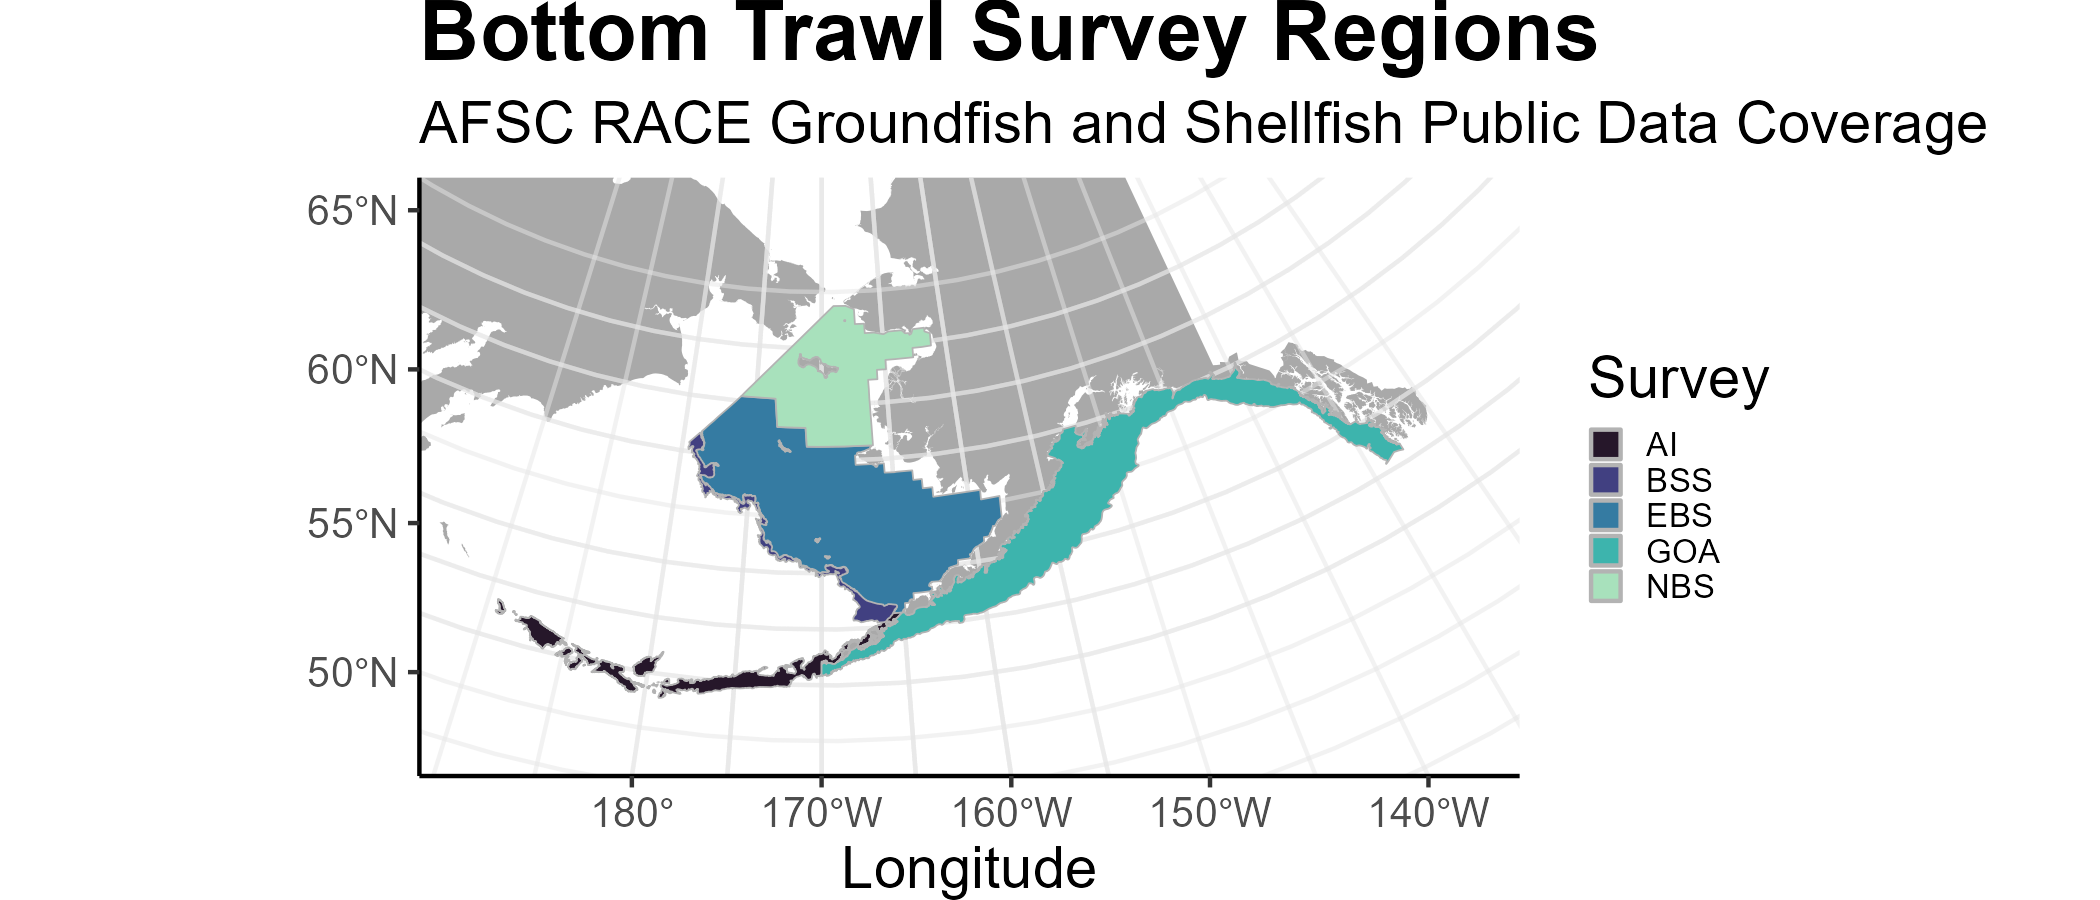
\includegraphics[width=7in,height=\textheight]{content/../img/survey_plot.png}

\begin{itemize}
\tightlist
\item
  \textbf{Aleutian Islands (AI)} (Von Szalay and Raring, 2020)

  \begin{itemize}
  \tightlist
  \item
    Triennial (1990s)/Biennial since 2000 in even years
  \item
    Modified Index-Stratified Random of Successful Stations Survey
    Design
  \end{itemize}
\item
  \textbf{Eastern Bering Sea Slope (BSS)} (Hoff, 2016)

  \begin{itemize}
  \tightlist
  \item
    Intermittent (funding dependent)
  \item
    Modified Index-Stratified Random of Successful Stations Survey
    Design
  \end{itemize}
\item
  \textbf{Eastern Bering Sea Shelf (EBS)} (Markowitz et al., 2023)

  \begin{itemize}
  \tightlist
  \item
    Annual
  \item
    Fixed stations at center of 20 x 20 nm grid
  \end{itemize}
\item
  \textbf{Gulf of Alaska (GOA)} (Von Szalay and Raring, 2018)

  \begin{itemize}
  \tightlist
  \item
    Triennial (1990s)/Biennial since 2001 in odd years
  \item
    Stratified Random Survey Design
  \end{itemize}
\item
  \textbf{Northern Bering Sea (NBS)} (Markowitz et al., 2023)

  \begin{itemize}
  \tightlist
  \item
    Biennial/Annual
  \item
    Fixed stations at center of 20 x 20 nm grid
  \end{itemize}
\end{itemize}

\hypertarget{access-constraints}{%
\section{Access Constraints}\label{access-constraints}}

There are no legal restrictions on access to the data. They reside in
public domain and can be freely distributed.

\textbf{User Constraints:} Users must read and fully comprehend the
metadata prior to use. Data should not be used beyond the limits of the
source scale. Acknowledgement of AFSC Groundfish Assessment Program, as
the source from which these data were obtained, in any publications
and/or other representations of these data, is suggested.

\bookmarksetup{startatroot}

\hypertarget{contact-us}{%
\chapter{Contact-us}\label{contact-us}}

\textbf{General questions and more specific data requests} can be sent
to
\href{mailto:afsc.gap.metadata@noaa.gov}{\nolinkurl{afsc.gap.metadata@noaa.gov}}
or submitted as an
\href{https://github.com/afsc-gap-products/data-requests}{issue on our
GitHub Organization}. The version of this data used for stock
assessments can be found through the Alaska Fisheries Information
Network (AKFIN). For questions about the eastern Bering Sea surveys,
contact Duane Stevenson
(\href{mailto:Duane.Stevenson@noaa.gov}{\nolinkurl{Duane.Stevenson@noaa.gov}}).
For questions about the Gulf of Alaska or Aleutian Islands surveys,
contact Ned Laman
(\href{mailto:Ned.Laman@noaa.gov}{\nolinkurl{Ned.Laman@noaa.gov}}). For
questions specifically about crab data in any region, contact Mike
Litzow
(\href{mailto:Mike.Litzow@noaa.gov}{\nolinkurl{Mike.Litzow@noaa.gov}}),
the Shellfish Assessment Program lead.

For questions, comments, and concerns specifically about the
\href{https://www.fisheries.noaa.gov/foss}{Fisheries One Stop Shop
(FOSS)} platform, please contact us using the Comments page on the
\href{https://www.fisheries.noaa.gov/foss}{FOSS} webpage.

Alaska Fisheries Science Center (AFSC)\\
National Oceanic and Atmospheric Administration (NOAA)\\
Resource Assessment and Conservation Engineering Division (RACE)\\
Groundfish Assessment Program (GAP)\\
7600 Sand Point Way, N.E. bldg. 4\\
Seattle, WA 98115 USA

\bookmarksetup{startatroot}

\hypertarget{suggestions-and-comments}{%
\chapter{Suggestions and comments}\label{suggestions-and-comments}}

If the data or metadata can be improved, please create a pull request,
\href{https://github.com/afsc-gap-products/data-requests/issues}{submit
an issue to the GitHub organization} or
\href{https://github.com/afsc-gap-products/gap_products/issues}{submit
an issue to the code's repository}.

\part{AFSC RACE Groundfish Survey Production Data}

\hypertarget{data-description}{%
\section*{Data Description}\label{data-description}}
\addcontentsline{toc}{section}{Data Description}

\markright{Data Description}

The Resource Assessment and Conservation Engineering Division (RACE)
Groundfish Assessment Program (GAP) of the Alaska Fisheries Science
Center (AFSC) conducts fisheries-independent bottom trawl surveys to
monitor the condition of the demersal fish and crab stocks of Alaska.
These data are developed to describe the temporal distribution and
abundance of commercially and ecologically important groundfish species,
examine the changes in the species composition of the fauna over time
and space, and describe the physical environment of the groundfish
habitat.

Users must read and fully comprehend the metadata prior to use. Data
should not be used beyond the limits of the source scale.
Acknowledgement of NOAA, as the source from which these data were
obtained, in any publications and/or other representations of these
data, is suggested. These data are compiled and approved annually after
each summer survey season. The data from previous years are unlikely to
change substantially once published. Some survey data are excluded, such
as non-standard stations, surveys completed in earlier years using
different/non-standard gear, and special tows and non-standard data
collections.

\hypertarget{cite-this-data-1}{%
\section*{Cite this data}\label{cite-this-data-1}}
\addcontentsline{toc}{section}{Cite this data}

\markright{Cite this data}

Use the below
\href{https://github.com/afsc-gap-products/gap_products/blob/main/code/CITATION_GAPProducts.bib}{bibtext
citations}, as cited in our group's
\href{https://github.com/afsc-gap-products/citations/blob/main/cite/bibliography.bib}{citation
repository} for citing the data created and maintained in this repo
(NOAA Fisheries Alaska Fisheries Science Center, Goundfish Assessment
Program, 2023). Add ``note = \{Accessed: mm/dd/yyyy\}'' to append the
day this data was accessed.

\hypertarget{data-creation}{%
\section*{Data Creation}\label{data-creation}}
\addcontentsline{toc}{section}{Data Creation}

\markright{Data Creation}

These data are created using the
\href{https://github.com/afsc-gap-products/gapindex}{gapindex R
package}.

\hypertarget{gap-production-data-metadata}{%
\chapter{GAP Production Data
Metadata}\label{gap-production-data-metadata}}

\hypertarget{data-created-in-this-repo}{%
\section{Data created in this repo}\label{data-created-in-this-repo}}

\hypertarget{gap_products.agecomp}{%
\subsection{GAP\_PRODUCTS.AGECOMP}\label{gap_products.agecomp}}

Stratum/subarea/management area/region-level abundance by sex/length
bin. Sex-specific columns (i.e., MALES, FEMALES, UNSEXED), previously
formatted in historical versions of this table, are melted into a single
column (called SEX) similar to the AGECOMP tables with values 1/2/3 for
M/F/U. The AREA\_ID field replaces the STRATUM field name to generalize
the description to include different types of areas (strata, subareas,
regulatory areas, regions, etc.). Use the GAP\_PRODUCTS.AREA table to
look up the values of AREA\_ID for your particular region. by the
Resource Assessment and Conservation Engineering Division (RACE)
Groundfish Assessment Program (GAP) of the Alaska Fisheries Science
Center (AFSC). There are legal restrictions on access to the data. These
data are not intended for public dissemination and should not be shared
without the explicit written consent of the data managers and owners
(NOAA Fisheries). The GitHub repository for the scripts that created
this code can be found at
https://github.com/afsc-gap-products/gap\_products. For more information
about codes used in the tables, please refer to the survey code books
(https://www.fisheries.noaa.gov/resource/document/groundfish-survey-species-code-manual-and-data-codes-manual).
These data were last updated June 27, 2023.

rows: 719695 \textbar{} cols: 9

\begin{tabular}{r|r|r|r|r|r|r|r|r}
\hline
SURVEY\_DEFINITION\_ID & AREA\_ID & YEAR & SPECIES\_CODE & SEX & AGE & POPULATION\_COUNT & LENGTH\_MM\_MEAN & LENGTH\_MM\_SD\\
\hline
143 & 99902 & 2010 & 21370 & 3 & -9 & 620288 & 113.33 & 10.54\\
\hline
143 & 99902 & 2017 & 21370 & 1 & -9 & 1846350 & 281.37 & 39.00\\
\hline
143 & 99902 & 2017 & 21370 & 2 & -9 & 1927790 & 313.40 & 81.15\\
\hline
\end{tabular}

\hypertarget{gap_products.area}{%
\subsection{GAP\_PRODUCTS.AREA}\label{gap_products.area}}

This reference table stores all metadata and estimates for all estimates
of stratum and subarea area estimates. Use this table with the
STRATUM\_GROUPS and SURVEY\_DESIGN tables. by the Resource Assessment
and Conservation Engineering Division (RACE) Groundfish Assessment
Program (GAP) of the Alaska Fisheries Science Center (AFSC). There are
legal restrictions on access to the data. These data are not intended
for public dissemination and should not be shared without the explicit
written consent of the data managers and owners (NOAA Fisheries). The
GitHub repository for the scripts that created this code can be found at
https://github.com/afsc-gap-products/gap\_products. For more information
about codes used in the tables, please refer to the survey code books
(https://www.fisheries.noaa.gov/resource/document/groundfish-survey-species-code-manual-and-data-codes-manual).
These data were last updated June 27, 2023.

rows: 473 \textbar{} cols: 10

\begin{tabular}{r|r|r|l|l|l|r|r|r|l}
\hline
SURVEY\_DEFINITION\_ID & DESIGN\_YEAR & AREA\_ID & TYPE & AREA\_NAME & DESCRIPTION & AREA\_KM2 & DEPTH\_MIN\_M & DEPTH\_MAX\_M & crs\\
\hline
98 & 2022 & 62 & STRATUM & Outer Domain & 100-200 m, NW section, high density, St. Matthew - OUTER DOMAIN & 6461.505 & 101 & 200 & NA\\
\hline
143 & 2022 & 70 & STRATUM & Inner Domain & <50 m , N of standard area, N to St.Lawrence Is. & 79259.889 & 1 & 50 & NA\\
\hline
143 & 2022 & 71 & STRATUM & Inner Domain & <50 m, Norton Sound and N of St. Lawrence Island to Bering Strait. Omits AA-10 & 81255.025 & 1 & 50 & NA\\
\hline
\end{tabular}

\hypertarget{gap_products.biomass}{%
\subsection{GAP\_PRODUCTS.BIOMASS}\label{gap_products.biomass}}

Stratum/subarea/management area/region-level mean/variance CPUE (weight
and numbers), total biomass (with variance), total abundance (with
variance). The AREA\_ID field replaces the STRATUM field name to
generalize the description to include different types of areas (strata,
subareas, regulatory areas, regions, etc.). Use the GAP\_PRODUCTS.AREA
table to look up the values of AREA\_ID for your particular region. Note
confidence intervals are currently not supported in the GAP\_PRODUCTS
version of the biomass/abundance tables. The associated variance of
estimates will suffice as the metric of variability to use. by the
Resource Assessment and Conservation Engineering Division (RACE)
Groundfish Assessment Program (GAP) of the Alaska Fisheries Science
Center (AFSC). There are legal restrictions on access to the data. These
data are not intended for public dissemination and should not be shared
without the explicit written consent of the data managers and owners
(NOAA Fisheries). The GitHub repository for the scripts that created
this code can be found at
https://github.com/afsc-gap-products/gap\_products. For more information
about codes used in the tables, please refer to the survey code books
(https://www.fisheries.noaa.gov/resource/document/groundfish-survey-species-code-manual-and-data-codes-manual).
These data were last updated June 27, 2023.

rows: 5343337 \textbar{} cols: 16

\begin{tabular}{r|r|r|r|r|r|r|r|r|r|r|r|r|r|r|r}
\hline
SURVEY\_DEFINITION\_ID & AREA\_ID & SPECIES\_CODE & YEAR & N\_HAUL & N\_WEIGHT & N\_COUNT & N\_LENGTH & CPUE\_KGKM2\_MEAN & CPUE\_KGKM2\_VAR & CPUE\_NOKM2\_MEAN & CPUE\_NOKM2\_VAR & BIOMASS\_MT & BIOMASS\_VAR & POPULATION\_COUNT & POPULATION\_VAR\\
\hline
143 & 70 & 71525 & 2010 & 58 & 8 & 8 & 0 & 1.840009 & 1.613901 & 121.281272 & 6372.12148 & 145.838883 & 10138.735932 & 9612740 & 4.00305e+13\\
\hline
143 & 70 & 71526 & 2010 & 58 & 0 & 0 & 0 & 0.000000 & 0.000000 & 0.000000 & 0.00000 & 0.000000 & 0.000000 & 0 & 0.00000e+00\\
\hline
143 & 70 & 71535 & 2010 & 58 & 1 & 1 & 0 & 0.017783 & 0.000316 & 4.252415 & 18.08304 & 1.409465 & 1.986592 & 337046 & 1.13600e+11\\
\hline
\end{tabular}

\hypertarget{gap_products.cpue}{%
\subsection{GAP\_PRODUCTS.CPUE}\label{gap_products.cpue}}

All haul-level zero-filled haul-level catch-per-unit-effort (units in
kg/km2) data. by the Resource Assessment and Conservation Engineering
Division (RACE) Groundfish Assessment Program (GAP) of the Alaska
Fisheries Science Center (AFSC). There are legal restrictions on access
to the data. These data are not intended for public dissemination and
should not be shared without the explicit written consent of the data
managers and owners (NOAA Fisheries). The GitHub repository for the
scripts that created this code can be found at
https://github.com/afsc-gap-products/gap\_products. For more information
about codes used in the tables, please refer to the survey code books
(https://www.fisheries.noaa.gov/resource/document/groundfish-survey-species-code-manual-and-data-codes-manual).
These data were last updated June 27, 2023.

rows: 42200740 \textbar{} cols: 7

\begin{tabular}{r|r|r|r|r|r|r}
\hline
HAULJOIN & SPECIES\_CODE & WEIGHT\_KG & COUNT & AREA\_SWEPT\_KM2 & CPUE\_KGKM2 & CPUE\_NOKM2\\
\hline
-22025 & 72758 & 0 & 0 & 0.044405 & 0 & 0\\
\hline
-22025 & 72759 & 0 & 0 & 0.044405 & 0 & 0\\
\hline
-22025 & 72760 & 0 & 0 & 0.044405 & 0 & 0\\
\hline
\end{tabular}

\hypertarget{gap_products.design_survey}{%
\subsection{GAP\_PRODUCTS.DESIGN\_SURVEY}\label{gap_products.design_survey}}

rows: 42S02 942 {[}Oracle{]}{[}ODBC{]}{[}Ora{]}ORA-00942: table or view
does not exist \textbar{} cols:

\begin{tabular}{l}
\hline
x\\
\hline
42S02 942 [Oracle][ODBC][Ora]ORA-00942: table or view does not exist\\
\hline
[RODBC] ERROR: Could not SQLExecDirect 'SELECT *
    FROM GAP\_PRODUCTS.DESIGN\_SURVEY
    FETCH FIRST 3 ROWS ONLY;'\\
\hline
\end{tabular}

\hypertarget{gap_products.metadata_table}{%
\subsection{GAP\_PRODUCTS.METADATA\_TABLE}\label{gap_products.metadata_table}}

These column provide the column metadata for all GAP oracle tables.
These tables are created by the Resource Assessment and Conservation
Engineering Division (RACE) Groundfish Assessment Program (GAP) of the
Alaska Fisheries Science Center (AFSC). The GitHub repository for the
scripts that created this code can be found at
https://github.com/afsc-gap-products/gap\_products. These data were last
updated June 27, 2023. There are no legal restrictions on access to the
data. For more information about codes used in the tables, please refer
to the survey code books
(https://www.fisheries.noaa.gov/resource/document/groundfish-survey-species-code-manual-and-data-codes-manual).

rows: 8 \textbar{} cols: 3

\begin{tabular}{l|l|l}
\hline
METADATA\_SENTENCE\_NAME & METADATA\_SENTENCE\_TYPE & METADATA\_SENTENCE\\
\hline
survey\_institution & fragment & by the Resource Assessment and Conservation Engineering Division (RACE) Groundfish Assessment Program (GAP) of the Alaska Fisheries Science Center (AFSC).\\
\hline
legal\_restrict & sentence & There are legal restrictions on access to the data. These data are not intended for public dissemination and should not be shared without the explicit written consent of the data managers and owners (NOAA Fisheries).\\
\hline
legal\_restrict\_none & sentence & There are no legal restrictions on access to the data.\\
\hline
\end{tabular}

\hypertarget{gap_products.stratum_groups}{%
\subsection{GAP\_PRODUCTS.STRATUM\_GROUPS}\label{gap_products.stratum_groups}}

This reference table identifies which STRATUM (the lowest common
denominator of statistical area groupings in this survey) relate to what
greater statistical areas (AREA\_ID), along with what year
(DESIGN\_YEAR) and survey (SURVEY\_DEFINITION\_ID) that pairing is
relevant to. Use this table with the AREA and SURVEY\_DESIGN tables. by
the Resource Assessment and Conservation Engineering Division (RACE)
Groundfish Assessment Program (GAP) of the Alaska Fisheries Science
Center (AFSC). There are legal restrictions on access to the data. These
data are not intended for public dissemination and should not be shared
without the explicit written consent of the data managers and owners
(NOAA Fisheries). The GitHub repository for the scripts that created
this code can be found at
https://github.com/afsc-gap-products/gap\_products. For more information
about codes used in the tables, please refer to the survey code books
(https://www.fisheries.noaa.gov/resource/document/groundfish-survey-species-code-manual-and-data-codes-manual).
These data were last updated June 27, 2023.

rows: 744 \textbar{} cols: 4

\begin{tabular}{r|r|r|r}
\hline
AREA\_ID & SURVEY\_DEFINITION\_ID & DESIGN\_YEAR & STRATUM\\
\hline
799 & 52 & 1980 & 721\\
\hline
799 & 52 & 1980 & 712\\
\hline
799 & 52 & 1980 & 722\\
\hline
\end{tabular}

\hypertarget{gap_products.sizecomp}{%
\subsection{GAP\_PRODUCTS.SIZECOMP}\label{gap_products.sizecomp}}

All region-level abundance by sex/age. by the Resource Assessment and
Conservation Engineering Division (RACE) Groundfish Assessment Program
(GAP) of the Alaska Fisheries Science Center (AFSC). There are legal
restrictions on access to the data. These data are not intended for
public dissemination and should not be shared without the explicit
written consent of the data managers and owners (NOAA Fisheries). The
GitHub repository for the scripts that created this code can be found at
https://github.com/afsc-gap-products/gap\_products. For more information
about codes used in the tables, please refer to the survey code books
(https://www.fisheries.noaa.gov/resource/document/groundfish-survey-species-code-manual-and-data-codes-manual).
These data were last updated June 27, 2023.

rows: 3439200 \textbar{} cols: 7

\begin{tabular}{r|r|r|r|r|r|r}
\hline
SURVEY\_DEFINITION\_ID & YEAR & AREA\_ID & SPECIES\_CODE & LENGTH\_MM & SEX & POPULATION\_COUNT\\
\hline
143 & 2021 & 99902 & 10110 & 540 & 2 & 43378\\
\hline
143 & 2021 & 99902 & 10110 & 560 & 2 & 70492\\
\hline
143 & 2021 & 99902 & 10110 & 570 & 2 & 43378\\
\hline
\end{tabular}

, \#\#\# GAP\_PRODUCTS.AGECOMP

Stratum/subarea/management area/region-level abundance by sex/length
bin. Sex-specific columns (i.e., MALES, FEMALES, UNSEXED), previously
formatted in historical versions of this table, are melted into a single
column (called SEX) similar to the AGECOMP tables with values 1/2/3 for
M/F/U. The AREA\_ID field replaces the STRATUM field name to generalize
the description to include different types of areas (strata, subareas,
regulatory areas, regions, etc.). Use the GAP\_PRODUCTS.AREA table to
look up the values of AREA\_ID for your particular region. by the
Resource Assessment and Conservation Engineering Division (RACE)
Groundfish Assessment Program (GAP) of the Alaska Fisheries Science
Center (AFSC). There are legal restrictions on access to the data. These
data are not intended for public dissemination and should not be shared
without the explicit written consent of the data managers and owners
(NOAA Fisheries). The GitHub repository for the scripts that created
this code can be found at
https://github.com/afsc-gap-products/gap\_products. For more information
about codes used in the tables, please refer to the survey code books
(https://www.fisheries.noaa.gov/resource/document/groundfish-survey-species-code-manual-and-data-codes-manual).
These data were last updated June 27, 2023.

rows: 719695 \textbar{} cols: 9

\begin{tabular}{r|r|r|r|r|r|r|r|r}
\hline
SURVEY\_DEFINITION\_ID & AREA\_ID & YEAR & SPECIES\_CODE & SEX & AGE & POPULATION\_COUNT & LENGTH\_MM\_MEAN & LENGTH\_MM\_SD\\
\hline
143 & 99902 & 2010 & 21370 & 3 & -9 & 620288 & 113.33 & 10.54\\
\hline
143 & 99902 & 2017 & 21370 & 1 & -9 & 1846350 & 281.37 & 39.00\\
\hline
143 & 99902 & 2017 & 21370 & 2 & -9 & 1927790 & 313.40 & 81.15\\
\hline
\end{tabular}

\hypertarget{gap_products.area-1}{%
\subsection{GAP\_PRODUCTS.AREA}\label{gap_products.area-1}}

This reference table stores all metadata and estimates for all estimates
of stratum and subarea area estimates. Use this table with the
STRATUM\_GROUPS and SURVEY\_DESIGN tables. by the Resource Assessment
and Conservation Engineering Division (RACE) Groundfish Assessment
Program (GAP) of the Alaska Fisheries Science Center (AFSC). There are
legal restrictions on access to the data. These data are not intended
for public dissemination and should not be shared without the explicit
written consent of the data managers and owners (NOAA Fisheries). The
GitHub repository for the scripts that created this code can be found at
https://github.com/afsc-gap-products/gap\_products. For more information
about codes used in the tables, please refer to the survey code books
(https://www.fisheries.noaa.gov/resource/document/groundfish-survey-species-code-manual-and-data-codes-manual).
These data were last updated June 27, 2023.

rows: 473 \textbar{} cols: 10

\begin{tabular}{r|r|r|l|l|l|r|r|r|l}
\hline
SURVEY\_DEFINITION\_ID & DESIGN\_YEAR & AREA\_ID & TYPE & AREA\_NAME & DESCRIPTION & AREA\_KM2 & DEPTH\_MIN\_M & DEPTH\_MAX\_M & crs\\
\hline
98 & 2022 & 62 & STRATUM & Outer Domain & 100-200 m, NW section, high density, St. Matthew - OUTER DOMAIN & 6461.505 & 101 & 200 & NA\\
\hline
143 & 2022 & 70 & STRATUM & Inner Domain & <50 m , N of standard area, N to St.Lawrence Is. & 79259.889 & 1 & 50 & NA\\
\hline
143 & 2022 & 71 & STRATUM & Inner Domain & <50 m, Norton Sound and N of St. Lawrence Island to Bering Strait. Omits AA-10 & 81255.025 & 1 & 50 & NA\\
\hline
\end{tabular}

\hypertarget{gap_products.biomass-1}{%
\subsection{GAP\_PRODUCTS.BIOMASS}\label{gap_products.biomass-1}}

Stratum/subarea/management area/region-level mean/variance CPUE (weight
and numbers), total biomass (with variance), total abundance (with
variance). The AREA\_ID field replaces the STRATUM field name to
generalize the description to include different types of areas (strata,
subareas, regulatory areas, regions, etc.). Use the GAP\_PRODUCTS.AREA
table to look up the values of AREA\_ID for your particular region. Note
confidence intervals are currently not supported in the GAP\_PRODUCTS
version of the biomass/abundance tables. The associated variance of
estimates will suffice as the metric of variability to use. by the
Resource Assessment and Conservation Engineering Division (RACE)
Groundfish Assessment Program (GAP) of the Alaska Fisheries Science
Center (AFSC). There are legal restrictions on access to the data. These
data are not intended for public dissemination and should not be shared
without the explicit written consent of the data managers and owners
(NOAA Fisheries). The GitHub repository for the scripts that created
this code can be found at
https://github.com/afsc-gap-products/gap\_products. For more information
about codes used in the tables, please refer to the survey code books
(https://www.fisheries.noaa.gov/resource/document/groundfish-survey-species-code-manual-and-data-codes-manual).
These data were last updated June 27, 2023.

rows: 5343337 \textbar{} cols: 16

\begin{tabular}{r|r|r|r|r|r|r|r|r|r|r|r|r|r|r|r}
\hline
SURVEY\_DEFINITION\_ID & AREA\_ID & SPECIES\_CODE & YEAR & N\_HAUL & N\_WEIGHT & N\_COUNT & N\_LENGTH & CPUE\_KGKM2\_MEAN & CPUE\_KGKM2\_VAR & CPUE\_NOKM2\_MEAN & CPUE\_NOKM2\_VAR & BIOMASS\_MT & BIOMASS\_VAR & POPULATION\_COUNT & POPULATION\_VAR\\
\hline
143 & 70 & 71525 & 2010 & 58 & 8 & 8 & 0 & 1.840009 & 1.613901 & 121.281272 & 6372.12148 & 145.838883 & 10138.735932 & 9612740 & 4.00305e+13\\
\hline
143 & 70 & 71526 & 2010 & 58 & 0 & 0 & 0 & 0.000000 & 0.000000 & 0.000000 & 0.00000 & 0.000000 & 0.000000 & 0 & 0.00000e+00\\
\hline
143 & 70 & 71535 & 2010 & 58 & 1 & 1 & 0 & 0.017783 & 0.000316 & 4.252415 & 18.08304 & 1.409465 & 1.986592 & 337046 & 1.13600e+11\\
\hline
\end{tabular}

\hypertarget{gap_products.cpue-1}{%
\subsection{GAP\_PRODUCTS.CPUE}\label{gap_products.cpue-1}}

All haul-level zero-filled haul-level catch-per-unit-effort (units in
kg/km2) data. by the Resource Assessment and Conservation Engineering
Division (RACE) Groundfish Assessment Program (GAP) of the Alaska
Fisheries Science Center (AFSC). There are legal restrictions on access
to the data. These data are not intended for public dissemination and
should not be shared without the explicit written consent of the data
managers and owners (NOAA Fisheries). The GitHub repository for the
scripts that created this code can be found at
https://github.com/afsc-gap-products/gap\_products. For more information
about codes used in the tables, please refer to the survey code books
(https://www.fisheries.noaa.gov/resource/document/groundfish-survey-species-code-manual-and-data-codes-manual).
These data were last updated June 27, 2023.

rows: 42200740 \textbar{} cols: 7

\begin{tabular}{r|r|r|r|r|r|r}
\hline
HAULJOIN & SPECIES\_CODE & WEIGHT\_KG & COUNT & AREA\_SWEPT\_KM2 & CPUE\_KGKM2 & CPUE\_NOKM2\\
\hline
-22025 & 72758 & 0 & 0 & 0.044405 & 0 & 0\\
\hline
-22025 & 72759 & 0 & 0 & 0.044405 & 0 & 0\\
\hline
-22025 & 72760 & 0 & 0 & 0.044405 & 0 & 0\\
\hline
\end{tabular}

\hypertarget{gap_products.design_survey-1}{%
\subsection{GAP\_PRODUCTS.DESIGN\_SURVEY}\label{gap_products.design_survey-1}}

rows: {[}RODBC{]} ERROR: Could not SQLExecDirect 'SELECT COUNT(*) FROM
GAP\_PRODUCTS.DESIGN\_SURVEY;' \textbar{} cols:

\begin{tabular}{l}
\hline
x\\
\hline
42S02 942 [Oracle][ODBC][Ora]ORA-00942: table or view does not exist\\
\hline
[RODBC] ERROR: Could not SQLExecDirect 'SELECT *
    FROM GAP\_PRODUCTS.DESIGN\_SURVEY
    FETCH FIRST 3 ROWS ONLY;'\\
\hline
\end{tabular}

\hypertarget{gap_products.metadata_table-1}{%
\subsection{GAP\_PRODUCTS.METADATA\_TABLE}\label{gap_products.metadata_table-1}}

These column provide the column metadata for all GAP oracle tables.
These tables are created by the Resource Assessment and Conservation
Engineering Division (RACE) Groundfish Assessment Program (GAP) of the
Alaska Fisheries Science Center (AFSC). The GitHub repository for the
scripts that created this code can be found at
https://github.com/afsc-gap-products/gap\_products. These data were last
updated June 27, 2023. There are no legal restrictions on access to the
data. For more information about codes used in the tables, please refer
to the survey code books
(https://www.fisheries.noaa.gov/resource/document/groundfish-survey-species-code-manual-and-data-codes-manual).

rows: 8 \textbar{} cols: 3

\begin{tabular}{l|l|l}
\hline
METADATA\_SENTENCE\_NAME & METADATA\_SENTENCE\_TYPE & METADATA\_SENTENCE\\
\hline
survey\_institution & fragment & by the Resource Assessment and Conservation Engineering Division (RACE) Groundfish Assessment Program (GAP) of the Alaska Fisheries Science Center (AFSC).\\
\hline
legal\_restrict & sentence & There are legal restrictions on access to the data. These data are not intended for public dissemination and should not be shared without the explicit written consent of the data managers and owners (NOAA Fisheries).\\
\hline
legal\_restrict\_none & sentence & There are no legal restrictions on access to the data.\\
\hline
\end{tabular}

\hypertarget{gap_products.stratum_groups-1}{%
\subsection{GAP\_PRODUCTS.STRATUM\_GROUPS}\label{gap_products.stratum_groups-1}}

This reference table identifies which STRATUM (the lowest common
denominator of statistical area groupings in this survey) relate to what
greater statistical areas (AREA\_ID), along with what year
(DESIGN\_YEAR) and survey (SURVEY\_DEFINITION\_ID) that pairing is
relevant to. Use this table with the AREA and SURVEY\_DESIGN tables. by
the Resource Assessment and Conservation Engineering Division (RACE)
Groundfish Assessment Program (GAP) of the Alaska Fisheries Science
Center (AFSC). There are legal restrictions on access to the data. These
data are not intended for public dissemination and should not be shared
without the explicit written consent of the data managers and owners
(NOAA Fisheries). The GitHub repository for the scripts that created
this code can be found at
https://github.com/afsc-gap-products/gap\_products. For more information
about codes used in the tables, please refer to the survey code books
(https://www.fisheries.noaa.gov/resource/document/groundfish-survey-species-code-manual-and-data-codes-manual).
These data were last updated June 27, 2023.

rows: 744 \textbar{} cols: 4

\begin{tabular}{r|r|r|r}
\hline
AREA\_ID & SURVEY\_DEFINITION\_ID & DESIGN\_YEAR & STRATUM\\
\hline
799 & 52 & 1980 & 721\\
\hline
799 & 52 & 1980 & 712\\
\hline
799 & 52 & 1980 & 722\\
\hline
\end{tabular}

\hypertarget{gap_products.sizecomp-1}{%
\subsection{GAP\_PRODUCTS.SIZECOMP}\label{gap_products.sizecomp-1}}

All region-level abundance by sex/age. by the Resource Assessment and
Conservation Engineering Division (RACE) Groundfish Assessment Program
(GAP) of the Alaska Fisheries Science Center (AFSC). There are legal
restrictions on access to the data. These data are not intended for
public dissemination and should not be shared without the explicit
written consent of the data managers and owners (NOAA Fisheries). The
GitHub repository for the scripts that created this code can be found at
https://github.com/afsc-gap-products/gap\_products. For more information
about codes used in the tables, please refer to the survey code books
(https://www.fisheries.noaa.gov/resource/document/groundfish-survey-species-code-manual-and-data-codes-manual).
These data were last updated June 27, 2023.

rows: 3439200 \textbar{} cols: 7

\begin{tabular}{r|r|r|r|r|r|r}
\hline
SURVEY\_DEFINITION\_ID & YEAR & AREA\_ID & SPECIES\_CODE & LENGTH\_MM & SEX & POPULATION\_COUNT\\
\hline
143 & 2021 & 99902 & 10110 & 540 & 2 & 43378\\
\hline
143 & 2021 & 99902 & 10110 & 560 & 2 & 70492\\
\hline
143 & 2021 & 99902 & 10110 & 570 & 2 & 43378\\
\hline
\end{tabular}

\hypertarget{universal-column-metadata}{%
\chapter{Universal Column Metadata}\label{universal-column-metadata}}

\hypertarget{universal-column-metadata-1}{%
\chapter{Universal Column Metadata}\label{universal-column-metadata-1}}

These tables provide the column metadata for all GAP oracle tables.
These tables are created by the Resource Assessment and Conservation
Engineering Division (RACE) Groundfish Assessment Program (GAP) of the
Alaska Fisheries Science Center (AFSC). The GitHub repository for the
scripts that created this code can be found at
https://github.com/afsc-gap-products/gap\_products. These data were last
updated June 26, 2023. There are no legal restrictions on access to the
data. For more information about codes used in the tables, please refer
to the survey code books
(https://www.fisheries.noaa.gov/resource/document/groundfish-survey-species-code-manual-and-data-codes-manual).

\begin{table}
\caption{Universal stock metadata that users can use to document their table
columns.}\tabularnewline

\centering
\begin{tabular}{l|l|l|l|l}
\hline
Column name from data & Descriptive column Name & Units & Oracle data type & Column description\\
\hline
ABUNDANCE\_HAUL & Design-based index approved haul & logical & NA & Logical, describing if this haul was conducted in a standard manner and thus used for design-based index estimates (TRUE) or not (FALSE).\\
\hline
ACTIVE & Vessel Active/Inactive & logical & NA & Logical, describing if a vessel is active (TRUE) or not (FALSE).\\
\hline
AGE & Age bin of taxon & year & NUMBER(38,0) & Age bin of a taxon in years estimated by the age comp estimate.\\
\hline
AGENCY\_ACRONYM & Acroynm of listed Agency & text abbreviated & VARCHAR2(255 BYTE) & Abbreviated agencies that are affiliated with the Alaska bottom trawl survey. The column 'agency\_acronym' is associated with the 'agency\_short' and 'agency\_long' columns.\\
\hline
AGENCY\_JOIN & Agency's ID code & ID code & NUMBER(38,0) & Affiliated agency ID code.\\
\hline
AGENCY\_LONG & Agency's Offical Name & text & VARCHAR2(255 BYTE) & Full official name of affiliated agencies to the Alaska bottom trawl survey. The column 'agency\_long' is associated with the 'agency\_acronym' and 'agency\_short' columns.\\
\hline
AGENCY\_SHORT & Agency's Shorthand Name & text & VARCHAR2(255 BYTE) & A sort version of the full official name of affiliated agencies to the Alaska bottom trawl survey. The column 'agency\_short' is associated with the 'agency\_acronym' and 'agency\_long' columns.\\
\hline
AREA\_ID & Area ID code & ID code & NUMBER(38,0) & Area ID code for each statistical area used to produce production estimates (e.g., biomass, population, age comps, length comps). Each area ID is unique within each survey.\\
\hline
AREA\_KM2 & Area (km<sup>2</sup>) & kilometers squared & NUMBER(38,3) & Area in thousands of square kilometers.\\
\hline
AREA\_NAME & Area ID Name & text & VARCHAR2(4000 BYTE) & Descriptive name of each AREA\_ID. These names often identify the region, depth ranges, or other regional information for the area ID.\\
\hline
AREA\_SWEPT\_KM2 & Area Swept (km) & kilometers & NUMBER(38,6) & The area the net covered while the net was fishing (kilometers squared), defined as the distance fished times the net width.\\
\hline
AREA\_TYPE & Area ID Type Description & category & VARCHAR2(255 BYTE) & The type of stratum that AREA\_ID represents. Types include: STRATUM, REGION, DEPTH, SUBAREA, INPFC BY DEPTH, INPFC, SUBAREA BY DEPTH, REGULATORY AREA, NMFS STATISTICAL AREA.\\
\hline
BIOMASS\_CI\_LOWER & Estimated Biomass Lower Confidence Interval & numeric & NUMBER(38,6) & The estimated biomass lower confidence interval caught in the survey for a species, group, or total for a given survey.\\
\hline
BIOMASS\_CI\_UPPER & Estimated Biomass Upper Confidence Interval & numeric & NUMBER(38,6) & The estimated biomass upper confidence interval caught in the survey for a species, group, or total for a given survey.\\
\hline
BIOMASS\_DF & Estimated Biomass Degrees of Freedom & numeric & NUMBER(38,6) & The estimated biomass degrees of freedom caught in the survey for a species, group, or total for a given survey.\\
\hline
BIOMASS\_MT & Estimated Biomass & numeric & NUMBER(38,6) & The estimated biomass caught in the survey for a species, group, or total for a given survey.\\
\hline
BIOMASS\_VAR & Estimated Biomass Variance & numeric & NUMBER(38,6) & The estimated biomass variance caught in the survey for a species, group, or total for a given survey.\\
\hline
BOTTOM\_TEMPERATURE\_C & Bottom Temperature (Degrees Celsius) & degrees Celsius & NUMBER(38,1) & Bottom temperature (tenths of a degree Celsius); NA indicates removed or missing values.\\
\hline
BOTTOM\_TYPE\_CODE & Seafloor bottom type code & ID code & NUMBER(38,0) & Bottom type on sea floor at haul location. For a complete list of bottom type ID codes, review the [code books](https://www.fisheries.noaa.gov/resource/document/groundfish-survey-species-code-manual-and-data-codes-manual).\\
\hline
CLASS & Subphylum phylogenetic rank & category & VARCHAR2(255 BYTE) & Phylogenetic latin rank of class of a given species.\\
\hline
CLASSIFICATION & Taxonomic classification rank group & category & VARCHAR2(255 BYTE) & Phylogenetic classification group rank for a given species. ")\\
\hline
COMMENTS & Comments & text & VARCHAR2(4000 BYTE) & Comments regarding row observation.\\
\hline
COMMON\_NAME & Taxon Common Name & text & VARCHAR2(255 BYTE) & The common name of the marine organism associated with the 'scientific\_name' and 'species\_code' columns. For a complete species list, review the [code books](https://www.fisheries.noaa.gov/resource/document/groundfish-survey-species-code-manual-and-data-codes-manual).\\
\hline
COUNT & Taxon Count & count, whole number resolution & NUMBER(38,0) & Total number of individuals caught in haul by taxon, represented in whole numbers used in calculation.\\
\hline
COUNTRY\_ID & Vessel Name & text & VARCHAR2(255 BYTE) & Name of the vessel used to collect data for that haul. The column 'vessel\_name' is associated with the 'vessel\_id' column. Note that it is possible for a vessel to have a new name but the same vessel id number. For a complete list of vessel ID codes, review the [code books](https://www.fisheries.noaa.gov/resource/document/groundfish-survey-species-code-manual-and-data-codes-manual).\\
\hline
CPUE\_KGHA & Weight CPUE (kg/ha) & kilograms per hectare & NUMBER(38,6) & Catch weight (kilograms) divided by area (hectares) swept by the net.\\
\hline
CPUE\_KGKM2 & Weight CPUE (kg/km<sup>2</sup>) & kilograms per kilometers squared & NUMBER(38,6) & Catch weight (kilograms) divided by area (squared kilometers) swept by the net.\\
\hline
CPUE\_KGKM2\_MEAN & Mean Weight CPUE & kilograms per kilometers squared & NUMBER(38,6) & The mean of catch weight (kilograms) divided by area (squared kilometers) swept by the net used in design-based indicie calculation.\\
\hline
CPUE\_KGKM2\_VAR & Variance of the Mean Weight CPUE & kilograms per kilometers squared & NUMBER(38,6) & The variance of mean of catch weight (kilograms) divided by area (squared kilometers) swept by the net used in design-based indicie calculation.\\
\hline
CPUE\_NOHA & Number CPUE (no/ha) & count per hectare & NUMBER(38,6) & Catch number (in number of organisms) per area (hectares) swept by the net.\\
\hline
CPUE\_NOKM2 & Number CPUE (no/km<sup>2</sup>) & count per kilometers squared & NUMBER(38,6) & Catch number (in number of organisms) per area (squared kilometers) swept by the net.\\
\hline
CPUE\_NOKM2\_MEAN & Mean Numberic CPUE & count per kilometers squared & NUMBER(38,6) & The mean of catch count (number) divided by area (squared kilometers) swept by the net used in design-based indicie calculation.\\
\hline
CPUE\_NOKM2\_VAR & Variance of the Mean Numeric CPUE & count per kilometers squared & NUMBER(38,6) & The variance of mMean of catch count (number) divided by area (squared kilometers) swept by the net used in design-based indicie calculation.\\
\hline
CRS & Coordinate Reference System & ID code & VARCHAR2(5 BYTE) & Coordinate reference system that areas (like AREA\_KM2) are calculated in, as defined by https://spatialreference.org/ (e.g., "+proj=longlat", "EPSG:3338").\\
\hline
CRUISE & Cruise ID & ID code & NUMBER(38,0) & This is a six-digit number identifying the cruise number of the form: YYYY99 (where YYYY = year of the cruise; 99 = 2-digit number and is sequential; 01 denotes the first cruise that vessel made in this year, 02 is the second, etc.).\\
\hline
CRUISEJOIN & Cruise ID & ID code & NUMBER(38,0) & This is a unique numeric identifier assigned to each survey, vessel, and year combination.\\
\hline
DATABASE & Genus phylogenetic rank & category & VARCHAR2(255 BYTE) & Taxonomic database source (e.g., "ITIS", "WORMS").\\
\hline
DATABASE\_ID & Subfamily phylogenetic rank & ID code & VARCHAR2(255 BYTE) & Species ID code of a species in the taxonomic "DATABASE" source.\\
\hline
DATE & Date & YYYY-MM-DD & DATE & The date (YYYY-MM-DD) of the event (e.g., cruise).\\
\hline
DATE\_END & End Date & YYYY-MM-DD & DATE & The date (YYYY-MM-DD) of the end of the event (e.g., cruise).\\
\hline
DATE\_START & Start Date & YYYY-MM-DD & DATE & The date (YYYY-MM-DD) of the beginning of the event (e.g., cruise).\\
\hline
DATE\_TIME & Date and Time & MM/DD/YYYY HH::MM & DATE & The date (MM/DD/YYYY) and time (HH:MM) of the haul.\\
\hline
DATE\_TIME\_END & End Date and Time & MM/DD/YYYY HH::MM & DATE & The date (MM/DD/YYYY) and time (HH:MM) of the end of the haul.\\
\hline
DATE\_TIME\_START & Start Date and Time & MM/DD/YYYY HH::MM & DATE & The date (MM/DD/YYYY) and time (HH:MM) of the beginning of the haul.\\
\hline
DEPTH\_M & Depth (m) & degrees Celsius & NUMBER(38,1) & Bottom depth (tenths of a meter).\\
\hline
DEPTH\_MAX\_M & Area ID Maximum Depth (m) & meters & NUMBER(38,3) & Maximum depth (meters) of the area covered by AREA\_ID.\\
\hline
DEPTH\_MIN\_M & Area ID Minimum Depth (m) & meters & NUMBER(38,3) & Minimum depth (meters) of the area covered by AREA\_ID.\\
\hline
DESCRIPTION & Description & text & VARCHAR2(4000 BYTE) & Description of row observation.\\
\hline
DESIGN\_YEAR & Design year & year & NUMBER(10,0) & The year the survey area stratum (e.g., statistical stratum, summary area, region) was implimented in.\\
\hline
DISTANCE\_FISHED\_KM & Distance Fished (km) & degrees Celsius & NUMBER(38,3) & Distance the net fished (thousandths of kilometers).\\
\hline
DUMMY & dummy & dummy & VARCHAR2(255 BYTE) & dummy\\
\hline
DURATION\_HR & Tow Duration (decimal hr) & hours & NUMBER(38,1) & This is the elapsed time between start and end of a haul (decimal hours).\\
\hline
FAMILY & Suborder phylogenetic rank & category & VARCHAR2(255 BYTE) & Phylogenetic latin rank of family of a given species.\\
\hline
GEAR\_DEPTH\_M & Gear depth & meters & NUMBER(38,1) & Depth gear was deployed at (tenths of a meter). Gear depth plus net height equals bottom depth.\\
\hline
GEAR\_ID & Gear ID code & ID code & NUMBER(38,0) & Type of trawl or gear deployed. For a complete list of vessel gear type ID codes, review the [code books](https://www.fisheries.noaa.gov/resource/document/groundfish-survey-species-code-manual-and-data-codes-manual).\\
\hline
GENUS & Family phylogenetic rank & category & VARCHAR2(255 BYTE) & Phylogenetic latin rank of genus of a given species.\\
\hline
HAUL & Haul Number & ID code & NUMBER(38,0) & This number uniquely identifies a sampling event (haul) within a cruise. It is a sequential number, in chronological order of occurrence.\\
\hline
HAULJOIN & Haul ID & ID code & NUMBER(38,0) & This is a unique numeric identifier assigned to each (vessel, cruise, and haul) combination.\\
\hline
HAUL\_TYPE & Haul Sampling Type & ID code & NUMBER(38,0) & Type of haul sampling method. For a complete list of haul type ID codes, review the [code books](https://www.fisheries.noaa.gov/resource/document/groundfish-survey-species-code-manual-and-data-codes-manual).\\
\hline
ID\_RANK & Lowest taxonomic rank & ID code & VARCHAR2(255 BYTE) & Lowest taxonomic rank of a given species entry.\\
\hline
ITIS & ITIS Taxonomic Serial Number & ID code & NUMBER(38,0) & Species code as identified in the Integrated Taxonomic Information System (https://itis.gov/).\\
\hline
KINGDOM & kingdom phylogenetic rank & category & VARCHAR2(255 BYTE) & Phylogenetic latin rank of kingdom of a given species.\\
\hline
LATITUDE\_DD & Latitude (decimal degrees) & decimal degrees & NUMBER(38,6) & Latitude (one hundred thousandth of a decimal degree).\\
\hline
LATITUDE\_DD\_END & End Latitude (decimal degrees) & decimal degrees & NUMBER(38,6) & Latitude (one hundred thousandth of a decimal degree) of the end of the haul.\\
\hline
LATITUDE\_DD\_START & Start Latitude (decimal degrees) & decimal degrees & NUMBER(38,6) & Latitude (one hundred thousandth of a decimal degree) of the start of the haul.\\
\hline
LENGTH\_MM & Length of a specimen & millimeters & NUMBER(10,0) & Length of a specimen in millimeters.\\
\hline
LENGTH\_MM\_MEAN & Mean length at age weighted by numbers at length & numeric & NUMBER(38,3) & Mean length estimated in age comp estimate.\\
\hline
LENGTH\_MM\_SD & standard deviation of length at age weighted by numbers at length & numeric & NUMBER(38,3) & Variance of mean length estimated in age comp estimate.\\
\hline
LONGITUDE\_DD & Longitude (decimal degrees) & decimal degrees & NUMBER(38,6) & Longitude (one hundred thousandth of a decimal degree).\\
\hline
LONGITUDE\_DD\_END & End Longitude (decimal degrees) & decimal degrees & NUMBER(38,6) & Longitude (one hundred thousandth of a decimal degree) of the end of the haul.\\
\hline
LONGITUDE\_DD\_START & Start Longitude (decimal degrees) & decimal degrees & NUMBER(38,6) & Longitude (one hundred thousandth of a decimal degree) of the start of the haul.\\
\hline
METADATA\_COLNAME & Column name & text & VARCHAR2(255 BYTE) & Name of the column in a table.\\
\hline
METADATA\_COLNAME\_DESC & column description & text & VARCHAR2(4000 BYTE) & Descritpion of the column.\\
\hline
METADATA\_COLNAME\_LONG & Column name spelled out & text & VARCHAR2(255 BYTE) & Long name for the column.\\
\hline
METADATA\_SENTENCE & Sentence & text & VARCHAR2(255 BYTE) & Table metadata sentence.\\
\hline
METADATA\_SENTENCE\_NAME & Metadata sentence name & text & VARCHAR2(255 BYTE) & Name of table metadata sentence.\\
\hline
METADATA\_SENTENCE\_TYPE & Sentence type & text & VARCHAR2(255 BYTE) & Type of sentence to have in table metadata.\\
\hline
METADATA\_UNITS & Units & category & VARCHAR2(255 BYTE) & Units of the column.\\
\hline
NET\_HEIGHT\_M & Net Height (m) & meters & NUMBER(38,1) & Measured or estimated distance (meters) between footrope and headrope of the trawl.\\
\hline
NET\_MEASURED & Net measured during haul & logical & NA & Logical, describing if the net was measured (TRUE) or not (FALSE) by wheelhouse and marport programs during the haul.\\
\hline
NET\_WIDTH\_M & Net Width (m) & meters & NUMBER(38,1) & Measured or estimated distance (meters) between wingtips of the trawl.\\
\hline
N\_COUNT & Hauls with taxon counts & numeric & NUMBER(38,0) & Total number of hauls with positive taxon counts used in calculation.\\
\hline
N\_HAUL & Valid hauls & numeric & NUMBER(38,0) & Total number of valid hauls used in calculation.\\
\hline
N\_LENGTH & Hauls with taxon lengths & numeric & NUMBER(38,0) & Total number of hauls with taxon length data used in calculation.\\
\hline
N\_WEIGHT & Hauls with catch & numeric & NUMBER(38,0) & Total number of hauls with positive catch/weighed taxon data used in calculation.\\
\hline
ORDER & Subclass phylogenetic rank & category & VARCHAR2(255 BYTE) & Phylogenetic latin rank of order of a given species.\\
\hline
PERFORMANCE & Haul Performance Code & category & NUMBER(38,0) & This denotes what, if any, issues arose during the haul. For more information, review the [code books](https://www.fisheries.noaa.gov/resource/document/groundfish-survey-species-code-manual-and-data-codes-manual).\\
\hline
PHYLUM & phylum phylogenetic rank & category & VARCHAR2(255 BYTE) & Phylogenetic latin rank of phylum of a given species.\\
\hline
POPULATION\_CI\_LOWER & Estimated Population Lower Confidence Interval & numeric & NUMBER(38,6) & The estimated population lower confidence interval caught in the survey for a species, group, or total for a given survey.\\
\hline
POPULATION\_CI\_UPPER & Estimated Population Upper Confidence Interval & numeric & NUMBER(38,6) & The estimated population upper confidence interval caught in the survey for a species, group, or total for a given survey.\\
\hline
POPULATION\_COUNT & Estimated Population & numeric & NUMBER(38,6) & The estimated population caught in the survey for a species, group, or total for a given survey.\\
\hline
POPULATION\_DF & Estimated Population Degrees of Freedom & numeric & NUMBER(38,6) & The estimated population degrees of freedom caught in the survey for a species, group, or total for a given survey.\\
\hline
POPULATION\_VAR & Estimated Population Variance & numeric & NUMBER(38,6) & The estimated population variance caught in the survey for a species, group, or total for a given survey.\\
\hline
PRINCIPAL\_INVESTIGATOR & Principle Investigator & text & VARCHAR2(255 BYTE) & First and last name of principle investigator for a project.\\
\hline
PROJECT\_TITLE & Title of Special Project & text & VARCHAR2(255 BYTE) & Special project title.\\
\hline
PROJECT\_TITLE\_SHORT & Short Title of Special Project & text & VARCHAR2(255 BYTE) & Special project short title (short version of PROJECT\_TITLE).\\
\hline
REASON & Naming status for species & text & VARCHAR2(5 BYTE) & Description of species' naming status (e.g., "synonym", "preoccupied","misspelling" )\\
\hline
SCIENTIFIC\_NAME & Taxon Scientific Name & text & VARCHAR2(255 BYTE) & The scientific name of the organism associated with the 'common\_name' and 'species\_code' columns. For a complete taxon list, review the [code books](https://www.fisheries.noaa.gov/resource/document/groundfish-survey-species-code-manual-and-data-codes-manual).\\
\hline
SEX & Sex of a specimen & ID code & NUMBER(38,0) & Sex of a specimen where "1" = "Male", "2" = "Female", "3" = Unsexed.\\
\hline
SPECIES\_CODE & Taxon Code & ID code & NUMBER(38,0) & The species code of the organism associated with the 'common\_name' and 'scientific\_name' columns. For a complete species list, review the [code books](https://www.fisheries.noaa.gov/resource/document/groundfish-survey-species-code-manual-and-data-codes-manual).\\
\hline
SPECIES\_NAME\_ACCEPTED & Scientific name used in taxonomic database & text & VARCHAR2(5 BYTE) & Scientific name of species used in taxonomic "DATABASE" column.\\
\hline
SPECIES\_NAME\_SURVEY & Scientific name used in survey data & text & VARCHAR2(5 BYTE) & Scientific name of species historically or currently used in the survey.\\
\hline
SRVY & Survey & text abbreviated & VARCHAR2(255 BYTE) & Abbreviated survey names. The column 'srvy' is associated with the 'survey' and 'survey\_id' columns. Northern Bering Sea (NBS), Southeastern Bering Sea (EBS), Bering Sea Slope (BSS), Gulf of Alaska (GOA), Aleutian Islands (AI).\\
\hline
STATION & Station ID & ID code & VARCHAR2(255 BYTE) & Alpha-numeric designation for the station established in the design of a survey.\\
\hline
STRATUM & Stratum ID & ID code & NUMBER(10,0) & RACE database statistical area for analyzing data. Strata were designed using bathymetry and other geographic and habitat-related elements. The strata are unique to each survey series. Stratum of value 0 indicates experimental tows.\\
\hline
SUBCLASS & Superclass phylogenetic rank & category & VARCHAR2(255 BYTE) & Phylogenetic latin rank of subclass of a given species.\\
\hline
SUBFAMILY & Superfamily phylogenetic rank & category & VARCHAR2(255 BYTE) & Phylogenetic latin rank of subfamily of a given species.\\
\hline
SUBMISSION\_DATE & Date & YYYY-MM-DD & TIMESTAMP & Date special projects were due to be submitted for the upcoming survey season.\\
\hline
SUBORDER & Superorder phylogenetic rank & category & VARCHAR2(255 BYTE) & Phylogenetic latin rank of suborder of a given species.\\
\hline
SUBPHYLUM & Kingdom phylogenetic rank & category & VARCHAR2(255 BYTE) & Phylogenetic latin rank of subphylum of a given species.\\
\hline
SUPERCLASS & Phylum phylogenetic rank & category & VARCHAR2(255 BYTE) & Phylogenetic latin rank of superclass of a given species.\\
\hline
SUPERFAMILY & Order phylogenetic rank & category & VARCHAR2(255 BYTE) & Phylogenetic latin rank of superfamily of a given species.\\
\hline
SUPERORDER & Class phylogenetic rank & category & VARCHAR2(255 BYTE) & Phylogenetic latin rank of superorder of a given species.\\
\hline
SURFACE\_TEMPERATURE\_C & Surface Temperature (Degrees Celsius) & degrees Celsius & NUMBER(38,1) & Surface temperature (tenths of a degree Celsius); NA indicates removed or missing values.\\
\hline
SURVEY & Survey Name & text & VARCHAR2(255 BYTE) & Name and description of survey. The column 'survey' is associated with the 'srvy' and 'survey\_id' columns.\\
\hline
SURVEY\_DEFINITION\_ID & Survey ID & ID code & NUMBER(38,0) & This number uniquely identifies a survey. Name and description of survey. The column 'survey\_id' is associated with the 'srvy' and 'survey' columns. For a complete list of surveys, review the [code books](https://www.fisheries.noaa.gov/resource/document/groundfish-survey-species-code-manual-and-data-codes-manual).\\
\hline
SURVEY\_ID & Survey ID & ID code & NUMBER(38,0) & This number uniquely identifies a survey. Name and description of survey. The column 'survey\_id' is associated with the 'srvy' and 'survey' columns. For a complete list of surveys, review the [code books](https://www.fisheries.noaa.gov/resource/document/groundfish-survey-species-code-manual-and-data-codes-manual).\\
\hline
TAWLABLE & Trawlable stations & logical & NA & Logical, describing if stations are trawlable (TRUE) or not (FALSE).\\
\hline
TAXON\_CONFIDENCE & Taxon Confidence Rating & category & VARCHAR2(255 BYTE) & Confidence in the ability of the survey team to correctly identify the taxon to the specified level, based solely on identification skill (e.g., not likelihood of a taxon being caught at that station on a location-by-location basis). Quality codes follow: **'High'**: High confidence and consistency. Taxonomy is stable and reliable at this level, and field identification characteristics are well known and reliable. **'Moderate'**: Moderate confidence. Taxonomy may be questionable at this level, or field identification characteristics may be variable and difficult to assess consistently. **'Low'**: Low confidence. Taxonomy is incompletely known, or reliable field identification characteristics are unknown. Documentation: [Species identification confidence in the eastern Bering Sea shelf survey (1982-2008)](http://apps-afsc.fisheries.noaa.gov/Publications/ProcRpt/PR2009-04.pdf), [Species identification confidence in the eastern Bering Sea slope survey (1976-2010)](http://apps-afsc.fisheries.noaa.gov/Publications/ProcRpt/PR2014-05.pdf), and [Species identification confidence in the Gulf of Alaska and Aleutian Islands surveys (1980-2011)](http://apps-afsc.fisheries.noaa.gov/Publications/ProcRpt/PR2014-01.pdf).\\
\hline
TAXON\_CONFIDENCE\_CODE & Taxon Confidence Rating & category & NUMBER(38,0) & Confidence in the ability of the survey team to correctly identify the taxon to the specified level, based solely on identification skill (e.g., not likelihood of a taxon being caught at that station on a location-by-location basis). Quality codes follow: **'High'**: High confidence and consistency. Taxonomy is stable and reliable at this level, and field identification characteristics are well known and reliable. **'Moderate'**: Moderate confidence. Taxonomy may be questionable at this level, or field identification characteristics may be variable and difficult to assess consistently. **'Low'**: Low confidence. Taxonomy is incompletely known, or reliable field identification characteristics are unknown. Documentation: [Species identification confidence in the eastern Bering Sea shelf survey (1982-2008)](http://apps-afsc.fisheries.noaa.gov/Publications/ProcRpt/PR2009-04.pdf), [Species identification confidence in the eastern Bering Sea slope survey (1976-2010)](http://apps-afsc.fisheries.noaa.gov/Publications/ProcRpt/PR2014-05.pdf), and [Species identification confidence in the Gulf of Alaska and Aleutian Islands surveys (1980-2011)](http://apps-afsc.fisheries.noaa.gov/Publications/ProcRpt/PR2014-01.pdf).\\
\hline
VESSEL\_CALLSIGN & Vessel Call Sign & ID code & NUMBER(38,0) & A call sign is a designated sequence of letters and numbers that are assigned when a vessel, whether it be a sailing yacht, motor yacht, rib or commercial vessel, receives it's Ship Radio Licence. The vessel also receives it's MMSI number, so that each vessel is uniquely identified.\\
\hline
VESSEL\_COAST\_GUARD\_NUMBER & Vessel Coast Guard Number & ID code & NUMBER(38,0) & Official Identification number as defined by www.dco.uscg.mil. The Official Number (O/N) is the 6 or 7 digit number awarded to the vessel at the time it is first documented with the US Coast Guard. This number remains with the vessel indefinitely and should be marked in accordance with 46 CFR 67.121.\\
\hline
VESSEL\_ID & Vessel ID & ID code & NUMBER(38,0) & ID number of the vessel used to collect data for that haul. The column 'vessel\_id' is associated with the 'vessel\_name' column. Note that it is possible for a vessel to have a new name but the same vessel id number. For a complete list of vessel ID codes, review the [code books](https://www.fisheries.noaa.gov/resource/document/groundfish-survey-species-code-manual-and-data-codes-manual).\\
\hline
VESSEL\_IMO & Vessel International Maritime Organization Number & ID code & NUMBER(38,0) & The International Maritime Organization (IMO) number consists of the letters "IMO" followed by a unique, seven-digit number: the pattern is "NNNNNNN", where N is a single-digit number, e.g., "1234567"\\
\hline
VESSEL\_LENGTH\_M & Vessel Length & meters & NUMBER(38,0) & The length of vessel in meters.\\
\hline
VESSEL\_MMSI & Vessel Maritime Mobile Service Identities & ID code & NUMBER(38,0) & Maritime Mobile Service Identities (MMSIs) are nine-digit numbers used by maritime digital selective calling (DSC), automatic identification systems (AIS) and certain other equipment to uniquely identify a ship or a coast radio station.\\
\hline
VESSEL\_NAME & Vessel Name & text & VARCHAR2(255 BYTE) & Name of the vessel used to collect data for that haul. The column 'vessel\_name' is associated with the 'vessel\_id' column. Note that it is possible for a vessel to have a new name but the same vessel id number. For a complete list of vessel ID codes, review the [code books](https://www.fisheries.noaa.gov/resource/document/groundfish-survey-species-code-manual-and-data-codes-manual).\\
\hline
VESSEL\_OWNER & Vessel Owner & text & VARCHAR2(255 BYTE) & Name of vessel owner or company.\\
\hline
VESSEL\_TONNAGE & Vessel Tonnage & metric tons & NUMBER(38,0) & The tonnage of vessel in metric tons.\\
\hline
WEIGHT\_KG & Taxon Weight (kg) & kilograms & NUMBER(38,3) & Weight (thousandths of a kilogram) of individuals in a haul by taxon.\\
\hline
WIRE\_LENGTH\_M & Trawl wire length & meters & NUMBER(38,0) & Length of wire deployed during a given haul in meters.\\
\hline
WORMS & World Register of Marine Species Taxonomic Serial Number & ID code & NUMBER(38,0) & Species code as identified in the World Register of Marine Species (WoRMS) (https://www.marinespecies.org/).\\
\hline
YEAR & Year & year & NUMBER(10,0) & Year the survey was conducted in.\\
\hline
\end{tabular}
\end{table}

\hypertarget{gap-production-data---created-using-gapindex}{%
\chapter{GAP Production Data - Created using
\{gapindex\}}\label{gap-production-data---created-using-gapindex}}

\hypertarget{our-production-data-is-created-using-the-gapindex-r-package.}{%
\chapter{Our production data is created using the \{gapindex\} R
package.}\label{our-production-data-is-created-using-the-gapindex-r-package.}}

{[}Insert info and examples from \{gapindex\}{]}

\part{AFSC RACE Groundfish Data for AKFIN}

Use the below
\href{https://github.com/afsc-gap-products/gap_products/blob/main/code/CITATION_GAPakfin.bib}{bibtext
citations}, as cited in our group's
\href{https://github.com/afsc-gap-products/citations/blob/main/cite/bibliography.bib}{citation
repository} for citing the data created and maintained in this repo
(Alaska Fisheries Information Network (AKFIN), 2023). Add ``note =
\{Accessed: mm/dd/yyyy\}'' to append the day this data was accessed.

\hypertarget{afsc-race-groundfish-data-for-akfin-metadata}{%
\chapter{AFSC RACE Groundfish Data for AKFIN
Metadata}\label{afsc-race-groundfish-data-for-akfin-metadata}}

\hypertarget{metadata}{%
\chapter{Metadata}\label{metadata}}

\hypertarget{data-description-1}{%
\section{Data description}\label{data-description-1}}

\emph{In development}

\hypertarget{data-created-in-this-repo-1}{%
\section{Data created in this repo}\label{data-created-in-this-repo-1}}

\hypertarget{afsc-race-groundfish-data-for-akfin-in-oracle-with-sql-and-r}{%
\chapter{AFSC RACE Groundfish Data for AKFIN in Oracle with SQL and
R'}\label{afsc-race-groundfish-data-for-akfin-in-oracle-with-sql-and-r}}

\hypertarget{access-data-via-oracle-afsc-only}{%
\section{Access data via Oracle (AFSC
only)}\label{access-data-via-oracle-afsc-only}}

AFSC \texttt{Oracle} users can access the database via
\texttt{SQL\ developer} to view and pull the production data directly
from the \texttt{GAP\_PRODUCTS} \texttt{Oracle} schema.

\hypertarget{connect-to-oracle-from-r}{%
\subsection{Connect to Oracle from R}\label{connect-to-oracle-from-r}}

Many users will want to access the data from \texttt{Oracle} using
\texttt{R}. The user will need to install the \texttt{RODBC} \texttt{R}
package and ask OFIS (IT) connect \texttt{R} to \texttt{Oracle}. Then,
use the following code in \texttt{R} to establish a connection from
\texttt{R} to \texttt{Oracle}:

Here, the user can write in their username and password directly into
the \texttt{RODBC} connect function. Never save usernames or passwords
in scripts that may be intentionally or unintentionally shared with
others. If no username and password is entered in the function, pop-ups
will appear on the screen asking for the username and password.

\hypertarget{connect-to-oracle-from-r-1}{%
\chapter{Connect to Oracle from R}\label{connect-to-oracle-from-r-1}}

\hypertarget{access-data-via-oracle}{%
\section{Access data via Oracle}\label{access-data-via-oracle}}

If the user has access to the AFSC \texttt{Oracle} database, the user
can use \texttt{SQL\ developer} to view and pull the GAP Products data
directly from the \texttt{GAP\_PRODUCTS} \texttt{Oracle} schema.

\hypertarget{connect-to-oracle-from-r-2}{%
\subsection{Connect to Oracle from R}\label{connect-to-oracle-from-r-2}}

Many users will want to access the data from \texttt{Oracle} using
\texttt{R}. The user will need to install the \texttt{RODBC} \texttt{R}
package and ask OFIS (IT) connect \texttt{R} to \texttt{Oracle}. Then,
use the following code in \texttt{R} to establish a connection from
\texttt{R} to \texttt{Oracle}:

Here, the user can establish the oracle connection by entering their
username and password in the
\texttt{channel\ \textless{}-\ gapindex::oracle\_connect()} function.
Never save usernames or passwords in scripts that may be intentionally
or unintentionally shared with others. If no username and password is
entered in the function, pop-ups will appear on the screen asking for
the username and password.

\hypertarget{data-sql-query-examples}{%
\chapter{Data SQL Query Examples:}\label{data-sql-query-examples}}

\hypertarget{ex.-0-select-all-data-from-a-table}{%
\subsection{Ex. 0: Select all data from a
table}\label{ex.-0-select-all-data-from-a-table}}

You can download all of the tables locally using a variation of the code
below. Once connected, pull and save the tables of interest into the
\texttt{R} environment.

\hypertarget{ex.-1-goa-pacific-ocean-perch-biomass-and-abundance}{%
\subsection{Ex. 1: GOA Pacific Ocean perch biomass and
abundance}\label{ex.-1-goa-pacific-ocean-perch-biomass-and-abundance}}

Biomass and abundance for Pacific Ocean perch from 1990 -- 2023 for the
western/central/eastern GOA management areas as well as for the entire
region.

\global\setlength{\Oldarrayrulewidth}{\arrayrulewidth}

\global\setlength{\Oldtabcolsep}{\tabcolsep}

\setlength{\tabcolsep}{0pt}

\renewcommand*{\arraystretch}{1.5}



\providecommand{\ascline}[3]{\noalign{\global\arrayrulewidth #1}\arrayrulecolor[HTML]{#2}\cline{#3}}

\begin{longtable}[c]{|p{0.75in}|p{0.75in}|p{0.75in}|p{0.75in}}

\caption{Ex. 1: GOA Pacific Ocean perch biomass and abundance.} \\ 


\ascline{1.5pt}{666666}{1-4}

\multicolumn{1}{>{\raggedleft}m{\dimexpr 0.75in+0\tabcolsep}}{\textcolor[HTML]{000000}{\fontsize{11}{11}\selectfont{BIOMASS\_MT}}} & \multicolumn{1}{>{\raggedleft}m{\dimexpr 0.75in+0\tabcolsep}}{\textcolor[HTML]{000000}{\fontsize{11}{11}\selectfont{POPULATION\_COUNT}}} & \multicolumn{1}{>{\raggedleft}m{\dimexpr 0.75in+0\tabcolsep}}{\textcolor[HTML]{000000}{\fontsize{11}{11}\selectfont{YEAR}}} & \multicolumn{1}{>{\raggedright}m{\dimexpr 0.75in+0\tabcolsep}}{\textcolor[HTML]{000000}{\fontsize{11}{11}\selectfont{DESCRIPTION}}} \\

\ascline{1.5pt}{666666}{1-4}\endhead



\multicolumn{1}{>{\raggedleft}m{\dimexpr 0.75in+0\tabcolsep}}{\textcolor[HTML]{000000}{\fontsize{11}{11}\selectfont{220,910.5}}} & \multicolumn{1}{>{\raggedleft}m{\dimexpr 0.75in+0\tabcolsep}}{\textcolor[HTML]{000000}{\fontsize{11}{11}\selectfont{471,190,743}}} & \multicolumn{1}{>{\raggedleft}m{\dimexpr 0.75in+0\tabcolsep}}{\textcolor[HTML]{000000}{\fontsize{11}{11}\selectfont{1,984}}} & \multicolumn{1}{>{\raggedright}m{\dimexpr 0.75in+0\tabcolsep}}{\textcolor[HTML]{000000}{\fontsize{11}{11}\selectfont{GOA\ Region:\ All\ Strata}}} \\





\multicolumn{1}{>{\raggedleft}m{\dimexpr 0.75in+0\tabcolsep}}{\textcolor[HTML]{000000}{\fontsize{11}{11}\selectfont{241,438.2}}} & \multicolumn{1}{>{\raggedleft}m{\dimexpr 0.75in+0\tabcolsep}}{\textcolor[HTML]{000000}{\fontsize{11}{11}\selectfont{482,466,826}}} & \multicolumn{1}{>{\raggedleft}m{\dimexpr 0.75in+0\tabcolsep}}{\textcolor[HTML]{000000}{\fontsize{11}{11}\selectfont{1,987}}} & \multicolumn{1}{>{\raggedright}m{\dimexpr 0.75in+0\tabcolsep}}{\textcolor[HTML]{000000}{\fontsize{11}{11}\selectfont{GOA\ Region:\ All\ Strata}}} \\





\multicolumn{1}{>{\raggedleft}m{\dimexpr 0.75in+0\tabcolsep}}{\textcolor[HTML]{000000}{\fontsize{11}{11}\selectfont{157,295.1}}} & \multicolumn{1}{>{\raggedleft}m{\dimexpr 0.75in+0\tabcolsep}}{\textcolor[HTML]{000000}{\fontsize{11}{11}\selectfont{317,129,408}}} & \multicolumn{1}{>{\raggedleft}m{\dimexpr 0.75in+0\tabcolsep}}{\textcolor[HTML]{000000}{\fontsize{11}{11}\selectfont{1,990}}} & \multicolumn{1}{>{\raggedright}m{\dimexpr 0.75in+0\tabcolsep}}{\textcolor[HTML]{000000}{\fontsize{11}{11}\selectfont{GOA\ Region:\ All\ Strata}}} \\





\multicolumn{1}{>{\raggedleft}m{\dimexpr 0.75in+0\tabcolsep}}{\textcolor[HTML]{000000}{\fontsize{11}{11}\selectfont{483,622.6}}} & \multicolumn{1}{>{\raggedleft}m{\dimexpr 0.75in+0\tabcolsep}}{\textcolor[HTML]{000000}{\fontsize{11}{11}\selectfont{833,902,161}}} & \multicolumn{1}{>{\raggedleft}m{\dimexpr 0.75in+0\tabcolsep}}{\textcolor[HTML]{000000}{\fontsize{11}{11}\selectfont{1,993}}} & \multicolumn{1}{>{\raggedright}m{\dimexpr 0.75in+0\tabcolsep}}{\textcolor[HTML]{000000}{\fontsize{11}{11}\selectfont{GOA\ Region:\ All\ Strata}}} \\





\multicolumn{1}{>{\raggedleft}m{\dimexpr 0.75in+0\tabcolsep}}{\textcolor[HTML]{000000}{\fontsize{11}{11}\selectfont{771,412.8}}} & \multicolumn{1}{>{\raggedleft}m{\dimexpr 0.75in+0\tabcolsep}}{\textcolor[HTML]{000000}{\fontsize{11}{11}\selectfont{1,252,616,603}}} & \multicolumn{1}{>{\raggedleft}m{\dimexpr 0.75in+0\tabcolsep}}{\textcolor[HTML]{000000}{\fontsize{11}{11}\selectfont{1,996}}} & \multicolumn{1}{>{\raggedright}m{\dimexpr 0.75in+0\tabcolsep}}{\textcolor[HTML]{000000}{\fontsize{11}{11}\selectfont{GOA\ Region:\ All\ Strata}}} \\





\multicolumn{1}{>{\raggedleft}m{\dimexpr 0.75in+0\tabcolsep}}{\textcolor[HTML]{000000}{\fontsize{11}{11}\selectfont{727,063.5}}} & \multicolumn{1}{>{\raggedleft}m{\dimexpr 0.75in+0\tabcolsep}}{\textcolor[HTML]{000000}{\fontsize{11}{11}\selectfont{1,212,034,913}}} & \multicolumn{1}{>{\raggedleft}m{\dimexpr 0.75in+0\tabcolsep}}{\textcolor[HTML]{000000}{\fontsize{11}{11}\selectfont{1,999}}} & \multicolumn{1}{>{\raggedright}m{\dimexpr 0.75in+0\tabcolsep}}{\textcolor[HTML]{000000}{\fontsize{11}{11}\selectfont{GOA\ Region:\ All\ Strata}}} \\

\ascline{1.5pt}{666666}{1-4}



\end{longtable}



\arrayrulecolor[HTML]{000000}

\global\setlength{\arrayrulewidth}{\Oldarrayrulewidth}

\global\setlength{\tabcolsep}{\Oldtabcolsep}

\renewcommand*{\arraystretch}{1}

\begin{verbatim}

Attaching package: 'scales'
\end{verbatim}

\begin{verbatim}
The following object is masked from 'package:readr':

    col_factor
\end{verbatim}

\begin{verbatim}
The following object is masked from 'package:terra':

    rescale
\end{verbatim}

\begin{figure}

{\centering 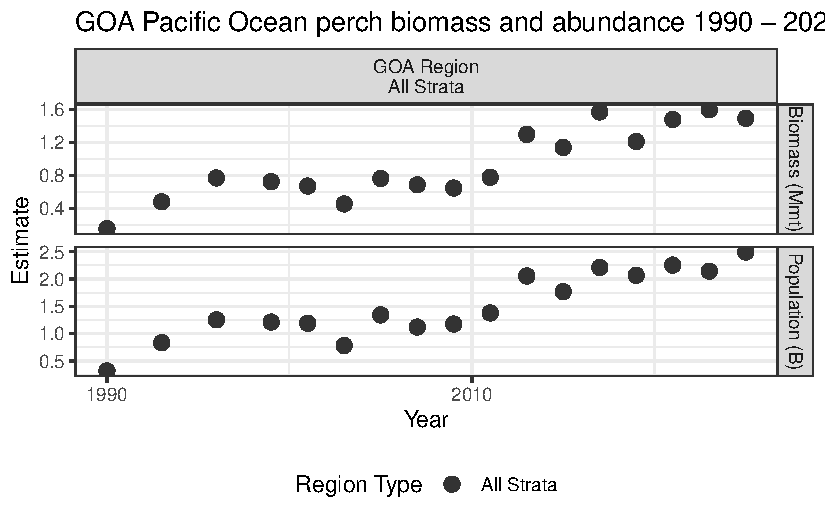
\includegraphics{content/akfin-oracle-sql-r_files/figure-pdf/test-1-plot-1.pdf}

}

\caption{Ex. 1: GOA Pacific Ocean perch biomass and abundance.}

\end{figure}

\hypertarget{ex.-2-ai-rock-sole-size-compositions-and-ridge-plot}{%
\subsection{Ex. 2: AI Rock sole size compositions and ridge
plot}\label{ex.-2-ai-rock-sole-size-compositions-and-ridge-plot}}

Northern and Southern rock sole size composition data from 1991 -- 2022
for the Aleutian Islands, with Ridge plot from
\href{https://cran.r-project.org/web/packages/ggridges/vignettes/introduction.html}{\texttt{ggridges}}.

\global\setlength{\Oldarrayrulewidth}{\arrayrulewidth}

\global\setlength{\Oldtabcolsep}{\tabcolsep}

\setlength{\tabcolsep}{0pt}

\renewcommand*{\arraystretch}{1.5}



\providecommand{\ascline}[3]{\noalign{\global\arrayrulewidth #1}\arrayrulecolor[HTML]{#2}\cline{#3}}

\begin{longtable}[c]{|p{0.75in}|p{0.75in}}

\caption{Ex. 2: AI Rock sole size compositions and ridge plot.} \\ 


\ascline{1.5pt}{666666}{1-2}

\multicolumn{1}{>{\raggedleft}m{\dimexpr 0.75in+0\tabcolsep}}{\textcolor[HTML]{000000}{\fontsize{11}{11}\selectfont{LENGTH\_MM}}} & \multicolumn{1}{>{\raggedleft}m{\dimexpr 0.75in+0\tabcolsep}}{\textcolor[HTML]{000000}{\fontsize{11}{11}\selectfont{YEAR}}} \\

\ascline{1.5pt}{666666}{1-2}\endhead



\multicolumn{1}{>{\raggedleft}m{\dimexpr 0.75in+0\tabcolsep}}{\textcolor[HTML]{000000}{\fontsize{11}{11}\selectfont{110}}} & \multicolumn{1}{>{\raggedleft}m{\dimexpr 0.75in+0\tabcolsep}}{\textcolor[HTML]{000000}{\fontsize{11}{11}\selectfont{1,997}}} \\





\multicolumn{1}{>{\raggedleft}m{\dimexpr 0.75in+0\tabcolsep}}{\textcolor[HTML]{000000}{\fontsize{11}{11}\selectfont{130}}} & \multicolumn{1}{>{\raggedleft}m{\dimexpr 0.75in+0\tabcolsep}}{\textcolor[HTML]{000000}{\fontsize{11}{11}\selectfont{1,997}}} \\





\multicolumn{1}{>{\raggedleft}m{\dimexpr 0.75in+0\tabcolsep}}{\textcolor[HTML]{000000}{\fontsize{11}{11}\selectfont{140}}} & \multicolumn{1}{>{\raggedleft}m{\dimexpr 0.75in+0\tabcolsep}}{\textcolor[HTML]{000000}{\fontsize{11}{11}\selectfont{1,997}}} \\





\multicolumn{1}{>{\raggedleft}m{\dimexpr 0.75in+0\tabcolsep}}{\textcolor[HTML]{000000}{\fontsize{11}{11}\selectfont{150}}} & \multicolumn{1}{>{\raggedleft}m{\dimexpr 0.75in+0\tabcolsep}}{\textcolor[HTML]{000000}{\fontsize{11}{11}\selectfont{1,997}}} \\





\multicolumn{1}{>{\raggedleft}m{\dimexpr 0.75in+0\tabcolsep}}{\textcolor[HTML]{000000}{\fontsize{11}{11}\selectfont{160}}} & \multicolumn{1}{>{\raggedleft}m{\dimexpr 0.75in+0\tabcolsep}}{\textcolor[HTML]{000000}{\fontsize{11}{11}\selectfont{1,997}}} \\





\multicolumn{1}{>{\raggedleft}m{\dimexpr 0.75in+0\tabcolsep}}{\textcolor[HTML]{000000}{\fontsize{11}{11}\selectfont{170}}} & \multicolumn{1}{>{\raggedleft}m{\dimexpr 0.75in+0\tabcolsep}}{\textcolor[HTML]{000000}{\fontsize{11}{11}\selectfont{1,997}}} \\

\ascline{1.5pt}{666666}{1-2}



\end{longtable}



\arrayrulecolor[HTML]{000000}

\global\setlength{\arrayrulewidth}{\Oldarrayrulewidth}

\global\setlength{\tabcolsep}{\Oldtabcolsep}

\renewcommand*{\arraystretch}{1}

\begin{verbatim}
Warning: `stat(x)` was deprecated in ggplot2 3.4.0.
i Please use `after_stat(x)` instead.
\end{verbatim}

\begin{verbatim}
Picking joint bandwidth of 3.65
\end{verbatim}

\begin{figure}

{\centering 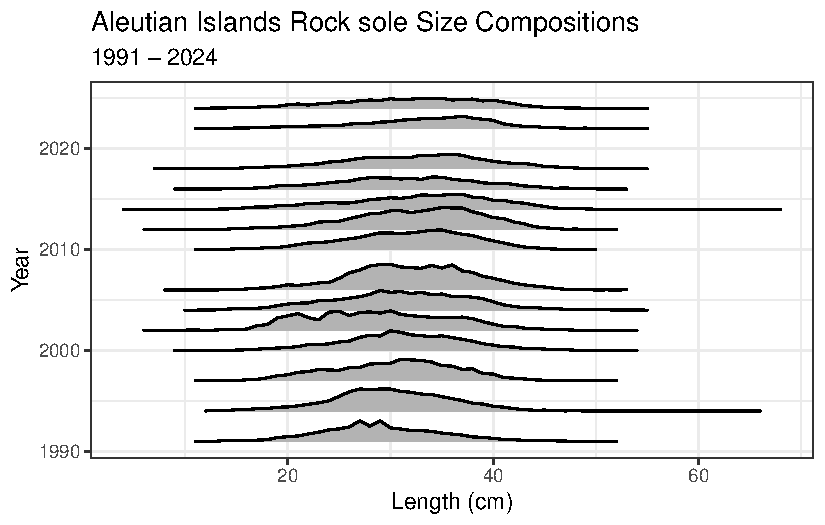
\includegraphics{content/akfin-oracle-sql-r_files/figure-pdf/test-2-plot-1.pdf}

}

\caption{Ex. 2: AI Rock sole size compositions and ridge plot.}

\end{figure}

\hypertarget{ex.-3-ebs-walleye-pollock-age-compositions-and-age-pyramid}{%
\subsection{Ex. 3: EBS Walleye Pollock Age Compositions and Age
Pyramid}\label{ex.-3-ebs-walleye-pollock-age-compositions-and-age-pyramid}}

Walleye pollock age composition for the EBS Standard Area from 1982 --
2022 and the EBS + NW Area from 1987 -- 2022, with age pyramid plot.

\global\setlength{\Oldarrayrulewidth}{\arrayrulewidth}

\global\setlength{\Oldtabcolsep}{\tabcolsep}

\setlength{\tabcolsep}{0pt}

\renewcommand*{\arraystretch}{1.5}



\providecommand{\ascline}[3]{\noalign{\global\arrayrulewidth #1}\arrayrulecolor[HTML]{#2}\cline{#3}}

\begin{longtable}[c]{|p{0.75in}|p{0.75in}|p{0.75in}}

\caption{Ex. 3: EBS Walleye Pollock Age Compositions and Age Pyramid.} \\ 


\ascline{1.5pt}{666666}{1-3}

\multicolumn{1}{>{\raggedleft}m{\dimexpr 0.75in+0\tabcolsep}}{\textcolor[HTML]{000000}{\fontsize{11}{11}\selectfont{AGE}}} & \multicolumn{1}{>{\raggedleft}m{\dimexpr 0.75in+0\tabcolsep}}{\textcolor[HTML]{000000}{\fontsize{11}{11}\selectfont{POPULATION\_COUNT}}} & \multicolumn{1}{>{\raggedleft}m{\dimexpr 0.75in+0\tabcolsep}}{\textcolor[HTML]{000000}{\fontsize{11}{11}\selectfont{SEX}}} \\

\ascline{1.5pt}{666666}{1-3}\endhead



\multicolumn{1}{>{\raggedleft}m{\dimexpr 0.75in+0\tabcolsep}}{\textcolor[HTML]{000000}{\fontsize{11}{11}\selectfont{1}}} & \multicolumn{1}{>{\raggedleft}m{\dimexpr 0.75in+0\tabcolsep}}{\textcolor[HTML]{000000}{\fontsize{11}{11}\selectfont{137,398,782}}} & \multicolumn{1}{>{\raggedleft}m{\dimexpr 0.75in+0\tabcolsep}}{\textcolor[HTML]{000000}{\fontsize{11}{11}\selectfont{1}}} \\





\multicolumn{1}{>{\raggedleft}m{\dimexpr 0.75in+0\tabcolsep}}{\textcolor[HTML]{000000}{\fontsize{11}{11}\selectfont{2}}} & \multicolumn{1}{>{\raggedleft}m{\dimexpr 0.75in+0\tabcolsep}}{\textcolor[HTML]{000000}{\fontsize{11}{11}\selectfont{1,040,787,296}}} & \multicolumn{1}{>{\raggedleft}m{\dimexpr 0.75in+0\tabcolsep}}{\textcolor[HTML]{000000}{\fontsize{11}{11}\selectfont{1}}} \\





\multicolumn{1}{>{\raggedleft}m{\dimexpr 0.75in+0\tabcolsep}}{\textcolor[HTML]{000000}{\fontsize{11}{11}\selectfont{3}}} & \multicolumn{1}{>{\raggedleft}m{\dimexpr 0.75in+0\tabcolsep}}{\textcolor[HTML]{000000}{\fontsize{11}{11}\selectfont{1,183,060,368}}} & \multicolumn{1}{>{\raggedleft}m{\dimexpr 0.75in+0\tabcolsep}}{\textcolor[HTML]{000000}{\fontsize{11}{11}\selectfont{1}}} \\





\multicolumn{1}{>{\raggedleft}m{\dimexpr 0.75in+0\tabcolsep}}{\textcolor[HTML]{000000}{\fontsize{11}{11}\selectfont{4}}} & \multicolumn{1}{>{\raggedleft}m{\dimexpr 0.75in+0\tabcolsep}}{\textcolor[HTML]{000000}{\fontsize{11}{11}\selectfont{1,661,729,359}}} & \multicolumn{1}{>{\raggedleft}m{\dimexpr 0.75in+0\tabcolsep}}{\textcolor[HTML]{000000}{\fontsize{11}{11}\selectfont{1}}} \\





\multicolumn{1}{>{\raggedleft}m{\dimexpr 0.75in+0\tabcolsep}}{\textcolor[HTML]{000000}{\fontsize{11}{11}\selectfont{5}}} & \multicolumn{1}{>{\raggedleft}m{\dimexpr 0.75in+0\tabcolsep}}{\textcolor[HTML]{000000}{\fontsize{11}{11}\selectfont{507,355,476}}} & \multicolumn{1}{>{\raggedleft}m{\dimexpr 0.75in+0\tabcolsep}}{\textcolor[HTML]{000000}{\fontsize{11}{11}\selectfont{1}}} \\





\multicolumn{1}{>{\raggedleft}m{\dimexpr 0.75in+0\tabcolsep}}{\textcolor[HTML]{000000}{\fontsize{11}{11}\selectfont{6}}} & \multicolumn{1}{>{\raggedleft}m{\dimexpr 0.75in+0\tabcolsep}}{\textcolor[HTML]{000000}{\fontsize{11}{11}\selectfont{70,450,613}}} & \multicolumn{1}{>{\raggedleft}m{\dimexpr 0.75in+0\tabcolsep}}{\textcolor[HTML]{000000}{\fontsize{11}{11}\selectfont{1}}} \\

\ascline{1.5pt}{666666}{1-3}



\end{longtable}



\arrayrulecolor[HTML]{000000}

\global\setlength{\arrayrulewidth}{\Oldarrayrulewidth}

\global\setlength{\tabcolsep}{\Oldtabcolsep}

\renewcommand*{\arraystretch}{1}

\begin{figure}

{\centering 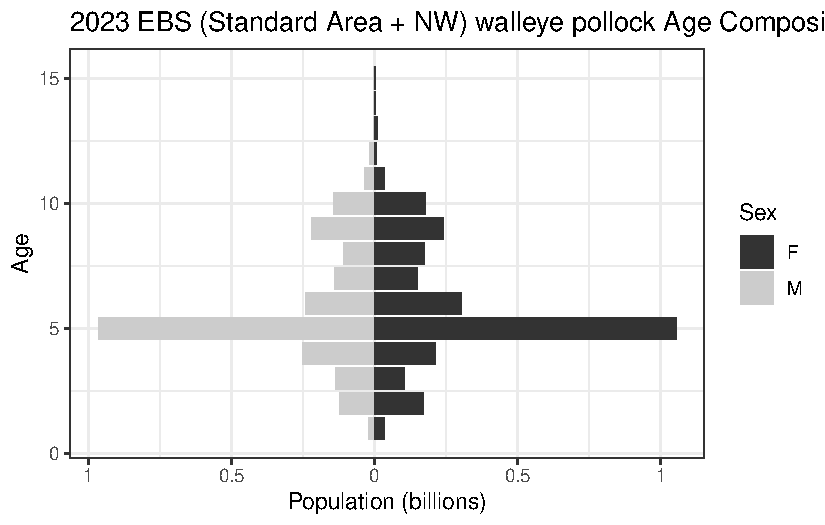
\includegraphics{content/akfin-oracle-sql-r_files/figure-pdf/test-3-plot-1.pdf}

}

\caption{Ex. 3: EBS Walleye Pollock Age Compositions and Age Pyramid.}

\end{figure}

\hypertarget{ex.-4-nbs-pacific-cod-biomass-and-abundance}{%
\subsection{Ex. 4: NBS Pacific cod biomass and
abundance}\label{ex.-4-nbs-pacific-cod-biomass-and-abundance}}

Pacific cod biomass and abundance data for the NBS by stratum.

\global\setlength{\Oldarrayrulewidth}{\arrayrulewidth}

\global\setlength{\Oldtabcolsep}{\tabcolsep}

\setlength{\tabcolsep}{0pt}

\renewcommand*{\arraystretch}{1.5}



\providecommand{\ascline}[3]{\noalign{\global\arrayrulewidth #1}\arrayrulecolor[HTML]{#2}\cline{#3}}

\begin{longtable}[c]{|p{0.75in}|p{0.75in}|p{0.75in}|p{0.75in}}

\caption{Ex. 4: NBS Pacific cod biomass and abundance.} \\ 


\ascline{1.5pt}{666666}{1-4}

\multicolumn{1}{>{\raggedleft}m{\dimexpr 0.75in+0\tabcolsep}}{\textcolor[HTML]{000000}{\fontsize{11}{11}\selectfont{BIOMASS\_MT}}} & \multicolumn{1}{>{\raggedleft}m{\dimexpr 0.75in+0\tabcolsep}}{\textcolor[HTML]{000000}{\fontsize{11}{11}\selectfont{POPULATION\_COUNT}}} & \multicolumn{1}{>{\raggedleft}m{\dimexpr 0.75in+0\tabcolsep}}{\textcolor[HTML]{000000}{\fontsize{11}{11}\selectfont{YEAR}}} & \multicolumn{1}{>{\raggedright}m{\dimexpr 0.75in+0\tabcolsep}}{\textcolor[HTML]{000000}{\fontsize{11}{11}\selectfont{AREA\_NAME}}} \\

\ascline{1.5pt}{666666}{1-4}\endhead



\multicolumn{1}{>{\raggedleft}m{\dimexpr 0.75in+0\tabcolsep}}{\textcolor[HTML]{000000}{\fontsize{11}{11}\selectfont{7,462.5586}}} & \multicolumn{1}{>{\raggedleft}m{\dimexpr 0.75in+0\tabcolsep}}{\textcolor[HTML]{000000}{\fontsize{11}{11}\selectfont{4,724,153.5}}} & \multicolumn{1}{>{\raggedleft}m{\dimexpr 0.75in+0\tabcolsep}}{\textcolor[HTML]{000000}{\fontsize{11}{11}\selectfont{2,010}}} & \multicolumn{1}{>{\raggedright}m{\dimexpr 0.75in+0\tabcolsep}}{\textcolor[HTML]{000000}{\fontsize{11}{11}\selectfont{Inner\ Domain}}} \\





\multicolumn{1}{>{\raggedleft}m{\dimexpr 0.75in+0\tabcolsep}}{\textcolor[HTML]{000000}{\fontsize{11}{11}\selectfont{7,462.5586}}} & \multicolumn{1}{>{\raggedleft}m{\dimexpr 0.75in+0\tabcolsep}}{\textcolor[HTML]{000000}{\fontsize{11}{11}\selectfont{4,724,153.5}}} & \multicolumn{1}{>{\raggedleft}m{\dimexpr 0.75in+0\tabcolsep}}{\textcolor[HTML]{000000}{\fontsize{11}{11}\selectfont{2,010}}} & \multicolumn{1}{>{\raggedright}m{\dimexpr 0.75in+0\tabcolsep}}{\textcolor[HTML]{000000}{\fontsize{11}{11}\selectfont{Inner\ Domain}}} \\





\multicolumn{1}{>{\raggedleft}m{\dimexpr 0.75in+0\tabcolsep}}{\textcolor[HTML]{000000}{\fontsize{11}{11}\selectfont{7,462.5586}}} & \multicolumn{1}{>{\raggedleft}m{\dimexpr 0.75in+0\tabcolsep}}{\textcolor[HTML]{000000}{\fontsize{11}{11}\selectfont{4,724,153.5}}} & \multicolumn{1}{>{\raggedleft}m{\dimexpr 0.75in+0\tabcolsep}}{\textcolor[HTML]{000000}{\fontsize{11}{11}\selectfont{2,010}}} & \multicolumn{1}{>{\raggedright}m{\dimexpr 0.75in+0\tabcolsep}}{\textcolor[HTML]{000000}{\fontsize{11}{11}\selectfont{Inner\ Domain}}} \\





\multicolumn{1}{>{\raggedleft}m{\dimexpr 0.75in+0\tabcolsep}}{\textcolor[HTML]{000000}{\fontsize{11}{11}\selectfont{7,462.5586}}} & \multicolumn{1}{>{\raggedleft}m{\dimexpr 0.75in+0\tabcolsep}}{\textcolor[HTML]{000000}{\fontsize{11}{11}\selectfont{4,724,153.5}}} & \multicolumn{1}{>{\raggedleft}m{\dimexpr 0.75in+0\tabcolsep}}{\textcolor[HTML]{000000}{\fontsize{11}{11}\selectfont{2,010}}} & \multicolumn{1}{>{\raggedright}m{\dimexpr 0.75in+0\tabcolsep}}{\textcolor[HTML]{000000}{\fontsize{11}{11}\selectfont{Inner\ Domain}}} \\





\multicolumn{1}{>{\raggedleft}m{\dimexpr 0.75in+0\tabcolsep}}{\textcolor[HTML]{000000}{\fontsize{11}{11}\selectfont{7,462.5586}}} & \multicolumn{1}{>{\raggedleft}m{\dimexpr 0.75in+0\tabcolsep}}{\textcolor[HTML]{000000}{\fontsize{11}{11}\selectfont{4,724,153.5}}} & \multicolumn{1}{>{\raggedleft}m{\dimexpr 0.75in+0\tabcolsep}}{\textcolor[HTML]{000000}{\fontsize{11}{11}\selectfont{2,010}}} & \multicolumn{1}{>{\raggedright}m{\dimexpr 0.75in+0\tabcolsep}}{\textcolor[HTML]{000000}{\fontsize{11}{11}\selectfont{Inner\ Domain}}} \\





\multicolumn{1}{>{\raggedleft}m{\dimexpr 0.75in+0\tabcolsep}}{\textcolor[HTML]{000000}{\fontsize{11}{11}\selectfont{680.4357}}} & \multicolumn{1}{>{\raggedleft}m{\dimexpr 0.75in+0\tabcolsep}}{\textcolor[HTML]{000000}{\fontsize{11}{11}\selectfont{250,836.5}}} & \multicolumn{1}{>{\raggedleft}m{\dimexpr 0.75in+0\tabcolsep}}{\textcolor[HTML]{000000}{\fontsize{11}{11}\selectfont{2,010}}} & \multicolumn{1}{>{\raggedright}m{\dimexpr 0.75in+0\tabcolsep}}{\textcolor[HTML]{000000}{\fontsize{11}{11}\selectfont{Middle\ Domain}}} \\

\ascline{1.5pt}{666666}{1-4}



\end{longtable}



\arrayrulecolor[HTML]{000000}

\global\setlength{\arrayrulewidth}{\Oldarrayrulewidth}

\global\setlength{\tabcolsep}{\Oldtabcolsep}

\renewcommand*{\arraystretch}{1}

\begin{figure}

{\centering 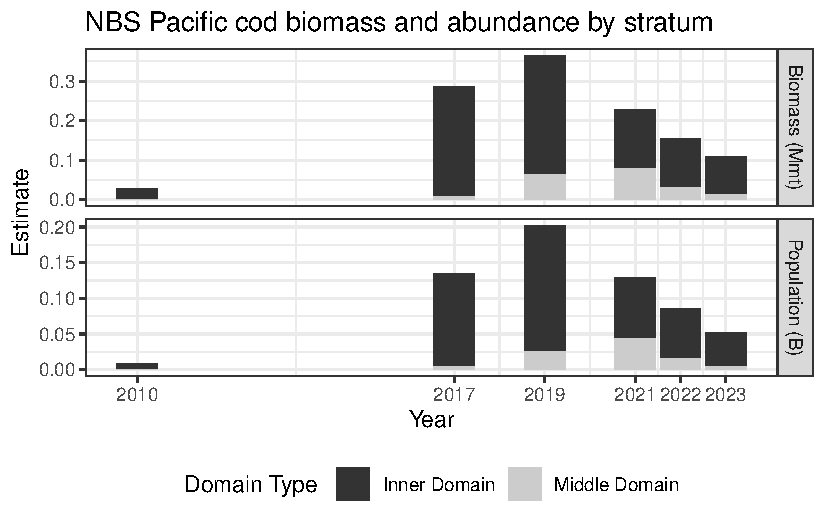
\includegraphics{content/akfin-oracle-sql-r_files/figure-pdf/test-4-fig-1.pdf}

}

\caption{Ex. 4: NBS Pacific cod biomass and abundance.}

\end{figure}

\hypertarget{ex.-5-goa-pacific-ocean-perch-biomass-and-line-plot}{%
\subsection{Ex. 5: GOA Pacific Ocean perch biomass and line
plot}\label{ex.-5-goa-pacific-ocean-perch-biomass-and-line-plot}}

Pacific Ocean perch biomass totals for GOA between 1984-2021 from
\texttt{GAP\_PRODUCTS.AKFIN\_BIOMASS}

\global\setlength{\Oldarrayrulewidth}{\arrayrulewidth}

\global\setlength{\Oldtabcolsep}{\tabcolsep}

\setlength{\tabcolsep}{0pt}

\renewcommand*{\arraystretch}{1.5}



\providecommand{\ascline}[3]{\noalign{\global\arrayrulewidth #1}\arrayrulecolor[HTML]{#2}\cline{#3}}

\begin{longtable}[c]{|p{0.75in}|p{0.75in}|p{0.75in}}

\caption{Ex. 5: GOA Pacific Ocean perch biomass and line plot.} \\ 


\ascline{1.5pt}{666666}{1-3}

\multicolumn{1}{>{\raggedleft}m{\dimexpr 0.75in+0\tabcolsep}}{\textcolor[HTML]{000000}{\fontsize{11}{11}\selectfont{survey\_definition\_id}}} & \multicolumn{1}{>{\raggedleft}m{\dimexpr 0.75in+0\tabcolsep}}{\textcolor[HTML]{000000}{\fontsize{11}{11}\selectfont{biomass\_mt}}} & \multicolumn{1}{>{\raggedleft}m{\dimexpr 0.75in+0\tabcolsep}}{\textcolor[HTML]{000000}{\fontsize{11}{11}\selectfont{year}}} \\

\ascline{1.5pt}{666666}{1-3}\endhead



\multicolumn{1}{>{\raggedleft}m{\dimexpr 0.75in+0\tabcolsep}}{\textcolor[HTML]{000000}{\fontsize{11}{11}\selectfont{47}}} & \multicolumn{1}{>{\raggedleft}m{\dimexpr 0.75in+0\tabcolsep}}{\textcolor[HTML]{000000}{\fontsize{11}{11}\selectfont{220.9105}}} & \multicolumn{1}{>{\raggedleft}m{\dimexpr 0.75in+0\tabcolsep}}{\textcolor[HTML]{000000}{\fontsize{11}{11}\selectfont{1,984}}} \\





\multicolumn{1}{>{\raggedleft}m{\dimexpr 0.75in+0\tabcolsep}}{\textcolor[HTML]{000000}{\fontsize{11}{11}\selectfont{47}}} & \multicolumn{1}{>{\raggedleft}m{\dimexpr 0.75in+0\tabcolsep}}{\textcolor[HTML]{000000}{\fontsize{11}{11}\selectfont{241.4382}}} & \multicolumn{1}{>{\raggedleft}m{\dimexpr 0.75in+0\tabcolsep}}{\textcolor[HTML]{000000}{\fontsize{11}{11}\selectfont{1,987}}} \\





\multicolumn{1}{>{\raggedleft}m{\dimexpr 0.75in+0\tabcolsep}}{\textcolor[HTML]{000000}{\fontsize{11}{11}\selectfont{47}}} & \multicolumn{1}{>{\raggedleft}m{\dimexpr 0.75in+0\tabcolsep}}{\textcolor[HTML]{000000}{\fontsize{11}{11}\selectfont{157.2951}}} & \multicolumn{1}{>{\raggedleft}m{\dimexpr 0.75in+0\tabcolsep}}{\textcolor[HTML]{000000}{\fontsize{11}{11}\selectfont{1,990}}} \\





\multicolumn{1}{>{\raggedleft}m{\dimexpr 0.75in+0\tabcolsep}}{\textcolor[HTML]{000000}{\fontsize{11}{11}\selectfont{47}}} & \multicolumn{1}{>{\raggedleft}m{\dimexpr 0.75in+0\tabcolsep}}{\textcolor[HTML]{000000}{\fontsize{11}{11}\selectfont{483.6226}}} & \multicolumn{1}{>{\raggedleft}m{\dimexpr 0.75in+0\tabcolsep}}{\textcolor[HTML]{000000}{\fontsize{11}{11}\selectfont{1,993}}} \\





\multicolumn{1}{>{\raggedleft}m{\dimexpr 0.75in+0\tabcolsep}}{\textcolor[HTML]{000000}{\fontsize{11}{11}\selectfont{47}}} & \multicolumn{1}{>{\raggedleft}m{\dimexpr 0.75in+0\tabcolsep}}{\textcolor[HTML]{000000}{\fontsize{11}{11}\selectfont{771.4128}}} & \multicolumn{1}{>{\raggedleft}m{\dimexpr 0.75in+0\tabcolsep}}{\textcolor[HTML]{000000}{\fontsize{11}{11}\selectfont{1,996}}} \\





\multicolumn{1}{>{\raggedleft}m{\dimexpr 0.75in+0\tabcolsep}}{\textcolor[HTML]{000000}{\fontsize{11}{11}\selectfont{47}}} & \multicolumn{1}{>{\raggedleft}m{\dimexpr 0.75in+0\tabcolsep}}{\textcolor[HTML]{000000}{\fontsize{11}{11}\selectfont{727.0635}}} & \multicolumn{1}{>{\raggedleft}m{\dimexpr 0.75in+0\tabcolsep}}{\textcolor[HTML]{000000}{\fontsize{11}{11}\selectfont{1,999}}} \\

\ascline{1.5pt}{666666}{1-3}



\end{longtable}



\arrayrulecolor[HTML]{000000}

\global\setlength{\arrayrulewidth}{\Oldarrayrulewidth}

\global\setlength{\tabcolsep}{\Oldtabcolsep}

\renewcommand*{\arraystretch}{1}

\begin{verbatim}
Warning: Using `size` aesthetic for lines was deprecated in ggplot2 3.4.0.
i Please use `linewidth` instead.
\end{verbatim}

\begin{figure}

{\centering 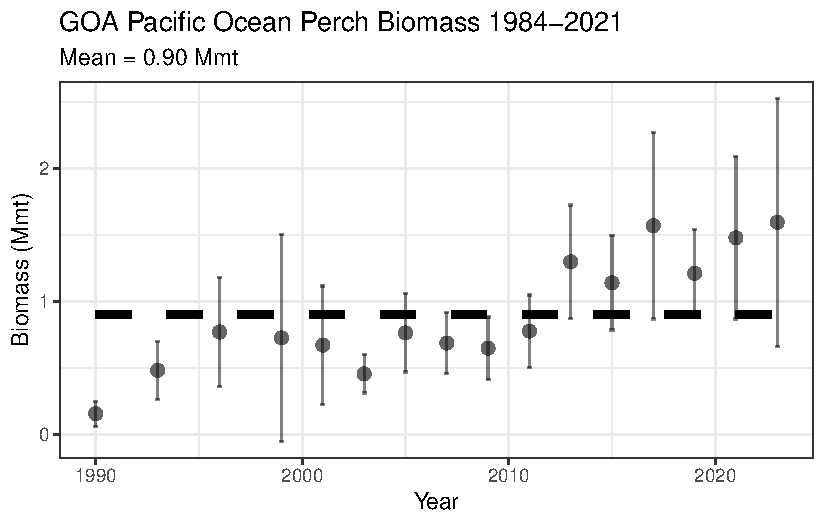
\includegraphics{content/akfin-oracle-sql-r_files/figure-pdf/test-5-fig-1.pdf}

}

\caption{Ex. 5: GOA Pacific Ocean perch biomass and line plot.}

\end{figure}

\hypertarget{ex.-6-ebs-pacific-ocean-perch-cpue-and-akgfmaps-map}{%
\subsection{\texorpdfstring{Ex. 6: EBS Pacific Ocean perch CPUE and
\href{https://github.com/afsc-gap-products/akgfmaps}{\texttt{akgfmaps}}
map}{Ex. 6: EBS Pacific Ocean perch CPUE and akgfmaps map}}\label{ex.-6-ebs-pacific-ocean-perch-cpue-and-akgfmaps-map}}

Pacific Ocean perch catch-per-unit-effort estimates for EBS in 2021 from
\texttt{GAP\_PRODUCTS.AKFIN\_CPUE} and map constructed using
\href{https://github.com/afsc-gap-products/akgfmaps}{\texttt{akgfmaps}}.
Here, we'll use AKFIN HAUL and CRUISES data also included in this repo,
for convenience, though they are very similar to their \texttt{RACEBASE}
analogs.

\global\setlength{\Oldarrayrulewidth}{\arrayrulewidth}

\global\setlength{\Oldtabcolsep}{\tabcolsep}

\setlength{\tabcolsep}{0pt}

\renewcommand*{\arraystretch}{1.5}



\providecommand{\ascline}[3]{\noalign{\global\arrayrulewidth #1}\arrayrulecolor[HTML]{#2}\cline{#3}}

\begin{longtable}[c]{|p{0.75in}|p{0.75in}|p{0.75in}}

\caption{Ex. 6: EBS Pacific Ocean perch CPUE and
\href{https://github.com/afsc-gap-products/akgfmaps}{\texttt{akgfmaps}}
map.} \\ 


\ascline{1.5pt}{666666}{1-3}

\multicolumn{1}{>{\raggedleft}m{\dimexpr 0.75in+0\tabcolsep}}{\textcolor[HTML]{000000}{\fontsize{11}{11}\selectfont{CPUE\_KGHA}}} & \multicolumn{1}{>{\raggedleft}m{\dimexpr 0.75in+0\tabcolsep}}{\textcolor[HTML]{000000}{\fontsize{11}{11}\selectfont{LATITUDE}}} & \multicolumn{1}{>{\raggedleft}m{\dimexpr 0.75in+0\tabcolsep}}{\textcolor[HTML]{000000}{\fontsize{11}{11}\selectfont{LONGITUDE}}} \\

\ascline{1.5pt}{666666}{1-3}\endhead



\multicolumn{1}{>{\raggedleft}m{\dimexpr 0.75in+0\tabcolsep}}{\textcolor[HTML]{000000}{\fontsize{11}{11}\selectfont{0}}} & \multicolumn{1}{>{\raggedleft}m{\dimexpr 0.75in+0\tabcolsep}}{\textcolor[HTML]{000000}{\fontsize{11}{11}\selectfont{56.66721}}} & \multicolumn{1}{>{\raggedleft}m{\dimexpr 0.75in+0\tabcolsep}}{\textcolor[HTML]{000000}{\fontsize{11}{11}\selectfont{-159.7800}}} \\





\multicolumn{1}{>{\raggedleft}m{\dimexpr 0.75in+0\tabcolsep}}{\textcolor[HTML]{000000}{\fontsize{11}{11}\selectfont{0}}} & \multicolumn{1}{>{\raggedleft}m{\dimexpr 0.75in+0\tabcolsep}}{\textcolor[HTML]{000000}{\fontsize{11}{11}\selectfont{56.98080}}} & \multicolumn{1}{>{\raggedleft}m{\dimexpr 0.75in+0\tabcolsep}}{\textcolor[HTML]{000000}{\fontsize{11}{11}\selectfont{-159.6926}}} \\





\multicolumn{1}{>{\raggedleft}m{\dimexpr 0.75in+0\tabcolsep}}{\textcolor[HTML]{000000}{\fontsize{11}{11}\selectfont{0}}} & \multicolumn{1}{>{\raggedleft}m{\dimexpr 0.75in+0\tabcolsep}}{\textcolor[HTML]{000000}{\fontsize{11}{11}\selectfont{56.97832}}} & \multicolumn{1}{>{\raggedleft}m{\dimexpr 0.75in+0\tabcolsep}}{\textcolor[HTML]{000000}{\fontsize{11}{11}\selectfont{-159.1519}}} \\





\multicolumn{1}{>{\raggedleft}m{\dimexpr 0.75in+0\tabcolsep}}{\textcolor[HTML]{000000}{\fontsize{11}{11}\selectfont{0}}} & \multicolumn{1}{>{\raggedleft}m{\dimexpr 0.75in+0\tabcolsep}}{\textcolor[HTML]{000000}{\fontsize{11}{11}\selectfont{57.31992}}} & \multicolumn{1}{>{\raggedleft}m{\dimexpr 0.75in+0\tabcolsep}}{\textcolor[HTML]{000000}{\fontsize{11}{11}\selectfont{-159.0614}}} \\





\multicolumn{1}{>{\raggedleft}m{\dimexpr 0.75in+0\tabcolsep}}{\textcolor[HTML]{000000}{\fontsize{11}{11}\selectfont{0}}} & \multicolumn{1}{>{\raggedleft}m{\dimexpr 0.75in+0\tabcolsep}}{\textcolor[HTML]{000000}{\fontsize{11}{11}\selectfont{57.32157}}} & \multicolumn{1}{>{\raggedleft}m{\dimexpr 0.75in+0\tabcolsep}}{\textcolor[HTML]{000000}{\fontsize{11}{11}\selectfont{-158.3811}}} \\





\multicolumn{1}{>{\raggedleft}m{\dimexpr 0.75in+0\tabcolsep}}{\textcolor[HTML]{000000}{\fontsize{11}{11}\selectfont{0}}} & \multicolumn{1}{>{\raggedleft}m{\dimexpr 0.75in+0\tabcolsep}}{\textcolor[HTML]{000000}{\fontsize{11}{11}\selectfont{57.65189}}} & \multicolumn{1}{>{\raggedleft}m{\dimexpr 0.75in+0\tabcolsep}}{\textcolor[HTML]{000000}{\fontsize{11}{11}\selectfont{-158.3673}}} \\

\ascline{1.5pt}{666666}{1-3}



\end{longtable}



\arrayrulecolor[HTML]{000000}

\global\setlength{\arrayrulewidth}{\Oldarrayrulewidth}

\global\setlength{\tabcolsep}{\Oldtabcolsep}

\renewcommand*{\arraystretch}{1}

\begin{verbatim}
Warning: attribute variables are assumed to be spatially constant throughout
all geometries
\end{verbatim}

\begin{verbatim}
[inverse distance weighted interpolation]
[inverse distance weighted interpolation]
\end{verbatim}

\begin{verbatim}
Warning: Removed 1406 rows containing missing values (`geom_raster()`).
\end{verbatim}

\begin{figure}

{\centering 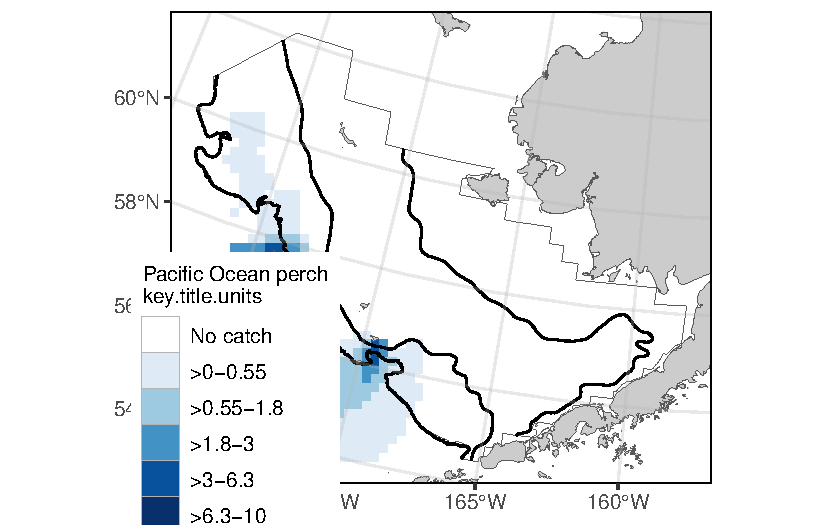
\includegraphics{content/akfin-oracle-sql-r_files/figure-pdf/test-6-fig-1.pdf}

}

\caption{Ex. 6: EBS Pacific Ocean perch CPUE and
\href{https://github.com/afsc-gap-products/akgfmaps}{\texttt{akgfmaps}}
map.}

\end{figure}

\part{AFSC RACE Groundfish and Shellfish Survey Public Data}

This data contains all of the catch, environmental, and haul data from
the fisheries-independent Groundfish and Shellfish Assessment Program
surveys in the Bering Sea, Aleutian Islands, and Gulf of Alaska. This
data is sought after by the general public, private entities, and NOAA
partners alike, including tribal organizations, K-12 classrooms,
academic institutions, for-profit groups, and non-profit groups. This
data is compiled and approved once a year after each summer survey
season and is approved for open access.

\part{Collabrators and data users}

Below are a few packages and products currently using this data. If you
have developed a product, performed an analysis, or exhibited this data
in any way, reach out so we can showcase your hard work.

\begin{itemize}
\item
  \textbf{\href{https://apps-st.fisheries.noaa.gov/dismap}{NOAA
  Fisheries Distribution Mapping and Analysis Portal}};
  \emph{\href{https://www.fisheries.noaa.gov/contact/office-science-and-technology}{NOAA
  Fisheries Office of Science and Technology}}
\item
  \textbf{\href{https://pyafscgap.org/}{Pull data with python} and
  explore the
  \href{https://app.pyafscgap.org/\textquotesingle{}}{in-browser
  visualization tool}. Reference their
  \href{https://mybinder.org/v2/gh/SchmidtDSE/afscgap/main?urlpath=/tree/index.ipynb}{example
  Python notebook}}; \emph{\href{https://dse.berkeley.edu/}{The Eric and
  Wendy Schmidt Center for Data Science and the Environment at UC
  Berkeley}, including sam.pottinger@berkeley.edu,
  ccmartinez@berkeley.edu, gzarpellon@berkeley.edu, and
  kkoy@berkeley.edu.}
\end{itemize}

\hypertarget{cite-this-data-2}{%
\section*{Cite this data}\label{cite-this-data-2}}
\addcontentsline{toc}{section}{Cite this data}

\markright{Cite this data}

Use the below
\href{https://github.com/afsc-gap-products/gap_products/blob/main/code/CITATION_FOSSAFSCData.bib}{bibtext
citations}, as cited in our group's
\href{https://github.com/afsc-gap-products/citations/blob/main/cite/bibliography.bib}{citation
repository} for citing the data created and maintained in this repo
(NOAA Fisheries Alaska Fisheries Science Center, 2023). Add ``note =
\{Accessed: mm/dd/yyyy\}'' to append the day this data was accessed.

\hypertarget{gap-foss-column-metadata}{%
\chapter{GAP FOSS Column Metadata}\label{gap-foss-column-metadata}}

\hypertarget{metadata-1}{%
\chapter{Metadata}\label{metadata-1}}

\hypertarget{data-description-2}{%
\section{Data description}\label{data-description-2}}

The Resource Assessment and Conservation Engineering Division (RACE)
Groundfish Assessment Program (GAP) of the Alaska Fisheries Science
Center (AFSC) conducts fisheries-independent bottom trawl surveys to
monitor the condition of the demersal fish and crab stocks of Alaska.
These data are developed to describe the temporal distribution and
abundance of commercially and ecologically important groundfish species,
examine the changes in the species composition of the fauna over time
and space, and describe the physical environment of the groundfish
habitat.

There are no legal restrictions on access to the data. They reside in
the public domain and can be freely distributed. Users must read and
fully comprehend the metadata prior to use. Data should not be used
beyond the limits of the source scale. Acknowledgement of NOAA, as the
source from which these data were obtained, in any publications and/or
other representations of these data, is suggested. These data are
compiled and approved annually after each summer survey season. The data
from previous years are unlikely to change substantially once published.

These data are zero-filled (presence and absence) observations from
surveys conducted on fishing vessels. These surveys monitor trends in
distribution and abundance of groundfish, crab, and bottom-dwelling
species in Alaska's marine ecosystems. These data include estimates of
catch-per-unit-effort (CPUE) for all identified species for index
stations. Some survey data are excluded, such as non-standard stations,
surveys completed in earlier years using different/non-standard gear,
and special tows and non-standard data collections.

Though not included in the public data, these surveys also collect
oceanographic and environmental data, and biological data such as
length, weight, stomach contents (to learn more about diet), otoliths
(fish ear bones to learn about age), and tissue samples for genetic
analysis, all of which can be shared upon special request. Also not
included in the public data are estimated biomass (average total weight
of all fish and crabs sampled) of crabs and groundfish that support the
creation of annual stock assessments.

\hypertarget{data-created-in-this-repo-2}{%
\section{Data created in this repo}\label{data-created-in-this-repo-2}}

\hypertarget{foss_catch}{%
\subsection{FOSS\_CATCH}\label{foss_catch}}

{[}There is currently no description for this table.{]}

rows: 36940981 \textbar{} cols: 12

\begin{tabular}{r|r|r|r|r|r|l|l|l|l|r|r}
\hline
HAULJOIN & SPECIES\_CODE & CPUE\_KGKM2 & CPUE\_NOKM2 & COUNT & WEIGHT\_KG & TAXON\_CONFIDENCE & SCIENTIFIC\_NAME & COMMON\_NAME & ID\_RANK & WORMS & ITIS\\
\hline
-22025 & 85290 & 0 & 0 & 0 & 0 & NA & Synallactes challengeri & NA & species & 529678 & 656054\\
\hline
-22025 & 98105 & 0 & 0 & 0 & 0 & NA & Boltenia ovifera & sea onion & species & 103815 & 159485\\
\hline
-22024 & 20041 & 0 & 0 & 0 & 0 & NA & Podothecus veternus & veteran poacher & species & 254509 & 644362\\
\hline
\end{tabular}

\hypertarget{foss_haul}{%
\subsection{FOSS\_HAUL}\label{foss_haul}}

{[}There is currently no description for this table.{]}

rows: 31608 \textbar{} cols: 27

\begin{tabular}{r|l|l|r|l|r|r|r|r|r|l|r|l|l|r|r|r|r|r|r|r|r|r|r|r|r|r}
\hline
YEAR & SRVY & SURVEY & SURVEY\_DEFINITION\_ID & SURVEY\_NAME & CRUISE & CRUISEJOIN & HAULJOIN & HAUL & STRATUM & STATION & VESSEL\_ID & VESSEL\_NAME & DATE\_TIME & LATITUDE\_DD\_START & LONGITUDE\_DD\_START & LATITUDE\_DD\_END & LONGITUDE\_DD\_END & BOTTOM\_TEMPERATURE\_C & SURFACE\_TEMPERATURE\_C & DEPTH\_M & DISTANCE\_FISHED\_KM & DURATION\_HR & NET\_WIDTH\_M & NET\_HEIGHT\_M & AREA\_SWEPT\_KM2 & PERFORMANCE\\
\hline
2022 & NBS & northern Bering Sea & 143 & Northern Bering Sea Crab/Groundfish Survey - Eastern Bering Sea Shelf Survey Extension & 202202 & -758 & -21899 & 16 & 71 & EE-19 & 162 & ALASKA KNIGHT & 2022-08-05 07:17:32 & 65.00732 & -169.8922 & 64.99885 & -169.8342 & 0.9 & 3.4 & 50 & 2.899 & 0.518 & 16.520 & 2.287 & 0.047891 & 0\\
\hline
2022 & NBS & northern Bering Sea & 143 & Northern Bering Sea Crab/Groundfish Survey - Eastern Bering Sea Shelf Survey Extension & 202202 & -757 & -21831 & 4 & 71 & CC-06 & 94 & VESTERAALEN & 2022-08-02 10:42:32 & 64.32204 & -164.5706 & 64.32041 & -164.5082 & 12.0 & 14.1 & 15 & 3.032 & 0.544 & 14.371 & 2.938 & 0.043573 & 0\\
\hline
2022 & NBS & northern Bering Sea & 143 & Northern Bering Sea Crab/Groundfish Survey - Eastern Bering Sea Shelf Survey Extension & 202202 & -757 & -21881 & 21 & 71 & CC-03 & 94 & VESTERAALEN & 2022-08-06 13:45:21 & 64.32156 & -166.8225 & 64.34806 & -166.8351 & 4.4 & 10.1 & 28 & 3.008 & 0.546 & 15.488 & 2.484 & 0.046588 & 0\\
\hline
\end{tabular}

\hypertarget{foss_taxon_groups}{%
\subsection{FOSS\_TAXON\_GROUPS}\label{foss_taxon_groups}}

{[}There is currently no description for this table.{]}

rows: 15775 \textbar{} cols: 3

\begin{tabular}{l|l|r}
\hline
ID\_RANK & CLASSIFICATION & SPECIES\_CODE\\
\hline
class & Asteroidea & 80525\\
\hline
class & Asteroidea & 80535\\
\hline
class & Asteroidea & 80536\\
\hline
\end{tabular}

\hypertarget{racebase_foss_catch}{%
\subsection{RACEBASE\_FOSS\_CATCH}\label{racebase_foss_catch}}

{[}There is currently no description for this table.{]}

rows: 36342299 \textbar{} cols: 11

\begin{tabular}{r|r|r|r|r|r|l|l|l|r|r}
\hline
HAULJOIN & SPECIES\_CODE & CPUE\_KGKM2 & CPUE\_NOKM2 & COUNT & WEIGHT\_KG & TAXON\_CONFIDENCE & SCIENTIFIC\_NAME & COMMON\_NAME & WORMS & ITIS\\
\hline
857 & 21347 & 0 & 0 & 0 & 0 & High & Hemilepidotus jordani & yellow Irish lord & 254522 & 167280\\
\hline
857 & 21348 & 0 & 0 & 0 & 0 & Moderate & Hemilepidotus papilio & butterfly sculpin & 254523 & 167282\\
\hline
857 & 21350 & 0 & 0 & 0 & 0 & High & Triglops sp. & NA & 126154 & 167368\\
\hline
\end{tabular}

\hypertarget{racebase_foss_haul}{%
\subsection{RACEBASE\_FOSS\_HAUL}\label{racebase_foss_haul}}

{[}There is currently no description for this table.{]}

rows: 31608 \textbar{} cols: 25

\begin{tabular}{r|r|l|l|r|r|r|l|r|l|r|l|r|r|r|r|r|r|r|l|r|r|r|r|r}
\hline
HAULJOIN & YEAR & SRVY & SURVEY & SURVEY\_DEFINITION\_ID & CRUISE & HAUL & VESSEL\_NAME & VESSEL\_ID & STATION & STRATUM & DATE\_TIME & BOTTOM\_TEMPERATURE\_C & SURFACE\_TEMPERATURE\_C & DEPTH\_M & LATITUDE\_DD\_START & LATITUDE\_DD\_END & LONGITUDE\_DD\_START & LONGITUDE\_DD\_END & NET\_HEIGHT\_M & NET\_WIDTH\_M & DISTANCE\_FISHED\_KM & DURATION\_HR & AREA\_SWEPT\_KM2 & PERFORMANCE\\
\hline
891 & 1982 & EBS & Eastern Bering Sea Crab/Groundfish Bottom Trawl Survey & 98 & 198203 & 35 & Chapman & 1 & D-08 & 31 & 1982-06-12 06:00:00 & 2.7 & 5.5 & 91 & 56.00500 & 55.99167 & -163.3900 & -163.4250 & NA & 16.9 & 2.648 & 0.5 & 0.044839 & 0\\
\hline
892 & 1982 & EBS & Eastern Bering Sea Crab/Groundfish Bottom Trawl Survey & 98 & 198203 & 36 & Chapman & 1 & C-08 & 31 & 1982-06-12 09:00:00 & 2.5 & 5.8 & 84 & 55.68333 & 55.65833 & -163.4000 & -163.4017 & NA & 16.9 & 2.778 & 0.5 & 0.046995 & 0\\
\hline
893 & 1982 & EBS & Eastern Bering Sea Crab/Groundfish Bottom Trawl Survey & 98 & 198203 & 37 & Chapman & 1 & B-08 & 31 & 1982-06-12 12:00:00 & 4.4 & 5.7 & 55 & 55.35000 & 55.32500 & -163.4167 & -163.4233 & NA & 16.4 & 2.815 & 0.5 & 0.046279 & 0\\
\hline
\end{tabular}

, \#\#\# FOSS\_CATCH

{[}There is currently no description for this table.{]}

rows: 36940981 \textbar{} cols: 12

\begin{tabular}{r|r|r|r|r|r|l|l|l|l|r|r}
\hline
HAULJOIN & SPECIES\_CODE & CPUE\_KGKM2 & CPUE\_NOKM2 & COUNT & WEIGHT\_KG & TAXON\_CONFIDENCE & SCIENTIFIC\_NAME & COMMON\_NAME & ID\_RANK & WORMS & ITIS\\
\hline
-22025 & 85290 & 0 & 0 & 0 & 0 & NA & Synallactes challengeri & NA & species & 529678 & 656054\\
\hline
-22025 & 98105 & 0 & 0 & 0 & 0 & NA & Boltenia ovifera & sea onion & species & 103815 & 159485\\
\hline
-22024 & 20041 & 0 & 0 & 0 & 0 & NA & Podothecus veternus & veteran poacher & species & 254509 & 644362\\
\hline
\end{tabular}

\hypertarget{foss_haul-1}{%
\subsection{FOSS\_HAUL}\label{foss_haul-1}}

{[}There is currently no description for this table.{]}

rows: 31608 \textbar{} cols: 27

\begin{tabular}{r|l|l|r|l|r|r|r|r|r|l|r|l|l|r|r|r|r|r|r|r|r|r|r|r|r|r}
\hline
YEAR & SRVY & SURVEY & SURVEY\_DEFINITION\_ID & SURVEY\_NAME & CRUISE & CRUISEJOIN & HAULJOIN & HAUL & STRATUM & STATION & VESSEL\_ID & VESSEL\_NAME & DATE\_TIME & LATITUDE\_DD\_START & LONGITUDE\_DD\_START & LATITUDE\_DD\_END & LONGITUDE\_DD\_END & BOTTOM\_TEMPERATURE\_C & SURFACE\_TEMPERATURE\_C & DEPTH\_M & DISTANCE\_FISHED\_KM & DURATION\_HR & NET\_WIDTH\_M & NET\_HEIGHT\_M & AREA\_SWEPT\_KM2 & PERFORMANCE\\
\hline
2022 & NBS & northern Bering Sea & 143 & Northern Bering Sea Crab/Groundfish Survey - Eastern Bering Sea Shelf Survey Extension & 202202 & -758 & -21899 & 16 & 71 & EE-19 & 162 & ALASKA KNIGHT & 2022-08-05 07:17:32 & 65.00732 & -169.8922 & 64.99885 & -169.8342 & 0.9 & 3.4 & 50 & 2.899 & 0.518 & 16.520 & 2.287 & 0.047891 & 0\\
\hline
2022 & NBS & northern Bering Sea & 143 & Northern Bering Sea Crab/Groundfish Survey - Eastern Bering Sea Shelf Survey Extension & 202202 & -757 & -21831 & 4 & 71 & CC-06 & 94 & VESTERAALEN & 2022-08-02 10:42:32 & 64.32204 & -164.5706 & 64.32041 & -164.5082 & 12.0 & 14.1 & 15 & 3.032 & 0.544 & 14.371 & 2.938 & 0.043573 & 0\\
\hline
2022 & NBS & northern Bering Sea & 143 & Northern Bering Sea Crab/Groundfish Survey - Eastern Bering Sea Shelf Survey Extension & 202202 & -757 & -21881 & 21 & 71 & CC-03 & 94 & VESTERAALEN & 2022-08-06 13:45:21 & 64.32156 & -166.8225 & 64.34806 & -166.8351 & 4.4 & 10.1 & 28 & 3.008 & 0.546 & 15.488 & 2.484 & 0.046588 & 0\\
\hline
\end{tabular}

\hypertarget{foss_taxon_groups-1}{%
\subsection{FOSS\_TAXON\_GROUPS}\label{foss_taxon_groups-1}}

{[}There is currently no description for this table.{]}

rows: 15775 \textbar{} cols: 3

\begin{tabular}{l|l|r}
\hline
ID\_RANK & CLASSIFICATION & SPECIES\_CODE\\
\hline
class & Asteroidea & 80525\\
\hline
class & Asteroidea & 80535\\
\hline
class & Asteroidea & 80536\\
\hline
\end{tabular}

\hypertarget{racebase_foss_catch-1}{%
\subsection{RACEBASE\_FOSS\_CATCH}\label{racebase_foss_catch-1}}

{[}There is currently no description for this table.{]}

rows: 36342299 \textbar{} cols: 11

\begin{tabular}{r|r|r|r|r|r|l|l|l|r|r}
\hline
HAULJOIN & SPECIES\_CODE & CPUE\_KGKM2 & CPUE\_NOKM2 & COUNT & WEIGHT\_KG & TAXON\_CONFIDENCE & SCIENTIFIC\_NAME & COMMON\_NAME & WORMS & ITIS\\
\hline
857 & 21347 & 0 & 0 & 0 & 0 & High & Hemilepidotus jordani & yellow Irish lord & 254522 & 167280\\
\hline
857 & 21348 & 0 & 0 & 0 & 0 & Moderate & Hemilepidotus papilio & butterfly sculpin & 254523 & 167282\\
\hline
857 & 21350 & 0 & 0 & 0 & 0 & High & Triglops sp. & NA & 126154 & 167368\\
\hline
\end{tabular}

\hypertarget{racebase_foss_haul-1}{%
\subsection{RACEBASE\_FOSS\_HAUL}\label{racebase_foss_haul-1}}

{[}There is currently no description for this table.{]}

rows: 31608 \textbar{} cols: 25

\begin{tabular}{r|r|l|l|r|r|r|l|r|l|r|l|r|r|r|r|r|r|r|l|r|r|r|r|r}
\hline
HAULJOIN & YEAR & SRVY & SURVEY & SURVEY\_DEFINITION\_ID & CRUISE & HAUL & VESSEL\_NAME & VESSEL\_ID & STATION & STRATUM & DATE\_TIME & BOTTOM\_TEMPERATURE\_C & SURFACE\_TEMPERATURE\_C & DEPTH\_M & LATITUDE\_DD\_START & LATITUDE\_DD\_END & LONGITUDE\_DD\_START & LONGITUDE\_DD\_END & NET\_HEIGHT\_M & NET\_WIDTH\_M & DISTANCE\_FISHED\_KM & DURATION\_HR & AREA\_SWEPT\_KM2 & PERFORMANCE\\
\hline
891 & 1982 & EBS & Eastern Bering Sea Crab/Groundfish Bottom Trawl Survey & 98 & 198203 & 35 & Chapman & 1 & D-08 & 31 & 1982-06-12 06:00:00 & 2.7 & 5.5 & 91 & 56.00500 & 55.99167 & -163.3900 & -163.4250 & NA & 16.9 & 2.648 & 0.5 & 0.044839 & 0\\
\hline
892 & 1982 & EBS & Eastern Bering Sea Crab/Groundfish Bottom Trawl Survey & 98 & 198203 & 36 & Chapman & 1 & C-08 & 31 & 1982-06-12 09:00:00 & 2.5 & 5.8 & 84 & 55.68333 & 55.65833 & -163.4000 & -163.4017 & NA & 16.9 & 2.778 & 0.5 & 0.046995 & 0\\
\hline
893 & 1982 & EBS & Eastern Bering Sea Crab/Groundfish Bottom Trawl Survey & 98 & 198203 & 37 & Chapman & 1 & B-08 & 31 & 1982-06-12 12:00:00 & 4.4 & 5.7 & 55 & 55.35000 & 55.32500 & -163.4167 & -163.4233 & NA & 16.4 & 2.815 & 0.5 & 0.046279 & 0\\
\hline
\end{tabular}

, \#\#\# FOSS\_CATCH

{[}There is currently no description for this table.{]}

rows: 36940981 \textbar{} cols: 12

\begin{tabular}{r|r|r|r|r|r|l|l|l|l|r|r}
\hline
HAULJOIN & SPECIES\_CODE & CPUE\_KGKM2 & CPUE\_NOKM2 & COUNT & WEIGHT\_KG & TAXON\_CONFIDENCE & SCIENTIFIC\_NAME & COMMON\_NAME & ID\_RANK & WORMS & ITIS\\
\hline
-22025 & 85290 & 0 & 0 & 0 & 0 & NA & Synallactes challengeri & NA & species & 529678 & 656054\\
\hline
-22025 & 98105 & 0 & 0 & 0 & 0 & NA & Boltenia ovifera & sea onion & species & 103815 & 159485\\
\hline
-22024 & 20041 & 0 & 0 & 0 & 0 & NA & Podothecus veternus & veteran poacher & species & 254509 & 644362\\
\hline
\end{tabular}

\hypertarget{foss_haul-2}{%
\subsection{FOSS\_HAUL}\label{foss_haul-2}}

{[}There is currently no description for this table.{]}

rows: 31608 \textbar{} cols: 27

\begin{tabular}{r|l|l|r|l|r|r|r|r|r|l|r|l|l|r|r|r|r|r|r|r|r|r|r|r|r|r}
\hline
YEAR & SRVY & SURVEY & SURVEY\_DEFINITION\_ID & SURVEY\_NAME & CRUISE & CRUISEJOIN & HAULJOIN & HAUL & STRATUM & STATION & VESSEL\_ID & VESSEL\_NAME & DATE\_TIME & LATITUDE\_DD\_START & LONGITUDE\_DD\_START & LATITUDE\_DD\_END & LONGITUDE\_DD\_END & BOTTOM\_TEMPERATURE\_C & SURFACE\_TEMPERATURE\_C & DEPTH\_M & DISTANCE\_FISHED\_KM & DURATION\_HR & NET\_WIDTH\_M & NET\_HEIGHT\_M & AREA\_SWEPT\_KM2 & PERFORMANCE\\
\hline
2022 & NBS & northern Bering Sea & 143 & Northern Bering Sea Crab/Groundfish Survey - Eastern Bering Sea Shelf Survey Extension & 202202 & -758 & -21899 & 16 & 71 & EE-19 & 162 & ALASKA KNIGHT & 2022-08-05 07:17:32 & 65.00732 & -169.8922 & 64.99885 & -169.8342 & 0.9 & 3.4 & 50 & 2.899 & 0.518 & 16.520 & 2.287 & 0.047891 & 0\\
\hline
2022 & NBS & northern Bering Sea & 143 & Northern Bering Sea Crab/Groundfish Survey - Eastern Bering Sea Shelf Survey Extension & 202202 & -757 & -21831 & 4 & 71 & CC-06 & 94 & VESTERAALEN & 2022-08-02 10:42:32 & 64.32204 & -164.5706 & 64.32041 & -164.5082 & 12.0 & 14.1 & 15 & 3.032 & 0.544 & 14.371 & 2.938 & 0.043573 & 0\\
\hline
2022 & NBS & northern Bering Sea & 143 & Northern Bering Sea Crab/Groundfish Survey - Eastern Bering Sea Shelf Survey Extension & 202202 & -757 & -21881 & 21 & 71 & CC-03 & 94 & VESTERAALEN & 2022-08-06 13:45:21 & 64.32156 & -166.8225 & 64.34806 & -166.8351 & 4.4 & 10.1 & 28 & 3.008 & 0.546 & 15.488 & 2.484 & 0.046588 & 0\\
\hline
\end{tabular}

\hypertarget{foss_taxon_groups-2}{%
\subsection{FOSS\_TAXON\_GROUPS}\label{foss_taxon_groups-2}}

{[}There is currently no description for this table.{]}

rows: 15775 \textbar{} cols: 3

\begin{tabular}{l|l|r}
\hline
ID\_RANK & CLASSIFICATION & SPECIES\_CODE\\
\hline
class & Asteroidea & 80525\\
\hline
class & Asteroidea & 80535\\
\hline
class & Asteroidea & 80536\\
\hline
\end{tabular}

\hypertarget{racebase_foss_catch-2}{%
\subsection{RACEBASE\_FOSS\_CATCH}\label{racebase_foss_catch-2}}

{[}There is currently no description for this table.{]}

rows: 36342299 \textbar{} cols: 11

\begin{tabular}{r|r|r|r|r|r|l|l|l|r|r}
\hline
HAULJOIN & SPECIES\_CODE & CPUE\_KGKM2 & CPUE\_NOKM2 & COUNT & WEIGHT\_KG & TAXON\_CONFIDENCE & SCIENTIFIC\_NAME & COMMON\_NAME & WORMS & ITIS\\
\hline
857 & 21347 & 0 & 0 & 0 & 0 & High & Hemilepidotus jordani & yellow Irish lord & 254522 & 167280\\
\hline
857 & 21348 & 0 & 0 & 0 & 0 & Moderate & Hemilepidotus papilio & butterfly sculpin & 254523 & 167282\\
\hline
857 & 21350 & 0 & 0 & 0 & 0 & High & Triglops sp. & NA & 126154 & 167368\\
\hline
\end{tabular}

\hypertarget{racebase_foss_haul-2}{%
\subsection{RACEBASE\_FOSS\_HAUL}\label{racebase_foss_haul-2}}

{[}There is currently no description for this table.{]}

rows: 31608 \textbar{} cols: 25

\begin{tabular}{r|r|l|l|r|r|r|l|r|l|r|l|r|r|r|r|r|r|r|l|r|r|r|r|r}
\hline
HAULJOIN & YEAR & SRVY & SURVEY & SURVEY\_DEFINITION\_ID & CRUISE & HAUL & VESSEL\_NAME & VESSEL\_ID & STATION & STRATUM & DATE\_TIME & BOTTOM\_TEMPERATURE\_C & SURFACE\_TEMPERATURE\_C & DEPTH\_M & LATITUDE\_DD\_START & LATITUDE\_DD\_END & LONGITUDE\_DD\_START & LONGITUDE\_DD\_END & NET\_HEIGHT\_M & NET\_WIDTH\_M & DISTANCE\_FISHED\_KM & DURATION\_HR & AREA\_SWEPT\_KM2 & PERFORMANCE\\
\hline
891 & 1982 & EBS & Eastern Bering Sea Crab/Groundfish Bottom Trawl Survey & 98 & 198203 & 35 & Chapman & 1 & D-08 & 31 & 1982-06-12 06:00:00 & 2.7 & 5.5 & 91 & 56.00500 & 55.99167 & -163.3900 & -163.4250 & NA & 16.9 & 2.648 & 0.5 & 0.044839 & 0\\
\hline
892 & 1982 & EBS & Eastern Bering Sea Crab/Groundfish Bottom Trawl Survey & 98 & 198203 & 36 & Chapman & 1 & C-08 & 31 & 1982-06-12 09:00:00 & 2.5 & 5.8 & 84 & 55.68333 & 55.65833 & -163.4000 & -163.4017 & NA & 16.9 & 2.778 & 0.5 & 0.046995 & 0\\
\hline
893 & 1982 & EBS & Eastern Bering Sea Crab/Groundfish Bottom Trawl Survey & 98 & 198203 & 37 & Chapman & 1 & B-08 & 31 & 1982-06-12 12:00:00 & 4.4 & 5.7 & 55 & 55.35000 & 55.32500 & -163.4167 & -163.4233 & NA & 16.4 & 2.815 & 0.5 & 0.046279 & 0\\
\hline
\end{tabular}

, \#\#\# FOSS\_CATCH

{[}There is currently no description for this table.{]}

rows: 36940981 \textbar{} cols: 12

\begin{tabular}{r|r|r|r|r|r|l|l|l|l|r|r}
\hline
HAULJOIN & SPECIES\_CODE & CPUE\_KGKM2 & CPUE\_NOKM2 & COUNT & WEIGHT\_KG & TAXON\_CONFIDENCE & SCIENTIFIC\_NAME & COMMON\_NAME & ID\_RANK & WORMS & ITIS\\
\hline
-22025 & 85290 & 0 & 0 & 0 & 0 & NA & Synallactes challengeri & NA & species & 529678 & 656054\\
\hline
-22025 & 98105 & 0 & 0 & 0 & 0 & NA & Boltenia ovifera & sea onion & species & 103815 & 159485\\
\hline
-22024 & 20041 & 0 & 0 & 0 & 0 & NA & Podothecus veternus & veteran poacher & species & 254509 & 644362\\
\hline
\end{tabular}

\hypertarget{foss_haul-3}{%
\subsection{FOSS\_HAUL}\label{foss_haul-3}}

{[}There is currently no description for this table.{]}

rows: 31608 \textbar{} cols: 27

\begin{tabular}{r|l|l|r|l|r|r|r|r|r|l|r|l|l|r|r|r|r|r|r|r|r|r|r|r|r|r}
\hline
YEAR & SRVY & SURVEY & SURVEY\_DEFINITION\_ID & SURVEY\_NAME & CRUISE & CRUISEJOIN & HAULJOIN & HAUL & STRATUM & STATION & VESSEL\_ID & VESSEL\_NAME & DATE\_TIME & LATITUDE\_DD\_START & LONGITUDE\_DD\_START & LATITUDE\_DD\_END & LONGITUDE\_DD\_END & BOTTOM\_TEMPERATURE\_C & SURFACE\_TEMPERATURE\_C & DEPTH\_M & DISTANCE\_FISHED\_KM & DURATION\_HR & NET\_WIDTH\_M & NET\_HEIGHT\_M & AREA\_SWEPT\_KM2 & PERFORMANCE\\
\hline
2022 & NBS & northern Bering Sea & 143 & Northern Bering Sea Crab/Groundfish Survey - Eastern Bering Sea Shelf Survey Extension & 202202 & -758 & -21899 & 16 & 71 & EE-19 & 162 & ALASKA KNIGHT & 2022-08-05 07:17:32 & 65.00732 & -169.8922 & 64.99885 & -169.8342 & 0.9 & 3.4 & 50 & 2.899 & 0.518 & 16.520 & 2.287 & 0.047891 & 0\\
\hline
2022 & NBS & northern Bering Sea & 143 & Northern Bering Sea Crab/Groundfish Survey - Eastern Bering Sea Shelf Survey Extension & 202202 & -757 & -21831 & 4 & 71 & CC-06 & 94 & VESTERAALEN & 2022-08-02 10:42:32 & 64.32204 & -164.5706 & 64.32041 & -164.5082 & 12.0 & 14.1 & 15 & 3.032 & 0.544 & 14.371 & 2.938 & 0.043573 & 0\\
\hline
2022 & NBS & northern Bering Sea & 143 & Northern Bering Sea Crab/Groundfish Survey - Eastern Bering Sea Shelf Survey Extension & 202202 & -757 & -21881 & 21 & 71 & CC-03 & 94 & VESTERAALEN & 2022-08-06 13:45:21 & 64.32156 & -166.8225 & 64.34806 & -166.8351 & 4.4 & 10.1 & 28 & 3.008 & 0.546 & 15.488 & 2.484 & 0.046588 & 0\\
\hline
\end{tabular}

\hypertarget{foss_taxon_groups-3}{%
\subsection{FOSS\_TAXON\_GROUPS}\label{foss_taxon_groups-3}}

{[}There is currently no description for this table.{]}

rows: 15775 \textbar{} cols: 3

\begin{tabular}{l|l|r}
\hline
ID\_RANK & CLASSIFICATION & SPECIES\_CODE\\
\hline
class & Asteroidea & 80525\\
\hline
class & Asteroidea & 80535\\
\hline
class & Asteroidea & 80536\\
\hline
\end{tabular}

\hypertarget{racebase_foss_catch-3}{%
\subsection{RACEBASE\_FOSS\_CATCH}\label{racebase_foss_catch-3}}

{[}There is currently no description for this table.{]}

rows: 36342299 \textbar{} cols: 11

\begin{tabular}{r|r|r|r|r|r|l|l|l|r|r}
\hline
HAULJOIN & SPECIES\_CODE & CPUE\_KGKM2 & CPUE\_NOKM2 & COUNT & WEIGHT\_KG & TAXON\_CONFIDENCE & SCIENTIFIC\_NAME & COMMON\_NAME & WORMS & ITIS\\
\hline
857 & 21347 & 0 & 0 & 0 & 0 & High & Hemilepidotus jordani & yellow Irish lord & 254522 & 167280\\
\hline
857 & 21348 & 0 & 0 & 0 & 0 & Moderate & Hemilepidotus papilio & butterfly sculpin & 254523 & 167282\\
\hline
857 & 21350 & 0 & 0 & 0 & 0 & High & Triglops sp. & NA & 126154 & 167368\\
\hline
\end{tabular}

\hypertarget{racebase_foss_haul-3}{%
\subsection{RACEBASE\_FOSS\_HAUL}\label{racebase_foss_haul-3}}

{[}There is currently no description for this table.{]}

rows: 31608 \textbar{} cols: 25

\begin{tabular}{r|r|l|l|r|r|r|l|r|l|r|l|r|r|r|r|r|r|r|l|r|r|r|r|r}
\hline
HAULJOIN & YEAR & SRVY & SURVEY & SURVEY\_DEFINITION\_ID & CRUISE & HAUL & VESSEL\_NAME & VESSEL\_ID & STATION & STRATUM & DATE\_TIME & BOTTOM\_TEMPERATURE\_C & SURFACE\_TEMPERATURE\_C & DEPTH\_M & LATITUDE\_DD\_START & LATITUDE\_DD\_END & LONGITUDE\_DD\_START & LONGITUDE\_DD\_END & NET\_HEIGHT\_M & NET\_WIDTH\_M & DISTANCE\_FISHED\_KM & DURATION\_HR & AREA\_SWEPT\_KM2 & PERFORMANCE\\
\hline
891 & 1982 & EBS & Eastern Bering Sea Crab/Groundfish Bottom Trawl Survey & 98 & 198203 & 35 & Chapman & 1 & D-08 & 31 & 1982-06-12 06:00:00 & 2.7 & 5.5 & 91 & 56.00500 & 55.99167 & -163.3900 & -163.4250 & NA & 16.9 & 2.648 & 0.5 & 0.044839 & 0\\
\hline
892 & 1982 & EBS & Eastern Bering Sea Crab/Groundfish Bottom Trawl Survey & 98 & 198203 & 36 & Chapman & 1 & C-08 & 31 & 1982-06-12 09:00:00 & 2.5 & 5.8 & 84 & 55.68333 & 55.65833 & -163.4000 & -163.4017 & NA & 16.9 & 2.778 & 0.5 & 0.046995 & 0\\
\hline
893 & 1982 & EBS & Eastern Bering Sea Crab/Groundfish Bottom Trawl Survey & 98 & 198203 & 37 & Chapman & 1 & B-08 & 31 & 1982-06-12 12:00:00 & 4.4 & 5.7 & 55 & 55.35000 & 55.32500 & -163.4167 & -163.4233 & NA & 16.4 & 2.815 & 0.5 & 0.046279 & 0\\
\hline
\end{tabular}

, \#\#\# FOSS\_CATCH

{[}There is currently no description for this table.{]}

rows: 36940981 \textbar{} cols: 12

\begin{tabular}{r|r|r|r|r|r|l|l|l|l|r|r}
\hline
HAULJOIN & SPECIES\_CODE & CPUE\_KGKM2 & CPUE\_NOKM2 & COUNT & WEIGHT\_KG & TAXON\_CONFIDENCE & SCIENTIFIC\_NAME & COMMON\_NAME & ID\_RANK & WORMS & ITIS\\
\hline
-22025 & 85290 & 0 & 0 & 0 & 0 & NA & Synallactes challengeri & NA & species & 529678 & 656054\\
\hline
-22025 & 98105 & 0 & 0 & 0 & 0 & NA & Boltenia ovifera & sea onion & species & 103815 & 159485\\
\hline
-22024 & 20041 & 0 & 0 & 0 & 0 & NA & Podothecus veternus & veteran poacher & species & 254509 & 644362\\
\hline
\end{tabular}

\hypertarget{foss_haul-4}{%
\subsection{FOSS\_HAUL}\label{foss_haul-4}}

{[}There is currently no description for this table.{]}

rows: 31608 \textbar{} cols: 27

\begin{tabular}{r|l|l|r|l|r|r|r|r|r|l|r|l|l|r|r|r|r|r|r|r|r|r|r|r|r|r}
\hline
YEAR & SRVY & SURVEY & SURVEY\_DEFINITION\_ID & SURVEY\_NAME & CRUISE & CRUISEJOIN & HAULJOIN & HAUL & STRATUM & STATION & VESSEL\_ID & VESSEL\_NAME & DATE\_TIME & LATITUDE\_DD\_START & LONGITUDE\_DD\_START & LATITUDE\_DD\_END & LONGITUDE\_DD\_END & BOTTOM\_TEMPERATURE\_C & SURFACE\_TEMPERATURE\_C & DEPTH\_M & DISTANCE\_FISHED\_KM & DURATION\_HR & NET\_WIDTH\_M & NET\_HEIGHT\_M & AREA\_SWEPT\_KM2 & PERFORMANCE\\
\hline
2022 & NBS & northern Bering Sea & 143 & Northern Bering Sea Crab/Groundfish Survey - Eastern Bering Sea Shelf Survey Extension & 202202 & -758 & -21899 & 16 & 71 & EE-19 & 162 & ALASKA KNIGHT & 2022-08-05 07:17:32 & 65.00732 & -169.8922 & 64.99885 & -169.8342 & 0.9 & 3.4 & 50 & 2.899 & 0.518 & 16.520 & 2.287 & 0.047891 & 0\\
\hline
2022 & NBS & northern Bering Sea & 143 & Northern Bering Sea Crab/Groundfish Survey - Eastern Bering Sea Shelf Survey Extension & 202202 & -757 & -21831 & 4 & 71 & CC-06 & 94 & VESTERAALEN & 2022-08-02 10:42:32 & 64.32204 & -164.5706 & 64.32041 & -164.5082 & 12.0 & 14.1 & 15 & 3.032 & 0.544 & 14.371 & 2.938 & 0.043573 & 0\\
\hline
2022 & NBS & northern Bering Sea & 143 & Northern Bering Sea Crab/Groundfish Survey - Eastern Bering Sea Shelf Survey Extension & 202202 & -757 & -21881 & 21 & 71 & CC-03 & 94 & VESTERAALEN & 2022-08-06 13:45:21 & 64.32156 & -166.8225 & 64.34806 & -166.8351 & 4.4 & 10.1 & 28 & 3.008 & 0.546 & 15.488 & 2.484 & 0.046588 & 0\\
\hline
\end{tabular}

\hypertarget{foss_taxon_groups-4}{%
\subsection{FOSS\_TAXON\_GROUPS}\label{foss_taxon_groups-4}}

{[}There is currently no description for this table.{]}

rows: 15775 \textbar{} cols: 3

\begin{tabular}{l|l|r}
\hline
ID\_RANK & CLASSIFICATION & SPECIES\_CODE\\
\hline
class & Asteroidea & 80525\\
\hline
class & Asteroidea & 80535\\
\hline
class & Asteroidea & 80536\\
\hline
\end{tabular}

\hypertarget{racebase_foss_catch-4}{%
\subsection{RACEBASE\_FOSS\_CATCH}\label{racebase_foss_catch-4}}

{[}There is currently no description for this table.{]}

rows: 36342299 \textbar{} cols: 11

\begin{tabular}{r|r|r|r|r|r|l|l|l|r|r}
\hline
HAULJOIN & SPECIES\_CODE & CPUE\_KGKM2 & CPUE\_NOKM2 & COUNT & WEIGHT\_KG & TAXON\_CONFIDENCE & SCIENTIFIC\_NAME & COMMON\_NAME & WORMS & ITIS\\
\hline
857 & 21347 & 0 & 0 & 0 & 0 & High & Hemilepidotus jordani & yellow Irish lord & 254522 & 167280\\
\hline
857 & 21348 & 0 & 0 & 0 & 0 & Moderate & Hemilepidotus papilio & butterfly sculpin & 254523 & 167282\\
\hline
857 & 21350 & 0 & 0 & 0 & 0 & High & Triglops sp. & NA & 126154 & 167368\\
\hline
\end{tabular}

\hypertarget{racebase_foss_haul-4}{%
\subsection{RACEBASE\_FOSS\_HAUL}\label{racebase_foss_haul-4}}

{[}There is currently no description for this table.{]}

rows: 31608 \textbar{} cols: 25

\begin{tabular}{r|r|l|l|r|r|r|l|r|l|r|l|r|r|r|r|r|r|r|l|r|r|r|r|r}
\hline
HAULJOIN & YEAR & SRVY & SURVEY & SURVEY\_DEFINITION\_ID & CRUISE & HAUL & VESSEL\_NAME & VESSEL\_ID & STATION & STRATUM & DATE\_TIME & BOTTOM\_TEMPERATURE\_C & SURFACE\_TEMPERATURE\_C & DEPTH\_M & LATITUDE\_DD\_START & LATITUDE\_DD\_END & LONGITUDE\_DD\_START & LONGITUDE\_DD\_END & NET\_HEIGHT\_M & NET\_WIDTH\_M & DISTANCE\_FISHED\_KM & DURATION\_HR & AREA\_SWEPT\_KM2 & PERFORMANCE\\
\hline
891 & 1982 & EBS & Eastern Bering Sea Crab/Groundfish Bottom Trawl Survey & 98 & 198203 & 35 & Chapman & 1 & D-08 & 31 & 1982-06-12 06:00:00 & 2.7 & 5.5 & 91 & 56.00500 & 55.99167 & -163.3900 & -163.4250 & NA & 16.9 & 2.648 & 0.5 & 0.044839 & 0\\
\hline
892 & 1982 & EBS & Eastern Bering Sea Crab/Groundfish Bottom Trawl Survey & 98 & 198203 & 36 & Chapman & 1 & C-08 & 31 & 1982-06-12 09:00:00 & 2.5 & 5.8 & 84 & 55.68333 & 55.65833 & -163.4000 & -163.4017 & NA & 16.9 & 2.778 & 0.5 & 0.046995 & 0\\
\hline
893 & 1982 & EBS & Eastern Bering Sea Crab/Groundfish Bottom Trawl Survey & 98 & 198203 & 37 & Chapman & 1 & B-08 & 31 & 1982-06-12 12:00:00 & 4.4 & 5.7 & 55 & 55.35000 & 55.32500 & -163.4167 & -163.4233 & NA & 16.4 & 2.815 & 0.5 & 0.046279 & 0\\
\hline
\end{tabular}

, \#\#\# FOSS\_CATCH

{[}There is currently no description for this table.{]}

rows: 36940981 \textbar{} cols: 12

\begin{tabular}{r|r|r|r|r|r|l|l|l|l|r|r}
\hline
HAULJOIN & SPECIES\_CODE & CPUE\_KGKM2 & CPUE\_NOKM2 & COUNT & WEIGHT\_KG & TAXON\_CONFIDENCE & SCIENTIFIC\_NAME & COMMON\_NAME & ID\_RANK & WORMS & ITIS\\
\hline
-22025 & 85290 & 0 & 0 & 0 & 0 & NA & Synallactes challengeri & NA & species & 529678 & 656054\\
\hline
-22025 & 98105 & 0 & 0 & 0 & 0 & NA & Boltenia ovifera & sea onion & species & 103815 & 159485\\
\hline
-22024 & 20041 & 0 & 0 & 0 & 0 & NA & Podothecus veternus & veteran poacher & species & 254509 & 644362\\
\hline
\end{tabular}

\hypertarget{foss_haul-5}{%
\subsection{FOSS\_HAUL}\label{foss_haul-5}}

{[}There is currently no description for this table.{]}

rows: 31608 \textbar{} cols: 27

\begin{tabular}{r|l|l|r|l|r|r|r|r|r|l|r|l|l|r|r|r|r|r|r|r|r|r|r|r|r|r}
\hline
YEAR & SRVY & SURVEY & SURVEY\_DEFINITION\_ID & SURVEY\_NAME & CRUISE & CRUISEJOIN & HAULJOIN & HAUL & STRATUM & STATION & VESSEL\_ID & VESSEL\_NAME & DATE\_TIME & LATITUDE\_DD\_START & LONGITUDE\_DD\_START & LATITUDE\_DD\_END & LONGITUDE\_DD\_END & BOTTOM\_TEMPERATURE\_C & SURFACE\_TEMPERATURE\_C & DEPTH\_M & DISTANCE\_FISHED\_KM & DURATION\_HR & NET\_WIDTH\_M & NET\_HEIGHT\_M & AREA\_SWEPT\_KM2 & PERFORMANCE\\
\hline
2022 & NBS & northern Bering Sea & 143 & Northern Bering Sea Crab/Groundfish Survey - Eastern Bering Sea Shelf Survey Extension & 202202 & -758 & -21899 & 16 & 71 & EE-19 & 162 & ALASKA KNIGHT & 2022-08-05 07:17:32 & 65.00732 & -169.8922 & 64.99885 & -169.8342 & 0.9 & 3.4 & 50 & 2.899 & 0.518 & 16.520 & 2.287 & 0.047891 & 0\\
\hline
2022 & NBS & northern Bering Sea & 143 & Northern Bering Sea Crab/Groundfish Survey - Eastern Bering Sea Shelf Survey Extension & 202202 & -757 & -21831 & 4 & 71 & CC-06 & 94 & VESTERAALEN & 2022-08-02 10:42:32 & 64.32204 & -164.5706 & 64.32041 & -164.5082 & 12.0 & 14.1 & 15 & 3.032 & 0.544 & 14.371 & 2.938 & 0.043573 & 0\\
\hline
2022 & NBS & northern Bering Sea & 143 & Northern Bering Sea Crab/Groundfish Survey - Eastern Bering Sea Shelf Survey Extension & 202202 & -757 & -21881 & 21 & 71 & CC-03 & 94 & VESTERAALEN & 2022-08-06 13:45:21 & 64.32156 & -166.8225 & 64.34806 & -166.8351 & 4.4 & 10.1 & 28 & 3.008 & 0.546 & 15.488 & 2.484 & 0.046588 & 0\\
\hline
\end{tabular}

\hypertarget{foss_taxon_groups-5}{%
\subsection{FOSS\_TAXON\_GROUPS}\label{foss_taxon_groups-5}}

{[}There is currently no description for this table.{]}

rows: 15775 \textbar{} cols: 3

\begin{tabular}{l|l|r}
\hline
ID\_RANK & CLASSIFICATION & SPECIES\_CODE\\
\hline
class & Asteroidea & 80525\\
\hline
class & Asteroidea & 80535\\
\hline
class & Asteroidea & 80536\\
\hline
\end{tabular}

\hypertarget{racebase_foss_catch-5}{%
\subsection{RACEBASE\_FOSS\_CATCH}\label{racebase_foss_catch-5}}

{[}There is currently no description for this table.{]}

rows: 36342299 \textbar{} cols: 11

\begin{tabular}{r|r|r|r|r|r|l|l|l|r|r}
\hline
HAULJOIN & SPECIES\_CODE & CPUE\_KGKM2 & CPUE\_NOKM2 & COUNT & WEIGHT\_KG & TAXON\_CONFIDENCE & SCIENTIFIC\_NAME & COMMON\_NAME & WORMS & ITIS\\
\hline
857 & 21347 & 0 & 0 & 0 & 0 & High & Hemilepidotus jordani & yellow Irish lord & 254522 & 167280\\
\hline
857 & 21348 & 0 & 0 & 0 & 0 & Moderate & Hemilepidotus papilio & butterfly sculpin & 254523 & 167282\\
\hline
857 & 21350 & 0 & 0 & 0 & 0 & High & Triglops sp. & NA & 126154 & 167368\\
\hline
\end{tabular}

\hypertarget{racebase_foss_haul-5}{%
\subsection{RACEBASE\_FOSS\_HAUL}\label{racebase_foss_haul-5}}

{[}There is currently no description for this table.{]}

rows: 31608 \textbar{} cols: 25

\begin{tabular}{r|r|l|l|r|r|r|l|r|l|r|l|r|r|r|r|r|r|r|l|r|r|r|r|r}
\hline
HAULJOIN & YEAR & SRVY & SURVEY & SURVEY\_DEFINITION\_ID & CRUISE & HAUL & VESSEL\_NAME & VESSEL\_ID & STATION & STRATUM & DATE\_TIME & BOTTOM\_TEMPERATURE\_C & SURFACE\_TEMPERATURE\_C & DEPTH\_M & LATITUDE\_DD\_START & LATITUDE\_DD\_END & LONGITUDE\_DD\_START & LONGITUDE\_DD\_END & NET\_HEIGHT\_M & NET\_WIDTH\_M & DISTANCE\_FISHED\_KM & DURATION\_HR & AREA\_SWEPT\_KM2 & PERFORMANCE\\
\hline
891 & 1982 & EBS & Eastern Bering Sea Crab/Groundfish Bottom Trawl Survey & 98 & 198203 & 35 & Chapman & 1 & D-08 & 31 & 1982-06-12 06:00:00 & 2.7 & 5.5 & 91 & 56.00500 & 55.99167 & -163.3900 & -163.4250 & NA & 16.9 & 2.648 & 0.5 & 0.044839 & 0\\
\hline
892 & 1982 & EBS & Eastern Bering Sea Crab/Groundfish Bottom Trawl Survey & 98 & 198203 & 36 & Chapman & 1 & C-08 & 31 & 1982-06-12 09:00:00 & 2.5 & 5.8 & 84 & 55.68333 & 55.65833 & -163.4000 & -163.4017 & NA & 16.9 & 2.778 & 0.5 & 0.046995 & 0\\
\hline
893 & 1982 & EBS & Eastern Bering Sea Crab/Groundfish Bottom Trawl Survey & 98 & 198203 & 37 & Chapman & 1 & B-08 & 31 & 1982-06-12 12:00:00 & 4.4 & 5.7 & 55 & 55.35000 & 55.32500 & -163.4167 & -163.4233 & NA & 16.4 & 2.815 & 0.5 & 0.046279 & 0\\
\hline
\end{tabular}

, \#\#\# FOSS\_CATCH

{[}There is currently no description for this table.{]}

rows: 36940981 \textbar{} cols: 12

\begin{tabular}{r|r|r|r|r|r|l|l|l|l|r|r}
\hline
HAULJOIN & SPECIES\_CODE & CPUE\_KGKM2 & CPUE\_NOKM2 & COUNT & WEIGHT\_KG & TAXON\_CONFIDENCE & SCIENTIFIC\_NAME & COMMON\_NAME & ID\_RANK & WORMS & ITIS\\
\hline
-22025 & 85290 & 0 & 0 & 0 & 0 & NA & Synallactes challengeri & NA & species & 529678 & 656054\\
\hline
-22025 & 98105 & 0 & 0 & 0 & 0 & NA & Boltenia ovifera & sea onion & species & 103815 & 159485\\
\hline
-22024 & 20041 & 0 & 0 & 0 & 0 & NA & Podothecus veternus & veteran poacher & species & 254509 & 644362\\
\hline
\end{tabular}

\hypertarget{foss_haul-6}{%
\subsection{FOSS\_HAUL}\label{foss_haul-6}}

{[}There is currently no description for this table.{]}

rows: 31608 \textbar{} cols: 27

\begin{tabular}{r|l|l|r|l|r|r|r|r|r|l|r|l|l|r|r|r|r|r|r|r|r|r|r|r|r|r}
\hline
YEAR & SRVY & SURVEY & SURVEY\_DEFINITION\_ID & SURVEY\_NAME & CRUISE & CRUISEJOIN & HAULJOIN & HAUL & STRATUM & STATION & VESSEL\_ID & VESSEL\_NAME & DATE\_TIME & LATITUDE\_DD\_START & LONGITUDE\_DD\_START & LATITUDE\_DD\_END & LONGITUDE\_DD\_END & BOTTOM\_TEMPERATURE\_C & SURFACE\_TEMPERATURE\_C & DEPTH\_M & DISTANCE\_FISHED\_KM & DURATION\_HR & NET\_WIDTH\_M & NET\_HEIGHT\_M & AREA\_SWEPT\_KM2 & PERFORMANCE\\
\hline
2022 & NBS & northern Bering Sea & 143 & Northern Bering Sea Crab/Groundfish Survey - Eastern Bering Sea Shelf Survey Extension & 202202 & -758 & -21899 & 16 & 71 & EE-19 & 162 & ALASKA KNIGHT & 2022-08-05 07:17:32 & 65.00732 & -169.8922 & 64.99885 & -169.8342 & 0.9 & 3.4 & 50 & 2.899 & 0.518 & 16.520 & 2.287 & 0.047891 & 0\\
\hline
2022 & NBS & northern Bering Sea & 143 & Northern Bering Sea Crab/Groundfish Survey - Eastern Bering Sea Shelf Survey Extension & 202202 & -757 & -21831 & 4 & 71 & CC-06 & 94 & VESTERAALEN & 2022-08-02 10:42:32 & 64.32204 & -164.5706 & 64.32041 & -164.5082 & 12.0 & 14.1 & 15 & 3.032 & 0.544 & 14.371 & 2.938 & 0.043573 & 0\\
\hline
2022 & NBS & northern Bering Sea & 143 & Northern Bering Sea Crab/Groundfish Survey - Eastern Bering Sea Shelf Survey Extension & 202202 & -757 & -21881 & 21 & 71 & CC-03 & 94 & VESTERAALEN & 2022-08-06 13:45:21 & 64.32156 & -166.8225 & 64.34806 & -166.8351 & 4.4 & 10.1 & 28 & 3.008 & 0.546 & 15.488 & 2.484 & 0.046588 & 0\\
\hline
\end{tabular}

\hypertarget{foss_taxon_groups-6}{%
\subsection{FOSS\_TAXON\_GROUPS}\label{foss_taxon_groups-6}}

{[}There is currently no description for this table.{]}

rows: 15775 \textbar{} cols: 3

\begin{tabular}{l|l|r}
\hline
ID\_RANK & CLASSIFICATION & SPECIES\_CODE\\
\hline
class & Asteroidea & 80525\\
\hline
class & Asteroidea & 80535\\
\hline
class & Asteroidea & 80536\\
\hline
\end{tabular}

\hypertarget{racebase_foss_catch-6}{%
\subsection{RACEBASE\_FOSS\_CATCH}\label{racebase_foss_catch-6}}

{[}There is currently no description for this table.{]}

rows: 36342299 \textbar{} cols: 11

\begin{tabular}{r|r|r|r|r|r|l|l|l|r|r}
\hline
HAULJOIN & SPECIES\_CODE & CPUE\_KGKM2 & CPUE\_NOKM2 & COUNT & WEIGHT\_KG & TAXON\_CONFIDENCE & SCIENTIFIC\_NAME & COMMON\_NAME & WORMS & ITIS\\
\hline
857 & 21347 & 0 & 0 & 0 & 0 & High & Hemilepidotus jordani & yellow Irish lord & 254522 & 167280\\
\hline
857 & 21348 & 0 & 0 & 0 & 0 & Moderate & Hemilepidotus papilio & butterfly sculpin & 254523 & 167282\\
\hline
857 & 21350 & 0 & 0 & 0 & 0 & High & Triglops sp. & NA & 126154 & 167368\\
\hline
\end{tabular}

\hypertarget{racebase_foss_haul-6}{%
\subsection{RACEBASE\_FOSS\_HAUL}\label{racebase_foss_haul-6}}

{[}There is currently no description for this table.{]}

rows: 31608 \textbar{} cols: 25

\begin{tabular}{r|r|l|l|r|r|r|l|r|l|r|l|r|r|r|r|r|r|r|l|r|r|r|r|r}
\hline
HAULJOIN & YEAR & SRVY & SURVEY & SURVEY\_DEFINITION\_ID & CRUISE & HAUL & VESSEL\_NAME & VESSEL\_ID & STATION & STRATUM & DATE\_TIME & BOTTOM\_TEMPERATURE\_C & SURFACE\_TEMPERATURE\_C & DEPTH\_M & LATITUDE\_DD\_START & LATITUDE\_DD\_END & LONGITUDE\_DD\_START & LONGITUDE\_DD\_END & NET\_HEIGHT\_M & NET\_WIDTH\_M & DISTANCE\_FISHED\_KM & DURATION\_HR & AREA\_SWEPT\_KM2 & PERFORMANCE\\
\hline
891 & 1982 & EBS & Eastern Bering Sea Crab/Groundfish Bottom Trawl Survey & 98 & 198203 & 35 & Chapman & 1 & D-08 & 31 & 1982-06-12 06:00:00 & 2.7 & 5.5 & 91 & 56.00500 & 55.99167 & -163.3900 & -163.4250 & NA & 16.9 & 2.648 & 0.5 & 0.044839 & 0\\
\hline
892 & 1982 & EBS & Eastern Bering Sea Crab/Groundfish Bottom Trawl Survey & 98 & 198203 & 36 & Chapman & 1 & C-08 & 31 & 1982-06-12 09:00:00 & 2.5 & 5.8 & 84 & 55.68333 & 55.65833 & -163.4000 & -163.4017 & NA & 16.9 & 2.778 & 0.5 & 0.046995 & 0\\
\hline
893 & 1982 & EBS & Eastern Bering Sea Crab/Groundfish Bottom Trawl Survey & 98 & 198203 & 37 & Chapman & 1 & B-08 & 31 & 1982-06-12 12:00:00 & 4.4 & 5.7 & 55 & 55.35000 & 55.32500 & -163.4167 & -163.4233 & NA & 16.4 & 2.815 & 0.5 & 0.046279 & 0\\
\hline
\end{tabular}

, \#\#\# FOSS\_CATCH

{[}There is currently no description for this table.{]}

rows: 36940981 \textbar{} cols: 12

\begin{tabular}{r|r|r|r|r|r|l|l|l|l|r|r}
\hline
HAULJOIN & SPECIES\_CODE & CPUE\_KGKM2 & CPUE\_NOKM2 & COUNT & WEIGHT\_KG & TAXON\_CONFIDENCE & SCIENTIFIC\_NAME & COMMON\_NAME & ID\_RANK & WORMS & ITIS\\
\hline
-22025 & 85290 & 0 & 0 & 0 & 0 & NA & Synallactes challengeri & NA & species & 529678 & 656054\\
\hline
-22025 & 98105 & 0 & 0 & 0 & 0 & NA & Boltenia ovifera & sea onion & species & 103815 & 159485\\
\hline
-22024 & 20041 & 0 & 0 & 0 & 0 & NA & Podothecus veternus & veteran poacher & species & 254509 & 644362\\
\hline
\end{tabular}

\hypertarget{foss_haul-7}{%
\subsection{FOSS\_HAUL}\label{foss_haul-7}}

{[}There is currently no description for this table.{]}

rows: 31608 \textbar{} cols: 27

\begin{tabular}{r|l|l|r|l|r|r|r|r|r|l|r|l|l|r|r|r|r|r|r|r|r|r|r|r|r|r}
\hline
YEAR & SRVY & SURVEY & SURVEY\_DEFINITION\_ID & SURVEY\_NAME & CRUISE & CRUISEJOIN & HAULJOIN & HAUL & STRATUM & STATION & VESSEL\_ID & VESSEL\_NAME & DATE\_TIME & LATITUDE\_DD\_START & LONGITUDE\_DD\_START & LATITUDE\_DD\_END & LONGITUDE\_DD\_END & BOTTOM\_TEMPERATURE\_C & SURFACE\_TEMPERATURE\_C & DEPTH\_M & DISTANCE\_FISHED\_KM & DURATION\_HR & NET\_WIDTH\_M & NET\_HEIGHT\_M & AREA\_SWEPT\_KM2 & PERFORMANCE\\
\hline
2022 & NBS & northern Bering Sea & 143 & Northern Bering Sea Crab/Groundfish Survey - Eastern Bering Sea Shelf Survey Extension & 202202 & -758 & -21899 & 16 & 71 & EE-19 & 162 & ALASKA KNIGHT & 2022-08-05 07:17:32 & 65.00732 & -169.8922 & 64.99885 & -169.8342 & 0.9 & 3.4 & 50 & 2.899 & 0.518 & 16.520 & 2.287 & 0.047891 & 0\\
\hline
2022 & NBS & northern Bering Sea & 143 & Northern Bering Sea Crab/Groundfish Survey - Eastern Bering Sea Shelf Survey Extension & 202202 & -757 & -21831 & 4 & 71 & CC-06 & 94 & VESTERAALEN & 2022-08-02 10:42:32 & 64.32204 & -164.5706 & 64.32041 & -164.5082 & 12.0 & 14.1 & 15 & 3.032 & 0.544 & 14.371 & 2.938 & 0.043573 & 0\\
\hline
2022 & NBS & northern Bering Sea & 143 & Northern Bering Sea Crab/Groundfish Survey - Eastern Bering Sea Shelf Survey Extension & 202202 & -757 & -21881 & 21 & 71 & CC-03 & 94 & VESTERAALEN & 2022-08-06 13:45:21 & 64.32156 & -166.8225 & 64.34806 & -166.8351 & 4.4 & 10.1 & 28 & 3.008 & 0.546 & 15.488 & 2.484 & 0.046588 & 0\\
\hline
\end{tabular}

\hypertarget{foss_taxon_groups-7}{%
\subsection{FOSS\_TAXON\_GROUPS}\label{foss_taxon_groups-7}}

{[}There is currently no description for this table.{]}

rows: 15775 \textbar{} cols: 3

\begin{tabular}{l|l|r}
\hline
ID\_RANK & CLASSIFICATION & SPECIES\_CODE\\
\hline
class & Asteroidea & 80525\\
\hline
class & Asteroidea & 80535\\
\hline
class & Asteroidea & 80536\\
\hline
\end{tabular}

\hypertarget{racebase_foss_catch-7}{%
\subsection{RACEBASE\_FOSS\_CATCH}\label{racebase_foss_catch-7}}

{[}There is currently no description for this table.{]}

rows: 36342299 \textbar{} cols: 11

\begin{tabular}{r|r|r|r|r|r|l|l|l|r|r}
\hline
HAULJOIN & SPECIES\_CODE & CPUE\_KGKM2 & CPUE\_NOKM2 & COUNT & WEIGHT\_KG & TAXON\_CONFIDENCE & SCIENTIFIC\_NAME & COMMON\_NAME & WORMS & ITIS\\
\hline
857 & 21347 & 0 & 0 & 0 & 0 & High & Hemilepidotus jordani & yellow Irish lord & 254522 & 167280\\
\hline
857 & 21348 & 0 & 0 & 0 & 0 & Moderate & Hemilepidotus papilio & butterfly sculpin & 254523 & 167282\\
\hline
857 & 21350 & 0 & 0 & 0 & 0 & High & Triglops sp. & NA & 126154 & 167368\\
\hline
\end{tabular}

\hypertarget{racebase_foss_haul-7}{%
\subsection{RACEBASE\_FOSS\_HAUL}\label{racebase_foss_haul-7}}

{[}There is currently no description for this table.{]}

rows: 31608 \textbar{} cols: 25

\begin{tabular}{r|r|l|l|r|r|r|l|r|l|r|l|r|r|r|r|r|r|r|l|r|r|r|r|r}
\hline
HAULJOIN & YEAR & SRVY & SURVEY & SURVEY\_DEFINITION\_ID & CRUISE & HAUL & VESSEL\_NAME & VESSEL\_ID & STATION & STRATUM & DATE\_TIME & BOTTOM\_TEMPERATURE\_C & SURFACE\_TEMPERATURE\_C & DEPTH\_M & LATITUDE\_DD\_START & LATITUDE\_DD\_END & LONGITUDE\_DD\_START & LONGITUDE\_DD\_END & NET\_HEIGHT\_M & NET\_WIDTH\_M & DISTANCE\_FISHED\_KM & DURATION\_HR & AREA\_SWEPT\_KM2 & PERFORMANCE\\
\hline
891 & 1982 & EBS & Eastern Bering Sea Crab/Groundfish Bottom Trawl Survey & 98 & 198203 & 35 & Chapman & 1 & D-08 & 31 & 1982-06-12 06:00:00 & 2.7 & 5.5 & 91 & 56.00500 & 55.99167 & -163.3900 & -163.4250 & NA & 16.9 & 2.648 & 0.5 & 0.044839 & 0\\
\hline
892 & 1982 & EBS & Eastern Bering Sea Crab/Groundfish Bottom Trawl Survey & 98 & 198203 & 36 & Chapman & 1 & C-08 & 31 & 1982-06-12 09:00:00 & 2.5 & 5.8 & 84 & 55.68333 & 55.65833 & -163.4000 & -163.4017 & NA & 16.9 & 2.778 & 0.5 & 0.046995 & 0\\
\hline
893 & 1982 & EBS & Eastern Bering Sea Crab/Groundfish Bottom Trawl Survey & 98 & 198203 & 37 & Chapman & 1 & B-08 & 31 & 1982-06-12 12:00:00 & 4.4 & 5.7 & 55 & 55.35000 & 55.32500 & -163.4167 & -163.4233 & NA & 16.4 & 2.815 & 0.5 & 0.046279 & 0\\
\hline
\end{tabular}

, \#\#\# FOSS\_CATCH

{[}There is currently no description for this table.{]}

rows: 36940981 \textbar{} cols: 12

\begin{tabular}{r|r|r|r|r|r|l|l|l|l|r|r}
\hline
HAULJOIN & SPECIES\_CODE & CPUE\_KGKM2 & CPUE\_NOKM2 & COUNT & WEIGHT\_KG & TAXON\_CONFIDENCE & SCIENTIFIC\_NAME & COMMON\_NAME & ID\_RANK & WORMS & ITIS\\
\hline
-22025 & 85290 & 0 & 0 & 0 & 0 & NA & Synallactes challengeri & NA & species & 529678 & 656054\\
\hline
-22025 & 98105 & 0 & 0 & 0 & 0 & NA & Boltenia ovifera & sea onion & species & 103815 & 159485\\
\hline
-22024 & 20041 & 0 & 0 & 0 & 0 & NA & Podothecus veternus & veteran poacher & species & 254509 & 644362\\
\hline
\end{tabular}

\hypertarget{foss_haul-8}{%
\subsection{FOSS\_HAUL}\label{foss_haul-8}}

{[}There is currently no description for this table.{]}

rows: 31608 \textbar{} cols: 27

\begin{tabular}{r|l|l|r|l|r|r|r|r|r|l|r|l|l|r|r|r|r|r|r|r|r|r|r|r|r|r}
\hline
YEAR & SRVY & SURVEY & SURVEY\_DEFINITION\_ID & SURVEY\_NAME & CRUISE & CRUISEJOIN & HAULJOIN & HAUL & STRATUM & STATION & VESSEL\_ID & VESSEL\_NAME & DATE\_TIME & LATITUDE\_DD\_START & LONGITUDE\_DD\_START & LATITUDE\_DD\_END & LONGITUDE\_DD\_END & BOTTOM\_TEMPERATURE\_C & SURFACE\_TEMPERATURE\_C & DEPTH\_M & DISTANCE\_FISHED\_KM & DURATION\_HR & NET\_WIDTH\_M & NET\_HEIGHT\_M & AREA\_SWEPT\_KM2 & PERFORMANCE\\
\hline
2022 & NBS & northern Bering Sea & 143 & Northern Bering Sea Crab/Groundfish Survey - Eastern Bering Sea Shelf Survey Extension & 202202 & -758 & -21899 & 16 & 71 & EE-19 & 162 & ALASKA KNIGHT & 2022-08-05 07:17:32 & 65.00732 & -169.8922 & 64.99885 & -169.8342 & 0.9 & 3.4 & 50 & 2.899 & 0.518 & 16.520 & 2.287 & 0.047891 & 0\\
\hline
2022 & NBS & northern Bering Sea & 143 & Northern Bering Sea Crab/Groundfish Survey - Eastern Bering Sea Shelf Survey Extension & 202202 & -757 & -21831 & 4 & 71 & CC-06 & 94 & VESTERAALEN & 2022-08-02 10:42:32 & 64.32204 & -164.5706 & 64.32041 & -164.5082 & 12.0 & 14.1 & 15 & 3.032 & 0.544 & 14.371 & 2.938 & 0.043573 & 0\\
\hline
2022 & NBS & northern Bering Sea & 143 & Northern Bering Sea Crab/Groundfish Survey - Eastern Bering Sea Shelf Survey Extension & 202202 & -757 & -21881 & 21 & 71 & CC-03 & 94 & VESTERAALEN & 2022-08-06 13:45:21 & 64.32156 & -166.8225 & 64.34806 & -166.8351 & 4.4 & 10.1 & 28 & 3.008 & 0.546 & 15.488 & 2.484 & 0.046588 & 0\\
\hline
\end{tabular}

\hypertarget{foss_taxon_groups-8}{%
\subsection{FOSS\_TAXON\_GROUPS}\label{foss_taxon_groups-8}}

{[}There is currently no description for this table.{]}

rows: 15775 \textbar{} cols: 3

\begin{tabular}{l|l|r}
\hline
ID\_RANK & CLASSIFICATION & SPECIES\_CODE\\
\hline
class & Asteroidea & 80525\\
\hline
class & Asteroidea & 80535\\
\hline
class & Asteroidea & 80536\\
\hline
\end{tabular}

\hypertarget{racebase_foss_catch-8}{%
\subsection{RACEBASE\_FOSS\_CATCH}\label{racebase_foss_catch-8}}

{[}There is currently no description for this table.{]}

rows: 36342299 \textbar{} cols: 11

\begin{tabular}{r|r|r|r|r|r|l|l|l|r|r}
\hline
HAULJOIN & SPECIES\_CODE & CPUE\_KGKM2 & CPUE\_NOKM2 & COUNT & WEIGHT\_KG & TAXON\_CONFIDENCE & SCIENTIFIC\_NAME & COMMON\_NAME & WORMS & ITIS\\
\hline
857 & 21347 & 0 & 0 & 0 & 0 & High & Hemilepidotus jordani & yellow Irish lord & 254522 & 167280\\
\hline
857 & 21348 & 0 & 0 & 0 & 0 & Moderate & Hemilepidotus papilio & butterfly sculpin & 254523 & 167282\\
\hline
857 & 21350 & 0 & 0 & 0 & 0 & High & Triglops sp. & NA & 126154 & 167368\\
\hline
\end{tabular}

\hypertarget{racebase_foss_haul-8}{%
\subsection{RACEBASE\_FOSS\_HAUL}\label{racebase_foss_haul-8}}

{[}There is currently no description for this table.{]}

rows: 31608 \textbar{} cols: 25

\begin{tabular}{r|r|l|l|r|r|r|l|r|l|r|l|r|r|r|r|r|r|r|l|r|r|r|r|r}
\hline
HAULJOIN & YEAR & SRVY & SURVEY & SURVEY\_DEFINITION\_ID & CRUISE & HAUL & VESSEL\_NAME & VESSEL\_ID & STATION & STRATUM & DATE\_TIME & BOTTOM\_TEMPERATURE\_C & SURFACE\_TEMPERATURE\_C & DEPTH\_M & LATITUDE\_DD\_START & LATITUDE\_DD\_END & LONGITUDE\_DD\_START & LONGITUDE\_DD\_END & NET\_HEIGHT\_M & NET\_WIDTH\_M & DISTANCE\_FISHED\_KM & DURATION\_HR & AREA\_SWEPT\_KM2 & PERFORMANCE\\
\hline
891 & 1982 & EBS & Eastern Bering Sea Crab/Groundfish Bottom Trawl Survey & 98 & 198203 & 35 & Chapman & 1 & D-08 & 31 & 1982-06-12 06:00:00 & 2.7 & 5.5 & 91 & 56.00500 & 55.99167 & -163.3900 & -163.4250 & NA & 16.9 & 2.648 & 0.5 & 0.044839 & 0\\
\hline
892 & 1982 & EBS & Eastern Bering Sea Crab/Groundfish Bottom Trawl Survey & 98 & 198203 & 36 & Chapman & 1 & C-08 & 31 & 1982-06-12 09:00:00 & 2.5 & 5.8 & 84 & 55.68333 & 55.65833 & -163.4000 & -163.4017 & NA & 16.9 & 2.778 & 0.5 & 0.046995 & 0\\
\hline
893 & 1982 & EBS & Eastern Bering Sea Crab/Groundfish Bottom Trawl Survey & 98 & 198203 & 37 & Chapman & 1 & B-08 & 31 & 1982-06-12 12:00:00 & 4.4 & 5.7 & 55 & 55.35000 & 55.32500 & -163.4167 & -163.4233 & NA & 16.4 & 2.815 & 0.5 & 0.046279 & 0\\
\hline
\end{tabular}

, \#\#\# FOSS\_CATCH

{[}There is currently no description for this table.{]}

rows: 36940981 \textbar{} cols: 12

\begin{tabular}{r|r|r|r|r|r|l|l|l|l|r|r}
\hline
HAULJOIN & SPECIES\_CODE & CPUE\_KGKM2 & CPUE\_NOKM2 & COUNT & WEIGHT\_KG & TAXON\_CONFIDENCE & SCIENTIFIC\_NAME & COMMON\_NAME & ID\_RANK & WORMS & ITIS\\
\hline
-22025 & 85290 & 0 & 0 & 0 & 0 & NA & Synallactes challengeri & NA & species & 529678 & 656054\\
\hline
-22025 & 98105 & 0 & 0 & 0 & 0 & NA & Boltenia ovifera & sea onion & species & 103815 & 159485\\
\hline
-22024 & 20041 & 0 & 0 & 0 & 0 & NA & Podothecus veternus & veteran poacher & species & 254509 & 644362\\
\hline
\end{tabular}

\hypertarget{foss_haul-9}{%
\subsection{FOSS\_HAUL}\label{foss_haul-9}}

{[}There is currently no description for this table.{]}

rows: 31608 \textbar{} cols: 27

\begin{tabular}{r|l|l|r|l|r|r|r|r|r|l|r|l|l|r|r|r|r|r|r|r|r|r|r|r|r|r}
\hline
YEAR & SRVY & SURVEY & SURVEY\_DEFINITION\_ID & SURVEY\_NAME & CRUISE & CRUISEJOIN & HAULJOIN & HAUL & STRATUM & STATION & VESSEL\_ID & VESSEL\_NAME & DATE\_TIME & LATITUDE\_DD\_START & LONGITUDE\_DD\_START & LATITUDE\_DD\_END & LONGITUDE\_DD\_END & BOTTOM\_TEMPERATURE\_C & SURFACE\_TEMPERATURE\_C & DEPTH\_M & DISTANCE\_FISHED\_KM & DURATION\_HR & NET\_WIDTH\_M & NET\_HEIGHT\_M & AREA\_SWEPT\_KM2 & PERFORMANCE\\
\hline
2022 & NBS & northern Bering Sea & 143 & Northern Bering Sea Crab/Groundfish Survey - Eastern Bering Sea Shelf Survey Extension & 202202 & -758 & -21899 & 16 & 71 & EE-19 & 162 & ALASKA KNIGHT & 2022-08-05 07:17:32 & 65.00732 & -169.8922 & 64.99885 & -169.8342 & 0.9 & 3.4 & 50 & 2.899 & 0.518 & 16.520 & 2.287 & 0.047891 & 0\\
\hline
2022 & NBS & northern Bering Sea & 143 & Northern Bering Sea Crab/Groundfish Survey - Eastern Bering Sea Shelf Survey Extension & 202202 & -757 & -21831 & 4 & 71 & CC-06 & 94 & VESTERAALEN & 2022-08-02 10:42:32 & 64.32204 & -164.5706 & 64.32041 & -164.5082 & 12.0 & 14.1 & 15 & 3.032 & 0.544 & 14.371 & 2.938 & 0.043573 & 0\\
\hline
2022 & NBS & northern Bering Sea & 143 & Northern Bering Sea Crab/Groundfish Survey - Eastern Bering Sea Shelf Survey Extension & 202202 & -757 & -21881 & 21 & 71 & CC-03 & 94 & VESTERAALEN & 2022-08-06 13:45:21 & 64.32156 & -166.8225 & 64.34806 & -166.8351 & 4.4 & 10.1 & 28 & 3.008 & 0.546 & 15.488 & 2.484 & 0.046588 & 0\\
\hline
\end{tabular}

\hypertarget{foss_taxon_groups-9}{%
\subsection{FOSS\_TAXON\_GROUPS}\label{foss_taxon_groups-9}}

{[}There is currently no description for this table.{]}

rows: 15775 \textbar{} cols: 3

\begin{tabular}{l|l|r}
\hline
ID\_RANK & CLASSIFICATION & SPECIES\_CODE\\
\hline
class & Asteroidea & 80525\\
\hline
class & Asteroidea & 80535\\
\hline
class & Asteroidea & 80536\\
\hline
\end{tabular}

\hypertarget{racebase_foss_catch-9}{%
\subsection{RACEBASE\_FOSS\_CATCH}\label{racebase_foss_catch-9}}

{[}There is currently no description for this table.{]}

rows: 36342299 \textbar{} cols: 11

\begin{tabular}{r|r|r|r|r|r|l|l|l|r|r}
\hline
HAULJOIN & SPECIES\_CODE & CPUE\_KGKM2 & CPUE\_NOKM2 & COUNT & WEIGHT\_KG & TAXON\_CONFIDENCE & SCIENTIFIC\_NAME & COMMON\_NAME & WORMS & ITIS\\
\hline
857 & 21347 & 0 & 0 & 0 & 0 & High & Hemilepidotus jordani & yellow Irish lord & 254522 & 167280\\
\hline
857 & 21348 & 0 & 0 & 0 & 0 & Moderate & Hemilepidotus papilio & butterfly sculpin & 254523 & 167282\\
\hline
857 & 21350 & 0 & 0 & 0 & 0 & High & Triglops sp. & NA & 126154 & 167368\\
\hline
\end{tabular}

\hypertarget{racebase_foss_haul-9}{%
\subsection{RACEBASE\_FOSS\_HAUL}\label{racebase_foss_haul-9}}

{[}There is currently no description for this table.{]}

rows: 31608 \textbar{} cols: 25

\begin{tabular}{r|r|l|l|r|r|r|l|r|l|r|l|r|r|r|r|r|r|r|l|r|r|r|r|r}
\hline
HAULJOIN & YEAR & SRVY & SURVEY & SURVEY\_DEFINITION\_ID & CRUISE & HAUL & VESSEL\_NAME & VESSEL\_ID & STATION & STRATUM & DATE\_TIME & BOTTOM\_TEMPERATURE\_C & SURFACE\_TEMPERATURE\_C & DEPTH\_M & LATITUDE\_DD\_START & LATITUDE\_DD\_END & LONGITUDE\_DD\_START & LONGITUDE\_DD\_END & NET\_HEIGHT\_M & NET\_WIDTH\_M & DISTANCE\_FISHED\_KM & DURATION\_HR & AREA\_SWEPT\_KM2 & PERFORMANCE\\
\hline
891 & 1982 & EBS & Eastern Bering Sea Crab/Groundfish Bottom Trawl Survey & 98 & 198203 & 35 & Chapman & 1 & D-08 & 31 & 1982-06-12 06:00:00 & 2.7 & 5.5 & 91 & 56.00500 & 55.99167 & -163.3900 & -163.4250 & NA & 16.9 & 2.648 & 0.5 & 0.044839 & 0\\
\hline
892 & 1982 & EBS & Eastern Bering Sea Crab/Groundfish Bottom Trawl Survey & 98 & 198203 & 36 & Chapman & 1 & C-08 & 31 & 1982-06-12 09:00:00 & 2.5 & 5.8 & 84 & 55.68333 & 55.65833 & -163.4000 & -163.4017 & NA & 16.9 & 2.778 & 0.5 & 0.046995 & 0\\
\hline
893 & 1982 & EBS & Eastern Bering Sea Crab/Groundfish Bottom Trawl Survey & 98 & 198203 & 37 & Chapman & 1 & B-08 & 31 & 1982-06-12 12:00:00 & 4.4 & 5.7 & 55 & 55.35000 & 55.32500 & -163.4167 & -163.4233 & NA & 16.4 & 2.815 & 0.5 & 0.046279 & 0\\
\hline
\end{tabular}

, \#\#\# FOSS\_CATCH

{[}There is currently no description for this table.{]}

rows: 36940981 \textbar{} cols: 12

\begin{tabular}{r|r|r|r|r|r|l|l|l|l|r|r}
\hline
HAULJOIN & SPECIES\_CODE & CPUE\_KGKM2 & CPUE\_NOKM2 & COUNT & WEIGHT\_KG & TAXON\_CONFIDENCE & SCIENTIFIC\_NAME & COMMON\_NAME & ID\_RANK & WORMS & ITIS\\
\hline
-22025 & 85290 & 0 & 0 & 0 & 0 & NA & Synallactes challengeri & NA & species & 529678 & 656054\\
\hline
-22025 & 98105 & 0 & 0 & 0 & 0 & NA & Boltenia ovifera & sea onion & species & 103815 & 159485\\
\hline
-22024 & 20041 & 0 & 0 & 0 & 0 & NA & Podothecus veternus & veteran poacher & species & 254509 & 644362\\
\hline
\end{tabular}

\hypertarget{foss_haul-10}{%
\subsection{FOSS\_HAUL}\label{foss_haul-10}}

{[}There is currently no description for this table.{]}

rows: 31608 \textbar{} cols: 27

\begin{tabular}{r|l|l|r|l|r|r|r|r|r|l|r|l|l|r|r|r|r|r|r|r|r|r|r|r|r|r}
\hline
YEAR & SRVY & SURVEY & SURVEY\_DEFINITION\_ID & SURVEY\_NAME & CRUISE & CRUISEJOIN & HAULJOIN & HAUL & STRATUM & STATION & VESSEL\_ID & VESSEL\_NAME & DATE\_TIME & LATITUDE\_DD\_START & LONGITUDE\_DD\_START & LATITUDE\_DD\_END & LONGITUDE\_DD\_END & BOTTOM\_TEMPERATURE\_C & SURFACE\_TEMPERATURE\_C & DEPTH\_M & DISTANCE\_FISHED\_KM & DURATION\_HR & NET\_WIDTH\_M & NET\_HEIGHT\_M & AREA\_SWEPT\_KM2 & PERFORMANCE\\
\hline
2022 & NBS & northern Bering Sea & 143 & Northern Bering Sea Crab/Groundfish Survey - Eastern Bering Sea Shelf Survey Extension & 202202 & -758 & -21899 & 16 & 71 & EE-19 & 162 & ALASKA KNIGHT & 2022-08-05 07:17:32 & 65.00732 & -169.8922 & 64.99885 & -169.8342 & 0.9 & 3.4 & 50 & 2.899 & 0.518 & 16.520 & 2.287 & 0.047891 & 0\\
\hline
2022 & NBS & northern Bering Sea & 143 & Northern Bering Sea Crab/Groundfish Survey - Eastern Bering Sea Shelf Survey Extension & 202202 & -757 & -21831 & 4 & 71 & CC-06 & 94 & VESTERAALEN & 2022-08-02 10:42:32 & 64.32204 & -164.5706 & 64.32041 & -164.5082 & 12.0 & 14.1 & 15 & 3.032 & 0.544 & 14.371 & 2.938 & 0.043573 & 0\\
\hline
2022 & NBS & northern Bering Sea & 143 & Northern Bering Sea Crab/Groundfish Survey - Eastern Bering Sea Shelf Survey Extension & 202202 & -757 & -21881 & 21 & 71 & CC-03 & 94 & VESTERAALEN & 2022-08-06 13:45:21 & 64.32156 & -166.8225 & 64.34806 & -166.8351 & 4.4 & 10.1 & 28 & 3.008 & 0.546 & 15.488 & 2.484 & 0.046588 & 0\\
\hline
\end{tabular}

\hypertarget{foss_taxon_groups-10}{%
\subsection{FOSS\_TAXON\_GROUPS}\label{foss_taxon_groups-10}}

{[}There is currently no description for this table.{]}

rows: 15775 \textbar{} cols: 3

\begin{tabular}{l|l|r}
\hline
ID\_RANK & CLASSIFICATION & SPECIES\_CODE\\
\hline
class & Asteroidea & 80525\\
\hline
class & Asteroidea & 80535\\
\hline
class & Asteroidea & 80536\\
\hline
\end{tabular}

\hypertarget{racebase_foss_catch-10}{%
\subsection{RACEBASE\_FOSS\_CATCH}\label{racebase_foss_catch-10}}

{[}There is currently no description for this table.{]}

rows: 36342299 \textbar{} cols: 11

\begin{tabular}{r|r|r|r|r|r|l|l|l|r|r}
\hline
HAULJOIN & SPECIES\_CODE & CPUE\_KGKM2 & CPUE\_NOKM2 & COUNT & WEIGHT\_KG & TAXON\_CONFIDENCE & SCIENTIFIC\_NAME & COMMON\_NAME & WORMS & ITIS\\
\hline
857 & 21347 & 0 & 0 & 0 & 0 & High & Hemilepidotus jordani & yellow Irish lord & 254522 & 167280\\
\hline
857 & 21348 & 0 & 0 & 0 & 0 & Moderate & Hemilepidotus papilio & butterfly sculpin & 254523 & 167282\\
\hline
857 & 21350 & 0 & 0 & 0 & 0 & High & Triglops sp. & NA & 126154 & 167368\\
\hline
\end{tabular}

\hypertarget{racebase_foss_haul-10}{%
\subsection{RACEBASE\_FOSS\_HAUL}\label{racebase_foss_haul-10}}

{[}There is currently no description for this table.{]}

rows: 31608 \textbar{} cols: 25

\begin{tabular}{r|r|l|l|r|r|r|l|r|l|r|l|r|r|r|r|r|r|r|l|r|r|r|r|r}
\hline
HAULJOIN & YEAR & SRVY & SURVEY & SURVEY\_DEFINITION\_ID & CRUISE & HAUL & VESSEL\_NAME & VESSEL\_ID & STATION & STRATUM & DATE\_TIME & BOTTOM\_TEMPERATURE\_C & SURFACE\_TEMPERATURE\_C & DEPTH\_M & LATITUDE\_DD\_START & LATITUDE\_DD\_END & LONGITUDE\_DD\_START & LONGITUDE\_DD\_END & NET\_HEIGHT\_M & NET\_WIDTH\_M & DISTANCE\_FISHED\_KM & DURATION\_HR & AREA\_SWEPT\_KM2 & PERFORMANCE\\
\hline
891 & 1982 & EBS & Eastern Bering Sea Crab/Groundfish Bottom Trawl Survey & 98 & 198203 & 35 & Chapman & 1 & D-08 & 31 & 1982-06-12 06:00:00 & 2.7 & 5.5 & 91 & 56.00500 & 55.99167 & -163.3900 & -163.4250 & NA & 16.9 & 2.648 & 0.5 & 0.044839 & 0\\
\hline
892 & 1982 & EBS & Eastern Bering Sea Crab/Groundfish Bottom Trawl Survey & 98 & 198203 & 36 & Chapman & 1 & C-08 & 31 & 1982-06-12 09:00:00 & 2.5 & 5.8 & 84 & 55.68333 & 55.65833 & -163.4000 & -163.4017 & NA & 16.9 & 2.778 & 0.5 & 0.046995 & 0\\
\hline
893 & 1982 & EBS & Eastern Bering Sea Crab/Groundfish Bottom Trawl Survey & 98 & 198203 & 37 & Chapman & 1 & B-08 & 31 & 1982-06-12 12:00:00 & 4.4 & 5.7 & 55 & 55.35000 & 55.32500 & -163.4167 & -163.4233 & NA & 16.4 & 2.815 & 0.5 & 0.046279 & 0\\
\hline
\end{tabular}

, \#\#\# FOSS\_CATCH

{[}There is currently no description for this table.{]}

rows: 36940981 \textbar{} cols: 12

\begin{tabular}{r|r|r|r|r|r|l|l|l|l|r|r}
\hline
HAULJOIN & SPECIES\_CODE & CPUE\_KGKM2 & CPUE\_NOKM2 & COUNT & WEIGHT\_KG & TAXON\_CONFIDENCE & SCIENTIFIC\_NAME & COMMON\_NAME & ID\_RANK & WORMS & ITIS\\
\hline
-22025 & 85290 & 0 & 0 & 0 & 0 & NA & Synallactes challengeri & NA & species & 529678 & 656054\\
\hline
-22025 & 98105 & 0 & 0 & 0 & 0 & NA & Boltenia ovifera & sea onion & species & 103815 & 159485\\
\hline
-22024 & 20041 & 0 & 0 & 0 & 0 & NA & Podothecus veternus & veteran poacher & species & 254509 & 644362\\
\hline
\end{tabular}

\hypertarget{foss_haul-11}{%
\subsection{FOSS\_HAUL}\label{foss_haul-11}}

{[}There is currently no description for this table.{]}

rows: 31608 \textbar{} cols: 27

\begin{tabular}{r|l|l|r|l|r|r|r|r|r|l|r|l|l|r|r|r|r|r|r|r|r|r|r|r|r|r}
\hline
YEAR & SRVY & SURVEY & SURVEY\_DEFINITION\_ID & SURVEY\_NAME & CRUISE & CRUISEJOIN & HAULJOIN & HAUL & STRATUM & STATION & VESSEL\_ID & VESSEL\_NAME & DATE\_TIME & LATITUDE\_DD\_START & LONGITUDE\_DD\_START & LATITUDE\_DD\_END & LONGITUDE\_DD\_END & BOTTOM\_TEMPERATURE\_C & SURFACE\_TEMPERATURE\_C & DEPTH\_M & DISTANCE\_FISHED\_KM & DURATION\_HR & NET\_WIDTH\_M & NET\_HEIGHT\_M & AREA\_SWEPT\_KM2 & PERFORMANCE\\
\hline
2022 & NBS & northern Bering Sea & 143 & Northern Bering Sea Crab/Groundfish Survey - Eastern Bering Sea Shelf Survey Extension & 202202 & -758 & -21899 & 16 & 71 & EE-19 & 162 & ALASKA KNIGHT & 2022-08-05 07:17:32 & 65.00732 & -169.8922 & 64.99885 & -169.8342 & 0.9 & 3.4 & 50 & 2.899 & 0.518 & 16.520 & 2.287 & 0.047891 & 0\\
\hline
2022 & NBS & northern Bering Sea & 143 & Northern Bering Sea Crab/Groundfish Survey - Eastern Bering Sea Shelf Survey Extension & 202202 & -757 & -21831 & 4 & 71 & CC-06 & 94 & VESTERAALEN & 2022-08-02 10:42:32 & 64.32204 & -164.5706 & 64.32041 & -164.5082 & 12.0 & 14.1 & 15 & 3.032 & 0.544 & 14.371 & 2.938 & 0.043573 & 0\\
\hline
2022 & NBS & northern Bering Sea & 143 & Northern Bering Sea Crab/Groundfish Survey - Eastern Bering Sea Shelf Survey Extension & 202202 & -757 & -21881 & 21 & 71 & CC-03 & 94 & VESTERAALEN & 2022-08-06 13:45:21 & 64.32156 & -166.8225 & 64.34806 & -166.8351 & 4.4 & 10.1 & 28 & 3.008 & 0.546 & 15.488 & 2.484 & 0.046588 & 0\\
\hline
\end{tabular}

\hypertarget{foss_taxon_groups-11}{%
\subsection{FOSS\_TAXON\_GROUPS}\label{foss_taxon_groups-11}}

{[}There is currently no description for this table.{]}

rows: 15775 \textbar{} cols: 3

\begin{tabular}{l|l|r}
\hline
ID\_RANK & CLASSIFICATION & SPECIES\_CODE\\
\hline
class & Asteroidea & 80525\\
\hline
class & Asteroidea & 80535\\
\hline
class & Asteroidea & 80536\\
\hline
\end{tabular}

\hypertarget{racebase_foss_catch-11}{%
\subsection{RACEBASE\_FOSS\_CATCH}\label{racebase_foss_catch-11}}

{[}There is currently no description for this table.{]}

rows: 36342299 \textbar{} cols: 11

\begin{tabular}{r|r|r|r|r|r|l|l|l|r|r}
\hline
HAULJOIN & SPECIES\_CODE & CPUE\_KGKM2 & CPUE\_NOKM2 & COUNT & WEIGHT\_KG & TAXON\_CONFIDENCE & SCIENTIFIC\_NAME & COMMON\_NAME & WORMS & ITIS\\
\hline
857 & 21347 & 0 & 0 & 0 & 0 & High & Hemilepidotus jordani & yellow Irish lord & 254522 & 167280\\
\hline
857 & 21348 & 0 & 0 & 0 & 0 & Moderate & Hemilepidotus papilio & butterfly sculpin & 254523 & 167282\\
\hline
857 & 21350 & 0 & 0 & 0 & 0 & High & Triglops sp. & NA & 126154 & 167368\\
\hline
\end{tabular}

\hypertarget{racebase_foss_haul-11}{%
\subsection{RACEBASE\_FOSS\_HAUL}\label{racebase_foss_haul-11}}

{[}There is currently no description for this table.{]}

rows: 31608 \textbar{} cols: 25

\begin{tabular}{r|r|l|l|r|r|r|l|r|l|r|l|r|r|r|r|r|r|r|l|r|r|r|r|r}
\hline
HAULJOIN & YEAR & SRVY & SURVEY & SURVEY\_DEFINITION\_ID & CRUISE & HAUL & VESSEL\_NAME & VESSEL\_ID & STATION & STRATUM & DATE\_TIME & BOTTOM\_TEMPERATURE\_C & SURFACE\_TEMPERATURE\_C & DEPTH\_M & LATITUDE\_DD\_START & LATITUDE\_DD\_END & LONGITUDE\_DD\_START & LONGITUDE\_DD\_END & NET\_HEIGHT\_M & NET\_WIDTH\_M & DISTANCE\_FISHED\_KM & DURATION\_HR & AREA\_SWEPT\_KM2 & PERFORMANCE\\
\hline
891 & 1982 & EBS & Eastern Bering Sea Crab/Groundfish Bottom Trawl Survey & 98 & 198203 & 35 & Chapman & 1 & D-08 & 31 & 1982-06-12 06:00:00 & 2.7 & 5.5 & 91 & 56.00500 & 55.99167 & -163.3900 & -163.4250 & NA & 16.9 & 2.648 & 0.5 & 0.044839 & 0\\
\hline
892 & 1982 & EBS & Eastern Bering Sea Crab/Groundfish Bottom Trawl Survey & 98 & 198203 & 36 & Chapman & 1 & C-08 & 31 & 1982-06-12 09:00:00 & 2.5 & 5.8 & 84 & 55.68333 & 55.65833 & -163.4000 & -163.4017 & NA & 16.9 & 2.778 & 0.5 & 0.046995 & 0\\
\hline
893 & 1982 & EBS & Eastern Bering Sea Crab/Groundfish Bottom Trawl Survey & 98 & 198203 & 37 & Chapman & 1 & B-08 & 31 & 1982-06-12 12:00:00 & 4.4 & 5.7 & 55 & 55.35000 & 55.32500 & -163.4167 & -163.4233 & NA & 16.4 & 2.815 & 0.5 & 0.046279 & 0\\
\hline
\end{tabular}

, \#\#\# FOSS\_CATCH

{[}There is currently no description for this table.{]}

rows: 36940981 \textbar{} cols: 12

\begin{tabular}{r|r|r|r|r|r|l|l|l|l|r|r}
\hline
HAULJOIN & SPECIES\_CODE & CPUE\_KGKM2 & CPUE\_NOKM2 & COUNT & WEIGHT\_KG & TAXON\_CONFIDENCE & SCIENTIFIC\_NAME & COMMON\_NAME & ID\_RANK & WORMS & ITIS\\
\hline
-22025 & 85290 & 0 & 0 & 0 & 0 & NA & Synallactes challengeri & NA & species & 529678 & 656054\\
\hline
-22025 & 98105 & 0 & 0 & 0 & 0 & NA & Boltenia ovifera & sea onion & species & 103815 & 159485\\
\hline
-22024 & 20041 & 0 & 0 & 0 & 0 & NA & Podothecus veternus & veteran poacher & species & 254509 & 644362\\
\hline
\end{tabular}

\hypertarget{foss_haul-12}{%
\subsection{FOSS\_HAUL}\label{foss_haul-12}}

{[}There is currently no description for this table.{]}

rows: 31608 \textbar{} cols: 27

\begin{tabular}{r|l|l|r|l|r|r|r|r|r|l|r|l|l|r|r|r|r|r|r|r|r|r|r|r|r|r}
\hline
YEAR & SRVY & SURVEY & SURVEY\_DEFINITION\_ID & SURVEY\_NAME & CRUISE & CRUISEJOIN & HAULJOIN & HAUL & STRATUM & STATION & VESSEL\_ID & VESSEL\_NAME & DATE\_TIME & LATITUDE\_DD\_START & LONGITUDE\_DD\_START & LATITUDE\_DD\_END & LONGITUDE\_DD\_END & BOTTOM\_TEMPERATURE\_C & SURFACE\_TEMPERATURE\_C & DEPTH\_M & DISTANCE\_FISHED\_KM & DURATION\_HR & NET\_WIDTH\_M & NET\_HEIGHT\_M & AREA\_SWEPT\_KM2 & PERFORMANCE\\
\hline
2022 & NBS & northern Bering Sea & 143 & Northern Bering Sea Crab/Groundfish Survey - Eastern Bering Sea Shelf Survey Extension & 202202 & -758 & -21899 & 16 & 71 & EE-19 & 162 & ALASKA KNIGHT & 2022-08-05 07:17:32 & 65.00732 & -169.8922 & 64.99885 & -169.8342 & 0.9 & 3.4 & 50 & 2.899 & 0.518 & 16.520 & 2.287 & 0.047891 & 0\\
\hline
2022 & NBS & northern Bering Sea & 143 & Northern Bering Sea Crab/Groundfish Survey - Eastern Bering Sea Shelf Survey Extension & 202202 & -757 & -21831 & 4 & 71 & CC-06 & 94 & VESTERAALEN & 2022-08-02 10:42:32 & 64.32204 & -164.5706 & 64.32041 & -164.5082 & 12.0 & 14.1 & 15 & 3.032 & 0.544 & 14.371 & 2.938 & 0.043573 & 0\\
\hline
2022 & NBS & northern Bering Sea & 143 & Northern Bering Sea Crab/Groundfish Survey - Eastern Bering Sea Shelf Survey Extension & 202202 & -757 & -21881 & 21 & 71 & CC-03 & 94 & VESTERAALEN & 2022-08-06 13:45:21 & 64.32156 & -166.8225 & 64.34806 & -166.8351 & 4.4 & 10.1 & 28 & 3.008 & 0.546 & 15.488 & 2.484 & 0.046588 & 0\\
\hline
\end{tabular}

\hypertarget{foss_taxon_groups-12}{%
\subsection{FOSS\_TAXON\_GROUPS}\label{foss_taxon_groups-12}}

{[}There is currently no description for this table.{]}

rows: 15775 \textbar{} cols: 3

\begin{tabular}{l|l|r}
\hline
ID\_RANK & CLASSIFICATION & SPECIES\_CODE\\
\hline
class & Asteroidea & 80525\\
\hline
class & Asteroidea & 80535\\
\hline
class & Asteroidea & 80536\\
\hline
\end{tabular}

\hypertarget{racebase_foss_catch-12}{%
\subsection{RACEBASE\_FOSS\_CATCH}\label{racebase_foss_catch-12}}

{[}There is currently no description for this table.{]}

rows: 36342299 \textbar{} cols: 11

\begin{tabular}{r|r|r|r|r|r|l|l|l|r|r}
\hline
HAULJOIN & SPECIES\_CODE & CPUE\_KGKM2 & CPUE\_NOKM2 & COUNT & WEIGHT\_KG & TAXON\_CONFIDENCE & SCIENTIFIC\_NAME & COMMON\_NAME & WORMS & ITIS\\
\hline
857 & 21347 & 0 & 0 & 0 & 0 & High & Hemilepidotus jordani & yellow Irish lord & 254522 & 167280\\
\hline
857 & 21348 & 0 & 0 & 0 & 0 & Moderate & Hemilepidotus papilio & butterfly sculpin & 254523 & 167282\\
\hline
857 & 21350 & 0 & 0 & 0 & 0 & High & Triglops sp. & NA & 126154 & 167368\\
\hline
\end{tabular}

\hypertarget{racebase_foss_haul-12}{%
\subsection{RACEBASE\_FOSS\_HAUL}\label{racebase_foss_haul-12}}

{[}There is currently no description for this table.{]}

rows: 31608 \textbar{} cols: 25

\begin{tabular}{r|r|l|l|r|r|r|l|r|l|r|l|r|r|r|r|r|r|r|l|r|r|r|r|r}
\hline
HAULJOIN & YEAR & SRVY & SURVEY & SURVEY\_DEFINITION\_ID & CRUISE & HAUL & VESSEL\_NAME & VESSEL\_ID & STATION & STRATUM & DATE\_TIME & BOTTOM\_TEMPERATURE\_C & SURFACE\_TEMPERATURE\_C & DEPTH\_M & LATITUDE\_DD\_START & LATITUDE\_DD\_END & LONGITUDE\_DD\_START & LONGITUDE\_DD\_END & NET\_HEIGHT\_M & NET\_WIDTH\_M & DISTANCE\_FISHED\_KM & DURATION\_HR & AREA\_SWEPT\_KM2 & PERFORMANCE\\
\hline
891 & 1982 & EBS & Eastern Bering Sea Crab/Groundfish Bottom Trawl Survey & 98 & 198203 & 35 & Chapman & 1 & D-08 & 31 & 1982-06-12 06:00:00 & 2.7 & 5.5 & 91 & 56.00500 & 55.99167 & -163.3900 & -163.4250 & NA & 16.9 & 2.648 & 0.5 & 0.044839 & 0\\
\hline
892 & 1982 & EBS & Eastern Bering Sea Crab/Groundfish Bottom Trawl Survey & 98 & 198203 & 36 & Chapman & 1 & C-08 & 31 & 1982-06-12 09:00:00 & 2.5 & 5.8 & 84 & 55.68333 & 55.65833 & -163.4000 & -163.4017 & NA & 16.9 & 2.778 & 0.5 & 0.046995 & 0\\
\hline
893 & 1982 & EBS & Eastern Bering Sea Crab/Groundfish Bottom Trawl Survey & 98 & 198203 & 37 & Chapman & 1 & B-08 & 31 & 1982-06-12 12:00:00 & 4.4 & 5.7 & 55 & 55.35000 & 55.32500 & -163.4167 & -163.4233 & NA & 16.4 & 2.815 & 0.5 & 0.046279 & 0\\
\hline
\end{tabular}

, \#\#\# FOSS\_CATCH

{[}There is currently no description for this table.{]}

rows: 36940981 \textbar{} cols: 12

\begin{tabular}{r|r|r|r|r|r|l|l|l|l|r|r}
\hline
HAULJOIN & SPECIES\_CODE & CPUE\_KGKM2 & CPUE\_NOKM2 & COUNT & WEIGHT\_KG & TAXON\_CONFIDENCE & SCIENTIFIC\_NAME & COMMON\_NAME & ID\_RANK & WORMS & ITIS\\
\hline
-22025 & 85290 & 0 & 0 & 0 & 0 & NA & Synallactes challengeri & NA & species & 529678 & 656054\\
\hline
-22025 & 98105 & 0 & 0 & 0 & 0 & NA & Boltenia ovifera & sea onion & species & 103815 & 159485\\
\hline
-22024 & 20041 & 0 & 0 & 0 & 0 & NA & Podothecus veternus & veteran poacher & species & 254509 & 644362\\
\hline
\end{tabular}

\hypertarget{foss_haul-13}{%
\subsection{FOSS\_HAUL}\label{foss_haul-13}}

{[}There is currently no description for this table.{]}

rows: 31608 \textbar{} cols: 27

\begin{tabular}{r|l|l|r|l|r|r|r|r|r|l|r|l|l|r|r|r|r|r|r|r|r|r|r|r|r|r}
\hline
YEAR & SRVY & SURVEY & SURVEY\_DEFINITION\_ID & SURVEY\_NAME & CRUISE & CRUISEJOIN & HAULJOIN & HAUL & STRATUM & STATION & VESSEL\_ID & VESSEL\_NAME & DATE\_TIME & LATITUDE\_DD\_START & LONGITUDE\_DD\_START & LATITUDE\_DD\_END & LONGITUDE\_DD\_END & BOTTOM\_TEMPERATURE\_C & SURFACE\_TEMPERATURE\_C & DEPTH\_M & DISTANCE\_FISHED\_KM & DURATION\_HR & NET\_WIDTH\_M & NET\_HEIGHT\_M & AREA\_SWEPT\_KM2 & PERFORMANCE\\
\hline
2022 & NBS & northern Bering Sea & 143 & Northern Bering Sea Crab/Groundfish Survey - Eastern Bering Sea Shelf Survey Extension & 202202 & -758 & -21899 & 16 & 71 & EE-19 & 162 & ALASKA KNIGHT & 2022-08-05 07:17:32 & 65.00732 & -169.8922 & 64.99885 & -169.8342 & 0.9 & 3.4 & 50 & 2.899 & 0.518 & 16.520 & 2.287 & 0.047891 & 0\\
\hline
2022 & NBS & northern Bering Sea & 143 & Northern Bering Sea Crab/Groundfish Survey - Eastern Bering Sea Shelf Survey Extension & 202202 & -757 & -21831 & 4 & 71 & CC-06 & 94 & VESTERAALEN & 2022-08-02 10:42:32 & 64.32204 & -164.5706 & 64.32041 & -164.5082 & 12.0 & 14.1 & 15 & 3.032 & 0.544 & 14.371 & 2.938 & 0.043573 & 0\\
\hline
2022 & NBS & northern Bering Sea & 143 & Northern Bering Sea Crab/Groundfish Survey - Eastern Bering Sea Shelf Survey Extension & 202202 & -757 & -21881 & 21 & 71 & CC-03 & 94 & VESTERAALEN & 2022-08-06 13:45:21 & 64.32156 & -166.8225 & 64.34806 & -166.8351 & 4.4 & 10.1 & 28 & 3.008 & 0.546 & 15.488 & 2.484 & 0.046588 & 0\\
\hline
\end{tabular}

\hypertarget{foss_taxon_groups-13}{%
\subsection{FOSS\_TAXON\_GROUPS}\label{foss_taxon_groups-13}}

{[}There is currently no description for this table.{]}

rows: 15775 \textbar{} cols: 3

\begin{tabular}{l|l|r}
\hline
ID\_RANK & CLASSIFICATION & SPECIES\_CODE\\
\hline
class & Asteroidea & 80525\\
\hline
class & Asteroidea & 80535\\
\hline
class & Asteroidea & 80536\\
\hline
\end{tabular}

\hypertarget{racebase_foss_catch-13}{%
\subsection{RACEBASE\_FOSS\_CATCH}\label{racebase_foss_catch-13}}

{[}There is currently no description for this table.{]}

rows: 36342299 \textbar{} cols: 11

\begin{tabular}{r|r|r|r|r|r|l|l|l|r|r}
\hline
HAULJOIN & SPECIES\_CODE & CPUE\_KGKM2 & CPUE\_NOKM2 & COUNT & WEIGHT\_KG & TAXON\_CONFIDENCE & SCIENTIFIC\_NAME & COMMON\_NAME & WORMS & ITIS\\
\hline
857 & 21347 & 0 & 0 & 0 & 0 & High & Hemilepidotus jordani & yellow Irish lord & 254522 & 167280\\
\hline
857 & 21348 & 0 & 0 & 0 & 0 & Moderate & Hemilepidotus papilio & butterfly sculpin & 254523 & 167282\\
\hline
857 & 21350 & 0 & 0 & 0 & 0 & High & Triglops sp. & NA & 126154 & 167368\\
\hline
\end{tabular}

\hypertarget{racebase_foss_haul-13}{%
\subsection{RACEBASE\_FOSS\_HAUL}\label{racebase_foss_haul-13}}

{[}There is currently no description for this table.{]}

rows: 31608 \textbar{} cols: 25

\begin{tabular}{r|r|l|l|r|r|r|l|r|l|r|l|r|r|r|r|r|r|r|l|r|r|r|r|r}
\hline
HAULJOIN & YEAR & SRVY & SURVEY & SURVEY\_DEFINITION\_ID & CRUISE & HAUL & VESSEL\_NAME & VESSEL\_ID & STATION & STRATUM & DATE\_TIME & BOTTOM\_TEMPERATURE\_C & SURFACE\_TEMPERATURE\_C & DEPTH\_M & LATITUDE\_DD\_START & LATITUDE\_DD\_END & LONGITUDE\_DD\_START & LONGITUDE\_DD\_END & NET\_HEIGHT\_M & NET\_WIDTH\_M & DISTANCE\_FISHED\_KM & DURATION\_HR & AREA\_SWEPT\_KM2 & PERFORMANCE\\
\hline
891 & 1982 & EBS & Eastern Bering Sea Crab/Groundfish Bottom Trawl Survey & 98 & 198203 & 35 & Chapman & 1 & D-08 & 31 & 1982-06-12 06:00:00 & 2.7 & 5.5 & 91 & 56.00500 & 55.99167 & -163.3900 & -163.4250 & NA & 16.9 & 2.648 & 0.5 & 0.044839 & 0\\
\hline
892 & 1982 & EBS & Eastern Bering Sea Crab/Groundfish Bottom Trawl Survey & 98 & 198203 & 36 & Chapman & 1 & C-08 & 31 & 1982-06-12 09:00:00 & 2.5 & 5.8 & 84 & 55.68333 & 55.65833 & -163.4000 & -163.4017 & NA & 16.9 & 2.778 & 0.5 & 0.046995 & 0\\
\hline
893 & 1982 & EBS & Eastern Bering Sea Crab/Groundfish Bottom Trawl Survey & 98 & 198203 & 37 & Chapman & 1 & B-08 & 31 & 1982-06-12 12:00:00 & 4.4 & 5.7 & 55 & 55.35000 & 55.32500 & -163.4167 & -163.4233 & NA & 16.4 & 2.815 & 0.5 & 0.046279 & 0\\
\hline
\end{tabular}

, \#\#\# FOSS\_CATCH

{[}There is currently no description for this table.{]}

rows: 36940981 \textbar{} cols: 12

\begin{tabular}{r|r|r|r|r|r|l|l|l|l|r|r}
\hline
HAULJOIN & SPECIES\_CODE & CPUE\_KGKM2 & CPUE\_NOKM2 & COUNT & WEIGHT\_KG & TAXON\_CONFIDENCE & SCIENTIFIC\_NAME & COMMON\_NAME & ID\_RANK & WORMS & ITIS\\
\hline
-22025 & 85290 & 0 & 0 & 0 & 0 & NA & Synallactes challengeri & NA & species & 529678 & 656054\\
\hline
-22025 & 98105 & 0 & 0 & 0 & 0 & NA & Boltenia ovifera & sea onion & species & 103815 & 159485\\
\hline
-22024 & 20041 & 0 & 0 & 0 & 0 & NA & Podothecus veternus & veteran poacher & species & 254509 & 644362\\
\hline
\end{tabular}

\hypertarget{foss_haul-14}{%
\subsection{FOSS\_HAUL}\label{foss_haul-14}}

{[}There is currently no description for this table.{]}

rows: 31608 \textbar{} cols: 27

\begin{tabular}{r|l|l|r|l|r|r|r|r|r|l|r|l|l|r|r|r|r|r|r|r|r|r|r|r|r|r}
\hline
YEAR & SRVY & SURVEY & SURVEY\_DEFINITION\_ID & SURVEY\_NAME & CRUISE & CRUISEJOIN & HAULJOIN & HAUL & STRATUM & STATION & VESSEL\_ID & VESSEL\_NAME & DATE\_TIME & LATITUDE\_DD\_START & LONGITUDE\_DD\_START & LATITUDE\_DD\_END & LONGITUDE\_DD\_END & BOTTOM\_TEMPERATURE\_C & SURFACE\_TEMPERATURE\_C & DEPTH\_M & DISTANCE\_FISHED\_KM & DURATION\_HR & NET\_WIDTH\_M & NET\_HEIGHT\_M & AREA\_SWEPT\_KM2 & PERFORMANCE\\
\hline
2022 & NBS & northern Bering Sea & 143 & Northern Bering Sea Crab/Groundfish Survey - Eastern Bering Sea Shelf Survey Extension & 202202 & -758 & -21899 & 16 & 71 & EE-19 & 162 & ALASKA KNIGHT & 2022-08-05 07:17:32 & 65.00732 & -169.8922 & 64.99885 & -169.8342 & 0.9 & 3.4 & 50 & 2.899 & 0.518 & 16.520 & 2.287 & 0.047891 & 0\\
\hline
2022 & NBS & northern Bering Sea & 143 & Northern Bering Sea Crab/Groundfish Survey - Eastern Bering Sea Shelf Survey Extension & 202202 & -757 & -21831 & 4 & 71 & CC-06 & 94 & VESTERAALEN & 2022-08-02 10:42:32 & 64.32204 & -164.5706 & 64.32041 & -164.5082 & 12.0 & 14.1 & 15 & 3.032 & 0.544 & 14.371 & 2.938 & 0.043573 & 0\\
\hline
2022 & NBS & northern Bering Sea & 143 & Northern Bering Sea Crab/Groundfish Survey - Eastern Bering Sea Shelf Survey Extension & 202202 & -757 & -21881 & 21 & 71 & CC-03 & 94 & VESTERAALEN & 2022-08-06 13:45:21 & 64.32156 & -166.8225 & 64.34806 & -166.8351 & 4.4 & 10.1 & 28 & 3.008 & 0.546 & 15.488 & 2.484 & 0.046588 & 0\\
\hline
\end{tabular}

\hypertarget{foss_taxon_groups-14}{%
\subsection{FOSS\_TAXON\_GROUPS}\label{foss_taxon_groups-14}}

{[}There is currently no description for this table.{]}

rows: 15775 \textbar{} cols: 3

\begin{tabular}{l|l|r}
\hline
ID\_RANK & CLASSIFICATION & SPECIES\_CODE\\
\hline
class & Asteroidea & 80525\\
\hline
class & Asteroidea & 80535\\
\hline
class & Asteroidea & 80536\\
\hline
\end{tabular}

\hypertarget{racebase_foss_catch-14}{%
\subsection{RACEBASE\_FOSS\_CATCH}\label{racebase_foss_catch-14}}

{[}There is currently no description for this table.{]}

rows: 36342299 \textbar{} cols: 11

\begin{tabular}{r|r|r|r|r|r|l|l|l|r|r}
\hline
HAULJOIN & SPECIES\_CODE & CPUE\_KGKM2 & CPUE\_NOKM2 & COUNT & WEIGHT\_KG & TAXON\_CONFIDENCE & SCIENTIFIC\_NAME & COMMON\_NAME & WORMS & ITIS\\
\hline
857 & 21347 & 0 & 0 & 0 & 0 & High & Hemilepidotus jordani & yellow Irish lord & 254522 & 167280\\
\hline
857 & 21348 & 0 & 0 & 0 & 0 & Moderate & Hemilepidotus papilio & butterfly sculpin & 254523 & 167282\\
\hline
857 & 21350 & 0 & 0 & 0 & 0 & High & Triglops sp. & NA & 126154 & 167368\\
\hline
\end{tabular}

\hypertarget{racebase_foss_haul-14}{%
\subsection{RACEBASE\_FOSS\_HAUL}\label{racebase_foss_haul-14}}

{[}There is currently no description for this table.{]}

rows: 31608 \textbar{} cols: 25

\begin{tabular}{r|r|l|l|r|r|r|l|r|l|r|l|r|r|r|r|r|r|r|l|r|r|r|r|r}
\hline
HAULJOIN & YEAR & SRVY & SURVEY & SURVEY\_DEFINITION\_ID & CRUISE & HAUL & VESSEL\_NAME & VESSEL\_ID & STATION & STRATUM & DATE\_TIME & BOTTOM\_TEMPERATURE\_C & SURFACE\_TEMPERATURE\_C & DEPTH\_M & LATITUDE\_DD\_START & LATITUDE\_DD\_END & LONGITUDE\_DD\_START & LONGITUDE\_DD\_END & NET\_HEIGHT\_M & NET\_WIDTH\_M & DISTANCE\_FISHED\_KM & DURATION\_HR & AREA\_SWEPT\_KM2 & PERFORMANCE\\
\hline
891 & 1982 & EBS & Eastern Bering Sea Crab/Groundfish Bottom Trawl Survey & 98 & 198203 & 35 & Chapman & 1 & D-08 & 31 & 1982-06-12 06:00:00 & 2.7 & 5.5 & 91 & 56.00500 & 55.99167 & -163.3900 & -163.4250 & NA & 16.9 & 2.648 & 0.5 & 0.044839 & 0\\
\hline
892 & 1982 & EBS & Eastern Bering Sea Crab/Groundfish Bottom Trawl Survey & 98 & 198203 & 36 & Chapman & 1 & C-08 & 31 & 1982-06-12 09:00:00 & 2.5 & 5.8 & 84 & 55.68333 & 55.65833 & -163.4000 & -163.4017 & NA & 16.9 & 2.778 & 0.5 & 0.046995 & 0\\
\hline
893 & 1982 & EBS & Eastern Bering Sea Crab/Groundfish Bottom Trawl Survey & 98 & 198203 & 37 & Chapman & 1 & B-08 & 31 & 1982-06-12 12:00:00 & 4.4 & 5.7 & 55 & 55.35000 & 55.32500 & -163.4167 & -163.4233 & NA & 16.4 & 2.815 & 0.5 & 0.046279 & 0\\
\hline
\end{tabular}

, \#\#\# FOSS\_CATCH

{[}There is currently no description for this table.{]}

rows: 36940981 \textbar{} cols: 12

\begin{tabular}{r|r|r|r|r|r|l|l|l|l|r|r}
\hline
HAULJOIN & SPECIES\_CODE & CPUE\_KGKM2 & CPUE\_NOKM2 & COUNT & WEIGHT\_KG & TAXON\_CONFIDENCE & SCIENTIFIC\_NAME & COMMON\_NAME & ID\_RANK & WORMS & ITIS\\
\hline
-22025 & 85290 & 0 & 0 & 0 & 0 & NA & Synallactes challengeri & NA & species & 529678 & 656054\\
\hline
-22025 & 98105 & 0 & 0 & 0 & 0 & NA & Boltenia ovifera & sea onion & species & 103815 & 159485\\
\hline
-22024 & 20041 & 0 & 0 & 0 & 0 & NA & Podothecus veternus & veteran poacher & species & 254509 & 644362\\
\hline
\end{tabular}

\hypertarget{foss_haul-15}{%
\subsection{FOSS\_HAUL}\label{foss_haul-15}}

{[}There is currently no description for this table.{]}

rows: 31608 \textbar{} cols: 27

\begin{tabular}{r|l|l|r|l|r|r|r|r|r|l|r|l|l|r|r|r|r|r|r|r|r|r|r|r|r|r}
\hline
YEAR & SRVY & SURVEY & SURVEY\_DEFINITION\_ID & SURVEY\_NAME & CRUISE & CRUISEJOIN & HAULJOIN & HAUL & STRATUM & STATION & VESSEL\_ID & VESSEL\_NAME & DATE\_TIME & LATITUDE\_DD\_START & LONGITUDE\_DD\_START & LATITUDE\_DD\_END & LONGITUDE\_DD\_END & BOTTOM\_TEMPERATURE\_C & SURFACE\_TEMPERATURE\_C & DEPTH\_M & DISTANCE\_FISHED\_KM & DURATION\_HR & NET\_WIDTH\_M & NET\_HEIGHT\_M & AREA\_SWEPT\_KM2 & PERFORMANCE\\
\hline
2022 & NBS & northern Bering Sea & 143 & Northern Bering Sea Crab/Groundfish Survey - Eastern Bering Sea Shelf Survey Extension & 202202 & -758 & -21899 & 16 & 71 & EE-19 & 162 & ALASKA KNIGHT & 2022-08-05 07:17:32 & 65.00732 & -169.8922 & 64.99885 & -169.8342 & 0.9 & 3.4 & 50 & 2.899 & 0.518 & 16.520 & 2.287 & 0.047891 & 0\\
\hline
2022 & NBS & northern Bering Sea & 143 & Northern Bering Sea Crab/Groundfish Survey - Eastern Bering Sea Shelf Survey Extension & 202202 & -757 & -21831 & 4 & 71 & CC-06 & 94 & VESTERAALEN & 2022-08-02 10:42:32 & 64.32204 & -164.5706 & 64.32041 & -164.5082 & 12.0 & 14.1 & 15 & 3.032 & 0.544 & 14.371 & 2.938 & 0.043573 & 0\\
\hline
2022 & NBS & northern Bering Sea & 143 & Northern Bering Sea Crab/Groundfish Survey - Eastern Bering Sea Shelf Survey Extension & 202202 & -757 & -21881 & 21 & 71 & CC-03 & 94 & VESTERAALEN & 2022-08-06 13:45:21 & 64.32156 & -166.8225 & 64.34806 & -166.8351 & 4.4 & 10.1 & 28 & 3.008 & 0.546 & 15.488 & 2.484 & 0.046588 & 0\\
\hline
\end{tabular}

\hypertarget{foss_taxon_groups-15}{%
\subsection{FOSS\_TAXON\_GROUPS}\label{foss_taxon_groups-15}}

{[}There is currently no description for this table.{]}

rows: 15775 \textbar{} cols: 3

\begin{tabular}{l|l|r}
\hline
ID\_RANK & CLASSIFICATION & SPECIES\_CODE\\
\hline
class & Asteroidea & 80525\\
\hline
class & Asteroidea & 80535\\
\hline
class & Asteroidea & 80536\\
\hline
\end{tabular}

\hypertarget{racebase_foss_catch-15}{%
\subsection{RACEBASE\_FOSS\_CATCH}\label{racebase_foss_catch-15}}

{[}There is currently no description for this table.{]}

rows: 36342299 \textbar{} cols: 11

\begin{tabular}{r|r|r|r|r|r|l|l|l|r|r}
\hline
HAULJOIN & SPECIES\_CODE & CPUE\_KGKM2 & CPUE\_NOKM2 & COUNT & WEIGHT\_KG & TAXON\_CONFIDENCE & SCIENTIFIC\_NAME & COMMON\_NAME & WORMS & ITIS\\
\hline
857 & 21347 & 0 & 0 & 0 & 0 & High & Hemilepidotus jordani & yellow Irish lord & 254522 & 167280\\
\hline
857 & 21348 & 0 & 0 & 0 & 0 & Moderate & Hemilepidotus papilio & butterfly sculpin & 254523 & 167282\\
\hline
857 & 21350 & 0 & 0 & 0 & 0 & High & Triglops sp. & NA & 126154 & 167368\\
\hline
\end{tabular}

\hypertarget{racebase_foss_haul-15}{%
\subsection{RACEBASE\_FOSS\_HAUL}\label{racebase_foss_haul-15}}

{[}There is currently no description for this table.{]}

rows: 31608 \textbar{} cols: 25

\begin{tabular}{r|r|l|l|r|r|r|l|r|l|r|l|r|r|r|r|r|r|r|l|r|r|r|r|r}
\hline
HAULJOIN & YEAR & SRVY & SURVEY & SURVEY\_DEFINITION\_ID & CRUISE & HAUL & VESSEL\_NAME & VESSEL\_ID & STATION & STRATUM & DATE\_TIME & BOTTOM\_TEMPERATURE\_C & SURFACE\_TEMPERATURE\_C & DEPTH\_M & LATITUDE\_DD\_START & LATITUDE\_DD\_END & LONGITUDE\_DD\_START & LONGITUDE\_DD\_END & NET\_HEIGHT\_M & NET\_WIDTH\_M & DISTANCE\_FISHED\_KM & DURATION\_HR & AREA\_SWEPT\_KM2 & PERFORMANCE\\
\hline
891 & 1982 & EBS & Eastern Bering Sea Crab/Groundfish Bottom Trawl Survey & 98 & 198203 & 35 & Chapman & 1 & D-08 & 31 & 1982-06-12 06:00:00 & 2.7 & 5.5 & 91 & 56.00500 & 55.99167 & -163.3900 & -163.4250 & NA & 16.9 & 2.648 & 0.5 & 0.044839 & 0\\
\hline
892 & 1982 & EBS & Eastern Bering Sea Crab/Groundfish Bottom Trawl Survey & 98 & 198203 & 36 & Chapman & 1 & C-08 & 31 & 1982-06-12 09:00:00 & 2.5 & 5.8 & 84 & 55.68333 & 55.65833 & -163.4000 & -163.4017 & NA & 16.9 & 2.778 & 0.5 & 0.046995 & 0\\
\hline
893 & 1982 & EBS & Eastern Bering Sea Crab/Groundfish Bottom Trawl Survey & 98 & 198203 & 37 & Chapman & 1 & B-08 & 31 & 1982-06-12 12:00:00 & 4.4 & 5.7 & 55 & 55.35000 & 55.32500 & -163.4167 & -163.4233 & NA & 16.4 & 2.815 & 0.5 & 0.046279 & 0\\
\hline
\end{tabular}

, \#\#\# FOSS\_CATCH

{[}There is currently no description for this table.{]}

rows: 36940981 \textbar{} cols: 12

\begin{tabular}{r|r|r|r|r|r|l|l|l|l|r|r}
\hline
HAULJOIN & SPECIES\_CODE & CPUE\_KGKM2 & CPUE\_NOKM2 & COUNT & WEIGHT\_KG & TAXON\_CONFIDENCE & SCIENTIFIC\_NAME & COMMON\_NAME & ID\_RANK & WORMS & ITIS\\
\hline
-22025 & 85290 & 0 & 0 & 0 & 0 & NA & Synallactes challengeri & NA & species & 529678 & 656054\\
\hline
-22025 & 98105 & 0 & 0 & 0 & 0 & NA & Boltenia ovifera & sea onion & species & 103815 & 159485\\
\hline
-22024 & 20041 & 0 & 0 & 0 & 0 & NA & Podothecus veternus & veteran poacher & species & 254509 & 644362\\
\hline
\end{tabular}

\hypertarget{foss_haul-16}{%
\subsection{FOSS\_HAUL}\label{foss_haul-16}}

{[}There is currently no description for this table.{]}

rows: 31608 \textbar{} cols: 27

\begin{tabular}{r|l|l|r|l|r|r|r|r|r|l|r|l|l|r|r|r|r|r|r|r|r|r|r|r|r|r}
\hline
YEAR & SRVY & SURVEY & SURVEY\_DEFINITION\_ID & SURVEY\_NAME & CRUISE & CRUISEJOIN & HAULJOIN & HAUL & STRATUM & STATION & VESSEL\_ID & VESSEL\_NAME & DATE\_TIME & LATITUDE\_DD\_START & LONGITUDE\_DD\_START & LATITUDE\_DD\_END & LONGITUDE\_DD\_END & BOTTOM\_TEMPERATURE\_C & SURFACE\_TEMPERATURE\_C & DEPTH\_M & DISTANCE\_FISHED\_KM & DURATION\_HR & NET\_WIDTH\_M & NET\_HEIGHT\_M & AREA\_SWEPT\_KM2 & PERFORMANCE\\
\hline
2022 & NBS & northern Bering Sea & 143 & Northern Bering Sea Crab/Groundfish Survey - Eastern Bering Sea Shelf Survey Extension & 202202 & -758 & -21899 & 16 & 71 & EE-19 & 162 & ALASKA KNIGHT & 2022-08-05 07:17:32 & 65.00732 & -169.8922 & 64.99885 & -169.8342 & 0.9 & 3.4 & 50 & 2.899 & 0.518 & 16.520 & 2.287 & 0.047891 & 0\\
\hline
2022 & NBS & northern Bering Sea & 143 & Northern Bering Sea Crab/Groundfish Survey - Eastern Bering Sea Shelf Survey Extension & 202202 & -757 & -21831 & 4 & 71 & CC-06 & 94 & VESTERAALEN & 2022-08-02 10:42:32 & 64.32204 & -164.5706 & 64.32041 & -164.5082 & 12.0 & 14.1 & 15 & 3.032 & 0.544 & 14.371 & 2.938 & 0.043573 & 0\\
\hline
2022 & NBS & northern Bering Sea & 143 & Northern Bering Sea Crab/Groundfish Survey - Eastern Bering Sea Shelf Survey Extension & 202202 & -757 & -21881 & 21 & 71 & CC-03 & 94 & VESTERAALEN & 2022-08-06 13:45:21 & 64.32156 & -166.8225 & 64.34806 & -166.8351 & 4.4 & 10.1 & 28 & 3.008 & 0.546 & 15.488 & 2.484 & 0.046588 & 0\\
\hline
\end{tabular}

\hypertarget{foss_taxon_groups-16}{%
\subsection{FOSS\_TAXON\_GROUPS}\label{foss_taxon_groups-16}}

{[}There is currently no description for this table.{]}

rows: 15775 \textbar{} cols: 3

\begin{tabular}{l|l|r}
\hline
ID\_RANK & CLASSIFICATION & SPECIES\_CODE\\
\hline
class & Asteroidea & 80525\\
\hline
class & Asteroidea & 80535\\
\hline
class & Asteroidea & 80536\\
\hline
\end{tabular}

\hypertarget{racebase_foss_catch-16}{%
\subsection{RACEBASE\_FOSS\_CATCH}\label{racebase_foss_catch-16}}

{[}There is currently no description for this table.{]}

rows: 36342299 \textbar{} cols: 11

\begin{tabular}{r|r|r|r|r|r|l|l|l|r|r}
\hline
HAULJOIN & SPECIES\_CODE & CPUE\_KGKM2 & CPUE\_NOKM2 & COUNT & WEIGHT\_KG & TAXON\_CONFIDENCE & SCIENTIFIC\_NAME & COMMON\_NAME & WORMS & ITIS\\
\hline
857 & 21347 & 0 & 0 & 0 & 0 & High & Hemilepidotus jordani & yellow Irish lord & 254522 & 167280\\
\hline
857 & 21348 & 0 & 0 & 0 & 0 & Moderate & Hemilepidotus papilio & butterfly sculpin & 254523 & 167282\\
\hline
857 & 21350 & 0 & 0 & 0 & 0 & High & Triglops sp. & NA & 126154 & 167368\\
\hline
\end{tabular}

\hypertarget{racebase_foss_haul-16}{%
\subsection{RACEBASE\_FOSS\_HAUL}\label{racebase_foss_haul-16}}

{[}There is currently no description for this table.{]}

rows: 31608 \textbar{} cols: 25

\begin{tabular}{r|r|l|l|r|r|r|l|r|l|r|l|r|r|r|r|r|r|r|l|r|r|r|r|r}
\hline
HAULJOIN & YEAR & SRVY & SURVEY & SURVEY\_DEFINITION\_ID & CRUISE & HAUL & VESSEL\_NAME & VESSEL\_ID & STATION & STRATUM & DATE\_TIME & BOTTOM\_TEMPERATURE\_C & SURFACE\_TEMPERATURE\_C & DEPTH\_M & LATITUDE\_DD\_START & LATITUDE\_DD\_END & LONGITUDE\_DD\_START & LONGITUDE\_DD\_END & NET\_HEIGHT\_M & NET\_WIDTH\_M & DISTANCE\_FISHED\_KM & DURATION\_HR & AREA\_SWEPT\_KM2 & PERFORMANCE\\
\hline
891 & 1982 & EBS & Eastern Bering Sea Crab/Groundfish Bottom Trawl Survey & 98 & 198203 & 35 & Chapman & 1 & D-08 & 31 & 1982-06-12 06:00:00 & 2.7 & 5.5 & 91 & 56.00500 & 55.99167 & -163.3900 & -163.4250 & NA & 16.9 & 2.648 & 0.5 & 0.044839 & 0\\
\hline
892 & 1982 & EBS & Eastern Bering Sea Crab/Groundfish Bottom Trawl Survey & 98 & 198203 & 36 & Chapman & 1 & C-08 & 31 & 1982-06-12 09:00:00 & 2.5 & 5.8 & 84 & 55.68333 & 55.65833 & -163.4000 & -163.4017 & NA & 16.9 & 2.778 & 0.5 & 0.046995 & 0\\
\hline
893 & 1982 & EBS & Eastern Bering Sea Crab/Groundfish Bottom Trawl Survey & 98 & 198203 & 37 & Chapman & 1 & B-08 & 31 & 1982-06-12 12:00:00 & 4.4 & 5.7 & 55 & 55.35000 & 55.32500 & -163.4167 & -163.4233 & NA & 16.4 & 2.815 & 0.5 & 0.046279 & 0\\
\hline
\end{tabular}

, \#\#\# FOSS\_CATCH

{[}There is currently no description for this table.{]}

rows: 36940981 \textbar{} cols: 12

\begin{tabular}{r|r|r|r|r|r|l|l|l|l|r|r}
\hline
HAULJOIN & SPECIES\_CODE & CPUE\_KGKM2 & CPUE\_NOKM2 & COUNT & WEIGHT\_KG & TAXON\_CONFIDENCE & SCIENTIFIC\_NAME & COMMON\_NAME & ID\_RANK & WORMS & ITIS\\
\hline
-22025 & 85290 & 0 & 0 & 0 & 0 & NA & Synallactes challengeri & NA & species & 529678 & 656054\\
\hline
-22025 & 98105 & 0 & 0 & 0 & 0 & NA & Boltenia ovifera & sea onion & species & 103815 & 159485\\
\hline
-22024 & 20041 & 0 & 0 & 0 & 0 & NA & Podothecus veternus & veteran poacher & species & 254509 & 644362\\
\hline
\end{tabular}

\hypertarget{foss_haul-17}{%
\subsection{FOSS\_HAUL}\label{foss_haul-17}}

{[}There is currently no description for this table.{]}

rows: 31608 \textbar{} cols: 27

\begin{tabular}{r|l|l|r|l|r|r|r|r|r|l|r|l|l|r|r|r|r|r|r|r|r|r|r|r|r|r}
\hline
YEAR & SRVY & SURVEY & SURVEY\_DEFINITION\_ID & SURVEY\_NAME & CRUISE & CRUISEJOIN & HAULJOIN & HAUL & STRATUM & STATION & VESSEL\_ID & VESSEL\_NAME & DATE\_TIME & LATITUDE\_DD\_START & LONGITUDE\_DD\_START & LATITUDE\_DD\_END & LONGITUDE\_DD\_END & BOTTOM\_TEMPERATURE\_C & SURFACE\_TEMPERATURE\_C & DEPTH\_M & DISTANCE\_FISHED\_KM & DURATION\_HR & NET\_WIDTH\_M & NET\_HEIGHT\_M & AREA\_SWEPT\_KM2 & PERFORMANCE\\
\hline
2022 & NBS & northern Bering Sea & 143 & Northern Bering Sea Crab/Groundfish Survey - Eastern Bering Sea Shelf Survey Extension & 202202 & -758 & -21899 & 16 & 71 & EE-19 & 162 & ALASKA KNIGHT & 2022-08-05 07:17:32 & 65.00732 & -169.8922 & 64.99885 & -169.8342 & 0.9 & 3.4 & 50 & 2.899 & 0.518 & 16.520 & 2.287 & 0.047891 & 0\\
\hline
2022 & NBS & northern Bering Sea & 143 & Northern Bering Sea Crab/Groundfish Survey - Eastern Bering Sea Shelf Survey Extension & 202202 & -757 & -21831 & 4 & 71 & CC-06 & 94 & VESTERAALEN & 2022-08-02 10:42:32 & 64.32204 & -164.5706 & 64.32041 & -164.5082 & 12.0 & 14.1 & 15 & 3.032 & 0.544 & 14.371 & 2.938 & 0.043573 & 0\\
\hline
2022 & NBS & northern Bering Sea & 143 & Northern Bering Sea Crab/Groundfish Survey - Eastern Bering Sea Shelf Survey Extension & 202202 & -757 & -21881 & 21 & 71 & CC-03 & 94 & VESTERAALEN & 2022-08-06 13:45:21 & 64.32156 & -166.8225 & 64.34806 & -166.8351 & 4.4 & 10.1 & 28 & 3.008 & 0.546 & 15.488 & 2.484 & 0.046588 & 0\\
\hline
\end{tabular}

\hypertarget{foss_taxon_groups-17}{%
\subsection{FOSS\_TAXON\_GROUPS}\label{foss_taxon_groups-17}}

{[}There is currently no description for this table.{]}

rows: 15775 \textbar{} cols: 3

\begin{tabular}{l|l|r}
\hline
ID\_RANK & CLASSIFICATION & SPECIES\_CODE\\
\hline
class & Asteroidea & 80525\\
\hline
class & Asteroidea & 80535\\
\hline
class & Asteroidea & 80536\\
\hline
\end{tabular}

\hypertarget{racebase_foss_catch-17}{%
\subsection{RACEBASE\_FOSS\_CATCH}\label{racebase_foss_catch-17}}

{[}There is currently no description for this table.{]}

rows: 36342299 \textbar{} cols: 11

\begin{tabular}{r|r|r|r|r|r|l|l|l|r|r}
\hline
HAULJOIN & SPECIES\_CODE & CPUE\_KGKM2 & CPUE\_NOKM2 & COUNT & WEIGHT\_KG & TAXON\_CONFIDENCE & SCIENTIFIC\_NAME & COMMON\_NAME & WORMS & ITIS\\
\hline
857 & 21347 & 0 & 0 & 0 & 0 & High & Hemilepidotus jordani & yellow Irish lord & 254522 & 167280\\
\hline
857 & 21348 & 0 & 0 & 0 & 0 & Moderate & Hemilepidotus papilio & butterfly sculpin & 254523 & 167282\\
\hline
857 & 21350 & 0 & 0 & 0 & 0 & High & Triglops sp. & NA & 126154 & 167368\\
\hline
\end{tabular}

\hypertarget{racebase_foss_haul-17}{%
\subsection{RACEBASE\_FOSS\_HAUL}\label{racebase_foss_haul-17}}

{[}There is currently no description for this table.{]}

rows: 31608 \textbar{} cols: 25

\begin{tabular}{r|r|l|l|r|r|r|l|r|l|r|l|r|r|r|r|r|r|r|l|r|r|r|r|r}
\hline
HAULJOIN & YEAR & SRVY & SURVEY & SURVEY\_DEFINITION\_ID & CRUISE & HAUL & VESSEL\_NAME & VESSEL\_ID & STATION & STRATUM & DATE\_TIME & BOTTOM\_TEMPERATURE\_C & SURFACE\_TEMPERATURE\_C & DEPTH\_M & LATITUDE\_DD\_START & LATITUDE\_DD\_END & LONGITUDE\_DD\_START & LONGITUDE\_DD\_END & NET\_HEIGHT\_M & NET\_WIDTH\_M & DISTANCE\_FISHED\_KM & DURATION\_HR & AREA\_SWEPT\_KM2 & PERFORMANCE\\
\hline
891 & 1982 & EBS & Eastern Bering Sea Crab/Groundfish Bottom Trawl Survey & 98 & 198203 & 35 & Chapman & 1 & D-08 & 31 & 1982-06-12 06:00:00 & 2.7 & 5.5 & 91 & 56.00500 & 55.99167 & -163.3900 & -163.4250 & NA & 16.9 & 2.648 & 0.5 & 0.044839 & 0\\
\hline
892 & 1982 & EBS & Eastern Bering Sea Crab/Groundfish Bottom Trawl Survey & 98 & 198203 & 36 & Chapman & 1 & C-08 & 31 & 1982-06-12 09:00:00 & 2.5 & 5.8 & 84 & 55.68333 & 55.65833 & -163.4000 & -163.4017 & NA & 16.9 & 2.778 & 0.5 & 0.046995 & 0\\
\hline
893 & 1982 & EBS & Eastern Bering Sea Crab/Groundfish Bottom Trawl Survey & 98 & 198203 & 37 & Chapman & 1 & B-08 & 31 & 1982-06-12 12:00:00 & 4.4 & 5.7 & 55 & 55.35000 & 55.32500 & -163.4167 & -163.4233 & NA & 16.4 & 2.815 & 0.5 & 0.046279 & 0\\
\hline
\end{tabular}

, \#\#\# FOSS\_CATCH

{[}There is currently no description for this table.{]}

rows: 36940981 \textbar{} cols: 12

\begin{tabular}{r|r|r|r|r|r|l|l|l|l|r|r}
\hline
HAULJOIN & SPECIES\_CODE & CPUE\_KGKM2 & CPUE\_NOKM2 & COUNT & WEIGHT\_KG & TAXON\_CONFIDENCE & SCIENTIFIC\_NAME & COMMON\_NAME & ID\_RANK & WORMS & ITIS\\
\hline
-22025 & 85290 & 0 & 0 & 0 & 0 & NA & Synallactes challengeri & NA & species & 529678 & 656054\\
\hline
-22025 & 98105 & 0 & 0 & 0 & 0 & NA & Boltenia ovifera & sea onion & species & 103815 & 159485\\
\hline
-22024 & 20041 & 0 & 0 & 0 & 0 & NA & Podothecus veternus & veteran poacher & species & 254509 & 644362\\
\hline
\end{tabular}

\hypertarget{foss_haul-18}{%
\subsection{FOSS\_HAUL}\label{foss_haul-18}}

{[}There is currently no description for this table.{]}

rows: 31608 \textbar{} cols: 27

\begin{tabular}{r|l|l|r|l|r|r|r|r|r|l|r|l|l|r|r|r|r|r|r|r|r|r|r|r|r|r}
\hline
YEAR & SRVY & SURVEY & SURVEY\_DEFINITION\_ID & SURVEY\_NAME & CRUISE & CRUISEJOIN & HAULJOIN & HAUL & STRATUM & STATION & VESSEL\_ID & VESSEL\_NAME & DATE\_TIME & LATITUDE\_DD\_START & LONGITUDE\_DD\_START & LATITUDE\_DD\_END & LONGITUDE\_DD\_END & BOTTOM\_TEMPERATURE\_C & SURFACE\_TEMPERATURE\_C & DEPTH\_M & DISTANCE\_FISHED\_KM & DURATION\_HR & NET\_WIDTH\_M & NET\_HEIGHT\_M & AREA\_SWEPT\_KM2 & PERFORMANCE\\
\hline
2022 & NBS & northern Bering Sea & 143 & Northern Bering Sea Crab/Groundfish Survey - Eastern Bering Sea Shelf Survey Extension & 202202 & -758 & -21899 & 16 & 71 & EE-19 & 162 & ALASKA KNIGHT & 2022-08-05 07:17:32 & 65.00732 & -169.8922 & 64.99885 & -169.8342 & 0.9 & 3.4 & 50 & 2.899 & 0.518 & 16.520 & 2.287 & 0.047891 & 0\\
\hline
2022 & NBS & northern Bering Sea & 143 & Northern Bering Sea Crab/Groundfish Survey - Eastern Bering Sea Shelf Survey Extension & 202202 & -757 & -21831 & 4 & 71 & CC-06 & 94 & VESTERAALEN & 2022-08-02 10:42:32 & 64.32204 & -164.5706 & 64.32041 & -164.5082 & 12.0 & 14.1 & 15 & 3.032 & 0.544 & 14.371 & 2.938 & 0.043573 & 0\\
\hline
2022 & NBS & northern Bering Sea & 143 & Northern Bering Sea Crab/Groundfish Survey - Eastern Bering Sea Shelf Survey Extension & 202202 & -757 & -21881 & 21 & 71 & CC-03 & 94 & VESTERAALEN & 2022-08-06 13:45:21 & 64.32156 & -166.8225 & 64.34806 & -166.8351 & 4.4 & 10.1 & 28 & 3.008 & 0.546 & 15.488 & 2.484 & 0.046588 & 0\\
\hline
\end{tabular}

\hypertarget{foss_taxon_groups-18}{%
\subsection{FOSS\_TAXON\_GROUPS}\label{foss_taxon_groups-18}}

{[}There is currently no description for this table.{]}

rows: 15775 \textbar{} cols: 3

\begin{tabular}{l|l|r}
\hline
ID\_RANK & CLASSIFICATION & SPECIES\_CODE\\
\hline
class & Asteroidea & 80525\\
\hline
class & Asteroidea & 80535\\
\hline
class & Asteroidea & 80536\\
\hline
\end{tabular}

\hypertarget{racebase_foss_catch-18}{%
\subsection{RACEBASE\_FOSS\_CATCH}\label{racebase_foss_catch-18}}

{[}There is currently no description for this table.{]}

rows: 36342299 \textbar{} cols: 11

\begin{tabular}{r|r|r|r|r|r|l|l|l|r|r}
\hline
HAULJOIN & SPECIES\_CODE & CPUE\_KGKM2 & CPUE\_NOKM2 & COUNT & WEIGHT\_KG & TAXON\_CONFIDENCE & SCIENTIFIC\_NAME & COMMON\_NAME & WORMS & ITIS\\
\hline
857 & 21347 & 0 & 0 & 0 & 0 & High & Hemilepidotus jordani & yellow Irish lord & 254522 & 167280\\
\hline
857 & 21348 & 0 & 0 & 0 & 0 & Moderate & Hemilepidotus papilio & butterfly sculpin & 254523 & 167282\\
\hline
857 & 21350 & 0 & 0 & 0 & 0 & High & Triglops sp. & NA & 126154 & 167368\\
\hline
\end{tabular}

\hypertarget{racebase_foss_haul-18}{%
\subsection{RACEBASE\_FOSS\_HAUL}\label{racebase_foss_haul-18}}

{[}There is currently no description for this table.{]}

rows: 31608 \textbar{} cols: 25

\begin{tabular}{r|r|l|l|r|r|r|l|r|l|r|l|r|r|r|r|r|r|r|l|r|r|r|r|r}
\hline
HAULJOIN & YEAR & SRVY & SURVEY & SURVEY\_DEFINITION\_ID & CRUISE & HAUL & VESSEL\_NAME & VESSEL\_ID & STATION & STRATUM & DATE\_TIME & BOTTOM\_TEMPERATURE\_C & SURFACE\_TEMPERATURE\_C & DEPTH\_M & LATITUDE\_DD\_START & LATITUDE\_DD\_END & LONGITUDE\_DD\_START & LONGITUDE\_DD\_END & NET\_HEIGHT\_M & NET\_WIDTH\_M & DISTANCE\_FISHED\_KM & DURATION\_HR & AREA\_SWEPT\_KM2 & PERFORMANCE\\
\hline
891 & 1982 & EBS & Eastern Bering Sea Crab/Groundfish Bottom Trawl Survey & 98 & 198203 & 35 & Chapman & 1 & D-08 & 31 & 1982-06-12 06:00:00 & 2.7 & 5.5 & 91 & 56.00500 & 55.99167 & -163.3900 & -163.4250 & NA & 16.9 & 2.648 & 0.5 & 0.044839 & 0\\
\hline
892 & 1982 & EBS & Eastern Bering Sea Crab/Groundfish Bottom Trawl Survey & 98 & 198203 & 36 & Chapman & 1 & C-08 & 31 & 1982-06-12 09:00:00 & 2.5 & 5.8 & 84 & 55.68333 & 55.65833 & -163.4000 & -163.4017 & NA & 16.9 & 2.778 & 0.5 & 0.046995 & 0\\
\hline
893 & 1982 & EBS & Eastern Bering Sea Crab/Groundfish Bottom Trawl Survey & 98 & 198203 & 37 & Chapman & 1 & B-08 & 31 & 1982-06-12 12:00:00 & 4.4 & 5.7 & 55 & 55.35000 & 55.32500 & -163.4167 & -163.4233 & NA & 16.4 & 2.815 & 0.5 & 0.046279 & 0\\
\hline
\end{tabular}

, \#\#\# FOSS\_CATCH

{[}There is currently no description for this table.{]}

rows: 36940981 \textbar{} cols: 12

\begin{tabular}{r|r|r|r|r|r|l|l|l|l|r|r}
\hline
HAULJOIN & SPECIES\_CODE & CPUE\_KGKM2 & CPUE\_NOKM2 & COUNT & WEIGHT\_KG & TAXON\_CONFIDENCE & SCIENTIFIC\_NAME & COMMON\_NAME & ID\_RANK & WORMS & ITIS\\
\hline
-22025 & 85290 & 0 & 0 & 0 & 0 & NA & Synallactes challengeri & NA & species & 529678 & 656054\\
\hline
-22025 & 98105 & 0 & 0 & 0 & 0 & NA & Boltenia ovifera & sea onion & species & 103815 & 159485\\
\hline
-22024 & 20041 & 0 & 0 & 0 & 0 & NA & Podothecus veternus & veteran poacher & species & 254509 & 644362\\
\hline
\end{tabular}

\hypertarget{foss_haul-19}{%
\subsection{FOSS\_HAUL}\label{foss_haul-19}}

{[}There is currently no description for this table.{]}

rows: 31608 \textbar{} cols: 27

\begin{tabular}{r|l|l|r|l|r|r|r|r|r|l|r|l|l|r|r|r|r|r|r|r|r|r|r|r|r|r}
\hline
YEAR & SRVY & SURVEY & SURVEY\_DEFINITION\_ID & SURVEY\_NAME & CRUISE & CRUISEJOIN & HAULJOIN & HAUL & STRATUM & STATION & VESSEL\_ID & VESSEL\_NAME & DATE\_TIME & LATITUDE\_DD\_START & LONGITUDE\_DD\_START & LATITUDE\_DD\_END & LONGITUDE\_DD\_END & BOTTOM\_TEMPERATURE\_C & SURFACE\_TEMPERATURE\_C & DEPTH\_M & DISTANCE\_FISHED\_KM & DURATION\_HR & NET\_WIDTH\_M & NET\_HEIGHT\_M & AREA\_SWEPT\_KM2 & PERFORMANCE\\
\hline
2022 & NBS & northern Bering Sea & 143 & Northern Bering Sea Crab/Groundfish Survey - Eastern Bering Sea Shelf Survey Extension & 202202 & -758 & -21899 & 16 & 71 & EE-19 & 162 & ALASKA KNIGHT & 2022-08-05 07:17:32 & 65.00732 & -169.8922 & 64.99885 & -169.8342 & 0.9 & 3.4 & 50 & 2.899 & 0.518 & 16.520 & 2.287 & 0.047891 & 0\\
\hline
2022 & NBS & northern Bering Sea & 143 & Northern Bering Sea Crab/Groundfish Survey - Eastern Bering Sea Shelf Survey Extension & 202202 & -757 & -21831 & 4 & 71 & CC-06 & 94 & VESTERAALEN & 2022-08-02 10:42:32 & 64.32204 & -164.5706 & 64.32041 & -164.5082 & 12.0 & 14.1 & 15 & 3.032 & 0.544 & 14.371 & 2.938 & 0.043573 & 0\\
\hline
2022 & NBS & northern Bering Sea & 143 & Northern Bering Sea Crab/Groundfish Survey - Eastern Bering Sea Shelf Survey Extension & 202202 & -757 & -21881 & 21 & 71 & CC-03 & 94 & VESTERAALEN & 2022-08-06 13:45:21 & 64.32156 & -166.8225 & 64.34806 & -166.8351 & 4.4 & 10.1 & 28 & 3.008 & 0.546 & 15.488 & 2.484 & 0.046588 & 0\\
\hline
\end{tabular}

\hypertarget{foss_taxon_groups-19}{%
\subsection{FOSS\_TAXON\_GROUPS}\label{foss_taxon_groups-19}}

{[}There is currently no description for this table.{]}

rows: 15775 \textbar{} cols: 3

\begin{tabular}{l|l|r}
\hline
ID\_RANK & CLASSIFICATION & SPECIES\_CODE\\
\hline
class & Asteroidea & 80525\\
\hline
class & Asteroidea & 80535\\
\hline
class & Asteroidea & 80536\\
\hline
\end{tabular}

\hypertarget{racebase_foss_catch-19}{%
\subsection{RACEBASE\_FOSS\_CATCH}\label{racebase_foss_catch-19}}

{[}There is currently no description for this table.{]}

rows: 36342299 \textbar{} cols: 11

\begin{tabular}{r|r|r|r|r|r|l|l|l|r|r}
\hline
HAULJOIN & SPECIES\_CODE & CPUE\_KGKM2 & CPUE\_NOKM2 & COUNT & WEIGHT\_KG & TAXON\_CONFIDENCE & SCIENTIFIC\_NAME & COMMON\_NAME & WORMS & ITIS\\
\hline
857 & 21347 & 0 & 0 & 0 & 0 & High & Hemilepidotus jordani & yellow Irish lord & 254522 & 167280\\
\hline
857 & 21348 & 0 & 0 & 0 & 0 & Moderate & Hemilepidotus papilio & butterfly sculpin & 254523 & 167282\\
\hline
857 & 21350 & 0 & 0 & 0 & 0 & High & Triglops sp. & NA & 126154 & 167368\\
\hline
\end{tabular}

\hypertarget{racebase_foss_haul-19}{%
\subsection{RACEBASE\_FOSS\_HAUL}\label{racebase_foss_haul-19}}

{[}There is currently no description for this table.{]}

rows: 31608 \textbar{} cols: 25

\begin{tabular}{r|r|l|l|r|r|r|l|r|l|r|l|r|r|r|r|r|r|r|l|r|r|r|r|r}
\hline
HAULJOIN & YEAR & SRVY & SURVEY & SURVEY\_DEFINITION\_ID & CRUISE & HAUL & VESSEL\_NAME & VESSEL\_ID & STATION & STRATUM & DATE\_TIME & BOTTOM\_TEMPERATURE\_C & SURFACE\_TEMPERATURE\_C & DEPTH\_M & LATITUDE\_DD\_START & LATITUDE\_DD\_END & LONGITUDE\_DD\_START & LONGITUDE\_DD\_END & NET\_HEIGHT\_M & NET\_WIDTH\_M & DISTANCE\_FISHED\_KM & DURATION\_HR & AREA\_SWEPT\_KM2 & PERFORMANCE\\
\hline
891 & 1982 & EBS & Eastern Bering Sea Crab/Groundfish Bottom Trawl Survey & 98 & 198203 & 35 & Chapman & 1 & D-08 & 31 & 1982-06-12 06:00:00 & 2.7 & 5.5 & 91 & 56.00500 & 55.99167 & -163.3900 & -163.4250 & NA & 16.9 & 2.648 & 0.5 & 0.044839 & 0\\
\hline
892 & 1982 & EBS & Eastern Bering Sea Crab/Groundfish Bottom Trawl Survey & 98 & 198203 & 36 & Chapman & 1 & C-08 & 31 & 1982-06-12 09:00:00 & 2.5 & 5.8 & 84 & 55.68333 & 55.65833 & -163.4000 & -163.4017 & NA & 16.9 & 2.778 & 0.5 & 0.046995 & 0\\
\hline
893 & 1982 & EBS & Eastern Bering Sea Crab/Groundfish Bottom Trawl Survey & 98 & 198203 & 37 & Chapman & 1 & B-08 & 31 & 1982-06-12 12:00:00 & 4.4 & 5.7 & 55 & 55.35000 & 55.32500 & -163.4167 & -163.4233 & NA & 16.4 & 2.815 & 0.5 & 0.046279 & 0\\
\hline
\end{tabular}

, \#\#\# FOSS\_CATCH

{[}There is currently no description for this table.{]}

rows: 36940981 \textbar{} cols: 12

\begin{tabular}{r|r|r|r|r|r|l|l|l|l|r|r}
\hline
HAULJOIN & SPECIES\_CODE & CPUE\_KGKM2 & CPUE\_NOKM2 & COUNT & WEIGHT\_KG & TAXON\_CONFIDENCE & SCIENTIFIC\_NAME & COMMON\_NAME & ID\_RANK & WORMS & ITIS\\
\hline
-22025 & 85290 & 0 & 0 & 0 & 0 & NA & Synallactes challengeri & NA & species & 529678 & 656054\\
\hline
-22025 & 98105 & 0 & 0 & 0 & 0 & NA & Boltenia ovifera & sea onion & species & 103815 & 159485\\
\hline
-22024 & 20041 & 0 & 0 & 0 & 0 & NA & Podothecus veternus & veteran poacher & species & 254509 & 644362\\
\hline
\end{tabular}

\hypertarget{foss_haul-20}{%
\subsection{FOSS\_HAUL}\label{foss_haul-20}}

{[}There is currently no description for this table.{]}

rows: 31608 \textbar{} cols: 27

\begin{tabular}{r|l|l|r|l|r|r|r|r|r|l|r|l|l|r|r|r|r|r|r|r|r|r|r|r|r|r}
\hline
YEAR & SRVY & SURVEY & SURVEY\_DEFINITION\_ID & SURVEY\_NAME & CRUISE & CRUISEJOIN & HAULJOIN & HAUL & STRATUM & STATION & VESSEL\_ID & VESSEL\_NAME & DATE\_TIME & LATITUDE\_DD\_START & LONGITUDE\_DD\_START & LATITUDE\_DD\_END & LONGITUDE\_DD\_END & BOTTOM\_TEMPERATURE\_C & SURFACE\_TEMPERATURE\_C & DEPTH\_M & DISTANCE\_FISHED\_KM & DURATION\_HR & NET\_WIDTH\_M & NET\_HEIGHT\_M & AREA\_SWEPT\_KM2 & PERFORMANCE\\
\hline
2022 & NBS & northern Bering Sea & 143 & Northern Bering Sea Crab/Groundfish Survey - Eastern Bering Sea Shelf Survey Extension & 202202 & -758 & -21899 & 16 & 71 & EE-19 & 162 & ALASKA KNIGHT & 2022-08-05 07:17:32 & 65.00732 & -169.8922 & 64.99885 & -169.8342 & 0.9 & 3.4 & 50 & 2.899 & 0.518 & 16.520 & 2.287 & 0.047891 & 0\\
\hline
2022 & NBS & northern Bering Sea & 143 & Northern Bering Sea Crab/Groundfish Survey - Eastern Bering Sea Shelf Survey Extension & 202202 & -757 & -21831 & 4 & 71 & CC-06 & 94 & VESTERAALEN & 2022-08-02 10:42:32 & 64.32204 & -164.5706 & 64.32041 & -164.5082 & 12.0 & 14.1 & 15 & 3.032 & 0.544 & 14.371 & 2.938 & 0.043573 & 0\\
\hline
2022 & NBS & northern Bering Sea & 143 & Northern Bering Sea Crab/Groundfish Survey - Eastern Bering Sea Shelf Survey Extension & 202202 & -757 & -21881 & 21 & 71 & CC-03 & 94 & VESTERAALEN & 2022-08-06 13:45:21 & 64.32156 & -166.8225 & 64.34806 & -166.8351 & 4.4 & 10.1 & 28 & 3.008 & 0.546 & 15.488 & 2.484 & 0.046588 & 0\\
\hline
\end{tabular}

\hypertarget{foss_taxon_groups-20}{%
\subsection{FOSS\_TAXON\_GROUPS}\label{foss_taxon_groups-20}}

{[}There is currently no description for this table.{]}

rows: 15775 \textbar{} cols: 3

\begin{tabular}{l|l|r}
\hline
ID\_RANK & CLASSIFICATION & SPECIES\_CODE\\
\hline
class & Asteroidea & 80525\\
\hline
class & Asteroidea & 80535\\
\hline
class & Asteroidea & 80536\\
\hline
\end{tabular}

\hypertarget{racebase_foss_catch-20}{%
\subsection{RACEBASE\_FOSS\_CATCH}\label{racebase_foss_catch-20}}

{[}There is currently no description for this table.{]}

rows: 36342299 \textbar{} cols: 11

\begin{tabular}{r|r|r|r|r|r|l|l|l|r|r}
\hline
HAULJOIN & SPECIES\_CODE & CPUE\_KGKM2 & CPUE\_NOKM2 & COUNT & WEIGHT\_KG & TAXON\_CONFIDENCE & SCIENTIFIC\_NAME & COMMON\_NAME & WORMS & ITIS\\
\hline
857 & 21347 & 0 & 0 & 0 & 0 & High & Hemilepidotus jordani & yellow Irish lord & 254522 & 167280\\
\hline
857 & 21348 & 0 & 0 & 0 & 0 & Moderate & Hemilepidotus papilio & butterfly sculpin & 254523 & 167282\\
\hline
857 & 21350 & 0 & 0 & 0 & 0 & High & Triglops sp. & NA & 126154 & 167368\\
\hline
\end{tabular}

\hypertarget{racebase_foss_haul-20}{%
\subsection{RACEBASE\_FOSS\_HAUL}\label{racebase_foss_haul-20}}

{[}There is currently no description for this table.{]}

rows: 31608 \textbar{} cols: 25

\begin{tabular}{r|r|l|l|r|r|r|l|r|l|r|l|r|r|r|r|r|r|r|l|r|r|r|r|r}
\hline
HAULJOIN & YEAR & SRVY & SURVEY & SURVEY\_DEFINITION\_ID & CRUISE & HAUL & VESSEL\_NAME & VESSEL\_ID & STATION & STRATUM & DATE\_TIME & BOTTOM\_TEMPERATURE\_C & SURFACE\_TEMPERATURE\_C & DEPTH\_M & LATITUDE\_DD\_START & LATITUDE\_DD\_END & LONGITUDE\_DD\_START & LONGITUDE\_DD\_END & NET\_HEIGHT\_M & NET\_WIDTH\_M & DISTANCE\_FISHED\_KM & DURATION\_HR & AREA\_SWEPT\_KM2 & PERFORMANCE\\
\hline
891 & 1982 & EBS & Eastern Bering Sea Crab/Groundfish Bottom Trawl Survey & 98 & 198203 & 35 & Chapman & 1 & D-08 & 31 & 1982-06-12 06:00:00 & 2.7 & 5.5 & 91 & 56.00500 & 55.99167 & -163.3900 & -163.4250 & NA & 16.9 & 2.648 & 0.5 & 0.044839 & 0\\
\hline
892 & 1982 & EBS & Eastern Bering Sea Crab/Groundfish Bottom Trawl Survey & 98 & 198203 & 36 & Chapman & 1 & C-08 & 31 & 1982-06-12 09:00:00 & 2.5 & 5.8 & 84 & 55.68333 & 55.65833 & -163.4000 & -163.4017 & NA & 16.9 & 2.778 & 0.5 & 0.046995 & 0\\
\hline
893 & 1982 & EBS & Eastern Bering Sea Crab/Groundfish Bottom Trawl Survey & 98 & 198203 & 37 & Chapman & 1 & B-08 & 31 & 1982-06-12 12:00:00 & 4.4 & 5.7 & 55 & 55.35000 & 55.32500 & -163.4167 & -163.4233 & NA & 16.4 & 2.815 & 0.5 & 0.046279 & 0\\
\hline
\end{tabular}

, \#\#\# FOSS\_CATCH

{[}There is currently no description for this table.{]}

rows: 36940981 \textbar{} cols: 12

\begin{tabular}{r|r|r|r|r|r|l|l|l|l|r|r}
\hline
HAULJOIN & SPECIES\_CODE & CPUE\_KGKM2 & CPUE\_NOKM2 & COUNT & WEIGHT\_KG & TAXON\_CONFIDENCE & SCIENTIFIC\_NAME & COMMON\_NAME & ID\_RANK & WORMS & ITIS\\
\hline
-22025 & 85290 & 0 & 0 & 0 & 0 & NA & Synallactes challengeri & NA & species & 529678 & 656054\\
\hline
-22025 & 98105 & 0 & 0 & 0 & 0 & NA & Boltenia ovifera & sea onion & species & 103815 & 159485\\
\hline
-22024 & 20041 & 0 & 0 & 0 & 0 & NA & Podothecus veternus & veteran poacher & species & 254509 & 644362\\
\hline
\end{tabular}

\hypertarget{foss_haul-21}{%
\subsection{FOSS\_HAUL}\label{foss_haul-21}}

{[}There is currently no description for this table.{]}

rows: 31608 \textbar{} cols: 27

\begin{tabular}{r|l|l|r|l|r|r|r|r|r|l|r|l|l|r|r|r|r|r|r|r|r|r|r|r|r|r}
\hline
YEAR & SRVY & SURVEY & SURVEY\_DEFINITION\_ID & SURVEY\_NAME & CRUISE & CRUISEJOIN & HAULJOIN & HAUL & STRATUM & STATION & VESSEL\_ID & VESSEL\_NAME & DATE\_TIME & LATITUDE\_DD\_START & LONGITUDE\_DD\_START & LATITUDE\_DD\_END & LONGITUDE\_DD\_END & BOTTOM\_TEMPERATURE\_C & SURFACE\_TEMPERATURE\_C & DEPTH\_M & DISTANCE\_FISHED\_KM & DURATION\_HR & NET\_WIDTH\_M & NET\_HEIGHT\_M & AREA\_SWEPT\_KM2 & PERFORMANCE\\
\hline
2022 & NBS & northern Bering Sea & 143 & Northern Bering Sea Crab/Groundfish Survey - Eastern Bering Sea Shelf Survey Extension & 202202 & -758 & -21899 & 16 & 71 & EE-19 & 162 & ALASKA KNIGHT & 2022-08-05 07:17:32 & 65.00732 & -169.8922 & 64.99885 & -169.8342 & 0.9 & 3.4 & 50 & 2.899 & 0.518 & 16.520 & 2.287 & 0.047891 & 0\\
\hline
2022 & NBS & northern Bering Sea & 143 & Northern Bering Sea Crab/Groundfish Survey - Eastern Bering Sea Shelf Survey Extension & 202202 & -757 & -21831 & 4 & 71 & CC-06 & 94 & VESTERAALEN & 2022-08-02 10:42:32 & 64.32204 & -164.5706 & 64.32041 & -164.5082 & 12.0 & 14.1 & 15 & 3.032 & 0.544 & 14.371 & 2.938 & 0.043573 & 0\\
\hline
2022 & NBS & northern Bering Sea & 143 & Northern Bering Sea Crab/Groundfish Survey - Eastern Bering Sea Shelf Survey Extension & 202202 & -757 & -21881 & 21 & 71 & CC-03 & 94 & VESTERAALEN & 2022-08-06 13:45:21 & 64.32156 & -166.8225 & 64.34806 & -166.8351 & 4.4 & 10.1 & 28 & 3.008 & 0.546 & 15.488 & 2.484 & 0.046588 & 0\\
\hline
\end{tabular}

\hypertarget{foss_taxon_groups-21}{%
\subsection{FOSS\_TAXON\_GROUPS}\label{foss_taxon_groups-21}}

{[}There is currently no description for this table.{]}

rows: 15775 \textbar{} cols: 3

\begin{tabular}{l|l|r}
\hline
ID\_RANK & CLASSIFICATION & SPECIES\_CODE\\
\hline
class & Asteroidea & 80525\\
\hline
class & Asteroidea & 80535\\
\hline
class & Asteroidea & 80536\\
\hline
\end{tabular}

\hypertarget{racebase_foss_catch-21}{%
\subsection{RACEBASE\_FOSS\_CATCH}\label{racebase_foss_catch-21}}

{[}There is currently no description for this table.{]}

rows: 36342299 \textbar{} cols: 11

\begin{tabular}{r|r|r|r|r|r|l|l|l|r|r}
\hline
HAULJOIN & SPECIES\_CODE & CPUE\_KGKM2 & CPUE\_NOKM2 & COUNT & WEIGHT\_KG & TAXON\_CONFIDENCE & SCIENTIFIC\_NAME & COMMON\_NAME & WORMS & ITIS\\
\hline
857 & 21347 & 0 & 0 & 0 & 0 & High & Hemilepidotus jordani & yellow Irish lord & 254522 & 167280\\
\hline
857 & 21348 & 0 & 0 & 0 & 0 & Moderate & Hemilepidotus papilio & butterfly sculpin & 254523 & 167282\\
\hline
857 & 21350 & 0 & 0 & 0 & 0 & High & Triglops sp. & NA & 126154 & 167368\\
\hline
\end{tabular}

\hypertarget{racebase_foss_haul-21}{%
\subsection{RACEBASE\_FOSS\_HAUL}\label{racebase_foss_haul-21}}

{[}There is currently no description for this table.{]}

rows: 31608 \textbar{} cols: 25

\begin{tabular}{r|r|l|l|r|r|r|l|r|l|r|l|r|r|r|r|r|r|r|l|r|r|r|r|r}
\hline
HAULJOIN & YEAR & SRVY & SURVEY & SURVEY\_DEFINITION\_ID & CRUISE & HAUL & VESSEL\_NAME & VESSEL\_ID & STATION & STRATUM & DATE\_TIME & BOTTOM\_TEMPERATURE\_C & SURFACE\_TEMPERATURE\_C & DEPTH\_M & LATITUDE\_DD\_START & LATITUDE\_DD\_END & LONGITUDE\_DD\_START & LONGITUDE\_DD\_END & NET\_HEIGHT\_M & NET\_WIDTH\_M & DISTANCE\_FISHED\_KM & DURATION\_HR & AREA\_SWEPT\_KM2 & PERFORMANCE\\
\hline
891 & 1982 & EBS & Eastern Bering Sea Crab/Groundfish Bottom Trawl Survey & 98 & 198203 & 35 & Chapman & 1 & D-08 & 31 & 1982-06-12 06:00:00 & 2.7 & 5.5 & 91 & 56.00500 & 55.99167 & -163.3900 & -163.4250 & NA & 16.9 & 2.648 & 0.5 & 0.044839 & 0\\
\hline
892 & 1982 & EBS & Eastern Bering Sea Crab/Groundfish Bottom Trawl Survey & 98 & 198203 & 36 & Chapman & 1 & C-08 & 31 & 1982-06-12 09:00:00 & 2.5 & 5.8 & 84 & 55.68333 & 55.65833 & -163.4000 & -163.4017 & NA & 16.9 & 2.778 & 0.5 & 0.046995 & 0\\
\hline
893 & 1982 & EBS & Eastern Bering Sea Crab/Groundfish Bottom Trawl Survey & 98 & 198203 & 37 & Chapman & 1 & B-08 & 31 & 1982-06-12 12:00:00 & 4.4 & 5.7 & 55 & 55.35000 & 55.32500 & -163.4167 & -163.4233 & NA & 16.4 & 2.815 & 0.5 & 0.046279 & 0\\
\hline
\end{tabular}

, \#\#\# FOSS\_CATCH

{[}There is currently no description for this table.{]}

rows: 36940981 \textbar{} cols: 12

\begin{tabular}{r|r|r|r|r|r|l|l|l|l|r|r}
\hline
HAULJOIN & SPECIES\_CODE & CPUE\_KGKM2 & CPUE\_NOKM2 & COUNT & WEIGHT\_KG & TAXON\_CONFIDENCE & SCIENTIFIC\_NAME & COMMON\_NAME & ID\_RANK & WORMS & ITIS\\
\hline
-22025 & 85290 & 0 & 0 & 0 & 0 & NA & Synallactes challengeri & NA & species & 529678 & 656054\\
\hline
-22025 & 98105 & 0 & 0 & 0 & 0 & NA & Boltenia ovifera & sea onion & species & 103815 & 159485\\
\hline
-22024 & 20041 & 0 & 0 & 0 & 0 & NA & Podothecus veternus & veteran poacher & species & 254509 & 644362\\
\hline
\end{tabular}

\hypertarget{foss_haul-22}{%
\subsection{FOSS\_HAUL}\label{foss_haul-22}}

{[}There is currently no description for this table.{]}

rows: 31608 \textbar{} cols: 27

\begin{tabular}{r|l|l|r|l|r|r|r|r|r|l|r|l|l|r|r|r|r|r|r|r|r|r|r|r|r|r}
\hline
YEAR & SRVY & SURVEY & SURVEY\_DEFINITION\_ID & SURVEY\_NAME & CRUISE & CRUISEJOIN & HAULJOIN & HAUL & STRATUM & STATION & VESSEL\_ID & VESSEL\_NAME & DATE\_TIME & LATITUDE\_DD\_START & LONGITUDE\_DD\_START & LATITUDE\_DD\_END & LONGITUDE\_DD\_END & BOTTOM\_TEMPERATURE\_C & SURFACE\_TEMPERATURE\_C & DEPTH\_M & DISTANCE\_FISHED\_KM & DURATION\_HR & NET\_WIDTH\_M & NET\_HEIGHT\_M & AREA\_SWEPT\_KM2 & PERFORMANCE\\
\hline
2022 & NBS & northern Bering Sea & 143 & Northern Bering Sea Crab/Groundfish Survey - Eastern Bering Sea Shelf Survey Extension & 202202 & -758 & -21899 & 16 & 71 & EE-19 & 162 & ALASKA KNIGHT & 2022-08-05 07:17:32 & 65.00732 & -169.8922 & 64.99885 & -169.8342 & 0.9 & 3.4 & 50 & 2.899 & 0.518 & 16.520 & 2.287 & 0.047891 & 0\\
\hline
2022 & NBS & northern Bering Sea & 143 & Northern Bering Sea Crab/Groundfish Survey - Eastern Bering Sea Shelf Survey Extension & 202202 & -757 & -21831 & 4 & 71 & CC-06 & 94 & VESTERAALEN & 2022-08-02 10:42:32 & 64.32204 & -164.5706 & 64.32041 & -164.5082 & 12.0 & 14.1 & 15 & 3.032 & 0.544 & 14.371 & 2.938 & 0.043573 & 0\\
\hline
2022 & NBS & northern Bering Sea & 143 & Northern Bering Sea Crab/Groundfish Survey - Eastern Bering Sea Shelf Survey Extension & 202202 & -757 & -21881 & 21 & 71 & CC-03 & 94 & VESTERAALEN & 2022-08-06 13:45:21 & 64.32156 & -166.8225 & 64.34806 & -166.8351 & 4.4 & 10.1 & 28 & 3.008 & 0.546 & 15.488 & 2.484 & 0.046588 & 0\\
\hline
\end{tabular}

\hypertarget{foss_taxon_groups-22}{%
\subsection{FOSS\_TAXON\_GROUPS}\label{foss_taxon_groups-22}}

{[}There is currently no description for this table.{]}

rows: 15775 \textbar{} cols: 3

\begin{tabular}{l|l|r}
\hline
ID\_RANK & CLASSIFICATION & SPECIES\_CODE\\
\hline
class & Asteroidea & 80525\\
\hline
class & Asteroidea & 80535\\
\hline
class & Asteroidea & 80536\\
\hline
\end{tabular}

\hypertarget{racebase_foss_catch-22}{%
\subsection{RACEBASE\_FOSS\_CATCH}\label{racebase_foss_catch-22}}

{[}There is currently no description for this table.{]}

rows: 36342299 \textbar{} cols: 11

\begin{tabular}{r|r|r|r|r|r|l|l|l|r|r}
\hline
HAULJOIN & SPECIES\_CODE & CPUE\_KGKM2 & CPUE\_NOKM2 & COUNT & WEIGHT\_KG & TAXON\_CONFIDENCE & SCIENTIFIC\_NAME & COMMON\_NAME & WORMS & ITIS\\
\hline
857 & 21347 & 0 & 0 & 0 & 0 & High & Hemilepidotus jordani & yellow Irish lord & 254522 & 167280\\
\hline
857 & 21348 & 0 & 0 & 0 & 0 & Moderate & Hemilepidotus papilio & butterfly sculpin & 254523 & 167282\\
\hline
857 & 21350 & 0 & 0 & 0 & 0 & High & Triglops sp. & NA & 126154 & 167368\\
\hline
\end{tabular}

\hypertarget{racebase_foss_haul-22}{%
\subsection{RACEBASE\_FOSS\_HAUL}\label{racebase_foss_haul-22}}

{[}There is currently no description for this table.{]}

rows: 31608 \textbar{} cols: 25

\begin{tabular}{r|r|l|l|r|r|r|l|r|l|r|l|r|r|r|r|r|r|r|l|r|r|r|r|r}
\hline
HAULJOIN & YEAR & SRVY & SURVEY & SURVEY\_DEFINITION\_ID & CRUISE & HAUL & VESSEL\_NAME & VESSEL\_ID & STATION & STRATUM & DATE\_TIME & BOTTOM\_TEMPERATURE\_C & SURFACE\_TEMPERATURE\_C & DEPTH\_M & LATITUDE\_DD\_START & LATITUDE\_DD\_END & LONGITUDE\_DD\_START & LONGITUDE\_DD\_END & NET\_HEIGHT\_M & NET\_WIDTH\_M & DISTANCE\_FISHED\_KM & DURATION\_HR & AREA\_SWEPT\_KM2 & PERFORMANCE\\
\hline
891 & 1982 & EBS & Eastern Bering Sea Crab/Groundfish Bottom Trawl Survey & 98 & 198203 & 35 & Chapman & 1 & D-08 & 31 & 1982-06-12 06:00:00 & 2.7 & 5.5 & 91 & 56.00500 & 55.99167 & -163.3900 & -163.4250 & NA & 16.9 & 2.648 & 0.5 & 0.044839 & 0\\
\hline
892 & 1982 & EBS & Eastern Bering Sea Crab/Groundfish Bottom Trawl Survey & 98 & 198203 & 36 & Chapman & 1 & C-08 & 31 & 1982-06-12 09:00:00 & 2.5 & 5.8 & 84 & 55.68333 & 55.65833 & -163.4000 & -163.4017 & NA & 16.9 & 2.778 & 0.5 & 0.046995 & 0\\
\hline
893 & 1982 & EBS & Eastern Bering Sea Crab/Groundfish Bottom Trawl Survey & 98 & 198203 & 37 & Chapman & 1 & B-08 & 31 & 1982-06-12 12:00:00 & 4.4 & 5.7 & 55 & 55.35000 & 55.32500 & -163.4167 & -163.4233 & NA & 16.4 & 2.815 & 0.5 & 0.046279 & 0\\
\hline
\end{tabular}

, \#\#\# FOSS\_CATCH

{[}There is currently no description for this table.{]}

rows: 36940981 \textbar{} cols: 12

\begin{tabular}{r|r|r|r|r|r|l|l|l|l|r|r}
\hline
HAULJOIN & SPECIES\_CODE & CPUE\_KGKM2 & CPUE\_NOKM2 & COUNT & WEIGHT\_KG & TAXON\_CONFIDENCE & SCIENTIFIC\_NAME & COMMON\_NAME & ID\_RANK & WORMS & ITIS\\
\hline
-22025 & 85290 & 0 & 0 & 0 & 0 & NA & Synallactes challengeri & NA & species & 529678 & 656054\\
\hline
-22025 & 98105 & 0 & 0 & 0 & 0 & NA & Boltenia ovifera & sea onion & species & 103815 & 159485\\
\hline
-22024 & 20041 & 0 & 0 & 0 & 0 & NA & Podothecus veternus & veteran poacher & species & 254509 & 644362\\
\hline
\end{tabular}

\hypertarget{foss_haul-23}{%
\subsection{FOSS\_HAUL}\label{foss_haul-23}}

{[}There is currently no description for this table.{]}

rows: 31608 \textbar{} cols: 27

\begin{tabular}{r|l|l|r|l|r|r|r|r|r|l|r|l|l|r|r|r|r|r|r|r|r|r|r|r|r|r}
\hline
YEAR & SRVY & SURVEY & SURVEY\_DEFINITION\_ID & SURVEY\_NAME & CRUISE & CRUISEJOIN & HAULJOIN & HAUL & STRATUM & STATION & VESSEL\_ID & VESSEL\_NAME & DATE\_TIME & LATITUDE\_DD\_START & LONGITUDE\_DD\_START & LATITUDE\_DD\_END & LONGITUDE\_DD\_END & BOTTOM\_TEMPERATURE\_C & SURFACE\_TEMPERATURE\_C & DEPTH\_M & DISTANCE\_FISHED\_KM & DURATION\_HR & NET\_WIDTH\_M & NET\_HEIGHT\_M & AREA\_SWEPT\_KM2 & PERFORMANCE\\
\hline
2022 & NBS & northern Bering Sea & 143 & Northern Bering Sea Crab/Groundfish Survey - Eastern Bering Sea Shelf Survey Extension & 202202 & -758 & -21899 & 16 & 71 & EE-19 & 162 & ALASKA KNIGHT & 2022-08-05 07:17:32 & 65.00732 & -169.8922 & 64.99885 & -169.8342 & 0.9 & 3.4 & 50 & 2.899 & 0.518 & 16.520 & 2.287 & 0.047891 & 0\\
\hline
2022 & NBS & northern Bering Sea & 143 & Northern Bering Sea Crab/Groundfish Survey - Eastern Bering Sea Shelf Survey Extension & 202202 & -757 & -21831 & 4 & 71 & CC-06 & 94 & VESTERAALEN & 2022-08-02 10:42:32 & 64.32204 & -164.5706 & 64.32041 & -164.5082 & 12.0 & 14.1 & 15 & 3.032 & 0.544 & 14.371 & 2.938 & 0.043573 & 0\\
\hline
2022 & NBS & northern Bering Sea & 143 & Northern Bering Sea Crab/Groundfish Survey - Eastern Bering Sea Shelf Survey Extension & 202202 & -757 & -21881 & 21 & 71 & CC-03 & 94 & VESTERAALEN & 2022-08-06 13:45:21 & 64.32156 & -166.8225 & 64.34806 & -166.8351 & 4.4 & 10.1 & 28 & 3.008 & 0.546 & 15.488 & 2.484 & 0.046588 & 0\\
\hline
\end{tabular}

\hypertarget{foss_taxon_groups-23}{%
\subsection{FOSS\_TAXON\_GROUPS}\label{foss_taxon_groups-23}}

{[}There is currently no description for this table.{]}

rows: 15775 \textbar{} cols: 3

\begin{tabular}{l|l|r}
\hline
ID\_RANK & CLASSIFICATION & SPECIES\_CODE\\
\hline
class & Asteroidea & 80525\\
\hline
class & Asteroidea & 80535\\
\hline
class & Asteroidea & 80536\\
\hline
\end{tabular}

\hypertarget{racebase_foss_catch-23}{%
\subsection{RACEBASE\_FOSS\_CATCH}\label{racebase_foss_catch-23}}

{[}There is currently no description for this table.{]}

rows: 36342299 \textbar{} cols: 11

\begin{tabular}{r|r|r|r|r|r|l|l|l|r|r}
\hline
HAULJOIN & SPECIES\_CODE & CPUE\_KGKM2 & CPUE\_NOKM2 & COUNT & WEIGHT\_KG & TAXON\_CONFIDENCE & SCIENTIFIC\_NAME & COMMON\_NAME & WORMS & ITIS\\
\hline
857 & 21347 & 0 & 0 & 0 & 0 & High & Hemilepidotus jordani & yellow Irish lord & 254522 & 167280\\
\hline
857 & 21348 & 0 & 0 & 0 & 0 & Moderate & Hemilepidotus papilio & butterfly sculpin & 254523 & 167282\\
\hline
857 & 21350 & 0 & 0 & 0 & 0 & High & Triglops sp. & NA & 126154 & 167368\\
\hline
\end{tabular}

\hypertarget{racebase_foss_haul-23}{%
\subsection{RACEBASE\_FOSS\_HAUL}\label{racebase_foss_haul-23}}

{[}There is currently no description for this table.{]}

rows: 31608 \textbar{} cols: 25

\begin{tabular}{r|r|l|l|r|r|r|l|r|l|r|l|r|r|r|r|r|r|r|l|r|r|r|r|r}
\hline
HAULJOIN & YEAR & SRVY & SURVEY & SURVEY\_DEFINITION\_ID & CRUISE & HAUL & VESSEL\_NAME & VESSEL\_ID & STATION & STRATUM & DATE\_TIME & BOTTOM\_TEMPERATURE\_C & SURFACE\_TEMPERATURE\_C & DEPTH\_M & LATITUDE\_DD\_START & LATITUDE\_DD\_END & LONGITUDE\_DD\_START & LONGITUDE\_DD\_END & NET\_HEIGHT\_M & NET\_WIDTH\_M & DISTANCE\_FISHED\_KM & DURATION\_HR & AREA\_SWEPT\_KM2 & PERFORMANCE\\
\hline
891 & 1982 & EBS & Eastern Bering Sea Crab/Groundfish Bottom Trawl Survey & 98 & 198203 & 35 & Chapman & 1 & D-08 & 31 & 1982-06-12 06:00:00 & 2.7 & 5.5 & 91 & 56.00500 & 55.99167 & -163.3900 & -163.4250 & NA & 16.9 & 2.648 & 0.5 & 0.044839 & 0\\
\hline
892 & 1982 & EBS & Eastern Bering Sea Crab/Groundfish Bottom Trawl Survey & 98 & 198203 & 36 & Chapman & 1 & C-08 & 31 & 1982-06-12 09:00:00 & 2.5 & 5.8 & 84 & 55.68333 & 55.65833 & -163.4000 & -163.4017 & NA & 16.9 & 2.778 & 0.5 & 0.046995 & 0\\
\hline
893 & 1982 & EBS & Eastern Bering Sea Crab/Groundfish Bottom Trawl Survey & 98 & 198203 & 37 & Chapman & 1 & B-08 & 31 & 1982-06-12 12:00:00 & 4.4 & 5.7 & 55 & 55.35000 & 55.32500 & -163.4167 & -163.4233 & NA & 16.4 & 2.815 & 0.5 & 0.046279 & 0\\
\hline
\end{tabular}

, \#\#\# FOSS\_CATCH

{[}There is currently no description for this table.{]}

rows: 36940981 \textbar{} cols: 12

\begin{tabular}{r|r|r|r|r|r|l|l|l|l|r|r}
\hline
HAULJOIN & SPECIES\_CODE & CPUE\_KGKM2 & CPUE\_NOKM2 & COUNT & WEIGHT\_KG & TAXON\_CONFIDENCE & SCIENTIFIC\_NAME & COMMON\_NAME & ID\_RANK & WORMS & ITIS\\
\hline
-22025 & 85290 & 0 & 0 & 0 & 0 & NA & Synallactes challengeri & NA & species & 529678 & 656054\\
\hline
-22025 & 98105 & 0 & 0 & 0 & 0 & NA & Boltenia ovifera & sea onion & species & 103815 & 159485\\
\hline
-22024 & 20041 & 0 & 0 & 0 & 0 & NA & Podothecus veternus & veteran poacher & species & 254509 & 644362\\
\hline
\end{tabular}

\hypertarget{foss_haul-24}{%
\subsection{FOSS\_HAUL}\label{foss_haul-24}}

{[}There is currently no description for this table.{]}

rows: 31608 \textbar{} cols: 27

\begin{tabular}{r|l|l|r|l|r|r|r|r|r|l|r|l|l|r|r|r|r|r|r|r|r|r|r|r|r|r}
\hline
YEAR & SRVY & SURVEY & SURVEY\_DEFINITION\_ID & SURVEY\_NAME & CRUISE & CRUISEJOIN & HAULJOIN & HAUL & STRATUM & STATION & VESSEL\_ID & VESSEL\_NAME & DATE\_TIME & LATITUDE\_DD\_START & LONGITUDE\_DD\_START & LATITUDE\_DD\_END & LONGITUDE\_DD\_END & BOTTOM\_TEMPERATURE\_C & SURFACE\_TEMPERATURE\_C & DEPTH\_M & DISTANCE\_FISHED\_KM & DURATION\_HR & NET\_WIDTH\_M & NET\_HEIGHT\_M & AREA\_SWEPT\_KM2 & PERFORMANCE\\
\hline
2022 & NBS & northern Bering Sea & 143 & Northern Bering Sea Crab/Groundfish Survey - Eastern Bering Sea Shelf Survey Extension & 202202 & -758 & -21899 & 16 & 71 & EE-19 & 162 & ALASKA KNIGHT & 2022-08-05 07:17:32 & 65.00732 & -169.8922 & 64.99885 & -169.8342 & 0.9 & 3.4 & 50 & 2.899 & 0.518 & 16.520 & 2.287 & 0.047891 & 0\\
\hline
2022 & NBS & northern Bering Sea & 143 & Northern Bering Sea Crab/Groundfish Survey - Eastern Bering Sea Shelf Survey Extension & 202202 & -757 & -21831 & 4 & 71 & CC-06 & 94 & VESTERAALEN & 2022-08-02 10:42:32 & 64.32204 & -164.5706 & 64.32041 & -164.5082 & 12.0 & 14.1 & 15 & 3.032 & 0.544 & 14.371 & 2.938 & 0.043573 & 0\\
\hline
2022 & NBS & northern Bering Sea & 143 & Northern Bering Sea Crab/Groundfish Survey - Eastern Bering Sea Shelf Survey Extension & 202202 & -757 & -21881 & 21 & 71 & CC-03 & 94 & VESTERAALEN & 2022-08-06 13:45:21 & 64.32156 & -166.8225 & 64.34806 & -166.8351 & 4.4 & 10.1 & 28 & 3.008 & 0.546 & 15.488 & 2.484 & 0.046588 & 0\\
\hline
\end{tabular}

\hypertarget{foss_taxon_groups-24}{%
\subsection{FOSS\_TAXON\_GROUPS}\label{foss_taxon_groups-24}}

{[}There is currently no description for this table.{]}

rows: 15775 \textbar{} cols: 3

\begin{tabular}{l|l|r}
\hline
ID\_RANK & CLASSIFICATION & SPECIES\_CODE\\
\hline
class & Asteroidea & 80525\\
\hline
class & Asteroidea & 80535\\
\hline
class & Asteroidea & 80536\\
\hline
\end{tabular}

\hypertarget{racebase_foss_catch-24}{%
\subsection{RACEBASE\_FOSS\_CATCH}\label{racebase_foss_catch-24}}

{[}There is currently no description for this table.{]}

rows: 36342299 \textbar{} cols: 11

\begin{tabular}{r|r|r|r|r|r|l|l|l|r|r}
\hline
HAULJOIN & SPECIES\_CODE & CPUE\_KGKM2 & CPUE\_NOKM2 & COUNT & WEIGHT\_KG & TAXON\_CONFIDENCE & SCIENTIFIC\_NAME & COMMON\_NAME & WORMS & ITIS\\
\hline
857 & 21347 & 0 & 0 & 0 & 0 & High & Hemilepidotus jordani & yellow Irish lord & 254522 & 167280\\
\hline
857 & 21348 & 0 & 0 & 0 & 0 & Moderate & Hemilepidotus papilio & butterfly sculpin & 254523 & 167282\\
\hline
857 & 21350 & 0 & 0 & 0 & 0 & High & Triglops sp. & NA & 126154 & 167368\\
\hline
\end{tabular}

\hypertarget{racebase_foss_haul-24}{%
\subsection{RACEBASE\_FOSS\_HAUL}\label{racebase_foss_haul-24}}

{[}There is currently no description for this table.{]}

rows: 31608 \textbar{} cols: 25

\begin{tabular}{r|r|l|l|r|r|r|l|r|l|r|l|r|r|r|r|r|r|r|l|r|r|r|r|r}
\hline
HAULJOIN & YEAR & SRVY & SURVEY & SURVEY\_DEFINITION\_ID & CRUISE & HAUL & VESSEL\_NAME & VESSEL\_ID & STATION & STRATUM & DATE\_TIME & BOTTOM\_TEMPERATURE\_C & SURFACE\_TEMPERATURE\_C & DEPTH\_M & LATITUDE\_DD\_START & LATITUDE\_DD\_END & LONGITUDE\_DD\_START & LONGITUDE\_DD\_END & NET\_HEIGHT\_M & NET\_WIDTH\_M & DISTANCE\_FISHED\_KM & DURATION\_HR & AREA\_SWEPT\_KM2 & PERFORMANCE\\
\hline
891 & 1982 & EBS & Eastern Bering Sea Crab/Groundfish Bottom Trawl Survey & 98 & 198203 & 35 & Chapman & 1 & D-08 & 31 & 1982-06-12 06:00:00 & 2.7 & 5.5 & 91 & 56.00500 & 55.99167 & -163.3900 & -163.4250 & NA & 16.9 & 2.648 & 0.5 & 0.044839 & 0\\
\hline
892 & 1982 & EBS & Eastern Bering Sea Crab/Groundfish Bottom Trawl Survey & 98 & 198203 & 36 & Chapman & 1 & C-08 & 31 & 1982-06-12 09:00:00 & 2.5 & 5.8 & 84 & 55.68333 & 55.65833 & -163.4000 & -163.4017 & NA & 16.9 & 2.778 & 0.5 & 0.046995 & 0\\
\hline
893 & 1982 & EBS & Eastern Bering Sea Crab/Groundfish Bottom Trawl Survey & 98 & 198203 & 37 & Chapman & 1 & B-08 & 31 & 1982-06-12 12:00:00 & 4.4 & 5.7 & 55 & 55.35000 & 55.32500 & -163.4167 & -163.4233 & NA & 16.4 & 2.815 & 0.5 & 0.046279 & 0\\
\hline
\end{tabular}

, \#\#\# FOSS\_CATCH

{[}There is currently no description for this table.{]}

rows: 36940981 \textbar{} cols: 12

\begin{tabular}{r|r|r|r|r|r|l|l|l|l|r|r}
\hline
HAULJOIN & SPECIES\_CODE & CPUE\_KGKM2 & CPUE\_NOKM2 & COUNT & WEIGHT\_KG & TAXON\_CONFIDENCE & SCIENTIFIC\_NAME & COMMON\_NAME & ID\_RANK & WORMS & ITIS\\
\hline
-22025 & 85290 & 0 & 0 & 0 & 0 & NA & Synallactes challengeri & NA & species & 529678 & 656054\\
\hline
-22025 & 98105 & 0 & 0 & 0 & 0 & NA & Boltenia ovifera & sea onion & species & 103815 & 159485\\
\hline
-22024 & 20041 & 0 & 0 & 0 & 0 & NA & Podothecus veternus & veteran poacher & species & 254509 & 644362\\
\hline
\end{tabular}

\hypertarget{foss_haul-25}{%
\subsection{FOSS\_HAUL}\label{foss_haul-25}}

{[}There is currently no description for this table.{]}

rows: 31608 \textbar{} cols: 27

\begin{tabular}{r|l|l|r|l|r|r|r|r|r|l|r|l|l|r|r|r|r|r|r|r|r|r|r|r|r|r}
\hline
YEAR & SRVY & SURVEY & SURVEY\_DEFINITION\_ID & SURVEY\_NAME & CRUISE & CRUISEJOIN & HAULJOIN & HAUL & STRATUM & STATION & VESSEL\_ID & VESSEL\_NAME & DATE\_TIME & LATITUDE\_DD\_START & LONGITUDE\_DD\_START & LATITUDE\_DD\_END & LONGITUDE\_DD\_END & BOTTOM\_TEMPERATURE\_C & SURFACE\_TEMPERATURE\_C & DEPTH\_M & DISTANCE\_FISHED\_KM & DURATION\_HR & NET\_WIDTH\_M & NET\_HEIGHT\_M & AREA\_SWEPT\_KM2 & PERFORMANCE\\
\hline
2022 & NBS & northern Bering Sea & 143 & Northern Bering Sea Crab/Groundfish Survey - Eastern Bering Sea Shelf Survey Extension & 202202 & -758 & -21899 & 16 & 71 & EE-19 & 162 & ALASKA KNIGHT & 2022-08-05 07:17:32 & 65.00732 & -169.8922 & 64.99885 & -169.8342 & 0.9 & 3.4 & 50 & 2.899 & 0.518 & 16.520 & 2.287 & 0.047891 & 0\\
\hline
2022 & NBS & northern Bering Sea & 143 & Northern Bering Sea Crab/Groundfish Survey - Eastern Bering Sea Shelf Survey Extension & 202202 & -757 & -21831 & 4 & 71 & CC-06 & 94 & VESTERAALEN & 2022-08-02 10:42:32 & 64.32204 & -164.5706 & 64.32041 & -164.5082 & 12.0 & 14.1 & 15 & 3.032 & 0.544 & 14.371 & 2.938 & 0.043573 & 0\\
\hline
2022 & NBS & northern Bering Sea & 143 & Northern Bering Sea Crab/Groundfish Survey - Eastern Bering Sea Shelf Survey Extension & 202202 & -757 & -21881 & 21 & 71 & CC-03 & 94 & VESTERAALEN & 2022-08-06 13:45:21 & 64.32156 & -166.8225 & 64.34806 & -166.8351 & 4.4 & 10.1 & 28 & 3.008 & 0.546 & 15.488 & 2.484 & 0.046588 & 0\\
\hline
\end{tabular}

\hypertarget{foss_taxon_groups-25}{%
\subsection{FOSS\_TAXON\_GROUPS}\label{foss_taxon_groups-25}}

{[}There is currently no description for this table.{]}

rows: 15775 \textbar{} cols: 3

\begin{tabular}{l|l|r}
\hline
ID\_RANK & CLASSIFICATION & SPECIES\_CODE\\
\hline
class & Asteroidea & 80525\\
\hline
class & Asteroidea & 80535\\
\hline
class & Asteroidea & 80536\\
\hline
\end{tabular}

\hypertarget{racebase_foss_catch-25}{%
\subsection{RACEBASE\_FOSS\_CATCH}\label{racebase_foss_catch-25}}

{[}There is currently no description for this table.{]}

rows: 36342299 \textbar{} cols: 11

\begin{tabular}{r|r|r|r|r|r|l|l|l|r|r}
\hline
HAULJOIN & SPECIES\_CODE & CPUE\_KGKM2 & CPUE\_NOKM2 & COUNT & WEIGHT\_KG & TAXON\_CONFIDENCE & SCIENTIFIC\_NAME & COMMON\_NAME & WORMS & ITIS\\
\hline
857 & 21347 & 0 & 0 & 0 & 0 & High & Hemilepidotus jordani & yellow Irish lord & 254522 & 167280\\
\hline
857 & 21348 & 0 & 0 & 0 & 0 & Moderate & Hemilepidotus papilio & butterfly sculpin & 254523 & 167282\\
\hline
857 & 21350 & 0 & 0 & 0 & 0 & High & Triglops sp. & NA & 126154 & 167368\\
\hline
\end{tabular}

\hypertarget{racebase_foss_haul-25}{%
\subsection{RACEBASE\_FOSS\_HAUL}\label{racebase_foss_haul-25}}

{[}There is currently no description for this table.{]}

rows: 31608 \textbar{} cols: 25

\begin{tabular}{r|r|l|l|r|r|r|l|r|l|r|l|r|r|r|r|r|r|r|l|r|r|r|r|r}
\hline
HAULJOIN & YEAR & SRVY & SURVEY & SURVEY\_DEFINITION\_ID & CRUISE & HAUL & VESSEL\_NAME & VESSEL\_ID & STATION & STRATUM & DATE\_TIME & BOTTOM\_TEMPERATURE\_C & SURFACE\_TEMPERATURE\_C & DEPTH\_M & LATITUDE\_DD\_START & LATITUDE\_DD\_END & LONGITUDE\_DD\_START & LONGITUDE\_DD\_END & NET\_HEIGHT\_M & NET\_WIDTH\_M & DISTANCE\_FISHED\_KM & DURATION\_HR & AREA\_SWEPT\_KM2 & PERFORMANCE\\
\hline
891 & 1982 & EBS & Eastern Bering Sea Crab/Groundfish Bottom Trawl Survey & 98 & 198203 & 35 & Chapman & 1 & D-08 & 31 & 1982-06-12 06:00:00 & 2.7 & 5.5 & 91 & 56.00500 & 55.99167 & -163.3900 & -163.4250 & NA & 16.9 & 2.648 & 0.5 & 0.044839 & 0\\
\hline
892 & 1982 & EBS & Eastern Bering Sea Crab/Groundfish Bottom Trawl Survey & 98 & 198203 & 36 & Chapman & 1 & C-08 & 31 & 1982-06-12 09:00:00 & 2.5 & 5.8 & 84 & 55.68333 & 55.65833 & -163.4000 & -163.4017 & NA & 16.9 & 2.778 & 0.5 & 0.046995 & 0\\
\hline
893 & 1982 & EBS & Eastern Bering Sea Crab/Groundfish Bottom Trawl Survey & 98 & 198203 & 37 & Chapman & 1 & B-08 & 31 & 1982-06-12 12:00:00 & 4.4 & 5.7 & 55 & 55.35000 & 55.32500 & -163.4167 & -163.4233 & NA & 16.4 & 2.815 & 0.5 & 0.046279 & 0\\
\hline
\end{tabular}

, \#\#\# FOSS\_CATCH

{[}There is currently no description for this table.{]}

rows: 36940981 \textbar{} cols: 12

\begin{tabular}{r|r|r|r|r|r|l|l|l|l|r|r}
\hline
HAULJOIN & SPECIES\_CODE & CPUE\_KGKM2 & CPUE\_NOKM2 & COUNT & WEIGHT\_KG & TAXON\_CONFIDENCE & SCIENTIFIC\_NAME & COMMON\_NAME & ID\_RANK & WORMS & ITIS\\
\hline
-22025 & 85290 & 0 & 0 & 0 & 0 & NA & Synallactes challengeri & NA & species & 529678 & 656054\\
\hline
-22025 & 98105 & 0 & 0 & 0 & 0 & NA & Boltenia ovifera & sea onion & species & 103815 & 159485\\
\hline
-22024 & 20041 & 0 & 0 & 0 & 0 & NA & Podothecus veternus & veteran poacher & species & 254509 & 644362\\
\hline
\end{tabular}

\hypertarget{foss_haul-26}{%
\subsection{FOSS\_HAUL}\label{foss_haul-26}}

{[}There is currently no description for this table.{]}

rows: 31608 \textbar{} cols: 27

\begin{tabular}{r|l|l|r|l|r|r|r|r|r|l|r|l|l|r|r|r|r|r|r|r|r|r|r|r|r|r}
\hline
YEAR & SRVY & SURVEY & SURVEY\_DEFINITION\_ID & SURVEY\_NAME & CRUISE & CRUISEJOIN & HAULJOIN & HAUL & STRATUM & STATION & VESSEL\_ID & VESSEL\_NAME & DATE\_TIME & LATITUDE\_DD\_START & LONGITUDE\_DD\_START & LATITUDE\_DD\_END & LONGITUDE\_DD\_END & BOTTOM\_TEMPERATURE\_C & SURFACE\_TEMPERATURE\_C & DEPTH\_M & DISTANCE\_FISHED\_KM & DURATION\_HR & NET\_WIDTH\_M & NET\_HEIGHT\_M & AREA\_SWEPT\_KM2 & PERFORMANCE\\
\hline
2022 & NBS & northern Bering Sea & 143 & Northern Bering Sea Crab/Groundfish Survey - Eastern Bering Sea Shelf Survey Extension & 202202 & -758 & -21899 & 16 & 71 & EE-19 & 162 & ALASKA KNIGHT & 2022-08-05 07:17:32 & 65.00732 & -169.8922 & 64.99885 & -169.8342 & 0.9 & 3.4 & 50 & 2.899 & 0.518 & 16.520 & 2.287 & 0.047891 & 0\\
\hline
2022 & NBS & northern Bering Sea & 143 & Northern Bering Sea Crab/Groundfish Survey - Eastern Bering Sea Shelf Survey Extension & 202202 & -757 & -21831 & 4 & 71 & CC-06 & 94 & VESTERAALEN & 2022-08-02 10:42:32 & 64.32204 & -164.5706 & 64.32041 & -164.5082 & 12.0 & 14.1 & 15 & 3.032 & 0.544 & 14.371 & 2.938 & 0.043573 & 0\\
\hline
2022 & NBS & northern Bering Sea & 143 & Northern Bering Sea Crab/Groundfish Survey - Eastern Bering Sea Shelf Survey Extension & 202202 & -757 & -21881 & 21 & 71 & CC-03 & 94 & VESTERAALEN & 2022-08-06 13:45:21 & 64.32156 & -166.8225 & 64.34806 & -166.8351 & 4.4 & 10.1 & 28 & 3.008 & 0.546 & 15.488 & 2.484 & 0.046588 & 0\\
\hline
\end{tabular}

\hypertarget{foss_taxon_groups-26}{%
\subsection{FOSS\_TAXON\_GROUPS}\label{foss_taxon_groups-26}}

{[}There is currently no description for this table.{]}

rows: 15775 \textbar{} cols: 3

\begin{tabular}{l|l|r}
\hline
ID\_RANK & CLASSIFICATION & SPECIES\_CODE\\
\hline
class & Asteroidea & 80525\\
\hline
class & Asteroidea & 80535\\
\hline
class & Asteroidea & 80536\\
\hline
\end{tabular}

\hypertarget{racebase_foss_catch-26}{%
\subsection{RACEBASE\_FOSS\_CATCH}\label{racebase_foss_catch-26}}

{[}There is currently no description for this table.{]}

rows: 36342299 \textbar{} cols: 11

\begin{tabular}{r|r|r|r|r|r|l|l|l|r|r}
\hline
HAULJOIN & SPECIES\_CODE & CPUE\_KGKM2 & CPUE\_NOKM2 & COUNT & WEIGHT\_KG & TAXON\_CONFIDENCE & SCIENTIFIC\_NAME & COMMON\_NAME & WORMS & ITIS\\
\hline
857 & 21347 & 0 & 0 & 0 & 0 & High & Hemilepidotus jordani & yellow Irish lord & 254522 & 167280\\
\hline
857 & 21348 & 0 & 0 & 0 & 0 & Moderate & Hemilepidotus papilio & butterfly sculpin & 254523 & 167282\\
\hline
857 & 21350 & 0 & 0 & 0 & 0 & High & Triglops sp. & NA & 126154 & 167368\\
\hline
\end{tabular}

\hypertarget{racebase_foss_haul-26}{%
\subsection{RACEBASE\_FOSS\_HAUL}\label{racebase_foss_haul-26}}

{[}There is currently no description for this table.{]}

rows: 31608 \textbar{} cols: 25

\begin{tabular}{r|r|l|l|r|r|r|l|r|l|r|l|r|r|r|r|r|r|r|l|r|r|r|r|r}
\hline
HAULJOIN & YEAR & SRVY & SURVEY & SURVEY\_DEFINITION\_ID & CRUISE & HAUL & VESSEL\_NAME & VESSEL\_ID & STATION & STRATUM & DATE\_TIME & BOTTOM\_TEMPERATURE\_C & SURFACE\_TEMPERATURE\_C & DEPTH\_M & LATITUDE\_DD\_START & LATITUDE\_DD\_END & LONGITUDE\_DD\_START & LONGITUDE\_DD\_END & NET\_HEIGHT\_M & NET\_WIDTH\_M & DISTANCE\_FISHED\_KM & DURATION\_HR & AREA\_SWEPT\_KM2 & PERFORMANCE\\
\hline
891 & 1982 & EBS & Eastern Bering Sea Crab/Groundfish Bottom Trawl Survey & 98 & 198203 & 35 & Chapman & 1 & D-08 & 31 & 1982-06-12 06:00:00 & 2.7 & 5.5 & 91 & 56.00500 & 55.99167 & -163.3900 & -163.4250 & NA & 16.9 & 2.648 & 0.5 & 0.044839 & 0\\
\hline
892 & 1982 & EBS & Eastern Bering Sea Crab/Groundfish Bottom Trawl Survey & 98 & 198203 & 36 & Chapman & 1 & C-08 & 31 & 1982-06-12 09:00:00 & 2.5 & 5.8 & 84 & 55.68333 & 55.65833 & -163.4000 & -163.4017 & NA & 16.9 & 2.778 & 0.5 & 0.046995 & 0\\
\hline
893 & 1982 & EBS & Eastern Bering Sea Crab/Groundfish Bottom Trawl Survey & 98 & 198203 & 37 & Chapman & 1 & B-08 & 31 & 1982-06-12 12:00:00 & 4.4 & 5.7 & 55 & 55.35000 & 55.32500 & -163.4167 & -163.4233 & NA & 16.4 & 2.815 & 0.5 & 0.046279 & 0\\
\hline
\end{tabular}

, \#\#\# FOSS\_CATCH

{[}There is currently no description for this table.{]}

rows: 36940981 \textbar{} cols: 12

\begin{tabular}{r|r|r|r|r|r|l|l|l|l|r|r}
\hline
HAULJOIN & SPECIES\_CODE & CPUE\_KGKM2 & CPUE\_NOKM2 & COUNT & WEIGHT\_KG & TAXON\_CONFIDENCE & SCIENTIFIC\_NAME & COMMON\_NAME & ID\_RANK & WORMS & ITIS\\
\hline
-22025 & 85290 & 0 & 0 & 0 & 0 & NA & Synallactes challengeri & NA & species & 529678 & 656054\\
\hline
-22025 & 98105 & 0 & 0 & 0 & 0 & NA & Boltenia ovifera & sea onion & species & 103815 & 159485\\
\hline
-22024 & 20041 & 0 & 0 & 0 & 0 & NA & Podothecus veternus & veteran poacher & species & 254509 & 644362\\
\hline
\end{tabular}

\hypertarget{foss_haul-27}{%
\subsection{FOSS\_HAUL}\label{foss_haul-27}}

{[}There is currently no description for this table.{]}

rows: 31608 \textbar{} cols: 27

\begin{tabular}{r|l|l|r|l|r|r|r|r|r|l|r|l|l|r|r|r|r|r|r|r|r|r|r|r|r|r}
\hline
YEAR & SRVY & SURVEY & SURVEY\_DEFINITION\_ID & SURVEY\_NAME & CRUISE & CRUISEJOIN & HAULJOIN & HAUL & STRATUM & STATION & VESSEL\_ID & VESSEL\_NAME & DATE\_TIME & LATITUDE\_DD\_START & LONGITUDE\_DD\_START & LATITUDE\_DD\_END & LONGITUDE\_DD\_END & BOTTOM\_TEMPERATURE\_C & SURFACE\_TEMPERATURE\_C & DEPTH\_M & DISTANCE\_FISHED\_KM & DURATION\_HR & NET\_WIDTH\_M & NET\_HEIGHT\_M & AREA\_SWEPT\_KM2 & PERFORMANCE\\
\hline
2022 & NBS & northern Bering Sea & 143 & Northern Bering Sea Crab/Groundfish Survey - Eastern Bering Sea Shelf Survey Extension & 202202 & -758 & -21899 & 16 & 71 & EE-19 & 162 & ALASKA KNIGHT & 2022-08-05 07:17:32 & 65.00732 & -169.8922 & 64.99885 & -169.8342 & 0.9 & 3.4 & 50 & 2.899 & 0.518 & 16.520 & 2.287 & 0.047891 & 0\\
\hline
2022 & NBS & northern Bering Sea & 143 & Northern Bering Sea Crab/Groundfish Survey - Eastern Bering Sea Shelf Survey Extension & 202202 & -757 & -21831 & 4 & 71 & CC-06 & 94 & VESTERAALEN & 2022-08-02 10:42:32 & 64.32204 & -164.5706 & 64.32041 & -164.5082 & 12.0 & 14.1 & 15 & 3.032 & 0.544 & 14.371 & 2.938 & 0.043573 & 0\\
\hline
2022 & NBS & northern Bering Sea & 143 & Northern Bering Sea Crab/Groundfish Survey - Eastern Bering Sea Shelf Survey Extension & 202202 & -757 & -21881 & 21 & 71 & CC-03 & 94 & VESTERAALEN & 2022-08-06 13:45:21 & 64.32156 & -166.8225 & 64.34806 & -166.8351 & 4.4 & 10.1 & 28 & 3.008 & 0.546 & 15.488 & 2.484 & 0.046588 & 0\\
\hline
\end{tabular}

\hypertarget{foss_taxon_groups-27}{%
\subsection{FOSS\_TAXON\_GROUPS}\label{foss_taxon_groups-27}}

{[}There is currently no description for this table.{]}

rows: 15775 \textbar{} cols: 3

\begin{tabular}{l|l|r}
\hline
ID\_RANK & CLASSIFICATION & SPECIES\_CODE\\
\hline
class & Asteroidea & 80525\\
\hline
class & Asteroidea & 80535\\
\hline
class & Asteroidea & 80536\\
\hline
\end{tabular}

\hypertarget{racebase_foss_catch-27}{%
\subsection{RACEBASE\_FOSS\_CATCH}\label{racebase_foss_catch-27}}

{[}There is currently no description for this table.{]}

rows: 36342299 \textbar{} cols: 11

\begin{tabular}{r|r|r|r|r|r|l|l|l|r|r}
\hline
HAULJOIN & SPECIES\_CODE & CPUE\_KGKM2 & CPUE\_NOKM2 & COUNT & WEIGHT\_KG & TAXON\_CONFIDENCE & SCIENTIFIC\_NAME & COMMON\_NAME & WORMS & ITIS\\
\hline
857 & 21347 & 0 & 0 & 0 & 0 & High & Hemilepidotus jordani & yellow Irish lord & 254522 & 167280\\
\hline
857 & 21348 & 0 & 0 & 0 & 0 & Moderate & Hemilepidotus papilio & butterfly sculpin & 254523 & 167282\\
\hline
857 & 21350 & 0 & 0 & 0 & 0 & High & Triglops sp. & NA & 126154 & 167368\\
\hline
\end{tabular}

\hypertarget{racebase_foss_haul-27}{%
\subsection{RACEBASE\_FOSS\_HAUL}\label{racebase_foss_haul-27}}

{[}There is currently no description for this table.{]}

rows: 31608 \textbar{} cols: 25

\begin{tabular}{r|r|l|l|r|r|r|l|r|l|r|l|r|r|r|r|r|r|r|l|r|r|r|r|r}
\hline
HAULJOIN & YEAR & SRVY & SURVEY & SURVEY\_DEFINITION\_ID & CRUISE & HAUL & VESSEL\_NAME & VESSEL\_ID & STATION & STRATUM & DATE\_TIME & BOTTOM\_TEMPERATURE\_C & SURFACE\_TEMPERATURE\_C & DEPTH\_M & LATITUDE\_DD\_START & LATITUDE\_DD\_END & LONGITUDE\_DD\_START & LONGITUDE\_DD\_END & NET\_HEIGHT\_M & NET\_WIDTH\_M & DISTANCE\_FISHED\_KM & DURATION\_HR & AREA\_SWEPT\_KM2 & PERFORMANCE\\
\hline
891 & 1982 & EBS & Eastern Bering Sea Crab/Groundfish Bottom Trawl Survey & 98 & 198203 & 35 & Chapman & 1 & D-08 & 31 & 1982-06-12 06:00:00 & 2.7 & 5.5 & 91 & 56.00500 & 55.99167 & -163.3900 & -163.4250 & NA & 16.9 & 2.648 & 0.5 & 0.044839 & 0\\
\hline
892 & 1982 & EBS & Eastern Bering Sea Crab/Groundfish Bottom Trawl Survey & 98 & 198203 & 36 & Chapman & 1 & C-08 & 31 & 1982-06-12 09:00:00 & 2.5 & 5.8 & 84 & 55.68333 & 55.65833 & -163.4000 & -163.4017 & NA & 16.9 & 2.778 & 0.5 & 0.046995 & 0\\
\hline
893 & 1982 & EBS & Eastern Bering Sea Crab/Groundfish Bottom Trawl Survey & 98 & 198203 & 37 & Chapman & 1 & B-08 & 31 & 1982-06-12 12:00:00 & 4.4 & 5.7 & 55 & 55.35000 & 55.32500 & -163.4167 & -163.4233 & NA & 16.4 & 2.815 & 0.5 & 0.046279 & 0\\
\hline
\end{tabular}

, \#\#\# FOSS\_CATCH

{[}There is currently no description for this table.{]}

rows: 36940981 \textbar{} cols: 12

\begin{tabular}{r|r|r|r|r|r|l|l|l|l|r|r}
\hline
HAULJOIN & SPECIES\_CODE & CPUE\_KGKM2 & CPUE\_NOKM2 & COUNT & WEIGHT\_KG & TAXON\_CONFIDENCE & SCIENTIFIC\_NAME & COMMON\_NAME & ID\_RANK & WORMS & ITIS\\
\hline
-22025 & 85290 & 0 & 0 & 0 & 0 & NA & Synallactes challengeri & NA & species & 529678 & 656054\\
\hline
-22025 & 98105 & 0 & 0 & 0 & 0 & NA & Boltenia ovifera & sea onion & species & 103815 & 159485\\
\hline
-22024 & 20041 & 0 & 0 & 0 & 0 & NA & Podothecus veternus & veteran poacher & species & 254509 & 644362\\
\hline
\end{tabular}

\hypertarget{foss_haul-28}{%
\subsection{FOSS\_HAUL}\label{foss_haul-28}}

{[}There is currently no description for this table.{]}

rows: 31608 \textbar{} cols: 27

\begin{tabular}{r|l|l|r|l|r|r|r|r|r|l|r|l|l|r|r|r|r|r|r|r|r|r|r|r|r|r}
\hline
YEAR & SRVY & SURVEY & SURVEY\_DEFINITION\_ID & SURVEY\_NAME & CRUISE & CRUISEJOIN & HAULJOIN & HAUL & STRATUM & STATION & VESSEL\_ID & VESSEL\_NAME & DATE\_TIME & LATITUDE\_DD\_START & LONGITUDE\_DD\_START & LATITUDE\_DD\_END & LONGITUDE\_DD\_END & BOTTOM\_TEMPERATURE\_C & SURFACE\_TEMPERATURE\_C & DEPTH\_M & DISTANCE\_FISHED\_KM & DURATION\_HR & NET\_WIDTH\_M & NET\_HEIGHT\_M & AREA\_SWEPT\_KM2 & PERFORMANCE\\
\hline
2022 & NBS & northern Bering Sea & 143 & Northern Bering Sea Crab/Groundfish Survey - Eastern Bering Sea Shelf Survey Extension & 202202 & -758 & -21899 & 16 & 71 & EE-19 & 162 & ALASKA KNIGHT & 2022-08-05 07:17:32 & 65.00732 & -169.8922 & 64.99885 & -169.8342 & 0.9 & 3.4 & 50 & 2.899 & 0.518 & 16.520 & 2.287 & 0.047891 & 0\\
\hline
2022 & NBS & northern Bering Sea & 143 & Northern Bering Sea Crab/Groundfish Survey - Eastern Bering Sea Shelf Survey Extension & 202202 & -757 & -21831 & 4 & 71 & CC-06 & 94 & VESTERAALEN & 2022-08-02 10:42:32 & 64.32204 & -164.5706 & 64.32041 & -164.5082 & 12.0 & 14.1 & 15 & 3.032 & 0.544 & 14.371 & 2.938 & 0.043573 & 0\\
\hline
2022 & NBS & northern Bering Sea & 143 & Northern Bering Sea Crab/Groundfish Survey - Eastern Bering Sea Shelf Survey Extension & 202202 & -757 & -21881 & 21 & 71 & CC-03 & 94 & VESTERAALEN & 2022-08-06 13:45:21 & 64.32156 & -166.8225 & 64.34806 & -166.8351 & 4.4 & 10.1 & 28 & 3.008 & 0.546 & 15.488 & 2.484 & 0.046588 & 0\\
\hline
\end{tabular}

\hypertarget{foss_taxon_groups-28}{%
\subsection{FOSS\_TAXON\_GROUPS}\label{foss_taxon_groups-28}}

{[}There is currently no description for this table.{]}

rows: 15775 \textbar{} cols: 3

\begin{tabular}{l|l|r}
\hline
ID\_RANK & CLASSIFICATION & SPECIES\_CODE\\
\hline
class & Asteroidea & 80525\\
\hline
class & Asteroidea & 80535\\
\hline
class & Asteroidea & 80536\\
\hline
\end{tabular}

\hypertarget{racebase_foss_catch-28}{%
\subsection{RACEBASE\_FOSS\_CATCH}\label{racebase_foss_catch-28}}

{[}There is currently no description for this table.{]}

rows: 36342299 \textbar{} cols: 11

\begin{tabular}{r|r|r|r|r|r|l|l|l|r|r}
\hline
HAULJOIN & SPECIES\_CODE & CPUE\_KGKM2 & CPUE\_NOKM2 & COUNT & WEIGHT\_KG & TAXON\_CONFIDENCE & SCIENTIFIC\_NAME & COMMON\_NAME & WORMS & ITIS\\
\hline
857 & 21347 & 0 & 0 & 0 & 0 & High & Hemilepidotus jordani & yellow Irish lord & 254522 & 167280\\
\hline
857 & 21348 & 0 & 0 & 0 & 0 & Moderate & Hemilepidotus papilio & butterfly sculpin & 254523 & 167282\\
\hline
857 & 21350 & 0 & 0 & 0 & 0 & High & Triglops sp. & NA & 126154 & 167368\\
\hline
\end{tabular}

\hypertarget{racebase_foss_haul-28}{%
\subsection{RACEBASE\_FOSS\_HAUL}\label{racebase_foss_haul-28}}

{[}There is currently no description for this table.{]}

rows: 31608 \textbar{} cols: 25

\begin{tabular}{r|r|l|l|r|r|r|l|r|l|r|l|r|r|r|r|r|r|r|l|r|r|r|r|r}
\hline
HAULJOIN & YEAR & SRVY & SURVEY & SURVEY\_DEFINITION\_ID & CRUISE & HAUL & VESSEL\_NAME & VESSEL\_ID & STATION & STRATUM & DATE\_TIME & BOTTOM\_TEMPERATURE\_C & SURFACE\_TEMPERATURE\_C & DEPTH\_M & LATITUDE\_DD\_START & LATITUDE\_DD\_END & LONGITUDE\_DD\_START & LONGITUDE\_DD\_END & NET\_HEIGHT\_M & NET\_WIDTH\_M & DISTANCE\_FISHED\_KM & DURATION\_HR & AREA\_SWEPT\_KM2 & PERFORMANCE\\
\hline
891 & 1982 & EBS & Eastern Bering Sea Crab/Groundfish Bottom Trawl Survey & 98 & 198203 & 35 & Chapman & 1 & D-08 & 31 & 1982-06-12 06:00:00 & 2.7 & 5.5 & 91 & 56.00500 & 55.99167 & -163.3900 & -163.4250 & NA & 16.9 & 2.648 & 0.5 & 0.044839 & 0\\
\hline
892 & 1982 & EBS & Eastern Bering Sea Crab/Groundfish Bottom Trawl Survey & 98 & 198203 & 36 & Chapman & 1 & C-08 & 31 & 1982-06-12 09:00:00 & 2.5 & 5.8 & 84 & 55.68333 & 55.65833 & -163.4000 & -163.4017 & NA & 16.9 & 2.778 & 0.5 & 0.046995 & 0\\
\hline
893 & 1982 & EBS & Eastern Bering Sea Crab/Groundfish Bottom Trawl Survey & 98 & 198203 & 37 & Chapman & 1 & B-08 & 31 & 1982-06-12 12:00:00 & 4.4 & 5.7 & 55 & 55.35000 & 55.32500 & -163.4167 & -163.4233 & NA & 16.4 & 2.815 & 0.5 & 0.046279 & 0\\
\hline
\end{tabular}

, \#\#\# FOSS\_CATCH

{[}There is currently no description for this table.{]}

rows: 36940981 \textbar{} cols: 12

\begin{tabular}{r|r|r|r|r|r|l|l|l|l|r|r}
\hline
HAULJOIN & SPECIES\_CODE & CPUE\_KGKM2 & CPUE\_NOKM2 & COUNT & WEIGHT\_KG & TAXON\_CONFIDENCE & SCIENTIFIC\_NAME & COMMON\_NAME & ID\_RANK & WORMS & ITIS\\
\hline
-22025 & 85290 & 0 & 0 & 0 & 0 & NA & Synallactes challengeri & NA & species & 529678 & 656054\\
\hline
-22025 & 98105 & 0 & 0 & 0 & 0 & NA & Boltenia ovifera & sea onion & species & 103815 & 159485\\
\hline
-22024 & 20041 & 0 & 0 & 0 & 0 & NA & Podothecus veternus & veteran poacher & species & 254509 & 644362\\
\hline
\end{tabular}

\hypertarget{foss_haul-29}{%
\subsection{FOSS\_HAUL}\label{foss_haul-29}}

{[}There is currently no description for this table.{]}

rows: 31608 \textbar{} cols: 27

\begin{tabular}{r|l|l|r|l|r|r|r|r|r|l|r|l|l|r|r|r|r|r|r|r|r|r|r|r|r|r}
\hline
YEAR & SRVY & SURVEY & SURVEY\_DEFINITION\_ID & SURVEY\_NAME & CRUISE & CRUISEJOIN & HAULJOIN & HAUL & STRATUM & STATION & VESSEL\_ID & VESSEL\_NAME & DATE\_TIME & LATITUDE\_DD\_START & LONGITUDE\_DD\_START & LATITUDE\_DD\_END & LONGITUDE\_DD\_END & BOTTOM\_TEMPERATURE\_C & SURFACE\_TEMPERATURE\_C & DEPTH\_M & DISTANCE\_FISHED\_KM & DURATION\_HR & NET\_WIDTH\_M & NET\_HEIGHT\_M & AREA\_SWEPT\_KM2 & PERFORMANCE\\
\hline
2022 & NBS & northern Bering Sea & 143 & Northern Bering Sea Crab/Groundfish Survey - Eastern Bering Sea Shelf Survey Extension & 202202 & -758 & -21899 & 16 & 71 & EE-19 & 162 & ALASKA KNIGHT & 2022-08-05 07:17:32 & 65.00732 & -169.8922 & 64.99885 & -169.8342 & 0.9 & 3.4 & 50 & 2.899 & 0.518 & 16.520 & 2.287 & 0.047891 & 0\\
\hline
2022 & NBS & northern Bering Sea & 143 & Northern Bering Sea Crab/Groundfish Survey - Eastern Bering Sea Shelf Survey Extension & 202202 & -757 & -21831 & 4 & 71 & CC-06 & 94 & VESTERAALEN & 2022-08-02 10:42:32 & 64.32204 & -164.5706 & 64.32041 & -164.5082 & 12.0 & 14.1 & 15 & 3.032 & 0.544 & 14.371 & 2.938 & 0.043573 & 0\\
\hline
2022 & NBS & northern Bering Sea & 143 & Northern Bering Sea Crab/Groundfish Survey - Eastern Bering Sea Shelf Survey Extension & 202202 & -757 & -21881 & 21 & 71 & CC-03 & 94 & VESTERAALEN & 2022-08-06 13:45:21 & 64.32156 & -166.8225 & 64.34806 & -166.8351 & 4.4 & 10.1 & 28 & 3.008 & 0.546 & 15.488 & 2.484 & 0.046588 & 0\\
\hline
\end{tabular}

\hypertarget{foss_taxon_groups-29}{%
\subsection{FOSS\_TAXON\_GROUPS}\label{foss_taxon_groups-29}}

{[}There is currently no description for this table.{]}

rows: 15775 \textbar{} cols: 3

\begin{tabular}{l|l|r}
\hline
ID\_RANK & CLASSIFICATION & SPECIES\_CODE\\
\hline
class & Asteroidea & 80525\\
\hline
class & Asteroidea & 80535\\
\hline
class & Asteroidea & 80536\\
\hline
\end{tabular}

\hypertarget{racebase_foss_catch-29}{%
\subsection{RACEBASE\_FOSS\_CATCH}\label{racebase_foss_catch-29}}

{[}There is currently no description for this table.{]}

rows: 36342299 \textbar{} cols: 11

\begin{tabular}{r|r|r|r|r|r|l|l|l|r|r}
\hline
HAULJOIN & SPECIES\_CODE & CPUE\_KGKM2 & CPUE\_NOKM2 & COUNT & WEIGHT\_KG & TAXON\_CONFIDENCE & SCIENTIFIC\_NAME & COMMON\_NAME & WORMS & ITIS\\
\hline
857 & 21347 & 0 & 0 & 0 & 0 & High & Hemilepidotus jordani & yellow Irish lord & 254522 & 167280\\
\hline
857 & 21348 & 0 & 0 & 0 & 0 & Moderate & Hemilepidotus papilio & butterfly sculpin & 254523 & 167282\\
\hline
857 & 21350 & 0 & 0 & 0 & 0 & High & Triglops sp. & NA & 126154 & 167368\\
\hline
\end{tabular}

\hypertarget{racebase_foss_haul-29}{%
\subsection{RACEBASE\_FOSS\_HAUL}\label{racebase_foss_haul-29}}

{[}There is currently no description for this table.{]}

rows: 31608 \textbar{} cols: 25

\begin{tabular}{r|r|l|l|r|r|r|l|r|l|r|l|r|r|r|r|r|r|r|l|r|r|r|r|r}
\hline
HAULJOIN & YEAR & SRVY & SURVEY & SURVEY\_DEFINITION\_ID & CRUISE & HAUL & VESSEL\_NAME & VESSEL\_ID & STATION & STRATUM & DATE\_TIME & BOTTOM\_TEMPERATURE\_C & SURFACE\_TEMPERATURE\_C & DEPTH\_M & LATITUDE\_DD\_START & LATITUDE\_DD\_END & LONGITUDE\_DD\_START & LONGITUDE\_DD\_END & NET\_HEIGHT\_M & NET\_WIDTH\_M & DISTANCE\_FISHED\_KM & DURATION\_HR & AREA\_SWEPT\_KM2 & PERFORMANCE\\
\hline
891 & 1982 & EBS & Eastern Bering Sea Crab/Groundfish Bottom Trawl Survey & 98 & 198203 & 35 & Chapman & 1 & D-08 & 31 & 1982-06-12 06:00:00 & 2.7 & 5.5 & 91 & 56.00500 & 55.99167 & -163.3900 & -163.4250 & NA & 16.9 & 2.648 & 0.5 & 0.044839 & 0\\
\hline
892 & 1982 & EBS & Eastern Bering Sea Crab/Groundfish Bottom Trawl Survey & 98 & 198203 & 36 & Chapman & 1 & C-08 & 31 & 1982-06-12 09:00:00 & 2.5 & 5.8 & 84 & 55.68333 & 55.65833 & -163.4000 & -163.4017 & NA & 16.9 & 2.778 & 0.5 & 0.046995 & 0\\
\hline
893 & 1982 & EBS & Eastern Bering Sea Crab/Groundfish Bottom Trawl Survey & 98 & 198203 & 37 & Chapman & 1 & B-08 & 31 & 1982-06-12 12:00:00 & 4.4 & 5.7 & 55 & 55.35000 & 55.32500 & -163.4167 & -163.4233 & NA & 16.4 & 2.815 & 0.5 & 0.046279 & 0\\
\hline
\end{tabular}

, \#\#\# FOSS\_CATCH

{[}There is currently no description for this table.{]}

rows: 36940981 \textbar{} cols: 12

\begin{tabular}{r|r|r|r|r|r|l|l|l|l|r|r}
\hline
HAULJOIN & SPECIES\_CODE & CPUE\_KGKM2 & CPUE\_NOKM2 & COUNT & WEIGHT\_KG & TAXON\_CONFIDENCE & SCIENTIFIC\_NAME & COMMON\_NAME & ID\_RANK & WORMS & ITIS\\
\hline
-22025 & 85290 & 0 & 0 & 0 & 0 & NA & Synallactes challengeri & NA & species & 529678 & 656054\\
\hline
-22025 & 98105 & 0 & 0 & 0 & 0 & NA & Boltenia ovifera & sea onion & species & 103815 & 159485\\
\hline
-22024 & 20041 & 0 & 0 & 0 & 0 & NA & Podothecus veternus & veteran poacher & species & 254509 & 644362\\
\hline
\end{tabular}

\hypertarget{foss_haul-30}{%
\subsection{FOSS\_HAUL}\label{foss_haul-30}}

{[}There is currently no description for this table.{]}

rows: 31608 \textbar{} cols: 27

\begin{tabular}{r|l|l|r|l|r|r|r|r|r|l|r|l|l|r|r|r|r|r|r|r|r|r|r|r|r|r}
\hline
YEAR & SRVY & SURVEY & SURVEY\_DEFINITION\_ID & SURVEY\_NAME & CRUISE & CRUISEJOIN & HAULJOIN & HAUL & STRATUM & STATION & VESSEL\_ID & VESSEL\_NAME & DATE\_TIME & LATITUDE\_DD\_START & LONGITUDE\_DD\_START & LATITUDE\_DD\_END & LONGITUDE\_DD\_END & BOTTOM\_TEMPERATURE\_C & SURFACE\_TEMPERATURE\_C & DEPTH\_M & DISTANCE\_FISHED\_KM & DURATION\_HR & NET\_WIDTH\_M & NET\_HEIGHT\_M & AREA\_SWEPT\_KM2 & PERFORMANCE\\
\hline
2022 & NBS & northern Bering Sea & 143 & Northern Bering Sea Crab/Groundfish Survey - Eastern Bering Sea Shelf Survey Extension & 202202 & -758 & -21899 & 16 & 71 & EE-19 & 162 & ALASKA KNIGHT & 2022-08-05 07:17:32 & 65.00732 & -169.8922 & 64.99885 & -169.8342 & 0.9 & 3.4 & 50 & 2.899 & 0.518 & 16.520 & 2.287 & 0.047891 & 0\\
\hline
2022 & NBS & northern Bering Sea & 143 & Northern Bering Sea Crab/Groundfish Survey - Eastern Bering Sea Shelf Survey Extension & 202202 & -757 & -21831 & 4 & 71 & CC-06 & 94 & VESTERAALEN & 2022-08-02 10:42:32 & 64.32204 & -164.5706 & 64.32041 & -164.5082 & 12.0 & 14.1 & 15 & 3.032 & 0.544 & 14.371 & 2.938 & 0.043573 & 0\\
\hline
2022 & NBS & northern Bering Sea & 143 & Northern Bering Sea Crab/Groundfish Survey - Eastern Bering Sea Shelf Survey Extension & 202202 & -757 & -21881 & 21 & 71 & CC-03 & 94 & VESTERAALEN & 2022-08-06 13:45:21 & 64.32156 & -166.8225 & 64.34806 & -166.8351 & 4.4 & 10.1 & 28 & 3.008 & 0.546 & 15.488 & 2.484 & 0.046588 & 0\\
\hline
\end{tabular}

\hypertarget{foss_taxon_groups-30}{%
\subsection{FOSS\_TAXON\_GROUPS}\label{foss_taxon_groups-30}}

{[}There is currently no description for this table.{]}

rows: 15775 \textbar{} cols: 3

\begin{tabular}{l|l|r}
\hline
ID\_RANK & CLASSIFICATION & SPECIES\_CODE\\
\hline
class & Asteroidea & 80525\\
\hline
class & Asteroidea & 80535\\
\hline
class & Asteroidea & 80536\\
\hline
\end{tabular}

\hypertarget{racebase_foss_catch-30}{%
\subsection{RACEBASE\_FOSS\_CATCH}\label{racebase_foss_catch-30}}

{[}There is currently no description for this table.{]}

rows: 36342299 \textbar{} cols: 11

\begin{tabular}{r|r|r|r|r|r|l|l|l|r|r}
\hline
HAULJOIN & SPECIES\_CODE & CPUE\_KGKM2 & CPUE\_NOKM2 & COUNT & WEIGHT\_KG & TAXON\_CONFIDENCE & SCIENTIFIC\_NAME & COMMON\_NAME & WORMS & ITIS\\
\hline
857 & 21347 & 0 & 0 & 0 & 0 & High & Hemilepidotus jordani & yellow Irish lord & 254522 & 167280\\
\hline
857 & 21348 & 0 & 0 & 0 & 0 & Moderate & Hemilepidotus papilio & butterfly sculpin & 254523 & 167282\\
\hline
857 & 21350 & 0 & 0 & 0 & 0 & High & Triglops sp. & NA & 126154 & 167368\\
\hline
\end{tabular}

\hypertarget{racebase_foss_haul-30}{%
\subsection{RACEBASE\_FOSS\_HAUL}\label{racebase_foss_haul-30}}

{[}There is currently no description for this table.{]}

rows: 31608 \textbar{} cols: 25

\begin{tabular}{r|r|l|l|r|r|r|l|r|l|r|l|r|r|r|r|r|r|r|l|r|r|r|r|r}
\hline
HAULJOIN & YEAR & SRVY & SURVEY & SURVEY\_DEFINITION\_ID & CRUISE & HAUL & VESSEL\_NAME & VESSEL\_ID & STATION & STRATUM & DATE\_TIME & BOTTOM\_TEMPERATURE\_C & SURFACE\_TEMPERATURE\_C & DEPTH\_M & LATITUDE\_DD\_START & LATITUDE\_DD\_END & LONGITUDE\_DD\_START & LONGITUDE\_DD\_END & NET\_HEIGHT\_M & NET\_WIDTH\_M & DISTANCE\_FISHED\_KM & DURATION\_HR & AREA\_SWEPT\_KM2 & PERFORMANCE\\
\hline
891 & 1982 & EBS & Eastern Bering Sea Crab/Groundfish Bottom Trawl Survey & 98 & 198203 & 35 & Chapman & 1 & D-08 & 31 & 1982-06-12 06:00:00 & 2.7 & 5.5 & 91 & 56.00500 & 55.99167 & -163.3900 & -163.4250 & NA & 16.9 & 2.648 & 0.5 & 0.044839 & 0\\
\hline
892 & 1982 & EBS & Eastern Bering Sea Crab/Groundfish Bottom Trawl Survey & 98 & 198203 & 36 & Chapman & 1 & C-08 & 31 & 1982-06-12 09:00:00 & 2.5 & 5.8 & 84 & 55.68333 & 55.65833 & -163.4000 & -163.4017 & NA & 16.9 & 2.778 & 0.5 & 0.046995 & 0\\
\hline
893 & 1982 & EBS & Eastern Bering Sea Crab/Groundfish Bottom Trawl Survey & 98 & 198203 & 37 & Chapman & 1 & B-08 & 31 & 1982-06-12 12:00:00 & 4.4 & 5.7 & 55 & 55.35000 & 55.32500 & -163.4167 & -163.4233 & NA & 16.4 & 2.815 & 0.5 & 0.046279 & 0\\
\hline
\end{tabular}

, \#\#\# FOSS\_CATCH

{[}There is currently no description for this table.{]}

rows: 36940981 \textbar{} cols: 12

\begin{tabular}{r|r|r|r|r|r|l|l|l|l|r|r}
\hline
HAULJOIN & SPECIES\_CODE & CPUE\_KGKM2 & CPUE\_NOKM2 & COUNT & WEIGHT\_KG & TAXON\_CONFIDENCE & SCIENTIFIC\_NAME & COMMON\_NAME & ID\_RANK & WORMS & ITIS\\
\hline
-22025 & 85290 & 0 & 0 & 0 & 0 & NA & Synallactes challengeri & NA & species & 529678 & 656054\\
\hline
-22025 & 98105 & 0 & 0 & 0 & 0 & NA & Boltenia ovifera & sea onion & species & 103815 & 159485\\
\hline
-22024 & 20041 & 0 & 0 & 0 & 0 & NA & Podothecus veternus & veteran poacher & species & 254509 & 644362\\
\hline
\end{tabular}

\hypertarget{foss_haul-31}{%
\subsection{FOSS\_HAUL}\label{foss_haul-31}}

{[}There is currently no description for this table.{]}

rows: 31608 \textbar{} cols: 27

\begin{tabular}{r|l|l|r|l|r|r|r|r|r|l|r|l|l|r|r|r|r|r|r|r|r|r|r|r|r|r}
\hline
YEAR & SRVY & SURVEY & SURVEY\_DEFINITION\_ID & SURVEY\_NAME & CRUISE & CRUISEJOIN & HAULJOIN & HAUL & STRATUM & STATION & VESSEL\_ID & VESSEL\_NAME & DATE\_TIME & LATITUDE\_DD\_START & LONGITUDE\_DD\_START & LATITUDE\_DD\_END & LONGITUDE\_DD\_END & BOTTOM\_TEMPERATURE\_C & SURFACE\_TEMPERATURE\_C & DEPTH\_M & DISTANCE\_FISHED\_KM & DURATION\_HR & NET\_WIDTH\_M & NET\_HEIGHT\_M & AREA\_SWEPT\_KM2 & PERFORMANCE\\
\hline
2022 & NBS & northern Bering Sea & 143 & Northern Bering Sea Crab/Groundfish Survey - Eastern Bering Sea Shelf Survey Extension & 202202 & -758 & -21899 & 16 & 71 & EE-19 & 162 & ALASKA KNIGHT & 2022-08-05 07:17:32 & 65.00732 & -169.8922 & 64.99885 & -169.8342 & 0.9 & 3.4 & 50 & 2.899 & 0.518 & 16.520 & 2.287 & 0.047891 & 0\\
\hline
2022 & NBS & northern Bering Sea & 143 & Northern Bering Sea Crab/Groundfish Survey - Eastern Bering Sea Shelf Survey Extension & 202202 & -757 & -21831 & 4 & 71 & CC-06 & 94 & VESTERAALEN & 2022-08-02 10:42:32 & 64.32204 & -164.5706 & 64.32041 & -164.5082 & 12.0 & 14.1 & 15 & 3.032 & 0.544 & 14.371 & 2.938 & 0.043573 & 0\\
\hline
2022 & NBS & northern Bering Sea & 143 & Northern Bering Sea Crab/Groundfish Survey - Eastern Bering Sea Shelf Survey Extension & 202202 & -757 & -21881 & 21 & 71 & CC-03 & 94 & VESTERAALEN & 2022-08-06 13:45:21 & 64.32156 & -166.8225 & 64.34806 & -166.8351 & 4.4 & 10.1 & 28 & 3.008 & 0.546 & 15.488 & 2.484 & 0.046588 & 0\\
\hline
\end{tabular}

\hypertarget{foss_taxon_groups-31}{%
\subsection{FOSS\_TAXON\_GROUPS}\label{foss_taxon_groups-31}}

{[}There is currently no description for this table.{]}

rows: 15775 \textbar{} cols: 3

\begin{tabular}{l|l|r}
\hline
ID\_RANK & CLASSIFICATION & SPECIES\_CODE\\
\hline
class & Asteroidea & 80525\\
\hline
class & Asteroidea & 80535\\
\hline
class & Asteroidea & 80536\\
\hline
\end{tabular}

\hypertarget{racebase_foss_catch-31}{%
\subsection{RACEBASE\_FOSS\_CATCH}\label{racebase_foss_catch-31}}

{[}There is currently no description for this table.{]}

rows: 36342299 \textbar{} cols: 11

\begin{tabular}{r|r|r|r|r|r|l|l|l|r|r}
\hline
HAULJOIN & SPECIES\_CODE & CPUE\_KGKM2 & CPUE\_NOKM2 & COUNT & WEIGHT\_KG & TAXON\_CONFIDENCE & SCIENTIFIC\_NAME & COMMON\_NAME & WORMS & ITIS\\
\hline
857 & 21347 & 0 & 0 & 0 & 0 & High & Hemilepidotus jordani & yellow Irish lord & 254522 & 167280\\
\hline
857 & 21348 & 0 & 0 & 0 & 0 & Moderate & Hemilepidotus papilio & butterfly sculpin & 254523 & 167282\\
\hline
857 & 21350 & 0 & 0 & 0 & 0 & High & Triglops sp. & NA & 126154 & 167368\\
\hline
\end{tabular}

\hypertarget{racebase_foss_haul-31}{%
\subsection{RACEBASE\_FOSS\_HAUL}\label{racebase_foss_haul-31}}

{[}There is currently no description for this table.{]}

rows: 31608 \textbar{} cols: 25

\begin{tabular}{r|r|l|l|r|r|r|l|r|l|r|l|r|r|r|r|r|r|r|l|r|r|r|r|r}
\hline
HAULJOIN & YEAR & SRVY & SURVEY & SURVEY\_DEFINITION\_ID & CRUISE & HAUL & VESSEL\_NAME & VESSEL\_ID & STATION & STRATUM & DATE\_TIME & BOTTOM\_TEMPERATURE\_C & SURFACE\_TEMPERATURE\_C & DEPTH\_M & LATITUDE\_DD\_START & LATITUDE\_DD\_END & LONGITUDE\_DD\_START & LONGITUDE\_DD\_END & NET\_HEIGHT\_M & NET\_WIDTH\_M & DISTANCE\_FISHED\_KM & DURATION\_HR & AREA\_SWEPT\_KM2 & PERFORMANCE\\
\hline
891 & 1982 & EBS & Eastern Bering Sea Crab/Groundfish Bottom Trawl Survey & 98 & 198203 & 35 & Chapman & 1 & D-08 & 31 & 1982-06-12 06:00:00 & 2.7 & 5.5 & 91 & 56.00500 & 55.99167 & -163.3900 & -163.4250 & NA & 16.9 & 2.648 & 0.5 & 0.044839 & 0\\
\hline
892 & 1982 & EBS & Eastern Bering Sea Crab/Groundfish Bottom Trawl Survey & 98 & 198203 & 36 & Chapman & 1 & C-08 & 31 & 1982-06-12 09:00:00 & 2.5 & 5.8 & 84 & 55.68333 & 55.65833 & -163.4000 & -163.4017 & NA & 16.9 & 2.778 & 0.5 & 0.046995 & 0\\
\hline
893 & 1982 & EBS & Eastern Bering Sea Crab/Groundfish Bottom Trawl Survey & 98 & 198203 & 37 & Chapman & 1 & B-08 & 31 & 1982-06-12 12:00:00 & 4.4 & 5.7 & 55 & 55.35000 & 55.32500 & -163.4167 & -163.4233 & NA & 16.4 & 2.815 & 0.5 & 0.046279 & 0\\
\hline
\end{tabular}

, \#\#\# FOSS\_CATCH

{[}There is currently no description for this table.{]}

rows: 36940981 \textbar{} cols: 12

\begin{tabular}{r|r|r|r|r|r|l|l|l|l|r|r}
\hline
HAULJOIN & SPECIES\_CODE & CPUE\_KGKM2 & CPUE\_NOKM2 & COUNT & WEIGHT\_KG & TAXON\_CONFIDENCE & SCIENTIFIC\_NAME & COMMON\_NAME & ID\_RANK & WORMS & ITIS\\
\hline
-22025 & 85290 & 0 & 0 & 0 & 0 & NA & Synallactes challengeri & NA & species & 529678 & 656054\\
\hline
-22025 & 98105 & 0 & 0 & 0 & 0 & NA & Boltenia ovifera & sea onion & species & 103815 & 159485\\
\hline
-22024 & 20041 & 0 & 0 & 0 & 0 & NA & Podothecus veternus & veteran poacher & species & 254509 & 644362\\
\hline
\end{tabular}

\hypertarget{foss_haul-32}{%
\subsection{FOSS\_HAUL}\label{foss_haul-32}}

{[}There is currently no description for this table.{]}

rows: 31608 \textbar{} cols: 27

\begin{tabular}{r|l|l|r|l|r|r|r|r|r|l|r|l|l|r|r|r|r|r|r|r|r|r|r|r|r|r}
\hline
YEAR & SRVY & SURVEY & SURVEY\_DEFINITION\_ID & SURVEY\_NAME & CRUISE & CRUISEJOIN & HAULJOIN & HAUL & STRATUM & STATION & VESSEL\_ID & VESSEL\_NAME & DATE\_TIME & LATITUDE\_DD\_START & LONGITUDE\_DD\_START & LATITUDE\_DD\_END & LONGITUDE\_DD\_END & BOTTOM\_TEMPERATURE\_C & SURFACE\_TEMPERATURE\_C & DEPTH\_M & DISTANCE\_FISHED\_KM & DURATION\_HR & NET\_WIDTH\_M & NET\_HEIGHT\_M & AREA\_SWEPT\_KM2 & PERFORMANCE\\
\hline
2022 & NBS & northern Bering Sea & 143 & Northern Bering Sea Crab/Groundfish Survey - Eastern Bering Sea Shelf Survey Extension & 202202 & -758 & -21899 & 16 & 71 & EE-19 & 162 & ALASKA KNIGHT & 2022-08-05 07:17:32 & 65.00732 & -169.8922 & 64.99885 & -169.8342 & 0.9 & 3.4 & 50 & 2.899 & 0.518 & 16.520 & 2.287 & 0.047891 & 0\\
\hline
2022 & NBS & northern Bering Sea & 143 & Northern Bering Sea Crab/Groundfish Survey - Eastern Bering Sea Shelf Survey Extension & 202202 & -757 & -21831 & 4 & 71 & CC-06 & 94 & VESTERAALEN & 2022-08-02 10:42:32 & 64.32204 & -164.5706 & 64.32041 & -164.5082 & 12.0 & 14.1 & 15 & 3.032 & 0.544 & 14.371 & 2.938 & 0.043573 & 0\\
\hline
2022 & NBS & northern Bering Sea & 143 & Northern Bering Sea Crab/Groundfish Survey - Eastern Bering Sea Shelf Survey Extension & 202202 & -757 & -21881 & 21 & 71 & CC-03 & 94 & VESTERAALEN & 2022-08-06 13:45:21 & 64.32156 & -166.8225 & 64.34806 & -166.8351 & 4.4 & 10.1 & 28 & 3.008 & 0.546 & 15.488 & 2.484 & 0.046588 & 0\\
\hline
\end{tabular}

\hypertarget{foss_taxon_groups-32}{%
\subsection{FOSS\_TAXON\_GROUPS}\label{foss_taxon_groups-32}}

{[}There is currently no description for this table.{]}

rows: 15775 \textbar{} cols: 3

\begin{tabular}{l|l|r}
\hline
ID\_RANK & CLASSIFICATION & SPECIES\_CODE\\
\hline
class & Asteroidea & 80525\\
\hline
class & Asteroidea & 80535\\
\hline
class & Asteroidea & 80536\\
\hline
\end{tabular}

\hypertarget{racebase_foss_catch-32}{%
\subsection{RACEBASE\_FOSS\_CATCH}\label{racebase_foss_catch-32}}

{[}There is currently no description for this table.{]}

rows: 36342299 \textbar{} cols: 11

\begin{tabular}{r|r|r|r|r|r|l|l|l|r|r}
\hline
HAULJOIN & SPECIES\_CODE & CPUE\_KGKM2 & CPUE\_NOKM2 & COUNT & WEIGHT\_KG & TAXON\_CONFIDENCE & SCIENTIFIC\_NAME & COMMON\_NAME & WORMS & ITIS\\
\hline
857 & 21347 & 0 & 0 & 0 & 0 & High & Hemilepidotus jordani & yellow Irish lord & 254522 & 167280\\
\hline
857 & 21348 & 0 & 0 & 0 & 0 & Moderate & Hemilepidotus papilio & butterfly sculpin & 254523 & 167282\\
\hline
857 & 21350 & 0 & 0 & 0 & 0 & High & Triglops sp. & NA & 126154 & 167368\\
\hline
\end{tabular}

\hypertarget{racebase_foss_haul-32}{%
\subsection{RACEBASE\_FOSS\_HAUL}\label{racebase_foss_haul-32}}

{[}There is currently no description for this table.{]}

rows: 31608 \textbar{} cols: 25

\begin{tabular}{r|r|l|l|r|r|r|l|r|l|r|l|r|r|r|r|r|r|r|l|r|r|r|r|r}
\hline
HAULJOIN & YEAR & SRVY & SURVEY & SURVEY\_DEFINITION\_ID & CRUISE & HAUL & VESSEL\_NAME & VESSEL\_ID & STATION & STRATUM & DATE\_TIME & BOTTOM\_TEMPERATURE\_C & SURFACE\_TEMPERATURE\_C & DEPTH\_M & LATITUDE\_DD\_START & LATITUDE\_DD\_END & LONGITUDE\_DD\_START & LONGITUDE\_DD\_END & NET\_HEIGHT\_M & NET\_WIDTH\_M & DISTANCE\_FISHED\_KM & DURATION\_HR & AREA\_SWEPT\_KM2 & PERFORMANCE\\
\hline
891 & 1982 & EBS & Eastern Bering Sea Crab/Groundfish Bottom Trawl Survey & 98 & 198203 & 35 & Chapman & 1 & D-08 & 31 & 1982-06-12 06:00:00 & 2.7 & 5.5 & 91 & 56.00500 & 55.99167 & -163.3900 & -163.4250 & NA & 16.9 & 2.648 & 0.5 & 0.044839 & 0\\
\hline
892 & 1982 & EBS & Eastern Bering Sea Crab/Groundfish Bottom Trawl Survey & 98 & 198203 & 36 & Chapman & 1 & C-08 & 31 & 1982-06-12 09:00:00 & 2.5 & 5.8 & 84 & 55.68333 & 55.65833 & -163.4000 & -163.4017 & NA & 16.9 & 2.778 & 0.5 & 0.046995 & 0\\
\hline
893 & 1982 & EBS & Eastern Bering Sea Crab/Groundfish Bottom Trawl Survey & 98 & 198203 & 37 & Chapman & 1 & B-08 & 31 & 1982-06-12 12:00:00 & 4.4 & 5.7 & 55 & 55.35000 & 55.32500 & -163.4167 & -163.4233 & NA & 16.4 & 2.815 & 0.5 & 0.046279 & 0\\
\hline
\end{tabular}

, \#\#\# FOSS\_CATCH

{[}There is currently no description for this table.{]}

rows: 36940981 \textbar{} cols: 12

\begin{tabular}{r|r|r|r|r|r|l|l|l|l|r|r}
\hline
HAULJOIN & SPECIES\_CODE & CPUE\_KGKM2 & CPUE\_NOKM2 & COUNT & WEIGHT\_KG & TAXON\_CONFIDENCE & SCIENTIFIC\_NAME & COMMON\_NAME & ID\_RANK & WORMS & ITIS\\
\hline
-22025 & 85290 & 0 & 0 & 0 & 0 & NA & Synallactes challengeri & NA & species & 529678 & 656054\\
\hline
-22025 & 98105 & 0 & 0 & 0 & 0 & NA & Boltenia ovifera & sea onion & species & 103815 & 159485\\
\hline
-22024 & 20041 & 0 & 0 & 0 & 0 & NA & Podothecus veternus & veteran poacher & species & 254509 & 644362\\
\hline
\end{tabular}

\hypertarget{foss_haul-33}{%
\subsection{FOSS\_HAUL}\label{foss_haul-33}}

{[}There is currently no description for this table.{]}

rows: 31608 \textbar{} cols: 27

\begin{tabular}{r|l|l|r|l|r|r|r|r|r|l|r|l|l|r|r|r|r|r|r|r|r|r|r|r|r|r}
\hline
YEAR & SRVY & SURVEY & SURVEY\_DEFINITION\_ID & SURVEY\_NAME & CRUISE & CRUISEJOIN & HAULJOIN & HAUL & STRATUM & STATION & VESSEL\_ID & VESSEL\_NAME & DATE\_TIME & LATITUDE\_DD\_START & LONGITUDE\_DD\_START & LATITUDE\_DD\_END & LONGITUDE\_DD\_END & BOTTOM\_TEMPERATURE\_C & SURFACE\_TEMPERATURE\_C & DEPTH\_M & DISTANCE\_FISHED\_KM & DURATION\_HR & NET\_WIDTH\_M & NET\_HEIGHT\_M & AREA\_SWEPT\_KM2 & PERFORMANCE\\
\hline
2022 & NBS & northern Bering Sea & 143 & Northern Bering Sea Crab/Groundfish Survey - Eastern Bering Sea Shelf Survey Extension & 202202 & -758 & -21899 & 16 & 71 & EE-19 & 162 & ALASKA KNIGHT & 2022-08-05 07:17:32 & 65.00732 & -169.8922 & 64.99885 & -169.8342 & 0.9 & 3.4 & 50 & 2.899 & 0.518 & 16.520 & 2.287 & 0.047891 & 0\\
\hline
2022 & NBS & northern Bering Sea & 143 & Northern Bering Sea Crab/Groundfish Survey - Eastern Bering Sea Shelf Survey Extension & 202202 & -757 & -21831 & 4 & 71 & CC-06 & 94 & VESTERAALEN & 2022-08-02 10:42:32 & 64.32204 & -164.5706 & 64.32041 & -164.5082 & 12.0 & 14.1 & 15 & 3.032 & 0.544 & 14.371 & 2.938 & 0.043573 & 0\\
\hline
2022 & NBS & northern Bering Sea & 143 & Northern Bering Sea Crab/Groundfish Survey - Eastern Bering Sea Shelf Survey Extension & 202202 & -757 & -21881 & 21 & 71 & CC-03 & 94 & VESTERAALEN & 2022-08-06 13:45:21 & 64.32156 & -166.8225 & 64.34806 & -166.8351 & 4.4 & 10.1 & 28 & 3.008 & 0.546 & 15.488 & 2.484 & 0.046588 & 0\\
\hline
\end{tabular}

\hypertarget{foss_taxon_groups-33}{%
\subsection{FOSS\_TAXON\_GROUPS}\label{foss_taxon_groups-33}}

{[}There is currently no description for this table.{]}

rows: 15775 \textbar{} cols: 3

\begin{tabular}{l|l|r}
\hline
ID\_RANK & CLASSIFICATION & SPECIES\_CODE\\
\hline
class & Asteroidea & 80525\\
\hline
class & Asteroidea & 80535\\
\hline
class & Asteroidea & 80536\\
\hline
\end{tabular}

\hypertarget{racebase_foss_catch-33}{%
\subsection{RACEBASE\_FOSS\_CATCH}\label{racebase_foss_catch-33}}

{[}There is currently no description for this table.{]}

rows: 36342299 \textbar{} cols: 11

\begin{tabular}{r|r|r|r|r|r|l|l|l|r|r}
\hline
HAULJOIN & SPECIES\_CODE & CPUE\_KGKM2 & CPUE\_NOKM2 & COUNT & WEIGHT\_KG & TAXON\_CONFIDENCE & SCIENTIFIC\_NAME & COMMON\_NAME & WORMS & ITIS\\
\hline
857 & 21347 & 0 & 0 & 0 & 0 & High & Hemilepidotus jordani & yellow Irish lord & 254522 & 167280\\
\hline
857 & 21348 & 0 & 0 & 0 & 0 & Moderate & Hemilepidotus papilio & butterfly sculpin & 254523 & 167282\\
\hline
857 & 21350 & 0 & 0 & 0 & 0 & High & Triglops sp. & NA & 126154 & 167368\\
\hline
\end{tabular}

\hypertarget{racebase_foss_haul-33}{%
\subsection{RACEBASE\_FOSS\_HAUL}\label{racebase_foss_haul-33}}

{[}There is currently no description for this table.{]}

rows: 31608 \textbar{} cols: 25

\begin{tabular}{r|r|l|l|r|r|r|l|r|l|r|l|r|r|r|r|r|r|r|l|r|r|r|r|r}
\hline
HAULJOIN & YEAR & SRVY & SURVEY & SURVEY\_DEFINITION\_ID & CRUISE & HAUL & VESSEL\_NAME & VESSEL\_ID & STATION & STRATUM & DATE\_TIME & BOTTOM\_TEMPERATURE\_C & SURFACE\_TEMPERATURE\_C & DEPTH\_M & LATITUDE\_DD\_START & LATITUDE\_DD\_END & LONGITUDE\_DD\_START & LONGITUDE\_DD\_END & NET\_HEIGHT\_M & NET\_WIDTH\_M & DISTANCE\_FISHED\_KM & DURATION\_HR & AREA\_SWEPT\_KM2 & PERFORMANCE\\
\hline
891 & 1982 & EBS & Eastern Bering Sea Crab/Groundfish Bottom Trawl Survey & 98 & 198203 & 35 & Chapman & 1 & D-08 & 31 & 1982-06-12 06:00:00 & 2.7 & 5.5 & 91 & 56.00500 & 55.99167 & -163.3900 & -163.4250 & NA & 16.9 & 2.648 & 0.5 & 0.044839 & 0\\
\hline
892 & 1982 & EBS & Eastern Bering Sea Crab/Groundfish Bottom Trawl Survey & 98 & 198203 & 36 & Chapman & 1 & C-08 & 31 & 1982-06-12 09:00:00 & 2.5 & 5.8 & 84 & 55.68333 & 55.65833 & -163.4000 & -163.4017 & NA & 16.9 & 2.778 & 0.5 & 0.046995 & 0\\
\hline
893 & 1982 & EBS & Eastern Bering Sea Crab/Groundfish Bottom Trawl Survey & 98 & 198203 & 37 & Chapman & 1 & B-08 & 31 & 1982-06-12 12:00:00 & 4.4 & 5.7 & 55 & 55.35000 & 55.32500 & -163.4167 & -163.4233 & NA & 16.4 & 2.815 & 0.5 & 0.046279 & 0\\
\hline
\end{tabular}

, \#\#\# FOSS\_CATCH

{[}There is currently no description for this table.{]}

rows: 36940981 \textbar{} cols: 12

\begin{tabular}{r|r|r|r|r|r|l|l|l|l|r|r}
\hline
HAULJOIN & SPECIES\_CODE & CPUE\_KGKM2 & CPUE\_NOKM2 & COUNT & WEIGHT\_KG & TAXON\_CONFIDENCE & SCIENTIFIC\_NAME & COMMON\_NAME & ID\_RANK & WORMS & ITIS\\
\hline
-22025 & 85290 & 0 & 0 & 0 & 0 & NA & Synallactes challengeri & NA & species & 529678 & 656054\\
\hline
-22025 & 98105 & 0 & 0 & 0 & 0 & NA & Boltenia ovifera & sea onion & species & 103815 & 159485\\
\hline
-22024 & 20041 & 0 & 0 & 0 & 0 & NA & Podothecus veternus & veteran poacher & species & 254509 & 644362\\
\hline
\end{tabular}

\hypertarget{foss_haul-34}{%
\subsection{FOSS\_HAUL}\label{foss_haul-34}}

{[}There is currently no description for this table.{]}

rows: 31608 \textbar{} cols: 27

\begin{tabular}{r|l|l|r|l|r|r|r|r|r|l|r|l|l|r|r|r|r|r|r|r|r|r|r|r|r|r}
\hline
YEAR & SRVY & SURVEY & SURVEY\_DEFINITION\_ID & SURVEY\_NAME & CRUISE & CRUISEJOIN & HAULJOIN & HAUL & STRATUM & STATION & VESSEL\_ID & VESSEL\_NAME & DATE\_TIME & LATITUDE\_DD\_START & LONGITUDE\_DD\_START & LATITUDE\_DD\_END & LONGITUDE\_DD\_END & BOTTOM\_TEMPERATURE\_C & SURFACE\_TEMPERATURE\_C & DEPTH\_M & DISTANCE\_FISHED\_KM & DURATION\_HR & NET\_WIDTH\_M & NET\_HEIGHT\_M & AREA\_SWEPT\_KM2 & PERFORMANCE\\
\hline
2022 & NBS & northern Bering Sea & 143 & Northern Bering Sea Crab/Groundfish Survey - Eastern Bering Sea Shelf Survey Extension & 202202 & -758 & -21899 & 16 & 71 & EE-19 & 162 & ALASKA KNIGHT & 2022-08-05 07:17:32 & 65.00732 & -169.8922 & 64.99885 & -169.8342 & 0.9 & 3.4 & 50 & 2.899 & 0.518 & 16.520 & 2.287 & 0.047891 & 0\\
\hline
2022 & NBS & northern Bering Sea & 143 & Northern Bering Sea Crab/Groundfish Survey - Eastern Bering Sea Shelf Survey Extension & 202202 & -757 & -21831 & 4 & 71 & CC-06 & 94 & VESTERAALEN & 2022-08-02 10:42:32 & 64.32204 & -164.5706 & 64.32041 & -164.5082 & 12.0 & 14.1 & 15 & 3.032 & 0.544 & 14.371 & 2.938 & 0.043573 & 0\\
\hline
2022 & NBS & northern Bering Sea & 143 & Northern Bering Sea Crab/Groundfish Survey - Eastern Bering Sea Shelf Survey Extension & 202202 & -757 & -21881 & 21 & 71 & CC-03 & 94 & VESTERAALEN & 2022-08-06 13:45:21 & 64.32156 & -166.8225 & 64.34806 & -166.8351 & 4.4 & 10.1 & 28 & 3.008 & 0.546 & 15.488 & 2.484 & 0.046588 & 0\\
\hline
\end{tabular}

\hypertarget{foss_taxon_groups-34}{%
\subsection{FOSS\_TAXON\_GROUPS}\label{foss_taxon_groups-34}}

{[}There is currently no description for this table.{]}

rows: 15775 \textbar{} cols: 3

\begin{tabular}{l|l|r}
\hline
ID\_RANK & CLASSIFICATION & SPECIES\_CODE\\
\hline
class & Asteroidea & 80525\\
\hline
class & Asteroidea & 80535\\
\hline
class & Asteroidea & 80536\\
\hline
\end{tabular}

\hypertarget{racebase_foss_catch-34}{%
\subsection{RACEBASE\_FOSS\_CATCH}\label{racebase_foss_catch-34}}

{[}There is currently no description for this table.{]}

rows: 36342299 \textbar{} cols: 11

\begin{tabular}{r|r|r|r|r|r|l|l|l|r|r}
\hline
HAULJOIN & SPECIES\_CODE & CPUE\_KGKM2 & CPUE\_NOKM2 & COUNT & WEIGHT\_KG & TAXON\_CONFIDENCE & SCIENTIFIC\_NAME & COMMON\_NAME & WORMS & ITIS\\
\hline
857 & 21347 & 0 & 0 & 0 & 0 & High & Hemilepidotus jordani & yellow Irish lord & 254522 & 167280\\
\hline
857 & 21348 & 0 & 0 & 0 & 0 & Moderate & Hemilepidotus papilio & butterfly sculpin & 254523 & 167282\\
\hline
857 & 21350 & 0 & 0 & 0 & 0 & High & Triglops sp. & NA & 126154 & 167368\\
\hline
\end{tabular}

\hypertarget{racebase_foss_haul-34}{%
\subsection{RACEBASE\_FOSS\_HAUL}\label{racebase_foss_haul-34}}

{[}There is currently no description for this table.{]}

rows: 31608 \textbar{} cols: 25

\begin{tabular}{r|r|l|l|r|r|r|l|r|l|r|l|r|r|r|r|r|r|r|l|r|r|r|r|r}
\hline
HAULJOIN & YEAR & SRVY & SURVEY & SURVEY\_DEFINITION\_ID & CRUISE & HAUL & VESSEL\_NAME & VESSEL\_ID & STATION & STRATUM & DATE\_TIME & BOTTOM\_TEMPERATURE\_C & SURFACE\_TEMPERATURE\_C & DEPTH\_M & LATITUDE\_DD\_START & LATITUDE\_DD\_END & LONGITUDE\_DD\_START & LONGITUDE\_DD\_END & NET\_HEIGHT\_M & NET\_WIDTH\_M & DISTANCE\_FISHED\_KM & DURATION\_HR & AREA\_SWEPT\_KM2 & PERFORMANCE\\
\hline
891 & 1982 & EBS & Eastern Bering Sea Crab/Groundfish Bottom Trawl Survey & 98 & 198203 & 35 & Chapman & 1 & D-08 & 31 & 1982-06-12 06:00:00 & 2.7 & 5.5 & 91 & 56.00500 & 55.99167 & -163.3900 & -163.4250 & NA & 16.9 & 2.648 & 0.5 & 0.044839 & 0\\
\hline
892 & 1982 & EBS & Eastern Bering Sea Crab/Groundfish Bottom Trawl Survey & 98 & 198203 & 36 & Chapman & 1 & C-08 & 31 & 1982-06-12 09:00:00 & 2.5 & 5.8 & 84 & 55.68333 & 55.65833 & -163.4000 & -163.4017 & NA & 16.9 & 2.778 & 0.5 & 0.046995 & 0\\
\hline
893 & 1982 & EBS & Eastern Bering Sea Crab/Groundfish Bottom Trawl Survey & 98 & 198203 & 37 & Chapman & 1 & B-08 & 31 & 1982-06-12 12:00:00 & 4.4 & 5.7 & 55 & 55.35000 & 55.32500 & -163.4167 & -163.4233 & NA & 16.4 & 2.815 & 0.5 & 0.046279 & 0\\
\hline
\end{tabular}

, \#\#\# FOSS\_CATCH

{[}There is currently no description for this table.{]}

rows: 36940981 \textbar{} cols: 12

\begin{tabular}{r|r|r|r|r|r|l|l|l|l|r|r}
\hline
HAULJOIN & SPECIES\_CODE & CPUE\_KGKM2 & CPUE\_NOKM2 & COUNT & WEIGHT\_KG & TAXON\_CONFIDENCE & SCIENTIFIC\_NAME & COMMON\_NAME & ID\_RANK & WORMS & ITIS\\
\hline
-22025 & 85290 & 0 & 0 & 0 & 0 & NA & Synallactes challengeri & NA & species & 529678 & 656054\\
\hline
-22025 & 98105 & 0 & 0 & 0 & 0 & NA & Boltenia ovifera & sea onion & species & 103815 & 159485\\
\hline
-22024 & 20041 & 0 & 0 & 0 & 0 & NA & Podothecus veternus & veteran poacher & species & 254509 & 644362\\
\hline
\end{tabular}

\hypertarget{foss_haul-35}{%
\subsection{FOSS\_HAUL}\label{foss_haul-35}}

{[}There is currently no description for this table.{]}

rows: 31608 \textbar{} cols: 27

\begin{tabular}{r|l|l|r|l|r|r|r|r|r|l|r|l|l|r|r|r|r|r|r|r|r|r|r|r|r|r}
\hline
YEAR & SRVY & SURVEY & SURVEY\_DEFINITION\_ID & SURVEY\_NAME & CRUISE & CRUISEJOIN & HAULJOIN & HAUL & STRATUM & STATION & VESSEL\_ID & VESSEL\_NAME & DATE\_TIME & LATITUDE\_DD\_START & LONGITUDE\_DD\_START & LATITUDE\_DD\_END & LONGITUDE\_DD\_END & BOTTOM\_TEMPERATURE\_C & SURFACE\_TEMPERATURE\_C & DEPTH\_M & DISTANCE\_FISHED\_KM & DURATION\_HR & NET\_WIDTH\_M & NET\_HEIGHT\_M & AREA\_SWEPT\_KM2 & PERFORMANCE\\
\hline
2022 & NBS & northern Bering Sea & 143 & Northern Bering Sea Crab/Groundfish Survey - Eastern Bering Sea Shelf Survey Extension & 202202 & -758 & -21899 & 16 & 71 & EE-19 & 162 & ALASKA KNIGHT & 2022-08-05 07:17:32 & 65.00732 & -169.8922 & 64.99885 & -169.8342 & 0.9 & 3.4 & 50 & 2.899 & 0.518 & 16.520 & 2.287 & 0.047891 & 0\\
\hline
2022 & NBS & northern Bering Sea & 143 & Northern Bering Sea Crab/Groundfish Survey - Eastern Bering Sea Shelf Survey Extension & 202202 & -757 & -21831 & 4 & 71 & CC-06 & 94 & VESTERAALEN & 2022-08-02 10:42:32 & 64.32204 & -164.5706 & 64.32041 & -164.5082 & 12.0 & 14.1 & 15 & 3.032 & 0.544 & 14.371 & 2.938 & 0.043573 & 0\\
\hline
2022 & NBS & northern Bering Sea & 143 & Northern Bering Sea Crab/Groundfish Survey - Eastern Bering Sea Shelf Survey Extension & 202202 & -757 & -21881 & 21 & 71 & CC-03 & 94 & VESTERAALEN & 2022-08-06 13:45:21 & 64.32156 & -166.8225 & 64.34806 & -166.8351 & 4.4 & 10.1 & 28 & 3.008 & 0.546 & 15.488 & 2.484 & 0.046588 & 0\\
\hline
\end{tabular}

\hypertarget{foss_taxon_groups-35}{%
\subsection{FOSS\_TAXON\_GROUPS}\label{foss_taxon_groups-35}}

{[}There is currently no description for this table.{]}

rows: 15775 \textbar{} cols: 3

\begin{tabular}{l|l|r}
\hline
ID\_RANK & CLASSIFICATION & SPECIES\_CODE\\
\hline
class & Asteroidea & 80525\\
\hline
class & Asteroidea & 80535\\
\hline
class & Asteroidea & 80536\\
\hline
\end{tabular}

\hypertarget{racebase_foss_catch-35}{%
\subsection{RACEBASE\_FOSS\_CATCH}\label{racebase_foss_catch-35}}

{[}There is currently no description for this table.{]}

rows: 36342299 \textbar{} cols: 11

\begin{tabular}{r|r|r|r|r|r|l|l|l|r|r}
\hline
HAULJOIN & SPECIES\_CODE & CPUE\_KGKM2 & CPUE\_NOKM2 & COUNT & WEIGHT\_KG & TAXON\_CONFIDENCE & SCIENTIFIC\_NAME & COMMON\_NAME & WORMS & ITIS\\
\hline
857 & 21347 & 0 & 0 & 0 & 0 & High & Hemilepidotus jordani & yellow Irish lord & 254522 & 167280\\
\hline
857 & 21348 & 0 & 0 & 0 & 0 & Moderate & Hemilepidotus papilio & butterfly sculpin & 254523 & 167282\\
\hline
857 & 21350 & 0 & 0 & 0 & 0 & High & Triglops sp. & NA & 126154 & 167368\\
\hline
\end{tabular}

\hypertarget{racebase_foss_haul-35}{%
\subsection{RACEBASE\_FOSS\_HAUL}\label{racebase_foss_haul-35}}

{[}There is currently no description for this table.{]}

rows: 31608 \textbar{} cols: 25

\begin{tabular}{r|r|l|l|r|r|r|l|r|l|r|l|r|r|r|r|r|r|r|l|r|r|r|r|r}
\hline
HAULJOIN & YEAR & SRVY & SURVEY & SURVEY\_DEFINITION\_ID & CRUISE & HAUL & VESSEL\_NAME & VESSEL\_ID & STATION & STRATUM & DATE\_TIME & BOTTOM\_TEMPERATURE\_C & SURFACE\_TEMPERATURE\_C & DEPTH\_M & LATITUDE\_DD\_START & LATITUDE\_DD\_END & LONGITUDE\_DD\_START & LONGITUDE\_DD\_END & NET\_HEIGHT\_M & NET\_WIDTH\_M & DISTANCE\_FISHED\_KM & DURATION\_HR & AREA\_SWEPT\_KM2 & PERFORMANCE\\
\hline
891 & 1982 & EBS & Eastern Bering Sea Crab/Groundfish Bottom Trawl Survey & 98 & 198203 & 35 & Chapman & 1 & D-08 & 31 & 1982-06-12 06:00:00 & 2.7 & 5.5 & 91 & 56.00500 & 55.99167 & -163.3900 & -163.4250 & NA & 16.9 & 2.648 & 0.5 & 0.044839 & 0\\
\hline
892 & 1982 & EBS & Eastern Bering Sea Crab/Groundfish Bottom Trawl Survey & 98 & 198203 & 36 & Chapman & 1 & C-08 & 31 & 1982-06-12 09:00:00 & 2.5 & 5.8 & 84 & 55.68333 & 55.65833 & -163.4000 & -163.4017 & NA & 16.9 & 2.778 & 0.5 & 0.046995 & 0\\
\hline
893 & 1982 & EBS & Eastern Bering Sea Crab/Groundfish Bottom Trawl Survey & 98 & 198203 & 37 & Chapman & 1 & B-08 & 31 & 1982-06-12 12:00:00 & 4.4 & 5.7 & 55 & 55.35000 & 55.32500 & -163.4167 & -163.4233 & NA & 16.4 & 2.815 & 0.5 & 0.046279 & 0\\
\hline
\end{tabular}

, \#\#\# FOSS\_CATCH

{[}There is currently no description for this table.{]}

rows: 36940981 \textbar{} cols: 12

\begin{tabular}{r|r|r|r|r|r|l|l|l|l|r|r}
\hline
HAULJOIN & SPECIES\_CODE & CPUE\_KGKM2 & CPUE\_NOKM2 & COUNT & WEIGHT\_KG & TAXON\_CONFIDENCE & SCIENTIFIC\_NAME & COMMON\_NAME & ID\_RANK & WORMS & ITIS\\
\hline
-22025 & 85290 & 0 & 0 & 0 & 0 & NA & Synallactes challengeri & NA & species & 529678 & 656054\\
\hline
-22025 & 98105 & 0 & 0 & 0 & 0 & NA & Boltenia ovifera & sea onion & species & 103815 & 159485\\
\hline
-22024 & 20041 & 0 & 0 & 0 & 0 & NA & Podothecus veternus & veteran poacher & species & 254509 & 644362\\
\hline
\end{tabular}

\hypertarget{foss_haul-36}{%
\subsection{FOSS\_HAUL}\label{foss_haul-36}}

{[}There is currently no description for this table.{]}

rows: 31608 \textbar{} cols: 27

\begin{tabular}{r|l|l|r|l|r|r|r|r|r|l|r|l|l|r|r|r|r|r|r|r|r|r|r|r|r|r}
\hline
YEAR & SRVY & SURVEY & SURVEY\_DEFINITION\_ID & SURVEY\_NAME & CRUISE & CRUISEJOIN & HAULJOIN & HAUL & STRATUM & STATION & VESSEL\_ID & VESSEL\_NAME & DATE\_TIME & LATITUDE\_DD\_START & LONGITUDE\_DD\_START & LATITUDE\_DD\_END & LONGITUDE\_DD\_END & BOTTOM\_TEMPERATURE\_C & SURFACE\_TEMPERATURE\_C & DEPTH\_M & DISTANCE\_FISHED\_KM & DURATION\_HR & NET\_WIDTH\_M & NET\_HEIGHT\_M & AREA\_SWEPT\_KM2 & PERFORMANCE\\
\hline
2022 & NBS & northern Bering Sea & 143 & Northern Bering Sea Crab/Groundfish Survey - Eastern Bering Sea Shelf Survey Extension & 202202 & -758 & -21899 & 16 & 71 & EE-19 & 162 & ALASKA KNIGHT & 2022-08-05 07:17:32 & 65.00732 & -169.8922 & 64.99885 & -169.8342 & 0.9 & 3.4 & 50 & 2.899 & 0.518 & 16.520 & 2.287 & 0.047891 & 0\\
\hline
2022 & NBS & northern Bering Sea & 143 & Northern Bering Sea Crab/Groundfish Survey - Eastern Bering Sea Shelf Survey Extension & 202202 & -757 & -21831 & 4 & 71 & CC-06 & 94 & VESTERAALEN & 2022-08-02 10:42:32 & 64.32204 & -164.5706 & 64.32041 & -164.5082 & 12.0 & 14.1 & 15 & 3.032 & 0.544 & 14.371 & 2.938 & 0.043573 & 0\\
\hline
2022 & NBS & northern Bering Sea & 143 & Northern Bering Sea Crab/Groundfish Survey - Eastern Bering Sea Shelf Survey Extension & 202202 & -757 & -21881 & 21 & 71 & CC-03 & 94 & VESTERAALEN & 2022-08-06 13:45:21 & 64.32156 & -166.8225 & 64.34806 & -166.8351 & 4.4 & 10.1 & 28 & 3.008 & 0.546 & 15.488 & 2.484 & 0.046588 & 0\\
\hline
\end{tabular}

\hypertarget{foss_taxon_groups-36}{%
\subsection{FOSS\_TAXON\_GROUPS}\label{foss_taxon_groups-36}}

{[}There is currently no description for this table.{]}

rows: 15775 \textbar{} cols: 3

\begin{tabular}{l|l|r}
\hline
ID\_RANK & CLASSIFICATION & SPECIES\_CODE\\
\hline
class & Asteroidea & 80525\\
\hline
class & Asteroidea & 80535\\
\hline
class & Asteroidea & 80536\\
\hline
\end{tabular}

\hypertarget{racebase_foss_catch-36}{%
\subsection{RACEBASE\_FOSS\_CATCH}\label{racebase_foss_catch-36}}

{[}There is currently no description for this table.{]}

rows: 36342299 \textbar{} cols: 11

\begin{tabular}{r|r|r|r|r|r|l|l|l|r|r}
\hline
HAULJOIN & SPECIES\_CODE & CPUE\_KGKM2 & CPUE\_NOKM2 & COUNT & WEIGHT\_KG & TAXON\_CONFIDENCE & SCIENTIFIC\_NAME & COMMON\_NAME & WORMS & ITIS\\
\hline
857 & 21347 & 0 & 0 & 0 & 0 & High & Hemilepidotus jordani & yellow Irish lord & 254522 & 167280\\
\hline
857 & 21348 & 0 & 0 & 0 & 0 & Moderate & Hemilepidotus papilio & butterfly sculpin & 254523 & 167282\\
\hline
857 & 21350 & 0 & 0 & 0 & 0 & High & Triglops sp. & NA & 126154 & 167368\\
\hline
\end{tabular}

\hypertarget{racebase_foss_haul-36}{%
\subsection{RACEBASE\_FOSS\_HAUL}\label{racebase_foss_haul-36}}

{[}There is currently no description for this table.{]}

rows: 31608 \textbar{} cols: 25

\begin{tabular}{r|r|l|l|r|r|r|l|r|l|r|l|r|r|r|r|r|r|r|l|r|r|r|r|r}
\hline
HAULJOIN & YEAR & SRVY & SURVEY & SURVEY\_DEFINITION\_ID & CRUISE & HAUL & VESSEL\_NAME & VESSEL\_ID & STATION & STRATUM & DATE\_TIME & BOTTOM\_TEMPERATURE\_C & SURFACE\_TEMPERATURE\_C & DEPTH\_M & LATITUDE\_DD\_START & LATITUDE\_DD\_END & LONGITUDE\_DD\_START & LONGITUDE\_DD\_END & NET\_HEIGHT\_M & NET\_WIDTH\_M & DISTANCE\_FISHED\_KM & DURATION\_HR & AREA\_SWEPT\_KM2 & PERFORMANCE\\
\hline
891 & 1982 & EBS & Eastern Bering Sea Crab/Groundfish Bottom Trawl Survey & 98 & 198203 & 35 & Chapman & 1 & D-08 & 31 & 1982-06-12 06:00:00 & 2.7 & 5.5 & 91 & 56.00500 & 55.99167 & -163.3900 & -163.4250 & NA & 16.9 & 2.648 & 0.5 & 0.044839 & 0\\
\hline
892 & 1982 & EBS & Eastern Bering Sea Crab/Groundfish Bottom Trawl Survey & 98 & 198203 & 36 & Chapman & 1 & C-08 & 31 & 1982-06-12 09:00:00 & 2.5 & 5.8 & 84 & 55.68333 & 55.65833 & -163.4000 & -163.4017 & NA & 16.9 & 2.778 & 0.5 & 0.046995 & 0\\
\hline
893 & 1982 & EBS & Eastern Bering Sea Crab/Groundfish Bottom Trawl Survey & 98 & 198203 & 37 & Chapman & 1 & B-08 & 31 & 1982-06-12 12:00:00 & 4.4 & 5.7 & 55 & 55.35000 & 55.32500 & -163.4167 & -163.4233 & NA & 16.4 & 2.815 & 0.5 & 0.046279 & 0\\
\hline
\end{tabular}

, \#\#\# FOSS\_CATCH

{[}There is currently no description for this table.{]}

rows: 36940981 \textbar{} cols: 12

\begin{tabular}{r|r|r|r|r|r|l|l|l|l|r|r}
\hline
HAULJOIN & SPECIES\_CODE & CPUE\_KGKM2 & CPUE\_NOKM2 & COUNT & WEIGHT\_KG & TAXON\_CONFIDENCE & SCIENTIFIC\_NAME & COMMON\_NAME & ID\_RANK & WORMS & ITIS\\
\hline
-22025 & 85290 & 0 & 0 & 0 & 0 & NA & Synallactes challengeri & NA & species & 529678 & 656054\\
\hline
-22025 & 98105 & 0 & 0 & 0 & 0 & NA & Boltenia ovifera & sea onion & species & 103815 & 159485\\
\hline
-22024 & 20041 & 0 & 0 & 0 & 0 & NA & Podothecus veternus & veteran poacher & species & 254509 & 644362\\
\hline
\end{tabular}

\hypertarget{foss_haul-37}{%
\subsection{FOSS\_HAUL}\label{foss_haul-37}}

{[}There is currently no description for this table.{]}

rows: 31608 \textbar{} cols: 27

\begin{tabular}{r|l|l|r|l|r|r|r|r|r|l|r|l|l|r|r|r|r|r|r|r|r|r|r|r|r|r}
\hline
YEAR & SRVY & SURVEY & SURVEY\_DEFINITION\_ID & SURVEY\_NAME & CRUISE & CRUISEJOIN & HAULJOIN & HAUL & STRATUM & STATION & VESSEL\_ID & VESSEL\_NAME & DATE\_TIME & LATITUDE\_DD\_START & LONGITUDE\_DD\_START & LATITUDE\_DD\_END & LONGITUDE\_DD\_END & BOTTOM\_TEMPERATURE\_C & SURFACE\_TEMPERATURE\_C & DEPTH\_M & DISTANCE\_FISHED\_KM & DURATION\_HR & NET\_WIDTH\_M & NET\_HEIGHT\_M & AREA\_SWEPT\_KM2 & PERFORMANCE\\
\hline
2022 & NBS & northern Bering Sea & 143 & Northern Bering Sea Crab/Groundfish Survey - Eastern Bering Sea Shelf Survey Extension & 202202 & -758 & -21899 & 16 & 71 & EE-19 & 162 & ALASKA KNIGHT & 2022-08-05 07:17:32 & 65.00732 & -169.8922 & 64.99885 & -169.8342 & 0.9 & 3.4 & 50 & 2.899 & 0.518 & 16.520 & 2.287 & 0.047891 & 0\\
\hline
2022 & NBS & northern Bering Sea & 143 & Northern Bering Sea Crab/Groundfish Survey - Eastern Bering Sea Shelf Survey Extension & 202202 & -757 & -21831 & 4 & 71 & CC-06 & 94 & VESTERAALEN & 2022-08-02 10:42:32 & 64.32204 & -164.5706 & 64.32041 & -164.5082 & 12.0 & 14.1 & 15 & 3.032 & 0.544 & 14.371 & 2.938 & 0.043573 & 0\\
\hline
2022 & NBS & northern Bering Sea & 143 & Northern Bering Sea Crab/Groundfish Survey - Eastern Bering Sea Shelf Survey Extension & 202202 & -757 & -21881 & 21 & 71 & CC-03 & 94 & VESTERAALEN & 2022-08-06 13:45:21 & 64.32156 & -166.8225 & 64.34806 & -166.8351 & 4.4 & 10.1 & 28 & 3.008 & 0.546 & 15.488 & 2.484 & 0.046588 & 0\\
\hline
\end{tabular}

\hypertarget{foss_taxon_groups-37}{%
\subsection{FOSS\_TAXON\_GROUPS}\label{foss_taxon_groups-37}}

{[}There is currently no description for this table.{]}

rows: 15775 \textbar{} cols: 3

\begin{tabular}{l|l|r}
\hline
ID\_RANK & CLASSIFICATION & SPECIES\_CODE\\
\hline
class & Asteroidea & 80525\\
\hline
class & Asteroidea & 80535\\
\hline
class & Asteroidea & 80536\\
\hline
\end{tabular}

\hypertarget{racebase_foss_catch-37}{%
\subsection{RACEBASE\_FOSS\_CATCH}\label{racebase_foss_catch-37}}

{[}There is currently no description for this table.{]}

rows: 36342299 \textbar{} cols: 11

\begin{tabular}{r|r|r|r|r|r|l|l|l|r|r}
\hline
HAULJOIN & SPECIES\_CODE & CPUE\_KGKM2 & CPUE\_NOKM2 & COUNT & WEIGHT\_KG & TAXON\_CONFIDENCE & SCIENTIFIC\_NAME & COMMON\_NAME & WORMS & ITIS\\
\hline
857 & 21347 & 0 & 0 & 0 & 0 & High & Hemilepidotus jordani & yellow Irish lord & 254522 & 167280\\
\hline
857 & 21348 & 0 & 0 & 0 & 0 & Moderate & Hemilepidotus papilio & butterfly sculpin & 254523 & 167282\\
\hline
857 & 21350 & 0 & 0 & 0 & 0 & High & Triglops sp. & NA & 126154 & 167368\\
\hline
\end{tabular}

\hypertarget{racebase_foss_haul-37}{%
\subsection{RACEBASE\_FOSS\_HAUL}\label{racebase_foss_haul-37}}

{[}There is currently no description for this table.{]}

rows: 31608 \textbar{} cols: 25

\begin{tabular}{r|r|l|l|r|r|r|l|r|l|r|l|r|r|r|r|r|r|r|l|r|r|r|r|r}
\hline
HAULJOIN & YEAR & SRVY & SURVEY & SURVEY\_DEFINITION\_ID & CRUISE & HAUL & VESSEL\_NAME & VESSEL\_ID & STATION & STRATUM & DATE\_TIME & BOTTOM\_TEMPERATURE\_C & SURFACE\_TEMPERATURE\_C & DEPTH\_M & LATITUDE\_DD\_START & LATITUDE\_DD\_END & LONGITUDE\_DD\_START & LONGITUDE\_DD\_END & NET\_HEIGHT\_M & NET\_WIDTH\_M & DISTANCE\_FISHED\_KM & DURATION\_HR & AREA\_SWEPT\_KM2 & PERFORMANCE\\
\hline
891 & 1982 & EBS & Eastern Bering Sea Crab/Groundfish Bottom Trawl Survey & 98 & 198203 & 35 & Chapman & 1 & D-08 & 31 & 1982-06-12 06:00:00 & 2.7 & 5.5 & 91 & 56.00500 & 55.99167 & -163.3900 & -163.4250 & NA & 16.9 & 2.648 & 0.5 & 0.044839 & 0\\
\hline
892 & 1982 & EBS & Eastern Bering Sea Crab/Groundfish Bottom Trawl Survey & 98 & 198203 & 36 & Chapman & 1 & C-08 & 31 & 1982-06-12 09:00:00 & 2.5 & 5.8 & 84 & 55.68333 & 55.65833 & -163.4000 & -163.4017 & NA & 16.9 & 2.778 & 0.5 & 0.046995 & 0\\
\hline
893 & 1982 & EBS & Eastern Bering Sea Crab/Groundfish Bottom Trawl Survey & 98 & 198203 & 37 & Chapman & 1 & B-08 & 31 & 1982-06-12 12:00:00 & 4.4 & 5.7 & 55 & 55.35000 & 55.32500 & -163.4167 & -163.4233 & NA & 16.4 & 2.815 & 0.5 & 0.046279 & 0\\
\hline
\end{tabular}

, \#\#\# FOSS\_CATCH

{[}There is currently no description for this table.{]}

rows: 36940981 \textbar{} cols: 12

\begin{tabular}{r|r|r|r|r|r|l|l|l|l|r|r}
\hline
HAULJOIN & SPECIES\_CODE & CPUE\_KGKM2 & CPUE\_NOKM2 & COUNT & WEIGHT\_KG & TAXON\_CONFIDENCE & SCIENTIFIC\_NAME & COMMON\_NAME & ID\_RANK & WORMS & ITIS\\
\hline
-22025 & 85290 & 0 & 0 & 0 & 0 & NA & Synallactes challengeri & NA & species & 529678 & 656054\\
\hline
-22025 & 98105 & 0 & 0 & 0 & 0 & NA & Boltenia ovifera & sea onion & species & 103815 & 159485\\
\hline
-22024 & 20041 & 0 & 0 & 0 & 0 & NA & Podothecus veternus & veteran poacher & species & 254509 & 644362\\
\hline
\end{tabular}

\hypertarget{foss_haul-38}{%
\subsection{FOSS\_HAUL}\label{foss_haul-38}}

{[}There is currently no description for this table.{]}

rows: 31608 \textbar{} cols: 27

\begin{tabular}{r|l|l|r|l|r|r|r|r|r|l|r|l|l|r|r|r|r|r|r|r|r|r|r|r|r|r}
\hline
YEAR & SRVY & SURVEY & SURVEY\_DEFINITION\_ID & SURVEY\_NAME & CRUISE & CRUISEJOIN & HAULJOIN & HAUL & STRATUM & STATION & VESSEL\_ID & VESSEL\_NAME & DATE\_TIME & LATITUDE\_DD\_START & LONGITUDE\_DD\_START & LATITUDE\_DD\_END & LONGITUDE\_DD\_END & BOTTOM\_TEMPERATURE\_C & SURFACE\_TEMPERATURE\_C & DEPTH\_M & DISTANCE\_FISHED\_KM & DURATION\_HR & NET\_WIDTH\_M & NET\_HEIGHT\_M & AREA\_SWEPT\_KM2 & PERFORMANCE\\
\hline
2022 & NBS & northern Bering Sea & 143 & Northern Bering Sea Crab/Groundfish Survey - Eastern Bering Sea Shelf Survey Extension & 202202 & -758 & -21899 & 16 & 71 & EE-19 & 162 & ALASKA KNIGHT & 2022-08-05 07:17:32 & 65.00732 & -169.8922 & 64.99885 & -169.8342 & 0.9 & 3.4 & 50 & 2.899 & 0.518 & 16.520 & 2.287 & 0.047891 & 0\\
\hline
2022 & NBS & northern Bering Sea & 143 & Northern Bering Sea Crab/Groundfish Survey - Eastern Bering Sea Shelf Survey Extension & 202202 & -757 & -21831 & 4 & 71 & CC-06 & 94 & VESTERAALEN & 2022-08-02 10:42:32 & 64.32204 & -164.5706 & 64.32041 & -164.5082 & 12.0 & 14.1 & 15 & 3.032 & 0.544 & 14.371 & 2.938 & 0.043573 & 0\\
\hline
2022 & NBS & northern Bering Sea & 143 & Northern Bering Sea Crab/Groundfish Survey - Eastern Bering Sea Shelf Survey Extension & 202202 & -757 & -21881 & 21 & 71 & CC-03 & 94 & VESTERAALEN & 2022-08-06 13:45:21 & 64.32156 & -166.8225 & 64.34806 & -166.8351 & 4.4 & 10.1 & 28 & 3.008 & 0.546 & 15.488 & 2.484 & 0.046588 & 0\\
\hline
\end{tabular}

\hypertarget{foss_taxon_groups-38}{%
\subsection{FOSS\_TAXON\_GROUPS}\label{foss_taxon_groups-38}}

{[}There is currently no description for this table.{]}

rows: 15775 \textbar{} cols: 3

\begin{tabular}{l|l|r}
\hline
ID\_RANK & CLASSIFICATION & SPECIES\_CODE\\
\hline
class & Asteroidea & 80525\\
\hline
class & Asteroidea & 80535\\
\hline
class & Asteroidea & 80536\\
\hline
\end{tabular}

\hypertarget{racebase_foss_catch-38}{%
\subsection{RACEBASE\_FOSS\_CATCH}\label{racebase_foss_catch-38}}

{[}There is currently no description for this table.{]}

rows: 36342299 \textbar{} cols: 11

\begin{tabular}{r|r|r|r|r|r|l|l|l|r|r}
\hline
HAULJOIN & SPECIES\_CODE & CPUE\_KGKM2 & CPUE\_NOKM2 & COUNT & WEIGHT\_KG & TAXON\_CONFIDENCE & SCIENTIFIC\_NAME & COMMON\_NAME & WORMS & ITIS\\
\hline
857 & 21347 & 0 & 0 & 0 & 0 & High & Hemilepidotus jordani & yellow Irish lord & 254522 & 167280\\
\hline
857 & 21348 & 0 & 0 & 0 & 0 & Moderate & Hemilepidotus papilio & butterfly sculpin & 254523 & 167282\\
\hline
857 & 21350 & 0 & 0 & 0 & 0 & High & Triglops sp. & NA & 126154 & 167368\\
\hline
\end{tabular}

\hypertarget{racebase_foss_haul-38}{%
\subsection{RACEBASE\_FOSS\_HAUL}\label{racebase_foss_haul-38}}

{[}There is currently no description for this table.{]}

rows: 31608 \textbar{} cols: 25

\begin{tabular}{r|r|l|l|r|r|r|l|r|l|r|l|r|r|r|r|r|r|r|l|r|r|r|r|r}
\hline
HAULJOIN & YEAR & SRVY & SURVEY & SURVEY\_DEFINITION\_ID & CRUISE & HAUL & VESSEL\_NAME & VESSEL\_ID & STATION & STRATUM & DATE\_TIME & BOTTOM\_TEMPERATURE\_C & SURFACE\_TEMPERATURE\_C & DEPTH\_M & LATITUDE\_DD\_START & LATITUDE\_DD\_END & LONGITUDE\_DD\_START & LONGITUDE\_DD\_END & NET\_HEIGHT\_M & NET\_WIDTH\_M & DISTANCE\_FISHED\_KM & DURATION\_HR & AREA\_SWEPT\_KM2 & PERFORMANCE\\
\hline
891 & 1982 & EBS & Eastern Bering Sea Crab/Groundfish Bottom Trawl Survey & 98 & 198203 & 35 & Chapman & 1 & D-08 & 31 & 1982-06-12 06:00:00 & 2.7 & 5.5 & 91 & 56.00500 & 55.99167 & -163.3900 & -163.4250 & NA & 16.9 & 2.648 & 0.5 & 0.044839 & 0\\
\hline
892 & 1982 & EBS & Eastern Bering Sea Crab/Groundfish Bottom Trawl Survey & 98 & 198203 & 36 & Chapman & 1 & C-08 & 31 & 1982-06-12 09:00:00 & 2.5 & 5.8 & 84 & 55.68333 & 55.65833 & -163.4000 & -163.4017 & NA & 16.9 & 2.778 & 0.5 & 0.046995 & 0\\
\hline
893 & 1982 & EBS & Eastern Bering Sea Crab/Groundfish Bottom Trawl Survey & 98 & 198203 & 37 & Chapman & 1 & B-08 & 31 & 1982-06-12 12:00:00 & 4.4 & 5.7 & 55 & 55.35000 & 55.32500 & -163.4167 & -163.4233 & NA & 16.4 & 2.815 & 0.5 & 0.046279 & 0\\
\hline
\end{tabular}

, \#\#\# FOSS\_CATCH

{[}There is currently no description for this table.{]}

rows: 36940981 \textbar{} cols: 12

\begin{tabular}{r|r|r|r|r|r|l|l|l|l|r|r}
\hline
HAULJOIN & SPECIES\_CODE & CPUE\_KGKM2 & CPUE\_NOKM2 & COUNT & WEIGHT\_KG & TAXON\_CONFIDENCE & SCIENTIFIC\_NAME & COMMON\_NAME & ID\_RANK & WORMS & ITIS\\
\hline
-22025 & 85290 & 0 & 0 & 0 & 0 & NA & Synallactes challengeri & NA & species & 529678 & 656054\\
\hline
-22025 & 98105 & 0 & 0 & 0 & 0 & NA & Boltenia ovifera & sea onion & species & 103815 & 159485\\
\hline
-22024 & 20041 & 0 & 0 & 0 & 0 & NA & Podothecus veternus & veteran poacher & species & 254509 & 644362\\
\hline
\end{tabular}

\hypertarget{foss_haul-39}{%
\subsection{FOSS\_HAUL}\label{foss_haul-39}}

{[}There is currently no description for this table.{]}

rows: 31608 \textbar{} cols: 27

\begin{tabular}{r|l|l|r|l|r|r|r|r|r|l|r|l|l|r|r|r|r|r|r|r|r|r|r|r|r|r}
\hline
YEAR & SRVY & SURVEY & SURVEY\_DEFINITION\_ID & SURVEY\_NAME & CRUISE & CRUISEJOIN & HAULJOIN & HAUL & STRATUM & STATION & VESSEL\_ID & VESSEL\_NAME & DATE\_TIME & LATITUDE\_DD\_START & LONGITUDE\_DD\_START & LATITUDE\_DD\_END & LONGITUDE\_DD\_END & BOTTOM\_TEMPERATURE\_C & SURFACE\_TEMPERATURE\_C & DEPTH\_M & DISTANCE\_FISHED\_KM & DURATION\_HR & NET\_WIDTH\_M & NET\_HEIGHT\_M & AREA\_SWEPT\_KM2 & PERFORMANCE\\
\hline
2022 & NBS & northern Bering Sea & 143 & Northern Bering Sea Crab/Groundfish Survey - Eastern Bering Sea Shelf Survey Extension & 202202 & -758 & -21899 & 16 & 71 & EE-19 & 162 & ALASKA KNIGHT & 2022-08-05 07:17:32 & 65.00732 & -169.8922 & 64.99885 & -169.8342 & 0.9 & 3.4 & 50 & 2.899 & 0.518 & 16.520 & 2.287 & 0.047891 & 0\\
\hline
2022 & NBS & northern Bering Sea & 143 & Northern Bering Sea Crab/Groundfish Survey - Eastern Bering Sea Shelf Survey Extension & 202202 & -757 & -21831 & 4 & 71 & CC-06 & 94 & VESTERAALEN & 2022-08-02 10:42:32 & 64.32204 & -164.5706 & 64.32041 & -164.5082 & 12.0 & 14.1 & 15 & 3.032 & 0.544 & 14.371 & 2.938 & 0.043573 & 0\\
\hline
2022 & NBS & northern Bering Sea & 143 & Northern Bering Sea Crab/Groundfish Survey - Eastern Bering Sea Shelf Survey Extension & 202202 & -757 & -21881 & 21 & 71 & CC-03 & 94 & VESTERAALEN & 2022-08-06 13:45:21 & 64.32156 & -166.8225 & 64.34806 & -166.8351 & 4.4 & 10.1 & 28 & 3.008 & 0.546 & 15.488 & 2.484 & 0.046588 & 0\\
\hline
\end{tabular}

\hypertarget{foss_taxon_groups-39}{%
\subsection{FOSS\_TAXON\_GROUPS}\label{foss_taxon_groups-39}}

{[}There is currently no description for this table.{]}

rows: 15775 \textbar{} cols: 3

\begin{tabular}{l|l|r}
\hline
ID\_RANK & CLASSIFICATION & SPECIES\_CODE\\
\hline
class & Asteroidea & 80525\\
\hline
class & Asteroidea & 80535\\
\hline
class & Asteroidea & 80536\\
\hline
\end{tabular}

\hypertarget{racebase_foss_catch-39}{%
\subsection{RACEBASE\_FOSS\_CATCH}\label{racebase_foss_catch-39}}

{[}There is currently no description for this table.{]}

rows: 36342299 \textbar{} cols: 11

\begin{tabular}{r|r|r|r|r|r|l|l|l|r|r}
\hline
HAULJOIN & SPECIES\_CODE & CPUE\_KGKM2 & CPUE\_NOKM2 & COUNT & WEIGHT\_KG & TAXON\_CONFIDENCE & SCIENTIFIC\_NAME & COMMON\_NAME & WORMS & ITIS\\
\hline
857 & 21347 & 0 & 0 & 0 & 0 & High & Hemilepidotus jordani & yellow Irish lord & 254522 & 167280\\
\hline
857 & 21348 & 0 & 0 & 0 & 0 & Moderate & Hemilepidotus papilio & butterfly sculpin & 254523 & 167282\\
\hline
857 & 21350 & 0 & 0 & 0 & 0 & High & Triglops sp. & NA & 126154 & 167368\\
\hline
\end{tabular}

\hypertarget{racebase_foss_haul-39}{%
\subsection{RACEBASE\_FOSS\_HAUL}\label{racebase_foss_haul-39}}

{[}There is currently no description for this table.{]}

rows: 31608 \textbar{} cols: 25

\begin{tabular}{r|r|l|l|r|r|r|l|r|l|r|l|r|r|r|r|r|r|r|l|r|r|r|r|r}
\hline
HAULJOIN & YEAR & SRVY & SURVEY & SURVEY\_DEFINITION\_ID & CRUISE & HAUL & VESSEL\_NAME & VESSEL\_ID & STATION & STRATUM & DATE\_TIME & BOTTOM\_TEMPERATURE\_C & SURFACE\_TEMPERATURE\_C & DEPTH\_M & LATITUDE\_DD\_START & LATITUDE\_DD\_END & LONGITUDE\_DD\_START & LONGITUDE\_DD\_END & NET\_HEIGHT\_M & NET\_WIDTH\_M & DISTANCE\_FISHED\_KM & DURATION\_HR & AREA\_SWEPT\_KM2 & PERFORMANCE\\
\hline
891 & 1982 & EBS & Eastern Bering Sea Crab/Groundfish Bottom Trawl Survey & 98 & 198203 & 35 & Chapman & 1 & D-08 & 31 & 1982-06-12 06:00:00 & 2.7 & 5.5 & 91 & 56.00500 & 55.99167 & -163.3900 & -163.4250 & NA & 16.9 & 2.648 & 0.5 & 0.044839 & 0\\
\hline
892 & 1982 & EBS & Eastern Bering Sea Crab/Groundfish Bottom Trawl Survey & 98 & 198203 & 36 & Chapman & 1 & C-08 & 31 & 1982-06-12 09:00:00 & 2.5 & 5.8 & 84 & 55.68333 & 55.65833 & -163.4000 & -163.4017 & NA & 16.9 & 2.778 & 0.5 & 0.046995 & 0\\
\hline
893 & 1982 & EBS & Eastern Bering Sea Crab/Groundfish Bottom Trawl Survey & 98 & 198203 & 37 & Chapman & 1 & B-08 & 31 & 1982-06-12 12:00:00 & 4.4 & 5.7 & 55 & 55.35000 & 55.32500 & -163.4167 & -163.4233 & NA & 16.4 & 2.815 & 0.5 & 0.046279 & 0\\
\hline
\end{tabular}

, \#\#\# FOSS\_CATCH

{[}There is currently no description for this table.{]}

rows: 36940981 \textbar{} cols: 12

\begin{tabular}{r|r|r|r|r|r|l|l|l|l|r|r}
\hline
HAULJOIN & SPECIES\_CODE & CPUE\_KGKM2 & CPUE\_NOKM2 & COUNT & WEIGHT\_KG & TAXON\_CONFIDENCE & SCIENTIFIC\_NAME & COMMON\_NAME & ID\_RANK & WORMS & ITIS\\
\hline
-22025 & 85290 & 0 & 0 & 0 & 0 & NA & Synallactes challengeri & NA & species & 529678 & 656054\\
\hline
-22025 & 98105 & 0 & 0 & 0 & 0 & NA & Boltenia ovifera & sea onion & species & 103815 & 159485\\
\hline
-22024 & 20041 & 0 & 0 & 0 & 0 & NA & Podothecus veternus & veteran poacher & species & 254509 & 644362\\
\hline
\end{tabular}

\hypertarget{foss_haul-40}{%
\subsection{FOSS\_HAUL}\label{foss_haul-40}}

{[}There is currently no description for this table.{]}

rows: 31608 \textbar{} cols: 27

\begin{tabular}{r|l|l|r|l|r|r|r|r|r|l|r|l|l|r|r|r|r|r|r|r|r|r|r|r|r|r}
\hline
YEAR & SRVY & SURVEY & SURVEY\_DEFINITION\_ID & SURVEY\_NAME & CRUISE & CRUISEJOIN & HAULJOIN & HAUL & STRATUM & STATION & VESSEL\_ID & VESSEL\_NAME & DATE\_TIME & LATITUDE\_DD\_START & LONGITUDE\_DD\_START & LATITUDE\_DD\_END & LONGITUDE\_DD\_END & BOTTOM\_TEMPERATURE\_C & SURFACE\_TEMPERATURE\_C & DEPTH\_M & DISTANCE\_FISHED\_KM & DURATION\_HR & NET\_WIDTH\_M & NET\_HEIGHT\_M & AREA\_SWEPT\_KM2 & PERFORMANCE\\
\hline
2022 & NBS & northern Bering Sea & 143 & Northern Bering Sea Crab/Groundfish Survey - Eastern Bering Sea Shelf Survey Extension & 202202 & -758 & -21899 & 16 & 71 & EE-19 & 162 & ALASKA KNIGHT & 2022-08-05 07:17:32 & 65.00732 & -169.8922 & 64.99885 & -169.8342 & 0.9 & 3.4 & 50 & 2.899 & 0.518 & 16.520 & 2.287 & 0.047891 & 0\\
\hline
2022 & NBS & northern Bering Sea & 143 & Northern Bering Sea Crab/Groundfish Survey - Eastern Bering Sea Shelf Survey Extension & 202202 & -757 & -21831 & 4 & 71 & CC-06 & 94 & VESTERAALEN & 2022-08-02 10:42:32 & 64.32204 & -164.5706 & 64.32041 & -164.5082 & 12.0 & 14.1 & 15 & 3.032 & 0.544 & 14.371 & 2.938 & 0.043573 & 0\\
\hline
2022 & NBS & northern Bering Sea & 143 & Northern Bering Sea Crab/Groundfish Survey - Eastern Bering Sea Shelf Survey Extension & 202202 & -757 & -21881 & 21 & 71 & CC-03 & 94 & VESTERAALEN & 2022-08-06 13:45:21 & 64.32156 & -166.8225 & 64.34806 & -166.8351 & 4.4 & 10.1 & 28 & 3.008 & 0.546 & 15.488 & 2.484 & 0.046588 & 0\\
\hline
\end{tabular}

\hypertarget{foss_taxon_groups-40}{%
\subsection{FOSS\_TAXON\_GROUPS}\label{foss_taxon_groups-40}}

{[}There is currently no description for this table.{]}

rows: 15775 \textbar{} cols: 3

\begin{tabular}{l|l|r}
\hline
ID\_RANK & CLASSIFICATION & SPECIES\_CODE\\
\hline
class & Asteroidea & 80525\\
\hline
class & Asteroidea & 80535\\
\hline
class & Asteroidea & 80536\\
\hline
\end{tabular}

\hypertarget{racebase_foss_catch-40}{%
\subsection{RACEBASE\_FOSS\_CATCH}\label{racebase_foss_catch-40}}

{[}There is currently no description for this table.{]}

rows: 36342299 \textbar{} cols: 11

\begin{tabular}{r|r|r|r|r|r|l|l|l|r|r}
\hline
HAULJOIN & SPECIES\_CODE & CPUE\_KGKM2 & CPUE\_NOKM2 & COUNT & WEIGHT\_KG & TAXON\_CONFIDENCE & SCIENTIFIC\_NAME & COMMON\_NAME & WORMS & ITIS\\
\hline
857 & 21347 & 0 & 0 & 0 & 0 & High & Hemilepidotus jordani & yellow Irish lord & 254522 & 167280\\
\hline
857 & 21348 & 0 & 0 & 0 & 0 & Moderate & Hemilepidotus papilio & butterfly sculpin & 254523 & 167282\\
\hline
857 & 21350 & 0 & 0 & 0 & 0 & High & Triglops sp. & NA & 126154 & 167368\\
\hline
\end{tabular}

\hypertarget{racebase_foss_haul-40}{%
\subsection{RACEBASE\_FOSS\_HAUL}\label{racebase_foss_haul-40}}

{[}There is currently no description for this table.{]}

rows: 31608 \textbar{} cols: 25

\begin{tabular}{r|r|l|l|r|r|r|l|r|l|r|l|r|r|r|r|r|r|r|l|r|r|r|r|r}
\hline
HAULJOIN & YEAR & SRVY & SURVEY & SURVEY\_DEFINITION\_ID & CRUISE & HAUL & VESSEL\_NAME & VESSEL\_ID & STATION & STRATUM & DATE\_TIME & BOTTOM\_TEMPERATURE\_C & SURFACE\_TEMPERATURE\_C & DEPTH\_M & LATITUDE\_DD\_START & LATITUDE\_DD\_END & LONGITUDE\_DD\_START & LONGITUDE\_DD\_END & NET\_HEIGHT\_M & NET\_WIDTH\_M & DISTANCE\_FISHED\_KM & DURATION\_HR & AREA\_SWEPT\_KM2 & PERFORMANCE\\
\hline
891 & 1982 & EBS & Eastern Bering Sea Crab/Groundfish Bottom Trawl Survey & 98 & 198203 & 35 & Chapman & 1 & D-08 & 31 & 1982-06-12 06:00:00 & 2.7 & 5.5 & 91 & 56.00500 & 55.99167 & -163.3900 & -163.4250 & NA & 16.9 & 2.648 & 0.5 & 0.044839 & 0\\
\hline
892 & 1982 & EBS & Eastern Bering Sea Crab/Groundfish Bottom Trawl Survey & 98 & 198203 & 36 & Chapman & 1 & C-08 & 31 & 1982-06-12 09:00:00 & 2.5 & 5.8 & 84 & 55.68333 & 55.65833 & -163.4000 & -163.4017 & NA & 16.9 & 2.778 & 0.5 & 0.046995 & 0\\
\hline
893 & 1982 & EBS & Eastern Bering Sea Crab/Groundfish Bottom Trawl Survey & 98 & 198203 & 37 & Chapman & 1 & B-08 & 31 & 1982-06-12 12:00:00 & 4.4 & 5.7 & 55 & 55.35000 & 55.32500 & -163.4167 & -163.4233 & NA & 16.4 & 2.815 & 0.5 & 0.046279 & 0\\
\hline
\end{tabular}

, \#\#\# FOSS\_CATCH

{[}There is currently no description for this table.{]}

rows: 36940981 \textbar{} cols: 12

\begin{tabular}{r|r|r|r|r|r|l|l|l|l|r|r}
\hline
HAULJOIN & SPECIES\_CODE & CPUE\_KGKM2 & CPUE\_NOKM2 & COUNT & WEIGHT\_KG & TAXON\_CONFIDENCE & SCIENTIFIC\_NAME & COMMON\_NAME & ID\_RANK & WORMS & ITIS\\
\hline
-22025 & 85290 & 0 & 0 & 0 & 0 & NA & Synallactes challengeri & NA & species & 529678 & 656054\\
\hline
-22025 & 98105 & 0 & 0 & 0 & 0 & NA & Boltenia ovifera & sea onion & species & 103815 & 159485\\
\hline
-22024 & 20041 & 0 & 0 & 0 & 0 & NA & Podothecus veternus & veteran poacher & species & 254509 & 644362\\
\hline
\end{tabular}

\hypertarget{foss_haul-41}{%
\subsection{FOSS\_HAUL}\label{foss_haul-41}}

{[}There is currently no description for this table.{]}

rows: 31608 \textbar{} cols: 27

\begin{tabular}{r|l|l|r|l|r|r|r|r|r|l|r|l|l|r|r|r|r|r|r|r|r|r|r|r|r|r}
\hline
YEAR & SRVY & SURVEY & SURVEY\_DEFINITION\_ID & SURVEY\_NAME & CRUISE & CRUISEJOIN & HAULJOIN & HAUL & STRATUM & STATION & VESSEL\_ID & VESSEL\_NAME & DATE\_TIME & LATITUDE\_DD\_START & LONGITUDE\_DD\_START & LATITUDE\_DD\_END & LONGITUDE\_DD\_END & BOTTOM\_TEMPERATURE\_C & SURFACE\_TEMPERATURE\_C & DEPTH\_M & DISTANCE\_FISHED\_KM & DURATION\_HR & NET\_WIDTH\_M & NET\_HEIGHT\_M & AREA\_SWEPT\_KM2 & PERFORMANCE\\
\hline
2022 & NBS & northern Bering Sea & 143 & Northern Bering Sea Crab/Groundfish Survey - Eastern Bering Sea Shelf Survey Extension & 202202 & -758 & -21899 & 16 & 71 & EE-19 & 162 & ALASKA KNIGHT & 2022-08-05 07:17:32 & 65.00732 & -169.8922 & 64.99885 & -169.8342 & 0.9 & 3.4 & 50 & 2.899 & 0.518 & 16.520 & 2.287 & 0.047891 & 0\\
\hline
2022 & NBS & northern Bering Sea & 143 & Northern Bering Sea Crab/Groundfish Survey - Eastern Bering Sea Shelf Survey Extension & 202202 & -757 & -21831 & 4 & 71 & CC-06 & 94 & VESTERAALEN & 2022-08-02 10:42:32 & 64.32204 & -164.5706 & 64.32041 & -164.5082 & 12.0 & 14.1 & 15 & 3.032 & 0.544 & 14.371 & 2.938 & 0.043573 & 0\\
\hline
2022 & NBS & northern Bering Sea & 143 & Northern Bering Sea Crab/Groundfish Survey - Eastern Bering Sea Shelf Survey Extension & 202202 & -757 & -21881 & 21 & 71 & CC-03 & 94 & VESTERAALEN & 2022-08-06 13:45:21 & 64.32156 & -166.8225 & 64.34806 & -166.8351 & 4.4 & 10.1 & 28 & 3.008 & 0.546 & 15.488 & 2.484 & 0.046588 & 0\\
\hline
\end{tabular}

\hypertarget{foss_taxon_groups-41}{%
\subsection{FOSS\_TAXON\_GROUPS}\label{foss_taxon_groups-41}}

{[}There is currently no description for this table.{]}

rows: 15775 \textbar{} cols: 3

\begin{tabular}{l|l|r}
\hline
ID\_RANK & CLASSIFICATION & SPECIES\_CODE\\
\hline
class & Asteroidea & 80525\\
\hline
class & Asteroidea & 80535\\
\hline
class & Asteroidea & 80536\\
\hline
\end{tabular}

\hypertarget{racebase_foss_catch-41}{%
\subsection{RACEBASE\_FOSS\_CATCH}\label{racebase_foss_catch-41}}

{[}There is currently no description for this table.{]}

rows: 36342299 \textbar{} cols: 11

\begin{tabular}{r|r|r|r|r|r|l|l|l|r|r}
\hline
HAULJOIN & SPECIES\_CODE & CPUE\_KGKM2 & CPUE\_NOKM2 & COUNT & WEIGHT\_KG & TAXON\_CONFIDENCE & SCIENTIFIC\_NAME & COMMON\_NAME & WORMS & ITIS\\
\hline
857 & 21347 & 0 & 0 & 0 & 0 & High & Hemilepidotus jordani & yellow Irish lord & 254522 & 167280\\
\hline
857 & 21348 & 0 & 0 & 0 & 0 & Moderate & Hemilepidotus papilio & butterfly sculpin & 254523 & 167282\\
\hline
857 & 21350 & 0 & 0 & 0 & 0 & High & Triglops sp. & NA & 126154 & 167368\\
\hline
\end{tabular}

\hypertarget{racebase_foss_haul-41}{%
\subsection{RACEBASE\_FOSS\_HAUL}\label{racebase_foss_haul-41}}

{[}There is currently no description for this table.{]}

rows: 31608 \textbar{} cols: 25

\begin{tabular}{r|r|l|l|r|r|r|l|r|l|r|l|r|r|r|r|r|r|r|l|r|r|r|r|r}
\hline
HAULJOIN & YEAR & SRVY & SURVEY & SURVEY\_DEFINITION\_ID & CRUISE & HAUL & VESSEL\_NAME & VESSEL\_ID & STATION & STRATUM & DATE\_TIME & BOTTOM\_TEMPERATURE\_C & SURFACE\_TEMPERATURE\_C & DEPTH\_M & LATITUDE\_DD\_START & LATITUDE\_DD\_END & LONGITUDE\_DD\_START & LONGITUDE\_DD\_END & NET\_HEIGHT\_M & NET\_WIDTH\_M & DISTANCE\_FISHED\_KM & DURATION\_HR & AREA\_SWEPT\_KM2 & PERFORMANCE\\
\hline
891 & 1982 & EBS & Eastern Bering Sea Crab/Groundfish Bottom Trawl Survey & 98 & 198203 & 35 & Chapman & 1 & D-08 & 31 & 1982-06-12 06:00:00 & 2.7 & 5.5 & 91 & 56.00500 & 55.99167 & -163.3900 & -163.4250 & NA & 16.9 & 2.648 & 0.5 & 0.044839 & 0\\
\hline
892 & 1982 & EBS & Eastern Bering Sea Crab/Groundfish Bottom Trawl Survey & 98 & 198203 & 36 & Chapman & 1 & C-08 & 31 & 1982-06-12 09:00:00 & 2.5 & 5.8 & 84 & 55.68333 & 55.65833 & -163.4000 & -163.4017 & NA & 16.9 & 2.778 & 0.5 & 0.046995 & 0\\
\hline
893 & 1982 & EBS & Eastern Bering Sea Crab/Groundfish Bottom Trawl Survey & 98 & 198203 & 37 & Chapman & 1 & B-08 & 31 & 1982-06-12 12:00:00 & 4.4 & 5.7 & 55 & 55.35000 & 55.32500 & -163.4167 & -163.4233 & NA & 16.4 & 2.815 & 0.5 & 0.046279 & 0\\
\hline
\end{tabular}

, \#\#\# FOSS\_CATCH

{[}There is currently no description for this table.{]}

rows: 36940981 \textbar{} cols: 12

\begin{tabular}{r|r|r|r|r|r|l|l|l|l|r|r}
\hline
HAULJOIN & SPECIES\_CODE & CPUE\_KGKM2 & CPUE\_NOKM2 & COUNT & WEIGHT\_KG & TAXON\_CONFIDENCE & SCIENTIFIC\_NAME & COMMON\_NAME & ID\_RANK & WORMS & ITIS\\
\hline
-22025 & 85290 & 0 & 0 & 0 & 0 & NA & Synallactes challengeri & NA & species & 529678 & 656054\\
\hline
-22025 & 98105 & 0 & 0 & 0 & 0 & NA & Boltenia ovifera & sea onion & species & 103815 & 159485\\
\hline
-22024 & 20041 & 0 & 0 & 0 & 0 & NA & Podothecus veternus & veteran poacher & species & 254509 & 644362\\
\hline
\end{tabular}

\hypertarget{foss_haul-42}{%
\subsection{FOSS\_HAUL}\label{foss_haul-42}}

{[}There is currently no description for this table.{]}

rows: 31608 \textbar{} cols: 27

\begin{tabular}{r|l|l|r|l|r|r|r|r|r|l|r|l|l|r|r|r|r|r|r|r|r|r|r|r|r|r}
\hline
YEAR & SRVY & SURVEY & SURVEY\_DEFINITION\_ID & SURVEY\_NAME & CRUISE & CRUISEJOIN & HAULJOIN & HAUL & STRATUM & STATION & VESSEL\_ID & VESSEL\_NAME & DATE\_TIME & LATITUDE\_DD\_START & LONGITUDE\_DD\_START & LATITUDE\_DD\_END & LONGITUDE\_DD\_END & BOTTOM\_TEMPERATURE\_C & SURFACE\_TEMPERATURE\_C & DEPTH\_M & DISTANCE\_FISHED\_KM & DURATION\_HR & NET\_WIDTH\_M & NET\_HEIGHT\_M & AREA\_SWEPT\_KM2 & PERFORMANCE\\
\hline
2022 & NBS & northern Bering Sea & 143 & Northern Bering Sea Crab/Groundfish Survey - Eastern Bering Sea Shelf Survey Extension & 202202 & -758 & -21899 & 16 & 71 & EE-19 & 162 & ALASKA KNIGHT & 2022-08-05 07:17:32 & 65.00732 & -169.8922 & 64.99885 & -169.8342 & 0.9 & 3.4 & 50 & 2.899 & 0.518 & 16.520 & 2.287 & 0.047891 & 0\\
\hline
2022 & NBS & northern Bering Sea & 143 & Northern Bering Sea Crab/Groundfish Survey - Eastern Bering Sea Shelf Survey Extension & 202202 & -757 & -21831 & 4 & 71 & CC-06 & 94 & VESTERAALEN & 2022-08-02 10:42:32 & 64.32204 & -164.5706 & 64.32041 & -164.5082 & 12.0 & 14.1 & 15 & 3.032 & 0.544 & 14.371 & 2.938 & 0.043573 & 0\\
\hline
2022 & NBS & northern Bering Sea & 143 & Northern Bering Sea Crab/Groundfish Survey - Eastern Bering Sea Shelf Survey Extension & 202202 & -757 & -21881 & 21 & 71 & CC-03 & 94 & VESTERAALEN & 2022-08-06 13:45:21 & 64.32156 & -166.8225 & 64.34806 & -166.8351 & 4.4 & 10.1 & 28 & 3.008 & 0.546 & 15.488 & 2.484 & 0.046588 & 0\\
\hline
\end{tabular}

\hypertarget{foss_taxon_groups-42}{%
\subsection{FOSS\_TAXON\_GROUPS}\label{foss_taxon_groups-42}}

{[}There is currently no description for this table.{]}

rows: 15775 \textbar{} cols: 3

\begin{tabular}{l|l|r}
\hline
ID\_RANK & CLASSIFICATION & SPECIES\_CODE\\
\hline
class & Asteroidea & 80525\\
\hline
class & Asteroidea & 80535\\
\hline
class & Asteroidea & 80536\\
\hline
\end{tabular}

\hypertarget{racebase_foss_catch-42}{%
\subsection{RACEBASE\_FOSS\_CATCH}\label{racebase_foss_catch-42}}

{[}There is currently no description for this table.{]}

rows: 36342299 \textbar{} cols: 11

\begin{tabular}{r|r|r|r|r|r|l|l|l|r|r}
\hline
HAULJOIN & SPECIES\_CODE & CPUE\_KGKM2 & CPUE\_NOKM2 & COUNT & WEIGHT\_KG & TAXON\_CONFIDENCE & SCIENTIFIC\_NAME & COMMON\_NAME & WORMS & ITIS\\
\hline
857 & 21347 & 0 & 0 & 0 & 0 & High & Hemilepidotus jordani & yellow Irish lord & 254522 & 167280\\
\hline
857 & 21348 & 0 & 0 & 0 & 0 & Moderate & Hemilepidotus papilio & butterfly sculpin & 254523 & 167282\\
\hline
857 & 21350 & 0 & 0 & 0 & 0 & High & Triglops sp. & NA & 126154 & 167368\\
\hline
\end{tabular}

\hypertarget{racebase_foss_haul-42}{%
\subsection{RACEBASE\_FOSS\_HAUL}\label{racebase_foss_haul-42}}

{[}There is currently no description for this table.{]}

rows: 31608 \textbar{} cols: 25

\begin{tabular}{r|r|l|l|r|r|r|l|r|l|r|l|r|r|r|r|r|r|r|l|r|r|r|r|r}
\hline
HAULJOIN & YEAR & SRVY & SURVEY & SURVEY\_DEFINITION\_ID & CRUISE & HAUL & VESSEL\_NAME & VESSEL\_ID & STATION & STRATUM & DATE\_TIME & BOTTOM\_TEMPERATURE\_C & SURFACE\_TEMPERATURE\_C & DEPTH\_M & LATITUDE\_DD\_START & LATITUDE\_DD\_END & LONGITUDE\_DD\_START & LONGITUDE\_DD\_END & NET\_HEIGHT\_M & NET\_WIDTH\_M & DISTANCE\_FISHED\_KM & DURATION\_HR & AREA\_SWEPT\_KM2 & PERFORMANCE\\
\hline
891 & 1982 & EBS & Eastern Bering Sea Crab/Groundfish Bottom Trawl Survey & 98 & 198203 & 35 & Chapman & 1 & D-08 & 31 & 1982-06-12 06:00:00 & 2.7 & 5.5 & 91 & 56.00500 & 55.99167 & -163.3900 & -163.4250 & NA & 16.9 & 2.648 & 0.5 & 0.044839 & 0\\
\hline
892 & 1982 & EBS & Eastern Bering Sea Crab/Groundfish Bottom Trawl Survey & 98 & 198203 & 36 & Chapman & 1 & C-08 & 31 & 1982-06-12 09:00:00 & 2.5 & 5.8 & 84 & 55.68333 & 55.65833 & -163.4000 & -163.4017 & NA & 16.9 & 2.778 & 0.5 & 0.046995 & 0\\
\hline
893 & 1982 & EBS & Eastern Bering Sea Crab/Groundfish Bottom Trawl Survey & 98 & 198203 & 37 & Chapman & 1 & B-08 & 31 & 1982-06-12 12:00:00 & 4.4 & 5.7 & 55 & 55.35000 & 55.32500 & -163.4167 & -163.4233 & NA & 16.4 & 2.815 & 0.5 & 0.046279 & 0\\
\hline
\end{tabular}

, \#\#\# FOSS\_CATCH

{[}There is currently no description for this table.{]}

rows: 36940981 \textbar{} cols: 12

\begin{tabular}{r|r|r|r|r|r|l|l|l|l|r|r}
\hline
HAULJOIN & SPECIES\_CODE & CPUE\_KGKM2 & CPUE\_NOKM2 & COUNT & WEIGHT\_KG & TAXON\_CONFIDENCE & SCIENTIFIC\_NAME & COMMON\_NAME & ID\_RANK & WORMS & ITIS\\
\hline
-22025 & 85290 & 0 & 0 & 0 & 0 & NA & Synallactes challengeri & NA & species & 529678 & 656054\\
\hline
-22025 & 98105 & 0 & 0 & 0 & 0 & NA & Boltenia ovifera & sea onion & species & 103815 & 159485\\
\hline
-22024 & 20041 & 0 & 0 & 0 & 0 & NA & Podothecus veternus & veteran poacher & species & 254509 & 644362\\
\hline
\end{tabular}

\hypertarget{foss_haul-43}{%
\subsection{FOSS\_HAUL}\label{foss_haul-43}}

{[}There is currently no description for this table.{]}

rows: 31608 \textbar{} cols: 27

\begin{tabular}{r|l|l|r|l|r|r|r|r|r|l|r|l|l|r|r|r|r|r|r|r|r|r|r|r|r|r}
\hline
YEAR & SRVY & SURVEY & SURVEY\_DEFINITION\_ID & SURVEY\_NAME & CRUISE & CRUISEJOIN & HAULJOIN & HAUL & STRATUM & STATION & VESSEL\_ID & VESSEL\_NAME & DATE\_TIME & LATITUDE\_DD\_START & LONGITUDE\_DD\_START & LATITUDE\_DD\_END & LONGITUDE\_DD\_END & BOTTOM\_TEMPERATURE\_C & SURFACE\_TEMPERATURE\_C & DEPTH\_M & DISTANCE\_FISHED\_KM & DURATION\_HR & NET\_WIDTH\_M & NET\_HEIGHT\_M & AREA\_SWEPT\_KM2 & PERFORMANCE\\
\hline
2022 & NBS & northern Bering Sea & 143 & Northern Bering Sea Crab/Groundfish Survey - Eastern Bering Sea Shelf Survey Extension & 202202 & -758 & -21899 & 16 & 71 & EE-19 & 162 & ALASKA KNIGHT & 2022-08-05 07:17:32 & 65.00732 & -169.8922 & 64.99885 & -169.8342 & 0.9 & 3.4 & 50 & 2.899 & 0.518 & 16.520 & 2.287 & 0.047891 & 0\\
\hline
2022 & NBS & northern Bering Sea & 143 & Northern Bering Sea Crab/Groundfish Survey - Eastern Bering Sea Shelf Survey Extension & 202202 & -757 & -21831 & 4 & 71 & CC-06 & 94 & VESTERAALEN & 2022-08-02 10:42:32 & 64.32204 & -164.5706 & 64.32041 & -164.5082 & 12.0 & 14.1 & 15 & 3.032 & 0.544 & 14.371 & 2.938 & 0.043573 & 0\\
\hline
2022 & NBS & northern Bering Sea & 143 & Northern Bering Sea Crab/Groundfish Survey - Eastern Bering Sea Shelf Survey Extension & 202202 & -757 & -21881 & 21 & 71 & CC-03 & 94 & VESTERAALEN & 2022-08-06 13:45:21 & 64.32156 & -166.8225 & 64.34806 & -166.8351 & 4.4 & 10.1 & 28 & 3.008 & 0.546 & 15.488 & 2.484 & 0.046588 & 0\\
\hline
\end{tabular}

\hypertarget{foss_taxon_groups-43}{%
\subsection{FOSS\_TAXON\_GROUPS}\label{foss_taxon_groups-43}}

{[}There is currently no description for this table.{]}

rows: 15775 \textbar{} cols: 3

\begin{tabular}{l|l|r}
\hline
ID\_RANK & CLASSIFICATION & SPECIES\_CODE\\
\hline
class & Asteroidea & 80525\\
\hline
class & Asteroidea & 80535\\
\hline
class & Asteroidea & 80536\\
\hline
\end{tabular}

\hypertarget{racebase_foss_catch-43}{%
\subsection{RACEBASE\_FOSS\_CATCH}\label{racebase_foss_catch-43}}

{[}There is currently no description for this table.{]}

rows: 36342299 \textbar{} cols: 11

\begin{tabular}{r|r|r|r|r|r|l|l|l|r|r}
\hline
HAULJOIN & SPECIES\_CODE & CPUE\_KGKM2 & CPUE\_NOKM2 & COUNT & WEIGHT\_KG & TAXON\_CONFIDENCE & SCIENTIFIC\_NAME & COMMON\_NAME & WORMS & ITIS\\
\hline
857 & 21347 & 0 & 0 & 0 & 0 & High & Hemilepidotus jordani & yellow Irish lord & 254522 & 167280\\
\hline
857 & 21348 & 0 & 0 & 0 & 0 & Moderate & Hemilepidotus papilio & butterfly sculpin & 254523 & 167282\\
\hline
857 & 21350 & 0 & 0 & 0 & 0 & High & Triglops sp. & NA & 126154 & 167368\\
\hline
\end{tabular}

\hypertarget{racebase_foss_haul-43}{%
\subsection{RACEBASE\_FOSS\_HAUL}\label{racebase_foss_haul-43}}

{[}There is currently no description for this table.{]}

rows: 31608 \textbar{} cols: 25

\begin{tabular}{r|r|l|l|r|r|r|l|r|l|r|l|r|r|r|r|r|r|r|l|r|r|r|r|r}
\hline
HAULJOIN & YEAR & SRVY & SURVEY & SURVEY\_DEFINITION\_ID & CRUISE & HAUL & VESSEL\_NAME & VESSEL\_ID & STATION & STRATUM & DATE\_TIME & BOTTOM\_TEMPERATURE\_C & SURFACE\_TEMPERATURE\_C & DEPTH\_M & LATITUDE\_DD\_START & LATITUDE\_DD\_END & LONGITUDE\_DD\_START & LONGITUDE\_DD\_END & NET\_HEIGHT\_M & NET\_WIDTH\_M & DISTANCE\_FISHED\_KM & DURATION\_HR & AREA\_SWEPT\_KM2 & PERFORMANCE\\
\hline
891 & 1982 & EBS & Eastern Bering Sea Crab/Groundfish Bottom Trawl Survey & 98 & 198203 & 35 & Chapman & 1 & D-08 & 31 & 1982-06-12 06:00:00 & 2.7 & 5.5 & 91 & 56.00500 & 55.99167 & -163.3900 & -163.4250 & NA & 16.9 & 2.648 & 0.5 & 0.044839 & 0\\
\hline
892 & 1982 & EBS & Eastern Bering Sea Crab/Groundfish Bottom Trawl Survey & 98 & 198203 & 36 & Chapman & 1 & C-08 & 31 & 1982-06-12 09:00:00 & 2.5 & 5.8 & 84 & 55.68333 & 55.65833 & -163.4000 & -163.4017 & NA & 16.9 & 2.778 & 0.5 & 0.046995 & 0\\
\hline
893 & 1982 & EBS & Eastern Bering Sea Crab/Groundfish Bottom Trawl Survey & 98 & 198203 & 37 & Chapman & 1 & B-08 & 31 & 1982-06-12 12:00:00 & 4.4 & 5.7 & 55 & 55.35000 & 55.32500 & -163.4167 & -163.4233 & NA & 16.4 & 2.815 & 0.5 & 0.046279 & 0\\
\hline
\end{tabular}

, \#\#\# FOSS\_CATCH

{[}There is currently no description for this table.{]}

rows: 36940981 \textbar{} cols: 12

\begin{tabular}{r|r|r|r|r|r|l|l|l|l|r|r}
\hline
HAULJOIN & SPECIES\_CODE & CPUE\_KGKM2 & CPUE\_NOKM2 & COUNT & WEIGHT\_KG & TAXON\_CONFIDENCE & SCIENTIFIC\_NAME & COMMON\_NAME & ID\_RANK & WORMS & ITIS\\
\hline
-22025 & 85290 & 0 & 0 & 0 & 0 & NA & Synallactes challengeri & NA & species & 529678 & 656054\\
\hline
-22025 & 98105 & 0 & 0 & 0 & 0 & NA & Boltenia ovifera & sea onion & species & 103815 & 159485\\
\hline
-22024 & 20041 & 0 & 0 & 0 & 0 & NA & Podothecus veternus & veteran poacher & species & 254509 & 644362\\
\hline
\end{tabular}

\hypertarget{foss_haul-44}{%
\subsection{FOSS\_HAUL}\label{foss_haul-44}}

{[}There is currently no description for this table.{]}

rows: 31608 \textbar{} cols: 27

\begin{tabular}{r|l|l|r|l|r|r|r|r|r|l|r|l|l|r|r|r|r|r|r|r|r|r|r|r|r|r}
\hline
YEAR & SRVY & SURVEY & SURVEY\_DEFINITION\_ID & SURVEY\_NAME & CRUISE & CRUISEJOIN & HAULJOIN & HAUL & STRATUM & STATION & VESSEL\_ID & VESSEL\_NAME & DATE\_TIME & LATITUDE\_DD\_START & LONGITUDE\_DD\_START & LATITUDE\_DD\_END & LONGITUDE\_DD\_END & BOTTOM\_TEMPERATURE\_C & SURFACE\_TEMPERATURE\_C & DEPTH\_M & DISTANCE\_FISHED\_KM & DURATION\_HR & NET\_WIDTH\_M & NET\_HEIGHT\_M & AREA\_SWEPT\_KM2 & PERFORMANCE\\
\hline
2022 & NBS & northern Bering Sea & 143 & Northern Bering Sea Crab/Groundfish Survey - Eastern Bering Sea Shelf Survey Extension & 202202 & -758 & -21899 & 16 & 71 & EE-19 & 162 & ALASKA KNIGHT & 2022-08-05 07:17:32 & 65.00732 & -169.8922 & 64.99885 & -169.8342 & 0.9 & 3.4 & 50 & 2.899 & 0.518 & 16.520 & 2.287 & 0.047891 & 0\\
\hline
2022 & NBS & northern Bering Sea & 143 & Northern Bering Sea Crab/Groundfish Survey - Eastern Bering Sea Shelf Survey Extension & 202202 & -757 & -21831 & 4 & 71 & CC-06 & 94 & VESTERAALEN & 2022-08-02 10:42:32 & 64.32204 & -164.5706 & 64.32041 & -164.5082 & 12.0 & 14.1 & 15 & 3.032 & 0.544 & 14.371 & 2.938 & 0.043573 & 0\\
\hline
2022 & NBS & northern Bering Sea & 143 & Northern Bering Sea Crab/Groundfish Survey - Eastern Bering Sea Shelf Survey Extension & 202202 & -757 & -21881 & 21 & 71 & CC-03 & 94 & VESTERAALEN & 2022-08-06 13:45:21 & 64.32156 & -166.8225 & 64.34806 & -166.8351 & 4.4 & 10.1 & 28 & 3.008 & 0.546 & 15.488 & 2.484 & 0.046588 & 0\\
\hline
\end{tabular}

\hypertarget{foss_taxon_groups-44}{%
\subsection{FOSS\_TAXON\_GROUPS}\label{foss_taxon_groups-44}}

{[}There is currently no description for this table.{]}

rows: 15775 \textbar{} cols: 3

\begin{tabular}{l|l|r}
\hline
ID\_RANK & CLASSIFICATION & SPECIES\_CODE\\
\hline
class & Asteroidea & 80525\\
\hline
class & Asteroidea & 80535\\
\hline
class & Asteroidea & 80536\\
\hline
\end{tabular}

\hypertarget{racebase_foss_catch-44}{%
\subsection{RACEBASE\_FOSS\_CATCH}\label{racebase_foss_catch-44}}

{[}There is currently no description for this table.{]}

rows: 36342299 \textbar{} cols: 11

\begin{tabular}{r|r|r|r|r|r|l|l|l|r|r}
\hline
HAULJOIN & SPECIES\_CODE & CPUE\_KGKM2 & CPUE\_NOKM2 & COUNT & WEIGHT\_KG & TAXON\_CONFIDENCE & SCIENTIFIC\_NAME & COMMON\_NAME & WORMS & ITIS\\
\hline
857 & 21347 & 0 & 0 & 0 & 0 & High & Hemilepidotus jordani & yellow Irish lord & 254522 & 167280\\
\hline
857 & 21348 & 0 & 0 & 0 & 0 & Moderate & Hemilepidotus papilio & butterfly sculpin & 254523 & 167282\\
\hline
857 & 21350 & 0 & 0 & 0 & 0 & High & Triglops sp. & NA & 126154 & 167368\\
\hline
\end{tabular}

\hypertarget{racebase_foss_haul-44}{%
\subsection{RACEBASE\_FOSS\_HAUL}\label{racebase_foss_haul-44}}

{[}There is currently no description for this table.{]}

rows: 31608 \textbar{} cols: 25

\begin{tabular}{r|r|l|l|r|r|r|l|r|l|r|l|r|r|r|r|r|r|r|l|r|r|r|r|r}
\hline
HAULJOIN & YEAR & SRVY & SURVEY & SURVEY\_DEFINITION\_ID & CRUISE & HAUL & VESSEL\_NAME & VESSEL\_ID & STATION & STRATUM & DATE\_TIME & BOTTOM\_TEMPERATURE\_C & SURFACE\_TEMPERATURE\_C & DEPTH\_M & LATITUDE\_DD\_START & LATITUDE\_DD\_END & LONGITUDE\_DD\_START & LONGITUDE\_DD\_END & NET\_HEIGHT\_M & NET\_WIDTH\_M & DISTANCE\_FISHED\_KM & DURATION\_HR & AREA\_SWEPT\_KM2 & PERFORMANCE\\
\hline
891 & 1982 & EBS & Eastern Bering Sea Crab/Groundfish Bottom Trawl Survey & 98 & 198203 & 35 & Chapman & 1 & D-08 & 31 & 1982-06-12 06:00:00 & 2.7 & 5.5 & 91 & 56.00500 & 55.99167 & -163.3900 & -163.4250 & NA & 16.9 & 2.648 & 0.5 & 0.044839 & 0\\
\hline
892 & 1982 & EBS & Eastern Bering Sea Crab/Groundfish Bottom Trawl Survey & 98 & 198203 & 36 & Chapman & 1 & C-08 & 31 & 1982-06-12 09:00:00 & 2.5 & 5.8 & 84 & 55.68333 & 55.65833 & -163.4000 & -163.4017 & NA & 16.9 & 2.778 & 0.5 & 0.046995 & 0\\
\hline
893 & 1982 & EBS & Eastern Bering Sea Crab/Groundfish Bottom Trawl Survey & 98 & 198203 & 37 & Chapman & 1 & B-08 & 31 & 1982-06-12 12:00:00 & 4.4 & 5.7 & 55 & 55.35000 & 55.32500 & -163.4167 & -163.4233 & NA & 16.4 & 2.815 & 0.5 & 0.046279 & 0\\
\hline
\end{tabular}

, \#\#\# FOSS\_CATCH

{[}There is currently no description for this table.{]}

rows: 36940981 \textbar{} cols: 12

\begin{tabular}{r|r|r|r|r|r|l|l|l|l|r|r}
\hline
HAULJOIN & SPECIES\_CODE & CPUE\_KGKM2 & CPUE\_NOKM2 & COUNT & WEIGHT\_KG & TAXON\_CONFIDENCE & SCIENTIFIC\_NAME & COMMON\_NAME & ID\_RANK & WORMS & ITIS\\
\hline
-22025 & 85290 & 0 & 0 & 0 & 0 & NA & Synallactes challengeri & NA & species & 529678 & 656054\\
\hline
-22025 & 98105 & 0 & 0 & 0 & 0 & NA & Boltenia ovifera & sea onion & species & 103815 & 159485\\
\hline
-22024 & 20041 & 0 & 0 & 0 & 0 & NA & Podothecus veternus & veteran poacher & species & 254509 & 644362\\
\hline
\end{tabular}

\hypertarget{foss_haul-45}{%
\subsection{FOSS\_HAUL}\label{foss_haul-45}}

{[}There is currently no description for this table.{]}

rows: 31608 \textbar{} cols: 27

\begin{tabular}{r|l|l|r|l|r|r|r|r|r|l|r|l|l|r|r|r|r|r|r|r|r|r|r|r|r|r}
\hline
YEAR & SRVY & SURVEY & SURVEY\_DEFINITION\_ID & SURVEY\_NAME & CRUISE & CRUISEJOIN & HAULJOIN & HAUL & STRATUM & STATION & VESSEL\_ID & VESSEL\_NAME & DATE\_TIME & LATITUDE\_DD\_START & LONGITUDE\_DD\_START & LATITUDE\_DD\_END & LONGITUDE\_DD\_END & BOTTOM\_TEMPERATURE\_C & SURFACE\_TEMPERATURE\_C & DEPTH\_M & DISTANCE\_FISHED\_KM & DURATION\_HR & NET\_WIDTH\_M & NET\_HEIGHT\_M & AREA\_SWEPT\_KM2 & PERFORMANCE\\
\hline
2022 & NBS & northern Bering Sea & 143 & Northern Bering Sea Crab/Groundfish Survey - Eastern Bering Sea Shelf Survey Extension & 202202 & -758 & -21899 & 16 & 71 & EE-19 & 162 & ALASKA KNIGHT & 2022-08-05 07:17:32 & 65.00732 & -169.8922 & 64.99885 & -169.8342 & 0.9 & 3.4 & 50 & 2.899 & 0.518 & 16.520 & 2.287 & 0.047891 & 0\\
\hline
2022 & NBS & northern Bering Sea & 143 & Northern Bering Sea Crab/Groundfish Survey - Eastern Bering Sea Shelf Survey Extension & 202202 & -757 & -21831 & 4 & 71 & CC-06 & 94 & VESTERAALEN & 2022-08-02 10:42:32 & 64.32204 & -164.5706 & 64.32041 & -164.5082 & 12.0 & 14.1 & 15 & 3.032 & 0.544 & 14.371 & 2.938 & 0.043573 & 0\\
\hline
2022 & NBS & northern Bering Sea & 143 & Northern Bering Sea Crab/Groundfish Survey - Eastern Bering Sea Shelf Survey Extension & 202202 & -757 & -21881 & 21 & 71 & CC-03 & 94 & VESTERAALEN & 2022-08-06 13:45:21 & 64.32156 & -166.8225 & 64.34806 & -166.8351 & 4.4 & 10.1 & 28 & 3.008 & 0.546 & 15.488 & 2.484 & 0.046588 & 0\\
\hline
\end{tabular}

\hypertarget{foss_taxon_groups-45}{%
\subsection{FOSS\_TAXON\_GROUPS}\label{foss_taxon_groups-45}}

{[}There is currently no description for this table.{]}

rows: 15775 \textbar{} cols: 3

\begin{tabular}{l|l|r}
\hline
ID\_RANK & CLASSIFICATION & SPECIES\_CODE\\
\hline
class & Asteroidea & 80525\\
\hline
class & Asteroidea & 80535\\
\hline
class & Asteroidea & 80536\\
\hline
\end{tabular}

\hypertarget{racebase_foss_catch-45}{%
\subsection{RACEBASE\_FOSS\_CATCH}\label{racebase_foss_catch-45}}

{[}There is currently no description for this table.{]}

rows: 36342299 \textbar{} cols: 11

\begin{tabular}{r|r|r|r|r|r|l|l|l|r|r}
\hline
HAULJOIN & SPECIES\_CODE & CPUE\_KGKM2 & CPUE\_NOKM2 & COUNT & WEIGHT\_KG & TAXON\_CONFIDENCE & SCIENTIFIC\_NAME & COMMON\_NAME & WORMS & ITIS\\
\hline
857 & 21347 & 0 & 0 & 0 & 0 & High & Hemilepidotus jordani & yellow Irish lord & 254522 & 167280\\
\hline
857 & 21348 & 0 & 0 & 0 & 0 & Moderate & Hemilepidotus papilio & butterfly sculpin & 254523 & 167282\\
\hline
857 & 21350 & 0 & 0 & 0 & 0 & High & Triglops sp. & NA & 126154 & 167368\\
\hline
\end{tabular}

\hypertarget{racebase_foss_haul-45}{%
\subsection{RACEBASE\_FOSS\_HAUL}\label{racebase_foss_haul-45}}

{[}There is currently no description for this table.{]}

rows: 31608 \textbar{} cols: 25

\begin{tabular}{r|r|l|l|r|r|r|l|r|l|r|l|r|r|r|r|r|r|r|l|r|r|r|r|r}
\hline
HAULJOIN & YEAR & SRVY & SURVEY & SURVEY\_DEFINITION\_ID & CRUISE & HAUL & VESSEL\_NAME & VESSEL\_ID & STATION & STRATUM & DATE\_TIME & BOTTOM\_TEMPERATURE\_C & SURFACE\_TEMPERATURE\_C & DEPTH\_M & LATITUDE\_DD\_START & LATITUDE\_DD\_END & LONGITUDE\_DD\_START & LONGITUDE\_DD\_END & NET\_HEIGHT\_M & NET\_WIDTH\_M & DISTANCE\_FISHED\_KM & DURATION\_HR & AREA\_SWEPT\_KM2 & PERFORMANCE\\
\hline
891 & 1982 & EBS & Eastern Bering Sea Crab/Groundfish Bottom Trawl Survey & 98 & 198203 & 35 & Chapman & 1 & D-08 & 31 & 1982-06-12 06:00:00 & 2.7 & 5.5 & 91 & 56.00500 & 55.99167 & -163.3900 & -163.4250 & NA & 16.9 & 2.648 & 0.5 & 0.044839 & 0\\
\hline
892 & 1982 & EBS & Eastern Bering Sea Crab/Groundfish Bottom Trawl Survey & 98 & 198203 & 36 & Chapman & 1 & C-08 & 31 & 1982-06-12 09:00:00 & 2.5 & 5.8 & 84 & 55.68333 & 55.65833 & -163.4000 & -163.4017 & NA & 16.9 & 2.778 & 0.5 & 0.046995 & 0\\
\hline
893 & 1982 & EBS & Eastern Bering Sea Crab/Groundfish Bottom Trawl Survey & 98 & 198203 & 37 & Chapman & 1 & B-08 & 31 & 1982-06-12 12:00:00 & 4.4 & 5.7 & 55 & 55.35000 & 55.32500 & -163.4167 & -163.4233 & NA & 16.4 & 2.815 & 0.5 & 0.046279 & 0\\
\hline
\end{tabular}

, \#\#\# FOSS\_CATCH

{[}There is currently no description for this table.{]}

rows: 36940981 \textbar{} cols: 12

\begin{tabular}{r|r|r|r|r|r|l|l|l|l|r|r}
\hline
HAULJOIN & SPECIES\_CODE & CPUE\_KGKM2 & CPUE\_NOKM2 & COUNT & WEIGHT\_KG & TAXON\_CONFIDENCE & SCIENTIFIC\_NAME & COMMON\_NAME & ID\_RANK & WORMS & ITIS\\
\hline
-22025 & 85290 & 0 & 0 & 0 & 0 & NA & Synallactes challengeri & NA & species & 529678 & 656054\\
\hline
-22025 & 98105 & 0 & 0 & 0 & 0 & NA & Boltenia ovifera & sea onion & species & 103815 & 159485\\
\hline
-22024 & 20041 & 0 & 0 & 0 & 0 & NA & Podothecus veternus & veteran poacher & species & 254509 & 644362\\
\hline
\end{tabular}

\hypertarget{foss_haul-46}{%
\subsection{FOSS\_HAUL}\label{foss_haul-46}}

{[}There is currently no description for this table.{]}

rows: 31608 \textbar{} cols: 27

\begin{tabular}{r|l|l|r|l|r|r|r|r|r|l|r|l|l|r|r|r|r|r|r|r|r|r|r|r|r|r}
\hline
YEAR & SRVY & SURVEY & SURVEY\_DEFINITION\_ID & SURVEY\_NAME & CRUISE & CRUISEJOIN & HAULJOIN & HAUL & STRATUM & STATION & VESSEL\_ID & VESSEL\_NAME & DATE\_TIME & LATITUDE\_DD\_START & LONGITUDE\_DD\_START & LATITUDE\_DD\_END & LONGITUDE\_DD\_END & BOTTOM\_TEMPERATURE\_C & SURFACE\_TEMPERATURE\_C & DEPTH\_M & DISTANCE\_FISHED\_KM & DURATION\_HR & NET\_WIDTH\_M & NET\_HEIGHT\_M & AREA\_SWEPT\_KM2 & PERFORMANCE\\
\hline
2022 & NBS & northern Bering Sea & 143 & Northern Bering Sea Crab/Groundfish Survey - Eastern Bering Sea Shelf Survey Extension & 202202 & -758 & -21899 & 16 & 71 & EE-19 & 162 & ALASKA KNIGHT & 2022-08-05 07:17:32 & 65.00732 & -169.8922 & 64.99885 & -169.8342 & 0.9 & 3.4 & 50 & 2.899 & 0.518 & 16.520 & 2.287 & 0.047891 & 0\\
\hline
2022 & NBS & northern Bering Sea & 143 & Northern Bering Sea Crab/Groundfish Survey - Eastern Bering Sea Shelf Survey Extension & 202202 & -757 & -21831 & 4 & 71 & CC-06 & 94 & VESTERAALEN & 2022-08-02 10:42:32 & 64.32204 & -164.5706 & 64.32041 & -164.5082 & 12.0 & 14.1 & 15 & 3.032 & 0.544 & 14.371 & 2.938 & 0.043573 & 0\\
\hline
2022 & NBS & northern Bering Sea & 143 & Northern Bering Sea Crab/Groundfish Survey - Eastern Bering Sea Shelf Survey Extension & 202202 & -757 & -21881 & 21 & 71 & CC-03 & 94 & VESTERAALEN & 2022-08-06 13:45:21 & 64.32156 & -166.8225 & 64.34806 & -166.8351 & 4.4 & 10.1 & 28 & 3.008 & 0.546 & 15.488 & 2.484 & 0.046588 & 0\\
\hline
\end{tabular}

\hypertarget{foss_taxon_groups-46}{%
\subsection{FOSS\_TAXON\_GROUPS}\label{foss_taxon_groups-46}}

{[}There is currently no description for this table.{]}

rows: 15775 \textbar{} cols: 3

\begin{tabular}{l|l|r}
\hline
ID\_RANK & CLASSIFICATION & SPECIES\_CODE\\
\hline
class & Asteroidea & 80525\\
\hline
class & Asteroidea & 80535\\
\hline
class & Asteroidea & 80536\\
\hline
\end{tabular}

\hypertarget{racebase_foss_catch-46}{%
\subsection{RACEBASE\_FOSS\_CATCH}\label{racebase_foss_catch-46}}

{[}There is currently no description for this table.{]}

rows: 36342299 \textbar{} cols: 11

\begin{tabular}{r|r|r|r|r|r|l|l|l|r|r}
\hline
HAULJOIN & SPECIES\_CODE & CPUE\_KGKM2 & CPUE\_NOKM2 & COUNT & WEIGHT\_KG & TAXON\_CONFIDENCE & SCIENTIFIC\_NAME & COMMON\_NAME & WORMS & ITIS\\
\hline
857 & 21347 & 0 & 0 & 0 & 0 & High & Hemilepidotus jordani & yellow Irish lord & 254522 & 167280\\
\hline
857 & 21348 & 0 & 0 & 0 & 0 & Moderate & Hemilepidotus papilio & butterfly sculpin & 254523 & 167282\\
\hline
857 & 21350 & 0 & 0 & 0 & 0 & High & Triglops sp. & NA & 126154 & 167368\\
\hline
\end{tabular}

\hypertarget{racebase_foss_haul-46}{%
\subsection{RACEBASE\_FOSS\_HAUL}\label{racebase_foss_haul-46}}

{[}There is currently no description for this table.{]}

rows: 31608 \textbar{} cols: 25

\begin{tabular}{r|r|l|l|r|r|r|l|r|l|r|l|r|r|r|r|r|r|r|l|r|r|r|r|r}
\hline
HAULJOIN & YEAR & SRVY & SURVEY & SURVEY\_DEFINITION\_ID & CRUISE & HAUL & VESSEL\_NAME & VESSEL\_ID & STATION & STRATUM & DATE\_TIME & BOTTOM\_TEMPERATURE\_C & SURFACE\_TEMPERATURE\_C & DEPTH\_M & LATITUDE\_DD\_START & LATITUDE\_DD\_END & LONGITUDE\_DD\_START & LONGITUDE\_DD\_END & NET\_HEIGHT\_M & NET\_WIDTH\_M & DISTANCE\_FISHED\_KM & DURATION\_HR & AREA\_SWEPT\_KM2 & PERFORMANCE\\
\hline
891 & 1982 & EBS & Eastern Bering Sea Crab/Groundfish Bottom Trawl Survey & 98 & 198203 & 35 & Chapman & 1 & D-08 & 31 & 1982-06-12 06:00:00 & 2.7 & 5.5 & 91 & 56.00500 & 55.99167 & -163.3900 & -163.4250 & NA & 16.9 & 2.648 & 0.5 & 0.044839 & 0\\
\hline
892 & 1982 & EBS & Eastern Bering Sea Crab/Groundfish Bottom Trawl Survey & 98 & 198203 & 36 & Chapman & 1 & C-08 & 31 & 1982-06-12 09:00:00 & 2.5 & 5.8 & 84 & 55.68333 & 55.65833 & -163.4000 & -163.4017 & NA & 16.9 & 2.778 & 0.5 & 0.046995 & 0\\
\hline
893 & 1982 & EBS & Eastern Bering Sea Crab/Groundfish Bottom Trawl Survey & 98 & 198203 & 37 & Chapman & 1 & B-08 & 31 & 1982-06-12 12:00:00 & 4.4 & 5.7 & 55 & 55.35000 & 55.32500 & -163.4167 & -163.4233 & NA & 16.4 & 2.815 & 0.5 & 0.046279 & 0\\
\hline
\end{tabular}

, \#\#\# FOSS\_CATCH

{[}There is currently no description for this table.{]}

rows: 36940981 \textbar{} cols: 12

\begin{tabular}{r|r|r|r|r|r|l|l|l|l|r|r}
\hline
HAULJOIN & SPECIES\_CODE & CPUE\_KGKM2 & CPUE\_NOKM2 & COUNT & WEIGHT\_KG & TAXON\_CONFIDENCE & SCIENTIFIC\_NAME & COMMON\_NAME & ID\_RANK & WORMS & ITIS\\
\hline
-22025 & 85290 & 0 & 0 & 0 & 0 & NA & Synallactes challengeri & NA & species & 529678 & 656054\\
\hline
-22025 & 98105 & 0 & 0 & 0 & 0 & NA & Boltenia ovifera & sea onion & species & 103815 & 159485\\
\hline
-22024 & 20041 & 0 & 0 & 0 & 0 & NA & Podothecus veternus & veteran poacher & species & 254509 & 644362\\
\hline
\end{tabular}

\hypertarget{foss_haul-47}{%
\subsection{FOSS\_HAUL}\label{foss_haul-47}}

{[}There is currently no description for this table.{]}

rows: 31608 \textbar{} cols: 27

\begin{tabular}{r|l|l|r|l|r|r|r|r|r|l|r|l|l|r|r|r|r|r|r|r|r|r|r|r|r|r}
\hline
YEAR & SRVY & SURVEY & SURVEY\_DEFINITION\_ID & SURVEY\_NAME & CRUISE & CRUISEJOIN & HAULJOIN & HAUL & STRATUM & STATION & VESSEL\_ID & VESSEL\_NAME & DATE\_TIME & LATITUDE\_DD\_START & LONGITUDE\_DD\_START & LATITUDE\_DD\_END & LONGITUDE\_DD\_END & BOTTOM\_TEMPERATURE\_C & SURFACE\_TEMPERATURE\_C & DEPTH\_M & DISTANCE\_FISHED\_KM & DURATION\_HR & NET\_WIDTH\_M & NET\_HEIGHT\_M & AREA\_SWEPT\_KM2 & PERFORMANCE\\
\hline
2022 & NBS & northern Bering Sea & 143 & Northern Bering Sea Crab/Groundfish Survey - Eastern Bering Sea Shelf Survey Extension & 202202 & -758 & -21899 & 16 & 71 & EE-19 & 162 & ALASKA KNIGHT & 2022-08-05 07:17:32 & 65.00732 & -169.8922 & 64.99885 & -169.8342 & 0.9 & 3.4 & 50 & 2.899 & 0.518 & 16.520 & 2.287 & 0.047891 & 0\\
\hline
2022 & NBS & northern Bering Sea & 143 & Northern Bering Sea Crab/Groundfish Survey - Eastern Bering Sea Shelf Survey Extension & 202202 & -757 & -21831 & 4 & 71 & CC-06 & 94 & VESTERAALEN & 2022-08-02 10:42:32 & 64.32204 & -164.5706 & 64.32041 & -164.5082 & 12.0 & 14.1 & 15 & 3.032 & 0.544 & 14.371 & 2.938 & 0.043573 & 0\\
\hline
2022 & NBS & northern Bering Sea & 143 & Northern Bering Sea Crab/Groundfish Survey - Eastern Bering Sea Shelf Survey Extension & 202202 & -757 & -21881 & 21 & 71 & CC-03 & 94 & VESTERAALEN & 2022-08-06 13:45:21 & 64.32156 & -166.8225 & 64.34806 & -166.8351 & 4.4 & 10.1 & 28 & 3.008 & 0.546 & 15.488 & 2.484 & 0.046588 & 0\\
\hline
\end{tabular}

\hypertarget{foss_taxon_groups-47}{%
\subsection{FOSS\_TAXON\_GROUPS}\label{foss_taxon_groups-47}}

{[}There is currently no description for this table.{]}

rows: 15775 \textbar{} cols: 3

\begin{tabular}{l|l|r}
\hline
ID\_RANK & CLASSIFICATION & SPECIES\_CODE\\
\hline
class & Asteroidea & 80525\\
\hline
class & Asteroidea & 80535\\
\hline
class & Asteroidea & 80536\\
\hline
\end{tabular}

\hypertarget{racebase_foss_catch-47}{%
\subsection{RACEBASE\_FOSS\_CATCH}\label{racebase_foss_catch-47}}

{[}There is currently no description for this table.{]}

rows: 36342299 \textbar{} cols: 11

\begin{tabular}{r|r|r|r|r|r|l|l|l|r|r}
\hline
HAULJOIN & SPECIES\_CODE & CPUE\_KGKM2 & CPUE\_NOKM2 & COUNT & WEIGHT\_KG & TAXON\_CONFIDENCE & SCIENTIFIC\_NAME & COMMON\_NAME & WORMS & ITIS\\
\hline
857 & 21347 & 0 & 0 & 0 & 0 & High & Hemilepidotus jordani & yellow Irish lord & 254522 & 167280\\
\hline
857 & 21348 & 0 & 0 & 0 & 0 & Moderate & Hemilepidotus papilio & butterfly sculpin & 254523 & 167282\\
\hline
857 & 21350 & 0 & 0 & 0 & 0 & High & Triglops sp. & NA & 126154 & 167368\\
\hline
\end{tabular}

\hypertarget{racebase_foss_haul-47}{%
\subsection{RACEBASE\_FOSS\_HAUL}\label{racebase_foss_haul-47}}

{[}There is currently no description for this table.{]}

rows: 31608 \textbar{} cols: 25

\begin{tabular}{r|r|l|l|r|r|r|l|r|l|r|l|r|r|r|r|r|r|r|l|r|r|r|r|r}
\hline
HAULJOIN & YEAR & SRVY & SURVEY & SURVEY\_DEFINITION\_ID & CRUISE & HAUL & VESSEL\_NAME & VESSEL\_ID & STATION & STRATUM & DATE\_TIME & BOTTOM\_TEMPERATURE\_C & SURFACE\_TEMPERATURE\_C & DEPTH\_M & LATITUDE\_DD\_START & LATITUDE\_DD\_END & LONGITUDE\_DD\_START & LONGITUDE\_DD\_END & NET\_HEIGHT\_M & NET\_WIDTH\_M & DISTANCE\_FISHED\_KM & DURATION\_HR & AREA\_SWEPT\_KM2 & PERFORMANCE\\
\hline
891 & 1982 & EBS & Eastern Bering Sea Crab/Groundfish Bottom Trawl Survey & 98 & 198203 & 35 & Chapman & 1 & D-08 & 31 & 1982-06-12 06:00:00 & 2.7 & 5.5 & 91 & 56.00500 & 55.99167 & -163.3900 & -163.4250 & NA & 16.9 & 2.648 & 0.5 & 0.044839 & 0\\
\hline
892 & 1982 & EBS & Eastern Bering Sea Crab/Groundfish Bottom Trawl Survey & 98 & 198203 & 36 & Chapman & 1 & C-08 & 31 & 1982-06-12 09:00:00 & 2.5 & 5.8 & 84 & 55.68333 & 55.65833 & -163.4000 & -163.4017 & NA & 16.9 & 2.778 & 0.5 & 0.046995 & 0\\
\hline
893 & 1982 & EBS & Eastern Bering Sea Crab/Groundfish Bottom Trawl Survey & 98 & 198203 & 37 & Chapman & 1 & B-08 & 31 & 1982-06-12 12:00:00 & 4.4 & 5.7 & 55 & 55.35000 & 55.32500 & -163.4167 & -163.4233 & NA & 16.4 & 2.815 & 0.5 & 0.046279 & 0\\
\hline
\end{tabular}

, \#\#\# FOSS\_CATCH

{[}There is currently no description for this table.{]}

rows: 36940981 \textbar{} cols: 12

\begin{tabular}{r|r|r|r|r|r|l|l|l|l|r|r}
\hline
HAULJOIN & SPECIES\_CODE & CPUE\_KGKM2 & CPUE\_NOKM2 & COUNT & WEIGHT\_KG & TAXON\_CONFIDENCE & SCIENTIFIC\_NAME & COMMON\_NAME & ID\_RANK & WORMS & ITIS\\
\hline
-22025 & 85290 & 0 & 0 & 0 & 0 & NA & Synallactes challengeri & NA & species & 529678 & 656054\\
\hline
-22025 & 98105 & 0 & 0 & 0 & 0 & NA & Boltenia ovifera & sea onion & species & 103815 & 159485\\
\hline
-22024 & 20041 & 0 & 0 & 0 & 0 & NA & Podothecus veternus & veteran poacher & species & 254509 & 644362\\
\hline
\end{tabular}

\hypertarget{foss_haul-48}{%
\subsection{FOSS\_HAUL}\label{foss_haul-48}}

{[}There is currently no description for this table.{]}

rows: 31608 \textbar{} cols: 27

\begin{tabular}{r|l|l|r|l|r|r|r|r|r|l|r|l|l|r|r|r|r|r|r|r|r|r|r|r|r|r}
\hline
YEAR & SRVY & SURVEY & SURVEY\_DEFINITION\_ID & SURVEY\_NAME & CRUISE & CRUISEJOIN & HAULJOIN & HAUL & STRATUM & STATION & VESSEL\_ID & VESSEL\_NAME & DATE\_TIME & LATITUDE\_DD\_START & LONGITUDE\_DD\_START & LATITUDE\_DD\_END & LONGITUDE\_DD\_END & BOTTOM\_TEMPERATURE\_C & SURFACE\_TEMPERATURE\_C & DEPTH\_M & DISTANCE\_FISHED\_KM & DURATION\_HR & NET\_WIDTH\_M & NET\_HEIGHT\_M & AREA\_SWEPT\_KM2 & PERFORMANCE\\
\hline
2022 & NBS & northern Bering Sea & 143 & Northern Bering Sea Crab/Groundfish Survey - Eastern Bering Sea Shelf Survey Extension & 202202 & -758 & -21899 & 16 & 71 & EE-19 & 162 & ALASKA KNIGHT & 2022-08-05 07:17:32 & 65.00732 & -169.8922 & 64.99885 & -169.8342 & 0.9 & 3.4 & 50 & 2.899 & 0.518 & 16.520 & 2.287 & 0.047891 & 0\\
\hline
2022 & NBS & northern Bering Sea & 143 & Northern Bering Sea Crab/Groundfish Survey - Eastern Bering Sea Shelf Survey Extension & 202202 & -757 & -21831 & 4 & 71 & CC-06 & 94 & VESTERAALEN & 2022-08-02 10:42:32 & 64.32204 & -164.5706 & 64.32041 & -164.5082 & 12.0 & 14.1 & 15 & 3.032 & 0.544 & 14.371 & 2.938 & 0.043573 & 0\\
\hline
2022 & NBS & northern Bering Sea & 143 & Northern Bering Sea Crab/Groundfish Survey - Eastern Bering Sea Shelf Survey Extension & 202202 & -757 & -21881 & 21 & 71 & CC-03 & 94 & VESTERAALEN & 2022-08-06 13:45:21 & 64.32156 & -166.8225 & 64.34806 & -166.8351 & 4.4 & 10.1 & 28 & 3.008 & 0.546 & 15.488 & 2.484 & 0.046588 & 0\\
\hline
\end{tabular}

\hypertarget{foss_taxon_groups-48}{%
\subsection{FOSS\_TAXON\_GROUPS}\label{foss_taxon_groups-48}}

{[}There is currently no description for this table.{]}

rows: 15775 \textbar{} cols: 3

\begin{tabular}{l|l|r}
\hline
ID\_RANK & CLASSIFICATION & SPECIES\_CODE\\
\hline
class & Asteroidea & 80525\\
\hline
class & Asteroidea & 80535\\
\hline
class & Asteroidea & 80536\\
\hline
\end{tabular}

\hypertarget{racebase_foss_catch-48}{%
\subsection{RACEBASE\_FOSS\_CATCH}\label{racebase_foss_catch-48}}

{[}There is currently no description for this table.{]}

rows: 36342299 \textbar{} cols: 11

\begin{tabular}{r|r|r|r|r|r|l|l|l|r|r}
\hline
HAULJOIN & SPECIES\_CODE & CPUE\_KGKM2 & CPUE\_NOKM2 & COUNT & WEIGHT\_KG & TAXON\_CONFIDENCE & SCIENTIFIC\_NAME & COMMON\_NAME & WORMS & ITIS\\
\hline
857 & 21347 & 0 & 0 & 0 & 0 & High & Hemilepidotus jordani & yellow Irish lord & 254522 & 167280\\
\hline
857 & 21348 & 0 & 0 & 0 & 0 & Moderate & Hemilepidotus papilio & butterfly sculpin & 254523 & 167282\\
\hline
857 & 21350 & 0 & 0 & 0 & 0 & High & Triglops sp. & NA & 126154 & 167368\\
\hline
\end{tabular}

\hypertarget{racebase_foss_haul-48}{%
\subsection{RACEBASE\_FOSS\_HAUL}\label{racebase_foss_haul-48}}

{[}There is currently no description for this table.{]}

rows: 31608 \textbar{} cols: 25

\begin{tabular}{r|r|l|l|r|r|r|l|r|l|r|l|r|r|r|r|r|r|r|l|r|r|r|r|r}
\hline
HAULJOIN & YEAR & SRVY & SURVEY & SURVEY\_DEFINITION\_ID & CRUISE & HAUL & VESSEL\_NAME & VESSEL\_ID & STATION & STRATUM & DATE\_TIME & BOTTOM\_TEMPERATURE\_C & SURFACE\_TEMPERATURE\_C & DEPTH\_M & LATITUDE\_DD\_START & LATITUDE\_DD\_END & LONGITUDE\_DD\_START & LONGITUDE\_DD\_END & NET\_HEIGHT\_M & NET\_WIDTH\_M & DISTANCE\_FISHED\_KM & DURATION\_HR & AREA\_SWEPT\_KM2 & PERFORMANCE\\
\hline
891 & 1982 & EBS & Eastern Bering Sea Crab/Groundfish Bottom Trawl Survey & 98 & 198203 & 35 & Chapman & 1 & D-08 & 31 & 1982-06-12 06:00:00 & 2.7 & 5.5 & 91 & 56.00500 & 55.99167 & -163.3900 & -163.4250 & NA & 16.9 & 2.648 & 0.5 & 0.044839 & 0\\
\hline
892 & 1982 & EBS & Eastern Bering Sea Crab/Groundfish Bottom Trawl Survey & 98 & 198203 & 36 & Chapman & 1 & C-08 & 31 & 1982-06-12 09:00:00 & 2.5 & 5.8 & 84 & 55.68333 & 55.65833 & -163.4000 & -163.4017 & NA & 16.9 & 2.778 & 0.5 & 0.046995 & 0\\
\hline
893 & 1982 & EBS & Eastern Bering Sea Crab/Groundfish Bottom Trawl Survey & 98 & 198203 & 37 & Chapman & 1 & B-08 & 31 & 1982-06-12 12:00:00 & 4.4 & 5.7 & 55 & 55.35000 & 55.32500 & -163.4167 & -163.4233 & NA & 16.4 & 2.815 & 0.5 & 0.046279 & 0\\
\hline
\end{tabular}

, \#\#\# FOSS\_CATCH

{[}There is currently no description for this table.{]}

rows: 36940981 \textbar{} cols: 12

\begin{tabular}{r|r|r|r|r|r|l|l|l|l|r|r}
\hline
HAULJOIN & SPECIES\_CODE & CPUE\_KGKM2 & CPUE\_NOKM2 & COUNT & WEIGHT\_KG & TAXON\_CONFIDENCE & SCIENTIFIC\_NAME & COMMON\_NAME & ID\_RANK & WORMS & ITIS\\
\hline
-22025 & 85290 & 0 & 0 & 0 & 0 & NA & Synallactes challengeri & NA & species & 529678 & 656054\\
\hline
-22025 & 98105 & 0 & 0 & 0 & 0 & NA & Boltenia ovifera & sea onion & species & 103815 & 159485\\
\hline
-22024 & 20041 & 0 & 0 & 0 & 0 & NA & Podothecus veternus & veteran poacher & species & 254509 & 644362\\
\hline
\end{tabular}

\hypertarget{foss_haul-49}{%
\subsection{FOSS\_HAUL}\label{foss_haul-49}}

{[}There is currently no description for this table.{]}

rows: 31608 \textbar{} cols: 27

\begin{tabular}{r|l|l|r|l|r|r|r|r|r|l|r|l|l|r|r|r|r|r|r|r|r|r|r|r|r|r}
\hline
YEAR & SRVY & SURVEY & SURVEY\_DEFINITION\_ID & SURVEY\_NAME & CRUISE & CRUISEJOIN & HAULJOIN & HAUL & STRATUM & STATION & VESSEL\_ID & VESSEL\_NAME & DATE\_TIME & LATITUDE\_DD\_START & LONGITUDE\_DD\_START & LATITUDE\_DD\_END & LONGITUDE\_DD\_END & BOTTOM\_TEMPERATURE\_C & SURFACE\_TEMPERATURE\_C & DEPTH\_M & DISTANCE\_FISHED\_KM & DURATION\_HR & NET\_WIDTH\_M & NET\_HEIGHT\_M & AREA\_SWEPT\_KM2 & PERFORMANCE\\
\hline
2022 & NBS & northern Bering Sea & 143 & Northern Bering Sea Crab/Groundfish Survey - Eastern Bering Sea Shelf Survey Extension & 202202 & -758 & -21899 & 16 & 71 & EE-19 & 162 & ALASKA KNIGHT & 2022-08-05 07:17:32 & 65.00732 & -169.8922 & 64.99885 & -169.8342 & 0.9 & 3.4 & 50 & 2.899 & 0.518 & 16.520 & 2.287 & 0.047891 & 0\\
\hline
2022 & NBS & northern Bering Sea & 143 & Northern Bering Sea Crab/Groundfish Survey - Eastern Bering Sea Shelf Survey Extension & 202202 & -757 & -21831 & 4 & 71 & CC-06 & 94 & VESTERAALEN & 2022-08-02 10:42:32 & 64.32204 & -164.5706 & 64.32041 & -164.5082 & 12.0 & 14.1 & 15 & 3.032 & 0.544 & 14.371 & 2.938 & 0.043573 & 0\\
\hline
2022 & NBS & northern Bering Sea & 143 & Northern Bering Sea Crab/Groundfish Survey - Eastern Bering Sea Shelf Survey Extension & 202202 & -757 & -21881 & 21 & 71 & CC-03 & 94 & VESTERAALEN & 2022-08-06 13:45:21 & 64.32156 & -166.8225 & 64.34806 & -166.8351 & 4.4 & 10.1 & 28 & 3.008 & 0.546 & 15.488 & 2.484 & 0.046588 & 0\\
\hline
\end{tabular}

\hypertarget{foss_taxon_groups-49}{%
\subsection{FOSS\_TAXON\_GROUPS}\label{foss_taxon_groups-49}}

{[}There is currently no description for this table.{]}

rows: 15775 \textbar{} cols: 3

\begin{tabular}{l|l|r}
\hline
ID\_RANK & CLASSIFICATION & SPECIES\_CODE\\
\hline
class & Asteroidea & 80525\\
\hline
class & Asteroidea & 80535\\
\hline
class & Asteroidea & 80536\\
\hline
\end{tabular}

\hypertarget{racebase_foss_catch-49}{%
\subsection{RACEBASE\_FOSS\_CATCH}\label{racebase_foss_catch-49}}

{[}There is currently no description for this table.{]}

rows: 36342299 \textbar{} cols: 11

\begin{tabular}{r|r|r|r|r|r|l|l|l|r|r}
\hline
HAULJOIN & SPECIES\_CODE & CPUE\_KGKM2 & CPUE\_NOKM2 & COUNT & WEIGHT\_KG & TAXON\_CONFIDENCE & SCIENTIFIC\_NAME & COMMON\_NAME & WORMS & ITIS\\
\hline
857 & 21347 & 0 & 0 & 0 & 0 & High & Hemilepidotus jordani & yellow Irish lord & 254522 & 167280\\
\hline
857 & 21348 & 0 & 0 & 0 & 0 & Moderate & Hemilepidotus papilio & butterfly sculpin & 254523 & 167282\\
\hline
857 & 21350 & 0 & 0 & 0 & 0 & High & Triglops sp. & NA & 126154 & 167368\\
\hline
\end{tabular}

\hypertarget{racebase_foss_haul-49}{%
\subsection{RACEBASE\_FOSS\_HAUL}\label{racebase_foss_haul-49}}

{[}There is currently no description for this table.{]}

rows: 31608 \textbar{} cols: 25

\begin{tabular}{r|r|l|l|r|r|r|l|r|l|r|l|r|r|r|r|r|r|r|l|r|r|r|r|r}
\hline
HAULJOIN & YEAR & SRVY & SURVEY & SURVEY\_DEFINITION\_ID & CRUISE & HAUL & VESSEL\_NAME & VESSEL\_ID & STATION & STRATUM & DATE\_TIME & BOTTOM\_TEMPERATURE\_C & SURFACE\_TEMPERATURE\_C & DEPTH\_M & LATITUDE\_DD\_START & LATITUDE\_DD\_END & LONGITUDE\_DD\_START & LONGITUDE\_DD\_END & NET\_HEIGHT\_M & NET\_WIDTH\_M & DISTANCE\_FISHED\_KM & DURATION\_HR & AREA\_SWEPT\_KM2 & PERFORMANCE\\
\hline
891 & 1982 & EBS & Eastern Bering Sea Crab/Groundfish Bottom Trawl Survey & 98 & 198203 & 35 & Chapman & 1 & D-08 & 31 & 1982-06-12 06:00:00 & 2.7 & 5.5 & 91 & 56.00500 & 55.99167 & -163.3900 & -163.4250 & NA & 16.9 & 2.648 & 0.5 & 0.044839 & 0\\
\hline
892 & 1982 & EBS & Eastern Bering Sea Crab/Groundfish Bottom Trawl Survey & 98 & 198203 & 36 & Chapman & 1 & C-08 & 31 & 1982-06-12 09:00:00 & 2.5 & 5.8 & 84 & 55.68333 & 55.65833 & -163.4000 & -163.4017 & NA & 16.9 & 2.778 & 0.5 & 0.046995 & 0\\
\hline
893 & 1982 & EBS & Eastern Bering Sea Crab/Groundfish Bottom Trawl Survey & 98 & 198203 & 37 & Chapman & 1 & B-08 & 31 & 1982-06-12 12:00:00 & 4.4 & 5.7 & 55 & 55.35000 & 55.32500 & -163.4167 & -163.4233 & NA & 16.4 & 2.815 & 0.5 & 0.046279 & 0\\
\hline
\end{tabular}

, \#\#\# FOSS\_CATCH

{[}There is currently no description for this table.{]}

rows: 36940981 \textbar{} cols: 12

\begin{tabular}{r|r|r|r|r|r|l|l|l|l|r|r}
\hline
HAULJOIN & SPECIES\_CODE & CPUE\_KGKM2 & CPUE\_NOKM2 & COUNT & WEIGHT\_KG & TAXON\_CONFIDENCE & SCIENTIFIC\_NAME & COMMON\_NAME & ID\_RANK & WORMS & ITIS\\
\hline
-22025 & 85290 & 0 & 0 & 0 & 0 & NA & Synallactes challengeri & NA & species & 529678 & 656054\\
\hline
-22025 & 98105 & 0 & 0 & 0 & 0 & NA & Boltenia ovifera & sea onion & species & 103815 & 159485\\
\hline
-22024 & 20041 & 0 & 0 & 0 & 0 & NA & Podothecus veternus & veteran poacher & species & 254509 & 644362\\
\hline
\end{tabular}

\hypertarget{foss_haul-50}{%
\subsection{FOSS\_HAUL}\label{foss_haul-50}}

{[}There is currently no description for this table.{]}

rows: 31608 \textbar{} cols: 27

\begin{tabular}{r|l|l|r|l|r|r|r|r|r|l|r|l|l|r|r|r|r|r|r|r|r|r|r|r|r|r}
\hline
YEAR & SRVY & SURVEY & SURVEY\_DEFINITION\_ID & SURVEY\_NAME & CRUISE & CRUISEJOIN & HAULJOIN & HAUL & STRATUM & STATION & VESSEL\_ID & VESSEL\_NAME & DATE\_TIME & LATITUDE\_DD\_START & LONGITUDE\_DD\_START & LATITUDE\_DD\_END & LONGITUDE\_DD\_END & BOTTOM\_TEMPERATURE\_C & SURFACE\_TEMPERATURE\_C & DEPTH\_M & DISTANCE\_FISHED\_KM & DURATION\_HR & NET\_WIDTH\_M & NET\_HEIGHT\_M & AREA\_SWEPT\_KM2 & PERFORMANCE\\
\hline
2022 & NBS & northern Bering Sea & 143 & Northern Bering Sea Crab/Groundfish Survey - Eastern Bering Sea Shelf Survey Extension & 202202 & -758 & -21899 & 16 & 71 & EE-19 & 162 & ALASKA KNIGHT & 2022-08-05 07:17:32 & 65.00732 & -169.8922 & 64.99885 & -169.8342 & 0.9 & 3.4 & 50 & 2.899 & 0.518 & 16.520 & 2.287 & 0.047891 & 0\\
\hline
2022 & NBS & northern Bering Sea & 143 & Northern Bering Sea Crab/Groundfish Survey - Eastern Bering Sea Shelf Survey Extension & 202202 & -757 & -21831 & 4 & 71 & CC-06 & 94 & VESTERAALEN & 2022-08-02 10:42:32 & 64.32204 & -164.5706 & 64.32041 & -164.5082 & 12.0 & 14.1 & 15 & 3.032 & 0.544 & 14.371 & 2.938 & 0.043573 & 0\\
\hline
2022 & NBS & northern Bering Sea & 143 & Northern Bering Sea Crab/Groundfish Survey - Eastern Bering Sea Shelf Survey Extension & 202202 & -757 & -21881 & 21 & 71 & CC-03 & 94 & VESTERAALEN & 2022-08-06 13:45:21 & 64.32156 & -166.8225 & 64.34806 & -166.8351 & 4.4 & 10.1 & 28 & 3.008 & 0.546 & 15.488 & 2.484 & 0.046588 & 0\\
\hline
\end{tabular}

\hypertarget{foss_taxon_groups-50}{%
\subsection{FOSS\_TAXON\_GROUPS}\label{foss_taxon_groups-50}}

{[}There is currently no description for this table.{]}

rows: 15775 \textbar{} cols: 3

\begin{tabular}{l|l|r}
\hline
ID\_RANK & CLASSIFICATION & SPECIES\_CODE\\
\hline
class & Asteroidea & 80525\\
\hline
class & Asteroidea & 80535\\
\hline
class & Asteroidea & 80536\\
\hline
\end{tabular}

\hypertarget{racebase_foss_catch-50}{%
\subsection{RACEBASE\_FOSS\_CATCH}\label{racebase_foss_catch-50}}

{[}There is currently no description for this table.{]}

rows: 36342299 \textbar{} cols: 11

\begin{tabular}{r|r|r|r|r|r|l|l|l|r|r}
\hline
HAULJOIN & SPECIES\_CODE & CPUE\_KGKM2 & CPUE\_NOKM2 & COUNT & WEIGHT\_KG & TAXON\_CONFIDENCE & SCIENTIFIC\_NAME & COMMON\_NAME & WORMS & ITIS\\
\hline
857 & 21347 & 0 & 0 & 0 & 0 & High & Hemilepidotus jordani & yellow Irish lord & 254522 & 167280\\
\hline
857 & 21348 & 0 & 0 & 0 & 0 & Moderate & Hemilepidotus papilio & butterfly sculpin & 254523 & 167282\\
\hline
857 & 21350 & 0 & 0 & 0 & 0 & High & Triglops sp. & NA & 126154 & 167368\\
\hline
\end{tabular}

\hypertarget{racebase_foss_haul-50}{%
\subsection{RACEBASE\_FOSS\_HAUL}\label{racebase_foss_haul-50}}

{[}There is currently no description for this table.{]}

rows: 31608 \textbar{} cols: 25

\begin{tabular}{r|r|l|l|r|r|r|l|r|l|r|l|r|r|r|r|r|r|r|l|r|r|r|r|r}
\hline
HAULJOIN & YEAR & SRVY & SURVEY & SURVEY\_DEFINITION\_ID & CRUISE & HAUL & VESSEL\_NAME & VESSEL\_ID & STATION & STRATUM & DATE\_TIME & BOTTOM\_TEMPERATURE\_C & SURFACE\_TEMPERATURE\_C & DEPTH\_M & LATITUDE\_DD\_START & LATITUDE\_DD\_END & LONGITUDE\_DD\_START & LONGITUDE\_DD\_END & NET\_HEIGHT\_M & NET\_WIDTH\_M & DISTANCE\_FISHED\_KM & DURATION\_HR & AREA\_SWEPT\_KM2 & PERFORMANCE\\
\hline
891 & 1982 & EBS & Eastern Bering Sea Crab/Groundfish Bottom Trawl Survey & 98 & 198203 & 35 & Chapman & 1 & D-08 & 31 & 1982-06-12 06:00:00 & 2.7 & 5.5 & 91 & 56.00500 & 55.99167 & -163.3900 & -163.4250 & NA & 16.9 & 2.648 & 0.5 & 0.044839 & 0\\
\hline
892 & 1982 & EBS & Eastern Bering Sea Crab/Groundfish Bottom Trawl Survey & 98 & 198203 & 36 & Chapman & 1 & C-08 & 31 & 1982-06-12 09:00:00 & 2.5 & 5.8 & 84 & 55.68333 & 55.65833 & -163.4000 & -163.4017 & NA & 16.9 & 2.778 & 0.5 & 0.046995 & 0\\
\hline
893 & 1982 & EBS & Eastern Bering Sea Crab/Groundfish Bottom Trawl Survey & 98 & 198203 & 37 & Chapman & 1 & B-08 & 31 & 1982-06-12 12:00:00 & 4.4 & 5.7 & 55 & 55.35000 & 55.32500 & -163.4167 & -163.4233 & NA & 16.4 & 2.815 & 0.5 & 0.046279 & 0\\
\hline
\end{tabular}

, \#\#\# FOSS\_CATCH

{[}There is currently no description for this table.{]}

rows: 36940981 \textbar{} cols: 12

\begin{tabular}{r|r|r|r|r|r|l|l|l|l|r|r}
\hline
HAULJOIN & SPECIES\_CODE & CPUE\_KGKM2 & CPUE\_NOKM2 & COUNT & WEIGHT\_KG & TAXON\_CONFIDENCE & SCIENTIFIC\_NAME & COMMON\_NAME & ID\_RANK & WORMS & ITIS\\
\hline
-22025 & 85290 & 0 & 0 & 0 & 0 & NA & Synallactes challengeri & NA & species & 529678 & 656054\\
\hline
-22025 & 98105 & 0 & 0 & 0 & 0 & NA & Boltenia ovifera & sea onion & species & 103815 & 159485\\
\hline
-22024 & 20041 & 0 & 0 & 0 & 0 & NA & Podothecus veternus & veteran poacher & species & 254509 & 644362\\
\hline
\end{tabular}

\hypertarget{foss_haul-51}{%
\subsection{FOSS\_HAUL}\label{foss_haul-51}}

{[}There is currently no description for this table.{]}

rows: 31608 \textbar{} cols: 27

\begin{tabular}{r|l|l|r|l|r|r|r|r|r|l|r|l|l|r|r|r|r|r|r|r|r|r|r|r|r|r}
\hline
YEAR & SRVY & SURVEY & SURVEY\_DEFINITION\_ID & SURVEY\_NAME & CRUISE & CRUISEJOIN & HAULJOIN & HAUL & STRATUM & STATION & VESSEL\_ID & VESSEL\_NAME & DATE\_TIME & LATITUDE\_DD\_START & LONGITUDE\_DD\_START & LATITUDE\_DD\_END & LONGITUDE\_DD\_END & BOTTOM\_TEMPERATURE\_C & SURFACE\_TEMPERATURE\_C & DEPTH\_M & DISTANCE\_FISHED\_KM & DURATION\_HR & NET\_WIDTH\_M & NET\_HEIGHT\_M & AREA\_SWEPT\_KM2 & PERFORMANCE\\
\hline
2022 & NBS & northern Bering Sea & 143 & Northern Bering Sea Crab/Groundfish Survey - Eastern Bering Sea Shelf Survey Extension & 202202 & -758 & -21899 & 16 & 71 & EE-19 & 162 & ALASKA KNIGHT & 2022-08-05 07:17:32 & 65.00732 & -169.8922 & 64.99885 & -169.8342 & 0.9 & 3.4 & 50 & 2.899 & 0.518 & 16.520 & 2.287 & 0.047891 & 0\\
\hline
2022 & NBS & northern Bering Sea & 143 & Northern Bering Sea Crab/Groundfish Survey - Eastern Bering Sea Shelf Survey Extension & 202202 & -757 & -21831 & 4 & 71 & CC-06 & 94 & VESTERAALEN & 2022-08-02 10:42:32 & 64.32204 & -164.5706 & 64.32041 & -164.5082 & 12.0 & 14.1 & 15 & 3.032 & 0.544 & 14.371 & 2.938 & 0.043573 & 0\\
\hline
2022 & NBS & northern Bering Sea & 143 & Northern Bering Sea Crab/Groundfish Survey - Eastern Bering Sea Shelf Survey Extension & 202202 & -757 & -21881 & 21 & 71 & CC-03 & 94 & VESTERAALEN & 2022-08-06 13:45:21 & 64.32156 & -166.8225 & 64.34806 & -166.8351 & 4.4 & 10.1 & 28 & 3.008 & 0.546 & 15.488 & 2.484 & 0.046588 & 0\\
\hline
\end{tabular}

\hypertarget{foss_taxon_groups-51}{%
\subsection{FOSS\_TAXON\_GROUPS}\label{foss_taxon_groups-51}}

{[}There is currently no description for this table.{]}

rows: 15775 \textbar{} cols: 3

\begin{tabular}{l|l|r}
\hline
ID\_RANK & CLASSIFICATION & SPECIES\_CODE\\
\hline
class & Asteroidea & 80525\\
\hline
class & Asteroidea & 80535\\
\hline
class & Asteroidea & 80536\\
\hline
\end{tabular}

\hypertarget{racebase_foss_catch-51}{%
\subsection{RACEBASE\_FOSS\_CATCH}\label{racebase_foss_catch-51}}

{[}There is currently no description for this table.{]}

rows: 36342299 \textbar{} cols: 11

\begin{tabular}{r|r|r|r|r|r|l|l|l|r|r}
\hline
HAULJOIN & SPECIES\_CODE & CPUE\_KGKM2 & CPUE\_NOKM2 & COUNT & WEIGHT\_KG & TAXON\_CONFIDENCE & SCIENTIFIC\_NAME & COMMON\_NAME & WORMS & ITIS\\
\hline
857 & 21347 & 0 & 0 & 0 & 0 & High & Hemilepidotus jordani & yellow Irish lord & 254522 & 167280\\
\hline
857 & 21348 & 0 & 0 & 0 & 0 & Moderate & Hemilepidotus papilio & butterfly sculpin & 254523 & 167282\\
\hline
857 & 21350 & 0 & 0 & 0 & 0 & High & Triglops sp. & NA & 126154 & 167368\\
\hline
\end{tabular}

\hypertarget{racebase_foss_haul-51}{%
\subsection{RACEBASE\_FOSS\_HAUL}\label{racebase_foss_haul-51}}

{[}There is currently no description for this table.{]}

rows: 31608 \textbar{} cols: 25

\begin{tabular}{r|r|l|l|r|r|r|l|r|l|r|l|r|r|r|r|r|r|r|l|r|r|r|r|r}
\hline
HAULJOIN & YEAR & SRVY & SURVEY & SURVEY\_DEFINITION\_ID & CRUISE & HAUL & VESSEL\_NAME & VESSEL\_ID & STATION & STRATUM & DATE\_TIME & BOTTOM\_TEMPERATURE\_C & SURFACE\_TEMPERATURE\_C & DEPTH\_M & LATITUDE\_DD\_START & LATITUDE\_DD\_END & LONGITUDE\_DD\_START & LONGITUDE\_DD\_END & NET\_HEIGHT\_M & NET\_WIDTH\_M & DISTANCE\_FISHED\_KM & DURATION\_HR & AREA\_SWEPT\_KM2 & PERFORMANCE\\
\hline
891 & 1982 & EBS & Eastern Bering Sea Crab/Groundfish Bottom Trawl Survey & 98 & 198203 & 35 & Chapman & 1 & D-08 & 31 & 1982-06-12 06:00:00 & 2.7 & 5.5 & 91 & 56.00500 & 55.99167 & -163.3900 & -163.4250 & NA & 16.9 & 2.648 & 0.5 & 0.044839 & 0\\
\hline
892 & 1982 & EBS & Eastern Bering Sea Crab/Groundfish Bottom Trawl Survey & 98 & 198203 & 36 & Chapman & 1 & C-08 & 31 & 1982-06-12 09:00:00 & 2.5 & 5.8 & 84 & 55.68333 & 55.65833 & -163.4000 & -163.4017 & NA & 16.9 & 2.778 & 0.5 & 0.046995 & 0\\
\hline
893 & 1982 & EBS & Eastern Bering Sea Crab/Groundfish Bottom Trawl Survey & 98 & 198203 & 37 & Chapman & 1 & B-08 & 31 & 1982-06-12 12:00:00 & 4.4 & 5.7 & 55 & 55.35000 & 55.32500 & -163.4167 & -163.4233 & NA & 16.4 & 2.815 & 0.5 & 0.046279 & 0\\
\hline
\end{tabular}

, \#\#\# FOSS\_CATCH

{[}There is currently no description for this table.{]}

rows: 36940981 \textbar{} cols: 12

\begin{tabular}{r|r|r|r|r|r|l|l|l|l|r|r}
\hline
HAULJOIN & SPECIES\_CODE & CPUE\_KGKM2 & CPUE\_NOKM2 & COUNT & WEIGHT\_KG & TAXON\_CONFIDENCE & SCIENTIFIC\_NAME & COMMON\_NAME & ID\_RANK & WORMS & ITIS\\
\hline
-22025 & 85290 & 0 & 0 & 0 & 0 & NA & Synallactes challengeri & NA & species & 529678 & 656054\\
\hline
-22025 & 98105 & 0 & 0 & 0 & 0 & NA & Boltenia ovifera & sea onion & species & 103815 & 159485\\
\hline
-22024 & 20041 & 0 & 0 & 0 & 0 & NA & Podothecus veternus & veteran poacher & species & 254509 & 644362\\
\hline
\end{tabular}

\hypertarget{foss_haul-52}{%
\subsection{FOSS\_HAUL}\label{foss_haul-52}}

{[}There is currently no description for this table.{]}

rows: 31608 \textbar{} cols: 27

\begin{tabular}{r|l|l|r|l|r|r|r|r|r|l|r|l|l|r|r|r|r|r|r|r|r|r|r|r|r|r}
\hline
YEAR & SRVY & SURVEY & SURVEY\_DEFINITION\_ID & SURVEY\_NAME & CRUISE & CRUISEJOIN & HAULJOIN & HAUL & STRATUM & STATION & VESSEL\_ID & VESSEL\_NAME & DATE\_TIME & LATITUDE\_DD\_START & LONGITUDE\_DD\_START & LATITUDE\_DD\_END & LONGITUDE\_DD\_END & BOTTOM\_TEMPERATURE\_C & SURFACE\_TEMPERATURE\_C & DEPTH\_M & DISTANCE\_FISHED\_KM & DURATION\_HR & NET\_WIDTH\_M & NET\_HEIGHT\_M & AREA\_SWEPT\_KM2 & PERFORMANCE\\
\hline
2022 & NBS & northern Bering Sea & 143 & Northern Bering Sea Crab/Groundfish Survey - Eastern Bering Sea Shelf Survey Extension & 202202 & -758 & -21899 & 16 & 71 & EE-19 & 162 & ALASKA KNIGHT & 2022-08-05 07:17:32 & 65.00732 & -169.8922 & 64.99885 & -169.8342 & 0.9 & 3.4 & 50 & 2.899 & 0.518 & 16.520 & 2.287 & 0.047891 & 0\\
\hline
2022 & NBS & northern Bering Sea & 143 & Northern Bering Sea Crab/Groundfish Survey - Eastern Bering Sea Shelf Survey Extension & 202202 & -757 & -21831 & 4 & 71 & CC-06 & 94 & VESTERAALEN & 2022-08-02 10:42:32 & 64.32204 & -164.5706 & 64.32041 & -164.5082 & 12.0 & 14.1 & 15 & 3.032 & 0.544 & 14.371 & 2.938 & 0.043573 & 0\\
\hline
2022 & NBS & northern Bering Sea & 143 & Northern Bering Sea Crab/Groundfish Survey - Eastern Bering Sea Shelf Survey Extension & 202202 & -757 & -21881 & 21 & 71 & CC-03 & 94 & VESTERAALEN & 2022-08-06 13:45:21 & 64.32156 & -166.8225 & 64.34806 & -166.8351 & 4.4 & 10.1 & 28 & 3.008 & 0.546 & 15.488 & 2.484 & 0.046588 & 0\\
\hline
\end{tabular}

\hypertarget{foss_taxon_groups-52}{%
\subsection{FOSS\_TAXON\_GROUPS}\label{foss_taxon_groups-52}}

{[}There is currently no description for this table.{]}

rows: 15775 \textbar{} cols: 3

\begin{tabular}{l|l|r}
\hline
ID\_RANK & CLASSIFICATION & SPECIES\_CODE\\
\hline
class & Asteroidea & 80525\\
\hline
class & Asteroidea & 80535\\
\hline
class & Asteroidea & 80536\\
\hline
\end{tabular}

\hypertarget{racebase_foss_catch-52}{%
\subsection{RACEBASE\_FOSS\_CATCH}\label{racebase_foss_catch-52}}

{[}There is currently no description for this table.{]}

rows: 36342299 \textbar{} cols: 11

\begin{tabular}{r|r|r|r|r|r|l|l|l|r|r}
\hline
HAULJOIN & SPECIES\_CODE & CPUE\_KGKM2 & CPUE\_NOKM2 & COUNT & WEIGHT\_KG & TAXON\_CONFIDENCE & SCIENTIFIC\_NAME & COMMON\_NAME & WORMS & ITIS\\
\hline
857 & 21347 & 0 & 0 & 0 & 0 & High & Hemilepidotus jordani & yellow Irish lord & 254522 & 167280\\
\hline
857 & 21348 & 0 & 0 & 0 & 0 & Moderate & Hemilepidotus papilio & butterfly sculpin & 254523 & 167282\\
\hline
857 & 21350 & 0 & 0 & 0 & 0 & High & Triglops sp. & NA & 126154 & 167368\\
\hline
\end{tabular}

\hypertarget{racebase_foss_haul-52}{%
\subsection{RACEBASE\_FOSS\_HAUL}\label{racebase_foss_haul-52}}

{[}There is currently no description for this table.{]}

rows: 31608 \textbar{} cols: 25

\begin{tabular}{r|r|l|l|r|r|r|l|r|l|r|l|r|r|r|r|r|r|r|l|r|r|r|r|r}
\hline
HAULJOIN & YEAR & SRVY & SURVEY & SURVEY\_DEFINITION\_ID & CRUISE & HAUL & VESSEL\_NAME & VESSEL\_ID & STATION & STRATUM & DATE\_TIME & BOTTOM\_TEMPERATURE\_C & SURFACE\_TEMPERATURE\_C & DEPTH\_M & LATITUDE\_DD\_START & LATITUDE\_DD\_END & LONGITUDE\_DD\_START & LONGITUDE\_DD\_END & NET\_HEIGHT\_M & NET\_WIDTH\_M & DISTANCE\_FISHED\_KM & DURATION\_HR & AREA\_SWEPT\_KM2 & PERFORMANCE\\
\hline
891 & 1982 & EBS & Eastern Bering Sea Crab/Groundfish Bottom Trawl Survey & 98 & 198203 & 35 & Chapman & 1 & D-08 & 31 & 1982-06-12 06:00:00 & 2.7 & 5.5 & 91 & 56.00500 & 55.99167 & -163.3900 & -163.4250 & NA & 16.9 & 2.648 & 0.5 & 0.044839 & 0\\
\hline
892 & 1982 & EBS & Eastern Bering Sea Crab/Groundfish Bottom Trawl Survey & 98 & 198203 & 36 & Chapman & 1 & C-08 & 31 & 1982-06-12 09:00:00 & 2.5 & 5.8 & 84 & 55.68333 & 55.65833 & -163.4000 & -163.4017 & NA & 16.9 & 2.778 & 0.5 & 0.046995 & 0\\
\hline
893 & 1982 & EBS & Eastern Bering Sea Crab/Groundfish Bottom Trawl Survey & 98 & 198203 & 37 & Chapman & 1 & B-08 & 31 & 1982-06-12 12:00:00 & 4.4 & 5.7 & 55 & 55.35000 & 55.32500 & -163.4167 & -163.4233 & NA & 16.4 & 2.815 & 0.5 & 0.046279 & 0\\
\hline
\end{tabular}

, \#\#\# FOSS\_CATCH

{[}There is currently no description for this table.{]}

rows: 36940981 \textbar{} cols: 12

\begin{tabular}{r|r|r|r|r|r|l|l|l|l|r|r}
\hline
HAULJOIN & SPECIES\_CODE & CPUE\_KGKM2 & CPUE\_NOKM2 & COUNT & WEIGHT\_KG & TAXON\_CONFIDENCE & SCIENTIFIC\_NAME & COMMON\_NAME & ID\_RANK & WORMS & ITIS\\
\hline
-22025 & 85290 & 0 & 0 & 0 & 0 & NA & Synallactes challengeri & NA & species & 529678 & 656054\\
\hline
-22025 & 98105 & 0 & 0 & 0 & 0 & NA & Boltenia ovifera & sea onion & species & 103815 & 159485\\
\hline
-22024 & 20041 & 0 & 0 & 0 & 0 & NA & Podothecus veternus & veteran poacher & species & 254509 & 644362\\
\hline
\end{tabular}

\hypertarget{foss_haul-53}{%
\subsection{FOSS\_HAUL}\label{foss_haul-53}}

{[}There is currently no description for this table.{]}

rows: 31608 \textbar{} cols: 27

\begin{tabular}{r|l|l|r|l|r|r|r|r|r|l|r|l|l|r|r|r|r|r|r|r|r|r|r|r|r|r}
\hline
YEAR & SRVY & SURVEY & SURVEY\_DEFINITION\_ID & SURVEY\_NAME & CRUISE & CRUISEJOIN & HAULJOIN & HAUL & STRATUM & STATION & VESSEL\_ID & VESSEL\_NAME & DATE\_TIME & LATITUDE\_DD\_START & LONGITUDE\_DD\_START & LATITUDE\_DD\_END & LONGITUDE\_DD\_END & BOTTOM\_TEMPERATURE\_C & SURFACE\_TEMPERATURE\_C & DEPTH\_M & DISTANCE\_FISHED\_KM & DURATION\_HR & NET\_WIDTH\_M & NET\_HEIGHT\_M & AREA\_SWEPT\_KM2 & PERFORMANCE\\
\hline
2022 & NBS & northern Bering Sea & 143 & Northern Bering Sea Crab/Groundfish Survey - Eastern Bering Sea Shelf Survey Extension & 202202 & -758 & -21899 & 16 & 71 & EE-19 & 162 & ALASKA KNIGHT & 2022-08-05 07:17:32 & 65.00732 & -169.8922 & 64.99885 & -169.8342 & 0.9 & 3.4 & 50 & 2.899 & 0.518 & 16.520 & 2.287 & 0.047891 & 0\\
\hline
2022 & NBS & northern Bering Sea & 143 & Northern Bering Sea Crab/Groundfish Survey - Eastern Bering Sea Shelf Survey Extension & 202202 & -757 & -21831 & 4 & 71 & CC-06 & 94 & VESTERAALEN & 2022-08-02 10:42:32 & 64.32204 & -164.5706 & 64.32041 & -164.5082 & 12.0 & 14.1 & 15 & 3.032 & 0.544 & 14.371 & 2.938 & 0.043573 & 0\\
\hline
2022 & NBS & northern Bering Sea & 143 & Northern Bering Sea Crab/Groundfish Survey - Eastern Bering Sea Shelf Survey Extension & 202202 & -757 & -21881 & 21 & 71 & CC-03 & 94 & VESTERAALEN & 2022-08-06 13:45:21 & 64.32156 & -166.8225 & 64.34806 & -166.8351 & 4.4 & 10.1 & 28 & 3.008 & 0.546 & 15.488 & 2.484 & 0.046588 & 0\\
\hline
\end{tabular}

\hypertarget{foss_taxon_groups-53}{%
\subsection{FOSS\_TAXON\_GROUPS}\label{foss_taxon_groups-53}}

{[}There is currently no description for this table.{]}

rows: 15775 \textbar{} cols: 3

\begin{tabular}{l|l|r}
\hline
ID\_RANK & CLASSIFICATION & SPECIES\_CODE\\
\hline
class & Asteroidea & 80525\\
\hline
class & Asteroidea & 80535\\
\hline
class & Asteroidea & 80536\\
\hline
\end{tabular}

\hypertarget{racebase_foss_catch-53}{%
\subsection{RACEBASE\_FOSS\_CATCH}\label{racebase_foss_catch-53}}

{[}There is currently no description for this table.{]}

rows: 36342299 \textbar{} cols: 11

\begin{tabular}{r|r|r|r|r|r|l|l|l|r|r}
\hline
HAULJOIN & SPECIES\_CODE & CPUE\_KGKM2 & CPUE\_NOKM2 & COUNT & WEIGHT\_KG & TAXON\_CONFIDENCE & SCIENTIFIC\_NAME & COMMON\_NAME & WORMS & ITIS\\
\hline
857 & 21347 & 0 & 0 & 0 & 0 & High & Hemilepidotus jordani & yellow Irish lord & 254522 & 167280\\
\hline
857 & 21348 & 0 & 0 & 0 & 0 & Moderate & Hemilepidotus papilio & butterfly sculpin & 254523 & 167282\\
\hline
857 & 21350 & 0 & 0 & 0 & 0 & High & Triglops sp. & NA & 126154 & 167368\\
\hline
\end{tabular}

\hypertarget{racebase_foss_haul-53}{%
\subsection{RACEBASE\_FOSS\_HAUL}\label{racebase_foss_haul-53}}

{[}There is currently no description for this table.{]}

rows: 31608 \textbar{} cols: 25

\begin{tabular}{r|r|l|l|r|r|r|l|r|l|r|l|r|r|r|r|r|r|r|l|r|r|r|r|r}
\hline
HAULJOIN & YEAR & SRVY & SURVEY & SURVEY\_DEFINITION\_ID & CRUISE & HAUL & VESSEL\_NAME & VESSEL\_ID & STATION & STRATUM & DATE\_TIME & BOTTOM\_TEMPERATURE\_C & SURFACE\_TEMPERATURE\_C & DEPTH\_M & LATITUDE\_DD\_START & LATITUDE\_DD\_END & LONGITUDE\_DD\_START & LONGITUDE\_DD\_END & NET\_HEIGHT\_M & NET\_WIDTH\_M & DISTANCE\_FISHED\_KM & DURATION\_HR & AREA\_SWEPT\_KM2 & PERFORMANCE\\
\hline
891 & 1982 & EBS & Eastern Bering Sea Crab/Groundfish Bottom Trawl Survey & 98 & 198203 & 35 & Chapman & 1 & D-08 & 31 & 1982-06-12 06:00:00 & 2.7 & 5.5 & 91 & 56.00500 & 55.99167 & -163.3900 & -163.4250 & NA & 16.9 & 2.648 & 0.5 & 0.044839 & 0\\
\hline
892 & 1982 & EBS & Eastern Bering Sea Crab/Groundfish Bottom Trawl Survey & 98 & 198203 & 36 & Chapman & 1 & C-08 & 31 & 1982-06-12 09:00:00 & 2.5 & 5.8 & 84 & 55.68333 & 55.65833 & -163.4000 & -163.4017 & NA & 16.9 & 2.778 & 0.5 & 0.046995 & 0\\
\hline
893 & 1982 & EBS & Eastern Bering Sea Crab/Groundfish Bottom Trawl Survey & 98 & 198203 & 37 & Chapman & 1 & B-08 & 31 & 1982-06-12 12:00:00 & 4.4 & 5.7 & 55 & 55.35000 & 55.32500 & -163.4167 & -163.4233 & NA & 16.4 & 2.815 & 0.5 & 0.046279 & 0\\
\hline
\end{tabular}

, \#\#\# FOSS\_CATCH

{[}There is currently no description for this table.{]}

rows: 36940981 \textbar{} cols: 12

\begin{tabular}{r|r|r|r|r|r|l|l|l|l|r|r}
\hline
HAULJOIN & SPECIES\_CODE & CPUE\_KGKM2 & CPUE\_NOKM2 & COUNT & WEIGHT\_KG & TAXON\_CONFIDENCE & SCIENTIFIC\_NAME & COMMON\_NAME & ID\_RANK & WORMS & ITIS\\
\hline
-22025 & 85290 & 0 & 0 & 0 & 0 & NA & Synallactes challengeri & NA & species & 529678 & 656054\\
\hline
-22025 & 98105 & 0 & 0 & 0 & 0 & NA & Boltenia ovifera & sea onion & species & 103815 & 159485\\
\hline
-22024 & 20041 & 0 & 0 & 0 & 0 & NA & Podothecus veternus & veteran poacher & species & 254509 & 644362\\
\hline
\end{tabular}

\hypertarget{foss_haul-54}{%
\subsection{FOSS\_HAUL}\label{foss_haul-54}}

{[}There is currently no description for this table.{]}

rows: 31608 \textbar{} cols: 27

\begin{tabular}{r|l|l|r|l|r|r|r|r|r|l|r|l|l|r|r|r|r|r|r|r|r|r|r|r|r|r}
\hline
YEAR & SRVY & SURVEY & SURVEY\_DEFINITION\_ID & SURVEY\_NAME & CRUISE & CRUISEJOIN & HAULJOIN & HAUL & STRATUM & STATION & VESSEL\_ID & VESSEL\_NAME & DATE\_TIME & LATITUDE\_DD\_START & LONGITUDE\_DD\_START & LATITUDE\_DD\_END & LONGITUDE\_DD\_END & BOTTOM\_TEMPERATURE\_C & SURFACE\_TEMPERATURE\_C & DEPTH\_M & DISTANCE\_FISHED\_KM & DURATION\_HR & NET\_WIDTH\_M & NET\_HEIGHT\_M & AREA\_SWEPT\_KM2 & PERFORMANCE\\
\hline
2022 & NBS & northern Bering Sea & 143 & Northern Bering Sea Crab/Groundfish Survey - Eastern Bering Sea Shelf Survey Extension & 202202 & -758 & -21899 & 16 & 71 & EE-19 & 162 & ALASKA KNIGHT & 2022-08-05 07:17:32 & 65.00732 & -169.8922 & 64.99885 & -169.8342 & 0.9 & 3.4 & 50 & 2.899 & 0.518 & 16.520 & 2.287 & 0.047891 & 0\\
\hline
2022 & NBS & northern Bering Sea & 143 & Northern Bering Sea Crab/Groundfish Survey - Eastern Bering Sea Shelf Survey Extension & 202202 & -757 & -21831 & 4 & 71 & CC-06 & 94 & VESTERAALEN & 2022-08-02 10:42:32 & 64.32204 & -164.5706 & 64.32041 & -164.5082 & 12.0 & 14.1 & 15 & 3.032 & 0.544 & 14.371 & 2.938 & 0.043573 & 0\\
\hline
2022 & NBS & northern Bering Sea & 143 & Northern Bering Sea Crab/Groundfish Survey - Eastern Bering Sea Shelf Survey Extension & 202202 & -757 & -21881 & 21 & 71 & CC-03 & 94 & VESTERAALEN & 2022-08-06 13:45:21 & 64.32156 & -166.8225 & 64.34806 & -166.8351 & 4.4 & 10.1 & 28 & 3.008 & 0.546 & 15.488 & 2.484 & 0.046588 & 0\\
\hline
\end{tabular}

\hypertarget{foss_taxon_groups-54}{%
\subsection{FOSS\_TAXON\_GROUPS}\label{foss_taxon_groups-54}}

{[}There is currently no description for this table.{]}

rows: 15775 \textbar{} cols: 3

\begin{tabular}{l|l|r}
\hline
ID\_RANK & CLASSIFICATION & SPECIES\_CODE\\
\hline
class & Asteroidea & 80525\\
\hline
class & Asteroidea & 80535\\
\hline
class & Asteroidea & 80536\\
\hline
\end{tabular}

\hypertarget{racebase_foss_catch-54}{%
\subsection{RACEBASE\_FOSS\_CATCH}\label{racebase_foss_catch-54}}

{[}There is currently no description for this table.{]}

rows: 36342299 \textbar{} cols: 11

\begin{tabular}{r|r|r|r|r|r|l|l|l|r|r}
\hline
HAULJOIN & SPECIES\_CODE & CPUE\_KGKM2 & CPUE\_NOKM2 & COUNT & WEIGHT\_KG & TAXON\_CONFIDENCE & SCIENTIFIC\_NAME & COMMON\_NAME & WORMS & ITIS\\
\hline
857 & 21347 & 0 & 0 & 0 & 0 & High & Hemilepidotus jordani & yellow Irish lord & 254522 & 167280\\
\hline
857 & 21348 & 0 & 0 & 0 & 0 & Moderate & Hemilepidotus papilio & butterfly sculpin & 254523 & 167282\\
\hline
857 & 21350 & 0 & 0 & 0 & 0 & High & Triglops sp. & NA & 126154 & 167368\\
\hline
\end{tabular}

\hypertarget{racebase_foss_haul-54}{%
\subsection{RACEBASE\_FOSS\_HAUL}\label{racebase_foss_haul-54}}

{[}There is currently no description for this table.{]}

rows: 31608 \textbar{} cols: 25

\begin{tabular}{r|r|l|l|r|r|r|l|r|l|r|l|r|r|r|r|r|r|r|l|r|r|r|r|r}
\hline
HAULJOIN & YEAR & SRVY & SURVEY & SURVEY\_DEFINITION\_ID & CRUISE & HAUL & VESSEL\_NAME & VESSEL\_ID & STATION & STRATUM & DATE\_TIME & BOTTOM\_TEMPERATURE\_C & SURFACE\_TEMPERATURE\_C & DEPTH\_M & LATITUDE\_DD\_START & LATITUDE\_DD\_END & LONGITUDE\_DD\_START & LONGITUDE\_DD\_END & NET\_HEIGHT\_M & NET\_WIDTH\_M & DISTANCE\_FISHED\_KM & DURATION\_HR & AREA\_SWEPT\_KM2 & PERFORMANCE\\
\hline
891 & 1982 & EBS & Eastern Bering Sea Crab/Groundfish Bottom Trawl Survey & 98 & 198203 & 35 & Chapman & 1 & D-08 & 31 & 1982-06-12 06:00:00 & 2.7 & 5.5 & 91 & 56.00500 & 55.99167 & -163.3900 & -163.4250 & NA & 16.9 & 2.648 & 0.5 & 0.044839 & 0\\
\hline
892 & 1982 & EBS & Eastern Bering Sea Crab/Groundfish Bottom Trawl Survey & 98 & 198203 & 36 & Chapman & 1 & C-08 & 31 & 1982-06-12 09:00:00 & 2.5 & 5.8 & 84 & 55.68333 & 55.65833 & -163.4000 & -163.4017 & NA & 16.9 & 2.778 & 0.5 & 0.046995 & 0\\
\hline
893 & 1982 & EBS & Eastern Bering Sea Crab/Groundfish Bottom Trawl Survey & 98 & 198203 & 37 & Chapman & 1 & B-08 & 31 & 1982-06-12 12:00:00 & 4.4 & 5.7 & 55 & 55.35000 & 55.32500 & -163.4167 & -163.4233 & NA & 16.4 & 2.815 & 0.5 & 0.046279 & 0\\
\hline
\end{tabular}

, \#\#\# FOSS\_CATCH

{[}There is currently no description for this table.{]}

rows: 36940981 \textbar{} cols: 12

\begin{tabular}{r|r|r|r|r|r|l|l|l|l|r|r}
\hline
HAULJOIN & SPECIES\_CODE & CPUE\_KGKM2 & CPUE\_NOKM2 & COUNT & WEIGHT\_KG & TAXON\_CONFIDENCE & SCIENTIFIC\_NAME & COMMON\_NAME & ID\_RANK & WORMS & ITIS\\
\hline
-22025 & 85290 & 0 & 0 & 0 & 0 & NA & Synallactes challengeri & NA & species & 529678 & 656054\\
\hline
-22025 & 98105 & 0 & 0 & 0 & 0 & NA & Boltenia ovifera & sea onion & species & 103815 & 159485\\
\hline
-22024 & 20041 & 0 & 0 & 0 & 0 & NA & Podothecus veternus & veteran poacher & species & 254509 & 644362\\
\hline
\end{tabular}

\hypertarget{foss_haul-55}{%
\subsection{FOSS\_HAUL}\label{foss_haul-55}}

{[}There is currently no description for this table.{]}

rows: 31608 \textbar{} cols: 27

\begin{tabular}{r|l|l|r|l|r|r|r|r|r|l|r|l|l|r|r|r|r|r|r|r|r|r|r|r|r|r}
\hline
YEAR & SRVY & SURVEY & SURVEY\_DEFINITION\_ID & SURVEY\_NAME & CRUISE & CRUISEJOIN & HAULJOIN & HAUL & STRATUM & STATION & VESSEL\_ID & VESSEL\_NAME & DATE\_TIME & LATITUDE\_DD\_START & LONGITUDE\_DD\_START & LATITUDE\_DD\_END & LONGITUDE\_DD\_END & BOTTOM\_TEMPERATURE\_C & SURFACE\_TEMPERATURE\_C & DEPTH\_M & DISTANCE\_FISHED\_KM & DURATION\_HR & NET\_WIDTH\_M & NET\_HEIGHT\_M & AREA\_SWEPT\_KM2 & PERFORMANCE\\
\hline
2022 & NBS & northern Bering Sea & 143 & Northern Bering Sea Crab/Groundfish Survey - Eastern Bering Sea Shelf Survey Extension & 202202 & -758 & -21899 & 16 & 71 & EE-19 & 162 & ALASKA KNIGHT & 2022-08-05 07:17:32 & 65.00732 & -169.8922 & 64.99885 & -169.8342 & 0.9 & 3.4 & 50 & 2.899 & 0.518 & 16.520 & 2.287 & 0.047891 & 0\\
\hline
2022 & NBS & northern Bering Sea & 143 & Northern Bering Sea Crab/Groundfish Survey - Eastern Bering Sea Shelf Survey Extension & 202202 & -757 & -21831 & 4 & 71 & CC-06 & 94 & VESTERAALEN & 2022-08-02 10:42:32 & 64.32204 & -164.5706 & 64.32041 & -164.5082 & 12.0 & 14.1 & 15 & 3.032 & 0.544 & 14.371 & 2.938 & 0.043573 & 0\\
\hline
2022 & NBS & northern Bering Sea & 143 & Northern Bering Sea Crab/Groundfish Survey - Eastern Bering Sea Shelf Survey Extension & 202202 & -757 & -21881 & 21 & 71 & CC-03 & 94 & VESTERAALEN & 2022-08-06 13:45:21 & 64.32156 & -166.8225 & 64.34806 & -166.8351 & 4.4 & 10.1 & 28 & 3.008 & 0.546 & 15.488 & 2.484 & 0.046588 & 0\\
\hline
\end{tabular}

\hypertarget{foss_taxon_groups-55}{%
\subsection{FOSS\_TAXON\_GROUPS}\label{foss_taxon_groups-55}}

{[}There is currently no description for this table.{]}

rows: 15775 \textbar{} cols: 3

\begin{tabular}{l|l|r}
\hline
ID\_RANK & CLASSIFICATION & SPECIES\_CODE\\
\hline
class & Asteroidea & 80525\\
\hline
class & Asteroidea & 80535\\
\hline
class & Asteroidea & 80536\\
\hline
\end{tabular}

\hypertarget{racebase_foss_catch-55}{%
\subsection{RACEBASE\_FOSS\_CATCH}\label{racebase_foss_catch-55}}

{[}There is currently no description for this table.{]}

rows: 36342299 \textbar{} cols: 11

\begin{tabular}{r|r|r|r|r|r|l|l|l|r|r}
\hline
HAULJOIN & SPECIES\_CODE & CPUE\_KGKM2 & CPUE\_NOKM2 & COUNT & WEIGHT\_KG & TAXON\_CONFIDENCE & SCIENTIFIC\_NAME & COMMON\_NAME & WORMS & ITIS\\
\hline
857 & 21347 & 0 & 0 & 0 & 0 & High & Hemilepidotus jordani & yellow Irish lord & 254522 & 167280\\
\hline
857 & 21348 & 0 & 0 & 0 & 0 & Moderate & Hemilepidotus papilio & butterfly sculpin & 254523 & 167282\\
\hline
857 & 21350 & 0 & 0 & 0 & 0 & High & Triglops sp. & NA & 126154 & 167368\\
\hline
\end{tabular}

\hypertarget{racebase_foss_haul-55}{%
\subsection{RACEBASE\_FOSS\_HAUL}\label{racebase_foss_haul-55}}

{[}There is currently no description for this table.{]}

rows: 31608 \textbar{} cols: 25

\begin{tabular}{r|r|l|l|r|r|r|l|r|l|r|l|r|r|r|r|r|r|r|l|r|r|r|r|r}
\hline
HAULJOIN & YEAR & SRVY & SURVEY & SURVEY\_DEFINITION\_ID & CRUISE & HAUL & VESSEL\_NAME & VESSEL\_ID & STATION & STRATUM & DATE\_TIME & BOTTOM\_TEMPERATURE\_C & SURFACE\_TEMPERATURE\_C & DEPTH\_M & LATITUDE\_DD\_START & LATITUDE\_DD\_END & LONGITUDE\_DD\_START & LONGITUDE\_DD\_END & NET\_HEIGHT\_M & NET\_WIDTH\_M & DISTANCE\_FISHED\_KM & DURATION\_HR & AREA\_SWEPT\_KM2 & PERFORMANCE\\
\hline
891 & 1982 & EBS & Eastern Bering Sea Crab/Groundfish Bottom Trawl Survey & 98 & 198203 & 35 & Chapman & 1 & D-08 & 31 & 1982-06-12 06:00:00 & 2.7 & 5.5 & 91 & 56.00500 & 55.99167 & -163.3900 & -163.4250 & NA & 16.9 & 2.648 & 0.5 & 0.044839 & 0\\
\hline
892 & 1982 & EBS & Eastern Bering Sea Crab/Groundfish Bottom Trawl Survey & 98 & 198203 & 36 & Chapman & 1 & C-08 & 31 & 1982-06-12 09:00:00 & 2.5 & 5.8 & 84 & 55.68333 & 55.65833 & -163.4000 & -163.4017 & NA & 16.9 & 2.778 & 0.5 & 0.046995 & 0\\
\hline
893 & 1982 & EBS & Eastern Bering Sea Crab/Groundfish Bottom Trawl Survey & 98 & 198203 & 37 & Chapman & 1 & B-08 & 31 & 1982-06-12 12:00:00 & 4.4 & 5.7 & 55 & 55.35000 & 55.32500 & -163.4167 & -163.4233 & NA & 16.4 & 2.815 & 0.5 & 0.046279 & 0\\
\hline
\end{tabular}

, \#\#\# FOSS\_CATCH

{[}There is currently no description for this table.{]}

rows: 36940981 \textbar{} cols: 12

\begin{tabular}{r|r|r|r|r|r|l|l|l|l|r|r}
\hline
HAULJOIN & SPECIES\_CODE & CPUE\_KGKM2 & CPUE\_NOKM2 & COUNT & WEIGHT\_KG & TAXON\_CONFIDENCE & SCIENTIFIC\_NAME & COMMON\_NAME & ID\_RANK & WORMS & ITIS\\
\hline
-22025 & 85290 & 0 & 0 & 0 & 0 & NA & Synallactes challengeri & NA & species & 529678 & 656054\\
\hline
-22025 & 98105 & 0 & 0 & 0 & 0 & NA & Boltenia ovifera & sea onion & species & 103815 & 159485\\
\hline
-22024 & 20041 & 0 & 0 & 0 & 0 & NA & Podothecus veternus & veteran poacher & species & 254509 & 644362\\
\hline
\end{tabular}

\hypertarget{foss_haul-56}{%
\subsection{FOSS\_HAUL}\label{foss_haul-56}}

{[}There is currently no description for this table.{]}

rows: 31608 \textbar{} cols: 27

\begin{tabular}{r|l|l|r|l|r|r|r|r|r|l|r|l|l|r|r|r|r|r|r|r|r|r|r|r|r|r}
\hline
YEAR & SRVY & SURVEY & SURVEY\_DEFINITION\_ID & SURVEY\_NAME & CRUISE & CRUISEJOIN & HAULJOIN & HAUL & STRATUM & STATION & VESSEL\_ID & VESSEL\_NAME & DATE\_TIME & LATITUDE\_DD\_START & LONGITUDE\_DD\_START & LATITUDE\_DD\_END & LONGITUDE\_DD\_END & BOTTOM\_TEMPERATURE\_C & SURFACE\_TEMPERATURE\_C & DEPTH\_M & DISTANCE\_FISHED\_KM & DURATION\_HR & NET\_WIDTH\_M & NET\_HEIGHT\_M & AREA\_SWEPT\_KM2 & PERFORMANCE\\
\hline
2022 & NBS & northern Bering Sea & 143 & Northern Bering Sea Crab/Groundfish Survey - Eastern Bering Sea Shelf Survey Extension & 202202 & -758 & -21899 & 16 & 71 & EE-19 & 162 & ALASKA KNIGHT & 2022-08-05 07:17:32 & 65.00732 & -169.8922 & 64.99885 & -169.8342 & 0.9 & 3.4 & 50 & 2.899 & 0.518 & 16.520 & 2.287 & 0.047891 & 0\\
\hline
2022 & NBS & northern Bering Sea & 143 & Northern Bering Sea Crab/Groundfish Survey - Eastern Bering Sea Shelf Survey Extension & 202202 & -757 & -21831 & 4 & 71 & CC-06 & 94 & VESTERAALEN & 2022-08-02 10:42:32 & 64.32204 & -164.5706 & 64.32041 & -164.5082 & 12.0 & 14.1 & 15 & 3.032 & 0.544 & 14.371 & 2.938 & 0.043573 & 0\\
\hline
2022 & NBS & northern Bering Sea & 143 & Northern Bering Sea Crab/Groundfish Survey - Eastern Bering Sea Shelf Survey Extension & 202202 & -757 & -21881 & 21 & 71 & CC-03 & 94 & VESTERAALEN & 2022-08-06 13:45:21 & 64.32156 & -166.8225 & 64.34806 & -166.8351 & 4.4 & 10.1 & 28 & 3.008 & 0.546 & 15.488 & 2.484 & 0.046588 & 0\\
\hline
\end{tabular}

\hypertarget{foss_taxon_groups-56}{%
\subsection{FOSS\_TAXON\_GROUPS}\label{foss_taxon_groups-56}}

{[}There is currently no description for this table.{]}

rows: 15775 \textbar{} cols: 3

\begin{tabular}{l|l|r}
\hline
ID\_RANK & CLASSIFICATION & SPECIES\_CODE\\
\hline
class & Asteroidea & 80525\\
\hline
class & Asteroidea & 80535\\
\hline
class & Asteroidea & 80536\\
\hline
\end{tabular}

\hypertarget{racebase_foss_catch-56}{%
\subsection{RACEBASE\_FOSS\_CATCH}\label{racebase_foss_catch-56}}

{[}There is currently no description for this table.{]}

rows: 36342299 \textbar{} cols: 11

\begin{tabular}{r|r|r|r|r|r|l|l|l|r|r}
\hline
HAULJOIN & SPECIES\_CODE & CPUE\_KGKM2 & CPUE\_NOKM2 & COUNT & WEIGHT\_KG & TAXON\_CONFIDENCE & SCIENTIFIC\_NAME & COMMON\_NAME & WORMS & ITIS\\
\hline
857 & 21347 & 0 & 0 & 0 & 0 & High & Hemilepidotus jordani & yellow Irish lord & 254522 & 167280\\
\hline
857 & 21348 & 0 & 0 & 0 & 0 & Moderate & Hemilepidotus papilio & butterfly sculpin & 254523 & 167282\\
\hline
857 & 21350 & 0 & 0 & 0 & 0 & High & Triglops sp. & NA & 126154 & 167368\\
\hline
\end{tabular}

\hypertarget{racebase_foss_haul-56}{%
\subsection{RACEBASE\_FOSS\_HAUL}\label{racebase_foss_haul-56}}

{[}There is currently no description for this table.{]}

rows: 31608 \textbar{} cols: 25

\begin{tabular}{r|r|l|l|r|r|r|l|r|l|r|l|r|r|r|r|r|r|r|l|r|r|r|r|r}
\hline
HAULJOIN & YEAR & SRVY & SURVEY & SURVEY\_DEFINITION\_ID & CRUISE & HAUL & VESSEL\_NAME & VESSEL\_ID & STATION & STRATUM & DATE\_TIME & BOTTOM\_TEMPERATURE\_C & SURFACE\_TEMPERATURE\_C & DEPTH\_M & LATITUDE\_DD\_START & LATITUDE\_DD\_END & LONGITUDE\_DD\_START & LONGITUDE\_DD\_END & NET\_HEIGHT\_M & NET\_WIDTH\_M & DISTANCE\_FISHED\_KM & DURATION\_HR & AREA\_SWEPT\_KM2 & PERFORMANCE\\
\hline
891 & 1982 & EBS & Eastern Bering Sea Crab/Groundfish Bottom Trawl Survey & 98 & 198203 & 35 & Chapman & 1 & D-08 & 31 & 1982-06-12 06:00:00 & 2.7 & 5.5 & 91 & 56.00500 & 55.99167 & -163.3900 & -163.4250 & NA & 16.9 & 2.648 & 0.5 & 0.044839 & 0\\
\hline
892 & 1982 & EBS & Eastern Bering Sea Crab/Groundfish Bottom Trawl Survey & 98 & 198203 & 36 & Chapman & 1 & C-08 & 31 & 1982-06-12 09:00:00 & 2.5 & 5.8 & 84 & 55.68333 & 55.65833 & -163.4000 & -163.4017 & NA & 16.9 & 2.778 & 0.5 & 0.046995 & 0\\
\hline
893 & 1982 & EBS & Eastern Bering Sea Crab/Groundfish Bottom Trawl Survey & 98 & 198203 & 37 & Chapman & 1 & B-08 & 31 & 1982-06-12 12:00:00 & 4.4 & 5.7 & 55 & 55.35000 & 55.32500 & -163.4167 & -163.4233 & NA & 16.4 & 2.815 & 0.5 & 0.046279 & 0\\
\hline
\end{tabular}

, \#\#\# FOSS\_CATCH

{[}There is currently no description for this table.{]}

rows: 36940981 \textbar{} cols: 12

\begin{tabular}{r|r|r|r|r|r|l|l|l|l|r|r}
\hline
HAULJOIN & SPECIES\_CODE & CPUE\_KGKM2 & CPUE\_NOKM2 & COUNT & WEIGHT\_KG & TAXON\_CONFIDENCE & SCIENTIFIC\_NAME & COMMON\_NAME & ID\_RANK & WORMS & ITIS\\
\hline
-22025 & 85290 & 0 & 0 & 0 & 0 & NA & Synallactes challengeri & NA & species & 529678 & 656054\\
\hline
-22025 & 98105 & 0 & 0 & 0 & 0 & NA & Boltenia ovifera & sea onion & species & 103815 & 159485\\
\hline
-22024 & 20041 & 0 & 0 & 0 & 0 & NA & Podothecus veternus & veteran poacher & species & 254509 & 644362\\
\hline
\end{tabular}

\hypertarget{foss_haul-57}{%
\subsection{FOSS\_HAUL}\label{foss_haul-57}}

{[}There is currently no description for this table.{]}

rows: 31608 \textbar{} cols: 27

\begin{tabular}{r|l|l|r|l|r|r|r|r|r|l|r|l|l|r|r|r|r|r|r|r|r|r|r|r|r|r}
\hline
YEAR & SRVY & SURVEY & SURVEY\_DEFINITION\_ID & SURVEY\_NAME & CRUISE & CRUISEJOIN & HAULJOIN & HAUL & STRATUM & STATION & VESSEL\_ID & VESSEL\_NAME & DATE\_TIME & LATITUDE\_DD\_START & LONGITUDE\_DD\_START & LATITUDE\_DD\_END & LONGITUDE\_DD\_END & BOTTOM\_TEMPERATURE\_C & SURFACE\_TEMPERATURE\_C & DEPTH\_M & DISTANCE\_FISHED\_KM & DURATION\_HR & NET\_WIDTH\_M & NET\_HEIGHT\_M & AREA\_SWEPT\_KM2 & PERFORMANCE\\
\hline
2022 & NBS & northern Bering Sea & 143 & Northern Bering Sea Crab/Groundfish Survey - Eastern Bering Sea Shelf Survey Extension & 202202 & -758 & -21899 & 16 & 71 & EE-19 & 162 & ALASKA KNIGHT & 2022-08-05 07:17:32 & 65.00732 & -169.8922 & 64.99885 & -169.8342 & 0.9 & 3.4 & 50 & 2.899 & 0.518 & 16.520 & 2.287 & 0.047891 & 0\\
\hline
2022 & NBS & northern Bering Sea & 143 & Northern Bering Sea Crab/Groundfish Survey - Eastern Bering Sea Shelf Survey Extension & 202202 & -757 & -21831 & 4 & 71 & CC-06 & 94 & VESTERAALEN & 2022-08-02 10:42:32 & 64.32204 & -164.5706 & 64.32041 & -164.5082 & 12.0 & 14.1 & 15 & 3.032 & 0.544 & 14.371 & 2.938 & 0.043573 & 0\\
\hline
2022 & NBS & northern Bering Sea & 143 & Northern Bering Sea Crab/Groundfish Survey - Eastern Bering Sea Shelf Survey Extension & 202202 & -757 & -21881 & 21 & 71 & CC-03 & 94 & VESTERAALEN & 2022-08-06 13:45:21 & 64.32156 & -166.8225 & 64.34806 & -166.8351 & 4.4 & 10.1 & 28 & 3.008 & 0.546 & 15.488 & 2.484 & 0.046588 & 0\\
\hline
\end{tabular}

\hypertarget{foss_taxon_groups-57}{%
\subsection{FOSS\_TAXON\_GROUPS}\label{foss_taxon_groups-57}}

{[}There is currently no description for this table.{]}

rows: 15775 \textbar{} cols: 3

\begin{tabular}{l|l|r}
\hline
ID\_RANK & CLASSIFICATION & SPECIES\_CODE\\
\hline
class & Asteroidea & 80525\\
\hline
class & Asteroidea & 80535\\
\hline
class & Asteroidea & 80536\\
\hline
\end{tabular}

\hypertarget{racebase_foss_catch-57}{%
\subsection{RACEBASE\_FOSS\_CATCH}\label{racebase_foss_catch-57}}

{[}There is currently no description for this table.{]}

rows: 36342299 \textbar{} cols: 11

\begin{tabular}{r|r|r|r|r|r|l|l|l|r|r}
\hline
HAULJOIN & SPECIES\_CODE & CPUE\_KGKM2 & CPUE\_NOKM2 & COUNT & WEIGHT\_KG & TAXON\_CONFIDENCE & SCIENTIFIC\_NAME & COMMON\_NAME & WORMS & ITIS\\
\hline
857 & 21347 & 0 & 0 & 0 & 0 & High & Hemilepidotus jordani & yellow Irish lord & 254522 & 167280\\
\hline
857 & 21348 & 0 & 0 & 0 & 0 & Moderate & Hemilepidotus papilio & butterfly sculpin & 254523 & 167282\\
\hline
857 & 21350 & 0 & 0 & 0 & 0 & High & Triglops sp. & NA & 126154 & 167368\\
\hline
\end{tabular}

\hypertarget{racebase_foss_haul-57}{%
\subsection{RACEBASE\_FOSS\_HAUL}\label{racebase_foss_haul-57}}

{[}There is currently no description for this table.{]}

rows: 31608 \textbar{} cols: 25

\begin{tabular}{r|r|l|l|r|r|r|l|r|l|r|l|r|r|r|r|r|r|r|l|r|r|r|r|r}
\hline
HAULJOIN & YEAR & SRVY & SURVEY & SURVEY\_DEFINITION\_ID & CRUISE & HAUL & VESSEL\_NAME & VESSEL\_ID & STATION & STRATUM & DATE\_TIME & BOTTOM\_TEMPERATURE\_C & SURFACE\_TEMPERATURE\_C & DEPTH\_M & LATITUDE\_DD\_START & LATITUDE\_DD\_END & LONGITUDE\_DD\_START & LONGITUDE\_DD\_END & NET\_HEIGHT\_M & NET\_WIDTH\_M & DISTANCE\_FISHED\_KM & DURATION\_HR & AREA\_SWEPT\_KM2 & PERFORMANCE\\
\hline
891 & 1982 & EBS & Eastern Bering Sea Crab/Groundfish Bottom Trawl Survey & 98 & 198203 & 35 & Chapman & 1 & D-08 & 31 & 1982-06-12 06:00:00 & 2.7 & 5.5 & 91 & 56.00500 & 55.99167 & -163.3900 & -163.4250 & NA & 16.9 & 2.648 & 0.5 & 0.044839 & 0\\
\hline
892 & 1982 & EBS & Eastern Bering Sea Crab/Groundfish Bottom Trawl Survey & 98 & 198203 & 36 & Chapman & 1 & C-08 & 31 & 1982-06-12 09:00:00 & 2.5 & 5.8 & 84 & 55.68333 & 55.65833 & -163.4000 & -163.4017 & NA & 16.9 & 2.778 & 0.5 & 0.046995 & 0\\
\hline
893 & 1982 & EBS & Eastern Bering Sea Crab/Groundfish Bottom Trawl Survey & 98 & 198203 & 37 & Chapman & 1 & B-08 & 31 & 1982-06-12 12:00:00 & 4.4 & 5.7 & 55 & 55.35000 & 55.32500 & -163.4167 & -163.4233 & NA & 16.4 & 2.815 & 0.5 & 0.046279 & 0\\
\hline
\end{tabular}

, \#\#\# FOSS\_CATCH

{[}There is currently no description for this table.{]}

rows: 36940981 \textbar{} cols: 12

\begin{tabular}{r|r|r|r|r|r|l|l|l|l|r|r}
\hline
HAULJOIN & SPECIES\_CODE & CPUE\_KGKM2 & CPUE\_NOKM2 & COUNT & WEIGHT\_KG & TAXON\_CONFIDENCE & SCIENTIFIC\_NAME & COMMON\_NAME & ID\_RANK & WORMS & ITIS\\
\hline
-22025 & 85290 & 0 & 0 & 0 & 0 & NA & Synallactes challengeri & NA & species & 529678 & 656054\\
\hline
-22025 & 98105 & 0 & 0 & 0 & 0 & NA & Boltenia ovifera & sea onion & species & 103815 & 159485\\
\hline
-22024 & 20041 & 0 & 0 & 0 & 0 & NA & Podothecus veternus & veteran poacher & species & 254509 & 644362\\
\hline
\end{tabular}

\hypertarget{foss_haul-58}{%
\subsection{FOSS\_HAUL}\label{foss_haul-58}}

{[}There is currently no description for this table.{]}

rows: 31608 \textbar{} cols: 27

\begin{tabular}{r|l|l|r|l|r|r|r|r|r|l|r|l|l|r|r|r|r|r|r|r|r|r|r|r|r|r}
\hline
YEAR & SRVY & SURVEY & SURVEY\_DEFINITION\_ID & SURVEY\_NAME & CRUISE & CRUISEJOIN & HAULJOIN & HAUL & STRATUM & STATION & VESSEL\_ID & VESSEL\_NAME & DATE\_TIME & LATITUDE\_DD\_START & LONGITUDE\_DD\_START & LATITUDE\_DD\_END & LONGITUDE\_DD\_END & BOTTOM\_TEMPERATURE\_C & SURFACE\_TEMPERATURE\_C & DEPTH\_M & DISTANCE\_FISHED\_KM & DURATION\_HR & NET\_WIDTH\_M & NET\_HEIGHT\_M & AREA\_SWEPT\_KM2 & PERFORMANCE\\
\hline
2022 & NBS & northern Bering Sea & 143 & Northern Bering Sea Crab/Groundfish Survey - Eastern Bering Sea Shelf Survey Extension & 202202 & -758 & -21899 & 16 & 71 & EE-19 & 162 & ALASKA KNIGHT & 2022-08-05 07:17:32 & 65.00732 & -169.8922 & 64.99885 & -169.8342 & 0.9 & 3.4 & 50 & 2.899 & 0.518 & 16.520 & 2.287 & 0.047891 & 0\\
\hline
2022 & NBS & northern Bering Sea & 143 & Northern Bering Sea Crab/Groundfish Survey - Eastern Bering Sea Shelf Survey Extension & 202202 & -757 & -21831 & 4 & 71 & CC-06 & 94 & VESTERAALEN & 2022-08-02 10:42:32 & 64.32204 & -164.5706 & 64.32041 & -164.5082 & 12.0 & 14.1 & 15 & 3.032 & 0.544 & 14.371 & 2.938 & 0.043573 & 0\\
\hline
2022 & NBS & northern Bering Sea & 143 & Northern Bering Sea Crab/Groundfish Survey - Eastern Bering Sea Shelf Survey Extension & 202202 & -757 & -21881 & 21 & 71 & CC-03 & 94 & VESTERAALEN & 2022-08-06 13:45:21 & 64.32156 & -166.8225 & 64.34806 & -166.8351 & 4.4 & 10.1 & 28 & 3.008 & 0.546 & 15.488 & 2.484 & 0.046588 & 0\\
\hline
\end{tabular}

\hypertarget{foss_taxon_groups-58}{%
\subsection{FOSS\_TAXON\_GROUPS}\label{foss_taxon_groups-58}}

{[}There is currently no description for this table.{]}

rows: 15775 \textbar{} cols: 3

\begin{tabular}{l|l|r}
\hline
ID\_RANK & CLASSIFICATION & SPECIES\_CODE\\
\hline
class & Asteroidea & 80525\\
\hline
class & Asteroidea & 80535\\
\hline
class & Asteroidea & 80536\\
\hline
\end{tabular}

\hypertarget{racebase_foss_catch-58}{%
\subsection{RACEBASE\_FOSS\_CATCH}\label{racebase_foss_catch-58}}

{[}There is currently no description for this table.{]}

rows: 36342299 \textbar{} cols: 11

\begin{tabular}{r|r|r|r|r|r|l|l|l|r|r}
\hline
HAULJOIN & SPECIES\_CODE & CPUE\_KGKM2 & CPUE\_NOKM2 & COUNT & WEIGHT\_KG & TAXON\_CONFIDENCE & SCIENTIFIC\_NAME & COMMON\_NAME & WORMS & ITIS\\
\hline
857 & 21347 & 0 & 0 & 0 & 0 & High & Hemilepidotus jordani & yellow Irish lord & 254522 & 167280\\
\hline
857 & 21348 & 0 & 0 & 0 & 0 & Moderate & Hemilepidotus papilio & butterfly sculpin & 254523 & 167282\\
\hline
857 & 21350 & 0 & 0 & 0 & 0 & High & Triglops sp. & NA & 126154 & 167368\\
\hline
\end{tabular}

\hypertarget{racebase_foss_haul-58}{%
\subsection{RACEBASE\_FOSS\_HAUL}\label{racebase_foss_haul-58}}

{[}There is currently no description for this table.{]}

rows: 31608 \textbar{} cols: 25

\begin{tabular}{r|r|l|l|r|r|r|l|r|l|r|l|r|r|r|r|r|r|r|l|r|r|r|r|r}
\hline
HAULJOIN & YEAR & SRVY & SURVEY & SURVEY\_DEFINITION\_ID & CRUISE & HAUL & VESSEL\_NAME & VESSEL\_ID & STATION & STRATUM & DATE\_TIME & BOTTOM\_TEMPERATURE\_C & SURFACE\_TEMPERATURE\_C & DEPTH\_M & LATITUDE\_DD\_START & LATITUDE\_DD\_END & LONGITUDE\_DD\_START & LONGITUDE\_DD\_END & NET\_HEIGHT\_M & NET\_WIDTH\_M & DISTANCE\_FISHED\_KM & DURATION\_HR & AREA\_SWEPT\_KM2 & PERFORMANCE\\
\hline
891 & 1982 & EBS & Eastern Bering Sea Crab/Groundfish Bottom Trawl Survey & 98 & 198203 & 35 & Chapman & 1 & D-08 & 31 & 1982-06-12 06:00:00 & 2.7 & 5.5 & 91 & 56.00500 & 55.99167 & -163.3900 & -163.4250 & NA & 16.9 & 2.648 & 0.5 & 0.044839 & 0\\
\hline
892 & 1982 & EBS & Eastern Bering Sea Crab/Groundfish Bottom Trawl Survey & 98 & 198203 & 36 & Chapman & 1 & C-08 & 31 & 1982-06-12 09:00:00 & 2.5 & 5.8 & 84 & 55.68333 & 55.65833 & -163.4000 & -163.4017 & NA & 16.9 & 2.778 & 0.5 & 0.046995 & 0\\
\hline
893 & 1982 & EBS & Eastern Bering Sea Crab/Groundfish Bottom Trawl Survey & 98 & 198203 & 37 & Chapman & 1 & B-08 & 31 & 1982-06-12 12:00:00 & 4.4 & 5.7 & 55 & 55.35000 & 55.32500 & -163.4167 & -163.4233 & NA & 16.4 & 2.815 & 0.5 & 0.046279 & 0\\
\hline
\end{tabular}

, \#\#\# FOSS\_CATCH

{[}There is currently no description for this table.{]}

rows: 36940981 \textbar{} cols: 12

\begin{tabular}{r|r|r|r|r|r|l|l|l|l|r|r}
\hline
HAULJOIN & SPECIES\_CODE & CPUE\_KGKM2 & CPUE\_NOKM2 & COUNT & WEIGHT\_KG & TAXON\_CONFIDENCE & SCIENTIFIC\_NAME & COMMON\_NAME & ID\_RANK & WORMS & ITIS\\
\hline
-22025 & 85290 & 0 & 0 & 0 & 0 & NA & Synallactes challengeri & NA & species & 529678 & 656054\\
\hline
-22025 & 98105 & 0 & 0 & 0 & 0 & NA & Boltenia ovifera & sea onion & species & 103815 & 159485\\
\hline
-22024 & 20041 & 0 & 0 & 0 & 0 & NA & Podothecus veternus & veteran poacher & species & 254509 & 644362\\
\hline
\end{tabular}

\hypertarget{foss_haul-59}{%
\subsection{FOSS\_HAUL}\label{foss_haul-59}}

{[}There is currently no description for this table.{]}

rows: 31608 \textbar{} cols: 27

\begin{tabular}{r|l|l|r|l|r|r|r|r|r|l|r|l|l|r|r|r|r|r|r|r|r|r|r|r|r|r}
\hline
YEAR & SRVY & SURVEY & SURVEY\_DEFINITION\_ID & SURVEY\_NAME & CRUISE & CRUISEJOIN & HAULJOIN & HAUL & STRATUM & STATION & VESSEL\_ID & VESSEL\_NAME & DATE\_TIME & LATITUDE\_DD\_START & LONGITUDE\_DD\_START & LATITUDE\_DD\_END & LONGITUDE\_DD\_END & BOTTOM\_TEMPERATURE\_C & SURFACE\_TEMPERATURE\_C & DEPTH\_M & DISTANCE\_FISHED\_KM & DURATION\_HR & NET\_WIDTH\_M & NET\_HEIGHT\_M & AREA\_SWEPT\_KM2 & PERFORMANCE\\
\hline
2022 & NBS & northern Bering Sea & 143 & Northern Bering Sea Crab/Groundfish Survey - Eastern Bering Sea Shelf Survey Extension & 202202 & -758 & -21899 & 16 & 71 & EE-19 & 162 & ALASKA KNIGHT & 2022-08-05 07:17:32 & 65.00732 & -169.8922 & 64.99885 & -169.8342 & 0.9 & 3.4 & 50 & 2.899 & 0.518 & 16.520 & 2.287 & 0.047891 & 0\\
\hline
2022 & NBS & northern Bering Sea & 143 & Northern Bering Sea Crab/Groundfish Survey - Eastern Bering Sea Shelf Survey Extension & 202202 & -757 & -21831 & 4 & 71 & CC-06 & 94 & VESTERAALEN & 2022-08-02 10:42:32 & 64.32204 & -164.5706 & 64.32041 & -164.5082 & 12.0 & 14.1 & 15 & 3.032 & 0.544 & 14.371 & 2.938 & 0.043573 & 0\\
\hline
2022 & NBS & northern Bering Sea & 143 & Northern Bering Sea Crab/Groundfish Survey - Eastern Bering Sea Shelf Survey Extension & 202202 & -757 & -21881 & 21 & 71 & CC-03 & 94 & VESTERAALEN & 2022-08-06 13:45:21 & 64.32156 & -166.8225 & 64.34806 & -166.8351 & 4.4 & 10.1 & 28 & 3.008 & 0.546 & 15.488 & 2.484 & 0.046588 & 0\\
\hline
\end{tabular}

\hypertarget{foss_taxon_groups-59}{%
\subsection{FOSS\_TAXON\_GROUPS}\label{foss_taxon_groups-59}}

{[}There is currently no description for this table.{]}

rows: 15775 \textbar{} cols: 3

\begin{tabular}{l|l|r}
\hline
ID\_RANK & CLASSIFICATION & SPECIES\_CODE\\
\hline
class & Asteroidea & 80525\\
\hline
class & Asteroidea & 80535\\
\hline
class & Asteroidea & 80536\\
\hline
\end{tabular}

\hypertarget{racebase_foss_catch-59}{%
\subsection{RACEBASE\_FOSS\_CATCH}\label{racebase_foss_catch-59}}

{[}There is currently no description for this table.{]}

rows: 36342299 \textbar{} cols: 11

\begin{tabular}{r|r|r|r|r|r|l|l|l|r|r}
\hline
HAULJOIN & SPECIES\_CODE & CPUE\_KGKM2 & CPUE\_NOKM2 & COUNT & WEIGHT\_KG & TAXON\_CONFIDENCE & SCIENTIFIC\_NAME & COMMON\_NAME & WORMS & ITIS\\
\hline
857 & 21347 & 0 & 0 & 0 & 0 & High & Hemilepidotus jordani & yellow Irish lord & 254522 & 167280\\
\hline
857 & 21348 & 0 & 0 & 0 & 0 & Moderate & Hemilepidotus papilio & butterfly sculpin & 254523 & 167282\\
\hline
857 & 21350 & 0 & 0 & 0 & 0 & High & Triglops sp. & NA & 126154 & 167368\\
\hline
\end{tabular}

\hypertarget{racebase_foss_haul-59}{%
\subsection{RACEBASE\_FOSS\_HAUL}\label{racebase_foss_haul-59}}

{[}There is currently no description for this table.{]}

rows: 31608 \textbar{} cols: 25

\begin{tabular}{r|r|l|l|r|r|r|l|r|l|r|l|r|r|r|r|r|r|r|l|r|r|r|r|r}
\hline
HAULJOIN & YEAR & SRVY & SURVEY & SURVEY\_DEFINITION\_ID & CRUISE & HAUL & VESSEL\_NAME & VESSEL\_ID & STATION & STRATUM & DATE\_TIME & BOTTOM\_TEMPERATURE\_C & SURFACE\_TEMPERATURE\_C & DEPTH\_M & LATITUDE\_DD\_START & LATITUDE\_DD\_END & LONGITUDE\_DD\_START & LONGITUDE\_DD\_END & NET\_HEIGHT\_M & NET\_WIDTH\_M & DISTANCE\_FISHED\_KM & DURATION\_HR & AREA\_SWEPT\_KM2 & PERFORMANCE\\
\hline
891 & 1982 & EBS & Eastern Bering Sea Crab/Groundfish Bottom Trawl Survey & 98 & 198203 & 35 & Chapman & 1 & D-08 & 31 & 1982-06-12 06:00:00 & 2.7 & 5.5 & 91 & 56.00500 & 55.99167 & -163.3900 & -163.4250 & NA & 16.9 & 2.648 & 0.5 & 0.044839 & 0\\
\hline
892 & 1982 & EBS & Eastern Bering Sea Crab/Groundfish Bottom Trawl Survey & 98 & 198203 & 36 & Chapman & 1 & C-08 & 31 & 1982-06-12 09:00:00 & 2.5 & 5.8 & 84 & 55.68333 & 55.65833 & -163.4000 & -163.4017 & NA & 16.9 & 2.778 & 0.5 & 0.046995 & 0\\
\hline
893 & 1982 & EBS & Eastern Bering Sea Crab/Groundfish Bottom Trawl Survey & 98 & 198203 & 37 & Chapman & 1 & B-08 & 31 & 1982-06-12 12:00:00 & 4.4 & 5.7 & 55 & 55.35000 & 55.32500 & -163.4167 & -163.4233 & NA & 16.4 & 2.815 & 0.5 & 0.046279 & 0\\
\hline
\end{tabular}

, \#\#\# FOSS\_CATCH

{[}There is currently no description for this table.{]}

rows: 36940981 \textbar{} cols: 12

\begin{tabular}{r|r|r|r|r|r|l|l|l|l|r|r}
\hline
HAULJOIN & SPECIES\_CODE & CPUE\_KGKM2 & CPUE\_NOKM2 & COUNT & WEIGHT\_KG & TAXON\_CONFIDENCE & SCIENTIFIC\_NAME & COMMON\_NAME & ID\_RANK & WORMS & ITIS\\
\hline
-22025 & 85290 & 0 & 0 & 0 & 0 & NA & Synallactes challengeri & NA & species & 529678 & 656054\\
\hline
-22025 & 98105 & 0 & 0 & 0 & 0 & NA & Boltenia ovifera & sea onion & species & 103815 & 159485\\
\hline
-22024 & 20041 & 0 & 0 & 0 & 0 & NA & Podothecus veternus & veteran poacher & species & 254509 & 644362\\
\hline
\end{tabular}

\hypertarget{foss_haul-60}{%
\subsection{FOSS\_HAUL}\label{foss_haul-60}}

{[}There is currently no description for this table.{]}

rows: 31608 \textbar{} cols: 27

\begin{tabular}{r|l|l|r|l|r|r|r|r|r|l|r|l|l|r|r|r|r|r|r|r|r|r|r|r|r|r}
\hline
YEAR & SRVY & SURVEY & SURVEY\_DEFINITION\_ID & SURVEY\_NAME & CRUISE & CRUISEJOIN & HAULJOIN & HAUL & STRATUM & STATION & VESSEL\_ID & VESSEL\_NAME & DATE\_TIME & LATITUDE\_DD\_START & LONGITUDE\_DD\_START & LATITUDE\_DD\_END & LONGITUDE\_DD\_END & BOTTOM\_TEMPERATURE\_C & SURFACE\_TEMPERATURE\_C & DEPTH\_M & DISTANCE\_FISHED\_KM & DURATION\_HR & NET\_WIDTH\_M & NET\_HEIGHT\_M & AREA\_SWEPT\_KM2 & PERFORMANCE\\
\hline
2022 & NBS & northern Bering Sea & 143 & Northern Bering Sea Crab/Groundfish Survey - Eastern Bering Sea Shelf Survey Extension & 202202 & -758 & -21899 & 16 & 71 & EE-19 & 162 & ALASKA KNIGHT & 2022-08-05 07:17:32 & 65.00732 & -169.8922 & 64.99885 & -169.8342 & 0.9 & 3.4 & 50 & 2.899 & 0.518 & 16.520 & 2.287 & 0.047891 & 0\\
\hline
2022 & NBS & northern Bering Sea & 143 & Northern Bering Sea Crab/Groundfish Survey - Eastern Bering Sea Shelf Survey Extension & 202202 & -757 & -21831 & 4 & 71 & CC-06 & 94 & VESTERAALEN & 2022-08-02 10:42:32 & 64.32204 & -164.5706 & 64.32041 & -164.5082 & 12.0 & 14.1 & 15 & 3.032 & 0.544 & 14.371 & 2.938 & 0.043573 & 0\\
\hline
2022 & NBS & northern Bering Sea & 143 & Northern Bering Sea Crab/Groundfish Survey - Eastern Bering Sea Shelf Survey Extension & 202202 & -757 & -21881 & 21 & 71 & CC-03 & 94 & VESTERAALEN & 2022-08-06 13:45:21 & 64.32156 & -166.8225 & 64.34806 & -166.8351 & 4.4 & 10.1 & 28 & 3.008 & 0.546 & 15.488 & 2.484 & 0.046588 & 0\\
\hline
\end{tabular}

\hypertarget{foss_taxon_groups-60}{%
\subsection{FOSS\_TAXON\_GROUPS}\label{foss_taxon_groups-60}}

{[}There is currently no description for this table.{]}

rows: 15775 \textbar{} cols: 3

\begin{tabular}{l|l|r}
\hline
ID\_RANK & CLASSIFICATION & SPECIES\_CODE\\
\hline
class & Asteroidea & 80525\\
\hline
class & Asteroidea & 80535\\
\hline
class & Asteroidea & 80536\\
\hline
\end{tabular}

\hypertarget{racebase_foss_catch-60}{%
\subsection{RACEBASE\_FOSS\_CATCH}\label{racebase_foss_catch-60}}

{[}There is currently no description for this table.{]}

rows: 36342299 \textbar{} cols: 11

\begin{tabular}{r|r|r|r|r|r|l|l|l|r|r}
\hline
HAULJOIN & SPECIES\_CODE & CPUE\_KGKM2 & CPUE\_NOKM2 & COUNT & WEIGHT\_KG & TAXON\_CONFIDENCE & SCIENTIFIC\_NAME & COMMON\_NAME & WORMS & ITIS\\
\hline
857 & 21347 & 0 & 0 & 0 & 0 & High & Hemilepidotus jordani & yellow Irish lord & 254522 & 167280\\
\hline
857 & 21348 & 0 & 0 & 0 & 0 & Moderate & Hemilepidotus papilio & butterfly sculpin & 254523 & 167282\\
\hline
857 & 21350 & 0 & 0 & 0 & 0 & High & Triglops sp. & NA & 126154 & 167368\\
\hline
\end{tabular}

\hypertarget{racebase_foss_haul-60}{%
\subsection{RACEBASE\_FOSS\_HAUL}\label{racebase_foss_haul-60}}

{[}There is currently no description for this table.{]}

rows: 31608 \textbar{} cols: 25

\begin{tabular}{r|r|l|l|r|r|r|l|r|l|r|l|r|r|r|r|r|r|r|l|r|r|r|r|r}
\hline
HAULJOIN & YEAR & SRVY & SURVEY & SURVEY\_DEFINITION\_ID & CRUISE & HAUL & VESSEL\_NAME & VESSEL\_ID & STATION & STRATUM & DATE\_TIME & BOTTOM\_TEMPERATURE\_C & SURFACE\_TEMPERATURE\_C & DEPTH\_M & LATITUDE\_DD\_START & LATITUDE\_DD\_END & LONGITUDE\_DD\_START & LONGITUDE\_DD\_END & NET\_HEIGHT\_M & NET\_WIDTH\_M & DISTANCE\_FISHED\_KM & DURATION\_HR & AREA\_SWEPT\_KM2 & PERFORMANCE\\
\hline
891 & 1982 & EBS & Eastern Bering Sea Crab/Groundfish Bottom Trawl Survey & 98 & 198203 & 35 & Chapman & 1 & D-08 & 31 & 1982-06-12 06:00:00 & 2.7 & 5.5 & 91 & 56.00500 & 55.99167 & -163.3900 & -163.4250 & NA & 16.9 & 2.648 & 0.5 & 0.044839 & 0\\
\hline
892 & 1982 & EBS & Eastern Bering Sea Crab/Groundfish Bottom Trawl Survey & 98 & 198203 & 36 & Chapman & 1 & C-08 & 31 & 1982-06-12 09:00:00 & 2.5 & 5.8 & 84 & 55.68333 & 55.65833 & -163.4000 & -163.4017 & NA & 16.9 & 2.778 & 0.5 & 0.046995 & 0\\
\hline
893 & 1982 & EBS & Eastern Bering Sea Crab/Groundfish Bottom Trawl Survey & 98 & 198203 & 37 & Chapman & 1 & B-08 & 31 & 1982-06-12 12:00:00 & 4.4 & 5.7 & 55 & 55.35000 & 55.32500 & -163.4167 & -163.4233 & NA & 16.4 & 2.815 & 0.5 & 0.046279 & 0\\
\hline
\end{tabular}

, \#\#\# FOSS\_CATCH

{[}There is currently no description for this table.{]}

rows: 36940981 \textbar{} cols: 12

\begin{tabular}{r|r|r|r|r|r|l|l|l|l|r|r}
\hline
HAULJOIN & SPECIES\_CODE & CPUE\_KGKM2 & CPUE\_NOKM2 & COUNT & WEIGHT\_KG & TAXON\_CONFIDENCE & SCIENTIFIC\_NAME & COMMON\_NAME & ID\_RANK & WORMS & ITIS\\
\hline
-22025 & 85290 & 0 & 0 & 0 & 0 & NA & Synallactes challengeri & NA & species & 529678 & 656054\\
\hline
-22025 & 98105 & 0 & 0 & 0 & 0 & NA & Boltenia ovifera & sea onion & species & 103815 & 159485\\
\hline
-22024 & 20041 & 0 & 0 & 0 & 0 & NA & Podothecus veternus & veteran poacher & species & 254509 & 644362\\
\hline
\end{tabular}

\hypertarget{foss_haul-61}{%
\subsection{FOSS\_HAUL}\label{foss_haul-61}}

{[}There is currently no description for this table.{]}

rows: 31608 \textbar{} cols: 27

\begin{tabular}{r|l|l|r|l|r|r|r|r|r|l|r|l|l|r|r|r|r|r|r|r|r|r|r|r|r|r}
\hline
YEAR & SRVY & SURVEY & SURVEY\_DEFINITION\_ID & SURVEY\_NAME & CRUISE & CRUISEJOIN & HAULJOIN & HAUL & STRATUM & STATION & VESSEL\_ID & VESSEL\_NAME & DATE\_TIME & LATITUDE\_DD\_START & LONGITUDE\_DD\_START & LATITUDE\_DD\_END & LONGITUDE\_DD\_END & BOTTOM\_TEMPERATURE\_C & SURFACE\_TEMPERATURE\_C & DEPTH\_M & DISTANCE\_FISHED\_KM & DURATION\_HR & NET\_WIDTH\_M & NET\_HEIGHT\_M & AREA\_SWEPT\_KM2 & PERFORMANCE\\
\hline
2022 & NBS & northern Bering Sea & 143 & Northern Bering Sea Crab/Groundfish Survey - Eastern Bering Sea Shelf Survey Extension & 202202 & -758 & -21899 & 16 & 71 & EE-19 & 162 & ALASKA KNIGHT & 2022-08-05 07:17:32 & 65.00732 & -169.8922 & 64.99885 & -169.8342 & 0.9 & 3.4 & 50 & 2.899 & 0.518 & 16.520 & 2.287 & 0.047891 & 0\\
\hline
2022 & NBS & northern Bering Sea & 143 & Northern Bering Sea Crab/Groundfish Survey - Eastern Bering Sea Shelf Survey Extension & 202202 & -757 & -21831 & 4 & 71 & CC-06 & 94 & VESTERAALEN & 2022-08-02 10:42:32 & 64.32204 & -164.5706 & 64.32041 & -164.5082 & 12.0 & 14.1 & 15 & 3.032 & 0.544 & 14.371 & 2.938 & 0.043573 & 0\\
\hline
2022 & NBS & northern Bering Sea & 143 & Northern Bering Sea Crab/Groundfish Survey - Eastern Bering Sea Shelf Survey Extension & 202202 & -757 & -21881 & 21 & 71 & CC-03 & 94 & VESTERAALEN & 2022-08-06 13:45:21 & 64.32156 & -166.8225 & 64.34806 & -166.8351 & 4.4 & 10.1 & 28 & 3.008 & 0.546 & 15.488 & 2.484 & 0.046588 & 0\\
\hline
\end{tabular}

\hypertarget{foss_taxon_groups-61}{%
\subsection{FOSS\_TAXON\_GROUPS}\label{foss_taxon_groups-61}}

{[}There is currently no description for this table.{]}

rows: 15775 \textbar{} cols: 3

\begin{tabular}{l|l|r}
\hline
ID\_RANK & CLASSIFICATION & SPECIES\_CODE\\
\hline
class & Asteroidea & 80525\\
\hline
class & Asteroidea & 80535\\
\hline
class & Asteroidea & 80536\\
\hline
\end{tabular}

\hypertarget{racebase_foss_catch-61}{%
\subsection{RACEBASE\_FOSS\_CATCH}\label{racebase_foss_catch-61}}

{[}There is currently no description for this table.{]}

rows: 36342299 \textbar{} cols: 11

\begin{tabular}{r|r|r|r|r|r|l|l|l|r|r}
\hline
HAULJOIN & SPECIES\_CODE & CPUE\_KGKM2 & CPUE\_NOKM2 & COUNT & WEIGHT\_KG & TAXON\_CONFIDENCE & SCIENTIFIC\_NAME & COMMON\_NAME & WORMS & ITIS\\
\hline
857 & 21347 & 0 & 0 & 0 & 0 & High & Hemilepidotus jordani & yellow Irish lord & 254522 & 167280\\
\hline
857 & 21348 & 0 & 0 & 0 & 0 & Moderate & Hemilepidotus papilio & butterfly sculpin & 254523 & 167282\\
\hline
857 & 21350 & 0 & 0 & 0 & 0 & High & Triglops sp. & NA & 126154 & 167368\\
\hline
\end{tabular}

\hypertarget{racebase_foss_haul-61}{%
\subsection{RACEBASE\_FOSS\_HAUL}\label{racebase_foss_haul-61}}

{[}There is currently no description for this table.{]}

rows: 31608 \textbar{} cols: 25

\begin{tabular}{r|r|l|l|r|r|r|l|r|l|r|l|r|r|r|r|r|r|r|l|r|r|r|r|r}
\hline
HAULJOIN & YEAR & SRVY & SURVEY & SURVEY\_DEFINITION\_ID & CRUISE & HAUL & VESSEL\_NAME & VESSEL\_ID & STATION & STRATUM & DATE\_TIME & BOTTOM\_TEMPERATURE\_C & SURFACE\_TEMPERATURE\_C & DEPTH\_M & LATITUDE\_DD\_START & LATITUDE\_DD\_END & LONGITUDE\_DD\_START & LONGITUDE\_DD\_END & NET\_HEIGHT\_M & NET\_WIDTH\_M & DISTANCE\_FISHED\_KM & DURATION\_HR & AREA\_SWEPT\_KM2 & PERFORMANCE\\
\hline
891 & 1982 & EBS & Eastern Bering Sea Crab/Groundfish Bottom Trawl Survey & 98 & 198203 & 35 & Chapman & 1 & D-08 & 31 & 1982-06-12 06:00:00 & 2.7 & 5.5 & 91 & 56.00500 & 55.99167 & -163.3900 & -163.4250 & NA & 16.9 & 2.648 & 0.5 & 0.044839 & 0\\
\hline
892 & 1982 & EBS & Eastern Bering Sea Crab/Groundfish Bottom Trawl Survey & 98 & 198203 & 36 & Chapman & 1 & C-08 & 31 & 1982-06-12 09:00:00 & 2.5 & 5.8 & 84 & 55.68333 & 55.65833 & -163.4000 & -163.4017 & NA & 16.9 & 2.778 & 0.5 & 0.046995 & 0\\
\hline
893 & 1982 & EBS & Eastern Bering Sea Crab/Groundfish Bottom Trawl Survey & 98 & 198203 & 37 & Chapman & 1 & B-08 & 31 & 1982-06-12 12:00:00 & 4.4 & 5.7 & 55 & 55.35000 & 55.32500 & -163.4167 & -163.4233 & NA & 16.4 & 2.815 & 0.5 & 0.046279 & 0\\
\hline
\end{tabular}

, \#\#\# FOSS\_CATCH

{[}There is currently no description for this table.{]}

rows: 36940981 \textbar{} cols: 12

\begin{tabular}{r|r|r|r|r|r|l|l|l|l|r|r}
\hline
HAULJOIN & SPECIES\_CODE & CPUE\_KGKM2 & CPUE\_NOKM2 & COUNT & WEIGHT\_KG & TAXON\_CONFIDENCE & SCIENTIFIC\_NAME & COMMON\_NAME & ID\_RANK & WORMS & ITIS\\
\hline
-22025 & 85290 & 0 & 0 & 0 & 0 & NA & Synallactes challengeri & NA & species & 529678 & 656054\\
\hline
-22025 & 98105 & 0 & 0 & 0 & 0 & NA & Boltenia ovifera & sea onion & species & 103815 & 159485\\
\hline
-22024 & 20041 & 0 & 0 & 0 & 0 & NA & Podothecus veternus & veteran poacher & species & 254509 & 644362\\
\hline
\end{tabular}

\hypertarget{foss_haul-62}{%
\subsection{FOSS\_HAUL}\label{foss_haul-62}}

{[}There is currently no description for this table.{]}

rows: 31608 \textbar{} cols: 27

\begin{tabular}{r|l|l|r|l|r|r|r|r|r|l|r|l|l|r|r|r|r|r|r|r|r|r|r|r|r|r}
\hline
YEAR & SRVY & SURVEY & SURVEY\_DEFINITION\_ID & SURVEY\_NAME & CRUISE & CRUISEJOIN & HAULJOIN & HAUL & STRATUM & STATION & VESSEL\_ID & VESSEL\_NAME & DATE\_TIME & LATITUDE\_DD\_START & LONGITUDE\_DD\_START & LATITUDE\_DD\_END & LONGITUDE\_DD\_END & BOTTOM\_TEMPERATURE\_C & SURFACE\_TEMPERATURE\_C & DEPTH\_M & DISTANCE\_FISHED\_KM & DURATION\_HR & NET\_WIDTH\_M & NET\_HEIGHT\_M & AREA\_SWEPT\_KM2 & PERFORMANCE\\
\hline
2022 & NBS & northern Bering Sea & 143 & Northern Bering Sea Crab/Groundfish Survey - Eastern Bering Sea Shelf Survey Extension & 202202 & -758 & -21899 & 16 & 71 & EE-19 & 162 & ALASKA KNIGHT & 2022-08-05 07:17:32 & 65.00732 & -169.8922 & 64.99885 & -169.8342 & 0.9 & 3.4 & 50 & 2.899 & 0.518 & 16.520 & 2.287 & 0.047891 & 0\\
\hline
2022 & NBS & northern Bering Sea & 143 & Northern Bering Sea Crab/Groundfish Survey - Eastern Bering Sea Shelf Survey Extension & 202202 & -757 & -21831 & 4 & 71 & CC-06 & 94 & VESTERAALEN & 2022-08-02 10:42:32 & 64.32204 & -164.5706 & 64.32041 & -164.5082 & 12.0 & 14.1 & 15 & 3.032 & 0.544 & 14.371 & 2.938 & 0.043573 & 0\\
\hline
2022 & NBS & northern Bering Sea & 143 & Northern Bering Sea Crab/Groundfish Survey - Eastern Bering Sea Shelf Survey Extension & 202202 & -757 & -21881 & 21 & 71 & CC-03 & 94 & VESTERAALEN & 2022-08-06 13:45:21 & 64.32156 & -166.8225 & 64.34806 & -166.8351 & 4.4 & 10.1 & 28 & 3.008 & 0.546 & 15.488 & 2.484 & 0.046588 & 0\\
\hline
\end{tabular}

\hypertarget{foss_taxon_groups-62}{%
\subsection{FOSS\_TAXON\_GROUPS}\label{foss_taxon_groups-62}}

{[}There is currently no description for this table.{]}

rows: 15775 \textbar{} cols: 3

\begin{tabular}{l|l|r}
\hline
ID\_RANK & CLASSIFICATION & SPECIES\_CODE\\
\hline
class & Asteroidea & 80525\\
\hline
class & Asteroidea & 80535\\
\hline
class & Asteroidea & 80536\\
\hline
\end{tabular}

\hypertarget{racebase_foss_catch-62}{%
\subsection{RACEBASE\_FOSS\_CATCH}\label{racebase_foss_catch-62}}

{[}There is currently no description for this table.{]}

rows: 36342299 \textbar{} cols: 11

\begin{tabular}{r|r|r|r|r|r|l|l|l|r|r}
\hline
HAULJOIN & SPECIES\_CODE & CPUE\_KGKM2 & CPUE\_NOKM2 & COUNT & WEIGHT\_KG & TAXON\_CONFIDENCE & SCIENTIFIC\_NAME & COMMON\_NAME & WORMS & ITIS\\
\hline
857 & 21347 & 0 & 0 & 0 & 0 & High & Hemilepidotus jordani & yellow Irish lord & 254522 & 167280\\
\hline
857 & 21348 & 0 & 0 & 0 & 0 & Moderate & Hemilepidotus papilio & butterfly sculpin & 254523 & 167282\\
\hline
857 & 21350 & 0 & 0 & 0 & 0 & High & Triglops sp. & NA & 126154 & 167368\\
\hline
\end{tabular}

\hypertarget{racebase_foss_haul-62}{%
\subsection{RACEBASE\_FOSS\_HAUL}\label{racebase_foss_haul-62}}

{[}There is currently no description for this table.{]}

rows: 31608 \textbar{} cols: 25

\begin{tabular}{r|r|l|l|r|r|r|l|r|l|r|l|r|r|r|r|r|r|r|l|r|r|r|r|r}
\hline
HAULJOIN & YEAR & SRVY & SURVEY & SURVEY\_DEFINITION\_ID & CRUISE & HAUL & VESSEL\_NAME & VESSEL\_ID & STATION & STRATUM & DATE\_TIME & BOTTOM\_TEMPERATURE\_C & SURFACE\_TEMPERATURE\_C & DEPTH\_M & LATITUDE\_DD\_START & LATITUDE\_DD\_END & LONGITUDE\_DD\_START & LONGITUDE\_DD\_END & NET\_HEIGHT\_M & NET\_WIDTH\_M & DISTANCE\_FISHED\_KM & DURATION\_HR & AREA\_SWEPT\_KM2 & PERFORMANCE\\
\hline
891 & 1982 & EBS & Eastern Bering Sea Crab/Groundfish Bottom Trawl Survey & 98 & 198203 & 35 & Chapman & 1 & D-08 & 31 & 1982-06-12 06:00:00 & 2.7 & 5.5 & 91 & 56.00500 & 55.99167 & -163.3900 & -163.4250 & NA & 16.9 & 2.648 & 0.5 & 0.044839 & 0\\
\hline
892 & 1982 & EBS & Eastern Bering Sea Crab/Groundfish Bottom Trawl Survey & 98 & 198203 & 36 & Chapman & 1 & C-08 & 31 & 1982-06-12 09:00:00 & 2.5 & 5.8 & 84 & 55.68333 & 55.65833 & -163.4000 & -163.4017 & NA & 16.9 & 2.778 & 0.5 & 0.046995 & 0\\
\hline
893 & 1982 & EBS & Eastern Bering Sea Crab/Groundfish Bottom Trawl Survey & 98 & 198203 & 37 & Chapman & 1 & B-08 & 31 & 1982-06-12 12:00:00 & 4.4 & 5.7 & 55 & 55.35000 & 55.32500 & -163.4167 & -163.4233 & NA & 16.4 & 2.815 & 0.5 & 0.046279 & 0\\
\hline
\end{tabular}

, \#\#\# FOSS\_CATCH

{[}There is currently no description for this table.{]}

rows: 36940981 \textbar{} cols: 12

\begin{tabular}{r|r|r|r|r|r|l|l|l|l|r|r}
\hline
HAULJOIN & SPECIES\_CODE & CPUE\_KGKM2 & CPUE\_NOKM2 & COUNT & WEIGHT\_KG & TAXON\_CONFIDENCE & SCIENTIFIC\_NAME & COMMON\_NAME & ID\_RANK & WORMS & ITIS\\
\hline
-22025 & 85290 & 0 & 0 & 0 & 0 & NA & Synallactes challengeri & NA & species & 529678 & 656054\\
\hline
-22025 & 98105 & 0 & 0 & 0 & 0 & NA & Boltenia ovifera & sea onion & species & 103815 & 159485\\
\hline
-22024 & 20041 & 0 & 0 & 0 & 0 & NA & Podothecus veternus & veteran poacher & species & 254509 & 644362\\
\hline
\end{tabular}

\hypertarget{foss_haul-63}{%
\subsection{FOSS\_HAUL}\label{foss_haul-63}}

{[}There is currently no description for this table.{]}

rows: 31608 \textbar{} cols: 27

\begin{tabular}{r|l|l|r|l|r|r|r|r|r|l|r|l|l|r|r|r|r|r|r|r|r|r|r|r|r|r}
\hline
YEAR & SRVY & SURVEY & SURVEY\_DEFINITION\_ID & SURVEY\_NAME & CRUISE & CRUISEJOIN & HAULJOIN & HAUL & STRATUM & STATION & VESSEL\_ID & VESSEL\_NAME & DATE\_TIME & LATITUDE\_DD\_START & LONGITUDE\_DD\_START & LATITUDE\_DD\_END & LONGITUDE\_DD\_END & BOTTOM\_TEMPERATURE\_C & SURFACE\_TEMPERATURE\_C & DEPTH\_M & DISTANCE\_FISHED\_KM & DURATION\_HR & NET\_WIDTH\_M & NET\_HEIGHT\_M & AREA\_SWEPT\_KM2 & PERFORMANCE\\
\hline
2022 & NBS & northern Bering Sea & 143 & Northern Bering Sea Crab/Groundfish Survey - Eastern Bering Sea Shelf Survey Extension & 202202 & -758 & -21899 & 16 & 71 & EE-19 & 162 & ALASKA KNIGHT & 2022-08-05 07:17:32 & 65.00732 & -169.8922 & 64.99885 & -169.8342 & 0.9 & 3.4 & 50 & 2.899 & 0.518 & 16.520 & 2.287 & 0.047891 & 0\\
\hline
2022 & NBS & northern Bering Sea & 143 & Northern Bering Sea Crab/Groundfish Survey - Eastern Bering Sea Shelf Survey Extension & 202202 & -757 & -21831 & 4 & 71 & CC-06 & 94 & VESTERAALEN & 2022-08-02 10:42:32 & 64.32204 & -164.5706 & 64.32041 & -164.5082 & 12.0 & 14.1 & 15 & 3.032 & 0.544 & 14.371 & 2.938 & 0.043573 & 0\\
\hline
2022 & NBS & northern Bering Sea & 143 & Northern Bering Sea Crab/Groundfish Survey - Eastern Bering Sea Shelf Survey Extension & 202202 & -757 & -21881 & 21 & 71 & CC-03 & 94 & VESTERAALEN & 2022-08-06 13:45:21 & 64.32156 & -166.8225 & 64.34806 & -166.8351 & 4.4 & 10.1 & 28 & 3.008 & 0.546 & 15.488 & 2.484 & 0.046588 & 0\\
\hline
\end{tabular}

\hypertarget{foss_taxon_groups-63}{%
\subsection{FOSS\_TAXON\_GROUPS}\label{foss_taxon_groups-63}}

{[}There is currently no description for this table.{]}

rows: 15775 \textbar{} cols: 3

\begin{tabular}{l|l|r}
\hline
ID\_RANK & CLASSIFICATION & SPECIES\_CODE\\
\hline
class & Asteroidea & 80525\\
\hline
class & Asteroidea & 80535\\
\hline
class & Asteroidea & 80536\\
\hline
\end{tabular}

\hypertarget{racebase_foss_catch-63}{%
\subsection{RACEBASE\_FOSS\_CATCH}\label{racebase_foss_catch-63}}

{[}There is currently no description for this table.{]}

rows: 36342299 \textbar{} cols: 11

\begin{tabular}{r|r|r|r|r|r|l|l|l|r|r}
\hline
HAULJOIN & SPECIES\_CODE & CPUE\_KGKM2 & CPUE\_NOKM2 & COUNT & WEIGHT\_KG & TAXON\_CONFIDENCE & SCIENTIFIC\_NAME & COMMON\_NAME & WORMS & ITIS\\
\hline
857 & 21347 & 0 & 0 & 0 & 0 & High & Hemilepidotus jordani & yellow Irish lord & 254522 & 167280\\
\hline
857 & 21348 & 0 & 0 & 0 & 0 & Moderate & Hemilepidotus papilio & butterfly sculpin & 254523 & 167282\\
\hline
857 & 21350 & 0 & 0 & 0 & 0 & High & Triglops sp. & NA & 126154 & 167368\\
\hline
\end{tabular}

\hypertarget{racebase_foss_haul-63}{%
\subsection{RACEBASE\_FOSS\_HAUL}\label{racebase_foss_haul-63}}

{[}There is currently no description for this table.{]}

rows: 31608 \textbar{} cols: 25

\begin{tabular}{r|r|l|l|r|r|r|l|r|l|r|l|r|r|r|r|r|r|r|l|r|r|r|r|r}
\hline
HAULJOIN & YEAR & SRVY & SURVEY & SURVEY\_DEFINITION\_ID & CRUISE & HAUL & VESSEL\_NAME & VESSEL\_ID & STATION & STRATUM & DATE\_TIME & BOTTOM\_TEMPERATURE\_C & SURFACE\_TEMPERATURE\_C & DEPTH\_M & LATITUDE\_DD\_START & LATITUDE\_DD\_END & LONGITUDE\_DD\_START & LONGITUDE\_DD\_END & NET\_HEIGHT\_M & NET\_WIDTH\_M & DISTANCE\_FISHED\_KM & DURATION\_HR & AREA\_SWEPT\_KM2 & PERFORMANCE\\
\hline
891 & 1982 & EBS & Eastern Bering Sea Crab/Groundfish Bottom Trawl Survey & 98 & 198203 & 35 & Chapman & 1 & D-08 & 31 & 1982-06-12 06:00:00 & 2.7 & 5.5 & 91 & 56.00500 & 55.99167 & -163.3900 & -163.4250 & NA & 16.9 & 2.648 & 0.5 & 0.044839 & 0\\
\hline
892 & 1982 & EBS & Eastern Bering Sea Crab/Groundfish Bottom Trawl Survey & 98 & 198203 & 36 & Chapman & 1 & C-08 & 31 & 1982-06-12 09:00:00 & 2.5 & 5.8 & 84 & 55.68333 & 55.65833 & -163.4000 & -163.4017 & NA & 16.9 & 2.778 & 0.5 & 0.046995 & 0\\
\hline
893 & 1982 & EBS & Eastern Bering Sea Crab/Groundfish Bottom Trawl Survey & 98 & 198203 & 37 & Chapman & 1 & B-08 & 31 & 1982-06-12 12:00:00 & 4.4 & 5.7 & 55 & 55.35000 & 55.32500 & -163.4167 & -163.4233 & NA & 16.4 & 2.815 & 0.5 & 0.046279 & 0\\
\hline
\end{tabular}

, \#\#\# FOSS\_CATCH

{[}There is currently no description for this table.{]}

rows: 36940981 \textbar{} cols: 12

\begin{tabular}{r|r|r|r|r|r|l|l|l|l|r|r}
\hline
HAULJOIN & SPECIES\_CODE & CPUE\_KGKM2 & CPUE\_NOKM2 & COUNT & WEIGHT\_KG & TAXON\_CONFIDENCE & SCIENTIFIC\_NAME & COMMON\_NAME & ID\_RANK & WORMS & ITIS\\
\hline
-22025 & 85290 & 0 & 0 & 0 & 0 & NA & Synallactes challengeri & NA & species & 529678 & 656054\\
\hline
-22025 & 98105 & 0 & 0 & 0 & 0 & NA & Boltenia ovifera & sea onion & species & 103815 & 159485\\
\hline
-22024 & 20041 & 0 & 0 & 0 & 0 & NA & Podothecus veternus & veteran poacher & species & 254509 & 644362\\
\hline
\end{tabular}

\hypertarget{foss_haul-64}{%
\subsection{FOSS\_HAUL}\label{foss_haul-64}}

{[}There is currently no description for this table.{]}

rows: 31608 \textbar{} cols: 27

\begin{tabular}{r|l|l|r|l|r|r|r|r|r|l|r|l|l|r|r|r|r|r|r|r|r|r|r|r|r|r}
\hline
YEAR & SRVY & SURVEY & SURVEY\_DEFINITION\_ID & SURVEY\_NAME & CRUISE & CRUISEJOIN & HAULJOIN & HAUL & STRATUM & STATION & VESSEL\_ID & VESSEL\_NAME & DATE\_TIME & LATITUDE\_DD\_START & LONGITUDE\_DD\_START & LATITUDE\_DD\_END & LONGITUDE\_DD\_END & BOTTOM\_TEMPERATURE\_C & SURFACE\_TEMPERATURE\_C & DEPTH\_M & DISTANCE\_FISHED\_KM & DURATION\_HR & NET\_WIDTH\_M & NET\_HEIGHT\_M & AREA\_SWEPT\_KM2 & PERFORMANCE\\
\hline
2022 & NBS & northern Bering Sea & 143 & Northern Bering Sea Crab/Groundfish Survey - Eastern Bering Sea Shelf Survey Extension & 202202 & -758 & -21899 & 16 & 71 & EE-19 & 162 & ALASKA KNIGHT & 2022-08-05 07:17:32 & 65.00732 & -169.8922 & 64.99885 & -169.8342 & 0.9 & 3.4 & 50 & 2.899 & 0.518 & 16.520 & 2.287 & 0.047891 & 0\\
\hline
2022 & NBS & northern Bering Sea & 143 & Northern Bering Sea Crab/Groundfish Survey - Eastern Bering Sea Shelf Survey Extension & 202202 & -757 & -21831 & 4 & 71 & CC-06 & 94 & VESTERAALEN & 2022-08-02 10:42:32 & 64.32204 & -164.5706 & 64.32041 & -164.5082 & 12.0 & 14.1 & 15 & 3.032 & 0.544 & 14.371 & 2.938 & 0.043573 & 0\\
\hline
2022 & NBS & northern Bering Sea & 143 & Northern Bering Sea Crab/Groundfish Survey - Eastern Bering Sea Shelf Survey Extension & 202202 & -757 & -21881 & 21 & 71 & CC-03 & 94 & VESTERAALEN & 2022-08-06 13:45:21 & 64.32156 & -166.8225 & 64.34806 & -166.8351 & 4.4 & 10.1 & 28 & 3.008 & 0.546 & 15.488 & 2.484 & 0.046588 & 0\\
\hline
\end{tabular}

\hypertarget{foss_taxon_groups-64}{%
\subsection{FOSS\_TAXON\_GROUPS}\label{foss_taxon_groups-64}}

{[}There is currently no description for this table.{]}

rows: 15775 \textbar{} cols: 3

\begin{tabular}{l|l|r}
\hline
ID\_RANK & CLASSIFICATION & SPECIES\_CODE\\
\hline
class & Asteroidea & 80525\\
\hline
class & Asteroidea & 80535\\
\hline
class & Asteroidea & 80536\\
\hline
\end{tabular}

\hypertarget{racebase_foss_catch-64}{%
\subsection{RACEBASE\_FOSS\_CATCH}\label{racebase_foss_catch-64}}

{[}There is currently no description for this table.{]}

rows: 36342299 \textbar{} cols: 11

\begin{tabular}{r|r|r|r|r|r|l|l|l|r|r}
\hline
HAULJOIN & SPECIES\_CODE & CPUE\_KGKM2 & CPUE\_NOKM2 & COUNT & WEIGHT\_KG & TAXON\_CONFIDENCE & SCIENTIFIC\_NAME & COMMON\_NAME & WORMS & ITIS\\
\hline
857 & 21347 & 0 & 0 & 0 & 0 & High & Hemilepidotus jordani & yellow Irish lord & 254522 & 167280\\
\hline
857 & 21348 & 0 & 0 & 0 & 0 & Moderate & Hemilepidotus papilio & butterfly sculpin & 254523 & 167282\\
\hline
857 & 21350 & 0 & 0 & 0 & 0 & High & Triglops sp. & NA & 126154 & 167368\\
\hline
\end{tabular}

\hypertarget{racebase_foss_haul-64}{%
\subsection{RACEBASE\_FOSS\_HAUL}\label{racebase_foss_haul-64}}

{[}There is currently no description for this table.{]}

rows: 31608 \textbar{} cols: 25

\begin{tabular}{r|r|l|l|r|r|r|l|r|l|r|l|r|r|r|r|r|r|r|l|r|r|r|r|r}
\hline
HAULJOIN & YEAR & SRVY & SURVEY & SURVEY\_DEFINITION\_ID & CRUISE & HAUL & VESSEL\_NAME & VESSEL\_ID & STATION & STRATUM & DATE\_TIME & BOTTOM\_TEMPERATURE\_C & SURFACE\_TEMPERATURE\_C & DEPTH\_M & LATITUDE\_DD\_START & LATITUDE\_DD\_END & LONGITUDE\_DD\_START & LONGITUDE\_DD\_END & NET\_HEIGHT\_M & NET\_WIDTH\_M & DISTANCE\_FISHED\_KM & DURATION\_HR & AREA\_SWEPT\_KM2 & PERFORMANCE\\
\hline
891 & 1982 & EBS & Eastern Bering Sea Crab/Groundfish Bottom Trawl Survey & 98 & 198203 & 35 & Chapman & 1 & D-08 & 31 & 1982-06-12 06:00:00 & 2.7 & 5.5 & 91 & 56.00500 & 55.99167 & -163.3900 & -163.4250 & NA & 16.9 & 2.648 & 0.5 & 0.044839 & 0\\
\hline
892 & 1982 & EBS & Eastern Bering Sea Crab/Groundfish Bottom Trawl Survey & 98 & 198203 & 36 & Chapman & 1 & C-08 & 31 & 1982-06-12 09:00:00 & 2.5 & 5.8 & 84 & 55.68333 & 55.65833 & -163.4000 & -163.4017 & NA & 16.9 & 2.778 & 0.5 & 0.046995 & 0\\
\hline
893 & 1982 & EBS & Eastern Bering Sea Crab/Groundfish Bottom Trawl Survey & 98 & 198203 & 37 & Chapman & 1 & B-08 & 31 & 1982-06-12 12:00:00 & 4.4 & 5.7 & 55 & 55.35000 & 55.32500 & -163.4167 & -163.4233 & NA & 16.4 & 2.815 & 0.5 & 0.046279 & 0\\
\hline
\end{tabular}

, \#\#\# FOSS\_CATCH

{[}There is currently no description for this table.{]}

rows: 36940981 \textbar{} cols: 12

\begin{tabular}{r|r|r|r|r|r|l|l|l|l|r|r}
\hline
HAULJOIN & SPECIES\_CODE & CPUE\_KGKM2 & CPUE\_NOKM2 & COUNT & WEIGHT\_KG & TAXON\_CONFIDENCE & SCIENTIFIC\_NAME & COMMON\_NAME & ID\_RANK & WORMS & ITIS\\
\hline
-22025 & 85290 & 0 & 0 & 0 & 0 & NA & Synallactes challengeri & NA & species & 529678 & 656054\\
\hline
-22025 & 98105 & 0 & 0 & 0 & 0 & NA & Boltenia ovifera & sea onion & species & 103815 & 159485\\
\hline
-22024 & 20041 & 0 & 0 & 0 & 0 & NA & Podothecus veternus & veteran poacher & species & 254509 & 644362\\
\hline
\end{tabular}

\hypertarget{foss_haul-65}{%
\subsection{FOSS\_HAUL}\label{foss_haul-65}}

{[}There is currently no description for this table.{]}

rows: 31608 \textbar{} cols: 27

\begin{tabular}{r|l|l|r|l|r|r|r|r|r|l|r|l|l|r|r|r|r|r|r|r|r|r|r|r|r|r}
\hline
YEAR & SRVY & SURVEY & SURVEY\_DEFINITION\_ID & SURVEY\_NAME & CRUISE & CRUISEJOIN & HAULJOIN & HAUL & STRATUM & STATION & VESSEL\_ID & VESSEL\_NAME & DATE\_TIME & LATITUDE\_DD\_START & LONGITUDE\_DD\_START & LATITUDE\_DD\_END & LONGITUDE\_DD\_END & BOTTOM\_TEMPERATURE\_C & SURFACE\_TEMPERATURE\_C & DEPTH\_M & DISTANCE\_FISHED\_KM & DURATION\_HR & NET\_WIDTH\_M & NET\_HEIGHT\_M & AREA\_SWEPT\_KM2 & PERFORMANCE\\
\hline
2022 & NBS & northern Bering Sea & 143 & Northern Bering Sea Crab/Groundfish Survey - Eastern Bering Sea Shelf Survey Extension & 202202 & -758 & -21899 & 16 & 71 & EE-19 & 162 & ALASKA KNIGHT & 2022-08-05 07:17:32 & 65.00732 & -169.8922 & 64.99885 & -169.8342 & 0.9 & 3.4 & 50 & 2.899 & 0.518 & 16.520 & 2.287 & 0.047891 & 0\\
\hline
2022 & NBS & northern Bering Sea & 143 & Northern Bering Sea Crab/Groundfish Survey - Eastern Bering Sea Shelf Survey Extension & 202202 & -757 & -21831 & 4 & 71 & CC-06 & 94 & VESTERAALEN & 2022-08-02 10:42:32 & 64.32204 & -164.5706 & 64.32041 & -164.5082 & 12.0 & 14.1 & 15 & 3.032 & 0.544 & 14.371 & 2.938 & 0.043573 & 0\\
\hline
2022 & NBS & northern Bering Sea & 143 & Northern Bering Sea Crab/Groundfish Survey - Eastern Bering Sea Shelf Survey Extension & 202202 & -757 & -21881 & 21 & 71 & CC-03 & 94 & VESTERAALEN & 2022-08-06 13:45:21 & 64.32156 & -166.8225 & 64.34806 & -166.8351 & 4.4 & 10.1 & 28 & 3.008 & 0.546 & 15.488 & 2.484 & 0.046588 & 0\\
\hline
\end{tabular}

\hypertarget{foss_taxon_groups-65}{%
\subsection{FOSS\_TAXON\_GROUPS}\label{foss_taxon_groups-65}}

{[}There is currently no description for this table.{]}

rows: 15775 \textbar{} cols: 3

\begin{tabular}{l|l|r}
\hline
ID\_RANK & CLASSIFICATION & SPECIES\_CODE\\
\hline
class & Asteroidea & 80525\\
\hline
class & Asteroidea & 80535\\
\hline
class & Asteroidea & 80536\\
\hline
\end{tabular}

\hypertarget{racebase_foss_catch-65}{%
\subsection{RACEBASE\_FOSS\_CATCH}\label{racebase_foss_catch-65}}

{[}There is currently no description for this table.{]}

rows: 36342299 \textbar{} cols: 11

\begin{tabular}{r|r|r|r|r|r|l|l|l|r|r}
\hline
HAULJOIN & SPECIES\_CODE & CPUE\_KGKM2 & CPUE\_NOKM2 & COUNT & WEIGHT\_KG & TAXON\_CONFIDENCE & SCIENTIFIC\_NAME & COMMON\_NAME & WORMS & ITIS\\
\hline
857 & 21347 & 0 & 0 & 0 & 0 & High & Hemilepidotus jordani & yellow Irish lord & 254522 & 167280\\
\hline
857 & 21348 & 0 & 0 & 0 & 0 & Moderate & Hemilepidotus papilio & butterfly sculpin & 254523 & 167282\\
\hline
857 & 21350 & 0 & 0 & 0 & 0 & High & Triglops sp. & NA & 126154 & 167368\\
\hline
\end{tabular}

\hypertarget{racebase_foss_haul-65}{%
\subsection{RACEBASE\_FOSS\_HAUL}\label{racebase_foss_haul-65}}

{[}There is currently no description for this table.{]}

rows: 31608 \textbar{} cols: 25

\begin{tabular}{r|r|l|l|r|r|r|l|r|l|r|l|r|r|r|r|r|r|r|l|r|r|r|r|r}
\hline
HAULJOIN & YEAR & SRVY & SURVEY & SURVEY\_DEFINITION\_ID & CRUISE & HAUL & VESSEL\_NAME & VESSEL\_ID & STATION & STRATUM & DATE\_TIME & BOTTOM\_TEMPERATURE\_C & SURFACE\_TEMPERATURE\_C & DEPTH\_M & LATITUDE\_DD\_START & LATITUDE\_DD\_END & LONGITUDE\_DD\_START & LONGITUDE\_DD\_END & NET\_HEIGHT\_M & NET\_WIDTH\_M & DISTANCE\_FISHED\_KM & DURATION\_HR & AREA\_SWEPT\_KM2 & PERFORMANCE\\
\hline
891 & 1982 & EBS & Eastern Bering Sea Crab/Groundfish Bottom Trawl Survey & 98 & 198203 & 35 & Chapman & 1 & D-08 & 31 & 1982-06-12 06:00:00 & 2.7 & 5.5 & 91 & 56.00500 & 55.99167 & -163.3900 & -163.4250 & NA & 16.9 & 2.648 & 0.5 & 0.044839 & 0\\
\hline
892 & 1982 & EBS & Eastern Bering Sea Crab/Groundfish Bottom Trawl Survey & 98 & 198203 & 36 & Chapman & 1 & C-08 & 31 & 1982-06-12 09:00:00 & 2.5 & 5.8 & 84 & 55.68333 & 55.65833 & -163.4000 & -163.4017 & NA & 16.9 & 2.778 & 0.5 & 0.046995 & 0\\
\hline
893 & 1982 & EBS & Eastern Bering Sea Crab/Groundfish Bottom Trawl Survey & 98 & 198203 & 37 & Chapman & 1 & B-08 & 31 & 1982-06-12 12:00:00 & 4.4 & 5.7 & 55 & 55.35000 & 55.32500 & -163.4167 & -163.4233 & NA & 16.4 & 2.815 & 0.5 & 0.046279 & 0\\
\hline
\end{tabular}

, \#\#\# FOSS\_CATCH

{[}There is currently no description for this table.{]}

rows: 36940981 \textbar{} cols: 12

\begin{tabular}{r|r|r|r|r|r|l|l|l|l|r|r}
\hline
HAULJOIN & SPECIES\_CODE & CPUE\_KGKM2 & CPUE\_NOKM2 & COUNT & WEIGHT\_KG & TAXON\_CONFIDENCE & SCIENTIFIC\_NAME & COMMON\_NAME & ID\_RANK & WORMS & ITIS\\
\hline
-22025 & 85290 & 0 & 0 & 0 & 0 & NA & Synallactes challengeri & NA & species & 529678 & 656054\\
\hline
-22025 & 98105 & 0 & 0 & 0 & 0 & NA & Boltenia ovifera & sea onion & species & 103815 & 159485\\
\hline
-22024 & 20041 & 0 & 0 & 0 & 0 & NA & Podothecus veternus & veteran poacher & species & 254509 & 644362\\
\hline
\end{tabular}

\hypertarget{foss_haul-66}{%
\subsection{FOSS\_HAUL}\label{foss_haul-66}}

{[}There is currently no description for this table.{]}

rows: 31608 \textbar{} cols: 27

\begin{tabular}{r|l|l|r|l|r|r|r|r|r|l|r|l|l|r|r|r|r|r|r|r|r|r|r|r|r|r}
\hline
YEAR & SRVY & SURVEY & SURVEY\_DEFINITION\_ID & SURVEY\_NAME & CRUISE & CRUISEJOIN & HAULJOIN & HAUL & STRATUM & STATION & VESSEL\_ID & VESSEL\_NAME & DATE\_TIME & LATITUDE\_DD\_START & LONGITUDE\_DD\_START & LATITUDE\_DD\_END & LONGITUDE\_DD\_END & BOTTOM\_TEMPERATURE\_C & SURFACE\_TEMPERATURE\_C & DEPTH\_M & DISTANCE\_FISHED\_KM & DURATION\_HR & NET\_WIDTH\_M & NET\_HEIGHT\_M & AREA\_SWEPT\_KM2 & PERFORMANCE\\
\hline
2022 & NBS & northern Bering Sea & 143 & Northern Bering Sea Crab/Groundfish Survey - Eastern Bering Sea Shelf Survey Extension & 202202 & -758 & -21899 & 16 & 71 & EE-19 & 162 & ALASKA KNIGHT & 2022-08-05 07:17:32 & 65.00732 & -169.8922 & 64.99885 & -169.8342 & 0.9 & 3.4 & 50 & 2.899 & 0.518 & 16.520 & 2.287 & 0.047891 & 0\\
\hline
2022 & NBS & northern Bering Sea & 143 & Northern Bering Sea Crab/Groundfish Survey - Eastern Bering Sea Shelf Survey Extension & 202202 & -757 & -21831 & 4 & 71 & CC-06 & 94 & VESTERAALEN & 2022-08-02 10:42:32 & 64.32204 & -164.5706 & 64.32041 & -164.5082 & 12.0 & 14.1 & 15 & 3.032 & 0.544 & 14.371 & 2.938 & 0.043573 & 0\\
\hline
2022 & NBS & northern Bering Sea & 143 & Northern Bering Sea Crab/Groundfish Survey - Eastern Bering Sea Shelf Survey Extension & 202202 & -757 & -21881 & 21 & 71 & CC-03 & 94 & VESTERAALEN & 2022-08-06 13:45:21 & 64.32156 & -166.8225 & 64.34806 & -166.8351 & 4.4 & 10.1 & 28 & 3.008 & 0.546 & 15.488 & 2.484 & 0.046588 & 0\\
\hline
\end{tabular}

\hypertarget{foss_taxon_groups-66}{%
\subsection{FOSS\_TAXON\_GROUPS}\label{foss_taxon_groups-66}}

{[}There is currently no description for this table.{]}

rows: 15775 \textbar{} cols: 3

\begin{tabular}{l|l|r}
\hline
ID\_RANK & CLASSIFICATION & SPECIES\_CODE\\
\hline
class & Asteroidea & 80525\\
\hline
class & Asteroidea & 80535\\
\hline
class & Asteroidea & 80536\\
\hline
\end{tabular}

\hypertarget{racebase_foss_catch-66}{%
\subsection{RACEBASE\_FOSS\_CATCH}\label{racebase_foss_catch-66}}

{[}There is currently no description for this table.{]}

rows: 36342299 \textbar{} cols: 11

\begin{tabular}{r|r|r|r|r|r|l|l|l|r|r}
\hline
HAULJOIN & SPECIES\_CODE & CPUE\_KGKM2 & CPUE\_NOKM2 & COUNT & WEIGHT\_KG & TAXON\_CONFIDENCE & SCIENTIFIC\_NAME & COMMON\_NAME & WORMS & ITIS\\
\hline
857 & 21347 & 0 & 0 & 0 & 0 & High & Hemilepidotus jordani & yellow Irish lord & 254522 & 167280\\
\hline
857 & 21348 & 0 & 0 & 0 & 0 & Moderate & Hemilepidotus papilio & butterfly sculpin & 254523 & 167282\\
\hline
857 & 21350 & 0 & 0 & 0 & 0 & High & Triglops sp. & NA & 126154 & 167368\\
\hline
\end{tabular}

\hypertarget{racebase_foss_haul-66}{%
\subsection{RACEBASE\_FOSS\_HAUL}\label{racebase_foss_haul-66}}

{[}There is currently no description for this table.{]}

rows: 31608 \textbar{} cols: 25

\begin{tabular}{r|r|l|l|r|r|r|l|r|l|r|l|r|r|r|r|r|r|r|l|r|r|r|r|r}
\hline
HAULJOIN & YEAR & SRVY & SURVEY & SURVEY\_DEFINITION\_ID & CRUISE & HAUL & VESSEL\_NAME & VESSEL\_ID & STATION & STRATUM & DATE\_TIME & BOTTOM\_TEMPERATURE\_C & SURFACE\_TEMPERATURE\_C & DEPTH\_M & LATITUDE\_DD\_START & LATITUDE\_DD\_END & LONGITUDE\_DD\_START & LONGITUDE\_DD\_END & NET\_HEIGHT\_M & NET\_WIDTH\_M & DISTANCE\_FISHED\_KM & DURATION\_HR & AREA\_SWEPT\_KM2 & PERFORMANCE\\
\hline
891 & 1982 & EBS & Eastern Bering Sea Crab/Groundfish Bottom Trawl Survey & 98 & 198203 & 35 & Chapman & 1 & D-08 & 31 & 1982-06-12 06:00:00 & 2.7 & 5.5 & 91 & 56.00500 & 55.99167 & -163.3900 & -163.4250 & NA & 16.9 & 2.648 & 0.5 & 0.044839 & 0\\
\hline
892 & 1982 & EBS & Eastern Bering Sea Crab/Groundfish Bottom Trawl Survey & 98 & 198203 & 36 & Chapman & 1 & C-08 & 31 & 1982-06-12 09:00:00 & 2.5 & 5.8 & 84 & 55.68333 & 55.65833 & -163.4000 & -163.4017 & NA & 16.9 & 2.778 & 0.5 & 0.046995 & 0\\
\hline
893 & 1982 & EBS & Eastern Bering Sea Crab/Groundfish Bottom Trawl Survey & 98 & 198203 & 37 & Chapman & 1 & B-08 & 31 & 1982-06-12 12:00:00 & 4.4 & 5.7 & 55 & 55.35000 & 55.32500 & -163.4167 & -163.4233 & NA & 16.4 & 2.815 & 0.5 & 0.046279 & 0\\
\hline
\end{tabular}

, \#\#\# FOSS\_CATCH

{[}There is currently no description for this table.{]}

rows: 36940981 \textbar{} cols: 12

\begin{tabular}{r|r|r|r|r|r|l|l|l|l|r|r}
\hline
HAULJOIN & SPECIES\_CODE & CPUE\_KGKM2 & CPUE\_NOKM2 & COUNT & WEIGHT\_KG & TAXON\_CONFIDENCE & SCIENTIFIC\_NAME & COMMON\_NAME & ID\_RANK & WORMS & ITIS\\
\hline
-22025 & 85290 & 0 & 0 & 0 & 0 & NA & Synallactes challengeri & NA & species & 529678 & 656054\\
\hline
-22025 & 98105 & 0 & 0 & 0 & 0 & NA & Boltenia ovifera & sea onion & species & 103815 & 159485\\
\hline
-22024 & 20041 & 0 & 0 & 0 & 0 & NA & Podothecus veternus & veteran poacher & species & 254509 & 644362\\
\hline
\end{tabular}

\hypertarget{foss_haul-67}{%
\subsection{FOSS\_HAUL}\label{foss_haul-67}}

{[}There is currently no description for this table.{]}

rows: 31608 \textbar{} cols: 27

\begin{tabular}{r|l|l|r|l|r|r|r|r|r|l|r|l|l|r|r|r|r|r|r|r|r|r|r|r|r|r}
\hline
YEAR & SRVY & SURVEY & SURVEY\_DEFINITION\_ID & SURVEY\_NAME & CRUISE & CRUISEJOIN & HAULJOIN & HAUL & STRATUM & STATION & VESSEL\_ID & VESSEL\_NAME & DATE\_TIME & LATITUDE\_DD\_START & LONGITUDE\_DD\_START & LATITUDE\_DD\_END & LONGITUDE\_DD\_END & BOTTOM\_TEMPERATURE\_C & SURFACE\_TEMPERATURE\_C & DEPTH\_M & DISTANCE\_FISHED\_KM & DURATION\_HR & NET\_WIDTH\_M & NET\_HEIGHT\_M & AREA\_SWEPT\_KM2 & PERFORMANCE\\
\hline
2022 & NBS & northern Bering Sea & 143 & Northern Bering Sea Crab/Groundfish Survey - Eastern Bering Sea Shelf Survey Extension & 202202 & -758 & -21899 & 16 & 71 & EE-19 & 162 & ALASKA KNIGHT & 2022-08-05 07:17:32 & 65.00732 & -169.8922 & 64.99885 & -169.8342 & 0.9 & 3.4 & 50 & 2.899 & 0.518 & 16.520 & 2.287 & 0.047891 & 0\\
\hline
2022 & NBS & northern Bering Sea & 143 & Northern Bering Sea Crab/Groundfish Survey - Eastern Bering Sea Shelf Survey Extension & 202202 & -757 & -21831 & 4 & 71 & CC-06 & 94 & VESTERAALEN & 2022-08-02 10:42:32 & 64.32204 & -164.5706 & 64.32041 & -164.5082 & 12.0 & 14.1 & 15 & 3.032 & 0.544 & 14.371 & 2.938 & 0.043573 & 0\\
\hline
2022 & NBS & northern Bering Sea & 143 & Northern Bering Sea Crab/Groundfish Survey - Eastern Bering Sea Shelf Survey Extension & 202202 & -757 & -21881 & 21 & 71 & CC-03 & 94 & VESTERAALEN & 2022-08-06 13:45:21 & 64.32156 & -166.8225 & 64.34806 & -166.8351 & 4.4 & 10.1 & 28 & 3.008 & 0.546 & 15.488 & 2.484 & 0.046588 & 0\\
\hline
\end{tabular}

\hypertarget{foss_taxon_groups-67}{%
\subsection{FOSS\_TAXON\_GROUPS}\label{foss_taxon_groups-67}}

{[}There is currently no description for this table.{]}

rows: 15775 \textbar{} cols: 3

\begin{tabular}{l|l|r}
\hline
ID\_RANK & CLASSIFICATION & SPECIES\_CODE\\
\hline
class & Asteroidea & 80525\\
\hline
class & Asteroidea & 80535\\
\hline
class & Asteroidea & 80536\\
\hline
\end{tabular}

\hypertarget{racebase_foss_catch-67}{%
\subsection{RACEBASE\_FOSS\_CATCH}\label{racebase_foss_catch-67}}

{[}There is currently no description for this table.{]}

rows: 36342299 \textbar{} cols: 11

\begin{tabular}{r|r|r|r|r|r|l|l|l|r|r}
\hline
HAULJOIN & SPECIES\_CODE & CPUE\_KGKM2 & CPUE\_NOKM2 & COUNT & WEIGHT\_KG & TAXON\_CONFIDENCE & SCIENTIFIC\_NAME & COMMON\_NAME & WORMS & ITIS\\
\hline
857 & 21347 & 0 & 0 & 0 & 0 & High & Hemilepidotus jordani & yellow Irish lord & 254522 & 167280\\
\hline
857 & 21348 & 0 & 0 & 0 & 0 & Moderate & Hemilepidotus papilio & butterfly sculpin & 254523 & 167282\\
\hline
857 & 21350 & 0 & 0 & 0 & 0 & High & Triglops sp. & NA & 126154 & 167368\\
\hline
\end{tabular}

\hypertarget{racebase_foss_haul-67}{%
\subsection{RACEBASE\_FOSS\_HAUL}\label{racebase_foss_haul-67}}

{[}There is currently no description for this table.{]}

rows: 31608 \textbar{} cols: 25

\begin{tabular}{r|r|l|l|r|r|r|l|r|l|r|l|r|r|r|r|r|r|r|l|r|r|r|r|r}
\hline
HAULJOIN & YEAR & SRVY & SURVEY & SURVEY\_DEFINITION\_ID & CRUISE & HAUL & VESSEL\_NAME & VESSEL\_ID & STATION & STRATUM & DATE\_TIME & BOTTOM\_TEMPERATURE\_C & SURFACE\_TEMPERATURE\_C & DEPTH\_M & LATITUDE\_DD\_START & LATITUDE\_DD\_END & LONGITUDE\_DD\_START & LONGITUDE\_DD\_END & NET\_HEIGHT\_M & NET\_WIDTH\_M & DISTANCE\_FISHED\_KM & DURATION\_HR & AREA\_SWEPT\_KM2 & PERFORMANCE\\
\hline
891 & 1982 & EBS & Eastern Bering Sea Crab/Groundfish Bottom Trawl Survey & 98 & 198203 & 35 & Chapman & 1 & D-08 & 31 & 1982-06-12 06:00:00 & 2.7 & 5.5 & 91 & 56.00500 & 55.99167 & -163.3900 & -163.4250 & NA & 16.9 & 2.648 & 0.5 & 0.044839 & 0\\
\hline
892 & 1982 & EBS & Eastern Bering Sea Crab/Groundfish Bottom Trawl Survey & 98 & 198203 & 36 & Chapman & 1 & C-08 & 31 & 1982-06-12 09:00:00 & 2.5 & 5.8 & 84 & 55.68333 & 55.65833 & -163.4000 & -163.4017 & NA & 16.9 & 2.778 & 0.5 & 0.046995 & 0\\
\hline
893 & 1982 & EBS & Eastern Bering Sea Crab/Groundfish Bottom Trawl Survey & 98 & 198203 & 37 & Chapman & 1 & B-08 & 31 & 1982-06-12 12:00:00 & 4.4 & 5.7 & 55 & 55.35000 & 55.32500 & -163.4167 & -163.4233 & NA & 16.4 & 2.815 & 0.5 & 0.046279 & 0\\
\hline
\end{tabular}

, \#\#\# FOSS\_CATCH

{[}There is currently no description for this table.{]}

rows: 36940981 \textbar{} cols: 12

\begin{tabular}{r|r|r|r|r|r|l|l|l|l|r|r}
\hline
HAULJOIN & SPECIES\_CODE & CPUE\_KGKM2 & CPUE\_NOKM2 & COUNT & WEIGHT\_KG & TAXON\_CONFIDENCE & SCIENTIFIC\_NAME & COMMON\_NAME & ID\_RANK & WORMS & ITIS\\
\hline
-22025 & 85290 & 0 & 0 & 0 & 0 & NA & Synallactes challengeri & NA & species & 529678 & 656054\\
\hline
-22025 & 98105 & 0 & 0 & 0 & 0 & NA & Boltenia ovifera & sea onion & species & 103815 & 159485\\
\hline
-22024 & 20041 & 0 & 0 & 0 & 0 & NA & Podothecus veternus & veteran poacher & species & 254509 & 644362\\
\hline
\end{tabular}

\hypertarget{foss_haul-68}{%
\subsection{FOSS\_HAUL}\label{foss_haul-68}}

{[}There is currently no description for this table.{]}

rows: 31608 \textbar{} cols: 27

\begin{tabular}{r|l|l|r|l|r|r|r|r|r|l|r|l|l|r|r|r|r|r|r|r|r|r|r|r|r|r}
\hline
YEAR & SRVY & SURVEY & SURVEY\_DEFINITION\_ID & SURVEY\_NAME & CRUISE & CRUISEJOIN & HAULJOIN & HAUL & STRATUM & STATION & VESSEL\_ID & VESSEL\_NAME & DATE\_TIME & LATITUDE\_DD\_START & LONGITUDE\_DD\_START & LATITUDE\_DD\_END & LONGITUDE\_DD\_END & BOTTOM\_TEMPERATURE\_C & SURFACE\_TEMPERATURE\_C & DEPTH\_M & DISTANCE\_FISHED\_KM & DURATION\_HR & NET\_WIDTH\_M & NET\_HEIGHT\_M & AREA\_SWEPT\_KM2 & PERFORMANCE\\
\hline
2022 & NBS & northern Bering Sea & 143 & Northern Bering Sea Crab/Groundfish Survey - Eastern Bering Sea Shelf Survey Extension & 202202 & -758 & -21899 & 16 & 71 & EE-19 & 162 & ALASKA KNIGHT & 2022-08-05 07:17:32 & 65.00732 & -169.8922 & 64.99885 & -169.8342 & 0.9 & 3.4 & 50 & 2.899 & 0.518 & 16.520 & 2.287 & 0.047891 & 0\\
\hline
2022 & NBS & northern Bering Sea & 143 & Northern Bering Sea Crab/Groundfish Survey - Eastern Bering Sea Shelf Survey Extension & 202202 & -757 & -21831 & 4 & 71 & CC-06 & 94 & VESTERAALEN & 2022-08-02 10:42:32 & 64.32204 & -164.5706 & 64.32041 & -164.5082 & 12.0 & 14.1 & 15 & 3.032 & 0.544 & 14.371 & 2.938 & 0.043573 & 0\\
\hline
2022 & NBS & northern Bering Sea & 143 & Northern Bering Sea Crab/Groundfish Survey - Eastern Bering Sea Shelf Survey Extension & 202202 & -757 & -21881 & 21 & 71 & CC-03 & 94 & VESTERAALEN & 2022-08-06 13:45:21 & 64.32156 & -166.8225 & 64.34806 & -166.8351 & 4.4 & 10.1 & 28 & 3.008 & 0.546 & 15.488 & 2.484 & 0.046588 & 0\\
\hline
\end{tabular}

\hypertarget{foss_taxon_groups-68}{%
\subsection{FOSS\_TAXON\_GROUPS}\label{foss_taxon_groups-68}}

{[}There is currently no description for this table.{]}

rows: 15775 \textbar{} cols: 3

\begin{tabular}{l|l|r}
\hline
ID\_RANK & CLASSIFICATION & SPECIES\_CODE\\
\hline
class & Asteroidea & 80525\\
\hline
class & Asteroidea & 80535\\
\hline
class & Asteroidea & 80536\\
\hline
\end{tabular}

\hypertarget{racebase_foss_catch-68}{%
\subsection{RACEBASE\_FOSS\_CATCH}\label{racebase_foss_catch-68}}

{[}There is currently no description for this table.{]}

rows: 36342299 \textbar{} cols: 11

\begin{tabular}{r|r|r|r|r|r|l|l|l|r|r}
\hline
HAULJOIN & SPECIES\_CODE & CPUE\_KGKM2 & CPUE\_NOKM2 & COUNT & WEIGHT\_KG & TAXON\_CONFIDENCE & SCIENTIFIC\_NAME & COMMON\_NAME & WORMS & ITIS\\
\hline
857 & 21347 & 0 & 0 & 0 & 0 & High & Hemilepidotus jordani & yellow Irish lord & 254522 & 167280\\
\hline
857 & 21348 & 0 & 0 & 0 & 0 & Moderate & Hemilepidotus papilio & butterfly sculpin & 254523 & 167282\\
\hline
857 & 21350 & 0 & 0 & 0 & 0 & High & Triglops sp. & NA & 126154 & 167368\\
\hline
\end{tabular}

\hypertarget{racebase_foss_haul-68}{%
\subsection{RACEBASE\_FOSS\_HAUL}\label{racebase_foss_haul-68}}

{[}There is currently no description for this table.{]}

rows: 31608 \textbar{} cols: 25

\begin{tabular}{r|r|l|l|r|r|r|l|r|l|r|l|r|r|r|r|r|r|r|l|r|r|r|r|r}
\hline
HAULJOIN & YEAR & SRVY & SURVEY & SURVEY\_DEFINITION\_ID & CRUISE & HAUL & VESSEL\_NAME & VESSEL\_ID & STATION & STRATUM & DATE\_TIME & BOTTOM\_TEMPERATURE\_C & SURFACE\_TEMPERATURE\_C & DEPTH\_M & LATITUDE\_DD\_START & LATITUDE\_DD\_END & LONGITUDE\_DD\_START & LONGITUDE\_DD\_END & NET\_HEIGHT\_M & NET\_WIDTH\_M & DISTANCE\_FISHED\_KM & DURATION\_HR & AREA\_SWEPT\_KM2 & PERFORMANCE\\
\hline
891 & 1982 & EBS & Eastern Bering Sea Crab/Groundfish Bottom Trawl Survey & 98 & 198203 & 35 & Chapman & 1 & D-08 & 31 & 1982-06-12 06:00:00 & 2.7 & 5.5 & 91 & 56.00500 & 55.99167 & -163.3900 & -163.4250 & NA & 16.9 & 2.648 & 0.5 & 0.044839 & 0\\
\hline
892 & 1982 & EBS & Eastern Bering Sea Crab/Groundfish Bottom Trawl Survey & 98 & 198203 & 36 & Chapman & 1 & C-08 & 31 & 1982-06-12 09:00:00 & 2.5 & 5.8 & 84 & 55.68333 & 55.65833 & -163.4000 & -163.4017 & NA & 16.9 & 2.778 & 0.5 & 0.046995 & 0\\
\hline
893 & 1982 & EBS & Eastern Bering Sea Crab/Groundfish Bottom Trawl Survey & 98 & 198203 & 37 & Chapman & 1 & B-08 & 31 & 1982-06-12 12:00:00 & 4.4 & 5.7 & 55 & 55.35000 & 55.32500 & -163.4167 & -163.4233 & NA & 16.4 & 2.815 & 0.5 & 0.046279 & 0\\
\hline
\end{tabular}

, \#\#\# FOSS\_CATCH

{[}There is currently no description for this table.{]}

rows: 36940981 \textbar{} cols: 12

\begin{tabular}{r|r|r|r|r|r|l|l|l|l|r|r}
\hline
HAULJOIN & SPECIES\_CODE & CPUE\_KGKM2 & CPUE\_NOKM2 & COUNT & WEIGHT\_KG & TAXON\_CONFIDENCE & SCIENTIFIC\_NAME & COMMON\_NAME & ID\_RANK & WORMS & ITIS\\
\hline
-22025 & 85290 & 0 & 0 & 0 & 0 & NA & Synallactes challengeri & NA & species & 529678 & 656054\\
\hline
-22025 & 98105 & 0 & 0 & 0 & 0 & NA & Boltenia ovifera & sea onion & species & 103815 & 159485\\
\hline
-22024 & 20041 & 0 & 0 & 0 & 0 & NA & Podothecus veternus & veteran poacher & species & 254509 & 644362\\
\hline
\end{tabular}

\hypertarget{foss_haul-69}{%
\subsection{FOSS\_HAUL}\label{foss_haul-69}}

{[}There is currently no description for this table.{]}

rows: 31608 \textbar{} cols: 27

\begin{tabular}{r|l|l|r|l|r|r|r|r|r|l|r|l|l|r|r|r|r|r|r|r|r|r|r|r|r|r}
\hline
YEAR & SRVY & SURVEY & SURVEY\_DEFINITION\_ID & SURVEY\_NAME & CRUISE & CRUISEJOIN & HAULJOIN & HAUL & STRATUM & STATION & VESSEL\_ID & VESSEL\_NAME & DATE\_TIME & LATITUDE\_DD\_START & LONGITUDE\_DD\_START & LATITUDE\_DD\_END & LONGITUDE\_DD\_END & BOTTOM\_TEMPERATURE\_C & SURFACE\_TEMPERATURE\_C & DEPTH\_M & DISTANCE\_FISHED\_KM & DURATION\_HR & NET\_WIDTH\_M & NET\_HEIGHT\_M & AREA\_SWEPT\_KM2 & PERFORMANCE\\
\hline
2022 & NBS & northern Bering Sea & 143 & Northern Bering Sea Crab/Groundfish Survey - Eastern Bering Sea Shelf Survey Extension & 202202 & -758 & -21899 & 16 & 71 & EE-19 & 162 & ALASKA KNIGHT & 2022-08-05 07:17:32 & 65.00732 & -169.8922 & 64.99885 & -169.8342 & 0.9 & 3.4 & 50 & 2.899 & 0.518 & 16.520 & 2.287 & 0.047891 & 0\\
\hline
2022 & NBS & northern Bering Sea & 143 & Northern Bering Sea Crab/Groundfish Survey - Eastern Bering Sea Shelf Survey Extension & 202202 & -757 & -21831 & 4 & 71 & CC-06 & 94 & VESTERAALEN & 2022-08-02 10:42:32 & 64.32204 & -164.5706 & 64.32041 & -164.5082 & 12.0 & 14.1 & 15 & 3.032 & 0.544 & 14.371 & 2.938 & 0.043573 & 0\\
\hline
2022 & NBS & northern Bering Sea & 143 & Northern Bering Sea Crab/Groundfish Survey - Eastern Bering Sea Shelf Survey Extension & 202202 & -757 & -21881 & 21 & 71 & CC-03 & 94 & VESTERAALEN & 2022-08-06 13:45:21 & 64.32156 & -166.8225 & 64.34806 & -166.8351 & 4.4 & 10.1 & 28 & 3.008 & 0.546 & 15.488 & 2.484 & 0.046588 & 0\\
\hline
\end{tabular}

\hypertarget{foss_taxon_groups-69}{%
\subsection{FOSS\_TAXON\_GROUPS}\label{foss_taxon_groups-69}}

{[}There is currently no description for this table.{]}

rows: 15775 \textbar{} cols: 3

\begin{tabular}{l|l|r}
\hline
ID\_RANK & CLASSIFICATION & SPECIES\_CODE\\
\hline
class & Asteroidea & 80525\\
\hline
class & Asteroidea & 80535\\
\hline
class & Asteroidea & 80536\\
\hline
\end{tabular}

\hypertarget{racebase_foss_catch-69}{%
\subsection{RACEBASE\_FOSS\_CATCH}\label{racebase_foss_catch-69}}

{[}There is currently no description for this table.{]}

rows: 36342299 \textbar{} cols: 11

\begin{tabular}{r|r|r|r|r|r|l|l|l|r|r}
\hline
HAULJOIN & SPECIES\_CODE & CPUE\_KGKM2 & CPUE\_NOKM2 & COUNT & WEIGHT\_KG & TAXON\_CONFIDENCE & SCIENTIFIC\_NAME & COMMON\_NAME & WORMS & ITIS\\
\hline
857 & 21347 & 0 & 0 & 0 & 0 & High & Hemilepidotus jordani & yellow Irish lord & 254522 & 167280\\
\hline
857 & 21348 & 0 & 0 & 0 & 0 & Moderate & Hemilepidotus papilio & butterfly sculpin & 254523 & 167282\\
\hline
857 & 21350 & 0 & 0 & 0 & 0 & High & Triglops sp. & NA & 126154 & 167368\\
\hline
\end{tabular}

\hypertarget{racebase_foss_haul-69}{%
\subsection{RACEBASE\_FOSS\_HAUL}\label{racebase_foss_haul-69}}

{[}There is currently no description for this table.{]}

rows: 31608 \textbar{} cols: 25

\begin{tabular}{r|r|l|l|r|r|r|l|r|l|r|l|r|r|r|r|r|r|r|l|r|r|r|r|r}
\hline
HAULJOIN & YEAR & SRVY & SURVEY & SURVEY\_DEFINITION\_ID & CRUISE & HAUL & VESSEL\_NAME & VESSEL\_ID & STATION & STRATUM & DATE\_TIME & BOTTOM\_TEMPERATURE\_C & SURFACE\_TEMPERATURE\_C & DEPTH\_M & LATITUDE\_DD\_START & LATITUDE\_DD\_END & LONGITUDE\_DD\_START & LONGITUDE\_DD\_END & NET\_HEIGHT\_M & NET\_WIDTH\_M & DISTANCE\_FISHED\_KM & DURATION\_HR & AREA\_SWEPT\_KM2 & PERFORMANCE\\
\hline
891 & 1982 & EBS & Eastern Bering Sea Crab/Groundfish Bottom Trawl Survey & 98 & 198203 & 35 & Chapman & 1 & D-08 & 31 & 1982-06-12 06:00:00 & 2.7 & 5.5 & 91 & 56.00500 & 55.99167 & -163.3900 & -163.4250 & NA & 16.9 & 2.648 & 0.5 & 0.044839 & 0\\
\hline
892 & 1982 & EBS & Eastern Bering Sea Crab/Groundfish Bottom Trawl Survey & 98 & 198203 & 36 & Chapman & 1 & C-08 & 31 & 1982-06-12 09:00:00 & 2.5 & 5.8 & 84 & 55.68333 & 55.65833 & -163.4000 & -163.4017 & NA & 16.9 & 2.778 & 0.5 & 0.046995 & 0\\
\hline
893 & 1982 & EBS & Eastern Bering Sea Crab/Groundfish Bottom Trawl Survey & 98 & 198203 & 37 & Chapman & 1 & B-08 & 31 & 1982-06-12 12:00:00 & 4.4 & 5.7 & 55 & 55.35000 & 55.32500 & -163.4167 & -163.4233 & NA & 16.4 & 2.815 & 0.5 & 0.046279 & 0\\
\hline
\end{tabular}

, \#\#\# FOSS\_CATCH

{[}There is currently no description for this table.{]}

rows: 36940981 \textbar{} cols: 12

\begin{tabular}{r|r|r|r|r|r|l|l|l|l|r|r}
\hline
HAULJOIN & SPECIES\_CODE & CPUE\_KGKM2 & CPUE\_NOKM2 & COUNT & WEIGHT\_KG & TAXON\_CONFIDENCE & SCIENTIFIC\_NAME & COMMON\_NAME & ID\_RANK & WORMS & ITIS\\
\hline
-22025 & 85290 & 0 & 0 & 0 & 0 & NA & Synallactes challengeri & NA & species & 529678 & 656054\\
\hline
-22025 & 98105 & 0 & 0 & 0 & 0 & NA & Boltenia ovifera & sea onion & species & 103815 & 159485\\
\hline
-22024 & 20041 & 0 & 0 & 0 & 0 & NA & Podothecus veternus & veteran poacher & species & 254509 & 644362\\
\hline
\end{tabular}

\hypertarget{foss_haul-70}{%
\subsection{FOSS\_HAUL}\label{foss_haul-70}}

{[}There is currently no description for this table.{]}

rows: 31608 \textbar{} cols: 27

\begin{tabular}{r|l|l|r|l|r|r|r|r|r|l|r|l|l|r|r|r|r|r|r|r|r|r|r|r|r|r}
\hline
YEAR & SRVY & SURVEY & SURVEY\_DEFINITION\_ID & SURVEY\_NAME & CRUISE & CRUISEJOIN & HAULJOIN & HAUL & STRATUM & STATION & VESSEL\_ID & VESSEL\_NAME & DATE\_TIME & LATITUDE\_DD\_START & LONGITUDE\_DD\_START & LATITUDE\_DD\_END & LONGITUDE\_DD\_END & BOTTOM\_TEMPERATURE\_C & SURFACE\_TEMPERATURE\_C & DEPTH\_M & DISTANCE\_FISHED\_KM & DURATION\_HR & NET\_WIDTH\_M & NET\_HEIGHT\_M & AREA\_SWEPT\_KM2 & PERFORMANCE\\
\hline
2022 & NBS & northern Bering Sea & 143 & Northern Bering Sea Crab/Groundfish Survey - Eastern Bering Sea Shelf Survey Extension & 202202 & -758 & -21899 & 16 & 71 & EE-19 & 162 & ALASKA KNIGHT & 2022-08-05 07:17:32 & 65.00732 & -169.8922 & 64.99885 & -169.8342 & 0.9 & 3.4 & 50 & 2.899 & 0.518 & 16.520 & 2.287 & 0.047891 & 0\\
\hline
2022 & NBS & northern Bering Sea & 143 & Northern Bering Sea Crab/Groundfish Survey - Eastern Bering Sea Shelf Survey Extension & 202202 & -757 & -21831 & 4 & 71 & CC-06 & 94 & VESTERAALEN & 2022-08-02 10:42:32 & 64.32204 & -164.5706 & 64.32041 & -164.5082 & 12.0 & 14.1 & 15 & 3.032 & 0.544 & 14.371 & 2.938 & 0.043573 & 0\\
\hline
2022 & NBS & northern Bering Sea & 143 & Northern Bering Sea Crab/Groundfish Survey - Eastern Bering Sea Shelf Survey Extension & 202202 & -757 & -21881 & 21 & 71 & CC-03 & 94 & VESTERAALEN & 2022-08-06 13:45:21 & 64.32156 & -166.8225 & 64.34806 & -166.8351 & 4.4 & 10.1 & 28 & 3.008 & 0.546 & 15.488 & 2.484 & 0.046588 & 0\\
\hline
\end{tabular}

\hypertarget{foss_taxon_groups-70}{%
\subsection{FOSS\_TAXON\_GROUPS}\label{foss_taxon_groups-70}}

{[}There is currently no description for this table.{]}

rows: 15775 \textbar{} cols: 3

\begin{tabular}{l|l|r}
\hline
ID\_RANK & CLASSIFICATION & SPECIES\_CODE\\
\hline
class & Asteroidea & 80525\\
\hline
class & Asteroidea & 80535\\
\hline
class & Asteroidea & 80536\\
\hline
\end{tabular}

\hypertarget{racebase_foss_catch-70}{%
\subsection{RACEBASE\_FOSS\_CATCH}\label{racebase_foss_catch-70}}

{[}There is currently no description for this table.{]}

rows: 36342299 \textbar{} cols: 11

\begin{tabular}{r|r|r|r|r|r|l|l|l|r|r}
\hline
HAULJOIN & SPECIES\_CODE & CPUE\_KGKM2 & CPUE\_NOKM2 & COUNT & WEIGHT\_KG & TAXON\_CONFIDENCE & SCIENTIFIC\_NAME & COMMON\_NAME & WORMS & ITIS\\
\hline
857 & 21347 & 0 & 0 & 0 & 0 & High & Hemilepidotus jordani & yellow Irish lord & 254522 & 167280\\
\hline
857 & 21348 & 0 & 0 & 0 & 0 & Moderate & Hemilepidotus papilio & butterfly sculpin & 254523 & 167282\\
\hline
857 & 21350 & 0 & 0 & 0 & 0 & High & Triglops sp. & NA & 126154 & 167368\\
\hline
\end{tabular}

\hypertarget{racebase_foss_haul-70}{%
\subsection{RACEBASE\_FOSS\_HAUL}\label{racebase_foss_haul-70}}

{[}There is currently no description for this table.{]}

rows: 31608 \textbar{} cols: 25

\begin{tabular}{r|r|l|l|r|r|r|l|r|l|r|l|r|r|r|r|r|r|r|l|r|r|r|r|r}
\hline
HAULJOIN & YEAR & SRVY & SURVEY & SURVEY\_DEFINITION\_ID & CRUISE & HAUL & VESSEL\_NAME & VESSEL\_ID & STATION & STRATUM & DATE\_TIME & BOTTOM\_TEMPERATURE\_C & SURFACE\_TEMPERATURE\_C & DEPTH\_M & LATITUDE\_DD\_START & LATITUDE\_DD\_END & LONGITUDE\_DD\_START & LONGITUDE\_DD\_END & NET\_HEIGHT\_M & NET\_WIDTH\_M & DISTANCE\_FISHED\_KM & DURATION\_HR & AREA\_SWEPT\_KM2 & PERFORMANCE\\
\hline
891 & 1982 & EBS & Eastern Bering Sea Crab/Groundfish Bottom Trawl Survey & 98 & 198203 & 35 & Chapman & 1 & D-08 & 31 & 1982-06-12 06:00:00 & 2.7 & 5.5 & 91 & 56.00500 & 55.99167 & -163.3900 & -163.4250 & NA & 16.9 & 2.648 & 0.5 & 0.044839 & 0\\
\hline
892 & 1982 & EBS & Eastern Bering Sea Crab/Groundfish Bottom Trawl Survey & 98 & 198203 & 36 & Chapman & 1 & C-08 & 31 & 1982-06-12 09:00:00 & 2.5 & 5.8 & 84 & 55.68333 & 55.65833 & -163.4000 & -163.4017 & NA & 16.9 & 2.778 & 0.5 & 0.046995 & 0\\
\hline
893 & 1982 & EBS & Eastern Bering Sea Crab/Groundfish Bottom Trawl Survey & 98 & 198203 & 37 & Chapman & 1 & B-08 & 31 & 1982-06-12 12:00:00 & 4.4 & 5.7 & 55 & 55.35000 & 55.32500 & -163.4167 & -163.4233 & NA & 16.4 & 2.815 & 0.5 & 0.046279 & 0\\
\hline
\end{tabular}

, \#\#\# FOSS\_CATCH

{[}There is currently no description for this table.{]}

rows: 36940981 \textbar{} cols: 12

\begin{tabular}{r|r|r|r|r|r|l|l|l|l|r|r}
\hline
HAULJOIN & SPECIES\_CODE & CPUE\_KGKM2 & CPUE\_NOKM2 & COUNT & WEIGHT\_KG & TAXON\_CONFIDENCE & SCIENTIFIC\_NAME & COMMON\_NAME & ID\_RANK & WORMS & ITIS\\
\hline
-22025 & 85290 & 0 & 0 & 0 & 0 & NA & Synallactes challengeri & NA & species & 529678 & 656054\\
\hline
-22025 & 98105 & 0 & 0 & 0 & 0 & NA & Boltenia ovifera & sea onion & species & 103815 & 159485\\
\hline
-22024 & 20041 & 0 & 0 & 0 & 0 & NA & Podothecus veternus & veteran poacher & species & 254509 & 644362\\
\hline
\end{tabular}

\hypertarget{foss_haul-71}{%
\subsection{FOSS\_HAUL}\label{foss_haul-71}}

{[}There is currently no description for this table.{]}

rows: 31608 \textbar{} cols: 27

\begin{tabular}{r|l|l|r|l|r|r|r|r|r|l|r|l|l|r|r|r|r|r|r|r|r|r|r|r|r|r}
\hline
YEAR & SRVY & SURVEY & SURVEY\_DEFINITION\_ID & SURVEY\_NAME & CRUISE & CRUISEJOIN & HAULJOIN & HAUL & STRATUM & STATION & VESSEL\_ID & VESSEL\_NAME & DATE\_TIME & LATITUDE\_DD\_START & LONGITUDE\_DD\_START & LATITUDE\_DD\_END & LONGITUDE\_DD\_END & BOTTOM\_TEMPERATURE\_C & SURFACE\_TEMPERATURE\_C & DEPTH\_M & DISTANCE\_FISHED\_KM & DURATION\_HR & NET\_WIDTH\_M & NET\_HEIGHT\_M & AREA\_SWEPT\_KM2 & PERFORMANCE\\
\hline
2022 & NBS & northern Bering Sea & 143 & Northern Bering Sea Crab/Groundfish Survey - Eastern Bering Sea Shelf Survey Extension & 202202 & -758 & -21899 & 16 & 71 & EE-19 & 162 & ALASKA KNIGHT & 2022-08-05 07:17:32 & 65.00732 & -169.8922 & 64.99885 & -169.8342 & 0.9 & 3.4 & 50 & 2.899 & 0.518 & 16.520 & 2.287 & 0.047891 & 0\\
\hline
2022 & NBS & northern Bering Sea & 143 & Northern Bering Sea Crab/Groundfish Survey - Eastern Bering Sea Shelf Survey Extension & 202202 & -757 & -21831 & 4 & 71 & CC-06 & 94 & VESTERAALEN & 2022-08-02 10:42:32 & 64.32204 & -164.5706 & 64.32041 & -164.5082 & 12.0 & 14.1 & 15 & 3.032 & 0.544 & 14.371 & 2.938 & 0.043573 & 0\\
\hline
2022 & NBS & northern Bering Sea & 143 & Northern Bering Sea Crab/Groundfish Survey - Eastern Bering Sea Shelf Survey Extension & 202202 & -757 & -21881 & 21 & 71 & CC-03 & 94 & VESTERAALEN & 2022-08-06 13:45:21 & 64.32156 & -166.8225 & 64.34806 & -166.8351 & 4.4 & 10.1 & 28 & 3.008 & 0.546 & 15.488 & 2.484 & 0.046588 & 0\\
\hline
\end{tabular}

\hypertarget{foss_taxon_groups-71}{%
\subsection{FOSS\_TAXON\_GROUPS}\label{foss_taxon_groups-71}}

{[}There is currently no description for this table.{]}

rows: 15775 \textbar{} cols: 3

\begin{tabular}{l|l|r}
\hline
ID\_RANK & CLASSIFICATION & SPECIES\_CODE\\
\hline
class & Asteroidea & 80525\\
\hline
class & Asteroidea & 80535\\
\hline
class & Asteroidea & 80536\\
\hline
\end{tabular}

\hypertarget{racebase_foss_catch-71}{%
\subsection{RACEBASE\_FOSS\_CATCH}\label{racebase_foss_catch-71}}

{[}There is currently no description for this table.{]}

rows: 36342299 \textbar{} cols: 11

\begin{tabular}{r|r|r|r|r|r|l|l|l|r|r}
\hline
HAULJOIN & SPECIES\_CODE & CPUE\_KGKM2 & CPUE\_NOKM2 & COUNT & WEIGHT\_KG & TAXON\_CONFIDENCE & SCIENTIFIC\_NAME & COMMON\_NAME & WORMS & ITIS\\
\hline
857 & 21347 & 0 & 0 & 0 & 0 & High & Hemilepidotus jordani & yellow Irish lord & 254522 & 167280\\
\hline
857 & 21348 & 0 & 0 & 0 & 0 & Moderate & Hemilepidotus papilio & butterfly sculpin & 254523 & 167282\\
\hline
857 & 21350 & 0 & 0 & 0 & 0 & High & Triglops sp. & NA & 126154 & 167368\\
\hline
\end{tabular}

\hypertarget{racebase_foss_haul-71}{%
\subsection{RACEBASE\_FOSS\_HAUL}\label{racebase_foss_haul-71}}

{[}There is currently no description for this table.{]}

rows: 31608 \textbar{} cols: 25

\begin{tabular}{r|r|l|l|r|r|r|l|r|l|r|l|r|r|r|r|r|r|r|l|r|r|r|r|r}
\hline
HAULJOIN & YEAR & SRVY & SURVEY & SURVEY\_DEFINITION\_ID & CRUISE & HAUL & VESSEL\_NAME & VESSEL\_ID & STATION & STRATUM & DATE\_TIME & BOTTOM\_TEMPERATURE\_C & SURFACE\_TEMPERATURE\_C & DEPTH\_M & LATITUDE\_DD\_START & LATITUDE\_DD\_END & LONGITUDE\_DD\_START & LONGITUDE\_DD\_END & NET\_HEIGHT\_M & NET\_WIDTH\_M & DISTANCE\_FISHED\_KM & DURATION\_HR & AREA\_SWEPT\_KM2 & PERFORMANCE\\
\hline
891 & 1982 & EBS & Eastern Bering Sea Crab/Groundfish Bottom Trawl Survey & 98 & 198203 & 35 & Chapman & 1 & D-08 & 31 & 1982-06-12 06:00:00 & 2.7 & 5.5 & 91 & 56.00500 & 55.99167 & -163.3900 & -163.4250 & NA & 16.9 & 2.648 & 0.5 & 0.044839 & 0\\
\hline
892 & 1982 & EBS & Eastern Bering Sea Crab/Groundfish Bottom Trawl Survey & 98 & 198203 & 36 & Chapman & 1 & C-08 & 31 & 1982-06-12 09:00:00 & 2.5 & 5.8 & 84 & 55.68333 & 55.65833 & -163.4000 & -163.4017 & NA & 16.9 & 2.778 & 0.5 & 0.046995 & 0\\
\hline
893 & 1982 & EBS & Eastern Bering Sea Crab/Groundfish Bottom Trawl Survey & 98 & 198203 & 37 & Chapman & 1 & B-08 & 31 & 1982-06-12 12:00:00 & 4.4 & 5.7 & 55 & 55.35000 & 55.32500 & -163.4167 & -163.4233 & NA & 16.4 & 2.815 & 0.5 & 0.046279 & 0\\
\hline
\end{tabular}

, \#\#\# FOSS\_CATCH

{[}There is currently no description for this table.{]}

rows: 36940981 \textbar{} cols: 12

\begin{tabular}{r|r|r|r|r|r|l|l|l|l|r|r}
\hline
HAULJOIN & SPECIES\_CODE & CPUE\_KGKM2 & CPUE\_NOKM2 & COUNT & WEIGHT\_KG & TAXON\_CONFIDENCE & SCIENTIFIC\_NAME & COMMON\_NAME & ID\_RANK & WORMS & ITIS\\
\hline
-22025 & 85290 & 0 & 0 & 0 & 0 & NA & Synallactes challengeri & NA & species & 529678 & 656054\\
\hline
-22025 & 98105 & 0 & 0 & 0 & 0 & NA & Boltenia ovifera & sea onion & species & 103815 & 159485\\
\hline
-22024 & 20041 & 0 & 0 & 0 & 0 & NA & Podothecus veternus & veteran poacher & species & 254509 & 644362\\
\hline
\end{tabular}

\hypertarget{foss_haul-72}{%
\subsection{FOSS\_HAUL}\label{foss_haul-72}}

{[}There is currently no description for this table.{]}

rows: 31608 \textbar{} cols: 27

\begin{tabular}{r|l|l|r|l|r|r|r|r|r|l|r|l|l|r|r|r|r|r|r|r|r|r|r|r|r|r}
\hline
YEAR & SRVY & SURVEY & SURVEY\_DEFINITION\_ID & SURVEY\_NAME & CRUISE & CRUISEJOIN & HAULJOIN & HAUL & STRATUM & STATION & VESSEL\_ID & VESSEL\_NAME & DATE\_TIME & LATITUDE\_DD\_START & LONGITUDE\_DD\_START & LATITUDE\_DD\_END & LONGITUDE\_DD\_END & BOTTOM\_TEMPERATURE\_C & SURFACE\_TEMPERATURE\_C & DEPTH\_M & DISTANCE\_FISHED\_KM & DURATION\_HR & NET\_WIDTH\_M & NET\_HEIGHT\_M & AREA\_SWEPT\_KM2 & PERFORMANCE\\
\hline
2022 & NBS & northern Bering Sea & 143 & Northern Bering Sea Crab/Groundfish Survey - Eastern Bering Sea Shelf Survey Extension & 202202 & -758 & -21899 & 16 & 71 & EE-19 & 162 & ALASKA KNIGHT & 2022-08-05 07:17:32 & 65.00732 & -169.8922 & 64.99885 & -169.8342 & 0.9 & 3.4 & 50 & 2.899 & 0.518 & 16.520 & 2.287 & 0.047891 & 0\\
\hline
2022 & NBS & northern Bering Sea & 143 & Northern Bering Sea Crab/Groundfish Survey - Eastern Bering Sea Shelf Survey Extension & 202202 & -757 & -21831 & 4 & 71 & CC-06 & 94 & VESTERAALEN & 2022-08-02 10:42:32 & 64.32204 & -164.5706 & 64.32041 & -164.5082 & 12.0 & 14.1 & 15 & 3.032 & 0.544 & 14.371 & 2.938 & 0.043573 & 0\\
\hline
2022 & NBS & northern Bering Sea & 143 & Northern Bering Sea Crab/Groundfish Survey - Eastern Bering Sea Shelf Survey Extension & 202202 & -757 & -21881 & 21 & 71 & CC-03 & 94 & VESTERAALEN & 2022-08-06 13:45:21 & 64.32156 & -166.8225 & 64.34806 & -166.8351 & 4.4 & 10.1 & 28 & 3.008 & 0.546 & 15.488 & 2.484 & 0.046588 & 0\\
\hline
\end{tabular}

\hypertarget{foss_taxon_groups-72}{%
\subsection{FOSS\_TAXON\_GROUPS}\label{foss_taxon_groups-72}}

{[}There is currently no description for this table.{]}

rows: 15775 \textbar{} cols: 3

\begin{tabular}{l|l|r}
\hline
ID\_RANK & CLASSIFICATION & SPECIES\_CODE\\
\hline
class & Asteroidea & 80525\\
\hline
class & Asteroidea & 80535\\
\hline
class & Asteroidea & 80536\\
\hline
\end{tabular}

\hypertarget{racebase_foss_catch-72}{%
\subsection{RACEBASE\_FOSS\_CATCH}\label{racebase_foss_catch-72}}

{[}There is currently no description for this table.{]}

rows: 36342299 \textbar{} cols: 11

\begin{tabular}{r|r|r|r|r|r|l|l|l|r|r}
\hline
HAULJOIN & SPECIES\_CODE & CPUE\_KGKM2 & CPUE\_NOKM2 & COUNT & WEIGHT\_KG & TAXON\_CONFIDENCE & SCIENTIFIC\_NAME & COMMON\_NAME & WORMS & ITIS\\
\hline
857 & 21347 & 0 & 0 & 0 & 0 & High & Hemilepidotus jordani & yellow Irish lord & 254522 & 167280\\
\hline
857 & 21348 & 0 & 0 & 0 & 0 & Moderate & Hemilepidotus papilio & butterfly sculpin & 254523 & 167282\\
\hline
857 & 21350 & 0 & 0 & 0 & 0 & High & Triglops sp. & NA & 126154 & 167368\\
\hline
\end{tabular}

\hypertarget{racebase_foss_haul-72}{%
\subsection{RACEBASE\_FOSS\_HAUL}\label{racebase_foss_haul-72}}

{[}There is currently no description for this table.{]}

rows: 31608 \textbar{} cols: 25

\begin{tabular}{r|r|l|l|r|r|r|l|r|l|r|l|r|r|r|r|r|r|r|l|r|r|r|r|r}
\hline
HAULJOIN & YEAR & SRVY & SURVEY & SURVEY\_DEFINITION\_ID & CRUISE & HAUL & VESSEL\_NAME & VESSEL\_ID & STATION & STRATUM & DATE\_TIME & BOTTOM\_TEMPERATURE\_C & SURFACE\_TEMPERATURE\_C & DEPTH\_M & LATITUDE\_DD\_START & LATITUDE\_DD\_END & LONGITUDE\_DD\_START & LONGITUDE\_DD\_END & NET\_HEIGHT\_M & NET\_WIDTH\_M & DISTANCE\_FISHED\_KM & DURATION\_HR & AREA\_SWEPT\_KM2 & PERFORMANCE\\
\hline
891 & 1982 & EBS & Eastern Bering Sea Crab/Groundfish Bottom Trawl Survey & 98 & 198203 & 35 & Chapman & 1 & D-08 & 31 & 1982-06-12 06:00:00 & 2.7 & 5.5 & 91 & 56.00500 & 55.99167 & -163.3900 & -163.4250 & NA & 16.9 & 2.648 & 0.5 & 0.044839 & 0\\
\hline
892 & 1982 & EBS & Eastern Bering Sea Crab/Groundfish Bottom Trawl Survey & 98 & 198203 & 36 & Chapman & 1 & C-08 & 31 & 1982-06-12 09:00:00 & 2.5 & 5.8 & 84 & 55.68333 & 55.65833 & -163.4000 & -163.4017 & NA & 16.9 & 2.778 & 0.5 & 0.046995 & 0\\
\hline
893 & 1982 & EBS & Eastern Bering Sea Crab/Groundfish Bottom Trawl Survey & 98 & 198203 & 37 & Chapman & 1 & B-08 & 31 & 1982-06-12 12:00:00 & 4.4 & 5.7 & 55 & 55.35000 & 55.32500 & -163.4167 & -163.4233 & NA & 16.4 & 2.815 & 0.5 & 0.046279 & 0\\
\hline
\end{tabular}

, \#\#\# FOSS\_CATCH

{[}There is currently no description for this table.{]}

rows: 36940981 \textbar{} cols: 12

\begin{tabular}{r|r|r|r|r|r|l|l|l|l|r|r}
\hline
HAULJOIN & SPECIES\_CODE & CPUE\_KGKM2 & CPUE\_NOKM2 & COUNT & WEIGHT\_KG & TAXON\_CONFIDENCE & SCIENTIFIC\_NAME & COMMON\_NAME & ID\_RANK & WORMS & ITIS\\
\hline
-22025 & 85290 & 0 & 0 & 0 & 0 & NA & Synallactes challengeri & NA & species & 529678 & 656054\\
\hline
-22025 & 98105 & 0 & 0 & 0 & 0 & NA & Boltenia ovifera & sea onion & species & 103815 & 159485\\
\hline
-22024 & 20041 & 0 & 0 & 0 & 0 & NA & Podothecus veternus & veteran poacher & species & 254509 & 644362\\
\hline
\end{tabular}

\hypertarget{foss_haul-73}{%
\subsection{FOSS\_HAUL}\label{foss_haul-73}}

{[}There is currently no description for this table.{]}

rows: 31608 \textbar{} cols: 27

\begin{tabular}{r|l|l|r|l|r|r|r|r|r|l|r|l|l|r|r|r|r|r|r|r|r|r|r|r|r|r}
\hline
YEAR & SRVY & SURVEY & SURVEY\_DEFINITION\_ID & SURVEY\_NAME & CRUISE & CRUISEJOIN & HAULJOIN & HAUL & STRATUM & STATION & VESSEL\_ID & VESSEL\_NAME & DATE\_TIME & LATITUDE\_DD\_START & LONGITUDE\_DD\_START & LATITUDE\_DD\_END & LONGITUDE\_DD\_END & BOTTOM\_TEMPERATURE\_C & SURFACE\_TEMPERATURE\_C & DEPTH\_M & DISTANCE\_FISHED\_KM & DURATION\_HR & NET\_WIDTH\_M & NET\_HEIGHT\_M & AREA\_SWEPT\_KM2 & PERFORMANCE\\
\hline
2022 & NBS & northern Bering Sea & 143 & Northern Bering Sea Crab/Groundfish Survey - Eastern Bering Sea Shelf Survey Extension & 202202 & -758 & -21899 & 16 & 71 & EE-19 & 162 & ALASKA KNIGHT & 2022-08-05 07:17:32 & 65.00732 & -169.8922 & 64.99885 & -169.8342 & 0.9 & 3.4 & 50 & 2.899 & 0.518 & 16.520 & 2.287 & 0.047891 & 0\\
\hline
2022 & NBS & northern Bering Sea & 143 & Northern Bering Sea Crab/Groundfish Survey - Eastern Bering Sea Shelf Survey Extension & 202202 & -757 & -21831 & 4 & 71 & CC-06 & 94 & VESTERAALEN & 2022-08-02 10:42:32 & 64.32204 & -164.5706 & 64.32041 & -164.5082 & 12.0 & 14.1 & 15 & 3.032 & 0.544 & 14.371 & 2.938 & 0.043573 & 0\\
\hline
2022 & NBS & northern Bering Sea & 143 & Northern Bering Sea Crab/Groundfish Survey - Eastern Bering Sea Shelf Survey Extension & 202202 & -757 & -21881 & 21 & 71 & CC-03 & 94 & VESTERAALEN & 2022-08-06 13:45:21 & 64.32156 & -166.8225 & 64.34806 & -166.8351 & 4.4 & 10.1 & 28 & 3.008 & 0.546 & 15.488 & 2.484 & 0.046588 & 0\\
\hline
\end{tabular}

\hypertarget{foss_taxon_groups-73}{%
\subsection{FOSS\_TAXON\_GROUPS}\label{foss_taxon_groups-73}}

{[}There is currently no description for this table.{]}

rows: 15775 \textbar{} cols: 3

\begin{tabular}{l|l|r}
\hline
ID\_RANK & CLASSIFICATION & SPECIES\_CODE\\
\hline
class & Asteroidea & 80525\\
\hline
class & Asteroidea & 80535\\
\hline
class & Asteroidea & 80536\\
\hline
\end{tabular}

\hypertarget{racebase_foss_catch-73}{%
\subsection{RACEBASE\_FOSS\_CATCH}\label{racebase_foss_catch-73}}

{[}There is currently no description for this table.{]}

rows: 36342299 \textbar{} cols: 11

\begin{tabular}{r|r|r|r|r|r|l|l|l|r|r}
\hline
HAULJOIN & SPECIES\_CODE & CPUE\_KGKM2 & CPUE\_NOKM2 & COUNT & WEIGHT\_KG & TAXON\_CONFIDENCE & SCIENTIFIC\_NAME & COMMON\_NAME & WORMS & ITIS\\
\hline
857 & 21347 & 0 & 0 & 0 & 0 & High & Hemilepidotus jordani & yellow Irish lord & 254522 & 167280\\
\hline
857 & 21348 & 0 & 0 & 0 & 0 & Moderate & Hemilepidotus papilio & butterfly sculpin & 254523 & 167282\\
\hline
857 & 21350 & 0 & 0 & 0 & 0 & High & Triglops sp. & NA & 126154 & 167368\\
\hline
\end{tabular}

\hypertarget{racebase_foss_haul-73}{%
\subsection{RACEBASE\_FOSS\_HAUL}\label{racebase_foss_haul-73}}

{[}There is currently no description for this table.{]}

rows: 31608 \textbar{} cols: 25

\begin{tabular}{r|r|l|l|r|r|r|l|r|l|r|l|r|r|r|r|r|r|r|l|r|r|r|r|r}
\hline
HAULJOIN & YEAR & SRVY & SURVEY & SURVEY\_DEFINITION\_ID & CRUISE & HAUL & VESSEL\_NAME & VESSEL\_ID & STATION & STRATUM & DATE\_TIME & BOTTOM\_TEMPERATURE\_C & SURFACE\_TEMPERATURE\_C & DEPTH\_M & LATITUDE\_DD\_START & LATITUDE\_DD\_END & LONGITUDE\_DD\_START & LONGITUDE\_DD\_END & NET\_HEIGHT\_M & NET\_WIDTH\_M & DISTANCE\_FISHED\_KM & DURATION\_HR & AREA\_SWEPT\_KM2 & PERFORMANCE\\
\hline
891 & 1982 & EBS & Eastern Bering Sea Crab/Groundfish Bottom Trawl Survey & 98 & 198203 & 35 & Chapman & 1 & D-08 & 31 & 1982-06-12 06:00:00 & 2.7 & 5.5 & 91 & 56.00500 & 55.99167 & -163.3900 & -163.4250 & NA & 16.9 & 2.648 & 0.5 & 0.044839 & 0\\
\hline
892 & 1982 & EBS & Eastern Bering Sea Crab/Groundfish Bottom Trawl Survey & 98 & 198203 & 36 & Chapman & 1 & C-08 & 31 & 1982-06-12 09:00:00 & 2.5 & 5.8 & 84 & 55.68333 & 55.65833 & -163.4000 & -163.4017 & NA & 16.9 & 2.778 & 0.5 & 0.046995 & 0\\
\hline
893 & 1982 & EBS & Eastern Bering Sea Crab/Groundfish Bottom Trawl Survey & 98 & 198203 & 37 & Chapman & 1 & B-08 & 31 & 1982-06-12 12:00:00 & 4.4 & 5.7 & 55 & 55.35000 & 55.32500 & -163.4167 & -163.4233 & NA & 16.4 & 2.815 & 0.5 & 0.046279 & 0\\
\hline
\end{tabular}

, \#\#\# FOSS\_CATCH

{[}There is currently no description for this table.{]}

rows: 36940981 \textbar{} cols: 12

\begin{tabular}{r|r|r|r|r|r|l|l|l|l|r|r}
\hline
HAULJOIN & SPECIES\_CODE & CPUE\_KGKM2 & CPUE\_NOKM2 & COUNT & WEIGHT\_KG & TAXON\_CONFIDENCE & SCIENTIFIC\_NAME & COMMON\_NAME & ID\_RANK & WORMS & ITIS\\
\hline
-22025 & 85290 & 0 & 0 & 0 & 0 & NA & Synallactes challengeri & NA & species & 529678 & 656054\\
\hline
-22025 & 98105 & 0 & 0 & 0 & 0 & NA & Boltenia ovifera & sea onion & species & 103815 & 159485\\
\hline
-22024 & 20041 & 0 & 0 & 0 & 0 & NA & Podothecus veternus & veteran poacher & species & 254509 & 644362\\
\hline
\end{tabular}

\hypertarget{foss_haul-74}{%
\subsection{FOSS\_HAUL}\label{foss_haul-74}}

{[}There is currently no description for this table.{]}

rows: 31608 \textbar{} cols: 27

\begin{tabular}{r|l|l|r|l|r|r|r|r|r|l|r|l|l|r|r|r|r|r|r|r|r|r|r|r|r|r}
\hline
YEAR & SRVY & SURVEY & SURVEY\_DEFINITION\_ID & SURVEY\_NAME & CRUISE & CRUISEJOIN & HAULJOIN & HAUL & STRATUM & STATION & VESSEL\_ID & VESSEL\_NAME & DATE\_TIME & LATITUDE\_DD\_START & LONGITUDE\_DD\_START & LATITUDE\_DD\_END & LONGITUDE\_DD\_END & BOTTOM\_TEMPERATURE\_C & SURFACE\_TEMPERATURE\_C & DEPTH\_M & DISTANCE\_FISHED\_KM & DURATION\_HR & NET\_WIDTH\_M & NET\_HEIGHT\_M & AREA\_SWEPT\_KM2 & PERFORMANCE\\
\hline
2022 & NBS & northern Bering Sea & 143 & Northern Bering Sea Crab/Groundfish Survey - Eastern Bering Sea Shelf Survey Extension & 202202 & -758 & -21899 & 16 & 71 & EE-19 & 162 & ALASKA KNIGHT & 2022-08-05 07:17:32 & 65.00732 & -169.8922 & 64.99885 & -169.8342 & 0.9 & 3.4 & 50 & 2.899 & 0.518 & 16.520 & 2.287 & 0.047891 & 0\\
\hline
2022 & NBS & northern Bering Sea & 143 & Northern Bering Sea Crab/Groundfish Survey - Eastern Bering Sea Shelf Survey Extension & 202202 & -757 & -21831 & 4 & 71 & CC-06 & 94 & VESTERAALEN & 2022-08-02 10:42:32 & 64.32204 & -164.5706 & 64.32041 & -164.5082 & 12.0 & 14.1 & 15 & 3.032 & 0.544 & 14.371 & 2.938 & 0.043573 & 0\\
\hline
2022 & NBS & northern Bering Sea & 143 & Northern Bering Sea Crab/Groundfish Survey - Eastern Bering Sea Shelf Survey Extension & 202202 & -757 & -21881 & 21 & 71 & CC-03 & 94 & VESTERAALEN & 2022-08-06 13:45:21 & 64.32156 & -166.8225 & 64.34806 & -166.8351 & 4.4 & 10.1 & 28 & 3.008 & 0.546 & 15.488 & 2.484 & 0.046588 & 0\\
\hline
\end{tabular}

\hypertarget{foss_taxon_groups-74}{%
\subsection{FOSS\_TAXON\_GROUPS}\label{foss_taxon_groups-74}}

{[}There is currently no description for this table.{]}

rows: 15775 \textbar{} cols: 3

\begin{tabular}{l|l|r}
\hline
ID\_RANK & CLASSIFICATION & SPECIES\_CODE\\
\hline
class & Asteroidea & 80525\\
\hline
class & Asteroidea & 80535\\
\hline
class & Asteroidea & 80536\\
\hline
\end{tabular}

\hypertarget{racebase_foss_catch-74}{%
\subsection{RACEBASE\_FOSS\_CATCH}\label{racebase_foss_catch-74}}

{[}There is currently no description for this table.{]}

rows: 36342299 \textbar{} cols: 11

\begin{tabular}{r|r|r|r|r|r|l|l|l|r|r}
\hline
HAULJOIN & SPECIES\_CODE & CPUE\_KGKM2 & CPUE\_NOKM2 & COUNT & WEIGHT\_KG & TAXON\_CONFIDENCE & SCIENTIFIC\_NAME & COMMON\_NAME & WORMS & ITIS\\
\hline
857 & 21347 & 0 & 0 & 0 & 0 & High & Hemilepidotus jordani & yellow Irish lord & 254522 & 167280\\
\hline
857 & 21348 & 0 & 0 & 0 & 0 & Moderate & Hemilepidotus papilio & butterfly sculpin & 254523 & 167282\\
\hline
857 & 21350 & 0 & 0 & 0 & 0 & High & Triglops sp. & NA & 126154 & 167368\\
\hline
\end{tabular}

\hypertarget{racebase_foss_haul-74}{%
\subsection{RACEBASE\_FOSS\_HAUL}\label{racebase_foss_haul-74}}

{[}There is currently no description for this table.{]}

rows: 31608 \textbar{} cols: 25

\begin{tabular}{r|r|l|l|r|r|r|l|r|l|r|l|r|r|r|r|r|r|r|l|r|r|r|r|r}
\hline
HAULJOIN & YEAR & SRVY & SURVEY & SURVEY\_DEFINITION\_ID & CRUISE & HAUL & VESSEL\_NAME & VESSEL\_ID & STATION & STRATUM & DATE\_TIME & BOTTOM\_TEMPERATURE\_C & SURFACE\_TEMPERATURE\_C & DEPTH\_M & LATITUDE\_DD\_START & LATITUDE\_DD\_END & LONGITUDE\_DD\_START & LONGITUDE\_DD\_END & NET\_HEIGHT\_M & NET\_WIDTH\_M & DISTANCE\_FISHED\_KM & DURATION\_HR & AREA\_SWEPT\_KM2 & PERFORMANCE\\
\hline
891 & 1982 & EBS & Eastern Bering Sea Crab/Groundfish Bottom Trawl Survey & 98 & 198203 & 35 & Chapman & 1 & D-08 & 31 & 1982-06-12 06:00:00 & 2.7 & 5.5 & 91 & 56.00500 & 55.99167 & -163.3900 & -163.4250 & NA & 16.9 & 2.648 & 0.5 & 0.044839 & 0\\
\hline
892 & 1982 & EBS & Eastern Bering Sea Crab/Groundfish Bottom Trawl Survey & 98 & 198203 & 36 & Chapman & 1 & C-08 & 31 & 1982-06-12 09:00:00 & 2.5 & 5.8 & 84 & 55.68333 & 55.65833 & -163.4000 & -163.4017 & NA & 16.9 & 2.778 & 0.5 & 0.046995 & 0\\
\hline
893 & 1982 & EBS & Eastern Bering Sea Crab/Groundfish Bottom Trawl Survey & 98 & 198203 & 37 & Chapman & 1 & B-08 & 31 & 1982-06-12 12:00:00 & 4.4 & 5.7 & 55 & 55.35000 & 55.32500 & -163.4167 & -163.4233 & NA & 16.4 & 2.815 & 0.5 & 0.046279 & 0\\
\hline
\end{tabular}

, \#\#\# FOSS\_CATCH

{[}There is currently no description for this table.{]}

rows: 36940981 \textbar{} cols: 12

\begin{tabular}{r|r|r|r|r|r|l|l|l|l|r|r}
\hline
HAULJOIN & SPECIES\_CODE & CPUE\_KGKM2 & CPUE\_NOKM2 & COUNT & WEIGHT\_KG & TAXON\_CONFIDENCE & SCIENTIFIC\_NAME & COMMON\_NAME & ID\_RANK & WORMS & ITIS\\
\hline
-22025 & 85290 & 0 & 0 & 0 & 0 & NA & Synallactes challengeri & NA & species & 529678 & 656054\\
\hline
-22025 & 98105 & 0 & 0 & 0 & 0 & NA & Boltenia ovifera & sea onion & species & 103815 & 159485\\
\hline
-22024 & 20041 & 0 & 0 & 0 & 0 & NA & Podothecus veternus & veteran poacher & species & 254509 & 644362\\
\hline
\end{tabular}

\hypertarget{foss_haul-75}{%
\subsection{FOSS\_HAUL}\label{foss_haul-75}}

{[}There is currently no description for this table.{]}

rows: 31608 \textbar{} cols: 27

\begin{tabular}{r|l|l|r|l|r|r|r|r|r|l|r|l|l|r|r|r|r|r|r|r|r|r|r|r|r|r}
\hline
YEAR & SRVY & SURVEY & SURVEY\_DEFINITION\_ID & SURVEY\_NAME & CRUISE & CRUISEJOIN & HAULJOIN & HAUL & STRATUM & STATION & VESSEL\_ID & VESSEL\_NAME & DATE\_TIME & LATITUDE\_DD\_START & LONGITUDE\_DD\_START & LATITUDE\_DD\_END & LONGITUDE\_DD\_END & BOTTOM\_TEMPERATURE\_C & SURFACE\_TEMPERATURE\_C & DEPTH\_M & DISTANCE\_FISHED\_KM & DURATION\_HR & NET\_WIDTH\_M & NET\_HEIGHT\_M & AREA\_SWEPT\_KM2 & PERFORMANCE\\
\hline
2022 & NBS & northern Bering Sea & 143 & Northern Bering Sea Crab/Groundfish Survey - Eastern Bering Sea Shelf Survey Extension & 202202 & -758 & -21899 & 16 & 71 & EE-19 & 162 & ALASKA KNIGHT & 2022-08-05 07:17:32 & 65.00732 & -169.8922 & 64.99885 & -169.8342 & 0.9 & 3.4 & 50 & 2.899 & 0.518 & 16.520 & 2.287 & 0.047891 & 0\\
\hline
2022 & NBS & northern Bering Sea & 143 & Northern Bering Sea Crab/Groundfish Survey - Eastern Bering Sea Shelf Survey Extension & 202202 & -757 & -21831 & 4 & 71 & CC-06 & 94 & VESTERAALEN & 2022-08-02 10:42:32 & 64.32204 & -164.5706 & 64.32041 & -164.5082 & 12.0 & 14.1 & 15 & 3.032 & 0.544 & 14.371 & 2.938 & 0.043573 & 0\\
\hline
2022 & NBS & northern Bering Sea & 143 & Northern Bering Sea Crab/Groundfish Survey - Eastern Bering Sea Shelf Survey Extension & 202202 & -757 & -21881 & 21 & 71 & CC-03 & 94 & VESTERAALEN & 2022-08-06 13:45:21 & 64.32156 & -166.8225 & 64.34806 & -166.8351 & 4.4 & 10.1 & 28 & 3.008 & 0.546 & 15.488 & 2.484 & 0.046588 & 0\\
\hline
\end{tabular}

\hypertarget{foss_taxon_groups-75}{%
\subsection{FOSS\_TAXON\_GROUPS}\label{foss_taxon_groups-75}}

{[}There is currently no description for this table.{]}

rows: 15775 \textbar{} cols: 3

\begin{tabular}{l|l|r}
\hline
ID\_RANK & CLASSIFICATION & SPECIES\_CODE\\
\hline
class & Asteroidea & 80525\\
\hline
class & Asteroidea & 80535\\
\hline
class & Asteroidea & 80536\\
\hline
\end{tabular}

\hypertarget{racebase_foss_catch-75}{%
\subsection{RACEBASE\_FOSS\_CATCH}\label{racebase_foss_catch-75}}

{[}There is currently no description for this table.{]}

rows: 36342299 \textbar{} cols: 11

\begin{tabular}{r|r|r|r|r|r|l|l|l|r|r}
\hline
HAULJOIN & SPECIES\_CODE & CPUE\_KGKM2 & CPUE\_NOKM2 & COUNT & WEIGHT\_KG & TAXON\_CONFIDENCE & SCIENTIFIC\_NAME & COMMON\_NAME & WORMS & ITIS\\
\hline
857 & 21347 & 0 & 0 & 0 & 0 & High & Hemilepidotus jordani & yellow Irish lord & 254522 & 167280\\
\hline
857 & 21348 & 0 & 0 & 0 & 0 & Moderate & Hemilepidotus papilio & butterfly sculpin & 254523 & 167282\\
\hline
857 & 21350 & 0 & 0 & 0 & 0 & High & Triglops sp. & NA & 126154 & 167368\\
\hline
\end{tabular}

\hypertarget{racebase_foss_haul-75}{%
\subsection{RACEBASE\_FOSS\_HAUL}\label{racebase_foss_haul-75}}

{[}There is currently no description for this table.{]}

rows: 31608 \textbar{} cols: 25

\begin{tabular}{r|r|l|l|r|r|r|l|r|l|r|l|r|r|r|r|r|r|r|l|r|r|r|r|r}
\hline
HAULJOIN & YEAR & SRVY & SURVEY & SURVEY\_DEFINITION\_ID & CRUISE & HAUL & VESSEL\_NAME & VESSEL\_ID & STATION & STRATUM & DATE\_TIME & BOTTOM\_TEMPERATURE\_C & SURFACE\_TEMPERATURE\_C & DEPTH\_M & LATITUDE\_DD\_START & LATITUDE\_DD\_END & LONGITUDE\_DD\_START & LONGITUDE\_DD\_END & NET\_HEIGHT\_M & NET\_WIDTH\_M & DISTANCE\_FISHED\_KM & DURATION\_HR & AREA\_SWEPT\_KM2 & PERFORMANCE\\
\hline
891 & 1982 & EBS & Eastern Bering Sea Crab/Groundfish Bottom Trawl Survey & 98 & 198203 & 35 & Chapman & 1 & D-08 & 31 & 1982-06-12 06:00:00 & 2.7 & 5.5 & 91 & 56.00500 & 55.99167 & -163.3900 & -163.4250 & NA & 16.9 & 2.648 & 0.5 & 0.044839 & 0\\
\hline
892 & 1982 & EBS & Eastern Bering Sea Crab/Groundfish Bottom Trawl Survey & 98 & 198203 & 36 & Chapman & 1 & C-08 & 31 & 1982-06-12 09:00:00 & 2.5 & 5.8 & 84 & 55.68333 & 55.65833 & -163.4000 & -163.4017 & NA & 16.9 & 2.778 & 0.5 & 0.046995 & 0\\
\hline
893 & 1982 & EBS & Eastern Bering Sea Crab/Groundfish Bottom Trawl Survey & 98 & 198203 & 37 & Chapman & 1 & B-08 & 31 & 1982-06-12 12:00:00 & 4.4 & 5.7 & 55 & 55.35000 & 55.32500 & -163.4167 & -163.4233 & NA & 16.4 & 2.815 & 0.5 & 0.046279 & 0\\
\hline
\end{tabular}

, \#\#\# FOSS\_CATCH

{[}There is currently no description for this table.{]}

rows: 36940981 \textbar{} cols: 12

\begin{tabular}{r|r|r|r|r|r|l|l|l|l|r|r}
\hline
HAULJOIN & SPECIES\_CODE & CPUE\_KGKM2 & CPUE\_NOKM2 & COUNT & WEIGHT\_KG & TAXON\_CONFIDENCE & SCIENTIFIC\_NAME & COMMON\_NAME & ID\_RANK & WORMS & ITIS\\
\hline
-22025 & 85290 & 0 & 0 & 0 & 0 & NA & Synallactes challengeri & NA & species & 529678 & 656054\\
\hline
-22025 & 98105 & 0 & 0 & 0 & 0 & NA & Boltenia ovifera & sea onion & species & 103815 & 159485\\
\hline
-22024 & 20041 & 0 & 0 & 0 & 0 & NA & Podothecus veternus & veteran poacher & species & 254509 & 644362\\
\hline
\end{tabular}

\hypertarget{foss_haul-76}{%
\subsection{FOSS\_HAUL}\label{foss_haul-76}}

{[}There is currently no description for this table.{]}

rows: 31608 \textbar{} cols: 27

\begin{tabular}{r|l|l|r|l|r|r|r|r|r|l|r|l|l|r|r|r|r|r|r|r|r|r|r|r|r|r}
\hline
YEAR & SRVY & SURVEY & SURVEY\_DEFINITION\_ID & SURVEY\_NAME & CRUISE & CRUISEJOIN & HAULJOIN & HAUL & STRATUM & STATION & VESSEL\_ID & VESSEL\_NAME & DATE\_TIME & LATITUDE\_DD\_START & LONGITUDE\_DD\_START & LATITUDE\_DD\_END & LONGITUDE\_DD\_END & BOTTOM\_TEMPERATURE\_C & SURFACE\_TEMPERATURE\_C & DEPTH\_M & DISTANCE\_FISHED\_KM & DURATION\_HR & NET\_WIDTH\_M & NET\_HEIGHT\_M & AREA\_SWEPT\_KM2 & PERFORMANCE\\
\hline
2022 & NBS & northern Bering Sea & 143 & Northern Bering Sea Crab/Groundfish Survey - Eastern Bering Sea Shelf Survey Extension & 202202 & -758 & -21899 & 16 & 71 & EE-19 & 162 & ALASKA KNIGHT & 2022-08-05 07:17:32 & 65.00732 & -169.8922 & 64.99885 & -169.8342 & 0.9 & 3.4 & 50 & 2.899 & 0.518 & 16.520 & 2.287 & 0.047891 & 0\\
\hline
2022 & NBS & northern Bering Sea & 143 & Northern Bering Sea Crab/Groundfish Survey - Eastern Bering Sea Shelf Survey Extension & 202202 & -757 & -21831 & 4 & 71 & CC-06 & 94 & VESTERAALEN & 2022-08-02 10:42:32 & 64.32204 & -164.5706 & 64.32041 & -164.5082 & 12.0 & 14.1 & 15 & 3.032 & 0.544 & 14.371 & 2.938 & 0.043573 & 0\\
\hline
2022 & NBS & northern Bering Sea & 143 & Northern Bering Sea Crab/Groundfish Survey - Eastern Bering Sea Shelf Survey Extension & 202202 & -757 & -21881 & 21 & 71 & CC-03 & 94 & VESTERAALEN & 2022-08-06 13:45:21 & 64.32156 & -166.8225 & 64.34806 & -166.8351 & 4.4 & 10.1 & 28 & 3.008 & 0.546 & 15.488 & 2.484 & 0.046588 & 0\\
\hline
\end{tabular}

\hypertarget{foss_taxon_groups-76}{%
\subsection{FOSS\_TAXON\_GROUPS}\label{foss_taxon_groups-76}}

{[}There is currently no description for this table.{]}

rows: 15775 \textbar{} cols: 3

\begin{tabular}{l|l|r}
\hline
ID\_RANK & CLASSIFICATION & SPECIES\_CODE\\
\hline
class & Asteroidea & 80525\\
\hline
class & Asteroidea & 80535\\
\hline
class & Asteroidea & 80536\\
\hline
\end{tabular}

\hypertarget{racebase_foss_catch-76}{%
\subsection{RACEBASE\_FOSS\_CATCH}\label{racebase_foss_catch-76}}

{[}There is currently no description for this table.{]}

rows: 36342299 \textbar{} cols: 11

\begin{tabular}{r|r|r|r|r|r|l|l|l|r|r}
\hline
HAULJOIN & SPECIES\_CODE & CPUE\_KGKM2 & CPUE\_NOKM2 & COUNT & WEIGHT\_KG & TAXON\_CONFIDENCE & SCIENTIFIC\_NAME & COMMON\_NAME & WORMS & ITIS\\
\hline
857 & 21347 & 0 & 0 & 0 & 0 & High & Hemilepidotus jordani & yellow Irish lord & 254522 & 167280\\
\hline
857 & 21348 & 0 & 0 & 0 & 0 & Moderate & Hemilepidotus papilio & butterfly sculpin & 254523 & 167282\\
\hline
857 & 21350 & 0 & 0 & 0 & 0 & High & Triglops sp. & NA & 126154 & 167368\\
\hline
\end{tabular}

\hypertarget{racebase_foss_haul-76}{%
\subsection{RACEBASE\_FOSS\_HAUL}\label{racebase_foss_haul-76}}

{[}There is currently no description for this table.{]}

rows: 31608 \textbar{} cols: 25

\begin{tabular}{r|r|l|l|r|r|r|l|r|l|r|l|r|r|r|r|r|r|r|l|r|r|r|r|r}
\hline
HAULJOIN & YEAR & SRVY & SURVEY & SURVEY\_DEFINITION\_ID & CRUISE & HAUL & VESSEL\_NAME & VESSEL\_ID & STATION & STRATUM & DATE\_TIME & BOTTOM\_TEMPERATURE\_C & SURFACE\_TEMPERATURE\_C & DEPTH\_M & LATITUDE\_DD\_START & LATITUDE\_DD\_END & LONGITUDE\_DD\_START & LONGITUDE\_DD\_END & NET\_HEIGHT\_M & NET\_WIDTH\_M & DISTANCE\_FISHED\_KM & DURATION\_HR & AREA\_SWEPT\_KM2 & PERFORMANCE\\
\hline
891 & 1982 & EBS & Eastern Bering Sea Crab/Groundfish Bottom Trawl Survey & 98 & 198203 & 35 & Chapman & 1 & D-08 & 31 & 1982-06-12 06:00:00 & 2.7 & 5.5 & 91 & 56.00500 & 55.99167 & -163.3900 & -163.4250 & NA & 16.9 & 2.648 & 0.5 & 0.044839 & 0\\
\hline
892 & 1982 & EBS & Eastern Bering Sea Crab/Groundfish Bottom Trawl Survey & 98 & 198203 & 36 & Chapman & 1 & C-08 & 31 & 1982-06-12 09:00:00 & 2.5 & 5.8 & 84 & 55.68333 & 55.65833 & -163.4000 & -163.4017 & NA & 16.9 & 2.778 & 0.5 & 0.046995 & 0\\
\hline
893 & 1982 & EBS & Eastern Bering Sea Crab/Groundfish Bottom Trawl Survey & 98 & 198203 & 37 & Chapman & 1 & B-08 & 31 & 1982-06-12 12:00:00 & 4.4 & 5.7 & 55 & 55.35000 & 55.32500 & -163.4167 & -163.4233 & NA & 16.4 & 2.815 & 0.5 & 0.046279 & 0\\
\hline
\end{tabular}

, \#\#\# FOSS\_CATCH

{[}There is currently no description for this table.{]}

rows: 36940981 \textbar{} cols: 12

\begin{tabular}{r|r|r|r|r|r|l|l|l|l|r|r}
\hline
HAULJOIN & SPECIES\_CODE & CPUE\_KGKM2 & CPUE\_NOKM2 & COUNT & WEIGHT\_KG & TAXON\_CONFIDENCE & SCIENTIFIC\_NAME & COMMON\_NAME & ID\_RANK & WORMS & ITIS\\
\hline
-22025 & 85290 & 0 & 0 & 0 & 0 & NA & Synallactes challengeri & NA & species & 529678 & 656054\\
\hline
-22025 & 98105 & 0 & 0 & 0 & 0 & NA & Boltenia ovifera & sea onion & species & 103815 & 159485\\
\hline
-22024 & 20041 & 0 & 0 & 0 & 0 & NA & Podothecus veternus & veteran poacher & species & 254509 & 644362\\
\hline
\end{tabular}

\hypertarget{foss_haul-77}{%
\subsection{FOSS\_HAUL}\label{foss_haul-77}}

{[}There is currently no description for this table.{]}

rows: 31608 \textbar{} cols: 27

\begin{tabular}{r|l|l|r|l|r|r|r|r|r|l|r|l|l|r|r|r|r|r|r|r|r|r|r|r|r|r}
\hline
YEAR & SRVY & SURVEY & SURVEY\_DEFINITION\_ID & SURVEY\_NAME & CRUISE & CRUISEJOIN & HAULJOIN & HAUL & STRATUM & STATION & VESSEL\_ID & VESSEL\_NAME & DATE\_TIME & LATITUDE\_DD\_START & LONGITUDE\_DD\_START & LATITUDE\_DD\_END & LONGITUDE\_DD\_END & BOTTOM\_TEMPERATURE\_C & SURFACE\_TEMPERATURE\_C & DEPTH\_M & DISTANCE\_FISHED\_KM & DURATION\_HR & NET\_WIDTH\_M & NET\_HEIGHT\_M & AREA\_SWEPT\_KM2 & PERFORMANCE\\
\hline
2022 & NBS & northern Bering Sea & 143 & Northern Bering Sea Crab/Groundfish Survey - Eastern Bering Sea Shelf Survey Extension & 202202 & -758 & -21899 & 16 & 71 & EE-19 & 162 & ALASKA KNIGHT & 2022-08-05 07:17:32 & 65.00732 & -169.8922 & 64.99885 & -169.8342 & 0.9 & 3.4 & 50 & 2.899 & 0.518 & 16.520 & 2.287 & 0.047891 & 0\\
\hline
2022 & NBS & northern Bering Sea & 143 & Northern Bering Sea Crab/Groundfish Survey - Eastern Bering Sea Shelf Survey Extension & 202202 & -757 & -21831 & 4 & 71 & CC-06 & 94 & VESTERAALEN & 2022-08-02 10:42:32 & 64.32204 & -164.5706 & 64.32041 & -164.5082 & 12.0 & 14.1 & 15 & 3.032 & 0.544 & 14.371 & 2.938 & 0.043573 & 0\\
\hline
2022 & NBS & northern Bering Sea & 143 & Northern Bering Sea Crab/Groundfish Survey - Eastern Bering Sea Shelf Survey Extension & 202202 & -757 & -21881 & 21 & 71 & CC-03 & 94 & VESTERAALEN & 2022-08-06 13:45:21 & 64.32156 & -166.8225 & 64.34806 & -166.8351 & 4.4 & 10.1 & 28 & 3.008 & 0.546 & 15.488 & 2.484 & 0.046588 & 0\\
\hline
\end{tabular}

\hypertarget{foss_taxon_groups-77}{%
\subsection{FOSS\_TAXON\_GROUPS}\label{foss_taxon_groups-77}}

{[}There is currently no description for this table.{]}

rows: 15775 \textbar{} cols: 3

\begin{tabular}{l|l|r}
\hline
ID\_RANK & CLASSIFICATION & SPECIES\_CODE\\
\hline
class & Asteroidea & 80525\\
\hline
class & Asteroidea & 80535\\
\hline
class & Asteroidea & 80536\\
\hline
\end{tabular}

\hypertarget{racebase_foss_catch-77}{%
\subsection{RACEBASE\_FOSS\_CATCH}\label{racebase_foss_catch-77}}

{[}There is currently no description for this table.{]}

rows: 36342299 \textbar{} cols: 11

\begin{tabular}{r|r|r|r|r|r|l|l|l|r|r}
\hline
HAULJOIN & SPECIES\_CODE & CPUE\_KGKM2 & CPUE\_NOKM2 & COUNT & WEIGHT\_KG & TAXON\_CONFIDENCE & SCIENTIFIC\_NAME & COMMON\_NAME & WORMS & ITIS\\
\hline
857 & 21347 & 0 & 0 & 0 & 0 & High & Hemilepidotus jordani & yellow Irish lord & 254522 & 167280\\
\hline
857 & 21348 & 0 & 0 & 0 & 0 & Moderate & Hemilepidotus papilio & butterfly sculpin & 254523 & 167282\\
\hline
857 & 21350 & 0 & 0 & 0 & 0 & High & Triglops sp. & NA & 126154 & 167368\\
\hline
\end{tabular}

\hypertarget{racebase_foss_haul-77}{%
\subsection{RACEBASE\_FOSS\_HAUL}\label{racebase_foss_haul-77}}

{[}There is currently no description for this table.{]}

rows: 31608 \textbar{} cols: 25

\begin{tabular}{r|r|l|l|r|r|r|l|r|l|r|l|r|r|r|r|r|r|r|l|r|r|r|r|r}
\hline
HAULJOIN & YEAR & SRVY & SURVEY & SURVEY\_DEFINITION\_ID & CRUISE & HAUL & VESSEL\_NAME & VESSEL\_ID & STATION & STRATUM & DATE\_TIME & BOTTOM\_TEMPERATURE\_C & SURFACE\_TEMPERATURE\_C & DEPTH\_M & LATITUDE\_DD\_START & LATITUDE\_DD\_END & LONGITUDE\_DD\_START & LONGITUDE\_DD\_END & NET\_HEIGHT\_M & NET\_WIDTH\_M & DISTANCE\_FISHED\_KM & DURATION\_HR & AREA\_SWEPT\_KM2 & PERFORMANCE\\
\hline
891 & 1982 & EBS & Eastern Bering Sea Crab/Groundfish Bottom Trawl Survey & 98 & 198203 & 35 & Chapman & 1 & D-08 & 31 & 1982-06-12 06:00:00 & 2.7 & 5.5 & 91 & 56.00500 & 55.99167 & -163.3900 & -163.4250 & NA & 16.9 & 2.648 & 0.5 & 0.044839 & 0\\
\hline
892 & 1982 & EBS & Eastern Bering Sea Crab/Groundfish Bottom Trawl Survey & 98 & 198203 & 36 & Chapman & 1 & C-08 & 31 & 1982-06-12 09:00:00 & 2.5 & 5.8 & 84 & 55.68333 & 55.65833 & -163.4000 & -163.4017 & NA & 16.9 & 2.778 & 0.5 & 0.046995 & 0\\
\hline
893 & 1982 & EBS & Eastern Bering Sea Crab/Groundfish Bottom Trawl Survey & 98 & 198203 & 37 & Chapman & 1 & B-08 & 31 & 1982-06-12 12:00:00 & 4.4 & 5.7 & 55 & 55.35000 & 55.32500 & -163.4167 & -163.4233 & NA & 16.4 & 2.815 & 0.5 & 0.046279 & 0\\
\hline
\end{tabular}

, \#\#\# FOSS\_CATCH

{[}There is currently no description for this table.{]}

rows: 36940981 \textbar{} cols: 12

\begin{tabular}{r|r|r|r|r|r|l|l|l|l|r|r}
\hline
HAULJOIN & SPECIES\_CODE & CPUE\_KGKM2 & CPUE\_NOKM2 & COUNT & WEIGHT\_KG & TAXON\_CONFIDENCE & SCIENTIFIC\_NAME & COMMON\_NAME & ID\_RANK & WORMS & ITIS\\
\hline
-22025 & 85290 & 0 & 0 & 0 & 0 & NA & Synallactes challengeri & NA & species & 529678 & 656054\\
\hline
-22025 & 98105 & 0 & 0 & 0 & 0 & NA & Boltenia ovifera & sea onion & species & 103815 & 159485\\
\hline
-22024 & 20041 & 0 & 0 & 0 & 0 & NA & Podothecus veternus & veteran poacher & species & 254509 & 644362\\
\hline
\end{tabular}

\hypertarget{foss_haul-78}{%
\subsection{FOSS\_HAUL}\label{foss_haul-78}}

{[}There is currently no description for this table.{]}

rows: 31608 \textbar{} cols: 27

\begin{tabular}{r|l|l|r|l|r|r|r|r|r|l|r|l|l|r|r|r|r|r|r|r|r|r|r|r|r|r}
\hline
YEAR & SRVY & SURVEY & SURVEY\_DEFINITION\_ID & SURVEY\_NAME & CRUISE & CRUISEJOIN & HAULJOIN & HAUL & STRATUM & STATION & VESSEL\_ID & VESSEL\_NAME & DATE\_TIME & LATITUDE\_DD\_START & LONGITUDE\_DD\_START & LATITUDE\_DD\_END & LONGITUDE\_DD\_END & BOTTOM\_TEMPERATURE\_C & SURFACE\_TEMPERATURE\_C & DEPTH\_M & DISTANCE\_FISHED\_KM & DURATION\_HR & NET\_WIDTH\_M & NET\_HEIGHT\_M & AREA\_SWEPT\_KM2 & PERFORMANCE\\
\hline
2022 & NBS & northern Bering Sea & 143 & Northern Bering Sea Crab/Groundfish Survey - Eastern Bering Sea Shelf Survey Extension & 202202 & -758 & -21899 & 16 & 71 & EE-19 & 162 & ALASKA KNIGHT & 2022-08-05 07:17:32 & 65.00732 & -169.8922 & 64.99885 & -169.8342 & 0.9 & 3.4 & 50 & 2.899 & 0.518 & 16.520 & 2.287 & 0.047891 & 0\\
\hline
2022 & NBS & northern Bering Sea & 143 & Northern Bering Sea Crab/Groundfish Survey - Eastern Bering Sea Shelf Survey Extension & 202202 & -757 & -21831 & 4 & 71 & CC-06 & 94 & VESTERAALEN & 2022-08-02 10:42:32 & 64.32204 & -164.5706 & 64.32041 & -164.5082 & 12.0 & 14.1 & 15 & 3.032 & 0.544 & 14.371 & 2.938 & 0.043573 & 0\\
\hline
2022 & NBS & northern Bering Sea & 143 & Northern Bering Sea Crab/Groundfish Survey - Eastern Bering Sea Shelf Survey Extension & 202202 & -757 & -21881 & 21 & 71 & CC-03 & 94 & VESTERAALEN & 2022-08-06 13:45:21 & 64.32156 & -166.8225 & 64.34806 & -166.8351 & 4.4 & 10.1 & 28 & 3.008 & 0.546 & 15.488 & 2.484 & 0.046588 & 0\\
\hline
\end{tabular}

\hypertarget{foss_taxon_groups-78}{%
\subsection{FOSS\_TAXON\_GROUPS}\label{foss_taxon_groups-78}}

{[}There is currently no description for this table.{]}

rows: 15775 \textbar{} cols: 3

\begin{tabular}{l|l|r}
\hline
ID\_RANK & CLASSIFICATION & SPECIES\_CODE\\
\hline
class & Asteroidea & 80525\\
\hline
class & Asteroidea & 80535\\
\hline
class & Asteroidea & 80536\\
\hline
\end{tabular}

\hypertarget{racebase_foss_catch-78}{%
\subsection{RACEBASE\_FOSS\_CATCH}\label{racebase_foss_catch-78}}

{[}There is currently no description for this table.{]}

rows: 36342299 \textbar{} cols: 11

\begin{tabular}{r|r|r|r|r|r|l|l|l|r|r}
\hline
HAULJOIN & SPECIES\_CODE & CPUE\_KGKM2 & CPUE\_NOKM2 & COUNT & WEIGHT\_KG & TAXON\_CONFIDENCE & SCIENTIFIC\_NAME & COMMON\_NAME & WORMS & ITIS\\
\hline
857 & 21347 & 0 & 0 & 0 & 0 & High & Hemilepidotus jordani & yellow Irish lord & 254522 & 167280\\
\hline
857 & 21348 & 0 & 0 & 0 & 0 & Moderate & Hemilepidotus papilio & butterfly sculpin & 254523 & 167282\\
\hline
857 & 21350 & 0 & 0 & 0 & 0 & High & Triglops sp. & NA & 126154 & 167368\\
\hline
\end{tabular}

\hypertarget{racebase_foss_haul-78}{%
\subsection{RACEBASE\_FOSS\_HAUL}\label{racebase_foss_haul-78}}

{[}There is currently no description for this table.{]}

rows: 31608 \textbar{} cols: 25

\begin{tabular}{r|r|l|l|r|r|r|l|r|l|r|l|r|r|r|r|r|r|r|l|r|r|r|r|r}
\hline
HAULJOIN & YEAR & SRVY & SURVEY & SURVEY\_DEFINITION\_ID & CRUISE & HAUL & VESSEL\_NAME & VESSEL\_ID & STATION & STRATUM & DATE\_TIME & BOTTOM\_TEMPERATURE\_C & SURFACE\_TEMPERATURE\_C & DEPTH\_M & LATITUDE\_DD\_START & LATITUDE\_DD\_END & LONGITUDE\_DD\_START & LONGITUDE\_DD\_END & NET\_HEIGHT\_M & NET\_WIDTH\_M & DISTANCE\_FISHED\_KM & DURATION\_HR & AREA\_SWEPT\_KM2 & PERFORMANCE\\
\hline
891 & 1982 & EBS & Eastern Bering Sea Crab/Groundfish Bottom Trawl Survey & 98 & 198203 & 35 & Chapman & 1 & D-08 & 31 & 1982-06-12 06:00:00 & 2.7 & 5.5 & 91 & 56.00500 & 55.99167 & -163.3900 & -163.4250 & NA & 16.9 & 2.648 & 0.5 & 0.044839 & 0\\
\hline
892 & 1982 & EBS & Eastern Bering Sea Crab/Groundfish Bottom Trawl Survey & 98 & 198203 & 36 & Chapman & 1 & C-08 & 31 & 1982-06-12 09:00:00 & 2.5 & 5.8 & 84 & 55.68333 & 55.65833 & -163.4000 & -163.4017 & NA & 16.9 & 2.778 & 0.5 & 0.046995 & 0\\
\hline
893 & 1982 & EBS & Eastern Bering Sea Crab/Groundfish Bottom Trawl Survey & 98 & 198203 & 37 & Chapman & 1 & B-08 & 31 & 1982-06-12 12:00:00 & 4.4 & 5.7 & 55 & 55.35000 & 55.32500 & -163.4167 & -163.4233 & NA & 16.4 & 2.815 & 0.5 & 0.046279 & 0\\
\hline
\end{tabular}

, \#\#\# FOSS\_CATCH

{[}There is currently no description for this table.{]}

rows: 36940981 \textbar{} cols: 12

\begin{tabular}{r|r|r|r|r|r|l|l|l|l|r|r}
\hline
HAULJOIN & SPECIES\_CODE & CPUE\_KGKM2 & CPUE\_NOKM2 & COUNT & WEIGHT\_KG & TAXON\_CONFIDENCE & SCIENTIFIC\_NAME & COMMON\_NAME & ID\_RANK & WORMS & ITIS\\
\hline
-22025 & 85290 & 0 & 0 & 0 & 0 & NA & Synallactes challengeri & NA & species & 529678 & 656054\\
\hline
-22025 & 98105 & 0 & 0 & 0 & 0 & NA & Boltenia ovifera & sea onion & species & 103815 & 159485\\
\hline
-22024 & 20041 & 0 & 0 & 0 & 0 & NA & Podothecus veternus & veteran poacher & species & 254509 & 644362\\
\hline
\end{tabular}

\hypertarget{foss_haul-79}{%
\subsection{FOSS\_HAUL}\label{foss_haul-79}}

{[}There is currently no description for this table.{]}

rows: 31608 \textbar{} cols: 27

\begin{tabular}{r|l|l|r|l|r|r|r|r|r|l|r|l|l|r|r|r|r|r|r|r|r|r|r|r|r|r}
\hline
YEAR & SRVY & SURVEY & SURVEY\_DEFINITION\_ID & SURVEY\_NAME & CRUISE & CRUISEJOIN & HAULJOIN & HAUL & STRATUM & STATION & VESSEL\_ID & VESSEL\_NAME & DATE\_TIME & LATITUDE\_DD\_START & LONGITUDE\_DD\_START & LATITUDE\_DD\_END & LONGITUDE\_DD\_END & BOTTOM\_TEMPERATURE\_C & SURFACE\_TEMPERATURE\_C & DEPTH\_M & DISTANCE\_FISHED\_KM & DURATION\_HR & NET\_WIDTH\_M & NET\_HEIGHT\_M & AREA\_SWEPT\_KM2 & PERFORMANCE\\
\hline
2022 & NBS & northern Bering Sea & 143 & Northern Bering Sea Crab/Groundfish Survey - Eastern Bering Sea Shelf Survey Extension & 202202 & -758 & -21899 & 16 & 71 & EE-19 & 162 & ALASKA KNIGHT & 2022-08-05 07:17:32 & 65.00732 & -169.8922 & 64.99885 & -169.8342 & 0.9 & 3.4 & 50 & 2.899 & 0.518 & 16.520 & 2.287 & 0.047891 & 0\\
\hline
2022 & NBS & northern Bering Sea & 143 & Northern Bering Sea Crab/Groundfish Survey - Eastern Bering Sea Shelf Survey Extension & 202202 & -757 & -21831 & 4 & 71 & CC-06 & 94 & VESTERAALEN & 2022-08-02 10:42:32 & 64.32204 & -164.5706 & 64.32041 & -164.5082 & 12.0 & 14.1 & 15 & 3.032 & 0.544 & 14.371 & 2.938 & 0.043573 & 0\\
\hline
2022 & NBS & northern Bering Sea & 143 & Northern Bering Sea Crab/Groundfish Survey - Eastern Bering Sea Shelf Survey Extension & 202202 & -757 & -21881 & 21 & 71 & CC-03 & 94 & VESTERAALEN & 2022-08-06 13:45:21 & 64.32156 & -166.8225 & 64.34806 & -166.8351 & 4.4 & 10.1 & 28 & 3.008 & 0.546 & 15.488 & 2.484 & 0.046588 & 0\\
\hline
\end{tabular}

\hypertarget{foss_taxon_groups-79}{%
\subsection{FOSS\_TAXON\_GROUPS}\label{foss_taxon_groups-79}}

{[}There is currently no description for this table.{]}

rows: 15775 \textbar{} cols: 3

\begin{tabular}{l|l|r}
\hline
ID\_RANK & CLASSIFICATION & SPECIES\_CODE\\
\hline
class & Asteroidea & 80525\\
\hline
class & Asteroidea & 80535\\
\hline
class & Asteroidea & 80536\\
\hline
\end{tabular}

\hypertarget{racebase_foss_catch-79}{%
\subsection{RACEBASE\_FOSS\_CATCH}\label{racebase_foss_catch-79}}

{[}There is currently no description for this table.{]}

rows: 36342299 \textbar{} cols: 11

\begin{tabular}{r|r|r|r|r|r|l|l|l|r|r}
\hline
HAULJOIN & SPECIES\_CODE & CPUE\_KGKM2 & CPUE\_NOKM2 & COUNT & WEIGHT\_KG & TAXON\_CONFIDENCE & SCIENTIFIC\_NAME & COMMON\_NAME & WORMS & ITIS\\
\hline
857 & 21347 & 0 & 0 & 0 & 0 & High & Hemilepidotus jordani & yellow Irish lord & 254522 & 167280\\
\hline
857 & 21348 & 0 & 0 & 0 & 0 & Moderate & Hemilepidotus papilio & butterfly sculpin & 254523 & 167282\\
\hline
857 & 21350 & 0 & 0 & 0 & 0 & High & Triglops sp. & NA & 126154 & 167368\\
\hline
\end{tabular}

\hypertarget{racebase_foss_haul-79}{%
\subsection{RACEBASE\_FOSS\_HAUL}\label{racebase_foss_haul-79}}

{[}There is currently no description for this table.{]}

rows: 31608 \textbar{} cols: 25

\begin{tabular}{r|r|l|l|r|r|r|l|r|l|r|l|r|r|r|r|r|r|r|l|r|r|r|r|r}
\hline
HAULJOIN & YEAR & SRVY & SURVEY & SURVEY\_DEFINITION\_ID & CRUISE & HAUL & VESSEL\_NAME & VESSEL\_ID & STATION & STRATUM & DATE\_TIME & BOTTOM\_TEMPERATURE\_C & SURFACE\_TEMPERATURE\_C & DEPTH\_M & LATITUDE\_DD\_START & LATITUDE\_DD\_END & LONGITUDE\_DD\_START & LONGITUDE\_DD\_END & NET\_HEIGHT\_M & NET\_WIDTH\_M & DISTANCE\_FISHED\_KM & DURATION\_HR & AREA\_SWEPT\_KM2 & PERFORMANCE\\
\hline
891 & 1982 & EBS & Eastern Bering Sea Crab/Groundfish Bottom Trawl Survey & 98 & 198203 & 35 & Chapman & 1 & D-08 & 31 & 1982-06-12 06:00:00 & 2.7 & 5.5 & 91 & 56.00500 & 55.99167 & -163.3900 & -163.4250 & NA & 16.9 & 2.648 & 0.5 & 0.044839 & 0\\
\hline
892 & 1982 & EBS & Eastern Bering Sea Crab/Groundfish Bottom Trawl Survey & 98 & 198203 & 36 & Chapman & 1 & C-08 & 31 & 1982-06-12 09:00:00 & 2.5 & 5.8 & 84 & 55.68333 & 55.65833 & -163.4000 & -163.4017 & NA & 16.9 & 2.778 & 0.5 & 0.046995 & 0\\
\hline
893 & 1982 & EBS & Eastern Bering Sea Crab/Groundfish Bottom Trawl Survey & 98 & 198203 & 37 & Chapman & 1 & B-08 & 31 & 1982-06-12 12:00:00 & 4.4 & 5.7 & 55 & 55.35000 & 55.32500 & -163.4167 & -163.4233 & NA & 16.4 & 2.815 & 0.5 & 0.046279 & 0\\
\hline
\end{tabular}

, \#\#\# FOSS\_CATCH

{[}There is currently no description for this table.{]}

rows: 36940981 \textbar{} cols: 12

\begin{tabular}{r|r|r|r|r|r|l|l|l|l|r|r}
\hline
HAULJOIN & SPECIES\_CODE & CPUE\_KGKM2 & CPUE\_NOKM2 & COUNT & WEIGHT\_KG & TAXON\_CONFIDENCE & SCIENTIFIC\_NAME & COMMON\_NAME & ID\_RANK & WORMS & ITIS\\
\hline
-22025 & 85290 & 0 & 0 & 0 & 0 & NA & Synallactes challengeri & NA & species & 529678 & 656054\\
\hline
-22025 & 98105 & 0 & 0 & 0 & 0 & NA & Boltenia ovifera & sea onion & species & 103815 & 159485\\
\hline
-22024 & 20041 & 0 & 0 & 0 & 0 & NA & Podothecus veternus & veteran poacher & species & 254509 & 644362\\
\hline
\end{tabular}

\hypertarget{foss_haul-80}{%
\subsection{FOSS\_HAUL}\label{foss_haul-80}}

{[}There is currently no description for this table.{]}

rows: 31608 \textbar{} cols: 27

\begin{tabular}{r|l|l|r|l|r|r|r|r|r|l|r|l|l|r|r|r|r|r|r|r|r|r|r|r|r|r}
\hline
YEAR & SRVY & SURVEY & SURVEY\_DEFINITION\_ID & SURVEY\_NAME & CRUISE & CRUISEJOIN & HAULJOIN & HAUL & STRATUM & STATION & VESSEL\_ID & VESSEL\_NAME & DATE\_TIME & LATITUDE\_DD\_START & LONGITUDE\_DD\_START & LATITUDE\_DD\_END & LONGITUDE\_DD\_END & BOTTOM\_TEMPERATURE\_C & SURFACE\_TEMPERATURE\_C & DEPTH\_M & DISTANCE\_FISHED\_KM & DURATION\_HR & NET\_WIDTH\_M & NET\_HEIGHT\_M & AREA\_SWEPT\_KM2 & PERFORMANCE\\
\hline
2022 & NBS & northern Bering Sea & 143 & Northern Bering Sea Crab/Groundfish Survey - Eastern Bering Sea Shelf Survey Extension & 202202 & -758 & -21899 & 16 & 71 & EE-19 & 162 & ALASKA KNIGHT & 2022-08-05 07:17:32 & 65.00732 & -169.8922 & 64.99885 & -169.8342 & 0.9 & 3.4 & 50 & 2.899 & 0.518 & 16.520 & 2.287 & 0.047891 & 0\\
\hline
2022 & NBS & northern Bering Sea & 143 & Northern Bering Sea Crab/Groundfish Survey - Eastern Bering Sea Shelf Survey Extension & 202202 & -757 & -21831 & 4 & 71 & CC-06 & 94 & VESTERAALEN & 2022-08-02 10:42:32 & 64.32204 & -164.5706 & 64.32041 & -164.5082 & 12.0 & 14.1 & 15 & 3.032 & 0.544 & 14.371 & 2.938 & 0.043573 & 0\\
\hline
2022 & NBS & northern Bering Sea & 143 & Northern Bering Sea Crab/Groundfish Survey - Eastern Bering Sea Shelf Survey Extension & 202202 & -757 & -21881 & 21 & 71 & CC-03 & 94 & VESTERAALEN & 2022-08-06 13:45:21 & 64.32156 & -166.8225 & 64.34806 & -166.8351 & 4.4 & 10.1 & 28 & 3.008 & 0.546 & 15.488 & 2.484 & 0.046588 & 0\\
\hline
\end{tabular}

\hypertarget{foss_taxon_groups-80}{%
\subsection{FOSS\_TAXON\_GROUPS}\label{foss_taxon_groups-80}}

{[}There is currently no description for this table.{]}

rows: 15775 \textbar{} cols: 3

\begin{tabular}{l|l|r}
\hline
ID\_RANK & CLASSIFICATION & SPECIES\_CODE\\
\hline
class & Asteroidea & 80525\\
\hline
class & Asteroidea & 80535\\
\hline
class & Asteroidea & 80536\\
\hline
\end{tabular}

\hypertarget{racebase_foss_catch-80}{%
\subsection{RACEBASE\_FOSS\_CATCH}\label{racebase_foss_catch-80}}

{[}There is currently no description for this table.{]}

rows: 36342299 \textbar{} cols: 11

\begin{tabular}{r|r|r|r|r|r|l|l|l|r|r}
\hline
HAULJOIN & SPECIES\_CODE & CPUE\_KGKM2 & CPUE\_NOKM2 & COUNT & WEIGHT\_KG & TAXON\_CONFIDENCE & SCIENTIFIC\_NAME & COMMON\_NAME & WORMS & ITIS\\
\hline
857 & 21347 & 0 & 0 & 0 & 0 & High & Hemilepidotus jordani & yellow Irish lord & 254522 & 167280\\
\hline
857 & 21348 & 0 & 0 & 0 & 0 & Moderate & Hemilepidotus papilio & butterfly sculpin & 254523 & 167282\\
\hline
857 & 21350 & 0 & 0 & 0 & 0 & High & Triglops sp. & NA & 126154 & 167368\\
\hline
\end{tabular}

\hypertarget{racebase_foss_haul-80}{%
\subsection{RACEBASE\_FOSS\_HAUL}\label{racebase_foss_haul-80}}

{[}There is currently no description for this table.{]}

rows: 31608 \textbar{} cols: 25

\begin{tabular}{r|r|l|l|r|r|r|l|r|l|r|l|r|r|r|r|r|r|r|l|r|r|r|r|r}
\hline
HAULJOIN & YEAR & SRVY & SURVEY & SURVEY\_DEFINITION\_ID & CRUISE & HAUL & VESSEL\_NAME & VESSEL\_ID & STATION & STRATUM & DATE\_TIME & BOTTOM\_TEMPERATURE\_C & SURFACE\_TEMPERATURE\_C & DEPTH\_M & LATITUDE\_DD\_START & LATITUDE\_DD\_END & LONGITUDE\_DD\_START & LONGITUDE\_DD\_END & NET\_HEIGHT\_M & NET\_WIDTH\_M & DISTANCE\_FISHED\_KM & DURATION\_HR & AREA\_SWEPT\_KM2 & PERFORMANCE\\
\hline
891 & 1982 & EBS & Eastern Bering Sea Crab/Groundfish Bottom Trawl Survey & 98 & 198203 & 35 & Chapman & 1 & D-08 & 31 & 1982-06-12 06:00:00 & 2.7 & 5.5 & 91 & 56.00500 & 55.99167 & -163.3900 & -163.4250 & NA & 16.9 & 2.648 & 0.5 & 0.044839 & 0\\
\hline
892 & 1982 & EBS & Eastern Bering Sea Crab/Groundfish Bottom Trawl Survey & 98 & 198203 & 36 & Chapman & 1 & C-08 & 31 & 1982-06-12 09:00:00 & 2.5 & 5.8 & 84 & 55.68333 & 55.65833 & -163.4000 & -163.4017 & NA & 16.9 & 2.778 & 0.5 & 0.046995 & 0\\
\hline
893 & 1982 & EBS & Eastern Bering Sea Crab/Groundfish Bottom Trawl Survey & 98 & 198203 & 37 & Chapman & 1 & B-08 & 31 & 1982-06-12 12:00:00 & 4.4 & 5.7 & 55 & 55.35000 & 55.32500 & -163.4167 & -163.4233 & NA & 16.4 & 2.815 & 0.5 & 0.046279 & 0\\
\hline
\end{tabular}

, \#\#\# FOSS\_CATCH

{[}There is currently no description for this table.{]}

rows: 36940981 \textbar{} cols: 12

\begin{tabular}{r|r|r|r|r|r|l|l|l|l|r|r}
\hline
HAULJOIN & SPECIES\_CODE & CPUE\_KGKM2 & CPUE\_NOKM2 & COUNT & WEIGHT\_KG & TAXON\_CONFIDENCE & SCIENTIFIC\_NAME & COMMON\_NAME & ID\_RANK & WORMS & ITIS\\
\hline
-22025 & 85290 & 0 & 0 & 0 & 0 & NA & Synallactes challengeri & NA & species & 529678 & 656054\\
\hline
-22025 & 98105 & 0 & 0 & 0 & 0 & NA & Boltenia ovifera & sea onion & species & 103815 & 159485\\
\hline
-22024 & 20041 & 0 & 0 & 0 & 0 & NA & Podothecus veternus & veteran poacher & species & 254509 & 644362\\
\hline
\end{tabular}

\hypertarget{foss_haul-81}{%
\subsection{FOSS\_HAUL}\label{foss_haul-81}}

{[}There is currently no description for this table.{]}

rows: 31608 \textbar{} cols: 27

\begin{tabular}{r|l|l|r|l|r|r|r|r|r|l|r|l|l|r|r|r|r|r|r|r|r|r|r|r|r|r}
\hline
YEAR & SRVY & SURVEY & SURVEY\_DEFINITION\_ID & SURVEY\_NAME & CRUISE & CRUISEJOIN & HAULJOIN & HAUL & STRATUM & STATION & VESSEL\_ID & VESSEL\_NAME & DATE\_TIME & LATITUDE\_DD\_START & LONGITUDE\_DD\_START & LATITUDE\_DD\_END & LONGITUDE\_DD\_END & BOTTOM\_TEMPERATURE\_C & SURFACE\_TEMPERATURE\_C & DEPTH\_M & DISTANCE\_FISHED\_KM & DURATION\_HR & NET\_WIDTH\_M & NET\_HEIGHT\_M & AREA\_SWEPT\_KM2 & PERFORMANCE\\
\hline
2022 & NBS & northern Bering Sea & 143 & Northern Bering Sea Crab/Groundfish Survey - Eastern Bering Sea Shelf Survey Extension & 202202 & -758 & -21899 & 16 & 71 & EE-19 & 162 & ALASKA KNIGHT & 2022-08-05 07:17:32 & 65.00732 & -169.8922 & 64.99885 & -169.8342 & 0.9 & 3.4 & 50 & 2.899 & 0.518 & 16.520 & 2.287 & 0.047891 & 0\\
\hline
2022 & NBS & northern Bering Sea & 143 & Northern Bering Sea Crab/Groundfish Survey - Eastern Bering Sea Shelf Survey Extension & 202202 & -757 & -21831 & 4 & 71 & CC-06 & 94 & VESTERAALEN & 2022-08-02 10:42:32 & 64.32204 & -164.5706 & 64.32041 & -164.5082 & 12.0 & 14.1 & 15 & 3.032 & 0.544 & 14.371 & 2.938 & 0.043573 & 0\\
\hline
2022 & NBS & northern Bering Sea & 143 & Northern Bering Sea Crab/Groundfish Survey - Eastern Bering Sea Shelf Survey Extension & 202202 & -757 & -21881 & 21 & 71 & CC-03 & 94 & VESTERAALEN & 2022-08-06 13:45:21 & 64.32156 & -166.8225 & 64.34806 & -166.8351 & 4.4 & 10.1 & 28 & 3.008 & 0.546 & 15.488 & 2.484 & 0.046588 & 0\\
\hline
\end{tabular}

\hypertarget{foss_taxon_groups-81}{%
\subsection{FOSS\_TAXON\_GROUPS}\label{foss_taxon_groups-81}}

{[}There is currently no description for this table.{]}

rows: 15775 \textbar{} cols: 3

\begin{tabular}{l|l|r}
\hline
ID\_RANK & CLASSIFICATION & SPECIES\_CODE\\
\hline
class & Asteroidea & 80525\\
\hline
class & Asteroidea & 80535\\
\hline
class & Asteroidea & 80536\\
\hline
\end{tabular}

\hypertarget{racebase_foss_catch-81}{%
\subsection{RACEBASE\_FOSS\_CATCH}\label{racebase_foss_catch-81}}

{[}There is currently no description for this table.{]}

rows: 36342299 \textbar{} cols: 11

\begin{tabular}{r|r|r|r|r|r|l|l|l|r|r}
\hline
HAULJOIN & SPECIES\_CODE & CPUE\_KGKM2 & CPUE\_NOKM2 & COUNT & WEIGHT\_KG & TAXON\_CONFIDENCE & SCIENTIFIC\_NAME & COMMON\_NAME & WORMS & ITIS\\
\hline
857 & 21347 & 0 & 0 & 0 & 0 & High & Hemilepidotus jordani & yellow Irish lord & 254522 & 167280\\
\hline
857 & 21348 & 0 & 0 & 0 & 0 & Moderate & Hemilepidotus papilio & butterfly sculpin & 254523 & 167282\\
\hline
857 & 21350 & 0 & 0 & 0 & 0 & High & Triglops sp. & NA & 126154 & 167368\\
\hline
\end{tabular}

\hypertarget{racebase_foss_haul-81}{%
\subsection{RACEBASE\_FOSS\_HAUL}\label{racebase_foss_haul-81}}

{[}There is currently no description for this table.{]}

rows: 31608 \textbar{} cols: 25

\begin{tabular}{r|r|l|l|r|r|r|l|r|l|r|l|r|r|r|r|r|r|r|l|r|r|r|r|r}
\hline
HAULJOIN & YEAR & SRVY & SURVEY & SURVEY\_DEFINITION\_ID & CRUISE & HAUL & VESSEL\_NAME & VESSEL\_ID & STATION & STRATUM & DATE\_TIME & BOTTOM\_TEMPERATURE\_C & SURFACE\_TEMPERATURE\_C & DEPTH\_M & LATITUDE\_DD\_START & LATITUDE\_DD\_END & LONGITUDE\_DD\_START & LONGITUDE\_DD\_END & NET\_HEIGHT\_M & NET\_WIDTH\_M & DISTANCE\_FISHED\_KM & DURATION\_HR & AREA\_SWEPT\_KM2 & PERFORMANCE\\
\hline
891 & 1982 & EBS & Eastern Bering Sea Crab/Groundfish Bottom Trawl Survey & 98 & 198203 & 35 & Chapman & 1 & D-08 & 31 & 1982-06-12 06:00:00 & 2.7 & 5.5 & 91 & 56.00500 & 55.99167 & -163.3900 & -163.4250 & NA & 16.9 & 2.648 & 0.5 & 0.044839 & 0\\
\hline
892 & 1982 & EBS & Eastern Bering Sea Crab/Groundfish Bottom Trawl Survey & 98 & 198203 & 36 & Chapman & 1 & C-08 & 31 & 1982-06-12 09:00:00 & 2.5 & 5.8 & 84 & 55.68333 & 55.65833 & -163.4000 & -163.4017 & NA & 16.9 & 2.778 & 0.5 & 0.046995 & 0\\
\hline
893 & 1982 & EBS & Eastern Bering Sea Crab/Groundfish Bottom Trawl Survey & 98 & 198203 & 37 & Chapman & 1 & B-08 & 31 & 1982-06-12 12:00:00 & 4.4 & 5.7 & 55 & 55.35000 & 55.32500 & -163.4167 & -163.4233 & NA & 16.4 & 2.815 & 0.5 & 0.046279 & 0\\
\hline
\end{tabular}

, \#\#\# FOSS\_CATCH

{[}There is currently no description for this table.{]}

rows: 36940981 \textbar{} cols: 12

\begin{tabular}{r|r|r|r|r|r|l|l|l|l|r|r}
\hline
HAULJOIN & SPECIES\_CODE & CPUE\_KGKM2 & CPUE\_NOKM2 & COUNT & WEIGHT\_KG & TAXON\_CONFIDENCE & SCIENTIFIC\_NAME & COMMON\_NAME & ID\_RANK & WORMS & ITIS\\
\hline
-22025 & 85290 & 0 & 0 & 0 & 0 & NA & Synallactes challengeri & NA & species & 529678 & 656054\\
\hline
-22025 & 98105 & 0 & 0 & 0 & 0 & NA & Boltenia ovifera & sea onion & species & 103815 & 159485\\
\hline
-22024 & 20041 & 0 & 0 & 0 & 0 & NA & Podothecus veternus & veteran poacher & species & 254509 & 644362\\
\hline
\end{tabular}

\hypertarget{foss_haul-82}{%
\subsection{FOSS\_HAUL}\label{foss_haul-82}}

{[}There is currently no description for this table.{]}

rows: 31608 \textbar{} cols: 27

\begin{tabular}{r|l|l|r|l|r|r|r|r|r|l|r|l|l|r|r|r|r|r|r|r|r|r|r|r|r|r}
\hline
YEAR & SRVY & SURVEY & SURVEY\_DEFINITION\_ID & SURVEY\_NAME & CRUISE & CRUISEJOIN & HAULJOIN & HAUL & STRATUM & STATION & VESSEL\_ID & VESSEL\_NAME & DATE\_TIME & LATITUDE\_DD\_START & LONGITUDE\_DD\_START & LATITUDE\_DD\_END & LONGITUDE\_DD\_END & BOTTOM\_TEMPERATURE\_C & SURFACE\_TEMPERATURE\_C & DEPTH\_M & DISTANCE\_FISHED\_KM & DURATION\_HR & NET\_WIDTH\_M & NET\_HEIGHT\_M & AREA\_SWEPT\_KM2 & PERFORMANCE\\
\hline
2022 & NBS & northern Bering Sea & 143 & Northern Bering Sea Crab/Groundfish Survey - Eastern Bering Sea Shelf Survey Extension & 202202 & -758 & -21899 & 16 & 71 & EE-19 & 162 & ALASKA KNIGHT & 2022-08-05 07:17:32 & 65.00732 & -169.8922 & 64.99885 & -169.8342 & 0.9 & 3.4 & 50 & 2.899 & 0.518 & 16.520 & 2.287 & 0.047891 & 0\\
\hline
2022 & NBS & northern Bering Sea & 143 & Northern Bering Sea Crab/Groundfish Survey - Eastern Bering Sea Shelf Survey Extension & 202202 & -757 & -21831 & 4 & 71 & CC-06 & 94 & VESTERAALEN & 2022-08-02 10:42:32 & 64.32204 & -164.5706 & 64.32041 & -164.5082 & 12.0 & 14.1 & 15 & 3.032 & 0.544 & 14.371 & 2.938 & 0.043573 & 0\\
\hline
2022 & NBS & northern Bering Sea & 143 & Northern Bering Sea Crab/Groundfish Survey - Eastern Bering Sea Shelf Survey Extension & 202202 & -757 & -21881 & 21 & 71 & CC-03 & 94 & VESTERAALEN & 2022-08-06 13:45:21 & 64.32156 & -166.8225 & 64.34806 & -166.8351 & 4.4 & 10.1 & 28 & 3.008 & 0.546 & 15.488 & 2.484 & 0.046588 & 0\\
\hline
\end{tabular}

\hypertarget{foss_taxon_groups-82}{%
\subsection{FOSS\_TAXON\_GROUPS}\label{foss_taxon_groups-82}}

{[}There is currently no description for this table.{]}

rows: 15775 \textbar{} cols: 3

\begin{tabular}{l|l|r}
\hline
ID\_RANK & CLASSIFICATION & SPECIES\_CODE\\
\hline
class & Asteroidea & 80525\\
\hline
class & Asteroidea & 80535\\
\hline
class & Asteroidea & 80536\\
\hline
\end{tabular}

\hypertarget{racebase_foss_catch-82}{%
\subsection{RACEBASE\_FOSS\_CATCH}\label{racebase_foss_catch-82}}

{[}There is currently no description for this table.{]}

rows: 36342299 \textbar{} cols: 11

\begin{tabular}{r|r|r|r|r|r|l|l|l|r|r}
\hline
HAULJOIN & SPECIES\_CODE & CPUE\_KGKM2 & CPUE\_NOKM2 & COUNT & WEIGHT\_KG & TAXON\_CONFIDENCE & SCIENTIFIC\_NAME & COMMON\_NAME & WORMS & ITIS\\
\hline
857 & 21347 & 0 & 0 & 0 & 0 & High & Hemilepidotus jordani & yellow Irish lord & 254522 & 167280\\
\hline
857 & 21348 & 0 & 0 & 0 & 0 & Moderate & Hemilepidotus papilio & butterfly sculpin & 254523 & 167282\\
\hline
857 & 21350 & 0 & 0 & 0 & 0 & High & Triglops sp. & NA & 126154 & 167368\\
\hline
\end{tabular}

\hypertarget{racebase_foss_haul-82}{%
\subsection{RACEBASE\_FOSS\_HAUL}\label{racebase_foss_haul-82}}

{[}There is currently no description for this table.{]}

rows: 31608 \textbar{} cols: 25

\begin{tabular}{r|r|l|l|r|r|r|l|r|l|r|l|r|r|r|r|r|r|r|l|r|r|r|r|r}
\hline
HAULJOIN & YEAR & SRVY & SURVEY & SURVEY\_DEFINITION\_ID & CRUISE & HAUL & VESSEL\_NAME & VESSEL\_ID & STATION & STRATUM & DATE\_TIME & BOTTOM\_TEMPERATURE\_C & SURFACE\_TEMPERATURE\_C & DEPTH\_M & LATITUDE\_DD\_START & LATITUDE\_DD\_END & LONGITUDE\_DD\_START & LONGITUDE\_DD\_END & NET\_HEIGHT\_M & NET\_WIDTH\_M & DISTANCE\_FISHED\_KM & DURATION\_HR & AREA\_SWEPT\_KM2 & PERFORMANCE\\
\hline
891 & 1982 & EBS & Eastern Bering Sea Crab/Groundfish Bottom Trawl Survey & 98 & 198203 & 35 & Chapman & 1 & D-08 & 31 & 1982-06-12 06:00:00 & 2.7 & 5.5 & 91 & 56.00500 & 55.99167 & -163.3900 & -163.4250 & NA & 16.9 & 2.648 & 0.5 & 0.044839 & 0\\
\hline
892 & 1982 & EBS & Eastern Bering Sea Crab/Groundfish Bottom Trawl Survey & 98 & 198203 & 36 & Chapman & 1 & C-08 & 31 & 1982-06-12 09:00:00 & 2.5 & 5.8 & 84 & 55.68333 & 55.65833 & -163.4000 & -163.4017 & NA & 16.9 & 2.778 & 0.5 & 0.046995 & 0\\
\hline
893 & 1982 & EBS & Eastern Bering Sea Crab/Groundfish Bottom Trawl Survey & 98 & 198203 & 37 & Chapman & 1 & B-08 & 31 & 1982-06-12 12:00:00 & 4.4 & 5.7 & 55 & 55.35000 & 55.32500 & -163.4167 & -163.4233 & NA & 16.4 & 2.815 & 0.5 & 0.046279 & 0\\
\hline
\end{tabular}

, \#\#\# FOSS\_CATCH

{[}There is currently no description for this table.{]}

rows: 36940981 \textbar{} cols: 12

\begin{tabular}{r|r|r|r|r|r|l|l|l|l|r|r}
\hline
HAULJOIN & SPECIES\_CODE & CPUE\_KGKM2 & CPUE\_NOKM2 & COUNT & WEIGHT\_KG & TAXON\_CONFIDENCE & SCIENTIFIC\_NAME & COMMON\_NAME & ID\_RANK & WORMS & ITIS\\
\hline
-22025 & 85290 & 0 & 0 & 0 & 0 & NA & Synallactes challengeri & NA & species & 529678 & 656054\\
\hline
-22025 & 98105 & 0 & 0 & 0 & 0 & NA & Boltenia ovifera & sea onion & species & 103815 & 159485\\
\hline
-22024 & 20041 & 0 & 0 & 0 & 0 & NA & Podothecus veternus & veteran poacher & species & 254509 & 644362\\
\hline
\end{tabular}

\hypertarget{foss_haul-83}{%
\subsection{FOSS\_HAUL}\label{foss_haul-83}}

{[}There is currently no description for this table.{]}

rows: 31608 \textbar{} cols: 27

\begin{tabular}{r|l|l|r|l|r|r|r|r|r|l|r|l|l|r|r|r|r|r|r|r|r|r|r|r|r|r}
\hline
YEAR & SRVY & SURVEY & SURVEY\_DEFINITION\_ID & SURVEY\_NAME & CRUISE & CRUISEJOIN & HAULJOIN & HAUL & STRATUM & STATION & VESSEL\_ID & VESSEL\_NAME & DATE\_TIME & LATITUDE\_DD\_START & LONGITUDE\_DD\_START & LATITUDE\_DD\_END & LONGITUDE\_DD\_END & BOTTOM\_TEMPERATURE\_C & SURFACE\_TEMPERATURE\_C & DEPTH\_M & DISTANCE\_FISHED\_KM & DURATION\_HR & NET\_WIDTH\_M & NET\_HEIGHT\_M & AREA\_SWEPT\_KM2 & PERFORMANCE\\
\hline
2022 & NBS & northern Bering Sea & 143 & Northern Bering Sea Crab/Groundfish Survey - Eastern Bering Sea Shelf Survey Extension & 202202 & -758 & -21899 & 16 & 71 & EE-19 & 162 & ALASKA KNIGHT & 2022-08-05 07:17:32 & 65.00732 & -169.8922 & 64.99885 & -169.8342 & 0.9 & 3.4 & 50 & 2.899 & 0.518 & 16.520 & 2.287 & 0.047891 & 0\\
\hline
2022 & NBS & northern Bering Sea & 143 & Northern Bering Sea Crab/Groundfish Survey - Eastern Bering Sea Shelf Survey Extension & 202202 & -757 & -21831 & 4 & 71 & CC-06 & 94 & VESTERAALEN & 2022-08-02 10:42:32 & 64.32204 & -164.5706 & 64.32041 & -164.5082 & 12.0 & 14.1 & 15 & 3.032 & 0.544 & 14.371 & 2.938 & 0.043573 & 0\\
\hline
2022 & NBS & northern Bering Sea & 143 & Northern Bering Sea Crab/Groundfish Survey - Eastern Bering Sea Shelf Survey Extension & 202202 & -757 & -21881 & 21 & 71 & CC-03 & 94 & VESTERAALEN & 2022-08-06 13:45:21 & 64.32156 & -166.8225 & 64.34806 & -166.8351 & 4.4 & 10.1 & 28 & 3.008 & 0.546 & 15.488 & 2.484 & 0.046588 & 0\\
\hline
\end{tabular}

\hypertarget{foss_taxon_groups-83}{%
\subsection{FOSS\_TAXON\_GROUPS}\label{foss_taxon_groups-83}}

{[}There is currently no description for this table.{]}

rows: 15775 \textbar{} cols: 3

\begin{tabular}{l|l|r}
\hline
ID\_RANK & CLASSIFICATION & SPECIES\_CODE\\
\hline
class & Asteroidea & 80525\\
\hline
class & Asteroidea & 80535\\
\hline
class & Asteroidea & 80536\\
\hline
\end{tabular}

\hypertarget{racebase_foss_catch-83}{%
\subsection{RACEBASE\_FOSS\_CATCH}\label{racebase_foss_catch-83}}

{[}There is currently no description for this table.{]}

rows: 36342299 \textbar{} cols: 11

\begin{tabular}{r|r|r|r|r|r|l|l|l|r|r}
\hline
HAULJOIN & SPECIES\_CODE & CPUE\_KGKM2 & CPUE\_NOKM2 & COUNT & WEIGHT\_KG & TAXON\_CONFIDENCE & SCIENTIFIC\_NAME & COMMON\_NAME & WORMS & ITIS\\
\hline
857 & 21347 & 0 & 0 & 0 & 0 & High & Hemilepidotus jordani & yellow Irish lord & 254522 & 167280\\
\hline
857 & 21348 & 0 & 0 & 0 & 0 & Moderate & Hemilepidotus papilio & butterfly sculpin & 254523 & 167282\\
\hline
857 & 21350 & 0 & 0 & 0 & 0 & High & Triglops sp. & NA & 126154 & 167368\\
\hline
\end{tabular}

\hypertarget{racebase_foss_haul-83}{%
\subsection{RACEBASE\_FOSS\_HAUL}\label{racebase_foss_haul-83}}

{[}There is currently no description for this table.{]}

rows: 31608 \textbar{} cols: 25

\begin{tabular}{r|r|l|l|r|r|r|l|r|l|r|l|r|r|r|r|r|r|r|l|r|r|r|r|r}
\hline
HAULJOIN & YEAR & SRVY & SURVEY & SURVEY\_DEFINITION\_ID & CRUISE & HAUL & VESSEL\_NAME & VESSEL\_ID & STATION & STRATUM & DATE\_TIME & BOTTOM\_TEMPERATURE\_C & SURFACE\_TEMPERATURE\_C & DEPTH\_M & LATITUDE\_DD\_START & LATITUDE\_DD\_END & LONGITUDE\_DD\_START & LONGITUDE\_DD\_END & NET\_HEIGHT\_M & NET\_WIDTH\_M & DISTANCE\_FISHED\_KM & DURATION\_HR & AREA\_SWEPT\_KM2 & PERFORMANCE\\
\hline
891 & 1982 & EBS & Eastern Bering Sea Crab/Groundfish Bottom Trawl Survey & 98 & 198203 & 35 & Chapman & 1 & D-08 & 31 & 1982-06-12 06:00:00 & 2.7 & 5.5 & 91 & 56.00500 & 55.99167 & -163.3900 & -163.4250 & NA & 16.9 & 2.648 & 0.5 & 0.044839 & 0\\
\hline
892 & 1982 & EBS & Eastern Bering Sea Crab/Groundfish Bottom Trawl Survey & 98 & 198203 & 36 & Chapman & 1 & C-08 & 31 & 1982-06-12 09:00:00 & 2.5 & 5.8 & 84 & 55.68333 & 55.65833 & -163.4000 & -163.4017 & NA & 16.9 & 2.778 & 0.5 & 0.046995 & 0\\
\hline
893 & 1982 & EBS & Eastern Bering Sea Crab/Groundfish Bottom Trawl Survey & 98 & 198203 & 37 & Chapman & 1 & B-08 & 31 & 1982-06-12 12:00:00 & 4.4 & 5.7 & 55 & 55.35000 & 55.32500 & -163.4167 & -163.4233 & NA & 16.4 & 2.815 & 0.5 & 0.046279 & 0\\
\hline
\end{tabular}

, \#\#\# FOSS\_CATCH

{[}There is currently no description for this table.{]}

rows: 36940981 \textbar{} cols: 12

\begin{tabular}{r|r|r|r|r|r|l|l|l|l|r|r}
\hline
HAULJOIN & SPECIES\_CODE & CPUE\_KGKM2 & CPUE\_NOKM2 & COUNT & WEIGHT\_KG & TAXON\_CONFIDENCE & SCIENTIFIC\_NAME & COMMON\_NAME & ID\_RANK & WORMS & ITIS\\
\hline
-22025 & 85290 & 0 & 0 & 0 & 0 & NA & Synallactes challengeri & NA & species & 529678 & 656054\\
\hline
-22025 & 98105 & 0 & 0 & 0 & 0 & NA & Boltenia ovifera & sea onion & species & 103815 & 159485\\
\hline
-22024 & 20041 & 0 & 0 & 0 & 0 & NA & Podothecus veternus & veteran poacher & species & 254509 & 644362\\
\hline
\end{tabular}

\hypertarget{foss_haul-84}{%
\subsection{FOSS\_HAUL}\label{foss_haul-84}}

{[}There is currently no description for this table.{]}

rows: 31608 \textbar{} cols: 27

\begin{tabular}{r|l|l|r|l|r|r|r|r|r|l|r|l|l|r|r|r|r|r|r|r|r|r|r|r|r|r}
\hline
YEAR & SRVY & SURVEY & SURVEY\_DEFINITION\_ID & SURVEY\_NAME & CRUISE & CRUISEJOIN & HAULJOIN & HAUL & STRATUM & STATION & VESSEL\_ID & VESSEL\_NAME & DATE\_TIME & LATITUDE\_DD\_START & LONGITUDE\_DD\_START & LATITUDE\_DD\_END & LONGITUDE\_DD\_END & BOTTOM\_TEMPERATURE\_C & SURFACE\_TEMPERATURE\_C & DEPTH\_M & DISTANCE\_FISHED\_KM & DURATION\_HR & NET\_WIDTH\_M & NET\_HEIGHT\_M & AREA\_SWEPT\_KM2 & PERFORMANCE\\
\hline
2022 & NBS & northern Bering Sea & 143 & Northern Bering Sea Crab/Groundfish Survey - Eastern Bering Sea Shelf Survey Extension & 202202 & -758 & -21899 & 16 & 71 & EE-19 & 162 & ALASKA KNIGHT & 2022-08-05 07:17:32 & 65.00732 & -169.8922 & 64.99885 & -169.8342 & 0.9 & 3.4 & 50 & 2.899 & 0.518 & 16.520 & 2.287 & 0.047891 & 0\\
\hline
2022 & NBS & northern Bering Sea & 143 & Northern Bering Sea Crab/Groundfish Survey - Eastern Bering Sea Shelf Survey Extension & 202202 & -757 & -21831 & 4 & 71 & CC-06 & 94 & VESTERAALEN & 2022-08-02 10:42:32 & 64.32204 & -164.5706 & 64.32041 & -164.5082 & 12.0 & 14.1 & 15 & 3.032 & 0.544 & 14.371 & 2.938 & 0.043573 & 0\\
\hline
2022 & NBS & northern Bering Sea & 143 & Northern Bering Sea Crab/Groundfish Survey - Eastern Bering Sea Shelf Survey Extension & 202202 & -757 & -21881 & 21 & 71 & CC-03 & 94 & VESTERAALEN & 2022-08-06 13:45:21 & 64.32156 & -166.8225 & 64.34806 & -166.8351 & 4.4 & 10.1 & 28 & 3.008 & 0.546 & 15.488 & 2.484 & 0.046588 & 0\\
\hline
\end{tabular}

\hypertarget{foss_taxon_groups-84}{%
\subsection{FOSS\_TAXON\_GROUPS}\label{foss_taxon_groups-84}}

{[}There is currently no description for this table.{]}

rows: 15775 \textbar{} cols: 3

\begin{tabular}{l|l|r}
\hline
ID\_RANK & CLASSIFICATION & SPECIES\_CODE\\
\hline
class & Asteroidea & 80525\\
\hline
class & Asteroidea & 80535\\
\hline
class & Asteroidea & 80536\\
\hline
\end{tabular}

\hypertarget{racebase_foss_catch-84}{%
\subsection{RACEBASE\_FOSS\_CATCH}\label{racebase_foss_catch-84}}

{[}There is currently no description for this table.{]}

rows: 36342299 \textbar{} cols: 11

\begin{tabular}{r|r|r|r|r|r|l|l|l|r|r}
\hline
HAULJOIN & SPECIES\_CODE & CPUE\_KGKM2 & CPUE\_NOKM2 & COUNT & WEIGHT\_KG & TAXON\_CONFIDENCE & SCIENTIFIC\_NAME & COMMON\_NAME & WORMS & ITIS\\
\hline
857 & 21347 & 0 & 0 & 0 & 0 & High & Hemilepidotus jordani & yellow Irish lord & 254522 & 167280\\
\hline
857 & 21348 & 0 & 0 & 0 & 0 & Moderate & Hemilepidotus papilio & butterfly sculpin & 254523 & 167282\\
\hline
857 & 21350 & 0 & 0 & 0 & 0 & High & Triglops sp. & NA & 126154 & 167368\\
\hline
\end{tabular}

\hypertarget{racebase_foss_haul-84}{%
\subsection{RACEBASE\_FOSS\_HAUL}\label{racebase_foss_haul-84}}

{[}There is currently no description for this table.{]}

rows: 31608 \textbar{} cols: 25

\begin{tabular}{r|r|l|l|r|r|r|l|r|l|r|l|r|r|r|r|r|r|r|l|r|r|r|r|r}
\hline
HAULJOIN & YEAR & SRVY & SURVEY & SURVEY\_DEFINITION\_ID & CRUISE & HAUL & VESSEL\_NAME & VESSEL\_ID & STATION & STRATUM & DATE\_TIME & BOTTOM\_TEMPERATURE\_C & SURFACE\_TEMPERATURE\_C & DEPTH\_M & LATITUDE\_DD\_START & LATITUDE\_DD\_END & LONGITUDE\_DD\_START & LONGITUDE\_DD\_END & NET\_HEIGHT\_M & NET\_WIDTH\_M & DISTANCE\_FISHED\_KM & DURATION\_HR & AREA\_SWEPT\_KM2 & PERFORMANCE\\
\hline
891 & 1982 & EBS & Eastern Bering Sea Crab/Groundfish Bottom Trawl Survey & 98 & 198203 & 35 & Chapman & 1 & D-08 & 31 & 1982-06-12 06:00:00 & 2.7 & 5.5 & 91 & 56.00500 & 55.99167 & -163.3900 & -163.4250 & NA & 16.9 & 2.648 & 0.5 & 0.044839 & 0\\
\hline
892 & 1982 & EBS & Eastern Bering Sea Crab/Groundfish Bottom Trawl Survey & 98 & 198203 & 36 & Chapman & 1 & C-08 & 31 & 1982-06-12 09:00:00 & 2.5 & 5.8 & 84 & 55.68333 & 55.65833 & -163.4000 & -163.4017 & NA & 16.9 & 2.778 & 0.5 & 0.046995 & 0\\
\hline
893 & 1982 & EBS & Eastern Bering Sea Crab/Groundfish Bottom Trawl Survey & 98 & 198203 & 37 & Chapman & 1 & B-08 & 31 & 1982-06-12 12:00:00 & 4.4 & 5.7 & 55 & 55.35000 & 55.32500 & -163.4167 & -163.4233 & NA & 16.4 & 2.815 & 0.5 & 0.046279 & 0\\
\hline
\end{tabular}

, \#\#\# FOSS\_CATCH

{[}There is currently no description for this table.{]}

rows: 36940981 \textbar{} cols: 12

\begin{tabular}{r|r|r|r|r|r|l|l|l|l|r|r}
\hline
HAULJOIN & SPECIES\_CODE & CPUE\_KGKM2 & CPUE\_NOKM2 & COUNT & WEIGHT\_KG & TAXON\_CONFIDENCE & SCIENTIFIC\_NAME & COMMON\_NAME & ID\_RANK & WORMS & ITIS\\
\hline
-22025 & 85290 & 0 & 0 & 0 & 0 & NA & Synallactes challengeri & NA & species & 529678 & 656054\\
\hline
-22025 & 98105 & 0 & 0 & 0 & 0 & NA & Boltenia ovifera & sea onion & species & 103815 & 159485\\
\hline
-22024 & 20041 & 0 & 0 & 0 & 0 & NA & Podothecus veternus & veteran poacher & species & 254509 & 644362\\
\hline
\end{tabular}

\hypertarget{foss_haul-85}{%
\subsection{FOSS\_HAUL}\label{foss_haul-85}}

{[}There is currently no description for this table.{]}

rows: 31608 \textbar{} cols: 27

\begin{tabular}{r|l|l|r|l|r|r|r|r|r|l|r|l|l|r|r|r|r|r|r|r|r|r|r|r|r|r}
\hline
YEAR & SRVY & SURVEY & SURVEY\_DEFINITION\_ID & SURVEY\_NAME & CRUISE & CRUISEJOIN & HAULJOIN & HAUL & STRATUM & STATION & VESSEL\_ID & VESSEL\_NAME & DATE\_TIME & LATITUDE\_DD\_START & LONGITUDE\_DD\_START & LATITUDE\_DD\_END & LONGITUDE\_DD\_END & BOTTOM\_TEMPERATURE\_C & SURFACE\_TEMPERATURE\_C & DEPTH\_M & DISTANCE\_FISHED\_KM & DURATION\_HR & NET\_WIDTH\_M & NET\_HEIGHT\_M & AREA\_SWEPT\_KM2 & PERFORMANCE\\
\hline
2022 & NBS & northern Bering Sea & 143 & Northern Bering Sea Crab/Groundfish Survey - Eastern Bering Sea Shelf Survey Extension & 202202 & -758 & -21899 & 16 & 71 & EE-19 & 162 & ALASKA KNIGHT & 2022-08-05 07:17:32 & 65.00732 & -169.8922 & 64.99885 & -169.8342 & 0.9 & 3.4 & 50 & 2.899 & 0.518 & 16.520 & 2.287 & 0.047891 & 0\\
\hline
2022 & NBS & northern Bering Sea & 143 & Northern Bering Sea Crab/Groundfish Survey - Eastern Bering Sea Shelf Survey Extension & 202202 & -757 & -21831 & 4 & 71 & CC-06 & 94 & VESTERAALEN & 2022-08-02 10:42:32 & 64.32204 & -164.5706 & 64.32041 & -164.5082 & 12.0 & 14.1 & 15 & 3.032 & 0.544 & 14.371 & 2.938 & 0.043573 & 0\\
\hline
2022 & NBS & northern Bering Sea & 143 & Northern Bering Sea Crab/Groundfish Survey - Eastern Bering Sea Shelf Survey Extension & 202202 & -757 & -21881 & 21 & 71 & CC-03 & 94 & VESTERAALEN & 2022-08-06 13:45:21 & 64.32156 & -166.8225 & 64.34806 & -166.8351 & 4.4 & 10.1 & 28 & 3.008 & 0.546 & 15.488 & 2.484 & 0.046588 & 0\\
\hline
\end{tabular}

\hypertarget{foss_taxon_groups-85}{%
\subsection{FOSS\_TAXON\_GROUPS}\label{foss_taxon_groups-85}}

{[}There is currently no description for this table.{]}

rows: 15775 \textbar{} cols: 3

\begin{tabular}{l|l|r}
\hline
ID\_RANK & CLASSIFICATION & SPECIES\_CODE\\
\hline
class & Asteroidea & 80525\\
\hline
class & Asteroidea & 80535\\
\hline
class & Asteroidea & 80536\\
\hline
\end{tabular}

\hypertarget{racebase_foss_catch-85}{%
\subsection{RACEBASE\_FOSS\_CATCH}\label{racebase_foss_catch-85}}

{[}There is currently no description for this table.{]}

rows: 36342299 \textbar{} cols: 11

\begin{tabular}{r|r|r|r|r|r|l|l|l|r|r}
\hline
HAULJOIN & SPECIES\_CODE & CPUE\_KGKM2 & CPUE\_NOKM2 & COUNT & WEIGHT\_KG & TAXON\_CONFIDENCE & SCIENTIFIC\_NAME & COMMON\_NAME & WORMS & ITIS\\
\hline
857 & 21347 & 0 & 0 & 0 & 0 & High & Hemilepidotus jordani & yellow Irish lord & 254522 & 167280\\
\hline
857 & 21348 & 0 & 0 & 0 & 0 & Moderate & Hemilepidotus papilio & butterfly sculpin & 254523 & 167282\\
\hline
857 & 21350 & 0 & 0 & 0 & 0 & High & Triglops sp. & NA & 126154 & 167368\\
\hline
\end{tabular}

\hypertarget{racebase_foss_haul-85}{%
\subsection{RACEBASE\_FOSS\_HAUL}\label{racebase_foss_haul-85}}

{[}There is currently no description for this table.{]}

rows: 31608 \textbar{} cols: 25

\begin{tabular}{r|r|l|l|r|r|r|l|r|l|r|l|r|r|r|r|r|r|r|l|r|r|r|r|r}
\hline
HAULJOIN & YEAR & SRVY & SURVEY & SURVEY\_DEFINITION\_ID & CRUISE & HAUL & VESSEL\_NAME & VESSEL\_ID & STATION & STRATUM & DATE\_TIME & BOTTOM\_TEMPERATURE\_C & SURFACE\_TEMPERATURE\_C & DEPTH\_M & LATITUDE\_DD\_START & LATITUDE\_DD\_END & LONGITUDE\_DD\_START & LONGITUDE\_DD\_END & NET\_HEIGHT\_M & NET\_WIDTH\_M & DISTANCE\_FISHED\_KM & DURATION\_HR & AREA\_SWEPT\_KM2 & PERFORMANCE\\
\hline
891 & 1982 & EBS & Eastern Bering Sea Crab/Groundfish Bottom Trawl Survey & 98 & 198203 & 35 & Chapman & 1 & D-08 & 31 & 1982-06-12 06:00:00 & 2.7 & 5.5 & 91 & 56.00500 & 55.99167 & -163.3900 & -163.4250 & NA & 16.9 & 2.648 & 0.5 & 0.044839 & 0\\
\hline
892 & 1982 & EBS & Eastern Bering Sea Crab/Groundfish Bottom Trawl Survey & 98 & 198203 & 36 & Chapman & 1 & C-08 & 31 & 1982-06-12 09:00:00 & 2.5 & 5.8 & 84 & 55.68333 & 55.65833 & -163.4000 & -163.4017 & NA & 16.9 & 2.778 & 0.5 & 0.046995 & 0\\
\hline
893 & 1982 & EBS & Eastern Bering Sea Crab/Groundfish Bottom Trawl Survey & 98 & 198203 & 37 & Chapman & 1 & B-08 & 31 & 1982-06-12 12:00:00 & 4.4 & 5.7 & 55 & 55.35000 & 55.32500 & -163.4167 & -163.4233 & NA & 16.4 & 2.815 & 0.5 & 0.046279 & 0\\
\hline
\end{tabular}

, \#\#\# FOSS\_CATCH

{[}There is currently no description for this table.{]}

rows: 36940981 \textbar{} cols: 12

\begin{tabular}{r|r|r|r|r|r|l|l|l|l|r|r}
\hline
HAULJOIN & SPECIES\_CODE & CPUE\_KGKM2 & CPUE\_NOKM2 & COUNT & WEIGHT\_KG & TAXON\_CONFIDENCE & SCIENTIFIC\_NAME & COMMON\_NAME & ID\_RANK & WORMS & ITIS\\
\hline
-22025 & 85290 & 0 & 0 & 0 & 0 & NA & Synallactes challengeri & NA & species & 529678 & 656054\\
\hline
-22025 & 98105 & 0 & 0 & 0 & 0 & NA & Boltenia ovifera & sea onion & species & 103815 & 159485\\
\hline
-22024 & 20041 & 0 & 0 & 0 & 0 & NA & Podothecus veternus & veteran poacher & species & 254509 & 644362\\
\hline
\end{tabular}

\hypertarget{foss_haul-86}{%
\subsection{FOSS\_HAUL}\label{foss_haul-86}}

{[}There is currently no description for this table.{]}

rows: 31608 \textbar{} cols: 27

\begin{tabular}{r|l|l|r|l|r|r|r|r|r|l|r|l|l|r|r|r|r|r|r|r|r|r|r|r|r|r}
\hline
YEAR & SRVY & SURVEY & SURVEY\_DEFINITION\_ID & SURVEY\_NAME & CRUISE & CRUISEJOIN & HAULJOIN & HAUL & STRATUM & STATION & VESSEL\_ID & VESSEL\_NAME & DATE\_TIME & LATITUDE\_DD\_START & LONGITUDE\_DD\_START & LATITUDE\_DD\_END & LONGITUDE\_DD\_END & BOTTOM\_TEMPERATURE\_C & SURFACE\_TEMPERATURE\_C & DEPTH\_M & DISTANCE\_FISHED\_KM & DURATION\_HR & NET\_WIDTH\_M & NET\_HEIGHT\_M & AREA\_SWEPT\_KM2 & PERFORMANCE\\
\hline
2022 & NBS & northern Bering Sea & 143 & Northern Bering Sea Crab/Groundfish Survey - Eastern Bering Sea Shelf Survey Extension & 202202 & -758 & -21899 & 16 & 71 & EE-19 & 162 & ALASKA KNIGHT & 2022-08-05 07:17:32 & 65.00732 & -169.8922 & 64.99885 & -169.8342 & 0.9 & 3.4 & 50 & 2.899 & 0.518 & 16.520 & 2.287 & 0.047891 & 0\\
\hline
2022 & NBS & northern Bering Sea & 143 & Northern Bering Sea Crab/Groundfish Survey - Eastern Bering Sea Shelf Survey Extension & 202202 & -757 & -21831 & 4 & 71 & CC-06 & 94 & VESTERAALEN & 2022-08-02 10:42:32 & 64.32204 & -164.5706 & 64.32041 & -164.5082 & 12.0 & 14.1 & 15 & 3.032 & 0.544 & 14.371 & 2.938 & 0.043573 & 0\\
\hline
2022 & NBS & northern Bering Sea & 143 & Northern Bering Sea Crab/Groundfish Survey - Eastern Bering Sea Shelf Survey Extension & 202202 & -757 & -21881 & 21 & 71 & CC-03 & 94 & VESTERAALEN & 2022-08-06 13:45:21 & 64.32156 & -166.8225 & 64.34806 & -166.8351 & 4.4 & 10.1 & 28 & 3.008 & 0.546 & 15.488 & 2.484 & 0.046588 & 0\\
\hline
\end{tabular}

\hypertarget{foss_taxon_groups-86}{%
\subsection{FOSS\_TAXON\_GROUPS}\label{foss_taxon_groups-86}}

{[}There is currently no description for this table.{]}

rows: 15775 \textbar{} cols: 3

\begin{tabular}{l|l|r}
\hline
ID\_RANK & CLASSIFICATION & SPECIES\_CODE\\
\hline
class & Asteroidea & 80525\\
\hline
class & Asteroidea & 80535\\
\hline
class & Asteroidea & 80536\\
\hline
\end{tabular}

\hypertarget{racebase_foss_catch-86}{%
\subsection{RACEBASE\_FOSS\_CATCH}\label{racebase_foss_catch-86}}

{[}There is currently no description for this table.{]}

rows: 36342299 \textbar{} cols: 11

\begin{tabular}{r|r|r|r|r|r|l|l|l|r|r}
\hline
HAULJOIN & SPECIES\_CODE & CPUE\_KGKM2 & CPUE\_NOKM2 & COUNT & WEIGHT\_KG & TAXON\_CONFIDENCE & SCIENTIFIC\_NAME & COMMON\_NAME & WORMS & ITIS\\
\hline
857 & 21347 & 0 & 0 & 0 & 0 & High & Hemilepidotus jordani & yellow Irish lord & 254522 & 167280\\
\hline
857 & 21348 & 0 & 0 & 0 & 0 & Moderate & Hemilepidotus papilio & butterfly sculpin & 254523 & 167282\\
\hline
857 & 21350 & 0 & 0 & 0 & 0 & High & Triglops sp. & NA & 126154 & 167368\\
\hline
\end{tabular}

\hypertarget{racebase_foss_haul-86}{%
\subsection{RACEBASE\_FOSS\_HAUL}\label{racebase_foss_haul-86}}

{[}There is currently no description for this table.{]}

rows: 31608 \textbar{} cols: 25

\begin{tabular}{r|r|l|l|r|r|r|l|r|l|r|l|r|r|r|r|r|r|r|l|r|r|r|r|r}
\hline
HAULJOIN & YEAR & SRVY & SURVEY & SURVEY\_DEFINITION\_ID & CRUISE & HAUL & VESSEL\_NAME & VESSEL\_ID & STATION & STRATUM & DATE\_TIME & BOTTOM\_TEMPERATURE\_C & SURFACE\_TEMPERATURE\_C & DEPTH\_M & LATITUDE\_DD\_START & LATITUDE\_DD\_END & LONGITUDE\_DD\_START & LONGITUDE\_DD\_END & NET\_HEIGHT\_M & NET\_WIDTH\_M & DISTANCE\_FISHED\_KM & DURATION\_HR & AREA\_SWEPT\_KM2 & PERFORMANCE\\
\hline
891 & 1982 & EBS & Eastern Bering Sea Crab/Groundfish Bottom Trawl Survey & 98 & 198203 & 35 & Chapman & 1 & D-08 & 31 & 1982-06-12 06:00:00 & 2.7 & 5.5 & 91 & 56.00500 & 55.99167 & -163.3900 & -163.4250 & NA & 16.9 & 2.648 & 0.5 & 0.044839 & 0\\
\hline
892 & 1982 & EBS & Eastern Bering Sea Crab/Groundfish Bottom Trawl Survey & 98 & 198203 & 36 & Chapman & 1 & C-08 & 31 & 1982-06-12 09:00:00 & 2.5 & 5.8 & 84 & 55.68333 & 55.65833 & -163.4000 & -163.4017 & NA & 16.9 & 2.778 & 0.5 & 0.046995 & 0\\
\hline
893 & 1982 & EBS & Eastern Bering Sea Crab/Groundfish Bottom Trawl Survey & 98 & 198203 & 37 & Chapman & 1 & B-08 & 31 & 1982-06-12 12:00:00 & 4.4 & 5.7 & 55 & 55.35000 & 55.32500 & -163.4167 & -163.4233 & NA & 16.4 & 2.815 & 0.5 & 0.046279 & 0\\
\hline
\end{tabular}

, \#\#\# FOSS\_CATCH

{[}There is currently no description for this table.{]}

rows: 36940981 \textbar{} cols: 12

\begin{tabular}{r|r|r|r|r|r|l|l|l|l|r|r}
\hline
HAULJOIN & SPECIES\_CODE & CPUE\_KGKM2 & CPUE\_NOKM2 & COUNT & WEIGHT\_KG & TAXON\_CONFIDENCE & SCIENTIFIC\_NAME & COMMON\_NAME & ID\_RANK & WORMS & ITIS\\
\hline
-22025 & 85290 & 0 & 0 & 0 & 0 & NA & Synallactes challengeri & NA & species & 529678 & 656054\\
\hline
-22025 & 98105 & 0 & 0 & 0 & 0 & NA & Boltenia ovifera & sea onion & species & 103815 & 159485\\
\hline
-22024 & 20041 & 0 & 0 & 0 & 0 & NA & Podothecus veternus & veteran poacher & species & 254509 & 644362\\
\hline
\end{tabular}

\hypertarget{foss_haul-87}{%
\subsection{FOSS\_HAUL}\label{foss_haul-87}}

{[}There is currently no description for this table.{]}

rows: 31608 \textbar{} cols: 27

\begin{tabular}{r|l|l|r|l|r|r|r|r|r|l|r|l|l|r|r|r|r|r|r|r|r|r|r|r|r|r}
\hline
YEAR & SRVY & SURVEY & SURVEY\_DEFINITION\_ID & SURVEY\_NAME & CRUISE & CRUISEJOIN & HAULJOIN & HAUL & STRATUM & STATION & VESSEL\_ID & VESSEL\_NAME & DATE\_TIME & LATITUDE\_DD\_START & LONGITUDE\_DD\_START & LATITUDE\_DD\_END & LONGITUDE\_DD\_END & BOTTOM\_TEMPERATURE\_C & SURFACE\_TEMPERATURE\_C & DEPTH\_M & DISTANCE\_FISHED\_KM & DURATION\_HR & NET\_WIDTH\_M & NET\_HEIGHT\_M & AREA\_SWEPT\_KM2 & PERFORMANCE\\
\hline
2022 & NBS & northern Bering Sea & 143 & Northern Bering Sea Crab/Groundfish Survey - Eastern Bering Sea Shelf Survey Extension & 202202 & -758 & -21899 & 16 & 71 & EE-19 & 162 & ALASKA KNIGHT & 2022-08-05 07:17:32 & 65.00732 & -169.8922 & 64.99885 & -169.8342 & 0.9 & 3.4 & 50 & 2.899 & 0.518 & 16.520 & 2.287 & 0.047891 & 0\\
\hline
2022 & NBS & northern Bering Sea & 143 & Northern Bering Sea Crab/Groundfish Survey - Eastern Bering Sea Shelf Survey Extension & 202202 & -757 & -21831 & 4 & 71 & CC-06 & 94 & VESTERAALEN & 2022-08-02 10:42:32 & 64.32204 & -164.5706 & 64.32041 & -164.5082 & 12.0 & 14.1 & 15 & 3.032 & 0.544 & 14.371 & 2.938 & 0.043573 & 0\\
\hline
2022 & NBS & northern Bering Sea & 143 & Northern Bering Sea Crab/Groundfish Survey - Eastern Bering Sea Shelf Survey Extension & 202202 & -757 & -21881 & 21 & 71 & CC-03 & 94 & VESTERAALEN & 2022-08-06 13:45:21 & 64.32156 & -166.8225 & 64.34806 & -166.8351 & 4.4 & 10.1 & 28 & 3.008 & 0.546 & 15.488 & 2.484 & 0.046588 & 0\\
\hline
\end{tabular}

\hypertarget{foss_taxon_groups-87}{%
\subsection{FOSS\_TAXON\_GROUPS}\label{foss_taxon_groups-87}}

{[}There is currently no description for this table.{]}

rows: 15775 \textbar{} cols: 3

\begin{tabular}{l|l|r}
\hline
ID\_RANK & CLASSIFICATION & SPECIES\_CODE\\
\hline
class & Asteroidea & 80525\\
\hline
class & Asteroidea & 80535\\
\hline
class & Asteroidea & 80536\\
\hline
\end{tabular}

\hypertarget{racebase_foss_catch-87}{%
\subsection{RACEBASE\_FOSS\_CATCH}\label{racebase_foss_catch-87}}

{[}There is currently no description for this table.{]}

rows: 36342299 \textbar{} cols: 11

\begin{tabular}{r|r|r|r|r|r|l|l|l|r|r}
\hline
HAULJOIN & SPECIES\_CODE & CPUE\_KGKM2 & CPUE\_NOKM2 & COUNT & WEIGHT\_KG & TAXON\_CONFIDENCE & SCIENTIFIC\_NAME & COMMON\_NAME & WORMS & ITIS\\
\hline
857 & 21347 & 0 & 0 & 0 & 0 & High & Hemilepidotus jordani & yellow Irish lord & 254522 & 167280\\
\hline
857 & 21348 & 0 & 0 & 0 & 0 & Moderate & Hemilepidotus papilio & butterfly sculpin & 254523 & 167282\\
\hline
857 & 21350 & 0 & 0 & 0 & 0 & High & Triglops sp. & NA & 126154 & 167368\\
\hline
\end{tabular}

\hypertarget{racebase_foss_haul-87}{%
\subsection{RACEBASE\_FOSS\_HAUL}\label{racebase_foss_haul-87}}

{[}There is currently no description for this table.{]}

rows: 31608 \textbar{} cols: 25

\begin{tabular}{r|r|l|l|r|r|r|l|r|l|r|l|r|r|r|r|r|r|r|l|r|r|r|r|r}
\hline
HAULJOIN & YEAR & SRVY & SURVEY & SURVEY\_DEFINITION\_ID & CRUISE & HAUL & VESSEL\_NAME & VESSEL\_ID & STATION & STRATUM & DATE\_TIME & BOTTOM\_TEMPERATURE\_C & SURFACE\_TEMPERATURE\_C & DEPTH\_M & LATITUDE\_DD\_START & LATITUDE\_DD\_END & LONGITUDE\_DD\_START & LONGITUDE\_DD\_END & NET\_HEIGHT\_M & NET\_WIDTH\_M & DISTANCE\_FISHED\_KM & DURATION\_HR & AREA\_SWEPT\_KM2 & PERFORMANCE\\
\hline
891 & 1982 & EBS & Eastern Bering Sea Crab/Groundfish Bottom Trawl Survey & 98 & 198203 & 35 & Chapman & 1 & D-08 & 31 & 1982-06-12 06:00:00 & 2.7 & 5.5 & 91 & 56.00500 & 55.99167 & -163.3900 & -163.4250 & NA & 16.9 & 2.648 & 0.5 & 0.044839 & 0\\
\hline
892 & 1982 & EBS & Eastern Bering Sea Crab/Groundfish Bottom Trawl Survey & 98 & 198203 & 36 & Chapman & 1 & C-08 & 31 & 1982-06-12 09:00:00 & 2.5 & 5.8 & 84 & 55.68333 & 55.65833 & -163.4000 & -163.4017 & NA & 16.9 & 2.778 & 0.5 & 0.046995 & 0\\
\hline
893 & 1982 & EBS & Eastern Bering Sea Crab/Groundfish Bottom Trawl Survey & 98 & 198203 & 37 & Chapman & 1 & B-08 & 31 & 1982-06-12 12:00:00 & 4.4 & 5.7 & 55 & 55.35000 & 55.32500 & -163.4167 & -163.4233 & NA & 16.4 & 2.815 & 0.5 & 0.046279 & 0\\
\hline
\end{tabular}

, \#\#\# FOSS\_CATCH

{[}There is currently no description for this table.{]}

rows: 36940981 \textbar{} cols: 12

\begin{tabular}{r|r|r|r|r|r|l|l|l|l|r|r}
\hline
HAULJOIN & SPECIES\_CODE & CPUE\_KGKM2 & CPUE\_NOKM2 & COUNT & WEIGHT\_KG & TAXON\_CONFIDENCE & SCIENTIFIC\_NAME & COMMON\_NAME & ID\_RANK & WORMS & ITIS\\
\hline
-22025 & 85290 & 0 & 0 & 0 & 0 & NA & Synallactes challengeri & NA & species & 529678 & 656054\\
\hline
-22025 & 98105 & 0 & 0 & 0 & 0 & NA & Boltenia ovifera & sea onion & species & 103815 & 159485\\
\hline
-22024 & 20041 & 0 & 0 & 0 & 0 & NA & Podothecus veternus & veteran poacher & species & 254509 & 644362\\
\hline
\end{tabular}

\hypertarget{foss_haul-88}{%
\subsection{FOSS\_HAUL}\label{foss_haul-88}}

{[}There is currently no description for this table.{]}

rows: 31608 \textbar{} cols: 27

\begin{tabular}{r|l|l|r|l|r|r|r|r|r|l|r|l|l|r|r|r|r|r|r|r|r|r|r|r|r|r}
\hline
YEAR & SRVY & SURVEY & SURVEY\_DEFINITION\_ID & SURVEY\_NAME & CRUISE & CRUISEJOIN & HAULJOIN & HAUL & STRATUM & STATION & VESSEL\_ID & VESSEL\_NAME & DATE\_TIME & LATITUDE\_DD\_START & LONGITUDE\_DD\_START & LATITUDE\_DD\_END & LONGITUDE\_DD\_END & BOTTOM\_TEMPERATURE\_C & SURFACE\_TEMPERATURE\_C & DEPTH\_M & DISTANCE\_FISHED\_KM & DURATION\_HR & NET\_WIDTH\_M & NET\_HEIGHT\_M & AREA\_SWEPT\_KM2 & PERFORMANCE\\
\hline
2022 & NBS & northern Bering Sea & 143 & Northern Bering Sea Crab/Groundfish Survey - Eastern Bering Sea Shelf Survey Extension & 202202 & -758 & -21899 & 16 & 71 & EE-19 & 162 & ALASKA KNIGHT & 2022-08-05 07:17:32 & 65.00732 & -169.8922 & 64.99885 & -169.8342 & 0.9 & 3.4 & 50 & 2.899 & 0.518 & 16.520 & 2.287 & 0.047891 & 0\\
\hline
2022 & NBS & northern Bering Sea & 143 & Northern Bering Sea Crab/Groundfish Survey - Eastern Bering Sea Shelf Survey Extension & 202202 & -757 & -21831 & 4 & 71 & CC-06 & 94 & VESTERAALEN & 2022-08-02 10:42:32 & 64.32204 & -164.5706 & 64.32041 & -164.5082 & 12.0 & 14.1 & 15 & 3.032 & 0.544 & 14.371 & 2.938 & 0.043573 & 0\\
\hline
2022 & NBS & northern Bering Sea & 143 & Northern Bering Sea Crab/Groundfish Survey - Eastern Bering Sea Shelf Survey Extension & 202202 & -757 & -21881 & 21 & 71 & CC-03 & 94 & VESTERAALEN & 2022-08-06 13:45:21 & 64.32156 & -166.8225 & 64.34806 & -166.8351 & 4.4 & 10.1 & 28 & 3.008 & 0.546 & 15.488 & 2.484 & 0.046588 & 0\\
\hline
\end{tabular}

\hypertarget{foss_taxon_groups-88}{%
\subsection{FOSS\_TAXON\_GROUPS}\label{foss_taxon_groups-88}}

{[}There is currently no description for this table.{]}

rows: 15775 \textbar{} cols: 3

\begin{tabular}{l|l|r}
\hline
ID\_RANK & CLASSIFICATION & SPECIES\_CODE\\
\hline
class & Asteroidea & 80525\\
\hline
class & Asteroidea & 80535\\
\hline
class & Asteroidea & 80536\\
\hline
\end{tabular}

\hypertarget{racebase_foss_catch-88}{%
\subsection{RACEBASE\_FOSS\_CATCH}\label{racebase_foss_catch-88}}

{[}There is currently no description for this table.{]}

rows: 36342299 \textbar{} cols: 11

\begin{tabular}{r|r|r|r|r|r|l|l|l|r|r}
\hline
HAULJOIN & SPECIES\_CODE & CPUE\_KGKM2 & CPUE\_NOKM2 & COUNT & WEIGHT\_KG & TAXON\_CONFIDENCE & SCIENTIFIC\_NAME & COMMON\_NAME & WORMS & ITIS\\
\hline
857 & 21347 & 0 & 0 & 0 & 0 & High & Hemilepidotus jordani & yellow Irish lord & 254522 & 167280\\
\hline
857 & 21348 & 0 & 0 & 0 & 0 & Moderate & Hemilepidotus papilio & butterfly sculpin & 254523 & 167282\\
\hline
857 & 21350 & 0 & 0 & 0 & 0 & High & Triglops sp. & NA & 126154 & 167368\\
\hline
\end{tabular}

\hypertarget{racebase_foss_haul-88}{%
\subsection{RACEBASE\_FOSS\_HAUL}\label{racebase_foss_haul-88}}

{[}There is currently no description for this table.{]}

rows: 31608 \textbar{} cols: 25

\begin{tabular}{r|r|l|l|r|r|r|l|r|l|r|l|r|r|r|r|r|r|r|l|r|r|r|r|r}
\hline
HAULJOIN & YEAR & SRVY & SURVEY & SURVEY\_DEFINITION\_ID & CRUISE & HAUL & VESSEL\_NAME & VESSEL\_ID & STATION & STRATUM & DATE\_TIME & BOTTOM\_TEMPERATURE\_C & SURFACE\_TEMPERATURE\_C & DEPTH\_M & LATITUDE\_DD\_START & LATITUDE\_DD\_END & LONGITUDE\_DD\_START & LONGITUDE\_DD\_END & NET\_HEIGHT\_M & NET\_WIDTH\_M & DISTANCE\_FISHED\_KM & DURATION\_HR & AREA\_SWEPT\_KM2 & PERFORMANCE\\
\hline
891 & 1982 & EBS & Eastern Bering Sea Crab/Groundfish Bottom Trawl Survey & 98 & 198203 & 35 & Chapman & 1 & D-08 & 31 & 1982-06-12 06:00:00 & 2.7 & 5.5 & 91 & 56.00500 & 55.99167 & -163.3900 & -163.4250 & NA & 16.9 & 2.648 & 0.5 & 0.044839 & 0\\
\hline
892 & 1982 & EBS & Eastern Bering Sea Crab/Groundfish Bottom Trawl Survey & 98 & 198203 & 36 & Chapman & 1 & C-08 & 31 & 1982-06-12 09:00:00 & 2.5 & 5.8 & 84 & 55.68333 & 55.65833 & -163.4000 & -163.4017 & NA & 16.9 & 2.778 & 0.5 & 0.046995 & 0\\
\hline
893 & 1982 & EBS & Eastern Bering Sea Crab/Groundfish Bottom Trawl Survey & 98 & 198203 & 37 & Chapman & 1 & B-08 & 31 & 1982-06-12 12:00:00 & 4.4 & 5.7 & 55 & 55.35000 & 55.32500 & -163.4167 & -163.4233 & NA & 16.4 & 2.815 & 0.5 & 0.046279 & 0\\
\hline
\end{tabular}

, \#\#\# FOSS\_CATCH

{[}There is currently no description for this table.{]}

rows: 36940981 \textbar{} cols: 12

\begin{tabular}{r|r|r|r|r|r|l|l|l|l|r|r}
\hline
HAULJOIN & SPECIES\_CODE & CPUE\_KGKM2 & CPUE\_NOKM2 & COUNT & WEIGHT\_KG & TAXON\_CONFIDENCE & SCIENTIFIC\_NAME & COMMON\_NAME & ID\_RANK & WORMS & ITIS\\
\hline
-22025 & 85290 & 0 & 0 & 0 & 0 & NA & Synallactes challengeri & NA & species & 529678 & 656054\\
\hline
-22025 & 98105 & 0 & 0 & 0 & 0 & NA & Boltenia ovifera & sea onion & species & 103815 & 159485\\
\hline
-22024 & 20041 & 0 & 0 & 0 & 0 & NA & Podothecus veternus & veteran poacher & species & 254509 & 644362\\
\hline
\end{tabular}

\hypertarget{foss_haul-89}{%
\subsection{FOSS\_HAUL}\label{foss_haul-89}}

{[}There is currently no description for this table.{]}

rows: 31608 \textbar{} cols: 27

\begin{tabular}{r|l|l|r|l|r|r|r|r|r|l|r|l|l|r|r|r|r|r|r|r|r|r|r|r|r|r}
\hline
YEAR & SRVY & SURVEY & SURVEY\_DEFINITION\_ID & SURVEY\_NAME & CRUISE & CRUISEJOIN & HAULJOIN & HAUL & STRATUM & STATION & VESSEL\_ID & VESSEL\_NAME & DATE\_TIME & LATITUDE\_DD\_START & LONGITUDE\_DD\_START & LATITUDE\_DD\_END & LONGITUDE\_DD\_END & BOTTOM\_TEMPERATURE\_C & SURFACE\_TEMPERATURE\_C & DEPTH\_M & DISTANCE\_FISHED\_KM & DURATION\_HR & NET\_WIDTH\_M & NET\_HEIGHT\_M & AREA\_SWEPT\_KM2 & PERFORMANCE\\
\hline
2022 & NBS & northern Bering Sea & 143 & Northern Bering Sea Crab/Groundfish Survey - Eastern Bering Sea Shelf Survey Extension & 202202 & -758 & -21899 & 16 & 71 & EE-19 & 162 & ALASKA KNIGHT & 2022-08-05 07:17:32 & 65.00732 & -169.8922 & 64.99885 & -169.8342 & 0.9 & 3.4 & 50 & 2.899 & 0.518 & 16.520 & 2.287 & 0.047891 & 0\\
\hline
2022 & NBS & northern Bering Sea & 143 & Northern Bering Sea Crab/Groundfish Survey - Eastern Bering Sea Shelf Survey Extension & 202202 & -757 & -21831 & 4 & 71 & CC-06 & 94 & VESTERAALEN & 2022-08-02 10:42:32 & 64.32204 & -164.5706 & 64.32041 & -164.5082 & 12.0 & 14.1 & 15 & 3.032 & 0.544 & 14.371 & 2.938 & 0.043573 & 0\\
\hline
2022 & NBS & northern Bering Sea & 143 & Northern Bering Sea Crab/Groundfish Survey - Eastern Bering Sea Shelf Survey Extension & 202202 & -757 & -21881 & 21 & 71 & CC-03 & 94 & VESTERAALEN & 2022-08-06 13:45:21 & 64.32156 & -166.8225 & 64.34806 & -166.8351 & 4.4 & 10.1 & 28 & 3.008 & 0.546 & 15.488 & 2.484 & 0.046588 & 0\\
\hline
\end{tabular}

\hypertarget{foss_taxon_groups-89}{%
\subsection{FOSS\_TAXON\_GROUPS}\label{foss_taxon_groups-89}}

{[}There is currently no description for this table.{]}

rows: 15775 \textbar{} cols: 3

\begin{tabular}{l|l|r}
\hline
ID\_RANK & CLASSIFICATION & SPECIES\_CODE\\
\hline
class & Asteroidea & 80525\\
\hline
class & Asteroidea & 80535\\
\hline
class & Asteroidea & 80536\\
\hline
\end{tabular}

\hypertarget{racebase_foss_catch-89}{%
\subsection{RACEBASE\_FOSS\_CATCH}\label{racebase_foss_catch-89}}

{[}There is currently no description for this table.{]}

rows: 36342299 \textbar{} cols: 11

\begin{tabular}{r|r|r|r|r|r|l|l|l|r|r}
\hline
HAULJOIN & SPECIES\_CODE & CPUE\_KGKM2 & CPUE\_NOKM2 & COUNT & WEIGHT\_KG & TAXON\_CONFIDENCE & SCIENTIFIC\_NAME & COMMON\_NAME & WORMS & ITIS\\
\hline
857 & 21347 & 0 & 0 & 0 & 0 & High & Hemilepidotus jordani & yellow Irish lord & 254522 & 167280\\
\hline
857 & 21348 & 0 & 0 & 0 & 0 & Moderate & Hemilepidotus papilio & butterfly sculpin & 254523 & 167282\\
\hline
857 & 21350 & 0 & 0 & 0 & 0 & High & Triglops sp. & NA & 126154 & 167368\\
\hline
\end{tabular}

\hypertarget{racebase_foss_haul-89}{%
\subsection{RACEBASE\_FOSS\_HAUL}\label{racebase_foss_haul-89}}

{[}There is currently no description for this table.{]}

rows: 31608 \textbar{} cols: 25

\begin{tabular}{r|r|l|l|r|r|r|l|r|l|r|l|r|r|r|r|r|r|r|l|r|r|r|r|r}
\hline
HAULJOIN & YEAR & SRVY & SURVEY & SURVEY\_DEFINITION\_ID & CRUISE & HAUL & VESSEL\_NAME & VESSEL\_ID & STATION & STRATUM & DATE\_TIME & BOTTOM\_TEMPERATURE\_C & SURFACE\_TEMPERATURE\_C & DEPTH\_M & LATITUDE\_DD\_START & LATITUDE\_DD\_END & LONGITUDE\_DD\_START & LONGITUDE\_DD\_END & NET\_HEIGHT\_M & NET\_WIDTH\_M & DISTANCE\_FISHED\_KM & DURATION\_HR & AREA\_SWEPT\_KM2 & PERFORMANCE\\
\hline
891 & 1982 & EBS & Eastern Bering Sea Crab/Groundfish Bottom Trawl Survey & 98 & 198203 & 35 & Chapman & 1 & D-08 & 31 & 1982-06-12 06:00:00 & 2.7 & 5.5 & 91 & 56.00500 & 55.99167 & -163.3900 & -163.4250 & NA & 16.9 & 2.648 & 0.5 & 0.044839 & 0\\
\hline
892 & 1982 & EBS & Eastern Bering Sea Crab/Groundfish Bottom Trawl Survey & 98 & 198203 & 36 & Chapman & 1 & C-08 & 31 & 1982-06-12 09:00:00 & 2.5 & 5.8 & 84 & 55.68333 & 55.65833 & -163.4000 & -163.4017 & NA & 16.9 & 2.778 & 0.5 & 0.046995 & 0\\
\hline
893 & 1982 & EBS & Eastern Bering Sea Crab/Groundfish Bottom Trawl Survey & 98 & 198203 & 37 & Chapman & 1 & B-08 & 31 & 1982-06-12 12:00:00 & 4.4 & 5.7 & 55 & 55.35000 & 55.32500 & -163.4167 & -163.4233 & NA & 16.4 & 2.815 & 0.5 & 0.046279 & 0\\
\hline
\end{tabular}

, \#\#\# FOSS\_CATCH

{[}There is currently no description for this table.{]}

rows: 36940981 \textbar{} cols: 12

\begin{tabular}{r|r|r|r|r|r|l|l|l|l|r|r}
\hline
HAULJOIN & SPECIES\_CODE & CPUE\_KGKM2 & CPUE\_NOKM2 & COUNT & WEIGHT\_KG & TAXON\_CONFIDENCE & SCIENTIFIC\_NAME & COMMON\_NAME & ID\_RANK & WORMS & ITIS\\
\hline
-22025 & 85290 & 0 & 0 & 0 & 0 & NA & Synallactes challengeri & NA & species & 529678 & 656054\\
\hline
-22025 & 98105 & 0 & 0 & 0 & 0 & NA & Boltenia ovifera & sea onion & species & 103815 & 159485\\
\hline
-22024 & 20041 & 0 & 0 & 0 & 0 & NA & Podothecus veternus & veteran poacher & species & 254509 & 644362\\
\hline
\end{tabular}

\hypertarget{foss_haul-90}{%
\subsection{FOSS\_HAUL}\label{foss_haul-90}}

{[}There is currently no description for this table.{]}

rows: 31608 \textbar{} cols: 27

\begin{tabular}{r|l|l|r|l|r|r|r|r|r|l|r|l|l|r|r|r|r|r|r|r|r|r|r|r|r|r}
\hline
YEAR & SRVY & SURVEY & SURVEY\_DEFINITION\_ID & SURVEY\_NAME & CRUISE & CRUISEJOIN & HAULJOIN & HAUL & STRATUM & STATION & VESSEL\_ID & VESSEL\_NAME & DATE\_TIME & LATITUDE\_DD\_START & LONGITUDE\_DD\_START & LATITUDE\_DD\_END & LONGITUDE\_DD\_END & BOTTOM\_TEMPERATURE\_C & SURFACE\_TEMPERATURE\_C & DEPTH\_M & DISTANCE\_FISHED\_KM & DURATION\_HR & NET\_WIDTH\_M & NET\_HEIGHT\_M & AREA\_SWEPT\_KM2 & PERFORMANCE\\
\hline
2022 & NBS & northern Bering Sea & 143 & Northern Bering Sea Crab/Groundfish Survey - Eastern Bering Sea Shelf Survey Extension & 202202 & -758 & -21899 & 16 & 71 & EE-19 & 162 & ALASKA KNIGHT & 2022-08-05 07:17:32 & 65.00732 & -169.8922 & 64.99885 & -169.8342 & 0.9 & 3.4 & 50 & 2.899 & 0.518 & 16.520 & 2.287 & 0.047891 & 0\\
\hline
2022 & NBS & northern Bering Sea & 143 & Northern Bering Sea Crab/Groundfish Survey - Eastern Bering Sea Shelf Survey Extension & 202202 & -757 & -21831 & 4 & 71 & CC-06 & 94 & VESTERAALEN & 2022-08-02 10:42:32 & 64.32204 & -164.5706 & 64.32041 & -164.5082 & 12.0 & 14.1 & 15 & 3.032 & 0.544 & 14.371 & 2.938 & 0.043573 & 0\\
\hline
2022 & NBS & northern Bering Sea & 143 & Northern Bering Sea Crab/Groundfish Survey - Eastern Bering Sea Shelf Survey Extension & 202202 & -757 & -21881 & 21 & 71 & CC-03 & 94 & VESTERAALEN & 2022-08-06 13:45:21 & 64.32156 & -166.8225 & 64.34806 & -166.8351 & 4.4 & 10.1 & 28 & 3.008 & 0.546 & 15.488 & 2.484 & 0.046588 & 0\\
\hline
\end{tabular}

\hypertarget{foss_taxon_groups-90}{%
\subsection{FOSS\_TAXON\_GROUPS}\label{foss_taxon_groups-90}}

{[}There is currently no description for this table.{]}

rows: 15775 \textbar{} cols: 3

\begin{tabular}{l|l|r}
\hline
ID\_RANK & CLASSIFICATION & SPECIES\_CODE\\
\hline
class & Asteroidea & 80525\\
\hline
class & Asteroidea & 80535\\
\hline
class & Asteroidea & 80536\\
\hline
\end{tabular}

\hypertarget{racebase_foss_catch-90}{%
\subsection{RACEBASE\_FOSS\_CATCH}\label{racebase_foss_catch-90}}

{[}There is currently no description for this table.{]}

rows: 36342299 \textbar{} cols: 11

\begin{tabular}{r|r|r|r|r|r|l|l|l|r|r}
\hline
HAULJOIN & SPECIES\_CODE & CPUE\_KGKM2 & CPUE\_NOKM2 & COUNT & WEIGHT\_KG & TAXON\_CONFIDENCE & SCIENTIFIC\_NAME & COMMON\_NAME & WORMS & ITIS\\
\hline
857 & 21347 & 0 & 0 & 0 & 0 & High & Hemilepidotus jordani & yellow Irish lord & 254522 & 167280\\
\hline
857 & 21348 & 0 & 0 & 0 & 0 & Moderate & Hemilepidotus papilio & butterfly sculpin & 254523 & 167282\\
\hline
857 & 21350 & 0 & 0 & 0 & 0 & High & Triglops sp. & NA & 126154 & 167368\\
\hline
\end{tabular}

\hypertarget{racebase_foss_haul-90}{%
\subsection{RACEBASE\_FOSS\_HAUL}\label{racebase_foss_haul-90}}

{[}There is currently no description for this table.{]}

rows: 31608 \textbar{} cols: 25

\begin{tabular}{r|r|l|l|r|r|r|l|r|l|r|l|r|r|r|r|r|r|r|l|r|r|r|r|r}
\hline
HAULJOIN & YEAR & SRVY & SURVEY & SURVEY\_DEFINITION\_ID & CRUISE & HAUL & VESSEL\_NAME & VESSEL\_ID & STATION & STRATUM & DATE\_TIME & BOTTOM\_TEMPERATURE\_C & SURFACE\_TEMPERATURE\_C & DEPTH\_M & LATITUDE\_DD\_START & LATITUDE\_DD\_END & LONGITUDE\_DD\_START & LONGITUDE\_DD\_END & NET\_HEIGHT\_M & NET\_WIDTH\_M & DISTANCE\_FISHED\_KM & DURATION\_HR & AREA\_SWEPT\_KM2 & PERFORMANCE\\
\hline
891 & 1982 & EBS & Eastern Bering Sea Crab/Groundfish Bottom Trawl Survey & 98 & 198203 & 35 & Chapman & 1 & D-08 & 31 & 1982-06-12 06:00:00 & 2.7 & 5.5 & 91 & 56.00500 & 55.99167 & -163.3900 & -163.4250 & NA & 16.9 & 2.648 & 0.5 & 0.044839 & 0\\
\hline
892 & 1982 & EBS & Eastern Bering Sea Crab/Groundfish Bottom Trawl Survey & 98 & 198203 & 36 & Chapman & 1 & C-08 & 31 & 1982-06-12 09:00:00 & 2.5 & 5.8 & 84 & 55.68333 & 55.65833 & -163.4000 & -163.4017 & NA & 16.9 & 2.778 & 0.5 & 0.046995 & 0\\
\hline
893 & 1982 & EBS & Eastern Bering Sea Crab/Groundfish Bottom Trawl Survey & 98 & 198203 & 37 & Chapman & 1 & B-08 & 31 & 1982-06-12 12:00:00 & 4.4 & 5.7 & 55 & 55.35000 & 55.32500 & -163.4167 & -163.4233 & NA & 16.4 & 2.815 & 0.5 & 0.046279 & 0\\
\hline
\end{tabular}

, \#\#\# FOSS\_CATCH

{[}There is currently no description for this table.{]}

rows: 36940981 \textbar{} cols: 12

\begin{tabular}{r|r|r|r|r|r|l|l|l|l|r|r}
\hline
HAULJOIN & SPECIES\_CODE & CPUE\_KGKM2 & CPUE\_NOKM2 & COUNT & WEIGHT\_KG & TAXON\_CONFIDENCE & SCIENTIFIC\_NAME & COMMON\_NAME & ID\_RANK & WORMS & ITIS\\
\hline
-22025 & 85290 & 0 & 0 & 0 & 0 & NA & Synallactes challengeri & NA & species & 529678 & 656054\\
\hline
-22025 & 98105 & 0 & 0 & 0 & 0 & NA & Boltenia ovifera & sea onion & species & 103815 & 159485\\
\hline
-22024 & 20041 & 0 & 0 & 0 & 0 & NA & Podothecus veternus & veteran poacher & species & 254509 & 644362\\
\hline
\end{tabular}

\hypertarget{foss_haul-91}{%
\subsection{FOSS\_HAUL}\label{foss_haul-91}}

{[}There is currently no description for this table.{]}

rows: 31608 \textbar{} cols: 27

\begin{tabular}{r|l|l|r|l|r|r|r|r|r|l|r|l|l|r|r|r|r|r|r|r|r|r|r|r|r|r}
\hline
YEAR & SRVY & SURVEY & SURVEY\_DEFINITION\_ID & SURVEY\_NAME & CRUISE & CRUISEJOIN & HAULJOIN & HAUL & STRATUM & STATION & VESSEL\_ID & VESSEL\_NAME & DATE\_TIME & LATITUDE\_DD\_START & LONGITUDE\_DD\_START & LATITUDE\_DD\_END & LONGITUDE\_DD\_END & BOTTOM\_TEMPERATURE\_C & SURFACE\_TEMPERATURE\_C & DEPTH\_M & DISTANCE\_FISHED\_KM & DURATION\_HR & NET\_WIDTH\_M & NET\_HEIGHT\_M & AREA\_SWEPT\_KM2 & PERFORMANCE\\
\hline
2022 & NBS & northern Bering Sea & 143 & Northern Bering Sea Crab/Groundfish Survey - Eastern Bering Sea Shelf Survey Extension & 202202 & -758 & -21899 & 16 & 71 & EE-19 & 162 & ALASKA KNIGHT & 2022-08-05 07:17:32 & 65.00732 & -169.8922 & 64.99885 & -169.8342 & 0.9 & 3.4 & 50 & 2.899 & 0.518 & 16.520 & 2.287 & 0.047891 & 0\\
\hline
2022 & NBS & northern Bering Sea & 143 & Northern Bering Sea Crab/Groundfish Survey - Eastern Bering Sea Shelf Survey Extension & 202202 & -757 & -21831 & 4 & 71 & CC-06 & 94 & VESTERAALEN & 2022-08-02 10:42:32 & 64.32204 & -164.5706 & 64.32041 & -164.5082 & 12.0 & 14.1 & 15 & 3.032 & 0.544 & 14.371 & 2.938 & 0.043573 & 0\\
\hline
2022 & NBS & northern Bering Sea & 143 & Northern Bering Sea Crab/Groundfish Survey - Eastern Bering Sea Shelf Survey Extension & 202202 & -757 & -21881 & 21 & 71 & CC-03 & 94 & VESTERAALEN & 2022-08-06 13:45:21 & 64.32156 & -166.8225 & 64.34806 & -166.8351 & 4.4 & 10.1 & 28 & 3.008 & 0.546 & 15.488 & 2.484 & 0.046588 & 0\\
\hline
\end{tabular}

\hypertarget{foss_taxon_groups-91}{%
\subsection{FOSS\_TAXON\_GROUPS}\label{foss_taxon_groups-91}}

{[}There is currently no description for this table.{]}

rows: 15775 \textbar{} cols: 3

\begin{tabular}{l|l|r}
\hline
ID\_RANK & CLASSIFICATION & SPECIES\_CODE\\
\hline
class & Asteroidea & 80525\\
\hline
class & Asteroidea & 80535\\
\hline
class & Asteroidea & 80536\\
\hline
\end{tabular}

\hypertarget{racebase_foss_catch-91}{%
\subsection{RACEBASE\_FOSS\_CATCH}\label{racebase_foss_catch-91}}

{[}There is currently no description for this table.{]}

rows: 36342299 \textbar{} cols: 11

\begin{tabular}{r|r|r|r|r|r|l|l|l|r|r}
\hline
HAULJOIN & SPECIES\_CODE & CPUE\_KGKM2 & CPUE\_NOKM2 & COUNT & WEIGHT\_KG & TAXON\_CONFIDENCE & SCIENTIFIC\_NAME & COMMON\_NAME & WORMS & ITIS\\
\hline
857 & 21347 & 0 & 0 & 0 & 0 & High & Hemilepidotus jordani & yellow Irish lord & 254522 & 167280\\
\hline
857 & 21348 & 0 & 0 & 0 & 0 & Moderate & Hemilepidotus papilio & butterfly sculpin & 254523 & 167282\\
\hline
857 & 21350 & 0 & 0 & 0 & 0 & High & Triglops sp. & NA & 126154 & 167368\\
\hline
\end{tabular}

\hypertarget{racebase_foss_haul-91}{%
\subsection{RACEBASE\_FOSS\_HAUL}\label{racebase_foss_haul-91}}

{[}There is currently no description for this table.{]}

rows: 31608 \textbar{} cols: 25

\begin{tabular}{r|r|l|l|r|r|r|l|r|l|r|l|r|r|r|r|r|r|r|l|r|r|r|r|r}
\hline
HAULJOIN & YEAR & SRVY & SURVEY & SURVEY\_DEFINITION\_ID & CRUISE & HAUL & VESSEL\_NAME & VESSEL\_ID & STATION & STRATUM & DATE\_TIME & BOTTOM\_TEMPERATURE\_C & SURFACE\_TEMPERATURE\_C & DEPTH\_M & LATITUDE\_DD\_START & LATITUDE\_DD\_END & LONGITUDE\_DD\_START & LONGITUDE\_DD\_END & NET\_HEIGHT\_M & NET\_WIDTH\_M & DISTANCE\_FISHED\_KM & DURATION\_HR & AREA\_SWEPT\_KM2 & PERFORMANCE\\
\hline
891 & 1982 & EBS & Eastern Bering Sea Crab/Groundfish Bottom Trawl Survey & 98 & 198203 & 35 & Chapman & 1 & D-08 & 31 & 1982-06-12 06:00:00 & 2.7 & 5.5 & 91 & 56.00500 & 55.99167 & -163.3900 & -163.4250 & NA & 16.9 & 2.648 & 0.5 & 0.044839 & 0\\
\hline
892 & 1982 & EBS & Eastern Bering Sea Crab/Groundfish Bottom Trawl Survey & 98 & 198203 & 36 & Chapman & 1 & C-08 & 31 & 1982-06-12 09:00:00 & 2.5 & 5.8 & 84 & 55.68333 & 55.65833 & -163.4000 & -163.4017 & NA & 16.9 & 2.778 & 0.5 & 0.046995 & 0\\
\hline
893 & 1982 & EBS & Eastern Bering Sea Crab/Groundfish Bottom Trawl Survey & 98 & 198203 & 37 & Chapman & 1 & B-08 & 31 & 1982-06-12 12:00:00 & 4.4 & 5.7 & 55 & 55.35000 & 55.32500 & -163.4167 & -163.4233 & NA & 16.4 & 2.815 & 0.5 & 0.046279 & 0\\
\hline
\end{tabular}

, \#\#\# FOSS\_CATCH

{[}There is currently no description for this table.{]}

rows: 36940981 \textbar{} cols: 12

\begin{tabular}{r|r|r|r|r|r|l|l|l|l|r|r}
\hline
HAULJOIN & SPECIES\_CODE & CPUE\_KGKM2 & CPUE\_NOKM2 & COUNT & WEIGHT\_KG & TAXON\_CONFIDENCE & SCIENTIFIC\_NAME & COMMON\_NAME & ID\_RANK & WORMS & ITIS\\
\hline
-22025 & 85290 & 0 & 0 & 0 & 0 & NA & Synallactes challengeri & NA & species & 529678 & 656054\\
\hline
-22025 & 98105 & 0 & 0 & 0 & 0 & NA & Boltenia ovifera & sea onion & species & 103815 & 159485\\
\hline
-22024 & 20041 & 0 & 0 & 0 & 0 & NA & Podothecus veternus & veteran poacher & species & 254509 & 644362\\
\hline
\end{tabular}

\hypertarget{foss_haul-92}{%
\subsection{FOSS\_HAUL}\label{foss_haul-92}}

{[}There is currently no description for this table.{]}

rows: 31608 \textbar{} cols: 27

\begin{tabular}{r|l|l|r|l|r|r|r|r|r|l|r|l|l|r|r|r|r|r|r|r|r|r|r|r|r|r}
\hline
YEAR & SRVY & SURVEY & SURVEY\_DEFINITION\_ID & SURVEY\_NAME & CRUISE & CRUISEJOIN & HAULJOIN & HAUL & STRATUM & STATION & VESSEL\_ID & VESSEL\_NAME & DATE\_TIME & LATITUDE\_DD\_START & LONGITUDE\_DD\_START & LATITUDE\_DD\_END & LONGITUDE\_DD\_END & BOTTOM\_TEMPERATURE\_C & SURFACE\_TEMPERATURE\_C & DEPTH\_M & DISTANCE\_FISHED\_KM & DURATION\_HR & NET\_WIDTH\_M & NET\_HEIGHT\_M & AREA\_SWEPT\_KM2 & PERFORMANCE\\
\hline
2022 & NBS & northern Bering Sea & 143 & Northern Bering Sea Crab/Groundfish Survey - Eastern Bering Sea Shelf Survey Extension & 202202 & -758 & -21899 & 16 & 71 & EE-19 & 162 & ALASKA KNIGHT & 2022-08-05 07:17:32 & 65.00732 & -169.8922 & 64.99885 & -169.8342 & 0.9 & 3.4 & 50 & 2.899 & 0.518 & 16.520 & 2.287 & 0.047891 & 0\\
\hline
2022 & NBS & northern Bering Sea & 143 & Northern Bering Sea Crab/Groundfish Survey - Eastern Bering Sea Shelf Survey Extension & 202202 & -757 & -21831 & 4 & 71 & CC-06 & 94 & VESTERAALEN & 2022-08-02 10:42:32 & 64.32204 & -164.5706 & 64.32041 & -164.5082 & 12.0 & 14.1 & 15 & 3.032 & 0.544 & 14.371 & 2.938 & 0.043573 & 0\\
\hline
2022 & NBS & northern Bering Sea & 143 & Northern Bering Sea Crab/Groundfish Survey - Eastern Bering Sea Shelf Survey Extension & 202202 & -757 & -21881 & 21 & 71 & CC-03 & 94 & VESTERAALEN & 2022-08-06 13:45:21 & 64.32156 & -166.8225 & 64.34806 & -166.8351 & 4.4 & 10.1 & 28 & 3.008 & 0.546 & 15.488 & 2.484 & 0.046588 & 0\\
\hline
\end{tabular}

\hypertarget{foss_taxon_groups-92}{%
\subsection{FOSS\_TAXON\_GROUPS}\label{foss_taxon_groups-92}}

{[}There is currently no description for this table.{]}

rows: 15775 \textbar{} cols: 3

\begin{tabular}{l|l|r}
\hline
ID\_RANK & CLASSIFICATION & SPECIES\_CODE\\
\hline
class & Asteroidea & 80525\\
\hline
class & Asteroidea & 80535\\
\hline
class & Asteroidea & 80536\\
\hline
\end{tabular}

\hypertarget{racebase_foss_catch-92}{%
\subsection{RACEBASE\_FOSS\_CATCH}\label{racebase_foss_catch-92}}

{[}There is currently no description for this table.{]}

rows: 36342299 \textbar{} cols: 11

\begin{tabular}{r|r|r|r|r|r|l|l|l|r|r}
\hline
HAULJOIN & SPECIES\_CODE & CPUE\_KGKM2 & CPUE\_NOKM2 & COUNT & WEIGHT\_KG & TAXON\_CONFIDENCE & SCIENTIFIC\_NAME & COMMON\_NAME & WORMS & ITIS\\
\hline
857 & 21347 & 0 & 0 & 0 & 0 & High & Hemilepidotus jordani & yellow Irish lord & 254522 & 167280\\
\hline
857 & 21348 & 0 & 0 & 0 & 0 & Moderate & Hemilepidotus papilio & butterfly sculpin & 254523 & 167282\\
\hline
857 & 21350 & 0 & 0 & 0 & 0 & High & Triglops sp. & NA & 126154 & 167368\\
\hline
\end{tabular}

\hypertarget{racebase_foss_haul-92}{%
\subsection{RACEBASE\_FOSS\_HAUL}\label{racebase_foss_haul-92}}

{[}There is currently no description for this table.{]}

rows: 31608 \textbar{} cols: 25

\begin{tabular}{r|r|l|l|r|r|r|l|r|l|r|l|r|r|r|r|r|r|r|l|r|r|r|r|r}
\hline
HAULJOIN & YEAR & SRVY & SURVEY & SURVEY\_DEFINITION\_ID & CRUISE & HAUL & VESSEL\_NAME & VESSEL\_ID & STATION & STRATUM & DATE\_TIME & BOTTOM\_TEMPERATURE\_C & SURFACE\_TEMPERATURE\_C & DEPTH\_M & LATITUDE\_DD\_START & LATITUDE\_DD\_END & LONGITUDE\_DD\_START & LONGITUDE\_DD\_END & NET\_HEIGHT\_M & NET\_WIDTH\_M & DISTANCE\_FISHED\_KM & DURATION\_HR & AREA\_SWEPT\_KM2 & PERFORMANCE\\
\hline
891 & 1982 & EBS & Eastern Bering Sea Crab/Groundfish Bottom Trawl Survey & 98 & 198203 & 35 & Chapman & 1 & D-08 & 31 & 1982-06-12 06:00:00 & 2.7 & 5.5 & 91 & 56.00500 & 55.99167 & -163.3900 & -163.4250 & NA & 16.9 & 2.648 & 0.5 & 0.044839 & 0\\
\hline
892 & 1982 & EBS & Eastern Bering Sea Crab/Groundfish Bottom Trawl Survey & 98 & 198203 & 36 & Chapman & 1 & C-08 & 31 & 1982-06-12 09:00:00 & 2.5 & 5.8 & 84 & 55.68333 & 55.65833 & -163.4000 & -163.4017 & NA & 16.9 & 2.778 & 0.5 & 0.046995 & 0\\
\hline
893 & 1982 & EBS & Eastern Bering Sea Crab/Groundfish Bottom Trawl Survey & 98 & 198203 & 37 & Chapman & 1 & B-08 & 31 & 1982-06-12 12:00:00 & 4.4 & 5.7 & 55 & 55.35000 & 55.32500 & -163.4167 & -163.4233 & NA & 16.4 & 2.815 & 0.5 & 0.046279 & 0\\
\hline
\end{tabular}

, \#\#\# FOSS\_CATCH

{[}There is currently no description for this table.{]}

rows: 36940981 \textbar{} cols: 12

\begin{tabular}{r|r|r|r|r|r|l|l|l|l|r|r}
\hline
HAULJOIN & SPECIES\_CODE & CPUE\_KGKM2 & CPUE\_NOKM2 & COUNT & WEIGHT\_KG & TAXON\_CONFIDENCE & SCIENTIFIC\_NAME & COMMON\_NAME & ID\_RANK & WORMS & ITIS\\
\hline
-22025 & 85290 & 0 & 0 & 0 & 0 & NA & Synallactes challengeri & NA & species & 529678 & 656054\\
\hline
-22025 & 98105 & 0 & 0 & 0 & 0 & NA & Boltenia ovifera & sea onion & species & 103815 & 159485\\
\hline
-22024 & 20041 & 0 & 0 & 0 & 0 & NA & Podothecus veternus & veteran poacher & species & 254509 & 644362\\
\hline
\end{tabular}

\hypertarget{foss_haul-93}{%
\subsection{FOSS\_HAUL}\label{foss_haul-93}}

{[}There is currently no description for this table.{]}

rows: 31608 \textbar{} cols: 27

\begin{tabular}{r|l|l|r|l|r|r|r|r|r|l|r|l|l|r|r|r|r|r|r|r|r|r|r|r|r|r}
\hline
YEAR & SRVY & SURVEY & SURVEY\_DEFINITION\_ID & SURVEY\_NAME & CRUISE & CRUISEJOIN & HAULJOIN & HAUL & STRATUM & STATION & VESSEL\_ID & VESSEL\_NAME & DATE\_TIME & LATITUDE\_DD\_START & LONGITUDE\_DD\_START & LATITUDE\_DD\_END & LONGITUDE\_DD\_END & BOTTOM\_TEMPERATURE\_C & SURFACE\_TEMPERATURE\_C & DEPTH\_M & DISTANCE\_FISHED\_KM & DURATION\_HR & NET\_WIDTH\_M & NET\_HEIGHT\_M & AREA\_SWEPT\_KM2 & PERFORMANCE\\
\hline
2022 & NBS & northern Bering Sea & 143 & Northern Bering Sea Crab/Groundfish Survey - Eastern Bering Sea Shelf Survey Extension & 202202 & -758 & -21899 & 16 & 71 & EE-19 & 162 & ALASKA KNIGHT & 2022-08-05 07:17:32 & 65.00732 & -169.8922 & 64.99885 & -169.8342 & 0.9 & 3.4 & 50 & 2.899 & 0.518 & 16.520 & 2.287 & 0.047891 & 0\\
\hline
2022 & NBS & northern Bering Sea & 143 & Northern Bering Sea Crab/Groundfish Survey - Eastern Bering Sea Shelf Survey Extension & 202202 & -757 & -21831 & 4 & 71 & CC-06 & 94 & VESTERAALEN & 2022-08-02 10:42:32 & 64.32204 & -164.5706 & 64.32041 & -164.5082 & 12.0 & 14.1 & 15 & 3.032 & 0.544 & 14.371 & 2.938 & 0.043573 & 0\\
\hline
2022 & NBS & northern Bering Sea & 143 & Northern Bering Sea Crab/Groundfish Survey - Eastern Bering Sea Shelf Survey Extension & 202202 & -757 & -21881 & 21 & 71 & CC-03 & 94 & VESTERAALEN & 2022-08-06 13:45:21 & 64.32156 & -166.8225 & 64.34806 & -166.8351 & 4.4 & 10.1 & 28 & 3.008 & 0.546 & 15.488 & 2.484 & 0.046588 & 0\\
\hline
\end{tabular}

\hypertarget{foss_taxon_groups-93}{%
\subsection{FOSS\_TAXON\_GROUPS}\label{foss_taxon_groups-93}}

{[}There is currently no description for this table.{]}

rows: 15775 \textbar{} cols: 3

\begin{tabular}{l|l|r}
\hline
ID\_RANK & CLASSIFICATION & SPECIES\_CODE\\
\hline
class & Asteroidea & 80525\\
\hline
class & Asteroidea & 80535\\
\hline
class & Asteroidea & 80536\\
\hline
\end{tabular}

\hypertarget{racebase_foss_catch-93}{%
\subsection{RACEBASE\_FOSS\_CATCH}\label{racebase_foss_catch-93}}

{[}There is currently no description for this table.{]}

rows: 36342299 \textbar{} cols: 11

\begin{tabular}{r|r|r|r|r|r|l|l|l|r|r}
\hline
HAULJOIN & SPECIES\_CODE & CPUE\_KGKM2 & CPUE\_NOKM2 & COUNT & WEIGHT\_KG & TAXON\_CONFIDENCE & SCIENTIFIC\_NAME & COMMON\_NAME & WORMS & ITIS\\
\hline
857 & 21347 & 0 & 0 & 0 & 0 & High & Hemilepidotus jordani & yellow Irish lord & 254522 & 167280\\
\hline
857 & 21348 & 0 & 0 & 0 & 0 & Moderate & Hemilepidotus papilio & butterfly sculpin & 254523 & 167282\\
\hline
857 & 21350 & 0 & 0 & 0 & 0 & High & Triglops sp. & NA & 126154 & 167368\\
\hline
\end{tabular}

\hypertarget{racebase_foss_haul-93}{%
\subsection{RACEBASE\_FOSS\_HAUL}\label{racebase_foss_haul-93}}

{[}There is currently no description for this table.{]}

rows: 31608 \textbar{} cols: 25

\begin{tabular}{r|r|l|l|r|r|r|l|r|l|r|l|r|r|r|r|r|r|r|l|r|r|r|r|r}
\hline
HAULJOIN & YEAR & SRVY & SURVEY & SURVEY\_DEFINITION\_ID & CRUISE & HAUL & VESSEL\_NAME & VESSEL\_ID & STATION & STRATUM & DATE\_TIME & BOTTOM\_TEMPERATURE\_C & SURFACE\_TEMPERATURE\_C & DEPTH\_M & LATITUDE\_DD\_START & LATITUDE\_DD\_END & LONGITUDE\_DD\_START & LONGITUDE\_DD\_END & NET\_HEIGHT\_M & NET\_WIDTH\_M & DISTANCE\_FISHED\_KM & DURATION\_HR & AREA\_SWEPT\_KM2 & PERFORMANCE\\
\hline
891 & 1982 & EBS & Eastern Bering Sea Crab/Groundfish Bottom Trawl Survey & 98 & 198203 & 35 & Chapman & 1 & D-08 & 31 & 1982-06-12 06:00:00 & 2.7 & 5.5 & 91 & 56.00500 & 55.99167 & -163.3900 & -163.4250 & NA & 16.9 & 2.648 & 0.5 & 0.044839 & 0\\
\hline
892 & 1982 & EBS & Eastern Bering Sea Crab/Groundfish Bottom Trawl Survey & 98 & 198203 & 36 & Chapman & 1 & C-08 & 31 & 1982-06-12 09:00:00 & 2.5 & 5.8 & 84 & 55.68333 & 55.65833 & -163.4000 & -163.4017 & NA & 16.9 & 2.778 & 0.5 & 0.046995 & 0\\
\hline
893 & 1982 & EBS & Eastern Bering Sea Crab/Groundfish Bottom Trawl Survey & 98 & 198203 & 37 & Chapman & 1 & B-08 & 31 & 1982-06-12 12:00:00 & 4.4 & 5.7 & 55 & 55.35000 & 55.32500 & -163.4167 & -163.4233 & NA & 16.4 & 2.815 & 0.5 & 0.046279 & 0\\
\hline
\end{tabular}

, \#\#\# FOSS\_CATCH

{[}There is currently no description for this table.{]}

rows: 36940981 \textbar{} cols: 12

\begin{tabular}{r|r|r|r|r|r|l|l|l|l|r|r}
\hline
HAULJOIN & SPECIES\_CODE & CPUE\_KGKM2 & CPUE\_NOKM2 & COUNT & WEIGHT\_KG & TAXON\_CONFIDENCE & SCIENTIFIC\_NAME & COMMON\_NAME & ID\_RANK & WORMS & ITIS\\
\hline
-22025 & 85290 & 0 & 0 & 0 & 0 & NA & Synallactes challengeri & NA & species & 529678 & 656054\\
\hline
-22025 & 98105 & 0 & 0 & 0 & 0 & NA & Boltenia ovifera & sea onion & species & 103815 & 159485\\
\hline
-22024 & 20041 & 0 & 0 & 0 & 0 & NA & Podothecus veternus & veteran poacher & species & 254509 & 644362\\
\hline
\end{tabular}

\hypertarget{foss_haul-94}{%
\subsection{FOSS\_HAUL}\label{foss_haul-94}}

{[}There is currently no description for this table.{]}

rows: 31608 \textbar{} cols: 27

\begin{tabular}{r|l|l|r|l|r|r|r|r|r|l|r|l|l|r|r|r|r|r|r|r|r|r|r|r|r|r}
\hline
YEAR & SRVY & SURVEY & SURVEY\_DEFINITION\_ID & SURVEY\_NAME & CRUISE & CRUISEJOIN & HAULJOIN & HAUL & STRATUM & STATION & VESSEL\_ID & VESSEL\_NAME & DATE\_TIME & LATITUDE\_DD\_START & LONGITUDE\_DD\_START & LATITUDE\_DD\_END & LONGITUDE\_DD\_END & BOTTOM\_TEMPERATURE\_C & SURFACE\_TEMPERATURE\_C & DEPTH\_M & DISTANCE\_FISHED\_KM & DURATION\_HR & NET\_WIDTH\_M & NET\_HEIGHT\_M & AREA\_SWEPT\_KM2 & PERFORMANCE\\
\hline
2022 & NBS & northern Bering Sea & 143 & Northern Bering Sea Crab/Groundfish Survey - Eastern Bering Sea Shelf Survey Extension & 202202 & -758 & -21899 & 16 & 71 & EE-19 & 162 & ALASKA KNIGHT & 2022-08-05 07:17:32 & 65.00732 & -169.8922 & 64.99885 & -169.8342 & 0.9 & 3.4 & 50 & 2.899 & 0.518 & 16.520 & 2.287 & 0.047891 & 0\\
\hline
2022 & NBS & northern Bering Sea & 143 & Northern Bering Sea Crab/Groundfish Survey - Eastern Bering Sea Shelf Survey Extension & 202202 & -757 & -21831 & 4 & 71 & CC-06 & 94 & VESTERAALEN & 2022-08-02 10:42:32 & 64.32204 & -164.5706 & 64.32041 & -164.5082 & 12.0 & 14.1 & 15 & 3.032 & 0.544 & 14.371 & 2.938 & 0.043573 & 0\\
\hline
2022 & NBS & northern Bering Sea & 143 & Northern Bering Sea Crab/Groundfish Survey - Eastern Bering Sea Shelf Survey Extension & 202202 & -757 & -21881 & 21 & 71 & CC-03 & 94 & VESTERAALEN & 2022-08-06 13:45:21 & 64.32156 & -166.8225 & 64.34806 & -166.8351 & 4.4 & 10.1 & 28 & 3.008 & 0.546 & 15.488 & 2.484 & 0.046588 & 0\\
\hline
\end{tabular}

\hypertarget{foss_taxon_groups-94}{%
\subsection{FOSS\_TAXON\_GROUPS}\label{foss_taxon_groups-94}}

{[}There is currently no description for this table.{]}

rows: 15775 \textbar{} cols: 3

\begin{tabular}{l|l|r}
\hline
ID\_RANK & CLASSIFICATION & SPECIES\_CODE\\
\hline
class & Asteroidea & 80525\\
\hline
class & Asteroidea & 80535\\
\hline
class & Asteroidea & 80536\\
\hline
\end{tabular}

\hypertarget{racebase_foss_catch-94}{%
\subsection{RACEBASE\_FOSS\_CATCH}\label{racebase_foss_catch-94}}

{[}There is currently no description for this table.{]}

rows: 36342299 \textbar{} cols: 11

\begin{tabular}{r|r|r|r|r|r|l|l|l|r|r}
\hline
HAULJOIN & SPECIES\_CODE & CPUE\_KGKM2 & CPUE\_NOKM2 & COUNT & WEIGHT\_KG & TAXON\_CONFIDENCE & SCIENTIFIC\_NAME & COMMON\_NAME & WORMS & ITIS\\
\hline
857 & 21347 & 0 & 0 & 0 & 0 & High & Hemilepidotus jordani & yellow Irish lord & 254522 & 167280\\
\hline
857 & 21348 & 0 & 0 & 0 & 0 & Moderate & Hemilepidotus papilio & butterfly sculpin & 254523 & 167282\\
\hline
857 & 21350 & 0 & 0 & 0 & 0 & High & Triglops sp. & NA & 126154 & 167368\\
\hline
\end{tabular}

\hypertarget{racebase_foss_haul-94}{%
\subsection{RACEBASE\_FOSS\_HAUL}\label{racebase_foss_haul-94}}

{[}There is currently no description for this table.{]}

rows: 31608 \textbar{} cols: 25

\begin{tabular}{r|r|l|l|r|r|r|l|r|l|r|l|r|r|r|r|r|r|r|l|r|r|r|r|r}
\hline
HAULJOIN & YEAR & SRVY & SURVEY & SURVEY\_DEFINITION\_ID & CRUISE & HAUL & VESSEL\_NAME & VESSEL\_ID & STATION & STRATUM & DATE\_TIME & BOTTOM\_TEMPERATURE\_C & SURFACE\_TEMPERATURE\_C & DEPTH\_M & LATITUDE\_DD\_START & LATITUDE\_DD\_END & LONGITUDE\_DD\_START & LONGITUDE\_DD\_END & NET\_HEIGHT\_M & NET\_WIDTH\_M & DISTANCE\_FISHED\_KM & DURATION\_HR & AREA\_SWEPT\_KM2 & PERFORMANCE\\
\hline
891 & 1982 & EBS & Eastern Bering Sea Crab/Groundfish Bottom Trawl Survey & 98 & 198203 & 35 & Chapman & 1 & D-08 & 31 & 1982-06-12 06:00:00 & 2.7 & 5.5 & 91 & 56.00500 & 55.99167 & -163.3900 & -163.4250 & NA & 16.9 & 2.648 & 0.5 & 0.044839 & 0\\
\hline
892 & 1982 & EBS & Eastern Bering Sea Crab/Groundfish Bottom Trawl Survey & 98 & 198203 & 36 & Chapman & 1 & C-08 & 31 & 1982-06-12 09:00:00 & 2.5 & 5.8 & 84 & 55.68333 & 55.65833 & -163.4000 & -163.4017 & NA & 16.9 & 2.778 & 0.5 & 0.046995 & 0\\
\hline
893 & 1982 & EBS & Eastern Bering Sea Crab/Groundfish Bottom Trawl Survey & 98 & 198203 & 37 & Chapman & 1 & B-08 & 31 & 1982-06-12 12:00:00 & 4.4 & 5.7 & 55 & 55.35000 & 55.32500 & -163.4167 & -163.4233 & NA & 16.4 & 2.815 & 0.5 & 0.046279 & 0\\
\hline
\end{tabular}

, \#\#\# FOSS\_CATCH

{[}There is currently no description for this table.{]}

rows: 36940981 \textbar{} cols: 12

\begin{tabular}{r|r|r|r|r|r|l|l|l|l|r|r}
\hline
HAULJOIN & SPECIES\_CODE & CPUE\_KGKM2 & CPUE\_NOKM2 & COUNT & WEIGHT\_KG & TAXON\_CONFIDENCE & SCIENTIFIC\_NAME & COMMON\_NAME & ID\_RANK & WORMS & ITIS\\
\hline
-22025 & 85290 & 0 & 0 & 0 & 0 & NA & Synallactes challengeri & NA & species & 529678 & 656054\\
\hline
-22025 & 98105 & 0 & 0 & 0 & 0 & NA & Boltenia ovifera & sea onion & species & 103815 & 159485\\
\hline
-22024 & 20041 & 0 & 0 & 0 & 0 & NA & Podothecus veternus & veteran poacher & species & 254509 & 644362\\
\hline
\end{tabular}

\hypertarget{foss_haul-95}{%
\subsection{FOSS\_HAUL}\label{foss_haul-95}}

{[}There is currently no description for this table.{]}

rows: 31608 \textbar{} cols: 27

\begin{tabular}{r|l|l|r|l|r|r|r|r|r|l|r|l|l|r|r|r|r|r|r|r|r|r|r|r|r|r}
\hline
YEAR & SRVY & SURVEY & SURVEY\_DEFINITION\_ID & SURVEY\_NAME & CRUISE & CRUISEJOIN & HAULJOIN & HAUL & STRATUM & STATION & VESSEL\_ID & VESSEL\_NAME & DATE\_TIME & LATITUDE\_DD\_START & LONGITUDE\_DD\_START & LATITUDE\_DD\_END & LONGITUDE\_DD\_END & BOTTOM\_TEMPERATURE\_C & SURFACE\_TEMPERATURE\_C & DEPTH\_M & DISTANCE\_FISHED\_KM & DURATION\_HR & NET\_WIDTH\_M & NET\_HEIGHT\_M & AREA\_SWEPT\_KM2 & PERFORMANCE\\
\hline
2022 & NBS & northern Bering Sea & 143 & Northern Bering Sea Crab/Groundfish Survey - Eastern Bering Sea Shelf Survey Extension & 202202 & -758 & -21899 & 16 & 71 & EE-19 & 162 & ALASKA KNIGHT & 2022-08-05 07:17:32 & 65.00732 & -169.8922 & 64.99885 & -169.8342 & 0.9 & 3.4 & 50 & 2.899 & 0.518 & 16.520 & 2.287 & 0.047891 & 0\\
\hline
2022 & NBS & northern Bering Sea & 143 & Northern Bering Sea Crab/Groundfish Survey - Eastern Bering Sea Shelf Survey Extension & 202202 & -757 & -21831 & 4 & 71 & CC-06 & 94 & VESTERAALEN & 2022-08-02 10:42:32 & 64.32204 & -164.5706 & 64.32041 & -164.5082 & 12.0 & 14.1 & 15 & 3.032 & 0.544 & 14.371 & 2.938 & 0.043573 & 0\\
\hline
2022 & NBS & northern Bering Sea & 143 & Northern Bering Sea Crab/Groundfish Survey - Eastern Bering Sea Shelf Survey Extension & 202202 & -757 & -21881 & 21 & 71 & CC-03 & 94 & VESTERAALEN & 2022-08-06 13:45:21 & 64.32156 & -166.8225 & 64.34806 & -166.8351 & 4.4 & 10.1 & 28 & 3.008 & 0.546 & 15.488 & 2.484 & 0.046588 & 0\\
\hline
\end{tabular}

\hypertarget{foss_taxon_groups-95}{%
\subsection{FOSS\_TAXON\_GROUPS}\label{foss_taxon_groups-95}}

{[}There is currently no description for this table.{]}

rows: 15775 \textbar{} cols: 3

\begin{tabular}{l|l|r}
\hline
ID\_RANK & CLASSIFICATION & SPECIES\_CODE\\
\hline
class & Asteroidea & 80525\\
\hline
class & Asteroidea & 80535\\
\hline
class & Asteroidea & 80536\\
\hline
\end{tabular}

\hypertarget{racebase_foss_catch-95}{%
\subsection{RACEBASE\_FOSS\_CATCH}\label{racebase_foss_catch-95}}

{[}There is currently no description for this table.{]}

rows: 36342299 \textbar{} cols: 11

\begin{tabular}{r|r|r|r|r|r|l|l|l|r|r}
\hline
HAULJOIN & SPECIES\_CODE & CPUE\_KGKM2 & CPUE\_NOKM2 & COUNT & WEIGHT\_KG & TAXON\_CONFIDENCE & SCIENTIFIC\_NAME & COMMON\_NAME & WORMS & ITIS\\
\hline
857 & 21347 & 0 & 0 & 0 & 0 & High & Hemilepidotus jordani & yellow Irish lord & 254522 & 167280\\
\hline
857 & 21348 & 0 & 0 & 0 & 0 & Moderate & Hemilepidotus papilio & butterfly sculpin & 254523 & 167282\\
\hline
857 & 21350 & 0 & 0 & 0 & 0 & High & Triglops sp. & NA & 126154 & 167368\\
\hline
\end{tabular}

\hypertarget{racebase_foss_haul-95}{%
\subsection{RACEBASE\_FOSS\_HAUL}\label{racebase_foss_haul-95}}

{[}There is currently no description for this table.{]}

rows: 31608 \textbar{} cols: 25

\begin{tabular}{r|r|l|l|r|r|r|l|r|l|r|l|r|r|r|r|r|r|r|l|r|r|r|r|r}
\hline
HAULJOIN & YEAR & SRVY & SURVEY & SURVEY\_DEFINITION\_ID & CRUISE & HAUL & VESSEL\_NAME & VESSEL\_ID & STATION & STRATUM & DATE\_TIME & BOTTOM\_TEMPERATURE\_C & SURFACE\_TEMPERATURE\_C & DEPTH\_M & LATITUDE\_DD\_START & LATITUDE\_DD\_END & LONGITUDE\_DD\_START & LONGITUDE\_DD\_END & NET\_HEIGHT\_M & NET\_WIDTH\_M & DISTANCE\_FISHED\_KM & DURATION\_HR & AREA\_SWEPT\_KM2 & PERFORMANCE\\
\hline
891 & 1982 & EBS & Eastern Bering Sea Crab/Groundfish Bottom Trawl Survey & 98 & 198203 & 35 & Chapman & 1 & D-08 & 31 & 1982-06-12 06:00:00 & 2.7 & 5.5 & 91 & 56.00500 & 55.99167 & -163.3900 & -163.4250 & NA & 16.9 & 2.648 & 0.5 & 0.044839 & 0\\
\hline
892 & 1982 & EBS & Eastern Bering Sea Crab/Groundfish Bottom Trawl Survey & 98 & 198203 & 36 & Chapman & 1 & C-08 & 31 & 1982-06-12 09:00:00 & 2.5 & 5.8 & 84 & 55.68333 & 55.65833 & -163.4000 & -163.4017 & NA & 16.9 & 2.778 & 0.5 & 0.046995 & 0\\
\hline
893 & 1982 & EBS & Eastern Bering Sea Crab/Groundfish Bottom Trawl Survey & 98 & 198203 & 37 & Chapman & 1 & B-08 & 31 & 1982-06-12 12:00:00 & 4.4 & 5.7 & 55 & 55.35000 & 55.32500 & -163.4167 & -163.4233 & NA & 16.4 & 2.815 & 0.5 & 0.046279 & 0\\
\hline
\end{tabular}

, \#\#\# FOSS\_CATCH

{[}There is currently no description for this table.{]}

rows: 36940981 \textbar{} cols: 12

\begin{tabular}{r|r|r|r|r|r|l|l|l|l|r|r}
\hline
HAULJOIN & SPECIES\_CODE & CPUE\_KGKM2 & CPUE\_NOKM2 & COUNT & WEIGHT\_KG & TAXON\_CONFIDENCE & SCIENTIFIC\_NAME & COMMON\_NAME & ID\_RANK & WORMS & ITIS\\
\hline
-22025 & 85290 & 0 & 0 & 0 & 0 & NA & Synallactes challengeri & NA & species & 529678 & 656054\\
\hline
-22025 & 98105 & 0 & 0 & 0 & 0 & NA & Boltenia ovifera & sea onion & species & 103815 & 159485\\
\hline
-22024 & 20041 & 0 & 0 & 0 & 0 & NA & Podothecus veternus & veteran poacher & species & 254509 & 644362\\
\hline
\end{tabular}

\hypertarget{foss_haul-96}{%
\subsection{FOSS\_HAUL}\label{foss_haul-96}}

{[}There is currently no description for this table.{]}

rows: 31608 \textbar{} cols: 27

\begin{tabular}{r|l|l|r|l|r|r|r|r|r|l|r|l|l|r|r|r|r|r|r|r|r|r|r|r|r|r}
\hline
YEAR & SRVY & SURVEY & SURVEY\_DEFINITION\_ID & SURVEY\_NAME & CRUISE & CRUISEJOIN & HAULJOIN & HAUL & STRATUM & STATION & VESSEL\_ID & VESSEL\_NAME & DATE\_TIME & LATITUDE\_DD\_START & LONGITUDE\_DD\_START & LATITUDE\_DD\_END & LONGITUDE\_DD\_END & BOTTOM\_TEMPERATURE\_C & SURFACE\_TEMPERATURE\_C & DEPTH\_M & DISTANCE\_FISHED\_KM & DURATION\_HR & NET\_WIDTH\_M & NET\_HEIGHT\_M & AREA\_SWEPT\_KM2 & PERFORMANCE\\
\hline
2022 & NBS & northern Bering Sea & 143 & Northern Bering Sea Crab/Groundfish Survey - Eastern Bering Sea Shelf Survey Extension & 202202 & -758 & -21899 & 16 & 71 & EE-19 & 162 & ALASKA KNIGHT & 2022-08-05 07:17:32 & 65.00732 & -169.8922 & 64.99885 & -169.8342 & 0.9 & 3.4 & 50 & 2.899 & 0.518 & 16.520 & 2.287 & 0.047891 & 0\\
\hline
2022 & NBS & northern Bering Sea & 143 & Northern Bering Sea Crab/Groundfish Survey - Eastern Bering Sea Shelf Survey Extension & 202202 & -757 & -21831 & 4 & 71 & CC-06 & 94 & VESTERAALEN & 2022-08-02 10:42:32 & 64.32204 & -164.5706 & 64.32041 & -164.5082 & 12.0 & 14.1 & 15 & 3.032 & 0.544 & 14.371 & 2.938 & 0.043573 & 0\\
\hline
2022 & NBS & northern Bering Sea & 143 & Northern Bering Sea Crab/Groundfish Survey - Eastern Bering Sea Shelf Survey Extension & 202202 & -757 & -21881 & 21 & 71 & CC-03 & 94 & VESTERAALEN & 2022-08-06 13:45:21 & 64.32156 & -166.8225 & 64.34806 & -166.8351 & 4.4 & 10.1 & 28 & 3.008 & 0.546 & 15.488 & 2.484 & 0.046588 & 0\\
\hline
\end{tabular}

\hypertarget{foss_taxon_groups-96}{%
\subsection{FOSS\_TAXON\_GROUPS}\label{foss_taxon_groups-96}}

{[}There is currently no description for this table.{]}

rows: 15775 \textbar{} cols: 3

\begin{tabular}{l|l|r}
\hline
ID\_RANK & CLASSIFICATION & SPECIES\_CODE\\
\hline
class & Asteroidea & 80525\\
\hline
class & Asteroidea & 80535\\
\hline
class & Asteroidea & 80536\\
\hline
\end{tabular}

\hypertarget{racebase_foss_catch-96}{%
\subsection{RACEBASE\_FOSS\_CATCH}\label{racebase_foss_catch-96}}

{[}There is currently no description for this table.{]}

rows: 36342299 \textbar{} cols: 11

\begin{tabular}{r|r|r|r|r|r|l|l|l|r|r}
\hline
HAULJOIN & SPECIES\_CODE & CPUE\_KGKM2 & CPUE\_NOKM2 & COUNT & WEIGHT\_KG & TAXON\_CONFIDENCE & SCIENTIFIC\_NAME & COMMON\_NAME & WORMS & ITIS\\
\hline
857 & 21347 & 0 & 0 & 0 & 0 & High & Hemilepidotus jordani & yellow Irish lord & 254522 & 167280\\
\hline
857 & 21348 & 0 & 0 & 0 & 0 & Moderate & Hemilepidotus papilio & butterfly sculpin & 254523 & 167282\\
\hline
857 & 21350 & 0 & 0 & 0 & 0 & High & Triglops sp. & NA & 126154 & 167368\\
\hline
\end{tabular}

\hypertarget{racebase_foss_haul-96}{%
\subsection{RACEBASE\_FOSS\_HAUL}\label{racebase_foss_haul-96}}

{[}There is currently no description for this table.{]}

rows: 31608 \textbar{} cols: 25

\begin{tabular}{r|r|l|l|r|r|r|l|r|l|r|l|r|r|r|r|r|r|r|l|r|r|r|r|r}
\hline
HAULJOIN & YEAR & SRVY & SURVEY & SURVEY\_DEFINITION\_ID & CRUISE & HAUL & VESSEL\_NAME & VESSEL\_ID & STATION & STRATUM & DATE\_TIME & BOTTOM\_TEMPERATURE\_C & SURFACE\_TEMPERATURE\_C & DEPTH\_M & LATITUDE\_DD\_START & LATITUDE\_DD\_END & LONGITUDE\_DD\_START & LONGITUDE\_DD\_END & NET\_HEIGHT\_M & NET\_WIDTH\_M & DISTANCE\_FISHED\_KM & DURATION\_HR & AREA\_SWEPT\_KM2 & PERFORMANCE\\
\hline
891 & 1982 & EBS & Eastern Bering Sea Crab/Groundfish Bottom Trawl Survey & 98 & 198203 & 35 & Chapman & 1 & D-08 & 31 & 1982-06-12 06:00:00 & 2.7 & 5.5 & 91 & 56.00500 & 55.99167 & -163.3900 & -163.4250 & NA & 16.9 & 2.648 & 0.5 & 0.044839 & 0\\
\hline
892 & 1982 & EBS & Eastern Bering Sea Crab/Groundfish Bottom Trawl Survey & 98 & 198203 & 36 & Chapman & 1 & C-08 & 31 & 1982-06-12 09:00:00 & 2.5 & 5.8 & 84 & 55.68333 & 55.65833 & -163.4000 & -163.4017 & NA & 16.9 & 2.778 & 0.5 & 0.046995 & 0\\
\hline
893 & 1982 & EBS & Eastern Bering Sea Crab/Groundfish Bottom Trawl Survey & 98 & 198203 & 37 & Chapman & 1 & B-08 & 31 & 1982-06-12 12:00:00 & 4.4 & 5.7 & 55 & 55.35000 & 55.32500 & -163.4167 & -163.4233 & NA & 16.4 & 2.815 & 0.5 & 0.046279 & 0\\
\hline
\end{tabular}

, \#\#\# FOSS\_CATCH

{[}There is currently no description for this table.{]}

rows: 36940981 \textbar{} cols: 12

\begin{tabular}{r|r|r|r|r|r|l|l|l|l|r|r}
\hline
HAULJOIN & SPECIES\_CODE & CPUE\_KGKM2 & CPUE\_NOKM2 & COUNT & WEIGHT\_KG & TAXON\_CONFIDENCE & SCIENTIFIC\_NAME & COMMON\_NAME & ID\_RANK & WORMS & ITIS\\
\hline
-22025 & 85290 & 0 & 0 & 0 & 0 & NA & Synallactes challengeri & NA & species & 529678 & 656054\\
\hline
-22025 & 98105 & 0 & 0 & 0 & 0 & NA & Boltenia ovifera & sea onion & species & 103815 & 159485\\
\hline
-22024 & 20041 & 0 & 0 & 0 & 0 & NA & Podothecus veternus & veteran poacher & species & 254509 & 644362\\
\hline
\end{tabular}

\hypertarget{foss_haul-97}{%
\subsection{FOSS\_HAUL}\label{foss_haul-97}}

{[}There is currently no description for this table.{]}

rows: 31608 \textbar{} cols: 27

\begin{tabular}{r|l|l|r|l|r|r|r|r|r|l|r|l|l|r|r|r|r|r|r|r|r|r|r|r|r|r}
\hline
YEAR & SRVY & SURVEY & SURVEY\_DEFINITION\_ID & SURVEY\_NAME & CRUISE & CRUISEJOIN & HAULJOIN & HAUL & STRATUM & STATION & VESSEL\_ID & VESSEL\_NAME & DATE\_TIME & LATITUDE\_DD\_START & LONGITUDE\_DD\_START & LATITUDE\_DD\_END & LONGITUDE\_DD\_END & BOTTOM\_TEMPERATURE\_C & SURFACE\_TEMPERATURE\_C & DEPTH\_M & DISTANCE\_FISHED\_KM & DURATION\_HR & NET\_WIDTH\_M & NET\_HEIGHT\_M & AREA\_SWEPT\_KM2 & PERFORMANCE\\
\hline
2022 & NBS & northern Bering Sea & 143 & Northern Bering Sea Crab/Groundfish Survey - Eastern Bering Sea Shelf Survey Extension & 202202 & -758 & -21899 & 16 & 71 & EE-19 & 162 & ALASKA KNIGHT & 2022-08-05 07:17:32 & 65.00732 & -169.8922 & 64.99885 & -169.8342 & 0.9 & 3.4 & 50 & 2.899 & 0.518 & 16.520 & 2.287 & 0.047891 & 0\\
\hline
2022 & NBS & northern Bering Sea & 143 & Northern Bering Sea Crab/Groundfish Survey - Eastern Bering Sea Shelf Survey Extension & 202202 & -757 & -21831 & 4 & 71 & CC-06 & 94 & VESTERAALEN & 2022-08-02 10:42:32 & 64.32204 & -164.5706 & 64.32041 & -164.5082 & 12.0 & 14.1 & 15 & 3.032 & 0.544 & 14.371 & 2.938 & 0.043573 & 0\\
\hline
2022 & NBS & northern Bering Sea & 143 & Northern Bering Sea Crab/Groundfish Survey - Eastern Bering Sea Shelf Survey Extension & 202202 & -757 & -21881 & 21 & 71 & CC-03 & 94 & VESTERAALEN & 2022-08-06 13:45:21 & 64.32156 & -166.8225 & 64.34806 & -166.8351 & 4.4 & 10.1 & 28 & 3.008 & 0.546 & 15.488 & 2.484 & 0.046588 & 0\\
\hline
\end{tabular}

\hypertarget{foss_taxon_groups-97}{%
\subsection{FOSS\_TAXON\_GROUPS}\label{foss_taxon_groups-97}}

{[}There is currently no description for this table.{]}

rows: 15775 \textbar{} cols: 3

\begin{tabular}{l|l|r}
\hline
ID\_RANK & CLASSIFICATION & SPECIES\_CODE\\
\hline
class & Asteroidea & 80525\\
\hline
class & Asteroidea & 80535\\
\hline
class & Asteroidea & 80536\\
\hline
\end{tabular}

\hypertarget{racebase_foss_catch-97}{%
\subsection{RACEBASE\_FOSS\_CATCH}\label{racebase_foss_catch-97}}

{[}There is currently no description for this table.{]}

rows: 36342299 \textbar{} cols: 11

\begin{tabular}{r|r|r|r|r|r|l|l|l|r|r}
\hline
HAULJOIN & SPECIES\_CODE & CPUE\_KGKM2 & CPUE\_NOKM2 & COUNT & WEIGHT\_KG & TAXON\_CONFIDENCE & SCIENTIFIC\_NAME & COMMON\_NAME & WORMS & ITIS\\
\hline
857 & 21347 & 0 & 0 & 0 & 0 & High & Hemilepidotus jordani & yellow Irish lord & 254522 & 167280\\
\hline
857 & 21348 & 0 & 0 & 0 & 0 & Moderate & Hemilepidotus papilio & butterfly sculpin & 254523 & 167282\\
\hline
857 & 21350 & 0 & 0 & 0 & 0 & High & Triglops sp. & NA & 126154 & 167368\\
\hline
\end{tabular}

\hypertarget{racebase_foss_haul-97}{%
\subsection{RACEBASE\_FOSS\_HAUL}\label{racebase_foss_haul-97}}

{[}There is currently no description for this table.{]}

rows: 31608 \textbar{} cols: 25

\begin{tabular}{r|r|l|l|r|r|r|l|r|l|r|l|r|r|r|r|r|r|r|l|r|r|r|r|r}
\hline
HAULJOIN & YEAR & SRVY & SURVEY & SURVEY\_DEFINITION\_ID & CRUISE & HAUL & VESSEL\_NAME & VESSEL\_ID & STATION & STRATUM & DATE\_TIME & BOTTOM\_TEMPERATURE\_C & SURFACE\_TEMPERATURE\_C & DEPTH\_M & LATITUDE\_DD\_START & LATITUDE\_DD\_END & LONGITUDE\_DD\_START & LONGITUDE\_DD\_END & NET\_HEIGHT\_M & NET\_WIDTH\_M & DISTANCE\_FISHED\_KM & DURATION\_HR & AREA\_SWEPT\_KM2 & PERFORMANCE\\
\hline
891 & 1982 & EBS & Eastern Bering Sea Crab/Groundfish Bottom Trawl Survey & 98 & 198203 & 35 & Chapman & 1 & D-08 & 31 & 1982-06-12 06:00:00 & 2.7 & 5.5 & 91 & 56.00500 & 55.99167 & -163.3900 & -163.4250 & NA & 16.9 & 2.648 & 0.5 & 0.044839 & 0\\
\hline
892 & 1982 & EBS & Eastern Bering Sea Crab/Groundfish Bottom Trawl Survey & 98 & 198203 & 36 & Chapman & 1 & C-08 & 31 & 1982-06-12 09:00:00 & 2.5 & 5.8 & 84 & 55.68333 & 55.65833 & -163.4000 & -163.4017 & NA & 16.9 & 2.778 & 0.5 & 0.046995 & 0\\
\hline
893 & 1982 & EBS & Eastern Bering Sea Crab/Groundfish Bottom Trawl Survey & 98 & 198203 & 37 & Chapman & 1 & B-08 & 31 & 1982-06-12 12:00:00 & 4.4 & 5.7 & 55 & 55.35000 & 55.32500 & -163.4167 & -163.4233 & NA & 16.4 & 2.815 & 0.5 & 0.046279 & 0\\
\hline
\end{tabular}

, \#\#\# FOSS\_CATCH

{[}There is currently no description for this table.{]}

rows: 36940981 \textbar{} cols: 12

\begin{tabular}{r|r|r|r|r|r|l|l|l|l|r|r}
\hline
HAULJOIN & SPECIES\_CODE & CPUE\_KGKM2 & CPUE\_NOKM2 & COUNT & WEIGHT\_KG & TAXON\_CONFIDENCE & SCIENTIFIC\_NAME & COMMON\_NAME & ID\_RANK & WORMS & ITIS\\
\hline
-22025 & 85290 & 0 & 0 & 0 & 0 & NA & Synallactes challengeri & NA & species & 529678 & 656054\\
\hline
-22025 & 98105 & 0 & 0 & 0 & 0 & NA & Boltenia ovifera & sea onion & species & 103815 & 159485\\
\hline
-22024 & 20041 & 0 & 0 & 0 & 0 & NA & Podothecus veternus & veteran poacher & species & 254509 & 644362\\
\hline
\end{tabular}

\hypertarget{foss_haul-98}{%
\subsection{FOSS\_HAUL}\label{foss_haul-98}}

{[}There is currently no description for this table.{]}

rows: 31608 \textbar{} cols: 27

\begin{tabular}{r|l|l|r|l|r|r|r|r|r|l|r|l|l|r|r|r|r|r|r|r|r|r|r|r|r|r}
\hline
YEAR & SRVY & SURVEY & SURVEY\_DEFINITION\_ID & SURVEY\_NAME & CRUISE & CRUISEJOIN & HAULJOIN & HAUL & STRATUM & STATION & VESSEL\_ID & VESSEL\_NAME & DATE\_TIME & LATITUDE\_DD\_START & LONGITUDE\_DD\_START & LATITUDE\_DD\_END & LONGITUDE\_DD\_END & BOTTOM\_TEMPERATURE\_C & SURFACE\_TEMPERATURE\_C & DEPTH\_M & DISTANCE\_FISHED\_KM & DURATION\_HR & NET\_WIDTH\_M & NET\_HEIGHT\_M & AREA\_SWEPT\_KM2 & PERFORMANCE\\
\hline
2022 & NBS & northern Bering Sea & 143 & Northern Bering Sea Crab/Groundfish Survey - Eastern Bering Sea Shelf Survey Extension & 202202 & -758 & -21899 & 16 & 71 & EE-19 & 162 & ALASKA KNIGHT & 2022-08-05 07:17:32 & 65.00732 & -169.8922 & 64.99885 & -169.8342 & 0.9 & 3.4 & 50 & 2.899 & 0.518 & 16.520 & 2.287 & 0.047891 & 0\\
\hline
2022 & NBS & northern Bering Sea & 143 & Northern Bering Sea Crab/Groundfish Survey - Eastern Bering Sea Shelf Survey Extension & 202202 & -757 & -21831 & 4 & 71 & CC-06 & 94 & VESTERAALEN & 2022-08-02 10:42:32 & 64.32204 & -164.5706 & 64.32041 & -164.5082 & 12.0 & 14.1 & 15 & 3.032 & 0.544 & 14.371 & 2.938 & 0.043573 & 0\\
\hline
2022 & NBS & northern Bering Sea & 143 & Northern Bering Sea Crab/Groundfish Survey - Eastern Bering Sea Shelf Survey Extension & 202202 & -757 & -21881 & 21 & 71 & CC-03 & 94 & VESTERAALEN & 2022-08-06 13:45:21 & 64.32156 & -166.8225 & 64.34806 & -166.8351 & 4.4 & 10.1 & 28 & 3.008 & 0.546 & 15.488 & 2.484 & 0.046588 & 0\\
\hline
\end{tabular}

\hypertarget{foss_taxon_groups-98}{%
\subsection{FOSS\_TAXON\_GROUPS}\label{foss_taxon_groups-98}}

{[}There is currently no description for this table.{]}

rows: 15775 \textbar{} cols: 3

\begin{tabular}{l|l|r}
\hline
ID\_RANK & CLASSIFICATION & SPECIES\_CODE\\
\hline
class & Asteroidea & 80525\\
\hline
class & Asteroidea & 80535\\
\hline
class & Asteroidea & 80536\\
\hline
\end{tabular}

\hypertarget{racebase_foss_catch-98}{%
\subsection{RACEBASE\_FOSS\_CATCH}\label{racebase_foss_catch-98}}

{[}There is currently no description for this table.{]}

rows: 36342299 \textbar{} cols: 11

\begin{tabular}{r|r|r|r|r|r|l|l|l|r|r}
\hline
HAULJOIN & SPECIES\_CODE & CPUE\_KGKM2 & CPUE\_NOKM2 & COUNT & WEIGHT\_KG & TAXON\_CONFIDENCE & SCIENTIFIC\_NAME & COMMON\_NAME & WORMS & ITIS\\
\hline
857 & 21347 & 0 & 0 & 0 & 0 & High & Hemilepidotus jordani & yellow Irish lord & 254522 & 167280\\
\hline
857 & 21348 & 0 & 0 & 0 & 0 & Moderate & Hemilepidotus papilio & butterfly sculpin & 254523 & 167282\\
\hline
857 & 21350 & 0 & 0 & 0 & 0 & High & Triglops sp. & NA & 126154 & 167368\\
\hline
\end{tabular}

\hypertarget{racebase_foss_haul-98}{%
\subsection{RACEBASE\_FOSS\_HAUL}\label{racebase_foss_haul-98}}

{[}There is currently no description for this table.{]}

rows: 31608 \textbar{} cols: 25

\begin{tabular}{r|r|l|l|r|r|r|l|r|l|r|l|r|r|r|r|r|r|r|l|r|r|r|r|r}
\hline
HAULJOIN & YEAR & SRVY & SURVEY & SURVEY\_DEFINITION\_ID & CRUISE & HAUL & VESSEL\_NAME & VESSEL\_ID & STATION & STRATUM & DATE\_TIME & BOTTOM\_TEMPERATURE\_C & SURFACE\_TEMPERATURE\_C & DEPTH\_M & LATITUDE\_DD\_START & LATITUDE\_DD\_END & LONGITUDE\_DD\_START & LONGITUDE\_DD\_END & NET\_HEIGHT\_M & NET\_WIDTH\_M & DISTANCE\_FISHED\_KM & DURATION\_HR & AREA\_SWEPT\_KM2 & PERFORMANCE\\
\hline
891 & 1982 & EBS & Eastern Bering Sea Crab/Groundfish Bottom Trawl Survey & 98 & 198203 & 35 & Chapman & 1 & D-08 & 31 & 1982-06-12 06:00:00 & 2.7 & 5.5 & 91 & 56.00500 & 55.99167 & -163.3900 & -163.4250 & NA & 16.9 & 2.648 & 0.5 & 0.044839 & 0\\
\hline
892 & 1982 & EBS & Eastern Bering Sea Crab/Groundfish Bottom Trawl Survey & 98 & 198203 & 36 & Chapman & 1 & C-08 & 31 & 1982-06-12 09:00:00 & 2.5 & 5.8 & 84 & 55.68333 & 55.65833 & -163.4000 & -163.4017 & NA & 16.9 & 2.778 & 0.5 & 0.046995 & 0\\
\hline
893 & 1982 & EBS & Eastern Bering Sea Crab/Groundfish Bottom Trawl Survey & 98 & 198203 & 37 & Chapman & 1 & B-08 & 31 & 1982-06-12 12:00:00 & 4.4 & 5.7 & 55 & 55.35000 & 55.32500 & -163.4167 & -163.4233 & NA & 16.4 & 2.815 & 0.5 & 0.046279 & 0\\
\hline
\end{tabular}

, \#\#\# FOSS\_CATCH

{[}There is currently no description for this table.{]}

rows: 36940981 \textbar{} cols: 12

\begin{tabular}{r|r|r|r|r|r|l|l|l|l|r|r}
\hline
HAULJOIN & SPECIES\_CODE & CPUE\_KGKM2 & CPUE\_NOKM2 & COUNT & WEIGHT\_KG & TAXON\_CONFIDENCE & SCIENTIFIC\_NAME & COMMON\_NAME & ID\_RANK & WORMS & ITIS\\
\hline
-22025 & 85290 & 0 & 0 & 0 & 0 & NA & Synallactes challengeri & NA & species & 529678 & 656054\\
\hline
-22025 & 98105 & 0 & 0 & 0 & 0 & NA & Boltenia ovifera & sea onion & species & 103815 & 159485\\
\hline
-22024 & 20041 & 0 & 0 & 0 & 0 & NA & Podothecus veternus & veteran poacher & species & 254509 & 644362\\
\hline
\end{tabular}

\hypertarget{foss_haul-99}{%
\subsection{FOSS\_HAUL}\label{foss_haul-99}}

{[}There is currently no description for this table.{]}

rows: 31608 \textbar{} cols: 27

\begin{tabular}{r|l|l|r|l|r|r|r|r|r|l|r|l|l|r|r|r|r|r|r|r|r|r|r|r|r|r}
\hline
YEAR & SRVY & SURVEY & SURVEY\_DEFINITION\_ID & SURVEY\_NAME & CRUISE & CRUISEJOIN & HAULJOIN & HAUL & STRATUM & STATION & VESSEL\_ID & VESSEL\_NAME & DATE\_TIME & LATITUDE\_DD\_START & LONGITUDE\_DD\_START & LATITUDE\_DD\_END & LONGITUDE\_DD\_END & BOTTOM\_TEMPERATURE\_C & SURFACE\_TEMPERATURE\_C & DEPTH\_M & DISTANCE\_FISHED\_KM & DURATION\_HR & NET\_WIDTH\_M & NET\_HEIGHT\_M & AREA\_SWEPT\_KM2 & PERFORMANCE\\
\hline
2022 & NBS & northern Bering Sea & 143 & Northern Bering Sea Crab/Groundfish Survey - Eastern Bering Sea Shelf Survey Extension & 202202 & -758 & -21899 & 16 & 71 & EE-19 & 162 & ALASKA KNIGHT & 2022-08-05 07:17:32 & 65.00732 & -169.8922 & 64.99885 & -169.8342 & 0.9 & 3.4 & 50 & 2.899 & 0.518 & 16.520 & 2.287 & 0.047891 & 0\\
\hline
2022 & NBS & northern Bering Sea & 143 & Northern Bering Sea Crab/Groundfish Survey - Eastern Bering Sea Shelf Survey Extension & 202202 & -757 & -21831 & 4 & 71 & CC-06 & 94 & VESTERAALEN & 2022-08-02 10:42:32 & 64.32204 & -164.5706 & 64.32041 & -164.5082 & 12.0 & 14.1 & 15 & 3.032 & 0.544 & 14.371 & 2.938 & 0.043573 & 0\\
\hline
2022 & NBS & northern Bering Sea & 143 & Northern Bering Sea Crab/Groundfish Survey - Eastern Bering Sea Shelf Survey Extension & 202202 & -757 & -21881 & 21 & 71 & CC-03 & 94 & VESTERAALEN & 2022-08-06 13:45:21 & 64.32156 & -166.8225 & 64.34806 & -166.8351 & 4.4 & 10.1 & 28 & 3.008 & 0.546 & 15.488 & 2.484 & 0.046588 & 0\\
\hline
\end{tabular}

\hypertarget{foss_taxon_groups-99}{%
\subsection{FOSS\_TAXON\_GROUPS}\label{foss_taxon_groups-99}}

{[}There is currently no description for this table.{]}

rows: 15775 \textbar{} cols: 3

\begin{tabular}{l|l|r}
\hline
ID\_RANK & CLASSIFICATION & SPECIES\_CODE\\
\hline
class & Asteroidea & 80525\\
\hline
class & Asteroidea & 80535\\
\hline
class & Asteroidea & 80536\\
\hline
\end{tabular}

\hypertarget{racebase_foss_catch-99}{%
\subsection{RACEBASE\_FOSS\_CATCH}\label{racebase_foss_catch-99}}

{[}There is currently no description for this table.{]}

rows: 36342299 \textbar{} cols: 11

\begin{tabular}{r|r|r|r|r|r|l|l|l|r|r}
\hline
HAULJOIN & SPECIES\_CODE & CPUE\_KGKM2 & CPUE\_NOKM2 & COUNT & WEIGHT\_KG & TAXON\_CONFIDENCE & SCIENTIFIC\_NAME & COMMON\_NAME & WORMS & ITIS\\
\hline
857 & 21347 & 0 & 0 & 0 & 0 & High & Hemilepidotus jordani & yellow Irish lord & 254522 & 167280\\
\hline
857 & 21348 & 0 & 0 & 0 & 0 & Moderate & Hemilepidotus papilio & butterfly sculpin & 254523 & 167282\\
\hline
857 & 21350 & 0 & 0 & 0 & 0 & High & Triglops sp. & NA & 126154 & 167368\\
\hline
\end{tabular}

\hypertarget{racebase_foss_haul-99}{%
\subsection{RACEBASE\_FOSS\_HAUL}\label{racebase_foss_haul-99}}

{[}There is currently no description for this table.{]}

rows: 31608 \textbar{} cols: 25

\begin{tabular}{r|r|l|l|r|r|r|l|r|l|r|l|r|r|r|r|r|r|r|l|r|r|r|r|r}
\hline
HAULJOIN & YEAR & SRVY & SURVEY & SURVEY\_DEFINITION\_ID & CRUISE & HAUL & VESSEL\_NAME & VESSEL\_ID & STATION & STRATUM & DATE\_TIME & BOTTOM\_TEMPERATURE\_C & SURFACE\_TEMPERATURE\_C & DEPTH\_M & LATITUDE\_DD\_START & LATITUDE\_DD\_END & LONGITUDE\_DD\_START & LONGITUDE\_DD\_END & NET\_HEIGHT\_M & NET\_WIDTH\_M & DISTANCE\_FISHED\_KM & DURATION\_HR & AREA\_SWEPT\_KM2 & PERFORMANCE\\
\hline
891 & 1982 & EBS & Eastern Bering Sea Crab/Groundfish Bottom Trawl Survey & 98 & 198203 & 35 & Chapman & 1 & D-08 & 31 & 1982-06-12 06:00:00 & 2.7 & 5.5 & 91 & 56.00500 & 55.99167 & -163.3900 & -163.4250 & NA & 16.9 & 2.648 & 0.5 & 0.044839 & 0\\
\hline
892 & 1982 & EBS & Eastern Bering Sea Crab/Groundfish Bottom Trawl Survey & 98 & 198203 & 36 & Chapman & 1 & C-08 & 31 & 1982-06-12 09:00:00 & 2.5 & 5.8 & 84 & 55.68333 & 55.65833 & -163.4000 & -163.4017 & NA & 16.9 & 2.778 & 0.5 & 0.046995 & 0\\
\hline
893 & 1982 & EBS & Eastern Bering Sea Crab/Groundfish Bottom Trawl Survey & 98 & 198203 & 37 & Chapman & 1 & B-08 & 31 & 1982-06-12 12:00:00 & 4.4 & 5.7 & 55 & 55.35000 & 55.32500 & -163.4167 & -163.4233 & NA & 16.4 & 2.815 & 0.5 & 0.046279 & 0\\
\hline
\end{tabular}

, \#\#\# FOSS\_CATCH

{[}There is currently no description for this table.{]}

rows: 36940981 \textbar{} cols: 12

\begin{tabular}{r|r|r|r|r|r|l|l|l|l|r|r}
\hline
HAULJOIN & SPECIES\_CODE & CPUE\_KGKM2 & CPUE\_NOKM2 & COUNT & WEIGHT\_KG & TAXON\_CONFIDENCE & SCIENTIFIC\_NAME & COMMON\_NAME & ID\_RANK & WORMS & ITIS\\
\hline
-22025 & 85290 & 0 & 0 & 0 & 0 & NA & Synallactes challengeri & NA & species & 529678 & 656054\\
\hline
-22025 & 98105 & 0 & 0 & 0 & 0 & NA & Boltenia ovifera & sea onion & species & 103815 & 159485\\
\hline
-22024 & 20041 & 0 & 0 & 0 & 0 & NA & Podothecus veternus & veteran poacher & species & 254509 & 644362\\
\hline
\end{tabular}

\hypertarget{foss_haul-100}{%
\subsection{FOSS\_HAUL}\label{foss_haul-100}}

{[}There is currently no description for this table.{]}

rows: 31608 \textbar{} cols: 27

\begin{tabular}{r|l|l|r|l|r|r|r|r|r|l|r|l|l|r|r|r|r|r|r|r|r|r|r|r|r|r}
\hline
YEAR & SRVY & SURVEY & SURVEY\_DEFINITION\_ID & SURVEY\_NAME & CRUISE & CRUISEJOIN & HAULJOIN & HAUL & STRATUM & STATION & VESSEL\_ID & VESSEL\_NAME & DATE\_TIME & LATITUDE\_DD\_START & LONGITUDE\_DD\_START & LATITUDE\_DD\_END & LONGITUDE\_DD\_END & BOTTOM\_TEMPERATURE\_C & SURFACE\_TEMPERATURE\_C & DEPTH\_M & DISTANCE\_FISHED\_KM & DURATION\_HR & NET\_WIDTH\_M & NET\_HEIGHT\_M & AREA\_SWEPT\_KM2 & PERFORMANCE\\
\hline
2022 & NBS & northern Bering Sea & 143 & Northern Bering Sea Crab/Groundfish Survey - Eastern Bering Sea Shelf Survey Extension & 202202 & -758 & -21899 & 16 & 71 & EE-19 & 162 & ALASKA KNIGHT & 2022-08-05 07:17:32 & 65.00732 & -169.8922 & 64.99885 & -169.8342 & 0.9 & 3.4 & 50 & 2.899 & 0.518 & 16.520 & 2.287 & 0.047891 & 0\\
\hline
2022 & NBS & northern Bering Sea & 143 & Northern Bering Sea Crab/Groundfish Survey - Eastern Bering Sea Shelf Survey Extension & 202202 & -757 & -21831 & 4 & 71 & CC-06 & 94 & VESTERAALEN & 2022-08-02 10:42:32 & 64.32204 & -164.5706 & 64.32041 & -164.5082 & 12.0 & 14.1 & 15 & 3.032 & 0.544 & 14.371 & 2.938 & 0.043573 & 0\\
\hline
2022 & NBS & northern Bering Sea & 143 & Northern Bering Sea Crab/Groundfish Survey - Eastern Bering Sea Shelf Survey Extension & 202202 & -757 & -21881 & 21 & 71 & CC-03 & 94 & VESTERAALEN & 2022-08-06 13:45:21 & 64.32156 & -166.8225 & 64.34806 & -166.8351 & 4.4 & 10.1 & 28 & 3.008 & 0.546 & 15.488 & 2.484 & 0.046588 & 0\\
\hline
\end{tabular}

\hypertarget{foss_taxon_groups-100}{%
\subsection{FOSS\_TAXON\_GROUPS}\label{foss_taxon_groups-100}}

{[}There is currently no description for this table.{]}

rows: 15775 \textbar{} cols: 3

\begin{tabular}{l|l|r}
\hline
ID\_RANK & CLASSIFICATION & SPECIES\_CODE\\
\hline
class & Asteroidea & 80525\\
\hline
class & Asteroidea & 80535\\
\hline
class & Asteroidea & 80536\\
\hline
\end{tabular}

\hypertarget{racebase_foss_catch-100}{%
\subsection{RACEBASE\_FOSS\_CATCH}\label{racebase_foss_catch-100}}

{[}There is currently no description for this table.{]}

rows: 36342299 \textbar{} cols: 11

\begin{tabular}{r|r|r|r|r|r|l|l|l|r|r}
\hline
HAULJOIN & SPECIES\_CODE & CPUE\_KGKM2 & CPUE\_NOKM2 & COUNT & WEIGHT\_KG & TAXON\_CONFIDENCE & SCIENTIFIC\_NAME & COMMON\_NAME & WORMS & ITIS\\
\hline
857 & 21347 & 0 & 0 & 0 & 0 & High & Hemilepidotus jordani & yellow Irish lord & 254522 & 167280\\
\hline
857 & 21348 & 0 & 0 & 0 & 0 & Moderate & Hemilepidotus papilio & butterfly sculpin & 254523 & 167282\\
\hline
857 & 21350 & 0 & 0 & 0 & 0 & High & Triglops sp. & NA & 126154 & 167368\\
\hline
\end{tabular}

\hypertarget{racebase_foss_haul-100}{%
\subsection{RACEBASE\_FOSS\_HAUL}\label{racebase_foss_haul-100}}

{[}There is currently no description for this table.{]}

rows: 31608 \textbar{} cols: 25

\begin{tabular}{r|r|l|l|r|r|r|l|r|l|r|l|r|r|r|r|r|r|r|l|r|r|r|r|r}
\hline
HAULJOIN & YEAR & SRVY & SURVEY & SURVEY\_DEFINITION\_ID & CRUISE & HAUL & VESSEL\_NAME & VESSEL\_ID & STATION & STRATUM & DATE\_TIME & BOTTOM\_TEMPERATURE\_C & SURFACE\_TEMPERATURE\_C & DEPTH\_M & LATITUDE\_DD\_START & LATITUDE\_DD\_END & LONGITUDE\_DD\_START & LONGITUDE\_DD\_END & NET\_HEIGHT\_M & NET\_WIDTH\_M & DISTANCE\_FISHED\_KM & DURATION\_HR & AREA\_SWEPT\_KM2 & PERFORMANCE\\
\hline
891 & 1982 & EBS & Eastern Bering Sea Crab/Groundfish Bottom Trawl Survey & 98 & 198203 & 35 & Chapman & 1 & D-08 & 31 & 1982-06-12 06:00:00 & 2.7 & 5.5 & 91 & 56.00500 & 55.99167 & -163.3900 & -163.4250 & NA & 16.9 & 2.648 & 0.5 & 0.044839 & 0\\
\hline
892 & 1982 & EBS & Eastern Bering Sea Crab/Groundfish Bottom Trawl Survey & 98 & 198203 & 36 & Chapman & 1 & C-08 & 31 & 1982-06-12 09:00:00 & 2.5 & 5.8 & 84 & 55.68333 & 55.65833 & -163.4000 & -163.4017 & NA & 16.9 & 2.778 & 0.5 & 0.046995 & 0\\
\hline
893 & 1982 & EBS & Eastern Bering Sea Crab/Groundfish Bottom Trawl Survey & 98 & 198203 & 37 & Chapman & 1 & B-08 & 31 & 1982-06-12 12:00:00 & 4.4 & 5.7 & 55 & 55.35000 & 55.32500 & -163.4167 & -163.4233 & NA & 16.4 & 2.815 & 0.5 & 0.046279 & 0\\
\hline
\end{tabular}

, \#\#\# FOSS\_CATCH

{[}There is currently no description for this table.{]}

rows: 36940981 \textbar{} cols: 12

\begin{tabular}{r|r|r|r|r|r|l|l|l|l|r|r}
\hline
HAULJOIN & SPECIES\_CODE & CPUE\_KGKM2 & CPUE\_NOKM2 & COUNT & WEIGHT\_KG & TAXON\_CONFIDENCE & SCIENTIFIC\_NAME & COMMON\_NAME & ID\_RANK & WORMS & ITIS\\
\hline
-22025 & 85290 & 0 & 0 & 0 & 0 & NA & Synallactes challengeri & NA & species & 529678 & 656054\\
\hline
-22025 & 98105 & 0 & 0 & 0 & 0 & NA & Boltenia ovifera & sea onion & species & 103815 & 159485\\
\hline
-22024 & 20041 & 0 & 0 & 0 & 0 & NA & Podothecus veternus & veteran poacher & species & 254509 & 644362\\
\hline
\end{tabular}

\hypertarget{foss_haul-101}{%
\subsection{FOSS\_HAUL}\label{foss_haul-101}}

{[}There is currently no description for this table.{]}

rows: 31608 \textbar{} cols: 27

\begin{tabular}{r|l|l|r|l|r|r|r|r|r|l|r|l|l|r|r|r|r|r|r|r|r|r|r|r|r|r}
\hline
YEAR & SRVY & SURVEY & SURVEY\_DEFINITION\_ID & SURVEY\_NAME & CRUISE & CRUISEJOIN & HAULJOIN & HAUL & STRATUM & STATION & VESSEL\_ID & VESSEL\_NAME & DATE\_TIME & LATITUDE\_DD\_START & LONGITUDE\_DD\_START & LATITUDE\_DD\_END & LONGITUDE\_DD\_END & BOTTOM\_TEMPERATURE\_C & SURFACE\_TEMPERATURE\_C & DEPTH\_M & DISTANCE\_FISHED\_KM & DURATION\_HR & NET\_WIDTH\_M & NET\_HEIGHT\_M & AREA\_SWEPT\_KM2 & PERFORMANCE\\
\hline
2022 & NBS & northern Bering Sea & 143 & Northern Bering Sea Crab/Groundfish Survey - Eastern Bering Sea Shelf Survey Extension & 202202 & -758 & -21899 & 16 & 71 & EE-19 & 162 & ALASKA KNIGHT & 2022-08-05 07:17:32 & 65.00732 & -169.8922 & 64.99885 & -169.8342 & 0.9 & 3.4 & 50 & 2.899 & 0.518 & 16.520 & 2.287 & 0.047891 & 0\\
\hline
2022 & NBS & northern Bering Sea & 143 & Northern Bering Sea Crab/Groundfish Survey - Eastern Bering Sea Shelf Survey Extension & 202202 & -757 & -21831 & 4 & 71 & CC-06 & 94 & VESTERAALEN & 2022-08-02 10:42:32 & 64.32204 & -164.5706 & 64.32041 & -164.5082 & 12.0 & 14.1 & 15 & 3.032 & 0.544 & 14.371 & 2.938 & 0.043573 & 0\\
\hline
2022 & NBS & northern Bering Sea & 143 & Northern Bering Sea Crab/Groundfish Survey - Eastern Bering Sea Shelf Survey Extension & 202202 & -757 & -21881 & 21 & 71 & CC-03 & 94 & VESTERAALEN & 2022-08-06 13:45:21 & 64.32156 & -166.8225 & 64.34806 & -166.8351 & 4.4 & 10.1 & 28 & 3.008 & 0.546 & 15.488 & 2.484 & 0.046588 & 0\\
\hline
\end{tabular}

\hypertarget{foss_taxon_groups-101}{%
\subsection{FOSS\_TAXON\_GROUPS}\label{foss_taxon_groups-101}}

{[}There is currently no description for this table.{]}

rows: 15775 \textbar{} cols: 3

\begin{tabular}{l|l|r}
\hline
ID\_RANK & CLASSIFICATION & SPECIES\_CODE\\
\hline
class & Asteroidea & 80525\\
\hline
class & Asteroidea & 80535\\
\hline
class & Asteroidea & 80536\\
\hline
\end{tabular}

\hypertarget{racebase_foss_catch-101}{%
\subsection{RACEBASE\_FOSS\_CATCH}\label{racebase_foss_catch-101}}

{[}There is currently no description for this table.{]}

rows: 36342299 \textbar{} cols: 11

\begin{tabular}{r|r|r|r|r|r|l|l|l|r|r}
\hline
HAULJOIN & SPECIES\_CODE & CPUE\_KGKM2 & CPUE\_NOKM2 & COUNT & WEIGHT\_KG & TAXON\_CONFIDENCE & SCIENTIFIC\_NAME & COMMON\_NAME & WORMS & ITIS\\
\hline
857 & 21347 & 0 & 0 & 0 & 0 & High & Hemilepidotus jordani & yellow Irish lord & 254522 & 167280\\
\hline
857 & 21348 & 0 & 0 & 0 & 0 & Moderate & Hemilepidotus papilio & butterfly sculpin & 254523 & 167282\\
\hline
857 & 21350 & 0 & 0 & 0 & 0 & High & Triglops sp. & NA & 126154 & 167368\\
\hline
\end{tabular}

\hypertarget{racebase_foss_haul-101}{%
\subsection{RACEBASE\_FOSS\_HAUL}\label{racebase_foss_haul-101}}

{[}There is currently no description for this table.{]}

rows: 31608 \textbar{} cols: 25

\begin{tabular}{r|r|l|l|r|r|r|l|r|l|r|l|r|r|r|r|r|r|r|l|r|r|r|r|r}
\hline
HAULJOIN & YEAR & SRVY & SURVEY & SURVEY\_DEFINITION\_ID & CRUISE & HAUL & VESSEL\_NAME & VESSEL\_ID & STATION & STRATUM & DATE\_TIME & BOTTOM\_TEMPERATURE\_C & SURFACE\_TEMPERATURE\_C & DEPTH\_M & LATITUDE\_DD\_START & LATITUDE\_DD\_END & LONGITUDE\_DD\_START & LONGITUDE\_DD\_END & NET\_HEIGHT\_M & NET\_WIDTH\_M & DISTANCE\_FISHED\_KM & DURATION\_HR & AREA\_SWEPT\_KM2 & PERFORMANCE\\
\hline
891 & 1982 & EBS & Eastern Bering Sea Crab/Groundfish Bottom Trawl Survey & 98 & 198203 & 35 & Chapman & 1 & D-08 & 31 & 1982-06-12 06:00:00 & 2.7 & 5.5 & 91 & 56.00500 & 55.99167 & -163.3900 & -163.4250 & NA & 16.9 & 2.648 & 0.5 & 0.044839 & 0\\
\hline
892 & 1982 & EBS & Eastern Bering Sea Crab/Groundfish Bottom Trawl Survey & 98 & 198203 & 36 & Chapman & 1 & C-08 & 31 & 1982-06-12 09:00:00 & 2.5 & 5.8 & 84 & 55.68333 & 55.65833 & -163.4000 & -163.4017 & NA & 16.9 & 2.778 & 0.5 & 0.046995 & 0\\
\hline
893 & 1982 & EBS & Eastern Bering Sea Crab/Groundfish Bottom Trawl Survey & 98 & 198203 & 37 & Chapman & 1 & B-08 & 31 & 1982-06-12 12:00:00 & 4.4 & 5.7 & 55 & 55.35000 & 55.32500 & -163.4167 & -163.4233 & NA & 16.4 & 2.815 & 0.5 & 0.046279 & 0\\
\hline
\end{tabular}

, \#\#\# FOSS\_CATCH

{[}There is currently no description for this table.{]}

rows: 36940981 \textbar{} cols: 12

\begin{tabular}{r|r|r|r|r|r|l|l|l|l|r|r}
\hline
HAULJOIN & SPECIES\_CODE & CPUE\_KGKM2 & CPUE\_NOKM2 & COUNT & WEIGHT\_KG & TAXON\_CONFIDENCE & SCIENTIFIC\_NAME & COMMON\_NAME & ID\_RANK & WORMS & ITIS\\
\hline
-22025 & 85290 & 0 & 0 & 0 & 0 & NA & Synallactes challengeri & NA & species & 529678 & 656054\\
\hline
-22025 & 98105 & 0 & 0 & 0 & 0 & NA & Boltenia ovifera & sea onion & species & 103815 & 159485\\
\hline
-22024 & 20041 & 0 & 0 & 0 & 0 & NA & Podothecus veternus & veteran poacher & species & 254509 & 644362\\
\hline
\end{tabular}

\hypertarget{foss_haul-102}{%
\subsection{FOSS\_HAUL}\label{foss_haul-102}}

{[}There is currently no description for this table.{]}

rows: 31608 \textbar{} cols: 27

\begin{tabular}{r|l|l|r|l|r|r|r|r|r|l|r|l|l|r|r|r|r|r|r|r|r|r|r|r|r|r}
\hline
YEAR & SRVY & SURVEY & SURVEY\_DEFINITION\_ID & SURVEY\_NAME & CRUISE & CRUISEJOIN & HAULJOIN & HAUL & STRATUM & STATION & VESSEL\_ID & VESSEL\_NAME & DATE\_TIME & LATITUDE\_DD\_START & LONGITUDE\_DD\_START & LATITUDE\_DD\_END & LONGITUDE\_DD\_END & BOTTOM\_TEMPERATURE\_C & SURFACE\_TEMPERATURE\_C & DEPTH\_M & DISTANCE\_FISHED\_KM & DURATION\_HR & NET\_WIDTH\_M & NET\_HEIGHT\_M & AREA\_SWEPT\_KM2 & PERFORMANCE\\
\hline
2022 & NBS & northern Bering Sea & 143 & Northern Bering Sea Crab/Groundfish Survey - Eastern Bering Sea Shelf Survey Extension & 202202 & -758 & -21899 & 16 & 71 & EE-19 & 162 & ALASKA KNIGHT & 2022-08-05 07:17:32 & 65.00732 & -169.8922 & 64.99885 & -169.8342 & 0.9 & 3.4 & 50 & 2.899 & 0.518 & 16.520 & 2.287 & 0.047891 & 0\\
\hline
2022 & NBS & northern Bering Sea & 143 & Northern Bering Sea Crab/Groundfish Survey - Eastern Bering Sea Shelf Survey Extension & 202202 & -757 & -21831 & 4 & 71 & CC-06 & 94 & VESTERAALEN & 2022-08-02 10:42:32 & 64.32204 & -164.5706 & 64.32041 & -164.5082 & 12.0 & 14.1 & 15 & 3.032 & 0.544 & 14.371 & 2.938 & 0.043573 & 0\\
\hline
2022 & NBS & northern Bering Sea & 143 & Northern Bering Sea Crab/Groundfish Survey - Eastern Bering Sea Shelf Survey Extension & 202202 & -757 & -21881 & 21 & 71 & CC-03 & 94 & VESTERAALEN & 2022-08-06 13:45:21 & 64.32156 & -166.8225 & 64.34806 & -166.8351 & 4.4 & 10.1 & 28 & 3.008 & 0.546 & 15.488 & 2.484 & 0.046588 & 0\\
\hline
\end{tabular}

\hypertarget{foss_taxon_groups-102}{%
\subsection{FOSS\_TAXON\_GROUPS}\label{foss_taxon_groups-102}}

{[}There is currently no description for this table.{]}

rows: 15775 \textbar{} cols: 3

\begin{tabular}{l|l|r}
\hline
ID\_RANK & CLASSIFICATION & SPECIES\_CODE\\
\hline
class & Asteroidea & 80525\\
\hline
class & Asteroidea & 80535\\
\hline
class & Asteroidea & 80536\\
\hline
\end{tabular}

\hypertarget{racebase_foss_catch-102}{%
\subsection{RACEBASE\_FOSS\_CATCH}\label{racebase_foss_catch-102}}

{[}There is currently no description for this table.{]}

rows: 36342299 \textbar{} cols: 11

\begin{tabular}{r|r|r|r|r|r|l|l|l|r|r}
\hline
HAULJOIN & SPECIES\_CODE & CPUE\_KGKM2 & CPUE\_NOKM2 & COUNT & WEIGHT\_KG & TAXON\_CONFIDENCE & SCIENTIFIC\_NAME & COMMON\_NAME & WORMS & ITIS\\
\hline
857 & 21347 & 0 & 0 & 0 & 0 & High & Hemilepidotus jordani & yellow Irish lord & 254522 & 167280\\
\hline
857 & 21348 & 0 & 0 & 0 & 0 & Moderate & Hemilepidotus papilio & butterfly sculpin & 254523 & 167282\\
\hline
857 & 21350 & 0 & 0 & 0 & 0 & High & Triglops sp. & NA & 126154 & 167368\\
\hline
\end{tabular}

\hypertarget{racebase_foss_haul-102}{%
\subsection{RACEBASE\_FOSS\_HAUL}\label{racebase_foss_haul-102}}

{[}There is currently no description for this table.{]}

rows: 31608 \textbar{} cols: 25

\begin{tabular}{r|r|l|l|r|r|r|l|r|l|r|l|r|r|r|r|r|r|r|l|r|r|r|r|r}
\hline
HAULJOIN & YEAR & SRVY & SURVEY & SURVEY\_DEFINITION\_ID & CRUISE & HAUL & VESSEL\_NAME & VESSEL\_ID & STATION & STRATUM & DATE\_TIME & BOTTOM\_TEMPERATURE\_C & SURFACE\_TEMPERATURE\_C & DEPTH\_M & LATITUDE\_DD\_START & LATITUDE\_DD\_END & LONGITUDE\_DD\_START & LONGITUDE\_DD\_END & NET\_HEIGHT\_M & NET\_WIDTH\_M & DISTANCE\_FISHED\_KM & DURATION\_HR & AREA\_SWEPT\_KM2 & PERFORMANCE\\
\hline
891 & 1982 & EBS & Eastern Bering Sea Crab/Groundfish Bottom Trawl Survey & 98 & 198203 & 35 & Chapman & 1 & D-08 & 31 & 1982-06-12 06:00:00 & 2.7 & 5.5 & 91 & 56.00500 & 55.99167 & -163.3900 & -163.4250 & NA & 16.9 & 2.648 & 0.5 & 0.044839 & 0\\
\hline
892 & 1982 & EBS & Eastern Bering Sea Crab/Groundfish Bottom Trawl Survey & 98 & 198203 & 36 & Chapman & 1 & C-08 & 31 & 1982-06-12 09:00:00 & 2.5 & 5.8 & 84 & 55.68333 & 55.65833 & -163.4000 & -163.4017 & NA & 16.9 & 2.778 & 0.5 & 0.046995 & 0\\
\hline
893 & 1982 & EBS & Eastern Bering Sea Crab/Groundfish Bottom Trawl Survey & 98 & 198203 & 37 & Chapman & 1 & B-08 & 31 & 1982-06-12 12:00:00 & 4.4 & 5.7 & 55 & 55.35000 & 55.32500 & -163.4167 & -163.4233 & NA & 16.4 & 2.815 & 0.5 & 0.046279 & 0\\
\hline
\end{tabular}

, \#\#\# FOSS\_CATCH

{[}There is currently no description for this table.{]}

rows: 36940981 \textbar{} cols: 12

\begin{tabular}{r|r|r|r|r|r|l|l|l|l|r|r}
\hline
HAULJOIN & SPECIES\_CODE & CPUE\_KGKM2 & CPUE\_NOKM2 & COUNT & WEIGHT\_KG & TAXON\_CONFIDENCE & SCIENTIFIC\_NAME & COMMON\_NAME & ID\_RANK & WORMS & ITIS\\
\hline
-22025 & 85290 & 0 & 0 & 0 & 0 & NA & Synallactes challengeri & NA & species & 529678 & 656054\\
\hline
-22025 & 98105 & 0 & 0 & 0 & 0 & NA & Boltenia ovifera & sea onion & species & 103815 & 159485\\
\hline
-22024 & 20041 & 0 & 0 & 0 & 0 & NA & Podothecus veternus & veteran poacher & species & 254509 & 644362\\
\hline
\end{tabular}

\hypertarget{foss_haul-103}{%
\subsection{FOSS\_HAUL}\label{foss_haul-103}}

{[}There is currently no description for this table.{]}

rows: 31608 \textbar{} cols: 27

\begin{tabular}{r|l|l|r|l|r|r|r|r|r|l|r|l|l|r|r|r|r|r|r|r|r|r|r|r|r|r}
\hline
YEAR & SRVY & SURVEY & SURVEY\_DEFINITION\_ID & SURVEY\_NAME & CRUISE & CRUISEJOIN & HAULJOIN & HAUL & STRATUM & STATION & VESSEL\_ID & VESSEL\_NAME & DATE\_TIME & LATITUDE\_DD\_START & LONGITUDE\_DD\_START & LATITUDE\_DD\_END & LONGITUDE\_DD\_END & BOTTOM\_TEMPERATURE\_C & SURFACE\_TEMPERATURE\_C & DEPTH\_M & DISTANCE\_FISHED\_KM & DURATION\_HR & NET\_WIDTH\_M & NET\_HEIGHT\_M & AREA\_SWEPT\_KM2 & PERFORMANCE\\
\hline
2022 & NBS & northern Bering Sea & 143 & Northern Bering Sea Crab/Groundfish Survey - Eastern Bering Sea Shelf Survey Extension & 202202 & -758 & -21899 & 16 & 71 & EE-19 & 162 & ALASKA KNIGHT & 2022-08-05 07:17:32 & 65.00732 & -169.8922 & 64.99885 & -169.8342 & 0.9 & 3.4 & 50 & 2.899 & 0.518 & 16.520 & 2.287 & 0.047891 & 0\\
\hline
2022 & NBS & northern Bering Sea & 143 & Northern Bering Sea Crab/Groundfish Survey - Eastern Bering Sea Shelf Survey Extension & 202202 & -757 & -21831 & 4 & 71 & CC-06 & 94 & VESTERAALEN & 2022-08-02 10:42:32 & 64.32204 & -164.5706 & 64.32041 & -164.5082 & 12.0 & 14.1 & 15 & 3.032 & 0.544 & 14.371 & 2.938 & 0.043573 & 0\\
\hline
2022 & NBS & northern Bering Sea & 143 & Northern Bering Sea Crab/Groundfish Survey - Eastern Bering Sea Shelf Survey Extension & 202202 & -757 & -21881 & 21 & 71 & CC-03 & 94 & VESTERAALEN & 2022-08-06 13:45:21 & 64.32156 & -166.8225 & 64.34806 & -166.8351 & 4.4 & 10.1 & 28 & 3.008 & 0.546 & 15.488 & 2.484 & 0.046588 & 0\\
\hline
\end{tabular}

\hypertarget{foss_taxon_groups-103}{%
\subsection{FOSS\_TAXON\_GROUPS}\label{foss_taxon_groups-103}}

{[}There is currently no description for this table.{]}

rows: 15775 \textbar{} cols: 3

\begin{tabular}{l|l|r}
\hline
ID\_RANK & CLASSIFICATION & SPECIES\_CODE\\
\hline
class & Asteroidea & 80525\\
\hline
class & Asteroidea & 80535\\
\hline
class & Asteroidea & 80536\\
\hline
\end{tabular}

\hypertarget{racebase_foss_catch-103}{%
\subsection{RACEBASE\_FOSS\_CATCH}\label{racebase_foss_catch-103}}

{[}There is currently no description for this table.{]}

rows: 36342299 \textbar{} cols: 11

\begin{tabular}{r|r|r|r|r|r|l|l|l|r|r}
\hline
HAULJOIN & SPECIES\_CODE & CPUE\_KGKM2 & CPUE\_NOKM2 & COUNT & WEIGHT\_KG & TAXON\_CONFIDENCE & SCIENTIFIC\_NAME & COMMON\_NAME & WORMS & ITIS\\
\hline
857 & 21347 & 0 & 0 & 0 & 0 & High & Hemilepidotus jordani & yellow Irish lord & 254522 & 167280\\
\hline
857 & 21348 & 0 & 0 & 0 & 0 & Moderate & Hemilepidotus papilio & butterfly sculpin & 254523 & 167282\\
\hline
857 & 21350 & 0 & 0 & 0 & 0 & High & Triglops sp. & NA & 126154 & 167368\\
\hline
\end{tabular}

\hypertarget{racebase_foss_haul-103}{%
\subsection{RACEBASE\_FOSS\_HAUL}\label{racebase_foss_haul-103}}

{[}There is currently no description for this table.{]}

rows: 31608 \textbar{} cols: 25

\begin{tabular}{r|r|l|l|r|r|r|l|r|l|r|l|r|r|r|r|r|r|r|l|r|r|r|r|r}
\hline
HAULJOIN & YEAR & SRVY & SURVEY & SURVEY\_DEFINITION\_ID & CRUISE & HAUL & VESSEL\_NAME & VESSEL\_ID & STATION & STRATUM & DATE\_TIME & BOTTOM\_TEMPERATURE\_C & SURFACE\_TEMPERATURE\_C & DEPTH\_M & LATITUDE\_DD\_START & LATITUDE\_DD\_END & LONGITUDE\_DD\_START & LONGITUDE\_DD\_END & NET\_HEIGHT\_M & NET\_WIDTH\_M & DISTANCE\_FISHED\_KM & DURATION\_HR & AREA\_SWEPT\_KM2 & PERFORMANCE\\
\hline
891 & 1982 & EBS & Eastern Bering Sea Crab/Groundfish Bottom Trawl Survey & 98 & 198203 & 35 & Chapman & 1 & D-08 & 31 & 1982-06-12 06:00:00 & 2.7 & 5.5 & 91 & 56.00500 & 55.99167 & -163.3900 & -163.4250 & NA & 16.9 & 2.648 & 0.5 & 0.044839 & 0\\
\hline
892 & 1982 & EBS & Eastern Bering Sea Crab/Groundfish Bottom Trawl Survey & 98 & 198203 & 36 & Chapman & 1 & C-08 & 31 & 1982-06-12 09:00:00 & 2.5 & 5.8 & 84 & 55.68333 & 55.65833 & -163.4000 & -163.4017 & NA & 16.9 & 2.778 & 0.5 & 0.046995 & 0\\
\hline
893 & 1982 & EBS & Eastern Bering Sea Crab/Groundfish Bottom Trawl Survey & 98 & 198203 & 37 & Chapman & 1 & B-08 & 31 & 1982-06-12 12:00:00 & 4.4 & 5.7 & 55 & 55.35000 & 55.32500 & -163.4167 & -163.4233 & NA & 16.4 & 2.815 & 0.5 & 0.046279 & 0\\
\hline
\end{tabular}

, \#\#\# FOSS\_CATCH

{[}There is currently no description for this table.{]}

rows: 36940981 \textbar{} cols: 12

\begin{tabular}{r|r|r|r|r|r|l|l|l|l|r|r}
\hline
HAULJOIN & SPECIES\_CODE & CPUE\_KGKM2 & CPUE\_NOKM2 & COUNT & WEIGHT\_KG & TAXON\_CONFIDENCE & SCIENTIFIC\_NAME & COMMON\_NAME & ID\_RANK & WORMS & ITIS\\
\hline
-22025 & 85290 & 0 & 0 & 0 & 0 & NA & Synallactes challengeri & NA & species & 529678 & 656054\\
\hline
-22025 & 98105 & 0 & 0 & 0 & 0 & NA & Boltenia ovifera & sea onion & species & 103815 & 159485\\
\hline
-22024 & 20041 & 0 & 0 & 0 & 0 & NA & Podothecus veternus & veteran poacher & species & 254509 & 644362\\
\hline
\end{tabular}

\hypertarget{foss_haul-104}{%
\subsection{FOSS\_HAUL}\label{foss_haul-104}}

{[}There is currently no description for this table.{]}

rows: 31608 \textbar{} cols: 27

\begin{tabular}{r|l|l|r|l|r|r|r|r|r|l|r|l|l|r|r|r|r|r|r|r|r|r|r|r|r|r}
\hline
YEAR & SRVY & SURVEY & SURVEY\_DEFINITION\_ID & SURVEY\_NAME & CRUISE & CRUISEJOIN & HAULJOIN & HAUL & STRATUM & STATION & VESSEL\_ID & VESSEL\_NAME & DATE\_TIME & LATITUDE\_DD\_START & LONGITUDE\_DD\_START & LATITUDE\_DD\_END & LONGITUDE\_DD\_END & BOTTOM\_TEMPERATURE\_C & SURFACE\_TEMPERATURE\_C & DEPTH\_M & DISTANCE\_FISHED\_KM & DURATION\_HR & NET\_WIDTH\_M & NET\_HEIGHT\_M & AREA\_SWEPT\_KM2 & PERFORMANCE\\
\hline
2022 & NBS & northern Bering Sea & 143 & Northern Bering Sea Crab/Groundfish Survey - Eastern Bering Sea Shelf Survey Extension & 202202 & -758 & -21899 & 16 & 71 & EE-19 & 162 & ALASKA KNIGHT & 2022-08-05 07:17:32 & 65.00732 & -169.8922 & 64.99885 & -169.8342 & 0.9 & 3.4 & 50 & 2.899 & 0.518 & 16.520 & 2.287 & 0.047891 & 0\\
\hline
2022 & NBS & northern Bering Sea & 143 & Northern Bering Sea Crab/Groundfish Survey - Eastern Bering Sea Shelf Survey Extension & 202202 & -757 & -21831 & 4 & 71 & CC-06 & 94 & VESTERAALEN & 2022-08-02 10:42:32 & 64.32204 & -164.5706 & 64.32041 & -164.5082 & 12.0 & 14.1 & 15 & 3.032 & 0.544 & 14.371 & 2.938 & 0.043573 & 0\\
\hline
2022 & NBS & northern Bering Sea & 143 & Northern Bering Sea Crab/Groundfish Survey - Eastern Bering Sea Shelf Survey Extension & 202202 & -757 & -21881 & 21 & 71 & CC-03 & 94 & VESTERAALEN & 2022-08-06 13:45:21 & 64.32156 & -166.8225 & 64.34806 & -166.8351 & 4.4 & 10.1 & 28 & 3.008 & 0.546 & 15.488 & 2.484 & 0.046588 & 0\\
\hline
\end{tabular}

\hypertarget{foss_taxon_groups-104}{%
\subsection{FOSS\_TAXON\_GROUPS}\label{foss_taxon_groups-104}}

{[}There is currently no description for this table.{]}

rows: 15775 \textbar{} cols: 3

\begin{tabular}{l|l|r}
\hline
ID\_RANK & CLASSIFICATION & SPECIES\_CODE\\
\hline
class & Asteroidea & 80525\\
\hline
class & Asteroidea & 80535\\
\hline
class & Asteroidea & 80536\\
\hline
\end{tabular}

\hypertarget{racebase_foss_catch-104}{%
\subsection{RACEBASE\_FOSS\_CATCH}\label{racebase_foss_catch-104}}

{[}There is currently no description for this table.{]}

rows: 36342299 \textbar{} cols: 11

\begin{tabular}{r|r|r|r|r|r|l|l|l|r|r}
\hline
HAULJOIN & SPECIES\_CODE & CPUE\_KGKM2 & CPUE\_NOKM2 & COUNT & WEIGHT\_KG & TAXON\_CONFIDENCE & SCIENTIFIC\_NAME & COMMON\_NAME & WORMS & ITIS\\
\hline
857 & 21347 & 0 & 0 & 0 & 0 & High & Hemilepidotus jordani & yellow Irish lord & 254522 & 167280\\
\hline
857 & 21348 & 0 & 0 & 0 & 0 & Moderate & Hemilepidotus papilio & butterfly sculpin & 254523 & 167282\\
\hline
857 & 21350 & 0 & 0 & 0 & 0 & High & Triglops sp. & NA & 126154 & 167368\\
\hline
\end{tabular}

\hypertarget{racebase_foss_haul-104}{%
\subsection{RACEBASE\_FOSS\_HAUL}\label{racebase_foss_haul-104}}

{[}There is currently no description for this table.{]}

rows: 31608 \textbar{} cols: 25

\begin{tabular}{r|r|l|l|r|r|r|l|r|l|r|l|r|r|r|r|r|r|r|l|r|r|r|r|r}
\hline
HAULJOIN & YEAR & SRVY & SURVEY & SURVEY\_DEFINITION\_ID & CRUISE & HAUL & VESSEL\_NAME & VESSEL\_ID & STATION & STRATUM & DATE\_TIME & BOTTOM\_TEMPERATURE\_C & SURFACE\_TEMPERATURE\_C & DEPTH\_M & LATITUDE\_DD\_START & LATITUDE\_DD\_END & LONGITUDE\_DD\_START & LONGITUDE\_DD\_END & NET\_HEIGHT\_M & NET\_WIDTH\_M & DISTANCE\_FISHED\_KM & DURATION\_HR & AREA\_SWEPT\_KM2 & PERFORMANCE\\
\hline
891 & 1982 & EBS & Eastern Bering Sea Crab/Groundfish Bottom Trawl Survey & 98 & 198203 & 35 & Chapman & 1 & D-08 & 31 & 1982-06-12 06:00:00 & 2.7 & 5.5 & 91 & 56.00500 & 55.99167 & -163.3900 & -163.4250 & NA & 16.9 & 2.648 & 0.5 & 0.044839 & 0\\
\hline
892 & 1982 & EBS & Eastern Bering Sea Crab/Groundfish Bottom Trawl Survey & 98 & 198203 & 36 & Chapman & 1 & C-08 & 31 & 1982-06-12 09:00:00 & 2.5 & 5.8 & 84 & 55.68333 & 55.65833 & -163.4000 & -163.4017 & NA & 16.9 & 2.778 & 0.5 & 0.046995 & 0\\
\hline
893 & 1982 & EBS & Eastern Bering Sea Crab/Groundfish Bottom Trawl Survey & 98 & 198203 & 37 & Chapman & 1 & B-08 & 31 & 1982-06-12 12:00:00 & 4.4 & 5.7 & 55 & 55.35000 & 55.32500 & -163.4167 & -163.4233 & NA & 16.4 & 2.815 & 0.5 & 0.046279 & 0\\
\hline
\end{tabular}

, \#\#\# FOSS\_CATCH

{[}There is currently no description for this table.{]}

rows: 36940981 \textbar{} cols: 12

\begin{tabular}{r|r|r|r|r|r|l|l|l|l|r|r}
\hline
HAULJOIN & SPECIES\_CODE & CPUE\_KGKM2 & CPUE\_NOKM2 & COUNT & WEIGHT\_KG & TAXON\_CONFIDENCE & SCIENTIFIC\_NAME & COMMON\_NAME & ID\_RANK & WORMS & ITIS\\
\hline
-22025 & 85290 & 0 & 0 & 0 & 0 & NA & Synallactes challengeri & NA & species & 529678 & 656054\\
\hline
-22025 & 98105 & 0 & 0 & 0 & 0 & NA & Boltenia ovifera & sea onion & species & 103815 & 159485\\
\hline
-22024 & 20041 & 0 & 0 & 0 & 0 & NA & Podothecus veternus & veteran poacher & species & 254509 & 644362\\
\hline
\end{tabular}

\hypertarget{foss_haul-105}{%
\subsection{FOSS\_HAUL}\label{foss_haul-105}}

{[}There is currently no description for this table.{]}

rows: 31608 \textbar{} cols: 27

\begin{tabular}{r|l|l|r|l|r|r|r|r|r|l|r|l|l|r|r|r|r|r|r|r|r|r|r|r|r|r}
\hline
YEAR & SRVY & SURVEY & SURVEY\_DEFINITION\_ID & SURVEY\_NAME & CRUISE & CRUISEJOIN & HAULJOIN & HAUL & STRATUM & STATION & VESSEL\_ID & VESSEL\_NAME & DATE\_TIME & LATITUDE\_DD\_START & LONGITUDE\_DD\_START & LATITUDE\_DD\_END & LONGITUDE\_DD\_END & BOTTOM\_TEMPERATURE\_C & SURFACE\_TEMPERATURE\_C & DEPTH\_M & DISTANCE\_FISHED\_KM & DURATION\_HR & NET\_WIDTH\_M & NET\_HEIGHT\_M & AREA\_SWEPT\_KM2 & PERFORMANCE\\
\hline
2022 & NBS & northern Bering Sea & 143 & Northern Bering Sea Crab/Groundfish Survey - Eastern Bering Sea Shelf Survey Extension & 202202 & -758 & -21899 & 16 & 71 & EE-19 & 162 & ALASKA KNIGHT & 2022-08-05 07:17:32 & 65.00732 & -169.8922 & 64.99885 & -169.8342 & 0.9 & 3.4 & 50 & 2.899 & 0.518 & 16.520 & 2.287 & 0.047891 & 0\\
\hline
2022 & NBS & northern Bering Sea & 143 & Northern Bering Sea Crab/Groundfish Survey - Eastern Bering Sea Shelf Survey Extension & 202202 & -757 & -21831 & 4 & 71 & CC-06 & 94 & VESTERAALEN & 2022-08-02 10:42:32 & 64.32204 & -164.5706 & 64.32041 & -164.5082 & 12.0 & 14.1 & 15 & 3.032 & 0.544 & 14.371 & 2.938 & 0.043573 & 0\\
\hline
2022 & NBS & northern Bering Sea & 143 & Northern Bering Sea Crab/Groundfish Survey - Eastern Bering Sea Shelf Survey Extension & 202202 & -757 & -21881 & 21 & 71 & CC-03 & 94 & VESTERAALEN & 2022-08-06 13:45:21 & 64.32156 & -166.8225 & 64.34806 & -166.8351 & 4.4 & 10.1 & 28 & 3.008 & 0.546 & 15.488 & 2.484 & 0.046588 & 0\\
\hline
\end{tabular}

\hypertarget{foss_taxon_groups-105}{%
\subsection{FOSS\_TAXON\_GROUPS}\label{foss_taxon_groups-105}}

{[}There is currently no description for this table.{]}

rows: 15775 \textbar{} cols: 3

\begin{tabular}{l|l|r}
\hline
ID\_RANK & CLASSIFICATION & SPECIES\_CODE\\
\hline
class & Asteroidea & 80525\\
\hline
class & Asteroidea & 80535\\
\hline
class & Asteroidea & 80536\\
\hline
\end{tabular}

\hypertarget{racebase_foss_catch-105}{%
\subsection{RACEBASE\_FOSS\_CATCH}\label{racebase_foss_catch-105}}

{[}There is currently no description for this table.{]}

rows: 36342299 \textbar{} cols: 11

\begin{tabular}{r|r|r|r|r|r|l|l|l|r|r}
\hline
HAULJOIN & SPECIES\_CODE & CPUE\_KGKM2 & CPUE\_NOKM2 & COUNT & WEIGHT\_KG & TAXON\_CONFIDENCE & SCIENTIFIC\_NAME & COMMON\_NAME & WORMS & ITIS\\
\hline
857 & 21347 & 0 & 0 & 0 & 0 & High & Hemilepidotus jordani & yellow Irish lord & 254522 & 167280\\
\hline
857 & 21348 & 0 & 0 & 0 & 0 & Moderate & Hemilepidotus papilio & butterfly sculpin & 254523 & 167282\\
\hline
857 & 21350 & 0 & 0 & 0 & 0 & High & Triglops sp. & NA & 126154 & 167368\\
\hline
\end{tabular}

\hypertarget{racebase_foss_haul-105}{%
\subsection{RACEBASE\_FOSS\_HAUL}\label{racebase_foss_haul-105}}

{[}There is currently no description for this table.{]}

rows: 31608 \textbar{} cols: 25

\begin{tabular}{r|r|l|l|r|r|r|l|r|l|r|l|r|r|r|r|r|r|r|l|r|r|r|r|r}
\hline
HAULJOIN & YEAR & SRVY & SURVEY & SURVEY\_DEFINITION\_ID & CRUISE & HAUL & VESSEL\_NAME & VESSEL\_ID & STATION & STRATUM & DATE\_TIME & BOTTOM\_TEMPERATURE\_C & SURFACE\_TEMPERATURE\_C & DEPTH\_M & LATITUDE\_DD\_START & LATITUDE\_DD\_END & LONGITUDE\_DD\_START & LONGITUDE\_DD\_END & NET\_HEIGHT\_M & NET\_WIDTH\_M & DISTANCE\_FISHED\_KM & DURATION\_HR & AREA\_SWEPT\_KM2 & PERFORMANCE\\
\hline
891 & 1982 & EBS & Eastern Bering Sea Crab/Groundfish Bottom Trawl Survey & 98 & 198203 & 35 & Chapman & 1 & D-08 & 31 & 1982-06-12 06:00:00 & 2.7 & 5.5 & 91 & 56.00500 & 55.99167 & -163.3900 & -163.4250 & NA & 16.9 & 2.648 & 0.5 & 0.044839 & 0\\
\hline
892 & 1982 & EBS & Eastern Bering Sea Crab/Groundfish Bottom Trawl Survey & 98 & 198203 & 36 & Chapman & 1 & C-08 & 31 & 1982-06-12 09:00:00 & 2.5 & 5.8 & 84 & 55.68333 & 55.65833 & -163.4000 & -163.4017 & NA & 16.9 & 2.778 & 0.5 & 0.046995 & 0\\
\hline
893 & 1982 & EBS & Eastern Bering Sea Crab/Groundfish Bottom Trawl Survey & 98 & 198203 & 37 & Chapman & 1 & B-08 & 31 & 1982-06-12 12:00:00 & 4.4 & 5.7 & 55 & 55.35000 & 55.32500 & -163.4167 & -163.4233 & NA & 16.4 & 2.815 & 0.5 & 0.046279 & 0\\
\hline
\end{tabular}

, \#\#\# FOSS\_CATCH

{[}There is currently no description for this table.{]}

rows: 36940981 \textbar{} cols: 12

\begin{tabular}{r|r|r|r|r|r|l|l|l|l|r|r}
\hline
HAULJOIN & SPECIES\_CODE & CPUE\_KGKM2 & CPUE\_NOKM2 & COUNT & WEIGHT\_KG & TAXON\_CONFIDENCE & SCIENTIFIC\_NAME & COMMON\_NAME & ID\_RANK & WORMS & ITIS\\
\hline
-22025 & 85290 & 0 & 0 & 0 & 0 & NA & Synallactes challengeri & NA & species & 529678 & 656054\\
\hline
-22025 & 98105 & 0 & 0 & 0 & 0 & NA & Boltenia ovifera & sea onion & species & 103815 & 159485\\
\hline
-22024 & 20041 & 0 & 0 & 0 & 0 & NA & Podothecus veternus & veteran poacher & species & 254509 & 644362\\
\hline
\end{tabular}

\hypertarget{foss_haul-106}{%
\subsection{FOSS\_HAUL}\label{foss_haul-106}}

{[}There is currently no description for this table.{]}

rows: 31608 \textbar{} cols: 27

\begin{tabular}{r|l|l|r|l|r|r|r|r|r|l|r|l|l|r|r|r|r|r|r|r|r|r|r|r|r|r}
\hline
YEAR & SRVY & SURVEY & SURVEY\_DEFINITION\_ID & SURVEY\_NAME & CRUISE & CRUISEJOIN & HAULJOIN & HAUL & STRATUM & STATION & VESSEL\_ID & VESSEL\_NAME & DATE\_TIME & LATITUDE\_DD\_START & LONGITUDE\_DD\_START & LATITUDE\_DD\_END & LONGITUDE\_DD\_END & BOTTOM\_TEMPERATURE\_C & SURFACE\_TEMPERATURE\_C & DEPTH\_M & DISTANCE\_FISHED\_KM & DURATION\_HR & NET\_WIDTH\_M & NET\_HEIGHT\_M & AREA\_SWEPT\_KM2 & PERFORMANCE\\
\hline
2022 & NBS & northern Bering Sea & 143 & Northern Bering Sea Crab/Groundfish Survey - Eastern Bering Sea Shelf Survey Extension & 202202 & -758 & -21899 & 16 & 71 & EE-19 & 162 & ALASKA KNIGHT & 2022-08-05 07:17:32 & 65.00732 & -169.8922 & 64.99885 & -169.8342 & 0.9 & 3.4 & 50 & 2.899 & 0.518 & 16.520 & 2.287 & 0.047891 & 0\\
\hline
2022 & NBS & northern Bering Sea & 143 & Northern Bering Sea Crab/Groundfish Survey - Eastern Bering Sea Shelf Survey Extension & 202202 & -757 & -21831 & 4 & 71 & CC-06 & 94 & VESTERAALEN & 2022-08-02 10:42:32 & 64.32204 & -164.5706 & 64.32041 & -164.5082 & 12.0 & 14.1 & 15 & 3.032 & 0.544 & 14.371 & 2.938 & 0.043573 & 0\\
\hline
2022 & NBS & northern Bering Sea & 143 & Northern Bering Sea Crab/Groundfish Survey - Eastern Bering Sea Shelf Survey Extension & 202202 & -757 & -21881 & 21 & 71 & CC-03 & 94 & VESTERAALEN & 2022-08-06 13:45:21 & 64.32156 & -166.8225 & 64.34806 & -166.8351 & 4.4 & 10.1 & 28 & 3.008 & 0.546 & 15.488 & 2.484 & 0.046588 & 0\\
\hline
\end{tabular}

\hypertarget{foss_taxon_groups-106}{%
\subsection{FOSS\_TAXON\_GROUPS}\label{foss_taxon_groups-106}}

{[}There is currently no description for this table.{]}

rows: 15775 \textbar{} cols: 3

\begin{tabular}{l|l|r}
\hline
ID\_RANK & CLASSIFICATION & SPECIES\_CODE\\
\hline
class & Asteroidea & 80525\\
\hline
class & Asteroidea & 80535\\
\hline
class & Asteroidea & 80536\\
\hline
\end{tabular}

\hypertarget{racebase_foss_catch-106}{%
\subsection{RACEBASE\_FOSS\_CATCH}\label{racebase_foss_catch-106}}

{[}There is currently no description for this table.{]}

rows: 36342299 \textbar{} cols: 11

\begin{tabular}{r|r|r|r|r|r|l|l|l|r|r}
\hline
HAULJOIN & SPECIES\_CODE & CPUE\_KGKM2 & CPUE\_NOKM2 & COUNT & WEIGHT\_KG & TAXON\_CONFIDENCE & SCIENTIFIC\_NAME & COMMON\_NAME & WORMS & ITIS\\
\hline
857 & 21347 & 0 & 0 & 0 & 0 & High & Hemilepidotus jordani & yellow Irish lord & 254522 & 167280\\
\hline
857 & 21348 & 0 & 0 & 0 & 0 & Moderate & Hemilepidotus papilio & butterfly sculpin & 254523 & 167282\\
\hline
857 & 21350 & 0 & 0 & 0 & 0 & High & Triglops sp. & NA & 126154 & 167368\\
\hline
\end{tabular}

\hypertarget{racebase_foss_haul-106}{%
\subsection{RACEBASE\_FOSS\_HAUL}\label{racebase_foss_haul-106}}

{[}There is currently no description for this table.{]}

rows: 31608 \textbar{} cols: 25

\begin{tabular}{r|r|l|l|r|r|r|l|r|l|r|l|r|r|r|r|r|r|r|l|r|r|r|r|r}
\hline
HAULJOIN & YEAR & SRVY & SURVEY & SURVEY\_DEFINITION\_ID & CRUISE & HAUL & VESSEL\_NAME & VESSEL\_ID & STATION & STRATUM & DATE\_TIME & BOTTOM\_TEMPERATURE\_C & SURFACE\_TEMPERATURE\_C & DEPTH\_M & LATITUDE\_DD\_START & LATITUDE\_DD\_END & LONGITUDE\_DD\_START & LONGITUDE\_DD\_END & NET\_HEIGHT\_M & NET\_WIDTH\_M & DISTANCE\_FISHED\_KM & DURATION\_HR & AREA\_SWEPT\_KM2 & PERFORMANCE\\
\hline
891 & 1982 & EBS & Eastern Bering Sea Crab/Groundfish Bottom Trawl Survey & 98 & 198203 & 35 & Chapman & 1 & D-08 & 31 & 1982-06-12 06:00:00 & 2.7 & 5.5 & 91 & 56.00500 & 55.99167 & -163.3900 & -163.4250 & NA & 16.9 & 2.648 & 0.5 & 0.044839 & 0\\
\hline
892 & 1982 & EBS & Eastern Bering Sea Crab/Groundfish Bottom Trawl Survey & 98 & 198203 & 36 & Chapman & 1 & C-08 & 31 & 1982-06-12 09:00:00 & 2.5 & 5.8 & 84 & 55.68333 & 55.65833 & -163.4000 & -163.4017 & NA & 16.9 & 2.778 & 0.5 & 0.046995 & 0\\
\hline
893 & 1982 & EBS & Eastern Bering Sea Crab/Groundfish Bottom Trawl Survey & 98 & 198203 & 37 & Chapman & 1 & B-08 & 31 & 1982-06-12 12:00:00 & 4.4 & 5.7 & 55 & 55.35000 & 55.32500 & -163.4167 & -163.4233 & NA & 16.4 & 2.815 & 0.5 & 0.046279 & 0\\
\hline
\end{tabular}

, \#\#\# FOSS\_CATCH

{[}There is currently no description for this table.{]}

rows: 36940981 \textbar{} cols: 12

\begin{tabular}{r|r|r|r|r|r|l|l|l|l|r|r}
\hline
HAULJOIN & SPECIES\_CODE & CPUE\_KGKM2 & CPUE\_NOKM2 & COUNT & WEIGHT\_KG & TAXON\_CONFIDENCE & SCIENTIFIC\_NAME & COMMON\_NAME & ID\_RANK & WORMS & ITIS\\
\hline
-22025 & 85290 & 0 & 0 & 0 & 0 & NA & Synallactes challengeri & NA & species & 529678 & 656054\\
\hline
-22025 & 98105 & 0 & 0 & 0 & 0 & NA & Boltenia ovifera & sea onion & species & 103815 & 159485\\
\hline
-22024 & 20041 & 0 & 0 & 0 & 0 & NA & Podothecus veternus & veteran poacher & species & 254509 & 644362\\
\hline
\end{tabular}

\hypertarget{foss_haul-107}{%
\subsection{FOSS\_HAUL}\label{foss_haul-107}}

{[}There is currently no description for this table.{]}

rows: 31608 \textbar{} cols: 27

\begin{tabular}{r|l|l|r|l|r|r|r|r|r|l|r|l|l|r|r|r|r|r|r|r|r|r|r|r|r|r}
\hline
YEAR & SRVY & SURVEY & SURVEY\_DEFINITION\_ID & SURVEY\_NAME & CRUISE & CRUISEJOIN & HAULJOIN & HAUL & STRATUM & STATION & VESSEL\_ID & VESSEL\_NAME & DATE\_TIME & LATITUDE\_DD\_START & LONGITUDE\_DD\_START & LATITUDE\_DD\_END & LONGITUDE\_DD\_END & BOTTOM\_TEMPERATURE\_C & SURFACE\_TEMPERATURE\_C & DEPTH\_M & DISTANCE\_FISHED\_KM & DURATION\_HR & NET\_WIDTH\_M & NET\_HEIGHT\_M & AREA\_SWEPT\_KM2 & PERFORMANCE\\
\hline
2022 & NBS & northern Bering Sea & 143 & Northern Bering Sea Crab/Groundfish Survey - Eastern Bering Sea Shelf Survey Extension & 202202 & -758 & -21899 & 16 & 71 & EE-19 & 162 & ALASKA KNIGHT & 2022-08-05 07:17:32 & 65.00732 & -169.8922 & 64.99885 & -169.8342 & 0.9 & 3.4 & 50 & 2.899 & 0.518 & 16.520 & 2.287 & 0.047891 & 0\\
\hline
2022 & NBS & northern Bering Sea & 143 & Northern Bering Sea Crab/Groundfish Survey - Eastern Bering Sea Shelf Survey Extension & 202202 & -757 & -21831 & 4 & 71 & CC-06 & 94 & VESTERAALEN & 2022-08-02 10:42:32 & 64.32204 & -164.5706 & 64.32041 & -164.5082 & 12.0 & 14.1 & 15 & 3.032 & 0.544 & 14.371 & 2.938 & 0.043573 & 0\\
\hline
2022 & NBS & northern Bering Sea & 143 & Northern Bering Sea Crab/Groundfish Survey - Eastern Bering Sea Shelf Survey Extension & 202202 & -757 & -21881 & 21 & 71 & CC-03 & 94 & VESTERAALEN & 2022-08-06 13:45:21 & 64.32156 & -166.8225 & 64.34806 & -166.8351 & 4.4 & 10.1 & 28 & 3.008 & 0.546 & 15.488 & 2.484 & 0.046588 & 0\\
\hline
\end{tabular}

\hypertarget{foss_taxon_groups-107}{%
\subsection{FOSS\_TAXON\_GROUPS}\label{foss_taxon_groups-107}}

{[}There is currently no description for this table.{]}

rows: 15775 \textbar{} cols: 3

\begin{tabular}{l|l|r}
\hline
ID\_RANK & CLASSIFICATION & SPECIES\_CODE\\
\hline
class & Asteroidea & 80525\\
\hline
class & Asteroidea & 80535\\
\hline
class & Asteroidea & 80536\\
\hline
\end{tabular}

\hypertarget{racebase_foss_catch-107}{%
\subsection{RACEBASE\_FOSS\_CATCH}\label{racebase_foss_catch-107}}

{[}There is currently no description for this table.{]}

rows: 36342299 \textbar{} cols: 11

\begin{tabular}{r|r|r|r|r|r|l|l|l|r|r}
\hline
HAULJOIN & SPECIES\_CODE & CPUE\_KGKM2 & CPUE\_NOKM2 & COUNT & WEIGHT\_KG & TAXON\_CONFIDENCE & SCIENTIFIC\_NAME & COMMON\_NAME & WORMS & ITIS\\
\hline
857 & 21347 & 0 & 0 & 0 & 0 & High & Hemilepidotus jordani & yellow Irish lord & 254522 & 167280\\
\hline
857 & 21348 & 0 & 0 & 0 & 0 & Moderate & Hemilepidotus papilio & butterfly sculpin & 254523 & 167282\\
\hline
857 & 21350 & 0 & 0 & 0 & 0 & High & Triglops sp. & NA & 126154 & 167368\\
\hline
\end{tabular}

\hypertarget{racebase_foss_haul-107}{%
\subsection{RACEBASE\_FOSS\_HAUL}\label{racebase_foss_haul-107}}

{[}There is currently no description for this table.{]}

rows: 31608 \textbar{} cols: 25

\begin{tabular}{r|r|l|l|r|r|r|l|r|l|r|l|r|r|r|r|r|r|r|l|r|r|r|r|r}
\hline
HAULJOIN & YEAR & SRVY & SURVEY & SURVEY\_DEFINITION\_ID & CRUISE & HAUL & VESSEL\_NAME & VESSEL\_ID & STATION & STRATUM & DATE\_TIME & BOTTOM\_TEMPERATURE\_C & SURFACE\_TEMPERATURE\_C & DEPTH\_M & LATITUDE\_DD\_START & LATITUDE\_DD\_END & LONGITUDE\_DD\_START & LONGITUDE\_DD\_END & NET\_HEIGHT\_M & NET\_WIDTH\_M & DISTANCE\_FISHED\_KM & DURATION\_HR & AREA\_SWEPT\_KM2 & PERFORMANCE\\
\hline
891 & 1982 & EBS & Eastern Bering Sea Crab/Groundfish Bottom Trawl Survey & 98 & 198203 & 35 & Chapman & 1 & D-08 & 31 & 1982-06-12 06:00:00 & 2.7 & 5.5 & 91 & 56.00500 & 55.99167 & -163.3900 & -163.4250 & NA & 16.9 & 2.648 & 0.5 & 0.044839 & 0\\
\hline
892 & 1982 & EBS & Eastern Bering Sea Crab/Groundfish Bottom Trawl Survey & 98 & 198203 & 36 & Chapman & 1 & C-08 & 31 & 1982-06-12 09:00:00 & 2.5 & 5.8 & 84 & 55.68333 & 55.65833 & -163.4000 & -163.4017 & NA & 16.9 & 2.778 & 0.5 & 0.046995 & 0\\
\hline
893 & 1982 & EBS & Eastern Bering Sea Crab/Groundfish Bottom Trawl Survey & 98 & 198203 & 37 & Chapman & 1 & B-08 & 31 & 1982-06-12 12:00:00 & 4.4 & 5.7 & 55 & 55.35000 & 55.32500 & -163.4167 & -163.4233 & NA & 16.4 & 2.815 & 0.5 & 0.046279 & 0\\
\hline
\end{tabular}

, \#\#\# FOSS\_CATCH

{[}There is currently no description for this table.{]}

rows: 36940981 \textbar{} cols: 12

\begin{tabular}{r|r|r|r|r|r|l|l|l|l|r|r}
\hline
HAULJOIN & SPECIES\_CODE & CPUE\_KGKM2 & CPUE\_NOKM2 & COUNT & WEIGHT\_KG & TAXON\_CONFIDENCE & SCIENTIFIC\_NAME & COMMON\_NAME & ID\_RANK & WORMS & ITIS\\
\hline
-22025 & 85290 & 0 & 0 & 0 & 0 & NA & Synallactes challengeri & NA & species & 529678 & 656054\\
\hline
-22025 & 98105 & 0 & 0 & 0 & 0 & NA & Boltenia ovifera & sea onion & species & 103815 & 159485\\
\hline
-22024 & 20041 & 0 & 0 & 0 & 0 & NA & Podothecus veternus & veteran poacher & species & 254509 & 644362\\
\hline
\end{tabular}

\hypertarget{foss_haul-108}{%
\subsection{FOSS\_HAUL}\label{foss_haul-108}}

{[}There is currently no description for this table.{]}

rows: 31608 \textbar{} cols: 27

\begin{tabular}{r|l|l|r|l|r|r|r|r|r|l|r|l|l|r|r|r|r|r|r|r|r|r|r|r|r|r}
\hline
YEAR & SRVY & SURVEY & SURVEY\_DEFINITION\_ID & SURVEY\_NAME & CRUISE & CRUISEJOIN & HAULJOIN & HAUL & STRATUM & STATION & VESSEL\_ID & VESSEL\_NAME & DATE\_TIME & LATITUDE\_DD\_START & LONGITUDE\_DD\_START & LATITUDE\_DD\_END & LONGITUDE\_DD\_END & BOTTOM\_TEMPERATURE\_C & SURFACE\_TEMPERATURE\_C & DEPTH\_M & DISTANCE\_FISHED\_KM & DURATION\_HR & NET\_WIDTH\_M & NET\_HEIGHT\_M & AREA\_SWEPT\_KM2 & PERFORMANCE\\
\hline
2022 & NBS & northern Bering Sea & 143 & Northern Bering Sea Crab/Groundfish Survey - Eastern Bering Sea Shelf Survey Extension & 202202 & -758 & -21899 & 16 & 71 & EE-19 & 162 & ALASKA KNIGHT & 2022-08-05 07:17:32 & 65.00732 & -169.8922 & 64.99885 & -169.8342 & 0.9 & 3.4 & 50 & 2.899 & 0.518 & 16.520 & 2.287 & 0.047891 & 0\\
\hline
2022 & NBS & northern Bering Sea & 143 & Northern Bering Sea Crab/Groundfish Survey - Eastern Bering Sea Shelf Survey Extension & 202202 & -757 & -21831 & 4 & 71 & CC-06 & 94 & VESTERAALEN & 2022-08-02 10:42:32 & 64.32204 & -164.5706 & 64.32041 & -164.5082 & 12.0 & 14.1 & 15 & 3.032 & 0.544 & 14.371 & 2.938 & 0.043573 & 0\\
\hline
2022 & NBS & northern Bering Sea & 143 & Northern Bering Sea Crab/Groundfish Survey - Eastern Bering Sea Shelf Survey Extension & 202202 & -757 & -21881 & 21 & 71 & CC-03 & 94 & VESTERAALEN & 2022-08-06 13:45:21 & 64.32156 & -166.8225 & 64.34806 & -166.8351 & 4.4 & 10.1 & 28 & 3.008 & 0.546 & 15.488 & 2.484 & 0.046588 & 0\\
\hline
\end{tabular}

\hypertarget{foss_taxon_groups-108}{%
\subsection{FOSS\_TAXON\_GROUPS}\label{foss_taxon_groups-108}}

{[}There is currently no description for this table.{]}

rows: 15775 \textbar{} cols: 3

\begin{tabular}{l|l|r}
\hline
ID\_RANK & CLASSIFICATION & SPECIES\_CODE\\
\hline
class & Asteroidea & 80525\\
\hline
class & Asteroidea & 80535\\
\hline
class & Asteroidea & 80536\\
\hline
\end{tabular}

\hypertarget{racebase_foss_catch-108}{%
\subsection{RACEBASE\_FOSS\_CATCH}\label{racebase_foss_catch-108}}

{[}There is currently no description for this table.{]}

rows: 36342299 \textbar{} cols: 11

\begin{tabular}{r|r|r|r|r|r|l|l|l|r|r}
\hline
HAULJOIN & SPECIES\_CODE & CPUE\_KGKM2 & CPUE\_NOKM2 & COUNT & WEIGHT\_KG & TAXON\_CONFIDENCE & SCIENTIFIC\_NAME & COMMON\_NAME & WORMS & ITIS\\
\hline
857 & 21347 & 0 & 0 & 0 & 0 & High & Hemilepidotus jordani & yellow Irish lord & 254522 & 167280\\
\hline
857 & 21348 & 0 & 0 & 0 & 0 & Moderate & Hemilepidotus papilio & butterfly sculpin & 254523 & 167282\\
\hline
857 & 21350 & 0 & 0 & 0 & 0 & High & Triglops sp. & NA & 126154 & 167368\\
\hline
\end{tabular}

\hypertarget{racebase_foss_haul-108}{%
\subsection{RACEBASE\_FOSS\_HAUL}\label{racebase_foss_haul-108}}

{[}There is currently no description for this table.{]}

rows: 31608 \textbar{} cols: 25

\begin{tabular}{r|r|l|l|r|r|r|l|r|l|r|l|r|r|r|r|r|r|r|l|r|r|r|r|r}
\hline
HAULJOIN & YEAR & SRVY & SURVEY & SURVEY\_DEFINITION\_ID & CRUISE & HAUL & VESSEL\_NAME & VESSEL\_ID & STATION & STRATUM & DATE\_TIME & BOTTOM\_TEMPERATURE\_C & SURFACE\_TEMPERATURE\_C & DEPTH\_M & LATITUDE\_DD\_START & LATITUDE\_DD\_END & LONGITUDE\_DD\_START & LONGITUDE\_DD\_END & NET\_HEIGHT\_M & NET\_WIDTH\_M & DISTANCE\_FISHED\_KM & DURATION\_HR & AREA\_SWEPT\_KM2 & PERFORMANCE\\
\hline
891 & 1982 & EBS & Eastern Bering Sea Crab/Groundfish Bottom Trawl Survey & 98 & 198203 & 35 & Chapman & 1 & D-08 & 31 & 1982-06-12 06:00:00 & 2.7 & 5.5 & 91 & 56.00500 & 55.99167 & -163.3900 & -163.4250 & NA & 16.9 & 2.648 & 0.5 & 0.044839 & 0\\
\hline
892 & 1982 & EBS & Eastern Bering Sea Crab/Groundfish Bottom Trawl Survey & 98 & 198203 & 36 & Chapman & 1 & C-08 & 31 & 1982-06-12 09:00:00 & 2.5 & 5.8 & 84 & 55.68333 & 55.65833 & -163.4000 & -163.4017 & NA & 16.9 & 2.778 & 0.5 & 0.046995 & 0\\
\hline
893 & 1982 & EBS & Eastern Bering Sea Crab/Groundfish Bottom Trawl Survey & 98 & 198203 & 37 & Chapman & 1 & B-08 & 31 & 1982-06-12 12:00:00 & 4.4 & 5.7 & 55 & 55.35000 & 55.32500 & -163.4167 & -163.4233 & NA & 16.4 & 2.815 & 0.5 & 0.046279 & 0\\
\hline
\end{tabular}

, \#\#\# FOSS\_CATCH

{[}There is currently no description for this table.{]}

rows: 36940981 \textbar{} cols: 12

\begin{tabular}{r|r|r|r|r|r|l|l|l|l|r|r}
\hline
HAULJOIN & SPECIES\_CODE & CPUE\_KGKM2 & CPUE\_NOKM2 & COUNT & WEIGHT\_KG & TAXON\_CONFIDENCE & SCIENTIFIC\_NAME & COMMON\_NAME & ID\_RANK & WORMS & ITIS\\
\hline
-22025 & 85290 & 0 & 0 & 0 & 0 & NA & Synallactes challengeri & NA & species & 529678 & 656054\\
\hline
-22025 & 98105 & 0 & 0 & 0 & 0 & NA & Boltenia ovifera & sea onion & species & 103815 & 159485\\
\hline
-22024 & 20041 & 0 & 0 & 0 & 0 & NA & Podothecus veternus & veteran poacher & species & 254509 & 644362\\
\hline
\end{tabular}

\hypertarget{foss_haul-109}{%
\subsection{FOSS\_HAUL}\label{foss_haul-109}}

{[}There is currently no description for this table.{]}

rows: 31608 \textbar{} cols: 27

\begin{tabular}{r|l|l|r|l|r|r|r|r|r|l|r|l|l|r|r|r|r|r|r|r|r|r|r|r|r|r}
\hline
YEAR & SRVY & SURVEY & SURVEY\_DEFINITION\_ID & SURVEY\_NAME & CRUISE & CRUISEJOIN & HAULJOIN & HAUL & STRATUM & STATION & VESSEL\_ID & VESSEL\_NAME & DATE\_TIME & LATITUDE\_DD\_START & LONGITUDE\_DD\_START & LATITUDE\_DD\_END & LONGITUDE\_DD\_END & BOTTOM\_TEMPERATURE\_C & SURFACE\_TEMPERATURE\_C & DEPTH\_M & DISTANCE\_FISHED\_KM & DURATION\_HR & NET\_WIDTH\_M & NET\_HEIGHT\_M & AREA\_SWEPT\_KM2 & PERFORMANCE\\
\hline
2022 & NBS & northern Bering Sea & 143 & Northern Bering Sea Crab/Groundfish Survey - Eastern Bering Sea Shelf Survey Extension & 202202 & -758 & -21899 & 16 & 71 & EE-19 & 162 & ALASKA KNIGHT & 2022-08-05 07:17:32 & 65.00732 & -169.8922 & 64.99885 & -169.8342 & 0.9 & 3.4 & 50 & 2.899 & 0.518 & 16.520 & 2.287 & 0.047891 & 0\\
\hline
2022 & NBS & northern Bering Sea & 143 & Northern Bering Sea Crab/Groundfish Survey - Eastern Bering Sea Shelf Survey Extension & 202202 & -757 & -21831 & 4 & 71 & CC-06 & 94 & VESTERAALEN & 2022-08-02 10:42:32 & 64.32204 & -164.5706 & 64.32041 & -164.5082 & 12.0 & 14.1 & 15 & 3.032 & 0.544 & 14.371 & 2.938 & 0.043573 & 0\\
\hline
2022 & NBS & northern Bering Sea & 143 & Northern Bering Sea Crab/Groundfish Survey - Eastern Bering Sea Shelf Survey Extension & 202202 & -757 & -21881 & 21 & 71 & CC-03 & 94 & VESTERAALEN & 2022-08-06 13:45:21 & 64.32156 & -166.8225 & 64.34806 & -166.8351 & 4.4 & 10.1 & 28 & 3.008 & 0.546 & 15.488 & 2.484 & 0.046588 & 0\\
\hline
\end{tabular}

\hypertarget{foss_taxon_groups-109}{%
\subsection{FOSS\_TAXON\_GROUPS}\label{foss_taxon_groups-109}}

{[}There is currently no description for this table.{]}

rows: 15775 \textbar{} cols: 3

\begin{tabular}{l|l|r}
\hline
ID\_RANK & CLASSIFICATION & SPECIES\_CODE\\
\hline
class & Asteroidea & 80525\\
\hline
class & Asteroidea & 80535\\
\hline
class & Asteroidea & 80536\\
\hline
\end{tabular}

\hypertarget{racebase_foss_catch-109}{%
\subsection{RACEBASE\_FOSS\_CATCH}\label{racebase_foss_catch-109}}

{[}There is currently no description for this table.{]}

rows: 36342299 \textbar{} cols: 11

\begin{tabular}{r|r|r|r|r|r|l|l|l|r|r}
\hline
HAULJOIN & SPECIES\_CODE & CPUE\_KGKM2 & CPUE\_NOKM2 & COUNT & WEIGHT\_KG & TAXON\_CONFIDENCE & SCIENTIFIC\_NAME & COMMON\_NAME & WORMS & ITIS\\
\hline
857 & 21347 & 0 & 0 & 0 & 0 & High & Hemilepidotus jordani & yellow Irish lord & 254522 & 167280\\
\hline
857 & 21348 & 0 & 0 & 0 & 0 & Moderate & Hemilepidotus papilio & butterfly sculpin & 254523 & 167282\\
\hline
857 & 21350 & 0 & 0 & 0 & 0 & High & Triglops sp. & NA & 126154 & 167368\\
\hline
\end{tabular}

\hypertarget{racebase_foss_haul-109}{%
\subsection{RACEBASE\_FOSS\_HAUL}\label{racebase_foss_haul-109}}

{[}There is currently no description for this table.{]}

rows: 31608 \textbar{} cols: 25

\begin{tabular}{r|r|l|l|r|r|r|l|r|l|r|l|r|r|r|r|r|r|r|l|r|r|r|r|r}
\hline
HAULJOIN & YEAR & SRVY & SURVEY & SURVEY\_DEFINITION\_ID & CRUISE & HAUL & VESSEL\_NAME & VESSEL\_ID & STATION & STRATUM & DATE\_TIME & BOTTOM\_TEMPERATURE\_C & SURFACE\_TEMPERATURE\_C & DEPTH\_M & LATITUDE\_DD\_START & LATITUDE\_DD\_END & LONGITUDE\_DD\_START & LONGITUDE\_DD\_END & NET\_HEIGHT\_M & NET\_WIDTH\_M & DISTANCE\_FISHED\_KM & DURATION\_HR & AREA\_SWEPT\_KM2 & PERFORMANCE\\
\hline
891 & 1982 & EBS & Eastern Bering Sea Crab/Groundfish Bottom Trawl Survey & 98 & 198203 & 35 & Chapman & 1 & D-08 & 31 & 1982-06-12 06:00:00 & 2.7 & 5.5 & 91 & 56.00500 & 55.99167 & -163.3900 & -163.4250 & NA & 16.9 & 2.648 & 0.5 & 0.044839 & 0\\
\hline
892 & 1982 & EBS & Eastern Bering Sea Crab/Groundfish Bottom Trawl Survey & 98 & 198203 & 36 & Chapman & 1 & C-08 & 31 & 1982-06-12 09:00:00 & 2.5 & 5.8 & 84 & 55.68333 & 55.65833 & -163.4000 & -163.4017 & NA & 16.9 & 2.778 & 0.5 & 0.046995 & 0\\
\hline
893 & 1982 & EBS & Eastern Bering Sea Crab/Groundfish Bottom Trawl Survey & 98 & 198203 & 37 & Chapman & 1 & B-08 & 31 & 1982-06-12 12:00:00 & 4.4 & 5.7 & 55 & 55.35000 & 55.32500 & -163.4167 & -163.4233 & NA & 16.4 & 2.815 & 0.5 & 0.046279 & 0\\
\hline
\end{tabular}

, \#\#\# FOSS\_CATCH

{[}There is currently no description for this table.{]}

rows: 36940981 \textbar{} cols: 12

\begin{tabular}{r|r|r|r|r|r|l|l|l|l|r|r}
\hline
HAULJOIN & SPECIES\_CODE & CPUE\_KGKM2 & CPUE\_NOKM2 & COUNT & WEIGHT\_KG & TAXON\_CONFIDENCE & SCIENTIFIC\_NAME & COMMON\_NAME & ID\_RANK & WORMS & ITIS\\
\hline
-22025 & 85290 & 0 & 0 & 0 & 0 & NA & Synallactes challengeri & NA & species & 529678 & 656054\\
\hline
-22025 & 98105 & 0 & 0 & 0 & 0 & NA & Boltenia ovifera & sea onion & species & 103815 & 159485\\
\hline
-22024 & 20041 & 0 & 0 & 0 & 0 & NA & Podothecus veternus & veteran poacher & species & 254509 & 644362\\
\hline
\end{tabular}

\hypertarget{foss_haul-110}{%
\subsection{FOSS\_HAUL}\label{foss_haul-110}}

{[}There is currently no description for this table.{]}

rows: 31608 \textbar{} cols: 27

\begin{tabular}{r|l|l|r|l|r|r|r|r|r|l|r|l|l|r|r|r|r|r|r|r|r|r|r|r|r|r}
\hline
YEAR & SRVY & SURVEY & SURVEY\_DEFINITION\_ID & SURVEY\_NAME & CRUISE & CRUISEJOIN & HAULJOIN & HAUL & STRATUM & STATION & VESSEL\_ID & VESSEL\_NAME & DATE\_TIME & LATITUDE\_DD\_START & LONGITUDE\_DD\_START & LATITUDE\_DD\_END & LONGITUDE\_DD\_END & BOTTOM\_TEMPERATURE\_C & SURFACE\_TEMPERATURE\_C & DEPTH\_M & DISTANCE\_FISHED\_KM & DURATION\_HR & NET\_WIDTH\_M & NET\_HEIGHT\_M & AREA\_SWEPT\_KM2 & PERFORMANCE\\
\hline
2022 & NBS & northern Bering Sea & 143 & Northern Bering Sea Crab/Groundfish Survey - Eastern Bering Sea Shelf Survey Extension & 202202 & -758 & -21899 & 16 & 71 & EE-19 & 162 & ALASKA KNIGHT & 2022-08-05 07:17:32 & 65.00732 & -169.8922 & 64.99885 & -169.8342 & 0.9 & 3.4 & 50 & 2.899 & 0.518 & 16.520 & 2.287 & 0.047891 & 0\\
\hline
2022 & NBS & northern Bering Sea & 143 & Northern Bering Sea Crab/Groundfish Survey - Eastern Bering Sea Shelf Survey Extension & 202202 & -757 & -21831 & 4 & 71 & CC-06 & 94 & VESTERAALEN & 2022-08-02 10:42:32 & 64.32204 & -164.5706 & 64.32041 & -164.5082 & 12.0 & 14.1 & 15 & 3.032 & 0.544 & 14.371 & 2.938 & 0.043573 & 0\\
\hline
2022 & NBS & northern Bering Sea & 143 & Northern Bering Sea Crab/Groundfish Survey - Eastern Bering Sea Shelf Survey Extension & 202202 & -757 & -21881 & 21 & 71 & CC-03 & 94 & VESTERAALEN & 2022-08-06 13:45:21 & 64.32156 & -166.8225 & 64.34806 & -166.8351 & 4.4 & 10.1 & 28 & 3.008 & 0.546 & 15.488 & 2.484 & 0.046588 & 0\\
\hline
\end{tabular}

\hypertarget{foss_taxon_groups-110}{%
\subsection{FOSS\_TAXON\_GROUPS}\label{foss_taxon_groups-110}}

{[}There is currently no description for this table.{]}

rows: 15775 \textbar{} cols: 3

\begin{tabular}{l|l|r}
\hline
ID\_RANK & CLASSIFICATION & SPECIES\_CODE\\
\hline
class & Asteroidea & 80525\\
\hline
class & Asteroidea & 80535\\
\hline
class & Asteroidea & 80536\\
\hline
\end{tabular}

\hypertarget{racebase_foss_catch-110}{%
\subsection{RACEBASE\_FOSS\_CATCH}\label{racebase_foss_catch-110}}

{[}There is currently no description for this table.{]}

rows: 36342299 \textbar{} cols: 11

\begin{tabular}{r|r|r|r|r|r|l|l|l|r|r}
\hline
HAULJOIN & SPECIES\_CODE & CPUE\_KGKM2 & CPUE\_NOKM2 & COUNT & WEIGHT\_KG & TAXON\_CONFIDENCE & SCIENTIFIC\_NAME & COMMON\_NAME & WORMS & ITIS\\
\hline
857 & 21347 & 0 & 0 & 0 & 0 & High & Hemilepidotus jordani & yellow Irish lord & 254522 & 167280\\
\hline
857 & 21348 & 0 & 0 & 0 & 0 & Moderate & Hemilepidotus papilio & butterfly sculpin & 254523 & 167282\\
\hline
857 & 21350 & 0 & 0 & 0 & 0 & High & Triglops sp. & NA & 126154 & 167368\\
\hline
\end{tabular}

\hypertarget{racebase_foss_haul-110}{%
\subsection{RACEBASE\_FOSS\_HAUL}\label{racebase_foss_haul-110}}

{[}There is currently no description for this table.{]}

rows: 31608 \textbar{} cols: 25

\begin{tabular}{r|r|l|l|r|r|r|l|r|l|r|l|r|r|r|r|r|r|r|l|r|r|r|r|r}
\hline
HAULJOIN & YEAR & SRVY & SURVEY & SURVEY\_DEFINITION\_ID & CRUISE & HAUL & VESSEL\_NAME & VESSEL\_ID & STATION & STRATUM & DATE\_TIME & BOTTOM\_TEMPERATURE\_C & SURFACE\_TEMPERATURE\_C & DEPTH\_M & LATITUDE\_DD\_START & LATITUDE\_DD\_END & LONGITUDE\_DD\_START & LONGITUDE\_DD\_END & NET\_HEIGHT\_M & NET\_WIDTH\_M & DISTANCE\_FISHED\_KM & DURATION\_HR & AREA\_SWEPT\_KM2 & PERFORMANCE\\
\hline
891 & 1982 & EBS & Eastern Bering Sea Crab/Groundfish Bottom Trawl Survey & 98 & 198203 & 35 & Chapman & 1 & D-08 & 31 & 1982-06-12 06:00:00 & 2.7 & 5.5 & 91 & 56.00500 & 55.99167 & -163.3900 & -163.4250 & NA & 16.9 & 2.648 & 0.5 & 0.044839 & 0\\
\hline
892 & 1982 & EBS & Eastern Bering Sea Crab/Groundfish Bottom Trawl Survey & 98 & 198203 & 36 & Chapman & 1 & C-08 & 31 & 1982-06-12 09:00:00 & 2.5 & 5.8 & 84 & 55.68333 & 55.65833 & -163.4000 & -163.4017 & NA & 16.9 & 2.778 & 0.5 & 0.046995 & 0\\
\hline
893 & 1982 & EBS & Eastern Bering Sea Crab/Groundfish Bottom Trawl Survey & 98 & 198203 & 37 & Chapman & 1 & B-08 & 31 & 1982-06-12 12:00:00 & 4.4 & 5.7 & 55 & 55.35000 & 55.32500 & -163.4167 & -163.4233 & NA & 16.4 & 2.815 & 0.5 & 0.046279 & 0\\
\hline
\end{tabular}

, \#\#\# FOSS\_CATCH

{[}There is currently no description for this table.{]}

rows: 36940981 \textbar{} cols: 12

\begin{tabular}{r|r|r|r|r|r|l|l|l|l|r|r}
\hline
HAULJOIN & SPECIES\_CODE & CPUE\_KGKM2 & CPUE\_NOKM2 & COUNT & WEIGHT\_KG & TAXON\_CONFIDENCE & SCIENTIFIC\_NAME & COMMON\_NAME & ID\_RANK & WORMS & ITIS\\
\hline
-22025 & 85290 & 0 & 0 & 0 & 0 & NA & Synallactes challengeri & NA & species & 529678 & 656054\\
\hline
-22025 & 98105 & 0 & 0 & 0 & 0 & NA & Boltenia ovifera & sea onion & species & 103815 & 159485\\
\hline
-22024 & 20041 & 0 & 0 & 0 & 0 & NA & Podothecus veternus & veteran poacher & species & 254509 & 644362\\
\hline
\end{tabular}

\hypertarget{foss_haul-111}{%
\subsection{FOSS\_HAUL}\label{foss_haul-111}}

{[}There is currently no description for this table.{]}

rows: 31608 \textbar{} cols: 27

\begin{tabular}{r|l|l|r|l|r|r|r|r|r|l|r|l|l|r|r|r|r|r|r|r|r|r|r|r|r|r}
\hline
YEAR & SRVY & SURVEY & SURVEY\_DEFINITION\_ID & SURVEY\_NAME & CRUISE & CRUISEJOIN & HAULJOIN & HAUL & STRATUM & STATION & VESSEL\_ID & VESSEL\_NAME & DATE\_TIME & LATITUDE\_DD\_START & LONGITUDE\_DD\_START & LATITUDE\_DD\_END & LONGITUDE\_DD\_END & BOTTOM\_TEMPERATURE\_C & SURFACE\_TEMPERATURE\_C & DEPTH\_M & DISTANCE\_FISHED\_KM & DURATION\_HR & NET\_WIDTH\_M & NET\_HEIGHT\_M & AREA\_SWEPT\_KM2 & PERFORMANCE\\
\hline
2022 & NBS & northern Bering Sea & 143 & Northern Bering Sea Crab/Groundfish Survey - Eastern Bering Sea Shelf Survey Extension & 202202 & -758 & -21899 & 16 & 71 & EE-19 & 162 & ALASKA KNIGHT & 2022-08-05 07:17:32 & 65.00732 & -169.8922 & 64.99885 & -169.8342 & 0.9 & 3.4 & 50 & 2.899 & 0.518 & 16.520 & 2.287 & 0.047891 & 0\\
\hline
2022 & NBS & northern Bering Sea & 143 & Northern Bering Sea Crab/Groundfish Survey - Eastern Bering Sea Shelf Survey Extension & 202202 & -757 & -21831 & 4 & 71 & CC-06 & 94 & VESTERAALEN & 2022-08-02 10:42:32 & 64.32204 & -164.5706 & 64.32041 & -164.5082 & 12.0 & 14.1 & 15 & 3.032 & 0.544 & 14.371 & 2.938 & 0.043573 & 0\\
\hline
2022 & NBS & northern Bering Sea & 143 & Northern Bering Sea Crab/Groundfish Survey - Eastern Bering Sea Shelf Survey Extension & 202202 & -757 & -21881 & 21 & 71 & CC-03 & 94 & VESTERAALEN & 2022-08-06 13:45:21 & 64.32156 & -166.8225 & 64.34806 & -166.8351 & 4.4 & 10.1 & 28 & 3.008 & 0.546 & 15.488 & 2.484 & 0.046588 & 0\\
\hline
\end{tabular}

\hypertarget{foss_taxon_groups-111}{%
\subsection{FOSS\_TAXON\_GROUPS}\label{foss_taxon_groups-111}}

{[}There is currently no description for this table.{]}

rows: 15775 \textbar{} cols: 3

\begin{tabular}{l|l|r}
\hline
ID\_RANK & CLASSIFICATION & SPECIES\_CODE\\
\hline
class & Asteroidea & 80525\\
\hline
class & Asteroidea & 80535\\
\hline
class & Asteroidea & 80536\\
\hline
\end{tabular}

\hypertarget{racebase_foss_catch-111}{%
\subsection{RACEBASE\_FOSS\_CATCH}\label{racebase_foss_catch-111}}

{[}There is currently no description for this table.{]}

rows: 36342299 \textbar{} cols: 11

\begin{tabular}{r|r|r|r|r|r|l|l|l|r|r}
\hline
HAULJOIN & SPECIES\_CODE & CPUE\_KGKM2 & CPUE\_NOKM2 & COUNT & WEIGHT\_KG & TAXON\_CONFIDENCE & SCIENTIFIC\_NAME & COMMON\_NAME & WORMS & ITIS\\
\hline
857 & 21347 & 0 & 0 & 0 & 0 & High & Hemilepidotus jordani & yellow Irish lord & 254522 & 167280\\
\hline
857 & 21348 & 0 & 0 & 0 & 0 & Moderate & Hemilepidotus papilio & butterfly sculpin & 254523 & 167282\\
\hline
857 & 21350 & 0 & 0 & 0 & 0 & High & Triglops sp. & NA & 126154 & 167368\\
\hline
\end{tabular}

\hypertarget{racebase_foss_haul-111}{%
\subsection{RACEBASE\_FOSS\_HAUL}\label{racebase_foss_haul-111}}

{[}There is currently no description for this table.{]}

rows: 31608 \textbar{} cols: 25

\begin{tabular}{r|r|l|l|r|r|r|l|r|l|r|l|r|r|r|r|r|r|r|l|r|r|r|r|r}
\hline
HAULJOIN & YEAR & SRVY & SURVEY & SURVEY\_DEFINITION\_ID & CRUISE & HAUL & VESSEL\_NAME & VESSEL\_ID & STATION & STRATUM & DATE\_TIME & BOTTOM\_TEMPERATURE\_C & SURFACE\_TEMPERATURE\_C & DEPTH\_M & LATITUDE\_DD\_START & LATITUDE\_DD\_END & LONGITUDE\_DD\_START & LONGITUDE\_DD\_END & NET\_HEIGHT\_M & NET\_WIDTH\_M & DISTANCE\_FISHED\_KM & DURATION\_HR & AREA\_SWEPT\_KM2 & PERFORMANCE\\
\hline
891 & 1982 & EBS & Eastern Bering Sea Crab/Groundfish Bottom Trawl Survey & 98 & 198203 & 35 & Chapman & 1 & D-08 & 31 & 1982-06-12 06:00:00 & 2.7 & 5.5 & 91 & 56.00500 & 55.99167 & -163.3900 & -163.4250 & NA & 16.9 & 2.648 & 0.5 & 0.044839 & 0\\
\hline
892 & 1982 & EBS & Eastern Bering Sea Crab/Groundfish Bottom Trawl Survey & 98 & 198203 & 36 & Chapman & 1 & C-08 & 31 & 1982-06-12 09:00:00 & 2.5 & 5.8 & 84 & 55.68333 & 55.65833 & -163.4000 & -163.4017 & NA & 16.9 & 2.778 & 0.5 & 0.046995 & 0\\
\hline
893 & 1982 & EBS & Eastern Bering Sea Crab/Groundfish Bottom Trawl Survey & 98 & 198203 & 37 & Chapman & 1 & B-08 & 31 & 1982-06-12 12:00:00 & 4.4 & 5.7 & 55 & 55.35000 & 55.32500 & -163.4167 & -163.4233 & NA & 16.4 & 2.815 & 0.5 & 0.046279 & 0\\
\hline
\end{tabular}

, \#\#\# FOSS\_CATCH

{[}There is currently no description for this table.{]}

rows: 36940981 \textbar{} cols: 12

\begin{tabular}{r|r|r|r|r|r|l|l|l|l|r|r}
\hline
HAULJOIN & SPECIES\_CODE & CPUE\_KGKM2 & CPUE\_NOKM2 & COUNT & WEIGHT\_KG & TAXON\_CONFIDENCE & SCIENTIFIC\_NAME & COMMON\_NAME & ID\_RANK & WORMS & ITIS\\
\hline
-22025 & 85290 & 0 & 0 & 0 & 0 & NA & Synallactes challengeri & NA & species & 529678 & 656054\\
\hline
-22025 & 98105 & 0 & 0 & 0 & 0 & NA & Boltenia ovifera & sea onion & species & 103815 & 159485\\
\hline
-22024 & 20041 & 0 & 0 & 0 & 0 & NA & Podothecus veternus & veteran poacher & species & 254509 & 644362\\
\hline
\end{tabular}

\hypertarget{foss_haul-112}{%
\subsection{FOSS\_HAUL}\label{foss_haul-112}}

{[}There is currently no description for this table.{]}

rows: 31608 \textbar{} cols: 27

\begin{tabular}{r|l|l|r|l|r|r|r|r|r|l|r|l|l|r|r|r|r|r|r|r|r|r|r|r|r|r}
\hline
YEAR & SRVY & SURVEY & SURVEY\_DEFINITION\_ID & SURVEY\_NAME & CRUISE & CRUISEJOIN & HAULJOIN & HAUL & STRATUM & STATION & VESSEL\_ID & VESSEL\_NAME & DATE\_TIME & LATITUDE\_DD\_START & LONGITUDE\_DD\_START & LATITUDE\_DD\_END & LONGITUDE\_DD\_END & BOTTOM\_TEMPERATURE\_C & SURFACE\_TEMPERATURE\_C & DEPTH\_M & DISTANCE\_FISHED\_KM & DURATION\_HR & NET\_WIDTH\_M & NET\_HEIGHT\_M & AREA\_SWEPT\_KM2 & PERFORMANCE\\
\hline
2022 & NBS & northern Bering Sea & 143 & Northern Bering Sea Crab/Groundfish Survey - Eastern Bering Sea Shelf Survey Extension & 202202 & -758 & -21899 & 16 & 71 & EE-19 & 162 & ALASKA KNIGHT & 2022-08-05 07:17:32 & 65.00732 & -169.8922 & 64.99885 & -169.8342 & 0.9 & 3.4 & 50 & 2.899 & 0.518 & 16.520 & 2.287 & 0.047891 & 0\\
\hline
2022 & NBS & northern Bering Sea & 143 & Northern Bering Sea Crab/Groundfish Survey - Eastern Bering Sea Shelf Survey Extension & 202202 & -757 & -21831 & 4 & 71 & CC-06 & 94 & VESTERAALEN & 2022-08-02 10:42:32 & 64.32204 & -164.5706 & 64.32041 & -164.5082 & 12.0 & 14.1 & 15 & 3.032 & 0.544 & 14.371 & 2.938 & 0.043573 & 0\\
\hline
2022 & NBS & northern Bering Sea & 143 & Northern Bering Sea Crab/Groundfish Survey - Eastern Bering Sea Shelf Survey Extension & 202202 & -757 & -21881 & 21 & 71 & CC-03 & 94 & VESTERAALEN & 2022-08-06 13:45:21 & 64.32156 & -166.8225 & 64.34806 & -166.8351 & 4.4 & 10.1 & 28 & 3.008 & 0.546 & 15.488 & 2.484 & 0.046588 & 0\\
\hline
\end{tabular}

\hypertarget{foss_taxon_groups-112}{%
\subsection{FOSS\_TAXON\_GROUPS}\label{foss_taxon_groups-112}}

{[}There is currently no description for this table.{]}

rows: 15775 \textbar{} cols: 3

\begin{tabular}{l|l|r}
\hline
ID\_RANK & CLASSIFICATION & SPECIES\_CODE\\
\hline
class & Asteroidea & 80525\\
\hline
class & Asteroidea & 80535\\
\hline
class & Asteroidea & 80536\\
\hline
\end{tabular}

\hypertarget{racebase_foss_catch-112}{%
\subsection{RACEBASE\_FOSS\_CATCH}\label{racebase_foss_catch-112}}

{[}There is currently no description for this table.{]}

rows: 36342299 \textbar{} cols: 11

\begin{tabular}{r|r|r|r|r|r|l|l|l|r|r}
\hline
HAULJOIN & SPECIES\_CODE & CPUE\_KGKM2 & CPUE\_NOKM2 & COUNT & WEIGHT\_KG & TAXON\_CONFIDENCE & SCIENTIFIC\_NAME & COMMON\_NAME & WORMS & ITIS\\
\hline
857 & 21347 & 0 & 0 & 0 & 0 & High & Hemilepidotus jordani & yellow Irish lord & 254522 & 167280\\
\hline
857 & 21348 & 0 & 0 & 0 & 0 & Moderate & Hemilepidotus papilio & butterfly sculpin & 254523 & 167282\\
\hline
857 & 21350 & 0 & 0 & 0 & 0 & High & Triglops sp. & NA & 126154 & 167368\\
\hline
\end{tabular}

\hypertarget{racebase_foss_haul-112}{%
\subsection{RACEBASE\_FOSS\_HAUL}\label{racebase_foss_haul-112}}

{[}There is currently no description for this table.{]}

rows: 31608 \textbar{} cols: 25

\begin{tabular}{r|r|l|l|r|r|r|l|r|l|r|l|r|r|r|r|r|r|r|l|r|r|r|r|r}
\hline
HAULJOIN & YEAR & SRVY & SURVEY & SURVEY\_DEFINITION\_ID & CRUISE & HAUL & VESSEL\_NAME & VESSEL\_ID & STATION & STRATUM & DATE\_TIME & BOTTOM\_TEMPERATURE\_C & SURFACE\_TEMPERATURE\_C & DEPTH\_M & LATITUDE\_DD\_START & LATITUDE\_DD\_END & LONGITUDE\_DD\_START & LONGITUDE\_DD\_END & NET\_HEIGHT\_M & NET\_WIDTH\_M & DISTANCE\_FISHED\_KM & DURATION\_HR & AREA\_SWEPT\_KM2 & PERFORMANCE\\
\hline
891 & 1982 & EBS & Eastern Bering Sea Crab/Groundfish Bottom Trawl Survey & 98 & 198203 & 35 & Chapman & 1 & D-08 & 31 & 1982-06-12 06:00:00 & 2.7 & 5.5 & 91 & 56.00500 & 55.99167 & -163.3900 & -163.4250 & NA & 16.9 & 2.648 & 0.5 & 0.044839 & 0\\
\hline
892 & 1982 & EBS & Eastern Bering Sea Crab/Groundfish Bottom Trawl Survey & 98 & 198203 & 36 & Chapman & 1 & C-08 & 31 & 1982-06-12 09:00:00 & 2.5 & 5.8 & 84 & 55.68333 & 55.65833 & -163.4000 & -163.4017 & NA & 16.9 & 2.778 & 0.5 & 0.046995 & 0\\
\hline
893 & 1982 & EBS & Eastern Bering Sea Crab/Groundfish Bottom Trawl Survey & 98 & 198203 & 37 & Chapman & 1 & B-08 & 31 & 1982-06-12 12:00:00 & 4.4 & 5.7 & 55 & 55.35000 & 55.32500 & -163.4167 & -163.4233 & NA & 16.4 & 2.815 & 0.5 & 0.046279 & 0\\
\hline
\end{tabular}

, \#\#\# FOSS\_CATCH

{[}There is currently no description for this table.{]}

rows: 36940981 \textbar{} cols: 12

\begin{tabular}{r|r|r|r|r|r|l|l|l|l|r|r}
\hline
HAULJOIN & SPECIES\_CODE & CPUE\_KGKM2 & CPUE\_NOKM2 & COUNT & WEIGHT\_KG & TAXON\_CONFIDENCE & SCIENTIFIC\_NAME & COMMON\_NAME & ID\_RANK & WORMS & ITIS\\
\hline
-22025 & 85290 & 0 & 0 & 0 & 0 & NA & Synallactes challengeri & NA & species & 529678 & 656054\\
\hline
-22025 & 98105 & 0 & 0 & 0 & 0 & NA & Boltenia ovifera & sea onion & species & 103815 & 159485\\
\hline
-22024 & 20041 & 0 & 0 & 0 & 0 & NA & Podothecus veternus & veteran poacher & species & 254509 & 644362\\
\hline
\end{tabular}

\hypertarget{foss_haul-113}{%
\subsection{FOSS\_HAUL}\label{foss_haul-113}}

{[}There is currently no description for this table.{]}

rows: 31608 \textbar{} cols: 27

\begin{tabular}{r|l|l|r|l|r|r|r|r|r|l|r|l|l|r|r|r|r|r|r|r|r|r|r|r|r|r}
\hline
YEAR & SRVY & SURVEY & SURVEY\_DEFINITION\_ID & SURVEY\_NAME & CRUISE & CRUISEJOIN & HAULJOIN & HAUL & STRATUM & STATION & VESSEL\_ID & VESSEL\_NAME & DATE\_TIME & LATITUDE\_DD\_START & LONGITUDE\_DD\_START & LATITUDE\_DD\_END & LONGITUDE\_DD\_END & BOTTOM\_TEMPERATURE\_C & SURFACE\_TEMPERATURE\_C & DEPTH\_M & DISTANCE\_FISHED\_KM & DURATION\_HR & NET\_WIDTH\_M & NET\_HEIGHT\_M & AREA\_SWEPT\_KM2 & PERFORMANCE\\
\hline
2022 & NBS & northern Bering Sea & 143 & Northern Bering Sea Crab/Groundfish Survey - Eastern Bering Sea Shelf Survey Extension & 202202 & -758 & -21899 & 16 & 71 & EE-19 & 162 & ALASKA KNIGHT & 2022-08-05 07:17:32 & 65.00732 & -169.8922 & 64.99885 & -169.8342 & 0.9 & 3.4 & 50 & 2.899 & 0.518 & 16.520 & 2.287 & 0.047891 & 0\\
\hline
2022 & NBS & northern Bering Sea & 143 & Northern Bering Sea Crab/Groundfish Survey - Eastern Bering Sea Shelf Survey Extension & 202202 & -757 & -21831 & 4 & 71 & CC-06 & 94 & VESTERAALEN & 2022-08-02 10:42:32 & 64.32204 & -164.5706 & 64.32041 & -164.5082 & 12.0 & 14.1 & 15 & 3.032 & 0.544 & 14.371 & 2.938 & 0.043573 & 0\\
\hline
2022 & NBS & northern Bering Sea & 143 & Northern Bering Sea Crab/Groundfish Survey - Eastern Bering Sea Shelf Survey Extension & 202202 & -757 & -21881 & 21 & 71 & CC-03 & 94 & VESTERAALEN & 2022-08-06 13:45:21 & 64.32156 & -166.8225 & 64.34806 & -166.8351 & 4.4 & 10.1 & 28 & 3.008 & 0.546 & 15.488 & 2.484 & 0.046588 & 0\\
\hline
\end{tabular}

\hypertarget{foss_taxon_groups-113}{%
\subsection{FOSS\_TAXON\_GROUPS}\label{foss_taxon_groups-113}}

{[}There is currently no description for this table.{]}

rows: 15775 \textbar{} cols: 3

\begin{tabular}{l|l|r}
\hline
ID\_RANK & CLASSIFICATION & SPECIES\_CODE\\
\hline
class & Asteroidea & 80525\\
\hline
class & Asteroidea & 80535\\
\hline
class & Asteroidea & 80536\\
\hline
\end{tabular}

\hypertarget{racebase_foss_catch-113}{%
\subsection{RACEBASE\_FOSS\_CATCH}\label{racebase_foss_catch-113}}

{[}There is currently no description for this table.{]}

rows: 36342299 \textbar{} cols: 11

\begin{tabular}{r|r|r|r|r|r|l|l|l|r|r}
\hline
HAULJOIN & SPECIES\_CODE & CPUE\_KGKM2 & CPUE\_NOKM2 & COUNT & WEIGHT\_KG & TAXON\_CONFIDENCE & SCIENTIFIC\_NAME & COMMON\_NAME & WORMS & ITIS\\
\hline
857 & 21347 & 0 & 0 & 0 & 0 & High & Hemilepidotus jordani & yellow Irish lord & 254522 & 167280\\
\hline
857 & 21348 & 0 & 0 & 0 & 0 & Moderate & Hemilepidotus papilio & butterfly sculpin & 254523 & 167282\\
\hline
857 & 21350 & 0 & 0 & 0 & 0 & High & Triglops sp. & NA & 126154 & 167368\\
\hline
\end{tabular}

\hypertarget{racebase_foss_haul-113}{%
\subsection{RACEBASE\_FOSS\_HAUL}\label{racebase_foss_haul-113}}

{[}There is currently no description for this table.{]}

rows: 31608 \textbar{} cols: 25

\begin{tabular}{r|r|l|l|r|r|r|l|r|l|r|l|r|r|r|r|r|r|r|l|r|r|r|r|r}
\hline
HAULJOIN & YEAR & SRVY & SURVEY & SURVEY\_DEFINITION\_ID & CRUISE & HAUL & VESSEL\_NAME & VESSEL\_ID & STATION & STRATUM & DATE\_TIME & BOTTOM\_TEMPERATURE\_C & SURFACE\_TEMPERATURE\_C & DEPTH\_M & LATITUDE\_DD\_START & LATITUDE\_DD\_END & LONGITUDE\_DD\_START & LONGITUDE\_DD\_END & NET\_HEIGHT\_M & NET\_WIDTH\_M & DISTANCE\_FISHED\_KM & DURATION\_HR & AREA\_SWEPT\_KM2 & PERFORMANCE\\
\hline
891 & 1982 & EBS & Eastern Bering Sea Crab/Groundfish Bottom Trawl Survey & 98 & 198203 & 35 & Chapman & 1 & D-08 & 31 & 1982-06-12 06:00:00 & 2.7 & 5.5 & 91 & 56.00500 & 55.99167 & -163.3900 & -163.4250 & NA & 16.9 & 2.648 & 0.5 & 0.044839 & 0\\
\hline
892 & 1982 & EBS & Eastern Bering Sea Crab/Groundfish Bottom Trawl Survey & 98 & 198203 & 36 & Chapman & 1 & C-08 & 31 & 1982-06-12 09:00:00 & 2.5 & 5.8 & 84 & 55.68333 & 55.65833 & -163.4000 & -163.4017 & NA & 16.9 & 2.778 & 0.5 & 0.046995 & 0\\
\hline
893 & 1982 & EBS & Eastern Bering Sea Crab/Groundfish Bottom Trawl Survey & 98 & 198203 & 37 & Chapman & 1 & B-08 & 31 & 1982-06-12 12:00:00 & 4.4 & 5.7 & 55 & 55.35000 & 55.32500 & -163.4167 & -163.4233 & NA & 16.4 & 2.815 & 0.5 & 0.046279 & 0\\
\hline
\end{tabular}

, \#\#\# FOSS\_CATCH

{[}There is currently no description for this table.{]}

rows: 36940981 \textbar{} cols: 12

\begin{tabular}{r|r|r|r|r|r|l|l|l|l|r|r}
\hline
HAULJOIN & SPECIES\_CODE & CPUE\_KGKM2 & CPUE\_NOKM2 & COUNT & WEIGHT\_KG & TAXON\_CONFIDENCE & SCIENTIFIC\_NAME & COMMON\_NAME & ID\_RANK & WORMS & ITIS\\
\hline
-22025 & 85290 & 0 & 0 & 0 & 0 & NA & Synallactes challengeri & NA & species & 529678 & 656054\\
\hline
-22025 & 98105 & 0 & 0 & 0 & 0 & NA & Boltenia ovifera & sea onion & species & 103815 & 159485\\
\hline
-22024 & 20041 & 0 & 0 & 0 & 0 & NA & Podothecus veternus & veteran poacher & species & 254509 & 644362\\
\hline
\end{tabular}

\hypertarget{foss_haul-114}{%
\subsection{FOSS\_HAUL}\label{foss_haul-114}}

{[}There is currently no description for this table.{]}

rows: 31608 \textbar{} cols: 27

\begin{tabular}{r|l|l|r|l|r|r|r|r|r|l|r|l|l|r|r|r|r|r|r|r|r|r|r|r|r|r}
\hline
YEAR & SRVY & SURVEY & SURVEY\_DEFINITION\_ID & SURVEY\_NAME & CRUISE & CRUISEJOIN & HAULJOIN & HAUL & STRATUM & STATION & VESSEL\_ID & VESSEL\_NAME & DATE\_TIME & LATITUDE\_DD\_START & LONGITUDE\_DD\_START & LATITUDE\_DD\_END & LONGITUDE\_DD\_END & BOTTOM\_TEMPERATURE\_C & SURFACE\_TEMPERATURE\_C & DEPTH\_M & DISTANCE\_FISHED\_KM & DURATION\_HR & NET\_WIDTH\_M & NET\_HEIGHT\_M & AREA\_SWEPT\_KM2 & PERFORMANCE\\
\hline
2022 & NBS & northern Bering Sea & 143 & Northern Bering Sea Crab/Groundfish Survey - Eastern Bering Sea Shelf Survey Extension & 202202 & -758 & -21899 & 16 & 71 & EE-19 & 162 & ALASKA KNIGHT & 2022-08-05 07:17:32 & 65.00732 & -169.8922 & 64.99885 & -169.8342 & 0.9 & 3.4 & 50 & 2.899 & 0.518 & 16.520 & 2.287 & 0.047891 & 0\\
\hline
2022 & NBS & northern Bering Sea & 143 & Northern Bering Sea Crab/Groundfish Survey - Eastern Bering Sea Shelf Survey Extension & 202202 & -757 & -21831 & 4 & 71 & CC-06 & 94 & VESTERAALEN & 2022-08-02 10:42:32 & 64.32204 & -164.5706 & 64.32041 & -164.5082 & 12.0 & 14.1 & 15 & 3.032 & 0.544 & 14.371 & 2.938 & 0.043573 & 0\\
\hline
2022 & NBS & northern Bering Sea & 143 & Northern Bering Sea Crab/Groundfish Survey - Eastern Bering Sea Shelf Survey Extension & 202202 & -757 & -21881 & 21 & 71 & CC-03 & 94 & VESTERAALEN & 2022-08-06 13:45:21 & 64.32156 & -166.8225 & 64.34806 & -166.8351 & 4.4 & 10.1 & 28 & 3.008 & 0.546 & 15.488 & 2.484 & 0.046588 & 0\\
\hline
\end{tabular}

\hypertarget{foss_taxon_groups-114}{%
\subsection{FOSS\_TAXON\_GROUPS}\label{foss_taxon_groups-114}}

{[}There is currently no description for this table.{]}

rows: 15775 \textbar{} cols: 3

\begin{tabular}{l|l|r}
\hline
ID\_RANK & CLASSIFICATION & SPECIES\_CODE\\
\hline
class & Asteroidea & 80525\\
\hline
class & Asteroidea & 80535\\
\hline
class & Asteroidea & 80536\\
\hline
\end{tabular}

\hypertarget{racebase_foss_catch-114}{%
\subsection{RACEBASE\_FOSS\_CATCH}\label{racebase_foss_catch-114}}

{[}There is currently no description for this table.{]}

rows: 36342299 \textbar{} cols: 11

\begin{tabular}{r|r|r|r|r|r|l|l|l|r|r}
\hline
HAULJOIN & SPECIES\_CODE & CPUE\_KGKM2 & CPUE\_NOKM2 & COUNT & WEIGHT\_KG & TAXON\_CONFIDENCE & SCIENTIFIC\_NAME & COMMON\_NAME & WORMS & ITIS\\
\hline
857 & 21347 & 0 & 0 & 0 & 0 & High & Hemilepidotus jordani & yellow Irish lord & 254522 & 167280\\
\hline
857 & 21348 & 0 & 0 & 0 & 0 & Moderate & Hemilepidotus papilio & butterfly sculpin & 254523 & 167282\\
\hline
857 & 21350 & 0 & 0 & 0 & 0 & High & Triglops sp. & NA & 126154 & 167368\\
\hline
\end{tabular}

\hypertarget{racebase_foss_haul-114}{%
\subsection{RACEBASE\_FOSS\_HAUL}\label{racebase_foss_haul-114}}

{[}There is currently no description for this table.{]}

rows: 31608 \textbar{} cols: 25

\begin{tabular}{r|r|l|l|r|r|r|l|r|l|r|l|r|r|r|r|r|r|r|l|r|r|r|r|r}
\hline
HAULJOIN & YEAR & SRVY & SURVEY & SURVEY\_DEFINITION\_ID & CRUISE & HAUL & VESSEL\_NAME & VESSEL\_ID & STATION & STRATUM & DATE\_TIME & BOTTOM\_TEMPERATURE\_C & SURFACE\_TEMPERATURE\_C & DEPTH\_M & LATITUDE\_DD\_START & LATITUDE\_DD\_END & LONGITUDE\_DD\_START & LONGITUDE\_DD\_END & NET\_HEIGHT\_M & NET\_WIDTH\_M & DISTANCE\_FISHED\_KM & DURATION\_HR & AREA\_SWEPT\_KM2 & PERFORMANCE\\
\hline
891 & 1982 & EBS & Eastern Bering Sea Crab/Groundfish Bottom Trawl Survey & 98 & 198203 & 35 & Chapman & 1 & D-08 & 31 & 1982-06-12 06:00:00 & 2.7 & 5.5 & 91 & 56.00500 & 55.99167 & -163.3900 & -163.4250 & NA & 16.9 & 2.648 & 0.5 & 0.044839 & 0\\
\hline
892 & 1982 & EBS & Eastern Bering Sea Crab/Groundfish Bottom Trawl Survey & 98 & 198203 & 36 & Chapman & 1 & C-08 & 31 & 1982-06-12 09:00:00 & 2.5 & 5.8 & 84 & 55.68333 & 55.65833 & -163.4000 & -163.4017 & NA & 16.9 & 2.778 & 0.5 & 0.046995 & 0\\
\hline
893 & 1982 & EBS & Eastern Bering Sea Crab/Groundfish Bottom Trawl Survey & 98 & 198203 & 37 & Chapman & 1 & B-08 & 31 & 1982-06-12 12:00:00 & 4.4 & 5.7 & 55 & 55.35000 & 55.32500 & -163.4167 & -163.4233 & NA & 16.4 & 2.815 & 0.5 & 0.046279 & 0\\
\hline
\end{tabular}

, \#\#\# FOSS\_CATCH

{[}There is currently no description for this table.{]}

rows: 36940981 \textbar{} cols: 12

\begin{tabular}{r|r|r|r|r|r|l|l|l|l|r|r}
\hline
HAULJOIN & SPECIES\_CODE & CPUE\_KGKM2 & CPUE\_NOKM2 & COUNT & WEIGHT\_KG & TAXON\_CONFIDENCE & SCIENTIFIC\_NAME & COMMON\_NAME & ID\_RANK & WORMS & ITIS\\
\hline
-22025 & 85290 & 0 & 0 & 0 & 0 & NA & Synallactes challengeri & NA & species & 529678 & 656054\\
\hline
-22025 & 98105 & 0 & 0 & 0 & 0 & NA & Boltenia ovifera & sea onion & species & 103815 & 159485\\
\hline
-22024 & 20041 & 0 & 0 & 0 & 0 & NA & Podothecus veternus & veteran poacher & species & 254509 & 644362\\
\hline
\end{tabular}

\hypertarget{foss_haul-115}{%
\subsection{FOSS\_HAUL}\label{foss_haul-115}}

{[}There is currently no description for this table.{]}

rows: 31608 \textbar{} cols: 27

\begin{tabular}{r|l|l|r|l|r|r|r|r|r|l|r|l|l|r|r|r|r|r|r|r|r|r|r|r|r|r}
\hline
YEAR & SRVY & SURVEY & SURVEY\_DEFINITION\_ID & SURVEY\_NAME & CRUISE & CRUISEJOIN & HAULJOIN & HAUL & STRATUM & STATION & VESSEL\_ID & VESSEL\_NAME & DATE\_TIME & LATITUDE\_DD\_START & LONGITUDE\_DD\_START & LATITUDE\_DD\_END & LONGITUDE\_DD\_END & BOTTOM\_TEMPERATURE\_C & SURFACE\_TEMPERATURE\_C & DEPTH\_M & DISTANCE\_FISHED\_KM & DURATION\_HR & NET\_WIDTH\_M & NET\_HEIGHT\_M & AREA\_SWEPT\_KM2 & PERFORMANCE\\
\hline
2022 & NBS & northern Bering Sea & 143 & Northern Bering Sea Crab/Groundfish Survey - Eastern Bering Sea Shelf Survey Extension & 202202 & -758 & -21899 & 16 & 71 & EE-19 & 162 & ALASKA KNIGHT & 2022-08-05 07:17:32 & 65.00732 & -169.8922 & 64.99885 & -169.8342 & 0.9 & 3.4 & 50 & 2.899 & 0.518 & 16.520 & 2.287 & 0.047891 & 0\\
\hline
2022 & NBS & northern Bering Sea & 143 & Northern Bering Sea Crab/Groundfish Survey - Eastern Bering Sea Shelf Survey Extension & 202202 & -757 & -21831 & 4 & 71 & CC-06 & 94 & VESTERAALEN & 2022-08-02 10:42:32 & 64.32204 & -164.5706 & 64.32041 & -164.5082 & 12.0 & 14.1 & 15 & 3.032 & 0.544 & 14.371 & 2.938 & 0.043573 & 0\\
\hline
2022 & NBS & northern Bering Sea & 143 & Northern Bering Sea Crab/Groundfish Survey - Eastern Bering Sea Shelf Survey Extension & 202202 & -757 & -21881 & 21 & 71 & CC-03 & 94 & VESTERAALEN & 2022-08-06 13:45:21 & 64.32156 & -166.8225 & 64.34806 & -166.8351 & 4.4 & 10.1 & 28 & 3.008 & 0.546 & 15.488 & 2.484 & 0.046588 & 0\\
\hline
\end{tabular}

\hypertarget{foss_taxon_groups-115}{%
\subsection{FOSS\_TAXON\_GROUPS}\label{foss_taxon_groups-115}}

{[}There is currently no description for this table.{]}

rows: 15775 \textbar{} cols: 3

\begin{tabular}{l|l|r}
\hline
ID\_RANK & CLASSIFICATION & SPECIES\_CODE\\
\hline
class & Asteroidea & 80525\\
\hline
class & Asteroidea & 80535\\
\hline
class & Asteroidea & 80536\\
\hline
\end{tabular}

\hypertarget{racebase_foss_catch-115}{%
\subsection{RACEBASE\_FOSS\_CATCH}\label{racebase_foss_catch-115}}

{[}There is currently no description for this table.{]}

rows: 36342299 \textbar{} cols: 11

\begin{tabular}{r|r|r|r|r|r|l|l|l|r|r}
\hline
HAULJOIN & SPECIES\_CODE & CPUE\_KGKM2 & CPUE\_NOKM2 & COUNT & WEIGHT\_KG & TAXON\_CONFIDENCE & SCIENTIFIC\_NAME & COMMON\_NAME & WORMS & ITIS\\
\hline
857 & 21347 & 0 & 0 & 0 & 0 & High & Hemilepidotus jordani & yellow Irish lord & 254522 & 167280\\
\hline
857 & 21348 & 0 & 0 & 0 & 0 & Moderate & Hemilepidotus papilio & butterfly sculpin & 254523 & 167282\\
\hline
857 & 21350 & 0 & 0 & 0 & 0 & High & Triglops sp. & NA & 126154 & 167368\\
\hline
\end{tabular}

\hypertarget{racebase_foss_haul-115}{%
\subsection{RACEBASE\_FOSS\_HAUL}\label{racebase_foss_haul-115}}

{[}There is currently no description for this table.{]}

rows: 31608 \textbar{} cols: 25

\begin{tabular}{r|r|l|l|r|r|r|l|r|l|r|l|r|r|r|r|r|r|r|l|r|r|r|r|r}
\hline
HAULJOIN & YEAR & SRVY & SURVEY & SURVEY\_DEFINITION\_ID & CRUISE & HAUL & VESSEL\_NAME & VESSEL\_ID & STATION & STRATUM & DATE\_TIME & BOTTOM\_TEMPERATURE\_C & SURFACE\_TEMPERATURE\_C & DEPTH\_M & LATITUDE\_DD\_START & LATITUDE\_DD\_END & LONGITUDE\_DD\_START & LONGITUDE\_DD\_END & NET\_HEIGHT\_M & NET\_WIDTH\_M & DISTANCE\_FISHED\_KM & DURATION\_HR & AREA\_SWEPT\_KM2 & PERFORMANCE\\
\hline
891 & 1982 & EBS & Eastern Bering Sea Crab/Groundfish Bottom Trawl Survey & 98 & 198203 & 35 & Chapman & 1 & D-08 & 31 & 1982-06-12 06:00:00 & 2.7 & 5.5 & 91 & 56.00500 & 55.99167 & -163.3900 & -163.4250 & NA & 16.9 & 2.648 & 0.5 & 0.044839 & 0\\
\hline
892 & 1982 & EBS & Eastern Bering Sea Crab/Groundfish Bottom Trawl Survey & 98 & 198203 & 36 & Chapman & 1 & C-08 & 31 & 1982-06-12 09:00:00 & 2.5 & 5.8 & 84 & 55.68333 & 55.65833 & -163.4000 & -163.4017 & NA & 16.9 & 2.778 & 0.5 & 0.046995 & 0\\
\hline
893 & 1982 & EBS & Eastern Bering Sea Crab/Groundfish Bottom Trawl Survey & 98 & 198203 & 37 & Chapman & 1 & B-08 & 31 & 1982-06-12 12:00:00 & 4.4 & 5.7 & 55 & 55.35000 & 55.32500 & -163.4167 & -163.4233 & NA & 16.4 & 2.815 & 0.5 & 0.046279 & 0\\
\hline
\end{tabular}

, \#\#\# FOSS\_CATCH

{[}There is currently no description for this table.{]}

rows: 36940981 \textbar{} cols: 12

\begin{tabular}{r|r|r|r|r|r|l|l|l|l|r|r}
\hline
HAULJOIN & SPECIES\_CODE & CPUE\_KGKM2 & CPUE\_NOKM2 & COUNT & WEIGHT\_KG & TAXON\_CONFIDENCE & SCIENTIFIC\_NAME & COMMON\_NAME & ID\_RANK & WORMS & ITIS\\
\hline
-22025 & 85290 & 0 & 0 & 0 & 0 & NA & Synallactes challengeri & NA & species & 529678 & 656054\\
\hline
-22025 & 98105 & 0 & 0 & 0 & 0 & NA & Boltenia ovifera & sea onion & species & 103815 & 159485\\
\hline
-22024 & 20041 & 0 & 0 & 0 & 0 & NA & Podothecus veternus & veteran poacher & species & 254509 & 644362\\
\hline
\end{tabular}

\hypertarget{foss_haul-116}{%
\subsection{FOSS\_HAUL}\label{foss_haul-116}}

{[}There is currently no description for this table.{]}

rows: 31608 \textbar{} cols: 27

\begin{tabular}{r|l|l|r|l|r|r|r|r|r|l|r|l|l|r|r|r|r|r|r|r|r|r|r|r|r|r}
\hline
YEAR & SRVY & SURVEY & SURVEY\_DEFINITION\_ID & SURVEY\_NAME & CRUISE & CRUISEJOIN & HAULJOIN & HAUL & STRATUM & STATION & VESSEL\_ID & VESSEL\_NAME & DATE\_TIME & LATITUDE\_DD\_START & LONGITUDE\_DD\_START & LATITUDE\_DD\_END & LONGITUDE\_DD\_END & BOTTOM\_TEMPERATURE\_C & SURFACE\_TEMPERATURE\_C & DEPTH\_M & DISTANCE\_FISHED\_KM & DURATION\_HR & NET\_WIDTH\_M & NET\_HEIGHT\_M & AREA\_SWEPT\_KM2 & PERFORMANCE\\
\hline
2022 & NBS & northern Bering Sea & 143 & Northern Bering Sea Crab/Groundfish Survey - Eastern Bering Sea Shelf Survey Extension & 202202 & -758 & -21899 & 16 & 71 & EE-19 & 162 & ALASKA KNIGHT & 2022-08-05 07:17:32 & 65.00732 & -169.8922 & 64.99885 & -169.8342 & 0.9 & 3.4 & 50 & 2.899 & 0.518 & 16.520 & 2.287 & 0.047891 & 0\\
\hline
2022 & NBS & northern Bering Sea & 143 & Northern Bering Sea Crab/Groundfish Survey - Eastern Bering Sea Shelf Survey Extension & 202202 & -757 & -21831 & 4 & 71 & CC-06 & 94 & VESTERAALEN & 2022-08-02 10:42:32 & 64.32204 & -164.5706 & 64.32041 & -164.5082 & 12.0 & 14.1 & 15 & 3.032 & 0.544 & 14.371 & 2.938 & 0.043573 & 0\\
\hline
2022 & NBS & northern Bering Sea & 143 & Northern Bering Sea Crab/Groundfish Survey - Eastern Bering Sea Shelf Survey Extension & 202202 & -757 & -21881 & 21 & 71 & CC-03 & 94 & VESTERAALEN & 2022-08-06 13:45:21 & 64.32156 & -166.8225 & 64.34806 & -166.8351 & 4.4 & 10.1 & 28 & 3.008 & 0.546 & 15.488 & 2.484 & 0.046588 & 0\\
\hline
\end{tabular}

\hypertarget{foss_taxon_groups-116}{%
\subsection{FOSS\_TAXON\_GROUPS}\label{foss_taxon_groups-116}}

{[}There is currently no description for this table.{]}

rows: 15775 \textbar{} cols: 3

\begin{tabular}{l|l|r}
\hline
ID\_RANK & CLASSIFICATION & SPECIES\_CODE\\
\hline
class & Asteroidea & 80525\\
\hline
class & Asteroidea & 80535\\
\hline
class & Asteroidea & 80536\\
\hline
\end{tabular}

\hypertarget{racebase_foss_catch-116}{%
\subsection{RACEBASE\_FOSS\_CATCH}\label{racebase_foss_catch-116}}

{[}There is currently no description for this table.{]}

rows: 36342299 \textbar{} cols: 11

\begin{tabular}{r|r|r|r|r|r|l|l|l|r|r}
\hline
HAULJOIN & SPECIES\_CODE & CPUE\_KGKM2 & CPUE\_NOKM2 & COUNT & WEIGHT\_KG & TAXON\_CONFIDENCE & SCIENTIFIC\_NAME & COMMON\_NAME & WORMS & ITIS\\
\hline
857 & 21347 & 0 & 0 & 0 & 0 & High & Hemilepidotus jordani & yellow Irish lord & 254522 & 167280\\
\hline
857 & 21348 & 0 & 0 & 0 & 0 & Moderate & Hemilepidotus papilio & butterfly sculpin & 254523 & 167282\\
\hline
857 & 21350 & 0 & 0 & 0 & 0 & High & Triglops sp. & NA & 126154 & 167368\\
\hline
\end{tabular}

\hypertarget{racebase_foss_haul-116}{%
\subsection{RACEBASE\_FOSS\_HAUL}\label{racebase_foss_haul-116}}

{[}There is currently no description for this table.{]}

rows: 31608 \textbar{} cols: 25

\begin{tabular}{r|r|l|l|r|r|r|l|r|l|r|l|r|r|r|r|r|r|r|l|r|r|r|r|r}
\hline
HAULJOIN & YEAR & SRVY & SURVEY & SURVEY\_DEFINITION\_ID & CRUISE & HAUL & VESSEL\_NAME & VESSEL\_ID & STATION & STRATUM & DATE\_TIME & BOTTOM\_TEMPERATURE\_C & SURFACE\_TEMPERATURE\_C & DEPTH\_M & LATITUDE\_DD\_START & LATITUDE\_DD\_END & LONGITUDE\_DD\_START & LONGITUDE\_DD\_END & NET\_HEIGHT\_M & NET\_WIDTH\_M & DISTANCE\_FISHED\_KM & DURATION\_HR & AREA\_SWEPT\_KM2 & PERFORMANCE\\
\hline
891 & 1982 & EBS & Eastern Bering Sea Crab/Groundfish Bottom Trawl Survey & 98 & 198203 & 35 & Chapman & 1 & D-08 & 31 & 1982-06-12 06:00:00 & 2.7 & 5.5 & 91 & 56.00500 & 55.99167 & -163.3900 & -163.4250 & NA & 16.9 & 2.648 & 0.5 & 0.044839 & 0\\
\hline
892 & 1982 & EBS & Eastern Bering Sea Crab/Groundfish Bottom Trawl Survey & 98 & 198203 & 36 & Chapman & 1 & C-08 & 31 & 1982-06-12 09:00:00 & 2.5 & 5.8 & 84 & 55.68333 & 55.65833 & -163.4000 & -163.4017 & NA & 16.9 & 2.778 & 0.5 & 0.046995 & 0\\
\hline
893 & 1982 & EBS & Eastern Bering Sea Crab/Groundfish Bottom Trawl Survey & 98 & 198203 & 37 & Chapman & 1 & B-08 & 31 & 1982-06-12 12:00:00 & 4.4 & 5.7 & 55 & 55.35000 & 55.32500 & -163.4167 & -163.4233 & NA & 16.4 & 2.815 & 0.5 & 0.046279 & 0\\
\hline
\end{tabular}

, \#\#\# FOSS\_CATCH

{[}There is currently no description for this table.{]}

rows: 36940981 \textbar{} cols: 12

\begin{tabular}{r|r|r|r|r|r|l|l|l|l|r|r}
\hline
HAULJOIN & SPECIES\_CODE & CPUE\_KGKM2 & CPUE\_NOKM2 & COUNT & WEIGHT\_KG & TAXON\_CONFIDENCE & SCIENTIFIC\_NAME & COMMON\_NAME & ID\_RANK & WORMS & ITIS\\
\hline
-22025 & 85290 & 0 & 0 & 0 & 0 & NA & Synallactes challengeri & NA & species & 529678 & 656054\\
\hline
-22025 & 98105 & 0 & 0 & 0 & 0 & NA & Boltenia ovifera & sea onion & species & 103815 & 159485\\
\hline
-22024 & 20041 & 0 & 0 & 0 & 0 & NA & Podothecus veternus & veteran poacher & species & 254509 & 644362\\
\hline
\end{tabular}

\hypertarget{foss_haul-117}{%
\subsection{FOSS\_HAUL}\label{foss_haul-117}}

{[}There is currently no description for this table.{]}

rows: 31608 \textbar{} cols: 27

\begin{tabular}{r|l|l|r|l|r|r|r|r|r|l|r|l|l|r|r|r|r|r|r|r|r|r|r|r|r|r}
\hline
YEAR & SRVY & SURVEY & SURVEY\_DEFINITION\_ID & SURVEY\_NAME & CRUISE & CRUISEJOIN & HAULJOIN & HAUL & STRATUM & STATION & VESSEL\_ID & VESSEL\_NAME & DATE\_TIME & LATITUDE\_DD\_START & LONGITUDE\_DD\_START & LATITUDE\_DD\_END & LONGITUDE\_DD\_END & BOTTOM\_TEMPERATURE\_C & SURFACE\_TEMPERATURE\_C & DEPTH\_M & DISTANCE\_FISHED\_KM & DURATION\_HR & NET\_WIDTH\_M & NET\_HEIGHT\_M & AREA\_SWEPT\_KM2 & PERFORMANCE\\
\hline
2022 & NBS & northern Bering Sea & 143 & Northern Bering Sea Crab/Groundfish Survey - Eastern Bering Sea Shelf Survey Extension & 202202 & -758 & -21899 & 16 & 71 & EE-19 & 162 & ALASKA KNIGHT & 2022-08-05 07:17:32 & 65.00732 & -169.8922 & 64.99885 & -169.8342 & 0.9 & 3.4 & 50 & 2.899 & 0.518 & 16.520 & 2.287 & 0.047891 & 0\\
\hline
2022 & NBS & northern Bering Sea & 143 & Northern Bering Sea Crab/Groundfish Survey - Eastern Bering Sea Shelf Survey Extension & 202202 & -757 & -21831 & 4 & 71 & CC-06 & 94 & VESTERAALEN & 2022-08-02 10:42:32 & 64.32204 & -164.5706 & 64.32041 & -164.5082 & 12.0 & 14.1 & 15 & 3.032 & 0.544 & 14.371 & 2.938 & 0.043573 & 0\\
\hline
2022 & NBS & northern Bering Sea & 143 & Northern Bering Sea Crab/Groundfish Survey - Eastern Bering Sea Shelf Survey Extension & 202202 & -757 & -21881 & 21 & 71 & CC-03 & 94 & VESTERAALEN & 2022-08-06 13:45:21 & 64.32156 & -166.8225 & 64.34806 & -166.8351 & 4.4 & 10.1 & 28 & 3.008 & 0.546 & 15.488 & 2.484 & 0.046588 & 0\\
\hline
\end{tabular}

\hypertarget{foss_taxon_groups-117}{%
\subsection{FOSS\_TAXON\_GROUPS}\label{foss_taxon_groups-117}}

{[}There is currently no description for this table.{]}

rows: 15775 \textbar{} cols: 3

\begin{tabular}{l|l|r}
\hline
ID\_RANK & CLASSIFICATION & SPECIES\_CODE\\
\hline
class & Asteroidea & 80525\\
\hline
class & Asteroidea & 80535\\
\hline
class & Asteroidea & 80536\\
\hline
\end{tabular}

\hypertarget{racebase_foss_catch-117}{%
\subsection{RACEBASE\_FOSS\_CATCH}\label{racebase_foss_catch-117}}

{[}There is currently no description for this table.{]}

rows: 36342299 \textbar{} cols: 11

\begin{tabular}{r|r|r|r|r|r|l|l|l|r|r}
\hline
HAULJOIN & SPECIES\_CODE & CPUE\_KGKM2 & CPUE\_NOKM2 & COUNT & WEIGHT\_KG & TAXON\_CONFIDENCE & SCIENTIFIC\_NAME & COMMON\_NAME & WORMS & ITIS\\
\hline
857 & 21347 & 0 & 0 & 0 & 0 & High & Hemilepidotus jordani & yellow Irish lord & 254522 & 167280\\
\hline
857 & 21348 & 0 & 0 & 0 & 0 & Moderate & Hemilepidotus papilio & butterfly sculpin & 254523 & 167282\\
\hline
857 & 21350 & 0 & 0 & 0 & 0 & High & Triglops sp. & NA & 126154 & 167368\\
\hline
\end{tabular}

\hypertarget{racebase_foss_haul-117}{%
\subsection{RACEBASE\_FOSS\_HAUL}\label{racebase_foss_haul-117}}

{[}There is currently no description for this table.{]}

rows: 31608 \textbar{} cols: 25

\begin{tabular}{r|r|l|l|r|r|r|l|r|l|r|l|r|r|r|r|r|r|r|l|r|r|r|r|r}
\hline
HAULJOIN & YEAR & SRVY & SURVEY & SURVEY\_DEFINITION\_ID & CRUISE & HAUL & VESSEL\_NAME & VESSEL\_ID & STATION & STRATUM & DATE\_TIME & BOTTOM\_TEMPERATURE\_C & SURFACE\_TEMPERATURE\_C & DEPTH\_M & LATITUDE\_DD\_START & LATITUDE\_DD\_END & LONGITUDE\_DD\_START & LONGITUDE\_DD\_END & NET\_HEIGHT\_M & NET\_WIDTH\_M & DISTANCE\_FISHED\_KM & DURATION\_HR & AREA\_SWEPT\_KM2 & PERFORMANCE\\
\hline
891 & 1982 & EBS & Eastern Bering Sea Crab/Groundfish Bottom Trawl Survey & 98 & 198203 & 35 & Chapman & 1 & D-08 & 31 & 1982-06-12 06:00:00 & 2.7 & 5.5 & 91 & 56.00500 & 55.99167 & -163.3900 & -163.4250 & NA & 16.9 & 2.648 & 0.5 & 0.044839 & 0\\
\hline
892 & 1982 & EBS & Eastern Bering Sea Crab/Groundfish Bottom Trawl Survey & 98 & 198203 & 36 & Chapman & 1 & C-08 & 31 & 1982-06-12 09:00:00 & 2.5 & 5.8 & 84 & 55.68333 & 55.65833 & -163.4000 & -163.4017 & NA & 16.9 & 2.778 & 0.5 & 0.046995 & 0\\
\hline
893 & 1982 & EBS & Eastern Bering Sea Crab/Groundfish Bottom Trawl Survey & 98 & 198203 & 37 & Chapman & 1 & B-08 & 31 & 1982-06-12 12:00:00 & 4.4 & 5.7 & 55 & 55.35000 & 55.32500 & -163.4167 & -163.4233 & NA & 16.4 & 2.815 & 0.5 & 0.046279 & 0\\
\hline
\end{tabular}

, \#\#\# FOSS\_CATCH

{[}There is currently no description for this table.{]}

rows: 36940981 \textbar{} cols: 12

\begin{tabular}{r|r|r|r|r|r|l|l|l|l|r|r}
\hline
HAULJOIN & SPECIES\_CODE & CPUE\_KGKM2 & CPUE\_NOKM2 & COUNT & WEIGHT\_KG & TAXON\_CONFIDENCE & SCIENTIFIC\_NAME & COMMON\_NAME & ID\_RANK & WORMS & ITIS\\
\hline
-22025 & 85290 & 0 & 0 & 0 & 0 & NA & Synallactes challengeri & NA & species & 529678 & 656054\\
\hline
-22025 & 98105 & 0 & 0 & 0 & 0 & NA & Boltenia ovifera & sea onion & species & 103815 & 159485\\
\hline
-22024 & 20041 & 0 & 0 & 0 & 0 & NA & Podothecus veternus & veteran poacher & species & 254509 & 644362\\
\hline
\end{tabular}

\hypertarget{foss_haul-118}{%
\subsection{FOSS\_HAUL}\label{foss_haul-118}}

{[}There is currently no description for this table.{]}

rows: 31608 \textbar{} cols: 27

\begin{tabular}{r|l|l|r|l|r|r|r|r|r|l|r|l|l|r|r|r|r|r|r|r|r|r|r|r|r|r}
\hline
YEAR & SRVY & SURVEY & SURVEY\_DEFINITION\_ID & SURVEY\_NAME & CRUISE & CRUISEJOIN & HAULJOIN & HAUL & STRATUM & STATION & VESSEL\_ID & VESSEL\_NAME & DATE\_TIME & LATITUDE\_DD\_START & LONGITUDE\_DD\_START & LATITUDE\_DD\_END & LONGITUDE\_DD\_END & BOTTOM\_TEMPERATURE\_C & SURFACE\_TEMPERATURE\_C & DEPTH\_M & DISTANCE\_FISHED\_KM & DURATION\_HR & NET\_WIDTH\_M & NET\_HEIGHT\_M & AREA\_SWEPT\_KM2 & PERFORMANCE\\
\hline
2022 & NBS & northern Bering Sea & 143 & Northern Bering Sea Crab/Groundfish Survey - Eastern Bering Sea Shelf Survey Extension & 202202 & -758 & -21899 & 16 & 71 & EE-19 & 162 & ALASKA KNIGHT & 2022-08-05 07:17:32 & 65.00732 & -169.8922 & 64.99885 & -169.8342 & 0.9 & 3.4 & 50 & 2.899 & 0.518 & 16.520 & 2.287 & 0.047891 & 0\\
\hline
2022 & NBS & northern Bering Sea & 143 & Northern Bering Sea Crab/Groundfish Survey - Eastern Bering Sea Shelf Survey Extension & 202202 & -757 & -21831 & 4 & 71 & CC-06 & 94 & VESTERAALEN & 2022-08-02 10:42:32 & 64.32204 & -164.5706 & 64.32041 & -164.5082 & 12.0 & 14.1 & 15 & 3.032 & 0.544 & 14.371 & 2.938 & 0.043573 & 0\\
\hline
2022 & NBS & northern Bering Sea & 143 & Northern Bering Sea Crab/Groundfish Survey - Eastern Bering Sea Shelf Survey Extension & 202202 & -757 & -21881 & 21 & 71 & CC-03 & 94 & VESTERAALEN & 2022-08-06 13:45:21 & 64.32156 & -166.8225 & 64.34806 & -166.8351 & 4.4 & 10.1 & 28 & 3.008 & 0.546 & 15.488 & 2.484 & 0.046588 & 0\\
\hline
\end{tabular}

\hypertarget{foss_taxon_groups-118}{%
\subsection{FOSS\_TAXON\_GROUPS}\label{foss_taxon_groups-118}}

{[}There is currently no description for this table.{]}

rows: 15775 \textbar{} cols: 3

\begin{tabular}{l|l|r}
\hline
ID\_RANK & CLASSIFICATION & SPECIES\_CODE\\
\hline
class & Asteroidea & 80525\\
\hline
class & Asteroidea & 80535\\
\hline
class & Asteroidea & 80536\\
\hline
\end{tabular}

\hypertarget{racebase_foss_catch-118}{%
\subsection{RACEBASE\_FOSS\_CATCH}\label{racebase_foss_catch-118}}

{[}There is currently no description for this table.{]}

rows: 36342299 \textbar{} cols: 11

\begin{tabular}{r|r|r|r|r|r|l|l|l|r|r}
\hline
HAULJOIN & SPECIES\_CODE & CPUE\_KGKM2 & CPUE\_NOKM2 & COUNT & WEIGHT\_KG & TAXON\_CONFIDENCE & SCIENTIFIC\_NAME & COMMON\_NAME & WORMS & ITIS\\
\hline
857 & 21347 & 0 & 0 & 0 & 0 & High & Hemilepidotus jordani & yellow Irish lord & 254522 & 167280\\
\hline
857 & 21348 & 0 & 0 & 0 & 0 & Moderate & Hemilepidotus papilio & butterfly sculpin & 254523 & 167282\\
\hline
857 & 21350 & 0 & 0 & 0 & 0 & High & Triglops sp. & NA & 126154 & 167368\\
\hline
\end{tabular}

\hypertarget{racebase_foss_haul-118}{%
\subsection{RACEBASE\_FOSS\_HAUL}\label{racebase_foss_haul-118}}

{[}There is currently no description for this table.{]}

rows: 31608 \textbar{} cols: 25

\begin{tabular}{r|r|l|l|r|r|r|l|r|l|r|l|r|r|r|r|r|r|r|l|r|r|r|r|r}
\hline
HAULJOIN & YEAR & SRVY & SURVEY & SURVEY\_DEFINITION\_ID & CRUISE & HAUL & VESSEL\_NAME & VESSEL\_ID & STATION & STRATUM & DATE\_TIME & BOTTOM\_TEMPERATURE\_C & SURFACE\_TEMPERATURE\_C & DEPTH\_M & LATITUDE\_DD\_START & LATITUDE\_DD\_END & LONGITUDE\_DD\_START & LONGITUDE\_DD\_END & NET\_HEIGHT\_M & NET\_WIDTH\_M & DISTANCE\_FISHED\_KM & DURATION\_HR & AREA\_SWEPT\_KM2 & PERFORMANCE\\
\hline
891 & 1982 & EBS & Eastern Bering Sea Crab/Groundfish Bottom Trawl Survey & 98 & 198203 & 35 & Chapman & 1 & D-08 & 31 & 1982-06-12 06:00:00 & 2.7 & 5.5 & 91 & 56.00500 & 55.99167 & -163.3900 & -163.4250 & NA & 16.9 & 2.648 & 0.5 & 0.044839 & 0\\
\hline
892 & 1982 & EBS & Eastern Bering Sea Crab/Groundfish Bottom Trawl Survey & 98 & 198203 & 36 & Chapman & 1 & C-08 & 31 & 1982-06-12 09:00:00 & 2.5 & 5.8 & 84 & 55.68333 & 55.65833 & -163.4000 & -163.4017 & NA & 16.9 & 2.778 & 0.5 & 0.046995 & 0\\
\hline
893 & 1982 & EBS & Eastern Bering Sea Crab/Groundfish Bottom Trawl Survey & 98 & 198203 & 37 & Chapman & 1 & B-08 & 31 & 1982-06-12 12:00:00 & 4.4 & 5.7 & 55 & 55.35000 & 55.32500 & -163.4167 & -163.4233 & NA & 16.4 & 2.815 & 0.5 & 0.046279 & 0\\
\hline
\end{tabular}

, \#\#\# FOSS\_CATCH

{[}There is currently no description for this table.{]}

rows: 36940981 \textbar{} cols: 12

\begin{tabular}{r|r|r|r|r|r|l|l|l|l|r|r}
\hline
HAULJOIN & SPECIES\_CODE & CPUE\_KGKM2 & CPUE\_NOKM2 & COUNT & WEIGHT\_KG & TAXON\_CONFIDENCE & SCIENTIFIC\_NAME & COMMON\_NAME & ID\_RANK & WORMS & ITIS\\
\hline
-22025 & 85290 & 0 & 0 & 0 & 0 & NA & Synallactes challengeri & NA & species & 529678 & 656054\\
\hline
-22025 & 98105 & 0 & 0 & 0 & 0 & NA & Boltenia ovifera & sea onion & species & 103815 & 159485\\
\hline
-22024 & 20041 & 0 & 0 & 0 & 0 & NA & Podothecus veternus & veteran poacher & species & 254509 & 644362\\
\hline
\end{tabular}

\hypertarget{foss_haul-119}{%
\subsection{FOSS\_HAUL}\label{foss_haul-119}}

{[}There is currently no description for this table.{]}

rows: 31608 \textbar{} cols: 27

\begin{tabular}{r|l|l|r|l|r|r|r|r|r|l|r|l|l|r|r|r|r|r|r|r|r|r|r|r|r|r}
\hline
YEAR & SRVY & SURVEY & SURVEY\_DEFINITION\_ID & SURVEY\_NAME & CRUISE & CRUISEJOIN & HAULJOIN & HAUL & STRATUM & STATION & VESSEL\_ID & VESSEL\_NAME & DATE\_TIME & LATITUDE\_DD\_START & LONGITUDE\_DD\_START & LATITUDE\_DD\_END & LONGITUDE\_DD\_END & BOTTOM\_TEMPERATURE\_C & SURFACE\_TEMPERATURE\_C & DEPTH\_M & DISTANCE\_FISHED\_KM & DURATION\_HR & NET\_WIDTH\_M & NET\_HEIGHT\_M & AREA\_SWEPT\_KM2 & PERFORMANCE\\
\hline
2022 & NBS & northern Bering Sea & 143 & Northern Bering Sea Crab/Groundfish Survey - Eastern Bering Sea Shelf Survey Extension & 202202 & -758 & -21899 & 16 & 71 & EE-19 & 162 & ALASKA KNIGHT & 2022-08-05 07:17:32 & 65.00732 & -169.8922 & 64.99885 & -169.8342 & 0.9 & 3.4 & 50 & 2.899 & 0.518 & 16.520 & 2.287 & 0.047891 & 0\\
\hline
2022 & NBS & northern Bering Sea & 143 & Northern Bering Sea Crab/Groundfish Survey - Eastern Bering Sea Shelf Survey Extension & 202202 & -757 & -21831 & 4 & 71 & CC-06 & 94 & VESTERAALEN & 2022-08-02 10:42:32 & 64.32204 & -164.5706 & 64.32041 & -164.5082 & 12.0 & 14.1 & 15 & 3.032 & 0.544 & 14.371 & 2.938 & 0.043573 & 0\\
\hline
2022 & NBS & northern Bering Sea & 143 & Northern Bering Sea Crab/Groundfish Survey - Eastern Bering Sea Shelf Survey Extension & 202202 & -757 & -21881 & 21 & 71 & CC-03 & 94 & VESTERAALEN & 2022-08-06 13:45:21 & 64.32156 & -166.8225 & 64.34806 & -166.8351 & 4.4 & 10.1 & 28 & 3.008 & 0.546 & 15.488 & 2.484 & 0.046588 & 0\\
\hline
\end{tabular}

\hypertarget{foss_taxon_groups-119}{%
\subsection{FOSS\_TAXON\_GROUPS}\label{foss_taxon_groups-119}}

{[}There is currently no description for this table.{]}

rows: 15775 \textbar{} cols: 3

\begin{tabular}{l|l|r}
\hline
ID\_RANK & CLASSIFICATION & SPECIES\_CODE\\
\hline
class & Asteroidea & 80525\\
\hline
class & Asteroidea & 80535\\
\hline
class & Asteroidea & 80536\\
\hline
\end{tabular}

\hypertarget{racebase_foss_catch-119}{%
\subsection{RACEBASE\_FOSS\_CATCH}\label{racebase_foss_catch-119}}

{[}There is currently no description for this table.{]}

rows: 36342299 \textbar{} cols: 11

\begin{tabular}{r|r|r|r|r|r|l|l|l|r|r}
\hline
HAULJOIN & SPECIES\_CODE & CPUE\_KGKM2 & CPUE\_NOKM2 & COUNT & WEIGHT\_KG & TAXON\_CONFIDENCE & SCIENTIFIC\_NAME & COMMON\_NAME & WORMS & ITIS\\
\hline
857 & 21347 & 0 & 0 & 0 & 0 & High & Hemilepidotus jordani & yellow Irish lord & 254522 & 167280\\
\hline
857 & 21348 & 0 & 0 & 0 & 0 & Moderate & Hemilepidotus papilio & butterfly sculpin & 254523 & 167282\\
\hline
857 & 21350 & 0 & 0 & 0 & 0 & High & Triglops sp. & NA & 126154 & 167368\\
\hline
\end{tabular}

\hypertarget{racebase_foss_haul-119}{%
\subsection{RACEBASE\_FOSS\_HAUL}\label{racebase_foss_haul-119}}

{[}There is currently no description for this table.{]}

rows: 31608 \textbar{} cols: 25

\begin{tabular}{r|r|l|l|r|r|r|l|r|l|r|l|r|r|r|r|r|r|r|l|r|r|r|r|r}
\hline
HAULJOIN & YEAR & SRVY & SURVEY & SURVEY\_DEFINITION\_ID & CRUISE & HAUL & VESSEL\_NAME & VESSEL\_ID & STATION & STRATUM & DATE\_TIME & BOTTOM\_TEMPERATURE\_C & SURFACE\_TEMPERATURE\_C & DEPTH\_M & LATITUDE\_DD\_START & LATITUDE\_DD\_END & LONGITUDE\_DD\_START & LONGITUDE\_DD\_END & NET\_HEIGHT\_M & NET\_WIDTH\_M & DISTANCE\_FISHED\_KM & DURATION\_HR & AREA\_SWEPT\_KM2 & PERFORMANCE\\
\hline
891 & 1982 & EBS & Eastern Bering Sea Crab/Groundfish Bottom Trawl Survey & 98 & 198203 & 35 & Chapman & 1 & D-08 & 31 & 1982-06-12 06:00:00 & 2.7 & 5.5 & 91 & 56.00500 & 55.99167 & -163.3900 & -163.4250 & NA & 16.9 & 2.648 & 0.5 & 0.044839 & 0\\
\hline
892 & 1982 & EBS & Eastern Bering Sea Crab/Groundfish Bottom Trawl Survey & 98 & 198203 & 36 & Chapman & 1 & C-08 & 31 & 1982-06-12 09:00:00 & 2.5 & 5.8 & 84 & 55.68333 & 55.65833 & -163.4000 & -163.4017 & NA & 16.9 & 2.778 & 0.5 & 0.046995 & 0\\
\hline
893 & 1982 & EBS & Eastern Bering Sea Crab/Groundfish Bottom Trawl Survey & 98 & 198203 & 37 & Chapman & 1 & B-08 & 31 & 1982-06-12 12:00:00 & 4.4 & 5.7 & 55 & 55.35000 & 55.32500 & -163.4167 & -163.4233 & NA & 16.4 & 2.815 & 0.5 & 0.046279 & 0\\
\hline
\end{tabular}

, \#\#\# FOSS\_CATCH

{[}There is currently no description for this table.{]}

rows: 36940981 \textbar{} cols: 12

\begin{tabular}{r|r|r|r|r|r|l|l|l|l|r|r}
\hline
HAULJOIN & SPECIES\_CODE & CPUE\_KGKM2 & CPUE\_NOKM2 & COUNT & WEIGHT\_KG & TAXON\_CONFIDENCE & SCIENTIFIC\_NAME & COMMON\_NAME & ID\_RANK & WORMS & ITIS\\
\hline
-22025 & 85290 & 0 & 0 & 0 & 0 & NA & Synallactes challengeri & NA & species & 529678 & 656054\\
\hline
-22025 & 98105 & 0 & 0 & 0 & 0 & NA & Boltenia ovifera & sea onion & species & 103815 & 159485\\
\hline
-22024 & 20041 & 0 & 0 & 0 & 0 & NA & Podothecus veternus & veteran poacher & species & 254509 & 644362\\
\hline
\end{tabular}

\hypertarget{foss_haul-120}{%
\subsection{FOSS\_HAUL}\label{foss_haul-120}}

{[}There is currently no description for this table.{]}

rows: 31608 \textbar{} cols: 27

\begin{tabular}{r|l|l|r|l|r|r|r|r|r|l|r|l|l|r|r|r|r|r|r|r|r|r|r|r|r|r}
\hline
YEAR & SRVY & SURVEY & SURVEY\_DEFINITION\_ID & SURVEY\_NAME & CRUISE & CRUISEJOIN & HAULJOIN & HAUL & STRATUM & STATION & VESSEL\_ID & VESSEL\_NAME & DATE\_TIME & LATITUDE\_DD\_START & LONGITUDE\_DD\_START & LATITUDE\_DD\_END & LONGITUDE\_DD\_END & BOTTOM\_TEMPERATURE\_C & SURFACE\_TEMPERATURE\_C & DEPTH\_M & DISTANCE\_FISHED\_KM & DURATION\_HR & NET\_WIDTH\_M & NET\_HEIGHT\_M & AREA\_SWEPT\_KM2 & PERFORMANCE\\
\hline
2022 & NBS & northern Bering Sea & 143 & Northern Bering Sea Crab/Groundfish Survey - Eastern Bering Sea Shelf Survey Extension & 202202 & -758 & -21899 & 16 & 71 & EE-19 & 162 & ALASKA KNIGHT & 2022-08-05 07:17:32 & 65.00732 & -169.8922 & 64.99885 & -169.8342 & 0.9 & 3.4 & 50 & 2.899 & 0.518 & 16.520 & 2.287 & 0.047891 & 0\\
\hline
2022 & NBS & northern Bering Sea & 143 & Northern Bering Sea Crab/Groundfish Survey - Eastern Bering Sea Shelf Survey Extension & 202202 & -757 & -21831 & 4 & 71 & CC-06 & 94 & VESTERAALEN & 2022-08-02 10:42:32 & 64.32204 & -164.5706 & 64.32041 & -164.5082 & 12.0 & 14.1 & 15 & 3.032 & 0.544 & 14.371 & 2.938 & 0.043573 & 0\\
\hline
2022 & NBS & northern Bering Sea & 143 & Northern Bering Sea Crab/Groundfish Survey - Eastern Bering Sea Shelf Survey Extension & 202202 & -757 & -21881 & 21 & 71 & CC-03 & 94 & VESTERAALEN & 2022-08-06 13:45:21 & 64.32156 & -166.8225 & 64.34806 & -166.8351 & 4.4 & 10.1 & 28 & 3.008 & 0.546 & 15.488 & 2.484 & 0.046588 & 0\\
\hline
\end{tabular}

\hypertarget{foss_taxon_groups-120}{%
\subsection{FOSS\_TAXON\_GROUPS}\label{foss_taxon_groups-120}}

{[}There is currently no description for this table.{]}

rows: 15775 \textbar{} cols: 3

\begin{tabular}{l|l|r}
\hline
ID\_RANK & CLASSIFICATION & SPECIES\_CODE\\
\hline
class & Asteroidea & 80525\\
\hline
class & Asteroidea & 80535\\
\hline
class & Asteroidea & 80536\\
\hline
\end{tabular}

\hypertarget{racebase_foss_catch-120}{%
\subsection{RACEBASE\_FOSS\_CATCH}\label{racebase_foss_catch-120}}

{[}There is currently no description for this table.{]}

rows: 36342299 \textbar{} cols: 11

\begin{tabular}{r|r|r|r|r|r|l|l|l|r|r}
\hline
HAULJOIN & SPECIES\_CODE & CPUE\_KGKM2 & CPUE\_NOKM2 & COUNT & WEIGHT\_KG & TAXON\_CONFIDENCE & SCIENTIFIC\_NAME & COMMON\_NAME & WORMS & ITIS\\
\hline
857 & 21347 & 0 & 0 & 0 & 0 & High & Hemilepidotus jordani & yellow Irish lord & 254522 & 167280\\
\hline
857 & 21348 & 0 & 0 & 0 & 0 & Moderate & Hemilepidotus papilio & butterfly sculpin & 254523 & 167282\\
\hline
857 & 21350 & 0 & 0 & 0 & 0 & High & Triglops sp. & NA & 126154 & 167368\\
\hline
\end{tabular}

\hypertarget{racebase_foss_haul-120}{%
\subsection{RACEBASE\_FOSS\_HAUL}\label{racebase_foss_haul-120}}

{[}There is currently no description for this table.{]}

rows: 31608 \textbar{} cols: 25

\begin{tabular}{r|r|l|l|r|r|r|l|r|l|r|l|r|r|r|r|r|r|r|l|r|r|r|r|r}
\hline
HAULJOIN & YEAR & SRVY & SURVEY & SURVEY\_DEFINITION\_ID & CRUISE & HAUL & VESSEL\_NAME & VESSEL\_ID & STATION & STRATUM & DATE\_TIME & BOTTOM\_TEMPERATURE\_C & SURFACE\_TEMPERATURE\_C & DEPTH\_M & LATITUDE\_DD\_START & LATITUDE\_DD\_END & LONGITUDE\_DD\_START & LONGITUDE\_DD\_END & NET\_HEIGHT\_M & NET\_WIDTH\_M & DISTANCE\_FISHED\_KM & DURATION\_HR & AREA\_SWEPT\_KM2 & PERFORMANCE\\
\hline
891 & 1982 & EBS & Eastern Bering Sea Crab/Groundfish Bottom Trawl Survey & 98 & 198203 & 35 & Chapman & 1 & D-08 & 31 & 1982-06-12 06:00:00 & 2.7 & 5.5 & 91 & 56.00500 & 55.99167 & -163.3900 & -163.4250 & NA & 16.9 & 2.648 & 0.5 & 0.044839 & 0\\
\hline
892 & 1982 & EBS & Eastern Bering Sea Crab/Groundfish Bottom Trawl Survey & 98 & 198203 & 36 & Chapman & 1 & C-08 & 31 & 1982-06-12 09:00:00 & 2.5 & 5.8 & 84 & 55.68333 & 55.65833 & -163.4000 & -163.4017 & NA & 16.9 & 2.778 & 0.5 & 0.046995 & 0\\
\hline
893 & 1982 & EBS & Eastern Bering Sea Crab/Groundfish Bottom Trawl Survey & 98 & 198203 & 37 & Chapman & 1 & B-08 & 31 & 1982-06-12 12:00:00 & 4.4 & 5.7 & 55 & 55.35000 & 55.32500 & -163.4167 & -163.4233 & NA & 16.4 & 2.815 & 0.5 & 0.046279 & 0\\
\hline
\end{tabular}

, \#\#\# FOSS\_CATCH

{[}There is currently no description for this table.{]}

rows: 36940981 \textbar{} cols: 12

\begin{tabular}{r|r|r|r|r|r|l|l|l|l|r|r}
\hline
HAULJOIN & SPECIES\_CODE & CPUE\_KGKM2 & CPUE\_NOKM2 & COUNT & WEIGHT\_KG & TAXON\_CONFIDENCE & SCIENTIFIC\_NAME & COMMON\_NAME & ID\_RANK & WORMS & ITIS\\
\hline
-22025 & 85290 & 0 & 0 & 0 & 0 & NA & Synallactes challengeri & NA & species & 529678 & 656054\\
\hline
-22025 & 98105 & 0 & 0 & 0 & 0 & NA & Boltenia ovifera & sea onion & species & 103815 & 159485\\
\hline
-22024 & 20041 & 0 & 0 & 0 & 0 & NA & Podothecus veternus & veteran poacher & species & 254509 & 644362\\
\hline
\end{tabular}

\hypertarget{foss_haul-121}{%
\subsection{FOSS\_HAUL}\label{foss_haul-121}}

{[}There is currently no description for this table.{]}

rows: 31608 \textbar{} cols: 27

\begin{tabular}{r|l|l|r|l|r|r|r|r|r|l|r|l|l|r|r|r|r|r|r|r|r|r|r|r|r|r}
\hline
YEAR & SRVY & SURVEY & SURVEY\_DEFINITION\_ID & SURVEY\_NAME & CRUISE & CRUISEJOIN & HAULJOIN & HAUL & STRATUM & STATION & VESSEL\_ID & VESSEL\_NAME & DATE\_TIME & LATITUDE\_DD\_START & LONGITUDE\_DD\_START & LATITUDE\_DD\_END & LONGITUDE\_DD\_END & BOTTOM\_TEMPERATURE\_C & SURFACE\_TEMPERATURE\_C & DEPTH\_M & DISTANCE\_FISHED\_KM & DURATION\_HR & NET\_WIDTH\_M & NET\_HEIGHT\_M & AREA\_SWEPT\_KM2 & PERFORMANCE\\
\hline
2022 & NBS & northern Bering Sea & 143 & Northern Bering Sea Crab/Groundfish Survey - Eastern Bering Sea Shelf Survey Extension & 202202 & -758 & -21899 & 16 & 71 & EE-19 & 162 & ALASKA KNIGHT & 2022-08-05 07:17:32 & 65.00732 & -169.8922 & 64.99885 & -169.8342 & 0.9 & 3.4 & 50 & 2.899 & 0.518 & 16.520 & 2.287 & 0.047891 & 0\\
\hline
2022 & NBS & northern Bering Sea & 143 & Northern Bering Sea Crab/Groundfish Survey - Eastern Bering Sea Shelf Survey Extension & 202202 & -757 & -21831 & 4 & 71 & CC-06 & 94 & VESTERAALEN & 2022-08-02 10:42:32 & 64.32204 & -164.5706 & 64.32041 & -164.5082 & 12.0 & 14.1 & 15 & 3.032 & 0.544 & 14.371 & 2.938 & 0.043573 & 0\\
\hline
2022 & NBS & northern Bering Sea & 143 & Northern Bering Sea Crab/Groundfish Survey - Eastern Bering Sea Shelf Survey Extension & 202202 & -757 & -21881 & 21 & 71 & CC-03 & 94 & VESTERAALEN & 2022-08-06 13:45:21 & 64.32156 & -166.8225 & 64.34806 & -166.8351 & 4.4 & 10.1 & 28 & 3.008 & 0.546 & 15.488 & 2.484 & 0.046588 & 0\\
\hline
\end{tabular}

\hypertarget{foss_taxon_groups-121}{%
\subsection{FOSS\_TAXON\_GROUPS}\label{foss_taxon_groups-121}}

{[}There is currently no description for this table.{]}

rows: 15775 \textbar{} cols: 3

\begin{tabular}{l|l|r}
\hline
ID\_RANK & CLASSIFICATION & SPECIES\_CODE\\
\hline
class & Asteroidea & 80525\\
\hline
class & Asteroidea & 80535\\
\hline
class & Asteroidea & 80536\\
\hline
\end{tabular}

\hypertarget{racebase_foss_catch-121}{%
\subsection{RACEBASE\_FOSS\_CATCH}\label{racebase_foss_catch-121}}

{[}There is currently no description for this table.{]}

rows: 36342299 \textbar{} cols: 11

\begin{tabular}{r|r|r|r|r|r|l|l|l|r|r}
\hline
HAULJOIN & SPECIES\_CODE & CPUE\_KGKM2 & CPUE\_NOKM2 & COUNT & WEIGHT\_KG & TAXON\_CONFIDENCE & SCIENTIFIC\_NAME & COMMON\_NAME & WORMS & ITIS\\
\hline
857 & 21347 & 0 & 0 & 0 & 0 & High & Hemilepidotus jordani & yellow Irish lord & 254522 & 167280\\
\hline
857 & 21348 & 0 & 0 & 0 & 0 & Moderate & Hemilepidotus papilio & butterfly sculpin & 254523 & 167282\\
\hline
857 & 21350 & 0 & 0 & 0 & 0 & High & Triglops sp. & NA & 126154 & 167368\\
\hline
\end{tabular}

\hypertarget{racebase_foss_haul-121}{%
\subsection{RACEBASE\_FOSS\_HAUL}\label{racebase_foss_haul-121}}

{[}There is currently no description for this table.{]}

rows: 31608 \textbar{} cols: 25

\begin{tabular}{r|r|l|l|r|r|r|l|r|l|r|l|r|r|r|r|r|r|r|l|r|r|r|r|r}
\hline
HAULJOIN & YEAR & SRVY & SURVEY & SURVEY\_DEFINITION\_ID & CRUISE & HAUL & VESSEL\_NAME & VESSEL\_ID & STATION & STRATUM & DATE\_TIME & BOTTOM\_TEMPERATURE\_C & SURFACE\_TEMPERATURE\_C & DEPTH\_M & LATITUDE\_DD\_START & LATITUDE\_DD\_END & LONGITUDE\_DD\_START & LONGITUDE\_DD\_END & NET\_HEIGHT\_M & NET\_WIDTH\_M & DISTANCE\_FISHED\_KM & DURATION\_HR & AREA\_SWEPT\_KM2 & PERFORMANCE\\
\hline
891 & 1982 & EBS & Eastern Bering Sea Crab/Groundfish Bottom Trawl Survey & 98 & 198203 & 35 & Chapman & 1 & D-08 & 31 & 1982-06-12 06:00:00 & 2.7 & 5.5 & 91 & 56.00500 & 55.99167 & -163.3900 & -163.4250 & NA & 16.9 & 2.648 & 0.5 & 0.044839 & 0\\
\hline
892 & 1982 & EBS & Eastern Bering Sea Crab/Groundfish Bottom Trawl Survey & 98 & 198203 & 36 & Chapman & 1 & C-08 & 31 & 1982-06-12 09:00:00 & 2.5 & 5.8 & 84 & 55.68333 & 55.65833 & -163.4000 & -163.4017 & NA & 16.9 & 2.778 & 0.5 & 0.046995 & 0\\
\hline
893 & 1982 & EBS & Eastern Bering Sea Crab/Groundfish Bottom Trawl Survey & 98 & 198203 & 37 & Chapman & 1 & B-08 & 31 & 1982-06-12 12:00:00 & 4.4 & 5.7 & 55 & 55.35000 & 55.32500 & -163.4167 & -163.4233 & NA & 16.4 & 2.815 & 0.5 & 0.046279 & 0\\
\hline
\end{tabular}

, \#\#\# FOSS\_CATCH

{[}There is currently no description for this table.{]}

rows: 36940981 \textbar{} cols: 12

\begin{tabular}{r|r|r|r|r|r|l|l|l|l|r|r}
\hline
HAULJOIN & SPECIES\_CODE & CPUE\_KGKM2 & CPUE\_NOKM2 & COUNT & WEIGHT\_KG & TAXON\_CONFIDENCE & SCIENTIFIC\_NAME & COMMON\_NAME & ID\_RANK & WORMS & ITIS\\
\hline
-22025 & 85290 & 0 & 0 & 0 & 0 & NA & Synallactes challengeri & NA & species & 529678 & 656054\\
\hline
-22025 & 98105 & 0 & 0 & 0 & 0 & NA & Boltenia ovifera & sea onion & species & 103815 & 159485\\
\hline
-22024 & 20041 & 0 & 0 & 0 & 0 & NA & Podothecus veternus & veteran poacher & species & 254509 & 644362\\
\hline
\end{tabular}

\hypertarget{foss_haul-122}{%
\subsection{FOSS\_HAUL}\label{foss_haul-122}}

{[}There is currently no description for this table.{]}

rows: 31608 \textbar{} cols: 27

\begin{tabular}{r|l|l|r|l|r|r|r|r|r|l|r|l|l|r|r|r|r|r|r|r|r|r|r|r|r|r}
\hline
YEAR & SRVY & SURVEY & SURVEY\_DEFINITION\_ID & SURVEY\_NAME & CRUISE & CRUISEJOIN & HAULJOIN & HAUL & STRATUM & STATION & VESSEL\_ID & VESSEL\_NAME & DATE\_TIME & LATITUDE\_DD\_START & LONGITUDE\_DD\_START & LATITUDE\_DD\_END & LONGITUDE\_DD\_END & BOTTOM\_TEMPERATURE\_C & SURFACE\_TEMPERATURE\_C & DEPTH\_M & DISTANCE\_FISHED\_KM & DURATION\_HR & NET\_WIDTH\_M & NET\_HEIGHT\_M & AREA\_SWEPT\_KM2 & PERFORMANCE\\
\hline
2022 & NBS & northern Bering Sea & 143 & Northern Bering Sea Crab/Groundfish Survey - Eastern Bering Sea Shelf Survey Extension & 202202 & -758 & -21899 & 16 & 71 & EE-19 & 162 & ALASKA KNIGHT & 2022-08-05 07:17:32 & 65.00732 & -169.8922 & 64.99885 & -169.8342 & 0.9 & 3.4 & 50 & 2.899 & 0.518 & 16.520 & 2.287 & 0.047891 & 0\\
\hline
2022 & NBS & northern Bering Sea & 143 & Northern Bering Sea Crab/Groundfish Survey - Eastern Bering Sea Shelf Survey Extension & 202202 & -757 & -21831 & 4 & 71 & CC-06 & 94 & VESTERAALEN & 2022-08-02 10:42:32 & 64.32204 & -164.5706 & 64.32041 & -164.5082 & 12.0 & 14.1 & 15 & 3.032 & 0.544 & 14.371 & 2.938 & 0.043573 & 0\\
\hline
2022 & NBS & northern Bering Sea & 143 & Northern Bering Sea Crab/Groundfish Survey - Eastern Bering Sea Shelf Survey Extension & 202202 & -757 & -21881 & 21 & 71 & CC-03 & 94 & VESTERAALEN & 2022-08-06 13:45:21 & 64.32156 & -166.8225 & 64.34806 & -166.8351 & 4.4 & 10.1 & 28 & 3.008 & 0.546 & 15.488 & 2.484 & 0.046588 & 0\\
\hline
\end{tabular}

\hypertarget{foss_taxon_groups-122}{%
\subsection{FOSS\_TAXON\_GROUPS}\label{foss_taxon_groups-122}}

{[}There is currently no description for this table.{]}

rows: 15775 \textbar{} cols: 3

\begin{tabular}{l|l|r}
\hline
ID\_RANK & CLASSIFICATION & SPECIES\_CODE\\
\hline
class & Asteroidea & 80525\\
\hline
class & Asteroidea & 80535\\
\hline
class & Asteroidea & 80536\\
\hline
\end{tabular}

\hypertarget{racebase_foss_catch-122}{%
\subsection{RACEBASE\_FOSS\_CATCH}\label{racebase_foss_catch-122}}

{[}There is currently no description for this table.{]}

rows: 36342299 \textbar{} cols: 11

\begin{tabular}{r|r|r|r|r|r|l|l|l|r|r}
\hline
HAULJOIN & SPECIES\_CODE & CPUE\_KGKM2 & CPUE\_NOKM2 & COUNT & WEIGHT\_KG & TAXON\_CONFIDENCE & SCIENTIFIC\_NAME & COMMON\_NAME & WORMS & ITIS\\
\hline
857 & 21347 & 0 & 0 & 0 & 0 & High & Hemilepidotus jordani & yellow Irish lord & 254522 & 167280\\
\hline
857 & 21348 & 0 & 0 & 0 & 0 & Moderate & Hemilepidotus papilio & butterfly sculpin & 254523 & 167282\\
\hline
857 & 21350 & 0 & 0 & 0 & 0 & High & Triglops sp. & NA & 126154 & 167368\\
\hline
\end{tabular}

\hypertarget{racebase_foss_haul-122}{%
\subsection{RACEBASE\_FOSS\_HAUL}\label{racebase_foss_haul-122}}

{[}There is currently no description for this table.{]}

rows: 31608 \textbar{} cols: 25

\begin{tabular}{r|r|l|l|r|r|r|l|r|l|r|l|r|r|r|r|r|r|r|l|r|r|r|r|r}
\hline
HAULJOIN & YEAR & SRVY & SURVEY & SURVEY\_DEFINITION\_ID & CRUISE & HAUL & VESSEL\_NAME & VESSEL\_ID & STATION & STRATUM & DATE\_TIME & BOTTOM\_TEMPERATURE\_C & SURFACE\_TEMPERATURE\_C & DEPTH\_M & LATITUDE\_DD\_START & LATITUDE\_DD\_END & LONGITUDE\_DD\_START & LONGITUDE\_DD\_END & NET\_HEIGHT\_M & NET\_WIDTH\_M & DISTANCE\_FISHED\_KM & DURATION\_HR & AREA\_SWEPT\_KM2 & PERFORMANCE\\
\hline
891 & 1982 & EBS & Eastern Bering Sea Crab/Groundfish Bottom Trawl Survey & 98 & 198203 & 35 & Chapman & 1 & D-08 & 31 & 1982-06-12 06:00:00 & 2.7 & 5.5 & 91 & 56.00500 & 55.99167 & -163.3900 & -163.4250 & NA & 16.9 & 2.648 & 0.5 & 0.044839 & 0\\
\hline
892 & 1982 & EBS & Eastern Bering Sea Crab/Groundfish Bottom Trawl Survey & 98 & 198203 & 36 & Chapman & 1 & C-08 & 31 & 1982-06-12 09:00:00 & 2.5 & 5.8 & 84 & 55.68333 & 55.65833 & -163.4000 & -163.4017 & NA & 16.9 & 2.778 & 0.5 & 0.046995 & 0\\
\hline
893 & 1982 & EBS & Eastern Bering Sea Crab/Groundfish Bottom Trawl Survey & 98 & 198203 & 37 & Chapman & 1 & B-08 & 31 & 1982-06-12 12:00:00 & 4.4 & 5.7 & 55 & 55.35000 & 55.32500 & -163.4167 & -163.4233 & NA & 16.4 & 2.815 & 0.5 & 0.046279 & 0\\
\hline
\end{tabular}

, \#\#\# FOSS\_CATCH

{[}There is currently no description for this table.{]}

rows: 36940981 \textbar{} cols: 12

\begin{tabular}{r|r|r|r|r|r|l|l|l|l|r|r}
\hline
HAULJOIN & SPECIES\_CODE & CPUE\_KGKM2 & CPUE\_NOKM2 & COUNT & WEIGHT\_KG & TAXON\_CONFIDENCE & SCIENTIFIC\_NAME & COMMON\_NAME & ID\_RANK & WORMS & ITIS\\
\hline
-22025 & 85290 & 0 & 0 & 0 & 0 & NA & Synallactes challengeri & NA & species & 529678 & 656054\\
\hline
-22025 & 98105 & 0 & 0 & 0 & 0 & NA & Boltenia ovifera & sea onion & species & 103815 & 159485\\
\hline
-22024 & 20041 & 0 & 0 & 0 & 0 & NA & Podothecus veternus & veteran poacher & species & 254509 & 644362\\
\hline
\end{tabular}

\hypertarget{foss_haul-123}{%
\subsection{FOSS\_HAUL}\label{foss_haul-123}}

{[}There is currently no description for this table.{]}

rows: 31608 \textbar{} cols: 27

\begin{tabular}{r|l|l|r|l|r|r|r|r|r|l|r|l|l|r|r|r|r|r|r|r|r|r|r|r|r|r}
\hline
YEAR & SRVY & SURVEY & SURVEY\_DEFINITION\_ID & SURVEY\_NAME & CRUISE & CRUISEJOIN & HAULJOIN & HAUL & STRATUM & STATION & VESSEL\_ID & VESSEL\_NAME & DATE\_TIME & LATITUDE\_DD\_START & LONGITUDE\_DD\_START & LATITUDE\_DD\_END & LONGITUDE\_DD\_END & BOTTOM\_TEMPERATURE\_C & SURFACE\_TEMPERATURE\_C & DEPTH\_M & DISTANCE\_FISHED\_KM & DURATION\_HR & NET\_WIDTH\_M & NET\_HEIGHT\_M & AREA\_SWEPT\_KM2 & PERFORMANCE\\
\hline
2022 & NBS & northern Bering Sea & 143 & Northern Bering Sea Crab/Groundfish Survey - Eastern Bering Sea Shelf Survey Extension & 202202 & -758 & -21899 & 16 & 71 & EE-19 & 162 & ALASKA KNIGHT & 2022-08-05 07:17:32 & 65.00732 & -169.8922 & 64.99885 & -169.8342 & 0.9 & 3.4 & 50 & 2.899 & 0.518 & 16.520 & 2.287 & 0.047891 & 0\\
\hline
2022 & NBS & northern Bering Sea & 143 & Northern Bering Sea Crab/Groundfish Survey - Eastern Bering Sea Shelf Survey Extension & 202202 & -757 & -21831 & 4 & 71 & CC-06 & 94 & VESTERAALEN & 2022-08-02 10:42:32 & 64.32204 & -164.5706 & 64.32041 & -164.5082 & 12.0 & 14.1 & 15 & 3.032 & 0.544 & 14.371 & 2.938 & 0.043573 & 0\\
\hline
2022 & NBS & northern Bering Sea & 143 & Northern Bering Sea Crab/Groundfish Survey - Eastern Bering Sea Shelf Survey Extension & 202202 & -757 & -21881 & 21 & 71 & CC-03 & 94 & VESTERAALEN & 2022-08-06 13:45:21 & 64.32156 & -166.8225 & 64.34806 & -166.8351 & 4.4 & 10.1 & 28 & 3.008 & 0.546 & 15.488 & 2.484 & 0.046588 & 0\\
\hline
\end{tabular}

\hypertarget{foss_taxon_groups-123}{%
\subsection{FOSS\_TAXON\_GROUPS}\label{foss_taxon_groups-123}}

{[}There is currently no description for this table.{]}

rows: 15775 \textbar{} cols: 3

\begin{tabular}{l|l|r}
\hline
ID\_RANK & CLASSIFICATION & SPECIES\_CODE\\
\hline
class & Asteroidea & 80525\\
\hline
class & Asteroidea & 80535\\
\hline
class & Asteroidea & 80536\\
\hline
\end{tabular}

\hypertarget{racebase_foss_catch-123}{%
\subsection{RACEBASE\_FOSS\_CATCH}\label{racebase_foss_catch-123}}

{[}There is currently no description for this table.{]}

rows: 36342299 \textbar{} cols: 11

\begin{tabular}{r|r|r|r|r|r|l|l|l|r|r}
\hline
HAULJOIN & SPECIES\_CODE & CPUE\_KGKM2 & CPUE\_NOKM2 & COUNT & WEIGHT\_KG & TAXON\_CONFIDENCE & SCIENTIFIC\_NAME & COMMON\_NAME & WORMS & ITIS\\
\hline
857 & 21347 & 0 & 0 & 0 & 0 & High & Hemilepidotus jordani & yellow Irish lord & 254522 & 167280\\
\hline
857 & 21348 & 0 & 0 & 0 & 0 & Moderate & Hemilepidotus papilio & butterfly sculpin & 254523 & 167282\\
\hline
857 & 21350 & 0 & 0 & 0 & 0 & High & Triglops sp. & NA & 126154 & 167368\\
\hline
\end{tabular}

\hypertarget{racebase_foss_haul-123}{%
\subsection{RACEBASE\_FOSS\_HAUL}\label{racebase_foss_haul-123}}

{[}There is currently no description for this table.{]}

rows: 31608 \textbar{} cols: 25

\begin{tabular}{r|r|l|l|r|r|r|l|r|l|r|l|r|r|r|r|r|r|r|l|r|r|r|r|r}
\hline
HAULJOIN & YEAR & SRVY & SURVEY & SURVEY\_DEFINITION\_ID & CRUISE & HAUL & VESSEL\_NAME & VESSEL\_ID & STATION & STRATUM & DATE\_TIME & BOTTOM\_TEMPERATURE\_C & SURFACE\_TEMPERATURE\_C & DEPTH\_M & LATITUDE\_DD\_START & LATITUDE\_DD\_END & LONGITUDE\_DD\_START & LONGITUDE\_DD\_END & NET\_HEIGHT\_M & NET\_WIDTH\_M & DISTANCE\_FISHED\_KM & DURATION\_HR & AREA\_SWEPT\_KM2 & PERFORMANCE\\
\hline
891 & 1982 & EBS & Eastern Bering Sea Crab/Groundfish Bottom Trawl Survey & 98 & 198203 & 35 & Chapman & 1 & D-08 & 31 & 1982-06-12 06:00:00 & 2.7 & 5.5 & 91 & 56.00500 & 55.99167 & -163.3900 & -163.4250 & NA & 16.9 & 2.648 & 0.5 & 0.044839 & 0\\
\hline
892 & 1982 & EBS & Eastern Bering Sea Crab/Groundfish Bottom Trawl Survey & 98 & 198203 & 36 & Chapman & 1 & C-08 & 31 & 1982-06-12 09:00:00 & 2.5 & 5.8 & 84 & 55.68333 & 55.65833 & -163.4000 & -163.4017 & NA & 16.9 & 2.778 & 0.5 & 0.046995 & 0\\
\hline
893 & 1982 & EBS & Eastern Bering Sea Crab/Groundfish Bottom Trawl Survey & 98 & 198203 & 37 & Chapman & 1 & B-08 & 31 & 1982-06-12 12:00:00 & 4.4 & 5.7 & 55 & 55.35000 & 55.32500 & -163.4167 & -163.4233 & NA & 16.4 & 2.815 & 0.5 & 0.046279 & 0\\
\hline
\end{tabular}

, \#\#\# FOSS\_CATCH

{[}There is currently no description for this table.{]}

rows: 36940981 \textbar{} cols: 12

\begin{tabular}{r|r|r|r|r|r|l|l|l|l|r|r}
\hline
HAULJOIN & SPECIES\_CODE & CPUE\_KGKM2 & CPUE\_NOKM2 & COUNT & WEIGHT\_KG & TAXON\_CONFIDENCE & SCIENTIFIC\_NAME & COMMON\_NAME & ID\_RANK & WORMS & ITIS\\
\hline
-22025 & 85290 & 0 & 0 & 0 & 0 & NA & Synallactes challengeri & NA & species & 529678 & 656054\\
\hline
-22025 & 98105 & 0 & 0 & 0 & 0 & NA & Boltenia ovifera & sea onion & species & 103815 & 159485\\
\hline
-22024 & 20041 & 0 & 0 & 0 & 0 & NA & Podothecus veternus & veteran poacher & species & 254509 & 644362\\
\hline
\end{tabular}

\hypertarget{foss_haul-124}{%
\subsection{FOSS\_HAUL}\label{foss_haul-124}}

{[}There is currently no description for this table.{]}

rows: 31608 \textbar{} cols: 27

\begin{tabular}{r|l|l|r|l|r|r|r|r|r|l|r|l|l|r|r|r|r|r|r|r|r|r|r|r|r|r}
\hline
YEAR & SRVY & SURVEY & SURVEY\_DEFINITION\_ID & SURVEY\_NAME & CRUISE & CRUISEJOIN & HAULJOIN & HAUL & STRATUM & STATION & VESSEL\_ID & VESSEL\_NAME & DATE\_TIME & LATITUDE\_DD\_START & LONGITUDE\_DD\_START & LATITUDE\_DD\_END & LONGITUDE\_DD\_END & BOTTOM\_TEMPERATURE\_C & SURFACE\_TEMPERATURE\_C & DEPTH\_M & DISTANCE\_FISHED\_KM & DURATION\_HR & NET\_WIDTH\_M & NET\_HEIGHT\_M & AREA\_SWEPT\_KM2 & PERFORMANCE\\
\hline
2022 & NBS & northern Bering Sea & 143 & Northern Bering Sea Crab/Groundfish Survey - Eastern Bering Sea Shelf Survey Extension & 202202 & -758 & -21899 & 16 & 71 & EE-19 & 162 & ALASKA KNIGHT & 2022-08-05 07:17:32 & 65.00732 & -169.8922 & 64.99885 & -169.8342 & 0.9 & 3.4 & 50 & 2.899 & 0.518 & 16.520 & 2.287 & 0.047891 & 0\\
\hline
2022 & NBS & northern Bering Sea & 143 & Northern Bering Sea Crab/Groundfish Survey - Eastern Bering Sea Shelf Survey Extension & 202202 & -757 & -21831 & 4 & 71 & CC-06 & 94 & VESTERAALEN & 2022-08-02 10:42:32 & 64.32204 & -164.5706 & 64.32041 & -164.5082 & 12.0 & 14.1 & 15 & 3.032 & 0.544 & 14.371 & 2.938 & 0.043573 & 0\\
\hline
2022 & NBS & northern Bering Sea & 143 & Northern Bering Sea Crab/Groundfish Survey - Eastern Bering Sea Shelf Survey Extension & 202202 & -757 & -21881 & 21 & 71 & CC-03 & 94 & VESTERAALEN & 2022-08-06 13:45:21 & 64.32156 & -166.8225 & 64.34806 & -166.8351 & 4.4 & 10.1 & 28 & 3.008 & 0.546 & 15.488 & 2.484 & 0.046588 & 0\\
\hline
\end{tabular}

\hypertarget{foss_taxon_groups-124}{%
\subsection{FOSS\_TAXON\_GROUPS}\label{foss_taxon_groups-124}}

{[}There is currently no description for this table.{]}

rows: 15775 \textbar{} cols: 3

\begin{tabular}{l|l|r}
\hline
ID\_RANK & CLASSIFICATION & SPECIES\_CODE\\
\hline
class & Asteroidea & 80525\\
\hline
class & Asteroidea & 80535\\
\hline
class & Asteroidea & 80536\\
\hline
\end{tabular}

\hypertarget{racebase_foss_catch-124}{%
\subsection{RACEBASE\_FOSS\_CATCH}\label{racebase_foss_catch-124}}

{[}There is currently no description for this table.{]}

rows: 36342299 \textbar{} cols: 11

\begin{tabular}{r|r|r|r|r|r|l|l|l|r|r}
\hline
HAULJOIN & SPECIES\_CODE & CPUE\_KGKM2 & CPUE\_NOKM2 & COUNT & WEIGHT\_KG & TAXON\_CONFIDENCE & SCIENTIFIC\_NAME & COMMON\_NAME & WORMS & ITIS\\
\hline
857 & 21347 & 0 & 0 & 0 & 0 & High & Hemilepidotus jordani & yellow Irish lord & 254522 & 167280\\
\hline
857 & 21348 & 0 & 0 & 0 & 0 & Moderate & Hemilepidotus papilio & butterfly sculpin & 254523 & 167282\\
\hline
857 & 21350 & 0 & 0 & 0 & 0 & High & Triglops sp. & NA & 126154 & 167368\\
\hline
\end{tabular}

\hypertarget{racebase_foss_haul-124}{%
\subsection{RACEBASE\_FOSS\_HAUL}\label{racebase_foss_haul-124}}

{[}There is currently no description for this table.{]}

rows: 31608 \textbar{} cols: 25

\begin{tabular}{r|r|l|l|r|r|r|l|r|l|r|l|r|r|r|r|r|r|r|l|r|r|r|r|r}
\hline
HAULJOIN & YEAR & SRVY & SURVEY & SURVEY\_DEFINITION\_ID & CRUISE & HAUL & VESSEL\_NAME & VESSEL\_ID & STATION & STRATUM & DATE\_TIME & BOTTOM\_TEMPERATURE\_C & SURFACE\_TEMPERATURE\_C & DEPTH\_M & LATITUDE\_DD\_START & LATITUDE\_DD\_END & LONGITUDE\_DD\_START & LONGITUDE\_DD\_END & NET\_HEIGHT\_M & NET\_WIDTH\_M & DISTANCE\_FISHED\_KM & DURATION\_HR & AREA\_SWEPT\_KM2 & PERFORMANCE\\
\hline
891 & 1982 & EBS & Eastern Bering Sea Crab/Groundfish Bottom Trawl Survey & 98 & 198203 & 35 & Chapman & 1 & D-08 & 31 & 1982-06-12 06:00:00 & 2.7 & 5.5 & 91 & 56.00500 & 55.99167 & -163.3900 & -163.4250 & NA & 16.9 & 2.648 & 0.5 & 0.044839 & 0\\
\hline
892 & 1982 & EBS & Eastern Bering Sea Crab/Groundfish Bottom Trawl Survey & 98 & 198203 & 36 & Chapman & 1 & C-08 & 31 & 1982-06-12 09:00:00 & 2.5 & 5.8 & 84 & 55.68333 & 55.65833 & -163.4000 & -163.4017 & NA & 16.9 & 2.778 & 0.5 & 0.046995 & 0\\
\hline
893 & 1982 & EBS & Eastern Bering Sea Crab/Groundfish Bottom Trawl Survey & 98 & 198203 & 37 & Chapman & 1 & B-08 & 31 & 1982-06-12 12:00:00 & 4.4 & 5.7 & 55 & 55.35000 & 55.32500 & -163.4167 & -163.4233 & NA & 16.4 & 2.815 & 0.5 & 0.046279 & 0\\
\hline
\end{tabular}

, \#\#\# FOSS\_CATCH

{[}There is currently no description for this table.{]}

rows: 36940981 \textbar{} cols: 12

\begin{tabular}{r|r|r|r|r|r|l|l|l|l|r|r}
\hline
HAULJOIN & SPECIES\_CODE & CPUE\_KGKM2 & CPUE\_NOKM2 & COUNT & WEIGHT\_KG & TAXON\_CONFIDENCE & SCIENTIFIC\_NAME & COMMON\_NAME & ID\_RANK & WORMS & ITIS\\
\hline
-22025 & 85290 & 0 & 0 & 0 & 0 & NA & Synallactes challengeri & NA & species & 529678 & 656054\\
\hline
-22025 & 98105 & 0 & 0 & 0 & 0 & NA & Boltenia ovifera & sea onion & species & 103815 & 159485\\
\hline
-22024 & 20041 & 0 & 0 & 0 & 0 & NA & Podothecus veternus & veteran poacher & species & 254509 & 644362\\
\hline
\end{tabular}

\hypertarget{foss_haul-125}{%
\subsection{FOSS\_HAUL}\label{foss_haul-125}}

{[}There is currently no description for this table.{]}

rows: 31608 \textbar{} cols: 27

\begin{tabular}{r|l|l|r|l|r|r|r|r|r|l|r|l|l|r|r|r|r|r|r|r|r|r|r|r|r|r}
\hline
YEAR & SRVY & SURVEY & SURVEY\_DEFINITION\_ID & SURVEY\_NAME & CRUISE & CRUISEJOIN & HAULJOIN & HAUL & STRATUM & STATION & VESSEL\_ID & VESSEL\_NAME & DATE\_TIME & LATITUDE\_DD\_START & LONGITUDE\_DD\_START & LATITUDE\_DD\_END & LONGITUDE\_DD\_END & BOTTOM\_TEMPERATURE\_C & SURFACE\_TEMPERATURE\_C & DEPTH\_M & DISTANCE\_FISHED\_KM & DURATION\_HR & NET\_WIDTH\_M & NET\_HEIGHT\_M & AREA\_SWEPT\_KM2 & PERFORMANCE\\
\hline
2022 & NBS & northern Bering Sea & 143 & Northern Bering Sea Crab/Groundfish Survey - Eastern Bering Sea Shelf Survey Extension & 202202 & -758 & -21899 & 16 & 71 & EE-19 & 162 & ALASKA KNIGHT & 2022-08-05 07:17:32 & 65.00732 & -169.8922 & 64.99885 & -169.8342 & 0.9 & 3.4 & 50 & 2.899 & 0.518 & 16.520 & 2.287 & 0.047891 & 0\\
\hline
2022 & NBS & northern Bering Sea & 143 & Northern Bering Sea Crab/Groundfish Survey - Eastern Bering Sea Shelf Survey Extension & 202202 & -757 & -21831 & 4 & 71 & CC-06 & 94 & VESTERAALEN & 2022-08-02 10:42:32 & 64.32204 & -164.5706 & 64.32041 & -164.5082 & 12.0 & 14.1 & 15 & 3.032 & 0.544 & 14.371 & 2.938 & 0.043573 & 0\\
\hline
2022 & NBS & northern Bering Sea & 143 & Northern Bering Sea Crab/Groundfish Survey - Eastern Bering Sea Shelf Survey Extension & 202202 & -757 & -21881 & 21 & 71 & CC-03 & 94 & VESTERAALEN & 2022-08-06 13:45:21 & 64.32156 & -166.8225 & 64.34806 & -166.8351 & 4.4 & 10.1 & 28 & 3.008 & 0.546 & 15.488 & 2.484 & 0.046588 & 0\\
\hline
\end{tabular}

\hypertarget{foss_taxon_groups-125}{%
\subsection{FOSS\_TAXON\_GROUPS}\label{foss_taxon_groups-125}}

{[}There is currently no description for this table.{]}

rows: 15775 \textbar{} cols: 3

\begin{tabular}{l|l|r}
\hline
ID\_RANK & CLASSIFICATION & SPECIES\_CODE\\
\hline
class & Asteroidea & 80525\\
\hline
class & Asteroidea & 80535\\
\hline
class & Asteroidea & 80536\\
\hline
\end{tabular}

\hypertarget{racebase_foss_catch-125}{%
\subsection{RACEBASE\_FOSS\_CATCH}\label{racebase_foss_catch-125}}

{[}There is currently no description for this table.{]}

rows: 36342299 \textbar{} cols: 11

\begin{tabular}{r|r|r|r|r|r|l|l|l|r|r}
\hline
HAULJOIN & SPECIES\_CODE & CPUE\_KGKM2 & CPUE\_NOKM2 & COUNT & WEIGHT\_KG & TAXON\_CONFIDENCE & SCIENTIFIC\_NAME & COMMON\_NAME & WORMS & ITIS\\
\hline
857 & 21347 & 0 & 0 & 0 & 0 & High & Hemilepidotus jordani & yellow Irish lord & 254522 & 167280\\
\hline
857 & 21348 & 0 & 0 & 0 & 0 & Moderate & Hemilepidotus papilio & butterfly sculpin & 254523 & 167282\\
\hline
857 & 21350 & 0 & 0 & 0 & 0 & High & Triglops sp. & NA & 126154 & 167368\\
\hline
\end{tabular}

\hypertarget{racebase_foss_haul-125}{%
\subsection{RACEBASE\_FOSS\_HAUL}\label{racebase_foss_haul-125}}

{[}There is currently no description for this table.{]}

rows: 31608 \textbar{} cols: 25

\begin{tabular}{r|r|l|l|r|r|r|l|r|l|r|l|r|r|r|r|r|r|r|l|r|r|r|r|r}
\hline
HAULJOIN & YEAR & SRVY & SURVEY & SURVEY\_DEFINITION\_ID & CRUISE & HAUL & VESSEL\_NAME & VESSEL\_ID & STATION & STRATUM & DATE\_TIME & BOTTOM\_TEMPERATURE\_C & SURFACE\_TEMPERATURE\_C & DEPTH\_M & LATITUDE\_DD\_START & LATITUDE\_DD\_END & LONGITUDE\_DD\_START & LONGITUDE\_DD\_END & NET\_HEIGHT\_M & NET\_WIDTH\_M & DISTANCE\_FISHED\_KM & DURATION\_HR & AREA\_SWEPT\_KM2 & PERFORMANCE\\
\hline
891 & 1982 & EBS & Eastern Bering Sea Crab/Groundfish Bottom Trawl Survey & 98 & 198203 & 35 & Chapman & 1 & D-08 & 31 & 1982-06-12 06:00:00 & 2.7 & 5.5 & 91 & 56.00500 & 55.99167 & -163.3900 & -163.4250 & NA & 16.9 & 2.648 & 0.5 & 0.044839 & 0\\
\hline
892 & 1982 & EBS & Eastern Bering Sea Crab/Groundfish Bottom Trawl Survey & 98 & 198203 & 36 & Chapman & 1 & C-08 & 31 & 1982-06-12 09:00:00 & 2.5 & 5.8 & 84 & 55.68333 & 55.65833 & -163.4000 & -163.4017 & NA & 16.9 & 2.778 & 0.5 & 0.046995 & 0\\
\hline
893 & 1982 & EBS & Eastern Bering Sea Crab/Groundfish Bottom Trawl Survey & 98 & 198203 & 37 & Chapman & 1 & B-08 & 31 & 1982-06-12 12:00:00 & 4.4 & 5.7 & 55 & 55.35000 & 55.32500 & -163.4167 & -163.4233 & NA & 16.4 & 2.815 & 0.5 & 0.046279 & 0\\
\hline
\end{tabular}

, \#\#\# FOSS\_CATCH

{[}There is currently no description for this table.{]}

rows: 36940981 \textbar{} cols: 12

\begin{tabular}{r|r|r|r|r|r|l|l|l|l|r|r}
\hline
HAULJOIN & SPECIES\_CODE & CPUE\_KGKM2 & CPUE\_NOKM2 & COUNT & WEIGHT\_KG & TAXON\_CONFIDENCE & SCIENTIFIC\_NAME & COMMON\_NAME & ID\_RANK & WORMS & ITIS\\
\hline
-22025 & 85290 & 0 & 0 & 0 & 0 & NA & Synallactes challengeri & NA & species & 529678 & 656054\\
\hline
-22025 & 98105 & 0 & 0 & 0 & 0 & NA & Boltenia ovifera & sea onion & species & 103815 & 159485\\
\hline
-22024 & 20041 & 0 & 0 & 0 & 0 & NA & Podothecus veternus & veteran poacher & species & 254509 & 644362\\
\hline
\end{tabular}

\hypertarget{foss_haul-126}{%
\subsection{FOSS\_HAUL}\label{foss_haul-126}}

{[}There is currently no description for this table.{]}

rows: 31608 \textbar{} cols: 27

\begin{tabular}{r|l|l|r|l|r|r|r|r|r|l|r|l|l|r|r|r|r|r|r|r|r|r|r|r|r|r}
\hline
YEAR & SRVY & SURVEY & SURVEY\_DEFINITION\_ID & SURVEY\_NAME & CRUISE & CRUISEJOIN & HAULJOIN & HAUL & STRATUM & STATION & VESSEL\_ID & VESSEL\_NAME & DATE\_TIME & LATITUDE\_DD\_START & LONGITUDE\_DD\_START & LATITUDE\_DD\_END & LONGITUDE\_DD\_END & BOTTOM\_TEMPERATURE\_C & SURFACE\_TEMPERATURE\_C & DEPTH\_M & DISTANCE\_FISHED\_KM & DURATION\_HR & NET\_WIDTH\_M & NET\_HEIGHT\_M & AREA\_SWEPT\_KM2 & PERFORMANCE\\
\hline
2022 & NBS & northern Bering Sea & 143 & Northern Bering Sea Crab/Groundfish Survey - Eastern Bering Sea Shelf Survey Extension & 202202 & -758 & -21899 & 16 & 71 & EE-19 & 162 & ALASKA KNIGHT & 2022-08-05 07:17:32 & 65.00732 & -169.8922 & 64.99885 & -169.8342 & 0.9 & 3.4 & 50 & 2.899 & 0.518 & 16.520 & 2.287 & 0.047891 & 0\\
\hline
2022 & NBS & northern Bering Sea & 143 & Northern Bering Sea Crab/Groundfish Survey - Eastern Bering Sea Shelf Survey Extension & 202202 & -757 & -21831 & 4 & 71 & CC-06 & 94 & VESTERAALEN & 2022-08-02 10:42:32 & 64.32204 & -164.5706 & 64.32041 & -164.5082 & 12.0 & 14.1 & 15 & 3.032 & 0.544 & 14.371 & 2.938 & 0.043573 & 0\\
\hline
2022 & NBS & northern Bering Sea & 143 & Northern Bering Sea Crab/Groundfish Survey - Eastern Bering Sea Shelf Survey Extension & 202202 & -757 & -21881 & 21 & 71 & CC-03 & 94 & VESTERAALEN & 2022-08-06 13:45:21 & 64.32156 & -166.8225 & 64.34806 & -166.8351 & 4.4 & 10.1 & 28 & 3.008 & 0.546 & 15.488 & 2.484 & 0.046588 & 0\\
\hline
\end{tabular}

\hypertarget{foss_taxon_groups-126}{%
\subsection{FOSS\_TAXON\_GROUPS}\label{foss_taxon_groups-126}}

{[}There is currently no description for this table.{]}

rows: 15775 \textbar{} cols: 3

\begin{tabular}{l|l|r}
\hline
ID\_RANK & CLASSIFICATION & SPECIES\_CODE\\
\hline
class & Asteroidea & 80525\\
\hline
class & Asteroidea & 80535\\
\hline
class & Asteroidea & 80536\\
\hline
\end{tabular}

\hypertarget{racebase_foss_catch-126}{%
\subsection{RACEBASE\_FOSS\_CATCH}\label{racebase_foss_catch-126}}

{[}There is currently no description for this table.{]}

rows: 36342299 \textbar{} cols: 11

\begin{tabular}{r|r|r|r|r|r|l|l|l|r|r}
\hline
HAULJOIN & SPECIES\_CODE & CPUE\_KGKM2 & CPUE\_NOKM2 & COUNT & WEIGHT\_KG & TAXON\_CONFIDENCE & SCIENTIFIC\_NAME & COMMON\_NAME & WORMS & ITIS\\
\hline
857 & 21347 & 0 & 0 & 0 & 0 & High & Hemilepidotus jordani & yellow Irish lord & 254522 & 167280\\
\hline
857 & 21348 & 0 & 0 & 0 & 0 & Moderate & Hemilepidotus papilio & butterfly sculpin & 254523 & 167282\\
\hline
857 & 21350 & 0 & 0 & 0 & 0 & High & Triglops sp. & NA & 126154 & 167368\\
\hline
\end{tabular}

\hypertarget{racebase_foss_haul-126}{%
\subsection{RACEBASE\_FOSS\_HAUL}\label{racebase_foss_haul-126}}

{[}There is currently no description for this table.{]}

rows: 31608 \textbar{} cols: 25

\begin{tabular}{r|r|l|l|r|r|r|l|r|l|r|l|r|r|r|r|r|r|r|l|r|r|r|r|r}
\hline
HAULJOIN & YEAR & SRVY & SURVEY & SURVEY\_DEFINITION\_ID & CRUISE & HAUL & VESSEL\_NAME & VESSEL\_ID & STATION & STRATUM & DATE\_TIME & BOTTOM\_TEMPERATURE\_C & SURFACE\_TEMPERATURE\_C & DEPTH\_M & LATITUDE\_DD\_START & LATITUDE\_DD\_END & LONGITUDE\_DD\_START & LONGITUDE\_DD\_END & NET\_HEIGHT\_M & NET\_WIDTH\_M & DISTANCE\_FISHED\_KM & DURATION\_HR & AREA\_SWEPT\_KM2 & PERFORMANCE\\
\hline
891 & 1982 & EBS & Eastern Bering Sea Crab/Groundfish Bottom Trawl Survey & 98 & 198203 & 35 & Chapman & 1 & D-08 & 31 & 1982-06-12 06:00:00 & 2.7 & 5.5 & 91 & 56.00500 & 55.99167 & -163.3900 & -163.4250 & NA & 16.9 & 2.648 & 0.5 & 0.044839 & 0\\
\hline
892 & 1982 & EBS & Eastern Bering Sea Crab/Groundfish Bottom Trawl Survey & 98 & 198203 & 36 & Chapman & 1 & C-08 & 31 & 1982-06-12 09:00:00 & 2.5 & 5.8 & 84 & 55.68333 & 55.65833 & -163.4000 & -163.4017 & NA & 16.9 & 2.778 & 0.5 & 0.046995 & 0\\
\hline
893 & 1982 & EBS & Eastern Bering Sea Crab/Groundfish Bottom Trawl Survey & 98 & 198203 & 37 & Chapman & 1 & B-08 & 31 & 1982-06-12 12:00:00 & 4.4 & 5.7 & 55 & 55.35000 & 55.32500 & -163.4167 & -163.4233 & NA & 16.4 & 2.815 & 0.5 & 0.046279 & 0\\
\hline
\end{tabular}

, \#\#\# FOSS\_CATCH

{[}There is currently no description for this table.{]}

rows: 36940981 \textbar{} cols: 12

\begin{tabular}{r|r|r|r|r|r|l|l|l|l|r|r}
\hline
HAULJOIN & SPECIES\_CODE & CPUE\_KGKM2 & CPUE\_NOKM2 & COUNT & WEIGHT\_KG & TAXON\_CONFIDENCE & SCIENTIFIC\_NAME & COMMON\_NAME & ID\_RANK & WORMS & ITIS\\
\hline
-22025 & 85290 & 0 & 0 & 0 & 0 & NA & Synallactes challengeri & NA & species & 529678 & 656054\\
\hline
-22025 & 98105 & 0 & 0 & 0 & 0 & NA & Boltenia ovifera & sea onion & species & 103815 & 159485\\
\hline
-22024 & 20041 & 0 & 0 & 0 & 0 & NA & Podothecus veternus & veteran poacher & species & 254509 & 644362\\
\hline
\end{tabular}

\hypertarget{foss_haul-127}{%
\subsection{FOSS\_HAUL}\label{foss_haul-127}}

{[}There is currently no description for this table.{]}

rows: 31608 \textbar{} cols: 27

\begin{tabular}{r|l|l|r|l|r|r|r|r|r|l|r|l|l|r|r|r|r|r|r|r|r|r|r|r|r|r}
\hline
YEAR & SRVY & SURVEY & SURVEY\_DEFINITION\_ID & SURVEY\_NAME & CRUISE & CRUISEJOIN & HAULJOIN & HAUL & STRATUM & STATION & VESSEL\_ID & VESSEL\_NAME & DATE\_TIME & LATITUDE\_DD\_START & LONGITUDE\_DD\_START & LATITUDE\_DD\_END & LONGITUDE\_DD\_END & BOTTOM\_TEMPERATURE\_C & SURFACE\_TEMPERATURE\_C & DEPTH\_M & DISTANCE\_FISHED\_KM & DURATION\_HR & NET\_WIDTH\_M & NET\_HEIGHT\_M & AREA\_SWEPT\_KM2 & PERFORMANCE\\
\hline
2022 & NBS & northern Bering Sea & 143 & Northern Bering Sea Crab/Groundfish Survey - Eastern Bering Sea Shelf Survey Extension & 202202 & -758 & -21899 & 16 & 71 & EE-19 & 162 & ALASKA KNIGHT & 2022-08-05 07:17:32 & 65.00732 & -169.8922 & 64.99885 & -169.8342 & 0.9 & 3.4 & 50 & 2.899 & 0.518 & 16.520 & 2.287 & 0.047891 & 0\\
\hline
2022 & NBS & northern Bering Sea & 143 & Northern Bering Sea Crab/Groundfish Survey - Eastern Bering Sea Shelf Survey Extension & 202202 & -757 & -21831 & 4 & 71 & CC-06 & 94 & VESTERAALEN & 2022-08-02 10:42:32 & 64.32204 & -164.5706 & 64.32041 & -164.5082 & 12.0 & 14.1 & 15 & 3.032 & 0.544 & 14.371 & 2.938 & 0.043573 & 0\\
\hline
2022 & NBS & northern Bering Sea & 143 & Northern Bering Sea Crab/Groundfish Survey - Eastern Bering Sea Shelf Survey Extension & 202202 & -757 & -21881 & 21 & 71 & CC-03 & 94 & VESTERAALEN & 2022-08-06 13:45:21 & 64.32156 & -166.8225 & 64.34806 & -166.8351 & 4.4 & 10.1 & 28 & 3.008 & 0.546 & 15.488 & 2.484 & 0.046588 & 0\\
\hline
\end{tabular}

\hypertarget{foss_taxon_groups-127}{%
\subsection{FOSS\_TAXON\_GROUPS}\label{foss_taxon_groups-127}}

{[}There is currently no description for this table.{]}

rows: 15775 \textbar{} cols: 3

\begin{tabular}{l|l|r}
\hline
ID\_RANK & CLASSIFICATION & SPECIES\_CODE\\
\hline
class & Asteroidea & 80525\\
\hline
class & Asteroidea & 80535\\
\hline
class & Asteroidea & 80536\\
\hline
\end{tabular}

\hypertarget{racebase_foss_catch-127}{%
\subsection{RACEBASE\_FOSS\_CATCH}\label{racebase_foss_catch-127}}

{[}There is currently no description for this table.{]}

rows: 36342299 \textbar{} cols: 11

\begin{tabular}{r|r|r|r|r|r|l|l|l|r|r}
\hline
HAULJOIN & SPECIES\_CODE & CPUE\_KGKM2 & CPUE\_NOKM2 & COUNT & WEIGHT\_KG & TAXON\_CONFIDENCE & SCIENTIFIC\_NAME & COMMON\_NAME & WORMS & ITIS\\
\hline
857 & 21347 & 0 & 0 & 0 & 0 & High & Hemilepidotus jordani & yellow Irish lord & 254522 & 167280\\
\hline
857 & 21348 & 0 & 0 & 0 & 0 & Moderate & Hemilepidotus papilio & butterfly sculpin & 254523 & 167282\\
\hline
857 & 21350 & 0 & 0 & 0 & 0 & High & Triglops sp. & NA & 126154 & 167368\\
\hline
\end{tabular}

\hypertarget{racebase_foss_haul-127}{%
\subsection{RACEBASE\_FOSS\_HAUL}\label{racebase_foss_haul-127}}

{[}There is currently no description for this table.{]}

rows: 31608 \textbar{} cols: 25

\begin{tabular}{r|r|l|l|r|r|r|l|r|l|r|l|r|r|r|r|r|r|r|l|r|r|r|r|r}
\hline
HAULJOIN & YEAR & SRVY & SURVEY & SURVEY\_DEFINITION\_ID & CRUISE & HAUL & VESSEL\_NAME & VESSEL\_ID & STATION & STRATUM & DATE\_TIME & BOTTOM\_TEMPERATURE\_C & SURFACE\_TEMPERATURE\_C & DEPTH\_M & LATITUDE\_DD\_START & LATITUDE\_DD\_END & LONGITUDE\_DD\_START & LONGITUDE\_DD\_END & NET\_HEIGHT\_M & NET\_WIDTH\_M & DISTANCE\_FISHED\_KM & DURATION\_HR & AREA\_SWEPT\_KM2 & PERFORMANCE\\
\hline
891 & 1982 & EBS & Eastern Bering Sea Crab/Groundfish Bottom Trawl Survey & 98 & 198203 & 35 & Chapman & 1 & D-08 & 31 & 1982-06-12 06:00:00 & 2.7 & 5.5 & 91 & 56.00500 & 55.99167 & -163.3900 & -163.4250 & NA & 16.9 & 2.648 & 0.5 & 0.044839 & 0\\
\hline
892 & 1982 & EBS & Eastern Bering Sea Crab/Groundfish Bottom Trawl Survey & 98 & 198203 & 36 & Chapman & 1 & C-08 & 31 & 1982-06-12 09:00:00 & 2.5 & 5.8 & 84 & 55.68333 & 55.65833 & -163.4000 & -163.4017 & NA & 16.9 & 2.778 & 0.5 & 0.046995 & 0\\
\hline
893 & 1982 & EBS & Eastern Bering Sea Crab/Groundfish Bottom Trawl Survey & 98 & 198203 & 37 & Chapman & 1 & B-08 & 31 & 1982-06-12 12:00:00 & 4.4 & 5.7 & 55 & 55.35000 & 55.32500 & -163.4167 & -163.4233 & NA & 16.4 & 2.815 & 0.5 & 0.046279 & 0\\
\hline
\end{tabular}

, \#\#\# FOSS\_CATCH

{[}There is currently no description for this table.{]}

rows: 36940981 \textbar{} cols: 12

\begin{tabular}{r|r|r|r|r|r|l|l|l|l|r|r}
\hline
HAULJOIN & SPECIES\_CODE & CPUE\_KGKM2 & CPUE\_NOKM2 & COUNT & WEIGHT\_KG & TAXON\_CONFIDENCE & SCIENTIFIC\_NAME & COMMON\_NAME & ID\_RANK & WORMS & ITIS\\
\hline
-22025 & 85290 & 0 & 0 & 0 & 0 & NA & Synallactes challengeri & NA & species & 529678 & 656054\\
\hline
-22025 & 98105 & 0 & 0 & 0 & 0 & NA & Boltenia ovifera & sea onion & species & 103815 & 159485\\
\hline
-22024 & 20041 & 0 & 0 & 0 & 0 & NA & Podothecus veternus & veteran poacher & species & 254509 & 644362\\
\hline
\end{tabular}

\hypertarget{foss_haul-128}{%
\subsection{FOSS\_HAUL}\label{foss_haul-128}}

{[}There is currently no description for this table.{]}

rows: 31608 \textbar{} cols: 27

\begin{tabular}{r|l|l|r|l|r|r|r|r|r|l|r|l|l|r|r|r|r|r|r|r|r|r|r|r|r|r}
\hline
YEAR & SRVY & SURVEY & SURVEY\_DEFINITION\_ID & SURVEY\_NAME & CRUISE & CRUISEJOIN & HAULJOIN & HAUL & STRATUM & STATION & VESSEL\_ID & VESSEL\_NAME & DATE\_TIME & LATITUDE\_DD\_START & LONGITUDE\_DD\_START & LATITUDE\_DD\_END & LONGITUDE\_DD\_END & BOTTOM\_TEMPERATURE\_C & SURFACE\_TEMPERATURE\_C & DEPTH\_M & DISTANCE\_FISHED\_KM & DURATION\_HR & NET\_WIDTH\_M & NET\_HEIGHT\_M & AREA\_SWEPT\_KM2 & PERFORMANCE\\
\hline
2022 & NBS & northern Bering Sea & 143 & Northern Bering Sea Crab/Groundfish Survey - Eastern Bering Sea Shelf Survey Extension & 202202 & -758 & -21899 & 16 & 71 & EE-19 & 162 & ALASKA KNIGHT & 2022-08-05 07:17:32 & 65.00732 & -169.8922 & 64.99885 & -169.8342 & 0.9 & 3.4 & 50 & 2.899 & 0.518 & 16.520 & 2.287 & 0.047891 & 0\\
\hline
2022 & NBS & northern Bering Sea & 143 & Northern Bering Sea Crab/Groundfish Survey - Eastern Bering Sea Shelf Survey Extension & 202202 & -757 & -21831 & 4 & 71 & CC-06 & 94 & VESTERAALEN & 2022-08-02 10:42:32 & 64.32204 & -164.5706 & 64.32041 & -164.5082 & 12.0 & 14.1 & 15 & 3.032 & 0.544 & 14.371 & 2.938 & 0.043573 & 0\\
\hline
2022 & NBS & northern Bering Sea & 143 & Northern Bering Sea Crab/Groundfish Survey - Eastern Bering Sea Shelf Survey Extension & 202202 & -757 & -21881 & 21 & 71 & CC-03 & 94 & VESTERAALEN & 2022-08-06 13:45:21 & 64.32156 & -166.8225 & 64.34806 & -166.8351 & 4.4 & 10.1 & 28 & 3.008 & 0.546 & 15.488 & 2.484 & 0.046588 & 0\\
\hline
\end{tabular}

\hypertarget{foss_taxon_groups-128}{%
\subsection{FOSS\_TAXON\_GROUPS}\label{foss_taxon_groups-128}}

{[}There is currently no description for this table.{]}

rows: 15775 \textbar{} cols: 3

\begin{tabular}{l|l|r}
\hline
ID\_RANK & CLASSIFICATION & SPECIES\_CODE\\
\hline
class & Asteroidea & 80525\\
\hline
class & Asteroidea & 80535\\
\hline
class & Asteroidea & 80536\\
\hline
\end{tabular}

\hypertarget{racebase_foss_catch-128}{%
\subsection{RACEBASE\_FOSS\_CATCH}\label{racebase_foss_catch-128}}

{[}There is currently no description for this table.{]}

rows: 36342299 \textbar{} cols: 11

\begin{tabular}{r|r|r|r|r|r|l|l|l|r|r}
\hline
HAULJOIN & SPECIES\_CODE & CPUE\_KGKM2 & CPUE\_NOKM2 & COUNT & WEIGHT\_KG & TAXON\_CONFIDENCE & SCIENTIFIC\_NAME & COMMON\_NAME & WORMS & ITIS\\
\hline
857 & 21347 & 0 & 0 & 0 & 0 & High & Hemilepidotus jordani & yellow Irish lord & 254522 & 167280\\
\hline
857 & 21348 & 0 & 0 & 0 & 0 & Moderate & Hemilepidotus papilio & butterfly sculpin & 254523 & 167282\\
\hline
857 & 21350 & 0 & 0 & 0 & 0 & High & Triglops sp. & NA & 126154 & 167368\\
\hline
\end{tabular}

\hypertarget{racebase_foss_haul-128}{%
\subsection{RACEBASE\_FOSS\_HAUL}\label{racebase_foss_haul-128}}

{[}There is currently no description for this table.{]}

rows: 31608 \textbar{} cols: 25

\begin{tabular}{r|r|l|l|r|r|r|l|r|l|r|l|r|r|r|r|r|r|r|l|r|r|r|r|r}
\hline
HAULJOIN & YEAR & SRVY & SURVEY & SURVEY\_DEFINITION\_ID & CRUISE & HAUL & VESSEL\_NAME & VESSEL\_ID & STATION & STRATUM & DATE\_TIME & BOTTOM\_TEMPERATURE\_C & SURFACE\_TEMPERATURE\_C & DEPTH\_M & LATITUDE\_DD\_START & LATITUDE\_DD\_END & LONGITUDE\_DD\_START & LONGITUDE\_DD\_END & NET\_HEIGHT\_M & NET\_WIDTH\_M & DISTANCE\_FISHED\_KM & DURATION\_HR & AREA\_SWEPT\_KM2 & PERFORMANCE\\
\hline
891 & 1982 & EBS & Eastern Bering Sea Crab/Groundfish Bottom Trawl Survey & 98 & 198203 & 35 & Chapman & 1 & D-08 & 31 & 1982-06-12 06:00:00 & 2.7 & 5.5 & 91 & 56.00500 & 55.99167 & -163.3900 & -163.4250 & NA & 16.9 & 2.648 & 0.5 & 0.044839 & 0\\
\hline
892 & 1982 & EBS & Eastern Bering Sea Crab/Groundfish Bottom Trawl Survey & 98 & 198203 & 36 & Chapman & 1 & C-08 & 31 & 1982-06-12 09:00:00 & 2.5 & 5.8 & 84 & 55.68333 & 55.65833 & -163.4000 & -163.4017 & NA & 16.9 & 2.778 & 0.5 & 0.046995 & 0\\
\hline
893 & 1982 & EBS & Eastern Bering Sea Crab/Groundfish Bottom Trawl Survey & 98 & 198203 & 37 & Chapman & 1 & B-08 & 31 & 1982-06-12 12:00:00 & 4.4 & 5.7 & 55 & 55.35000 & 55.32500 & -163.4167 & -163.4233 & NA & 16.4 & 2.815 & 0.5 & 0.046279 & 0\\
\hline
\end{tabular}

, \#\#\# FOSS\_CATCH

{[}There is currently no description for this table.{]}

rows: 36940981 \textbar{} cols: 12

\begin{tabular}{r|r|r|r|r|r|l|l|l|l|r|r}
\hline
HAULJOIN & SPECIES\_CODE & CPUE\_KGKM2 & CPUE\_NOKM2 & COUNT & WEIGHT\_KG & TAXON\_CONFIDENCE & SCIENTIFIC\_NAME & COMMON\_NAME & ID\_RANK & WORMS & ITIS\\
\hline
-22025 & 85290 & 0 & 0 & 0 & 0 & NA & Synallactes challengeri & NA & species & 529678 & 656054\\
\hline
-22025 & 98105 & 0 & 0 & 0 & 0 & NA & Boltenia ovifera & sea onion & species & 103815 & 159485\\
\hline
-22024 & 20041 & 0 & 0 & 0 & 0 & NA & Podothecus veternus & veteran poacher & species & 254509 & 644362\\
\hline
\end{tabular}

\hypertarget{foss_haul-129}{%
\subsection{FOSS\_HAUL}\label{foss_haul-129}}

{[}There is currently no description for this table.{]}

rows: 31608 \textbar{} cols: 27

\begin{tabular}{r|l|l|r|l|r|r|r|r|r|l|r|l|l|r|r|r|r|r|r|r|r|r|r|r|r|r}
\hline
YEAR & SRVY & SURVEY & SURVEY\_DEFINITION\_ID & SURVEY\_NAME & CRUISE & CRUISEJOIN & HAULJOIN & HAUL & STRATUM & STATION & VESSEL\_ID & VESSEL\_NAME & DATE\_TIME & LATITUDE\_DD\_START & LONGITUDE\_DD\_START & LATITUDE\_DD\_END & LONGITUDE\_DD\_END & BOTTOM\_TEMPERATURE\_C & SURFACE\_TEMPERATURE\_C & DEPTH\_M & DISTANCE\_FISHED\_KM & DURATION\_HR & NET\_WIDTH\_M & NET\_HEIGHT\_M & AREA\_SWEPT\_KM2 & PERFORMANCE\\
\hline
2022 & NBS & northern Bering Sea & 143 & Northern Bering Sea Crab/Groundfish Survey - Eastern Bering Sea Shelf Survey Extension & 202202 & -758 & -21899 & 16 & 71 & EE-19 & 162 & ALASKA KNIGHT & 2022-08-05 07:17:32 & 65.00732 & -169.8922 & 64.99885 & -169.8342 & 0.9 & 3.4 & 50 & 2.899 & 0.518 & 16.520 & 2.287 & 0.047891 & 0\\
\hline
2022 & NBS & northern Bering Sea & 143 & Northern Bering Sea Crab/Groundfish Survey - Eastern Bering Sea Shelf Survey Extension & 202202 & -757 & -21831 & 4 & 71 & CC-06 & 94 & VESTERAALEN & 2022-08-02 10:42:32 & 64.32204 & -164.5706 & 64.32041 & -164.5082 & 12.0 & 14.1 & 15 & 3.032 & 0.544 & 14.371 & 2.938 & 0.043573 & 0\\
\hline
2022 & NBS & northern Bering Sea & 143 & Northern Bering Sea Crab/Groundfish Survey - Eastern Bering Sea Shelf Survey Extension & 202202 & -757 & -21881 & 21 & 71 & CC-03 & 94 & VESTERAALEN & 2022-08-06 13:45:21 & 64.32156 & -166.8225 & 64.34806 & -166.8351 & 4.4 & 10.1 & 28 & 3.008 & 0.546 & 15.488 & 2.484 & 0.046588 & 0\\
\hline
\end{tabular}

\hypertarget{foss_taxon_groups-129}{%
\subsection{FOSS\_TAXON\_GROUPS}\label{foss_taxon_groups-129}}

{[}There is currently no description for this table.{]}

rows: 15775 \textbar{} cols: 3

\begin{tabular}{l|l|r}
\hline
ID\_RANK & CLASSIFICATION & SPECIES\_CODE\\
\hline
class & Asteroidea & 80525\\
\hline
class & Asteroidea & 80535\\
\hline
class & Asteroidea & 80536\\
\hline
\end{tabular}

\hypertarget{racebase_foss_catch-129}{%
\subsection{RACEBASE\_FOSS\_CATCH}\label{racebase_foss_catch-129}}

{[}There is currently no description for this table.{]}

rows: 36342299 \textbar{} cols: 11

\begin{tabular}{r|r|r|r|r|r|l|l|l|r|r}
\hline
HAULJOIN & SPECIES\_CODE & CPUE\_KGKM2 & CPUE\_NOKM2 & COUNT & WEIGHT\_KG & TAXON\_CONFIDENCE & SCIENTIFIC\_NAME & COMMON\_NAME & WORMS & ITIS\\
\hline
857 & 21347 & 0 & 0 & 0 & 0 & High & Hemilepidotus jordani & yellow Irish lord & 254522 & 167280\\
\hline
857 & 21348 & 0 & 0 & 0 & 0 & Moderate & Hemilepidotus papilio & butterfly sculpin & 254523 & 167282\\
\hline
857 & 21350 & 0 & 0 & 0 & 0 & High & Triglops sp. & NA & 126154 & 167368\\
\hline
\end{tabular}

\hypertarget{racebase_foss_haul-129}{%
\subsection{RACEBASE\_FOSS\_HAUL}\label{racebase_foss_haul-129}}

{[}There is currently no description for this table.{]}

rows: 31608 \textbar{} cols: 25

\begin{tabular}{r|r|l|l|r|r|r|l|r|l|r|l|r|r|r|r|r|r|r|l|r|r|r|r|r}
\hline
HAULJOIN & YEAR & SRVY & SURVEY & SURVEY\_DEFINITION\_ID & CRUISE & HAUL & VESSEL\_NAME & VESSEL\_ID & STATION & STRATUM & DATE\_TIME & BOTTOM\_TEMPERATURE\_C & SURFACE\_TEMPERATURE\_C & DEPTH\_M & LATITUDE\_DD\_START & LATITUDE\_DD\_END & LONGITUDE\_DD\_START & LONGITUDE\_DD\_END & NET\_HEIGHT\_M & NET\_WIDTH\_M & DISTANCE\_FISHED\_KM & DURATION\_HR & AREA\_SWEPT\_KM2 & PERFORMANCE\\
\hline
891 & 1982 & EBS & Eastern Bering Sea Crab/Groundfish Bottom Trawl Survey & 98 & 198203 & 35 & Chapman & 1 & D-08 & 31 & 1982-06-12 06:00:00 & 2.7 & 5.5 & 91 & 56.00500 & 55.99167 & -163.3900 & -163.4250 & NA & 16.9 & 2.648 & 0.5 & 0.044839 & 0\\
\hline
892 & 1982 & EBS & Eastern Bering Sea Crab/Groundfish Bottom Trawl Survey & 98 & 198203 & 36 & Chapman & 1 & C-08 & 31 & 1982-06-12 09:00:00 & 2.5 & 5.8 & 84 & 55.68333 & 55.65833 & -163.4000 & -163.4017 & NA & 16.9 & 2.778 & 0.5 & 0.046995 & 0\\
\hline
893 & 1982 & EBS & Eastern Bering Sea Crab/Groundfish Bottom Trawl Survey & 98 & 198203 & 37 & Chapman & 1 & B-08 & 31 & 1982-06-12 12:00:00 & 4.4 & 5.7 & 55 & 55.35000 & 55.32500 & -163.4167 & -163.4233 & NA & 16.4 & 2.815 & 0.5 & 0.046279 & 0\\
\hline
\end{tabular}

, \#\#\# FOSS\_CATCH

{[}There is currently no description for this table.{]}

rows: 36940981 \textbar{} cols: 12

\begin{tabular}{r|r|r|r|r|r|l|l|l|l|r|r}
\hline
HAULJOIN & SPECIES\_CODE & CPUE\_KGKM2 & CPUE\_NOKM2 & COUNT & WEIGHT\_KG & TAXON\_CONFIDENCE & SCIENTIFIC\_NAME & COMMON\_NAME & ID\_RANK & WORMS & ITIS\\
\hline
-22025 & 85290 & 0 & 0 & 0 & 0 & NA & Synallactes challengeri & NA & species & 529678 & 656054\\
\hline
-22025 & 98105 & 0 & 0 & 0 & 0 & NA & Boltenia ovifera & sea onion & species & 103815 & 159485\\
\hline
-22024 & 20041 & 0 & 0 & 0 & 0 & NA & Podothecus veternus & veteran poacher & species & 254509 & 644362\\
\hline
\end{tabular}

\hypertarget{foss_haul-130}{%
\subsection{FOSS\_HAUL}\label{foss_haul-130}}

{[}There is currently no description for this table.{]}

rows: 31608 \textbar{} cols: 27

\begin{tabular}{r|l|l|r|l|r|r|r|r|r|l|r|l|l|r|r|r|r|r|r|r|r|r|r|r|r|r}
\hline
YEAR & SRVY & SURVEY & SURVEY\_DEFINITION\_ID & SURVEY\_NAME & CRUISE & CRUISEJOIN & HAULJOIN & HAUL & STRATUM & STATION & VESSEL\_ID & VESSEL\_NAME & DATE\_TIME & LATITUDE\_DD\_START & LONGITUDE\_DD\_START & LATITUDE\_DD\_END & LONGITUDE\_DD\_END & BOTTOM\_TEMPERATURE\_C & SURFACE\_TEMPERATURE\_C & DEPTH\_M & DISTANCE\_FISHED\_KM & DURATION\_HR & NET\_WIDTH\_M & NET\_HEIGHT\_M & AREA\_SWEPT\_KM2 & PERFORMANCE\\
\hline
2022 & NBS & northern Bering Sea & 143 & Northern Bering Sea Crab/Groundfish Survey - Eastern Bering Sea Shelf Survey Extension & 202202 & -758 & -21899 & 16 & 71 & EE-19 & 162 & ALASKA KNIGHT & 2022-08-05 07:17:32 & 65.00732 & -169.8922 & 64.99885 & -169.8342 & 0.9 & 3.4 & 50 & 2.899 & 0.518 & 16.520 & 2.287 & 0.047891 & 0\\
\hline
2022 & NBS & northern Bering Sea & 143 & Northern Bering Sea Crab/Groundfish Survey - Eastern Bering Sea Shelf Survey Extension & 202202 & -757 & -21831 & 4 & 71 & CC-06 & 94 & VESTERAALEN & 2022-08-02 10:42:32 & 64.32204 & -164.5706 & 64.32041 & -164.5082 & 12.0 & 14.1 & 15 & 3.032 & 0.544 & 14.371 & 2.938 & 0.043573 & 0\\
\hline
2022 & NBS & northern Bering Sea & 143 & Northern Bering Sea Crab/Groundfish Survey - Eastern Bering Sea Shelf Survey Extension & 202202 & -757 & -21881 & 21 & 71 & CC-03 & 94 & VESTERAALEN & 2022-08-06 13:45:21 & 64.32156 & -166.8225 & 64.34806 & -166.8351 & 4.4 & 10.1 & 28 & 3.008 & 0.546 & 15.488 & 2.484 & 0.046588 & 0\\
\hline
\end{tabular}

\hypertarget{foss_taxon_groups-130}{%
\subsection{FOSS\_TAXON\_GROUPS}\label{foss_taxon_groups-130}}

{[}There is currently no description for this table.{]}

rows: 15775 \textbar{} cols: 3

\begin{tabular}{l|l|r}
\hline
ID\_RANK & CLASSIFICATION & SPECIES\_CODE\\
\hline
class & Asteroidea & 80525\\
\hline
class & Asteroidea & 80535\\
\hline
class & Asteroidea & 80536\\
\hline
\end{tabular}

\hypertarget{racebase_foss_catch-130}{%
\subsection{RACEBASE\_FOSS\_CATCH}\label{racebase_foss_catch-130}}

{[}There is currently no description for this table.{]}

rows: 36342299 \textbar{} cols: 11

\begin{tabular}{r|r|r|r|r|r|l|l|l|r|r}
\hline
HAULJOIN & SPECIES\_CODE & CPUE\_KGKM2 & CPUE\_NOKM2 & COUNT & WEIGHT\_KG & TAXON\_CONFIDENCE & SCIENTIFIC\_NAME & COMMON\_NAME & WORMS & ITIS\\
\hline
857 & 21347 & 0 & 0 & 0 & 0 & High & Hemilepidotus jordani & yellow Irish lord & 254522 & 167280\\
\hline
857 & 21348 & 0 & 0 & 0 & 0 & Moderate & Hemilepidotus papilio & butterfly sculpin & 254523 & 167282\\
\hline
857 & 21350 & 0 & 0 & 0 & 0 & High & Triglops sp. & NA & 126154 & 167368\\
\hline
\end{tabular}

\hypertarget{racebase_foss_haul-130}{%
\subsection{RACEBASE\_FOSS\_HAUL}\label{racebase_foss_haul-130}}

{[}There is currently no description for this table.{]}

rows: 31608 \textbar{} cols: 25

\begin{tabular}{r|r|l|l|r|r|r|l|r|l|r|l|r|r|r|r|r|r|r|l|r|r|r|r|r}
\hline
HAULJOIN & YEAR & SRVY & SURVEY & SURVEY\_DEFINITION\_ID & CRUISE & HAUL & VESSEL\_NAME & VESSEL\_ID & STATION & STRATUM & DATE\_TIME & BOTTOM\_TEMPERATURE\_C & SURFACE\_TEMPERATURE\_C & DEPTH\_M & LATITUDE\_DD\_START & LATITUDE\_DD\_END & LONGITUDE\_DD\_START & LONGITUDE\_DD\_END & NET\_HEIGHT\_M & NET\_WIDTH\_M & DISTANCE\_FISHED\_KM & DURATION\_HR & AREA\_SWEPT\_KM2 & PERFORMANCE\\
\hline
891 & 1982 & EBS & Eastern Bering Sea Crab/Groundfish Bottom Trawl Survey & 98 & 198203 & 35 & Chapman & 1 & D-08 & 31 & 1982-06-12 06:00:00 & 2.7 & 5.5 & 91 & 56.00500 & 55.99167 & -163.3900 & -163.4250 & NA & 16.9 & 2.648 & 0.5 & 0.044839 & 0\\
\hline
892 & 1982 & EBS & Eastern Bering Sea Crab/Groundfish Bottom Trawl Survey & 98 & 198203 & 36 & Chapman & 1 & C-08 & 31 & 1982-06-12 09:00:00 & 2.5 & 5.8 & 84 & 55.68333 & 55.65833 & -163.4000 & -163.4017 & NA & 16.9 & 2.778 & 0.5 & 0.046995 & 0\\
\hline
893 & 1982 & EBS & Eastern Bering Sea Crab/Groundfish Bottom Trawl Survey & 98 & 198203 & 37 & Chapman & 1 & B-08 & 31 & 1982-06-12 12:00:00 & 4.4 & 5.7 & 55 & 55.35000 & 55.32500 & -163.4167 & -163.4233 & NA & 16.4 & 2.815 & 0.5 & 0.046279 & 0\\
\hline
\end{tabular}

, \#\#\# FOSS\_CATCH

{[}There is currently no description for this table.{]}

rows: 36940981 \textbar{} cols: 12

\begin{tabular}{r|r|r|r|r|r|l|l|l|l|r|r}
\hline
HAULJOIN & SPECIES\_CODE & CPUE\_KGKM2 & CPUE\_NOKM2 & COUNT & WEIGHT\_KG & TAXON\_CONFIDENCE & SCIENTIFIC\_NAME & COMMON\_NAME & ID\_RANK & WORMS & ITIS\\
\hline
-22025 & 85290 & 0 & 0 & 0 & 0 & NA & Synallactes challengeri & NA & species & 529678 & 656054\\
\hline
-22025 & 98105 & 0 & 0 & 0 & 0 & NA & Boltenia ovifera & sea onion & species & 103815 & 159485\\
\hline
-22024 & 20041 & 0 & 0 & 0 & 0 & NA & Podothecus veternus & veteran poacher & species & 254509 & 644362\\
\hline
\end{tabular}

\hypertarget{foss_haul-131}{%
\subsection{FOSS\_HAUL}\label{foss_haul-131}}

{[}There is currently no description for this table.{]}

rows: 31608 \textbar{} cols: 27

\begin{tabular}{r|l|l|r|l|r|r|r|r|r|l|r|l|l|r|r|r|r|r|r|r|r|r|r|r|r|r}
\hline
YEAR & SRVY & SURVEY & SURVEY\_DEFINITION\_ID & SURVEY\_NAME & CRUISE & CRUISEJOIN & HAULJOIN & HAUL & STRATUM & STATION & VESSEL\_ID & VESSEL\_NAME & DATE\_TIME & LATITUDE\_DD\_START & LONGITUDE\_DD\_START & LATITUDE\_DD\_END & LONGITUDE\_DD\_END & BOTTOM\_TEMPERATURE\_C & SURFACE\_TEMPERATURE\_C & DEPTH\_M & DISTANCE\_FISHED\_KM & DURATION\_HR & NET\_WIDTH\_M & NET\_HEIGHT\_M & AREA\_SWEPT\_KM2 & PERFORMANCE\\
\hline
2022 & NBS & northern Bering Sea & 143 & Northern Bering Sea Crab/Groundfish Survey - Eastern Bering Sea Shelf Survey Extension & 202202 & -758 & -21899 & 16 & 71 & EE-19 & 162 & ALASKA KNIGHT & 2022-08-05 07:17:32 & 65.00732 & -169.8922 & 64.99885 & -169.8342 & 0.9 & 3.4 & 50 & 2.899 & 0.518 & 16.520 & 2.287 & 0.047891 & 0\\
\hline
2022 & NBS & northern Bering Sea & 143 & Northern Bering Sea Crab/Groundfish Survey - Eastern Bering Sea Shelf Survey Extension & 202202 & -757 & -21831 & 4 & 71 & CC-06 & 94 & VESTERAALEN & 2022-08-02 10:42:32 & 64.32204 & -164.5706 & 64.32041 & -164.5082 & 12.0 & 14.1 & 15 & 3.032 & 0.544 & 14.371 & 2.938 & 0.043573 & 0\\
\hline
2022 & NBS & northern Bering Sea & 143 & Northern Bering Sea Crab/Groundfish Survey - Eastern Bering Sea Shelf Survey Extension & 202202 & -757 & -21881 & 21 & 71 & CC-03 & 94 & VESTERAALEN & 2022-08-06 13:45:21 & 64.32156 & -166.8225 & 64.34806 & -166.8351 & 4.4 & 10.1 & 28 & 3.008 & 0.546 & 15.488 & 2.484 & 0.046588 & 0\\
\hline
\end{tabular}

\hypertarget{foss_taxon_groups-131}{%
\subsection{FOSS\_TAXON\_GROUPS}\label{foss_taxon_groups-131}}

{[}There is currently no description for this table.{]}

rows: 15775 \textbar{} cols: 3

\begin{tabular}{l|l|r}
\hline
ID\_RANK & CLASSIFICATION & SPECIES\_CODE\\
\hline
class & Asteroidea & 80525\\
\hline
class & Asteroidea & 80535\\
\hline
class & Asteroidea & 80536\\
\hline
\end{tabular}

\hypertarget{racebase_foss_catch-131}{%
\subsection{RACEBASE\_FOSS\_CATCH}\label{racebase_foss_catch-131}}

{[}There is currently no description for this table.{]}

rows: 36342299 \textbar{} cols: 11

\begin{tabular}{r|r|r|r|r|r|l|l|l|r|r}
\hline
HAULJOIN & SPECIES\_CODE & CPUE\_KGKM2 & CPUE\_NOKM2 & COUNT & WEIGHT\_KG & TAXON\_CONFIDENCE & SCIENTIFIC\_NAME & COMMON\_NAME & WORMS & ITIS\\
\hline
857 & 21347 & 0 & 0 & 0 & 0 & High & Hemilepidotus jordani & yellow Irish lord & 254522 & 167280\\
\hline
857 & 21348 & 0 & 0 & 0 & 0 & Moderate & Hemilepidotus papilio & butterfly sculpin & 254523 & 167282\\
\hline
857 & 21350 & 0 & 0 & 0 & 0 & High & Triglops sp. & NA & 126154 & 167368\\
\hline
\end{tabular}

\hypertarget{racebase_foss_haul-131}{%
\subsection{RACEBASE\_FOSS\_HAUL}\label{racebase_foss_haul-131}}

{[}There is currently no description for this table.{]}

rows: 31608 \textbar{} cols: 25

\begin{tabular}{r|r|l|l|r|r|r|l|r|l|r|l|r|r|r|r|r|r|r|l|r|r|r|r|r}
\hline
HAULJOIN & YEAR & SRVY & SURVEY & SURVEY\_DEFINITION\_ID & CRUISE & HAUL & VESSEL\_NAME & VESSEL\_ID & STATION & STRATUM & DATE\_TIME & BOTTOM\_TEMPERATURE\_C & SURFACE\_TEMPERATURE\_C & DEPTH\_M & LATITUDE\_DD\_START & LATITUDE\_DD\_END & LONGITUDE\_DD\_START & LONGITUDE\_DD\_END & NET\_HEIGHT\_M & NET\_WIDTH\_M & DISTANCE\_FISHED\_KM & DURATION\_HR & AREA\_SWEPT\_KM2 & PERFORMANCE\\
\hline
891 & 1982 & EBS & Eastern Bering Sea Crab/Groundfish Bottom Trawl Survey & 98 & 198203 & 35 & Chapman & 1 & D-08 & 31 & 1982-06-12 06:00:00 & 2.7 & 5.5 & 91 & 56.00500 & 55.99167 & -163.3900 & -163.4250 & NA & 16.9 & 2.648 & 0.5 & 0.044839 & 0\\
\hline
892 & 1982 & EBS & Eastern Bering Sea Crab/Groundfish Bottom Trawl Survey & 98 & 198203 & 36 & Chapman & 1 & C-08 & 31 & 1982-06-12 09:00:00 & 2.5 & 5.8 & 84 & 55.68333 & 55.65833 & -163.4000 & -163.4017 & NA & 16.9 & 2.778 & 0.5 & 0.046995 & 0\\
\hline
893 & 1982 & EBS & Eastern Bering Sea Crab/Groundfish Bottom Trawl Survey & 98 & 198203 & 37 & Chapman & 1 & B-08 & 31 & 1982-06-12 12:00:00 & 4.4 & 5.7 & 55 & 55.35000 & 55.32500 & -163.4167 & -163.4233 & NA & 16.4 & 2.815 & 0.5 & 0.046279 & 0\\
\hline
\end{tabular}

, \#\#\# FOSS\_CATCH

{[}There is currently no description for this table.{]}

rows: 36940981 \textbar{} cols: 12

\begin{tabular}{r|r|r|r|r|r|l|l|l|l|r|r}
\hline
HAULJOIN & SPECIES\_CODE & CPUE\_KGKM2 & CPUE\_NOKM2 & COUNT & WEIGHT\_KG & TAXON\_CONFIDENCE & SCIENTIFIC\_NAME & COMMON\_NAME & ID\_RANK & WORMS & ITIS\\
\hline
-22025 & 85290 & 0 & 0 & 0 & 0 & NA & Synallactes challengeri & NA & species & 529678 & 656054\\
\hline
-22025 & 98105 & 0 & 0 & 0 & 0 & NA & Boltenia ovifera & sea onion & species & 103815 & 159485\\
\hline
-22024 & 20041 & 0 & 0 & 0 & 0 & NA & Podothecus veternus & veteran poacher & species & 254509 & 644362\\
\hline
\end{tabular}

\hypertarget{foss_haul-132}{%
\subsection{FOSS\_HAUL}\label{foss_haul-132}}

{[}There is currently no description for this table.{]}

rows: 31608 \textbar{} cols: 27

\begin{tabular}{r|l|l|r|l|r|r|r|r|r|l|r|l|l|r|r|r|r|r|r|r|r|r|r|r|r|r}
\hline
YEAR & SRVY & SURVEY & SURVEY\_DEFINITION\_ID & SURVEY\_NAME & CRUISE & CRUISEJOIN & HAULJOIN & HAUL & STRATUM & STATION & VESSEL\_ID & VESSEL\_NAME & DATE\_TIME & LATITUDE\_DD\_START & LONGITUDE\_DD\_START & LATITUDE\_DD\_END & LONGITUDE\_DD\_END & BOTTOM\_TEMPERATURE\_C & SURFACE\_TEMPERATURE\_C & DEPTH\_M & DISTANCE\_FISHED\_KM & DURATION\_HR & NET\_WIDTH\_M & NET\_HEIGHT\_M & AREA\_SWEPT\_KM2 & PERFORMANCE\\
\hline
2022 & NBS & northern Bering Sea & 143 & Northern Bering Sea Crab/Groundfish Survey - Eastern Bering Sea Shelf Survey Extension & 202202 & -758 & -21899 & 16 & 71 & EE-19 & 162 & ALASKA KNIGHT & 2022-08-05 07:17:32 & 65.00732 & -169.8922 & 64.99885 & -169.8342 & 0.9 & 3.4 & 50 & 2.899 & 0.518 & 16.520 & 2.287 & 0.047891 & 0\\
\hline
2022 & NBS & northern Bering Sea & 143 & Northern Bering Sea Crab/Groundfish Survey - Eastern Bering Sea Shelf Survey Extension & 202202 & -757 & -21831 & 4 & 71 & CC-06 & 94 & VESTERAALEN & 2022-08-02 10:42:32 & 64.32204 & -164.5706 & 64.32041 & -164.5082 & 12.0 & 14.1 & 15 & 3.032 & 0.544 & 14.371 & 2.938 & 0.043573 & 0\\
\hline
2022 & NBS & northern Bering Sea & 143 & Northern Bering Sea Crab/Groundfish Survey - Eastern Bering Sea Shelf Survey Extension & 202202 & -757 & -21881 & 21 & 71 & CC-03 & 94 & VESTERAALEN & 2022-08-06 13:45:21 & 64.32156 & -166.8225 & 64.34806 & -166.8351 & 4.4 & 10.1 & 28 & 3.008 & 0.546 & 15.488 & 2.484 & 0.046588 & 0\\
\hline
\end{tabular}

\hypertarget{foss_taxon_groups-132}{%
\subsection{FOSS\_TAXON\_GROUPS}\label{foss_taxon_groups-132}}

{[}There is currently no description for this table.{]}

rows: 15775 \textbar{} cols: 3

\begin{tabular}{l|l|r}
\hline
ID\_RANK & CLASSIFICATION & SPECIES\_CODE\\
\hline
class & Asteroidea & 80525\\
\hline
class & Asteroidea & 80535\\
\hline
class & Asteroidea & 80536\\
\hline
\end{tabular}

\hypertarget{racebase_foss_catch-132}{%
\subsection{RACEBASE\_FOSS\_CATCH}\label{racebase_foss_catch-132}}

{[}There is currently no description for this table.{]}

rows: 36342299 \textbar{} cols: 11

\begin{tabular}{r|r|r|r|r|r|l|l|l|r|r}
\hline
HAULJOIN & SPECIES\_CODE & CPUE\_KGKM2 & CPUE\_NOKM2 & COUNT & WEIGHT\_KG & TAXON\_CONFIDENCE & SCIENTIFIC\_NAME & COMMON\_NAME & WORMS & ITIS\\
\hline
857 & 21347 & 0 & 0 & 0 & 0 & High & Hemilepidotus jordani & yellow Irish lord & 254522 & 167280\\
\hline
857 & 21348 & 0 & 0 & 0 & 0 & Moderate & Hemilepidotus papilio & butterfly sculpin & 254523 & 167282\\
\hline
857 & 21350 & 0 & 0 & 0 & 0 & High & Triglops sp. & NA & 126154 & 167368\\
\hline
\end{tabular}

\hypertarget{racebase_foss_haul-132}{%
\subsection{RACEBASE\_FOSS\_HAUL}\label{racebase_foss_haul-132}}

{[}There is currently no description for this table.{]}

rows: 31608 \textbar{} cols: 25

\begin{tabular}{r|r|l|l|r|r|r|l|r|l|r|l|r|r|r|r|r|r|r|l|r|r|r|r|r}
\hline
HAULJOIN & YEAR & SRVY & SURVEY & SURVEY\_DEFINITION\_ID & CRUISE & HAUL & VESSEL\_NAME & VESSEL\_ID & STATION & STRATUM & DATE\_TIME & BOTTOM\_TEMPERATURE\_C & SURFACE\_TEMPERATURE\_C & DEPTH\_M & LATITUDE\_DD\_START & LATITUDE\_DD\_END & LONGITUDE\_DD\_START & LONGITUDE\_DD\_END & NET\_HEIGHT\_M & NET\_WIDTH\_M & DISTANCE\_FISHED\_KM & DURATION\_HR & AREA\_SWEPT\_KM2 & PERFORMANCE\\
\hline
891 & 1982 & EBS & Eastern Bering Sea Crab/Groundfish Bottom Trawl Survey & 98 & 198203 & 35 & Chapman & 1 & D-08 & 31 & 1982-06-12 06:00:00 & 2.7 & 5.5 & 91 & 56.00500 & 55.99167 & -163.3900 & -163.4250 & NA & 16.9 & 2.648 & 0.5 & 0.044839 & 0\\
\hline
892 & 1982 & EBS & Eastern Bering Sea Crab/Groundfish Bottom Trawl Survey & 98 & 198203 & 36 & Chapman & 1 & C-08 & 31 & 1982-06-12 09:00:00 & 2.5 & 5.8 & 84 & 55.68333 & 55.65833 & -163.4000 & -163.4017 & NA & 16.9 & 2.778 & 0.5 & 0.046995 & 0\\
\hline
893 & 1982 & EBS & Eastern Bering Sea Crab/Groundfish Bottom Trawl Survey & 98 & 198203 & 37 & Chapman & 1 & B-08 & 31 & 1982-06-12 12:00:00 & 4.4 & 5.7 & 55 & 55.35000 & 55.32500 & -163.4167 & -163.4233 & NA & 16.4 & 2.815 & 0.5 & 0.046279 & 0\\
\hline
\end{tabular}

, \#\#\# FOSS\_CATCH

{[}There is currently no description for this table.{]}

rows: 36940981 \textbar{} cols: 12

\begin{tabular}{r|r|r|r|r|r|l|l|l|l|r|r}
\hline
HAULJOIN & SPECIES\_CODE & CPUE\_KGKM2 & CPUE\_NOKM2 & COUNT & WEIGHT\_KG & TAXON\_CONFIDENCE & SCIENTIFIC\_NAME & COMMON\_NAME & ID\_RANK & WORMS & ITIS\\
\hline
-22025 & 85290 & 0 & 0 & 0 & 0 & NA & Synallactes challengeri & NA & species & 529678 & 656054\\
\hline
-22025 & 98105 & 0 & 0 & 0 & 0 & NA & Boltenia ovifera & sea onion & species & 103815 & 159485\\
\hline
-22024 & 20041 & 0 & 0 & 0 & 0 & NA & Podothecus veternus & veteran poacher & species & 254509 & 644362\\
\hline
\end{tabular}

\hypertarget{foss_haul-133}{%
\subsection{FOSS\_HAUL}\label{foss_haul-133}}

{[}There is currently no description for this table.{]}

rows: 31608 \textbar{} cols: 27

\begin{tabular}{r|l|l|r|l|r|r|r|r|r|l|r|l|l|r|r|r|r|r|r|r|r|r|r|r|r|r}
\hline
YEAR & SRVY & SURVEY & SURVEY\_DEFINITION\_ID & SURVEY\_NAME & CRUISE & CRUISEJOIN & HAULJOIN & HAUL & STRATUM & STATION & VESSEL\_ID & VESSEL\_NAME & DATE\_TIME & LATITUDE\_DD\_START & LONGITUDE\_DD\_START & LATITUDE\_DD\_END & LONGITUDE\_DD\_END & BOTTOM\_TEMPERATURE\_C & SURFACE\_TEMPERATURE\_C & DEPTH\_M & DISTANCE\_FISHED\_KM & DURATION\_HR & NET\_WIDTH\_M & NET\_HEIGHT\_M & AREA\_SWEPT\_KM2 & PERFORMANCE\\
\hline
2022 & NBS & northern Bering Sea & 143 & Northern Bering Sea Crab/Groundfish Survey - Eastern Bering Sea Shelf Survey Extension & 202202 & -758 & -21899 & 16 & 71 & EE-19 & 162 & ALASKA KNIGHT & 2022-08-05 07:17:32 & 65.00732 & -169.8922 & 64.99885 & -169.8342 & 0.9 & 3.4 & 50 & 2.899 & 0.518 & 16.520 & 2.287 & 0.047891 & 0\\
\hline
2022 & NBS & northern Bering Sea & 143 & Northern Bering Sea Crab/Groundfish Survey - Eastern Bering Sea Shelf Survey Extension & 202202 & -757 & -21831 & 4 & 71 & CC-06 & 94 & VESTERAALEN & 2022-08-02 10:42:32 & 64.32204 & -164.5706 & 64.32041 & -164.5082 & 12.0 & 14.1 & 15 & 3.032 & 0.544 & 14.371 & 2.938 & 0.043573 & 0\\
\hline
2022 & NBS & northern Bering Sea & 143 & Northern Bering Sea Crab/Groundfish Survey - Eastern Bering Sea Shelf Survey Extension & 202202 & -757 & -21881 & 21 & 71 & CC-03 & 94 & VESTERAALEN & 2022-08-06 13:45:21 & 64.32156 & -166.8225 & 64.34806 & -166.8351 & 4.4 & 10.1 & 28 & 3.008 & 0.546 & 15.488 & 2.484 & 0.046588 & 0\\
\hline
\end{tabular}

\hypertarget{foss_taxon_groups-133}{%
\subsection{FOSS\_TAXON\_GROUPS}\label{foss_taxon_groups-133}}

{[}There is currently no description for this table.{]}

rows: 15775 \textbar{} cols: 3

\begin{tabular}{l|l|r}
\hline
ID\_RANK & CLASSIFICATION & SPECIES\_CODE\\
\hline
class & Asteroidea & 80525\\
\hline
class & Asteroidea & 80535\\
\hline
class & Asteroidea & 80536\\
\hline
\end{tabular}

\hypertarget{racebase_foss_catch-133}{%
\subsection{RACEBASE\_FOSS\_CATCH}\label{racebase_foss_catch-133}}

{[}There is currently no description for this table.{]}

rows: 36342299 \textbar{} cols: 11

\begin{tabular}{r|r|r|r|r|r|l|l|l|r|r}
\hline
HAULJOIN & SPECIES\_CODE & CPUE\_KGKM2 & CPUE\_NOKM2 & COUNT & WEIGHT\_KG & TAXON\_CONFIDENCE & SCIENTIFIC\_NAME & COMMON\_NAME & WORMS & ITIS\\
\hline
857 & 21347 & 0 & 0 & 0 & 0 & High & Hemilepidotus jordani & yellow Irish lord & 254522 & 167280\\
\hline
857 & 21348 & 0 & 0 & 0 & 0 & Moderate & Hemilepidotus papilio & butterfly sculpin & 254523 & 167282\\
\hline
857 & 21350 & 0 & 0 & 0 & 0 & High & Triglops sp. & NA & 126154 & 167368\\
\hline
\end{tabular}

\hypertarget{racebase_foss_haul-133}{%
\subsection{RACEBASE\_FOSS\_HAUL}\label{racebase_foss_haul-133}}

{[}There is currently no description for this table.{]}

rows: 31608 \textbar{} cols: 25

\begin{tabular}{r|r|l|l|r|r|r|l|r|l|r|l|r|r|r|r|r|r|r|l|r|r|r|r|r}
\hline
HAULJOIN & YEAR & SRVY & SURVEY & SURVEY\_DEFINITION\_ID & CRUISE & HAUL & VESSEL\_NAME & VESSEL\_ID & STATION & STRATUM & DATE\_TIME & BOTTOM\_TEMPERATURE\_C & SURFACE\_TEMPERATURE\_C & DEPTH\_M & LATITUDE\_DD\_START & LATITUDE\_DD\_END & LONGITUDE\_DD\_START & LONGITUDE\_DD\_END & NET\_HEIGHT\_M & NET\_WIDTH\_M & DISTANCE\_FISHED\_KM & DURATION\_HR & AREA\_SWEPT\_KM2 & PERFORMANCE\\
\hline
891 & 1982 & EBS & Eastern Bering Sea Crab/Groundfish Bottom Trawl Survey & 98 & 198203 & 35 & Chapman & 1 & D-08 & 31 & 1982-06-12 06:00:00 & 2.7 & 5.5 & 91 & 56.00500 & 55.99167 & -163.3900 & -163.4250 & NA & 16.9 & 2.648 & 0.5 & 0.044839 & 0\\
\hline
892 & 1982 & EBS & Eastern Bering Sea Crab/Groundfish Bottom Trawl Survey & 98 & 198203 & 36 & Chapman & 1 & C-08 & 31 & 1982-06-12 09:00:00 & 2.5 & 5.8 & 84 & 55.68333 & 55.65833 & -163.4000 & -163.4017 & NA & 16.9 & 2.778 & 0.5 & 0.046995 & 0\\
\hline
893 & 1982 & EBS & Eastern Bering Sea Crab/Groundfish Bottom Trawl Survey & 98 & 198203 & 37 & Chapman & 1 & B-08 & 31 & 1982-06-12 12:00:00 & 4.4 & 5.7 & 55 & 55.35000 & 55.32500 & -163.4167 & -163.4233 & NA & 16.4 & 2.815 & 0.5 & 0.046279 & 0\\
\hline
\end{tabular}

, \#\#\# FOSS\_CATCH

{[}There is currently no description for this table.{]}

rows: 36940981 \textbar{} cols: 12

\begin{tabular}{r|r|r|r|r|r|l|l|l|l|r|r}
\hline
HAULJOIN & SPECIES\_CODE & CPUE\_KGKM2 & CPUE\_NOKM2 & COUNT & WEIGHT\_KG & TAXON\_CONFIDENCE & SCIENTIFIC\_NAME & COMMON\_NAME & ID\_RANK & WORMS & ITIS\\
\hline
-22025 & 85290 & 0 & 0 & 0 & 0 & NA & Synallactes challengeri & NA & species & 529678 & 656054\\
\hline
-22025 & 98105 & 0 & 0 & 0 & 0 & NA & Boltenia ovifera & sea onion & species & 103815 & 159485\\
\hline
-22024 & 20041 & 0 & 0 & 0 & 0 & NA & Podothecus veternus & veteran poacher & species & 254509 & 644362\\
\hline
\end{tabular}

\hypertarget{foss_haul-134}{%
\subsection{FOSS\_HAUL}\label{foss_haul-134}}

{[}There is currently no description for this table.{]}

rows: 31608 \textbar{} cols: 27

\begin{tabular}{r|l|l|r|l|r|r|r|r|r|l|r|l|l|r|r|r|r|r|r|r|r|r|r|r|r|r}
\hline
YEAR & SRVY & SURVEY & SURVEY\_DEFINITION\_ID & SURVEY\_NAME & CRUISE & CRUISEJOIN & HAULJOIN & HAUL & STRATUM & STATION & VESSEL\_ID & VESSEL\_NAME & DATE\_TIME & LATITUDE\_DD\_START & LONGITUDE\_DD\_START & LATITUDE\_DD\_END & LONGITUDE\_DD\_END & BOTTOM\_TEMPERATURE\_C & SURFACE\_TEMPERATURE\_C & DEPTH\_M & DISTANCE\_FISHED\_KM & DURATION\_HR & NET\_WIDTH\_M & NET\_HEIGHT\_M & AREA\_SWEPT\_KM2 & PERFORMANCE\\
\hline
2022 & NBS & northern Bering Sea & 143 & Northern Bering Sea Crab/Groundfish Survey - Eastern Bering Sea Shelf Survey Extension & 202202 & -758 & -21899 & 16 & 71 & EE-19 & 162 & ALASKA KNIGHT & 2022-08-05 07:17:32 & 65.00732 & -169.8922 & 64.99885 & -169.8342 & 0.9 & 3.4 & 50 & 2.899 & 0.518 & 16.520 & 2.287 & 0.047891 & 0\\
\hline
2022 & NBS & northern Bering Sea & 143 & Northern Bering Sea Crab/Groundfish Survey - Eastern Bering Sea Shelf Survey Extension & 202202 & -757 & -21831 & 4 & 71 & CC-06 & 94 & VESTERAALEN & 2022-08-02 10:42:32 & 64.32204 & -164.5706 & 64.32041 & -164.5082 & 12.0 & 14.1 & 15 & 3.032 & 0.544 & 14.371 & 2.938 & 0.043573 & 0\\
\hline
2022 & NBS & northern Bering Sea & 143 & Northern Bering Sea Crab/Groundfish Survey - Eastern Bering Sea Shelf Survey Extension & 202202 & -757 & -21881 & 21 & 71 & CC-03 & 94 & VESTERAALEN & 2022-08-06 13:45:21 & 64.32156 & -166.8225 & 64.34806 & -166.8351 & 4.4 & 10.1 & 28 & 3.008 & 0.546 & 15.488 & 2.484 & 0.046588 & 0\\
\hline
\end{tabular}

\hypertarget{foss_taxon_groups-134}{%
\subsection{FOSS\_TAXON\_GROUPS}\label{foss_taxon_groups-134}}

{[}There is currently no description for this table.{]}

rows: 15775 \textbar{} cols: 3

\begin{tabular}{l|l|r}
\hline
ID\_RANK & CLASSIFICATION & SPECIES\_CODE\\
\hline
class & Asteroidea & 80525\\
\hline
class & Asteroidea & 80535\\
\hline
class & Asteroidea & 80536\\
\hline
\end{tabular}

\hypertarget{racebase_foss_catch-134}{%
\subsection{RACEBASE\_FOSS\_CATCH}\label{racebase_foss_catch-134}}

{[}There is currently no description for this table.{]}

rows: 36342299 \textbar{} cols: 11

\begin{tabular}{r|r|r|r|r|r|l|l|l|r|r}
\hline
HAULJOIN & SPECIES\_CODE & CPUE\_KGKM2 & CPUE\_NOKM2 & COUNT & WEIGHT\_KG & TAXON\_CONFIDENCE & SCIENTIFIC\_NAME & COMMON\_NAME & WORMS & ITIS\\
\hline
857 & 21347 & 0 & 0 & 0 & 0 & High & Hemilepidotus jordani & yellow Irish lord & 254522 & 167280\\
\hline
857 & 21348 & 0 & 0 & 0 & 0 & Moderate & Hemilepidotus papilio & butterfly sculpin & 254523 & 167282\\
\hline
857 & 21350 & 0 & 0 & 0 & 0 & High & Triglops sp. & NA & 126154 & 167368\\
\hline
\end{tabular}

\hypertarget{racebase_foss_haul-134}{%
\subsection{RACEBASE\_FOSS\_HAUL}\label{racebase_foss_haul-134}}

{[}There is currently no description for this table.{]}

rows: 31608 \textbar{} cols: 25

\begin{tabular}{r|r|l|l|r|r|r|l|r|l|r|l|r|r|r|r|r|r|r|l|r|r|r|r|r}
\hline
HAULJOIN & YEAR & SRVY & SURVEY & SURVEY\_DEFINITION\_ID & CRUISE & HAUL & VESSEL\_NAME & VESSEL\_ID & STATION & STRATUM & DATE\_TIME & BOTTOM\_TEMPERATURE\_C & SURFACE\_TEMPERATURE\_C & DEPTH\_M & LATITUDE\_DD\_START & LATITUDE\_DD\_END & LONGITUDE\_DD\_START & LONGITUDE\_DD\_END & NET\_HEIGHT\_M & NET\_WIDTH\_M & DISTANCE\_FISHED\_KM & DURATION\_HR & AREA\_SWEPT\_KM2 & PERFORMANCE\\
\hline
891 & 1982 & EBS & Eastern Bering Sea Crab/Groundfish Bottom Trawl Survey & 98 & 198203 & 35 & Chapman & 1 & D-08 & 31 & 1982-06-12 06:00:00 & 2.7 & 5.5 & 91 & 56.00500 & 55.99167 & -163.3900 & -163.4250 & NA & 16.9 & 2.648 & 0.5 & 0.044839 & 0\\
\hline
892 & 1982 & EBS & Eastern Bering Sea Crab/Groundfish Bottom Trawl Survey & 98 & 198203 & 36 & Chapman & 1 & C-08 & 31 & 1982-06-12 09:00:00 & 2.5 & 5.8 & 84 & 55.68333 & 55.65833 & -163.4000 & -163.4017 & NA & 16.9 & 2.778 & 0.5 & 0.046995 & 0\\
\hline
893 & 1982 & EBS & Eastern Bering Sea Crab/Groundfish Bottom Trawl Survey & 98 & 198203 & 37 & Chapman & 1 & B-08 & 31 & 1982-06-12 12:00:00 & 4.4 & 5.7 & 55 & 55.35000 & 55.32500 & -163.4167 & -163.4233 & NA & 16.4 & 2.815 & 0.5 & 0.046279 & 0\\
\hline
\end{tabular}

, \#\#\# FOSS\_CATCH

{[}There is currently no description for this table.{]}

rows: 36940981 \textbar{} cols: 12

\begin{tabular}{r|r|r|r|r|r|l|l|l|l|r|r}
\hline
HAULJOIN & SPECIES\_CODE & CPUE\_KGKM2 & CPUE\_NOKM2 & COUNT & WEIGHT\_KG & TAXON\_CONFIDENCE & SCIENTIFIC\_NAME & COMMON\_NAME & ID\_RANK & WORMS & ITIS\\
\hline
-22025 & 85290 & 0 & 0 & 0 & 0 & NA & Synallactes challengeri & NA & species & 529678 & 656054\\
\hline
-22025 & 98105 & 0 & 0 & 0 & 0 & NA & Boltenia ovifera & sea onion & species & 103815 & 159485\\
\hline
-22024 & 20041 & 0 & 0 & 0 & 0 & NA & Podothecus veternus & veteran poacher & species & 254509 & 644362\\
\hline
\end{tabular}

\hypertarget{foss_haul-135}{%
\subsection{FOSS\_HAUL}\label{foss_haul-135}}

{[}There is currently no description for this table.{]}

rows: 31608 \textbar{} cols: 27

\begin{tabular}{r|l|l|r|l|r|r|r|r|r|l|r|l|l|r|r|r|r|r|r|r|r|r|r|r|r|r}
\hline
YEAR & SRVY & SURVEY & SURVEY\_DEFINITION\_ID & SURVEY\_NAME & CRUISE & CRUISEJOIN & HAULJOIN & HAUL & STRATUM & STATION & VESSEL\_ID & VESSEL\_NAME & DATE\_TIME & LATITUDE\_DD\_START & LONGITUDE\_DD\_START & LATITUDE\_DD\_END & LONGITUDE\_DD\_END & BOTTOM\_TEMPERATURE\_C & SURFACE\_TEMPERATURE\_C & DEPTH\_M & DISTANCE\_FISHED\_KM & DURATION\_HR & NET\_WIDTH\_M & NET\_HEIGHT\_M & AREA\_SWEPT\_KM2 & PERFORMANCE\\
\hline
2022 & NBS & northern Bering Sea & 143 & Northern Bering Sea Crab/Groundfish Survey - Eastern Bering Sea Shelf Survey Extension & 202202 & -758 & -21899 & 16 & 71 & EE-19 & 162 & ALASKA KNIGHT & 2022-08-05 07:17:32 & 65.00732 & -169.8922 & 64.99885 & -169.8342 & 0.9 & 3.4 & 50 & 2.899 & 0.518 & 16.520 & 2.287 & 0.047891 & 0\\
\hline
2022 & NBS & northern Bering Sea & 143 & Northern Bering Sea Crab/Groundfish Survey - Eastern Bering Sea Shelf Survey Extension & 202202 & -757 & -21831 & 4 & 71 & CC-06 & 94 & VESTERAALEN & 2022-08-02 10:42:32 & 64.32204 & -164.5706 & 64.32041 & -164.5082 & 12.0 & 14.1 & 15 & 3.032 & 0.544 & 14.371 & 2.938 & 0.043573 & 0\\
\hline
2022 & NBS & northern Bering Sea & 143 & Northern Bering Sea Crab/Groundfish Survey - Eastern Bering Sea Shelf Survey Extension & 202202 & -757 & -21881 & 21 & 71 & CC-03 & 94 & VESTERAALEN & 2022-08-06 13:45:21 & 64.32156 & -166.8225 & 64.34806 & -166.8351 & 4.4 & 10.1 & 28 & 3.008 & 0.546 & 15.488 & 2.484 & 0.046588 & 0\\
\hline
\end{tabular}

\hypertarget{foss_taxon_groups-135}{%
\subsection{FOSS\_TAXON\_GROUPS}\label{foss_taxon_groups-135}}

{[}There is currently no description for this table.{]}

rows: 15775 \textbar{} cols: 3

\begin{tabular}{l|l|r}
\hline
ID\_RANK & CLASSIFICATION & SPECIES\_CODE\\
\hline
class & Asteroidea & 80525\\
\hline
class & Asteroidea & 80535\\
\hline
class & Asteroidea & 80536\\
\hline
\end{tabular}

\hypertarget{racebase_foss_catch-135}{%
\subsection{RACEBASE\_FOSS\_CATCH}\label{racebase_foss_catch-135}}

{[}There is currently no description for this table.{]}

rows: 36342299 \textbar{} cols: 11

\begin{tabular}{r|r|r|r|r|r|l|l|l|r|r}
\hline
HAULJOIN & SPECIES\_CODE & CPUE\_KGKM2 & CPUE\_NOKM2 & COUNT & WEIGHT\_KG & TAXON\_CONFIDENCE & SCIENTIFIC\_NAME & COMMON\_NAME & WORMS & ITIS\\
\hline
857 & 21347 & 0 & 0 & 0 & 0 & High & Hemilepidotus jordani & yellow Irish lord & 254522 & 167280\\
\hline
857 & 21348 & 0 & 0 & 0 & 0 & Moderate & Hemilepidotus papilio & butterfly sculpin & 254523 & 167282\\
\hline
857 & 21350 & 0 & 0 & 0 & 0 & High & Triglops sp. & NA & 126154 & 167368\\
\hline
\end{tabular}

\hypertarget{racebase_foss_haul-135}{%
\subsection{RACEBASE\_FOSS\_HAUL}\label{racebase_foss_haul-135}}

{[}There is currently no description for this table.{]}

rows: 31608 \textbar{} cols: 25

\begin{tabular}{r|r|l|l|r|r|r|l|r|l|r|l|r|r|r|r|r|r|r|l|r|r|r|r|r}
\hline
HAULJOIN & YEAR & SRVY & SURVEY & SURVEY\_DEFINITION\_ID & CRUISE & HAUL & VESSEL\_NAME & VESSEL\_ID & STATION & STRATUM & DATE\_TIME & BOTTOM\_TEMPERATURE\_C & SURFACE\_TEMPERATURE\_C & DEPTH\_M & LATITUDE\_DD\_START & LATITUDE\_DD\_END & LONGITUDE\_DD\_START & LONGITUDE\_DD\_END & NET\_HEIGHT\_M & NET\_WIDTH\_M & DISTANCE\_FISHED\_KM & DURATION\_HR & AREA\_SWEPT\_KM2 & PERFORMANCE\\
\hline
891 & 1982 & EBS & Eastern Bering Sea Crab/Groundfish Bottom Trawl Survey & 98 & 198203 & 35 & Chapman & 1 & D-08 & 31 & 1982-06-12 06:00:00 & 2.7 & 5.5 & 91 & 56.00500 & 55.99167 & -163.3900 & -163.4250 & NA & 16.9 & 2.648 & 0.5 & 0.044839 & 0\\
\hline
892 & 1982 & EBS & Eastern Bering Sea Crab/Groundfish Bottom Trawl Survey & 98 & 198203 & 36 & Chapman & 1 & C-08 & 31 & 1982-06-12 09:00:00 & 2.5 & 5.8 & 84 & 55.68333 & 55.65833 & -163.4000 & -163.4017 & NA & 16.9 & 2.778 & 0.5 & 0.046995 & 0\\
\hline
893 & 1982 & EBS & Eastern Bering Sea Crab/Groundfish Bottom Trawl Survey & 98 & 198203 & 37 & Chapman & 1 & B-08 & 31 & 1982-06-12 12:00:00 & 4.4 & 5.7 & 55 & 55.35000 & 55.32500 & -163.4167 & -163.4233 & NA & 16.4 & 2.815 & 0.5 & 0.046279 & 0\\
\hline
\end{tabular}

, \#\#\# FOSS\_CATCH

{[}There is currently no description for this table.{]}

rows: 36940981 \textbar{} cols: 12

\begin{tabular}{r|r|r|r|r|r|l|l|l|l|r|r}
\hline
HAULJOIN & SPECIES\_CODE & CPUE\_KGKM2 & CPUE\_NOKM2 & COUNT & WEIGHT\_KG & TAXON\_CONFIDENCE & SCIENTIFIC\_NAME & COMMON\_NAME & ID\_RANK & WORMS & ITIS\\
\hline
-22025 & 85290 & 0 & 0 & 0 & 0 & NA & Synallactes challengeri & NA & species & 529678 & 656054\\
\hline
-22025 & 98105 & 0 & 0 & 0 & 0 & NA & Boltenia ovifera & sea onion & species & 103815 & 159485\\
\hline
-22024 & 20041 & 0 & 0 & 0 & 0 & NA & Podothecus veternus & veteran poacher & species & 254509 & 644362\\
\hline
\end{tabular}

\hypertarget{foss_haul-136}{%
\subsection{FOSS\_HAUL}\label{foss_haul-136}}

{[}There is currently no description for this table.{]}

rows: 31608 \textbar{} cols: 27

\begin{tabular}{r|l|l|r|l|r|r|r|r|r|l|r|l|l|r|r|r|r|r|r|r|r|r|r|r|r|r}
\hline
YEAR & SRVY & SURVEY & SURVEY\_DEFINITION\_ID & SURVEY\_NAME & CRUISE & CRUISEJOIN & HAULJOIN & HAUL & STRATUM & STATION & VESSEL\_ID & VESSEL\_NAME & DATE\_TIME & LATITUDE\_DD\_START & LONGITUDE\_DD\_START & LATITUDE\_DD\_END & LONGITUDE\_DD\_END & BOTTOM\_TEMPERATURE\_C & SURFACE\_TEMPERATURE\_C & DEPTH\_M & DISTANCE\_FISHED\_KM & DURATION\_HR & NET\_WIDTH\_M & NET\_HEIGHT\_M & AREA\_SWEPT\_KM2 & PERFORMANCE\\
\hline
2022 & NBS & northern Bering Sea & 143 & Northern Bering Sea Crab/Groundfish Survey - Eastern Bering Sea Shelf Survey Extension & 202202 & -758 & -21899 & 16 & 71 & EE-19 & 162 & ALASKA KNIGHT & 2022-08-05 07:17:32 & 65.00732 & -169.8922 & 64.99885 & -169.8342 & 0.9 & 3.4 & 50 & 2.899 & 0.518 & 16.520 & 2.287 & 0.047891 & 0\\
\hline
2022 & NBS & northern Bering Sea & 143 & Northern Bering Sea Crab/Groundfish Survey - Eastern Bering Sea Shelf Survey Extension & 202202 & -757 & -21831 & 4 & 71 & CC-06 & 94 & VESTERAALEN & 2022-08-02 10:42:32 & 64.32204 & -164.5706 & 64.32041 & -164.5082 & 12.0 & 14.1 & 15 & 3.032 & 0.544 & 14.371 & 2.938 & 0.043573 & 0\\
\hline
2022 & NBS & northern Bering Sea & 143 & Northern Bering Sea Crab/Groundfish Survey - Eastern Bering Sea Shelf Survey Extension & 202202 & -757 & -21881 & 21 & 71 & CC-03 & 94 & VESTERAALEN & 2022-08-06 13:45:21 & 64.32156 & -166.8225 & 64.34806 & -166.8351 & 4.4 & 10.1 & 28 & 3.008 & 0.546 & 15.488 & 2.484 & 0.046588 & 0\\
\hline
\end{tabular}

\hypertarget{foss_taxon_groups-136}{%
\subsection{FOSS\_TAXON\_GROUPS}\label{foss_taxon_groups-136}}

{[}There is currently no description for this table.{]}

rows: 15775 \textbar{} cols: 3

\begin{tabular}{l|l|r}
\hline
ID\_RANK & CLASSIFICATION & SPECIES\_CODE\\
\hline
class & Asteroidea & 80525\\
\hline
class & Asteroidea & 80535\\
\hline
class & Asteroidea & 80536\\
\hline
\end{tabular}

\hypertarget{racebase_foss_catch-136}{%
\subsection{RACEBASE\_FOSS\_CATCH}\label{racebase_foss_catch-136}}

{[}There is currently no description for this table.{]}

rows: 36342299 \textbar{} cols: 11

\begin{tabular}{r|r|r|r|r|r|l|l|l|r|r}
\hline
HAULJOIN & SPECIES\_CODE & CPUE\_KGKM2 & CPUE\_NOKM2 & COUNT & WEIGHT\_KG & TAXON\_CONFIDENCE & SCIENTIFIC\_NAME & COMMON\_NAME & WORMS & ITIS\\
\hline
857 & 21347 & 0 & 0 & 0 & 0 & High & Hemilepidotus jordani & yellow Irish lord & 254522 & 167280\\
\hline
857 & 21348 & 0 & 0 & 0 & 0 & Moderate & Hemilepidotus papilio & butterfly sculpin & 254523 & 167282\\
\hline
857 & 21350 & 0 & 0 & 0 & 0 & High & Triglops sp. & NA & 126154 & 167368\\
\hline
\end{tabular}

\hypertarget{racebase_foss_haul-136}{%
\subsection{RACEBASE\_FOSS\_HAUL}\label{racebase_foss_haul-136}}

{[}There is currently no description for this table.{]}

rows: 31608 \textbar{} cols: 25

\begin{tabular}{r|r|l|l|r|r|r|l|r|l|r|l|r|r|r|r|r|r|r|l|r|r|r|r|r}
\hline
HAULJOIN & YEAR & SRVY & SURVEY & SURVEY\_DEFINITION\_ID & CRUISE & HAUL & VESSEL\_NAME & VESSEL\_ID & STATION & STRATUM & DATE\_TIME & BOTTOM\_TEMPERATURE\_C & SURFACE\_TEMPERATURE\_C & DEPTH\_M & LATITUDE\_DD\_START & LATITUDE\_DD\_END & LONGITUDE\_DD\_START & LONGITUDE\_DD\_END & NET\_HEIGHT\_M & NET\_WIDTH\_M & DISTANCE\_FISHED\_KM & DURATION\_HR & AREA\_SWEPT\_KM2 & PERFORMANCE\\
\hline
891 & 1982 & EBS & Eastern Bering Sea Crab/Groundfish Bottom Trawl Survey & 98 & 198203 & 35 & Chapman & 1 & D-08 & 31 & 1982-06-12 06:00:00 & 2.7 & 5.5 & 91 & 56.00500 & 55.99167 & -163.3900 & -163.4250 & NA & 16.9 & 2.648 & 0.5 & 0.044839 & 0\\
\hline
892 & 1982 & EBS & Eastern Bering Sea Crab/Groundfish Bottom Trawl Survey & 98 & 198203 & 36 & Chapman & 1 & C-08 & 31 & 1982-06-12 09:00:00 & 2.5 & 5.8 & 84 & 55.68333 & 55.65833 & -163.4000 & -163.4017 & NA & 16.9 & 2.778 & 0.5 & 0.046995 & 0\\
\hline
893 & 1982 & EBS & Eastern Bering Sea Crab/Groundfish Bottom Trawl Survey & 98 & 198203 & 37 & Chapman & 1 & B-08 & 31 & 1982-06-12 12:00:00 & 4.4 & 5.7 & 55 & 55.35000 & 55.32500 & -163.4167 & -163.4233 & NA & 16.4 & 2.815 & 0.5 & 0.046279 & 0\\
\hline
\end{tabular}

, \#\#\# FOSS\_CATCH

{[}There is currently no description for this table.{]}

rows: 36940981 \textbar{} cols: 12

\begin{tabular}{r|r|r|r|r|r|l|l|l|l|r|r}
\hline
HAULJOIN & SPECIES\_CODE & CPUE\_KGKM2 & CPUE\_NOKM2 & COUNT & WEIGHT\_KG & TAXON\_CONFIDENCE & SCIENTIFIC\_NAME & COMMON\_NAME & ID\_RANK & WORMS & ITIS\\
\hline
-22025 & 85290 & 0 & 0 & 0 & 0 & NA & Synallactes challengeri & NA & species & 529678 & 656054\\
\hline
-22025 & 98105 & 0 & 0 & 0 & 0 & NA & Boltenia ovifera & sea onion & species & 103815 & 159485\\
\hline
-22024 & 20041 & 0 & 0 & 0 & 0 & NA & Podothecus veternus & veteran poacher & species & 254509 & 644362\\
\hline
\end{tabular}

\hypertarget{foss_haul-137}{%
\subsection{FOSS\_HAUL}\label{foss_haul-137}}

{[}There is currently no description for this table.{]}

rows: 31608 \textbar{} cols: 27

\begin{tabular}{r|l|l|r|l|r|r|r|r|r|l|r|l|l|r|r|r|r|r|r|r|r|r|r|r|r|r}
\hline
YEAR & SRVY & SURVEY & SURVEY\_DEFINITION\_ID & SURVEY\_NAME & CRUISE & CRUISEJOIN & HAULJOIN & HAUL & STRATUM & STATION & VESSEL\_ID & VESSEL\_NAME & DATE\_TIME & LATITUDE\_DD\_START & LONGITUDE\_DD\_START & LATITUDE\_DD\_END & LONGITUDE\_DD\_END & BOTTOM\_TEMPERATURE\_C & SURFACE\_TEMPERATURE\_C & DEPTH\_M & DISTANCE\_FISHED\_KM & DURATION\_HR & NET\_WIDTH\_M & NET\_HEIGHT\_M & AREA\_SWEPT\_KM2 & PERFORMANCE\\
\hline
2022 & NBS & northern Bering Sea & 143 & Northern Bering Sea Crab/Groundfish Survey - Eastern Bering Sea Shelf Survey Extension & 202202 & -758 & -21899 & 16 & 71 & EE-19 & 162 & ALASKA KNIGHT & 2022-08-05 07:17:32 & 65.00732 & -169.8922 & 64.99885 & -169.8342 & 0.9 & 3.4 & 50 & 2.899 & 0.518 & 16.520 & 2.287 & 0.047891 & 0\\
\hline
2022 & NBS & northern Bering Sea & 143 & Northern Bering Sea Crab/Groundfish Survey - Eastern Bering Sea Shelf Survey Extension & 202202 & -757 & -21831 & 4 & 71 & CC-06 & 94 & VESTERAALEN & 2022-08-02 10:42:32 & 64.32204 & -164.5706 & 64.32041 & -164.5082 & 12.0 & 14.1 & 15 & 3.032 & 0.544 & 14.371 & 2.938 & 0.043573 & 0\\
\hline
2022 & NBS & northern Bering Sea & 143 & Northern Bering Sea Crab/Groundfish Survey - Eastern Bering Sea Shelf Survey Extension & 202202 & -757 & -21881 & 21 & 71 & CC-03 & 94 & VESTERAALEN & 2022-08-06 13:45:21 & 64.32156 & -166.8225 & 64.34806 & -166.8351 & 4.4 & 10.1 & 28 & 3.008 & 0.546 & 15.488 & 2.484 & 0.046588 & 0\\
\hline
\end{tabular}

\hypertarget{foss_taxon_groups-137}{%
\subsection{FOSS\_TAXON\_GROUPS}\label{foss_taxon_groups-137}}

{[}There is currently no description for this table.{]}

rows: 15775 \textbar{} cols: 3

\begin{tabular}{l|l|r}
\hline
ID\_RANK & CLASSIFICATION & SPECIES\_CODE\\
\hline
class & Asteroidea & 80525\\
\hline
class & Asteroidea & 80535\\
\hline
class & Asteroidea & 80536\\
\hline
\end{tabular}

\hypertarget{racebase_foss_catch-137}{%
\subsection{RACEBASE\_FOSS\_CATCH}\label{racebase_foss_catch-137}}

{[}There is currently no description for this table.{]}

rows: 36342299 \textbar{} cols: 11

\begin{tabular}{r|r|r|r|r|r|l|l|l|r|r}
\hline
HAULJOIN & SPECIES\_CODE & CPUE\_KGKM2 & CPUE\_NOKM2 & COUNT & WEIGHT\_KG & TAXON\_CONFIDENCE & SCIENTIFIC\_NAME & COMMON\_NAME & WORMS & ITIS\\
\hline
857 & 21347 & 0 & 0 & 0 & 0 & High & Hemilepidotus jordani & yellow Irish lord & 254522 & 167280\\
\hline
857 & 21348 & 0 & 0 & 0 & 0 & Moderate & Hemilepidotus papilio & butterfly sculpin & 254523 & 167282\\
\hline
857 & 21350 & 0 & 0 & 0 & 0 & High & Triglops sp. & NA & 126154 & 167368\\
\hline
\end{tabular}

\hypertarget{racebase_foss_haul-137}{%
\subsection{RACEBASE\_FOSS\_HAUL}\label{racebase_foss_haul-137}}

{[}There is currently no description for this table.{]}

rows: 31608 \textbar{} cols: 25

\begin{tabular}{r|r|l|l|r|r|r|l|r|l|r|l|r|r|r|r|r|r|r|l|r|r|r|r|r}
\hline
HAULJOIN & YEAR & SRVY & SURVEY & SURVEY\_DEFINITION\_ID & CRUISE & HAUL & VESSEL\_NAME & VESSEL\_ID & STATION & STRATUM & DATE\_TIME & BOTTOM\_TEMPERATURE\_C & SURFACE\_TEMPERATURE\_C & DEPTH\_M & LATITUDE\_DD\_START & LATITUDE\_DD\_END & LONGITUDE\_DD\_START & LONGITUDE\_DD\_END & NET\_HEIGHT\_M & NET\_WIDTH\_M & DISTANCE\_FISHED\_KM & DURATION\_HR & AREA\_SWEPT\_KM2 & PERFORMANCE\\
\hline
891 & 1982 & EBS & Eastern Bering Sea Crab/Groundfish Bottom Trawl Survey & 98 & 198203 & 35 & Chapman & 1 & D-08 & 31 & 1982-06-12 06:00:00 & 2.7 & 5.5 & 91 & 56.00500 & 55.99167 & -163.3900 & -163.4250 & NA & 16.9 & 2.648 & 0.5 & 0.044839 & 0\\
\hline
892 & 1982 & EBS & Eastern Bering Sea Crab/Groundfish Bottom Trawl Survey & 98 & 198203 & 36 & Chapman & 1 & C-08 & 31 & 1982-06-12 09:00:00 & 2.5 & 5.8 & 84 & 55.68333 & 55.65833 & -163.4000 & -163.4017 & NA & 16.9 & 2.778 & 0.5 & 0.046995 & 0\\
\hline
893 & 1982 & EBS & Eastern Bering Sea Crab/Groundfish Bottom Trawl Survey & 98 & 198203 & 37 & Chapman & 1 & B-08 & 31 & 1982-06-12 12:00:00 & 4.4 & 5.7 & 55 & 55.35000 & 55.32500 & -163.4167 & -163.4233 & NA & 16.4 & 2.815 & 0.5 & 0.046279 & 0\\
\hline
\end{tabular}

, \#\#\# FOSS\_CATCH

{[}There is currently no description for this table.{]}

rows: 36940981 \textbar{} cols: 12

\begin{tabular}{r|r|r|r|r|r|l|l|l|l|r|r}
\hline
HAULJOIN & SPECIES\_CODE & CPUE\_KGKM2 & CPUE\_NOKM2 & COUNT & WEIGHT\_KG & TAXON\_CONFIDENCE & SCIENTIFIC\_NAME & COMMON\_NAME & ID\_RANK & WORMS & ITIS\\
\hline
-22025 & 85290 & 0 & 0 & 0 & 0 & NA & Synallactes challengeri & NA & species & 529678 & 656054\\
\hline
-22025 & 98105 & 0 & 0 & 0 & 0 & NA & Boltenia ovifera & sea onion & species & 103815 & 159485\\
\hline
-22024 & 20041 & 0 & 0 & 0 & 0 & NA & Podothecus veternus & veteran poacher & species & 254509 & 644362\\
\hline
\end{tabular}

\hypertarget{foss_haul-138}{%
\subsection{FOSS\_HAUL}\label{foss_haul-138}}

{[}There is currently no description for this table.{]}

rows: 31608 \textbar{} cols: 27

\begin{tabular}{r|l|l|r|l|r|r|r|r|r|l|r|l|l|r|r|r|r|r|r|r|r|r|r|r|r|r}
\hline
YEAR & SRVY & SURVEY & SURVEY\_DEFINITION\_ID & SURVEY\_NAME & CRUISE & CRUISEJOIN & HAULJOIN & HAUL & STRATUM & STATION & VESSEL\_ID & VESSEL\_NAME & DATE\_TIME & LATITUDE\_DD\_START & LONGITUDE\_DD\_START & LATITUDE\_DD\_END & LONGITUDE\_DD\_END & BOTTOM\_TEMPERATURE\_C & SURFACE\_TEMPERATURE\_C & DEPTH\_M & DISTANCE\_FISHED\_KM & DURATION\_HR & NET\_WIDTH\_M & NET\_HEIGHT\_M & AREA\_SWEPT\_KM2 & PERFORMANCE\\
\hline
2022 & NBS & northern Bering Sea & 143 & Northern Bering Sea Crab/Groundfish Survey - Eastern Bering Sea Shelf Survey Extension & 202202 & -758 & -21899 & 16 & 71 & EE-19 & 162 & ALASKA KNIGHT & 2022-08-05 07:17:32 & 65.00732 & -169.8922 & 64.99885 & -169.8342 & 0.9 & 3.4 & 50 & 2.899 & 0.518 & 16.520 & 2.287 & 0.047891 & 0\\
\hline
2022 & NBS & northern Bering Sea & 143 & Northern Bering Sea Crab/Groundfish Survey - Eastern Bering Sea Shelf Survey Extension & 202202 & -757 & -21831 & 4 & 71 & CC-06 & 94 & VESTERAALEN & 2022-08-02 10:42:32 & 64.32204 & -164.5706 & 64.32041 & -164.5082 & 12.0 & 14.1 & 15 & 3.032 & 0.544 & 14.371 & 2.938 & 0.043573 & 0\\
\hline
2022 & NBS & northern Bering Sea & 143 & Northern Bering Sea Crab/Groundfish Survey - Eastern Bering Sea Shelf Survey Extension & 202202 & -757 & -21881 & 21 & 71 & CC-03 & 94 & VESTERAALEN & 2022-08-06 13:45:21 & 64.32156 & -166.8225 & 64.34806 & -166.8351 & 4.4 & 10.1 & 28 & 3.008 & 0.546 & 15.488 & 2.484 & 0.046588 & 0\\
\hline
\end{tabular}

\hypertarget{foss_taxon_groups-138}{%
\subsection{FOSS\_TAXON\_GROUPS}\label{foss_taxon_groups-138}}

{[}There is currently no description for this table.{]}

rows: 15775 \textbar{} cols: 3

\begin{tabular}{l|l|r}
\hline
ID\_RANK & CLASSIFICATION & SPECIES\_CODE\\
\hline
class & Asteroidea & 80525\\
\hline
class & Asteroidea & 80535\\
\hline
class & Asteroidea & 80536\\
\hline
\end{tabular}

\hypertarget{racebase_foss_catch-138}{%
\subsection{RACEBASE\_FOSS\_CATCH}\label{racebase_foss_catch-138}}

{[}There is currently no description for this table.{]}

rows: 36342299 \textbar{} cols: 11

\begin{tabular}{r|r|r|r|r|r|l|l|l|r|r}
\hline
HAULJOIN & SPECIES\_CODE & CPUE\_KGKM2 & CPUE\_NOKM2 & COUNT & WEIGHT\_KG & TAXON\_CONFIDENCE & SCIENTIFIC\_NAME & COMMON\_NAME & WORMS & ITIS\\
\hline
857 & 21347 & 0 & 0 & 0 & 0 & High & Hemilepidotus jordani & yellow Irish lord & 254522 & 167280\\
\hline
857 & 21348 & 0 & 0 & 0 & 0 & Moderate & Hemilepidotus papilio & butterfly sculpin & 254523 & 167282\\
\hline
857 & 21350 & 0 & 0 & 0 & 0 & High & Triglops sp. & NA & 126154 & 167368\\
\hline
\end{tabular}

\hypertarget{racebase_foss_haul-138}{%
\subsection{RACEBASE\_FOSS\_HAUL}\label{racebase_foss_haul-138}}

{[}There is currently no description for this table.{]}

rows: 31608 \textbar{} cols: 25

\begin{tabular}{r|r|l|l|r|r|r|l|r|l|r|l|r|r|r|r|r|r|r|l|r|r|r|r|r}
\hline
HAULJOIN & YEAR & SRVY & SURVEY & SURVEY\_DEFINITION\_ID & CRUISE & HAUL & VESSEL\_NAME & VESSEL\_ID & STATION & STRATUM & DATE\_TIME & BOTTOM\_TEMPERATURE\_C & SURFACE\_TEMPERATURE\_C & DEPTH\_M & LATITUDE\_DD\_START & LATITUDE\_DD\_END & LONGITUDE\_DD\_START & LONGITUDE\_DD\_END & NET\_HEIGHT\_M & NET\_WIDTH\_M & DISTANCE\_FISHED\_KM & DURATION\_HR & AREA\_SWEPT\_KM2 & PERFORMANCE\\
\hline
891 & 1982 & EBS & Eastern Bering Sea Crab/Groundfish Bottom Trawl Survey & 98 & 198203 & 35 & Chapman & 1 & D-08 & 31 & 1982-06-12 06:00:00 & 2.7 & 5.5 & 91 & 56.00500 & 55.99167 & -163.3900 & -163.4250 & NA & 16.9 & 2.648 & 0.5 & 0.044839 & 0\\
\hline
892 & 1982 & EBS & Eastern Bering Sea Crab/Groundfish Bottom Trawl Survey & 98 & 198203 & 36 & Chapman & 1 & C-08 & 31 & 1982-06-12 09:00:00 & 2.5 & 5.8 & 84 & 55.68333 & 55.65833 & -163.4000 & -163.4017 & NA & 16.9 & 2.778 & 0.5 & 0.046995 & 0\\
\hline
893 & 1982 & EBS & Eastern Bering Sea Crab/Groundfish Bottom Trawl Survey & 98 & 198203 & 37 & Chapman & 1 & B-08 & 31 & 1982-06-12 12:00:00 & 4.4 & 5.7 & 55 & 55.35000 & 55.32500 & -163.4167 & -163.4233 & NA & 16.4 & 2.815 & 0.5 & 0.046279 & 0\\
\hline
\end{tabular}

, \#\#\# FOSS\_CATCH

{[}There is currently no description for this table.{]}

rows: 36940981 \textbar{} cols: 12

\begin{tabular}{r|r|r|r|r|r|l|l|l|l|r|r}
\hline
HAULJOIN & SPECIES\_CODE & CPUE\_KGKM2 & CPUE\_NOKM2 & COUNT & WEIGHT\_KG & TAXON\_CONFIDENCE & SCIENTIFIC\_NAME & COMMON\_NAME & ID\_RANK & WORMS & ITIS\\
\hline
-22025 & 85290 & 0 & 0 & 0 & 0 & NA & Synallactes challengeri & NA & species & 529678 & 656054\\
\hline
-22025 & 98105 & 0 & 0 & 0 & 0 & NA & Boltenia ovifera & sea onion & species & 103815 & 159485\\
\hline
-22024 & 20041 & 0 & 0 & 0 & 0 & NA & Podothecus veternus & veteran poacher & species & 254509 & 644362\\
\hline
\end{tabular}

\hypertarget{foss_haul-139}{%
\subsection{FOSS\_HAUL}\label{foss_haul-139}}

{[}There is currently no description for this table.{]}

rows: 31608 \textbar{} cols: 27

\begin{tabular}{r|l|l|r|l|r|r|r|r|r|l|r|l|l|r|r|r|r|r|r|r|r|r|r|r|r|r}
\hline
YEAR & SRVY & SURVEY & SURVEY\_DEFINITION\_ID & SURVEY\_NAME & CRUISE & CRUISEJOIN & HAULJOIN & HAUL & STRATUM & STATION & VESSEL\_ID & VESSEL\_NAME & DATE\_TIME & LATITUDE\_DD\_START & LONGITUDE\_DD\_START & LATITUDE\_DD\_END & LONGITUDE\_DD\_END & BOTTOM\_TEMPERATURE\_C & SURFACE\_TEMPERATURE\_C & DEPTH\_M & DISTANCE\_FISHED\_KM & DURATION\_HR & NET\_WIDTH\_M & NET\_HEIGHT\_M & AREA\_SWEPT\_KM2 & PERFORMANCE\\
\hline
2022 & NBS & northern Bering Sea & 143 & Northern Bering Sea Crab/Groundfish Survey - Eastern Bering Sea Shelf Survey Extension & 202202 & -758 & -21899 & 16 & 71 & EE-19 & 162 & ALASKA KNIGHT & 2022-08-05 07:17:32 & 65.00732 & -169.8922 & 64.99885 & -169.8342 & 0.9 & 3.4 & 50 & 2.899 & 0.518 & 16.520 & 2.287 & 0.047891 & 0\\
\hline
2022 & NBS & northern Bering Sea & 143 & Northern Bering Sea Crab/Groundfish Survey - Eastern Bering Sea Shelf Survey Extension & 202202 & -757 & -21831 & 4 & 71 & CC-06 & 94 & VESTERAALEN & 2022-08-02 10:42:32 & 64.32204 & -164.5706 & 64.32041 & -164.5082 & 12.0 & 14.1 & 15 & 3.032 & 0.544 & 14.371 & 2.938 & 0.043573 & 0\\
\hline
2022 & NBS & northern Bering Sea & 143 & Northern Bering Sea Crab/Groundfish Survey - Eastern Bering Sea Shelf Survey Extension & 202202 & -757 & -21881 & 21 & 71 & CC-03 & 94 & VESTERAALEN & 2022-08-06 13:45:21 & 64.32156 & -166.8225 & 64.34806 & -166.8351 & 4.4 & 10.1 & 28 & 3.008 & 0.546 & 15.488 & 2.484 & 0.046588 & 0\\
\hline
\end{tabular}

\hypertarget{foss_taxon_groups-139}{%
\subsection{FOSS\_TAXON\_GROUPS}\label{foss_taxon_groups-139}}

{[}There is currently no description for this table.{]}

rows: 15775 \textbar{} cols: 3

\begin{tabular}{l|l|r}
\hline
ID\_RANK & CLASSIFICATION & SPECIES\_CODE\\
\hline
class & Asteroidea & 80525\\
\hline
class & Asteroidea & 80535\\
\hline
class & Asteroidea & 80536\\
\hline
\end{tabular}

\hypertarget{racebase_foss_catch-139}{%
\subsection{RACEBASE\_FOSS\_CATCH}\label{racebase_foss_catch-139}}

{[}There is currently no description for this table.{]}

rows: 36342299 \textbar{} cols: 11

\begin{tabular}{r|r|r|r|r|r|l|l|l|r|r}
\hline
HAULJOIN & SPECIES\_CODE & CPUE\_KGKM2 & CPUE\_NOKM2 & COUNT & WEIGHT\_KG & TAXON\_CONFIDENCE & SCIENTIFIC\_NAME & COMMON\_NAME & WORMS & ITIS\\
\hline
857 & 21347 & 0 & 0 & 0 & 0 & High & Hemilepidotus jordani & yellow Irish lord & 254522 & 167280\\
\hline
857 & 21348 & 0 & 0 & 0 & 0 & Moderate & Hemilepidotus papilio & butterfly sculpin & 254523 & 167282\\
\hline
857 & 21350 & 0 & 0 & 0 & 0 & High & Triglops sp. & NA & 126154 & 167368\\
\hline
\end{tabular}

\hypertarget{racebase_foss_haul-139}{%
\subsection{RACEBASE\_FOSS\_HAUL}\label{racebase_foss_haul-139}}

{[}There is currently no description for this table.{]}

rows: 31608 \textbar{} cols: 25

\begin{tabular}{r|r|l|l|r|r|r|l|r|l|r|l|r|r|r|r|r|r|r|l|r|r|r|r|r}
\hline
HAULJOIN & YEAR & SRVY & SURVEY & SURVEY\_DEFINITION\_ID & CRUISE & HAUL & VESSEL\_NAME & VESSEL\_ID & STATION & STRATUM & DATE\_TIME & BOTTOM\_TEMPERATURE\_C & SURFACE\_TEMPERATURE\_C & DEPTH\_M & LATITUDE\_DD\_START & LATITUDE\_DD\_END & LONGITUDE\_DD\_START & LONGITUDE\_DD\_END & NET\_HEIGHT\_M & NET\_WIDTH\_M & DISTANCE\_FISHED\_KM & DURATION\_HR & AREA\_SWEPT\_KM2 & PERFORMANCE\\
\hline
891 & 1982 & EBS & Eastern Bering Sea Crab/Groundfish Bottom Trawl Survey & 98 & 198203 & 35 & Chapman & 1 & D-08 & 31 & 1982-06-12 06:00:00 & 2.7 & 5.5 & 91 & 56.00500 & 55.99167 & -163.3900 & -163.4250 & NA & 16.9 & 2.648 & 0.5 & 0.044839 & 0\\
\hline
892 & 1982 & EBS & Eastern Bering Sea Crab/Groundfish Bottom Trawl Survey & 98 & 198203 & 36 & Chapman & 1 & C-08 & 31 & 1982-06-12 09:00:00 & 2.5 & 5.8 & 84 & 55.68333 & 55.65833 & -163.4000 & -163.4017 & NA & 16.9 & 2.778 & 0.5 & 0.046995 & 0\\
\hline
893 & 1982 & EBS & Eastern Bering Sea Crab/Groundfish Bottom Trawl Survey & 98 & 198203 & 37 & Chapman & 1 & B-08 & 31 & 1982-06-12 12:00:00 & 4.4 & 5.7 & 55 & 55.35000 & 55.32500 & -163.4167 & -163.4233 & NA & 16.4 & 2.815 & 0.5 & 0.046279 & 0\\
\hline
\end{tabular}

, \#\#\# FOSS\_CATCH

{[}There is currently no description for this table.{]}

rows: 36940981 \textbar{} cols: 12

\begin{tabular}{r|r|r|r|r|r|l|l|l|l|r|r}
\hline
HAULJOIN & SPECIES\_CODE & CPUE\_KGKM2 & CPUE\_NOKM2 & COUNT & WEIGHT\_KG & TAXON\_CONFIDENCE & SCIENTIFIC\_NAME & COMMON\_NAME & ID\_RANK & WORMS & ITIS\\
\hline
-22025 & 85290 & 0 & 0 & 0 & 0 & NA & Synallactes challengeri & NA & species & 529678 & 656054\\
\hline
-22025 & 98105 & 0 & 0 & 0 & 0 & NA & Boltenia ovifera & sea onion & species & 103815 & 159485\\
\hline
-22024 & 20041 & 0 & 0 & 0 & 0 & NA & Podothecus veternus & veteran poacher & species & 254509 & 644362\\
\hline
\end{tabular}

\hypertarget{foss_haul-140}{%
\subsection{FOSS\_HAUL}\label{foss_haul-140}}

{[}There is currently no description for this table.{]}

rows: 31608 \textbar{} cols: 27

\begin{tabular}{r|l|l|r|l|r|r|r|r|r|l|r|l|l|r|r|r|r|r|r|r|r|r|r|r|r|r}
\hline
YEAR & SRVY & SURVEY & SURVEY\_DEFINITION\_ID & SURVEY\_NAME & CRUISE & CRUISEJOIN & HAULJOIN & HAUL & STRATUM & STATION & VESSEL\_ID & VESSEL\_NAME & DATE\_TIME & LATITUDE\_DD\_START & LONGITUDE\_DD\_START & LATITUDE\_DD\_END & LONGITUDE\_DD\_END & BOTTOM\_TEMPERATURE\_C & SURFACE\_TEMPERATURE\_C & DEPTH\_M & DISTANCE\_FISHED\_KM & DURATION\_HR & NET\_WIDTH\_M & NET\_HEIGHT\_M & AREA\_SWEPT\_KM2 & PERFORMANCE\\
\hline
2022 & NBS & northern Bering Sea & 143 & Northern Bering Sea Crab/Groundfish Survey - Eastern Bering Sea Shelf Survey Extension & 202202 & -758 & -21899 & 16 & 71 & EE-19 & 162 & ALASKA KNIGHT & 2022-08-05 07:17:32 & 65.00732 & -169.8922 & 64.99885 & -169.8342 & 0.9 & 3.4 & 50 & 2.899 & 0.518 & 16.520 & 2.287 & 0.047891 & 0\\
\hline
2022 & NBS & northern Bering Sea & 143 & Northern Bering Sea Crab/Groundfish Survey - Eastern Bering Sea Shelf Survey Extension & 202202 & -757 & -21831 & 4 & 71 & CC-06 & 94 & VESTERAALEN & 2022-08-02 10:42:32 & 64.32204 & -164.5706 & 64.32041 & -164.5082 & 12.0 & 14.1 & 15 & 3.032 & 0.544 & 14.371 & 2.938 & 0.043573 & 0\\
\hline
2022 & NBS & northern Bering Sea & 143 & Northern Bering Sea Crab/Groundfish Survey - Eastern Bering Sea Shelf Survey Extension & 202202 & -757 & -21881 & 21 & 71 & CC-03 & 94 & VESTERAALEN & 2022-08-06 13:45:21 & 64.32156 & -166.8225 & 64.34806 & -166.8351 & 4.4 & 10.1 & 28 & 3.008 & 0.546 & 15.488 & 2.484 & 0.046588 & 0\\
\hline
\end{tabular}

\hypertarget{foss_taxon_groups-140}{%
\subsection{FOSS\_TAXON\_GROUPS}\label{foss_taxon_groups-140}}

{[}There is currently no description for this table.{]}

rows: 15775 \textbar{} cols: 3

\begin{tabular}{l|l|r}
\hline
ID\_RANK & CLASSIFICATION & SPECIES\_CODE\\
\hline
class & Asteroidea & 80525\\
\hline
class & Asteroidea & 80535\\
\hline
class & Asteroidea & 80536\\
\hline
\end{tabular}

\hypertarget{racebase_foss_catch-140}{%
\subsection{RACEBASE\_FOSS\_CATCH}\label{racebase_foss_catch-140}}

{[}There is currently no description for this table.{]}

rows: 36342299 \textbar{} cols: 11

\begin{tabular}{r|r|r|r|r|r|l|l|l|r|r}
\hline
HAULJOIN & SPECIES\_CODE & CPUE\_KGKM2 & CPUE\_NOKM2 & COUNT & WEIGHT\_KG & TAXON\_CONFIDENCE & SCIENTIFIC\_NAME & COMMON\_NAME & WORMS & ITIS\\
\hline
857 & 21347 & 0 & 0 & 0 & 0 & High & Hemilepidotus jordani & yellow Irish lord & 254522 & 167280\\
\hline
857 & 21348 & 0 & 0 & 0 & 0 & Moderate & Hemilepidotus papilio & butterfly sculpin & 254523 & 167282\\
\hline
857 & 21350 & 0 & 0 & 0 & 0 & High & Triglops sp. & NA & 126154 & 167368\\
\hline
\end{tabular}

\hypertarget{racebase_foss_haul-140}{%
\subsection{RACEBASE\_FOSS\_HAUL}\label{racebase_foss_haul-140}}

{[}There is currently no description for this table.{]}

rows: 31608 \textbar{} cols: 25

\begin{tabular}{r|r|l|l|r|r|r|l|r|l|r|l|r|r|r|r|r|r|r|l|r|r|r|r|r}
\hline
HAULJOIN & YEAR & SRVY & SURVEY & SURVEY\_DEFINITION\_ID & CRUISE & HAUL & VESSEL\_NAME & VESSEL\_ID & STATION & STRATUM & DATE\_TIME & BOTTOM\_TEMPERATURE\_C & SURFACE\_TEMPERATURE\_C & DEPTH\_M & LATITUDE\_DD\_START & LATITUDE\_DD\_END & LONGITUDE\_DD\_START & LONGITUDE\_DD\_END & NET\_HEIGHT\_M & NET\_WIDTH\_M & DISTANCE\_FISHED\_KM & DURATION\_HR & AREA\_SWEPT\_KM2 & PERFORMANCE\\
\hline
891 & 1982 & EBS & Eastern Bering Sea Crab/Groundfish Bottom Trawl Survey & 98 & 198203 & 35 & Chapman & 1 & D-08 & 31 & 1982-06-12 06:00:00 & 2.7 & 5.5 & 91 & 56.00500 & 55.99167 & -163.3900 & -163.4250 & NA & 16.9 & 2.648 & 0.5 & 0.044839 & 0\\
\hline
892 & 1982 & EBS & Eastern Bering Sea Crab/Groundfish Bottom Trawl Survey & 98 & 198203 & 36 & Chapman & 1 & C-08 & 31 & 1982-06-12 09:00:00 & 2.5 & 5.8 & 84 & 55.68333 & 55.65833 & -163.4000 & -163.4017 & NA & 16.9 & 2.778 & 0.5 & 0.046995 & 0\\
\hline
893 & 1982 & EBS & Eastern Bering Sea Crab/Groundfish Bottom Trawl Survey & 98 & 198203 & 37 & Chapman & 1 & B-08 & 31 & 1982-06-12 12:00:00 & 4.4 & 5.7 & 55 & 55.35000 & 55.32500 & -163.4167 & -163.4233 & NA & 16.4 & 2.815 & 0.5 & 0.046279 & 0\\
\hline
\end{tabular}

, \#\#\# FOSS\_CATCH

{[}There is currently no description for this table.{]}

rows: 36940981 \textbar{} cols: 12

\begin{tabular}{r|r|r|r|r|r|l|l|l|l|r|r}
\hline
HAULJOIN & SPECIES\_CODE & CPUE\_KGKM2 & CPUE\_NOKM2 & COUNT & WEIGHT\_KG & TAXON\_CONFIDENCE & SCIENTIFIC\_NAME & COMMON\_NAME & ID\_RANK & WORMS & ITIS\\
\hline
-22025 & 85290 & 0 & 0 & 0 & 0 & NA & Synallactes challengeri & NA & species & 529678 & 656054\\
\hline
-22025 & 98105 & 0 & 0 & 0 & 0 & NA & Boltenia ovifera & sea onion & species & 103815 & 159485\\
\hline
-22024 & 20041 & 0 & 0 & 0 & 0 & NA & Podothecus veternus & veteran poacher & species & 254509 & 644362\\
\hline
\end{tabular}

\hypertarget{foss_haul-141}{%
\subsection{FOSS\_HAUL}\label{foss_haul-141}}

{[}There is currently no description for this table.{]}

rows: 31608 \textbar{} cols: 27

\begin{tabular}{r|l|l|r|l|r|r|r|r|r|l|r|l|l|r|r|r|r|r|r|r|r|r|r|r|r|r}
\hline
YEAR & SRVY & SURVEY & SURVEY\_DEFINITION\_ID & SURVEY\_NAME & CRUISE & CRUISEJOIN & HAULJOIN & HAUL & STRATUM & STATION & VESSEL\_ID & VESSEL\_NAME & DATE\_TIME & LATITUDE\_DD\_START & LONGITUDE\_DD\_START & LATITUDE\_DD\_END & LONGITUDE\_DD\_END & BOTTOM\_TEMPERATURE\_C & SURFACE\_TEMPERATURE\_C & DEPTH\_M & DISTANCE\_FISHED\_KM & DURATION\_HR & NET\_WIDTH\_M & NET\_HEIGHT\_M & AREA\_SWEPT\_KM2 & PERFORMANCE\\
\hline
2022 & NBS & northern Bering Sea & 143 & Northern Bering Sea Crab/Groundfish Survey - Eastern Bering Sea Shelf Survey Extension & 202202 & -758 & -21899 & 16 & 71 & EE-19 & 162 & ALASKA KNIGHT & 2022-08-05 07:17:32 & 65.00732 & -169.8922 & 64.99885 & -169.8342 & 0.9 & 3.4 & 50 & 2.899 & 0.518 & 16.520 & 2.287 & 0.047891 & 0\\
\hline
2022 & NBS & northern Bering Sea & 143 & Northern Bering Sea Crab/Groundfish Survey - Eastern Bering Sea Shelf Survey Extension & 202202 & -757 & -21831 & 4 & 71 & CC-06 & 94 & VESTERAALEN & 2022-08-02 10:42:32 & 64.32204 & -164.5706 & 64.32041 & -164.5082 & 12.0 & 14.1 & 15 & 3.032 & 0.544 & 14.371 & 2.938 & 0.043573 & 0\\
\hline
2022 & NBS & northern Bering Sea & 143 & Northern Bering Sea Crab/Groundfish Survey - Eastern Bering Sea Shelf Survey Extension & 202202 & -757 & -21881 & 21 & 71 & CC-03 & 94 & VESTERAALEN & 2022-08-06 13:45:21 & 64.32156 & -166.8225 & 64.34806 & -166.8351 & 4.4 & 10.1 & 28 & 3.008 & 0.546 & 15.488 & 2.484 & 0.046588 & 0\\
\hline
\end{tabular}

\hypertarget{foss_taxon_groups-141}{%
\subsection{FOSS\_TAXON\_GROUPS}\label{foss_taxon_groups-141}}

{[}There is currently no description for this table.{]}

rows: 15775 \textbar{} cols: 3

\begin{tabular}{l|l|r}
\hline
ID\_RANK & CLASSIFICATION & SPECIES\_CODE\\
\hline
class & Asteroidea & 80525\\
\hline
class & Asteroidea & 80535\\
\hline
class & Asteroidea & 80536\\
\hline
\end{tabular}

\hypertarget{racebase_foss_catch-141}{%
\subsection{RACEBASE\_FOSS\_CATCH}\label{racebase_foss_catch-141}}

{[}There is currently no description for this table.{]}

rows: 36342299 \textbar{} cols: 11

\begin{tabular}{r|r|r|r|r|r|l|l|l|r|r}
\hline
HAULJOIN & SPECIES\_CODE & CPUE\_KGKM2 & CPUE\_NOKM2 & COUNT & WEIGHT\_KG & TAXON\_CONFIDENCE & SCIENTIFIC\_NAME & COMMON\_NAME & WORMS & ITIS\\
\hline
857 & 21347 & 0 & 0 & 0 & 0 & High & Hemilepidotus jordani & yellow Irish lord & 254522 & 167280\\
\hline
857 & 21348 & 0 & 0 & 0 & 0 & Moderate & Hemilepidotus papilio & butterfly sculpin & 254523 & 167282\\
\hline
857 & 21350 & 0 & 0 & 0 & 0 & High & Triglops sp. & NA & 126154 & 167368\\
\hline
\end{tabular}

\hypertarget{racebase_foss_haul-141}{%
\subsection{RACEBASE\_FOSS\_HAUL}\label{racebase_foss_haul-141}}

{[}There is currently no description for this table.{]}

rows: 31608 \textbar{} cols: 25

\begin{tabular}{r|r|l|l|r|r|r|l|r|l|r|l|r|r|r|r|r|r|r|l|r|r|r|r|r}
\hline
HAULJOIN & YEAR & SRVY & SURVEY & SURVEY\_DEFINITION\_ID & CRUISE & HAUL & VESSEL\_NAME & VESSEL\_ID & STATION & STRATUM & DATE\_TIME & BOTTOM\_TEMPERATURE\_C & SURFACE\_TEMPERATURE\_C & DEPTH\_M & LATITUDE\_DD\_START & LATITUDE\_DD\_END & LONGITUDE\_DD\_START & LONGITUDE\_DD\_END & NET\_HEIGHT\_M & NET\_WIDTH\_M & DISTANCE\_FISHED\_KM & DURATION\_HR & AREA\_SWEPT\_KM2 & PERFORMANCE\\
\hline
891 & 1982 & EBS & Eastern Bering Sea Crab/Groundfish Bottom Trawl Survey & 98 & 198203 & 35 & Chapman & 1 & D-08 & 31 & 1982-06-12 06:00:00 & 2.7 & 5.5 & 91 & 56.00500 & 55.99167 & -163.3900 & -163.4250 & NA & 16.9 & 2.648 & 0.5 & 0.044839 & 0\\
\hline
892 & 1982 & EBS & Eastern Bering Sea Crab/Groundfish Bottom Trawl Survey & 98 & 198203 & 36 & Chapman & 1 & C-08 & 31 & 1982-06-12 09:00:00 & 2.5 & 5.8 & 84 & 55.68333 & 55.65833 & -163.4000 & -163.4017 & NA & 16.9 & 2.778 & 0.5 & 0.046995 & 0\\
\hline
893 & 1982 & EBS & Eastern Bering Sea Crab/Groundfish Bottom Trawl Survey & 98 & 198203 & 37 & Chapman & 1 & B-08 & 31 & 1982-06-12 12:00:00 & 4.4 & 5.7 & 55 & 55.35000 & 55.32500 & -163.4167 & -163.4233 & NA & 16.4 & 2.815 & 0.5 & 0.046279 & 0\\
\hline
\end{tabular}

, \#\#\# FOSS\_CATCH

{[}There is currently no description for this table.{]}

rows: 36940981 \textbar{} cols: 12

\begin{tabular}{r|r|r|r|r|r|l|l|l|l|r|r}
\hline
HAULJOIN & SPECIES\_CODE & CPUE\_KGKM2 & CPUE\_NOKM2 & COUNT & WEIGHT\_KG & TAXON\_CONFIDENCE & SCIENTIFIC\_NAME & COMMON\_NAME & ID\_RANK & WORMS & ITIS\\
\hline
-22025 & 85290 & 0 & 0 & 0 & 0 & NA & Synallactes challengeri & NA & species & 529678 & 656054\\
\hline
-22025 & 98105 & 0 & 0 & 0 & 0 & NA & Boltenia ovifera & sea onion & species & 103815 & 159485\\
\hline
-22024 & 20041 & 0 & 0 & 0 & 0 & NA & Podothecus veternus & veteran poacher & species & 254509 & 644362\\
\hline
\end{tabular}

\hypertarget{foss_haul-142}{%
\subsection{FOSS\_HAUL}\label{foss_haul-142}}

{[}There is currently no description for this table.{]}

rows: 31608 \textbar{} cols: 27

\begin{tabular}{r|l|l|r|l|r|r|r|r|r|l|r|l|l|r|r|r|r|r|r|r|r|r|r|r|r|r}
\hline
YEAR & SRVY & SURVEY & SURVEY\_DEFINITION\_ID & SURVEY\_NAME & CRUISE & CRUISEJOIN & HAULJOIN & HAUL & STRATUM & STATION & VESSEL\_ID & VESSEL\_NAME & DATE\_TIME & LATITUDE\_DD\_START & LONGITUDE\_DD\_START & LATITUDE\_DD\_END & LONGITUDE\_DD\_END & BOTTOM\_TEMPERATURE\_C & SURFACE\_TEMPERATURE\_C & DEPTH\_M & DISTANCE\_FISHED\_KM & DURATION\_HR & NET\_WIDTH\_M & NET\_HEIGHT\_M & AREA\_SWEPT\_KM2 & PERFORMANCE\\
\hline
2022 & NBS & northern Bering Sea & 143 & Northern Bering Sea Crab/Groundfish Survey - Eastern Bering Sea Shelf Survey Extension & 202202 & -758 & -21899 & 16 & 71 & EE-19 & 162 & ALASKA KNIGHT & 2022-08-05 07:17:32 & 65.00732 & -169.8922 & 64.99885 & -169.8342 & 0.9 & 3.4 & 50 & 2.899 & 0.518 & 16.520 & 2.287 & 0.047891 & 0\\
\hline
2022 & NBS & northern Bering Sea & 143 & Northern Bering Sea Crab/Groundfish Survey - Eastern Bering Sea Shelf Survey Extension & 202202 & -757 & -21831 & 4 & 71 & CC-06 & 94 & VESTERAALEN & 2022-08-02 10:42:32 & 64.32204 & -164.5706 & 64.32041 & -164.5082 & 12.0 & 14.1 & 15 & 3.032 & 0.544 & 14.371 & 2.938 & 0.043573 & 0\\
\hline
2022 & NBS & northern Bering Sea & 143 & Northern Bering Sea Crab/Groundfish Survey - Eastern Bering Sea Shelf Survey Extension & 202202 & -757 & -21881 & 21 & 71 & CC-03 & 94 & VESTERAALEN & 2022-08-06 13:45:21 & 64.32156 & -166.8225 & 64.34806 & -166.8351 & 4.4 & 10.1 & 28 & 3.008 & 0.546 & 15.488 & 2.484 & 0.046588 & 0\\
\hline
\end{tabular}

\hypertarget{foss_taxon_groups-142}{%
\subsection{FOSS\_TAXON\_GROUPS}\label{foss_taxon_groups-142}}

{[}There is currently no description for this table.{]}

rows: 15775 \textbar{} cols: 3

\begin{tabular}{l|l|r}
\hline
ID\_RANK & CLASSIFICATION & SPECIES\_CODE\\
\hline
class & Asteroidea & 80525\\
\hline
class & Asteroidea & 80535\\
\hline
class & Asteroidea & 80536\\
\hline
\end{tabular}

\hypertarget{racebase_foss_catch-142}{%
\subsection{RACEBASE\_FOSS\_CATCH}\label{racebase_foss_catch-142}}

{[}There is currently no description for this table.{]}

rows: 36342299 \textbar{} cols: 11

\begin{tabular}{r|r|r|r|r|r|l|l|l|r|r}
\hline
HAULJOIN & SPECIES\_CODE & CPUE\_KGKM2 & CPUE\_NOKM2 & COUNT & WEIGHT\_KG & TAXON\_CONFIDENCE & SCIENTIFIC\_NAME & COMMON\_NAME & WORMS & ITIS\\
\hline
857 & 21347 & 0 & 0 & 0 & 0 & High & Hemilepidotus jordani & yellow Irish lord & 254522 & 167280\\
\hline
857 & 21348 & 0 & 0 & 0 & 0 & Moderate & Hemilepidotus papilio & butterfly sculpin & 254523 & 167282\\
\hline
857 & 21350 & 0 & 0 & 0 & 0 & High & Triglops sp. & NA & 126154 & 167368\\
\hline
\end{tabular}

\hypertarget{racebase_foss_haul-142}{%
\subsection{RACEBASE\_FOSS\_HAUL}\label{racebase_foss_haul-142}}

{[}There is currently no description for this table.{]}

rows: 31608 \textbar{} cols: 25

\begin{tabular}{r|r|l|l|r|r|r|l|r|l|r|l|r|r|r|r|r|r|r|l|r|r|r|r|r}
\hline
HAULJOIN & YEAR & SRVY & SURVEY & SURVEY\_DEFINITION\_ID & CRUISE & HAUL & VESSEL\_NAME & VESSEL\_ID & STATION & STRATUM & DATE\_TIME & BOTTOM\_TEMPERATURE\_C & SURFACE\_TEMPERATURE\_C & DEPTH\_M & LATITUDE\_DD\_START & LATITUDE\_DD\_END & LONGITUDE\_DD\_START & LONGITUDE\_DD\_END & NET\_HEIGHT\_M & NET\_WIDTH\_M & DISTANCE\_FISHED\_KM & DURATION\_HR & AREA\_SWEPT\_KM2 & PERFORMANCE\\
\hline
891 & 1982 & EBS & Eastern Bering Sea Crab/Groundfish Bottom Trawl Survey & 98 & 198203 & 35 & Chapman & 1 & D-08 & 31 & 1982-06-12 06:00:00 & 2.7 & 5.5 & 91 & 56.00500 & 55.99167 & -163.3900 & -163.4250 & NA & 16.9 & 2.648 & 0.5 & 0.044839 & 0\\
\hline
892 & 1982 & EBS & Eastern Bering Sea Crab/Groundfish Bottom Trawl Survey & 98 & 198203 & 36 & Chapman & 1 & C-08 & 31 & 1982-06-12 09:00:00 & 2.5 & 5.8 & 84 & 55.68333 & 55.65833 & -163.4000 & -163.4017 & NA & 16.9 & 2.778 & 0.5 & 0.046995 & 0\\
\hline
893 & 1982 & EBS & Eastern Bering Sea Crab/Groundfish Bottom Trawl Survey & 98 & 198203 & 37 & Chapman & 1 & B-08 & 31 & 1982-06-12 12:00:00 & 4.4 & 5.7 & 55 & 55.35000 & 55.32500 & -163.4167 & -163.4233 & NA & 16.4 & 2.815 & 0.5 & 0.046279 & 0\\
\hline
\end{tabular}

, \#\#\# FOSS\_CATCH

{[}There is currently no description for this table.{]}

rows: 36940981 \textbar{} cols: 12

\begin{tabular}{r|r|r|r|r|r|l|l|l|l|r|r}
\hline
HAULJOIN & SPECIES\_CODE & CPUE\_KGKM2 & CPUE\_NOKM2 & COUNT & WEIGHT\_KG & TAXON\_CONFIDENCE & SCIENTIFIC\_NAME & COMMON\_NAME & ID\_RANK & WORMS & ITIS\\
\hline
-22025 & 85290 & 0 & 0 & 0 & 0 & NA & Synallactes challengeri & NA & species & 529678 & 656054\\
\hline
-22025 & 98105 & 0 & 0 & 0 & 0 & NA & Boltenia ovifera & sea onion & species & 103815 & 159485\\
\hline
-22024 & 20041 & 0 & 0 & 0 & 0 & NA & Podothecus veternus & veteran poacher & species & 254509 & 644362\\
\hline
\end{tabular}

\hypertarget{foss_haul-143}{%
\subsection{FOSS\_HAUL}\label{foss_haul-143}}

{[}There is currently no description for this table.{]}

rows: 31608 \textbar{} cols: 27

\begin{tabular}{r|l|l|r|l|r|r|r|r|r|l|r|l|l|r|r|r|r|r|r|r|r|r|r|r|r|r}
\hline
YEAR & SRVY & SURVEY & SURVEY\_DEFINITION\_ID & SURVEY\_NAME & CRUISE & CRUISEJOIN & HAULJOIN & HAUL & STRATUM & STATION & VESSEL\_ID & VESSEL\_NAME & DATE\_TIME & LATITUDE\_DD\_START & LONGITUDE\_DD\_START & LATITUDE\_DD\_END & LONGITUDE\_DD\_END & BOTTOM\_TEMPERATURE\_C & SURFACE\_TEMPERATURE\_C & DEPTH\_M & DISTANCE\_FISHED\_KM & DURATION\_HR & NET\_WIDTH\_M & NET\_HEIGHT\_M & AREA\_SWEPT\_KM2 & PERFORMANCE\\
\hline
2022 & NBS & northern Bering Sea & 143 & Northern Bering Sea Crab/Groundfish Survey - Eastern Bering Sea Shelf Survey Extension & 202202 & -758 & -21899 & 16 & 71 & EE-19 & 162 & ALASKA KNIGHT & 2022-08-05 07:17:32 & 65.00732 & -169.8922 & 64.99885 & -169.8342 & 0.9 & 3.4 & 50 & 2.899 & 0.518 & 16.520 & 2.287 & 0.047891 & 0\\
\hline
2022 & NBS & northern Bering Sea & 143 & Northern Bering Sea Crab/Groundfish Survey - Eastern Bering Sea Shelf Survey Extension & 202202 & -757 & -21831 & 4 & 71 & CC-06 & 94 & VESTERAALEN & 2022-08-02 10:42:32 & 64.32204 & -164.5706 & 64.32041 & -164.5082 & 12.0 & 14.1 & 15 & 3.032 & 0.544 & 14.371 & 2.938 & 0.043573 & 0\\
\hline
2022 & NBS & northern Bering Sea & 143 & Northern Bering Sea Crab/Groundfish Survey - Eastern Bering Sea Shelf Survey Extension & 202202 & -757 & -21881 & 21 & 71 & CC-03 & 94 & VESTERAALEN & 2022-08-06 13:45:21 & 64.32156 & -166.8225 & 64.34806 & -166.8351 & 4.4 & 10.1 & 28 & 3.008 & 0.546 & 15.488 & 2.484 & 0.046588 & 0\\
\hline
\end{tabular}

\hypertarget{foss_taxon_groups-143}{%
\subsection{FOSS\_TAXON\_GROUPS}\label{foss_taxon_groups-143}}

{[}There is currently no description for this table.{]}

rows: 15775 \textbar{} cols: 3

\begin{tabular}{l|l|r}
\hline
ID\_RANK & CLASSIFICATION & SPECIES\_CODE\\
\hline
class & Asteroidea & 80525\\
\hline
class & Asteroidea & 80535\\
\hline
class & Asteroidea & 80536\\
\hline
\end{tabular}

\hypertarget{racebase_foss_catch-143}{%
\subsection{RACEBASE\_FOSS\_CATCH}\label{racebase_foss_catch-143}}

{[}There is currently no description for this table.{]}

rows: 36342299 \textbar{} cols: 11

\begin{tabular}{r|r|r|r|r|r|l|l|l|r|r}
\hline
HAULJOIN & SPECIES\_CODE & CPUE\_KGKM2 & CPUE\_NOKM2 & COUNT & WEIGHT\_KG & TAXON\_CONFIDENCE & SCIENTIFIC\_NAME & COMMON\_NAME & WORMS & ITIS\\
\hline
857 & 21347 & 0 & 0 & 0 & 0 & High & Hemilepidotus jordani & yellow Irish lord & 254522 & 167280\\
\hline
857 & 21348 & 0 & 0 & 0 & 0 & Moderate & Hemilepidotus papilio & butterfly sculpin & 254523 & 167282\\
\hline
857 & 21350 & 0 & 0 & 0 & 0 & High & Triglops sp. & NA & 126154 & 167368\\
\hline
\end{tabular}

\hypertarget{racebase_foss_haul-143}{%
\subsection{RACEBASE\_FOSS\_HAUL}\label{racebase_foss_haul-143}}

{[}There is currently no description for this table.{]}

rows: 31608 \textbar{} cols: 25

\begin{tabular}{r|r|l|l|r|r|r|l|r|l|r|l|r|r|r|r|r|r|r|l|r|r|r|r|r}
\hline
HAULJOIN & YEAR & SRVY & SURVEY & SURVEY\_DEFINITION\_ID & CRUISE & HAUL & VESSEL\_NAME & VESSEL\_ID & STATION & STRATUM & DATE\_TIME & BOTTOM\_TEMPERATURE\_C & SURFACE\_TEMPERATURE\_C & DEPTH\_M & LATITUDE\_DD\_START & LATITUDE\_DD\_END & LONGITUDE\_DD\_START & LONGITUDE\_DD\_END & NET\_HEIGHT\_M & NET\_WIDTH\_M & DISTANCE\_FISHED\_KM & DURATION\_HR & AREA\_SWEPT\_KM2 & PERFORMANCE\\
\hline
891 & 1982 & EBS & Eastern Bering Sea Crab/Groundfish Bottom Trawl Survey & 98 & 198203 & 35 & Chapman & 1 & D-08 & 31 & 1982-06-12 06:00:00 & 2.7 & 5.5 & 91 & 56.00500 & 55.99167 & -163.3900 & -163.4250 & NA & 16.9 & 2.648 & 0.5 & 0.044839 & 0\\
\hline
892 & 1982 & EBS & Eastern Bering Sea Crab/Groundfish Bottom Trawl Survey & 98 & 198203 & 36 & Chapman & 1 & C-08 & 31 & 1982-06-12 09:00:00 & 2.5 & 5.8 & 84 & 55.68333 & 55.65833 & -163.4000 & -163.4017 & NA & 16.9 & 2.778 & 0.5 & 0.046995 & 0\\
\hline
893 & 1982 & EBS & Eastern Bering Sea Crab/Groundfish Bottom Trawl Survey & 98 & 198203 & 37 & Chapman & 1 & B-08 & 31 & 1982-06-12 12:00:00 & 4.4 & 5.7 & 55 & 55.35000 & 55.32500 & -163.4167 & -163.4233 & NA & 16.4 & 2.815 & 0.5 & 0.046279 & 0\\
\hline
\end{tabular}

, \#\#\# FOSS\_CATCH

{[}There is currently no description for this table.{]}

rows: 36940981 \textbar{} cols: 12

\begin{tabular}{r|r|r|r|r|r|l|l|l|l|r|r}
\hline
HAULJOIN & SPECIES\_CODE & CPUE\_KGKM2 & CPUE\_NOKM2 & COUNT & WEIGHT\_KG & TAXON\_CONFIDENCE & SCIENTIFIC\_NAME & COMMON\_NAME & ID\_RANK & WORMS & ITIS\\
\hline
-22025 & 85290 & 0 & 0 & 0 & 0 & NA & Synallactes challengeri & NA & species & 529678 & 656054\\
\hline
-22025 & 98105 & 0 & 0 & 0 & 0 & NA & Boltenia ovifera & sea onion & species & 103815 & 159485\\
\hline
-22024 & 20041 & 0 & 0 & 0 & 0 & NA & Podothecus veternus & veteran poacher & species & 254509 & 644362\\
\hline
\end{tabular}

\hypertarget{foss_haul-144}{%
\subsection{FOSS\_HAUL}\label{foss_haul-144}}

{[}There is currently no description for this table.{]}

rows: 31608 \textbar{} cols: 27

\begin{tabular}{r|l|l|r|l|r|r|r|r|r|l|r|l|l|r|r|r|r|r|r|r|r|r|r|r|r|r}
\hline
YEAR & SRVY & SURVEY & SURVEY\_DEFINITION\_ID & SURVEY\_NAME & CRUISE & CRUISEJOIN & HAULJOIN & HAUL & STRATUM & STATION & VESSEL\_ID & VESSEL\_NAME & DATE\_TIME & LATITUDE\_DD\_START & LONGITUDE\_DD\_START & LATITUDE\_DD\_END & LONGITUDE\_DD\_END & BOTTOM\_TEMPERATURE\_C & SURFACE\_TEMPERATURE\_C & DEPTH\_M & DISTANCE\_FISHED\_KM & DURATION\_HR & NET\_WIDTH\_M & NET\_HEIGHT\_M & AREA\_SWEPT\_KM2 & PERFORMANCE\\
\hline
2022 & NBS & northern Bering Sea & 143 & Northern Bering Sea Crab/Groundfish Survey - Eastern Bering Sea Shelf Survey Extension & 202202 & -758 & -21899 & 16 & 71 & EE-19 & 162 & ALASKA KNIGHT & 2022-08-05 07:17:32 & 65.00732 & -169.8922 & 64.99885 & -169.8342 & 0.9 & 3.4 & 50 & 2.899 & 0.518 & 16.520 & 2.287 & 0.047891 & 0\\
\hline
2022 & NBS & northern Bering Sea & 143 & Northern Bering Sea Crab/Groundfish Survey - Eastern Bering Sea Shelf Survey Extension & 202202 & -757 & -21831 & 4 & 71 & CC-06 & 94 & VESTERAALEN & 2022-08-02 10:42:32 & 64.32204 & -164.5706 & 64.32041 & -164.5082 & 12.0 & 14.1 & 15 & 3.032 & 0.544 & 14.371 & 2.938 & 0.043573 & 0\\
\hline
2022 & NBS & northern Bering Sea & 143 & Northern Bering Sea Crab/Groundfish Survey - Eastern Bering Sea Shelf Survey Extension & 202202 & -757 & -21881 & 21 & 71 & CC-03 & 94 & VESTERAALEN & 2022-08-06 13:45:21 & 64.32156 & -166.8225 & 64.34806 & -166.8351 & 4.4 & 10.1 & 28 & 3.008 & 0.546 & 15.488 & 2.484 & 0.046588 & 0\\
\hline
\end{tabular}

\hypertarget{foss_taxon_groups-144}{%
\subsection{FOSS\_TAXON\_GROUPS}\label{foss_taxon_groups-144}}

{[}There is currently no description for this table.{]}

rows: 15775 \textbar{} cols: 3

\begin{tabular}{l|l|r}
\hline
ID\_RANK & CLASSIFICATION & SPECIES\_CODE\\
\hline
class & Asteroidea & 80525\\
\hline
class & Asteroidea & 80535\\
\hline
class & Asteroidea & 80536\\
\hline
\end{tabular}

\hypertarget{racebase_foss_catch-144}{%
\subsection{RACEBASE\_FOSS\_CATCH}\label{racebase_foss_catch-144}}

{[}There is currently no description for this table.{]}

rows: 36342299 \textbar{} cols: 11

\begin{tabular}{r|r|r|r|r|r|l|l|l|r|r}
\hline
HAULJOIN & SPECIES\_CODE & CPUE\_KGKM2 & CPUE\_NOKM2 & COUNT & WEIGHT\_KG & TAXON\_CONFIDENCE & SCIENTIFIC\_NAME & COMMON\_NAME & WORMS & ITIS\\
\hline
857 & 21347 & 0 & 0 & 0 & 0 & High & Hemilepidotus jordani & yellow Irish lord & 254522 & 167280\\
\hline
857 & 21348 & 0 & 0 & 0 & 0 & Moderate & Hemilepidotus papilio & butterfly sculpin & 254523 & 167282\\
\hline
857 & 21350 & 0 & 0 & 0 & 0 & High & Triglops sp. & NA & 126154 & 167368\\
\hline
\end{tabular}

\hypertarget{racebase_foss_haul-144}{%
\subsection{RACEBASE\_FOSS\_HAUL}\label{racebase_foss_haul-144}}

{[}There is currently no description for this table.{]}

rows: 31608 \textbar{} cols: 25

\begin{tabular}{r|r|l|l|r|r|r|l|r|l|r|l|r|r|r|r|r|r|r|l|r|r|r|r|r}
\hline
HAULJOIN & YEAR & SRVY & SURVEY & SURVEY\_DEFINITION\_ID & CRUISE & HAUL & VESSEL\_NAME & VESSEL\_ID & STATION & STRATUM & DATE\_TIME & BOTTOM\_TEMPERATURE\_C & SURFACE\_TEMPERATURE\_C & DEPTH\_M & LATITUDE\_DD\_START & LATITUDE\_DD\_END & LONGITUDE\_DD\_START & LONGITUDE\_DD\_END & NET\_HEIGHT\_M & NET\_WIDTH\_M & DISTANCE\_FISHED\_KM & DURATION\_HR & AREA\_SWEPT\_KM2 & PERFORMANCE\\
\hline
891 & 1982 & EBS & Eastern Bering Sea Crab/Groundfish Bottom Trawl Survey & 98 & 198203 & 35 & Chapman & 1 & D-08 & 31 & 1982-06-12 06:00:00 & 2.7 & 5.5 & 91 & 56.00500 & 55.99167 & -163.3900 & -163.4250 & NA & 16.9 & 2.648 & 0.5 & 0.044839 & 0\\
\hline
892 & 1982 & EBS & Eastern Bering Sea Crab/Groundfish Bottom Trawl Survey & 98 & 198203 & 36 & Chapman & 1 & C-08 & 31 & 1982-06-12 09:00:00 & 2.5 & 5.8 & 84 & 55.68333 & 55.65833 & -163.4000 & -163.4017 & NA & 16.9 & 2.778 & 0.5 & 0.046995 & 0\\
\hline
893 & 1982 & EBS & Eastern Bering Sea Crab/Groundfish Bottom Trawl Survey & 98 & 198203 & 37 & Chapman & 1 & B-08 & 31 & 1982-06-12 12:00:00 & 4.4 & 5.7 & 55 & 55.35000 & 55.32500 & -163.4167 & -163.4233 & NA & 16.4 & 2.815 & 0.5 & 0.046279 & 0\\
\hline
\end{tabular}

, \#\#\# FOSS\_CATCH

{[}There is currently no description for this table.{]}

rows: 36940981 \textbar{} cols: 12

\begin{tabular}{r|r|r|r|r|r|l|l|l|l|r|r}
\hline
HAULJOIN & SPECIES\_CODE & CPUE\_KGKM2 & CPUE\_NOKM2 & COUNT & WEIGHT\_KG & TAXON\_CONFIDENCE & SCIENTIFIC\_NAME & COMMON\_NAME & ID\_RANK & WORMS & ITIS\\
\hline
-22025 & 85290 & 0 & 0 & 0 & 0 & NA & Synallactes challengeri & NA & species & 529678 & 656054\\
\hline
-22025 & 98105 & 0 & 0 & 0 & 0 & NA & Boltenia ovifera & sea onion & species & 103815 & 159485\\
\hline
-22024 & 20041 & 0 & 0 & 0 & 0 & NA & Podothecus veternus & veteran poacher & species & 254509 & 644362\\
\hline
\end{tabular}

\hypertarget{foss_haul-145}{%
\subsection{FOSS\_HAUL}\label{foss_haul-145}}

{[}There is currently no description for this table.{]}

rows: 31608 \textbar{} cols: 27

\begin{tabular}{r|l|l|r|l|r|r|r|r|r|l|r|l|l|r|r|r|r|r|r|r|r|r|r|r|r|r}
\hline
YEAR & SRVY & SURVEY & SURVEY\_DEFINITION\_ID & SURVEY\_NAME & CRUISE & CRUISEJOIN & HAULJOIN & HAUL & STRATUM & STATION & VESSEL\_ID & VESSEL\_NAME & DATE\_TIME & LATITUDE\_DD\_START & LONGITUDE\_DD\_START & LATITUDE\_DD\_END & LONGITUDE\_DD\_END & BOTTOM\_TEMPERATURE\_C & SURFACE\_TEMPERATURE\_C & DEPTH\_M & DISTANCE\_FISHED\_KM & DURATION\_HR & NET\_WIDTH\_M & NET\_HEIGHT\_M & AREA\_SWEPT\_KM2 & PERFORMANCE\\
\hline
2022 & NBS & northern Bering Sea & 143 & Northern Bering Sea Crab/Groundfish Survey - Eastern Bering Sea Shelf Survey Extension & 202202 & -758 & -21899 & 16 & 71 & EE-19 & 162 & ALASKA KNIGHT & 2022-08-05 07:17:32 & 65.00732 & -169.8922 & 64.99885 & -169.8342 & 0.9 & 3.4 & 50 & 2.899 & 0.518 & 16.520 & 2.287 & 0.047891 & 0\\
\hline
2022 & NBS & northern Bering Sea & 143 & Northern Bering Sea Crab/Groundfish Survey - Eastern Bering Sea Shelf Survey Extension & 202202 & -757 & -21831 & 4 & 71 & CC-06 & 94 & VESTERAALEN & 2022-08-02 10:42:32 & 64.32204 & -164.5706 & 64.32041 & -164.5082 & 12.0 & 14.1 & 15 & 3.032 & 0.544 & 14.371 & 2.938 & 0.043573 & 0\\
\hline
2022 & NBS & northern Bering Sea & 143 & Northern Bering Sea Crab/Groundfish Survey - Eastern Bering Sea Shelf Survey Extension & 202202 & -757 & -21881 & 21 & 71 & CC-03 & 94 & VESTERAALEN & 2022-08-06 13:45:21 & 64.32156 & -166.8225 & 64.34806 & -166.8351 & 4.4 & 10.1 & 28 & 3.008 & 0.546 & 15.488 & 2.484 & 0.046588 & 0\\
\hline
\end{tabular}

\hypertarget{foss_taxon_groups-145}{%
\subsection{FOSS\_TAXON\_GROUPS}\label{foss_taxon_groups-145}}

{[}There is currently no description for this table.{]}

rows: 15775 \textbar{} cols: 3

\begin{tabular}{l|l|r}
\hline
ID\_RANK & CLASSIFICATION & SPECIES\_CODE\\
\hline
class & Asteroidea & 80525\\
\hline
class & Asteroidea & 80535\\
\hline
class & Asteroidea & 80536\\
\hline
\end{tabular}

\hypertarget{racebase_foss_catch-145}{%
\subsection{RACEBASE\_FOSS\_CATCH}\label{racebase_foss_catch-145}}

{[}There is currently no description for this table.{]}

rows: 36342299 \textbar{} cols: 11

\begin{tabular}{r|r|r|r|r|r|l|l|l|r|r}
\hline
HAULJOIN & SPECIES\_CODE & CPUE\_KGKM2 & CPUE\_NOKM2 & COUNT & WEIGHT\_KG & TAXON\_CONFIDENCE & SCIENTIFIC\_NAME & COMMON\_NAME & WORMS & ITIS\\
\hline
857 & 21347 & 0 & 0 & 0 & 0 & High & Hemilepidotus jordani & yellow Irish lord & 254522 & 167280\\
\hline
857 & 21348 & 0 & 0 & 0 & 0 & Moderate & Hemilepidotus papilio & butterfly sculpin & 254523 & 167282\\
\hline
857 & 21350 & 0 & 0 & 0 & 0 & High & Triglops sp. & NA & 126154 & 167368\\
\hline
\end{tabular}

\hypertarget{racebase_foss_haul-145}{%
\subsection{RACEBASE\_FOSS\_HAUL}\label{racebase_foss_haul-145}}

{[}There is currently no description for this table.{]}

rows: 31608 \textbar{} cols: 25

\begin{tabular}{r|r|l|l|r|r|r|l|r|l|r|l|r|r|r|r|r|r|r|l|r|r|r|r|r}
\hline
HAULJOIN & YEAR & SRVY & SURVEY & SURVEY\_DEFINITION\_ID & CRUISE & HAUL & VESSEL\_NAME & VESSEL\_ID & STATION & STRATUM & DATE\_TIME & BOTTOM\_TEMPERATURE\_C & SURFACE\_TEMPERATURE\_C & DEPTH\_M & LATITUDE\_DD\_START & LATITUDE\_DD\_END & LONGITUDE\_DD\_START & LONGITUDE\_DD\_END & NET\_HEIGHT\_M & NET\_WIDTH\_M & DISTANCE\_FISHED\_KM & DURATION\_HR & AREA\_SWEPT\_KM2 & PERFORMANCE\\
\hline
891 & 1982 & EBS & Eastern Bering Sea Crab/Groundfish Bottom Trawl Survey & 98 & 198203 & 35 & Chapman & 1 & D-08 & 31 & 1982-06-12 06:00:00 & 2.7 & 5.5 & 91 & 56.00500 & 55.99167 & -163.3900 & -163.4250 & NA & 16.9 & 2.648 & 0.5 & 0.044839 & 0\\
\hline
892 & 1982 & EBS & Eastern Bering Sea Crab/Groundfish Bottom Trawl Survey & 98 & 198203 & 36 & Chapman & 1 & C-08 & 31 & 1982-06-12 09:00:00 & 2.5 & 5.8 & 84 & 55.68333 & 55.65833 & -163.4000 & -163.4017 & NA & 16.9 & 2.778 & 0.5 & 0.046995 & 0\\
\hline
893 & 1982 & EBS & Eastern Bering Sea Crab/Groundfish Bottom Trawl Survey & 98 & 198203 & 37 & Chapman & 1 & B-08 & 31 & 1982-06-12 12:00:00 & 4.4 & 5.7 & 55 & 55.35000 & 55.32500 & -163.4167 & -163.4233 & NA & 16.4 & 2.815 & 0.5 & 0.046279 & 0\\
\hline
\end{tabular}

, \#\#\# FOSS\_CATCH

{[}There is currently no description for this table.{]}

rows: 36940981 \textbar{} cols: 12

\begin{tabular}{r|r|r|r|r|r|l|l|l|l|r|r}
\hline
HAULJOIN & SPECIES\_CODE & CPUE\_KGKM2 & CPUE\_NOKM2 & COUNT & WEIGHT\_KG & TAXON\_CONFIDENCE & SCIENTIFIC\_NAME & COMMON\_NAME & ID\_RANK & WORMS & ITIS\\
\hline
-22025 & 85290 & 0 & 0 & 0 & 0 & NA & Synallactes challengeri & NA & species & 529678 & 656054\\
\hline
-22025 & 98105 & 0 & 0 & 0 & 0 & NA & Boltenia ovifera & sea onion & species & 103815 & 159485\\
\hline
-22024 & 20041 & 0 & 0 & 0 & 0 & NA & Podothecus veternus & veteran poacher & species & 254509 & 644362\\
\hline
\end{tabular}

\hypertarget{foss_haul-146}{%
\subsection{FOSS\_HAUL}\label{foss_haul-146}}

{[}There is currently no description for this table.{]}

rows: 31608 \textbar{} cols: 27

\begin{tabular}{r|l|l|r|l|r|r|r|r|r|l|r|l|l|r|r|r|r|r|r|r|r|r|r|r|r|r}
\hline
YEAR & SRVY & SURVEY & SURVEY\_DEFINITION\_ID & SURVEY\_NAME & CRUISE & CRUISEJOIN & HAULJOIN & HAUL & STRATUM & STATION & VESSEL\_ID & VESSEL\_NAME & DATE\_TIME & LATITUDE\_DD\_START & LONGITUDE\_DD\_START & LATITUDE\_DD\_END & LONGITUDE\_DD\_END & BOTTOM\_TEMPERATURE\_C & SURFACE\_TEMPERATURE\_C & DEPTH\_M & DISTANCE\_FISHED\_KM & DURATION\_HR & NET\_WIDTH\_M & NET\_HEIGHT\_M & AREA\_SWEPT\_KM2 & PERFORMANCE\\
\hline
2022 & NBS & northern Bering Sea & 143 & Northern Bering Sea Crab/Groundfish Survey - Eastern Bering Sea Shelf Survey Extension & 202202 & -758 & -21899 & 16 & 71 & EE-19 & 162 & ALASKA KNIGHT & 2022-08-05 07:17:32 & 65.00732 & -169.8922 & 64.99885 & -169.8342 & 0.9 & 3.4 & 50 & 2.899 & 0.518 & 16.520 & 2.287 & 0.047891 & 0\\
\hline
2022 & NBS & northern Bering Sea & 143 & Northern Bering Sea Crab/Groundfish Survey - Eastern Bering Sea Shelf Survey Extension & 202202 & -757 & -21831 & 4 & 71 & CC-06 & 94 & VESTERAALEN & 2022-08-02 10:42:32 & 64.32204 & -164.5706 & 64.32041 & -164.5082 & 12.0 & 14.1 & 15 & 3.032 & 0.544 & 14.371 & 2.938 & 0.043573 & 0\\
\hline
2022 & NBS & northern Bering Sea & 143 & Northern Bering Sea Crab/Groundfish Survey - Eastern Bering Sea Shelf Survey Extension & 202202 & -757 & -21881 & 21 & 71 & CC-03 & 94 & VESTERAALEN & 2022-08-06 13:45:21 & 64.32156 & -166.8225 & 64.34806 & -166.8351 & 4.4 & 10.1 & 28 & 3.008 & 0.546 & 15.488 & 2.484 & 0.046588 & 0\\
\hline
\end{tabular}

\hypertarget{foss_taxon_groups-146}{%
\subsection{FOSS\_TAXON\_GROUPS}\label{foss_taxon_groups-146}}

{[}There is currently no description for this table.{]}

rows: 15775 \textbar{} cols: 3

\begin{tabular}{l|l|r}
\hline
ID\_RANK & CLASSIFICATION & SPECIES\_CODE\\
\hline
class & Asteroidea & 80525\\
\hline
class & Asteroidea & 80535\\
\hline
class & Asteroidea & 80536\\
\hline
\end{tabular}

\hypertarget{racebase_foss_catch-146}{%
\subsection{RACEBASE\_FOSS\_CATCH}\label{racebase_foss_catch-146}}

{[}There is currently no description for this table.{]}

rows: 36342299 \textbar{} cols: 11

\begin{tabular}{r|r|r|r|r|r|l|l|l|r|r}
\hline
HAULJOIN & SPECIES\_CODE & CPUE\_KGKM2 & CPUE\_NOKM2 & COUNT & WEIGHT\_KG & TAXON\_CONFIDENCE & SCIENTIFIC\_NAME & COMMON\_NAME & WORMS & ITIS\\
\hline
857 & 21347 & 0 & 0 & 0 & 0 & High & Hemilepidotus jordani & yellow Irish lord & 254522 & 167280\\
\hline
857 & 21348 & 0 & 0 & 0 & 0 & Moderate & Hemilepidotus papilio & butterfly sculpin & 254523 & 167282\\
\hline
857 & 21350 & 0 & 0 & 0 & 0 & High & Triglops sp. & NA & 126154 & 167368\\
\hline
\end{tabular}

\hypertarget{racebase_foss_haul-146}{%
\subsection{RACEBASE\_FOSS\_HAUL}\label{racebase_foss_haul-146}}

{[}There is currently no description for this table.{]}

rows: 31608 \textbar{} cols: 25

\begin{tabular}{r|r|l|l|r|r|r|l|r|l|r|l|r|r|r|r|r|r|r|l|r|r|r|r|r}
\hline
HAULJOIN & YEAR & SRVY & SURVEY & SURVEY\_DEFINITION\_ID & CRUISE & HAUL & VESSEL\_NAME & VESSEL\_ID & STATION & STRATUM & DATE\_TIME & BOTTOM\_TEMPERATURE\_C & SURFACE\_TEMPERATURE\_C & DEPTH\_M & LATITUDE\_DD\_START & LATITUDE\_DD\_END & LONGITUDE\_DD\_START & LONGITUDE\_DD\_END & NET\_HEIGHT\_M & NET\_WIDTH\_M & DISTANCE\_FISHED\_KM & DURATION\_HR & AREA\_SWEPT\_KM2 & PERFORMANCE\\
\hline
891 & 1982 & EBS & Eastern Bering Sea Crab/Groundfish Bottom Trawl Survey & 98 & 198203 & 35 & Chapman & 1 & D-08 & 31 & 1982-06-12 06:00:00 & 2.7 & 5.5 & 91 & 56.00500 & 55.99167 & -163.3900 & -163.4250 & NA & 16.9 & 2.648 & 0.5 & 0.044839 & 0\\
\hline
892 & 1982 & EBS & Eastern Bering Sea Crab/Groundfish Bottom Trawl Survey & 98 & 198203 & 36 & Chapman & 1 & C-08 & 31 & 1982-06-12 09:00:00 & 2.5 & 5.8 & 84 & 55.68333 & 55.65833 & -163.4000 & -163.4017 & NA & 16.9 & 2.778 & 0.5 & 0.046995 & 0\\
\hline
893 & 1982 & EBS & Eastern Bering Sea Crab/Groundfish Bottom Trawl Survey & 98 & 198203 & 37 & Chapman & 1 & B-08 & 31 & 1982-06-12 12:00:00 & 4.4 & 5.7 & 55 & 55.35000 & 55.32500 & -163.4167 & -163.4233 & NA & 16.4 & 2.815 & 0.5 & 0.046279 & 0\\
\hline
\end{tabular}

, \#\#\# FOSS\_CATCH

{[}There is currently no description for this table.{]}

rows: 36940981 \textbar{} cols: 12

\begin{tabular}{r|r|r|r|r|r|l|l|l|l|r|r}
\hline
HAULJOIN & SPECIES\_CODE & CPUE\_KGKM2 & CPUE\_NOKM2 & COUNT & WEIGHT\_KG & TAXON\_CONFIDENCE & SCIENTIFIC\_NAME & COMMON\_NAME & ID\_RANK & WORMS & ITIS\\
\hline
-22025 & 85290 & 0 & 0 & 0 & 0 & NA & Synallactes challengeri & NA & species & 529678 & 656054\\
\hline
-22025 & 98105 & 0 & 0 & 0 & 0 & NA & Boltenia ovifera & sea onion & species & 103815 & 159485\\
\hline
-22024 & 20041 & 0 & 0 & 0 & 0 & NA & Podothecus veternus & veteran poacher & species & 254509 & 644362\\
\hline
\end{tabular}

\hypertarget{foss_haul-147}{%
\subsection{FOSS\_HAUL}\label{foss_haul-147}}

{[}There is currently no description for this table.{]}

rows: 31608 \textbar{} cols: 27

\begin{tabular}{r|l|l|r|l|r|r|r|r|r|l|r|l|l|r|r|r|r|r|r|r|r|r|r|r|r|r}
\hline
YEAR & SRVY & SURVEY & SURVEY\_DEFINITION\_ID & SURVEY\_NAME & CRUISE & CRUISEJOIN & HAULJOIN & HAUL & STRATUM & STATION & VESSEL\_ID & VESSEL\_NAME & DATE\_TIME & LATITUDE\_DD\_START & LONGITUDE\_DD\_START & LATITUDE\_DD\_END & LONGITUDE\_DD\_END & BOTTOM\_TEMPERATURE\_C & SURFACE\_TEMPERATURE\_C & DEPTH\_M & DISTANCE\_FISHED\_KM & DURATION\_HR & NET\_WIDTH\_M & NET\_HEIGHT\_M & AREA\_SWEPT\_KM2 & PERFORMANCE\\
\hline
2022 & NBS & northern Bering Sea & 143 & Northern Bering Sea Crab/Groundfish Survey - Eastern Bering Sea Shelf Survey Extension & 202202 & -758 & -21899 & 16 & 71 & EE-19 & 162 & ALASKA KNIGHT & 2022-08-05 07:17:32 & 65.00732 & -169.8922 & 64.99885 & -169.8342 & 0.9 & 3.4 & 50 & 2.899 & 0.518 & 16.520 & 2.287 & 0.047891 & 0\\
\hline
2022 & NBS & northern Bering Sea & 143 & Northern Bering Sea Crab/Groundfish Survey - Eastern Bering Sea Shelf Survey Extension & 202202 & -757 & -21831 & 4 & 71 & CC-06 & 94 & VESTERAALEN & 2022-08-02 10:42:32 & 64.32204 & -164.5706 & 64.32041 & -164.5082 & 12.0 & 14.1 & 15 & 3.032 & 0.544 & 14.371 & 2.938 & 0.043573 & 0\\
\hline
2022 & NBS & northern Bering Sea & 143 & Northern Bering Sea Crab/Groundfish Survey - Eastern Bering Sea Shelf Survey Extension & 202202 & -757 & -21881 & 21 & 71 & CC-03 & 94 & VESTERAALEN & 2022-08-06 13:45:21 & 64.32156 & -166.8225 & 64.34806 & -166.8351 & 4.4 & 10.1 & 28 & 3.008 & 0.546 & 15.488 & 2.484 & 0.046588 & 0\\
\hline
\end{tabular}

\hypertarget{foss_taxon_groups-147}{%
\subsection{FOSS\_TAXON\_GROUPS}\label{foss_taxon_groups-147}}

{[}There is currently no description for this table.{]}

rows: 15775 \textbar{} cols: 3

\begin{tabular}{l|l|r}
\hline
ID\_RANK & CLASSIFICATION & SPECIES\_CODE\\
\hline
class & Asteroidea & 80525\\
\hline
class & Asteroidea & 80535\\
\hline
class & Asteroidea & 80536\\
\hline
\end{tabular}

\hypertarget{racebase_foss_catch-147}{%
\subsection{RACEBASE\_FOSS\_CATCH}\label{racebase_foss_catch-147}}

{[}There is currently no description for this table.{]}

rows: 36342299 \textbar{} cols: 11

\begin{tabular}{r|r|r|r|r|r|l|l|l|r|r}
\hline
HAULJOIN & SPECIES\_CODE & CPUE\_KGKM2 & CPUE\_NOKM2 & COUNT & WEIGHT\_KG & TAXON\_CONFIDENCE & SCIENTIFIC\_NAME & COMMON\_NAME & WORMS & ITIS\\
\hline
857 & 21347 & 0 & 0 & 0 & 0 & High & Hemilepidotus jordani & yellow Irish lord & 254522 & 167280\\
\hline
857 & 21348 & 0 & 0 & 0 & 0 & Moderate & Hemilepidotus papilio & butterfly sculpin & 254523 & 167282\\
\hline
857 & 21350 & 0 & 0 & 0 & 0 & High & Triglops sp. & NA & 126154 & 167368\\
\hline
\end{tabular}

\hypertarget{racebase_foss_haul-147}{%
\subsection{RACEBASE\_FOSS\_HAUL}\label{racebase_foss_haul-147}}

{[}There is currently no description for this table.{]}

rows: 31608 \textbar{} cols: 25

\begin{tabular}{r|r|l|l|r|r|r|l|r|l|r|l|r|r|r|r|r|r|r|l|r|r|r|r|r}
\hline
HAULJOIN & YEAR & SRVY & SURVEY & SURVEY\_DEFINITION\_ID & CRUISE & HAUL & VESSEL\_NAME & VESSEL\_ID & STATION & STRATUM & DATE\_TIME & BOTTOM\_TEMPERATURE\_C & SURFACE\_TEMPERATURE\_C & DEPTH\_M & LATITUDE\_DD\_START & LATITUDE\_DD\_END & LONGITUDE\_DD\_START & LONGITUDE\_DD\_END & NET\_HEIGHT\_M & NET\_WIDTH\_M & DISTANCE\_FISHED\_KM & DURATION\_HR & AREA\_SWEPT\_KM2 & PERFORMANCE\\
\hline
891 & 1982 & EBS & Eastern Bering Sea Crab/Groundfish Bottom Trawl Survey & 98 & 198203 & 35 & Chapman & 1 & D-08 & 31 & 1982-06-12 06:00:00 & 2.7 & 5.5 & 91 & 56.00500 & 55.99167 & -163.3900 & -163.4250 & NA & 16.9 & 2.648 & 0.5 & 0.044839 & 0\\
\hline
892 & 1982 & EBS & Eastern Bering Sea Crab/Groundfish Bottom Trawl Survey & 98 & 198203 & 36 & Chapman & 1 & C-08 & 31 & 1982-06-12 09:00:00 & 2.5 & 5.8 & 84 & 55.68333 & 55.65833 & -163.4000 & -163.4017 & NA & 16.9 & 2.778 & 0.5 & 0.046995 & 0\\
\hline
893 & 1982 & EBS & Eastern Bering Sea Crab/Groundfish Bottom Trawl Survey & 98 & 198203 & 37 & Chapman & 1 & B-08 & 31 & 1982-06-12 12:00:00 & 4.4 & 5.7 & 55 & 55.35000 & 55.32500 & -163.4167 & -163.4233 & NA & 16.4 & 2.815 & 0.5 & 0.046279 & 0\\
\hline
\end{tabular}

, \#\#\# FOSS\_CATCH

{[}There is currently no description for this table.{]}

rows: 36940981 \textbar{} cols: 12

\begin{tabular}{r|r|r|r|r|r|l|l|l|l|r|r}
\hline
HAULJOIN & SPECIES\_CODE & CPUE\_KGKM2 & CPUE\_NOKM2 & COUNT & WEIGHT\_KG & TAXON\_CONFIDENCE & SCIENTIFIC\_NAME & COMMON\_NAME & ID\_RANK & WORMS & ITIS\\
\hline
-22025 & 85290 & 0 & 0 & 0 & 0 & NA & Synallactes challengeri & NA & species & 529678 & 656054\\
\hline
-22025 & 98105 & 0 & 0 & 0 & 0 & NA & Boltenia ovifera & sea onion & species & 103815 & 159485\\
\hline
-22024 & 20041 & 0 & 0 & 0 & 0 & NA & Podothecus veternus & veteran poacher & species & 254509 & 644362\\
\hline
\end{tabular}

\hypertarget{foss_haul-148}{%
\subsection{FOSS\_HAUL}\label{foss_haul-148}}

{[}There is currently no description for this table.{]}

rows: 31608 \textbar{} cols: 27

\begin{tabular}{r|l|l|r|l|r|r|r|r|r|l|r|l|l|r|r|r|r|r|r|r|r|r|r|r|r|r}
\hline
YEAR & SRVY & SURVEY & SURVEY\_DEFINITION\_ID & SURVEY\_NAME & CRUISE & CRUISEJOIN & HAULJOIN & HAUL & STRATUM & STATION & VESSEL\_ID & VESSEL\_NAME & DATE\_TIME & LATITUDE\_DD\_START & LONGITUDE\_DD\_START & LATITUDE\_DD\_END & LONGITUDE\_DD\_END & BOTTOM\_TEMPERATURE\_C & SURFACE\_TEMPERATURE\_C & DEPTH\_M & DISTANCE\_FISHED\_KM & DURATION\_HR & NET\_WIDTH\_M & NET\_HEIGHT\_M & AREA\_SWEPT\_KM2 & PERFORMANCE\\
\hline
2022 & NBS & northern Bering Sea & 143 & Northern Bering Sea Crab/Groundfish Survey - Eastern Bering Sea Shelf Survey Extension & 202202 & -758 & -21899 & 16 & 71 & EE-19 & 162 & ALASKA KNIGHT & 2022-08-05 07:17:32 & 65.00732 & -169.8922 & 64.99885 & -169.8342 & 0.9 & 3.4 & 50 & 2.899 & 0.518 & 16.520 & 2.287 & 0.047891 & 0\\
\hline
2022 & NBS & northern Bering Sea & 143 & Northern Bering Sea Crab/Groundfish Survey - Eastern Bering Sea Shelf Survey Extension & 202202 & -757 & -21831 & 4 & 71 & CC-06 & 94 & VESTERAALEN & 2022-08-02 10:42:32 & 64.32204 & -164.5706 & 64.32041 & -164.5082 & 12.0 & 14.1 & 15 & 3.032 & 0.544 & 14.371 & 2.938 & 0.043573 & 0\\
\hline
2022 & NBS & northern Bering Sea & 143 & Northern Bering Sea Crab/Groundfish Survey - Eastern Bering Sea Shelf Survey Extension & 202202 & -757 & -21881 & 21 & 71 & CC-03 & 94 & VESTERAALEN & 2022-08-06 13:45:21 & 64.32156 & -166.8225 & 64.34806 & -166.8351 & 4.4 & 10.1 & 28 & 3.008 & 0.546 & 15.488 & 2.484 & 0.046588 & 0\\
\hline
\end{tabular}

\hypertarget{foss_taxon_groups-148}{%
\subsection{FOSS\_TAXON\_GROUPS}\label{foss_taxon_groups-148}}

{[}There is currently no description for this table.{]}

rows: 15775 \textbar{} cols: 3

\begin{tabular}{l|l|r}
\hline
ID\_RANK & CLASSIFICATION & SPECIES\_CODE\\
\hline
class & Asteroidea & 80525\\
\hline
class & Asteroidea & 80535\\
\hline
class & Asteroidea & 80536\\
\hline
\end{tabular}

\hypertarget{racebase_foss_catch-148}{%
\subsection{RACEBASE\_FOSS\_CATCH}\label{racebase_foss_catch-148}}

{[}There is currently no description for this table.{]}

rows: 36342299 \textbar{} cols: 11

\begin{tabular}{r|r|r|r|r|r|l|l|l|r|r}
\hline
HAULJOIN & SPECIES\_CODE & CPUE\_KGKM2 & CPUE\_NOKM2 & COUNT & WEIGHT\_KG & TAXON\_CONFIDENCE & SCIENTIFIC\_NAME & COMMON\_NAME & WORMS & ITIS\\
\hline
857 & 21347 & 0 & 0 & 0 & 0 & High & Hemilepidotus jordani & yellow Irish lord & 254522 & 167280\\
\hline
857 & 21348 & 0 & 0 & 0 & 0 & Moderate & Hemilepidotus papilio & butterfly sculpin & 254523 & 167282\\
\hline
857 & 21350 & 0 & 0 & 0 & 0 & High & Triglops sp. & NA & 126154 & 167368\\
\hline
\end{tabular}

\hypertarget{racebase_foss_haul-148}{%
\subsection{RACEBASE\_FOSS\_HAUL}\label{racebase_foss_haul-148}}

{[}There is currently no description for this table.{]}

rows: 31608 \textbar{} cols: 25

\begin{tabular}{r|r|l|l|r|r|r|l|r|l|r|l|r|r|r|r|r|r|r|l|r|r|r|r|r}
\hline
HAULJOIN & YEAR & SRVY & SURVEY & SURVEY\_DEFINITION\_ID & CRUISE & HAUL & VESSEL\_NAME & VESSEL\_ID & STATION & STRATUM & DATE\_TIME & BOTTOM\_TEMPERATURE\_C & SURFACE\_TEMPERATURE\_C & DEPTH\_M & LATITUDE\_DD\_START & LATITUDE\_DD\_END & LONGITUDE\_DD\_START & LONGITUDE\_DD\_END & NET\_HEIGHT\_M & NET\_WIDTH\_M & DISTANCE\_FISHED\_KM & DURATION\_HR & AREA\_SWEPT\_KM2 & PERFORMANCE\\
\hline
891 & 1982 & EBS & Eastern Bering Sea Crab/Groundfish Bottom Trawl Survey & 98 & 198203 & 35 & Chapman & 1 & D-08 & 31 & 1982-06-12 06:00:00 & 2.7 & 5.5 & 91 & 56.00500 & 55.99167 & -163.3900 & -163.4250 & NA & 16.9 & 2.648 & 0.5 & 0.044839 & 0\\
\hline
892 & 1982 & EBS & Eastern Bering Sea Crab/Groundfish Bottom Trawl Survey & 98 & 198203 & 36 & Chapman & 1 & C-08 & 31 & 1982-06-12 09:00:00 & 2.5 & 5.8 & 84 & 55.68333 & 55.65833 & -163.4000 & -163.4017 & NA & 16.9 & 2.778 & 0.5 & 0.046995 & 0\\
\hline
893 & 1982 & EBS & Eastern Bering Sea Crab/Groundfish Bottom Trawl Survey & 98 & 198203 & 37 & Chapman & 1 & B-08 & 31 & 1982-06-12 12:00:00 & 4.4 & 5.7 & 55 & 55.35000 & 55.32500 & -163.4167 & -163.4233 & NA & 16.4 & 2.815 & 0.5 & 0.046279 & 0\\
\hline
\end{tabular}

, \#\#\# FOSS\_CATCH

{[}There is currently no description for this table.{]}

rows: 36940981 \textbar{} cols: 12

\begin{tabular}{r|r|r|r|r|r|l|l|l|l|r|r}
\hline
HAULJOIN & SPECIES\_CODE & CPUE\_KGKM2 & CPUE\_NOKM2 & COUNT & WEIGHT\_KG & TAXON\_CONFIDENCE & SCIENTIFIC\_NAME & COMMON\_NAME & ID\_RANK & WORMS & ITIS\\
\hline
-22025 & 85290 & 0 & 0 & 0 & 0 & NA & Synallactes challengeri & NA & species & 529678 & 656054\\
\hline
-22025 & 98105 & 0 & 0 & 0 & 0 & NA & Boltenia ovifera & sea onion & species & 103815 & 159485\\
\hline
-22024 & 20041 & 0 & 0 & 0 & 0 & NA & Podothecus veternus & veteran poacher & species & 254509 & 644362\\
\hline
\end{tabular}

\hypertarget{foss_haul-149}{%
\subsection{FOSS\_HAUL}\label{foss_haul-149}}

{[}There is currently no description for this table.{]}

rows: 31608 \textbar{} cols: 27

\begin{tabular}{r|l|l|r|l|r|r|r|r|r|l|r|l|l|r|r|r|r|r|r|r|r|r|r|r|r|r}
\hline
YEAR & SRVY & SURVEY & SURVEY\_DEFINITION\_ID & SURVEY\_NAME & CRUISE & CRUISEJOIN & HAULJOIN & HAUL & STRATUM & STATION & VESSEL\_ID & VESSEL\_NAME & DATE\_TIME & LATITUDE\_DD\_START & LONGITUDE\_DD\_START & LATITUDE\_DD\_END & LONGITUDE\_DD\_END & BOTTOM\_TEMPERATURE\_C & SURFACE\_TEMPERATURE\_C & DEPTH\_M & DISTANCE\_FISHED\_KM & DURATION\_HR & NET\_WIDTH\_M & NET\_HEIGHT\_M & AREA\_SWEPT\_KM2 & PERFORMANCE\\
\hline
2022 & NBS & northern Bering Sea & 143 & Northern Bering Sea Crab/Groundfish Survey - Eastern Bering Sea Shelf Survey Extension & 202202 & -758 & -21899 & 16 & 71 & EE-19 & 162 & ALASKA KNIGHT & 2022-08-05 07:17:32 & 65.00732 & -169.8922 & 64.99885 & -169.8342 & 0.9 & 3.4 & 50 & 2.899 & 0.518 & 16.520 & 2.287 & 0.047891 & 0\\
\hline
2022 & NBS & northern Bering Sea & 143 & Northern Bering Sea Crab/Groundfish Survey - Eastern Bering Sea Shelf Survey Extension & 202202 & -757 & -21831 & 4 & 71 & CC-06 & 94 & VESTERAALEN & 2022-08-02 10:42:32 & 64.32204 & -164.5706 & 64.32041 & -164.5082 & 12.0 & 14.1 & 15 & 3.032 & 0.544 & 14.371 & 2.938 & 0.043573 & 0\\
\hline
2022 & NBS & northern Bering Sea & 143 & Northern Bering Sea Crab/Groundfish Survey - Eastern Bering Sea Shelf Survey Extension & 202202 & -757 & -21881 & 21 & 71 & CC-03 & 94 & VESTERAALEN & 2022-08-06 13:45:21 & 64.32156 & -166.8225 & 64.34806 & -166.8351 & 4.4 & 10.1 & 28 & 3.008 & 0.546 & 15.488 & 2.484 & 0.046588 & 0\\
\hline
\end{tabular}

\hypertarget{foss_taxon_groups-149}{%
\subsection{FOSS\_TAXON\_GROUPS}\label{foss_taxon_groups-149}}

{[}There is currently no description for this table.{]}

rows: 15775 \textbar{} cols: 3

\begin{tabular}{l|l|r}
\hline
ID\_RANK & CLASSIFICATION & SPECIES\_CODE\\
\hline
class & Asteroidea & 80525\\
\hline
class & Asteroidea & 80535\\
\hline
class & Asteroidea & 80536\\
\hline
\end{tabular}

\hypertarget{racebase_foss_catch-149}{%
\subsection{RACEBASE\_FOSS\_CATCH}\label{racebase_foss_catch-149}}

{[}There is currently no description for this table.{]}

rows: 36342299 \textbar{} cols: 11

\begin{tabular}{r|r|r|r|r|r|l|l|l|r|r}
\hline
HAULJOIN & SPECIES\_CODE & CPUE\_KGKM2 & CPUE\_NOKM2 & COUNT & WEIGHT\_KG & TAXON\_CONFIDENCE & SCIENTIFIC\_NAME & COMMON\_NAME & WORMS & ITIS\\
\hline
857 & 21347 & 0 & 0 & 0 & 0 & High & Hemilepidotus jordani & yellow Irish lord & 254522 & 167280\\
\hline
857 & 21348 & 0 & 0 & 0 & 0 & Moderate & Hemilepidotus papilio & butterfly sculpin & 254523 & 167282\\
\hline
857 & 21350 & 0 & 0 & 0 & 0 & High & Triglops sp. & NA & 126154 & 167368\\
\hline
\end{tabular}

\hypertarget{racebase_foss_haul-149}{%
\subsection{RACEBASE\_FOSS\_HAUL}\label{racebase_foss_haul-149}}

{[}There is currently no description for this table.{]}

rows: 31608 \textbar{} cols: 25

\begin{tabular}{r|r|l|l|r|r|r|l|r|l|r|l|r|r|r|r|r|r|r|l|r|r|r|r|r}
\hline
HAULJOIN & YEAR & SRVY & SURVEY & SURVEY\_DEFINITION\_ID & CRUISE & HAUL & VESSEL\_NAME & VESSEL\_ID & STATION & STRATUM & DATE\_TIME & BOTTOM\_TEMPERATURE\_C & SURFACE\_TEMPERATURE\_C & DEPTH\_M & LATITUDE\_DD\_START & LATITUDE\_DD\_END & LONGITUDE\_DD\_START & LONGITUDE\_DD\_END & NET\_HEIGHT\_M & NET\_WIDTH\_M & DISTANCE\_FISHED\_KM & DURATION\_HR & AREA\_SWEPT\_KM2 & PERFORMANCE\\
\hline
891 & 1982 & EBS & Eastern Bering Sea Crab/Groundfish Bottom Trawl Survey & 98 & 198203 & 35 & Chapman & 1 & D-08 & 31 & 1982-06-12 06:00:00 & 2.7 & 5.5 & 91 & 56.00500 & 55.99167 & -163.3900 & -163.4250 & NA & 16.9 & 2.648 & 0.5 & 0.044839 & 0\\
\hline
892 & 1982 & EBS & Eastern Bering Sea Crab/Groundfish Bottom Trawl Survey & 98 & 198203 & 36 & Chapman & 1 & C-08 & 31 & 1982-06-12 09:00:00 & 2.5 & 5.8 & 84 & 55.68333 & 55.65833 & -163.4000 & -163.4017 & NA & 16.9 & 2.778 & 0.5 & 0.046995 & 0\\
\hline
893 & 1982 & EBS & Eastern Bering Sea Crab/Groundfish Bottom Trawl Survey & 98 & 198203 & 37 & Chapman & 1 & B-08 & 31 & 1982-06-12 12:00:00 & 4.4 & 5.7 & 55 & 55.35000 & 55.32500 & -163.4167 & -163.4233 & NA & 16.4 & 2.815 & 0.5 & 0.046279 & 0\\
\hline
\end{tabular}

, \#\#\# FOSS\_CATCH

{[}There is currently no description for this table.{]}

rows: 36940981 \textbar{} cols: 12

\begin{tabular}{r|r|r|r|r|r|l|l|l|l|r|r}
\hline
HAULJOIN & SPECIES\_CODE & CPUE\_KGKM2 & CPUE\_NOKM2 & COUNT & WEIGHT\_KG & TAXON\_CONFIDENCE & SCIENTIFIC\_NAME & COMMON\_NAME & ID\_RANK & WORMS & ITIS\\
\hline
-22025 & 85290 & 0 & 0 & 0 & 0 & NA & Synallactes challengeri & NA & species & 529678 & 656054\\
\hline
-22025 & 98105 & 0 & 0 & 0 & 0 & NA & Boltenia ovifera & sea onion & species & 103815 & 159485\\
\hline
-22024 & 20041 & 0 & 0 & 0 & 0 & NA & Podothecus veternus & veteran poacher & species & 254509 & 644362\\
\hline
\end{tabular}

\hypertarget{foss_haul-150}{%
\subsection{FOSS\_HAUL}\label{foss_haul-150}}

{[}There is currently no description for this table.{]}

rows: 31608 \textbar{} cols: 27

\begin{tabular}{r|l|l|r|l|r|r|r|r|r|l|r|l|l|r|r|r|r|r|r|r|r|r|r|r|r|r}
\hline
YEAR & SRVY & SURVEY & SURVEY\_DEFINITION\_ID & SURVEY\_NAME & CRUISE & CRUISEJOIN & HAULJOIN & HAUL & STRATUM & STATION & VESSEL\_ID & VESSEL\_NAME & DATE\_TIME & LATITUDE\_DD\_START & LONGITUDE\_DD\_START & LATITUDE\_DD\_END & LONGITUDE\_DD\_END & BOTTOM\_TEMPERATURE\_C & SURFACE\_TEMPERATURE\_C & DEPTH\_M & DISTANCE\_FISHED\_KM & DURATION\_HR & NET\_WIDTH\_M & NET\_HEIGHT\_M & AREA\_SWEPT\_KM2 & PERFORMANCE\\
\hline
2022 & NBS & northern Bering Sea & 143 & Northern Bering Sea Crab/Groundfish Survey - Eastern Bering Sea Shelf Survey Extension & 202202 & -758 & -21899 & 16 & 71 & EE-19 & 162 & ALASKA KNIGHT & 2022-08-05 07:17:32 & 65.00732 & -169.8922 & 64.99885 & -169.8342 & 0.9 & 3.4 & 50 & 2.899 & 0.518 & 16.520 & 2.287 & 0.047891 & 0\\
\hline
2022 & NBS & northern Bering Sea & 143 & Northern Bering Sea Crab/Groundfish Survey - Eastern Bering Sea Shelf Survey Extension & 202202 & -757 & -21831 & 4 & 71 & CC-06 & 94 & VESTERAALEN & 2022-08-02 10:42:32 & 64.32204 & -164.5706 & 64.32041 & -164.5082 & 12.0 & 14.1 & 15 & 3.032 & 0.544 & 14.371 & 2.938 & 0.043573 & 0\\
\hline
2022 & NBS & northern Bering Sea & 143 & Northern Bering Sea Crab/Groundfish Survey - Eastern Bering Sea Shelf Survey Extension & 202202 & -757 & -21881 & 21 & 71 & CC-03 & 94 & VESTERAALEN & 2022-08-06 13:45:21 & 64.32156 & -166.8225 & 64.34806 & -166.8351 & 4.4 & 10.1 & 28 & 3.008 & 0.546 & 15.488 & 2.484 & 0.046588 & 0\\
\hline
\end{tabular}

\hypertarget{foss_taxon_groups-150}{%
\subsection{FOSS\_TAXON\_GROUPS}\label{foss_taxon_groups-150}}

{[}There is currently no description for this table.{]}

rows: 15775 \textbar{} cols: 3

\begin{tabular}{l|l|r}
\hline
ID\_RANK & CLASSIFICATION & SPECIES\_CODE\\
\hline
class & Asteroidea & 80525\\
\hline
class & Asteroidea & 80535\\
\hline
class & Asteroidea & 80536\\
\hline
\end{tabular}

\hypertarget{racebase_foss_catch-150}{%
\subsection{RACEBASE\_FOSS\_CATCH}\label{racebase_foss_catch-150}}

{[}There is currently no description for this table.{]}

rows: 36342299 \textbar{} cols: 11

\begin{tabular}{r|r|r|r|r|r|l|l|l|r|r}
\hline
HAULJOIN & SPECIES\_CODE & CPUE\_KGKM2 & CPUE\_NOKM2 & COUNT & WEIGHT\_KG & TAXON\_CONFIDENCE & SCIENTIFIC\_NAME & COMMON\_NAME & WORMS & ITIS\\
\hline
857 & 21347 & 0 & 0 & 0 & 0 & High & Hemilepidotus jordani & yellow Irish lord & 254522 & 167280\\
\hline
857 & 21348 & 0 & 0 & 0 & 0 & Moderate & Hemilepidotus papilio & butterfly sculpin & 254523 & 167282\\
\hline
857 & 21350 & 0 & 0 & 0 & 0 & High & Triglops sp. & NA & 126154 & 167368\\
\hline
\end{tabular}

\hypertarget{racebase_foss_haul-150}{%
\subsection{RACEBASE\_FOSS\_HAUL}\label{racebase_foss_haul-150}}

{[}There is currently no description for this table.{]}

rows: 31608 \textbar{} cols: 25

\begin{tabular}{r|r|l|l|r|r|r|l|r|l|r|l|r|r|r|r|r|r|r|l|r|r|r|r|r}
\hline
HAULJOIN & YEAR & SRVY & SURVEY & SURVEY\_DEFINITION\_ID & CRUISE & HAUL & VESSEL\_NAME & VESSEL\_ID & STATION & STRATUM & DATE\_TIME & BOTTOM\_TEMPERATURE\_C & SURFACE\_TEMPERATURE\_C & DEPTH\_M & LATITUDE\_DD\_START & LATITUDE\_DD\_END & LONGITUDE\_DD\_START & LONGITUDE\_DD\_END & NET\_HEIGHT\_M & NET\_WIDTH\_M & DISTANCE\_FISHED\_KM & DURATION\_HR & AREA\_SWEPT\_KM2 & PERFORMANCE\\
\hline
891 & 1982 & EBS & Eastern Bering Sea Crab/Groundfish Bottom Trawl Survey & 98 & 198203 & 35 & Chapman & 1 & D-08 & 31 & 1982-06-12 06:00:00 & 2.7 & 5.5 & 91 & 56.00500 & 55.99167 & -163.3900 & -163.4250 & NA & 16.9 & 2.648 & 0.5 & 0.044839 & 0\\
\hline
892 & 1982 & EBS & Eastern Bering Sea Crab/Groundfish Bottom Trawl Survey & 98 & 198203 & 36 & Chapman & 1 & C-08 & 31 & 1982-06-12 09:00:00 & 2.5 & 5.8 & 84 & 55.68333 & 55.65833 & -163.4000 & -163.4017 & NA & 16.9 & 2.778 & 0.5 & 0.046995 & 0\\
\hline
893 & 1982 & EBS & Eastern Bering Sea Crab/Groundfish Bottom Trawl Survey & 98 & 198203 & 37 & Chapman & 1 & B-08 & 31 & 1982-06-12 12:00:00 & 4.4 & 5.7 & 55 & 55.35000 & 55.32500 & -163.4167 & -163.4233 & NA & 16.4 & 2.815 & 0.5 & 0.046279 & 0\\
\hline
\end{tabular}

, \#\#\# FOSS\_CATCH

{[}There is currently no description for this table.{]}

rows: 36940981 \textbar{} cols: 12

\begin{tabular}{r|r|r|r|r|r|l|l|l|l|r|r}
\hline
HAULJOIN & SPECIES\_CODE & CPUE\_KGKM2 & CPUE\_NOKM2 & COUNT & WEIGHT\_KG & TAXON\_CONFIDENCE & SCIENTIFIC\_NAME & COMMON\_NAME & ID\_RANK & WORMS & ITIS\\
\hline
-22025 & 85290 & 0 & 0 & 0 & 0 & NA & Synallactes challengeri & NA & species & 529678 & 656054\\
\hline
-22025 & 98105 & 0 & 0 & 0 & 0 & NA & Boltenia ovifera & sea onion & species & 103815 & 159485\\
\hline
-22024 & 20041 & 0 & 0 & 0 & 0 & NA & Podothecus veternus & veteran poacher & species & 254509 & 644362\\
\hline
\end{tabular}

\hypertarget{foss_haul-151}{%
\subsection{FOSS\_HAUL}\label{foss_haul-151}}

{[}There is currently no description for this table.{]}

rows: 31608 \textbar{} cols: 27

\begin{tabular}{r|l|l|r|l|r|r|r|r|r|l|r|l|l|r|r|r|r|r|r|r|r|r|r|r|r|r}
\hline
YEAR & SRVY & SURVEY & SURVEY\_DEFINITION\_ID & SURVEY\_NAME & CRUISE & CRUISEJOIN & HAULJOIN & HAUL & STRATUM & STATION & VESSEL\_ID & VESSEL\_NAME & DATE\_TIME & LATITUDE\_DD\_START & LONGITUDE\_DD\_START & LATITUDE\_DD\_END & LONGITUDE\_DD\_END & BOTTOM\_TEMPERATURE\_C & SURFACE\_TEMPERATURE\_C & DEPTH\_M & DISTANCE\_FISHED\_KM & DURATION\_HR & NET\_WIDTH\_M & NET\_HEIGHT\_M & AREA\_SWEPT\_KM2 & PERFORMANCE\\
\hline
2022 & NBS & northern Bering Sea & 143 & Northern Bering Sea Crab/Groundfish Survey - Eastern Bering Sea Shelf Survey Extension & 202202 & -758 & -21899 & 16 & 71 & EE-19 & 162 & ALASKA KNIGHT & 2022-08-05 07:17:32 & 65.00732 & -169.8922 & 64.99885 & -169.8342 & 0.9 & 3.4 & 50 & 2.899 & 0.518 & 16.520 & 2.287 & 0.047891 & 0\\
\hline
2022 & NBS & northern Bering Sea & 143 & Northern Bering Sea Crab/Groundfish Survey - Eastern Bering Sea Shelf Survey Extension & 202202 & -757 & -21831 & 4 & 71 & CC-06 & 94 & VESTERAALEN & 2022-08-02 10:42:32 & 64.32204 & -164.5706 & 64.32041 & -164.5082 & 12.0 & 14.1 & 15 & 3.032 & 0.544 & 14.371 & 2.938 & 0.043573 & 0\\
\hline
2022 & NBS & northern Bering Sea & 143 & Northern Bering Sea Crab/Groundfish Survey - Eastern Bering Sea Shelf Survey Extension & 202202 & -757 & -21881 & 21 & 71 & CC-03 & 94 & VESTERAALEN & 2022-08-06 13:45:21 & 64.32156 & -166.8225 & 64.34806 & -166.8351 & 4.4 & 10.1 & 28 & 3.008 & 0.546 & 15.488 & 2.484 & 0.046588 & 0\\
\hline
\end{tabular}

\hypertarget{foss_taxon_groups-151}{%
\subsection{FOSS\_TAXON\_GROUPS}\label{foss_taxon_groups-151}}

{[}There is currently no description for this table.{]}

rows: 15775 \textbar{} cols: 3

\begin{tabular}{l|l|r}
\hline
ID\_RANK & CLASSIFICATION & SPECIES\_CODE\\
\hline
class & Asteroidea & 80525\\
\hline
class & Asteroidea & 80535\\
\hline
class & Asteroidea & 80536\\
\hline
\end{tabular}

\hypertarget{racebase_foss_catch-151}{%
\subsection{RACEBASE\_FOSS\_CATCH}\label{racebase_foss_catch-151}}

{[}There is currently no description for this table.{]}

rows: 36342299 \textbar{} cols: 11

\begin{tabular}{r|r|r|r|r|r|l|l|l|r|r}
\hline
HAULJOIN & SPECIES\_CODE & CPUE\_KGKM2 & CPUE\_NOKM2 & COUNT & WEIGHT\_KG & TAXON\_CONFIDENCE & SCIENTIFIC\_NAME & COMMON\_NAME & WORMS & ITIS\\
\hline
857 & 21347 & 0 & 0 & 0 & 0 & High & Hemilepidotus jordani & yellow Irish lord & 254522 & 167280\\
\hline
857 & 21348 & 0 & 0 & 0 & 0 & Moderate & Hemilepidotus papilio & butterfly sculpin & 254523 & 167282\\
\hline
857 & 21350 & 0 & 0 & 0 & 0 & High & Triglops sp. & NA & 126154 & 167368\\
\hline
\end{tabular}

\hypertarget{racebase_foss_haul-151}{%
\subsection{RACEBASE\_FOSS\_HAUL}\label{racebase_foss_haul-151}}

{[}There is currently no description for this table.{]}

rows: 31608 \textbar{} cols: 25

\begin{tabular}{r|r|l|l|r|r|r|l|r|l|r|l|r|r|r|r|r|r|r|l|r|r|r|r|r}
\hline
HAULJOIN & YEAR & SRVY & SURVEY & SURVEY\_DEFINITION\_ID & CRUISE & HAUL & VESSEL\_NAME & VESSEL\_ID & STATION & STRATUM & DATE\_TIME & BOTTOM\_TEMPERATURE\_C & SURFACE\_TEMPERATURE\_C & DEPTH\_M & LATITUDE\_DD\_START & LATITUDE\_DD\_END & LONGITUDE\_DD\_START & LONGITUDE\_DD\_END & NET\_HEIGHT\_M & NET\_WIDTH\_M & DISTANCE\_FISHED\_KM & DURATION\_HR & AREA\_SWEPT\_KM2 & PERFORMANCE\\
\hline
891 & 1982 & EBS & Eastern Bering Sea Crab/Groundfish Bottom Trawl Survey & 98 & 198203 & 35 & Chapman & 1 & D-08 & 31 & 1982-06-12 06:00:00 & 2.7 & 5.5 & 91 & 56.00500 & 55.99167 & -163.3900 & -163.4250 & NA & 16.9 & 2.648 & 0.5 & 0.044839 & 0\\
\hline
892 & 1982 & EBS & Eastern Bering Sea Crab/Groundfish Bottom Trawl Survey & 98 & 198203 & 36 & Chapman & 1 & C-08 & 31 & 1982-06-12 09:00:00 & 2.5 & 5.8 & 84 & 55.68333 & 55.65833 & -163.4000 & -163.4017 & NA & 16.9 & 2.778 & 0.5 & 0.046995 & 0\\
\hline
893 & 1982 & EBS & Eastern Bering Sea Crab/Groundfish Bottom Trawl Survey & 98 & 198203 & 37 & Chapman & 1 & B-08 & 31 & 1982-06-12 12:00:00 & 4.4 & 5.7 & 55 & 55.35000 & 55.32500 & -163.4167 & -163.4233 & NA & 16.4 & 2.815 & 0.5 & 0.046279 & 0\\
\hline
\end{tabular}

, \#\#\# FOSS\_CATCH

{[}There is currently no description for this table.{]}

rows: 36940981 \textbar{} cols: 12

\begin{tabular}{r|r|r|r|r|r|l|l|l|l|r|r}
\hline
HAULJOIN & SPECIES\_CODE & CPUE\_KGKM2 & CPUE\_NOKM2 & COUNT & WEIGHT\_KG & TAXON\_CONFIDENCE & SCIENTIFIC\_NAME & COMMON\_NAME & ID\_RANK & WORMS & ITIS\\
\hline
-22025 & 85290 & 0 & 0 & 0 & 0 & NA & Synallactes challengeri & NA & species & 529678 & 656054\\
\hline
-22025 & 98105 & 0 & 0 & 0 & 0 & NA & Boltenia ovifera & sea onion & species & 103815 & 159485\\
\hline
-22024 & 20041 & 0 & 0 & 0 & 0 & NA & Podothecus veternus & veteran poacher & species & 254509 & 644362\\
\hline
\end{tabular}

\hypertarget{foss_haul-152}{%
\subsection{FOSS\_HAUL}\label{foss_haul-152}}

{[}There is currently no description for this table.{]}

rows: 31608 \textbar{} cols: 27

\begin{tabular}{r|l|l|r|l|r|r|r|r|r|l|r|l|l|r|r|r|r|r|r|r|r|r|r|r|r|r}
\hline
YEAR & SRVY & SURVEY & SURVEY\_DEFINITION\_ID & SURVEY\_NAME & CRUISE & CRUISEJOIN & HAULJOIN & HAUL & STRATUM & STATION & VESSEL\_ID & VESSEL\_NAME & DATE\_TIME & LATITUDE\_DD\_START & LONGITUDE\_DD\_START & LATITUDE\_DD\_END & LONGITUDE\_DD\_END & BOTTOM\_TEMPERATURE\_C & SURFACE\_TEMPERATURE\_C & DEPTH\_M & DISTANCE\_FISHED\_KM & DURATION\_HR & NET\_WIDTH\_M & NET\_HEIGHT\_M & AREA\_SWEPT\_KM2 & PERFORMANCE\\
\hline
2022 & NBS & northern Bering Sea & 143 & Northern Bering Sea Crab/Groundfish Survey - Eastern Bering Sea Shelf Survey Extension & 202202 & -758 & -21899 & 16 & 71 & EE-19 & 162 & ALASKA KNIGHT & 2022-08-05 07:17:32 & 65.00732 & -169.8922 & 64.99885 & -169.8342 & 0.9 & 3.4 & 50 & 2.899 & 0.518 & 16.520 & 2.287 & 0.047891 & 0\\
\hline
2022 & NBS & northern Bering Sea & 143 & Northern Bering Sea Crab/Groundfish Survey - Eastern Bering Sea Shelf Survey Extension & 202202 & -757 & -21831 & 4 & 71 & CC-06 & 94 & VESTERAALEN & 2022-08-02 10:42:32 & 64.32204 & -164.5706 & 64.32041 & -164.5082 & 12.0 & 14.1 & 15 & 3.032 & 0.544 & 14.371 & 2.938 & 0.043573 & 0\\
\hline
2022 & NBS & northern Bering Sea & 143 & Northern Bering Sea Crab/Groundfish Survey - Eastern Bering Sea Shelf Survey Extension & 202202 & -757 & -21881 & 21 & 71 & CC-03 & 94 & VESTERAALEN & 2022-08-06 13:45:21 & 64.32156 & -166.8225 & 64.34806 & -166.8351 & 4.4 & 10.1 & 28 & 3.008 & 0.546 & 15.488 & 2.484 & 0.046588 & 0\\
\hline
\end{tabular}

\hypertarget{foss_taxon_groups-152}{%
\subsection{FOSS\_TAXON\_GROUPS}\label{foss_taxon_groups-152}}

{[}There is currently no description for this table.{]}

rows: 15775 \textbar{} cols: 3

\begin{tabular}{l|l|r}
\hline
ID\_RANK & CLASSIFICATION & SPECIES\_CODE\\
\hline
class & Asteroidea & 80525\\
\hline
class & Asteroidea & 80535\\
\hline
class & Asteroidea & 80536\\
\hline
\end{tabular}

\hypertarget{racebase_foss_catch-152}{%
\subsection{RACEBASE\_FOSS\_CATCH}\label{racebase_foss_catch-152}}

{[}There is currently no description for this table.{]}

rows: 36342299 \textbar{} cols: 11

\begin{tabular}{r|r|r|r|r|r|l|l|l|r|r}
\hline
HAULJOIN & SPECIES\_CODE & CPUE\_KGKM2 & CPUE\_NOKM2 & COUNT & WEIGHT\_KG & TAXON\_CONFIDENCE & SCIENTIFIC\_NAME & COMMON\_NAME & WORMS & ITIS\\
\hline
857 & 21347 & 0 & 0 & 0 & 0 & High & Hemilepidotus jordani & yellow Irish lord & 254522 & 167280\\
\hline
857 & 21348 & 0 & 0 & 0 & 0 & Moderate & Hemilepidotus papilio & butterfly sculpin & 254523 & 167282\\
\hline
857 & 21350 & 0 & 0 & 0 & 0 & High & Triglops sp. & NA & 126154 & 167368\\
\hline
\end{tabular}

\hypertarget{racebase_foss_haul-152}{%
\subsection{RACEBASE\_FOSS\_HAUL}\label{racebase_foss_haul-152}}

{[}There is currently no description for this table.{]}

rows: 31608 \textbar{} cols: 25

\begin{tabular}{r|r|l|l|r|r|r|l|r|l|r|l|r|r|r|r|r|r|r|l|r|r|r|r|r}
\hline
HAULJOIN & YEAR & SRVY & SURVEY & SURVEY\_DEFINITION\_ID & CRUISE & HAUL & VESSEL\_NAME & VESSEL\_ID & STATION & STRATUM & DATE\_TIME & BOTTOM\_TEMPERATURE\_C & SURFACE\_TEMPERATURE\_C & DEPTH\_M & LATITUDE\_DD\_START & LATITUDE\_DD\_END & LONGITUDE\_DD\_START & LONGITUDE\_DD\_END & NET\_HEIGHT\_M & NET\_WIDTH\_M & DISTANCE\_FISHED\_KM & DURATION\_HR & AREA\_SWEPT\_KM2 & PERFORMANCE\\
\hline
891 & 1982 & EBS & Eastern Bering Sea Crab/Groundfish Bottom Trawl Survey & 98 & 198203 & 35 & Chapman & 1 & D-08 & 31 & 1982-06-12 06:00:00 & 2.7 & 5.5 & 91 & 56.00500 & 55.99167 & -163.3900 & -163.4250 & NA & 16.9 & 2.648 & 0.5 & 0.044839 & 0\\
\hline
892 & 1982 & EBS & Eastern Bering Sea Crab/Groundfish Bottom Trawl Survey & 98 & 198203 & 36 & Chapman & 1 & C-08 & 31 & 1982-06-12 09:00:00 & 2.5 & 5.8 & 84 & 55.68333 & 55.65833 & -163.4000 & -163.4017 & NA & 16.9 & 2.778 & 0.5 & 0.046995 & 0\\
\hline
893 & 1982 & EBS & Eastern Bering Sea Crab/Groundfish Bottom Trawl Survey & 98 & 198203 & 37 & Chapman & 1 & B-08 & 31 & 1982-06-12 12:00:00 & 4.4 & 5.7 & 55 & 55.35000 & 55.32500 & -163.4167 & -163.4233 & NA & 16.4 & 2.815 & 0.5 & 0.046279 & 0\\
\hline
\end{tabular}

, \#\#\# FOSS\_CATCH

{[}There is currently no description for this table.{]}

rows: 36940981 \textbar{} cols: 12

\begin{tabular}{r|r|r|r|r|r|l|l|l|l|r|r}
\hline
HAULJOIN & SPECIES\_CODE & CPUE\_KGKM2 & CPUE\_NOKM2 & COUNT & WEIGHT\_KG & TAXON\_CONFIDENCE & SCIENTIFIC\_NAME & COMMON\_NAME & ID\_RANK & WORMS & ITIS\\
\hline
-22025 & 85290 & 0 & 0 & 0 & 0 & NA & Synallactes challengeri & NA & species & 529678 & 656054\\
\hline
-22025 & 98105 & 0 & 0 & 0 & 0 & NA & Boltenia ovifera & sea onion & species & 103815 & 159485\\
\hline
-22024 & 20041 & 0 & 0 & 0 & 0 & NA & Podothecus veternus & veteran poacher & species & 254509 & 644362\\
\hline
\end{tabular}

\hypertarget{foss_haul-153}{%
\subsection{FOSS\_HAUL}\label{foss_haul-153}}

{[}There is currently no description for this table.{]}

rows: 31608 \textbar{} cols: 27

\begin{tabular}{r|l|l|r|l|r|r|r|r|r|l|r|l|l|r|r|r|r|r|r|r|r|r|r|r|r|r}
\hline
YEAR & SRVY & SURVEY & SURVEY\_DEFINITION\_ID & SURVEY\_NAME & CRUISE & CRUISEJOIN & HAULJOIN & HAUL & STRATUM & STATION & VESSEL\_ID & VESSEL\_NAME & DATE\_TIME & LATITUDE\_DD\_START & LONGITUDE\_DD\_START & LATITUDE\_DD\_END & LONGITUDE\_DD\_END & BOTTOM\_TEMPERATURE\_C & SURFACE\_TEMPERATURE\_C & DEPTH\_M & DISTANCE\_FISHED\_KM & DURATION\_HR & NET\_WIDTH\_M & NET\_HEIGHT\_M & AREA\_SWEPT\_KM2 & PERFORMANCE\\
\hline
2022 & NBS & northern Bering Sea & 143 & Northern Bering Sea Crab/Groundfish Survey - Eastern Bering Sea Shelf Survey Extension & 202202 & -758 & -21899 & 16 & 71 & EE-19 & 162 & ALASKA KNIGHT & 2022-08-05 07:17:32 & 65.00732 & -169.8922 & 64.99885 & -169.8342 & 0.9 & 3.4 & 50 & 2.899 & 0.518 & 16.520 & 2.287 & 0.047891 & 0\\
\hline
2022 & NBS & northern Bering Sea & 143 & Northern Bering Sea Crab/Groundfish Survey - Eastern Bering Sea Shelf Survey Extension & 202202 & -757 & -21831 & 4 & 71 & CC-06 & 94 & VESTERAALEN & 2022-08-02 10:42:32 & 64.32204 & -164.5706 & 64.32041 & -164.5082 & 12.0 & 14.1 & 15 & 3.032 & 0.544 & 14.371 & 2.938 & 0.043573 & 0\\
\hline
2022 & NBS & northern Bering Sea & 143 & Northern Bering Sea Crab/Groundfish Survey - Eastern Bering Sea Shelf Survey Extension & 202202 & -757 & -21881 & 21 & 71 & CC-03 & 94 & VESTERAALEN & 2022-08-06 13:45:21 & 64.32156 & -166.8225 & 64.34806 & -166.8351 & 4.4 & 10.1 & 28 & 3.008 & 0.546 & 15.488 & 2.484 & 0.046588 & 0\\
\hline
\end{tabular}

\hypertarget{foss_taxon_groups-153}{%
\subsection{FOSS\_TAXON\_GROUPS}\label{foss_taxon_groups-153}}

{[}There is currently no description for this table.{]}

rows: 15775 \textbar{} cols: 3

\begin{tabular}{l|l|r}
\hline
ID\_RANK & CLASSIFICATION & SPECIES\_CODE\\
\hline
class & Asteroidea & 80525\\
\hline
class & Asteroidea & 80535\\
\hline
class & Asteroidea & 80536\\
\hline
\end{tabular}

\hypertarget{racebase_foss_catch-153}{%
\subsection{RACEBASE\_FOSS\_CATCH}\label{racebase_foss_catch-153}}

{[}There is currently no description for this table.{]}

rows: 36342299 \textbar{} cols: 11

\begin{tabular}{r|r|r|r|r|r|l|l|l|r|r}
\hline
HAULJOIN & SPECIES\_CODE & CPUE\_KGKM2 & CPUE\_NOKM2 & COUNT & WEIGHT\_KG & TAXON\_CONFIDENCE & SCIENTIFIC\_NAME & COMMON\_NAME & WORMS & ITIS\\
\hline
857 & 21347 & 0 & 0 & 0 & 0 & High & Hemilepidotus jordani & yellow Irish lord & 254522 & 167280\\
\hline
857 & 21348 & 0 & 0 & 0 & 0 & Moderate & Hemilepidotus papilio & butterfly sculpin & 254523 & 167282\\
\hline
857 & 21350 & 0 & 0 & 0 & 0 & High & Triglops sp. & NA & 126154 & 167368\\
\hline
\end{tabular}

\hypertarget{racebase_foss_haul-153}{%
\subsection{RACEBASE\_FOSS\_HAUL}\label{racebase_foss_haul-153}}

{[}There is currently no description for this table.{]}

rows: 31608 \textbar{} cols: 25

\begin{tabular}{r|r|l|l|r|r|r|l|r|l|r|l|r|r|r|r|r|r|r|l|r|r|r|r|r}
\hline
HAULJOIN & YEAR & SRVY & SURVEY & SURVEY\_DEFINITION\_ID & CRUISE & HAUL & VESSEL\_NAME & VESSEL\_ID & STATION & STRATUM & DATE\_TIME & BOTTOM\_TEMPERATURE\_C & SURFACE\_TEMPERATURE\_C & DEPTH\_M & LATITUDE\_DD\_START & LATITUDE\_DD\_END & LONGITUDE\_DD\_START & LONGITUDE\_DD\_END & NET\_HEIGHT\_M & NET\_WIDTH\_M & DISTANCE\_FISHED\_KM & DURATION\_HR & AREA\_SWEPT\_KM2 & PERFORMANCE\\
\hline
891 & 1982 & EBS & Eastern Bering Sea Crab/Groundfish Bottom Trawl Survey & 98 & 198203 & 35 & Chapman & 1 & D-08 & 31 & 1982-06-12 06:00:00 & 2.7 & 5.5 & 91 & 56.00500 & 55.99167 & -163.3900 & -163.4250 & NA & 16.9 & 2.648 & 0.5 & 0.044839 & 0\\
\hline
892 & 1982 & EBS & Eastern Bering Sea Crab/Groundfish Bottom Trawl Survey & 98 & 198203 & 36 & Chapman & 1 & C-08 & 31 & 1982-06-12 09:00:00 & 2.5 & 5.8 & 84 & 55.68333 & 55.65833 & -163.4000 & -163.4017 & NA & 16.9 & 2.778 & 0.5 & 0.046995 & 0\\
\hline
893 & 1982 & EBS & Eastern Bering Sea Crab/Groundfish Bottom Trawl Survey & 98 & 198203 & 37 & Chapman & 1 & B-08 & 31 & 1982-06-12 12:00:00 & 4.4 & 5.7 & 55 & 55.35000 & 55.32500 & -163.4167 & -163.4233 & NA & 16.4 & 2.815 & 0.5 & 0.046279 & 0\\
\hline
\end{tabular}

, \#\#\# FOSS\_CATCH

{[}There is currently no description for this table.{]}

rows: 36940981 \textbar{} cols: 12

\begin{tabular}{r|r|r|r|r|r|l|l|l|l|r|r}
\hline
HAULJOIN & SPECIES\_CODE & CPUE\_KGKM2 & CPUE\_NOKM2 & COUNT & WEIGHT\_KG & TAXON\_CONFIDENCE & SCIENTIFIC\_NAME & COMMON\_NAME & ID\_RANK & WORMS & ITIS\\
\hline
-22025 & 85290 & 0 & 0 & 0 & 0 & NA & Synallactes challengeri & NA & species & 529678 & 656054\\
\hline
-22025 & 98105 & 0 & 0 & 0 & 0 & NA & Boltenia ovifera & sea onion & species & 103815 & 159485\\
\hline
-22024 & 20041 & 0 & 0 & 0 & 0 & NA & Podothecus veternus & veteran poacher & species & 254509 & 644362\\
\hline
\end{tabular}

\hypertarget{foss_haul-154}{%
\subsection{FOSS\_HAUL}\label{foss_haul-154}}

{[}There is currently no description for this table.{]}

rows: 31608 \textbar{} cols: 27

\begin{tabular}{r|l|l|r|l|r|r|r|r|r|l|r|l|l|r|r|r|r|r|r|r|r|r|r|r|r|r}
\hline
YEAR & SRVY & SURVEY & SURVEY\_DEFINITION\_ID & SURVEY\_NAME & CRUISE & CRUISEJOIN & HAULJOIN & HAUL & STRATUM & STATION & VESSEL\_ID & VESSEL\_NAME & DATE\_TIME & LATITUDE\_DD\_START & LONGITUDE\_DD\_START & LATITUDE\_DD\_END & LONGITUDE\_DD\_END & BOTTOM\_TEMPERATURE\_C & SURFACE\_TEMPERATURE\_C & DEPTH\_M & DISTANCE\_FISHED\_KM & DURATION\_HR & NET\_WIDTH\_M & NET\_HEIGHT\_M & AREA\_SWEPT\_KM2 & PERFORMANCE\\
\hline
2022 & NBS & northern Bering Sea & 143 & Northern Bering Sea Crab/Groundfish Survey - Eastern Bering Sea Shelf Survey Extension & 202202 & -758 & -21899 & 16 & 71 & EE-19 & 162 & ALASKA KNIGHT & 2022-08-05 07:17:32 & 65.00732 & -169.8922 & 64.99885 & -169.8342 & 0.9 & 3.4 & 50 & 2.899 & 0.518 & 16.520 & 2.287 & 0.047891 & 0\\
\hline
2022 & NBS & northern Bering Sea & 143 & Northern Bering Sea Crab/Groundfish Survey - Eastern Bering Sea Shelf Survey Extension & 202202 & -757 & -21831 & 4 & 71 & CC-06 & 94 & VESTERAALEN & 2022-08-02 10:42:32 & 64.32204 & -164.5706 & 64.32041 & -164.5082 & 12.0 & 14.1 & 15 & 3.032 & 0.544 & 14.371 & 2.938 & 0.043573 & 0\\
\hline
2022 & NBS & northern Bering Sea & 143 & Northern Bering Sea Crab/Groundfish Survey - Eastern Bering Sea Shelf Survey Extension & 202202 & -757 & -21881 & 21 & 71 & CC-03 & 94 & VESTERAALEN & 2022-08-06 13:45:21 & 64.32156 & -166.8225 & 64.34806 & -166.8351 & 4.4 & 10.1 & 28 & 3.008 & 0.546 & 15.488 & 2.484 & 0.046588 & 0\\
\hline
\end{tabular}

\hypertarget{foss_taxon_groups-154}{%
\subsection{FOSS\_TAXON\_GROUPS}\label{foss_taxon_groups-154}}

{[}There is currently no description for this table.{]}

rows: 15775 \textbar{} cols: 3

\begin{tabular}{l|l|r}
\hline
ID\_RANK & CLASSIFICATION & SPECIES\_CODE\\
\hline
class & Asteroidea & 80525\\
\hline
class & Asteroidea & 80535\\
\hline
class & Asteroidea & 80536\\
\hline
\end{tabular}

\hypertarget{racebase_foss_catch-154}{%
\subsection{RACEBASE\_FOSS\_CATCH}\label{racebase_foss_catch-154}}

{[}There is currently no description for this table.{]}

rows: 36342299 \textbar{} cols: 11

\begin{tabular}{r|r|r|r|r|r|l|l|l|r|r}
\hline
HAULJOIN & SPECIES\_CODE & CPUE\_KGKM2 & CPUE\_NOKM2 & COUNT & WEIGHT\_KG & TAXON\_CONFIDENCE & SCIENTIFIC\_NAME & COMMON\_NAME & WORMS & ITIS\\
\hline
857 & 21347 & 0 & 0 & 0 & 0 & High & Hemilepidotus jordani & yellow Irish lord & 254522 & 167280\\
\hline
857 & 21348 & 0 & 0 & 0 & 0 & Moderate & Hemilepidotus papilio & butterfly sculpin & 254523 & 167282\\
\hline
857 & 21350 & 0 & 0 & 0 & 0 & High & Triglops sp. & NA & 126154 & 167368\\
\hline
\end{tabular}

\hypertarget{racebase_foss_haul-154}{%
\subsection{RACEBASE\_FOSS\_HAUL}\label{racebase_foss_haul-154}}

{[}There is currently no description for this table.{]}

rows: 31608 \textbar{} cols: 25

\begin{tabular}{r|r|l|l|r|r|r|l|r|l|r|l|r|r|r|r|r|r|r|l|r|r|r|r|r}
\hline
HAULJOIN & YEAR & SRVY & SURVEY & SURVEY\_DEFINITION\_ID & CRUISE & HAUL & VESSEL\_NAME & VESSEL\_ID & STATION & STRATUM & DATE\_TIME & BOTTOM\_TEMPERATURE\_C & SURFACE\_TEMPERATURE\_C & DEPTH\_M & LATITUDE\_DD\_START & LATITUDE\_DD\_END & LONGITUDE\_DD\_START & LONGITUDE\_DD\_END & NET\_HEIGHT\_M & NET\_WIDTH\_M & DISTANCE\_FISHED\_KM & DURATION\_HR & AREA\_SWEPT\_KM2 & PERFORMANCE\\
\hline
891 & 1982 & EBS & Eastern Bering Sea Crab/Groundfish Bottom Trawl Survey & 98 & 198203 & 35 & Chapman & 1 & D-08 & 31 & 1982-06-12 06:00:00 & 2.7 & 5.5 & 91 & 56.00500 & 55.99167 & -163.3900 & -163.4250 & NA & 16.9 & 2.648 & 0.5 & 0.044839 & 0\\
\hline
892 & 1982 & EBS & Eastern Bering Sea Crab/Groundfish Bottom Trawl Survey & 98 & 198203 & 36 & Chapman & 1 & C-08 & 31 & 1982-06-12 09:00:00 & 2.5 & 5.8 & 84 & 55.68333 & 55.65833 & -163.4000 & -163.4017 & NA & 16.9 & 2.778 & 0.5 & 0.046995 & 0\\
\hline
893 & 1982 & EBS & Eastern Bering Sea Crab/Groundfish Bottom Trawl Survey & 98 & 198203 & 37 & Chapman & 1 & B-08 & 31 & 1982-06-12 12:00:00 & 4.4 & 5.7 & 55 & 55.35000 & 55.32500 & -163.4167 & -163.4233 & NA & 16.4 & 2.815 & 0.5 & 0.046279 & 0\\
\hline
\end{tabular}

, \#\#\# FOSS\_CATCH

{[}There is currently no description for this table.{]}

rows: 36940981 \textbar{} cols: 12

\begin{tabular}{r|r|r|r|r|r|l|l|l|l|r|r}
\hline
HAULJOIN & SPECIES\_CODE & CPUE\_KGKM2 & CPUE\_NOKM2 & COUNT & WEIGHT\_KG & TAXON\_CONFIDENCE & SCIENTIFIC\_NAME & COMMON\_NAME & ID\_RANK & WORMS & ITIS\\
\hline
-22025 & 85290 & 0 & 0 & 0 & 0 & NA & Synallactes challengeri & NA & species & 529678 & 656054\\
\hline
-22025 & 98105 & 0 & 0 & 0 & 0 & NA & Boltenia ovifera & sea onion & species & 103815 & 159485\\
\hline
-22024 & 20041 & 0 & 0 & 0 & 0 & NA & Podothecus veternus & veteran poacher & species & 254509 & 644362\\
\hline
\end{tabular}

\hypertarget{foss_haul-155}{%
\subsection{FOSS\_HAUL}\label{foss_haul-155}}

{[}There is currently no description for this table.{]}

rows: 31608 \textbar{} cols: 27

\begin{tabular}{r|l|l|r|l|r|r|r|r|r|l|r|l|l|r|r|r|r|r|r|r|r|r|r|r|r|r}
\hline
YEAR & SRVY & SURVEY & SURVEY\_DEFINITION\_ID & SURVEY\_NAME & CRUISE & CRUISEJOIN & HAULJOIN & HAUL & STRATUM & STATION & VESSEL\_ID & VESSEL\_NAME & DATE\_TIME & LATITUDE\_DD\_START & LONGITUDE\_DD\_START & LATITUDE\_DD\_END & LONGITUDE\_DD\_END & BOTTOM\_TEMPERATURE\_C & SURFACE\_TEMPERATURE\_C & DEPTH\_M & DISTANCE\_FISHED\_KM & DURATION\_HR & NET\_WIDTH\_M & NET\_HEIGHT\_M & AREA\_SWEPT\_KM2 & PERFORMANCE\\
\hline
2022 & NBS & northern Bering Sea & 143 & Northern Bering Sea Crab/Groundfish Survey - Eastern Bering Sea Shelf Survey Extension & 202202 & -758 & -21899 & 16 & 71 & EE-19 & 162 & ALASKA KNIGHT & 2022-08-05 07:17:32 & 65.00732 & -169.8922 & 64.99885 & -169.8342 & 0.9 & 3.4 & 50 & 2.899 & 0.518 & 16.520 & 2.287 & 0.047891 & 0\\
\hline
2022 & NBS & northern Bering Sea & 143 & Northern Bering Sea Crab/Groundfish Survey - Eastern Bering Sea Shelf Survey Extension & 202202 & -757 & -21831 & 4 & 71 & CC-06 & 94 & VESTERAALEN & 2022-08-02 10:42:32 & 64.32204 & -164.5706 & 64.32041 & -164.5082 & 12.0 & 14.1 & 15 & 3.032 & 0.544 & 14.371 & 2.938 & 0.043573 & 0\\
\hline
2022 & NBS & northern Bering Sea & 143 & Northern Bering Sea Crab/Groundfish Survey - Eastern Bering Sea Shelf Survey Extension & 202202 & -757 & -21881 & 21 & 71 & CC-03 & 94 & VESTERAALEN & 2022-08-06 13:45:21 & 64.32156 & -166.8225 & 64.34806 & -166.8351 & 4.4 & 10.1 & 28 & 3.008 & 0.546 & 15.488 & 2.484 & 0.046588 & 0\\
\hline
\end{tabular}

\hypertarget{foss_taxon_groups-155}{%
\subsection{FOSS\_TAXON\_GROUPS}\label{foss_taxon_groups-155}}

{[}There is currently no description for this table.{]}

rows: 15775 \textbar{} cols: 3

\begin{tabular}{l|l|r}
\hline
ID\_RANK & CLASSIFICATION & SPECIES\_CODE\\
\hline
class & Asteroidea & 80525\\
\hline
class & Asteroidea & 80535\\
\hline
class & Asteroidea & 80536\\
\hline
\end{tabular}

\hypertarget{racebase_foss_catch-155}{%
\subsection{RACEBASE\_FOSS\_CATCH}\label{racebase_foss_catch-155}}

{[}There is currently no description for this table.{]}

rows: 36342299 \textbar{} cols: 11

\begin{tabular}{r|r|r|r|r|r|l|l|l|r|r}
\hline
HAULJOIN & SPECIES\_CODE & CPUE\_KGKM2 & CPUE\_NOKM2 & COUNT & WEIGHT\_KG & TAXON\_CONFIDENCE & SCIENTIFIC\_NAME & COMMON\_NAME & WORMS & ITIS\\
\hline
857 & 21347 & 0 & 0 & 0 & 0 & High & Hemilepidotus jordani & yellow Irish lord & 254522 & 167280\\
\hline
857 & 21348 & 0 & 0 & 0 & 0 & Moderate & Hemilepidotus papilio & butterfly sculpin & 254523 & 167282\\
\hline
857 & 21350 & 0 & 0 & 0 & 0 & High & Triglops sp. & NA & 126154 & 167368\\
\hline
\end{tabular}

\hypertarget{racebase_foss_haul-155}{%
\subsection{RACEBASE\_FOSS\_HAUL}\label{racebase_foss_haul-155}}

{[}There is currently no description for this table.{]}

rows: 31608 \textbar{} cols: 25

\begin{tabular}{r|r|l|l|r|r|r|l|r|l|r|l|r|r|r|r|r|r|r|l|r|r|r|r|r}
\hline
HAULJOIN & YEAR & SRVY & SURVEY & SURVEY\_DEFINITION\_ID & CRUISE & HAUL & VESSEL\_NAME & VESSEL\_ID & STATION & STRATUM & DATE\_TIME & BOTTOM\_TEMPERATURE\_C & SURFACE\_TEMPERATURE\_C & DEPTH\_M & LATITUDE\_DD\_START & LATITUDE\_DD\_END & LONGITUDE\_DD\_START & LONGITUDE\_DD\_END & NET\_HEIGHT\_M & NET\_WIDTH\_M & DISTANCE\_FISHED\_KM & DURATION\_HR & AREA\_SWEPT\_KM2 & PERFORMANCE\\
\hline
891 & 1982 & EBS & Eastern Bering Sea Crab/Groundfish Bottom Trawl Survey & 98 & 198203 & 35 & Chapman & 1 & D-08 & 31 & 1982-06-12 06:00:00 & 2.7 & 5.5 & 91 & 56.00500 & 55.99167 & -163.3900 & -163.4250 & NA & 16.9 & 2.648 & 0.5 & 0.044839 & 0\\
\hline
892 & 1982 & EBS & Eastern Bering Sea Crab/Groundfish Bottom Trawl Survey & 98 & 198203 & 36 & Chapman & 1 & C-08 & 31 & 1982-06-12 09:00:00 & 2.5 & 5.8 & 84 & 55.68333 & 55.65833 & -163.4000 & -163.4017 & NA & 16.9 & 2.778 & 0.5 & 0.046995 & 0\\
\hline
893 & 1982 & EBS & Eastern Bering Sea Crab/Groundfish Bottom Trawl Survey & 98 & 198203 & 37 & Chapman & 1 & B-08 & 31 & 1982-06-12 12:00:00 & 4.4 & 5.7 & 55 & 55.35000 & 55.32500 & -163.4167 & -163.4233 & NA & 16.4 & 2.815 & 0.5 & 0.046279 & 0\\
\hline
\end{tabular}

, \#\#\# FOSS\_CATCH

{[}There is currently no description for this table.{]}

rows: 36940981 \textbar{} cols: 12

\begin{tabular}{r|r|r|r|r|r|l|l|l|l|r|r}
\hline
HAULJOIN & SPECIES\_CODE & CPUE\_KGKM2 & CPUE\_NOKM2 & COUNT & WEIGHT\_KG & TAXON\_CONFIDENCE & SCIENTIFIC\_NAME & COMMON\_NAME & ID\_RANK & WORMS & ITIS\\
\hline
-22025 & 85290 & 0 & 0 & 0 & 0 & NA & Synallactes challengeri & NA & species & 529678 & 656054\\
\hline
-22025 & 98105 & 0 & 0 & 0 & 0 & NA & Boltenia ovifera & sea onion & species & 103815 & 159485\\
\hline
-22024 & 20041 & 0 & 0 & 0 & 0 & NA & Podothecus veternus & veteran poacher & species & 254509 & 644362\\
\hline
\end{tabular}

\hypertarget{foss_haul-156}{%
\subsection{FOSS\_HAUL}\label{foss_haul-156}}

{[}There is currently no description for this table.{]}

rows: 31608 \textbar{} cols: 27

\begin{tabular}{r|l|l|r|l|r|r|r|r|r|l|r|l|l|r|r|r|r|r|r|r|r|r|r|r|r|r}
\hline
YEAR & SRVY & SURVEY & SURVEY\_DEFINITION\_ID & SURVEY\_NAME & CRUISE & CRUISEJOIN & HAULJOIN & HAUL & STRATUM & STATION & VESSEL\_ID & VESSEL\_NAME & DATE\_TIME & LATITUDE\_DD\_START & LONGITUDE\_DD\_START & LATITUDE\_DD\_END & LONGITUDE\_DD\_END & BOTTOM\_TEMPERATURE\_C & SURFACE\_TEMPERATURE\_C & DEPTH\_M & DISTANCE\_FISHED\_KM & DURATION\_HR & NET\_WIDTH\_M & NET\_HEIGHT\_M & AREA\_SWEPT\_KM2 & PERFORMANCE\\
\hline
2022 & NBS & northern Bering Sea & 143 & Northern Bering Sea Crab/Groundfish Survey - Eastern Bering Sea Shelf Survey Extension & 202202 & -758 & -21899 & 16 & 71 & EE-19 & 162 & ALASKA KNIGHT & 2022-08-05 07:17:32 & 65.00732 & -169.8922 & 64.99885 & -169.8342 & 0.9 & 3.4 & 50 & 2.899 & 0.518 & 16.520 & 2.287 & 0.047891 & 0\\
\hline
2022 & NBS & northern Bering Sea & 143 & Northern Bering Sea Crab/Groundfish Survey - Eastern Bering Sea Shelf Survey Extension & 202202 & -757 & -21831 & 4 & 71 & CC-06 & 94 & VESTERAALEN & 2022-08-02 10:42:32 & 64.32204 & -164.5706 & 64.32041 & -164.5082 & 12.0 & 14.1 & 15 & 3.032 & 0.544 & 14.371 & 2.938 & 0.043573 & 0\\
\hline
2022 & NBS & northern Bering Sea & 143 & Northern Bering Sea Crab/Groundfish Survey - Eastern Bering Sea Shelf Survey Extension & 202202 & -757 & -21881 & 21 & 71 & CC-03 & 94 & VESTERAALEN & 2022-08-06 13:45:21 & 64.32156 & -166.8225 & 64.34806 & -166.8351 & 4.4 & 10.1 & 28 & 3.008 & 0.546 & 15.488 & 2.484 & 0.046588 & 0\\
\hline
\end{tabular}

\hypertarget{foss_taxon_groups-156}{%
\subsection{FOSS\_TAXON\_GROUPS}\label{foss_taxon_groups-156}}

{[}There is currently no description for this table.{]}

rows: 15775 \textbar{} cols: 3

\begin{tabular}{l|l|r}
\hline
ID\_RANK & CLASSIFICATION & SPECIES\_CODE\\
\hline
class & Asteroidea & 80525\\
\hline
class & Asteroidea & 80535\\
\hline
class & Asteroidea & 80536\\
\hline
\end{tabular}

\hypertarget{racebase_foss_catch-156}{%
\subsection{RACEBASE\_FOSS\_CATCH}\label{racebase_foss_catch-156}}

{[}There is currently no description for this table.{]}

rows: 36342299 \textbar{} cols: 11

\begin{tabular}{r|r|r|r|r|r|l|l|l|r|r}
\hline
HAULJOIN & SPECIES\_CODE & CPUE\_KGKM2 & CPUE\_NOKM2 & COUNT & WEIGHT\_KG & TAXON\_CONFIDENCE & SCIENTIFIC\_NAME & COMMON\_NAME & WORMS & ITIS\\
\hline
857 & 21347 & 0 & 0 & 0 & 0 & High & Hemilepidotus jordani & yellow Irish lord & 254522 & 167280\\
\hline
857 & 21348 & 0 & 0 & 0 & 0 & Moderate & Hemilepidotus papilio & butterfly sculpin & 254523 & 167282\\
\hline
857 & 21350 & 0 & 0 & 0 & 0 & High & Triglops sp. & NA & 126154 & 167368\\
\hline
\end{tabular}

\hypertarget{racebase_foss_haul-156}{%
\subsection{RACEBASE\_FOSS\_HAUL}\label{racebase_foss_haul-156}}

{[}There is currently no description for this table.{]}

rows: 31608 \textbar{} cols: 25

\begin{tabular}{r|r|l|l|r|r|r|l|r|l|r|l|r|r|r|r|r|r|r|l|r|r|r|r|r}
\hline
HAULJOIN & YEAR & SRVY & SURVEY & SURVEY\_DEFINITION\_ID & CRUISE & HAUL & VESSEL\_NAME & VESSEL\_ID & STATION & STRATUM & DATE\_TIME & BOTTOM\_TEMPERATURE\_C & SURFACE\_TEMPERATURE\_C & DEPTH\_M & LATITUDE\_DD\_START & LATITUDE\_DD\_END & LONGITUDE\_DD\_START & LONGITUDE\_DD\_END & NET\_HEIGHT\_M & NET\_WIDTH\_M & DISTANCE\_FISHED\_KM & DURATION\_HR & AREA\_SWEPT\_KM2 & PERFORMANCE\\
\hline
891 & 1982 & EBS & Eastern Bering Sea Crab/Groundfish Bottom Trawl Survey & 98 & 198203 & 35 & Chapman & 1 & D-08 & 31 & 1982-06-12 06:00:00 & 2.7 & 5.5 & 91 & 56.00500 & 55.99167 & -163.3900 & -163.4250 & NA & 16.9 & 2.648 & 0.5 & 0.044839 & 0\\
\hline
892 & 1982 & EBS & Eastern Bering Sea Crab/Groundfish Bottom Trawl Survey & 98 & 198203 & 36 & Chapman & 1 & C-08 & 31 & 1982-06-12 09:00:00 & 2.5 & 5.8 & 84 & 55.68333 & 55.65833 & -163.4000 & -163.4017 & NA & 16.9 & 2.778 & 0.5 & 0.046995 & 0\\
\hline
893 & 1982 & EBS & Eastern Bering Sea Crab/Groundfish Bottom Trawl Survey & 98 & 198203 & 37 & Chapman & 1 & B-08 & 31 & 1982-06-12 12:00:00 & 4.4 & 5.7 & 55 & 55.35000 & 55.32500 & -163.4167 & -163.4233 & NA & 16.4 & 2.815 & 0.5 & 0.046279 & 0\\
\hline
\end{tabular}

, \#\#\# FOSS\_CATCH

{[}There is currently no description for this table.{]}

rows: 36940981 \textbar{} cols: 12

\begin{tabular}{r|r|r|r|r|r|l|l|l|l|r|r}
\hline
HAULJOIN & SPECIES\_CODE & CPUE\_KGKM2 & CPUE\_NOKM2 & COUNT & WEIGHT\_KG & TAXON\_CONFIDENCE & SCIENTIFIC\_NAME & COMMON\_NAME & ID\_RANK & WORMS & ITIS\\
\hline
-22025 & 85290 & 0 & 0 & 0 & 0 & NA & Synallactes challengeri & NA & species & 529678 & 656054\\
\hline
-22025 & 98105 & 0 & 0 & 0 & 0 & NA & Boltenia ovifera & sea onion & species & 103815 & 159485\\
\hline
-22024 & 20041 & 0 & 0 & 0 & 0 & NA & Podothecus veternus & veteran poacher & species & 254509 & 644362\\
\hline
\end{tabular}

\hypertarget{foss_haul-157}{%
\subsection{FOSS\_HAUL}\label{foss_haul-157}}

{[}There is currently no description for this table.{]}

rows: 31608 \textbar{} cols: 27

\begin{tabular}{r|l|l|r|l|r|r|r|r|r|l|r|l|l|r|r|r|r|r|r|r|r|r|r|r|r|r}
\hline
YEAR & SRVY & SURVEY & SURVEY\_DEFINITION\_ID & SURVEY\_NAME & CRUISE & CRUISEJOIN & HAULJOIN & HAUL & STRATUM & STATION & VESSEL\_ID & VESSEL\_NAME & DATE\_TIME & LATITUDE\_DD\_START & LONGITUDE\_DD\_START & LATITUDE\_DD\_END & LONGITUDE\_DD\_END & BOTTOM\_TEMPERATURE\_C & SURFACE\_TEMPERATURE\_C & DEPTH\_M & DISTANCE\_FISHED\_KM & DURATION\_HR & NET\_WIDTH\_M & NET\_HEIGHT\_M & AREA\_SWEPT\_KM2 & PERFORMANCE\\
\hline
2022 & NBS & northern Bering Sea & 143 & Northern Bering Sea Crab/Groundfish Survey - Eastern Bering Sea Shelf Survey Extension & 202202 & -758 & -21899 & 16 & 71 & EE-19 & 162 & ALASKA KNIGHT & 2022-08-05 07:17:32 & 65.00732 & -169.8922 & 64.99885 & -169.8342 & 0.9 & 3.4 & 50 & 2.899 & 0.518 & 16.520 & 2.287 & 0.047891 & 0\\
\hline
2022 & NBS & northern Bering Sea & 143 & Northern Bering Sea Crab/Groundfish Survey - Eastern Bering Sea Shelf Survey Extension & 202202 & -757 & -21831 & 4 & 71 & CC-06 & 94 & VESTERAALEN & 2022-08-02 10:42:32 & 64.32204 & -164.5706 & 64.32041 & -164.5082 & 12.0 & 14.1 & 15 & 3.032 & 0.544 & 14.371 & 2.938 & 0.043573 & 0\\
\hline
2022 & NBS & northern Bering Sea & 143 & Northern Bering Sea Crab/Groundfish Survey - Eastern Bering Sea Shelf Survey Extension & 202202 & -757 & -21881 & 21 & 71 & CC-03 & 94 & VESTERAALEN & 2022-08-06 13:45:21 & 64.32156 & -166.8225 & 64.34806 & -166.8351 & 4.4 & 10.1 & 28 & 3.008 & 0.546 & 15.488 & 2.484 & 0.046588 & 0\\
\hline
\end{tabular}

\hypertarget{foss_taxon_groups-157}{%
\subsection{FOSS\_TAXON\_GROUPS}\label{foss_taxon_groups-157}}

{[}There is currently no description for this table.{]}

rows: 15775 \textbar{} cols: 3

\begin{tabular}{l|l|r}
\hline
ID\_RANK & CLASSIFICATION & SPECIES\_CODE\\
\hline
class & Asteroidea & 80525\\
\hline
class & Asteroidea & 80535\\
\hline
class & Asteroidea & 80536\\
\hline
\end{tabular}

\hypertarget{racebase_foss_catch-157}{%
\subsection{RACEBASE\_FOSS\_CATCH}\label{racebase_foss_catch-157}}

{[}There is currently no description for this table.{]}

rows: 36342299 \textbar{} cols: 11

\begin{tabular}{r|r|r|r|r|r|l|l|l|r|r}
\hline
HAULJOIN & SPECIES\_CODE & CPUE\_KGKM2 & CPUE\_NOKM2 & COUNT & WEIGHT\_KG & TAXON\_CONFIDENCE & SCIENTIFIC\_NAME & COMMON\_NAME & WORMS & ITIS\\
\hline
857 & 21347 & 0 & 0 & 0 & 0 & High & Hemilepidotus jordani & yellow Irish lord & 254522 & 167280\\
\hline
857 & 21348 & 0 & 0 & 0 & 0 & Moderate & Hemilepidotus papilio & butterfly sculpin & 254523 & 167282\\
\hline
857 & 21350 & 0 & 0 & 0 & 0 & High & Triglops sp. & NA & 126154 & 167368\\
\hline
\end{tabular}

\hypertarget{racebase_foss_haul-157}{%
\subsection{RACEBASE\_FOSS\_HAUL}\label{racebase_foss_haul-157}}

{[}There is currently no description for this table.{]}

rows: 31608 \textbar{} cols: 25

\begin{tabular}{r|r|l|l|r|r|r|l|r|l|r|l|r|r|r|r|r|r|r|l|r|r|r|r|r}
\hline
HAULJOIN & YEAR & SRVY & SURVEY & SURVEY\_DEFINITION\_ID & CRUISE & HAUL & VESSEL\_NAME & VESSEL\_ID & STATION & STRATUM & DATE\_TIME & BOTTOM\_TEMPERATURE\_C & SURFACE\_TEMPERATURE\_C & DEPTH\_M & LATITUDE\_DD\_START & LATITUDE\_DD\_END & LONGITUDE\_DD\_START & LONGITUDE\_DD\_END & NET\_HEIGHT\_M & NET\_WIDTH\_M & DISTANCE\_FISHED\_KM & DURATION\_HR & AREA\_SWEPT\_KM2 & PERFORMANCE\\
\hline
891 & 1982 & EBS & Eastern Bering Sea Crab/Groundfish Bottom Trawl Survey & 98 & 198203 & 35 & Chapman & 1 & D-08 & 31 & 1982-06-12 06:00:00 & 2.7 & 5.5 & 91 & 56.00500 & 55.99167 & -163.3900 & -163.4250 & NA & 16.9 & 2.648 & 0.5 & 0.044839 & 0\\
\hline
892 & 1982 & EBS & Eastern Bering Sea Crab/Groundfish Bottom Trawl Survey & 98 & 198203 & 36 & Chapman & 1 & C-08 & 31 & 1982-06-12 09:00:00 & 2.5 & 5.8 & 84 & 55.68333 & 55.65833 & -163.4000 & -163.4017 & NA & 16.9 & 2.778 & 0.5 & 0.046995 & 0\\
\hline
893 & 1982 & EBS & Eastern Bering Sea Crab/Groundfish Bottom Trawl Survey & 98 & 198203 & 37 & Chapman & 1 & B-08 & 31 & 1982-06-12 12:00:00 & 4.4 & 5.7 & 55 & 55.35000 & 55.32500 & -163.4167 & -163.4233 & NA & 16.4 & 2.815 & 0.5 & 0.046279 & 0\\
\hline
\end{tabular}

, \#\#\# FOSS\_CATCH

{[}There is currently no description for this table.{]}

rows: 36940981 \textbar{} cols: 12

\begin{tabular}{r|r|r|r|r|r|l|l|l|l|r|r}
\hline
HAULJOIN & SPECIES\_CODE & CPUE\_KGKM2 & CPUE\_NOKM2 & COUNT & WEIGHT\_KG & TAXON\_CONFIDENCE & SCIENTIFIC\_NAME & COMMON\_NAME & ID\_RANK & WORMS & ITIS\\
\hline
-22025 & 85290 & 0 & 0 & 0 & 0 & NA & Synallactes challengeri & NA & species & 529678 & 656054\\
\hline
-22025 & 98105 & 0 & 0 & 0 & 0 & NA & Boltenia ovifera & sea onion & species & 103815 & 159485\\
\hline
-22024 & 20041 & 0 & 0 & 0 & 0 & NA & Podothecus veternus & veteran poacher & species & 254509 & 644362\\
\hline
\end{tabular}

\hypertarget{foss_haul-158}{%
\subsection{FOSS\_HAUL}\label{foss_haul-158}}

{[}There is currently no description for this table.{]}

rows: 31608 \textbar{} cols: 27

\begin{tabular}{r|l|l|r|l|r|r|r|r|r|l|r|l|l|r|r|r|r|r|r|r|r|r|r|r|r|r}
\hline
YEAR & SRVY & SURVEY & SURVEY\_DEFINITION\_ID & SURVEY\_NAME & CRUISE & CRUISEJOIN & HAULJOIN & HAUL & STRATUM & STATION & VESSEL\_ID & VESSEL\_NAME & DATE\_TIME & LATITUDE\_DD\_START & LONGITUDE\_DD\_START & LATITUDE\_DD\_END & LONGITUDE\_DD\_END & BOTTOM\_TEMPERATURE\_C & SURFACE\_TEMPERATURE\_C & DEPTH\_M & DISTANCE\_FISHED\_KM & DURATION\_HR & NET\_WIDTH\_M & NET\_HEIGHT\_M & AREA\_SWEPT\_KM2 & PERFORMANCE\\
\hline
2022 & NBS & northern Bering Sea & 143 & Northern Bering Sea Crab/Groundfish Survey - Eastern Bering Sea Shelf Survey Extension & 202202 & -758 & -21899 & 16 & 71 & EE-19 & 162 & ALASKA KNIGHT & 2022-08-05 07:17:32 & 65.00732 & -169.8922 & 64.99885 & -169.8342 & 0.9 & 3.4 & 50 & 2.899 & 0.518 & 16.520 & 2.287 & 0.047891 & 0\\
\hline
2022 & NBS & northern Bering Sea & 143 & Northern Bering Sea Crab/Groundfish Survey - Eastern Bering Sea Shelf Survey Extension & 202202 & -757 & -21831 & 4 & 71 & CC-06 & 94 & VESTERAALEN & 2022-08-02 10:42:32 & 64.32204 & -164.5706 & 64.32041 & -164.5082 & 12.0 & 14.1 & 15 & 3.032 & 0.544 & 14.371 & 2.938 & 0.043573 & 0\\
\hline
2022 & NBS & northern Bering Sea & 143 & Northern Bering Sea Crab/Groundfish Survey - Eastern Bering Sea Shelf Survey Extension & 202202 & -757 & -21881 & 21 & 71 & CC-03 & 94 & VESTERAALEN & 2022-08-06 13:45:21 & 64.32156 & -166.8225 & 64.34806 & -166.8351 & 4.4 & 10.1 & 28 & 3.008 & 0.546 & 15.488 & 2.484 & 0.046588 & 0\\
\hline
\end{tabular}

\hypertarget{foss_taxon_groups-158}{%
\subsection{FOSS\_TAXON\_GROUPS}\label{foss_taxon_groups-158}}

{[}There is currently no description for this table.{]}

rows: 15775 \textbar{} cols: 3

\begin{tabular}{l|l|r}
\hline
ID\_RANK & CLASSIFICATION & SPECIES\_CODE\\
\hline
class & Asteroidea & 80525\\
\hline
class & Asteroidea & 80535\\
\hline
class & Asteroidea & 80536\\
\hline
\end{tabular}

\hypertarget{racebase_foss_catch-158}{%
\subsection{RACEBASE\_FOSS\_CATCH}\label{racebase_foss_catch-158}}

{[}There is currently no description for this table.{]}

rows: 36342299 \textbar{} cols: 11

\begin{tabular}{r|r|r|r|r|r|l|l|l|r|r}
\hline
HAULJOIN & SPECIES\_CODE & CPUE\_KGKM2 & CPUE\_NOKM2 & COUNT & WEIGHT\_KG & TAXON\_CONFIDENCE & SCIENTIFIC\_NAME & COMMON\_NAME & WORMS & ITIS\\
\hline
857 & 21347 & 0 & 0 & 0 & 0 & High & Hemilepidotus jordani & yellow Irish lord & 254522 & 167280\\
\hline
857 & 21348 & 0 & 0 & 0 & 0 & Moderate & Hemilepidotus papilio & butterfly sculpin & 254523 & 167282\\
\hline
857 & 21350 & 0 & 0 & 0 & 0 & High & Triglops sp. & NA & 126154 & 167368\\
\hline
\end{tabular}

\hypertarget{racebase_foss_haul-158}{%
\subsection{RACEBASE\_FOSS\_HAUL}\label{racebase_foss_haul-158}}

{[}There is currently no description for this table.{]}

rows: 31608 \textbar{} cols: 25

\begin{tabular}{r|r|l|l|r|r|r|l|r|l|r|l|r|r|r|r|r|r|r|l|r|r|r|r|r}
\hline
HAULJOIN & YEAR & SRVY & SURVEY & SURVEY\_DEFINITION\_ID & CRUISE & HAUL & VESSEL\_NAME & VESSEL\_ID & STATION & STRATUM & DATE\_TIME & BOTTOM\_TEMPERATURE\_C & SURFACE\_TEMPERATURE\_C & DEPTH\_M & LATITUDE\_DD\_START & LATITUDE\_DD\_END & LONGITUDE\_DD\_START & LONGITUDE\_DD\_END & NET\_HEIGHT\_M & NET\_WIDTH\_M & DISTANCE\_FISHED\_KM & DURATION\_HR & AREA\_SWEPT\_KM2 & PERFORMANCE\\
\hline
891 & 1982 & EBS & Eastern Bering Sea Crab/Groundfish Bottom Trawl Survey & 98 & 198203 & 35 & Chapman & 1 & D-08 & 31 & 1982-06-12 06:00:00 & 2.7 & 5.5 & 91 & 56.00500 & 55.99167 & -163.3900 & -163.4250 & NA & 16.9 & 2.648 & 0.5 & 0.044839 & 0\\
\hline
892 & 1982 & EBS & Eastern Bering Sea Crab/Groundfish Bottom Trawl Survey & 98 & 198203 & 36 & Chapman & 1 & C-08 & 31 & 1982-06-12 09:00:00 & 2.5 & 5.8 & 84 & 55.68333 & 55.65833 & -163.4000 & -163.4017 & NA & 16.9 & 2.778 & 0.5 & 0.046995 & 0\\
\hline
893 & 1982 & EBS & Eastern Bering Sea Crab/Groundfish Bottom Trawl Survey & 98 & 198203 & 37 & Chapman & 1 & B-08 & 31 & 1982-06-12 12:00:00 & 4.4 & 5.7 & 55 & 55.35000 & 55.32500 & -163.4167 & -163.4233 & NA & 16.4 & 2.815 & 0.5 & 0.046279 & 0\\
\hline
\end{tabular}

, \#\#\# FOSS\_CATCH

{[}There is currently no description for this table.{]}

rows: 36940981 \textbar{} cols: 12

\begin{tabular}{r|r|r|r|r|r|l|l|l|l|r|r}
\hline
HAULJOIN & SPECIES\_CODE & CPUE\_KGKM2 & CPUE\_NOKM2 & COUNT & WEIGHT\_KG & TAXON\_CONFIDENCE & SCIENTIFIC\_NAME & COMMON\_NAME & ID\_RANK & WORMS & ITIS\\
\hline
-22025 & 85290 & 0 & 0 & 0 & 0 & NA & Synallactes challengeri & NA & species & 529678 & 656054\\
\hline
-22025 & 98105 & 0 & 0 & 0 & 0 & NA & Boltenia ovifera & sea onion & species & 103815 & 159485\\
\hline
-22024 & 20041 & 0 & 0 & 0 & 0 & NA & Podothecus veternus & veteran poacher & species & 254509 & 644362\\
\hline
\end{tabular}

\hypertarget{foss_haul-159}{%
\subsection{FOSS\_HAUL}\label{foss_haul-159}}

{[}There is currently no description for this table.{]}

rows: 31608 \textbar{} cols: 27

\begin{tabular}{r|l|l|r|l|r|r|r|r|r|l|r|l|l|r|r|r|r|r|r|r|r|r|r|r|r|r}
\hline
YEAR & SRVY & SURVEY & SURVEY\_DEFINITION\_ID & SURVEY\_NAME & CRUISE & CRUISEJOIN & HAULJOIN & HAUL & STRATUM & STATION & VESSEL\_ID & VESSEL\_NAME & DATE\_TIME & LATITUDE\_DD\_START & LONGITUDE\_DD\_START & LATITUDE\_DD\_END & LONGITUDE\_DD\_END & BOTTOM\_TEMPERATURE\_C & SURFACE\_TEMPERATURE\_C & DEPTH\_M & DISTANCE\_FISHED\_KM & DURATION\_HR & NET\_WIDTH\_M & NET\_HEIGHT\_M & AREA\_SWEPT\_KM2 & PERFORMANCE\\
\hline
2022 & NBS & northern Bering Sea & 143 & Northern Bering Sea Crab/Groundfish Survey - Eastern Bering Sea Shelf Survey Extension & 202202 & -758 & -21899 & 16 & 71 & EE-19 & 162 & ALASKA KNIGHT & 2022-08-05 07:17:32 & 65.00732 & -169.8922 & 64.99885 & -169.8342 & 0.9 & 3.4 & 50 & 2.899 & 0.518 & 16.520 & 2.287 & 0.047891 & 0\\
\hline
2022 & NBS & northern Bering Sea & 143 & Northern Bering Sea Crab/Groundfish Survey - Eastern Bering Sea Shelf Survey Extension & 202202 & -757 & -21831 & 4 & 71 & CC-06 & 94 & VESTERAALEN & 2022-08-02 10:42:32 & 64.32204 & -164.5706 & 64.32041 & -164.5082 & 12.0 & 14.1 & 15 & 3.032 & 0.544 & 14.371 & 2.938 & 0.043573 & 0\\
\hline
2022 & NBS & northern Bering Sea & 143 & Northern Bering Sea Crab/Groundfish Survey - Eastern Bering Sea Shelf Survey Extension & 202202 & -757 & -21881 & 21 & 71 & CC-03 & 94 & VESTERAALEN & 2022-08-06 13:45:21 & 64.32156 & -166.8225 & 64.34806 & -166.8351 & 4.4 & 10.1 & 28 & 3.008 & 0.546 & 15.488 & 2.484 & 0.046588 & 0\\
\hline
\end{tabular}

\hypertarget{foss_taxon_groups-159}{%
\subsection{FOSS\_TAXON\_GROUPS}\label{foss_taxon_groups-159}}

{[}There is currently no description for this table.{]}

rows: 15775 \textbar{} cols: 3

\begin{tabular}{l|l|r}
\hline
ID\_RANK & CLASSIFICATION & SPECIES\_CODE\\
\hline
class & Asteroidea & 80525\\
\hline
class & Asteroidea & 80535\\
\hline
class & Asteroidea & 80536\\
\hline
\end{tabular}

\hypertarget{racebase_foss_catch-159}{%
\subsection{RACEBASE\_FOSS\_CATCH}\label{racebase_foss_catch-159}}

{[}There is currently no description for this table.{]}

rows: 36342299 \textbar{} cols: 11

\begin{tabular}{r|r|r|r|r|r|l|l|l|r|r}
\hline
HAULJOIN & SPECIES\_CODE & CPUE\_KGKM2 & CPUE\_NOKM2 & COUNT & WEIGHT\_KG & TAXON\_CONFIDENCE & SCIENTIFIC\_NAME & COMMON\_NAME & WORMS & ITIS\\
\hline
857 & 21347 & 0 & 0 & 0 & 0 & High & Hemilepidotus jordani & yellow Irish lord & 254522 & 167280\\
\hline
857 & 21348 & 0 & 0 & 0 & 0 & Moderate & Hemilepidotus papilio & butterfly sculpin & 254523 & 167282\\
\hline
857 & 21350 & 0 & 0 & 0 & 0 & High & Triglops sp. & NA & 126154 & 167368\\
\hline
\end{tabular}

\hypertarget{racebase_foss_haul-159}{%
\subsection{RACEBASE\_FOSS\_HAUL}\label{racebase_foss_haul-159}}

{[}There is currently no description for this table.{]}

rows: 31608 \textbar{} cols: 25

\begin{tabular}{r|r|l|l|r|r|r|l|r|l|r|l|r|r|r|r|r|r|r|l|r|r|r|r|r}
\hline
HAULJOIN & YEAR & SRVY & SURVEY & SURVEY\_DEFINITION\_ID & CRUISE & HAUL & VESSEL\_NAME & VESSEL\_ID & STATION & STRATUM & DATE\_TIME & BOTTOM\_TEMPERATURE\_C & SURFACE\_TEMPERATURE\_C & DEPTH\_M & LATITUDE\_DD\_START & LATITUDE\_DD\_END & LONGITUDE\_DD\_START & LONGITUDE\_DD\_END & NET\_HEIGHT\_M & NET\_WIDTH\_M & DISTANCE\_FISHED\_KM & DURATION\_HR & AREA\_SWEPT\_KM2 & PERFORMANCE\\
\hline
891 & 1982 & EBS & Eastern Bering Sea Crab/Groundfish Bottom Trawl Survey & 98 & 198203 & 35 & Chapman & 1 & D-08 & 31 & 1982-06-12 06:00:00 & 2.7 & 5.5 & 91 & 56.00500 & 55.99167 & -163.3900 & -163.4250 & NA & 16.9 & 2.648 & 0.5 & 0.044839 & 0\\
\hline
892 & 1982 & EBS & Eastern Bering Sea Crab/Groundfish Bottom Trawl Survey & 98 & 198203 & 36 & Chapman & 1 & C-08 & 31 & 1982-06-12 09:00:00 & 2.5 & 5.8 & 84 & 55.68333 & 55.65833 & -163.4000 & -163.4017 & NA & 16.9 & 2.778 & 0.5 & 0.046995 & 0\\
\hline
893 & 1982 & EBS & Eastern Bering Sea Crab/Groundfish Bottom Trawl Survey & 98 & 198203 & 37 & Chapman & 1 & B-08 & 31 & 1982-06-12 12:00:00 & 4.4 & 5.7 & 55 & 55.35000 & 55.32500 & -163.4167 & -163.4233 & NA & 16.4 & 2.815 & 0.5 & 0.046279 & 0\\
\hline
\end{tabular}

, \#\#\# FOSS\_CATCH

{[}There is currently no description for this table.{]}

rows: 36940981 \textbar{} cols: 12

\begin{tabular}{r|r|r|r|r|r|l|l|l|l|r|r}
\hline
HAULJOIN & SPECIES\_CODE & CPUE\_KGKM2 & CPUE\_NOKM2 & COUNT & WEIGHT\_KG & TAXON\_CONFIDENCE & SCIENTIFIC\_NAME & COMMON\_NAME & ID\_RANK & WORMS & ITIS\\
\hline
-22025 & 85290 & 0 & 0 & 0 & 0 & NA & Synallactes challengeri & NA & species & 529678 & 656054\\
\hline
-22025 & 98105 & 0 & 0 & 0 & 0 & NA & Boltenia ovifera & sea onion & species & 103815 & 159485\\
\hline
-22024 & 20041 & 0 & 0 & 0 & 0 & NA & Podothecus veternus & veteran poacher & species & 254509 & 644362\\
\hline
\end{tabular}

\hypertarget{foss_haul-160}{%
\subsection{FOSS\_HAUL}\label{foss_haul-160}}

{[}There is currently no description for this table.{]}

rows: 31608 \textbar{} cols: 27

\begin{tabular}{r|l|l|r|l|r|r|r|r|r|l|r|l|l|r|r|r|r|r|r|r|r|r|r|r|r|r}
\hline
YEAR & SRVY & SURVEY & SURVEY\_DEFINITION\_ID & SURVEY\_NAME & CRUISE & CRUISEJOIN & HAULJOIN & HAUL & STRATUM & STATION & VESSEL\_ID & VESSEL\_NAME & DATE\_TIME & LATITUDE\_DD\_START & LONGITUDE\_DD\_START & LATITUDE\_DD\_END & LONGITUDE\_DD\_END & BOTTOM\_TEMPERATURE\_C & SURFACE\_TEMPERATURE\_C & DEPTH\_M & DISTANCE\_FISHED\_KM & DURATION\_HR & NET\_WIDTH\_M & NET\_HEIGHT\_M & AREA\_SWEPT\_KM2 & PERFORMANCE\\
\hline
2022 & NBS & northern Bering Sea & 143 & Northern Bering Sea Crab/Groundfish Survey - Eastern Bering Sea Shelf Survey Extension & 202202 & -758 & -21899 & 16 & 71 & EE-19 & 162 & ALASKA KNIGHT & 2022-08-05 07:17:32 & 65.00732 & -169.8922 & 64.99885 & -169.8342 & 0.9 & 3.4 & 50 & 2.899 & 0.518 & 16.520 & 2.287 & 0.047891 & 0\\
\hline
2022 & NBS & northern Bering Sea & 143 & Northern Bering Sea Crab/Groundfish Survey - Eastern Bering Sea Shelf Survey Extension & 202202 & -757 & -21831 & 4 & 71 & CC-06 & 94 & VESTERAALEN & 2022-08-02 10:42:32 & 64.32204 & -164.5706 & 64.32041 & -164.5082 & 12.0 & 14.1 & 15 & 3.032 & 0.544 & 14.371 & 2.938 & 0.043573 & 0\\
\hline
2022 & NBS & northern Bering Sea & 143 & Northern Bering Sea Crab/Groundfish Survey - Eastern Bering Sea Shelf Survey Extension & 202202 & -757 & -21881 & 21 & 71 & CC-03 & 94 & VESTERAALEN & 2022-08-06 13:45:21 & 64.32156 & -166.8225 & 64.34806 & -166.8351 & 4.4 & 10.1 & 28 & 3.008 & 0.546 & 15.488 & 2.484 & 0.046588 & 0\\
\hline
\end{tabular}

\hypertarget{foss_taxon_groups-160}{%
\subsection{FOSS\_TAXON\_GROUPS}\label{foss_taxon_groups-160}}

{[}There is currently no description for this table.{]}

rows: 15775 \textbar{} cols: 3

\begin{tabular}{l|l|r}
\hline
ID\_RANK & CLASSIFICATION & SPECIES\_CODE\\
\hline
class & Asteroidea & 80525\\
\hline
class & Asteroidea & 80535\\
\hline
class & Asteroidea & 80536\\
\hline
\end{tabular}

\hypertarget{racebase_foss_catch-160}{%
\subsection{RACEBASE\_FOSS\_CATCH}\label{racebase_foss_catch-160}}

{[}There is currently no description for this table.{]}

rows: 36342299 \textbar{} cols: 11

\begin{tabular}{r|r|r|r|r|r|l|l|l|r|r}
\hline
HAULJOIN & SPECIES\_CODE & CPUE\_KGKM2 & CPUE\_NOKM2 & COUNT & WEIGHT\_KG & TAXON\_CONFIDENCE & SCIENTIFIC\_NAME & COMMON\_NAME & WORMS & ITIS\\
\hline
857 & 21347 & 0 & 0 & 0 & 0 & High & Hemilepidotus jordani & yellow Irish lord & 254522 & 167280\\
\hline
857 & 21348 & 0 & 0 & 0 & 0 & Moderate & Hemilepidotus papilio & butterfly sculpin & 254523 & 167282\\
\hline
857 & 21350 & 0 & 0 & 0 & 0 & High & Triglops sp. & NA & 126154 & 167368\\
\hline
\end{tabular}

\hypertarget{racebase_foss_haul-160}{%
\subsection{RACEBASE\_FOSS\_HAUL}\label{racebase_foss_haul-160}}

{[}There is currently no description for this table.{]}

rows: 31608 \textbar{} cols: 25

\begin{tabular}{r|r|l|l|r|r|r|l|r|l|r|l|r|r|r|r|r|r|r|l|r|r|r|r|r}
\hline
HAULJOIN & YEAR & SRVY & SURVEY & SURVEY\_DEFINITION\_ID & CRUISE & HAUL & VESSEL\_NAME & VESSEL\_ID & STATION & STRATUM & DATE\_TIME & BOTTOM\_TEMPERATURE\_C & SURFACE\_TEMPERATURE\_C & DEPTH\_M & LATITUDE\_DD\_START & LATITUDE\_DD\_END & LONGITUDE\_DD\_START & LONGITUDE\_DD\_END & NET\_HEIGHT\_M & NET\_WIDTH\_M & DISTANCE\_FISHED\_KM & DURATION\_HR & AREA\_SWEPT\_KM2 & PERFORMANCE\\
\hline
891 & 1982 & EBS & Eastern Bering Sea Crab/Groundfish Bottom Trawl Survey & 98 & 198203 & 35 & Chapman & 1 & D-08 & 31 & 1982-06-12 06:00:00 & 2.7 & 5.5 & 91 & 56.00500 & 55.99167 & -163.3900 & -163.4250 & NA & 16.9 & 2.648 & 0.5 & 0.044839 & 0\\
\hline
892 & 1982 & EBS & Eastern Bering Sea Crab/Groundfish Bottom Trawl Survey & 98 & 198203 & 36 & Chapman & 1 & C-08 & 31 & 1982-06-12 09:00:00 & 2.5 & 5.8 & 84 & 55.68333 & 55.65833 & -163.4000 & -163.4017 & NA & 16.9 & 2.778 & 0.5 & 0.046995 & 0\\
\hline
893 & 1982 & EBS & Eastern Bering Sea Crab/Groundfish Bottom Trawl Survey & 98 & 198203 & 37 & Chapman & 1 & B-08 & 31 & 1982-06-12 12:00:00 & 4.4 & 5.7 & 55 & 55.35000 & 55.32500 & -163.4167 & -163.4233 & NA & 16.4 & 2.815 & 0.5 & 0.046279 & 0\\
\hline
\end{tabular}

, \#\#\# FOSS\_CATCH

{[}There is currently no description for this table.{]}

rows: 36940981 \textbar{} cols: 12

\begin{tabular}{r|r|r|r|r|r|l|l|l|l|r|r}
\hline
HAULJOIN & SPECIES\_CODE & CPUE\_KGKM2 & CPUE\_NOKM2 & COUNT & WEIGHT\_KG & TAXON\_CONFIDENCE & SCIENTIFIC\_NAME & COMMON\_NAME & ID\_RANK & WORMS & ITIS\\
\hline
-22025 & 85290 & 0 & 0 & 0 & 0 & NA & Synallactes challengeri & NA & species & 529678 & 656054\\
\hline
-22025 & 98105 & 0 & 0 & 0 & 0 & NA & Boltenia ovifera & sea onion & species & 103815 & 159485\\
\hline
-22024 & 20041 & 0 & 0 & 0 & 0 & NA & Podothecus veternus & veteran poacher & species & 254509 & 644362\\
\hline
\end{tabular}

\hypertarget{foss_haul-161}{%
\subsection{FOSS\_HAUL}\label{foss_haul-161}}

{[}There is currently no description for this table.{]}

rows: 31608 \textbar{} cols: 27

\begin{tabular}{r|l|l|r|l|r|r|r|r|r|l|r|l|l|r|r|r|r|r|r|r|r|r|r|r|r|r}
\hline
YEAR & SRVY & SURVEY & SURVEY\_DEFINITION\_ID & SURVEY\_NAME & CRUISE & CRUISEJOIN & HAULJOIN & HAUL & STRATUM & STATION & VESSEL\_ID & VESSEL\_NAME & DATE\_TIME & LATITUDE\_DD\_START & LONGITUDE\_DD\_START & LATITUDE\_DD\_END & LONGITUDE\_DD\_END & BOTTOM\_TEMPERATURE\_C & SURFACE\_TEMPERATURE\_C & DEPTH\_M & DISTANCE\_FISHED\_KM & DURATION\_HR & NET\_WIDTH\_M & NET\_HEIGHT\_M & AREA\_SWEPT\_KM2 & PERFORMANCE\\
\hline
2022 & NBS & northern Bering Sea & 143 & Northern Bering Sea Crab/Groundfish Survey - Eastern Bering Sea Shelf Survey Extension & 202202 & -758 & -21899 & 16 & 71 & EE-19 & 162 & ALASKA KNIGHT & 2022-08-05 07:17:32 & 65.00732 & -169.8922 & 64.99885 & -169.8342 & 0.9 & 3.4 & 50 & 2.899 & 0.518 & 16.520 & 2.287 & 0.047891 & 0\\
\hline
2022 & NBS & northern Bering Sea & 143 & Northern Bering Sea Crab/Groundfish Survey - Eastern Bering Sea Shelf Survey Extension & 202202 & -757 & -21831 & 4 & 71 & CC-06 & 94 & VESTERAALEN & 2022-08-02 10:42:32 & 64.32204 & -164.5706 & 64.32041 & -164.5082 & 12.0 & 14.1 & 15 & 3.032 & 0.544 & 14.371 & 2.938 & 0.043573 & 0\\
\hline
2022 & NBS & northern Bering Sea & 143 & Northern Bering Sea Crab/Groundfish Survey - Eastern Bering Sea Shelf Survey Extension & 202202 & -757 & -21881 & 21 & 71 & CC-03 & 94 & VESTERAALEN & 2022-08-06 13:45:21 & 64.32156 & -166.8225 & 64.34806 & -166.8351 & 4.4 & 10.1 & 28 & 3.008 & 0.546 & 15.488 & 2.484 & 0.046588 & 0\\
\hline
\end{tabular}

\hypertarget{foss_taxon_groups-161}{%
\subsection{FOSS\_TAXON\_GROUPS}\label{foss_taxon_groups-161}}

{[}There is currently no description for this table.{]}

rows: 15775 \textbar{} cols: 3

\begin{tabular}{l|l|r}
\hline
ID\_RANK & CLASSIFICATION & SPECIES\_CODE\\
\hline
class & Asteroidea & 80525\\
\hline
class & Asteroidea & 80535\\
\hline
class & Asteroidea & 80536\\
\hline
\end{tabular}

\hypertarget{racebase_foss_catch-161}{%
\subsection{RACEBASE\_FOSS\_CATCH}\label{racebase_foss_catch-161}}

{[}There is currently no description for this table.{]}

rows: 36342299 \textbar{} cols: 11

\begin{tabular}{r|r|r|r|r|r|l|l|l|r|r}
\hline
HAULJOIN & SPECIES\_CODE & CPUE\_KGKM2 & CPUE\_NOKM2 & COUNT & WEIGHT\_KG & TAXON\_CONFIDENCE & SCIENTIFIC\_NAME & COMMON\_NAME & WORMS & ITIS\\
\hline
857 & 21347 & 0 & 0 & 0 & 0 & High & Hemilepidotus jordani & yellow Irish lord & 254522 & 167280\\
\hline
857 & 21348 & 0 & 0 & 0 & 0 & Moderate & Hemilepidotus papilio & butterfly sculpin & 254523 & 167282\\
\hline
857 & 21350 & 0 & 0 & 0 & 0 & High & Triglops sp. & NA & 126154 & 167368\\
\hline
\end{tabular}

\hypertarget{racebase_foss_haul-161}{%
\subsection{RACEBASE\_FOSS\_HAUL}\label{racebase_foss_haul-161}}

{[}There is currently no description for this table.{]}

rows: 31608 \textbar{} cols: 25

\begin{tabular}{r|r|l|l|r|r|r|l|r|l|r|l|r|r|r|r|r|r|r|l|r|r|r|r|r}
\hline
HAULJOIN & YEAR & SRVY & SURVEY & SURVEY\_DEFINITION\_ID & CRUISE & HAUL & VESSEL\_NAME & VESSEL\_ID & STATION & STRATUM & DATE\_TIME & BOTTOM\_TEMPERATURE\_C & SURFACE\_TEMPERATURE\_C & DEPTH\_M & LATITUDE\_DD\_START & LATITUDE\_DD\_END & LONGITUDE\_DD\_START & LONGITUDE\_DD\_END & NET\_HEIGHT\_M & NET\_WIDTH\_M & DISTANCE\_FISHED\_KM & DURATION\_HR & AREA\_SWEPT\_KM2 & PERFORMANCE\\
\hline
891 & 1982 & EBS & Eastern Bering Sea Crab/Groundfish Bottom Trawl Survey & 98 & 198203 & 35 & Chapman & 1 & D-08 & 31 & 1982-06-12 06:00:00 & 2.7 & 5.5 & 91 & 56.00500 & 55.99167 & -163.3900 & -163.4250 & NA & 16.9 & 2.648 & 0.5 & 0.044839 & 0\\
\hline
892 & 1982 & EBS & Eastern Bering Sea Crab/Groundfish Bottom Trawl Survey & 98 & 198203 & 36 & Chapman & 1 & C-08 & 31 & 1982-06-12 09:00:00 & 2.5 & 5.8 & 84 & 55.68333 & 55.65833 & -163.4000 & -163.4017 & NA & 16.9 & 2.778 & 0.5 & 0.046995 & 0\\
\hline
893 & 1982 & EBS & Eastern Bering Sea Crab/Groundfish Bottom Trawl Survey & 98 & 198203 & 37 & Chapman & 1 & B-08 & 31 & 1982-06-12 12:00:00 & 4.4 & 5.7 & 55 & 55.35000 & 55.32500 & -163.4167 & -163.4233 & NA & 16.4 & 2.815 & 0.5 & 0.046279 & 0\\
\hline
\end{tabular}

, \#\#\# FOSS\_CATCH

{[}There is currently no description for this table.{]}

rows: 36940981 \textbar{} cols: 12

\begin{tabular}{r|r|r|r|r|r|l|l|l|l|r|r}
\hline
HAULJOIN & SPECIES\_CODE & CPUE\_KGKM2 & CPUE\_NOKM2 & COUNT & WEIGHT\_KG & TAXON\_CONFIDENCE & SCIENTIFIC\_NAME & COMMON\_NAME & ID\_RANK & WORMS & ITIS\\
\hline
-22025 & 85290 & 0 & 0 & 0 & 0 & NA & Synallactes challengeri & NA & species & 529678 & 656054\\
\hline
-22025 & 98105 & 0 & 0 & 0 & 0 & NA & Boltenia ovifera & sea onion & species & 103815 & 159485\\
\hline
-22024 & 20041 & 0 & 0 & 0 & 0 & NA & Podothecus veternus & veteran poacher & species & 254509 & 644362\\
\hline
\end{tabular}

\hypertarget{foss_haul-162}{%
\subsection{FOSS\_HAUL}\label{foss_haul-162}}

{[}There is currently no description for this table.{]}

rows: 31608 \textbar{} cols: 27

\begin{tabular}{r|l|l|r|l|r|r|r|r|r|l|r|l|l|r|r|r|r|r|r|r|r|r|r|r|r|r}
\hline
YEAR & SRVY & SURVEY & SURVEY\_DEFINITION\_ID & SURVEY\_NAME & CRUISE & CRUISEJOIN & HAULJOIN & HAUL & STRATUM & STATION & VESSEL\_ID & VESSEL\_NAME & DATE\_TIME & LATITUDE\_DD\_START & LONGITUDE\_DD\_START & LATITUDE\_DD\_END & LONGITUDE\_DD\_END & BOTTOM\_TEMPERATURE\_C & SURFACE\_TEMPERATURE\_C & DEPTH\_M & DISTANCE\_FISHED\_KM & DURATION\_HR & NET\_WIDTH\_M & NET\_HEIGHT\_M & AREA\_SWEPT\_KM2 & PERFORMANCE\\
\hline
2022 & NBS & northern Bering Sea & 143 & Northern Bering Sea Crab/Groundfish Survey - Eastern Bering Sea Shelf Survey Extension & 202202 & -758 & -21899 & 16 & 71 & EE-19 & 162 & ALASKA KNIGHT & 2022-08-05 07:17:32 & 65.00732 & -169.8922 & 64.99885 & -169.8342 & 0.9 & 3.4 & 50 & 2.899 & 0.518 & 16.520 & 2.287 & 0.047891 & 0\\
\hline
2022 & NBS & northern Bering Sea & 143 & Northern Bering Sea Crab/Groundfish Survey - Eastern Bering Sea Shelf Survey Extension & 202202 & -757 & -21831 & 4 & 71 & CC-06 & 94 & VESTERAALEN & 2022-08-02 10:42:32 & 64.32204 & -164.5706 & 64.32041 & -164.5082 & 12.0 & 14.1 & 15 & 3.032 & 0.544 & 14.371 & 2.938 & 0.043573 & 0\\
\hline
2022 & NBS & northern Bering Sea & 143 & Northern Bering Sea Crab/Groundfish Survey - Eastern Bering Sea Shelf Survey Extension & 202202 & -757 & -21881 & 21 & 71 & CC-03 & 94 & VESTERAALEN & 2022-08-06 13:45:21 & 64.32156 & -166.8225 & 64.34806 & -166.8351 & 4.4 & 10.1 & 28 & 3.008 & 0.546 & 15.488 & 2.484 & 0.046588 & 0\\
\hline
\end{tabular}

\hypertarget{foss_taxon_groups-162}{%
\subsection{FOSS\_TAXON\_GROUPS}\label{foss_taxon_groups-162}}

{[}There is currently no description for this table.{]}

rows: 15775 \textbar{} cols: 3

\begin{tabular}{l|l|r}
\hline
ID\_RANK & CLASSIFICATION & SPECIES\_CODE\\
\hline
class & Asteroidea & 80525\\
\hline
class & Asteroidea & 80535\\
\hline
class & Asteroidea & 80536\\
\hline
\end{tabular}

\hypertarget{racebase_foss_catch-162}{%
\subsection{RACEBASE\_FOSS\_CATCH}\label{racebase_foss_catch-162}}

{[}There is currently no description for this table.{]}

rows: 36342299 \textbar{} cols: 11

\begin{tabular}{r|r|r|r|r|r|l|l|l|r|r}
\hline
HAULJOIN & SPECIES\_CODE & CPUE\_KGKM2 & CPUE\_NOKM2 & COUNT & WEIGHT\_KG & TAXON\_CONFIDENCE & SCIENTIFIC\_NAME & COMMON\_NAME & WORMS & ITIS\\
\hline
857 & 21347 & 0 & 0 & 0 & 0 & High & Hemilepidotus jordani & yellow Irish lord & 254522 & 167280\\
\hline
857 & 21348 & 0 & 0 & 0 & 0 & Moderate & Hemilepidotus papilio & butterfly sculpin & 254523 & 167282\\
\hline
857 & 21350 & 0 & 0 & 0 & 0 & High & Triglops sp. & NA & 126154 & 167368\\
\hline
\end{tabular}

\hypertarget{racebase_foss_haul-162}{%
\subsection{RACEBASE\_FOSS\_HAUL}\label{racebase_foss_haul-162}}

{[}There is currently no description for this table.{]}

rows: 31608 \textbar{} cols: 25

\begin{tabular}{r|r|l|l|r|r|r|l|r|l|r|l|r|r|r|r|r|r|r|l|r|r|r|r|r}
\hline
HAULJOIN & YEAR & SRVY & SURVEY & SURVEY\_DEFINITION\_ID & CRUISE & HAUL & VESSEL\_NAME & VESSEL\_ID & STATION & STRATUM & DATE\_TIME & BOTTOM\_TEMPERATURE\_C & SURFACE\_TEMPERATURE\_C & DEPTH\_M & LATITUDE\_DD\_START & LATITUDE\_DD\_END & LONGITUDE\_DD\_START & LONGITUDE\_DD\_END & NET\_HEIGHT\_M & NET\_WIDTH\_M & DISTANCE\_FISHED\_KM & DURATION\_HR & AREA\_SWEPT\_KM2 & PERFORMANCE\\
\hline
891 & 1982 & EBS & Eastern Bering Sea Crab/Groundfish Bottom Trawl Survey & 98 & 198203 & 35 & Chapman & 1 & D-08 & 31 & 1982-06-12 06:00:00 & 2.7 & 5.5 & 91 & 56.00500 & 55.99167 & -163.3900 & -163.4250 & NA & 16.9 & 2.648 & 0.5 & 0.044839 & 0\\
\hline
892 & 1982 & EBS & Eastern Bering Sea Crab/Groundfish Bottom Trawl Survey & 98 & 198203 & 36 & Chapman & 1 & C-08 & 31 & 1982-06-12 09:00:00 & 2.5 & 5.8 & 84 & 55.68333 & 55.65833 & -163.4000 & -163.4017 & NA & 16.9 & 2.778 & 0.5 & 0.046995 & 0\\
\hline
893 & 1982 & EBS & Eastern Bering Sea Crab/Groundfish Bottom Trawl Survey & 98 & 198203 & 37 & Chapman & 1 & B-08 & 31 & 1982-06-12 12:00:00 & 4.4 & 5.7 & 55 & 55.35000 & 55.32500 & -163.4167 & -163.4233 & NA & 16.4 & 2.815 & 0.5 & 0.046279 & 0\\
\hline
\end{tabular}

, \#\#\# FOSS\_CATCH

{[}There is currently no description for this table.{]}

rows: 36940981 \textbar{} cols: 12

\begin{tabular}{r|r|r|r|r|r|l|l|l|l|r|r}
\hline
HAULJOIN & SPECIES\_CODE & CPUE\_KGKM2 & CPUE\_NOKM2 & COUNT & WEIGHT\_KG & TAXON\_CONFIDENCE & SCIENTIFIC\_NAME & COMMON\_NAME & ID\_RANK & WORMS & ITIS\\
\hline
-22025 & 85290 & 0 & 0 & 0 & 0 & NA & Synallactes challengeri & NA & species & 529678 & 656054\\
\hline
-22025 & 98105 & 0 & 0 & 0 & 0 & NA & Boltenia ovifera & sea onion & species & 103815 & 159485\\
\hline
-22024 & 20041 & 0 & 0 & 0 & 0 & NA & Podothecus veternus & veteran poacher & species & 254509 & 644362\\
\hline
\end{tabular}

\hypertarget{foss_haul-163}{%
\subsection{FOSS\_HAUL}\label{foss_haul-163}}

{[}There is currently no description for this table.{]}

rows: 31608 \textbar{} cols: 27

\begin{tabular}{r|l|l|r|l|r|r|r|r|r|l|r|l|l|r|r|r|r|r|r|r|r|r|r|r|r|r}
\hline
YEAR & SRVY & SURVEY & SURVEY\_DEFINITION\_ID & SURVEY\_NAME & CRUISE & CRUISEJOIN & HAULJOIN & HAUL & STRATUM & STATION & VESSEL\_ID & VESSEL\_NAME & DATE\_TIME & LATITUDE\_DD\_START & LONGITUDE\_DD\_START & LATITUDE\_DD\_END & LONGITUDE\_DD\_END & BOTTOM\_TEMPERATURE\_C & SURFACE\_TEMPERATURE\_C & DEPTH\_M & DISTANCE\_FISHED\_KM & DURATION\_HR & NET\_WIDTH\_M & NET\_HEIGHT\_M & AREA\_SWEPT\_KM2 & PERFORMANCE\\
\hline
2022 & NBS & northern Bering Sea & 143 & Northern Bering Sea Crab/Groundfish Survey - Eastern Bering Sea Shelf Survey Extension & 202202 & -758 & -21899 & 16 & 71 & EE-19 & 162 & ALASKA KNIGHT & 2022-08-05 07:17:32 & 65.00732 & -169.8922 & 64.99885 & -169.8342 & 0.9 & 3.4 & 50 & 2.899 & 0.518 & 16.520 & 2.287 & 0.047891 & 0\\
\hline
2022 & NBS & northern Bering Sea & 143 & Northern Bering Sea Crab/Groundfish Survey - Eastern Bering Sea Shelf Survey Extension & 202202 & -757 & -21831 & 4 & 71 & CC-06 & 94 & VESTERAALEN & 2022-08-02 10:42:32 & 64.32204 & -164.5706 & 64.32041 & -164.5082 & 12.0 & 14.1 & 15 & 3.032 & 0.544 & 14.371 & 2.938 & 0.043573 & 0\\
\hline
2022 & NBS & northern Bering Sea & 143 & Northern Bering Sea Crab/Groundfish Survey - Eastern Bering Sea Shelf Survey Extension & 202202 & -757 & -21881 & 21 & 71 & CC-03 & 94 & VESTERAALEN & 2022-08-06 13:45:21 & 64.32156 & -166.8225 & 64.34806 & -166.8351 & 4.4 & 10.1 & 28 & 3.008 & 0.546 & 15.488 & 2.484 & 0.046588 & 0\\
\hline
\end{tabular}

\hypertarget{foss_taxon_groups-163}{%
\subsection{FOSS\_TAXON\_GROUPS}\label{foss_taxon_groups-163}}

{[}There is currently no description for this table.{]}

rows: 15775 \textbar{} cols: 3

\begin{tabular}{l|l|r}
\hline
ID\_RANK & CLASSIFICATION & SPECIES\_CODE\\
\hline
class & Asteroidea & 80525\\
\hline
class & Asteroidea & 80535\\
\hline
class & Asteroidea & 80536\\
\hline
\end{tabular}

\hypertarget{racebase_foss_catch-163}{%
\subsection{RACEBASE\_FOSS\_CATCH}\label{racebase_foss_catch-163}}

{[}There is currently no description for this table.{]}

rows: 36342299 \textbar{} cols: 11

\begin{tabular}{r|r|r|r|r|r|l|l|l|r|r}
\hline
HAULJOIN & SPECIES\_CODE & CPUE\_KGKM2 & CPUE\_NOKM2 & COUNT & WEIGHT\_KG & TAXON\_CONFIDENCE & SCIENTIFIC\_NAME & COMMON\_NAME & WORMS & ITIS\\
\hline
857 & 21347 & 0 & 0 & 0 & 0 & High & Hemilepidotus jordani & yellow Irish lord & 254522 & 167280\\
\hline
857 & 21348 & 0 & 0 & 0 & 0 & Moderate & Hemilepidotus papilio & butterfly sculpin & 254523 & 167282\\
\hline
857 & 21350 & 0 & 0 & 0 & 0 & High & Triglops sp. & NA & 126154 & 167368\\
\hline
\end{tabular}

\hypertarget{racebase_foss_haul-163}{%
\subsection{RACEBASE\_FOSS\_HAUL}\label{racebase_foss_haul-163}}

{[}There is currently no description for this table.{]}

rows: 31608 \textbar{} cols: 25

\begin{tabular}{r|r|l|l|r|r|r|l|r|l|r|l|r|r|r|r|r|r|r|l|r|r|r|r|r}
\hline
HAULJOIN & YEAR & SRVY & SURVEY & SURVEY\_DEFINITION\_ID & CRUISE & HAUL & VESSEL\_NAME & VESSEL\_ID & STATION & STRATUM & DATE\_TIME & BOTTOM\_TEMPERATURE\_C & SURFACE\_TEMPERATURE\_C & DEPTH\_M & LATITUDE\_DD\_START & LATITUDE\_DD\_END & LONGITUDE\_DD\_START & LONGITUDE\_DD\_END & NET\_HEIGHT\_M & NET\_WIDTH\_M & DISTANCE\_FISHED\_KM & DURATION\_HR & AREA\_SWEPT\_KM2 & PERFORMANCE\\
\hline
891 & 1982 & EBS & Eastern Bering Sea Crab/Groundfish Bottom Trawl Survey & 98 & 198203 & 35 & Chapman & 1 & D-08 & 31 & 1982-06-12 06:00:00 & 2.7 & 5.5 & 91 & 56.00500 & 55.99167 & -163.3900 & -163.4250 & NA & 16.9 & 2.648 & 0.5 & 0.044839 & 0\\
\hline
892 & 1982 & EBS & Eastern Bering Sea Crab/Groundfish Bottom Trawl Survey & 98 & 198203 & 36 & Chapman & 1 & C-08 & 31 & 1982-06-12 09:00:00 & 2.5 & 5.8 & 84 & 55.68333 & 55.65833 & -163.4000 & -163.4017 & NA & 16.9 & 2.778 & 0.5 & 0.046995 & 0\\
\hline
893 & 1982 & EBS & Eastern Bering Sea Crab/Groundfish Bottom Trawl Survey & 98 & 198203 & 37 & Chapman & 1 & B-08 & 31 & 1982-06-12 12:00:00 & 4.4 & 5.7 & 55 & 55.35000 & 55.32500 & -163.4167 & -163.4233 & NA & 16.4 & 2.815 & 0.5 & 0.046279 & 0\\
\hline
\end{tabular}

, \#\#\# FOSS\_CATCH

{[}There is currently no description for this table.{]}

rows: 36940981 \textbar{} cols: 12

\begin{tabular}{r|r|r|r|r|r|l|l|l|l|r|r}
\hline
HAULJOIN & SPECIES\_CODE & CPUE\_KGKM2 & CPUE\_NOKM2 & COUNT & WEIGHT\_KG & TAXON\_CONFIDENCE & SCIENTIFIC\_NAME & COMMON\_NAME & ID\_RANK & WORMS & ITIS\\
\hline
-22025 & 85290 & 0 & 0 & 0 & 0 & NA & Synallactes challengeri & NA & species & 529678 & 656054\\
\hline
-22025 & 98105 & 0 & 0 & 0 & 0 & NA & Boltenia ovifera & sea onion & species & 103815 & 159485\\
\hline
-22024 & 20041 & 0 & 0 & 0 & 0 & NA & Podothecus veternus & veteran poacher & species & 254509 & 644362\\
\hline
\end{tabular}

\hypertarget{foss_haul-164}{%
\subsection{FOSS\_HAUL}\label{foss_haul-164}}

{[}There is currently no description for this table.{]}

rows: 31608 \textbar{} cols: 27

\begin{tabular}{r|l|l|r|l|r|r|r|r|r|l|r|l|l|r|r|r|r|r|r|r|r|r|r|r|r|r}
\hline
YEAR & SRVY & SURVEY & SURVEY\_DEFINITION\_ID & SURVEY\_NAME & CRUISE & CRUISEJOIN & HAULJOIN & HAUL & STRATUM & STATION & VESSEL\_ID & VESSEL\_NAME & DATE\_TIME & LATITUDE\_DD\_START & LONGITUDE\_DD\_START & LATITUDE\_DD\_END & LONGITUDE\_DD\_END & BOTTOM\_TEMPERATURE\_C & SURFACE\_TEMPERATURE\_C & DEPTH\_M & DISTANCE\_FISHED\_KM & DURATION\_HR & NET\_WIDTH\_M & NET\_HEIGHT\_M & AREA\_SWEPT\_KM2 & PERFORMANCE\\
\hline
2022 & NBS & northern Bering Sea & 143 & Northern Bering Sea Crab/Groundfish Survey - Eastern Bering Sea Shelf Survey Extension & 202202 & -758 & -21899 & 16 & 71 & EE-19 & 162 & ALASKA KNIGHT & 2022-08-05 07:17:32 & 65.00732 & -169.8922 & 64.99885 & -169.8342 & 0.9 & 3.4 & 50 & 2.899 & 0.518 & 16.520 & 2.287 & 0.047891 & 0\\
\hline
2022 & NBS & northern Bering Sea & 143 & Northern Bering Sea Crab/Groundfish Survey - Eastern Bering Sea Shelf Survey Extension & 202202 & -757 & -21831 & 4 & 71 & CC-06 & 94 & VESTERAALEN & 2022-08-02 10:42:32 & 64.32204 & -164.5706 & 64.32041 & -164.5082 & 12.0 & 14.1 & 15 & 3.032 & 0.544 & 14.371 & 2.938 & 0.043573 & 0\\
\hline
2022 & NBS & northern Bering Sea & 143 & Northern Bering Sea Crab/Groundfish Survey - Eastern Bering Sea Shelf Survey Extension & 202202 & -757 & -21881 & 21 & 71 & CC-03 & 94 & VESTERAALEN & 2022-08-06 13:45:21 & 64.32156 & -166.8225 & 64.34806 & -166.8351 & 4.4 & 10.1 & 28 & 3.008 & 0.546 & 15.488 & 2.484 & 0.046588 & 0\\
\hline
\end{tabular}

\hypertarget{foss_taxon_groups-164}{%
\subsection{FOSS\_TAXON\_GROUPS}\label{foss_taxon_groups-164}}

{[}There is currently no description for this table.{]}

rows: 15775 \textbar{} cols: 3

\begin{tabular}{l|l|r}
\hline
ID\_RANK & CLASSIFICATION & SPECIES\_CODE\\
\hline
class & Asteroidea & 80525\\
\hline
class & Asteroidea & 80535\\
\hline
class & Asteroidea & 80536\\
\hline
\end{tabular}

\hypertarget{racebase_foss_catch-164}{%
\subsection{RACEBASE\_FOSS\_CATCH}\label{racebase_foss_catch-164}}

{[}There is currently no description for this table.{]}

rows: 36342299 \textbar{} cols: 11

\begin{tabular}{r|r|r|r|r|r|l|l|l|r|r}
\hline
HAULJOIN & SPECIES\_CODE & CPUE\_KGKM2 & CPUE\_NOKM2 & COUNT & WEIGHT\_KG & TAXON\_CONFIDENCE & SCIENTIFIC\_NAME & COMMON\_NAME & WORMS & ITIS\\
\hline
857 & 21347 & 0 & 0 & 0 & 0 & High & Hemilepidotus jordani & yellow Irish lord & 254522 & 167280\\
\hline
857 & 21348 & 0 & 0 & 0 & 0 & Moderate & Hemilepidotus papilio & butterfly sculpin & 254523 & 167282\\
\hline
857 & 21350 & 0 & 0 & 0 & 0 & High & Triglops sp. & NA & 126154 & 167368\\
\hline
\end{tabular}

\hypertarget{racebase_foss_haul-164}{%
\subsection{RACEBASE\_FOSS\_HAUL}\label{racebase_foss_haul-164}}

{[}There is currently no description for this table.{]}

rows: 31608 \textbar{} cols: 25

\begin{tabular}{r|r|l|l|r|r|r|l|r|l|r|l|r|r|r|r|r|r|r|l|r|r|r|r|r}
\hline
HAULJOIN & YEAR & SRVY & SURVEY & SURVEY\_DEFINITION\_ID & CRUISE & HAUL & VESSEL\_NAME & VESSEL\_ID & STATION & STRATUM & DATE\_TIME & BOTTOM\_TEMPERATURE\_C & SURFACE\_TEMPERATURE\_C & DEPTH\_M & LATITUDE\_DD\_START & LATITUDE\_DD\_END & LONGITUDE\_DD\_START & LONGITUDE\_DD\_END & NET\_HEIGHT\_M & NET\_WIDTH\_M & DISTANCE\_FISHED\_KM & DURATION\_HR & AREA\_SWEPT\_KM2 & PERFORMANCE\\
\hline
891 & 1982 & EBS & Eastern Bering Sea Crab/Groundfish Bottom Trawl Survey & 98 & 198203 & 35 & Chapman & 1 & D-08 & 31 & 1982-06-12 06:00:00 & 2.7 & 5.5 & 91 & 56.00500 & 55.99167 & -163.3900 & -163.4250 & NA & 16.9 & 2.648 & 0.5 & 0.044839 & 0\\
\hline
892 & 1982 & EBS & Eastern Bering Sea Crab/Groundfish Bottom Trawl Survey & 98 & 198203 & 36 & Chapman & 1 & C-08 & 31 & 1982-06-12 09:00:00 & 2.5 & 5.8 & 84 & 55.68333 & 55.65833 & -163.4000 & -163.4017 & NA & 16.9 & 2.778 & 0.5 & 0.046995 & 0\\
\hline
893 & 1982 & EBS & Eastern Bering Sea Crab/Groundfish Bottom Trawl Survey & 98 & 198203 & 37 & Chapman & 1 & B-08 & 31 & 1982-06-12 12:00:00 & 4.4 & 5.7 & 55 & 55.35000 & 55.32500 & -163.4167 & -163.4233 & NA & 16.4 & 2.815 & 0.5 & 0.046279 & 0\\
\hline
\end{tabular}

, \#\#\# FOSS\_CATCH

{[}There is currently no description for this table.{]}

rows: 36940981 \textbar{} cols: 12

\begin{tabular}{r|r|r|r|r|r|l|l|l|l|r|r}
\hline
HAULJOIN & SPECIES\_CODE & CPUE\_KGKM2 & CPUE\_NOKM2 & COUNT & WEIGHT\_KG & TAXON\_CONFIDENCE & SCIENTIFIC\_NAME & COMMON\_NAME & ID\_RANK & WORMS & ITIS\\
\hline
-22025 & 85290 & 0 & 0 & 0 & 0 & NA & Synallactes challengeri & NA & species & 529678 & 656054\\
\hline
-22025 & 98105 & 0 & 0 & 0 & 0 & NA & Boltenia ovifera & sea onion & species & 103815 & 159485\\
\hline
-22024 & 20041 & 0 & 0 & 0 & 0 & NA & Podothecus veternus & veteran poacher & species & 254509 & 644362\\
\hline
\end{tabular}

\hypertarget{foss_haul-165}{%
\subsection{FOSS\_HAUL}\label{foss_haul-165}}

{[}There is currently no description for this table.{]}

rows: 31608 \textbar{} cols: 27

\begin{tabular}{r|l|l|r|l|r|r|r|r|r|l|r|l|l|r|r|r|r|r|r|r|r|r|r|r|r|r}
\hline
YEAR & SRVY & SURVEY & SURVEY\_DEFINITION\_ID & SURVEY\_NAME & CRUISE & CRUISEJOIN & HAULJOIN & HAUL & STRATUM & STATION & VESSEL\_ID & VESSEL\_NAME & DATE\_TIME & LATITUDE\_DD\_START & LONGITUDE\_DD\_START & LATITUDE\_DD\_END & LONGITUDE\_DD\_END & BOTTOM\_TEMPERATURE\_C & SURFACE\_TEMPERATURE\_C & DEPTH\_M & DISTANCE\_FISHED\_KM & DURATION\_HR & NET\_WIDTH\_M & NET\_HEIGHT\_M & AREA\_SWEPT\_KM2 & PERFORMANCE\\
\hline
2022 & NBS & northern Bering Sea & 143 & Northern Bering Sea Crab/Groundfish Survey - Eastern Bering Sea Shelf Survey Extension & 202202 & -758 & -21899 & 16 & 71 & EE-19 & 162 & ALASKA KNIGHT & 2022-08-05 07:17:32 & 65.00732 & -169.8922 & 64.99885 & -169.8342 & 0.9 & 3.4 & 50 & 2.899 & 0.518 & 16.520 & 2.287 & 0.047891 & 0\\
\hline
2022 & NBS & northern Bering Sea & 143 & Northern Bering Sea Crab/Groundfish Survey - Eastern Bering Sea Shelf Survey Extension & 202202 & -757 & -21831 & 4 & 71 & CC-06 & 94 & VESTERAALEN & 2022-08-02 10:42:32 & 64.32204 & -164.5706 & 64.32041 & -164.5082 & 12.0 & 14.1 & 15 & 3.032 & 0.544 & 14.371 & 2.938 & 0.043573 & 0\\
\hline
2022 & NBS & northern Bering Sea & 143 & Northern Bering Sea Crab/Groundfish Survey - Eastern Bering Sea Shelf Survey Extension & 202202 & -757 & -21881 & 21 & 71 & CC-03 & 94 & VESTERAALEN & 2022-08-06 13:45:21 & 64.32156 & -166.8225 & 64.34806 & -166.8351 & 4.4 & 10.1 & 28 & 3.008 & 0.546 & 15.488 & 2.484 & 0.046588 & 0\\
\hline
\end{tabular}

\hypertarget{foss_taxon_groups-165}{%
\subsection{FOSS\_TAXON\_GROUPS}\label{foss_taxon_groups-165}}

{[}There is currently no description for this table.{]}

rows: 15775 \textbar{} cols: 3

\begin{tabular}{l|l|r}
\hline
ID\_RANK & CLASSIFICATION & SPECIES\_CODE\\
\hline
class & Asteroidea & 80525\\
\hline
class & Asteroidea & 80535\\
\hline
class & Asteroidea & 80536\\
\hline
\end{tabular}

\hypertarget{racebase_foss_catch-165}{%
\subsection{RACEBASE\_FOSS\_CATCH}\label{racebase_foss_catch-165}}

{[}There is currently no description for this table.{]}

rows: 36342299 \textbar{} cols: 11

\begin{tabular}{r|r|r|r|r|r|l|l|l|r|r}
\hline
HAULJOIN & SPECIES\_CODE & CPUE\_KGKM2 & CPUE\_NOKM2 & COUNT & WEIGHT\_KG & TAXON\_CONFIDENCE & SCIENTIFIC\_NAME & COMMON\_NAME & WORMS & ITIS\\
\hline
857 & 21347 & 0 & 0 & 0 & 0 & High & Hemilepidotus jordani & yellow Irish lord & 254522 & 167280\\
\hline
857 & 21348 & 0 & 0 & 0 & 0 & Moderate & Hemilepidotus papilio & butterfly sculpin & 254523 & 167282\\
\hline
857 & 21350 & 0 & 0 & 0 & 0 & High & Triglops sp. & NA & 126154 & 167368\\
\hline
\end{tabular}

\hypertarget{racebase_foss_haul-165}{%
\subsection{RACEBASE\_FOSS\_HAUL}\label{racebase_foss_haul-165}}

{[}There is currently no description for this table.{]}

rows: 31608 \textbar{} cols: 25

\begin{tabular}{r|r|l|l|r|r|r|l|r|l|r|l|r|r|r|r|r|r|r|l|r|r|r|r|r}
\hline
HAULJOIN & YEAR & SRVY & SURVEY & SURVEY\_DEFINITION\_ID & CRUISE & HAUL & VESSEL\_NAME & VESSEL\_ID & STATION & STRATUM & DATE\_TIME & BOTTOM\_TEMPERATURE\_C & SURFACE\_TEMPERATURE\_C & DEPTH\_M & LATITUDE\_DD\_START & LATITUDE\_DD\_END & LONGITUDE\_DD\_START & LONGITUDE\_DD\_END & NET\_HEIGHT\_M & NET\_WIDTH\_M & DISTANCE\_FISHED\_KM & DURATION\_HR & AREA\_SWEPT\_KM2 & PERFORMANCE\\
\hline
891 & 1982 & EBS & Eastern Bering Sea Crab/Groundfish Bottom Trawl Survey & 98 & 198203 & 35 & Chapman & 1 & D-08 & 31 & 1982-06-12 06:00:00 & 2.7 & 5.5 & 91 & 56.00500 & 55.99167 & -163.3900 & -163.4250 & NA & 16.9 & 2.648 & 0.5 & 0.044839 & 0\\
\hline
892 & 1982 & EBS & Eastern Bering Sea Crab/Groundfish Bottom Trawl Survey & 98 & 198203 & 36 & Chapman & 1 & C-08 & 31 & 1982-06-12 09:00:00 & 2.5 & 5.8 & 84 & 55.68333 & 55.65833 & -163.4000 & -163.4017 & NA & 16.9 & 2.778 & 0.5 & 0.046995 & 0\\
\hline
893 & 1982 & EBS & Eastern Bering Sea Crab/Groundfish Bottom Trawl Survey & 98 & 198203 & 37 & Chapman & 1 & B-08 & 31 & 1982-06-12 12:00:00 & 4.4 & 5.7 & 55 & 55.35000 & 55.32500 & -163.4167 & -163.4233 & NA & 16.4 & 2.815 & 0.5 & 0.046279 & 0\\
\hline
\end{tabular}

, \#\#\# FOSS\_CATCH

{[}There is currently no description for this table.{]}

rows: 36940981 \textbar{} cols: 12

\begin{tabular}{r|r|r|r|r|r|l|l|l|l|r|r}
\hline
HAULJOIN & SPECIES\_CODE & CPUE\_KGKM2 & CPUE\_NOKM2 & COUNT & WEIGHT\_KG & TAXON\_CONFIDENCE & SCIENTIFIC\_NAME & COMMON\_NAME & ID\_RANK & WORMS & ITIS\\
\hline
-22025 & 85290 & 0 & 0 & 0 & 0 & NA & Synallactes challengeri & NA & species & 529678 & 656054\\
\hline
-22025 & 98105 & 0 & 0 & 0 & 0 & NA & Boltenia ovifera & sea onion & species & 103815 & 159485\\
\hline
-22024 & 20041 & 0 & 0 & 0 & 0 & NA & Podothecus veternus & veteran poacher & species & 254509 & 644362\\
\hline
\end{tabular}

\hypertarget{foss_haul-166}{%
\subsection{FOSS\_HAUL}\label{foss_haul-166}}

{[}There is currently no description for this table.{]}

rows: 31608 \textbar{} cols: 27

\begin{tabular}{r|l|l|r|l|r|r|r|r|r|l|r|l|l|r|r|r|r|r|r|r|r|r|r|r|r|r}
\hline
YEAR & SRVY & SURVEY & SURVEY\_DEFINITION\_ID & SURVEY\_NAME & CRUISE & CRUISEJOIN & HAULJOIN & HAUL & STRATUM & STATION & VESSEL\_ID & VESSEL\_NAME & DATE\_TIME & LATITUDE\_DD\_START & LONGITUDE\_DD\_START & LATITUDE\_DD\_END & LONGITUDE\_DD\_END & BOTTOM\_TEMPERATURE\_C & SURFACE\_TEMPERATURE\_C & DEPTH\_M & DISTANCE\_FISHED\_KM & DURATION\_HR & NET\_WIDTH\_M & NET\_HEIGHT\_M & AREA\_SWEPT\_KM2 & PERFORMANCE\\
\hline
2022 & NBS & northern Bering Sea & 143 & Northern Bering Sea Crab/Groundfish Survey - Eastern Bering Sea Shelf Survey Extension & 202202 & -758 & -21899 & 16 & 71 & EE-19 & 162 & ALASKA KNIGHT & 2022-08-05 07:17:32 & 65.00732 & -169.8922 & 64.99885 & -169.8342 & 0.9 & 3.4 & 50 & 2.899 & 0.518 & 16.520 & 2.287 & 0.047891 & 0\\
\hline
2022 & NBS & northern Bering Sea & 143 & Northern Bering Sea Crab/Groundfish Survey - Eastern Bering Sea Shelf Survey Extension & 202202 & -757 & -21831 & 4 & 71 & CC-06 & 94 & VESTERAALEN & 2022-08-02 10:42:32 & 64.32204 & -164.5706 & 64.32041 & -164.5082 & 12.0 & 14.1 & 15 & 3.032 & 0.544 & 14.371 & 2.938 & 0.043573 & 0\\
\hline
2022 & NBS & northern Bering Sea & 143 & Northern Bering Sea Crab/Groundfish Survey - Eastern Bering Sea Shelf Survey Extension & 202202 & -757 & -21881 & 21 & 71 & CC-03 & 94 & VESTERAALEN & 2022-08-06 13:45:21 & 64.32156 & -166.8225 & 64.34806 & -166.8351 & 4.4 & 10.1 & 28 & 3.008 & 0.546 & 15.488 & 2.484 & 0.046588 & 0\\
\hline
\end{tabular}

\hypertarget{foss_taxon_groups-166}{%
\subsection{FOSS\_TAXON\_GROUPS}\label{foss_taxon_groups-166}}

{[}There is currently no description for this table.{]}

rows: 15775 \textbar{} cols: 3

\begin{tabular}{l|l|r}
\hline
ID\_RANK & CLASSIFICATION & SPECIES\_CODE\\
\hline
class & Asteroidea & 80525\\
\hline
class & Asteroidea & 80535\\
\hline
class & Asteroidea & 80536\\
\hline
\end{tabular}

\hypertarget{racebase_foss_catch-166}{%
\subsection{RACEBASE\_FOSS\_CATCH}\label{racebase_foss_catch-166}}

{[}There is currently no description for this table.{]}

rows: 36342299 \textbar{} cols: 11

\begin{tabular}{r|r|r|r|r|r|l|l|l|r|r}
\hline
HAULJOIN & SPECIES\_CODE & CPUE\_KGKM2 & CPUE\_NOKM2 & COUNT & WEIGHT\_KG & TAXON\_CONFIDENCE & SCIENTIFIC\_NAME & COMMON\_NAME & WORMS & ITIS\\
\hline
857 & 21347 & 0 & 0 & 0 & 0 & High & Hemilepidotus jordani & yellow Irish lord & 254522 & 167280\\
\hline
857 & 21348 & 0 & 0 & 0 & 0 & Moderate & Hemilepidotus papilio & butterfly sculpin & 254523 & 167282\\
\hline
857 & 21350 & 0 & 0 & 0 & 0 & High & Triglops sp. & NA & 126154 & 167368\\
\hline
\end{tabular}

\hypertarget{racebase_foss_haul-166}{%
\subsection{RACEBASE\_FOSS\_HAUL}\label{racebase_foss_haul-166}}

{[}There is currently no description for this table.{]}

rows: 31608 \textbar{} cols: 25

\begin{tabular}{r|r|l|l|r|r|r|l|r|l|r|l|r|r|r|r|r|r|r|l|r|r|r|r|r}
\hline
HAULJOIN & YEAR & SRVY & SURVEY & SURVEY\_DEFINITION\_ID & CRUISE & HAUL & VESSEL\_NAME & VESSEL\_ID & STATION & STRATUM & DATE\_TIME & BOTTOM\_TEMPERATURE\_C & SURFACE\_TEMPERATURE\_C & DEPTH\_M & LATITUDE\_DD\_START & LATITUDE\_DD\_END & LONGITUDE\_DD\_START & LONGITUDE\_DD\_END & NET\_HEIGHT\_M & NET\_WIDTH\_M & DISTANCE\_FISHED\_KM & DURATION\_HR & AREA\_SWEPT\_KM2 & PERFORMANCE\\
\hline
891 & 1982 & EBS & Eastern Bering Sea Crab/Groundfish Bottom Trawl Survey & 98 & 198203 & 35 & Chapman & 1 & D-08 & 31 & 1982-06-12 06:00:00 & 2.7 & 5.5 & 91 & 56.00500 & 55.99167 & -163.3900 & -163.4250 & NA & 16.9 & 2.648 & 0.5 & 0.044839 & 0\\
\hline
892 & 1982 & EBS & Eastern Bering Sea Crab/Groundfish Bottom Trawl Survey & 98 & 198203 & 36 & Chapman & 1 & C-08 & 31 & 1982-06-12 09:00:00 & 2.5 & 5.8 & 84 & 55.68333 & 55.65833 & -163.4000 & -163.4017 & NA & 16.9 & 2.778 & 0.5 & 0.046995 & 0\\
\hline
893 & 1982 & EBS & Eastern Bering Sea Crab/Groundfish Bottom Trawl Survey & 98 & 198203 & 37 & Chapman & 1 & B-08 & 31 & 1982-06-12 12:00:00 & 4.4 & 5.7 & 55 & 55.35000 & 55.32500 & -163.4167 & -163.4233 & NA & 16.4 & 2.815 & 0.5 & 0.046279 & 0\\
\hline
\end{tabular}

, \#\#\# FOSS\_CATCH

{[}There is currently no description for this table.{]}

rows: 36940981 \textbar{} cols: 12

\begin{tabular}{r|r|r|r|r|r|l|l|l|l|r|r}
\hline
HAULJOIN & SPECIES\_CODE & CPUE\_KGKM2 & CPUE\_NOKM2 & COUNT & WEIGHT\_KG & TAXON\_CONFIDENCE & SCIENTIFIC\_NAME & COMMON\_NAME & ID\_RANK & WORMS & ITIS\\
\hline
-22025 & 85290 & 0 & 0 & 0 & 0 & NA & Synallactes challengeri & NA & species & 529678 & 656054\\
\hline
-22025 & 98105 & 0 & 0 & 0 & 0 & NA & Boltenia ovifera & sea onion & species & 103815 & 159485\\
\hline
-22024 & 20041 & 0 & 0 & 0 & 0 & NA & Podothecus veternus & veteran poacher & species & 254509 & 644362\\
\hline
\end{tabular}

\hypertarget{foss_haul-167}{%
\subsection{FOSS\_HAUL}\label{foss_haul-167}}

{[}There is currently no description for this table.{]}

rows: 31608 \textbar{} cols: 27

\begin{tabular}{r|l|l|r|l|r|r|r|r|r|l|r|l|l|r|r|r|r|r|r|r|r|r|r|r|r|r}
\hline
YEAR & SRVY & SURVEY & SURVEY\_DEFINITION\_ID & SURVEY\_NAME & CRUISE & CRUISEJOIN & HAULJOIN & HAUL & STRATUM & STATION & VESSEL\_ID & VESSEL\_NAME & DATE\_TIME & LATITUDE\_DD\_START & LONGITUDE\_DD\_START & LATITUDE\_DD\_END & LONGITUDE\_DD\_END & BOTTOM\_TEMPERATURE\_C & SURFACE\_TEMPERATURE\_C & DEPTH\_M & DISTANCE\_FISHED\_KM & DURATION\_HR & NET\_WIDTH\_M & NET\_HEIGHT\_M & AREA\_SWEPT\_KM2 & PERFORMANCE\\
\hline
2022 & NBS & northern Bering Sea & 143 & Northern Bering Sea Crab/Groundfish Survey - Eastern Bering Sea Shelf Survey Extension & 202202 & -758 & -21899 & 16 & 71 & EE-19 & 162 & ALASKA KNIGHT & 2022-08-05 07:17:32 & 65.00732 & -169.8922 & 64.99885 & -169.8342 & 0.9 & 3.4 & 50 & 2.899 & 0.518 & 16.520 & 2.287 & 0.047891 & 0\\
\hline
2022 & NBS & northern Bering Sea & 143 & Northern Bering Sea Crab/Groundfish Survey - Eastern Bering Sea Shelf Survey Extension & 202202 & -757 & -21831 & 4 & 71 & CC-06 & 94 & VESTERAALEN & 2022-08-02 10:42:32 & 64.32204 & -164.5706 & 64.32041 & -164.5082 & 12.0 & 14.1 & 15 & 3.032 & 0.544 & 14.371 & 2.938 & 0.043573 & 0\\
\hline
2022 & NBS & northern Bering Sea & 143 & Northern Bering Sea Crab/Groundfish Survey - Eastern Bering Sea Shelf Survey Extension & 202202 & -757 & -21881 & 21 & 71 & CC-03 & 94 & VESTERAALEN & 2022-08-06 13:45:21 & 64.32156 & -166.8225 & 64.34806 & -166.8351 & 4.4 & 10.1 & 28 & 3.008 & 0.546 & 15.488 & 2.484 & 0.046588 & 0\\
\hline
\end{tabular}

\hypertarget{foss_taxon_groups-167}{%
\subsection{FOSS\_TAXON\_GROUPS}\label{foss_taxon_groups-167}}

{[}There is currently no description for this table.{]}

rows: 15775 \textbar{} cols: 3

\begin{tabular}{l|l|r}
\hline
ID\_RANK & CLASSIFICATION & SPECIES\_CODE\\
\hline
class & Asteroidea & 80525\\
\hline
class & Asteroidea & 80535\\
\hline
class & Asteroidea & 80536\\
\hline
\end{tabular}

\hypertarget{racebase_foss_catch-167}{%
\subsection{RACEBASE\_FOSS\_CATCH}\label{racebase_foss_catch-167}}

{[}There is currently no description for this table.{]}

rows: 36342299 \textbar{} cols: 11

\begin{tabular}{r|r|r|r|r|r|l|l|l|r|r}
\hline
HAULJOIN & SPECIES\_CODE & CPUE\_KGKM2 & CPUE\_NOKM2 & COUNT & WEIGHT\_KG & TAXON\_CONFIDENCE & SCIENTIFIC\_NAME & COMMON\_NAME & WORMS & ITIS\\
\hline
857 & 21347 & 0 & 0 & 0 & 0 & High & Hemilepidotus jordani & yellow Irish lord & 254522 & 167280\\
\hline
857 & 21348 & 0 & 0 & 0 & 0 & Moderate & Hemilepidotus papilio & butterfly sculpin & 254523 & 167282\\
\hline
857 & 21350 & 0 & 0 & 0 & 0 & High & Triglops sp. & NA & 126154 & 167368\\
\hline
\end{tabular}

\hypertarget{racebase_foss_haul-167}{%
\subsection{RACEBASE\_FOSS\_HAUL}\label{racebase_foss_haul-167}}

{[}There is currently no description for this table.{]}

rows: 31608 \textbar{} cols: 25

\begin{tabular}{r|r|l|l|r|r|r|l|r|l|r|l|r|r|r|r|r|r|r|l|r|r|r|r|r}
\hline
HAULJOIN & YEAR & SRVY & SURVEY & SURVEY\_DEFINITION\_ID & CRUISE & HAUL & VESSEL\_NAME & VESSEL\_ID & STATION & STRATUM & DATE\_TIME & BOTTOM\_TEMPERATURE\_C & SURFACE\_TEMPERATURE\_C & DEPTH\_M & LATITUDE\_DD\_START & LATITUDE\_DD\_END & LONGITUDE\_DD\_START & LONGITUDE\_DD\_END & NET\_HEIGHT\_M & NET\_WIDTH\_M & DISTANCE\_FISHED\_KM & DURATION\_HR & AREA\_SWEPT\_KM2 & PERFORMANCE\\
\hline
891 & 1982 & EBS & Eastern Bering Sea Crab/Groundfish Bottom Trawl Survey & 98 & 198203 & 35 & Chapman & 1 & D-08 & 31 & 1982-06-12 06:00:00 & 2.7 & 5.5 & 91 & 56.00500 & 55.99167 & -163.3900 & -163.4250 & NA & 16.9 & 2.648 & 0.5 & 0.044839 & 0\\
\hline
892 & 1982 & EBS & Eastern Bering Sea Crab/Groundfish Bottom Trawl Survey & 98 & 198203 & 36 & Chapman & 1 & C-08 & 31 & 1982-06-12 09:00:00 & 2.5 & 5.8 & 84 & 55.68333 & 55.65833 & -163.4000 & -163.4017 & NA & 16.9 & 2.778 & 0.5 & 0.046995 & 0\\
\hline
893 & 1982 & EBS & Eastern Bering Sea Crab/Groundfish Bottom Trawl Survey & 98 & 198203 & 37 & Chapman & 1 & B-08 & 31 & 1982-06-12 12:00:00 & 4.4 & 5.7 & 55 & 55.35000 & 55.32500 & -163.4167 & -163.4233 & NA & 16.4 & 2.815 & 0.5 & 0.046279 & 0\\
\hline
\end{tabular}

, \#\#\# FOSS\_CATCH

{[}There is currently no description for this table.{]}

rows: 36940981 \textbar{} cols: 12

\begin{tabular}{r|r|r|r|r|r|l|l|l|l|r|r}
\hline
HAULJOIN & SPECIES\_CODE & CPUE\_KGKM2 & CPUE\_NOKM2 & COUNT & WEIGHT\_KG & TAXON\_CONFIDENCE & SCIENTIFIC\_NAME & COMMON\_NAME & ID\_RANK & WORMS & ITIS\\
\hline
-22025 & 85290 & 0 & 0 & 0 & 0 & NA & Synallactes challengeri & NA & species & 529678 & 656054\\
\hline
-22025 & 98105 & 0 & 0 & 0 & 0 & NA & Boltenia ovifera & sea onion & species & 103815 & 159485\\
\hline
-22024 & 20041 & 0 & 0 & 0 & 0 & NA & Podothecus veternus & veteran poacher & species & 254509 & 644362\\
\hline
\end{tabular}

\hypertarget{foss_haul-168}{%
\subsection{FOSS\_HAUL}\label{foss_haul-168}}

{[}There is currently no description for this table.{]}

rows: 31608 \textbar{} cols: 27

\begin{tabular}{r|l|l|r|l|r|r|r|r|r|l|r|l|l|r|r|r|r|r|r|r|r|r|r|r|r|r}
\hline
YEAR & SRVY & SURVEY & SURVEY\_DEFINITION\_ID & SURVEY\_NAME & CRUISE & CRUISEJOIN & HAULJOIN & HAUL & STRATUM & STATION & VESSEL\_ID & VESSEL\_NAME & DATE\_TIME & LATITUDE\_DD\_START & LONGITUDE\_DD\_START & LATITUDE\_DD\_END & LONGITUDE\_DD\_END & BOTTOM\_TEMPERATURE\_C & SURFACE\_TEMPERATURE\_C & DEPTH\_M & DISTANCE\_FISHED\_KM & DURATION\_HR & NET\_WIDTH\_M & NET\_HEIGHT\_M & AREA\_SWEPT\_KM2 & PERFORMANCE\\
\hline
2022 & NBS & northern Bering Sea & 143 & Northern Bering Sea Crab/Groundfish Survey - Eastern Bering Sea Shelf Survey Extension & 202202 & -758 & -21899 & 16 & 71 & EE-19 & 162 & ALASKA KNIGHT & 2022-08-05 07:17:32 & 65.00732 & -169.8922 & 64.99885 & -169.8342 & 0.9 & 3.4 & 50 & 2.899 & 0.518 & 16.520 & 2.287 & 0.047891 & 0\\
\hline
2022 & NBS & northern Bering Sea & 143 & Northern Bering Sea Crab/Groundfish Survey - Eastern Bering Sea Shelf Survey Extension & 202202 & -757 & -21831 & 4 & 71 & CC-06 & 94 & VESTERAALEN & 2022-08-02 10:42:32 & 64.32204 & -164.5706 & 64.32041 & -164.5082 & 12.0 & 14.1 & 15 & 3.032 & 0.544 & 14.371 & 2.938 & 0.043573 & 0\\
\hline
2022 & NBS & northern Bering Sea & 143 & Northern Bering Sea Crab/Groundfish Survey - Eastern Bering Sea Shelf Survey Extension & 202202 & -757 & -21881 & 21 & 71 & CC-03 & 94 & VESTERAALEN & 2022-08-06 13:45:21 & 64.32156 & -166.8225 & 64.34806 & -166.8351 & 4.4 & 10.1 & 28 & 3.008 & 0.546 & 15.488 & 2.484 & 0.046588 & 0\\
\hline
\end{tabular}

\hypertarget{foss_taxon_groups-168}{%
\subsection{FOSS\_TAXON\_GROUPS}\label{foss_taxon_groups-168}}

{[}There is currently no description for this table.{]}

rows: 15775 \textbar{} cols: 3

\begin{tabular}{l|l|r}
\hline
ID\_RANK & CLASSIFICATION & SPECIES\_CODE\\
\hline
class & Asteroidea & 80525\\
\hline
class & Asteroidea & 80535\\
\hline
class & Asteroidea & 80536\\
\hline
\end{tabular}

\hypertarget{racebase_foss_catch-168}{%
\subsection{RACEBASE\_FOSS\_CATCH}\label{racebase_foss_catch-168}}

{[}There is currently no description for this table.{]}

rows: 36342299 \textbar{} cols: 11

\begin{tabular}{r|r|r|r|r|r|l|l|l|r|r}
\hline
HAULJOIN & SPECIES\_CODE & CPUE\_KGKM2 & CPUE\_NOKM2 & COUNT & WEIGHT\_KG & TAXON\_CONFIDENCE & SCIENTIFIC\_NAME & COMMON\_NAME & WORMS & ITIS\\
\hline
857 & 21347 & 0 & 0 & 0 & 0 & High & Hemilepidotus jordani & yellow Irish lord & 254522 & 167280\\
\hline
857 & 21348 & 0 & 0 & 0 & 0 & Moderate & Hemilepidotus papilio & butterfly sculpin & 254523 & 167282\\
\hline
857 & 21350 & 0 & 0 & 0 & 0 & High & Triglops sp. & NA & 126154 & 167368\\
\hline
\end{tabular}

\hypertarget{racebase_foss_haul-168}{%
\subsection{RACEBASE\_FOSS\_HAUL}\label{racebase_foss_haul-168}}

{[}There is currently no description for this table.{]}

rows: 31608 \textbar{} cols: 25

\begin{tabular}{r|r|l|l|r|r|r|l|r|l|r|l|r|r|r|r|r|r|r|l|r|r|r|r|r}
\hline
HAULJOIN & YEAR & SRVY & SURVEY & SURVEY\_DEFINITION\_ID & CRUISE & HAUL & VESSEL\_NAME & VESSEL\_ID & STATION & STRATUM & DATE\_TIME & BOTTOM\_TEMPERATURE\_C & SURFACE\_TEMPERATURE\_C & DEPTH\_M & LATITUDE\_DD\_START & LATITUDE\_DD\_END & LONGITUDE\_DD\_START & LONGITUDE\_DD\_END & NET\_HEIGHT\_M & NET\_WIDTH\_M & DISTANCE\_FISHED\_KM & DURATION\_HR & AREA\_SWEPT\_KM2 & PERFORMANCE\\
\hline
891 & 1982 & EBS & Eastern Bering Sea Crab/Groundfish Bottom Trawl Survey & 98 & 198203 & 35 & Chapman & 1 & D-08 & 31 & 1982-06-12 06:00:00 & 2.7 & 5.5 & 91 & 56.00500 & 55.99167 & -163.3900 & -163.4250 & NA & 16.9 & 2.648 & 0.5 & 0.044839 & 0\\
\hline
892 & 1982 & EBS & Eastern Bering Sea Crab/Groundfish Bottom Trawl Survey & 98 & 198203 & 36 & Chapman & 1 & C-08 & 31 & 1982-06-12 09:00:00 & 2.5 & 5.8 & 84 & 55.68333 & 55.65833 & -163.4000 & -163.4017 & NA & 16.9 & 2.778 & 0.5 & 0.046995 & 0\\
\hline
893 & 1982 & EBS & Eastern Bering Sea Crab/Groundfish Bottom Trawl Survey & 98 & 198203 & 37 & Chapman & 1 & B-08 & 31 & 1982-06-12 12:00:00 & 4.4 & 5.7 & 55 & 55.35000 & 55.32500 & -163.4167 & -163.4233 & NA & 16.4 & 2.815 & 0.5 & 0.046279 & 0\\
\hline
\end{tabular}

, \#\#\# FOSS\_CATCH

{[}There is currently no description for this table.{]}

rows: 36940981 \textbar{} cols: 12

\begin{tabular}{r|r|r|r|r|r|l|l|l|l|r|r}
\hline
HAULJOIN & SPECIES\_CODE & CPUE\_KGKM2 & CPUE\_NOKM2 & COUNT & WEIGHT\_KG & TAXON\_CONFIDENCE & SCIENTIFIC\_NAME & COMMON\_NAME & ID\_RANK & WORMS & ITIS\\
\hline
-22025 & 85290 & 0 & 0 & 0 & 0 & NA & Synallactes challengeri & NA & species & 529678 & 656054\\
\hline
-22025 & 98105 & 0 & 0 & 0 & 0 & NA & Boltenia ovifera & sea onion & species & 103815 & 159485\\
\hline
-22024 & 20041 & 0 & 0 & 0 & 0 & NA & Podothecus veternus & veteran poacher & species & 254509 & 644362\\
\hline
\end{tabular}

\hypertarget{foss_haul-169}{%
\subsection{FOSS\_HAUL}\label{foss_haul-169}}

{[}There is currently no description for this table.{]}

rows: 31608 \textbar{} cols: 27

\begin{tabular}{r|l|l|r|l|r|r|r|r|r|l|r|l|l|r|r|r|r|r|r|r|r|r|r|r|r|r}
\hline
YEAR & SRVY & SURVEY & SURVEY\_DEFINITION\_ID & SURVEY\_NAME & CRUISE & CRUISEJOIN & HAULJOIN & HAUL & STRATUM & STATION & VESSEL\_ID & VESSEL\_NAME & DATE\_TIME & LATITUDE\_DD\_START & LONGITUDE\_DD\_START & LATITUDE\_DD\_END & LONGITUDE\_DD\_END & BOTTOM\_TEMPERATURE\_C & SURFACE\_TEMPERATURE\_C & DEPTH\_M & DISTANCE\_FISHED\_KM & DURATION\_HR & NET\_WIDTH\_M & NET\_HEIGHT\_M & AREA\_SWEPT\_KM2 & PERFORMANCE\\
\hline
2022 & NBS & northern Bering Sea & 143 & Northern Bering Sea Crab/Groundfish Survey - Eastern Bering Sea Shelf Survey Extension & 202202 & -758 & -21899 & 16 & 71 & EE-19 & 162 & ALASKA KNIGHT & 2022-08-05 07:17:32 & 65.00732 & -169.8922 & 64.99885 & -169.8342 & 0.9 & 3.4 & 50 & 2.899 & 0.518 & 16.520 & 2.287 & 0.047891 & 0\\
\hline
2022 & NBS & northern Bering Sea & 143 & Northern Bering Sea Crab/Groundfish Survey - Eastern Bering Sea Shelf Survey Extension & 202202 & -757 & -21831 & 4 & 71 & CC-06 & 94 & VESTERAALEN & 2022-08-02 10:42:32 & 64.32204 & -164.5706 & 64.32041 & -164.5082 & 12.0 & 14.1 & 15 & 3.032 & 0.544 & 14.371 & 2.938 & 0.043573 & 0\\
\hline
2022 & NBS & northern Bering Sea & 143 & Northern Bering Sea Crab/Groundfish Survey - Eastern Bering Sea Shelf Survey Extension & 202202 & -757 & -21881 & 21 & 71 & CC-03 & 94 & VESTERAALEN & 2022-08-06 13:45:21 & 64.32156 & -166.8225 & 64.34806 & -166.8351 & 4.4 & 10.1 & 28 & 3.008 & 0.546 & 15.488 & 2.484 & 0.046588 & 0\\
\hline
\end{tabular}

\hypertarget{foss_taxon_groups-169}{%
\subsection{FOSS\_TAXON\_GROUPS}\label{foss_taxon_groups-169}}

{[}There is currently no description for this table.{]}

rows: 15775 \textbar{} cols: 3

\begin{tabular}{l|l|r}
\hline
ID\_RANK & CLASSIFICATION & SPECIES\_CODE\\
\hline
class & Asteroidea & 80525\\
\hline
class & Asteroidea & 80535\\
\hline
class & Asteroidea & 80536\\
\hline
\end{tabular}

\hypertarget{racebase_foss_catch-169}{%
\subsection{RACEBASE\_FOSS\_CATCH}\label{racebase_foss_catch-169}}

{[}There is currently no description for this table.{]}

rows: 36342299 \textbar{} cols: 11

\begin{tabular}{r|r|r|r|r|r|l|l|l|r|r}
\hline
HAULJOIN & SPECIES\_CODE & CPUE\_KGKM2 & CPUE\_NOKM2 & COUNT & WEIGHT\_KG & TAXON\_CONFIDENCE & SCIENTIFIC\_NAME & COMMON\_NAME & WORMS & ITIS\\
\hline
857 & 21347 & 0 & 0 & 0 & 0 & High & Hemilepidotus jordani & yellow Irish lord & 254522 & 167280\\
\hline
857 & 21348 & 0 & 0 & 0 & 0 & Moderate & Hemilepidotus papilio & butterfly sculpin & 254523 & 167282\\
\hline
857 & 21350 & 0 & 0 & 0 & 0 & High & Triglops sp. & NA & 126154 & 167368\\
\hline
\end{tabular}

\hypertarget{racebase_foss_haul-169}{%
\subsection{RACEBASE\_FOSS\_HAUL}\label{racebase_foss_haul-169}}

{[}There is currently no description for this table.{]}

rows: 31608 \textbar{} cols: 25

\begin{tabular}{r|r|l|l|r|r|r|l|r|l|r|l|r|r|r|r|r|r|r|l|r|r|r|r|r}
\hline
HAULJOIN & YEAR & SRVY & SURVEY & SURVEY\_DEFINITION\_ID & CRUISE & HAUL & VESSEL\_NAME & VESSEL\_ID & STATION & STRATUM & DATE\_TIME & BOTTOM\_TEMPERATURE\_C & SURFACE\_TEMPERATURE\_C & DEPTH\_M & LATITUDE\_DD\_START & LATITUDE\_DD\_END & LONGITUDE\_DD\_START & LONGITUDE\_DD\_END & NET\_HEIGHT\_M & NET\_WIDTH\_M & DISTANCE\_FISHED\_KM & DURATION\_HR & AREA\_SWEPT\_KM2 & PERFORMANCE\\
\hline
891 & 1982 & EBS & Eastern Bering Sea Crab/Groundfish Bottom Trawl Survey & 98 & 198203 & 35 & Chapman & 1 & D-08 & 31 & 1982-06-12 06:00:00 & 2.7 & 5.5 & 91 & 56.00500 & 55.99167 & -163.3900 & -163.4250 & NA & 16.9 & 2.648 & 0.5 & 0.044839 & 0\\
\hline
892 & 1982 & EBS & Eastern Bering Sea Crab/Groundfish Bottom Trawl Survey & 98 & 198203 & 36 & Chapman & 1 & C-08 & 31 & 1982-06-12 09:00:00 & 2.5 & 5.8 & 84 & 55.68333 & 55.65833 & -163.4000 & -163.4017 & NA & 16.9 & 2.778 & 0.5 & 0.046995 & 0\\
\hline
893 & 1982 & EBS & Eastern Bering Sea Crab/Groundfish Bottom Trawl Survey & 98 & 198203 & 37 & Chapman & 1 & B-08 & 31 & 1982-06-12 12:00:00 & 4.4 & 5.7 & 55 & 55.35000 & 55.32500 & -163.4167 & -163.4233 & NA & 16.4 & 2.815 & 0.5 & 0.046279 & 0\\
\hline
\end{tabular}

, \#\#\# FOSS\_CATCH

{[}There is currently no description for this table.{]}

rows: 36940981 \textbar{} cols: 12

\begin{tabular}{r|r|r|r|r|r|l|l|l|l|r|r}
\hline
HAULJOIN & SPECIES\_CODE & CPUE\_KGKM2 & CPUE\_NOKM2 & COUNT & WEIGHT\_KG & TAXON\_CONFIDENCE & SCIENTIFIC\_NAME & COMMON\_NAME & ID\_RANK & WORMS & ITIS\\
\hline
-22025 & 85290 & 0 & 0 & 0 & 0 & NA & Synallactes challengeri & NA & species & 529678 & 656054\\
\hline
-22025 & 98105 & 0 & 0 & 0 & 0 & NA & Boltenia ovifera & sea onion & species & 103815 & 159485\\
\hline
-22024 & 20041 & 0 & 0 & 0 & 0 & NA & Podothecus veternus & veteran poacher & species & 254509 & 644362\\
\hline
\end{tabular}

\hypertarget{foss_haul-170}{%
\subsection{FOSS\_HAUL}\label{foss_haul-170}}

{[}There is currently no description for this table.{]}

rows: 31608 \textbar{} cols: 27

\begin{tabular}{r|l|l|r|l|r|r|r|r|r|l|r|l|l|r|r|r|r|r|r|r|r|r|r|r|r|r}
\hline
YEAR & SRVY & SURVEY & SURVEY\_DEFINITION\_ID & SURVEY\_NAME & CRUISE & CRUISEJOIN & HAULJOIN & HAUL & STRATUM & STATION & VESSEL\_ID & VESSEL\_NAME & DATE\_TIME & LATITUDE\_DD\_START & LONGITUDE\_DD\_START & LATITUDE\_DD\_END & LONGITUDE\_DD\_END & BOTTOM\_TEMPERATURE\_C & SURFACE\_TEMPERATURE\_C & DEPTH\_M & DISTANCE\_FISHED\_KM & DURATION\_HR & NET\_WIDTH\_M & NET\_HEIGHT\_M & AREA\_SWEPT\_KM2 & PERFORMANCE\\
\hline
2022 & NBS & northern Bering Sea & 143 & Northern Bering Sea Crab/Groundfish Survey - Eastern Bering Sea Shelf Survey Extension & 202202 & -758 & -21899 & 16 & 71 & EE-19 & 162 & ALASKA KNIGHT & 2022-08-05 07:17:32 & 65.00732 & -169.8922 & 64.99885 & -169.8342 & 0.9 & 3.4 & 50 & 2.899 & 0.518 & 16.520 & 2.287 & 0.047891 & 0\\
\hline
2022 & NBS & northern Bering Sea & 143 & Northern Bering Sea Crab/Groundfish Survey - Eastern Bering Sea Shelf Survey Extension & 202202 & -757 & -21831 & 4 & 71 & CC-06 & 94 & VESTERAALEN & 2022-08-02 10:42:32 & 64.32204 & -164.5706 & 64.32041 & -164.5082 & 12.0 & 14.1 & 15 & 3.032 & 0.544 & 14.371 & 2.938 & 0.043573 & 0\\
\hline
2022 & NBS & northern Bering Sea & 143 & Northern Bering Sea Crab/Groundfish Survey - Eastern Bering Sea Shelf Survey Extension & 202202 & -757 & -21881 & 21 & 71 & CC-03 & 94 & VESTERAALEN & 2022-08-06 13:45:21 & 64.32156 & -166.8225 & 64.34806 & -166.8351 & 4.4 & 10.1 & 28 & 3.008 & 0.546 & 15.488 & 2.484 & 0.046588 & 0\\
\hline
\end{tabular}

\hypertarget{foss_taxon_groups-170}{%
\subsection{FOSS\_TAXON\_GROUPS}\label{foss_taxon_groups-170}}

{[}There is currently no description for this table.{]}

rows: 15775 \textbar{} cols: 3

\begin{tabular}{l|l|r}
\hline
ID\_RANK & CLASSIFICATION & SPECIES\_CODE\\
\hline
class & Asteroidea & 80525\\
\hline
class & Asteroidea & 80535\\
\hline
class & Asteroidea & 80536\\
\hline
\end{tabular}

\hypertarget{racebase_foss_catch-170}{%
\subsection{RACEBASE\_FOSS\_CATCH}\label{racebase_foss_catch-170}}

{[}There is currently no description for this table.{]}

rows: 36342299 \textbar{} cols: 11

\begin{tabular}{r|r|r|r|r|r|l|l|l|r|r}
\hline
HAULJOIN & SPECIES\_CODE & CPUE\_KGKM2 & CPUE\_NOKM2 & COUNT & WEIGHT\_KG & TAXON\_CONFIDENCE & SCIENTIFIC\_NAME & COMMON\_NAME & WORMS & ITIS\\
\hline
857 & 21347 & 0 & 0 & 0 & 0 & High & Hemilepidotus jordani & yellow Irish lord & 254522 & 167280\\
\hline
857 & 21348 & 0 & 0 & 0 & 0 & Moderate & Hemilepidotus papilio & butterfly sculpin & 254523 & 167282\\
\hline
857 & 21350 & 0 & 0 & 0 & 0 & High & Triglops sp. & NA & 126154 & 167368\\
\hline
\end{tabular}

\hypertarget{racebase_foss_haul-170}{%
\subsection{RACEBASE\_FOSS\_HAUL}\label{racebase_foss_haul-170}}

{[}There is currently no description for this table.{]}

rows: 31608 \textbar{} cols: 25

\begin{tabular}{r|r|l|l|r|r|r|l|r|l|r|l|r|r|r|r|r|r|r|l|r|r|r|r|r}
\hline
HAULJOIN & YEAR & SRVY & SURVEY & SURVEY\_DEFINITION\_ID & CRUISE & HAUL & VESSEL\_NAME & VESSEL\_ID & STATION & STRATUM & DATE\_TIME & BOTTOM\_TEMPERATURE\_C & SURFACE\_TEMPERATURE\_C & DEPTH\_M & LATITUDE\_DD\_START & LATITUDE\_DD\_END & LONGITUDE\_DD\_START & LONGITUDE\_DD\_END & NET\_HEIGHT\_M & NET\_WIDTH\_M & DISTANCE\_FISHED\_KM & DURATION\_HR & AREA\_SWEPT\_KM2 & PERFORMANCE\\
\hline
891 & 1982 & EBS & Eastern Bering Sea Crab/Groundfish Bottom Trawl Survey & 98 & 198203 & 35 & Chapman & 1 & D-08 & 31 & 1982-06-12 06:00:00 & 2.7 & 5.5 & 91 & 56.00500 & 55.99167 & -163.3900 & -163.4250 & NA & 16.9 & 2.648 & 0.5 & 0.044839 & 0\\
\hline
892 & 1982 & EBS & Eastern Bering Sea Crab/Groundfish Bottom Trawl Survey & 98 & 198203 & 36 & Chapman & 1 & C-08 & 31 & 1982-06-12 09:00:00 & 2.5 & 5.8 & 84 & 55.68333 & 55.65833 & -163.4000 & -163.4017 & NA & 16.9 & 2.778 & 0.5 & 0.046995 & 0\\
\hline
893 & 1982 & EBS & Eastern Bering Sea Crab/Groundfish Bottom Trawl Survey & 98 & 198203 & 37 & Chapman & 1 & B-08 & 31 & 1982-06-12 12:00:00 & 4.4 & 5.7 & 55 & 55.35000 & 55.32500 & -163.4167 & -163.4233 & NA & 16.4 & 2.815 & 0.5 & 0.046279 & 0\\
\hline
\end{tabular}

, \#\#\# FOSS\_CATCH

{[}There is currently no description for this table.{]}

rows: 36940981 \textbar{} cols: 12

\begin{tabular}{r|r|r|r|r|r|l|l|l|l|r|r}
\hline
HAULJOIN & SPECIES\_CODE & CPUE\_KGKM2 & CPUE\_NOKM2 & COUNT & WEIGHT\_KG & TAXON\_CONFIDENCE & SCIENTIFIC\_NAME & COMMON\_NAME & ID\_RANK & WORMS & ITIS\\
\hline
-22025 & 85290 & 0 & 0 & 0 & 0 & NA & Synallactes challengeri & NA & species & 529678 & 656054\\
\hline
-22025 & 98105 & 0 & 0 & 0 & 0 & NA & Boltenia ovifera & sea onion & species & 103815 & 159485\\
\hline
-22024 & 20041 & 0 & 0 & 0 & 0 & NA & Podothecus veternus & veteran poacher & species & 254509 & 644362\\
\hline
\end{tabular}

\hypertarget{foss_haul-171}{%
\subsection{FOSS\_HAUL}\label{foss_haul-171}}

{[}There is currently no description for this table.{]}

rows: 31608 \textbar{} cols: 27

\begin{tabular}{r|l|l|r|l|r|r|r|r|r|l|r|l|l|r|r|r|r|r|r|r|r|r|r|r|r|r}
\hline
YEAR & SRVY & SURVEY & SURVEY\_DEFINITION\_ID & SURVEY\_NAME & CRUISE & CRUISEJOIN & HAULJOIN & HAUL & STRATUM & STATION & VESSEL\_ID & VESSEL\_NAME & DATE\_TIME & LATITUDE\_DD\_START & LONGITUDE\_DD\_START & LATITUDE\_DD\_END & LONGITUDE\_DD\_END & BOTTOM\_TEMPERATURE\_C & SURFACE\_TEMPERATURE\_C & DEPTH\_M & DISTANCE\_FISHED\_KM & DURATION\_HR & NET\_WIDTH\_M & NET\_HEIGHT\_M & AREA\_SWEPT\_KM2 & PERFORMANCE\\
\hline
2022 & NBS & northern Bering Sea & 143 & Northern Bering Sea Crab/Groundfish Survey - Eastern Bering Sea Shelf Survey Extension & 202202 & -758 & -21899 & 16 & 71 & EE-19 & 162 & ALASKA KNIGHT & 2022-08-05 07:17:32 & 65.00732 & -169.8922 & 64.99885 & -169.8342 & 0.9 & 3.4 & 50 & 2.899 & 0.518 & 16.520 & 2.287 & 0.047891 & 0\\
\hline
2022 & NBS & northern Bering Sea & 143 & Northern Bering Sea Crab/Groundfish Survey - Eastern Bering Sea Shelf Survey Extension & 202202 & -757 & -21831 & 4 & 71 & CC-06 & 94 & VESTERAALEN & 2022-08-02 10:42:32 & 64.32204 & -164.5706 & 64.32041 & -164.5082 & 12.0 & 14.1 & 15 & 3.032 & 0.544 & 14.371 & 2.938 & 0.043573 & 0\\
\hline
2022 & NBS & northern Bering Sea & 143 & Northern Bering Sea Crab/Groundfish Survey - Eastern Bering Sea Shelf Survey Extension & 202202 & -757 & -21881 & 21 & 71 & CC-03 & 94 & VESTERAALEN & 2022-08-06 13:45:21 & 64.32156 & -166.8225 & 64.34806 & -166.8351 & 4.4 & 10.1 & 28 & 3.008 & 0.546 & 15.488 & 2.484 & 0.046588 & 0\\
\hline
\end{tabular}

\hypertarget{foss_taxon_groups-171}{%
\subsection{FOSS\_TAXON\_GROUPS}\label{foss_taxon_groups-171}}

{[}There is currently no description for this table.{]}

rows: 15775 \textbar{} cols: 3

\begin{tabular}{l|l|r}
\hline
ID\_RANK & CLASSIFICATION & SPECIES\_CODE\\
\hline
class & Asteroidea & 80525\\
\hline
class & Asteroidea & 80535\\
\hline
class & Asteroidea & 80536\\
\hline
\end{tabular}

\hypertarget{racebase_foss_catch-171}{%
\subsection{RACEBASE\_FOSS\_CATCH}\label{racebase_foss_catch-171}}

{[}There is currently no description for this table.{]}

rows: 36342299 \textbar{} cols: 11

\begin{tabular}{r|r|r|r|r|r|l|l|l|r|r}
\hline
HAULJOIN & SPECIES\_CODE & CPUE\_KGKM2 & CPUE\_NOKM2 & COUNT & WEIGHT\_KG & TAXON\_CONFIDENCE & SCIENTIFIC\_NAME & COMMON\_NAME & WORMS & ITIS\\
\hline
857 & 21347 & 0 & 0 & 0 & 0 & High & Hemilepidotus jordani & yellow Irish lord & 254522 & 167280\\
\hline
857 & 21348 & 0 & 0 & 0 & 0 & Moderate & Hemilepidotus papilio & butterfly sculpin & 254523 & 167282\\
\hline
857 & 21350 & 0 & 0 & 0 & 0 & High & Triglops sp. & NA & 126154 & 167368\\
\hline
\end{tabular}

\hypertarget{racebase_foss_haul-171}{%
\subsection{RACEBASE\_FOSS\_HAUL}\label{racebase_foss_haul-171}}

{[}There is currently no description for this table.{]}

rows: 31608 \textbar{} cols: 25

\begin{tabular}{r|r|l|l|r|r|r|l|r|l|r|l|r|r|r|r|r|r|r|l|r|r|r|r|r}
\hline
HAULJOIN & YEAR & SRVY & SURVEY & SURVEY\_DEFINITION\_ID & CRUISE & HAUL & VESSEL\_NAME & VESSEL\_ID & STATION & STRATUM & DATE\_TIME & BOTTOM\_TEMPERATURE\_C & SURFACE\_TEMPERATURE\_C & DEPTH\_M & LATITUDE\_DD\_START & LATITUDE\_DD\_END & LONGITUDE\_DD\_START & LONGITUDE\_DD\_END & NET\_HEIGHT\_M & NET\_WIDTH\_M & DISTANCE\_FISHED\_KM & DURATION\_HR & AREA\_SWEPT\_KM2 & PERFORMANCE\\
\hline
891 & 1982 & EBS & Eastern Bering Sea Crab/Groundfish Bottom Trawl Survey & 98 & 198203 & 35 & Chapman & 1 & D-08 & 31 & 1982-06-12 06:00:00 & 2.7 & 5.5 & 91 & 56.00500 & 55.99167 & -163.3900 & -163.4250 & NA & 16.9 & 2.648 & 0.5 & 0.044839 & 0\\
\hline
892 & 1982 & EBS & Eastern Bering Sea Crab/Groundfish Bottom Trawl Survey & 98 & 198203 & 36 & Chapman & 1 & C-08 & 31 & 1982-06-12 09:00:00 & 2.5 & 5.8 & 84 & 55.68333 & 55.65833 & -163.4000 & -163.4017 & NA & 16.9 & 2.778 & 0.5 & 0.046995 & 0\\
\hline
893 & 1982 & EBS & Eastern Bering Sea Crab/Groundfish Bottom Trawl Survey & 98 & 198203 & 37 & Chapman & 1 & B-08 & 31 & 1982-06-12 12:00:00 & 4.4 & 5.7 & 55 & 55.35000 & 55.32500 & -163.4167 & -163.4233 & NA & 16.4 & 2.815 & 0.5 & 0.046279 & 0\\
\hline
\end{tabular}

, \#\#\# FOSS\_CATCH

{[}There is currently no description for this table.{]}

rows: 36940981 \textbar{} cols: 12

\begin{tabular}{r|r|r|r|r|r|l|l|l|l|r|r}
\hline
HAULJOIN & SPECIES\_CODE & CPUE\_KGKM2 & CPUE\_NOKM2 & COUNT & WEIGHT\_KG & TAXON\_CONFIDENCE & SCIENTIFIC\_NAME & COMMON\_NAME & ID\_RANK & WORMS & ITIS\\
\hline
-22025 & 85290 & 0 & 0 & 0 & 0 & NA & Synallactes challengeri & NA & species & 529678 & 656054\\
\hline
-22025 & 98105 & 0 & 0 & 0 & 0 & NA & Boltenia ovifera & sea onion & species & 103815 & 159485\\
\hline
-22024 & 20041 & 0 & 0 & 0 & 0 & NA & Podothecus veternus & veteran poacher & species & 254509 & 644362\\
\hline
\end{tabular}

\hypertarget{foss_haul-172}{%
\subsection{FOSS\_HAUL}\label{foss_haul-172}}

{[}There is currently no description for this table.{]}

rows: 31608 \textbar{} cols: 27

\begin{tabular}{r|l|l|r|l|r|r|r|r|r|l|r|l|l|r|r|r|r|r|r|r|r|r|r|r|r|r}
\hline
YEAR & SRVY & SURVEY & SURVEY\_DEFINITION\_ID & SURVEY\_NAME & CRUISE & CRUISEJOIN & HAULJOIN & HAUL & STRATUM & STATION & VESSEL\_ID & VESSEL\_NAME & DATE\_TIME & LATITUDE\_DD\_START & LONGITUDE\_DD\_START & LATITUDE\_DD\_END & LONGITUDE\_DD\_END & BOTTOM\_TEMPERATURE\_C & SURFACE\_TEMPERATURE\_C & DEPTH\_M & DISTANCE\_FISHED\_KM & DURATION\_HR & NET\_WIDTH\_M & NET\_HEIGHT\_M & AREA\_SWEPT\_KM2 & PERFORMANCE\\
\hline
2022 & NBS & northern Bering Sea & 143 & Northern Bering Sea Crab/Groundfish Survey - Eastern Bering Sea Shelf Survey Extension & 202202 & -758 & -21899 & 16 & 71 & EE-19 & 162 & ALASKA KNIGHT & 2022-08-05 07:17:32 & 65.00732 & -169.8922 & 64.99885 & -169.8342 & 0.9 & 3.4 & 50 & 2.899 & 0.518 & 16.520 & 2.287 & 0.047891 & 0\\
\hline
2022 & NBS & northern Bering Sea & 143 & Northern Bering Sea Crab/Groundfish Survey - Eastern Bering Sea Shelf Survey Extension & 202202 & -757 & -21831 & 4 & 71 & CC-06 & 94 & VESTERAALEN & 2022-08-02 10:42:32 & 64.32204 & -164.5706 & 64.32041 & -164.5082 & 12.0 & 14.1 & 15 & 3.032 & 0.544 & 14.371 & 2.938 & 0.043573 & 0\\
\hline
2022 & NBS & northern Bering Sea & 143 & Northern Bering Sea Crab/Groundfish Survey - Eastern Bering Sea Shelf Survey Extension & 202202 & -757 & -21881 & 21 & 71 & CC-03 & 94 & VESTERAALEN & 2022-08-06 13:45:21 & 64.32156 & -166.8225 & 64.34806 & -166.8351 & 4.4 & 10.1 & 28 & 3.008 & 0.546 & 15.488 & 2.484 & 0.046588 & 0\\
\hline
\end{tabular}

\hypertarget{foss_taxon_groups-172}{%
\subsection{FOSS\_TAXON\_GROUPS}\label{foss_taxon_groups-172}}

{[}There is currently no description for this table.{]}

rows: 15775 \textbar{} cols: 3

\begin{tabular}{l|l|r}
\hline
ID\_RANK & CLASSIFICATION & SPECIES\_CODE\\
\hline
class & Asteroidea & 80525\\
\hline
class & Asteroidea & 80535\\
\hline
class & Asteroidea & 80536\\
\hline
\end{tabular}

\hypertarget{racebase_foss_catch-172}{%
\subsection{RACEBASE\_FOSS\_CATCH}\label{racebase_foss_catch-172}}

{[}There is currently no description for this table.{]}

rows: 36342299 \textbar{} cols: 11

\begin{tabular}{r|r|r|r|r|r|l|l|l|r|r}
\hline
HAULJOIN & SPECIES\_CODE & CPUE\_KGKM2 & CPUE\_NOKM2 & COUNT & WEIGHT\_KG & TAXON\_CONFIDENCE & SCIENTIFIC\_NAME & COMMON\_NAME & WORMS & ITIS\\
\hline
857 & 21347 & 0 & 0 & 0 & 0 & High & Hemilepidotus jordani & yellow Irish lord & 254522 & 167280\\
\hline
857 & 21348 & 0 & 0 & 0 & 0 & Moderate & Hemilepidotus papilio & butterfly sculpin & 254523 & 167282\\
\hline
857 & 21350 & 0 & 0 & 0 & 0 & High & Triglops sp. & NA & 126154 & 167368\\
\hline
\end{tabular}

\hypertarget{racebase_foss_haul-172}{%
\subsection{RACEBASE\_FOSS\_HAUL}\label{racebase_foss_haul-172}}

{[}There is currently no description for this table.{]}

rows: 31608 \textbar{} cols: 25

\begin{tabular}{r|r|l|l|r|r|r|l|r|l|r|l|r|r|r|r|r|r|r|l|r|r|r|r|r}
\hline
HAULJOIN & YEAR & SRVY & SURVEY & SURVEY\_DEFINITION\_ID & CRUISE & HAUL & VESSEL\_NAME & VESSEL\_ID & STATION & STRATUM & DATE\_TIME & BOTTOM\_TEMPERATURE\_C & SURFACE\_TEMPERATURE\_C & DEPTH\_M & LATITUDE\_DD\_START & LATITUDE\_DD\_END & LONGITUDE\_DD\_START & LONGITUDE\_DD\_END & NET\_HEIGHT\_M & NET\_WIDTH\_M & DISTANCE\_FISHED\_KM & DURATION\_HR & AREA\_SWEPT\_KM2 & PERFORMANCE\\
\hline
891 & 1982 & EBS & Eastern Bering Sea Crab/Groundfish Bottom Trawl Survey & 98 & 198203 & 35 & Chapman & 1 & D-08 & 31 & 1982-06-12 06:00:00 & 2.7 & 5.5 & 91 & 56.00500 & 55.99167 & -163.3900 & -163.4250 & NA & 16.9 & 2.648 & 0.5 & 0.044839 & 0\\
\hline
892 & 1982 & EBS & Eastern Bering Sea Crab/Groundfish Bottom Trawl Survey & 98 & 198203 & 36 & Chapman & 1 & C-08 & 31 & 1982-06-12 09:00:00 & 2.5 & 5.8 & 84 & 55.68333 & 55.65833 & -163.4000 & -163.4017 & NA & 16.9 & 2.778 & 0.5 & 0.046995 & 0\\
\hline
893 & 1982 & EBS & Eastern Bering Sea Crab/Groundfish Bottom Trawl Survey & 98 & 198203 & 37 & Chapman & 1 & B-08 & 31 & 1982-06-12 12:00:00 & 4.4 & 5.7 & 55 & 55.35000 & 55.32500 & -163.4167 & -163.4233 & NA & 16.4 & 2.815 & 0.5 & 0.046279 & 0\\
\hline
\end{tabular}

, \#\#\# FOSS\_CATCH

{[}There is currently no description for this table.{]}

rows: 36940981 \textbar{} cols: 12

\begin{tabular}{r|r|r|r|r|r|l|l|l|l|r|r}
\hline
HAULJOIN & SPECIES\_CODE & CPUE\_KGKM2 & CPUE\_NOKM2 & COUNT & WEIGHT\_KG & TAXON\_CONFIDENCE & SCIENTIFIC\_NAME & COMMON\_NAME & ID\_RANK & WORMS & ITIS\\
\hline
-22025 & 85290 & 0 & 0 & 0 & 0 & NA & Synallactes challengeri & NA & species & 529678 & 656054\\
\hline
-22025 & 98105 & 0 & 0 & 0 & 0 & NA & Boltenia ovifera & sea onion & species & 103815 & 159485\\
\hline
-22024 & 20041 & 0 & 0 & 0 & 0 & NA & Podothecus veternus & veteran poacher & species & 254509 & 644362\\
\hline
\end{tabular}

\hypertarget{foss_haul-173}{%
\subsection{FOSS\_HAUL}\label{foss_haul-173}}

{[}There is currently no description for this table.{]}

rows: 31608 \textbar{} cols: 27

\begin{tabular}{r|l|l|r|l|r|r|r|r|r|l|r|l|l|r|r|r|r|r|r|r|r|r|r|r|r|r}
\hline
YEAR & SRVY & SURVEY & SURVEY\_DEFINITION\_ID & SURVEY\_NAME & CRUISE & CRUISEJOIN & HAULJOIN & HAUL & STRATUM & STATION & VESSEL\_ID & VESSEL\_NAME & DATE\_TIME & LATITUDE\_DD\_START & LONGITUDE\_DD\_START & LATITUDE\_DD\_END & LONGITUDE\_DD\_END & BOTTOM\_TEMPERATURE\_C & SURFACE\_TEMPERATURE\_C & DEPTH\_M & DISTANCE\_FISHED\_KM & DURATION\_HR & NET\_WIDTH\_M & NET\_HEIGHT\_M & AREA\_SWEPT\_KM2 & PERFORMANCE\\
\hline
2022 & NBS & northern Bering Sea & 143 & Northern Bering Sea Crab/Groundfish Survey - Eastern Bering Sea Shelf Survey Extension & 202202 & -758 & -21899 & 16 & 71 & EE-19 & 162 & ALASKA KNIGHT & 2022-08-05 07:17:32 & 65.00732 & -169.8922 & 64.99885 & -169.8342 & 0.9 & 3.4 & 50 & 2.899 & 0.518 & 16.520 & 2.287 & 0.047891 & 0\\
\hline
2022 & NBS & northern Bering Sea & 143 & Northern Bering Sea Crab/Groundfish Survey - Eastern Bering Sea Shelf Survey Extension & 202202 & -757 & -21831 & 4 & 71 & CC-06 & 94 & VESTERAALEN & 2022-08-02 10:42:32 & 64.32204 & -164.5706 & 64.32041 & -164.5082 & 12.0 & 14.1 & 15 & 3.032 & 0.544 & 14.371 & 2.938 & 0.043573 & 0\\
\hline
2022 & NBS & northern Bering Sea & 143 & Northern Bering Sea Crab/Groundfish Survey - Eastern Bering Sea Shelf Survey Extension & 202202 & -757 & -21881 & 21 & 71 & CC-03 & 94 & VESTERAALEN & 2022-08-06 13:45:21 & 64.32156 & -166.8225 & 64.34806 & -166.8351 & 4.4 & 10.1 & 28 & 3.008 & 0.546 & 15.488 & 2.484 & 0.046588 & 0\\
\hline
\end{tabular}

\hypertarget{foss_taxon_groups-173}{%
\subsection{FOSS\_TAXON\_GROUPS}\label{foss_taxon_groups-173}}

{[}There is currently no description for this table.{]}

rows: 15775 \textbar{} cols: 3

\begin{tabular}{l|l|r}
\hline
ID\_RANK & CLASSIFICATION & SPECIES\_CODE\\
\hline
class & Asteroidea & 80525\\
\hline
class & Asteroidea & 80535\\
\hline
class & Asteroidea & 80536\\
\hline
\end{tabular}

\hypertarget{racebase_foss_catch-173}{%
\subsection{RACEBASE\_FOSS\_CATCH}\label{racebase_foss_catch-173}}

{[}There is currently no description for this table.{]}

rows: 36342299 \textbar{} cols: 11

\begin{tabular}{r|r|r|r|r|r|l|l|l|r|r}
\hline
HAULJOIN & SPECIES\_CODE & CPUE\_KGKM2 & CPUE\_NOKM2 & COUNT & WEIGHT\_KG & TAXON\_CONFIDENCE & SCIENTIFIC\_NAME & COMMON\_NAME & WORMS & ITIS\\
\hline
857 & 21347 & 0 & 0 & 0 & 0 & High & Hemilepidotus jordani & yellow Irish lord & 254522 & 167280\\
\hline
857 & 21348 & 0 & 0 & 0 & 0 & Moderate & Hemilepidotus papilio & butterfly sculpin & 254523 & 167282\\
\hline
857 & 21350 & 0 & 0 & 0 & 0 & High & Triglops sp. & NA & 126154 & 167368\\
\hline
\end{tabular}

\hypertarget{racebase_foss_haul-173}{%
\subsection{RACEBASE\_FOSS\_HAUL}\label{racebase_foss_haul-173}}

{[}There is currently no description for this table.{]}

rows: 31608 \textbar{} cols: 25

\begin{tabular}{r|r|l|l|r|r|r|l|r|l|r|l|r|r|r|r|r|r|r|l|r|r|r|r|r}
\hline
HAULJOIN & YEAR & SRVY & SURVEY & SURVEY\_DEFINITION\_ID & CRUISE & HAUL & VESSEL\_NAME & VESSEL\_ID & STATION & STRATUM & DATE\_TIME & BOTTOM\_TEMPERATURE\_C & SURFACE\_TEMPERATURE\_C & DEPTH\_M & LATITUDE\_DD\_START & LATITUDE\_DD\_END & LONGITUDE\_DD\_START & LONGITUDE\_DD\_END & NET\_HEIGHT\_M & NET\_WIDTH\_M & DISTANCE\_FISHED\_KM & DURATION\_HR & AREA\_SWEPT\_KM2 & PERFORMANCE\\
\hline
891 & 1982 & EBS & Eastern Bering Sea Crab/Groundfish Bottom Trawl Survey & 98 & 198203 & 35 & Chapman & 1 & D-08 & 31 & 1982-06-12 06:00:00 & 2.7 & 5.5 & 91 & 56.00500 & 55.99167 & -163.3900 & -163.4250 & NA & 16.9 & 2.648 & 0.5 & 0.044839 & 0\\
\hline
892 & 1982 & EBS & Eastern Bering Sea Crab/Groundfish Bottom Trawl Survey & 98 & 198203 & 36 & Chapman & 1 & C-08 & 31 & 1982-06-12 09:00:00 & 2.5 & 5.8 & 84 & 55.68333 & 55.65833 & -163.4000 & -163.4017 & NA & 16.9 & 2.778 & 0.5 & 0.046995 & 0\\
\hline
893 & 1982 & EBS & Eastern Bering Sea Crab/Groundfish Bottom Trawl Survey & 98 & 198203 & 37 & Chapman & 1 & B-08 & 31 & 1982-06-12 12:00:00 & 4.4 & 5.7 & 55 & 55.35000 & 55.32500 & -163.4167 & -163.4233 & NA & 16.4 & 2.815 & 0.5 & 0.046279 & 0\\
\hline
\end{tabular}

, \#\#\# FOSS\_CATCH

{[}There is currently no description for this table.{]}

rows: 36940981 \textbar{} cols: 12

\begin{tabular}{r|r|r|r|r|r|l|l|l|l|r|r}
\hline
HAULJOIN & SPECIES\_CODE & CPUE\_KGKM2 & CPUE\_NOKM2 & COUNT & WEIGHT\_KG & TAXON\_CONFIDENCE & SCIENTIFIC\_NAME & COMMON\_NAME & ID\_RANK & WORMS & ITIS\\
\hline
-22025 & 85290 & 0 & 0 & 0 & 0 & NA & Synallactes challengeri & NA & species & 529678 & 656054\\
\hline
-22025 & 98105 & 0 & 0 & 0 & 0 & NA & Boltenia ovifera & sea onion & species & 103815 & 159485\\
\hline
-22024 & 20041 & 0 & 0 & 0 & 0 & NA & Podothecus veternus & veteran poacher & species & 254509 & 644362\\
\hline
\end{tabular}

\hypertarget{foss_haul-174}{%
\subsection{FOSS\_HAUL}\label{foss_haul-174}}

{[}There is currently no description for this table.{]}

rows: 31608 \textbar{} cols: 27

\begin{tabular}{r|l|l|r|l|r|r|r|r|r|l|r|l|l|r|r|r|r|r|r|r|r|r|r|r|r|r}
\hline
YEAR & SRVY & SURVEY & SURVEY\_DEFINITION\_ID & SURVEY\_NAME & CRUISE & CRUISEJOIN & HAULJOIN & HAUL & STRATUM & STATION & VESSEL\_ID & VESSEL\_NAME & DATE\_TIME & LATITUDE\_DD\_START & LONGITUDE\_DD\_START & LATITUDE\_DD\_END & LONGITUDE\_DD\_END & BOTTOM\_TEMPERATURE\_C & SURFACE\_TEMPERATURE\_C & DEPTH\_M & DISTANCE\_FISHED\_KM & DURATION\_HR & NET\_WIDTH\_M & NET\_HEIGHT\_M & AREA\_SWEPT\_KM2 & PERFORMANCE\\
\hline
2022 & NBS & northern Bering Sea & 143 & Northern Bering Sea Crab/Groundfish Survey - Eastern Bering Sea Shelf Survey Extension & 202202 & -758 & -21899 & 16 & 71 & EE-19 & 162 & ALASKA KNIGHT & 2022-08-05 07:17:32 & 65.00732 & -169.8922 & 64.99885 & -169.8342 & 0.9 & 3.4 & 50 & 2.899 & 0.518 & 16.520 & 2.287 & 0.047891 & 0\\
\hline
2022 & NBS & northern Bering Sea & 143 & Northern Bering Sea Crab/Groundfish Survey - Eastern Bering Sea Shelf Survey Extension & 202202 & -757 & -21831 & 4 & 71 & CC-06 & 94 & VESTERAALEN & 2022-08-02 10:42:32 & 64.32204 & -164.5706 & 64.32041 & -164.5082 & 12.0 & 14.1 & 15 & 3.032 & 0.544 & 14.371 & 2.938 & 0.043573 & 0\\
\hline
2022 & NBS & northern Bering Sea & 143 & Northern Bering Sea Crab/Groundfish Survey - Eastern Bering Sea Shelf Survey Extension & 202202 & -757 & -21881 & 21 & 71 & CC-03 & 94 & VESTERAALEN & 2022-08-06 13:45:21 & 64.32156 & -166.8225 & 64.34806 & -166.8351 & 4.4 & 10.1 & 28 & 3.008 & 0.546 & 15.488 & 2.484 & 0.046588 & 0\\
\hline
\end{tabular}

\hypertarget{foss_taxon_groups-174}{%
\subsection{FOSS\_TAXON\_GROUPS}\label{foss_taxon_groups-174}}

{[}There is currently no description for this table.{]}

rows: 15775 \textbar{} cols: 3

\begin{tabular}{l|l|r}
\hline
ID\_RANK & CLASSIFICATION & SPECIES\_CODE\\
\hline
class & Asteroidea & 80525\\
\hline
class & Asteroidea & 80535\\
\hline
class & Asteroidea & 80536\\
\hline
\end{tabular}

\hypertarget{racebase_foss_catch-174}{%
\subsection{RACEBASE\_FOSS\_CATCH}\label{racebase_foss_catch-174}}

{[}There is currently no description for this table.{]}

rows: 36342299 \textbar{} cols: 11

\begin{tabular}{r|r|r|r|r|r|l|l|l|r|r}
\hline
HAULJOIN & SPECIES\_CODE & CPUE\_KGKM2 & CPUE\_NOKM2 & COUNT & WEIGHT\_KG & TAXON\_CONFIDENCE & SCIENTIFIC\_NAME & COMMON\_NAME & WORMS & ITIS\\
\hline
857 & 21347 & 0 & 0 & 0 & 0 & High & Hemilepidotus jordani & yellow Irish lord & 254522 & 167280\\
\hline
857 & 21348 & 0 & 0 & 0 & 0 & Moderate & Hemilepidotus papilio & butterfly sculpin & 254523 & 167282\\
\hline
857 & 21350 & 0 & 0 & 0 & 0 & High & Triglops sp. & NA & 126154 & 167368\\
\hline
\end{tabular}

\hypertarget{racebase_foss_haul-174}{%
\subsection{RACEBASE\_FOSS\_HAUL}\label{racebase_foss_haul-174}}

{[}There is currently no description for this table.{]}

rows: 31608 \textbar{} cols: 25

\begin{tabular}{r|r|l|l|r|r|r|l|r|l|r|l|r|r|r|r|r|r|r|l|r|r|r|r|r}
\hline
HAULJOIN & YEAR & SRVY & SURVEY & SURVEY\_DEFINITION\_ID & CRUISE & HAUL & VESSEL\_NAME & VESSEL\_ID & STATION & STRATUM & DATE\_TIME & BOTTOM\_TEMPERATURE\_C & SURFACE\_TEMPERATURE\_C & DEPTH\_M & LATITUDE\_DD\_START & LATITUDE\_DD\_END & LONGITUDE\_DD\_START & LONGITUDE\_DD\_END & NET\_HEIGHT\_M & NET\_WIDTH\_M & DISTANCE\_FISHED\_KM & DURATION\_HR & AREA\_SWEPT\_KM2 & PERFORMANCE\\
\hline
891 & 1982 & EBS & Eastern Bering Sea Crab/Groundfish Bottom Trawl Survey & 98 & 198203 & 35 & Chapman & 1 & D-08 & 31 & 1982-06-12 06:00:00 & 2.7 & 5.5 & 91 & 56.00500 & 55.99167 & -163.3900 & -163.4250 & NA & 16.9 & 2.648 & 0.5 & 0.044839 & 0\\
\hline
892 & 1982 & EBS & Eastern Bering Sea Crab/Groundfish Bottom Trawl Survey & 98 & 198203 & 36 & Chapman & 1 & C-08 & 31 & 1982-06-12 09:00:00 & 2.5 & 5.8 & 84 & 55.68333 & 55.65833 & -163.4000 & -163.4017 & NA & 16.9 & 2.778 & 0.5 & 0.046995 & 0\\
\hline
893 & 1982 & EBS & Eastern Bering Sea Crab/Groundfish Bottom Trawl Survey & 98 & 198203 & 37 & Chapman & 1 & B-08 & 31 & 1982-06-12 12:00:00 & 4.4 & 5.7 & 55 & 55.35000 & 55.32500 & -163.4167 & -163.4233 & NA & 16.4 & 2.815 & 0.5 & 0.046279 & 0\\
\hline
\end{tabular}

, \#\#\# FOSS\_CATCH

{[}There is currently no description for this table.{]}

rows: 36940981 \textbar{} cols: 12

\begin{tabular}{r|r|r|r|r|r|l|l|l|l|r|r}
\hline
HAULJOIN & SPECIES\_CODE & CPUE\_KGKM2 & CPUE\_NOKM2 & COUNT & WEIGHT\_KG & TAXON\_CONFIDENCE & SCIENTIFIC\_NAME & COMMON\_NAME & ID\_RANK & WORMS & ITIS\\
\hline
-22025 & 85290 & 0 & 0 & 0 & 0 & NA & Synallactes challengeri & NA & species & 529678 & 656054\\
\hline
-22025 & 98105 & 0 & 0 & 0 & 0 & NA & Boltenia ovifera & sea onion & species & 103815 & 159485\\
\hline
-22024 & 20041 & 0 & 0 & 0 & 0 & NA & Podothecus veternus & veteran poacher & species & 254509 & 644362\\
\hline
\end{tabular}

\hypertarget{foss_haul-175}{%
\subsection{FOSS\_HAUL}\label{foss_haul-175}}

{[}There is currently no description for this table.{]}

rows: 31608 \textbar{} cols: 27

\begin{tabular}{r|l|l|r|l|r|r|r|r|r|l|r|l|l|r|r|r|r|r|r|r|r|r|r|r|r|r}
\hline
YEAR & SRVY & SURVEY & SURVEY\_DEFINITION\_ID & SURVEY\_NAME & CRUISE & CRUISEJOIN & HAULJOIN & HAUL & STRATUM & STATION & VESSEL\_ID & VESSEL\_NAME & DATE\_TIME & LATITUDE\_DD\_START & LONGITUDE\_DD\_START & LATITUDE\_DD\_END & LONGITUDE\_DD\_END & BOTTOM\_TEMPERATURE\_C & SURFACE\_TEMPERATURE\_C & DEPTH\_M & DISTANCE\_FISHED\_KM & DURATION\_HR & NET\_WIDTH\_M & NET\_HEIGHT\_M & AREA\_SWEPT\_KM2 & PERFORMANCE\\
\hline
2022 & NBS & northern Bering Sea & 143 & Northern Bering Sea Crab/Groundfish Survey - Eastern Bering Sea Shelf Survey Extension & 202202 & -758 & -21899 & 16 & 71 & EE-19 & 162 & ALASKA KNIGHT & 2022-08-05 07:17:32 & 65.00732 & -169.8922 & 64.99885 & -169.8342 & 0.9 & 3.4 & 50 & 2.899 & 0.518 & 16.520 & 2.287 & 0.047891 & 0\\
\hline
2022 & NBS & northern Bering Sea & 143 & Northern Bering Sea Crab/Groundfish Survey - Eastern Bering Sea Shelf Survey Extension & 202202 & -757 & -21831 & 4 & 71 & CC-06 & 94 & VESTERAALEN & 2022-08-02 10:42:32 & 64.32204 & -164.5706 & 64.32041 & -164.5082 & 12.0 & 14.1 & 15 & 3.032 & 0.544 & 14.371 & 2.938 & 0.043573 & 0\\
\hline
2022 & NBS & northern Bering Sea & 143 & Northern Bering Sea Crab/Groundfish Survey - Eastern Bering Sea Shelf Survey Extension & 202202 & -757 & -21881 & 21 & 71 & CC-03 & 94 & VESTERAALEN & 2022-08-06 13:45:21 & 64.32156 & -166.8225 & 64.34806 & -166.8351 & 4.4 & 10.1 & 28 & 3.008 & 0.546 & 15.488 & 2.484 & 0.046588 & 0\\
\hline
\end{tabular}

\hypertarget{foss_taxon_groups-175}{%
\subsection{FOSS\_TAXON\_GROUPS}\label{foss_taxon_groups-175}}

{[}There is currently no description for this table.{]}

rows: 15775 \textbar{} cols: 3

\begin{tabular}{l|l|r}
\hline
ID\_RANK & CLASSIFICATION & SPECIES\_CODE\\
\hline
class & Asteroidea & 80525\\
\hline
class & Asteroidea & 80535\\
\hline
class & Asteroidea & 80536\\
\hline
\end{tabular}

\hypertarget{racebase_foss_catch-175}{%
\subsection{RACEBASE\_FOSS\_CATCH}\label{racebase_foss_catch-175}}

{[}There is currently no description for this table.{]}

rows: 36342299 \textbar{} cols: 11

\begin{tabular}{r|r|r|r|r|r|l|l|l|r|r}
\hline
HAULJOIN & SPECIES\_CODE & CPUE\_KGKM2 & CPUE\_NOKM2 & COUNT & WEIGHT\_KG & TAXON\_CONFIDENCE & SCIENTIFIC\_NAME & COMMON\_NAME & WORMS & ITIS\\
\hline
857 & 21347 & 0 & 0 & 0 & 0 & High & Hemilepidotus jordani & yellow Irish lord & 254522 & 167280\\
\hline
857 & 21348 & 0 & 0 & 0 & 0 & Moderate & Hemilepidotus papilio & butterfly sculpin & 254523 & 167282\\
\hline
857 & 21350 & 0 & 0 & 0 & 0 & High & Triglops sp. & NA & 126154 & 167368\\
\hline
\end{tabular}

\hypertarget{racebase_foss_haul-175}{%
\subsection{RACEBASE\_FOSS\_HAUL}\label{racebase_foss_haul-175}}

{[}There is currently no description for this table.{]}

rows: 31608 \textbar{} cols: 25

\begin{tabular}{r|r|l|l|r|r|r|l|r|l|r|l|r|r|r|r|r|r|r|l|r|r|r|r|r}
\hline
HAULJOIN & YEAR & SRVY & SURVEY & SURVEY\_DEFINITION\_ID & CRUISE & HAUL & VESSEL\_NAME & VESSEL\_ID & STATION & STRATUM & DATE\_TIME & BOTTOM\_TEMPERATURE\_C & SURFACE\_TEMPERATURE\_C & DEPTH\_M & LATITUDE\_DD\_START & LATITUDE\_DD\_END & LONGITUDE\_DD\_START & LONGITUDE\_DD\_END & NET\_HEIGHT\_M & NET\_WIDTH\_M & DISTANCE\_FISHED\_KM & DURATION\_HR & AREA\_SWEPT\_KM2 & PERFORMANCE\\
\hline
891 & 1982 & EBS & Eastern Bering Sea Crab/Groundfish Bottom Trawl Survey & 98 & 198203 & 35 & Chapman & 1 & D-08 & 31 & 1982-06-12 06:00:00 & 2.7 & 5.5 & 91 & 56.00500 & 55.99167 & -163.3900 & -163.4250 & NA & 16.9 & 2.648 & 0.5 & 0.044839 & 0\\
\hline
892 & 1982 & EBS & Eastern Bering Sea Crab/Groundfish Bottom Trawl Survey & 98 & 198203 & 36 & Chapman & 1 & C-08 & 31 & 1982-06-12 09:00:00 & 2.5 & 5.8 & 84 & 55.68333 & 55.65833 & -163.4000 & -163.4017 & NA & 16.9 & 2.778 & 0.5 & 0.046995 & 0\\
\hline
893 & 1982 & EBS & Eastern Bering Sea Crab/Groundfish Bottom Trawl Survey & 98 & 198203 & 37 & Chapman & 1 & B-08 & 31 & 1982-06-12 12:00:00 & 4.4 & 5.7 & 55 & 55.35000 & 55.32500 & -163.4167 & -163.4233 & NA & 16.4 & 2.815 & 0.5 & 0.046279 & 0\\
\hline
\end{tabular}

, \#\#\# FOSS\_CATCH

{[}There is currently no description for this table.{]}

rows: 36940981 \textbar{} cols: 12

\begin{tabular}{r|r|r|r|r|r|l|l|l|l|r|r}
\hline
HAULJOIN & SPECIES\_CODE & CPUE\_KGKM2 & CPUE\_NOKM2 & COUNT & WEIGHT\_KG & TAXON\_CONFIDENCE & SCIENTIFIC\_NAME & COMMON\_NAME & ID\_RANK & WORMS & ITIS\\
\hline
-22025 & 85290 & 0 & 0 & 0 & 0 & NA & Synallactes challengeri & NA & species & 529678 & 656054\\
\hline
-22025 & 98105 & 0 & 0 & 0 & 0 & NA & Boltenia ovifera & sea onion & species & 103815 & 159485\\
\hline
-22024 & 20041 & 0 & 0 & 0 & 0 & NA & Podothecus veternus & veteran poacher & species & 254509 & 644362\\
\hline
\end{tabular}

\hypertarget{foss_haul-176}{%
\subsection{FOSS\_HAUL}\label{foss_haul-176}}

{[}There is currently no description for this table.{]}

rows: 31608 \textbar{} cols: 27

\begin{tabular}{r|l|l|r|l|r|r|r|r|r|l|r|l|l|r|r|r|r|r|r|r|r|r|r|r|r|r}
\hline
YEAR & SRVY & SURVEY & SURVEY\_DEFINITION\_ID & SURVEY\_NAME & CRUISE & CRUISEJOIN & HAULJOIN & HAUL & STRATUM & STATION & VESSEL\_ID & VESSEL\_NAME & DATE\_TIME & LATITUDE\_DD\_START & LONGITUDE\_DD\_START & LATITUDE\_DD\_END & LONGITUDE\_DD\_END & BOTTOM\_TEMPERATURE\_C & SURFACE\_TEMPERATURE\_C & DEPTH\_M & DISTANCE\_FISHED\_KM & DURATION\_HR & NET\_WIDTH\_M & NET\_HEIGHT\_M & AREA\_SWEPT\_KM2 & PERFORMANCE\\
\hline
2022 & NBS & northern Bering Sea & 143 & Northern Bering Sea Crab/Groundfish Survey - Eastern Bering Sea Shelf Survey Extension & 202202 & -758 & -21899 & 16 & 71 & EE-19 & 162 & ALASKA KNIGHT & 2022-08-05 07:17:32 & 65.00732 & -169.8922 & 64.99885 & -169.8342 & 0.9 & 3.4 & 50 & 2.899 & 0.518 & 16.520 & 2.287 & 0.047891 & 0\\
\hline
2022 & NBS & northern Bering Sea & 143 & Northern Bering Sea Crab/Groundfish Survey - Eastern Bering Sea Shelf Survey Extension & 202202 & -757 & -21831 & 4 & 71 & CC-06 & 94 & VESTERAALEN & 2022-08-02 10:42:32 & 64.32204 & -164.5706 & 64.32041 & -164.5082 & 12.0 & 14.1 & 15 & 3.032 & 0.544 & 14.371 & 2.938 & 0.043573 & 0\\
\hline
2022 & NBS & northern Bering Sea & 143 & Northern Bering Sea Crab/Groundfish Survey - Eastern Bering Sea Shelf Survey Extension & 202202 & -757 & -21881 & 21 & 71 & CC-03 & 94 & VESTERAALEN & 2022-08-06 13:45:21 & 64.32156 & -166.8225 & 64.34806 & -166.8351 & 4.4 & 10.1 & 28 & 3.008 & 0.546 & 15.488 & 2.484 & 0.046588 & 0\\
\hline
\end{tabular}

\hypertarget{foss_taxon_groups-176}{%
\subsection{FOSS\_TAXON\_GROUPS}\label{foss_taxon_groups-176}}

{[}There is currently no description for this table.{]}

rows: 15775 \textbar{} cols: 3

\begin{tabular}{l|l|r}
\hline
ID\_RANK & CLASSIFICATION & SPECIES\_CODE\\
\hline
class & Asteroidea & 80525\\
\hline
class & Asteroidea & 80535\\
\hline
class & Asteroidea & 80536\\
\hline
\end{tabular}

\hypertarget{racebase_foss_catch-176}{%
\subsection{RACEBASE\_FOSS\_CATCH}\label{racebase_foss_catch-176}}

{[}There is currently no description for this table.{]}

rows: 36342299 \textbar{} cols: 11

\begin{tabular}{r|r|r|r|r|r|l|l|l|r|r}
\hline
HAULJOIN & SPECIES\_CODE & CPUE\_KGKM2 & CPUE\_NOKM2 & COUNT & WEIGHT\_KG & TAXON\_CONFIDENCE & SCIENTIFIC\_NAME & COMMON\_NAME & WORMS & ITIS\\
\hline
857 & 21347 & 0 & 0 & 0 & 0 & High & Hemilepidotus jordani & yellow Irish lord & 254522 & 167280\\
\hline
857 & 21348 & 0 & 0 & 0 & 0 & Moderate & Hemilepidotus papilio & butterfly sculpin & 254523 & 167282\\
\hline
857 & 21350 & 0 & 0 & 0 & 0 & High & Triglops sp. & NA & 126154 & 167368\\
\hline
\end{tabular}

\hypertarget{racebase_foss_haul-176}{%
\subsection{RACEBASE\_FOSS\_HAUL}\label{racebase_foss_haul-176}}

{[}There is currently no description for this table.{]}

rows: 31608 \textbar{} cols: 25

\begin{tabular}{r|r|l|l|r|r|r|l|r|l|r|l|r|r|r|r|r|r|r|l|r|r|r|r|r}
\hline
HAULJOIN & YEAR & SRVY & SURVEY & SURVEY\_DEFINITION\_ID & CRUISE & HAUL & VESSEL\_NAME & VESSEL\_ID & STATION & STRATUM & DATE\_TIME & BOTTOM\_TEMPERATURE\_C & SURFACE\_TEMPERATURE\_C & DEPTH\_M & LATITUDE\_DD\_START & LATITUDE\_DD\_END & LONGITUDE\_DD\_START & LONGITUDE\_DD\_END & NET\_HEIGHT\_M & NET\_WIDTH\_M & DISTANCE\_FISHED\_KM & DURATION\_HR & AREA\_SWEPT\_KM2 & PERFORMANCE\\
\hline
891 & 1982 & EBS & Eastern Bering Sea Crab/Groundfish Bottom Trawl Survey & 98 & 198203 & 35 & Chapman & 1 & D-08 & 31 & 1982-06-12 06:00:00 & 2.7 & 5.5 & 91 & 56.00500 & 55.99167 & -163.3900 & -163.4250 & NA & 16.9 & 2.648 & 0.5 & 0.044839 & 0\\
\hline
892 & 1982 & EBS & Eastern Bering Sea Crab/Groundfish Bottom Trawl Survey & 98 & 198203 & 36 & Chapman & 1 & C-08 & 31 & 1982-06-12 09:00:00 & 2.5 & 5.8 & 84 & 55.68333 & 55.65833 & -163.4000 & -163.4017 & NA & 16.9 & 2.778 & 0.5 & 0.046995 & 0\\
\hline
893 & 1982 & EBS & Eastern Bering Sea Crab/Groundfish Bottom Trawl Survey & 98 & 198203 & 37 & Chapman & 1 & B-08 & 31 & 1982-06-12 12:00:00 & 4.4 & 5.7 & 55 & 55.35000 & 55.32500 & -163.4167 & -163.4233 & NA & 16.4 & 2.815 & 0.5 & 0.046279 & 0\\
\hline
\end{tabular}

, \#\#\# FOSS\_CATCH

{[}There is currently no description for this table.{]}

rows: 36940981 \textbar{} cols: 12

\begin{tabular}{r|r|r|r|r|r|l|l|l|l|r|r}
\hline
HAULJOIN & SPECIES\_CODE & CPUE\_KGKM2 & CPUE\_NOKM2 & COUNT & WEIGHT\_KG & TAXON\_CONFIDENCE & SCIENTIFIC\_NAME & COMMON\_NAME & ID\_RANK & WORMS & ITIS\\
\hline
-22025 & 85290 & 0 & 0 & 0 & 0 & NA & Synallactes challengeri & NA & species & 529678 & 656054\\
\hline
-22025 & 98105 & 0 & 0 & 0 & 0 & NA & Boltenia ovifera & sea onion & species & 103815 & 159485\\
\hline
-22024 & 20041 & 0 & 0 & 0 & 0 & NA & Podothecus veternus & veteran poacher & species & 254509 & 644362\\
\hline
\end{tabular}

\hypertarget{foss_haul-177}{%
\subsection{FOSS\_HAUL}\label{foss_haul-177}}

{[}There is currently no description for this table.{]}

rows: 31608 \textbar{} cols: 27

\begin{tabular}{r|l|l|r|l|r|r|r|r|r|l|r|l|l|r|r|r|r|r|r|r|r|r|r|r|r|r}
\hline
YEAR & SRVY & SURVEY & SURVEY\_DEFINITION\_ID & SURVEY\_NAME & CRUISE & CRUISEJOIN & HAULJOIN & HAUL & STRATUM & STATION & VESSEL\_ID & VESSEL\_NAME & DATE\_TIME & LATITUDE\_DD\_START & LONGITUDE\_DD\_START & LATITUDE\_DD\_END & LONGITUDE\_DD\_END & BOTTOM\_TEMPERATURE\_C & SURFACE\_TEMPERATURE\_C & DEPTH\_M & DISTANCE\_FISHED\_KM & DURATION\_HR & NET\_WIDTH\_M & NET\_HEIGHT\_M & AREA\_SWEPT\_KM2 & PERFORMANCE\\
\hline
2022 & NBS & northern Bering Sea & 143 & Northern Bering Sea Crab/Groundfish Survey - Eastern Bering Sea Shelf Survey Extension & 202202 & -758 & -21899 & 16 & 71 & EE-19 & 162 & ALASKA KNIGHT & 2022-08-05 07:17:32 & 65.00732 & -169.8922 & 64.99885 & -169.8342 & 0.9 & 3.4 & 50 & 2.899 & 0.518 & 16.520 & 2.287 & 0.047891 & 0\\
\hline
2022 & NBS & northern Bering Sea & 143 & Northern Bering Sea Crab/Groundfish Survey - Eastern Bering Sea Shelf Survey Extension & 202202 & -757 & -21831 & 4 & 71 & CC-06 & 94 & VESTERAALEN & 2022-08-02 10:42:32 & 64.32204 & -164.5706 & 64.32041 & -164.5082 & 12.0 & 14.1 & 15 & 3.032 & 0.544 & 14.371 & 2.938 & 0.043573 & 0\\
\hline
2022 & NBS & northern Bering Sea & 143 & Northern Bering Sea Crab/Groundfish Survey - Eastern Bering Sea Shelf Survey Extension & 202202 & -757 & -21881 & 21 & 71 & CC-03 & 94 & VESTERAALEN & 2022-08-06 13:45:21 & 64.32156 & -166.8225 & 64.34806 & -166.8351 & 4.4 & 10.1 & 28 & 3.008 & 0.546 & 15.488 & 2.484 & 0.046588 & 0\\
\hline
\end{tabular}

\hypertarget{foss_taxon_groups-177}{%
\subsection{FOSS\_TAXON\_GROUPS}\label{foss_taxon_groups-177}}

{[}There is currently no description for this table.{]}

rows: 15775 \textbar{} cols: 3

\begin{tabular}{l|l|r}
\hline
ID\_RANK & CLASSIFICATION & SPECIES\_CODE\\
\hline
class & Asteroidea & 80525\\
\hline
class & Asteroidea & 80535\\
\hline
class & Asteroidea & 80536\\
\hline
\end{tabular}

\hypertarget{racebase_foss_catch-177}{%
\subsection{RACEBASE\_FOSS\_CATCH}\label{racebase_foss_catch-177}}

{[}There is currently no description for this table.{]}

rows: 36342299 \textbar{} cols: 11

\begin{tabular}{r|r|r|r|r|r|l|l|l|r|r}
\hline
HAULJOIN & SPECIES\_CODE & CPUE\_KGKM2 & CPUE\_NOKM2 & COUNT & WEIGHT\_KG & TAXON\_CONFIDENCE & SCIENTIFIC\_NAME & COMMON\_NAME & WORMS & ITIS\\
\hline
857 & 21347 & 0 & 0 & 0 & 0 & High & Hemilepidotus jordani & yellow Irish lord & 254522 & 167280\\
\hline
857 & 21348 & 0 & 0 & 0 & 0 & Moderate & Hemilepidotus papilio & butterfly sculpin & 254523 & 167282\\
\hline
857 & 21350 & 0 & 0 & 0 & 0 & High & Triglops sp. & NA & 126154 & 167368\\
\hline
\end{tabular}

\hypertarget{racebase_foss_haul-177}{%
\subsection{RACEBASE\_FOSS\_HAUL}\label{racebase_foss_haul-177}}

{[}There is currently no description for this table.{]}

rows: 31608 \textbar{} cols: 25

\begin{tabular}{r|r|l|l|r|r|r|l|r|l|r|l|r|r|r|r|r|r|r|l|r|r|r|r|r}
\hline
HAULJOIN & YEAR & SRVY & SURVEY & SURVEY\_DEFINITION\_ID & CRUISE & HAUL & VESSEL\_NAME & VESSEL\_ID & STATION & STRATUM & DATE\_TIME & BOTTOM\_TEMPERATURE\_C & SURFACE\_TEMPERATURE\_C & DEPTH\_M & LATITUDE\_DD\_START & LATITUDE\_DD\_END & LONGITUDE\_DD\_START & LONGITUDE\_DD\_END & NET\_HEIGHT\_M & NET\_WIDTH\_M & DISTANCE\_FISHED\_KM & DURATION\_HR & AREA\_SWEPT\_KM2 & PERFORMANCE\\
\hline
891 & 1982 & EBS & Eastern Bering Sea Crab/Groundfish Bottom Trawl Survey & 98 & 198203 & 35 & Chapman & 1 & D-08 & 31 & 1982-06-12 06:00:00 & 2.7 & 5.5 & 91 & 56.00500 & 55.99167 & -163.3900 & -163.4250 & NA & 16.9 & 2.648 & 0.5 & 0.044839 & 0\\
\hline
892 & 1982 & EBS & Eastern Bering Sea Crab/Groundfish Bottom Trawl Survey & 98 & 198203 & 36 & Chapman & 1 & C-08 & 31 & 1982-06-12 09:00:00 & 2.5 & 5.8 & 84 & 55.68333 & 55.65833 & -163.4000 & -163.4017 & NA & 16.9 & 2.778 & 0.5 & 0.046995 & 0\\
\hline
893 & 1982 & EBS & Eastern Bering Sea Crab/Groundfish Bottom Trawl Survey & 98 & 198203 & 37 & Chapman & 1 & B-08 & 31 & 1982-06-12 12:00:00 & 4.4 & 5.7 & 55 & 55.35000 & 55.32500 & -163.4167 & -163.4233 & NA & 16.4 & 2.815 & 0.5 & 0.046279 & 0\\
\hline
\end{tabular}

, \#\#\# FOSS\_CATCH

{[}There is currently no description for this table.{]}

rows: 36940981 \textbar{} cols: 12

\begin{tabular}{r|r|r|r|r|r|l|l|l|l|r|r}
\hline
HAULJOIN & SPECIES\_CODE & CPUE\_KGKM2 & CPUE\_NOKM2 & COUNT & WEIGHT\_KG & TAXON\_CONFIDENCE & SCIENTIFIC\_NAME & COMMON\_NAME & ID\_RANK & WORMS & ITIS\\
\hline
-22025 & 85290 & 0 & 0 & 0 & 0 & NA & Synallactes challengeri & NA & species & 529678 & 656054\\
\hline
-22025 & 98105 & 0 & 0 & 0 & 0 & NA & Boltenia ovifera & sea onion & species & 103815 & 159485\\
\hline
-22024 & 20041 & 0 & 0 & 0 & 0 & NA & Podothecus veternus & veteran poacher & species & 254509 & 644362\\
\hline
\end{tabular}

\hypertarget{foss_haul-178}{%
\subsection{FOSS\_HAUL}\label{foss_haul-178}}

{[}There is currently no description for this table.{]}

rows: 31608 \textbar{} cols: 27

\begin{tabular}{r|l|l|r|l|r|r|r|r|r|l|r|l|l|r|r|r|r|r|r|r|r|r|r|r|r|r}
\hline
YEAR & SRVY & SURVEY & SURVEY\_DEFINITION\_ID & SURVEY\_NAME & CRUISE & CRUISEJOIN & HAULJOIN & HAUL & STRATUM & STATION & VESSEL\_ID & VESSEL\_NAME & DATE\_TIME & LATITUDE\_DD\_START & LONGITUDE\_DD\_START & LATITUDE\_DD\_END & LONGITUDE\_DD\_END & BOTTOM\_TEMPERATURE\_C & SURFACE\_TEMPERATURE\_C & DEPTH\_M & DISTANCE\_FISHED\_KM & DURATION\_HR & NET\_WIDTH\_M & NET\_HEIGHT\_M & AREA\_SWEPT\_KM2 & PERFORMANCE\\
\hline
2022 & NBS & northern Bering Sea & 143 & Northern Bering Sea Crab/Groundfish Survey - Eastern Bering Sea Shelf Survey Extension & 202202 & -758 & -21899 & 16 & 71 & EE-19 & 162 & ALASKA KNIGHT & 2022-08-05 07:17:32 & 65.00732 & -169.8922 & 64.99885 & -169.8342 & 0.9 & 3.4 & 50 & 2.899 & 0.518 & 16.520 & 2.287 & 0.047891 & 0\\
\hline
2022 & NBS & northern Bering Sea & 143 & Northern Bering Sea Crab/Groundfish Survey - Eastern Bering Sea Shelf Survey Extension & 202202 & -757 & -21831 & 4 & 71 & CC-06 & 94 & VESTERAALEN & 2022-08-02 10:42:32 & 64.32204 & -164.5706 & 64.32041 & -164.5082 & 12.0 & 14.1 & 15 & 3.032 & 0.544 & 14.371 & 2.938 & 0.043573 & 0\\
\hline
2022 & NBS & northern Bering Sea & 143 & Northern Bering Sea Crab/Groundfish Survey - Eastern Bering Sea Shelf Survey Extension & 202202 & -757 & -21881 & 21 & 71 & CC-03 & 94 & VESTERAALEN & 2022-08-06 13:45:21 & 64.32156 & -166.8225 & 64.34806 & -166.8351 & 4.4 & 10.1 & 28 & 3.008 & 0.546 & 15.488 & 2.484 & 0.046588 & 0\\
\hline
\end{tabular}

\hypertarget{foss_taxon_groups-178}{%
\subsection{FOSS\_TAXON\_GROUPS}\label{foss_taxon_groups-178}}

{[}There is currently no description for this table.{]}

rows: 15775 \textbar{} cols: 3

\begin{tabular}{l|l|r}
\hline
ID\_RANK & CLASSIFICATION & SPECIES\_CODE\\
\hline
class & Asteroidea & 80525\\
\hline
class & Asteroidea & 80535\\
\hline
class & Asteroidea & 80536\\
\hline
\end{tabular}

\hypertarget{racebase_foss_catch-178}{%
\subsection{RACEBASE\_FOSS\_CATCH}\label{racebase_foss_catch-178}}

{[}There is currently no description for this table.{]}

rows: 36342299 \textbar{} cols: 11

\begin{tabular}{r|r|r|r|r|r|l|l|l|r|r}
\hline
HAULJOIN & SPECIES\_CODE & CPUE\_KGKM2 & CPUE\_NOKM2 & COUNT & WEIGHT\_KG & TAXON\_CONFIDENCE & SCIENTIFIC\_NAME & COMMON\_NAME & WORMS & ITIS\\
\hline
857 & 21347 & 0 & 0 & 0 & 0 & High & Hemilepidotus jordani & yellow Irish lord & 254522 & 167280\\
\hline
857 & 21348 & 0 & 0 & 0 & 0 & Moderate & Hemilepidotus papilio & butterfly sculpin & 254523 & 167282\\
\hline
857 & 21350 & 0 & 0 & 0 & 0 & High & Triglops sp. & NA & 126154 & 167368\\
\hline
\end{tabular}

\hypertarget{racebase_foss_haul-178}{%
\subsection{RACEBASE\_FOSS\_HAUL}\label{racebase_foss_haul-178}}

{[}There is currently no description for this table.{]}

rows: 31608 \textbar{} cols: 25

\begin{tabular}{r|r|l|l|r|r|r|l|r|l|r|l|r|r|r|r|r|r|r|l|r|r|r|r|r}
\hline
HAULJOIN & YEAR & SRVY & SURVEY & SURVEY\_DEFINITION\_ID & CRUISE & HAUL & VESSEL\_NAME & VESSEL\_ID & STATION & STRATUM & DATE\_TIME & BOTTOM\_TEMPERATURE\_C & SURFACE\_TEMPERATURE\_C & DEPTH\_M & LATITUDE\_DD\_START & LATITUDE\_DD\_END & LONGITUDE\_DD\_START & LONGITUDE\_DD\_END & NET\_HEIGHT\_M & NET\_WIDTH\_M & DISTANCE\_FISHED\_KM & DURATION\_HR & AREA\_SWEPT\_KM2 & PERFORMANCE\\
\hline
891 & 1982 & EBS & Eastern Bering Sea Crab/Groundfish Bottom Trawl Survey & 98 & 198203 & 35 & Chapman & 1 & D-08 & 31 & 1982-06-12 06:00:00 & 2.7 & 5.5 & 91 & 56.00500 & 55.99167 & -163.3900 & -163.4250 & NA & 16.9 & 2.648 & 0.5 & 0.044839 & 0\\
\hline
892 & 1982 & EBS & Eastern Bering Sea Crab/Groundfish Bottom Trawl Survey & 98 & 198203 & 36 & Chapman & 1 & C-08 & 31 & 1982-06-12 09:00:00 & 2.5 & 5.8 & 84 & 55.68333 & 55.65833 & -163.4000 & -163.4017 & NA & 16.9 & 2.778 & 0.5 & 0.046995 & 0\\
\hline
893 & 1982 & EBS & Eastern Bering Sea Crab/Groundfish Bottom Trawl Survey & 98 & 198203 & 37 & Chapman & 1 & B-08 & 31 & 1982-06-12 12:00:00 & 4.4 & 5.7 & 55 & 55.35000 & 55.32500 & -163.4167 & -163.4233 & NA & 16.4 & 2.815 & 0.5 & 0.046279 & 0\\
\hline
\end{tabular}

, \#\#\# FOSS\_CATCH

{[}There is currently no description for this table.{]}

rows: 36940981 \textbar{} cols: 12

\begin{tabular}{r|r|r|r|r|r|l|l|l|l|r|r}
\hline
HAULJOIN & SPECIES\_CODE & CPUE\_KGKM2 & CPUE\_NOKM2 & COUNT & WEIGHT\_KG & TAXON\_CONFIDENCE & SCIENTIFIC\_NAME & COMMON\_NAME & ID\_RANK & WORMS & ITIS\\
\hline
-22025 & 85290 & 0 & 0 & 0 & 0 & NA & Synallactes challengeri & NA & species & 529678 & 656054\\
\hline
-22025 & 98105 & 0 & 0 & 0 & 0 & NA & Boltenia ovifera & sea onion & species & 103815 & 159485\\
\hline
-22024 & 20041 & 0 & 0 & 0 & 0 & NA & Podothecus veternus & veteran poacher & species & 254509 & 644362\\
\hline
\end{tabular}

\hypertarget{foss_haul-179}{%
\subsection{FOSS\_HAUL}\label{foss_haul-179}}

{[}There is currently no description for this table.{]}

rows: 31608 \textbar{} cols: 27

\begin{tabular}{r|l|l|r|l|r|r|r|r|r|l|r|l|l|r|r|r|r|r|r|r|r|r|r|r|r|r}
\hline
YEAR & SRVY & SURVEY & SURVEY\_DEFINITION\_ID & SURVEY\_NAME & CRUISE & CRUISEJOIN & HAULJOIN & HAUL & STRATUM & STATION & VESSEL\_ID & VESSEL\_NAME & DATE\_TIME & LATITUDE\_DD\_START & LONGITUDE\_DD\_START & LATITUDE\_DD\_END & LONGITUDE\_DD\_END & BOTTOM\_TEMPERATURE\_C & SURFACE\_TEMPERATURE\_C & DEPTH\_M & DISTANCE\_FISHED\_KM & DURATION\_HR & NET\_WIDTH\_M & NET\_HEIGHT\_M & AREA\_SWEPT\_KM2 & PERFORMANCE\\
\hline
2022 & NBS & northern Bering Sea & 143 & Northern Bering Sea Crab/Groundfish Survey - Eastern Bering Sea Shelf Survey Extension & 202202 & -758 & -21899 & 16 & 71 & EE-19 & 162 & ALASKA KNIGHT & 2022-08-05 07:17:32 & 65.00732 & -169.8922 & 64.99885 & -169.8342 & 0.9 & 3.4 & 50 & 2.899 & 0.518 & 16.520 & 2.287 & 0.047891 & 0\\
\hline
2022 & NBS & northern Bering Sea & 143 & Northern Bering Sea Crab/Groundfish Survey - Eastern Bering Sea Shelf Survey Extension & 202202 & -757 & -21831 & 4 & 71 & CC-06 & 94 & VESTERAALEN & 2022-08-02 10:42:32 & 64.32204 & -164.5706 & 64.32041 & -164.5082 & 12.0 & 14.1 & 15 & 3.032 & 0.544 & 14.371 & 2.938 & 0.043573 & 0\\
\hline
2022 & NBS & northern Bering Sea & 143 & Northern Bering Sea Crab/Groundfish Survey - Eastern Bering Sea Shelf Survey Extension & 202202 & -757 & -21881 & 21 & 71 & CC-03 & 94 & VESTERAALEN & 2022-08-06 13:45:21 & 64.32156 & -166.8225 & 64.34806 & -166.8351 & 4.4 & 10.1 & 28 & 3.008 & 0.546 & 15.488 & 2.484 & 0.046588 & 0\\
\hline
\end{tabular}

\hypertarget{foss_taxon_groups-179}{%
\subsection{FOSS\_TAXON\_GROUPS}\label{foss_taxon_groups-179}}

{[}There is currently no description for this table.{]}

rows: 15775 \textbar{} cols: 3

\begin{tabular}{l|l|r}
\hline
ID\_RANK & CLASSIFICATION & SPECIES\_CODE\\
\hline
class & Asteroidea & 80525\\
\hline
class & Asteroidea & 80535\\
\hline
class & Asteroidea & 80536\\
\hline
\end{tabular}

\hypertarget{racebase_foss_catch-179}{%
\subsection{RACEBASE\_FOSS\_CATCH}\label{racebase_foss_catch-179}}

{[}There is currently no description for this table.{]}

rows: 36342299 \textbar{} cols: 11

\begin{tabular}{r|r|r|r|r|r|l|l|l|r|r}
\hline
HAULJOIN & SPECIES\_CODE & CPUE\_KGKM2 & CPUE\_NOKM2 & COUNT & WEIGHT\_KG & TAXON\_CONFIDENCE & SCIENTIFIC\_NAME & COMMON\_NAME & WORMS & ITIS\\
\hline
857 & 21347 & 0 & 0 & 0 & 0 & High & Hemilepidotus jordani & yellow Irish lord & 254522 & 167280\\
\hline
857 & 21348 & 0 & 0 & 0 & 0 & Moderate & Hemilepidotus papilio & butterfly sculpin & 254523 & 167282\\
\hline
857 & 21350 & 0 & 0 & 0 & 0 & High & Triglops sp. & NA & 126154 & 167368\\
\hline
\end{tabular}

\hypertarget{racebase_foss_haul-179}{%
\subsection{RACEBASE\_FOSS\_HAUL}\label{racebase_foss_haul-179}}

{[}There is currently no description for this table.{]}

rows: 31608 \textbar{} cols: 25

\begin{tabular}{r|r|l|l|r|r|r|l|r|l|r|l|r|r|r|r|r|r|r|l|r|r|r|r|r}
\hline
HAULJOIN & YEAR & SRVY & SURVEY & SURVEY\_DEFINITION\_ID & CRUISE & HAUL & VESSEL\_NAME & VESSEL\_ID & STATION & STRATUM & DATE\_TIME & BOTTOM\_TEMPERATURE\_C & SURFACE\_TEMPERATURE\_C & DEPTH\_M & LATITUDE\_DD\_START & LATITUDE\_DD\_END & LONGITUDE\_DD\_START & LONGITUDE\_DD\_END & NET\_HEIGHT\_M & NET\_WIDTH\_M & DISTANCE\_FISHED\_KM & DURATION\_HR & AREA\_SWEPT\_KM2 & PERFORMANCE\\
\hline
891 & 1982 & EBS & Eastern Bering Sea Crab/Groundfish Bottom Trawl Survey & 98 & 198203 & 35 & Chapman & 1 & D-08 & 31 & 1982-06-12 06:00:00 & 2.7 & 5.5 & 91 & 56.00500 & 55.99167 & -163.3900 & -163.4250 & NA & 16.9 & 2.648 & 0.5 & 0.044839 & 0\\
\hline
892 & 1982 & EBS & Eastern Bering Sea Crab/Groundfish Bottom Trawl Survey & 98 & 198203 & 36 & Chapman & 1 & C-08 & 31 & 1982-06-12 09:00:00 & 2.5 & 5.8 & 84 & 55.68333 & 55.65833 & -163.4000 & -163.4017 & NA & 16.9 & 2.778 & 0.5 & 0.046995 & 0\\
\hline
893 & 1982 & EBS & Eastern Bering Sea Crab/Groundfish Bottom Trawl Survey & 98 & 198203 & 37 & Chapman & 1 & B-08 & 31 & 1982-06-12 12:00:00 & 4.4 & 5.7 & 55 & 55.35000 & 55.32500 & -163.4167 & -163.4233 & NA & 16.4 & 2.815 & 0.5 & 0.046279 & 0\\
\hline
\end{tabular}

, \#\#\# FOSS\_CATCH

{[}There is currently no description for this table.{]}

rows: 36940981 \textbar{} cols: 12

\begin{tabular}{r|r|r|r|r|r|l|l|l|l|r|r}
\hline
HAULJOIN & SPECIES\_CODE & CPUE\_KGKM2 & CPUE\_NOKM2 & COUNT & WEIGHT\_KG & TAXON\_CONFIDENCE & SCIENTIFIC\_NAME & COMMON\_NAME & ID\_RANK & WORMS & ITIS\\
\hline
-22025 & 85290 & 0 & 0 & 0 & 0 & NA & Synallactes challengeri & NA & species & 529678 & 656054\\
\hline
-22025 & 98105 & 0 & 0 & 0 & 0 & NA & Boltenia ovifera & sea onion & species & 103815 & 159485\\
\hline
-22024 & 20041 & 0 & 0 & 0 & 0 & NA & Podothecus veternus & veteran poacher & species & 254509 & 644362\\
\hline
\end{tabular}

\hypertarget{foss_haul-180}{%
\subsection{FOSS\_HAUL}\label{foss_haul-180}}

{[}There is currently no description for this table.{]}

rows: 31608 \textbar{} cols: 27

\begin{tabular}{r|l|l|r|l|r|r|r|r|r|l|r|l|l|r|r|r|r|r|r|r|r|r|r|r|r|r}
\hline
YEAR & SRVY & SURVEY & SURVEY\_DEFINITION\_ID & SURVEY\_NAME & CRUISE & CRUISEJOIN & HAULJOIN & HAUL & STRATUM & STATION & VESSEL\_ID & VESSEL\_NAME & DATE\_TIME & LATITUDE\_DD\_START & LONGITUDE\_DD\_START & LATITUDE\_DD\_END & LONGITUDE\_DD\_END & BOTTOM\_TEMPERATURE\_C & SURFACE\_TEMPERATURE\_C & DEPTH\_M & DISTANCE\_FISHED\_KM & DURATION\_HR & NET\_WIDTH\_M & NET\_HEIGHT\_M & AREA\_SWEPT\_KM2 & PERFORMANCE\\
\hline
2022 & NBS & northern Bering Sea & 143 & Northern Bering Sea Crab/Groundfish Survey - Eastern Bering Sea Shelf Survey Extension & 202202 & -758 & -21899 & 16 & 71 & EE-19 & 162 & ALASKA KNIGHT & 2022-08-05 07:17:32 & 65.00732 & -169.8922 & 64.99885 & -169.8342 & 0.9 & 3.4 & 50 & 2.899 & 0.518 & 16.520 & 2.287 & 0.047891 & 0\\
\hline
2022 & NBS & northern Bering Sea & 143 & Northern Bering Sea Crab/Groundfish Survey - Eastern Bering Sea Shelf Survey Extension & 202202 & -757 & -21831 & 4 & 71 & CC-06 & 94 & VESTERAALEN & 2022-08-02 10:42:32 & 64.32204 & -164.5706 & 64.32041 & -164.5082 & 12.0 & 14.1 & 15 & 3.032 & 0.544 & 14.371 & 2.938 & 0.043573 & 0\\
\hline
2022 & NBS & northern Bering Sea & 143 & Northern Bering Sea Crab/Groundfish Survey - Eastern Bering Sea Shelf Survey Extension & 202202 & -757 & -21881 & 21 & 71 & CC-03 & 94 & VESTERAALEN & 2022-08-06 13:45:21 & 64.32156 & -166.8225 & 64.34806 & -166.8351 & 4.4 & 10.1 & 28 & 3.008 & 0.546 & 15.488 & 2.484 & 0.046588 & 0\\
\hline
\end{tabular}

\hypertarget{foss_taxon_groups-180}{%
\subsection{FOSS\_TAXON\_GROUPS}\label{foss_taxon_groups-180}}

{[}There is currently no description for this table.{]}

rows: 15775 \textbar{} cols: 3

\begin{tabular}{l|l|r}
\hline
ID\_RANK & CLASSIFICATION & SPECIES\_CODE\\
\hline
class & Asteroidea & 80525\\
\hline
class & Asteroidea & 80535\\
\hline
class & Asteroidea & 80536\\
\hline
\end{tabular}

\hypertarget{racebase_foss_catch-180}{%
\subsection{RACEBASE\_FOSS\_CATCH}\label{racebase_foss_catch-180}}

{[}There is currently no description for this table.{]}

rows: 36342299 \textbar{} cols: 11

\begin{tabular}{r|r|r|r|r|r|l|l|l|r|r}
\hline
HAULJOIN & SPECIES\_CODE & CPUE\_KGKM2 & CPUE\_NOKM2 & COUNT & WEIGHT\_KG & TAXON\_CONFIDENCE & SCIENTIFIC\_NAME & COMMON\_NAME & WORMS & ITIS\\
\hline
857 & 21347 & 0 & 0 & 0 & 0 & High & Hemilepidotus jordani & yellow Irish lord & 254522 & 167280\\
\hline
857 & 21348 & 0 & 0 & 0 & 0 & Moderate & Hemilepidotus papilio & butterfly sculpin & 254523 & 167282\\
\hline
857 & 21350 & 0 & 0 & 0 & 0 & High & Triglops sp. & NA & 126154 & 167368\\
\hline
\end{tabular}

\hypertarget{racebase_foss_haul-180}{%
\subsection{RACEBASE\_FOSS\_HAUL}\label{racebase_foss_haul-180}}

{[}There is currently no description for this table.{]}

rows: 31608 \textbar{} cols: 25

\begin{tabular}{r|r|l|l|r|r|r|l|r|l|r|l|r|r|r|r|r|r|r|l|r|r|r|r|r}
\hline
HAULJOIN & YEAR & SRVY & SURVEY & SURVEY\_DEFINITION\_ID & CRUISE & HAUL & VESSEL\_NAME & VESSEL\_ID & STATION & STRATUM & DATE\_TIME & BOTTOM\_TEMPERATURE\_C & SURFACE\_TEMPERATURE\_C & DEPTH\_M & LATITUDE\_DD\_START & LATITUDE\_DD\_END & LONGITUDE\_DD\_START & LONGITUDE\_DD\_END & NET\_HEIGHT\_M & NET\_WIDTH\_M & DISTANCE\_FISHED\_KM & DURATION\_HR & AREA\_SWEPT\_KM2 & PERFORMANCE\\
\hline
891 & 1982 & EBS & Eastern Bering Sea Crab/Groundfish Bottom Trawl Survey & 98 & 198203 & 35 & Chapman & 1 & D-08 & 31 & 1982-06-12 06:00:00 & 2.7 & 5.5 & 91 & 56.00500 & 55.99167 & -163.3900 & -163.4250 & NA & 16.9 & 2.648 & 0.5 & 0.044839 & 0\\
\hline
892 & 1982 & EBS & Eastern Bering Sea Crab/Groundfish Bottom Trawl Survey & 98 & 198203 & 36 & Chapman & 1 & C-08 & 31 & 1982-06-12 09:00:00 & 2.5 & 5.8 & 84 & 55.68333 & 55.65833 & -163.4000 & -163.4017 & NA & 16.9 & 2.778 & 0.5 & 0.046995 & 0\\
\hline
893 & 1982 & EBS & Eastern Bering Sea Crab/Groundfish Bottom Trawl Survey & 98 & 198203 & 37 & Chapman & 1 & B-08 & 31 & 1982-06-12 12:00:00 & 4.4 & 5.7 & 55 & 55.35000 & 55.32500 & -163.4167 & -163.4233 & NA & 16.4 & 2.815 & 0.5 & 0.046279 & 0\\
\hline
\end{tabular}

, \#\#\# FOSS\_CATCH

{[}There is currently no description for this table.{]}

rows: 36940981 \textbar{} cols: 12

\begin{tabular}{r|r|r|r|r|r|l|l|l|l|r|r}
\hline
HAULJOIN & SPECIES\_CODE & CPUE\_KGKM2 & CPUE\_NOKM2 & COUNT & WEIGHT\_KG & TAXON\_CONFIDENCE & SCIENTIFIC\_NAME & COMMON\_NAME & ID\_RANK & WORMS & ITIS\\
\hline
-22025 & 85290 & 0 & 0 & 0 & 0 & NA & Synallactes challengeri & NA & species & 529678 & 656054\\
\hline
-22025 & 98105 & 0 & 0 & 0 & 0 & NA & Boltenia ovifera & sea onion & species & 103815 & 159485\\
\hline
-22024 & 20041 & 0 & 0 & 0 & 0 & NA & Podothecus veternus & veteran poacher & species & 254509 & 644362\\
\hline
\end{tabular}

\hypertarget{foss_haul-181}{%
\subsection{FOSS\_HAUL}\label{foss_haul-181}}

{[}There is currently no description for this table.{]}

rows: 31608 \textbar{} cols: 27

\begin{tabular}{r|l|l|r|l|r|r|r|r|r|l|r|l|l|r|r|r|r|r|r|r|r|r|r|r|r|r}
\hline
YEAR & SRVY & SURVEY & SURVEY\_DEFINITION\_ID & SURVEY\_NAME & CRUISE & CRUISEJOIN & HAULJOIN & HAUL & STRATUM & STATION & VESSEL\_ID & VESSEL\_NAME & DATE\_TIME & LATITUDE\_DD\_START & LONGITUDE\_DD\_START & LATITUDE\_DD\_END & LONGITUDE\_DD\_END & BOTTOM\_TEMPERATURE\_C & SURFACE\_TEMPERATURE\_C & DEPTH\_M & DISTANCE\_FISHED\_KM & DURATION\_HR & NET\_WIDTH\_M & NET\_HEIGHT\_M & AREA\_SWEPT\_KM2 & PERFORMANCE\\
\hline
2022 & NBS & northern Bering Sea & 143 & Northern Bering Sea Crab/Groundfish Survey - Eastern Bering Sea Shelf Survey Extension & 202202 & -758 & -21899 & 16 & 71 & EE-19 & 162 & ALASKA KNIGHT & 2022-08-05 07:17:32 & 65.00732 & -169.8922 & 64.99885 & -169.8342 & 0.9 & 3.4 & 50 & 2.899 & 0.518 & 16.520 & 2.287 & 0.047891 & 0\\
\hline
2022 & NBS & northern Bering Sea & 143 & Northern Bering Sea Crab/Groundfish Survey - Eastern Bering Sea Shelf Survey Extension & 202202 & -757 & -21831 & 4 & 71 & CC-06 & 94 & VESTERAALEN & 2022-08-02 10:42:32 & 64.32204 & -164.5706 & 64.32041 & -164.5082 & 12.0 & 14.1 & 15 & 3.032 & 0.544 & 14.371 & 2.938 & 0.043573 & 0\\
\hline
2022 & NBS & northern Bering Sea & 143 & Northern Bering Sea Crab/Groundfish Survey - Eastern Bering Sea Shelf Survey Extension & 202202 & -757 & -21881 & 21 & 71 & CC-03 & 94 & VESTERAALEN & 2022-08-06 13:45:21 & 64.32156 & -166.8225 & 64.34806 & -166.8351 & 4.4 & 10.1 & 28 & 3.008 & 0.546 & 15.488 & 2.484 & 0.046588 & 0\\
\hline
\end{tabular}

\hypertarget{foss_taxon_groups-181}{%
\subsection{FOSS\_TAXON\_GROUPS}\label{foss_taxon_groups-181}}

{[}There is currently no description for this table.{]}

rows: 15775 \textbar{} cols: 3

\begin{tabular}{l|l|r}
\hline
ID\_RANK & CLASSIFICATION & SPECIES\_CODE\\
\hline
class & Asteroidea & 80525\\
\hline
class & Asteroidea & 80535\\
\hline
class & Asteroidea & 80536\\
\hline
\end{tabular}

\hypertarget{racebase_foss_catch-181}{%
\subsection{RACEBASE\_FOSS\_CATCH}\label{racebase_foss_catch-181}}

{[}There is currently no description for this table.{]}

rows: 36342299 \textbar{} cols: 11

\begin{tabular}{r|r|r|r|r|r|l|l|l|r|r}
\hline
HAULJOIN & SPECIES\_CODE & CPUE\_KGKM2 & CPUE\_NOKM2 & COUNT & WEIGHT\_KG & TAXON\_CONFIDENCE & SCIENTIFIC\_NAME & COMMON\_NAME & WORMS & ITIS\\
\hline
857 & 21347 & 0 & 0 & 0 & 0 & High & Hemilepidotus jordani & yellow Irish lord & 254522 & 167280\\
\hline
857 & 21348 & 0 & 0 & 0 & 0 & Moderate & Hemilepidotus papilio & butterfly sculpin & 254523 & 167282\\
\hline
857 & 21350 & 0 & 0 & 0 & 0 & High & Triglops sp. & NA & 126154 & 167368\\
\hline
\end{tabular}

\hypertarget{racebase_foss_haul-181}{%
\subsection{RACEBASE\_FOSS\_HAUL}\label{racebase_foss_haul-181}}

{[}There is currently no description for this table.{]}

rows: 31608 \textbar{} cols: 25

\begin{tabular}{r|r|l|l|r|r|r|l|r|l|r|l|r|r|r|r|r|r|r|l|r|r|r|r|r}
\hline
HAULJOIN & YEAR & SRVY & SURVEY & SURVEY\_DEFINITION\_ID & CRUISE & HAUL & VESSEL\_NAME & VESSEL\_ID & STATION & STRATUM & DATE\_TIME & BOTTOM\_TEMPERATURE\_C & SURFACE\_TEMPERATURE\_C & DEPTH\_M & LATITUDE\_DD\_START & LATITUDE\_DD\_END & LONGITUDE\_DD\_START & LONGITUDE\_DD\_END & NET\_HEIGHT\_M & NET\_WIDTH\_M & DISTANCE\_FISHED\_KM & DURATION\_HR & AREA\_SWEPT\_KM2 & PERFORMANCE\\
\hline
891 & 1982 & EBS & Eastern Bering Sea Crab/Groundfish Bottom Trawl Survey & 98 & 198203 & 35 & Chapman & 1 & D-08 & 31 & 1982-06-12 06:00:00 & 2.7 & 5.5 & 91 & 56.00500 & 55.99167 & -163.3900 & -163.4250 & NA & 16.9 & 2.648 & 0.5 & 0.044839 & 0\\
\hline
892 & 1982 & EBS & Eastern Bering Sea Crab/Groundfish Bottom Trawl Survey & 98 & 198203 & 36 & Chapman & 1 & C-08 & 31 & 1982-06-12 09:00:00 & 2.5 & 5.8 & 84 & 55.68333 & 55.65833 & -163.4000 & -163.4017 & NA & 16.9 & 2.778 & 0.5 & 0.046995 & 0\\
\hline
893 & 1982 & EBS & Eastern Bering Sea Crab/Groundfish Bottom Trawl Survey & 98 & 198203 & 37 & Chapman & 1 & B-08 & 31 & 1982-06-12 12:00:00 & 4.4 & 5.7 & 55 & 55.35000 & 55.32500 & -163.4167 & -163.4233 & NA & 16.4 & 2.815 & 0.5 & 0.046279 & 0\\
\hline
\end{tabular}

, \#\#\# FOSS\_CATCH

{[}There is currently no description for this table.{]}

rows: 36940981 \textbar{} cols: 12

\begin{tabular}{r|r|r|r|r|r|l|l|l|l|r|r}
\hline
HAULJOIN & SPECIES\_CODE & CPUE\_KGKM2 & CPUE\_NOKM2 & COUNT & WEIGHT\_KG & TAXON\_CONFIDENCE & SCIENTIFIC\_NAME & COMMON\_NAME & ID\_RANK & WORMS & ITIS\\
\hline
-22025 & 85290 & 0 & 0 & 0 & 0 & NA & Synallactes challengeri & NA & species & 529678 & 656054\\
\hline
-22025 & 98105 & 0 & 0 & 0 & 0 & NA & Boltenia ovifera & sea onion & species & 103815 & 159485\\
\hline
-22024 & 20041 & 0 & 0 & 0 & 0 & NA & Podothecus veternus & veteran poacher & species & 254509 & 644362\\
\hline
\end{tabular}

\hypertarget{foss_haul-182}{%
\subsection{FOSS\_HAUL}\label{foss_haul-182}}

{[}There is currently no description for this table.{]}

rows: 31608 \textbar{} cols: 27

\begin{tabular}{r|l|l|r|l|r|r|r|r|r|l|r|l|l|r|r|r|r|r|r|r|r|r|r|r|r|r}
\hline
YEAR & SRVY & SURVEY & SURVEY\_DEFINITION\_ID & SURVEY\_NAME & CRUISE & CRUISEJOIN & HAULJOIN & HAUL & STRATUM & STATION & VESSEL\_ID & VESSEL\_NAME & DATE\_TIME & LATITUDE\_DD\_START & LONGITUDE\_DD\_START & LATITUDE\_DD\_END & LONGITUDE\_DD\_END & BOTTOM\_TEMPERATURE\_C & SURFACE\_TEMPERATURE\_C & DEPTH\_M & DISTANCE\_FISHED\_KM & DURATION\_HR & NET\_WIDTH\_M & NET\_HEIGHT\_M & AREA\_SWEPT\_KM2 & PERFORMANCE\\
\hline
2022 & NBS & northern Bering Sea & 143 & Northern Bering Sea Crab/Groundfish Survey - Eastern Bering Sea Shelf Survey Extension & 202202 & -758 & -21899 & 16 & 71 & EE-19 & 162 & ALASKA KNIGHT & 2022-08-05 07:17:32 & 65.00732 & -169.8922 & 64.99885 & -169.8342 & 0.9 & 3.4 & 50 & 2.899 & 0.518 & 16.520 & 2.287 & 0.047891 & 0\\
\hline
2022 & NBS & northern Bering Sea & 143 & Northern Bering Sea Crab/Groundfish Survey - Eastern Bering Sea Shelf Survey Extension & 202202 & -757 & -21831 & 4 & 71 & CC-06 & 94 & VESTERAALEN & 2022-08-02 10:42:32 & 64.32204 & -164.5706 & 64.32041 & -164.5082 & 12.0 & 14.1 & 15 & 3.032 & 0.544 & 14.371 & 2.938 & 0.043573 & 0\\
\hline
2022 & NBS & northern Bering Sea & 143 & Northern Bering Sea Crab/Groundfish Survey - Eastern Bering Sea Shelf Survey Extension & 202202 & -757 & -21881 & 21 & 71 & CC-03 & 94 & VESTERAALEN & 2022-08-06 13:45:21 & 64.32156 & -166.8225 & 64.34806 & -166.8351 & 4.4 & 10.1 & 28 & 3.008 & 0.546 & 15.488 & 2.484 & 0.046588 & 0\\
\hline
\end{tabular}

\hypertarget{foss_taxon_groups-182}{%
\subsection{FOSS\_TAXON\_GROUPS}\label{foss_taxon_groups-182}}

{[}There is currently no description for this table.{]}

rows: 15775 \textbar{} cols: 3

\begin{tabular}{l|l|r}
\hline
ID\_RANK & CLASSIFICATION & SPECIES\_CODE\\
\hline
class & Asteroidea & 80525\\
\hline
class & Asteroidea & 80535\\
\hline
class & Asteroidea & 80536\\
\hline
\end{tabular}

\hypertarget{racebase_foss_catch-182}{%
\subsection{RACEBASE\_FOSS\_CATCH}\label{racebase_foss_catch-182}}

{[}There is currently no description for this table.{]}

rows: 36342299 \textbar{} cols: 11

\begin{tabular}{r|r|r|r|r|r|l|l|l|r|r}
\hline
HAULJOIN & SPECIES\_CODE & CPUE\_KGKM2 & CPUE\_NOKM2 & COUNT & WEIGHT\_KG & TAXON\_CONFIDENCE & SCIENTIFIC\_NAME & COMMON\_NAME & WORMS & ITIS\\
\hline
857 & 21347 & 0 & 0 & 0 & 0 & High & Hemilepidotus jordani & yellow Irish lord & 254522 & 167280\\
\hline
857 & 21348 & 0 & 0 & 0 & 0 & Moderate & Hemilepidotus papilio & butterfly sculpin & 254523 & 167282\\
\hline
857 & 21350 & 0 & 0 & 0 & 0 & High & Triglops sp. & NA & 126154 & 167368\\
\hline
\end{tabular}

\hypertarget{racebase_foss_haul-182}{%
\subsection{RACEBASE\_FOSS\_HAUL}\label{racebase_foss_haul-182}}

{[}There is currently no description for this table.{]}

rows: 31608 \textbar{} cols: 25

\begin{tabular}{r|r|l|l|r|r|r|l|r|l|r|l|r|r|r|r|r|r|r|l|r|r|r|r|r}
\hline
HAULJOIN & YEAR & SRVY & SURVEY & SURVEY\_DEFINITION\_ID & CRUISE & HAUL & VESSEL\_NAME & VESSEL\_ID & STATION & STRATUM & DATE\_TIME & BOTTOM\_TEMPERATURE\_C & SURFACE\_TEMPERATURE\_C & DEPTH\_M & LATITUDE\_DD\_START & LATITUDE\_DD\_END & LONGITUDE\_DD\_START & LONGITUDE\_DD\_END & NET\_HEIGHT\_M & NET\_WIDTH\_M & DISTANCE\_FISHED\_KM & DURATION\_HR & AREA\_SWEPT\_KM2 & PERFORMANCE\\
\hline
891 & 1982 & EBS & Eastern Bering Sea Crab/Groundfish Bottom Trawl Survey & 98 & 198203 & 35 & Chapman & 1 & D-08 & 31 & 1982-06-12 06:00:00 & 2.7 & 5.5 & 91 & 56.00500 & 55.99167 & -163.3900 & -163.4250 & NA & 16.9 & 2.648 & 0.5 & 0.044839 & 0\\
\hline
892 & 1982 & EBS & Eastern Bering Sea Crab/Groundfish Bottom Trawl Survey & 98 & 198203 & 36 & Chapman & 1 & C-08 & 31 & 1982-06-12 09:00:00 & 2.5 & 5.8 & 84 & 55.68333 & 55.65833 & -163.4000 & -163.4017 & NA & 16.9 & 2.778 & 0.5 & 0.046995 & 0\\
\hline
893 & 1982 & EBS & Eastern Bering Sea Crab/Groundfish Bottom Trawl Survey & 98 & 198203 & 37 & Chapman & 1 & B-08 & 31 & 1982-06-12 12:00:00 & 4.4 & 5.7 & 55 & 55.35000 & 55.32500 & -163.4167 & -163.4233 & NA & 16.4 & 2.815 & 0.5 & 0.046279 & 0\\
\hline
\end{tabular}

, \#\#\# FOSS\_CATCH

{[}There is currently no description for this table.{]}

rows: 36940981 \textbar{} cols: 12

\begin{tabular}{r|r|r|r|r|r|l|l|l|l|r|r}
\hline
HAULJOIN & SPECIES\_CODE & CPUE\_KGKM2 & CPUE\_NOKM2 & COUNT & WEIGHT\_KG & TAXON\_CONFIDENCE & SCIENTIFIC\_NAME & COMMON\_NAME & ID\_RANK & WORMS & ITIS\\
\hline
-22025 & 85290 & 0 & 0 & 0 & 0 & NA & Synallactes challengeri & NA & species & 529678 & 656054\\
\hline
-22025 & 98105 & 0 & 0 & 0 & 0 & NA & Boltenia ovifera & sea onion & species & 103815 & 159485\\
\hline
-22024 & 20041 & 0 & 0 & 0 & 0 & NA & Podothecus veternus & veteran poacher & species & 254509 & 644362\\
\hline
\end{tabular}

\hypertarget{foss_haul-183}{%
\subsection{FOSS\_HAUL}\label{foss_haul-183}}

{[}There is currently no description for this table.{]}

rows: 31608 \textbar{} cols: 27

\begin{tabular}{r|l|l|r|l|r|r|r|r|r|l|r|l|l|r|r|r|r|r|r|r|r|r|r|r|r|r}
\hline
YEAR & SRVY & SURVEY & SURVEY\_DEFINITION\_ID & SURVEY\_NAME & CRUISE & CRUISEJOIN & HAULJOIN & HAUL & STRATUM & STATION & VESSEL\_ID & VESSEL\_NAME & DATE\_TIME & LATITUDE\_DD\_START & LONGITUDE\_DD\_START & LATITUDE\_DD\_END & LONGITUDE\_DD\_END & BOTTOM\_TEMPERATURE\_C & SURFACE\_TEMPERATURE\_C & DEPTH\_M & DISTANCE\_FISHED\_KM & DURATION\_HR & NET\_WIDTH\_M & NET\_HEIGHT\_M & AREA\_SWEPT\_KM2 & PERFORMANCE\\
\hline
2022 & NBS & northern Bering Sea & 143 & Northern Bering Sea Crab/Groundfish Survey - Eastern Bering Sea Shelf Survey Extension & 202202 & -758 & -21899 & 16 & 71 & EE-19 & 162 & ALASKA KNIGHT & 2022-08-05 07:17:32 & 65.00732 & -169.8922 & 64.99885 & -169.8342 & 0.9 & 3.4 & 50 & 2.899 & 0.518 & 16.520 & 2.287 & 0.047891 & 0\\
\hline
2022 & NBS & northern Bering Sea & 143 & Northern Bering Sea Crab/Groundfish Survey - Eastern Bering Sea Shelf Survey Extension & 202202 & -757 & -21831 & 4 & 71 & CC-06 & 94 & VESTERAALEN & 2022-08-02 10:42:32 & 64.32204 & -164.5706 & 64.32041 & -164.5082 & 12.0 & 14.1 & 15 & 3.032 & 0.544 & 14.371 & 2.938 & 0.043573 & 0\\
\hline
2022 & NBS & northern Bering Sea & 143 & Northern Bering Sea Crab/Groundfish Survey - Eastern Bering Sea Shelf Survey Extension & 202202 & -757 & -21881 & 21 & 71 & CC-03 & 94 & VESTERAALEN & 2022-08-06 13:45:21 & 64.32156 & -166.8225 & 64.34806 & -166.8351 & 4.4 & 10.1 & 28 & 3.008 & 0.546 & 15.488 & 2.484 & 0.046588 & 0\\
\hline
\end{tabular}

\hypertarget{foss_taxon_groups-183}{%
\subsection{FOSS\_TAXON\_GROUPS}\label{foss_taxon_groups-183}}

{[}There is currently no description for this table.{]}

rows: 15775 \textbar{} cols: 3

\begin{tabular}{l|l|r}
\hline
ID\_RANK & CLASSIFICATION & SPECIES\_CODE\\
\hline
class & Asteroidea & 80525\\
\hline
class & Asteroidea & 80535\\
\hline
class & Asteroidea & 80536\\
\hline
\end{tabular}

\hypertarget{racebase_foss_catch-183}{%
\subsection{RACEBASE\_FOSS\_CATCH}\label{racebase_foss_catch-183}}

{[}There is currently no description for this table.{]}

rows: 36342299 \textbar{} cols: 11

\begin{tabular}{r|r|r|r|r|r|l|l|l|r|r}
\hline
HAULJOIN & SPECIES\_CODE & CPUE\_KGKM2 & CPUE\_NOKM2 & COUNT & WEIGHT\_KG & TAXON\_CONFIDENCE & SCIENTIFIC\_NAME & COMMON\_NAME & WORMS & ITIS\\
\hline
857 & 21347 & 0 & 0 & 0 & 0 & High & Hemilepidotus jordani & yellow Irish lord & 254522 & 167280\\
\hline
857 & 21348 & 0 & 0 & 0 & 0 & Moderate & Hemilepidotus papilio & butterfly sculpin & 254523 & 167282\\
\hline
857 & 21350 & 0 & 0 & 0 & 0 & High & Triglops sp. & NA & 126154 & 167368\\
\hline
\end{tabular}

\hypertarget{racebase_foss_haul-183}{%
\subsection{RACEBASE\_FOSS\_HAUL}\label{racebase_foss_haul-183}}

{[}There is currently no description for this table.{]}

rows: 31608 \textbar{} cols: 25

\begin{tabular}{r|r|l|l|r|r|r|l|r|l|r|l|r|r|r|r|r|r|r|l|r|r|r|r|r}
\hline
HAULJOIN & YEAR & SRVY & SURVEY & SURVEY\_DEFINITION\_ID & CRUISE & HAUL & VESSEL\_NAME & VESSEL\_ID & STATION & STRATUM & DATE\_TIME & BOTTOM\_TEMPERATURE\_C & SURFACE\_TEMPERATURE\_C & DEPTH\_M & LATITUDE\_DD\_START & LATITUDE\_DD\_END & LONGITUDE\_DD\_START & LONGITUDE\_DD\_END & NET\_HEIGHT\_M & NET\_WIDTH\_M & DISTANCE\_FISHED\_KM & DURATION\_HR & AREA\_SWEPT\_KM2 & PERFORMANCE\\
\hline
891 & 1982 & EBS & Eastern Bering Sea Crab/Groundfish Bottom Trawl Survey & 98 & 198203 & 35 & Chapman & 1 & D-08 & 31 & 1982-06-12 06:00:00 & 2.7 & 5.5 & 91 & 56.00500 & 55.99167 & -163.3900 & -163.4250 & NA & 16.9 & 2.648 & 0.5 & 0.044839 & 0\\
\hline
892 & 1982 & EBS & Eastern Bering Sea Crab/Groundfish Bottom Trawl Survey & 98 & 198203 & 36 & Chapman & 1 & C-08 & 31 & 1982-06-12 09:00:00 & 2.5 & 5.8 & 84 & 55.68333 & 55.65833 & -163.4000 & -163.4017 & NA & 16.9 & 2.778 & 0.5 & 0.046995 & 0\\
\hline
893 & 1982 & EBS & Eastern Bering Sea Crab/Groundfish Bottom Trawl Survey & 98 & 198203 & 37 & Chapman & 1 & B-08 & 31 & 1982-06-12 12:00:00 & 4.4 & 5.7 & 55 & 55.35000 & 55.32500 & -163.4167 & -163.4233 & NA & 16.4 & 2.815 & 0.5 & 0.046279 & 0\\
\hline
\end{tabular}

, \#\#\# FOSS\_CATCH

{[}There is currently no description for this table.{]}

rows: 36940981 \textbar{} cols: 12

\begin{tabular}{r|r|r|r|r|r|l|l|l|l|r|r}
\hline
HAULJOIN & SPECIES\_CODE & CPUE\_KGKM2 & CPUE\_NOKM2 & COUNT & WEIGHT\_KG & TAXON\_CONFIDENCE & SCIENTIFIC\_NAME & COMMON\_NAME & ID\_RANK & WORMS & ITIS\\
\hline
-22025 & 85290 & 0 & 0 & 0 & 0 & NA & Synallactes challengeri & NA & species & 529678 & 656054\\
\hline
-22025 & 98105 & 0 & 0 & 0 & 0 & NA & Boltenia ovifera & sea onion & species & 103815 & 159485\\
\hline
-22024 & 20041 & 0 & 0 & 0 & 0 & NA & Podothecus veternus & veteran poacher & species & 254509 & 644362\\
\hline
\end{tabular}

\hypertarget{foss_haul-184}{%
\subsection{FOSS\_HAUL}\label{foss_haul-184}}

{[}There is currently no description for this table.{]}

rows: 31608 \textbar{} cols: 27

\begin{tabular}{r|l|l|r|l|r|r|r|r|r|l|r|l|l|r|r|r|r|r|r|r|r|r|r|r|r|r}
\hline
YEAR & SRVY & SURVEY & SURVEY\_DEFINITION\_ID & SURVEY\_NAME & CRUISE & CRUISEJOIN & HAULJOIN & HAUL & STRATUM & STATION & VESSEL\_ID & VESSEL\_NAME & DATE\_TIME & LATITUDE\_DD\_START & LONGITUDE\_DD\_START & LATITUDE\_DD\_END & LONGITUDE\_DD\_END & BOTTOM\_TEMPERATURE\_C & SURFACE\_TEMPERATURE\_C & DEPTH\_M & DISTANCE\_FISHED\_KM & DURATION\_HR & NET\_WIDTH\_M & NET\_HEIGHT\_M & AREA\_SWEPT\_KM2 & PERFORMANCE\\
\hline
2022 & NBS & northern Bering Sea & 143 & Northern Bering Sea Crab/Groundfish Survey - Eastern Bering Sea Shelf Survey Extension & 202202 & -758 & -21899 & 16 & 71 & EE-19 & 162 & ALASKA KNIGHT & 2022-08-05 07:17:32 & 65.00732 & -169.8922 & 64.99885 & -169.8342 & 0.9 & 3.4 & 50 & 2.899 & 0.518 & 16.520 & 2.287 & 0.047891 & 0\\
\hline
2022 & NBS & northern Bering Sea & 143 & Northern Bering Sea Crab/Groundfish Survey - Eastern Bering Sea Shelf Survey Extension & 202202 & -757 & -21831 & 4 & 71 & CC-06 & 94 & VESTERAALEN & 2022-08-02 10:42:32 & 64.32204 & -164.5706 & 64.32041 & -164.5082 & 12.0 & 14.1 & 15 & 3.032 & 0.544 & 14.371 & 2.938 & 0.043573 & 0\\
\hline
2022 & NBS & northern Bering Sea & 143 & Northern Bering Sea Crab/Groundfish Survey - Eastern Bering Sea Shelf Survey Extension & 202202 & -757 & -21881 & 21 & 71 & CC-03 & 94 & VESTERAALEN & 2022-08-06 13:45:21 & 64.32156 & -166.8225 & 64.34806 & -166.8351 & 4.4 & 10.1 & 28 & 3.008 & 0.546 & 15.488 & 2.484 & 0.046588 & 0\\
\hline
\end{tabular}

\hypertarget{foss_taxon_groups-184}{%
\subsection{FOSS\_TAXON\_GROUPS}\label{foss_taxon_groups-184}}

{[}There is currently no description for this table.{]}

rows: 15775 \textbar{} cols: 3

\begin{tabular}{l|l|r}
\hline
ID\_RANK & CLASSIFICATION & SPECIES\_CODE\\
\hline
class & Asteroidea & 80525\\
\hline
class & Asteroidea & 80535\\
\hline
class & Asteroidea & 80536\\
\hline
\end{tabular}

\hypertarget{racebase_foss_catch-184}{%
\subsection{RACEBASE\_FOSS\_CATCH}\label{racebase_foss_catch-184}}

{[}There is currently no description for this table.{]}

rows: 36342299 \textbar{} cols: 11

\begin{tabular}{r|r|r|r|r|r|l|l|l|r|r}
\hline
HAULJOIN & SPECIES\_CODE & CPUE\_KGKM2 & CPUE\_NOKM2 & COUNT & WEIGHT\_KG & TAXON\_CONFIDENCE & SCIENTIFIC\_NAME & COMMON\_NAME & WORMS & ITIS\\
\hline
857 & 21347 & 0 & 0 & 0 & 0 & High & Hemilepidotus jordani & yellow Irish lord & 254522 & 167280\\
\hline
857 & 21348 & 0 & 0 & 0 & 0 & Moderate & Hemilepidotus papilio & butterfly sculpin & 254523 & 167282\\
\hline
857 & 21350 & 0 & 0 & 0 & 0 & High & Triglops sp. & NA & 126154 & 167368\\
\hline
\end{tabular}

\hypertarget{racebase_foss_haul-184}{%
\subsection{RACEBASE\_FOSS\_HAUL}\label{racebase_foss_haul-184}}

{[}There is currently no description for this table.{]}

rows: 31608 \textbar{} cols: 25

\begin{tabular}{r|r|l|l|r|r|r|l|r|l|r|l|r|r|r|r|r|r|r|l|r|r|r|r|r}
\hline
HAULJOIN & YEAR & SRVY & SURVEY & SURVEY\_DEFINITION\_ID & CRUISE & HAUL & VESSEL\_NAME & VESSEL\_ID & STATION & STRATUM & DATE\_TIME & BOTTOM\_TEMPERATURE\_C & SURFACE\_TEMPERATURE\_C & DEPTH\_M & LATITUDE\_DD\_START & LATITUDE\_DD\_END & LONGITUDE\_DD\_START & LONGITUDE\_DD\_END & NET\_HEIGHT\_M & NET\_WIDTH\_M & DISTANCE\_FISHED\_KM & DURATION\_HR & AREA\_SWEPT\_KM2 & PERFORMANCE\\
\hline
891 & 1982 & EBS & Eastern Bering Sea Crab/Groundfish Bottom Trawl Survey & 98 & 198203 & 35 & Chapman & 1 & D-08 & 31 & 1982-06-12 06:00:00 & 2.7 & 5.5 & 91 & 56.00500 & 55.99167 & -163.3900 & -163.4250 & NA & 16.9 & 2.648 & 0.5 & 0.044839 & 0\\
\hline
892 & 1982 & EBS & Eastern Bering Sea Crab/Groundfish Bottom Trawl Survey & 98 & 198203 & 36 & Chapman & 1 & C-08 & 31 & 1982-06-12 09:00:00 & 2.5 & 5.8 & 84 & 55.68333 & 55.65833 & -163.4000 & -163.4017 & NA & 16.9 & 2.778 & 0.5 & 0.046995 & 0\\
\hline
893 & 1982 & EBS & Eastern Bering Sea Crab/Groundfish Bottom Trawl Survey & 98 & 198203 & 37 & Chapman & 1 & B-08 & 31 & 1982-06-12 12:00:00 & 4.4 & 5.7 & 55 & 55.35000 & 55.32500 & -163.4167 & -163.4233 & NA & 16.4 & 2.815 & 0.5 & 0.046279 & 0\\
\hline
\end{tabular}

, \#\#\# FOSS\_CATCH

{[}There is currently no description for this table.{]}

rows: 36940981 \textbar{} cols: 12

\begin{tabular}{r|r|r|r|r|r|l|l|l|l|r|r}
\hline
HAULJOIN & SPECIES\_CODE & CPUE\_KGKM2 & CPUE\_NOKM2 & COUNT & WEIGHT\_KG & TAXON\_CONFIDENCE & SCIENTIFIC\_NAME & COMMON\_NAME & ID\_RANK & WORMS & ITIS\\
\hline
-22025 & 85290 & 0 & 0 & 0 & 0 & NA & Synallactes challengeri & NA & species & 529678 & 656054\\
\hline
-22025 & 98105 & 0 & 0 & 0 & 0 & NA & Boltenia ovifera & sea onion & species & 103815 & 159485\\
\hline
-22024 & 20041 & 0 & 0 & 0 & 0 & NA & Podothecus veternus & veteran poacher & species & 254509 & 644362\\
\hline
\end{tabular}

\hypertarget{foss_haul-185}{%
\subsection{FOSS\_HAUL}\label{foss_haul-185}}

{[}There is currently no description for this table.{]}

rows: 31608 \textbar{} cols: 27

\begin{tabular}{r|l|l|r|l|r|r|r|r|r|l|r|l|l|r|r|r|r|r|r|r|r|r|r|r|r|r}
\hline
YEAR & SRVY & SURVEY & SURVEY\_DEFINITION\_ID & SURVEY\_NAME & CRUISE & CRUISEJOIN & HAULJOIN & HAUL & STRATUM & STATION & VESSEL\_ID & VESSEL\_NAME & DATE\_TIME & LATITUDE\_DD\_START & LONGITUDE\_DD\_START & LATITUDE\_DD\_END & LONGITUDE\_DD\_END & BOTTOM\_TEMPERATURE\_C & SURFACE\_TEMPERATURE\_C & DEPTH\_M & DISTANCE\_FISHED\_KM & DURATION\_HR & NET\_WIDTH\_M & NET\_HEIGHT\_M & AREA\_SWEPT\_KM2 & PERFORMANCE\\
\hline
2022 & NBS & northern Bering Sea & 143 & Northern Bering Sea Crab/Groundfish Survey - Eastern Bering Sea Shelf Survey Extension & 202202 & -758 & -21899 & 16 & 71 & EE-19 & 162 & ALASKA KNIGHT & 2022-08-05 07:17:32 & 65.00732 & -169.8922 & 64.99885 & -169.8342 & 0.9 & 3.4 & 50 & 2.899 & 0.518 & 16.520 & 2.287 & 0.047891 & 0\\
\hline
2022 & NBS & northern Bering Sea & 143 & Northern Bering Sea Crab/Groundfish Survey - Eastern Bering Sea Shelf Survey Extension & 202202 & -757 & -21831 & 4 & 71 & CC-06 & 94 & VESTERAALEN & 2022-08-02 10:42:32 & 64.32204 & -164.5706 & 64.32041 & -164.5082 & 12.0 & 14.1 & 15 & 3.032 & 0.544 & 14.371 & 2.938 & 0.043573 & 0\\
\hline
2022 & NBS & northern Bering Sea & 143 & Northern Bering Sea Crab/Groundfish Survey - Eastern Bering Sea Shelf Survey Extension & 202202 & -757 & -21881 & 21 & 71 & CC-03 & 94 & VESTERAALEN & 2022-08-06 13:45:21 & 64.32156 & -166.8225 & 64.34806 & -166.8351 & 4.4 & 10.1 & 28 & 3.008 & 0.546 & 15.488 & 2.484 & 0.046588 & 0\\
\hline
\end{tabular}

\hypertarget{foss_taxon_groups-185}{%
\subsection{FOSS\_TAXON\_GROUPS}\label{foss_taxon_groups-185}}

{[}There is currently no description for this table.{]}

rows: 15775 \textbar{} cols: 3

\begin{tabular}{l|l|r}
\hline
ID\_RANK & CLASSIFICATION & SPECIES\_CODE\\
\hline
class & Asteroidea & 80525\\
\hline
class & Asteroidea & 80535\\
\hline
class & Asteroidea & 80536\\
\hline
\end{tabular}

\hypertarget{racebase_foss_catch-185}{%
\subsection{RACEBASE\_FOSS\_CATCH}\label{racebase_foss_catch-185}}

{[}There is currently no description for this table.{]}

rows: 36342299 \textbar{} cols: 11

\begin{tabular}{r|r|r|r|r|r|l|l|l|r|r}
\hline
HAULJOIN & SPECIES\_CODE & CPUE\_KGKM2 & CPUE\_NOKM2 & COUNT & WEIGHT\_KG & TAXON\_CONFIDENCE & SCIENTIFIC\_NAME & COMMON\_NAME & WORMS & ITIS\\
\hline
857 & 21347 & 0 & 0 & 0 & 0 & High & Hemilepidotus jordani & yellow Irish lord & 254522 & 167280\\
\hline
857 & 21348 & 0 & 0 & 0 & 0 & Moderate & Hemilepidotus papilio & butterfly sculpin & 254523 & 167282\\
\hline
857 & 21350 & 0 & 0 & 0 & 0 & High & Triglops sp. & NA & 126154 & 167368\\
\hline
\end{tabular}

\hypertarget{racebase_foss_haul-185}{%
\subsection{RACEBASE\_FOSS\_HAUL}\label{racebase_foss_haul-185}}

{[}There is currently no description for this table.{]}

rows: 31608 \textbar{} cols: 25

\begin{tabular}{r|r|l|l|r|r|r|l|r|l|r|l|r|r|r|r|r|r|r|l|r|r|r|r|r}
\hline
HAULJOIN & YEAR & SRVY & SURVEY & SURVEY\_DEFINITION\_ID & CRUISE & HAUL & VESSEL\_NAME & VESSEL\_ID & STATION & STRATUM & DATE\_TIME & BOTTOM\_TEMPERATURE\_C & SURFACE\_TEMPERATURE\_C & DEPTH\_M & LATITUDE\_DD\_START & LATITUDE\_DD\_END & LONGITUDE\_DD\_START & LONGITUDE\_DD\_END & NET\_HEIGHT\_M & NET\_WIDTH\_M & DISTANCE\_FISHED\_KM & DURATION\_HR & AREA\_SWEPT\_KM2 & PERFORMANCE\\
\hline
891 & 1982 & EBS & Eastern Bering Sea Crab/Groundfish Bottom Trawl Survey & 98 & 198203 & 35 & Chapman & 1 & D-08 & 31 & 1982-06-12 06:00:00 & 2.7 & 5.5 & 91 & 56.00500 & 55.99167 & -163.3900 & -163.4250 & NA & 16.9 & 2.648 & 0.5 & 0.044839 & 0\\
\hline
892 & 1982 & EBS & Eastern Bering Sea Crab/Groundfish Bottom Trawl Survey & 98 & 198203 & 36 & Chapman & 1 & C-08 & 31 & 1982-06-12 09:00:00 & 2.5 & 5.8 & 84 & 55.68333 & 55.65833 & -163.4000 & -163.4017 & NA & 16.9 & 2.778 & 0.5 & 0.046995 & 0\\
\hline
893 & 1982 & EBS & Eastern Bering Sea Crab/Groundfish Bottom Trawl Survey & 98 & 198203 & 37 & Chapman & 1 & B-08 & 31 & 1982-06-12 12:00:00 & 4.4 & 5.7 & 55 & 55.35000 & 55.32500 & -163.4167 & -163.4233 & NA & 16.4 & 2.815 & 0.5 & 0.046279 & 0\\
\hline
\end{tabular}

, \#\#\# FOSS\_CATCH

{[}There is currently no description for this table.{]}

rows: 36940981 \textbar{} cols: 12

\begin{tabular}{r|r|r|r|r|r|l|l|l|l|r|r}
\hline
HAULJOIN & SPECIES\_CODE & CPUE\_KGKM2 & CPUE\_NOKM2 & COUNT & WEIGHT\_KG & TAXON\_CONFIDENCE & SCIENTIFIC\_NAME & COMMON\_NAME & ID\_RANK & WORMS & ITIS\\
\hline
-22025 & 85290 & 0 & 0 & 0 & 0 & NA & Synallactes challengeri & NA & species & 529678 & 656054\\
\hline
-22025 & 98105 & 0 & 0 & 0 & 0 & NA & Boltenia ovifera & sea onion & species & 103815 & 159485\\
\hline
-22024 & 20041 & 0 & 0 & 0 & 0 & NA & Podothecus veternus & veteran poacher & species & 254509 & 644362\\
\hline
\end{tabular}

\hypertarget{foss_haul-186}{%
\subsection{FOSS\_HAUL}\label{foss_haul-186}}

{[}There is currently no description for this table.{]}

rows: 31608 \textbar{} cols: 27

\begin{tabular}{r|l|l|r|l|r|r|r|r|r|l|r|l|l|r|r|r|r|r|r|r|r|r|r|r|r|r}
\hline
YEAR & SRVY & SURVEY & SURVEY\_DEFINITION\_ID & SURVEY\_NAME & CRUISE & CRUISEJOIN & HAULJOIN & HAUL & STRATUM & STATION & VESSEL\_ID & VESSEL\_NAME & DATE\_TIME & LATITUDE\_DD\_START & LONGITUDE\_DD\_START & LATITUDE\_DD\_END & LONGITUDE\_DD\_END & BOTTOM\_TEMPERATURE\_C & SURFACE\_TEMPERATURE\_C & DEPTH\_M & DISTANCE\_FISHED\_KM & DURATION\_HR & NET\_WIDTH\_M & NET\_HEIGHT\_M & AREA\_SWEPT\_KM2 & PERFORMANCE\\
\hline
2022 & NBS & northern Bering Sea & 143 & Northern Bering Sea Crab/Groundfish Survey - Eastern Bering Sea Shelf Survey Extension & 202202 & -758 & -21899 & 16 & 71 & EE-19 & 162 & ALASKA KNIGHT & 2022-08-05 07:17:32 & 65.00732 & -169.8922 & 64.99885 & -169.8342 & 0.9 & 3.4 & 50 & 2.899 & 0.518 & 16.520 & 2.287 & 0.047891 & 0\\
\hline
2022 & NBS & northern Bering Sea & 143 & Northern Bering Sea Crab/Groundfish Survey - Eastern Bering Sea Shelf Survey Extension & 202202 & -757 & -21831 & 4 & 71 & CC-06 & 94 & VESTERAALEN & 2022-08-02 10:42:32 & 64.32204 & -164.5706 & 64.32041 & -164.5082 & 12.0 & 14.1 & 15 & 3.032 & 0.544 & 14.371 & 2.938 & 0.043573 & 0\\
\hline
2022 & NBS & northern Bering Sea & 143 & Northern Bering Sea Crab/Groundfish Survey - Eastern Bering Sea Shelf Survey Extension & 202202 & -757 & -21881 & 21 & 71 & CC-03 & 94 & VESTERAALEN & 2022-08-06 13:45:21 & 64.32156 & -166.8225 & 64.34806 & -166.8351 & 4.4 & 10.1 & 28 & 3.008 & 0.546 & 15.488 & 2.484 & 0.046588 & 0\\
\hline
\end{tabular}

\hypertarget{foss_taxon_groups-186}{%
\subsection{FOSS\_TAXON\_GROUPS}\label{foss_taxon_groups-186}}

{[}There is currently no description for this table.{]}

rows: 15775 \textbar{} cols: 3

\begin{tabular}{l|l|r}
\hline
ID\_RANK & CLASSIFICATION & SPECIES\_CODE\\
\hline
class & Asteroidea & 80525\\
\hline
class & Asteroidea & 80535\\
\hline
class & Asteroidea & 80536\\
\hline
\end{tabular}

\hypertarget{racebase_foss_catch-186}{%
\subsection{RACEBASE\_FOSS\_CATCH}\label{racebase_foss_catch-186}}

{[}There is currently no description for this table.{]}

rows: 36342299 \textbar{} cols: 11

\begin{tabular}{r|r|r|r|r|r|l|l|l|r|r}
\hline
HAULJOIN & SPECIES\_CODE & CPUE\_KGKM2 & CPUE\_NOKM2 & COUNT & WEIGHT\_KG & TAXON\_CONFIDENCE & SCIENTIFIC\_NAME & COMMON\_NAME & WORMS & ITIS\\
\hline
857 & 21347 & 0 & 0 & 0 & 0 & High & Hemilepidotus jordani & yellow Irish lord & 254522 & 167280\\
\hline
857 & 21348 & 0 & 0 & 0 & 0 & Moderate & Hemilepidotus papilio & butterfly sculpin & 254523 & 167282\\
\hline
857 & 21350 & 0 & 0 & 0 & 0 & High & Triglops sp. & NA & 126154 & 167368\\
\hline
\end{tabular}

\hypertarget{racebase_foss_haul-186}{%
\subsection{RACEBASE\_FOSS\_HAUL}\label{racebase_foss_haul-186}}

{[}There is currently no description for this table.{]}

rows: 31608 \textbar{} cols: 25

\begin{tabular}{r|r|l|l|r|r|r|l|r|l|r|l|r|r|r|r|r|r|r|l|r|r|r|r|r}
\hline
HAULJOIN & YEAR & SRVY & SURVEY & SURVEY\_DEFINITION\_ID & CRUISE & HAUL & VESSEL\_NAME & VESSEL\_ID & STATION & STRATUM & DATE\_TIME & BOTTOM\_TEMPERATURE\_C & SURFACE\_TEMPERATURE\_C & DEPTH\_M & LATITUDE\_DD\_START & LATITUDE\_DD\_END & LONGITUDE\_DD\_START & LONGITUDE\_DD\_END & NET\_HEIGHT\_M & NET\_WIDTH\_M & DISTANCE\_FISHED\_KM & DURATION\_HR & AREA\_SWEPT\_KM2 & PERFORMANCE\\
\hline
891 & 1982 & EBS & Eastern Bering Sea Crab/Groundfish Bottom Trawl Survey & 98 & 198203 & 35 & Chapman & 1 & D-08 & 31 & 1982-06-12 06:00:00 & 2.7 & 5.5 & 91 & 56.00500 & 55.99167 & -163.3900 & -163.4250 & NA & 16.9 & 2.648 & 0.5 & 0.044839 & 0\\
\hline
892 & 1982 & EBS & Eastern Bering Sea Crab/Groundfish Bottom Trawl Survey & 98 & 198203 & 36 & Chapman & 1 & C-08 & 31 & 1982-06-12 09:00:00 & 2.5 & 5.8 & 84 & 55.68333 & 55.65833 & -163.4000 & -163.4017 & NA & 16.9 & 2.778 & 0.5 & 0.046995 & 0\\
\hline
893 & 1982 & EBS & Eastern Bering Sea Crab/Groundfish Bottom Trawl Survey & 98 & 198203 & 37 & Chapman & 1 & B-08 & 31 & 1982-06-12 12:00:00 & 4.4 & 5.7 & 55 & 55.35000 & 55.32500 & -163.4167 & -163.4233 & NA & 16.4 & 2.815 & 0.5 & 0.046279 & 0\\
\hline
\end{tabular}

, \#\#\# FOSS\_CATCH

{[}There is currently no description for this table.{]}

rows: 36940981 \textbar{} cols: 12

\begin{tabular}{r|r|r|r|r|r|l|l|l|l|r|r}
\hline
HAULJOIN & SPECIES\_CODE & CPUE\_KGKM2 & CPUE\_NOKM2 & COUNT & WEIGHT\_KG & TAXON\_CONFIDENCE & SCIENTIFIC\_NAME & COMMON\_NAME & ID\_RANK & WORMS & ITIS\\
\hline
-22025 & 85290 & 0 & 0 & 0 & 0 & NA & Synallactes challengeri & NA & species & 529678 & 656054\\
\hline
-22025 & 98105 & 0 & 0 & 0 & 0 & NA & Boltenia ovifera & sea onion & species & 103815 & 159485\\
\hline
-22024 & 20041 & 0 & 0 & 0 & 0 & NA & Podothecus veternus & veteran poacher & species & 254509 & 644362\\
\hline
\end{tabular}

\hypertarget{foss_haul-187}{%
\subsection{FOSS\_HAUL}\label{foss_haul-187}}

{[}There is currently no description for this table.{]}

rows: 31608 \textbar{} cols: 27

\begin{tabular}{r|l|l|r|l|r|r|r|r|r|l|r|l|l|r|r|r|r|r|r|r|r|r|r|r|r|r}
\hline
YEAR & SRVY & SURVEY & SURVEY\_DEFINITION\_ID & SURVEY\_NAME & CRUISE & CRUISEJOIN & HAULJOIN & HAUL & STRATUM & STATION & VESSEL\_ID & VESSEL\_NAME & DATE\_TIME & LATITUDE\_DD\_START & LONGITUDE\_DD\_START & LATITUDE\_DD\_END & LONGITUDE\_DD\_END & BOTTOM\_TEMPERATURE\_C & SURFACE\_TEMPERATURE\_C & DEPTH\_M & DISTANCE\_FISHED\_KM & DURATION\_HR & NET\_WIDTH\_M & NET\_HEIGHT\_M & AREA\_SWEPT\_KM2 & PERFORMANCE\\
\hline
2022 & NBS & northern Bering Sea & 143 & Northern Bering Sea Crab/Groundfish Survey - Eastern Bering Sea Shelf Survey Extension & 202202 & -758 & -21899 & 16 & 71 & EE-19 & 162 & ALASKA KNIGHT & 2022-08-05 07:17:32 & 65.00732 & -169.8922 & 64.99885 & -169.8342 & 0.9 & 3.4 & 50 & 2.899 & 0.518 & 16.520 & 2.287 & 0.047891 & 0\\
\hline
2022 & NBS & northern Bering Sea & 143 & Northern Bering Sea Crab/Groundfish Survey - Eastern Bering Sea Shelf Survey Extension & 202202 & -757 & -21831 & 4 & 71 & CC-06 & 94 & VESTERAALEN & 2022-08-02 10:42:32 & 64.32204 & -164.5706 & 64.32041 & -164.5082 & 12.0 & 14.1 & 15 & 3.032 & 0.544 & 14.371 & 2.938 & 0.043573 & 0\\
\hline
2022 & NBS & northern Bering Sea & 143 & Northern Bering Sea Crab/Groundfish Survey - Eastern Bering Sea Shelf Survey Extension & 202202 & -757 & -21881 & 21 & 71 & CC-03 & 94 & VESTERAALEN & 2022-08-06 13:45:21 & 64.32156 & -166.8225 & 64.34806 & -166.8351 & 4.4 & 10.1 & 28 & 3.008 & 0.546 & 15.488 & 2.484 & 0.046588 & 0\\
\hline
\end{tabular}

\hypertarget{foss_taxon_groups-187}{%
\subsection{FOSS\_TAXON\_GROUPS}\label{foss_taxon_groups-187}}

{[}There is currently no description for this table.{]}

rows: 15775 \textbar{} cols: 3

\begin{tabular}{l|l|r}
\hline
ID\_RANK & CLASSIFICATION & SPECIES\_CODE\\
\hline
class & Asteroidea & 80525\\
\hline
class & Asteroidea & 80535\\
\hline
class & Asteroidea & 80536\\
\hline
\end{tabular}

\hypertarget{racebase_foss_catch-187}{%
\subsection{RACEBASE\_FOSS\_CATCH}\label{racebase_foss_catch-187}}

{[}There is currently no description for this table.{]}

rows: 36342299 \textbar{} cols: 11

\begin{tabular}{r|r|r|r|r|r|l|l|l|r|r}
\hline
HAULJOIN & SPECIES\_CODE & CPUE\_KGKM2 & CPUE\_NOKM2 & COUNT & WEIGHT\_KG & TAXON\_CONFIDENCE & SCIENTIFIC\_NAME & COMMON\_NAME & WORMS & ITIS\\
\hline
857 & 21347 & 0 & 0 & 0 & 0 & High & Hemilepidotus jordani & yellow Irish lord & 254522 & 167280\\
\hline
857 & 21348 & 0 & 0 & 0 & 0 & Moderate & Hemilepidotus papilio & butterfly sculpin & 254523 & 167282\\
\hline
857 & 21350 & 0 & 0 & 0 & 0 & High & Triglops sp. & NA & 126154 & 167368\\
\hline
\end{tabular}

\hypertarget{racebase_foss_haul-187}{%
\subsection{RACEBASE\_FOSS\_HAUL}\label{racebase_foss_haul-187}}

{[}There is currently no description for this table.{]}

rows: 31608 \textbar{} cols: 25

\begin{tabular}{r|r|l|l|r|r|r|l|r|l|r|l|r|r|r|r|r|r|r|l|r|r|r|r|r}
\hline
HAULJOIN & YEAR & SRVY & SURVEY & SURVEY\_DEFINITION\_ID & CRUISE & HAUL & VESSEL\_NAME & VESSEL\_ID & STATION & STRATUM & DATE\_TIME & BOTTOM\_TEMPERATURE\_C & SURFACE\_TEMPERATURE\_C & DEPTH\_M & LATITUDE\_DD\_START & LATITUDE\_DD\_END & LONGITUDE\_DD\_START & LONGITUDE\_DD\_END & NET\_HEIGHT\_M & NET\_WIDTH\_M & DISTANCE\_FISHED\_KM & DURATION\_HR & AREA\_SWEPT\_KM2 & PERFORMANCE\\
\hline
891 & 1982 & EBS & Eastern Bering Sea Crab/Groundfish Bottom Trawl Survey & 98 & 198203 & 35 & Chapman & 1 & D-08 & 31 & 1982-06-12 06:00:00 & 2.7 & 5.5 & 91 & 56.00500 & 55.99167 & -163.3900 & -163.4250 & NA & 16.9 & 2.648 & 0.5 & 0.044839 & 0\\
\hline
892 & 1982 & EBS & Eastern Bering Sea Crab/Groundfish Bottom Trawl Survey & 98 & 198203 & 36 & Chapman & 1 & C-08 & 31 & 1982-06-12 09:00:00 & 2.5 & 5.8 & 84 & 55.68333 & 55.65833 & -163.4000 & -163.4017 & NA & 16.9 & 2.778 & 0.5 & 0.046995 & 0\\
\hline
893 & 1982 & EBS & Eastern Bering Sea Crab/Groundfish Bottom Trawl Survey & 98 & 198203 & 37 & Chapman & 1 & B-08 & 31 & 1982-06-12 12:00:00 & 4.4 & 5.7 & 55 & 55.35000 & 55.32500 & -163.4167 & -163.4233 & NA & 16.4 & 2.815 & 0.5 & 0.046279 & 0\\
\hline
\end{tabular}

, \#\#\# FOSS\_CATCH

{[}There is currently no description for this table.{]}

rows: 36940981 \textbar{} cols: 12

\begin{tabular}{r|r|r|r|r|r|l|l|l|l|r|r}
\hline
HAULJOIN & SPECIES\_CODE & CPUE\_KGKM2 & CPUE\_NOKM2 & COUNT & WEIGHT\_KG & TAXON\_CONFIDENCE & SCIENTIFIC\_NAME & COMMON\_NAME & ID\_RANK & WORMS & ITIS\\
\hline
-22025 & 85290 & 0 & 0 & 0 & 0 & NA & Synallactes challengeri & NA & species & 529678 & 656054\\
\hline
-22025 & 98105 & 0 & 0 & 0 & 0 & NA & Boltenia ovifera & sea onion & species & 103815 & 159485\\
\hline
-22024 & 20041 & 0 & 0 & 0 & 0 & NA & Podothecus veternus & veteran poacher & species & 254509 & 644362\\
\hline
\end{tabular}

\hypertarget{foss_haul-188}{%
\subsection{FOSS\_HAUL}\label{foss_haul-188}}

{[}There is currently no description for this table.{]}

rows: 31608 \textbar{} cols: 27

\begin{tabular}{r|l|l|r|l|r|r|r|r|r|l|r|l|l|r|r|r|r|r|r|r|r|r|r|r|r|r}
\hline
YEAR & SRVY & SURVEY & SURVEY\_DEFINITION\_ID & SURVEY\_NAME & CRUISE & CRUISEJOIN & HAULJOIN & HAUL & STRATUM & STATION & VESSEL\_ID & VESSEL\_NAME & DATE\_TIME & LATITUDE\_DD\_START & LONGITUDE\_DD\_START & LATITUDE\_DD\_END & LONGITUDE\_DD\_END & BOTTOM\_TEMPERATURE\_C & SURFACE\_TEMPERATURE\_C & DEPTH\_M & DISTANCE\_FISHED\_KM & DURATION\_HR & NET\_WIDTH\_M & NET\_HEIGHT\_M & AREA\_SWEPT\_KM2 & PERFORMANCE\\
\hline
2022 & NBS & northern Bering Sea & 143 & Northern Bering Sea Crab/Groundfish Survey - Eastern Bering Sea Shelf Survey Extension & 202202 & -758 & -21899 & 16 & 71 & EE-19 & 162 & ALASKA KNIGHT & 2022-08-05 07:17:32 & 65.00732 & -169.8922 & 64.99885 & -169.8342 & 0.9 & 3.4 & 50 & 2.899 & 0.518 & 16.520 & 2.287 & 0.047891 & 0\\
\hline
2022 & NBS & northern Bering Sea & 143 & Northern Bering Sea Crab/Groundfish Survey - Eastern Bering Sea Shelf Survey Extension & 202202 & -757 & -21831 & 4 & 71 & CC-06 & 94 & VESTERAALEN & 2022-08-02 10:42:32 & 64.32204 & -164.5706 & 64.32041 & -164.5082 & 12.0 & 14.1 & 15 & 3.032 & 0.544 & 14.371 & 2.938 & 0.043573 & 0\\
\hline
2022 & NBS & northern Bering Sea & 143 & Northern Bering Sea Crab/Groundfish Survey - Eastern Bering Sea Shelf Survey Extension & 202202 & -757 & -21881 & 21 & 71 & CC-03 & 94 & VESTERAALEN & 2022-08-06 13:45:21 & 64.32156 & -166.8225 & 64.34806 & -166.8351 & 4.4 & 10.1 & 28 & 3.008 & 0.546 & 15.488 & 2.484 & 0.046588 & 0\\
\hline
\end{tabular}

\hypertarget{foss_taxon_groups-188}{%
\subsection{FOSS\_TAXON\_GROUPS}\label{foss_taxon_groups-188}}

{[}There is currently no description for this table.{]}

rows: 15775 \textbar{} cols: 3

\begin{tabular}{l|l|r}
\hline
ID\_RANK & CLASSIFICATION & SPECIES\_CODE\\
\hline
class & Asteroidea & 80525\\
\hline
class & Asteroidea & 80535\\
\hline
class & Asteroidea & 80536\\
\hline
\end{tabular}

\hypertarget{racebase_foss_catch-188}{%
\subsection{RACEBASE\_FOSS\_CATCH}\label{racebase_foss_catch-188}}

{[}There is currently no description for this table.{]}

rows: 36342299 \textbar{} cols: 11

\begin{tabular}{r|r|r|r|r|r|l|l|l|r|r}
\hline
HAULJOIN & SPECIES\_CODE & CPUE\_KGKM2 & CPUE\_NOKM2 & COUNT & WEIGHT\_KG & TAXON\_CONFIDENCE & SCIENTIFIC\_NAME & COMMON\_NAME & WORMS & ITIS\\
\hline
857 & 21347 & 0 & 0 & 0 & 0 & High & Hemilepidotus jordani & yellow Irish lord & 254522 & 167280\\
\hline
857 & 21348 & 0 & 0 & 0 & 0 & Moderate & Hemilepidotus papilio & butterfly sculpin & 254523 & 167282\\
\hline
857 & 21350 & 0 & 0 & 0 & 0 & High & Triglops sp. & NA & 126154 & 167368\\
\hline
\end{tabular}

\hypertarget{racebase_foss_haul-188}{%
\subsection{RACEBASE\_FOSS\_HAUL}\label{racebase_foss_haul-188}}

{[}There is currently no description for this table.{]}

rows: 31608 \textbar{} cols: 25

\begin{tabular}{r|r|l|l|r|r|r|l|r|l|r|l|r|r|r|r|r|r|r|l|r|r|r|r|r}
\hline
HAULJOIN & YEAR & SRVY & SURVEY & SURVEY\_DEFINITION\_ID & CRUISE & HAUL & VESSEL\_NAME & VESSEL\_ID & STATION & STRATUM & DATE\_TIME & BOTTOM\_TEMPERATURE\_C & SURFACE\_TEMPERATURE\_C & DEPTH\_M & LATITUDE\_DD\_START & LATITUDE\_DD\_END & LONGITUDE\_DD\_START & LONGITUDE\_DD\_END & NET\_HEIGHT\_M & NET\_WIDTH\_M & DISTANCE\_FISHED\_KM & DURATION\_HR & AREA\_SWEPT\_KM2 & PERFORMANCE\\
\hline
891 & 1982 & EBS & Eastern Bering Sea Crab/Groundfish Bottom Trawl Survey & 98 & 198203 & 35 & Chapman & 1 & D-08 & 31 & 1982-06-12 06:00:00 & 2.7 & 5.5 & 91 & 56.00500 & 55.99167 & -163.3900 & -163.4250 & NA & 16.9 & 2.648 & 0.5 & 0.044839 & 0\\
\hline
892 & 1982 & EBS & Eastern Bering Sea Crab/Groundfish Bottom Trawl Survey & 98 & 198203 & 36 & Chapman & 1 & C-08 & 31 & 1982-06-12 09:00:00 & 2.5 & 5.8 & 84 & 55.68333 & 55.65833 & -163.4000 & -163.4017 & NA & 16.9 & 2.778 & 0.5 & 0.046995 & 0\\
\hline
893 & 1982 & EBS & Eastern Bering Sea Crab/Groundfish Bottom Trawl Survey & 98 & 198203 & 37 & Chapman & 1 & B-08 & 31 & 1982-06-12 12:00:00 & 4.4 & 5.7 & 55 & 55.35000 & 55.32500 & -163.4167 & -163.4233 & NA & 16.4 & 2.815 & 0.5 & 0.046279 & 0\\
\hline
\end{tabular}

, \#\#\# FOSS\_CATCH

{[}There is currently no description for this table.{]}

rows: 36940981 \textbar{} cols: 12

\begin{tabular}{r|r|r|r|r|r|l|l|l|l|r|r}
\hline
HAULJOIN & SPECIES\_CODE & CPUE\_KGKM2 & CPUE\_NOKM2 & COUNT & WEIGHT\_KG & TAXON\_CONFIDENCE & SCIENTIFIC\_NAME & COMMON\_NAME & ID\_RANK & WORMS & ITIS\\
\hline
-22025 & 85290 & 0 & 0 & 0 & 0 & NA & Synallactes challengeri & NA & species & 529678 & 656054\\
\hline
-22025 & 98105 & 0 & 0 & 0 & 0 & NA & Boltenia ovifera & sea onion & species & 103815 & 159485\\
\hline
-22024 & 20041 & 0 & 0 & 0 & 0 & NA & Podothecus veternus & veteran poacher & species & 254509 & 644362\\
\hline
\end{tabular}

\hypertarget{foss_haul-189}{%
\subsection{FOSS\_HAUL}\label{foss_haul-189}}

{[}There is currently no description for this table.{]}

rows: 31608 \textbar{} cols: 27

\begin{tabular}{r|l|l|r|l|r|r|r|r|r|l|r|l|l|r|r|r|r|r|r|r|r|r|r|r|r|r}
\hline
YEAR & SRVY & SURVEY & SURVEY\_DEFINITION\_ID & SURVEY\_NAME & CRUISE & CRUISEJOIN & HAULJOIN & HAUL & STRATUM & STATION & VESSEL\_ID & VESSEL\_NAME & DATE\_TIME & LATITUDE\_DD\_START & LONGITUDE\_DD\_START & LATITUDE\_DD\_END & LONGITUDE\_DD\_END & BOTTOM\_TEMPERATURE\_C & SURFACE\_TEMPERATURE\_C & DEPTH\_M & DISTANCE\_FISHED\_KM & DURATION\_HR & NET\_WIDTH\_M & NET\_HEIGHT\_M & AREA\_SWEPT\_KM2 & PERFORMANCE\\
\hline
2022 & NBS & northern Bering Sea & 143 & Northern Bering Sea Crab/Groundfish Survey - Eastern Bering Sea Shelf Survey Extension & 202202 & -758 & -21899 & 16 & 71 & EE-19 & 162 & ALASKA KNIGHT & 2022-08-05 07:17:32 & 65.00732 & -169.8922 & 64.99885 & -169.8342 & 0.9 & 3.4 & 50 & 2.899 & 0.518 & 16.520 & 2.287 & 0.047891 & 0\\
\hline
2022 & NBS & northern Bering Sea & 143 & Northern Bering Sea Crab/Groundfish Survey - Eastern Bering Sea Shelf Survey Extension & 202202 & -757 & -21831 & 4 & 71 & CC-06 & 94 & VESTERAALEN & 2022-08-02 10:42:32 & 64.32204 & -164.5706 & 64.32041 & -164.5082 & 12.0 & 14.1 & 15 & 3.032 & 0.544 & 14.371 & 2.938 & 0.043573 & 0\\
\hline
2022 & NBS & northern Bering Sea & 143 & Northern Bering Sea Crab/Groundfish Survey - Eastern Bering Sea Shelf Survey Extension & 202202 & -757 & -21881 & 21 & 71 & CC-03 & 94 & VESTERAALEN & 2022-08-06 13:45:21 & 64.32156 & -166.8225 & 64.34806 & -166.8351 & 4.4 & 10.1 & 28 & 3.008 & 0.546 & 15.488 & 2.484 & 0.046588 & 0\\
\hline
\end{tabular}

\hypertarget{foss_taxon_groups-189}{%
\subsection{FOSS\_TAXON\_GROUPS}\label{foss_taxon_groups-189}}

{[}There is currently no description for this table.{]}

rows: 15775 \textbar{} cols: 3

\begin{tabular}{l|l|r}
\hline
ID\_RANK & CLASSIFICATION & SPECIES\_CODE\\
\hline
class & Asteroidea & 80525\\
\hline
class & Asteroidea & 80535\\
\hline
class & Asteroidea & 80536\\
\hline
\end{tabular}

\hypertarget{racebase_foss_catch-189}{%
\subsection{RACEBASE\_FOSS\_CATCH}\label{racebase_foss_catch-189}}

{[}There is currently no description for this table.{]}

rows: 36342299 \textbar{} cols: 11

\begin{tabular}{r|r|r|r|r|r|l|l|l|r|r}
\hline
HAULJOIN & SPECIES\_CODE & CPUE\_KGKM2 & CPUE\_NOKM2 & COUNT & WEIGHT\_KG & TAXON\_CONFIDENCE & SCIENTIFIC\_NAME & COMMON\_NAME & WORMS & ITIS\\
\hline
857 & 21347 & 0 & 0 & 0 & 0 & High & Hemilepidotus jordani & yellow Irish lord & 254522 & 167280\\
\hline
857 & 21348 & 0 & 0 & 0 & 0 & Moderate & Hemilepidotus papilio & butterfly sculpin & 254523 & 167282\\
\hline
857 & 21350 & 0 & 0 & 0 & 0 & High & Triglops sp. & NA & 126154 & 167368\\
\hline
\end{tabular}

\hypertarget{racebase_foss_haul-189}{%
\subsection{RACEBASE\_FOSS\_HAUL}\label{racebase_foss_haul-189}}

{[}There is currently no description for this table.{]}

rows: 31608 \textbar{} cols: 25

\begin{tabular}{r|r|l|l|r|r|r|l|r|l|r|l|r|r|r|r|r|r|r|l|r|r|r|r|r}
\hline
HAULJOIN & YEAR & SRVY & SURVEY & SURVEY\_DEFINITION\_ID & CRUISE & HAUL & VESSEL\_NAME & VESSEL\_ID & STATION & STRATUM & DATE\_TIME & BOTTOM\_TEMPERATURE\_C & SURFACE\_TEMPERATURE\_C & DEPTH\_M & LATITUDE\_DD\_START & LATITUDE\_DD\_END & LONGITUDE\_DD\_START & LONGITUDE\_DD\_END & NET\_HEIGHT\_M & NET\_WIDTH\_M & DISTANCE\_FISHED\_KM & DURATION\_HR & AREA\_SWEPT\_KM2 & PERFORMANCE\\
\hline
891 & 1982 & EBS & Eastern Bering Sea Crab/Groundfish Bottom Trawl Survey & 98 & 198203 & 35 & Chapman & 1 & D-08 & 31 & 1982-06-12 06:00:00 & 2.7 & 5.5 & 91 & 56.00500 & 55.99167 & -163.3900 & -163.4250 & NA & 16.9 & 2.648 & 0.5 & 0.044839 & 0\\
\hline
892 & 1982 & EBS & Eastern Bering Sea Crab/Groundfish Bottom Trawl Survey & 98 & 198203 & 36 & Chapman & 1 & C-08 & 31 & 1982-06-12 09:00:00 & 2.5 & 5.8 & 84 & 55.68333 & 55.65833 & -163.4000 & -163.4017 & NA & 16.9 & 2.778 & 0.5 & 0.046995 & 0\\
\hline
893 & 1982 & EBS & Eastern Bering Sea Crab/Groundfish Bottom Trawl Survey & 98 & 198203 & 37 & Chapman & 1 & B-08 & 31 & 1982-06-12 12:00:00 & 4.4 & 5.7 & 55 & 55.35000 & 55.32500 & -163.4167 & -163.4233 & NA & 16.4 & 2.815 & 0.5 & 0.046279 & 0\\
\hline
\end{tabular}

, \#\#\# FOSS\_CATCH

{[}There is currently no description for this table.{]}

rows: 36940981 \textbar{} cols: 12

\begin{tabular}{r|r|r|r|r|r|l|l|l|l|r|r}
\hline
HAULJOIN & SPECIES\_CODE & CPUE\_KGKM2 & CPUE\_NOKM2 & COUNT & WEIGHT\_KG & TAXON\_CONFIDENCE & SCIENTIFIC\_NAME & COMMON\_NAME & ID\_RANK & WORMS & ITIS\\
\hline
-22025 & 85290 & 0 & 0 & 0 & 0 & NA & Synallactes challengeri & NA & species & 529678 & 656054\\
\hline
-22025 & 98105 & 0 & 0 & 0 & 0 & NA & Boltenia ovifera & sea onion & species & 103815 & 159485\\
\hline
-22024 & 20041 & 0 & 0 & 0 & 0 & NA & Podothecus veternus & veteran poacher & species & 254509 & 644362\\
\hline
\end{tabular}

\hypertarget{foss_haul-190}{%
\subsection{FOSS\_HAUL}\label{foss_haul-190}}

{[}There is currently no description for this table.{]}

rows: 31608 \textbar{} cols: 27

\begin{tabular}{r|l|l|r|l|r|r|r|r|r|l|r|l|l|r|r|r|r|r|r|r|r|r|r|r|r|r}
\hline
YEAR & SRVY & SURVEY & SURVEY\_DEFINITION\_ID & SURVEY\_NAME & CRUISE & CRUISEJOIN & HAULJOIN & HAUL & STRATUM & STATION & VESSEL\_ID & VESSEL\_NAME & DATE\_TIME & LATITUDE\_DD\_START & LONGITUDE\_DD\_START & LATITUDE\_DD\_END & LONGITUDE\_DD\_END & BOTTOM\_TEMPERATURE\_C & SURFACE\_TEMPERATURE\_C & DEPTH\_M & DISTANCE\_FISHED\_KM & DURATION\_HR & NET\_WIDTH\_M & NET\_HEIGHT\_M & AREA\_SWEPT\_KM2 & PERFORMANCE\\
\hline
2022 & NBS & northern Bering Sea & 143 & Northern Bering Sea Crab/Groundfish Survey - Eastern Bering Sea Shelf Survey Extension & 202202 & -758 & -21899 & 16 & 71 & EE-19 & 162 & ALASKA KNIGHT & 2022-08-05 07:17:32 & 65.00732 & -169.8922 & 64.99885 & -169.8342 & 0.9 & 3.4 & 50 & 2.899 & 0.518 & 16.520 & 2.287 & 0.047891 & 0\\
\hline
2022 & NBS & northern Bering Sea & 143 & Northern Bering Sea Crab/Groundfish Survey - Eastern Bering Sea Shelf Survey Extension & 202202 & -757 & -21831 & 4 & 71 & CC-06 & 94 & VESTERAALEN & 2022-08-02 10:42:32 & 64.32204 & -164.5706 & 64.32041 & -164.5082 & 12.0 & 14.1 & 15 & 3.032 & 0.544 & 14.371 & 2.938 & 0.043573 & 0\\
\hline
2022 & NBS & northern Bering Sea & 143 & Northern Bering Sea Crab/Groundfish Survey - Eastern Bering Sea Shelf Survey Extension & 202202 & -757 & -21881 & 21 & 71 & CC-03 & 94 & VESTERAALEN & 2022-08-06 13:45:21 & 64.32156 & -166.8225 & 64.34806 & -166.8351 & 4.4 & 10.1 & 28 & 3.008 & 0.546 & 15.488 & 2.484 & 0.046588 & 0\\
\hline
\end{tabular}

\hypertarget{foss_taxon_groups-190}{%
\subsection{FOSS\_TAXON\_GROUPS}\label{foss_taxon_groups-190}}

{[}There is currently no description for this table.{]}

rows: 15775 \textbar{} cols: 3

\begin{tabular}{l|l|r}
\hline
ID\_RANK & CLASSIFICATION & SPECIES\_CODE\\
\hline
class & Asteroidea & 80525\\
\hline
class & Asteroidea & 80535\\
\hline
class & Asteroidea & 80536\\
\hline
\end{tabular}

\hypertarget{racebase_foss_catch-190}{%
\subsection{RACEBASE\_FOSS\_CATCH}\label{racebase_foss_catch-190}}

{[}There is currently no description for this table.{]}

rows: 36342299 \textbar{} cols: 11

\begin{tabular}{r|r|r|r|r|r|l|l|l|r|r}
\hline
HAULJOIN & SPECIES\_CODE & CPUE\_KGKM2 & CPUE\_NOKM2 & COUNT & WEIGHT\_KG & TAXON\_CONFIDENCE & SCIENTIFIC\_NAME & COMMON\_NAME & WORMS & ITIS\\
\hline
857 & 21347 & 0 & 0 & 0 & 0 & High & Hemilepidotus jordani & yellow Irish lord & 254522 & 167280\\
\hline
857 & 21348 & 0 & 0 & 0 & 0 & Moderate & Hemilepidotus papilio & butterfly sculpin & 254523 & 167282\\
\hline
857 & 21350 & 0 & 0 & 0 & 0 & High & Triglops sp. & NA & 126154 & 167368\\
\hline
\end{tabular}

\hypertarget{racebase_foss_haul-190}{%
\subsection{RACEBASE\_FOSS\_HAUL}\label{racebase_foss_haul-190}}

{[}There is currently no description for this table.{]}

rows: 31608 \textbar{} cols: 25

\begin{tabular}{r|r|l|l|r|r|r|l|r|l|r|l|r|r|r|r|r|r|r|l|r|r|r|r|r}
\hline
HAULJOIN & YEAR & SRVY & SURVEY & SURVEY\_DEFINITION\_ID & CRUISE & HAUL & VESSEL\_NAME & VESSEL\_ID & STATION & STRATUM & DATE\_TIME & BOTTOM\_TEMPERATURE\_C & SURFACE\_TEMPERATURE\_C & DEPTH\_M & LATITUDE\_DD\_START & LATITUDE\_DD\_END & LONGITUDE\_DD\_START & LONGITUDE\_DD\_END & NET\_HEIGHT\_M & NET\_WIDTH\_M & DISTANCE\_FISHED\_KM & DURATION\_HR & AREA\_SWEPT\_KM2 & PERFORMANCE\\
\hline
891 & 1982 & EBS & Eastern Bering Sea Crab/Groundfish Bottom Trawl Survey & 98 & 198203 & 35 & Chapman & 1 & D-08 & 31 & 1982-06-12 06:00:00 & 2.7 & 5.5 & 91 & 56.00500 & 55.99167 & -163.3900 & -163.4250 & NA & 16.9 & 2.648 & 0.5 & 0.044839 & 0\\
\hline
892 & 1982 & EBS & Eastern Bering Sea Crab/Groundfish Bottom Trawl Survey & 98 & 198203 & 36 & Chapman & 1 & C-08 & 31 & 1982-06-12 09:00:00 & 2.5 & 5.8 & 84 & 55.68333 & 55.65833 & -163.4000 & -163.4017 & NA & 16.9 & 2.778 & 0.5 & 0.046995 & 0\\
\hline
893 & 1982 & EBS & Eastern Bering Sea Crab/Groundfish Bottom Trawl Survey & 98 & 198203 & 37 & Chapman & 1 & B-08 & 31 & 1982-06-12 12:00:00 & 4.4 & 5.7 & 55 & 55.35000 & 55.32500 & -163.4167 & -163.4233 & NA & 16.4 & 2.815 & 0.5 & 0.046279 & 0\\
\hline
\end{tabular}

, \#\#\# FOSS\_CATCH

{[}There is currently no description for this table.{]}

rows: 36940981 \textbar{} cols: 12

\begin{tabular}{r|r|r|r|r|r|l|l|l|l|r|r}
\hline
HAULJOIN & SPECIES\_CODE & CPUE\_KGKM2 & CPUE\_NOKM2 & COUNT & WEIGHT\_KG & TAXON\_CONFIDENCE & SCIENTIFIC\_NAME & COMMON\_NAME & ID\_RANK & WORMS & ITIS\\
\hline
-22025 & 85290 & 0 & 0 & 0 & 0 & NA & Synallactes challengeri & NA & species & 529678 & 656054\\
\hline
-22025 & 98105 & 0 & 0 & 0 & 0 & NA & Boltenia ovifera & sea onion & species & 103815 & 159485\\
\hline
-22024 & 20041 & 0 & 0 & 0 & 0 & NA & Podothecus veternus & veteran poacher & species & 254509 & 644362\\
\hline
\end{tabular}

\hypertarget{foss_haul-191}{%
\subsection{FOSS\_HAUL}\label{foss_haul-191}}

{[}There is currently no description for this table.{]}

rows: 31608 \textbar{} cols: 27

\begin{tabular}{r|l|l|r|l|r|r|r|r|r|l|r|l|l|r|r|r|r|r|r|r|r|r|r|r|r|r}
\hline
YEAR & SRVY & SURVEY & SURVEY\_DEFINITION\_ID & SURVEY\_NAME & CRUISE & CRUISEJOIN & HAULJOIN & HAUL & STRATUM & STATION & VESSEL\_ID & VESSEL\_NAME & DATE\_TIME & LATITUDE\_DD\_START & LONGITUDE\_DD\_START & LATITUDE\_DD\_END & LONGITUDE\_DD\_END & BOTTOM\_TEMPERATURE\_C & SURFACE\_TEMPERATURE\_C & DEPTH\_M & DISTANCE\_FISHED\_KM & DURATION\_HR & NET\_WIDTH\_M & NET\_HEIGHT\_M & AREA\_SWEPT\_KM2 & PERFORMANCE\\
\hline
2022 & NBS & northern Bering Sea & 143 & Northern Bering Sea Crab/Groundfish Survey - Eastern Bering Sea Shelf Survey Extension & 202202 & -758 & -21899 & 16 & 71 & EE-19 & 162 & ALASKA KNIGHT & 2022-08-05 07:17:32 & 65.00732 & -169.8922 & 64.99885 & -169.8342 & 0.9 & 3.4 & 50 & 2.899 & 0.518 & 16.520 & 2.287 & 0.047891 & 0\\
\hline
2022 & NBS & northern Bering Sea & 143 & Northern Bering Sea Crab/Groundfish Survey - Eastern Bering Sea Shelf Survey Extension & 202202 & -757 & -21831 & 4 & 71 & CC-06 & 94 & VESTERAALEN & 2022-08-02 10:42:32 & 64.32204 & -164.5706 & 64.32041 & -164.5082 & 12.0 & 14.1 & 15 & 3.032 & 0.544 & 14.371 & 2.938 & 0.043573 & 0\\
\hline
2022 & NBS & northern Bering Sea & 143 & Northern Bering Sea Crab/Groundfish Survey - Eastern Bering Sea Shelf Survey Extension & 202202 & -757 & -21881 & 21 & 71 & CC-03 & 94 & VESTERAALEN & 2022-08-06 13:45:21 & 64.32156 & -166.8225 & 64.34806 & -166.8351 & 4.4 & 10.1 & 28 & 3.008 & 0.546 & 15.488 & 2.484 & 0.046588 & 0\\
\hline
\end{tabular}

\hypertarget{foss_taxon_groups-191}{%
\subsection{FOSS\_TAXON\_GROUPS}\label{foss_taxon_groups-191}}

{[}There is currently no description for this table.{]}

rows: 15775 \textbar{} cols: 3

\begin{tabular}{l|l|r}
\hline
ID\_RANK & CLASSIFICATION & SPECIES\_CODE\\
\hline
class & Asteroidea & 80525\\
\hline
class & Asteroidea & 80535\\
\hline
class & Asteroidea & 80536\\
\hline
\end{tabular}

\hypertarget{racebase_foss_catch-191}{%
\subsection{RACEBASE\_FOSS\_CATCH}\label{racebase_foss_catch-191}}

{[}There is currently no description for this table.{]}

rows: 36342299 \textbar{} cols: 11

\begin{tabular}{r|r|r|r|r|r|l|l|l|r|r}
\hline
HAULJOIN & SPECIES\_CODE & CPUE\_KGKM2 & CPUE\_NOKM2 & COUNT & WEIGHT\_KG & TAXON\_CONFIDENCE & SCIENTIFIC\_NAME & COMMON\_NAME & WORMS & ITIS\\
\hline
857 & 21347 & 0 & 0 & 0 & 0 & High & Hemilepidotus jordani & yellow Irish lord & 254522 & 167280\\
\hline
857 & 21348 & 0 & 0 & 0 & 0 & Moderate & Hemilepidotus papilio & butterfly sculpin & 254523 & 167282\\
\hline
857 & 21350 & 0 & 0 & 0 & 0 & High & Triglops sp. & NA & 126154 & 167368\\
\hline
\end{tabular}

\hypertarget{racebase_foss_haul-191}{%
\subsection{RACEBASE\_FOSS\_HAUL}\label{racebase_foss_haul-191}}

{[}There is currently no description for this table.{]}

rows: 31608 \textbar{} cols: 25

\begin{tabular}{r|r|l|l|r|r|r|l|r|l|r|l|r|r|r|r|r|r|r|l|r|r|r|r|r}
\hline
HAULJOIN & YEAR & SRVY & SURVEY & SURVEY\_DEFINITION\_ID & CRUISE & HAUL & VESSEL\_NAME & VESSEL\_ID & STATION & STRATUM & DATE\_TIME & BOTTOM\_TEMPERATURE\_C & SURFACE\_TEMPERATURE\_C & DEPTH\_M & LATITUDE\_DD\_START & LATITUDE\_DD\_END & LONGITUDE\_DD\_START & LONGITUDE\_DD\_END & NET\_HEIGHT\_M & NET\_WIDTH\_M & DISTANCE\_FISHED\_KM & DURATION\_HR & AREA\_SWEPT\_KM2 & PERFORMANCE\\
\hline
891 & 1982 & EBS & Eastern Bering Sea Crab/Groundfish Bottom Trawl Survey & 98 & 198203 & 35 & Chapman & 1 & D-08 & 31 & 1982-06-12 06:00:00 & 2.7 & 5.5 & 91 & 56.00500 & 55.99167 & -163.3900 & -163.4250 & NA & 16.9 & 2.648 & 0.5 & 0.044839 & 0\\
\hline
892 & 1982 & EBS & Eastern Bering Sea Crab/Groundfish Bottom Trawl Survey & 98 & 198203 & 36 & Chapman & 1 & C-08 & 31 & 1982-06-12 09:00:00 & 2.5 & 5.8 & 84 & 55.68333 & 55.65833 & -163.4000 & -163.4017 & NA & 16.9 & 2.778 & 0.5 & 0.046995 & 0\\
\hline
893 & 1982 & EBS & Eastern Bering Sea Crab/Groundfish Bottom Trawl Survey & 98 & 198203 & 37 & Chapman & 1 & B-08 & 31 & 1982-06-12 12:00:00 & 4.4 & 5.7 & 55 & 55.35000 & 55.32500 & -163.4167 & -163.4233 & NA & 16.4 & 2.815 & 0.5 & 0.046279 & 0\\
\hline
\end{tabular}

, \#\#\# FOSS\_CATCH

{[}There is currently no description for this table.{]}

rows: 36940981 \textbar{} cols: 12

\begin{tabular}{r|r|r|r|r|r|l|l|l|l|r|r}
\hline
HAULJOIN & SPECIES\_CODE & CPUE\_KGKM2 & CPUE\_NOKM2 & COUNT & WEIGHT\_KG & TAXON\_CONFIDENCE & SCIENTIFIC\_NAME & COMMON\_NAME & ID\_RANK & WORMS & ITIS\\
\hline
-22025 & 85290 & 0 & 0 & 0 & 0 & NA & Synallactes challengeri & NA & species & 529678 & 656054\\
\hline
-22025 & 98105 & 0 & 0 & 0 & 0 & NA & Boltenia ovifera & sea onion & species & 103815 & 159485\\
\hline
-22024 & 20041 & 0 & 0 & 0 & 0 & NA & Podothecus veternus & veteran poacher & species & 254509 & 644362\\
\hline
\end{tabular}

\hypertarget{foss_haul-192}{%
\subsection{FOSS\_HAUL}\label{foss_haul-192}}

{[}There is currently no description for this table.{]}

rows: 31608 \textbar{} cols: 27

\begin{tabular}{r|l|l|r|l|r|r|r|r|r|l|r|l|l|r|r|r|r|r|r|r|r|r|r|r|r|r}
\hline
YEAR & SRVY & SURVEY & SURVEY\_DEFINITION\_ID & SURVEY\_NAME & CRUISE & CRUISEJOIN & HAULJOIN & HAUL & STRATUM & STATION & VESSEL\_ID & VESSEL\_NAME & DATE\_TIME & LATITUDE\_DD\_START & LONGITUDE\_DD\_START & LATITUDE\_DD\_END & LONGITUDE\_DD\_END & BOTTOM\_TEMPERATURE\_C & SURFACE\_TEMPERATURE\_C & DEPTH\_M & DISTANCE\_FISHED\_KM & DURATION\_HR & NET\_WIDTH\_M & NET\_HEIGHT\_M & AREA\_SWEPT\_KM2 & PERFORMANCE\\
\hline
2022 & NBS & northern Bering Sea & 143 & Northern Bering Sea Crab/Groundfish Survey - Eastern Bering Sea Shelf Survey Extension & 202202 & -758 & -21899 & 16 & 71 & EE-19 & 162 & ALASKA KNIGHT & 2022-08-05 07:17:32 & 65.00732 & -169.8922 & 64.99885 & -169.8342 & 0.9 & 3.4 & 50 & 2.899 & 0.518 & 16.520 & 2.287 & 0.047891 & 0\\
\hline
2022 & NBS & northern Bering Sea & 143 & Northern Bering Sea Crab/Groundfish Survey - Eastern Bering Sea Shelf Survey Extension & 202202 & -757 & -21831 & 4 & 71 & CC-06 & 94 & VESTERAALEN & 2022-08-02 10:42:32 & 64.32204 & -164.5706 & 64.32041 & -164.5082 & 12.0 & 14.1 & 15 & 3.032 & 0.544 & 14.371 & 2.938 & 0.043573 & 0\\
\hline
2022 & NBS & northern Bering Sea & 143 & Northern Bering Sea Crab/Groundfish Survey - Eastern Bering Sea Shelf Survey Extension & 202202 & -757 & -21881 & 21 & 71 & CC-03 & 94 & VESTERAALEN & 2022-08-06 13:45:21 & 64.32156 & -166.8225 & 64.34806 & -166.8351 & 4.4 & 10.1 & 28 & 3.008 & 0.546 & 15.488 & 2.484 & 0.046588 & 0\\
\hline
\end{tabular}

\hypertarget{foss_taxon_groups-192}{%
\subsection{FOSS\_TAXON\_GROUPS}\label{foss_taxon_groups-192}}

{[}There is currently no description for this table.{]}

rows: 15775 \textbar{} cols: 3

\begin{tabular}{l|l|r}
\hline
ID\_RANK & CLASSIFICATION & SPECIES\_CODE\\
\hline
class & Asteroidea & 80525\\
\hline
class & Asteroidea & 80535\\
\hline
class & Asteroidea & 80536\\
\hline
\end{tabular}

\hypertarget{racebase_foss_catch-192}{%
\subsection{RACEBASE\_FOSS\_CATCH}\label{racebase_foss_catch-192}}

{[}There is currently no description for this table.{]}

rows: 36342299 \textbar{} cols: 11

\begin{tabular}{r|r|r|r|r|r|l|l|l|r|r}
\hline
HAULJOIN & SPECIES\_CODE & CPUE\_KGKM2 & CPUE\_NOKM2 & COUNT & WEIGHT\_KG & TAXON\_CONFIDENCE & SCIENTIFIC\_NAME & COMMON\_NAME & WORMS & ITIS\\
\hline
857 & 21347 & 0 & 0 & 0 & 0 & High & Hemilepidotus jordani & yellow Irish lord & 254522 & 167280\\
\hline
857 & 21348 & 0 & 0 & 0 & 0 & Moderate & Hemilepidotus papilio & butterfly sculpin & 254523 & 167282\\
\hline
857 & 21350 & 0 & 0 & 0 & 0 & High & Triglops sp. & NA & 126154 & 167368\\
\hline
\end{tabular}

\hypertarget{racebase_foss_haul-192}{%
\subsection{RACEBASE\_FOSS\_HAUL}\label{racebase_foss_haul-192}}

{[}There is currently no description for this table.{]}

rows: 31608 \textbar{} cols: 25

\begin{tabular}{r|r|l|l|r|r|r|l|r|l|r|l|r|r|r|r|r|r|r|l|r|r|r|r|r}
\hline
HAULJOIN & YEAR & SRVY & SURVEY & SURVEY\_DEFINITION\_ID & CRUISE & HAUL & VESSEL\_NAME & VESSEL\_ID & STATION & STRATUM & DATE\_TIME & BOTTOM\_TEMPERATURE\_C & SURFACE\_TEMPERATURE\_C & DEPTH\_M & LATITUDE\_DD\_START & LATITUDE\_DD\_END & LONGITUDE\_DD\_START & LONGITUDE\_DD\_END & NET\_HEIGHT\_M & NET\_WIDTH\_M & DISTANCE\_FISHED\_KM & DURATION\_HR & AREA\_SWEPT\_KM2 & PERFORMANCE\\
\hline
891 & 1982 & EBS & Eastern Bering Sea Crab/Groundfish Bottom Trawl Survey & 98 & 198203 & 35 & Chapman & 1 & D-08 & 31 & 1982-06-12 06:00:00 & 2.7 & 5.5 & 91 & 56.00500 & 55.99167 & -163.3900 & -163.4250 & NA & 16.9 & 2.648 & 0.5 & 0.044839 & 0\\
\hline
892 & 1982 & EBS & Eastern Bering Sea Crab/Groundfish Bottom Trawl Survey & 98 & 198203 & 36 & Chapman & 1 & C-08 & 31 & 1982-06-12 09:00:00 & 2.5 & 5.8 & 84 & 55.68333 & 55.65833 & -163.4000 & -163.4017 & NA & 16.9 & 2.778 & 0.5 & 0.046995 & 0\\
\hline
893 & 1982 & EBS & Eastern Bering Sea Crab/Groundfish Bottom Trawl Survey & 98 & 198203 & 37 & Chapman & 1 & B-08 & 31 & 1982-06-12 12:00:00 & 4.4 & 5.7 & 55 & 55.35000 & 55.32500 & -163.4167 & -163.4233 & NA & 16.4 & 2.815 & 0.5 & 0.046279 & 0\\
\hline
\end{tabular}

, \#\#\# FOSS\_CATCH

{[}There is currently no description for this table.{]}

rows: 36940981 \textbar{} cols: 12

\begin{tabular}{r|r|r|r|r|r|l|l|l|l|r|r}
\hline
HAULJOIN & SPECIES\_CODE & CPUE\_KGKM2 & CPUE\_NOKM2 & COUNT & WEIGHT\_KG & TAXON\_CONFIDENCE & SCIENTIFIC\_NAME & COMMON\_NAME & ID\_RANK & WORMS & ITIS\\
\hline
-22025 & 85290 & 0 & 0 & 0 & 0 & NA & Synallactes challengeri & NA & species & 529678 & 656054\\
\hline
-22025 & 98105 & 0 & 0 & 0 & 0 & NA & Boltenia ovifera & sea onion & species & 103815 & 159485\\
\hline
-22024 & 20041 & 0 & 0 & 0 & 0 & NA & Podothecus veternus & veteran poacher & species & 254509 & 644362\\
\hline
\end{tabular}

\hypertarget{foss_haul-193}{%
\subsection{FOSS\_HAUL}\label{foss_haul-193}}

{[}There is currently no description for this table.{]}

rows: 31608 \textbar{} cols: 27

\begin{tabular}{r|l|l|r|l|r|r|r|r|r|l|r|l|l|r|r|r|r|r|r|r|r|r|r|r|r|r}
\hline
YEAR & SRVY & SURVEY & SURVEY\_DEFINITION\_ID & SURVEY\_NAME & CRUISE & CRUISEJOIN & HAULJOIN & HAUL & STRATUM & STATION & VESSEL\_ID & VESSEL\_NAME & DATE\_TIME & LATITUDE\_DD\_START & LONGITUDE\_DD\_START & LATITUDE\_DD\_END & LONGITUDE\_DD\_END & BOTTOM\_TEMPERATURE\_C & SURFACE\_TEMPERATURE\_C & DEPTH\_M & DISTANCE\_FISHED\_KM & DURATION\_HR & NET\_WIDTH\_M & NET\_HEIGHT\_M & AREA\_SWEPT\_KM2 & PERFORMANCE\\
\hline
2022 & NBS & northern Bering Sea & 143 & Northern Bering Sea Crab/Groundfish Survey - Eastern Bering Sea Shelf Survey Extension & 202202 & -758 & -21899 & 16 & 71 & EE-19 & 162 & ALASKA KNIGHT & 2022-08-05 07:17:32 & 65.00732 & -169.8922 & 64.99885 & -169.8342 & 0.9 & 3.4 & 50 & 2.899 & 0.518 & 16.520 & 2.287 & 0.047891 & 0\\
\hline
2022 & NBS & northern Bering Sea & 143 & Northern Bering Sea Crab/Groundfish Survey - Eastern Bering Sea Shelf Survey Extension & 202202 & -757 & -21831 & 4 & 71 & CC-06 & 94 & VESTERAALEN & 2022-08-02 10:42:32 & 64.32204 & -164.5706 & 64.32041 & -164.5082 & 12.0 & 14.1 & 15 & 3.032 & 0.544 & 14.371 & 2.938 & 0.043573 & 0\\
\hline
2022 & NBS & northern Bering Sea & 143 & Northern Bering Sea Crab/Groundfish Survey - Eastern Bering Sea Shelf Survey Extension & 202202 & -757 & -21881 & 21 & 71 & CC-03 & 94 & VESTERAALEN & 2022-08-06 13:45:21 & 64.32156 & -166.8225 & 64.34806 & -166.8351 & 4.4 & 10.1 & 28 & 3.008 & 0.546 & 15.488 & 2.484 & 0.046588 & 0\\
\hline
\end{tabular}

\hypertarget{foss_taxon_groups-193}{%
\subsection{FOSS\_TAXON\_GROUPS}\label{foss_taxon_groups-193}}

{[}There is currently no description for this table.{]}

rows: 15775 \textbar{} cols: 3

\begin{tabular}{l|l|r}
\hline
ID\_RANK & CLASSIFICATION & SPECIES\_CODE\\
\hline
class & Asteroidea & 80525\\
\hline
class & Asteroidea & 80535\\
\hline
class & Asteroidea & 80536\\
\hline
\end{tabular}

\hypertarget{racebase_foss_catch-193}{%
\subsection{RACEBASE\_FOSS\_CATCH}\label{racebase_foss_catch-193}}

{[}There is currently no description for this table.{]}

rows: 36342299 \textbar{} cols: 11

\begin{tabular}{r|r|r|r|r|r|l|l|l|r|r}
\hline
HAULJOIN & SPECIES\_CODE & CPUE\_KGKM2 & CPUE\_NOKM2 & COUNT & WEIGHT\_KG & TAXON\_CONFIDENCE & SCIENTIFIC\_NAME & COMMON\_NAME & WORMS & ITIS\\
\hline
857 & 21347 & 0 & 0 & 0 & 0 & High & Hemilepidotus jordani & yellow Irish lord & 254522 & 167280\\
\hline
857 & 21348 & 0 & 0 & 0 & 0 & Moderate & Hemilepidotus papilio & butterfly sculpin & 254523 & 167282\\
\hline
857 & 21350 & 0 & 0 & 0 & 0 & High & Triglops sp. & NA & 126154 & 167368\\
\hline
\end{tabular}

\hypertarget{racebase_foss_haul-193}{%
\subsection{RACEBASE\_FOSS\_HAUL}\label{racebase_foss_haul-193}}

{[}There is currently no description for this table.{]}

rows: 31608 \textbar{} cols: 25

\begin{tabular}{r|r|l|l|r|r|r|l|r|l|r|l|r|r|r|r|r|r|r|l|r|r|r|r|r}
\hline
HAULJOIN & YEAR & SRVY & SURVEY & SURVEY\_DEFINITION\_ID & CRUISE & HAUL & VESSEL\_NAME & VESSEL\_ID & STATION & STRATUM & DATE\_TIME & BOTTOM\_TEMPERATURE\_C & SURFACE\_TEMPERATURE\_C & DEPTH\_M & LATITUDE\_DD\_START & LATITUDE\_DD\_END & LONGITUDE\_DD\_START & LONGITUDE\_DD\_END & NET\_HEIGHT\_M & NET\_WIDTH\_M & DISTANCE\_FISHED\_KM & DURATION\_HR & AREA\_SWEPT\_KM2 & PERFORMANCE\\
\hline
891 & 1982 & EBS & Eastern Bering Sea Crab/Groundfish Bottom Trawl Survey & 98 & 198203 & 35 & Chapman & 1 & D-08 & 31 & 1982-06-12 06:00:00 & 2.7 & 5.5 & 91 & 56.00500 & 55.99167 & -163.3900 & -163.4250 & NA & 16.9 & 2.648 & 0.5 & 0.044839 & 0\\
\hline
892 & 1982 & EBS & Eastern Bering Sea Crab/Groundfish Bottom Trawl Survey & 98 & 198203 & 36 & Chapman & 1 & C-08 & 31 & 1982-06-12 09:00:00 & 2.5 & 5.8 & 84 & 55.68333 & 55.65833 & -163.4000 & -163.4017 & NA & 16.9 & 2.778 & 0.5 & 0.046995 & 0\\
\hline
893 & 1982 & EBS & Eastern Bering Sea Crab/Groundfish Bottom Trawl Survey & 98 & 198203 & 37 & Chapman & 1 & B-08 & 31 & 1982-06-12 12:00:00 & 4.4 & 5.7 & 55 & 55.35000 & 55.32500 & -163.4167 & -163.4233 & NA & 16.4 & 2.815 & 0.5 & 0.046279 & 0\\
\hline
\end{tabular}

, \#\#\# FOSS\_CATCH

{[}There is currently no description for this table.{]}

rows: 36940981 \textbar{} cols: 12

\begin{tabular}{r|r|r|r|r|r|l|l|l|l|r|r}
\hline
HAULJOIN & SPECIES\_CODE & CPUE\_KGKM2 & CPUE\_NOKM2 & COUNT & WEIGHT\_KG & TAXON\_CONFIDENCE & SCIENTIFIC\_NAME & COMMON\_NAME & ID\_RANK & WORMS & ITIS\\
\hline
-22025 & 85290 & 0 & 0 & 0 & 0 & NA & Synallactes challengeri & NA & species & 529678 & 656054\\
\hline
-22025 & 98105 & 0 & 0 & 0 & 0 & NA & Boltenia ovifera & sea onion & species & 103815 & 159485\\
\hline
-22024 & 20041 & 0 & 0 & 0 & 0 & NA & Podothecus veternus & veteran poacher & species & 254509 & 644362\\
\hline
\end{tabular}

\hypertarget{foss_haul-194}{%
\subsection{FOSS\_HAUL}\label{foss_haul-194}}

{[}There is currently no description for this table.{]}

rows: 31608 \textbar{} cols: 27

\begin{tabular}{r|l|l|r|l|r|r|r|r|r|l|r|l|l|r|r|r|r|r|r|r|r|r|r|r|r|r}
\hline
YEAR & SRVY & SURVEY & SURVEY\_DEFINITION\_ID & SURVEY\_NAME & CRUISE & CRUISEJOIN & HAULJOIN & HAUL & STRATUM & STATION & VESSEL\_ID & VESSEL\_NAME & DATE\_TIME & LATITUDE\_DD\_START & LONGITUDE\_DD\_START & LATITUDE\_DD\_END & LONGITUDE\_DD\_END & BOTTOM\_TEMPERATURE\_C & SURFACE\_TEMPERATURE\_C & DEPTH\_M & DISTANCE\_FISHED\_KM & DURATION\_HR & NET\_WIDTH\_M & NET\_HEIGHT\_M & AREA\_SWEPT\_KM2 & PERFORMANCE\\
\hline
2022 & NBS & northern Bering Sea & 143 & Northern Bering Sea Crab/Groundfish Survey - Eastern Bering Sea Shelf Survey Extension & 202202 & -758 & -21899 & 16 & 71 & EE-19 & 162 & ALASKA KNIGHT & 2022-08-05 07:17:32 & 65.00732 & -169.8922 & 64.99885 & -169.8342 & 0.9 & 3.4 & 50 & 2.899 & 0.518 & 16.520 & 2.287 & 0.047891 & 0\\
\hline
2022 & NBS & northern Bering Sea & 143 & Northern Bering Sea Crab/Groundfish Survey - Eastern Bering Sea Shelf Survey Extension & 202202 & -757 & -21831 & 4 & 71 & CC-06 & 94 & VESTERAALEN & 2022-08-02 10:42:32 & 64.32204 & -164.5706 & 64.32041 & -164.5082 & 12.0 & 14.1 & 15 & 3.032 & 0.544 & 14.371 & 2.938 & 0.043573 & 0\\
\hline
2022 & NBS & northern Bering Sea & 143 & Northern Bering Sea Crab/Groundfish Survey - Eastern Bering Sea Shelf Survey Extension & 202202 & -757 & -21881 & 21 & 71 & CC-03 & 94 & VESTERAALEN & 2022-08-06 13:45:21 & 64.32156 & -166.8225 & 64.34806 & -166.8351 & 4.4 & 10.1 & 28 & 3.008 & 0.546 & 15.488 & 2.484 & 0.046588 & 0\\
\hline
\end{tabular}

\hypertarget{foss_taxon_groups-194}{%
\subsection{FOSS\_TAXON\_GROUPS}\label{foss_taxon_groups-194}}

{[}There is currently no description for this table.{]}

rows: 15775 \textbar{} cols: 3

\begin{tabular}{l|l|r}
\hline
ID\_RANK & CLASSIFICATION & SPECIES\_CODE\\
\hline
class & Asteroidea & 80525\\
\hline
class & Asteroidea & 80535\\
\hline
class & Asteroidea & 80536\\
\hline
\end{tabular}

\hypertarget{racebase_foss_catch-194}{%
\subsection{RACEBASE\_FOSS\_CATCH}\label{racebase_foss_catch-194}}

{[}There is currently no description for this table.{]}

rows: 36342299 \textbar{} cols: 11

\begin{tabular}{r|r|r|r|r|r|l|l|l|r|r}
\hline
HAULJOIN & SPECIES\_CODE & CPUE\_KGKM2 & CPUE\_NOKM2 & COUNT & WEIGHT\_KG & TAXON\_CONFIDENCE & SCIENTIFIC\_NAME & COMMON\_NAME & WORMS & ITIS\\
\hline
857 & 21347 & 0 & 0 & 0 & 0 & High & Hemilepidotus jordani & yellow Irish lord & 254522 & 167280\\
\hline
857 & 21348 & 0 & 0 & 0 & 0 & Moderate & Hemilepidotus papilio & butterfly sculpin & 254523 & 167282\\
\hline
857 & 21350 & 0 & 0 & 0 & 0 & High & Triglops sp. & NA & 126154 & 167368\\
\hline
\end{tabular}

\hypertarget{racebase_foss_haul-194}{%
\subsection{RACEBASE\_FOSS\_HAUL}\label{racebase_foss_haul-194}}

{[}There is currently no description for this table.{]}

rows: 31608 \textbar{} cols: 25

\begin{tabular}{r|r|l|l|r|r|r|l|r|l|r|l|r|r|r|r|r|r|r|l|r|r|r|r|r}
\hline
HAULJOIN & YEAR & SRVY & SURVEY & SURVEY\_DEFINITION\_ID & CRUISE & HAUL & VESSEL\_NAME & VESSEL\_ID & STATION & STRATUM & DATE\_TIME & BOTTOM\_TEMPERATURE\_C & SURFACE\_TEMPERATURE\_C & DEPTH\_M & LATITUDE\_DD\_START & LATITUDE\_DD\_END & LONGITUDE\_DD\_START & LONGITUDE\_DD\_END & NET\_HEIGHT\_M & NET\_WIDTH\_M & DISTANCE\_FISHED\_KM & DURATION\_HR & AREA\_SWEPT\_KM2 & PERFORMANCE\\
\hline
891 & 1982 & EBS & Eastern Bering Sea Crab/Groundfish Bottom Trawl Survey & 98 & 198203 & 35 & Chapman & 1 & D-08 & 31 & 1982-06-12 06:00:00 & 2.7 & 5.5 & 91 & 56.00500 & 55.99167 & -163.3900 & -163.4250 & NA & 16.9 & 2.648 & 0.5 & 0.044839 & 0\\
\hline
892 & 1982 & EBS & Eastern Bering Sea Crab/Groundfish Bottom Trawl Survey & 98 & 198203 & 36 & Chapman & 1 & C-08 & 31 & 1982-06-12 09:00:00 & 2.5 & 5.8 & 84 & 55.68333 & 55.65833 & -163.4000 & -163.4017 & NA & 16.9 & 2.778 & 0.5 & 0.046995 & 0\\
\hline
893 & 1982 & EBS & Eastern Bering Sea Crab/Groundfish Bottom Trawl Survey & 98 & 198203 & 37 & Chapman & 1 & B-08 & 31 & 1982-06-12 12:00:00 & 4.4 & 5.7 & 55 & 55.35000 & 55.32500 & -163.4167 & -163.4233 & NA & 16.4 & 2.815 & 0.5 & 0.046279 & 0\\
\hline
\end{tabular}

, \#\#\# FOSS\_CATCH

{[}There is currently no description for this table.{]}

rows: 36940981 \textbar{} cols: 12

\begin{tabular}{r|r|r|r|r|r|l|l|l|l|r|r}
\hline
HAULJOIN & SPECIES\_CODE & CPUE\_KGKM2 & CPUE\_NOKM2 & COUNT & WEIGHT\_KG & TAXON\_CONFIDENCE & SCIENTIFIC\_NAME & COMMON\_NAME & ID\_RANK & WORMS & ITIS\\
\hline
-22025 & 85290 & 0 & 0 & 0 & 0 & NA & Synallactes challengeri & NA & species & 529678 & 656054\\
\hline
-22025 & 98105 & 0 & 0 & 0 & 0 & NA & Boltenia ovifera & sea onion & species & 103815 & 159485\\
\hline
-22024 & 20041 & 0 & 0 & 0 & 0 & NA & Podothecus veternus & veteran poacher & species & 254509 & 644362\\
\hline
\end{tabular}

\hypertarget{foss_haul-195}{%
\subsection{FOSS\_HAUL}\label{foss_haul-195}}

{[}There is currently no description for this table.{]}

rows: 31608 \textbar{} cols: 27

\begin{tabular}{r|l|l|r|l|r|r|r|r|r|l|r|l|l|r|r|r|r|r|r|r|r|r|r|r|r|r}
\hline
YEAR & SRVY & SURVEY & SURVEY\_DEFINITION\_ID & SURVEY\_NAME & CRUISE & CRUISEJOIN & HAULJOIN & HAUL & STRATUM & STATION & VESSEL\_ID & VESSEL\_NAME & DATE\_TIME & LATITUDE\_DD\_START & LONGITUDE\_DD\_START & LATITUDE\_DD\_END & LONGITUDE\_DD\_END & BOTTOM\_TEMPERATURE\_C & SURFACE\_TEMPERATURE\_C & DEPTH\_M & DISTANCE\_FISHED\_KM & DURATION\_HR & NET\_WIDTH\_M & NET\_HEIGHT\_M & AREA\_SWEPT\_KM2 & PERFORMANCE\\
\hline
2022 & NBS & northern Bering Sea & 143 & Northern Bering Sea Crab/Groundfish Survey - Eastern Bering Sea Shelf Survey Extension & 202202 & -758 & -21899 & 16 & 71 & EE-19 & 162 & ALASKA KNIGHT & 2022-08-05 07:17:32 & 65.00732 & -169.8922 & 64.99885 & -169.8342 & 0.9 & 3.4 & 50 & 2.899 & 0.518 & 16.520 & 2.287 & 0.047891 & 0\\
\hline
2022 & NBS & northern Bering Sea & 143 & Northern Bering Sea Crab/Groundfish Survey - Eastern Bering Sea Shelf Survey Extension & 202202 & -757 & -21831 & 4 & 71 & CC-06 & 94 & VESTERAALEN & 2022-08-02 10:42:32 & 64.32204 & -164.5706 & 64.32041 & -164.5082 & 12.0 & 14.1 & 15 & 3.032 & 0.544 & 14.371 & 2.938 & 0.043573 & 0\\
\hline
2022 & NBS & northern Bering Sea & 143 & Northern Bering Sea Crab/Groundfish Survey - Eastern Bering Sea Shelf Survey Extension & 202202 & -757 & -21881 & 21 & 71 & CC-03 & 94 & VESTERAALEN & 2022-08-06 13:45:21 & 64.32156 & -166.8225 & 64.34806 & -166.8351 & 4.4 & 10.1 & 28 & 3.008 & 0.546 & 15.488 & 2.484 & 0.046588 & 0\\
\hline
\end{tabular}

\hypertarget{foss_taxon_groups-195}{%
\subsection{FOSS\_TAXON\_GROUPS}\label{foss_taxon_groups-195}}

{[}There is currently no description for this table.{]}

rows: 15775 \textbar{} cols: 3

\begin{tabular}{l|l|r}
\hline
ID\_RANK & CLASSIFICATION & SPECIES\_CODE\\
\hline
class & Asteroidea & 80525\\
\hline
class & Asteroidea & 80535\\
\hline
class & Asteroidea & 80536\\
\hline
\end{tabular}

\hypertarget{racebase_foss_catch-195}{%
\subsection{RACEBASE\_FOSS\_CATCH}\label{racebase_foss_catch-195}}

{[}There is currently no description for this table.{]}

rows: 36342299 \textbar{} cols: 11

\begin{tabular}{r|r|r|r|r|r|l|l|l|r|r}
\hline
HAULJOIN & SPECIES\_CODE & CPUE\_KGKM2 & CPUE\_NOKM2 & COUNT & WEIGHT\_KG & TAXON\_CONFIDENCE & SCIENTIFIC\_NAME & COMMON\_NAME & WORMS & ITIS\\
\hline
857 & 21347 & 0 & 0 & 0 & 0 & High & Hemilepidotus jordani & yellow Irish lord & 254522 & 167280\\
\hline
857 & 21348 & 0 & 0 & 0 & 0 & Moderate & Hemilepidotus papilio & butterfly sculpin & 254523 & 167282\\
\hline
857 & 21350 & 0 & 0 & 0 & 0 & High & Triglops sp. & NA & 126154 & 167368\\
\hline
\end{tabular}

\hypertarget{racebase_foss_haul-195}{%
\subsection{RACEBASE\_FOSS\_HAUL}\label{racebase_foss_haul-195}}

{[}There is currently no description for this table.{]}

rows: 31608 \textbar{} cols: 25

\begin{tabular}{r|r|l|l|r|r|r|l|r|l|r|l|r|r|r|r|r|r|r|l|r|r|r|r|r}
\hline
HAULJOIN & YEAR & SRVY & SURVEY & SURVEY\_DEFINITION\_ID & CRUISE & HAUL & VESSEL\_NAME & VESSEL\_ID & STATION & STRATUM & DATE\_TIME & BOTTOM\_TEMPERATURE\_C & SURFACE\_TEMPERATURE\_C & DEPTH\_M & LATITUDE\_DD\_START & LATITUDE\_DD\_END & LONGITUDE\_DD\_START & LONGITUDE\_DD\_END & NET\_HEIGHT\_M & NET\_WIDTH\_M & DISTANCE\_FISHED\_KM & DURATION\_HR & AREA\_SWEPT\_KM2 & PERFORMANCE\\
\hline
891 & 1982 & EBS & Eastern Bering Sea Crab/Groundfish Bottom Trawl Survey & 98 & 198203 & 35 & Chapman & 1 & D-08 & 31 & 1982-06-12 06:00:00 & 2.7 & 5.5 & 91 & 56.00500 & 55.99167 & -163.3900 & -163.4250 & NA & 16.9 & 2.648 & 0.5 & 0.044839 & 0\\
\hline
892 & 1982 & EBS & Eastern Bering Sea Crab/Groundfish Bottom Trawl Survey & 98 & 198203 & 36 & Chapman & 1 & C-08 & 31 & 1982-06-12 09:00:00 & 2.5 & 5.8 & 84 & 55.68333 & 55.65833 & -163.4000 & -163.4017 & NA & 16.9 & 2.778 & 0.5 & 0.046995 & 0\\
\hline
893 & 1982 & EBS & Eastern Bering Sea Crab/Groundfish Bottom Trawl Survey & 98 & 198203 & 37 & Chapman & 1 & B-08 & 31 & 1982-06-12 12:00:00 & 4.4 & 5.7 & 55 & 55.35000 & 55.32500 & -163.4167 & -163.4233 & NA & 16.4 & 2.815 & 0.5 & 0.046279 & 0\\
\hline
\end{tabular}

, \#\#\# FOSS\_CATCH

{[}There is currently no description for this table.{]}

rows: 36940981 \textbar{} cols: 12

\begin{tabular}{r|r|r|r|r|r|l|l|l|l|r|r}
\hline
HAULJOIN & SPECIES\_CODE & CPUE\_KGKM2 & CPUE\_NOKM2 & COUNT & WEIGHT\_KG & TAXON\_CONFIDENCE & SCIENTIFIC\_NAME & COMMON\_NAME & ID\_RANK & WORMS & ITIS\\
\hline
-22025 & 85290 & 0 & 0 & 0 & 0 & NA & Synallactes challengeri & NA & species & 529678 & 656054\\
\hline
-22025 & 98105 & 0 & 0 & 0 & 0 & NA & Boltenia ovifera & sea onion & species & 103815 & 159485\\
\hline
-22024 & 20041 & 0 & 0 & 0 & 0 & NA & Podothecus veternus & veteran poacher & species & 254509 & 644362\\
\hline
\end{tabular}

\hypertarget{foss_haul-196}{%
\subsection{FOSS\_HAUL}\label{foss_haul-196}}

{[}There is currently no description for this table.{]}

rows: 31608 \textbar{} cols: 27

\begin{tabular}{r|l|l|r|l|r|r|r|r|r|l|r|l|l|r|r|r|r|r|r|r|r|r|r|r|r|r}
\hline
YEAR & SRVY & SURVEY & SURVEY\_DEFINITION\_ID & SURVEY\_NAME & CRUISE & CRUISEJOIN & HAULJOIN & HAUL & STRATUM & STATION & VESSEL\_ID & VESSEL\_NAME & DATE\_TIME & LATITUDE\_DD\_START & LONGITUDE\_DD\_START & LATITUDE\_DD\_END & LONGITUDE\_DD\_END & BOTTOM\_TEMPERATURE\_C & SURFACE\_TEMPERATURE\_C & DEPTH\_M & DISTANCE\_FISHED\_KM & DURATION\_HR & NET\_WIDTH\_M & NET\_HEIGHT\_M & AREA\_SWEPT\_KM2 & PERFORMANCE\\
\hline
2022 & NBS & northern Bering Sea & 143 & Northern Bering Sea Crab/Groundfish Survey - Eastern Bering Sea Shelf Survey Extension & 202202 & -758 & -21899 & 16 & 71 & EE-19 & 162 & ALASKA KNIGHT & 2022-08-05 07:17:32 & 65.00732 & -169.8922 & 64.99885 & -169.8342 & 0.9 & 3.4 & 50 & 2.899 & 0.518 & 16.520 & 2.287 & 0.047891 & 0\\
\hline
2022 & NBS & northern Bering Sea & 143 & Northern Bering Sea Crab/Groundfish Survey - Eastern Bering Sea Shelf Survey Extension & 202202 & -757 & -21831 & 4 & 71 & CC-06 & 94 & VESTERAALEN & 2022-08-02 10:42:32 & 64.32204 & -164.5706 & 64.32041 & -164.5082 & 12.0 & 14.1 & 15 & 3.032 & 0.544 & 14.371 & 2.938 & 0.043573 & 0\\
\hline
2022 & NBS & northern Bering Sea & 143 & Northern Bering Sea Crab/Groundfish Survey - Eastern Bering Sea Shelf Survey Extension & 202202 & -757 & -21881 & 21 & 71 & CC-03 & 94 & VESTERAALEN & 2022-08-06 13:45:21 & 64.32156 & -166.8225 & 64.34806 & -166.8351 & 4.4 & 10.1 & 28 & 3.008 & 0.546 & 15.488 & 2.484 & 0.046588 & 0\\
\hline
\end{tabular}

\hypertarget{foss_taxon_groups-196}{%
\subsection{FOSS\_TAXON\_GROUPS}\label{foss_taxon_groups-196}}

{[}There is currently no description for this table.{]}

rows: 15775 \textbar{} cols: 3

\begin{tabular}{l|l|r}
\hline
ID\_RANK & CLASSIFICATION & SPECIES\_CODE\\
\hline
class & Asteroidea & 80525\\
\hline
class & Asteroidea & 80535\\
\hline
class & Asteroidea & 80536\\
\hline
\end{tabular}

\hypertarget{racebase_foss_catch-196}{%
\subsection{RACEBASE\_FOSS\_CATCH}\label{racebase_foss_catch-196}}

{[}There is currently no description for this table.{]}

rows: 36342299 \textbar{} cols: 11

\begin{tabular}{r|r|r|r|r|r|l|l|l|r|r}
\hline
HAULJOIN & SPECIES\_CODE & CPUE\_KGKM2 & CPUE\_NOKM2 & COUNT & WEIGHT\_KG & TAXON\_CONFIDENCE & SCIENTIFIC\_NAME & COMMON\_NAME & WORMS & ITIS\\
\hline
857 & 21347 & 0 & 0 & 0 & 0 & High & Hemilepidotus jordani & yellow Irish lord & 254522 & 167280\\
\hline
857 & 21348 & 0 & 0 & 0 & 0 & Moderate & Hemilepidotus papilio & butterfly sculpin & 254523 & 167282\\
\hline
857 & 21350 & 0 & 0 & 0 & 0 & High & Triglops sp. & NA & 126154 & 167368\\
\hline
\end{tabular}

\hypertarget{racebase_foss_haul-196}{%
\subsection{RACEBASE\_FOSS\_HAUL}\label{racebase_foss_haul-196}}

{[}There is currently no description for this table.{]}

rows: 31608 \textbar{} cols: 25

\begin{tabular}{r|r|l|l|r|r|r|l|r|l|r|l|r|r|r|r|r|r|r|l|r|r|r|r|r}
\hline
HAULJOIN & YEAR & SRVY & SURVEY & SURVEY\_DEFINITION\_ID & CRUISE & HAUL & VESSEL\_NAME & VESSEL\_ID & STATION & STRATUM & DATE\_TIME & BOTTOM\_TEMPERATURE\_C & SURFACE\_TEMPERATURE\_C & DEPTH\_M & LATITUDE\_DD\_START & LATITUDE\_DD\_END & LONGITUDE\_DD\_START & LONGITUDE\_DD\_END & NET\_HEIGHT\_M & NET\_WIDTH\_M & DISTANCE\_FISHED\_KM & DURATION\_HR & AREA\_SWEPT\_KM2 & PERFORMANCE\\
\hline
891 & 1982 & EBS & Eastern Bering Sea Crab/Groundfish Bottom Trawl Survey & 98 & 198203 & 35 & Chapman & 1 & D-08 & 31 & 1982-06-12 06:00:00 & 2.7 & 5.5 & 91 & 56.00500 & 55.99167 & -163.3900 & -163.4250 & NA & 16.9 & 2.648 & 0.5 & 0.044839 & 0\\
\hline
892 & 1982 & EBS & Eastern Bering Sea Crab/Groundfish Bottom Trawl Survey & 98 & 198203 & 36 & Chapman & 1 & C-08 & 31 & 1982-06-12 09:00:00 & 2.5 & 5.8 & 84 & 55.68333 & 55.65833 & -163.4000 & -163.4017 & NA & 16.9 & 2.778 & 0.5 & 0.046995 & 0\\
\hline
893 & 1982 & EBS & Eastern Bering Sea Crab/Groundfish Bottom Trawl Survey & 98 & 198203 & 37 & Chapman & 1 & B-08 & 31 & 1982-06-12 12:00:00 & 4.4 & 5.7 & 55 & 55.35000 & 55.32500 & -163.4167 & -163.4233 & NA & 16.4 & 2.815 & 0.5 & 0.046279 & 0\\
\hline
\end{tabular}

, \#\#\# FOSS\_CATCH

{[}There is currently no description for this table.{]}

rows: 36940981 \textbar{} cols: 12

\begin{tabular}{r|r|r|r|r|r|l|l|l|l|r|r}
\hline
HAULJOIN & SPECIES\_CODE & CPUE\_KGKM2 & CPUE\_NOKM2 & COUNT & WEIGHT\_KG & TAXON\_CONFIDENCE & SCIENTIFIC\_NAME & COMMON\_NAME & ID\_RANK & WORMS & ITIS\\
\hline
-22025 & 85290 & 0 & 0 & 0 & 0 & NA & Synallactes challengeri & NA & species & 529678 & 656054\\
\hline
-22025 & 98105 & 0 & 0 & 0 & 0 & NA & Boltenia ovifera & sea onion & species & 103815 & 159485\\
\hline
-22024 & 20041 & 0 & 0 & 0 & 0 & NA & Podothecus veternus & veteran poacher & species & 254509 & 644362\\
\hline
\end{tabular}

\hypertarget{foss_haul-197}{%
\subsection{FOSS\_HAUL}\label{foss_haul-197}}

{[}There is currently no description for this table.{]}

rows: 31608 \textbar{} cols: 27

\begin{tabular}{r|l|l|r|l|r|r|r|r|r|l|r|l|l|r|r|r|r|r|r|r|r|r|r|r|r|r}
\hline
YEAR & SRVY & SURVEY & SURVEY\_DEFINITION\_ID & SURVEY\_NAME & CRUISE & CRUISEJOIN & HAULJOIN & HAUL & STRATUM & STATION & VESSEL\_ID & VESSEL\_NAME & DATE\_TIME & LATITUDE\_DD\_START & LONGITUDE\_DD\_START & LATITUDE\_DD\_END & LONGITUDE\_DD\_END & BOTTOM\_TEMPERATURE\_C & SURFACE\_TEMPERATURE\_C & DEPTH\_M & DISTANCE\_FISHED\_KM & DURATION\_HR & NET\_WIDTH\_M & NET\_HEIGHT\_M & AREA\_SWEPT\_KM2 & PERFORMANCE\\
\hline
2022 & NBS & northern Bering Sea & 143 & Northern Bering Sea Crab/Groundfish Survey - Eastern Bering Sea Shelf Survey Extension & 202202 & -758 & -21899 & 16 & 71 & EE-19 & 162 & ALASKA KNIGHT & 2022-08-05 07:17:32 & 65.00732 & -169.8922 & 64.99885 & -169.8342 & 0.9 & 3.4 & 50 & 2.899 & 0.518 & 16.520 & 2.287 & 0.047891 & 0\\
\hline
2022 & NBS & northern Bering Sea & 143 & Northern Bering Sea Crab/Groundfish Survey - Eastern Bering Sea Shelf Survey Extension & 202202 & -757 & -21831 & 4 & 71 & CC-06 & 94 & VESTERAALEN & 2022-08-02 10:42:32 & 64.32204 & -164.5706 & 64.32041 & -164.5082 & 12.0 & 14.1 & 15 & 3.032 & 0.544 & 14.371 & 2.938 & 0.043573 & 0\\
\hline
2022 & NBS & northern Bering Sea & 143 & Northern Bering Sea Crab/Groundfish Survey - Eastern Bering Sea Shelf Survey Extension & 202202 & -757 & -21881 & 21 & 71 & CC-03 & 94 & VESTERAALEN & 2022-08-06 13:45:21 & 64.32156 & -166.8225 & 64.34806 & -166.8351 & 4.4 & 10.1 & 28 & 3.008 & 0.546 & 15.488 & 2.484 & 0.046588 & 0\\
\hline
\end{tabular}

\hypertarget{foss_taxon_groups-197}{%
\subsection{FOSS\_TAXON\_GROUPS}\label{foss_taxon_groups-197}}

{[}There is currently no description for this table.{]}

rows: 15775 \textbar{} cols: 3

\begin{tabular}{l|l|r}
\hline
ID\_RANK & CLASSIFICATION & SPECIES\_CODE\\
\hline
class & Asteroidea & 80525\\
\hline
class & Asteroidea & 80535\\
\hline
class & Asteroidea & 80536\\
\hline
\end{tabular}

\hypertarget{racebase_foss_catch-197}{%
\subsection{RACEBASE\_FOSS\_CATCH}\label{racebase_foss_catch-197}}

{[}There is currently no description for this table.{]}

rows: 36342299 \textbar{} cols: 11

\begin{tabular}{r|r|r|r|r|r|l|l|l|r|r}
\hline
HAULJOIN & SPECIES\_CODE & CPUE\_KGKM2 & CPUE\_NOKM2 & COUNT & WEIGHT\_KG & TAXON\_CONFIDENCE & SCIENTIFIC\_NAME & COMMON\_NAME & WORMS & ITIS\\
\hline
857 & 21347 & 0 & 0 & 0 & 0 & High & Hemilepidotus jordani & yellow Irish lord & 254522 & 167280\\
\hline
857 & 21348 & 0 & 0 & 0 & 0 & Moderate & Hemilepidotus papilio & butterfly sculpin & 254523 & 167282\\
\hline
857 & 21350 & 0 & 0 & 0 & 0 & High & Triglops sp. & NA & 126154 & 167368\\
\hline
\end{tabular}

\hypertarget{racebase_foss_haul-197}{%
\subsection{RACEBASE\_FOSS\_HAUL}\label{racebase_foss_haul-197}}

{[}There is currently no description for this table.{]}

rows: 31608 \textbar{} cols: 25

\begin{tabular}{r|r|l|l|r|r|r|l|r|l|r|l|r|r|r|r|r|r|r|l|r|r|r|r|r}
\hline
HAULJOIN & YEAR & SRVY & SURVEY & SURVEY\_DEFINITION\_ID & CRUISE & HAUL & VESSEL\_NAME & VESSEL\_ID & STATION & STRATUM & DATE\_TIME & BOTTOM\_TEMPERATURE\_C & SURFACE\_TEMPERATURE\_C & DEPTH\_M & LATITUDE\_DD\_START & LATITUDE\_DD\_END & LONGITUDE\_DD\_START & LONGITUDE\_DD\_END & NET\_HEIGHT\_M & NET\_WIDTH\_M & DISTANCE\_FISHED\_KM & DURATION\_HR & AREA\_SWEPT\_KM2 & PERFORMANCE\\
\hline
891 & 1982 & EBS & Eastern Bering Sea Crab/Groundfish Bottom Trawl Survey & 98 & 198203 & 35 & Chapman & 1 & D-08 & 31 & 1982-06-12 06:00:00 & 2.7 & 5.5 & 91 & 56.00500 & 55.99167 & -163.3900 & -163.4250 & NA & 16.9 & 2.648 & 0.5 & 0.044839 & 0\\
\hline
892 & 1982 & EBS & Eastern Bering Sea Crab/Groundfish Bottom Trawl Survey & 98 & 198203 & 36 & Chapman & 1 & C-08 & 31 & 1982-06-12 09:00:00 & 2.5 & 5.8 & 84 & 55.68333 & 55.65833 & -163.4000 & -163.4017 & NA & 16.9 & 2.778 & 0.5 & 0.046995 & 0\\
\hline
893 & 1982 & EBS & Eastern Bering Sea Crab/Groundfish Bottom Trawl Survey & 98 & 198203 & 37 & Chapman & 1 & B-08 & 31 & 1982-06-12 12:00:00 & 4.4 & 5.7 & 55 & 55.35000 & 55.32500 & -163.4167 & -163.4233 & NA & 16.4 & 2.815 & 0.5 & 0.046279 & 0\\
\hline
\end{tabular}

, \#\#\# FOSS\_CATCH

{[}There is currently no description for this table.{]}

rows: 36940981 \textbar{} cols: 12

\begin{tabular}{r|r|r|r|r|r|l|l|l|l|r|r}
\hline
HAULJOIN & SPECIES\_CODE & CPUE\_KGKM2 & CPUE\_NOKM2 & COUNT & WEIGHT\_KG & TAXON\_CONFIDENCE & SCIENTIFIC\_NAME & COMMON\_NAME & ID\_RANK & WORMS & ITIS\\
\hline
-22025 & 85290 & 0 & 0 & 0 & 0 & NA & Synallactes challengeri & NA & species & 529678 & 656054\\
\hline
-22025 & 98105 & 0 & 0 & 0 & 0 & NA & Boltenia ovifera & sea onion & species & 103815 & 159485\\
\hline
-22024 & 20041 & 0 & 0 & 0 & 0 & NA & Podothecus veternus & veteran poacher & species & 254509 & 644362\\
\hline
\end{tabular}

\hypertarget{foss_haul-198}{%
\subsection{FOSS\_HAUL}\label{foss_haul-198}}

{[}There is currently no description for this table.{]}

rows: 31608 \textbar{} cols: 27

\begin{tabular}{r|l|l|r|l|r|r|r|r|r|l|r|l|l|r|r|r|r|r|r|r|r|r|r|r|r|r}
\hline
YEAR & SRVY & SURVEY & SURVEY\_DEFINITION\_ID & SURVEY\_NAME & CRUISE & CRUISEJOIN & HAULJOIN & HAUL & STRATUM & STATION & VESSEL\_ID & VESSEL\_NAME & DATE\_TIME & LATITUDE\_DD\_START & LONGITUDE\_DD\_START & LATITUDE\_DD\_END & LONGITUDE\_DD\_END & BOTTOM\_TEMPERATURE\_C & SURFACE\_TEMPERATURE\_C & DEPTH\_M & DISTANCE\_FISHED\_KM & DURATION\_HR & NET\_WIDTH\_M & NET\_HEIGHT\_M & AREA\_SWEPT\_KM2 & PERFORMANCE\\
\hline
2022 & NBS & northern Bering Sea & 143 & Northern Bering Sea Crab/Groundfish Survey - Eastern Bering Sea Shelf Survey Extension & 202202 & -758 & -21899 & 16 & 71 & EE-19 & 162 & ALASKA KNIGHT & 2022-08-05 07:17:32 & 65.00732 & -169.8922 & 64.99885 & -169.8342 & 0.9 & 3.4 & 50 & 2.899 & 0.518 & 16.520 & 2.287 & 0.047891 & 0\\
\hline
2022 & NBS & northern Bering Sea & 143 & Northern Bering Sea Crab/Groundfish Survey - Eastern Bering Sea Shelf Survey Extension & 202202 & -757 & -21831 & 4 & 71 & CC-06 & 94 & VESTERAALEN & 2022-08-02 10:42:32 & 64.32204 & -164.5706 & 64.32041 & -164.5082 & 12.0 & 14.1 & 15 & 3.032 & 0.544 & 14.371 & 2.938 & 0.043573 & 0\\
\hline
2022 & NBS & northern Bering Sea & 143 & Northern Bering Sea Crab/Groundfish Survey - Eastern Bering Sea Shelf Survey Extension & 202202 & -757 & -21881 & 21 & 71 & CC-03 & 94 & VESTERAALEN & 2022-08-06 13:45:21 & 64.32156 & -166.8225 & 64.34806 & -166.8351 & 4.4 & 10.1 & 28 & 3.008 & 0.546 & 15.488 & 2.484 & 0.046588 & 0\\
\hline
\end{tabular}

\hypertarget{foss_taxon_groups-198}{%
\subsection{FOSS\_TAXON\_GROUPS}\label{foss_taxon_groups-198}}

{[}There is currently no description for this table.{]}

rows: 15775 \textbar{} cols: 3

\begin{tabular}{l|l|r}
\hline
ID\_RANK & CLASSIFICATION & SPECIES\_CODE\\
\hline
class & Asteroidea & 80525\\
\hline
class & Asteroidea & 80535\\
\hline
class & Asteroidea & 80536\\
\hline
\end{tabular}

\hypertarget{racebase_foss_catch-198}{%
\subsection{RACEBASE\_FOSS\_CATCH}\label{racebase_foss_catch-198}}

{[}There is currently no description for this table.{]}

rows: 36342299 \textbar{} cols: 11

\begin{tabular}{r|r|r|r|r|r|l|l|l|r|r}
\hline
HAULJOIN & SPECIES\_CODE & CPUE\_KGKM2 & CPUE\_NOKM2 & COUNT & WEIGHT\_KG & TAXON\_CONFIDENCE & SCIENTIFIC\_NAME & COMMON\_NAME & WORMS & ITIS\\
\hline
857 & 21347 & 0 & 0 & 0 & 0 & High & Hemilepidotus jordani & yellow Irish lord & 254522 & 167280\\
\hline
857 & 21348 & 0 & 0 & 0 & 0 & Moderate & Hemilepidotus papilio & butterfly sculpin & 254523 & 167282\\
\hline
857 & 21350 & 0 & 0 & 0 & 0 & High & Triglops sp. & NA & 126154 & 167368\\
\hline
\end{tabular}

\hypertarget{racebase_foss_haul-198}{%
\subsection{RACEBASE\_FOSS\_HAUL}\label{racebase_foss_haul-198}}

{[}There is currently no description for this table.{]}

rows: 31608 \textbar{} cols: 25

\begin{tabular}{r|r|l|l|r|r|r|l|r|l|r|l|r|r|r|r|r|r|r|l|r|r|r|r|r}
\hline
HAULJOIN & YEAR & SRVY & SURVEY & SURVEY\_DEFINITION\_ID & CRUISE & HAUL & VESSEL\_NAME & VESSEL\_ID & STATION & STRATUM & DATE\_TIME & BOTTOM\_TEMPERATURE\_C & SURFACE\_TEMPERATURE\_C & DEPTH\_M & LATITUDE\_DD\_START & LATITUDE\_DD\_END & LONGITUDE\_DD\_START & LONGITUDE\_DD\_END & NET\_HEIGHT\_M & NET\_WIDTH\_M & DISTANCE\_FISHED\_KM & DURATION\_HR & AREA\_SWEPT\_KM2 & PERFORMANCE\\
\hline
891 & 1982 & EBS & Eastern Bering Sea Crab/Groundfish Bottom Trawl Survey & 98 & 198203 & 35 & Chapman & 1 & D-08 & 31 & 1982-06-12 06:00:00 & 2.7 & 5.5 & 91 & 56.00500 & 55.99167 & -163.3900 & -163.4250 & NA & 16.9 & 2.648 & 0.5 & 0.044839 & 0\\
\hline
892 & 1982 & EBS & Eastern Bering Sea Crab/Groundfish Bottom Trawl Survey & 98 & 198203 & 36 & Chapman & 1 & C-08 & 31 & 1982-06-12 09:00:00 & 2.5 & 5.8 & 84 & 55.68333 & 55.65833 & -163.4000 & -163.4017 & NA & 16.9 & 2.778 & 0.5 & 0.046995 & 0\\
\hline
893 & 1982 & EBS & Eastern Bering Sea Crab/Groundfish Bottom Trawl Survey & 98 & 198203 & 37 & Chapman & 1 & B-08 & 31 & 1982-06-12 12:00:00 & 4.4 & 5.7 & 55 & 55.35000 & 55.32500 & -163.4167 & -163.4233 & NA & 16.4 & 2.815 & 0.5 & 0.046279 & 0\\
\hline
\end{tabular}

, \#\#\# FOSS\_CATCH

{[}There is currently no description for this table.{]}

rows: 36940981 \textbar{} cols: 12

\begin{tabular}{r|r|r|r|r|r|l|l|l|l|r|r}
\hline
HAULJOIN & SPECIES\_CODE & CPUE\_KGKM2 & CPUE\_NOKM2 & COUNT & WEIGHT\_KG & TAXON\_CONFIDENCE & SCIENTIFIC\_NAME & COMMON\_NAME & ID\_RANK & WORMS & ITIS\\
\hline
-22025 & 85290 & 0 & 0 & 0 & 0 & NA & Synallactes challengeri & NA & species & 529678 & 656054\\
\hline
-22025 & 98105 & 0 & 0 & 0 & 0 & NA & Boltenia ovifera & sea onion & species & 103815 & 159485\\
\hline
-22024 & 20041 & 0 & 0 & 0 & 0 & NA & Podothecus veternus & veteran poacher & species & 254509 & 644362\\
\hline
\end{tabular}

\hypertarget{foss_haul-199}{%
\subsection{FOSS\_HAUL}\label{foss_haul-199}}

{[}There is currently no description for this table.{]}

rows: 31608 \textbar{} cols: 27

\begin{tabular}{r|l|l|r|l|r|r|r|r|r|l|r|l|l|r|r|r|r|r|r|r|r|r|r|r|r|r}
\hline
YEAR & SRVY & SURVEY & SURVEY\_DEFINITION\_ID & SURVEY\_NAME & CRUISE & CRUISEJOIN & HAULJOIN & HAUL & STRATUM & STATION & VESSEL\_ID & VESSEL\_NAME & DATE\_TIME & LATITUDE\_DD\_START & LONGITUDE\_DD\_START & LATITUDE\_DD\_END & LONGITUDE\_DD\_END & BOTTOM\_TEMPERATURE\_C & SURFACE\_TEMPERATURE\_C & DEPTH\_M & DISTANCE\_FISHED\_KM & DURATION\_HR & NET\_WIDTH\_M & NET\_HEIGHT\_M & AREA\_SWEPT\_KM2 & PERFORMANCE\\
\hline
2022 & NBS & northern Bering Sea & 143 & Northern Bering Sea Crab/Groundfish Survey - Eastern Bering Sea Shelf Survey Extension & 202202 & -758 & -21899 & 16 & 71 & EE-19 & 162 & ALASKA KNIGHT & 2022-08-05 07:17:32 & 65.00732 & -169.8922 & 64.99885 & -169.8342 & 0.9 & 3.4 & 50 & 2.899 & 0.518 & 16.520 & 2.287 & 0.047891 & 0\\
\hline
2022 & NBS & northern Bering Sea & 143 & Northern Bering Sea Crab/Groundfish Survey - Eastern Bering Sea Shelf Survey Extension & 202202 & -757 & -21831 & 4 & 71 & CC-06 & 94 & VESTERAALEN & 2022-08-02 10:42:32 & 64.32204 & -164.5706 & 64.32041 & -164.5082 & 12.0 & 14.1 & 15 & 3.032 & 0.544 & 14.371 & 2.938 & 0.043573 & 0\\
\hline
2022 & NBS & northern Bering Sea & 143 & Northern Bering Sea Crab/Groundfish Survey - Eastern Bering Sea Shelf Survey Extension & 202202 & -757 & -21881 & 21 & 71 & CC-03 & 94 & VESTERAALEN & 2022-08-06 13:45:21 & 64.32156 & -166.8225 & 64.34806 & -166.8351 & 4.4 & 10.1 & 28 & 3.008 & 0.546 & 15.488 & 2.484 & 0.046588 & 0\\
\hline
\end{tabular}

\hypertarget{foss_taxon_groups-199}{%
\subsection{FOSS\_TAXON\_GROUPS}\label{foss_taxon_groups-199}}

{[}There is currently no description for this table.{]}

rows: 15775 \textbar{} cols: 3

\begin{tabular}{l|l|r}
\hline
ID\_RANK & CLASSIFICATION & SPECIES\_CODE\\
\hline
class & Asteroidea & 80525\\
\hline
class & Asteroidea & 80535\\
\hline
class & Asteroidea & 80536\\
\hline
\end{tabular}

\hypertarget{racebase_foss_catch-199}{%
\subsection{RACEBASE\_FOSS\_CATCH}\label{racebase_foss_catch-199}}

{[}There is currently no description for this table.{]}

rows: 36342299 \textbar{} cols: 11

\begin{tabular}{r|r|r|r|r|r|l|l|l|r|r}
\hline
HAULJOIN & SPECIES\_CODE & CPUE\_KGKM2 & CPUE\_NOKM2 & COUNT & WEIGHT\_KG & TAXON\_CONFIDENCE & SCIENTIFIC\_NAME & COMMON\_NAME & WORMS & ITIS\\
\hline
857 & 21347 & 0 & 0 & 0 & 0 & High & Hemilepidotus jordani & yellow Irish lord & 254522 & 167280\\
\hline
857 & 21348 & 0 & 0 & 0 & 0 & Moderate & Hemilepidotus papilio & butterfly sculpin & 254523 & 167282\\
\hline
857 & 21350 & 0 & 0 & 0 & 0 & High & Triglops sp. & NA & 126154 & 167368\\
\hline
\end{tabular}

\hypertarget{racebase_foss_haul-199}{%
\subsection{RACEBASE\_FOSS\_HAUL}\label{racebase_foss_haul-199}}

{[}There is currently no description for this table.{]}

rows: 31608 \textbar{} cols: 25

\begin{tabular}{r|r|l|l|r|r|r|l|r|l|r|l|r|r|r|r|r|r|r|l|r|r|r|r|r}
\hline
HAULJOIN & YEAR & SRVY & SURVEY & SURVEY\_DEFINITION\_ID & CRUISE & HAUL & VESSEL\_NAME & VESSEL\_ID & STATION & STRATUM & DATE\_TIME & BOTTOM\_TEMPERATURE\_C & SURFACE\_TEMPERATURE\_C & DEPTH\_M & LATITUDE\_DD\_START & LATITUDE\_DD\_END & LONGITUDE\_DD\_START & LONGITUDE\_DD\_END & NET\_HEIGHT\_M & NET\_WIDTH\_M & DISTANCE\_FISHED\_KM & DURATION\_HR & AREA\_SWEPT\_KM2 & PERFORMANCE\\
\hline
891 & 1982 & EBS & Eastern Bering Sea Crab/Groundfish Bottom Trawl Survey & 98 & 198203 & 35 & Chapman & 1 & D-08 & 31 & 1982-06-12 06:00:00 & 2.7 & 5.5 & 91 & 56.00500 & 55.99167 & -163.3900 & -163.4250 & NA & 16.9 & 2.648 & 0.5 & 0.044839 & 0\\
\hline
892 & 1982 & EBS & Eastern Bering Sea Crab/Groundfish Bottom Trawl Survey & 98 & 198203 & 36 & Chapman & 1 & C-08 & 31 & 1982-06-12 09:00:00 & 2.5 & 5.8 & 84 & 55.68333 & 55.65833 & -163.4000 & -163.4017 & NA & 16.9 & 2.778 & 0.5 & 0.046995 & 0\\
\hline
893 & 1982 & EBS & Eastern Bering Sea Crab/Groundfish Bottom Trawl Survey & 98 & 198203 & 37 & Chapman & 1 & B-08 & 31 & 1982-06-12 12:00:00 & 4.4 & 5.7 & 55 & 55.35000 & 55.32500 & -163.4167 & -163.4233 & NA & 16.4 & 2.815 & 0.5 & 0.046279 & 0\\
\hline
\end{tabular}

, \#\#\# FOSS\_CATCH

{[}There is currently no description for this table.{]}

rows: 36940981 \textbar{} cols: 12

\begin{tabular}{r|r|r|r|r|r|l|l|l|l|r|r}
\hline
HAULJOIN & SPECIES\_CODE & CPUE\_KGKM2 & CPUE\_NOKM2 & COUNT & WEIGHT\_KG & TAXON\_CONFIDENCE & SCIENTIFIC\_NAME & COMMON\_NAME & ID\_RANK & WORMS & ITIS\\
\hline
-22025 & 85290 & 0 & 0 & 0 & 0 & NA & Synallactes challengeri & NA & species & 529678 & 656054\\
\hline
-22025 & 98105 & 0 & 0 & 0 & 0 & NA & Boltenia ovifera & sea onion & species & 103815 & 159485\\
\hline
-22024 & 20041 & 0 & 0 & 0 & 0 & NA & Podothecus veternus & veteran poacher & species & 254509 & 644362\\
\hline
\end{tabular}

\hypertarget{foss_haul-200}{%
\subsection{FOSS\_HAUL}\label{foss_haul-200}}

{[}There is currently no description for this table.{]}

rows: 31608 \textbar{} cols: 27

\begin{tabular}{r|l|l|r|l|r|r|r|r|r|l|r|l|l|r|r|r|r|r|r|r|r|r|r|r|r|r}
\hline
YEAR & SRVY & SURVEY & SURVEY\_DEFINITION\_ID & SURVEY\_NAME & CRUISE & CRUISEJOIN & HAULJOIN & HAUL & STRATUM & STATION & VESSEL\_ID & VESSEL\_NAME & DATE\_TIME & LATITUDE\_DD\_START & LONGITUDE\_DD\_START & LATITUDE\_DD\_END & LONGITUDE\_DD\_END & BOTTOM\_TEMPERATURE\_C & SURFACE\_TEMPERATURE\_C & DEPTH\_M & DISTANCE\_FISHED\_KM & DURATION\_HR & NET\_WIDTH\_M & NET\_HEIGHT\_M & AREA\_SWEPT\_KM2 & PERFORMANCE\\
\hline
2022 & NBS & northern Bering Sea & 143 & Northern Bering Sea Crab/Groundfish Survey - Eastern Bering Sea Shelf Survey Extension & 202202 & -758 & -21899 & 16 & 71 & EE-19 & 162 & ALASKA KNIGHT & 2022-08-05 07:17:32 & 65.00732 & -169.8922 & 64.99885 & -169.8342 & 0.9 & 3.4 & 50 & 2.899 & 0.518 & 16.520 & 2.287 & 0.047891 & 0\\
\hline
2022 & NBS & northern Bering Sea & 143 & Northern Bering Sea Crab/Groundfish Survey - Eastern Bering Sea Shelf Survey Extension & 202202 & -757 & -21831 & 4 & 71 & CC-06 & 94 & VESTERAALEN & 2022-08-02 10:42:32 & 64.32204 & -164.5706 & 64.32041 & -164.5082 & 12.0 & 14.1 & 15 & 3.032 & 0.544 & 14.371 & 2.938 & 0.043573 & 0\\
\hline
2022 & NBS & northern Bering Sea & 143 & Northern Bering Sea Crab/Groundfish Survey - Eastern Bering Sea Shelf Survey Extension & 202202 & -757 & -21881 & 21 & 71 & CC-03 & 94 & VESTERAALEN & 2022-08-06 13:45:21 & 64.32156 & -166.8225 & 64.34806 & -166.8351 & 4.4 & 10.1 & 28 & 3.008 & 0.546 & 15.488 & 2.484 & 0.046588 & 0\\
\hline
\end{tabular}

\hypertarget{foss_taxon_groups-200}{%
\subsection{FOSS\_TAXON\_GROUPS}\label{foss_taxon_groups-200}}

{[}There is currently no description for this table.{]}

rows: 15775 \textbar{} cols: 3

\begin{tabular}{l|l|r}
\hline
ID\_RANK & CLASSIFICATION & SPECIES\_CODE\\
\hline
class & Asteroidea & 80525\\
\hline
class & Asteroidea & 80535\\
\hline
class & Asteroidea & 80536\\
\hline
\end{tabular}

\hypertarget{racebase_foss_catch-200}{%
\subsection{RACEBASE\_FOSS\_CATCH}\label{racebase_foss_catch-200}}

{[}There is currently no description for this table.{]}

rows: 36342299 \textbar{} cols: 11

\begin{tabular}{r|r|r|r|r|r|l|l|l|r|r}
\hline
HAULJOIN & SPECIES\_CODE & CPUE\_KGKM2 & CPUE\_NOKM2 & COUNT & WEIGHT\_KG & TAXON\_CONFIDENCE & SCIENTIFIC\_NAME & COMMON\_NAME & WORMS & ITIS\\
\hline
857 & 21347 & 0 & 0 & 0 & 0 & High & Hemilepidotus jordani & yellow Irish lord & 254522 & 167280\\
\hline
857 & 21348 & 0 & 0 & 0 & 0 & Moderate & Hemilepidotus papilio & butterfly sculpin & 254523 & 167282\\
\hline
857 & 21350 & 0 & 0 & 0 & 0 & High & Triglops sp. & NA & 126154 & 167368\\
\hline
\end{tabular}

\hypertarget{racebase_foss_haul-200}{%
\subsection{RACEBASE\_FOSS\_HAUL}\label{racebase_foss_haul-200}}

{[}There is currently no description for this table.{]}

rows: 31608 \textbar{} cols: 25

\begin{tabular}{r|r|l|l|r|r|r|l|r|l|r|l|r|r|r|r|r|r|r|l|r|r|r|r|r}
\hline
HAULJOIN & YEAR & SRVY & SURVEY & SURVEY\_DEFINITION\_ID & CRUISE & HAUL & VESSEL\_NAME & VESSEL\_ID & STATION & STRATUM & DATE\_TIME & BOTTOM\_TEMPERATURE\_C & SURFACE\_TEMPERATURE\_C & DEPTH\_M & LATITUDE\_DD\_START & LATITUDE\_DD\_END & LONGITUDE\_DD\_START & LONGITUDE\_DD\_END & NET\_HEIGHT\_M & NET\_WIDTH\_M & DISTANCE\_FISHED\_KM & DURATION\_HR & AREA\_SWEPT\_KM2 & PERFORMANCE\\
\hline
891 & 1982 & EBS & Eastern Bering Sea Crab/Groundfish Bottom Trawl Survey & 98 & 198203 & 35 & Chapman & 1 & D-08 & 31 & 1982-06-12 06:00:00 & 2.7 & 5.5 & 91 & 56.00500 & 55.99167 & -163.3900 & -163.4250 & NA & 16.9 & 2.648 & 0.5 & 0.044839 & 0\\
\hline
892 & 1982 & EBS & Eastern Bering Sea Crab/Groundfish Bottom Trawl Survey & 98 & 198203 & 36 & Chapman & 1 & C-08 & 31 & 1982-06-12 09:00:00 & 2.5 & 5.8 & 84 & 55.68333 & 55.65833 & -163.4000 & -163.4017 & NA & 16.9 & 2.778 & 0.5 & 0.046995 & 0\\
\hline
893 & 1982 & EBS & Eastern Bering Sea Crab/Groundfish Bottom Trawl Survey & 98 & 198203 & 37 & Chapman & 1 & B-08 & 31 & 1982-06-12 12:00:00 & 4.4 & 5.7 & 55 & 55.35000 & 55.32500 & -163.4167 & -163.4233 & NA & 16.4 & 2.815 & 0.5 & 0.046279 & 0\\
\hline
\end{tabular}

, \#\#\# FOSS\_CATCH

{[}There is currently no description for this table.{]}

rows: 36940981 \textbar{} cols: 12

\begin{tabular}{r|r|r|r|r|r|l|l|l|l|r|r}
\hline
HAULJOIN & SPECIES\_CODE & CPUE\_KGKM2 & CPUE\_NOKM2 & COUNT & WEIGHT\_KG & TAXON\_CONFIDENCE & SCIENTIFIC\_NAME & COMMON\_NAME & ID\_RANK & WORMS & ITIS\\
\hline
-22025 & 85290 & 0 & 0 & 0 & 0 & NA & Synallactes challengeri & NA & species & 529678 & 656054\\
\hline
-22025 & 98105 & 0 & 0 & 0 & 0 & NA & Boltenia ovifera & sea onion & species & 103815 & 159485\\
\hline
-22024 & 20041 & 0 & 0 & 0 & 0 & NA & Podothecus veternus & veteran poacher & species & 254509 & 644362\\
\hline
\end{tabular}

\hypertarget{foss_haul-201}{%
\subsection{FOSS\_HAUL}\label{foss_haul-201}}

{[}There is currently no description for this table.{]}

rows: 31608 \textbar{} cols: 27

\begin{tabular}{r|l|l|r|l|r|r|r|r|r|l|r|l|l|r|r|r|r|r|r|r|r|r|r|r|r|r}
\hline
YEAR & SRVY & SURVEY & SURVEY\_DEFINITION\_ID & SURVEY\_NAME & CRUISE & CRUISEJOIN & HAULJOIN & HAUL & STRATUM & STATION & VESSEL\_ID & VESSEL\_NAME & DATE\_TIME & LATITUDE\_DD\_START & LONGITUDE\_DD\_START & LATITUDE\_DD\_END & LONGITUDE\_DD\_END & BOTTOM\_TEMPERATURE\_C & SURFACE\_TEMPERATURE\_C & DEPTH\_M & DISTANCE\_FISHED\_KM & DURATION\_HR & NET\_WIDTH\_M & NET\_HEIGHT\_M & AREA\_SWEPT\_KM2 & PERFORMANCE\\
\hline
2022 & NBS & northern Bering Sea & 143 & Northern Bering Sea Crab/Groundfish Survey - Eastern Bering Sea Shelf Survey Extension & 202202 & -758 & -21899 & 16 & 71 & EE-19 & 162 & ALASKA KNIGHT & 2022-08-05 07:17:32 & 65.00732 & -169.8922 & 64.99885 & -169.8342 & 0.9 & 3.4 & 50 & 2.899 & 0.518 & 16.520 & 2.287 & 0.047891 & 0\\
\hline
2022 & NBS & northern Bering Sea & 143 & Northern Bering Sea Crab/Groundfish Survey - Eastern Bering Sea Shelf Survey Extension & 202202 & -757 & -21831 & 4 & 71 & CC-06 & 94 & VESTERAALEN & 2022-08-02 10:42:32 & 64.32204 & -164.5706 & 64.32041 & -164.5082 & 12.0 & 14.1 & 15 & 3.032 & 0.544 & 14.371 & 2.938 & 0.043573 & 0\\
\hline
2022 & NBS & northern Bering Sea & 143 & Northern Bering Sea Crab/Groundfish Survey - Eastern Bering Sea Shelf Survey Extension & 202202 & -757 & -21881 & 21 & 71 & CC-03 & 94 & VESTERAALEN & 2022-08-06 13:45:21 & 64.32156 & -166.8225 & 64.34806 & -166.8351 & 4.4 & 10.1 & 28 & 3.008 & 0.546 & 15.488 & 2.484 & 0.046588 & 0\\
\hline
\end{tabular}

\hypertarget{foss_taxon_groups-201}{%
\subsection{FOSS\_TAXON\_GROUPS}\label{foss_taxon_groups-201}}

{[}There is currently no description for this table.{]}

rows: 15775 \textbar{} cols: 3

\begin{tabular}{l|l|r}
\hline
ID\_RANK & CLASSIFICATION & SPECIES\_CODE\\
\hline
class & Asteroidea & 80525\\
\hline
class & Asteroidea & 80535\\
\hline
class & Asteroidea & 80536\\
\hline
\end{tabular}

\hypertarget{racebase_foss_catch-201}{%
\subsection{RACEBASE\_FOSS\_CATCH}\label{racebase_foss_catch-201}}

{[}There is currently no description for this table.{]}

rows: 36342299 \textbar{} cols: 11

\begin{tabular}{r|r|r|r|r|r|l|l|l|r|r}
\hline
HAULJOIN & SPECIES\_CODE & CPUE\_KGKM2 & CPUE\_NOKM2 & COUNT & WEIGHT\_KG & TAXON\_CONFIDENCE & SCIENTIFIC\_NAME & COMMON\_NAME & WORMS & ITIS\\
\hline
857 & 21347 & 0 & 0 & 0 & 0 & High & Hemilepidotus jordani & yellow Irish lord & 254522 & 167280\\
\hline
857 & 21348 & 0 & 0 & 0 & 0 & Moderate & Hemilepidotus papilio & butterfly sculpin & 254523 & 167282\\
\hline
857 & 21350 & 0 & 0 & 0 & 0 & High & Triglops sp. & NA & 126154 & 167368\\
\hline
\end{tabular}

\hypertarget{racebase_foss_haul-201}{%
\subsection{RACEBASE\_FOSS\_HAUL}\label{racebase_foss_haul-201}}

{[}There is currently no description for this table.{]}

rows: 31608 \textbar{} cols: 25

\begin{tabular}{r|r|l|l|r|r|r|l|r|l|r|l|r|r|r|r|r|r|r|l|r|r|r|r|r}
\hline
HAULJOIN & YEAR & SRVY & SURVEY & SURVEY\_DEFINITION\_ID & CRUISE & HAUL & VESSEL\_NAME & VESSEL\_ID & STATION & STRATUM & DATE\_TIME & BOTTOM\_TEMPERATURE\_C & SURFACE\_TEMPERATURE\_C & DEPTH\_M & LATITUDE\_DD\_START & LATITUDE\_DD\_END & LONGITUDE\_DD\_START & LONGITUDE\_DD\_END & NET\_HEIGHT\_M & NET\_WIDTH\_M & DISTANCE\_FISHED\_KM & DURATION\_HR & AREA\_SWEPT\_KM2 & PERFORMANCE\\
\hline
891 & 1982 & EBS & Eastern Bering Sea Crab/Groundfish Bottom Trawl Survey & 98 & 198203 & 35 & Chapman & 1 & D-08 & 31 & 1982-06-12 06:00:00 & 2.7 & 5.5 & 91 & 56.00500 & 55.99167 & -163.3900 & -163.4250 & NA & 16.9 & 2.648 & 0.5 & 0.044839 & 0\\
\hline
892 & 1982 & EBS & Eastern Bering Sea Crab/Groundfish Bottom Trawl Survey & 98 & 198203 & 36 & Chapman & 1 & C-08 & 31 & 1982-06-12 09:00:00 & 2.5 & 5.8 & 84 & 55.68333 & 55.65833 & -163.4000 & -163.4017 & NA & 16.9 & 2.778 & 0.5 & 0.046995 & 0\\
\hline
893 & 1982 & EBS & Eastern Bering Sea Crab/Groundfish Bottom Trawl Survey & 98 & 198203 & 37 & Chapman & 1 & B-08 & 31 & 1982-06-12 12:00:00 & 4.4 & 5.7 & 55 & 55.35000 & 55.32500 & -163.4167 & -163.4233 & NA & 16.4 & 2.815 & 0.5 & 0.046279 & 0\\
\hline
\end{tabular}

, \#\#\# FOSS\_CATCH

{[}There is currently no description for this table.{]}

rows: 36940981 \textbar{} cols: 12

\begin{tabular}{r|r|r|r|r|r|l|l|l|l|r|r}
\hline
HAULJOIN & SPECIES\_CODE & CPUE\_KGKM2 & CPUE\_NOKM2 & COUNT & WEIGHT\_KG & TAXON\_CONFIDENCE & SCIENTIFIC\_NAME & COMMON\_NAME & ID\_RANK & WORMS & ITIS\\
\hline
-22025 & 85290 & 0 & 0 & 0 & 0 & NA & Synallactes challengeri & NA & species & 529678 & 656054\\
\hline
-22025 & 98105 & 0 & 0 & 0 & 0 & NA & Boltenia ovifera & sea onion & species & 103815 & 159485\\
\hline
-22024 & 20041 & 0 & 0 & 0 & 0 & NA & Podothecus veternus & veteran poacher & species & 254509 & 644362\\
\hline
\end{tabular}

\hypertarget{foss_haul-202}{%
\subsection{FOSS\_HAUL}\label{foss_haul-202}}

{[}There is currently no description for this table.{]}

rows: 31608 \textbar{} cols: 27

\begin{tabular}{r|l|l|r|l|r|r|r|r|r|l|r|l|l|r|r|r|r|r|r|r|r|r|r|r|r|r}
\hline
YEAR & SRVY & SURVEY & SURVEY\_DEFINITION\_ID & SURVEY\_NAME & CRUISE & CRUISEJOIN & HAULJOIN & HAUL & STRATUM & STATION & VESSEL\_ID & VESSEL\_NAME & DATE\_TIME & LATITUDE\_DD\_START & LONGITUDE\_DD\_START & LATITUDE\_DD\_END & LONGITUDE\_DD\_END & BOTTOM\_TEMPERATURE\_C & SURFACE\_TEMPERATURE\_C & DEPTH\_M & DISTANCE\_FISHED\_KM & DURATION\_HR & NET\_WIDTH\_M & NET\_HEIGHT\_M & AREA\_SWEPT\_KM2 & PERFORMANCE\\
\hline
2022 & NBS & northern Bering Sea & 143 & Northern Bering Sea Crab/Groundfish Survey - Eastern Bering Sea Shelf Survey Extension & 202202 & -758 & -21899 & 16 & 71 & EE-19 & 162 & ALASKA KNIGHT & 2022-08-05 07:17:32 & 65.00732 & -169.8922 & 64.99885 & -169.8342 & 0.9 & 3.4 & 50 & 2.899 & 0.518 & 16.520 & 2.287 & 0.047891 & 0\\
\hline
2022 & NBS & northern Bering Sea & 143 & Northern Bering Sea Crab/Groundfish Survey - Eastern Bering Sea Shelf Survey Extension & 202202 & -757 & -21831 & 4 & 71 & CC-06 & 94 & VESTERAALEN & 2022-08-02 10:42:32 & 64.32204 & -164.5706 & 64.32041 & -164.5082 & 12.0 & 14.1 & 15 & 3.032 & 0.544 & 14.371 & 2.938 & 0.043573 & 0\\
\hline
2022 & NBS & northern Bering Sea & 143 & Northern Bering Sea Crab/Groundfish Survey - Eastern Bering Sea Shelf Survey Extension & 202202 & -757 & -21881 & 21 & 71 & CC-03 & 94 & VESTERAALEN & 2022-08-06 13:45:21 & 64.32156 & -166.8225 & 64.34806 & -166.8351 & 4.4 & 10.1 & 28 & 3.008 & 0.546 & 15.488 & 2.484 & 0.046588 & 0\\
\hline
\end{tabular}

\hypertarget{foss_taxon_groups-202}{%
\subsection{FOSS\_TAXON\_GROUPS}\label{foss_taxon_groups-202}}

{[}There is currently no description for this table.{]}

rows: 15775 \textbar{} cols: 3

\begin{tabular}{l|l|r}
\hline
ID\_RANK & CLASSIFICATION & SPECIES\_CODE\\
\hline
class & Asteroidea & 80525\\
\hline
class & Asteroidea & 80535\\
\hline
class & Asteroidea & 80536\\
\hline
\end{tabular}

\hypertarget{racebase_foss_catch-202}{%
\subsection{RACEBASE\_FOSS\_CATCH}\label{racebase_foss_catch-202}}

{[}There is currently no description for this table.{]}

rows: 36342299 \textbar{} cols: 11

\begin{tabular}{r|r|r|r|r|r|l|l|l|r|r}
\hline
HAULJOIN & SPECIES\_CODE & CPUE\_KGKM2 & CPUE\_NOKM2 & COUNT & WEIGHT\_KG & TAXON\_CONFIDENCE & SCIENTIFIC\_NAME & COMMON\_NAME & WORMS & ITIS\\
\hline
857 & 21347 & 0 & 0 & 0 & 0 & High & Hemilepidotus jordani & yellow Irish lord & 254522 & 167280\\
\hline
857 & 21348 & 0 & 0 & 0 & 0 & Moderate & Hemilepidotus papilio & butterfly sculpin & 254523 & 167282\\
\hline
857 & 21350 & 0 & 0 & 0 & 0 & High & Triglops sp. & NA & 126154 & 167368\\
\hline
\end{tabular}

\hypertarget{racebase_foss_haul-202}{%
\subsection{RACEBASE\_FOSS\_HAUL}\label{racebase_foss_haul-202}}

{[}There is currently no description for this table.{]}

rows: 31608 \textbar{} cols: 25

\begin{tabular}{r|r|l|l|r|r|r|l|r|l|r|l|r|r|r|r|r|r|r|l|r|r|r|r|r}
\hline
HAULJOIN & YEAR & SRVY & SURVEY & SURVEY\_DEFINITION\_ID & CRUISE & HAUL & VESSEL\_NAME & VESSEL\_ID & STATION & STRATUM & DATE\_TIME & BOTTOM\_TEMPERATURE\_C & SURFACE\_TEMPERATURE\_C & DEPTH\_M & LATITUDE\_DD\_START & LATITUDE\_DD\_END & LONGITUDE\_DD\_START & LONGITUDE\_DD\_END & NET\_HEIGHT\_M & NET\_WIDTH\_M & DISTANCE\_FISHED\_KM & DURATION\_HR & AREA\_SWEPT\_KM2 & PERFORMANCE\\
\hline
891 & 1982 & EBS & Eastern Bering Sea Crab/Groundfish Bottom Trawl Survey & 98 & 198203 & 35 & Chapman & 1 & D-08 & 31 & 1982-06-12 06:00:00 & 2.7 & 5.5 & 91 & 56.00500 & 55.99167 & -163.3900 & -163.4250 & NA & 16.9 & 2.648 & 0.5 & 0.044839 & 0\\
\hline
892 & 1982 & EBS & Eastern Bering Sea Crab/Groundfish Bottom Trawl Survey & 98 & 198203 & 36 & Chapman & 1 & C-08 & 31 & 1982-06-12 09:00:00 & 2.5 & 5.8 & 84 & 55.68333 & 55.65833 & -163.4000 & -163.4017 & NA & 16.9 & 2.778 & 0.5 & 0.046995 & 0\\
\hline
893 & 1982 & EBS & Eastern Bering Sea Crab/Groundfish Bottom Trawl Survey & 98 & 198203 & 37 & Chapman & 1 & B-08 & 31 & 1982-06-12 12:00:00 & 4.4 & 5.7 & 55 & 55.35000 & 55.32500 & -163.4167 & -163.4233 & NA & 16.4 & 2.815 & 0.5 & 0.046279 & 0\\
\hline
\end{tabular}

, \#\#\# FOSS\_CATCH

{[}There is currently no description for this table.{]}

rows: 36940981 \textbar{} cols: 12

\begin{tabular}{r|r|r|r|r|r|l|l|l|l|r|r}
\hline
HAULJOIN & SPECIES\_CODE & CPUE\_KGKM2 & CPUE\_NOKM2 & COUNT & WEIGHT\_KG & TAXON\_CONFIDENCE & SCIENTIFIC\_NAME & COMMON\_NAME & ID\_RANK & WORMS & ITIS\\
\hline
-22025 & 85290 & 0 & 0 & 0 & 0 & NA & Synallactes challengeri & NA & species & 529678 & 656054\\
\hline
-22025 & 98105 & 0 & 0 & 0 & 0 & NA & Boltenia ovifera & sea onion & species & 103815 & 159485\\
\hline
-22024 & 20041 & 0 & 0 & 0 & 0 & NA & Podothecus veternus & veteran poacher & species & 254509 & 644362\\
\hline
\end{tabular}

\hypertarget{foss_haul-203}{%
\subsection{FOSS\_HAUL}\label{foss_haul-203}}

{[}There is currently no description for this table.{]}

rows: 31608 \textbar{} cols: 27

\begin{tabular}{r|l|l|r|l|r|r|r|r|r|l|r|l|l|r|r|r|r|r|r|r|r|r|r|r|r|r}
\hline
YEAR & SRVY & SURVEY & SURVEY\_DEFINITION\_ID & SURVEY\_NAME & CRUISE & CRUISEJOIN & HAULJOIN & HAUL & STRATUM & STATION & VESSEL\_ID & VESSEL\_NAME & DATE\_TIME & LATITUDE\_DD\_START & LONGITUDE\_DD\_START & LATITUDE\_DD\_END & LONGITUDE\_DD\_END & BOTTOM\_TEMPERATURE\_C & SURFACE\_TEMPERATURE\_C & DEPTH\_M & DISTANCE\_FISHED\_KM & DURATION\_HR & NET\_WIDTH\_M & NET\_HEIGHT\_M & AREA\_SWEPT\_KM2 & PERFORMANCE\\
\hline
2022 & NBS & northern Bering Sea & 143 & Northern Bering Sea Crab/Groundfish Survey - Eastern Bering Sea Shelf Survey Extension & 202202 & -758 & -21899 & 16 & 71 & EE-19 & 162 & ALASKA KNIGHT & 2022-08-05 07:17:32 & 65.00732 & -169.8922 & 64.99885 & -169.8342 & 0.9 & 3.4 & 50 & 2.899 & 0.518 & 16.520 & 2.287 & 0.047891 & 0\\
\hline
2022 & NBS & northern Bering Sea & 143 & Northern Bering Sea Crab/Groundfish Survey - Eastern Bering Sea Shelf Survey Extension & 202202 & -757 & -21831 & 4 & 71 & CC-06 & 94 & VESTERAALEN & 2022-08-02 10:42:32 & 64.32204 & -164.5706 & 64.32041 & -164.5082 & 12.0 & 14.1 & 15 & 3.032 & 0.544 & 14.371 & 2.938 & 0.043573 & 0\\
\hline
2022 & NBS & northern Bering Sea & 143 & Northern Bering Sea Crab/Groundfish Survey - Eastern Bering Sea Shelf Survey Extension & 202202 & -757 & -21881 & 21 & 71 & CC-03 & 94 & VESTERAALEN & 2022-08-06 13:45:21 & 64.32156 & -166.8225 & 64.34806 & -166.8351 & 4.4 & 10.1 & 28 & 3.008 & 0.546 & 15.488 & 2.484 & 0.046588 & 0\\
\hline
\end{tabular}

\hypertarget{foss_taxon_groups-203}{%
\subsection{FOSS\_TAXON\_GROUPS}\label{foss_taxon_groups-203}}

{[}There is currently no description for this table.{]}

rows: 15775 \textbar{} cols: 3

\begin{tabular}{l|l|r}
\hline
ID\_RANK & CLASSIFICATION & SPECIES\_CODE\\
\hline
class & Asteroidea & 80525\\
\hline
class & Asteroidea & 80535\\
\hline
class & Asteroidea & 80536\\
\hline
\end{tabular}

\hypertarget{racebase_foss_catch-203}{%
\subsection{RACEBASE\_FOSS\_CATCH}\label{racebase_foss_catch-203}}

{[}There is currently no description for this table.{]}

rows: 36342299 \textbar{} cols: 11

\begin{tabular}{r|r|r|r|r|r|l|l|l|r|r}
\hline
HAULJOIN & SPECIES\_CODE & CPUE\_KGKM2 & CPUE\_NOKM2 & COUNT & WEIGHT\_KG & TAXON\_CONFIDENCE & SCIENTIFIC\_NAME & COMMON\_NAME & WORMS & ITIS\\
\hline
857 & 21347 & 0 & 0 & 0 & 0 & High & Hemilepidotus jordani & yellow Irish lord & 254522 & 167280\\
\hline
857 & 21348 & 0 & 0 & 0 & 0 & Moderate & Hemilepidotus papilio & butterfly sculpin & 254523 & 167282\\
\hline
857 & 21350 & 0 & 0 & 0 & 0 & High & Triglops sp. & NA & 126154 & 167368\\
\hline
\end{tabular}

\hypertarget{racebase_foss_haul-203}{%
\subsection{RACEBASE\_FOSS\_HAUL}\label{racebase_foss_haul-203}}

{[}There is currently no description for this table.{]}

rows: 31608 \textbar{} cols: 25

\begin{tabular}{r|r|l|l|r|r|r|l|r|l|r|l|r|r|r|r|r|r|r|l|r|r|r|r|r}
\hline
HAULJOIN & YEAR & SRVY & SURVEY & SURVEY\_DEFINITION\_ID & CRUISE & HAUL & VESSEL\_NAME & VESSEL\_ID & STATION & STRATUM & DATE\_TIME & BOTTOM\_TEMPERATURE\_C & SURFACE\_TEMPERATURE\_C & DEPTH\_M & LATITUDE\_DD\_START & LATITUDE\_DD\_END & LONGITUDE\_DD\_START & LONGITUDE\_DD\_END & NET\_HEIGHT\_M & NET\_WIDTH\_M & DISTANCE\_FISHED\_KM & DURATION\_HR & AREA\_SWEPT\_KM2 & PERFORMANCE\\
\hline
891 & 1982 & EBS & Eastern Bering Sea Crab/Groundfish Bottom Trawl Survey & 98 & 198203 & 35 & Chapman & 1 & D-08 & 31 & 1982-06-12 06:00:00 & 2.7 & 5.5 & 91 & 56.00500 & 55.99167 & -163.3900 & -163.4250 & NA & 16.9 & 2.648 & 0.5 & 0.044839 & 0\\
\hline
892 & 1982 & EBS & Eastern Bering Sea Crab/Groundfish Bottom Trawl Survey & 98 & 198203 & 36 & Chapman & 1 & C-08 & 31 & 1982-06-12 09:00:00 & 2.5 & 5.8 & 84 & 55.68333 & 55.65833 & -163.4000 & -163.4017 & NA & 16.9 & 2.778 & 0.5 & 0.046995 & 0\\
\hline
893 & 1982 & EBS & Eastern Bering Sea Crab/Groundfish Bottom Trawl Survey & 98 & 198203 & 37 & Chapman & 1 & B-08 & 31 & 1982-06-12 12:00:00 & 4.4 & 5.7 & 55 & 55.35000 & 55.32500 & -163.4167 & -163.4233 & NA & 16.4 & 2.815 & 0.5 & 0.046279 & 0\\
\hline
\end{tabular}

, \#\#\# FOSS\_CATCH

{[}There is currently no description for this table.{]}

rows: 36940981 \textbar{} cols: 12

\begin{tabular}{r|r|r|r|r|r|l|l|l|l|r|r}
\hline
HAULJOIN & SPECIES\_CODE & CPUE\_KGKM2 & CPUE\_NOKM2 & COUNT & WEIGHT\_KG & TAXON\_CONFIDENCE & SCIENTIFIC\_NAME & COMMON\_NAME & ID\_RANK & WORMS & ITIS\\
\hline
-22025 & 85290 & 0 & 0 & 0 & 0 & NA & Synallactes challengeri & NA & species & 529678 & 656054\\
\hline
-22025 & 98105 & 0 & 0 & 0 & 0 & NA & Boltenia ovifera & sea onion & species & 103815 & 159485\\
\hline
-22024 & 20041 & 0 & 0 & 0 & 0 & NA & Podothecus veternus & veteran poacher & species & 254509 & 644362\\
\hline
\end{tabular}

\hypertarget{foss_haul-204}{%
\subsection{FOSS\_HAUL}\label{foss_haul-204}}

{[}There is currently no description for this table.{]}

rows: 31608 \textbar{} cols: 27

\begin{tabular}{r|l|l|r|l|r|r|r|r|r|l|r|l|l|r|r|r|r|r|r|r|r|r|r|r|r|r}
\hline
YEAR & SRVY & SURVEY & SURVEY\_DEFINITION\_ID & SURVEY\_NAME & CRUISE & CRUISEJOIN & HAULJOIN & HAUL & STRATUM & STATION & VESSEL\_ID & VESSEL\_NAME & DATE\_TIME & LATITUDE\_DD\_START & LONGITUDE\_DD\_START & LATITUDE\_DD\_END & LONGITUDE\_DD\_END & BOTTOM\_TEMPERATURE\_C & SURFACE\_TEMPERATURE\_C & DEPTH\_M & DISTANCE\_FISHED\_KM & DURATION\_HR & NET\_WIDTH\_M & NET\_HEIGHT\_M & AREA\_SWEPT\_KM2 & PERFORMANCE\\
\hline
2022 & NBS & northern Bering Sea & 143 & Northern Bering Sea Crab/Groundfish Survey - Eastern Bering Sea Shelf Survey Extension & 202202 & -758 & -21899 & 16 & 71 & EE-19 & 162 & ALASKA KNIGHT & 2022-08-05 07:17:32 & 65.00732 & -169.8922 & 64.99885 & -169.8342 & 0.9 & 3.4 & 50 & 2.899 & 0.518 & 16.520 & 2.287 & 0.047891 & 0\\
\hline
2022 & NBS & northern Bering Sea & 143 & Northern Bering Sea Crab/Groundfish Survey - Eastern Bering Sea Shelf Survey Extension & 202202 & -757 & -21831 & 4 & 71 & CC-06 & 94 & VESTERAALEN & 2022-08-02 10:42:32 & 64.32204 & -164.5706 & 64.32041 & -164.5082 & 12.0 & 14.1 & 15 & 3.032 & 0.544 & 14.371 & 2.938 & 0.043573 & 0\\
\hline
2022 & NBS & northern Bering Sea & 143 & Northern Bering Sea Crab/Groundfish Survey - Eastern Bering Sea Shelf Survey Extension & 202202 & -757 & -21881 & 21 & 71 & CC-03 & 94 & VESTERAALEN & 2022-08-06 13:45:21 & 64.32156 & -166.8225 & 64.34806 & -166.8351 & 4.4 & 10.1 & 28 & 3.008 & 0.546 & 15.488 & 2.484 & 0.046588 & 0\\
\hline
\end{tabular}

\hypertarget{foss_taxon_groups-204}{%
\subsection{FOSS\_TAXON\_GROUPS}\label{foss_taxon_groups-204}}

{[}There is currently no description for this table.{]}

rows: 15775 \textbar{} cols: 3

\begin{tabular}{l|l|r}
\hline
ID\_RANK & CLASSIFICATION & SPECIES\_CODE\\
\hline
class & Asteroidea & 80525\\
\hline
class & Asteroidea & 80535\\
\hline
class & Asteroidea & 80536\\
\hline
\end{tabular}

\hypertarget{racebase_foss_catch-204}{%
\subsection{RACEBASE\_FOSS\_CATCH}\label{racebase_foss_catch-204}}

{[}There is currently no description for this table.{]}

rows: 36342299 \textbar{} cols: 11

\begin{tabular}{r|r|r|r|r|r|l|l|l|r|r}
\hline
HAULJOIN & SPECIES\_CODE & CPUE\_KGKM2 & CPUE\_NOKM2 & COUNT & WEIGHT\_KG & TAXON\_CONFIDENCE & SCIENTIFIC\_NAME & COMMON\_NAME & WORMS & ITIS\\
\hline
857 & 21347 & 0 & 0 & 0 & 0 & High & Hemilepidotus jordani & yellow Irish lord & 254522 & 167280\\
\hline
857 & 21348 & 0 & 0 & 0 & 0 & Moderate & Hemilepidotus papilio & butterfly sculpin & 254523 & 167282\\
\hline
857 & 21350 & 0 & 0 & 0 & 0 & High & Triglops sp. & NA & 126154 & 167368\\
\hline
\end{tabular}

\hypertarget{racebase_foss_haul-204}{%
\subsection{RACEBASE\_FOSS\_HAUL}\label{racebase_foss_haul-204}}

{[}There is currently no description for this table.{]}

rows: 31608 \textbar{} cols: 25

\begin{tabular}{r|r|l|l|r|r|r|l|r|l|r|l|r|r|r|r|r|r|r|l|r|r|r|r|r}
\hline
HAULJOIN & YEAR & SRVY & SURVEY & SURVEY\_DEFINITION\_ID & CRUISE & HAUL & VESSEL\_NAME & VESSEL\_ID & STATION & STRATUM & DATE\_TIME & BOTTOM\_TEMPERATURE\_C & SURFACE\_TEMPERATURE\_C & DEPTH\_M & LATITUDE\_DD\_START & LATITUDE\_DD\_END & LONGITUDE\_DD\_START & LONGITUDE\_DD\_END & NET\_HEIGHT\_M & NET\_WIDTH\_M & DISTANCE\_FISHED\_KM & DURATION\_HR & AREA\_SWEPT\_KM2 & PERFORMANCE\\
\hline
891 & 1982 & EBS & Eastern Bering Sea Crab/Groundfish Bottom Trawl Survey & 98 & 198203 & 35 & Chapman & 1 & D-08 & 31 & 1982-06-12 06:00:00 & 2.7 & 5.5 & 91 & 56.00500 & 55.99167 & -163.3900 & -163.4250 & NA & 16.9 & 2.648 & 0.5 & 0.044839 & 0\\
\hline
892 & 1982 & EBS & Eastern Bering Sea Crab/Groundfish Bottom Trawl Survey & 98 & 198203 & 36 & Chapman & 1 & C-08 & 31 & 1982-06-12 09:00:00 & 2.5 & 5.8 & 84 & 55.68333 & 55.65833 & -163.4000 & -163.4017 & NA & 16.9 & 2.778 & 0.5 & 0.046995 & 0\\
\hline
893 & 1982 & EBS & Eastern Bering Sea Crab/Groundfish Bottom Trawl Survey & 98 & 198203 & 37 & Chapman & 1 & B-08 & 31 & 1982-06-12 12:00:00 & 4.4 & 5.7 & 55 & 55.35000 & 55.32500 & -163.4167 & -163.4233 & NA & 16.4 & 2.815 & 0.5 & 0.046279 & 0\\
\hline
\end{tabular}

, \#\#\# FOSS\_CATCH

{[}There is currently no description for this table.{]}

rows: 36940981 \textbar{} cols: 12

\begin{tabular}{r|r|r|r|r|r|l|l|l|l|r|r}
\hline
HAULJOIN & SPECIES\_CODE & CPUE\_KGKM2 & CPUE\_NOKM2 & COUNT & WEIGHT\_KG & TAXON\_CONFIDENCE & SCIENTIFIC\_NAME & COMMON\_NAME & ID\_RANK & WORMS & ITIS\\
\hline
-22025 & 85290 & 0 & 0 & 0 & 0 & NA & Synallactes challengeri & NA & species & 529678 & 656054\\
\hline
-22025 & 98105 & 0 & 0 & 0 & 0 & NA & Boltenia ovifera & sea onion & species & 103815 & 159485\\
\hline
-22024 & 20041 & 0 & 0 & 0 & 0 & NA & Podothecus veternus & veteran poacher & species & 254509 & 644362\\
\hline
\end{tabular}

\hypertarget{foss_haul-205}{%
\subsection{FOSS\_HAUL}\label{foss_haul-205}}

{[}There is currently no description for this table.{]}

rows: 31608 \textbar{} cols: 27

\begin{tabular}{r|l|l|r|l|r|r|r|r|r|l|r|l|l|r|r|r|r|r|r|r|r|r|r|r|r|r}
\hline
YEAR & SRVY & SURVEY & SURVEY\_DEFINITION\_ID & SURVEY\_NAME & CRUISE & CRUISEJOIN & HAULJOIN & HAUL & STRATUM & STATION & VESSEL\_ID & VESSEL\_NAME & DATE\_TIME & LATITUDE\_DD\_START & LONGITUDE\_DD\_START & LATITUDE\_DD\_END & LONGITUDE\_DD\_END & BOTTOM\_TEMPERATURE\_C & SURFACE\_TEMPERATURE\_C & DEPTH\_M & DISTANCE\_FISHED\_KM & DURATION\_HR & NET\_WIDTH\_M & NET\_HEIGHT\_M & AREA\_SWEPT\_KM2 & PERFORMANCE\\
\hline
2022 & NBS & northern Bering Sea & 143 & Northern Bering Sea Crab/Groundfish Survey - Eastern Bering Sea Shelf Survey Extension & 202202 & -758 & -21899 & 16 & 71 & EE-19 & 162 & ALASKA KNIGHT & 2022-08-05 07:17:32 & 65.00732 & -169.8922 & 64.99885 & -169.8342 & 0.9 & 3.4 & 50 & 2.899 & 0.518 & 16.520 & 2.287 & 0.047891 & 0\\
\hline
2022 & NBS & northern Bering Sea & 143 & Northern Bering Sea Crab/Groundfish Survey - Eastern Bering Sea Shelf Survey Extension & 202202 & -757 & -21831 & 4 & 71 & CC-06 & 94 & VESTERAALEN & 2022-08-02 10:42:32 & 64.32204 & -164.5706 & 64.32041 & -164.5082 & 12.0 & 14.1 & 15 & 3.032 & 0.544 & 14.371 & 2.938 & 0.043573 & 0\\
\hline
2022 & NBS & northern Bering Sea & 143 & Northern Bering Sea Crab/Groundfish Survey - Eastern Bering Sea Shelf Survey Extension & 202202 & -757 & -21881 & 21 & 71 & CC-03 & 94 & VESTERAALEN & 2022-08-06 13:45:21 & 64.32156 & -166.8225 & 64.34806 & -166.8351 & 4.4 & 10.1 & 28 & 3.008 & 0.546 & 15.488 & 2.484 & 0.046588 & 0\\
\hline
\end{tabular}

\hypertarget{foss_taxon_groups-205}{%
\subsection{FOSS\_TAXON\_GROUPS}\label{foss_taxon_groups-205}}

{[}There is currently no description for this table.{]}

rows: 15775 \textbar{} cols: 3

\begin{tabular}{l|l|r}
\hline
ID\_RANK & CLASSIFICATION & SPECIES\_CODE\\
\hline
class & Asteroidea & 80525\\
\hline
class & Asteroidea & 80535\\
\hline
class & Asteroidea & 80536\\
\hline
\end{tabular}

\hypertarget{racebase_foss_catch-205}{%
\subsection{RACEBASE\_FOSS\_CATCH}\label{racebase_foss_catch-205}}

{[}There is currently no description for this table.{]}

rows: 36342299 \textbar{} cols: 11

\begin{tabular}{r|r|r|r|r|r|l|l|l|r|r}
\hline
HAULJOIN & SPECIES\_CODE & CPUE\_KGKM2 & CPUE\_NOKM2 & COUNT & WEIGHT\_KG & TAXON\_CONFIDENCE & SCIENTIFIC\_NAME & COMMON\_NAME & WORMS & ITIS\\
\hline
857 & 21347 & 0 & 0 & 0 & 0 & High & Hemilepidotus jordani & yellow Irish lord & 254522 & 167280\\
\hline
857 & 21348 & 0 & 0 & 0 & 0 & Moderate & Hemilepidotus papilio & butterfly sculpin & 254523 & 167282\\
\hline
857 & 21350 & 0 & 0 & 0 & 0 & High & Triglops sp. & NA & 126154 & 167368\\
\hline
\end{tabular}

\hypertarget{racebase_foss_haul-205}{%
\subsection{RACEBASE\_FOSS\_HAUL}\label{racebase_foss_haul-205}}

{[}There is currently no description for this table.{]}

rows: 31608 \textbar{} cols: 25

\begin{tabular}{r|r|l|l|r|r|r|l|r|l|r|l|r|r|r|r|r|r|r|l|r|r|r|r|r}
\hline
HAULJOIN & YEAR & SRVY & SURVEY & SURVEY\_DEFINITION\_ID & CRUISE & HAUL & VESSEL\_NAME & VESSEL\_ID & STATION & STRATUM & DATE\_TIME & BOTTOM\_TEMPERATURE\_C & SURFACE\_TEMPERATURE\_C & DEPTH\_M & LATITUDE\_DD\_START & LATITUDE\_DD\_END & LONGITUDE\_DD\_START & LONGITUDE\_DD\_END & NET\_HEIGHT\_M & NET\_WIDTH\_M & DISTANCE\_FISHED\_KM & DURATION\_HR & AREA\_SWEPT\_KM2 & PERFORMANCE\\
\hline
891 & 1982 & EBS & Eastern Bering Sea Crab/Groundfish Bottom Trawl Survey & 98 & 198203 & 35 & Chapman & 1 & D-08 & 31 & 1982-06-12 06:00:00 & 2.7 & 5.5 & 91 & 56.00500 & 55.99167 & -163.3900 & -163.4250 & NA & 16.9 & 2.648 & 0.5 & 0.044839 & 0\\
\hline
892 & 1982 & EBS & Eastern Bering Sea Crab/Groundfish Bottom Trawl Survey & 98 & 198203 & 36 & Chapman & 1 & C-08 & 31 & 1982-06-12 09:00:00 & 2.5 & 5.8 & 84 & 55.68333 & 55.65833 & -163.4000 & -163.4017 & NA & 16.9 & 2.778 & 0.5 & 0.046995 & 0\\
\hline
893 & 1982 & EBS & Eastern Bering Sea Crab/Groundfish Bottom Trawl Survey & 98 & 198203 & 37 & Chapman & 1 & B-08 & 31 & 1982-06-12 12:00:00 & 4.4 & 5.7 & 55 & 55.35000 & 55.32500 & -163.4167 & -163.4233 & NA & 16.4 & 2.815 & 0.5 & 0.046279 & 0\\
\hline
\end{tabular}

, \#\#\# FOSS\_CATCH

{[}There is currently no description for this table.{]}

rows: 36940981 \textbar{} cols: 12

\begin{tabular}{r|r|r|r|r|r|l|l|l|l|r|r}
\hline
HAULJOIN & SPECIES\_CODE & CPUE\_KGKM2 & CPUE\_NOKM2 & COUNT & WEIGHT\_KG & TAXON\_CONFIDENCE & SCIENTIFIC\_NAME & COMMON\_NAME & ID\_RANK & WORMS & ITIS\\
\hline
-22025 & 85290 & 0 & 0 & 0 & 0 & NA & Synallactes challengeri & NA & species & 529678 & 656054\\
\hline
-22025 & 98105 & 0 & 0 & 0 & 0 & NA & Boltenia ovifera & sea onion & species & 103815 & 159485\\
\hline
-22024 & 20041 & 0 & 0 & 0 & 0 & NA & Podothecus veternus & veteran poacher & species & 254509 & 644362\\
\hline
\end{tabular}

\hypertarget{foss_haul-206}{%
\subsection{FOSS\_HAUL}\label{foss_haul-206}}

{[}There is currently no description for this table.{]}

rows: 31608 \textbar{} cols: 27

\begin{tabular}{r|l|l|r|l|r|r|r|r|r|l|r|l|l|r|r|r|r|r|r|r|r|r|r|r|r|r}
\hline
YEAR & SRVY & SURVEY & SURVEY\_DEFINITION\_ID & SURVEY\_NAME & CRUISE & CRUISEJOIN & HAULJOIN & HAUL & STRATUM & STATION & VESSEL\_ID & VESSEL\_NAME & DATE\_TIME & LATITUDE\_DD\_START & LONGITUDE\_DD\_START & LATITUDE\_DD\_END & LONGITUDE\_DD\_END & BOTTOM\_TEMPERATURE\_C & SURFACE\_TEMPERATURE\_C & DEPTH\_M & DISTANCE\_FISHED\_KM & DURATION\_HR & NET\_WIDTH\_M & NET\_HEIGHT\_M & AREA\_SWEPT\_KM2 & PERFORMANCE\\
\hline
2022 & NBS & northern Bering Sea & 143 & Northern Bering Sea Crab/Groundfish Survey - Eastern Bering Sea Shelf Survey Extension & 202202 & -758 & -21899 & 16 & 71 & EE-19 & 162 & ALASKA KNIGHT & 2022-08-05 07:17:32 & 65.00732 & -169.8922 & 64.99885 & -169.8342 & 0.9 & 3.4 & 50 & 2.899 & 0.518 & 16.520 & 2.287 & 0.047891 & 0\\
\hline
2022 & NBS & northern Bering Sea & 143 & Northern Bering Sea Crab/Groundfish Survey - Eastern Bering Sea Shelf Survey Extension & 202202 & -757 & -21831 & 4 & 71 & CC-06 & 94 & VESTERAALEN & 2022-08-02 10:42:32 & 64.32204 & -164.5706 & 64.32041 & -164.5082 & 12.0 & 14.1 & 15 & 3.032 & 0.544 & 14.371 & 2.938 & 0.043573 & 0\\
\hline
2022 & NBS & northern Bering Sea & 143 & Northern Bering Sea Crab/Groundfish Survey - Eastern Bering Sea Shelf Survey Extension & 202202 & -757 & -21881 & 21 & 71 & CC-03 & 94 & VESTERAALEN & 2022-08-06 13:45:21 & 64.32156 & -166.8225 & 64.34806 & -166.8351 & 4.4 & 10.1 & 28 & 3.008 & 0.546 & 15.488 & 2.484 & 0.046588 & 0\\
\hline
\end{tabular}

\hypertarget{foss_taxon_groups-206}{%
\subsection{FOSS\_TAXON\_GROUPS}\label{foss_taxon_groups-206}}

{[}There is currently no description for this table.{]}

rows: 15775 \textbar{} cols: 3

\begin{tabular}{l|l|r}
\hline
ID\_RANK & CLASSIFICATION & SPECIES\_CODE\\
\hline
class & Asteroidea & 80525\\
\hline
class & Asteroidea & 80535\\
\hline
class & Asteroidea & 80536\\
\hline
\end{tabular}

\hypertarget{racebase_foss_catch-206}{%
\subsection{RACEBASE\_FOSS\_CATCH}\label{racebase_foss_catch-206}}

{[}There is currently no description for this table.{]}

rows: 36342299 \textbar{} cols: 11

\begin{tabular}{r|r|r|r|r|r|l|l|l|r|r}
\hline
HAULJOIN & SPECIES\_CODE & CPUE\_KGKM2 & CPUE\_NOKM2 & COUNT & WEIGHT\_KG & TAXON\_CONFIDENCE & SCIENTIFIC\_NAME & COMMON\_NAME & WORMS & ITIS\\
\hline
857 & 21347 & 0 & 0 & 0 & 0 & High & Hemilepidotus jordani & yellow Irish lord & 254522 & 167280\\
\hline
857 & 21348 & 0 & 0 & 0 & 0 & Moderate & Hemilepidotus papilio & butterfly sculpin & 254523 & 167282\\
\hline
857 & 21350 & 0 & 0 & 0 & 0 & High & Triglops sp. & NA & 126154 & 167368\\
\hline
\end{tabular}

\hypertarget{racebase_foss_haul-206}{%
\subsection{RACEBASE\_FOSS\_HAUL}\label{racebase_foss_haul-206}}

{[}There is currently no description for this table.{]}

rows: 31608 \textbar{} cols: 25

\begin{tabular}{r|r|l|l|r|r|r|l|r|l|r|l|r|r|r|r|r|r|r|l|r|r|r|r|r}
\hline
HAULJOIN & YEAR & SRVY & SURVEY & SURVEY\_DEFINITION\_ID & CRUISE & HAUL & VESSEL\_NAME & VESSEL\_ID & STATION & STRATUM & DATE\_TIME & BOTTOM\_TEMPERATURE\_C & SURFACE\_TEMPERATURE\_C & DEPTH\_M & LATITUDE\_DD\_START & LATITUDE\_DD\_END & LONGITUDE\_DD\_START & LONGITUDE\_DD\_END & NET\_HEIGHT\_M & NET\_WIDTH\_M & DISTANCE\_FISHED\_KM & DURATION\_HR & AREA\_SWEPT\_KM2 & PERFORMANCE\\
\hline
891 & 1982 & EBS & Eastern Bering Sea Crab/Groundfish Bottom Trawl Survey & 98 & 198203 & 35 & Chapman & 1 & D-08 & 31 & 1982-06-12 06:00:00 & 2.7 & 5.5 & 91 & 56.00500 & 55.99167 & -163.3900 & -163.4250 & NA & 16.9 & 2.648 & 0.5 & 0.044839 & 0\\
\hline
892 & 1982 & EBS & Eastern Bering Sea Crab/Groundfish Bottom Trawl Survey & 98 & 198203 & 36 & Chapman & 1 & C-08 & 31 & 1982-06-12 09:00:00 & 2.5 & 5.8 & 84 & 55.68333 & 55.65833 & -163.4000 & -163.4017 & NA & 16.9 & 2.778 & 0.5 & 0.046995 & 0\\
\hline
893 & 1982 & EBS & Eastern Bering Sea Crab/Groundfish Bottom Trawl Survey & 98 & 198203 & 37 & Chapman & 1 & B-08 & 31 & 1982-06-12 12:00:00 & 4.4 & 5.7 & 55 & 55.35000 & 55.32500 & -163.4167 & -163.4233 & NA & 16.4 & 2.815 & 0.5 & 0.046279 & 0\\
\hline
\end{tabular}

, \#\#\# FOSS\_CATCH

{[}There is currently no description for this table.{]}

rows: 36940981 \textbar{} cols: 12

\begin{tabular}{r|r|r|r|r|r|l|l|l|l|r|r}
\hline
HAULJOIN & SPECIES\_CODE & CPUE\_KGKM2 & CPUE\_NOKM2 & COUNT & WEIGHT\_KG & TAXON\_CONFIDENCE & SCIENTIFIC\_NAME & COMMON\_NAME & ID\_RANK & WORMS & ITIS\\
\hline
-22025 & 85290 & 0 & 0 & 0 & 0 & NA & Synallactes challengeri & NA & species & 529678 & 656054\\
\hline
-22025 & 98105 & 0 & 0 & 0 & 0 & NA & Boltenia ovifera & sea onion & species & 103815 & 159485\\
\hline
-22024 & 20041 & 0 & 0 & 0 & 0 & NA & Podothecus veternus & veteran poacher & species & 254509 & 644362\\
\hline
\end{tabular}

\hypertarget{foss_haul-207}{%
\subsection{FOSS\_HAUL}\label{foss_haul-207}}

{[}There is currently no description for this table.{]}

rows: 31608 \textbar{} cols: 27

\begin{tabular}{r|l|l|r|l|r|r|r|r|r|l|r|l|l|r|r|r|r|r|r|r|r|r|r|r|r|r}
\hline
YEAR & SRVY & SURVEY & SURVEY\_DEFINITION\_ID & SURVEY\_NAME & CRUISE & CRUISEJOIN & HAULJOIN & HAUL & STRATUM & STATION & VESSEL\_ID & VESSEL\_NAME & DATE\_TIME & LATITUDE\_DD\_START & LONGITUDE\_DD\_START & LATITUDE\_DD\_END & LONGITUDE\_DD\_END & BOTTOM\_TEMPERATURE\_C & SURFACE\_TEMPERATURE\_C & DEPTH\_M & DISTANCE\_FISHED\_KM & DURATION\_HR & NET\_WIDTH\_M & NET\_HEIGHT\_M & AREA\_SWEPT\_KM2 & PERFORMANCE\\
\hline
2022 & NBS & northern Bering Sea & 143 & Northern Bering Sea Crab/Groundfish Survey - Eastern Bering Sea Shelf Survey Extension & 202202 & -758 & -21899 & 16 & 71 & EE-19 & 162 & ALASKA KNIGHT & 2022-08-05 07:17:32 & 65.00732 & -169.8922 & 64.99885 & -169.8342 & 0.9 & 3.4 & 50 & 2.899 & 0.518 & 16.520 & 2.287 & 0.047891 & 0\\
\hline
2022 & NBS & northern Bering Sea & 143 & Northern Bering Sea Crab/Groundfish Survey - Eastern Bering Sea Shelf Survey Extension & 202202 & -757 & -21831 & 4 & 71 & CC-06 & 94 & VESTERAALEN & 2022-08-02 10:42:32 & 64.32204 & -164.5706 & 64.32041 & -164.5082 & 12.0 & 14.1 & 15 & 3.032 & 0.544 & 14.371 & 2.938 & 0.043573 & 0\\
\hline
2022 & NBS & northern Bering Sea & 143 & Northern Bering Sea Crab/Groundfish Survey - Eastern Bering Sea Shelf Survey Extension & 202202 & -757 & -21881 & 21 & 71 & CC-03 & 94 & VESTERAALEN & 2022-08-06 13:45:21 & 64.32156 & -166.8225 & 64.34806 & -166.8351 & 4.4 & 10.1 & 28 & 3.008 & 0.546 & 15.488 & 2.484 & 0.046588 & 0\\
\hline
\end{tabular}

\hypertarget{foss_taxon_groups-207}{%
\subsection{FOSS\_TAXON\_GROUPS}\label{foss_taxon_groups-207}}

{[}There is currently no description for this table.{]}

rows: 15775 \textbar{} cols: 3

\begin{tabular}{l|l|r}
\hline
ID\_RANK & CLASSIFICATION & SPECIES\_CODE\\
\hline
class & Asteroidea & 80525\\
\hline
class & Asteroidea & 80535\\
\hline
class & Asteroidea & 80536\\
\hline
\end{tabular}

\hypertarget{racebase_foss_catch-207}{%
\subsection{RACEBASE\_FOSS\_CATCH}\label{racebase_foss_catch-207}}

{[}There is currently no description for this table.{]}

rows: 36342299 \textbar{} cols: 11

\begin{tabular}{r|r|r|r|r|r|l|l|l|r|r}
\hline
HAULJOIN & SPECIES\_CODE & CPUE\_KGKM2 & CPUE\_NOKM2 & COUNT & WEIGHT\_KG & TAXON\_CONFIDENCE & SCIENTIFIC\_NAME & COMMON\_NAME & WORMS & ITIS\\
\hline
857 & 21347 & 0 & 0 & 0 & 0 & High & Hemilepidotus jordani & yellow Irish lord & 254522 & 167280\\
\hline
857 & 21348 & 0 & 0 & 0 & 0 & Moderate & Hemilepidotus papilio & butterfly sculpin & 254523 & 167282\\
\hline
857 & 21350 & 0 & 0 & 0 & 0 & High & Triglops sp. & NA & 126154 & 167368\\
\hline
\end{tabular}

\hypertarget{racebase_foss_haul-207}{%
\subsection{RACEBASE\_FOSS\_HAUL}\label{racebase_foss_haul-207}}

{[}There is currently no description for this table.{]}

rows: 31608 \textbar{} cols: 25

\begin{tabular}{r|r|l|l|r|r|r|l|r|l|r|l|r|r|r|r|r|r|r|l|r|r|r|r|r}
\hline
HAULJOIN & YEAR & SRVY & SURVEY & SURVEY\_DEFINITION\_ID & CRUISE & HAUL & VESSEL\_NAME & VESSEL\_ID & STATION & STRATUM & DATE\_TIME & BOTTOM\_TEMPERATURE\_C & SURFACE\_TEMPERATURE\_C & DEPTH\_M & LATITUDE\_DD\_START & LATITUDE\_DD\_END & LONGITUDE\_DD\_START & LONGITUDE\_DD\_END & NET\_HEIGHT\_M & NET\_WIDTH\_M & DISTANCE\_FISHED\_KM & DURATION\_HR & AREA\_SWEPT\_KM2 & PERFORMANCE\\
\hline
891 & 1982 & EBS & Eastern Bering Sea Crab/Groundfish Bottom Trawl Survey & 98 & 198203 & 35 & Chapman & 1 & D-08 & 31 & 1982-06-12 06:00:00 & 2.7 & 5.5 & 91 & 56.00500 & 55.99167 & -163.3900 & -163.4250 & NA & 16.9 & 2.648 & 0.5 & 0.044839 & 0\\
\hline
892 & 1982 & EBS & Eastern Bering Sea Crab/Groundfish Bottom Trawl Survey & 98 & 198203 & 36 & Chapman & 1 & C-08 & 31 & 1982-06-12 09:00:00 & 2.5 & 5.8 & 84 & 55.68333 & 55.65833 & -163.4000 & -163.4017 & NA & 16.9 & 2.778 & 0.5 & 0.046995 & 0\\
\hline
893 & 1982 & EBS & Eastern Bering Sea Crab/Groundfish Bottom Trawl Survey & 98 & 198203 & 37 & Chapman & 1 & B-08 & 31 & 1982-06-12 12:00:00 & 4.4 & 5.7 & 55 & 55.35000 & 55.32500 & -163.4167 & -163.4233 & NA & 16.4 & 2.815 & 0.5 & 0.046279 & 0\\
\hline
\end{tabular}

, \#\#\# FOSS\_CATCH

{[}There is currently no description for this table.{]}

rows: 36940981 \textbar{} cols: 12

\begin{tabular}{r|r|r|r|r|r|l|l|l|l|r|r}
\hline
HAULJOIN & SPECIES\_CODE & CPUE\_KGKM2 & CPUE\_NOKM2 & COUNT & WEIGHT\_KG & TAXON\_CONFIDENCE & SCIENTIFIC\_NAME & COMMON\_NAME & ID\_RANK & WORMS & ITIS\\
\hline
-22025 & 85290 & 0 & 0 & 0 & 0 & NA & Synallactes challengeri & NA & species & 529678 & 656054\\
\hline
-22025 & 98105 & 0 & 0 & 0 & 0 & NA & Boltenia ovifera & sea onion & species & 103815 & 159485\\
\hline
-22024 & 20041 & 0 & 0 & 0 & 0 & NA & Podothecus veternus & veteran poacher & species & 254509 & 644362\\
\hline
\end{tabular}

\hypertarget{foss_haul-208}{%
\subsection{FOSS\_HAUL}\label{foss_haul-208}}

{[}There is currently no description for this table.{]}

rows: 31608 \textbar{} cols: 27

\begin{tabular}{r|l|l|r|l|r|r|r|r|r|l|r|l|l|r|r|r|r|r|r|r|r|r|r|r|r|r}
\hline
YEAR & SRVY & SURVEY & SURVEY\_DEFINITION\_ID & SURVEY\_NAME & CRUISE & CRUISEJOIN & HAULJOIN & HAUL & STRATUM & STATION & VESSEL\_ID & VESSEL\_NAME & DATE\_TIME & LATITUDE\_DD\_START & LONGITUDE\_DD\_START & LATITUDE\_DD\_END & LONGITUDE\_DD\_END & BOTTOM\_TEMPERATURE\_C & SURFACE\_TEMPERATURE\_C & DEPTH\_M & DISTANCE\_FISHED\_KM & DURATION\_HR & NET\_WIDTH\_M & NET\_HEIGHT\_M & AREA\_SWEPT\_KM2 & PERFORMANCE\\
\hline
2022 & NBS & northern Bering Sea & 143 & Northern Bering Sea Crab/Groundfish Survey - Eastern Bering Sea Shelf Survey Extension & 202202 & -758 & -21899 & 16 & 71 & EE-19 & 162 & ALASKA KNIGHT & 2022-08-05 07:17:32 & 65.00732 & -169.8922 & 64.99885 & -169.8342 & 0.9 & 3.4 & 50 & 2.899 & 0.518 & 16.520 & 2.287 & 0.047891 & 0\\
\hline
2022 & NBS & northern Bering Sea & 143 & Northern Bering Sea Crab/Groundfish Survey - Eastern Bering Sea Shelf Survey Extension & 202202 & -757 & -21831 & 4 & 71 & CC-06 & 94 & VESTERAALEN & 2022-08-02 10:42:32 & 64.32204 & -164.5706 & 64.32041 & -164.5082 & 12.0 & 14.1 & 15 & 3.032 & 0.544 & 14.371 & 2.938 & 0.043573 & 0\\
\hline
2022 & NBS & northern Bering Sea & 143 & Northern Bering Sea Crab/Groundfish Survey - Eastern Bering Sea Shelf Survey Extension & 202202 & -757 & -21881 & 21 & 71 & CC-03 & 94 & VESTERAALEN & 2022-08-06 13:45:21 & 64.32156 & -166.8225 & 64.34806 & -166.8351 & 4.4 & 10.1 & 28 & 3.008 & 0.546 & 15.488 & 2.484 & 0.046588 & 0\\
\hline
\end{tabular}

\hypertarget{foss_taxon_groups-208}{%
\subsection{FOSS\_TAXON\_GROUPS}\label{foss_taxon_groups-208}}

{[}There is currently no description for this table.{]}

rows: 15775 \textbar{} cols: 3

\begin{tabular}{l|l|r}
\hline
ID\_RANK & CLASSIFICATION & SPECIES\_CODE\\
\hline
class & Asteroidea & 80525\\
\hline
class & Asteroidea & 80535\\
\hline
class & Asteroidea & 80536\\
\hline
\end{tabular}

\hypertarget{racebase_foss_catch-208}{%
\subsection{RACEBASE\_FOSS\_CATCH}\label{racebase_foss_catch-208}}

{[}There is currently no description for this table.{]}

rows: 36342299 \textbar{} cols: 11

\begin{tabular}{r|r|r|r|r|r|l|l|l|r|r}
\hline
HAULJOIN & SPECIES\_CODE & CPUE\_KGKM2 & CPUE\_NOKM2 & COUNT & WEIGHT\_KG & TAXON\_CONFIDENCE & SCIENTIFIC\_NAME & COMMON\_NAME & WORMS & ITIS\\
\hline
857 & 21347 & 0 & 0 & 0 & 0 & High & Hemilepidotus jordani & yellow Irish lord & 254522 & 167280\\
\hline
857 & 21348 & 0 & 0 & 0 & 0 & Moderate & Hemilepidotus papilio & butterfly sculpin & 254523 & 167282\\
\hline
857 & 21350 & 0 & 0 & 0 & 0 & High & Triglops sp. & NA & 126154 & 167368\\
\hline
\end{tabular}

\hypertarget{racebase_foss_haul-208}{%
\subsection{RACEBASE\_FOSS\_HAUL}\label{racebase_foss_haul-208}}

{[}There is currently no description for this table.{]}

rows: 31608 \textbar{} cols: 25

\begin{tabular}{r|r|l|l|r|r|r|l|r|l|r|l|r|r|r|r|r|r|r|l|r|r|r|r|r}
\hline
HAULJOIN & YEAR & SRVY & SURVEY & SURVEY\_DEFINITION\_ID & CRUISE & HAUL & VESSEL\_NAME & VESSEL\_ID & STATION & STRATUM & DATE\_TIME & BOTTOM\_TEMPERATURE\_C & SURFACE\_TEMPERATURE\_C & DEPTH\_M & LATITUDE\_DD\_START & LATITUDE\_DD\_END & LONGITUDE\_DD\_START & LONGITUDE\_DD\_END & NET\_HEIGHT\_M & NET\_WIDTH\_M & DISTANCE\_FISHED\_KM & DURATION\_HR & AREA\_SWEPT\_KM2 & PERFORMANCE\\
\hline
891 & 1982 & EBS & Eastern Bering Sea Crab/Groundfish Bottom Trawl Survey & 98 & 198203 & 35 & Chapman & 1 & D-08 & 31 & 1982-06-12 06:00:00 & 2.7 & 5.5 & 91 & 56.00500 & 55.99167 & -163.3900 & -163.4250 & NA & 16.9 & 2.648 & 0.5 & 0.044839 & 0\\
\hline
892 & 1982 & EBS & Eastern Bering Sea Crab/Groundfish Bottom Trawl Survey & 98 & 198203 & 36 & Chapman & 1 & C-08 & 31 & 1982-06-12 09:00:00 & 2.5 & 5.8 & 84 & 55.68333 & 55.65833 & -163.4000 & -163.4017 & NA & 16.9 & 2.778 & 0.5 & 0.046995 & 0\\
\hline
893 & 1982 & EBS & Eastern Bering Sea Crab/Groundfish Bottom Trawl Survey & 98 & 198203 & 37 & Chapman & 1 & B-08 & 31 & 1982-06-12 12:00:00 & 4.4 & 5.7 & 55 & 55.35000 & 55.32500 & -163.4167 & -163.4233 & NA & 16.4 & 2.815 & 0.5 & 0.046279 & 0\\
\hline
\end{tabular}

, \#\#\# FOSS\_CATCH

{[}There is currently no description for this table.{]}

rows: 36940981 \textbar{} cols: 12

\begin{tabular}{r|r|r|r|r|r|l|l|l|l|r|r}
\hline
HAULJOIN & SPECIES\_CODE & CPUE\_KGKM2 & CPUE\_NOKM2 & COUNT & WEIGHT\_KG & TAXON\_CONFIDENCE & SCIENTIFIC\_NAME & COMMON\_NAME & ID\_RANK & WORMS & ITIS\\
\hline
-22025 & 85290 & 0 & 0 & 0 & 0 & NA & Synallactes challengeri & NA & species & 529678 & 656054\\
\hline
-22025 & 98105 & 0 & 0 & 0 & 0 & NA & Boltenia ovifera & sea onion & species & 103815 & 159485\\
\hline
-22024 & 20041 & 0 & 0 & 0 & 0 & NA & Podothecus veternus & veteran poacher & species & 254509 & 644362\\
\hline
\end{tabular}

\hypertarget{foss_haul-209}{%
\subsection{FOSS\_HAUL}\label{foss_haul-209}}

{[}There is currently no description for this table.{]}

rows: 31608 \textbar{} cols: 27

\begin{tabular}{r|l|l|r|l|r|r|r|r|r|l|r|l|l|r|r|r|r|r|r|r|r|r|r|r|r|r}
\hline
YEAR & SRVY & SURVEY & SURVEY\_DEFINITION\_ID & SURVEY\_NAME & CRUISE & CRUISEJOIN & HAULJOIN & HAUL & STRATUM & STATION & VESSEL\_ID & VESSEL\_NAME & DATE\_TIME & LATITUDE\_DD\_START & LONGITUDE\_DD\_START & LATITUDE\_DD\_END & LONGITUDE\_DD\_END & BOTTOM\_TEMPERATURE\_C & SURFACE\_TEMPERATURE\_C & DEPTH\_M & DISTANCE\_FISHED\_KM & DURATION\_HR & NET\_WIDTH\_M & NET\_HEIGHT\_M & AREA\_SWEPT\_KM2 & PERFORMANCE\\
\hline
2022 & NBS & northern Bering Sea & 143 & Northern Bering Sea Crab/Groundfish Survey - Eastern Bering Sea Shelf Survey Extension & 202202 & -758 & -21899 & 16 & 71 & EE-19 & 162 & ALASKA KNIGHT & 2022-08-05 07:17:32 & 65.00732 & -169.8922 & 64.99885 & -169.8342 & 0.9 & 3.4 & 50 & 2.899 & 0.518 & 16.520 & 2.287 & 0.047891 & 0\\
\hline
2022 & NBS & northern Bering Sea & 143 & Northern Bering Sea Crab/Groundfish Survey - Eastern Bering Sea Shelf Survey Extension & 202202 & -757 & -21831 & 4 & 71 & CC-06 & 94 & VESTERAALEN & 2022-08-02 10:42:32 & 64.32204 & -164.5706 & 64.32041 & -164.5082 & 12.0 & 14.1 & 15 & 3.032 & 0.544 & 14.371 & 2.938 & 0.043573 & 0\\
\hline
2022 & NBS & northern Bering Sea & 143 & Northern Bering Sea Crab/Groundfish Survey - Eastern Bering Sea Shelf Survey Extension & 202202 & -757 & -21881 & 21 & 71 & CC-03 & 94 & VESTERAALEN & 2022-08-06 13:45:21 & 64.32156 & -166.8225 & 64.34806 & -166.8351 & 4.4 & 10.1 & 28 & 3.008 & 0.546 & 15.488 & 2.484 & 0.046588 & 0\\
\hline
\end{tabular}

\hypertarget{foss_taxon_groups-209}{%
\subsection{FOSS\_TAXON\_GROUPS}\label{foss_taxon_groups-209}}

{[}There is currently no description for this table.{]}

rows: 15775 \textbar{} cols: 3

\begin{tabular}{l|l|r}
\hline
ID\_RANK & CLASSIFICATION & SPECIES\_CODE\\
\hline
class & Asteroidea & 80525\\
\hline
class & Asteroidea & 80535\\
\hline
class & Asteroidea & 80536\\
\hline
\end{tabular}

\hypertarget{racebase_foss_catch-209}{%
\subsection{RACEBASE\_FOSS\_CATCH}\label{racebase_foss_catch-209}}

{[}There is currently no description for this table.{]}

rows: 36342299 \textbar{} cols: 11

\begin{tabular}{r|r|r|r|r|r|l|l|l|r|r}
\hline
HAULJOIN & SPECIES\_CODE & CPUE\_KGKM2 & CPUE\_NOKM2 & COUNT & WEIGHT\_KG & TAXON\_CONFIDENCE & SCIENTIFIC\_NAME & COMMON\_NAME & WORMS & ITIS\\
\hline
857 & 21347 & 0 & 0 & 0 & 0 & High & Hemilepidotus jordani & yellow Irish lord & 254522 & 167280\\
\hline
857 & 21348 & 0 & 0 & 0 & 0 & Moderate & Hemilepidotus papilio & butterfly sculpin & 254523 & 167282\\
\hline
857 & 21350 & 0 & 0 & 0 & 0 & High & Triglops sp. & NA & 126154 & 167368\\
\hline
\end{tabular}

\hypertarget{racebase_foss_haul-209}{%
\subsection{RACEBASE\_FOSS\_HAUL}\label{racebase_foss_haul-209}}

{[}There is currently no description for this table.{]}

rows: 31608 \textbar{} cols: 25

\begin{tabular}{r|r|l|l|r|r|r|l|r|l|r|l|r|r|r|r|r|r|r|l|r|r|r|r|r}
\hline
HAULJOIN & YEAR & SRVY & SURVEY & SURVEY\_DEFINITION\_ID & CRUISE & HAUL & VESSEL\_NAME & VESSEL\_ID & STATION & STRATUM & DATE\_TIME & BOTTOM\_TEMPERATURE\_C & SURFACE\_TEMPERATURE\_C & DEPTH\_M & LATITUDE\_DD\_START & LATITUDE\_DD\_END & LONGITUDE\_DD\_START & LONGITUDE\_DD\_END & NET\_HEIGHT\_M & NET\_WIDTH\_M & DISTANCE\_FISHED\_KM & DURATION\_HR & AREA\_SWEPT\_KM2 & PERFORMANCE\\
\hline
891 & 1982 & EBS & Eastern Bering Sea Crab/Groundfish Bottom Trawl Survey & 98 & 198203 & 35 & Chapman & 1 & D-08 & 31 & 1982-06-12 06:00:00 & 2.7 & 5.5 & 91 & 56.00500 & 55.99167 & -163.3900 & -163.4250 & NA & 16.9 & 2.648 & 0.5 & 0.044839 & 0\\
\hline
892 & 1982 & EBS & Eastern Bering Sea Crab/Groundfish Bottom Trawl Survey & 98 & 198203 & 36 & Chapman & 1 & C-08 & 31 & 1982-06-12 09:00:00 & 2.5 & 5.8 & 84 & 55.68333 & 55.65833 & -163.4000 & -163.4017 & NA & 16.9 & 2.778 & 0.5 & 0.046995 & 0\\
\hline
893 & 1982 & EBS & Eastern Bering Sea Crab/Groundfish Bottom Trawl Survey & 98 & 198203 & 37 & Chapman & 1 & B-08 & 31 & 1982-06-12 12:00:00 & 4.4 & 5.7 & 55 & 55.35000 & 55.32500 & -163.4167 & -163.4233 & NA & 16.4 & 2.815 & 0.5 & 0.046279 & 0\\
\hline
\end{tabular}

, \#\#\# FOSS\_CATCH

{[}There is currently no description for this table.{]}

rows: 36940981 \textbar{} cols: 12

\begin{tabular}{r|r|r|r|r|r|l|l|l|l|r|r}
\hline
HAULJOIN & SPECIES\_CODE & CPUE\_KGKM2 & CPUE\_NOKM2 & COUNT & WEIGHT\_KG & TAXON\_CONFIDENCE & SCIENTIFIC\_NAME & COMMON\_NAME & ID\_RANK & WORMS & ITIS\\
\hline
-22025 & 85290 & 0 & 0 & 0 & 0 & NA & Synallactes challengeri & NA & species & 529678 & 656054\\
\hline
-22025 & 98105 & 0 & 0 & 0 & 0 & NA & Boltenia ovifera & sea onion & species & 103815 & 159485\\
\hline
-22024 & 20041 & 0 & 0 & 0 & 0 & NA & Podothecus veternus & veteran poacher & species & 254509 & 644362\\
\hline
\end{tabular}

\hypertarget{foss_haul-210}{%
\subsection{FOSS\_HAUL}\label{foss_haul-210}}

{[}There is currently no description for this table.{]}

rows: 31608 \textbar{} cols: 27

\begin{tabular}{r|l|l|r|l|r|r|r|r|r|l|r|l|l|r|r|r|r|r|r|r|r|r|r|r|r|r}
\hline
YEAR & SRVY & SURVEY & SURVEY\_DEFINITION\_ID & SURVEY\_NAME & CRUISE & CRUISEJOIN & HAULJOIN & HAUL & STRATUM & STATION & VESSEL\_ID & VESSEL\_NAME & DATE\_TIME & LATITUDE\_DD\_START & LONGITUDE\_DD\_START & LATITUDE\_DD\_END & LONGITUDE\_DD\_END & BOTTOM\_TEMPERATURE\_C & SURFACE\_TEMPERATURE\_C & DEPTH\_M & DISTANCE\_FISHED\_KM & DURATION\_HR & NET\_WIDTH\_M & NET\_HEIGHT\_M & AREA\_SWEPT\_KM2 & PERFORMANCE\\
\hline
2022 & NBS & northern Bering Sea & 143 & Northern Bering Sea Crab/Groundfish Survey - Eastern Bering Sea Shelf Survey Extension & 202202 & -758 & -21899 & 16 & 71 & EE-19 & 162 & ALASKA KNIGHT & 2022-08-05 07:17:32 & 65.00732 & -169.8922 & 64.99885 & -169.8342 & 0.9 & 3.4 & 50 & 2.899 & 0.518 & 16.520 & 2.287 & 0.047891 & 0\\
\hline
2022 & NBS & northern Bering Sea & 143 & Northern Bering Sea Crab/Groundfish Survey - Eastern Bering Sea Shelf Survey Extension & 202202 & -757 & -21831 & 4 & 71 & CC-06 & 94 & VESTERAALEN & 2022-08-02 10:42:32 & 64.32204 & -164.5706 & 64.32041 & -164.5082 & 12.0 & 14.1 & 15 & 3.032 & 0.544 & 14.371 & 2.938 & 0.043573 & 0\\
\hline
2022 & NBS & northern Bering Sea & 143 & Northern Bering Sea Crab/Groundfish Survey - Eastern Bering Sea Shelf Survey Extension & 202202 & -757 & -21881 & 21 & 71 & CC-03 & 94 & VESTERAALEN & 2022-08-06 13:45:21 & 64.32156 & -166.8225 & 64.34806 & -166.8351 & 4.4 & 10.1 & 28 & 3.008 & 0.546 & 15.488 & 2.484 & 0.046588 & 0\\
\hline
\end{tabular}

\hypertarget{foss_taxon_groups-210}{%
\subsection{FOSS\_TAXON\_GROUPS}\label{foss_taxon_groups-210}}

{[}There is currently no description for this table.{]}

rows: 15775 \textbar{} cols: 3

\begin{tabular}{l|l|r}
\hline
ID\_RANK & CLASSIFICATION & SPECIES\_CODE\\
\hline
class & Asteroidea & 80525\\
\hline
class & Asteroidea & 80535\\
\hline
class & Asteroidea & 80536\\
\hline
\end{tabular}

\hypertarget{racebase_foss_catch-210}{%
\subsection{RACEBASE\_FOSS\_CATCH}\label{racebase_foss_catch-210}}

{[}There is currently no description for this table.{]}

rows: 36342299 \textbar{} cols: 11

\begin{tabular}{r|r|r|r|r|r|l|l|l|r|r}
\hline
HAULJOIN & SPECIES\_CODE & CPUE\_KGKM2 & CPUE\_NOKM2 & COUNT & WEIGHT\_KG & TAXON\_CONFIDENCE & SCIENTIFIC\_NAME & COMMON\_NAME & WORMS & ITIS\\
\hline
857 & 21347 & 0 & 0 & 0 & 0 & High & Hemilepidotus jordani & yellow Irish lord & 254522 & 167280\\
\hline
857 & 21348 & 0 & 0 & 0 & 0 & Moderate & Hemilepidotus papilio & butterfly sculpin & 254523 & 167282\\
\hline
857 & 21350 & 0 & 0 & 0 & 0 & High & Triglops sp. & NA & 126154 & 167368\\
\hline
\end{tabular}

\hypertarget{racebase_foss_haul-210}{%
\subsection{RACEBASE\_FOSS\_HAUL}\label{racebase_foss_haul-210}}

{[}There is currently no description for this table.{]}

rows: 31608 \textbar{} cols: 25

\begin{tabular}{r|r|l|l|r|r|r|l|r|l|r|l|r|r|r|r|r|r|r|l|r|r|r|r|r}
\hline
HAULJOIN & YEAR & SRVY & SURVEY & SURVEY\_DEFINITION\_ID & CRUISE & HAUL & VESSEL\_NAME & VESSEL\_ID & STATION & STRATUM & DATE\_TIME & BOTTOM\_TEMPERATURE\_C & SURFACE\_TEMPERATURE\_C & DEPTH\_M & LATITUDE\_DD\_START & LATITUDE\_DD\_END & LONGITUDE\_DD\_START & LONGITUDE\_DD\_END & NET\_HEIGHT\_M & NET\_WIDTH\_M & DISTANCE\_FISHED\_KM & DURATION\_HR & AREA\_SWEPT\_KM2 & PERFORMANCE\\
\hline
891 & 1982 & EBS & Eastern Bering Sea Crab/Groundfish Bottom Trawl Survey & 98 & 198203 & 35 & Chapman & 1 & D-08 & 31 & 1982-06-12 06:00:00 & 2.7 & 5.5 & 91 & 56.00500 & 55.99167 & -163.3900 & -163.4250 & NA & 16.9 & 2.648 & 0.5 & 0.044839 & 0\\
\hline
892 & 1982 & EBS & Eastern Bering Sea Crab/Groundfish Bottom Trawl Survey & 98 & 198203 & 36 & Chapman & 1 & C-08 & 31 & 1982-06-12 09:00:00 & 2.5 & 5.8 & 84 & 55.68333 & 55.65833 & -163.4000 & -163.4017 & NA & 16.9 & 2.778 & 0.5 & 0.046995 & 0\\
\hline
893 & 1982 & EBS & Eastern Bering Sea Crab/Groundfish Bottom Trawl Survey & 98 & 198203 & 37 & Chapman & 1 & B-08 & 31 & 1982-06-12 12:00:00 & 4.4 & 5.7 & 55 & 55.35000 & 55.32500 & -163.4167 & -163.4233 & NA & 16.4 & 2.815 & 0.5 & 0.046279 & 0\\
\hline
\end{tabular}

, \#\#\# FOSS\_CATCH

{[}There is currently no description for this table.{]}

rows: 36940981 \textbar{} cols: 12

\begin{tabular}{r|r|r|r|r|r|l|l|l|l|r|r}
\hline
HAULJOIN & SPECIES\_CODE & CPUE\_KGKM2 & CPUE\_NOKM2 & COUNT & WEIGHT\_KG & TAXON\_CONFIDENCE & SCIENTIFIC\_NAME & COMMON\_NAME & ID\_RANK & WORMS & ITIS\\
\hline
-22025 & 85290 & 0 & 0 & 0 & 0 & NA & Synallactes challengeri & NA & species & 529678 & 656054\\
\hline
-22025 & 98105 & 0 & 0 & 0 & 0 & NA & Boltenia ovifera & sea onion & species & 103815 & 159485\\
\hline
-22024 & 20041 & 0 & 0 & 0 & 0 & NA & Podothecus veternus & veteran poacher & species & 254509 & 644362\\
\hline
\end{tabular}

\hypertarget{foss_haul-211}{%
\subsection{FOSS\_HAUL}\label{foss_haul-211}}

{[}There is currently no description for this table.{]}

rows: 31608 \textbar{} cols: 27

\begin{tabular}{r|l|l|r|l|r|r|r|r|r|l|r|l|l|r|r|r|r|r|r|r|r|r|r|r|r|r}
\hline
YEAR & SRVY & SURVEY & SURVEY\_DEFINITION\_ID & SURVEY\_NAME & CRUISE & CRUISEJOIN & HAULJOIN & HAUL & STRATUM & STATION & VESSEL\_ID & VESSEL\_NAME & DATE\_TIME & LATITUDE\_DD\_START & LONGITUDE\_DD\_START & LATITUDE\_DD\_END & LONGITUDE\_DD\_END & BOTTOM\_TEMPERATURE\_C & SURFACE\_TEMPERATURE\_C & DEPTH\_M & DISTANCE\_FISHED\_KM & DURATION\_HR & NET\_WIDTH\_M & NET\_HEIGHT\_M & AREA\_SWEPT\_KM2 & PERFORMANCE\\
\hline
2022 & NBS & northern Bering Sea & 143 & Northern Bering Sea Crab/Groundfish Survey - Eastern Bering Sea Shelf Survey Extension & 202202 & -758 & -21899 & 16 & 71 & EE-19 & 162 & ALASKA KNIGHT & 2022-08-05 07:17:32 & 65.00732 & -169.8922 & 64.99885 & -169.8342 & 0.9 & 3.4 & 50 & 2.899 & 0.518 & 16.520 & 2.287 & 0.047891 & 0\\
\hline
2022 & NBS & northern Bering Sea & 143 & Northern Bering Sea Crab/Groundfish Survey - Eastern Bering Sea Shelf Survey Extension & 202202 & -757 & -21831 & 4 & 71 & CC-06 & 94 & VESTERAALEN & 2022-08-02 10:42:32 & 64.32204 & -164.5706 & 64.32041 & -164.5082 & 12.0 & 14.1 & 15 & 3.032 & 0.544 & 14.371 & 2.938 & 0.043573 & 0\\
\hline
2022 & NBS & northern Bering Sea & 143 & Northern Bering Sea Crab/Groundfish Survey - Eastern Bering Sea Shelf Survey Extension & 202202 & -757 & -21881 & 21 & 71 & CC-03 & 94 & VESTERAALEN & 2022-08-06 13:45:21 & 64.32156 & -166.8225 & 64.34806 & -166.8351 & 4.4 & 10.1 & 28 & 3.008 & 0.546 & 15.488 & 2.484 & 0.046588 & 0\\
\hline
\end{tabular}

\hypertarget{foss_taxon_groups-211}{%
\subsection{FOSS\_TAXON\_GROUPS}\label{foss_taxon_groups-211}}

{[}There is currently no description for this table.{]}

rows: 15775 \textbar{} cols: 3

\begin{tabular}{l|l|r}
\hline
ID\_RANK & CLASSIFICATION & SPECIES\_CODE\\
\hline
class & Asteroidea & 80525\\
\hline
class & Asteroidea & 80535\\
\hline
class & Asteroidea & 80536\\
\hline
\end{tabular}

\hypertarget{racebase_foss_catch-211}{%
\subsection{RACEBASE\_FOSS\_CATCH}\label{racebase_foss_catch-211}}

{[}There is currently no description for this table.{]}

rows: 36342299 \textbar{} cols: 11

\begin{tabular}{r|r|r|r|r|r|l|l|l|r|r}
\hline
HAULJOIN & SPECIES\_CODE & CPUE\_KGKM2 & CPUE\_NOKM2 & COUNT & WEIGHT\_KG & TAXON\_CONFIDENCE & SCIENTIFIC\_NAME & COMMON\_NAME & WORMS & ITIS\\
\hline
857 & 21347 & 0 & 0 & 0 & 0 & High & Hemilepidotus jordani & yellow Irish lord & 254522 & 167280\\
\hline
857 & 21348 & 0 & 0 & 0 & 0 & Moderate & Hemilepidotus papilio & butterfly sculpin & 254523 & 167282\\
\hline
857 & 21350 & 0 & 0 & 0 & 0 & High & Triglops sp. & NA & 126154 & 167368\\
\hline
\end{tabular}

\hypertarget{racebase_foss_haul-211}{%
\subsection{RACEBASE\_FOSS\_HAUL}\label{racebase_foss_haul-211}}

{[}There is currently no description for this table.{]}

rows: 31608 \textbar{} cols: 25

\begin{tabular}{r|r|l|l|r|r|r|l|r|l|r|l|r|r|r|r|r|r|r|l|r|r|r|r|r}
\hline
HAULJOIN & YEAR & SRVY & SURVEY & SURVEY\_DEFINITION\_ID & CRUISE & HAUL & VESSEL\_NAME & VESSEL\_ID & STATION & STRATUM & DATE\_TIME & BOTTOM\_TEMPERATURE\_C & SURFACE\_TEMPERATURE\_C & DEPTH\_M & LATITUDE\_DD\_START & LATITUDE\_DD\_END & LONGITUDE\_DD\_START & LONGITUDE\_DD\_END & NET\_HEIGHT\_M & NET\_WIDTH\_M & DISTANCE\_FISHED\_KM & DURATION\_HR & AREA\_SWEPT\_KM2 & PERFORMANCE\\
\hline
891 & 1982 & EBS & Eastern Bering Sea Crab/Groundfish Bottom Trawl Survey & 98 & 198203 & 35 & Chapman & 1 & D-08 & 31 & 1982-06-12 06:00:00 & 2.7 & 5.5 & 91 & 56.00500 & 55.99167 & -163.3900 & -163.4250 & NA & 16.9 & 2.648 & 0.5 & 0.044839 & 0\\
\hline
892 & 1982 & EBS & Eastern Bering Sea Crab/Groundfish Bottom Trawl Survey & 98 & 198203 & 36 & Chapman & 1 & C-08 & 31 & 1982-06-12 09:00:00 & 2.5 & 5.8 & 84 & 55.68333 & 55.65833 & -163.4000 & -163.4017 & NA & 16.9 & 2.778 & 0.5 & 0.046995 & 0\\
\hline
893 & 1982 & EBS & Eastern Bering Sea Crab/Groundfish Bottom Trawl Survey & 98 & 198203 & 37 & Chapman & 1 & B-08 & 31 & 1982-06-12 12:00:00 & 4.4 & 5.7 & 55 & 55.35000 & 55.32500 & -163.4167 & -163.4233 & NA & 16.4 & 2.815 & 0.5 & 0.046279 & 0\\
\hline
\end{tabular}

, \#\#\# FOSS\_CATCH

{[}There is currently no description for this table.{]}

rows: 36940981 \textbar{} cols: 12

\begin{tabular}{r|r|r|r|r|r|l|l|l|l|r|r}
\hline
HAULJOIN & SPECIES\_CODE & CPUE\_KGKM2 & CPUE\_NOKM2 & COUNT & WEIGHT\_KG & TAXON\_CONFIDENCE & SCIENTIFIC\_NAME & COMMON\_NAME & ID\_RANK & WORMS & ITIS\\
\hline
-22025 & 85290 & 0 & 0 & 0 & 0 & NA & Synallactes challengeri & NA & species & 529678 & 656054\\
\hline
-22025 & 98105 & 0 & 0 & 0 & 0 & NA & Boltenia ovifera & sea onion & species & 103815 & 159485\\
\hline
-22024 & 20041 & 0 & 0 & 0 & 0 & NA & Podothecus veternus & veteran poacher & species & 254509 & 644362\\
\hline
\end{tabular}

\hypertarget{foss_haul-212}{%
\subsection{FOSS\_HAUL}\label{foss_haul-212}}

{[}There is currently no description for this table.{]}

rows: 31608 \textbar{} cols: 27

\begin{tabular}{r|l|l|r|l|r|r|r|r|r|l|r|l|l|r|r|r|r|r|r|r|r|r|r|r|r|r}
\hline
YEAR & SRVY & SURVEY & SURVEY\_DEFINITION\_ID & SURVEY\_NAME & CRUISE & CRUISEJOIN & HAULJOIN & HAUL & STRATUM & STATION & VESSEL\_ID & VESSEL\_NAME & DATE\_TIME & LATITUDE\_DD\_START & LONGITUDE\_DD\_START & LATITUDE\_DD\_END & LONGITUDE\_DD\_END & BOTTOM\_TEMPERATURE\_C & SURFACE\_TEMPERATURE\_C & DEPTH\_M & DISTANCE\_FISHED\_KM & DURATION\_HR & NET\_WIDTH\_M & NET\_HEIGHT\_M & AREA\_SWEPT\_KM2 & PERFORMANCE\\
\hline
2022 & NBS & northern Bering Sea & 143 & Northern Bering Sea Crab/Groundfish Survey - Eastern Bering Sea Shelf Survey Extension & 202202 & -758 & -21899 & 16 & 71 & EE-19 & 162 & ALASKA KNIGHT & 2022-08-05 07:17:32 & 65.00732 & -169.8922 & 64.99885 & -169.8342 & 0.9 & 3.4 & 50 & 2.899 & 0.518 & 16.520 & 2.287 & 0.047891 & 0\\
\hline
2022 & NBS & northern Bering Sea & 143 & Northern Bering Sea Crab/Groundfish Survey - Eastern Bering Sea Shelf Survey Extension & 202202 & -757 & -21831 & 4 & 71 & CC-06 & 94 & VESTERAALEN & 2022-08-02 10:42:32 & 64.32204 & -164.5706 & 64.32041 & -164.5082 & 12.0 & 14.1 & 15 & 3.032 & 0.544 & 14.371 & 2.938 & 0.043573 & 0\\
\hline
2022 & NBS & northern Bering Sea & 143 & Northern Bering Sea Crab/Groundfish Survey - Eastern Bering Sea Shelf Survey Extension & 202202 & -757 & -21881 & 21 & 71 & CC-03 & 94 & VESTERAALEN & 2022-08-06 13:45:21 & 64.32156 & -166.8225 & 64.34806 & -166.8351 & 4.4 & 10.1 & 28 & 3.008 & 0.546 & 15.488 & 2.484 & 0.046588 & 0\\
\hline
\end{tabular}

\hypertarget{foss_taxon_groups-212}{%
\subsection{FOSS\_TAXON\_GROUPS}\label{foss_taxon_groups-212}}

{[}There is currently no description for this table.{]}

rows: 15775 \textbar{} cols: 3

\begin{tabular}{l|l|r}
\hline
ID\_RANK & CLASSIFICATION & SPECIES\_CODE\\
\hline
class & Asteroidea & 80525\\
\hline
class & Asteroidea & 80535\\
\hline
class & Asteroidea & 80536\\
\hline
\end{tabular}

\hypertarget{racebase_foss_catch-212}{%
\subsection{RACEBASE\_FOSS\_CATCH}\label{racebase_foss_catch-212}}

{[}There is currently no description for this table.{]}

rows: 36342299 \textbar{} cols: 11

\begin{tabular}{r|r|r|r|r|r|l|l|l|r|r}
\hline
HAULJOIN & SPECIES\_CODE & CPUE\_KGKM2 & CPUE\_NOKM2 & COUNT & WEIGHT\_KG & TAXON\_CONFIDENCE & SCIENTIFIC\_NAME & COMMON\_NAME & WORMS & ITIS\\
\hline
857 & 21347 & 0 & 0 & 0 & 0 & High & Hemilepidotus jordani & yellow Irish lord & 254522 & 167280\\
\hline
857 & 21348 & 0 & 0 & 0 & 0 & Moderate & Hemilepidotus papilio & butterfly sculpin & 254523 & 167282\\
\hline
857 & 21350 & 0 & 0 & 0 & 0 & High & Triglops sp. & NA & 126154 & 167368\\
\hline
\end{tabular}

\hypertarget{racebase_foss_haul-212}{%
\subsection{RACEBASE\_FOSS\_HAUL}\label{racebase_foss_haul-212}}

{[}There is currently no description for this table.{]}

rows: 31608 \textbar{} cols: 25

\begin{tabular}{r|r|l|l|r|r|r|l|r|l|r|l|r|r|r|r|r|r|r|l|r|r|r|r|r}
\hline
HAULJOIN & YEAR & SRVY & SURVEY & SURVEY\_DEFINITION\_ID & CRUISE & HAUL & VESSEL\_NAME & VESSEL\_ID & STATION & STRATUM & DATE\_TIME & BOTTOM\_TEMPERATURE\_C & SURFACE\_TEMPERATURE\_C & DEPTH\_M & LATITUDE\_DD\_START & LATITUDE\_DD\_END & LONGITUDE\_DD\_START & LONGITUDE\_DD\_END & NET\_HEIGHT\_M & NET\_WIDTH\_M & DISTANCE\_FISHED\_KM & DURATION\_HR & AREA\_SWEPT\_KM2 & PERFORMANCE\\
\hline
891 & 1982 & EBS & Eastern Bering Sea Crab/Groundfish Bottom Trawl Survey & 98 & 198203 & 35 & Chapman & 1 & D-08 & 31 & 1982-06-12 06:00:00 & 2.7 & 5.5 & 91 & 56.00500 & 55.99167 & -163.3900 & -163.4250 & NA & 16.9 & 2.648 & 0.5 & 0.044839 & 0\\
\hline
892 & 1982 & EBS & Eastern Bering Sea Crab/Groundfish Bottom Trawl Survey & 98 & 198203 & 36 & Chapman & 1 & C-08 & 31 & 1982-06-12 09:00:00 & 2.5 & 5.8 & 84 & 55.68333 & 55.65833 & -163.4000 & -163.4017 & NA & 16.9 & 2.778 & 0.5 & 0.046995 & 0\\
\hline
893 & 1982 & EBS & Eastern Bering Sea Crab/Groundfish Bottom Trawl Survey & 98 & 198203 & 37 & Chapman & 1 & B-08 & 31 & 1982-06-12 12:00:00 & 4.4 & 5.7 & 55 & 55.35000 & 55.32500 & -163.4167 & -163.4233 & NA & 16.4 & 2.815 & 0.5 & 0.046279 & 0\\
\hline
\end{tabular}

, \#\#\# FOSS\_CATCH

{[}There is currently no description for this table.{]}

rows: 36940981 \textbar{} cols: 12

\begin{tabular}{r|r|r|r|r|r|l|l|l|l|r|r}
\hline
HAULJOIN & SPECIES\_CODE & CPUE\_KGKM2 & CPUE\_NOKM2 & COUNT & WEIGHT\_KG & TAXON\_CONFIDENCE & SCIENTIFIC\_NAME & COMMON\_NAME & ID\_RANK & WORMS & ITIS\\
\hline
-22025 & 85290 & 0 & 0 & 0 & 0 & NA & Synallactes challengeri & NA & species & 529678 & 656054\\
\hline
-22025 & 98105 & 0 & 0 & 0 & 0 & NA & Boltenia ovifera & sea onion & species & 103815 & 159485\\
\hline
-22024 & 20041 & 0 & 0 & 0 & 0 & NA & Podothecus veternus & veteran poacher & species & 254509 & 644362\\
\hline
\end{tabular}

\hypertarget{foss_haul-213}{%
\subsection{FOSS\_HAUL}\label{foss_haul-213}}

{[}There is currently no description for this table.{]}

rows: 31608 \textbar{} cols: 27

\begin{tabular}{r|l|l|r|l|r|r|r|r|r|l|r|l|l|r|r|r|r|r|r|r|r|r|r|r|r|r}
\hline
YEAR & SRVY & SURVEY & SURVEY\_DEFINITION\_ID & SURVEY\_NAME & CRUISE & CRUISEJOIN & HAULJOIN & HAUL & STRATUM & STATION & VESSEL\_ID & VESSEL\_NAME & DATE\_TIME & LATITUDE\_DD\_START & LONGITUDE\_DD\_START & LATITUDE\_DD\_END & LONGITUDE\_DD\_END & BOTTOM\_TEMPERATURE\_C & SURFACE\_TEMPERATURE\_C & DEPTH\_M & DISTANCE\_FISHED\_KM & DURATION\_HR & NET\_WIDTH\_M & NET\_HEIGHT\_M & AREA\_SWEPT\_KM2 & PERFORMANCE\\
\hline
2022 & NBS & northern Bering Sea & 143 & Northern Bering Sea Crab/Groundfish Survey - Eastern Bering Sea Shelf Survey Extension & 202202 & -758 & -21899 & 16 & 71 & EE-19 & 162 & ALASKA KNIGHT & 2022-08-05 07:17:32 & 65.00732 & -169.8922 & 64.99885 & -169.8342 & 0.9 & 3.4 & 50 & 2.899 & 0.518 & 16.520 & 2.287 & 0.047891 & 0\\
\hline
2022 & NBS & northern Bering Sea & 143 & Northern Bering Sea Crab/Groundfish Survey - Eastern Bering Sea Shelf Survey Extension & 202202 & -757 & -21831 & 4 & 71 & CC-06 & 94 & VESTERAALEN & 2022-08-02 10:42:32 & 64.32204 & -164.5706 & 64.32041 & -164.5082 & 12.0 & 14.1 & 15 & 3.032 & 0.544 & 14.371 & 2.938 & 0.043573 & 0\\
\hline
2022 & NBS & northern Bering Sea & 143 & Northern Bering Sea Crab/Groundfish Survey - Eastern Bering Sea Shelf Survey Extension & 202202 & -757 & -21881 & 21 & 71 & CC-03 & 94 & VESTERAALEN & 2022-08-06 13:45:21 & 64.32156 & -166.8225 & 64.34806 & -166.8351 & 4.4 & 10.1 & 28 & 3.008 & 0.546 & 15.488 & 2.484 & 0.046588 & 0\\
\hline
\end{tabular}

\hypertarget{foss_taxon_groups-213}{%
\subsection{FOSS\_TAXON\_GROUPS}\label{foss_taxon_groups-213}}

{[}There is currently no description for this table.{]}

rows: 15775 \textbar{} cols: 3

\begin{tabular}{l|l|r}
\hline
ID\_RANK & CLASSIFICATION & SPECIES\_CODE\\
\hline
class & Asteroidea & 80525\\
\hline
class & Asteroidea & 80535\\
\hline
class & Asteroidea & 80536\\
\hline
\end{tabular}

\hypertarget{racebase_foss_catch-213}{%
\subsection{RACEBASE\_FOSS\_CATCH}\label{racebase_foss_catch-213}}

{[}There is currently no description for this table.{]}

rows: 36342299 \textbar{} cols: 11

\begin{tabular}{r|r|r|r|r|r|l|l|l|r|r}
\hline
HAULJOIN & SPECIES\_CODE & CPUE\_KGKM2 & CPUE\_NOKM2 & COUNT & WEIGHT\_KG & TAXON\_CONFIDENCE & SCIENTIFIC\_NAME & COMMON\_NAME & WORMS & ITIS\\
\hline
857 & 21347 & 0 & 0 & 0 & 0 & High & Hemilepidotus jordani & yellow Irish lord & 254522 & 167280\\
\hline
857 & 21348 & 0 & 0 & 0 & 0 & Moderate & Hemilepidotus papilio & butterfly sculpin & 254523 & 167282\\
\hline
857 & 21350 & 0 & 0 & 0 & 0 & High & Triglops sp. & NA & 126154 & 167368\\
\hline
\end{tabular}

\hypertarget{racebase_foss_haul-213}{%
\subsection{RACEBASE\_FOSS\_HAUL}\label{racebase_foss_haul-213}}

{[}There is currently no description for this table.{]}

rows: 31608 \textbar{} cols: 25

\begin{tabular}{r|r|l|l|r|r|r|l|r|l|r|l|r|r|r|r|r|r|r|l|r|r|r|r|r}
\hline
HAULJOIN & YEAR & SRVY & SURVEY & SURVEY\_DEFINITION\_ID & CRUISE & HAUL & VESSEL\_NAME & VESSEL\_ID & STATION & STRATUM & DATE\_TIME & BOTTOM\_TEMPERATURE\_C & SURFACE\_TEMPERATURE\_C & DEPTH\_M & LATITUDE\_DD\_START & LATITUDE\_DD\_END & LONGITUDE\_DD\_START & LONGITUDE\_DD\_END & NET\_HEIGHT\_M & NET\_WIDTH\_M & DISTANCE\_FISHED\_KM & DURATION\_HR & AREA\_SWEPT\_KM2 & PERFORMANCE\\
\hline
891 & 1982 & EBS & Eastern Bering Sea Crab/Groundfish Bottom Trawl Survey & 98 & 198203 & 35 & Chapman & 1 & D-08 & 31 & 1982-06-12 06:00:00 & 2.7 & 5.5 & 91 & 56.00500 & 55.99167 & -163.3900 & -163.4250 & NA & 16.9 & 2.648 & 0.5 & 0.044839 & 0\\
\hline
892 & 1982 & EBS & Eastern Bering Sea Crab/Groundfish Bottom Trawl Survey & 98 & 198203 & 36 & Chapman & 1 & C-08 & 31 & 1982-06-12 09:00:00 & 2.5 & 5.8 & 84 & 55.68333 & 55.65833 & -163.4000 & -163.4017 & NA & 16.9 & 2.778 & 0.5 & 0.046995 & 0\\
\hline
893 & 1982 & EBS & Eastern Bering Sea Crab/Groundfish Bottom Trawl Survey & 98 & 198203 & 37 & Chapman & 1 & B-08 & 31 & 1982-06-12 12:00:00 & 4.4 & 5.7 & 55 & 55.35000 & 55.32500 & -163.4167 & -163.4233 & NA & 16.4 & 2.815 & 0.5 & 0.046279 & 0\\
\hline
\end{tabular}

, \#\#\# FOSS\_CATCH

{[}There is currently no description for this table.{]}

rows: 36940981 \textbar{} cols: 12

\begin{tabular}{r|r|r|r|r|r|l|l|l|l|r|r}
\hline
HAULJOIN & SPECIES\_CODE & CPUE\_KGKM2 & CPUE\_NOKM2 & COUNT & WEIGHT\_KG & TAXON\_CONFIDENCE & SCIENTIFIC\_NAME & COMMON\_NAME & ID\_RANK & WORMS & ITIS\\
\hline
-22025 & 85290 & 0 & 0 & 0 & 0 & NA & Synallactes challengeri & NA & species & 529678 & 656054\\
\hline
-22025 & 98105 & 0 & 0 & 0 & 0 & NA & Boltenia ovifera & sea onion & species & 103815 & 159485\\
\hline
-22024 & 20041 & 0 & 0 & 0 & 0 & NA & Podothecus veternus & veteran poacher & species & 254509 & 644362\\
\hline
\end{tabular}

\hypertarget{foss_haul-214}{%
\subsection{FOSS\_HAUL}\label{foss_haul-214}}

{[}There is currently no description for this table.{]}

rows: 31608 \textbar{} cols: 27

\begin{tabular}{r|l|l|r|l|r|r|r|r|r|l|r|l|l|r|r|r|r|r|r|r|r|r|r|r|r|r}
\hline
YEAR & SRVY & SURVEY & SURVEY\_DEFINITION\_ID & SURVEY\_NAME & CRUISE & CRUISEJOIN & HAULJOIN & HAUL & STRATUM & STATION & VESSEL\_ID & VESSEL\_NAME & DATE\_TIME & LATITUDE\_DD\_START & LONGITUDE\_DD\_START & LATITUDE\_DD\_END & LONGITUDE\_DD\_END & BOTTOM\_TEMPERATURE\_C & SURFACE\_TEMPERATURE\_C & DEPTH\_M & DISTANCE\_FISHED\_KM & DURATION\_HR & NET\_WIDTH\_M & NET\_HEIGHT\_M & AREA\_SWEPT\_KM2 & PERFORMANCE\\
\hline
2022 & NBS & northern Bering Sea & 143 & Northern Bering Sea Crab/Groundfish Survey - Eastern Bering Sea Shelf Survey Extension & 202202 & -758 & -21899 & 16 & 71 & EE-19 & 162 & ALASKA KNIGHT & 2022-08-05 07:17:32 & 65.00732 & -169.8922 & 64.99885 & -169.8342 & 0.9 & 3.4 & 50 & 2.899 & 0.518 & 16.520 & 2.287 & 0.047891 & 0\\
\hline
2022 & NBS & northern Bering Sea & 143 & Northern Bering Sea Crab/Groundfish Survey - Eastern Bering Sea Shelf Survey Extension & 202202 & -757 & -21831 & 4 & 71 & CC-06 & 94 & VESTERAALEN & 2022-08-02 10:42:32 & 64.32204 & -164.5706 & 64.32041 & -164.5082 & 12.0 & 14.1 & 15 & 3.032 & 0.544 & 14.371 & 2.938 & 0.043573 & 0\\
\hline
2022 & NBS & northern Bering Sea & 143 & Northern Bering Sea Crab/Groundfish Survey - Eastern Bering Sea Shelf Survey Extension & 202202 & -757 & -21881 & 21 & 71 & CC-03 & 94 & VESTERAALEN & 2022-08-06 13:45:21 & 64.32156 & -166.8225 & 64.34806 & -166.8351 & 4.4 & 10.1 & 28 & 3.008 & 0.546 & 15.488 & 2.484 & 0.046588 & 0\\
\hline
\end{tabular}

\hypertarget{foss_taxon_groups-214}{%
\subsection{FOSS\_TAXON\_GROUPS}\label{foss_taxon_groups-214}}

{[}There is currently no description for this table.{]}

rows: 15775 \textbar{} cols: 3

\begin{tabular}{l|l|r}
\hline
ID\_RANK & CLASSIFICATION & SPECIES\_CODE\\
\hline
class & Asteroidea & 80525\\
\hline
class & Asteroidea & 80535\\
\hline
class & Asteroidea & 80536\\
\hline
\end{tabular}

\hypertarget{racebase_foss_catch-214}{%
\subsection{RACEBASE\_FOSS\_CATCH}\label{racebase_foss_catch-214}}

{[}There is currently no description for this table.{]}

rows: 36342299 \textbar{} cols: 11

\begin{tabular}{r|r|r|r|r|r|l|l|l|r|r}
\hline
HAULJOIN & SPECIES\_CODE & CPUE\_KGKM2 & CPUE\_NOKM2 & COUNT & WEIGHT\_KG & TAXON\_CONFIDENCE & SCIENTIFIC\_NAME & COMMON\_NAME & WORMS & ITIS\\
\hline
857 & 21347 & 0 & 0 & 0 & 0 & High & Hemilepidotus jordani & yellow Irish lord & 254522 & 167280\\
\hline
857 & 21348 & 0 & 0 & 0 & 0 & Moderate & Hemilepidotus papilio & butterfly sculpin & 254523 & 167282\\
\hline
857 & 21350 & 0 & 0 & 0 & 0 & High & Triglops sp. & NA & 126154 & 167368\\
\hline
\end{tabular}

\hypertarget{racebase_foss_haul-214}{%
\subsection{RACEBASE\_FOSS\_HAUL}\label{racebase_foss_haul-214}}

{[}There is currently no description for this table.{]}

rows: 31608 \textbar{} cols: 25

\begin{tabular}{r|r|l|l|r|r|r|l|r|l|r|l|r|r|r|r|r|r|r|l|r|r|r|r|r}
\hline
HAULJOIN & YEAR & SRVY & SURVEY & SURVEY\_DEFINITION\_ID & CRUISE & HAUL & VESSEL\_NAME & VESSEL\_ID & STATION & STRATUM & DATE\_TIME & BOTTOM\_TEMPERATURE\_C & SURFACE\_TEMPERATURE\_C & DEPTH\_M & LATITUDE\_DD\_START & LATITUDE\_DD\_END & LONGITUDE\_DD\_START & LONGITUDE\_DD\_END & NET\_HEIGHT\_M & NET\_WIDTH\_M & DISTANCE\_FISHED\_KM & DURATION\_HR & AREA\_SWEPT\_KM2 & PERFORMANCE\\
\hline
891 & 1982 & EBS & Eastern Bering Sea Crab/Groundfish Bottom Trawl Survey & 98 & 198203 & 35 & Chapman & 1 & D-08 & 31 & 1982-06-12 06:00:00 & 2.7 & 5.5 & 91 & 56.00500 & 55.99167 & -163.3900 & -163.4250 & NA & 16.9 & 2.648 & 0.5 & 0.044839 & 0\\
\hline
892 & 1982 & EBS & Eastern Bering Sea Crab/Groundfish Bottom Trawl Survey & 98 & 198203 & 36 & Chapman & 1 & C-08 & 31 & 1982-06-12 09:00:00 & 2.5 & 5.8 & 84 & 55.68333 & 55.65833 & -163.4000 & -163.4017 & NA & 16.9 & 2.778 & 0.5 & 0.046995 & 0\\
\hline
893 & 1982 & EBS & Eastern Bering Sea Crab/Groundfish Bottom Trawl Survey & 98 & 198203 & 37 & Chapman & 1 & B-08 & 31 & 1982-06-12 12:00:00 & 4.4 & 5.7 & 55 & 55.35000 & 55.32500 & -163.4167 & -163.4233 & NA & 16.4 & 2.815 & 0.5 & 0.046279 & 0\\
\hline
\end{tabular}

, \#\#\# FOSS\_CATCH

{[}There is currently no description for this table.{]}

rows: 36940981 \textbar{} cols: 12

\begin{tabular}{r|r|r|r|r|r|l|l|l|l|r|r}
\hline
HAULJOIN & SPECIES\_CODE & CPUE\_KGKM2 & CPUE\_NOKM2 & COUNT & WEIGHT\_KG & TAXON\_CONFIDENCE & SCIENTIFIC\_NAME & COMMON\_NAME & ID\_RANK & WORMS & ITIS\\
\hline
-22025 & 85290 & 0 & 0 & 0 & 0 & NA & Synallactes challengeri & NA & species & 529678 & 656054\\
\hline
-22025 & 98105 & 0 & 0 & 0 & 0 & NA & Boltenia ovifera & sea onion & species & 103815 & 159485\\
\hline
-22024 & 20041 & 0 & 0 & 0 & 0 & NA & Podothecus veternus & veteran poacher & species & 254509 & 644362\\
\hline
\end{tabular}

\hypertarget{foss_haul-215}{%
\subsection{FOSS\_HAUL}\label{foss_haul-215}}

{[}There is currently no description for this table.{]}

rows: 31608 \textbar{} cols: 27

\begin{tabular}{r|l|l|r|l|r|r|r|r|r|l|r|l|l|r|r|r|r|r|r|r|r|r|r|r|r|r}
\hline
YEAR & SRVY & SURVEY & SURVEY\_DEFINITION\_ID & SURVEY\_NAME & CRUISE & CRUISEJOIN & HAULJOIN & HAUL & STRATUM & STATION & VESSEL\_ID & VESSEL\_NAME & DATE\_TIME & LATITUDE\_DD\_START & LONGITUDE\_DD\_START & LATITUDE\_DD\_END & LONGITUDE\_DD\_END & BOTTOM\_TEMPERATURE\_C & SURFACE\_TEMPERATURE\_C & DEPTH\_M & DISTANCE\_FISHED\_KM & DURATION\_HR & NET\_WIDTH\_M & NET\_HEIGHT\_M & AREA\_SWEPT\_KM2 & PERFORMANCE\\
\hline
2022 & NBS & northern Bering Sea & 143 & Northern Bering Sea Crab/Groundfish Survey - Eastern Bering Sea Shelf Survey Extension & 202202 & -758 & -21899 & 16 & 71 & EE-19 & 162 & ALASKA KNIGHT & 2022-08-05 07:17:32 & 65.00732 & -169.8922 & 64.99885 & -169.8342 & 0.9 & 3.4 & 50 & 2.899 & 0.518 & 16.520 & 2.287 & 0.047891 & 0\\
\hline
2022 & NBS & northern Bering Sea & 143 & Northern Bering Sea Crab/Groundfish Survey - Eastern Bering Sea Shelf Survey Extension & 202202 & -757 & -21831 & 4 & 71 & CC-06 & 94 & VESTERAALEN & 2022-08-02 10:42:32 & 64.32204 & -164.5706 & 64.32041 & -164.5082 & 12.0 & 14.1 & 15 & 3.032 & 0.544 & 14.371 & 2.938 & 0.043573 & 0\\
\hline
2022 & NBS & northern Bering Sea & 143 & Northern Bering Sea Crab/Groundfish Survey - Eastern Bering Sea Shelf Survey Extension & 202202 & -757 & -21881 & 21 & 71 & CC-03 & 94 & VESTERAALEN & 2022-08-06 13:45:21 & 64.32156 & -166.8225 & 64.34806 & -166.8351 & 4.4 & 10.1 & 28 & 3.008 & 0.546 & 15.488 & 2.484 & 0.046588 & 0\\
\hline
\end{tabular}

\hypertarget{foss_taxon_groups-215}{%
\subsection{FOSS\_TAXON\_GROUPS}\label{foss_taxon_groups-215}}

{[}There is currently no description for this table.{]}

rows: 15775 \textbar{} cols: 3

\begin{tabular}{l|l|r}
\hline
ID\_RANK & CLASSIFICATION & SPECIES\_CODE\\
\hline
class & Asteroidea & 80525\\
\hline
class & Asteroidea & 80535\\
\hline
class & Asteroidea & 80536\\
\hline
\end{tabular}

\hypertarget{racebase_foss_catch-215}{%
\subsection{RACEBASE\_FOSS\_CATCH}\label{racebase_foss_catch-215}}

{[}There is currently no description for this table.{]}

rows: 36342299 \textbar{} cols: 11

\begin{tabular}{r|r|r|r|r|r|l|l|l|r|r}
\hline
HAULJOIN & SPECIES\_CODE & CPUE\_KGKM2 & CPUE\_NOKM2 & COUNT & WEIGHT\_KG & TAXON\_CONFIDENCE & SCIENTIFIC\_NAME & COMMON\_NAME & WORMS & ITIS\\
\hline
857 & 21347 & 0 & 0 & 0 & 0 & High & Hemilepidotus jordani & yellow Irish lord & 254522 & 167280\\
\hline
857 & 21348 & 0 & 0 & 0 & 0 & Moderate & Hemilepidotus papilio & butterfly sculpin & 254523 & 167282\\
\hline
857 & 21350 & 0 & 0 & 0 & 0 & High & Triglops sp. & NA & 126154 & 167368\\
\hline
\end{tabular}

\hypertarget{racebase_foss_haul-215}{%
\subsection{RACEBASE\_FOSS\_HAUL}\label{racebase_foss_haul-215}}

{[}There is currently no description for this table.{]}

rows: 31608 \textbar{} cols: 25

\begin{tabular}{r|r|l|l|r|r|r|l|r|l|r|l|r|r|r|r|r|r|r|l|r|r|r|r|r}
\hline
HAULJOIN & YEAR & SRVY & SURVEY & SURVEY\_DEFINITION\_ID & CRUISE & HAUL & VESSEL\_NAME & VESSEL\_ID & STATION & STRATUM & DATE\_TIME & BOTTOM\_TEMPERATURE\_C & SURFACE\_TEMPERATURE\_C & DEPTH\_M & LATITUDE\_DD\_START & LATITUDE\_DD\_END & LONGITUDE\_DD\_START & LONGITUDE\_DD\_END & NET\_HEIGHT\_M & NET\_WIDTH\_M & DISTANCE\_FISHED\_KM & DURATION\_HR & AREA\_SWEPT\_KM2 & PERFORMANCE\\
\hline
891 & 1982 & EBS & Eastern Bering Sea Crab/Groundfish Bottom Trawl Survey & 98 & 198203 & 35 & Chapman & 1 & D-08 & 31 & 1982-06-12 06:00:00 & 2.7 & 5.5 & 91 & 56.00500 & 55.99167 & -163.3900 & -163.4250 & NA & 16.9 & 2.648 & 0.5 & 0.044839 & 0\\
\hline
892 & 1982 & EBS & Eastern Bering Sea Crab/Groundfish Bottom Trawl Survey & 98 & 198203 & 36 & Chapman & 1 & C-08 & 31 & 1982-06-12 09:00:00 & 2.5 & 5.8 & 84 & 55.68333 & 55.65833 & -163.4000 & -163.4017 & NA & 16.9 & 2.778 & 0.5 & 0.046995 & 0\\
\hline
893 & 1982 & EBS & Eastern Bering Sea Crab/Groundfish Bottom Trawl Survey & 98 & 198203 & 37 & Chapman & 1 & B-08 & 31 & 1982-06-12 12:00:00 & 4.4 & 5.7 & 55 & 55.35000 & 55.32500 & -163.4167 & -163.4233 & NA & 16.4 & 2.815 & 0.5 & 0.046279 & 0\\
\hline
\end{tabular}

, \#\#\# FOSS\_CATCH

{[}There is currently no description for this table.{]}

rows: 36940981 \textbar{} cols: 12

\begin{tabular}{r|r|r|r|r|r|l|l|l|l|r|r}
\hline
HAULJOIN & SPECIES\_CODE & CPUE\_KGKM2 & CPUE\_NOKM2 & COUNT & WEIGHT\_KG & TAXON\_CONFIDENCE & SCIENTIFIC\_NAME & COMMON\_NAME & ID\_RANK & WORMS & ITIS\\
\hline
-22025 & 85290 & 0 & 0 & 0 & 0 & NA & Synallactes challengeri & NA & species & 529678 & 656054\\
\hline
-22025 & 98105 & 0 & 0 & 0 & 0 & NA & Boltenia ovifera & sea onion & species & 103815 & 159485\\
\hline
-22024 & 20041 & 0 & 0 & 0 & 0 & NA & Podothecus veternus & veteran poacher & species & 254509 & 644362\\
\hline
\end{tabular}

\hypertarget{foss_haul-216}{%
\subsection{FOSS\_HAUL}\label{foss_haul-216}}

{[}There is currently no description for this table.{]}

rows: 31608 \textbar{} cols: 27

\begin{tabular}{r|l|l|r|l|r|r|r|r|r|l|r|l|l|r|r|r|r|r|r|r|r|r|r|r|r|r}
\hline
YEAR & SRVY & SURVEY & SURVEY\_DEFINITION\_ID & SURVEY\_NAME & CRUISE & CRUISEJOIN & HAULJOIN & HAUL & STRATUM & STATION & VESSEL\_ID & VESSEL\_NAME & DATE\_TIME & LATITUDE\_DD\_START & LONGITUDE\_DD\_START & LATITUDE\_DD\_END & LONGITUDE\_DD\_END & BOTTOM\_TEMPERATURE\_C & SURFACE\_TEMPERATURE\_C & DEPTH\_M & DISTANCE\_FISHED\_KM & DURATION\_HR & NET\_WIDTH\_M & NET\_HEIGHT\_M & AREA\_SWEPT\_KM2 & PERFORMANCE\\
\hline
2022 & NBS & northern Bering Sea & 143 & Northern Bering Sea Crab/Groundfish Survey - Eastern Bering Sea Shelf Survey Extension & 202202 & -758 & -21899 & 16 & 71 & EE-19 & 162 & ALASKA KNIGHT & 2022-08-05 07:17:32 & 65.00732 & -169.8922 & 64.99885 & -169.8342 & 0.9 & 3.4 & 50 & 2.899 & 0.518 & 16.520 & 2.287 & 0.047891 & 0\\
\hline
2022 & NBS & northern Bering Sea & 143 & Northern Bering Sea Crab/Groundfish Survey - Eastern Bering Sea Shelf Survey Extension & 202202 & -757 & -21831 & 4 & 71 & CC-06 & 94 & VESTERAALEN & 2022-08-02 10:42:32 & 64.32204 & -164.5706 & 64.32041 & -164.5082 & 12.0 & 14.1 & 15 & 3.032 & 0.544 & 14.371 & 2.938 & 0.043573 & 0\\
\hline
2022 & NBS & northern Bering Sea & 143 & Northern Bering Sea Crab/Groundfish Survey - Eastern Bering Sea Shelf Survey Extension & 202202 & -757 & -21881 & 21 & 71 & CC-03 & 94 & VESTERAALEN & 2022-08-06 13:45:21 & 64.32156 & -166.8225 & 64.34806 & -166.8351 & 4.4 & 10.1 & 28 & 3.008 & 0.546 & 15.488 & 2.484 & 0.046588 & 0\\
\hline
\end{tabular}

\hypertarget{foss_taxon_groups-216}{%
\subsection{FOSS\_TAXON\_GROUPS}\label{foss_taxon_groups-216}}

{[}There is currently no description for this table.{]}

rows: 15775 \textbar{} cols: 3

\begin{tabular}{l|l|r}
\hline
ID\_RANK & CLASSIFICATION & SPECIES\_CODE\\
\hline
class & Asteroidea & 80525\\
\hline
class & Asteroidea & 80535\\
\hline
class & Asteroidea & 80536\\
\hline
\end{tabular}

\hypertarget{racebase_foss_catch-216}{%
\subsection{RACEBASE\_FOSS\_CATCH}\label{racebase_foss_catch-216}}

{[}There is currently no description for this table.{]}

rows: 36342299 \textbar{} cols: 11

\begin{tabular}{r|r|r|r|r|r|l|l|l|r|r}
\hline
HAULJOIN & SPECIES\_CODE & CPUE\_KGKM2 & CPUE\_NOKM2 & COUNT & WEIGHT\_KG & TAXON\_CONFIDENCE & SCIENTIFIC\_NAME & COMMON\_NAME & WORMS & ITIS\\
\hline
857 & 21347 & 0 & 0 & 0 & 0 & High & Hemilepidotus jordani & yellow Irish lord & 254522 & 167280\\
\hline
857 & 21348 & 0 & 0 & 0 & 0 & Moderate & Hemilepidotus papilio & butterfly sculpin & 254523 & 167282\\
\hline
857 & 21350 & 0 & 0 & 0 & 0 & High & Triglops sp. & NA & 126154 & 167368\\
\hline
\end{tabular}

\hypertarget{racebase_foss_haul-216}{%
\subsection{RACEBASE\_FOSS\_HAUL}\label{racebase_foss_haul-216}}

{[}There is currently no description for this table.{]}

rows: 31608 \textbar{} cols: 25

\begin{tabular}{r|r|l|l|r|r|r|l|r|l|r|l|r|r|r|r|r|r|r|l|r|r|r|r|r}
\hline
HAULJOIN & YEAR & SRVY & SURVEY & SURVEY\_DEFINITION\_ID & CRUISE & HAUL & VESSEL\_NAME & VESSEL\_ID & STATION & STRATUM & DATE\_TIME & BOTTOM\_TEMPERATURE\_C & SURFACE\_TEMPERATURE\_C & DEPTH\_M & LATITUDE\_DD\_START & LATITUDE\_DD\_END & LONGITUDE\_DD\_START & LONGITUDE\_DD\_END & NET\_HEIGHT\_M & NET\_WIDTH\_M & DISTANCE\_FISHED\_KM & DURATION\_HR & AREA\_SWEPT\_KM2 & PERFORMANCE\\
\hline
891 & 1982 & EBS & Eastern Bering Sea Crab/Groundfish Bottom Trawl Survey & 98 & 198203 & 35 & Chapman & 1 & D-08 & 31 & 1982-06-12 06:00:00 & 2.7 & 5.5 & 91 & 56.00500 & 55.99167 & -163.3900 & -163.4250 & NA & 16.9 & 2.648 & 0.5 & 0.044839 & 0\\
\hline
892 & 1982 & EBS & Eastern Bering Sea Crab/Groundfish Bottom Trawl Survey & 98 & 198203 & 36 & Chapman & 1 & C-08 & 31 & 1982-06-12 09:00:00 & 2.5 & 5.8 & 84 & 55.68333 & 55.65833 & -163.4000 & -163.4017 & NA & 16.9 & 2.778 & 0.5 & 0.046995 & 0\\
\hline
893 & 1982 & EBS & Eastern Bering Sea Crab/Groundfish Bottom Trawl Survey & 98 & 198203 & 37 & Chapman & 1 & B-08 & 31 & 1982-06-12 12:00:00 & 4.4 & 5.7 & 55 & 55.35000 & 55.32500 & -163.4167 & -163.4233 & NA & 16.4 & 2.815 & 0.5 & 0.046279 & 0\\
\hline
\end{tabular}

, \#\#\# FOSS\_CATCH

{[}There is currently no description for this table.{]}

rows: 36940981 \textbar{} cols: 12

\begin{tabular}{r|r|r|r|r|r|l|l|l|l|r|r}
\hline
HAULJOIN & SPECIES\_CODE & CPUE\_KGKM2 & CPUE\_NOKM2 & COUNT & WEIGHT\_KG & TAXON\_CONFIDENCE & SCIENTIFIC\_NAME & COMMON\_NAME & ID\_RANK & WORMS & ITIS\\
\hline
-22025 & 85290 & 0 & 0 & 0 & 0 & NA & Synallactes challengeri & NA & species & 529678 & 656054\\
\hline
-22025 & 98105 & 0 & 0 & 0 & 0 & NA & Boltenia ovifera & sea onion & species & 103815 & 159485\\
\hline
-22024 & 20041 & 0 & 0 & 0 & 0 & NA & Podothecus veternus & veteran poacher & species & 254509 & 644362\\
\hline
\end{tabular}

\hypertarget{foss_haul-217}{%
\subsection{FOSS\_HAUL}\label{foss_haul-217}}

{[}There is currently no description for this table.{]}

rows: 31608 \textbar{} cols: 27

\begin{tabular}{r|l|l|r|l|r|r|r|r|r|l|r|l|l|r|r|r|r|r|r|r|r|r|r|r|r|r}
\hline
YEAR & SRVY & SURVEY & SURVEY\_DEFINITION\_ID & SURVEY\_NAME & CRUISE & CRUISEJOIN & HAULJOIN & HAUL & STRATUM & STATION & VESSEL\_ID & VESSEL\_NAME & DATE\_TIME & LATITUDE\_DD\_START & LONGITUDE\_DD\_START & LATITUDE\_DD\_END & LONGITUDE\_DD\_END & BOTTOM\_TEMPERATURE\_C & SURFACE\_TEMPERATURE\_C & DEPTH\_M & DISTANCE\_FISHED\_KM & DURATION\_HR & NET\_WIDTH\_M & NET\_HEIGHT\_M & AREA\_SWEPT\_KM2 & PERFORMANCE\\
\hline
2022 & NBS & northern Bering Sea & 143 & Northern Bering Sea Crab/Groundfish Survey - Eastern Bering Sea Shelf Survey Extension & 202202 & -758 & -21899 & 16 & 71 & EE-19 & 162 & ALASKA KNIGHT & 2022-08-05 07:17:32 & 65.00732 & -169.8922 & 64.99885 & -169.8342 & 0.9 & 3.4 & 50 & 2.899 & 0.518 & 16.520 & 2.287 & 0.047891 & 0\\
\hline
2022 & NBS & northern Bering Sea & 143 & Northern Bering Sea Crab/Groundfish Survey - Eastern Bering Sea Shelf Survey Extension & 202202 & -757 & -21831 & 4 & 71 & CC-06 & 94 & VESTERAALEN & 2022-08-02 10:42:32 & 64.32204 & -164.5706 & 64.32041 & -164.5082 & 12.0 & 14.1 & 15 & 3.032 & 0.544 & 14.371 & 2.938 & 0.043573 & 0\\
\hline
2022 & NBS & northern Bering Sea & 143 & Northern Bering Sea Crab/Groundfish Survey - Eastern Bering Sea Shelf Survey Extension & 202202 & -757 & -21881 & 21 & 71 & CC-03 & 94 & VESTERAALEN & 2022-08-06 13:45:21 & 64.32156 & -166.8225 & 64.34806 & -166.8351 & 4.4 & 10.1 & 28 & 3.008 & 0.546 & 15.488 & 2.484 & 0.046588 & 0\\
\hline
\end{tabular}

\hypertarget{foss_taxon_groups-217}{%
\subsection{FOSS\_TAXON\_GROUPS}\label{foss_taxon_groups-217}}

{[}There is currently no description for this table.{]}

rows: 15775 \textbar{} cols: 3

\begin{tabular}{l|l|r}
\hline
ID\_RANK & CLASSIFICATION & SPECIES\_CODE\\
\hline
class & Asteroidea & 80525\\
\hline
class & Asteroidea & 80535\\
\hline
class & Asteroidea & 80536\\
\hline
\end{tabular}

\hypertarget{racebase_foss_catch-217}{%
\subsection{RACEBASE\_FOSS\_CATCH}\label{racebase_foss_catch-217}}

{[}There is currently no description for this table.{]}

rows: 36342299 \textbar{} cols: 11

\begin{tabular}{r|r|r|r|r|r|l|l|l|r|r}
\hline
HAULJOIN & SPECIES\_CODE & CPUE\_KGKM2 & CPUE\_NOKM2 & COUNT & WEIGHT\_KG & TAXON\_CONFIDENCE & SCIENTIFIC\_NAME & COMMON\_NAME & WORMS & ITIS\\
\hline
857 & 21347 & 0 & 0 & 0 & 0 & High & Hemilepidotus jordani & yellow Irish lord & 254522 & 167280\\
\hline
857 & 21348 & 0 & 0 & 0 & 0 & Moderate & Hemilepidotus papilio & butterfly sculpin & 254523 & 167282\\
\hline
857 & 21350 & 0 & 0 & 0 & 0 & High & Triglops sp. & NA & 126154 & 167368\\
\hline
\end{tabular}

\hypertarget{racebase_foss_haul-217}{%
\subsection{RACEBASE\_FOSS\_HAUL}\label{racebase_foss_haul-217}}

{[}There is currently no description for this table.{]}

rows: 31608 \textbar{} cols: 25

\begin{tabular}{r|r|l|l|r|r|r|l|r|l|r|l|r|r|r|r|r|r|r|l|r|r|r|r|r}
\hline
HAULJOIN & YEAR & SRVY & SURVEY & SURVEY\_DEFINITION\_ID & CRUISE & HAUL & VESSEL\_NAME & VESSEL\_ID & STATION & STRATUM & DATE\_TIME & BOTTOM\_TEMPERATURE\_C & SURFACE\_TEMPERATURE\_C & DEPTH\_M & LATITUDE\_DD\_START & LATITUDE\_DD\_END & LONGITUDE\_DD\_START & LONGITUDE\_DD\_END & NET\_HEIGHT\_M & NET\_WIDTH\_M & DISTANCE\_FISHED\_KM & DURATION\_HR & AREA\_SWEPT\_KM2 & PERFORMANCE\\
\hline
891 & 1982 & EBS & Eastern Bering Sea Crab/Groundfish Bottom Trawl Survey & 98 & 198203 & 35 & Chapman & 1 & D-08 & 31 & 1982-06-12 06:00:00 & 2.7 & 5.5 & 91 & 56.00500 & 55.99167 & -163.3900 & -163.4250 & NA & 16.9 & 2.648 & 0.5 & 0.044839 & 0\\
\hline
892 & 1982 & EBS & Eastern Bering Sea Crab/Groundfish Bottom Trawl Survey & 98 & 198203 & 36 & Chapman & 1 & C-08 & 31 & 1982-06-12 09:00:00 & 2.5 & 5.8 & 84 & 55.68333 & 55.65833 & -163.4000 & -163.4017 & NA & 16.9 & 2.778 & 0.5 & 0.046995 & 0\\
\hline
893 & 1982 & EBS & Eastern Bering Sea Crab/Groundfish Bottom Trawl Survey & 98 & 198203 & 37 & Chapman & 1 & B-08 & 31 & 1982-06-12 12:00:00 & 4.4 & 5.7 & 55 & 55.35000 & 55.32500 & -163.4167 & -163.4233 & NA & 16.4 & 2.815 & 0.5 & 0.046279 & 0\\
\hline
\end{tabular}

, \#\#\# FOSS\_CATCH

{[}There is currently no description for this table.{]}

rows: 36940981 \textbar{} cols: 12

\begin{tabular}{r|r|r|r|r|r|l|l|l|l|r|r}
\hline
HAULJOIN & SPECIES\_CODE & CPUE\_KGKM2 & CPUE\_NOKM2 & COUNT & WEIGHT\_KG & TAXON\_CONFIDENCE & SCIENTIFIC\_NAME & COMMON\_NAME & ID\_RANK & WORMS & ITIS\\
\hline
-22025 & 85290 & 0 & 0 & 0 & 0 & NA & Synallactes challengeri & NA & species & 529678 & 656054\\
\hline
-22025 & 98105 & 0 & 0 & 0 & 0 & NA & Boltenia ovifera & sea onion & species & 103815 & 159485\\
\hline
-22024 & 20041 & 0 & 0 & 0 & 0 & NA & Podothecus veternus & veteran poacher & species & 254509 & 644362\\
\hline
\end{tabular}

\hypertarget{foss_haul-218}{%
\subsection{FOSS\_HAUL}\label{foss_haul-218}}

{[}There is currently no description for this table.{]}

rows: 31608 \textbar{} cols: 27

\begin{tabular}{r|l|l|r|l|r|r|r|r|r|l|r|l|l|r|r|r|r|r|r|r|r|r|r|r|r|r}
\hline
YEAR & SRVY & SURVEY & SURVEY\_DEFINITION\_ID & SURVEY\_NAME & CRUISE & CRUISEJOIN & HAULJOIN & HAUL & STRATUM & STATION & VESSEL\_ID & VESSEL\_NAME & DATE\_TIME & LATITUDE\_DD\_START & LONGITUDE\_DD\_START & LATITUDE\_DD\_END & LONGITUDE\_DD\_END & BOTTOM\_TEMPERATURE\_C & SURFACE\_TEMPERATURE\_C & DEPTH\_M & DISTANCE\_FISHED\_KM & DURATION\_HR & NET\_WIDTH\_M & NET\_HEIGHT\_M & AREA\_SWEPT\_KM2 & PERFORMANCE\\
\hline
2022 & NBS & northern Bering Sea & 143 & Northern Bering Sea Crab/Groundfish Survey - Eastern Bering Sea Shelf Survey Extension & 202202 & -758 & -21899 & 16 & 71 & EE-19 & 162 & ALASKA KNIGHT & 2022-08-05 07:17:32 & 65.00732 & -169.8922 & 64.99885 & -169.8342 & 0.9 & 3.4 & 50 & 2.899 & 0.518 & 16.520 & 2.287 & 0.047891 & 0\\
\hline
2022 & NBS & northern Bering Sea & 143 & Northern Bering Sea Crab/Groundfish Survey - Eastern Bering Sea Shelf Survey Extension & 202202 & -757 & -21831 & 4 & 71 & CC-06 & 94 & VESTERAALEN & 2022-08-02 10:42:32 & 64.32204 & -164.5706 & 64.32041 & -164.5082 & 12.0 & 14.1 & 15 & 3.032 & 0.544 & 14.371 & 2.938 & 0.043573 & 0\\
\hline
2022 & NBS & northern Bering Sea & 143 & Northern Bering Sea Crab/Groundfish Survey - Eastern Bering Sea Shelf Survey Extension & 202202 & -757 & -21881 & 21 & 71 & CC-03 & 94 & VESTERAALEN & 2022-08-06 13:45:21 & 64.32156 & -166.8225 & 64.34806 & -166.8351 & 4.4 & 10.1 & 28 & 3.008 & 0.546 & 15.488 & 2.484 & 0.046588 & 0\\
\hline
\end{tabular}

\hypertarget{foss_taxon_groups-218}{%
\subsection{FOSS\_TAXON\_GROUPS}\label{foss_taxon_groups-218}}

{[}There is currently no description for this table.{]}

rows: 15775 \textbar{} cols: 3

\begin{tabular}{l|l|r}
\hline
ID\_RANK & CLASSIFICATION & SPECIES\_CODE\\
\hline
class & Asteroidea & 80525\\
\hline
class & Asteroidea & 80535\\
\hline
class & Asteroidea & 80536\\
\hline
\end{tabular}

\hypertarget{racebase_foss_catch-218}{%
\subsection{RACEBASE\_FOSS\_CATCH}\label{racebase_foss_catch-218}}

{[}There is currently no description for this table.{]}

rows: 36342299 \textbar{} cols: 11

\begin{tabular}{r|r|r|r|r|r|l|l|l|r|r}
\hline
HAULJOIN & SPECIES\_CODE & CPUE\_KGKM2 & CPUE\_NOKM2 & COUNT & WEIGHT\_KG & TAXON\_CONFIDENCE & SCIENTIFIC\_NAME & COMMON\_NAME & WORMS & ITIS\\
\hline
857 & 21347 & 0 & 0 & 0 & 0 & High & Hemilepidotus jordani & yellow Irish lord & 254522 & 167280\\
\hline
857 & 21348 & 0 & 0 & 0 & 0 & Moderate & Hemilepidotus papilio & butterfly sculpin & 254523 & 167282\\
\hline
857 & 21350 & 0 & 0 & 0 & 0 & High & Triglops sp. & NA & 126154 & 167368\\
\hline
\end{tabular}

\hypertarget{racebase_foss_haul-218}{%
\subsection{RACEBASE\_FOSS\_HAUL}\label{racebase_foss_haul-218}}

{[}There is currently no description for this table.{]}

rows: 31608 \textbar{} cols: 25

\begin{tabular}{r|r|l|l|r|r|r|l|r|l|r|l|r|r|r|r|r|r|r|l|r|r|r|r|r}
\hline
HAULJOIN & YEAR & SRVY & SURVEY & SURVEY\_DEFINITION\_ID & CRUISE & HAUL & VESSEL\_NAME & VESSEL\_ID & STATION & STRATUM & DATE\_TIME & BOTTOM\_TEMPERATURE\_C & SURFACE\_TEMPERATURE\_C & DEPTH\_M & LATITUDE\_DD\_START & LATITUDE\_DD\_END & LONGITUDE\_DD\_START & LONGITUDE\_DD\_END & NET\_HEIGHT\_M & NET\_WIDTH\_M & DISTANCE\_FISHED\_KM & DURATION\_HR & AREA\_SWEPT\_KM2 & PERFORMANCE\\
\hline
891 & 1982 & EBS & Eastern Bering Sea Crab/Groundfish Bottom Trawl Survey & 98 & 198203 & 35 & Chapman & 1 & D-08 & 31 & 1982-06-12 06:00:00 & 2.7 & 5.5 & 91 & 56.00500 & 55.99167 & -163.3900 & -163.4250 & NA & 16.9 & 2.648 & 0.5 & 0.044839 & 0\\
\hline
892 & 1982 & EBS & Eastern Bering Sea Crab/Groundfish Bottom Trawl Survey & 98 & 198203 & 36 & Chapman & 1 & C-08 & 31 & 1982-06-12 09:00:00 & 2.5 & 5.8 & 84 & 55.68333 & 55.65833 & -163.4000 & -163.4017 & NA & 16.9 & 2.778 & 0.5 & 0.046995 & 0\\
\hline
893 & 1982 & EBS & Eastern Bering Sea Crab/Groundfish Bottom Trawl Survey & 98 & 198203 & 37 & Chapman & 1 & B-08 & 31 & 1982-06-12 12:00:00 & 4.4 & 5.7 & 55 & 55.35000 & 55.32500 & -163.4167 & -163.4233 & NA & 16.4 & 2.815 & 0.5 & 0.046279 & 0\\
\hline
\end{tabular}

, \#\#\# FOSS\_CATCH

{[}There is currently no description for this table.{]}

rows: 36940981 \textbar{} cols: 12

\begin{tabular}{r|r|r|r|r|r|l|l|l|l|r|r}
\hline
HAULJOIN & SPECIES\_CODE & CPUE\_KGKM2 & CPUE\_NOKM2 & COUNT & WEIGHT\_KG & TAXON\_CONFIDENCE & SCIENTIFIC\_NAME & COMMON\_NAME & ID\_RANK & WORMS & ITIS\\
\hline
-22025 & 85290 & 0 & 0 & 0 & 0 & NA & Synallactes challengeri & NA & species & 529678 & 656054\\
\hline
-22025 & 98105 & 0 & 0 & 0 & 0 & NA & Boltenia ovifera & sea onion & species & 103815 & 159485\\
\hline
-22024 & 20041 & 0 & 0 & 0 & 0 & NA & Podothecus veternus & veteran poacher & species & 254509 & 644362\\
\hline
\end{tabular}

\hypertarget{foss_haul-219}{%
\subsection{FOSS\_HAUL}\label{foss_haul-219}}

{[}There is currently no description for this table.{]}

rows: 31608 \textbar{} cols: 27

\begin{tabular}{r|l|l|r|l|r|r|r|r|r|l|r|l|l|r|r|r|r|r|r|r|r|r|r|r|r|r}
\hline
YEAR & SRVY & SURVEY & SURVEY\_DEFINITION\_ID & SURVEY\_NAME & CRUISE & CRUISEJOIN & HAULJOIN & HAUL & STRATUM & STATION & VESSEL\_ID & VESSEL\_NAME & DATE\_TIME & LATITUDE\_DD\_START & LONGITUDE\_DD\_START & LATITUDE\_DD\_END & LONGITUDE\_DD\_END & BOTTOM\_TEMPERATURE\_C & SURFACE\_TEMPERATURE\_C & DEPTH\_M & DISTANCE\_FISHED\_KM & DURATION\_HR & NET\_WIDTH\_M & NET\_HEIGHT\_M & AREA\_SWEPT\_KM2 & PERFORMANCE\\
\hline
2022 & NBS & northern Bering Sea & 143 & Northern Bering Sea Crab/Groundfish Survey - Eastern Bering Sea Shelf Survey Extension & 202202 & -758 & -21899 & 16 & 71 & EE-19 & 162 & ALASKA KNIGHT & 2022-08-05 07:17:32 & 65.00732 & -169.8922 & 64.99885 & -169.8342 & 0.9 & 3.4 & 50 & 2.899 & 0.518 & 16.520 & 2.287 & 0.047891 & 0\\
\hline
2022 & NBS & northern Bering Sea & 143 & Northern Bering Sea Crab/Groundfish Survey - Eastern Bering Sea Shelf Survey Extension & 202202 & -757 & -21831 & 4 & 71 & CC-06 & 94 & VESTERAALEN & 2022-08-02 10:42:32 & 64.32204 & -164.5706 & 64.32041 & -164.5082 & 12.0 & 14.1 & 15 & 3.032 & 0.544 & 14.371 & 2.938 & 0.043573 & 0\\
\hline
2022 & NBS & northern Bering Sea & 143 & Northern Bering Sea Crab/Groundfish Survey - Eastern Bering Sea Shelf Survey Extension & 202202 & -757 & -21881 & 21 & 71 & CC-03 & 94 & VESTERAALEN & 2022-08-06 13:45:21 & 64.32156 & -166.8225 & 64.34806 & -166.8351 & 4.4 & 10.1 & 28 & 3.008 & 0.546 & 15.488 & 2.484 & 0.046588 & 0\\
\hline
\end{tabular}

\hypertarget{foss_taxon_groups-219}{%
\subsection{FOSS\_TAXON\_GROUPS}\label{foss_taxon_groups-219}}

{[}There is currently no description for this table.{]}

rows: 15775 \textbar{} cols: 3

\begin{tabular}{l|l|r}
\hline
ID\_RANK & CLASSIFICATION & SPECIES\_CODE\\
\hline
class & Asteroidea & 80525\\
\hline
class & Asteroidea & 80535\\
\hline
class & Asteroidea & 80536\\
\hline
\end{tabular}

\hypertarget{racebase_foss_catch-219}{%
\subsection{RACEBASE\_FOSS\_CATCH}\label{racebase_foss_catch-219}}

{[}There is currently no description for this table.{]}

rows: 36342299 \textbar{} cols: 11

\begin{tabular}{r|r|r|r|r|r|l|l|l|r|r}
\hline
HAULJOIN & SPECIES\_CODE & CPUE\_KGKM2 & CPUE\_NOKM2 & COUNT & WEIGHT\_KG & TAXON\_CONFIDENCE & SCIENTIFIC\_NAME & COMMON\_NAME & WORMS & ITIS\\
\hline
857 & 21347 & 0 & 0 & 0 & 0 & High & Hemilepidotus jordani & yellow Irish lord & 254522 & 167280\\
\hline
857 & 21348 & 0 & 0 & 0 & 0 & Moderate & Hemilepidotus papilio & butterfly sculpin & 254523 & 167282\\
\hline
857 & 21350 & 0 & 0 & 0 & 0 & High & Triglops sp. & NA & 126154 & 167368\\
\hline
\end{tabular}

\hypertarget{racebase_foss_haul-219}{%
\subsection{RACEBASE\_FOSS\_HAUL}\label{racebase_foss_haul-219}}

{[}There is currently no description for this table.{]}

rows: 31608 \textbar{} cols: 25

\begin{tabular}{r|r|l|l|r|r|r|l|r|l|r|l|r|r|r|r|r|r|r|l|r|r|r|r|r}
\hline
HAULJOIN & YEAR & SRVY & SURVEY & SURVEY\_DEFINITION\_ID & CRUISE & HAUL & VESSEL\_NAME & VESSEL\_ID & STATION & STRATUM & DATE\_TIME & BOTTOM\_TEMPERATURE\_C & SURFACE\_TEMPERATURE\_C & DEPTH\_M & LATITUDE\_DD\_START & LATITUDE\_DD\_END & LONGITUDE\_DD\_START & LONGITUDE\_DD\_END & NET\_HEIGHT\_M & NET\_WIDTH\_M & DISTANCE\_FISHED\_KM & DURATION\_HR & AREA\_SWEPT\_KM2 & PERFORMANCE\\
\hline
891 & 1982 & EBS & Eastern Bering Sea Crab/Groundfish Bottom Trawl Survey & 98 & 198203 & 35 & Chapman & 1 & D-08 & 31 & 1982-06-12 06:00:00 & 2.7 & 5.5 & 91 & 56.00500 & 55.99167 & -163.3900 & -163.4250 & NA & 16.9 & 2.648 & 0.5 & 0.044839 & 0\\
\hline
892 & 1982 & EBS & Eastern Bering Sea Crab/Groundfish Bottom Trawl Survey & 98 & 198203 & 36 & Chapman & 1 & C-08 & 31 & 1982-06-12 09:00:00 & 2.5 & 5.8 & 84 & 55.68333 & 55.65833 & -163.4000 & -163.4017 & NA & 16.9 & 2.778 & 0.5 & 0.046995 & 0\\
\hline
893 & 1982 & EBS & Eastern Bering Sea Crab/Groundfish Bottom Trawl Survey & 98 & 198203 & 37 & Chapman & 1 & B-08 & 31 & 1982-06-12 12:00:00 & 4.4 & 5.7 & 55 & 55.35000 & 55.32500 & -163.4167 & -163.4233 & NA & 16.4 & 2.815 & 0.5 & 0.046279 & 0\\
\hline
\end{tabular}

, \#\#\# FOSS\_CATCH

{[}There is currently no description for this table.{]}

rows: 36940981 \textbar{} cols: 12

\begin{tabular}{r|r|r|r|r|r|l|l|l|l|r|r}
\hline
HAULJOIN & SPECIES\_CODE & CPUE\_KGKM2 & CPUE\_NOKM2 & COUNT & WEIGHT\_KG & TAXON\_CONFIDENCE & SCIENTIFIC\_NAME & COMMON\_NAME & ID\_RANK & WORMS & ITIS\\
\hline
-22025 & 85290 & 0 & 0 & 0 & 0 & NA & Synallactes challengeri & NA & species & 529678 & 656054\\
\hline
-22025 & 98105 & 0 & 0 & 0 & 0 & NA & Boltenia ovifera & sea onion & species & 103815 & 159485\\
\hline
-22024 & 20041 & 0 & 0 & 0 & 0 & NA & Podothecus veternus & veteran poacher & species & 254509 & 644362\\
\hline
\end{tabular}

\hypertarget{foss_haul-220}{%
\subsection{FOSS\_HAUL}\label{foss_haul-220}}

{[}There is currently no description for this table.{]}

rows: 31608 \textbar{} cols: 27

\begin{tabular}{r|l|l|r|l|r|r|r|r|r|l|r|l|l|r|r|r|r|r|r|r|r|r|r|r|r|r}
\hline
YEAR & SRVY & SURVEY & SURVEY\_DEFINITION\_ID & SURVEY\_NAME & CRUISE & CRUISEJOIN & HAULJOIN & HAUL & STRATUM & STATION & VESSEL\_ID & VESSEL\_NAME & DATE\_TIME & LATITUDE\_DD\_START & LONGITUDE\_DD\_START & LATITUDE\_DD\_END & LONGITUDE\_DD\_END & BOTTOM\_TEMPERATURE\_C & SURFACE\_TEMPERATURE\_C & DEPTH\_M & DISTANCE\_FISHED\_KM & DURATION\_HR & NET\_WIDTH\_M & NET\_HEIGHT\_M & AREA\_SWEPT\_KM2 & PERFORMANCE\\
\hline
2022 & NBS & northern Bering Sea & 143 & Northern Bering Sea Crab/Groundfish Survey - Eastern Bering Sea Shelf Survey Extension & 202202 & -758 & -21899 & 16 & 71 & EE-19 & 162 & ALASKA KNIGHT & 2022-08-05 07:17:32 & 65.00732 & -169.8922 & 64.99885 & -169.8342 & 0.9 & 3.4 & 50 & 2.899 & 0.518 & 16.520 & 2.287 & 0.047891 & 0\\
\hline
2022 & NBS & northern Bering Sea & 143 & Northern Bering Sea Crab/Groundfish Survey - Eastern Bering Sea Shelf Survey Extension & 202202 & -757 & -21831 & 4 & 71 & CC-06 & 94 & VESTERAALEN & 2022-08-02 10:42:32 & 64.32204 & -164.5706 & 64.32041 & -164.5082 & 12.0 & 14.1 & 15 & 3.032 & 0.544 & 14.371 & 2.938 & 0.043573 & 0\\
\hline
2022 & NBS & northern Bering Sea & 143 & Northern Bering Sea Crab/Groundfish Survey - Eastern Bering Sea Shelf Survey Extension & 202202 & -757 & -21881 & 21 & 71 & CC-03 & 94 & VESTERAALEN & 2022-08-06 13:45:21 & 64.32156 & -166.8225 & 64.34806 & -166.8351 & 4.4 & 10.1 & 28 & 3.008 & 0.546 & 15.488 & 2.484 & 0.046588 & 0\\
\hline
\end{tabular}

\hypertarget{foss_taxon_groups-220}{%
\subsection{FOSS\_TAXON\_GROUPS}\label{foss_taxon_groups-220}}

{[}There is currently no description for this table.{]}

rows: 15775 \textbar{} cols: 3

\begin{tabular}{l|l|r}
\hline
ID\_RANK & CLASSIFICATION & SPECIES\_CODE\\
\hline
class & Asteroidea & 80525\\
\hline
class & Asteroidea & 80535\\
\hline
class & Asteroidea & 80536\\
\hline
\end{tabular}

\hypertarget{racebase_foss_catch-220}{%
\subsection{RACEBASE\_FOSS\_CATCH}\label{racebase_foss_catch-220}}

{[}There is currently no description for this table.{]}

rows: 36342299 \textbar{} cols: 11

\begin{tabular}{r|r|r|r|r|r|l|l|l|r|r}
\hline
HAULJOIN & SPECIES\_CODE & CPUE\_KGKM2 & CPUE\_NOKM2 & COUNT & WEIGHT\_KG & TAXON\_CONFIDENCE & SCIENTIFIC\_NAME & COMMON\_NAME & WORMS & ITIS\\
\hline
857 & 21347 & 0 & 0 & 0 & 0 & High & Hemilepidotus jordani & yellow Irish lord & 254522 & 167280\\
\hline
857 & 21348 & 0 & 0 & 0 & 0 & Moderate & Hemilepidotus papilio & butterfly sculpin & 254523 & 167282\\
\hline
857 & 21350 & 0 & 0 & 0 & 0 & High & Triglops sp. & NA & 126154 & 167368\\
\hline
\end{tabular}

\hypertarget{racebase_foss_haul-220}{%
\subsection{RACEBASE\_FOSS\_HAUL}\label{racebase_foss_haul-220}}

{[}There is currently no description for this table.{]}

rows: 31608 \textbar{} cols: 25

\begin{tabular}{r|r|l|l|r|r|r|l|r|l|r|l|r|r|r|r|r|r|r|l|r|r|r|r|r}
\hline
HAULJOIN & YEAR & SRVY & SURVEY & SURVEY\_DEFINITION\_ID & CRUISE & HAUL & VESSEL\_NAME & VESSEL\_ID & STATION & STRATUM & DATE\_TIME & BOTTOM\_TEMPERATURE\_C & SURFACE\_TEMPERATURE\_C & DEPTH\_M & LATITUDE\_DD\_START & LATITUDE\_DD\_END & LONGITUDE\_DD\_START & LONGITUDE\_DD\_END & NET\_HEIGHT\_M & NET\_WIDTH\_M & DISTANCE\_FISHED\_KM & DURATION\_HR & AREA\_SWEPT\_KM2 & PERFORMANCE\\
\hline
891 & 1982 & EBS & Eastern Bering Sea Crab/Groundfish Bottom Trawl Survey & 98 & 198203 & 35 & Chapman & 1 & D-08 & 31 & 1982-06-12 06:00:00 & 2.7 & 5.5 & 91 & 56.00500 & 55.99167 & -163.3900 & -163.4250 & NA & 16.9 & 2.648 & 0.5 & 0.044839 & 0\\
\hline
892 & 1982 & EBS & Eastern Bering Sea Crab/Groundfish Bottom Trawl Survey & 98 & 198203 & 36 & Chapman & 1 & C-08 & 31 & 1982-06-12 09:00:00 & 2.5 & 5.8 & 84 & 55.68333 & 55.65833 & -163.4000 & -163.4017 & NA & 16.9 & 2.778 & 0.5 & 0.046995 & 0\\
\hline
893 & 1982 & EBS & Eastern Bering Sea Crab/Groundfish Bottom Trawl Survey & 98 & 198203 & 37 & Chapman & 1 & B-08 & 31 & 1982-06-12 12:00:00 & 4.4 & 5.7 & 55 & 55.35000 & 55.32500 & -163.4167 & -163.4233 & NA & 16.4 & 2.815 & 0.5 & 0.046279 & 0\\
\hline
\end{tabular}

, \#\#\# FOSS\_CATCH

{[}There is currently no description for this table.{]}

rows: 36940981 \textbar{} cols: 12

\begin{tabular}{r|r|r|r|r|r|l|l|l|l|r|r}
\hline
HAULJOIN & SPECIES\_CODE & CPUE\_KGKM2 & CPUE\_NOKM2 & COUNT & WEIGHT\_KG & TAXON\_CONFIDENCE & SCIENTIFIC\_NAME & COMMON\_NAME & ID\_RANK & WORMS & ITIS\\
\hline
-22025 & 85290 & 0 & 0 & 0 & 0 & NA & Synallactes challengeri & NA & species & 529678 & 656054\\
\hline
-22025 & 98105 & 0 & 0 & 0 & 0 & NA & Boltenia ovifera & sea onion & species & 103815 & 159485\\
\hline
-22024 & 20041 & 0 & 0 & 0 & 0 & NA & Podothecus veternus & veteran poacher & species & 254509 & 644362\\
\hline
\end{tabular}

\hypertarget{foss_haul-221}{%
\subsection{FOSS\_HAUL}\label{foss_haul-221}}

{[}There is currently no description for this table.{]}

rows: 31608 \textbar{} cols: 27

\begin{tabular}{r|l|l|r|l|r|r|r|r|r|l|r|l|l|r|r|r|r|r|r|r|r|r|r|r|r|r}
\hline
YEAR & SRVY & SURVEY & SURVEY\_DEFINITION\_ID & SURVEY\_NAME & CRUISE & CRUISEJOIN & HAULJOIN & HAUL & STRATUM & STATION & VESSEL\_ID & VESSEL\_NAME & DATE\_TIME & LATITUDE\_DD\_START & LONGITUDE\_DD\_START & LATITUDE\_DD\_END & LONGITUDE\_DD\_END & BOTTOM\_TEMPERATURE\_C & SURFACE\_TEMPERATURE\_C & DEPTH\_M & DISTANCE\_FISHED\_KM & DURATION\_HR & NET\_WIDTH\_M & NET\_HEIGHT\_M & AREA\_SWEPT\_KM2 & PERFORMANCE\\
\hline
2022 & NBS & northern Bering Sea & 143 & Northern Bering Sea Crab/Groundfish Survey - Eastern Bering Sea Shelf Survey Extension & 202202 & -758 & -21899 & 16 & 71 & EE-19 & 162 & ALASKA KNIGHT & 2022-08-05 07:17:32 & 65.00732 & -169.8922 & 64.99885 & -169.8342 & 0.9 & 3.4 & 50 & 2.899 & 0.518 & 16.520 & 2.287 & 0.047891 & 0\\
\hline
2022 & NBS & northern Bering Sea & 143 & Northern Bering Sea Crab/Groundfish Survey - Eastern Bering Sea Shelf Survey Extension & 202202 & -757 & -21831 & 4 & 71 & CC-06 & 94 & VESTERAALEN & 2022-08-02 10:42:32 & 64.32204 & -164.5706 & 64.32041 & -164.5082 & 12.0 & 14.1 & 15 & 3.032 & 0.544 & 14.371 & 2.938 & 0.043573 & 0\\
\hline
2022 & NBS & northern Bering Sea & 143 & Northern Bering Sea Crab/Groundfish Survey - Eastern Bering Sea Shelf Survey Extension & 202202 & -757 & -21881 & 21 & 71 & CC-03 & 94 & VESTERAALEN & 2022-08-06 13:45:21 & 64.32156 & -166.8225 & 64.34806 & -166.8351 & 4.4 & 10.1 & 28 & 3.008 & 0.546 & 15.488 & 2.484 & 0.046588 & 0\\
\hline
\end{tabular}

\hypertarget{foss_taxon_groups-221}{%
\subsection{FOSS\_TAXON\_GROUPS}\label{foss_taxon_groups-221}}

{[}There is currently no description for this table.{]}

rows: 15775 \textbar{} cols: 3

\begin{tabular}{l|l|r}
\hline
ID\_RANK & CLASSIFICATION & SPECIES\_CODE\\
\hline
class & Asteroidea & 80525\\
\hline
class & Asteroidea & 80535\\
\hline
class & Asteroidea & 80536\\
\hline
\end{tabular}

\hypertarget{racebase_foss_catch-221}{%
\subsection{RACEBASE\_FOSS\_CATCH}\label{racebase_foss_catch-221}}

{[}There is currently no description for this table.{]}

rows: 36342299 \textbar{} cols: 11

\begin{tabular}{r|r|r|r|r|r|l|l|l|r|r}
\hline
HAULJOIN & SPECIES\_CODE & CPUE\_KGKM2 & CPUE\_NOKM2 & COUNT & WEIGHT\_KG & TAXON\_CONFIDENCE & SCIENTIFIC\_NAME & COMMON\_NAME & WORMS & ITIS\\
\hline
857 & 21347 & 0 & 0 & 0 & 0 & High & Hemilepidotus jordani & yellow Irish lord & 254522 & 167280\\
\hline
857 & 21348 & 0 & 0 & 0 & 0 & Moderate & Hemilepidotus papilio & butterfly sculpin & 254523 & 167282\\
\hline
857 & 21350 & 0 & 0 & 0 & 0 & High & Triglops sp. & NA & 126154 & 167368\\
\hline
\end{tabular}

\hypertarget{racebase_foss_haul-221}{%
\subsection{RACEBASE\_FOSS\_HAUL}\label{racebase_foss_haul-221}}

{[}There is currently no description for this table.{]}

rows: 31608 \textbar{} cols: 25

\begin{tabular}{r|r|l|l|r|r|r|l|r|l|r|l|r|r|r|r|r|r|r|l|r|r|r|r|r}
\hline
HAULJOIN & YEAR & SRVY & SURVEY & SURVEY\_DEFINITION\_ID & CRUISE & HAUL & VESSEL\_NAME & VESSEL\_ID & STATION & STRATUM & DATE\_TIME & BOTTOM\_TEMPERATURE\_C & SURFACE\_TEMPERATURE\_C & DEPTH\_M & LATITUDE\_DD\_START & LATITUDE\_DD\_END & LONGITUDE\_DD\_START & LONGITUDE\_DD\_END & NET\_HEIGHT\_M & NET\_WIDTH\_M & DISTANCE\_FISHED\_KM & DURATION\_HR & AREA\_SWEPT\_KM2 & PERFORMANCE\\
\hline
891 & 1982 & EBS & Eastern Bering Sea Crab/Groundfish Bottom Trawl Survey & 98 & 198203 & 35 & Chapman & 1 & D-08 & 31 & 1982-06-12 06:00:00 & 2.7 & 5.5 & 91 & 56.00500 & 55.99167 & -163.3900 & -163.4250 & NA & 16.9 & 2.648 & 0.5 & 0.044839 & 0\\
\hline
892 & 1982 & EBS & Eastern Bering Sea Crab/Groundfish Bottom Trawl Survey & 98 & 198203 & 36 & Chapman & 1 & C-08 & 31 & 1982-06-12 09:00:00 & 2.5 & 5.8 & 84 & 55.68333 & 55.65833 & -163.4000 & -163.4017 & NA & 16.9 & 2.778 & 0.5 & 0.046995 & 0\\
\hline
893 & 1982 & EBS & Eastern Bering Sea Crab/Groundfish Bottom Trawl Survey & 98 & 198203 & 37 & Chapman & 1 & B-08 & 31 & 1982-06-12 12:00:00 & 4.4 & 5.7 & 55 & 55.35000 & 55.32500 & -163.4167 & -163.4233 & NA & 16.4 & 2.815 & 0.5 & 0.046279 & 0\\
\hline
\end{tabular}

, \#\#\# FOSS\_CATCH

{[}There is currently no description for this table.{]}

rows: 36940981 \textbar{} cols: 12

\begin{tabular}{r|r|r|r|r|r|l|l|l|l|r|r}
\hline
HAULJOIN & SPECIES\_CODE & CPUE\_KGKM2 & CPUE\_NOKM2 & COUNT & WEIGHT\_KG & TAXON\_CONFIDENCE & SCIENTIFIC\_NAME & COMMON\_NAME & ID\_RANK & WORMS & ITIS\\
\hline
-22025 & 85290 & 0 & 0 & 0 & 0 & NA & Synallactes challengeri & NA & species & 529678 & 656054\\
\hline
-22025 & 98105 & 0 & 0 & 0 & 0 & NA & Boltenia ovifera & sea onion & species & 103815 & 159485\\
\hline
-22024 & 20041 & 0 & 0 & 0 & 0 & NA & Podothecus veternus & veteran poacher & species & 254509 & 644362\\
\hline
\end{tabular}

\hypertarget{foss_haul-222}{%
\subsection{FOSS\_HAUL}\label{foss_haul-222}}

{[}There is currently no description for this table.{]}

rows: 31608 \textbar{} cols: 27

\begin{tabular}{r|l|l|r|l|r|r|r|r|r|l|r|l|l|r|r|r|r|r|r|r|r|r|r|r|r|r}
\hline
YEAR & SRVY & SURVEY & SURVEY\_DEFINITION\_ID & SURVEY\_NAME & CRUISE & CRUISEJOIN & HAULJOIN & HAUL & STRATUM & STATION & VESSEL\_ID & VESSEL\_NAME & DATE\_TIME & LATITUDE\_DD\_START & LONGITUDE\_DD\_START & LATITUDE\_DD\_END & LONGITUDE\_DD\_END & BOTTOM\_TEMPERATURE\_C & SURFACE\_TEMPERATURE\_C & DEPTH\_M & DISTANCE\_FISHED\_KM & DURATION\_HR & NET\_WIDTH\_M & NET\_HEIGHT\_M & AREA\_SWEPT\_KM2 & PERFORMANCE\\
\hline
2022 & NBS & northern Bering Sea & 143 & Northern Bering Sea Crab/Groundfish Survey - Eastern Bering Sea Shelf Survey Extension & 202202 & -758 & -21899 & 16 & 71 & EE-19 & 162 & ALASKA KNIGHT & 2022-08-05 07:17:32 & 65.00732 & -169.8922 & 64.99885 & -169.8342 & 0.9 & 3.4 & 50 & 2.899 & 0.518 & 16.520 & 2.287 & 0.047891 & 0\\
\hline
2022 & NBS & northern Bering Sea & 143 & Northern Bering Sea Crab/Groundfish Survey - Eastern Bering Sea Shelf Survey Extension & 202202 & -757 & -21831 & 4 & 71 & CC-06 & 94 & VESTERAALEN & 2022-08-02 10:42:32 & 64.32204 & -164.5706 & 64.32041 & -164.5082 & 12.0 & 14.1 & 15 & 3.032 & 0.544 & 14.371 & 2.938 & 0.043573 & 0\\
\hline
2022 & NBS & northern Bering Sea & 143 & Northern Bering Sea Crab/Groundfish Survey - Eastern Bering Sea Shelf Survey Extension & 202202 & -757 & -21881 & 21 & 71 & CC-03 & 94 & VESTERAALEN & 2022-08-06 13:45:21 & 64.32156 & -166.8225 & 64.34806 & -166.8351 & 4.4 & 10.1 & 28 & 3.008 & 0.546 & 15.488 & 2.484 & 0.046588 & 0\\
\hline
\end{tabular}

\hypertarget{foss_taxon_groups-222}{%
\subsection{FOSS\_TAXON\_GROUPS}\label{foss_taxon_groups-222}}

{[}There is currently no description for this table.{]}

rows: 15775 \textbar{} cols: 3

\begin{tabular}{l|l|r}
\hline
ID\_RANK & CLASSIFICATION & SPECIES\_CODE\\
\hline
class & Asteroidea & 80525\\
\hline
class & Asteroidea & 80535\\
\hline
class & Asteroidea & 80536\\
\hline
\end{tabular}

\hypertarget{racebase_foss_catch-222}{%
\subsection{RACEBASE\_FOSS\_CATCH}\label{racebase_foss_catch-222}}

{[}There is currently no description for this table.{]}

rows: 36342299 \textbar{} cols: 11

\begin{tabular}{r|r|r|r|r|r|l|l|l|r|r}
\hline
HAULJOIN & SPECIES\_CODE & CPUE\_KGKM2 & CPUE\_NOKM2 & COUNT & WEIGHT\_KG & TAXON\_CONFIDENCE & SCIENTIFIC\_NAME & COMMON\_NAME & WORMS & ITIS\\
\hline
857 & 21347 & 0 & 0 & 0 & 0 & High & Hemilepidotus jordani & yellow Irish lord & 254522 & 167280\\
\hline
857 & 21348 & 0 & 0 & 0 & 0 & Moderate & Hemilepidotus papilio & butterfly sculpin & 254523 & 167282\\
\hline
857 & 21350 & 0 & 0 & 0 & 0 & High & Triglops sp. & NA & 126154 & 167368\\
\hline
\end{tabular}

\hypertarget{racebase_foss_haul-222}{%
\subsection{RACEBASE\_FOSS\_HAUL}\label{racebase_foss_haul-222}}

{[}There is currently no description for this table.{]}

rows: 31608 \textbar{} cols: 25

\begin{tabular}{r|r|l|l|r|r|r|l|r|l|r|l|r|r|r|r|r|r|r|l|r|r|r|r|r}
\hline
HAULJOIN & YEAR & SRVY & SURVEY & SURVEY\_DEFINITION\_ID & CRUISE & HAUL & VESSEL\_NAME & VESSEL\_ID & STATION & STRATUM & DATE\_TIME & BOTTOM\_TEMPERATURE\_C & SURFACE\_TEMPERATURE\_C & DEPTH\_M & LATITUDE\_DD\_START & LATITUDE\_DD\_END & LONGITUDE\_DD\_START & LONGITUDE\_DD\_END & NET\_HEIGHT\_M & NET\_WIDTH\_M & DISTANCE\_FISHED\_KM & DURATION\_HR & AREA\_SWEPT\_KM2 & PERFORMANCE\\
\hline
891 & 1982 & EBS & Eastern Bering Sea Crab/Groundfish Bottom Trawl Survey & 98 & 198203 & 35 & Chapman & 1 & D-08 & 31 & 1982-06-12 06:00:00 & 2.7 & 5.5 & 91 & 56.00500 & 55.99167 & -163.3900 & -163.4250 & NA & 16.9 & 2.648 & 0.5 & 0.044839 & 0\\
\hline
892 & 1982 & EBS & Eastern Bering Sea Crab/Groundfish Bottom Trawl Survey & 98 & 198203 & 36 & Chapman & 1 & C-08 & 31 & 1982-06-12 09:00:00 & 2.5 & 5.8 & 84 & 55.68333 & 55.65833 & -163.4000 & -163.4017 & NA & 16.9 & 2.778 & 0.5 & 0.046995 & 0\\
\hline
893 & 1982 & EBS & Eastern Bering Sea Crab/Groundfish Bottom Trawl Survey & 98 & 198203 & 37 & Chapman & 1 & B-08 & 31 & 1982-06-12 12:00:00 & 4.4 & 5.7 & 55 & 55.35000 & 55.32500 & -163.4167 & -163.4233 & NA & 16.4 & 2.815 & 0.5 & 0.046279 & 0\\
\hline
\end{tabular}

, \#\#\# FOSS\_CATCH

{[}There is currently no description for this table.{]}

rows: 36940981 \textbar{} cols: 12

\begin{tabular}{r|r|r|r|r|r|l|l|l|l|r|r}
\hline
HAULJOIN & SPECIES\_CODE & CPUE\_KGKM2 & CPUE\_NOKM2 & COUNT & WEIGHT\_KG & TAXON\_CONFIDENCE & SCIENTIFIC\_NAME & COMMON\_NAME & ID\_RANK & WORMS & ITIS\\
\hline
-22025 & 85290 & 0 & 0 & 0 & 0 & NA & Synallactes challengeri & NA & species & 529678 & 656054\\
\hline
-22025 & 98105 & 0 & 0 & 0 & 0 & NA & Boltenia ovifera & sea onion & species & 103815 & 159485\\
\hline
-22024 & 20041 & 0 & 0 & 0 & 0 & NA & Podothecus veternus & veteran poacher & species & 254509 & 644362\\
\hline
\end{tabular}

\hypertarget{foss_haul-223}{%
\subsection{FOSS\_HAUL}\label{foss_haul-223}}

{[}There is currently no description for this table.{]}

rows: 31608 \textbar{} cols: 27

\begin{tabular}{r|l|l|r|l|r|r|r|r|r|l|r|l|l|r|r|r|r|r|r|r|r|r|r|r|r|r}
\hline
YEAR & SRVY & SURVEY & SURVEY\_DEFINITION\_ID & SURVEY\_NAME & CRUISE & CRUISEJOIN & HAULJOIN & HAUL & STRATUM & STATION & VESSEL\_ID & VESSEL\_NAME & DATE\_TIME & LATITUDE\_DD\_START & LONGITUDE\_DD\_START & LATITUDE\_DD\_END & LONGITUDE\_DD\_END & BOTTOM\_TEMPERATURE\_C & SURFACE\_TEMPERATURE\_C & DEPTH\_M & DISTANCE\_FISHED\_KM & DURATION\_HR & NET\_WIDTH\_M & NET\_HEIGHT\_M & AREA\_SWEPT\_KM2 & PERFORMANCE\\
\hline
2022 & NBS & northern Bering Sea & 143 & Northern Bering Sea Crab/Groundfish Survey - Eastern Bering Sea Shelf Survey Extension & 202202 & -758 & -21899 & 16 & 71 & EE-19 & 162 & ALASKA KNIGHT & 2022-08-05 07:17:32 & 65.00732 & -169.8922 & 64.99885 & -169.8342 & 0.9 & 3.4 & 50 & 2.899 & 0.518 & 16.520 & 2.287 & 0.047891 & 0\\
\hline
2022 & NBS & northern Bering Sea & 143 & Northern Bering Sea Crab/Groundfish Survey - Eastern Bering Sea Shelf Survey Extension & 202202 & -757 & -21831 & 4 & 71 & CC-06 & 94 & VESTERAALEN & 2022-08-02 10:42:32 & 64.32204 & -164.5706 & 64.32041 & -164.5082 & 12.0 & 14.1 & 15 & 3.032 & 0.544 & 14.371 & 2.938 & 0.043573 & 0\\
\hline
2022 & NBS & northern Bering Sea & 143 & Northern Bering Sea Crab/Groundfish Survey - Eastern Bering Sea Shelf Survey Extension & 202202 & -757 & -21881 & 21 & 71 & CC-03 & 94 & VESTERAALEN & 2022-08-06 13:45:21 & 64.32156 & -166.8225 & 64.34806 & -166.8351 & 4.4 & 10.1 & 28 & 3.008 & 0.546 & 15.488 & 2.484 & 0.046588 & 0\\
\hline
\end{tabular}

\hypertarget{foss_taxon_groups-223}{%
\subsection{FOSS\_TAXON\_GROUPS}\label{foss_taxon_groups-223}}

{[}There is currently no description for this table.{]}

rows: 15775 \textbar{} cols: 3

\begin{tabular}{l|l|r}
\hline
ID\_RANK & CLASSIFICATION & SPECIES\_CODE\\
\hline
class & Asteroidea & 80525\\
\hline
class & Asteroidea & 80535\\
\hline
class & Asteroidea & 80536\\
\hline
\end{tabular}

\hypertarget{racebase_foss_catch-223}{%
\subsection{RACEBASE\_FOSS\_CATCH}\label{racebase_foss_catch-223}}

{[}There is currently no description for this table.{]}

rows: 36342299 \textbar{} cols: 11

\begin{tabular}{r|r|r|r|r|r|l|l|l|r|r}
\hline
HAULJOIN & SPECIES\_CODE & CPUE\_KGKM2 & CPUE\_NOKM2 & COUNT & WEIGHT\_KG & TAXON\_CONFIDENCE & SCIENTIFIC\_NAME & COMMON\_NAME & WORMS & ITIS\\
\hline
857 & 21347 & 0 & 0 & 0 & 0 & High & Hemilepidotus jordani & yellow Irish lord & 254522 & 167280\\
\hline
857 & 21348 & 0 & 0 & 0 & 0 & Moderate & Hemilepidotus papilio & butterfly sculpin & 254523 & 167282\\
\hline
857 & 21350 & 0 & 0 & 0 & 0 & High & Triglops sp. & NA & 126154 & 167368\\
\hline
\end{tabular}

\hypertarget{racebase_foss_haul-223}{%
\subsection{RACEBASE\_FOSS\_HAUL}\label{racebase_foss_haul-223}}

{[}There is currently no description for this table.{]}

rows: 31608 \textbar{} cols: 25

\begin{tabular}{r|r|l|l|r|r|r|l|r|l|r|l|r|r|r|r|r|r|r|l|r|r|r|r|r}
\hline
HAULJOIN & YEAR & SRVY & SURVEY & SURVEY\_DEFINITION\_ID & CRUISE & HAUL & VESSEL\_NAME & VESSEL\_ID & STATION & STRATUM & DATE\_TIME & BOTTOM\_TEMPERATURE\_C & SURFACE\_TEMPERATURE\_C & DEPTH\_M & LATITUDE\_DD\_START & LATITUDE\_DD\_END & LONGITUDE\_DD\_START & LONGITUDE\_DD\_END & NET\_HEIGHT\_M & NET\_WIDTH\_M & DISTANCE\_FISHED\_KM & DURATION\_HR & AREA\_SWEPT\_KM2 & PERFORMANCE\\
\hline
891 & 1982 & EBS & Eastern Bering Sea Crab/Groundfish Bottom Trawl Survey & 98 & 198203 & 35 & Chapman & 1 & D-08 & 31 & 1982-06-12 06:00:00 & 2.7 & 5.5 & 91 & 56.00500 & 55.99167 & -163.3900 & -163.4250 & NA & 16.9 & 2.648 & 0.5 & 0.044839 & 0\\
\hline
892 & 1982 & EBS & Eastern Bering Sea Crab/Groundfish Bottom Trawl Survey & 98 & 198203 & 36 & Chapman & 1 & C-08 & 31 & 1982-06-12 09:00:00 & 2.5 & 5.8 & 84 & 55.68333 & 55.65833 & -163.4000 & -163.4017 & NA & 16.9 & 2.778 & 0.5 & 0.046995 & 0\\
\hline
893 & 1982 & EBS & Eastern Bering Sea Crab/Groundfish Bottom Trawl Survey & 98 & 198203 & 37 & Chapman & 1 & B-08 & 31 & 1982-06-12 12:00:00 & 4.4 & 5.7 & 55 & 55.35000 & 55.32500 & -163.4167 & -163.4233 & NA & 16.4 & 2.815 & 0.5 & 0.046279 & 0\\
\hline
\end{tabular}

, \#\#\# FOSS\_CATCH

{[}There is currently no description for this table.{]}

rows: 36940981 \textbar{} cols: 12

\begin{tabular}{r|r|r|r|r|r|l|l|l|l|r|r}
\hline
HAULJOIN & SPECIES\_CODE & CPUE\_KGKM2 & CPUE\_NOKM2 & COUNT & WEIGHT\_KG & TAXON\_CONFIDENCE & SCIENTIFIC\_NAME & COMMON\_NAME & ID\_RANK & WORMS & ITIS\\
\hline
-22025 & 85290 & 0 & 0 & 0 & 0 & NA & Synallactes challengeri & NA & species & 529678 & 656054\\
\hline
-22025 & 98105 & 0 & 0 & 0 & 0 & NA & Boltenia ovifera & sea onion & species & 103815 & 159485\\
\hline
-22024 & 20041 & 0 & 0 & 0 & 0 & NA & Podothecus veternus & veteran poacher & species & 254509 & 644362\\
\hline
\end{tabular}

\hypertarget{foss_haul-224}{%
\subsection{FOSS\_HAUL}\label{foss_haul-224}}

{[}There is currently no description for this table.{]}

rows: 31608 \textbar{} cols: 27

\begin{tabular}{r|l|l|r|l|r|r|r|r|r|l|r|l|l|r|r|r|r|r|r|r|r|r|r|r|r|r}
\hline
YEAR & SRVY & SURVEY & SURVEY\_DEFINITION\_ID & SURVEY\_NAME & CRUISE & CRUISEJOIN & HAULJOIN & HAUL & STRATUM & STATION & VESSEL\_ID & VESSEL\_NAME & DATE\_TIME & LATITUDE\_DD\_START & LONGITUDE\_DD\_START & LATITUDE\_DD\_END & LONGITUDE\_DD\_END & BOTTOM\_TEMPERATURE\_C & SURFACE\_TEMPERATURE\_C & DEPTH\_M & DISTANCE\_FISHED\_KM & DURATION\_HR & NET\_WIDTH\_M & NET\_HEIGHT\_M & AREA\_SWEPT\_KM2 & PERFORMANCE\\
\hline
2022 & NBS & northern Bering Sea & 143 & Northern Bering Sea Crab/Groundfish Survey - Eastern Bering Sea Shelf Survey Extension & 202202 & -758 & -21899 & 16 & 71 & EE-19 & 162 & ALASKA KNIGHT & 2022-08-05 07:17:32 & 65.00732 & -169.8922 & 64.99885 & -169.8342 & 0.9 & 3.4 & 50 & 2.899 & 0.518 & 16.520 & 2.287 & 0.047891 & 0\\
\hline
2022 & NBS & northern Bering Sea & 143 & Northern Bering Sea Crab/Groundfish Survey - Eastern Bering Sea Shelf Survey Extension & 202202 & -757 & -21831 & 4 & 71 & CC-06 & 94 & VESTERAALEN & 2022-08-02 10:42:32 & 64.32204 & -164.5706 & 64.32041 & -164.5082 & 12.0 & 14.1 & 15 & 3.032 & 0.544 & 14.371 & 2.938 & 0.043573 & 0\\
\hline
2022 & NBS & northern Bering Sea & 143 & Northern Bering Sea Crab/Groundfish Survey - Eastern Bering Sea Shelf Survey Extension & 202202 & -757 & -21881 & 21 & 71 & CC-03 & 94 & VESTERAALEN & 2022-08-06 13:45:21 & 64.32156 & -166.8225 & 64.34806 & -166.8351 & 4.4 & 10.1 & 28 & 3.008 & 0.546 & 15.488 & 2.484 & 0.046588 & 0\\
\hline
\end{tabular}

\hypertarget{foss_taxon_groups-224}{%
\subsection{FOSS\_TAXON\_GROUPS}\label{foss_taxon_groups-224}}

{[}There is currently no description for this table.{]}

rows: 15775 \textbar{} cols: 3

\begin{tabular}{l|l|r}
\hline
ID\_RANK & CLASSIFICATION & SPECIES\_CODE\\
\hline
class & Asteroidea & 80525\\
\hline
class & Asteroidea & 80535\\
\hline
class & Asteroidea & 80536\\
\hline
\end{tabular}

\hypertarget{racebase_foss_catch-224}{%
\subsection{RACEBASE\_FOSS\_CATCH}\label{racebase_foss_catch-224}}

{[}There is currently no description for this table.{]}

rows: 36342299 \textbar{} cols: 11

\begin{tabular}{r|r|r|r|r|r|l|l|l|r|r}
\hline
HAULJOIN & SPECIES\_CODE & CPUE\_KGKM2 & CPUE\_NOKM2 & COUNT & WEIGHT\_KG & TAXON\_CONFIDENCE & SCIENTIFIC\_NAME & COMMON\_NAME & WORMS & ITIS\\
\hline
857 & 21347 & 0 & 0 & 0 & 0 & High & Hemilepidotus jordani & yellow Irish lord & 254522 & 167280\\
\hline
857 & 21348 & 0 & 0 & 0 & 0 & Moderate & Hemilepidotus papilio & butterfly sculpin & 254523 & 167282\\
\hline
857 & 21350 & 0 & 0 & 0 & 0 & High & Triglops sp. & NA & 126154 & 167368\\
\hline
\end{tabular}

\hypertarget{racebase_foss_haul-224}{%
\subsection{RACEBASE\_FOSS\_HAUL}\label{racebase_foss_haul-224}}

{[}There is currently no description for this table.{]}

rows: 31608 \textbar{} cols: 25

\begin{tabular}{r|r|l|l|r|r|r|l|r|l|r|l|r|r|r|r|r|r|r|l|r|r|r|r|r}
\hline
HAULJOIN & YEAR & SRVY & SURVEY & SURVEY\_DEFINITION\_ID & CRUISE & HAUL & VESSEL\_NAME & VESSEL\_ID & STATION & STRATUM & DATE\_TIME & BOTTOM\_TEMPERATURE\_C & SURFACE\_TEMPERATURE\_C & DEPTH\_M & LATITUDE\_DD\_START & LATITUDE\_DD\_END & LONGITUDE\_DD\_START & LONGITUDE\_DD\_END & NET\_HEIGHT\_M & NET\_WIDTH\_M & DISTANCE\_FISHED\_KM & DURATION\_HR & AREA\_SWEPT\_KM2 & PERFORMANCE\\
\hline
891 & 1982 & EBS & Eastern Bering Sea Crab/Groundfish Bottom Trawl Survey & 98 & 198203 & 35 & Chapman & 1 & D-08 & 31 & 1982-06-12 06:00:00 & 2.7 & 5.5 & 91 & 56.00500 & 55.99167 & -163.3900 & -163.4250 & NA & 16.9 & 2.648 & 0.5 & 0.044839 & 0\\
\hline
892 & 1982 & EBS & Eastern Bering Sea Crab/Groundfish Bottom Trawl Survey & 98 & 198203 & 36 & Chapman & 1 & C-08 & 31 & 1982-06-12 09:00:00 & 2.5 & 5.8 & 84 & 55.68333 & 55.65833 & -163.4000 & -163.4017 & NA & 16.9 & 2.778 & 0.5 & 0.046995 & 0\\
\hline
893 & 1982 & EBS & Eastern Bering Sea Crab/Groundfish Bottom Trawl Survey & 98 & 198203 & 37 & Chapman & 1 & B-08 & 31 & 1982-06-12 12:00:00 & 4.4 & 5.7 & 55 & 55.35000 & 55.32500 & -163.4167 & -163.4233 & NA & 16.4 & 2.815 & 0.5 & 0.046279 & 0\\
\hline
\end{tabular}

, \#\#\# FOSS\_CATCH

{[}There is currently no description for this table.{]}

rows: 36940981 \textbar{} cols: 12

\begin{tabular}{r|r|r|r|r|r|l|l|l|l|r|r}
\hline
HAULJOIN & SPECIES\_CODE & CPUE\_KGKM2 & CPUE\_NOKM2 & COUNT & WEIGHT\_KG & TAXON\_CONFIDENCE & SCIENTIFIC\_NAME & COMMON\_NAME & ID\_RANK & WORMS & ITIS\\
\hline
-22025 & 85290 & 0 & 0 & 0 & 0 & NA & Synallactes challengeri & NA & species & 529678 & 656054\\
\hline
-22025 & 98105 & 0 & 0 & 0 & 0 & NA & Boltenia ovifera & sea onion & species & 103815 & 159485\\
\hline
-22024 & 20041 & 0 & 0 & 0 & 0 & NA & Podothecus veternus & veteran poacher & species & 254509 & 644362\\
\hline
\end{tabular}

\hypertarget{foss_haul-225}{%
\subsection{FOSS\_HAUL}\label{foss_haul-225}}

{[}There is currently no description for this table.{]}

rows: 31608 \textbar{} cols: 27

\begin{tabular}{r|l|l|r|l|r|r|r|r|r|l|r|l|l|r|r|r|r|r|r|r|r|r|r|r|r|r}
\hline
YEAR & SRVY & SURVEY & SURVEY\_DEFINITION\_ID & SURVEY\_NAME & CRUISE & CRUISEJOIN & HAULJOIN & HAUL & STRATUM & STATION & VESSEL\_ID & VESSEL\_NAME & DATE\_TIME & LATITUDE\_DD\_START & LONGITUDE\_DD\_START & LATITUDE\_DD\_END & LONGITUDE\_DD\_END & BOTTOM\_TEMPERATURE\_C & SURFACE\_TEMPERATURE\_C & DEPTH\_M & DISTANCE\_FISHED\_KM & DURATION\_HR & NET\_WIDTH\_M & NET\_HEIGHT\_M & AREA\_SWEPT\_KM2 & PERFORMANCE\\
\hline
2022 & NBS & northern Bering Sea & 143 & Northern Bering Sea Crab/Groundfish Survey - Eastern Bering Sea Shelf Survey Extension & 202202 & -758 & -21899 & 16 & 71 & EE-19 & 162 & ALASKA KNIGHT & 2022-08-05 07:17:32 & 65.00732 & -169.8922 & 64.99885 & -169.8342 & 0.9 & 3.4 & 50 & 2.899 & 0.518 & 16.520 & 2.287 & 0.047891 & 0\\
\hline
2022 & NBS & northern Bering Sea & 143 & Northern Bering Sea Crab/Groundfish Survey - Eastern Bering Sea Shelf Survey Extension & 202202 & -757 & -21831 & 4 & 71 & CC-06 & 94 & VESTERAALEN & 2022-08-02 10:42:32 & 64.32204 & -164.5706 & 64.32041 & -164.5082 & 12.0 & 14.1 & 15 & 3.032 & 0.544 & 14.371 & 2.938 & 0.043573 & 0\\
\hline
2022 & NBS & northern Bering Sea & 143 & Northern Bering Sea Crab/Groundfish Survey - Eastern Bering Sea Shelf Survey Extension & 202202 & -757 & -21881 & 21 & 71 & CC-03 & 94 & VESTERAALEN & 2022-08-06 13:45:21 & 64.32156 & -166.8225 & 64.34806 & -166.8351 & 4.4 & 10.1 & 28 & 3.008 & 0.546 & 15.488 & 2.484 & 0.046588 & 0\\
\hline
\end{tabular}

\hypertarget{foss_taxon_groups-225}{%
\subsection{FOSS\_TAXON\_GROUPS}\label{foss_taxon_groups-225}}

{[}There is currently no description for this table.{]}

rows: 15775 \textbar{} cols: 3

\begin{tabular}{l|l|r}
\hline
ID\_RANK & CLASSIFICATION & SPECIES\_CODE\\
\hline
class & Asteroidea & 80525\\
\hline
class & Asteroidea & 80535\\
\hline
class & Asteroidea & 80536\\
\hline
\end{tabular}

\hypertarget{racebase_foss_catch-225}{%
\subsection{RACEBASE\_FOSS\_CATCH}\label{racebase_foss_catch-225}}

{[}There is currently no description for this table.{]}

rows: 36342299 \textbar{} cols: 11

\begin{tabular}{r|r|r|r|r|r|l|l|l|r|r}
\hline
HAULJOIN & SPECIES\_CODE & CPUE\_KGKM2 & CPUE\_NOKM2 & COUNT & WEIGHT\_KG & TAXON\_CONFIDENCE & SCIENTIFIC\_NAME & COMMON\_NAME & WORMS & ITIS\\
\hline
857 & 21347 & 0 & 0 & 0 & 0 & High & Hemilepidotus jordani & yellow Irish lord & 254522 & 167280\\
\hline
857 & 21348 & 0 & 0 & 0 & 0 & Moderate & Hemilepidotus papilio & butterfly sculpin & 254523 & 167282\\
\hline
857 & 21350 & 0 & 0 & 0 & 0 & High & Triglops sp. & NA & 126154 & 167368\\
\hline
\end{tabular}

\hypertarget{racebase_foss_haul-225}{%
\subsection{RACEBASE\_FOSS\_HAUL}\label{racebase_foss_haul-225}}

{[}There is currently no description for this table.{]}

rows: 31608 \textbar{} cols: 25

\begin{tabular}{r|r|l|l|r|r|r|l|r|l|r|l|r|r|r|r|r|r|r|l|r|r|r|r|r}
\hline
HAULJOIN & YEAR & SRVY & SURVEY & SURVEY\_DEFINITION\_ID & CRUISE & HAUL & VESSEL\_NAME & VESSEL\_ID & STATION & STRATUM & DATE\_TIME & BOTTOM\_TEMPERATURE\_C & SURFACE\_TEMPERATURE\_C & DEPTH\_M & LATITUDE\_DD\_START & LATITUDE\_DD\_END & LONGITUDE\_DD\_START & LONGITUDE\_DD\_END & NET\_HEIGHT\_M & NET\_WIDTH\_M & DISTANCE\_FISHED\_KM & DURATION\_HR & AREA\_SWEPT\_KM2 & PERFORMANCE\\
\hline
891 & 1982 & EBS & Eastern Bering Sea Crab/Groundfish Bottom Trawl Survey & 98 & 198203 & 35 & Chapman & 1 & D-08 & 31 & 1982-06-12 06:00:00 & 2.7 & 5.5 & 91 & 56.00500 & 55.99167 & -163.3900 & -163.4250 & NA & 16.9 & 2.648 & 0.5 & 0.044839 & 0\\
\hline
892 & 1982 & EBS & Eastern Bering Sea Crab/Groundfish Bottom Trawl Survey & 98 & 198203 & 36 & Chapman & 1 & C-08 & 31 & 1982-06-12 09:00:00 & 2.5 & 5.8 & 84 & 55.68333 & 55.65833 & -163.4000 & -163.4017 & NA & 16.9 & 2.778 & 0.5 & 0.046995 & 0\\
\hline
893 & 1982 & EBS & Eastern Bering Sea Crab/Groundfish Bottom Trawl Survey & 98 & 198203 & 37 & Chapman & 1 & B-08 & 31 & 1982-06-12 12:00:00 & 4.4 & 5.7 & 55 & 55.35000 & 55.32500 & -163.4167 & -163.4233 & NA & 16.4 & 2.815 & 0.5 & 0.046279 & 0\\
\hline
\end{tabular}

, \#\#\# FOSS\_CATCH

{[}There is currently no description for this table.{]}

rows: 36940981 \textbar{} cols: 12

\begin{tabular}{r|r|r|r|r|r|l|l|l|l|r|r}
\hline
HAULJOIN & SPECIES\_CODE & CPUE\_KGKM2 & CPUE\_NOKM2 & COUNT & WEIGHT\_KG & TAXON\_CONFIDENCE & SCIENTIFIC\_NAME & COMMON\_NAME & ID\_RANK & WORMS & ITIS\\
\hline
-22025 & 85290 & 0 & 0 & 0 & 0 & NA & Synallactes challengeri & NA & species & 529678 & 656054\\
\hline
-22025 & 98105 & 0 & 0 & 0 & 0 & NA & Boltenia ovifera & sea onion & species & 103815 & 159485\\
\hline
-22024 & 20041 & 0 & 0 & 0 & 0 & NA & Podothecus veternus & veteran poacher & species & 254509 & 644362\\
\hline
\end{tabular}

\hypertarget{foss_haul-226}{%
\subsection{FOSS\_HAUL}\label{foss_haul-226}}

{[}There is currently no description for this table.{]}

rows: 31608 \textbar{} cols: 27

\begin{tabular}{r|l|l|r|l|r|r|r|r|r|l|r|l|l|r|r|r|r|r|r|r|r|r|r|r|r|r}
\hline
YEAR & SRVY & SURVEY & SURVEY\_DEFINITION\_ID & SURVEY\_NAME & CRUISE & CRUISEJOIN & HAULJOIN & HAUL & STRATUM & STATION & VESSEL\_ID & VESSEL\_NAME & DATE\_TIME & LATITUDE\_DD\_START & LONGITUDE\_DD\_START & LATITUDE\_DD\_END & LONGITUDE\_DD\_END & BOTTOM\_TEMPERATURE\_C & SURFACE\_TEMPERATURE\_C & DEPTH\_M & DISTANCE\_FISHED\_KM & DURATION\_HR & NET\_WIDTH\_M & NET\_HEIGHT\_M & AREA\_SWEPT\_KM2 & PERFORMANCE\\
\hline
2022 & NBS & northern Bering Sea & 143 & Northern Bering Sea Crab/Groundfish Survey - Eastern Bering Sea Shelf Survey Extension & 202202 & -758 & -21899 & 16 & 71 & EE-19 & 162 & ALASKA KNIGHT & 2022-08-05 07:17:32 & 65.00732 & -169.8922 & 64.99885 & -169.8342 & 0.9 & 3.4 & 50 & 2.899 & 0.518 & 16.520 & 2.287 & 0.047891 & 0\\
\hline
2022 & NBS & northern Bering Sea & 143 & Northern Bering Sea Crab/Groundfish Survey - Eastern Bering Sea Shelf Survey Extension & 202202 & -757 & -21831 & 4 & 71 & CC-06 & 94 & VESTERAALEN & 2022-08-02 10:42:32 & 64.32204 & -164.5706 & 64.32041 & -164.5082 & 12.0 & 14.1 & 15 & 3.032 & 0.544 & 14.371 & 2.938 & 0.043573 & 0\\
\hline
2022 & NBS & northern Bering Sea & 143 & Northern Bering Sea Crab/Groundfish Survey - Eastern Bering Sea Shelf Survey Extension & 202202 & -757 & -21881 & 21 & 71 & CC-03 & 94 & VESTERAALEN & 2022-08-06 13:45:21 & 64.32156 & -166.8225 & 64.34806 & -166.8351 & 4.4 & 10.1 & 28 & 3.008 & 0.546 & 15.488 & 2.484 & 0.046588 & 0\\
\hline
\end{tabular}

\hypertarget{foss_taxon_groups-226}{%
\subsection{FOSS\_TAXON\_GROUPS}\label{foss_taxon_groups-226}}

{[}There is currently no description for this table.{]}

rows: 15775 \textbar{} cols: 3

\begin{tabular}{l|l|r}
\hline
ID\_RANK & CLASSIFICATION & SPECIES\_CODE\\
\hline
class & Asteroidea & 80525\\
\hline
class & Asteroidea & 80535\\
\hline
class & Asteroidea & 80536\\
\hline
\end{tabular}

\hypertarget{racebase_foss_catch-226}{%
\subsection{RACEBASE\_FOSS\_CATCH}\label{racebase_foss_catch-226}}

{[}There is currently no description for this table.{]}

rows: 36342299 \textbar{} cols: 11

\begin{tabular}{r|r|r|r|r|r|l|l|l|r|r}
\hline
HAULJOIN & SPECIES\_CODE & CPUE\_KGKM2 & CPUE\_NOKM2 & COUNT & WEIGHT\_KG & TAXON\_CONFIDENCE & SCIENTIFIC\_NAME & COMMON\_NAME & WORMS & ITIS\\
\hline
857 & 21347 & 0 & 0 & 0 & 0 & High & Hemilepidotus jordani & yellow Irish lord & 254522 & 167280\\
\hline
857 & 21348 & 0 & 0 & 0 & 0 & Moderate & Hemilepidotus papilio & butterfly sculpin & 254523 & 167282\\
\hline
857 & 21350 & 0 & 0 & 0 & 0 & High & Triglops sp. & NA & 126154 & 167368\\
\hline
\end{tabular}

\hypertarget{racebase_foss_haul-226}{%
\subsection{RACEBASE\_FOSS\_HAUL}\label{racebase_foss_haul-226}}

{[}There is currently no description for this table.{]}

rows: 31608 \textbar{} cols: 25

\begin{tabular}{r|r|l|l|r|r|r|l|r|l|r|l|r|r|r|r|r|r|r|l|r|r|r|r|r}
\hline
HAULJOIN & YEAR & SRVY & SURVEY & SURVEY\_DEFINITION\_ID & CRUISE & HAUL & VESSEL\_NAME & VESSEL\_ID & STATION & STRATUM & DATE\_TIME & BOTTOM\_TEMPERATURE\_C & SURFACE\_TEMPERATURE\_C & DEPTH\_M & LATITUDE\_DD\_START & LATITUDE\_DD\_END & LONGITUDE\_DD\_START & LONGITUDE\_DD\_END & NET\_HEIGHT\_M & NET\_WIDTH\_M & DISTANCE\_FISHED\_KM & DURATION\_HR & AREA\_SWEPT\_KM2 & PERFORMANCE\\
\hline
891 & 1982 & EBS & Eastern Bering Sea Crab/Groundfish Bottom Trawl Survey & 98 & 198203 & 35 & Chapman & 1 & D-08 & 31 & 1982-06-12 06:00:00 & 2.7 & 5.5 & 91 & 56.00500 & 55.99167 & -163.3900 & -163.4250 & NA & 16.9 & 2.648 & 0.5 & 0.044839 & 0\\
\hline
892 & 1982 & EBS & Eastern Bering Sea Crab/Groundfish Bottom Trawl Survey & 98 & 198203 & 36 & Chapman & 1 & C-08 & 31 & 1982-06-12 09:00:00 & 2.5 & 5.8 & 84 & 55.68333 & 55.65833 & -163.4000 & -163.4017 & NA & 16.9 & 2.778 & 0.5 & 0.046995 & 0\\
\hline
893 & 1982 & EBS & Eastern Bering Sea Crab/Groundfish Bottom Trawl Survey & 98 & 198203 & 37 & Chapman & 1 & B-08 & 31 & 1982-06-12 12:00:00 & 4.4 & 5.7 & 55 & 55.35000 & 55.32500 & -163.4167 & -163.4233 & NA & 16.4 & 2.815 & 0.5 & 0.046279 & 0\\
\hline
\end{tabular}

, \#\#\# FOSS\_CATCH

{[}There is currently no description for this table.{]}

rows: 36940981 \textbar{} cols: 12

\begin{tabular}{r|r|r|r|r|r|l|l|l|l|r|r}
\hline
HAULJOIN & SPECIES\_CODE & CPUE\_KGKM2 & CPUE\_NOKM2 & COUNT & WEIGHT\_KG & TAXON\_CONFIDENCE & SCIENTIFIC\_NAME & COMMON\_NAME & ID\_RANK & WORMS & ITIS\\
\hline
-22025 & 85290 & 0 & 0 & 0 & 0 & NA & Synallactes challengeri & NA & species & 529678 & 656054\\
\hline
-22025 & 98105 & 0 & 0 & 0 & 0 & NA & Boltenia ovifera & sea onion & species & 103815 & 159485\\
\hline
-22024 & 20041 & 0 & 0 & 0 & 0 & NA & Podothecus veternus & veteran poacher & species & 254509 & 644362\\
\hline
\end{tabular}

\hypertarget{foss_haul-227}{%
\subsection{FOSS\_HAUL}\label{foss_haul-227}}

{[}There is currently no description for this table.{]}

rows: 31608 \textbar{} cols: 27

\begin{tabular}{r|l|l|r|l|r|r|r|r|r|l|r|l|l|r|r|r|r|r|r|r|r|r|r|r|r|r}
\hline
YEAR & SRVY & SURVEY & SURVEY\_DEFINITION\_ID & SURVEY\_NAME & CRUISE & CRUISEJOIN & HAULJOIN & HAUL & STRATUM & STATION & VESSEL\_ID & VESSEL\_NAME & DATE\_TIME & LATITUDE\_DD\_START & LONGITUDE\_DD\_START & LATITUDE\_DD\_END & LONGITUDE\_DD\_END & BOTTOM\_TEMPERATURE\_C & SURFACE\_TEMPERATURE\_C & DEPTH\_M & DISTANCE\_FISHED\_KM & DURATION\_HR & NET\_WIDTH\_M & NET\_HEIGHT\_M & AREA\_SWEPT\_KM2 & PERFORMANCE\\
\hline
2022 & NBS & northern Bering Sea & 143 & Northern Bering Sea Crab/Groundfish Survey - Eastern Bering Sea Shelf Survey Extension & 202202 & -758 & -21899 & 16 & 71 & EE-19 & 162 & ALASKA KNIGHT & 2022-08-05 07:17:32 & 65.00732 & -169.8922 & 64.99885 & -169.8342 & 0.9 & 3.4 & 50 & 2.899 & 0.518 & 16.520 & 2.287 & 0.047891 & 0\\
\hline
2022 & NBS & northern Bering Sea & 143 & Northern Bering Sea Crab/Groundfish Survey - Eastern Bering Sea Shelf Survey Extension & 202202 & -757 & -21831 & 4 & 71 & CC-06 & 94 & VESTERAALEN & 2022-08-02 10:42:32 & 64.32204 & -164.5706 & 64.32041 & -164.5082 & 12.0 & 14.1 & 15 & 3.032 & 0.544 & 14.371 & 2.938 & 0.043573 & 0\\
\hline
2022 & NBS & northern Bering Sea & 143 & Northern Bering Sea Crab/Groundfish Survey - Eastern Bering Sea Shelf Survey Extension & 202202 & -757 & -21881 & 21 & 71 & CC-03 & 94 & VESTERAALEN & 2022-08-06 13:45:21 & 64.32156 & -166.8225 & 64.34806 & -166.8351 & 4.4 & 10.1 & 28 & 3.008 & 0.546 & 15.488 & 2.484 & 0.046588 & 0\\
\hline
\end{tabular}

\hypertarget{foss_taxon_groups-227}{%
\subsection{FOSS\_TAXON\_GROUPS}\label{foss_taxon_groups-227}}

{[}There is currently no description for this table.{]}

rows: 15775 \textbar{} cols: 3

\begin{tabular}{l|l|r}
\hline
ID\_RANK & CLASSIFICATION & SPECIES\_CODE\\
\hline
class & Asteroidea & 80525\\
\hline
class & Asteroidea & 80535\\
\hline
class & Asteroidea & 80536\\
\hline
\end{tabular}

\hypertarget{racebase_foss_catch-227}{%
\subsection{RACEBASE\_FOSS\_CATCH}\label{racebase_foss_catch-227}}

{[}There is currently no description for this table.{]}

rows: 36342299 \textbar{} cols: 11

\begin{tabular}{r|r|r|r|r|r|l|l|l|r|r}
\hline
HAULJOIN & SPECIES\_CODE & CPUE\_KGKM2 & CPUE\_NOKM2 & COUNT & WEIGHT\_KG & TAXON\_CONFIDENCE & SCIENTIFIC\_NAME & COMMON\_NAME & WORMS & ITIS\\
\hline
857 & 21347 & 0 & 0 & 0 & 0 & High & Hemilepidotus jordani & yellow Irish lord & 254522 & 167280\\
\hline
857 & 21348 & 0 & 0 & 0 & 0 & Moderate & Hemilepidotus papilio & butterfly sculpin & 254523 & 167282\\
\hline
857 & 21350 & 0 & 0 & 0 & 0 & High & Triglops sp. & NA & 126154 & 167368\\
\hline
\end{tabular}

\hypertarget{racebase_foss_haul-227}{%
\subsection{RACEBASE\_FOSS\_HAUL}\label{racebase_foss_haul-227}}

{[}There is currently no description for this table.{]}

rows: 31608 \textbar{} cols: 25

\begin{tabular}{r|r|l|l|r|r|r|l|r|l|r|l|r|r|r|r|r|r|r|l|r|r|r|r|r}
\hline
HAULJOIN & YEAR & SRVY & SURVEY & SURVEY\_DEFINITION\_ID & CRUISE & HAUL & VESSEL\_NAME & VESSEL\_ID & STATION & STRATUM & DATE\_TIME & BOTTOM\_TEMPERATURE\_C & SURFACE\_TEMPERATURE\_C & DEPTH\_M & LATITUDE\_DD\_START & LATITUDE\_DD\_END & LONGITUDE\_DD\_START & LONGITUDE\_DD\_END & NET\_HEIGHT\_M & NET\_WIDTH\_M & DISTANCE\_FISHED\_KM & DURATION\_HR & AREA\_SWEPT\_KM2 & PERFORMANCE\\
\hline
891 & 1982 & EBS & Eastern Bering Sea Crab/Groundfish Bottom Trawl Survey & 98 & 198203 & 35 & Chapman & 1 & D-08 & 31 & 1982-06-12 06:00:00 & 2.7 & 5.5 & 91 & 56.00500 & 55.99167 & -163.3900 & -163.4250 & NA & 16.9 & 2.648 & 0.5 & 0.044839 & 0\\
\hline
892 & 1982 & EBS & Eastern Bering Sea Crab/Groundfish Bottom Trawl Survey & 98 & 198203 & 36 & Chapman & 1 & C-08 & 31 & 1982-06-12 09:00:00 & 2.5 & 5.8 & 84 & 55.68333 & 55.65833 & -163.4000 & -163.4017 & NA & 16.9 & 2.778 & 0.5 & 0.046995 & 0\\
\hline
893 & 1982 & EBS & Eastern Bering Sea Crab/Groundfish Bottom Trawl Survey & 98 & 198203 & 37 & Chapman & 1 & B-08 & 31 & 1982-06-12 12:00:00 & 4.4 & 5.7 & 55 & 55.35000 & 55.32500 & -163.4167 & -163.4233 & NA & 16.4 & 2.815 & 0.5 & 0.046279 & 0\\
\hline
\end{tabular}

, \#\#\# FOSS\_CATCH

{[}There is currently no description for this table.{]}

rows: 36940981 \textbar{} cols: 12

\begin{tabular}{r|r|r|r|r|r|l|l|l|l|r|r}
\hline
HAULJOIN & SPECIES\_CODE & CPUE\_KGKM2 & CPUE\_NOKM2 & COUNT & WEIGHT\_KG & TAXON\_CONFIDENCE & SCIENTIFIC\_NAME & COMMON\_NAME & ID\_RANK & WORMS & ITIS\\
\hline
-22025 & 85290 & 0 & 0 & 0 & 0 & NA & Synallactes challengeri & NA & species & 529678 & 656054\\
\hline
-22025 & 98105 & 0 & 0 & 0 & 0 & NA & Boltenia ovifera & sea onion & species & 103815 & 159485\\
\hline
-22024 & 20041 & 0 & 0 & 0 & 0 & NA & Podothecus veternus & veteran poacher & species & 254509 & 644362\\
\hline
\end{tabular}

\hypertarget{foss_haul-228}{%
\subsection{FOSS\_HAUL}\label{foss_haul-228}}

{[}There is currently no description for this table.{]}

rows: 31608 \textbar{} cols: 27

\begin{tabular}{r|l|l|r|l|r|r|r|r|r|l|r|l|l|r|r|r|r|r|r|r|r|r|r|r|r|r}
\hline
YEAR & SRVY & SURVEY & SURVEY\_DEFINITION\_ID & SURVEY\_NAME & CRUISE & CRUISEJOIN & HAULJOIN & HAUL & STRATUM & STATION & VESSEL\_ID & VESSEL\_NAME & DATE\_TIME & LATITUDE\_DD\_START & LONGITUDE\_DD\_START & LATITUDE\_DD\_END & LONGITUDE\_DD\_END & BOTTOM\_TEMPERATURE\_C & SURFACE\_TEMPERATURE\_C & DEPTH\_M & DISTANCE\_FISHED\_KM & DURATION\_HR & NET\_WIDTH\_M & NET\_HEIGHT\_M & AREA\_SWEPT\_KM2 & PERFORMANCE\\
\hline
2022 & NBS & northern Bering Sea & 143 & Northern Bering Sea Crab/Groundfish Survey - Eastern Bering Sea Shelf Survey Extension & 202202 & -758 & -21899 & 16 & 71 & EE-19 & 162 & ALASKA KNIGHT & 2022-08-05 07:17:32 & 65.00732 & -169.8922 & 64.99885 & -169.8342 & 0.9 & 3.4 & 50 & 2.899 & 0.518 & 16.520 & 2.287 & 0.047891 & 0\\
\hline
2022 & NBS & northern Bering Sea & 143 & Northern Bering Sea Crab/Groundfish Survey - Eastern Bering Sea Shelf Survey Extension & 202202 & -757 & -21831 & 4 & 71 & CC-06 & 94 & VESTERAALEN & 2022-08-02 10:42:32 & 64.32204 & -164.5706 & 64.32041 & -164.5082 & 12.0 & 14.1 & 15 & 3.032 & 0.544 & 14.371 & 2.938 & 0.043573 & 0\\
\hline
2022 & NBS & northern Bering Sea & 143 & Northern Bering Sea Crab/Groundfish Survey - Eastern Bering Sea Shelf Survey Extension & 202202 & -757 & -21881 & 21 & 71 & CC-03 & 94 & VESTERAALEN & 2022-08-06 13:45:21 & 64.32156 & -166.8225 & 64.34806 & -166.8351 & 4.4 & 10.1 & 28 & 3.008 & 0.546 & 15.488 & 2.484 & 0.046588 & 0\\
\hline
\end{tabular}

\hypertarget{foss_taxon_groups-228}{%
\subsection{FOSS\_TAXON\_GROUPS}\label{foss_taxon_groups-228}}

{[}There is currently no description for this table.{]}

rows: 15775 \textbar{} cols: 3

\begin{tabular}{l|l|r}
\hline
ID\_RANK & CLASSIFICATION & SPECIES\_CODE\\
\hline
class & Asteroidea & 80525\\
\hline
class & Asteroidea & 80535\\
\hline
class & Asteroidea & 80536\\
\hline
\end{tabular}

\hypertarget{racebase_foss_catch-228}{%
\subsection{RACEBASE\_FOSS\_CATCH}\label{racebase_foss_catch-228}}

{[}There is currently no description for this table.{]}

rows: 36342299 \textbar{} cols: 11

\begin{tabular}{r|r|r|r|r|r|l|l|l|r|r}
\hline
HAULJOIN & SPECIES\_CODE & CPUE\_KGKM2 & CPUE\_NOKM2 & COUNT & WEIGHT\_KG & TAXON\_CONFIDENCE & SCIENTIFIC\_NAME & COMMON\_NAME & WORMS & ITIS\\
\hline
857 & 21347 & 0 & 0 & 0 & 0 & High & Hemilepidotus jordani & yellow Irish lord & 254522 & 167280\\
\hline
857 & 21348 & 0 & 0 & 0 & 0 & Moderate & Hemilepidotus papilio & butterfly sculpin & 254523 & 167282\\
\hline
857 & 21350 & 0 & 0 & 0 & 0 & High & Triglops sp. & NA & 126154 & 167368\\
\hline
\end{tabular}

\hypertarget{racebase_foss_haul-228}{%
\subsection{RACEBASE\_FOSS\_HAUL}\label{racebase_foss_haul-228}}

{[}There is currently no description for this table.{]}

rows: 31608 \textbar{} cols: 25

\begin{tabular}{r|r|l|l|r|r|r|l|r|l|r|l|r|r|r|r|r|r|r|l|r|r|r|r|r}
\hline
HAULJOIN & YEAR & SRVY & SURVEY & SURVEY\_DEFINITION\_ID & CRUISE & HAUL & VESSEL\_NAME & VESSEL\_ID & STATION & STRATUM & DATE\_TIME & BOTTOM\_TEMPERATURE\_C & SURFACE\_TEMPERATURE\_C & DEPTH\_M & LATITUDE\_DD\_START & LATITUDE\_DD\_END & LONGITUDE\_DD\_START & LONGITUDE\_DD\_END & NET\_HEIGHT\_M & NET\_WIDTH\_M & DISTANCE\_FISHED\_KM & DURATION\_HR & AREA\_SWEPT\_KM2 & PERFORMANCE\\
\hline
891 & 1982 & EBS & Eastern Bering Sea Crab/Groundfish Bottom Trawl Survey & 98 & 198203 & 35 & Chapman & 1 & D-08 & 31 & 1982-06-12 06:00:00 & 2.7 & 5.5 & 91 & 56.00500 & 55.99167 & -163.3900 & -163.4250 & NA & 16.9 & 2.648 & 0.5 & 0.044839 & 0\\
\hline
892 & 1982 & EBS & Eastern Bering Sea Crab/Groundfish Bottom Trawl Survey & 98 & 198203 & 36 & Chapman & 1 & C-08 & 31 & 1982-06-12 09:00:00 & 2.5 & 5.8 & 84 & 55.68333 & 55.65833 & -163.4000 & -163.4017 & NA & 16.9 & 2.778 & 0.5 & 0.046995 & 0\\
\hline
893 & 1982 & EBS & Eastern Bering Sea Crab/Groundfish Bottom Trawl Survey & 98 & 198203 & 37 & Chapman & 1 & B-08 & 31 & 1982-06-12 12:00:00 & 4.4 & 5.7 & 55 & 55.35000 & 55.32500 & -163.4167 & -163.4233 & NA & 16.4 & 2.815 & 0.5 & 0.046279 & 0\\
\hline
\end{tabular}

, \#\#\# FOSS\_CATCH

{[}There is currently no description for this table.{]}

rows: 36940981 \textbar{} cols: 12

\begin{tabular}{r|r|r|r|r|r|l|l|l|l|r|r}
\hline
HAULJOIN & SPECIES\_CODE & CPUE\_KGKM2 & CPUE\_NOKM2 & COUNT & WEIGHT\_KG & TAXON\_CONFIDENCE & SCIENTIFIC\_NAME & COMMON\_NAME & ID\_RANK & WORMS & ITIS\\
\hline
-22025 & 85290 & 0 & 0 & 0 & 0 & NA & Synallactes challengeri & NA & species & 529678 & 656054\\
\hline
-22025 & 98105 & 0 & 0 & 0 & 0 & NA & Boltenia ovifera & sea onion & species & 103815 & 159485\\
\hline
-22024 & 20041 & 0 & 0 & 0 & 0 & NA & Podothecus veternus & veteran poacher & species & 254509 & 644362\\
\hline
\end{tabular}

\hypertarget{foss_haul-229}{%
\subsection{FOSS\_HAUL}\label{foss_haul-229}}

{[}There is currently no description for this table.{]}

rows: 31608 \textbar{} cols: 27

\begin{tabular}{r|l|l|r|l|r|r|r|r|r|l|r|l|l|r|r|r|r|r|r|r|r|r|r|r|r|r}
\hline
YEAR & SRVY & SURVEY & SURVEY\_DEFINITION\_ID & SURVEY\_NAME & CRUISE & CRUISEJOIN & HAULJOIN & HAUL & STRATUM & STATION & VESSEL\_ID & VESSEL\_NAME & DATE\_TIME & LATITUDE\_DD\_START & LONGITUDE\_DD\_START & LATITUDE\_DD\_END & LONGITUDE\_DD\_END & BOTTOM\_TEMPERATURE\_C & SURFACE\_TEMPERATURE\_C & DEPTH\_M & DISTANCE\_FISHED\_KM & DURATION\_HR & NET\_WIDTH\_M & NET\_HEIGHT\_M & AREA\_SWEPT\_KM2 & PERFORMANCE\\
\hline
2022 & NBS & northern Bering Sea & 143 & Northern Bering Sea Crab/Groundfish Survey - Eastern Bering Sea Shelf Survey Extension & 202202 & -758 & -21899 & 16 & 71 & EE-19 & 162 & ALASKA KNIGHT & 2022-08-05 07:17:32 & 65.00732 & -169.8922 & 64.99885 & -169.8342 & 0.9 & 3.4 & 50 & 2.899 & 0.518 & 16.520 & 2.287 & 0.047891 & 0\\
\hline
2022 & NBS & northern Bering Sea & 143 & Northern Bering Sea Crab/Groundfish Survey - Eastern Bering Sea Shelf Survey Extension & 202202 & -757 & -21831 & 4 & 71 & CC-06 & 94 & VESTERAALEN & 2022-08-02 10:42:32 & 64.32204 & -164.5706 & 64.32041 & -164.5082 & 12.0 & 14.1 & 15 & 3.032 & 0.544 & 14.371 & 2.938 & 0.043573 & 0\\
\hline
2022 & NBS & northern Bering Sea & 143 & Northern Bering Sea Crab/Groundfish Survey - Eastern Bering Sea Shelf Survey Extension & 202202 & -757 & -21881 & 21 & 71 & CC-03 & 94 & VESTERAALEN & 2022-08-06 13:45:21 & 64.32156 & -166.8225 & 64.34806 & -166.8351 & 4.4 & 10.1 & 28 & 3.008 & 0.546 & 15.488 & 2.484 & 0.046588 & 0\\
\hline
\end{tabular}

\hypertarget{foss_taxon_groups-229}{%
\subsection{FOSS\_TAXON\_GROUPS}\label{foss_taxon_groups-229}}

{[}There is currently no description for this table.{]}

rows: 15775 \textbar{} cols: 3

\begin{tabular}{l|l|r}
\hline
ID\_RANK & CLASSIFICATION & SPECIES\_CODE\\
\hline
class & Asteroidea & 80525\\
\hline
class & Asteroidea & 80535\\
\hline
class & Asteroidea & 80536\\
\hline
\end{tabular}

\hypertarget{racebase_foss_catch-229}{%
\subsection{RACEBASE\_FOSS\_CATCH}\label{racebase_foss_catch-229}}

{[}There is currently no description for this table.{]}

rows: 36342299 \textbar{} cols: 11

\begin{tabular}{r|r|r|r|r|r|l|l|l|r|r}
\hline
HAULJOIN & SPECIES\_CODE & CPUE\_KGKM2 & CPUE\_NOKM2 & COUNT & WEIGHT\_KG & TAXON\_CONFIDENCE & SCIENTIFIC\_NAME & COMMON\_NAME & WORMS & ITIS\\
\hline
857 & 21347 & 0 & 0 & 0 & 0 & High & Hemilepidotus jordani & yellow Irish lord & 254522 & 167280\\
\hline
857 & 21348 & 0 & 0 & 0 & 0 & Moderate & Hemilepidotus papilio & butterfly sculpin & 254523 & 167282\\
\hline
857 & 21350 & 0 & 0 & 0 & 0 & High & Triglops sp. & NA & 126154 & 167368\\
\hline
\end{tabular}

\hypertarget{racebase_foss_haul-229}{%
\subsection{RACEBASE\_FOSS\_HAUL}\label{racebase_foss_haul-229}}

{[}There is currently no description for this table.{]}

rows: 31608 \textbar{} cols: 25

\begin{tabular}{r|r|l|l|r|r|r|l|r|l|r|l|r|r|r|r|r|r|r|l|r|r|r|r|r}
\hline
HAULJOIN & YEAR & SRVY & SURVEY & SURVEY\_DEFINITION\_ID & CRUISE & HAUL & VESSEL\_NAME & VESSEL\_ID & STATION & STRATUM & DATE\_TIME & BOTTOM\_TEMPERATURE\_C & SURFACE\_TEMPERATURE\_C & DEPTH\_M & LATITUDE\_DD\_START & LATITUDE\_DD\_END & LONGITUDE\_DD\_START & LONGITUDE\_DD\_END & NET\_HEIGHT\_M & NET\_WIDTH\_M & DISTANCE\_FISHED\_KM & DURATION\_HR & AREA\_SWEPT\_KM2 & PERFORMANCE\\
\hline
891 & 1982 & EBS & Eastern Bering Sea Crab/Groundfish Bottom Trawl Survey & 98 & 198203 & 35 & Chapman & 1 & D-08 & 31 & 1982-06-12 06:00:00 & 2.7 & 5.5 & 91 & 56.00500 & 55.99167 & -163.3900 & -163.4250 & NA & 16.9 & 2.648 & 0.5 & 0.044839 & 0\\
\hline
892 & 1982 & EBS & Eastern Bering Sea Crab/Groundfish Bottom Trawl Survey & 98 & 198203 & 36 & Chapman & 1 & C-08 & 31 & 1982-06-12 09:00:00 & 2.5 & 5.8 & 84 & 55.68333 & 55.65833 & -163.4000 & -163.4017 & NA & 16.9 & 2.778 & 0.5 & 0.046995 & 0\\
\hline
893 & 1982 & EBS & Eastern Bering Sea Crab/Groundfish Bottom Trawl Survey & 98 & 198203 & 37 & Chapman & 1 & B-08 & 31 & 1982-06-12 12:00:00 & 4.4 & 5.7 & 55 & 55.35000 & 55.32500 & -163.4167 & -163.4233 & NA & 16.4 & 2.815 & 0.5 & 0.046279 & 0\\
\hline
\end{tabular}

, \#\#\# FOSS\_CATCH

{[}There is currently no description for this table.{]}

rows: 36940981 \textbar{} cols: 12

\begin{tabular}{r|r|r|r|r|r|l|l|l|l|r|r}
\hline
HAULJOIN & SPECIES\_CODE & CPUE\_KGKM2 & CPUE\_NOKM2 & COUNT & WEIGHT\_KG & TAXON\_CONFIDENCE & SCIENTIFIC\_NAME & COMMON\_NAME & ID\_RANK & WORMS & ITIS\\
\hline
-22025 & 85290 & 0 & 0 & 0 & 0 & NA & Synallactes challengeri & NA & species & 529678 & 656054\\
\hline
-22025 & 98105 & 0 & 0 & 0 & 0 & NA & Boltenia ovifera & sea onion & species & 103815 & 159485\\
\hline
-22024 & 20041 & 0 & 0 & 0 & 0 & NA & Podothecus veternus & veteran poacher & species & 254509 & 644362\\
\hline
\end{tabular}

\hypertarget{foss_haul-230}{%
\subsection{FOSS\_HAUL}\label{foss_haul-230}}

{[}There is currently no description for this table.{]}

rows: 31608 \textbar{} cols: 27

\begin{tabular}{r|l|l|r|l|r|r|r|r|r|l|r|l|l|r|r|r|r|r|r|r|r|r|r|r|r|r}
\hline
YEAR & SRVY & SURVEY & SURVEY\_DEFINITION\_ID & SURVEY\_NAME & CRUISE & CRUISEJOIN & HAULJOIN & HAUL & STRATUM & STATION & VESSEL\_ID & VESSEL\_NAME & DATE\_TIME & LATITUDE\_DD\_START & LONGITUDE\_DD\_START & LATITUDE\_DD\_END & LONGITUDE\_DD\_END & BOTTOM\_TEMPERATURE\_C & SURFACE\_TEMPERATURE\_C & DEPTH\_M & DISTANCE\_FISHED\_KM & DURATION\_HR & NET\_WIDTH\_M & NET\_HEIGHT\_M & AREA\_SWEPT\_KM2 & PERFORMANCE\\
\hline
2022 & NBS & northern Bering Sea & 143 & Northern Bering Sea Crab/Groundfish Survey - Eastern Bering Sea Shelf Survey Extension & 202202 & -758 & -21899 & 16 & 71 & EE-19 & 162 & ALASKA KNIGHT & 2022-08-05 07:17:32 & 65.00732 & -169.8922 & 64.99885 & -169.8342 & 0.9 & 3.4 & 50 & 2.899 & 0.518 & 16.520 & 2.287 & 0.047891 & 0\\
\hline
2022 & NBS & northern Bering Sea & 143 & Northern Bering Sea Crab/Groundfish Survey - Eastern Bering Sea Shelf Survey Extension & 202202 & -757 & -21831 & 4 & 71 & CC-06 & 94 & VESTERAALEN & 2022-08-02 10:42:32 & 64.32204 & -164.5706 & 64.32041 & -164.5082 & 12.0 & 14.1 & 15 & 3.032 & 0.544 & 14.371 & 2.938 & 0.043573 & 0\\
\hline
2022 & NBS & northern Bering Sea & 143 & Northern Bering Sea Crab/Groundfish Survey - Eastern Bering Sea Shelf Survey Extension & 202202 & -757 & -21881 & 21 & 71 & CC-03 & 94 & VESTERAALEN & 2022-08-06 13:45:21 & 64.32156 & -166.8225 & 64.34806 & -166.8351 & 4.4 & 10.1 & 28 & 3.008 & 0.546 & 15.488 & 2.484 & 0.046588 & 0\\
\hline
\end{tabular}

\hypertarget{foss_taxon_groups-230}{%
\subsection{FOSS\_TAXON\_GROUPS}\label{foss_taxon_groups-230}}

{[}There is currently no description for this table.{]}

rows: 15775 \textbar{} cols: 3

\begin{tabular}{l|l|r}
\hline
ID\_RANK & CLASSIFICATION & SPECIES\_CODE\\
\hline
class & Asteroidea & 80525\\
\hline
class & Asteroidea & 80535\\
\hline
class & Asteroidea & 80536\\
\hline
\end{tabular}

\hypertarget{racebase_foss_catch-230}{%
\subsection{RACEBASE\_FOSS\_CATCH}\label{racebase_foss_catch-230}}

{[}There is currently no description for this table.{]}

rows: 36342299 \textbar{} cols: 11

\begin{tabular}{r|r|r|r|r|r|l|l|l|r|r}
\hline
HAULJOIN & SPECIES\_CODE & CPUE\_KGKM2 & CPUE\_NOKM2 & COUNT & WEIGHT\_KG & TAXON\_CONFIDENCE & SCIENTIFIC\_NAME & COMMON\_NAME & WORMS & ITIS\\
\hline
857 & 21347 & 0 & 0 & 0 & 0 & High & Hemilepidotus jordani & yellow Irish lord & 254522 & 167280\\
\hline
857 & 21348 & 0 & 0 & 0 & 0 & Moderate & Hemilepidotus papilio & butterfly sculpin & 254523 & 167282\\
\hline
857 & 21350 & 0 & 0 & 0 & 0 & High & Triglops sp. & NA & 126154 & 167368\\
\hline
\end{tabular}

\hypertarget{racebase_foss_haul-230}{%
\subsection{RACEBASE\_FOSS\_HAUL}\label{racebase_foss_haul-230}}

{[}There is currently no description for this table.{]}

rows: 31608 \textbar{} cols: 25

\begin{tabular}{r|r|l|l|r|r|r|l|r|l|r|l|r|r|r|r|r|r|r|l|r|r|r|r|r}
\hline
HAULJOIN & YEAR & SRVY & SURVEY & SURVEY\_DEFINITION\_ID & CRUISE & HAUL & VESSEL\_NAME & VESSEL\_ID & STATION & STRATUM & DATE\_TIME & BOTTOM\_TEMPERATURE\_C & SURFACE\_TEMPERATURE\_C & DEPTH\_M & LATITUDE\_DD\_START & LATITUDE\_DD\_END & LONGITUDE\_DD\_START & LONGITUDE\_DD\_END & NET\_HEIGHT\_M & NET\_WIDTH\_M & DISTANCE\_FISHED\_KM & DURATION\_HR & AREA\_SWEPT\_KM2 & PERFORMANCE\\
\hline
891 & 1982 & EBS & Eastern Bering Sea Crab/Groundfish Bottom Trawl Survey & 98 & 198203 & 35 & Chapman & 1 & D-08 & 31 & 1982-06-12 06:00:00 & 2.7 & 5.5 & 91 & 56.00500 & 55.99167 & -163.3900 & -163.4250 & NA & 16.9 & 2.648 & 0.5 & 0.044839 & 0\\
\hline
892 & 1982 & EBS & Eastern Bering Sea Crab/Groundfish Bottom Trawl Survey & 98 & 198203 & 36 & Chapman & 1 & C-08 & 31 & 1982-06-12 09:00:00 & 2.5 & 5.8 & 84 & 55.68333 & 55.65833 & -163.4000 & -163.4017 & NA & 16.9 & 2.778 & 0.5 & 0.046995 & 0\\
\hline
893 & 1982 & EBS & Eastern Bering Sea Crab/Groundfish Bottom Trawl Survey & 98 & 198203 & 37 & Chapman & 1 & B-08 & 31 & 1982-06-12 12:00:00 & 4.4 & 5.7 & 55 & 55.35000 & 55.32500 & -163.4167 & -163.4233 & NA & 16.4 & 2.815 & 0.5 & 0.046279 & 0\\
\hline
\end{tabular}

, \#\#\# FOSS\_CATCH

{[}There is currently no description for this table.{]}

rows: 36940981 \textbar{} cols: 12

\begin{tabular}{r|r|r|r|r|r|l|l|l|l|r|r}
\hline
HAULJOIN & SPECIES\_CODE & CPUE\_KGKM2 & CPUE\_NOKM2 & COUNT & WEIGHT\_KG & TAXON\_CONFIDENCE & SCIENTIFIC\_NAME & COMMON\_NAME & ID\_RANK & WORMS & ITIS\\
\hline
-22025 & 85290 & 0 & 0 & 0 & 0 & NA & Synallactes challengeri & NA & species & 529678 & 656054\\
\hline
-22025 & 98105 & 0 & 0 & 0 & 0 & NA & Boltenia ovifera & sea onion & species & 103815 & 159485\\
\hline
-22024 & 20041 & 0 & 0 & 0 & 0 & NA & Podothecus veternus & veteran poacher & species & 254509 & 644362\\
\hline
\end{tabular}

\hypertarget{foss_haul-231}{%
\subsection{FOSS\_HAUL}\label{foss_haul-231}}

{[}There is currently no description for this table.{]}

rows: 31608 \textbar{} cols: 27

\begin{tabular}{r|l|l|r|l|r|r|r|r|r|l|r|l|l|r|r|r|r|r|r|r|r|r|r|r|r|r}
\hline
YEAR & SRVY & SURVEY & SURVEY\_DEFINITION\_ID & SURVEY\_NAME & CRUISE & CRUISEJOIN & HAULJOIN & HAUL & STRATUM & STATION & VESSEL\_ID & VESSEL\_NAME & DATE\_TIME & LATITUDE\_DD\_START & LONGITUDE\_DD\_START & LATITUDE\_DD\_END & LONGITUDE\_DD\_END & BOTTOM\_TEMPERATURE\_C & SURFACE\_TEMPERATURE\_C & DEPTH\_M & DISTANCE\_FISHED\_KM & DURATION\_HR & NET\_WIDTH\_M & NET\_HEIGHT\_M & AREA\_SWEPT\_KM2 & PERFORMANCE\\
\hline
2022 & NBS & northern Bering Sea & 143 & Northern Bering Sea Crab/Groundfish Survey - Eastern Bering Sea Shelf Survey Extension & 202202 & -758 & -21899 & 16 & 71 & EE-19 & 162 & ALASKA KNIGHT & 2022-08-05 07:17:32 & 65.00732 & -169.8922 & 64.99885 & -169.8342 & 0.9 & 3.4 & 50 & 2.899 & 0.518 & 16.520 & 2.287 & 0.047891 & 0\\
\hline
2022 & NBS & northern Bering Sea & 143 & Northern Bering Sea Crab/Groundfish Survey - Eastern Bering Sea Shelf Survey Extension & 202202 & -757 & -21831 & 4 & 71 & CC-06 & 94 & VESTERAALEN & 2022-08-02 10:42:32 & 64.32204 & -164.5706 & 64.32041 & -164.5082 & 12.0 & 14.1 & 15 & 3.032 & 0.544 & 14.371 & 2.938 & 0.043573 & 0\\
\hline
2022 & NBS & northern Bering Sea & 143 & Northern Bering Sea Crab/Groundfish Survey - Eastern Bering Sea Shelf Survey Extension & 202202 & -757 & -21881 & 21 & 71 & CC-03 & 94 & VESTERAALEN & 2022-08-06 13:45:21 & 64.32156 & -166.8225 & 64.34806 & -166.8351 & 4.4 & 10.1 & 28 & 3.008 & 0.546 & 15.488 & 2.484 & 0.046588 & 0\\
\hline
\end{tabular}

\hypertarget{foss_taxon_groups-231}{%
\subsection{FOSS\_TAXON\_GROUPS}\label{foss_taxon_groups-231}}

{[}There is currently no description for this table.{]}

rows: 15775 \textbar{} cols: 3

\begin{tabular}{l|l|r}
\hline
ID\_RANK & CLASSIFICATION & SPECIES\_CODE\\
\hline
class & Asteroidea & 80525\\
\hline
class & Asteroidea & 80535\\
\hline
class & Asteroidea & 80536\\
\hline
\end{tabular}

\hypertarget{racebase_foss_catch-231}{%
\subsection{RACEBASE\_FOSS\_CATCH}\label{racebase_foss_catch-231}}

{[}There is currently no description for this table.{]}

rows: 36342299 \textbar{} cols: 11

\begin{tabular}{r|r|r|r|r|r|l|l|l|r|r}
\hline
HAULJOIN & SPECIES\_CODE & CPUE\_KGKM2 & CPUE\_NOKM2 & COUNT & WEIGHT\_KG & TAXON\_CONFIDENCE & SCIENTIFIC\_NAME & COMMON\_NAME & WORMS & ITIS\\
\hline
857 & 21347 & 0 & 0 & 0 & 0 & High & Hemilepidotus jordani & yellow Irish lord & 254522 & 167280\\
\hline
857 & 21348 & 0 & 0 & 0 & 0 & Moderate & Hemilepidotus papilio & butterfly sculpin & 254523 & 167282\\
\hline
857 & 21350 & 0 & 0 & 0 & 0 & High & Triglops sp. & NA & 126154 & 167368\\
\hline
\end{tabular}

\hypertarget{racebase_foss_haul-231}{%
\subsection{RACEBASE\_FOSS\_HAUL}\label{racebase_foss_haul-231}}

{[}There is currently no description for this table.{]}

rows: 31608 \textbar{} cols: 25

\begin{tabular}{r|r|l|l|r|r|r|l|r|l|r|l|r|r|r|r|r|r|r|l|r|r|r|r|r}
\hline
HAULJOIN & YEAR & SRVY & SURVEY & SURVEY\_DEFINITION\_ID & CRUISE & HAUL & VESSEL\_NAME & VESSEL\_ID & STATION & STRATUM & DATE\_TIME & BOTTOM\_TEMPERATURE\_C & SURFACE\_TEMPERATURE\_C & DEPTH\_M & LATITUDE\_DD\_START & LATITUDE\_DD\_END & LONGITUDE\_DD\_START & LONGITUDE\_DD\_END & NET\_HEIGHT\_M & NET\_WIDTH\_M & DISTANCE\_FISHED\_KM & DURATION\_HR & AREA\_SWEPT\_KM2 & PERFORMANCE\\
\hline
891 & 1982 & EBS & Eastern Bering Sea Crab/Groundfish Bottom Trawl Survey & 98 & 198203 & 35 & Chapman & 1 & D-08 & 31 & 1982-06-12 06:00:00 & 2.7 & 5.5 & 91 & 56.00500 & 55.99167 & -163.3900 & -163.4250 & NA & 16.9 & 2.648 & 0.5 & 0.044839 & 0\\
\hline
892 & 1982 & EBS & Eastern Bering Sea Crab/Groundfish Bottom Trawl Survey & 98 & 198203 & 36 & Chapman & 1 & C-08 & 31 & 1982-06-12 09:00:00 & 2.5 & 5.8 & 84 & 55.68333 & 55.65833 & -163.4000 & -163.4017 & NA & 16.9 & 2.778 & 0.5 & 0.046995 & 0\\
\hline
893 & 1982 & EBS & Eastern Bering Sea Crab/Groundfish Bottom Trawl Survey & 98 & 198203 & 37 & Chapman & 1 & B-08 & 31 & 1982-06-12 12:00:00 & 4.4 & 5.7 & 55 & 55.35000 & 55.32500 & -163.4167 & -163.4233 & NA & 16.4 & 2.815 & 0.5 & 0.046279 & 0\\
\hline
\end{tabular}

, \#\#\# FOSS\_CATCH

{[}There is currently no description for this table.{]}

rows: 36940981 \textbar{} cols: 12

\begin{tabular}{r|r|r|r|r|r|l|l|l|l|r|r}
\hline
HAULJOIN & SPECIES\_CODE & CPUE\_KGKM2 & CPUE\_NOKM2 & COUNT & WEIGHT\_KG & TAXON\_CONFIDENCE & SCIENTIFIC\_NAME & COMMON\_NAME & ID\_RANK & WORMS & ITIS\\
\hline
-22025 & 85290 & 0 & 0 & 0 & 0 & NA & Synallactes challengeri & NA & species & 529678 & 656054\\
\hline
-22025 & 98105 & 0 & 0 & 0 & 0 & NA & Boltenia ovifera & sea onion & species & 103815 & 159485\\
\hline
-22024 & 20041 & 0 & 0 & 0 & 0 & NA & Podothecus veternus & veteran poacher & species & 254509 & 644362\\
\hline
\end{tabular}

\hypertarget{foss_haul-232}{%
\subsection{FOSS\_HAUL}\label{foss_haul-232}}

{[}There is currently no description for this table.{]}

rows: 31608 \textbar{} cols: 27

\begin{tabular}{r|l|l|r|l|r|r|r|r|r|l|r|l|l|r|r|r|r|r|r|r|r|r|r|r|r|r}
\hline
YEAR & SRVY & SURVEY & SURVEY\_DEFINITION\_ID & SURVEY\_NAME & CRUISE & CRUISEJOIN & HAULJOIN & HAUL & STRATUM & STATION & VESSEL\_ID & VESSEL\_NAME & DATE\_TIME & LATITUDE\_DD\_START & LONGITUDE\_DD\_START & LATITUDE\_DD\_END & LONGITUDE\_DD\_END & BOTTOM\_TEMPERATURE\_C & SURFACE\_TEMPERATURE\_C & DEPTH\_M & DISTANCE\_FISHED\_KM & DURATION\_HR & NET\_WIDTH\_M & NET\_HEIGHT\_M & AREA\_SWEPT\_KM2 & PERFORMANCE\\
\hline
2022 & NBS & northern Bering Sea & 143 & Northern Bering Sea Crab/Groundfish Survey - Eastern Bering Sea Shelf Survey Extension & 202202 & -758 & -21899 & 16 & 71 & EE-19 & 162 & ALASKA KNIGHT & 2022-08-05 07:17:32 & 65.00732 & -169.8922 & 64.99885 & -169.8342 & 0.9 & 3.4 & 50 & 2.899 & 0.518 & 16.520 & 2.287 & 0.047891 & 0\\
\hline
2022 & NBS & northern Bering Sea & 143 & Northern Bering Sea Crab/Groundfish Survey - Eastern Bering Sea Shelf Survey Extension & 202202 & -757 & -21831 & 4 & 71 & CC-06 & 94 & VESTERAALEN & 2022-08-02 10:42:32 & 64.32204 & -164.5706 & 64.32041 & -164.5082 & 12.0 & 14.1 & 15 & 3.032 & 0.544 & 14.371 & 2.938 & 0.043573 & 0\\
\hline
2022 & NBS & northern Bering Sea & 143 & Northern Bering Sea Crab/Groundfish Survey - Eastern Bering Sea Shelf Survey Extension & 202202 & -757 & -21881 & 21 & 71 & CC-03 & 94 & VESTERAALEN & 2022-08-06 13:45:21 & 64.32156 & -166.8225 & 64.34806 & -166.8351 & 4.4 & 10.1 & 28 & 3.008 & 0.546 & 15.488 & 2.484 & 0.046588 & 0\\
\hline
\end{tabular}

\hypertarget{foss_taxon_groups-232}{%
\subsection{FOSS\_TAXON\_GROUPS}\label{foss_taxon_groups-232}}

{[}There is currently no description for this table.{]}

rows: 15775 \textbar{} cols: 3

\begin{tabular}{l|l|r}
\hline
ID\_RANK & CLASSIFICATION & SPECIES\_CODE\\
\hline
class & Asteroidea & 80525\\
\hline
class & Asteroidea & 80535\\
\hline
class & Asteroidea & 80536\\
\hline
\end{tabular}

\hypertarget{racebase_foss_catch-232}{%
\subsection{RACEBASE\_FOSS\_CATCH}\label{racebase_foss_catch-232}}

{[}There is currently no description for this table.{]}

rows: 36342299 \textbar{} cols: 11

\begin{tabular}{r|r|r|r|r|r|l|l|l|r|r}
\hline
HAULJOIN & SPECIES\_CODE & CPUE\_KGKM2 & CPUE\_NOKM2 & COUNT & WEIGHT\_KG & TAXON\_CONFIDENCE & SCIENTIFIC\_NAME & COMMON\_NAME & WORMS & ITIS\\
\hline
857 & 21347 & 0 & 0 & 0 & 0 & High & Hemilepidotus jordani & yellow Irish lord & 254522 & 167280\\
\hline
857 & 21348 & 0 & 0 & 0 & 0 & Moderate & Hemilepidotus papilio & butterfly sculpin & 254523 & 167282\\
\hline
857 & 21350 & 0 & 0 & 0 & 0 & High & Triglops sp. & NA & 126154 & 167368\\
\hline
\end{tabular}

\hypertarget{racebase_foss_haul-232}{%
\subsection{RACEBASE\_FOSS\_HAUL}\label{racebase_foss_haul-232}}

{[}There is currently no description for this table.{]}

rows: 31608 \textbar{} cols: 25

\begin{tabular}{r|r|l|l|r|r|r|l|r|l|r|l|r|r|r|r|r|r|r|l|r|r|r|r|r}
\hline
HAULJOIN & YEAR & SRVY & SURVEY & SURVEY\_DEFINITION\_ID & CRUISE & HAUL & VESSEL\_NAME & VESSEL\_ID & STATION & STRATUM & DATE\_TIME & BOTTOM\_TEMPERATURE\_C & SURFACE\_TEMPERATURE\_C & DEPTH\_M & LATITUDE\_DD\_START & LATITUDE\_DD\_END & LONGITUDE\_DD\_START & LONGITUDE\_DD\_END & NET\_HEIGHT\_M & NET\_WIDTH\_M & DISTANCE\_FISHED\_KM & DURATION\_HR & AREA\_SWEPT\_KM2 & PERFORMANCE\\
\hline
891 & 1982 & EBS & Eastern Bering Sea Crab/Groundfish Bottom Trawl Survey & 98 & 198203 & 35 & Chapman & 1 & D-08 & 31 & 1982-06-12 06:00:00 & 2.7 & 5.5 & 91 & 56.00500 & 55.99167 & -163.3900 & -163.4250 & NA & 16.9 & 2.648 & 0.5 & 0.044839 & 0\\
\hline
892 & 1982 & EBS & Eastern Bering Sea Crab/Groundfish Bottom Trawl Survey & 98 & 198203 & 36 & Chapman & 1 & C-08 & 31 & 1982-06-12 09:00:00 & 2.5 & 5.8 & 84 & 55.68333 & 55.65833 & -163.4000 & -163.4017 & NA & 16.9 & 2.778 & 0.5 & 0.046995 & 0\\
\hline
893 & 1982 & EBS & Eastern Bering Sea Crab/Groundfish Bottom Trawl Survey & 98 & 198203 & 37 & Chapman & 1 & B-08 & 31 & 1982-06-12 12:00:00 & 4.4 & 5.7 & 55 & 55.35000 & 55.32500 & -163.4167 & -163.4233 & NA & 16.4 & 2.815 & 0.5 & 0.046279 & 0\\
\hline
\end{tabular}

, \#\#\# FOSS\_CATCH

{[}There is currently no description for this table.{]}

rows: 36940981 \textbar{} cols: 12

\begin{tabular}{r|r|r|r|r|r|l|l|l|l|r|r}
\hline
HAULJOIN & SPECIES\_CODE & CPUE\_KGKM2 & CPUE\_NOKM2 & COUNT & WEIGHT\_KG & TAXON\_CONFIDENCE & SCIENTIFIC\_NAME & COMMON\_NAME & ID\_RANK & WORMS & ITIS\\
\hline
-22025 & 85290 & 0 & 0 & 0 & 0 & NA & Synallactes challengeri & NA & species & 529678 & 656054\\
\hline
-22025 & 98105 & 0 & 0 & 0 & 0 & NA & Boltenia ovifera & sea onion & species & 103815 & 159485\\
\hline
-22024 & 20041 & 0 & 0 & 0 & 0 & NA & Podothecus veternus & veteran poacher & species & 254509 & 644362\\
\hline
\end{tabular}

\hypertarget{foss_haul-233}{%
\subsection{FOSS\_HAUL}\label{foss_haul-233}}

{[}There is currently no description for this table.{]}

rows: 31608 \textbar{} cols: 27

\begin{tabular}{r|l|l|r|l|r|r|r|r|r|l|r|l|l|r|r|r|r|r|r|r|r|r|r|r|r|r}
\hline
YEAR & SRVY & SURVEY & SURVEY\_DEFINITION\_ID & SURVEY\_NAME & CRUISE & CRUISEJOIN & HAULJOIN & HAUL & STRATUM & STATION & VESSEL\_ID & VESSEL\_NAME & DATE\_TIME & LATITUDE\_DD\_START & LONGITUDE\_DD\_START & LATITUDE\_DD\_END & LONGITUDE\_DD\_END & BOTTOM\_TEMPERATURE\_C & SURFACE\_TEMPERATURE\_C & DEPTH\_M & DISTANCE\_FISHED\_KM & DURATION\_HR & NET\_WIDTH\_M & NET\_HEIGHT\_M & AREA\_SWEPT\_KM2 & PERFORMANCE\\
\hline
2022 & NBS & northern Bering Sea & 143 & Northern Bering Sea Crab/Groundfish Survey - Eastern Bering Sea Shelf Survey Extension & 202202 & -758 & -21899 & 16 & 71 & EE-19 & 162 & ALASKA KNIGHT & 2022-08-05 07:17:32 & 65.00732 & -169.8922 & 64.99885 & -169.8342 & 0.9 & 3.4 & 50 & 2.899 & 0.518 & 16.520 & 2.287 & 0.047891 & 0\\
\hline
2022 & NBS & northern Bering Sea & 143 & Northern Bering Sea Crab/Groundfish Survey - Eastern Bering Sea Shelf Survey Extension & 202202 & -757 & -21831 & 4 & 71 & CC-06 & 94 & VESTERAALEN & 2022-08-02 10:42:32 & 64.32204 & -164.5706 & 64.32041 & -164.5082 & 12.0 & 14.1 & 15 & 3.032 & 0.544 & 14.371 & 2.938 & 0.043573 & 0\\
\hline
2022 & NBS & northern Bering Sea & 143 & Northern Bering Sea Crab/Groundfish Survey - Eastern Bering Sea Shelf Survey Extension & 202202 & -757 & -21881 & 21 & 71 & CC-03 & 94 & VESTERAALEN & 2022-08-06 13:45:21 & 64.32156 & -166.8225 & 64.34806 & -166.8351 & 4.4 & 10.1 & 28 & 3.008 & 0.546 & 15.488 & 2.484 & 0.046588 & 0\\
\hline
\end{tabular}

\hypertarget{foss_taxon_groups-233}{%
\subsection{FOSS\_TAXON\_GROUPS}\label{foss_taxon_groups-233}}

{[}There is currently no description for this table.{]}

rows: 15775 \textbar{} cols: 3

\begin{tabular}{l|l|r}
\hline
ID\_RANK & CLASSIFICATION & SPECIES\_CODE\\
\hline
class & Asteroidea & 80525\\
\hline
class & Asteroidea & 80535\\
\hline
class & Asteroidea & 80536\\
\hline
\end{tabular}

\hypertarget{racebase_foss_catch-233}{%
\subsection{RACEBASE\_FOSS\_CATCH}\label{racebase_foss_catch-233}}

{[}There is currently no description for this table.{]}

rows: 36342299 \textbar{} cols: 11

\begin{tabular}{r|r|r|r|r|r|l|l|l|r|r}
\hline
HAULJOIN & SPECIES\_CODE & CPUE\_KGKM2 & CPUE\_NOKM2 & COUNT & WEIGHT\_KG & TAXON\_CONFIDENCE & SCIENTIFIC\_NAME & COMMON\_NAME & WORMS & ITIS\\
\hline
857 & 21347 & 0 & 0 & 0 & 0 & High & Hemilepidotus jordani & yellow Irish lord & 254522 & 167280\\
\hline
857 & 21348 & 0 & 0 & 0 & 0 & Moderate & Hemilepidotus papilio & butterfly sculpin & 254523 & 167282\\
\hline
857 & 21350 & 0 & 0 & 0 & 0 & High & Triglops sp. & NA & 126154 & 167368\\
\hline
\end{tabular}

\hypertarget{racebase_foss_haul-233}{%
\subsection{RACEBASE\_FOSS\_HAUL}\label{racebase_foss_haul-233}}

{[}There is currently no description for this table.{]}

rows: 31608 \textbar{} cols: 25

\begin{tabular}{r|r|l|l|r|r|r|l|r|l|r|l|r|r|r|r|r|r|r|l|r|r|r|r|r}
\hline
HAULJOIN & YEAR & SRVY & SURVEY & SURVEY\_DEFINITION\_ID & CRUISE & HAUL & VESSEL\_NAME & VESSEL\_ID & STATION & STRATUM & DATE\_TIME & BOTTOM\_TEMPERATURE\_C & SURFACE\_TEMPERATURE\_C & DEPTH\_M & LATITUDE\_DD\_START & LATITUDE\_DD\_END & LONGITUDE\_DD\_START & LONGITUDE\_DD\_END & NET\_HEIGHT\_M & NET\_WIDTH\_M & DISTANCE\_FISHED\_KM & DURATION\_HR & AREA\_SWEPT\_KM2 & PERFORMANCE\\
\hline
891 & 1982 & EBS & Eastern Bering Sea Crab/Groundfish Bottom Trawl Survey & 98 & 198203 & 35 & Chapman & 1 & D-08 & 31 & 1982-06-12 06:00:00 & 2.7 & 5.5 & 91 & 56.00500 & 55.99167 & -163.3900 & -163.4250 & NA & 16.9 & 2.648 & 0.5 & 0.044839 & 0\\
\hline
892 & 1982 & EBS & Eastern Bering Sea Crab/Groundfish Bottom Trawl Survey & 98 & 198203 & 36 & Chapman & 1 & C-08 & 31 & 1982-06-12 09:00:00 & 2.5 & 5.8 & 84 & 55.68333 & 55.65833 & -163.4000 & -163.4017 & NA & 16.9 & 2.778 & 0.5 & 0.046995 & 0\\
\hline
893 & 1982 & EBS & Eastern Bering Sea Crab/Groundfish Bottom Trawl Survey & 98 & 198203 & 37 & Chapman & 1 & B-08 & 31 & 1982-06-12 12:00:00 & 4.4 & 5.7 & 55 & 55.35000 & 55.32500 & -163.4167 & -163.4233 & NA & 16.4 & 2.815 & 0.5 & 0.046279 & 0\\
\hline
\end{tabular}

, \#\#\# FOSS\_CATCH

{[}There is currently no description for this table.{]}

rows: 36940981 \textbar{} cols: 12

\begin{tabular}{r|r|r|r|r|r|l|l|l|l|r|r}
\hline
HAULJOIN & SPECIES\_CODE & CPUE\_KGKM2 & CPUE\_NOKM2 & COUNT & WEIGHT\_KG & TAXON\_CONFIDENCE & SCIENTIFIC\_NAME & COMMON\_NAME & ID\_RANK & WORMS & ITIS\\
\hline
-22025 & 85290 & 0 & 0 & 0 & 0 & NA & Synallactes challengeri & NA & species & 529678 & 656054\\
\hline
-22025 & 98105 & 0 & 0 & 0 & 0 & NA & Boltenia ovifera & sea onion & species & 103815 & 159485\\
\hline
-22024 & 20041 & 0 & 0 & 0 & 0 & NA & Podothecus veternus & veteran poacher & species & 254509 & 644362\\
\hline
\end{tabular}

\hypertarget{foss_haul-234}{%
\subsection{FOSS\_HAUL}\label{foss_haul-234}}

{[}There is currently no description for this table.{]}

rows: 31608 \textbar{} cols: 27

\begin{tabular}{r|l|l|r|l|r|r|r|r|r|l|r|l|l|r|r|r|r|r|r|r|r|r|r|r|r|r}
\hline
YEAR & SRVY & SURVEY & SURVEY\_DEFINITION\_ID & SURVEY\_NAME & CRUISE & CRUISEJOIN & HAULJOIN & HAUL & STRATUM & STATION & VESSEL\_ID & VESSEL\_NAME & DATE\_TIME & LATITUDE\_DD\_START & LONGITUDE\_DD\_START & LATITUDE\_DD\_END & LONGITUDE\_DD\_END & BOTTOM\_TEMPERATURE\_C & SURFACE\_TEMPERATURE\_C & DEPTH\_M & DISTANCE\_FISHED\_KM & DURATION\_HR & NET\_WIDTH\_M & NET\_HEIGHT\_M & AREA\_SWEPT\_KM2 & PERFORMANCE\\
\hline
2022 & NBS & northern Bering Sea & 143 & Northern Bering Sea Crab/Groundfish Survey - Eastern Bering Sea Shelf Survey Extension & 202202 & -758 & -21899 & 16 & 71 & EE-19 & 162 & ALASKA KNIGHT & 2022-08-05 07:17:32 & 65.00732 & -169.8922 & 64.99885 & -169.8342 & 0.9 & 3.4 & 50 & 2.899 & 0.518 & 16.520 & 2.287 & 0.047891 & 0\\
\hline
2022 & NBS & northern Bering Sea & 143 & Northern Bering Sea Crab/Groundfish Survey - Eastern Bering Sea Shelf Survey Extension & 202202 & -757 & -21831 & 4 & 71 & CC-06 & 94 & VESTERAALEN & 2022-08-02 10:42:32 & 64.32204 & -164.5706 & 64.32041 & -164.5082 & 12.0 & 14.1 & 15 & 3.032 & 0.544 & 14.371 & 2.938 & 0.043573 & 0\\
\hline
2022 & NBS & northern Bering Sea & 143 & Northern Bering Sea Crab/Groundfish Survey - Eastern Bering Sea Shelf Survey Extension & 202202 & -757 & -21881 & 21 & 71 & CC-03 & 94 & VESTERAALEN & 2022-08-06 13:45:21 & 64.32156 & -166.8225 & 64.34806 & -166.8351 & 4.4 & 10.1 & 28 & 3.008 & 0.546 & 15.488 & 2.484 & 0.046588 & 0\\
\hline
\end{tabular}

\hypertarget{foss_taxon_groups-234}{%
\subsection{FOSS\_TAXON\_GROUPS}\label{foss_taxon_groups-234}}

{[}There is currently no description for this table.{]}

rows: 15775 \textbar{} cols: 3

\begin{tabular}{l|l|r}
\hline
ID\_RANK & CLASSIFICATION & SPECIES\_CODE\\
\hline
class & Asteroidea & 80525\\
\hline
class & Asteroidea & 80535\\
\hline
class & Asteroidea & 80536\\
\hline
\end{tabular}

\hypertarget{racebase_foss_catch-234}{%
\subsection{RACEBASE\_FOSS\_CATCH}\label{racebase_foss_catch-234}}

{[}There is currently no description for this table.{]}

rows: 36342299 \textbar{} cols: 11

\begin{tabular}{r|r|r|r|r|r|l|l|l|r|r}
\hline
HAULJOIN & SPECIES\_CODE & CPUE\_KGKM2 & CPUE\_NOKM2 & COUNT & WEIGHT\_KG & TAXON\_CONFIDENCE & SCIENTIFIC\_NAME & COMMON\_NAME & WORMS & ITIS\\
\hline
857 & 21347 & 0 & 0 & 0 & 0 & High & Hemilepidotus jordani & yellow Irish lord & 254522 & 167280\\
\hline
857 & 21348 & 0 & 0 & 0 & 0 & Moderate & Hemilepidotus papilio & butterfly sculpin & 254523 & 167282\\
\hline
857 & 21350 & 0 & 0 & 0 & 0 & High & Triglops sp. & NA & 126154 & 167368\\
\hline
\end{tabular}

\hypertarget{racebase_foss_haul-234}{%
\subsection{RACEBASE\_FOSS\_HAUL}\label{racebase_foss_haul-234}}

{[}There is currently no description for this table.{]}

rows: 31608 \textbar{} cols: 25

\begin{tabular}{r|r|l|l|r|r|r|l|r|l|r|l|r|r|r|r|r|r|r|l|r|r|r|r|r}
\hline
HAULJOIN & YEAR & SRVY & SURVEY & SURVEY\_DEFINITION\_ID & CRUISE & HAUL & VESSEL\_NAME & VESSEL\_ID & STATION & STRATUM & DATE\_TIME & BOTTOM\_TEMPERATURE\_C & SURFACE\_TEMPERATURE\_C & DEPTH\_M & LATITUDE\_DD\_START & LATITUDE\_DD\_END & LONGITUDE\_DD\_START & LONGITUDE\_DD\_END & NET\_HEIGHT\_M & NET\_WIDTH\_M & DISTANCE\_FISHED\_KM & DURATION\_HR & AREA\_SWEPT\_KM2 & PERFORMANCE\\
\hline
891 & 1982 & EBS & Eastern Bering Sea Crab/Groundfish Bottom Trawl Survey & 98 & 198203 & 35 & Chapman & 1 & D-08 & 31 & 1982-06-12 06:00:00 & 2.7 & 5.5 & 91 & 56.00500 & 55.99167 & -163.3900 & -163.4250 & NA & 16.9 & 2.648 & 0.5 & 0.044839 & 0\\
\hline
892 & 1982 & EBS & Eastern Bering Sea Crab/Groundfish Bottom Trawl Survey & 98 & 198203 & 36 & Chapman & 1 & C-08 & 31 & 1982-06-12 09:00:00 & 2.5 & 5.8 & 84 & 55.68333 & 55.65833 & -163.4000 & -163.4017 & NA & 16.9 & 2.778 & 0.5 & 0.046995 & 0\\
\hline
893 & 1982 & EBS & Eastern Bering Sea Crab/Groundfish Bottom Trawl Survey & 98 & 198203 & 37 & Chapman & 1 & B-08 & 31 & 1982-06-12 12:00:00 & 4.4 & 5.7 & 55 & 55.35000 & 55.32500 & -163.4167 & -163.4233 & NA & 16.4 & 2.815 & 0.5 & 0.046279 & 0\\
\hline
\end{tabular}

, \#\#\# FOSS\_CATCH

{[}There is currently no description for this table.{]}

rows: 36940981 \textbar{} cols: 12

\begin{tabular}{r|r|r|r|r|r|l|l|l|l|r|r}
\hline
HAULJOIN & SPECIES\_CODE & CPUE\_KGKM2 & CPUE\_NOKM2 & COUNT & WEIGHT\_KG & TAXON\_CONFIDENCE & SCIENTIFIC\_NAME & COMMON\_NAME & ID\_RANK & WORMS & ITIS\\
\hline
-22025 & 85290 & 0 & 0 & 0 & 0 & NA & Synallactes challengeri & NA & species & 529678 & 656054\\
\hline
-22025 & 98105 & 0 & 0 & 0 & 0 & NA & Boltenia ovifera & sea onion & species & 103815 & 159485\\
\hline
-22024 & 20041 & 0 & 0 & 0 & 0 & NA & Podothecus veternus & veteran poacher & species & 254509 & 644362\\
\hline
\end{tabular}

\hypertarget{foss_haul-235}{%
\subsection{FOSS\_HAUL}\label{foss_haul-235}}

{[}There is currently no description for this table.{]}

rows: 31608 \textbar{} cols: 27

\begin{tabular}{r|l|l|r|l|r|r|r|r|r|l|r|l|l|r|r|r|r|r|r|r|r|r|r|r|r|r}
\hline
YEAR & SRVY & SURVEY & SURVEY\_DEFINITION\_ID & SURVEY\_NAME & CRUISE & CRUISEJOIN & HAULJOIN & HAUL & STRATUM & STATION & VESSEL\_ID & VESSEL\_NAME & DATE\_TIME & LATITUDE\_DD\_START & LONGITUDE\_DD\_START & LATITUDE\_DD\_END & LONGITUDE\_DD\_END & BOTTOM\_TEMPERATURE\_C & SURFACE\_TEMPERATURE\_C & DEPTH\_M & DISTANCE\_FISHED\_KM & DURATION\_HR & NET\_WIDTH\_M & NET\_HEIGHT\_M & AREA\_SWEPT\_KM2 & PERFORMANCE\\
\hline
2022 & NBS & northern Bering Sea & 143 & Northern Bering Sea Crab/Groundfish Survey - Eastern Bering Sea Shelf Survey Extension & 202202 & -758 & -21899 & 16 & 71 & EE-19 & 162 & ALASKA KNIGHT & 2022-08-05 07:17:32 & 65.00732 & -169.8922 & 64.99885 & -169.8342 & 0.9 & 3.4 & 50 & 2.899 & 0.518 & 16.520 & 2.287 & 0.047891 & 0\\
\hline
2022 & NBS & northern Bering Sea & 143 & Northern Bering Sea Crab/Groundfish Survey - Eastern Bering Sea Shelf Survey Extension & 202202 & -757 & -21831 & 4 & 71 & CC-06 & 94 & VESTERAALEN & 2022-08-02 10:42:32 & 64.32204 & -164.5706 & 64.32041 & -164.5082 & 12.0 & 14.1 & 15 & 3.032 & 0.544 & 14.371 & 2.938 & 0.043573 & 0\\
\hline
2022 & NBS & northern Bering Sea & 143 & Northern Bering Sea Crab/Groundfish Survey - Eastern Bering Sea Shelf Survey Extension & 202202 & -757 & -21881 & 21 & 71 & CC-03 & 94 & VESTERAALEN & 2022-08-06 13:45:21 & 64.32156 & -166.8225 & 64.34806 & -166.8351 & 4.4 & 10.1 & 28 & 3.008 & 0.546 & 15.488 & 2.484 & 0.046588 & 0\\
\hline
\end{tabular}

\hypertarget{foss_taxon_groups-235}{%
\subsection{FOSS\_TAXON\_GROUPS}\label{foss_taxon_groups-235}}

{[}There is currently no description for this table.{]}

rows: 15775 \textbar{} cols: 3

\begin{tabular}{l|l|r}
\hline
ID\_RANK & CLASSIFICATION & SPECIES\_CODE\\
\hline
class & Asteroidea & 80525\\
\hline
class & Asteroidea & 80535\\
\hline
class & Asteroidea & 80536\\
\hline
\end{tabular}

\hypertarget{racebase_foss_catch-235}{%
\subsection{RACEBASE\_FOSS\_CATCH}\label{racebase_foss_catch-235}}

{[}There is currently no description for this table.{]}

rows: 36342299 \textbar{} cols: 11

\begin{tabular}{r|r|r|r|r|r|l|l|l|r|r}
\hline
HAULJOIN & SPECIES\_CODE & CPUE\_KGKM2 & CPUE\_NOKM2 & COUNT & WEIGHT\_KG & TAXON\_CONFIDENCE & SCIENTIFIC\_NAME & COMMON\_NAME & WORMS & ITIS\\
\hline
857 & 21347 & 0 & 0 & 0 & 0 & High & Hemilepidotus jordani & yellow Irish lord & 254522 & 167280\\
\hline
857 & 21348 & 0 & 0 & 0 & 0 & Moderate & Hemilepidotus papilio & butterfly sculpin & 254523 & 167282\\
\hline
857 & 21350 & 0 & 0 & 0 & 0 & High & Triglops sp. & NA & 126154 & 167368\\
\hline
\end{tabular}

\hypertarget{racebase_foss_haul-235}{%
\subsection{RACEBASE\_FOSS\_HAUL}\label{racebase_foss_haul-235}}

{[}There is currently no description for this table.{]}

rows: 31608 \textbar{} cols: 25

\begin{tabular}{r|r|l|l|r|r|r|l|r|l|r|l|r|r|r|r|r|r|r|l|r|r|r|r|r}
\hline
HAULJOIN & YEAR & SRVY & SURVEY & SURVEY\_DEFINITION\_ID & CRUISE & HAUL & VESSEL\_NAME & VESSEL\_ID & STATION & STRATUM & DATE\_TIME & BOTTOM\_TEMPERATURE\_C & SURFACE\_TEMPERATURE\_C & DEPTH\_M & LATITUDE\_DD\_START & LATITUDE\_DD\_END & LONGITUDE\_DD\_START & LONGITUDE\_DD\_END & NET\_HEIGHT\_M & NET\_WIDTH\_M & DISTANCE\_FISHED\_KM & DURATION\_HR & AREA\_SWEPT\_KM2 & PERFORMANCE\\
\hline
891 & 1982 & EBS & Eastern Bering Sea Crab/Groundfish Bottom Trawl Survey & 98 & 198203 & 35 & Chapman & 1 & D-08 & 31 & 1982-06-12 06:00:00 & 2.7 & 5.5 & 91 & 56.00500 & 55.99167 & -163.3900 & -163.4250 & NA & 16.9 & 2.648 & 0.5 & 0.044839 & 0\\
\hline
892 & 1982 & EBS & Eastern Bering Sea Crab/Groundfish Bottom Trawl Survey & 98 & 198203 & 36 & Chapman & 1 & C-08 & 31 & 1982-06-12 09:00:00 & 2.5 & 5.8 & 84 & 55.68333 & 55.65833 & -163.4000 & -163.4017 & NA & 16.9 & 2.778 & 0.5 & 0.046995 & 0\\
\hline
893 & 1982 & EBS & Eastern Bering Sea Crab/Groundfish Bottom Trawl Survey & 98 & 198203 & 37 & Chapman & 1 & B-08 & 31 & 1982-06-12 12:00:00 & 4.4 & 5.7 & 55 & 55.35000 & 55.32500 & -163.4167 & -163.4233 & NA & 16.4 & 2.815 & 0.5 & 0.046279 & 0\\
\hline
\end{tabular}

, \#\#\# FOSS\_CATCH

{[}There is currently no description for this table.{]}

rows: 36940981 \textbar{} cols: 12

\begin{tabular}{r|r|r|r|r|r|l|l|l|l|r|r}
\hline
HAULJOIN & SPECIES\_CODE & CPUE\_KGKM2 & CPUE\_NOKM2 & COUNT & WEIGHT\_KG & TAXON\_CONFIDENCE & SCIENTIFIC\_NAME & COMMON\_NAME & ID\_RANK & WORMS & ITIS\\
\hline
-22025 & 85290 & 0 & 0 & 0 & 0 & NA & Synallactes challengeri & NA & species & 529678 & 656054\\
\hline
-22025 & 98105 & 0 & 0 & 0 & 0 & NA & Boltenia ovifera & sea onion & species & 103815 & 159485\\
\hline
-22024 & 20041 & 0 & 0 & 0 & 0 & NA & Podothecus veternus & veteran poacher & species & 254509 & 644362\\
\hline
\end{tabular}

\hypertarget{foss_haul-236}{%
\subsection{FOSS\_HAUL}\label{foss_haul-236}}

{[}There is currently no description for this table.{]}

rows: 31608 \textbar{} cols: 27

\begin{tabular}{r|l|l|r|l|r|r|r|r|r|l|r|l|l|r|r|r|r|r|r|r|r|r|r|r|r|r}
\hline
YEAR & SRVY & SURVEY & SURVEY\_DEFINITION\_ID & SURVEY\_NAME & CRUISE & CRUISEJOIN & HAULJOIN & HAUL & STRATUM & STATION & VESSEL\_ID & VESSEL\_NAME & DATE\_TIME & LATITUDE\_DD\_START & LONGITUDE\_DD\_START & LATITUDE\_DD\_END & LONGITUDE\_DD\_END & BOTTOM\_TEMPERATURE\_C & SURFACE\_TEMPERATURE\_C & DEPTH\_M & DISTANCE\_FISHED\_KM & DURATION\_HR & NET\_WIDTH\_M & NET\_HEIGHT\_M & AREA\_SWEPT\_KM2 & PERFORMANCE\\
\hline
2022 & NBS & northern Bering Sea & 143 & Northern Bering Sea Crab/Groundfish Survey - Eastern Bering Sea Shelf Survey Extension & 202202 & -758 & -21899 & 16 & 71 & EE-19 & 162 & ALASKA KNIGHT & 2022-08-05 07:17:32 & 65.00732 & -169.8922 & 64.99885 & -169.8342 & 0.9 & 3.4 & 50 & 2.899 & 0.518 & 16.520 & 2.287 & 0.047891 & 0\\
\hline
2022 & NBS & northern Bering Sea & 143 & Northern Bering Sea Crab/Groundfish Survey - Eastern Bering Sea Shelf Survey Extension & 202202 & -757 & -21831 & 4 & 71 & CC-06 & 94 & VESTERAALEN & 2022-08-02 10:42:32 & 64.32204 & -164.5706 & 64.32041 & -164.5082 & 12.0 & 14.1 & 15 & 3.032 & 0.544 & 14.371 & 2.938 & 0.043573 & 0\\
\hline
2022 & NBS & northern Bering Sea & 143 & Northern Bering Sea Crab/Groundfish Survey - Eastern Bering Sea Shelf Survey Extension & 202202 & -757 & -21881 & 21 & 71 & CC-03 & 94 & VESTERAALEN & 2022-08-06 13:45:21 & 64.32156 & -166.8225 & 64.34806 & -166.8351 & 4.4 & 10.1 & 28 & 3.008 & 0.546 & 15.488 & 2.484 & 0.046588 & 0\\
\hline
\end{tabular}

\hypertarget{foss_taxon_groups-236}{%
\subsection{FOSS\_TAXON\_GROUPS}\label{foss_taxon_groups-236}}

{[}There is currently no description for this table.{]}

rows: 15775 \textbar{} cols: 3

\begin{tabular}{l|l|r}
\hline
ID\_RANK & CLASSIFICATION & SPECIES\_CODE\\
\hline
class & Asteroidea & 80525\\
\hline
class & Asteroidea & 80535\\
\hline
class & Asteroidea & 80536\\
\hline
\end{tabular}

\hypertarget{racebase_foss_catch-236}{%
\subsection{RACEBASE\_FOSS\_CATCH}\label{racebase_foss_catch-236}}

{[}There is currently no description for this table.{]}

rows: 36342299 \textbar{} cols: 11

\begin{tabular}{r|r|r|r|r|r|l|l|l|r|r}
\hline
HAULJOIN & SPECIES\_CODE & CPUE\_KGKM2 & CPUE\_NOKM2 & COUNT & WEIGHT\_KG & TAXON\_CONFIDENCE & SCIENTIFIC\_NAME & COMMON\_NAME & WORMS & ITIS\\
\hline
857 & 21347 & 0 & 0 & 0 & 0 & High & Hemilepidotus jordani & yellow Irish lord & 254522 & 167280\\
\hline
857 & 21348 & 0 & 0 & 0 & 0 & Moderate & Hemilepidotus papilio & butterfly sculpin & 254523 & 167282\\
\hline
857 & 21350 & 0 & 0 & 0 & 0 & High & Triglops sp. & NA & 126154 & 167368\\
\hline
\end{tabular}

\hypertarget{racebase_foss_haul-236}{%
\subsection{RACEBASE\_FOSS\_HAUL}\label{racebase_foss_haul-236}}

{[}There is currently no description for this table.{]}

rows: 31608 \textbar{} cols: 25

\begin{tabular}{r|r|l|l|r|r|r|l|r|l|r|l|r|r|r|r|r|r|r|l|r|r|r|r|r}
\hline
HAULJOIN & YEAR & SRVY & SURVEY & SURVEY\_DEFINITION\_ID & CRUISE & HAUL & VESSEL\_NAME & VESSEL\_ID & STATION & STRATUM & DATE\_TIME & BOTTOM\_TEMPERATURE\_C & SURFACE\_TEMPERATURE\_C & DEPTH\_M & LATITUDE\_DD\_START & LATITUDE\_DD\_END & LONGITUDE\_DD\_START & LONGITUDE\_DD\_END & NET\_HEIGHT\_M & NET\_WIDTH\_M & DISTANCE\_FISHED\_KM & DURATION\_HR & AREA\_SWEPT\_KM2 & PERFORMANCE\\
\hline
891 & 1982 & EBS & Eastern Bering Sea Crab/Groundfish Bottom Trawl Survey & 98 & 198203 & 35 & Chapman & 1 & D-08 & 31 & 1982-06-12 06:00:00 & 2.7 & 5.5 & 91 & 56.00500 & 55.99167 & -163.3900 & -163.4250 & NA & 16.9 & 2.648 & 0.5 & 0.044839 & 0\\
\hline
892 & 1982 & EBS & Eastern Bering Sea Crab/Groundfish Bottom Trawl Survey & 98 & 198203 & 36 & Chapman & 1 & C-08 & 31 & 1982-06-12 09:00:00 & 2.5 & 5.8 & 84 & 55.68333 & 55.65833 & -163.4000 & -163.4017 & NA & 16.9 & 2.778 & 0.5 & 0.046995 & 0\\
\hline
893 & 1982 & EBS & Eastern Bering Sea Crab/Groundfish Bottom Trawl Survey & 98 & 198203 & 37 & Chapman & 1 & B-08 & 31 & 1982-06-12 12:00:00 & 4.4 & 5.7 & 55 & 55.35000 & 55.32500 & -163.4167 & -163.4233 & NA & 16.4 & 2.815 & 0.5 & 0.046279 & 0\\
\hline
\end{tabular}

, \#\#\# FOSS\_CATCH

{[}There is currently no description for this table.{]}

rows: 36940981 \textbar{} cols: 12

\begin{tabular}{r|r|r|r|r|r|l|l|l|l|r|r}
\hline
HAULJOIN & SPECIES\_CODE & CPUE\_KGKM2 & CPUE\_NOKM2 & COUNT & WEIGHT\_KG & TAXON\_CONFIDENCE & SCIENTIFIC\_NAME & COMMON\_NAME & ID\_RANK & WORMS & ITIS\\
\hline
-22025 & 85290 & 0 & 0 & 0 & 0 & NA & Synallactes challengeri & NA & species & 529678 & 656054\\
\hline
-22025 & 98105 & 0 & 0 & 0 & 0 & NA & Boltenia ovifera & sea onion & species & 103815 & 159485\\
\hline
-22024 & 20041 & 0 & 0 & 0 & 0 & NA & Podothecus veternus & veteran poacher & species & 254509 & 644362\\
\hline
\end{tabular}

\hypertarget{foss_haul-237}{%
\subsection{FOSS\_HAUL}\label{foss_haul-237}}

{[}There is currently no description for this table.{]}

rows: 31608 \textbar{} cols: 27

\begin{tabular}{r|l|l|r|l|r|r|r|r|r|l|r|l|l|r|r|r|r|r|r|r|r|r|r|r|r|r}
\hline
YEAR & SRVY & SURVEY & SURVEY\_DEFINITION\_ID & SURVEY\_NAME & CRUISE & CRUISEJOIN & HAULJOIN & HAUL & STRATUM & STATION & VESSEL\_ID & VESSEL\_NAME & DATE\_TIME & LATITUDE\_DD\_START & LONGITUDE\_DD\_START & LATITUDE\_DD\_END & LONGITUDE\_DD\_END & BOTTOM\_TEMPERATURE\_C & SURFACE\_TEMPERATURE\_C & DEPTH\_M & DISTANCE\_FISHED\_KM & DURATION\_HR & NET\_WIDTH\_M & NET\_HEIGHT\_M & AREA\_SWEPT\_KM2 & PERFORMANCE\\
\hline
2022 & NBS & northern Bering Sea & 143 & Northern Bering Sea Crab/Groundfish Survey - Eastern Bering Sea Shelf Survey Extension & 202202 & -758 & -21899 & 16 & 71 & EE-19 & 162 & ALASKA KNIGHT & 2022-08-05 07:17:32 & 65.00732 & -169.8922 & 64.99885 & -169.8342 & 0.9 & 3.4 & 50 & 2.899 & 0.518 & 16.520 & 2.287 & 0.047891 & 0\\
\hline
2022 & NBS & northern Bering Sea & 143 & Northern Bering Sea Crab/Groundfish Survey - Eastern Bering Sea Shelf Survey Extension & 202202 & -757 & -21831 & 4 & 71 & CC-06 & 94 & VESTERAALEN & 2022-08-02 10:42:32 & 64.32204 & -164.5706 & 64.32041 & -164.5082 & 12.0 & 14.1 & 15 & 3.032 & 0.544 & 14.371 & 2.938 & 0.043573 & 0\\
\hline
2022 & NBS & northern Bering Sea & 143 & Northern Bering Sea Crab/Groundfish Survey - Eastern Bering Sea Shelf Survey Extension & 202202 & -757 & -21881 & 21 & 71 & CC-03 & 94 & VESTERAALEN & 2022-08-06 13:45:21 & 64.32156 & -166.8225 & 64.34806 & -166.8351 & 4.4 & 10.1 & 28 & 3.008 & 0.546 & 15.488 & 2.484 & 0.046588 & 0\\
\hline
\end{tabular}

\hypertarget{foss_taxon_groups-237}{%
\subsection{FOSS\_TAXON\_GROUPS}\label{foss_taxon_groups-237}}

{[}There is currently no description for this table.{]}

rows: 15775 \textbar{} cols: 3

\begin{tabular}{l|l|r}
\hline
ID\_RANK & CLASSIFICATION & SPECIES\_CODE\\
\hline
class & Asteroidea & 80525\\
\hline
class & Asteroidea & 80535\\
\hline
class & Asteroidea & 80536\\
\hline
\end{tabular}

\hypertarget{racebase_foss_catch-237}{%
\subsection{RACEBASE\_FOSS\_CATCH}\label{racebase_foss_catch-237}}

{[}There is currently no description for this table.{]}

rows: 36342299 \textbar{} cols: 11

\begin{tabular}{r|r|r|r|r|r|l|l|l|r|r}
\hline
HAULJOIN & SPECIES\_CODE & CPUE\_KGKM2 & CPUE\_NOKM2 & COUNT & WEIGHT\_KG & TAXON\_CONFIDENCE & SCIENTIFIC\_NAME & COMMON\_NAME & WORMS & ITIS\\
\hline
857 & 21347 & 0 & 0 & 0 & 0 & High & Hemilepidotus jordani & yellow Irish lord & 254522 & 167280\\
\hline
857 & 21348 & 0 & 0 & 0 & 0 & Moderate & Hemilepidotus papilio & butterfly sculpin & 254523 & 167282\\
\hline
857 & 21350 & 0 & 0 & 0 & 0 & High & Triglops sp. & NA & 126154 & 167368\\
\hline
\end{tabular}

\hypertarget{racebase_foss_haul-237}{%
\subsection{RACEBASE\_FOSS\_HAUL}\label{racebase_foss_haul-237}}

{[}There is currently no description for this table.{]}

rows: 31608 \textbar{} cols: 25

\begin{tabular}{r|r|l|l|r|r|r|l|r|l|r|l|r|r|r|r|r|r|r|l|r|r|r|r|r}
\hline
HAULJOIN & YEAR & SRVY & SURVEY & SURVEY\_DEFINITION\_ID & CRUISE & HAUL & VESSEL\_NAME & VESSEL\_ID & STATION & STRATUM & DATE\_TIME & BOTTOM\_TEMPERATURE\_C & SURFACE\_TEMPERATURE\_C & DEPTH\_M & LATITUDE\_DD\_START & LATITUDE\_DD\_END & LONGITUDE\_DD\_START & LONGITUDE\_DD\_END & NET\_HEIGHT\_M & NET\_WIDTH\_M & DISTANCE\_FISHED\_KM & DURATION\_HR & AREA\_SWEPT\_KM2 & PERFORMANCE\\
\hline
891 & 1982 & EBS & Eastern Bering Sea Crab/Groundfish Bottom Trawl Survey & 98 & 198203 & 35 & Chapman & 1 & D-08 & 31 & 1982-06-12 06:00:00 & 2.7 & 5.5 & 91 & 56.00500 & 55.99167 & -163.3900 & -163.4250 & NA & 16.9 & 2.648 & 0.5 & 0.044839 & 0\\
\hline
892 & 1982 & EBS & Eastern Bering Sea Crab/Groundfish Bottom Trawl Survey & 98 & 198203 & 36 & Chapman & 1 & C-08 & 31 & 1982-06-12 09:00:00 & 2.5 & 5.8 & 84 & 55.68333 & 55.65833 & -163.4000 & -163.4017 & NA & 16.9 & 2.778 & 0.5 & 0.046995 & 0\\
\hline
893 & 1982 & EBS & Eastern Bering Sea Crab/Groundfish Bottom Trawl Survey & 98 & 198203 & 37 & Chapman & 1 & B-08 & 31 & 1982-06-12 12:00:00 & 4.4 & 5.7 & 55 & 55.35000 & 55.32500 & -163.4167 & -163.4233 & NA & 16.4 & 2.815 & 0.5 & 0.046279 & 0\\
\hline
\end{tabular}

, \#\#\# FOSS\_CATCH

{[}There is currently no description for this table.{]}

rows: 36940981 \textbar{} cols: 12

\begin{tabular}{r|r|r|r|r|r|l|l|l|l|r|r}
\hline
HAULJOIN & SPECIES\_CODE & CPUE\_KGKM2 & CPUE\_NOKM2 & COUNT & WEIGHT\_KG & TAXON\_CONFIDENCE & SCIENTIFIC\_NAME & COMMON\_NAME & ID\_RANK & WORMS & ITIS\\
\hline
-22025 & 85290 & 0 & 0 & 0 & 0 & NA & Synallactes challengeri & NA & species & 529678 & 656054\\
\hline
-22025 & 98105 & 0 & 0 & 0 & 0 & NA & Boltenia ovifera & sea onion & species & 103815 & 159485\\
\hline
-22024 & 20041 & 0 & 0 & 0 & 0 & NA & Podothecus veternus & veteran poacher & species & 254509 & 644362\\
\hline
\end{tabular}

\hypertarget{foss_haul-238}{%
\subsection{FOSS\_HAUL}\label{foss_haul-238}}

{[}There is currently no description for this table.{]}

rows: 31608 \textbar{} cols: 27

\begin{tabular}{r|l|l|r|l|r|r|r|r|r|l|r|l|l|r|r|r|r|r|r|r|r|r|r|r|r|r}
\hline
YEAR & SRVY & SURVEY & SURVEY\_DEFINITION\_ID & SURVEY\_NAME & CRUISE & CRUISEJOIN & HAULJOIN & HAUL & STRATUM & STATION & VESSEL\_ID & VESSEL\_NAME & DATE\_TIME & LATITUDE\_DD\_START & LONGITUDE\_DD\_START & LATITUDE\_DD\_END & LONGITUDE\_DD\_END & BOTTOM\_TEMPERATURE\_C & SURFACE\_TEMPERATURE\_C & DEPTH\_M & DISTANCE\_FISHED\_KM & DURATION\_HR & NET\_WIDTH\_M & NET\_HEIGHT\_M & AREA\_SWEPT\_KM2 & PERFORMANCE\\
\hline
2022 & NBS & northern Bering Sea & 143 & Northern Bering Sea Crab/Groundfish Survey - Eastern Bering Sea Shelf Survey Extension & 202202 & -758 & -21899 & 16 & 71 & EE-19 & 162 & ALASKA KNIGHT & 2022-08-05 07:17:32 & 65.00732 & -169.8922 & 64.99885 & -169.8342 & 0.9 & 3.4 & 50 & 2.899 & 0.518 & 16.520 & 2.287 & 0.047891 & 0\\
\hline
2022 & NBS & northern Bering Sea & 143 & Northern Bering Sea Crab/Groundfish Survey - Eastern Bering Sea Shelf Survey Extension & 202202 & -757 & -21831 & 4 & 71 & CC-06 & 94 & VESTERAALEN & 2022-08-02 10:42:32 & 64.32204 & -164.5706 & 64.32041 & -164.5082 & 12.0 & 14.1 & 15 & 3.032 & 0.544 & 14.371 & 2.938 & 0.043573 & 0\\
\hline
2022 & NBS & northern Bering Sea & 143 & Northern Bering Sea Crab/Groundfish Survey - Eastern Bering Sea Shelf Survey Extension & 202202 & -757 & -21881 & 21 & 71 & CC-03 & 94 & VESTERAALEN & 2022-08-06 13:45:21 & 64.32156 & -166.8225 & 64.34806 & -166.8351 & 4.4 & 10.1 & 28 & 3.008 & 0.546 & 15.488 & 2.484 & 0.046588 & 0\\
\hline
\end{tabular}

\hypertarget{foss_taxon_groups-238}{%
\subsection{FOSS\_TAXON\_GROUPS}\label{foss_taxon_groups-238}}

{[}There is currently no description for this table.{]}

rows: 15775 \textbar{} cols: 3

\begin{tabular}{l|l|r}
\hline
ID\_RANK & CLASSIFICATION & SPECIES\_CODE\\
\hline
class & Asteroidea & 80525\\
\hline
class & Asteroidea & 80535\\
\hline
class & Asteroidea & 80536\\
\hline
\end{tabular}

\hypertarget{racebase_foss_catch-238}{%
\subsection{RACEBASE\_FOSS\_CATCH}\label{racebase_foss_catch-238}}

{[}There is currently no description for this table.{]}

rows: 36342299 \textbar{} cols: 11

\begin{tabular}{r|r|r|r|r|r|l|l|l|r|r}
\hline
HAULJOIN & SPECIES\_CODE & CPUE\_KGKM2 & CPUE\_NOKM2 & COUNT & WEIGHT\_KG & TAXON\_CONFIDENCE & SCIENTIFIC\_NAME & COMMON\_NAME & WORMS & ITIS\\
\hline
857 & 21347 & 0 & 0 & 0 & 0 & High & Hemilepidotus jordani & yellow Irish lord & 254522 & 167280\\
\hline
857 & 21348 & 0 & 0 & 0 & 0 & Moderate & Hemilepidotus papilio & butterfly sculpin & 254523 & 167282\\
\hline
857 & 21350 & 0 & 0 & 0 & 0 & High & Triglops sp. & NA & 126154 & 167368\\
\hline
\end{tabular}

\hypertarget{racebase_foss_haul-238}{%
\subsection{RACEBASE\_FOSS\_HAUL}\label{racebase_foss_haul-238}}

{[}There is currently no description for this table.{]}

rows: 31608 \textbar{} cols: 25

\begin{tabular}{r|r|l|l|r|r|r|l|r|l|r|l|r|r|r|r|r|r|r|l|r|r|r|r|r}
\hline
HAULJOIN & YEAR & SRVY & SURVEY & SURVEY\_DEFINITION\_ID & CRUISE & HAUL & VESSEL\_NAME & VESSEL\_ID & STATION & STRATUM & DATE\_TIME & BOTTOM\_TEMPERATURE\_C & SURFACE\_TEMPERATURE\_C & DEPTH\_M & LATITUDE\_DD\_START & LATITUDE\_DD\_END & LONGITUDE\_DD\_START & LONGITUDE\_DD\_END & NET\_HEIGHT\_M & NET\_WIDTH\_M & DISTANCE\_FISHED\_KM & DURATION\_HR & AREA\_SWEPT\_KM2 & PERFORMANCE\\
\hline
891 & 1982 & EBS & Eastern Bering Sea Crab/Groundfish Bottom Trawl Survey & 98 & 198203 & 35 & Chapman & 1 & D-08 & 31 & 1982-06-12 06:00:00 & 2.7 & 5.5 & 91 & 56.00500 & 55.99167 & -163.3900 & -163.4250 & NA & 16.9 & 2.648 & 0.5 & 0.044839 & 0\\
\hline
892 & 1982 & EBS & Eastern Bering Sea Crab/Groundfish Bottom Trawl Survey & 98 & 198203 & 36 & Chapman & 1 & C-08 & 31 & 1982-06-12 09:00:00 & 2.5 & 5.8 & 84 & 55.68333 & 55.65833 & -163.4000 & -163.4017 & NA & 16.9 & 2.778 & 0.5 & 0.046995 & 0\\
\hline
893 & 1982 & EBS & Eastern Bering Sea Crab/Groundfish Bottom Trawl Survey & 98 & 198203 & 37 & Chapman & 1 & B-08 & 31 & 1982-06-12 12:00:00 & 4.4 & 5.7 & 55 & 55.35000 & 55.32500 & -163.4167 & -163.4233 & NA & 16.4 & 2.815 & 0.5 & 0.046279 & 0\\
\hline
\end{tabular}

, \#\#\# FOSS\_CATCH

{[}There is currently no description for this table.{]}

rows: 36940981 \textbar{} cols: 12

\begin{tabular}{r|r|r|r|r|r|l|l|l|l|r|r}
\hline
HAULJOIN & SPECIES\_CODE & CPUE\_KGKM2 & CPUE\_NOKM2 & COUNT & WEIGHT\_KG & TAXON\_CONFIDENCE & SCIENTIFIC\_NAME & COMMON\_NAME & ID\_RANK & WORMS & ITIS\\
\hline
-22025 & 85290 & 0 & 0 & 0 & 0 & NA & Synallactes challengeri & NA & species & 529678 & 656054\\
\hline
-22025 & 98105 & 0 & 0 & 0 & 0 & NA & Boltenia ovifera & sea onion & species & 103815 & 159485\\
\hline
-22024 & 20041 & 0 & 0 & 0 & 0 & NA & Podothecus veternus & veteran poacher & species & 254509 & 644362\\
\hline
\end{tabular}

\hypertarget{foss_haul-239}{%
\subsection{FOSS\_HAUL}\label{foss_haul-239}}

{[}There is currently no description for this table.{]}

rows: 31608 \textbar{} cols: 27

\begin{tabular}{r|l|l|r|l|r|r|r|r|r|l|r|l|l|r|r|r|r|r|r|r|r|r|r|r|r|r}
\hline
YEAR & SRVY & SURVEY & SURVEY\_DEFINITION\_ID & SURVEY\_NAME & CRUISE & CRUISEJOIN & HAULJOIN & HAUL & STRATUM & STATION & VESSEL\_ID & VESSEL\_NAME & DATE\_TIME & LATITUDE\_DD\_START & LONGITUDE\_DD\_START & LATITUDE\_DD\_END & LONGITUDE\_DD\_END & BOTTOM\_TEMPERATURE\_C & SURFACE\_TEMPERATURE\_C & DEPTH\_M & DISTANCE\_FISHED\_KM & DURATION\_HR & NET\_WIDTH\_M & NET\_HEIGHT\_M & AREA\_SWEPT\_KM2 & PERFORMANCE\\
\hline
2022 & NBS & northern Bering Sea & 143 & Northern Bering Sea Crab/Groundfish Survey - Eastern Bering Sea Shelf Survey Extension & 202202 & -758 & -21899 & 16 & 71 & EE-19 & 162 & ALASKA KNIGHT & 2022-08-05 07:17:32 & 65.00732 & -169.8922 & 64.99885 & -169.8342 & 0.9 & 3.4 & 50 & 2.899 & 0.518 & 16.520 & 2.287 & 0.047891 & 0\\
\hline
2022 & NBS & northern Bering Sea & 143 & Northern Bering Sea Crab/Groundfish Survey - Eastern Bering Sea Shelf Survey Extension & 202202 & -757 & -21831 & 4 & 71 & CC-06 & 94 & VESTERAALEN & 2022-08-02 10:42:32 & 64.32204 & -164.5706 & 64.32041 & -164.5082 & 12.0 & 14.1 & 15 & 3.032 & 0.544 & 14.371 & 2.938 & 0.043573 & 0\\
\hline
2022 & NBS & northern Bering Sea & 143 & Northern Bering Sea Crab/Groundfish Survey - Eastern Bering Sea Shelf Survey Extension & 202202 & -757 & -21881 & 21 & 71 & CC-03 & 94 & VESTERAALEN & 2022-08-06 13:45:21 & 64.32156 & -166.8225 & 64.34806 & -166.8351 & 4.4 & 10.1 & 28 & 3.008 & 0.546 & 15.488 & 2.484 & 0.046588 & 0\\
\hline
\end{tabular}

\hypertarget{foss_taxon_groups-239}{%
\subsection{FOSS\_TAXON\_GROUPS}\label{foss_taxon_groups-239}}

{[}There is currently no description for this table.{]}

rows: 15775 \textbar{} cols: 3

\begin{tabular}{l|l|r}
\hline
ID\_RANK & CLASSIFICATION & SPECIES\_CODE\\
\hline
class & Asteroidea & 80525\\
\hline
class & Asteroidea & 80535\\
\hline
class & Asteroidea & 80536\\
\hline
\end{tabular}

\hypertarget{racebase_foss_catch-239}{%
\subsection{RACEBASE\_FOSS\_CATCH}\label{racebase_foss_catch-239}}

{[}There is currently no description for this table.{]}

rows: 36342299 \textbar{} cols: 11

\begin{tabular}{r|r|r|r|r|r|l|l|l|r|r}
\hline
HAULJOIN & SPECIES\_CODE & CPUE\_KGKM2 & CPUE\_NOKM2 & COUNT & WEIGHT\_KG & TAXON\_CONFIDENCE & SCIENTIFIC\_NAME & COMMON\_NAME & WORMS & ITIS\\
\hline
857 & 21347 & 0 & 0 & 0 & 0 & High & Hemilepidotus jordani & yellow Irish lord & 254522 & 167280\\
\hline
857 & 21348 & 0 & 0 & 0 & 0 & Moderate & Hemilepidotus papilio & butterfly sculpin & 254523 & 167282\\
\hline
857 & 21350 & 0 & 0 & 0 & 0 & High & Triglops sp. & NA & 126154 & 167368\\
\hline
\end{tabular}

\hypertarget{racebase_foss_haul-239}{%
\subsection{RACEBASE\_FOSS\_HAUL}\label{racebase_foss_haul-239}}

{[}There is currently no description for this table.{]}

rows: 31608 \textbar{} cols: 25

\begin{tabular}{r|r|l|l|r|r|r|l|r|l|r|l|r|r|r|r|r|r|r|l|r|r|r|r|r}
\hline
HAULJOIN & YEAR & SRVY & SURVEY & SURVEY\_DEFINITION\_ID & CRUISE & HAUL & VESSEL\_NAME & VESSEL\_ID & STATION & STRATUM & DATE\_TIME & BOTTOM\_TEMPERATURE\_C & SURFACE\_TEMPERATURE\_C & DEPTH\_M & LATITUDE\_DD\_START & LATITUDE\_DD\_END & LONGITUDE\_DD\_START & LONGITUDE\_DD\_END & NET\_HEIGHT\_M & NET\_WIDTH\_M & DISTANCE\_FISHED\_KM & DURATION\_HR & AREA\_SWEPT\_KM2 & PERFORMANCE\\
\hline
891 & 1982 & EBS & Eastern Bering Sea Crab/Groundfish Bottom Trawl Survey & 98 & 198203 & 35 & Chapman & 1 & D-08 & 31 & 1982-06-12 06:00:00 & 2.7 & 5.5 & 91 & 56.00500 & 55.99167 & -163.3900 & -163.4250 & NA & 16.9 & 2.648 & 0.5 & 0.044839 & 0\\
\hline
892 & 1982 & EBS & Eastern Bering Sea Crab/Groundfish Bottom Trawl Survey & 98 & 198203 & 36 & Chapman & 1 & C-08 & 31 & 1982-06-12 09:00:00 & 2.5 & 5.8 & 84 & 55.68333 & 55.65833 & -163.4000 & -163.4017 & NA & 16.9 & 2.778 & 0.5 & 0.046995 & 0\\
\hline
893 & 1982 & EBS & Eastern Bering Sea Crab/Groundfish Bottom Trawl Survey & 98 & 198203 & 37 & Chapman & 1 & B-08 & 31 & 1982-06-12 12:00:00 & 4.4 & 5.7 & 55 & 55.35000 & 55.32500 & -163.4167 & -163.4233 & NA & 16.4 & 2.815 & 0.5 & 0.046279 & 0\\
\hline
\end{tabular}

, \#\#\# FOSS\_CATCH

{[}There is currently no description for this table.{]}

rows: 36940981 \textbar{} cols: 12

\begin{tabular}{r|r|r|r|r|r|l|l|l|l|r|r}
\hline
HAULJOIN & SPECIES\_CODE & CPUE\_KGKM2 & CPUE\_NOKM2 & COUNT & WEIGHT\_KG & TAXON\_CONFIDENCE & SCIENTIFIC\_NAME & COMMON\_NAME & ID\_RANK & WORMS & ITIS\\
\hline
-22025 & 85290 & 0 & 0 & 0 & 0 & NA & Synallactes challengeri & NA & species & 529678 & 656054\\
\hline
-22025 & 98105 & 0 & 0 & 0 & 0 & NA & Boltenia ovifera & sea onion & species & 103815 & 159485\\
\hline
-22024 & 20041 & 0 & 0 & 0 & 0 & NA & Podothecus veternus & veteran poacher & species & 254509 & 644362\\
\hline
\end{tabular}

\hypertarget{foss_haul-240}{%
\subsection{FOSS\_HAUL}\label{foss_haul-240}}

{[}There is currently no description for this table.{]}

rows: 31608 \textbar{} cols: 27

\begin{tabular}{r|l|l|r|l|r|r|r|r|r|l|r|l|l|r|r|r|r|r|r|r|r|r|r|r|r|r}
\hline
YEAR & SRVY & SURVEY & SURVEY\_DEFINITION\_ID & SURVEY\_NAME & CRUISE & CRUISEJOIN & HAULJOIN & HAUL & STRATUM & STATION & VESSEL\_ID & VESSEL\_NAME & DATE\_TIME & LATITUDE\_DD\_START & LONGITUDE\_DD\_START & LATITUDE\_DD\_END & LONGITUDE\_DD\_END & BOTTOM\_TEMPERATURE\_C & SURFACE\_TEMPERATURE\_C & DEPTH\_M & DISTANCE\_FISHED\_KM & DURATION\_HR & NET\_WIDTH\_M & NET\_HEIGHT\_M & AREA\_SWEPT\_KM2 & PERFORMANCE\\
\hline
2022 & NBS & northern Bering Sea & 143 & Northern Bering Sea Crab/Groundfish Survey - Eastern Bering Sea Shelf Survey Extension & 202202 & -758 & -21899 & 16 & 71 & EE-19 & 162 & ALASKA KNIGHT & 2022-08-05 07:17:32 & 65.00732 & -169.8922 & 64.99885 & -169.8342 & 0.9 & 3.4 & 50 & 2.899 & 0.518 & 16.520 & 2.287 & 0.047891 & 0\\
\hline
2022 & NBS & northern Bering Sea & 143 & Northern Bering Sea Crab/Groundfish Survey - Eastern Bering Sea Shelf Survey Extension & 202202 & -757 & -21831 & 4 & 71 & CC-06 & 94 & VESTERAALEN & 2022-08-02 10:42:32 & 64.32204 & -164.5706 & 64.32041 & -164.5082 & 12.0 & 14.1 & 15 & 3.032 & 0.544 & 14.371 & 2.938 & 0.043573 & 0\\
\hline
2022 & NBS & northern Bering Sea & 143 & Northern Bering Sea Crab/Groundfish Survey - Eastern Bering Sea Shelf Survey Extension & 202202 & -757 & -21881 & 21 & 71 & CC-03 & 94 & VESTERAALEN & 2022-08-06 13:45:21 & 64.32156 & -166.8225 & 64.34806 & -166.8351 & 4.4 & 10.1 & 28 & 3.008 & 0.546 & 15.488 & 2.484 & 0.046588 & 0\\
\hline
\end{tabular}

\hypertarget{foss_taxon_groups-240}{%
\subsection{FOSS\_TAXON\_GROUPS}\label{foss_taxon_groups-240}}

{[}There is currently no description for this table.{]}

rows: 15775 \textbar{} cols: 3

\begin{tabular}{l|l|r}
\hline
ID\_RANK & CLASSIFICATION & SPECIES\_CODE\\
\hline
class & Asteroidea & 80525\\
\hline
class & Asteroidea & 80535\\
\hline
class & Asteroidea & 80536\\
\hline
\end{tabular}

\hypertarget{racebase_foss_catch-240}{%
\subsection{RACEBASE\_FOSS\_CATCH}\label{racebase_foss_catch-240}}

{[}There is currently no description for this table.{]}

rows: 36342299 \textbar{} cols: 11

\begin{tabular}{r|r|r|r|r|r|l|l|l|r|r}
\hline
HAULJOIN & SPECIES\_CODE & CPUE\_KGKM2 & CPUE\_NOKM2 & COUNT & WEIGHT\_KG & TAXON\_CONFIDENCE & SCIENTIFIC\_NAME & COMMON\_NAME & WORMS & ITIS\\
\hline
857 & 21347 & 0 & 0 & 0 & 0 & High & Hemilepidotus jordani & yellow Irish lord & 254522 & 167280\\
\hline
857 & 21348 & 0 & 0 & 0 & 0 & Moderate & Hemilepidotus papilio & butterfly sculpin & 254523 & 167282\\
\hline
857 & 21350 & 0 & 0 & 0 & 0 & High & Triglops sp. & NA & 126154 & 167368\\
\hline
\end{tabular}

\hypertarget{racebase_foss_haul-240}{%
\subsection{RACEBASE\_FOSS\_HAUL}\label{racebase_foss_haul-240}}

{[}There is currently no description for this table.{]}

rows: 31608 \textbar{} cols: 25

\begin{tabular}{r|r|l|l|r|r|r|l|r|l|r|l|r|r|r|r|r|r|r|l|r|r|r|r|r}
\hline
HAULJOIN & YEAR & SRVY & SURVEY & SURVEY\_DEFINITION\_ID & CRUISE & HAUL & VESSEL\_NAME & VESSEL\_ID & STATION & STRATUM & DATE\_TIME & BOTTOM\_TEMPERATURE\_C & SURFACE\_TEMPERATURE\_C & DEPTH\_M & LATITUDE\_DD\_START & LATITUDE\_DD\_END & LONGITUDE\_DD\_START & LONGITUDE\_DD\_END & NET\_HEIGHT\_M & NET\_WIDTH\_M & DISTANCE\_FISHED\_KM & DURATION\_HR & AREA\_SWEPT\_KM2 & PERFORMANCE\\
\hline
891 & 1982 & EBS & Eastern Bering Sea Crab/Groundfish Bottom Trawl Survey & 98 & 198203 & 35 & Chapman & 1 & D-08 & 31 & 1982-06-12 06:00:00 & 2.7 & 5.5 & 91 & 56.00500 & 55.99167 & -163.3900 & -163.4250 & NA & 16.9 & 2.648 & 0.5 & 0.044839 & 0\\
\hline
892 & 1982 & EBS & Eastern Bering Sea Crab/Groundfish Bottom Trawl Survey & 98 & 198203 & 36 & Chapman & 1 & C-08 & 31 & 1982-06-12 09:00:00 & 2.5 & 5.8 & 84 & 55.68333 & 55.65833 & -163.4000 & -163.4017 & NA & 16.9 & 2.778 & 0.5 & 0.046995 & 0\\
\hline
893 & 1982 & EBS & Eastern Bering Sea Crab/Groundfish Bottom Trawl Survey & 98 & 198203 & 37 & Chapman & 1 & B-08 & 31 & 1982-06-12 12:00:00 & 4.4 & 5.7 & 55 & 55.35000 & 55.32500 & -163.4167 & -163.4233 & NA & 16.4 & 2.815 & 0.5 & 0.046279 & 0\\
\hline
\end{tabular}

, \#\#\# FOSS\_CATCH

{[}There is currently no description for this table.{]}

rows: 36940981 \textbar{} cols: 12

\begin{tabular}{r|r|r|r|r|r|l|l|l|l|r|r}
\hline
HAULJOIN & SPECIES\_CODE & CPUE\_KGKM2 & CPUE\_NOKM2 & COUNT & WEIGHT\_KG & TAXON\_CONFIDENCE & SCIENTIFIC\_NAME & COMMON\_NAME & ID\_RANK & WORMS & ITIS\\
\hline
-22025 & 85290 & 0 & 0 & 0 & 0 & NA & Synallactes challengeri & NA & species & 529678 & 656054\\
\hline
-22025 & 98105 & 0 & 0 & 0 & 0 & NA & Boltenia ovifera & sea onion & species & 103815 & 159485\\
\hline
-22024 & 20041 & 0 & 0 & 0 & 0 & NA & Podothecus veternus & veteran poacher & species & 254509 & 644362\\
\hline
\end{tabular}

\hypertarget{foss_haul-241}{%
\subsection{FOSS\_HAUL}\label{foss_haul-241}}

{[}There is currently no description for this table.{]}

rows: 31608 \textbar{} cols: 27

\begin{tabular}{r|l|l|r|l|r|r|r|r|r|l|r|l|l|r|r|r|r|r|r|r|r|r|r|r|r|r}
\hline
YEAR & SRVY & SURVEY & SURVEY\_DEFINITION\_ID & SURVEY\_NAME & CRUISE & CRUISEJOIN & HAULJOIN & HAUL & STRATUM & STATION & VESSEL\_ID & VESSEL\_NAME & DATE\_TIME & LATITUDE\_DD\_START & LONGITUDE\_DD\_START & LATITUDE\_DD\_END & LONGITUDE\_DD\_END & BOTTOM\_TEMPERATURE\_C & SURFACE\_TEMPERATURE\_C & DEPTH\_M & DISTANCE\_FISHED\_KM & DURATION\_HR & NET\_WIDTH\_M & NET\_HEIGHT\_M & AREA\_SWEPT\_KM2 & PERFORMANCE\\
\hline
2022 & NBS & northern Bering Sea & 143 & Northern Bering Sea Crab/Groundfish Survey - Eastern Bering Sea Shelf Survey Extension & 202202 & -758 & -21899 & 16 & 71 & EE-19 & 162 & ALASKA KNIGHT & 2022-08-05 07:17:32 & 65.00732 & -169.8922 & 64.99885 & -169.8342 & 0.9 & 3.4 & 50 & 2.899 & 0.518 & 16.520 & 2.287 & 0.047891 & 0\\
\hline
2022 & NBS & northern Bering Sea & 143 & Northern Bering Sea Crab/Groundfish Survey - Eastern Bering Sea Shelf Survey Extension & 202202 & -757 & -21831 & 4 & 71 & CC-06 & 94 & VESTERAALEN & 2022-08-02 10:42:32 & 64.32204 & -164.5706 & 64.32041 & -164.5082 & 12.0 & 14.1 & 15 & 3.032 & 0.544 & 14.371 & 2.938 & 0.043573 & 0\\
\hline
2022 & NBS & northern Bering Sea & 143 & Northern Bering Sea Crab/Groundfish Survey - Eastern Bering Sea Shelf Survey Extension & 202202 & -757 & -21881 & 21 & 71 & CC-03 & 94 & VESTERAALEN & 2022-08-06 13:45:21 & 64.32156 & -166.8225 & 64.34806 & -166.8351 & 4.4 & 10.1 & 28 & 3.008 & 0.546 & 15.488 & 2.484 & 0.046588 & 0\\
\hline
\end{tabular}

\hypertarget{foss_taxon_groups-241}{%
\subsection{FOSS\_TAXON\_GROUPS}\label{foss_taxon_groups-241}}

{[}There is currently no description for this table.{]}

rows: 15775 \textbar{} cols: 3

\begin{tabular}{l|l|r}
\hline
ID\_RANK & CLASSIFICATION & SPECIES\_CODE\\
\hline
class & Asteroidea & 80525\\
\hline
class & Asteroidea & 80535\\
\hline
class & Asteroidea & 80536\\
\hline
\end{tabular}

\hypertarget{racebase_foss_catch-241}{%
\subsection{RACEBASE\_FOSS\_CATCH}\label{racebase_foss_catch-241}}

{[}There is currently no description for this table.{]}

rows: 36342299 \textbar{} cols: 11

\begin{tabular}{r|r|r|r|r|r|l|l|l|r|r}
\hline
HAULJOIN & SPECIES\_CODE & CPUE\_KGKM2 & CPUE\_NOKM2 & COUNT & WEIGHT\_KG & TAXON\_CONFIDENCE & SCIENTIFIC\_NAME & COMMON\_NAME & WORMS & ITIS\\
\hline
857 & 21347 & 0 & 0 & 0 & 0 & High & Hemilepidotus jordani & yellow Irish lord & 254522 & 167280\\
\hline
857 & 21348 & 0 & 0 & 0 & 0 & Moderate & Hemilepidotus papilio & butterfly sculpin & 254523 & 167282\\
\hline
857 & 21350 & 0 & 0 & 0 & 0 & High & Triglops sp. & NA & 126154 & 167368\\
\hline
\end{tabular}

\hypertarget{racebase_foss_haul-241}{%
\subsection{RACEBASE\_FOSS\_HAUL}\label{racebase_foss_haul-241}}

{[}There is currently no description for this table.{]}

rows: 31608 \textbar{} cols: 25

\begin{tabular}{r|r|l|l|r|r|r|l|r|l|r|l|r|r|r|r|r|r|r|l|r|r|r|r|r}
\hline
HAULJOIN & YEAR & SRVY & SURVEY & SURVEY\_DEFINITION\_ID & CRUISE & HAUL & VESSEL\_NAME & VESSEL\_ID & STATION & STRATUM & DATE\_TIME & BOTTOM\_TEMPERATURE\_C & SURFACE\_TEMPERATURE\_C & DEPTH\_M & LATITUDE\_DD\_START & LATITUDE\_DD\_END & LONGITUDE\_DD\_START & LONGITUDE\_DD\_END & NET\_HEIGHT\_M & NET\_WIDTH\_M & DISTANCE\_FISHED\_KM & DURATION\_HR & AREA\_SWEPT\_KM2 & PERFORMANCE\\
\hline
891 & 1982 & EBS & Eastern Bering Sea Crab/Groundfish Bottom Trawl Survey & 98 & 198203 & 35 & Chapman & 1 & D-08 & 31 & 1982-06-12 06:00:00 & 2.7 & 5.5 & 91 & 56.00500 & 55.99167 & -163.3900 & -163.4250 & NA & 16.9 & 2.648 & 0.5 & 0.044839 & 0\\
\hline
892 & 1982 & EBS & Eastern Bering Sea Crab/Groundfish Bottom Trawl Survey & 98 & 198203 & 36 & Chapman & 1 & C-08 & 31 & 1982-06-12 09:00:00 & 2.5 & 5.8 & 84 & 55.68333 & 55.65833 & -163.4000 & -163.4017 & NA & 16.9 & 2.778 & 0.5 & 0.046995 & 0\\
\hline
893 & 1982 & EBS & Eastern Bering Sea Crab/Groundfish Bottom Trawl Survey & 98 & 198203 & 37 & Chapman & 1 & B-08 & 31 & 1982-06-12 12:00:00 & 4.4 & 5.7 & 55 & 55.35000 & 55.32500 & -163.4167 & -163.4233 & NA & 16.4 & 2.815 & 0.5 & 0.046279 & 0\\
\hline
\end{tabular}

, \#\#\# FOSS\_CATCH

{[}There is currently no description for this table.{]}

rows: 36940981 \textbar{} cols: 12

\begin{tabular}{r|r|r|r|r|r|l|l|l|l|r|r}
\hline
HAULJOIN & SPECIES\_CODE & CPUE\_KGKM2 & CPUE\_NOKM2 & COUNT & WEIGHT\_KG & TAXON\_CONFIDENCE & SCIENTIFIC\_NAME & COMMON\_NAME & ID\_RANK & WORMS & ITIS\\
\hline
-22025 & 85290 & 0 & 0 & 0 & 0 & NA & Synallactes challengeri & NA & species & 529678 & 656054\\
\hline
-22025 & 98105 & 0 & 0 & 0 & 0 & NA & Boltenia ovifera & sea onion & species & 103815 & 159485\\
\hline
-22024 & 20041 & 0 & 0 & 0 & 0 & NA & Podothecus veternus & veteran poacher & species & 254509 & 644362\\
\hline
\end{tabular}

\hypertarget{foss_haul-242}{%
\subsection{FOSS\_HAUL}\label{foss_haul-242}}

{[}There is currently no description for this table.{]}

rows: 31608 \textbar{} cols: 27

\begin{tabular}{r|l|l|r|l|r|r|r|r|r|l|r|l|l|r|r|r|r|r|r|r|r|r|r|r|r|r}
\hline
YEAR & SRVY & SURVEY & SURVEY\_DEFINITION\_ID & SURVEY\_NAME & CRUISE & CRUISEJOIN & HAULJOIN & HAUL & STRATUM & STATION & VESSEL\_ID & VESSEL\_NAME & DATE\_TIME & LATITUDE\_DD\_START & LONGITUDE\_DD\_START & LATITUDE\_DD\_END & LONGITUDE\_DD\_END & BOTTOM\_TEMPERATURE\_C & SURFACE\_TEMPERATURE\_C & DEPTH\_M & DISTANCE\_FISHED\_KM & DURATION\_HR & NET\_WIDTH\_M & NET\_HEIGHT\_M & AREA\_SWEPT\_KM2 & PERFORMANCE\\
\hline
2022 & NBS & northern Bering Sea & 143 & Northern Bering Sea Crab/Groundfish Survey - Eastern Bering Sea Shelf Survey Extension & 202202 & -758 & -21899 & 16 & 71 & EE-19 & 162 & ALASKA KNIGHT & 2022-08-05 07:17:32 & 65.00732 & -169.8922 & 64.99885 & -169.8342 & 0.9 & 3.4 & 50 & 2.899 & 0.518 & 16.520 & 2.287 & 0.047891 & 0\\
\hline
2022 & NBS & northern Bering Sea & 143 & Northern Bering Sea Crab/Groundfish Survey - Eastern Bering Sea Shelf Survey Extension & 202202 & -757 & -21831 & 4 & 71 & CC-06 & 94 & VESTERAALEN & 2022-08-02 10:42:32 & 64.32204 & -164.5706 & 64.32041 & -164.5082 & 12.0 & 14.1 & 15 & 3.032 & 0.544 & 14.371 & 2.938 & 0.043573 & 0\\
\hline
2022 & NBS & northern Bering Sea & 143 & Northern Bering Sea Crab/Groundfish Survey - Eastern Bering Sea Shelf Survey Extension & 202202 & -757 & -21881 & 21 & 71 & CC-03 & 94 & VESTERAALEN & 2022-08-06 13:45:21 & 64.32156 & -166.8225 & 64.34806 & -166.8351 & 4.4 & 10.1 & 28 & 3.008 & 0.546 & 15.488 & 2.484 & 0.046588 & 0\\
\hline
\end{tabular}

\hypertarget{foss_taxon_groups-242}{%
\subsection{FOSS\_TAXON\_GROUPS}\label{foss_taxon_groups-242}}

{[}There is currently no description for this table.{]}

rows: 15775 \textbar{} cols: 3

\begin{tabular}{l|l|r}
\hline
ID\_RANK & CLASSIFICATION & SPECIES\_CODE\\
\hline
class & Asteroidea & 80525\\
\hline
class & Asteroidea & 80535\\
\hline
class & Asteroidea & 80536\\
\hline
\end{tabular}

\hypertarget{racebase_foss_catch-242}{%
\subsection{RACEBASE\_FOSS\_CATCH}\label{racebase_foss_catch-242}}

{[}There is currently no description for this table.{]}

rows: 36342299 \textbar{} cols: 11

\begin{tabular}{r|r|r|r|r|r|l|l|l|r|r}
\hline
HAULJOIN & SPECIES\_CODE & CPUE\_KGKM2 & CPUE\_NOKM2 & COUNT & WEIGHT\_KG & TAXON\_CONFIDENCE & SCIENTIFIC\_NAME & COMMON\_NAME & WORMS & ITIS\\
\hline
857 & 21347 & 0 & 0 & 0 & 0 & High & Hemilepidotus jordani & yellow Irish lord & 254522 & 167280\\
\hline
857 & 21348 & 0 & 0 & 0 & 0 & Moderate & Hemilepidotus papilio & butterfly sculpin & 254523 & 167282\\
\hline
857 & 21350 & 0 & 0 & 0 & 0 & High & Triglops sp. & NA & 126154 & 167368\\
\hline
\end{tabular}

\hypertarget{racebase_foss_haul-242}{%
\subsection{RACEBASE\_FOSS\_HAUL}\label{racebase_foss_haul-242}}

{[}There is currently no description for this table.{]}

rows: 31608 \textbar{} cols: 25

\begin{tabular}{r|r|l|l|r|r|r|l|r|l|r|l|r|r|r|r|r|r|r|l|r|r|r|r|r}
\hline
HAULJOIN & YEAR & SRVY & SURVEY & SURVEY\_DEFINITION\_ID & CRUISE & HAUL & VESSEL\_NAME & VESSEL\_ID & STATION & STRATUM & DATE\_TIME & BOTTOM\_TEMPERATURE\_C & SURFACE\_TEMPERATURE\_C & DEPTH\_M & LATITUDE\_DD\_START & LATITUDE\_DD\_END & LONGITUDE\_DD\_START & LONGITUDE\_DD\_END & NET\_HEIGHT\_M & NET\_WIDTH\_M & DISTANCE\_FISHED\_KM & DURATION\_HR & AREA\_SWEPT\_KM2 & PERFORMANCE\\
\hline
891 & 1982 & EBS & Eastern Bering Sea Crab/Groundfish Bottom Trawl Survey & 98 & 198203 & 35 & Chapman & 1 & D-08 & 31 & 1982-06-12 06:00:00 & 2.7 & 5.5 & 91 & 56.00500 & 55.99167 & -163.3900 & -163.4250 & NA & 16.9 & 2.648 & 0.5 & 0.044839 & 0\\
\hline
892 & 1982 & EBS & Eastern Bering Sea Crab/Groundfish Bottom Trawl Survey & 98 & 198203 & 36 & Chapman & 1 & C-08 & 31 & 1982-06-12 09:00:00 & 2.5 & 5.8 & 84 & 55.68333 & 55.65833 & -163.4000 & -163.4017 & NA & 16.9 & 2.778 & 0.5 & 0.046995 & 0\\
\hline
893 & 1982 & EBS & Eastern Bering Sea Crab/Groundfish Bottom Trawl Survey & 98 & 198203 & 37 & Chapman & 1 & B-08 & 31 & 1982-06-12 12:00:00 & 4.4 & 5.7 & 55 & 55.35000 & 55.32500 & -163.4167 & -163.4233 & NA & 16.4 & 2.815 & 0.5 & 0.046279 & 0\\
\hline
\end{tabular}

, \#\#\# FOSS\_CATCH

{[}There is currently no description for this table.{]}

rows: 36940981 \textbar{} cols: 12

\begin{tabular}{r|r|r|r|r|r|l|l|l|l|r|r}
\hline
HAULJOIN & SPECIES\_CODE & CPUE\_KGKM2 & CPUE\_NOKM2 & COUNT & WEIGHT\_KG & TAXON\_CONFIDENCE & SCIENTIFIC\_NAME & COMMON\_NAME & ID\_RANK & WORMS & ITIS\\
\hline
-22025 & 85290 & 0 & 0 & 0 & 0 & NA & Synallactes challengeri & NA & species & 529678 & 656054\\
\hline
-22025 & 98105 & 0 & 0 & 0 & 0 & NA & Boltenia ovifera & sea onion & species & 103815 & 159485\\
\hline
-22024 & 20041 & 0 & 0 & 0 & 0 & NA & Podothecus veternus & veteran poacher & species & 254509 & 644362\\
\hline
\end{tabular}

\hypertarget{foss_haul-243}{%
\subsection{FOSS\_HAUL}\label{foss_haul-243}}

{[}There is currently no description for this table.{]}

rows: 31608 \textbar{} cols: 27

\begin{tabular}{r|l|l|r|l|r|r|r|r|r|l|r|l|l|r|r|r|r|r|r|r|r|r|r|r|r|r}
\hline
YEAR & SRVY & SURVEY & SURVEY\_DEFINITION\_ID & SURVEY\_NAME & CRUISE & CRUISEJOIN & HAULJOIN & HAUL & STRATUM & STATION & VESSEL\_ID & VESSEL\_NAME & DATE\_TIME & LATITUDE\_DD\_START & LONGITUDE\_DD\_START & LATITUDE\_DD\_END & LONGITUDE\_DD\_END & BOTTOM\_TEMPERATURE\_C & SURFACE\_TEMPERATURE\_C & DEPTH\_M & DISTANCE\_FISHED\_KM & DURATION\_HR & NET\_WIDTH\_M & NET\_HEIGHT\_M & AREA\_SWEPT\_KM2 & PERFORMANCE\\
\hline
2022 & NBS & northern Bering Sea & 143 & Northern Bering Sea Crab/Groundfish Survey - Eastern Bering Sea Shelf Survey Extension & 202202 & -758 & -21899 & 16 & 71 & EE-19 & 162 & ALASKA KNIGHT & 2022-08-05 07:17:32 & 65.00732 & -169.8922 & 64.99885 & -169.8342 & 0.9 & 3.4 & 50 & 2.899 & 0.518 & 16.520 & 2.287 & 0.047891 & 0\\
\hline
2022 & NBS & northern Bering Sea & 143 & Northern Bering Sea Crab/Groundfish Survey - Eastern Bering Sea Shelf Survey Extension & 202202 & -757 & -21831 & 4 & 71 & CC-06 & 94 & VESTERAALEN & 2022-08-02 10:42:32 & 64.32204 & -164.5706 & 64.32041 & -164.5082 & 12.0 & 14.1 & 15 & 3.032 & 0.544 & 14.371 & 2.938 & 0.043573 & 0\\
\hline
2022 & NBS & northern Bering Sea & 143 & Northern Bering Sea Crab/Groundfish Survey - Eastern Bering Sea Shelf Survey Extension & 202202 & -757 & -21881 & 21 & 71 & CC-03 & 94 & VESTERAALEN & 2022-08-06 13:45:21 & 64.32156 & -166.8225 & 64.34806 & -166.8351 & 4.4 & 10.1 & 28 & 3.008 & 0.546 & 15.488 & 2.484 & 0.046588 & 0\\
\hline
\end{tabular}

\hypertarget{foss_taxon_groups-243}{%
\subsection{FOSS\_TAXON\_GROUPS}\label{foss_taxon_groups-243}}

{[}There is currently no description for this table.{]}

rows: 15775 \textbar{} cols: 3

\begin{tabular}{l|l|r}
\hline
ID\_RANK & CLASSIFICATION & SPECIES\_CODE\\
\hline
class & Asteroidea & 80525\\
\hline
class & Asteroidea & 80535\\
\hline
class & Asteroidea & 80536\\
\hline
\end{tabular}

\hypertarget{racebase_foss_catch-243}{%
\subsection{RACEBASE\_FOSS\_CATCH}\label{racebase_foss_catch-243}}

{[}There is currently no description for this table.{]}

rows: 36342299 \textbar{} cols: 11

\begin{tabular}{r|r|r|r|r|r|l|l|l|r|r}
\hline
HAULJOIN & SPECIES\_CODE & CPUE\_KGKM2 & CPUE\_NOKM2 & COUNT & WEIGHT\_KG & TAXON\_CONFIDENCE & SCIENTIFIC\_NAME & COMMON\_NAME & WORMS & ITIS\\
\hline
857 & 21347 & 0 & 0 & 0 & 0 & High & Hemilepidotus jordani & yellow Irish lord & 254522 & 167280\\
\hline
857 & 21348 & 0 & 0 & 0 & 0 & Moderate & Hemilepidotus papilio & butterfly sculpin & 254523 & 167282\\
\hline
857 & 21350 & 0 & 0 & 0 & 0 & High & Triglops sp. & NA & 126154 & 167368\\
\hline
\end{tabular}

\hypertarget{racebase_foss_haul-243}{%
\subsection{RACEBASE\_FOSS\_HAUL}\label{racebase_foss_haul-243}}

{[}There is currently no description for this table.{]}

rows: 31608 \textbar{} cols: 25

\begin{tabular}{r|r|l|l|r|r|r|l|r|l|r|l|r|r|r|r|r|r|r|l|r|r|r|r|r}
\hline
HAULJOIN & YEAR & SRVY & SURVEY & SURVEY\_DEFINITION\_ID & CRUISE & HAUL & VESSEL\_NAME & VESSEL\_ID & STATION & STRATUM & DATE\_TIME & BOTTOM\_TEMPERATURE\_C & SURFACE\_TEMPERATURE\_C & DEPTH\_M & LATITUDE\_DD\_START & LATITUDE\_DD\_END & LONGITUDE\_DD\_START & LONGITUDE\_DD\_END & NET\_HEIGHT\_M & NET\_WIDTH\_M & DISTANCE\_FISHED\_KM & DURATION\_HR & AREA\_SWEPT\_KM2 & PERFORMANCE\\
\hline
891 & 1982 & EBS & Eastern Bering Sea Crab/Groundfish Bottom Trawl Survey & 98 & 198203 & 35 & Chapman & 1 & D-08 & 31 & 1982-06-12 06:00:00 & 2.7 & 5.5 & 91 & 56.00500 & 55.99167 & -163.3900 & -163.4250 & NA & 16.9 & 2.648 & 0.5 & 0.044839 & 0\\
\hline
892 & 1982 & EBS & Eastern Bering Sea Crab/Groundfish Bottom Trawl Survey & 98 & 198203 & 36 & Chapman & 1 & C-08 & 31 & 1982-06-12 09:00:00 & 2.5 & 5.8 & 84 & 55.68333 & 55.65833 & -163.4000 & -163.4017 & NA & 16.9 & 2.778 & 0.5 & 0.046995 & 0\\
\hline
893 & 1982 & EBS & Eastern Bering Sea Crab/Groundfish Bottom Trawl Survey & 98 & 198203 & 37 & Chapman & 1 & B-08 & 31 & 1982-06-12 12:00:00 & 4.4 & 5.7 & 55 & 55.35000 & 55.32500 & -163.4167 & -163.4233 & NA & 16.4 & 2.815 & 0.5 & 0.046279 & 0\\
\hline
\end{tabular}

, \#\#\# FOSS\_CATCH

{[}There is currently no description for this table.{]}

rows: 36940981 \textbar{} cols: 12

\begin{tabular}{r|r|r|r|r|r|l|l|l|l|r|r}
\hline
HAULJOIN & SPECIES\_CODE & CPUE\_KGKM2 & CPUE\_NOKM2 & COUNT & WEIGHT\_KG & TAXON\_CONFIDENCE & SCIENTIFIC\_NAME & COMMON\_NAME & ID\_RANK & WORMS & ITIS\\
\hline
-22025 & 85290 & 0 & 0 & 0 & 0 & NA & Synallactes challengeri & NA & species & 529678 & 656054\\
\hline
-22025 & 98105 & 0 & 0 & 0 & 0 & NA & Boltenia ovifera & sea onion & species & 103815 & 159485\\
\hline
-22024 & 20041 & 0 & 0 & 0 & 0 & NA & Podothecus veternus & veteran poacher & species & 254509 & 644362\\
\hline
\end{tabular}

\hypertarget{foss_haul-244}{%
\subsection{FOSS\_HAUL}\label{foss_haul-244}}

{[}There is currently no description for this table.{]}

rows: 31608 \textbar{} cols: 27

\begin{tabular}{r|l|l|r|l|r|r|r|r|r|l|r|l|l|r|r|r|r|r|r|r|r|r|r|r|r|r}
\hline
YEAR & SRVY & SURVEY & SURVEY\_DEFINITION\_ID & SURVEY\_NAME & CRUISE & CRUISEJOIN & HAULJOIN & HAUL & STRATUM & STATION & VESSEL\_ID & VESSEL\_NAME & DATE\_TIME & LATITUDE\_DD\_START & LONGITUDE\_DD\_START & LATITUDE\_DD\_END & LONGITUDE\_DD\_END & BOTTOM\_TEMPERATURE\_C & SURFACE\_TEMPERATURE\_C & DEPTH\_M & DISTANCE\_FISHED\_KM & DURATION\_HR & NET\_WIDTH\_M & NET\_HEIGHT\_M & AREA\_SWEPT\_KM2 & PERFORMANCE\\
\hline
2022 & NBS & northern Bering Sea & 143 & Northern Bering Sea Crab/Groundfish Survey - Eastern Bering Sea Shelf Survey Extension & 202202 & -758 & -21899 & 16 & 71 & EE-19 & 162 & ALASKA KNIGHT & 2022-08-05 07:17:32 & 65.00732 & -169.8922 & 64.99885 & -169.8342 & 0.9 & 3.4 & 50 & 2.899 & 0.518 & 16.520 & 2.287 & 0.047891 & 0\\
\hline
2022 & NBS & northern Bering Sea & 143 & Northern Bering Sea Crab/Groundfish Survey - Eastern Bering Sea Shelf Survey Extension & 202202 & -757 & -21831 & 4 & 71 & CC-06 & 94 & VESTERAALEN & 2022-08-02 10:42:32 & 64.32204 & -164.5706 & 64.32041 & -164.5082 & 12.0 & 14.1 & 15 & 3.032 & 0.544 & 14.371 & 2.938 & 0.043573 & 0\\
\hline
2022 & NBS & northern Bering Sea & 143 & Northern Bering Sea Crab/Groundfish Survey - Eastern Bering Sea Shelf Survey Extension & 202202 & -757 & -21881 & 21 & 71 & CC-03 & 94 & VESTERAALEN & 2022-08-06 13:45:21 & 64.32156 & -166.8225 & 64.34806 & -166.8351 & 4.4 & 10.1 & 28 & 3.008 & 0.546 & 15.488 & 2.484 & 0.046588 & 0\\
\hline
\end{tabular}

\hypertarget{foss_taxon_groups-244}{%
\subsection{FOSS\_TAXON\_GROUPS}\label{foss_taxon_groups-244}}

{[}There is currently no description for this table.{]}

rows: 15775 \textbar{} cols: 3

\begin{tabular}{l|l|r}
\hline
ID\_RANK & CLASSIFICATION & SPECIES\_CODE\\
\hline
class & Asteroidea & 80525\\
\hline
class & Asteroidea & 80535\\
\hline
class & Asteroidea & 80536\\
\hline
\end{tabular}

\hypertarget{racebase_foss_catch-244}{%
\subsection{RACEBASE\_FOSS\_CATCH}\label{racebase_foss_catch-244}}

{[}There is currently no description for this table.{]}

rows: 36342299 \textbar{} cols: 11

\begin{tabular}{r|r|r|r|r|r|l|l|l|r|r}
\hline
HAULJOIN & SPECIES\_CODE & CPUE\_KGKM2 & CPUE\_NOKM2 & COUNT & WEIGHT\_KG & TAXON\_CONFIDENCE & SCIENTIFIC\_NAME & COMMON\_NAME & WORMS & ITIS\\
\hline
857 & 21347 & 0 & 0 & 0 & 0 & High & Hemilepidotus jordani & yellow Irish lord & 254522 & 167280\\
\hline
857 & 21348 & 0 & 0 & 0 & 0 & Moderate & Hemilepidotus papilio & butterfly sculpin & 254523 & 167282\\
\hline
857 & 21350 & 0 & 0 & 0 & 0 & High & Triglops sp. & NA & 126154 & 167368\\
\hline
\end{tabular}

\hypertarget{racebase_foss_haul-244}{%
\subsection{RACEBASE\_FOSS\_HAUL}\label{racebase_foss_haul-244}}

{[}There is currently no description for this table.{]}

rows: 31608 \textbar{} cols: 25

\begin{tabular}{r|r|l|l|r|r|r|l|r|l|r|l|r|r|r|r|r|r|r|l|r|r|r|r|r}
\hline
HAULJOIN & YEAR & SRVY & SURVEY & SURVEY\_DEFINITION\_ID & CRUISE & HAUL & VESSEL\_NAME & VESSEL\_ID & STATION & STRATUM & DATE\_TIME & BOTTOM\_TEMPERATURE\_C & SURFACE\_TEMPERATURE\_C & DEPTH\_M & LATITUDE\_DD\_START & LATITUDE\_DD\_END & LONGITUDE\_DD\_START & LONGITUDE\_DD\_END & NET\_HEIGHT\_M & NET\_WIDTH\_M & DISTANCE\_FISHED\_KM & DURATION\_HR & AREA\_SWEPT\_KM2 & PERFORMANCE\\
\hline
891 & 1982 & EBS & Eastern Bering Sea Crab/Groundfish Bottom Trawl Survey & 98 & 198203 & 35 & Chapman & 1 & D-08 & 31 & 1982-06-12 06:00:00 & 2.7 & 5.5 & 91 & 56.00500 & 55.99167 & -163.3900 & -163.4250 & NA & 16.9 & 2.648 & 0.5 & 0.044839 & 0\\
\hline
892 & 1982 & EBS & Eastern Bering Sea Crab/Groundfish Bottom Trawl Survey & 98 & 198203 & 36 & Chapman & 1 & C-08 & 31 & 1982-06-12 09:00:00 & 2.5 & 5.8 & 84 & 55.68333 & 55.65833 & -163.4000 & -163.4017 & NA & 16.9 & 2.778 & 0.5 & 0.046995 & 0\\
\hline
893 & 1982 & EBS & Eastern Bering Sea Crab/Groundfish Bottom Trawl Survey & 98 & 198203 & 37 & Chapman & 1 & B-08 & 31 & 1982-06-12 12:00:00 & 4.4 & 5.7 & 55 & 55.35000 & 55.32500 & -163.4167 & -163.4233 & NA & 16.4 & 2.815 & 0.5 & 0.046279 & 0\\
\hline
\end{tabular}

, \#\#\# FOSS\_CATCH

{[}There is currently no description for this table.{]}

rows: 36940981 \textbar{} cols: 12

\begin{tabular}{r|r|r|r|r|r|l|l|l|l|r|r}
\hline
HAULJOIN & SPECIES\_CODE & CPUE\_KGKM2 & CPUE\_NOKM2 & COUNT & WEIGHT\_KG & TAXON\_CONFIDENCE & SCIENTIFIC\_NAME & COMMON\_NAME & ID\_RANK & WORMS & ITIS\\
\hline
-22025 & 85290 & 0 & 0 & 0 & 0 & NA & Synallactes challengeri & NA & species & 529678 & 656054\\
\hline
-22025 & 98105 & 0 & 0 & 0 & 0 & NA & Boltenia ovifera & sea onion & species & 103815 & 159485\\
\hline
-22024 & 20041 & 0 & 0 & 0 & 0 & NA & Podothecus veternus & veteran poacher & species & 254509 & 644362\\
\hline
\end{tabular}

\hypertarget{foss_haul-245}{%
\subsection{FOSS\_HAUL}\label{foss_haul-245}}

{[}There is currently no description for this table.{]}

rows: 31608 \textbar{} cols: 27

\begin{tabular}{r|l|l|r|l|r|r|r|r|r|l|r|l|l|r|r|r|r|r|r|r|r|r|r|r|r|r}
\hline
YEAR & SRVY & SURVEY & SURVEY\_DEFINITION\_ID & SURVEY\_NAME & CRUISE & CRUISEJOIN & HAULJOIN & HAUL & STRATUM & STATION & VESSEL\_ID & VESSEL\_NAME & DATE\_TIME & LATITUDE\_DD\_START & LONGITUDE\_DD\_START & LATITUDE\_DD\_END & LONGITUDE\_DD\_END & BOTTOM\_TEMPERATURE\_C & SURFACE\_TEMPERATURE\_C & DEPTH\_M & DISTANCE\_FISHED\_KM & DURATION\_HR & NET\_WIDTH\_M & NET\_HEIGHT\_M & AREA\_SWEPT\_KM2 & PERFORMANCE\\
\hline
2022 & NBS & northern Bering Sea & 143 & Northern Bering Sea Crab/Groundfish Survey - Eastern Bering Sea Shelf Survey Extension & 202202 & -758 & -21899 & 16 & 71 & EE-19 & 162 & ALASKA KNIGHT & 2022-08-05 07:17:32 & 65.00732 & -169.8922 & 64.99885 & -169.8342 & 0.9 & 3.4 & 50 & 2.899 & 0.518 & 16.520 & 2.287 & 0.047891 & 0\\
\hline
2022 & NBS & northern Bering Sea & 143 & Northern Bering Sea Crab/Groundfish Survey - Eastern Bering Sea Shelf Survey Extension & 202202 & -757 & -21831 & 4 & 71 & CC-06 & 94 & VESTERAALEN & 2022-08-02 10:42:32 & 64.32204 & -164.5706 & 64.32041 & -164.5082 & 12.0 & 14.1 & 15 & 3.032 & 0.544 & 14.371 & 2.938 & 0.043573 & 0\\
\hline
2022 & NBS & northern Bering Sea & 143 & Northern Bering Sea Crab/Groundfish Survey - Eastern Bering Sea Shelf Survey Extension & 202202 & -757 & -21881 & 21 & 71 & CC-03 & 94 & VESTERAALEN & 2022-08-06 13:45:21 & 64.32156 & -166.8225 & 64.34806 & -166.8351 & 4.4 & 10.1 & 28 & 3.008 & 0.546 & 15.488 & 2.484 & 0.046588 & 0\\
\hline
\end{tabular}

\hypertarget{foss_taxon_groups-245}{%
\subsection{FOSS\_TAXON\_GROUPS}\label{foss_taxon_groups-245}}

{[}There is currently no description for this table.{]}

rows: 15775 \textbar{} cols: 3

\begin{tabular}{l|l|r}
\hline
ID\_RANK & CLASSIFICATION & SPECIES\_CODE\\
\hline
class & Asteroidea & 80525\\
\hline
class & Asteroidea & 80535\\
\hline
class & Asteroidea & 80536\\
\hline
\end{tabular}

\hypertarget{racebase_foss_catch-245}{%
\subsection{RACEBASE\_FOSS\_CATCH}\label{racebase_foss_catch-245}}

{[}There is currently no description for this table.{]}

rows: 36342299 \textbar{} cols: 11

\begin{tabular}{r|r|r|r|r|r|l|l|l|r|r}
\hline
HAULJOIN & SPECIES\_CODE & CPUE\_KGKM2 & CPUE\_NOKM2 & COUNT & WEIGHT\_KG & TAXON\_CONFIDENCE & SCIENTIFIC\_NAME & COMMON\_NAME & WORMS & ITIS\\
\hline
857 & 21347 & 0 & 0 & 0 & 0 & High & Hemilepidotus jordani & yellow Irish lord & 254522 & 167280\\
\hline
857 & 21348 & 0 & 0 & 0 & 0 & Moderate & Hemilepidotus papilio & butterfly sculpin & 254523 & 167282\\
\hline
857 & 21350 & 0 & 0 & 0 & 0 & High & Triglops sp. & NA & 126154 & 167368\\
\hline
\end{tabular}

\hypertarget{racebase_foss_haul-245}{%
\subsection{RACEBASE\_FOSS\_HAUL}\label{racebase_foss_haul-245}}

{[}There is currently no description for this table.{]}

rows: 31608 \textbar{} cols: 25

\begin{tabular}{r|r|l|l|r|r|r|l|r|l|r|l|r|r|r|r|r|r|r|l|r|r|r|r|r}
\hline
HAULJOIN & YEAR & SRVY & SURVEY & SURVEY\_DEFINITION\_ID & CRUISE & HAUL & VESSEL\_NAME & VESSEL\_ID & STATION & STRATUM & DATE\_TIME & BOTTOM\_TEMPERATURE\_C & SURFACE\_TEMPERATURE\_C & DEPTH\_M & LATITUDE\_DD\_START & LATITUDE\_DD\_END & LONGITUDE\_DD\_START & LONGITUDE\_DD\_END & NET\_HEIGHT\_M & NET\_WIDTH\_M & DISTANCE\_FISHED\_KM & DURATION\_HR & AREA\_SWEPT\_KM2 & PERFORMANCE\\
\hline
891 & 1982 & EBS & Eastern Bering Sea Crab/Groundfish Bottom Trawl Survey & 98 & 198203 & 35 & Chapman & 1 & D-08 & 31 & 1982-06-12 06:00:00 & 2.7 & 5.5 & 91 & 56.00500 & 55.99167 & -163.3900 & -163.4250 & NA & 16.9 & 2.648 & 0.5 & 0.044839 & 0\\
\hline
892 & 1982 & EBS & Eastern Bering Sea Crab/Groundfish Bottom Trawl Survey & 98 & 198203 & 36 & Chapman & 1 & C-08 & 31 & 1982-06-12 09:00:00 & 2.5 & 5.8 & 84 & 55.68333 & 55.65833 & -163.4000 & -163.4017 & NA & 16.9 & 2.778 & 0.5 & 0.046995 & 0\\
\hline
893 & 1982 & EBS & Eastern Bering Sea Crab/Groundfish Bottom Trawl Survey & 98 & 198203 & 37 & Chapman & 1 & B-08 & 31 & 1982-06-12 12:00:00 & 4.4 & 5.7 & 55 & 55.35000 & 55.32500 & -163.4167 & -163.4233 & NA & 16.4 & 2.815 & 0.5 & 0.046279 & 0\\
\hline
\end{tabular}

, \#\#\# FOSS\_CATCH

{[}There is currently no description for this table.{]}

rows: 36940981 \textbar{} cols: 12

\begin{tabular}{r|r|r|r|r|r|l|l|l|l|r|r}
\hline
HAULJOIN & SPECIES\_CODE & CPUE\_KGKM2 & CPUE\_NOKM2 & COUNT & WEIGHT\_KG & TAXON\_CONFIDENCE & SCIENTIFIC\_NAME & COMMON\_NAME & ID\_RANK & WORMS & ITIS\\
\hline
-22025 & 85290 & 0 & 0 & 0 & 0 & NA & Synallactes challengeri & NA & species & 529678 & 656054\\
\hline
-22025 & 98105 & 0 & 0 & 0 & 0 & NA & Boltenia ovifera & sea onion & species & 103815 & 159485\\
\hline
-22024 & 20041 & 0 & 0 & 0 & 0 & NA & Podothecus veternus & veteran poacher & species & 254509 & 644362\\
\hline
\end{tabular}

\hypertarget{foss_haul-246}{%
\subsection{FOSS\_HAUL}\label{foss_haul-246}}

{[}There is currently no description for this table.{]}

rows: 31608 \textbar{} cols: 27

\begin{tabular}{r|l|l|r|l|r|r|r|r|r|l|r|l|l|r|r|r|r|r|r|r|r|r|r|r|r|r}
\hline
YEAR & SRVY & SURVEY & SURVEY\_DEFINITION\_ID & SURVEY\_NAME & CRUISE & CRUISEJOIN & HAULJOIN & HAUL & STRATUM & STATION & VESSEL\_ID & VESSEL\_NAME & DATE\_TIME & LATITUDE\_DD\_START & LONGITUDE\_DD\_START & LATITUDE\_DD\_END & LONGITUDE\_DD\_END & BOTTOM\_TEMPERATURE\_C & SURFACE\_TEMPERATURE\_C & DEPTH\_M & DISTANCE\_FISHED\_KM & DURATION\_HR & NET\_WIDTH\_M & NET\_HEIGHT\_M & AREA\_SWEPT\_KM2 & PERFORMANCE\\
\hline
2022 & NBS & northern Bering Sea & 143 & Northern Bering Sea Crab/Groundfish Survey - Eastern Bering Sea Shelf Survey Extension & 202202 & -758 & -21899 & 16 & 71 & EE-19 & 162 & ALASKA KNIGHT & 2022-08-05 07:17:32 & 65.00732 & -169.8922 & 64.99885 & -169.8342 & 0.9 & 3.4 & 50 & 2.899 & 0.518 & 16.520 & 2.287 & 0.047891 & 0\\
\hline
2022 & NBS & northern Bering Sea & 143 & Northern Bering Sea Crab/Groundfish Survey - Eastern Bering Sea Shelf Survey Extension & 202202 & -757 & -21831 & 4 & 71 & CC-06 & 94 & VESTERAALEN & 2022-08-02 10:42:32 & 64.32204 & -164.5706 & 64.32041 & -164.5082 & 12.0 & 14.1 & 15 & 3.032 & 0.544 & 14.371 & 2.938 & 0.043573 & 0\\
\hline
2022 & NBS & northern Bering Sea & 143 & Northern Bering Sea Crab/Groundfish Survey - Eastern Bering Sea Shelf Survey Extension & 202202 & -757 & -21881 & 21 & 71 & CC-03 & 94 & VESTERAALEN & 2022-08-06 13:45:21 & 64.32156 & -166.8225 & 64.34806 & -166.8351 & 4.4 & 10.1 & 28 & 3.008 & 0.546 & 15.488 & 2.484 & 0.046588 & 0\\
\hline
\end{tabular}

\hypertarget{foss_taxon_groups-246}{%
\subsection{FOSS\_TAXON\_GROUPS}\label{foss_taxon_groups-246}}

{[}There is currently no description for this table.{]}

rows: 15775 \textbar{} cols: 3

\begin{tabular}{l|l|r}
\hline
ID\_RANK & CLASSIFICATION & SPECIES\_CODE\\
\hline
class & Asteroidea & 80525\\
\hline
class & Asteroidea & 80535\\
\hline
class & Asteroidea & 80536\\
\hline
\end{tabular}

\hypertarget{racebase_foss_catch-246}{%
\subsection{RACEBASE\_FOSS\_CATCH}\label{racebase_foss_catch-246}}

{[}There is currently no description for this table.{]}

rows: 36342299 \textbar{} cols: 11

\begin{tabular}{r|r|r|r|r|r|l|l|l|r|r}
\hline
HAULJOIN & SPECIES\_CODE & CPUE\_KGKM2 & CPUE\_NOKM2 & COUNT & WEIGHT\_KG & TAXON\_CONFIDENCE & SCIENTIFIC\_NAME & COMMON\_NAME & WORMS & ITIS\\
\hline
857 & 21347 & 0 & 0 & 0 & 0 & High & Hemilepidotus jordani & yellow Irish lord & 254522 & 167280\\
\hline
857 & 21348 & 0 & 0 & 0 & 0 & Moderate & Hemilepidotus papilio & butterfly sculpin & 254523 & 167282\\
\hline
857 & 21350 & 0 & 0 & 0 & 0 & High & Triglops sp. & NA & 126154 & 167368\\
\hline
\end{tabular}

\hypertarget{racebase_foss_haul-246}{%
\subsection{RACEBASE\_FOSS\_HAUL}\label{racebase_foss_haul-246}}

{[}There is currently no description for this table.{]}

rows: 31608 \textbar{} cols: 25

\begin{tabular}{r|r|l|l|r|r|r|l|r|l|r|l|r|r|r|r|r|r|r|l|r|r|r|r|r}
\hline
HAULJOIN & YEAR & SRVY & SURVEY & SURVEY\_DEFINITION\_ID & CRUISE & HAUL & VESSEL\_NAME & VESSEL\_ID & STATION & STRATUM & DATE\_TIME & BOTTOM\_TEMPERATURE\_C & SURFACE\_TEMPERATURE\_C & DEPTH\_M & LATITUDE\_DD\_START & LATITUDE\_DD\_END & LONGITUDE\_DD\_START & LONGITUDE\_DD\_END & NET\_HEIGHT\_M & NET\_WIDTH\_M & DISTANCE\_FISHED\_KM & DURATION\_HR & AREA\_SWEPT\_KM2 & PERFORMANCE\\
\hline
891 & 1982 & EBS & Eastern Bering Sea Crab/Groundfish Bottom Trawl Survey & 98 & 198203 & 35 & Chapman & 1 & D-08 & 31 & 1982-06-12 06:00:00 & 2.7 & 5.5 & 91 & 56.00500 & 55.99167 & -163.3900 & -163.4250 & NA & 16.9 & 2.648 & 0.5 & 0.044839 & 0\\
\hline
892 & 1982 & EBS & Eastern Bering Sea Crab/Groundfish Bottom Trawl Survey & 98 & 198203 & 36 & Chapman & 1 & C-08 & 31 & 1982-06-12 09:00:00 & 2.5 & 5.8 & 84 & 55.68333 & 55.65833 & -163.4000 & -163.4017 & NA & 16.9 & 2.778 & 0.5 & 0.046995 & 0\\
\hline
893 & 1982 & EBS & Eastern Bering Sea Crab/Groundfish Bottom Trawl Survey & 98 & 198203 & 37 & Chapman & 1 & B-08 & 31 & 1982-06-12 12:00:00 & 4.4 & 5.7 & 55 & 55.35000 & 55.32500 & -163.4167 & -163.4233 & NA & 16.4 & 2.815 & 0.5 & 0.046279 & 0\\
\hline
\end{tabular}

, \#\#\# FOSS\_CATCH

{[}There is currently no description for this table.{]}

rows: 36940981 \textbar{} cols: 12

\begin{tabular}{r|r|r|r|r|r|l|l|l|l|r|r}
\hline
HAULJOIN & SPECIES\_CODE & CPUE\_KGKM2 & CPUE\_NOKM2 & COUNT & WEIGHT\_KG & TAXON\_CONFIDENCE & SCIENTIFIC\_NAME & COMMON\_NAME & ID\_RANK & WORMS & ITIS\\
\hline
-22025 & 85290 & 0 & 0 & 0 & 0 & NA & Synallactes challengeri & NA & species & 529678 & 656054\\
\hline
-22025 & 98105 & 0 & 0 & 0 & 0 & NA & Boltenia ovifera & sea onion & species & 103815 & 159485\\
\hline
-22024 & 20041 & 0 & 0 & 0 & 0 & NA & Podothecus veternus & veteran poacher & species & 254509 & 644362\\
\hline
\end{tabular}

\hypertarget{foss_haul-247}{%
\subsection{FOSS\_HAUL}\label{foss_haul-247}}

{[}There is currently no description for this table.{]}

rows: 31608 \textbar{} cols: 27

\begin{tabular}{r|l|l|r|l|r|r|r|r|r|l|r|l|l|r|r|r|r|r|r|r|r|r|r|r|r|r}
\hline
YEAR & SRVY & SURVEY & SURVEY\_DEFINITION\_ID & SURVEY\_NAME & CRUISE & CRUISEJOIN & HAULJOIN & HAUL & STRATUM & STATION & VESSEL\_ID & VESSEL\_NAME & DATE\_TIME & LATITUDE\_DD\_START & LONGITUDE\_DD\_START & LATITUDE\_DD\_END & LONGITUDE\_DD\_END & BOTTOM\_TEMPERATURE\_C & SURFACE\_TEMPERATURE\_C & DEPTH\_M & DISTANCE\_FISHED\_KM & DURATION\_HR & NET\_WIDTH\_M & NET\_HEIGHT\_M & AREA\_SWEPT\_KM2 & PERFORMANCE\\
\hline
2022 & NBS & northern Bering Sea & 143 & Northern Bering Sea Crab/Groundfish Survey - Eastern Bering Sea Shelf Survey Extension & 202202 & -758 & -21899 & 16 & 71 & EE-19 & 162 & ALASKA KNIGHT & 2022-08-05 07:17:32 & 65.00732 & -169.8922 & 64.99885 & -169.8342 & 0.9 & 3.4 & 50 & 2.899 & 0.518 & 16.520 & 2.287 & 0.047891 & 0\\
\hline
2022 & NBS & northern Bering Sea & 143 & Northern Bering Sea Crab/Groundfish Survey - Eastern Bering Sea Shelf Survey Extension & 202202 & -757 & -21831 & 4 & 71 & CC-06 & 94 & VESTERAALEN & 2022-08-02 10:42:32 & 64.32204 & -164.5706 & 64.32041 & -164.5082 & 12.0 & 14.1 & 15 & 3.032 & 0.544 & 14.371 & 2.938 & 0.043573 & 0\\
\hline
2022 & NBS & northern Bering Sea & 143 & Northern Bering Sea Crab/Groundfish Survey - Eastern Bering Sea Shelf Survey Extension & 202202 & -757 & -21881 & 21 & 71 & CC-03 & 94 & VESTERAALEN & 2022-08-06 13:45:21 & 64.32156 & -166.8225 & 64.34806 & -166.8351 & 4.4 & 10.1 & 28 & 3.008 & 0.546 & 15.488 & 2.484 & 0.046588 & 0\\
\hline
\end{tabular}

\hypertarget{foss_taxon_groups-247}{%
\subsection{FOSS\_TAXON\_GROUPS}\label{foss_taxon_groups-247}}

{[}There is currently no description for this table.{]}

rows: 15775 \textbar{} cols: 3

\begin{tabular}{l|l|r}
\hline
ID\_RANK & CLASSIFICATION & SPECIES\_CODE\\
\hline
class & Asteroidea & 80525\\
\hline
class & Asteroidea & 80535\\
\hline
class & Asteroidea & 80536\\
\hline
\end{tabular}

\hypertarget{racebase_foss_catch-247}{%
\subsection{RACEBASE\_FOSS\_CATCH}\label{racebase_foss_catch-247}}

{[}There is currently no description for this table.{]}

rows: 36342299 \textbar{} cols: 11

\begin{tabular}{r|r|r|r|r|r|l|l|l|r|r}
\hline
HAULJOIN & SPECIES\_CODE & CPUE\_KGKM2 & CPUE\_NOKM2 & COUNT & WEIGHT\_KG & TAXON\_CONFIDENCE & SCIENTIFIC\_NAME & COMMON\_NAME & WORMS & ITIS\\
\hline
857 & 21347 & 0 & 0 & 0 & 0 & High & Hemilepidotus jordani & yellow Irish lord & 254522 & 167280\\
\hline
857 & 21348 & 0 & 0 & 0 & 0 & Moderate & Hemilepidotus papilio & butterfly sculpin & 254523 & 167282\\
\hline
857 & 21350 & 0 & 0 & 0 & 0 & High & Triglops sp. & NA & 126154 & 167368\\
\hline
\end{tabular}

\hypertarget{racebase_foss_haul-247}{%
\subsection{RACEBASE\_FOSS\_HAUL}\label{racebase_foss_haul-247}}

{[}There is currently no description for this table.{]}

rows: 31608 \textbar{} cols: 25

\begin{tabular}{r|r|l|l|r|r|r|l|r|l|r|l|r|r|r|r|r|r|r|l|r|r|r|r|r}
\hline
HAULJOIN & YEAR & SRVY & SURVEY & SURVEY\_DEFINITION\_ID & CRUISE & HAUL & VESSEL\_NAME & VESSEL\_ID & STATION & STRATUM & DATE\_TIME & BOTTOM\_TEMPERATURE\_C & SURFACE\_TEMPERATURE\_C & DEPTH\_M & LATITUDE\_DD\_START & LATITUDE\_DD\_END & LONGITUDE\_DD\_START & LONGITUDE\_DD\_END & NET\_HEIGHT\_M & NET\_WIDTH\_M & DISTANCE\_FISHED\_KM & DURATION\_HR & AREA\_SWEPT\_KM2 & PERFORMANCE\\
\hline
891 & 1982 & EBS & Eastern Bering Sea Crab/Groundfish Bottom Trawl Survey & 98 & 198203 & 35 & Chapman & 1 & D-08 & 31 & 1982-06-12 06:00:00 & 2.7 & 5.5 & 91 & 56.00500 & 55.99167 & -163.3900 & -163.4250 & NA & 16.9 & 2.648 & 0.5 & 0.044839 & 0\\
\hline
892 & 1982 & EBS & Eastern Bering Sea Crab/Groundfish Bottom Trawl Survey & 98 & 198203 & 36 & Chapman & 1 & C-08 & 31 & 1982-06-12 09:00:00 & 2.5 & 5.8 & 84 & 55.68333 & 55.65833 & -163.4000 & -163.4017 & NA & 16.9 & 2.778 & 0.5 & 0.046995 & 0\\
\hline
893 & 1982 & EBS & Eastern Bering Sea Crab/Groundfish Bottom Trawl Survey & 98 & 198203 & 37 & Chapman & 1 & B-08 & 31 & 1982-06-12 12:00:00 & 4.4 & 5.7 & 55 & 55.35000 & 55.32500 & -163.4167 & -163.4233 & NA & 16.4 & 2.815 & 0.5 & 0.046279 & 0\\
\hline
\end{tabular}

, \#\#\# FOSS\_CATCH

{[}There is currently no description for this table.{]}

rows: 36940981 \textbar{} cols: 12

\begin{tabular}{r|r|r|r|r|r|l|l|l|l|r|r}
\hline
HAULJOIN & SPECIES\_CODE & CPUE\_KGKM2 & CPUE\_NOKM2 & COUNT & WEIGHT\_KG & TAXON\_CONFIDENCE & SCIENTIFIC\_NAME & COMMON\_NAME & ID\_RANK & WORMS & ITIS\\
\hline
-22025 & 85290 & 0 & 0 & 0 & 0 & NA & Synallactes challengeri & NA & species & 529678 & 656054\\
\hline
-22025 & 98105 & 0 & 0 & 0 & 0 & NA & Boltenia ovifera & sea onion & species & 103815 & 159485\\
\hline
-22024 & 20041 & 0 & 0 & 0 & 0 & NA & Podothecus veternus & veteran poacher & species & 254509 & 644362\\
\hline
\end{tabular}

\hypertarget{foss_haul-248}{%
\subsection{FOSS\_HAUL}\label{foss_haul-248}}

{[}There is currently no description for this table.{]}

rows: 31608 \textbar{} cols: 27

\begin{tabular}{r|l|l|r|l|r|r|r|r|r|l|r|l|l|r|r|r|r|r|r|r|r|r|r|r|r|r}
\hline
YEAR & SRVY & SURVEY & SURVEY\_DEFINITION\_ID & SURVEY\_NAME & CRUISE & CRUISEJOIN & HAULJOIN & HAUL & STRATUM & STATION & VESSEL\_ID & VESSEL\_NAME & DATE\_TIME & LATITUDE\_DD\_START & LONGITUDE\_DD\_START & LATITUDE\_DD\_END & LONGITUDE\_DD\_END & BOTTOM\_TEMPERATURE\_C & SURFACE\_TEMPERATURE\_C & DEPTH\_M & DISTANCE\_FISHED\_KM & DURATION\_HR & NET\_WIDTH\_M & NET\_HEIGHT\_M & AREA\_SWEPT\_KM2 & PERFORMANCE\\
\hline
2022 & NBS & northern Bering Sea & 143 & Northern Bering Sea Crab/Groundfish Survey - Eastern Bering Sea Shelf Survey Extension & 202202 & -758 & -21899 & 16 & 71 & EE-19 & 162 & ALASKA KNIGHT & 2022-08-05 07:17:32 & 65.00732 & -169.8922 & 64.99885 & -169.8342 & 0.9 & 3.4 & 50 & 2.899 & 0.518 & 16.520 & 2.287 & 0.047891 & 0\\
\hline
2022 & NBS & northern Bering Sea & 143 & Northern Bering Sea Crab/Groundfish Survey - Eastern Bering Sea Shelf Survey Extension & 202202 & -757 & -21831 & 4 & 71 & CC-06 & 94 & VESTERAALEN & 2022-08-02 10:42:32 & 64.32204 & -164.5706 & 64.32041 & -164.5082 & 12.0 & 14.1 & 15 & 3.032 & 0.544 & 14.371 & 2.938 & 0.043573 & 0\\
\hline
2022 & NBS & northern Bering Sea & 143 & Northern Bering Sea Crab/Groundfish Survey - Eastern Bering Sea Shelf Survey Extension & 202202 & -757 & -21881 & 21 & 71 & CC-03 & 94 & VESTERAALEN & 2022-08-06 13:45:21 & 64.32156 & -166.8225 & 64.34806 & -166.8351 & 4.4 & 10.1 & 28 & 3.008 & 0.546 & 15.488 & 2.484 & 0.046588 & 0\\
\hline
\end{tabular}

\hypertarget{foss_taxon_groups-248}{%
\subsection{FOSS\_TAXON\_GROUPS}\label{foss_taxon_groups-248}}

{[}There is currently no description for this table.{]}

rows: 15775 \textbar{} cols: 3

\begin{tabular}{l|l|r}
\hline
ID\_RANK & CLASSIFICATION & SPECIES\_CODE\\
\hline
class & Asteroidea & 80525\\
\hline
class & Asteroidea & 80535\\
\hline
class & Asteroidea & 80536\\
\hline
\end{tabular}

\hypertarget{racebase_foss_catch-248}{%
\subsection{RACEBASE\_FOSS\_CATCH}\label{racebase_foss_catch-248}}

{[}There is currently no description for this table.{]}

rows: 36342299 \textbar{} cols: 11

\begin{tabular}{r|r|r|r|r|r|l|l|l|r|r}
\hline
HAULJOIN & SPECIES\_CODE & CPUE\_KGKM2 & CPUE\_NOKM2 & COUNT & WEIGHT\_KG & TAXON\_CONFIDENCE & SCIENTIFIC\_NAME & COMMON\_NAME & WORMS & ITIS\\
\hline
857 & 21347 & 0 & 0 & 0 & 0 & High & Hemilepidotus jordani & yellow Irish lord & 254522 & 167280\\
\hline
857 & 21348 & 0 & 0 & 0 & 0 & Moderate & Hemilepidotus papilio & butterfly sculpin & 254523 & 167282\\
\hline
857 & 21350 & 0 & 0 & 0 & 0 & High & Triglops sp. & NA & 126154 & 167368\\
\hline
\end{tabular}

\hypertarget{racebase_foss_haul-248}{%
\subsection{RACEBASE\_FOSS\_HAUL}\label{racebase_foss_haul-248}}

{[}There is currently no description for this table.{]}

rows: 31608 \textbar{} cols: 25

\begin{tabular}{r|r|l|l|r|r|r|l|r|l|r|l|r|r|r|r|r|r|r|l|r|r|r|r|r}
\hline
HAULJOIN & YEAR & SRVY & SURVEY & SURVEY\_DEFINITION\_ID & CRUISE & HAUL & VESSEL\_NAME & VESSEL\_ID & STATION & STRATUM & DATE\_TIME & BOTTOM\_TEMPERATURE\_C & SURFACE\_TEMPERATURE\_C & DEPTH\_M & LATITUDE\_DD\_START & LATITUDE\_DD\_END & LONGITUDE\_DD\_START & LONGITUDE\_DD\_END & NET\_HEIGHT\_M & NET\_WIDTH\_M & DISTANCE\_FISHED\_KM & DURATION\_HR & AREA\_SWEPT\_KM2 & PERFORMANCE\\
\hline
891 & 1982 & EBS & Eastern Bering Sea Crab/Groundfish Bottom Trawl Survey & 98 & 198203 & 35 & Chapman & 1 & D-08 & 31 & 1982-06-12 06:00:00 & 2.7 & 5.5 & 91 & 56.00500 & 55.99167 & -163.3900 & -163.4250 & NA & 16.9 & 2.648 & 0.5 & 0.044839 & 0\\
\hline
892 & 1982 & EBS & Eastern Bering Sea Crab/Groundfish Bottom Trawl Survey & 98 & 198203 & 36 & Chapman & 1 & C-08 & 31 & 1982-06-12 09:00:00 & 2.5 & 5.8 & 84 & 55.68333 & 55.65833 & -163.4000 & -163.4017 & NA & 16.9 & 2.778 & 0.5 & 0.046995 & 0\\
\hline
893 & 1982 & EBS & Eastern Bering Sea Crab/Groundfish Bottom Trawl Survey & 98 & 198203 & 37 & Chapman & 1 & B-08 & 31 & 1982-06-12 12:00:00 & 4.4 & 5.7 & 55 & 55.35000 & 55.32500 & -163.4167 & -163.4233 & NA & 16.4 & 2.815 & 0.5 & 0.046279 & 0\\
\hline
\end{tabular}

, \#\#\# FOSS\_CATCH

{[}There is currently no description for this table.{]}

rows: 36940981 \textbar{} cols: 12

\begin{tabular}{r|r|r|r|r|r|l|l|l|l|r|r}
\hline
HAULJOIN & SPECIES\_CODE & CPUE\_KGKM2 & CPUE\_NOKM2 & COUNT & WEIGHT\_KG & TAXON\_CONFIDENCE & SCIENTIFIC\_NAME & COMMON\_NAME & ID\_RANK & WORMS & ITIS\\
\hline
-22025 & 85290 & 0 & 0 & 0 & 0 & NA & Synallactes challengeri & NA & species & 529678 & 656054\\
\hline
-22025 & 98105 & 0 & 0 & 0 & 0 & NA & Boltenia ovifera & sea onion & species & 103815 & 159485\\
\hline
-22024 & 20041 & 0 & 0 & 0 & 0 & NA & Podothecus veternus & veteran poacher & species & 254509 & 644362\\
\hline
\end{tabular}

\hypertarget{foss_haul-249}{%
\subsection{FOSS\_HAUL}\label{foss_haul-249}}

{[}There is currently no description for this table.{]}

rows: 31608 \textbar{} cols: 27

\begin{tabular}{r|l|l|r|l|r|r|r|r|r|l|r|l|l|r|r|r|r|r|r|r|r|r|r|r|r|r}
\hline
YEAR & SRVY & SURVEY & SURVEY\_DEFINITION\_ID & SURVEY\_NAME & CRUISE & CRUISEJOIN & HAULJOIN & HAUL & STRATUM & STATION & VESSEL\_ID & VESSEL\_NAME & DATE\_TIME & LATITUDE\_DD\_START & LONGITUDE\_DD\_START & LATITUDE\_DD\_END & LONGITUDE\_DD\_END & BOTTOM\_TEMPERATURE\_C & SURFACE\_TEMPERATURE\_C & DEPTH\_M & DISTANCE\_FISHED\_KM & DURATION\_HR & NET\_WIDTH\_M & NET\_HEIGHT\_M & AREA\_SWEPT\_KM2 & PERFORMANCE\\
\hline
2022 & NBS & northern Bering Sea & 143 & Northern Bering Sea Crab/Groundfish Survey - Eastern Bering Sea Shelf Survey Extension & 202202 & -758 & -21899 & 16 & 71 & EE-19 & 162 & ALASKA KNIGHT & 2022-08-05 07:17:32 & 65.00732 & -169.8922 & 64.99885 & -169.8342 & 0.9 & 3.4 & 50 & 2.899 & 0.518 & 16.520 & 2.287 & 0.047891 & 0\\
\hline
2022 & NBS & northern Bering Sea & 143 & Northern Bering Sea Crab/Groundfish Survey - Eastern Bering Sea Shelf Survey Extension & 202202 & -757 & -21831 & 4 & 71 & CC-06 & 94 & VESTERAALEN & 2022-08-02 10:42:32 & 64.32204 & -164.5706 & 64.32041 & -164.5082 & 12.0 & 14.1 & 15 & 3.032 & 0.544 & 14.371 & 2.938 & 0.043573 & 0\\
\hline
2022 & NBS & northern Bering Sea & 143 & Northern Bering Sea Crab/Groundfish Survey - Eastern Bering Sea Shelf Survey Extension & 202202 & -757 & -21881 & 21 & 71 & CC-03 & 94 & VESTERAALEN & 2022-08-06 13:45:21 & 64.32156 & -166.8225 & 64.34806 & -166.8351 & 4.4 & 10.1 & 28 & 3.008 & 0.546 & 15.488 & 2.484 & 0.046588 & 0\\
\hline
\end{tabular}

\hypertarget{foss_taxon_groups-249}{%
\subsection{FOSS\_TAXON\_GROUPS}\label{foss_taxon_groups-249}}

{[}There is currently no description for this table.{]}

rows: 15775 \textbar{} cols: 3

\begin{tabular}{l|l|r}
\hline
ID\_RANK & CLASSIFICATION & SPECIES\_CODE\\
\hline
class & Asteroidea & 80525\\
\hline
class & Asteroidea & 80535\\
\hline
class & Asteroidea & 80536\\
\hline
\end{tabular}

\hypertarget{racebase_foss_catch-249}{%
\subsection{RACEBASE\_FOSS\_CATCH}\label{racebase_foss_catch-249}}

{[}There is currently no description for this table.{]}

rows: 36342299 \textbar{} cols: 11

\begin{tabular}{r|r|r|r|r|r|l|l|l|r|r}
\hline
HAULJOIN & SPECIES\_CODE & CPUE\_KGKM2 & CPUE\_NOKM2 & COUNT & WEIGHT\_KG & TAXON\_CONFIDENCE & SCIENTIFIC\_NAME & COMMON\_NAME & WORMS & ITIS\\
\hline
857 & 21347 & 0 & 0 & 0 & 0 & High & Hemilepidotus jordani & yellow Irish lord & 254522 & 167280\\
\hline
857 & 21348 & 0 & 0 & 0 & 0 & Moderate & Hemilepidotus papilio & butterfly sculpin & 254523 & 167282\\
\hline
857 & 21350 & 0 & 0 & 0 & 0 & High & Triglops sp. & NA & 126154 & 167368\\
\hline
\end{tabular}

\hypertarget{racebase_foss_haul-249}{%
\subsection{RACEBASE\_FOSS\_HAUL}\label{racebase_foss_haul-249}}

{[}There is currently no description for this table.{]}

rows: 31608 \textbar{} cols: 25

\begin{tabular}{r|r|l|l|r|r|r|l|r|l|r|l|r|r|r|r|r|r|r|l|r|r|r|r|r}
\hline
HAULJOIN & YEAR & SRVY & SURVEY & SURVEY\_DEFINITION\_ID & CRUISE & HAUL & VESSEL\_NAME & VESSEL\_ID & STATION & STRATUM & DATE\_TIME & BOTTOM\_TEMPERATURE\_C & SURFACE\_TEMPERATURE\_C & DEPTH\_M & LATITUDE\_DD\_START & LATITUDE\_DD\_END & LONGITUDE\_DD\_START & LONGITUDE\_DD\_END & NET\_HEIGHT\_M & NET\_WIDTH\_M & DISTANCE\_FISHED\_KM & DURATION\_HR & AREA\_SWEPT\_KM2 & PERFORMANCE\\
\hline
891 & 1982 & EBS & Eastern Bering Sea Crab/Groundfish Bottom Trawl Survey & 98 & 198203 & 35 & Chapman & 1 & D-08 & 31 & 1982-06-12 06:00:00 & 2.7 & 5.5 & 91 & 56.00500 & 55.99167 & -163.3900 & -163.4250 & NA & 16.9 & 2.648 & 0.5 & 0.044839 & 0\\
\hline
892 & 1982 & EBS & Eastern Bering Sea Crab/Groundfish Bottom Trawl Survey & 98 & 198203 & 36 & Chapman & 1 & C-08 & 31 & 1982-06-12 09:00:00 & 2.5 & 5.8 & 84 & 55.68333 & 55.65833 & -163.4000 & -163.4017 & NA & 16.9 & 2.778 & 0.5 & 0.046995 & 0\\
\hline
893 & 1982 & EBS & Eastern Bering Sea Crab/Groundfish Bottom Trawl Survey & 98 & 198203 & 37 & Chapman & 1 & B-08 & 31 & 1982-06-12 12:00:00 & 4.4 & 5.7 & 55 & 55.35000 & 55.32500 & -163.4167 & -163.4233 & NA & 16.4 & 2.815 & 0.5 & 0.046279 & 0\\
\hline
\end{tabular}

, \#\#\# FOSS\_CATCH

{[}There is currently no description for this table.{]}

rows: 36940981 \textbar{} cols: 12

\begin{tabular}{r|r|r|r|r|r|l|l|l|l|r|r}
\hline
HAULJOIN & SPECIES\_CODE & CPUE\_KGKM2 & CPUE\_NOKM2 & COUNT & WEIGHT\_KG & TAXON\_CONFIDENCE & SCIENTIFIC\_NAME & COMMON\_NAME & ID\_RANK & WORMS & ITIS\\
\hline
-22025 & 85290 & 0 & 0 & 0 & 0 & NA & Synallactes challengeri & NA & species & 529678 & 656054\\
\hline
-22025 & 98105 & 0 & 0 & 0 & 0 & NA & Boltenia ovifera & sea onion & species & 103815 & 159485\\
\hline
-22024 & 20041 & 0 & 0 & 0 & 0 & NA & Podothecus veternus & veteran poacher & species & 254509 & 644362\\
\hline
\end{tabular}

\hypertarget{foss_haul-250}{%
\subsection{FOSS\_HAUL}\label{foss_haul-250}}

{[}There is currently no description for this table.{]}

rows: 31608 \textbar{} cols: 27

\begin{tabular}{r|l|l|r|l|r|r|r|r|r|l|r|l|l|r|r|r|r|r|r|r|r|r|r|r|r|r}
\hline
YEAR & SRVY & SURVEY & SURVEY\_DEFINITION\_ID & SURVEY\_NAME & CRUISE & CRUISEJOIN & HAULJOIN & HAUL & STRATUM & STATION & VESSEL\_ID & VESSEL\_NAME & DATE\_TIME & LATITUDE\_DD\_START & LONGITUDE\_DD\_START & LATITUDE\_DD\_END & LONGITUDE\_DD\_END & BOTTOM\_TEMPERATURE\_C & SURFACE\_TEMPERATURE\_C & DEPTH\_M & DISTANCE\_FISHED\_KM & DURATION\_HR & NET\_WIDTH\_M & NET\_HEIGHT\_M & AREA\_SWEPT\_KM2 & PERFORMANCE\\
\hline
2022 & NBS & northern Bering Sea & 143 & Northern Bering Sea Crab/Groundfish Survey - Eastern Bering Sea Shelf Survey Extension & 202202 & -758 & -21899 & 16 & 71 & EE-19 & 162 & ALASKA KNIGHT & 2022-08-05 07:17:32 & 65.00732 & -169.8922 & 64.99885 & -169.8342 & 0.9 & 3.4 & 50 & 2.899 & 0.518 & 16.520 & 2.287 & 0.047891 & 0\\
\hline
2022 & NBS & northern Bering Sea & 143 & Northern Bering Sea Crab/Groundfish Survey - Eastern Bering Sea Shelf Survey Extension & 202202 & -757 & -21831 & 4 & 71 & CC-06 & 94 & VESTERAALEN & 2022-08-02 10:42:32 & 64.32204 & -164.5706 & 64.32041 & -164.5082 & 12.0 & 14.1 & 15 & 3.032 & 0.544 & 14.371 & 2.938 & 0.043573 & 0\\
\hline
2022 & NBS & northern Bering Sea & 143 & Northern Bering Sea Crab/Groundfish Survey - Eastern Bering Sea Shelf Survey Extension & 202202 & -757 & -21881 & 21 & 71 & CC-03 & 94 & VESTERAALEN & 2022-08-06 13:45:21 & 64.32156 & -166.8225 & 64.34806 & -166.8351 & 4.4 & 10.1 & 28 & 3.008 & 0.546 & 15.488 & 2.484 & 0.046588 & 0\\
\hline
\end{tabular}

\hypertarget{foss_taxon_groups-250}{%
\subsection{FOSS\_TAXON\_GROUPS}\label{foss_taxon_groups-250}}

{[}There is currently no description for this table.{]}

rows: 15775 \textbar{} cols: 3

\begin{tabular}{l|l|r}
\hline
ID\_RANK & CLASSIFICATION & SPECIES\_CODE\\
\hline
class & Asteroidea & 80525\\
\hline
class & Asteroidea & 80535\\
\hline
class & Asteroidea & 80536\\
\hline
\end{tabular}

\hypertarget{racebase_foss_catch-250}{%
\subsection{RACEBASE\_FOSS\_CATCH}\label{racebase_foss_catch-250}}

{[}There is currently no description for this table.{]}

rows: 36342299 \textbar{} cols: 11

\begin{tabular}{r|r|r|r|r|r|l|l|l|r|r}
\hline
HAULJOIN & SPECIES\_CODE & CPUE\_KGKM2 & CPUE\_NOKM2 & COUNT & WEIGHT\_KG & TAXON\_CONFIDENCE & SCIENTIFIC\_NAME & COMMON\_NAME & WORMS & ITIS\\
\hline
857 & 21347 & 0 & 0 & 0 & 0 & High & Hemilepidotus jordani & yellow Irish lord & 254522 & 167280\\
\hline
857 & 21348 & 0 & 0 & 0 & 0 & Moderate & Hemilepidotus papilio & butterfly sculpin & 254523 & 167282\\
\hline
857 & 21350 & 0 & 0 & 0 & 0 & High & Triglops sp. & NA & 126154 & 167368\\
\hline
\end{tabular}

\hypertarget{racebase_foss_haul-250}{%
\subsection{RACEBASE\_FOSS\_HAUL}\label{racebase_foss_haul-250}}

{[}There is currently no description for this table.{]}

rows: 31608 \textbar{} cols: 25

\begin{tabular}{r|r|l|l|r|r|r|l|r|l|r|l|r|r|r|r|r|r|r|l|r|r|r|r|r}
\hline
HAULJOIN & YEAR & SRVY & SURVEY & SURVEY\_DEFINITION\_ID & CRUISE & HAUL & VESSEL\_NAME & VESSEL\_ID & STATION & STRATUM & DATE\_TIME & BOTTOM\_TEMPERATURE\_C & SURFACE\_TEMPERATURE\_C & DEPTH\_M & LATITUDE\_DD\_START & LATITUDE\_DD\_END & LONGITUDE\_DD\_START & LONGITUDE\_DD\_END & NET\_HEIGHT\_M & NET\_WIDTH\_M & DISTANCE\_FISHED\_KM & DURATION\_HR & AREA\_SWEPT\_KM2 & PERFORMANCE\\
\hline
891 & 1982 & EBS & Eastern Bering Sea Crab/Groundfish Bottom Trawl Survey & 98 & 198203 & 35 & Chapman & 1 & D-08 & 31 & 1982-06-12 06:00:00 & 2.7 & 5.5 & 91 & 56.00500 & 55.99167 & -163.3900 & -163.4250 & NA & 16.9 & 2.648 & 0.5 & 0.044839 & 0\\
\hline
892 & 1982 & EBS & Eastern Bering Sea Crab/Groundfish Bottom Trawl Survey & 98 & 198203 & 36 & Chapman & 1 & C-08 & 31 & 1982-06-12 09:00:00 & 2.5 & 5.8 & 84 & 55.68333 & 55.65833 & -163.4000 & -163.4017 & NA & 16.9 & 2.778 & 0.5 & 0.046995 & 0\\
\hline
893 & 1982 & EBS & Eastern Bering Sea Crab/Groundfish Bottom Trawl Survey & 98 & 198203 & 37 & Chapman & 1 & B-08 & 31 & 1982-06-12 12:00:00 & 4.4 & 5.7 & 55 & 55.35000 & 55.32500 & -163.4167 & -163.4233 & NA & 16.4 & 2.815 & 0.5 & 0.046279 & 0\\
\hline
\end{tabular}

, \#\#\# FOSS\_CATCH

{[}There is currently no description for this table.{]}

rows: 36940981 \textbar{} cols: 12

\begin{tabular}{r|r|r|r|r|r|l|l|l|l|r|r}
\hline
HAULJOIN & SPECIES\_CODE & CPUE\_KGKM2 & CPUE\_NOKM2 & COUNT & WEIGHT\_KG & TAXON\_CONFIDENCE & SCIENTIFIC\_NAME & COMMON\_NAME & ID\_RANK & WORMS & ITIS\\
\hline
-22025 & 85290 & 0 & 0 & 0 & 0 & NA & Synallactes challengeri & NA & species & 529678 & 656054\\
\hline
-22025 & 98105 & 0 & 0 & 0 & 0 & NA & Boltenia ovifera & sea onion & species & 103815 & 159485\\
\hline
-22024 & 20041 & 0 & 0 & 0 & 0 & NA & Podothecus veternus & veteran poacher & species & 254509 & 644362\\
\hline
\end{tabular}

\hypertarget{foss_haul-251}{%
\subsection{FOSS\_HAUL}\label{foss_haul-251}}

{[}There is currently no description for this table.{]}

rows: 31608 \textbar{} cols: 27

\begin{tabular}{r|l|l|r|l|r|r|r|r|r|l|r|l|l|r|r|r|r|r|r|r|r|r|r|r|r|r}
\hline
YEAR & SRVY & SURVEY & SURVEY\_DEFINITION\_ID & SURVEY\_NAME & CRUISE & CRUISEJOIN & HAULJOIN & HAUL & STRATUM & STATION & VESSEL\_ID & VESSEL\_NAME & DATE\_TIME & LATITUDE\_DD\_START & LONGITUDE\_DD\_START & LATITUDE\_DD\_END & LONGITUDE\_DD\_END & BOTTOM\_TEMPERATURE\_C & SURFACE\_TEMPERATURE\_C & DEPTH\_M & DISTANCE\_FISHED\_KM & DURATION\_HR & NET\_WIDTH\_M & NET\_HEIGHT\_M & AREA\_SWEPT\_KM2 & PERFORMANCE\\
\hline
2022 & NBS & northern Bering Sea & 143 & Northern Bering Sea Crab/Groundfish Survey - Eastern Bering Sea Shelf Survey Extension & 202202 & -758 & -21899 & 16 & 71 & EE-19 & 162 & ALASKA KNIGHT & 2022-08-05 07:17:32 & 65.00732 & -169.8922 & 64.99885 & -169.8342 & 0.9 & 3.4 & 50 & 2.899 & 0.518 & 16.520 & 2.287 & 0.047891 & 0\\
\hline
2022 & NBS & northern Bering Sea & 143 & Northern Bering Sea Crab/Groundfish Survey - Eastern Bering Sea Shelf Survey Extension & 202202 & -757 & -21831 & 4 & 71 & CC-06 & 94 & VESTERAALEN & 2022-08-02 10:42:32 & 64.32204 & -164.5706 & 64.32041 & -164.5082 & 12.0 & 14.1 & 15 & 3.032 & 0.544 & 14.371 & 2.938 & 0.043573 & 0\\
\hline
2022 & NBS & northern Bering Sea & 143 & Northern Bering Sea Crab/Groundfish Survey - Eastern Bering Sea Shelf Survey Extension & 202202 & -757 & -21881 & 21 & 71 & CC-03 & 94 & VESTERAALEN & 2022-08-06 13:45:21 & 64.32156 & -166.8225 & 64.34806 & -166.8351 & 4.4 & 10.1 & 28 & 3.008 & 0.546 & 15.488 & 2.484 & 0.046588 & 0\\
\hline
\end{tabular}

\hypertarget{foss_taxon_groups-251}{%
\subsection{FOSS\_TAXON\_GROUPS}\label{foss_taxon_groups-251}}

{[}There is currently no description for this table.{]}

rows: 15775 \textbar{} cols: 3

\begin{tabular}{l|l|r}
\hline
ID\_RANK & CLASSIFICATION & SPECIES\_CODE\\
\hline
class & Asteroidea & 80525\\
\hline
class & Asteroidea & 80535\\
\hline
class & Asteroidea & 80536\\
\hline
\end{tabular}

\hypertarget{racebase_foss_catch-251}{%
\subsection{RACEBASE\_FOSS\_CATCH}\label{racebase_foss_catch-251}}

{[}There is currently no description for this table.{]}

rows: 36342299 \textbar{} cols: 11

\begin{tabular}{r|r|r|r|r|r|l|l|l|r|r}
\hline
HAULJOIN & SPECIES\_CODE & CPUE\_KGKM2 & CPUE\_NOKM2 & COUNT & WEIGHT\_KG & TAXON\_CONFIDENCE & SCIENTIFIC\_NAME & COMMON\_NAME & WORMS & ITIS\\
\hline
857 & 21347 & 0 & 0 & 0 & 0 & High & Hemilepidotus jordani & yellow Irish lord & 254522 & 167280\\
\hline
857 & 21348 & 0 & 0 & 0 & 0 & Moderate & Hemilepidotus papilio & butterfly sculpin & 254523 & 167282\\
\hline
857 & 21350 & 0 & 0 & 0 & 0 & High & Triglops sp. & NA & 126154 & 167368\\
\hline
\end{tabular}

\hypertarget{racebase_foss_haul-251}{%
\subsection{RACEBASE\_FOSS\_HAUL}\label{racebase_foss_haul-251}}

{[}There is currently no description for this table.{]}

rows: 31608 \textbar{} cols: 25

\begin{tabular}{r|r|l|l|r|r|r|l|r|l|r|l|r|r|r|r|r|r|r|l|r|r|r|r|r}
\hline
HAULJOIN & YEAR & SRVY & SURVEY & SURVEY\_DEFINITION\_ID & CRUISE & HAUL & VESSEL\_NAME & VESSEL\_ID & STATION & STRATUM & DATE\_TIME & BOTTOM\_TEMPERATURE\_C & SURFACE\_TEMPERATURE\_C & DEPTH\_M & LATITUDE\_DD\_START & LATITUDE\_DD\_END & LONGITUDE\_DD\_START & LONGITUDE\_DD\_END & NET\_HEIGHT\_M & NET\_WIDTH\_M & DISTANCE\_FISHED\_KM & DURATION\_HR & AREA\_SWEPT\_KM2 & PERFORMANCE\\
\hline
891 & 1982 & EBS & Eastern Bering Sea Crab/Groundfish Bottom Trawl Survey & 98 & 198203 & 35 & Chapman & 1 & D-08 & 31 & 1982-06-12 06:00:00 & 2.7 & 5.5 & 91 & 56.00500 & 55.99167 & -163.3900 & -163.4250 & NA & 16.9 & 2.648 & 0.5 & 0.044839 & 0\\
\hline
892 & 1982 & EBS & Eastern Bering Sea Crab/Groundfish Bottom Trawl Survey & 98 & 198203 & 36 & Chapman & 1 & C-08 & 31 & 1982-06-12 09:00:00 & 2.5 & 5.8 & 84 & 55.68333 & 55.65833 & -163.4000 & -163.4017 & NA & 16.9 & 2.778 & 0.5 & 0.046995 & 0\\
\hline
893 & 1982 & EBS & Eastern Bering Sea Crab/Groundfish Bottom Trawl Survey & 98 & 198203 & 37 & Chapman & 1 & B-08 & 31 & 1982-06-12 12:00:00 & 4.4 & 5.7 & 55 & 55.35000 & 55.32500 & -163.4167 & -163.4233 & NA & 16.4 & 2.815 & 0.5 & 0.046279 & 0\\
\hline
\end{tabular}

, \#\#\# FOSS\_CATCH

{[}There is currently no description for this table.{]}

rows: 36940981 \textbar{} cols: 12

\begin{tabular}{r|r|r|r|r|r|l|l|l|l|r|r}
\hline
HAULJOIN & SPECIES\_CODE & CPUE\_KGKM2 & CPUE\_NOKM2 & COUNT & WEIGHT\_KG & TAXON\_CONFIDENCE & SCIENTIFIC\_NAME & COMMON\_NAME & ID\_RANK & WORMS & ITIS\\
\hline
-22025 & 85290 & 0 & 0 & 0 & 0 & NA & Synallactes challengeri & NA & species & 529678 & 656054\\
\hline
-22025 & 98105 & 0 & 0 & 0 & 0 & NA & Boltenia ovifera & sea onion & species & 103815 & 159485\\
\hline
-22024 & 20041 & 0 & 0 & 0 & 0 & NA & Podothecus veternus & veteran poacher & species & 254509 & 644362\\
\hline
\end{tabular}

\hypertarget{foss_haul-252}{%
\subsection{FOSS\_HAUL}\label{foss_haul-252}}

{[}There is currently no description for this table.{]}

rows: 31608 \textbar{} cols: 27

\begin{tabular}{r|l|l|r|l|r|r|r|r|r|l|r|l|l|r|r|r|r|r|r|r|r|r|r|r|r|r}
\hline
YEAR & SRVY & SURVEY & SURVEY\_DEFINITION\_ID & SURVEY\_NAME & CRUISE & CRUISEJOIN & HAULJOIN & HAUL & STRATUM & STATION & VESSEL\_ID & VESSEL\_NAME & DATE\_TIME & LATITUDE\_DD\_START & LONGITUDE\_DD\_START & LATITUDE\_DD\_END & LONGITUDE\_DD\_END & BOTTOM\_TEMPERATURE\_C & SURFACE\_TEMPERATURE\_C & DEPTH\_M & DISTANCE\_FISHED\_KM & DURATION\_HR & NET\_WIDTH\_M & NET\_HEIGHT\_M & AREA\_SWEPT\_KM2 & PERFORMANCE\\
\hline
2022 & NBS & northern Bering Sea & 143 & Northern Bering Sea Crab/Groundfish Survey - Eastern Bering Sea Shelf Survey Extension & 202202 & -758 & -21899 & 16 & 71 & EE-19 & 162 & ALASKA KNIGHT & 2022-08-05 07:17:32 & 65.00732 & -169.8922 & 64.99885 & -169.8342 & 0.9 & 3.4 & 50 & 2.899 & 0.518 & 16.520 & 2.287 & 0.047891 & 0\\
\hline
2022 & NBS & northern Bering Sea & 143 & Northern Bering Sea Crab/Groundfish Survey - Eastern Bering Sea Shelf Survey Extension & 202202 & -757 & -21831 & 4 & 71 & CC-06 & 94 & VESTERAALEN & 2022-08-02 10:42:32 & 64.32204 & -164.5706 & 64.32041 & -164.5082 & 12.0 & 14.1 & 15 & 3.032 & 0.544 & 14.371 & 2.938 & 0.043573 & 0\\
\hline
2022 & NBS & northern Bering Sea & 143 & Northern Bering Sea Crab/Groundfish Survey - Eastern Bering Sea Shelf Survey Extension & 202202 & -757 & -21881 & 21 & 71 & CC-03 & 94 & VESTERAALEN & 2022-08-06 13:45:21 & 64.32156 & -166.8225 & 64.34806 & -166.8351 & 4.4 & 10.1 & 28 & 3.008 & 0.546 & 15.488 & 2.484 & 0.046588 & 0\\
\hline
\end{tabular}

\hypertarget{foss_taxon_groups-252}{%
\subsection{FOSS\_TAXON\_GROUPS}\label{foss_taxon_groups-252}}

{[}There is currently no description for this table.{]}

rows: 15775 \textbar{} cols: 3

\begin{tabular}{l|l|r}
\hline
ID\_RANK & CLASSIFICATION & SPECIES\_CODE\\
\hline
class & Asteroidea & 80525\\
\hline
class & Asteroidea & 80535\\
\hline
class & Asteroidea & 80536\\
\hline
\end{tabular}

\hypertarget{racebase_foss_catch-252}{%
\subsection{RACEBASE\_FOSS\_CATCH}\label{racebase_foss_catch-252}}

{[}There is currently no description for this table.{]}

rows: 36342299 \textbar{} cols: 11

\begin{tabular}{r|r|r|r|r|r|l|l|l|r|r}
\hline
HAULJOIN & SPECIES\_CODE & CPUE\_KGKM2 & CPUE\_NOKM2 & COUNT & WEIGHT\_KG & TAXON\_CONFIDENCE & SCIENTIFIC\_NAME & COMMON\_NAME & WORMS & ITIS\\
\hline
857 & 21347 & 0 & 0 & 0 & 0 & High & Hemilepidotus jordani & yellow Irish lord & 254522 & 167280\\
\hline
857 & 21348 & 0 & 0 & 0 & 0 & Moderate & Hemilepidotus papilio & butterfly sculpin & 254523 & 167282\\
\hline
857 & 21350 & 0 & 0 & 0 & 0 & High & Triglops sp. & NA & 126154 & 167368\\
\hline
\end{tabular}

\hypertarget{racebase_foss_haul-252}{%
\subsection{RACEBASE\_FOSS\_HAUL}\label{racebase_foss_haul-252}}

{[}There is currently no description for this table.{]}

rows: 31608 \textbar{} cols: 25

\begin{tabular}{r|r|l|l|r|r|r|l|r|l|r|l|r|r|r|r|r|r|r|l|r|r|r|r|r}
\hline
HAULJOIN & YEAR & SRVY & SURVEY & SURVEY\_DEFINITION\_ID & CRUISE & HAUL & VESSEL\_NAME & VESSEL\_ID & STATION & STRATUM & DATE\_TIME & BOTTOM\_TEMPERATURE\_C & SURFACE\_TEMPERATURE\_C & DEPTH\_M & LATITUDE\_DD\_START & LATITUDE\_DD\_END & LONGITUDE\_DD\_START & LONGITUDE\_DD\_END & NET\_HEIGHT\_M & NET\_WIDTH\_M & DISTANCE\_FISHED\_KM & DURATION\_HR & AREA\_SWEPT\_KM2 & PERFORMANCE\\
\hline
891 & 1982 & EBS & Eastern Bering Sea Crab/Groundfish Bottom Trawl Survey & 98 & 198203 & 35 & Chapman & 1 & D-08 & 31 & 1982-06-12 06:00:00 & 2.7 & 5.5 & 91 & 56.00500 & 55.99167 & -163.3900 & -163.4250 & NA & 16.9 & 2.648 & 0.5 & 0.044839 & 0\\
\hline
892 & 1982 & EBS & Eastern Bering Sea Crab/Groundfish Bottom Trawl Survey & 98 & 198203 & 36 & Chapman & 1 & C-08 & 31 & 1982-06-12 09:00:00 & 2.5 & 5.8 & 84 & 55.68333 & 55.65833 & -163.4000 & -163.4017 & NA & 16.9 & 2.778 & 0.5 & 0.046995 & 0\\
\hline
893 & 1982 & EBS & Eastern Bering Sea Crab/Groundfish Bottom Trawl Survey & 98 & 198203 & 37 & Chapman & 1 & B-08 & 31 & 1982-06-12 12:00:00 & 4.4 & 5.7 & 55 & 55.35000 & 55.32500 & -163.4167 & -163.4233 & NA & 16.4 & 2.815 & 0.5 & 0.046279 & 0\\
\hline
\end{tabular}

, \#\#\# FOSS\_CATCH

{[}There is currently no description for this table.{]}

rows: 36940981 \textbar{} cols: 12

\begin{tabular}{r|r|r|r|r|r|l|l|l|l|r|r}
\hline
HAULJOIN & SPECIES\_CODE & CPUE\_KGKM2 & CPUE\_NOKM2 & COUNT & WEIGHT\_KG & TAXON\_CONFIDENCE & SCIENTIFIC\_NAME & COMMON\_NAME & ID\_RANK & WORMS & ITIS\\
\hline
-22025 & 85290 & 0 & 0 & 0 & 0 & NA & Synallactes challengeri & NA & species & 529678 & 656054\\
\hline
-22025 & 98105 & 0 & 0 & 0 & 0 & NA & Boltenia ovifera & sea onion & species & 103815 & 159485\\
\hline
-22024 & 20041 & 0 & 0 & 0 & 0 & NA & Podothecus veternus & veteran poacher & species & 254509 & 644362\\
\hline
\end{tabular}

\hypertarget{foss_haul-253}{%
\subsection{FOSS\_HAUL}\label{foss_haul-253}}

{[}There is currently no description for this table.{]}

rows: 31608 \textbar{} cols: 27

\begin{tabular}{r|l|l|r|l|r|r|r|r|r|l|r|l|l|r|r|r|r|r|r|r|r|r|r|r|r|r}
\hline
YEAR & SRVY & SURVEY & SURVEY\_DEFINITION\_ID & SURVEY\_NAME & CRUISE & CRUISEJOIN & HAULJOIN & HAUL & STRATUM & STATION & VESSEL\_ID & VESSEL\_NAME & DATE\_TIME & LATITUDE\_DD\_START & LONGITUDE\_DD\_START & LATITUDE\_DD\_END & LONGITUDE\_DD\_END & BOTTOM\_TEMPERATURE\_C & SURFACE\_TEMPERATURE\_C & DEPTH\_M & DISTANCE\_FISHED\_KM & DURATION\_HR & NET\_WIDTH\_M & NET\_HEIGHT\_M & AREA\_SWEPT\_KM2 & PERFORMANCE\\
\hline
2022 & NBS & northern Bering Sea & 143 & Northern Bering Sea Crab/Groundfish Survey - Eastern Bering Sea Shelf Survey Extension & 202202 & -758 & -21899 & 16 & 71 & EE-19 & 162 & ALASKA KNIGHT & 2022-08-05 07:17:32 & 65.00732 & -169.8922 & 64.99885 & -169.8342 & 0.9 & 3.4 & 50 & 2.899 & 0.518 & 16.520 & 2.287 & 0.047891 & 0\\
\hline
2022 & NBS & northern Bering Sea & 143 & Northern Bering Sea Crab/Groundfish Survey - Eastern Bering Sea Shelf Survey Extension & 202202 & -757 & -21831 & 4 & 71 & CC-06 & 94 & VESTERAALEN & 2022-08-02 10:42:32 & 64.32204 & -164.5706 & 64.32041 & -164.5082 & 12.0 & 14.1 & 15 & 3.032 & 0.544 & 14.371 & 2.938 & 0.043573 & 0\\
\hline
2022 & NBS & northern Bering Sea & 143 & Northern Bering Sea Crab/Groundfish Survey - Eastern Bering Sea Shelf Survey Extension & 202202 & -757 & -21881 & 21 & 71 & CC-03 & 94 & VESTERAALEN & 2022-08-06 13:45:21 & 64.32156 & -166.8225 & 64.34806 & -166.8351 & 4.4 & 10.1 & 28 & 3.008 & 0.546 & 15.488 & 2.484 & 0.046588 & 0\\
\hline
\end{tabular}

\hypertarget{foss_taxon_groups-253}{%
\subsection{FOSS\_TAXON\_GROUPS}\label{foss_taxon_groups-253}}

{[}There is currently no description for this table.{]}

rows: 15775 \textbar{} cols: 3

\begin{tabular}{l|l|r}
\hline
ID\_RANK & CLASSIFICATION & SPECIES\_CODE\\
\hline
class & Asteroidea & 80525\\
\hline
class & Asteroidea & 80535\\
\hline
class & Asteroidea & 80536\\
\hline
\end{tabular}

\hypertarget{racebase_foss_catch-253}{%
\subsection{RACEBASE\_FOSS\_CATCH}\label{racebase_foss_catch-253}}

{[}There is currently no description for this table.{]}

rows: 36342299 \textbar{} cols: 11

\begin{tabular}{r|r|r|r|r|r|l|l|l|r|r}
\hline
HAULJOIN & SPECIES\_CODE & CPUE\_KGKM2 & CPUE\_NOKM2 & COUNT & WEIGHT\_KG & TAXON\_CONFIDENCE & SCIENTIFIC\_NAME & COMMON\_NAME & WORMS & ITIS\\
\hline
857 & 21347 & 0 & 0 & 0 & 0 & High & Hemilepidotus jordani & yellow Irish lord & 254522 & 167280\\
\hline
857 & 21348 & 0 & 0 & 0 & 0 & Moderate & Hemilepidotus papilio & butterfly sculpin & 254523 & 167282\\
\hline
857 & 21350 & 0 & 0 & 0 & 0 & High & Triglops sp. & NA & 126154 & 167368\\
\hline
\end{tabular}

\hypertarget{racebase_foss_haul-253}{%
\subsection{RACEBASE\_FOSS\_HAUL}\label{racebase_foss_haul-253}}

{[}There is currently no description for this table.{]}

rows: 31608 \textbar{} cols: 25

\begin{tabular}{r|r|l|l|r|r|r|l|r|l|r|l|r|r|r|r|r|r|r|l|r|r|r|r|r}
\hline
HAULJOIN & YEAR & SRVY & SURVEY & SURVEY\_DEFINITION\_ID & CRUISE & HAUL & VESSEL\_NAME & VESSEL\_ID & STATION & STRATUM & DATE\_TIME & BOTTOM\_TEMPERATURE\_C & SURFACE\_TEMPERATURE\_C & DEPTH\_M & LATITUDE\_DD\_START & LATITUDE\_DD\_END & LONGITUDE\_DD\_START & LONGITUDE\_DD\_END & NET\_HEIGHT\_M & NET\_WIDTH\_M & DISTANCE\_FISHED\_KM & DURATION\_HR & AREA\_SWEPT\_KM2 & PERFORMANCE\\
\hline
891 & 1982 & EBS & Eastern Bering Sea Crab/Groundfish Bottom Trawl Survey & 98 & 198203 & 35 & Chapman & 1 & D-08 & 31 & 1982-06-12 06:00:00 & 2.7 & 5.5 & 91 & 56.00500 & 55.99167 & -163.3900 & -163.4250 & NA & 16.9 & 2.648 & 0.5 & 0.044839 & 0\\
\hline
892 & 1982 & EBS & Eastern Bering Sea Crab/Groundfish Bottom Trawl Survey & 98 & 198203 & 36 & Chapman & 1 & C-08 & 31 & 1982-06-12 09:00:00 & 2.5 & 5.8 & 84 & 55.68333 & 55.65833 & -163.4000 & -163.4017 & NA & 16.9 & 2.778 & 0.5 & 0.046995 & 0\\
\hline
893 & 1982 & EBS & Eastern Bering Sea Crab/Groundfish Bottom Trawl Survey & 98 & 198203 & 37 & Chapman & 1 & B-08 & 31 & 1982-06-12 12:00:00 & 4.4 & 5.7 & 55 & 55.35000 & 55.32500 & -163.4167 & -163.4233 & NA & 16.4 & 2.815 & 0.5 & 0.046279 & 0\\
\hline
\end{tabular}

, \#\#\# FOSS\_CATCH

{[}There is currently no description for this table.{]}

rows: 36940981 \textbar{} cols: 12

\begin{tabular}{r|r|r|r|r|r|l|l|l|l|r|r}
\hline
HAULJOIN & SPECIES\_CODE & CPUE\_KGKM2 & CPUE\_NOKM2 & COUNT & WEIGHT\_KG & TAXON\_CONFIDENCE & SCIENTIFIC\_NAME & COMMON\_NAME & ID\_RANK & WORMS & ITIS\\
\hline
-22025 & 85290 & 0 & 0 & 0 & 0 & NA & Synallactes challengeri & NA & species & 529678 & 656054\\
\hline
-22025 & 98105 & 0 & 0 & 0 & 0 & NA & Boltenia ovifera & sea onion & species & 103815 & 159485\\
\hline
-22024 & 20041 & 0 & 0 & 0 & 0 & NA & Podothecus veternus & veteran poacher & species & 254509 & 644362\\
\hline
\end{tabular}

\hypertarget{foss_haul-254}{%
\subsection{FOSS\_HAUL}\label{foss_haul-254}}

{[}There is currently no description for this table.{]}

rows: 31608 \textbar{} cols: 27

\begin{tabular}{r|l|l|r|l|r|r|r|r|r|l|r|l|l|r|r|r|r|r|r|r|r|r|r|r|r|r}
\hline
YEAR & SRVY & SURVEY & SURVEY\_DEFINITION\_ID & SURVEY\_NAME & CRUISE & CRUISEJOIN & HAULJOIN & HAUL & STRATUM & STATION & VESSEL\_ID & VESSEL\_NAME & DATE\_TIME & LATITUDE\_DD\_START & LONGITUDE\_DD\_START & LATITUDE\_DD\_END & LONGITUDE\_DD\_END & BOTTOM\_TEMPERATURE\_C & SURFACE\_TEMPERATURE\_C & DEPTH\_M & DISTANCE\_FISHED\_KM & DURATION\_HR & NET\_WIDTH\_M & NET\_HEIGHT\_M & AREA\_SWEPT\_KM2 & PERFORMANCE\\
\hline
2022 & NBS & northern Bering Sea & 143 & Northern Bering Sea Crab/Groundfish Survey - Eastern Bering Sea Shelf Survey Extension & 202202 & -758 & -21899 & 16 & 71 & EE-19 & 162 & ALASKA KNIGHT & 2022-08-05 07:17:32 & 65.00732 & -169.8922 & 64.99885 & -169.8342 & 0.9 & 3.4 & 50 & 2.899 & 0.518 & 16.520 & 2.287 & 0.047891 & 0\\
\hline
2022 & NBS & northern Bering Sea & 143 & Northern Bering Sea Crab/Groundfish Survey - Eastern Bering Sea Shelf Survey Extension & 202202 & -757 & -21831 & 4 & 71 & CC-06 & 94 & VESTERAALEN & 2022-08-02 10:42:32 & 64.32204 & -164.5706 & 64.32041 & -164.5082 & 12.0 & 14.1 & 15 & 3.032 & 0.544 & 14.371 & 2.938 & 0.043573 & 0\\
\hline
2022 & NBS & northern Bering Sea & 143 & Northern Bering Sea Crab/Groundfish Survey - Eastern Bering Sea Shelf Survey Extension & 202202 & -757 & -21881 & 21 & 71 & CC-03 & 94 & VESTERAALEN & 2022-08-06 13:45:21 & 64.32156 & -166.8225 & 64.34806 & -166.8351 & 4.4 & 10.1 & 28 & 3.008 & 0.546 & 15.488 & 2.484 & 0.046588 & 0\\
\hline
\end{tabular}

\hypertarget{foss_taxon_groups-254}{%
\subsection{FOSS\_TAXON\_GROUPS}\label{foss_taxon_groups-254}}

{[}There is currently no description for this table.{]}

rows: 15775 \textbar{} cols: 3

\begin{tabular}{l|l|r}
\hline
ID\_RANK & CLASSIFICATION & SPECIES\_CODE\\
\hline
class & Asteroidea & 80525\\
\hline
class & Asteroidea & 80535\\
\hline
class & Asteroidea & 80536\\
\hline
\end{tabular}

\hypertarget{racebase_foss_catch-254}{%
\subsection{RACEBASE\_FOSS\_CATCH}\label{racebase_foss_catch-254}}

{[}There is currently no description for this table.{]}

rows: 36342299 \textbar{} cols: 11

\begin{tabular}{r|r|r|r|r|r|l|l|l|r|r}
\hline
HAULJOIN & SPECIES\_CODE & CPUE\_KGKM2 & CPUE\_NOKM2 & COUNT & WEIGHT\_KG & TAXON\_CONFIDENCE & SCIENTIFIC\_NAME & COMMON\_NAME & WORMS & ITIS\\
\hline
857 & 21347 & 0 & 0 & 0 & 0 & High & Hemilepidotus jordani & yellow Irish lord & 254522 & 167280\\
\hline
857 & 21348 & 0 & 0 & 0 & 0 & Moderate & Hemilepidotus papilio & butterfly sculpin & 254523 & 167282\\
\hline
857 & 21350 & 0 & 0 & 0 & 0 & High & Triglops sp. & NA & 126154 & 167368\\
\hline
\end{tabular}

\hypertarget{racebase_foss_haul-254}{%
\subsection{RACEBASE\_FOSS\_HAUL}\label{racebase_foss_haul-254}}

{[}There is currently no description for this table.{]}

rows: 31608 \textbar{} cols: 25

\begin{tabular}{r|r|l|l|r|r|r|l|r|l|r|l|r|r|r|r|r|r|r|l|r|r|r|r|r}
\hline
HAULJOIN & YEAR & SRVY & SURVEY & SURVEY\_DEFINITION\_ID & CRUISE & HAUL & VESSEL\_NAME & VESSEL\_ID & STATION & STRATUM & DATE\_TIME & BOTTOM\_TEMPERATURE\_C & SURFACE\_TEMPERATURE\_C & DEPTH\_M & LATITUDE\_DD\_START & LATITUDE\_DD\_END & LONGITUDE\_DD\_START & LONGITUDE\_DD\_END & NET\_HEIGHT\_M & NET\_WIDTH\_M & DISTANCE\_FISHED\_KM & DURATION\_HR & AREA\_SWEPT\_KM2 & PERFORMANCE\\
\hline
891 & 1982 & EBS & Eastern Bering Sea Crab/Groundfish Bottom Trawl Survey & 98 & 198203 & 35 & Chapman & 1 & D-08 & 31 & 1982-06-12 06:00:00 & 2.7 & 5.5 & 91 & 56.00500 & 55.99167 & -163.3900 & -163.4250 & NA & 16.9 & 2.648 & 0.5 & 0.044839 & 0\\
\hline
892 & 1982 & EBS & Eastern Bering Sea Crab/Groundfish Bottom Trawl Survey & 98 & 198203 & 36 & Chapman & 1 & C-08 & 31 & 1982-06-12 09:00:00 & 2.5 & 5.8 & 84 & 55.68333 & 55.65833 & -163.4000 & -163.4017 & NA & 16.9 & 2.778 & 0.5 & 0.046995 & 0\\
\hline
893 & 1982 & EBS & Eastern Bering Sea Crab/Groundfish Bottom Trawl Survey & 98 & 198203 & 37 & Chapman & 1 & B-08 & 31 & 1982-06-12 12:00:00 & 4.4 & 5.7 & 55 & 55.35000 & 55.32500 & -163.4167 & -163.4233 & NA & 16.4 & 2.815 & 0.5 & 0.046279 & 0\\
\hline
\end{tabular}

, \#\#\# FOSS\_CATCH

{[}There is currently no description for this table.{]}

rows: 36940981 \textbar{} cols: 12

\begin{tabular}{r|r|r|r|r|r|l|l|l|l|r|r}
\hline
HAULJOIN & SPECIES\_CODE & CPUE\_KGKM2 & CPUE\_NOKM2 & COUNT & WEIGHT\_KG & TAXON\_CONFIDENCE & SCIENTIFIC\_NAME & COMMON\_NAME & ID\_RANK & WORMS & ITIS\\
\hline
-22025 & 85290 & 0 & 0 & 0 & 0 & NA & Synallactes challengeri & NA & species & 529678 & 656054\\
\hline
-22025 & 98105 & 0 & 0 & 0 & 0 & NA & Boltenia ovifera & sea onion & species & 103815 & 159485\\
\hline
-22024 & 20041 & 0 & 0 & 0 & 0 & NA & Podothecus veternus & veteran poacher & species & 254509 & 644362\\
\hline
\end{tabular}

\hypertarget{foss_haul-255}{%
\subsection{FOSS\_HAUL}\label{foss_haul-255}}

{[}There is currently no description for this table.{]}

rows: 31608 \textbar{} cols: 27

\begin{tabular}{r|l|l|r|l|r|r|r|r|r|l|r|l|l|r|r|r|r|r|r|r|r|r|r|r|r|r}
\hline
YEAR & SRVY & SURVEY & SURVEY\_DEFINITION\_ID & SURVEY\_NAME & CRUISE & CRUISEJOIN & HAULJOIN & HAUL & STRATUM & STATION & VESSEL\_ID & VESSEL\_NAME & DATE\_TIME & LATITUDE\_DD\_START & LONGITUDE\_DD\_START & LATITUDE\_DD\_END & LONGITUDE\_DD\_END & BOTTOM\_TEMPERATURE\_C & SURFACE\_TEMPERATURE\_C & DEPTH\_M & DISTANCE\_FISHED\_KM & DURATION\_HR & NET\_WIDTH\_M & NET\_HEIGHT\_M & AREA\_SWEPT\_KM2 & PERFORMANCE\\
\hline
2022 & NBS & northern Bering Sea & 143 & Northern Bering Sea Crab/Groundfish Survey - Eastern Bering Sea Shelf Survey Extension & 202202 & -758 & -21899 & 16 & 71 & EE-19 & 162 & ALASKA KNIGHT & 2022-08-05 07:17:32 & 65.00732 & -169.8922 & 64.99885 & -169.8342 & 0.9 & 3.4 & 50 & 2.899 & 0.518 & 16.520 & 2.287 & 0.047891 & 0\\
\hline
2022 & NBS & northern Bering Sea & 143 & Northern Bering Sea Crab/Groundfish Survey - Eastern Bering Sea Shelf Survey Extension & 202202 & -757 & -21831 & 4 & 71 & CC-06 & 94 & VESTERAALEN & 2022-08-02 10:42:32 & 64.32204 & -164.5706 & 64.32041 & -164.5082 & 12.0 & 14.1 & 15 & 3.032 & 0.544 & 14.371 & 2.938 & 0.043573 & 0\\
\hline
2022 & NBS & northern Bering Sea & 143 & Northern Bering Sea Crab/Groundfish Survey - Eastern Bering Sea Shelf Survey Extension & 202202 & -757 & -21881 & 21 & 71 & CC-03 & 94 & VESTERAALEN & 2022-08-06 13:45:21 & 64.32156 & -166.8225 & 64.34806 & -166.8351 & 4.4 & 10.1 & 28 & 3.008 & 0.546 & 15.488 & 2.484 & 0.046588 & 0\\
\hline
\end{tabular}

\hypertarget{foss_taxon_groups-255}{%
\subsection{FOSS\_TAXON\_GROUPS}\label{foss_taxon_groups-255}}

{[}There is currently no description for this table.{]}

rows: 15775 \textbar{} cols: 3

\begin{tabular}{l|l|r}
\hline
ID\_RANK & CLASSIFICATION & SPECIES\_CODE\\
\hline
class & Asteroidea & 80525\\
\hline
class & Asteroidea & 80535\\
\hline
class & Asteroidea & 80536\\
\hline
\end{tabular}

\hypertarget{racebase_foss_catch-255}{%
\subsection{RACEBASE\_FOSS\_CATCH}\label{racebase_foss_catch-255}}

{[}There is currently no description for this table.{]}

rows: 36342299 \textbar{} cols: 11

\begin{tabular}{r|r|r|r|r|r|l|l|l|r|r}
\hline
HAULJOIN & SPECIES\_CODE & CPUE\_KGKM2 & CPUE\_NOKM2 & COUNT & WEIGHT\_KG & TAXON\_CONFIDENCE & SCIENTIFIC\_NAME & COMMON\_NAME & WORMS & ITIS\\
\hline
857 & 21347 & 0 & 0 & 0 & 0 & High & Hemilepidotus jordani & yellow Irish lord & 254522 & 167280\\
\hline
857 & 21348 & 0 & 0 & 0 & 0 & Moderate & Hemilepidotus papilio & butterfly sculpin & 254523 & 167282\\
\hline
857 & 21350 & 0 & 0 & 0 & 0 & High & Triglops sp. & NA & 126154 & 167368\\
\hline
\end{tabular}

\hypertarget{racebase_foss_haul-255}{%
\subsection{RACEBASE\_FOSS\_HAUL}\label{racebase_foss_haul-255}}

{[}There is currently no description for this table.{]}

rows: 31608 \textbar{} cols: 25

\begin{tabular}{r|r|l|l|r|r|r|l|r|l|r|l|r|r|r|r|r|r|r|l|r|r|r|r|r}
\hline
HAULJOIN & YEAR & SRVY & SURVEY & SURVEY\_DEFINITION\_ID & CRUISE & HAUL & VESSEL\_NAME & VESSEL\_ID & STATION & STRATUM & DATE\_TIME & BOTTOM\_TEMPERATURE\_C & SURFACE\_TEMPERATURE\_C & DEPTH\_M & LATITUDE\_DD\_START & LATITUDE\_DD\_END & LONGITUDE\_DD\_START & LONGITUDE\_DD\_END & NET\_HEIGHT\_M & NET\_WIDTH\_M & DISTANCE\_FISHED\_KM & DURATION\_HR & AREA\_SWEPT\_KM2 & PERFORMANCE\\
\hline
891 & 1982 & EBS & Eastern Bering Sea Crab/Groundfish Bottom Trawl Survey & 98 & 198203 & 35 & Chapman & 1 & D-08 & 31 & 1982-06-12 06:00:00 & 2.7 & 5.5 & 91 & 56.00500 & 55.99167 & -163.3900 & -163.4250 & NA & 16.9 & 2.648 & 0.5 & 0.044839 & 0\\
\hline
892 & 1982 & EBS & Eastern Bering Sea Crab/Groundfish Bottom Trawl Survey & 98 & 198203 & 36 & Chapman & 1 & C-08 & 31 & 1982-06-12 09:00:00 & 2.5 & 5.8 & 84 & 55.68333 & 55.65833 & -163.4000 & -163.4017 & NA & 16.9 & 2.778 & 0.5 & 0.046995 & 0\\
\hline
893 & 1982 & EBS & Eastern Bering Sea Crab/Groundfish Bottom Trawl Survey & 98 & 198203 & 37 & Chapman & 1 & B-08 & 31 & 1982-06-12 12:00:00 & 4.4 & 5.7 & 55 & 55.35000 & 55.32500 & -163.4167 & -163.4233 & NA & 16.4 & 2.815 & 0.5 & 0.046279 & 0\\
\hline
\end{tabular}

, \#\#\# FOSS\_CATCH

{[}There is currently no description for this table.{]}

rows: 36940981 \textbar{} cols: 12

\begin{tabular}{r|r|r|r|r|r|l|l|l|l|r|r}
\hline
HAULJOIN & SPECIES\_CODE & CPUE\_KGKM2 & CPUE\_NOKM2 & COUNT & WEIGHT\_KG & TAXON\_CONFIDENCE & SCIENTIFIC\_NAME & COMMON\_NAME & ID\_RANK & WORMS & ITIS\\
\hline
-22025 & 85290 & 0 & 0 & 0 & 0 & NA & Synallactes challengeri & NA & species & 529678 & 656054\\
\hline
-22025 & 98105 & 0 & 0 & 0 & 0 & NA & Boltenia ovifera & sea onion & species & 103815 & 159485\\
\hline
-22024 & 20041 & 0 & 0 & 0 & 0 & NA & Podothecus veternus & veteran poacher & species & 254509 & 644362\\
\hline
\end{tabular}

\hypertarget{foss_haul-256}{%
\subsection{FOSS\_HAUL}\label{foss_haul-256}}

{[}There is currently no description for this table.{]}

rows: 31608 \textbar{} cols: 27

\begin{tabular}{r|l|l|r|l|r|r|r|r|r|l|r|l|l|r|r|r|r|r|r|r|r|r|r|r|r|r}
\hline
YEAR & SRVY & SURVEY & SURVEY\_DEFINITION\_ID & SURVEY\_NAME & CRUISE & CRUISEJOIN & HAULJOIN & HAUL & STRATUM & STATION & VESSEL\_ID & VESSEL\_NAME & DATE\_TIME & LATITUDE\_DD\_START & LONGITUDE\_DD\_START & LATITUDE\_DD\_END & LONGITUDE\_DD\_END & BOTTOM\_TEMPERATURE\_C & SURFACE\_TEMPERATURE\_C & DEPTH\_M & DISTANCE\_FISHED\_KM & DURATION\_HR & NET\_WIDTH\_M & NET\_HEIGHT\_M & AREA\_SWEPT\_KM2 & PERFORMANCE\\
\hline
2022 & NBS & northern Bering Sea & 143 & Northern Bering Sea Crab/Groundfish Survey - Eastern Bering Sea Shelf Survey Extension & 202202 & -758 & -21899 & 16 & 71 & EE-19 & 162 & ALASKA KNIGHT & 2022-08-05 07:17:32 & 65.00732 & -169.8922 & 64.99885 & -169.8342 & 0.9 & 3.4 & 50 & 2.899 & 0.518 & 16.520 & 2.287 & 0.047891 & 0\\
\hline
2022 & NBS & northern Bering Sea & 143 & Northern Bering Sea Crab/Groundfish Survey - Eastern Bering Sea Shelf Survey Extension & 202202 & -757 & -21831 & 4 & 71 & CC-06 & 94 & VESTERAALEN & 2022-08-02 10:42:32 & 64.32204 & -164.5706 & 64.32041 & -164.5082 & 12.0 & 14.1 & 15 & 3.032 & 0.544 & 14.371 & 2.938 & 0.043573 & 0\\
\hline
2022 & NBS & northern Bering Sea & 143 & Northern Bering Sea Crab/Groundfish Survey - Eastern Bering Sea Shelf Survey Extension & 202202 & -757 & -21881 & 21 & 71 & CC-03 & 94 & VESTERAALEN & 2022-08-06 13:45:21 & 64.32156 & -166.8225 & 64.34806 & -166.8351 & 4.4 & 10.1 & 28 & 3.008 & 0.546 & 15.488 & 2.484 & 0.046588 & 0\\
\hline
\end{tabular}

\hypertarget{foss_taxon_groups-256}{%
\subsection{FOSS\_TAXON\_GROUPS}\label{foss_taxon_groups-256}}

{[}There is currently no description for this table.{]}

rows: 15775 \textbar{} cols: 3

\begin{tabular}{l|l|r}
\hline
ID\_RANK & CLASSIFICATION & SPECIES\_CODE\\
\hline
class & Asteroidea & 80525\\
\hline
class & Asteroidea & 80535\\
\hline
class & Asteroidea & 80536\\
\hline
\end{tabular}

\hypertarget{racebase_foss_catch-256}{%
\subsection{RACEBASE\_FOSS\_CATCH}\label{racebase_foss_catch-256}}

{[}There is currently no description for this table.{]}

rows: 36342299 \textbar{} cols: 11

\begin{tabular}{r|r|r|r|r|r|l|l|l|r|r}
\hline
HAULJOIN & SPECIES\_CODE & CPUE\_KGKM2 & CPUE\_NOKM2 & COUNT & WEIGHT\_KG & TAXON\_CONFIDENCE & SCIENTIFIC\_NAME & COMMON\_NAME & WORMS & ITIS\\
\hline
857 & 21347 & 0 & 0 & 0 & 0 & High & Hemilepidotus jordani & yellow Irish lord & 254522 & 167280\\
\hline
857 & 21348 & 0 & 0 & 0 & 0 & Moderate & Hemilepidotus papilio & butterfly sculpin & 254523 & 167282\\
\hline
857 & 21350 & 0 & 0 & 0 & 0 & High & Triglops sp. & NA & 126154 & 167368\\
\hline
\end{tabular}

\hypertarget{racebase_foss_haul-256}{%
\subsection{RACEBASE\_FOSS\_HAUL}\label{racebase_foss_haul-256}}

{[}There is currently no description for this table.{]}

rows: 31608 \textbar{} cols: 25

\begin{tabular}{r|r|l|l|r|r|r|l|r|l|r|l|r|r|r|r|r|r|r|l|r|r|r|r|r}
\hline
HAULJOIN & YEAR & SRVY & SURVEY & SURVEY\_DEFINITION\_ID & CRUISE & HAUL & VESSEL\_NAME & VESSEL\_ID & STATION & STRATUM & DATE\_TIME & BOTTOM\_TEMPERATURE\_C & SURFACE\_TEMPERATURE\_C & DEPTH\_M & LATITUDE\_DD\_START & LATITUDE\_DD\_END & LONGITUDE\_DD\_START & LONGITUDE\_DD\_END & NET\_HEIGHT\_M & NET\_WIDTH\_M & DISTANCE\_FISHED\_KM & DURATION\_HR & AREA\_SWEPT\_KM2 & PERFORMANCE\\
\hline
891 & 1982 & EBS & Eastern Bering Sea Crab/Groundfish Bottom Trawl Survey & 98 & 198203 & 35 & Chapman & 1 & D-08 & 31 & 1982-06-12 06:00:00 & 2.7 & 5.5 & 91 & 56.00500 & 55.99167 & -163.3900 & -163.4250 & NA & 16.9 & 2.648 & 0.5 & 0.044839 & 0\\
\hline
892 & 1982 & EBS & Eastern Bering Sea Crab/Groundfish Bottom Trawl Survey & 98 & 198203 & 36 & Chapman & 1 & C-08 & 31 & 1982-06-12 09:00:00 & 2.5 & 5.8 & 84 & 55.68333 & 55.65833 & -163.4000 & -163.4017 & NA & 16.9 & 2.778 & 0.5 & 0.046995 & 0\\
\hline
893 & 1982 & EBS & Eastern Bering Sea Crab/Groundfish Bottom Trawl Survey & 98 & 198203 & 37 & Chapman & 1 & B-08 & 31 & 1982-06-12 12:00:00 & 4.4 & 5.7 & 55 & 55.35000 & 55.32500 & -163.4167 & -163.4233 & NA & 16.4 & 2.815 & 0.5 & 0.046279 & 0\\
\hline
\end{tabular}

, \#\#\# FOSS\_CATCH

{[}There is currently no description for this table.{]}

rows: 36940981 \textbar{} cols: 12

\begin{tabular}{r|r|r|r|r|r|l|l|l|l|r|r}
\hline
HAULJOIN & SPECIES\_CODE & CPUE\_KGKM2 & CPUE\_NOKM2 & COUNT & WEIGHT\_KG & TAXON\_CONFIDENCE & SCIENTIFIC\_NAME & COMMON\_NAME & ID\_RANK & WORMS & ITIS\\
\hline
-22025 & 85290 & 0 & 0 & 0 & 0 & NA & Synallactes challengeri & NA & species & 529678 & 656054\\
\hline
-22025 & 98105 & 0 & 0 & 0 & 0 & NA & Boltenia ovifera & sea onion & species & 103815 & 159485\\
\hline
-22024 & 20041 & 0 & 0 & 0 & 0 & NA & Podothecus veternus & veteran poacher & species & 254509 & 644362\\
\hline
\end{tabular}

\hypertarget{foss_haul-257}{%
\subsection{FOSS\_HAUL}\label{foss_haul-257}}

{[}There is currently no description for this table.{]}

rows: 31608 \textbar{} cols: 27

\begin{tabular}{r|l|l|r|l|r|r|r|r|r|l|r|l|l|r|r|r|r|r|r|r|r|r|r|r|r|r}
\hline
YEAR & SRVY & SURVEY & SURVEY\_DEFINITION\_ID & SURVEY\_NAME & CRUISE & CRUISEJOIN & HAULJOIN & HAUL & STRATUM & STATION & VESSEL\_ID & VESSEL\_NAME & DATE\_TIME & LATITUDE\_DD\_START & LONGITUDE\_DD\_START & LATITUDE\_DD\_END & LONGITUDE\_DD\_END & BOTTOM\_TEMPERATURE\_C & SURFACE\_TEMPERATURE\_C & DEPTH\_M & DISTANCE\_FISHED\_KM & DURATION\_HR & NET\_WIDTH\_M & NET\_HEIGHT\_M & AREA\_SWEPT\_KM2 & PERFORMANCE\\
\hline
2022 & NBS & northern Bering Sea & 143 & Northern Bering Sea Crab/Groundfish Survey - Eastern Bering Sea Shelf Survey Extension & 202202 & -758 & -21899 & 16 & 71 & EE-19 & 162 & ALASKA KNIGHT & 2022-08-05 07:17:32 & 65.00732 & -169.8922 & 64.99885 & -169.8342 & 0.9 & 3.4 & 50 & 2.899 & 0.518 & 16.520 & 2.287 & 0.047891 & 0\\
\hline
2022 & NBS & northern Bering Sea & 143 & Northern Bering Sea Crab/Groundfish Survey - Eastern Bering Sea Shelf Survey Extension & 202202 & -757 & -21831 & 4 & 71 & CC-06 & 94 & VESTERAALEN & 2022-08-02 10:42:32 & 64.32204 & -164.5706 & 64.32041 & -164.5082 & 12.0 & 14.1 & 15 & 3.032 & 0.544 & 14.371 & 2.938 & 0.043573 & 0\\
\hline
2022 & NBS & northern Bering Sea & 143 & Northern Bering Sea Crab/Groundfish Survey - Eastern Bering Sea Shelf Survey Extension & 202202 & -757 & -21881 & 21 & 71 & CC-03 & 94 & VESTERAALEN & 2022-08-06 13:45:21 & 64.32156 & -166.8225 & 64.34806 & -166.8351 & 4.4 & 10.1 & 28 & 3.008 & 0.546 & 15.488 & 2.484 & 0.046588 & 0\\
\hline
\end{tabular}

\hypertarget{foss_taxon_groups-257}{%
\subsection{FOSS\_TAXON\_GROUPS}\label{foss_taxon_groups-257}}

{[}There is currently no description for this table.{]}

rows: 15775 \textbar{} cols: 3

\begin{tabular}{l|l|r}
\hline
ID\_RANK & CLASSIFICATION & SPECIES\_CODE\\
\hline
class & Asteroidea & 80525\\
\hline
class & Asteroidea & 80535\\
\hline
class & Asteroidea & 80536\\
\hline
\end{tabular}

\hypertarget{racebase_foss_catch-257}{%
\subsection{RACEBASE\_FOSS\_CATCH}\label{racebase_foss_catch-257}}

{[}There is currently no description for this table.{]}

rows: 36342299 \textbar{} cols: 11

\begin{tabular}{r|r|r|r|r|r|l|l|l|r|r}
\hline
HAULJOIN & SPECIES\_CODE & CPUE\_KGKM2 & CPUE\_NOKM2 & COUNT & WEIGHT\_KG & TAXON\_CONFIDENCE & SCIENTIFIC\_NAME & COMMON\_NAME & WORMS & ITIS\\
\hline
857 & 21347 & 0 & 0 & 0 & 0 & High & Hemilepidotus jordani & yellow Irish lord & 254522 & 167280\\
\hline
857 & 21348 & 0 & 0 & 0 & 0 & Moderate & Hemilepidotus papilio & butterfly sculpin & 254523 & 167282\\
\hline
857 & 21350 & 0 & 0 & 0 & 0 & High & Triglops sp. & NA & 126154 & 167368\\
\hline
\end{tabular}

\hypertarget{racebase_foss_haul-257}{%
\subsection{RACEBASE\_FOSS\_HAUL}\label{racebase_foss_haul-257}}

{[}There is currently no description for this table.{]}

rows: 31608 \textbar{} cols: 25

\begin{tabular}{r|r|l|l|r|r|r|l|r|l|r|l|r|r|r|r|r|r|r|l|r|r|r|r|r}
\hline
HAULJOIN & YEAR & SRVY & SURVEY & SURVEY\_DEFINITION\_ID & CRUISE & HAUL & VESSEL\_NAME & VESSEL\_ID & STATION & STRATUM & DATE\_TIME & BOTTOM\_TEMPERATURE\_C & SURFACE\_TEMPERATURE\_C & DEPTH\_M & LATITUDE\_DD\_START & LATITUDE\_DD\_END & LONGITUDE\_DD\_START & LONGITUDE\_DD\_END & NET\_HEIGHT\_M & NET\_WIDTH\_M & DISTANCE\_FISHED\_KM & DURATION\_HR & AREA\_SWEPT\_KM2 & PERFORMANCE\\
\hline
891 & 1982 & EBS & Eastern Bering Sea Crab/Groundfish Bottom Trawl Survey & 98 & 198203 & 35 & Chapman & 1 & D-08 & 31 & 1982-06-12 06:00:00 & 2.7 & 5.5 & 91 & 56.00500 & 55.99167 & -163.3900 & -163.4250 & NA & 16.9 & 2.648 & 0.5 & 0.044839 & 0\\
\hline
892 & 1982 & EBS & Eastern Bering Sea Crab/Groundfish Bottom Trawl Survey & 98 & 198203 & 36 & Chapman & 1 & C-08 & 31 & 1982-06-12 09:00:00 & 2.5 & 5.8 & 84 & 55.68333 & 55.65833 & -163.4000 & -163.4017 & NA & 16.9 & 2.778 & 0.5 & 0.046995 & 0\\
\hline
893 & 1982 & EBS & Eastern Bering Sea Crab/Groundfish Bottom Trawl Survey & 98 & 198203 & 37 & Chapman & 1 & B-08 & 31 & 1982-06-12 12:00:00 & 4.4 & 5.7 & 55 & 55.35000 & 55.32500 & -163.4167 & -163.4233 & NA & 16.4 & 2.815 & 0.5 & 0.046279 & 0\\
\hline
\end{tabular}

, \#\#\# FOSS\_CATCH

{[}There is currently no description for this table.{]}

rows: 36940981 \textbar{} cols: 12

\begin{tabular}{r|r|r|r|r|r|l|l|l|l|r|r}
\hline
HAULJOIN & SPECIES\_CODE & CPUE\_KGKM2 & CPUE\_NOKM2 & COUNT & WEIGHT\_KG & TAXON\_CONFIDENCE & SCIENTIFIC\_NAME & COMMON\_NAME & ID\_RANK & WORMS & ITIS\\
\hline
-22025 & 85290 & 0 & 0 & 0 & 0 & NA & Synallactes challengeri & NA & species & 529678 & 656054\\
\hline
-22025 & 98105 & 0 & 0 & 0 & 0 & NA & Boltenia ovifera & sea onion & species & 103815 & 159485\\
\hline
-22024 & 20041 & 0 & 0 & 0 & 0 & NA & Podothecus veternus & veteran poacher & species & 254509 & 644362\\
\hline
\end{tabular}

\hypertarget{foss_haul-258}{%
\subsection{FOSS\_HAUL}\label{foss_haul-258}}

{[}There is currently no description for this table.{]}

rows: 31608 \textbar{} cols: 27

\begin{tabular}{r|l|l|r|l|r|r|r|r|r|l|r|l|l|r|r|r|r|r|r|r|r|r|r|r|r|r}
\hline
YEAR & SRVY & SURVEY & SURVEY\_DEFINITION\_ID & SURVEY\_NAME & CRUISE & CRUISEJOIN & HAULJOIN & HAUL & STRATUM & STATION & VESSEL\_ID & VESSEL\_NAME & DATE\_TIME & LATITUDE\_DD\_START & LONGITUDE\_DD\_START & LATITUDE\_DD\_END & LONGITUDE\_DD\_END & BOTTOM\_TEMPERATURE\_C & SURFACE\_TEMPERATURE\_C & DEPTH\_M & DISTANCE\_FISHED\_KM & DURATION\_HR & NET\_WIDTH\_M & NET\_HEIGHT\_M & AREA\_SWEPT\_KM2 & PERFORMANCE\\
\hline
2022 & NBS & northern Bering Sea & 143 & Northern Bering Sea Crab/Groundfish Survey - Eastern Bering Sea Shelf Survey Extension & 202202 & -758 & -21899 & 16 & 71 & EE-19 & 162 & ALASKA KNIGHT & 2022-08-05 07:17:32 & 65.00732 & -169.8922 & 64.99885 & -169.8342 & 0.9 & 3.4 & 50 & 2.899 & 0.518 & 16.520 & 2.287 & 0.047891 & 0\\
\hline
2022 & NBS & northern Bering Sea & 143 & Northern Bering Sea Crab/Groundfish Survey - Eastern Bering Sea Shelf Survey Extension & 202202 & -757 & -21831 & 4 & 71 & CC-06 & 94 & VESTERAALEN & 2022-08-02 10:42:32 & 64.32204 & -164.5706 & 64.32041 & -164.5082 & 12.0 & 14.1 & 15 & 3.032 & 0.544 & 14.371 & 2.938 & 0.043573 & 0\\
\hline
2022 & NBS & northern Bering Sea & 143 & Northern Bering Sea Crab/Groundfish Survey - Eastern Bering Sea Shelf Survey Extension & 202202 & -757 & -21881 & 21 & 71 & CC-03 & 94 & VESTERAALEN & 2022-08-06 13:45:21 & 64.32156 & -166.8225 & 64.34806 & -166.8351 & 4.4 & 10.1 & 28 & 3.008 & 0.546 & 15.488 & 2.484 & 0.046588 & 0\\
\hline
\end{tabular}

\hypertarget{foss_taxon_groups-258}{%
\subsection{FOSS\_TAXON\_GROUPS}\label{foss_taxon_groups-258}}

{[}There is currently no description for this table.{]}

rows: 15775 \textbar{} cols: 3

\begin{tabular}{l|l|r}
\hline
ID\_RANK & CLASSIFICATION & SPECIES\_CODE\\
\hline
class & Asteroidea & 80525\\
\hline
class & Asteroidea & 80535\\
\hline
class & Asteroidea & 80536\\
\hline
\end{tabular}

\hypertarget{racebase_foss_catch-258}{%
\subsection{RACEBASE\_FOSS\_CATCH}\label{racebase_foss_catch-258}}

{[}There is currently no description for this table.{]}

rows: 36342299 \textbar{} cols: 11

\begin{tabular}{r|r|r|r|r|r|l|l|l|r|r}
\hline
HAULJOIN & SPECIES\_CODE & CPUE\_KGKM2 & CPUE\_NOKM2 & COUNT & WEIGHT\_KG & TAXON\_CONFIDENCE & SCIENTIFIC\_NAME & COMMON\_NAME & WORMS & ITIS\\
\hline
857 & 21347 & 0 & 0 & 0 & 0 & High & Hemilepidotus jordani & yellow Irish lord & 254522 & 167280\\
\hline
857 & 21348 & 0 & 0 & 0 & 0 & Moderate & Hemilepidotus papilio & butterfly sculpin & 254523 & 167282\\
\hline
857 & 21350 & 0 & 0 & 0 & 0 & High & Triglops sp. & NA & 126154 & 167368\\
\hline
\end{tabular}

\hypertarget{racebase_foss_haul-258}{%
\subsection{RACEBASE\_FOSS\_HAUL}\label{racebase_foss_haul-258}}

{[}There is currently no description for this table.{]}

rows: 31608 \textbar{} cols: 25

\begin{tabular}{r|r|l|l|r|r|r|l|r|l|r|l|r|r|r|r|r|r|r|l|r|r|r|r|r}
\hline
HAULJOIN & YEAR & SRVY & SURVEY & SURVEY\_DEFINITION\_ID & CRUISE & HAUL & VESSEL\_NAME & VESSEL\_ID & STATION & STRATUM & DATE\_TIME & BOTTOM\_TEMPERATURE\_C & SURFACE\_TEMPERATURE\_C & DEPTH\_M & LATITUDE\_DD\_START & LATITUDE\_DD\_END & LONGITUDE\_DD\_START & LONGITUDE\_DD\_END & NET\_HEIGHT\_M & NET\_WIDTH\_M & DISTANCE\_FISHED\_KM & DURATION\_HR & AREA\_SWEPT\_KM2 & PERFORMANCE\\
\hline
891 & 1982 & EBS & Eastern Bering Sea Crab/Groundfish Bottom Trawl Survey & 98 & 198203 & 35 & Chapman & 1 & D-08 & 31 & 1982-06-12 06:00:00 & 2.7 & 5.5 & 91 & 56.00500 & 55.99167 & -163.3900 & -163.4250 & NA & 16.9 & 2.648 & 0.5 & 0.044839 & 0\\
\hline
892 & 1982 & EBS & Eastern Bering Sea Crab/Groundfish Bottom Trawl Survey & 98 & 198203 & 36 & Chapman & 1 & C-08 & 31 & 1982-06-12 09:00:00 & 2.5 & 5.8 & 84 & 55.68333 & 55.65833 & -163.4000 & -163.4017 & NA & 16.9 & 2.778 & 0.5 & 0.046995 & 0\\
\hline
893 & 1982 & EBS & Eastern Bering Sea Crab/Groundfish Bottom Trawl Survey & 98 & 198203 & 37 & Chapman & 1 & B-08 & 31 & 1982-06-12 12:00:00 & 4.4 & 5.7 & 55 & 55.35000 & 55.32500 & -163.4167 & -163.4233 & NA & 16.4 & 2.815 & 0.5 & 0.046279 & 0\\
\hline
\end{tabular}

, \#\#\# FOSS\_CATCH

{[}There is currently no description for this table.{]}

rows: 36940981 \textbar{} cols: 12

\begin{tabular}{r|r|r|r|r|r|l|l|l|l|r|r}
\hline
HAULJOIN & SPECIES\_CODE & CPUE\_KGKM2 & CPUE\_NOKM2 & COUNT & WEIGHT\_KG & TAXON\_CONFIDENCE & SCIENTIFIC\_NAME & COMMON\_NAME & ID\_RANK & WORMS & ITIS\\
\hline
-22025 & 85290 & 0 & 0 & 0 & 0 & NA & Synallactes challengeri & NA & species & 529678 & 656054\\
\hline
-22025 & 98105 & 0 & 0 & 0 & 0 & NA & Boltenia ovifera & sea onion & species & 103815 & 159485\\
\hline
-22024 & 20041 & 0 & 0 & 0 & 0 & NA & Podothecus veternus & veteran poacher & species & 254509 & 644362\\
\hline
\end{tabular}

\hypertarget{foss_haul-259}{%
\subsection{FOSS\_HAUL}\label{foss_haul-259}}

{[}There is currently no description for this table.{]}

rows: 31608 \textbar{} cols: 27

\begin{tabular}{r|l|l|r|l|r|r|r|r|r|l|r|l|l|r|r|r|r|r|r|r|r|r|r|r|r|r}
\hline
YEAR & SRVY & SURVEY & SURVEY\_DEFINITION\_ID & SURVEY\_NAME & CRUISE & CRUISEJOIN & HAULJOIN & HAUL & STRATUM & STATION & VESSEL\_ID & VESSEL\_NAME & DATE\_TIME & LATITUDE\_DD\_START & LONGITUDE\_DD\_START & LATITUDE\_DD\_END & LONGITUDE\_DD\_END & BOTTOM\_TEMPERATURE\_C & SURFACE\_TEMPERATURE\_C & DEPTH\_M & DISTANCE\_FISHED\_KM & DURATION\_HR & NET\_WIDTH\_M & NET\_HEIGHT\_M & AREA\_SWEPT\_KM2 & PERFORMANCE\\
\hline
2022 & NBS & northern Bering Sea & 143 & Northern Bering Sea Crab/Groundfish Survey - Eastern Bering Sea Shelf Survey Extension & 202202 & -758 & -21899 & 16 & 71 & EE-19 & 162 & ALASKA KNIGHT & 2022-08-05 07:17:32 & 65.00732 & -169.8922 & 64.99885 & -169.8342 & 0.9 & 3.4 & 50 & 2.899 & 0.518 & 16.520 & 2.287 & 0.047891 & 0\\
\hline
2022 & NBS & northern Bering Sea & 143 & Northern Bering Sea Crab/Groundfish Survey - Eastern Bering Sea Shelf Survey Extension & 202202 & -757 & -21831 & 4 & 71 & CC-06 & 94 & VESTERAALEN & 2022-08-02 10:42:32 & 64.32204 & -164.5706 & 64.32041 & -164.5082 & 12.0 & 14.1 & 15 & 3.032 & 0.544 & 14.371 & 2.938 & 0.043573 & 0\\
\hline
2022 & NBS & northern Bering Sea & 143 & Northern Bering Sea Crab/Groundfish Survey - Eastern Bering Sea Shelf Survey Extension & 202202 & -757 & -21881 & 21 & 71 & CC-03 & 94 & VESTERAALEN & 2022-08-06 13:45:21 & 64.32156 & -166.8225 & 64.34806 & -166.8351 & 4.4 & 10.1 & 28 & 3.008 & 0.546 & 15.488 & 2.484 & 0.046588 & 0\\
\hline
\end{tabular}

\hypertarget{foss_taxon_groups-259}{%
\subsection{FOSS\_TAXON\_GROUPS}\label{foss_taxon_groups-259}}

{[}There is currently no description for this table.{]}

rows: 15775 \textbar{} cols: 3

\begin{tabular}{l|l|r}
\hline
ID\_RANK & CLASSIFICATION & SPECIES\_CODE\\
\hline
class & Asteroidea & 80525\\
\hline
class & Asteroidea & 80535\\
\hline
class & Asteroidea & 80536\\
\hline
\end{tabular}

\hypertarget{racebase_foss_catch-259}{%
\subsection{RACEBASE\_FOSS\_CATCH}\label{racebase_foss_catch-259}}

{[}There is currently no description for this table.{]}

rows: 36342299 \textbar{} cols: 11

\begin{tabular}{r|r|r|r|r|r|l|l|l|r|r}
\hline
HAULJOIN & SPECIES\_CODE & CPUE\_KGKM2 & CPUE\_NOKM2 & COUNT & WEIGHT\_KG & TAXON\_CONFIDENCE & SCIENTIFIC\_NAME & COMMON\_NAME & WORMS & ITIS\\
\hline
857 & 21347 & 0 & 0 & 0 & 0 & High & Hemilepidotus jordani & yellow Irish lord & 254522 & 167280\\
\hline
857 & 21348 & 0 & 0 & 0 & 0 & Moderate & Hemilepidotus papilio & butterfly sculpin & 254523 & 167282\\
\hline
857 & 21350 & 0 & 0 & 0 & 0 & High & Triglops sp. & NA & 126154 & 167368\\
\hline
\end{tabular}

\hypertarget{racebase_foss_haul-259}{%
\subsection{RACEBASE\_FOSS\_HAUL}\label{racebase_foss_haul-259}}

{[}There is currently no description for this table.{]}

rows: 31608 \textbar{} cols: 25

\begin{tabular}{r|r|l|l|r|r|r|l|r|l|r|l|r|r|r|r|r|r|r|l|r|r|r|r|r}
\hline
HAULJOIN & YEAR & SRVY & SURVEY & SURVEY\_DEFINITION\_ID & CRUISE & HAUL & VESSEL\_NAME & VESSEL\_ID & STATION & STRATUM & DATE\_TIME & BOTTOM\_TEMPERATURE\_C & SURFACE\_TEMPERATURE\_C & DEPTH\_M & LATITUDE\_DD\_START & LATITUDE\_DD\_END & LONGITUDE\_DD\_START & LONGITUDE\_DD\_END & NET\_HEIGHT\_M & NET\_WIDTH\_M & DISTANCE\_FISHED\_KM & DURATION\_HR & AREA\_SWEPT\_KM2 & PERFORMANCE\\
\hline
891 & 1982 & EBS & Eastern Bering Sea Crab/Groundfish Bottom Trawl Survey & 98 & 198203 & 35 & Chapman & 1 & D-08 & 31 & 1982-06-12 06:00:00 & 2.7 & 5.5 & 91 & 56.00500 & 55.99167 & -163.3900 & -163.4250 & NA & 16.9 & 2.648 & 0.5 & 0.044839 & 0\\
\hline
892 & 1982 & EBS & Eastern Bering Sea Crab/Groundfish Bottom Trawl Survey & 98 & 198203 & 36 & Chapman & 1 & C-08 & 31 & 1982-06-12 09:00:00 & 2.5 & 5.8 & 84 & 55.68333 & 55.65833 & -163.4000 & -163.4017 & NA & 16.9 & 2.778 & 0.5 & 0.046995 & 0\\
\hline
893 & 1982 & EBS & Eastern Bering Sea Crab/Groundfish Bottom Trawl Survey & 98 & 198203 & 37 & Chapman & 1 & B-08 & 31 & 1982-06-12 12:00:00 & 4.4 & 5.7 & 55 & 55.35000 & 55.32500 & -163.4167 & -163.4233 & NA & 16.4 & 2.815 & 0.5 & 0.046279 & 0\\
\hline
\end{tabular}

, \#\#\# FOSS\_CATCH

{[}There is currently no description for this table.{]}

rows: 36940981 \textbar{} cols: 12

\begin{tabular}{r|r|r|r|r|r|l|l|l|l|r|r}
\hline
HAULJOIN & SPECIES\_CODE & CPUE\_KGKM2 & CPUE\_NOKM2 & COUNT & WEIGHT\_KG & TAXON\_CONFIDENCE & SCIENTIFIC\_NAME & COMMON\_NAME & ID\_RANK & WORMS & ITIS\\
\hline
-22025 & 85290 & 0 & 0 & 0 & 0 & NA & Synallactes challengeri & NA & species & 529678 & 656054\\
\hline
-22025 & 98105 & 0 & 0 & 0 & 0 & NA & Boltenia ovifera & sea onion & species & 103815 & 159485\\
\hline
-22024 & 20041 & 0 & 0 & 0 & 0 & NA & Podothecus veternus & veteran poacher & species & 254509 & 644362\\
\hline
\end{tabular}

\hypertarget{foss_haul-260}{%
\subsection{FOSS\_HAUL}\label{foss_haul-260}}

{[}There is currently no description for this table.{]}

rows: 31608 \textbar{} cols: 27

\begin{tabular}{r|l|l|r|l|r|r|r|r|r|l|r|l|l|r|r|r|r|r|r|r|r|r|r|r|r|r}
\hline
YEAR & SRVY & SURVEY & SURVEY\_DEFINITION\_ID & SURVEY\_NAME & CRUISE & CRUISEJOIN & HAULJOIN & HAUL & STRATUM & STATION & VESSEL\_ID & VESSEL\_NAME & DATE\_TIME & LATITUDE\_DD\_START & LONGITUDE\_DD\_START & LATITUDE\_DD\_END & LONGITUDE\_DD\_END & BOTTOM\_TEMPERATURE\_C & SURFACE\_TEMPERATURE\_C & DEPTH\_M & DISTANCE\_FISHED\_KM & DURATION\_HR & NET\_WIDTH\_M & NET\_HEIGHT\_M & AREA\_SWEPT\_KM2 & PERFORMANCE\\
\hline
2022 & NBS & northern Bering Sea & 143 & Northern Bering Sea Crab/Groundfish Survey - Eastern Bering Sea Shelf Survey Extension & 202202 & -758 & -21899 & 16 & 71 & EE-19 & 162 & ALASKA KNIGHT & 2022-08-05 07:17:32 & 65.00732 & -169.8922 & 64.99885 & -169.8342 & 0.9 & 3.4 & 50 & 2.899 & 0.518 & 16.520 & 2.287 & 0.047891 & 0\\
\hline
2022 & NBS & northern Bering Sea & 143 & Northern Bering Sea Crab/Groundfish Survey - Eastern Bering Sea Shelf Survey Extension & 202202 & -757 & -21831 & 4 & 71 & CC-06 & 94 & VESTERAALEN & 2022-08-02 10:42:32 & 64.32204 & -164.5706 & 64.32041 & -164.5082 & 12.0 & 14.1 & 15 & 3.032 & 0.544 & 14.371 & 2.938 & 0.043573 & 0\\
\hline
2022 & NBS & northern Bering Sea & 143 & Northern Bering Sea Crab/Groundfish Survey - Eastern Bering Sea Shelf Survey Extension & 202202 & -757 & -21881 & 21 & 71 & CC-03 & 94 & VESTERAALEN & 2022-08-06 13:45:21 & 64.32156 & -166.8225 & 64.34806 & -166.8351 & 4.4 & 10.1 & 28 & 3.008 & 0.546 & 15.488 & 2.484 & 0.046588 & 0\\
\hline
\end{tabular}

\hypertarget{foss_taxon_groups-260}{%
\subsection{FOSS\_TAXON\_GROUPS}\label{foss_taxon_groups-260}}

{[}There is currently no description for this table.{]}

rows: 15775 \textbar{} cols: 3

\begin{tabular}{l|l|r}
\hline
ID\_RANK & CLASSIFICATION & SPECIES\_CODE\\
\hline
class & Asteroidea & 80525\\
\hline
class & Asteroidea & 80535\\
\hline
class & Asteroidea & 80536\\
\hline
\end{tabular}

\hypertarget{racebase_foss_catch-260}{%
\subsection{RACEBASE\_FOSS\_CATCH}\label{racebase_foss_catch-260}}

{[}There is currently no description for this table.{]}

rows: 36342299 \textbar{} cols: 11

\begin{tabular}{r|r|r|r|r|r|l|l|l|r|r}
\hline
HAULJOIN & SPECIES\_CODE & CPUE\_KGKM2 & CPUE\_NOKM2 & COUNT & WEIGHT\_KG & TAXON\_CONFIDENCE & SCIENTIFIC\_NAME & COMMON\_NAME & WORMS & ITIS\\
\hline
857 & 21347 & 0 & 0 & 0 & 0 & High & Hemilepidotus jordani & yellow Irish lord & 254522 & 167280\\
\hline
857 & 21348 & 0 & 0 & 0 & 0 & Moderate & Hemilepidotus papilio & butterfly sculpin & 254523 & 167282\\
\hline
857 & 21350 & 0 & 0 & 0 & 0 & High & Triglops sp. & NA & 126154 & 167368\\
\hline
\end{tabular}

\hypertarget{racebase_foss_haul-260}{%
\subsection{RACEBASE\_FOSS\_HAUL}\label{racebase_foss_haul-260}}

{[}There is currently no description for this table.{]}

rows: 31608 \textbar{} cols: 25

\begin{tabular}{r|r|l|l|r|r|r|l|r|l|r|l|r|r|r|r|r|r|r|l|r|r|r|r|r}
\hline
HAULJOIN & YEAR & SRVY & SURVEY & SURVEY\_DEFINITION\_ID & CRUISE & HAUL & VESSEL\_NAME & VESSEL\_ID & STATION & STRATUM & DATE\_TIME & BOTTOM\_TEMPERATURE\_C & SURFACE\_TEMPERATURE\_C & DEPTH\_M & LATITUDE\_DD\_START & LATITUDE\_DD\_END & LONGITUDE\_DD\_START & LONGITUDE\_DD\_END & NET\_HEIGHT\_M & NET\_WIDTH\_M & DISTANCE\_FISHED\_KM & DURATION\_HR & AREA\_SWEPT\_KM2 & PERFORMANCE\\
\hline
891 & 1982 & EBS & Eastern Bering Sea Crab/Groundfish Bottom Trawl Survey & 98 & 198203 & 35 & Chapman & 1 & D-08 & 31 & 1982-06-12 06:00:00 & 2.7 & 5.5 & 91 & 56.00500 & 55.99167 & -163.3900 & -163.4250 & NA & 16.9 & 2.648 & 0.5 & 0.044839 & 0\\
\hline
892 & 1982 & EBS & Eastern Bering Sea Crab/Groundfish Bottom Trawl Survey & 98 & 198203 & 36 & Chapman & 1 & C-08 & 31 & 1982-06-12 09:00:00 & 2.5 & 5.8 & 84 & 55.68333 & 55.65833 & -163.4000 & -163.4017 & NA & 16.9 & 2.778 & 0.5 & 0.046995 & 0\\
\hline
893 & 1982 & EBS & Eastern Bering Sea Crab/Groundfish Bottom Trawl Survey & 98 & 198203 & 37 & Chapman & 1 & B-08 & 31 & 1982-06-12 12:00:00 & 4.4 & 5.7 & 55 & 55.35000 & 55.32500 & -163.4167 & -163.4233 & NA & 16.4 & 2.815 & 0.5 & 0.046279 & 0\\
\hline
\end{tabular}

, \#\#\# FOSS\_CATCH

{[}There is currently no description for this table.{]}

rows: 36940981 \textbar{} cols: 12

\begin{tabular}{r|r|r|r|r|r|l|l|l|l|r|r}
\hline
HAULJOIN & SPECIES\_CODE & CPUE\_KGKM2 & CPUE\_NOKM2 & COUNT & WEIGHT\_KG & TAXON\_CONFIDENCE & SCIENTIFIC\_NAME & COMMON\_NAME & ID\_RANK & WORMS & ITIS\\
\hline
-22025 & 85290 & 0 & 0 & 0 & 0 & NA & Synallactes challengeri & NA & species & 529678 & 656054\\
\hline
-22025 & 98105 & 0 & 0 & 0 & 0 & NA & Boltenia ovifera & sea onion & species & 103815 & 159485\\
\hline
-22024 & 20041 & 0 & 0 & 0 & 0 & NA & Podothecus veternus & veteran poacher & species & 254509 & 644362\\
\hline
\end{tabular}

\hypertarget{foss_haul-261}{%
\subsection{FOSS\_HAUL}\label{foss_haul-261}}

{[}There is currently no description for this table.{]}

rows: 31608 \textbar{} cols: 27

\begin{tabular}{r|l|l|r|l|r|r|r|r|r|l|r|l|l|r|r|r|r|r|r|r|r|r|r|r|r|r}
\hline
YEAR & SRVY & SURVEY & SURVEY\_DEFINITION\_ID & SURVEY\_NAME & CRUISE & CRUISEJOIN & HAULJOIN & HAUL & STRATUM & STATION & VESSEL\_ID & VESSEL\_NAME & DATE\_TIME & LATITUDE\_DD\_START & LONGITUDE\_DD\_START & LATITUDE\_DD\_END & LONGITUDE\_DD\_END & BOTTOM\_TEMPERATURE\_C & SURFACE\_TEMPERATURE\_C & DEPTH\_M & DISTANCE\_FISHED\_KM & DURATION\_HR & NET\_WIDTH\_M & NET\_HEIGHT\_M & AREA\_SWEPT\_KM2 & PERFORMANCE\\
\hline
2022 & NBS & northern Bering Sea & 143 & Northern Bering Sea Crab/Groundfish Survey - Eastern Bering Sea Shelf Survey Extension & 202202 & -758 & -21899 & 16 & 71 & EE-19 & 162 & ALASKA KNIGHT & 2022-08-05 07:17:32 & 65.00732 & -169.8922 & 64.99885 & -169.8342 & 0.9 & 3.4 & 50 & 2.899 & 0.518 & 16.520 & 2.287 & 0.047891 & 0\\
\hline
2022 & NBS & northern Bering Sea & 143 & Northern Bering Sea Crab/Groundfish Survey - Eastern Bering Sea Shelf Survey Extension & 202202 & -757 & -21831 & 4 & 71 & CC-06 & 94 & VESTERAALEN & 2022-08-02 10:42:32 & 64.32204 & -164.5706 & 64.32041 & -164.5082 & 12.0 & 14.1 & 15 & 3.032 & 0.544 & 14.371 & 2.938 & 0.043573 & 0\\
\hline
2022 & NBS & northern Bering Sea & 143 & Northern Bering Sea Crab/Groundfish Survey - Eastern Bering Sea Shelf Survey Extension & 202202 & -757 & -21881 & 21 & 71 & CC-03 & 94 & VESTERAALEN & 2022-08-06 13:45:21 & 64.32156 & -166.8225 & 64.34806 & -166.8351 & 4.4 & 10.1 & 28 & 3.008 & 0.546 & 15.488 & 2.484 & 0.046588 & 0\\
\hline
\end{tabular}

\hypertarget{foss_taxon_groups-261}{%
\subsection{FOSS\_TAXON\_GROUPS}\label{foss_taxon_groups-261}}

{[}There is currently no description for this table.{]}

rows: 15775 \textbar{} cols: 3

\begin{tabular}{l|l|r}
\hline
ID\_RANK & CLASSIFICATION & SPECIES\_CODE\\
\hline
class & Asteroidea & 80525\\
\hline
class & Asteroidea & 80535\\
\hline
class & Asteroidea & 80536\\
\hline
\end{tabular}

\hypertarget{racebase_foss_catch-261}{%
\subsection{RACEBASE\_FOSS\_CATCH}\label{racebase_foss_catch-261}}

{[}There is currently no description for this table.{]}

rows: 36342299 \textbar{} cols: 11

\begin{tabular}{r|r|r|r|r|r|l|l|l|r|r}
\hline
HAULJOIN & SPECIES\_CODE & CPUE\_KGKM2 & CPUE\_NOKM2 & COUNT & WEIGHT\_KG & TAXON\_CONFIDENCE & SCIENTIFIC\_NAME & COMMON\_NAME & WORMS & ITIS\\
\hline
857 & 21347 & 0 & 0 & 0 & 0 & High & Hemilepidotus jordani & yellow Irish lord & 254522 & 167280\\
\hline
857 & 21348 & 0 & 0 & 0 & 0 & Moderate & Hemilepidotus papilio & butterfly sculpin & 254523 & 167282\\
\hline
857 & 21350 & 0 & 0 & 0 & 0 & High & Triglops sp. & NA & 126154 & 167368\\
\hline
\end{tabular}

\hypertarget{racebase_foss_haul-261}{%
\subsection{RACEBASE\_FOSS\_HAUL}\label{racebase_foss_haul-261}}

{[}There is currently no description for this table.{]}

rows: 31608 \textbar{} cols: 25

\begin{tabular}{r|r|l|l|r|r|r|l|r|l|r|l|r|r|r|r|r|r|r|l|r|r|r|r|r}
\hline
HAULJOIN & YEAR & SRVY & SURVEY & SURVEY\_DEFINITION\_ID & CRUISE & HAUL & VESSEL\_NAME & VESSEL\_ID & STATION & STRATUM & DATE\_TIME & BOTTOM\_TEMPERATURE\_C & SURFACE\_TEMPERATURE\_C & DEPTH\_M & LATITUDE\_DD\_START & LATITUDE\_DD\_END & LONGITUDE\_DD\_START & LONGITUDE\_DD\_END & NET\_HEIGHT\_M & NET\_WIDTH\_M & DISTANCE\_FISHED\_KM & DURATION\_HR & AREA\_SWEPT\_KM2 & PERFORMANCE\\
\hline
891 & 1982 & EBS & Eastern Bering Sea Crab/Groundfish Bottom Trawl Survey & 98 & 198203 & 35 & Chapman & 1 & D-08 & 31 & 1982-06-12 06:00:00 & 2.7 & 5.5 & 91 & 56.00500 & 55.99167 & -163.3900 & -163.4250 & NA & 16.9 & 2.648 & 0.5 & 0.044839 & 0\\
\hline
892 & 1982 & EBS & Eastern Bering Sea Crab/Groundfish Bottom Trawl Survey & 98 & 198203 & 36 & Chapman & 1 & C-08 & 31 & 1982-06-12 09:00:00 & 2.5 & 5.8 & 84 & 55.68333 & 55.65833 & -163.4000 & -163.4017 & NA & 16.9 & 2.778 & 0.5 & 0.046995 & 0\\
\hline
893 & 1982 & EBS & Eastern Bering Sea Crab/Groundfish Bottom Trawl Survey & 98 & 198203 & 37 & Chapman & 1 & B-08 & 31 & 1982-06-12 12:00:00 & 4.4 & 5.7 & 55 & 55.35000 & 55.32500 & -163.4167 & -163.4233 & NA & 16.4 & 2.815 & 0.5 & 0.046279 & 0\\
\hline
\end{tabular}

, \#\#\# FOSS\_CATCH

{[}There is currently no description for this table.{]}

rows: 36940981 \textbar{} cols: 12

\begin{tabular}{r|r|r|r|r|r|l|l|l|l|r|r}
\hline
HAULJOIN & SPECIES\_CODE & CPUE\_KGKM2 & CPUE\_NOKM2 & COUNT & WEIGHT\_KG & TAXON\_CONFIDENCE & SCIENTIFIC\_NAME & COMMON\_NAME & ID\_RANK & WORMS & ITIS\\
\hline
-22025 & 85290 & 0 & 0 & 0 & 0 & NA & Synallactes challengeri & NA & species & 529678 & 656054\\
\hline
-22025 & 98105 & 0 & 0 & 0 & 0 & NA & Boltenia ovifera & sea onion & species & 103815 & 159485\\
\hline
-22024 & 20041 & 0 & 0 & 0 & 0 & NA & Podothecus veternus & veteran poacher & species & 254509 & 644362\\
\hline
\end{tabular}

\hypertarget{foss_haul-262}{%
\subsection{FOSS\_HAUL}\label{foss_haul-262}}

{[}There is currently no description for this table.{]}

rows: 31608 \textbar{} cols: 27

\begin{tabular}{r|l|l|r|l|r|r|r|r|r|l|r|l|l|r|r|r|r|r|r|r|r|r|r|r|r|r}
\hline
YEAR & SRVY & SURVEY & SURVEY\_DEFINITION\_ID & SURVEY\_NAME & CRUISE & CRUISEJOIN & HAULJOIN & HAUL & STRATUM & STATION & VESSEL\_ID & VESSEL\_NAME & DATE\_TIME & LATITUDE\_DD\_START & LONGITUDE\_DD\_START & LATITUDE\_DD\_END & LONGITUDE\_DD\_END & BOTTOM\_TEMPERATURE\_C & SURFACE\_TEMPERATURE\_C & DEPTH\_M & DISTANCE\_FISHED\_KM & DURATION\_HR & NET\_WIDTH\_M & NET\_HEIGHT\_M & AREA\_SWEPT\_KM2 & PERFORMANCE\\
\hline
2022 & NBS & northern Bering Sea & 143 & Northern Bering Sea Crab/Groundfish Survey - Eastern Bering Sea Shelf Survey Extension & 202202 & -758 & -21899 & 16 & 71 & EE-19 & 162 & ALASKA KNIGHT & 2022-08-05 07:17:32 & 65.00732 & -169.8922 & 64.99885 & -169.8342 & 0.9 & 3.4 & 50 & 2.899 & 0.518 & 16.520 & 2.287 & 0.047891 & 0\\
\hline
2022 & NBS & northern Bering Sea & 143 & Northern Bering Sea Crab/Groundfish Survey - Eastern Bering Sea Shelf Survey Extension & 202202 & -757 & -21831 & 4 & 71 & CC-06 & 94 & VESTERAALEN & 2022-08-02 10:42:32 & 64.32204 & -164.5706 & 64.32041 & -164.5082 & 12.0 & 14.1 & 15 & 3.032 & 0.544 & 14.371 & 2.938 & 0.043573 & 0\\
\hline
2022 & NBS & northern Bering Sea & 143 & Northern Bering Sea Crab/Groundfish Survey - Eastern Bering Sea Shelf Survey Extension & 202202 & -757 & -21881 & 21 & 71 & CC-03 & 94 & VESTERAALEN & 2022-08-06 13:45:21 & 64.32156 & -166.8225 & 64.34806 & -166.8351 & 4.4 & 10.1 & 28 & 3.008 & 0.546 & 15.488 & 2.484 & 0.046588 & 0\\
\hline
\end{tabular}

\hypertarget{foss_taxon_groups-262}{%
\subsection{FOSS\_TAXON\_GROUPS}\label{foss_taxon_groups-262}}

{[}There is currently no description for this table.{]}

rows: 15775 \textbar{} cols: 3

\begin{tabular}{l|l|r}
\hline
ID\_RANK & CLASSIFICATION & SPECIES\_CODE\\
\hline
class & Asteroidea & 80525\\
\hline
class & Asteroidea & 80535\\
\hline
class & Asteroidea & 80536\\
\hline
\end{tabular}

\hypertarget{racebase_foss_catch-262}{%
\subsection{RACEBASE\_FOSS\_CATCH}\label{racebase_foss_catch-262}}

{[}There is currently no description for this table.{]}

rows: 36342299 \textbar{} cols: 11

\begin{tabular}{r|r|r|r|r|r|l|l|l|r|r}
\hline
HAULJOIN & SPECIES\_CODE & CPUE\_KGKM2 & CPUE\_NOKM2 & COUNT & WEIGHT\_KG & TAXON\_CONFIDENCE & SCIENTIFIC\_NAME & COMMON\_NAME & WORMS & ITIS\\
\hline
857 & 21347 & 0 & 0 & 0 & 0 & High & Hemilepidotus jordani & yellow Irish lord & 254522 & 167280\\
\hline
857 & 21348 & 0 & 0 & 0 & 0 & Moderate & Hemilepidotus papilio & butterfly sculpin & 254523 & 167282\\
\hline
857 & 21350 & 0 & 0 & 0 & 0 & High & Triglops sp. & NA & 126154 & 167368\\
\hline
\end{tabular}

\hypertarget{racebase_foss_haul-262}{%
\subsection{RACEBASE\_FOSS\_HAUL}\label{racebase_foss_haul-262}}

{[}There is currently no description for this table.{]}

rows: 31608 \textbar{} cols: 25

\begin{tabular}{r|r|l|l|r|r|r|l|r|l|r|l|r|r|r|r|r|r|r|l|r|r|r|r|r}
\hline
HAULJOIN & YEAR & SRVY & SURVEY & SURVEY\_DEFINITION\_ID & CRUISE & HAUL & VESSEL\_NAME & VESSEL\_ID & STATION & STRATUM & DATE\_TIME & BOTTOM\_TEMPERATURE\_C & SURFACE\_TEMPERATURE\_C & DEPTH\_M & LATITUDE\_DD\_START & LATITUDE\_DD\_END & LONGITUDE\_DD\_START & LONGITUDE\_DD\_END & NET\_HEIGHT\_M & NET\_WIDTH\_M & DISTANCE\_FISHED\_KM & DURATION\_HR & AREA\_SWEPT\_KM2 & PERFORMANCE\\
\hline
891 & 1982 & EBS & Eastern Bering Sea Crab/Groundfish Bottom Trawl Survey & 98 & 198203 & 35 & Chapman & 1 & D-08 & 31 & 1982-06-12 06:00:00 & 2.7 & 5.5 & 91 & 56.00500 & 55.99167 & -163.3900 & -163.4250 & NA & 16.9 & 2.648 & 0.5 & 0.044839 & 0\\
\hline
892 & 1982 & EBS & Eastern Bering Sea Crab/Groundfish Bottom Trawl Survey & 98 & 198203 & 36 & Chapman & 1 & C-08 & 31 & 1982-06-12 09:00:00 & 2.5 & 5.8 & 84 & 55.68333 & 55.65833 & -163.4000 & -163.4017 & NA & 16.9 & 2.778 & 0.5 & 0.046995 & 0\\
\hline
893 & 1982 & EBS & Eastern Bering Sea Crab/Groundfish Bottom Trawl Survey & 98 & 198203 & 37 & Chapman & 1 & B-08 & 31 & 1982-06-12 12:00:00 & 4.4 & 5.7 & 55 & 55.35000 & 55.32500 & -163.4167 & -163.4233 & NA & 16.4 & 2.815 & 0.5 & 0.046279 & 0\\
\hline
\end{tabular}

, \#\#\# FOSS\_CATCH

{[}There is currently no description for this table.{]}

rows: 36940981 \textbar{} cols: 12

\begin{tabular}{r|r|r|r|r|r|l|l|l|l|r|r}
\hline
HAULJOIN & SPECIES\_CODE & CPUE\_KGKM2 & CPUE\_NOKM2 & COUNT & WEIGHT\_KG & TAXON\_CONFIDENCE & SCIENTIFIC\_NAME & COMMON\_NAME & ID\_RANK & WORMS & ITIS\\
\hline
-22025 & 85290 & 0 & 0 & 0 & 0 & NA & Synallactes challengeri & NA & species & 529678 & 656054\\
\hline
-22025 & 98105 & 0 & 0 & 0 & 0 & NA & Boltenia ovifera & sea onion & species & 103815 & 159485\\
\hline
-22024 & 20041 & 0 & 0 & 0 & 0 & NA & Podothecus veternus & veteran poacher & species & 254509 & 644362\\
\hline
\end{tabular}

\hypertarget{foss_haul-263}{%
\subsection{FOSS\_HAUL}\label{foss_haul-263}}

{[}There is currently no description for this table.{]}

rows: 31608 \textbar{} cols: 27

\begin{tabular}{r|l|l|r|l|r|r|r|r|r|l|r|l|l|r|r|r|r|r|r|r|r|r|r|r|r|r}
\hline
YEAR & SRVY & SURVEY & SURVEY\_DEFINITION\_ID & SURVEY\_NAME & CRUISE & CRUISEJOIN & HAULJOIN & HAUL & STRATUM & STATION & VESSEL\_ID & VESSEL\_NAME & DATE\_TIME & LATITUDE\_DD\_START & LONGITUDE\_DD\_START & LATITUDE\_DD\_END & LONGITUDE\_DD\_END & BOTTOM\_TEMPERATURE\_C & SURFACE\_TEMPERATURE\_C & DEPTH\_M & DISTANCE\_FISHED\_KM & DURATION\_HR & NET\_WIDTH\_M & NET\_HEIGHT\_M & AREA\_SWEPT\_KM2 & PERFORMANCE\\
\hline
2022 & NBS & northern Bering Sea & 143 & Northern Bering Sea Crab/Groundfish Survey - Eastern Bering Sea Shelf Survey Extension & 202202 & -758 & -21899 & 16 & 71 & EE-19 & 162 & ALASKA KNIGHT & 2022-08-05 07:17:32 & 65.00732 & -169.8922 & 64.99885 & -169.8342 & 0.9 & 3.4 & 50 & 2.899 & 0.518 & 16.520 & 2.287 & 0.047891 & 0\\
\hline
2022 & NBS & northern Bering Sea & 143 & Northern Bering Sea Crab/Groundfish Survey - Eastern Bering Sea Shelf Survey Extension & 202202 & -757 & -21831 & 4 & 71 & CC-06 & 94 & VESTERAALEN & 2022-08-02 10:42:32 & 64.32204 & -164.5706 & 64.32041 & -164.5082 & 12.0 & 14.1 & 15 & 3.032 & 0.544 & 14.371 & 2.938 & 0.043573 & 0\\
\hline
2022 & NBS & northern Bering Sea & 143 & Northern Bering Sea Crab/Groundfish Survey - Eastern Bering Sea Shelf Survey Extension & 202202 & -757 & -21881 & 21 & 71 & CC-03 & 94 & VESTERAALEN & 2022-08-06 13:45:21 & 64.32156 & -166.8225 & 64.34806 & -166.8351 & 4.4 & 10.1 & 28 & 3.008 & 0.546 & 15.488 & 2.484 & 0.046588 & 0\\
\hline
\end{tabular}

\hypertarget{foss_taxon_groups-263}{%
\subsection{FOSS\_TAXON\_GROUPS}\label{foss_taxon_groups-263}}

{[}There is currently no description for this table.{]}

rows: 15775 \textbar{} cols: 3

\begin{tabular}{l|l|r}
\hline
ID\_RANK & CLASSIFICATION & SPECIES\_CODE\\
\hline
class & Asteroidea & 80525\\
\hline
class & Asteroidea & 80535\\
\hline
class & Asteroidea & 80536\\
\hline
\end{tabular}

\hypertarget{racebase_foss_catch-263}{%
\subsection{RACEBASE\_FOSS\_CATCH}\label{racebase_foss_catch-263}}

{[}There is currently no description for this table.{]}

rows: 36342299 \textbar{} cols: 11

\begin{tabular}{r|r|r|r|r|r|l|l|l|r|r}
\hline
HAULJOIN & SPECIES\_CODE & CPUE\_KGKM2 & CPUE\_NOKM2 & COUNT & WEIGHT\_KG & TAXON\_CONFIDENCE & SCIENTIFIC\_NAME & COMMON\_NAME & WORMS & ITIS\\
\hline
857 & 21347 & 0 & 0 & 0 & 0 & High & Hemilepidotus jordani & yellow Irish lord & 254522 & 167280\\
\hline
857 & 21348 & 0 & 0 & 0 & 0 & Moderate & Hemilepidotus papilio & butterfly sculpin & 254523 & 167282\\
\hline
857 & 21350 & 0 & 0 & 0 & 0 & High & Triglops sp. & NA & 126154 & 167368\\
\hline
\end{tabular}

\hypertarget{racebase_foss_haul-263}{%
\subsection{RACEBASE\_FOSS\_HAUL}\label{racebase_foss_haul-263}}

{[}There is currently no description for this table.{]}

rows: 31608 \textbar{} cols: 25

\begin{tabular}{r|r|l|l|r|r|r|l|r|l|r|l|r|r|r|r|r|r|r|l|r|r|r|r|r}
\hline
HAULJOIN & YEAR & SRVY & SURVEY & SURVEY\_DEFINITION\_ID & CRUISE & HAUL & VESSEL\_NAME & VESSEL\_ID & STATION & STRATUM & DATE\_TIME & BOTTOM\_TEMPERATURE\_C & SURFACE\_TEMPERATURE\_C & DEPTH\_M & LATITUDE\_DD\_START & LATITUDE\_DD\_END & LONGITUDE\_DD\_START & LONGITUDE\_DD\_END & NET\_HEIGHT\_M & NET\_WIDTH\_M & DISTANCE\_FISHED\_KM & DURATION\_HR & AREA\_SWEPT\_KM2 & PERFORMANCE\\
\hline
891 & 1982 & EBS & Eastern Bering Sea Crab/Groundfish Bottom Trawl Survey & 98 & 198203 & 35 & Chapman & 1 & D-08 & 31 & 1982-06-12 06:00:00 & 2.7 & 5.5 & 91 & 56.00500 & 55.99167 & -163.3900 & -163.4250 & NA & 16.9 & 2.648 & 0.5 & 0.044839 & 0\\
\hline
892 & 1982 & EBS & Eastern Bering Sea Crab/Groundfish Bottom Trawl Survey & 98 & 198203 & 36 & Chapman & 1 & C-08 & 31 & 1982-06-12 09:00:00 & 2.5 & 5.8 & 84 & 55.68333 & 55.65833 & -163.4000 & -163.4017 & NA & 16.9 & 2.778 & 0.5 & 0.046995 & 0\\
\hline
893 & 1982 & EBS & Eastern Bering Sea Crab/Groundfish Bottom Trawl Survey & 98 & 198203 & 37 & Chapman & 1 & B-08 & 31 & 1982-06-12 12:00:00 & 4.4 & 5.7 & 55 & 55.35000 & 55.32500 & -163.4167 & -163.4233 & NA & 16.4 & 2.815 & 0.5 & 0.046279 & 0\\
\hline
\end{tabular}

, \#\#\# FOSS\_CATCH

{[}There is currently no description for this table.{]}

rows: 36940981 \textbar{} cols: 12

\begin{tabular}{r|r|r|r|r|r|l|l|l|l|r|r}
\hline
HAULJOIN & SPECIES\_CODE & CPUE\_KGKM2 & CPUE\_NOKM2 & COUNT & WEIGHT\_KG & TAXON\_CONFIDENCE & SCIENTIFIC\_NAME & COMMON\_NAME & ID\_RANK & WORMS & ITIS\\
\hline
-22025 & 85290 & 0 & 0 & 0 & 0 & NA & Synallactes challengeri & NA & species & 529678 & 656054\\
\hline
-22025 & 98105 & 0 & 0 & 0 & 0 & NA & Boltenia ovifera & sea onion & species & 103815 & 159485\\
\hline
-22024 & 20041 & 0 & 0 & 0 & 0 & NA & Podothecus veternus & veteran poacher & species & 254509 & 644362\\
\hline
\end{tabular}

\hypertarget{foss_haul-264}{%
\subsection{FOSS\_HAUL}\label{foss_haul-264}}

{[}There is currently no description for this table.{]}

rows: 31608 \textbar{} cols: 27

\begin{tabular}{r|l|l|r|l|r|r|r|r|r|l|r|l|l|r|r|r|r|r|r|r|r|r|r|r|r|r}
\hline
YEAR & SRVY & SURVEY & SURVEY\_DEFINITION\_ID & SURVEY\_NAME & CRUISE & CRUISEJOIN & HAULJOIN & HAUL & STRATUM & STATION & VESSEL\_ID & VESSEL\_NAME & DATE\_TIME & LATITUDE\_DD\_START & LONGITUDE\_DD\_START & LATITUDE\_DD\_END & LONGITUDE\_DD\_END & BOTTOM\_TEMPERATURE\_C & SURFACE\_TEMPERATURE\_C & DEPTH\_M & DISTANCE\_FISHED\_KM & DURATION\_HR & NET\_WIDTH\_M & NET\_HEIGHT\_M & AREA\_SWEPT\_KM2 & PERFORMANCE\\
\hline
2022 & NBS & northern Bering Sea & 143 & Northern Bering Sea Crab/Groundfish Survey - Eastern Bering Sea Shelf Survey Extension & 202202 & -758 & -21899 & 16 & 71 & EE-19 & 162 & ALASKA KNIGHT & 2022-08-05 07:17:32 & 65.00732 & -169.8922 & 64.99885 & -169.8342 & 0.9 & 3.4 & 50 & 2.899 & 0.518 & 16.520 & 2.287 & 0.047891 & 0\\
\hline
2022 & NBS & northern Bering Sea & 143 & Northern Bering Sea Crab/Groundfish Survey - Eastern Bering Sea Shelf Survey Extension & 202202 & -757 & -21831 & 4 & 71 & CC-06 & 94 & VESTERAALEN & 2022-08-02 10:42:32 & 64.32204 & -164.5706 & 64.32041 & -164.5082 & 12.0 & 14.1 & 15 & 3.032 & 0.544 & 14.371 & 2.938 & 0.043573 & 0\\
\hline
2022 & NBS & northern Bering Sea & 143 & Northern Bering Sea Crab/Groundfish Survey - Eastern Bering Sea Shelf Survey Extension & 202202 & -757 & -21881 & 21 & 71 & CC-03 & 94 & VESTERAALEN & 2022-08-06 13:45:21 & 64.32156 & -166.8225 & 64.34806 & -166.8351 & 4.4 & 10.1 & 28 & 3.008 & 0.546 & 15.488 & 2.484 & 0.046588 & 0\\
\hline
\end{tabular}

\hypertarget{foss_taxon_groups-264}{%
\subsection{FOSS\_TAXON\_GROUPS}\label{foss_taxon_groups-264}}

{[}There is currently no description for this table.{]}

rows: 15775 \textbar{} cols: 3

\begin{tabular}{l|l|r}
\hline
ID\_RANK & CLASSIFICATION & SPECIES\_CODE\\
\hline
class & Asteroidea & 80525\\
\hline
class & Asteroidea & 80535\\
\hline
class & Asteroidea & 80536\\
\hline
\end{tabular}

\hypertarget{racebase_foss_catch-264}{%
\subsection{RACEBASE\_FOSS\_CATCH}\label{racebase_foss_catch-264}}

{[}There is currently no description for this table.{]}

rows: 36342299 \textbar{} cols: 11

\begin{tabular}{r|r|r|r|r|r|l|l|l|r|r}
\hline
HAULJOIN & SPECIES\_CODE & CPUE\_KGKM2 & CPUE\_NOKM2 & COUNT & WEIGHT\_KG & TAXON\_CONFIDENCE & SCIENTIFIC\_NAME & COMMON\_NAME & WORMS & ITIS\\
\hline
857 & 21347 & 0 & 0 & 0 & 0 & High & Hemilepidotus jordani & yellow Irish lord & 254522 & 167280\\
\hline
857 & 21348 & 0 & 0 & 0 & 0 & Moderate & Hemilepidotus papilio & butterfly sculpin & 254523 & 167282\\
\hline
857 & 21350 & 0 & 0 & 0 & 0 & High & Triglops sp. & NA & 126154 & 167368\\
\hline
\end{tabular}

\hypertarget{racebase_foss_haul-264}{%
\subsection{RACEBASE\_FOSS\_HAUL}\label{racebase_foss_haul-264}}

{[}There is currently no description for this table.{]}

rows: 31608 \textbar{} cols: 25

\begin{tabular}{r|r|l|l|r|r|r|l|r|l|r|l|r|r|r|r|r|r|r|l|r|r|r|r|r}
\hline
HAULJOIN & YEAR & SRVY & SURVEY & SURVEY\_DEFINITION\_ID & CRUISE & HAUL & VESSEL\_NAME & VESSEL\_ID & STATION & STRATUM & DATE\_TIME & BOTTOM\_TEMPERATURE\_C & SURFACE\_TEMPERATURE\_C & DEPTH\_M & LATITUDE\_DD\_START & LATITUDE\_DD\_END & LONGITUDE\_DD\_START & LONGITUDE\_DD\_END & NET\_HEIGHT\_M & NET\_WIDTH\_M & DISTANCE\_FISHED\_KM & DURATION\_HR & AREA\_SWEPT\_KM2 & PERFORMANCE\\
\hline
891 & 1982 & EBS & Eastern Bering Sea Crab/Groundfish Bottom Trawl Survey & 98 & 198203 & 35 & Chapman & 1 & D-08 & 31 & 1982-06-12 06:00:00 & 2.7 & 5.5 & 91 & 56.00500 & 55.99167 & -163.3900 & -163.4250 & NA & 16.9 & 2.648 & 0.5 & 0.044839 & 0\\
\hline
892 & 1982 & EBS & Eastern Bering Sea Crab/Groundfish Bottom Trawl Survey & 98 & 198203 & 36 & Chapman & 1 & C-08 & 31 & 1982-06-12 09:00:00 & 2.5 & 5.8 & 84 & 55.68333 & 55.65833 & -163.4000 & -163.4017 & NA & 16.9 & 2.778 & 0.5 & 0.046995 & 0\\
\hline
893 & 1982 & EBS & Eastern Bering Sea Crab/Groundfish Bottom Trawl Survey & 98 & 198203 & 37 & Chapman & 1 & B-08 & 31 & 1982-06-12 12:00:00 & 4.4 & 5.7 & 55 & 55.35000 & 55.32500 & -163.4167 & -163.4233 & NA & 16.4 & 2.815 & 0.5 & 0.046279 & 0\\
\hline
\end{tabular}

, \#\#\# FOSS\_CATCH

{[}There is currently no description for this table.{]}

rows: 36940981 \textbar{} cols: 12

\begin{tabular}{r|r|r|r|r|r|l|l|l|l|r|r}
\hline
HAULJOIN & SPECIES\_CODE & CPUE\_KGKM2 & CPUE\_NOKM2 & COUNT & WEIGHT\_KG & TAXON\_CONFIDENCE & SCIENTIFIC\_NAME & COMMON\_NAME & ID\_RANK & WORMS & ITIS\\
\hline
-22025 & 85290 & 0 & 0 & 0 & 0 & NA & Synallactes challengeri & NA & species & 529678 & 656054\\
\hline
-22025 & 98105 & 0 & 0 & 0 & 0 & NA & Boltenia ovifera & sea onion & species & 103815 & 159485\\
\hline
-22024 & 20041 & 0 & 0 & 0 & 0 & NA & Podothecus veternus & veteran poacher & species & 254509 & 644362\\
\hline
\end{tabular}

\hypertarget{foss_haul-265}{%
\subsection{FOSS\_HAUL}\label{foss_haul-265}}

{[}There is currently no description for this table.{]}

rows: 31608 \textbar{} cols: 27

\begin{tabular}{r|l|l|r|l|r|r|r|r|r|l|r|l|l|r|r|r|r|r|r|r|r|r|r|r|r|r}
\hline
YEAR & SRVY & SURVEY & SURVEY\_DEFINITION\_ID & SURVEY\_NAME & CRUISE & CRUISEJOIN & HAULJOIN & HAUL & STRATUM & STATION & VESSEL\_ID & VESSEL\_NAME & DATE\_TIME & LATITUDE\_DD\_START & LONGITUDE\_DD\_START & LATITUDE\_DD\_END & LONGITUDE\_DD\_END & BOTTOM\_TEMPERATURE\_C & SURFACE\_TEMPERATURE\_C & DEPTH\_M & DISTANCE\_FISHED\_KM & DURATION\_HR & NET\_WIDTH\_M & NET\_HEIGHT\_M & AREA\_SWEPT\_KM2 & PERFORMANCE\\
\hline
2022 & NBS & northern Bering Sea & 143 & Northern Bering Sea Crab/Groundfish Survey - Eastern Bering Sea Shelf Survey Extension & 202202 & -758 & -21899 & 16 & 71 & EE-19 & 162 & ALASKA KNIGHT & 2022-08-05 07:17:32 & 65.00732 & -169.8922 & 64.99885 & -169.8342 & 0.9 & 3.4 & 50 & 2.899 & 0.518 & 16.520 & 2.287 & 0.047891 & 0\\
\hline
2022 & NBS & northern Bering Sea & 143 & Northern Bering Sea Crab/Groundfish Survey - Eastern Bering Sea Shelf Survey Extension & 202202 & -757 & -21831 & 4 & 71 & CC-06 & 94 & VESTERAALEN & 2022-08-02 10:42:32 & 64.32204 & -164.5706 & 64.32041 & -164.5082 & 12.0 & 14.1 & 15 & 3.032 & 0.544 & 14.371 & 2.938 & 0.043573 & 0\\
\hline
2022 & NBS & northern Bering Sea & 143 & Northern Bering Sea Crab/Groundfish Survey - Eastern Bering Sea Shelf Survey Extension & 202202 & -757 & -21881 & 21 & 71 & CC-03 & 94 & VESTERAALEN & 2022-08-06 13:45:21 & 64.32156 & -166.8225 & 64.34806 & -166.8351 & 4.4 & 10.1 & 28 & 3.008 & 0.546 & 15.488 & 2.484 & 0.046588 & 0\\
\hline
\end{tabular}

\hypertarget{foss_taxon_groups-265}{%
\subsection{FOSS\_TAXON\_GROUPS}\label{foss_taxon_groups-265}}

{[}There is currently no description for this table.{]}

rows: 15775 \textbar{} cols: 3

\begin{tabular}{l|l|r}
\hline
ID\_RANK & CLASSIFICATION & SPECIES\_CODE\\
\hline
class & Asteroidea & 80525\\
\hline
class & Asteroidea & 80535\\
\hline
class & Asteroidea & 80536\\
\hline
\end{tabular}

\hypertarget{racebase_foss_catch-265}{%
\subsection{RACEBASE\_FOSS\_CATCH}\label{racebase_foss_catch-265}}

{[}There is currently no description for this table.{]}

rows: 36342299 \textbar{} cols: 11

\begin{tabular}{r|r|r|r|r|r|l|l|l|r|r}
\hline
HAULJOIN & SPECIES\_CODE & CPUE\_KGKM2 & CPUE\_NOKM2 & COUNT & WEIGHT\_KG & TAXON\_CONFIDENCE & SCIENTIFIC\_NAME & COMMON\_NAME & WORMS & ITIS\\
\hline
857 & 21347 & 0 & 0 & 0 & 0 & High & Hemilepidotus jordani & yellow Irish lord & 254522 & 167280\\
\hline
857 & 21348 & 0 & 0 & 0 & 0 & Moderate & Hemilepidotus papilio & butterfly sculpin & 254523 & 167282\\
\hline
857 & 21350 & 0 & 0 & 0 & 0 & High & Triglops sp. & NA & 126154 & 167368\\
\hline
\end{tabular}

\hypertarget{racebase_foss_haul-265}{%
\subsection{RACEBASE\_FOSS\_HAUL}\label{racebase_foss_haul-265}}

{[}There is currently no description for this table.{]}

rows: 31608 \textbar{} cols: 25

\begin{tabular}{r|r|l|l|r|r|r|l|r|l|r|l|r|r|r|r|r|r|r|l|r|r|r|r|r}
\hline
HAULJOIN & YEAR & SRVY & SURVEY & SURVEY\_DEFINITION\_ID & CRUISE & HAUL & VESSEL\_NAME & VESSEL\_ID & STATION & STRATUM & DATE\_TIME & BOTTOM\_TEMPERATURE\_C & SURFACE\_TEMPERATURE\_C & DEPTH\_M & LATITUDE\_DD\_START & LATITUDE\_DD\_END & LONGITUDE\_DD\_START & LONGITUDE\_DD\_END & NET\_HEIGHT\_M & NET\_WIDTH\_M & DISTANCE\_FISHED\_KM & DURATION\_HR & AREA\_SWEPT\_KM2 & PERFORMANCE\\
\hline
891 & 1982 & EBS & Eastern Bering Sea Crab/Groundfish Bottom Trawl Survey & 98 & 198203 & 35 & Chapman & 1 & D-08 & 31 & 1982-06-12 06:00:00 & 2.7 & 5.5 & 91 & 56.00500 & 55.99167 & -163.3900 & -163.4250 & NA & 16.9 & 2.648 & 0.5 & 0.044839 & 0\\
\hline
892 & 1982 & EBS & Eastern Bering Sea Crab/Groundfish Bottom Trawl Survey & 98 & 198203 & 36 & Chapman & 1 & C-08 & 31 & 1982-06-12 09:00:00 & 2.5 & 5.8 & 84 & 55.68333 & 55.65833 & -163.4000 & -163.4017 & NA & 16.9 & 2.778 & 0.5 & 0.046995 & 0\\
\hline
893 & 1982 & EBS & Eastern Bering Sea Crab/Groundfish Bottom Trawl Survey & 98 & 198203 & 37 & Chapman & 1 & B-08 & 31 & 1982-06-12 12:00:00 & 4.4 & 5.7 & 55 & 55.35000 & 55.32500 & -163.4167 & -163.4233 & NA & 16.4 & 2.815 & 0.5 & 0.046279 & 0\\
\hline
\end{tabular}

, \#\#\# FOSS\_CATCH

{[}There is currently no description for this table.{]}

rows: 36940981 \textbar{} cols: 12

\begin{tabular}{r|r|r|r|r|r|l|l|l|l|r|r}
\hline
HAULJOIN & SPECIES\_CODE & CPUE\_KGKM2 & CPUE\_NOKM2 & COUNT & WEIGHT\_KG & TAXON\_CONFIDENCE & SCIENTIFIC\_NAME & COMMON\_NAME & ID\_RANK & WORMS & ITIS\\
\hline
-22025 & 85290 & 0 & 0 & 0 & 0 & NA & Synallactes challengeri & NA & species & 529678 & 656054\\
\hline
-22025 & 98105 & 0 & 0 & 0 & 0 & NA & Boltenia ovifera & sea onion & species & 103815 & 159485\\
\hline
-22024 & 20041 & 0 & 0 & 0 & 0 & NA & Podothecus veternus & veteran poacher & species & 254509 & 644362\\
\hline
\end{tabular}

\hypertarget{foss_haul-266}{%
\subsection{FOSS\_HAUL}\label{foss_haul-266}}

{[}There is currently no description for this table.{]}

rows: 31608 \textbar{} cols: 27

\begin{tabular}{r|l|l|r|l|r|r|r|r|r|l|r|l|l|r|r|r|r|r|r|r|r|r|r|r|r|r}
\hline
YEAR & SRVY & SURVEY & SURVEY\_DEFINITION\_ID & SURVEY\_NAME & CRUISE & CRUISEJOIN & HAULJOIN & HAUL & STRATUM & STATION & VESSEL\_ID & VESSEL\_NAME & DATE\_TIME & LATITUDE\_DD\_START & LONGITUDE\_DD\_START & LATITUDE\_DD\_END & LONGITUDE\_DD\_END & BOTTOM\_TEMPERATURE\_C & SURFACE\_TEMPERATURE\_C & DEPTH\_M & DISTANCE\_FISHED\_KM & DURATION\_HR & NET\_WIDTH\_M & NET\_HEIGHT\_M & AREA\_SWEPT\_KM2 & PERFORMANCE\\
\hline
2022 & NBS & northern Bering Sea & 143 & Northern Bering Sea Crab/Groundfish Survey - Eastern Bering Sea Shelf Survey Extension & 202202 & -758 & -21899 & 16 & 71 & EE-19 & 162 & ALASKA KNIGHT & 2022-08-05 07:17:32 & 65.00732 & -169.8922 & 64.99885 & -169.8342 & 0.9 & 3.4 & 50 & 2.899 & 0.518 & 16.520 & 2.287 & 0.047891 & 0\\
\hline
2022 & NBS & northern Bering Sea & 143 & Northern Bering Sea Crab/Groundfish Survey - Eastern Bering Sea Shelf Survey Extension & 202202 & -757 & -21831 & 4 & 71 & CC-06 & 94 & VESTERAALEN & 2022-08-02 10:42:32 & 64.32204 & -164.5706 & 64.32041 & -164.5082 & 12.0 & 14.1 & 15 & 3.032 & 0.544 & 14.371 & 2.938 & 0.043573 & 0\\
\hline
2022 & NBS & northern Bering Sea & 143 & Northern Bering Sea Crab/Groundfish Survey - Eastern Bering Sea Shelf Survey Extension & 202202 & -757 & -21881 & 21 & 71 & CC-03 & 94 & VESTERAALEN & 2022-08-06 13:45:21 & 64.32156 & -166.8225 & 64.34806 & -166.8351 & 4.4 & 10.1 & 28 & 3.008 & 0.546 & 15.488 & 2.484 & 0.046588 & 0\\
\hline
\end{tabular}

\hypertarget{foss_taxon_groups-266}{%
\subsection{FOSS\_TAXON\_GROUPS}\label{foss_taxon_groups-266}}

{[}There is currently no description for this table.{]}

rows: 15775 \textbar{} cols: 3

\begin{tabular}{l|l|r}
\hline
ID\_RANK & CLASSIFICATION & SPECIES\_CODE\\
\hline
class & Asteroidea & 80525\\
\hline
class & Asteroidea & 80535\\
\hline
class & Asteroidea & 80536\\
\hline
\end{tabular}

\hypertarget{racebase_foss_catch-266}{%
\subsection{RACEBASE\_FOSS\_CATCH}\label{racebase_foss_catch-266}}

{[}There is currently no description for this table.{]}

rows: 36342299 \textbar{} cols: 11

\begin{tabular}{r|r|r|r|r|r|l|l|l|r|r}
\hline
HAULJOIN & SPECIES\_CODE & CPUE\_KGKM2 & CPUE\_NOKM2 & COUNT & WEIGHT\_KG & TAXON\_CONFIDENCE & SCIENTIFIC\_NAME & COMMON\_NAME & WORMS & ITIS\\
\hline
857 & 21347 & 0 & 0 & 0 & 0 & High & Hemilepidotus jordani & yellow Irish lord & 254522 & 167280\\
\hline
857 & 21348 & 0 & 0 & 0 & 0 & Moderate & Hemilepidotus papilio & butterfly sculpin & 254523 & 167282\\
\hline
857 & 21350 & 0 & 0 & 0 & 0 & High & Triglops sp. & NA & 126154 & 167368\\
\hline
\end{tabular}

\hypertarget{racebase_foss_haul-266}{%
\subsection{RACEBASE\_FOSS\_HAUL}\label{racebase_foss_haul-266}}

{[}There is currently no description for this table.{]}

rows: 31608 \textbar{} cols: 25

\begin{tabular}{r|r|l|l|r|r|r|l|r|l|r|l|r|r|r|r|r|r|r|l|r|r|r|r|r}
\hline
HAULJOIN & YEAR & SRVY & SURVEY & SURVEY\_DEFINITION\_ID & CRUISE & HAUL & VESSEL\_NAME & VESSEL\_ID & STATION & STRATUM & DATE\_TIME & BOTTOM\_TEMPERATURE\_C & SURFACE\_TEMPERATURE\_C & DEPTH\_M & LATITUDE\_DD\_START & LATITUDE\_DD\_END & LONGITUDE\_DD\_START & LONGITUDE\_DD\_END & NET\_HEIGHT\_M & NET\_WIDTH\_M & DISTANCE\_FISHED\_KM & DURATION\_HR & AREA\_SWEPT\_KM2 & PERFORMANCE\\
\hline
891 & 1982 & EBS & Eastern Bering Sea Crab/Groundfish Bottom Trawl Survey & 98 & 198203 & 35 & Chapman & 1 & D-08 & 31 & 1982-06-12 06:00:00 & 2.7 & 5.5 & 91 & 56.00500 & 55.99167 & -163.3900 & -163.4250 & NA & 16.9 & 2.648 & 0.5 & 0.044839 & 0\\
\hline
892 & 1982 & EBS & Eastern Bering Sea Crab/Groundfish Bottom Trawl Survey & 98 & 198203 & 36 & Chapman & 1 & C-08 & 31 & 1982-06-12 09:00:00 & 2.5 & 5.8 & 84 & 55.68333 & 55.65833 & -163.4000 & -163.4017 & NA & 16.9 & 2.778 & 0.5 & 0.046995 & 0\\
\hline
893 & 1982 & EBS & Eastern Bering Sea Crab/Groundfish Bottom Trawl Survey & 98 & 198203 & 37 & Chapman & 1 & B-08 & 31 & 1982-06-12 12:00:00 & 4.4 & 5.7 & 55 & 55.35000 & 55.32500 & -163.4167 & -163.4233 & NA & 16.4 & 2.815 & 0.5 & 0.046279 & 0\\
\hline
\end{tabular}

, \#\#\# FOSS\_CATCH

{[}There is currently no description for this table.{]}

rows: 36940981 \textbar{} cols: 12

\begin{tabular}{r|r|r|r|r|r|l|l|l|l|r|r}
\hline
HAULJOIN & SPECIES\_CODE & CPUE\_KGKM2 & CPUE\_NOKM2 & COUNT & WEIGHT\_KG & TAXON\_CONFIDENCE & SCIENTIFIC\_NAME & COMMON\_NAME & ID\_RANK & WORMS & ITIS\\
\hline
-22025 & 85290 & 0 & 0 & 0 & 0 & NA & Synallactes challengeri & NA & species & 529678 & 656054\\
\hline
-22025 & 98105 & 0 & 0 & 0 & 0 & NA & Boltenia ovifera & sea onion & species & 103815 & 159485\\
\hline
-22024 & 20041 & 0 & 0 & 0 & 0 & NA & Podothecus veternus & veteran poacher & species & 254509 & 644362\\
\hline
\end{tabular}

\hypertarget{foss_haul-267}{%
\subsection{FOSS\_HAUL}\label{foss_haul-267}}

{[}There is currently no description for this table.{]}

rows: 31608 \textbar{} cols: 27

\begin{tabular}{r|l|l|r|l|r|r|r|r|r|l|r|l|l|r|r|r|r|r|r|r|r|r|r|r|r|r}
\hline
YEAR & SRVY & SURVEY & SURVEY\_DEFINITION\_ID & SURVEY\_NAME & CRUISE & CRUISEJOIN & HAULJOIN & HAUL & STRATUM & STATION & VESSEL\_ID & VESSEL\_NAME & DATE\_TIME & LATITUDE\_DD\_START & LONGITUDE\_DD\_START & LATITUDE\_DD\_END & LONGITUDE\_DD\_END & BOTTOM\_TEMPERATURE\_C & SURFACE\_TEMPERATURE\_C & DEPTH\_M & DISTANCE\_FISHED\_KM & DURATION\_HR & NET\_WIDTH\_M & NET\_HEIGHT\_M & AREA\_SWEPT\_KM2 & PERFORMANCE\\
\hline
2022 & NBS & northern Bering Sea & 143 & Northern Bering Sea Crab/Groundfish Survey - Eastern Bering Sea Shelf Survey Extension & 202202 & -758 & -21899 & 16 & 71 & EE-19 & 162 & ALASKA KNIGHT & 2022-08-05 07:17:32 & 65.00732 & -169.8922 & 64.99885 & -169.8342 & 0.9 & 3.4 & 50 & 2.899 & 0.518 & 16.520 & 2.287 & 0.047891 & 0\\
\hline
2022 & NBS & northern Bering Sea & 143 & Northern Bering Sea Crab/Groundfish Survey - Eastern Bering Sea Shelf Survey Extension & 202202 & -757 & -21831 & 4 & 71 & CC-06 & 94 & VESTERAALEN & 2022-08-02 10:42:32 & 64.32204 & -164.5706 & 64.32041 & -164.5082 & 12.0 & 14.1 & 15 & 3.032 & 0.544 & 14.371 & 2.938 & 0.043573 & 0\\
\hline
2022 & NBS & northern Bering Sea & 143 & Northern Bering Sea Crab/Groundfish Survey - Eastern Bering Sea Shelf Survey Extension & 202202 & -757 & -21881 & 21 & 71 & CC-03 & 94 & VESTERAALEN & 2022-08-06 13:45:21 & 64.32156 & -166.8225 & 64.34806 & -166.8351 & 4.4 & 10.1 & 28 & 3.008 & 0.546 & 15.488 & 2.484 & 0.046588 & 0\\
\hline
\end{tabular}

\hypertarget{foss_taxon_groups-267}{%
\subsection{FOSS\_TAXON\_GROUPS}\label{foss_taxon_groups-267}}

{[}There is currently no description for this table.{]}

rows: 15775 \textbar{} cols: 3

\begin{tabular}{l|l|r}
\hline
ID\_RANK & CLASSIFICATION & SPECIES\_CODE\\
\hline
class & Asteroidea & 80525\\
\hline
class & Asteroidea & 80535\\
\hline
class & Asteroidea & 80536\\
\hline
\end{tabular}

\hypertarget{racebase_foss_catch-267}{%
\subsection{RACEBASE\_FOSS\_CATCH}\label{racebase_foss_catch-267}}

{[}There is currently no description for this table.{]}

rows: 36342299 \textbar{} cols: 11

\begin{tabular}{r|r|r|r|r|r|l|l|l|r|r}
\hline
HAULJOIN & SPECIES\_CODE & CPUE\_KGKM2 & CPUE\_NOKM2 & COUNT & WEIGHT\_KG & TAXON\_CONFIDENCE & SCIENTIFIC\_NAME & COMMON\_NAME & WORMS & ITIS\\
\hline
857 & 21347 & 0 & 0 & 0 & 0 & High & Hemilepidotus jordani & yellow Irish lord & 254522 & 167280\\
\hline
857 & 21348 & 0 & 0 & 0 & 0 & Moderate & Hemilepidotus papilio & butterfly sculpin & 254523 & 167282\\
\hline
857 & 21350 & 0 & 0 & 0 & 0 & High & Triglops sp. & NA & 126154 & 167368\\
\hline
\end{tabular}

\hypertarget{racebase_foss_haul-267}{%
\subsection{RACEBASE\_FOSS\_HAUL}\label{racebase_foss_haul-267}}

{[}There is currently no description for this table.{]}

rows: 31608 \textbar{} cols: 25

\begin{tabular}{r|r|l|l|r|r|r|l|r|l|r|l|r|r|r|r|r|r|r|l|r|r|r|r|r}
\hline
HAULJOIN & YEAR & SRVY & SURVEY & SURVEY\_DEFINITION\_ID & CRUISE & HAUL & VESSEL\_NAME & VESSEL\_ID & STATION & STRATUM & DATE\_TIME & BOTTOM\_TEMPERATURE\_C & SURFACE\_TEMPERATURE\_C & DEPTH\_M & LATITUDE\_DD\_START & LATITUDE\_DD\_END & LONGITUDE\_DD\_START & LONGITUDE\_DD\_END & NET\_HEIGHT\_M & NET\_WIDTH\_M & DISTANCE\_FISHED\_KM & DURATION\_HR & AREA\_SWEPT\_KM2 & PERFORMANCE\\
\hline
891 & 1982 & EBS & Eastern Bering Sea Crab/Groundfish Bottom Trawl Survey & 98 & 198203 & 35 & Chapman & 1 & D-08 & 31 & 1982-06-12 06:00:00 & 2.7 & 5.5 & 91 & 56.00500 & 55.99167 & -163.3900 & -163.4250 & NA & 16.9 & 2.648 & 0.5 & 0.044839 & 0\\
\hline
892 & 1982 & EBS & Eastern Bering Sea Crab/Groundfish Bottom Trawl Survey & 98 & 198203 & 36 & Chapman & 1 & C-08 & 31 & 1982-06-12 09:00:00 & 2.5 & 5.8 & 84 & 55.68333 & 55.65833 & -163.4000 & -163.4017 & NA & 16.9 & 2.778 & 0.5 & 0.046995 & 0\\
\hline
893 & 1982 & EBS & Eastern Bering Sea Crab/Groundfish Bottom Trawl Survey & 98 & 198203 & 37 & Chapman & 1 & B-08 & 31 & 1982-06-12 12:00:00 & 4.4 & 5.7 & 55 & 55.35000 & 55.32500 & -163.4167 & -163.4233 & NA & 16.4 & 2.815 & 0.5 & 0.046279 & 0\\
\hline
\end{tabular}

, \#\#\# FOSS\_CATCH

{[}There is currently no description for this table.{]}

rows: 36940981 \textbar{} cols: 12

\begin{tabular}{r|r|r|r|r|r|l|l|l|l|r|r}
\hline
HAULJOIN & SPECIES\_CODE & CPUE\_KGKM2 & CPUE\_NOKM2 & COUNT & WEIGHT\_KG & TAXON\_CONFIDENCE & SCIENTIFIC\_NAME & COMMON\_NAME & ID\_RANK & WORMS & ITIS\\
\hline
-22025 & 85290 & 0 & 0 & 0 & 0 & NA & Synallactes challengeri & NA & species & 529678 & 656054\\
\hline
-22025 & 98105 & 0 & 0 & 0 & 0 & NA & Boltenia ovifera & sea onion & species & 103815 & 159485\\
\hline
-22024 & 20041 & 0 & 0 & 0 & 0 & NA & Podothecus veternus & veteran poacher & species & 254509 & 644362\\
\hline
\end{tabular}

\hypertarget{foss_haul-268}{%
\subsection{FOSS\_HAUL}\label{foss_haul-268}}

{[}There is currently no description for this table.{]}

rows: 31608 \textbar{} cols: 27

\begin{tabular}{r|l|l|r|l|r|r|r|r|r|l|r|l|l|r|r|r|r|r|r|r|r|r|r|r|r|r}
\hline
YEAR & SRVY & SURVEY & SURVEY\_DEFINITION\_ID & SURVEY\_NAME & CRUISE & CRUISEJOIN & HAULJOIN & HAUL & STRATUM & STATION & VESSEL\_ID & VESSEL\_NAME & DATE\_TIME & LATITUDE\_DD\_START & LONGITUDE\_DD\_START & LATITUDE\_DD\_END & LONGITUDE\_DD\_END & BOTTOM\_TEMPERATURE\_C & SURFACE\_TEMPERATURE\_C & DEPTH\_M & DISTANCE\_FISHED\_KM & DURATION\_HR & NET\_WIDTH\_M & NET\_HEIGHT\_M & AREA\_SWEPT\_KM2 & PERFORMANCE\\
\hline
2022 & NBS & northern Bering Sea & 143 & Northern Bering Sea Crab/Groundfish Survey - Eastern Bering Sea Shelf Survey Extension & 202202 & -758 & -21899 & 16 & 71 & EE-19 & 162 & ALASKA KNIGHT & 2022-08-05 07:17:32 & 65.00732 & -169.8922 & 64.99885 & -169.8342 & 0.9 & 3.4 & 50 & 2.899 & 0.518 & 16.520 & 2.287 & 0.047891 & 0\\
\hline
2022 & NBS & northern Bering Sea & 143 & Northern Bering Sea Crab/Groundfish Survey - Eastern Bering Sea Shelf Survey Extension & 202202 & -757 & -21831 & 4 & 71 & CC-06 & 94 & VESTERAALEN & 2022-08-02 10:42:32 & 64.32204 & -164.5706 & 64.32041 & -164.5082 & 12.0 & 14.1 & 15 & 3.032 & 0.544 & 14.371 & 2.938 & 0.043573 & 0\\
\hline
2022 & NBS & northern Bering Sea & 143 & Northern Bering Sea Crab/Groundfish Survey - Eastern Bering Sea Shelf Survey Extension & 202202 & -757 & -21881 & 21 & 71 & CC-03 & 94 & VESTERAALEN & 2022-08-06 13:45:21 & 64.32156 & -166.8225 & 64.34806 & -166.8351 & 4.4 & 10.1 & 28 & 3.008 & 0.546 & 15.488 & 2.484 & 0.046588 & 0\\
\hline
\end{tabular}

\hypertarget{foss_taxon_groups-268}{%
\subsection{FOSS\_TAXON\_GROUPS}\label{foss_taxon_groups-268}}

{[}There is currently no description for this table.{]}

rows: 15775 \textbar{} cols: 3

\begin{tabular}{l|l|r}
\hline
ID\_RANK & CLASSIFICATION & SPECIES\_CODE\\
\hline
class & Asteroidea & 80525\\
\hline
class & Asteroidea & 80535\\
\hline
class & Asteroidea & 80536\\
\hline
\end{tabular}

\hypertarget{racebase_foss_catch-268}{%
\subsection{RACEBASE\_FOSS\_CATCH}\label{racebase_foss_catch-268}}

{[}There is currently no description for this table.{]}

rows: 36342299 \textbar{} cols: 11

\begin{tabular}{r|r|r|r|r|r|l|l|l|r|r}
\hline
HAULJOIN & SPECIES\_CODE & CPUE\_KGKM2 & CPUE\_NOKM2 & COUNT & WEIGHT\_KG & TAXON\_CONFIDENCE & SCIENTIFIC\_NAME & COMMON\_NAME & WORMS & ITIS\\
\hline
857 & 21347 & 0 & 0 & 0 & 0 & High & Hemilepidotus jordani & yellow Irish lord & 254522 & 167280\\
\hline
857 & 21348 & 0 & 0 & 0 & 0 & Moderate & Hemilepidotus papilio & butterfly sculpin & 254523 & 167282\\
\hline
857 & 21350 & 0 & 0 & 0 & 0 & High & Triglops sp. & NA & 126154 & 167368\\
\hline
\end{tabular}

\hypertarget{racebase_foss_haul-268}{%
\subsection{RACEBASE\_FOSS\_HAUL}\label{racebase_foss_haul-268}}

{[}There is currently no description for this table.{]}

rows: 31608 \textbar{} cols: 25

\begin{tabular}{r|r|l|l|r|r|r|l|r|l|r|l|r|r|r|r|r|r|r|l|r|r|r|r|r}
\hline
HAULJOIN & YEAR & SRVY & SURVEY & SURVEY\_DEFINITION\_ID & CRUISE & HAUL & VESSEL\_NAME & VESSEL\_ID & STATION & STRATUM & DATE\_TIME & BOTTOM\_TEMPERATURE\_C & SURFACE\_TEMPERATURE\_C & DEPTH\_M & LATITUDE\_DD\_START & LATITUDE\_DD\_END & LONGITUDE\_DD\_START & LONGITUDE\_DD\_END & NET\_HEIGHT\_M & NET\_WIDTH\_M & DISTANCE\_FISHED\_KM & DURATION\_HR & AREA\_SWEPT\_KM2 & PERFORMANCE\\
\hline
891 & 1982 & EBS & Eastern Bering Sea Crab/Groundfish Bottom Trawl Survey & 98 & 198203 & 35 & Chapman & 1 & D-08 & 31 & 1982-06-12 06:00:00 & 2.7 & 5.5 & 91 & 56.00500 & 55.99167 & -163.3900 & -163.4250 & NA & 16.9 & 2.648 & 0.5 & 0.044839 & 0\\
\hline
892 & 1982 & EBS & Eastern Bering Sea Crab/Groundfish Bottom Trawl Survey & 98 & 198203 & 36 & Chapman & 1 & C-08 & 31 & 1982-06-12 09:00:00 & 2.5 & 5.8 & 84 & 55.68333 & 55.65833 & -163.4000 & -163.4017 & NA & 16.9 & 2.778 & 0.5 & 0.046995 & 0\\
\hline
893 & 1982 & EBS & Eastern Bering Sea Crab/Groundfish Bottom Trawl Survey & 98 & 198203 & 37 & Chapman & 1 & B-08 & 31 & 1982-06-12 12:00:00 & 4.4 & 5.7 & 55 & 55.35000 & 55.32500 & -163.4167 & -163.4233 & NA & 16.4 & 2.815 & 0.5 & 0.046279 & 0\\
\hline
\end{tabular}

, \#\#\# FOSS\_CATCH

{[}There is currently no description for this table.{]}

rows: 36940981 \textbar{} cols: 12

\begin{tabular}{r|r|r|r|r|r|l|l|l|l|r|r}
\hline
HAULJOIN & SPECIES\_CODE & CPUE\_KGKM2 & CPUE\_NOKM2 & COUNT & WEIGHT\_KG & TAXON\_CONFIDENCE & SCIENTIFIC\_NAME & COMMON\_NAME & ID\_RANK & WORMS & ITIS\\
\hline
-22025 & 85290 & 0 & 0 & 0 & 0 & NA & Synallactes challengeri & NA & species & 529678 & 656054\\
\hline
-22025 & 98105 & 0 & 0 & 0 & 0 & NA & Boltenia ovifera & sea onion & species & 103815 & 159485\\
\hline
-22024 & 20041 & 0 & 0 & 0 & 0 & NA & Podothecus veternus & veteran poacher & species & 254509 & 644362\\
\hline
\end{tabular}

\hypertarget{foss_haul-269}{%
\subsection{FOSS\_HAUL}\label{foss_haul-269}}

{[}There is currently no description for this table.{]}

rows: 31608 \textbar{} cols: 27

\begin{tabular}{r|l|l|r|l|r|r|r|r|r|l|r|l|l|r|r|r|r|r|r|r|r|r|r|r|r|r}
\hline
YEAR & SRVY & SURVEY & SURVEY\_DEFINITION\_ID & SURVEY\_NAME & CRUISE & CRUISEJOIN & HAULJOIN & HAUL & STRATUM & STATION & VESSEL\_ID & VESSEL\_NAME & DATE\_TIME & LATITUDE\_DD\_START & LONGITUDE\_DD\_START & LATITUDE\_DD\_END & LONGITUDE\_DD\_END & BOTTOM\_TEMPERATURE\_C & SURFACE\_TEMPERATURE\_C & DEPTH\_M & DISTANCE\_FISHED\_KM & DURATION\_HR & NET\_WIDTH\_M & NET\_HEIGHT\_M & AREA\_SWEPT\_KM2 & PERFORMANCE\\
\hline
2022 & NBS & northern Bering Sea & 143 & Northern Bering Sea Crab/Groundfish Survey - Eastern Bering Sea Shelf Survey Extension & 202202 & -758 & -21899 & 16 & 71 & EE-19 & 162 & ALASKA KNIGHT & 2022-08-05 07:17:32 & 65.00732 & -169.8922 & 64.99885 & -169.8342 & 0.9 & 3.4 & 50 & 2.899 & 0.518 & 16.520 & 2.287 & 0.047891 & 0\\
\hline
2022 & NBS & northern Bering Sea & 143 & Northern Bering Sea Crab/Groundfish Survey - Eastern Bering Sea Shelf Survey Extension & 202202 & -757 & -21831 & 4 & 71 & CC-06 & 94 & VESTERAALEN & 2022-08-02 10:42:32 & 64.32204 & -164.5706 & 64.32041 & -164.5082 & 12.0 & 14.1 & 15 & 3.032 & 0.544 & 14.371 & 2.938 & 0.043573 & 0\\
\hline
2022 & NBS & northern Bering Sea & 143 & Northern Bering Sea Crab/Groundfish Survey - Eastern Bering Sea Shelf Survey Extension & 202202 & -757 & -21881 & 21 & 71 & CC-03 & 94 & VESTERAALEN & 2022-08-06 13:45:21 & 64.32156 & -166.8225 & 64.34806 & -166.8351 & 4.4 & 10.1 & 28 & 3.008 & 0.546 & 15.488 & 2.484 & 0.046588 & 0\\
\hline
\end{tabular}

\hypertarget{foss_taxon_groups-269}{%
\subsection{FOSS\_TAXON\_GROUPS}\label{foss_taxon_groups-269}}

{[}There is currently no description for this table.{]}

rows: 15775 \textbar{} cols: 3

\begin{tabular}{l|l|r}
\hline
ID\_RANK & CLASSIFICATION & SPECIES\_CODE\\
\hline
class & Asteroidea & 80525\\
\hline
class & Asteroidea & 80535\\
\hline
class & Asteroidea & 80536\\
\hline
\end{tabular}

\hypertarget{racebase_foss_catch-269}{%
\subsection{RACEBASE\_FOSS\_CATCH}\label{racebase_foss_catch-269}}

{[}There is currently no description for this table.{]}

rows: 36342299 \textbar{} cols: 11

\begin{tabular}{r|r|r|r|r|r|l|l|l|r|r}
\hline
HAULJOIN & SPECIES\_CODE & CPUE\_KGKM2 & CPUE\_NOKM2 & COUNT & WEIGHT\_KG & TAXON\_CONFIDENCE & SCIENTIFIC\_NAME & COMMON\_NAME & WORMS & ITIS\\
\hline
857 & 21347 & 0 & 0 & 0 & 0 & High & Hemilepidotus jordani & yellow Irish lord & 254522 & 167280\\
\hline
857 & 21348 & 0 & 0 & 0 & 0 & Moderate & Hemilepidotus papilio & butterfly sculpin & 254523 & 167282\\
\hline
857 & 21350 & 0 & 0 & 0 & 0 & High & Triglops sp. & NA & 126154 & 167368\\
\hline
\end{tabular}

\hypertarget{racebase_foss_haul-269}{%
\subsection{RACEBASE\_FOSS\_HAUL}\label{racebase_foss_haul-269}}

{[}There is currently no description for this table.{]}

rows: 31608 \textbar{} cols: 25

\begin{tabular}{r|r|l|l|r|r|r|l|r|l|r|l|r|r|r|r|r|r|r|l|r|r|r|r|r}
\hline
HAULJOIN & YEAR & SRVY & SURVEY & SURVEY\_DEFINITION\_ID & CRUISE & HAUL & VESSEL\_NAME & VESSEL\_ID & STATION & STRATUM & DATE\_TIME & BOTTOM\_TEMPERATURE\_C & SURFACE\_TEMPERATURE\_C & DEPTH\_M & LATITUDE\_DD\_START & LATITUDE\_DD\_END & LONGITUDE\_DD\_START & LONGITUDE\_DD\_END & NET\_HEIGHT\_M & NET\_WIDTH\_M & DISTANCE\_FISHED\_KM & DURATION\_HR & AREA\_SWEPT\_KM2 & PERFORMANCE\\
\hline
891 & 1982 & EBS & Eastern Bering Sea Crab/Groundfish Bottom Trawl Survey & 98 & 198203 & 35 & Chapman & 1 & D-08 & 31 & 1982-06-12 06:00:00 & 2.7 & 5.5 & 91 & 56.00500 & 55.99167 & -163.3900 & -163.4250 & NA & 16.9 & 2.648 & 0.5 & 0.044839 & 0\\
\hline
892 & 1982 & EBS & Eastern Bering Sea Crab/Groundfish Bottom Trawl Survey & 98 & 198203 & 36 & Chapman & 1 & C-08 & 31 & 1982-06-12 09:00:00 & 2.5 & 5.8 & 84 & 55.68333 & 55.65833 & -163.4000 & -163.4017 & NA & 16.9 & 2.778 & 0.5 & 0.046995 & 0\\
\hline
893 & 1982 & EBS & Eastern Bering Sea Crab/Groundfish Bottom Trawl Survey & 98 & 198203 & 37 & Chapman & 1 & B-08 & 31 & 1982-06-12 12:00:00 & 4.4 & 5.7 & 55 & 55.35000 & 55.32500 & -163.4167 & -163.4233 & NA & 16.4 & 2.815 & 0.5 & 0.046279 & 0\\
\hline
\end{tabular}

, \#\#\# FOSS\_CATCH

{[}There is currently no description for this table.{]}

rows: 36940981 \textbar{} cols: 12

\begin{tabular}{r|r|r|r|r|r|l|l|l|l|r|r}
\hline
HAULJOIN & SPECIES\_CODE & CPUE\_KGKM2 & CPUE\_NOKM2 & COUNT & WEIGHT\_KG & TAXON\_CONFIDENCE & SCIENTIFIC\_NAME & COMMON\_NAME & ID\_RANK & WORMS & ITIS\\
\hline
-22025 & 85290 & 0 & 0 & 0 & 0 & NA & Synallactes challengeri & NA & species & 529678 & 656054\\
\hline
-22025 & 98105 & 0 & 0 & 0 & 0 & NA & Boltenia ovifera & sea onion & species & 103815 & 159485\\
\hline
-22024 & 20041 & 0 & 0 & 0 & 0 & NA & Podothecus veternus & veteran poacher & species & 254509 & 644362\\
\hline
\end{tabular}

\hypertarget{foss_haul-270}{%
\subsection{FOSS\_HAUL}\label{foss_haul-270}}

{[}There is currently no description for this table.{]}

rows: 31608 \textbar{} cols: 27

\begin{tabular}{r|l|l|r|l|r|r|r|r|r|l|r|l|l|r|r|r|r|r|r|r|r|r|r|r|r|r}
\hline
YEAR & SRVY & SURVEY & SURVEY\_DEFINITION\_ID & SURVEY\_NAME & CRUISE & CRUISEJOIN & HAULJOIN & HAUL & STRATUM & STATION & VESSEL\_ID & VESSEL\_NAME & DATE\_TIME & LATITUDE\_DD\_START & LONGITUDE\_DD\_START & LATITUDE\_DD\_END & LONGITUDE\_DD\_END & BOTTOM\_TEMPERATURE\_C & SURFACE\_TEMPERATURE\_C & DEPTH\_M & DISTANCE\_FISHED\_KM & DURATION\_HR & NET\_WIDTH\_M & NET\_HEIGHT\_M & AREA\_SWEPT\_KM2 & PERFORMANCE\\
\hline
2022 & NBS & northern Bering Sea & 143 & Northern Bering Sea Crab/Groundfish Survey - Eastern Bering Sea Shelf Survey Extension & 202202 & -758 & -21899 & 16 & 71 & EE-19 & 162 & ALASKA KNIGHT & 2022-08-05 07:17:32 & 65.00732 & -169.8922 & 64.99885 & -169.8342 & 0.9 & 3.4 & 50 & 2.899 & 0.518 & 16.520 & 2.287 & 0.047891 & 0\\
\hline
2022 & NBS & northern Bering Sea & 143 & Northern Bering Sea Crab/Groundfish Survey - Eastern Bering Sea Shelf Survey Extension & 202202 & -757 & -21831 & 4 & 71 & CC-06 & 94 & VESTERAALEN & 2022-08-02 10:42:32 & 64.32204 & -164.5706 & 64.32041 & -164.5082 & 12.0 & 14.1 & 15 & 3.032 & 0.544 & 14.371 & 2.938 & 0.043573 & 0\\
\hline
2022 & NBS & northern Bering Sea & 143 & Northern Bering Sea Crab/Groundfish Survey - Eastern Bering Sea Shelf Survey Extension & 202202 & -757 & -21881 & 21 & 71 & CC-03 & 94 & VESTERAALEN & 2022-08-06 13:45:21 & 64.32156 & -166.8225 & 64.34806 & -166.8351 & 4.4 & 10.1 & 28 & 3.008 & 0.546 & 15.488 & 2.484 & 0.046588 & 0\\
\hline
\end{tabular}

\hypertarget{foss_taxon_groups-270}{%
\subsection{FOSS\_TAXON\_GROUPS}\label{foss_taxon_groups-270}}

{[}There is currently no description for this table.{]}

rows: 15775 \textbar{} cols: 3

\begin{tabular}{l|l|r}
\hline
ID\_RANK & CLASSIFICATION & SPECIES\_CODE\\
\hline
class & Asteroidea & 80525\\
\hline
class & Asteroidea & 80535\\
\hline
class & Asteroidea & 80536\\
\hline
\end{tabular}

\hypertarget{racebase_foss_catch-270}{%
\subsection{RACEBASE\_FOSS\_CATCH}\label{racebase_foss_catch-270}}

{[}There is currently no description for this table.{]}

rows: 36342299 \textbar{} cols: 11

\begin{tabular}{r|r|r|r|r|r|l|l|l|r|r}
\hline
HAULJOIN & SPECIES\_CODE & CPUE\_KGKM2 & CPUE\_NOKM2 & COUNT & WEIGHT\_KG & TAXON\_CONFIDENCE & SCIENTIFIC\_NAME & COMMON\_NAME & WORMS & ITIS\\
\hline
857 & 21347 & 0 & 0 & 0 & 0 & High & Hemilepidotus jordani & yellow Irish lord & 254522 & 167280\\
\hline
857 & 21348 & 0 & 0 & 0 & 0 & Moderate & Hemilepidotus papilio & butterfly sculpin & 254523 & 167282\\
\hline
857 & 21350 & 0 & 0 & 0 & 0 & High & Triglops sp. & NA & 126154 & 167368\\
\hline
\end{tabular}

\hypertarget{racebase_foss_haul-270}{%
\subsection{RACEBASE\_FOSS\_HAUL}\label{racebase_foss_haul-270}}

{[}There is currently no description for this table.{]}

rows: 31608 \textbar{} cols: 25

\begin{tabular}{r|r|l|l|r|r|r|l|r|l|r|l|r|r|r|r|r|r|r|l|r|r|r|r|r}
\hline
HAULJOIN & YEAR & SRVY & SURVEY & SURVEY\_DEFINITION\_ID & CRUISE & HAUL & VESSEL\_NAME & VESSEL\_ID & STATION & STRATUM & DATE\_TIME & BOTTOM\_TEMPERATURE\_C & SURFACE\_TEMPERATURE\_C & DEPTH\_M & LATITUDE\_DD\_START & LATITUDE\_DD\_END & LONGITUDE\_DD\_START & LONGITUDE\_DD\_END & NET\_HEIGHT\_M & NET\_WIDTH\_M & DISTANCE\_FISHED\_KM & DURATION\_HR & AREA\_SWEPT\_KM2 & PERFORMANCE\\
\hline
891 & 1982 & EBS & Eastern Bering Sea Crab/Groundfish Bottom Trawl Survey & 98 & 198203 & 35 & Chapman & 1 & D-08 & 31 & 1982-06-12 06:00:00 & 2.7 & 5.5 & 91 & 56.00500 & 55.99167 & -163.3900 & -163.4250 & NA & 16.9 & 2.648 & 0.5 & 0.044839 & 0\\
\hline
892 & 1982 & EBS & Eastern Bering Sea Crab/Groundfish Bottom Trawl Survey & 98 & 198203 & 36 & Chapman & 1 & C-08 & 31 & 1982-06-12 09:00:00 & 2.5 & 5.8 & 84 & 55.68333 & 55.65833 & -163.4000 & -163.4017 & NA & 16.9 & 2.778 & 0.5 & 0.046995 & 0\\
\hline
893 & 1982 & EBS & Eastern Bering Sea Crab/Groundfish Bottom Trawl Survey & 98 & 198203 & 37 & Chapman & 1 & B-08 & 31 & 1982-06-12 12:00:00 & 4.4 & 5.7 & 55 & 55.35000 & 55.32500 & -163.4167 & -163.4233 & NA & 16.4 & 2.815 & 0.5 & 0.046279 & 0\\
\hline
\end{tabular}

, \#\#\# FOSS\_CATCH

{[}There is currently no description for this table.{]}

rows: 36940981 \textbar{} cols: 12

\begin{tabular}{r|r|r|r|r|r|l|l|l|l|r|r}
\hline
HAULJOIN & SPECIES\_CODE & CPUE\_KGKM2 & CPUE\_NOKM2 & COUNT & WEIGHT\_KG & TAXON\_CONFIDENCE & SCIENTIFIC\_NAME & COMMON\_NAME & ID\_RANK & WORMS & ITIS\\
\hline
-22025 & 85290 & 0 & 0 & 0 & 0 & NA & Synallactes challengeri & NA & species & 529678 & 656054\\
\hline
-22025 & 98105 & 0 & 0 & 0 & 0 & NA & Boltenia ovifera & sea onion & species & 103815 & 159485\\
\hline
-22024 & 20041 & 0 & 0 & 0 & 0 & NA & Podothecus veternus & veteran poacher & species & 254509 & 644362\\
\hline
\end{tabular}

\hypertarget{foss_haul-271}{%
\subsection{FOSS\_HAUL}\label{foss_haul-271}}

{[}There is currently no description for this table.{]}

rows: 31608 \textbar{} cols: 27

\begin{tabular}{r|l|l|r|l|r|r|r|r|r|l|r|l|l|r|r|r|r|r|r|r|r|r|r|r|r|r}
\hline
YEAR & SRVY & SURVEY & SURVEY\_DEFINITION\_ID & SURVEY\_NAME & CRUISE & CRUISEJOIN & HAULJOIN & HAUL & STRATUM & STATION & VESSEL\_ID & VESSEL\_NAME & DATE\_TIME & LATITUDE\_DD\_START & LONGITUDE\_DD\_START & LATITUDE\_DD\_END & LONGITUDE\_DD\_END & BOTTOM\_TEMPERATURE\_C & SURFACE\_TEMPERATURE\_C & DEPTH\_M & DISTANCE\_FISHED\_KM & DURATION\_HR & NET\_WIDTH\_M & NET\_HEIGHT\_M & AREA\_SWEPT\_KM2 & PERFORMANCE\\
\hline
2022 & NBS & northern Bering Sea & 143 & Northern Bering Sea Crab/Groundfish Survey - Eastern Bering Sea Shelf Survey Extension & 202202 & -758 & -21899 & 16 & 71 & EE-19 & 162 & ALASKA KNIGHT & 2022-08-05 07:17:32 & 65.00732 & -169.8922 & 64.99885 & -169.8342 & 0.9 & 3.4 & 50 & 2.899 & 0.518 & 16.520 & 2.287 & 0.047891 & 0\\
\hline
2022 & NBS & northern Bering Sea & 143 & Northern Bering Sea Crab/Groundfish Survey - Eastern Bering Sea Shelf Survey Extension & 202202 & -757 & -21831 & 4 & 71 & CC-06 & 94 & VESTERAALEN & 2022-08-02 10:42:32 & 64.32204 & -164.5706 & 64.32041 & -164.5082 & 12.0 & 14.1 & 15 & 3.032 & 0.544 & 14.371 & 2.938 & 0.043573 & 0\\
\hline
2022 & NBS & northern Bering Sea & 143 & Northern Bering Sea Crab/Groundfish Survey - Eastern Bering Sea Shelf Survey Extension & 202202 & -757 & -21881 & 21 & 71 & CC-03 & 94 & VESTERAALEN & 2022-08-06 13:45:21 & 64.32156 & -166.8225 & 64.34806 & -166.8351 & 4.4 & 10.1 & 28 & 3.008 & 0.546 & 15.488 & 2.484 & 0.046588 & 0\\
\hline
\end{tabular}

\hypertarget{foss_taxon_groups-271}{%
\subsection{FOSS\_TAXON\_GROUPS}\label{foss_taxon_groups-271}}

{[}There is currently no description for this table.{]}

rows: 15775 \textbar{} cols: 3

\begin{tabular}{l|l|r}
\hline
ID\_RANK & CLASSIFICATION & SPECIES\_CODE\\
\hline
class & Asteroidea & 80525\\
\hline
class & Asteroidea & 80535\\
\hline
class & Asteroidea & 80536\\
\hline
\end{tabular}

\hypertarget{racebase_foss_catch-271}{%
\subsection{RACEBASE\_FOSS\_CATCH}\label{racebase_foss_catch-271}}

{[}There is currently no description for this table.{]}

rows: 36342299 \textbar{} cols: 11

\begin{tabular}{r|r|r|r|r|r|l|l|l|r|r}
\hline
HAULJOIN & SPECIES\_CODE & CPUE\_KGKM2 & CPUE\_NOKM2 & COUNT & WEIGHT\_KG & TAXON\_CONFIDENCE & SCIENTIFIC\_NAME & COMMON\_NAME & WORMS & ITIS\\
\hline
857 & 21347 & 0 & 0 & 0 & 0 & High & Hemilepidotus jordani & yellow Irish lord & 254522 & 167280\\
\hline
857 & 21348 & 0 & 0 & 0 & 0 & Moderate & Hemilepidotus papilio & butterfly sculpin & 254523 & 167282\\
\hline
857 & 21350 & 0 & 0 & 0 & 0 & High & Triglops sp. & NA & 126154 & 167368\\
\hline
\end{tabular}

\hypertarget{racebase_foss_haul-271}{%
\subsection{RACEBASE\_FOSS\_HAUL}\label{racebase_foss_haul-271}}

{[}There is currently no description for this table.{]}

rows: 31608 \textbar{} cols: 25

\begin{tabular}{r|r|l|l|r|r|r|l|r|l|r|l|r|r|r|r|r|r|r|l|r|r|r|r|r}
\hline
HAULJOIN & YEAR & SRVY & SURVEY & SURVEY\_DEFINITION\_ID & CRUISE & HAUL & VESSEL\_NAME & VESSEL\_ID & STATION & STRATUM & DATE\_TIME & BOTTOM\_TEMPERATURE\_C & SURFACE\_TEMPERATURE\_C & DEPTH\_M & LATITUDE\_DD\_START & LATITUDE\_DD\_END & LONGITUDE\_DD\_START & LONGITUDE\_DD\_END & NET\_HEIGHT\_M & NET\_WIDTH\_M & DISTANCE\_FISHED\_KM & DURATION\_HR & AREA\_SWEPT\_KM2 & PERFORMANCE\\
\hline
891 & 1982 & EBS & Eastern Bering Sea Crab/Groundfish Bottom Trawl Survey & 98 & 198203 & 35 & Chapman & 1 & D-08 & 31 & 1982-06-12 06:00:00 & 2.7 & 5.5 & 91 & 56.00500 & 55.99167 & -163.3900 & -163.4250 & NA & 16.9 & 2.648 & 0.5 & 0.044839 & 0\\
\hline
892 & 1982 & EBS & Eastern Bering Sea Crab/Groundfish Bottom Trawl Survey & 98 & 198203 & 36 & Chapman & 1 & C-08 & 31 & 1982-06-12 09:00:00 & 2.5 & 5.8 & 84 & 55.68333 & 55.65833 & -163.4000 & -163.4017 & NA & 16.9 & 2.778 & 0.5 & 0.046995 & 0\\
\hline
893 & 1982 & EBS & Eastern Bering Sea Crab/Groundfish Bottom Trawl Survey & 98 & 198203 & 37 & Chapman & 1 & B-08 & 31 & 1982-06-12 12:00:00 & 4.4 & 5.7 & 55 & 55.35000 & 55.32500 & -163.4167 & -163.4233 & NA & 16.4 & 2.815 & 0.5 & 0.046279 & 0\\
\hline
\end{tabular}

, \#\#\# FOSS\_CATCH

{[}There is currently no description for this table.{]}

rows: 36940981 \textbar{} cols: 12

\begin{tabular}{r|r|r|r|r|r|l|l|l|l|r|r}
\hline
HAULJOIN & SPECIES\_CODE & CPUE\_KGKM2 & CPUE\_NOKM2 & COUNT & WEIGHT\_KG & TAXON\_CONFIDENCE & SCIENTIFIC\_NAME & COMMON\_NAME & ID\_RANK & WORMS & ITIS\\
\hline
-22025 & 85290 & 0 & 0 & 0 & 0 & NA & Synallactes challengeri & NA & species & 529678 & 656054\\
\hline
-22025 & 98105 & 0 & 0 & 0 & 0 & NA & Boltenia ovifera & sea onion & species & 103815 & 159485\\
\hline
-22024 & 20041 & 0 & 0 & 0 & 0 & NA & Podothecus veternus & veteran poacher & species & 254509 & 644362\\
\hline
\end{tabular}

\hypertarget{foss_haul-272}{%
\subsection{FOSS\_HAUL}\label{foss_haul-272}}

{[}There is currently no description for this table.{]}

rows: 31608 \textbar{} cols: 27

\begin{tabular}{r|l|l|r|l|r|r|r|r|r|l|r|l|l|r|r|r|r|r|r|r|r|r|r|r|r|r}
\hline
YEAR & SRVY & SURVEY & SURVEY\_DEFINITION\_ID & SURVEY\_NAME & CRUISE & CRUISEJOIN & HAULJOIN & HAUL & STRATUM & STATION & VESSEL\_ID & VESSEL\_NAME & DATE\_TIME & LATITUDE\_DD\_START & LONGITUDE\_DD\_START & LATITUDE\_DD\_END & LONGITUDE\_DD\_END & BOTTOM\_TEMPERATURE\_C & SURFACE\_TEMPERATURE\_C & DEPTH\_M & DISTANCE\_FISHED\_KM & DURATION\_HR & NET\_WIDTH\_M & NET\_HEIGHT\_M & AREA\_SWEPT\_KM2 & PERFORMANCE\\
\hline
2022 & NBS & northern Bering Sea & 143 & Northern Bering Sea Crab/Groundfish Survey - Eastern Bering Sea Shelf Survey Extension & 202202 & -758 & -21899 & 16 & 71 & EE-19 & 162 & ALASKA KNIGHT & 2022-08-05 07:17:32 & 65.00732 & -169.8922 & 64.99885 & -169.8342 & 0.9 & 3.4 & 50 & 2.899 & 0.518 & 16.520 & 2.287 & 0.047891 & 0\\
\hline
2022 & NBS & northern Bering Sea & 143 & Northern Bering Sea Crab/Groundfish Survey - Eastern Bering Sea Shelf Survey Extension & 202202 & -757 & -21831 & 4 & 71 & CC-06 & 94 & VESTERAALEN & 2022-08-02 10:42:32 & 64.32204 & -164.5706 & 64.32041 & -164.5082 & 12.0 & 14.1 & 15 & 3.032 & 0.544 & 14.371 & 2.938 & 0.043573 & 0\\
\hline
2022 & NBS & northern Bering Sea & 143 & Northern Bering Sea Crab/Groundfish Survey - Eastern Bering Sea Shelf Survey Extension & 202202 & -757 & -21881 & 21 & 71 & CC-03 & 94 & VESTERAALEN & 2022-08-06 13:45:21 & 64.32156 & -166.8225 & 64.34806 & -166.8351 & 4.4 & 10.1 & 28 & 3.008 & 0.546 & 15.488 & 2.484 & 0.046588 & 0\\
\hline
\end{tabular}

\hypertarget{foss_taxon_groups-272}{%
\subsection{FOSS\_TAXON\_GROUPS}\label{foss_taxon_groups-272}}

{[}There is currently no description for this table.{]}

rows: 15775 \textbar{} cols: 3

\begin{tabular}{l|l|r}
\hline
ID\_RANK & CLASSIFICATION & SPECIES\_CODE\\
\hline
class & Asteroidea & 80525\\
\hline
class & Asteroidea & 80535\\
\hline
class & Asteroidea & 80536\\
\hline
\end{tabular}

\hypertarget{racebase_foss_catch-272}{%
\subsection{RACEBASE\_FOSS\_CATCH}\label{racebase_foss_catch-272}}

{[}There is currently no description for this table.{]}

rows: 36342299 \textbar{} cols: 11

\begin{tabular}{r|r|r|r|r|r|l|l|l|r|r}
\hline
HAULJOIN & SPECIES\_CODE & CPUE\_KGKM2 & CPUE\_NOKM2 & COUNT & WEIGHT\_KG & TAXON\_CONFIDENCE & SCIENTIFIC\_NAME & COMMON\_NAME & WORMS & ITIS\\
\hline
857 & 21347 & 0 & 0 & 0 & 0 & High & Hemilepidotus jordani & yellow Irish lord & 254522 & 167280\\
\hline
857 & 21348 & 0 & 0 & 0 & 0 & Moderate & Hemilepidotus papilio & butterfly sculpin & 254523 & 167282\\
\hline
857 & 21350 & 0 & 0 & 0 & 0 & High & Triglops sp. & NA & 126154 & 167368\\
\hline
\end{tabular}

\hypertarget{racebase_foss_haul-272}{%
\subsection{RACEBASE\_FOSS\_HAUL}\label{racebase_foss_haul-272}}

{[}There is currently no description for this table.{]}

rows: 31608 \textbar{} cols: 25

\begin{tabular}{r|r|l|l|r|r|r|l|r|l|r|l|r|r|r|r|r|r|r|l|r|r|r|r|r}
\hline
HAULJOIN & YEAR & SRVY & SURVEY & SURVEY\_DEFINITION\_ID & CRUISE & HAUL & VESSEL\_NAME & VESSEL\_ID & STATION & STRATUM & DATE\_TIME & BOTTOM\_TEMPERATURE\_C & SURFACE\_TEMPERATURE\_C & DEPTH\_M & LATITUDE\_DD\_START & LATITUDE\_DD\_END & LONGITUDE\_DD\_START & LONGITUDE\_DD\_END & NET\_HEIGHT\_M & NET\_WIDTH\_M & DISTANCE\_FISHED\_KM & DURATION\_HR & AREA\_SWEPT\_KM2 & PERFORMANCE\\
\hline
891 & 1982 & EBS & Eastern Bering Sea Crab/Groundfish Bottom Trawl Survey & 98 & 198203 & 35 & Chapman & 1 & D-08 & 31 & 1982-06-12 06:00:00 & 2.7 & 5.5 & 91 & 56.00500 & 55.99167 & -163.3900 & -163.4250 & NA & 16.9 & 2.648 & 0.5 & 0.044839 & 0\\
\hline
892 & 1982 & EBS & Eastern Bering Sea Crab/Groundfish Bottom Trawl Survey & 98 & 198203 & 36 & Chapman & 1 & C-08 & 31 & 1982-06-12 09:00:00 & 2.5 & 5.8 & 84 & 55.68333 & 55.65833 & -163.4000 & -163.4017 & NA & 16.9 & 2.778 & 0.5 & 0.046995 & 0\\
\hline
893 & 1982 & EBS & Eastern Bering Sea Crab/Groundfish Bottom Trawl Survey & 98 & 198203 & 37 & Chapman & 1 & B-08 & 31 & 1982-06-12 12:00:00 & 4.4 & 5.7 & 55 & 55.35000 & 55.32500 & -163.4167 & -163.4233 & NA & 16.4 & 2.815 & 0.5 & 0.046279 & 0\\
\hline
\end{tabular}

, \#\#\# FOSS\_CATCH

{[}There is currently no description for this table.{]}

rows: 36940981 \textbar{} cols: 12

\begin{tabular}{r|r|r|r|r|r|l|l|l|l|r|r}
\hline
HAULJOIN & SPECIES\_CODE & CPUE\_KGKM2 & CPUE\_NOKM2 & COUNT & WEIGHT\_KG & TAXON\_CONFIDENCE & SCIENTIFIC\_NAME & COMMON\_NAME & ID\_RANK & WORMS & ITIS\\
\hline
-22025 & 85290 & 0 & 0 & 0 & 0 & NA & Synallactes challengeri & NA & species & 529678 & 656054\\
\hline
-22025 & 98105 & 0 & 0 & 0 & 0 & NA & Boltenia ovifera & sea onion & species & 103815 & 159485\\
\hline
-22024 & 20041 & 0 & 0 & 0 & 0 & NA & Podothecus veternus & veteran poacher & species & 254509 & 644362\\
\hline
\end{tabular}

\hypertarget{foss_haul-273}{%
\subsection{FOSS\_HAUL}\label{foss_haul-273}}

{[}There is currently no description for this table.{]}

rows: 31608 \textbar{} cols: 27

\begin{tabular}{r|l|l|r|l|r|r|r|r|r|l|r|l|l|r|r|r|r|r|r|r|r|r|r|r|r|r}
\hline
YEAR & SRVY & SURVEY & SURVEY\_DEFINITION\_ID & SURVEY\_NAME & CRUISE & CRUISEJOIN & HAULJOIN & HAUL & STRATUM & STATION & VESSEL\_ID & VESSEL\_NAME & DATE\_TIME & LATITUDE\_DD\_START & LONGITUDE\_DD\_START & LATITUDE\_DD\_END & LONGITUDE\_DD\_END & BOTTOM\_TEMPERATURE\_C & SURFACE\_TEMPERATURE\_C & DEPTH\_M & DISTANCE\_FISHED\_KM & DURATION\_HR & NET\_WIDTH\_M & NET\_HEIGHT\_M & AREA\_SWEPT\_KM2 & PERFORMANCE\\
\hline
2022 & NBS & northern Bering Sea & 143 & Northern Bering Sea Crab/Groundfish Survey - Eastern Bering Sea Shelf Survey Extension & 202202 & -758 & -21899 & 16 & 71 & EE-19 & 162 & ALASKA KNIGHT & 2022-08-05 07:17:32 & 65.00732 & -169.8922 & 64.99885 & -169.8342 & 0.9 & 3.4 & 50 & 2.899 & 0.518 & 16.520 & 2.287 & 0.047891 & 0\\
\hline
2022 & NBS & northern Bering Sea & 143 & Northern Bering Sea Crab/Groundfish Survey - Eastern Bering Sea Shelf Survey Extension & 202202 & -757 & -21831 & 4 & 71 & CC-06 & 94 & VESTERAALEN & 2022-08-02 10:42:32 & 64.32204 & -164.5706 & 64.32041 & -164.5082 & 12.0 & 14.1 & 15 & 3.032 & 0.544 & 14.371 & 2.938 & 0.043573 & 0\\
\hline
2022 & NBS & northern Bering Sea & 143 & Northern Bering Sea Crab/Groundfish Survey - Eastern Bering Sea Shelf Survey Extension & 202202 & -757 & -21881 & 21 & 71 & CC-03 & 94 & VESTERAALEN & 2022-08-06 13:45:21 & 64.32156 & -166.8225 & 64.34806 & -166.8351 & 4.4 & 10.1 & 28 & 3.008 & 0.546 & 15.488 & 2.484 & 0.046588 & 0\\
\hline
\end{tabular}

\hypertarget{foss_taxon_groups-273}{%
\subsection{FOSS\_TAXON\_GROUPS}\label{foss_taxon_groups-273}}

{[}There is currently no description for this table.{]}

rows: 15775 \textbar{} cols: 3

\begin{tabular}{l|l|r}
\hline
ID\_RANK & CLASSIFICATION & SPECIES\_CODE\\
\hline
class & Asteroidea & 80525\\
\hline
class & Asteroidea & 80535\\
\hline
class & Asteroidea & 80536\\
\hline
\end{tabular}

\hypertarget{racebase_foss_catch-273}{%
\subsection{RACEBASE\_FOSS\_CATCH}\label{racebase_foss_catch-273}}

{[}There is currently no description for this table.{]}

rows: 36342299 \textbar{} cols: 11

\begin{tabular}{r|r|r|r|r|r|l|l|l|r|r}
\hline
HAULJOIN & SPECIES\_CODE & CPUE\_KGKM2 & CPUE\_NOKM2 & COUNT & WEIGHT\_KG & TAXON\_CONFIDENCE & SCIENTIFIC\_NAME & COMMON\_NAME & WORMS & ITIS\\
\hline
857 & 21347 & 0 & 0 & 0 & 0 & High & Hemilepidotus jordani & yellow Irish lord & 254522 & 167280\\
\hline
857 & 21348 & 0 & 0 & 0 & 0 & Moderate & Hemilepidotus papilio & butterfly sculpin & 254523 & 167282\\
\hline
857 & 21350 & 0 & 0 & 0 & 0 & High & Triglops sp. & NA & 126154 & 167368\\
\hline
\end{tabular}

\hypertarget{racebase_foss_haul-273}{%
\subsection{RACEBASE\_FOSS\_HAUL}\label{racebase_foss_haul-273}}

{[}There is currently no description for this table.{]}

rows: 31608 \textbar{} cols: 25

\begin{tabular}{r|r|l|l|r|r|r|l|r|l|r|l|r|r|r|r|r|r|r|l|r|r|r|r|r}
\hline
HAULJOIN & YEAR & SRVY & SURVEY & SURVEY\_DEFINITION\_ID & CRUISE & HAUL & VESSEL\_NAME & VESSEL\_ID & STATION & STRATUM & DATE\_TIME & BOTTOM\_TEMPERATURE\_C & SURFACE\_TEMPERATURE\_C & DEPTH\_M & LATITUDE\_DD\_START & LATITUDE\_DD\_END & LONGITUDE\_DD\_START & LONGITUDE\_DD\_END & NET\_HEIGHT\_M & NET\_WIDTH\_M & DISTANCE\_FISHED\_KM & DURATION\_HR & AREA\_SWEPT\_KM2 & PERFORMANCE\\
\hline
891 & 1982 & EBS & Eastern Bering Sea Crab/Groundfish Bottom Trawl Survey & 98 & 198203 & 35 & Chapman & 1 & D-08 & 31 & 1982-06-12 06:00:00 & 2.7 & 5.5 & 91 & 56.00500 & 55.99167 & -163.3900 & -163.4250 & NA & 16.9 & 2.648 & 0.5 & 0.044839 & 0\\
\hline
892 & 1982 & EBS & Eastern Bering Sea Crab/Groundfish Bottom Trawl Survey & 98 & 198203 & 36 & Chapman & 1 & C-08 & 31 & 1982-06-12 09:00:00 & 2.5 & 5.8 & 84 & 55.68333 & 55.65833 & -163.4000 & -163.4017 & NA & 16.9 & 2.778 & 0.5 & 0.046995 & 0\\
\hline
893 & 1982 & EBS & Eastern Bering Sea Crab/Groundfish Bottom Trawl Survey & 98 & 198203 & 37 & Chapman & 1 & B-08 & 31 & 1982-06-12 12:00:00 & 4.4 & 5.7 & 55 & 55.35000 & 55.32500 & -163.4167 & -163.4233 & NA & 16.4 & 2.815 & 0.5 & 0.046279 & 0\\
\hline
\end{tabular}

, \#\#\# FOSS\_CATCH

{[}There is currently no description for this table.{]}

rows: 36940981 \textbar{} cols: 12

\begin{tabular}{r|r|r|r|r|r|l|l|l|l|r|r}
\hline
HAULJOIN & SPECIES\_CODE & CPUE\_KGKM2 & CPUE\_NOKM2 & COUNT & WEIGHT\_KG & TAXON\_CONFIDENCE & SCIENTIFIC\_NAME & COMMON\_NAME & ID\_RANK & WORMS & ITIS\\
\hline
-22025 & 85290 & 0 & 0 & 0 & 0 & NA & Synallactes challengeri & NA & species & 529678 & 656054\\
\hline
-22025 & 98105 & 0 & 0 & 0 & 0 & NA & Boltenia ovifera & sea onion & species & 103815 & 159485\\
\hline
-22024 & 20041 & 0 & 0 & 0 & 0 & NA & Podothecus veternus & veteran poacher & species & 254509 & 644362\\
\hline
\end{tabular}

\hypertarget{foss_haul-274}{%
\subsection{FOSS\_HAUL}\label{foss_haul-274}}

{[}There is currently no description for this table.{]}

rows: 31608 \textbar{} cols: 27

\begin{tabular}{r|l|l|r|l|r|r|r|r|r|l|r|l|l|r|r|r|r|r|r|r|r|r|r|r|r|r}
\hline
YEAR & SRVY & SURVEY & SURVEY\_DEFINITION\_ID & SURVEY\_NAME & CRUISE & CRUISEJOIN & HAULJOIN & HAUL & STRATUM & STATION & VESSEL\_ID & VESSEL\_NAME & DATE\_TIME & LATITUDE\_DD\_START & LONGITUDE\_DD\_START & LATITUDE\_DD\_END & LONGITUDE\_DD\_END & BOTTOM\_TEMPERATURE\_C & SURFACE\_TEMPERATURE\_C & DEPTH\_M & DISTANCE\_FISHED\_KM & DURATION\_HR & NET\_WIDTH\_M & NET\_HEIGHT\_M & AREA\_SWEPT\_KM2 & PERFORMANCE\\
\hline
2022 & NBS & northern Bering Sea & 143 & Northern Bering Sea Crab/Groundfish Survey - Eastern Bering Sea Shelf Survey Extension & 202202 & -758 & -21899 & 16 & 71 & EE-19 & 162 & ALASKA KNIGHT & 2022-08-05 07:17:32 & 65.00732 & -169.8922 & 64.99885 & -169.8342 & 0.9 & 3.4 & 50 & 2.899 & 0.518 & 16.520 & 2.287 & 0.047891 & 0\\
\hline
2022 & NBS & northern Bering Sea & 143 & Northern Bering Sea Crab/Groundfish Survey - Eastern Bering Sea Shelf Survey Extension & 202202 & -757 & -21831 & 4 & 71 & CC-06 & 94 & VESTERAALEN & 2022-08-02 10:42:32 & 64.32204 & -164.5706 & 64.32041 & -164.5082 & 12.0 & 14.1 & 15 & 3.032 & 0.544 & 14.371 & 2.938 & 0.043573 & 0\\
\hline
2022 & NBS & northern Bering Sea & 143 & Northern Bering Sea Crab/Groundfish Survey - Eastern Bering Sea Shelf Survey Extension & 202202 & -757 & -21881 & 21 & 71 & CC-03 & 94 & VESTERAALEN & 2022-08-06 13:45:21 & 64.32156 & -166.8225 & 64.34806 & -166.8351 & 4.4 & 10.1 & 28 & 3.008 & 0.546 & 15.488 & 2.484 & 0.046588 & 0\\
\hline
\end{tabular}

\hypertarget{foss_taxon_groups-274}{%
\subsection{FOSS\_TAXON\_GROUPS}\label{foss_taxon_groups-274}}

{[}There is currently no description for this table.{]}

rows: 15775 \textbar{} cols: 3

\begin{tabular}{l|l|r}
\hline
ID\_RANK & CLASSIFICATION & SPECIES\_CODE\\
\hline
class & Asteroidea & 80525\\
\hline
class & Asteroidea & 80535\\
\hline
class & Asteroidea & 80536\\
\hline
\end{tabular}

\hypertarget{racebase_foss_catch-274}{%
\subsection{RACEBASE\_FOSS\_CATCH}\label{racebase_foss_catch-274}}

{[}There is currently no description for this table.{]}

rows: 36342299 \textbar{} cols: 11

\begin{tabular}{r|r|r|r|r|r|l|l|l|r|r}
\hline
HAULJOIN & SPECIES\_CODE & CPUE\_KGKM2 & CPUE\_NOKM2 & COUNT & WEIGHT\_KG & TAXON\_CONFIDENCE & SCIENTIFIC\_NAME & COMMON\_NAME & WORMS & ITIS\\
\hline
857 & 21347 & 0 & 0 & 0 & 0 & High & Hemilepidotus jordani & yellow Irish lord & 254522 & 167280\\
\hline
857 & 21348 & 0 & 0 & 0 & 0 & Moderate & Hemilepidotus papilio & butterfly sculpin & 254523 & 167282\\
\hline
857 & 21350 & 0 & 0 & 0 & 0 & High & Triglops sp. & NA & 126154 & 167368\\
\hline
\end{tabular}

\hypertarget{racebase_foss_haul-274}{%
\subsection{RACEBASE\_FOSS\_HAUL}\label{racebase_foss_haul-274}}

{[}There is currently no description for this table.{]}

rows: 31608 \textbar{} cols: 25

\begin{tabular}{r|r|l|l|r|r|r|l|r|l|r|l|r|r|r|r|r|r|r|l|r|r|r|r|r}
\hline
HAULJOIN & YEAR & SRVY & SURVEY & SURVEY\_DEFINITION\_ID & CRUISE & HAUL & VESSEL\_NAME & VESSEL\_ID & STATION & STRATUM & DATE\_TIME & BOTTOM\_TEMPERATURE\_C & SURFACE\_TEMPERATURE\_C & DEPTH\_M & LATITUDE\_DD\_START & LATITUDE\_DD\_END & LONGITUDE\_DD\_START & LONGITUDE\_DD\_END & NET\_HEIGHT\_M & NET\_WIDTH\_M & DISTANCE\_FISHED\_KM & DURATION\_HR & AREA\_SWEPT\_KM2 & PERFORMANCE\\
\hline
891 & 1982 & EBS & Eastern Bering Sea Crab/Groundfish Bottom Trawl Survey & 98 & 198203 & 35 & Chapman & 1 & D-08 & 31 & 1982-06-12 06:00:00 & 2.7 & 5.5 & 91 & 56.00500 & 55.99167 & -163.3900 & -163.4250 & NA & 16.9 & 2.648 & 0.5 & 0.044839 & 0\\
\hline
892 & 1982 & EBS & Eastern Bering Sea Crab/Groundfish Bottom Trawl Survey & 98 & 198203 & 36 & Chapman & 1 & C-08 & 31 & 1982-06-12 09:00:00 & 2.5 & 5.8 & 84 & 55.68333 & 55.65833 & -163.4000 & -163.4017 & NA & 16.9 & 2.778 & 0.5 & 0.046995 & 0\\
\hline
893 & 1982 & EBS & Eastern Bering Sea Crab/Groundfish Bottom Trawl Survey & 98 & 198203 & 37 & Chapman & 1 & B-08 & 31 & 1982-06-12 12:00:00 & 4.4 & 5.7 & 55 & 55.35000 & 55.32500 & -163.4167 & -163.4233 & NA & 16.4 & 2.815 & 0.5 & 0.046279 & 0\\
\hline
\end{tabular}

, \#\#\# FOSS\_CATCH

{[}There is currently no description for this table.{]}

rows: 36940981 \textbar{} cols: 12

\begin{tabular}{r|r|r|r|r|r|l|l|l|l|r|r}
\hline
HAULJOIN & SPECIES\_CODE & CPUE\_KGKM2 & CPUE\_NOKM2 & COUNT & WEIGHT\_KG & TAXON\_CONFIDENCE & SCIENTIFIC\_NAME & COMMON\_NAME & ID\_RANK & WORMS & ITIS\\
\hline
-22025 & 85290 & 0 & 0 & 0 & 0 & NA & Synallactes challengeri & NA & species & 529678 & 656054\\
\hline
-22025 & 98105 & 0 & 0 & 0 & 0 & NA & Boltenia ovifera & sea onion & species & 103815 & 159485\\
\hline
-22024 & 20041 & 0 & 0 & 0 & 0 & NA & Podothecus veternus & veteran poacher & species & 254509 & 644362\\
\hline
\end{tabular}

\hypertarget{foss_haul-275}{%
\subsection{FOSS\_HAUL}\label{foss_haul-275}}

{[}There is currently no description for this table.{]}

rows: 31608 \textbar{} cols: 27

\begin{tabular}{r|l|l|r|l|r|r|r|r|r|l|r|l|l|r|r|r|r|r|r|r|r|r|r|r|r|r}
\hline
YEAR & SRVY & SURVEY & SURVEY\_DEFINITION\_ID & SURVEY\_NAME & CRUISE & CRUISEJOIN & HAULJOIN & HAUL & STRATUM & STATION & VESSEL\_ID & VESSEL\_NAME & DATE\_TIME & LATITUDE\_DD\_START & LONGITUDE\_DD\_START & LATITUDE\_DD\_END & LONGITUDE\_DD\_END & BOTTOM\_TEMPERATURE\_C & SURFACE\_TEMPERATURE\_C & DEPTH\_M & DISTANCE\_FISHED\_KM & DURATION\_HR & NET\_WIDTH\_M & NET\_HEIGHT\_M & AREA\_SWEPT\_KM2 & PERFORMANCE\\
\hline
2022 & NBS & northern Bering Sea & 143 & Northern Bering Sea Crab/Groundfish Survey - Eastern Bering Sea Shelf Survey Extension & 202202 & -758 & -21899 & 16 & 71 & EE-19 & 162 & ALASKA KNIGHT & 2022-08-05 07:17:32 & 65.00732 & -169.8922 & 64.99885 & -169.8342 & 0.9 & 3.4 & 50 & 2.899 & 0.518 & 16.520 & 2.287 & 0.047891 & 0\\
\hline
2022 & NBS & northern Bering Sea & 143 & Northern Bering Sea Crab/Groundfish Survey - Eastern Bering Sea Shelf Survey Extension & 202202 & -757 & -21831 & 4 & 71 & CC-06 & 94 & VESTERAALEN & 2022-08-02 10:42:32 & 64.32204 & -164.5706 & 64.32041 & -164.5082 & 12.0 & 14.1 & 15 & 3.032 & 0.544 & 14.371 & 2.938 & 0.043573 & 0\\
\hline
2022 & NBS & northern Bering Sea & 143 & Northern Bering Sea Crab/Groundfish Survey - Eastern Bering Sea Shelf Survey Extension & 202202 & -757 & -21881 & 21 & 71 & CC-03 & 94 & VESTERAALEN & 2022-08-06 13:45:21 & 64.32156 & -166.8225 & 64.34806 & -166.8351 & 4.4 & 10.1 & 28 & 3.008 & 0.546 & 15.488 & 2.484 & 0.046588 & 0\\
\hline
\end{tabular}

\hypertarget{foss_taxon_groups-275}{%
\subsection{FOSS\_TAXON\_GROUPS}\label{foss_taxon_groups-275}}

{[}There is currently no description for this table.{]}

rows: 15775 \textbar{} cols: 3

\begin{tabular}{l|l|r}
\hline
ID\_RANK & CLASSIFICATION & SPECIES\_CODE\\
\hline
class & Asteroidea & 80525\\
\hline
class & Asteroidea & 80535\\
\hline
class & Asteroidea & 80536\\
\hline
\end{tabular}

\hypertarget{racebase_foss_catch-275}{%
\subsection{RACEBASE\_FOSS\_CATCH}\label{racebase_foss_catch-275}}

{[}There is currently no description for this table.{]}

rows: 36342299 \textbar{} cols: 11

\begin{tabular}{r|r|r|r|r|r|l|l|l|r|r}
\hline
HAULJOIN & SPECIES\_CODE & CPUE\_KGKM2 & CPUE\_NOKM2 & COUNT & WEIGHT\_KG & TAXON\_CONFIDENCE & SCIENTIFIC\_NAME & COMMON\_NAME & WORMS & ITIS\\
\hline
857 & 21347 & 0 & 0 & 0 & 0 & High & Hemilepidotus jordani & yellow Irish lord & 254522 & 167280\\
\hline
857 & 21348 & 0 & 0 & 0 & 0 & Moderate & Hemilepidotus papilio & butterfly sculpin & 254523 & 167282\\
\hline
857 & 21350 & 0 & 0 & 0 & 0 & High & Triglops sp. & NA & 126154 & 167368\\
\hline
\end{tabular}

\hypertarget{racebase_foss_haul-275}{%
\subsection{RACEBASE\_FOSS\_HAUL}\label{racebase_foss_haul-275}}

{[}There is currently no description for this table.{]}

rows: 31608 \textbar{} cols: 25

\begin{tabular}{r|r|l|l|r|r|r|l|r|l|r|l|r|r|r|r|r|r|r|l|r|r|r|r|r}
\hline
HAULJOIN & YEAR & SRVY & SURVEY & SURVEY\_DEFINITION\_ID & CRUISE & HAUL & VESSEL\_NAME & VESSEL\_ID & STATION & STRATUM & DATE\_TIME & BOTTOM\_TEMPERATURE\_C & SURFACE\_TEMPERATURE\_C & DEPTH\_M & LATITUDE\_DD\_START & LATITUDE\_DD\_END & LONGITUDE\_DD\_START & LONGITUDE\_DD\_END & NET\_HEIGHT\_M & NET\_WIDTH\_M & DISTANCE\_FISHED\_KM & DURATION\_HR & AREA\_SWEPT\_KM2 & PERFORMANCE\\
\hline
891 & 1982 & EBS & Eastern Bering Sea Crab/Groundfish Bottom Trawl Survey & 98 & 198203 & 35 & Chapman & 1 & D-08 & 31 & 1982-06-12 06:00:00 & 2.7 & 5.5 & 91 & 56.00500 & 55.99167 & -163.3900 & -163.4250 & NA & 16.9 & 2.648 & 0.5 & 0.044839 & 0\\
\hline
892 & 1982 & EBS & Eastern Bering Sea Crab/Groundfish Bottom Trawl Survey & 98 & 198203 & 36 & Chapman & 1 & C-08 & 31 & 1982-06-12 09:00:00 & 2.5 & 5.8 & 84 & 55.68333 & 55.65833 & -163.4000 & -163.4017 & NA & 16.9 & 2.778 & 0.5 & 0.046995 & 0\\
\hline
893 & 1982 & EBS & Eastern Bering Sea Crab/Groundfish Bottom Trawl Survey & 98 & 198203 & 37 & Chapman & 1 & B-08 & 31 & 1982-06-12 12:00:00 & 4.4 & 5.7 & 55 & 55.35000 & 55.32500 & -163.4167 & -163.4233 & NA & 16.4 & 2.815 & 0.5 & 0.046279 & 0\\
\hline
\end{tabular}

, \#\#\# FOSS\_CATCH

{[}There is currently no description for this table.{]}

rows: 36940981 \textbar{} cols: 12

\begin{tabular}{r|r|r|r|r|r|l|l|l|l|r|r}
\hline
HAULJOIN & SPECIES\_CODE & CPUE\_KGKM2 & CPUE\_NOKM2 & COUNT & WEIGHT\_KG & TAXON\_CONFIDENCE & SCIENTIFIC\_NAME & COMMON\_NAME & ID\_RANK & WORMS & ITIS\\
\hline
-22025 & 85290 & 0 & 0 & 0 & 0 & NA & Synallactes challengeri & NA & species & 529678 & 656054\\
\hline
-22025 & 98105 & 0 & 0 & 0 & 0 & NA & Boltenia ovifera & sea onion & species & 103815 & 159485\\
\hline
-22024 & 20041 & 0 & 0 & 0 & 0 & NA & Podothecus veternus & veteran poacher & species & 254509 & 644362\\
\hline
\end{tabular}

\hypertarget{foss_haul-276}{%
\subsection{FOSS\_HAUL}\label{foss_haul-276}}

{[}There is currently no description for this table.{]}

rows: 31608 \textbar{} cols: 27

\begin{tabular}{r|l|l|r|l|r|r|r|r|r|l|r|l|l|r|r|r|r|r|r|r|r|r|r|r|r|r}
\hline
YEAR & SRVY & SURVEY & SURVEY\_DEFINITION\_ID & SURVEY\_NAME & CRUISE & CRUISEJOIN & HAULJOIN & HAUL & STRATUM & STATION & VESSEL\_ID & VESSEL\_NAME & DATE\_TIME & LATITUDE\_DD\_START & LONGITUDE\_DD\_START & LATITUDE\_DD\_END & LONGITUDE\_DD\_END & BOTTOM\_TEMPERATURE\_C & SURFACE\_TEMPERATURE\_C & DEPTH\_M & DISTANCE\_FISHED\_KM & DURATION\_HR & NET\_WIDTH\_M & NET\_HEIGHT\_M & AREA\_SWEPT\_KM2 & PERFORMANCE\\
\hline
2022 & NBS & northern Bering Sea & 143 & Northern Bering Sea Crab/Groundfish Survey - Eastern Bering Sea Shelf Survey Extension & 202202 & -758 & -21899 & 16 & 71 & EE-19 & 162 & ALASKA KNIGHT & 2022-08-05 07:17:32 & 65.00732 & -169.8922 & 64.99885 & -169.8342 & 0.9 & 3.4 & 50 & 2.899 & 0.518 & 16.520 & 2.287 & 0.047891 & 0\\
\hline
2022 & NBS & northern Bering Sea & 143 & Northern Bering Sea Crab/Groundfish Survey - Eastern Bering Sea Shelf Survey Extension & 202202 & -757 & -21831 & 4 & 71 & CC-06 & 94 & VESTERAALEN & 2022-08-02 10:42:32 & 64.32204 & -164.5706 & 64.32041 & -164.5082 & 12.0 & 14.1 & 15 & 3.032 & 0.544 & 14.371 & 2.938 & 0.043573 & 0\\
\hline
2022 & NBS & northern Bering Sea & 143 & Northern Bering Sea Crab/Groundfish Survey - Eastern Bering Sea Shelf Survey Extension & 202202 & -757 & -21881 & 21 & 71 & CC-03 & 94 & VESTERAALEN & 2022-08-06 13:45:21 & 64.32156 & -166.8225 & 64.34806 & -166.8351 & 4.4 & 10.1 & 28 & 3.008 & 0.546 & 15.488 & 2.484 & 0.046588 & 0\\
\hline
\end{tabular}

\hypertarget{foss_taxon_groups-276}{%
\subsection{FOSS\_TAXON\_GROUPS}\label{foss_taxon_groups-276}}

{[}There is currently no description for this table.{]}

rows: 15775 \textbar{} cols: 3

\begin{tabular}{l|l|r}
\hline
ID\_RANK & CLASSIFICATION & SPECIES\_CODE\\
\hline
class & Asteroidea & 80525\\
\hline
class & Asteroidea & 80535\\
\hline
class & Asteroidea & 80536\\
\hline
\end{tabular}

\hypertarget{racebase_foss_catch-276}{%
\subsection{RACEBASE\_FOSS\_CATCH}\label{racebase_foss_catch-276}}

{[}There is currently no description for this table.{]}

rows: 36342299 \textbar{} cols: 11

\begin{tabular}{r|r|r|r|r|r|l|l|l|r|r}
\hline
HAULJOIN & SPECIES\_CODE & CPUE\_KGKM2 & CPUE\_NOKM2 & COUNT & WEIGHT\_KG & TAXON\_CONFIDENCE & SCIENTIFIC\_NAME & COMMON\_NAME & WORMS & ITIS\\
\hline
857 & 21347 & 0 & 0 & 0 & 0 & High & Hemilepidotus jordani & yellow Irish lord & 254522 & 167280\\
\hline
857 & 21348 & 0 & 0 & 0 & 0 & Moderate & Hemilepidotus papilio & butterfly sculpin & 254523 & 167282\\
\hline
857 & 21350 & 0 & 0 & 0 & 0 & High & Triglops sp. & NA & 126154 & 167368\\
\hline
\end{tabular}

\hypertarget{racebase_foss_haul-276}{%
\subsection{RACEBASE\_FOSS\_HAUL}\label{racebase_foss_haul-276}}

{[}There is currently no description for this table.{]}

rows: 31608 \textbar{} cols: 25

\begin{tabular}{r|r|l|l|r|r|r|l|r|l|r|l|r|r|r|r|r|r|r|l|r|r|r|r|r}
\hline
HAULJOIN & YEAR & SRVY & SURVEY & SURVEY\_DEFINITION\_ID & CRUISE & HAUL & VESSEL\_NAME & VESSEL\_ID & STATION & STRATUM & DATE\_TIME & BOTTOM\_TEMPERATURE\_C & SURFACE\_TEMPERATURE\_C & DEPTH\_M & LATITUDE\_DD\_START & LATITUDE\_DD\_END & LONGITUDE\_DD\_START & LONGITUDE\_DD\_END & NET\_HEIGHT\_M & NET\_WIDTH\_M & DISTANCE\_FISHED\_KM & DURATION\_HR & AREA\_SWEPT\_KM2 & PERFORMANCE\\
\hline
891 & 1982 & EBS & Eastern Bering Sea Crab/Groundfish Bottom Trawl Survey & 98 & 198203 & 35 & Chapman & 1 & D-08 & 31 & 1982-06-12 06:00:00 & 2.7 & 5.5 & 91 & 56.00500 & 55.99167 & -163.3900 & -163.4250 & NA & 16.9 & 2.648 & 0.5 & 0.044839 & 0\\
\hline
892 & 1982 & EBS & Eastern Bering Sea Crab/Groundfish Bottom Trawl Survey & 98 & 198203 & 36 & Chapman & 1 & C-08 & 31 & 1982-06-12 09:00:00 & 2.5 & 5.8 & 84 & 55.68333 & 55.65833 & -163.4000 & -163.4017 & NA & 16.9 & 2.778 & 0.5 & 0.046995 & 0\\
\hline
893 & 1982 & EBS & Eastern Bering Sea Crab/Groundfish Bottom Trawl Survey & 98 & 198203 & 37 & Chapman & 1 & B-08 & 31 & 1982-06-12 12:00:00 & 4.4 & 5.7 & 55 & 55.35000 & 55.32500 & -163.4167 & -163.4233 & NA & 16.4 & 2.815 & 0.5 & 0.046279 & 0\\
\hline
\end{tabular}

, \#\#\# FOSS\_CATCH

{[}There is currently no description for this table.{]}

rows: 36940981 \textbar{} cols: 12

\begin{tabular}{r|r|r|r|r|r|l|l|l|l|r|r}
\hline
HAULJOIN & SPECIES\_CODE & CPUE\_KGKM2 & CPUE\_NOKM2 & COUNT & WEIGHT\_KG & TAXON\_CONFIDENCE & SCIENTIFIC\_NAME & COMMON\_NAME & ID\_RANK & WORMS & ITIS\\
\hline
-22025 & 85290 & 0 & 0 & 0 & 0 & NA & Synallactes challengeri & NA & species & 529678 & 656054\\
\hline
-22025 & 98105 & 0 & 0 & 0 & 0 & NA & Boltenia ovifera & sea onion & species & 103815 & 159485\\
\hline
-22024 & 20041 & 0 & 0 & 0 & 0 & NA & Podothecus veternus & veteran poacher & species & 254509 & 644362\\
\hline
\end{tabular}

\hypertarget{foss_haul-277}{%
\subsection{FOSS\_HAUL}\label{foss_haul-277}}

{[}There is currently no description for this table.{]}

rows: 31608 \textbar{} cols: 27

\begin{tabular}{r|l|l|r|l|r|r|r|r|r|l|r|l|l|r|r|r|r|r|r|r|r|r|r|r|r|r}
\hline
YEAR & SRVY & SURVEY & SURVEY\_DEFINITION\_ID & SURVEY\_NAME & CRUISE & CRUISEJOIN & HAULJOIN & HAUL & STRATUM & STATION & VESSEL\_ID & VESSEL\_NAME & DATE\_TIME & LATITUDE\_DD\_START & LONGITUDE\_DD\_START & LATITUDE\_DD\_END & LONGITUDE\_DD\_END & BOTTOM\_TEMPERATURE\_C & SURFACE\_TEMPERATURE\_C & DEPTH\_M & DISTANCE\_FISHED\_KM & DURATION\_HR & NET\_WIDTH\_M & NET\_HEIGHT\_M & AREA\_SWEPT\_KM2 & PERFORMANCE\\
\hline
2022 & NBS & northern Bering Sea & 143 & Northern Bering Sea Crab/Groundfish Survey - Eastern Bering Sea Shelf Survey Extension & 202202 & -758 & -21899 & 16 & 71 & EE-19 & 162 & ALASKA KNIGHT & 2022-08-05 07:17:32 & 65.00732 & -169.8922 & 64.99885 & -169.8342 & 0.9 & 3.4 & 50 & 2.899 & 0.518 & 16.520 & 2.287 & 0.047891 & 0\\
\hline
2022 & NBS & northern Bering Sea & 143 & Northern Bering Sea Crab/Groundfish Survey - Eastern Bering Sea Shelf Survey Extension & 202202 & -757 & -21831 & 4 & 71 & CC-06 & 94 & VESTERAALEN & 2022-08-02 10:42:32 & 64.32204 & -164.5706 & 64.32041 & -164.5082 & 12.0 & 14.1 & 15 & 3.032 & 0.544 & 14.371 & 2.938 & 0.043573 & 0\\
\hline
2022 & NBS & northern Bering Sea & 143 & Northern Bering Sea Crab/Groundfish Survey - Eastern Bering Sea Shelf Survey Extension & 202202 & -757 & -21881 & 21 & 71 & CC-03 & 94 & VESTERAALEN & 2022-08-06 13:45:21 & 64.32156 & -166.8225 & 64.34806 & -166.8351 & 4.4 & 10.1 & 28 & 3.008 & 0.546 & 15.488 & 2.484 & 0.046588 & 0\\
\hline
\end{tabular}

\hypertarget{foss_taxon_groups-277}{%
\subsection{FOSS\_TAXON\_GROUPS}\label{foss_taxon_groups-277}}

{[}There is currently no description for this table.{]}

rows: 15775 \textbar{} cols: 3

\begin{tabular}{l|l|r}
\hline
ID\_RANK & CLASSIFICATION & SPECIES\_CODE\\
\hline
class & Asteroidea & 80525\\
\hline
class & Asteroidea & 80535\\
\hline
class & Asteroidea & 80536\\
\hline
\end{tabular}

\hypertarget{racebase_foss_catch-277}{%
\subsection{RACEBASE\_FOSS\_CATCH}\label{racebase_foss_catch-277}}

{[}There is currently no description for this table.{]}

rows: 36342299 \textbar{} cols: 11

\begin{tabular}{r|r|r|r|r|r|l|l|l|r|r}
\hline
HAULJOIN & SPECIES\_CODE & CPUE\_KGKM2 & CPUE\_NOKM2 & COUNT & WEIGHT\_KG & TAXON\_CONFIDENCE & SCIENTIFIC\_NAME & COMMON\_NAME & WORMS & ITIS\\
\hline
857 & 21347 & 0 & 0 & 0 & 0 & High & Hemilepidotus jordani & yellow Irish lord & 254522 & 167280\\
\hline
857 & 21348 & 0 & 0 & 0 & 0 & Moderate & Hemilepidotus papilio & butterfly sculpin & 254523 & 167282\\
\hline
857 & 21350 & 0 & 0 & 0 & 0 & High & Triglops sp. & NA & 126154 & 167368\\
\hline
\end{tabular}

\hypertarget{racebase_foss_haul-277}{%
\subsection{RACEBASE\_FOSS\_HAUL}\label{racebase_foss_haul-277}}

{[}There is currently no description for this table.{]}

rows: 31608 \textbar{} cols: 25

\begin{tabular}{r|r|l|l|r|r|r|l|r|l|r|l|r|r|r|r|r|r|r|l|r|r|r|r|r}
\hline
HAULJOIN & YEAR & SRVY & SURVEY & SURVEY\_DEFINITION\_ID & CRUISE & HAUL & VESSEL\_NAME & VESSEL\_ID & STATION & STRATUM & DATE\_TIME & BOTTOM\_TEMPERATURE\_C & SURFACE\_TEMPERATURE\_C & DEPTH\_M & LATITUDE\_DD\_START & LATITUDE\_DD\_END & LONGITUDE\_DD\_START & LONGITUDE\_DD\_END & NET\_HEIGHT\_M & NET\_WIDTH\_M & DISTANCE\_FISHED\_KM & DURATION\_HR & AREA\_SWEPT\_KM2 & PERFORMANCE\\
\hline
891 & 1982 & EBS & Eastern Bering Sea Crab/Groundfish Bottom Trawl Survey & 98 & 198203 & 35 & Chapman & 1 & D-08 & 31 & 1982-06-12 06:00:00 & 2.7 & 5.5 & 91 & 56.00500 & 55.99167 & -163.3900 & -163.4250 & NA & 16.9 & 2.648 & 0.5 & 0.044839 & 0\\
\hline
892 & 1982 & EBS & Eastern Bering Sea Crab/Groundfish Bottom Trawl Survey & 98 & 198203 & 36 & Chapman & 1 & C-08 & 31 & 1982-06-12 09:00:00 & 2.5 & 5.8 & 84 & 55.68333 & 55.65833 & -163.4000 & -163.4017 & NA & 16.9 & 2.778 & 0.5 & 0.046995 & 0\\
\hline
893 & 1982 & EBS & Eastern Bering Sea Crab/Groundfish Bottom Trawl Survey & 98 & 198203 & 37 & Chapman & 1 & B-08 & 31 & 1982-06-12 12:00:00 & 4.4 & 5.7 & 55 & 55.35000 & 55.32500 & -163.4167 & -163.4233 & NA & 16.4 & 2.815 & 0.5 & 0.046279 & 0\\
\hline
\end{tabular}

, \#\#\# FOSS\_CATCH

{[}There is currently no description for this table.{]}

rows: 36940981 \textbar{} cols: 12

\begin{tabular}{r|r|r|r|r|r|l|l|l|l|r|r}
\hline
HAULJOIN & SPECIES\_CODE & CPUE\_KGKM2 & CPUE\_NOKM2 & COUNT & WEIGHT\_KG & TAXON\_CONFIDENCE & SCIENTIFIC\_NAME & COMMON\_NAME & ID\_RANK & WORMS & ITIS\\
\hline
-22025 & 85290 & 0 & 0 & 0 & 0 & NA & Synallactes challengeri & NA & species & 529678 & 656054\\
\hline
-22025 & 98105 & 0 & 0 & 0 & 0 & NA & Boltenia ovifera & sea onion & species & 103815 & 159485\\
\hline
-22024 & 20041 & 0 & 0 & 0 & 0 & NA & Podothecus veternus & veteran poacher & species & 254509 & 644362\\
\hline
\end{tabular}

\hypertarget{foss_haul-278}{%
\subsection{FOSS\_HAUL}\label{foss_haul-278}}

{[}There is currently no description for this table.{]}

rows: 31608 \textbar{} cols: 27

\begin{tabular}{r|l|l|r|l|r|r|r|r|r|l|r|l|l|r|r|r|r|r|r|r|r|r|r|r|r|r}
\hline
YEAR & SRVY & SURVEY & SURVEY\_DEFINITION\_ID & SURVEY\_NAME & CRUISE & CRUISEJOIN & HAULJOIN & HAUL & STRATUM & STATION & VESSEL\_ID & VESSEL\_NAME & DATE\_TIME & LATITUDE\_DD\_START & LONGITUDE\_DD\_START & LATITUDE\_DD\_END & LONGITUDE\_DD\_END & BOTTOM\_TEMPERATURE\_C & SURFACE\_TEMPERATURE\_C & DEPTH\_M & DISTANCE\_FISHED\_KM & DURATION\_HR & NET\_WIDTH\_M & NET\_HEIGHT\_M & AREA\_SWEPT\_KM2 & PERFORMANCE\\
\hline
2022 & NBS & northern Bering Sea & 143 & Northern Bering Sea Crab/Groundfish Survey - Eastern Bering Sea Shelf Survey Extension & 202202 & -758 & -21899 & 16 & 71 & EE-19 & 162 & ALASKA KNIGHT & 2022-08-05 07:17:32 & 65.00732 & -169.8922 & 64.99885 & -169.8342 & 0.9 & 3.4 & 50 & 2.899 & 0.518 & 16.520 & 2.287 & 0.047891 & 0\\
\hline
2022 & NBS & northern Bering Sea & 143 & Northern Bering Sea Crab/Groundfish Survey - Eastern Bering Sea Shelf Survey Extension & 202202 & -757 & -21831 & 4 & 71 & CC-06 & 94 & VESTERAALEN & 2022-08-02 10:42:32 & 64.32204 & -164.5706 & 64.32041 & -164.5082 & 12.0 & 14.1 & 15 & 3.032 & 0.544 & 14.371 & 2.938 & 0.043573 & 0\\
\hline
2022 & NBS & northern Bering Sea & 143 & Northern Bering Sea Crab/Groundfish Survey - Eastern Bering Sea Shelf Survey Extension & 202202 & -757 & -21881 & 21 & 71 & CC-03 & 94 & VESTERAALEN & 2022-08-06 13:45:21 & 64.32156 & -166.8225 & 64.34806 & -166.8351 & 4.4 & 10.1 & 28 & 3.008 & 0.546 & 15.488 & 2.484 & 0.046588 & 0\\
\hline
\end{tabular}

\hypertarget{foss_taxon_groups-278}{%
\subsection{FOSS\_TAXON\_GROUPS}\label{foss_taxon_groups-278}}

{[}There is currently no description for this table.{]}

rows: 15775 \textbar{} cols: 3

\begin{tabular}{l|l|r}
\hline
ID\_RANK & CLASSIFICATION & SPECIES\_CODE\\
\hline
class & Asteroidea & 80525\\
\hline
class & Asteroidea & 80535\\
\hline
class & Asteroidea & 80536\\
\hline
\end{tabular}

\hypertarget{racebase_foss_catch-278}{%
\subsection{RACEBASE\_FOSS\_CATCH}\label{racebase_foss_catch-278}}

{[}There is currently no description for this table.{]}

rows: 36342299 \textbar{} cols: 11

\begin{tabular}{r|r|r|r|r|r|l|l|l|r|r}
\hline
HAULJOIN & SPECIES\_CODE & CPUE\_KGKM2 & CPUE\_NOKM2 & COUNT & WEIGHT\_KG & TAXON\_CONFIDENCE & SCIENTIFIC\_NAME & COMMON\_NAME & WORMS & ITIS\\
\hline
857 & 21347 & 0 & 0 & 0 & 0 & High & Hemilepidotus jordani & yellow Irish lord & 254522 & 167280\\
\hline
857 & 21348 & 0 & 0 & 0 & 0 & Moderate & Hemilepidotus papilio & butterfly sculpin & 254523 & 167282\\
\hline
857 & 21350 & 0 & 0 & 0 & 0 & High & Triglops sp. & NA & 126154 & 167368\\
\hline
\end{tabular}

\hypertarget{racebase_foss_haul-278}{%
\subsection{RACEBASE\_FOSS\_HAUL}\label{racebase_foss_haul-278}}

{[}There is currently no description for this table.{]}

rows: 31608 \textbar{} cols: 25

\begin{tabular}{r|r|l|l|r|r|r|l|r|l|r|l|r|r|r|r|r|r|r|l|r|r|r|r|r}
\hline
HAULJOIN & YEAR & SRVY & SURVEY & SURVEY\_DEFINITION\_ID & CRUISE & HAUL & VESSEL\_NAME & VESSEL\_ID & STATION & STRATUM & DATE\_TIME & BOTTOM\_TEMPERATURE\_C & SURFACE\_TEMPERATURE\_C & DEPTH\_M & LATITUDE\_DD\_START & LATITUDE\_DD\_END & LONGITUDE\_DD\_START & LONGITUDE\_DD\_END & NET\_HEIGHT\_M & NET\_WIDTH\_M & DISTANCE\_FISHED\_KM & DURATION\_HR & AREA\_SWEPT\_KM2 & PERFORMANCE\\
\hline
891 & 1982 & EBS & Eastern Bering Sea Crab/Groundfish Bottom Trawl Survey & 98 & 198203 & 35 & Chapman & 1 & D-08 & 31 & 1982-06-12 06:00:00 & 2.7 & 5.5 & 91 & 56.00500 & 55.99167 & -163.3900 & -163.4250 & NA & 16.9 & 2.648 & 0.5 & 0.044839 & 0\\
\hline
892 & 1982 & EBS & Eastern Bering Sea Crab/Groundfish Bottom Trawl Survey & 98 & 198203 & 36 & Chapman & 1 & C-08 & 31 & 1982-06-12 09:00:00 & 2.5 & 5.8 & 84 & 55.68333 & 55.65833 & -163.4000 & -163.4017 & NA & 16.9 & 2.778 & 0.5 & 0.046995 & 0\\
\hline
893 & 1982 & EBS & Eastern Bering Sea Crab/Groundfish Bottom Trawl Survey & 98 & 198203 & 37 & Chapman & 1 & B-08 & 31 & 1982-06-12 12:00:00 & 4.4 & 5.7 & 55 & 55.35000 & 55.32500 & -163.4167 & -163.4233 & NA & 16.4 & 2.815 & 0.5 & 0.046279 & 0\\
\hline
\end{tabular}

, \#\#\# FOSS\_CATCH

{[}There is currently no description for this table.{]}

rows: 36940981 \textbar{} cols: 12

\begin{tabular}{r|r|r|r|r|r|l|l|l|l|r|r}
\hline
HAULJOIN & SPECIES\_CODE & CPUE\_KGKM2 & CPUE\_NOKM2 & COUNT & WEIGHT\_KG & TAXON\_CONFIDENCE & SCIENTIFIC\_NAME & COMMON\_NAME & ID\_RANK & WORMS & ITIS\\
\hline
-22025 & 85290 & 0 & 0 & 0 & 0 & NA & Synallactes challengeri & NA & species & 529678 & 656054\\
\hline
-22025 & 98105 & 0 & 0 & 0 & 0 & NA & Boltenia ovifera & sea onion & species & 103815 & 159485\\
\hline
-22024 & 20041 & 0 & 0 & 0 & 0 & NA & Podothecus veternus & veteran poacher & species & 254509 & 644362\\
\hline
\end{tabular}

\hypertarget{foss_haul-279}{%
\subsection{FOSS\_HAUL}\label{foss_haul-279}}

{[}There is currently no description for this table.{]}

rows: 31608 \textbar{} cols: 27

\begin{tabular}{r|l|l|r|l|r|r|r|r|r|l|r|l|l|r|r|r|r|r|r|r|r|r|r|r|r|r}
\hline
YEAR & SRVY & SURVEY & SURVEY\_DEFINITION\_ID & SURVEY\_NAME & CRUISE & CRUISEJOIN & HAULJOIN & HAUL & STRATUM & STATION & VESSEL\_ID & VESSEL\_NAME & DATE\_TIME & LATITUDE\_DD\_START & LONGITUDE\_DD\_START & LATITUDE\_DD\_END & LONGITUDE\_DD\_END & BOTTOM\_TEMPERATURE\_C & SURFACE\_TEMPERATURE\_C & DEPTH\_M & DISTANCE\_FISHED\_KM & DURATION\_HR & NET\_WIDTH\_M & NET\_HEIGHT\_M & AREA\_SWEPT\_KM2 & PERFORMANCE\\
\hline
2022 & NBS & northern Bering Sea & 143 & Northern Bering Sea Crab/Groundfish Survey - Eastern Bering Sea Shelf Survey Extension & 202202 & -758 & -21899 & 16 & 71 & EE-19 & 162 & ALASKA KNIGHT & 2022-08-05 07:17:32 & 65.00732 & -169.8922 & 64.99885 & -169.8342 & 0.9 & 3.4 & 50 & 2.899 & 0.518 & 16.520 & 2.287 & 0.047891 & 0\\
\hline
2022 & NBS & northern Bering Sea & 143 & Northern Bering Sea Crab/Groundfish Survey - Eastern Bering Sea Shelf Survey Extension & 202202 & -757 & -21831 & 4 & 71 & CC-06 & 94 & VESTERAALEN & 2022-08-02 10:42:32 & 64.32204 & -164.5706 & 64.32041 & -164.5082 & 12.0 & 14.1 & 15 & 3.032 & 0.544 & 14.371 & 2.938 & 0.043573 & 0\\
\hline
2022 & NBS & northern Bering Sea & 143 & Northern Bering Sea Crab/Groundfish Survey - Eastern Bering Sea Shelf Survey Extension & 202202 & -757 & -21881 & 21 & 71 & CC-03 & 94 & VESTERAALEN & 2022-08-06 13:45:21 & 64.32156 & -166.8225 & 64.34806 & -166.8351 & 4.4 & 10.1 & 28 & 3.008 & 0.546 & 15.488 & 2.484 & 0.046588 & 0\\
\hline
\end{tabular}

\hypertarget{foss_taxon_groups-279}{%
\subsection{FOSS\_TAXON\_GROUPS}\label{foss_taxon_groups-279}}

{[}There is currently no description for this table.{]}

rows: 15775 \textbar{} cols: 3

\begin{tabular}{l|l|r}
\hline
ID\_RANK & CLASSIFICATION & SPECIES\_CODE\\
\hline
class & Asteroidea & 80525\\
\hline
class & Asteroidea & 80535\\
\hline
class & Asteroidea & 80536\\
\hline
\end{tabular}

\hypertarget{racebase_foss_catch-279}{%
\subsection{RACEBASE\_FOSS\_CATCH}\label{racebase_foss_catch-279}}

{[}There is currently no description for this table.{]}

rows: 36342299 \textbar{} cols: 11

\begin{tabular}{r|r|r|r|r|r|l|l|l|r|r}
\hline
HAULJOIN & SPECIES\_CODE & CPUE\_KGKM2 & CPUE\_NOKM2 & COUNT & WEIGHT\_KG & TAXON\_CONFIDENCE & SCIENTIFIC\_NAME & COMMON\_NAME & WORMS & ITIS\\
\hline
857 & 21347 & 0 & 0 & 0 & 0 & High & Hemilepidotus jordani & yellow Irish lord & 254522 & 167280\\
\hline
857 & 21348 & 0 & 0 & 0 & 0 & Moderate & Hemilepidotus papilio & butterfly sculpin & 254523 & 167282\\
\hline
857 & 21350 & 0 & 0 & 0 & 0 & High & Triglops sp. & NA & 126154 & 167368\\
\hline
\end{tabular}

\hypertarget{racebase_foss_haul-279}{%
\subsection{RACEBASE\_FOSS\_HAUL}\label{racebase_foss_haul-279}}

{[}There is currently no description for this table.{]}

rows: 31608 \textbar{} cols: 25

\begin{tabular}{r|r|l|l|r|r|r|l|r|l|r|l|r|r|r|r|r|r|r|l|r|r|r|r|r}
\hline
HAULJOIN & YEAR & SRVY & SURVEY & SURVEY\_DEFINITION\_ID & CRUISE & HAUL & VESSEL\_NAME & VESSEL\_ID & STATION & STRATUM & DATE\_TIME & BOTTOM\_TEMPERATURE\_C & SURFACE\_TEMPERATURE\_C & DEPTH\_M & LATITUDE\_DD\_START & LATITUDE\_DD\_END & LONGITUDE\_DD\_START & LONGITUDE\_DD\_END & NET\_HEIGHT\_M & NET\_WIDTH\_M & DISTANCE\_FISHED\_KM & DURATION\_HR & AREA\_SWEPT\_KM2 & PERFORMANCE\\
\hline
891 & 1982 & EBS & Eastern Bering Sea Crab/Groundfish Bottom Trawl Survey & 98 & 198203 & 35 & Chapman & 1 & D-08 & 31 & 1982-06-12 06:00:00 & 2.7 & 5.5 & 91 & 56.00500 & 55.99167 & -163.3900 & -163.4250 & NA & 16.9 & 2.648 & 0.5 & 0.044839 & 0\\
\hline
892 & 1982 & EBS & Eastern Bering Sea Crab/Groundfish Bottom Trawl Survey & 98 & 198203 & 36 & Chapman & 1 & C-08 & 31 & 1982-06-12 09:00:00 & 2.5 & 5.8 & 84 & 55.68333 & 55.65833 & -163.4000 & -163.4017 & NA & 16.9 & 2.778 & 0.5 & 0.046995 & 0\\
\hline
893 & 1982 & EBS & Eastern Bering Sea Crab/Groundfish Bottom Trawl Survey & 98 & 198203 & 37 & Chapman & 1 & B-08 & 31 & 1982-06-12 12:00:00 & 4.4 & 5.7 & 55 & 55.35000 & 55.32500 & -163.4167 & -163.4233 & NA & 16.4 & 2.815 & 0.5 & 0.046279 & 0\\
\hline
\end{tabular}

, \#\#\# FOSS\_CATCH

{[}There is currently no description for this table.{]}

rows: 36940981 \textbar{} cols: 12

\begin{tabular}{r|r|r|r|r|r|l|l|l|l|r|r}
\hline
HAULJOIN & SPECIES\_CODE & CPUE\_KGKM2 & CPUE\_NOKM2 & COUNT & WEIGHT\_KG & TAXON\_CONFIDENCE & SCIENTIFIC\_NAME & COMMON\_NAME & ID\_RANK & WORMS & ITIS\\
\hline
-22025 & 85290 & 0 & 0 & 0 & 0 & NA & Synallactes challengeri & NA & species & 529678 & 656054\\
\hline
-22025 & 98105 & 0 & 0 & 0 & 0 & NA & Boltenia ovifera & sea onion & species & 103815 & 159485\\
\hline
-22024 & 20041 & 0 & 0 & 0 & 0 & NA & Podothecus veternus & veteran poacher & species & 254509 & 644362\\
\hline
\end{tabular}

\hypertarget{foss_haul-280}{%
\subsection{FOSS\_HAUL}\label{foss_haul-280}}

{[}There is currently no description for this table.{]}

rows: 31608 \textbar{} cols: 27

\begin{tabular}{r|l|l|r|l|r|r|r|r|r|l|r|l|l|r|r|r|r|r|r|r|r|r|r|r|r|r}
\hline
YEAR & SRVY & SURVEY & SURVEY\_DEFINITION\_ID & SURVEY\_NAME & CRUISE & CRUISEJOIN & HAULJOIN & HAUL & STRATUM & STATION & VESSEL\_ID & VESSEL\_NAME & DATE\_TIME & LATITUDE\_DD\_START & LONGITUDE\_DD\_START & LATITUDE\_DD\_END & LONGITUDE\_DD\_END & BOTTOM\_TEMPERATURE\_C & SURFACE\_TEMPERATURE\_C & DEPTH\_M & DISTANCE\_FISHED\_KM & DURATION\_HR & NET\_WIDTH\_M & NET\_HEIGHT\_M & AREA\_SWEPT\_KM2 & PERFORMANCE\\
\hline
2022 & NBS & northern Bering Sea & 143 & Northern Bering Sea Crab/Groundfish Survey - Eastern Bering Sea Shelf Survey Extension & 202202 & -758 & -21899 & 16 & 71 & EE-19 & 162 & ALASKA KNIGHT & 2022-08-05 07:17:32 & 65.00732 & -169.8922 & 64.99885 & -169.8342 & 0.9 & 3.4 & 50 & 2.899 & 0.518 & 16.520 & 2.287 & 0.047891 & 0\\
\hline
2022 & NBS & northern Bering Sea & 143 & Northern Bering Sea Crab/Groundfish Survey - Eastern Bering Sea Shelf Survey Extension & 202202 & -757 & -21831 & 4 & 71 & CC-06 & 94 & VESTERAALEN & 2022-08-02 10:42:32 & 64.32204 & -164.5706 & 64.32041 & -164.5082 & 12.0 & 14.1 & 15 & 3.032 & 0.544 & 14.371 & 2.938 & 0.043573 & 0\\
\hline
2022 & NBS & northern Bering Sea & 143 & Northern Bering Sea Crab/Groundfish Survey - Eastern Bering Sea Shelf Survey Extension & 202202 & -757 & -21881 & 21 & 71 & CC-03 & 94 & VESTERAALEN & 2022-08-06 13:45:21 & 64.32156 & -166.8225 & 64.34806 & -166.8351 & 4.4 & 10.1 & 28 & 3.008 & 0.546 & 15.488 & 2.484 & 0.046588 & 0\\
\hline
\end{tabular}

\hypertarget{foss_taxon_groups-280}{%
\subsection{FOSS\_TAXON\_GROUPS}\label{foss_taxon_groups-280}}

{[}There is currently no description for this table.{]}

rows: 15775 \textbar{} cols: 3

\begin{tabular}{l|l|r}
\hline
ID\_RANK & CLASSIFICATION & SPECIES\_CODE\\
\hline
class & Asteroidea & 80525\\
\hline
class & Asteroidea & 80535\\
\hline
class & Asteroidea & 80536\\
\hline
\end{tabular}

\hypertarget{racebase_foss_catch-280}{%
\subsection{RACEBASE\_FOSS\_CATCH}\label{racebase_foss_catch-280}}

{[}There is currently no description for this table.{]}

rows: 36342299 \textbar{} cols: 11

\begin{tabular}{r|r|r|r|r|r|l|l|l|r|r}
\hline
HAULJOIN & SPECIES\_CODE & CPUE\_KGKM2 & CPUE\_NOKM2 & COUNT & WEIGHT\_KG & TAXON\_CONFIDENCE & SCIENTIFIC\_NAME & COMMON\_NAME & WORMS & ITIS\\
\hline
857 & 21347 & 0 & 0 & 0 & 0 & High & Hemilepidotus jordani & yellow Irish lord & 254522 & 167280\\
\hline
857 & 21348 & 0 & 0 & 0 & 0 & Moderate & Hemilepidotus papilio & butterfly sculpin & 254523 & 167282\\
\hline
857 & 21350 & 0 & 0 & 0 & 0 & High & Triglops sp. & NA & 126154 & 167368\\
\hline
\end{tabular}

\hypertarget{racebase_foss_haul-280}{%
\subsection{RACEBASE\_FOSS\_HAUL}\label{racebase_foss_haul-280}}

{[}There is currently no description for this table.{]}

rows: 31608 \textbar{} cols: 25

\begin{tabular}{r|r|l|l|r|r|r|l|r|l|r|l|r|r|r|r|r|r|r|l|r|r|r|r|r}
\hline
HAULJOIN & YEAR & SRVY & SURVEY & SURVEY\_DEFINITION\_ID & CRUISE & HAUL & VESSEL\_NAME & VESSEL\_ID & STATION & STRATUM & DATE\_TIME & BOTTOM\_TEMPERATURE\_C & SURFACE\_TEMPERATURE\_C & DEPTH\_M & LATITUDE\_DD\_START & LATITUDE\_DD\_END & LONGITUDE\_DD\_START & LONGITUDE\_DD\_END & NET\_HEIGHT\_M & NET\_WIDTH\_M & DISTANCE\_FISHED\_KM & DURATION\_HR & AREA\_SWEPT\_KM2 & PERFORMANCE\\
\hline
891 & 1982 & EBS & Eastern Bering Sea Crab/Groundfish Bottom Trawl Survey & 98 & 198203 & 35 & Chapman & 1 & D-08 & 31 & 1982-06-12 06:00:00 & 2.7 & 5.5 & 91 & 56.00500 & 55.99167 & -163.3900 & -163.4250 & NA & 16.9 & 2.648 & 0.5 & 0.044839 & 0\\
\hline
892 & 1982 & EBS & Eastern Bering Sea Crab/Groundfish Bottom Trawl Survey & 98 & 198203 & 36 & Chapman & 1 & C-08 & 31 & 1982-06-12 09:00:00 & 2.5 & 5.8 & 84 & 55.68333 & 55.65833 & -163.4000 & -163.4017 & NA & 16.9 & 2.778 & 0.5 & 0.046995 & 0\\
\hline
893 & 1982 & EBS & Eastern Bering Sea Crab/Groundfish Bottom Trawl Survey & 98 & 198203 & 37 & Chapman & 1 & B-08 & 31 & 1982-06-12 12:00:00 & 4.4 & 5.7 & 55 & 55.35000 & 55.32500 & -163.4167 & -163.4233 & NA & 16.4 & 2.815 & 0.5 & 0.046279 & 0\\
\hline
\end{tabular}

, \#\#\# FOSS\_CATCH

{[}There is currently no description for this table.{]}

rows: 36940981 \textbar{} cols: 12

\begin{tabular}{r|r|r|r|r|r|l|l|l|l|r|r}
\hline
HAULJOIN & SPECIES\_CODE & CPUE\_KGKM2 & CPUE\_NOKM2 & COUNT & WEIGHT\_KG & TAXON\_CONFIDENCE & SCIENTIFIC\_NAME & COMMON\_NAME & ID\_RANK & WORMS & ITIS\\
\hline
-22025 & 85290 & 0 & 0 & 0 & 0 & NA & Synallactes challengeri & NA & species & 529678 & 656054\\
\hline
-22025 & 98105 & 0 & 0 & 0 & 0 & NA & Boltenia ovifera & sea onion & species & 103815 & 159485\\
\hline
-22024 & 20041 & 0 & 0 & 0 & 0 & NA & Podothecus veternus & veteran poacher & species & 254509 & 644362\\
\hline
\end{tabular}

\hypertarget{foss_haul-281}{%
\subsection{FOSS\_HAUL}\label{foss_haul-281}}

{[}There is currently no description for this table.{]}

rows: 31608 \textbar{} cols: 27

\begin{tabular}{r|l|l|r|l|r|r|r|r|r|l|r|l|l|r|r|r|r|r|r|r|r|r|r|r|r|r}
\hline
YEAR & SRVY & SURVEY & SURVEY\_DEFINITION\_ID & SURVEY\_NAME & CRUISE & CRUISEJOIN & HAULJOIN & HAUL & STRATUM & STATION & VESSEL\_ID & VESSEL\_NAME & DATE\_TIME & LATITUDE\_DD\_START & LONGITUDE\_DD\_START & LATITUDE\_DD\_END & LONGITUDE\_DD\_END & BOTTOM\_TEMPERATURE\_C & SURFACE\_TEMPERATURE\_C & DEPTH\_M & DISTANCE\_FISHED\_KM & DURATION\_HR & NET\_WIDTH\_M & NET\_HEIGHT\_M & AREA\_SWEPT\_KM2 & PERFORMANCE\\
\hline
2022 & NBS & northern Bering Sea & 143 & Northern Bering Sea Crab/Groundfish Survey - Eastern Bering Sea Shelf Survey Extension & 202202 & -758 & -21899 & 16 & 71 & EE-19 & 162 & ALASKA KNIGHT & 2022-08-05 07:17:32 & 65.00732 & -169.8922 & 64.99885 & -169.8342 & 0.9 & 3.4 & 50 & 2.899 & 0.518 & 16.520 & 2.287 & 0.047891 & 0\\
\hline
2022 & NBS & northern Bering Sea & 143 & Northern Bering Sea Crab/Groundfish Survey - Eastern Bering Sea Shelf Survey Extension & 202202 & -757 & -21831 & 4 & 71 & CC-06 & 94 & VESTERAALEN & 2022-08-02 10:42:32 & 64.32204 & -164.5706 & 64.32041 & -164.5082 & 12.0 & 14.1 & 15 & 3.032 & 0.544 & 14.371 & 2.938 & 0.043573 & 0\\
\hline
2022 & NBS & northern Bering Sea & 143 & Northern Bering Sea Crab/Groundfish Survey - Eastern Bering Sea Shelf Survey Extension & 202202 & -757 & -21881 & 21 & 71 & CC-03 & 94 & VESTERAALEN & 2022-08-06 13:45:21 & 64.32156 & -166.8225 & 64.34806 & -166.8351 & 4.4 & 10.1 & 28 & 3.008 & 0.546 & 15.488 & 2.484 & 0.046588 & 0\\
\hline
\end{tabular}

\hypertarget{foss_taxon_groups-281}{%
\subsection{FOSS\_TAXON\_GROUPS}\label{foss_taxon_groups-281}}

{[}There is currently no description for this table.{]}

rows: 15775 \textbar{} cols: 3

\begin{tabular}{l|l|r}
\hline
ID\_RANK & CLASSIFICATION & SPECIES\_CODE\\
\hline
class & Asteroidea & 80525\\
\hline
class & Asteroidea & 80535\\
\hline
class & Asteroidea & 80536\\
\hline
\end{tabular}

\hypertarget{racebase_foss_catch-281}{%
\subsection{RACEBASE\_FOSS\_CATCH}\label{racebase_foss_catch-281}}

{[}There is currently no description for this table.{]}

rows: 36342299 \textbar{} cols: 11

\begin{tabular}{r|r|r|r|r|r|l|l|l|r|r}
\hline
HAULJOIN & SPECIES\_CODE & CPUE\_KGKM2 & CPUE\_NOKM2 & COUNT & WEIGHT\_KG & TAXON\_CONFIDENCE & SCIENTIFIC\_NAME & COMMON\_NAME & WORMS & ITIS\\
\hline
857 & 21347 & 0 & 0 & 0 & 0 & High & Hemilepidotus jordani & yellow Irish lord & 254522 & 167280\\
\hline
857 & 21348 & 0 & 0 & 0 & 0 & Moderate & Hemilepidotus papilio & butterfly sculpin & 254523 & 167282\\
\hline
857 & 21350 & 0 & 0 & 0 & 0 & High & Triglops sp. & NA & 126154 & 167368\\
\hline
\end{tabular}

\hypertarget{racebase_foss_haul-281}{%
\subsection{RACEBASE\_FOSS\_HAUL}\label{racebase_foss_haul-281}}

{[}There is currently no description for this table.{]}

rows: 31608 \textbar{} cols: 25

\begin{tabular}{r|r|l|l|r|r|r|l|r|l|r|l|r|r|r|r|r|r|r|l|r|r|r|r|r}
\hline
HAULJOIN & YEAR & SRVY & SURVEY & SURVEY\_DEFINITION\_ID & CRUISE & HAUL & VESSEL\_NAME & VESSEL\_ID & STATION & STRATUM & DATE\_TIME & BOTTOM\_TEMPERATURE\_C & SURFACE\_TEMPERATURE\_C & DEPTH\_M & LATITUDE\_DD\_START & LATITUDE\_DD\_END & LONGITUDE\_DD\_START & LONGITUDE\_DD\_END & NET\_HEIGHT\_M & NET\_WIDTH\_M & DISTANCE\_FISHED\_KM & DURATION\_HR & AREA\_SWEPT\_KM2 & PERFORMANCE\\
\hline
891 & 1982 & EBS & Eastern Bering Sea Crab/Groundfish Bottom Trawl Survey & 98 & 198203 & 35 & Chapman & 1 & D-08 & 31 & 1982-06-12 06:00:00 & 2.7 & 5.5 & 91 & 56.00500 & 55.99167 & -163.3900 & -163.4250 & NA & 16.9 & 2.648 & 0.5 & 0.044839 & 0\\
\hline
892 & 1982 & EBS & Eastern Bering Sea Crab/Groundfish Bottom Trawl Survey & 98 & 198203 & 36 & Chapman & 1 & C-08 & 31 & 1982-06-12 09:00:00 & 2.5 & 5.8 & 84 & 55.68333 & 55.65833 & -163.4000 & -163.4017 & NA & 16.9 & 2.778 & 0.5 & 0.046995 & 0\\
\hline
893 & 1982 & EBS & Eastern Bering Sea Crab/Groundfish Bottom Trawl Survey & 98 & 198203 & 37 & Chapman & 1 & B-08 & 31 & 1982-06-12 12:00:00 & 4.4 & 5.7 & 55 & 55.35000 & 55.32500 & -163.4167 & -163.4233 & NA & 16.4 & 2.815 & 0.5 & 0.046279 & 0\\
\hline
\end{tabular}

, \#\#\# FOSS\_CATCH

{[}There is currently no description for this table.{]}

rows: 36940981 \textbar{} cols: 12

\begin{tabular}{r|r|r|r|r|r|l|l|l|l|r|r}
\hline
HAULJOIN & SPECIES\_CODE & CPUE\_KGKM2 & CPUE\_NOKM2 & COUNT & WEIGHT\_KG & TAXON\_CONFIDENCE & SCIENTIFIC\_NAME & COMMON\_NAME & ID\_RANK & WORMS & ITIS\\
\hline
-22025 & 85290 & 0 & 0 & 0 & 0 & NA & Synallactes challengeri & NA & species & 529678 & 656054\\
\hline
-22025 & 98105 & 0 & 0 & 0 & 0 & NA & Boltenia ovifera & sea onion & species & 103815 & 159485\\
\hline
-22024 & 20041 & 0 & 0 & 0 & 0 & NA & Podothecus veternus & veteran poacher & species & 254509 & 644362\\
\hline
\end{tabular}

\hypertarget{foss_haul-282}{%
\subsection{FOSS\_HAUL}\label{foss_haul-282}}

{[}There is currently no description for this table.{]}

rows: 31608 \textbar{} cols: 27

\begin{tabular}{r|l|l|r|l|r|r|r|r|r|l|r|l|l|r|r|r|r|r|r|r|r|r|r|r|r|r}
\hline
YEAR & SRVY & SURVEY & SURVEY\_DEFINITION\_ID & SURVEY\_NAME & CRUISE & CRUISEJOIN & HAULJOIN & HAUL & STRATUM & STATION & VESSEL\_ID & VESSEL\_NAME & DATE\_TIME & LATITUDE\_DD\_START & LONGITUDE\_DD\_START & LATITUDE\_DD\_END & LONGITUDE\_DD\_END & BOTTOM\_TEMPERATURE\_C & SURFACE\_TEMPERATURE\_C & DEPTH\_M & DISTANCE\_FISHED\_KM & DURATION\_HR & NET\_WIDTH\_M & NET\_HEIGHT\_M & AREA\_SWEPT\_KM2 & PERFORMANCE\\
\hline
2022 & NBS & northern Bering Sea & 143 & Northern Bering Sea Crab/Groundfish Survey - Eastern Bering Sea Shelf Survey Extension & 202202 & -758 & -21899 & 16 & 71 & EE-19 & 162 & ALASKA KNIGHT & 2022-08-05 07:17:32 & 65.00732 & -169.8922 & 64.99885 & -169.8342 & 0.9 & 3.4 & 50 & 2.899 & 0.518 & 16.520 & 2.287 & 0.047891 & 0\\
\hline
2022 & NBS & northern Bering Sea & 143 & Northern Bering Sea Crab/Groundfish Survey - Eastern Bering Sea Shelf Survey Extension & 202202 & -757 & -21831 & 4 & 71 & CC-06 & 94 & VESTERAALEN & 2022-08-02 10:42:32 & 64.32204 & -164.5706 & 64.32041 & -164.5082 & 12.0 & 14.1 & 15 & 3.032 & 0.544 & 14.371 & 2.938 & 0.043573 & 0\\
\hline
2022 & NBS & northern Bering Sea & 143 & Northern Bering Sea Crab/Groundfish Survey - Eastern Bering Sea Shelf Survey Extension & 202202 & -757 & -21881 & 21 & 71 & CC-03 & 94 & VESTERAALEN & 2022-08-06 13:45:21 & 64.32156 & -166.8225 & 64.34806 & -166.8351 & 4.4 & 10.1 & 28 & 3.008 & 0.546 & 15.488 & 2.484 & 0.046588 & 0\\
\hline
\end{tabular}

\hypertarget{foss_taxon_groups-282}{%
\subsection{FOSS\_TAXON\_GROUPS}\label{foss_taxon_groups-282}}

{[}There is currently no description for this table.{]}

rows: 15775 \textbar{} cols: 3

\begin{tabular}{l|l|r}
\hline
ID\_RANK & CLASSIFICATION & SPECIES\_CODE\\
\hline
class & Asteroidea & 80525\\
\hline
class & Asteroidea & 80535\\
\hline
class & Asteroidea & 80536\\
\hline
\end{tabular}

\hypertarget{racebase_foss_catch-282}{%
\subsection{RACEBASE\_FOSS\_CATCH}\label{racebase_foss_catch-282}}

{[}There is currently no description for this table.{]}

rows: 36342299 \textbar{} cols: 11

\begin{tabular}{r|r|r|r|r|r|l|l|l|r|r}
\hline
HAULJOIN & SPECIES\_CODE & CPUE\_KGKM2 & CPUE\_NOKM2 & COUNT & WEIGHT\_KG & TAXON\_CONFIDENCE & SCIENTIFIC\_NAME & COMMON\_NAME & WORMS & ITIS\\
\hline
857 & 21347 & 0 & 0 & 0 & 0 & High & Hemilepidotus jordani & yellow Irish lord & 254522 & 167280\\
\hline
857 & 21348 & 0 & 0 & 0 & 0 & Moderate & Hemilepidotus papilio & butterfly sculpin & 254523 & 167282\\
\hline
857 & 21350 & 0 & 0 & 0 & 0 & High & Triglops sp. & NA & 126154 & 167368\\
\hline
\end{tabular}

\hypertarget{racebase_foss_haul-282}{%
\subsection{RACEBASE\_FOSS\_HAUL}\label{racebase_foss_haul-282}}

{[}There is currently no description for this table.{]}

rows: 31608 \textbar{} cols: 25

\begin{tabular}{r|r|l|l|r|r|r|l|r|l|r|l|r|r|r|r|r|r|r|l|r|r|r|r|r}
\hline
HAULJOIN & YEAR & SRVY & SURVEY & SURVEY\_DEFINITION\_ID & CRUISE & HAUL & VESSEL\_NAME & VESSEL\_ID & STATION & STRATUM & DATE\_TIME & BOTTOM\_TEMPERATURE\_C & SURFACE\_TEMPERATURE\_C & DEPTH\_M & LATITUDE\_DD\_START & LATITUDE\_DD\_END & LONGITUDE\_DD\_START & LONGITUDE\_DD\_END & NET\_HEIGHT\_M & NET\_WIDTH\_M & DISTANCE\_FISHED\_KM & DURATION\_HR & AREA\_SWEPT\_KM2 & PERFORMANCE\\
\hline
891 & 1982 & EBS & Eastern Bering Sea Crab/Groundfish Bottom Trawl Survey & 98 & 198203 & 35 & Chapman & 1 & D-08 & 31 & 1982-06-12 06:00:00 & 2.7 & 5.5 & 91 & 56.00500 & 55.99167 & -163.3900 & -163.4250 & NA & 16.9 & 2.648 & 0.5 & 0.044839 & 0\\
\hline
892 & 1982 & EBS & Eastern Bering Sea Crab/Groundfish Bottom Trawl Survey & 98 & 198203 & 36 & Chapman & 1 & C-08 & 31 & 1982-06-12 09:00:00 & 2.5 & 5.8 & 84 & 55.68333 & 55.65833 & -163.4000 & -163.4017 & NA & 16.9 & 2.778 & 0.5 & 0.046995 & 0\\
\hline
893 & 1982 & EBS & Eastern Bering Sea Crab/Groundfish Bottom Trawl Survey & 98 & 198203 & 37 & Chapman & 1 & B-08 & 31 & 1982-06-12 12:00:00 & 4.4 & 5.7 & 55 & 55.35000 & 55.32500 & -163.4167 & -163.4233 & NA & 16.4 & 2.815 & 0.5 & 0.046279 & 0\\
\hline
\end{tabular}

, \#\#\# FOSS\_CATCH

{[}There is currently no description for this table.{]}

rows: 36940981 \textbar{} cols: 12

\begin{tabular}{r|r|r|r|r|r|l|l|l|l|r|r}
\hline
HAULJOIN & SPECIES\_CODE & CPUE\_KGKM2 & CPUE\_NOKM2 & COUNT & WEIGHT\_KG & TAXON\_CONFIDENCE & SCIENTIFIC\_NAME & COMMON\_NAME & ID\_RANK & WORMS & ITIS\\
\hline
-22025 & 85290 & 0 & 0 & 0 & 0 & NA & Synallactes challengeri & NA & species & 529678 & 656054\\
\hline
-22025 & 98105 & 0 & 0 & 0 & 0 & NA & Boltenia ovifera & sea onion & species & 103815 & 159485\\
\hline
-22024 & 20041 & 0 & 0 & 0 & 0 & NA & Podothecus veternus & veteran poacher & species & 254509 & 644362\\
\hline
\end{tabular}

\hypertarget{foss_haul-283}{%
\subsection{FOSS\_HAUL}\label{foss_haul-283}}

{[}There is currently no description for this table.{]}

rows: 31608 \textbar{} cols: 27

\begin{tabular}{r|l|l|r|l|r|r|r|r|r|l|r|l|l|r|r|r|r|r|r|r|r|r|r|r|r|r}
\hline
YEAR & SRVY & SURVEY & SURVEY\_DEFINITION\_ID & SURVEY\_NAME & CRUISE & CRUISEJOIN & HAULJOIN & HAUL & STRATUM & STATION & VESSEL\_ID & VESSEL\_NAME & DATE\_TIME & LATITUDE\_DD\_START & LONGITUDE\_DD\_START & LATITUDE\_DD\_END & LONGITUDE\_DD\_END & BOTTOM\_TEMPERATURE\_C & SURFACE\_TEMPERATURE\_C & DEPTH\_M & DISTANCE\_FISHED\_KM & DURATION\_HR & NET\_WIDTH\_M & NET\_HEIGHT\_M & AREA\_SWEPT\_KM2 & PERFORMANCE\\
\hline
2022 & NBS & northern Bering Sea & 143 & Northern Bering Sea Crab/Groundfish Survey - Eastern Bering Sea Shelf Survey Extension & 202202 & -758 & -21899 & 16 & 71 & EE-19 & 162 & ALASKA KNIGHT & 2022-08-05 07:17:32 & 65.00732 & -169.8922 & 64.99885 & -169.8342 & 0.9 & 3.4 & 50 & 2.899 & 0.518 & 16.520 & 2.287 & 0.047891 & 0\\
\hline
2022 & NBS & northern Bering Sea & 143 & Northern Bering Sea Crab/Groundfish Survey - Eastern Bering Sea Shelf Survey Extension & 202202 & -757 & -21831 & 4 & 71 & CC-06 & 94 & VESTERAALEN & 2022-08-02 10:42:32 & 64.32204 & -164.5706 & 64.32041 & -164.5082 & 12.0 & 14.1 & 15 & 3.032 & 0.544 & 14.371 & 2.938 & 0.043573 & 0\\
\hline
2022 & NBS & northern Bering Sea & 143 & Northern Bering Sea Crab/Groundfish Survey - Eastern Bering Sea Shelf Survey Extension & 202202 & -757 & -21881 & 21 & 71 & CC-03 & 94 & VESTERAALEN & 2022-08-06 13:45:21 & 64.32156 & -166.8225 & 64.34806 & -166.8351 & 4.4 & 10.1 & 28 & 3.008 & 0.546 & 15.488 & 2.484 & 0.046588 & 0\\
\hline
\end{tabular}

\hypertarget{foss_taxon_groups-283}{%
\subsection{FOSS\_TAXON\_GROUPS}\label{foss_taxon_groups-283}}

{[}There is currently no description for this table.{]}

rows: 15775 \textbar{} cols: 3

\begin{tabular}{l|l|r}
\hline
ID\_RANK & CLASSIFICATION & SPECIES\_CODE\\
\hline
class & Asteroidea & 80525\\
\hline
class & Asteroidea & 80535\\
\hline
class & Asteroidea & 80536\\
\hline
\end{tabular}

\hypertarget{racebase_foss_catch-283}{%
\subsection{RACEBASE\_FOSS\_CATCH}\label{racebase_foss_catch-283}}

{[}There is currently no description for this table.{]}

rows: 36342299 \textbar{} cols: 11

\begin{tabular}{r|r|r|r|r|r|l|l|l|r|r}
\hline
HAULJOIN & SPECIES\_CODE & CPUE\_KGKM2 & CPUE\_NOKM2 & COUNT & WEIGHT\_KG & TAXON\_CONFIDENCE & SCIENTIFIC\_NAME & COMMON\_NAME & WORMS & ITIS\\
\hline
857 & 21347 & 0 & 0 & 0 & 0 & High & Hemilepidotus jordani & yellow Irish lord & 254522 & 167280\\
\hline
857 & 21348 & 0 & 0 & 0 & 0 & Moderate & Hemilepidotus papilio & butterfly sculpin & 254523 & 167282\\
\hline
857 & 21350 & 0 & 0 & 0 & 0 & High & Triglops sp. & NA & 126154 & 167368\\
\hline
\end{tabular}

\hypertarget{racebase_foss_haul-283}{%
\subsection{RACEBASE\_FOSS\_HAUL}\label{racebase_foss_haul-283}}

{[}There is currently no description for this table.{]}

rows: 31608 \textbar{} cols: 25

\begin{tabular}{r|r|l|l|r|r|r|l|r|l|r|l|r|r|r|r|r|r|r|l|r|r|r|r|r}
\hline
HAULJOIN & YEAR & SRVY & SURVEY & SURVEY\_DEFINITION\_ID & CRUISE & HAUL & VESSEL\_NAME & VESSEL\_ID & STATION & STRATUM & DATE\_TIME & BOTTOM\_TEMPERATURE\_C & SURFACE\_TEMPERATURE\_C & DEPTH\_M & LATITUDE\_DD\_START & LATITUDE\_DD\_END & LONGITUDE\_DD\_START & LONGITUDE\_DD\_END & NET\_HEIGHT\_M & NET\_WIDTH\_M & DISTANCE\_FISHED\_KM & DURATION\_HR & AREA\_SWEPT\_KM2 & PERFORMANCE\\
\hline
891 & 1982 & EBS & Eastern Bering Sea Crab/Groundfish Bottom Trawl Survey & 98 & 198203 & 35 & Chapman & 1 & D-08 & 31 & 1982-06-12 06:00:00 & 2.7 & 5.5 & 91 & 56.00500 & 55.99167 & -163.3900 & -163.4250 & NA & 16.9 & 2.648 & 0.5 & 0.044839 & 0\\
\hline
892 & 1982 & EBS & Eastern Bering Sea Crab/Groundfish Bottom Trawl Survey & 98 & 198203 & 36 & Chapman & 1 & C-08 & 31 & 1982-06-12 09:00:00 & 2.5 & 5.8 & 84 & 55.68333 & 55.65833 & -163.4000 & -163.4017 & NA & 16.9 & 2.778 & 0.5 & 0.046995 & 0\\
\hline
893 & 1982 & EBS & Eastern Bering Sea Crab/Groundfish Bottom Trawl Survey & 98 & 198203 & 37 & Chapman & 1 & B-08 & 31 & 1982-06-12 12:00:00 & 4.4 & 5.7 & 55 & 55.35000 & 55.32500 & -163.4167 & -163.4233 & NA & 16.4 & 2.815 & 0.5 & 0.046279 & 0\\
\hline
\end{tabular}

, \#\#\# FOSS\_CATCH

{[}There is currently no description for this table.{]}

rows: 36940981 \textbar{} cols: 12

\begin{tabular}{r|r|r|r|r|r|l|l|l|l|r|r}
\hline
HAULJOIN & SPECIES\_CODE & CPUE\_KGKM2 & CPUE\_NOKM2 & COUNT & WEIGHT\_KG & TAXON\_CONFIDENCE & SCIENTIFIC\_NAME & COMMON\_NAME & ID\_RANK & WORMS & ITIS\\
\hline
-22025 & 85290 & 0 & 0 & 0 & 0 & NA & Synallactes challengeri & NA & species & 529678 & 656054\\
\hline
-22025 & 98105 & 0 & 0 & 0 & 0 & NA & Boltenia ovifera & sea onion & species & 103815 & 159485\\
\hline
-22024 & 20041 & 0 & 0 & 0 & 0 & NA & Podothecus veternus & veteran poacher & species & 254509 & 644362\\
\hline
\end{tabular}

\hypertarget{foss_haul-284}{%
\subsection{FOSS\_HAUL}\label{foss_haul-284}}

{[}There is currently no description for this table.{]}

rows: 31608 \textbar{} cols: 27

\begin{tabular}{r|l|l|r|l|r|r|r|r|r|l|r|l|l|r|r|r|r|r|r|r|r|r|r|r|r|r}
\hline
YEAR & SRVY & SURVEY & SURVEY\_DEFINITION\_ID & SURVEY\_NAME & CRUISE & CRUISEJOIN & HAULJOIN & HAUL & STRATUM & STATION & VESSEL\_ID & VESSEL\_NAME & DATE\_TIME & LATITUDE\_DD\_START & LONGITUDE\_DD\_START & LATITUDE\_DD\_END & LONGITUDE\_DD\_END & BOTTOM\_TEMPERATURE\_C & SURFACE\_TEMPERATURE\_C & DEPTH\_M & DISTANCE\_FISHED\_KM & DURATION\_HR & NET\_WIDTH\_M & NET\_HEIGHT\_M & AREA\_SWEPT\_KM2 & PERFORMANCE\\
\hline
2022 & NBS & northern Bering Sea & 143 & Northern Bering Sea Crab/Groundfish Survey - Eastern Bering Sea Shelf Survey Extension & 202202 & -758 & -21899 & 16 & 71 & EE-19 & 162 & ALASKA KNIGHT & 2022-08-05 07:17:32 & 65.00732 & -169.8922 & 64.99885 & -169.8342 & 0.9 & 3.4 & 50 & 2.899 & 0.518 & 16.520 & 2.287 & 0.047891 & 0\\
\hline
2022 & NBS & northern Bering Sea & 143 & Northern Bering Sea Crab/Groundfish Survey - Eastern Bering Sea Shelf Survey Extension & 202202 & -757 & -21831 & 4 & 71 & CC-06 & 94 & VESTERAALEN & 2022-08-02 10:42:32 & 64.32204 & -164.5706 & 64.32041 & -164.5082 & 12.0 & 14.1 & 15 & 3.032 & 0.544 & 14.371 & 2.938 & 0.043573 & 0\\
\hline
2022 & NBS & northern Bering Sea & 143 & Northern Bering Sea Crab/Groundfish Survey - Eastern Bering Sea Shelf Survey Extension & 202202 & -757 & -21881 & 21 & 71 & CC-03 & 94 & VESTERAALEN & 2022-08-06 13:45:21 & 64.32156 & -166.8225 & 64.34806 & -166.8351 & 4.4 & 10.1 & 28 & 3.008 & 0.546 & 15.488 & 2.484 & 0.046588 & 0\\
\hline
\end{tabular}

\hypertarget{foss_taxon_groups-284}{%
\subsection{FOSS\_TAXON\_GROUPS}\label{foss_taxon_groups-284}}

{[}There is currently no description for this table.{]}

rows: 15775 \textbar{} cols: 3

\begin{tabular}{l|l|r}
\hline
ID\_RANK & CLASSIFICATION & SPECIES\_CODE\\
\hline
class & Asteroidea & 80525\\
\hline
class & Asteroidea & 80535\\
\hline
class & Asteroidea & 80536\\
\hline
\end{tabular}

\hypertarget{racebase_foss_catch-284}{%
\subsection{RACEBASE\_FOSS\_CATCH}\label{racebase_foss_catch-284}}

{[}There is currently no description for this table.{]}

rows: 36342299 \textbar{} cols: 11

\begin{tabular}{r|r|r|r|r|r|l|l|l|r|r}
\hline
HAULJOIN & SPECIES\_CODE & CPUE\_KGKM2 & CPUE\_NOKM2 & COUNT & WEIGHT\_KG & TAXON\_CONFIDENCE & SCIENTIFIC\_NAME & COMMON\_NAME & WORMS & ITIS\\
\hline
857 & 21347 & 0 & 0 & 0 & 0 & High & Hemilepidotus jordani & yellow Irish lord & 254522 & 167280\\
\hline
857 & 21348 & 0 & 0 & 0 & 0 & Moderate & Hemilepidotus papilio & butterfly sculpin & 254523 & 167282\\
\hline
857 & 21350 & 0 & 0 & 0 & 0 & High & Triglops sp. & NA & 126154 & 167368\\
\hline
\end{tabular}

\hypertarget{racebase_foss_haul-284}{%
\subsection{RACEBASE\_FOSS\_HAUL}\label{racebase_foss_haul-284}}

{[}There is currently no description for this table.{]}

rows: 31608 \textbar{} cols: 25

\begin{tabular}{r|r|l|l|r|r|r|l|r|l|r|l|r|r|r|r|r|r|r|l|r|r|r|r|r}
\hline
HAULJOIN & YEAR & SRVY & SURVEY & SURVEY\_DEFINITION\_ID & CRUISE & HAUL & VESSEL\_NAME & VESSEL\_ID & STATION & STRATUM & DATE\_TIME & BOTTOM\_TEMPERATURE\_C & SURFACE\_TEMPERATURE\_C & DEPTH\_M & LATITUDE\_DD\_START & LATITUDE\_DD\_END & LONGITUDE\_DD\_START & LONGITUDE\_DD\_END & NET\_HEIGHT\_M & NET\_WIDTH\_M & DISTANCE\_FISHED\_KM & DURATION\_HR & AREA\_SWEPT\_KM2 & PERFORMANCE\\
\hline
891 & 1982 & EBS & Eastern Bering Sea Crab/Groundfish Bottom Trawl Survey & 98 & 198203 & 35 & Chapman & 1 & D-08 & 31 & 1982-06-12 06:00:00 & 2.7 & 5.5 & 91 & 56.00500 & 55.99167 & -163.3900 & -163.4250 & NA & 16.9 & 2.648 & 0.5 & 0.044839 & 0\\
\hline
892 & 1982 & EBS & Eastern Bering Sea Crab/Groundfish Bottom Trawl Survey & 98 & 198203 & 36 & Chapman & 1 & C-08 & 31 & 1982-06-12 09:00:00 & 2.5 & 5.8 & 84 & 55.68333 & 55.65833 & -163.4000 & -163.4017 & NA & 16.9 & 2.778 & 0.5 & 0.046995 & 0\\
\hline
893 & 1982 & EBS & Eastern Bering Sea Crab/Groundfish Bottom Trawl Survey & 98 & 198203 & 37 & Chapman & 1 & B-08 & 31 & 1982-06-12 12:00:00 & 4.4 & 5.7 & 55 & 55.35000 & 55.32500 & -163.4167 & -163.4233 & NA & 16.4 & 2.815 & 0.5 & 0.046279 & 0\\
\hline
\end{tabular}

, \#\#\# FOSS\_CATCH

{[}There is currently no description for this table.{]}

rows: 36940981 \textbar{} cols: 12

\begin{tabular}{r|r|r|r|r|r|l|l|l|l|r|r}
\hline
HAULJOIN & SPECIES\_CODE & CPUE\_KGKM2 & CPUE\_NOKM2 & COUNT & WEIGHT\_KG & TAXON\_CONFIDENCE & SCIENTIFIC\_NAME & COMMON\_NAME & ID\_RANK & WORMS & ITIS\\
\hline
-22025 & 85290 & 0 & 0 & 0 & 0 & NA & Synallactes challengeri & NA & species & 529678 & 656054\\
\hline
-22025 & 98105 & 0 & 0 & 0 & 0 & NA & Boltenia ovifera & sea onion & species & 103815 & 159485\\
\hline
-22024 & 20041 & 0 & 0 & 0 & 0 & NA & Podothecus veternus & veteran poacher & species & 254509 & 644362\\
\hline
\end{tabular}

\hypertarget{foss_haul-285}{%
\subsection{FOSS\_HAUL}\label{foss_haul-285}}

{[}There is currently no description for this table.{]}

rows: 31608 \textbar{} cols: 27

\begin{tabular}{r|l|l|r|l|r|r|r|r|r|l|r|l|l|r|r|r|r|r|r|r|r|r|r|r|r|r}
\hline
YEAR & SRVY & SURVEY & SURVEY\_DEFINITION\_ID & SURVEY\_NAME & CRUISE & CRUISEJOIN & HAULJOIN & HAUL & STRATUM & STATION & VESSEL\_ID & VESSEL\_NAME & DATE\_TIME & LATITUDE\_DD\_START & LONGITUDE\_DD\_START & LATITUDE\_DD\_END & LONGITUDE\_DD\_END & BOTTOM\_TEMPERATURE\_C & SURFACE\_TEMPERATURE\_C & DEPTH\_M & DISTANCE\_FISHED\_KM & DURATION\_HR & NET\_WIDTH\_M & NET\_HEIGHT\_M & AREA\_SWEPT\_KM2 & PERFORMANCE\\
\hline
2022 & NBS & northern Bering Sea & 143 & Northern Bering Sea Crab/Groundfish Survey - Eastern Bering Sea Shelf Survey Extension & 202202 & -758 & -21899 & 16 & 71 & EE-19 & 162 & ALASKA KNIGHT & 2022-08-05 07:17:32 & 65.00732 & -169.8922 & 64.99885 & -169.8342 & 0.9 & 3.4 & 50 & 2.899 & 0.518 & 16.520 & 2.287 & 0.047891 & 0\\
\hline
2022 & NBS & northern Bering Sea & 143 & Northern Bering Sea Crab/Groundfish Survey - Eastern Bering Sea Shelf Survey Extension & 202202 & -757 & -21831 & 4 & 71 & CC-06 & 94 & VESTERAALEN & 2022-08-02 10:42:32 & 64.32204 & -164.5706 & 64.32041 & -164.5082 & 12.0 & 14.1 & 15 & 3.032 & 0.544 & 14.371 & 2.938 & 0.043573 & 0\\
\hline
2022 & NBS & northern Bering Sea & 143 & Northern Bering Sea Crab/Groundfish Survey - Eastern Bering Sea Shelf Survey Extension & 202202 & -757 & -21881 & 21 & 71 & CC-03 & 94 & VESTERAALEN & 2022-08-06 13:45:21 & 64.32156 & -166.8225 & 64.34806 & -166.8351 & 4.4 & 10.1 & 28 & 3.008 & 0.546 & 15.488 & 2.484 & 0.046588 & 0\\
\hline
\end{tabular}

\hypertarget{foss_taxon_groups-285}{%
\subsection{FOSS\_TAXON\_GROUPS}\label{foss_taxon_groups-285}}

{[}There is currently no description for this table.{]}

rows: 15775 \textbar{} cols: 3

\begin{tabular}{l|l|r}
\hline
ID\_RANK & CLASSIFICATION & SPECIES\_CODE\\
\hline
class & Asteroidea & 80525\\
\hline
class & Asteroidea & 80535\\
\hline
class & Asteroidea & 80536\\
\hline
\end{tabular}

\hypertarget{racebase_foss_catch-285}{%
\subsection{RACEBASE\_FOSS\_CATCH}\label{racebase_foss_catch-285}}

{[}There is currently no description for this table.{]}

rows: 36342299 \textbar{} cols: 11

\begin{tabular}{r|r|r|r|r|r|l|l|l|r|r}
\hline
HAULJOIN & SPECIES\_CODE & CPUE\_KGKM2 & CPUE\_NOKM2 & COUNT & WEIGHT\_KG & TAXON\_CONFIDENCE & SCIENTIFIC\_NAME & COMMON\_NAME & WORMS & ITIS\\
\hline
857 & 21347 & 0 & 0 & 0 & 0 & High & Hemilepidotus jordani & yellow Irish lord & 254522 & 167280\\
\hline
857 & 21348 & 0 & 0 & 0 & 0 & Moderate & Hemilepidotus papilio & butterfly sculpin & 254523 & 167282\\
\hline
857 & 21350 & 0 & 0 & 0 & 0 & High & Triglops sp. & NA & 126154 & 167368\\
\hline
\end{tabular}

\hypertarget{racebase_foss_haul-285}{%
\subsection{RACEBASE\_FOSS\_HAUL}\label{racebase_foss_haul-285}}

{[}There is currently no description for this table.{]}

rows: 31608 \textbar{} cols: 25

\begin{tabular}{r|r|l|l|r|r|r|l|r|l|r|l|r|r|r|r|r|r|r|l|r|r|r|r|r}
\hline
HAULJOIN & YEAR & SRVY & SURVEY & SURVEY\_DEFINITION\_ID & CRUISE & HAUL & VESSEL\_NAME & VESSEL\_ID & STATION & STRATUM & DATE\_TIME & BOTTOM\_TEMPERATURE\_C & SURFACE\_TEMPERATURE\_C & DEPTH\_M & LATITUDE\_DD\_START & LATITUDE\_DD\_END & LONGITUDE\_DD\_START & LONGITUDE\_DD\_END & NET\_HEIGHT\_M & NET\_WIDTH\_M & DISTANCE\_FISHED\_KM & DURATION\_HR & AREA\_SWEPT\_KM2 & PERFORMANCE\\
\hline
891 & 1982 & EBS & Eastern Bering Sea Crab/Groundfish Bottom Trawl Survey & 98 & 198203 & 35 & Chapman & 1 & D-08 & 31 & 1982-06-12 06:00:00 & 2.7 & 5.5 & 91 & 56.00500 & 55.99167 & -163.3900 & -163.4250 & NA & 16.9 & 2.648 & 0.5 & 0.044839 & 0\\
\hline
892 & 1982 & EBS & Eastern Bering Sea Crab/Groundfish Bottom Trawl Survey & 98 & 198203 & 36 & Chapman & 1 & C-08 & 31 & 1982-06-12 09:00:00 & 2.5 & 5.8 & 84 & 55.68333 & 55.65833 & -163.4000 & -163.4017 & NA & 16.9 & 2.778 & 0.5 & 0.046995 & 0\\
\hline
893 & 1982 & EBS & Eastern Bering Sea Crab/Groundfish Bottom Trawl Survey & 98 & 198203 & 37 & Chapman & 1 & B-08 & 31 & 1982-06-12 12:00:00 & 4.4 & 5.7 & 55 & 55.35000 & 55.32500 & -163.4167 & -163.4233 & NA & 16.4 & 2.815 & 0.5 & 0.046279 & 0\\
\hline
\end{tabular}

, \#\#\# FOSS\_CATCH

{[}There is currently no description for this table.{]}

rows: 36940981 \textbar{} cols: 12

\begin{tabular}{r|r|r|r|r|r|l|l|l|l|r|r}
\hline
HAULJOIN & SPECIES\_CODE & CPUE\_KGKM2 & CPUE\_NOKM2 & COUNT & WEIGHT\_KG & TAXON\_CONFIDENCE & SCIENTIFIC\_NAME & COMMON\_NAME & ID\_RANK & WORMS & ITIS\\
\hline
-22025 & 85290 & 0 & 0 & 0 & 0 & NA & Synallactes challengeri & NA & species & 529678 & 656054\\
\hline
-22025 & 98105 & 0 & 0 & 0 & 0 & NA & Boltenia ovifera & sea onion & species & 103815 & 159485\\
\hline
-22024 & 20041 & 0 & 0 & 0 & 0 & NA & Podothecus veternus & veteran poacher & species & 254509 & 644362\\
\hline
\end{tabular}

\hypertarget{foss_haul-286}{%
\subsection{FOSS\_HAUL}\label{foss_haul-286}}

{[}There is currently no description for this table.{]}

rows: 31608 \textbar{} cols: 27

\begin{tabular}{r|l|l|r|l|r|r|r|r|r|l|r|l|l|r|r|r|r|r|r|r|r|r|r|r|r|r}
\hline
YEAR & SRVY & SURVEY & SURVEY\_DEFINITION\_ID & SURVEY\_NAME & CRUISE & CRUISEJOIN & HAULJOIN & HAUL & STRATUM & STATION & VESSEL\_ID & VESSEL\_NAME & DATE\_TIME & LATITUDE\_DD\_START & LONGITUDE\_DD\_START & LATITUDE\_DD\_END & LONGITUDE\_DD\_END & BOTTOM\_TEMPERATURE\_C & SURFACE\_TEMPERATURE\_C & DEPTH\_M & DISTANCE\_FISHED\_KM & DURATION\_HR & NET\_WIDTH\_M & NET\_HEIGHT\_M & AREA\_SWEPT\_KM2 & PERFORMANCE\\
\hline
2022 & NBS & northern Bering Sea & 143 & Northern Bering Sea Crab/Groundfish Survey - Eastern Bering Sea Shelf Survey Extension & 202202 & -758 & -21899 & 16 & 71 & EE-19 & 162 & ALASKA KNIGHT & 2022-08-05 07:17:32 & 65.00732 & -169.8922 & 64.99885 & -169.8342 & 0.9 & 3.4 & 50 & 2.899 & 0.518 & 16.520 & 2.287 & 0.047891 & 0\\
\hline
2022 & NBS & northern Bering Sea & 143 & Northern Bering Sea Crab/Groundfish Survey - Eastern Bering Sea Shelf Survey Extension & 202202 & -757 & -21831 & 4 & 71 & CC-06 & 94 & VESTERAALEN & 2022-08-02 10:42:32 & 64.32204 & -164.5706 & 64.32041 & -164.5082 & 12.0 & 14.1 & 15 & 3.032 & 0.544 & 14.371 & 2.938 & 0.043573 & 0\\
\hline
2022 & NBS & northern Bering Sea & 143 & Northern Bering Sea Crab/Groundfish Survey - Eastern Bering Sea Shelf Survey Extension & 202202 & -757 & -21881 & 21 & 71 & CC-03 & 94 & VESTERAALEN & 2022-08-06 13:45:21 & 64.32156 & -166.8225 & 64.34806 & -166.8351 & 4.4 & 10.1 & 28 & 3.008 & 0.546 & 15.488 & 2.484 & 0.046588 & 0\\
\hline
\end{tabular}

\hypertarget{foss_taxon_groups-286}{%
\subsection{FOSS\_TAXON\_GROUPS}\label{foss_taxon_groups-286}}

{[}There is currently no description for this table.{]}

rows: 15775 \textbar{} cols: 3

\begin{tabular}{l|l|r}
\hline
ID\_RANK & CLASSIFICATION & SPECIES\_CODE\\
\hline
class & Asteroidea & 80525\\
\hline
class & Asteroidea & 80535\\
\hline
class & Asteroidea & 80536\\
\hline
\end{tabular}

\hypertarget{racebase_foss_catch-286}{%
\subsection{RACEBASE\_FOSS\_CATCH}\label{racebase_foss_catch-286}}

{[}There is currently no description for this table.{]}

rows: 36342299 \textbar{} cols: 11

\begin{tabular}{r|r|r|r|r|r|l|l|l|r|r}
\hline
HAULJOIN & SPECIES\_CODE & CPUE\_KGKM2 & CPUE\_NOKM2 & COUNT & WEIGHT\_KG & TAXON\_CONFIDENCE & SCIENTIFIC\_NAME & COMMON\_NAME & WORMS & ITIS\\
\hline
857 & 21347 & 0 & 0 & 0 & 0 & High & Hemilepidotus jordani & yellow Irish lord & 254522 & 167280\\
\hline
857 & 21348 & 0 & 0 & 0 & 0 & Moderate & Hemilepidotus papilio & butterfly sculpin & 254523 & 167282\\
\hline
857 & 21350 & 0 & 0 & 0 & 0 & High & Triglops sp. & NA & 126154 & 167368\\
\hline
\end{tabular}

\hypertarget{racebase_foss_haul-286}{%
\subsection{RACEBASE\_FOSS\_HAUL}\label{racebase_foss_haul-286}}

{[}There is currently no description for this table.{]}

rows: 31608 \textbar{} cols: 25

\begin{tabular}{r|r|l|l|r|r|r|l|r|l|r|l|r|r|r|r|r|r|r|l|r|r|r|r|r}
\hline
HAULJOIN & YEAR & SRVY & SURVEY & SURVEY\_DEFINITION\_ID & CRUISE & HAUL & VESSEL\_NAME & VESSEL\_ID & STATION & STRATUM & DATE\_TIME & BOTTOM\_TEMPERATURE\_C & SURFACE\_TEMPERATURE\_C & DEPTH\_M & LATITUDE\_DD\_START & LATITUDE\_DD\_END & LONGITUDE\_DD\_START & LONGITUDE\_DD\_END & NET\_HEIGHT\_M & NET\_WIDTH\_M & DISTANCE\_FISHED\_KM & DURATION\_HR & AREA\_SWEPT\_KM2 & PERFORMANCE\\
\hline
891 & 1982 & EBS & Eastern Bering Sea Crab/Groundfish Bottom Trawl Survey & 98 & 198203 & 35 & Chapman & 1 & D-08 & 31 & 1982-06-12 06:00:00 & 2.7 & 5.5 & 91 & 56.00500 & 55.99167 & -163.3900 & -163.4250 & NA & 16.9 & 2.648 & 0.5 & 0.044839 & 0\\
\hline
892 & 1982 & EBS & Eastern Bering Sea Crab/Groundfish Bottom Trawl Survey & 98 & 198203 & 36 & Chapman & 1 & C-08 & 31 & 1982-06-12 09:00:00 & 2.5 & 5.8 & 84 & 55.68333 & 55.65833 & -163.4000 & -163.4017 & NA & 16.9 & 2.778 & 0.5 & 0.046995 & 0\\
\hline
893 & 1982 & EBS & Eastern Bering Sea Crab/Groundfish Bottom Trawl Survey & 98 & 198203 & 37 & Chapman & 1 & B-08 & 31 & 1982-06-12 12:00:00 & 4.4 & 5.7 & 55 & 55.35000 & 55.32500 & -163.4167 & -163.4233 & NA & 16.4 & 2.815 & 0.5 & 0.046279 & 0\\
\hline
\end{tabular}

, \#\#\# FOSS\_CATCH

{[}There is currently no description for this table.{]}

rows: 36940981 \textbar{} cols: 12

\begin{tabular}{r|r|r|r|r|r|l|l|l|l|r|r}
\hline
HAULJOIN & SPECIES\_CODE & CPUE\_KGKM2 & CPUE\_NOKM2 & COUNT & WEIGHT\_KG & TAXON\_CONFIDENCE & SCIENTIFIC\_NAME & COMMON\_NAME & ID\_RANK & WORMS & ITIS\\
\hline
-22025 & 85290 & 0 & 0 & 0 & 0 & NA & Synallactes challengeri & NA & species & 529678 & 656054\\
\hline
-22025 & 98105 & 0 & 0 & 0 & 0 & NA & Boltenia ovifera & sea onion & species & 103815 & 159485\\
\hline
-22024 & 20041 & 0 & 0 & 0 & 0 & NA & Podothecus veternus & veteran poacher & species & 254509 & 644362\\
\hline
\end{tabular}

\hypertarget{foss_haul-287}{%
\subsection{FOSS\_HAUL}\label{foss_haul-287}}

{[}There is currently no description for this table.{]}

rows: 31608 \textbar{} cols: 27

\begin{tabular}{r|l|l|r|l|r|r|r|r|r|l|r|l|l|r|r|r|r|r|r|r|r|r|r|r|r|r}
\hline
YEAR & SRVY & SURVEY & SURVEY\_DEFINITION\_ID & SURVEY\_NAME & CRUISE & CRUISEJOIN & HAULJOIN & HAUL & STRATUM & STATION & VESSEL\_ID & VESSEL\_NAME & DATE\_TIME & LATITUDE\_DD\_START & LONGITUDE\_DD\_START & LATITUDE\_DD\_END & LONGITUDE\_DD\_END & BOTTOM\_TEMPERATURE\_C & SURFACE\_TEMPERATURE\_C & DEPTH\_M & DISTANCE\_FISHED\_KM & DURATION\_HR & NET\_WIDTH\_M & NET\_HEIGHT\_M & AREA\_SWEPT\_KM2 & PERFORMANCE\\
\hline
2022 & NBS & northern Bering Sea & 143 & Northern Bering Sea Crab/Groundfish Survey - Eastern Bering Sea Shelf Survey Extension & 202202 & -758 & -21899 & 16 & 71 & EE-19 & 162 & ALASKA KNIGHT & 2022-08-05 07:17:32 & 65.00732 & -169.8922 & 64.99885 & -169.8342 & 0.9 & 3.4 & 50 & 2.899 & 0.518 & 16.520 & 2.287 & 0.047891 & 0\\
\hline
2022 & NBS & northern Bering Sea & 143 & Northern Bering Sea Crab/Groundfish Survey - Eastern Bering Sea Shelf Survey Extension & 202202 & -757 & -21831 & 4 & 71 & CC-06 & 94 & VESTERAALEN & 2022-08-02 10:42:32 & 64.32204 & -164.5706 & 64.32041 & -164.5082 & 12.0 & 14.1 & 15 & 3.032 & 0.544 & 14.371 & 2.938 & 0.043573 & 0\\
\hline
2022 & NBS & northern Bering Sea & 143 & Northern Bering Sea Crab/Groundfish Survey - Eastern Bering Sea Shelf Survey Extension & 202202 & -757 & -21881 & 21 & 71 & CC-03 & 94 & VESTERAALEN & 2022-08-06 13:45:21 & 64.32156 & -166.8225 & 64.34806 & -166.8351 & 4.4 & 10.1 & 28 & 3.008 & 0.546 & 15.488 & 2.484 & 0.046588 & 0\\
\hline
\end{tabular}

\hypertarget{foss_taxon_groups-287}{%
\subsection{FOSS\_TAXON\_GROUPS}\label{foss_taxon_groups-287}}

{[}There is currently no description for this table.{]}

rows: 15775 \textbar{} cols: 3

\begin{tabular}{l|l|r}
\hline
ID\_RANK & CLASSIFICATION & SPECIES\_CODE\\
\hline
class & Asteroidea & 80525\\
\hline
class & Asteroidea & 80535\\
\hline
class & Asteroidea & 80536\\
\hline
\end{tabular}

\hypertarget{racebase_foss_catch-287}{%
\subsection{RACEBASE\_FOSS\_CATCH}\label{racebase_foss_catch-287}}

{[}There is currently no description for this table.{]}

rows: 36342299 \textbar{} cols: 11

\begin{tabular}{r|r|r|r|r|r|l|l|l|r|r}
\hline
HAULJOIN & SPECIES\_CODE & CPUE\_KGKM2 & CPUE\_NOKM2 & COUNT & WEIGHT\_KG & TAXON\_CONFIDENCE & SCIENTIFIC\_NAME & COMMON\_NAME & WORMS & ITIS\\
\hline
857 & 21347 & 0 & 0 & 0 & 0 & High & Hemilepidotus jordani & yellow Irish lord & 254522 & 167280\\
\hline
857 & 21348 & 0 & 0 & 0 & 0 & Moderate & Hemilepidotus papilio & butterfly sculpin & 254523 & 167282\\
\hline
857 & 21350 & 0 & 0 & 0 & 0 & High & Triglops sp. & NA & 126154 & 167368\\
\hline
\end{tabular}

\hypertarget{racebase_foss_haul-287}{%
\subsection{RACEBASE\_FOSS\_HAUL}\label{racebase_foss_haul-287}}

{[}There is currently no description for this table.{]}

rows: 31608 \textbar{} cols: 25

\begin{tabular}{r|r|l|l|r|r|r|l|r|l|r|l|r|r|r|r|r|r|r|l|r|r|r|r|r}
\hline
HAULJOIN & YEAR & SRVY & SURVEY & SURVEY\_DEFINITION\_ID & CRUISE & HAUL & VESSEL\_NAME & VESSEL\_ID & STATION & STRATUM & DATE\_TIME & BOTTOM\_TEMPERATURE\_C & SURFACE\_TEMPERATURE\_C & DEPTH\_M & LATITUDE\_DD\_START & LATITUDE\_DD\_END & LONGITUDE\_DD\_START & LONGITUDE\_DD\_END & NET\_HEIGHT\_M & NET\_WIDTH\_M & DISTANCE\_FISHED\_KM & DURATION\_HR & AREA\_SWEPT\_KM2 & PERFORMANCE\\
\hline
891 & 1982 & EBS & Eastern Bering Sea Crab/Groundfish Bottom Trawl Survey & 98 & 198203 & 35 & Chapman & 1 & D-08 & 31 & 1982-06-12 06:00:00 & 2.7 & 5.5 & 91 & 56.00500 & 55.99167 & -163.3900 & -163.4250 & NA & 16.9 & 2.648 & 0.5 & 0.044839 & 0\\
\hline
892 & 1982 & EBS & Eastern Bering Sea Crab/Groundfish Bottom Trawl Survey & 98 & 198203 & 36 & Chapman & 1 & C-08 & 31 & 1982-06-12 09:00:00 & 2.5 & 5.8 & 84 & 55.68333 & 55.65833 & -163.4000 & -163.4017 & NA & 16.9 & 2.778 & 0.5 & 0.046995 & 0\\
\hline
893 & 1982 & EBS & Eastern Bering Sea Crab/Groundfish Bottom Trawl Survey & 98 & 198203 & 37 & Chapman & 1 & B-08 & 31 & 1982-06-12 12:00:00 & 4.4 & 5.7 & 55 & 55.35000 & 55.32500 & -163.4167 & -163.4233 & NA & 16.4 & 2.815 & 0.5 & 0.046279 & 0\\
\hline
\end{tabular}

, \#\#\# FOSS\_CATCH

{[}There is currently no description for this table.{]}

rows: 36940981 \textbar{} cols: 12

\begin{tabular}{r|r|r|r|r|r|l|l|l|l|r|r}
\hline
HAULJOIN & SPECIES\_CODE & CPUE\_KGKM2 & CPUE\_NOKM2 & COUNT & WEIGHT\_KG & TAXON\_CONFIDENCE & SCIENTIFIC\_NAME & COMMON\_NAME & ID\_RANK & WORMS & ITIS\\
\hline
-22025 & 85290 & 0 & 0 & 0 & 0 & NA & Synallactes challengeri & NA & species & 529678 & 656054\\
\hline
-22025 & 98105 & 0 & 0 & 0 & 0 & NA & Boltenia ovifera & sea onion & species & 103815 & 159485\\
\hline
-22024 & 20041 & 0 & 0 & 0 & 0 & NA & Podothecus veternus & veteran poacher & species & 254509 & 644362\\
\hline
\end{tabular}

\hypertarget{foss_haul-288}{%
\subsection{FOSS\_HAUL}\label{foss_haul-288}}

{[}There is currently no description for this table.{]}

rows: 31608 \textbar{} cols: 27

\begin{tabular}{r|l|l|r|l|r|r|r|r|r|l|r|l|l|r|r|r|r|r|r|r|r|r|r|r|r|r}
\hline
YEAR & SRVY & SURVEY & SURVEY\_DEFINITION\_ID & SURVEY\_NAME & CRUISE & CRUISEJOIN & HAULJOIN & HAUL & STRATUM & STATION & VESSEL\_ID & VESSEL\_NAME & DATE\_TIME & LATITUDE\_DD\_START & LONGITUDE\_DD\_START & LATITUDE\_DD\_END & LONGITUDE\_DD\_END & BOTTOM\_TEMPERATURE\_C & SURFACE\_TEMPERATURE\_C & DEPTH\_M & DISTANCE\_FISHED\_KM & DURATION\_HR & NET\_WIDTH\_M & NET\_HEIGHT\_M & AREA\_SWEPT\_KM2 & PERFORMANCE\\
\hline
2022 & NBS & northern Bering Sea & 143 & Northern Bering Sea Crab/Groundfish Survey - Eastern Bering Sea Shelf Survey Extension & 202202 & -758 & -21899 & 16 & 71 & EE-19 & 162 & ALASKA KNIGHT & 2022-08-05 07:17:32 & 65.00732 & -169.8922 & 64.99885 & -169.8342 & 0.9 & 3.4 & 50 & 2.899 & 0.518 & 16.520 & 2.287 & 0.047891 & 0\\
\hline
2022 & NBS & northern Bering Sea & 143 & Northern Bering Sea Crab/Groundfish Survey - Eastern Bering Sea Shelf Survey Extension & 202202 & -757 & -21831 & 4 & 71 & CC-06 & 94 & VESTERAALEN & 2022-08-02 10:42:32 & 64.32204 & -164.5706 & 64.32041 & -164.5082 & 12.0 & 14.1 & 15 & 3.032 & 0.544 & 14.371 & 2.938 & 0.043573 & 0\\
\hline
2022 & NBS & northern Bering Sea & 143 & Northern Bering Sea Crab/Groundfish Survey - Eastern Bering Sea Shelf Survey Extension & 202202 & -757 & -21881 & 21 & 71 & CC-03 & 94 & VESTERAALEN & 2022-08-06 13:45:21 & 64.32156 & -166.8225 & 64.34806 & -166.8351 & 4.4 & 10.1 & 28 & 3.008 & 0.546 & 15.488 & 2.484 & 0.046588 & 0\\
\hline
\end{tabular}

\hypertarget{foss_taxon_groups-288}{%
\subsection{FOSS\_TAXON\_GROUPS}\label{foss_taxon_groups-288}}

{[}There is currently no description for this table.{]}

rows: 15775 \textbar{} cols: 3

\begin{tabular}{l|l|r}
\hline
ID\_RANK & CLASSIFICATION & SPECIES\_CODE\\
\hline
class & Asteroidea & 80525\\
\hline
class & Asteroidea & 80535\\
\hline
class & Asteroidea & 80536\\
\hline
\end{tabular}

\hypertarget{racebase_foss_catch-288}{%
\subsection{RACEBASE\_FOSS\_CATCH}\label{racebase_foss_catch-288}}

{[}There is currently no description for this table.{]}

rows: 36342299 \textbar{} cols: 11

\begin{tabular}{r|r|r|r|r|r|l|l|l|r|r}
\hline
HAULJOIN & SPECIES\_CODE & CPUE\_KGKM2 & CPUE\_NOKM2 & COUNT & WEIGHT\_KG & TAXON\_CONFIDENCE & SCIENTIFIC\_NAME & COMMON\_NAME & WORMS & ITIS\\
\hline
857 & 21347 & 0 & 0 & 0 & 0 & High & Hemilepidotus jordani & yellow Irish lord & 254522 & 167280\\
\hline
857 & 21348 & 0 & 0 & 0 & 0 & Moderate & Hemilepidotus papilio & butterfly sculpin & 254523 & 167282\\
\hline
857 & 21350 & 0 & 0 & 0 & 0 & High & Triglops sp. & NA & 126154 & 167368\\
\hline
\end{tabular}

\hypertarget{racebase_foss_haul-288}{%
\subsection{RACEBASE\_FOSS\_HAUL}\label{racebase_foss_haul-288}}

{[}There is currently no description for this table.{]}

rows: 31608 \textbar{} cols: 25

\begin{tabular}{r|r|l|l|r|r|r|l|r|l|r|l|r|r|r|r|r|r|r|l|r|r|r|r|r}
\hline
HAULJOIN & YEAR & SRVY & SURVEY & SURVEY\_DEFINITION\_ID & CRUISE & HAUL & VESSEL\_NAME & VESSEL\_ID & STATION & STRATUM & DATE\_TIME & BOTTOM\_TEMPERATURE\_C & SURFACE\_TEMPERATURE\_C & DEPTH\_M & LATITUDE\_DD\_START & LATITUDE\_DD\_END & LONGITUDE\_DD\_START & LONGITUDE\_DD\_END & NET\_HEIGHT\_M & NET\_WIDTH\_M & DISTANCE\_FISHED\_KM & DURATION\_HR & AREA\_SWEPT\_KM2 & PERFORMANCE\\
\hline
891 & 1982 & EBS & Eastern Bering Sea Crab/Groundfish Bottom Trawl Survey & 98 & 198203 & 35 & Chapman & 1 & D-08 & 31 & 1982-06-12 06:00:00 & 2.7 & 5.5 & 91 & 56.00500 & 55.99167 & -163.3900 & -163.4250 & NA & 16.9 & 2.648 & 0.5 & 0.044839 & 0\\
\hline
892 & 1982 & EBS & Eastern Bering Sea Crab/Groundfish Bottom Trawl Survey & 98 & 198203 & 36 & Chapman & 1 & C-08 & 31 & 1982-06-12 09:00:00 & 2.5 & 5.8 & 84 & 55.68333 & 55.65833 & -163.4000 & -163.4017 & NA & 16.9 & 2.778 & 0.5 & 0.046995 & 0\\
\hline
893 & 1982 & EBS & Eastern Bering Sea Crab/Groundfish Bottom Trawl Survey & 98 & 198203 & 37 & Chapman & 1 & B-08 & 31 & 1982-06-12 12:00:00 & 4.4 & 5.7 & 55 & 55.35000 & 55.32500 & -163.4167 & -163.4233 & NA & 16.4 & 2.815 & 0.5 & 0.046279 & 0\\
\hline
\end{tabular}

, \#\#\# FOSS\_CATCH

{[}There is currently no description for this table.{]}

rows: 36940981 \textbar{} cols: 12

\begin{tabular}{r|r|r|r|r|r|l|l|l|l|r|r}
\hline
HAULJOIN & SPECIES\_CODE & CPUE\_KGKM2 & CPUE\_NOKM2 & COUNT & WEIGHT\_KG & TAXON\_CONFIDENCE & SCIENTIFIC\_NAME & COMMON\_NAME & ID\_RANK & WORMS & ITIS\\
\hline
-22025 & 85290 & 0 & 0 & 0 & 0 & NA & Synallactes challengeri & NA & species & 529678 & 656054\\
\hline
-22025 & 98105 & 0 & 0 & 0 & 0 & NA & Boltenia ovifera & sea onion & species & 103815 & 159485\\
\hline
-22024 & 20041 & 0 & 0 & 0 & 0 & NA & Podothecus veternus & veteran poacher & species & 254509 & 644362\\
\hline
\end{tabular}

\hypertarget{foss_haul-289}{%
\subsection{FOSS\_HAUL}\label{foss_haul-289}}

{[}There is currently no description for this table.{]}

rows: 31608 \textbar{} cols: 27

\begin{tabular}{r|l|l|r|l|r|r|r|r|r|l|r|l|l|r|r|r|r|r|r|r|r|r|r|r|r|r}
\hline
YEAR & SRVY & SURVEY & SURVEY\_DEFINITION\_ID & SURVEY\_NAME & CRUISE & CRUISEJOIN & HAULJOIN & HAUL & STRATUM & STATION & VESSEL\_ID & VESSEL\_NAME & DATE\_TIME & LATITUDE\_DD\_START & LONGITUDE\_DD\_START & LATITUDE\_DD\_END & LONGITUDE\_DD\_END & BOTTOM\_TEMPERATURE\_C & SURFACE\_TEMPERATURE\_C & DEPTH\_M & DISTANCE\_FISHED\_KM & DURATION\_HR & NET\_WIDTH\_M & NET\_HEIGHT\_M & AREA\_SWEPT\_KM2 & PERFORMANCE\\
\hline
2022 & NBS & northern Bering Sea & 143 & Northern Bering Sea Crab/Groundfish Survey - Eastern Bering Sea Shelf Survey Extension & 202202 & -758 & -21899 & 16 & 71 & EE-19 & 162 & ALASKA KNIGHT & 2022-08-05 07:17:32 & 65.00732 & -169.8922 & 64.99885 & -169.8342 & 0.9 & 3.4 & 50 & 2.899 & 0.518 & 16.520 & 2.287 & 0.047891 & 0\\
\hline
2022 & NBS & northern Bering Sea & 143 & Northern Bering Sea Crab/Groundfish Survey - Eastern Bering Sea Shelf Survey Extension & 202202 & -757 & -21831 & 4 & 71 & CC-06 & 94 & VESTERAALEN & 2022-08-02 10:42:32 & 64.32204 & -164.5706 & 64.32041 & -164.5082 & 12.0 & 14.1 & 15 & 3.032 & 0.544 & 14.371 & 2.938 & 0.043573 & 0\\
\hline
2022 & NBS & northern Bering Sea & 143 & Northern Bering Sea Crab/Groundfish Survey - Eastern Bering Sea Shelf Survey Extension & 202202 & -757 & -21881 & 21 & 71 & CC-03 & 94 & VESTERAALEN & 2022-08-06 13:45:21 & 64.32156 & -166.8225 & 64.34806 & -166.8351 & 4.4 & 10.1 & 28 & 3.008 & 0.546 & 15.488 & 2.484 & 0.046588 & 0\\
\hline
\end{tabular}

\hypertarget{foss_taxon_groups-289}{%
\subsection{FOSS\_TAXON\_GROUPS}\label{foss_taxon_groups-289}}

{[}There is currently no description for this table.{]}

rows: 15775 \textbar{} cols: 3

\begin{tabular}{l|l|r}
\hline
ID\_RANK & CLASSIFICATION & SPECIES\_CODE\\
\hline
class & Asteroidea & 80525\\
\hline
class & Asteroidea & 80535\\
\hline
class & Asteroidea & 80536\\
\hline
\end{tabular}

\hypertarget{racebase_foss_catch-289}{%
\subsection{RACEBASE\_FOSS\_CATCH}\label{racebase_foss_catch-289}}

{[}There is currently no description for this table.{]}

rows: 36342299 \textbar{} cols: 11

\begin{tabular}{r|r|r|r|r|r|l|l|l|r|r}
\hline
HAULJOIN & SPECIES\_CODE & CPUE\_KGKM2 & CPUE\_NOKM2 & COUNT & WEIGHT\_KG & TAXON\_CONFIDENCE & SCIENTIFIC\_NAME & COMMON\_NAME & WORMS & ITIS\\
\hline
857 & 21347 & 0 & 0 & 0 & 0 & High & Hemilepidotus jordani & yellow Irish lord & 254522 & 167280\\
\hline
857 & 21348 & 0 & 0 & 0 & 0 & Moderate & Hemilepidotus papilio & butterfly sculpin & 254523 & 167282\\
\hline
857 & 21350 & 0 & 0 & 0 & 0 & High & Triglops sp. & NA & 126154 & 167368\\
\hline
\end{tabular}

\hypertarget{racebase_foss_haul-289}{%
\subsection{RACEBASE\_FOSS\_HAUL}\label{racebase_foss_haul-289}}

{[}There is currently no description for this table.{]}

rows: 31608 \textbar{} cols: 25

\begin{tabular}{r|r|l|l|r|r|r|l|r|l|r|l|r|r|r|r|r|r|r|l|r|r|r|r|r}
\hline
HAULJOIN & YEAR & SRVY & SURVEY & SURVEY\_DEFINITION\_ID & CRUISE & HAUL & VESSEL\_NAME & VESSEL\_ID & STATION & STRATUM & DATE\_TIME & BOTTOM\_TEMPERATURE\_C & SURFACE\_TEMPERATURE\_C & DEPTH\_M & LATITUDE\_DD\_START & LATITUDE\_DD\_END & LONGITUDE\_DD\_START & LONGITUDE\_DD\_END & NET\_HEIGHT\_M & NET\_WIDTH\_M & DISTANCE\_FISHED\_KM & DURATION\_HR & AREA\_SWEPT\_KM2 & PERFORMANCE\\
\hline
891 & 1982 & EBS & Eastern Bering Sea Crab/Groundfish Bottom Trawl Survey & 98 & 198203 & 35 & Chapman & 1 & D-08 & 31 & 1982-06-12 06:00:00 & 2.7 & 5.5 & 91 & 56.00500 & 55.99167 & -163.3900 & -163.4250 & NA & 16.9 & 2.648 & 0.5 & 0.044839 & 0\\
\hline
892 & 1982 & EBS & Eastern Bering Sea Crab/Groundfish Bottom Trawl Survey & 98 & 198203 & 36 & Chapman & 1 & C-08 & 31 & 1982-06-12 09:00:00 & 2.5 & 5.8 & 84 & 55.68333 & 55.65833 & -163.4000 & -163.4017 & NA & 16.9 & 2.778 & 0.5 & 0.046995 & 0\\
\hline
893 & 1982 & EBS & Eastern Bering Sea Crab/Groundfish Bottom Trawl Survey & 98 & 198203 & 37 & Chapman & 1 & B-08 & 31 & 1982-06-12 12:00:00 & 4.4 & 5.7 & 55 & 55.35000 & 55.32500 & -163.4167 & -163.4233 & NA & 16.4 & 2.815 & 0.5 & 0.046279 & 0\\
\hline
\end{tabular}

, \#\#\# FOSS\_CATCH

{[}There is currently no description for this table.{]}

rows: 36940981 \textbar{} cols: 12

\begin{tabular}{r|r|r|r|r|r|l|l|l|l|r|r}
\hline
HAULJOIN & SPECIES\_CODE & CPUE\_KGKM2 & CPUE\_NOKM2 & COUNT & WEIGHT\_KG & TAXON\_CONFIDENCE & SCIENTIFIC\_NAME & COMMON\_NAME & ID\_RANK & WORMS & ITIS\\
\hline
-22025 & 85290 & 0 & 0 & 0 & 0 & NA & Synallactes challengeri & NA & species & 529678 & 656054\\
\hline
-22025 & 98105 & 0 & 0 & 0 & 0 & NA & Boltenia ovifera & sea onion & species & 103815 & 159485\\
\hline
-22024 & 20041 & 0 & 0 & 0 & 0 & NA & Podothecus veternus & veteran poacher & species & 254509 & 644362\\
\hline
\end{tabular}

\hypertarget{foss_haul-290}{%
\subsection{FOSS\_HAUL}\label{foss_haul-290}}

{[}There is currently no description for this table.{]}

rows: 31608 \textbar{} cols: 27

\begin{tabular}{r|l|l|r|l|r|r|r|r|r|l|r|l|l|r|r|r|r|r|r|r|r|r|r|r|r|r}
\hline
YEAR & SRVY & SURVEY & SURVEY\_DEFINITION\_ID & SURVEY\_NAME & CRUISE & CRUISEJOIN & HAULJOIN & HAUL & STRATUM & STATION & VESSEL\_ID & VESSEL\_NAME & DATE\_TIME & LATITUDE\_DD\_START & LONGITUDE\_DD\_START & LATITUDE\_DD\_END & LONGITUDE\_DD\_END & BOTTOM\_TEMPERATURE\_C & SURFACE\_TEMPERATURE\_C & DEPTH\_M & DISTANCE\_FISHED\_KM & DURATION\_HR & NET\_WIDTH\_M & NET\_HEIGHT\_M & AREA\_SWEPT\_KM2 & PERFORMANCE\\
\hline
2022 & NBS & northern Bering Sea & 143 & Northern Bering Sea Crab/Groundfish Survey - Eastern Bering Sea Shelf Survey Extension & 202202 & -758 & -21899 & 16 & 71 & EE-19 & 162 & ALASKA KNIGHT & 2022-08-05 07:17:32 & 65.00732 & -169.8922 & 64.99885 & -169.8342 & 0.9 & 3.4 & 50 & 2.899 & 0.518 & 16.520 & 2.287 & 0.047891 & 0\\
\hline
2022 & NBS & northern Bering Sea & 143 & Northern Bering Sea Crab/Groundfish Survey - Eastern Bering Sea Shelf Survey Extension & 202202 & -757 & -21831 & 4 & 71 & CC-06 & 94 & VESTERAALEN & 2022-08-02 10:42:32 & 64.32204 & -164.5706 & 64.32041 & -164.5082 & 12.0 & 14.1 & 15 & 3.032 & 0.544 & 14.371 & 2.938 & 0.043573 & 0\\
\hline
2022 & NBS & northern Bering Sea & 143 & Northern Bering Sea Crab/Groundfish Survey - Eastern Bering Sea Shelf Survey Extension & 202202 & -757 & -21881 & 21 & 71 & CC-03 & 94 & VESTERAALEN & 2022-08-06 13:45:21 & 64.32156 & -166.8225 & 64.34806 & -166.8351 & 4.4 & 10.1 & 28 & 3.008 & 0.546 & 15.488 & 2.484 & 0.046588 & 0\\
\hline
\end{tabular}

\hypertarget{foss_taxon_groups-290}{%
\subsection{FOSS\_TAXON\_GROUPS}\label{foss_taxon_groups-290}}

{[}There is currently no description for this table.{]}

rows: 15775 \textbar{} cols: 3

\begin{tabular}{l|l|r}
\hline
ID\_RANK & CLASSIFICATION & SPECIES\_CODE\\
\hline
class & Asteroidea & 80525\\
\hline
class & Asteroidea & 80535\\
\hline
class & Asteroidea & 80536\\
\hline
\end{tabular}

\hypertarget{racebase_foss_catch-290}{%
\subsection{RACEBASE\_FOSS\_CATCH}\label{racebase_foss_catch-290}}

{[}There is currently no description for this table.{]}

rows: 36342299 \textbar{} cols: 11

\begin{tabular}{r|r|r|r|r|r|l|l|l|r|r}
\hline
HAULJOIN & SPECIES\_CODE & CPUE\_KGKM2 & CPUE\_NOKM2 & COUNT & WEIGHT\_KG & TAXON\_CONFIDENCE & SCIENTIFIC\_NAME & COMMON\_NAME & WORMS & ITIS\\
\hline
857 & 21347 & 0 & 0 & 0 & 0 & High & Hemilepidotus jordani & yellow Irish lord & 254522 & 167280\\
\hline
857 & 21348 & 0 & 0 & 0 & 0 & Moderate & Hemilepidotus papilio & butterfly sculpin & 254523 & 167282\\
\hline
857 & 21350 & 0 & 0 & 0 & 0 & High & Triglops sp. & NA & 126154 & 167368\\
\hline
\end{tabular}

\hypertarget{racebase_foss_haul-290}{%
\subsection{RACEBASE\_FOSS\_HAUL}\label{racebase_foss_haul-290}}

{[}There is currently no description for this table.{]}

rows: 31608 \textbar{} cols: 25

\begin{tabular}{r|r|l|l|r|r|r|l|r|l|r|l|r|r|r|r|r|r|r|l|r|r|r|r|r}
\hline
HAULJOIN & YEAR & SRVY & SURVEY & SURVEY\_DEFINITION\_ID & CRUISE & HAUL & VESSEL\_NAME & VESSEL\_ID & STATION & STRATUM & DATE\_TIME & BOTTOM\_TEMPERATURE\_C & SURFACE\_TEMPERATURE\_C & DEPTH\_M & LATITUDE\_DD\_START & LATITUDE\_DD\_END & LONGITUDE\_DD\_START & LONGITUDE\_DD\_END & NET\_HEIGHT\_M & NET\_WIDTH\_M & DISTANCE\_FISHED\_KM & DURATION\_HR & AREA\_SWEPT\_KM2 & PERFORMANCE\\
\hline
891 & 1982 & EBS & Eastern Bering Sea Crab/Groundfish Bottom Trawl Survey & 98 & 198203 & 35 & Chapman & 1 & D-08 & 31 & 1982-06-12 06:00:00 & 2.7 & 5.5 & 91 & 56.00500 & 55.99167 & -163.3900 & -163.4250 & NA & 16.9 & 2.648 & 0.5 & 0.044839 & 0\\
\hline
892 & 1982 & EBS & Eastern Bering Sea Crab/Groundfish Bottom Trawl Survey & 98 & 198203 & 36 & Chapman & 1 & C-08 & 31 & 1982-06-12 09:00:00 & 2.5 & 5.8 & 84 & 55.68333 & 55.65833 & -163.4000 & -163.4017 & NA & 16.9 & 2.778 & 0.5 & 0.046995 & 0\\
\hline
893 & 1982 & EBS & Eastern Bering Sea Crab/Groundfish Bottom Trawl Survey & 98 & 198203 & 37 & Chapman & 1 & B-08 & 31 & 1982-06-12 12:00:00 & 4.4 & 5.7 & 55 & 55.35000 & 55.32500 & -163.4167 & -163.4233 & NA & 16.4 & 2.815 & 0.5 & 0.046279 & 0\\
\hline
\end{tabular}

, \#\#\# FOSS\_CATCH

{[}There is currently no description for this table.{]}

rows: 36940981 \textbar{} cols: 12

\begin{tabular}{r|r|r|r|r|r|l|l|l|l|r|r}
\hline
HAULJOIN & SPECIES\_CODE & CPUE\_KGKM2 & CPUE\_NOKM2 & COUNT & WEIGHT\_KG & TAXON\_CONFIDENCE & SCIENTIFIC\_NAME & COMMON\_NAME & ID\_RANK & WORMS & ITIS\\
\hline
-22025 & 85290 & 0 & 0 & 0 & 0 & NA & Synallactes challengeri & NA & species & 529678 & 656054\\
\hline
-22025 & 98105 & 0 & 0 & 0 & 0 & NA & Boltenia ovifera & sea onion & species & 103815 & 159485\\
\hline
-22024 & 20041 & 0 & 0 & 0 & 0 & NA & Podothecus veternus & veteran poacher & species & 254509 & 644362\\
\hline
\end{tabular}

\hypertarget{foss_haul-291}{%
\subsection{FOSS\_HAUL}\label{foss_haul-291}}

{[}There is currently no description for this table.{]}

rows: 31608 \textbar{} cols: 27

\begin{tabular}{r|l|l|r|l|r|r|r|r|r|l|r|l|l|r|r|r|r|r|r|r|r|r|r|r|r|r}
\hline
YEAR & SRVY & SURVEY & SURVEY\_DEFINITION\_ID & SURVEY\_NAME & CRUISE & CRUISEJOIN & HAULJOIN & HAUL & STRATUM & STATION & VESSEL\_ID & VESSEL\_NAME & DATE\_TIME & LATITUDE\_DD\_START & LONGITUDE\_DD\_START & LATITUDE\_DD\_END & LONGITUDE\_DD\_END & BOTTOM\_TEMPERATURE\_C & SURFACE\_TEMPERATURE\_C & DEPTH\_M & DISTANCE\_FISHED\_KM & DURATION\_HR & NET\_WIDTH\_M & NET\_HEIGHT\_M & AREA\_SWEPT\_KM2 & PERFORMANCE\\
\hline
2022 & NBS & northern Bering Sea & 143 & Northern Bering Sea Crab/Groundfish Survey - Eastern Bering Sea Shelf Survey Extension & 202202 & -758 & -21899 & 16 & 71 & EE-19 & 162 & ALASKA KNIGHT & 2022-08-05 07:17:32 & 65.00732 & -169.8922 & 64.99885 & -169.8342 & 0.9 & 3.4 & 50 & 2.899 & 0.518 & 16.520 & 2.287 & 0.047891 & 0\\
\hline
2022 & NBS & northern Bering Sea & 143 & Northern Bering Sea Crab/Groundfish Survey - Eastern Bering Sea Shelf Survey Extension & 202202 & -757 & -21831 & 4 & 71 & CC-06 & 94 & VESTERAALEN & 2022-08-02 10:42:32 & 64.32204 & -164.5706 & 64.32041 & -164.5082 & 12.0 & 14.1 & 15 & 3.032 & 0.544 & 14.371 & 2.938 & 0.043573 & 0\\
\hline
2022 & NBS & northern Bering Sea & 143 & Northern Bering Sea Crab/Groundfish Survey - Eastern Bering Sea Shelf Survey Extension & 202202 & -757 & -21881 & 21 & 71 & CC-03 & 94 & VESTERAALEN & 2022-08-06 13:45:21 & 64.32156 & -166.8225 & 64.34806 & -166.8351 & 4.4 & 10.1 & 28 & 3.008 & 0.546 & 15.488 & 2.484 & 0.046588 & 0\\
\hline
\end{tabular}

\hypertarget{foss_taxon_groups-291}{%
\subsection{FOSS\_TAXON\_GROUPS}\label{foss_taxon_groups-291}}

{[}There is currently no description for this table.{]}

rows: 15775 \textbar{} cols: 3

\begin{tabular}{l|l|r}
\hline
ID\_RANK & CLASSIFICATION & SPECIES\_CODE\\
\hline
class & Asteroidea & 80525\\
\hline
class & Asteroidea & 80535\\
\hline
class & Asteroidea & 80536\\
\hline
\end{tabular}

\hypertarget{racebase_foss_catch-291}{%
\subsection{RACEBASE\_FOSS\_CATCH}\label{racebase_foss_catch-291}}

{[}There is currently no description for this table.{]}

rows: 36342299 \textbar{} cols: 11

\begin{tabular}{r|r|r|r|r|r|l|l|l|r|r}
\hline
HAULJOIN & SPECIES\_CODE & CPUE\_KGKM2 & CPUE\_NOKM2 & COUNT & WEIGHT\_KG & TAXON\_CONFIDENCE & SCIENTIFIC\_NAME & COMMON\_NAME & WORMS & ITIS\\
\hline
857 & 21347 & 0 & 0 & 0 & 0 & High & Hemilepidotus jordani & yellow Irish lord & 254522 & 167280\\
\hline
857 & 21348 & 0 & 0 & 0 & 0 & Moderate & Hemilepidotus papilio & butterfly sculpin & 254523 & 167282\\
\hline
857 & 21350 & 0 & 0 & 0 & 0 & High & Triglops sp. & NA & 126154 & 167368\\
\hline
\end{tabular}

\hypertarget{racebase_foss_haul-291}{%
\subsection{RACEBASE\_FOSS\_HAUL}\label{racebase_foss_haul-291}}

{[}There is currently no description for this table.{]}

rows: 31608 \textbar{} cols: 25

\begin{tabular}{r|r|l|l|r|r|r|l|r|l|r|l|r|r|r|r|r|r|r|l|r|r|r|r|r}
\hline
HAULJOIN & YEAR & SRVY & SURVEY & SURVEY\_DEFINITION\_ID & CRUISE & HAUL & VESSEL\_NAME & VESSEL\_ID & STATION & STRATUM & DATE\_TIME & BOTTOM\_TEMPERATURE\_C & SURFACE\_TEMPERATURE\_C & DEPTH\_M & LATITUDE\_DD\_START & LATITUDE\_DD\_END & LONGITUDE\_DD\_START & LONGITUDE\_DD\_END & NET\_HEIGHT\_M & NET\_WIDTH\_M & DISTANCE\_FISHED\_KM & DURATION\_HR & AREA\_SWEPT\_KM2 & PERFORMANCE\\
\hline
891 & 1982 & EBS & Eastern Bering Sea Crab/Groundfish Bottom Trawl Survey & 98 & 198203 & 35 & Chapman & 1 & D-08 & 31 & 1982-06-12 06:00:00 & 2.7 & 5.5 & 91 & 56.00500 & 55.99167 & -163.3900 & -163.4250 & NA & 16.9 & 2.648 & 0.5 & 0.044839 & 0\\
\hline
892 & 1982 & EBS & Eastern Bering Sea Crab/Groundfish Bottom Trawl Survey & 98 & 198203 & 36 & Chapman & 1 & C-08 & 31 & 1982-06-12 09:00:00 & 2.5 & 5.8 & 84 & 55.68333 & 55.65833 & -163.4000 & -163.4017 & NA & 16.9 & 2.778 & 0.5 & 0.046995 & 0\\
\hline
893 & 1982 & EBS & Eastern Bering Sea Crab/Groundfish Bottom Trawl Survey & 98 & 198203 & 37 & Chapman & 1 & B-08 & 31 & 1982-06-12 12:00:00 & 4.4 & 5.7 & 55 & 55.35000 & 55.32500 & -163.4167 & -163.4233 & NA & 16.4 & 2.815 & 0.5 & 0.046279 & 0\\
\hline
\end{tabular}

, \#\#\# FOSS\_CATCH

{[}There is currently no description for this table.{]}

rows: 36940981 \textbar{} cols: 12

\begin{tabular}{r|r|r|r|r|r|l|l|l|l|r|r}
\hline
HAULJOIN & SPECIES\_CODE & CPUE\_KGKM2 & CPUE\_NOKM2 & COUNT & WEIGHT\_KG & TAXON\_CONFIDENCE & SCIENTIFIC\_NAME & COMMON\_NAME & ID\_RANK & WORMS & ITIS\\
\hline
-22025 & 85290 & 0 & 0 & 0 & 0 & NA & Synallactes challengeri & NA & species & 529678 & 656054\\
\hline
-22025 & 98105 & 0 & 0 & 0 & 0 & NA & Boltenia ovifera & sea onion & species & 103815 & 159485\\
\hline
-22024 & 20041 & 0 & 0 & 0 & 0 & NA & Podothecus veternus & veteran poacher & species & 254509 & 644362\\
\hline
\end{tabular}

\hypertarget{foss_haul-292}{%
\subsection{FOSS\_HAUL}\label{foss_haul-292}}

{[}There is currently no description for this table.{]}

rows: 31608 \textbar{} cols: 27

\begin{tabular}{r|l|l|r|l|r|r|r|r|r|l|r|l|l|r|r|r|r|r|r|r|r|r|r|r|r|r}
\hline
YEAR & SRVY & SURVEY & SURVEY\_DEFINITION\_ID & SURVEY\_NAME & CRUISE & CRUISEJOIN & HAULJOIN & HAUL & STRATUM & STATION & VESSEL\_ID & VESSEL\_NAME & DATE\_TIME & LATITUDE\_DD\_START & LONGITUDE\_DD\_START & LATITUDE\_DD\_END & LONGITUDE\_DD\_END & BOTTOM\_TEMPERATURE\_C & SURFACE\_TEMPERATURE\_C & DEPTH\_M & DISTANCE\_FISHED\_KM & DURATION\_HR & NET\_WIDTH\_M & NET\_HEIGHT\_M & AREA\_SWEPT\_KM2 & PERFORMANCE\\
\hline
2022 & NBS & northern Bering Sea & 143 & Northern Bering Sea Crab/Groundfish Survey - Eastern Bering Sea Shelf Survey Extension & 202202 & -758 & -21899 & 16 & 71 & EE-19 & 162 & ALASKA KNIGHT & 2022-08-05 07:17:32 & 65.00732 & -169.8922 & 64.99885 & -169.8342 & 0.9 & 3.4 & 50 & 2.899 & 0.518 & 16.520 & 2.287 & 0.047891 & 0\\
\hline
2022 & NBS & northern Bering Sea & 143 & Northern Bering Sea Crab/Groundfish Survey - Eastern Bering Sea Shelf Survey Extension & 202202 & -757 & -21831 & 4 & 71 & CC-06 & 94 & VESTERAALEN & 2022-08-02 10:42:32 & 64.32204 & -164.5706 & 64.32041 & -164.5082 & 12.0 & 14.1 & 15 & 3.032 & 0.544 & 14.371 & 2.938 & 0.043573 & 0\\
\hline
2022 & NBS & northern Bering Sea & 143 & Northern Bering Sea Crab/Groundfish Survey - Eastern Bering Sea Shelf Survey Extension & 202202 & -757 & -21881 & 21 & 71 & CC-03 & 94 & VESTERAALEN & 2022-08-06 13:45:21 & 64.32156 & -166.8225 & 64.34806 & -166.8351 & 4.4 & 10.1 & 28 & 3.008 & 0.546 & 15.488 & 2.484 & 0.046588 & 0\\
\hline
\end{tabular}

\hypertarget{foss_taxon_groups-292}{%
\subsection{FOSS\_TAXON\_GROUPS}\label{foss_taxon_groups-292}}

{[}There is currently no description for this table.{]}

rows: 15775 \textbar{} cols: 3

\begin{tabular}{l|l|r}
\hline
ID\_RANK & CLASSIFICATION & SPECIES\_CODE\\
\hline
class & Asteroidea & 80525\\
\hline
class & Asteroidea & 80535\\
\hline
class & Asteroidea & 80536\\
\hline
\end{tabular}

\hypertarget{racebase_foss_catch-292}{%
\subsection{RACEBASE\_FOSS\_CATCH}\label{racebase_foss_catch-292}}

{[}There is currently no description for this table.{]}

rows: 36342299 \textbar{} cols: 11

\begin{tabular}{r|r|r|r|r|r|l|l|l|r|r}
\hline
HAULJOIN & SPECIES\_CODE & CPUE\_KGKM2 & CPUE\_NOKM2 & COUNT & WEIGHT\_KG & TAXON\_CONFIDENCE & SCIENTIFIC\_NAME & COMMON\_NAME & WORMS & ITIS\\
\hline
857 & 21347 & 0 & 0 & 0 & 0 & High & Hemilepidotus jordani & yellow Irish lord & 254522 & 167280\\
\hline
857 & 21348 & 0 & 0 & 0 & 0 & Moderate & Hemilepidotus papilio & butterfly sculpin & 254523 & 167282\\
\hline
857 & 21350 & 0 & 0 & 0 & 0 & High & Triglops sp. & NA & 126154 & 167368\\
\hline
\end{tabular}

\hypertarget{racebase_foss_haul-292}{%
\subsection{RACEBASE\_FOSS\_HAUL}\label{racebase_foss_haul-292}}

{[}There is currently no description for this table.{]}

rows: 31608 \textbar{} cols: 25

\begin{tabular}{r|r|l|l|r|r|r|l|r|l|r|l|r|r|r|r|r|r|r|l|r|r|r|r|r}
\hline
HAULJOIN & YEAR & SRVY & SURVEY & SURVEY\_DEFINITION\_ID & CRUISE & HAUL & VESSEL\_NAME & VESSEL\_ID & STATION & STRATUM & DATE\_TIME & BOTTOM\_TEMPERATURE\_C & SURFACE\_TEMPERATURE\_C & DEPTH\_M & LATITUDE\_DD\_START & LATITUDE\_DD\_END & LONGITUDE\_DD\_START & LONGITUDE\_DD\_END & NET\_HEIGHT\_M & NET\_WIDTH\_M & DISTANCE\_FISHED\_KM & DURATION\_HR & AREA\_SWEPT\_KM2 & PERFORMANCE\\
\hline
891 & 1982 & EBS & Eastern Bering Sea Crab/Groundfish Bottom Trawl Survey & 98 & 198203 & 35 & Chapman & 1 & D-08 & 31 & 1982-06-12 06:00:00 & 2.7 & 5.5 & 91 & 56.00500 & 55.99167 & -163.3900 & -163.4250 & NA & 16.9 & 2.648 & 0.5 & 0.044839 & 0\\
\hline
892 & 1982 & EBS & Eastern Bering Sea Crab/Groundfish Bottom Trawl Survey & 98 & 198203 & 36 & Chapman & 1 & C-08 & 31 & 1982-06-12 09:00:00 & 2.5 & 5.8 & 84 & 55.68333 & 55.65833 & -163.4000 & -163.4017 & NA & 16.9 & 2.778 & 0.5 & 0.046995 & 0\\
\hline
893 & 1982 & EBS & Eastern Bering Sea Crab/Groundfish Bottom Trawl Survey & 98 & 198203 & 37 & Chapman & 1 & B-08 & 31 & 1982-06-12 12:00:00 & 4.4 & 5.7 & 55 & 55.35000 & 55.32500 & -163.4167 & -163.4233 & NA & 16.4 & 2.815 & 0.5 & 0.046279 & 0\\
\hline
\end{tabular}

, \#\#\# FOSS\_CATCH

{[}There is currently no description for this table.{]}

rows: 36940981 \textbar{} cols: 12

\begin{tabular}{r|r|r|r|r|r|l|l|l|l|r|r}
\hline
HAULJOIN & SPECIES\_CODE & CPUE\_KGKM2 & CPUE\_NOKM2 & COUNT & WEIGHT\_KG & TAXON\_CONFIDENCE & SCIENTIFIC\_NAME & COMMON\_NAME & ID\_RANK & WORMS & ITIS\\
\hline
-22025 & 85290 & 0 & 0 & 0 & 0 & NA & Synallactes challengeri & NA & species & 529678 & 656054\\
\hline
-22025 & 98105 & 0 & 0 & 0 & 0 & NA & Boltenia ovifera & sea onion & species & 103815 & 159485\\
\hline
-22024 & 20041 & 0 & 0 & 0 & 0 & NA & Podothecus veternus & veteran poacher & species & 254509 & 644362\\
\hline
\end{tabular}

\hypertarget{foss_haul-293}{%
\subsection{FOSS\_HAUL}\label{foss_haul-293}}

{[}There is currently no description for this table.{]}

rows: 31608 \textbar{} cols: 27

\begin{tabular}{r|l|l|r|l|r|r|r|r|r|l|r|l|l|r|r|r|r|r|r|r|r|r|r|r|r|r}
\hline
YEAR & SRVY & SURVEY & SURVEY\_DEFINITION\_ID & SURVEY\_NAME & CRUISE & CRUISEJOIN & HAULJOIN & HAUL & STRATUM & STATION & VESSEL\_ID & VESSEL\_NAME & DATE\_TIME & LATITUDE\_DD\_START & LONGITUDE\_DD\_START & LATITUDE\_DD\_END & LONGITUDE\_DD\_END & BOTTOM\_TEMPERATURE\_C & SURFACE\_TEMPERATURE\_C & DEPTH\_M & DISTANCE\_FISHED\_KM & DURATION\_HR & NET\_WIDTH\_M & NET\_HEIGHT\_M & AREA\_SWEPT\_KM2 & PERFORMANCE\\
\hline
2022 & NBS & northern Bering Sea & 143 & Northern Bering Sea Crab/Groundfish Survey - Eastern Bering Sea Shelf Survey Extension & 202202 & -758 & -21899 & 16 & 71 & EE-19 & 162 & ALASKA KNIGHT & 2022-08-05 07:17:32 & 65.00732 & -169.8922 & 64.99885 & -169.8342 & 0.9 & 3.4 & 50 & 2.899 & 0.518 & 16.520 & 2.287 & 0.047891 & 0\\
\hline
2022 & NBS & northern Bering Sea & 143 & Northern Bering Sea Crab/Groundfish Survey - Eastern Bering Sea Shelf Survey Extension & 202202 & -757 & -21831 & 4 & 71 & CC-06 & 94 & VESTERAALEN & 2022-08-02 10:42:32 & 64.32204 & -164.5706 & 64.32041 & -164.5082 & 12.0 & 14.1 & 15 & 3.032 & 0.544 & 14.371 & 2.938 & 0.043573 & 0\\
\hline
2022 & NBS & northern Bering Sea & 143 & Northern Bering Sea Crab/Groundfish Survey - Eastern Bering Sea Shelf Survey Extension & 202202 & -757 & -21881 & 21 & 71 & CC-03 & 94 & VESTERAALEN & 2022-08-06 13:45:21 & 64.32156 & -166.8225 & 64.34806 & -166.8351 & 4.4 & 10.1 & 28 & 3.008 & 0.546 & 15.488 & 2.484 & 0.046588 & 0\\
\hline
\end{tabular}

\hypertarget{foss_taxon_groups-293}{%
\subsection{FOSS\_TAXON\_GROUPS}\label{foss_taxon_groups-293}}

{[}There is currently no description for this table.{]}

rows: 15775 \textbar{} cols: 3

\begin{tabular}{l|l|r}
\hline
ID\_RANK & CLASSIFICATION & SPECIES\_CODE\\
\hline
class & Asteroidea & 80525\\
\hline
class & Asteroidea & 80535\\
\hline
class & Asteroidea & 80536\\
\hline
\end{tabular}

\hypertarget{racebase_foss_catch-293}{%
\subsection{RACEBASE\_FOSS\_CATCH}\label{racebase_foss_catch-293}}

{[}There is currently no description for this table.{]}

rows: 36342299 \textbar{} cols: 11

\begin{tabular}{r|r|r|r|r|r|l|l|l|r|r}
\hline
HAULJOIN & SPECIES\_CODE & CPUE\_KGKM2 & CPUE\_NOKM2 & COUNT & WEIGHT\_KG & TAXON\_CONFIDENCE & SCIENTIFIC\_NAME & COMMON\_NAME & WORMS & ITIS\\
\hline
857 & 21347 & 0 & 0 & 0 & 0 & High & Hemilepidotus jordani & yellow Irish lord & 254522 & 167280\\
\hline
857 & 21348 & 0 & 0 & 0 & 0 & Moderate & Hemilepidotus papilio & butterfly sculpin & 254523 & 167282\\
\hline
857 & 21350 & 0 & 0 & 0 & 0 & High & Triglops sp. & NA & 126154 & 167368\\
\hline
\end{tabular}

\hypertarget{racebase_foss_haul-293}{%
\subsection{RACEBASE\_FOSS\_HAUL}\label{racebase_foss_haul-293}}

{[}There is currently no description for this table.{]}

rows: 31608 \textbar{} cols: 25

\begin{tabular}{r|r|l|l|r|r|r|l|r|l|r|l|r|r|r|r|r|r|r|l|r|r|r|r|r}
\hline
HAULJOIN & YEAR & SRVY & SURVEY & SURVEY\_DEFINITION\_ID & CRUISE & HAUL & VESSEL\_NAME & VESSEL\_ID & STATION & STRATUM & DATE\_TIME & BOTTOM\_TEMPERATURE\_C & SURFACE\_TEMPERATURE\_C & DEPTH\_M & LATITUDE\_DD\_START & LATITUDE\_DD\_END & LONGITUDE\_DD\_START & LONGITUDE\_DD\_END & NET\_HEIGHT\_M & NET\_WIDTH\_M & DISTANCE\_FISHED\_KM & DURATION\_HR & AREA\_SWEPT\_KM2 & PERFORMANCE\\
\hline
891 & 1982 & EBS & Eastern Bering Sea Crab/Groundfish Bottom Trawl Survey & 98 & 198203 & 35 & Chapman & 1 & D-08 & 31 & 1982-06-12 06:00:00 & 2.7 & 5.5 & 91 & 56.00500 & 55.99167 & -163.3900 & -163.4250 & NA & 16.9 & 2.648 & 0.5 & 0.044839 & 0\\
\hline
892 & 1982 & EBS & Eastern Bering Sea Crab/Groundfish Bottom Trawl Survey & 98 & 198203 & 36 & Chapman & 1 & C-08 & 31 & 1982-06-12 09:00:00 & 2.5 & 5.8 & 84 & 55.68333 & 55.65833 & -163.4000 & -163.4017 & NA & 16.9 & 2.778 & 0.5 & 0.046995 & 0\\
\hline
893 & 1982 & EBS & Eastern Bering Sea Crab/Groundfish Bottom Trawl Survey & 98 & 198203 & 37 & Chapman & 1 & B-08 & 31 & 1982-06-12 12:00:00 & 4.4 & 5.7 & 55 & 55.35000 & 55.32500 & -163.4167 & -163.4233 & NA & 16.4 & 2.815 & 0.5 & 0.046279 & 0\\
\hline
\end{tabular}

, \#\#\# FOSS\_CATCH

{[}There is currently no description for this table.{]}

rows: 36940981 \textbar{} cols: 12

\begin{tabular}{r|r|r|r|r|r|l|l|l|l|r|r}
\hline
HAULJOIN & SPECIES\_CODE & CPUE\_KGKM2 & CPUE\_NOKM2 & COUNT & WEIGHT\_KG & TAXON\_CONFIDENCE & SCIENTIFIC\_NAME & COMMON\_NAME & ID\_RANK & WORMS & ITIS\\
\hline
-22025 & 85290 & 0 & 0 & 0 & 0 & NA & Synallactes challengeri & NA & species & 529678 & 656054\\
\hline
-22025 & 98105 & 0 & 0 & 0 & 0 & NA & Boltenia ovifera & sea onion & species & 103815 & 159485\\
\hline
-22024 & 20041 & 0 & 0 & 0 & 0 & NA & Podothecus veternus & veteran poacher & species & 254509 & 644362\\
\hline
\end{tabular}

\hypertarget{foss_haul-294}{%
\subsection{FOSS\_HAUL}\label{foss_haul-294}}

{[}There is currently no description for this table.{]}

rows: 31608 \textbar{} cols: 27

\begin{tabular}{r|l|l|r|l|r|r|r|r|r|l|r|l|l|r|r|r|r|r|r|r|r|r|r|r|r|r}
\hline
YEAR & SRVY & SURVEY & SURVEY\_DEFINITION\_ID & SURVEY\_NAME & CRUISE & CRUISEJOIN & HAULJOIN & HAUL & STRATUM & STATION & VESSEL\_ID & VESSEL\_NAME & DATE\_TIME & LATITUDE\_DD\_START & LONGITUDE\_DD\_START & LATITUDE\_DD\_END & LONGITUDE\_DD\_END & BOTTOM\_TEMPERATURE\_C & SURFACE\_TEMPERATURE\_C & DEPTH\_M & DISTANCE\_FISHED\_KM & DURATION\_HR & NET\_WIDTH\_M & NET\_HEIGHT\_M & AREA\_SWEPT\_KM2 & PERFORMANCE\\
\hline
2022 & NBS & northern Bering Sea & 143 & Northern Bering Sea Crab/Groundfish Survey - Eastern Bering Sea Shelf Survey Extension & 202202 & -758 & -21899 & 16 & 71 & EE-19 & 162 & ALASKA KNIGHT & 2022-08-05 07:17:32 & 65.00732 & -169.8922 & 64.99885 & -169.8342 & 0.9 & 3.4 & 50 & 2.899 & 0.518 & 16.520 & 2.287 & 0.047891 & 0\\
\hline
2022 & NBS & northern Bering Sea & 143 & Northern Bering Sea Crab/Groundfish Survey - Eastern Bering Sea Shelf Survey Extension & 202202 & -757 & -21831 & 4 & 71 & CC-06 & 94 & VESTERAALEN & 2022-08-02 10:42:32 & 64.32204 & -164.5706 & 64.32041 & -164.5082 & 12.0 & 14.1 & 15 & 3.032 & 0.544 & 14.371 & 2.938 & 0.043573 & 0\\
\hline
2022 & NBS & northern Bering Sea & 143 & Northern Bering Sea Crab/Groundfish Survey - Eastern Bering Sea Shelf Survey Extension & 202202 & -757 & -21881 & 21 & 71 & CC-03 & 94 & VESTERAALEN & 2022-08-06 13:45:21 & 64.32156 & -166.8225 & 64.34806 & -166.8351 & 4.4 & 10.1 & 28 & 3.008 & 0.546 & 15.488 & 2.484 & 0.046588 & 0\\
\hline
\end{tabular}

\hypertarget{foss_taxon_groups-294}{%
\subsection{FOSS\_TAXON\_GROUPS}\label{foss_taxon_groups-294}}

{[}There is currently no description for this table.{]}

rows: 15775 \textbar{} cols: 3

\begin{tabular}{l|l|r}
\hline
ID\_RANK & CLASSIFICATION & SPECIES\_CODE\\
\hline
class & Asteroidea & 80525\\
\hline
class & Asteroidea & 80535\\
\hline
class & Asteroidea & 80536\\
\hline
\end{tabular}

\hypertarget{racebase_foss_catch-294}{%
\subsection{RACEBASE\_FOSS\_CATCH}\label{racebase_foss_catch-294}}

{[}There is currently no description for this table.{]}

rows: 36342299 \textbar{} cols: 11

\begin{tabular}{r|r|r|r|r|r|l|l|l|r|r}
\hline
HAULJOIN & SPECIES\_CODE & CPUE\_KGKM2 & CPUE\_NOKM2 & COUNT & WEIGHT\_KG & TAXON\_CONFIDENCE & SCIENTIFIC\_NAME & COMMON\_NAME & WORMS & ITIS\\
\hline
857 & 21347 & 0 & 0 & 0 & 0 & High & Hemilepidotus jordani & yellow Irish lord & 254522 & 167280\\
\hline
857 & 21348 & 0 & 0 & 0 & 0 & Moderate & Hemilepidotus papilio & butterfly sculpin & 254523 & 167282\\
\hline
857 & 21350 & 0 & 0 & 0 & 0 & High & Triglops sp. & NA & 126154 & 167368\\
\hline
\end{tabular}

\hypertarget{racebase_foss_haul-294}{%
\subsection{RACEBASE\_FOSS\_HAUL}\label{racebase_foss_haul-294}}

{[}There is currently no description for this table.{]}

rows: 31608 \textbar{} cols: 25

\begin{tabular}{r|r|l|l|r|r|r|l|r|l|r|l|r|r|r|r|r|r|r|l|r|r|r|r|r}
\hline
HAULJOIN & YEAR & SRVY & SURVEY & SURVEY\_DEFINITION\_ID & CRUISE & HAUL & VESSEL\_NAME & VESSEL\_ID & STATION & STRATUM & DATE\_TIME & BOTTOM\_TEMPERATURE\_C & SURFACE\_TEMPERATURE\_C & DEPTH\_M & LATITUDE\_DD\_START & LATITUDE\_DD\_END & LONGITUDE\_DD\_START & LONGITUDE\_DD\_END & NET\_HEIGHT\_M & NET\_WIDTH\_M & DISTANCE\_FISHED\_KM & DURATION\_HR & AREA\_SWEPT\_KM2 & PERFORMANCE\\
\hline
891 & 1982 & EBS & Eastern Bering Sea Crab/Groundfish Bottom Trawl Survey & 98 & 198203 & 35 & Chapman & 1 & D-08 & 31 & 1982-06-12 06:00:00 & 2.7 & 5.5 & 91 & 56.00500 & 55.99167 & -163.3900 & -163.4250 & NA & 16.9 & 2.648 & 0.5 & 0.044839 & 0\\
\hline
892 & 1982 & EBS & Eastern Bering Sea Crab/Groundfish Bottom Trawl Survey & 98 & 198203 & 36 & Chapman & 1 & C-08 & 31 & 1982-06-12 09:00:00 & 2.5 & 5.8 & 84 & 55.68333 & 55.65833 & -163.4000 & -163.4017 & NA & 16.9 & 2.778 & 0.5 & 0.046995 & 0\\
\hline
893 & 1982 & EBS & Eastern Bering Sea Crab/Groundfish Bottom Trawl Survey & 98 & 198203 & 37 & Chapman & 1 & B-08 & 31 & 1982-06-12 12:00:00 & 4.4 & 5.7 & 55 & 55.35000 & 55.32500 & -163.4167 & -163.4233 & NA & 16.4 & 2.815 & 0.5 & 0.046279 & 0\\
\hline
\end{tabular}

, \#\#\# FOSS\_CATCH

{[}There is currently no description for this table.{]}

rows: 36940981 \textbar{} cols: 12

\begin{tabular}{r|r|r|r|r|r|l|l|l|l|r|r}
\hline
HAULJOIN & SPECIES\_CODE & CPUE\_KGKM2 & CPUE\_NOKM2 & COUNT & WEIGHT\_KG & TAXON\_CONFIDENCE & SCIENTIFIC\_NAME & COMMON\_NAME & ID\_RANK & WORMS & ITIS\\
\hline
-22025 & 85290 & 0 & 0 & 0 & 0 & NA & Synallactes challengeri & NA & species & 529678 & 656054\\
\hline
-22025 & 98105 & 0 & 0 & 0 & 0 & NA & Boltenia ovifera & sea onion & species & 103815 & 159485\\
\hline
-22024 & 20041 & 0 & 0 & 0 & 0 & NA & Podothecus veternus & veteran poacher & species & 254509 & 644362\\
\hline
\end{tabular}

\hypertarget{foss_haul-295}{%
\subsection{FOSS\_HAUL}\label{foss_haul-295}}

{[}There is currently no description for this table.{]}

rows: 31608 \textbar{} cols: 27

\begin{tabular}{r|l|l|r|l|r|r|r|r|r|l|r|l|l|r|r|r|r|r|r|r|r|r|r|r|r|r}
\hline
YEAR & SRVY & SURVEY & SURVEY\_DEFINITION\_ID & SURVEY\_NAME & CRUISE & CRUISEJOIN & HAULJOIN & HAUL & STRATUM & STATION & VESSEL\_ID & VESSEL\_NAME & DATE\_TIME & LATITUDE\_DD\_START & LONGITUDE\_DD\_START & LATITUDE\_DD\_END & LONGITUDE\_DD\_END & BOTTOM\_TEMPERATURE\_C & SURFACE\_TEMPERATURE\_C & DEPTH\_M & DISTANCE\_FISHED\_KM & DURATION\_HR & NET\_WIDTH\_M & NET\_HEIGHT\_M & AREA\_SWEPT\_KM2 & PERFORMANCE\\
\hline
2022 & NBS & northern Bering Sea & 143 & Northern Bering Sea Crab/Groundfish Survey - Eastern Bering Sea Shelf Survey Extension & 202202 & -758 & -21899 & 16 & 71 & EE-19 & 162 & ALASKA KNIGHT & 2022-08-05 07:17:32 & 65.00732 & -169.8922 & 64.99885 & -169.8342 & 0.9 & 3.4 & 50 & 2.899 & 0.518 & 16.520 & 2.287 & 0.047891 & 0\\
\hline
2022 & NBS & northern Bering Sea & 143 & Northern Bering Sea Crab/Groundfish Survey - Eastern Bering Sea Shelf Survey Extension & 202202 & -757 & -21831 & 4 & 71 & CC-06 & 94 & VESTERAALEN & 2022-08-02 10:42:32 & 64.32204 & -164.5706 & 64.32041 & -164.5082 & 12.0 & 14.1 & 15 & 3.032 & 0.544 & 14.371 & 2.938 & 0.043573 & 0\\
\hline
2022 & NBS & northern Bering Sea & 143 & Northern Bering Sea Crab/Groundfish Survey - Eastern Bering Sea Shelf Survey Extension & 202202 & -757 & -21881 & 21 & 71 & CC-03 & 94 & VESTERAALEN & 2022-08-06 13:45:21 & 64.32156 & -166.8225 & 64.34806 & -166.8351 & 4.4 & 10.1 & 28 & 3.008 & 0.546 & 15.488 & 2.484 & 0.046588 & 0\\
\hline
\end{tabular}

\hypertarget{foss_taxon_groups-295}{%
\subsection{FOSS\_TAXON\_GROUPS}\label{foss_taxon_groups-295}}

{[}There is currently no description for this table.{]}

rows: 15775 \textbar{} cols: 3

\begin{tabular}{l|l|r}
\hline
ID\_RANK & CLASSIFICATION & SPECIES\_CODE\\
\hline
class & Asteroidea & 80525\\
\hline
class & Asteroidea & 80535\\
\hline
class & Asteroidea & 80536\\
\hline
\end{tabular}

\hypertarget{racebase_foss_catch-295}{%
\subsection{RACEBASE\_FOSS\_CATCH}\label{racebase_foss_catch-295}}

{[}There is currently no description for this table.{]}

rows: 36342299 \textbar{} cols: 11

\begin{tabular}{r|r|r|r|r|r|l|l|l|r|r}
\hline
HAULJOIN & SPECIES\_CODE & CPUE\_KGKM2 & CPUE\_NOKM2 & COUNT & WEIGHT\_KG & TAXON\_CONFIDENCE & SCIENTIFIC\_NAME & COMMON\_NAME & WORMS & ITIS\\
\hline
857 & 21347 & 0 & 0 & 0 & 0 & High & Hemilepidotus jordani & yellow Irish lord & 254522 & 167280\\
\hline
857 & 21348 & 0 & 0 & 0 & 0 & Moderate & Hemilepidotus papilio & butterfly sculpin & 254523 & 167282\\
\hline
857 & 21350 & 0 & 0 & 0 & 0 & High & Triglops sp. & NA & 126154 & 167368\\
\hline
\end{tabular}

\hypertarget{racebase_foss_haul-295}{%
\subsection{RACEBASE\_FOSS\_HAUL}\label{racebase_foss_haul-295}}

{[}There is currently no description for this table.{]}

rows: 31608 \textbar{} cols: 25

\begin{tabular}{r|r|l|l|r|r|r|l|r|l|r|l|r|r|r|r|r|r|r|l|r|r|r|r|r}
\hline
HAULJOIN & YEAR & SRVY & SURVEY & SURVEY\_DEFINITION\_ID & CRUISE & HAUL & VESSEL\_NAME & VESSEL\_ID & STATION & STRATUM & DATE\_TIME & BOTTOM\_TEMPERATURE\_C & SURFACE\_TEMPERATURE\_C & DEPTH\_M & LATITUDE\_DD\_START & LATITUDE\_DD\_END & LONGITUDE\_DD\_START & LONGITUDE\_DD\_END & NET\_HEIGHT\_M & NET\_WIDTH\_M & DISTANCE\_FISHED\_KM & DURATION\_HR & AREA\_SWEPT\_KM2 & PERFORMANCE\\
\hline
891 & 1982 & EBS & Eastern Bering Sea Crab/Groundfish Bottom Trawl Survey & 98 & 198203 & 35 & Chapman & 1 & D-08 & 31 & 1982-06-12 06:00:00 & 2.7 & 5.5 & 91 & 56.00500 & 55.99167 & -163.3900 & -163.4250 & NA & 16.9 & 2.648 & 0.5 & 0.044839 & 0\\
\hline
892 & 1982 & EBS & Eastern Bering Sea Crab/Groundfish Bottom Trawl Survey & 98 & 198203 & 36 & Chapman & 1 & C-08 & 31 & 1982-06-12 09:00:00 & 2.5 & 5.8 & 84 & 55.68333 & 55.65833 & -163.4000 & -163.4017 & NA & 16.9 & 2.778 & 0.5 & 0.046995 & 0\\
\hline
893 & 1982 & EBS & Eastern Bering Sea Crab/Groundfish Bottom Trawl Survey & 98 & 198203 & 37 & Chapman & 1 & B-08 & 31 & 1982-06-12 12:00:00 & 4.4 & 5.7 & 55 & 55.35000 & 55.32500 & -163.4167 & -163.4233 & NA & 16.4 & 2.815 & 0.5 & 0.046279 & 0\\
\hline
\end{tabular}

, \#\#\# FOSS\_CATCH

{[}There is currently no description for this table.{]}

rows: 36940981 \textbar{} cols: 12

\begin{tabular}{r|r|r|r|r|r|l|l|l|l|r|r}
\hline
HAULJOIN & SPECIES\_CODE & CPUE\_KGKM2 & CPUE\_NOKM2 & COUNT & WEIGHT\_KG & TAXON\_CONFIDENCE & SCIENTIFIC\_NAME & COMMON\_NAME & ID\_RANK & WORMS & ITIS\\
\hline
-22025 & 85290 & 0 & 0 & 0 & 0 & NA & Synallactes challengeri & NA & species & 529678 & 656054\\
\hline
-22025 & 98105 & 0 & 0 & 0 & 0 & NA & Boltenia ovifera & sea onion & species & 103815 & 159485\\
\hline
-22024 & 20041 & 0 & 0 & 0 & 0 & NA & Podothecus veternus & veteran poacher & species & 254509 & 644362\\
\hline
\end{tabular}

\hypertarget{foss_haul-296}{%
\subsection{FOSS\_HAUL}\label{foss_haul-296}}

{[}There is currently no description for this table.{]}

rows: 31608 \textbar{} cols: 27

\begin{tabular}{r|l|l|r|l|r|r|r|r|r|l|r|l|l|r|r|r|r|r|r|r|r|r|r|r|r|r}
\hline
YEAR & SRVY & SURVEY & SURVEY\_DEFINITION\_ID & SURVEY\_NAME & CRUISE & CRUISEJOIN & HAULJOIN & HAUL & STRATUM & STATION & VESSEL\_ID & VESSEL\_NAME & DATE\_TIME & LATITUDE\_DD\_START & LONGITUDE\_DD\_START & LATITUDE\_DD\_END & LONGITUDE\_DD\_END & BOTTOM\_TEMPERATURE\_C & SURFACE\_TEMPERATURE\_C & DEPTH\_M & DISTANCE\_FISHED\_KM & DURATION\_HR & NET\_WIDTH\_M & NET\_HEIGHT\_M & AREA\_SWEPT\_KM2 & PERFORMANCE\\
\hline
2022 & NBS & northern Bering Sea & 143 & Northern Bering Sea Crab/Groundfish Survey - Eastern Bering Sea Shelf Survey Extension & 202202 & -758 & -21899 & 16 & 71 & EE-19 & 162 & ALASKA KNIGHT & 2022-08-05 07:17:32 & 65.00732 & -169.8922 & 64.99885 & -169.8342 & 0.9 & 3.4 & 50 & 2.899 & 0.518 & 16.520 & 2.287 & 0.047891 & 0\\
\hline
2022 & NBS & northern Bering Sea & 143 & Northern Bering Sea Crab/Groundfish Survey - Eastern Bering Sea Shelf Survey Extension & 202202 & -757 & -21831 & 4 & 71 & CC-06 & 94 & VESTERAALEN & 2022-08-02 10:42:32 & 64.32204 & -164.5706 & 64.32041 & -164.5082 & 12.0 & 14.1 & 15 & 3.032 & 0.544 & 14.371 & 2.938 & 0.043573 & 0\\
\hline
2022 & NBS & northern Bering Sea & 143 & Northern Bering Sea Crab/Groundfish Survey - Eastern Bering Sea Shelf Survey Extension & 202202 & -757 & -21881 & 21 & 71 & CC-03 & 94 & VESTERAALEN & 2022-08-06 13:45:21 & 64.32156 & -166.8225 & 64.34806 & -166.8351 & 4.4 & 10.1 & 28 & 3.008 & 0.546 & 15.488 & 2.484 & 0.046588 & 0\\
\hline
\end{tabular}

\hypertarget{foss_taxon_groups-296}{%
\subsection{FOSS\_TAXON\_GROUPS}\label{foss_taxon_groups-296}}

{[}There is currently no description for this table.{]}

rows: 15775 \textbar{} cols: 3

\begin{tabular}{l|l|r}
\hline
ID\_RANK & CLASSIFICATION & SPECIES\_CODE\\
\hline
class & Asteroidea & 80525\\
\hline
class & Asteroidea & 80535\\
\hline
class & Asteroidea & 80536\\
\hline
\end{tabular}

\hypertarget{racebase_foss_catch-296}{%
\subsection{RACEBASE\_FOSS\_CATCH}\label{racebase_foss_catch-296}}

{[}There is currently no description for this table.{]}

rows: 36342299 \textbar{} cols: 11

\begin{tabular}{r|r|r|r|r|r|l|l|l|r|r}
\hline
HAULJOIN & SPECIES\_CODE & CPUE\_KGKM2 & CPUE\_NOKM2 & COUNT & WEIGHT\_KG & TAXON\_CONFIDENCE & SCIENTIFIC\_NAME & COMMON\_NAME & WORMS & ITIS\\
\hline
857 & 21347 & 0 & 0 & 0 & 0 & High & Hemilepidotus jordani & yellow Irish lord & 254522 & 167280\\
\hline
857 & 21348 & 0 & 0 & 0 & 0 & Moderate & Hemilepidotus papilio & butterfly sculpin & 254523 & 167282\\
\hline
857 & 21350 & 0 & 0 & 0 & 0 & High & Triglops sp. & NA & 126154 & 167368\\
\hline
\end{tabular}

\hypertarget{racebase_foss_haul-296}{%
\subsection{RACEBASE\_FOSS\_HAUL}\label{racebase_foss_haul-296}}

{[}There is currently no description for this table.{]}

rows: 31608 \textbar{} cols: 25

\begin{tabular}{r|r|l|l|r|r|r|l|r|l|r|l|r|r|r|r|r|r|r|l|r|r|r|r|r}
\hline
HAULJOIN & YEAR & SRVY & SURVEY & SURVEY\_DEFINITION\_ID & CRUISE & HAUL & VESSEL\_NAME & VESSEL\_ID & STATION & STRATUM & DATE\_TIME & BOTTOM\_TEMPERATURE\_C & SURFACE\_TEMPERATURE\_C & DEPTH\_M & LATITUDE\_DD\_START & LATITUDE\_DD\_END & LONGITUDE\_DD\_START & LONGITUDE\_DD\_END & NET\_HEIGHT\_M & NET\_WIDTH\_M & DISTANCE\_FISHED\_KM & DURATION\_HR & AREA\_SWEPT\_KM2 & PERFORMANCE\\
\hline
891 & 1982 & EBS & Eastern Bering Sea Crab/Groundfish Bottom Trawl Survey & 98 & 198203 & 35 & Chapman & 1 & D-08 & 31 & 1982-06-12 06:00:00 & 2.7 & 5.5 & 91 & 56.00500 & 55.99167 & -163.3900 & -163.4250 & NA & 16.9 & 2.648 & 0.5 & 0.044839 & 0\\
\hline
892 & 1982 & EBS & Eastern Bering Sea Crab/Groundfish Bottom Trawl Survey & 98 & 198203 & 36 & Chapman & 1 & C-08 & 31 & 1982-06-12 09:00:00 & 2.5 & 5.8 & 84 & 55.68333 & 55.65833 & -163.4000 & -163.4017 & NA & 16.9 & 2.778 & 0.5 & 0.046995 & 0\\
\hline
893 & 1982 & EBS & Eastern Bering Sea Crab/Groundfish Bottom Trawl Survey & 98 & 198203 & 37 & Chapman & 1 & B-08 & 31 & 1982-06-12 12:00:00 & 4.4 & 5.7 & 55 & 55.35000 & 55.32500 & -163.4167 & -163.4233 & NA & 16.4 & 2.815 & 0.5 & 0.046279 & 0\\
\hline
\end{tabular}

, \#\#\# FOSS\_CATCH

{[}There is currently no description for this table.{]}

rows: 36940981 \textbar{} cols: 12

\begin{tabular}{r|r|r|r|r|r|l|l|l|l|r|r}
\hline
HAULJOIN & SPECIES\_CODE & CPUE\_KGKM2 & CPUE\_NOKM2 & COUNT & WEIGHT\_KG & TAXON\_CONFIDENCE & SCIENTIFIC\_NAME & COMMON\_NAME & ID\_RANK & WORMS & ITIS\\
\hline
-22025 & 85290 & 0 & 0 & 0 & 0 & NA & Synallactes challengeri & NA & species & 529678 & 656054\\
\hline
-22025 & 98105 & 0 & 0 & 0 & 0 & NA & Boltenia ovifera & sea onion & species & 103815 & 159485\\
\hline
-22024 & 20041 & 0 & 0 & 0 & 0 & NA & Podothecus veternus & veteran poacher & species & 254509 & 644362\\
\hline
\end{tabular}

\hypertarget{foss_haul-297}{%
\subsection{FOSS\_HAUL}\label{foss_haul-297}}

{[}There is currently no description for this table.{]}

rows: 31608 \textbar{} cols: 27

\begin{tabular}{r|l|l|r|l|r|r|r|r|r|l|r|l|l|r|r|r|r|r|r|r|r|r|r|r|r|r}
\hline
YEAR & SRVY & SURVEY & SURVEY\_DEFINITION\_ID & SURVEY\_NAME & CRUISE & CRUISEJOIN & HAULJOIN & HAUL & STRATUM & STATION & VESSEL\_ID & VESSEL\_NAME & DATE\_TIME & LATITUDE\_DD\_START & LONGITUDE\_DD\_START & LATITUDE\_DD\_END & LONGITUDE\_DD\_END & BOTTOM\_TEMPERATURE\_C & SURFACE\_TEMPERATURE\_C & DEPTH\_M & DISTANCE\_FISHED\_KM & DURATION\_HR & NET\_WIDTH\_M & NET\_HEIGHT\_M & AREA\_SWEPT\_KM2 & PERFORMANCE\\
\hline
2022 & NBS & northern Bering Sea & 143 & Northern Bering Sea Crab/Groundfish Survey - Eastern Bering Sea Shelf Survey Extension & 202202 & -758 & -21899 & 16 & 71 & EE-19 & 162 & ALASKA KNIGHT & 2022-08-05 07:17:32 & 65.00732 & -169.8922 & 64.99885 & -169.8342 & 0.9 & 3.4 & 50 & 2.899 & 0.518 & 16.520 & 2.287 & 0.047891 & 0\\
\hline
2022 & NBS & northern Bering Sea & 143 & Northern Bering Sea Crab/Groundfish Survey - Eastern Bering Sea Shelf Survey Extension & 202202 & -757 & -21831 & 4 & 71 & CC-06 & 94 & VESTERAALEN & 2022-08-02 10:42:32 & 64.32204 & -164.5706 & 64.32041 & -164.5082 & 12.0 & 14.1 & 15 & 3.032 & 0.544 & 14.371 & 2.938 & 0.043573 & 0\\
\hline
2022 & NBS & northern Bering Sea & 143 & Northern Bering Sea Crab/Groundfish Survey - Eastern Bering Sea Shelf Survey Extension & 202202 & -757 & -21881 & 21 & 71 & CC-03 & 94 & VESTERAALEN & 2022-08-06 13:45:21 & 64.32156 & -166.8225 & 64.34806 & -166.8351 & 4.4 & 10.1 & 28 & 3.008 & 0.546 & 15.488 & 2.484 & 0.046588 & 0\\
\hline
\end{tabular}

\hypertarget{foss_taxon_groups-297}{%
\subsection{FOSS\_TAXON\_GROUPS}\label{foss_taxon_groups-297}}

{[}There is currently no description for this table.{]}

rows: 15775 \textbar{} cols: 3

\begin{tabular}{l|l|r}
\hline
ID\_RANK & CLASSIFICATION & SPECIES\_CODE\\
\hline
class & Asteroidea & 80525\\
\hline
class & Asteroidea & 80535\\
\hline
class & Asteroidea & 80536\\
\hline
\end{tabular}

\hypertarget{racebase_foss_catch-297}{%
\subsection{RACEBASE\_FOSS\_CATCH}\label{racebase_foss_catch-297}}

{[}There is currently no description for this table.{]}

rows: 36342299 \textbar{} cols: 11

\begin{tabular}{r|r|r|r|r|r|l|l|l|r|r}
\hline
HAULJOIN & SPECIES\_CODE & CPUE\_KGKM2 & CPUE\_NOKM2 & COUNT & WEIGHT\_KG & TAXON\_CONFIDENCE & SCIENTIFIC\_NAME & COMMON\_NAME & WORMS & ITIS\\
\hline
857 & 21347 & 0 & 0 & 0 & 0 & High & Hemilepidotus jordani & yellow Irish lord & 254522 & 167280\\
\hline
857 & 21348 & 0 & 0 & 0 & 0 & Moderate & Hemilepidotus papilio & butterfly sculpin & 254523 & 167282\\
\hline
857 & 21350 & 0 & 0 & 0 & 0 & High & Triglops sp. & NA & 126154 & 167368\\
\hline
\end{tabular}

\hypertarget{racebase_foss_haul-297}{%
\subsection{RACEBASE\_FOSS\_HAUL}\label{racebase_foss_haul-297}}

{[}There is currently no description for this table.{]}

rows: 31608 \textbar{} cols: 25

\begin{tabular}{r|r|l|l|r|r|r|l|r|l|r|l|r|r|r|r|r|r|r|l|r|r|r|r|r}
\hline
HAULJOIN & YEAR & SRVY & SURVEY & SURVEY\_DEFINITION\_ID & CRUISE & HAUL & VESSEL\_NAME & VESSEL\_ID & STATION & STRATUM & DATE\_TIME & BOTTOM\_TEMPERATURE\_C & SURFACE\_TEMPERATURE\_C & DEPTH\_M & LATITUDE\_DD\_START & LATITUDE\_DD\_END & LONGITUDE\_DD\_START & LONGITUDE\_DD\_END & NET\_HEIGHT\_M & NET\_WIDTH\_M & DISTANCE\_FISHED\_KM & DURATION\_HR & AREA\_SWEPT\_KM2 & PERFORMANCE\\
\hline
891 & 1982 & EBS & Eastern Bering Sea Crab/Groundfish Bottom Trawl Survey & 98 & 198203 & 35 & Chapman & 1 & D-08 & 31 & 1982-06-12 06:00:00 & 2.7 & 5.5 & 91 & 56.00500 & 55.99167 & -163.3900 & -163.4250 & NA & 16.9 & 2.648 & 0.5 & 0.044839 & 0\\
\hline
892 & 1982 & EBS & Eastern Bering Sea Crab/Groundfish Bottom Trawl Survey & 98 & 198203 & 36 & Chapman & 1 & C-08 & 31 & 1982-06-12 09:00:00 & 2.5 & 5.8 & 84 & 55.68333 & 55.65833 & -163.4000 & -163.4017 & NA & 16.9 & 2.778 & 0.5 & 0.046995 & 0\\
\hline
893 & 1982 & EBS & Eastern Bering Sea Crab/Groundfish Bottom Trawl Survey & 98 & 198203 & 37 & Chapman & 1 & B-08 & 31 & 1982-06-12 12:00:00 & 4.4 & 5.7 & 55 & 55.35000 & 55.32500 & -163.4167 & -163.4233 & NA & 16.4 & 2.815 & 0.5 & 0.046279 & 0\\
\hline
\end{tabular}

, \#\#\# FOSS\_CATCH

{[}There is currently no description for this table.{]}

rows: 36940981 \textbar{} cols: 12

\begin{tabular}{r|r|r|r|r|r|l|l|l|l|r|r}
\hline
HAULJOIN & SPECIES\_CODE & CPUE\_KGKM2 & CPUE\_NOKM2 & COUNT & WEIGHT\_KG & TAXON\_CONFIDENCE & SCIENTIFIC\_NAME & COMMON\_NAME & ID\_RANK & WORMS & ITIS\\
\hline
-22025 & 85290 & 0 & 0 & 0 & 0 & NA & Synallactes challengeri & NA & species & 529678 & 656054\\
\hline
-22025 & 98105 & 0 & 0 & 0 & 0 & NA & Boltenia ovifera & sea onion & species & 103815 & 159485\\
\hline
-22024 & 20041 & 0 & 0 & 0 & 0 & NA & Podothecus veternus & veteran poacher & species & 254509 & 644362\\
\hline
\end{tabular}

\hypertarget{foss_haul-298}{%
\subsection{FOSS\_HAUL}\label{foss_haul-298}}

{[}There is currently no description for this table.{]}

rows: 31608 \textbar{} cols: 27

\begin{tabular}{r|l|l|r|l|r|r|r|r|r|l|r|l|l|r|r|r|r|r|r|r|r|r|r|r|r|r}
\hline
YEAR & SRVY & SURVEY & SURVEY\_DEFINITION\_ID & SURVEY\_NAME & CRUISE & CRUISEJOIN & HAULJOIN & HAUL & STRATUM & STATION & VESSEL\_ID & VESSEL\_NAME & DATE\_TIME & LATITUDE\_DD\_START & LONGITUDE\_DD\_START & LATITUDE\_DD\_END & LONGITUDE\_DD\_END & BOTTOM\_TEMPERATURE\_C & SURFACE\_TEMPERATURE\_C & DEPTH\_M & DISTANCE\_FISHED\_KM & DURATION\_HR & NET\_WIDTH\_M & NET\_HEIGHT\_M & AREA\_SWEPT\_KM2 & PERFORMANCE\\
\hline
2022 & NBS & northern Bering Sea & 143 & Northern Bering Sea Crab/Groundfish Survey - Eastern Bering Sea Shelf Survey Extension & 202202 & -758 & -21899 & 16 & 71 & EE-19 & 162 & ALASKA KNIGHT & 2022-08-05 07:17:32 & 65.00732 & -169.8922 & 64.99885 & -169.8342 & 0.9 & 3.4 & 50 & 2.899 & 0.518 & 16.520 & 2.287 & 0.047891 & 0\\
\hline
2022 & NBS & northern Bering Sea & 143 & Northern Bering Sea Crab/Groundfish Survey - Eastern Bering Sea Shelf Survey Extension & 202202 & -757 & -21831 & 4 & 71 & CC-06 & 94 & VESTERAALEN & 2022-08-02 10:42:32 & 64.32204 & -164.5706 & 64.32041 & -164.5082 & 12.0 & 14.1 & 15 & 3.032 & 0.544 & 14.371 & 2.938 & 0.043573 & 0\\
\hline
2022 & NBS & northern Bering Sea & 143 & Northern Bering Sea Crab/Groundfish Survey - Eastern Bering Sea Shelf Survey Extension & 202202 & -757 & -21881 & 21 & 71 & CC-03 & 94 & VESTERAALEN & 2022-08-06 13:45:21 & 64.32156 & -166.8225 & 64.34806 & -166.8351 & 4.4 & 10.1 & 28 & 3.008 & 0.546 & 15.488 & 2.484 & 0.046588 & 0\\
\hline
\end{tabular}

\hypertarget{foss_taxon_groups-298}{%
\subsection{FOSS\_TAXON\_GROUPS}\label{foss_taxon_groups-298}}

{[}There is currently no description for this table.{]}

rows: 15775 \textbar{} cols: 3

\begin{tabular}{l|l|r}
\hline
ID\_RANK & CLASSIFICATION & SPECIES\_CODE\\
\hline
class & Asteroidea & 80525\\
\hline
class & Asteroidea & 80535\\
\hline
class & Asteroidea & 80536\\
\hline
\end{tabular}

\hypertarget{racebase_foss_catch-298}{%
\subsection{RACEBASE\_FOSS\_CATCH}\label{racebase_foss_catch-298}}

{[}There is currently no description for this table.{]}

rows: 36342299 \textbar{} cols: 11

\begin{tabular}{r|r|r|r|r|r|l|l|l|r|r}
\hline
HAULJOIN & SPECIES\_CODE & CPUE\_KGKM2 & CPUE\_NOKM2 & COUNT & WEIGHT\_KG & TAXON\_CONFIDENCE & SCIENTIFIC\_NAME & COMMON\_NAME & WORMS & ITIS\\
\hline
857 & 21347 & 0 & 0 & 0 & 0 & High & Hemilepidotus jordani & yellow Irish lord & 254522 & 167280\\
\hline
857 & 21348 & 0 & 0 & 0 & 0 & Moderate & Hemilepidotus papilio & butterfly sculpin & 254523 & 167282\\
\hline
857 & 21350 & 0 & 0 & 0 & 0 & High & Triglops sp. & NA & 126154 & 167368\\
\hline
\end{tabular}

\hypertarget{racebase_foss_haul-298}{%
\subsection{RACEBASE\_FOSS\_HAUL}\label{racebase_foss_haul-298}}

{[}There is currently no description for this table.{]}

rows: 31608 \textbar{} cols: 25

\begin{tabular}{r|r|l|l|r|r|r|l|r|l|r|l|r|r|r|r|r|r|r|l|r|r|r|r|r}
\hline
HAULJOIN & YEAR & SRVY & SURVEY & SURVEY\_DEFINITION\_ID & CRUISE & HAUL & VESSEL\_NAME & VESSEL\_ID & STATION & STRATUM & DATE\_TIME & BOTTOM\_TEMPERATURE\_C & SURFACE\_TEMPERATURE\_C & DEPTH\_M & LATITUDE\_DD\_START & LATITUDE\_DD\_END & LONGITUDE\_DD\_START & LONGITUDE\_DD\_END & NET\_HEIGHT\_M & NET\_WIDTH\_M & DISTANCE\_FISHED\_KM & DURATION\_HR & AREA\_SWEPT\_KM2 & PERFORMANCE\\
\hline
891 & 1982 & EBS & Eastern Bering Sea Crab/Groundfish Bottom Trawl Survey & 98 & 198203 & 35 & Chapman & 1 & D-08 & 31 & 1982-06-12 06:00:00 & 2.7 & 5.5 & 91 & 56.00500 & 55.99167 & -163.3900 & -163.4250 & NA & 16.9 & 2.648 & 0.5 & 0.044839 & 0\\
\hline
892 & 1982 & EBS & Eastern Bering Sea Crab/Groundfish Bottom Trawl Survey & 98 & 198203 & 36 & Chapman & 1 & C-08 & 31 & 1982-06-12 09:00:00 & 2.5 & 5.8 & 84 & 55.68333 & 55.65833 & -163.4000 & -163.4017 & NA & 16.9 & 2.778 & 0.5 & 0.046995 & 0\\
\hline
893 & 1982 & EBS & Eastern Bering Sea Crab/Groundfish Bottom Trawl Survey & 98 & 198203 & 37 & Chapman & 1 & B-08 & 31 & 1982-06-12 12:00:00 & 4.4 & 5.7 & 55 & 55.35000 & 55.32500 & -163.4167 & -163.4233 & NA & 16.4 & 2.815 & 0.5 & 0.046279 & 0\\
\hline
\end{tabular}

, \#\#\# FOSS\_CATCH

{[}There is currently no description for this table.{]}

rows: 36940981 \textbar{} cols: 12

\begin{tabular}{r|r|r|r|r|r|l|l|l|l|r|r}
\hline
HAULJOIN & SPECIES\_CODE & CPUE\_KGKM2 & CPUE\_NOKM2 & COUNT & WEIGHT\_KG & TAXON\_CONFIDENCE & SCIENTIFIC\_NAME & COMMON\_NAME & ID\_RANK & WORMS & ITIS\\
\hline
-22025 & 85290 & 0 & 0 & 0 & 0 & NA & Synallactes challengeri & NA & species & 529678 & 656054\\
\hline
-22025 & 98105 & 0 & 0 & 0 & 0 & NA & Boltenia ovifera & sea onion & species & 103815 & 159485\\
\hline
-22024 & 20041 & 0 & 0 & 0 & 0 & NA & Podothecus veternus & veteran poacher & species & 254509 & 644362\\
\hline
\end{tabular}

\hypertarget{foss_haul-299}{%
\subsection{FOSS\_HAUL}\label{foss_haul-299}}

{[}There is currently no description for this table.{]}

rows: 31608 \textbar{} cols: 27

\begin{tabular}{r|l|l|r|l|r|r|r|r|r|l|r|l|l|r|r|r|r|r|r|r|r|r|r|r|r|r}
\hline
YEAR & SRVY & SURVEY & SURVEY\_DEFINITION\_ID & SURVEY\_NAME & CRUISE & CRUISEJOIN & HAULJOIN & HAUL & STRATUM & STATION & VESSEL\_ID & VESSEL\_NAME & DATE\_TIME & LATITUDE\_DD\_START & LONGITUDE\_DD\_START & LATITUDE\_DD\_END & LONGITUDE\_DD\_END & BOTTOM\_TEMPERATURE\_C & SURFACE\_TEMPERATURE\_C & DEPTH\_M & DISTANCE\_FISHED\_KM & DURATION\_HR & NET\_WIDTH\_M & NET\_HEIGHT\_M & AREA\_SWEPT\_KM2 & PERFORMANCE\\
\hline
2022 & NBS & northern Bering Sea & 143 & Northern Bering Sea Crab/Groundfish Survey - Eastern Bering Sea Shelf Survey Extension & 202202 & -758 & -21899 & 16 & 71 & EE-19 & 162 & ALASKA KNIGHT & 2022-08-05 07:17:32 & 65.00732 & -169.8922 & 64.99885 & -169.8342 & 0.9 & 3.4 & 50 & 2.899 & 0.518 & 16.520 & 2.287 & 0.047891 & 0\\
\hline
2022 & NBS & northern Bering Sea & 143 & Northern Bering Sea Crab/Groundfish Survey - Eastern Bering Sea Shelf Survey Extension & 202202 & -757 & -21831 & 4 & 71 & CC-06 & 94 & VESTERAALEN & 2022-08-02 10:42:32 & 64.32204 & -164.5706 & 64.32041 & -164.5082 & 12.0 & 14.1 & 15 & 3.032 & 0.544 & 14.371 & 2.938 & 0.043573 & 0\\
\hline
2022 & NBS & northern Bering Sea & 143 & Northern Bering Sea Crab/Groundfish Survey - Eastern Bering Sea Shelf Survey Extension & 202202 & -757 & -21881 & 21 & 71 & CC-03 & 94 & VESTERAALEN & 2022-08-06 13:45:21 & 64.32156 & -166.8225 & 64.34806 & -166.8351 & 4.4 & 10.1 & 28 & 3.008 & 0.546 & 15.488 & 2.484 & 0.046588 & 0\\
\hline
\end{tabular}

\hypertarget{foss_taxon_groups-299}{%
\subsection{FOSS\_TAXON\_GROUPS}\label{foss_taxon_groups-299}}

{[}There is currently no description for this table.{]}

rows: 15775 \textbar{} cols: 3

\begin{tabular}{l|l|r}
\hline
ID\_RANK & CLASSIFICATION & SPECIES\_CODE\\
\hline
class & Asteroidea & 80525\\
\hline
class & Asteroidea & 80535\\
\hline
class & Asteroidea & 80536\\
\hline
\end{tabular}

\hypertarget{racebase_foss_catch-299}{%
\subsection{RACEBASE\_FOSS\_CATCH}\label{racebase_foss_catch-299}}

{[}There is currently no description for this table.{]}

rows: 36342299 \textbar{} cols: 11

\begin{tabular}{r|r|r|r|r|r|l|l|l|r|r}
\hline
HAULJOIN & SPECIES\_CODE & CPUE\_KGKM2 & CPUE\_NOKM2 & COUNT & WEIGHT\_KG & TAXON\_CONFIDENCE & SCIENTIFIC\_NAME & COMMON\_NAME & WORMS & ITIS\\
\hline
857 & 21347 & 0 & 0 & 0 & 0 & High & Hemilepidotus jordani & yellow Irish lord & 254522 & 167280\\
\hline
857 & 21348 & 0 & 0 & 0 & 0 & Moderate & Hemilepidotus papilio & butterfly sculpin & 254523 & 167282\\
\hline
857 & 21350 & 0 & 0 & 0 & 0 & High & Triglops sp. & NA & 126154 & 167368\\
\hline
\end{tabular}

\hypertarget{racebase_foss_haul-299}{%
\subsection{RACEBASE\_FOSS\_HAUL}\label{racebase_foss_haul-299}}

{[}There is currently no description for this table.{]}

rows: 31608 \textbar{} cols: 25

\begin{tabular}{r|r|l|l|r|r|r|l|r|l|r|l|r|r|r|r|r|r|r|l|r|r|r|r|r}
\hline
HAULJOIN & YEAR & SRVY & SURVEY & SURVEY\_DEFINITION\_ID & CRUISE & HAUL & VESSEL\_NAME & VESSEL\_ID & STATION & STRATUM & DATE\_TIME & BOTTOM\_TEMPERATURE\_C & SURFACE\_TEMPERATURE\_C & DEPTH\_M & LATITUDE\_DD\_START & LATITUDE\_DD\_END & LONGITUDE\_DD\_START & LONGITUDE\_DD\_END & NET\_HEIGHT\_M & NET\_WIDTH\_M & DISTANCE\_FISHED\_KM & DURATION\_HR & AREA\_SWEPT\_KM2 & PERFORMANCE\\
\hline
891 & 1982 & EBS & Eastern Bering Sea Crab/Groundfish Bottom Trawl Survey & 98 & 198203 & 35 & Chapman & 1 & D-08 & 31 & 1982-06-12 06:00:00 & 2.7 & 5.5 & 91 & 56.00500 & 55.99167 & -163.3900 & -163.4250 & NA & 16.9 & 2.648 & 0.5 & 0.044839 & 0\\
\hline
892 & 1982 & EBS & Eastern Bering Sea Crab/Groundfish Bottom Trawl Survey & 98 & 198203 & 36 & Chapman & 1 & C-08 & 31 & 1982-06-12 09:00:00 & 2.5 & 5.8 & 84 & 55.68333 & 55.65833 & -163.4000 & -163.4017 & NA & 16.9 & 2.778 & 0.5 & 0.046995 & 0\\
\hline
893 & 1982 & EBS & Eastern Bering Sea Crab/Groundfish Bottom Trawl Survey & 98 & 198203 & 37 & Chapman & 1 & B-08 & 31 & 1982-06-12 12:00:00 & 4.4 & 5.7 & 55 & 55.35000 & 55.32500 & -163.4167 & -163.4233 & NA & 16.4 & 2.815 & 0.5 & 0.046279 & 0\\
\hline
\end{tabular}

, \#\#\# FOSS\_CATCH

{[}There is currently no description for this table.{]}

rows: 36940981 \textbar{} cols: 12

\begin{tabular}{r|r|r|r|r|r|l|l|l|l|r|r}
\hline
HAULJOIN & SPECIES\_CODE & CPUE\_KGKM2 & CPUE\_NOKM2 & COUNT & WEIGHT\_KG & TAXON\_CONFIDENCE & SCIENTIFIC\_NAME & COMMON\_NAME & ID\_RANK & WORMS & ITIS\\
\hline
-22025 & 85290 & 0 & 0 & 0 & 0 & NA & Synallactes challengeri & NA & species & 529678 & 656054\\
\hline
-22025 & 98105 & 0 & 0 & 0 & 0 & NA & Boltenia ovifera & sea onion & species & 103815 & 159485\\
\hline
-22024 & 20041 & 0 & 0 & 0 & 0 & NA & Podothecus veternus & veteran poacher & species & 254509 & 644362\\
\hline
\end{tabular}

\hypertarget{foss_haul-300}{%
\subsection{FOSS\_HAUL}\label{foss_haul-300}}

{[}There is currently no description for this table.{]}

rows: 31608 \textbar{} cols: 27

\begin{tabular}{r|l|l|r|l|r|r|r|r|r|l|r|l|l|r|r|r|r|r|r|r|r|r|r|r|r|r}
\hline
YEAR & SRVY & SURVEY & SURVEY\_DEFINITION\_ID & SURVEY\_NAME & CRUISE & CRUISEJOIN & HAULJOIN & HAUL & STRATUM & STATION & VESSEL\_ID & VESSEL\_NAME & DATE\_TIME & LATITUDE\_DD\_START & LONGITUDE\_DD\_START & LATITUDE\_DD\_END & LONGITUDE\_DD\_END & BOTTOM\_TEMPERATURE\_C & SURFACE\_TEMPERATURE\_C & DEPTH\_M & DISTANCE\_FISHED\_KM & DURATION\_HR & NET\_WIDTH\_M & NET\_HEIGHT\_M & AREA\_SWEPT\_KM2 & PERFORMANCE\\
\hline
2022 & NBS & northern Bering Sea & 143 & Northern Bering Sea Crab/Groundfish Survey - Eastern Bering Sea Shelf Survey Extension & 202202 & -758 & -21899 & 16 & 71 & EE-19 & 162 & ALASKA KNIGHT & 2022-08-05 07:17:32 & 65.00732 & -169.8922 & 64.99885 & -169.8342 & 0.9 & 3.4 & 50 & 2.899 & 0.518 & 16.520 & 2.287 & 0.047891 & 0\\
\hline
2022 & NBS & northern Bering Sea & 143 & Northern Bering Sea Crab/Groundfish Survey - Eastern Bering Sea Shelf Survey Extension & 202202 & -757 & -21831 & 4 & 71 & CC-06 & 94 & VESTERAALEN & 2022-08-02 10:42:32 & 64.32204 & -164.5706 & 64.32041 & -164.5082 & 12.0 & 14.1 & 15 & 3.032 & 0.544 & 14.371 & 2.938 & 0.043573 & 0\\
\hline
2022 & NBS & northern Bering Sea & 143 & Northern Bering Sea Crab/Groundfish Survey - Eastern Bering Sea Shelf Survey Extension & 202202 & -757 & -21881 & 21 & 71 & CC-03 & 94 & VESTERAALEN & 2022-08-06 13:45:21 & 64.32156 & -166.8225 & 64.34806 & -166.8351 & 4.4 & 10.1 & 28 & 3.008 & 0.546 & 15.488 & 2.484 & 0.046588 & 0\\
\hline
\end{tabular}

\hypertarget{foss_taxon_groups-300}{%
\subsection{FOSS\_TAXON\_GROUPS}\label{foss_taxon_groups-300}}

{[}There is currently no description for this table.{]}

rows: 15775 \textbar{} cols: 3

\begin{tabular}{l|l|r}
\hline
ID\_RANK & CLASSIFICATION & SPECIES\_CODE\\
\hline
class & Asteroidea & 80525\\
\hline
class & Asteroidea & 80535\\
\hline
class & Asteroidea & 80536\\
\hline
\end{tabular}

\hypertarget{racebase_foss_catch-300}{%
\subsection{RACEBASE\_FOSS\_CATCH}\label{racebase_foss_catch-300}}

{[}There is currently no description for this table.{]}

rows: 36342299 \textbar{} cols: 11

\begin{tabular}{r|r|r|r|r|r|l|l|l|r|r}
\hline
HAULJOIN & SPECIES\_CODE & CPUE\_KGKM2 & CPUE\_NOKM2 & COUNT & WEIGHT\_KG & TAXON\_CONFIDENCE & SCIENTIFIC\_NAME & COMMON\_NAME & WORMS & ITIS\\
\hline
857 & 21347 & 0 & 0 & 0 & 0 & High & Hemilepidotus jordani & yellow Irish lord & 254522 & 167280\\
\hline
857 & 21348 & 0 & 0 & 0 & 0 & Moderate & Hemilepidotus papilio & butterfly sculpin & 254523 & 167282\\
\hline
857 & 21350 & 0 & 0 & 0 & 0 & High & Triglops sp. & NA & 126154 & 167368\\
\hline
\end{tabular}

\hypertarget{racebase_foss_haul-300}{%
\subsection{RACEBASE\_FOSS\_HAUL}\label{racebase_foss_haul-300}}

{[}There is currently no description for this table.{]}

rows: 31608 \textbar{} cols: 25

\begin{tabular}{r|r|l|l|r|r|r|l|r|l|r|l|r|r|r|r|r|r|r|l|r|r|r|r|r}
\hline
HAULJOIN & YEAR & SRVY & SURVEY & SURVEY\_DEFINITION\_ID & CRUISE & HAUL & VESSEL\_NAME & VESSEL\_ID & STATION & STRATUM & DATE\_TIME & BOTTOM\_TEMPERATURE\_C & SURFACE\_TEMPERATURE\_C & DEPTH\_M & LATITUDE\_DD\_START & LATITUDE\_DD\_END & LONGITUDE\_DD\_START & LONGITUDE\_DD\_END & NET\_HEIGHT\_M & NET\_WIDTH\_M & DISTANCE\_FISHED\_KM & DURATION\_HR & AREA\_SWEPT\_KM2 & PERFORMANCE\\
\hline
891 & 1982 & EBS & Eastern Bering Sea Crab/Groundfish Bottom Trawl Survey & 98 & 198203 & 35 & Chapman & 1 & D-08 & 31 & 1982-06-12 06:00:00 & 2.7 & 5.5 & 91 & 56.00500 & 55.99167 & -163.3900 & -163.4250 & NA & 16.9 & 2.648 & 0.5 & 0.044839 & 0\\
\hline
892 & 1982 & EBS & Eastern Bering Sea Crab/Groundfish Bottom Trawl Survey & 98 & 198203 & 36 & Chapman & 1 & C-08 & 31 & 1982-06-12 09:00:00 & 2.5 & 5.8 & 84 & 55.68333 & 55.65833 & -163.4000 & -163.4017 & NA & 16.9 & 2.778 & 0.5 & 0.046995 & 0\\
\hline
893 & 1982 & EBS & Eastern Bering Sea Crab/Groundfish Bottom Trawl Survey & 98 & 198203 & 37 & Chapman & 1 & B-08 & 31 & 1982-06-12 12:00:00 & 4.4 & 5.7 & 55 & 55.35000 & 55.32500 & -163.4167 & -163.4233 & NA & 16.4 & 2.815 & 0.5 & 0.046279 & 0\\
\hline
\end{tabular}

, \#\#\# FOSS\_CATCH

{[}There is currently no description for this table.{]}

rows: 36940981 \textbar{} cols: 12

\begin{tabular}{r|r|r|r|r|r|l|l|l|l|r|r}
\hline
HAULJOIN & SPECIES\_CODE & CPUE\_KGKM2 & CPUE\_NOKM2 & COUNT & WEIGHT\_KG & TAXON\_CONFIDENCE & SCIENTIFIC\_NAME & COMMON\_NAME & ID\_RANK & WORMS & ITIS\\
\hline
-22025 & 85290 & 0 & 0 & 0 & 0 & NA & Synallactes challengeri & NA & species & 529678 & 656054\\
\hline
-22025 & 98105 & 0 & 0 & 0 & 0 & NA & Boltenia ovifera & sea onion & species & 103815 & 159485\\
\hline
-22024 & 20041 & 0 & 0 & 0 & 0 & NA & Podothecus veternus & veteran poacher & species & 254509 & 644362\\
\hline
\end{tabular}

\hypertarget{foss_haul-301}{%
\subsection{FOSS\_HAUL}\label{foss_haul-301}}

{[}There is currently no description for this table.{]}

rows: 31608 \textbar{} cols: 27

\begin{tabular}{r|l|l|r|l|r|r|r|r|r|l|r|l|l|r|r|r|r|r|r|r|r|r|r|r|r|r}
\hline
YEAR & SRVY & SURVEY & SURVEY\_DEFINITION\_ID & SURVEY\_NAME & CRUISE & CRUISEJOIN & HAULJOIN & HAUL & STRATUM & STATION & VESSEL\_ID & VESSEL\_NAME & DATE\_TIME & LATITUDE\_DD\_START & LONGITUDE\_DD\_START & LATITUDE\_DD\_END & LONGITUDE\_DD\_END & BOTTOM\_TEMPERATURE\_C & SURFACE\_TEMPERATURE\_C & DEPTH\_M & DISTANCE\_FISHED\_KM & DURATION\_HR & NET\_WIDTH\_M & NET\_HEIGHT\_M & AREA\_SWEPT\_KM2 & PERFORMANCE\\
\hline
2022 & NBS & northern Bering Sea & 143 & Northern Bering Sea Crab/Groundfish Survey - Eastern Bering Sea Shelf Survey Extension & 202202 & -758 & -21899 & 16 & 71 & EE-19 & 162 & ALASKA KNIGHT & 2022-08-05 07:17:32 & 65.00732 & -169.8922 & 64.99885 & -169.8342 & 0.9 & 3.4 & 50 & 2.899 & 0.518 & 16.520 & 2.287 & 0.047891 & 0\\
\hline
2022 & NBS & northern Bering Sea & 143 & Northern Bering Sea Crab/Groundfish Survey - Eastern Bering Sea Shelf Survey Extension & 202202 & -757 & -21831 & 4 & 71 & CC-06 & 94 & VESTERAALEN & 2022-08-02 10:42:32 & 64.32204 & -164.5706 & 64.32041 & -164.5082 & 12.0 & 14.1 & 15 & 3.032 & 0.544 & 14.371 & 2.938 & 0.043573 & 0\\
\hline
2022 & NBS & northern Bering Sea & 143 & Northern Bering Sea Crab/Groundfish Survey - Eastern Bering Sea Shelf Survey Extension & 202202 & -757 & -21881 & 21 & 71 & CC-03 & 94 & VESTERAALEN & 2022-08-06 13:45:21 & 64.32156 & -166.8225 & 64.34806 & -166.8351 & 4.4 & 10.1 & 28 & 3.008 & 0.546 & 15.488 & 2.484 & 0.046588 & 0\\
\hline
\end{tabular}

\hypertarget{foss_taxon_groups-301}{%
\subsection{FOSS\_TAXON\_GROUPS}\label{foss_taxon_groups-301}}

{[}There is currently no description for this table.{]}

rows: 15775 \textbar{} cols: 3

\begin{tabular}{l|l|r}
\hline
ID\_RANK & CLASSIFICATION & SPECIES\_CODE\\
\hline
class & Asteroidea & 80525\\
\hline
class & Asteroidea & 80535\\
\hline
class & Asteroidea & 80536\\
\hline
\end{tabular}

\hypertarget{racebase_foss_catch-301}{%
\subsection{RACEBASE\_FOSS\_CATCH}\label{racebase_foss_catch-301}}

{[}There is currently no description for this table.{]}

rows: 36342299 \textbar{} cols: 11

\begin{tabular}{r|r|r|r|r|r|l|l|l|r|r}
\hline
HAULJOIN & SPECIES\_CODE & CPUE\_KGKM2 & CPUE\_NOKM2 & COUNT & WEIGHT\_KG & TAXON\_CONFIDENCE & SCIENTIFIC\_NAME & COMMON\_NAME & WORMS & ITIS\\
\hline
857 & 21347 & 0 & 0 & 0 & 0 & High & Hemilepidotus jordani & yellow Irish lord & 254522 & 167280\\
\hline
857 & 21348 & 0 & 0 & 0 & 0 & Moderate & Hemilepidotus papilio & butterfly sculpin & 254523 & 167282\\
\hline
857 & 21350 & 0 & 0 & 0 & 0 & High & Triglops sp. & NA & 126154 & 167368\\
\hline
\end{tabular}

\hypertarget{racebase_foss_haul-301}{%
\subsection{RACEBASE\_FOSS\_HAUL}\label{racebase_foss_haul-301}}

{[}There is currently no description for this table.{]}

rows: 31608 \textbar{} cols: 25

\begin{tabular}{r|r|l|l|r|r|r|l|r|l|r|l|r|r|r|r|r|r|r|l|r|r|r|r|r}
\hline
HAULJOIN & YEAR & SRVY & SURVEY & SURVEY\_DEFINITION\_ID & CRUISE & HAUL & VESSEL\_NAME & VESSEL\_ID & STATION & STRATUM & DATE\_TIME & BOTTOM\_TEMPERATURE\_C & SURFACE\_TEMPERATURE\_C & DEPTH\_M & LATITUDE\_DD\_START & LATITUDE\_DD\_END & LONGITUDE\_DD\_START & LONGITUDE\_DD\_END & NET\_HEIGHT\_M & NET\_WIDTH\_M & DISTANCE\_FISHED\_KM & DURATION\_HR & AREA\_SWEPT\_KM2 & PERFORMANCE\\
\hline
891 & 1982 & EBS & Eastern Bering Sea Crab/Groundfish Bottom Trawl Survey & 98 & 198203 & 35 & Chapman & 1 & D-08 & 31 & 1982-06-12 06:00:00 & 2.7 & 5.5 & 91 & 56.00500 & 55.99167 & -163.3900 & -163.4250 & NA & 16.9 & 2.648 & 0.5 & 0.044839 & 0\\
\hline
892 & 1982 & EBS & Eastern Bering Sea Crab/Groundfish Bottom Trawl Survey & 98 & 198203 & 36 & Chapman & 1 & C-08 & 31 & 1982-06-12 09:00:00 & 2.5 & 5.8 & 84 & 55.68333 & 55.65833 & -163.4000 & -163.4017 & NA & 16.9 & 2.778 & 0.5 & 0.046995 & 0\\
\hline
893 & 1982 & EBS & Eastern Bering Sea Crab/Groundfish Bottom Trawl Survey & 98 & 198203 & 37 & Chapman & 1 & B-08 & 31 & 1982-06-12 12:00:00 & 4.4 & 5.7 & 55 & 55.35000 & 55.32500 & -163.4167 & -163.4233 & NA & 16.4 & 2.815 & 0.5 & 0.046279 & 0\\
\hline
\end{tabular}

, \#\#\# FOSS\_CATCH

{[}There is currently no description for this table.{]}

rows: 36940981 \textbar{} cols: 12

\begin{tabular}{r|r|r|r|r|r|l|l|l|l|r|r}
\hline
HAULJOIN & SPECIES\_CODE & CPUE\_KGKM2 & CPUE\_NOKM2 & COUNT & WEIGHT\_KG & TAXON\_CONFIDENCE & SCIENTIFIC\_NAME & COMMON\_NAME & ID\_RANK & WORMS & ITIS\\
\hline
-22025 & 85290 & 0 & 0 & 0 & 0 & NA & Synallactes challengeri & NA & species & 529678 & 656054\\
\hline
-22025 & 98105 & 0 & 0 & 0 & 0 & NA & Boltenia ovifera & sea onion & species & 103815 & 159485\\
\hline
-22024 & 20041 & 0 & 0 & 0 & 0 & NA & Podothecus veternus & veteran poacher & species & 254509 & 644362\\
\hline
\end{tabular}

\hypertarget{foss_haul-302}{%
\subsection{FOSS\_HAUL}\label{foss_haul-302}}

{[}There is currently no description for this table.{]}

rows: 31608 \textbar{} cols: 27

\begin{tabular}{r|l|l|r|l|r|r|r|r|r|l|r|l|l|r|r|r|r|r|r|r|r|r|r|r|r|r}
\hline
YEAR & SRVY & SURVEY & SURVEY\_DEFINITION\_ID & SURVEY\_NAME & CRUISE & CRUISEJOIN & HAULJOIN & HAUL & STRATUM & STATION & VESSEL\_ID & VESSEL\_NAME & DATE\_TIME & LATITUDE\_DD\_START & LONGITUDE\_DD\_START & LATITUDE\_DD\_END & LONGITUDE\_DD\_END & BOTTOM\_TEMPERATURE\_C & SURFACE\_TEMPERATURE\_C & DEPTH\_M & DISTANCE\_FISHED\_KM & DURATION\_HR & NET\_WIDTH\_M & NET\_HEIGHT\_M & AREA\_SWEPT\_KM2 & PERFORMANCE\\
\hline
2022 & NBS & northern Bering Sea & 143 & Northern Bering Sea Crab/Groundfish Survey - Eastern Bering Sea Shelf Survey Extension & 202202 & -758 & -21899 & 16 & 71 & EE-19 & 162 & ALASKA KNIGHT & 2022-08-05 07:17:32 & 65.00732 & -169.8922 & 64.99885 & -169.8342 & 0.9 & 3.4 & 50 & 2.899 & 0.518 & 16.520 & 2.287 & 0.047891 & 0\\
\hline
2022 & NBS & northern Bering Sea & 143 & Northern Bering Sea Crab/Groundfish Survey - Eastern Bering Sea Shelf Survey Extension & 202202 & -757 & -21831 & 4 & 71 & CC-06 & 94 & VESTERAALEN & 2022-08-02 10:42:32 & 64.32204 & -164.5706 & 64.32041 & -164.5082 & 12.0 & 14.1 & 15 & 3.032 & 0.544 & 14.371 & 2.938 & 0.043573 & 0\\
\hline
2022 & NBS & northern Bering Sea & 143 & Northern Bering Sea Crab/Groundfish Survey - Eastern Bering Sea Shelf Survey Extension & 202202 & -757 & -21881 & 21 & 71 & CC-03 & 94 & VESTERAALEN & 2022-08-06 13:45:21 & 64.32156 & -166.8225 & 64.34806 & -166.8351 & 4.4 & 10.1 & 28 & 3.008 & 0.546 & 15.488 & 2.484 & 0.046588 & 0\\
\hline
\end{tabular}

\hypertarget{foss_taxon_groups-302}{%
\subsection{FOSS\_TAXON\_GROUPS}\label{foss_taxon_groups-302}}

{[}There is currently no description for this table.{]}

rows: 15775 \textbar{} cols: 3

\begin{tabular}{l|l|r}
\hline
ID\_RANK & CLASSIFICATION & SPECIES\_CODE\\
\hline
class & Asteroidea & 80525\\
\hline
class & Asteroidea & 80535\\
\hline
class & Asteroidea & 80536\\
\hline
\end{tabular}

\hypertarget{racebase_foss_catch-302}{%
\subsection{RACEBASE\_FOSS\_CATCH}\label{racebase_foss_catch-302}}

{[}There is currently no description for this table.{]}

rows: 36342299 \textbar{} cols: 11

\begin{tabular}{r|r|r|r|r|r|l|l|l|r|r}
\hline
HAULJOIN & SPECIES\_CODE & CPUE\_KGKM2 & CPUE\_NOKM2 & COUNT & WEIGHT\_KG & TAXON\_CONFIDENCE & SCIENTIFIC\_NAME & COMMON\_NAME & WORMS & ITIS\\
\hline
857 & 21347 & 0 & 0 & 0 & 0 & High & Hemilepidotus jordani & yellow Irish lord & 254522 & 167280\\
\hline
857 & 21348 & 0 & 0 & 0 & 0 & Moderate & Hemilepidotus papilio & butterfly sculpin & 254523 & 167282\\
\hline
857 & 21350 & 0 & 0 & 0 & 0 & High & Triglops sp. & NA & 126154 & 167368\\
\hline
\end{tabular}

\hypertarget{racebase_foss_haul-302}{%
\subsection{RACEBASE\_FOSS\_HAUL}\label{racebase_foss_haul-302}}

{[}There is currently no description for this table.{]}

rows: 31608 \textbar{} cols: 25

\begin{tabular}{r|r|l|l|r|r|r|l|r|l|r|l|r|r|r|r|r|r|r|l|r|r|r|r|r}
\hline
HAULJOIN & YEAR & SRVY & SURVEY & SURVEY\_DEFINITION\_ID & CRUISE & HAUL & VESSEL\_NAME & VESSEL\_ID & STATION & STRATUM & DATE\_TIME & BOTTOM\_TEMPERATURE\_C & SURFACE\_TEMPERATURE\_C & DEPTH\_M & LATITUDE\_DD\_START & LATITUDE\_DD\_END & LONGITUDE\_DD\_START & LONGITUDE\_DD\_END & NET\_HEIGHT\_M & NET\_WIDTH\_M & DISTANCE\_FISHED\_KM & DURATION\_HR & AREA\_SWEPT\_KM2 & PERFORMANCE\\
\hline
891 & 1982 & EBS & Eastern Bering Sea Crab/Groundfish Bottom Trawl Survey & 98 & 198203 & 35 & Chapman & 1 & D-08 & 31 & 1982-06-12 06:00:00 & 2.7 & 5.5 & 91 & 56.00500 & 55.99167 & -163.3900 & -163.4250 & NA & 16.9 & 2.648 & 0.5 & 0.044839 & 0\\
\hline
892 & 1982 & EBS & Eastern Bering Sea Crab/Groundfish Bottom Trawl Survey & 98 & 198203 & 36 & Chapman & 1 & C-08 & 31 & 1982-06-12 09:00:00 & 2.5 & 5.8 & 84 & 55.68333 & 55.65833 & -163.4000 & -163.4017 & NA & 16.9 & 2.778 & 0.5 & 0.046995 & 0\\
\hline
893 & 1982 & EBS & Eastern Bering Sea Crab/Groundfish Bottom Trawl Survey & 98 & 198203 & 37 & Chapman & 1 & B-08 & 31 & 1982-06-12 12:00:00 & 4.4 & 5.7 & 55 & 55.35000 & 55.32500 & -163.4167 & -163.4233 & NA & 16.4 & 2.815 & 0.5 & 0.046279 & 0\\
\hline
\end{tabular}

, \#\#\# FOSS\_CATCH

{[}There is currently no description for this table.{]}

rows: 36940981 \textbar{} cols: 12

\begin{tabular}{r|r|r|r|r|r|l|l|l|l|r|r}
\hline
HAULJOIN & SPECIES\_CODE & CPUE\_KGKM2 & CPUE\_NOKM2 & COUNT & WEIGHT\_KG & TAXON\_CONFIDENCE & SCIENTIFIC\_NAME & COMMON\_NAME & ID\_RANK & WORMS & ITIS\\
\hline
-22025 & 85290 & 0 & 0 & 0 & 0 & NA & Synallactes challengeri & NA & species & 529678 & 656054\\
\hline
-22025 & 98105 & 0 & 0 & 0 & 0 & NA & Boltenia ovifera & sea onion & species & 103815 & 159485\\
\hline
-22024 & 20041 & 0 & 0 & 0 & 0 & NA & Podothecus veternus & veteran poacher & species & 254509 & 644362\\
\hline
\end{tabular}

\hypertarget{foss_haul-303}{%
\subsection{FOSS\_HAUL}\label{foss_haul-303}}

{[}There is currently no description for this table.{]}

rows: 31608 \textbar{} cols: 27

\begin{tabular}{r|l|l|r|l|r|r|r|r|r|l|r|l|l|r|r|r|r|r|r|r|r|r|r|r|r|r}
\hline
YEAR & SRVY & SURVEY & SURVEY\_DEFINITION\_ID & SURVEY\_NAME & CRUISE & CRUISEJOIN & HAULJOIN & HAUL & STRATUM & STATION & VESSEL\_ID & VESSEL\_NAME & DATE\_TIME & LATITUDE\_DD\_START & LONGITUDE\_DD\_START & LATITUDE\_DD\_END & LONGITUDE\_DD\_END & BOTTOM\_TEMPERATURE\_C & SURFACE\_TEMPERATURE\_C & DEPTH\_M & DISTANCE\_FISHED\_KM & DURATION\_HR & NET\_WIDTH\_M & NET\_HEIGHT\_M & AREA\_SWEPT\_KM2 & PERFORMANCE\\
\hline
2022 & NBS & northern Bering Sea & 143 & Northern Bering Sea Crab/Groundfish Survey - Eastern Bering Sea Shelf Survey Extension & 202202 & -758 & -21899 & 16 & 71 & EE-19 & 162 & ALASKA KNIGHT & 2022-08-05 07:17:32 & 65.00732 & -169.8922 & 64.99885 & -169.8342 & 0.9 & 3.4 & 50 & 2.899 & 0.518 & 16.520 & 2.287 & 0.047891 & 0\\
\hline
2022 & NBS & northern Bering Sea & 143 & Northern Bering Sea Crab/Groundfish Survey - Eastern Bering Sea Shelf Survey Extension & 202202 & -757 & -21831 & 4 & 71 & CC-06 & 94 & VESTERAALEN & 2022-08-02 10:42:32 & 64.32204 & -164.5706 & 64.32041 & -164.5082 & 12.0 & 14.1 & 15 & 3.032 & 0.544 & 14.371 & 2.938 & 0.043573 & 0\\
\hline
2022 & NBS & northern Bering Sea & 143 & Northern Bering Sea Crab/Groundfish Survey - Eastern Bering Sea Shelf Survey Extension & 202202 & -757 & -21881 & 21 & 71 & CC-03 & 94 & VESTERAALEN & 2022-08-06 13:45:21 & 64.32156 & -166.8225 & 64.34806 & -166.8351 & 4.4 & 10.1 & 28 & 3.008 & 0.546 & 15.488 & 2.484 & 0.046588 & 0\\
\hline
\end{tabular}

\hypertarget{foss_taxon_groups-303}{%
\subsection{FOSS\_TAXON\_GROUPS}\label{foss_taxon_groups-303}}

{[}There is currently no description for this table.{]}

rows: 15775 \textbar{} cols: 3

\begin{tabular}{l|l|r}
\hline
ID\_RANK & CLASSIFICATION & SPECIES\_CODE\\
\hline
class & Asteroidea & 80525\\
\hline
class & Asteroidea & 80535\\
\hline
class & Asteroidea & 80536\\
\hline
\end{tabular}

\hypertarget{racebase_foss_catch-303}{%
\subsection{RACEBASE\_FOSS\_CATCH}\label{racebase_foss_catch-303}}

{[}There is currently no description for this table.{]}

rows: 36342299 \textbar{} cols: 11

\begin{tabular}{r|r|r|r|r|r|l|l|l|r|r}
\hline
HAULJOIN & SPECIES\_CODE & CPUE\_KGKM2 & CPUE\_NOKM2 & COUNT & WEIGHT\_KG & TAXON\_CONFIDENCE & SCIENTIFIC\_NAME & COMMON\_NAME & WORMS & ITIS\\
\hline
857 & 21347 & 0 & 0 & 0 & 0 & High & Hemilepidotus jordani & yellow Irish lord & 254522 & 167280\\
\hline
857 & 21348 & 0 & 0 & 0 & 0 & Moderate & Hemilepidotus papilio & butterfly sculpin & 254523 & 167282\\
\hline
857 & 21350 & 0 & 0 & 0 & 0 & High & Triglops sp. & NA & 126154 & 167368\\
\hline
\end{tabular}

\hypertarget{racebase_foss_haul-303}{%
\subsection{RACEBASE\_FOSS\_HAUL}\label{racebase_foss_haul-303}}

{[}There is currently no description for this table.{]}

rows: 31608 \textbar{} cols: 25

\begin{tabular}{r|r|l|l|r|r|r|l|r|l|r|l|r|r|r|r|r|r|r|l|r|r|r|r|r}
\hline
HAULJOIN & YEAR & SRVY & SURVEY & SURVEY\_DEFINITION\_ID & CRUISE & HAUL & VESSEL\_NAME & VESSEL\_ID & STATION & STRATUM & DATE\_TIME & BOTTOM\_TEMPERATURE\_C & SURFACE\_TEMPERATURE\_C & DEPTH\_M & LATITUDE\_DD\_START & LATITUDE\_DD\_END & LONGITUDE\_DD\_START & LONGITUDE\_DD\_END & NET\_HEIGHT\_M & NET\_WIDTH\_M & DISTANCE\_FISHED\_KM & DURATION\_HR & AREA\_SWEPT\_KM2 & PERFORMANCE\\
\hline
891 & 1982 & EBS & Eastern Bering Sea Crab/Groundfish Bottom Trawl Survey & 98 & 198203 & 35 & Chapman & 1 & D-08 & 31 & 1982-06-12 06:00:00 & 2.7 & 5.5 & 91 & 56.00500 & 55.99167 & -163.3900 & -163.4250 & NA & 16.9 & 2.648 & 0.5 & 0.044839 & 0\\
\hline
892 & 1982 & EBS & Eastern Bering Sea Crab/Groundfish Bottom Trawl Survey & 98 & 198203 & 36 & Chapman & 1 & C-08 & 31 & 1982-06-12 09:00:00 & 2.5 & 5.8 & 84 & 55.68333 & 55.65833 & -163.4000 & -163.4017 & NA & 16.9 & 2.778 & 0.5 & 0.046995 & 0\\
\hline
893 & 1982 & EBS & Eastern Bering Sea Crab/Groundfish Bottom Trawl Survey & 98 & 198203 & 37 & Chapman & 1 & B-08 & 31 & 1982-06-12 12:00:00 & 4.4 & 5.7 & 55 & 55.35000 & 55.32500 & -163.4167 & -163.4233 & NA & 16.4 & 2.815 & 0.5 & 0.046279 & 0\\
\hline
\end{tabular}

, \#\#\# FOSS\_CATCH

{[}There is currently no description for this table.{]}

rows: 36940981 \textbar{} cols: 12

\begin{tabular}{r|r|r|r|r|r|l|l|l|l|r|r}
\hline
HAULJOIN & SPECIES\_CODE & CPUE\_KGKM2 & CPUE\_NOKM2 & COUNT & WEIGHT\_KG & TAXON\_CONFIDENCE & SCIENTIFIC\_NAME & COMMON\_NAME & ID\_RANK & WORMS & ITIS\\
\hline
-22025 & 85290 & 0 & 0 & 0 & 0 & NA & Synallactes challengeri & NA & species & 529678 & 656054\\
\hline
-22025 & 98105 & 0 & 0 & 0 & 0 & NA & Boltenia ovifera & sea onion & species & 103815 & 159485\\
\hline
-22024 & 20041 & 0 & 0 & 0 & 0 & NA & Podothecus veternus & veteran poacher & species & 254509 & 644362\\
\hline
\end{tabular}

\hypertarget{foss_haul-304}{%
\subsection{FOSS\_HAUL}\label{foss_haul-304}}

{[}There is currently no description for this table.{]}

rows: 31608 \textbar{} cols: 27

\begin{tabular}{r|l|l|r|l|r|r|r|r|r|l|r|l|l|r|r|r|r|r|r|r|r|r|r|r|r|r}
\hline
YEAR & SRVY & SURVEY & SURVEY\_DEFINITION\_ID & SURVEY\_NAME & CRUISE & CRUISEJOIN & HAULJOIN & HAUL & STRATUM & STATION & VESSEL\_ID & VESSEL\_NAME & DATE\_TIME & LATITUDE\_DD\_START & LONGITUDE\_DD\_START & LATITUDE\_DD\_END & LONGITUDE\_DD\_END & BOTTOM\_TEMPERATURE\_C & SURFACE\_TEMPERATURE\_C & DEPTH\_M & DISTANCE\_FISHED\_KM & DURATION\_HR & NET\_WIDTH\_M & NET\_HEIGHT\_M & AREA\_SWEPT\_KM2 & PERFORMANCE\\
\hline
2022 & NBS & northern Bering Sea & 143 & Northern Bering Sea Crab/Groundfish Survey - Eastern Bering Sea Shelf Survey Extension & 202202 & -758 & -21899 & 16 & 71 & EE-19 & 162 & ALASKA KNIGHT & 2022-08-05 07:17:32 & 65.00732 & -169.8922 & 64.99885 & -169.8342 & 0.9 & 3.4 & 50 & 2.899 & 0.518 & 16.520 & 2.287 & 0.047891 & 0\\
\hline
2022 & NBS & northern Bering Sea & 143 & Northern Bering Sea Crab/Groundfish Survey - Eastern Bering Sea Shelf Survey Extension & 202202 & -757 & -21831 & 4 & 71 & CC-06 & 94 & VESTERAALEN & 2022-08-02 10:42:32 & 64.32204 & -164.5706 & 64.32041 & -164.5082 & 12.0 & 14.1 & 15 & 3.032 & 0.544 & 14.371 & 2.938 & 0.043573 & 0\\
\hline
2022 & NBS & northern Bering Sea & 143 & Northern Bering Sea Crab/Groundfish Survey - Eastern Bering Sea Shelf Survey Extension & 202202 & -757 & -21881 & 21 & 71 & CC-03 & 94 & VESTERAALEN & 2022-08-06 13:45:21 & 64.32156 & -166.8225 & 64.34806 & -166.8351 & 4.4 & 10.1 & 28 & 3.008 & 0.546 & 15.488 & 2.484 & 0.046588 & 0\\
\hline
\end{tabular}

\hypertarget{foss_taxon_groups-304}{%
\subsection{FOSS\_TAXON\_GROUPS}\label{foss_taxon_groups-304}}

{[}There is currently no description for this table.{]}

rows: 15775 \textbar{} cols: 3

\begin{tabular}{l|l|r}
\hline
ID\_RANK & CLASSIFICATION & SPECIES\_CODE\\
\hline
class & Asteroidea & 80525\\
\hline
class & Asteroidea & 80535\\
\hline
class & Asteroidea & 80536\\
\hline
\end{tabular}

\hypertarget{racebase_foss_catch-304}{%
\subsection{RACEBASE\_FOSS\_CATCH}\label{racebase_foss_catch-304}}

{[}There is currently no description for this table.{]}

rows: 36342299 \textbar{} cols: 11

\begin{tabular}{r|r|r|r|r|r|l|l|l|r|r}
\hline
HAULJOIN & SPECIES\_CODE & CPUE\_KGKM2 & CPUE\_NOKM2 & COUNT & WEIGHT\_KG & TAXON\_CONFIDENCE & SCIENTIFIC\_NAME & COMMON\_NAME & WORMS & ITIS\\
\hline
857 & 21347 & 0 & 0 & 0 & 0 & High & Hemilepidotus jordani & yellow Irish lord & 254522 & 167280\\
\hline
857 & 21348 & 0 & 0 & 0 & 0 & Moderate & Hemilepidotus papilio & butterfly sculpin & 254523 & 167282\\
\hline
857 & 21350 & 0 & 0 & 0 & 0 & High & Triglops sp. & NA & 126154 & 167368\\
\hline
\end{tabular}

\hypertarget{racebase_foss_haul-304}{%
\subsection{RACEBASE\_FOSS\_HAUL}\label{racebase_foss_haul-304}}

{[}There is currently no description for this table.{]}

rows: 31608 \textbar{} cols: 25

\begin{tabular}{r|r|l|l|r|r|r|l|r|l|r|l|r|r|r|r|r|r|r|l|r|r|r|r|r}
\hline
HAULJOIN & YEAR & SRVY & SURVEY & SURVEY\_DEFINITION\_ID & CRUISE & HAUL & VESSEL\_NAME & VESSEL\_ID & STATION & STRATUM & DATE\_TIME & BOTTOM\_TEMPERATURE\_C & SURFACE\_TEMPERATURE\_C & DEPTH\_M & LATITUDE\_DD\_START & LATITUDE\_DD\_END & LONGITUDE\_DD\_START & LONGITUDE\_DD\_END & NET\_HEIGHT\_M & NET\_WIDTH\_M & DISTANCE\_FISHED\_KM & DURATION\_HR & AREA\_SWEPT\_KM2 & PERFORMANCE\\
\hline
891 & 1982 & EBS & Eastern Bering Sea Crab/Groundfish Bottom Trawl Survey & 98 & 198203 & 35 & Chapman & 1 & D-08 & 31 & 1982-06-12 06:00:00 & 2.7 & 5.5 & 91 & 56.00500 & 55.99167 & -163.3900 & -163.4250 & NA & 16.9 & 2.648 & 0.5 & 0.044839 & 0\\
\hline
892 & 1982 & EBS & Eastern Bering Sea Crab/Groundfish Bottom Trawl Survey & 98 & 198203 & 36 & Chapman & 1 & C-08 & 31 & 1982-06-12 09:00:00 & 2.5 & 5.8 & 84 & 55.68333 & 55.65833 & -163.4000 & -163.4017 & NA & 16.9 & 2.778 & 0.5 & 0.046995 & 0\\
\hline
893 & 1982 & EBS & Eastern Bering Sea Crab/Groundfish Bottom Trawl Survey & 98 & 198203 & 37 & Chapman & 1 & B-08 & 31 & 1982-06-12 12:00:00 & 4.4 & 5.7 & 55 & 55.35000 & 55.32500 & -163.4167 & -163.4233 & NA & 16.4 & 2.815 & 0.5 & 0.046279 & 0\\
\hline
\end{tabular}

, \#\#\# FOSS\_CATCH

{[}There is currently no description for this table.{]}

rows: 36940981 \textbar{} cols: 12

\begin{tabular}{r|r|r|r|r|r|l|l|l|l|r|r}
\hline
HAULJOIN & SPECIES\_CODE & CPUE\_KGKM2 & CPUE\_NOKM2 & COUNT & WEIGHT\_KG & TAXON\_CONFIDENCE & SCIENTIFIC\_NAME & COMMON\_NAME & ID\_RANK & WORMS & ITIS\\
\hline
-22025 & 85290 & 0 & 0 & 0 & 0 & NA & Synallactes challengeri & NA & species & 529678 & 656054\\
\hline
-22025 & 98105 & 0 & 0 & 0 & 0 & NA & Boltenia ovifera & sea onion & species & 103815 & 159485\\
\hline
-22024 & 20041 & 0 & 0 & 0 & 0 & NA & Podothecus veternus & veteran poacher & species & 254509 & 644362\\
\hline
\end{tabular}

\hypertarget{foss_haul-305}{%
\subsection{FOSS\_HAUL}\label{foss_haul-305}}

{[}There is currently no description for this table.{]}

rows: 31608 \textbar{} cols: 27

\begin{tabular}{r|l|l|r|l|r|r|r|r|r|l|r|l|l|r|r|r|r|r|r|r|r|r|r|r|r|r}
\hline
YEAR & SRVY & SURVEY & SURVEY\_DEFINITION\_ID & SURVEY\_NAME & CRUISE & CRUISEJOIN & HAULJOIN & HAUL & STRATUM & STATION & VESSEL\_ID & VESSEL\_NAME & DATE\_TIME & LATITUDE\_DD\_START & LONGITUDE\_DD\_START & LATITUDE\_DD\_END & LONGITUDE\_DD\_END & BOTTOM\_TEMPERATURE\_C & SURFACE\_TEMPERATURE\_C & DEPTH\_M & DISTANCE\_FISHED\_KM & DURATION\_HR & NET\_WIDTH\_M & NET\_HEIGHT\_M & AREA\_SWEPT\_KM2 & PERFORMANCE\\
\hline
2022 & NBS & northern Bering Sea & 143 & Northern Bering Sea Crab/Groundfish Survey - Eastern Bering Sea Shelf Survey Extension & 202202 & -758 & -21899 & 16 & 71 & EE-19 & 162 & ALASKA KNIGHT & 2022-08-05 07:17:32 & 65.00732 & -169.8922 & 64.99885 & -169.8342 & 0.9 & 3.4 & 50 & 2.899 & 0.518 & 16.520 & 2.287 & 0.047891 & 0\\
\hline
2022 & NBS & northern Bering Sea & 143 & Northern Bering Sea Crab/Groundfish Survey - Eastern Bering Sea Shelf Survey Extension & 202202 & -757 & -21831 & 4 & 71 & CC-06 & 94 & VESTERAALEN & 2022-08-02 10:42:32 & 64.32204 & -164.5706 & 64.32041 & -164.5082 & 12.0 & 14.1 & 15 & 3.032 & 0.544 & 14.371 & 2.938 & 0.043573 & 0\\
\hline
2022 & NBS & northern Bering Sea & 143 & Northern Bering Sea Crab/Groundfish Survey - Eastern Bering Sea Shelf Survey Extension & 202202 & -757 & -21881 & 21 & 71 & CC-03 & 94 & VESTERAALEN & 2022-08-06 13:45:21 & 64.32156 & -166.8225 & 64.34806 & -166.8351 & 4.4 & 10.1 & 28 & 3.008 & 0.546 & 15.488 & 2.484 & 0.046588 & 0\\
\hline
\end{tabular}

\hypertarget{foss_taxon_groups-305}{%
\subsection{FOSS\_TAXON\_GROUPS}\label{foss_taxon_groups-305}}

{[}There is currently no description for this table.{]}

rows: 15775 \textbar{} cols: 3

\begin{tabular}{l|l|r}
\hline
ID\_RANK & CLASSIFICATION & SPECIES\_CODE\\
\hline
class & Asteroidea & 80525\\
\hline
class & Asteroidea & 80535\\
\hline
class & Asteroidea & 80536\\
\hline
\end{tabular}

\hypertarget{racebase_foss_catch-305}{%
\subsection{RACEBASE\_FOSS\_CATCH}\label{racebase_foss_catch-305}}

{[}There is currently no description for this table.{]}

rows: 36342299 \textbar{} cols: 11

\begin{tabular}{r|r|r|r|r|r|l|l|l|r|r}
\hline
HAULJOIN & SPECIES\_CODE & CPUE\_KGKM2 & CPUE\_NOKM2 & COUNT & WEIGHT\_KG & TAXON\_CONFIDENCE & SCIENTIFIC\_NAME & COMMON\_NAME & WORMS & ITIS\\
\hline
857 & 21347 & 0 & 0 & 0 & 0 & High & Hemilepidotus jordani & yellow Irish lord & 254522 & 167280\\
\hline
857 & 21348 & 0 & 0 & 0 & 0 & Moderate & Hemilepidotus papilio & butterfly sculpin & 254523 & 167282\\
\hline
857 & 21350 & 0 & 0 & 0 & 0 & High & Triglops sp. & NA & 126154 & 167368\\
\hline
\end{tabular}

\hypertarget{racebase_foss_haul-305}{%
\subsection{RACEBASE\_FOSS\_HAUL}\label{racebase_foss_haul-305}}

{[}There is currently no description for this table.{]}

rows: 31608 \textbar{} cols: 25

\begin{tabular}{r|r|l|l|r|r|r|l|r|l|r|l|r|r|r|r|r|r|r|l|r|r|r|r|r}
\hline
HAULJOIN & YEAR & SRVY & SURVEY & SURVEY\_DEFINITION\_ID & CRUISE & HAUL & VESSEL\_NAME & VESSEL\_ID & STATION & STRATUM & DATE\_TIME & BOTTOM\_TEMPERATURE\_C & SURFACE\_TEMPERATURE\_C & DEPTH\_M & LATITUDE\_DD\_START & LATITUDE\_DD\_END & LONGITUDE\_DD\_START & LONGITUDE\_DD\_END & NET\_HEIGHT\_M & NET\_WIDTH\_M & DISTANCE\_FISHED\_KM & DURATION\_HR & AREA\_SWEPT\_KM2 & PERFORMANCE\\
\hline
891 & 1982 & EBS & Eastern Bering Sea Crab/Groundfish Bottom Trawl Survey & 98 & 198203 & 35 & Chapman & 1 & D-08 & 31 & 1982-06-12 06:00:00 & 2.7 & 5.5 & 91 & 56.00500 & 55.99167 & -163.3900 & -163.4250 & NA & 16.9 & 2.648 & 0.5 & 0.044839 & 0\\
\hline
892 & 1982 & EBS & Eastern Bering Sea Crab/Groundfish Bottom Trawl Survey & 98 & 198203 & 36 & Chapman & 1 & C-08 & 31 & 1982-06-12 09:00:00 & 2.5 & 5.8 & 84 & 55.68333 & 55.65833 & -163.4000 & -163.4017 & NA & 16.9 & 2.778 & 0.5 & 0.046995 & 0\\
\hline
893 & 1982 & EBS & Eastern Bering Sea Crab/Groundfish Bottom Trawl Survey & 98 & 198203 & 37 & Chapman & 1 & B-08 & 31 & 1982-06-12 12:00:00 & 4.4 & 5.7 & 55 & 55.35000 & 55.32500 & -163.4167 & -163.4233 & NA & 16.4 & 2.815 & 0.5 & 0.046279 & 0\\
\hline
\end{tabular}

, \#\#\# FOSS\_CATCH

{[}There is currently no description for this table.{]}

rows: 36940981 \textbar{} cols: 12

\begin{tabular}{r|r|r|r|r|r|l|l|l|l|r|r}
\hline
HAULJOIN & SPECIES\_CODE & CPUE\_KGKM2 & CPUE\_NOKM2 & COUNT & WEIGHT\_KG & TAXON\_CONFIDENCE & SCIENTIFIC\_NAME & COMMON\_NAME & ID\_RANK & WORMS & ITIS\\
\hline
-22025 & 85290 & 0 & 0 & 0 & 0 & NA & Synallactes challengeri & NA & species & 529678 & 656054\\
\hline
-22025 & 98105 & 0 & 0 & 0 & 0 & NA & Boltenia ovifera & sea onion & species & 103815 & 159485\\
\hline
-22024 & 20041 & 0 & 0 & 0 & 0 & NA & Podothecus veternus & veteran poacher & species & 254509 & 644362\\
\hline
\end{tabular}

\hypertarget{foss_haul-306}{%
\subsection{FOSS\_HAUL}\label{foss_haul-306}}

{[}There is currently no description for this table.{]}

rows: 31608 \textbar{} cols: 27

\begin{tabular}{r|l|l|r|l|r|r|r|r|r|l|r|l|l|r|r|r|r|r|r|r|r|r|r|r|r|r}
\hline
YEAR & SRVY & SURVEY & SURVEY\_DEFINITION\_ID & SURVEY\_NAME & CRUISE & CRUISEJOIN & HAULJOIN & HAUL & STRATUM & STATION & VESSEL\_ID & VESSEL\_NAME & DATE\_TIME & LATITUDE\_DD\_START & LONGITUDE\_DD\_START & LATITUDE\_DD\_END & LONGITUDE\_DD\_END & BOTTOM\_TEMPERATURE\_C & SURFACE\_TEMPERATURE\_C & DEPTH\_M & DISTANCE\_FISHED\_KM & DURATION\_HR & NET\_WIDTH\_M & NET\_HEIGHT\_M & AREA\_SWEPT\_KM2 & PERFORMANCE\\
\hline
2022 & NBS & northern Bering Sea & 143 & Northern Bering Sea Crab/Groundfish Survey - Eastern Bering Sea Shelf Survey Extension & 202202 & -758 & -21899 & 16 & 71 & EE-19 & 162 & ALASKA KNIGHT & 2022-08-05 07:17:32 & 65.00732 & -169.8922 & 64.99885 & -169.8342 & 0.9 & 3.4 & 50 & 2.899 & 0.518 & 16.520 & 2.287 & 0.047891 & 0\\
\hline
2022 & NBS & northern Bering Sea & 143 & Northern Bering Sea Crab/Groundfish Survey - Eastern Bering Sea Shelf Survey Extension & 202202 & -757 & -21831 & 4 & 71 & CC-06 & 94 & VESTERAALEN & 2022-08-02 10:42:32 & 64.32204 & -164.5706 & 64.32041 & -164.5082 & 12.0 & 14.1 & 15 & 3.032 & 0.544 & 14.371 & 2.938 & 0.043573 & 0\\
\hline
2022 & NBS & northern Bering Sea & 143 & Northern Bering Sea Crab/Groundfish Survey - Eastern Bering Sea Shelf Survey Extension & 202202 & -757 & -21881 & 21 & 71 & CC-03 & 94 & VESTERAALEN & 2022-08-06 13:45:21 & 64.32156 & -166.8225 & 64.34806 & -166.8351 & 4.4 & 10.1 & 28 & 3.008 & 0.546 & 15.488 & 2.484 & 0.046588 & 0\\
\hline
\end{tabular}

\hypertarget{foss_taxon_groups-306}{%
\subsection{FOSS\_TAXON\_GROUPS}\label{foss_taxon_groups-306}}

{[}There is currently no description for this table.{]}

rows: 15775 \textbar{} cols: 3

\begin{tabular}{l|l|r}
\hline
ID\_RANK & CLASSIFICATION & SPECIES\_CODE\\
\hline
class & Asteroidea & 80525\\
\hline
class & Asteroidea & 80535\\
\hline
class & Asteroidea & 80536\\
\hline
\end{tabular}

\hypertarget{racebase_foss_catch-306}{%
\subsection{RACEBASE\_FOSS\_CATCH}\label{racebase_foss_catch-306}}

{[}There is currently no description for this table.{]}

rows: 36342299 \textbar{} cols: 11

\begin{tabular}{r|r|r|r|r|r|l|l|l|r|r}
\hline
HAULJOIN & SPECIES\_CODE & CPUE\_KGKM2 & CPUE\_NOKM2 & COUNT & WEIGHT\_KG & TAXON\_CONFIDENCE & SCIENTIFIC\_NAME & COMMON\_NAME & WORMS & ITIS\\
\hline
857 & 21347 & 0 & 0 & 0 & 0 & High & Hemilepidotus jordani & yellow Irish lord & 254522 & 167280\\
\hline
857 & 21348 & 0 & 0 & 0 & 0 & Moderate & Hemilepidotus papilio & butterfly sculpin & 254523 & 167282\\
\hline
857 & 21350 & 0 & 0 & 0 & 0 & High & Triglops sp. & NA & 126154 & 167368\\
\hline
\end{tabular}

\hypertarget{racebase_foss_haul-306}{%
\subsection{RACEBASE\_FOSS\_HAUL}\label{racebase_foss_haul-306}}

{[}There is currently no description for this table.{]}

rows: 31608 \textbar{} cols: 25

\begin{tabular}{r|r|l|l|r|r|r|l|r|l|r|l|r|r|r|r|r|r|r|l|r|r|r|r|r}
\hline
HAULJOIN & YEAR & SRVY & SURVEY & SURVEY\_DEFINITION\_ID & CRUISE & HAUL & VESSEL\_NAME & VESSEL\_ID & STATION & STRATUM & DATE\_TIME & BOTTOM\_TEMPERATURE\_C & SURFACE\_TEMPERATURE\_C & DEPTH\_M & LATITUDE\_DD\_START & LATITUDE\_DD\_END & LONGITUDE\_DD\_START & LONGITUDE\_DD\_END & NET\_HEIGHT\_M & NET\_WIDTH\_M & DISTANCE\_FISHED\_KM & DURATION\_HR & AREA\_SWEPT\_KM2 & PERFORMANCE\\
\hline
891 & 1982 & EBS & Eastern Bering Sea Crab/Groundfish Bottom Trawl Survey & 98 & 198203 & 35 & Chapman & 1 & D-08 & 31 & 1982-06-12 06:00:00 & 2.7 & 5.5 & 91 & 56.00500 & 55.99167 & -163.3900 & -163.4250 & NA & 16.9 & 2.648 & 0.5 & 0.044839 & 0\\
\hline
892 & 1982 & EBS & Eastern Bering Sea Crab/Groundfish Bottom Trawl Survey & 98 & 198203 & 36 & Chapman & 1 & C-08 & 31 & 1982-06-12 09:00:00 & 2.5 & 5.8 & 84 & 55.68333 & 55.65833 & -163.4000 & -163.4017 & NA & 16.9 & 2.778 & 0.5 & 0.046995 & 0\\
\hline
893 & 1982 & EBS & Eastern Bering Sea Crab/Groundfish Bottom Trawl Survey & 98 & 198203 & 37 & Chapman & 1 & B-08 & 31 & 1982-06-12 12:00:00 & 4.4 & 5.7 & 55 & 55.35000 & 55.32500 & -163.4167 & -163.4233 & NA & 16.4 & 2.815 & 0.5 & 0.046279 & 0\\
\hline
\end{tabular}

, \#\#\# FOSS\_CATCH

{[}There is currently no description for this table.{]}

rows: 36940981 \textbar{} cols: 12

\begin{tabular}{r|r|r|r|r|r|l|l|l|l|r|r}
\hline
HAULJOIN & SPECIES\_CODE & CPUE\_KGKM2 & CPUE\_NOKM2 & COUNT & WEIGHT\_KG & TAXON\_CONFIDENCE & SCIENTIFIC\_NAME & COMMON\_NAME & ID\_RANK & WORMS & ITIS\\
\hline
-22025 & 85290 & 0 & 0 & 0 & 0 & NA & Synallactes challengeri & NA & species & 529678 & 656054\\
\hline
-22025 & 98105 & 0 & 0 & 0 & 0 & NA & Boltenia ovifera & sea onion & species & 103815 & 159485\\
\hline
-22024 & 20041 & 0 & 0 & 0 & 0 & NA & Podothecus veternus & veteran poacher & species & 254509 & 644362\\
\hline
\end{tabular}

\hypertarget{foss_haul-307}{%
\subsection{FOSS\_HAUL}\label{foss_haul-307}}

{[}There is currently no description for this table.{]}

rows: 31608 \textbar{} cols: 27

\begin{tabular}{r|l|l|r|l|r|r|r|r|r|l|r|l|l|r|r|r|r|r|r|r|r|r|r|r|r|r}
\hline
YEAR & SRVY & SURVEY & SURVEY\_DEFINITION\_ID & SURVEY\_NAME & CRUISE & CRUISEJOIN & HAULJOIN & HAUL & STRATUM & STATION & VESSEL\_ID & VESSEL\_NAME & DATE\_TIME & LATITUDE\_DD\_START & LONGITUDE\_DD\_START & LATITUDE\_DD\_END & LONGITUDE\_DD\_END & BOTTOM\_TEMPERATURE\_C & SURFACE\_TEMPERATURE\_C & DEPTH\_M & DISTANCE\_FISHED\_KM & DURATION\_HR & NET\_WIDTH\_M & NET\_HEIGHT\_M & AREA\_SWEPT\_KM2 & PERFORMANCE\\
\hline
2022 & NBS & northern Bering Sea & 143 & Northern Bering Sea Crab/Groundfish Survey - Eastern Bering Sea Shelf Survey Extension & 202202 & -758 & -21899 & 16 & 71 & EE-19 & 162 & ALASKA KNIGHT & 2022-08-05 07:17:32 & 65.00732 & -169.8922 & 64.99885 & -169.8342 & 0.9 & 3.4 & 50 & 2.899 & 0.518 & 16.520 & 2.287 & 0.047891 & 0\\
\hline
2022 & NBS & northern Bering Sea & 143 & Northern Bering Sea Crab/Groundfish Survey - Eastern Bering Sea Shelf Survey Extension & 202202 & -757 & -21831 & 4 & 71 & CC-06 & 94 & VESTERAALEN & 2022-08-02 10:42:32 & 64.32204 & -164.5706 & 64.32041 & -164.5082 & 12.0 & 14.1 & 15 & 3.032 & 0.544 & 14.371 & 2.938 & 0.043573 & 0\\
\hline
2022 & NBS & northern Bering Sea & 143 & Northern Bering Sea Crab/Groundfish Survey - Eastern Bering Sea Shelf Survey Extension & 202202 & -757 & -21881 & 21 & 71 & CC-03 & 94 & VESTERAALEN & 2022-08-06 13:45:21 & 64.32156 & -166.8225 & 64.34806 & -166.8351 & 4.4 & 10.1 & 28 & 3.008 & 0.546 & 15.488 & 2.484 & 0.046588 & 0\\
\hline
\end{tabular}

\hypertarget{foss_taxon_groups-307}{%
\subsection{FOSS\_TAXON\_GROUPS}\label{foss_taxon_groups-307}}

{[}There is currently no description for this table.{]}

rows: 15775 \textbar{} cols: 3

\begin{tabular}{l|l|r}
\hline
ID\_RANK & CLASSIFICATION & SPECIES\_CODE\\
\hline
class & Asteroidea & 80525\\
\hline
class & Asteroidea & 80535\\
\hline
class & Asteroidea & 80536\\
\hline
\end{tabular}

\hypertarget{racebase_foss_catch-307}{%
\subsection{RACEBASE\_FOSS\_CATCH}\label{racebase_foss_catch-307}}

{[}There is currently no description for this table.{]}

rows: 36342299 \textbar{} cols: 11

\begin{tabular}{r|r|r|r|r|r|l|l|l|r|r}
\hline
HAULJOIN & SPECIES\_CODE & CPUE\_KGKM2 & CPUE\_NOKM2 & COUNT & WEIGHT\_KG & TAXON\_CONFIDENCE & SCIENTIFIC\_NAME & COMMON\_NAME & WORMS & ITIS\\
\hline
857 & 21347 & 0 & 0 & 0 & 0 & High & Hemilepidotus jordani & yellow Irish lord & 254522 & 167280\\
\hline
857 & 21348 & 0 & 0 & 0 & 0 & Moderate & Hemilepidotus papilio & butterfly sculpin & 254523 & 167282\\
\hline
857 & 21350 & 0 & 0 & 0 & 0 & High & Triglops sp. & NA & 126154 & 167368\\
\hline
\end{tabular}

\hypertarget{racebase_foss_haul-307}{%
\subsection{RACEBASE\_FOSS\_HAUL}\label{racebase_foss_haul-307}}

{[}There is currently no description for this table.{]}

rows: 31608 \textbar{} cols: 25

\begin{tabular}{r|r|l|l|r|r|r|l|r|l|r|l|r|r|r|r|r|r|r|l|r|r|r|r|r}
\hline
HAULJOIN & YEAR & SRVY & SURVEY & SURVEY\_DEFINITION\_ID & CRUISE & HAUL & VESSEL\_NAME & VESSEL\_ID & STATION & STRATUM & DATE\_TIME & BOTTOM\_TEMPERATURE\_C & SURFACE\_TEMPERATURE\_C & DEPTH\_M & LATITUDE\_DD\_START & LATITUDE\_DD\_END & LONGITUDE\_DD\_START & LONGITUDE\_DD\_END & NET\_HEIGHT\_M & NET\_WIDTH\_M & DISTANCE\_FISHED\_KM & DURATION\_HR & AREA\_SWEPT\_KM2 & PERFORMANCE\\
\hline
891 & 1982 & EBS & Eastern Bering Sea Crab/Groundfish Bottom Trawl Survey & 98 & 198203 & 35 & Chapman & 1 & D-08 & 31 & 1982-06-12 06:00:00 & 2.7 & 5.5 & 91 & 56.00500 & 55.99167 & -163.3900 & -163.4250 & NA & 16.9 & 2.648 & 0.5 & 0.044839 & 0\\
\hline
892 & 1982 & EBS & Eastern Bering Sea Crab/Groundfish Bottom Trawl Survey & 98 & 198203 & 36 & Chapman & 1 & C-08 & 31 & 1982-06-12 09:00:00 & 2.5 & 5.8 & 84 & 55.68333 & 55.65833 & -163.4000 & -163.4017 & NA & 16.9 & 2.778 & 0.5 & 0.046995 & 0\\
\hline
893 & 1982 & EBS & Eastern Bering Sea Crab/Groundfish Bottom Trawl Survey & 98 & 198203 & 37 & Chapman & 1 & B-08 & 31 & 1982-06-12 12:00:00 & 4.4 & 5.7 & 55 & 55.35000 & 55.32500 & -163.4167 & -163.4233 & NA & 16.4 & 2.815 & 0.5 & 0.046279 & 0\\
\hline
\end{tabular}

, \#\#\# FOSS\_CATCH

{[}There is currently no description for this table.{]}

rows: 36940981 \textbar{} cols: 12

\begin{tabular}{r|r|r|r|r|r|l|l|l|l|r|r}
\hline
HAULJOIN & SPECIES\_CODE & CPUE\_KGKM2 & CPUE\_NOKM2 & COUNT & WEIGHT\_KG & TAXON\_CONFIDENCE & SCIENTIFIC\_NAME & COMMON\_NAME & ID\_RANK & WORMS & ITIS\\
\hline
-22025 & 85290 & 0 & 0 & 0 & 0 & NA & Synallactes challengeri & NA & species & 529678 & 656054\\
\hline
-22025 & 98105 & 0 & 0 & 0 & 0 & NA & Boltenia ovifera & sea onion & species & 103815 & 159485\\
\hline
-22024 & 20041 & 0 & 0 & 0 & 0 & NA & Podothecus veternus & veteran poacher & species & 254509 & 644362\\
\hline
\end{tabular}

\hypertarget{foss_haul-308}{%
\subsection{FOSS\_HAUL}\label{foss_haul-308}}

{[}There is currently no description for this table.{]}

rows: 31608 \textbar{} cols: 27

\begin{tabular}{r|l|l|r|l|r|r|r|r|r|l|r|l|l|r|r|r|r|r|r|r|r|r|r|r|r|r}
\hline
YEAR & SRVY & SURVEY & SURVEY\_DEFINITION\_ID & SURVEY\_NAME & CRUISE & CRUISEJOIN & HAULJOIN & HAUL & STRATUM & STATION & VESSEL\_ID & VESSEL\_NAME & DATE\_TIME & LATITUDE\_DD\_START & LONGITUDE\_DD\_START & LATITUDE\_DD\_END & LONGITUDE\_DD\_END & BOTTOM\_TEMPERATURE\_C & SURFACE\_TEMPERATURE\_C & DEPTH\_M & DISTANCE\_FISHED\_KM & DURATION\_HR & NET\_WIDTH\_M & NET\_HEIGHT\_M & AREA\_SWEPT\_KM2 & PERFORMANCE\\
\hline
2022 & NBS & northern Bering Sea & 143 & Northern Bering Sea Crab/Groundfish Survey - Eastern Bering Sea Shelf Survey Extension & 202202 & -758 & -21899 & 16 & 71 & EE-19 & 162 & ALASKA KNIGHT & 2022-08-05 07:17:32 & 65.00732 & -169.8922 & 64.99885 & -169.8342 & 0.9 & 3.4 & 50 & 2.899 & 0.518 & 16.520 & 2.287 & 0.047891 & 0\\
\hline
2022 & NBS & northern Bering Sea & 143 & Northern Bering Sea Crab/Groundfish Survey - Eastern Bering Sea Shelf Survey Extension & 202202 & -757 & -21831 & 4 & 71 & CC-06 & 94 & VESTERAALEN & 2022-08-02 10:42:32 & 64.32204 & -164.5706 & 64.32041 & -164.5082 & 12.0 & 14.1 & 15 & 3.032 & 0.544 & 14.371 & 2.938 & 0.043573 & 0\\
\hline
2022 & NBS & northern Bering Sea & 143 & Northern Bering Sea Crab/Groundfish Survey - Eastern Bering Sea Shelf Survey Extension & 202202 & -757 & -21881 & 21 & 71 & CC-03 & 94 & VESTERAALEN & 2022-08-06 13:45:21 & 64.32156 & -166.8225 & 64.34806 & -166.8351 & 4.4 & 10.1 & 28 & 3.008 & 0.546 & 15.488 & 2.484 & 0.046588 & 0\\
\hline
\end{tabular}

\hypertarget{foss_taxon_groups-308}{%
\subsection{FOSS\_TAXON\_GROUPS}\label{foss_taxon_groups-308}}

{[}There is currently no description for this table.{]}

rows: 15775 \textbar{} cols: 3

\begin{tabular}{l|l|r}
\hline
ID\_RANK & CLASSIFICATION & SPECIES\_CODE\\
\hline
class & Asteroidea & 80525\\
\hline
class & Asteroidea & 80535\\
\hline
class & Asteroidea & 80536\\
\hline
\end{tabular}

\hypertarget{racebase_foss_catch-308}{%
\subsection{RACEBASE\_FOSS\_CATCH}\label{racebase_foss_catch-308}}

{[}There is currently no description for this table.{]}

rows: 36342299 \textbar{} cols: 11

\begin{tabular}{r|r|r|r|r|r|l|l|l|r|r}
\hline
HAULJOIN & SPECIES\_CODE & CPUE\_KGKM2 & CPUE\_NOKM2 & COUNT & WEIGHT\_KG & TAXON\_CONFIDENCE & SCIENTIFIC\_NAME & COMMON\_NAME & WORMS & ITIS\\
\hline
857 & 21347 & 0 & 0 & 0 & 0 & High & Hemilepidotus jordani & yellow Irish lord & 254522 & 167280\\
\hline
857 & 21348 & 0 & 0 & 0 & 0 & Moderate & Hemilepidotus papilio & butterfly sculpin & 254523 & 167282\\
\hline
857 & 21350 & 0 & 0 & 0 & 0 & High & Triglops sp. & NA & 126154 & 167368\\
\hline
\end{tabular}

\hypertarget{racebase_foss_haul-308}{%
\subsection{RACEBASE\_FOSS\_HAUL}\label{racebase_foss_haul-308}}

{[}There is currently no description for this table.{]}

rows: 31608 \textbar{} cols: 25

\begin{tabular}{r|r|l|l|r|r|r|l|r|l|r|l|r|r|r|r|r|r|r|l|r|r|r|r|r}
\hline
HAULJOIN & YEAR & SRVY & SURVEY & SURVEY\_DEFINITION\_ID & CRUISE & HAUL & VESSEL\_NAME & VESSEL\_ID & STATION & STRATUM & DATE\_TIME & BOTTOM\_TEMPERATURE\_C & SURFACE\_TEMPERATURE\_C & DEPTH\_M & LATITUDE\_DD\_START & LATITUDE\_DD\_END & LONGITUDE\_DD\_START & LONGITUDE\_DD\_END & NET\_HEIGHT\_M & NET\_WIDTH\_M & DISTANCE\_FISHED\_KM & DURATION\_HR & AREA\_SWEPT\_KM2 & PERFORMANCE\\
\hline
891 & 1982 & EBS & Eastern Bering Sea Crab/Groundfish Bottom Trawl Survey & 98 & 198203 & 35 & Chapman & 1 & D-08 & 31 & 1982-06-12 06:00:00 & 2.7 & 5.5 & 91 & 56.00500 & 55.99167 & -163.3900 & -163.4250 & NA & 16.9 & 2.648 & 0.5 & 0.044839 & 0\\
\hline
892 & 1982 & EBS & Eastern Bering Sea Crab/Groundfish Bottom Trawl Survey & 98 & 198203 & 36 & Chapman & 1 & C-08 & 31 & 1982-06-12 09:00:00 & 2.5 & 5.8 & 84 & 55.68333 & 55.65833 & -163.4000 & -163.4017 & NA & 16.9 & 2.778 & 0.5 & 0.046995 & 0\\
\hline
893 & 1982 & EBS & Eastern Bering Sea Crab/Groundfish Bottom Trawl Survey & 98 & 198203 & 37 & Chapman & 1 & B-08 & 31 & 1982-06-12 12:00:00 & 4.4 & 5.7 & 55 & 55.35000 & 55.32500 & -163.4167 & -163.4233 & NA & 16.4 & 2.815 & 0.5 & 0.046279 & 0\\
\hline
\end{tabular}

, \#\#\# FOSS\_CATCH

{[}There is currently no description for this table.{]}

rows: 36940981 \textbar{} cols: 12

\begin{tabular}{r|r|r|r|r|r|l|l|l|l|r|r}
\hline
HAULJOIN & SPECIES\_CODE & CPUE\_KGKM2 & CPUE\_NOKM2 & COUNT & WEIGHT\_KG & TAXON\_CONFIDENCE & SCIENTIFIC\_NAME & COMMON\_NAME & ID\_RANK & WORMS & ITIS\\
\hline
-22025 & 85290 & 0 & 0 & 0 & 0 & NA & Synallactes challengeri & NA & species & 529678 & 656054\\
\hline
-22025 & 98105 & 0 & 0 & 0 & 0 & NA & Boltenia ovifera & sea onion & species & 103815 & 159485\\
\hline
-22024 & 20041 & 0 & 0 & 0 & 0 & NA & Podothecus veternus & veteran poacher & species & 254509 & 644362\\
\hline
\end{tabular}

\hypertarget{foss_haul-309}{%
\subsection{FOSS\_HAUL}\label{foss_haul-309}}

{[}There is currently no description for this table.{]}

rows: 31608 \textbar{} cols: 27

\begin{tabular}{r|l|l|r|l|r|r|r|r|r|l|r|l|l|r|r|r|r|r|r|r|r|r|r|r|r|r}
\hline
YEAR & SRVY & SURVEY & SURVEY\_DEFINITION\_ID & SURVEY\_NAME & CRUISE & CRUISEJOIN & HAULJOIN & HAUL & STRATUM & STATION & VESSEL\_ID & VESSEL\_NAME & DATE\_TIME & LATITUDE\_DD\_START & LONGITUDE\_DD\_START & LATITUDE\_DD\_END & LONGITUDE\_DD\_END & BOTTOM\_TEMPERATURE\_C & SURFACE\_TEMPERATURE\_C & DEPTH\_M & DISTANCE\_FISHED\_KM & DURATION\_HR & NET\_WIDTH\_M & NET\_HEIGHT\_M & AREA\_SWEPT\_KM2 & PERFORMANCE\\
\hline
2022 & NBS & northern Bering Sea & 143 & Northern Bering Sea Crab/Groundfish Survey - Eastern Bering Sea Shelf Survey Extension & 202202 & -758 & -21899 & 16 & 71 & EE-19 & 162 & ALASKA KNIGHT & 2022-08-05 07:17:32 & 65.00732 & -169.8922 & 64.99885 & -169.8342 & 0.9 & 3.4 & 50 & 2.899 & 0.518 & 16.520 & 2.287 & 0.047891 & 0\\
\hline
2022 & NBS & northern Bering Sea & 143 & Northern Bering Sea Crab/Groundfish Survey - Eastern Bering Sea Shelf Survey Extension & 202202 & -757 & -21831 & 4 & 71 & CC-06 & 94 & VESTERAALEN & 2022-08-02 10:42:32 & 64.32204 & -164.5706 & 64.32041 & -164.5082 & 12.0 & 14.1 & 15 & 3.032 & 0.544 & 14.371 & 2.938 & 0.043573 & 0\\
\hline
2022 & NBS & northern Bering Sea & 143 & Northern Bering Sea Crab/Groundfish Survey - Eastern Bering Sea Shelf Survey Extension & 202202 & -757 & -21881 & 21 & 71 & CC-03 & 94 & VESTERAALEN & 2022-08-06 13:45:21 & 64.32156 & -166.8225 & 64.34806 & -166.8351 & 4.4 & 10.1 & 28 & 3.008 & 0.546 & 15.488 & 2.484 & 0.046588 & 0\\
\hline
\end{tabular}

\hypertarget{foss_taxon_groups-309}{%
\subsection{FOSS\_TAXON\_GROUPS}\label{foss_taxon_groups-309}}

{[}There is currently no description for this table.{]}

rows: 15775 \textbar{} cols: 3

\begin{tabular}{l|l|r}
\hline
ID\_RANK & CLASSIFICATION & SPECIES\_CODE\\
\hline
class & Asteroidea & 80525\\
\hline
class & Asteroidea & 80535\\
\hline
class & Asteroidea & 80536\\
\hline
\end{tabular}

\hypertarget{racebase_foss_catch-309}{%
\subsection{RACEBASE\_FOSS\_CATCH}\label{racebase_foss_catch-309}}

{[}There is currently no description for this table.{]}

rows: 36342299 \textbar{} cols: 11

\begin{tabular}{r|r|r|r|r|r|l|l|l|r|r}
\hline
HAULJOIN & SPECIES\_CODE & CPUE\_KGKM2 & CPUE\_NOKM2 & COUNT & WEIGHT\_KG & TAXON\_CONFIDENCE & SCIENTIFIC\_NAME & COMMON\_NAME & WORMS & ITIS\\
\hline
857 & 21347 & 0 & 0 & 0 & 0 & High & Hemilepidotus jordani & yellow Irish lord & 254522 & 167280\\
\hline
857 & 21348 & 0 & 0 & 0 & 0 & Moderate & Hemilepidotus papilio & butterfly sculpin & 254523 & 167282\\
\hline
857 & 21350 & 0 & 0 & 0 & 0 & High & Triglops sp. & NA & 126154 & 167368\\
\hline
\end{tabular}

\hypertarget{racebase_foss_haul-309}{%
\subsection{RACEBASE\_FOSS\_HAUL}\label{racebase_foss_haul-309}}

{[}There is currently no description for this table.{]}

rows: 31608 \textbar{} cols: 25

\begin{tabular}{r|r|l|l|r|r|r|l|r|l|r|l|r|r|r|r|r|r|r|l|r|r|r|r|r}
\hline
HAULJOIN & YEAR & SRVY & SURVEY & SURVEY\_DEFINITION\_ID & CRUISE & HAUL & VESSEL\_NAME & VESSEL\_ID & STATION & STRATUM & DATE\_TIME & BOTTOM\_TEMPERATURE\_C & SURFACE\_TEMPERATURE\_C & DEPTH\_M & LATITUDE\_DD\_START & LATITUDE\_DD\_END & LONGITUDE\_DD\_START & LONGITUDE\_DD\_END & NET\_HEIGHT\_M & NET\_WIDTH\_M & DISTANCE\_FISHED\_KM & DURATION\_HR & AREA\_SWEPT\_KM2 & PERFORMANCE\\
\hline
891 & 1982 & EBS & Eastern Bering Sea Crab/Groundfish Bottom Trawl Survey & 98 & 198203 & 35 & Chapman & 1 & D-08 & 31 & 1982-06-12 06:00:00 & 2.7 & 5.5 & 91 & 56.00500 & 55.99167 & -163.3900 & -163.4250 & NA & 16.9 & 2.648 & 0.5 & 0.044839 & 0\\
\hline
892 & 1982 & EBS & Eastern Bering Sea Crab/Groundfish Bottom Trawl Survey & 98 & 198203 & 36 & Chapman & 1 & C-08 & 31 & 1982-06-12 09:00:00 & 2.5 & 5.8 & 84 & 55.68333 & 55.65833 & -163.4000 & -163.4017 & NA & 16.9 & 2.778 & 0.5 & 0.046995 & 0\\
\hline
893 & 1982 & EBS & Eastern Bering Sea Crab/Groundfish Bottom Trawl Survey & 98 & 198203 & 37 & Chapman & 1 & B-08 & 31 & 1982-06-12 12:00:00 & 4.4 & 5.7 & 55 & 55.35000 & 55.32500 & -163.4167 & -163.4233 & NA & 16.4 & 2.815 & 0.5 & 0.046279 & 0\\
\hline
\end{tabular}

, \#\#\# FOSS\_CATCH

{[}There is currently no description for this table.{]}

rows: 36940981 \textbar{} cols: 12

\begin{tabular}{r|r|r|r|r|r|l|l|l|l|r|r}
\hline
HAULJOIN & SPECIES\_CODE & CPUE\_KGKM2 & CPUE\_NOKM2 & COUNT & WEIGHT\_KG & TAXON\_CONFIDENCE & SCIENTIFIC\_NAME & COMMON\_NAME & ID\_RANK & WORMS & ITIS\\
\hline
-22025 & 85290 & 0 & 0 & 0 & 0 & NA & Synallactes challengeri & NA & species & 529678 & 656054\\
\hline
-22025 & 98105 & 0 & 0 & 0 & 0 & NA & Boltenia ovifera & sea onion & species & 103815 & 159485\\
\hline
-22024 & 20041 & 0 & 0 & 0 & 0 & NA & Podothecus veternus & veteran poacher & species & 254509 & 644362\\
\hline
\end{tabular}

\hypertarget{foss_haul-310}{%
\subsection{FOSS\_HAUL}\label{foss_haul-310}}

{[}There is currently no description for this table.{]}

rows: 31608 \textbar{} cols: 27

\begin{tabular}{r|l|l|r|l|r|r|r|r|r|l|r|l|l|r|r|r|r|r|r|r|r|r|r|r|r|r}
\hline
YEAR & SRVY & SURVEY & SURVEY\_DEFINITION\_ID & SURVEY\_NAME & CRUISE & CRUISEJOIN & HAULJOIN & HAUL & STRATUM & STATION & VESSEL\_ID & VESSEL\_NAME & DATE\_TIME & LATITUDE\_DD\_START & LONGITUDE\_DD\_START & LATITUDE\_DD\_END & LONGITUDE\_DD\_END & BOTTOM\_TEMPERATURE\_C & SURFACE\_TEMPERATURE\_C & DEPTH\_M & DISTANCE\_FISHED\_KM & DURATION\_HR & NET\_WIDTH\_M & NET\_HEIGHT\_M & AREA\_SWEPT\_KM2 & PERFORMANCE\\
\hline
2022 & NBS & northern Bering Sea & 143 & Northern Bering Sea Crab/Groundfish Survey - Eastern Bering Sea Shelf Survey Extension & 202202 & -758 & -21899 & 16 & 71 & EE-19 & 162 & ALASKA KNIGHT & 2022-08-05 07:17:32 & 65.00732 & -169.8922 & 64.99885 & -169.8342 & 0.9 & 3.4 & 50 & 2.899 & 0.518 & 16.520 & 2.287 & 0.047891 & 0\\
\hline
2022 & NBS & northern Bering Sea & 143 & Northern Bering Sea Crab/Groundfish Survey - Eastern Bering Sea Shelf Survey Extension & 202202 & -757 & -21831 & 4 & 71 & CC-06 & 94 & VESTERAALEN & 2022-08-02 10:42:32 & 64.32204 & -164.5706 & 64.32041 & -164.5082 & 12.0 & 14.1 & 15 & 3.032 & 0.544 & 14.371 & 2.938 & 0.043573 & 0\\
\hline
2022 & NBS & northern Bering Sea & 143 & Northern Bering Sea Crab/Groundfish Survey - Eastern Bering Sea Shelf Survey Extension & 202202 & -757 & -21881 & 21 & 71 & CC-03 & 94 & VESTERAALEN & 2022-08-06 13:45:21 & 64.32156 & -166.8225 & 64.34806 & -166.8351 & 4.4 & 10.1 & 28 & 3.008 & 0.546 & 15.488 & 2.484 & 0.046588 & 0\\
\hline
\end{tabular}

\hypertarget{foss_taxon_groups-310}{%
\subsection{FOSS\_TAXON\_GROUPS}\label{foss_taxon_groups-310}}

{[}There is currently no description for this table.{]}

rows: 15775 \textbar{} cols: 3

\begin{tabular}{l|l|r}
\hline
ID\_RANK & CLASSIFICATION & SPECIES\_CODE\\
\hline
class & Asteroidea & 80525\\
\hline
class & Asteroidea & 80535\\
\hline
class & Asteroidea & 80536\\
\hline
\end{tabular}

\hypertarget{racebase_foss_catch-310}{%
\subsection{RACEBASE\_FOSS\_CATCH}\label{racebase_foss_catch-310}}

{[}There is currently no description for this table.{]}

rows: 36342299 \textbar{} cols: 11

\begin{tabular}{r|r|r|r|r|r|l|l|l|r|r}
\hline
HAULJOIN & SPECIES\_CODE & CPUE\_KGKM2 & CPUE\_NOKM2 & COUNT & WEIGHT\_KG & TAXON\_CONFIDENCE & SCIENTIFIC\_NAME & COMMON\_NAME & WORMS & ITIS\\
\hline
857 & 21347 & 0 & 0 & 0 & 0 & High & Hemilepidotus jordani & yellow Irish lord & 254522 & 167280\\
\hline
857 & 21348 & 0 & 0 & 0 & 0 & Moderate & Hemilepidotus papilio & butterfly sculpin & 254523 & 167282\\
\hline
857 & 21350 & 0 & 0 & 0 & 0 & High & Triglops sp. & NA & 126154 & 167368\\
\hline
\end{tabular}

\hypertarget{racebase_foss_haul-310}{%
\subsection{RACEBASE\_FOSS\_HAUL}\label{racebase_foss_haul-310}}

{[}There is currently no description for this table.{]}

rows: 31608 \textbar{} cols: 25

\begin{tabular}{r|r|l|l|r|r|r|l|r|l|r|l|r|r|r|r|r|r|r|l|r|r|r|r|r}
\hline
HAULJOIN & YEAR & SRVY & SURVEY & SURVEY\_DEFINITION\_ID & CRUISE & HAUL & VESSEL\_NAME & VESSEL\_ID & STATION & STRATUM & DATE\_TIME & BOTTOM\_TEMPERATURE\_C & SURFACE\_TEMPERATURE\_C & DEPTH\_M & LATITUDE\_DD\_START & LATITUDE\_DD\_END & LONGITUDE\_DD\_START & LONGITUDE\_DD\_END & NET\_HEIGHT\_M & NET\_WIDTH\_M & DISTANCE\_FISHED\_KM & DURATION\_HR & AREA\_SWEPT\_KM2 & PERFORMANCE\\
\hline
891 & 1982 & EBS & Eastern Bering Sea Crab/Groundfish Bottom Trawl Survey & 98 & 198203 & 35 & Chapman & 1 & D-08 & 31 & 1982-06-12 06:00:00 & 2.7 & 5.5 & 91 & 56.00500 & 55.99167 & -163.3900 & -163.4250 & NA & 16.9 & 2.648 & 0.5 & 0.044839 & 0\\
\hline
892 & 1982 & EBS & Eastern Bering Sea Crab/Groundfish Bottom Trawl Survey & 98 & 198203 & 36 & Chapman & 1 & C-08 & 31 & 1982-06-12 09:00:00 & 2.5 & 5.8 & 84 & 55.68333 & 55.65833 & -163.4000 & -163.4017 & NA & 16.9 & 2.778 & 0.5 & 0.046995 & 0\\
\hline
893 & 1982 & EBS & Eastern Bering Sea Crab/Groundfish Bottom Trawl Survey & 98 & 198203 & 37 & Chapman & 1 & B-08 & 31 & 1982-06-12 12:00:00 & 4.4 & 5.7 & 55 & 55.35000 & 55.32500 & -163.4167 & -163.4233 & NA & 16.4 & 2.815 & 0.5 & 0.046279 & 0\\
\hline
\end{tabular}

, \#\#\# FOSS\_CATCH

{[}There is currently no description for this table.{]}

rows: 36940981 \textbar{} cols: 12

\begin{tabular}{r|r|r|r|r|r|l|l|l|l|r|r}
\hline
HAULJOIN & SPECIES\_CODE & CPUE\_KGKM2 & CPUE\_NOKM2 & COUNT & WEIGHT\_KG & TAXON\_CONFIDENCE & SCIENTIFIC\_NAME & COMMON\_NAME & ID\_RANK & WORMS & ITIS\\
\hline
-22025 & 85290 & 0 & 0 & 0 & 0 & NA & Synallactes challengeri & NA & species & 529678 & 656054\\
\hline
-22025 & 98105 & 0 & 0 & 0 & 0 & NA & Boltenia ovifera & sea onion & species & 103815 & 159485\\
\hline
-22024 & 20041 & 0 & 0 & 0 & 0 & NA & Podothecus veternus & veteran poacher & species & 254509 & 644362\\
\hline
\end{tabular}

\hypertarget{foss_haul-311}{%
\subsection{FOSS\_HAUL}\label{foss_haul-311}}

{[}There is currently no description for this table.{]}

rows: 31608 \textbar{} cols: 27

\begin{tabular}{r|l|l|r|l|r|r|r|r|r|l|r|l|l|r|r|r|r|r|r|r|r|r|r|r|r|r}
\hline
YEAR & SRVY & SURVEY & SURVEY\_DEFINITION\_ID & SURVEY\_NAME & CRUISE & CRUISEJOIN & HAULJOIN & HAUL & STRATUM & STATION & VESSEL\_ID & VESSEL\_NAME & DATE\_TIME & LATITUDE\_DD\_START & LONGITUDE\_DD\_START & LATITUDE\_DD\_END & LONGITUDE\_DD\_END & BOTTOM\_TEMPERATURE\_C & SURFACE\_TEMPERATURE\_C & DEPTH\_M & DISTANCE\_FISHED\_KM & DURATION\_HR & NET\_WIDTH\_M & NET\_HEIGHT\_M & AREA\_SWEPT\_KM2 & PERFORMANCE\\
\hline
2022 & NBS & northern Bering Sea & 143 & Northern Bering Sea Crab/Groundfish Survey - Eastern Bering Sea Shelf Survey Extension & 202202 & -758 & -21899 & 16 & 71 & EE-19 & 162 & ALASKA KNIGHT & 2022-08-05 07:17:32 & 65.00732 & -169.8922 & 64.99885 & -169.8342 & 0.9 & 3.4 & 50 & 2.899 & 0.518 & 16.520 & 2.287 & 0.047891 & 0\\
\hline
2022 & NBS & northern Bering Sea & 143 & Northern Bering Sea Crab/Groundfish Survey - Eastern Bering Sea Shelf Survey Extension & 202202 & -757 & -21831 & 4 & 71 & CC-06 & 94 & VESTERAALEN & 2022-08-02 10:42:32 & 64.32204 & -164.5706 & 64.32041 & -164.5082 & 12.0 & 14.1 & 15 & 3.032 & 0.544 & 14.371 & 2.938 & 0.043573 & 0\\
\hline
2022 & NBS & northern Bering Sea & 143 & Northern Bering Sea Crab/Groundfish Survey - Eastern Bering Sea Shelf Survey Extension & 202202 & -757 & -21881 & 21 & 71 & CC-03 & 94 & VESTERAALEN & 2022-08-06 13:45:21 & 64.32156 & -166.8225 & 64.34806 & -166.8351 & 4.4 & 10.1 & 28 & 3.008 & 0.546 & 15.488 & 2.484 & 0.046588 & 0\\
\hline
\end{tabular}

\hypertarget{foss_taxon_groups-311}{%
\subsection{FOSS\_TAXON\_GROUPS}\label{foss_taxon_groups-311}}

{[}There is currently no description for this table.{]}

rows: 15775 \textbar{} cols: 3

\begin{tabular}{l|l|r}
\hline
ID\_RANK & CLASSIFICATION & SPECIES\_CODE\\
\hline
class & Asteroidea & 80525\\
\hline
class & Asteroidea & 80535\\
\hline
class & Asteroidea & 80536\\
\hline
\end{tabular}

\hypertarget{racebase_foss_catch-311}{%
\subsection{RACEBASE\_FOSS\_CATCH}\label{racebase_foss_catch-311}}

{[}There is currently no description for this table.{]}

rows: 36342299 \textbar{} cols: 11

\begin{tabular}{r|r|r|r|r|r|l|l|l|r|r}
\hline
HAULJOIN & SPECIES\_CODE & CPUE\_KGKM2 & CPUE\_NOKM2 & COUNT & WEIGHT\_KG & TAXON\_CONFIDENCE & SCIENTIFIC\_NAME & COMMON\_NAME & WORMS & ITIS\\
\hline
857 & 21347 & 0 & 0 & 0 & 0 & High & Hemilepidotus jordani & yellow Irish lord & 254522 & 167280\\
\hline
857 & 21348 & 0 & 0 & 0 & 0 & Moderate & Hemilepidotus papilio & butterfly sculpin & 254523 & 167282\\
\hline
857 & 21350 & 0 & 0 & 0 & 0 & High & Triglops sp. & NA & 126154 & 167368\\
\hline
\end{tabular}

\hypertarget{racebase_foss_haul-311}{%
\subsection{RACEBASE\_FOSS\_HAUL}\label{racebase_foss_haul-311}}

{[}There is currently no description for this table.{]}

rows: 31608 \textbar{} cols: 25

\begin{tabular}{r|r|l|l|r|r|r|l|r|l|r|l|r|r|r|r|r|r|r|l|r|r|r|r|r}
\hline
HAULJOIN & YEAR & SRVY & SURVEY & SURVEY\_DEFINITION\_ID & CRUISE & HAUL & VESSEL\_NAME & VESSEL\_ID & STATION & STRATUM & DATE\_TIME & BOTTOM\_TEMPERATURE\_C & SURFACE\_TEMPERATURE\_C & DEPTH\_M & LATITUDE\_DD\_START & LATITUDE\_DD\_END & LONGITUDE\_DD\_START & LONGITUDE\_DD\_END & NET\_HEIGHT\_M & NET\_WIDTH\_M & DISTANCE\_FISHED\_KM & DURATION\_HR & AREA\_SWEPT\_KM2 & PERFORMANCE\\
\hline
891 & 1982 & EBS & Eastern Bering Sea Crab/Groundfish Bottom Trawl Survey & 98 & 198203 & 35 & Chapman & 1 & D-08 & 31 & 1982-06-12 06:00:00 & 2.7 & 5.5 & 91 & 56.00500 & 55.99167 & -163.3900 & -163.4250 & NA & 16.9 & 2.648 & 0.5 & 0.044839 & 0\\
\hline
892 & 1982 & EBS & Eastern Bering Sea Crab/Groundfish Bottom Trawl Survey & 98 & 198203 & 36 & Chapman & 1 & C-08 & 31 & 1982-06-12 09:00:00 & 2.5 & 5.8 & 84 & 55.68333 & 55.65833 & -163.4000 & -163.4017 & NA & 16.9 & 2.778 & 0.5 & 0.046995 & 0\\
\hline
893 & 1982 & EBS & Eastern Bering Sea Crab/Groundfish Bottom Trawl Survey & 98 & 198203 & 37 & Chapman & 1 & B-08 & 31 & 1982-06-12 12:00:00 & 4.4 & 5.7 & 55 & 55.35000 & 55.32500 & -163.4167 & -163.4233 & NA & 16.4 & 2.815 & 0.5 & 0.046279 & 0\\
\hline
\end{tabular}

, \#\#\# FOSS\_CATCH

{[}There is currently no description for this table.{]}

rows: 36940981 \textbar{} cols: 12

\begin{tabular}{r|r|r|r|r|r|l|l|l|l|r|r}
\hline
HAULJOIN & SPECIES\_CODE & CPUE\_KGKM2 & CPUE\_NOKM2 & COUNT & WEIGHT\_KG & TAXON\_CONFIDENCE & SCIENTIFIC\_NAME & COMMON\_NAME & ID\_RANK & WORMS & ITIS\\
\hline
-22025 & 85290 & 0 & 0 & 0 & 0 & NA & Synallactes challengeri & NA & species & 529678 & 656054\\
\hline
-22025 & 98105 & 0 & 0 & 0 & 0 & NA & Boltenia ovifera & sea onion & species & 103815 & 159485\\
\hline
-22024 & 20041 & 0 & 0 & 0 & 0 & NA & Podothecus veternus & veteran poacher & species & 254509 & 644362\\
\hline
\end{tabular}

\hypertarget{foss_haul-312}{%
\subsection{FOSS\_HAUL}\label{foss_haul-312}}

{[}There is currently no description for this table.{]}

rows: 31608 \textbar{} cols: 27

\begin{tabular}{r|l|l|r|l|r|r|r|r|r|l|r|l|l|r|r|r|r|r|r|r|r|r|r|r|r|r}
\hline
YEAR & SRVY & SURVEY & SURVEY\_DEFINITION\_ID & SURVEY\_NAME & CRUISE & CRUISEJOIN & HAULJOIN & HAUL & STRATUM & STATION & VESSEL\_ID & VESSEL\_NAME & DATE\_TIME & LATITUDE\_DD\_START & LONGITUDE\_DD\_START & LATITUDE\_DD\_END & LONGITUDE\_DD\_END & BOTTOM\_TEMPERATURE\_C & SURFACE\_TEMPERATURE\_C & DEPTH\_M & DISTANCE\_FISHED\_KM & DURATION\_HR & NET\_WIDTH\_M & NET\_HEIGHT\_M & AREA\_SWEPT\_KM2 & PERFORMANCE\\
\hline
2022 & NBS & northern Bering Sea & 143 & Northern Bering Sea Crab/Groundfish Survey - Eastern Bering Sea Shelf Survey Extension & 202202 & -758 & -21899 & 16 & 71 & EE-19 & 162 & ALASKA KNIGHT & 2022-08-05 07:17:32 & 65.00732 & -169.8922 & 64.99885 & -169.8342 & 0.9 & 3.4 & 50 & 2.899 & 0.518 & 16.520 & 2.287 & 0.047891 & 0\\
\hline
2022 & NBS & northern Bering Sea & 143 & Northern Bering Sea Crab/Groundfish Survey - Eastern Bering Sea Shelf Survey Extension & 202202 & -757 & -21831 & 4 & 71 & CC-06 & 94 & VESTERAALEN & 2022-08-02 10:42:32 & 64.32204 & -164.5706 & 64.32041 & -164.5082 & 12.0 & 14.1 & 15 & 3.032 & 0.544 & 14.371 & 2.938 & 0.043573 & 0\\
\hline
2022 & NBS & northern Bering Sea & 143 & Northern Bering Sea Crab/Groundfish Survey - Eastern Bering Sea Shelf Survey Extension & 202202 & -757 & -21881 & 21 & 71 & CC-03 & 94 & VESTERAALEN & 2022-08-06 13:45:21 & 64.32156 & -166.8225 & 64.34806 & -166.8351 & 4.4 & 10.1 & 28 & 3.008 & 0.546 & 15.488 & 2.484 & 0.046588 & 0\\
\hline
\end{tabular}

\hypertarget{foss_taxon_groups-312}{%
\subsection{FOSS\_TAXON\_GROUPS}\label{foss_taxon_groups-312}}

{[}There is currently no description for this table.{]}

rows: 15775 \textbar{} cols: 3

\begin{tabular}{l|l|r}
\hline
ID\_RANK & CLASSIFICATION & SPECIES\_CODE\\
\hline
class & Asteroidea & 80525\\
\hline
class & Asteroidea & 80535\\
\hline
class & Asteroidea & 80536\\
\hline
\end{tabular}

\hypertarget{racebase_foss_catch-312}{%
\subsection{RACEBASE\_FOSS\_CATCH}\label{racebase_foss_catch-312}}

{[}There is currently no description for this table.{]}

rows: 36342299 \textbar{} cols: 11

\begin{tabular}{r|r|r|r|r|r|l|l|l|r|r}
\hline
HAULJOIN & SPECIES\_CODE & CPUE\_KGKM2 & CPUE\_NOKM2 & COUNT & WEIGHT\_KG & TAXON\_CONFIDENCE & SCIENTIFIC\_NAME & COMMON\_NAME & WORMS & ITIS\\
\hline
857 & 21347 & 0 & 0 & 0 & 0 & High & Hemilepidotus jordani & yellow Irish lord & 254522 & 167280\\
\hline
857 & 21348 & 0 & 0 & 0 & 0 & Moderate & Hemilepidotus papilio & butterfly sculpin & 254523 & 167282\\
\hline
857 & 21350 & 0 & 0 & 0 & 0 & High & Triglops sp. & NA & 126154 & 167368\\
\hline
\end{tabular}

\hypertarget{racebase_foss_haul-312}{%
\subsection{RACEBASE\_FOSS\_HAUL}\label{racebase_foss_haul-312}}

{[}There is currently no description for this table.{]}

rows: 31608 \textbar{} cols: 25

\begin{tabular}{r|r|l|l|r|r|r|l|r|l|r|l|r|r|r|r|r|r|r|l|r|r|r|r|r}
\hline
HAULJOIN & YEAR & SRVY & SURVEY & SURVEY\_DEFINITION\_ID & CRUISE & HAUL & VESSEL\_NAME & VESSEL\_ID & STATION & STRATUM & DATE\_TIME & BOTTOM\_TEMPERATURE\_C & SURFACE\_TEMPERATURE\_C & DEPTH\_M & LATITUDE\_DD\_START & LATITUDE\_DD\_END & LONGITUDE\_DD\_START & LONGITUDE\_DD\_END & NET\_HEIGHT\_M & NET\_WIDTH\_M & DISTANCE\_FISHED\_KM & DURATION\_HR & AREA\_SWEPT\_KM2 & PERFORMANCE\\
\hline
891 & 1982 & EBS & Eastern Bering Sea Crab/Groundfish Bottom Trawl Survey & 98 & 198203 & 35 & Chapman & 1 & D-08 & 31 & 1982-06-12 06:00:00 & 2.7 & 5.5 & 91 & 56.00500 & 55.99167 & -163.3900 & -163.4250 & NA & 16.9 & 2.648 & 0.5 & 0.044839 & 0\\
\hline
892 & 1982 & EBS & Eastern Bering Sea Crab/Groundfish Bottom Trawl Survey & 98 & 198203 & 36 & Chapman & 1 & C-08 & 31 & 1982-06-12 09:00:00 & 2.5 & 5.8 & 84 & 55.68333 & 55.65833 & -163.4000 & -163.4017 & NA & 16.9 & 2.778 & 0.5 & 0.046995 & 0\\
\hline
893 & 1982 & EBS & Eastern Bering Sea Crab/Groundfish Bottom Trawl Survey & 98 & 198203 & 37 & Chapman & 1 & B-08 & 31 & 1982-06-12 12:00:00 & 4.4 & 5.7 & 55 & 55.35000 & 55.32500 & -163.4167 & -163.4233 & NA & 16.4 & 2.815 & 0.5 & 0.046279 & 0\\
\hline
\end{tabular}

, \#\#\# FOSS\_CATCH

{[}There is currently no description for this table.{]}

rows: 36940981 \textbar{} cols: 12

\begin{tabular}{r|r|r|r|r|r|l|l|l|l|r|r}
\hline
HAULJOIN & SPECIES\_CODE & CPUE\_KGKM2 & CPUE\_NOKM2 & COUNT & WEIGHT\_KG & TAXON\_CONFIDENCE & SCIENTIFIC\_NAME & COMMON\_NAME & ID\_RANK & WORMS & ITIS\\
\hline
-22025 & 85290 & 0 & 0 & 0 & 0 & NA & Synallactes challengeri & NA & species & 529678 & 656054\\
\hline
-22025 & 98105 & 0 & 0 & 0 & 0 & NA & Boltenia ovifera & sea onion & species & 103815 & 159485\\
\hline
-22024 & 20041 & 0 & 0 & 0 & 0 & NA & Podothecus veternus & veteran poacher & species & 254509 & 644362\\
\hline
\end{tabular}

\hypertarget{foss_haul-313}{%
\subsection{FOSS\_HAUL}\label{foss_haul-313}}

{[}There is currently no description for this table.{]}

rows: 31608 \textbar{} cols: 27

\begin{tabular}{r|l|l|r|l|r|r|r|r|r|l|r|l|l|r|r|r|r|r|r|r|r|r|r|r|r|r}
\hline
YEAR & SRVY & SURVEY & SURVEY\_DEFINITION\_ID & SURVEY\_NAME & CRUISE & CRUISEJOIN & HAULJOIN & HAUL & STRATUM & STATION & VESSEL\_ID & VESSEL\_NAME & DATE\_TIME & LATITUDE\_DD\_START & LONGITUDE\_DD\_START & LATITUDE\_DD\_END & LONGITUDE\_DD\_END & BOTTOM\_TEMPERATURE\_C & SURFACE\_TEMPERATURE\_C & DEPTH\_M & DISTANCE\_FISHED\_KM & DURATION\_HR & NET\_WIDTH\_M & NET\_HEIGHT\_M & AREA\_SWEPT\_KM2 & PERFORMANCE\\
\hline
2022 & NBS & northern Bering Sea & 143 & Northern Bering Sea Crab/Groundfish Survey - Eastern Bering Sea Shelf Survey Extension & 202202 & -758 & -21899 & 16 & 71 & EE-19 & 162 & ALASKA KNIGHT & 2022-08-05 07:17:32 & 65.00732 & -169.8922 & 64.99885 & -169.8342 & 0.9 & 3.4 & 50 & 2.899 & 0.518 & 16.520 & 2.287 & 0.047891 & 0\\
\hline
2022 & NBS & northern Bering Sea & 143 & Northern Bering Sea Crab/Groundfish Survey - Eastern Bering Sea Shelf Survey Extension & 202202 & -757 & -21831 & 4 & 71 & CC-06 & 94 & VESTERAALEN & 2022-08-02 10:42:32 & 64.32204 & -164.5706 & 64.32041 & -164.5082 & 12.0 & 14.1 & 15 & 3.032 & 0.544 & 14.371 & 2.938 & 0.043573 & 0\\
\hline
2022 & NBS & northern Bering Sea & 143 & Northern Bering Sea Crab/Groundfish Survey - Eastern Bering Sea Shelf Survey Extension & 202202 & -757 & -21881 & 21 & 71 & CC-03 & 94 & VESTERAALEN & 2022-08-06 13:45:21 & 64.32156 & -166.8225 & 64.34806 & -166.8351 & 4.4 & 10.1 & 28 & 3.008 & 0.546 & 15.488 & 2.484 & 0.046588 & 0\\
\hline
\end{tabular}

\hypertarget{foss_taxon_groups-313}{%
\subsection{FOSS\_TAXON\_GROUPS}\label{foss_taxon_groups-313}}

{[}There is currently no description for this table.{]}

rows: 15775 \textbar{} cols: 3

\begin{tabular}{l|l|r}
\hline
ID\_RANK & CLASSIFICATION & SPECIES\_CODE\\
\hline
class & Asteroidea & 80525\\
\hline
class & Asteroidea & 80535\\
\hline
class & Asteroidea & 80536\\
\hline
\end{tabular}

\hypertarget{racebase_foss_catch-313}{%
\subsection{RACEBASE\_FOSS\_CATCH}\label{racebase_foss_catch-313}}

{[}There is currently no description for this table.{]}

rows: 36342299 \textbar{} cols: 11

\begin{tabular}{r|r|r|r|r|r|l|l|l|r|r}
\hline
HAULJOIN & SPECIES\_CODE & CPUE\_KGKM2 & CPUE\_NOKM2 & COUNT & WEIGHT\_KG & TAXON\_CONFIDENCE & SCIENTIFIC\_NAME & COMMON\_NAME & WORMS & ITIS\\
\hline
857 & 21347 & 0 & 0 & 0 & 0 & High & Hemilepidotus jordani & yellow Irish lord & 254522 & 167280\\
\hline
857 & 21348 & 0 & 0 & 0 & 0 & Moderate & Hemilepidotus papilio & butterfly sculpin & 254523 & 167282\\
\hline
857 & 21350 & 0 & 0 & 0 & 0 & High & Triglops sp. & NA & 126154 & 167368\\
\hline
\end{tabular}

\hypertarget{racebase_foss_haul-313}{%
\subsection{RACEBASE\_FOSS\_HAUL}\label{racebase_foss_haul-313}}

{[}There is currently no description for this table.{]}

rows: 31608 \textbar{} cols: 25

\begin{tabular}{r|r|l|l|r|r|r|l|r|l|r|l|r|r|r|r|r|r|r|l|r|r|r|r|r}
\hline
HAULJOIN & YEAR & SRVY & SURVEY & SURVEY\_DEFINITION\_ID & CRUISE & HAUL & VESSEL\_NAME & VESSEL\_ID & STATION & STRATUM & DATE\_TIME & BOTTOM\_TEMPERATURE\_C & SURFACE\_TEMPERATURE\_C & DEPTH\_M & LATITUDE\_DD\_START & LATITUDE\_DD\_END & LONGITUDE\_DD\_START & LONGITUDE\_DD\_END & NET\_HEIGHT\_M & NET\_WIDTH\_M & DISTANCE\_FISHED\_KM & DURATION\_HR & AREA\_SWEPT\_KM2 & PERFORMANCE\\
\hline
891 & 1982 & EBS & Eastern Bering Sea Crab/Groundfish Bottom Trawl Survey & 98 & 198203 & 35 & Chapman & 1 & D-08 & 31 & 1982-06-12 06:00:00 & 2.7 & 5.5 & 91 & 56.00500 & 55.99167 & -163.3900 & -163.4250 & NA & 16.9 & 2.648 & 0.5 & 0.044839 & 0\\
\hline
892 & 1982 & EBS & Eastern Bering Sea Crab/Groundfish Bottom Trawl Survey & 98 & 198203 & 36 & Chapman & 1 & C-08 & 31 & 1982-06-12 09:00:00 & 2.5 & 5.8 & 84 & 55.68333 & 55.65833 & -163.4000 & -163.4017 & NA & 16.9 & 2.778 & 0.5 & 0.046995 & 0\\
\hline
893 & 1982 & EBS & Eastern Bering Sea Crab/Groundfish Bottom Trawl Survey & 98 & 198203 & 37 & Chapman & 1 & B-08 & 31 & 1982-06-12 12:00:00 & 4.4 & 5.7 & 55 & 55.35000 & 55.32500 & -163.4167 & -163.4233 & NA & 16.4 & 2.815 & 0.5 & 0.046279 & 0\\
\hline
\end{tabular}

, \#\#\# FOSS\_CATCH

{[}There is currently no description for this table.{]}

rows: 36940981 \textbar{} cols: 12

\begin{tabular}{r|r|r|r|r|r|l|l|l|l|r|r}
\hline
HAULJOIN & SPECIES\_CODE & CPUE\_KGKM2 & CPUE\_NOKM2 & COUNT & WEIGHT\_KG & TAXON\_CONFIDENCE & SCIENTIFIC\_NAME & COMMON\_NAME & ID\_RANK & WORMS & ITIS\\
\hline
-22025 & 85290 & 0 & 0 & 0 & 0 & NA & Synallactes challengeri & NA & species & 529678 & 656054\\
\hline
-22025 & 98105 & 0 & 0 & 0 & 0 & NA & Boltenia ovifera & sea onion & species & 103815 & 159485\\
\hline
-22024 & 20041 & 0 & 0 & 0 & 0 & NA & Podothecus veternus & veteran poacher & species & 254509 & 644362\\
\hline
\end{tabular}

\hypertarget{foss_haul-314}{%
\subsection{FOSS\_HAUL}\label{foss_haul-314}}

{[}There is currently no description for this table.{]}

rows: 31608 \textbar{} cols: 27

\begin{tabular}{r|l|l|r|l|r|r|r|r|r|l|r|l|l|r|r|r|r|r|r|r|r|r|r|r|r|r}
\hline
YEAR & SRVY & SURVEY & SURVEY\_DEFINITION\_ID & SURVEY\_NAME & CRUISE & CRUISEJOIN & HAULJOIN & HAUL & STRATUM & STATION & VESSEL\_ID & VESSEL\_NAME & DATE\_TIME & LATITUDE\_DD\_START & LONGITUDE\_DD\_START & LATITUDE\_DD\_END & LONGITUDE\_DD\_END & BOTTOM\_TEMPERATURE\_C & SURFACE\_TEMPERATURE\_C & DEPTH\_M & DISTANCE\_FISHED\_KM & DURATION\_HR & NET\_WIDTH\_M & NET\_HEIGHT\_M & AREA\_SWEPT\_KM2 & PERFORMANCE\\
\hline
2022 & NBS & northern Bering Sea & 143 & Northern Bering Sea Crab/Groundfish Survey - Eastern Bering Sea Shelf Survey Extension & 202202 & -758 & -21899 & 16 & 71 & EE-19 & 162 & ALASKA KNIGHT & 2022-08-05 07:17:32 & 65.00732 & -169.8922 & 64.99885 & -169.8342 & 0.9 & 3.4 & 50 & 2.899 & 0.518 & 16.520 & 2.287 & 0.047891 & 0\\
\hline
2022 & NBS & northern Bering Sea & 143 & Northern Bering Sea Crab/Groundfish Survey - Eastern Bering Sea Shelf Survey Extension & 202202 & -757 & -21831 & 4 & 71 & CC-06 & 94 & VESTERAALEN & 2022-08-02 10:42:32 & 64.32204 & -164.5706 & 64.32041 & -164.5082 & 12.0 & 14.1 & 15 & 3.032 & 0.544 & 14.371 & 2.938 & 0.043573 & 0\\
\hline
2022 & NBS & northern Bering Sea & 143 & Northern Bering Sea Crab/Groundfish Survey - Eastern Bering Sea Shelf Survey Extension & 202202 & -757 & -21881 & 21 & 71 & CC-03 & 94 & VESTERAALEN & 2022-08-06 13:45:21 & 64.32156 & -166.8225 & 64.34806 & -166.8351 & 4.4 & 10.1 & 28 & 3.008 & 0.546 & 15.488 & 2.484 & 0.046588 & 0\\
\hline
\end{tabular}

\hypertarget{foss_taxon_groups-314}{%
\subsection{FOSS\_TAXON\_GROUPS}\label{foss_taxon_groups-314}}

{[}There is currently no description for this table.{]}

rows: 15775 \textbar{} cols: 3

\begin{tabular}{l|l|r}
\hline
ID\_RANK & CLASSIFICATION & SPECIES\_CODE\\
\hline
class & Asteroidea & 80525\\
\hline
class & Asteroidea & 80535\\
\hline
class & Asteroidea & 80536\\
\hline
\end{tabular}

\hypertarget{racebase_foss_catch-314}{%
\subsection{RACEBASE\_FOSS\_CATCH}\label{racebase_foss_catch-314}}

{[}There is currently no description for this table.{]}

rows: 36342299 \textbar{} cols: 11

\begin{tabular}{r|r|r|r|r|r|l|l|l|r|r}
\hline
HAULJOIN & SPECIES\_CODE & CPUE\_KGKM2 & CPUE\_NOKM2 & COUNT & WEIGHT\_KG & TAXON\_CONFIDENCE & SCIENTIFIC\_NAME & COMMON\_NAME & WORMS & ITIS\\
\hline
857 & 21347 & 0 & 0 & 0 & 0 & High & Hemilepidotus jordani & yellow Irish lord & 254522 & 167280\\
\hline
857 & 21348 & 0 & 0 & 0 & 0 & Moderate & Hemilepidotus papilio & butterfly sculpin & 254523 & 167282\\
\hline
857 & 21350 & 0 & 0 & 0 & 0 & High & Triglops sp. & NA & 126154 & 167368\\
\hline
\end{tabular}

\hypertarget{racebase_foss_haul-314}{%
\subsection{RACEBASE\_FOSS\_HAUL}\label{racebase_foss_haul-314}}

{[}There is currently no description for this table.{]}

rows: 31608 \textbar{} cols: 25

\begin{tabular}{r|r|l|l|r|r|r|l|r|l|r|l|r|r|r|r|r|r|r|l|r|r|r|r|r}
\hline
HAULJOIN & YEAR & SRVY & SURVEY & SURVEY\_DEFINITION\_ID & CRUISE & HAUL & VESSEL\_NAME & VESSEL\_ID & STATION & STRATUM & DATE\_TIME & BOTTOM\_TEMPERATURE\_C & SURFACE\_TEMPERATURE\_C & DEPTH\_M & LATITUDE\_DD\_START & LATITUDE\_DD\_END & LONGITUDE\_DD\_START & LONGITUDE\_DD\_END & NET\_HEIGHT\_M & NET\_WIDTH\_M & DISTANCE\_FISHED\_KM & DURATION\_HR & AREA\_SWEPT\_KM2 & PERFORMANCE\\
\hline
891 & 1982 & EBS & Eastern Bering Sea Crab/Groundfish Bottom Trawl Survey & 98 & 198203 & 35 & Chapman & 1 & D-08 & 31 & 1982-06-12 06:00:00 & 2.7 & 5.5 & 91 & 56.00500 & 55.99167 & -163.3900 & -163.4250 & NA & 16.9 & 2.648 & 0.5 & 0.044839 & 0\\
\hline
892 & 1982 & EBS & Eastern Bering Sea Crab/Groundfish Bottom Trawl Survey & 98 & 198203 & 36 & Chapman & 1 & C-08 & 31 & 1982-06-12 09:00:00 & 2.5 & 5.8 & 84 & 55.68333 & 55.65833 & -163.4000 & -163.4017 & NA & 16.9 & 2.778 & 0.5 & 0.046995 & 0\\
\hline
893 & 1982 & EBS & Eastern Bering Sea Crab/Groundfish Bottom Trawl Survey & 98 & 198203 & 37 & Chapman & 1 & B-08 & 31 & 1982-06-12 12:00:00 & 4.4 & 5.7 & 55 & 55.35000 & 55.32500 & -163.4167 & -163.4233 & NA & 16.4 & 2.815 & 0.5 & 0.046279 & 0\\
\hline
\end{tabular}

, \#\#\# FOSS\_CATCH

{[}There is currently no description for this table.{]}

rows: 36940981 \textbar{} cols: 12

\begin{tabular}{r|r|r|r|r|r|l|l|l|l|r|r}
\hline
HAULJOIN & SPECIES\_CODE & CPUE\_KGKM2 & CPUE\_NOKM2 & COUNT & WEIGHT\_KG & TAXON\_CONFIDENCE & SCIENTIFIC\_NAME & COMMON\_NAME & ID\_RANK & WORMS & ITIS\\
\hline
-22025 & 85290 & 0 & 0 & 0 & 0 & NA & Synallactes challengeri & NA & species & 529678 & 656054\\
\hline
-22025 & 98105 & 0 & 0 & 0 & 0 & NA & Boltenia ovifera & sea onion & species & 103815 & 159485\\
\hline
-22024 & 20041 & 0 & 0 & 0 & 0 & NA & Podothecus veternus & veteran poacher & species & 254509 & 644362\\
\hline
\end{tabular}

\hypertarget{foss_haul-315}{%
\subsection{FOSS\_HAUL}\label{foss_haul-315}}

{[}There is currently no description for this table.{]}

rows: 31608 \textbar{} cols: 27

\begin{tabular}{r|l|l|r|l|r|r|r|r|r|l|r|l|l|r|r|r|r|r|r|r|r|r|r|r|r|r}
\hline
YEAR & SRVY & SURVEY & SURVEY\_DEFINITION\_ID & SURVEY\_NAME & CRUISE & CRUISEJOIN & HAULJOIN & HAUL & STRATUM & STATION & VESSEL\_ID & VESSEL\_NAME & DATE\_TIME & LATITUDE\_DD\_START & LONGITUDE\_DD\_START & LATITUDE\_DD\_END & LONGITUDE\_DD\_END & BOTTOM\_TEMPERATURE\_C & SURFACE\_TEMPERATURE\_C & DEPTH\_M & DISTANCE\_FISHED\_KM & DURATION\_HR & NET\_WIDTH\_M & NET\_HEIGHT\_M & AREA\_SWEPT\_KM2 & PERFORMANCE\\
\hline
2022 & NBS & northern Bering Sea & 143 & Northern Bering Sea Crab/Groundfish Survey - Eastern Bering Sea Shelf Survey Extension & 202202 & -758 & -21899 & 16 & 71 & EE-19 & 162 & ALASKA KNIGHT & 2022-08-05 07:17:32 & 65.00732 & -169.8922 & 64.99885 & -169.8342 & 0.9 & 3.4 & 50 & 2.899 & 0.518 & 16.520 & 2.287 & 0.047891 & 0\\
\hline
2022 & NBS & northern Bering Sea & 143 & Northern Bering Sea Crab/Groundfish Survey - Eastern Bering Sea Shelf Survey Extension & 202202 & -757 & -21831 & 4 & 71 & CC-06 & 94 & VESTERAALEN & 2022-08-02 10:42:32 & 64.32204 & -164.5706 & 64.32041 & -164.5082 & 12.0 & 14.1 & 15 & 3.032 & 0.544 & 14.371 & 2.938 & 0.043573 & 0\\
\hline
2022 & NBS & northern Bering Sea & 143 & Northern Bering Sea Crab/Groundfish Survey - Eastern Bering Sea Shelf Survey Extension & 202202 & -757 & -21881 & 21 & 71 & CC-03 & 94 & VESTERAALEN & 2022-08-06 13:45:21 & 64.32156 & -166.8225 & 64.34806 & -166.8351 & 4.4 & 10.1 & 28 & 3.008 & 0.546 & 15.488 & 2.484 & 0.046588 & 0\\
\hline
\end{tabular}

\hypertarget{foss_taxon_groups-315}{%
\subsection{FOSS\_TAXON\_GROUPS}\label{foss_taxon_groups-315}}

{[}There is currently no description for this table.{]}

rows: 15775 \textbar{} cols: 3

\begin{tabular}{l|l|r}
\hline
ID\_RANK & CLASSIFICATION & SPECIES\_CODE\\
\hline
class & Asteroidea & 80525\\
\hline
class & Asteroidea & 80535\\
\hline
class & Asteroidea & 80536\\
\hline
\end{tabular}

\hypertarget{racebase_foss_catch-315}{%
\subsection{RACEBASE\_FOSS\_CATCH}\label{racebase_foss_catch-315}}

{[}There is currently no description for this table.{]}

rows: 36342299 \textbar{} cols: 11

\begin{tabular}{r|r|r|r|r|r|l|l|l|r|r}
\hline
HAULJOIN & SPECIES\_CODE & CPUE\_KGKM2 & CPUE\_NOKM2 & COUNT & WEIGHT\_KG & TAXON\_CONFIDENCE & SCIENTIFIC\_NAME & COMMON\_NAME & WORMS & ITIS\\
\hline
857 & 21347 & 0 & 0 & 0 & 0 & High & Hemilepidotus jordani & yellow Irish lord & 254522 & 167280\\
\hline
857 & 21348 & 0 & 0 & 0 & 0 & Moderate & Hemilepidotus papilio & butterfly sculpin & 254523 & 167282\\
\hline
857 & 21350 & 0 & 0 & 0 & 0 & High & Triglops sp. & NA & 126154 & 167368\\
\hline
\end{tabular}

\hypertarget{racebase_foss_haul-315}{%
\subsection{RACEBASE\_FOSS\_HAUL}\label{racebase_foss_haul-315}}

{[}There is currently no description for this table.{]}

rows: 31608 \textbar{} cols: 25

\begin{tabular}{r|r|l|l|r|r|r|l|r|l|r|l|r|r|r|r|r|r|r|l|r|r|r|r|r}
\hline
HAULJOIN & YEAR & SRVY & SURVEY & SURVEY\_DEFINITION\_ID & CRUISE & HAUL & VESSEL\_NAME & VESSEL\_ID & STATION & STRATUM & DATE\_TIME & BOTTOM\_TEMPERATURE\_C & SURFACE\_TEMPERATURE\_C & DEPTH\_M & LATITUDE\_DD\_START & LATITUDE\_DD\_END & LONGITUDE\_DD\_START & LONGITUDE\_DD\_END & NET\_HEIGHT\_M & NET\_WIDTH\_M & DISTANCE\_FISHED\_KM & DURATION\_HR & AREA\_SWEPT\_KM2 & PERFORMANCE\\
\hline
891 & 1982 & EBS & Eastern Bering Sea Crab/Groundfish Bottom Trawl Survey & 98 & 198203 & 35 & Chapman & 1 & D-08 & 31 & 1982-06-12 06:00:00 & 2.7 & 5.5 & 91 & 56.00500 & 55.99167 & -163.3900 & -163.4250 & NA & 16.9 & 2.648 & 0.5 & 0.044839 & 0\\
\hline
892 & 1982 & EBS & Eastern Bering Sea Crab/Groundfish Bottom Trawl Survey & 98 & 198203 & 36 & Chapman & 1 & C-08 & 31 & 1982-06-12 09:00:00 & 2.5 & 5.8 & 84 & 55.68333 & 55.65833 & -163.4000 & -163.4017 & NA & 16.9 & 2.778 & 0.5 & 0.046995 & 0\\
\hline
893 & 1982 & EBS & Eastern Bering Sea Crab/Groundfish Bottom Trawl Survey & 98 & 198203 & 37 & Chapman & 1 & B-08 & 31 & 1982-06-12 12:00:00 & 4.4 & 5.7 & 55 & 55.35000 & 55.32500 & -163.4167 & -163.4233 & NA & 16.4 & 2.815 & 0.5 & 0.046279 & 0\\
\hline
\end{tabular}

, \#\#\# FOSS\_CATCH

{[}There is currently no description for this table.{]}

rows: 36940981 \textbar{} cols: 12

\begin{tabular}{r|r|r|r|r|r|l|l|l|l|r|r}
\hline
HAULJOIN & SPECIES\_CODE & CPUE\_KGKM2 & CPUE\_NOKM2 & COUNT & WEIGHT\_KG & TAXON\_CONFIDENCE & SCIENTIFIC\_NAME & COMMON\_NAME & ID\_RANK & WORMS & ITIS\\
\hline
-22025 & 85290 & 0 & 0 & 0 & 0 & NA & Synallactes challengeri & NA & species & 529678 & 656054\\
\hline
-22025 & 98105 & 0 & 0 & 0 & 0 & NA & Boltenia ovifera & sea onion & species & 103815 & 159485\\
\hline
-22024 & 20041 & 0 & 0 & 0 & 0 & NA & Podothecus veternus & veteran poacher & species & 254509 & 644362\\
\hline
\end{tabular}

\hypertarget{foss_haul-316}{%
\subsection{FOSS\_HAUL}\label{foss_haul-316}}

{[}There is currently no description for this table.{]}

rows: 31608 \textbar{} cols: 27

\begin{tabular}{r|l|l|r|l|r|r|r|r|r|l|r|l|l|r|r|r|r|r|r|r|r|r|r|r|r|r}
\hline
YEAR & SRVY & SURVEY & SURVEY\_DEFINITION\_ID & SURVEY\_NAME & CRUISE & CRUISEJOIN & HAULJOIN & HAUL & STRATUM & STATION & VESSEL\_ID & VESSEL\_NAME & DATE\_TIME & LATITUDE\_DD\_START & LONGITUDE\_DD\_START & LATITUDE\_DD\_END & LONGITUDE\_DD\_END & BOTTOM\_TEMPERATURE\_C & SURFACE\_TEMPERATURE\_C & DEPTH\_M & DISTANCE\_FISHED\_KM & DURATION\_HR & NET\_WIDTH\_M & NET\_HEIGHT\_M & AREA\_SWEPT\_KM2 & PERFORMANCE\\
\hline
2022 & NBS & northern Bering Sea & 143 & Northern Bering Sea Crab/Groundfish Survey - Eastern Bering Sea Shelf Survey Extension & 202202 & -758 & -21899 & 16 & 71 & EE-19 & 162 & ALASKA KNIGHT & 2022-08-05 07:17:32 & 65.00732 & -169.8922 & 64.99885 & -169.8342 & 0.9 & 3.4 & 50 & 2.899 & 0.518 & 16.520 & 2.287 & 0.047891 & 0\\
\hline
2022 & NBS & northern Bering Sea & 143 & Northern Bering Sea Crab/Groundfish Survey - Eastern Bering Sea Shelf Survey Extension & 202202 & -757 & -21831 & 4 & 71 & CC-06 & 94 & VESTERAALEN & 2022-08-02 10:42:32 & 64.32204 & -164.5706 & 64.32041 & -164.5082 & 12.0 & 14.1 & 15 & 3.032 & 0.544 & 14.371 & 2.938 & 0.043573 & 0\\
\hline
2022 & NBS & northern Bering Sea & 143 & Northern Bering Sea Crab/Groundfish Survey - Eastern Bering Sea Shelf Survey Extension & 202202 & -757 & -21881 & 21 & 71 & CC-03 & 94 & VESTERAALEN & 2022-08-06 13:45:21 & 64.32156 & -166.8225 & 64.34806 & -166.8351 & 4.4 & 10.1 & 28 & 3.008 & 0.546 & 15.488 & 2.484 & 0.046588 & 0\\
\hline
\end{tabular}

\hypertarget{foss_taxon_groups-316}{%
\subsection{FOSS\_TAXON\_GROUPS}\label{foss_taxon_groups-316}}

{[}There is currently no description for this table.{]}

rows: 15775 \textbar{} cols: 3

\begin{tabular}{l|l|r}
\hline
ID\_RANK & CLASSIFICATION & SPECIES\_CODE\\
\hline
class & Asteroidea & 80525\\
\hline
class & Asteroidea & 80535\\
\hline
class & Asteroidea & 80536\\
\hline
\end{tabular}

\hypertarget{racebase_foss_catch-316}{%
\subsection{RACEBASE\_FOSS\_CATCH}\label{racebase_foss_catch-316}}

{[}There is currently no description for this table.{]}

rows: 36342299 \textbar{} cols: 11

\begin{tabular}{r|r|r|r|r|r|l|l|l|r|r}
\hline
HAULJOIN & SPECIES\_CODE & CPUE\_KGKM2 & CPUE\_NOKM2 & COUNT & WEIGHT\_KG & TAXON\_CONFIDENCE & SCIENTIFIC\_NAME & COMMON\_NAME & WORMS & ITIS\\
\hline
857 & 21347 & 0 & 0 & 0 & 0 & High & Hemilepidotus jordani & yellow Irish lord & 254522 & 167280\\
\hline
857 & 21348 & 0 & 0 & 0 & 0 & Moderate & Hemilepidotus papilio & butterfly sculpin & 254523 & 167282\\
\hline
857 & 21350 & 0 & 0 & 0 & 0 & High & Triglops sp. & NA & 126154 & 167368\\
\hline
\end{tabular}

\hypertarget{racebase_foss_haul-316}{%
\subsection{RACEBASE\_FOSS\_HAUL}\label{racebase_foss_haul-316}}

{[}There is currently no description for this table.{]}

rows: 31608 \textbar{} cols: 25

\begin{tabular}{r|r|l|l|r|r|r|l|r|l|r|l|r|r|r|r|r|r|r|l|r|r|r|r|r}
\hline
HAULJOIN & YEAR & SRVY & SURVEY & SURVEY\_DEFINITION\_ID & CRUISE & HAUL & VESSEL\_NAME & VESSEL\_ID & STATION & STRATUM & DATE\_TIME & BOTTOM\_TEMPERATURE\_C & SURFACE\_TEMPERATURE\_C & DEPTH\_M & LATITUDE\_DD\_START & LATITUDE\_DD\_END & LONGITUDE\_DD\_START & LONGITUDE\_DD\_END & NET\_HEIGHT\_M & NET\_WIDTH\_M & DISTANCE\_FISHED\_KM & DURATION\_HR & AREA\_SWEPT\_KM2 & PERFORMANCE\\
\hline
891 & 1982 & EBS & Eastern Bering Sea Crab/Groundfish Bottom Trawl Survey & 98 & 198203 & 35 & Chapman & 1 & D-08 & 31 & 1982-06-12 06:00:00 & 2.7 & 5.5 & 91 & 56.00500 & 55.99167 & -163.3900 & -163.4250 & NA & 16.9 & 2.648 & 0.5 & 0.044839 & 0\\
\hline
892 & 1982 & EBS & Eastern Bering Sea Crab/Groundfish Bottom Trawl Survey & 98 & 198203 & 36 & Chapman & 1 & C-08 & 31 & 1982-06-12 09:00:00 & 2.5 & 5.8 & 84 & 55.68333 & 55.65833 & -163.4000 & -163.4017 & NA & 16.9 & 2.778 & 0.5 & 0.046995 & 0\\
\hline
893 & 1982 & EBS & Eastern Bering Sea Crab/Groundfish Bottom Trawl Survey & 98 & 198203 & 37 & Chapman & 1 & B-08 & 31 & 1982-06-12 12:00:00 & 4.4 & 5.7 & 55 & 55.35000 & 55.32500 & -163.4167 & -163.4233 & NA & 16.4 & 2.815 & 0.5 & 0.046279 & 0\\
\hline
\end{tabular}

, \#\#\# FOSS\_CATCH

{[}There is currently no description for this table.{]}

rows: 36940981 \textbar{} cols: 12

\begin{tabular}{r|r|r|r|r|r|l|l|l|l|r|r}
\hline
HAULJOIN & SPECIES\_CODE & CPUE\_KGKM2 & CPUE\_NOKM2 & COUNT & WEIGHT\_KG & TAXON\_CONFIDENCE & SCIENTIFIC\_NAME & COMMON\_NAME & ID\_RANK & WORMS & ITIS\\
\hline
-22025 & 85290 & 0 & 0 & 0 & 0 & NA & Synallactes challengeri & NA & species & 529678 & 656054\\
\hline
-22025 & 98105 & 0 & 0 & 0 & 0 & NA & Boltenia ovifera & sea onion & species & 103815 & 159485\\
\hline
-22024 & 20041 & 0 & 0 & 0 & 0 & NA & Podothecus veternus & veteran poacher & species & 254509 & 644362\\
\hline
\end{tabular}

\hypertarget{foss_haul-317}{%
\subsection{FOSS\_HAUL}\label{foss_haul-317}}

{[}There is currently no description for this table.{]}

rows: 31608 \textbar{} cols: 27

\begin{tabular}{r|l|l|r|l|r|r|r|r|r|l|r|l|l|r|r|r|r|r|r|r|r|r|r|r|r|r}
\hline
YEAR & SRVY & SURVEY & SURVEY\_DEFINITION\_ID & SURVEY\_NAME & CRUISE & CRUISEJOIN & HAULJOIN & HAUL & STRATUM & STATION & VESSEL\_ID & VESSEL\_NAME & DATE\_TIME & LATITUDE\_DD\_START & LONGITUDE\_DD\_START & LATITUDE\_DD\_END & LONGITUDE\_DD\_END & BOTTOM\_TEMPERATURE\_C & SURFACE\_TEMPERATURE\_C & DEPTH\_M & DISTANCE\_FISHED\_KM & DURATION\_HR & NET\_WIDTH\_M & NET\_HEIGHT\_M & AREA\_SWEPT\_KM2 & PERFORMANCE\\
\hline
2022 & NBS & northern Bering Sea & 143 & Northern Bering Sea Crab/Groundfish Survey - Eastern Bering Sea Shelf Survey Extension & 202202 & -758 & -21899 & 16 & 71 & EE-19 & 162 & ALASKA KNIGHT & 2022-08-05 07:17:32 & 65.00732 & -169.8922 & 64.99885 & -169.8342 & 0.9 & 3.4 & 50 & 2.899 & 0.518 & 16.520 & 2.287 & 0.047891 & 0\\
\hline
2022 & NBS & northern Bering Sea & 143 & Northern Bering Sea Crab/Groundfish Survey - Eastern Bering Sea Shelf Survey Extension & 202202 & -757 & -21831 & 4 & 71 & CC-06 & 94 & VESTERAALEN & 2022-08-02 10:42:32 & 64.32204 & -164.5706 & 64.32041 & -164.5082 & 12.0 & 14.1 & 15 & 3.032 & 0.544 & 14.371 & 2.938 & 0.043573 & 0\\
\hline
2022 & NBS & northern Bering Sea & 143 & Northern Bering Sea Crab/Groundfish Survey - Eastern Bering Sea Shelf Survey Extension & 202202 & -757 & -21881 & 21 & 71 & CC-03 & 94 & VESTERAALEN & 2022-08-06 13:45:21 & 64.32156 & -166.8225 & 64.34806 & -166.8351 & 4.4 & 10.1 & 28 & 3.008 & 0.546 & 15.488 & 2.484 & 0.046588 & 0\\
\hline
\end{tabular}

\hypertarget{foss_taxon_groups-317}{%
\subsection{FOSS\_TAXON\_GROUPS}\label{foss_taxon_groups-317}}

{[}There is currently no description for this table.{]}

rows: 15775 \textbar{} cols: 3

\begin{tabular}{l|l|r}
\hline
ID\_RANK & CLASSIFICATION & SPECIES\_CODE\\
\hline
class & Asteroidea & 80525\\
\hline
class & Asteroidea & 80535\\
\hline
class & Asteroidea & 80536\\
\hline
\end{tabular}

\hypertarget{racebase_foss_catch-317}{%
\subsection{RACEBASE\_FOSS\_CATCH}\label{racebase_foss_catch-317}}

{[}There is currently no description for this table.{]}

rows: 36342299 \textbar{} cols: 11

\begin{tabular}{r|r|r|r|r|r|l|l|l|r|r}
\hline
HAULJOIN & SPECIES\_CODE & CPUE\_KGKM2 & CPUE\_NOKM2 & COUNT & WEIGHT\_KG & TAXON\_CONFIDENCE & SCIENTIFIC\_NAME & COMMON\_NAME & WORMS & ITIS\\
\hline
857 & 21347 & 0 & 0 & 0 & 0 & High & Hemilepidotus jordani & yellow Irish lord & 254522 & 167280\\
\hline
857 & 21348 & 0 & 0 & 0 & 0 & Moderate & Hemilepidotus papilio & butterfly sculpin & 254523 & 167282\\
\hline
857 & 21350 & 0 & 0 & 0 & 0 & High & Triglops sp. & NA & 126154 & 167368\\
\hline
\end{tabular}

\hypertarget{racebase_foss_haul-317}{%
\subsection{RACEBASE\_FOSS\_HAUL}\label{racebase_foss_haul-317}}

{[}There is currently no description for this table.{]}

rows: 31608 \textbar{} cols: 25

\begin{tabular}{r|r|l|l|r|r|r|l|r|l|r|l|r|r|r|r|r|r|r|l|r|r|r|r|r}
\hline
HAULJOIN & YEAR & SRVY & SURVEY & SURVEY\_DEFINITION\_ID & CRUISE & HAUL & VESSEL\_NAME & VESSEL\_ID & STATION & STRATUM & DATE\_TIME & BOTTOM\_TEMPERATURE\_C & SURFACE\_TEMPERATURE\_C & DEPTH\_M & LATITUDE\_DD\_START & LATITUDE\_DD\_END & LONGITUDE\_DD\_START & LONGITUDE\_DD\_END & NET\_HEIGHT\_M & NET\_WIDTH\_M & DISTANCE\_FISHED\_KM & DURATION\_HR & AREA\_SWEPT\_KM2 & PERFORMANCE\\
\hline
891 & 1982 & EBS & Eastern Bering Sea Crab/Groundfish Bottom Trawl Survey & 98 & 198203 & 35 & Chapman & 1 & D-08 & 31 & 1982-06-12 06:00:00 & 2.7 & 5.5 & 91 & 56.00500 & 55.99167 & -163.3900 & -163.4250 & NA & 16.9 & 2.648 & 0.5 & 0.044839 & 0\\
\hline
892 & 1982 & EBS & Eastern Bering Sea Crab/Groundfish Bottom Trawl Survey & 98 & 198203 & 36 & Chapman & 1 & C-08 & 31 & 1982-06-12 09:00:00 & 2.5 & 5.8 & 84 & 55.68333 & 55.65833 & -163.4000 & -163.4017 & NA & 16.9 & 2.778 & 0.5 & 0.046995 & 0\\
\hline
893 & 1982 & EBS & Eastern Bering Sea Crab/Groundfish Bottom Trawl Survey & 98 & 198203 & 37 & Chapman & 1 & B-08 & 31 & 1982-06-12 12:00:00 & 4.4 & 5.7 & 55 & 55.35000 & 55.32500 & -163.4167 & -163.4233 & NA & 16.4 & 2.815 & 0.5 & 0.046279 & 0\\
\hline
\end{tabular}

, \#\#\# FOSS\_CATCH

{[}There is currently no description for this table.{]}

rows: 36940981 \textbar{} cols: 12

\begin{tabular}{r|r|r|r|r|r|l|l|l|l|r|r}
\hline
HAULJOIN & SPECIES\_CODE & CPUE\_KGKM2 & CPUE\_NOKM2 & COUNT & WEIGHT\_KG & TAXON\_CONFIDENCE & SCIENTIFIC\_NAME & COMMON\_NAME & ID\_RANK & WORMS & ITIS\\
\hline
-22025 & 85290 & 0 & 0 & 0 & 0 & NA & Synallactes challengeri & NA & species & 529678 & 656054\\
\hline
-22025 & 98105 & 0 & 0 & 0 & 0 & NA & Boltenia ovifera & sea onion & species & 103815 & 159485\\
\hline
-22024 & 20041 & 0 & 0 & 0 & 0 & NA & Podothecus veternus & veteran poacher & species & 254509 & 644362\\
\hline
\end{tabular}

\hypertarget{foss_haul-318}{%
\subsection{FOSS\_HAUL}\label{foss_haul-318}}

{[}There is currently no description for this table.{]}

rows: 31608 \textbar{} cols: 27

\begin{tabular}{r|l|l|r|l|r|r|r|r|r|l|r|l|l|r|r|r|r|r|r|r|r|r|r|r|r|r}
\hline
YEAR & SRVY & SURVEY & SURVEY\_DEFINITION\_ID & SURVEY\_NAME & CRUISE & CRUISEJOIN & HAULJOIN & HAUL & STRATUM & STATION & VESSEL\_ID & VESSEL\_NAME & DATE\_TIME & LATITUDE\_DD\_START & LONGITUDE\_DD\_START & LATITUDE\_DD\_END & LONGITUDE\_DD\_END & BOTTOM\_TEMPERATURE\_C & SURFACE\_TEMPERATURE\_C & DEPTH\_M & DISTANCE\_FISHED\_KM & DURATION\_HR & NET\_WIDTH\_M & NET\_HEIGHT\_M & AREA\_SWEPT\_KM2 & PERFORMANCE\\
\hline
2022 & NBS & northern Bering Sea & 143 & Northern Bering Sea Crab/Groundfish Survey - Eastern Bering Sea Shelf Survey Extension & 202202 & -758 & -21899 & 16 & 71 & EE-19 & 162 & ALASKA KNIGHT & 2022-08-05 07:17:32 & 65.00732 & -169.8922 & 64.99885 & -169.8342 & 0.9 & 3.4 & 50 & 2.899 & 0.518 & 16.520 & 2.287 & 0.047891 & 0\\
\hline
2022 & NBS & northern Bering Sea & 143 & Northern Bering Sea Crab/Groundfish Survey - Eastern Bering Sea Shelf Survey Extension & 202202 & -757 & -21831 & 4 & 71 & CC-06 & 94 & VESTERAALEN & 2022-08-02 10:42:32 & 64.32204 & -164.5706 & 64.32041 & -164.5082 & 12.0 & 14.1 & 15 & 3.032 & 0.544 & 14.371 & 2.938 & 0.043573 & 0\\
\hline
2022 & NBS & northern Bering Sea & 143 & Northern Bering Sea Crab/Groundfish Survey - Eastern Bering Sea Shelf Survey Extension & 202202 & -757 & -21881 & 21 & 71 & CC-03 & 94 & VESTERAALEN & 2022-08-06 13:45:21 & 64.32156 & -166.8225 & 64.34806 & -166.8351 & 4.4 & 10.1 & 28 & 3.008 & 0.546 & 15.488 & 2.484 & 0.046588 & 0\\
\hline
\end{tabular}

\hypertarget{foss_taxon_groups-318}{%
\subsection{FOSS\_TAXON\_GROUPS}\label{foss_taxon_groups-318}}

{[}There is currently no description for this table.{]}

rows: 15775 \textbar{} cols: 3

\begin{tabular}{l|l|r}
\hline
ID\_RANK & CLASSIFICATION & SPECIES\_CODE\\
\hline
class & Asteroidea & 80525\\
\hline
class & Asteroidea & 80535\\
\hline
class & Asteroidea & 80536\\
\hline
\end{tabular}

\hypertarget{racebase_foss_catch-318}{%
\subsection{RACEBASE\_FOSS\_CATCH}\label{racebase_foss_catch-318}}

{[}There is currently no description for this table.{]}

rows: 36342299 \textbar{} cols: 11

\begin{tabular}{r|r|r|r|r|r|l|l|l|r|r}
\hline
HAULJOIN & SPECIES\_CODE & CPUE\_KGKM2 & CPUE\_NOKM2 & COUNT & WEIGHT\_KG & TAXON\_CONFIDENCE & SCIENTIFIC\_NAME & COMMON\_NAME & WORMS & ITIS\\
\hline
857 & 21347 & 0 & 0 & 0 & 0 & High & Hemilepidotus jordani & yellow Irish lord & 254522 & 167280\\
\hline
857 & 21348 & 0 & 0 & 0 & 0 & Moderate & Hemilepidotus papilio & butterfly sculpin & 254523 & 167282\\
\hline
857 & 21350 & 0 & 0 & 0 & 0 & High & Triglops sp. & NA & 126154 & 167368\\
\hline
\end{tabular}

\hypertarget{racebase_foss_haul-318}{%
\subsection{RACEBASE\_FOSS\_HAUL}\label{racebase_foss_haul-318}}

{[}There is currently no description for this table.{]}

rows: 31608 \textbar{} cols: 25

\begin{tabular}{r|r|l|l|r|r|r|l|r|l|r|l|r|r|r|r|r|r|r|l|r|r|r|r|r}
\hline
HAULJOIN & YEAR & SRVY & SURVEY & SURVEY\_DEFINITION\_ID & CRUISE & HAUL & VESSEL\_NAME & VESSEL\_ID & STATION & STRATUM & DATE\_TIME & BOTTOM\_TEMPERATURE\_C & SURFACE\_TEMPERATURE\_C & DEPTH\_M & LATITUDE\_DD\_START & LATITUDE\_DD\_END & LONGITUDE\_DD\_START & LONGITUDE\_DD\_END & NET\_HEIGHT\_M & NET\_WIDTH\_M & DISTANCE\_FISHED\_KM & DURATION\_HR & AREA\_SWEPT\_KM2 & PERFORMANCE\\
\hline
891 & 1982 & EBS & Eastern Bering Sea Crab/Groundfish Bottom Trawl Survey & 98 & 198203 & 35 & Chapman & 1 & D-08 & 31 & 1982-06-12 06:00:00 & 2.7 & 5.5 & 91 & 56.00500 & 55.99167 & -163.3900 & -163.4250 & NA & 16.9 & 2.648 & 0.5 & 0.044839 & 0\\
\hline
892 & 1982 & EBS & Eastern Bering Sea Crab/Groundfish Bottom Trawl Survey & 98 & 198203 & 36 & Chapman & 1 & C-08 & 31 & 1982-06-12 09:00:00 & 2.5 & 5.8 & 84 & 55.68333 & 55.65833 & -163.4000 & -163.4017 & NA & 16.9 & 2.778 & 0.5 & 0.046995 & 0\\
\hline
893 & 1982 & EBS & Eastern Bering Sea Crab/Groundfish Bottom Trawl Survey & 98 & 198203 & 37 & Chapman & 1 & B-08 & 31 & 1982-06-12 12:00:00 & 4.4 & 5.7 & 55 & 55.35000 & 55.32500 & -163.4167 & -163.4233 & NA & 16.4 & 2.815 & 0.5 & 0.046279 & 0\\
\hline
\end{tabular}

, \#\#\# FOSS\_CATCH

{[}There is currently no description for this table.{]}

rows: 36940981 \textbar{} cols: 12

\begin{tabular}{r|r|r|r|r|r|l|l|l|l|r|r}
\hline
HAULJOIN & SPECIES\_CODE & CPUE\_KGKM2 & CPUE\_NOKM2 & COUNT & WEIGHT\_KG & TAXON\_CONFIDENCE & SCIENTIFIC\_NAME & COMMON\_NAME & ID\_RANK & WORMS & ITIS\\
\hline
-22025 & 85290 & 0 & 0 & 0 & 0 & NA & Synallactes challengeri & NA & species & 529678 & 656054\\
\hline
-22025 & 98105 & 0 & 0 & 0 & 0 & NA & Boltenia ovifera & sea onion & species & 103815 & 159485\\
\hline
-22024 & 20041 & 0 & 0 & 0 & 0 & NA & Podothecus veternus & veteran poacher & species & 254509 & 644362\\
\hline
\end{tabular}

\hypertarget{foss_haul-319}{%
\subsection{FOSS\_HAUL}\label{foss_haul-319}}

{[}There is currently no description for this table.{]}

rows: 31608 \textbar{} cols: 27

\begin{tabular}{r|l|l|r|l|r|r|r|r|r|l|r|l|l|r|r|r|r|r|r|r|r|r|r|r|r|r}
\hline
YEAR & SRVY & SURVEY & SURVEY\_DEFINITION\_ID & SURVEY\_NAME & CRUISE & CRUISEJOIN & HAULJOIN & HAUL & STRATUM & STATION & VESSEL\_ID & VESSEL\_NAME & DATE\_TIME & LATITUDE\_DD\_START & LONGITUDE\_DD\_START & LATITUDE\_DD\_END & LONGITUDE\_DD\_END & BOTTOM\_TEMPERATURE\_C & SURFACE\_TEMPERATURE\_C & DEPTH\_M & DISTANCE\_FISHED\_KM & DURATION\_HR & NET\_WIDTH\_M & NET\_HEIGHT\_M & AREA\_SWEPT\_KM2 & PERFORMANCE\\
\hline
2022 & NBS & northern Bering Sea & 143 & Northern Bering Sea Crab/Groundfish Survey - Eastern Bering Sea Shelf Survey Extension & 202202 & -758 & -21899 & 16 & 71 & EE-19 & 162 & ALASKA KNIGHT & 2022-08-05 07:17:32 & 65.00732 & -169.8922 & 64.99885 & -169.8342 & 0.9 & 3.4 & 50 & 2.899 & 0.518 & 16.520 & 2.287 & 0.047891 & 0\\
\hline
2022 & NBS & northern Bering Sea & 143 & Northern Bering Sea Crab/Groundfish Survey - Eastern Bering Sea Shelf Survey Extension & 202202 & -757 & -21831 & 4 & 71 & CC-06 & 94 & VESTERAALEN & 2022-08-02 10:42:32 & 64.32204 & -164.5706 & 64.32041 & -164.5082 & 12.0 & 14.1 & 15 & 3.032 & 0.544 & 14.371 & 2.938 & 0.043573 & 0\\
\hline
2022 & NBS & northern Bering Sea & 143 & Northern Bering Sea Crab/Groundfish Survey - Eastern Bering Sea Shelf Survey Extension & 202202 & -757 & -21881 & 21 & 71 & CC-03 & 94 & VESTERAALEN & 2022-08-06 13:45:21 & 64.32156 & -166.8225 & 64.34806 & -166.8351 & 4.4 & 10.1 & 28 & 3.008 & 0.546 & 15.488 & 2.484 & 0.046588 & 0\\
\hline
\end{tabular}

\hypertarget{foss_taxon_groups-319}{%
\subsection{FOSS\_TAXON\_GROUPS}\label{foss_taxon_groups-319}}

{[}There is currently no description for this table.{]}

rows: 15775 \textbar{} cols: 3

\begin{tabular}{l|l|r}
\hline
ID\_RANK & CLASSIFICATION & SPECIES\_CODE\\
\hline
class & Asteroidea & 80525\\
\hline
class & Asteroidea & 80535\\
\hline
class & Asteroidea & 80536\\
\hline
\end{tabular}

\hypertarget{racebase_foss_catch-319}{%
\subsection{RACEBASE\_FOSS\_CATCH}\label{racebase_foss_catch-319}}

{[}There is currently no description for this table.{]}

rows: 36342299 \textbar{} cols: 11

\begin{tabular}{r|r|r|r|r|r|l|l|l|r|r}
\hline
HAULJOIN & SPECIES\_CODE & CPUE\_KGKM2 & CPUE\_NOKM2 & COUNT & WEIGHT\_KG & TAXON\_CONFIDENCE & SCIENTIFIC\_NAME & COMMON\_NAME & WORMS & ITIS\\
\hline
857 & 21347 & 0 & 0 & 0 & 0 & High & Hemilepidotus jordani & yellow Irish lord & 254522 & 167280\\
\hline
857 & 21348 & 0 & 0 & 0 & 0 & Moderate & Hemilepidotus papilio & butterfly sculpin & 254523 & 167282\\
\hline
857 & 21350 & 0 & 0 & 0 & 0 & High & Triglops sp. & NA & 126154 & 167368\\
\hline
\end{tabular}

\hypertarget{racebase_foss_haul-319}{%
\subsection{RACEBASE\_FOSS\_HAUL}\label{racebase_foss_haul-319}}

{[}There is currently no description for this table.{]}

rows: 31608 \textbar{} cols: 25

\begin{tabular}{r|r|l|l|r|r|r|l|r|l|r|l|r|r|r|r|r|r|r|l|r|r|r|r|r}
\hline
HAULJOIN & YEAR & SRVY & SURVEY & SURVEY\_DEFINITION\_ID & CRUISE & HAUL & VESSEL\_NAME & VESSEL\_ID & STATION & STRATUM & DATE\_TIME & BOTTOM\_TEMPERATURE\_C & SURFACE\_TEMPERATURE\_C & DEPTH\_M & LATITUDE\_DD\_START & LATITUDE\_DD\_END & LONGITUDE\_DD\_START & LONGITUDE\_DD\_END & NET\_HEIGHT\_M & NET\_WIDTH\_M & DISTANCE\_FISHED\_KM & DURATION\_HR & AREA\_SWEPT\_KM2 & PERFORMANCE\\
\hline
891 & 1982 & EBS & Eastern Bering Sea Crab/Groundfish Bottom Trawl Survey & 98 & 198203 & 35 & Chapman & 1 & D-08 & 31 & 1982-06-12 06:00:00 & 2.7 & 5.5 & 91 & 56.00500 & 55.99167 & -163.3900 & -163.4250 & NA & 16.9 & 2.648 & 0.5 & 0.044839 & 0\\
\hline
892 & 1982 & EBS & Eastern Bering Sea Crab/Groundfish Bottom Trawl Survey & 98 & 198203 & 36 & Chapman & 1 & C-08 & 31 & 1982-06-12 09:00:00 & 2.5 & 5.8 & 84 & 55.68333 & 55.65833 & -163.4000 & -163.4017 & NA & 16.9 & 2.778 & 0.5 & 0.046995 & 0\\
\hline
893 & 1982 & EBS & Eastern Bering Sea Crab/Groundfish Bottom Trawl Survey & 98 & 198203 & 37 & Chapman & 1 & B-08 & 31 & 1982-06-12 12:00:00 & 4.4 & 5.7 & 55 & 55.35000 & 55.32500 & -163.4167 & -163.4233 & NA & 16.4 & 2.815 & 0.5 & 0.046279 & 0\\
\hline
\end{tabular}

, \#\#\# FOSS\_CATCH

{[}There is currently no description for this table.{]}

rows: 36940981 \textbar{} cols: 12

\begin{tabular}{r|r|r|r|r|r|l|l|l|l|r|r}
\hline
HAULJOIN & SPECIES\_CODE & CPUE\_KGKM2 & CPUE\_NOKM2 & COUNT & WEIGHT\_KG & TAXON\_CONFIDENCE & SCIENTIFIC\_NAME & COMMON\_NAME & ID\_RANK & WORMS & ITIS\\
\hline
-22025 & 85290 & 0 & 0 & 0 & 0 & NA & Synallactes challengeri & NA & species & 529678 & 656054\\
\hline
-22025 & 98105 & 0 & 0 & 0 & 0 & NA & Boltenia ovifera & sea onion & species & 103815 & 159485\\
\hline
-22024 & 20041 & 0 & 0 & 0 & 0 & NA & Podothecus veternus & veteran poacher & species & 254509 & 644362\\
\hline
\end{tabular}

\hypertarget{foss_haul-320}{%
\subsection{FOSS\_HAUL}\label{foss_haul-320}}

{[}There is currently no description for this table.{]}

rows: 31608 \textbar{} cols: 27

\begin{tabular}{r|l|l|r|l|r|r|r|r|r|l|r|l|l|r|r|r|r|r|r|r|r|r|r|r|r|r}
\hline
YEAR & SRVY & SURVEY & SURVEY\_DEFINITION\_ID & SURVEY\_NAME & CRUISE & CRUISEJOIN & HAULJOIN & HAUL & STRATUM & STATION & VESSEL\_ID & VESSEL\_NAME & DATE\_TIME & LATITUDE\_DD\_START & LONGITUDE\_DD\_START & LATITUDE\_DD\_END & LONGITUDE\_DD\_END & BOTTOM\_TEMPERATURE\_C & SURFACE\_TEMPERATURE\_C & DEPTH\_M & DISTANCE\_FISHED\_KM & DURATION\_HR & NET\_WIDTH\_M & NET\_HEIGHT\_M & AREA\_SWEPT\_KM2 & PERFORMANCE\\
\hline
2022 & NBS & northern Bering Sea & 143 & Northern Bering Sea Crab/Groundfish Survey - Eastern Bering Sea Shelf Survey Extension & 202202 & -758 & -21899 & 16 & 71 & EE-19 & 162 & ALASKA KNIGHT & 2022-08-05 07:17:32 & 65.00732 & -169.8922 & 64.99885 & -169.8342 & 0.9 & 3.4 & 50 & 2.899 & 0.518 & 16.520 & 2.287 & 0.047891 & 0\\
\hline
2022 & NBS & northern Bering Sea & 143 & Northern Bering Sea Crab/Groundfish Survey - Eastern Bering Sea Shelf Survey Extension & 202202 & -757 & -21831 & 4 & 71 & CC-06 & 94 & VESTERAALEN & 2022-08-02 10:42:32 & 64.32204 & -164.5706 & 64.32041 & -164.5082 & 12.0 & 14.1 & 15 & 3.032 & 0.544 & 14.371 & 2.938 & 0.043573 & 0\\
\hline
2022 & NBS & northern Bering Sea & 143 & Northern Bering Sea Crab/Groundfish Survey - Eastern Bering Sea Shelf Survey Extension & 202202 & -757 & -21881 & 21 & 71 & CC-03 & 94 & VESTERAALEN & 2022-08-06 13:45:21 & 64.32156 & -166.8225 & 64.34806 & -166.8351 & 4.4 & 10.1 & 28 & 3.008 & 0.546 & 15.488 & 2.484 & 0.046588 & 0\\
\hline
\end{tabular}

\hypertarget{foss_taxon_groups-320}{%
\subsection{FOSS\_TAXON\_GROUPS}\label{foss_taxon_groups-320}}

{[}There is currently no description for this table.{]}

rows: 15775 \textbar{} cols: 3

\begin{tabular}{l|l|r}
\hline
ID\_RANK & CLASSIFICATION & SPECIES\_CODE\\
\hline
class & Asteroidea & 80525\\
\hline
class & Asteroidea & 80535\\
\hline
class & Asteroidea & 80536\\
\hline
\end{tabular}

\hypertarget{racebase_foss_catch-320}{%
\subsection{RACEBASE\_FOSS\_CATCH}\label{racebase_foss_catch-320}}

{[}There is currently no description for this table.{]}

rows: 36342299 \textbar{} cols: 11

\begin{tabular}{r|r|r|r|r|r|l|l|l|r|r}
\hline
HAULJOIN & SPECIES\_CODE & CPUE\_KGKM2 & CPUE\_NOKM2 & COUNT & WEIGHT\_KG & TAXON\_CONFIDENCE & SCIENTIFIC\_NAME & COMMON\_NAME & WORMS & ITIS\\
\hline
857 & 21347 & 0 & 0 & 0 & 0 & High & Hemilepidotus jordani & yellow Irish lord & 254522 & 167280\\
\hline
857 & 21348 & 0 & 0 & 0 & 0 & Moderate & Hemilepidotus papilio & butterfly sculpin & 254523 & 167282\\
\hline
857 & 21350 & 0 & 0 & 0 & 0 & High & Triglops sp. & NA & 126154 & 167368\\
\hline
\end{tabular}

\hypertarget{racebase_foss_haul-320}{%
\subsection{RACEBASE\_FOSS\_HAUL}\label{racebase_foss_haul-320}}

{[}There is currently no description for this table.{]}

rows: 31608 \textbar{} cols: 25

\begin{tabular}{r|r|l|l|r|r|r|l|r|l|r|l|r|r|r|r|r|r|r|l|r|r|r|r|r}
\hline
HAULJOIN & YEAR & SRVY & SURVEY & SURVEY\_DEFINITION\_ID & CRUISE & HAUL & VESSEL\_NAME & VESSEL\_ID & STATION & STRATUM & DATE\_TIME & BOTTOM\_TEMPERATURE\_C & SURFACE\_TEMPERATURE\_C & DEPTH\_M & LATITUDE\_DD\_START & LATITUDE\_DD\_END & LONGITUDE\_DD\_START & LONGITUDE\_DD\_END & NET\_HEIGHT\_M & NET\_WIDTH\_M & DISTANCE\_FISHED\_KM & DURATION\_HR & AREA\_SWEPT\_KM2 & PERFORMANCE\\
\hline
891 & 1982 & EBS & Eastern Bering Sea Crab/Groundfish Bottom Trawl Survey & 98 & 198203 & 35 & Chapman & 1 & D-08 & 31 & 1982-06-12 06:00:00 & 2.7 & 5.5 & 91 & 56.00500 & 55.99167 & -163.3900 & -163.4250 & NA & 16.9 & 2.648 & 0.5 & 0.044839 & 0\\
\hline
892 & 1982 & EBS & Eastern Bering Sea Crab/Groundfish Bottom Trawl Survey & 98 & 198203 & 36 & Chapman & 1 & C-08 & 31 & 1982-06-12 09:00:00 & 2.5 & 5.8 & 84 & 55.68333 & 55.65833 & -163.4000 & -163.4017 & NA & 16.9 & 2.778 & 0.5 & 0.046995 & 0\\
\hline
893 & 1982 & EBS & Eastern Bering Sea Crab/Groundfish Bottom Trawl Survey & 98 & 198203 & 37 & Chapman & 1 & B-08 & 31 & 1982-06-12 12:00:00 & 4.4 & 5.7 & 55 & 55.35000 & 55.32500 & -163.4167 & -163.4233 & NA & 16.4 & 2.815 & 0.5 & 0.046279 & 0\\
\hline
\end{tabular}

, \#\#\# FOSS\_CATCH

{[}There is currently no description for this table.{]}

rows: 36940981 \textbar{} cols: 12

\begin{tabular}{r|r|r|r|r|r|l|l|l|l|r|r}
\hline
HAULJOIN & SPECIES\_CODE & CPUE\_KGKM2 & CPUE\_NOKM2 & COUNT & WEIGHT\_KG & TAXON\_CONFIDENCE & SCIENTIFIC\_NAME & COMMON\_NAME & ID\_RANK & WORMS & ITIS\\
\hline
-22025 & 85290 & 0 & 0 & 0 & 0 & NA & Synallactes challengeri & NA & species & 529678 & 656054\\
\hline
-22025 & 98105 & 0 & 0 & 0 & 0 & NA & Boltenia ovifera & sea onion & species & 103815 & 159485\\
\hline
-22024 & 20041 & 0 & 0 & 0 & 0 & NA & Podothecus veternus & veteran poacher & species & 254509 & 644362\\
\hline
\end{tabular}

\hypertarget{foss_haul-321}{%
\subsection{FOSS\_HAUL}\label{foss_haul-321}}

{[}There is currently no description for this table.{]}

rows: 31608 \textbar{} cols: 27

\begin{tabular}{r|l|l|r|l|r|r|r|r|r|l|r|l|l|r|r|r|r|r|r|r|r|r|r|r|r|r}
\hline
YEAR & SRVY & SURVEY & SURVEY\_DEFINITION\_ID & SURVEY\_NAME & CRUISE & CRUISEJOIN & HAULJOIN & HAUL & STRATUM & STATION & VESSEL\_ID & VESSEL\_NAME & DATE\_TIME & LATITUDE\_DD\_START & LONGITUDE\_DD\_START & LATITUDE\_DD\_END & LONGITUDE\_DD\_END & BOTTOM\_TEMPERATURE\_C & SURFACE\_TEMPERATURE\_C & DEPTH\_M & DISTANCE\_FISHED\_KM & DURATION\_HR & NET\_WIDTH\_M & NET\_HEIGHT\_M & AREA\_SWEPT\_KM2 & PERFORMANCE\\
\hline
2022 & NBS & northern Bering Sea & 143 & Northern Bering Sea Crab/Groundfish Survey - Eastern Bering Sea Shelf Survey Extension & 202202 & -758 & -21899 & 16 & 71 & EE-19 & 162 & ALASKA KNIGHT & 2022-08-05 07:17:32 & 65.00732 & -169.8922 & 64.99885 & -169.8342 & 0.9 & 3.4 & 50 & 2.899 & 0.518 & 16.520 & 2.287 & 0.047891 & 0\\
\hline
2022 & NBS & northern Bering Sea & 143 & Northern Bering Sea Crab/Groundfish Survey - Eastern Bering Sea Shelf Survey Extension & 202202 & -757 & -21831 & 4 & 71 & CC-06 & 94 & VESTERAALEN & 2022-08-02 10:42:32 & 64.32204 & -164.5706 & 64.32041 & -164.5082 & 12.0 & 14.1 & 15 & 3.032 & 0.544 & 14.371 & 2.938 & 0.043573 & 0\\
\hline
2022 & NBS & northern Bering Sea & 143 & Northern Bering Sea Crab/Groundfish Survey - Eastern Bering Sea Shelf Survey Extension & 202202 & -757 & -21881 & 21 & 71 & CC-03 & 94 & VESTERAALEN & 2022-08-06 13:45:21 & 64.32156 & -166.8225 & 64.34806 & -166.8351 & 4.4 & 10.1 & 28 & 3.008 & 0.546 & 15.488 & 2.484 & 0.046588 & 0\\
\hline
\end{tabular}

\hypertarget{foss_taxon_groups-321}{%
\subsection{FOSS\_TAXON\_GROUPS}\label{foss_taxon_groups-321}}

{[}There is currently no description for this table.{]}

rows: 15775 \textbar{} cols: 3

\begin{tabular}{l|l|r}
\hline
ID\_RANK & CLASSIFICATION & SPECIES\_CODE\\
\hline
class & Asteroidea & 80525\\
\hline
class & Asteroidea & 80535\\
\hline
class & Asteroidea & 80536\\
\hline
\end{tabular}

\hypertarget{racebase_foss_catch-321}{%
\subsection{RACEBASE\_FOSS\_CATCH}\label{racebase_foss_catch-321}}

{[}There is currently no description for this table.{]}

rows: 36342299 \textbar{} cols: 11

\begin{tabular}{r|r|r|r|r|r|l|l|l|r|r}
\hline
HAULJOIN & SPECIES\_CODE & CPUE\_KGKM2 & CPUE\_NOKM2 & COUNT & WEIGHT\_KG & TAXON\_CONFIDENCE & SCIENTIFIC\_NAME & COMMON\_NAME & WORMS & ITIS\\
\hline
857 & 21347 & 0 & 0 & 0 & 0 & High & Hemilepidotus jordani & yellow Irish lord & 254522 & 167280\\
\hline
857 & 21348 & 0 & 0 & 0 & 0 & Moderate & Hemilepidotus papilio & butterfly sculpin & 254523 & 167282\\
\hline
857 & 21350 & 0 & 0 & 0 & 0 & High & Triglops sp. & NA & 126154 & 167368\\
\hline
\end{tabular}

\hypertarget{racebase_foss_haul-321}{%
\subsection{RACEBASE\_FOSS\_HAUL}\label{racebase_foss_haul-321}}

{[}There is currently no description for this table.{]}

rows: 31608 \textbar{} cols: 25

\begin{tabular}{r|r|l|l|r|r|r|l|r|l|r|l|r|r|r|r|r|r|r|l|r|r|r|r|r}
\hline
HAULJOIN & YEAR & SRVY & SURVEY & SURVEY\_DEFINITION\_ID & CRUISE & HAUL & VESSEL\_NAME & VESSEL\_ID & STATION & STRATUM & DATE\_TIME & BOTTOM\_TEMPERATURE\_C & SURFACE\_TEMPERATURE\_C & DEPTH\_M & LATITUDE\_DD\_START & LATITUDE\_DD\_END & LONGITUDE\_DD\_START & LONGITUDE\_DD\_END & NET\_HEIGHT\_M & NET\_WIDTH\_M & DISTANCE\_FISHED\_KM & DURATION\_HR & AREA\_SWEPT\_KM2 & PERFORMANCE\\
\hline
891 & 1982 & EBS & Eastern Bering Sea Crab/Groundfish Bottom Trawl Survey & 98 & 198203 & 35 & Chapman & 1 & D-08 & 31 & 1982-06-12 06:00:00 & 2.7 & 5.5 & 91 & 56.00500 & 55.99167 & -163.3900 & -163.4250 & NA & 16.9 & 2.648 & 0.5 & 0.044839 & 0\\
\hline
892 & 1982 & EBS & Eastern Bering Sea Crab/Groundfish Bottom Trawl Survey & 98 & 198203 & 36 & Chapman & 1 & C-08 & 31 & 1982-06-12 09:00:00 & 2.5 & 5.8 & 84 & 55.68333 & 55.65833 & -163.4000 & -163.4017 & NA & 16.9 & 2.778 & 0.5 & 0.046995 & 0\\
\hline
893 & 1982 & EBS & Eastern Bering Sea Crab/Groundfish Bottom Trawl Survey & 98 & 198203 & 37 & Chapman & 1 & B-08 & 31 & 1982-06-12 12:00:00 & 4.4 & 5.7 & 55 & 55.35000 & 55.32500 & -163.4167 & -163.4233 & NA & 16.4 & 2.815 & 0.5 & 0.046279 & 0\\
\hline
\end{tabular}

, \#\#\# FOSS\_CATCH

{[}There is currently no description for this table.{]}

rows: 36940981 \textbar{} cols: 12

\begin{tabular}{r|r|r|r|r|r|l|l|l|l|r|r}
\hline
HAULJOIN & SPECIES\_CODE & CPUE\_KGKM2 & CPUE\_NOKM2 & COUNT & WEIGHT\_KG & TAXON\_CONFIDENCE & SCIENTIFIC\_NAME & COMMON\_NAME & ID\_RANK & WORMS & ITIS\\
\hline
-22025 & 85290 & 0 & 0 & 0 & 0 & NA & Synallactes challengeri & NA & species & 529678 & 656054\\
\hline
-22025 & 98105 & 0 & 0 & 0 & 0 & NA & Boltenia ovifera & sea onion & species & 103815 & 159485\\
\hline
-22024 & 20041 & 0 & 0 & 0 & 0 & NA & Podothecus veternus & veteran poacher & species & 254509 & 644362\\
\hline
\end{tabular}

\hypertarget{foss_haul-322}{%
\subsection{FOSS\_HAUL}\label{foss_haul-322}}

{[}There is currently no description for this table.{]}

rows: 31608 \textbar{} cols: 27

\begin{tabular}{r|l|l|r|l|r|r|r|r|r|l|r|l|l|r|r|r|r|r|r|r|r|r|r|r|r|r}
\hline
YEAR & SRVY & SURVEY & SURVEY\_DEFINITION\_ID & SURVEY\_NAME & CRUISE & CRUISEJOIN & HAULJOIN & HAUL & STRATUM & STATION & VESSEL\_ID & VESSEL\_NAME & DATE\_TIME & LATITUDE\_DD\_START & LONGITUDE\_DD\_START & LATITUDE\_DD\_END & LONGITUDE\_DD\_END & BOTTOM\_TEMPERATURE\_C & SURFACE\_TEMPERATURE\_C & DEPTH\_M & DISTANCE\_FISHED\_KM & DURATION\_HR & NET\_WIDTH\_M & NET\_HEIGHT\_M & AREA\_SWEPT\_KM2 & PERFORMANCE\\
\hline
2022 & NBS & northern Bering Sea & 143 & Northern Bering Sea Crab/Groundfish Survey - Eastern Bering Sea Shelf Survey Extension & 202202 & -758 & -21899 & 16 & 71 & EE-19 & 162 & ALASKA KNIGHT & 2022-08-05 07:17:32 & 65.00732 & -169.8922 & 64.99885 & -169.8342 & 0.9 & 3.4 & 50 & 2.899 & 0.518 & 16.520 & 2.287 & 0.047891 & 0\\
\hline
2022 & NBS & northern Bering Sea & 143 & Northern Bering Sea Crab/Groundfish Survey - Eastern Bering Sea Shelf Survey Extension & 202202 & -757 & -21831 & 4 & 71 & CC-06 & 94 & VESTERAALEN & 2022-08-02 10:42:32 & 64.32204 & -164.5706 & 64.32041 & -164.5082 & 12.0 & 14.1 & 15 & 3.032 & 0.544 & 14.371 & 2.938 & 0.043573 & 0\\
\hline
2022 & NBS & northern Bering Sea & 143 & Northern Bering Sea Crab/Groundfish Survey - Eastern Bering Sea Shelf Survey Extension & 202202 & -757 & -21881 & 21 & 71 & CC-03 & 94 & VESTERAALEN & 2022-08-06 13:45:21 & 64.32156 & -166.8225 & 64.34806 & -166.8351 & 4.4 & 10.1 & 28 & 3.008 & 0.546 & 15.488 & 2.484 & 0.046588 & 0\\
\hline
\end{tabular}

\hypertarget{foss_taxon_groups-322}{%
\subsection{FOSS\_TAXON\_GROUPS}\label{foss_taxon_groups-322}}

{[}There is currently no description for this table.{]}

rows: 15775 \textbar{} cols: 3

\begin{tabular}{l|l|r}
\hline
ID\_RANK & CLASSIFICATION & SPECIES\_CODE\\
\hline
class & Asteroidea & 80525\\
\hline
class & Asteroidea & 80535\\
\hline
class & Asteroidea & 80536\\
\hline
\end{tabular}

\hypertarget{racebase_foss_catch-322}{%
\subsection{RACEBASE\_FOSS\_CATCH}\label{racebase_foss_catch-322}}

{[}There is currently no description for this table.{]}

rows: 36342299 \textbar{} cols: 11

\begin{tabular}{r|r|r|r|r|r|l|l|l|r|r}
\hline
HAULJOIN & SPECIES\_CODE & CPUE\_KGKM2 & CPUE\_NOKM2 & COUNT & WEIGHT\_KG & TAXON\_CONFIDENCE & SCIENTIFIC\_NAME & COMMON\_NAME & WORMS & ITIS\\
\hline
857 & 21347 & 0 & 0 & 0 & 0 & High & Hemilepidotus jordani & yellow Irish lord & 254522 & 167280\\
\hline
857 & 21348 & 0 & 0 & 0 & 0 & Moderate & Hemilepidotus papilio & butterfly sculpin & 254523 & 167282\\
\hline
857 & 21350 & 0 & 0 & 0 & 0 & High & Triglops sp. & NA & 126154 & 167368\\
\hline
\end{tabular}

\hypertarget{racebase_foss_haul-322}{%
\subsection{RACEBASE\_FOSS\_HAUL}\label{racebase_foss_haul-322}}

{[}There is currently no description for this table.{]}

rows: 31608 \textbar{} cols: 25

\begin{tabular}{r|r|l|l|r|r|r|l|r|l|r|l|r|r|r|r|r|r|r|l|r|r|r|r|r}
\hline
HAULJOIN & YEAR & SRVY & SURVEY & SURVEY\_DEFINITION\_ID & CRUISE & HAUL & VESSEL\_NAME & VESSEL\_ID & STATION & STRATUM & DATE\_TIME & BOTTOM\_TEMPERATURE\_C & SURFACE\_TEMPERATURE\_C & DEPTH\_M & LATITUDE\_DD\_START & LATITUDE\_DD\_END & LONGITUDE\_DD\_START & LONGITUDE\_DD\_END & NET\_HEIGHT\_M & NET\_WIDTH\_M & DISTANCE\_FISHED\_KM & DURATION\_HR & AREA\_SWEPT\_KM2 & PERFORMANCE\\
\hline
891 & 1982 & EBS & Eastern Bering Sea Crab/Groundfish Bottom Trawl Survey & 98 & 198203 & 35 & Chapman & 1 & D-08 & 31 & 1982-06-12 06:00:00 & 2.7 & 5.5 & 91 & 56.00500 & 55.99167 & -163.3900 & -163.4250 & NA & 16.9 & 2.648 & 0.5 & 0.044839 & 0\\
\hline
892 & 1982 & EBS & Eastern Bering Sea Crab/Groundfish Bottom Trawl Survey & 98 & 198203 & 36 & Chapman & 1 & C-08 & 31 & 1982-06-12 09:00:00 & 2.5 & 5.8 & 84 & 55.68333 & 55.65833 & -163.4000 & -163.4017 & NA & 16.9 & 2.778 & 0.5 & 0.046995 & 0\\
\hline
893 & 1982 & EBS & Eastern Bering Sea Crab/Groundfish Bottom Trawl Survey & 98 & 198203 & 37 & Chapman & 1 & B-08 & 31 & 1982-06-12 12:00:00 & 4.4 & 5.7 & 55 & 55.35000 & 55.32500 & -163.4167 & -163.4233 & NA & 16.4 & 2.815 & 0.5 & 0.046279 & 0\\
\hline
\end{tabular}

, \#\#\# FOSS\_CATCH

{[}There is currently no description for this table.{]}

rows: 36940981 \textbar{} cols: 12

\begin{tabular}{r|r|r|r|r|r|l|l|l|l|r|r}
\hline
HAULJOIN & SPECIES\_CODE & CPUE\_KGKM2 & CPUE\_NOKM2 & COUNT & WEIGHT\_KG & TAXON\_CONFIDENCE & SCIENTIFIC\_NAME & COMMON\_NAME & ID\_RANK & WORMS & ITIS\\
\hline
-22025 & 85290 & 0 & 0 & 0 & 0 & NA & Synallactes challengeri & NA & species & 529678 & 656054\\
\hline
-22025 & 98105 & 0 & 0 & 0 & 0 & NA & Boltenia ovifera & sea onion & species & 103815 & 159485\\
\hline
-22024 & 20041 & 0 & 0 & 0 & 0 & NA & Podothecus veternus & veteran poacher & species & 254509 & 644362\\
\hline
\end{tabular}

\hypertarget{foss_haul-323}{%
\subsection{FOSS\_HAUL}\label{foss_haul-323}}

{[}There is currently no description for this table.{]}

rows: 31608 \textbar{} cols: 27

\begin{tabular}{r|l|l|r|l|r|r|r|r|r|l|r|l|l|r|r|r|r|r|r|r|r|r|r|r|r|r}
\hline
YEAR & SRVY & SURVEY & SURVEY\_DEFINITION\_ID & SURVEY\_NAME & CRUISE & CRUISEJOIN & HAULJOIN & HAUL & STRATUM & STATION & VESSEL\_ID & VESSEL\_NAME & DATE\_TIME & LATITUDE\_DD\_START & LONGITUDE\_DD\_START & LATITUDE\_DD\_END & LONGITUDE\_DD\_END & BOTTOM\_TEMPERATURE\_C & SURFACE\_TEMPERATURE\_C & DEPTH\_M & DISTANCE\_FISHED\_KM & DURATION\_HR & NET\_WIDTH\_M & NET\_HEIGHT\_M & AREA\_SWEPT\_KM2 & PERFORMANCE\\
\hline
2022 & NBS & northern Bering Sea & 143 & Northern Bering Sea Crab/Groundfish Survey - Eastern Bering Sea Shelf Survey Extension & 202202 & -758 & -21899 & 16 & 71 & EE-19 & 162 & ALASKA KNIGHT & 2022-08-05 07:17:32 & 65.00732 & -169.8922 & 64.99885 & -169.8342 & 0.9 & 3.4 & 50 & 2.899 & 0.518 & 16.520 & 2.287 & 0.047891 & 0\\
\hline
2022 & NBS & northern Bering Sea & 143 & Northern Bering Sea Crab/Groundfish Survey - Eastern Bering Sea Shelf Survey Extension & 202202 & -757 & -21831 & 4 & 71 & CC-06 & 94 & VESTERAALEN & 2022-08-02 10:42:32 & 64.32204 & -164.5706 & 64.32041 & -164.5082 & 12.0 & 14.1 & 15 & 3.032 & 0.544 & 14.371 & 2.938 & 0.043573 & 0\\
\hline
2022 & NBS & northern Bering Sea & 143 & Northern Bering Sea Crab/Groundfish Survey - Eastern Bering Sea Shelf Survey Extension & 202202 & -757 & -21881 & 21 & 71 & CC-03 & 94 & VESTERAALEN & 2022-08-06 13:45:21 & 64.32156 & -166.8225 & 64.34806 & -166.8351 & 4.4 & 10.1 & 28 & 3.008 & 0.546 & 15.488 & 2.484 & 0.046588 & 0\\
\hline
\end{tabular}

\hypertarget{foss_taxon_groups-323}{%
\subsection{FOSS\_TAXON\_GROUPS}\label{foss_taxon_groups-323}}

{[}There is currently no description for this table.{]}

rows: 15775 \textbar{} cols: 3

\begin{tabular}{l|l|r}
\hline
ID\_RANK & CLASSIFICATION & SPECIES\_CODE\\
\hline
class & Asteroidea & 80525\\
\hline
class & Asteroidea & 80535\\
\hline
class & Asteroidea & 80536\\
\hline
\end{tabular}

\hypertarget{racebase_foss_catch-323}{%
\subsection{RACEBASE\_FOSS\_CATCH}\label{racebase_foss_catch-323}}

{[}There is currently no description for this table.{]}

rows: 36342299 \textbar{} cols: 11

\begin{tabular}{r|r|r|r|r|r|l|l|l|r|r}
\hline
HAULJOIN & SPECIES\_CODE & CPUE\_KGKM2 & CPUE\_NOKM2 & COUNT & WEIGHT\_KG & TAXON\_CONFIDENCE & SCIENTIFIC\_NAME & COMMON\_NAME & WORMS & ITIS\\
\hline
857 & 21347 & 0 & 0 & 0 & 0 & High & Hemilepidotus jordani & yellow Irish lord & 254522 & 167280\\
\hline
857 & 21348 & 0 & 0 & 0 & 0 & Moderate & Hemilepidotus papilio & butterfly sculpin & 254523 & 167282\\
\hline
857 & 21350 & 0 & 0 & 0 & 0 & High & Triglops sp. & NA & 126154 & 167368\\
\hline
\end{tabular}

\hypertarget{racebase_foss_haul-323}{%
\subsection{RACEBASE\_FOSS\_HAUL}\label{racebase_foss_haul-323}}

{[}There is currently no description for this table.{]}

rows: 31608 \textbar{} cols: 25

\begin{tabular}{r|r|l|l|r|r|r|l|r|l|r|l|r|r|r|r|r|r|r|l|r|r|r|r|r}
\hline
HAULJOIN & YEAR & SRVY & SURVEY & SURVEY\_DEFINITION\_ID & CRUISE & HAUL & VESSEL\_NAME & VESSEL\_ID & STATION & STRATUM & DATE\_TIME & BOTTOM\_TEMPERATURE\_C & SURFACE\_TEMPERATURE\_C & DEPTH\_M & LATITUDE\_DD\_START & LATITUDE\_DD\_END & LONGITUDE\_DD\_START & LONGITUDE\_DD\_END & NET\_HEIGHT\_M & NET\_WIDTH\_M & DISTANCE\_FISHED\_KM & DURATION\_HR & AREA\_SWEPT\_KM2 & PERFORMANCE\\
\hline
891 & 1982 & EBS & Eastern Bering Sea Crab/Groundfish Bottom Trawl Survey & 98 & 198203 & 35 & Chapman & 1 & D-08 & 31 & 1982-06-12 06:00:00 & 2.7 & 5.5 & 91 & 56.00500 & 55.99167 & -163.3900 & -163.4250 & NA & 16.9 & 2.648 & 0.5 & 0.044839 & 0\\
\hline
892 & 1982 & EBS & Eastern Bering Sea Crab/Groundfish Bottom Trawl Survey & 98 & 198203 & 36 & Chapman & 1 & C-08 & 31 & 1982-06-12 09:00:00 & 2.5 & 5.8 & 84 & 55.68333 & 55.65833 & -163.4000 & -163.4017 & NA & 16.9 & 2.778 & 0.5 & 0.046995 & 0\\
\hline
893 & 1982 & EBS & Eastern Bering Sea Crab/Groundfish Bottom Trawl Survey & 98 & 198203 & 37 & Chapman & 1 & B-08 & 31 & 1982-06-12 12:00:00 & 4.4 & 5.7 & 55 & 55.35000 & 55.32500 & -163.4167 & -163.4233 & NA & 16.4 & 2.815 & 0.5 & 0.046279 & 0\\
\hline
\end{tabular}

, \#\#\# FOSS\_CATCH

{[}There is currently no description for this table.{]}

rows: 36940981 \textbar{} cols: 12

\begin{tabular}{r|r|r|r|r|r|l|l|l|l|r|r}
\hline
HAULJOIN & SPECIES\_CODE & CPUE\_KGKM2 & CPUE\_NOKM2 & COUNT & WEIGHT\_KG & TAXON\_CONFIDENCE & SCIENTIFIC\_NAME & COMMON\_NAME & ID\_RANK & WORMS & ITIS\\
\hline
-22025 & 85290 & 0 & 0 & 0 & 0 & NA & Synallactes challengeri & NA & species & 529678 & 656054\\
\hline
-22025 & 98105 & 0 & 0 & 0 & 0 & NA & Boltenia ovifera & sea onion & species & 103815 & 159485\\
\hline
-22024 & 20041 & 0 & 0 & 0 & 0 & NA & Podothecus veternus & veteran poacher & species & 254509 & 644362\\
\hline
\end{tabular}

\hypertarget{foss_haul-324}{%
\subsection{FOSS\_HAUL}\label{foss_haul-324}}

{[}There is currently no description for this table.{]}

rows: 31608 \textbar{} cols: 27

\begin{tabular}{r|l|l|r|l|r|r|r|r|r|l|r|l|l|r|r|r|r|r|r|r|r|r|r|r|r|r}
\hline
YEAR & SRVY & SURVEY & SURVEY\_DEFINITION\_ID & SURVEY\_NAME & CRUISE & CRUISEJOIN & HAULJOIN & HAUL & STRATUM & STATION & VESSEL\_ID & VESSEL\_NAME & DATE\_TIME & LATITUDE\_DD\_START & LONGITUDE\_DD\_START & LATITUDE\_DD\_END & LONGITUDE\_DD\_END & BOTTOM\_TEMPERATURE\_C & SURFACE\_TEMPERATURE\_C & DEPTH\_M & DISTANCE\_FISHED\_KM & DURATION\_HR & NET\_WIDTH\_M & NET\_HEIGHT\_M & AREA\_SWEPT\_KM2 & PERFORMANCE\\
\hline
2022 & NBS & northern Bering Sea & 143 & Northern Bering Sea Crab/Groundfish Survey - Eastern Bering Sea Shelf Survey Extension & 202202 & -758 & -21899 & 16 & 71 & EE-19 & 162 & ALASKA KNIGHT & 2022-08-05 07:17:32 & 65.00732 & -169.8922 & 64.99885 & -169.8342 & 0.9 & 3.4 & 50 & 2.899 & 0.518 & 16.520 & 2.287 & 0.047891 & 0\\
\hline
2022 & NBS & northern Bering Sea & 143 & Northern Bering Sea Crab/Groundfish Survey - Eastern Bering Sea Shelf Survey Extension & 202202 & -757 & -21831 & 4 & 71 & CC-06 & 94 & VESTERAALEN & 2022-08-02 10:42:32 & 64.32204 & -164.5706 & 64.32041 & -164.5082 & 12.0 & 14.1 & 15 & 3.032 & 0.544 & 14.371 & 2.938 & 0.043573 & 0\\
\hline
2022 & NBS & northern Bering Sea & 143 & Northern Bering Sea Crab/Groundfish Survey - Eastern Bering Sea Shelf Survey Extension & 202202 & -757 & -21881 & 21 & 71 & CC-03 & 94 & VESTERAALEN & 2022-08-06 13:45:21 & 64.32156 & -166.8225 & 64.34806 & -166.8351 & 4.4 & 10.1 & 28 & 3.008 & 0.546 & 15.488 & 2.484 & 0.046588 & 0\\
\hline
\end{tabular}

\hypertarget{foss_taxon_groups-324}{%
\subsection{FOSS\_TAXON\_GROUPS}\label{foss_taxon_groups-324}}

{[}There is currently no description for this table.{]}

rows: 15775 \textbar{} cols: 3

\begin{tabular}{l|l|r}
\hline
ID\_RANK & CLASSIFICATION & SPECIES\_CODE\\
\hline
class & Asteroidea & 80525\\
\hline
class & Asteroidea & 80535\\
\hline
class & Asteroidea & 80536\\
\hline
\end{tabular}

\hypertarget{racebase_foss_catch-324}{%
\subsection{RACEBASE\_FOSS\_CATCH}\label{racebase_foss_catch-324}}

{[}There is currently no description for this table.{]}

rows: 36342299 \textbar{} cols: 11

\begin{tabular}{r|r|r|r|r|r|l|l|l|r|r}
\hline
HAULJOIN & SPECIES\_CODE & CPUE\_KGKM2 & CPUE\_NOKM2 & COUNT & WEIGHT\_KG & TAXON\_CONFIDENCE & SCIENTIFIC\_NAME & COMMON\_NAME & WORMS & ITIS\\
\hline
857 & 21347 & 0 & 0 & 0 & 0 & High & Hemilepidotus jordani & yellow Irish lord & 254522 & 167280\\
\hline
857 & 21348 & 0 & 0 & 0 & 0 & Moderate & Hemilepidotus papilio & butterfly sculpin & 254523 & 167282\\
\hline
857 & 21350 & 0 & 0 & 0 & 0 & High & Triglops sp. & NA & 126154 & 167368\\
\hline
\end{tabular}

\hypertarget{racebase_foss_haul-324}{%
\subsection{RACEBASE\_FOSS\_HAUL}\label{racebase_foss_haul-324}}

{[}There is currently no description for this table.{]}

rows: 31608 \textbar{} cols: 25

\begin{tabular}{r|r|l|l|r|r|r|l|r|l|r|l|r|r|r|r|r|r|r|l|r|r|r|r|r}
\hline
HAULJOIN & YEAR & SRVY & SURVEY & SURVEY\_DEFINITION\_ID & CRUISE & HAUL & VESSEL\_NAME & VESSEL\_ID & STATION & STRATUM & DATE\_TIME & BOTTOM\_TEMPERATURE\_C & SURFACE\_TEMPERATURE\_C & DEPTH\_M & LATITUDE\_DD\_START & LATITUDE\_DD\_END & LONGITUDE\_DD\_START & LONGITUDE\_DD\_END & NET\_HEIGHT\_M & NET\_WIDTH\_M & DISTANCE\_FISHED\_KM & DURATION\_HR & AREA\_SWEPT\_KM2 & PERFORMANCE\\
\hline
891 & 1982 & EBS & Eastern Bering Sea Crab/Groundfish Bottom Trawl Survey & 98 & 198203 & 35 & Chapman & 1 & D-08 & 31 & 1982-06-12 06:00:00 & 2.7 & 5.5 & 91 & 56.00500 & 55.99167 & -163.3900 & -163.4250 & NA & 16.9 & 2.648 & 0.5 & 0.044839 & 0\\
\hline
892 & 1982 & EBS & Eastern Bering Sea Crab/Groundfish Bottom Trawl Survey & 98 & 198203 & 36 & Chapman & 1 & C-08 & 31 & 1982-06-12 09:00:00 & 2.5 & 5.8 & 84 & 55.68333 & 55.65833 & -163.4000 & -163.4017 & NA & 16.9 & 2.778 & 0.5 & 0.046995 & 0\\
\hline
893 & 1982 & EBS & Eastern Bering Sea Crab/Groundfish Bottom Trawl Survey & 98 & 198203 & 37 & Chapman & 1 & B-08 & 31 & 1982-06-12 12:00:00 & 4.4 & 5.7 & 55 & 55.35000 & 55.32500 & -163.4167 & -163.4233 & NA & 16.4 & 2.815 & 0.5 & 0.046279 & 0\\
\hline
\end{tabular}

, \#\#\# FOSS\_CATCH

{[}There is currently no description for this table.{]}

rows: 36940981 \textbar{} cols: 12

\begin{tabular}{r|r|r|r|r|r|l|l|l|l|r|r}
\hline
HAULJOIN & SPECIES\_CODE & CPUE\_KGKM2 & CPUE\_NOKM2 & COUNT & WEIGHT\_KG & TAXON\_CONFIDENCE & SCIENTIFIC\_NAME & COMMON\_NAME & ID\_RANK & WORMS & ITIS\\
\hline
-22025 & 85290 & 0 & 0 & 0 & 0 & NA & Synallactes challengeri & NA & species & 529678 & 656054\\
\hline
-22025 & 98105 & 0 & 0 & 0 & 0 & NA & Boltenia ovifera & sea onion & species & 103815 & 159485\\
\hline
-22024 & 20041 & 0 & 0 & 0 & 0 & NA & Podothecus veternus & veteran poacher & species & 254509 & 644362\\
\hline
\end{tabular}

\hypertarget{foss_haul-325}{%
\subsection{FOSS\_HAUL}\label{foss_haul-325}}

{[}There is currently no description for this table.{]}

rows: 31608 \textbar{} cols: 27

\begin{tabular}{r|l|l|r|l|r|r|r|r|r|l|r|l|l|r|r|r|r|r|r|r|r|r|r|r|r|r}
\hline
YEAR & SRVY & SURVEY & SURVEY\_DEFINITION\_ID & SURVEY\_NAME & CRUISE & CRUISEJOIN & HAULJOIN & HAUL & STRATUM & STATION & VESSEL\_ID & VESSEL\_NAME & DATE\_TIME & LATITUDE\_DD\_START & LONGITUDE\_DD\_START & LATITUDE\_DD\_END & LONGITUDE\_DD\_END & BOTTOM\_TEMPERATURE\_C & SURFACE\_TEMPERATURE\_C & DEPTH\_M & DISTANCE\_FISHED\_KM & DURATION\_HR & NET\_WIDTH\_M & NET\_HEIGHT\_M & AREA\_SWEPT\_KM2 & PERFORMANCE\\
\hline
2022 & NBS & northern Bering Sea & 143 & Northern Bering Sea Crab/Groundfish Survey - Eastern Bering Sea Shelf Survey Extension & 202202 & -758 & -21899 & 16 & 71 & EE-19 & 162 & ALASKA KNIGHT & 2022-08-05 07:17:32 & 65.00732 & -169.8922 & 64.99885 & -169.8342 & 0.9 & 3.4 & 50 & 2.899 & 0.518 & 16.520 & 2.287 & 0.047891 & 0\\
\hline
2022 & NBS & northern Bering Sea & 143 & Northern Bering Sea Crab/Groundfish Survey - Eastern Bering Sea Shelf Survey Extension & 202202 & -757 & -21831 & 4 & 71 & CC-06 & 94 & VESTERAALEN & 2022-08-02 10:42:32 & 64.32204 & -164.5706 & 64.32041 & -164.5082 & 12.0 & 14.1 & 15 & 3.032 & 0.544 & 14.371 & 2.938 & 0.043573 & 0\\
\hline
2022 & NBS & northern Bering Sea & 143 & Northern Bering Sea Crab/Groundfish Survey - Eastern Bering Sea Shelf Survey Extension & 202202 & -757 & -21881 & 21 & 71 & CC-03 & 94 & VESTERAALEN & 2022-08-06 13:45:21 & 64.32156 & -166.8225 & 64.34806 & -166.8351 & 4.4 & 10.1 & 28 & 3.008 & 0.546 & 15.488 & 2.484 & 0.046588 & 0\\
\hline
\end{tabular}

\hypertarget{foss_taxon_groups-325}{%
\subsection{FOSS\_TAXON\_GROUPS}\label{foss_taxon_groups-325}}

{[}There is currently no description for this table.{]}

rows: 15775 \textbar{} cols: 3

\begin{tabular}{l|l|r}
\hline
ID\_RANK & CLASSIFICATION & SPECIES\_CODE\\
\hline
class & Asteroidea & 80525\\
\hline
class & Asteroidea & 80535\\
\hline
class & Asteroidea & 80536\\
\hline
\end{tabular}

\hypertarget{racebase_foss_catch-325}{%
\subsection{RACEBASE\_FOSS\_CATCH}\label{racebase_foss_catch-325}}

{[}There is currently no description for this table.{]}

rows: 36342299 \textbar{} cols: 11

\begin{tabular}{r|r|r|r|r|r|l|l|l|r|r}
\hline
HAULJOIN & SPECIES\_CODE & CPUE\_KGKM2 & CPUE\_NOKM2 & COUNT & WEIGHT\_KG & TAXON\_CONFIDENCE & SCIENTIFIC\_NAME & COMMON\_NAME & WORMS & ITIS\\
\hline
857 & 21347 & 0 & 0 & 0 & 0 & High & Hemilepidotus jordani & yellow Irish lord & 254522 & 167280\\
\hline
857 & 21348 & 0 & 0 & 0 & 0 & Moderate & Hemilepidotus papilio & butterfly sculpin & 254523 & 167282\\
\hline
857 & 21350 & 0 & 0 & 0 & 0 & High & Triglops sp. & NA & 126154 & 167368\\
\hline
\end{tabular}

\hypertarget{racebase_foss_haul-325}{%
\subsection{RACEBASE\_FOSS\_HAUL}\label{racebase_foss_haul-325}}

{[}There is currently no description for this table.{]}

rows: 31608 \textbar{} cols: 25

\begin{tabular}{r|r|l|l|r|r|r|l|r|l|r|l|r|r|r|r|r|r|r|l|r|r|r|r|r}
\hline
HAULJOIN & YEAR & SRVY & SURVEY & SURVEY\_DEFINITION\_ID & CRUISE & HAUL & VESSEL\_NAME & VESSEL\_ID & STATION & STRATUM & DATE\_TIME & BOTTOM\_TEMPERATURE\_C & SURFACE\_TEMPERATURE\_C & DEPTH\_M & LATITUDE\_DD\_START & LATITUDE\_DD\_END & LONGITUDE\_DD\_START & LONGITUDE\_DD\_END & NET\_HEIGHT\_M & NET\_WIDTH\_M & DISTANCE\_FISHED\_KM & DURATION\_HR & AREA\_SWEPT\_KM2 & PERFORMANCE\\
\hline
891 & 1982 & EBS & Eastern Bering Sea Crab/Groundfish Bottom Trawl Survey & 98 & 198203 & 35 & Chapman & 1 & D-08 & 31 & 1982-06-12 06:00:00 & 2.7 & 5.5 & 91 & 56.00500 & 55.99167 & -163.3900 & -163.4250 & NA & 16.9 & 2.648 & 0.5 & 0.044839 & 0\\
\hline
892 & 1982 & EBS & Eastern Bering Sea Crab/Groundfish Bottom Trawl Survey & 98 & 198203 & 36 & Chapman & 1 & C-08 & 31 & 1982-06-12 09:00:00 & 2.5 & 5.8 & 84 & 55.68333 & 55.65833 & -163.4000 & -163.4017 & NA & 16.9 & 2.778 & 0.5 & 0.046995 & 0\\
\hline
893 & 1982 & EBS & Eastern Bering Sea Crab/Groundfish Bottom Trawl Survey & 98 & 198203 & 37 & Chapman & 1 & B-08 & 31 & 1982-06-12 12:00:00 & 4.4 & 5.7 & 55 & 55.35000 & 55.32500 & -163.4167 & -163.4233 & NA & 16.4 & 2.815 & 0.5 & 0.046279 & 0\\
\hline
\end{tabular}

, \#\#\# FOSS\_CATCH

{[}There is currently no description for this table.{]}

rows: 36940981 \textbar{} cols: 12

\begin{tabular}{r|r|r|r|r|r|l|l|l|l|r|r}
\hline
HAULJOIN & SPECIES\_CODE & CPUE\_KGKM2 & CPUE\_NOKM2 & COUNT & WEIGHT\_KG & TAXON\_CONFIDENCE & SCIENTIFIC\_NAME & COMMON\_NAME & ID\_RANK & WORMS & ITIS\\
\hline
-22025 & 85290 & 0 & 0 & 0 & 0 & NA & Synallactes challengeri & NA & species & 529678 & 656054\\
\hline
-22025 & 98105 & 0 & 0 & 0 & 0 & NA & Boltenia ovifera & sea onion & species & 103815 & 159485\\
\hline
-22024 & 20041 & 0 & 0 & 0 & 0 & NA & Podothecus veternus & veteran poacher & species & 254509 & 644362\\
\hline
\end{tabular}

\hypertarget{foss_haul-326}{%
\subsection{FOSS\_HAUL}\label{foss_haul-326}}

{[}There is currently no description for this table.{]}

rows: 31608 \textbar{} cols: 27

\begin{tabular}{r|l|l|r|l|r|r|r|r|r|l|r|l|l|r|r|r|r|r|r|r|r|r|r|r|r|r}
\hline
YEAR & SRVY & SURVEY & SURVEY\_DEFINITION\_ID & SURVEY\_NAME & CRUISE & CRUISEJOIN & HAULJOIN & HAUL & STRATUM & STATION & VESSEL\_ID & VESSEL\_NAME & DATE\_TIME & LATITUDE\_DD\_START & LONGITUDE\_DD\_START & LATITUDE\_DD\_END & LONGITUDE\_DD\_END & BOTTOM\_TEMPERATURE\_C & SURFACE\_TEMPERATURE\_C & DEPTH\_M & DISTANCE\_FISHED\_KM & DURATION\_HR & NET\_WIDTH\_M & NET\_HEIGHT\_M & AREA\_SWEPT\_KM2 & PERFORMANCE\\
\hline
2022 & NBS & northern Bering Sea & 143 & Northern Bering Sea Crab/Groundfish Survey - Eastern Bering Sea Shelf Survey Extension & 202202 & -758 & -21899 & 16 & 71 & EE-19 & 162 & ALASKA KNIGHT & 2022-08-05 07:17:32 & 65.00732 & -169.8922 & 64.99885 & -169.8342 & 0.9 & 3.4 & 50 & 2.899 & 0.518 & 16.520 & 2.287 & 0.047891 & 0\\
\hline
2022 & NBS & northern Bering Sea & 143 & Northern Bering Sea Crab/Groundfish Survey - Eastern Bering Sea Shelf Survey Extension & 202202 & -757 & -21831 & 4 & 71 & CC-06 & 94 & VESTERAALEN & 2022-08-02 10:42:32 & 64.32204 & -164.5706 & 64.32041 & -164.5082 & 12.0 & 14.1 & 15 & 3.032 & 0.544 & 14.371 & 2.938 & 0.043573 & 0\\
\hline
2022 & NBS & northern Bering Sea & 143 & Northern Bering Sea Crab/Groundfish Survey - Eastern Bering Sea Shelf Survey Extension & 202202 & -757 & -21881 & 21 & 71 & CC-03 & 94 & VESTERAALEN & 2022-08-06 13:45:21 & 64.32156 & -166.8225 & 64.34806 & -166.8351 & 4.4 & 10.1 & 28 & 3.008 & 0.546 & 15.488 & 2.484 & 0.046588 & 0\\
\hline
\end{tabular}

\hypertarget{foss_taxon_groups-326}{%
\subsection{FOSS\_TAXON\_GROUPS}\label{foss_taxon_groups-326}}

{[}There is currently no description for this table.{]}

rows: 15775 \textbar{} cols: 3

\begin{tabular}{l|l|r}
\hline
ID\_RANK & CLASSIFICATION & SPECIES\_CODE\\
\hline
class & Asteroidea & 80525\\
\hline
class & Asteroidea & 80535\\
\hline
class & Asteroidea & 80536\\
\hline
\end{tabular}

\hypertarget{racebase_foss_catch-326}{%
\subsection{RACEBASE\_FOSS\_CATCH}\label{racebase_foss_catch-326}}

{[}There is currently no description for this table.{]}

rows: 36342299 \textbar{} cols: 11

\begin{tabular}{r|r|r|r|r|r|l|l|l|r|r}
\hline
HAULJOIN & SPECIES\_CODE & CPUE\_KGKM2 & CPUE\_NOKM2 & COUNT & WEIGHT\_KG & TAXON\_CONFIDENCE & SCIENTIFIC\_NAME & COMMON\_NAME & WORMS & ITIS\\
\hline
857 & 21347 & 0 & 0 & 0 & 0 & High & Hemilepidotus jordani & yellow Irish lord & 254522 & 167280\\
\hline
857 & 21348 & 0 & 0 & 0 & 0 & Moderate & Hemilepidotus papilio & butterfly sculpin & 254523 & 167282\\
\hline
857 & 21350 & 0 & 0 & 0 & 0 & High & Triglops sp. & NA & 126154 & 167368\\
\hline
\end{tabular}

\hypertarget{racebase_foss_haul-326}{%
\subsection{RACEBASE\_FOSS\_HAUL}\label{racebase_foss_haul-326}}

{[}There is currently no description for this table.{]}

rows: 31608 \textbar{} cols: 25

\begin{tabular}{r|r|l|l|r|r|r|l|r|l|r|l|r|r|r|r|r|r|r|l|r|r|r|r|r}
\hline
HAULJOIN & YEAR & SRVY & SURVEY & SURVEY\_DEFINITION\_ID & CRUISE & HAUL & VESSEL\_NAME & VESSEL\_ID & STATION & STRATUM & DATE\_TIME & BOTTOM\_TEMPERATURE\_C & SURFACE\_TEMPERATURE\_C & DEPTH\_M & LATITUDE\_DD\_START & LATITUDE\_DD\_END & LONGITUDE\_DD\_START & LONGITUDE\_DD\_END & NET\_HEIGHT\_M & NET\_WIDTH\_M & DISTANCE\_FISHED\_KM & DURATION\_HR & AREA\_SWEPT\_KM2 & PERFORMANCE\\
\hline
891 & 1982 & EBS & Eastern Bering Sea Crab/Groundfish Bottom Trawl Survey & 98 & 198203 & 35 & Chapman & 1 & D-08 & 31 & 1982-06-12 06:00:00 & 2.7 & 5.5 & 91 & 56.00500 & 55.99167 & -163.3900 & -163.4250 & NA & 16.9 & 2.648 & 0.5 & 0.044839 & 0\\
\hline
892 & 1982 & EBS & Eastern Bering Sea Crab/Groundfish Bottom Trawl Survey & 98 & 198203 & 36 & Chapman & 1 & C-08 & 31 & 1982-06-12 09:00:00 & 2.5 & 5.8 & 84 & 55.68333 & 55.65833 & -163.4000 & -163.4017 & NA & 16.9 & 2.778 & 0.5 & 0.046995 & 0\\
\hline
893 & 1982 & EBS & Eastern Bering Sea Crab/Groundfish Bottom Trawl Survey & 98 & 198203 & 37 & Chapman & 1 & B-08 & 31 & 1982-06-12 12:00:00 & 4.4 & 5.7 & 55 & 55.35000 & 55.32500 & -163.4167 & -163.4233 & NA & 16.4 & 2.815 & 0.5 & 0.046279 & 0\\
\hline
\end{tabular}

, \#\#\# FOSS\_CATCH

{[}There is currently no description for this table.{]}

rows: 36940981 \textbar{} cols: 12

\begin{tabular}{r|r|r|r|r|r|l|l|l|l|r|r}
\hline
HAULJOIN & SPECIES\_CODE & CPUE\_KGKM2 & CPUE\_NOKM2 & COUNT & WEIGHT\_KG & TAXON\_CONFIDENCE & SCIENTIFIC\_NAME & COMMON\_NAME & ID\_RANK & WORMS & ITIS\\
\hline
-22025 & 85290 & 0 & 0 & 0 & 0 & NA & Synallactes challengeri & NA & species & 529678 & 656054\\
\hline
-22025 & 98105 & 0 & 0 & 0 & 0 & NA & Boltenia ovifera & sea onion & species & 103815 & 159485\\
\hline
-22024 & 20041 & 0 & 0 & 0 & 0 & NA & Podothecus veternus & veteran poacher & species & 254509 & 644362\\
\hline
\end{tabular}

\hypertarget{foss_haul-327}{%
\subsection{FOSS\_HAUL}\label{foss_haul-327}}

{[}There is currently no description for this table.{]}

rows: 31608 \textbar{} cols: 27

\begin{tabular}{r|l|l|r|l|r|r|r|r|r|l|r|l|l|r|r|r|r|r|r|r|r|r|r|r|r|r}
\hline
YEAR & SRVY & SURVEY & SURVEY\_DEFINITION\_ID & SURVEY\_NAME & CRUISE & CRUISEJOIN & HAULJOIN & HAUL & STRATUM & STATION & VESSEL\_ID & VESSEL\_NAME & DATE\_TIME & LATITUDE\_DD\_START & LONGITUDE\_DD\_START & LATITUDE\_DD\_END & LONGITUDE\_DD\_END & BOTTOM\_TEMPERATURE\_C & SURFACE\_TEMPERATURE\_C & DEPTH\_M & DISTANCE\_FISHED\_KM & DURATION\_HR & NET\_WIDTH\_M & NET\_HEIGHT\_M & AREA\_SWEPT\_KM2 & PERFORMANCE\\
\hline
2022 & NBS & northern Bering Sea & 143 & Northern Bering Sea Crab/Groundfish Survey - Eastern Bering Sea Shelf Survey Extension & 202202 & -758 & -21899 & 16 & 71 & EE-19 & 162 & ALASKA KNIGHT & 2022-08-05 07:17:32 & 65.00732 & -169.8922 & 64.99885 & -169.8342 & 0.9 & 3.4 & 50 & 2.899 & 0.518 & 16.520 & 2.287 & 0.047891 & 0\\
\hline
2022 & NBS & northern Bering Sea & 143 & Northern Bering Sea Crab/Groundfish Survey - Eastern Bering Sea Shelf Survey Extension & 202202 & -757 & -21831 & 4 & 71 & CC-06 & 94 & VESTERAALEN & 2022-08-02 10:42:32 & 64.32204 & -164.5706 & 64.32041 & -164.5082 & 12.0 & 14.1 & 15 & 3.032 & 0.544 & 14.371 & 2.938 & 0.043573 & 0\\
\hline
2022 & NBS & northern Bering Sea & 143 & Northern Bering Sea Crab/Groundfish Survey - Eastern Bering Sea Shelf Survey Extension & 202202 & -757 & -21881 & 21 & 71 & CC-03 & 94 & VESTERAALEN & 2022-08-06 13:45:21 & 64.32156 & -166.8225 & 64.34806 & -166.8351 & 4.4 & 10.1 & 28 & 3.008 & 0.546 & 15.488 & 2.484 & 0.046588 & 0\\
\hline
\end{tabular}

\hypertarget{foss_taxon_groups-327}{%
\subsection{FOSS\_TAXON\_GROUPS}\label{foss_taxon_groups-327}}

{[}There is currently no description for this table.{]}

rows: 15775 \textbar{} cols: 3

\begin{tabular}{l|l|r}
\hline
ID\_RANK & CLASSIFICATION & SPECIES\_CODE\\
\hline
class & Asteroidea & 80525\\
\hline
class & Asteroidea & 80535\\
\hline
class & Asteroidea & 80536\\
\hline
\end{tabular}

\hypertarget{racebase_foss_catch-327}{%
\subsection{RACEBASE\_FOSS\_CATCH}\label{racebase_foss_catch-327}}

{[}There is currently no description for this table.{]}

rows: 36342299 \textbar{} cols: 11

\begin{tabular}{r|r|r|r|r|r|l|l|l|r|r}
\hline
HAULJOIN & SPECIES\_CODE & CPUE\_KGKM2 & CPUE\_NOKM2 & COUNT & WEIGHT\_KG & TAXON\_CONFIDENCE & SCIENTIFIC\_NAME & COMMON\_NAME & WORMS & ITIS\\
\hline
857 & 21347 & 0 & 0 & 0 & 0 & High & Hemilepidotus jordani & yellow Irish lord & 254522 & 167280\\
\hline
857 & 21348 & 0 & 0 & 0 & 0 & Moderate & Hemilepidotus papilio & butterfly sculpin & 254523 & 167282\\
\hline
857 & 21350 & 0 & 0 & 0 & 0 & High & Triglops sp. & NA & 126154 & 167368\\
\hline
\end{tabular}

\hypertarget{racebase_foss_haul-327}{%
\subsection{RACEBASE\_FOSS\_HAUL}\label{racebase_foss_haul-327}}

{[}There is currently no description for this table.{]}

rows: 31608 \textbar{} cols: 25

\begin{tabular}{r|r|l|l|r|r|r|l|r|l|r|l|r|r|r|r|r|r|r|l|r|r|r|r|r}
\hline
HAULJOIN & YEAR & SRVY & SURVEY & SURVEY\_DEFINITION\_ID & CRUISE & HAUL & VESSEL\_NAME & VESSEL\_ID & STATION & STRATUM & DATE\_TIME & BOTTOM\_TEMPERATURE\_C & SURFACE\_TEMPERATURE\_C & DEPTH\_M & LATITUDE\_DD\_START & LATITUDE\_DD\_END & LONGITUDE\_DD\_START & LONGITUDE\_DD\_END & NET\_HEIGHT\_M & NET\_WIDTH\_M & DISTANCE\_FISHED\_KM & DURATION\_HR & AREA\_SWEPT\_KM2 & PERFORMANCE\\
\hline
891 & 1982 & EBS & Eastern Bering Sea Crab/Groundfish Bottom Trawl Survey & 98 & 198203 & 35 & Chapman & 1 & D-08 & 31 & 1982-06-12 06:00:00 & 2.7 & 5.5 & 91 & 56.00500 & 55.99167 & -163.3900 & -163.4250 & NA & 16.9 & 2.648 & 0.5 & 0.044839 & 0\\
\hline
892 & 1982 & EBS & Eastern Bering Sea Crab/Groundfish Bottom Trawl Survey & 98 & 198203 & 36 & Chapman & 1 & C-08 & 31 & 1982-06-12 09:00:00 & 2.5 & 5.8 & 84 & 55.68333 & 55.65833 & -163.4000 & -163.4017 & NA & 16.9 & 2.778 & 0.5 & 0.046995 & 0\\
\hline
893 & 1982 & EBS & Eastern Bering Sea Crab/Groundfish Bottom Trawl Survey & 98 & 198203 & 37 & Chapman & 1 & B-08 & 31 & 1982-06-12 12:00:00 & 4.4 & 5.7 & 55 & 55.35000 & 55.32500 & -163.4167 & -163.4233 & NA & 16.4 & 2.815 & 0.5 & 0.046279 & 0\\
\hline
\end{tabular}

, \#\#\# FOSS\_CATCH

{[}There is currently no description for this table.{]}

rows: 36940981 \textbar{} cols: 12

\begin{tabular}{r|r|r|r|r|r|l|l|l|l|r|r}
\hline
HAULJOIN & SPECIES\_CODE & CPUE\_KGKM2 & CPUE\_NOKM2 & COUNT & WEIGHT\_KG & TAXON\_CONFIDENCE & SCIENTIFIC\_NAME & COMMON\_NAME & ID\_RANK & WORMS & ITIS\\
\hline
-22025 & 85290 & 0 & 0 & 0 & 0 & NA & Synallactes challengeri & NA & species & 529678 & 656054\\
\hline
-22025 & 98105 & 0 & 0 & 0 & 0 & NA & Boltenia ovifera & sea onion & species & 103815 & 159485\\
\hline
-22024 & 20041 & 0 & 0 & 0 & 0 & NA & Podothecus veternus & veteran poacher & species & 254509 & 644362\\
\hline
\end{tabular}

\hypertarget{foss_haul-328}{%
\subsection{FOSS\_HAUL}\label{foss_haul-328}}

{[}There is currently no description for this table.{]}

rows: 31608 \textbar{} cols: 27

\begin{tabular}{r|l|l|r|l|r|r|r|r|r|l|r|l|l|r|r|r|r|r|r|r|r|r|r|r|r|r}
\hline
YEAR & SRVY & SURVEY & SURVEY\_DEFINITION\_ID & SURVEY\_NAME & CRUISE & CRUISEJOIN & HAULJOIN & HAUL & STRATUM & STATION & VESSEL\_ID & VESSEL\_NAME & DATE\_TIME & LATITUDE\_DD\_START & LONGITUDE\_DD\_START & LATITUDE\_DD\_END & LONGITUDE\_DD\_END & BOTTOM\_TEMPERATURE\_C & SURFACE\_TEMPERATURE\_C & DEPTH\_M & DISTANCE\_FISHED\_KM & DURATION\_HR & NET\_WIDTH\_M & NET\_HEIGHT\_M & AREA\_SWEPT\_KM2 & PERFORMANCE\\
\hline
2022 & NBS & northern Bering Sea & 143 & Northern Bering Sea Crab/Groundfish Survey - Eastern Bering Sea Shelf Survey Extension & 202202 & -758 & -21899 & 16 & 71 & EE-19 & 162 & ALASKA KNIGHT & 2022-08-05 07:17:32 & 65.00732 & -169.8922 & 64.99885 & -169.8342 & 0.9 & 3.4 & 50 & 2.899 & 0.518 & 16.520 & 2.287 & 0.047891 & 0\\
\hline
2022 & NBS & northern Bering Sea & 143 & Northern Bering Sea Crab/Groundfish Survey - Eastern Bering Sea Shelf Survey Extension & 202202 & -757 & -21831 & 4 & 71 & CC-06 & 94 & VESTERAALEN & 2022-08-02 10:42:32 & 64.32204 & -164.5706 & 64.32041 & -164.5082 & 12.0 & 14.1 & 15 & 3.032 & 0.544 & 14.371 & 2.938 & 0.043573 & 0\\
\hline
2022 & NBS & northern Bering Sea & 143 & Northern Bering Sea Crab/Groundfish Survey - Eastern Bering Sea Shelf Survey Extension & 202202 & -757 & -21881 & 21 & 71 & CC-03 & 94 & VESTERAALEN & 2022-08-06 13:45:21 & 64.32156 & -166.8225 & 64.34806 & -166.8351 & 4.4 & 10.1 & 28 & 3.008 & 0.546 & 15.488 & 2.484 & 0.046588 & 0\\
\hline
\end{tabular}

\hypertarget{foss_taxon_groups-328}{%
\subsection{FOSS\_TAXON\_GROUPS}\label{foss_taxon_groups-328}}

{[}There is currently no description for this table.{]}

rows: 15775 \textbar{} cols: 3

\begin{tabular}{l|l|r}
\hline
ID\_RANK & CLASSIFICATION & SPECIES\_CODE\\
\hline
class & Asteroidea & 80525\\
\hline
class & Asteroidea & 80535\\
\hline
class & Asteroidea & 80536\\
\hline
\end{tabular}

\hypertarget{racebase_foss_catch-328}{%
\subsection{RACEBASE\_FOSS\_CATCH}\label{racebase_foss_catch-328}}

{[}There is currently no description for this table.{]}

rows: 36342299 \textbar{} cols: 11

\begin{tabular}{r|r|r|r|r|r|l|l|l|r|r}
\hline
HAULJOIN & SPECIES\_CODE & CPUE\_KGKM2 & CPUE\_NOKM2 & COUNT & WEIGHT\_KG & TAXON\_CONFIDENCE & SCIENTIFIC\_NAME & COMMON\_NAME & WORMS & ITIS\\
\hline
857 & 21347 & 0 & 0 & 0 & 0 & High & Hemilepidotus jordani & yellow Irish lord & 254522 & 167280\\
\hline
857 & 21348 & 0 & 0 & 0 & 0 & Moderate & Hemilepidotus papilio & butterfly sculpin & 254523 & 167282\\
\hline
857 & 21350 & 0 & 0 & 0 & 0 & High & Triglops sp. & NA & 126154 & 167368\\
\hline
\end{tabular}

\hypertarget{racebase_foss_haul-328}{%
\subsection{RACEBASE\_FOSS\_HAUL}\label{racebase_foss_haul-328}}

{[}There is currently no description for this table.{]}

rows: 31608 \textbar{} cols: 25

\begin{tabular}{r|r|l|l|r|r|r|l|r|l|r|l|r|r|r|r|r|r|r|l|r|r|r|r|r}
\hline
HAULJOIN & YEAR & SRVY & SURVEY & SURVEY\_DEFINITION\_ID & CRUISE & HAUL & VESSEL\_NAME & VESSEL\_ID & STATION & STRATUM & DATE\_TIME & BOTTOM\_TEMPERATURE\_C & SURFACE\_TEMPERATURE\_C & DEPTH\_M & LATITUDE\_DD\_START & LATITUDE\_DD\_END & LONGITUDE\_DD\_START & LONGITUDE\_DD\_END & NET\_HEIGHT\_M & NET\_WIDTH\_M & DISTANCE\_FISHED\_KM & DURATION\_HR & AREA\_SWEPT\_KM2 & PERFORMANCE\\
\hline
891 & 1982 & EBS & Eastern Bering Sea Crab/Groundfish Bottom Trawl Survey & 98 & 198203 & 35 & Chapman & 1 & D-08 & 31 & 1982-06-12 06:00:00 & 2.7 & 5.5 & 91 & 56.00500 & 55.99167 & -163.3900 & -163.4250 & NA & 16.9 & 2.648 & 0.5 & 0.044839 & 0\\
\hline
892 & 1982 & EBS & Eastern Bering Sea Crab/Groundfish Bottom Trawl Survey & 98 & 198203 & 36 & Chapman & 1 & C-08 & 31 & 1982-06-12 09:00:00 & 2.5 & 5.8 & 84 & 55.68333 & 55.65833 & -163.4000 & -163.4017 & NA & 16.9 & 2.778 & 0.5 & 0.046995 & 0\\
\hline
893 & 1982 & EBS & Eastern Bering Sea Crab/Groundfish Bottom Trawl Survey & 98 & 198203 & 37 & Chapman & 1 & B-08 & 31 & 1982-06-12 12:00:00 & 4.4 & 5.7 & 55 & 55.35000 & 55.32500 & -163.4167 & -163.4233 & NA & 16.4 & 2.815 & 0.5 & 0.046279 & 0\\
\hline
\end{tabular}

, \#\#\# FOSS\_CATCH

{[}There is currently no description for this table.{]}

rows: 36940981 \textbar{} cols: 12

\begin{tabular}{r|r|r|r|r|r|l|l|l|l|r|r}
\hline
HAULJOIN & SPECIES\_CODE & CPUE\_KGKM2 & CPUE\_NOKM2 & COUNT & WEIGHT\_KG & TAXON\_CONFIDENCE & SCIENTIFIC\_NAME & COMMON\_NAME & ID\_RANK & WORMS & ITIS\\
\hline
-22025 & 85290 & 0 & 0 & 0 & 0 & NA & Synallactes challengeri & NA & species & 529678 & 656054\\
\hline
-22025 & 98105 & 0 & 0 & 0 & 0 & NA & Boltenia ovifera & sea onion & species & 103815 & 159485\\
\hline
-22024 & 20041 & 0 & 0 & 0 & 0 & NA & Podothecus veternus & veteran poacher & species & 254509 & 644362\\
\hline
\end{tabular}

\hypertarget{foss_haul-329}{%
\subsection{FOSS\_HAUL}\label{foss_haul-329}}

{[}There is currently no description for this table.{]}

rows: 31608 \textbar{} cols: 27

\begin{tabular}{r|l|l|r|l|r|r|r|r|r|l|r|l|l|r|r|r|r|r|r|r|r|r|r|r|r|r}
\hline
YEAR & SRVY & SURVEY & SURVEY\_DEFINITION\_ID & SURVEY\_NAME & CRUISE & CRUISEJOIN & HAULJOIN & HAUL & STRATUM & STATION & VESSEL\_ID & VESSEL\_NAME & DATE\_TIME & LATITUDE\_DD\_START & LONGITUDE\_DD\_START & LATITUDE\_DD\_END & LONGITUDE\_DD\_END & BOTTOM\_TEMPERATURE\_C & SURFACE\_TEMPERATURE\_C & DEPTH\_M & DISTANCE\_FISHED\_KM & DURATION\_HR & NET\_WIDTH\_M & NET\_HEIGHT\_M & AREA\_SWEPT\_KM2 & PERFORMANCE\\
\hline
2022 & NBS & northern Bering Sea & 143 & Northern Bering Sea Crab/Groundfish Survey - Eastern Bering Sea Shelf Survey Extension & 202202 & -758 & -21899 & 16 & 71 & EE-19 & 162 & ALASKA KNIGHT & 2022-08-05 07:17:32 & 65.00732 & -169.8922 & 64.99885 & -169.8342 & 0.9 & 3.4 & 50 & 2.899 & 0.518 & 16.520 & 2.287 & 0.047891 & 0\\
\hline
2022 & NBS & northern Bering Sea & 143 & Northern Bering Sea Crab/Groundfish Survey - Eastern Bering Sea Shelf Survey Extension & 202202 & -757 & -21831 & 4 & 71 & CC-06 & 94 & VESTERAALEN & 2022-08-02 10:42:32 & 64.32204 & -164.5706 & 64.32041 & -164.5082 & 12.0 & 14.1 & 15 & 3.032 & 0.544 & 14.371 & 2.938 & 0.043573 & 0\\
\hline
2022 & NBS & northern Bering Sea & 143 & Northern Bering Sea Crab/Groundfish Survey - Eastern Bering Sea Shelf Survey Extension & 202202 & -757 & -21881 & 21 & 71 & CC-03 & 94 & VESTERAALEN & 2022-08-06 13:45:21 & 64.32156 & -166.8225 & 64.34806 & -166.8351 & 4.4 & 10.1 & 28 & 3.008 & 0.546 & 15.488 & 2.484 & 0.046588 & 0\\
\hline
\end{tabular}

\hypertarget{foss_taxon_groups-329}{%
\subsection{FOSS\_TAXON\_GROUPS}\label{foss_taxon_groups-329}}

{[}There is currently no description for this table.{]}

rows: 15775 \textbar{} cols: 3

\begin{tabular}{l|l|r}
\hline
ID\_RANK & CLASSIFICATION & SPECIES\_CODE\\
\hline
class & Asteroidea & 80525\\
\hline
class & Asteroidea & 80535\\
\hline
class & Asteroidea & 80536\\
\hline
\end{tabular}

\hypertarget{racebase_foss_catch-329}{%
\subsection{RACEBASE\_FOSS\_CATCH}\label{racebase_foss_catch-329}}

{[}There is currently no description for this table.{]}

rows: 36342299 \textbar{} cols: 11

\begin{tabular}{r|r|r|r|r|r|l|l|l|r|r}
\hline
HAULJOIN & SPECIES\_CODE & CPUE\_KGKM2 & CPUE\_NOKM2 & COUNT & WEIGHT\_KG & TAXON\_CONFIDENCE & SCIENTIFIC\_NAME & COMMON\_NAME & WORMS & ITIS\\
\hline
857 & 21347 & 0 & 0 & 0 & 0 & High & Hemilepidotus jordani & yellow Irish lord & 254522 & 167280\\
\hline
857 & 21348 & 0 & 0 & 0 & 0 & Moderate & Hemilepidotus papilio & butterfly sculpin & 254523 & 167282\\
\hline
857 & 21350 & 0 & 0 & 0 & 0 & High & Triglops sp. & NA & 126154 & 167368\\
\hline
\end{tabular}

\hypertarget{racebase_foss_haul-329}{%
\subsection{RACEBASE\_FOSS\_HAUL}\label{racebase_foss_haul-329}}

{[}There is currently no description for this table.{]}

rows: 31608 \textbar{} cols: 25

\begin{tabular}{r|r|l|l|r|r|r|l|r|l|r|l|r|r|r|r|r|r|r|l|r|r|r|r|r}
\hline
HAULJOIN & YEAR & SRVY & SURVEY & SURVEY\_DEFINITION\_ID & CRUISE & HAUL & VESSEL\_NAME & VESSEL\_ID & STATION & STRATUM & DATE\_TIME & BOTTOM\_TEMPERATURE\_C & SURFACE\_TEMPERATURE\_C & DEPTH\_M & LATITUDE\_DD\_START & LATITUDE\_DD\_END & LONGITUDE\_DD\_START & LONGITUDE\_DD\_END & NET\_HEIGHT\_M & NET\_WIDTH\_M & DISTANCE\_FISHED\_KM & DURATION\_HR & AREA\_SWEPT\_KM2 & PERFORMANCE\\
\hline
891 & 1982 & EBS & Eastern Bering Sea Crab/Groundfish Bottom Trawl Survey & 98 & 198203 & 35 & Chapman & 1 & D-08 & 31 & 1982-06-12 06:00:00 & 2.7 & 5.5 & 91 & 56.00500 & 55.99167 & -163.3900 & -163.4250 & NA & 16.9 & 2.648 & 0.5 & 0.044839 & 0\\
\hline
892 & 1982 & EBS & Eastern Bering Sea Crab/Groundfish Bottom Trawl Survey & 98 & 198203 & 36 & Chapman & 1 & C-08 & 31 & 1982-06-12 09:00:00 & 2.5 & 5.8 & 84 & 55.68333 & 55.65833 & -163.4000 & -163.4017 & NA & 16.9 & 2.778 & 0.5 & 0.046995 & 0\\
\hline
893 & 1982 & EBS & Eastern Bering Sea Crab/Groundfish Bottom Trawl Survey & 98 & 198203 & 37 & Chapman & 1 & B-08 & 31 & 1982-06-12 12:00:00 & 4.4 & 5.7 & 55 & 55.35000 & 55.32500 & -163.4167 & -163.4233 & NA & 16.4 & 2.815 & 0.5 & 0.046279 & 0\\
\hline
\end{tabular}

, \#\#\# FOSS\_CATCH

{[}There is currently no description for this table.{]}

rows: 36940981 \textbar{} cols: 12

\begin{tabular}{r|r|r|r|r|r|l|l|l|l|r|r}
\hline
HAULJOIN & SPECIES\_CODE & CPUE\_KGKM2 & CPUE\_NOKM2 & COUNT & WEIGHT\_KG & TAXON\_CONFIDENCE & SCIENTIFIC\_NAME & COMMON\_NAME & ID\_RANK & WORMS & ITIS\\
\hline
-22025 & 85290 & 0 & 0 & 0 & 0 & NA & Synallactes challengeri & NA & species & 529678 & 656054\\
\hline
-22025 & 98105 & 0 & 0 & 0 & 0 & NA & Boltenia ovifera & sea onion & species & 103815 & 159485\\
\hline
-22024 & 20041 & 0 & 0 & 0 & 0 & NA & Podothecus veternus & veteran poacher & species & 254509 & 644362\\
\hline
\end{tabular}

\hypertarget{foss_haul-330}{%
\subsection{FOSS\_HAUL}\label{foss_haul-330}}

{[}There is currently no description for this table.{]}

rows: 31608 \textbar{} cols: 27

\begin{tabular}{r|l|l|r|l|r|r|r|r|r|l|r|l|l|r|r|r|r|r|r|r|r|r|r|r|r|r}
\hline
YEAR & SRVY & SURVEY & SURVEY\_DEFINITION\_ID & SURVEY\_NAME & CRUISE & CRUISEJOIN & HAULJOIN & HAUL & STRATUM & STATION & VESSEL\_ID & VESSEL\_NAME & DATE\_TIME & LATITUDE\_DD\_START & LONGITUDE\_DD\_START & LATITUDE\_DD\_END & LONGITUDE\_DD\_END & BOTTOM\_TEMPERATURE\_C & SURFACE\_TEMPERATURE\_C & DEPTH\_M & DISTANCE\_FISHED\_KM & DURATION\_HR & NET\_WIDTH\_M & NET\_HEIGHT\_M & AREA\_SWEPT\_KM2 & PERFORMANCE\\
\hline
2022 & NBS & northern Bering Sea & 143 & Northern Bering Sea Crab/Groundfish Survey - Eastern Bering Sea Shelf Survey Extension & 202202 & -758 & -21899 & 16 & 71 & EE-19 & 162 & ALASKA KNIGHT & 2022-08-05 07:17:32 & 65.00732 & -169.8922 & 64.99885 & -169.8342 & 0.9 & 3.4 & 50 & 2.899 & 0.518 & 16.520 & 2.287 & 0.047891 & 0\\
\hline
2022 & NBS & northern Bering Sea & 143 & Northern Bering Sea Crab/Groundfish Survey - Eastern Bering Sea Shelf Survey Extension & 202202 & -757 & -21831 & 4 & 71 & CC-06 & 94 & VESTERAALEN & 2022-08-02 10:42:32 & 64.32204 & -164.5706 & 64.32041 & -164.5082 & 12.0 & 14.1 & 15 & 3.032 & 0.544 & 14.371 & 2.938 & 0.043573 & 0\\
\hline
2022 & NBS & northern Bering Sea & 143 & Northern Bering Sea Crab/Groundfish Survey - Eastern Bering Sea Shelf Survey Extension & 202202 & -757 & -21881 & 21 & 71 & CC-03 & 94 & VESTERAALEN & 2022-08-06 13:45:21 & 64.32156 & -166.8225 & 64.34806 & -166.8351 & 4.4 & 10.1 & 28 & 3.008 & 0.546 & 15.488 & 2.484 & 0.046588 & 0\\
\hline
\end{tabular}

\hypertarget{foss_taxon_groups-330}{%
\subsection{FOSS\_TAXON\_GROUPS}\label{foss_taxon_groups-330}}

{[}There is currently no description for this table.{]}

rows: 15775 \textbar{} cols: 3

\begin{tabular}{l|l|r}
\hline
ID\_RANK & CLASSIFICATION & SPECIES\_CODE\\
\hline
class & Asteroidea & 80525\\
\hline
class & Asteroidea & 80535\\
\hline
class & Asteroidea & 80536\\
\hline
\end{tabular}

\hypertarget{racebase_foss_catch-330}{%
\subsection{RACEBASE\_FOSS\_CATCH}\label{racebase_foss_catch-330}}

{[}There is currently no description for this table.{]}

rows: 36342299 \textbar{} cols: 11

\begin{tabular}{r|r|r|r|r|r|l|l|l|r|r}
\hline
HAULJOIN & SPECIES\_CODE & CPUE\_KGKM2 & CPUE\_NOKM2 & COUNT & WEIGHT\_KG & TAXON\_CONFIDENCE & SCIENTIFIC\_NAME & COMMON\_NAME & WORMS & ITIS\\
\hline
857 & 21347 & 0 & 0 & 0 & 0 & High & Hemilepidotus jordani & yellow Irish lord & 254522 & 167280\\
\hline
857 & 21348 & 0 & 0 & 0 & 0 & Moderate & Hemilepidotus papilio & butterfly sculpin & 254523 & 167282\\
\hline
857 & 21350 & 0 & 0 & 0 & 0 & High & Triglops sp. & NA & 126154 & 167368\\
\hline
\end{tabular}

\hypertarget{racebase_foss_haul-330}{%
\subsection{RACEBASE\_FOSS\_HAUL}\label{racebase_foss_haul-330}}

{[}There is currently no description for this table.{]}

rows: 31608 \textbar{} cols: 25

\begin{tabular}{r|r|l|l|r|r|r|l|r|l|r|l|r|r|r|r|r|r|r|l|r|r|r|r|r}
\hline
HAULJOIN & YEAR & SRVY & SURVEY & SURVEY\_DEFINITION\_ID & CRUISE & HAUL & VESSEL\_NAME & VESSEL\_ID & STATION & STRATUM & DATE\_TIME & BOTTOM\_TEMPERATURE\_C & SURFACE\_TEMPERATURE\_C & DEPTH\_M & LATITUDE\_DD\_START & LATITUDE\_DD\_END & LONGITUDE\_DD\_START & LONGITUDE\_DD\_END & NET\_HEIGHT\_M & NET\_WIDTH\_M & DISTANCE\_FISHED\_KM & DURATION\_HR & AREA\_SWEPT\_KM2 & PERFORMANCE\\
\hline
891 & 1982 & EBS & Eastern Bering Sea Crab/Groundfish Bottom Trawl Survey & 98 & 198203 & 35 & Chapman & 1 & D-08 & 31 & 1982-06-12 06:00:00 & 2.7 & 5.5 & 91 & 56.00500 & 55.99167 & -163.3900 & -163.4250 & NA & 16.9 & 2.648 & 0.5 & 0.044839 & 0\\
\hline
892 & 1982 & EBS & Eastern Bering Sea Crab/Groundfish Bottom Trawl Survey & 98 & 198203 & 36 & Chapman & 1 & C-08 & 31 & 1982-06-12 09:00:00 & 2.5 & 5.8 & 84 & 55.68333 & 55.65833 & -163.4000 & -163.4017 & NA & 16.9 & 2.778 & 0.5 & 0.046995 & 0\\
\hline
893 & 1982 & EBS & Eastern Bering Sea Crab/Groundfish Bottom Trawl Survey & 98 & 198203 & 37 & Chapman & 1 & B-08 & 31 & 1982-06-12 12:00:00 & 4.4 & 5.7 & 55 & 55.35000 & 55.32500 & -163.4167 & -163.4233 & NA & 16.4 & 2.815 & 0.5 & 0.046279 & 0\\
\hline
\end{tabular}

, \#\#\# FOSS\_CATCH

{[}There is currently no description for this table.{]}

rows: 36940981 \textbar{} cols: 12

\begin{tabular}{r|r|r|r|r|r|l|l|l|l|r|r}
\hline
HAULJOIN & SPECIES\_CODE & CPUE\_KGKM2 & CPUE\_NOKM2 & COUNT & WEIGHT\_KG & TAXON\_CONFIDENCE & SCIENTIFIC\_NAME & COMMON\_NAME & ID\_RANK & WORMS & ITIS\\
\hline
-22025 & 85290 & 0 & 0 & 0 & 0 & NA & Synallactes challengeri & NA & species & 529678 & 656054\\
\hline
-22025 & 98105 & 0 & 0 & 0 & 0 & NA & Boltenia ovifera & sea onion & species & 103815 & 159485\\
\hline
-22024 & 20041 & 0 & 0 & 0 & 0 & NA & Podothecus veternus & veteran poacher & species & 254509 & 644362\\
\hline
\end{tabular}

\hypertarget{foss_haul-331}{%
\subsection{FOSS\_HAUL}\label{foss_haul-331}}

{[}There is currently no description for this table.{]}

rows: 31608 \textbar{} cols: 27

\begin{tabular}{r|l|l|r|l|r|r|r|r|r|l|r|l|l|r|r|r|r|r|r|r|r|r|r|r|r|r}
\hline
YEAR & SRVY & SURVEY & SURVEY\_DEFINITION\_ID & SURVEY\_NAME & CRUISE & CRUISEJOIN & HAULJOIN & HAUL & STRATUM & STATION & VESSEL\_ID & VESSEL\_NAME & DATE\_TIME & LATITUDE\_DD\_START & LONGITUDE\_DD\_START & LATITUDE\_DD\_END & LONGITUDE\_DD\_END & BOTTOM\_TEMPERATURE\_C & SURFACE\_TEMPERATURE\_C & DEPTH\_M & DISTANCE\_FISHED\_KM & DURATION\_HR & NET\_WIDTH\_M & NET\_HEIGHT\_M & AREA\_SWEPT\_KM2 & PERFORMANCE\\
\hline
2022 & NBS & northern Bering Sea & 143 & Northern Bering Sea Crab/Groundfish Survey - Eastern Bering Sea Shelf Survey Extension & 202202 & -758 & -21899 & 16 & 71 & EE-19 & 162 & ALASKA KNIGHT & 2022-08-05 07:17:32 & 65.00732 & -169.8922 & 64.99885 & -169.8342 & 0.9 & 3.4 & 50 & 2.899 & 0.518 & 16.520 & 2.287 & 0.047891 & 0\\
\hline
2022 & NBS & northern Bering Sea & 143 & Northern Bering Sea Crab/Groundfish Survey - Eastern Bering Sea Shelf Survey Extension & 202202 & -757 & -21831 & 4 & 71 & CC-06 & 94 & VESTERAALEN & 2022-08-02 10:42:32 & 64.32204 & -164.5706 & 64.32041 & -164.5082 & 12.0 & 14.1 & 15 & 3.032 & 0.544 & 14.371 & 2.938 & 0.043573 & 0\\
\hline
2022 & NBS & northern Bering Sea & 143 & Northern Bering Sea Crab/Groundfish Survey - Eastern Bering Sea Shelf Survey Extension & 202202 & -757 & -21881 & 21 & 71 & CC-03 & 94 & VESTERAALEN & 2022-08-06 13:45:21 & 64.32156 & -166.8225 & 64.34806 & -166.8351 & 4.4 & 10.1 & 28 & 3.008 & 0.546 & 15.488 & 2.484 & 0.046588 & 0\\
\hline
\end{tabular}

\hypertarget{foss_taxon_groups-331}{%
\subsection{FOSS\_TAXON\_GROUPS}\label{foss_taxon_groups-331}}

{[}There is currently no description for this table.{]}

rows: 15775 \textbar{} cols: 3

\begin{tabular}{l|l|r}
\hline
ID\_RANK & CLASSIFICATION & SPECIES\_CODE\\
\hline
class & Asteroidea & 80525\\
\hline
class & Asteroidea & 80535\\
\hline
class & Asteroidea & 80536\\
\hline
\end{tabular}

\hypertarget{racebase_foss_catch-331}{%
\subsection{RACEBASE\_FOSS\_CATCH}\label{racebase_foss_catch-331}}

{[}There is currently no description for this table.{]}

rows: 36342299 \textbar{} cols: 11

\begin{tabular}{r|r|r|r|r|r|l|l|l|r|r}
\hline
HAULJOIN & SPECIES\_CODE & CPUE\_KGKM2 & CPUE\_NOKM2 & COUNT & WEIGHT\_KG & TAXON\_CONFIDENCE & SCIENTIFIC\_NAME & COMMON\_NAME & WORMS & ITIS\\
\hline
857 & 21347 & 0 & 0 & 0 & 0 & High & Hemilepidotus jordani & yellow Irish lord & 254522 & 167280\\
\hline
857 & 21348 & 0 & 0 & 0 & 0 & Moderate & Hemilepidotus papilio & butterfly sculpin & 254523 & 167282\\
\hline
857 & 21350 & 0 & 0 & 0 & 0 & High & Triglops sp. & NA & 126154 & 167368\\
\hline
\end{tabular}

\hypertarget{racebase_foss_haul-331}{%
\subsection{RACEBASE\_FOSS\_HAUL}\label{racebase_foss_haul-331}}

{[}There is currently no description for this table.{]}

rows: 31608 \textbar{} cols: 25

\begin{tabular}{r|r|l|l|r|r|r|l|r|l|r|l|r|r|r|r|r|r|r|l|r|r|r|r|r}
\hline
HAULJOIN & YEAR & SRVY & SURVEY & SURVEY\_DEFINITION\_ID & CRUISE & HAUL & VESSEL\_NAME & VESSEL\_ID & STATION & STRATUM & DATE\_TIME & BOTTOM\_TEMPERATURE\_C & SURFACE\_TEMPERATURE\_C & DEPTH\_M & LATITUDE\_DD\_START & LATITUDE\_DD\_END & LONGITUDE\_DD\_START & LONGITUDE\_DD\_END & NET\_HEIGHT\_M & NET\_WIDTH\_M & DISTANCE\_FISHED\_KM & DURATION\_HR & AREA\_SWEPT\_KM2 & PERFORMANCE\\
\hline
891 & 1982 & EBS & Eastern Bering Sea Crab/Groundfish Bottom Trawl Survey & 98 & 198203 & 35 & Chapman & 1 & D-08 & 31 & 1982-06-12 06:00:00 & 2.7 & 5.5 & 91 & 56.00500 & 55.99167 & -163.3900 & -163.4250 & NA & 16.9 & 2.648 & 0.5 & 0.044839 & 0\\
\hline
892 & 1982 & EBS & Eastern Bering Sea Crab/Groundfish Bottom Trawl Survey & 98 & 198203 & 36 & Chapman & 1 & C-08 & 31 & 1982-06-12 09:00:00 & 2.5 & 5.8 & 84 & 55.68333 & 55.65833 & -163.4000 & -163.4017 & NA & 16.9 & 2.778 & 0.5 & 0.046995 & 0\\
\hline
893 & 1982 & EBS & Eastern Bering Sea Crab/Groundfish Bottom Trawl Survey & 98 & 198203 & 37 & Chapman & 1 & B-08 & 31 & 1982-06-12 12:00:00 & 4.4 & 5.7 & 55 & 55.35000 & 55.32500 & -163.4167 & -163.4233 & NA & 16.4 & 2.815 & 0.5 & 0.046279 & 0\\
\hline
\end{tabular}

, \#\#\# FOSS\_CATCH

{[}There is currently no description for this table.{]}

rows: 36940981 \textbar{} cols: 12

\begin{tabular}{r|r|r|r|r|r|l|l|l|l|r|r}
\hline
HAULJOIN & SPECIES\_CODE & CPUE\_KGKM2 & CPUE\_NOKM2 & COUNT & WEIGHT\_KG & TAXON\_CONFIDENCE & SCIENTIFIC\_NAME & COMMON\_NAME & ID\_RANK & WORMS & ITIS\\
\hline
-22025 & 85290 & 0 & 0 & 0 & 0 & NA & Synallactes challengeri & NA & species & 529678 & 656054\\
\hline
-22025 & 98105 & 0 & 0 & 0 & 0 & NA & Boltenia ovifera & sea onion & species & 103815 & 159485\\
\hline
-22024 & 20041 & 0 & 0 & 0 & 0 & NA & Podothecus veternus & veteran poacher & species & 254509 & 644362\\
\hline
\end{tabular}

\hypertarget{foss_haul-332}{%
\subsection{FOSS\_HAUL}\label{foss_haul-332}}

{[}There is currently no description for this table.{]}

rows: 31608 \textbar{} cols: 27

\begin{tabular}{r|l|l|r|l|r|r|r|r|r|l|r|l|l|r|r|r|r|r|r|r|r|r|r|r|r|r}
\hline
YEAR & SRVY & SURVEY & SURVEY\_DEFINITION\_ID & SURVEY\_NAME & CRUISE & CRUISEJOIN & HAULJOIN & HAUL & STRATUM & STATION & VESSEL\_ID & VESSEL\_NAME & DATE\_TIME & LATITUDE\_DD\_START & LONGITUDE\_DD\_START & LATITUDE\_DD\_END & LONGITUDE\_DD\_END & BOTTOM\_TEMPERATURE\_C & SURFACE\_TEMPERATURE\_C & DEPTH\_M & DISTANCE\_FISHED\_KM & DURATION\_HR & NET\_WIDTH\_M & NET\_HEIGHT\_M & AREA\_SWEPT\_KM2 & PERFORMANCE\\
\hline
2022 & NBS & northern Bering Sea & 143 & Northern Bering Sea Crab/Groundfish Survey - Eastern Bering Sea Shelf Survey Extension & 202202 & -758 & -21899 & 16 & 71 & EE-19 & 162 & ALASKA KNIGHT & 2022-08-05 07:17:32 & 65.00732 & -169.8922 & 64.99885 & -169.8342 & 0.9 & 3.4 & 50 & 2.899 & 0.518 & 16.520 & 2.287 & 0.047891 & 0\\
\hline
2022 & NBS & northern Bering Sea & 143 & Northern Bering Sea Crab/Groundfish Survey - Eastern Bering Sea Shelf Survey Extension & 202202 & -757 & -21831 & 4 & 71 & CC-06 & 94 & VESTERAALEN & 2022-08-02 10:42:32 & 64.32204 & -164.5706 & 64.32041 & -164.5082 & 12.0 & 14.1 & 15 & 3.032 & 0.544 & 14.371 & 2.938 & 0.043573 & 0\\
\hline
2022 & NBS & northern Bering Sea & 143 & Northern Bering Sea Crab/Groundfish Survey - Eastern Bering Sea Shelf Survey Extension & 202202 & -757 & -21881 & 21 & 71 & CC-03 & 94 & VESTERAALEN & 2022-08-06 13:45:21 & 64.32156 & -166.8225 & 64.34806 & -166.8351 & 4.4 & 10.1 & 28 & 3.008 & 0.546 & 15.488 & 2.484 & 0.046588 & 0\\
\hline
\end{tabular}

\hypertarget{foss_taxon_groups-332}{%
\subsection{FOSS\_TAXON\_GROUPS}\label{foss_taxon_groups-332}}

{[}There is currently no description for this table.{]}

rows: 15775 \textbar{} cols: 3

\begin{tabular}{l|l|r}
\hline
ID\_RANK & CLASSIFICATION & SPECIES\_CODE\\
\hline
class & Asteroidea & 80525\\
\hline
class & Asteroidea & 80535\\
\hline
class & Asteroidea & 80536\\
\hline
\end{tabular}

\hypertarget{racebase_foss_catch-332}{%
\subsection{RACEBASE\_FOSS\_CATCH}\label{racebase_foss_catch-332}}

{[}There is currently no description for this table.{]}

rows: 36342299 \textbar{} cols: 11

\begin{tabular}{r|r|r|r|r|r|l|l|l|r|r}
\hline
HAULJOIN & SPECIES\_CODE & CPUE\_KGKM2 & CPUE\_NOKM2 & COUNT & WEIGHT\_KG & TAXON\_CONFIDENCE & SCIENTIFIC\_NAME & COMMON\_NAME & WORMS & ITIS\\
\hline
857 & 21347 & 0 & 0 & 0 & 0 & High & Hemilepidotus jordani & yellow Irish lord & 254522 & 167280\\
\hline
857 & 21348 & 0 & 0 & 0 & 0 & Moderate & Hemilepidotus papilio & butterfly sculpin & 254523 & 167282\\
\hline
857 & 21350 & 0 & 0 & 0 & 0 & High & Triglops sp. & NA & 126154 & 167368\\
\hline
\end{tabular}

\hypertarget{racebase_foss_haul-332}{%
\subsection{RACEBASE\_FOSS\_HAUL}\label{racebase_foss_haul-332}}

{[}There is currently no description for this table.{]}

rows: 31608 \textbar{} cols: 25

\begin{tabular}{r|r|l|l|r|r|r|l|r|l|r|l|r|r|r|r|r|r|r|l|r|r|r|r|r}
\hline
HAULJOIN & YEAR & SRVY & SURVEY & SURVEY\_DEFINITION\_ID & CRUISE & HAUL & VESSEL\_NAME & VESSEL\_ID & STATION & STRATUM & DATE\_TIME & BOTTOM\_TEMPERATURE\_C & SURFACE\_TEMPERATURE\_C & DEPTH\_M & LATITUDE\_DD\_START & LATITUDE\_DD\_END & LONGITUDE\_DD\_START & LONGITUDE\_DD\_END & NET\_HEIGHT\_M & NET\_WIDTH\_M & DISTANCE\_FISHED\_KM & DURATION\_HR & AREA\_SWEPT\_KM2 & PERFORMANCE\\
\hline
891 & 1982 & EBS & Eastern Bering Sea Crab/Groundfish Bottom Trawl Survey & 98 & 198203 & 35 & Chapman & 1 & D-08 & 31 & 1982-06-12 06:00:00 & 2.7 & 5.5 & 91 & 56.00500 & 55.99167 & -163.3900 & -163.4250 & NA & 16.9 & 2.648 & 0.5 & 0.044839 & 0\\
\hline
892 & 1982 & EBS & Eastern Bering Sea Crab/Groundfish Bottom Trawl Survey & 98 & 198203 & 36 & Chapman & 1 & C-08 & 31 & 1982-06-12 09:00:00 & 2.5 & 5.8 & 84 & 55.68333 & 55.65833 & -163.4000 & -163.4017 & NA & 16.9 & 2.778 & 0.5 & 0.046995 & 0\\
\hline
893 & 1982 & EBS & Eastern Bering Sea Crab/Groundfish Bottom Trawl Survey & 98 & 198203 & 37 & Chapman & 1 & B-08 & 31 & 1982-06-12 12:00:00 & 4.4 & 5.7 & 55 & 55.35000 & 55.32500 & -163.4167 & -163.4233 & NA & 16.4 & 2.815 & 0.5 & 0.046279 & 0\\
\hline
\end{tabular}

, \#\#\# FOSS\_CATCH

{[}There is currently no description for this table.{]}

rows: 36940981 \textbar{} cols: 12

\begin{tabular}{r|r|r|r|r|r|l|l|l|l|r|r}
\hline
HAULJOIN & SPECIES\_CODE & CPUE\_KGKM2 & CPUE\_NOKM2 & COUNT & WEIGHT\_KG & TAXON\_CONFIDENCE & SCIENTIFIC\_NAME & COMMON\_NAME & ID\_RANK & WORMS & ITIS\\
\hline
-22025 & 85290 & 0 & 0 & 0 & 0 & NA & Synallactes challengeri & NA & species & 529678 & 656054\\
\hline
-22025 & 98105 & 0 & 0 & 0 & 0 & NA & Boltenia ovifera & sea onion & species & 103815 & 159485\\
\hline
-22024 & 20041 & 0 & 0 & 0 & 0 & NA & Podothecus veternus & veteran poacher & species & 254509 & 644362\\
\hline
\end{tabular}

\hypertarget{foss_haul-333}{%
\subsection{FOSS\_HAUL}\label{foss_haul-333}}

{[}There is currently no description for this table.{]}

rows: 31608 \textbar{} cols: 27

\begin{tabular}{r|l|l|r|l|r|r|r|r|r|l|r|l|l|r|r|r|r|r|r|r|r|r|r|r|r|r}
\hline
YEAR & SRVY & SURVEY & SURVEY\_DEFINITION\_ID & SURVEY\_NAME & CRUISE & CRUISEJOIN & HAULJOIN & HAUL & STRATUM & STATION & VESSEL\_ID & VESSEL\_NAME & DATE\_TIME & LATITUDE\_DD\_START & LONGITUDE\_DD\_START & LATITUDE\_DD\_END & LONGITUDE\_DD\_END & BOTTOM\_TEMPERATURE\_C & SURFACE\_TEMPERATURE\_C & DEPTH\_M & DISTANCE\_FISHED\_KM & DURATION\_HR & NET\_WIDTH\_M & NET\_HEIGHT\_M & AREA\_SWEPT\_KM2 & PERFORMANCE\\
\hline
2022 & NBS & northern Bering Sea & 143 & Northern Bering Sea Crab/Groundfish Survey - Eastern Bering Sea Shelf Survey Extension & 202202 & -758 & -21899 & 16 & 71 & EE-19 & 162 & ALASKA KNIGHT & 2022-08-05 07:17:32 & 65.00732 & -169.8922 & 64.99885 & -169.8342 & 0.9 & 3.4 & 50 & 2.899 & 0.518 & 16.520 & 2.287 & 0.047891 & 0\\
\hline
2022 & NBS & northern Bering Sea & 143 & Northern Bering Sea Crab/Groundfish Survey - Eastern Bering Sea Shelf Survey Extension & 202202 & -757 & -21831 & 4 & 71 & CC-06 & 94 & VESTERAALEN & 2022-08-02 10:42:32 & 64.32204 & -164.5706 & 64.32041 & -164.5082 & 12.0 & 14.1 & 15 & 3.032 & 0.544 & 14.371 & 2.938 & 0.043573 & 0\\
\hline
2022 & NBS & northern Bering Sea & 143 & Northern Bering Sea Crab/Groundfish Survey - Eastern Bering Sea Shelf Survey Extension & 202202 & -757 & -21881 & 21 & 71 & CC-03 & 94 & VESTERAALEN & 2022-08-06 13:45:21 & 64.32156 & -166.8225 & 64.34806 & -166.8351 & 4.4 & 10.1 & 28 & 3.008 & 0.546 & 15.488 & 2.484 & 0.046588 & 0\\
\hline
\end{tabular}

\hypertarget{foss_taxon_groups-333}{%
\subsection{FOSS\_TAXON\_GROUPS}\label{foss_taxon_groups-333}}

{[}There is currently no description for this table.{]}

rows: 15775 \textbar{} cols: 3

\begin{tabular}{l|l|r}
\hline
ID\_RANK & CLASSIFICATION & SPECIES\_CODE\\
\hline
class & Asteroidea & 80525\\
\hline
class & Asteroidea & 80535\\
\hline
class & Asteroidea & 80536\\
\hline
\end{tabular}

\hypertarget{racebase_foss_catch-333}{%
\subsection{RACEBASE\_FOSS\_CATCH}\label{racebase_foss_catch-333}}

{[}There is currently no description for this table.{]}

rows: 36342299 \textbar{} cols: 11

\begin{tabular}{r|r|r|r|r|r|l|l|l|r|r}
\hline
HAULJOIN & SPECIES\_CODE & CPUE\_KGKM2 & CPUE\_NOKM2 & COUNT & WEIGHT\_KG & TAXON\_CONFIDENCE & SCIENTIFIC\_NAME & COMMON\_NAME & WORMS & ITIS\\
\hline
857 & 21347 & 0 & 0 & 0 & 0 & High & Hemilepidotus jordani & yellow Irish lord & 254522 & 167280\\
\hline
857 & 21348 & 0 & 0 & 0 & 0 & Moderate & Hemilepidotus papilio & butterfly sculpin & 254523 & 167282\\
\hline
857 & 21350 & 0 & 0 & 0 & 0 & High & Triglops sp. & NA & 126154 & 167368\\
\hline
\end{tabular}

\hypertarget{racebase_foss_haul-333}{%
\subsection{RACEBASE\_FOSS\_HAUL}\label{racebase_foss_haul-333}}

{[}There is currently no description for this table.{]}

rows: 31608 \textbar{} cols: 25

\begin{tabular}{r|r|l|l|r|r|r|l|r|l|r|l|r|r|r|r|r|r|r|l|r|r|r|r|r}
\hline
HAULJOIN & YEAR & SRVY & SURVEY & SURVEY\_DEFINITION\_ID & CRUISE & HAUL & VESSEL\_NAME & VESSEL\_ID & STATION & STRATUM & DATE\_TIME & BOTTOM\_TEMPERATURE\_C & SURFACE\_TEMPERATURE\_C & DEPTH\_M & LATITUDE\_DD\_START & LATITUDE\_DD\_END & LONGITUDE\_DD\_START & LONGITUDE\_DD\_END & NET\_HEIGHT\_M & NET\_WIDTH\_M & DISTANCE\_FISHED\_KM & DURATION\_HR & AREA\_SWEPT\_KM2 & PERFORMANCE\\
\hline
891 & 1982 & EBS & Eastern Bering Sea Crab/Groundfish Bottom Trawl Survey & 98 & 198203 & 35 & Chapman & 1 & D-08 & 31 & 1982-06-12 06:00:00 & 2.7 & 5.5 & 91 & 56.00500 & 55.99167 & -163.3900 & -163.4250 & NA & 16.9 & 2.648 & 0.5 & 0.044839 & 0\\
\hline
892 & 1982 & EBS & Eastern Bering Sea Crab/Groundfish Bottom Trawl Survey & 98 & 198203 & 36 & Chapman & 1 & C-08 & 31 & 1982-06-12 09:00:00 & 2.5 & 5.8 & 84 & 55.68333 & 55.65833 & -163.4000 & -163.4017 & NA & 16.9 & 2.778 & 0.5 & 0.046995 & 0\\
\hline
893 & 1982 & EBS & Eastern Bering Sea Crab/Groundfish Bottom Trawl Survey & 98 & 198203 & 37 & Chapman & 1 & B-08 & 31 & 1982-06-12 12:00:00 & 4.4 & 5.7 & 55 & 55.35000 & 55.32500 & -163.4167 & -163.4233 & NA & 16.4 & 2.815 & 0.5 & 0.046279 & 0\\
\hline
\end{tabular}

, \#\#\# FOSS\_CATCH

{[}There is currently no description for this table.{]}

rows: 36940981 \textbar{} cols: 12

\begin{tabular}{r|r|r|r|r|r|l|l|l|l|r|r}
\hline
HAULJOIN & SPECIES\_CODE & CPUE\_KGKM2 & CPUE\_NOKM2 & COUNT & WEIGHT\_KG & TAXON\_CONFIDENCE & SCIENTIFIC\_NAME & COMMON\_NAME & ID\_RANK & WORMS & ITIS\\
\hline
-22025 & 85290 & 0 & 0 & 0 & 0 & NA & Synallactes challengeri & NA & species & 529678 & 656054\\
\hline
-22025 & 98105 & 0 & 0 & 0 & 0 & NA & Boltenia ovifera & sea onion & species & 103815 & 159485\\
\hline
-22024 & 20041 & 0 & 0 & 0 & 0 & NA & Podothecus veternus & veteran poacher & species & 254509 & 644362\\
\hline
\end{tabular}

\hypertarget{foss_haul-334}{%
\subsection{FOSS\_HAUL}\label{foss_haul-334}}

{[}There is currently no description for this table.{]}

rows: 31608 \textbar{} cols: 27

\begin{tabular}{r|l|l|r|l|r|r|r|r|r|l|r|l|l|r|r|r|r|r|r|r|r|r|r|r|r|r}
\hline
YEAR & SRVY & SURVEY & SURVEY\_DEFINITION\_ID & SURVEY\_NAME & CRUISE & CRUISEJOIN & HAULJOIN & HAUL & STRATUM & STATION & VESSEL\_ID & VESSEL\_NAME & DATE\_TIME & LATITUDE\_DD\_START & LONGITUDE\_DD\_START & LATITUDE\_DD\_END & LONGITUDE\_DD\_END & BOTTOM\_TEMPERATURE\_C & SURFACE\_TEMPERATURE\_C & DEPTH\_M & DISTANCE\_FISHED\_KM & DURATION\_HR & NET\_WIDTH\_M & NET\_HEIGHT\_M & AREA\_SWEPT\_KM2 & PERFORMANCE\\
\hline
2022 & NBS & northern Bering Sea & 143 & Northern Bering Sea Crab/Groundfish Survey - Eastern Bering Sea Shelf Survey Extension & 202202 & -758 & -21899 & 16 & 71 & EE-19 & 162 & ALASKA KNIGHT & 2022-08-05 07:17:32 & 65.00732 & -169.8922 & 64.99885 & -169.8342 & 0.9 & 3.4 & 50 & 2.899 & 0.518 & 16.520 & 2.287 & 0.047891 & 0\\
\hline
2022 & NBS & northern Bering Sea & 143 & Northern Bering Sea Crab/Groundfish Survey - Eastern Bering Sea Shelf Survey Extension & 202202 & -757 & -21831 & 4 & 71 & CC-06 & 94 & VESTERAALEN & 2022-08-02 10:42:32 & 64.32204 & -164.5706 & 64.32041 & -164.5082 & 12.0 & 14.1 & 15 & 3.032 & 0.544 & 14.371 & 2.938 & 0.043573 & 0\\
\hline
2022 & NBS & northern Bering Sea & 143 & Northern Bering Sea Crab/Groundfish Survey - Eastern Bering Sea Shelf Survey Extension & 202202 & -757 & -21881 & 21 & 71 & CC-03 & 94 & VESTERAALEN & 2022-08-06 13:45:21 & 64.32156 & -166.8225 & 64.34806 & -166.8351 & 4.4 & 10.1 & 28 & 3.008 & 0.546 & 15.488 & 2.484 & 0.046588 & 0\\
\hline
\end{tabular}

\hypertarget{foss_taxon_groups-334}{%
\subsection{FOSS\_TAXON\_GROUPS}\label{foss_taxon_groups-334}}

{[}There is currently no description for this table.{]}

rows: 15775 \textbar{} cols: 3

\begin{tabular}{l|l|r}
\hline
ID\_RANK & CLASSIFICATION & SPECIES\_CODE\\
\hline
class & Asteroidea & 80525\\
\hline
class & Asteroidea & 80535\\
\hline
class & Asteroidea & 80536\\
\hline
\end{tabular}

\hypertarget{racebase_foss_catch-334}{%
\subsection{RACEBASE\_FOSS\_CATCH}\label{racebase_foss_catch-334}}

{[}There is currently no description for this table.{]}

rows: 36342299 \textbar{} cols: 11

\begin{tabular}{r|r|r|r|r|r|l|l|l|r|r}
\hline
HAULJOIN & SPECIES\_CODE & CPUE\_KGKM2 & CPUE\_NOKM2 & COUNT & WEIGHT\_KG & TAXON\_CONFIDENCE & SCIENTIFIC\_NAME & COMMON\_NAME & WORMS & ITIS\\
\hline
857 & 21347 & 0 & 0 & 0 & 0 & High & Hemilepidotus jordani & yellow Irish lord & 254522 & 167280\\
\hline
857 & 21348 & 0 & 0 & 0 & 0 & Moderate & Hemilepidotus papilio & butterfly sculpin & 254523 & 167282\\
\hline
857 & 21350 & 0 & 0 & 0 & 0 & High & Triglops sp. & NA & 126154 & 167368\\
\hline
\end{tabular}

\hypertarget{racebase_foss_haul-334}{%
\subsection{RACEBASE\_FOSS\_HAUL}\label{racebase_foss_haul-334}}

{[}There is currently no description for this table.{]}

rows: 31608 \textbar{} cols: 25

\begin{tabular}{r|r|l|l|r|r|r|l|r|l|r|l|r|r|r|r|r|r|r|l|r|r|r|r|r}
\hline
HAULJOIN & YEAR & SRVY & SURVEY & SURVEY\_DEFINITION\_ID & CRUISE & HAUL & VESSEL\_NAME & VESSEL\_ID & STATION & STRATUM & DATE\_TIME & BOTTOM\_TEMPERATURE\_C & SURFACE\_TEMPERATURE\_C & DEPTH\_M & LATITUDE\_DD\_START & LATITUDE\_DD\_END & LONGITUDE\_DD\_START & LONGITUDE\_DD\_END & NET\_HEIGHT\_M & NET\_WIDTH\_M & DISTANCE\_FISHED\_KM & DURATION\_HR & AREA\_SWEPT\_KM2 & PERFORMANCE\\
\hline
891 & 1982 & EBS & Eastern Bering Sea Crab/Groundfish Bottom Trawl Survey & 98 & 198203 & 35 & Chapman & 1 & D-08 & 31 & 1982-06-12 06:00:00 & 2.7 & 5.5 & 91 & 56.00500 & 55.99167 & -163.3900 & -163.4250 & NA & 16.9 & 2.648 & 0.5 & 0.044839 & 0\\
\hline
892 & 1982 & EBS & Eastern Bering Sea Crab/Groundfish Bottom Trawl Survey & 98 & 198203 & 36 & Chapman & 1 & C-08 & 31 & 1982-06-12 09:00:00 & 2.5 & 5.8 & 84 & 55.68333 & 55.65833 & -163.4000 & -163.4017 & NA & 16.9 & 2.778 & 0.5 & 0.046995 & 0\\
\hline
893 & 1982 & EBS & Eastern Bering Sea Crab/Groundfish Bottom Trawl Survey & 98 & 198203 & 37 & Chapman & 1 & B-08 & 31 & 1982-06-12 12:00:00 & 4.4 & 5.7 & 55 & 55.35000 & 55.32500 & -163.4167 & -163.4233 & NA & 16.4 & 2.815 & 0.5 & 0.046279 & 0\\
\hline
\end{tabular}

, \#\#\# FOSS\_CATCH

{[}There is currently no description for this table.{]}

rows: 36940981 \textbar{} cols: 12

\begin{tabular}{r|r|r|r|r|r|l|l|l|l|r|r}
\hline
HAULJOIN & SPECIES\_CODE & CPUE\_KGKM2 & CPUE\_NOKM2 & COUNT & WEIGHT\_KG & TAXON\_CONFIDENCE & SCIENTIFIC\_NAME & COMMON\_NAME & ID\_RANK & WORMS & ITIS\\
\hline
-22025 & 85290 & 0 & 0 & 0 & 0 & NA & Synallactes challengeri & NA & species & 529678 & 656054\\
\hline
-22025 & 98105 & 0 & 0 & 0 & 0 & NA & Boltenia ovifera & sea onion & species & 103815 & 159485\\
\hline
-22024 & 20041 & 0 & 0 & 0 & 0 & NA & Podothecus veternus & veteran poacher & species & 254509 & 644362\\
\hline
\end{tabular}

\hypertarget{foss_haul-335}{%
\subsection{FOSS\_HAUL}\label{foss_haul-335}}

{[}There is currently no description for this table.{]}

rows: 31608 \textbar{} cols: 27

\begin{tabular}{r|l|l|r|l|r|r|r|r|r|l|r|l|l|r|r|r|r|r|r|r|r|r|r|r|r|r}
\hline
YEAR & SRVY & SURVEY & SURVEY\_DEFINITION\_ID & SURVEY\_NAME & CRUISE & CRUISEJOIN & HAULJOIN & HAUL & STRATUM & STATION & VESSEL\_ID & VESSEL\_NAME & DATE\_TIME & LATITUDE\_DD\_START & LONGITUDE\_DD\_START & LATITUDE\_DD\_END & LONGITUDE\_DD\_END & BOTTOM\_TEMPERATURE\_C & SURFACE\_TEMPERATURE\_C & DEPTH\_M & DISTANCE\_FISHED\_KM & DURATION\_HR & NET\_WIDTH\_M & NET\_HEIGHT\_M & AREA\_SWEPT\_KM2 & PERFORMANCE\\
\hline
2022 & NBS & northern Bering Sea & 143 & Northern Bering Sea Crab/Groundfish Survey - Eastern Bering Sea Shelf Survey Extension & 202202 & -758 & -21899 & 16 & 71 & EE-19 & 162 & ALASKA KNIGHT & 2022-08-05 07:17:32 & 65.00732 & -169.8922 & 64.99885 & -169.8342 & 0.9 & 3.4 & 50 & 2.899 & 0.518 & 16.520 & 2.287 & 0.047891 & 0\\
\hline
2022 & NBS & northern Bering Sea & 143 & Northern Bering Sea Crab/Groundfish Survey - Eastern Bering Sea Shelf Survey Extension & 202202 & -757 & -21831 & 4 & 71 & CC-06 & 94 & VESTERAALEN & 2022-08-02 10:42:32 & 64.32204 & -164.5706 & 64.32041 & -164.5082 & 12.0 & 14.1 & 15 & 3.032 & 0.544 & 14.371 & 2.938 & 0.043573 & 0\\
\hline
2022 & NBS & northern Bering Sea & 143 & Northern Bering Sea Crab/Groundfish Survey - Eastern Bering Sea Shelf Survey Extension & 202202 & -757 & -21881 & 21 & 71 & CC-03 & 94 & VESTERAALEN & 2022-08-06 13:45:21 & 64.32156 & -166.8225 & 64.34806 & -166.8351 & 4.4 & 10.1 & 28 & 3.008 & 0.546 & 15.488 & 2.484 & 0.046588 & 0\\
\hline
\end{tabular}

\hypertarget{foss_taxon_groups-335}{%
\subsection{FOSS\_TAXON\_GROUPS}\label{foss_taxon_groups-335}}

{[}There is currently no description for this table.{]}

rows: 15775 \textbar{} cols: 3

\begin{tabular}{l|l|r}
\hline
ID\_RANK & CLASSIFICATION & SPECIES\_CODE\\
\hline
class & Asteroidea & 80525\\
\hline
class & Asteroidea & 80535\\
\hline
class & Asteroidea & 80536\\
\hline
\end{tabular}

\hypertarget{racebase_foss_catch-335}{%
\subsection{RACEBASE\_FOSS\_CATCH}\label{racebase_foss_catch-335}}

{[}There is currently no description for this table.{]}

rows: 36342299 \textbar{} cols: 11

\begin{tabular}{r|r|r|r|r|r|l|l|l|r|r}
\hline
HAULJOIN & SPECIES\_CODE & CPUE\_KGKM2 & CPUE\_NOKM2 & COUNT & WEIGHT\_KG & TAXON\_CONFIDENCE & SCIENTIFIC\_NAME & COMMON\_NAME & WORMS & ITIS\\
\hline
857 & 21347 & 0 & 0 & 0 & 0 & High & Hemilepidotus jordani & yellow Irish lord & 254522 & 167280\\
\hline
857 & 21348 & 0 & 0 & 0 & 0 & Moderate & Hemilepidotus papilio & butterfly sculpin & 254523 & 167282\\
\hline
857 & 21350 & 0 & 0 & 0 & 0 & High & Triglops sp. & NA & 126154 & 167368\\
\hline
\end{tabular}

\hypertarget{racebase_foss_haul-335}{%
\subsection{RACEBASE\_FOSS\_HAUL}\label{racebase_foss_haul-335}}

{[}There is currently no description for this table.{]}

rows: 31608 \textbar{} cols: 25

\begin{tabular}{r|r|l|l|r|r|r|l|r|l|r|l|r|r|r|r|r|r|r|l|r|r|r|r|r}
\hline
HAULJOIN & YEAR & SRVY & SURVEY & SURVEY\_DEFINITION\_ID & CRUISE & HAUL & VESSEL\_NAME & VESSEL\_ID & STATION & STRATUM & DATE\_TIME & BOTTOM\_TEMPERATURE\_C & SURFACE\_TEMPERATURE\_C & DEPTH\_M & LATITUDE\_DD\_START & LATITUDE\_DD\_END & LONGITUDE\_DD\_START & LONGITUDE\_DD\_END & NET\_HEIGHT\_M & NET\_WIDTH\_M & DISTANCE\_FISHED\_KM & DURATION\_HR & AREA\_SWEPT\_KM2 & PERFORMANCE\\
\hline
891 & 1982 & EBS & Eastern Bering Sea Crab/Groundfish Bottom Trawl Survey & 98 & 198203 & 35 & Chapman & 1 & D-08 & 31 & 1982-06-12 06:00:00 & 2.7 & 5.5 & 91 & 56.00500 & 55.99167 & -163.3900 & -163.4250 & NA & 16.9 & 2.648 & 0.5 & 0.044839 & 0\\
\hline
892 & 1982 & EBS & Eastern Bering Sea Crab/Groundfish Bottom Trawl Survey & 98 & 198203 & 36 & Chapman & 1 & C-08 & 31 & 1982-06-12 09:00:00 & 2.5 & 5.8 & 84 & 55.68333 & 55.65833 & -163.4000 & -163.4017 & NA & 16.9 & 2.778 & 0.5 & 0.046995 & 0\\
\hline
893 & 1982 & EBS & Eastern Bering Sea Crab/Groundfish Bottom Trawl Survey & 98 & 198203 & 37 & Chapman & 1 & B-08 & 31 & 1982-06-12 12:00:00 & 4.4 & 5.7 & 55 & 55.35000 & 55.32500 & -163.4167 & -163.4233 & NA & 16.4 & 2.815 & 0.5 & 0.046279 & 0\\
\hline
\end{tabular}

, \#\#\# FOSS\_CATCH

{[}There is currently no description for this table.{]}

rows: 36940981 \textbar{} cols: 12

\begin{tabular}{r|r|r|r|r|r|l|l|l|l|r|r}
\hline
HAULJOIN & SPECIES\_CODE & CPUE\_KGKM2 & CPUE\_NOKM2 & COUNT & WEIGHT\_KG & TAXON\_CONFIDENCE & SCIENTIFIC\_NAME & COMMON\_NAME & ID\_RANK & WORMS & ITIS\\
\hline
-22025 & 85290 & 0 & 0 & 0 & 0 & NA & Synallactes challengeri & NA & species & 529678 & 656054\\
\hline
-22025 & 98105 & 0 & 0 & 0 & 0 & NA & Boltenia ovifera & sea onion & species & 103815 & 159485\\
\hline
-22024 & 20041 & 0 & 0 & 0 & 0 & NA & Podothecus veternus & veteran poacher & species & 254509 & 644362\\
\hline
\end{tabular}

\hypertarget{foss_haul-336}{%
\subsection{FOSS\_HAUL}\label{foss_haul-336}}

{[}There is currently no description for this table.{]}

rows: 31608 \textbar{} cols: 27

\begin{tabular}{r|l|l|r|l|r|r|r|r|r|l|r|l|l|r|r|r|r|r|r|r|r|r|r|r|r|r}
\hline
YEAR & SRVY & SURVEY & SURVEY\_DEFINITION\_ID & SURVEY\_NAME & CRUISE & CRUISEJOIN & HAULJOIN & HAUL & STRATUM & STATION & VESSEL\_ID & VESSEL\_NAME & DATE\_TIME & LATITUDE\_DD\_START & LONGITUDE\_DD\_START & LATITUDE\_DD\_END & LONGITUDE\_DD\_END & BOTTOM\_TEMPERATURE\_C & SURFACE\_TEMPERATURE\_C & DEPTH\_M & DISTANCE\_FISHED\_KM & DURATION\_HR & NET\_WIDTH\_M & NET\_HEIGHT\_M & AREA\_SWEPT\_KM2 & PERFORMANCE\\
\hline
2022 & NBS & northern Bering Sea & 143 & Northern Bering Sea Crab/Groundfish Survey - Eastern Bering Sea Shelf Survey Extension & 202202 & -758 & -21899 & 16 & 71 & EE-19 & 162 & ALASKA KNIGHT & 2022-08-05 07:17:32 & 65.00732 & -169.8922 & 64.99885 & -169.8342 & 0.9 & 3.4 & 50 & 2.899 & 0.518 & 16.520 & 2.287 & 0.047891 & 0\\
\hline
2022 & NBS & northern Bering Sea & 143 & Northern Bering Sea Crab/Groundfish Survey - Eastern Bering Sea Shelf Survey Extension & 202202 & -757 & -21831 & 4 & 71 & CC-06 & 94 & VESTERAALEN & 2022-08-02 10:42:32 & 64.32204 & -164.5706 & 64.32041 & -164.5082 & 12.0 & 14.1 & 15 & 3.032 & 0.544 & 14.371 & 2.938 & 0.043573 & 0\\
\hline
2022 & NBS & northern Bering Sea & 143 & Northern Bering Sea Crab/Groundfish Survey - Eastern Bering Sea Shelf Survey Extension & 202202 & -757 & -21881 & 21 & 71 & CC-03 & 94 & VESTERAALEN & 2022-08-06 13:45:21 & 64.32156 & -166.8225 & 64.34806 & -166.8351 & 4.4 & 10.1 & 28 & 3.008 & 0.546 & 15.488 & 2.484 & 0.046588 & 0\\
\hline
\end{tabular}

\hypertarget{foss_taxon_groups-336}{%
\subsection{FOSS\_TAXON\_GROUPS}\label{foss_taxon_groups-336}}

{[}There is currently no description for this table.{]}

rows: 15775 \textbar{} cols: 3

\begin{tabular}{l|l|r}
\hline
ID\_RANK & CLASSIFICATION & SPECIES\_CODE\\
\hline
class & Asteroidea & 80525\\
\hline
class & Asteroidea & 80535\\
\hline
class & Asteroidea & 80536\\
\hline
\end{tabular}

\hypertarget{racebase_foss_catch-336}{%
\subsection{RACEBASE\_FOSS\_CATCH}\label{racebase_foss_catch-336}}

{[}There is currently no description for this table.{]}

rows: 36342299 \textbar{} cols: 11

\begin{tabular}{r|r|r|r|r|r|l|l|l|r|r}
\hline
HAULJOIN & SPECIES\_CODE & CPUE\_KGKM2 & CPUE\_NOKM2 & COUNT & WEIGHT\_KG & TAXON\_CONFIDENCE & SCIENTIFIC\_NAME & COMMON\_NAME & WORMS & ITIS\\
\hline
857 & 21347 & 0 & 0 & 0 & 0 & High & Hemilepidotus jordani & yellow Irish lord & 254522 & 167280\\
\hline
857 & 21348 & 0 & 0 & 0 & 0 & Moderate & Hemilepidotus papilio & butterfly sculpin & 254523 & 167282\\
\hline
857 & 21350 & 0 & 0 & 0 & 0 & High & Triglops sp. & NA & 126154 & 167368\\
\hline
\end{tabular}

\hypertarget{racebase_foss_haul-336}{%
\subsection{RACEBASE\_FOSS\_HAUL}\label{racebase_foss_haul-336}}

{[}There is currently no description for this table.{]}

rows: 31608 \textbar{} cols: 25

\begin{tabular}{r|r|l|l|r|r|r|l|r|l|r|l|r|r|r|r|r|r|r|l|r|r|r|r|r}
\hline
HAULJOIN & YEAR & SRVY & SURVEY & SURVEY\_DEFINITION\_ID & CRUISE & HAUL & VESSEL\_NAME & VESSEL\_ID & STATION & STRATUM & DATE\_TIME & BOTTOM\_TEMPERATURE\_C & SURFACE\_TEMPERATURE\_C & DEPTH\_M & LATITUDE\_DD\_START & LATITUDE\_DD\_END & LONGITUDE\_DD\_START & LONGITUDE\_DD\_END & NET\_HEIGHT\_M & NET\_WIDTH\_M & DISTANCE\_FISHED\_KM & DURATION\_HR & AREA\_SWEPT\_KM2 & PERFORMANCE\\
\hline
891 & 1982 & EBS & Eastern Bering Sea Crab/Groundfish Bottom Trawl Survey & 98 & 198203 & 35 & Chapman & 1 & D-08 & 31 & 1982-06-12 06:00:00 & 2.7 & 5.5 & 91 & 56.00500 & 55.99167 & -163.3900 & -163.4250 & NA & 16.9 & 2.648 & 0.5 & 0.044839 & 0\\
\hline
892 & 1982 & EBS & Eastern Bering Sea Crab/Groundfish Bottom Trawl Survey & 98 & 198203 & 36 & Chapman & 1 & C-08 & 31 & 1982-06-12 09:00:00 & 2.5 & 5.8 & 84 & 55.68333 & 55.65833 & -163.4000 & -163.4017 & NA & 16.9 & 2.778 & 0.5 & 0.046995 & 0\\
\hline
893 & 1982 & EBS & Eastern Bering Sea Crab/Groundfish Bottom Trawl Survey & 98 & 198203 & 37 & Chapman & 1 & B-08 & 31 & 1982-06-12 12:00:00 & 4.4 & 5.7 & 55 & 55.35000 & 55.32500 & -163.4167 & -163.4233 & NA & 16.4 & 2.815 & 0.5 & 0.046279 & 0\\
\hline
\end{tabular}

, \#\#\# FOSS\_CATCH

{[}There is currently no description for this table.{]}

rows: 36940981 \textbar{} cols: 12

\begin{tabular}{r|r|r|r|r|r|l|l|l|l|r|r}
\hline
HAULJOIN & SPECIES\_CODE & CPUE\_KGKM2 & CPUE\_NOKM2 & COUNT & WEIGHT\_KG & TAXON\_CONFIDENCE & SCIENTIFIC\_NAME & COMMON\_NAME & ID\_RANK & WORMS & ITIS\\
\hline
-22025 & 85290 & 0 & 0 & 0 & 0 & NA & Synallactes challengeri & NA & species & 529678 & 656054\\
\hline
-22025 & 98105 & 0 & 0 & 0 & 0 & NA & Boltenia ovifera & sea onion & species & 103815 & 159485\\
\hline
-22024 & 20041 & 0 & 0 & 0 & 0 & NA & Podothecus veternus & veteran poacher & species & 254509 & 644362\\
\hline
\end{tabular}

\hypertarget{foss_haul-337}{%
\subsection{FOSS\_HAUL}\label{foss_haul-337}}

{[}There is currently no description for this table.{]}

rows: 31608 \textbar{} cols: 27

\begin{tabular}{r|l|l|r|l|r|r|r|r|r|l|r|l|l|r|r|r|r|r|r|r|r|r|r|r|r|r}
\hline
YEAR & SRVY & SURVEY & SURVEY\_DEFINITION\_ID & SURVEY\_NAME & CRUISE & CRUISEJOIN & HAULJOIN & HAUL & STRATUM & STATION & VESSEL\_ID & VESSEL\_NAME & DATE\_TIME & LATITUDE\_DD\_START & LONGITUDE\_DD\_START & LATITUDE\_DD\_END & LONGITUDE\_DD\_END & BOTTOM\_TEMPERATURE\_C & SURFACE\_TEMPERATURE\_C & DEPTH\_M & DISTANCE\_FISHED\_KM & DURATION\_HR & NET\_WIDTH\_M & NET\_HEIGHT\_M & AREA\_SWEPT\_KM2 & PERFORMANCE\\
\hline
2022 & NBS & northern Bering Sea & 143 & Northern Bering Sea Crab/Groundfish Survey - Eastern Bering Sea Shelf Survey Extension & 202202 & -758 & -21899 & 16 & 71 & EE-19 & 162 & ALASKA KNIGHT & 2022-08-05 07:17:32 & 65.00732 & -169.8922 & 64.99885 & -169.8342 & 0.9 & 3.4 & 50 & 2.899 & 0.518 & 16.520 & 2.287 & 0.047891 & 0\\
\hline
2022 & NBS & northern Bering Sea & 143 & Northern Bering Sea Crab/Groundfish Survey - Eastern Bering Sea Shelf Survey Extension & 202202 & -757 & -21831 & 4 & 71 & CC-06 & 94 & VESTERAALEN & 2022-08-02 10:42:32 & 64.32204 & -164.5706 & 64.32041 & -164.5082 & 12.0 & 14.1 & 15 & 3.032 & 0.544 & 14.371 & 2.938 & 0.043573 & 0\\
\hline
2022 & NBS & northern Bering Sea & 143 & Northern Bering Sea Crab/Groundfish Survey - Eastern Bering Sea Shelf Survey Extension & 202202 & -757 & -21881 & 21 & 71 & CC-03 & 94 & VESTERAALEN & 2022-08-06 13:45:21 & 64.32156 & -166.8225 & 64.34806 & -166.8351 & 4.4 & 10.1 & 28 & 3.008 & 0.546 & 15.488 & 2.484 & 0.046588 & 0\\
\hline
\end{tabular}

\hypertarget{foss_taxon_groups-337}{%
\subsection{FOSS\_TAXON\_GROUPS}\label{foss_taxon_groups-337}}

{[}There is currently no description for this table.{]}

rows: 15775 \textbar{} cols: 3

\begin{tabular}{l|l|r}
\hline
ID\_RANK & CLASSIFICATION & SPECIES\_CODE\\
\hline
class & Asteroidea & 80525\\
\hline
class & Asteroidea & 80535\\
\hline
class & Asteroidea & 80536\\
\hline
\end{tabular}

\hypertarget{racebase_foss_catch-337}{%
\subsection{RACEBASE\_FOSS\_CATCH}\label{racebase_foss_catch-337}}

{[}There is currently no description for this table.{]}

rows: 36342299 \textbar{} cols: 11

\begin{tabular}{r|r|r|r|r|r|l|l|l|r|r}
\hline
HAULJOIN & SPECIES\_CODE & CPUE\_KGKM2 & CPUE\_NOKM2 & COUNT & WEIGHT\_KG & TAXON\_CONFIDENCE & SCIENTIFIC\_NAME & COMMON\_NAME & WORMS & ITIS\\
\hline
857 & 21347 & 0 & 0 & 0 & 0 & High & Hemilepidotus jordani & yellow Irish lord & 254522 & 167280\\
\hline
857 & 21348 & 0 & 0 & 0 & 0 & Moderate & Hemilepidotus papilio & butterfly sculpin & 254523 & 167282\\
\hline
857 & 21350 & 0 & 0 & 0 & 0 & High & Triglops sp. & NA & 126154 & 167368\\
\hline
\end{tabular}

\hypertarget{racebase_foss_haul-337}{%
\subsection{RACEBASE\_FOSS\_HAUL}\label{racebase_foss_haul-337}}

{[}There is currently no description for this table.{]}

rows: 31608 \textbar{} cols: 25

\begin{tabular}{r|r|l|l|r|r|r|l|r|l|r|l|r|r|r|r|r|r|r|l|r|r|r|r|r}
\hline
HAULJOIN & YEAR & SRVY & SURVEY & SURVEY\_DEFINITION\_ID & CRUISE & HAUL & VESSEL\_NAME & VESSEL\_ID & STATION & STRATUM & DATE\_TIME & BOTTOM\_TEMPERATURE\_C & SURFACE\_TEMPERATURE\_C & DEPTH\_M & LATITUDE\_DD\_START & LATITUDE\_DD\_END & LONGITUDE\_DD\_START & LONGITUDE\_DD\_END & NET\_HEIGHT\_M & NET\_WIDTH\_M & DISTANCE\_FISHED\_KM & DURATION\_HR & AREA\_SWEPT\_KM2 & PERFORMANCE\\
\hline
891 & 1982 & EBS & Eastern Bering Sea Crab/Groundfish Bottom Trawl Survey & 98 & 198203 & 35 & Chapman & 1 & D-08 & 31 & 1982-06-12 06:00:00 & 2.7 & 5.5 & 91 & 56.00500 & 55.99167 & -163.3900 & -163.4250 & NA & 16.9 & 2.648 & 0.5 & 0.044839 & 0\\
\hline
892 & 1982 & EBS & Eastern Bering Sea Crab/Groundfish Bottom Trawl Survey & 98 & 198203 & 36 & Chapman & 1 & C-08 & 31 & 1982-06-12 09:00:00 & 2.5 & 5.8 & 84 & 55.68333 & 55.65833 & -163.4000 & -163.4017 & NA & 16.9 & 2.778 & 0.5 & 0.046995 & 0\\
\hline
893 & 1982 & EBS & Eastern Bering Sea Crab/Groundfish Bottom Trawl Survey & 98 & 198203 & 37 & Chapman & 1 & B-08 & 31 & 1982-06-12 12:00:00 & 4.4 & 5.7 & 55 & 55.35000 & 55.32500 & -163.4167 & -163.4233 & NA & 16.4 & 2.815 & 0.5 & 0.046279 & 0\\
\hline
\end{tabular}

, \#\#\# FOSS\_CATCH

{[}There is currently no description for this table.{]}

rows: 36940981 \textbar{} cols: 12

\begin{tabular}{r|r|r|r|r|r|l|l|l|l|r|r}
\hline
HAULJOIN & SPECIES\_CODE & CPUE\_KGKM2 & CPUE\_NOKM2 & COUNT & WEIGHT\_KG & TAXON\_CONFIDENCE & SCIENTIFIC\_NAME & COMMON\_NAME & ID\_RANK & WORMS & ITIS\\
\hline
-22025 & 85290 & 0 & 0 & 0 & 0 & NA & Synallactes challengeri & NA & species & 529678 & 656054\\
\hline
-22025 & 98105 & 0 & 0 & 0 & 0 & NA & Boltenia ovifera & sea onion & species & 103815 & 159485\\
\hline
-22024 & 20041 & 0 & 0 & 0 & 0 & NA & Podothecus veternus & veteran poacher & species & 254509 & 644362\\
\hline
\end{tabular}

\hypertarget{foss_haul-338}{%
\subsection{FOSS\_HAUL}\label{foss_haul-338}}

{[}There is currently no description for this table.{]}

rows: 31608 \textbar{} cols: 27

\begin{tabular}{r|l|l|r|l|r|r|r|r|r|l|r|l|l|r|r|r|r|r|r|r|r|r|r|r|r|r}
\hline
YEAR & SRVY & SURVEY & SURVEY\_DEFINITION\_ID & SURVEY\_NAME & CRUISE & CRUISEJOIN & HAULJOIN & HAUL & STRATUM & STATION & VESSEL\_ID & VESSEL\_NAME & DATE\_TIME & LATITUDE\_DD\_START & LONGITUDE\_DD\_START & LATITUDE\_DD\_END & LONGITUDE\_DD\_END & BOTTOM\_TEMPERATURE\_C & SURFACE\_TEMPERATURE\_C & DEPTH\_M & DISTANCE\_FISHED\_KM & DURATION\_HR & NET\_WIDTH\_M & NET\_HEIGHT\_M & AREA\_SWEPT\_KM2 & PERFORMANCE\\
\hline
2022 & NBS & northern Bering Sea & 143 & Northern Bering Sea Crab/Groundfish Survey - Eastern Bering Sea Shelf Survey Extension & 202202 & -758 & -21899 & 16 & 71 & EE-19 & 162 & ALASKA KNIGHT & 2022-08-05 07:17:32 & 65.00732 & -169.8922 & 64.99885 & -169.8342 & 0.9 & 3.4 & 50 & 2.899 & 0.518 & 16.520 & 2.287 & 0.047891 & 0\\
\hline
2022 & NBS & northern Bering Sea & 143 & Northern Bering Sea Crab/Groundfish Survey - Eastern Bering Sea Shelf Survey Extension & 202202 & -757 & -21831 & 4 & 71 & CC-06 & 94 & VESTERAALEN & 2022-08-02 10:42:32 & 64.32204 & -164.5706 & 64.32041 & -164.5082 & 12.0 & 14.1 & 15 & 3.032 & 0.544 & 14.371 & 2.938 & 0.043573 & 0\\
\hline
2022 & NBS & northern Bering Sea & 143 & Northern Bering Sea Crab/Groundfish Survey - Eastern Bering Sea Shelf Survey Extension & 202202 & -757 & -21881 & 21 & 71 & CC-03 & 94 & VESTERAALEN & 2022-08-06 13:45:21 & 64.32156 & -166.8225 & 64.34806 & -166.8351 & 4.4 & 10.1 & 28 & 3.008 & 0.546 & 15.488 & 2.484 & 0.046588 & 0\\
\hline
\end{tabular}

\hypertarget{foss_taxon_groups-338}{%
\subsection{FOSS\_TAXON\_GROUPS}\label{foss_taxon_groups-338}}

{[}There is currently no description for this table.{]}

rows: 15775 \textbar{} cols: 3

\begin{tabular}{l|l|r}
\hline
ID\_RANK & CLASSIFICATION & SPECIES\_CODE\\
\hline
class & Asteroidea & 80525\\
\hline
class & Asteroidea & 80535\\
\hline
class & Asteroidea & 80536\\
\hline
\end{tabular}

\hypertarget{racebase_foss_catch-338}{%
\subsection{RACEBASE\_FOSS\_CATCH}\label{racebase_foss_catch-338}}

{[}There is currently no description for this table.{]}

rows: 36342299 \textbar{} cols: 11

\begin{tabular}{r|r|r|r|r|r|l|l|l|r|r}
\hline
HAULJOIN & SPECIES\_CODE & CPUE\_KGKM2 & CPUE\_NOKM2 & COUNT & WEIGHT\_KG & TAXON\_CONFIDENCE & SCIENTIFIC\_NAME & COMMON\_NAME & WORMS & ITIS\\
\hline
857 & 21347 & 0 & 0 & 0 & 0 & High & Hemilepidotus jordani & yellow Irish lord & 254522 & 167280\\
\hline
857 & 21348 & 0 & 0 & 0 & 0 & Moderate & Hemilepidotus papilio & butterfly sculpin & 254523 & 167282\\
\hline
857 & 21350 & 0 & 0 & 0 & 0 & High & Triglops sp. & NA & 126154 & 167368\\
\hline
\end{tabular}

\hypertarget{racebase_foss_haul-338}{%
\subsection{RACEBASE\_FOSS\_HAUL}\label{racebase_foss_haul-338}}

{[}There is currently no description for this table.{]}

rows: 31608 \textbar{} cols: 25

\begin{tabular}{r|r|l|l|r|r|r|l|r|l|r|l|r|r|r|r|r|r|r|l|r|r|r|r|r}
\hline
HAULJOIN & YEAR & SRVY & SURVEY & SURVEY\_DEFINITION\_ID & CRUISE & HAUL & VESSEL\_NAME & VESSEL\_ID & STATION & STRATUM & DATE\_TIME & BOTTOM\_TEMPERATURE\_C & SURFACE\_TEMPERATURE\_C & DEPTH\_M & LATITUDE\_DD\_START & LATITUDE\_DD\_END & LONGITUDE\_DD\_START & LONGITUDE\_DD\_END & NET\_HEIGHT\_M & NET\_WIDTH\_M & DISTANCE\_FISHED\_KM & DURATION\_HR & AREA\_SWEPT\_KM2 & PERFORMANCE\\
\hline
891 & 1982 & EBS & Eastern Bering Sea Crab/Groundfish Bottom Trawl Survey & 98 & 198203 & 35 & Chapman & 1 & D-08 & 31 & 1982-06-12 06:00:00 & 2.7 & 5.5 & 91 & 56.00500 & 55.99167 & -163.3900 & -163.4250 & NA & 16.9 & 2.648 & 0.5 & 0.044839 & 0\\
\hline
892 & 1982 & EBS & Eastern Bering Sea Crab/Groundfish Bottom Trawl Survey & 98 & 198203 & 36 & Chapman & 1 & C-08 & 31 & 1982-06-12 09:00:00 & 2.5 & 5.8 & 84 & 55.68333 & 55.65833 & -163.4000 & -163.4017 & NA & 16.9 & 2.778 & 0.5 & 0.046995 & 0\\
\hline
893 & 1982 & EBS & Eastern Bering Sea Crab/Groundfish Bottom Trawl Survey & 98 & 198203 & 37 & Chapman & 1 & B-08 & 31 & 1982-06-12 12:00:00 & 4.4 & 5.7 & 55 & 55.35000 & 55.32500 & -163.4167 & -163.4233 & NA & 16.4 & 2.815 & 0.5 & 0.046279 & 0\\
\hline
\end{tabular}

, \#\#\# FOSS\_CATCH

{[}There is currently no description for this table.{]}

rows: 36940981 \textbar{} cols: 12

\begin{tabular}{r|r|r|r|r|r|l|l|l|l|r|r}
\hline
HAULJOIN & SPECIES\_CODE & CPUE\_KGKM2 & CPUE\_NOKM2 & COUNT & WEIGHT\_KG & TAXON\_CONFIDENCE & SCIENTIFIC\_NAME & COMMON\_NAME & ID\_RANK & WORMS & ITIS\\
\hline
-22025 & 85290 & 0 & 0 & 0 & 0 & NA & Synallactes challengeri & NA & species & 529678 & 656054\\
\hline
-22025 & 98105 & 0 & 0 & 0 & 0 & NA & Boltenia ovifera & sea onion & species & 103815 & 159485\\
\hline
-22024 & 20041 & 0 & 0 & 0 & 0 & NA & Podothecus veternus & veteran poacher & species & 254509 & 644362\\
\hline
\end{tabular}

\hypertarget{foss_haul-339}{%
\subsection{FOSS\_HAUL}\label{foss_haul-339}}

{[}There is currently no description for this table.{]}

rows: 31608 \textbar{} cols: 27

\begin{tabular}{r|l|l|r|l|r|r|r|r|r|l|r|l|l|r|r|r|r|r|r|r|r|r|r|r|r|r}
\hline
YEAR & SRVY & SURVEY & SURVEY\_DEFINITION\_ID & SURVEY\_NAME & CRUISE & CRUISEJOIN & HAULJOIN & HAUL & STRATUM & STATION & VESSEL\_ID & VESSEL\_NAME & DATE\_TIME & LATITUDE\_DD\_START & LONGITUDE\_DD\_START & LATITUDE\_DD\_END & LONGITUDE\_DD\_END & BOTTOM\_TEMPERATURE\_C & SURFACE\_TEMPERATURE\_C & DEPTH\_M & DISTANCE\_FISHED\_KM & DURATION\_HR & NET\_WIDTH\_M & NET\_HEIGHT\_M & AREA\_SWEPT\_KM2 & PERFORMANCE\\
\hline
2022 & NBS & northern Bering Sea & 143 & Northern Bering Sea Crab/Groundfish Survey - Eastern Bering Sea Shelf Survey Extension & 202202 & -758 & -21899 & 16 & 71 & EE-19 & 162 & ALASKA KNIGHT & 2022-08-05 07:17:32 & 65.00732 & -169.8922 & 64.99885 & -169.8342 & 0.9 & 3.4 & 50 & 2.899 & 0.518 & 16.520 & 2.287 & 0.047891 & 0\\
\hline
2022 & NBS & northern Bering Sea & 143 & Northern Bering Sea Crab/Groundfish Survey - Eastern Bering Sea Shelf Survey Extension & 202202 & -757 & -21831 & 4 & 71 & CC-06 & 94 & VESTERAALEN & 2022-08-02 10:42:32 & 64.32204 & -164.5706 & 64.32041 & -164.5082 & 12.0 & 14.1 & 15 & 3.032 & 0.544 & 14.371 & 2.938 & 0.043573 & 0\\
\hline
2022 & NBS & northern Bering Sea & 143 & Northern Bering Sea Crab/Groundfish Survey - Eastern Bering Sea Shelf Survey Extension & 202202 & -757 & -21881 & 21 & 71 & CC-03 & 94 & VESTERAALEN & 2022-08-06 13:45:21 & 64.32156 & -166.8225 & 64.34806 & -166.8351 & 4.4 & 10.1 & 28 & 3.008 & 0.546 & 15.488 & 2.484 & 0.046588 & 0\\
\hline
\end{tabular}

\hypertarget{foss_taxon_groups-339}{%
\subsection{FOSS\_TAXON\_GROUPS}\label{foss_taxon_groups-339}}

{[}There is currently no description for this table.{]}

rows: 15775 \textbar{} cols: 3

\begin{tabular}{l|l|r}
\hline
ID\_RANK & CLASSIFICATION & SPECIES\_CODE\\
\hline
class & Asteroidea & 80525\\
\hline
class & Asteroidea & 80535\\
\hline
class & Asteroidea & 80536\\
\hline
\end{tabular}

\hypertarget{racebase_foss_catch-339}{%
\subsection{RACEBASE\_FOSS\_CATCH}\label{racebase_foss_catch-339}}

{[}There is currently no description for this table.{]}

rows: 36342299 \textbar{} cols: 11

\begin{tabular}{r|r|r|r|r|r|l|l|l|r|r}
\hline
HAULJOIN & SPECIES\_CODE & CPUE\_KGKM2 & CPUE\_NOKM2 & COUNT & WEIGHT\_KG & TAXON\_CONFIDENCE & SCIENTIFIC\_NAME & COMMON\_NAME & WORMS & ITIS\\
\hline
857 & 21347 & 0 & 0 & 0 & 0 & High & Hemilepidotus jordani & yellow Irish lord & 254522 & 167280\\
\hline
857 & 21348 & 0 & 0 & 0 & 0 & Moderate & Hemilepidotus papilio & butterfly sculpin & 254523 & 167282\\
\hline
857 & 21350 & 0 & 0 & 0 & 0 & High & Triglops sp. & NA & 126154 & 167368\\
\hline
\end{tabular}

\hypertarget{racebase_foss_haul-339}{%
\subsection{RACEBASE\_FOSS\_HAUL}\label{racebase_foss_haul-339}}

{[}There is currently no description for this table.{]}

rows: 31608 \textbar{} cols: 25

\begin{tabular}{r|r|l|l|r|r|r|l|r|l|r|l|r|r|r|r|r|r|r|l|r|r|r|r|r}
\hline
HAULJOIN & YEAR & SRVY & SURVEY & SURVEY\_DEFINITION\_ID & CRUISE & HAUL & VESSEL\_NAME & VESSEL\_ID & STATION & STRATUM & DATE\_TIME & BOTTOM\_TEMPERATURE\_C & SURFACE\_TEMPERATURE\_C & DEPTH\_M & LATITUDE\_DD\_START & LATITUDE\_DD\_END & LONGITUDE\_DD\_START & LONGITUDE\_DD\_END & NET\_HEIGHT\_M & NET\_WIDTH\_M & DISTANCE\_FISHED\_KM & DURATION\_HR & AREA\_SWEPT\_KM2 & PERFORMANCE\\
\hline
891 & 1982 & EBS & Eastern Bering Sea Crab/Groundfish Bottom Trawl Survey & 98 & 198203 & 35 & Chapman & 1 & D-08 & 31 & 1982-06-12 06:00:00 & 2.7 & 5.5 & 91 & 56.00500 & 55.99167 & -163.3900 & -163.4250 & NA & 16.9 & 2.648 & 0.5 & 0.044839 & 0\\
\hline
892 & 1982 & EBS & Eastern Bering Sea Crab/Groundfish Bottom Trawl Survey & 98 & 198203 & 36 & Chapman & 1 & C-08 & 31 & 1982-06-12 09:00:00 & 2.5 & 5.8 & 84 & 55.68333 & 55.65833 & -163.4000 & -163.4017 & NA & 16.9 & 2.778 & 0.5 & 0.046995 & 0\\
\hline
893 & 1982 & EBS & Eastern Bering Sea Crab/Groundfish Bottom Trawl Survey & 98 & 198203 & 37 & Chapman & 1 & B-08 & 31 & 1982-06-12 12:00:00 & 4.4 & 5.7 & 55 & 55.35000 & 55.32500 & -163.4167 & -163.4233 & NA & 16.4 & 2.815 & 0.5 & 0.046279 & 0\\
\hline
\end{tabular}

, \#\#\# FOSS\_CATCH

{[}There is currently no description for this table.{]}

rows: 36940981 \textbar{} cols: 12

\begin{tabular}{r|r|r|r|r|r|l|l|l|l|r|r}
\hline
HAULJOIN & SPECIES\_CODE & CPUE\_KGKM2 & CPUE\_NOKM2 & COUNT & WEIGHT\_KG & TAXON\_CONFIDENCE & SCIENTIFIC\_NAME & COMMON\_NAME & ID\_RANK & WORMS & ITIS\\
\hline
-22025 & 85290 & 0 & 0 & 0 & 0 & NA & Synallactes challengeri & NA & species & 529678 & 656054\\
\hline
-22025 & 98105 & 0 & 0 & 0 & 0 & NA & Boltenia ovifera & sea onion & species & 103815 & 159485\\
\hline
-22024 & 20041 & 0 & 0 & 0 & 0 & NA & Podothecus veternus & veteran poacher & species & 254509 & 644362\\
\hline
\end{tabular}

\hypertarget{foss_haul-340}{%
\subsection{FOSS\_HAUL}\label{foss_haul-340}}

{[}There is currently no description for this table.{]}

rows: 31608 \textbar{} cols: 27

\begin{tabular}{r|l|l|r|l|r|r|r|r|r|l|r|l|l|r|r|r|r|r|r|r|r|r|r|r|r|r}
\hline
YEAR & SRVY & SURVEY & SURVEY\_DEFINITION\_ID & SURVEY\_NAME & CRUISE & CRUISEJOIN & HAULJOIN & HAUL & STRATUM & STATION & VESSEL\_ID & VESSEL\_NAME & DATE\_TIME & LATITUDE\_DD\_START & LONGITUDE\_DD\_START & LATITUDE\_DD\_END & LONGITUDE\_DD\_END & BOTTOM\_TEMPERATURE\_C & SURFACE\_TEMPERATURE\_C & DEPTH\_M & DISTANCE\_FISHED\_KM & DURATION\_HR & NET\_WIDTH\_M & NET\_HEIGHT\_M & AREA\_SWEPT\_KM2 & PERFORMANCE\\
\hline
2022 & NBS & northern Bering Sea & 143 & Northern Bering Sea Crab/Groundfish Survey - Eastern Bering Sea Shelf Survey Extension & 202202 & -758 & -21899 & 16 & 71 & EE-19 & 162 & ALASKA KNIGHT & 2022-08-05 07:17:32 & 65.00732 & -169.8922 & 64.99885 & -169.8342 & 0.9 & 3.4 & 50 & 2.899 & 0.518 & 16.520 & 2.287 & 0.047891 & 0\\
\hline
2022 & NBS & northern Bering Sea & 143 & Northern Bering Sea Crab/Groundfish Survey - Eastern Bering Sea Shelf Survey Extension & 202202 & -757 & -21831 & 4 & 71 & CC-06 & 94 & VESTERAALEN & 2022-08-02 10:42:32 & 64.32204 & -164.5706 & 64.32041 & -164.5082 & 12.0 & 14.1 & 15 & 3.032 & 0.544 & 14.371 & 2.938 & 0.043573 & 0\\
\hline
2022 & NBS & northern Bering Sea & 143 & Northern Bering Sea Crab/Groundfish Survey - Eastern Bering Sea Shelf Survey Extension & 202202 & -757 & -21881 & 21 & 71 & CC-03 & 94 & VESTERAALEN & 2022-08-06 13:45:21 & 64.32156 & -166.8225 & 64.34806 & -166.8351 & 4.4 & 10.1 & 28 & 3.008 & 0.546 & 15.488 & 2.484 & 0.046588 & 0\\
\hline
\end{tabular}

\hypertarget{foss_taxon_groups-340}{%
\subsection{FOSS\_TAXON\_GROUPS}\label{foss_taxon_groups-340}}

{[}There is currently no description for this table.{]}

rows: 15775 \textbar{} cols: 3

\begin{tabular}{l|l|r}
\hline
ID\_RANK & CLASSIFICATION & SPECIES\_CODE\\
\hline
class & Asteroidea & 80525\\
\hline
class & Asteroidea & 80535\\
\hline
class & Asteroidea & 80536\\
\hline
\end{tabular}

\hypertarget{racebase_foss_catch-340}{%
\subsection{RACEBASE\_FOSS\_CATCH}\label{racebase_foss_catch-340}}

{[}There is currently no description for this table.{]}

rows: 36342299 \textbar{} cols: 11

\begin{tabular}{r|r|r|r|r|r|l|l|l|r|r}
\hline
HAULJOIN & SPECIES\_CODE & CPUE\_KGKM2 & CPUE\_NOKM2 & COUNT & WEIGHT\_KG & TAXON\_CONFIDENCE & SCIENTIFIC\_NAME & COMMON\_NAME & WORMS & ITIS\\
\hline
857 & 21347 & 0 & 0 & 0 & 0 & High & Hemilepidotus jordani & yellow Irish lord & 254522 & 167280\\
\hline
857 & 21348 & 0 & 0 & 0 & 0 & Moderate & Hemilepidotus papilio & butterfly sculpin & 254523 & 167282\\
\hline
857 & 21350 & 0 & 0 & 0 & 0 & High & Triglops sp. & NA & 126154 & 167368\\
\hline
\end{tabular}

\hypertarget{racebase_foss_haul-340}{%
\subsection{RACEBASE\_FOSS\_HAUL}\label{racebase_foss_haul-340}}

{[}There is currently no description for this table.{]}

rows: 31608 \textbar{} cols: 25

\begin{tabular}{r|r|l|l|r|r|r|l|r|l|r|l|r|r|r|r|r|r|r|l|r|r|r|r|r}
\hline
HAULJOIN & YEAR & SRVY & SURVEY & SURVEY\_DEFINITION\_ID & CRUISE & HAUL & VESSEL\_NAME & VESSEL\_ID & STATION & STRATUM & DATE\_TIME & BOTTOM\_TEMPERATURE\_C & SURFACE\_TEMPERATURE\_C & DEPTH\_M & LATITUDE\_DD\_START & LATITUDE\_DD\_END & LONGITUDE\_DD\_START & LONGITUDE\_DD\_END & NET\_HEIGHT\_M & NET\_WIDTH\_M & DISTANCE\_FISHED\_KM & DURATION\_HR & AREA\_SWEPT\_KM2 & PERFORMANCE\\
\hline
891 & 1982 & EBS & Eastern Bering Sea Crab/Groundfish Bottom Trawl Survey & 98 & 198203 & 35 & Chapman & 1 & D-08 & 31 & 1982-06-12 06:00:00 & 2.7 & 5.5 & 91 & 56.00500 & 55.99167 & -163.3900 & -163.4250 & NA & 16.9 & 2.648 & 0.5 & 0.044839 & 0\\
\hline
892 & 1982 & EBS & Eastern Bering Sea Crab/Groundfish Bottom Trawl Survey & 98 & 198203 & 36 & Chapman & 1 & C-08 & 31 & 1982-06-12 09:00:00 & 2.5 & 5.8 & 84 & 55.68333 & 55.65833 & -163.4000 & -163.4017 & NA & 16.9 & 2.778 & 0.5 & 0.046995 & 0\\
\hline
893 & 1982 & EBS & Eastern Bering Sea Crab/Groundfish Bottom Trawl Survey & 98 & 198203 & 37 & Chapman & 1 & B-08 & 31 & 1982-06-12 12:00:00 & 4.4 & 5.7 & 55 & 55.35000 & 55.32500 & -163.4167 & -163.4233 & NA & 16.4 & 2.815 & 0.5 & 0.046279 & 0\\
\hline
\end{tabular}

, \#\#\# FOSS\_CATCH

{[}There is currently no description for this table.{]}

rows: 36940981 \textbar{} cols: 12

\begin{tabular}{r|r|r|r|r|r|l|l|l|l|r|r}
\hline
HAULJOIN & SPECIES\_CODE & CPUE\_KGKM2 & CPUE\_NOKM2 & COUNT & WEIGHT\_KG & TAXON\_CONFIDENCE & SCIENTIFIC\_NAME & COMMON\_NAME & ID\_RANK & WORMS & ITIS\\
\hline
-22025 & 85290 & 0 & 0 & 0 & 0 & NA & Synallactes challengeri & NA & species & 529678 & 656054\\
\hline
-22025 & 98105 & 0 & 0 & 0 & 0 & NA & Boltenia ovifera & sea onion & species & 103815 & 159485\\
\hline
-22024 & 20041 & 0 & 0 & 0 & 0 & NA & Podothecus veternus & veteran poacher & species & 254509 & 644362\\
\hline
\end{tabular}

\hypertarget{foss_haul-341}{%
\subsection{FOSS\_HAUL}\label{foss_haul-341}}

{[}There is currently no description for this table.{]}

rows: 31608 \textbar{} cols: 27

\begin{tabular}{r|l|l|r|l|r|r|r|r|r|l|r|l|l|r|r|r|r|r|r|r|r|r|r|r|r|r}
\hline
YEAR & SRVY & SURVEY & SURVEY\_DEFINITION\_ID & SURVEY\_NAME & CRUISE & CRUISEJOIN & HAULJOIN & HAUL & STRATUM & STATION & VESSEL\_ID & VESSEL\_NAME & DATE\_TIME & LATITUDE\_DD\_START & LONGITUDE\_DD\_START & LATITUDE\_DD\_END & LONGITUDE\_DD\_END & BOTTOM\_TEMPERATURE\_C & SURFACE\_TEMPERATURE\_C & DEPTH\_M & DISTANCE\_FISHED\_KM & DURATION\_HR & NET\_WIDTH\_M & NET\_HEIGHT\_M & AREA\_SWEPT\_KM2 & PERFORMANCE\\
\hline
2022 & NBS & northern Bering Sea & 143 & Northern Bering Sea Crab/Groundfish Survey - Eastern Bering Sea Shelf Survey Extension & 202202 & -758 & -21899 & 16 & 71 & EE-19 & 162 & ALASKA KNIGHT & 2022-08-05 07:17:32 & 65.00732 & -169.8922 & 64.99885 & -169.8342 & 0.9 & 3.4 & 50 & 2.899 & 0.518 & 16.520 & 2.287 & 0.047891 & 0\\
\hline
2022 & NBS & northern Bering Sea & 143 & Northern Bering Sea Crab/Groundfish Survey - Eastern Bering Sea Shelf Survey Extension & 202202 & -757 & -21831 & 4 & 71 & CC-06 & 94 & VESTERAALEN & 2022-08-02 10:42:32 & 64.32204 & -164.5706 & 64.32041 & -164.5082 & 12.0 & 14.1 & 15 & 3.032 & 0.544 & 14.371 & 2.938 & 0.043573 & 0\\
\hline
2022 & NBS & northern Bering Sea & 143 & Northern Bering Sea Crab/Groundfish Survey - Eastern Bering Sea Shelf Survey Extension & 202202 & -757 & -21881 & 21 & 71 & CC-03 & 94 & VESTERAALEN & 2022-08-06 13:45:21 & 64.32156 & -166.8225 & 64.34806 & -166.8351 & 4.4 & 10.1 & 28 & 3.008 & 0.546 & 15.488 & 2.484 & 0.046588 & 0\\
\hline
\end{tabular}

\hypertarget{foss_taxon_groups-341}{%
\subsection{FOSS\_TAXON\_GROUPS}\label{foss_taxon_groups-341}}

{[}There is currently no description for this table.{]}

rows: 15775 \textbar{} cols: 3

\begin{tabular}{l|l|r}
\hline
ID\_RANK & CLASSIFICATION & SPECIES\_CODE\\
\hline
class & Asteroidea & 80525\\
\hline
class & Asteroidea & 80535\\
\hline
class & Asteroidea & 80536\\
\hline
\end{tabular}

\hypertarget{racebase_foss_catch-341}{%
\subsection{RACEBASE\_FOSS\_CATCH}\label{racebase_foss_catch-341}}

{[}There is currently no description for this table.{]}

rows: 36342299 \textbar{} cols: 11

\begin{tabular}{r|r|r|r|r|r|l|l|l|r|r}
\hline
HAULJOIN & SPECIES\_CODE & CPUE\_KGKM2 & CPUE\_NOKM2 & COUNT & WEIGHT\_KG & TAXON\_CONFIDENCE & SCIENTIFIC\_NAME & COMMON\_NAME & WORMS & ITIS\\
\hline
857 & 21347 & 0 & 0 & 0 & 0 & High & Hemilepidotus jordani & yellow Irish lord & 254522 & 167280\\
\hline
857 & 21348 & 0 & 0 & 0 & 0 & Moderate & Hemilepidotus papilio & butterfly sculpin & 254523 & 167282\\
\hline
857 & 21350 & 0 & 0 & 0 & 0 & High & Triglops sp. & NA & 126154 & 167368\\
\hline
\end{tabular}

\hypertarget{racebase_foss_haul-341}{%
\subsection{RACEBASE\_FOSS\_HAUL}\label{racebase_foss_haul-341}}

{[}There is currently no description for this table.{]}

rows: 31608 \textbar{} cols: 25

\begin{tabular}{r|r|l|l|r|r|r|l|r|l|r|l|r|r|r|r|r|r|r|l|r|r|r|r|r}
\hline
HAULJOIN & YEAR & SRVY & SURVEY & SURVEY\_DEFINITION\_ID & CRUISE & HAUL & VESSEL\_NAME & VESSEL\_ID & STATION & STRATUM & DATE\_TIME & BOTTOM\_TEMPERATURE\_C & SURFACE\_TEMPERATURE\_C & DEPTH\_M & LATITUDE\_DD\_START & LATITUDE\_DD\_END & LONGITUDE\_DD\_START & LONGITUDE\_DD\_END & NET\_HEIGHT\_M & NET\_WIDTH\_M & DISTANCE\_FISHED\_KM & DURATION\_HR & AREA\_SWEPT\_KM2 & PERFORMANCE\\
\hline
891 & 1982 & EBS & Eastern Bering Sea Crab/Groundfish Bottom Trawl Survey & 98 & 198203 & 35 & Chapman & 1 & D-08 & 31 & 1982-06-12 06:00:00 & 2.7 & 5.5 & 91 & 56.00500 & 55.99167 & -163.3900 & -163.4250 & NA & 16.9 & 2.648 & 0.5 & 0.044839 & 0\\
\hline
892 & 1982 & EBS & Eastern Bering Sea Crab/Groundfish Bottom Trawl Survey & 98 & 198203 & 36 & Chapman & 1 & C-08 & 31 & 1982-06-12 09:00:00 & 2.5 & 5.8 & 84 & 55.68333 & 55.65833 & -163.4000 & -163.4017 & NA & 16.9 & 2.778 & 0.5 & 0.046995 & 0\\
\hline
893 & 1982 & EBS & Eastern Bering Sea Crab/Groundfish Bottom Trawl Survey & 98 & 198203 & 37 & Chapman & 1 & B-08 & 31 & 1982-06-12 12:00:00 & 4.4 & 5.7 & 55 & 55.35000 & 55.32500 & -163.4167 & -163.4233 & NA & 16.4 & 2.815 & 0.5 & 0.046279 & 0\\
\hline
\end{tabular}

, \#\#\# FOSS\_CATCH

{[}There is currently no description for this table.{]}

rows: 36940981 \textbar{} cols: 12

\begin{tabular}{r|r|r|r|r|r|l|l|l|l|r|r}
\hline
HAULJOIN & SPECIES\_CODE & CPUE\_KGKM2 & CPUE\_NOKM2 & COUNT & WEIGHT\_KG & TAXON\_CONFIDENCE & SCIENTIFIC\_NAME & COMMON\_NAME & ID\_RANK & WORMS & ITIS\\
\hline
-22025 & 85290 & 0 & 0 & 0 & 0 & NA & Synallactes challengeri & NA & species & 529678 & 656054\\
\hline
-22025 & 98105 & 0 & 0 & 0 & 0 & NA & Boltenia ovifera & sea onion & species & 103815 & 159485\\
\hline
-22024 & 20041 & 0 & 0 & 0 & 0 & NA & Podothecus veternus & veteran poacher & species & 254509 & 644362\\
\hline
\end{tabular}

\hypertarget{foss_haul-342}{%
\subsection{FOSS\_HAUL}\label{foss_haul-342}}

{[}There is currently no description for this table.{]}

rows: 31608 \textbar{} cols: 27

\begin{tabular}{r|l|l|r|l|r|r|r|r|r|l|r|l|l|r|r|r|r|r|r|r|r|r|r|r|r|r}
\hline
YEAR & SRVY & SURVEY & SURVEY\_DEFINITION\_ID & SURVEY\_NAME & CRUISE & CRUISEJOIN & HAULJOIN & HAUL & STRATUM & STATION & VESSEL\_ID & VESSEL\_NAME & DATE\_TIME & LATITUDE\_DD\_START & LONGITUDE\_DD\_START & LATITUDE\_DD\_END & LONGITUDE\_DD\_END & BOTTOM\_TEMPERATURE\_C & SURFACE\_TEMPERATURE\_C & DEPTH\_M & DISTANCE\_FISHED\_KM & DURATION\_HR & NET\_WIDTH\_M & NET\_HEIGHT\_M & AREA\_SWEPT\_KM2 & PERFORMANCE\\
\hline
2022 & NBS & northern Bering Sea & 143 & Northern Bering Sea Crab/Groundfish Survey - Eastern Bering Sea Shelf Survey Extension & 202202 & -758 & -21899 & 16 & 71 & EE-19 & 162 & ALASKA KNIGHT & 2022-08-05 07:17:32 & 65.00732 & -169.8922 & 64.99885 & -169.8342 & 0.9 & 3.4 & 50 & 2.899 & 0.518 & 16.520 & 2.287 & 0.047891 & 0\\
\hline
2022 & NBS & northern Bering Sea & 143 & Northern Bering Sea Crab/Groundfish Survey - Eastern Bering Sea Shelf Survey Extension & 202202 & -757 & -21831 & 4 & 71 & CC-06 & 94 & VESTERAALEN & 2022-08-02 10:42:32 & 64.32204 & -164.5706 & 64.32041 & -164.5082 & 12.0 & 14.1 & 15 & 3.032 & 0.544 & 14.371 & 2.938 & 0.043573 & 0\\
\hline
2022 & NBS & northern Bering Sea & 143 & Northern Bering Sea Crab/Groundfish Survey - Eastern Bering Sea Shelf Survey Extension & 202202 & -757 & -21881 & 21 & 71 & CC-03 & 94 & VESTERAALEN & 2022-08-06 13:45:21 & 64.32156 & -166.8225 & 64.34806 & -166.8351 & 4.4 & 10.1 & 28 & 3.008 & 0.546 & 15.488 & 2.484 & 0.046588 & 0\\
\hline
\end{tabular}

\hypertarget{foss_taxon_groups-342}{%
\subsection{FOSS\_TAXON\_GROUPS}\label{foss_taxon_groups-342}}

{[}There is currently no description for this table.{]}

rows: 15775 \textbar{} cols: 3

\begin{tabular}{l|l|r}
\hline
ID\_RANK & CLASSIFICATION & SPECIES\_CODE\\
\hline
class & Asteroidea & 80525\\
\hline
class & Asteroidea & 80535\\
\hline
class & Asteroidea & 80536\\
\hline
\end{tabular}

\hypertarget{racebase_foss_catch-342}{%
\subsection{RACEBASE\_FOSS\_CATCH}\label{racebase_foss_catch-342}}

{[}There is currently no description for this table.{]}

rows: 36342299 \textbar{} cols: 11

\begin{tabular}{r|r|r|r|r|r|l|l|l|r|r}
\hline
HAULJOIN & SPECIES\_CODE & CPUE\_KGKM2 & CPUE\_NOKM2 & COUNT & WEIGHT\_KG & TAXON\_CONFIDENCE & SCIENTIFIC\_NAME & COMMON\_NAME & WORMS & ITIS\\
\hline
857 & 21347 & 0 & 0 & 0 & 0 & High & Hemilepidotus jordani & yellow Irish lord & 254522 & 167280\\
\hline
857 & 21348 & 0 & 0 & 0 & 0 & Moderate & Hemilepidotus papilio & butterfly sculpin & 254523 & 167282\\
\hline
857 & 21350 & 0 & 0 & 0 & 0 & High & Triglops sp. & NA & 126154 & 167368\\
\hline
\end{tabular}

\hypertarget{racebase_foss_haul-342}{%
\subsection{RACEBASE\_FOSS\_HAUL}\label{racebase_foss_haul-342}}

{[}There is currently no description for this table.{]}

rows: 31608 \textbar{} cols: 25

\begin{tabular}{r|r|l|l|r|r|r|l|r|l|r|l|r|r|r|r|r|r|r|l|r|r|r|r|r}
\hline
HAULJOIN & YEAR & SRVY & SURVEY & SURVEY\_DEFINITION\_ID & CRUISE & HAUL & VESSEL\_NAME & VESSEL\_ID & STATION & STRATUM & DATE\_TIME & BOTTOM\_TEMPERATURE\_C & SURFACE\_TEMPERATURE\_C & DEPTH\_M & LATITUDE\_DD\_START & LATITUDE\_DD\_END & LONGITUDE\_DD\_START & LONGITUDE\_DD\_END & NET\_HEIGHT\_M & NET\_WIDTH\_M & DISTANCE\_FISHED\_KM & DURATION\_HR & AREA\_SWEPT\_KM2 & PERFORMANCE\\
\hline
891 & 1982 & EBS & Eastern Bering Sea Crab/Groundfish Bottom Trawl Survey & 98 & 198203 & 35 & Chapman & 1 & D-08 & 31 & 1982-06-12 06:00:00 & 2.7 & 5.5 & 91 & 56.00500 & 55.99167 & -163.3900 & -163.4250 & NA & 16.9 & 2.648 & 0.5 & 0.044839 & 0\\
\hline
892 & 1982 & EBS & Eastern Bering Sea Crab/Groundfish Bottom Trawl Survey & 98 & 198203 & 36 & Chapman & 1 & C-08 & 31 & 1982-06-12 09:00:00 & 2.5 & 5.8 & 84 & 55.68333 & 55.65833 & -163.4000 & -163.4017 & NA & 16.9 & 2.778 & 0.5 & 0.046995 & 0\\
\hline
893 & 1982 & EBS & Eastern Bering Sea Crab/Groundfish Bottom Trawl Survey & 98 & 198203 & 37 & Chapman & 1 & B-08 & 31 & 1982-06-12 12:00:00 & 4.4 & 5.7 & 55 & 55.35000 & 55.32500 & -163.4167 & -163.4233 & NA & 16.4 & 2.815 & 0.5 & 0.046279 & 0\\
\hline
\end{tabular}

, \#\#\# FOSS\_CATCH

{[}There is currently no description for this table.{]}

rows: 36940981 \textbar{} cols: 12

\begin{tabular}{r|r|r|r|r|r|l|l|l|l|r|r}
\hline
HAULJOIN & SPECIES\_CODE & CPUE\_KGKM2 & CPUE\_NOKM2 & COUNT & WEIGHT\_KG & TAXON\_CONFIDENCE & SCIENTIFIC\_NAME & COMMON\_NAME & ID\_RANK & WORMS & ITIS\\
\hline
-22025 & 85290 & 0 & 0 & 0 & 0 & NA & Synallactes challengeri & NA & species & 529678 & 656054\\
\hline
-22025 & 98105 & 0 & 0 & 0 & 0 & NA & Boltenia ovifera & sea onion & species & 103815 & 159485\\
\hline
-22024 & 20041 & 0 & 0 & 0 & 0 & NA & Podothecus veternus & veteran poacher & species & 254509 & 644362\\
\hline
\end{tabular}

\hypertarget{foss_haul-343}{%
\subsection{FOSS\_HAUL}\label{foss_haul-343}}

{[}There is currently no description for this table.{]}

rows: 31608 \textbar{} cols: 27

\begin{tabular}{r|l|l|r|l|r|r|r|r|r|l|r|l|l|r|r|r|r|r|r|r|r|r|r|r|r|r}
\hline
YEAR & SRVY & SURVEY & SURVEY\_DEFINITION\_ID & SURVEY\_NAME & CRUISE & CRUISEJOIN & HAULJOIN & HAUL & STRATUM & STATION & VESSEL\_ID & VESSEL\_NAME & DATE\_TIME & LATITUDE\_DD\_START & LONGITUDE\_DD\_START & LATITUDE\_DD\_END & LONGITUDE\_DD\_END & BOTTOM\_TEMPERATURE\_C & SURFACE\_TEMPERATURE\_C & DEPTH\_M & DISTANCE\_FISHED\_KM & DURATION\_HR & NET\_WIDTH\_M & NET\_HEIGHT\_M & AREA\_SWEPT\_KM2 & PERFORMANCE\\
\hline
2022 & NBS & northern Bering Sea & 143 & Northern Bering Sea Crab/Groundfish Survey - Eastern Bering Sea Shelf Survey Extension & 202202 & -758 & -21899 & 16 & 71 & EE-19 & 162 & ALASKA KNIGHT & 2022-08-05 07:17:32 & 65.00732 & -169.8922 & 64.99885 & -169.8342 & 0.9 & 3.4 & 50 & 2.899 & 0.518 & 16.520 & 2.287 & 0.047891 & 0\\
\hline
2022 & NBS & northern Bering Sea & 143 & Northern Bering Sea Crab/Groundfish Survey - Eastern Bering Sea Shelf Survey Extension & 202202 & -757 & -21831 & 4 & 71 & CC-06 & 94 & VESTERAALEN & 2022-08-02 10:42:32 & 64.32204 & -164.5706 & 64.32041 & -164.5082 & 12.0 & 14.1 & 15 & 3.032 & 0.544 & 14.371 & 2.938 & 0.043573 & 0\\
\hline
2022 & NBS & northern Bering Sea & 143 & Northern Bering Sea Crab/Groundfish Survey - Eastern Bering Sea Shelf Survey Extension & 202202 & -757 & -21881 & 21 & 71 & CC-03 & 94 & VESTERAALEN & 2022-08-06 13:45:21 & 64.32156 & -166.8225 & 64.34806 & -166.8351 & 4.4 & 10.1 & 28 & 3.008 & 0.546 & 15.488 & 2.484 & 0.046588 & 0\\
\hline
\end{tabular}

\hypertarget{foss_taxon_groups-343}{%
\subsection{FOSS\_TAXON\_GROUPS}\label{foss_taxon_groups-343}}

{[}There is currently no description for this table.{]}

rows: 15775 \textbar{} cols: 3

\begin{tabular}{l|l|r}
\hline
ID\_RANK & CLASSIFICATION & SPECIES\_CODE\\
\hline
class & Asteroidea & 80525\\
\hline
class & Asteroidea & 80535\\
\hline
class & Asteroidea & 80536\\
\hline
\end{tabular}

\hypertarget{racebase_foss_catch-343}{%
\subsection{RACEBASE\_FOSS\_CATCH}\label{racebase_foss_catch-343}}

{[}There is currently no description for this table.{]}

rows: 36342299 \textbar{} cols: 11

\begin{tabular}{r|r|r|r|r|r|l|l|l|r|r}
\hline
HAULJOIN & SPECIES\_CODE & CPUE\_KGKM2 & CPUE\_NOKM2 & COUNT & WEIGHT\_KG & TAXON\_CONFIDENCE & SCIENTIFIC\_NAME & COMMON\_NAME & WORMS & ITIS\\
\hline
857 & 21347 & 0 & 0 & 0 & 0 & High & Hemilepidotus jordani & yellow Irish lord & 254522 & 167280\\
\hline
857 & 21348 & 0 & 0 & 0 & 0 & Moderate & Hemilepidotus papilio & butterfly sculpin & 254523 & 167282\\
\hline
857 & 21350 & 0 & 0 & 0 & 0 & High & Triglops sp. & NA & 126154 & 167368\\
\hline
\end{tabular}

\hypertarget{racebase_foss_haul-343}{%
\subsection{RACEBASE\_FOSS\_HAUL}\label{racebase_foss_haul-343}}

{[}There is currently no description for this table.{]}

rows: 31608 \textbar{} cols: 25

\begin{tabular}{r|r|l|l|r|r|r|l|r|l|r|l|r|r|r|r|r|r|r|l|r|r|r|r|r}
\hline
HAULJOIN & YEAR & SRVY & SURVEY & SURVEY\_DEFINITION\_ID & CRUISE & HAUL & VESSEL\_NAME & VESSEL\_ID & STATION & STRATUM & DATE\_TIME & BOTTOM\_TEMPERATURE\_C & SURFACE\_TEMPERATURE\_C & DEPTH\_M & LATITUDE\_DD\_START & LATITUDE\_DD\_END & LONGITUDE\_DD\_START & LONGITUDE\_DD\_END & NET\_HEIGHT\_M & NET\_WIDTH\_M & DISTANCE\_FISHED\_KM & DURATION\_HR & AREA\_SWEPT\_KM2 & PERFORMANCE\\
\hline
891 & 1982 & EBS & Eastern Bering Sea Crab/Groundfish Bottom Trawl Survey & 98 & 198203 & 35 & Chapman & 1 & D-08 & 31 & 1982-06-12 06:00:00 & 2.7 & 5.5 & 91 & 56.00500 & 55.99167 & -163.3900 & -163.4250 & NA & 16.9 & 2.648 & 0.5 & 0.044839 & 0\\
\hline
892 & 1982 & EBS & Eastern Bering Sea Crab/Groundfish Bottom Trawl Survey & 98 & 198203 & 36 & Chapman & 1 & C-08 & 31 & 1982-06-12 09:00:00 & 2.5 & 5.8 & 84 & 55.68333 & 55.65833 & -163.4000 & -163.4017 & NA & 16.9 & 2.778 & 0.5 & 0.046995 & 0\\
\hline
893 & 1982 & EBS & Eastern Bering Sea Crab/Groundfish Bottom Trawl Survey & 98 & 198203 & 37 & Chapman & 1 & B-08 & 31 & 1982-06-12 12:00:00 & 4.4 & 5.7 & 55 & 55.35000 & 55.32500 & -163.4167 & -163.4233 & NA & 16.4 & 2.815 & 0.5 & 0.046279 & 0\\
\hline
\end{tabular}

, \#\#\# FOSS\_CATCH

{[}There is currently no description for this table.{]}

rows: 36940981 \textbar{} cols: 12

\begin{tabular}{r|r|r|r|r|r|l|l|l|l|r|r}
\hline
HAULJOIN & SPECIES\_CODE & CPUE\_KGKM2 & CPUE\_NOKM2 & COUNT & WEIGHT\_KG & TAXON\_CONFIDENCE & SCIENTIFIC\_NAME & COMMON\_NAME & ID\_RANK & WORMS & ITIS\\
\hline
-22025 & 85290 & 0 & 0 & 0 & 0 & NA & Synallactes challengeri & NA & species & 529678 & 656054\\
\hline
-22025 & 98105 & 0 & 0 & 0 & 0 & NA & Boltenia ovifera & sea onion & species & 103815 & 159485\\
\hline
-22024 & 20041 & 0 & 0 & 0 & 0 & NA & Podothecus veternus & veteran poacher & species & 254509 & 644362\\
\hline
\end{tabular}

\hypertarget{foss_haul-344}{%
\subsection{FOSS\_HAUL}\label{foss_haul-344}}

{[}There is currently no description for this table.{]}

rows: 31608 \textbar{} cols: 27

\begin{tabular}{r|l|l|r|l|r|r|r|r|r|l|r|l|l|r|r|r|r|r|r|r|r|r|r|r|r|r}
\hline
YEAR & SRVY & SURVEY & SURVEY\_DEFINITION\_ID & SURVEY\_NAME & CRUISE & CRUISEJOIN & HAULJOIN & HAUL & STRATUM & STATION & VESSEL\_ID & VESSEL\_NAME & DATE\_TIME & LATITUDE\_DD\_START & LONGITUDE\_DD\_START & LATITUDE\_DD\_END & LONGITUDE\_DD\_END & BOTTOM\_TEMPERATURE\_C & SURFACE\_TEMPERATURE\_C & DEPTH\_M & DISTANCE\_FISHED\_KM & DURATION\_HR & NET\_WIDTH\_M & NET\_HEIGHT\_M & AREA\_SWEPT\_KM2 & PERFORMANCE\\
\hline
2022 & NBS & northern Bering Sea & 143 & Northern Bering Sea Crab/Groundfish Survey - Eastern Bering Sea Shelf Survey Extension & 202202 & -758 & -21899 & 16 & 71 & EE-19 & 162 & ALASKA KNIGHT & 2022-08-05 07:17:32 & 65.00732 & -169.8922 & 64.99885 & -169.8342 & 0.9 & 3.4 & 50 & 2.899 & 0.518 & 16.520 & 2.287 & 0.047891 & 0\\
\hline
2022 & NBS & northern Bering Sea & 143 & Northern Bering Sea Crab/Groundfish Survey - Eastern Bering Sea Shelf Survey Extension & 202202 & -757 & -21831 & 4 & 71 & CC-06 & 94 & VESTERAALEN & 2022-08-02 10:42:32 & 64.32204 & -164.5706 & 64.32041 & -164.5082 & 12.0 & 14.1 & 15 & 3.032 & 0.544 & 14.371 & 2.938 & 0.043573 & 0\\
\hline
2022 & NBS & northern Bering Sea & 143 & Northern Bering Sea Crab/Groundfish Survey - Eastern Bering Sea Shelf Survey Extension & 202202 & -757 & -21881 & 21 & 71 & CC-03 & 94 & VESTERAALEN & 2022-08-06 13:45:21 & 64.32156 & -166.8225 & 64.34806 & -166.8351 & 4.4 & 10.1 & 28 & 3.008 & 0.546 & 15.488 & 2.484 & 0.046588 & 0\\
\hline
\end{tabular}

\hypertarget{foss_taxon_groups-344}{%
\subsection{FOSS\_TAXON\_GROUPS}\label{foss_taxon_groups-344}}

{[}There is currently no description for this table.{]}

rows: 15775 \textbar{} cols: 3

\begin{tabular}{l|l|r}
\hline
ID\_RANK & CLASSIFICATION & SPECIES\_CODE\\
\hline
class & Asteroidea & 80525\\
\hline
class & Asteroidea & 80535\\
\hline
class & Asteroidea & 80536\\
\hline
\end{tabular}

\hypertarget{racebase_foss_catch-344}{%
\subsection{RACEBASE\_FOSS\_CATCH}\label{racebase_foss_catch-344}}

{[}There is currently no description for this table.{]}

rows: 36342299 \textbar{} cols: 11

\begin{tabular}{r|r|r|r|r|r|l|l|l|r|r}
\hline
HAULJOIN & SPECIES\_CODE & CPUE\_KGKM2 & CPUE\_NOKM2 & COUNT & WEIGHT\_KG & TAXON\_CONFIDENCE & SCIENTIFIC\_NAME & COMMON\_NAME & WORMS & ITIS\\
\hline
857 & 21347 & 0 & 0 & 0 & 0 & High & Hemilepidotus jordani & yellow Irish lord & 254522 & 167280\\
\hline
857 & 21348 & 0 & 0 & 0 & 0 & Moderate & Hemilepidotus papilio & butterfly sculpin & 254523 & 167282\\
\hline
857 & 21350 & 0 & 0 & 0 & 0 & High & Triglops sp. & NA & 126154 & 167368\\
\hline
\end{tabular}

\hypertarget{racebase_foss_haul-344}{%
\subsection{RACEBASE\_FOSS\_HAUL}\label{racebase_foss_haul-344}}

{[}There is currently no description for this table.{]}

rows: 31608 \textbar{} cols: 25

\begin{tabular}{r|r|l|l|r|r|r|l|r|l|r|l|r|r|r|r|r|r|r|l|r|r|r|r|r}
\hline
HAULJOIN & YEAR & SRVY & SURVEY & SURVEY\_DEFINITION\_ID & CRUISE & HAUL & VESSEL\_NAME & VESSEL\_ID & STATION & STRATUM & DATE\_TIME & BOTTOM\_TEMPERATURE\_C & SURFACE\_TEMPERATURE\_C & DEPTH\_M & LATITUDE\_DD\_START & LATITUDE\_DD\_END & LONGITUDE\_DD\_START & LONGITUDE\_DD\_END & NET\_HEIGHT\_M & NET\_WIDTH\_M & DISTANCE\_FISHED\_KM & DURATION\_HR & AREA\_SWEPT\_KM2 & PERFORMANCE\\
\hline
891 & 1982 & EBS & Eastern Bering Sea Crab/Groundfish Bottom Trawl Survey & 98 & 198203 & 35 & Chapman & 1 & D-08 & 31 & 1982-06-12 06:00:00 & 2.7 & 5.5 & 91 & 56.00500 & 55.99167 & -163.3900 & -163.4250 & NA & 16.9 & 2.648 & 0.5 & 0.044839 & 0\\
\hline
892 & 1982 & EBS & Eastern Bering Sea Crab/Groundfish Bottom Trawl Survey & 98 & 198203 & 36 & Chapman & 1 & C-08 & 31 & 1982-06-12 09:00:00 & 2.5 & 5.8 & 84 & 55.68333 & 55.65833 & -163.4000 & -163.4017 & NA & 16.9 & 2.778 & 0.5 & 0.046995 & 0\\
\hline
893 & 1982 & EBS & Eastern Bering Sea Crab/Groundfish Bottom Trawl Survey & 98 & 198203 & 37 & Chapman & 1 & B-08 & 31 & 1982-06-12 12:00:00 & 4.4 & 5.7 & 55 & 55.35000 & 55.32500 & -163.4167 & -163.4233 & NA & 16.4 & 2.815 & 0.5 & 0.046279 & 0\\
\hline
\end{tabular}

, \#\#\# FOSS\_CATCH

{[}There is currently no description for this table.{]}

rows: 36940981 \textbar{} cols: 12

\begin{tabular}{r|r|r|r|r|r|l|l|l|l|r|r}
\hline
HAULJOIN & SPECIES\_CODE & CPUE\_KGKM2 & CPUE\_NOKM2 & COUNT & WEIGHT\_KG & TAXON\_CONFIDENCE & SCIENTIFIC\_NAME & COMMON\_NAME & ID\_RANK & WORMS & ITIS\\
\hline
-22025 & 85290 & 0 & 0 & 0 & 0 & NA & Synallactes challengeri & NA & species & 529678 & 656054\\
\hline
-22025 & 98105 & 0 & 0 & 0 & 0 & NA & Boltenia ovifera & sea onion & species & 103815 & 159485\\
\hline
-22024 & 20041 & 0 & 0 & 0 & 0 & NA & Podothecus veternus & veteran poacher & species & 254509 & 644362\\
\hline
\end{tabular}

\hypertarget{foss_haul-345}{%
\subsection{FOSS\_HAUL}\label{foss_haul-345}}

{[}There is currently no description for this table.{]}

rows: 31608 \textbar{} cols: 27

\begin{tabular}{r|l|l|r|l|r|r|r|r|r|l|r|l|l|r|r|r|r|r|r|r|r|r|r|r|r|r}
\hline
YEAR & SRVY & SURVEY & SURVEY\_DEFINITION\_ID & SURVEY\_NAME & CRUISE & CRUISEJOIN & HAULJOIN & HAUL & STRATUM & STATION & VESSEL\_ID & VESSEL\_NAME & DATE\_TIME & LATITUDE\_DD\_START & LONGITUDE\_DD\_START & LATITUDE\_DD\_END & LONGITUDE\_DD\_END & BOTTOM\_TEMPERATURE\_C & SURFACE\_TEMPERATURE\_C & DEPTH\_M & DISTANCE\_FISHED\_KM & DURATION\_HR & NET\_WIDTH\_M & NET\_HEIGHT\_M & AREA\_SWEPT\_KM2 & PERFORMANCE\\
\hline
2022 & NBS & northern Bering Sea & 143 & Northern Bering Sea Crab/Groundfish Survey - Eastern Bering Sea Shelf Survey Extension & 202202 & -758 & -21899 & 16 & 71 & EE-19 & 162 & ALASKA KNIGHT & 2022-08-05 07:17:32 & 65.00732 & -169.8922 & 64.99885 & -169.8342 & 0.9 & 3.4 & 50 & 2.899 & 0.518 & 16.520 & 2.287 & 0.047891 & 0\\
\hline
2022 & NBS & northern Bering Sea & 143 & Northern Bering Sea Crab/Groundfish Survey - Eastern Bering Sea Shelf Survey Extension & 202202 & -757 & -21831 & 4 & 71 & CC-06 & 94 & VESTERAALEN & 2022-08-02 10:42:32 & 64.32204 & -164.5706 & 64.32041 & -164.5082 & 12.0 & 14.1 & 15 & 3.032 & 0.544 & 14.371 & 2.938 & 0.043573 & 0\\
\hline
2022 & NBS & northern Bering Sea & 143 & Northern Bering Sea Crab/Groundfish Survey - Eastern Bering Sea Shelf Survey Extension & 202202 & -757 & -21881 & 21 & 71 & CC-03 & 94 & VESTERAALEN & 2022-08-06 13:45:21 & 64.32156 & -166.8225 & 64.34806 & -166.8351 & 4.4 & 10.1 & 28 & 3.008 & 0.546 & 15.488 & 2.484 & 0.046588 & 0\\
\hline
\end{tabular}

\hypertarget{foss_taxon_groups-345}{%
\subsection{FOSS\_TAXON\_GROUPS}\label{foss_taxon_groups-345}}

{[}There is currently no description for this table.{]}

rows: 15775 \textbar{} cols: 3

\begin{tabular}{l|l|r}
\hline
ID\_RANK & CLASSIFICATION & SPECIES\_CODE\\
\hline
class & Asteroidea & 80525\\
\hline
class & Asteroidea & 80535\\
\hline
class & Asteroidea & 80536\\
\hline
\end{tabular}

\hypertarget{racebase_foss_catch-345}{%
\subsection{RACEBASE\_FOSS\_CATCH}\label{racebase_foss_catch-345}}

{[}There is currently no description for this table.{]}

rows: 36342299 \textbar{} cols: 11

\begin{tabular}{r|r|r|r|r|r|l|l|l|r|r}
\hline
HAULJOIN & SPECIES\_CODE & CPUE\_KGKM2 & CPUE\_NOKM2 & COUNT & WEIGHT\_KG & TAXON\_CONFIDENCE & SCIENTIFIC\_NAME & COMMON\_NAME & WORMS & ITIS\\
\hline
857 & 21347 & 0 & 0 & 0 & 0 & High & Hemilepidotus jordani & yellow Irish lord & 254522 & 167280\\
\hline
857 & 21348 & 0 & 0 & 0 & 0 & Moderate & Hemilepidotus papilio & butterfly sculpin & 254523 & 167282\\
\hline
857 & 21350 & 0 & 0 & 0 & 0 & High & Triglops sp. & NA & 126154 & 167368\\
\hline
\end{tabular}

\hypertarget{racebase_foss_haul-345}{%
\subsection{RACEBASE\_FOSS\_HAUL}\label{racebase_foss_haul-345}}

{[}There is currently no description for this table.{]}

rows: 31608 \textbar{} cols: 25

\begin{tabular}{r|r|l|l|r|r|r|l|r|l|r|l|r|r|r|r|r|r|r|l|r|r|r|r|r}
\hline
HAULJOIN & YEAR & SRVY & SURVEY & SURVEY\_DEFINITION\_ID & CRUISE & HAUL & VESSEL\_NAME & VESSEL\_ID & STATION & STRATUM & DATE\_TIME & BOTTOM\_TEMPERATURE\_C & SURFACE\_TEMPERATURE\_C & DEPTH\_M & LATITUDE\_DD\_START & LATITUDE\_DD\_END & LONGITUDE\_DD\_START & LONGITUDE\_DD\_END & NET\_HEIGHT\_M & NET\_WIDTH\_M & DISTANCE\_FISHED\_KM & DURATION\_HR & AREA\_SWEPT\_KM2 & PERFORMANCE\\
\hline
891 & 1982 & EBS & Eastern Bering Sea Crab/Groundfish Bottom Trawl Survey & 98 & 198203 & 35 & Chapman & 1 & D-08 & 31 & 1982-06-12 06:00:00 & 2.7 & 5.5 & 91 & 56.00500 & 55.99167 & -163.3900 & -163.4250 & NA & 16.9 & 2.648 & 0.5 & 0.044839 & 0\\
\hline
892 & 1982 & EBS & Eastern Bering Sea Crab/Groundfish Bottom Trawl Survey & 98 & 198203 & 36 & Chapman & 1 & C-08 & 31 & 1982-06-12 09:00:00 & 2.5 & 5.8 & 84 & 55.68333 & 55.65833 & -163.4000 & -163.4017 & NA & 16.9 & 2.778 & 0.5 & 0.046995 & 0\\
\hline
893 & 1982 & EBS & Eastern Bering Sea Crab/Groundfish Bottom Trawl Survey & 98 & 198203 & 37 & Chapman & 1 & B-08 & 31 & 1982-06-12 12:00:00 & 4.4 & 5.7 & 55 & 55.35000 & 55.32500 & -163.4167 & -163.4233 & NA & 16.4 & 2.815 & 0.5 & 0.046279 & 0\\
\hline
\end{tabular}

, \#\#\# FOSS\_CATCH

{[}There is currently no description for this table.{]}

rows: 36940981 \textbar{} cols: 12

\begin{tabular}{r|r|r|r|r|r|l|l|l|l|r|r}
\hline
HAULJOIN & SPECIES\_CODE & CPUE\_KGKM2 & CPUE\_NOKM2 & COUNT & WEIGHT\_KG & TAXON\_CONFIDENCE & SCIENTIFIC\_NAME & COMMON\_NAME & ID\_RANK & WORMS & ITIS\\
\hline
-22025 & 85290 & 0 & 0 & 0 & 0 & NA & Synallactes challengeri & NA & species & 529678 & 656054\\
\hline
-22025 & 98105 & 0 & 0 & 0 & 0 & NA & Boltenia ovifera & sea onion & species & 103815 & 159485\\
\hline
-22024 & 20041 & 0 & 0 & 0 & 0 & NA & Podothecus veternus & veteran poacher & species & 254509 & 644362\\
\hline
\end{tabular}

\hypertarget{foss_haul-346}{%
\subsection{FOSS\_HAUL}\label{foss_haul-346}}

{[}There is currently no description for this table.{]}

rows: 31608 \textbar{} cols: 27

\begin{tabular}{r|l|l|r|l|r|r|r|r|r|l|r|l|l|r|r|r|r|r|r|r|r|r|r|r|r|r}
\hline
YEAR & SRVY & SURVEY & SURVEY\_DEFINITION\_ID & SURVEY\_NAME & CRUISE & CRUISEJOIN & HAULJOIN & HAUL & STRATUM & STATION & VESSEL\_ID & VESSEL\_NAME & DATE\_TIME & LATITUDE\_DD\_START & LONGITUDE\_DD\_START & LATITUDE\_DD\_END & LONGITUDE\_DD\_END & BOTTOM\_TEMPERATURE\_C & SURFACE\_TEMPERATURE\_C & DEPTH\_M & DISTANCE\_FISHED\_KM & DURATION\_HR & NET\_WIDTH\_M & NET\_HEIGHT\_M & AREA\_SWEPT\_KM2 & PERFORMANCE\\
\hline
2022 & NBS & northern Bering Sea & 143 & Northern Bering Sea Crab/Groundfish Survey - Eastern Bering Sea Shelf Survey Extension & 202202 & -758 & -21899 & 16 & 71 & EE-19 & 162 & ALASKA KNIGHT & 2022-08-05 07:17:32 & 65.00732 & -169.8922 & 64.99885 & -169.8342 & 0.9 & 3.4 & 50 & 2.899 & 0.518 & 16.520 & 2.287 & 0.047891 & 0\\
\hline
2022 & NBS & northern Bering Sea & 143 & Northern Bering Sea Crab/Groundfish Survey - Eastern Bering Sea Shelf Survey Extension & 202202 & -757 & -21831 & 4 & 71 & CC-06 & 94 & VESTERAALEN & 2022-08-02 10:42:32 & 64.32204 & -164.5706 & 64.32041 & -164.5082 & 12.0 & 14.1 & 15 & 3.032 & 0.544 & 14.371 & 2.938 & 0.043573 & 0\\
\hline
2022 & NBS & northern Bering Sea & 143 & Northern Bering Sea Crab/Groundfish Survey - Eastern Bering Sea Shelf Survey Extension & 202202 & -757 & -21881 & 21 & 71 & CC-03 & 94 & VESTERAALEN & 2022-08-06 13:45:21 & 64.32156 & -166.8225 & 64.34806 & -166.8351 & 4.4 & 10.1 & 28 & 3.008 & 0.546 & 15.488 & 2.484 & 0.046588 & 0\\
\hline
\end{tabular}

\hypertarget{foss_taxon_groups-346}{%
\subsection{FOSS\_TAXON\_GROUPS}\label{foss_taxon_groups-346}}

{[}There is currently no description for this table.{]}

rows: 15775 \textbar{} cols: 3

\begin{tabular}{l|l|r}
\hline
ID\_RANK & CLASSIFICATION & SPECIES\_CODE\\
\hline
class & Asteroidea & 80525\\
\hline
class & Asteroidea & 80535\\
\hline
class & Asteroidea & 80536\\
\hline
\end{tabular}

\hypertarget{racebase_foss_catch-346}{%
\subsection{RACEBASE\_FOSS\_CATCH}\label{racebase_foss_catch-346}}

{[}There is currently no description for this table.{]}

rows: 36342299 \textbar{} cols: 11

\begin{tabular}{r|r|r|r|r|r|l|l|l|r|r}
\hline
HAULJOIN & SPECIES\_CODE & CPUE\_KGKM2 & CPUE\_NOKM2 & COUNT & WEIGHT\_KG & TAXON\_CONFIDENCE & SCIENTIFIC\_NAME & COMMON\_NAME & WORMS & ITIS\\
\hline
857 & 21347 & 0 & 0 & 0 & 0 & High & Hemilepidotus jordani & yellow Irish lord & 254522 & 167280\\
\hline
857 & 21348 & 0 & 0 & 0 & 0 & Moderate & Hemilepidotus papilio & butterfly sculpin & 254523 & 167282\\
\hline
857 & 21350 & 0 & 0 & 0 & 0 & High & Triglops sp. & NA & 126154 & 167368\\
\hline
\end{tabular}

\hypertarget{racebase_foss_haul-346}{%
\subsection{RACEBASE\_FOSS\_HAUL}\label{racebase_foss_haul-346}}

{[}There is currently no description for this table.{]}

rows: 31608 \textbar{} cols: 25

\begin{tabular}{r|r|l|l|r|r|r|l|r|l|r|l|r|r|r|r|r|r|r|l|r|r|r|r|r}
\hline
HAULJOIN & YEAR & SRVY & SURVEY & SURVEY\_DEFINITION\_ID & CRUISE & HAUL & VESSEL\_NAME & VESSEL\_ID & STATION & STRATUM & DATE\_TIME & BOTTOM\_TEMPERATURE\_C & SURFACE\_TEMPERATURE\_C & DEPTH\_M & LATITUDE\_DD\_START & LATITUDE\_DD\_END & LONGITUDE\_DD\_START & LONGITUDE\_DD\_END & NET\_HEIGHT\_M & NET\_WIDTH\_M & DISTANCE\_FISHED\_KM & DURATION\_HR & AREA\_SWEPT\_KM2 & PERFORMANCE\\
\hline
891 & 1982 & EBS & Eastern Bering Sea Crab/Groundfish Bottom Trawl Survey & 98 & 198203 & 35 & Chapman & 1 & D-08 & 31 & 1982-06-12 06:00:00 & 2.7 & 5.5 & 91 & 56.00500 & 55.99167 & -163.3900 & -163.4250 & NA & 16.9 & 2.648 & 0.5 & 0.044839 & 0\\
\hline
892 & 1982 & EBS & Eastern Bering Sea Crab/Groundfish Bottom Trawl Survey & 98 & 198203 & 36 & Chapman & 1 & C-08 & 31 & 1982-06-12 09:00:00 & 2.5 & 5.8 & 84 & 55.68333 & 55.65833 & -163.4000 & -163.4017 & NA & 16.9 & 2.778 & 0.5 & 0.046995 & 0\\
\hline
893 & 1982 & EBS & Eastern Bering Sea Crab/Groundfish Bottom Trawl Survey & 98 & 198203 & 37 & Chapman & 1 & B-08 & 31 & 1982-06-12 12:00:00 & 4.4 & 5.7 & 55 & 55.35000 & 55.32500 & -163.4167 & -163.4233 & NA & 16.4 & 2.815 & 0.5 & 0.046279 & 0\\
\hline
\end{tabular}

, \#\#\# FOSS\_CATCH

{[}There is currently no description for this table.{]}

rows: 36940981 \textbar{} cols: 12

\begin{tabular}{r|r|r|r|r|r|l|l|l|l|r|r}
\hline
HAULJOIN & SPECIES\_CODE & CPUE\_KGKM2 & CPUE\_NOKM2 & COUNT & WEIGHT\_KG & TAXON\_CONFIDENCE & SCIENTIFIC\_NAME & COMMON\_NAME & ID\_RANK & WORMS & ITIS\\
\hline
-22025 & 85290 & 0 & 0 & 0 & 0 & NA & Synallactes challengeri & NA & species & 529678 & 656054\\
\hline
-22025 & 98105 & 0 & 0 & 0 & 0 & NA & Boltenia ovifera & sea onion & species & 103815 & 159485\\
\hline
-22024 & 20041 & 0 & 0 & 0 & 0 & NA & Podothecus veternus & veteran poacher & species & 254509 & 644362\\
\hline
\end{tabular}

\hypertarget{foss_haul-347}{%
\subsection{FOSS\_HAUL}\label{foss_haul-347}}

{[}There is currently no description for this table.{]}

rows: 31608 \textbar{} cols: 27

\begin{tabular}{r|l|l|r|l|r|r|r|r|r|l|r|l|l|r|r|r|r|r|r|r|r|r|r|r|r|r}
\hline
YEAR & SRVY & SURVEY & SURVEY\_DEFINITION\_ID & SURVEY\_NAME & CRUISE & CRUISEJOIN & HAULJOIN & HAUL & STRATUM & STATION & VESSEL\_ID & VESSEL\_NAME & DATE\_TIME & LATITUDE\_DD\_START & LONGITUDE\_DD\_START & LATITUDE\_DD\_END & LONGITUDE\_DD\_END & BOTTOM\_TEMPERATURE\_C & SURFACE\_TEMPERATURE\_C & DEPTH\_M & DISTANCE\_FISHED\_KM & DURATION\_HR & NET\_WIDTH\_M & NET\_HEIGHT\_M & AREA\_SWEPT\_KM2 & PERFORMANCE\\
\hline
2022 & NBS & northern Bering Sea & 143 & Northern Bering Sea Crab/Groundfish Survey - Eastern Bering Sea Shelf Survey Extension & 202202 & -758 & -21899 & 16 & 71 & EE-19 & 162 & ALASKA KNIGHT & 2022-08-05 07:17:32 & 65.00732 & -169.8922 & 64.99885 & -169.8342 & 0.9 & 3.4 & 50 & 2.899 & 0.518 & 16.520 & 2.287 & 0.047891 & 0\\
\hline
2022 & NBS & northern Bering Sea & 143 & Northern Bering Sea Crab/Groundfish Survey - Eastern Bering Sea Shelf Survey Extension & 202202 & -757 & -21831 & 4 & 71 & CC-06 & 94 & VESTERAALEN & 2022-08-02 10:42:32 & 64.32204 & -164.5706 & 64.32041 & -164.5082 & 12.0 & 14.1 & 15 & 3.032 & 0.544 & 14.371 & 2.938 & 0.043573 & 0\\
\hline
2022 & NBS & northern Bering Sea & 143 & Northern Bering Sea Crab/Groundfish Survey - Eastern Bering Sea Shelf Survey Extension & 202202 & -757 & -21881 & 21 & 71 & CC-03 & 94 & VESTERAALEN & 2022-08-06 13:45:21 & 64.32156 & -166.8225 & 64.34806 & -166.8351 & 4.4 & 10.1 & 28 & 3.008 & 0.546 & 15.488 & 2.484 & 0.046588 & 0\\
\hline
\end{tabular}

\hypertarget{foss_taxon_groups-347}{%
\subsection{FOSS\_TAXON\_GROUPS}\label{foss_taxon_groups-347}}

{[}There is currently no description for this table.{]}

rows: 15775 \textbar{} cols: 3

\begin{tabular}{l|l|r}
\hline
ID\_RANK & CLASSIFICATION & SPECIES\_CODE\\
\hline
class & Asteroidea & 80525\\
\hline
class & Asteroidea & 80535\\
\hline
class & Asteroidea & 80536\\
\hline
\end{tabular}

\hypertarget{racebase_foss_catch-347}{%
\subsection{RACEBASE\_FOSS\_CATCH}\label{racebase_foss_catch-347}}

{[}There is currently no description for this table.{]}

rows: 36342299 \textbar{} cols: 11

\begin{tabular}{r|r|r|r|r|r|l|l|l|r|r}
\hline
HAULJOIN & SPECIES\_CODE & CPUE\_KGKM2 & CPUE\_NOKM2 & COUNT & WEIGHT\_KG & TAXON\_CONFIDENCE & SCIENTIFIC\_NAME & COMMON\_NAME & WORMS & ITIS\\
\hline
857 & 21347 & 0 & 0 & 0 & 0 & High & Hemilepidotus jordani & yellow Irish lord & 254522 & 167280\\
\hline
857 & 21348 & 0 & 0 & 0 & 0 & Moderate & Hemilepidotus papilio & butterfly sculpin & 254523 & 167282\\
\hline
857 & 21350 & 0 & 0 & 0 & 0 & High & Triglops sp. & NA & 126154 & 167368\\
\hline
\end{tabular}

\hypertarget{racebase_foss_haul-347}{%
\subsection{RACEBASE\_FOSS\_HAUL}\label{racebase_foss_haul-347}}

{[}There is currently no description for this table.{]}

rows: 31608 \textbar{} cols: 25

\begin{tabular}{r|r|l|l|r|r|r|l|r|l|r|l|r|r|r|r|r|r|r|l|r|r|r|r|r}
\hline
HAULJOIN & YEAR & SRVY & SURVEY & SURVEY\_DEFINITION\_ID & CRUISE & HAUL & VESSEL\_NAME & VESSEL\_ID & STATION & STRATUM & DATE\_TIME & BOTTOM\_TEMPERATURE\_C & SURFACE\_TEMPERATURE\_C & DEPTH\_M & LATITUDE\_DD\_START & LATITUDE\_DD\_END & LONGITUDE\_DD\_START & LONGITUDE\_DD\_END & NET\_HEIGHT\_M & NET\_WIDTH\_M & DISTANCE\_FISHED\_KM & DURATION\_HR & AREA\_SWEPT\_KM2 & PERFORMANCE\\
\hline
891 & 1982 & EBS & Eastern Bering Sea Crab/Groundfish Bottom Trawl Survey & 98 & 198203 & 35 & Chapman & 1 & D-08 & 31 & 1982-06-12 06:00:00 & 2.7 & 5.5 & 91 & 56.00500 & 55.99167 & -163.3900 & -163.4250 & NA & 16.9 & 2.648 & 0.5 & 0.044839 & 0\\
\hline
892 & 1982 & EBS & Eastern Bering Sea Crab/Groundfish Bottom Trawl Survey & 98 & 198203 & 36 & Chapman & 1 & C-08 & 31 & 1982-06-12 09:00:00 & 2.5 & 5.8 & 84 & 55.68333 & 55.65833 & -163.4000 & -163.4017 & NA & 16.9 & 2.778 & 0.5 & 0.046995 & 0\\
\hline
893 & 1982 & EBS & Eastern Bering Sea Crab/Groundfish Bottom Trawl Survey & 98 & 198203 & 37 & Chapman & 1 & B-08 & 31 & 1982-06-12 12:00:00 & 4.4 & 5.7 & 55 & 55.35000 & 55.32500 & -163.4167 & -163.4233 & NA & 16.4 & 2.815 & 0.5 & 0.046279 & 0\\
\hline
\end{tabular}

, \#\#\# FOSS\_CATCH

{[}There is currently no description for this table.{]}

rows: 36940981 \textbar{} cols: 12

\begin{tabular}{r|r|r|r|r|r|l|l|l|l|r|r}
\hline
HAULJOIN & SPECIES\_CODE & CPUE\_KGKM2 & CPUE\_NOKM2 & COUNT & WEIGHT\_KG & TAXON\_CONFIDENCE & SCIENTIFIC\_NAME & COMMON\_NAME & ID\_RANK & WORMS & ITIS\\
\hline
-22025 & 85290 & 0 & 0 & 0 & 0 & NA & Synallactes challengeri & NA & species & 529678 & 656054\\
\hline
-22025 & 98105 & 0 & 0 & 0 & 0 & NA & Boltenia ovifera & sea onion & species & 103815 & 159485\\
\hline
-22024 & 20041 & 0 & 0 & 0 & 0 & NA & Podothecus veternus & veteran poacher & species & 254509 & 644362\\
\hline
\end{tabular}

\hypertarget{foss_haul-348}{%
\subsection{FOSS\_HAUL}\label{foss_haul-348}}

{[}There is currently no description for this table.{]}

rows: 31608 \textbar{} cols: 27

\begin{tabular}{r|l|l|r|l|r|r|r|r|r|l|r|l|l|r|r|r|r|r|r|r|r|r|r|r|r|r}
\hline
YEAR & SRVY & SURVEY & SURVEY\_DEFINITION\_ID & SURVEY\_NAME & CRUISE & CRUISEJOIN & HAULJOIN & HAUL & STRATUM & STATION & VESSEL\_ID & VESSEL\_NAME & DATE\_TIME & LATITUDE\_DD\_START & LONGITUDE\_DD\_START & LATITUDE\_DD\_END & LONGITUDE\_DD\_END & BOTTOM\_TEMPERATURE\_C & SURFACE\_TEMPERATURE\_C & DEPTH\_M & DISTANCE\_FISHED\_KM & DURATION\_HR & NET\_WIDTH\_M & NET\_HEIGHT\_M & AREA\_SWEPT\_KM2 & PERFORMANCE\\
\hline
2022 & NBS & northern Bering Sea & 143 & Northern Bering Sea Crab/Groundfish Survey - Eastern Bering Sea Shelf Survey Extension & 202202 & -758 & -21899 & 16 & 71 & EE-19 & 162 & ALASKA KNIGHT & 2022-08-05 07:17:32 & 65.00732 & -169.8922 & 64.99885 & -169.8342 & 0.9 & 3.4 & 50 & 2.899 & 0.518 & 16.520 & 2.287 & 0.047891 & 0\\
\hline
2022 & NBS & northern Bering Sea & 143 & Northern Bering Sea Crab/Groundfish Survey - Eastern Bering Sea Shelf Survey Extension & 202202 & -757 & -21831 & 4 & 71 & CC-06 & 94 & VESTERAALEN & 2022-08-02 10:42:32 & 64.32204 & -164.5706 & 64.32041 & -164.5082 & 12.0 & 14.1 & 15 & 3.032 & 0.544 & 14.371 & 2.938 & 0.043573 & 0\\
\hline
2022 & NBS & northern Bering Sea & 143 & Northern Bering Sea Crab/Groundfish Survey - Eastern Bering Sea Shelf Survey Extension & 202202 & -757 & -21881 & 21 & 71 & CC-03 & 94 & VESTERAALEN & 2022-08-06 13:45:21 & 64.32156 & -166.8225 & 64.34806 & -166.8351 & 4.4 & 10.1 & 28 & 3.008 & 0.546 & 15.488 & 2.484 & 0.046588 & 0\\
\hline
\end{tabular}

\hypertarget{foss_taxon_groups-348}{%
\subsection{FOSS\_TAXON\_GROUPS}\label{foss_taxon_groups-348}}

{[}There is currently no description for this table.{]}

rows: 15775 \textbar{} cols: 3

\begin{tabular}{l|l|r}
\hline
ID\_RANK & CLASSIFICATION & SPECIES\_CODE\\
\hline
class & Asteroidea & 80525\\
\hline
class & Asteroidea & 80535\\
\hline
class & Asteroidea & 80536\\
\hline
\end{tabular}

\hypertarget{racebase_foss_catch-348}{%
\subsection{RACEBASE\_FOSS\_CATCH}\label{racebase_foss_catch-348}}

{[}There is currently no description for this table.{]}

rows: 36342299 \textbar{} cols: 11

\begin{tabular}{r|r|r|r|r|r|l|l|l|r|r}
\hline
HAULJOIN & SPECIES\_CODE & CPUE\_KGKM2 & CPUE\_NOKM2 & COUNT & WEIGHT\_KG & TAXON\_CONFIDENCE & SCIENTIFIC\_NAME & COMMON\_NAME & WORMS & ITIS\\
\hline
857 & 21347 & 0 & 0 & 0 & 0 & High & Hemilepidotus jordani & yellow Irish lord & 254522 & 167280\\
\hline
857 & 21348 & 0 & 0 & 0 & 0 & Moderate & Hemilepidotus papilio & butterfly sculpin & 254523 & 167282\\
\hline
857 & 21350 & 0 & 0 & 0 & 0 & High & Triglops sp. & NA & 126154 & 167368\\
\hline
\end{tabular}

\hypertarget{racebase_foss_haul-348}{%
\subsection{RACEBASE\_FOSS\_HAUL}\label{racebase_foss_haul-348}}

{[}There is currently no description for this table.{]}

rows: 31608 \textbar{} cols: 25

\begin{tabular}{r|r|l|l|r|r|r|l|r|l|r|l|r|r|r|r|r|r|r|l|r|r|r|r|r}
\hline
HAULJOIN & YEAR & SRVY & SURVEY & SURVEY\_DEFINITION\_ID & CRUISE & HAUL & VESSEL\_NAME & VESSEL\_ID & STATION & STRATUM & DATE\_TIME & BOTTOM\_TEMPERATURE\_C & SURFACE\_TEMPERATURE\_C & DEPTH\_M & LATITUDE\_DD\_START & LATITUDE\_DD\_END & LONGITUDE\_DD\_START & LONGITUDE\_DD\_END & NET\_HEIGHT\_M & NET\_WIDTH\_M & DISTANCE\_FISHED\_KM & DURATION\_HR & AREA\_SWEPT\_KM2 & PERFORMANCE\\
\hline
891 & 1982 & EBS & Eastern Bering Sea Crab/Groundfish Bottom Trawl Survey & 98 & 198203 & 35 & Chapman & 1 & D-08 & 31 & 1982-06-12 06:00:00 & 2.7 & 5.5 & 91 & 56.00500 & 55.99167 & -163.3900 & -163.4250 & NA & 16.9 & 2.648 & 0.5 & 0.044839 & 0\\
\hline
892 & 1982 & EBS & Eastern Bering Sea Crab/Groundfish Bottom Trawl Survey & 98 & 198203 & 36 & Chapman & 1 & C-08 & 31 & 1982-06-12 09:00:00 & 2.5 & 5.8 & 84 & 55.68333 & 55.65833 & -163.4000 & -163.4017 & NA & 16.9 & 2.778 & 0.5 & 0.046995 & 0\\
\hline
893 & 1982 & EBS & Eastern Bering Sea Crab/Groundfish Bottom Trawl Survey & 98 & 198203 & 37 & Chapman & 1 & B-08 & 31 & 1982-06-12 12:00:00 & 4.4 & 5.7 & 55 & 55.35000 & 55.32500 & -163.4167 & -163.4233 & NA & 16.4 & 2.815 & 0.5 & 0.046279 & 0\\
\hline
\end{tabular}

, \#\#\# FOSS\_CATCH

{[}There is currently no description for this table.{]}

rows: 36940981 \textbar{} cols: 12

\begin{tabular}{r|r|r|r|r|r|l|l|l|l|r|r}
\hline
HAULJOIN & SPECIES\_CODE & CPUE\_KGKM2 & CPUE\_NOKM2 & COUNT & WEIGHT\_KG & TAXON\_CONFIDENCE & SCIENTIFIC\_NAME & COMMON\_NAME & ID\_RANK & WORMS & ITIS\\
\hline
-22025 & 85290 & 0 & 0 & 0 & 0 & NA & Synallactes challengeri & NA & species & 529678 & 656054\\
\hline
-22025 & 98105 & 0 & 0 & 0 & 0 & NA & Boltenia ovifera & sea onion & species & 103815 & 159485\\
\hline
-22024 & 20041 & 0 & 0 & 0 & 0 & NA & Podothecus veternus & veteran poacher & species & 254509 & 644362\\
\hline
\end{tabular}

\hypertarget{foss_haul-349}{%
\subsection{FOSS\_HAUL}\label{foss_haul-349}}

{[}There is currently no description for this table.{]}

rows: 31608 \textbar{} cols: 27

\begin{tabular}{r|l|l|r|l|r|r|r|r|r|l|r|l|l|r|r|r|r|r|r|r|r|r|r|r|r|r}
\hline
YEAR & SRVY & SURVEY & SURVEY\_DEFINITION\_ID & SURVEY\_NAME & CRUISE & CRUISEJOIN & HAULJOIN & HAUL & STRATUM & STATION & VESSEL\_ID & VESSEL\_NAME & DATE\_TIME & LATITUDE\_DD\_START & LONGITUDE\_DD\_START & LATITUDE\_DD\_END & LONGITUDE\_DD\_END & BOTTOM\_TEMPERATURE\_C & SURFACE\_TEMPERATURE\_C & DEPTH\_M & DISTANCE\_FISHED\_KM & DURATION\_HR & NET\_WIDTH\_M & NET\_HEIGHT\_M & AREA\_SWEPT\_KM2 & PERFORMANCE\\
\hline
2022 & NBS & northern Bering Sea & 143 & Northern Bering Sea Crab/Groundfish Survey - Eastern Bering Sea Shelf Survey Extension & 202202 & -758 & -21899 & 16 & 71 & EE-19 & 162 & ALASKA KNIGHT & 2022-08-05 07:17:32 & 65.00732 & -169.8922 & 64.99885 & -169.8342 & 0.9 & 3.4 & 50 & 2.899 & 0.518 & 16.520 & 2.287 & 0.047891 & 0\\
\hline
2022 & NBS & northern Bering Sea & 143 & Northern Bering Sea Crab/Groundfish Survey - Eastern Bering Sea Shelf Survey Extension & 202202 & -757 & -21831 & 4 & 71 & CC-06 & 94 & VESTERAALEN & 2022-08-02 10:42:32 & 64.32204 & -164.5706 & 64.32041 & -164.5082 & 12.0 & 14.1 & 15 & 3.032 & 0.544 & 14.371 & 2.938 & 0.043573 & 0\\
\hline
2022 & NBS & northern Bering Sea & 143 & Northern Bering Sea Crab/Groundfish Survey - Eastern Bering Sea Shelf Survey Extension & 202202 & -757 & -21881 & 21 & 71 & CC-03 & 94 & VESTERAALEN & 2022-08-06 13:45:21 & 64.32156 & -166.8225 & 64.34806 & -166.8351 & 4.4 & 10.1 & 28 & 3.008 & 0.546 & 15.488 & 2.484 & 0.046588 & 0\\
\hline
\end{tabular}

\hypertarget{foss_taxon_groups-349}{%
\subsection{FOSS\_TAXON\_GROUPS}\label{foss_taxon_groups-349}}

{[}There is currently no description for this table.{]}

rows: 15775 \textbar{} cols: 3

\begin{tabular}{l|l|r}
\hline
ID\_RANK & CLASSIFICATION & SPECIES\_CODE\\
\hline
class & Asteroidea & 80525\\
\hline
class & Asteroidea & 80535\\
\hline
class & Asteroidea & 80536\\
\hline
\end{tabular}

\hypertarget{racebase_foss_catch-349}{%
\subsection{RACEBASE\_FOSS\_CATCH}\label{racebase_foss_catch-349}}

{[}There is currently no description for this table.{]}

rows: 36342299 \textbar{} cols: 11

\begin{tabular}{r|r|r|r|r|r|l|l|l|r|r}
\hline
HAULJOIN & SPECIES\_CODE & CPUE\_KGKM2 & CPUE\_NOKM2 & COUNT & WEIGHT\_KG & TAXON\_CONFIDENCE & SCIENTIFIC\_NAME & COMMON\_NAME & WORMS & ITIS\\
\hline
857 & 21347 & 0 & 0 & 0 & 0 & High & Hemilepidotus jordani & yellow Irish lord & 254522 & 167280\\
\hline
857 & 21348 & 0 & 0 & 0 & 0 & Moderate & Hemilepidotus papilio & butterfly sculpin & 254523 & 167282\\
\hline
857 & 21350 & 0 & 0 & 0 & 0 & High & Triglops sp. & NA & 126154 & 167368\\
\hline
\end{tabular}

\hypertarget{racebase_foss_haul-349}{%
\subsection{RACEBASE\_FOSS\_HAUL}\label{racebase_foss_haul-349}}

{[}There is currently no description for this table.{]}

rows: 31608 \textbar{} cols: 25

\begin{tabular}{r|r|l|l|r|r|r|l|r|l|r|l|r|r|r|r|r|r|r|l|r|r|r|r|r}
\hline
HAULJOIN & YEAR & SRVY & SURVEY & SURVEY\_DEFINITION\_ID & CRUISE & HAUL & VESSEL\_NAME & VESSEL\_ID & STATION & STRATUM & DATE\_TIME & BOTTOM\_TEMPERATURE\_C & SURFACE\_TEMPERATURE\_C & DEPTH\_M & LATITUDE\_DD\_START & LATITUDE\_DD\_END & LONGITUDE\_DD\_START & LONGITUDE\_DD\_END & NET\_HEIGHT\_M & NET\_WIDTH\_M & DISTANCE\_FISHED\_KM & DURATION\_HR & AREA\_SWEPT\_KM2 & PERFORMANCE\\
\hline
891 & 1982 & EBS & Eastern Bering Sea Crab/Groundfish Bottom Trawl Survey & 98 & 198203 & 35 & Chapman & 1 & D-08 & 31 & 1982-06-12 06:00:00 & 2.7 & 5.5 & 91 & 56.00500 & 55.99167 & -163.3900 & -163.4250 & NA & 16.9 & 2.648 & 0.5 & 0.044839 & 0\\
\hline
892 & 1982 & EBS & Eastern Bering Sea Crab/Groundfish Bottom Trawl Survey & 98 & 198203 & 36 & Chapman & 1 & C-08 & 31 & 1982-06-12 09:00:00 & 2.5 & 5.8 & 84 & 55.68333 & 55.65833 & -163.4000 & -163.4017 & NA & 16.9 & 2.778 & 0.5 & 0.046995 & 0\\
\hline
893 & 1982 & EBS & Eastern Bering Sea Crab/Groundfish Bottom Trawl Survey & 98 & 198203 & 37 & Chapman & 1 & B-08 & 31 & 1982-06-12 12:00:00 & 4.4 & 5.7 & 55 & 55.35000 & 55.32500 & -163.4167 & -163.4233 & NA & 16.4 & 2.815 & 0.5 & 0.046279 & 0\\
\hline
\end{tabular}

, \#\#\# FOSS\_CATCH

{[}There is currently no description for this table.{]}

rows: 36940981 \textbar{} cols: 12

\begin{tabular}{r|r|r|r|r|r|l|l|l|l|r|r}
\hline
HAULJOIN & SPECIES\_CODE & CPUE\_KGKM2 & CPUE\_NOKM2 & COUNT & WEIGHT\_KG & TAXON\_CONFIDENCE & SCIENTIFIC\_NAME & COMMON\_NAME & ID\_RANK & WORMS & ITIS\\
\hline
-22025 & 85290 & 0 & 0 & 0 & 0 & NA & Synallactes challengeri & NA & species & 529678 & 656054\\
\hline
-22025 & 98105 & 0 & 0 & 0 & 0 & NA & Boltenia ovifera & sea onion & species & 103815 & 159485\\
\hline
-22024 & 20041 & 0 & 0 & 0 & 0 & NA & Podothecus veternus & veteran poacher & species & 254509 & 644362\\
\hline
\end{tabular}

\hypertarget{foss_haul-350}{%
\subsection{FOSS\_HAUL}\label{foss_haul-350}}

{[}There is currently no description for this table.{]}

rows: 31608 \textbar{} cols: 27

\begin{tabular}{r|l|l|r|l|r|r|r|r|r|l|r|l|l|r|r|r|r|r|r|r|r|r|r|r|r|r}
\hline
YEAR & SRVY & SURVEY & SURVEY\_DEFINITION\_ID & SURVEY\_NAME & CRUISE & CRUISEJOIN & HAULJOIN & HAUL & STRATUM & STATION & VESSEL\_ID & VESSEL\_NAME & DATE\_TIME & LATITUDE\_DD\_START & LONGITUDE\_DD\_START & LATITUDE\_DD\_END & LONGITUDE\_DD\_END & BOTTOM\_TEMPERATURE\_C & SURFACE\_TEMPERATURE\_C & DEPTH\_M & DISTANCE\_FISHED\_KM & DURATION\_HR & NET\_WIDTH\_M & NET\_HEIGHT\_M & AREA\_SWEPT\_KM2 & PERFORMANCE\\
\hline
2022 & NBS & northern Bering Sea & 143 & Northern Bering Sea Crab/Groundfish Survey - Eastern Bering Sea Shelf Survey Extension & 202202 & -758 & -21899 & 16 & 71 & EE-19 & 162 & ALASKA KNIGHT & 2022-08-05 07:17:32 & 65.00732 & -169.8922 & 64.99885 & -169.8342 & 0.9 & 3.4 & 50 & 2.899 & 0.518 & 16.520 & 2.287 & 0.047891 & 0\\
\hline
2022 & NBS & northern Bering Sea & 143 & Northern Bering Sea Crab/Groundfish Survey - Eastern Bering Sea Shelf Survey Extension & 202202 & -757 & -21831 & 4 & 71 & CC-06 & 94 & VESTERAALEN & 2022-08-02 10:42:32 & 64.32204 & -164.5706 & 64.32041 & -164.5082 & 12.0 & 14.1 & 15 & 3.032 & 0.544 & 14.371 & 2.938 & 0.043573 & 0\\
\hline
2022 & NBS & northern Bering Sea & 143 & Northern Bering Sea Crab/Groundfish Survey - Eastern Bering Sea Shelf Survey Extension & 202202 & -757 & -21881 & 21 & 71 & CC-03 & 94 & VESTERAALEN & 2022-08-06 13:45:21 & 64.32156 & -166.8225 & 64.34806 & -166.8351 & 4.4 & 10.1 & 28 & 3.008 & 0.546 & 15.488 & 2.484 & 0.046588 & 0\\
\hline
\end{tabular}

\hypertarget{foss_taxon_groups-350}{%
\subsection{FOSS\_TAXON\_GROUPS}\label{foss_taxon_groups-350}}

{[}There is currently no description for this table.{]}

rows: 15775 \textbar{} cols: 3

\begin{tabular}{l|l|r}
\hline
ID\_RANK & CLASSIFICATION & SPECIES\_CODE\\
\hline
class & Asteroidea & 80525\\
\hline
class & Asteroidea & 80535\\
\hline
class & Asteroidea & 80536\\
\hline
\end{tabular}

\hypertarget{racebase_foss_catch-350}{%
\subsection{RACEBASE\_FOSS\_CATCH}\label{racebase_foss_catch-350}}

{[}There is currently no description for this table.{]}

rows: 36342299 \textbar{} cols: 11

\begin{tabular}{r|r|r|r|r|r|l|l|l|r|r}
\hline
HAULJOIN & SPECIES\_CODE & CPUE\_KGKM2 & CPUE\_NOKM2 & COUNT & WEIGHT\_KG & TAXON\_CONFIDENCE & SCIENTIFIC\_NAME & COMMON\_NAME & WORMS & ITIS\\
\hline
857 & 21347 & 0 & 0 & 0 & 0 & High & Hemilepidotus jordani & yellow Irish lord & 254522 & 167280\\
\hline
857 & 21348 & 0 & 0 & 0 & 0 & Moderate & Hemilepidotus papilio & butterfly sculpin & 254523 & 167282\\
\hline
857 & 21350 & 0 & 0 & 0 & 0 & High & Triglops sp. & NA & 126154 & 167368\\
\hline
\end{tabular}

\hypertarget{racebase_foss_haul-350}{%
\subsection{RACEBASE\_FOSS\_HAUL}\label{racebase_foss_haul-350}}

{[}There is currently no description for this table.{]}

rows: 31608 \textbar{} cols: 25

\begin{tabular}{r|r|l|l|r|r|r|l|r|l|r|l|r|r|r|r|r|r|r|l|r|r|r|r|r}
\hline
HAULJOIN & YEAR & SRVY & SURVEY & SURVEY\_DEFINITION\_ID & CRUISE & HAUL & VESSEL\_NAME & VESSEL\_ID & STATION & STRATUM & DATE\_TIME & BOTTOM\_TEMPERATURE\_C & SURFACE\_TEMPERATURE\_C & DEPTH\_M & LATITUDE\_DD\_START & LATITUDE\_DD\_END & LONGITUDE\_DD\_START & LONGITUDE\_DD\_END & NET\_HEIGHT\_M & NET\_WIDTH\_M & DISTANCE\_FISHED\_KM & DURATION\_HR & AREA\_SWEPT\_KM2 & PERFORMANCE\\
\hline
891 & 1982 & EBS & Eastern Bering Sea Crab/Groundfish Bottom Trawl Survey & 98 & 198203 & 35 & Chapman & 1 & D-08 & 31 & 1982-06-12 06:00:00 & 2.7 & 5.5 & 91 & 56.00500 & 55.99167 & -163.3900 & -163.4250 & NA & 16.9 & 2.648 & 0.5 & 0.044839 & 0\\
\hline
892 & 1982 & EBS & Eastern Bering Sea Crab/Groundfish Bottom Trawl Survey & 98 & 198203 & 36 & Chapman & 1 & C-08 & 31 & 1982-06-12 09:00:00 & 2.5 & 5.8 & 84 & 55.68333 & 55.65833 & -163.4000 & -163.4017 & NA & 16.9 & 2.778 & 0.5 & 0.046995 & 0\\
\hline
893 & 1982 & EBS & Eastern Bering Sea Crab/Groundfish Bottom Trawl Survey & 98 & 198203 & 37 & Chapman & 1 & B-08 & 31 & 1982-06-12 12:00:00 & 4.4 & 5.7 & 55 & 55.35000 & 55.32500 & -163.4167 & -163.4233 & NA & 16.4 & 2.815 & 0.5 & 0.046279 & 0\\
\hline
\end{tabular}

, \#\#\# FOSS\_CATCH

{[}There is currently no description for this table.{]}

rows: 36940981 \textbar{} cols: 12

\begin{tabular}{r|r|r|r|r|r|l|l|l|l|r|r}
\hline
HAULJOIN & SPECIES\_CODE & CPUE\_KGKM2 & CPUE\_NOKM2 & COUNT & WEIGHT\_KG & TAXON\_CONFIDENCE & SCIENTIFIC\_NAME & COMMON\_NAME & ID\_RANK & WORMS & ITIS\\
\hline
-22025 & 85290 & 0 & 0 & 0 & 0 & NA & Synallactes challengeri & NA & species & 529678 & 656054\\
\hline
-22025 & 98105 & 0 & 0 & 0 & 0 & NA & Boltenia ovifera & sea onion & species & 103815 & 159485\\
\hline
-22024 & 20041 & 0 & 0 & 0 & 0 & NA & Podothecus veternus & veteran poacher & species & 254509 & 644362\\
\hline
\end{tabular}

\hypertarget{foss_haul-351}{%
\subsection{FOSS\_HAUL}\label{foss_haul-351}}

{[}There is currently no description for this table.{]}

rows: 31608 \textbar{} cols: 27

\begin{tabular}{r|l|l|r|l|r|r|r|r|r|l|r|l|l|r|r|r|r|r|r|r|r|r|r|r|r|r}
\hline
YEAR & SRVY & SURVEY & SURVEY\_DEFINITION\_ID & SURVEY\_NAME & CRUISE & CRUISEJOIN & HAULJOIN & HAUL & STRATUM & STATION & VESSEL\_ID & VESSEL\_NAME & DATE\_TIME & LATITUDE\_DD\_START & LONGITUDE\_DD\_START & LATITUDE\_DD\_END & LONGITUDE\_DD\_END & BOTTOM\_TEMPERATURE\_C & SURFACE\_TEMPERATURE\_C & DEPTH\_M & DISTANCE\_FISHED\_KM & DURATION\_HR & NET\_WIDTH\_M & NET\_HEIGHT\_M & AREA\_SWEPT\_KM2 & PERFORMANCE\\
\hline
2022 & NBS & northern Bering Sea & 143 & Northern Bering Sea Crab/Groundfish Survey - Eastern Bering Sea Shelf Survey Extension & 202202 & -758 & -21899 & 16 & 71 & EE-19 & 162 & ALASKA KNIGHT & 2022-08-05 07:17:32 & 65.00732 & -169.8922 & 64.99885 & -169.8342 & 0.9 & 3.4 & 50 & 2.899 & 0.518 & 16.520 & 2.287 & 0.047891 & 0\\
\hline
2022 & NBS & northern Bering Sea & 143 & Northern Bering Sea Crab/Groundfish Survey - Eastern Bering Sea Shelf Survey Extension & 202202 & -757 & -21831 & 4 & 71 & CC-06 & 94 & VESTERAALEN & 2022-08-02 10:42:32 & 64.32204 & -164.5706 & 64.32041 & -164.5082 & 12.0 & 14.1 & 15 & 3.032 & 0.544 & 14.371 & 2.938 & 0.043573 & 0\\
\hline
2022 & NBS & northern Bering Sea & 143 & Northern Bering Sea Crab/Groundfish Survey - Eastern Bering Sea Shelf Survey Extension & 202202 & -757 & -21881 & 21 & 71 & CC-03 & 94 & VESTERAALEN & 2022-08-06 13:45:21 & 64.32156 & -166.8225 & 64.34806 & -166.8351 & 4.4 & 10.1 & 28 & 3.008 & 0.546 & 15.488 & 2.484 & 0.046588 & 0\\
\hline
\end{tabular}

\hypertarget{foss_taxon_groups-351}{%
\subsection{FOSS\_TAXON\_GROUPS}\label{foss_taxon_groups-351}}

{[}There is currently no description for this table.{]}

rows: 15775 \textbar{} cols: 3

\begin{tabular}{l|l|r}
\hline
ID\_RANK & CLASSIFICATION & SPECIES\_CODE\\
\hline
class & Asteroidea & 80525\\
\hline
class & Asteroidea & 80535\\
\hline
class & Asteroidea & 80536\\
\hline
\end{tabular}

\hypertarget{racebase_foss_catch-351}{%
\subsection{RACEBASE\_FOSS\_CATCH}\label{racebase_foss_catch-351}}

{[}There is currently no description for this table.{]}

rows: 36342299 \textbar{} cols: 11

\begin{tabular}{r|r|r|r|r|r|l|l|l|r|r}
\hline
HAULJOIN & SPECIES\_CODE & CPUE\_KGKM2 & CPUE\_NOKM2 & COUNT & WEIGHT\_KG & TAXON\_CONFIDENCE & SCIENTIFIC\_NAME & COMMON\_NAME & WORMS & ITIS\\
\hline
857 & 21347 & 0 & 0 & 0 & 0 & High & Hemilepidotus jordani & yellow Irish lord & 254522 & 167280\\
\hline
857 & 21348 & 0 & 0 & 0 & 0 & Moderate & Hemilepidotus papilio & butterfly sculpin & 254523 & 167282\\
\hline
857 & 21350 & 0 & 0 & 0 & 0 & High & Triglops sp. & NA & 126154 & 167368\\
\hline
\end{tabular}

\hypertarget{racebase_foss_haul-351}{%
\subsection{RACEBASE\_FOSS\_HAUL}\label{racebase_foss_haul-351}}

{[}There is currently no description for this table.{]}

rows: 31608 \textbar{} cols: 25

\begin{tabular}{r|r|l|l|r|r|r|l|r|l|r|l|r|r|r|r|r|r|r|l|r|r|r|r|r}
\hline
HAULJOIN & YEAR & SRVY & SURVEY & SURVEY\_DEFINITION\_ID & CRUISE & HAUL & VESSEL\_NAME & VESSEL\_ID & STATION & STRATUM & DATE\_TIME & BOTTOM\_TEMPERATURE\_C & SURFACE\_TEMPERATURE\_C & DEPTH\_M & LATITUDE\_DD\_START & LATITUDE\_DD\_END & LONGITUDE\_DD\_START & LONGITUDE\_DD\_END & NET\_HEIGHT\_M & NET\_WIDTH\_M & DISTANCE\_FISHED\_KM & DURATION\_HR & AREA\_SWEPT\_KM2 & PERFORMANCE\\
\hline
891 & 1982 & EBS & Eastern Bering Sea Crab/Groundfish Bottom Trawl Survey & 98 & 198203 & 35 & Chapman & 1 & D-08 & 31 & 1982-06-12 06:00:00 & 2.7 & 5.5 & 91 & 56.00500 & 55.99167 & -163.3900 & -163.4250 & NA & 16.9 & 2.648 & 0.5 & 0.044839 & 0\\
\hline
892 & 1982 & EBS & Eastern Bering Sea Crab/Groundfish Bottom Trawl Survey & 98 & 198203 & 36 & Chapman & 1 & C-08 & 31 & 1982-06-12 09:00:00 & 2.5 & 5.8 & 84 & 55.68333 & 55.65833 & -163.4000 & -163.4017 & NA & 16.9 & 2.778 & 0.5 & 0.046995 & 0\\
\hline
893 & 1982 & EBS & Eastern Bering Sea Crab/Groundfish Bottom Trawl Survey & 98 & 198203 & 37 & Chapman & 1 & B-08 & 31 & 1982-06-12 12:00:00 & 4.4 & 5.7 & 55 & 55.35000 & 55.32500 & -163.4167 & -163.4233 & NA & 16.4 & 2.815 & 0.5 & 0.046279 & 0\\
\hline
\end{tabular}

, \#\#\# FOSS\_CATCH

{[}There is currently no description for this table.{]}

rows: 36940981 \textbar{} cols: 12

\begin{tabular}{r|r|r|r|r|r|l|l|l|l|r|r}
\hline
HAULJOIN & SPECIES\_CODE & CPUE\_KGKM2 & CPUE\_NOKM2 & COUNT & WEIGHT\_KG & TAXON\_CONFIDENCE & SCIENTIFIC\_NAME & COMMON\_NAME & ID\_RANK & WORMS & ITIS\\
\hline
-22025 & 85290 & 0 & 0 & 0 & 0 & NA & Synallactes challengeri & NA & species & 529678 & 656054\\
\hline
-22025 & 98105 & 0 & 0 & 0 & 0 & NA & Boltenia ovifera & sea onion & species & 103815 & 159485\\
\hline
-22024 & 20041 & 0 & 0 & 0 & 0 & NA & Podothecus veternus & veteran poacher & species & 254509 & 644362\\
\hline
\end{tabular}

\hypertarget{foss_haul-352}{%
\subsection{FOSS\_HAUL}\label{foss_haul-352}}

{[}There is currently no description for this table.{]}

rows: 31608 \textbar{} cols: 27

\begin{tabular}{r|l|l|r|l|r|r|r|r|r|l|r|l|l|r|r|r|r|r|r|r|r|r|r|r|r|r}
\hline
YEAR & SRVY & SURVEY & SURVEY\_DEFINITION\_ID & SURVEY\_NAME & CRUISE & CRUISEJOIN & HAULJOIN & HAUL & STRATUM & STATION & VESSEL\_ID & VESSEL\_NAME & DATE\_TIME & LATITUDE\_DD\_START & LONGITUDE\_DD\_START & LATITUDE\_DD\_END & LONGITUDE\_DD\_END & BOTTOM\_TEMPERATURE\_C & SURFACE\_TEMPERATURE\_C & DEPTH\_M & DISTANCE\_FISHED\_KM & DURATION\_HR & NET\_WIDTH\_M & NET\_HEIGHT\_M & AREA\_SWEPT\_KM2 & PERFORMANCE\\
\hline
2022 & NBS & northern Bering Sea & 143 & Northern Bering Sea Crab/Groundfish Survey - Eastern Bering Sea Shelf Survey Extension & 202202 & -758 & -21899 & 16 & 71 & EE-19 & 162 & ALASKA KNIGHT & 2022-08-05 07:17:32 & 65.00732 & -169.8922 & 64.99885 & -169.8342 & 0.9 & 3.4 & 50 & 2.899 & 0.518 & 16.520 & 2.287 & 0.047891 & 0\\
\hline
2022 & NBS & northern Bering Sea & 143 & Northern Bering Sea Crab/Groundfish Survey - Eastern Bering Sea Shelf Survey Extension & 202202 & -757 & -21831 & 4 & 71 & CC-06 & 94 & VESTERAALEN & 2022-08-02 10:42:32 & 64.32204 & -164.5706 & 64.32041 & -164.5082 & 12.0 & 14.1 & 15 & 3.032 & 0.544 & 14.371 & 2.938 & 0.043573 & 0\\
\hline
2022 & NBS & northern Bering Sea & 143 & Northern Bering Sea Crab/Groundfish Survey - Eastern Bering Sea Shelf Survey Extension & 202202 & -757 & -21881 & 21 & 71 & CC-03 & 94 & VESTERAALEN & 2022-08-06 13:45:21 & 64.32156 & -166.8225 & 64.34806 & -166.8351 & 4.4 & 10.1 & 28 & 3.008 & 0.546 & 15.488 & 2.484 & 0.046588 & 0\\
\hline
\end{tabular}

\hypertarget{foss_taxon_groups-352}{%
\subsection{FOSS\_TAXON\_GROUPS}\label{foss_taxon_groups-352}}

{[}There is currently no description for this table.{]}

rows: 15775 \textbar{} cols: 3

\begin{tabular}{l|l|r}
\hline
ID\_RANK & CLASSIFICATION & SPECIES\_CODE\\
\hline
class & Asteroidea & 80525\\
\hline
class & Asteroidea & 80535\\
\hline
class & Asteroidea & 80536\\
\hline
\end{tabular}

\hypertarget{racebase_foss_catch-352}{%
\subsection{RACEBASE\_FOSS\_CATCH}\label{racebase_foss_catch-352}}

{[}There is currently no description for this table.{]}

rows: 36342299 \textbar{} cols: 11

\begin{tabular}{r|r|r|r|r|r|l|l|l|r|r}
\hline
HAULJOIN & SPECIES\_CODE & CPUE\_KGKM2 & CPUE\_NOKM2 & COUNT & WEIGHT\_KG & TAXON\_CONFIDENCE & SCIENTIFIC\_NAME & COMMON\_NAME & WORMS & ITIS\\
\hline
857 & 21347 & 0 & 0 & 0 & 0 & High & Hemilepidotus jordani & yellow Irish lord & 254522 & 167280\\
\hline
857 & 21348 & 0 & 0 & 0 & 0 & Moderate & Hemilepidotus papilio & butterfly sculpin & 254523 & 167282\\
\hline
857 & 21350 & 0 & 0 & 0 & 0 & High & Triglops sp. & NA & 126154 & 167368\\
\hline
\end{tabular}

\hypertarget{racebase_foss_haul-352}{%
\subsection{RACEBASE\_FOSS\_HAUL}\label{racebase_foss_haul-352}}

{[}There is currently no description for this table.{]}

rows: 31608 \textbar{} cols: 25

\begin{tabular}{r|r|l|l|r|r|r|l|r|l|r|l|r|r|r|r|r|r|r|l|r|r|r|r|r}
\hline
HAULJOIN & YEAR & SRVY & SURVEY & SURVEY\_DEFINITION\_ID & CRUISE & HAUL & VESSEL\_NAME & VESSEL\_ID & STATION & STRATUM & DATE\_TIME & BOTTOM\_TEMPERATURE\_C & SURFACE\_TEMPERATURE\_C & DEPTH\_M & LATITUDE\_DD\_START & LATITUDE\_DD\_END & LONGITUDE\_DD\_START & LONGITUDE\_DD\_END & NET\_HEIGHT\_M & NET\_WIDTH\_M & DISTANCE\_FISHED\_KM & DURATION\_HR & AREA\_SWEPT\_KM2 & PERFORMANCE\\
\hline
891 & 1982 & EBS & Eastern Bering Sea Crab/Groundfish Bottom Trawl Survey & 98 & 198203 & 35 & Chapman & 1 & D-08 & 31 & 1982-06-12 06:00:00 & 2.7 & 5.5 & 91 & 56.00500 & 55.99167 & -163.3900 & -163.4250 & NA & 16.9 & 2.648 & 0.5 & 0.044839 & 0\\
\hline
892 & 1982 & EBS & Eastern Bering Sea Crab/Groundfish Bottom Trawl Survey & 98 & 198203 & 36 & Chapman & 1 & C-08 & 31 & 1982-06-12 09:00:00 & 2.5 & 5.8 & 84 & 55.68333 & 55.65833 & -163.4000 & -163.4017 & NA & 16.9 & 2.778 & 0.5 & 0.046995 & 0\\
\hline
893 & 1982 & EBS & Eastern Bering Sea Crab/Groundfish Bottom Trawl Survey & 98 & 198203 & 37 & Chapman & 1 & B-08 & 31 & 1982-06-12 12:00:00 & 4.4 & 5.7 & 55 & 55.35000 & 55.32500 & -163.4167 & -163.4233 & NA & 16.4 & 2.815 & 0.5 & 0.046279 & 0\\
\hline
\end{tabular}

, \#\#\# FOSS\_CATCH

{[}There is currently no description for this table.{]}

rows: 36940981 \textbar{} cols: 12

\begin{tabular}{r|r|r|r|r|r|l|l|l|l|r|r}
\hline
HAULJOIN & SPECIES\_CODE & CPUE\_KGKM2 & CPUE\_NOKM2 & COUNT & WEIGHT\_KG & TAXON\_CONFIDENCE & SCIENTIFIC\_NAME & COMMON\_NAME & ID\_RANK & WORMS & ITIS\\
\hline
-22025 & 85290 & 0 & 0 & 0 & 0 & NA & Synallactes challengeri & NA & species & 529678 & 656054\\
\hline
-22025 & 98105 & 0 & 0 & 0 & 0 & NA & Boltenia ovifera & sea onion & species & 103815 & 159485\\
\hline
-22024 & 20041 & 0 & 0 & 0 & 0 & NA & Podothecus veternus & veteran poacher & species & 254509 & 644362\\
\hline
\end{tabular}

\hypertarget{foss_haul-353}{%
\subsection{FOSS\_HAUL}\label{foss_haul-353}}

{[}There is currently no description for this table.{]}

rows: 31608 \textbar{} cols: 27

\begin{tabular}{r|l|l|r|l|r|r|r|r|r|l|r|l|l|r|r|r|r|r|r|r|r|r|r|r|r|r}
\hline
YEAR & SRVY & SURVEY & SURVEY\_DEFINITION\_ID & SURVEY\_NAME & CRUISE & CRUISEJOIN & HAULJOIN & HAUL & STRATUM & STATION & VESSEL\_ID & VESSEL\_NAME & DATE\_TIME & LATITUDE\_DD\_START & LONGITUDE\_DD\_START & LATITUDE\_DD\_END & LONGITUDE\_DD\_END & BOTTOM\_TEMPERATURE\_C & SURFACE\_TEMPERATURE\_C & DEPTH\_M & DISTANCE\_FISHED\_KM & DURATION\_HR & NET\_WIDTH\_M & NET\_HEIGHT\_M & AREA\_SWEPT\_KM2 & PERFORMANCE\\
\hline
2022 & NBS & northern Bering Sea & 143 & Northern Bering Sea Crab/Groundfish Survey - Eastern Bering Sea Shelf Survey Extension & 202202 & -758 & -21899 & 16 & 71 & EE-19 & 162 & ALASKA KNIGHT & 2022-08-05 07:17:32 & 65.00732 & -169.8922 & 64.99885 & -169.8342 & 0.9 & 3.4 & 50 & 2.899 & 0.518 & 16.520 & 2.287 & 0.047891 & 0\\
\hline
2022 & NBS & northern Bering Sea & 143 & Northern Bering Sea Crab/Groundfish Survey - Eastern Bering Sea Shelf Survey Extension & 202202 & -757 & -21831 & 4 & 71 & CC-06 & 94 & VESTERAALEN & 2022-08-02 10:42:32 & 64.32204 & -164.5706 & 64.32041 & -164.5082 & 12.0 & 14.1 & 15 & 3.032 & 0.544 & 14.371 & 2.938 & 0.043573 & 0\\
\hline
2022 & NBS & northern Bering Sea & 143 & Northern Bering Sea Crab/Groundfish Survey - Eastern Bering Sea Shelf Survey Extension & 202202 & -757 & -21881 & 21 & 71 & CC-03 & 94 & VESTERAALEN & 2022-08-06 13:45:21 & 64.32156 & -166.8225 & 64.34806 & -166.8351 & 4.4 & 10.1 & 28 & 3.008 & 0.546 & 15.488 & 2.484 & 0.046588 & 0\\
\hline
\end{tabular}

\hypertarget{foss_taxon_groups-353}{%
\subsection{FOSS\_TAXON\_GROUPS}\label{foss_taxon_groups-353}}

{[}There is currently no description for this table.{]}

rows: 15775 \textbar{} cols: 3

\begin{tabular}{l|l|r}
\hline
ID\_RANK & CLASSIFICATION & SPECIES\_CODE\\
\hline
class & Asteroidea & 80525\\
\hline
class & Asteroidea & 80535\\
\hline
class & Asteroidea & 80536\\
\hline
\end{tabular}

\hypertarget{racebase_foss_catch-353}{%
\subsection{RACEBASE\_FOSS\_CATCH}\label{racebase_foss_catch-353}}

{[}There is currently no description for this table.{]}

rows: 36342299 \textbar{} cols: 11

\begin{tabular}{r|r|r|r|r|r|l|l|l|r|r}
\hline
HAULJOIN & SPECIES\_CODE & CPUE\_KGKM2 & CPUE\_NOKM2 & COUNT & WEIGHT\_KG & TAXON\_CONFIDENCE & SCIENTIFIC\_NAME & COMMON\_NAME & WORMS & ITIS\\
\hline
857 & 21347 & 0 & 0 & 0 & 0 & High & Hemilepidotus jordani & yellow Irish lord & 254522 & 167280\\
\hline
857 & 21348 & 0 & 0 & 0 & 0 & Moderate & Hemilepidotus papilio & butterfly sculpin & 254523 & 167282\\
\hline
857 & 21350 & 0 & 0 & 0 & 0 & High & Triglops sp. & NA & 126154 & 167368\\
\hline
\end{tabular}

\hypertarget{racebase_foss_haul-353}{%
\subsection{RACEBASE\_FOSS\_HAUL}\label{racebase_foss_haul-353}}

{[}There is currently no description for this table.{]}

rows: 31608 \textbar{} cols: 25

\begin{tabular}{r|r|l|l|r|r|r|l|r|l|r|l|r|r|r|r|r|r|r|l|r|r|r|r|r}
\hline
HAULJOIN & YEAR & SRVY & SURVEY & SURVEY\_DEFINITION\_ID & CRUISE & HAUL & VESSEL\_NAME & VESSEL\_ID & STATION & STRATUM & DATE\_TIME & BOTTOM\_TEMPERATURE\_C & SURFACE\_TEMPERATURE\_C & DEPTH\_M & LATITUDE\_DD\_START & LATITUDE\_DD\_END & LONGITUDE\_DD\_START & LONGITUDE\_DD\_END & NET\_HEIGHT\_M & NET\_WIDTH\_M & DISTANCE\_FISHED\_KM & DURATION\_HR & AREA\_SWEPT\_KM2 & PERFORMANCE\\
\hline
891 & 1982 & EBS & Eastern Bering Sea Crab/Groundfish Bottom Trawl Survey & 98 & 198203 & 35 & Chapman & 1 & D-08 & 31 & 1982-06-12 06:00:00 & 2.7 & 5.5 & 91 & 56.00500 & 55.99167 & -163.3900 & -163.4250 & NA & 16.9 & 2.648 & 0.5 & 0.044839 & 0\\
\hline
892 & 1982 & EBS & Eastern Bering Sea Crab/Groundfish Bottom Trawl Survey & 98 & 198203 & 36 & Chapman & 1 & C-08 & 31 & 1982-06-12 09:00:00 & 2.5 & 5.8 & 84 & 55.68333 & 55.65833 & -163.4000 & -163.4017 & NA & 16.9 & 2.778 & 0.5 & 0.046995 & 0\\
\hline
893 & 1982 & EBS & Eastern Bering Sea Crab/Groundfish Bottom Trawl Survey & 98 & 198203 & 37 & Chapman & 1 & B-08 & 31 & 1982-06-12 12:00:00 & 4.4 & 5.7 & 55 & 55.35000 & 55.32500 & -163.4167 & -163.4233 & NA & 16.4 & 2.815 & 0.5 & 0.046279 & 0\\
\hline
\end{tabular}

, \#\#\# FOSS\_CATCH

{[}There is currently no description for this table.{]}

rows: 36940981 \textbar{} cols: 12

\begin{tabular}{r|r|r|r|r|r|l|l|l|l|r|r}
\hline
HAULJOIN & SPECIES\_CODE & CPUE\_KGKM2 & CPUE\_NOKM2 & COUNT & WEIGHT\_KG & TAXON\_CONFIDENCE & SCIENTIFIC\_NAME & COMMON\_NAME & ID\_RANK & WORMS & ITIS\\
\hline
-22025 & 85290 & 0 & 0 & 0 & 0 & NA & Synallactes challengeri & NA & species & 529678 & 656054\\
\hline
-22025 & 98105 & 0 & 0 & 0 & 0 & NA & Boltenia ovifera & sea onion & species & 103815 & 159485\\
\hline
-22024 & 20041 & 0 & 0 & 0 & 0 & NA & Podothecus veternus & veteran poacher & species & 254509 & 644362\\
\hline
\end{tabular}

\hypertarget{foss_haul-354}{%
\subsection{FOSS\_HAUL}\label{foss_haul-354}}

{[}There is currently no description for this table.{]}

rows: 31608 \textbar{} cols: 27

\begin{tabular}{r|l|l|r|l|r|r|r|r|r|l|r|l|l|r|r|r|r|r|r|r|r|r|r|r|r|r}
\hline
YEAR & SRVY & SURVEY & SURVEY\_DEFINITION\_ID & SURVEY\_NAME & CRUISE & CRUISEJOIN & HAULJOIN & HAUL & STRATUM & STATION & VESSEL\_ID & VESSEL\_NAME & DATE\_TIME & LATITUDE\_DD\_START & LONGITUDE\_DD\_START & LATITUDE\_DD\_END & LONGITUDE\_DD\_END & BOTTOM\_TEMPERATURE\_C & SURFACE\_TEMPERATURE\_C & DEPTH\_M & DISTANCE\_FISHED\_KM & DURATION\_HR & NET\_WIDTH\_M & NET\_HEIGHT\_M & AREA\_SWEPT\_KM2 & PERFORMANCE\\
\hline
2022 & NBS & northern Bering Sea & 143 & Northern Bering Sea Crab/Groundfish Survey - Eastern Bering Sea Shelf Survey Extension & 202202 & -758 & -21899 & 16 & 71 & EE-19 & 162 & ALASKA KNIGHT & 2022-08-05 07:17:32 & 65.00732 & -169.8922 & 64.99885 & -169.8342 & 0.9 & 3.4 & 50 & 2.899 & 0.518 & 16.520 & 2.287 & 0.047891 & 0\\
\hline
2022 & NBS & northern Bering Sea & 143 & Northern Bering Sea Crab/Groundfish Survey - Eastern Bering Sea Shelf Survey Extension & 202202 & -757 & -21831 & 4 & 71 & CC-06 & 94 & VESTERAALEN & 2022-08-02 10:42:32 & 64.32204 & -164.5706 & 64.32041 & -164.5082 & 12.0 & 14.1 & 15 & 3.032 & 0.544 & 14.371 & 2.938 & 0.043573 & 0\\
\hline
2022 & NBS & northern Bering Sea & 143 & Northern Bering Sea Crab/Groundfish Survey - Eastern Bering Sea Shelf Survey Extension & 202202 & -757 & -21881 & 21 & 71 & CC-03 & 94 & VESTERAALEN & 2022-08-06 13:45:21 & 64.32156 & -166.8225 & 64.34806 & -166.8351 & 4.4 & 10.1 & 28 & 3.008 & 0.546 & 15.488 & 2.484 & 0.046588 & 0\\
\hline
\end{tabular}

\hypertarget{foss_taxon_groups-354}{%
\subsection{FOSS\_TAXON\_GROUPS}\label{foss_taxon_groups-354}}

{[}There is currently no description for this table.{]}

rows: 15775 \textbar{} cols: 3

\begin{tabular}{l|l|r}
\hline
ID\_RANK & CLASSIFICATION & SPECIES\_CODE\\
\hline
class & Asteroidea & 80525\\
\hline
class & Asteroidea & 80535\\
\hline
class & Asteroidea & 80536\\
\hline
\end{tabular}

\hypertarget{racebase_foss_catch-354}{%
\subsection{RACEBASE\_FOSS\_CATCH}\label{racebase_foss_catch-354}}

{[}There is currently no description for this table.{]}

rows: 36342299 \textbar{} cols: 11

\begin{tabular}{r|r|r|r|r|r|l|l|l|r|r}
\hline
HAULJOIN & SPECIES\_CODE & CPUE\_KGKM2 & CPUE\_NOKM2 & COUNT & WEIGHT\_KG & TAXON\_CONFIDENCE & SCIENTIFIC\_NAME & COMMON\_NAME & WORMS & ITIS\\
\hline
857 & 21347 & 0 & 0 & 0 & 0 & High & Hemilepidotus jordani & yellow Irish lord & 254522 & 167280\\
\hline
857 & 21348 & 0 & 0 & 0 & 0 & Moderate & Hemilepidotus papilio & butterfly sculpin & 254523 & 167282\\
\hline
857 & 21350 & 0 & 0 & 0 & 0 & High & Triglops sp. & NA & 126154 & 167368\\
\hline
\end{tabular}

\hypertarget{racebase_foss_haul-354}{%
\subsection{RACEBASE\_FOSS\_HAUL}\label{racebase_foss_haul-354}}

{[}There is currently no description for this table.{]}

rows: 31608 \textbar{} cols: 25

\begin{tabular}{r|r|l|l|r|r|r|l|r|l|r|l|r|r|r|r|r|r|r|l|r|r|r|r|r}
\hline
HAULJOIN & YEAR & SRVY & SURVEY & SURVEY\_DEFINITION\_ID & CRUISE & HAUL & VESSEL\_NAME & VESSEL\_ID & STATION & STRATUM & DATE\_TIME & BOTTOM\_TEMPERATURE\_C & SURFACE\_TEMPERATURE\_C & DEPTH\_M & LATITUDE\_DD\_START & LATITUDE\_DD\_END & LONGITUDE\_DD\_START & LONGITUDE\_DD\_END & NET\_HEIGHT\_M & NET\_WIDTH\_M & DISTANCE\_FISHED\_KM & DURATION\_HR & AREA\_SWEPT\_KM2 & PERFORMANCE\\
\hline
891 & 1982 & EBS & Eastern Bering Sea Crab/Groundfish Bottom Trawl Survey & 98 & 198203 & 35 & Chapman & 1 & D-08 & 31 & 1982-06-12 06:00:00 & 2.7 & 5.5 & 91 & 56.00500 & 55.99167 & -163.3900 & -163.4250 & NA & 16.9 & 2.648 & 0.5 & 0.044839 & 0\\
\hline
892 & 1982 & EBS & Eastern Bering Sea Crab/Groundfish Bottom Trawl Survey & 98 & 198203 & 36 & Chapman & 1 & C-08 & 31 & 1982-06-12 09:00:00 & 2.5 & 5.8 & 84 & 55.68333 & 55.65833 & -163.4000 & -163.4017 & NA & 16.9 & 2.778 & 0.5 & 0.046995 & 0\\
\hline
893 & 1982 & EBS & Eastern Bering Sea Crab/Groundfish Bottom Trawl Survey & 98 & 198203 & 37 & Chapman & 1 & B-08 & 31 & 1982-06-12 12:00:00 & 4.4 & 5.7 & 55 & 55.35000 & 55.32500 & -163.4167 & -163.4233 & NA & 16.4 & 2.815 & 0.5 & 0.046279 & 0\\
\hline
\end{tabular}

, \#\#\# FOSS\_CATCH

{[}There is currently no description for this table.{]}

rows: 36940981 \textbar{} cols: 12

\begin{tabular}{r|r|r|r|r|r|l|l|l|l|r|r}
\hline
HAULJOIN & SPECIES\_CODE & CPUE\_KGKM2 & CPUE\_NOKM2 & COUNT & WEIGHT\_KG & TAXON\_CONFIDENCE & SCIENTIFIC\_NAME & COMMON\_NAME & ID\_RANK & WORMS & ITIS\\
\hline
-22025 & 85290 & 0 & 0 & 0 & 0 & NA & Synallactes challengeri & NA & species & 529678 & 656054\\
\hline
-22025 & 98105 & 0 & 0 & 0 & 0 & NA & Boltenia ovifera & sea onion & species & 103815 & 159485\\
\hline
-22024 & 20041 & 0 & 0 & 0 & 0 & NA & Podothecus veternus & veteran poacher & species & 254509 & 644362\\
\hline
\end{tabular}

\hypertarget{foss_haul-355}{%
\subsection{FOSS\_HAUL}\label{foss_haul-355}}

{[}There is currently no description for this table.{]}

rows: 31608 \textbar{} cols: 27

\begin{tabular}{r|l|l|r|l|r|r|r|r|r|l|r|l|l|r|r|r|r|r|r|r|r|r|r|r|r|r}
\hline
YEAR & SRVY & SURVEY & SURVEY\_DEFINITION\_ID & SURVEY\_NAME & CRUISE & CRUISEJOIN & HAULJOIN & HAUL & STRATUM & STATION & VESSEL\_ID & VESSEL\_NAME & DATE\_TIME & LATITUDE\_DD\_START & LONGITUDE\_DD\_START & LATITUDE\_DD\_END & LONGITUDE\_DD\_END & BOTTOM\_TEMPERATURE\_C & SURFACE\_TEMPERATURE\_C & DEPTH\_M & DISTANCE\_FISHED\_KM & DURATION\_HR & NET\_WIDTH\_M & NET\_HEIGHT\_M & AREA\_SWEPT\_KM2 & PERFORMANCE\\
\hline
2022 & NBS & northern Bering Sea & 143 & Northern Bering Sea Crab/Groundfish Survey - Eastern Bering Sea Shelf Survey Extension & 202202 & -758 & -21899 & 16 & 71 & EE-19 & 162 & ALASKA KNIGHT & 2022-08-05 07:17:32 & 65.00732 & -169.8922 & 64.99885 & -169.8342 & 0.9 & 3.4 & 50 & 2.899 & 0.518 & 16.520 & 2.287 & 0.047891 & 0\\
\hline
2022 & NBS & northern Bering Sea & 143 & Northern Bering Sea Crab/Groundfish Survey - Eastern Bering Sea Shelf Survey Extension & 202202 & -757 & -21831 & 4 & 71 & CC-06 & 94 & VESTERAALEN & 2022-08-02 10:42:32 & 64.32204 & -164.5706 & 64.32041 & -164.5082 & 12.0 & 14.1 & 15 & 3.032 & 0.544 & 14.371 & 2.938 & 0.043573 & 0\\
\hline
2022 & NBS & northern Bering Sea & 143 & Northern Bering Sea Crab/Groundfish Survey - Eastern Bering Sea Shelf Survey Extension & 202202 & -757 & -21881 & 21 & 71 & CC-03 & 94 & VESTERAALEN & 2022-08-06 13:45:21 & 64.32156 & -166.8225 & 64.34806 & -166.8351 & 4.4 & 10.1 & 28 & 3.008 & 0.546 & 15.488 & 2.484 & 0.046588 & 0\\
\hline
\end{tabular}

\hypertarget{foss_taxon_groups-355}{%
\subsection{FOSS\_TAXON\_GROUPS}\label{foss_taxon_groups-355}}

{[}There is currently no description for this table.{]}

rows: 15775 \textbar{} cols: 3

\begin{tabular}{l|l|r}
\hline
ID\_RANK & CLASSIFICATION & SPECIES\_CODE\\
\hline
class & Asteroidea & 80525\\
\hline
class & Asteroidea & 80535\\
\hline
class & Asteroidea & 80536\\
\hline
\end{tabular}

\hypertarget{racebase_foss_catch-355}{%
\subsection{RACEBASE\_FOSS\_CATCH}\label{racebase_foss_catch-355}}

{[}There is currently no description for this table.{]}

rows: 36342299 \textbar{} cols: 11

\begin{tabular}{r|r|r|r|r|r|l|l|l|r|r}
\hline
HAULJOIN & SPECIES\_CODE & CPUE\_KGKM2 & CPUE\_NOKM2 & COUNT & WEIGHT\_KG & TAXON\_CONFIDENCE & SCIENTIFIC\_NAME & COMMON\_NAME & WORMS & ITIS\\
\hline
857 & 21347 & 0 & 0 & 0 & 0 & High & Hemilepidotus jordani & yellow Irish lord & 254522 & 167280\\
\hline
857 & 21348 & 0 & 0 & 0 & 0 & Moderate & Hemilepidotus papilio & butterfly sculpin & 254523 & 167282\\
\hline
857 & 21350 & 0 & 0 & 0 & 0 & High & Triglops sp. & NA & 126154 & 167368\\
\hline
\end{tabular}

\hypertarget{racebase_foss_haul-355}{%
\subsection{RACEBASE\_FOSS\_HAUL}\label{racebase_foss_haul-355}}

{[}There is currently no description for this table.{]}

rows: 31608 \textbar{} cols: 25

\begin{tabular}{r|r|l|l|r|r|r|l|r|l|r|l|r|r|r|r|r|r|r|l|r|r|r|r|r}
\hline
HAULJOIN & YEAR & SRVY & SURVEY & SURVEY\_DEFINITION\_ID & CRUISE & HAUL & VESSEL\_NAME & VESSEL\_ID & STATION & STRATUM & DATE\_TIME & BOTTOM\_TEMPERATURE\_C & SURFACE\_TEMPERATURE\_C & DEPTH\_M & LATITUDE\_DD\_START & LATITUDE\_DD\_END & LONGITUDE\_DD\_START & LONGITUDE\_DD\_END & NET\_HEIGHT\_M & NET\_WIDTH\_M & DISTANCE\_FISHED\_KM & DURATION\_HR & AREA\_SWEPT\_KM2 & PERFORMANCE\\
\hline
891 & 1982 & EBS & Eastern Bering Sea Crab/Groundfish Bottom Trawl Survey & 98 & 198203 & 35 & Chapman & 1 & D-08 & 31 & 1982-06-12 06:00:00 & 2.7 & 5.5 & 91 & 56.00500 & 55.99167 & -163.3900 & -163.4250 & NA & 16.9 & 2.648 & 0.5 & 0.044839 & 0\\
\hline
892 & 1982 & EBS & Eastern Bering Sea Crab/Groundfish Bottom Trawl Survey & 98 & 198203 & 36 & Chapman & 1 & C-08 & 31 & 1982-06-12 09:00:00 & 2.5 & 5.8 & 84 & 55.68333 & 55.65833 & -163.4000 & -163.4017 & NA & 16.9 & 2.778 & 0.5 & 0.046995 & 0\\
\hline
893 & 1982 & EBS & Eastern Bering Sea Crab/Groundfish Bottom Trawl Survey & 98 & 198203 & 37 & Chapman & 1 & B-08 & 31 & 1982-06-12 12:00:00 & 4.4 & 5.7 & 55 & 55.35000 & 55.32500 & -163.4167 & -163.4233 & NA & 16.4 & 2.815 & 0.5 & 0.046279 & 0\\
\hline
\end{tabular}

, \#\#\# FOSS\_CATCH

{[}There is currently no description for this table.{]}

rows: 36940981 \textbar{} cols: 12

\begin{tabular}{r|r|r|r|r|r|l|l|l|l|r|r}
\hline
HAULJOIN & SPECIES\_CODE & CPUE\_KGKM2 & CPUE\_NOKM2 & COUNT & WEIGHT\_KG & TAXON\_CONFIDENCE & SCIENTIFIC\_NAME & COMMON\_NAME & ID\_RANK & WORMS & ITIS\\
\hline
-22025 & 85290 & 0 & 0 & 0 & 0 & NA & Synallactes challengeri & NA & species & 529678 & 656054\\
\hline
-22025 & 98105 & 0 & 0 & 0 & 0 & NA & Boltenia ovifera & sea onion & species & 103815 & 159485\\
\hline
-22024 & 20041 & 0 & 0 & 0 & 0 & NA & Podothecus veternus & veteran poacher & species & 254509 & 644362\\
\hline
\end{tabular}

\hypertarget{foss_haul-356}{%
\subsection{FOSS\_HAUL}\label{foss_haul-356}}

{[}There is currently no description for this table.{]}

rows: 31608 \textbar{} cols: 27

\begin{tabular}{r|l|l|r|l|r|r|r|r|r|l|r|l|l|r|r|r|r|r|r|r|r|r|r|r|r|r}
\hline
YEAR & SRVY & SURVEY & SURVEY\_DEFINITION\_ID & SURVEY\_NAME & CRUISE & CRUISEJOIN & HAULJOIN & HAUL & STRATUM & STATION & VESSEL\_ID & VESSEL\_NAME & DATE\_TIME & LATITUDE\_DD\_START & LONGITUDE\_DD\_START & LATITUDE\_DD\_END & LONGITUDE\_DD\_END & BOTTOM\_TEMPERATURE\_C & SURFACE\_TEMPERATURE\_C & DEPTH\_M & DISTANCE\_FISHED\_KM & DURATION\_HR & NET\_WIDTH\_M & NET\_HEIGHT\_M & AREA\_SWEPT\_KM2 & PERFORMANCE\\
\hline
2022 & NBS & northern Bering Sea & 143 & Northern Bering Sea Crab/Groundfish Survey - Eastern Bering Sea Shelf Survey Extension & 202202 & -758 & -21899 & 16 & 71 & EE-19 & 162 & ALASKA KNIGHT & 2022-08-05 07:17:32 & 65.00732 & -169.8922 & 64.99885 & -169.8342 & 0.9 & 3.4 & 50 & 2.899 & 0.518 & 16.520 & 2.287 & 0.047891 & 0\\
\hline
2022 & NBS & northern Bering Sea & 143 & Northern Bering Sea Crab/Groundfish Survey - Eastern Bering Sea Shelf Survey Extension & 202202 & -757 & -21831 & 4 & 71 & CC-06 & 94 & VESTERAALEN & 2022-08-02 10:42:32 & 64.32204 & -164.5706 & 64.32041 & -164.5082 & 12.0 & 14.1 & 15 & 3.032 & 0.544 & 14.371 & 2.938 & 0.043573 & 0\\
\hline
2022 & NBS & northern Bering Sea & 143 & Northern Bering Sea Crab/Groundfish Survey - Eastern Bering Sea Shelf Survey Extension & 202202 & -757 & -21881 & 21 & 71 & CC-03 & 94 & VESTERAALEN & 2022-08-06 13:45:21 & 64.32156 & -166.8225 & 64.34806 & -166.8351 & 4.4 & 10.1 & 28 & 3.008 & 0.546 & 15.488 & 2.484 & 0.046588 & 0\\
\hline
\end{tabular}

\hypertarget{foss_taxon_groups-356}{%
\subsection{FOSS\_TAXON\_GROUPS}\label{foss_taxon_groups-356}}

{[}There is currently no description for this table.{]}

rows: 15775 \textbar{} cols: 3

\begin{tabular}{l|l|r}
\hline
ID\_RANK & CLASSIFICATION & SPECIES\_CODE\\
\hline
class & Asteroidea & 80525\\
\hline
class & Asteroidea & 80535\\
\hline
class & Asteroidea & 80536\\
\hline
\end{tabular}

\hypertarget{racebase_foss_catch-356}{%
\subsection{RACEBASE\_FOSS\_CATCH}\label{racebase_foss_catch-356}}

{[}There is currently no description for this table.{]}

rows: 36342299 \textbar{} cols: 11

\begin{tabular}{r|r|r|r|r|r|l|l|l|r|r}
\hline
HAULJOIN & SPECIES\_CODE & CPUE\_KGKM2 & CPUE\_NOKM2 & COUNT & WEIGHT\_KG & TAXON\_CONFIDENCE & SCIENTIFIC\_NAME & COMMON\_NAME & WORMS & ITIS\\
\hline
857 & 21347 & 0 & 0 & 0 & 0 & High & Hemilepidotus jordani & yellow Irish lord & 254522 & 167280\\
\hline
857 & 21348 & 0 & 0 & 0 & 0 & Moderate & Hemilepidotus papilio & butterfly sculpin & 254523 & 167282\\
\hline
857 & 21350 & 0 & 0 & 0 & 0 & High & Triglops sp. & NA & 126154 & 167368\\
\hline
\end{tabular}

\hypertarget{racebase_foss_haul-356}{%
\subsection{RACEBASE\_FOSS\_HAUL}\label{racebase_foss_haul-356}}

{[}There is currently no description for this table.{]}

rows: 31608 \textbar{} cols: 25

\begin{tabular}{r|r|l|l|r|r|r|l|r|l|r|l|r|r|r|r|r|r|r|l|r|r|r|r|r}
\hline
HAULJOIN & YEAR & SRVY & SURVEY & SURVEY\_DEFINITION\_ID & CRUISE & HAUL & VESSEL\_NAME & VESSEL\_ID & STATION & STRATUM & DATE\_TIME & BOTTOM\_TEMPERATURE\_C & SURFACE\_TEMPERATURE\_C & DEPTH\_M & LATITUDE\_DD\_START & LATITUDE\_DD\_END & LONGITUDE\_DD\_START & LONGITUDE\_DD\_END & NET\_HEIGHT\_M & NET\_WIDTH\_M & DISTANCE\_FISHED\_KM & DURATION\_HR & AREA\_SWEPT\_KM2 & PERFORMANCE\\
\hline
891 & 1982 & EBS & Eastern Bering Sea Crab/Groundfish Bottom Trawl Survey & 98 & 198203 & 35 & Chapman & 1 & D-08 & 31 & 1982-06-12 06:00:00 & 2.7 & 5.5 & 91 & 56.00500 & 55.99167 & -163.3900 & -163.4250 & NA & 16.9 & 2.648 & 0.5 & 0.044839 & 0\\
\hline
892 & 1982 & EBS & Eastern Bering Sea Crab/Groundfish Bottom Trawl Survey & 98 & 198203 & 36 & Chapman & 1 & C-08 & 31 & 1982-06-12 09:00:00 & 2.5 & 5.8 & 84 & 55.68333 & 55.65833 & -163.4000 & -163.4017 & NA & 16.9 & 2.778 & 0.5 & 0.046995 & 0\\
\hline
893 & 1982 & EBS & Eastern Bering Sea Crab/Groundfish Bottom Trawl Survey & 98 & 198203 & 37 & Chapman & 1 & B-08 & 31 & 1982-06-12 12:00:00 & 4.4 & 5.7 & 55 & 55.35000 & 55.32500 & -163.4167 & -163.4233 & NA & 16.4 & 2.815 & 0.5 & 0.046279 & 0\\
\hline
\end{tabular}

, \#\#\# FOSS\_CATCH

{[}There is currently no description for this table.{]}

rows: 36940981 \textbar{} cols: 12

\begin{tabular}{r|r|r|r|r|r|l|l|l|l|r|r}
\hline
HAULJOIN & SPECIES\_CODE & CPUE\_KGKM2 & CPUE\_NOKM2 & COUNT & WEIGHT\_KG & TAXON\_CONFIDENCE & SCIENTIFIC\_NAME & COMMON\_NAME & ID\_RANK & WORMS & ITIS\\
\hline
-22025 & 85290 & 0 & 0 & 0 & 0 & NA & Synallactes challengeri & NA & species & 529678 & 656054\\
\hline
-22025 & 98105 & 0 & 0 & 0 & 0 & NA & Boltenia ovifera & sea onion & species & 103815 & 159485\\
\hline
-22024 & 20041 & 0 & 0 & 0 & 0 & NA & Podothecus veternus & veteran poacher & species & 254509 & 644362\\
\hline
\end{tabular}

\hypertarget{foss_haul-357}{%
\subsection{FOSS\_HAUL}\label{foss_haul-357}}

{[}There is currently no description for this table.{]}

rows: 31608 \textbar{} cols: 27

\begin{tabular}{r|l|l|r|l|r|r|r|r|r|l|r|l|l|r|r|r|r|r|r|r|r|r|r|r|r|r}
\hline
YEAR & SRVY & SURVEY & SURVEY\_DEFINITION\_ID & SURVEY\_NAME & CRUISE & CRUISEJOIN & HAULJOIN & HAUL & STRATUM & STATION & VESSEL\_ID & VESSEL\_NAME & DATE\_TIME & LATITUDE\_DD\_START & LONGITUDE\_DD\_START & LATITUDE\_DD\_END & LONGITUDE\_DD\_END & BOTTOM\_TEMPERATURE\_C & SURFACE\_TEMPERATURE\_C & DEPTH\_M & DISTANCE\_FISHED\_KM & DURATION\_HR & NET\_WIDTH\_M & NET\_HEIGHT\_M & AREA\_SWEPT\_KM2 & PERFORMANCE\\
\hline
2022 & NBS & northern Bering Sea & 143 & Northern Bering Sea Crab/Groundfish Survey - Eastern Bering Sea Shelf Survey Extension & 202202 & -758 & -21899 & 16 & 71 & EE-19 & 162 & ALASKA KNIGHT & 2022-08-05 07:17:32 & 65.00732 & -169.8922 & 64.99885 & -169.8342 & 0.9 & 3.4 & 50 & 2.899 & 0.518 & 16.520 & 2.287 & 0.047891 & 0\\
\hline
2022 & NBS & northern Bering Sea & 143 & Northern Bering Sea Crab/Groundfish Survey - Eastern Bering Sea Shelf Survey Extension & 202202 & -757 & -21831 & 4 & 71 & CC-06 & 94 & VESTERAALEN & 2022-08-02 10:42:32 & 64.32204 & -164.5706 & 64.32041 & -164.5082 & 12.0 & 14.1 & 15 & 3.032 & 0.544 & 14.371 & 2.938 & 0.043573 & 0\\
\hline
2022 & NBS & northern Bering Sea & 143 & Northern Bering Sea Crab/Groundfish Survey - Eastern Bering Sea Shelf Survey Extension & 202202 & -757 & -21881 & 21 & 71 & CC-03 & 94 & VESTERAALEN & 2022-08-06 13:45:21 & 64.32156 & -166.8225 & 64.34806 & -166.8351 & 4.4 & 10.1 & 28 & 3.008 & 0.546 & 15.488 & 2.484 & 0.046588 & 0\\
\hline
\end{tabular}

\hypertarget{foss_taxon_groups-357}{%
\subsection{FOSS\_TAXON\_GROUPS}\label{foss_taxon_groups-357}}

{[}There is currently no description for this table.{]}

rows: 15775 \textbar{} cols: 3

\begin{tabular}{l|l|r}
\hline
ID\_RANK & CLASSIFICATION & SPECIES\_CODE\\
\hline
class & Asteroidea & 80525\\
\hline
class & Asteroidea & 80535\\
\hline
class & Asteroidea & 80536\\
\hline
\end{tabular}

\hypertarget{racebase_foss_catch-357}{%
\subsection{RACEBASE\_FOSS\_CATCH}\label{racebase_foss_catch-357}}

{[}There is currently no description for this table.{]}

rows: 36342299 \textbar{} cols: 11

\begin{tabular}{r|r|r|r|r|r|l|l|l|r|r}
\hline
HAULJOIN & SPECIES\_CODE & CPUE\_KGKM2 & CPUE\_NOKM2 & COUNT & WEIGHT\_KG & TAXON\_CONFIDENCE & SCIENTIFIC\_NAME & COMMON\_NAME & WORMS & ITIS\\
\hline
857 & 21347 & 0 & 0 & 0 & 0 & High & Hemilepidotus jordani & yellow Irish lord & 254522 & 167280\\
\hline
857 & 21348 & 0 & 0 & 0 & 0 & Moderate & Hemilepidotus papilio & butterfly sculpin & 254523 & 167282\\
\hline
857 & 21350 & 0 & 0 & 0 & 0 & High & Triglops sp. & NA & 126154 & 167368\\
\hline
\end{tabular}

\hypertarget{racebase_foss_haul-357}{%
\subsection{RACEBASE\_FOSS\_HAUL}\label{racebase_foss_haul-357}}

{[}There is currently no description for this table.{]}

rows: 31608 \textbar{} cols: 25

\begin{tabular}{r|r|l|l|r|r|r|l|r|l|r|l|r|r|r|r|r|r|r|l|r|r|r|r|r}
\hline
HAULJOIN & YEAR & SRVY & SURVEY & SURVEY\_DEFINITION\_ID & CRUISE & HAUL & VESSEL\_NAME & VESSEL\_ID & STATION & STRATUM & DATE\_TIME & BOTTOM\_TEMPERATURE\_C & SURFACE\_TEMPERATURE\_C & DEPTH\_M & LATITUDE\_DD\_START & LATITUDE\_DD\_END & LONGITUDE\_DD\_START & LONGITUDE\_DD\_END & NET\_HEIGHT\_M & NET\_WIDTH\_M & DISTANCE\_FISHED\_KM & DURATION\_HR & AREA\_SWEPT\_KM2 & PERFORMANCE\\
\hline
891 & 1982 & EBS & Eastern Bering Sea Crab/Groundfish Bottom Trawl Survey & 98 & 198203 & 35 & Chapman & 1 & D-08 & 31 & 1982-06-12 06:00:00 & 2.7 & 5.5 & 91 & 56.00500 & 55.99167 & -163.3900 & -163.4250 & NA & 16.9 & 2.648 & 0.5 & 0.044839 & 0\\
\hline
892 & 1982 & EBS & Eastern Bering Sea Crab/Groundfish Bottom Trawl Survey & 98 & 198203 & 36 & Chapman & 1 & C-08 & 31 & 1982-06-12 09:00:00 & 2.5 & 5.8 & 84 & 55.68333 & 55.65833 & -163.4000 & -163.4017 & NA & 16.9 & 2.778 & 0.5 & 0.046995 & 0\\
\hline
893 & 1982 & EBS & Eastern Bering Sea Crab/Groundfish Bottom Trawl Survey & 98 & 198203 & 37 & Chapman & 1 & B-08 & 31 & 1982-06-12 12:00:00 & 4.4 & 5.7 & 55 & 55.35000 & 55.32500 & -163.4167 & -163.4233 & NA & 16.4 & 2.815 & 0.5 & 0.046279 & 0\\
\hline
\end{tabular}

, \#\#\# FOSS\_CATCH

{[}There is currently no description for this table.{]}

rows: 36940981 \textbar{} cols: 12

\begin{tabular}{r|r|r|r|r|r|l|l|l|l|r|r}
\hline
HAULJOIN & SPECIES\_CODE & CPUE\_KGKM2 & CPUE\_NOKM2 & COUNT & WEIGHT\_KG & TAXON\_CONFIDENCE & SCIENTIFIC\_NAME & COMMON\_NAME & ID\_RANK & WORMS & ITIS\\
\hline
-22025 & 85290 & 0 & 0 & 0 & 0 & NA & Synallactes challengeri & NA & species & 529678 & 656054\\
\hline
-22025 & 98105 & 0 & 0 & 0 & 0 & NA & Boltenia ovifera & sea onion & species & 103815 & 159485\\
\hline
-22024 & 20041 & 0 & 0 & 0 & 0 & NA & Podothecus veternus & veteran poacher & species & 254509 & 644362\\
\hline
\end{tabular}

\hypertarget{foss_haul-358}{%
\subsection{FOSS\_HAUL}\label{foss_haul-358}}

{[}There is currently no description for this table.{]}

rows: 31608 \textbar{} cols: 27

\begin{tabular}{r|l|l|r|l|r|r|r|r|r|l|r|l|l|r|r|r|r|r|r|r|r|r|r|r|r|r}
\hline
YEAR & SRVY & SURVEY & SURVEY\_DEFINITION\_ID & SURVEY\_NAME & CRUISE & CRUISEJOIN & HAULJOIN & HAUL & STRATUM & STATION & VESSEL\_ID & VESSEL\_NAME & DATE\_TIME & LATITUDE\_DD\_START & LONGITUDE\_DD\_START & LATITUDE\_DD\_END & LONGITUDE\_DD\_END & BOTTOM\_TEMPERATURE\_C & SURFACE\_TEMPERATURE\_C & DEPTH\_M & DISTANCE\_FISHED\_KM & DURATION\_HR & NET\_WIDTH\_M & NET\_HEIGHT\_M & AREA\_SWEPT\_KM2 & PERFORMANCE\\
\hline
2022 & NBS & northern Bering Sea & 143 & Northern Bering Sea Crab/Groundfish Survey - Eastern Bering Sea Shelf Survey Extension & 202202 & -758 & -21899 & 16 & 71 & EE-19 & 162 & ALASKA KNIGHT & 2022-08-05 07:17:32 & 65.00732 & -169.8922 & 64.99885 & -169.8342 & 0.9 & 3.4 & 50 & 2.899 & 0.518 & 16.520 & 2.287 & 0.047891 & 0\\
\hline
2022 & NBS & northern Bering Sea & 143 & Northern Bering Sea Crab/Groundfish Survey - Eastern Bering Sea Shelf Survey Extension & 202202 & -757 & -21831 & 4 & 71 & CC-06 & 94 & VESTERAALEN & 2022-08-02 10:42:32 & 64.32204 & -164.5706 & 64.32041 & -164.5082 & 12.0 & 14.1 & 15 & 3.032 & 0.544 & 14.371 & 2.938 & 0.043573 & 0\\
\hline
2022 & NBS & northern Bering Sea & 143 & Northern Bering Sea Crab/Groundfish Survey - Eastern Bering Sea Shelf Survey Extension & 202202 & -757 & -21881 & 21 & 71 & CC-03 & 94 & VESTERAALEN & 2022-08-06 13:45:21 & 64.32156 & -166.8225 & 64.34806 & -166.8351 & 4.4 & 10.1 & 28 & 3.008 & 0.546 & 15.488 & 2.484 & 0.046588 & 0\\
\hline
\end{tabular}

\hypertarget{foss_taxon_groups-358}{%
\subsection{FOSS\_TAXON\_GROUPS}\label{foss_taxon_groups-358}}

{[}There is currently no description for this table.{]}

rows: 15775 \textbar{} cols: 3

\begin{tabular}{l|l|r}
\hline
ID\_RANK & CLASSIFICATION & SPECIES\_CODE\\
\hline
class & Asteroidea & 80525\\
\hline
class & Asteroidea & 80535\\
\hline
class & Asteroidea & 80536\\
\hline
\end{tabular}

\hypertarget{racebase_foss_catch-358}{%
\subsection{RACEBASE\_FOSS\_CATCH}\label{racebase_foss_catch-358}}

{[}There is currently no description for this table.{]}

rows: 36342299 \textbar{} cols: 11

\begin{tabular}{r|r|r|r|r|r|l|l|l|r|r}
\hline
HAULJOIN & SPECIES\_CODE & CPUE\_KGKM2 & CPUE\_NOKM2 & COUNT & WEIGHT\_KG & TAXON\_CONFIDENCE & SCIENTIFIC\_NAME & COMMON\_NAME & WORMS & ITIS\\
\hline
857 & 21347 & 0 & 0 & 0 & 0 & High & Hemilepidotus jordani & yellow Irish lord & 254522 & 167280\\
\hline
857 & 21348 & 0 & 0 & 0 & 0 & Moderate & Hemilepidotus papilio & butterfly sculpin & 254523 & 167282\\
\hline
857 & 21350 & 0 & 0 & 0 & 0 & High & Triglops sp. & NA & 126154 & 167368\\
\hline
\end{tabular}

\hypertarget{racebase_foss_haul-358}{%
\subsection{RACEBASE\_FOSS\_HAUL}\label{racebase_foss_haul-358}}

{[}There is currently no description for this table.{]}

rows: 31608 \textbar{} cols: 25

\begin{tabular}{r|r|l|l|r|r|r|l|r|l|r|l|r|r|r|r|r|r|r|l|r|r|r|r|r}
\hline
HAULJOIN & YEAR & SRVY & SURVEY & SURVEY\_DEFINITION\_ID & CRUISE & HAUL & VESSEL\_NAME & VESSEL\_ID & STATION & STRATUM & DATE\_TIME & BOTTOM\_TEMPERATURE\_C & SURFACE\_TEMPERATURE\_C & DEPTH\_M & LATITUDE\_DD\_START & LATITUDE\_DD\_END & LONGITUDE\_DD\_START & LONGITUDE\_DD\_END & NET\_HEIGHT\_M & NET\_WIDTH\_M & DISTANCE\_FISHED\_KM & DURATION\_HR & AREA\_SWEPT\_KM2 & PERFORMANCE\\
\hline
891 & 1982 & EBS & Eastern Bering Sea Crab/Groundfish Bottom Trawl Survey & 98 & 198203 & 35 & Chapman & 1 & D-08 & 31 & 1982-06-12 06:00:00 & 2.7 & 5.5 & 91 & 56.00500 & 55.99167 & -163.3900 & -163.4250 & NA & 16.9 & 2.648 & 0.5 & 0.044839 & 0\\
\hline
892 & 1982 & EBS & Eastern Bering Sea Crab/Groundfish Bottom Trawl Survey & 98 & 198203 & 36 & Chapman & 1 & C-08 & 31 & 1982-06-12 09:00:00 & 2.5 & 5.8 & 84 & 55.68333 & 55.65833 & -163.4000 & -163.4017 & NA & 16.9 & 2.778 & 0.5 & 0.046995 & 0\\
\hline
893 & 1982 & EBS & Eastern Bering Sea Crab/Groundfish Bottom Trawl Survey & 98 & 198203 & 37 & Chapman & 1 & B-08 & 31 & 1982-06-12 12:00:00 & 4.4 & 5.7 & 55 & 55.35000 & 55.32500 & -163.4167 & -163.4233 & NA & 16.4 & 2.815 & 0.5 & 0.046279 & 0\\
\hline
\end{tabular}

, \#\#\# FOSS\_CATCH

{[}There is currently no description for this table.{]}

rows: 36940981 \textbar{} cols: 12

\begin{tabular}{r|r|r|r|r|r|l|l|l|l|r|r}
\hline
HAULJOIN & SPECIES\_CODE & CPUE\_KGKM2 & CPUE\_NOKM2 & COUNT & WEIGHT\_KG & TAXON\_CONFIDENCE & SCIENTIFIC\_NAME & COMMON\_NAME & ID\_RANK & WORMS & ITIS\\
\hline
-22025 & 85290 & 0 & 0 & 0 & 0 & NA & Synallactes challengeri & NA & species & 529678 & 656054\\
\hline
-22025 & 98105 & 0 & 0 & 0 & 0 & NA & Boltenia ovifera & sea onion & species & 103815 & 159485\\
\hline
-22024 & 20041 & 0 & 0 & 0 & 0 & NA & Podothecus veternus & veteran poacher & species & 254509 & 644362\\
\hline
\end{tabular}

\hypertarget{foss_haul-359}{%
\subsection{FOSS\_HAUL}\label{foss_haul-359}}

{[}There is currently no description for this table.{]}

rows: 31608 \textbar{} cols: 27

\begin{tabular}{r|l|l|r|l|r|r|r|r|r|l|r|l|l|r|r|r|r|r|r|r|r|r|r|r|r|r}
\hline
YEAR & SRVY & SURVEY & SURVEY\_DEFINITION\_ID & SURVEY\_NAME & CRUISE & CRUISEJOIN & HAULJOIN & HAUL & STRATUM & STATION & VESSEL\_ID & VESSEL\_NAME & DATE\_TIME & LATITUDE\_DD\_START & LONGITUDE\_DD\_START & LATITUDE\_DD\_END & LONGITUDE\_DD\_END & BOTTOM\_TEMPERATURE\_C & SURFACE\_TEMPERATURE\_C & DEPTH\_M & DISTANCE\_FISHED\_KM & DURATION\_HR & NET\_WIDTH\_M & NET\_HEIGHT\_M & AREA\_SWEPT\_KM2 & PERFORMANCE\\
\hline
2022 & NBS & northern Bering Sea & 143 & Northern Bering Sea Crab/Groundfish Survey - Eastern Bering Sea Shelf Survey Extension & 202202 & -758 & -21899 & 16 & 71 & EE-19 & 162 & ALASKA KNIGHT & 2022-08-05 07:17:32 & 65.00732 & -169.8922 & 64.99885 & -169.8342 & 0.9 & 3.4 & 50 & 2.899 & 0.518 & 16.520 & 2.287 & 0.047891 & 0\\
\hline
2022 & NBS & northern Bering Sea & 143 & Northern Bering Sea Crab/Groundfish Survey - Eastern Bering Sea Shelf Survey Extension & 202202 & -757 & -21831 & 4 & 71 & CC-06 & 94 & VESTERAALEN & 2022-08-02 10:42:32 & 64.32204 & -164.5706 & 64.32041 & -164.5082 & 12.0 & 14.1 & 15 & 3.032 & 0.544 & 14.371 & 2.938 & 0.043573 & 0\\
\hline
2022 & NBS & northern Bering Sea & 143 & Northern Bering Sea Crab/Groundfish Survey - Eastern Bering Sea Shelf Survey Extension & 202202 & -757 & -21881 & 21 & 71 & CC-03 & 94 & VESTERAALEN & 2022-08-06 13:45:21 & 64.32156 & -166.8225 & 64.34806 & -166.8351 & 4.4 & 10.1 & 28 & 3.008 & 0.546 & 15.488 & 2.484 & 0.046588 & 0\\
\hline
\end{tabular}

\hypertarget{foss_taxon_groups-359}{%
\subsection{FOSS\_TAXON\_GROUPS}\label{foss_taxon_groups-359}}

{[}There is currently no description for this table.{]}

rows: 15775 \textbar{} cols: 3

\begin{tabular}{l|l|r}
\hline
ID\_RANK & CLASSIFICATION & SPECIES\_CODE\\
\hline
class & Asteroidea & 80525\\
\hline
class & Asteroidea & 80535\\
\hline
class & Asteroidea & 80536\\
\hline
\end{tabular}

\hypertarget{racebase_foss_catch-359}{%
\subsection{RACEBASE\_FOSS\_CATCH}\label{racebase_foss_catch-359}}

{[}There is currently no description for this table.{]}

rows: 36342299 \textbar{} cols: 11

\begin{tabular}{r|r|r|r|r|r|l|l|l|r|r}
\hline
HAULJOIN & SPECIES\_CODE & CPUE\_KGKM2 & CPUE\_NOKM2 & COUNT & WEIGHT\_KG & TAXON\_CONFIDENCE & SCIENTIFIC\_NAME & COMMON\_NAME & WORMS & ITIS\\
\hline
857 & 21347 & 0 & 0 & 0 & 0 & High & Hemilepidotus jordani & yellow Irish lord & 254522 & 167280\\
\hline
857 & 21348 & 0 & 0 & 0 & 0 & Moderate & Hemilepidotus papilio & butterfly sculpin & 254523 & 167282\\
\hline
857 & 21350 & 0 & 0 & 0 & 0 & High & Triglops sp. & NA & 126154 & 167368\\
\hline
\end{tabular}

\hypertarget{racebase_foss_haul-359}{%
\subsection{RACEBASE\_FOSS\_HAUL}\label{racebase_foss_haul-359}}

{[}There is currently no description for this table.{]}

rows: 31608 \textbar{} cols: 25

\begin{tabular}{r|r|l|l|r|r|r|l|r|l|r|l|r|r|r|r|r|r|r|l|r|r|r|r|r}
\hline
HAULJOIN & YEAR & SRVY & SURVEY & SURVEY\_DEFINITION\_ID & CRUISE & HAUL & VESSEL\_NAME & VESSEL\_ID & STATION & STRATUM & DATE\_TIME & BOTTOM\_TEMPERATURE\_C & SURFACE\_TEMPERATURE\_C & DEPTH\_M & LATITUDE\_DD\_START & LATITUDE\_DD\_END & LONGITUDE\_DD\_START & LONGITUDE\_DD\_END & NET\_HEIGHT\_M & NET\_WIDTH\_M & DISTANCE\_FISHED\_KM & DURATION\_HR & AREA\_SWEPT\_KM2 & PERFORMANCE\\
\hline
891 & 1982 & EBS & Eastern Bering Sea Crab/Groundfish Bottom Trawl Survey & 98 & 198203 & 35 & Chapman & 1 & D-08 & 31 & 1982-06-12 06:00:00 & 2.7 & 5.5 & 91 & 56.00500 & 55.99167 & -163.3900 & -163.4250 & NA & 16.9 & 2.648 & 0.5 & 0.044839 & 0\\
\hline
892 & 1982 & EBS & Eastern Bering Sea Crab/Groundfish Bottom Trawl Survey & 98 & 198203 & 36 & Chapman & 1 & C-08 & 31 & 1982-06-12 09:00:00 & 2.5 & 5.8 & 84 & 55.68333 & 55.65833 & -163.4000 & -163.4017 & NA & 16.9 & 2.778 & 0.5 & 0.046995 & 0\\
\hline
893 & 1982 & EBS & Eastern Bering Sea Crab/Groundfish Bottom Trawl Survey & 98 & 198203 & 37 & Chapman & 1 & B-08 & 31 & 1982-06-12 12:00:00 & 4.4 & 5.7 & 55 & 55.35000 & 55.32500 & -163.4167 & -163.4233 & NA & 16.4 & 2.815 & 0.5 & 0.046279 & 0\\
\hline
\end{tabular}

, \#\#\# FOSS\_CATCH

{[}There is currently no description for this table.{]}

rows: 36940981 \textbar{} cols: 12

\begin{tabular}{r|r|r|r|r|r|l|l|l|l|r|r}
\hline
HAULJOIN & SPECIES\_CODE & CPUE\_KGKM2 & CPUE\_NOKM2 & COUNT & WEIGHT\_KG & TAXON\_CONFIDENCE & SCIENTIFIC\_NAME & COMMON\_NAME & ID\_RANK & WORMS & ITIS\\
\hline
-22025 & 85290 & 0 & 0 & 0 & 0 & NA & Synallactes challengeri & NA & species & 529678 & 656054\\
\hline
-22025 & 98105 & 0 & 0 & 0 & 0 & NA & Boltenia ovifera & sea onion & species & 103815 & 159485\\
\hline
-22024 & 20041 & 0 & 0 & 0 & 0 & NA & Podothecus veternus & veteran poacher & species & 254509 & 644362\\
\hline
\end{tabular}

\hypertarget{foss_haul-360}{%
\subsection{FOSS\_HAUL}\label{foss_haul-360}}

{[}There is currently no description for this table.{]}

rows: 31608 \textbar{} cols: 27

\begin{tabular}{r|l|l|r|l|r|r|r|r|r|l|r|l|l|r|r|r|r|r|r|r|r|r|r|r|r|r}
\hline
YEAR & SRVY & SURVEY & SURVEY\_DEFINITION\_ID & SURVEY\_NAME & CRUISE & CRUISEJOIN & HAULJOIN & HAUL & STRATUM & STATION & VESSEL\_ID & VESSEL\_NAME & DATE\_TIME & LATITUDE\_DD\_START & LONGITUDE\_DD\_START & LATITUDE\_DD\_END & LONGITUDE\_DD\_END & BOTTOM\_TEMPERATURE\_C & SURFACE\_TEMPERATURE\_C & DEPTH\_M & DISTANCE\_FISHED\_KM & DURATION\_HR & NET\_WIDTH\_M & NET\_HEIGHT\_M & AREA\_SWEPT\_KM2 & PERFORMANCE\\
\hline
2022 & NBS & northern Bering Sea & 143 & Northern Bering Sea Crab/Groundfish Survey - Eastern Bering Sea Shelf Survey Extension & 202202 & -758 & -21899 & 16 & 71 & EE-19 & 162 & ALASKA KNIGHT & 2022-08-05 07:17:32 & 65.00732 & -169.8922 & 64.99885 & -169.8342 & 0.9 & 3.4 & 50 & 2.899 & 0.518 & 16.520 & 2.287 & 0.047891 & 0\\
\hline
2022 & NBS & northern Bering Sea & 143 & Northern Bering Sea Crab/Groundfish Survey - Eastern Bering Sea Shelf Survey Extension & 202202 & -757 & -21831 & 4 & 71 & CC-06 & 94 & VESTERAALEN & 2022-08-02 10:42:32 & 64.32204 & -164.5706 & 64.32041 & -164.5082 & 12.0 & 14.1 & 15 & 3.032 & 0.544 & 14.371 & 2.938 & 0.043573 & 0\\
\hline
2022 & NBS & northern Bering Sea & 143 & Northern Bering Sea Crab/Groundfish Survey - Eastern Bering Sea Shelf Survey Extension & 202202 & -757 & -21881 & 21 & 71 & CC-03 & 94 & VESTERAALEN & 2022-08-06 13:45:21 & 64.32156 & -166.8225 & 64.34806 & -166.8351 & 4.4 & 10.1 & 28 & 3.008 & 0.546 & 15.488 & 2.484 & 0.046588 & 0\\
\hline
\end{tabular}

\hypertarget{foss_taxon_groups-360}{%
\subsection{FOSS\_TAXON\_GROUPS}\label{foss_taxon_groups-360}}

{[}There is currently no description for this table.{]}

rows: 15775 \textbar{} cols: 3

\begin{tabular}{l|l|r}
\hline
ID\_RANK & CLASSIFICATION & SPECIES\_CODE\\
\hline
class & Asteroidea & 80525\\
\hline
class & Asteroidea & 80535\\
\hline
class & Asteroidea & 80536\\
\hline
\end{tabular}

\hypertarget{racebase_foss_catch-360}{%
\subsection{RACEBASE\_FOSS\_CATCH}\label{racebase_foss_catch-360}}

{[}There is currently no description for this table.{]}

rows: 36342299 \textbar{} cols: 11

\begin{tabular}{r|r|r|r|r|r|l|l|l|r|r}
\hline
HAULJOIN & SPECIES\_CODE & CPUE\_KGKM2 & CPUE\_NOKM2 & COUNT & WEIGHT\_KG & TAXON\_CONFIDENCE & SCIENTIFIC\_NAME & COMMON\_NAME & WORMS & ITIS\\
\hline
857 & 21347 & 0 & 0 & 0 & 0 & High & Hemilepidotus jordani & yellow Irish lord & 254522 & 167280\\
\hline
857 & 21348 & 0 & 0 & 0 & 0 & Moderate & Hemilepidotus papilio & butterfly sculpin & 254523 & 167282\\
\hline
857 & 21350 & 0 & 0 & 0 & 0 & High & Triglops sp. & NA & 126154 & 167368\\
\hline
\end{tabular}

\hypertarget{racebase_foss_haul-360}{%
\subsection{RACEBASE\_FOSS\_HAUL}\label{racebase_foss_haul-360}}

{[}There is currently no description for this table.{]}

rows: 31608 \textbar{} cols: 25

\begin{tabular}{r|r|l|l|r|r|r|l|r|l|r|l|r|r|r|r|r|r|r|l|r|r|r|r|r}
\hline
HAULJOIN & YEAR & SRVY & SURVEY & SURVEY\_DEFINITION\_ID & CRUISE & HAUL & VESSEL\_NAME & VESSEL\_ID & STATION & STRATUM & DATE\_TIME & BOTTOM\_TEMPERATURE\_C & SURFACE\_TEMPERATURE\_C & DEPTH\_M & LATITUDE\_DD\_START & LATITUDE\_DD\_END & LONGITUDE\_DD\_START & LONGITUDE\_DD\_END & NET\_HEIGHT\_M & NET\_WIDTH\_M & DISTANCE\_FISHED\_KM & DURATION\_HR & AREA\_SWEPT\_KM2 & PERFORMANCE\\
\hline
891 & 1982 & EBS & Eastern Bering Sea Crab/Groundfish Bottom Trawl Survey & 98 & 198203 & 35 & Chapman & 1 & D-08 & 31 & 1982-06-12 06:00:00 & 2.7 & 5.5 & 91 & 56.00500 & 55.99167 & -163.3900 & -163.4250 & NA & 16.9 & 2.648 & 0.5 & 0.044839 & 0\\
\hline
892 & 1982 & EBS & Eastern Bering Sea Crab/Groundfish Bottom Trawl Survey & 98 & 198203 & 36 & Chapman & 1 & C-08 & 31 & 1982-06-12 09:00:00 & 2.5 & 5.8 & 84 & 55.68333 & 55.65833 & -163.4000 & -163.4017 & NA & 16.9 & 2.778 & 0.5 & 0.046995 & 0\\
\hline
893 & 1982 & EBS & Eastern Bering Sea Crab/Groundfish Bottom Trawl Survey & 98 & 198203 & 37 & Chapman & 1 & B-08 & 31 & 1982-06-12 12:00:00 & 4.4 & 5.7 & 55 & 55.35000 & 55.32500 & -163.4167 & -163.4233 & NA & 16.4 & 2.815 & 0.5 & 0.046279 & 0\\
\hline
\end{tabular}

, \#\#\# FOSS\_CATCH

{[}There is currently no description for this table.{]}

rows: 36940981 \textbar{} cols: 12

\begin{tabular}{r|r|r|r|r|r|l|l|l|l|r|r}
\hline
HAULJOIN & SPECIES\_CODE & CPUE\_KGKM2 & CPUE\_NOKM2 & COUNT & WEIGHT\_KG & TAXON\_CONFIDENCE & SCIENTIFIC\_NAME & COMMON\_NAME & ID\_RANK & WORMS & ITIS\\
\hline
-22025 & 85290 & 0 & 0 & 0 & 0 & NA & Synallactes challengeri & NA & species & 529678 & 656054\\
\hline
-22025 & 98105 & 0 & 0 & 0 & 0 & NA & Boltenia ovifera & sea onion & species & 103815 & 159485\\
\hline
-22024 & 20041 & 0 & 0 & 0 & 0 & NA & Podothecus veternus & veteran poacher & species & 254509 & 644362\\
\hline
\end{tabular}

\hypertarget{foss_haul-361}{%
\subsection{FOSS\_HAUL}\label{foss_haul-361}}

{[}There is currently no description for this table.{]}

rows: 31608 \textbar{} cols: 27

\begin{tabular}{r|l|l|r|l|r|r|r|r|r|l|r|l|l|r|r|r|r|r|r|r|r|r|r|r|r|r}
\hline
YEAR & SRVY & SURVEY & SURVEY\_DEFINITION\_ID & SURVEY\_NAME & CRUISE & CRUISEJOIN & HAULJOIN & HAUL & STRATUM & STATION & VESSEL\_ID & VESSEL\_NAME & DATE\_TIME & LATITUDE\_DD\_START & LONGITUDE\_DD\_START & LATITUDE\_DD\_END & LONGITUDE\_DD\_END & BOTTOM\_TEMPERATURE\_C & SURFACE\_TEMPERATURE\_C & DEPTH\_M & DISTANCE\_FISHED\_KM & DURATION\_HR & NET\_WIDTH\_M & NET\_HEIGHT\_M & AREA\_SWEPT\_KM2 & PERFORMANCE\\
\hline
2022 & NBS & northern Bering Sea & 143 & Northern Bering Sea Crab/Groundfish Survey - Eastern Bering Sea Shelf Survey Extension & 202202 & -758 & -21899 & 16 & 71 & EE-19 & 162 & ALASKA KNIGHT & 2022-08-05 07:17:32 & 65.00732 & -169.8922 & 64.99885 & -169.8342 & 0.9 & 3.4 & 50 & 2.899 & 0.518 & 16.520 & 2.287 & 0.047891 & 0\\
\hline
2022 & NBS & northern Bering Sea & 143 & Northern Bering Sea Crab/Groundfish Survey - Eastern Bering Sea Shelf Survey Extension & 202202 & -757 & -21831 & 4 & 71 & CC-06 & 94 & VESTERAALEN & 2022-08-02 10:42:32 & 64.32204 & -164.5706 & 64.32041 & -164.5082 & 12.0 & 14.1 & 15 & 3.032 & 0.544 & 14.371 & 2.938 & 0.043573 & 0\\
\hline
2022 & NBS & northern Bering Sea & 143 & Northern Bering Sea Crab/Groundfish Survey - Eastern Bering Sea Shelf Survey Extension & 202202 & -757 & -21881 & 21 & 71 & CC-03 & 94 & VESTERAALEN & 2022-08-06 13:45:21 & 64.32156 & -166.8225 & 64.34806 & -166.8351 & 4.4 & 10.1 & 28 & 3.008 & 0.546 & 15.488 & 2.484 & 0.046588 & 0\\
\hline
\end{tabular}

\hypertarget{foss_taxon_groups-361}{%
\subsection{FOSS\_TAXON\_GROUPS}\label{foss_taxon_groups-361}}

{[}There is currently no description for this table.{]}

rows: 15775 \textbar{} cols: 3

\begin{tabular}{l|l|r}
\hline
ID\_RANK & CLASSIFICATION & SPECIES\_CODE\\
\hline
class & Asteroidea & 80525\\
\hline
class & Asteroidea & 80535\\
\hline
class & Asteroidea & 80536\\
\hline
\end{tabular}

\hypertarget{racebase_foss_catch-361}{%
\subsection{RACEBASE\_FOSS\_CATCH}\label{racebase_foss_catch-361}}

{[}There is currently no description for this table.{]}

rows: 36342299 \textbar{} cols: 11

\begin{tabular}{r|r|r|r|r|r|l|l|l|r|r}
\hline
HAULJOIN & SPECIES\_CODE & CPUE\_KGKM2 & CPUE\_NOKM2 & COUNT & WEIGHT\_KG & TAXON\_CONFIDENCE & SCIENTIFIC\_NAME & COMMON\_NAME & WORMS & ITIS\\
\hline
857 & 21347 & 0 & 0 & 0 & 0 & High & Hemilepidotus jordani & yellow Irish lord & 254522 & 167280\\
\hline
857 & 21348 & 0 & 0 & 0 & 0 & Moderate & Hemilepidotus papilio & butterfly sculpin & 254523 & 167282\\
\hline
857 & 21350 & 0 & 0 & 0 & 0 & High & Triglops sp. & NA & 126154 & 167368\\
\hline
\end{tabular}

\hypertarget{racebase_foss_haul-361}{%
\subsection{RACEBASE\_FOSS\_HAUL}\label{racebase_foss_haul-361}}

{[}There is currently no description for this table.{]}

rows: 31608 \textbar{} cols: 25

\begin{tabular}{r|r|l|l|r|r|r|l|r|l|r|l|r|r|r|r|r|r|r|l|r|r|r|r|r}
\hline
HAULJOIN & YEAR & SRVY & SURVEY & SURVEY\_DEFINITION\_ID & CRUISE & HAUL & VESSEL\_NAME & VESSEL\_ID & STATION & STRATUM & DATE\_TIME & BOTTOM\_TEMPERATURE\_C & SURFACE\_TEMPERATURE\_C & DEPTH\_M & LATITUDE\_DD\_START & LATITUDE\_DD\_END & LONGITUDE\_DD\_START & LONGITUDE\_DD\_END & NET\_HEIGHT\_M & NET\_WIDTH\_M & DISTANCE\_FISHED\_KM & DURATION\_HR & AREA\_SWEPT\_KM2 & PERFORMANCE\\
\hline
891 & 1982 & EBS & Eastern Bering Sea Crab/Groundfish Bottom Trawl Survey & 98 & 198203 & 35 & Chapman & 1 & D-08 & 31 & 1982-06-12 06:00:00 & 2.7 & 5.5 & 91 & 56.00500 & 55.99167 & -163.3900 & -163.4250 & NA & 16.9 & 2.648 & 0.5 & 0.044839 & 0\\
\hline
892 & 1982 & EBS & Eastern Bering Sea Crab/Groundfish Bottom Trawl Survey & 98 & 198203 & 36 & Chapman & 1 & C-08 & 31 & 1982-06-12 09:00:00 & 2.5 & 5.8 & 84 & 55.68333 & 55.65833 & -163.4000 & -163.4017 & NA & 16.9 & 2.778 & 0.5 & 0.046995 & 0\\
\hline
893 & 1982 & EBS & Eastern Bering Sea Crab/Groundfish Bottom Trawl Survey & 98 & 198203 & 37 & Chapman & 1 & B-08 & 31 & 1982-06-12 12:00:00 & 4.4 & 5.7 & 55 & 55.35000 & 55.32500 & -163.4167 & -163.4233 & NA & 16.4 & 2.815 & 0.5 & 0.046279 & 0\\
\hline
\end{tabular}

, \#\#\# FOSS\_CATCH

{[}There is currently no description for this table.{]}

rows: 36940981 \textbar{} cols: 12

\begin{tabular}{r|r|r|r|r|r|l|l|l|l|r|r}
\hline
HAULJOIN & SPECIES\_CODE & CPUE\_KGKM2 & CPUE\_NOKM2 & COUNT & WEIGHT\_KG & TAXON\_CONFIDENCE & SCIENTIFIC\_NAME & COMMON\_NAME & ID\_RANK & WORMS & ITIS\\
\hline
-22025 & 85290 & 0 & 0 & 0 & 0 & NA & Synallactes challengeri & NA & species & 529678 & 656054\\
\hline
-22025 & 98105 & 0 & 0 & 0 & 0 & NA & Boltenia ovifera & sea onion & species & 103815 & 159485\\
\hline
-22024 & 20041 & 0 & 0 & 0 & 0 & NA & Podothecus veternus & veteran poacher & species & 254509 & 644362\\
\hline
\end{tabular}

\hypertarget{foss_haul-362}{%
\subsection{FOSS\_HAUL}\label{foss_haul-362}}

{[}There is currently no description for this table.{]}

rows: 31608 \textbar{} cols: 27

\begin{tabular}{r|l|l|r|l|r|r|r|r|r|l|r|l|l|r|r|r|r|r|r|r|r|r|r|r|r|r}
\hline
YEAR & SRVY & SURVEY & SURVEY\_DEFINITION\_ID & SURVEY\_NAME & CRUISE & CRUISEJOIN & HAULJOIN & HAUL & STRATUM & STATION & VESSEL\_ID & VESSEL\_NAME & DATE\_TIME & LATITUDE\_DD\_START & LONGITUDE\_DD\_START & LATITUDE\_DD\_END & LONGITUDE\_DD\_END & BOTTOM\_TEMPERATURE\_C & SURFACE\_TEMPERATURE\_C & DEPTH\_M & DISTANCE\_FISHED\_KM & DURATION\_HR & NET\_WIDTH\_M & NET\_HEIGHT\_M & AREA\_SWEPT\_KM2 & PERFORMANCE\\
\hline
2022 & NBS & northern Bering Sea & 143 & Northern Bering Sea Crab/Groundfish Survey - Eastern Bering Sea Shelf Survey Extension & 202202 & -758 & -21899 & 16 & 71 & EE-19 & 162 & ALASKA KNIGHT & 2022-08-05 07:17:32 & 65.00732 & -169.8922 & 64.99885 & -169.8342 & 0.9 & 3.4 & 50 & 2.899 & 0.518 & 16.520 & 2.287 & 0.047891 & 0\\
\hline
2022 & NBS & northern Bering Sea & 143 & Northern Bering Sea Crab/Groundfish Survey - Eastern Bering Sea Shelf Survey Extension & 202202 & -757 & -21831 & 4 & 71 & CC-06 & 94 & VESTERAALEN & 2022-08-02 10:42:32 & 64.32204 & -164.5706 & 64.32041 & -164.5082 & 12.0 & 14.1 & 15 & 3.032 & 0.544 & 14.371 & 2.938 & 0.043573 & 0\\
\hline
2022 & NBS & northern Bering Sea & 143 & Northern Bering Sea Crab/Groundfish Survey - Eastern Bering Sea Shelf Survey Extension & 202202 & -757 & -21881 & 21 & 71 & CC-03 & 94 & VESTERAALEN & 2022-08-06 13:45:21 & 64.32156 & -166.8225 & 64.34806 & -166.8351 & 4.4 & 10.1 & 28 & 3.008 & 0.546 & 15.488 & 2.484 & 0.046588 & 0\\
\hline
\end{tabular}

\hypertarget{foss_taxon_groups-362}{%
\subsection{FOSS\_TAXON\_GROUPS}\label{foss_taxon_groups-362}}

{[}There is currently no description for this table.{]}

rows: 15775 \textbar{} cols: 3

\begin{tabular}{l|l|r}
\hline
ID\_RANK & CLASSIFICATION & SPECIES\_CODE\\
\hline
class & Asteroidea & 80525\\
\hline
class & Asteroidea & 80535\\
\hline
class & Asteroidea & 80536\\
\hline
\end{tabular}

\hypertarget{racebase_foss_catch-362}{%
\subsection{RACEBASE\_FOSS\_CATCH}\label{racebase_foss_catch-362}}

{[}There is currently no description for this table.{]}

rows: 36342299 \textbar{} cols: 11

\begin{tabular}{r|r|r|r|r|r|l|l|l|r|r}
\hline
HAULJOIN & SPECIES\_CODE & CPUE\_KGKM2 & CPUE\_NOKM2 & COUNT & WEIGHT\_KG & TAXON\_CONFIDENCE & SCIENTIFIC\_NAME & COMMON\_NAME & WORMS & ITIS\\
\hline
857 & 21347 & 0 & 0 & 0 & 0 & High & Hemilepidotus jordani & yellow Irish lord & 254522 & 167280\\
\hline
857 & 21348 & 0 & 0 & 0 & 0 & Moderate & Hemilepidotus papilio & butterfly sculpin & 254523 & 167282\\
\hline
857 & 21350 & 0 & 0 & 0 & 0 & High & Triglops sp. & NA & 126154 & 167368\\
\hline
\end{tabular}

\hypertarget{racebase_foss_haul-362}{%
\subsection{RACEBASE\_FOSS\_HAUL}\label{racebase_foss_haul-362}}

{[}There is currently no description for this table.{]}

rows: 31608 \textbar{} cols: 25

\begin{tabular}{r|r|l|l|r|r|r|l|r|l|r|l|r|r|r|r|r|r|r|l|r|r|r|r|r}
\hline
HAULJOIN & YEAR & SRVY & SURVEY & SURVEY\_DEFINITION\_ID & CRUISE & HAUL & VESSEL\_NAME & VESSEL\_ID & STATION & STRATUM & DATE\_TIME & BOTTOM\_TEMPERATURE\_C & SURFACE\_TEMPERATURE\_C & DEPTH\_M & LATITUDE\_DD\_START & LATITUDE\_DD\_END & LONGITUDE\_DD\_START & LONGITUDE\_DD\_END & NET\_HEIGHT\_M & NET\_WIDTH\_M & DISTANCE\_FISHED\_KM & DURATION\_HR & AREA\_SWEPT\_KM2 & PERFORMANCE\\
\hline
891 & 1982 & EBS & Eastern Bering Sea Crab/Groundfish Bottom Trawl Survey & 98 & 198203 & 35 & Chapman & 1 & D-08 & 31 & 1982-06-12 06:00:00 & 2.7 & 5.5 & 91 & 56.00500 & 55.99167 & -163.3900 & -163.4250 & NA & 16.9 & 2.648 & 0.5 & 0.044839 & 0\\
\hline
892 & 1982 & EBS & Eastern Bering Sea Crab/Groundfish Bottom Trawl Survey & 98 & 198203 & 36 & Chapman & 1 & C-08 & 31 & 1982-06-12 09:00:00 & 2.5 & 5.8 & 84 & 55.68333 & 55.65833 & -163.4000 & -163.4017 & NA & 16.9 & 2.778 & 0.5 & 0.046995 & 0\\
\hline
893 & 1982 & EBS & Eastern Bering Sea Crab/Groundfish Bottom Trawl Survey & 98 & 198203 & 37 & Chapman & 1 & B-08 & 31 & 1982-06-12 12:00:00 & 4.4 & 5.7 & 55 & 55.35000 & 55.32500 & -163.4167 & -163.4233 & NA & 16.4 & 2.815 & 0.5 & 0.046279 & 0\\
\hline
\end{tabular}

, \#\#\# FOSS\_CATCH

{[}There is currently no description for this table.{]}

rows: 36940981 \textbar{} cols: 12

\begin{tabular}{r|r|r|r|r|r|l|l|l|l|r|r}
\hline
HAULJOIN & SPECIES\_CODE & CPUE\_KGKM2 & CPUE\_NOKM2 & COUNT & WEIGHT\_KG & TAXON\_CONFIDENCE & SCIENTIFIC\_NAME & COMMON\_NAME & ID\_RANK & WORMS & ITIS\\
\hline
-22025 & 85290 & 0 & 0 & 0 & 0 & NA & Synallactes challengeri & NA & species & 529678 & 656054\\
\hline
-22025 & 98105 & 0 & 0 & 0 & 0 & NA & Boltenia ovifera & sea onion & species & 103815 & 159485\\
\hline
-22024 & 20041 & 0 & 0 & 0 & 0 & NA & Podothecus veternus & veteran poacher & species & 254509 & 644362\\
\hline
\end{tabular}

\hypertarget{foss_haul-363}{%
\subsection{FOSS\_HAUL}\label{foss_haul-363}}

{[}There is currently no description for this table.{]}

rows: 31608 \textbar{} cols: 27

\begin{tabular}{r|l|l|r|l|r|r|r|r|r|l|r|l|l|r|r|r|r|r|r|r|r|r|r|r|r|r}
\hline
YEAR & SRVY & SURVEY & SURVEY\_DEFINITION\_ID & SURVEY\_NAME & CRUISE & CRUISEJOIN & HAULJOIN & HAUL & STRATUM & STATION & VESSEL\_ID & VESSEL\_NAME & DATE\_TIME & LATITUDE\_DD\_START & LONGITUDE\_DD\_START & LATITUDE\_DD\_END & LONGITUDE\_DD\_END & BOTTOM\_TEMPERATURE\_C & SURFACE\_TEMPERATURE\_C & DEPTH\_M & DISTANCE\_FISHED\_KM & DURATION\_HR & NET\_WIDTH\_M & NET\_HEIGHT\_M & AREA\_SWEPT\_KM2 & PERFORMANCE\\
\hline
2022 & NBS & northern Bering Sea & 143 & Northern Bering Sea Crab/Groundfish Survey - Eastern Bering Sea Shelf Survey Extension & 202202 & -758 & -21899 & 16 & 71 & EE-19 & 162 & ALASKA KNIGHT & 2022-08-05 07:17:32 & 65.00732 & -169.8922 & 64.99885 & -169.8342 & 0.9 & 3.4 & 50 & 2.899 & 0.518 & 16.520 & 2.287 & 0.047891 & 0\\
\hline
2022 & NBS & northern Bering Sea & 143 & Northern Bering Sea Crab/Groundfish Survey - Eastern Bering Sea Shelf Survey Extension & 202202 & -757 & -21831 & 4 & 71 & CC-06 & 94 & VESTERAALEN & 2022-08-02 10:42:32 & 64.32204 & -164.5706 & 64.32041 & -164.5082 & 12.0 & 14.1 & 15 & 3.032 & 0.544 & 14.371 & 2.938 & 0.043573 & 0\\
\hline
2022 & NBS & northern Bering Sea & 143 & Northern Bering Sea Crab/Groundfish Survey - Eastern Bering Sea Shelf Survey Extension & 202202 & -757 & -21881 & 21 & 71 & CC-03 & 94 & VESTERAALEN & 2022-08-06 13:45:21 & 64.32156 & -166.8225 & 64.34806 & -166.8351 & 4.4 & 10.1 & 28 & 3.008 & 0.546 & 15.488 & 2.484 & 0.046588 & 0\\
\hline
\end{tabular}

\hypertarget{foss_taxon_groups-363}{%
\subsection{FOSS\_TAXON\_GROUPS}\label{foss_taxon_groups-363}}

{[}There is currently no description for this table.{]}

rows: 15775 \textbar{} cols: 3

\begin{tabular}{l|l|r}
\hline
ID\_RANK & CLASSIFICATION & SPECIES\_CODE\\
\hline
class & Asteroidea & 80525\\
\hline
class & Asteroidea & 80535\\
\hline
class & Asteroidea & 80536\\
\hline
\end{tabular}

\hypertarget{racebase_foss_catch-363}{%
\subsection{RACEBASE\_FOSS\_CATCH}\label{racebase_foss_catch-363}}

{[}There is currently no description for this table.{]}

rows: 36342299 \textbar{} cols: 11

\begin{tabular}{r|r|r|r|r|r|l|l|l|r|r}
\hline
HAULJOIN & SPECIES\_CODE & CPUE\_KGKM2 & CPUE\_NOKM2 & COUNT & WEIGHT\_KG & TAXON\_CONFIDENCE & SCIENTIFIC\_NAME & COMMON\_NAME & WORMS & ITIS\\
\hline
857 & 21347 & 0 & 0 & 0 & 0 & High & Hemilepidotus jordani & yellow Irish lord & 254522 & 167280\\
\hline
857 & 21348 & 0 & 0 & 0 & 0 & Moderate & Hemilepidotus papilio & butterfly sculpin & 254523 & 167282\\
\hline
857 & 21350 & 0 & 0 & 0 & 0 & High & Triglops sp. & NA & 126154 & 167368\\
\hline
\end{tabular}

\hypertarget{racebase_foss_haul-363}{%
\subsection{RACEBASE\_FOSS\_HAUL}\label{racebase_foss_haul-363}}

{[}There is currently no description for this table.{]}

rows: 31608 \textbar{} cols: 25

\begin{tabular}{r|r|l|l|r|r|r|l|r|l|r|l|r|r|r|r|r|r|r|l|r|r|r|r|r}
\hline
HAULJOIN & YEAR & SRVY & SURVEY & SURVEY\_DEFINITION\_ID & CRUISE & HAUL & VESSEL\_NAME & VESSEL\_ID & STATION & STRATUM & DATE\_TIME & BOTTOM\_TEMPERATURE\_C & SURFACE\_TEMPERATURE\_C & DEPTH\_M & LATITUDE\_DD\_START & LATITUDE\_DD\_END & LONGITUDE\_DD\_START & LONGITUDE\_DD\_END & NET\_HEIGHT\_M & NET\_WIDTH\_M & DISTANCE\_FISHED\_KM & DURATION\_HR & AREA\_SWEPT\_KM2 & PERFORMANCE\\
\hline
891 & 1982 & EBS & Eastern Bering Sea Crab/Groundfish Bottom Trawl Survey & 98 & 198203 & 35 & Chapman & 1 & D-08 & 31 & 1982-06-12 06:00:00 & 2.7 & 5.5 & 91 & 56.00500 & 55.99167 & -163.3900 & -163.4250 & NA & 16.9 & 2.648 & 0.5 & 0.044839 & 0\\
\hline
892 & 1982 & EBS & Eastern Bering Sea Crab/Groundfish Bottom Trawl Survey & 98 & 198203 & 36 & Chapman & 1 & C-08 & 31 & 1982-06-12 09:00:00 & 2.5 & 5.8 & 84 & 55.68333 & 55.65833 & -163.4000 & -163.4017 & NA & 16.9 & 2.778 & 0.5 & 0.046995 & 0\\
\hline
893 & 1982 & EBS & Eastern Bering Sea Crab/Groundfish Bottom Trawl Survey & 98 & 198203 & 37 & Chapman & 1 & B-08 & 31 & 1982-06-12 12:00:00 & 4.4 & 5.7 & 55 & 55.35000 & 55.32500 & -163.4167 & -163.4233 & NA & 16.4 & 2.815 & 0.5 & 0.046279 & 0\\
\hline
\end{tabular}

, \#\#\# FOSS\_CATCH

{[}There is currently no description for this table.{]}

rows: 36940981 \textbar{} cols: 12

\begin{tabular}{r|r|r|r|r|r|l|l|l|l|r|r}
\hline
HAULJOIN & SPECIES\_CODE & CPUE\_KGKM2 & CPUE\_NOKM2 & COUNT & WEIGHT\_KG & TAXON\_CONFIDENCE & SCIENTIFIC\_NAME & COMMON\_NAME & ID\_RANK & WORMS & ITIS\\
\hline
-22025 & 85290 & 0 & 0 & 0 & 0 & NA & Synallactes challengeri & NA & species & 529678 & 656054\\
\hline
-22025 & 98105 & 0 & 0 & 0 & 0 & NA & Boltenia ovifera & sea onion & species & 103815 & 159485\\
\hline
-22024 & 20041 & 0 & 0 & 0 & 0 & NA & Podothecus veternus & veteran poacher & species & 254509 & 644362\\
\hline
\end{tabular}

\hypertarget{foss_haul-364}{%
\subsection{FOSS\_HAUL}\label{foss_haul-364}}

{[}There is currently no description for this table.{]}

rows: 31608 \textbar{} cols: 27

\begin{tabular}{r|l|l|r|l|r|r|r|r|r|l|r|l|l|r|r|r|r|r|r|r|r|r|r|r|r|r}
\hline
YEAR & SRVY & SURVEY & SURVEY\_DEFINITION\_ID & SURVEY\_NAME & CRUISE & CRUISEJOIN & HAULJOIN & HAUL & STRATUM & STATION & VESSEL\_ID & VESSEL\_NAME & DATE\_TIME & LATITUDE\_DD\_START & LONGITUDE\_DD\_START & LATITUDE\_DD\_END & LONGITUDE\_DD\_END & BOTTOM\_TEMPERATURE\_C & SURFACE\_TEMPERATURE\_C & DEPTH\_M & DISTANCE\_FISHED\_KM & DURATION\_HR & NET\_WIDTH\_M & NET\_HEIGHT\_M & AREA\_SWEPT\_KM2 & PERFORMANCE\\
\hline
2022 & NBS & northern Bering Sea & 143 & Northern Bering Sea Crab/Groundfish Survey - Eastern Bering Sea Shelf Survey Extension & 202202 & -758 & -21899 & 16 & 71 & EE-19 & 162 & ALASKA KNIGHT & 2022-08-05 07:17:32 & 65.00732 & -169.8922 & 64.99885 & -169.8342 & 0.9 & 3.4 & 50 & 2.899 & 0.518 & 16.520 & 2.287 & 0.047891 & 0\\
\hline
2022 & NBS & northern Bering Sea & 143 & Northern Bering Sea Crab/Groundfish Survey - Eastern Bering Sea Shelf Survey Extension & 202202 & -757 & -21831 & 4 & 71 & CC-06 & 94 & VESTERAALEN & 2022-08-02 10:42:32 & 64.32204 & -164.5706 & 64.32041 & -164.5082 & 12.0 & 14.1 & 15 & 3.032 & 0.544 & 14.371 & 2.938 & 0.043573 & 0\\
\hline
2022 & NBS & northern Bering Sea & 143 & Northern Bering Sea Crab/Groundfish Survey - Eastern Bering Sea Shelf Survey Extension & 202202 & -757 & -21881 & 21 & 71 & CC-03 & 94 & VESTERAALEN & 2022-08-06 13:45:21 & 64.32156 & -166.8225 & 64.34806 & -166.8351 & 4.4 & 10.1 & 28 & 3.008 & 0.546 & 15.488 & 2.484 & 0.046588 & 0\\
\hline
\end{tabular}

\hypertarget{foss_taxon_groups-364}{%
\subsection{FOSS\_TAXON\_GROUPS}\label{foss_taxon_groups-364}}

{[}There is currently no description for this table.{]}

rows: 15775 \textbar{} cols: 3

\begin{tabular}{l|l|r}
\hline
ID\_RANK & CLASSIFICATION & SPECIES\_CODE\\
\hline
class & Asteroidea & 80525\\
\hline
class & Asteroidea & 80535\\
\hline
class & Asteroidea & 80536\\
\hline
\end{tabular}

\hypertarget{racebase_foss_catch-364}{%
\subsection{RACEBASE\_FOSS\_CATCH}\label{racebase_foss_catch-364}}

{[}There is currently no description for this table.{]}

rows: 36342299 \textbar{} cols: 11

\begin{tabular}{r|r|r|r|r|r|l|l|l|r|r}
\hline
HAULJOIN & SPECIES\_CODE & CPUE\_KGKM2 & CPUE\_NOKM2 & COUNT & WEIGHT\_KG & TAXON\_CONFIDENCE & SCIENTIFIC\_NAME & COMMON\_NAME & WORMS & ITIS\\
\hline
857 & 21347 & 0 & 0 & 0 & 0 & High & Hemilepidotus jordani & yellow Irish lord & 254522 & 167280\\
\hline
857 & 21348 & 0 & 0 & 0 & 0 & Moderate & Hemilepidotus papilio & butterfly sculpin & 254523 & 167282\\
\hline
857 & 21350 & 0 & 0 & 0 & 0 & High & Triglops sp. & NA & 126154 & 167368\\
\hline
\end{tabular}

\hypertarget{racebase_foss_haul-364}{%
\subsection{RACEBASE\_FOSS\_HAUL}\label{racebase_foss_haul-364}}

{[}There is currently no description for this table.{]}

rows: 31608 \textbar{} cols: 25

\begin{tabular}{r|r|l|l|r|r|r|l|r|l|r|l|r|r|r|r|r|r|r|l|r|r|r|r|r}
\hline
HAULJOIN & YEAR & SRVY & SURVEY & SURVEY\_DEFINITION\_ID & CRUISE & HAUL & VESSEL\_NAME & VESSEL\_ID & STATION & STRATUM & DATE\_TIME & BOTTOM\_TEMPERATURE\_C & SURFACE\_TEMPERATURE\_C & DEPTH\_M & LATITUDE\_DD\_START & LATITUDE\_DD\_END & LONGITUDE\_DD\_START & LONGITUDE\_DD\_END & NET\_HEIGHT\_M & NET\_WIDTH\_M & DISTANCE\_FISHED\_KM & DURATION\_HR & AREA\_SWEPT\_KM2 & PERFORMANCE\\
\hline
891 & 1982 & EBS & Eastern Bering Sea Crab/Groundfish Bottom Trawl Survey & 98 & 198203 & 35 & Chapman & 1 & D-08 & 31 & 1982-06-12 06:00:00 & 2.7 & 5.5 & 91 & 56.00500 & 55.99167 & -163.3900 & -163.4250 & NA & 16.9 & 2.648 & 0.5 & 0.044839 & 0\\
\hline
892 & 1982 & EBS & Eastern Bering Sea Crab/Groundfish Bottom Trawl Survey & 98 & 198203 & 36 & Chapman & 1 & C-08 & 31 & 1982-06-12 09:00:00 & 2.5 & 5.8 & 84 & 55.68333 & 55.65833 & -163.4000 & -163.4017 & NA & 16.9 & 2.778 & 0.5 & 0.046995 & 0\\
\hline
893 & 1982 & EBS & Eastern Bering Sea Crab/Groundfish Bottom Trawl Survey & 98 & 198203 & 37 & Chapman & 1 & B-08 & 31 & 1982-06-12 12:00:00 & 4.4 & 5.7 & 55 & 55.35000 & 55.32500 & -163.4167 & -163.4233 & NA & 16.4 & 2.815 & 0.5 & 0.046279 & 0\\
\hline
\end{tabular}

, \#\#\# FOSS\_CATCH

{[}There is currently no description for this table.{]}

rows: 36940981 \textbar{} cols: 12

\begin{tabular}{r|r|r|r|r|r|l|l|l|l|r|r}
\hline
HAULJOIN & SPECIES\_CODE & CPUE\_KGKM2 & CPUE\_NOKM2 & COUNT & WEIGHT\_KG & TAXON\_CONFIDENCE & SCIENTIFIC\_NAME & COMMON\_NAME & ID\_RANK & WORMS & ITIS\\
\hline
-22025 & 85290 & 0 & 0 & 0 & 0 & NA & Synallactes challengeri & NA & species & 529678 & 656054\\
\hline
-22025 & 98105 & 0 & 0 & 0 & 0 & NA & Boltenia ovifera & sea onion & species & 103815 & 159485\\
\hline
-22024 & 20041 & 0 & 0 & 0 & 0 & NA & Podothecus veternus & veteran poacher & species & 254509 & 644362\\
\hline
\end{tabular}

\hypertarget{foss_haul-365}{%
\subsection{FOSS\_HAUL}\label{foss_haul-365}}

{[}There is currently no description for this table.{]}

rows: 31608 \textbar{} cols: 27

\begin{tabular}{r|l|l|r|l|r|r|r|r|r|l|r|l|l|r|r|r|r|r|r|r|r|r|r|r|r|r}
\hline
YEAR & SRVY & SURVEY & SURVEY\_DEFINITION\_ID & SURVEY\_NAME & CRUISE & CRUISEJOIN & HAULJOIN & HAUL & STRATUM & STATION & VESSEL\_ID & VESSEL\_NAME & DATE\_TIME & LATITUDE\_DD\_START & LONGITUDE\_DD\_START & LATITUDE\_DD\_END & LONGITUDE\_DD\_END & BOTTOM\_TEMPERATURE\_C & SURFACE\_TEMPERATURE\_C & DEPTH\_M & DISTANCE\_FISHED\_KM & DURATION\_HR & NET\_WIDTH\_M & NET\_HEIGHT\_M & AREA\_SWEPT\_KM2 & PERFORMANCE\\
\hline
2022 & NBS & northern Bering Sea & 143 & Northern Bering Sea Crab/Groundfish Survey - Eastern Bering Sea Shelf Survey Extension & 202202 & -758 & -21899 & 16 & 71 & EE-19 & 162 & ALASKA KNIGHT & 2022-08-05 07:17:32 & 65.00732 & -169.8922 & 64.99885 & -169.8342 & 0.9 & 3.4 & 50 & 2.899 & 0.518 & 16.520 & 2.287 & 0.047891 & 0\\
\hline
2022 & NBS & northern Bering Sea & 143 & Northern Bering Sea Crab/Groundfish Survey - Eastern Bering Sea Shelf Survey Extension & 202202 & -757 & -21831 & 4 & 71 & CC-06 & 94 & VESTERAALEN & 2022-08-02 10:42:32 & 64.32204 & -164.5706 & 64.32041 & -164.5082 & 12.0 & 14.1 & 15 & 3.032 & 0.544 & 14.371 & 2.938 & 0.043573 & 0\\
\hline
2022 & NBS & northern Bering Sea & 143 & Northern Bering Sea Crab/Groundfish Survey - Eastern Bering Sea Shelf Survey Extension & 202202 & -757 & -21881 & 21 & 71 & CC-03 & 94 & VESTERAALEN & 2022-08-06 13:45:21 & 64.32156 & -166.8225 & 64.34806 & -166.8351 & 4.4 & 10.1 & 28 & 3.008 & 0.546 & 15.488 & 2.484 & 0.046588 & 0\\
\hline
\end{tabular}

\hypertarget{foss_taxon_groups-365}{%
\subsection{FOSS\_TAXON\_GROUPS}\label{foss_taxon_groups-365}}

{[}There is currently no description for this table.{]}

rows: 15775 \textbar{} cols: 3

\begin{tabular}{l|l|r}
\hline
ID\_RANK & CLASSIFICATION & SPECIES\_CODE\\
\hline
class & Asteroidea & 80525\\
\hline
class & Asteroidea & 80535\\
\hline
class & Asteroidea & 80536\\
\hline
\end{tabular}

\hypertarget{racebase_foss_catch-365}{%
\subsection{RACEBASE\_FOSS\_CATCH}\label{racebase_foss_catch-365}}

{[}There is currently no description for this table.{]}

rows: 36342299 \textbar{} cols: 11

\begin{tabular}{r|r|r|r|r|r|l|l|l|r|r}
\hline
HAULJOIN & SPECIES\_CODE & CPUE\_KGKM2 & CPUE\_NOKM2 & COUNT & WEIGHT\_KG & TAXON\_CONFIDENCE & SCIENTIFIC\_NAME & COMMON\_NAME & WORMS & ITIS\\
\hline
857 & 21347 & 0 & 0 & 0 & 0 & High & Hemilepidotus jordani & yellow Irish lord & 254522 & 167280\\
\hline
857 & 21348 & 0 & 0 & 0 & 0 & Moderate & Hemilepidotus papilio & butterfly sculpin & 254523 & 167282\\
\hline
857 & 21350 & 0 & 0 & 0 & 0 & High & Triglops sp. & NA & 126154 & 167368\\
\hline
\end{tabular}

\hypertarget{racebase_foss_haul-365}{%
\subsection{RACEBASE\_FOSS\_HAUL}\label{racebase_foss_haul-365}}

{[}There is currently no description for this table.{]}

rows: 31608 \textbar{} cols: 25

\begin{tabular}{r|r|l|l|r|r|r|l|r|l|r|l|r|r|r|r|r|r|r|l|r|r|r|r|r}
\hline
HAULJOIN & YEAR & SRVY & SURVEY & SURVEY\_DEFINITION\_ID & CRUISE & HAUL & VESSEL\_NAME & VESSEL\_ID & STATION & STRATUM & DATE\_TIME & BOTTOM\_TEMPERATURE\_C & SURFACE\_TEMPERATURE\_C & DEPTH\_M & LATITUDE\_DD\_START & LATITUDE\_DD\_END & LONGITUDE\_DD\_START & LONGITUDE\_DD\_END & NET\_HEIGHT\_M & NET\_WIDTH\_M & DISTANCE\_FISHED\_KM & DURATION\_HR & AREA\_SWEPT\_KM2 & PERFORMANCE\\
\hline
891 & 1982 & EBS & Eastern Bering Sea Crab/Groundfish Bottom Trawl Survey & 98 & 198203 & 35 & Chapman & 1 & D-08 & 31 & 1982-06-12 06:00:00 & 2.7 & 5.5 & 91 & 56.00500 & 55.99167 & -163.3900 & -163.4250 & NA & 16.9 & 2.648 & 0.5 & 0.044839 & 0\\
\hline
892 & 1982 & EBS & Eastern Bering Sea Crab/Groundfish Bottom Trawl Survey & 98 & 198203 & 36 & Chapman & 1 & C-08 & 31 & 1982-06-12 09:00:00 & 2.5 & 5.8 & 84 & 55.68333 & 55.65833 & -163.4000 & -163.4017 & NA & 16.9 & 2.778 & 0.5 & 0.046995 & 0\\
\hline
893 & 1982 & EBS & Eastern Bering Sea Crab/Groundfish Bottom Trawl Survey & 98 & 198203 & 37 & Chapman & 1 & B-08 & 31 & 1982-06-12 12:00:00 & 4.4 & 5.7 & 55 & 55.35000 & 55.32500 & -163.4167 & -163.4233 & NA & 16.4 & 2.815 & 0.5 & 0.046279 & 0\\
\hline
\end{tabular}

, \#\#\# FOSS\_CATCH

{[}There is currently no description for this table.{]}

rows: 36940981 \textbar{} cols: 12

\begin{tabular}{r|r|r|r|r|r|l|l|l|l|r|r}
\hline
HAULJOIN & SPECIES\_CODE & CPUE\_KGKM2 & CPUE\_NOKM2 & COUNT & WEIGHT\_KG & TAXON\_CONFIDENCE & SCIENTIFIC\_NAME & COMMON\_NAME & ID\_RANK & WORMS & ITIS\\
\hline
-22025 & 85290 & 0 & 0 & 0 & 0 & NA & Synallactes challengeri & NA & species & 529678 & 656054\\
\hline
-22025 & 98105 & 0 & 0 & 0 & 0 & NA & Boltenia ovifera & sea onion & species & 103815 & 159485\\
\hline
-22024 & 20041 & 0 & 0 & 0 & 0 & NA & Podothecus veternus & veteran poacher & species & 254509 & 644362\\
\hline
\end{tabular}

\hypertarget{foss_haul-366}{%
\subsection{FOSS\_HAUL}\label{foss_haul-366}}

{[}There is currently no description for this table.{]}

rows: 31608 \textbar{} cols: 27

\begin{tabular}{r|l|l|r|l|r|r|r|r|r|l|r|l|l|r|r|r|r|r|r|r|r|r|r|r|r|r}
\hline
YEAR & SRVY & SURVEY & SURVEY\_DEFINITION\_ID & SURVEY\_NAME & CRUISE & CRUISEJOIN & HAULJOIN & HAUL & STRATUM & STATION & VESSEL\_ID & VESSEL\_NAME & DATE\_TIME & LATITUDE\_DD\_START & LONGITUDE\_DD\_START & LATITUDE\_DD\_END & LONGITUDE\_DD\_END & BOTTOM\_TEMPERATURE\_C & SURFACE\_TEMPERATURE\_C & DEPTH\_M & DISTANCE\_FISHED\_KM & DURATION\_HR & NET\_WIDTH\_M & NET\_HEIGHT\_M & AREA\_SWEPT\_KM2 & PERFORMANCE\\
\hline
2022 & NBS & northern Bering Sea & 143 & Northern Bering Sea Crab/Groundfish Survey - Eastern Bering Sea Shelf Survey Extension & 202202 & -758 & -21899 & 16 & 71 & EE-19 & 162 & ALASKA KNIGHT & 2022-08-05 07:17:32 & 65.00732 & -169.8922 & 64.99885 & -169.8342 & 0.9 & 3.4 & 50 & 2.899 & 0.518 & 16.520 & 2.287 & 0.047891 & 0\\
\hline
2022 & NBS & northern Bering Sea & 143 & Northern Bering Sea Crab/Groundfish Survey - Eastern Bering Sea Shelf Survey Extension & 202202 & -757 & -21831 & 4 & 71 & CC-06 & 94 & VESTERAALEN & 2022-08-02 10:42:32 & 64.32204 & -164.5706 & 64.32041 & -164.5082 & 12.0 & 14.1 & 15 & 3.032 & 0.544 & 14.371 & 2.938 & 0.043573 & 0\\
\hline
2022 & NBS & northern Bering Sea & 143 & Northern Bering Sea Crab/Groundfish Survey - Eastern Bering Sea Shelf Survey Extension & 202202 & -757 & -21881 & 21 & 71 & CC-03 & 94 & VESTERAALEN & 2022-08-06 13:45:21 & 64.32156 & -166.8225 & 64.34806 & -166.8351 & 4.4 & 10.1 & 28 & 3.008 & 0.546 & 15.488 & 2.484 & 0.046588 & 0\\
\hline
\end{tabular}

\hypertarget{foss_taxon_groups-366}{%
\subsection{FOSS\_TAXON\_GROUPS}\label{foss_taxon_groups-366}}

{[}There is currently no description for this table.{]}

rows: 15775 \textbar{} cols: 3

\begin{tabular}{l|l|r}
\hline
ID\_RANK & CLASSIFICATION & SPECIES\_CODE\\
\hline
class & Asteroidea & 80525\\
\hline
class & Asteroidea & 80535\\
\hline
class & Asteroidea & 80536\\
\hline
\end{tabular}

\hypertarget{racebase_foss_catch-366}{%
\subsection{RACEBASE\_FOSS\_CATCH}\label{racebase_foss_catch-366}}

{[}There is currently no description for this table.{]}

rows: 36342299 \textbar{} cols: 11

\begin{tabular}{r|r|r|r|r|r|l|l|l|r|r}
\hline
HAULJOIN & SPECIES\_CODE & CPUE\_KGKM2 & CPUE\_NOKM2 & COUNT & WEIGHT\_KG & TAXON\_CONFIDENCE & SCIENTIFIC\_NAME & COMMON\_NAME & WORMS & ITIS\\
\hline
857 & 21347 & 0 & 0 & 0 & 0 & High & Hemilepidotus jordani & yellow Irish lord & 254522 & 167280\\
\hline
857 & 21348 & 0 & 0 & 0 & 0 & Moderate & Hemilepidotus papilio & butterfly sculpin & 254523 & 167282\\
\hline
857 & 21350 & 0 & 0 & 0 & 0 & High & Triglops sp. & NA & 126154 & 167368\\
\hline
\end{tabular}

\hypertarget{racebase_foss_haul-366}{%
\subsection{RACEBASE\_FOSS\_HAUL}\label{racebase_foss_haul-366}}

{[}There is currently no description for this table.{]}

rows: 31608 \textbar{} cols: 25

\begin{tabular}{r|r|l|l|r|r|r|l|r|l|r|l|r|r|r|r|r|r|r|l|r|r|r|r|r}
\hline
HAULJOIN & YEAR & SRVY & SURVEY & SURVEY\_DEFINITION\_ID & CRUISE & HAUL & VESSEL\_NAME & VESSEL\_ID & STATION & STRATUM & DATE\_TIME & BOTTOM\_TEMPERATURE\_C & SURFACE\_TEMPERATURE\_C & DEPTH\_M & LATITUDE\_DD\_START & LATITUDE\_DD\_END & LONGITUDE\_DD\_START & LONGITUDE\_DD\_END & NET\_HEIGHT\_M & NET\_WIDTH\_M & DISTANCE\_FISHED\_KM & DURATION\_HR & AREA\_SWEPT\_KM2 & PERFORMANCE\\
\hline
891 & 1982 & EBS & Eastern Bering Sea Crab/Groundfish Bottom Trawl Survey & 98 & 198203 & 35 & Chapman & 1 & D-08 & 31 & 1982-06-12 06:00:00 & 2.7 & 5.5 & 91 & 56.00500 & 55.99167 & -163.3900 & -163.4250 & NA & 16.9 & 2.648 & 0.5 & 0.044839 & 0\\
\hline
892 & 1982 & EBS & Eastern Bering Sea Crab/Groundfish Bottom Trawl Survey & 98 & 198203 & 36 & Chapman & 1 & C-08 & 31 & 1982-06-12 09:00:00 & 2.5 & 5.8 & 84 & 55.68333 & 55.65833 & -163.4000 & -163.4017 & NA & 16.9 & 2.778 & 0.5 & 0.046995 & 0\\
\hline
893 & 1982 & EBS & Eastern Bering Sea Crab/Groundfish Bottom Trawl Survey & 98 & 198203 & 37 & Chapman & 1 & B-08 & 31 & 1982-06-12 12:00:00 & 4.4 & 5.7 & 55 & 55.35000 & 55.32500 & -163.4167 & -163.4233 & NA & 16.4 & 2.815 & 0.5 & 0.046279 & 0\\
\hline
\end{tabular}

, \#\#\# FOSS\_CATCH

{[}There is currently no description for this table.{]}

rows: 36940981 \textbar{} cols: 12

\begin{tabular}{r|r|r|r|r|r|l|l|l|l|r|r}
\hline
HAULJOIN & SPECIES\_CODE & CPUE\_KGKM2 & CPUE\_NOKM2 & COUNT & WEIGHT\_KG & TAXON\_CONFIDENCE & SCIENTIFIC\_NAME & COMMON\_NAME & ID\_RANK & WORMS & ITIS\\
\hline
-22025 & 85290 & 0 & 0 & 0 & 0 & NA & Synallactes challengeri & NA & species & 529678 & 656054\\
\hline
-22025 & 98105 & 0 & 0 & 0 & 0 & NA & Boltenia ovifera & sea onion & species & 103815 & 159485\\
\hline
-22024 & 20041 & 0 & 0 & 0 & 0 & NA & Podothecus veternus & veteran poacher & species & 254509 & 644362\\
\hline
\end{tabular}

\hypertarget{foss_haul-367}{%
\subsection{FOSS\_HAUL}\label{foss_haul-367}}

{[}There is currently no description for this table.{]}

rows: 31608 \textbar{} cols: 27

\begin{tabular}{r|l|l|r|l|r|r|r|r|r|l|r|l|l|r|r|r|r|r|r|r|r|r|r|r|r|r}
\hline
YEAR & SRVY & SURVEY & SURVEY\_DEFINITION\_ID & SURVEY\_NAME & CRUISE & CRUISEJOIN & HAULJOIN & HAUL & STRATUM & STATION & VESSEL\_ID & VESSEL\_NAME & DATE\_TIME & LATITUDE\_DD\_START & LONGITUDE\_DD\_START & LATITUDE\_DD\_END & LONGITUDE\_DD\_END & BOTTOM\_TEMPERATURE\_C & SURFACE\_TEMPERATURE\_C & DEPTH\_M & DISTANCE\_FISHED\_KM & DURATION\_HR & NET\_WIDTH\_M & NET\_HEIGHT\_M & AREA\_SWEPT\_KM2 & PERFORMANCE\\
\hline
2022 & NBS & northern Bering Sea & 143 & Northern Bering Sea Crab/Groundfish Survey - Eastern Bering Sea Shelf Survey Extension & 202202 & -758 & -21899 & 16 & 71 & EE-19 & 162 & ALASKA KNIGHT & 2022-08-05 07:17:32 & 65.00732 & -169.8922 & 64.99885 & -169.8342 & 0.9 & 3.4 & 50 & 2.899 & 0.518 & 16.520 & 2.287 & 0.047891 & 0\\
\hline
2022 & NBS & northern Bering Sea & 143 & Northern Bering Sea Crab/Groundfish Survey - Eastern Bering Sea Shelf Survey Extension & 202202 & -757 & -21831 & 4 & 71 & CC-06 & 94 & VESTERAALEN & 2022-08-02 10:42:32 & 64.32204 & -164.5706 & 64.32041 & -164.5082 & 12.0 & 14.1 & 15 & 3.032 & 0.544 & 14.371 & 2.938 & 0.043573 & 0\\
\hline
2022 & NBS & northern Bering Sea & 143 & Northern Bering Sea Crab/Groundfish Survey - Eastern Bering Sea Shelf Survey Extension & 202202 & -757 & -21881 & 21 & 71 & CC-03 & 94 & VESTERAALEN & 2022-08-06 13:45:21 & 64.32156 & -166.8225 & 64.34806 & -166.8351 & 4.4 & 10.1 & 28 & 3.008 & 0.546 & 15.488 & 2.484 & 0.046588 & 0\\
\hline
\end{tabular}

\hypertarget{foss_taxon_groups-367}{%
\subsection{FOSS\_TAXON\_GROUPS}\label{foss_taxon_groups-367}}

{[}There is currently no description for this table.{]}

rows: 15775 \textbar{} cols: 3

\begin{tabular}{l|l|r}
\hline
ID\_RANK & CLASSIFICATION & SPECIES\_CODE\\
\hline
class & Asteroidea & 80525\\
\hline
class & Asteroidea & 80535\\
\hline
class & Asteroidea & 80536\\
\hline
\end{tabular}

\hypertarget{racebase_foss_catch-367}{%
\subsection{RACEBASE\_FOSS\_CATCH}\label{racebase_foss_catch-367}}

{[}There is currently no description for this table.{]}

rows: 36342299 \textbar{} cols: 11

\begin{tabular}{r|r|r|r|r|r|l|l|l|r|r}
\hline
HAULJOIN & SPECIES\_CODE & CPUE\_KGKM2 & CPUE\_NOKM2 & COUNT & WEIGHT\_KG & TAXON\_CONFIDENCE & SCIENTIFIC\_NAME & COMMON\_NAME & WORMS & ITIS\\
\hline
857 & 21347 & 0 & 0 & 0 & 0 & High & Hemilepidotus jordani & yellow Irish lord & 254522 & 167280\\
\hline
857 & 21348 & 0 & 0 & 0 & 0 & Moderate & Hemilepidotus papilio & butterfly sculpin & 254523 & 167282\\
\hline
857 & 21350 & 0 & 0 & 0 & 0 & High & Triglops sp. & NA & 126154 & 167368\\
\hline
\end{tabular}

\hypertarget{racebase_foss_haul-367}{%
\subsection{RACEBASE\_FOSS\_HAUL}\label{racebase_foss_haul-367}}

{[}There is currently no description for this table.{]}

rows: 31608 \textbar{} cols: 25

\begin{tabular}{r|r|l|l|r|r|r|l|r|l|r|l|r|r|r|r|r|r|r|l|r|r|r|r|r}
\hline
HAULJOIN & YEAR & SRVY & SURVEY & SURVEY\_DEFINITION\_ID & CRUISE & HAUL & VESSEL\_NAME & VESSEL\_ID & STATION & STRATUM & DATE\_TIME & BOTTOM\_TEMPERATURE\_C & SURFACE\_TEMPERATURE\_C & DEPTH\_M & LATITUDE\_DD\_START & LATITUDE\_DD\_END & LONGITUDE\_DD\_START & LONGITUDE\_DD\_END & NET\_HEIGHT\_M & NET\_WIDTH\_M & DISTANCE\_FISHED\_KM & DURATION\_HR & AREA\_SWEPT\_KM2 & PERFORMANCE\\
\hline
891 & 1982 & EBS & Eastern Bering Sea Crab/Groundfish Bottom Trawl Survey & 98 & 198203 & 35 & Chapman & 1 & D-08 & 31 & 1982-06-12 06:00:00 & 2.7 & 5.5 & 91 & 56.00500 & 55.99167 & -163.3900 & -163.4250 & NA & 16.9 & 2.648 & 0.5 & 0.044839 & 0\\
\hline
892 & 1982 & EBS & Eastern Bering Sea Crab/Groundfish Bottom Trawl Survey & 98 & 198203 & 36 & Chapman & 1 & C-08 & 31 & 1982-06-12 09:00:00 & 2.5 & 5.8 & 84 & 55.68333 & 55.65833 & -163.4000 & -163.4017 & NA & 16.9 & 2.778 & 0.5 & 0.046995 & 0\\
\hline
893 & 1982 & EBS & Eastern Bering Sea Crab/Groundfish Bottom Trawl Survey & 98 & 198203 & 37 & Chapman & 1 & B-08 & 31 & 1982-06-12 12:00:00 & 4.4 & 5.7 & 55 & 55.35000 & 55.32500 & -163.4167 & -163.4233 & NA & 16.4 & 2.815 & 0.5 & 0.046279 & 0\\
\hline
\end{tabular}

, \#\#\# FOSS\_CATCH

{[}There is currently no description for this table.{]}

rows: 36940981 \textbar{} cols: 12

\begin{tabular}{r|r|r|r|r|r|l|l|l|l|r|r}
\hline
HAULJOIN & SPECIES\_CODE & CPUE\_KGKM2 & CPUE\_NOKM2 & COUNT & WEIGHT\_KG & TAXON\_CONFIDENCE & SCIENTIFIC\_NAME & COMMON\_NAME & ID\_RANK & WORMS & ITIS\\
\hline
-22025 & 85290 & 0 & 0 & 0 & 0 & NA & Synallactes challengeri & NA & species & 529678 & 656054\\
\hline
-22025 & 98105 & 0 & 0 & 0 & 0 & NA & Boltenia ovifera & sea onion & species & 103815 & 159485\\
\hline
-22024 & 20041 & 0 & 0 & 0 & 0 & NA & Podothecus veternus & veteran poacher & species & 254509 & 644362\\
\hline
\end{tabular}

\hypertarget{foss_haul-368}{%
\subsection{FOSS\_HAUL}\label{foss_haul-368}}

{[}There is currently no description for this table.{]}

rows: 31608 \textbar{} cols: 27

\begin{tabular}{r|l|l|r|l|r|r|r|r|r|l|r|l|l|r|r|r|r|r|r|r|r|r|r|r|r|r}
\hline
YEAR & SRVY & SURVEY & SURVEY\_DEFINITION\_ID & SURVEY\_NAME & CRUISE & CRUISEJOIN & HAULJOIN & HAUL & STRATUM & STATION & VESSEL\_ID & VESSEL\_NAME & DATE\_TIME & LATITUDE\_DD\_START & LONGITUDE\_DD\_START & LATITUDE\_DD\_END & LONGITUDE\_DD\_END & BOTTOM\_TEMPERATURE\_C & SURFACE\_TEMPERATURE\_C & DEPTH\_M & DISTANCE\_FISHED\_KM & DURATION\_HR & NET\_WIDTH\_M & NET\_HEIGHT\_M & AREA\_SWEPT\_KM2 & PERFORMANCE\\
\hline
2022 & NBS & northern Bering Sea & 143 & Northern Bering Sea Crab/Groundfish Survey - Eastern Bering Sea Shelf Survey Extension & 202202 & -758 & -21899 & 16 & 71 & EE-19 & 162 & ALASKA KNIGHT & 2022-08-05 07:17:32 & 65.00732 & -169.8922 & 64.99885 & -169.8342 & 0.9 & 3.4 & 50 & 2.899 & 0.518 & 16.520 & 2.287 & 0.047891 & 0\\
\hline
2022 & NBS & northern Bering Sea & 143 & Northern Bering Sea Crab/Groundfish Survey - Eastern Bering Sea Shelf Survey Extension & 202202 & -757 & -21831 & 4 & 71 & CC-06 & 94 & VESTERAALEN & 2022-08-02 10:42:32 & 64.32204 & -164.5706 & 64.32041 & -164.5082 & 12.0 & 14.1 & 15 & 3.032 & 0.544 & 14.371 & 2.938 & 0.043573 & 0\\
\hline
2022 & NBS & northern Bering Sea & 143 & Northern Bering Sea Crab/Groundfish Survey - Eastern Bering Sea Shelf Survey Extension & 202202 & -757 & -21881 & 21 & 71 & CC-03 & 94 & VESTERAALEN & 2022-08-06 13:45:21 & 64.32156 & -166.8225 & 64.34806 & -166.8351 & 4.4 & 10.1 & 28 & 3.008 & 0.546 & 15.488 & 2.484 & 0.046588 & 0\\
\hline
\end{tabular}

\hypertarget{foss_taxon_groups-368}{%
\subsection{FOSS\_TAXON\_GROUPS}\label{foss_taxon_groups-368}}

{[}There is currently no description for this table.{]}

rows: 15775 \textbar{} cols: 3

\begin{tabular}{l|l|r}
\hline
ID\_RANK & CLASSIFICATION & SPECIES\_CODE\\
\hline
class & Asteroidea & 80525\\
\hline
class & Asteroidea & 80535\\
\hline
class & Asteroidea & 80536\\
\hline
\end{tabular}

\hypertarget{racebase_foss_catch-368}{%
\subsection{RACEBASE\_FOSS\_CATCH}\label{racebase_foss_catch-368}}

{[}There is currently no description for this table.{]}

rows: 36342299 \textbar{} cols: 11

\begin{tabular}{r|r|r|r|r|r|l|l|l|r|r}
\hline
HAULJOIN & SPECIES\_CODE & CPUE\_KGKM2 & CPUE\_NOKM2 & COUNT & WEIGHT\_KG & TAXON\_CONFIDENCE & SCIENTIFIC\_NAME & COMMON\_NAME & WORMS & ITIS\\
\hline
857 & 21347 & 0 & 0 & 0 & 0 & High & Hemilepidotus jordani & yellow Irish lord & 254522 & 167280\\
\hline
857 & 21348 & 0 & 0 & 0 & 0 & Moderate & Hemilepidotus papilio & butterfly sculpin & 254523 & 167282\\
\hline
857 & 21350 & 0 & 0 & 0 & 0 & High & Triglops sp. & NA & 126154 & 167368\\
\hline
\end{tabular}

\hypertarget{racebase_foss_haul-368}{%
\subsection{RACEBASE\_FOSS\_HAUL}\label{racebase_foss_haul-368}}

{[}There is currently no description for this table.{]}

rows: 31608 \textbar{} cols: 25

\begin{tabular}{r|r|l|l|r|r|r|l|r|l|r|l|r|r|r|r|r|r|r|l|r|r|r|r|r}
\hline
HAULJOIN & YEAR & SRVY & SURVEY & SURVEY\_DEFINITION\_ID & CRUISE & HAUL & VESSEL\_NAME & VESSEL\_ID & STATION & STRATUM & DATE\_TIME & BOTTOM\_TEMPERATURE\_C & SURFACE\_TEMPERATURE\_C & DEPTH\_M & LATITUDE\_DD\_START & LATITUDE\_DD\_END & LONGITUDE\_DD\_START & LONGITUDE\_DD\_END & NET\_HEIGHT\_M & NET\_WIDTH\_M & DISTANCE\_FISHED\_KM & DURATION\_HR & AREA\_SWEPT\_KM2 & PERFORMANCE\\
\hline
891 & 1982 & EBS & Eastern Bering Sea Crab/Groundfish Bottom Trawl Survey & 98 & 198203 & 35 & Chapman & 1 & D-08 & 31 & 1982-06-12 06:00:00 & 2.7 & 5.5 & 91 & 56.00500 & 55.99167 & -163.3900 & -163.4250 & NA & 16.9 & 2.648 & 0.5 & 0.044839 & 0\\
\hline
892 & 1982 & EBS & Eastern Bering Sea Crab/Groundfish Bottom Trawl Survey & 98 & 198203 & 36 & Chapman & 1 & C-08 & 31 & 1982-06-12 09:00:00 & 2.5 & 5.8 & 84 & 55.68333 & 55.65833 & -163.4000 & -163.4017 & NA & 16.9 & 2.778 & 0.5 & 0.046995 & 0\\
\hline
893 & 1982 & EBS & Eastern Bering Sea Crab/Groundfish Bottom Trawl Survey & 98 & 198203 & 37 & Chapman & 1 & B-08 & 31 & 1982-06-12 12:00:00 & 4.4 & 5.7 & 55 & 55.35000 & 55.32500 & -163.4167 & -163.4233 & NA & 16.4 & 2.815 & 0.5 & 0.046279 & 0\\
\hline
\end{tabular}

, \#\#\# FOSS\_CATCH

{[}There is currently no description for this table.{]}

rows: 36940981 \textbar{} cols: 12

\begin{tabular}{r|r|r|r|r|r|l|l|l|l|r|r}
\hline
HAULJOIN & SPECIES\_CODE & CPUE\_KGKM2 & CPUE\_NOKM2 & COUNT & WEIGHT\_KG & TAXON\_CONFIDENCE & SCIENTIFIC\_NAME & COMMON\_NAME & ID\_RANK & WORMS & ITIS\\
\hline
-22025 & 85290 & 0 & 0 & 0 & 0 & NA & Synallactes challengeri & NA & species & 529678 & 656054\\
\hline
-22025 & 98105 & 0 & 0 & 0 & 0 & NA & Boltenia ovifera & sea onion & species & 103815 & 159485\\
\hline
-22024 & 20041 & 0 & 0 & 0 & 0 & NA & Podothecus veternus & veteran poacher & species & 254509 & 644362\\
\hline
\end{tabular}

\hypertarget{foss_haul-369}{%
\subsection{FOSS\_HAUL}\label{foss_haul-369}}

{[}There is currently no description for this table.{]}

rows: 31608 \textbar{} cols: 27

\begin{tabular}{r|l|l|r|l|r|r|r|r|r|l|r|l|l|r|r|r|r|r|r|r|r|r|r|r|r|r}
\hline
YEAR & SRVY & SURVEY & SURVEY\_DEFINITION\_ID & SURVEY\_NAME & CRUISE & CRUISEJOIN & HAULJOIN & HAUL & STRATUM & STATION & VESSEL\_ID & VESSEL\_NAME & DATE\_TIME & LATITUDE\_DD\_START & LONGITUDE\_DD\_START & LATITUDE\_DD\_END & LONGITUDE\_DD\_END & BOTTOM\_TEMPERATURE\_C & SURFACE\_TEMPERATURE\_C & DEPTH\_M & DISTANCE\_FISHED\_KM & DURATION\_HR & NET\_WIDTH\_M & NET\_HEIGHT\_M & AREA\_SWEPT\_KM2 & PERFORMANCE\\
\hline
2022 & NBS & northern Bering Sea & 143 & Northern Bering Sea Crab/Groundfish Survey - Eastern Bering Sea Shelf Survey Extension & 202202 & -758 & -21899 & 16 & 71 & EE-19 & 162 & ALASKA KNIGHT & 2022-08-05 07:17:32 & 65.00732 & -169.8922 & 64.99885 & -169.8342 & 0.9 & 3.4 & 50 & 2.899 & 0.518 & 16.520 & 2.287 & 0.047891 & 0\\
\hline
2022 & NBS & northern Bering Sea & 143 & Northern Bering Sea Crab/Groundfish Survey - Eastern Bering Sea Shelf Survey Extension & 202202 & -757 & -21831 & 4 & 71 & CC-06 & 94 & VESTERAALEN & 2022-08-02 10:42:32 & 64.32204 & -164.5706 & 64.32041 & -164.5082 & 12.0 & 14.1 & 15 & 3.032 & 0.544 & 14.371 & 2.938 & 0.043573 & 0\\
\hline
2022 & NBS & northern Bering Sea & 143 & Northern Bering Sea Crab/Groundfish Survey - Eastern Bering Sea Shelf Survey Extension & 202202 & -757 & -21881 & 21 & 71 & CC-03 & 94 & VESTERAALEN & 2022-08-06 13:45:21 & 64.32156 & -166.8225 & 64.34806 & -166.8351 & 4.4 & 10.1 & 28 & 3.008 & 0.546 & 15.488 & 2.484 & 0.046588 & 0\\
\hline
\end{tabular}

\hypertarget{foss_taxon_groups-369}{%
\subsection{FOSS\_TAXON\_GROUPS}\label{foss_taxon_groups-369}}

{[}There is currently no description for this table.{]}

rows: 15775 \textbar{} cols: 3

\begin{tabular}{l|l|r}
\hline
ID\_RANK & CLASSIFICATION & SPECIES\_CODE\\
\hline
class & Asteroidea & 80525\\
\hline
class & Asteroidea & 80535\\
\hline
class & Asteroidea & 80536\\
\hline
\end{tabular}

\hypertarget{racebase_foss_catch-369}{%
\subsection{RACEBASE\_FOSS\_CATCH}\label{racebase_foss_catch-369}}

{[}There is currently no description for this table.{]}

rows: 36342299 \textbar{} cols: 11

\begin{tabular}{r|r|r|r|r|r|l|l|l|r|r}
\hline
HAULJOIN & SPECIES\_CODE & CPUE\_KGKM2 & CPUE\_NOKM2 & COUNT & WEIGHT\_KG & TAXON\_CONFIDENCE & SCIENTIFIC\_NAME & COMMON\_NAME & WORMS & ITIS\\
\hline
857 & 21347 & 0 & 0 & 0 & 0 & High & Hemilepidotus jordani & yellow Irish lord & 254522 & 167280\\
\hline
857 & 21348 & 0 & 0 & 0 & 0 & Moderate & Hemilepidotus papilio & butterfly sculpin & 254523 & 167282\\
\hline
857 & 21350 & 0 & 0 & 0 & 0 & High & Triglops sp. & NA & 126154 & 167368\\
\hline
\end{tabular}

\hypertarget{racebase_foss_haul-369}{%
\subsection{RACEBASE\_FOSS\_HAUL}\label{racebase_foss_haul-369}}

{[}There is currently no description for this table.{]}

rows: 31608 \textbar{} cols: 25

\begin{tabular}{r|r|l|l|r|r|r|l|r|l|r|l|r|r|r|r|r|r|r|l|r|r|r|r|r}
\hline
HAULJOIN & YEAR & SRVY & SURVEY & SURVEY\_DEFINITION\_ID & CRUISE & HAUL & VESSEL\_NAME & VESSEL\_ID & STATION & STRATUM & DATE\_TIME & BOTTOM\_TEMPERATURE\_C & SURFACE\_TEMPERATURE\_C & DEPTH\_M & LATITUDE\_DD\_START & LATITUDE\_DD\_END & LONGITUDE\_DD\_START & LONGITUDE\_DD\_END & NET\_HEIGHT\_M & NET\_WIDTH\_M & DISTANCE\_FISHED\_KM & DURATION\_HR & AREA\_SWEPT\_KM2 & PERFORMANCE\\
\hline
891 & 1982 & EBS & Eastern Bering Sea Crab/Groundfish Bottom Trawl Survey & 98 & 198203 & 35 & Chapman & 1 & D-08 & 31 & 1982-06-12 06:00:00 & 2.7 & 5.5 & 91 & 56.00500 & 55.99167 & -163.3900 & -163.4250 & NA & 16.9 & 2.648 & 0.5 & 0.044839 & 0\\
\hline
892 & 1982 & EBS & Eastern Bering Sea Crab/Groundfish Bottom Trawl Survey & 98 & 198203 & 36 & Chapman & 1 & C-08 & 31 & 1982-06-12 09:00:00 & 2.5 & 5.8 & 84 & 55.68333 & 55.65833 & -163.4000 & -163.4017 & NA & 16.9 & 2.778 & 0.5 & 0.046995 & 0\\
\hline
893 & 1982 & EBS & Eastern Bering Sea Crab/Groundfish Bottom Trawl Survey & 98 & 198203 & 37 & Chapman & 1 & B-08 & 31 & 1982-06-12 12:00:00 & 4.4 & 5.7 & 55 & 55.35000 & 55.32500 & -163.4167 & -163.4233 & NA & 16.4 & 2.815 & 0.5 & 0.046279 & 0\\
\hline
\end{tabular}

, \#\#\# FOSS\_CATCH

{[}There is currently no description for this table.{]}

rows: 36940981 \textbar{} cols: 12

\begin{tabular}{r|r|r|r|r|r|l|l|l|l|r|r}
\hline
HAULJOIN & SPECIES\_CODE & CPUE\_KGKM2 & CPUE\_NOKM2 & COUNT & WEIGHT\_KG & TAXON\_CONFIDENCE & SCIENTIFIC\_NAME & COMMON\_NAME & ID\_RANK & WORMS & ITIS\\
\hline
-22025 & 85290 & 0 & 0 & 0 & 0 & NA & Synallactes challengeri & NA & species & 529678 & 656054\\
\hline
-22025 & 98105 & 0 & 0 & 0 & 0 & NA & Boltenia ovifera & sea onion & species & 103815 & 159485\\
\hline
-22024 & 20041 & 0 & 0 & 0 & 0 & NA & Podothecus veternus & veteran poacher & species & 254509 & 644362\\
\hline
\end{tabular}

\hypertarget{foss_haul-370}{%
\subsection{FOSS\_HAUL}\label{foss_haul-370}}

{[}There is currently no description for this table.{]}

rows: 31608 \textbar{} cols: 27

\begin{tabular}{r|l|l|r|l|r|r|r|r|r|l|r|l|l|r|r|r|r|r|r|r|r|r|r|r|r|r}
\hline
YEAR & SRVY & SURVEY & SURVEY\_DEFINITION\_ID & SURVEY\_NAME & CRUISE & CRUISEJOIN & HAULJOIN & HAUL & STRATUM & STATION & VESSEL\_ID & VESSEL\_NAME & DATE\_TIME & LATITUDE\_DD\_START & LONGITUDE\_DD\_START & LATITUDE\_DD\_END & LONGITUDE\_DD\_END & BOTTOM\_TEMPERATURE\_C & SURFACE\_TEMPERATURE\_C & DEPTH\_M & DISTANCE\_FISHED\_KM & DURATION\_HR & NET\_WIDTH\_M & NET\_HEIGHT\_M & AREA\_SWEPT\_KM2 & PERFORMANCE\\
\hline
2022 & NBS & northern Bering Sea & 143 & Northern Bering Sea Crab/Groundfish Survey - Eastern Bering Sea Shelf Survey Extension & 202202 & -758 & -21899 & 16 & 71 & EE-19 & 162 & ALASKA KNIGHT & 2022-08-05 07:17:32 & 65.00732 & -169.8922 & 64.99885 & -169.8342 & 0.9 & 3.4 & 50 & 2.899 & 0.518 & 16.520 & 2.287 & 0.047891 & 0\\
\hline
2022 & NBS & northern Bering Sea & 143 & Northern Bering Sea Crab/Groundfish Survey - Eastern Bering Sea Shelf Survey Extension & 202202 & -757 & -21831 & 4 & 71 & CC-06 & 94 & VESTERAALEN & 2022-08-02 10:42:32 & 64.32204 & -164.5706 & 64.32041 & -164.5082 & 12.0 & 14.1 & 15 & 3.032 & 0.544 & 14.371 & 2.938 & 0.043573 & 0\\
\hline
2022 & NBS & northern Bering Sea & 143 & Northern Bering Sea Crab/Groundfish Survey - Eastern Bering Sea Shelf Survey Extension & 202202 & -757 & -21881 & 21 & 71 & CC-03 & 94 & VESTERAALEN & 2022-08-06 13:45:21 & 64.32156 & -166.8225 & 64.34806 & -166.8351 & 4.4 & 10.1 & 28 & 3.008 & 0.546 & 15.488 & 2.484 & 0.046588 & 0\\
\hline
\end{tabular}

\hypertarget{foss_taxon_groups-370}{%
\subsection{FOSS\_TAXON\_GROUPS}\label{foss_taxon_groups-370}}

{[}There is currently no description for this table.{]}

rows: 15775 \textbar{} cols: 3

\begin{tabular}{l|l|r}
\hline
ID\_RANK & CLASSIFICATION & SPECIES\_CODE\\
\hline
class & Asteroidea & 80525\\
\hline
class & Asteroidea & 80535\\
\hline
class & Asteroidea & 80536\\
\hline
\end{tabular}

\hypertarget{racebase_foss_catch-370}{%
\subsection{RACEBASE\_FOSS\_CATCH}\label{racebase_foss_catch-370}}

{[}There is currently no description for this table.{]}

rows: 36342299 \textbar{} cols: 11

\begin{tabular}{r|r|r|r|r|r|l|l|l|r|r}
\hline
HAULJOIN & SPECIES\_CODE & CPUE\_KGKM2 & CPUE\_NOKM2 & COUNT & WEIGHT\_KG & TAXON\_CONFIDENCE & SCIENTIFIC\_NAME & COMMON\_NAME & WORMS & ITIS\\
\hline
857 & 21347 & 0 & 0 & 0 & 0 & High & Hemilepidotus jordani & yellow Irish lord & 254522 & 167280\\
\hline
857 & 21348 & 0 & 0 & 0 & 0 & Moderate & Hemilepidotus papilio & butterfly sculpin & 254523 & 167282\\
\hline
857 & 21350 & 0 & 0 & 0 & 0 & High & Triglops sp. & NA & 126154 & 167368\\
\hline
\end{tabular}

\hypertarget{racebase_foss_haul-370}{%
\subsection{RACEBASE\_FOSS\_HAUL}\label{racebase_foss_haul-370}}

{[}There is currently no description for this table.{]}

rows: 31608 \textbar{} cols: 25

\begin{tabular}{r|r|l|l|r|r|r|l|r|l|r|l|r|r|r|r|r|r|r|l|r|r|r|r|r}
\hline
HAULJOIN & YEAR & SRVY & SURVEY & SURVEY\_DEFINITION\_ID & CRUISE & HAUL & VESSEL\_NAME & VESSEL\_ID & STATION & STRATUM & DATE\_TIME & BOTTOM\_TEMPERATURE\_C & SURFACE\_TEMPERATURE\_C & DEPTH\_M & LATITUDE\_DD\_START & LATITUDE\_DD\_END & LONGITUDE\_DD\_START & LONGITUDE\_DD\_END & NET\_HEIGHT\_M & NET\_WIDTH\_M & DISTANCE\_FISHED\_KM & DURATION\_HR & AREA\_SWEPT\_KM2 & PERFORMANCE\\
\hline
891 & 1982 & EBS & Eastern Bering Sea Crab/Groundfish Bottom Trawl Survey & 98 & 198203 & 35 & Chapman & 1 & D-08 & 31 & 1982-06-12 06:00:00 & 2.7 & 5.5 & 91 & 56.00500 & 55.99167 & -163.3900 & -163.4250 & NA & 16.9 & 2.648 & 0.5 & 0.044839 & 0\\
\hline
892 & 1982 & EBS & Eastern Bering Sea Crab/Groundfish Bottom Trawl Survey & 98 & 198203 & 36 & Chapman & 1 & C-08 & 31 & 1982-06-12 09:00:00 & 2.5 & 5.8 & 84 & 55.68333 & 55.65833 & -163.4000 & -163.4017 & NA & 16.9 & 2.778 & 0.5 & 0.046995 & 0\\
\hline
893 & 1982 & EBS & Eastern Bering Sea Crab/Groundfish Bottom Trawl Survey & 98 & 198203 & 37 & Chapman & 1 & B-08 & 31 & 1982-06-12 12:00:00 & 4.4 & 5.7 & 55 & 55.35000 & 55.32500 & -163.4167 & -163.4233 & NA & 16.4 & 2.815 & 0.5 & 0.046279 & 0\\
\hline
\end{tabular}

, \#\#\# FOSS\_CATCH

{[}There is currently no description for this table.{]}

rows: 36940981 \textbar{} cols: 12

\begin{tabular}{r|r|r|r|r|r|l|l|l|l|r|r}
\hline
HAULJOIN & SPECIES\_CODE & CPUE\_KGKM2 & CPUE\_NOKM2 & COUNT & WEIGHT\_KG & TAXON\_CONFIDENCE & SCIENTIFIC\_NAME & COMMON\_NAME & ID\_RANK & WORMS & ITIS\\
\hline
-22025 & 85290 & 0 & 0 & 0 & 0 & NA & Synallactes challengeri & NA & species & 529678 & 656054\\
\hline
-22025 & 98105 & 0 & 0 & 0 & 0 & NA & Boltenia ovifera & sea onion & species & 103815 & 159485\\
\hline
-22024 & 20041 & 0 & 0 & 0 & 0 & NA & Podothecus veternus & veteran poacher & species & 254509 & 644362\\
\hline
\end{tabular}

\hypertarget{foss_haul-371}{%
\subsection{FOSS\_HAUL}\label{foss_haul-371}}

{[}There is currently no description for this table.{]}

rows: 31608 \textbar{} cols: 27

\begin{tabular}{r|l|l|r|l|r|r|r|r|r|l|r|l|l|r|r|r|r|r|r|r|r|r|r|r|r|r}
\hline
YEAR & SRVY & SURVEY & SURVEY\_DEFINITION\_ID & SURVEY\_NAME & CRUISE & CRUISEJOIN & HAULJOIN & HAUL & STRATUM & STATION & VESSEL\_ID & VESSEL\_NAME & DATE\_TIME & LATITUDE\_DD\_START & LONGITUDE\_DD\_START & LATITUDE\_DD\_END & LONGITUDE\_DD\_END & BOTTOM\_TEMPERATURE\_C & SURFACE\_TEMPERATURE\_C & DEPTH\_M & DISTANCE\_FISHED\_KM & DURATION\_HR & NET\_WIDTH\_M & NET\_HEIGHT\_M & AREA\_SWEPT\_KM2 & PERFORMANCE\\
\hline
2022 & NBS & northern Bering Sea & 143 & Northern Bering Sea Crab/Groundfish Survey - Eastern Bering Sea Shelf Survey Extension & 202202 & -758 & -21899 & 16 & 71 & EE-19 & 162 & ALASKA KNIGHT & 2022-08-05 07:17:32 & 65.00732 & -169.8922 & 64.99885 & -169.8342 & 0.9 & 3.4 & 50 & 2.899 & 0.518 & 16.520 & 2.287 & 0.047891 & 0\\
\hline
2022 & NBS & northern Bering Sea & 143 & Northern Bering Sea Crab/Groundfish Survey - Eastern Bering Sea Shelf Survey Extension & 202202 & -757 & -21831 & 4 & 71 & CC-06 & 94 & VESTERAALEN & 2022-08-02 10:42:32 & 64.32204 & -164.5706 & 64.32041 & -164.5082 & 12.0 & 14.1 & 15 & 3.032 & 0.544 & 14.371 & 2.938 & 0.043573 & 0\\
\hline
2022 & NBS & northern Bering Sea & 143 & Northern Bering Sea Crab/Groundfish Survey - Eastern Bering Sea Shelf Survey Extension & 202202 & -757 & -21881 & 21 & 71 & CC-03 & 94 & VESTERAALEN & 2022-08-06 13:45:21 & 64.32156 & -166.8225 & 64.34806 & -166.8351 & 4.4 & 10.1 & 28 & 3.008 & 0.546 & 15.488 & 2.484 & 0.046588 & 0\\
\hline
\end{tabular}

\hypertarget{foss_taxon_groups-371}{%
\subsection{FOSS\_TAXON\_GROUPS}\label{foss_taxon_groups-371}}

{[}There is currently no description for this table.{]}

rows: 15775 \textbar{} cols: 3

\begin{tabular}{l|l|r}
\hline
ID\_RANK & CLASSIFICATION & SPECIES\_CODE\\
\hline
class & Asteroidea & 80525\\
\hline
class & Asteroidea & 80535\\
\hline
class & Asteroidea & 80536\\
\hline
\end{tabular}

\hypertarget{racebase_foss_catch-371}{%
\subsection{RACEBASE\_FOSS\_CATCH}\label{racebase_foss_catch-371}}

{[}There is currently no description for this table.{]}

rows: 36342299 \textbar{} cols: 11

\begin{tabular}{r|r|r|r|r|r|l|l|l|r|r}
\hline
HAULJOIN & SPECIES\_CODE & CPUE\_KGKM2 & CPUE\_NOKM2 & COUNT & WEIGHT\_KG & TAXON\_CONFIDENCE & SCIENTIFIC\_NAME & COMMON\_NAME & WORMS & ITIS\\
\hline
857 & 21347 & 0 & 0 & 0 & 0 & High & Hemilepidotus jordani & yellow Irish lord & 254522 & 167280\\
\hline
857 & 21348 & 0 & 0 & 0 & 0 & Moderate & Hemilepidotus papilio & butterfly sculpin & 254523 & 167282\\
\hline
857 & 21350 & 0 & 0 & 0 & 0 & High & Triglops sp. & NA & 126154 & 167368\\
\hline
\end{tabular}

\hypertarget{racebase_foss_haul-371}{%
\subsection{RACEBASE\_FOSS\_HAUL}\label{racebase_foss_haul-371}}

{[}There is currently no description for this table.{]}

rows: 31608 \textbar{} cols: 25

\begin{tabular}{r|r|l|l|r|r|r|l|r|l|r|l|r|r|r|r|r|r|r|l|r|r|r|r|r}
\hline
HAULJOIN & YEAR & SRVY & SURVEY & SURVEY\_DEFINITION\_ID & CRUISE & HAUL & VESSEL\_NAME & VESSEL\_ID & STATION & STRATUM & DATE\_TIME & BOTTOM\_TEMPERATURE\_C & SURFACE\_TEMPERATURE\_C & DEPTH\_M & LATITUDE\_DD\_START & LATITUDE\_DD\_END & LONGITUDE\_DD\_START & LONGITUDE\_DD\_END & NET\_HEIGHT\_M & NET\_WIDTH\_M & DISTANCE\_FISHED\_KM & DURATION\_HR & AREA\_SWEPT\_KM2 & PERFORMANCE\\
\hline
891 & 1982 & EBS & Eastern Bering Sea Crab/Groundfish Bottom Trawl Survey & 98 & 198203 & 35 & Chapman & 1 & D-08 & 31 & 1982-06-12 06:00:00 & 2.7 & 5.5 & 91 & 56.00500 & 55.99167 & -163.3900 & -163.4250 & NA & 16.9 & 2.648 & 0.5 & 0.044839 & 0\\
\hline
892 & 1982 & EBS & Eastern Bering Sea Crab/Groundfish Bottom Trawl Survey & 98 & 198203 & 36 & Chapman & 1 & C-08 & 31 & 1982-06-12 09:00:00 & 2.5 & 5.8 & 84 & 55.68333 & 55.65833 & -163.4000 & -163.4017 & NA & 16.9 & 2.778 & 0.5 & 0.046995 & 0\\
\hline
893 & 1982 & EBS & Eastern Bering Sea Crab/Groundfish Bottom Trawl Survey & 98 & 198203 & 37 & Chapman & 1 & B-08 & 31 & 1982-06-12 12:00:00 & 4.4 & 5.7 & 55 & 55.35000 & 55.32500 & -163.4167 & -163.4233 & NA & 16.4 & 2.815 & 0.5 & 0.046279 & 0\\
\hline
\end{tabular}

, \#\#\# FOSS\_CATCH

{[}There is currently no description for this table.{]}

rows: 36940981 \textbar{} cols: 12

\begin{tabular}{r|r|r|r|r|r|l|l|l|l|r|r}
\hline
HAULJOIN & SPECIES\_CODE & CPUE\_KGKM2 & CPUE\_NOKM2 & COUNT & WEIGHT\_KG & TAXON\_CONFIDENCE & SCIENTIFIC\_NAME & COMMON\_NAME & ID\_RANK & WORMS & ITIS\\
\hline
-22025 & 85290 & 0 & 0 & 0 & 0 & NA & Synallactes challengeri & NA & species & 529678 & 656054\\
\hline
-22025 & 98105 & 0 & 0 & 0 & 0 & NA & Boltenia ovifera & sea onion & species & 103815 & 159485\\
\hline
-22024 & 20041 & 0 & 0 & 0 & 0 & NA & Podothecus veternus & veteran poacher & species & 254509 & 644362\\
\hline
\end{tabular}

\hypertarget{foss_haul-372}{%
\subsection{FOSS\_HAUL}\label{foss_haul-372}}

{[}There is currently no description for this table.{]}

rows: 31608 \textbar{} cols: 27

\begin{tabular}{r|l|l|r|l|r|r|r|r|r|l|r|l|l|r|r|r|r|r|r|r|r|r|r|r|r|r}
\hline
YEAR & SRVY & SURVEY & SURVEY\_DEFINITION\_ID & SURVEY\_NAME & CRUISE & CRUISEJOIN & HAULJOIN & HAUL & STRATUM & STATION & VESSEL\_ID & VESSEL\_NAME & DATE\_TIME & LATITUDE\_DD\_START & LONGITUDE\_DD\_START & LATITUDE\_DD\_END & LONGITUDE\_DD\_END & BOTTOM\_TEMPERATURE\_C & SURFACE\_TEMPERATURE\_C & DEPTH\_M & DISTANCE\_FISHED\_KM & DURATION\_HR & NET\_WIDTH\_M & NET\_HEIGHT\_M & AREA\_SWEPT\_KM2 & PERFORMANCE\\
\hline
2022 & NBS & northern Bering Sea & 143 & Northern Bering Sea Crab/Groundfish Survey - Eastern Bering Sea Shelf Survey Extension & 202202 & -758 & -21899 & 16 & 71 & EE-19 & 162 & ALASKA KNIGHT & 2022-08-05 07:17:32 & 65.00732 & -169.8922 & 64.99885 & -169.8342 & 0.9 & 3.4 & 50 & 2.899 & 0.518 & 16.520 & 2.287 & 0.047891 & 0\\
\hline
2022 & NBS & northern Bering Sea & 143 & Northern Bering Sea Crab/Groundfish Survey - Eastern Bering Sea Shelf Survey Extension & 202202 & -757 & -21831 & 4 & 71 & CC-06 & 94 & VESTERAALEN & 2022-08-02 10:42:32 & 64.32204 & -164.5706 & 64.32041 & -164.5082 & 12.0 & 14.1 & 15 & 3.032 & 0.544 & 14.371 & 2.938 & 0.043573 & 0\\
\hline
2022 & NBS & northern Bering Sea & 143 & Northern Bering Sea Crab/Groundfish Survey - Eastern Bering Sea Shelf Survey Extension & 202202 & -757 & -21881 & 21 & 71 & CC-03 & 94 & VESTERAALEN & 2022-08-06 13:45:21 & 64.32156 & -166.8225 & 64.34806 & -166.8351 & 4.4 & 10.1 & 28 & 3.008 & 0.546 & 15.488 & 2.484 & 0.046588 & 0\\
\hline
\end{tabular}

\hypertarget{foss_taxon_groups-372}{%
\subsection{FOSS\_TAXON\_GROUPS}\label{foss_taxon_groups-372}}

{[}There is currently no description for this table.{]}

rows: 15775 \textbar{} cols: 3

\begin{tabular}{l|l|r}
\hline
ID\_RANK & CLASSIFICATION & SPECIES\_CODE\\
\hline
class & Asteroidea & 80525\\
\hline
class & Asteroidea & 80535\\
\hline
class & Asteroidea & 80536\\
\hline
\end{tabular}

\hypertarget{racebase_foss_catch-372}{%
\subsection{RACEBASE\_FOSS\_CATCH}\label{racebase_foss_catch-372}}

{[}There is currently no description for this table.{]}

rows: 36342299 \textbar{} cols: 11

\begin{tabular}{r|r|r|r|r|r|l|l|l|r|r}
\hline
HAULJOIN & SPECIES\_CODE & CPUE\_KGKM2 & CPUE\_NOKM2 & COUNT & WEIGHT\_KG & TAXON\_CONFIDENCE & SCIENTIFIC\_NAME & COMMON\_NAME & WORMS & ITIS\\
\hline
857 & 21347 & 0 & 0 & 0 & 0 & High & Hemilepidotus jordani & yellow Irish lord & 254522 & 167280\\
\hline
857 & 21348 & 0 & 0 & 0 & 0 & Moderate & Hemilepidotus papilio & butterfly sculpin & 254523 & 167282\\
\hline
857 & 21350 & 0 & 0 & 0 & 0 & High & Triglops sp. & NA & 126154 & 167368\\
\hline
\end{tabular}

\hypertarget{racebase_foss_haul-372}{%
\subsection{RACEBASE\_FOSS\_HAUL}\label{racebase_foss_haul-372}}

{[}There is currently no description for this table.{]}

rows: 31608 \textbar{} cols: 25

\begin{tabular}{r|r|l|l|r|r|r|l|r|l|r|l|r|r|r|r|r|r|r|l|r|r|r|r|r}
\hline
HAULJOIN & YEAR & SRVY & SURVEY & SURVEY\_DEFINITION\_ID & CRUISE & HAUL & VESSEL\_NAME & VESSEL\_ID & STATION & STRATUM & DATE\_TIME & BOTTOM\_TEMPERATURE\_C & SURFACE\_TEMPERATURE\_C & DEPTH\_M & LATITUDE\_DD\_START & LATITUDE\_DD\_END & LONGITUDE\_DD\_START & LONGITUDE\_DD\_END & NET\_HEIGHT\_M & NET\_WIDTH\_M & DISTANCE\_FISHED\_KM & DURATION\_HR & AREA\_SWEPT\_KM2 & PERFORMANCE\\
\hline
891 & 1982 & EBS & Eastern Bering Sea Crab/Groundfish Bottom Trawl Survey & 98 & 198203 & 35 & Chapman & 1 & D-08 & 31 & 1982-06-12 06:00:00 & 2.7 & 5.5 & 91 & 56.00500 & 55.99167 & -163.3900 & -163.4250 & NA & 16.9 & 2.648 & 0.5 & 0.044839 & 0\\
\hline
892 & 1982 & EBS & Eastern Bering Sea Crab/Groundfish Bottom Trawl Survey & 98 & 198203 & 36 & Chapman & 1 & C-08 & 31 & 1982-06-12 09:00:00 & 2.5 & 5.8 & 84 & 55.68333 & 55.65833 & -163.4000 & -163.4017 & NA & 16.9 & 2.778 & 0.5 & 0.046995 & 0\\
\hline
893 & 1982 & EBS & Eastern Bering Sea Crab/Groundfish Bottom Trawl Survey & 98 & 198203 & 37 & Chapman & 1 & B-08 & 31 & 1982-06-12 12:00:00 & 4.4 & 5.7 & 55 & 55.35000 & 55.32500 & -163.4167 & -163.4233 & NA & 16.4 & 2.815 & 0.5 & 0.046279 & 0\\
\hline
\end{tabular}

, \#\#\# FOSS\_CATCH

{[}There is currently no description for this table.{]}

rows: 36940981 \textbar{} cols: 12

\begin{tabular}{r|r|r|r|r|r|l|l|l|l|r|r}
\hline
HAULJOIN & SPECIES\_CODE & CPUE\_KGKM2 & CPUE\_NOKM2 & COUNT & WEIGHT\_KG & TAXON\_CONFIDENCE & SCIENTIFIC\_NAME & COMMON\_NAME & ID\_RANK & WORMS & ITIS\\
\hline
-22025 & 85290 & 0 & 0 & 0 & 0 & NA & Synallactes challengeri & NA & species & 529678 & 656054\\
\hline
-22025 & 98105 & 0 & 0 & 0 & 0 & NA & Boltenia ovifera & sea onion & species & 103815 & 159485\\
\hline
-22024 & 20041 & 0 & 0 & 0 & 0 & NA & Podothecus veternus & veteran poacher & species & 254509 & 644362\\
\hline
\end{tabular}

\hypertarget{foss_haul-373}{%
\subsection{FOSS\_HAUL}\label{foss_haul-373}}

{[}There is currently no description for this table.{]}

rows: 31608 \textbar{} cols: 27

\begin{tabular}{r|l|l|r|l|r|r|r|r|r|l|r|l|l|r|r|r|r|r|r|r|r|r|r|r|r|r}
\hline
YEAR & SRVY & SURVEY & SURVEY\_DEFINITION\_ID & SURVEY\_NAME & CRUISE & CRUISEJOIN & HAULJOIN & HAUL & STRATUM & STATION & VESSEL\_ID & VESSEL\_NAME & DATE\_TIME & LATITUDE\_DD\_START & LONGITUDE\_DD\_START & LATITUDE\_DD\_END & LONGITUDE\_DD\_END & BOTTOM\_TEMPERATURE\_C & SURFACE\_TEMPERATURE\_C & DEPTH\_M & DISTANCE\_FISHED\_KM & DURATION\_HR & NET\_WIDTH\_M & NET\_HEIGHT\_M & AREA\_SWEPT\_KM2 & PERFORMANCE\\
\hline
2022 & NBS & northern Bering Sea & 143 & Northern Bering Sea Crab/Groundfish Survey - Eastern Bering Sea Shelf Survey Extension & 202202 & -758 & -21899 & 16 & 71 & EE-19 & 162 & ALASKA KNIGHT & 2022-08-05 07:17:32 & 65.00732 & -169.8922 & 64.99885 & -169.8342 & 0.9 & 3.4 & 50 & 2.899 & 0.518 & 16.520 & 2.287 & 0.047891 & 0\\
\hline
2022 & NBS & northern Bering Sea & 143 & Northern Bering Sea Crab/Groundfish Survey - Eastern Bering Sea Shelf Survey Extension & 202202 & -757 & -21831 & 4 & 71 & CC-06 & 94 & VESTERAALEN & 2022-08-02 10:42:32 & 64.32204 & -164.5706 & 64.32041 & -164.5082 & 12.0 & 14.1 & 15 & 3.032 & 0.544 & 14.371 & 2.938 & 0.043573 & 0\\
\hline
2022 & NBS & northern Bering Sea & 143 & Northern Bering Sea Crab/Groundfish Survey - Eastern Bering Sea Shelf Survey Extension & 202202 & -757 & -21881 & 21 & 71 & CC-03 & 94 & VESTERAALEN & 2022-08-06 13:45:21 & 64.32156 & -166.8225 & 64.34806 & -166.8351 & 4.4 & 10.1 & 28 & 3.008 & 0.546 & 15.488 & 2.484 & 0.046588 & 0\\
\hline
\end{tabular}

\hypertarget{foss_taxon_groups-373}{%
\subsection{FOSS\_TAXON\_GROUPS}\label{foss_taxon_groups-373}}

{[}There is currently no description for this table.{]}

rows: 15775 \textbar{} cols: 3

\begin{tabular}{l|l|r}
\hline
ID\_RANK & CLASSIFICATION & SPECIES\_CODE\\
\hline
class & Asteroidea & 80525\\
\hline
class & Asteroidea & 80535\\
\hline
class & Asteroidea & 80536\\
\hline
\end{tabular}

\hypertarget{racebase_foss_catch-373}{%
\subsection{RACEBASE\_FOSS\_CATCH}\label{racebase_foss_catch-373}}

{[}There is currently no description for this table.{]}

rows: 36342299 \textbar{} cols: 11

\begin{tabular}{r|r|r|r|r|r|l|l|l|r|r}
\hline
HAULJOIN & SPECIES\_CODE & CPUE\_KGKM2 & CPUE\_NOKM2 & COUNT & WEIGHT\_KG & TAXON\_CONFIDENCE & SCIENTIFIC\_NAME & COMMON\_NAME & WORMS & ITIS\\
\hline
857 & 21347 & 0 & 0 & 0 & 0 & High & Hemilepidotus jordani & yellow Irish lord & 254522 & 167280\\
\hline
857 & 21348 & 0 & 0 & 0 & 0 & Moderate & Hemilepidotus papilio & butterfly sculpin & 254523 & 167282\\
\hline
857 & 21350 & 0 & 0 & 0 & 0 & High & Triglops sp. & NA & 126154 & 167368\\
\hline
\end{tabular}

\hypertarget{racebase_foss_haul-373}{%
\subsection{RACEBASE\_FOSS\_HAUL}\label{racebase_foss_haul-373}}

{[}There is currently no description for this table.{]}

rows: 31608 \textbar{} cols: 25

\begin{tabular}{r|r|l|l|r|r|r|l|r|l|r|l|r|r|r|r|r|r|r|l|r|r|r|r|r}
\hline
HAULJOIN & YEAR & SRVY & SURVEY & SURVEY\_DEFINITION\_ID & CRUISE & HAUL & VESSEL\_NAME & VESSEL\_ID & STATION & STRATUM & DATE\_TIME & BOTTOM\_TEMPERATURE\_C & SURFACE\_TEMPERATURE\_C & DEPTH\_M & LATITUDE\_DD\_START & LATITUDE\_DD\_END & LONGITUDE\_DD\_START & LONGITUDE\_DD\_END & NET\_HEIGHT\_M & NET\_WIDTH\_M & DISTANCE\_FISHED\_KM & DURATION\_HR & AREA\_SWEPT\_KM2 & PERFORMANCE\\
\hline
891 & 1982 & EBS & Eastern Bering Sea Crab/Groundfish Bottom Trawl Survey & 98 & 198203 & 35 & Chapman & 1 & D-08 & 31 & 1982-06-12 06:00:00 & 2.7 & 5.5 & 91 & 56.00500 & 55.99167 & -163.3900 & -163.4250 & NA & 16.9 & 2.648 & 0.5 & 0.044839 & 0\\
\hline
892 & 1982 & EBS & Eastern Bering Sea Crab/Groundfish Bottom Trawl Survey & 98 & 198203 & 36 & Chapman & 1 & C-08 & 31 & 1982-06-12 09:00:00 & 2.5 & 5.8 & 84 & 55.68333 & 55.65833 & -163.4000 & -163.4017 & NA & 16.9 & 2.778 & 0.5 & 0.046995 & 0\\
\hline
893 & 1982 & EBS & Eastern Bering Sea Crab/Groundfish Bottom Trawl Survey & 98 & 198203 & 37 & Chapman & 1 & B-08 & 31 & 1982-06-12 12:00:00 & 4.4 & 5.7 & 55 & 55.35000 & 55.32500 & -163.4167 & -163.4233 & NA & 16.4 & 2.815 & 0.5 & 0.046279 & 0\\
\hline
\end{tabular}

, \#\#\# FOSS\_CATCH

{[}There is currently no description for this table.{]}

rows: 36940981 \textbar{} cols: 12

\begin{tabular}{r|r|r|r|r|r|l|l|l|l|r|r}
\hline
HAULJOIN & SPECIES\_CODE & CPUE\_KGKM2 & CPUE\_NOKM2 & COUNT & WEIGHT\_KG & TAXON\_CONFIDENCE & SCIENTIFIC\_NAME & COMMON\_NAME & ID\_RANK & WORMS & ITIS\\
\hline
-22025 & 85290 & 0 & 0 & 0 & 0 & NA & Synallactes challengeri & NA & species & 529678 & 656054\\
\hline
-22025 & 98105 & 0 & 0 & 0 & 0 & NA & Boltenia ovifera & sea onion & species & 103815 & 159485\\
\hline
-22024 & 20041 & 0 & 0 & 0 & 0 & NA & Podothecus veternus & veteran poacher & species & 254509 & 644362\\
\hline
\end{tabular}

\hypertarget{foss_haul-374}{%
\subsection{FOSS\_HAUL}\label{foss_haul-374}}

{[}There is currently no description for this table.{]}

rows: 31608 \textbar{} cols: 27

\begin{tabular}{r|l|l|r|l|r|r|r|r|r|l|r|l|l|r|r|r|r|r|r|r|r|r|r|r|r|r}
\hline
YEAR & SRVY & SURVEY & SURVEY\_DEFINITION\_ID & SURVEY\_NAME & CRUISE & CRUISEJOIN & HAULJOIN & HAUL & STRATUM & STATION & VESSEL\_ID & VESSEL\_NAME & DATE\_TIME & LATITUDE\_DD\_START & LONGITUDE\_DD\_START & LATITUDE\_DD\_END & LONGITUDE\_DD\_END & BOTTOM\_TEMPERATURE\_C & SURFACE\_TEMPERATURE\_C & DEPTH\_M & DISTANCE\_FISHED\_KM & DURATION\_HR & NET\_WIDTH\_M & NET\_HEIGHT\_M & AREA\_SWEPT\_KM2 & PERFORMANCE\\
\hline
2022 & NBS & northern Bering Sea & 143 & Northern Bering Sea Crab/Groundfish Survey - Eastern Bering Sea Shelf Survey Extension & 202202 & -758 & -21899 & 16 & 71 & EE-19 & 162 & ALASKA KNIGHT & 2022-08-05 07:17:32 & 65.00732 & -169.8922 & 64.99885 & -169.8342 & 0.9 & 3.4 & 50 & 2.899 & 0.518 & 16.520 & 2.287 & 0.047891 & 0\\
\hline
2022 & NBS & northern Bering Sea & 143 & Northern Bering Sea Crab/Groundfish Survey - Eastern Bering Sea Shelf Survey Extension & 202202 & -757 & -21831 & 4 & 71 & CC-06 & 94 & VESTERAALEN & 2022-08-02 10:42:32 & 64.32204 & -164.5706 & 64.32041 & -164.5082 & 12.0 & 14.1 & 15 & 3.032 & 0.544 & 14.371 & 2.938 & 0.043573 & 0\\
\hline
2022 & NBS & northern Bering Sea & 143 & Northern Bering Sea Crab/Groundfish Survey - Eastern Bering Sea Shelf Survey Extension & 202202 & -757 & -21881 & 21 & 71 & CC-03 & 94 & VESTERAALEN & 2022-08-06 13:45:21 & 64.32156 & -166.8225 & 64.34806 & -166.8351 & 4.4 & 10.1 & 28 & 3.008 & 0.546 & 15.488 & 2.484 & 0.046588 & 0\\
\hline
\end{tabular}

\hypertarget{foss_taxon_groups-374}{%
\subsection{FOSS\_TAXON\_GROUPS}\label{foss_taxon_groups-374}}

{[}There is currently no description for this table.{]}

rows: 15775 \textbar{} cols: 3

\begin{tabular}{l|l|r}
\hline
ID\_RANK & CLASSIFICATION & SPECIES\_CODE\\
\hline
class & Asteroidea & 80525\\
\hline
class & Asteroidea & 80535\\
\hline
class & Asteroidea & 80536\\
\hline
\end{tabular}

\hypertarget{racebase_foss_catch-374}{%
\subsection{RACEBASE\_FOSS\_CATCH}\label{racebase_foss_catch-374}}

{[}There is currently no description for this table.{]}

rows: 36342299 \textbar{} cols: 11

\begin{tabular}{r|r|r|r|r|r|l|l|l|r|r}
\hline
HAULJOIN & SPECIES\_CODE & CPUE\_KGKM2 & CPUE\_NOKM2 & COUNT & WEIGHT\_KG & TAXON\_CONFIDENCE & SCIENTIFIC\_NAME & COMMON\_NAME & WORMS & ITIS\\
\hline
857 & 21347 & 0 & 0 & 0 & 0 & High & Hemilepidotus jordani & yellow Irish lord & 254522 & 167280\\
\hline
857 & 21348 & 0 & 0 & 0 & 0 & Moderate & Hemilepidotus papilio & butterfly sculpin & 254523 & 167282\\
\hline
857 & 21350 & 0 & 0 & 0 & 0 & High & Triglops sp. & NA & 126154 & 167368\\
\hline
\end{tabular}

\hypertarget{racebase_foss_haul-374}{%
\subsection{RACEBASE\_FOSS\_HAUL}\label{racebase_foss_haul-374}}

{[}There is currently no description for this table.{]}

rows: 31608 \textbar{} cols: 25

\begin{tabular}{r|r|l|l|r|r|r|l|r|l|r|l|r|r|r|r|r|r|r|l|r|r|r|r|r}
\hline
HAULJOIN & YEAR & SRVY & SURVEY & SURVEY\_DEFINITION\_ID & CRUISE & HAUL & VESSEL\_NAME & VESSEL\_ID & STATION & STRATUM & DATE\_TIME & BOTTOM\_TEMPERATURE\_C & SURFACE\_TEMPERATURE\_C & DEPTH\_M & LATITUDE\_DD\_START & LATITUDE\_DD\_END & LONGITUDE\_DD\_START & LONGITUDE\_DD\_END & NET\_HEIGHT\_M & NET\_WIDTH\_M & DISTANCE\_FISHED\_KM & DURATION\_HR & AREA\_SWEPT\_KM2 & PERFORMANCE\\
\hline
891 & 1982 & EBS & Eastern Bering Sea Crab/Groundfish Bottom Trawl Survey & 98 & 198203 & 35 & Chapman & 1 & D-08 & 31 & 1982-06-12 06:00:00 & 2.7 & 5.5 & 91 & 56.00500 & 55.99167 & -163.3900 & -163.4250 & NA & 16.9 & 2.648 & 0.5 & 0.044839 & 0\\
\hline
892 & 1982 & EBS & Eastern Bering Sea Crab/Groundfish Bottom Trawl Survey & 98 & 198203 & 36 & Chapman & 1 & C-08 & 31 & 1982-06-12 09:00:00 & 2.5 & 5.8 & 84 & 55.68333 & 55.65833 & -163.4000 & -163.4017 & NA & 16.9 & 2.778 & 0.5 & 0.046995 & 0\\
\hline
893 & 1982 & EBS & Eastern Bering Sea Crab/Groundfish Bottom Trawl Survey & 98 & 198203 & 37 & Chapman & 1 & B-08 & 31 & 1982-06-12 12:00:00 & 4.4 & 5.7 & 55 & 55.35000 & 55.32500 & -163.4167 & -163.4233 & NA & 16.4 & 2.815 & 0.5 & 0.046279 & 0\\
\hline
\end{tabular}

, \#\#\# FOSS\_CATCH

{[}There is currently no description for this table.{]}

rows: 36940981 \textbar{} cols: 12

\begin{tabular}{r|r|r|r|r|r|l|l|l|l|r|r}
\hline
HAULJOIN & SPECIES\_CODE & CPUE\_KGKM2 & CPUE\_NOKM2 & COUNT & WEIGHT\_KG & TAXON\_CONFIDENCE & SCIENTIFIC\_NAME & COMMON\_NAME & ID\_RANK & WORMS & ITIS\\
\hline
-22025 & 85290 & 0 & 0 & 0 & 0 & NA & Synallactes challengeri & NA & species & 529678 & 656054\\
\hline
-22025 & 98105 & 0 & 0 & 0 & 0 & NA & Boltenia ovifera & sea onion & species & 103815 & 159485\\
\hline
-22024 & 20041 & 0 & 0 & 0 & 0 & NA & Podothecus veternus & veteran poacher & species & 254509 & 644362\\
\hline
\end{tabular}

\hypertarget{foss_haul-375}{%
\subsection{FOSS\_HAUL}\label{foss_haul-375}}

{[}There is currently no description for this table.{]}

rows: 31608 \textbar{} cols: 27

\begin{tabular}{r|l|l|r|l|r|r|r|r|r|l|r|l|l|r|r|r|r|r|r|r|r|r|r|r|r|r}
\hline
YEAR & SRVY & SURVEY & SURVEY\_DEFINITION\_ID & SURVEY\_NAME & CRUISE & CRUISEJOIN & HAULJOIN & HAUL & STRATUM & STATION & VESSEL\_ID & VESSEL\_NAME & DATE\_TIME & LATITUDE\_DD\_START & LONGITUDE\_DD\_START & LATITUDE\_DD\_END & LONGITUDE\_DD\_END & BOTTOM\_TEMPERATURE\_C & SURFACE\_TEMPERATURE\_C & DEPTH\_M & DISTANCE\_FISHED\_KM & DURATION\_HR & NET\_WIDTH\_M & NET\_HEIGHT\_M & AREA\_SWEPT\_KM2 & PERFORMANCE\\
\hline
2022 & NBS & northern Bering Sea & 143 & Northern Bering Sea Crab/Groundfish Survey - Eastern Bering Sea Shelf Survey Extension & 202202 & -758 & -21899 & 16 & 71 & EE-19 & 162 & ALASKA KNIGHT & 2022-08-05 07:17:32 & 65.00732 & -169.8922 & 64.99885 & -169.8342 & 0.9 & 3.4 & 50 & 2.899 & 0.518 & 16.520 & 2.287 & 0.047891 & 0\\
\hline
2022 & NBS & northern Bering Sea & 143 & Northern Bering Sea Crab/Groundfish Survey - Eastern Bering Sea Shelf Survey Extension & 202202 & -757 & -21831 & 4 & 71 & CC-06 & 94 & VESTERAALEN & 2022-08-02 10:42:32 & 64.32204 & -164.5706 & 64.32041 & -164.5082 & 12.0 & 14.1 & 15 & 3.032 & 0.544 & 14.371 & 2.938 & 0.043573 & 0\\
\hline
2022 & NBS & northern Bering Sea & 143 & Northern Bering Sea Crab/Groundfish Survey - Eastern Bering Sea Shelf Survey Extension & 202202 & -757 & -21881 & 21 & 71 & CC-03 & 94 & VESTERAALEN & 2022-08-06 13:45:21 & 64.32156 & -166.8225 & 64.34806 & -166.8351 & 4.4 & 10.1 & 28 & 3.008 & 0.546 & 15.488 & 2.484 & 0.046588 & 0\\
\hline
\end{tabular}

\hypertarget{foss_taxon_groups-375}{%
\subsection{FOSS\_TAXON\_GROUPS}\label{foss_taxon_groups-375}}

{[}There is currently no description for this table.{]}

rows: 15775 \textbar{} cols: 3

\begin{tabular}{l|l|r}
\hline
ID\_RANK & CLASSIFICATION & SPECIES\_CODE\\
\hline
class & Asteroidea & 80525\\
\hline
class & Asteroidea & 80535\\
\hline
class & Asteroidea & 80536\\
\hline
\end{tabular}

\hypertarget{racebase_foss_catch-375}{%
\subsection{RACEBASE\_FOSS\_CATCH}\label{racebase_foss_catch-375}}

{[}There is currently no description for this table.{]}

rows: 36342299 \textbar{} cols: 11

\begin{tabular}{r|r|r|r|r|r|l|l|l|r|r}
\hline
HAULJOIN & SPECIES\_CODE & CPUE\_KGKM2 & CPUE\_NOKM2 & COUNT & WEIGHT\_KG & TAXON\_CONFIDENCE & SCIENTIFIC\_NAME & COMMON\_NAME & WORMS & ITIS\\
\hline
857 & 21347 & 0 & 0 & 0 & 0 & High & Hemilepidotus jordani & yellow Irish lord & 254522 & 167280\\
\hline
857 & 21348 & 0 & 0 & 0 & 0 & Moderate & Hemilepidotus papilio & butterfly sculpin & 254523 & 167282\\
\hline
857 & 21350 & 0 & 0 & 0 & 0 & High & Triglops sp. & NA & 126154 & 167368\\
\hline
\end{tabular}

\hypertarget{racebase_foss_haul-375}{%
\subsection{RACEBASE\_FOSS\_HAUL}\label{racebase_foss_haul-375}}

{[}There is currently no description for this table.{]}

rows: 31608 \textbar{} cols: 25

\begin{tabular}{r|r|l|l|r|r|r|l|r|l|r|l|r|r|r|r|r|r|r|l|r|r|r|r|r}
\hline
HAULJOIN & YEAR & SRVY & SURVEY & SURVEY\_DEFINITION\_ID & CRUISE & HAUL & VESSEL\_NAME & VESSEL\_ID & STATION & STRATUM & DATE\_TIME & BOTTOM\_TEMPERATURE\_C & SURFACE\_TEMPERATURE\_C & DEPTH\_M & LATITUDE\_DD\_START & LATITUDE\_DD\_END & LONGITUDE\_DD\_START & LONGITUDE\_DD\_END & NET\_HEIGHT\_M & NET\_WIDTH\_M & DISTANCE\_FISHED\_KM & DURATION\_HR & AREA\_SWEPT\_KM2 & PERFORMANCE\\
\hline
891 & 1982 & EBS & Eastern Bering Sea Crab/Groundfish Bottom Trawl Survey & 98 & 198203 & 35 & Chapman & 1 & D-08 & 31 & 1982-06-12 06:00:00 & 2.7 & 5.5 & 91 & 56.00500 & 55.99167 & -163.3900 & -163.4250 & NA & 16.9 & 2.648 & 0.5 & 0.044839 & 0\\
\hline
892 & 1982 & EBS & Eastern Bering Sea Crab/Groundfish Bottom Trawl Survey & 98 & 198203 & 36 & Chapman & 1 & C-08 & 31 & 1982-06-12 09:00:00 & 2.5 & 5.8 & 84 & 55.68333 & 55.65833 & -163.4000 & -163.4017 & NA & 16.9 & 2.778 & 0.5 & 0.046995 & 0\\
\hline
893 & 1982 & EBS & Eastern Bering Sea Crab/Groundfish Bottom Trawl Survey & 98 & 198203 & 37 & Chapman & 1 & B-08 & 31 & 1982-06-12 12:00:00 & 4.4 & 5.7 & 55 & 55.35000 & 55.32500 & -163.4167 & -163.4233 & NA & 16.4 & 2.815 & 0.5 & 0.046279 & 0\\
\hline
\end{tabular}

, \#\#\# FOSS\_CATCH

{[}There is currently no description for this table.{]}

rows: 36940981 \textbar{} cols: 12

\begin{tabular}{r|r|r|r|r|r|l|l|l|l|r|r}
\hline
HAULJOIN & SPECIES\_CODE & CPUE\_KGKM2 & CPUE\_NOKM2 & COUNT & WEIGHT\_KG & TAXON\_CONFIDENCE & SCIENTIFIC\_NAME & COMMON\_NAME & ID\_RANK & WORMS & ITIS\\
\hline
-22025 & 85290 & 0 & 0 & 0 & 0 & NA & Synallactes challengeri & NA & species & 529678 & 656054\\
\hline
-22025 & 98105 & 0 & 0 & 0 & 0 & NA & Boltenia ovifera & sea onion & species & 103815 & 159485\\
\hline
-22024 & 20041 & 0 & 0 & 0 & 0 & NA & Podothecus veternus & veteran poacher & species & 254509 & 644362\\
\hline
\end{tabular}

\hypertarget{foss_haul-376}{%
\subsection{FOSS\_HAUL}\label{foss_haul-376}}

{[}There is currently no description for this table.{]}

rows: 31608 \textbar{} cols: 27

\begin{tabular}{r|l|l|r|l|r|r|r|r|r|l|r|l|l|r|r|r|r|r|r|r|r|r|r|r|r|r}
\hline
YEAR & SRVY & SURVEY & SURVEY\_DEFINITION\_ID & SURVEY\_NAME & CRUISE & CRUISEJOIN & HAULJOIN & HAUL & STRATUM & STATION & VESSEL\_ID & VESSEL\_NAME & DATE\_TIME & LATITUDE\_DD\_START & LONGITUDE\_DD\_START & LATITUDE\_DD\_END & LONGITUDE\_DD\_END & BOTTOM\_TEMPERATURE\_C & SURFACE\_TEMPERATURE\_C & DEPTH\_M & DISTANCE\_FISHED\_KM & DURATION\_HR & NET\_WIDTH\_M & NET\_HEIGHT\_M & AREA\_SWEPT\_KM2 & PERFORMANCE\\
\hline
2022 & NBS & northern Bering Sea & 143 & Northern Bering Sea Crab/Groundfish Survey - Eastern Bering Sea Shelf Survey Extension & 202202 & -758 & -21899 & 16 & 71 & EE-19 & 162 & ALASKA KNIGHT & 2022-08-05 07:17:32 & 65.00732 & -169.8922 & 64.99885 & -169.8342 & 0.9 & 3.4 & 50 & 2.899 & 0.518 & 16.520 & 2.287 & 0.047891 & 0\\
\hline
2022 & NBS & northern Bering Sea & 143 & Northern Bering Sea Crab/Groundfish Survey - Eastern Bering Sea Shelf Survey Extension & 202202 & -757 & -21831 & 4 & 71 & CC-06 & 94 & VESTERAALEN & 2022-08-02 10:42:32 & 64.32204 & -164.5706 & 64.32041 & -164.5082 & 12.0 & 14.1 & 15 & 3.032 & 0.544 & 14.371 & 2.938 & 0.043573 & 0\\
\hline
2022 & NBS & northern Bering Sea & 143 & Northern Bering Sea Crab/Groundfish Survey - Eastern Bering Sea Shelf Survey Extension & 202202 & -757 & -21881 & 21 & 71 & CC-03 & 94 & VESTERAALEN & 2022-08-06 13:45:21 & 64.32156 & -166.8225 & 64.34806 & -166.8351 & 4.4 & 10.1 & 28 & 3.008 & 0.546 & 15.488 & 2.484 & 0.046588 & 0\\
\hline
\end{tabular}

\hypertarget{foss_taxon_groups-376}{%
\subsection{FOSS\_TAXON\_GROUPS}\label{foss_taxon_groups-376}}

{[}There is currently no description for this table.{]}

rows: 15775 \textbar{} cols: 3

\begin{tabular}{l|l|r}
\hline
ID\_RANK & CLASSIFICATION & SPECIES\_CODE\\
\hline
class & Asteroidea & 80525\\
\hline
class & Asteroidea & 80535\\
\hline
class & Asteroidea & 80536\\
\hline
\end{tabular}

\hypertarget{racebase_foss_catch-376}{%
\subsection{RACEBASE\_FOSS\_CATCH}\label{racebase_foss_catch-376}}

{[}There is currently no description for this table.{]}

rows: 36342299 \textbar{} cols: 11

\begin{tabular}{r|r|r|r|r|r|l|l|l|r|r}
\hline
HAULJOIN & SPECIES\_CODE & CPUE\_KGKM2 & CPUE\_NOKM2 & COUNT & WEIGHT\_KG & TAXON\_CONFIDENCE & SCIENTIFIC\_NAME & COMMON\_NAME & WORMS & ITIS\\
\hline
857 & 21347 & 0 & 0 & 0 & 0 & High & Hemilepidotus jordani & yellow Irish lord & 254522 & 167280\\
\hline
857 & 21348 & 0 & 0 & 0 & 0 & Moderate & Hemilepidotus papilio & butterfly sculpin & 254523 & 167282\\
\hline
857 & 21350 & 0 & 0 & 0 & 0 & High & Triglops sp. & NA & 126154 & 167368\\
\hline
\end{tabular}

\hypertarget{racebase_foss_haul-376}{%
\subsection{RACEBASE\_FOSS\_HAUL}\label{racebase_foss_haul-376}}

{[}There is currently no description for this table.{]}

rows: 31608 \textbar{} cols: 25

\begin{tabular}{r|r|l|l|r|r|r|l|r|l|r|l|r|r|r|r|r|r|r|l|r|r|r|r|r}
\hline
HAULJOIN & YEAR & SRVY & SURVEY & SURVEY\_DEFINITION\_ID & CRUISE & HAUL & VESSEL\_NAME & VESSEL\_ID & STATION & STRATUM & DATE\_TIME & BOTTOM\_TEMPERATURE\_C & SURFACE\_TEMPERATURE\_C & DEPTH\_M & LATITUDE\_DD\_START & LATITUDE\_DD\_END & LONGITUDE\_DD\_START & LONGITUDE\_DD\_END & NET\_HEIGHT\_M & NET\_WIDTH\_M & DISTANCE\_FISHED\_KM & DURATION\_HR & AREA\_SWEPT\_KM2 & PERFORMANCE\\
\hline
891 & 1982 & EBS & Eastern Bering Sea Crab/Groundfish Bottom Trawl Survey & 98 & 198203 & 35 & Chapman & 1 & D-08 & 31 & 1982-06-12 06:00:00 & 2.7 & 5.5 & 91 & 56.00500 & 55.99167 & -163.3900 & -163.4250 & NA & 16.9 & 2.648 & 0.5 & 0.044839 & 0\\
\hline
892 & 1982 & EBS & Eastern Bering Sea Crab/Groundfish Bottom Trawl Survey & 98 & 198203 & 36 & Chapman & 1 & C-08 & 31 & 1982-06-12 09:00:00 & 2.5 & 5.8 & 84 & 55.68333 & 55.65833 & -163.4000 & -163.4017 & NA & 16.9 & 2.778 & 0.5 & 0.046995 & 0\\
\hline
893 & 1982 & EBS & Eastern Bering Sea Crab/Groundfish Bottom Trawl Survey & 98 & 198203 & 37 & Chapman & 1 & B-08 & 31 & 1982-06-12 12:00:00 & 4.4 & 5.7 & 55 & 55.35000 & 55.32500 & -163.4167 & -163.4233 & NA & 16.4 & 2.815 & 0.5 & 0.046279 & 0\\
\hline
\end{tabular}

, \#\#\# FOSS\_CATCH

{[}There is currently no description for this table.{]}

rows: 36940981 \textbar{} cols: 12

\begin{tabular}{r|r|r|r|r|r|l|l|l|l|r|r}
\hline
HAULJOIN & SPECIES\_CODE & CPUE\_KGKM2 & CPUE\_NOKM2 & COUNT & WEIGHT\_KG & TAXON\_CONFIDENCE & SCIENTIFIC\_NAME & COMMON\_NAME & ID\_RANK & WORMS & ITIS\\
\hline
-22025 & 85290 & 0 & 0 & 0 & 0 & NA & Synallactes challengeri & NA & species & 529678 & 656054\\
\hline
-22025 & 98105 & 0 & 0 & 0 & 0 & NA & Boltenia ovifera & sea onion & species & 103815 & 159485\\
\hline
-22024 & 20041 & 0 & 0 & 0 & 0 & NA & Podothecus veternus & veteran poacher & species & 254509 & 644362\\
\hline
\end{tabular}

\hypertarget{foss_haul-377}{%
\subsection{FOSS\_HAUL}\label{foss_haul-377}}

{[}There is currently no description for this table.{]}

rows: 31608 \textbar{} cols: 27

\begin{tabular}{r|l|l|r|l|r|r|r|r|r|l|r|l|l|r|r|r|r|r|r|r|r|r|r|r|r|r}
\hline
YEAR & SRVY & SURVEY & SURVEY\_DEFINITION\_ID & SURVEY\_NAME & CRUISE & CRUISEJOIN & HAULJOIN & HAUL & STRATUM & STATION & VESSEL\_ID & VESSEL\_NAME & DATE\_TIME & LATITUDE\_DD\_START & LONGITUDE\_DD\_START & LATITUDE\_DD\_END & LONGITUDE\_DD\_END & BOTTOM\_TEMPERATURE\_C & SURFACE\_TEMPERATURE\_C & DEPTH\_M & DISTANCE\_FISHED\_KM & DURATION\_HR & NET\_WIDTH\_M & NET\_HEIGHT\_M & AREA\_SWEPT\_KM2 & PERFORMANCE\\
\hline
2022 & NBS & northern Bering Sea & 143 & Northern Bering Sea Crab/Groundfish Survey - Eastern Bering Sea Shelf Survey Extension & 202202 & -758 & -21899 & 16 & 71 & EE-19 & 162 & ALASKA KNIGHT & 2022-08-05 07:17:32 & 65.00732 & -169.8922 & 64.99885 & -169.8342 & 0.9 & 3.4 & 50 & 2.899 & 0.518 & 16.520 & 2.287 & 0.047891 & 0\\
\hline
2022 & NBS & northern Bering Sea & 143 & Northern Bering Sea Crab/Groundfish Survey - Eastern Bering Sea Shelf Survey Extension & 202202 & -757 & -21831 & 4 & 71 & CC-06 & 94 & VESTERAALEN & 2022-08-02 10:42:32 & 64.32204 & -164.5706 & 64.32041 & -164.5082 & 12.0 & 14.1 & 15 & 3.032 & 0.544 & 14.371 & 2.938 & 0.043573 & 0\\
\hline
2022 & NBS & northern Bering Sea & 143 & Northern Bering Sea Crab/Groundfish Survey - Eastern Bering Sea Shelf Survey Extension & 202202 & -757 & -21881 & 21 & 71 & CC-03 & 94 & VESTERAALEN & 2022-08-06 13:45:21 & 64.32156 & -166.8225 & 64.34806 & -166.8351 & 4.4 & 10.1 & 28 & 3.008 & 0.546 & 15.488 & 2.484 & 0.046588 & 0\\
\hline
\end{tabular}

\hypertarget{foss_taxon_groups-377}{%
\subsection{FOSS\_TAXON\_GROUPS}\label{foss_taxon_groups-377}}

{[}There is currently no description for this table.{]}

rows: 15775 \textbar{} cols: 3

\begin{tabular}{l|l|r}
\hline
ID\_RANK & CLASSIFICATION & SPECIES\_CODE\\
\hline
class & Asteroidea & 80525\\
\hline
class & Asteroidea & 80535\\
\hline
class & Asteroidea & 80536\\
\hline
\end{tabular}

\hypertarget{racebase_foss_catch-377}{%
\subsection{RACEBASE\_FOSS\_CATCH}\label{racebase_foss_catch-377}}

{[}There is currently no description for this table.{]}

rows: 36342299 \textbar{} cols: 11

\begin{tabular}{r|r|r|r|r|r|l|l|l|r|r}
\hline
HAULJOIN & SPECIES\_CODE & CPUE\_KGKM2 & CPUE\_NOKM2 & COUNT & WEIGHT\_KG & TAXON\_CONFIDENCE & SCIENTIFIC\_NAME & COMMON\_NAME & WORMS & ITIS\\
\hline
857 & 21347 & 0 & 0 & 0 & 0 & High & Hemilepidotus jordani & yellow Irish lord & 254522 & 167280\\
\hline
857 & 21348 & 0 & 0 & 0 & 0 & Moderate & Hemilepidotus papilio & butterfly sculpin & 254523 & 167282\\
\hline
857 & 21350 & 0 & 0 & 0 & 0 & High & Triglops sp. & NA & 126154 & 167368\\
\hline
\end{tabular}

\hypertarget{racebase_foss_haul-377}{%
\subsection{RACEBASE\_FOSS\_HAUL}\label{racebase_foss_haul-377}}

{[}There is currently no description for this table.{]}

rows: 31608 \textbar{} cols: 25

\begin{tabular}{r|r|l|l|r|r|r|l|r|l|r|l|r|r|r|r|r|r|r|l|r|r|r|r|r}
\hline
HAULJOIN & YEAR & SRVY & SURVEY & SURVEY\_DEFINITION\_ID & CRUISE & HAUL & VESSEL\_NAME & VESSEL\_ID & STATION & STRATUM & DATE\_TIME & BOTTOM\_TEMPERATURE\_C & SURFACE\_TEMPERATURE\_C & DEPTH\_M & LATITUDE\_DD\_START & LATITUDE\_DD\_END & LONGITUDE\_DD\_START & LONGITUDE\_DD\_END & NET\_HEIGHT\_M & NET\_WIDTH\_M & DISTANCE\_FISHED\_KM & DURATION\_HR & AREA\_SWEPT\_KM2 & PERFORMANCE\\
\hline
891 & 1982 & EBS & Eastern Bering Sea Crab/Groundfish Bottom Trawl Survey & 98 & 198203 & 35 & Chapman & 1 & D-08 & 31 & 1982-06-12 06:00:00 & 2.7 & 5.5 & 91 & 56.00500 & 55.99167 & -163.3900 & -163.4250 & NA & 16.9 & 2.648 & 0.5 & 0.044839 & 0\\
\hline
892 & 1982 & EBS & Eastern Bering Sea Crab/Groundfish Bottom Trawl Survey & 98 & 198203 & 36 & Chapman & 1 & C-08 & 31 & 1982-06-12 09:00:00 & 2.5 & 5.8 & 84 & 55.68333 & 55.65833 & -163.4000 & -163.4017 & NA & 16.9 & 2.778 & 0.5 & 0.046995 & 0\\
\hline
893 & 1982 & EBS & Eastern Bering Sea Crab/Groundfish Bottom Trawl Survey & 98 & 198203 & 37 & Chapman & 1 & B-08 & 31 & 1982-06-12 12:00:00 & 4.4 & 5.7 & 55 & 55.35000 & 55.32500 & -163.4167 & -163.4233 & NA & 16.4 & 2.815 & 0.5 & 0.046279 & 0\\
\hline
\end{tabular}

, \#\#\# FOSS\_CATCH

{[}There is currently no description for this table.{]}

rows: 36940981 \textbar{} cols: 12

\begin{tabular}{r|r|r|r|r|r|l|l|l|l|r|r}
\hline
HAULJOIN & SPECIES\_CODE & CPUE\_KGKM2 & CPUE\_NOKM2 & COUNT & WEIGHT\_KG & TAXON\_CONFIDENCE & SCIENTIFIC\_NAME & COMMON\_NAME & ID\_RANK & WORMS & ITIS\\
\hline
-22025 & 85290 & 0 & 0 & 0 & 0 & NA & Synallactes challengeri & NA & species & 529678 & 656054\\
\hline
-22025 & 98105 & 0 & 0 & 0 & 0 & NA & Boltenia ovifera & sea onion & species & 103815 & 159485\\
\hline
-22024 & 20041 & 0 & 0 & 0 & 0 & NA & Podothecus veternus & veteran poacher & species & 254509 & 644362\\
\hline
\end{tabular}

\hypertarget{foss_haul-378}{%
\subsection{FOSS\_HAUL}\label{foss_haul-378}}

{[}There is currently no description for this table.{]}

rows: 31608 \textbar{} cols: 27

\begin{tabular}{r|l|l|r|l|r|r|r|r|r|l|r|l|l|r|r|r|r|r|r|r|r|r|r|r|r|r}
\hline
YEAR & SRVY & SURVEY & SURVEY\_DEFINITION\_ID & SURVEY\_NAME & CRUISE & CRUISEJOIN & HAULJOIN & HAUL & STRATUM & STATION & VESSEL\_ID & VESSEL\_NAME & DATE\_TIME & LATITUDE\_DD\_START & LONGITUDE\_DD\_START & LATITUDE\_DD\_END & LONGITUDE\_DD\_END & BOTTOM\_TEMPERATURE\_C & SURFACE\_TEMPERATURE\_C & DEPTH\_M & DISTANCE\_FISHED\_KM & DURATION\_HR & NET\_WIDTH\_M & NET\_HEIGHT\_M & AREA\_SWEPT\_KM2 & PERFORMANCE\\
\hline
2022 & NBS & northern Bering Sea & 143 & Northern Bering Sea Crab/Groundfish Survey - Eastern Bering Sea Shelf Survey Extension & 202202 & -758 & -21899 & 16 & 71 & EE-19 & 162 & ALASKA KNIGHT & 2022-08-05 07:17:32 & 65.00732 & -169.8922 & 64.99885 & -169.8342 & 0.9 & 3.4 & 50 & 2.899 & 0.518 & 16.520 & 2.287 & 0.047891 & 0\\
\hline
2022 & NBS & northern Bering Sea & 143 & Northern Bering Sea Crab/Groundfish Survey - Eastern Bering Sea Shelf Survey Extension & 202202 & -757 & -21831 & 4 & 71 & CC-06 & 94 & VESTERAALEN & 2022-08-02 10:42:32 & 64.32204 & -164.5706 & 64.32041 & -164.5082 & 12.0 & 14.1 & 15 & 3.032 & 0.544 & 14.371 & 2.938 & 0.043573 & 0\\
\hline
2022 & NBS & northern Bering Sea & 143 & Northern Bering Sea Crab/Groundfish Survey - Eastern Bering Sea Shelf Survey Extension & 202202 & -757 & -21881 & 21 & 71 & CC-03 & 94 & VESTERAALEN & 2022-08-06 13:45:21 & 64.32156 & -166.8225 & 64.34806 & -166.8351 & 4.4 & 10.1 & 28 & 3.008 & 0.546 & 15.488 & 2.484 & 0.046588 & 0\\
\hline
\end{tabular}

\hypertarget{foss_taxon_groups-378}{%
\subsection{FOSS\_TAXON\_GROUPS}\label{foss_taxon_groups-378}}

{[}There is currently no description for this table.{]}

rows: 15775 \textbar{} cols: 3

\begin{tabular}{l|l|r}
\hline
ID\_RANK & CLASSIFICATION & SPECIES\_CODE\\
\hline
class & Asteroidea & 80525\\
\hline
class & Asteroidea & 80535\\
\hline
class & Asteroidea & 80536\\
\hline
\end{tabular}

\hypertarget{racebase_foss_catch-378}{%
\subsection{RACEBASE\_FOSS\_CATCH}\label{racebase_foss_catch-378}}

{[}There is currently no description for this table.{]}

rows: 36342299 \textbar{} cols: 11

\begin{tabular}{r|r|r|r|r|r|l|l|l|r|r}
\hline
HAULJOIN & SPECIES\_CODE & CPUE\_KGKM2 & CPUE\_NOKM2 & COUNT & WEIGHT\_KG & TAXON\_CONFIDENCE & SCIENTIFIC\_NAME & COMMON\_NAME & WORMS & ITIS\\
\hline
857 & 21347 & 0 & 0 & 0 & 0 & High & Hemilepidotus jordani & yellow Irish lord & 254522 & 167280\\
\hline
857 & 21348 & 0 & 0 & 0 & 0 & Moderate & Hemilepidotus papilio & butterfly sculpin & 254523 & 167282\\
\hline
857 & 21350 & 0 & 0 & 0 & 0 & High & Triglops sp. & NA & 126154 & 167368\\
\hline
\end{tabular}

\hypertarget{racebase_foss_haul-378}{%
\subsection{RACEBASE\_FOSS\_HAUL}\label{racebase_foss_haul-378}}

{[}There is currently no description for this table.{]}

rows: 31608 \textbar{} cols: 25

\begin{tabular}{r|r|l|l|r|r|r|l|r|l|r|l|r|r|r|r|r|r|r|l|r|r|r|r|r}
\hline
HAULJOIN & YEAR & SRVY & SURVEY & SURVEY\_DEFINITION\_ID & CRUISE & HAUL & VESSEL\_NAME & VESSEL\_ID & STATION & STRATUM & DATE\_TIME & BOTTOM\_TEMPERATURE\_C & SURFACE\_TEMPERATURE\_C & DEPTH\_M & LATITUDE\_DD\_START & LATITUDE\_DD\_END & LONGITUDE\_DD\_START & LONGITUDE\_DD\_END & NET\_HEIGHT\_M & NET\_WIDTH\_M & DISTANCE\_FISHED\_KM & DURATION\_HR & AREA\_SWEPT\_KM2 & PERFORMANCE\\
\hline
891 & 1982 & EBS & Eastern Bering Sea Crab/Groundfish Bottom Trawl Survey & 98 & 198203 & 35 & Chapman & 1 & D-08 & 31 & 1982-06-12 06:00:00 & 2.7 & 5.5 & 91 & 56.00500 & 55.99167 & -163.3900 & -163.4250 & NA & 16.9 & 2.648 & 0.5 & 0.044839 & 0\\
\hline
892 & 1982 & EBS & Eastern Bering Sea Crab/Groundfish Bottom Trawl Survey & 98 & 198203 & 36 & Chapman & 1 & C-08 & 31 & 1982-06-12 09:00:00 & 2.5 & 5.8 & 84 & 55.68333 & 55.65833 & -163.4000 & -163.4017 & NA & 16.9 & 2.778 & 0.5 & 0.046995 & 0\\
\hline
893 & 1982 & EBS & Eastern Bering Sea Crab/Groundfish Bottom Trawl Survey & 98 & 198203 & 37 & Chapman & 1 & B-08 & 31 & 1982-06-12 12:00:00 & 4.4 & 5.7 & 55 & 55.35000 & 55.32500 & -163.4167 & -163.4233 & NA & 16.4 & 2.815 & 0.5 & 0.046279 & 0\\
\hline
\end{tabular}

, \#\#\# FOSS\_CATCH

{[}There is currently no description for this table.{]}

rows: 36940981 \textbar{} cols: 12

\begin{tabular}{r|r|r|r|r|r|l|l|l|l|r|r}
\hline
HAULJOIN & SPECIES\_CODE & CPUE\_KGKM2 & CPUE\_NOKM2 & COUNT & WEIGHT\_KG & TAXON\_CONFIDENCE & SCIENTIFIC\_NAME & COMMON\_NAME & ID\_RANK & WORMS & ITIS\\
\hline
-22025 & 85290 & 0 & 0 & 0 & 0 & NA & Synallactes challengeri & NA & species & 529678 & 656054\\
\hline
-22025 & 98105 & 0 & 0 & 0 & 0 & NA & Boltenia ovifera & sea onion & species & 103815 & 159485\\
\hline
-22024 & 20041 & 0 & 0 & 0 & 0 & NA & Podothecus veternus & veteran poacher & species & 254509 & 644362\\
\hline
\end{tabular}

\hypertarget{foss_haul-379}{%
\subsection{FOSS\_HAUL}\label{foss_haul-379}}

{[}There is currently no description for this table.{]}

rows: 31608 \textbar{} cols: 27

\begin{tabular}{r|l|l|r|l|r|r|r|r|r|l|r|l|l|r|r|r|r|r|r|r|r|r|r|r|r|r}
\hline
YEAR & SRVY & SURVEY & SURVEY\_DEFINITION\_ID & SURVEY\_NAME & CRUISE & CRUISEJOIN & HAULJOIN & HAUL & STRATUM & STATION & VESSEL\_ID & VESSEL\_NAME & DATE\_TIME & LATITUDE\_DD\_START & LONGITUDE\_DD\_START & LATITUDE\_DD\_END & LONGITUDE\_DD\_END & BOTTOM\_TEMPERATURE\_C & SURFACE\_TEMPERATURE\_C & DEPTH\_M & DISTANCE\_FISHED\_KM & DURATION\_HR & NET\_WIDTH\_M & NET\_HEIGHT\_M & AREA\_SWEPT\_KM2 & PERFORMANCE\\
\hline
2022 & NBS & northern Bering Sea & 143 & Northern Bering Sea Crab/Groundfish Survey - Eastern Bering Sea Shelf Survey Extension & 202202 & -758 & -21899 & 16 & 71 & EE-19 & 162 & ALASKA KNIGHT & 2022-08-05 07:17:32 & 65.00732 & -169.8922 & 64.99885 & -169.8342 & 0.9 & 3.4 & 50 & 2.899 & 0.518 & 16.520 & 2.287 & 0.047891 & 0\\
\hline
2022 & NBS & northern Bering Sea & 143 & Northern Bering Sea Crab/Groundfish Survey - Eastern Bering Sea Shelf Survey Extension & 202202 & -757 & -21831 & 4 & 71 & CC-06 & 94 & VESTERAALEN & 2022-08-02 10:42:32 & 64.32204 & -164.5706 & 64.32041 & -164.5082 & 12.0 & 14.1 & 15 & 3.032 & 0.544 & 14.371 & 2.938 & 0.043573 & 0\\
\hline
2022 & NBS & northern Bering Sea & 143 & Northern Bering Sea Crab/Groundfish Survey - Eastern Bering Sea Shelf Survey Extension & 202202 & -757 & -21881 & 21 & 71 & CC-03 & 94 & VESTERAALEN & 2022-08-06 13:45:21 & 64.32156 & -166.8225 & 64.34806 & -166.8351 & 4.4 & 10.1 & 28 & 3.008 & 0.546 & 15.488 & 2.484 & 0.046588 & 0\\
\hline
\end{tabular}

\hypertarget{foss_taxon_groups-379}{%
\subsection{FOSS\_TAXON\_GROUPS}\label{foss_taxon_groups-379}}

{[}There is currently no description for this table.{]}

rows: 15775 \textbar{} cols: 3

\begin{tabular}{l|l|r}
\hline
ID\_RANK & CLASSIFICATION & SPECIES\_CODE\\
\hline
class & Asteroidea & 80525\\
\hline
class & Asteroidea & 80535\\
\hline
class & Asteroidea & 80536\\
\hline
\end{tabular}

\hypertarget{racebase_foss_catch-379}{%
\subsection{RACEBASE\_FOSS\_CATCH}\label{racebase_foss_catch-379}}

{[}There is currently no description for this table.{]}

rows: 36342299 \textbar{} cols: 11

\begin{tabular}{r|r|r|r|r|r|l|l|l|r|r}
\hline
HAULJOIN & SPECIES\_CODE & CPUE\_KGKM2 & CPUE\_NOKM2 & COUNT & WEIGHT\_KG & TAXON\_CONFIDENCE & SCIENTIFIC\_NAME & COMMON\_NAME & WORMS & ITIS\\
\hline
857 & 21347 & 0 & 0 & 0 & 0 & High & Hemilepidotus jordani & yellow Irish lord & 254522 & 167280\\
\hline
857 & 21348 & 0 & 0 & 0 & 0 & Moderate & Hemilepidotus papilio & butterfly sculpin & 254523 & 167282\\
\hline
857 & 21350 & 0 & 0 & 0 & 0 & High & Triglops sp. & NA & 126154 & 167368\\
\hline
\end{tabular}

\hypertarget{racebase_foss_haul-379}{%
\subsection{RACEBASE\_FOSS\_HAUL}\label{racebase_foss_haul-379}}

{[}There is currently no description for this table.{]}

rows: 31608 \textbar{} cols: 25

\begin{tabular}{r|r|l|l|r|r|r|l|r|l|r|l|r|r|r|r|r|r|r|l|r|r|r|r|r}
\hline
HAULJOIN & YEAR & SRVY & SURVEY & SURVEY\_DEFINITION\_ID & CRUISE & HAUL & VESSEL\_NAME & VESSEL\_ID & STATION & STRATUM & DATE\_TIME & BOTTOM\_TEMPERATURE\_C & SURFACE\_TEMPERATURE\_C & DEPTH\_M & LATITUDE\_DD\_START & LATITUDE\_DD\_END & LONGITUDE\_DD\_START & LONGITUDE\_DD\_END & NET\_HEIGHT\_M & NET\_WIDTH\_M & DISTANCE\_FISHED\_KM & DURATION\_HR & AREA\_SWEPT\_KM2 & PERFORMANCE\\
\hline
891 & 1982 & EBS & Eastern Bering Sea Crab/Groundfish Bottom Trawl Survey & 98 & 198203 & 35 & Chapman & 1 & D-08 & 31 & 1982-06-12 06:00:00 & 2.7 & 5.5 & 91 & 56.00500 & 55.99167 & -163.3900 & -163.4250 & NA & 16.9 & 2.648 & 0.5 & 0.044839 & 0\\
\hline
892 & 1982 & EBS & Eastern Bering Sea Crab/Groundfish Bottom Trawl Survey & 98 & 198203 & 36 & Chapman & 1 & C-08 & 31 & 1982-06-12 09:00:00 & 2.5 & 5.8 & 84 & 55.68333 & 55.65833 & -163.4000 & -163.4017 & NA & 16.9 & 2.778 & 0.5 & 0.046995 & 0\\
\hline
893 & 1982 & EBS & Eastern Bering Sea Crab/Groundfish Bottom Trawl Survey & 98 & 198203 & 37 & Chapman & 1 & B-08 & 31 & 1982-06-12 12:00:00 & 4.4 & 5.7 & 55 & 55.35000 & 55.32500 & -163.4167 & -163.4233 & NA & 16.4 & 2.815 & 0.5 & 0.046279 & 0\\
\hline
\end{tabular}

, \#\#\# FOSS\_CATCH

{[}There is currently no description for this table.{]}

rows: 36940981 \textbar{} cols: 12

\begin{tabular}{r|r|r|r|r|r|l|l|l|l|r|r}
\hline
HAULJOIN & SPECIES\_CODE & CPUE\_KGKM2 & CPUE\_NOKM2 & COUNT & WEIGHT\_KG & TAXON\_CONFIDENCE & SCIENTIFIC\_NAME & COMMON\_NAME & ID\_RANK & WORMS & ITIS\\
\hline
-22025 & 85290 & 0 & 0 & 0 & 0 & NA & Synallactes challengeri & NA & species & 529678 & 656054\\
\hline
-22025 & 98105 & 0 & 0 & 0 & 0 & NA & Boltenia ovifera & sea onion & species & 103815 & 159485\\
\hline
-22024 & 20041 & 0 & 0 & 0 & 0 & NA & Podothecus veternus & veteran poacher & species & 254509 & 644362\\
\hline
\end{tabular}

\hypertarget{foss_haul-380}{%
\subsection{FOSS\_HAUL}\label{foss_haul-380}}

{[}There is currently no description for this table.{]}

rows: 31608 \textbar{} cols: 27

\begin{tabular}{r|l|l|r|l|r|r|r|r|r|l|r|l|l|r|r|r|r|r|r|r|r|r|r|r|r|r}
\hline
YEAR & SRVY & SURVEY & SURVEY\_DEFINITION\_ID & SURVEY\_NAME & CRUISE & CRUISEJOIN & HAULJOIN & HAUL & STRATUM & STATION & VESSEL\_ID & VESSEL\_NAME & DATE\_TIME & LATITUDE\_DD\_START & LONGITUDE\_DD\_START & LATITUDE\_DD\_END & LONGITUDE\_DD\_END & BOTTOM\_TEMPERATURE\_C & SURFACE\_TEMPERATURE\_C & DEPTH\_M & DISTANCE\_FISHED\_KM & DURATION\_HR & NET\_WIDTH\_M & NET\_HEIGHT\_M & AREA\_SWEPT\_KM2 & PERFORMANCE\\
\hline
2022 & NBS & northern Bering Sea & 143 & Northern Bering Sea Crab/Groundfish Survey - Eastern Bering Sea Shelf Survey Extension & 202202 & -758 & -21899 & 16 & 71 & EE-19 & 162 & ALASKA KNIGHT & 2022-08-05 07:17:32 & 65.00732 & -169.8922 & 64.99885 & -169.8342 & 0.9 & 3.4 & 50 & 2.899 & 0.518 & 16.520 & 2.287 & 0.047891 & 0\\
\hline
2022 & NBS & northern Bering Sea & 143 & Northern Bering Sea Crab/Groundfish Survey - Eastern Bering Sea Shelf Survey Extension & 202202 & -757 & -21831 & 4 & 71 & CC-06 & 94 & VESTERAALEN & 2022-08-02 10:42:32 & 64.32204 & -164.5706 & 64.32041 & -164.5082 & 12.0 & 14.1 & 15 & 3.032 & 0.544 & 14.371 & 2.938 & 0.043573 & 0\\
\hline
2022 & NBS & northern Bering Sea & 143 & Northern Bering Sea Crab/Groundfish Survey - Eastern Bering Sea Shelf Survey Extension & 202202 & -757 & -21881 & 21 & 71 & CC-03 & 94 & VESTERAALEN & 2022-08-06 13:45:21 & 64.32156 & -166.8225 & 64.34806 & -166.8351 & 4.4 & 10.1 & 28 & 3.008 & 0.546 & 15.488 & 2.484 & 0.046588 & 0\\
\hline
\end{tabular}

\hypertarget{foss_taxon_groups-380}{%
\subsection{FOSS\_TAXON\_GROUPS}\label{foss_taxon_groups-380}}

{[}There is currently no description for this table.{]}

rows: 15775 \textbar{} cols: 3

\begin{tabular}{l|l|r}
\hline
ID\_RANK & CLASSIFICATION & SPECIES\_CODE\\
\hline
class & Asteroidea & 80525\\
\hline
class & Asteroidea & 80535\\
\hline
class & Asteroidea & 80536\\
\hline
\end{tabular}

\hypertarget{racebase_foss_catch-380}{%
\subsection{RACEBASE\_FOSS\_CATCH}\label{racebase_foss_catch-380}}

{[}There is currently no description for this table.{]}

rows: 36342299 \textbar{} cols: 11

\begin{tabular}{r|r|r|r|r|r|l|l|l|r|r}
\hline
HAULJOIN & SPECIES\_CODE & CPUE\_KGKM2 & CPUE\_NOKM2 & COUNT & WEIGHT\_KG & TAXON\_CONFIDENCE & SCIENTIFIC\_NAME & COMMON\_NAME & WORMS & ITIS\\
\hline
857 & 21347 & 0 & 0 & 0 & 0 & High & Hemilepidotus jordani & yellow Irish lord & 254522 & 167280\\
\hline
857 & 21348 & 0 & 0 & 0 & 0 & Moderate & Hemilepidotus papilio & butterfly sculpin & 254523 & 167282\\
\hline
857 & 21350 & 0 & 0 & 0 & 0 & High & Triglops sp. & NA & 126154 & 167368\\
\hline
\end{tabular}

\hypertarget{racebase_foss_haul-380}{%
\subsection{RACEBASE\_FOSS\_HAUL}\label{racebase_foss_haul-380}}

{[}There is currently no description for this table.{]}

rows: 31608 \textbar{} cols: 25

\begin{tabular}{r|r|l|l|r|r|r|l|r|l|r|l|r|r|r|r|r|r|r|l|r|r|r|r|r}
\hline
HAULJOIN & YEAR & SRVY & SURVEY & SURVEY\_DEFINITION\_ID & CRUISE & HAUL & VESSEL\_NAME & VESSEL\_ID & STATION & STRATUM & DATE\_TIME & BOTTOM\_TEMPERATURE\_C & SURFACE\_TEMPERATURE\_C & DEPTH\_M & LATITUDE\_DD\_START & LATITUDE\_DD\_END & LONGITUDE\_DD\_START & LONGITUDE\_DD\_END & NET\_HEIGHT\_M & NET\_WIDTH\_M & DISTANCE\_FISHED\_KM & DURATION\_HR & AREA\_SWEPT\_KM2 & PERFORMANCE\\
\hline
891 & 1982 & EBS & Eastern Bering Sea Crab/Groundfish Bottom Trawl Survey & 98 & 198203 & 35 & Chapman & 1 & D-08 & 31 & 1982-06-12 06:00:00 & 2.7 & 5.5 & 91 & 56.00500 & 55.99167 & -163.3900 & -163.4250 & NA & 16.9 & 2.648 & 0.5 & 0.044839 & 0\\
\hline
892 & 1982 & EBS & Eastern Bering Sea Crab/Groundfish Bottom Trawl Survey & 98 & 198203 & 36 & Chapman & 1 & C-08 & 31 & 1982-06-12 09:00:00 & 2.5 & 5.8 & 84 & 55.68333 & 55.65833 & -163.4000 & -163.4017 & NA & 16.9 & 2.778 & 0.5 & 0.046995 & 0\\
\hline
893 & 1982 & EBS & Eastern Bering Sea Crab/Groundfish Bottom Trawl Survey & 98 & 198203 & 37 & Chapman & 1 & B-08 & 31 & 1982-06-12 12:00:00 & 4.4 & 5.7 & 55 & 55.35000 & 55.32500 & -163.4167 & -163.4233 & NA & 16.4 & 2.815 & 0.5 & 0.046279 & 0\\
\hline
\end{tabular}

, \#\#\# FOSS\_CATCH

{[}There is currently no description for this table.{]}

rows: 36940981 \textbar{} cols: 12

\begin{tabular}{r|r|r|r|r|r|l|l|l|l|r|r}
\hline
HAULJOIN & SPECIES\_CODE & CPUE\_KGKM2 & CPUE\_NOKM2 & COUNT & WEIGHT\_KG & TAXON\_CONFIDENCE & SCIENTIFIC\_NAME & COMMON\_NAME & ID\_RANK & WORMS & ITIS\\
\hline
-22025 & 85290 & 0 & 0 & 0 & 0 & NA & Synallactes challengeri & NA & species & 529678 & 656054\\
\hline
-22025 & 98105 & 0 & 0 & 0 & 0 & NA & Boltenia ovifera & sea onion & species & 103815 & 159485\\
\hline
-22024 & 20041 & 0 & 0 & 0 & 0 & NA & Podothecus veternus & veteran poacher & species & 254509 & 644362\\
\hline
\end{tabular}

\hypertarget{foss_haul-381}{%
\subsection{FOSS\_HAUL}\label{foss_haul-381}}

{[}There is currently no description for this table.{]}

rows: 31608 \textbar{} cols: 27

\begin{tabular}{r|l|l|r|l|r|r|r|r|r|l|r|l|l|r|r|r|r|r|r|r|r|r|r|r|r|r}
\hline
YEAR & SRVY & SURVEY & SURVEY\_DEFINITION\_ID & SURVEY\_NAME & CRUISE & CRUISEJOIN & HAULJOIN & HAUL & STRATUM & STATION & VESSEL\_ID & VESSEL\_NAME & DATE\_TIME & LATITUDE\_DD\_START & LONGITUDE\_DD\_START & LATITUDE\_DD\_END & LONGITUDE\_DD\_END & BOTTOM\_TEMPERATURE\_C & SURFACE\_TEMPERATURE\_C & DEPTH\_M & DISTANCE\_FISHED\_KM & DURATION\_HR & NET\_WIDTH\_M & NET\_HEIGHT\_M & AREA\_SWEPT\_KM2 & PERFORMANCE\\
\hline
2022 & NBS & northern Bering Sea & 143 & Northern Bering Sea Crab/Groundfish Survey - Eastern Bering Sea Shelf Survey Extension & 202202 & -758 & -21899 & 16 & 71 & EE-19 & 162 & ALASKA KNIGHT & 2022-08-05 07:17:32 & 65.00732 & -169.8922 & 64.99885 & -169.8342 & 0.9 & 3.4 & 50 & 2.899 & 0.518 & 16.520 & 2.287 & 0.047891 & 0\\
\hline
2022 & NBS & northern Bering Sea & 143 & Northern Bering Sea Crab/Groundfish Survey - Eastern Bering Sea Shelf Survey Extension & 202202 & -757 & -21831 & 4 & 71 & CC-06 & 94 & VESTERAALEN & 2022-08-02 10:42:32 & 64.32204 & -164.5706 & 64.32041 & -164.5082 & 12.0 & 14.1 & 15 & 3.032 & 0.544 & 14.371 & 2.938 & 0.043573 & 0\\
\hline
2022 & NBS & northern Bering Sea & 143 & Northern Bering Sea Crab/Groundfish Survey - Eastern Bering Sea Shelf Survey Extension & 202202 & -757 & -21881 & 21 & 71 & CC-03 & 94 & VESTERAALEN & 2022-08-06 13:45:21 & 64.32156 & -166.8225 & 64.34806 & -166.8351 & 4.4 & 10.1 & 28 & 3.008 & 0.546 & 15.488 & 2.484 & 0.046588 & 0\\
\hline
\end{tabular}

\hypertarget{foss_taxon_groups-381}{%
\subsection{FOSS\_TAXON\_GROUPS}\label{foss_taxon_groups-381}}

{[}There is currently no description for this table.{]}

rows: 15775 \textbar{} cols: 3

\begin{tabular}{l|l|r}
\hline
ID\_RANK & CLASSIFICATION & SPECIES\_CODE\\
\hline
class & Asteroidea & 80525\\
\hline
class & Asteroidea & 80535\\
\hline
class & Asteroidea & 80536\\
\hline
\end{tabular}

\hypertarget{racebase_foss_catch-381}{%
\subsection{RACEBASE\_FOSS\_CATCH}\label{racebase_foss_catch-381}}

{[}There is currently no description for this table.{]}

rows: 36342299 \textbar{} cols: 11

\begin{tabular}{r|r|r|r|r|r|l|l|l|r|r}
\hline
HAULJOIN & SPECIES\_CODE & CPUE\_KGKM2 & CPUE\_NOKM2 & COUNT & WEIGHT\_KG & TAXON\_CONFIDENCE & SCIENTIFIC\_NAME & COMMON\_NAME & WORMS & ITIS\\
\hline
857 & 21347 & 0 & 0 & 0 & 0 & High & Hemilepidotus jordani & yellow Irish lord & 254522 & 167280\\
\hline
857 & 21348 & 0 & 0 & 0 & 0 & Moderate & Hemilepidotus papilio & butterfly sculpin & 254523 & 167282\\
\hline
857 & 21350 & 0 & 0 & 0 & 0 & High & Triglops sp. & NA & 126154 & 167368\\
\hline
\end{tabular}

\hypertarget{racebase_foss_haul-381}{%
\subsection{RACEBASE\_FOSS\_HAUL}\label{racebase_foss_haul-381}}

{[}There is currently no description for this table.{]}

rows: 31608 \textbar{} cols: 25

\begin{tabular}{r|r|l|l|r|r|r|l|r|l|r|l|r|r|r|r|r|r|r|l|r|r|r|r|r}
\hline
HAULJOIN & YEAR & SRVY & SURVEY & SURVEY\_DEFINITION\_ID & CRUISE & HAUL & VESSEL\_NAME & VESSEL\_ID & STATION & STRATUM & DATE\_TIME & BOTTOM\_TEMPERATURE\_C & SURFACE\_TEMPERATURE\_C & DEPTH\_M & LATITUDE\_DD\_START & LATITUDE\_DD\_END & LONGITUDE\_DD\_START & LONGITUDE\_DD\_END & NET\_HEIGHT\_M & NET\_WIDTH\_M & DISTANCE\_FISHED\_KM & DURATION\_HR & AREA\_SWEPT\_KM2 & PERFORMANCE\\
\hline
891 & 1982 & EBS & Eastern Bering Sea Crab/Groundfish Bottom Trawl Survey & 98 & 198203 & 35 & Chapman & 1 & D-08 & 31 & 1982-06-12 06:00:00 & 2.7 & 5.5 & 91 & 56.00500 & 55.99167 & -163.3900 & -163.4250 & NA & 16.9 & 2.648 & 0.5 & 0.044839 & 0\\
\hline
892 & 1982 & EBS & Eastern Bering Sea Crab/Groundfish Bottom Trawl Survey & 98 & 198203 & 36 & Chapman & 1 & C-08 & 31 & 1982-06-12 09:00:00 & 2.5 & 5.8 & 84 & 55.68333 & 55.65833 & -163.4000 & -163.4017 & NA & 16.9 & 2.778 & 0.5 & 0.046995 & 0\\
\hline
893 & 1982 & EBS & Eastern Bering Sea Crab/Groundfish Bottom Trawl Survey & 98 & 198203 & 37 & Chapman & 1 & B-08 & 31 & 1982-06-12 12:00:00 & 4.4 & 5.7 & 55 & 55.35000 & 55.32500 & -163.4167 & -163.4233 & NA & 16.4 & 2.815 & 0.5 & 0.046279 & 0\\
\hline
\end{tabular}

, \#\#\# FOSS\_CATCH

{[}There is currently no description for this table.{]}

rows: 36940981 \textbar{} cols: 12

\begin{tabular}{r|r|r|r|r|r|l|l|l|l|r|r}
\hline
HAULJOIN & SPECIES\_CODE & CPUE\_KGKM2 & CPUE\_NOKM2 & COUNT & WEIGHT\_KG & TAXON\_CONFIDENCE & SCIENTIFIC\_NAME & COMMON\_NAME & ID\_RANK & WORMS & ITIS\\
\hline
-22025 & 85290 & 0 & 0 & 0 & 0 & NA & Synallactes challengeri & NA & species & 529678 & 656054\\
\hline
-22025 & 98105 & 0 & 0 & 0 & 0 & NA & Boltenia ovifera & sea onion & species & 103815 & 159485\\
\hline
-22024 & 20041 & 0 & 0 & 0 & 0 & NA & Podothecus veternus & veteran poacher & species & 254509 & 644362\\
\hline
\end{tabular}

\hypertarget{foss_haul-382}{%
\subsection{FOSS\_HAUL}\label{foss_haul-382}}

{[}There is currently no description for this table.{]}

rows: 31608 \textbar{} cols: 27

\begin{tabular}{r|l|l|r|l|r|r|r|r|r|l|r|l|l|r|r|r|r|r|r|r|r|r|r|r|r|r}
\hline
YEAR & SRVY & SURVEY & SURVEY\_DEFINITION\_ID & SURVEY\_NAME & CRUISE & CRUISEJOIN & HAULJOIN & HAUL & STRATUM & STATION & VESSEL\_ID & VESSEL\_NAME & DATE\_TIME & LATITUDE\_DD\_START & LONGITUDE\_DD\_START & LATITUDE\_DD\_END & LONGITUDE\_DD\_END & BOTTOM\_TEMPERATURE\_C & SURFACE\_TEMPERATURE\_C & DEPTH\_M & DISTANCE\_FISHED\_KM & DURATION\_HR & NET\_WIDTH\_M & NET\_HEIGHT\_M & AREA\_SWEPT\_KM2 & PERFORMANCE\\
\hline
2022 & NBS & northern Bering Sea & 143 & Northern Bering Sea Crab/Groundfish Survey - Eastern Bering Sea Shelf Survey Extension & 202202 & -758 & -21899 & 16 & 71 & EE-19 & 162 & ALASKA KNIGHT & 2022-08-05 07:17:32 & 65.00732 & -169.8922 & 64.99885 & -169.8342 & 0.9 & 3.4 & 50 & 2.899 & 0.518 & 16.520 & 2.287 & 0.047891 & 0\\
\hline
2022 & NBS & northern Bering Sea & 143 & Northern Bering Sea Crab/Groundfish Survey - Eastern Bering Sea Shelf Survey Extension & 202202 & -757 & -21831 & 4 & 71 & CC-06 & 94 & VESTERAALEN & 2022-08-02 10:42:32 & 64.32204 & -164.5706 & 64.32041 & -164.5082 & 12.0 & 14.1 & 15 & 3.032 & 0.544 & 14.371 & 2.938 & 0.043573 & 0\\
\hline
2022 & NBS & northern Bering Sea & 143 & Northern Bering Sea Crab/Groundfish Survey - Eastern Bering Sea Shelf Survey Extension & 202202 & -757 & -21881 & 21 & 71 & CC-03 & 94 & VESTERAALEN & 2022-08-06 13:45:21 & 64.32156 & -166.8225 & 64.34806 & -166.8351 & 4.4 & 10.1 & 28 & 3.008 & 0.546 & 15.488 & 2.484 & 0.046588 & 0\\
\hline
\end{tabular}

\hypertarget{foss_taxon_groups-382}{%
\subsection{FOSS\_TAXON\_GROUPS}\label{foss_taxon_groups-382}}

{[}There is currently no description for this table.{]}

rows: 15775 \textbar{} cols: 3

\begin{tabular}{l|l|r}
\hline
ID\_RANK & CLASSIFICATION & SPECIES\_CODE\\
\hline
class & Asteroidea & 80525\\
\hline
class & Asteroidea & 80535\\
\hline
class & Asteroidea & 80536\\
\hline
\end{tabular}

\hypertarget{racebase_foss_catch-382}{%
\subsection{RACEBASE\_FOSS\_CATCH}\label{racebase_foss_catch-382}}

{[}There is currently no description for this table.{]}

rows: 36342299 \textbar{} cols: 11

\begin{tabular}{r|r|r|r|r|r|l|l|l|r|r}
\hline
HAULJOIN & SPECIES\_CODE & CPUE\_KGKM2 & CPUE\_NOKM2 & COUNT & WEIGHT\_KG & TAXON\_CONFIDENCE & SCIENTIFIC\_NAME & COMMON\_NAME & WORMS & ITIS\\
\hline
857 & 21347 & 0 & 0 & 0 & 0 & High & Hemilepidotus jordani & yellow Irish lord & 254522 & 167280\\
\hline
857 & 21348 & 0 & 0 & 0 & 0 & Moderate & Hemilepidotus papilio & butterfly sculpin & 254523 & 167282\\
\hline
857 & 21350 & 0 & 0 & 0 & 0 & High & Triglops sp. & NA & 126154 & 167368\\
\hline
\end{tabular}

\hypertarget{racebase_foss_haul-382}{%
\subsection{RACEBASE\_FOSS\_HAUL}\label{racebase_foss_haul-382}}

{[}There is currently no description for this table.{]}

rows: 31608 \textbar{} cols: 25

\begin{tabular}{r|r|l|l|r|r|r|l|r|l|r|l|r|r|r|r|r|r|r|l|r|r|r|r|r}
\hline
HAULJOIN & YEAR & SRVY & SURVEY & SURVEY\_DEFINITION\_ID & CRUISE & HAUL & VESSEL\_NAME & VESSEL\_ID & STATION & STRATUM & DATE\_TIME & BOTTOM\_TEMPERATURE\_C & SURFACE\_TEMPERATURE\_C & DEPTH\_M & LATITUDE\_DD\_START & LATITUDE\_DD\_END & LONGITUDE\_DD\_START & LONGITUDE\_DD\_END & NET\_HEIGHT\_M & NET\_WIDTH\_M & DISTANCE\_FISHED\_KM & DURATION\_HR & AREA\_SWEPT\_KM2 & PERFORMANCE\\
\hline
891 & 1982 & EBS & Eastern Bering Sea Crab/Groundfish Bottom Trawl Survey & 98 & 198203 & 35 & Chapman & 1 & D-08 & 31 & 1982-06-12 06:00:00 & 2.7 & 5.5 & 91 & 56.00500 & 55.99167 & -163.3900 & -163.4250 & NA & 16.9 & 2.648 & 0.5 & 0.044839 & 0\\
\hline
892 & 1982 & EBS & Eastern Bering Sea Crab/Groundfish Bottom Trawl Survey & 98 & 198203 & 36 & Chapman & 1 & C-08 & 31 & 1982-06-12 09:00:00 & 2.5 & 5.8 & 84 & 55.68333 & 55.65833 & -163.4000 & -163.4017 & NA & 16.9 & 2.778 & 0.5 & 0.046995 & 0\\
\hline
893 & 1982 & EBS & Eastern Bering Sea Crab/Groundfish Bottom Trawl Survey & 98 & 198203 & 37 & Chapman & 1 & B-08 & 31 & 1982-06-12 12:00:00 & 4.4 & 5.7 & 55 & 55.35000 & 55.32500 & -163.4167 & -163.4233 & NA & 16.4 & 2.815 & 0.5 & 0.046279 & 0\\
\hline
\end{tabular}

, \#\#\# FOSS\_CATCH

{[}There is currently no description for this table.{]}

rows: 36940981 \textbar{} cols: 12

\begin{tabular}{r|r|r|r|r|r|l|l|l|l|r|r}
\hline
HAULJOIN & SPECIES\_CODE & CPUE\_KGKM2 & CPUE\_NOKM2 & COUNT & WEIGHT\_KG & TAXON\_CONFIDENCE & SCIENTIFIC\_NAME & COMMON\_NAME & ID\_RANK & WORMS & ITIS\\
\hline
-22025 & 85290 & 0 & 0 & 0 & 0 & NA & Synallactes challengeri & NA & species & 529678 & 656054\\
\hline
-22025 & 98105 & 0 & 0 & 0 & 0 & NA & Boltenia ovifera & sea onion & species & 103815 & 159485\\
\hline
-22024 & 20041 & 0 & 0 & 0 & 0 & NA & Podothecus veternus & veteran poacher & species & 254509 & 644362\\
\hline
\end{tabular}

\hypertarget{foss_haul-383}{%
\subsection{FOSS\_HAUL}\label{foss_haul-383}}

{[}There is currently no description for this table.{]}

rows: 31608 \textbar{} cols: 27

\begin{tabular}{r|l|l|r|l|r|r|r|r|r|l|r|l|l|r|r|r|r|r|r|r|r|r|r|r|r|r}
\hline
YEAR & SRVY & SURVEY & SURVEY\_DEFINITION\_ID & SURVEY\_NAME & CRUISE & CRUISEJOIN & HAULJOIN & HAUL & STRATUM & STATION & VESSEL\_ID & VESSEL\_NAME & DATE\_TIME & LATITUDE\_DD\_START & LONGITUDE\_DD\_START & LATITUDE\_DD\_END & LONGITUDE\_DD\_END & BOTTOM\_TEMPERATURE\_C & SURFACE\_TEMPERATURE\_C & DEPTH\_M & DISTANCE\_FISHED\_KM & DURATION\_HR & NET\_WIDTH\_M & NET\_HEIGHT\_M & AREA\_SWEPT\_KM2 & PERFORMANCE\\
\hline
2022 & NBS & northern Bering Sea & 143 & Northern Bering Sea Crab/Groundfish Survey - Eastern Bering Sea Shelf Survey Extension & 202202 & -758 & -21899 & 16 & 71 & EE-19 & 162 & ALASKA KNIGHT & 2022-08-05 07:17:32 & 65.00732 & -169.8922 & 64.99885 & -169.8342 & 0.9 & 3.4 & 50 & 2.899 & 0.518 & 16.520 & 2.287 & 0.047891 & 0\\
\hline
2022 & NBS & northern Bering Sea & 143 & Northern Bering Sea Crab/Groundfish Survey - Eastern Bering Sea Shelf Survey Extension & 202202 & -757 & -21831 & 4 & 71 & CC-06 & 94 & VESTERAALEN & 2022-08-02 10:42:32 & 64.32204 & -164.5706 & 64.32041 & -164.5082 & 12.0 & 14.1 & 15 & 3.032 & 0.544 & 14.371 & 2.938 & 0.043573 & 0\\
\hline
2022 & NBS & northern Bering Sea & 143 & Northern Bering Sea Crab/Groundfish Survey - Eastern Bering Sea Shelf Survey Extension & 202202 & -757 & -21881 & 21 & 71 & CC-03 & 94 & VESTERAALEN & 2022-08-06 13:45:21 & 64.32156 & -166.8225 & 64.34806 & -166.8351 & 4.4 & 10.1 & 28 & 3.008 & 0.546 & 15.488 & 2.484 & 0.046588 & 0\\
\hline
\end{tabular}

\hypertarget{foss_taxon_groups-383}{%
\subsection{FOSS\_TAXON\_GROUPS}\label{foss_taxon_groups-383}}

{[}There is currently no description for this table.{]}

rows: 15775 \textbar{} cols: 3

\begin{tabular}{l|l|r}
\hline
ID\_RANK & CLASSIFICATION & SPECIES\_CODE\\
\hline
class & Asteroidea & 80525\\
\hline
class & Asteroidea & 80535\\
\hline
class & Asteroidea & 80536\\
\hline
\end{tabular}

\hypertarget{racebase_foss_catch-383}{%
\subsection{RACEBASE\_FOSS\_CATCH}\label{racebase_foss_catch-383}}

{[}There is currently no description for this table.{]}

rows: 36342299 \textbar{} cols: 11

\begin{tabular}{r|r|r|r|r|r|l|l|l|r|r}
\hline
HAULJOIN & SPECIES\_CODE & CPUE\_KGKM2 & CPUE\_NOKM2 & COUNT & WEIGHT\_KG & TAXON\_CONFIDENCE & SCIENTIFIC\_NAME & COMMON\_NAME & WORMS & ITIS\\
\hline
857 & 21347 & 0 & 0 & 0 & 0 & High & Hemilepidotus jordani & yellow Irish lord & 254522 & 167280\\
\hline
857 & 21348 & 0 & 0 & 0 & 0 & Moderate & Hemilepidotus papilio & butterfly sculpin & 254523 & 167282\\
\hline
857 & 21350 & 0 & 0 & 0 & 0 & High & Triglops sp. & NA & 126154 & 167368\\
\hline
\end{tabular}

\hypertarget{racebase_foss_haul-383}{%
\subsection{RACEBASE\_FOSS\_HAUL}\label{racebase_foss_haul-383}}

{[}There is currently no description for this table.{]}

rows: 31608 \textbar{} cols: 25

\begin{tabular}{r|r|l|l|r|r|r|l|r|l|r|l|r|r|r|r|r|r|r|l|r|r|r|r|r}
\hline
HAULJOIN & YEAR & SRVY & SURVEY & SURVEY\_DEFINITION\_ID & CRUISE & HAUL & VESSEL\_NAME & VESSEL\_ID & STATION & STRATUM & DATE\_TIME & BOTTOM\_TEMPERATURE\_C & SURFACE\_TEMPERATURE\_C & DEPTH\_M & LATITUDE\_DD\_START & LATITUDE\_DD\_END & LONGITUDE\_DD\_START & LONGITUDE\_DD\_END & NET\_HEIGHT\_M & NET\_WIDTH\_M & DISTANCE\_FISHED\_KM & DURATION\_HR & AREA\_SWEPT\_KM2 & PERFORMANCE\\
\hline
891 & 1982 & EBS & Eastern Bering Sea Crab/Groundfish Bottom Trawl Survey & 98 & 198203 & 35 & Chapman & 1 & D-08 & 31 & 1982-06-12 06:00:00 & 2.7 & 5.5 & 91 & 56.00500 & 55.99167 & -163.3900 & -163.4250 & NA & 16.9 & 2.648 & 0.5 & 0.044839 & 0\\
\hline
892 & 1982 & EBS & Eastern Bering Sea Crab/Groundfish Bottom Trawl Survey & 98 & 198203 & 36 & Chapman & 1 & C-08 & 31 & 1982-06-12 09:00:00 & 2.5 & 5.8 & 84 & 55.68333 & 55.65833 & -163.4000 & -163.4017 & NA & 16.9 & 2.778 & 0.5 & 0.046995 & 0\\
\hline
893 & 1982 & EBS & Eastern Bering Sea Crab/Groundfish Bottom Trawl Survey & 98 & 198203 & 37 & Chapman & 1 & B-08 & 31 & 1982-06-12 12:00:00 & 4.4 & 5.7 & 55 & 55.35000 & 55.32500 & -163.4167 & -163.4233 & NA & 16.4 & 2.815 & 0.5 & 0.046279 & 0\\
\hline
\end{tabular}

, \#\#\# FOSS\_CATCH

{[}There is currently no description for this table.{]}

rows: 36940981 \textbar{} cols: 12

\begin{tabular}{r|r|r|r|r|r|l|l|l|l|r|r}
\hline
HAULJOIN & SPECIES\_CODE & CPUE\_KGKM2 & CPUE\_NOKM2 & COUNT & WEIGHT\_KG & TAXON\_CONFIDENCE & SCIENTIFIC\_NAME & COMMON\_NAME & ID\_RANK & WORMS & ITIS\\
\hline
-22025 & 85290 & 0 & 0 & 0 & 0 & NA & Synallactes challengeri & NA & species & 529678 & 656054\\
\hline
-22025 & 98105 & 0 & 0 & 0 & 0 & NA & Boltenia ovifera & sea onion & species & 103815 & 159485\\
\hline
-22024 & 20041 & 0 & 0 & 0 & 0 & NA & Podothecus veternus & veteran poacher & species & 254509 & 644362\\
\hline
\end{tabular}

\hypertarget{foss_haul-384}{%
\subsection{FOSS\_HAUL}\label{foss_haul-384}}

{[}There is currently no description for this table.{]}

rows: 31608 \textbar{} cols: 27

\begin{tabular}{r|l|l|r|l|r|r|r|r|r|l|r|l|l|r|r|r|r|r|r|r|r|r|r|r|r|r}
\hline
YEAR & SRVY & SURVEY & SURVEY\_DEFINITION\_ID & SURVEY\_NAME & CRUISE & CRUISEJOIN & HAULJOIN & HAUL & STRATUM & STATION & VESSEL\_ID & VESSEL\_NAME & DATE\_TIME & LATITUDE\_DD\_START & LONGITUDE\_DD\_START & LATITUDE\_DD\_END & LONGITUDE\_DD\_END & BOTTOM\_TEMPERATURE\_C & SURFACE\_TEMPERATURE\_C & DEPTH\_M & DISTANCE\_FISHED\_KM & DURATION\_HR & NET\_WIDTH\_M & NET\_HEIGHT\_M & AREA\_SWEPT\_KM2 & PERFORMANCE\\
\hline
2022 & NBS & northern Bering Sea & 143 & Northern Bering Sea Crab/Groundfish Survey - Eastern Bering Sea Shelf Survey Extension & 202202 & -758 & -21899 & 16 & 71 & EE-19 & 162 & ALASKA KNIGHT & 2022-08-05 07:17:32 & 65.00732 & -169.8922 & 64.99885 & -169.8342 & 0.9 & 3.4 & 50 & 2.899 & 0.518 & 16.520 & 2.287 & 0.047891 & 0\\
\hline
2022 & NBS & northern Bering Sea & 143 & Northern Bering Sea Crab/Groundfish Survey - Eastern Bering Sea Shelf Survey Extension & 202202 & -757 & -21831 & 4 & 71 & CC-06 & 94 & VESTERAALEN & 2022-08-02 10:42:32 & 64.32204 & -164.5706 & 64.32041 & -164.5082 & 12.0 & 14.1 & 15 & 3.032 & 0.544 & 14.371 & 2.938 & 0.043573 & 0\\
\hline
2022 & NBS & northern Bering Sea & 143 & Northern Bering Sea Crab/Groundfish Survey - Eastern Bering Sea Shelf Survey Extension & 202202 & -757 & -21881 & 21 & 71 & CC-03 & 94 & VESTERAALEN & 2022-08-06 13:45:21 & 64.32156 & -166.8225 & 64.34806 & -166.8351 & 4.4 & 10.1 & 28 & 3.008 & 0.546 & 15.488 & 2.484 & 0.046588 & 0\\
\hline
\end{tabular}

\hypertarget{foss_taxon_groups-384}{%
\subsection{FOSS\_TAXON\_GROUPS}\label{foss_taxon_groups-384}}

{[}There is currently no description for this table.{]}

rows: 15775 \textbar{} cols: 3

\begin{tabular}{l|l|r}
\hline
ID\_RANK & CLASSIFICATION & SPECIES\_CODE\\
\hline
class & Asteroidea & 80525\\
\hline
class & Asteroidea & 80535\\
\hline
class & Asteroidea & 80536\\
\hline
\end{tabular}

\hypertarget{racebase_foss_catch-384}{%
\subsection{RACEBASE\_FOSS\_CATCH}\label{racebase_foss_catch-384}}

{[}There is currently no description for this table.{]}

rows: 36342299 \textbar{} cols: 11

\begin{tabular}{r|r|r|r|r|r|l|l|l|r|r}
\hline
HAULJOIN & SPECIES\_CODE & CPUE\_KGKM2 & CPUE\_NOKM2 & COUNT & WEIGHT\_KG & TAXON\_CONFIDENCE & SCIENTIFIC\_NAME & COMMON\_NAME & WORMS & ITIS\\
\hline
857 & 21347 & 0 & 0 & 0 & 0 & High & Hemilepidotus jordani & yellow Irish lord & 254522 & 167280\\
\hline
857 & 21348 & 0 & 0 & 0 & 0 & Moderate & Hemilepidotus papilio & butterfly sculpin & 254523 & 167282\\
\hline
857 & 21350 & 0 & 0 & 0 & 0 & High & Triglops sp. & NA & 126154 & 167368\\
\hline
\end{tabular}

\hypertarget{racebase_foss_haul-384}{%
\subsection{RACEBASE\_FOSS\_HAUL}\label{racebase_foss_haul-384}}

{[}There is currently no description for this table.{]}

rows: 31608 \textbar{} cols: 25

\begin{tabular}{r|r|l|l|r|r|r|l|r|l|r|l|r|r|r|r|r|r|r|l|r|r|r|r|r}
\hline
HAULJOIN & YEAR & SRVY & SURVEY & SURVEY\_DEFINITION\_ID & CRUISE & HAUL & VESSEL\_NAME & VESSEL\_ID & STATION & STRATUM & DATE\_TIME & BOTTOM\_TEMPERATURE\_C & SURFACE\_TEMPERATURE\_C & DEPTH\_M & LATITUDE\_DD\_START & LATITUDE\_DD\_END & LONGITUDE\_DD\_START & LONGITUDE\_DD\_END & NET\_HEIGHT\_M & NET\_WIDTH\_M & DISTANCE\_FISHED\_KM & DURATION\_HR & AREA\_SWEPT\_KM2 & PERFORMANCE\\
\hline
891 & 1982 & EBS & Eastern Bering Sea Crab/Groundfish Bottom Trawl Survey & 98 & 198203 & 35 & Chapman & 1 & D-08 & 31 & 1982-06-12 06:00:00 & 2.7 & 5.5 & 91 & 56.00500 & 55.99167 & -163.3900 & -163.4250 & NA & 16.9 & 2.648 & 0.5 & 0.044839 & 0\\
\hline
892 & 1982 & EBS & Eastern Bering Sea Crab/Groundfish Bottom Trawl Survey & 98 & 198203 & 36 & Chapman & 1 & C-08 & 31 & 1982-06-12 09:00:00 & 2.5 & 5.8 & 84 & 55.68333 & 55.65833 & -163.4000 & -163.4017 & NA & 16.9 & 2.778 & 0.5 & 0.046995 & 0\\
\hline
893 & 1982 & EBS & Eastern Bering Sea Crab/Groundfish Bottom Trawl Survey & 98 & 198203 & 37 & Chapman & 1 & B-08 & 31 & 1982-06-12 12:00:00 & 4.4 & 5.7 & 55 & 55.35000 & 55.32500 & -163.4167 & -163.4233 & NA & 16.4 & 2.815 & 0.5 & 0.046279 & 0\\
\hline
\end{tabular}

, \#\#\# FOSS\_CATCH

{[}There is currently no description for this table.{]}

rows: 36940981 \textbar{} cols: 12

\begin{tabular}{r|r|r|r|r|r|l|l|l|l|r|r}
\hline
HAULJOIN & SPECIES\_CODE & CPUE\_KGKM2 & CPUE\_NOKM2 & COUNT & WEIGHT\_KG & TAXON\_CONFIDENCE & SCIENTIFIC\_NAME & COMMON\_NAME & ID\_RANK & WORMS & ITIS\\
\hline
-22025 & 85290 & 0 & 0 & 0 & 0 & NA & Synallactes challengeri & NA & species & 529678 & 656054\\
\hline
-22025 & 98105 & 0 & 0 & 0 & 0 & NA & Boltenia ovifera & sea onion & species & 103815 & 159485\\
\hline
-22024 & 20041 & 0 & 0 & 0 & 0 & NA & Podothecus veternus & veteran poacher & species & 254509 & 644362\\
\hline
\end{tabular}

\hypertarget{foss_haul-385}{%
\subsection{FOSS\_HAUL}\label{foss_haul-385}}

{[}There is currently no description for this table.{]}

rows: 31608 \textbar{} cols: 27

\begin{tabular}{r|l|l|r|l|r|r|r|r|r|l|r|l|l|r|r|r|r|r|r|r|r|r|r|r|r|r}
\hline
YEAR & SRVY & SURVEY & SURVEY\_DEFINITION\_ID & SURVEY\_NAME & CRUISE & CRUISEJOIN & HAULJOIN & HAUL & STRATUM & STATION & VESSEL\_ID & VESSEL\_NAME & DATE\_TIME & LATITUDE\_DD\_START & LONGITUDE\_DD\_START & LATITUDE\_DD\_END & LONGITUDE\_DD\_END & BOTTOM\_TEMPERATURE\_C & SURFACE\_TEMPERATURE\_C & DEPTH\_M & DISTANCE\_FISHED\_KM & DURATION\_HR & NET\_WIDTH\_M & NET\_HEIGHT\_M & AREA\_SWEPT\_KM2 & PERFORMANCE\\
\hline
2022 & NBS & northern Bering Sea & 143 & Northern Bering Sea Crab/Groundfish Survey - Eastern Bering Sea Shelf Survey Extension & 202202 & -758 & -21899 & 16 & 71 & EE-19 & 162 & ALASKA KNIGHT & 2022-08-05 07:17:32 & 65.00732 & -169.8922 & 64.99885 & -169.8342 & 0.9 & 3.4 & 50 & 2.899 & 0.518 & 16.520 & 2.287 & 0.047891 & 0\\
\hline
2022 & NBS & northern Bering Sea & 143 & Northern Bering Sea Crab/Groundfish Survey - Eastern Bering Sea Shelf Survey Extension & 202202 & -757 & -21831 & 4 & 71 & CC-06 & 94 & VESTERAALEN & 2022-08-02 10:42:32 & 64.32204 & -164.5706 & 64.32041 & -164.5082 & 12.0 & 14.1 & 15 & 3.032 & 0.544 & 14.371 & 2.938 & 0.043573 & 0\\
\hline
2022 & NBS & northern Bering Sea & 143 & Northern Bering Sea Crab/Groundfish Survey - Eastern Bering Sea Shelf Survey Extension & 202202 & -757 & -21881 & 21 & 71 & CC-03 & 94 & VESTERAALEN & 2022-08-06 13:45:21 & 64.32156 & -166.8225 & 64.34806 & -166.8351 & 4.4 & 10.1 & 28 & 3.008 & 0.546 & 15.488 & 2.484 & 0.046588 & 0\\
\hline
\end{tabular}

\hypertarget{foss_taxon_groups-385}{%
\subsection{FOSS\_TAXON\_GROUPS}\label{foss_taxon_groups-385}}

{[}There is currently no description for this table.{]}

rows: 15775 \textbar{} cols: 3

\begin{tabular}{l|l|r}
\hline
ID\_RANK & CLASSIFICATION & SPECIES\_CODE\\
\hline
class & Asteroidea & 80525\\
\hline
class & Asteroidea & 80535\\
\hline
class & Asteroidea & 80536\\
\hline
\end{tabular}

\hypertarget{racebase_foss_catch-385}{%
\subsection{RACEBASE\_FOSS\_CATCH}\label{racebase_foss_catch-385}}

{[}There is currently no description for this table.{]}

rows: 36342299 \textbar{} cols: 11

\begin{tabular}{r|r|r|r|r|r|l|l|l|r|r}
\hline
HAULJOIN & SPECIES\_CODE & CPUE\_KGKM2 & CPUE\_NOKM2 & COUNT & WEIGHT\_KG & TAXON\_CONFIDENCE & SCIENTIFIC\_NAME & COMMON\_NAME & WORMS & ITIS\\
\hline
857 & 21347 & 0 & 0 & 0 & 0 & High & Hemilepidotus jordani & yellow Irish lord & 254522 & 167280\\
\hline
857 & 21348 & 0 & 0 & 0 & 0 & Moderate & Hemilepidotus papilio & butterfly sculpin & 254523 & 167282\\
\hline
857 & 21350 & 0 & 0 & 0 & 0 & High & Triglops sp. & NA & 126154 & 167368\\
\hline
\end{tabular}

\hypertarget{racebase_foss_haul-385}{%
\subsection{RACEBASE\_FOSS\_HAUL}\label{racebase_foss_haul-385}}

{[}There is currently no description for this table.{]}

rows: 31608 \textbar{} cols: 25

\begin{tabular}{r|r|l|l|r|r|r|l|r|l|r|l|r|r|r|r|r|r|r|l|r|r|r|r|r}
\hline
HAULJOIN & YEAR & SRVY & SURVEY & SURVEY\_DEFINITION\_ID & CRUISE & HAUL & VESSEL\_NAME & VESSEL\_ID & STATION & STRATUM & DATE\_TIME & BOTTOM\_TEMPERATURE\_C & SURFACE\_TEMPERATURE\_C & DEPTH\_M & LATITUDE\_DD\_START & LATITUDE\_DD\_END & LONGITUDE\_DD\_START & LONGITUDE\_DD\_END & NET\_HEIGHT\_M & NET\_WIDTH\_M & DISTANCE\_FISHED\_KM & DURATION\_HR & AREA\_SWEPT\_KM2 & PERFORMANCE\\
\hline
891 & 1982 & EBS & Eastern Bering Sea Crab/Groundfish Bottom Trawl Survey & 98 & 198203 & 35 & Chapman & 1 & D-08 & 31 & 1982-06-12 06:00:00 & 2.7 & 5.5 & 91 & 56.00500 & 55.99167 & -163.3900 & -163.4250 & NA & 16.9 & 2.648 & 0.5 & 0.044839 & 0\\
\hline
892 & 1982 & EBS & Eastern Bering Sea Crab/Groundfish Bottom Trawl Survey & 98 & 198203 & 36 & Chapman & 1 & C-08 & 31 & 1982-06-12 09:00:00 & 2.5 & 5.8 & 84 & 55.68333 & 55.65833 & -163.4000 & -163.4017 & NA & 16.9 & 2.778 & 0.5 & 0.046995 & 0\\
\hline
893 & 1982 & EBS & Eastern Bering Sea Crab/Groundfish Bottom Trawl Survey & 98 & 198203 & 37 & Chapman & 1 & B-08 & 31 & 1982-06-12 12:00:00 & 4.4 & 5.7 & 55 & 55.35000 & 55.32500 & -163.4167 & -163.4233 & NA & 16.4 & 2.815 & 0.5 & 0.046279 & 0\\
\hline
\end{tabular}

, \#\#\# FOSS\_CATCH

{[}There is currently no description for this table.{]}

rows: 36940981 \textbar{} cols: 12

\begin{tabular}{r|r|r|r|r|r|l|l|l|l|r|r}
\hline
HAULJOIN & SPECIES\_CODE & CPUE\_KGKM2 & CPUE\_NOKM2 & COUNT & WEIGHT\_KG & TAXON\_CONFIDENCE & SCIENTIFIC\_NAME & COMMON\_NAME & ID\_RANK & WORMS & ITIS\\
\hline
-22025 & 85290 & 0 & 0 & 0 & 0 & NA & Synallactes challengeri & NA & species & 529678 & 656054\\
\hline
-22025 & 98105 & 0 & 0 & 0 & 0 & NA & Boltenia ovifera & sea onion & species & 103815 & 159485\\
\hline
-22024 & 20041 & 0 & 0 & 0 & 0 & NA & Podothecus veternus & veteran poacher & species & 254509 & 644362\\
\hline
\end{tabular}

\hypertarget{foss_haul-386}{%
\subsection{FOSS\_HAUL}\label{foss_haul-386}}

{[}There is currently no description for this table.{]}

rows: 31608 \textbar{} cols: 27

\begin{tabular}{r|l|l|r|l|r|r|r|r|r|l|r|l|l|r|r|r|r|r|r|r|r|r|r|r|r|r}
\hline
YEAR & SRVY & SURVEY & SURVEY\_DEFINITION\_ID & SURVEY\_NAME & CRUISE & CRUISEJOIN & HAULJOIN & HAUL & STRATUM & STATION & VESSEL\_ID & VESSEL\_NAME & DATE\_TIME & LATITUDE\_DD\_START & LONGITUDE\_DD\_START & LATITUDE\_DD\_END & LONGITUDE\_DD\_END & BOTTOM\_TEMPERATURE\_C & SURFACE\_TEMPERATURE\_C & DEPTH\_M & DISTANCE\_FISHED\_KM & DURATION\_HR & NET\_WIDTH\_M & NET\_HEIGHT\_M & AREA\_SWEPT\_KM2 & PERFORMANCE\\
\hline
2022 & NBS & northern Bering Sea & 143 & Northern Bering Sea Crab/Groundfish Survey - Eastern Bering Sea Shelf Survey Extension & 202202 & -758 & -21899 & 16 & 71 & EE-19 & 162 & ALASKA KNIGHT & 2022-08-05 07:17:32 & 65.00732 & -169.8922 & 64.99885 & -169.8342 & 0.9 & 3.4 & 50 & 2.899 & 0.518 & 16.520 & 2.287 & 0.047891 & 0\\
\hline
2022 & NBS & northern Bering Sea & 143 & Northern Bering Sea Crab/Groundfish Survey - Eastern Bering Sea Shelf Survey Extension & 202202 & -757 & -21831 & 4 & 71 & CC-06 & 94 & VESTERAALEN & 2022-08-02 10:42:32 & 64.32204 & -164.5706 & 64.32041 & -164.5082 & 12.0 & 14.1 & 15 & 3.032 & 0.544 & 14.371 & 2.938 & 0.043573 & 0\\
\hline
2022 & NBS & northern Bering Sea & 143 & Northern Bering Sea Crab/Groundfish Survey - Eastern Bering Sea Shelf Survey Extension & 202202 & -757 & -21881 & 21 & 71 & CC-03 & 94 & VESTERAALEN & 2022-08-06 13:45:21 & 64.32156 & -166.8225 & 64.34806 & -166.8351 & 4.4 & 10.1 & 28 & 3.008 & 0.546 & 15.488 & 2.484 & 0.046588 & 0\\
\hline
\end{tabular}

\hypertarget{foss_taxon_groups-386}{%
\subsection{FOSS\_TAXON\_GROUPS}\label{foss_taxon_groups-386}}

{[}There is currently no description for this table.{]}

rows: 15775 \textbar{} cols: 3

\begin{tabular}{l|l|r}
\hline
ID\_RANK & CLASSIFICATION & SPECIES\_CODE\\
\hline
class & Asteroidea & 80525\\
\hline
class & Asteroidea & 80535\\
\hline
class & Asteroidea & 80536\\
\hline
\end{tabular}

\hypertarget{racebase_foss_catch-386}{%
\subsection{RACEBASE\_FOSS\_CATCH}\label{racebase_foss_catch-386}}

{[}There is currently no description for this table.{]}

rows: 36342299 \textbar{} cols: 11

\begin{tabular}{r|r|r|r|r|r|l|l|l|r|r}
\hline
HAULJOIN & SPECIES\_CODE & CPUE\_KGKM2 & CPUE\_NOKM2 & COUNT & WEIGHT\_KG & TAXON\_CONFIDENCE & SCIENTIFIC\_NAME & COMMON\_NAME & WORMS & ITIS\\
\hline
857 & 21347 & 0 & 0 & 0 & 0 & High & Hemilepidotus jordani & yellow Irish lord & 254522 & 167280\\
\hline
857 & 21348 & 0 & 0 & 0 & 0 & Moderate & Hemilepidotus papilio & butterfly sculpin & 254523 & 167282\\
\hline
857 & 21350 & 0 & 0 & 0 & 0 & High & Triglops sp. & NA & 126154 & 167368\\
\hline
\end{tabular}

\hypertarget{racebase_foss_haul-386}{%
\subsection{RACEBASE\_FOSS\_HAUL}\label{racebase_foss_haul-386}}

{[}There is currently no description for this table.{]}

rows: 31608 \textbar{} cols: 25

\begin{tabular}{r|r|l|l|r|r|r|l|r|l|r|l|r|r|r|r|r|r|r|l|r|r|r|r|r}
\hline
HAULJOIN & YEAR & SRVY & SURVEY & SURVEY\_DEFINITION\_ID & CRUISE & HAUL & VESSEL\_NAME & VESSEL\_ID & STATION & STRATUM & DATE\_TIME & BOTTOM\_TEMPERATURE\_C & SURFACE\_TEMPERATURE\_C & DEPTH\_M & LATITUDE\_DD\_START & LATITUDE\_DD\_END & LONGITUDE\_DD\_START & LONGITUDE\_DD\_END & NET\_HEIGHT\_M & NET\_WIDTH\_M & DISTANCE\_FISHED\_KM & DURATION\_HR & AREA\_SWEPT\_KM2 & PERFORMANCE\\
\hline
891 & 1982 & EBS & Eastern Bering Sea Crab/Groundfish Bottom Trawl Survey & 98 & 198203 & 35 & Chapman & 1 & D-08 & 31 & 1982-06-12 06:00:00 & 2.7 & 5.5 & 91 & 56.00500 & 55.99167 & -163.3900 & -163.4250 & NA & 16.9 & 2.648 & 0.5 & 0.044839 & 0\\
\hline
892 & 1982 & EBS & Eastern Bering Sea Crab/Groundfish Bottom Trawl Survey & 98 & 198203 & 36 & Chapman & 1 & C-08 & 31 & 1982-06-12 09:00:00 & 2.5 & 5.8 & 84 & 55.68333 & 55.65833 & -163.4000 & -163.4017 & NA & 16.9 & 2.778 & 0.5 & 0.046995 & 0\\
\hline
893 & 1982 & EBS & Eastern Bering Sea Crab/Groundfish Bottom Trawl Survey & 98 & 198203 & 37 & Chapman & 1 & B-08 & 31 & 1982-06-12 12:00:00 & 4.4 & 5.7 & 55 & 55.35000 & 55.32500 & -163.4167 & -163.4233 & NA & 16.4 & 2.815 & 0.5 & 0.046279 & 0\\
\hline
\end{tabular}

, \#\#\# FOSS\_CATCH

{[}There is currently no description for this table.{]}

rows: 36940981 \textbar{} cols: 12

\begin{tabular}{r|r|r|r|r|r|l|l|l|l|r|r}
\hline
HAULJOIN & SPECIES\_CODE & CPUE\_KGKM2 & CPUE\_NOKM2 & COUNT & WEIGHT\_KG & TAXON\_CONFIDENCE & SCIENTIFIC\_NAME & COMMON\_NAME & ID\_RANK & WORMS & ITIS\\
\hline
-22025 & 85290 & 0 & 0 & 0 & 0 & NA & Synallactes challengeri & NA & species & 529678 & 656054\\
\hline
-22025 & 98105 & 0 & 0 & 0 & 0 & NA & Boltenia ovifera & sea onion & species & 103815 & 159485\\
\hline
-22024 & 20041 & 0 & 0 & 0 & 0 & NA & Podothecus veternus & veteran poacher & species & 254509 & 644362\\
\hline
\end{tabular}

\hypertarget{foss_haul-387}{%
\subsection{FOSS\_HAUL}\label{foss_haul-387}}

{[}There is currently no description for this table.{]}

rows: 31608 \textbar{} cols: 27

\begin{tabular}{r|l|l|r|l|r|r|r|r|r|l|r|l|l|r|r|r|r|r|r|r|r|r|r|r|r|r}
\hline
YEAR & SRVY & SURVEY & SURVEY\_DEFINITION\_ID & SURVEY\_NAME & CRUISE & CRUISEJOIN & HAULJOIN & HAUL & STRATUM & STATION & VESSEL\_ID & VESSEL\_NAME & DATE\_TIME & LATITUDE\_DD\_START & LONGITUDE\_DD\_START & LATITUDE\_DD\_END & LONGITUDE\_DD\_END & BOTTOM\_TEMPERATURE\_C & SURFACE\_TEMPERATURE\_C & DEPTH\_M & DISTANCE\_FISHED\_KM & DURATION\_HR & NET\_WIDTH\_M & NET\_HEIGHT\_M & AREA\_SWEPT\_KM2 & PERFORMANCE\\
\hline
2022 & NBS & northern Bering Sea & 143 & Northern Bering Sea Crab/Groundfish Survey - Eastern Bering Sea Shelf Survey Extension & 202202 & -758 & -21899 & 16 & 71 & EE-19 & 162 & ALASKA KNIGHT & 2022-08-05 07:17:32 & 65.00732 & -169.8922 & 64.99885 & -169.8342 & 0.9 & 3.4 & 50 & 2.899 & 0.518 & 16.520 & 2.287 & 0.047891 & 0\\
\hline
2022 & NBS & northern Bering Sea & 143 & Northern Bering Sea Crab/Groundfish Survey - Eastern Bering Sea Shelf Survey Extension & 202202 & -757 & -21831 & 4 & 71 & CC-06 & 94 & VESTERAALEN & 2022-08-02 10:42:32 & 64.32204 & -164.5706 & 64.32041 & -164.5082 & 12.0 & 14.1 & 15 & 3.032 & 0.544 & 14.371 & 2.938 & 0.043573 & 0\\
\hline
2022 & NBS & northern Bering Sea & 143 & Northern Bering Sea Crab/Groundfish Survey - Eastern Bering Sea Shelf Survey Extension & 202202 & -757 & -21881 & 21 & 71 & CC-03 & 94 & VESTERAALEN & 2022-08-06 13:45:21 & 64.32156 & -166.8225 & 64.34806 & -166.8351 & 4.4 & 10.1 & 28 & 3.008 & 0.546 & 15.488 & 2.484 & 0.046588 & 0\\
\hline
\end{tabular}

\hypertarget{foss_taxon_groups-387}{%
\subsection{FOSS\_TAXON\_GROUPS}\label{foss_taxon_groups-387}}

{[}There is currently no description for this table.{]}

rows: 15775 \textbar{} cols: 3

\begin{tabular}{l|l|r}
\hline
ID\_RANK & CLASSIFICATION & SPECIES\_CODE\\
\hline
class & Asteroidea & 80525\\
\hline
class & Asteroidea & 80535\\
\hline
class & Asteroidea & 80536\\
\hline
\end{tabular}

\hypertarget{racebase_foss_catch-387}{%
\subsection{RACEBASE\_FOSS\_CATCH}\label{racebase_foss_catch-387}}

{[}There is currently no description for this table.{]}

rows: 36342299 \textbar{} cols: 11

\begin{tabular}{r|r|r|r|r|r|l|l|l|r|r}
\hline
HAULJOIN & SPECIES\_CODE & CPUE\_KGKM2 & CPUE\_NOKM2 & COUNT & WEIGHT\_KG & TAXON\_CONFIDENCE & SCIENTIFIC\_NAME & COMMON\_NAME & WORMS & ITIS\\
\hline
857 & 21347 & 0 & 0 & 0 & 0 & High & Hemilepidotus jordani & yellow Irish lord & 254522 & 167280\\
\hline
857 & 21348 & 0 & 0 & 0 & 0 & Moderate & Hemilepidotus papilio & butterfly sculpin & 254523 & 167282\\
\hline
857 & 21350 & 0 & 0 & 0 & 0 & High & Triglops sp. & NA & 126154 & 167368\\
\hline
\end{tabular}

\hypertarget{racebase_foss_haul-387}{%
\subsection{RACEBASE\_FOSS\_HAUL}\label{racebase_foss_haul-387}}

{[}There is currently no description for this table.{]}

rows: 31608 \textbar{} cols: 25

\begin{tabular}{r|r|l|l|r|r|r|l|r|l|r|l|r|r|r|r|r|r|r|l|r|r|r|r|r}
\hline
HAULJOIN & YEAR & SRVY & SURVEY & SURVEY\_DEFINITION\_ID & CRUISE & HAUL & VESSEL\_NAME & VESSEL\_ID & STATION & STRATUM & DATE\_TIME & BOTTOM\_TEMPERATURE\_C & SURFACE\_TEMPERATURE\_C & DEPTH\_M & LATITUDE\_DD\_START & LATITUDE\_DD\_END & LONGITUDE\_DD\_START & LONGITUDE\_DD\_END & NET\_HEIGHT\_M & NET\_WIDTH\_M & DISTANCE\_FISHED\_KM & DURATION\_HR & AREA\_SWEPT\_KM2 & PERFORMANCE\\
\hline
891 & 1982 & EBS & Eastern Bering Sea Crab/Groundfish Bottom Trawl Survey & 98 & 198203 & 35 & Chapman & 1 & D-08 & 31 & 1982-06-12 06:00:00 & 2.7 & 5.5 & 91 & 56.00500 & 55.99167 & -163.3900 & -163.4250 & NA & 16.9 & 2.648 & 0.5 & 0.044839 & 0\\
\hline
892 & 1982 & EBS & Eastern Bering Sea Crab/Groundfish Bottom Trawl Survey & 98 & 198203 & 36 & Chapman & 1 & C-08 & 31 & 1982-06-12 09:00:00 & 2.5 & 5.8 & 84 & 55.68333 & 55.65833 & -163.4000 & -163.4017 & NA & 16.9 & 2.778 & 0.5 & 0.046995 & 0\\
\hline
893 & 1982 & EBS & Eastern Bering Sea Crab/Groundfish Bottom Trawl Survey & 98 & 198203 & 37 & Chapman & 1 & B-08 & 31 & 1982-06-12 12:00:00 & 4.4 & 5.7 & 55 & 55.35000 & 55.32500 & -163.4167 & -163.4233 & NA & 16.4 & 2.815 & 0.5 & 0.046279 & 0\\
\hline
\end{tabular}

, \#\#\# FOSS\_CATCH

{[}There is currently no description for this table.{]}

rows: 36940981 \textbar{} cols: 12

\begin{tabular}{r|r|r|r|r|r|l|l|l|l|r|r}
\hline
HAULJOIN & SPECIES\_CODE & CPUE\_KGKM2 & CPUE\_NOKM2 & COUNT & WEIGHT\_KG & TAXON\_CONFIDENCE & SCIENTIFIC\_NAME & COMMON\_NAME & ID\_RANK & WORMS & ITIS\\
\hline
-22025 & 85290 & 0 & 0 & 0 & 0 & NA & Synallactes challengeri & NA & species & 529678 & 656054\\
\hline
-22025 & 98105 & 0 & 0 & 0 & 0 & NA & Boltenia ovifera & sea onion & species & 103815 & 159485\\
\hline
-22024 & 20041 & 0 & 0 & 0 & 0 & NA & Podothecus veternus & veteran poacher & species & 254509 & 644362\\
\hline
\end{tabular}

\hypertarget{foss_haul-388}{%
\subsection{FOSS\_HAUL}\label{foss_haul-388}}

{[}There is currently no description for this table.{]}

rows: 31608 \textbar{} cols: 27

\begin{tabular}{r|l|l|r|l|r|r|r|r|r|l|r|l|l|r|r|r|r|r|r|r|r|r|r|r|r|r}
\hline
YEAR & SRVY & SURVEY & SURVEY\_DEFINITION\_ID & SURVEY\_NAME & CRUISE & CRUISEJOIN & HAULJOIN & HAUL & STRATUM & STATION & VESSEL\_ID & VESSEL\_NAME & DATE\_TIME & LATITUDE\_DD\_START & LONGITUDE\_DD\_START & LATITUDE\_DD\_END & LONGITUDE\_DD\_END & BOTTOM\_TEMPERATURE\_C & SURFACE\_TEMPERATURE\_C & DEPTH\_M & DISTANCE\_FISHED\_KM & DURATION\_HR & NET\_WIDTH\_M & NET\_HEIGHT\_M & AREA\_SWEPT\_KM2 & PERFORMANCE\\
\hline
2022 & NBS & northern Bering Sea & 143 & Northern Bering Sea Crab/Groundfish Survey - Eastern Bering Sea Shelf Survey Extension & 202202 & -758 & -21899 & 16 & 71 & EE-19 & 162 & ALASKA KNIGHT & 2022-08-05 07:17:32 & 65.00732 & -169.8922 & 64.99885 & -169.8342 & 0.9 & 3.4 & 50 & 2.899 & 0.518 & 16.520 & 2.287 & 0.047891 & 0\\
\hline
2022 & NBS & northern Bering Sea & 143 & Northern Bering Sea Crab/Groundfish Survey - Eastern Bering Sea Shelf Survey Extension & 202202 & -757 & -21831 & 4 & 71 & CC-06 & 94 & VESTERAALEN & 2022-08-02 10:42:32 & 64.32204 & -164.5706 & 64.32041 & -164.5082 & 12.0 & 14.1 & 15 & 3.032 & 0.544 & 14.371 & 2.938 & 0.043573 & 0\\
\hline
2022 & NBS & northern Bering Sea & 143 & Northern Bering Sea Crab/Groundfish Survey - Eastern Bering Sea Shelf Survey Extension & 202202 & -757 & -21881 & 21 & 71 & CC-03 & 94 & VESTERAALEN & 2022-08-06 13:45:21 & 64.32156 & -166.8225 & 64.34806 & -166.8351 & 4.4 & 10.1 & 28 & 3.008 & 0.546 & 15.488 & 2.484 & 0.046588 & 0\\
\hline
\end{tabular}

\hypertarget{foss_taxon_groups-388}{%
\subsection{FOSS\_TAXON\_GROUPS}\label{foss_taxon_groups-388}}

{[}There is currently no description for this table.{]}

rows: 15775 \textbar{} cols: 3

\begin{tabular}{l|l|r}
\hline
ID\_RANK & CLASSIFICATION & SPECIES\_CODE\\
\hline
class & Asteroidea & 80525\\
\hline
class & Asteroidea & 80535\\
\hline
class & Asteroidea & 80536\\
\hline
\end{tabular}

\hypertarget{racebase_foss_catch-388}{%
\subsection{RACEBASE\_FOSS\_CATCH}\label{racebase_foss_catch-388}}

{[}There is currently no description for this table.{]}

rows: 36342299 \textbar{} cols: 11

\begin{tabular}{r|r|r|r|r|r|l|l|l|r|r}
\hline
HAULJOIN & SPECIES\_CODE & CPUE\_KGKM2 & CPUE\_NOKM2 & COUNT & WEIGHT\_KG & TAXON\_CONFIDENCE & SCIENTIFIC\_NAME & COMMON\_NAME & WORMS & ITIS\\
\hline
857 & 21347 & 0 & 0 & 0 & 0 & High & Hemilepidotus jordani & yellow Irish lord & 254522 & 167280\\
\hline
857 & 21348 & 0 & 0 & 0 & 0 & Moderate & Hemilepidotus papilio & butterfly sculpin & 254523 & 167282\\
\hline
857 & 21350 & 0 & 0 & 0 & 0 & High & Triglops sp. & NA & 126154 & 167368\\
\hline
\end{tabular}

\hypertarget{racebase_foss_haul-388}{%
\subsection{RACEBASE\_FOSS\_HAUL}\label{racebase_foss_haul-388}}

{[}There is currently no description for this table.{]}

rows: 31608 \textbar{} cols: 25

\begin{tabular}{r|r|l|l|r|r|r|l|r|l|r|l|r|r|r|r|r|r|r|l|r|r|r|r|r}
\hline
HAULJOIN & YEAR & SRVY & SURVEY & SURVEY\_DEFINITION\_ID & CRUISE & HAUL & VESSEL\_NAME & VESSEL\_ID & STATION & STRATUM & DATE\_TIME & BOTTOM\_TEMPERATURE\_C & SURFACE\_TEMPERATURE\_C & DEPTH\_M & LATITUDE\_DD\_START & LATITUDE\_DD\_END & LONGITUDE\_DD\_START & LONGITUDE\_DD\_END & NET\_HEIGHT\_M & NET\_WIDTH\_M & DISTANCE\_FISHED\_KM & DURATION\_HR & AREA\_SWEPT\_KM2 & PERFORMANCE\\
\hline
891 & 1982 & EBS & Eastern Bering Sea Crab/Groundfish Bottom Trawl Survey & 98 & 198203 & 35 & Chapman & 1 & D-08 & 31 & 1982-06-12 06:00:00 & 2.7 & 5.5 & 91 & 56.00500 & 55.99167 & -163.3900 & -163.4250 & NA & 16.9 & 2.648 & 0.5 & 0.044839 & 0\\
\hline
892 & 1982 & EBS & Eastern Bering Sea Crab/Groundfish Bottom Trawl Survey & 98 & 198203 & 36 & Chapman & 1 & C-08 & 31 & 1982-06-12 09:00:00 & 2.5 & 5.8 & 84 & 55.68333 & 55.65833 & -163.4000 & -163.4017 & NA & 16.9 & 2.778 & 0.5 & 0.046995 & 0\\
\hline
893 & 1982 & EBS & Eastern Bering Sea Crab/Groundfish Bottom Trawl Survey & 98 & 198203 & 37 & Chapman & 1 & B-08 & 31 & 1982-06-12 12:00:00 & 4.4 & 5.7 & 55 & 55.35000 & 55.32500 & -163.4167 & -163.4233 & NA & 16.4 & 2.815 & 0.5 & 0.046279 & 0\\
\hline
\end{tabular}

, \#\#\# FOSS\_CATCH

{[}There is currently no description for this table.{]}

rows: 36940981 \textbar{} cols: 12

\begin{tabular}{r|r|r|r|r|r|l|l|l|l|r|r}
\hline
HAULJOIN & SPECIES\_CODE & CPUE\_KGKM2 & CPUE\_NOKM2 & COUNT & WEIGHT\_KG & TAXON\_CONFIDENCE & SCIENTIFIC\_NAME & COMMON\_NAME & ID\_RANK & WORMS & ITIS\\
\hline
-22025 & 85290 & 0 & 0 & 0 & 0 & NA & Synallactes challengeri & NA & species & 529678 & 656054\\
\hline
-22025 & 98105 & 0 & 0 & 0 & 0 & NA & Boltenia ovifera & sea onion & species & 103815 & 159485\\
\hline
-22024 & 20041 & 0 & 0 & 0 & 0 & NA & Podothecus veternus & veteran poacher & species & 254509 & 644362\\
\hline
\end{tabular}

\hypertarget{foss_haul-389}{%
\subsection{FOSS\_HAUL}\label{foss_haul-389}}

{[}There is currently no description for this table.{]}

rows: 31608 \textbar{} cols: 27

\begin{tabular}{r|l|l|r|l|r|r|r|r|r|l|r|l|l|r|r|r|r|r|r|r|r|r|r|r|r|r}
\hline
YEAR & SRVY & SURVEY & SURVEY\_DEFINITION\_ID & SURVEY\_NAME & CRUISE & CRUISEJOIN & HAULJOIN & HAUL & STRATUM & STATION & VESSEL\_ID & VESSEL\_NAME & DATE\_TIME & LATITUDE\_DD\_START & LONGITUDE\_DD\_START & LATITUDE\_DD\_END & LONGITUDE\_DD\_END & BOTTOM\_TEMPERATURE\_C & SURFACE\_TEMPERATURE\_C & DEPTH\_M & DISTANCE\_FISHED\_KM & DURATION\_HR & NET\_WIDTH\_M & NET\_HEIGHT\_M & AREA\_SWEPT\_KM2 & PERFORMANCE\\
\hline
2022 & NBS & northern Bering Sea & 143 & Northern Bering Sea Crab/Groundfish Survey - Eastern Bering Sea Shelf Survey Extension & 202202 & -758 & -21899 & 16 & 71 & EE-19 & 162 & ALASKA KNIGHT & 2022-08-05 07:17:32 & 65.00732 & -169.8922 & 64.99885 & -169.8342 & 0.9 & 3.4 & 50 & 2.899 & 0.518 & 16.520 & 2.287 & 0.047891 & 0\\
\hline
2022 & NBS & northern Bering Sea & 143 & Northern Bering Sea Crab/Groundfish Survey - Eastern Bering Sea Shelf Survey Extension & 202202 & -757 & -21831 & 4 & 71 & CC-06 & 94 & VESTERAALEN & 2022-08-02 10:42:32 & 64.32204 & -164.5706 & 64.32041 & -164.5082 & 12.0 & 14.1 & 15 & 3.032 & 0.544 & 14.371 & 2.938 & 0.043573 & 0\\
\hline
2022 & NBS & northern Bering Sea & 143 & Northern Bering Sea Crab/Groundfish Survey - Eastern Bering Sea Shelf Survey Extension & 202202 & -757 & -21881 & 21 & 71 & CC-03 & 94 & VESTERAALEN & 2022-08-06 13:45:21 & 64.32156 & -166.8225 & 64.34806 & -166.8351 & 4.4 & 10.1 & 28 & 3.008 & 0.546 & 15.488 & 2.484 & 0.046588 & 0\\
\hline
\end{tabular}

\hypertarget{foss_taxon_groups-389}{%
\subsection{FOSS\_TAXON\_GROUPS}\label{foss_taxon_groups-389}}

{[}There is currently no description for this table.{]}

rows: 15775 \textbar{} cols: 3

\begin{tabular}{l|l|r}
\hline
ID\_RANK & CLASSIFICATION & SPECIES\_CODE\\
\hline
class & Asteroidea & 80525\\
\hline
class & Asteroidea & 80535\\
\hline
class & Asteroidea & 80536\\
\hline
\end{tabular}

\hypertarget{racebase_foss_catch-389}{%
\subsection{RACEBASE\_FOSS\_CATCH}\label{racebase_foss_catch-389}}

{[}There is currently no description for this table.{]}

rows: 36342299 \textbar{} cols: 11

\begin{tabular}{r|r|r|r|r|r|l|l|l|r|r}
\hline
HAULJOIN & SPECIES\_CODE & CPUE\_KGKM2 & CPUE\_NOKM2 & COUNT & WEIGHT\_KG & TAXON\_CONFIDENCE & SCIENTIFIC\_NAME & COMMON\_NAME & WORMS & ITIS\\
\hline
857 & 21347 & 0 & 0 & 0 & 0 & High & Hemilepidotus jordani & yellow Irish lord & 254522 & 167280\\
\hline
857 & 21348 & 0 & 0 & 0 & 0 & Moderate & Hemilepidotus papilio & butterfly sculpin & 254523 & 167282\\
\hline
857 & 21350 & 0 & 0 & 0 & 0 & High & Triglops sp. & NA & 126154 & 167368\\
\hline
\end{tabular}

\hypertarget{racebase_foss_haul-389}{%
\subsection{RACEBASE\_FOSS\_HAUL}\label{racebase_foss_haul-389}}

{[}There is currently no description for this table.{]}

rows: 31608 \textbar{} cols: 25

\begin{tabular}{r|r|l|l|r|r|r|l|r|l|r|l|r|r|r|r|r|r|r|l|r|r|r|r|r}
\hline
HAULJOIN & YEAR & SRVY & SURVEY & SURVEY\_DEFINITION\_ID & CRUISE & HAUL & VESSEL\_NAME & VESSEL\_ID & STATION & STRATUM & DATE\_TIME & BOTTOM\_TEMPERATURE\_C & SURFACE\_TEMPERATURE\_C & DEPTH\_M & LATITUDE\_DD\_START & LATITUDE\_DD\_END & LONGITUDE\_DD\_START & LONGITUDE\_DD\_END & NET\_HEIGHT\_M & NET\_WIDTH\_M & DISTANCE\_FISHED\_KM & DURATION\_HR & AREA\_SWEPT\_KM2 & PERFORMANCE\\
\hline
891 & 1982 & EBS & Eastern Bering Sea Crab/Groundfish Bottom Trawl Survey & 98 & 198203 & 35 & Chapman & 1 & D-08 & 31 & 1982-06-12 06:00:00 & 2.7 & 5.5 & 91 & 56.00500 & 55.99167 & -163.3900 & -163.4250 & NA & 16.9 & 2.648 & 0.5 & 0.044839 & 0\\
\hline
892 & 1982 & EBS & Eastern Bering Sea Crab/Groundfish Bottom Trawl Survey & 98 & 198203 & 36 & Chapman & 1 & C-08 & 31 & 1982-06-12 09:00:00 & 2.5 & 5.8 & 84 & 55.68333 & 55.65833 & -163.4000 & -163.4017 & NA & 16.9 & 2.778 & 0.5 & 0.046995 & 0\\
\hline
893 & 1982 & EBS & Eastern Bering Sea Crab/Groundfish Bottom Trawl Survey & 98 & 198203 & 37 & Chapman & 1 & B-08 & 31 & 1982-06-12 12:00:00 & 4.4 & 5.7 & 55 & 55.35000 & 55.32500 & -163.4167 & -163.4233 & NA & 16.4 & 2.815 & 0.5 & 0.046279 & 0\\
\hline
\end{tabular}

, \#\#\# FOSS\_CATCH

{[}There is currently no description for this table.{]}

rows: 36940981 \textbar{} cols: 12

\begin{tabular}{r|r|r|r|r|r|l|l|l|l|r|r}
\hline
HAULJOIN & SPECIES\_CODE & CPUE\_KGKM2 & CPUE\_NOKM2 & COUNT & WEIGHT\_KG & TAXON\_CONFIDENCE & SCIENTIFIC\_NAME & COMMON\_NAME & ID\_RANK & WORMS & ITIS\\
\hline
-22025 & 85290 & 0 & 0 & 0 & 0 & NA & Synallactes challengeri & NA & species & 529678 & 656054\\
\hline
-22025 & 98105 & 0 & 0 & 0 & 0 & NA & Boltenia ovifera & sea onion & species & 103815 & 159485\\
\hline
-22024 & 20041 & 0 & 0 & 0 & 0 & NA & Podothecus veternus & veteran poacher & species & 254509 & 644362\\
\hline
\end{tabular}

\hypertarget{foss_haul-390}{%
\subsection{FOSS\_HAUL}\label{foss_haul-390}}

{[}There is currently no description for this table.{]}

rows: 31608 \textbar{} cols: 27

\begin{tabular}{r|l|l|r|l|r|r|r|r|r|l|r|l|l|r|r|r|r|r|r|r|r|r|r|r|r|r}
\hline
YEAR & SRVY & SURVEY & SURVEY\_DEFINITION\_ID & SURVEY\_NAME & CRUISE & CRUISEJOIN & HAULJOIN & HAUL & STRATUM & STATION & VESSEL\_ID & VESSEL\_NAME & DATE\_TIME & LATITUDE\_DD\_START & LONGITUDE\_DD\_START & LATITUDE\_DD\_END & LONGITUDE\_DD\_END & BOTTOM\_TEMPERATURE\_C & SURFACE\_TEMPERATURE\_C & DEPTH\_M & DISTANCE\_FISHED\_KM & DURATION\_HR & NET\_WIDTH\_M & NET\_HEIGHT\_M & AREA\_SWEPT\_KM2 & PERFORMANCE\\
\hline
2022 & NBS & northern Bering Sea & 143 & Northern Bering Sea Crab/Groundfish Survey - Eastern Bering Sea Shelf Survey Extension & 202202 & -758 & -21899 & 16 & 71 & EE-19 & 162 & ALASKA KNIGHT & 2022-08-05 07:17:32 & 65.00732 & -169.8922 & 64.99885 & -169.8342 & 0.9 & 3.4 & 50 & 2.899 & 0.518 & 16.520 & 2.287 & 0.047891 & 0\\
\hline
2022 & NBS & northern Bering Sea & 143 & Northern Bering Sea Crab/Groundfish Survey - Eastern Bering Sea Shelf Survey Extension & 202202 & -757 & -21831 & 4 & 71 & CC-06 & 94 & VESTERAALEN & 2022-08-02 10:42:32 & 64.32204 & -164.5706 & 64.32041 & -164.5082 & 12.0 & 14.1 & 15 & 3.032 & 0.544 & 14.371 & 2.938 & 0.043573 & 0\\
\hline
2022 & NBS & northern Bering Sea & 143 & Northern Bering Sea Crab/Groundfish Survey - Eastern Bering Sea Shelf Survey Extension & 202202 & -757 & -21881 & 21 & 71 & CC-03 & 94 & VESTERAALEN & 2022-08-06 13:45:21 & 64.32156 & -166.8225 & 64.34806 & -166.8351 & 4.4 & 10.1 & 28 & 3.008 & 0.546 & 15.488 & 2.484 & 0.046588 & 0\\
\hline
\end{tabular}

\hypertarget{foss_taxon_groups-390}{%
\subsection{FOSS\_TAXON\_GROUPS}\label{foss_taxon_groups-390}}

{[}There is currently no description for this table.{]}

rows: 15775 \textbar{} cols: 3

\begin{tabular}{l|l|r}
\hline
ID\_RANK & CLASSIFICATION & SPECIES\_CODE\\
\hline
class & Asteroidea & 80525\\
\hline
class & Asteroidea & 80535\\
\hline
class & Asteroidea & 80536\\
\hline
\end{tabular}

\hypertarget{racebase_foss_catch-390}{%
\subsection{RACEBASE\_FOSS\_CATCH}\label{racebase_foss_catch-390}}

{[}There is currently no description for this table.{]}

rows: 36342299 \textbar{} cols: 11

\begin{tabular}{r|r|r|r|r|r|l|l|l|r|r}
\hline
HAULJOIN & SPECIES\_CODE & CPUE\_KGKM2 & CPUE\_NOKM2 & COUNT & WEIGHT\_KG & TAXON\_CONFIDENCE & SCIENTIFIC\_NAME & COMMON\_NAME & WORMS & ITIS\\
\hline
857 & 21347 & 0 & 0 & 0 & 0 & High & Hemilepidotus jordani & yellow Irish lord & 254522 & 167280\\
\hline
857 & 21348 & 0 & 0 & 0 & 0 & Moderate & Hemilepidotus papilio & butterfly sculpin & 254523 & 167282\\
\hline
857 & 21350 & 0 & 0 & 0 & 0 & High & Triglops sp. & NA & 126154 & 167368\\
\hline
\end{tabular}

\hypertarget{racebase_foss_haul-390}{%
\subsection{RACEBASE\_FOSS\_HAUL}\label{racebase_foss_haul-390}}

{[}There is currently no description for this table.{]}

rows: 31608 \textbar{} cols: 25

\begin{tabular}{r|r|l|l|r|r|r|l|r|l|r|l|r|r|r|r|r|r|r|l|r|r|r|r|r}
\hline
HAULJOIN & YEAR & SRVY & SURVEY & SURVEY\_DEFINITION\_ID & CRUISE & HAUL & VESSEL\_NAME & VESSEL\_ID & STATION & STRATUM & DATE\_TIME & BOTTOM\_TEMPERATURE\_C & SURFACE\_TEMPERATURE\_C & DEPTH\_M & LATITUDE\_DD\_START & LATITUDE\_DD\_END & LONGITUDE\_DD\_START & LONGITUDE\_DD\_END & NET\_HEIGHT\_M & NET\_WIDTH\_M & DISTANCE\_FISHED\_KM & DURATION\_HR & AREA\_SWEPT\_KM2 & PERFORMANCE\\
\hline
891 & 1982 & EBS & Eastern Bering Sea Crab/Groundfish Bottom Trawl Survey & 98 & 198203 & 35 & Chapman & 1 & D-08 & 31 & 1982-06-12 06:00:00 & 2.7 & 5.5 & 91 & 56.00500 & 55.99167 & -163.3900 & -163.4250 & NA & 16.9 & 2.648 & 0.5 & 0.044839 & 0\\
\hline
892 & 1982 & EBS & Eastern Bering Sea Crab/Groundfish Bottom Trawl Survey & 98 & 198203 & 36 & Chapman & 1 & C-08 & 31 & 1982-06-12 09:00:00 & 2.5 & 5.8 & 84 & 55.68333 & 55.65833 & -163.4000 & -163.4017 & NA & 16.9 & 2.778 & 0.5 & 0.046995 & 0\\
\hline
893 & 1982 & EBS & Eastern Bering Sea Crab/Groundfish Bottom Trawl Survey & 98 & 198203 & 37 & Chapman & 1 & B-08 & 31 & 1982-06-12 12:00:00 & 4.4 & 5.7 & 55 & 55.35000 & 55.32500 & -163.4167 & -163.4233 & NA & 16.4 & 2.815 & 0.5 & 0.046279 & 0\\
\hline
\end{tabular}

, \#\#\# FOSS\_CATCH

{[}There is currently no description for this table.{]}

rows: 36940981 \textbar{} cols: 12

\begin{tabular}{r|r|r|r|r|r|l|l|l|l|r|r}
\hline
HAULJOIN & SPECIES\_CODE & CPUE\_KGKM2 & CPUE\_NOKM2 & COUNT & WEIGHT\_KG & TAXON\_CONFIDENCE & SCIENTIFIC\_NAME & COMMON\_NAME & ID\_RANK & WORMS & ITIS\\
\hline
-22025 & 85290 & 0 & 0 & 0 & 0 & NA & Synallactes challengeri & NA & species & 529678 & 656054\\
\hline
-22025 & 98105 & 0 & 0 & 0 & 0 & NA & Boltenia ovifera & sea onion & species & 103815 & 159485\\
\hline
-22024 & 20041 & 0 & 0 & 0 & 0 & NA & Podothecus veternus & veteran poacher & species & 254509 & 644362\\
\hline
\end{tabular}

\hypertarget{foss_haul-391}{%
\subsection{FOSS\_HAUL}\label{foss_haul-391}}

{[}There is currently no description for this table.{]}

rows: 31608 \textbar{} cols: 27

\begin{tabular}{r|l|l|r|l|r|r|r|r|r|l|r|l|l|r|r|r|r|r|r|r|r|r|r|r|r|r}
\hline
YEAR & SRVY & SURVEY & SURVEY\_DEFINITION\_ID & SURVEY\_NAME & CRUISE & CRUISEJOIN & HAULJOIN & HAUL & STRATUM & STATION & VESSEL\_ID & VESSEL\_NAME & DATE\_TIME & LATITUDE\_DD\_START & LONGITUDE\_DD\_START & LATITUDE\_DD\_END & LONGITUDE\_DD\_END & BOTTOM\_TEMPERATURE\_C & SURFACE\_TEMPERATURE\_C & DEPTH\_M & DISTANCE\_FISHED\_KM & DURATION\_HR & NET\_WIDTH\_M & NET\_HEIGHT\_M & AREA\_SWEPT\_KM2 & PERFORMANCE\\
\hline
2022 & NBS & northern Bering Sea & 143 & Northern Bering Sea Crab/Groundfish Survey - Eastern Bering Sea Shelf Survey Extension & 202202 & -758 & -21899 & 16 & 71 & EE-19 & 162 & ALASKA KNIGHT & 2022-08-05 07:17:32 & 65.00732 & -169.8922 & 64.99885 & -169.8342 & 0.9 & 3.4 & 50 & 2.899 & 0.518 & 16.520 & 2.287 & 0.047891 & 0\\
\hline
2022 & NBS & northern Bering Sea & 143 & Northern Bering Sea Crab/Groundfish Survey - Eastern Bering Sea Shelf Survey Extension & 202202 & -757 & -21831 & 4 & 71 & CC-06 & 94 & VESTERAALEN & 2022-08-02 10:42:32 & 64.32204 & -164.5706 & 64.32041 & -164.5082 & 12.0 & 14.1 & 15 & 3.032 & 0.544 & 14.371 & 2.938 & 0.043573 & 0\\
\hline
2022 & NBS & northern Bering Sea & 143 & Northern Bering Sea Crab/Groundfish Survey - Eastern Bering Sea Shelf Survey Extension & 202202 & -757 & -21881 & 21 & 71 & CC-03 & 94 & VESTERAALEN & 2022-08-06 13:45:21 & 64.32156 & -166.8225 & 64.34806 & -166.8351 & 4.4 & 10.1 & 28 & 3.008 & 0.546 & 15.488 & 2.484 & 0.046588 & 0\\
\hline
\end{tabular}

\hypertarget{foss_taxon_groups-391}{%
\subsection{FOSS\_TAXON\_GROUPS}\label{foss_taxon_groups-391}}

{[}There is currently no description for this table.{]}

rows: 15775 \textbar{} cols: 3

\begin{tabular}{l|l|r}
\hline
ID\_RANK & CLASSIFICATION & SPECIES\_CODE\\
\hline
class & Asteroidea & 80525\\
\hline
class & Asteroidea & 80535\\
\hline
class & Asteroidea & 80536\\
\hline
\end{tabular}

\hypertarget{racebase_foss_catch-391}{%
\subsection{RACEBASE\_FOSS\_CATCH}\label{racebase_foss_catch-391}}

{[}There is currently no description for this table.{]}

rows: 36342299 \textbar{} cols: 11

\begin{tabular}{r|r|r|r|r|r|l|l|l|r|r}
\hline
HAULJOIN & SPECIES\_CODE & CPUE\_KGKM2 & CPUE\_NOKM2 & COUNT & WEIGHT\_KG & TAXON\_CONFIDENCE & SCIENTIFIC\_NAME & COMMON\_NAME & WORMS & ITIS\\
\hline
857 & 21347 & 0 & 0 & 0 & 0 & High & Hemilepidotus jordani & yellow Irish lord & 254522 & 167280\\
\hline
857 & 21348 & 0 & 0 & 0 & 0 & Moderate & Hemilepidotus papilio & butterfly sculpin & 254523 & 167282\\
\hline
857 & 21350 & 0 & 0 & 0 & 0 & High & Triglops sp. & NA & 126154 & 167368\\
\hline
\end{tabular}

\hypertarget{racebase_foss_haul-391}{%
\subsection{RACEBASE\_FOSS\_HAUL}\label{racebase_foss_haul-391}}

{[}There is currently no description for this table.{]}

rows: 31608 \textbar{} cols: 25

\begin{tabular}{r|r|l|l|r|r|r|l|r|l|r|l|r|r|r|r|r|r|r|l|r|r|r|r|r}
\hline
HAULJOIN & YEAR & SRVY & SURVEY & SURVEY\_DEFINITION\_ID & CRUISE & HAUL & VESSEL\_NAME & VESSEL\_ID & STATION & STRATUM & DATE\_TIME & BOTTOM\_TEMPERATURE\_C & SURFACE\_TEMPERATURE\_C & DEPTH\_M & LATITUDE\_DD\_START & LATITUDE\_DD\_END & LONGITUDE\_DD\_START & LONGITUDE\_DD\_END & NET\_HEIGHT\_M & NET\_WIDTH\_M & DISTANCE\_FISHED\_KM & DURATION\_HR & AREA\_SWEPT\_KM2 & PERFORMANCE\\
\hline
891 & 1982 & EBS & Eastern Bering Sea Crab/Groundfish Bottom Trawl Survey & 98 & 198203 & 35 & Chapman & 1 & D-08 & 31 & 1982-06-12 06:00:00 & 2.7 & 5.5 & 91 & 56.00500 & 55.99167 & -163.3900 & -163.4250 & NA & 16.9 & 2.648 & 0.5 & 0.044839 & 0\\
\hline
892 & 1982 & EBS & Eastern Bering Sea Crab/Groundfish Bottom Trawl Survey & 98 & 198203 & 36 & Chapman & 1 & C-08 & 31 & 1982-06-12 09:00:00 & 2.5 & 5.8 & 84 & 55.68333 & 55.65833 & -163.4000 & -163.4017 & NA & 16.9 & 2.778 & 0.5 & 0.046995 & 0\\
\hline
893 & 1982 & EBS & Eastern Bering Sea Crab/Groundfish Bottom Trawl Survey & 98 & 198203 & 37 & Chapman & 1 & B-08 & 31 & 1982-06-12 12:00:00 & 4.4 & 5.7 & 55 & 55.35000 & 55.32500 & -163.4167 & -163.4233 & NA & 16.4 & 2.815 & 0.5 & 0.046279 & 0\\
\hline
\end{tabular}

, \#\#\# FOSS\_CATCH

{[}There is currently no description for this table.{]}

rows: 36940981 \textbar{} cols: 12

\begin{tabular}{r|r|r|r|r|r|l|l|l|l|r|r}
\hline
HAULJOIN & SPECIES\_CODE & CPUE\_KGKM2 & CPUE\_NOKM2 & COUNT & WEIGHT\_KG & TAXON\_CONFIDENCE & SCIENTIFIC\_NAME & COMMON\_NAME & ID\_RANK & WORMS & ITIS\\
\hline
-22025 & 85290 & 0 & 0 & 0 & 0 & NA & Synallactes challengeri & NA & species & 529678 & 656054\\
\hline
-22025 & 98105 & 0 & 0 & 0 & 0 & NA & Boltenia ovifera & sea onion & species & 103815 & 159485\\
\hline
-22024 & 20041 & 0 & 0 & 0 & 0 & NA & Podothecus veternus & veteran poacher & species & 254509 & 644362\\
\hline
\end{tabular}

\hypertarget{foss_haul-392}{%
\subsection{FOSS\_HAUL}\label{foss_haul-392}}

{[}There is currently no description for this table.{]}

rows: 31608 \textbar{} cols: 27

\begin{tabular}{r|l|l|r|l|r|r|r|r|r|l|r|l|l|r|r|r|r|r|r|r|r|r|r|r|r|r}
\hline
YEAR & SRVY & SURVEY & SURVEY\_DEFINITION\_ID & SURVEY\_NAME & CRUISE & CRUISEJOIN & HAULJOIN & HAUL & STRATUM & STATION & VESSEL\_ID & VESSEL\_NAME & DATE\_TIME & LATITUDE\_DD\_START & LONGITUDE\_DD\_START & LATITUDE\_DD\_END & LONGITUDE\_DD\_END & BOTTOM\_TEMPERATURE\_C & SURFACE\_TEMPERATURE\_C & DEPTH\_M & DISTANCE\_FISHED\_KM & DURATION\_HR & NET\_WIDTH\_M & NET\_HEIGHT\_M & AREA\_SWEPT\_KM2 & PERFORMANCE\\
\hline
2022 & NBS & northern Bering Sea & 143 & Northern Bering Sea Crab/Groundfish Survey - Eastern Bering Sea Shelf Survey Extension & 202202 & -758 & -21899 & 16 & 71 & EE-19 & 162 & ALASKA KNIGHT & 2022-08-05 07:17:32 & 65.00732 & -169.8922 & 64.99885 & -169.8342 & 0.9 & 3.4 & 50 & 2.899 & 0.518 & 16.520 & 2.287 & 0.047891 & 0\\
\hline
2022 & NBS & northern Bering Sea & 143 & Northern Bering Sea Crab/Groundfish Survey - Eastern Bering Sea Shelf Survey Extension & 202202 & -757 & -21831 & 4 & 71 & CC-06 & 94 & VESTERAALEN & 2022-08-02 10:42:32 & 64.32204 & -164.5706 & 64.32041 & -164.5082 & 12.0 & 14.1 & 15 & 3.032 & 0.544 & 14.371 & 2.938 & 0.043573 & 0\\
\hline
2022 & NBS & northern Bering Sea & 143 & Northern Bering Sea Crab/Groundfish Survey - Eastern Bering Sea Shelf Survey Extension & 202202 & -757 & -21881 & 21 & 71 & CC-03 & 94 & VESTERAALEN & 2022-08-06 13:45:21 & 64.32156 & -166.8225 & 64.34806 & -166.8351 & 4.4 & 10.1 & 28 & 3.008 & 0.546 & 15.488 & 2.484 & 0.046588 & 0\\
\hline
\end{tabular}

\hypertarget{foss_taxon_groups-392}{%
\subsection{FOSS\_TAXON\_GROUPS}\label{foss_taxon_groups-392}}

{[}There is currently no description for this table.{]}

rows: 15775 \textbar{} cols: 3

\begin{tabular}{l|l|r}
\hline
ID\_RANK & CLASSIFICATION & SPECIES\_CODE\\
\hline
class & Asteroidea & 80525\\
\hline
class & Asteroidea & 80535\\
\hline
class & Asteroidea & 80536\\
\hline
\end{tabular}

\hypertarget{racebase_foss_catch-392}{%
\subsection{RACEBASE\_FOSS\_CATCH}\label{racebase_foss_catch-392}}

{[}There is currently no description for this table.{]}

rows: 36342299 \textbar{} cols: 11

\begin{tabular}{r|r|r|r|r|r|l|l|l|r|r}
\hline
HAULJOIN & SPECIES\_CODE & CPUE\_KGKM2 & CPUE\_NOKM2 & COUNT & WEIGHT\_KG & TAXON\_CONFIDENCE & SCIENTIFIC\_NAME & COMMON\_NAME & WORMS & ITIS\\
\hline
857 & 21347 & 0 & 0 & 0 & 0 & High & Hemilepidotus jordani & yellow Irish lord & 254522 & 167280\\
\hline
857 & 21348 & 0 & 0 & 0 & 0 & Moderate & Hemilepidotus papilio & butterfly sculpin & 254523 & 167282\\
\hline
857 & 21350 & 0 & 0 & 0 & 0 & High & Triglops sp. & NA & 126154 & 167368\\
\hline
\end{tabular}

\hypertarget{racebase_foss_haul-392}{%
\subsection{RACEBASE\_FOSS\_HAUL}\label{racebase_foss_haul-392}}

{[}There is currently no description for this table.{]}

rows: 31608 \textbar{} cols: 25

\begin{tabular}{r|r|l|l|r|r|r|l|r|l|r|l|r|r|r|r|r|r|r|l|r|r|r|r|r}
\hline
HAULJOIN & YEAR & SRVY & SURVEY & SURVEY\_DEFINITION\_ID & CRUISE & HAUL & VESSEL\_NAME & VESSEL\_ID & STATION & STRATUM & DATE\_TIME & BOTTOM\_TEMPERATURE\_C & SURFACE\_TEMPERATURE\_C & DEPTH\_M & LATITUDE\_DD\_START & LATITUDE\_DD\_END & LONGITUDE\_DD\_START & LONGITUDE\_DD\_END & NET\_HEIGHT\_M & NET\_WIDTH\_M & DISTANCE\_FISHED\_KM & DURATION\_HR & AREA\_SWEPT\_KM2 & PERFORMANCE\\
\hline
891 & 1982 & EBS & Eastern Bering Sea Crab/Groundfish Bottom Trawl Survey & 98 & 198203 & 35 & Chapman & 1 & D-08 & 31 & 1982-06-12 06:00:00 & 2.7 & 5.5 & 91 & 56.00500 & 55.99167 & -163.3900 & -163.4250 & NA & 16.9 & 2.648 & 0.5 & 0.044839 & 0\\
\hline
892 & 1982 & EBS & Eastern Bering Sea Crab/Groundfish Bottom Trawl Survey & 98 & 198203 & 36 & Chapman & 1 & C-08 & 31 & 1982-06-12 09:00:00 & 2.5 & 5.8 & 84 & 55.68333 & 55.65833 & -163.4000 & -163.4017 & NA & 16.9 & 2.778 & 0.5 & 0.046995 & 0\\
\hline
893 & 1982 & EBS & Eastern Bering Sea Crab/Groundfish Bottom Trawl Survey & 98 & 198203 & 37 & Chapman & 1 & B-08 & 31 & 1982-06-12 12:00:00 & 4.4 & 5.7 & 55 & 55.35000 & 55.32500 & -163.4167 & -163.4233 & NA & 16.4 & 2.815 & 0.5 & 0.046279 & 0\\
\hline
\end{tabular}

, \#\#\# FOSS\_CATCH

{[}There is currently no description for this table.{]}

rows: 36940981 \textbar{} cols: 12

\begin{tabular}{r|r|r|r|r|r|l|l|l|l|r|r}
\hline
HAULJOIN & SPECIES\_CODE & CPUE\_KGKM2 & CPUE\_NOKM2 & COUNT & WEIGHT\_KG & TAXON\_CONFIDENCE & SCIENTIFIC\_NAME & COMMON\_NAME & ID\_RANK & WORMS & ITIS\\
\hline
-22025 & 85290 & 0 & 0 & 0 & 0 & NA & Synallactes challengeri & NA & species & 529678 & 656054\\
\hline
-22025 & 98105 & 0 & 0 & 0 & 0 & NA & Boltenia ovifera & sea onion & species & 103815 & 159485\\
\hline
-22024 & 20041 & 0 & 0 & 0 & 0 & NA & Podothecus veternus & veteran poacher & species & 254509 & 644362\\
\hline
\end{tabular}

\hypertarget{foss_haul-393}{%
\subsection{FOSS\_HAUL}\label{foss_haul-393}}

{[}There is currently no description for this table.{]}

rows: 31608 \textbar{} cols: 27

\begin{tabular}{r|l|l|r|l|r|r|r|r|r|l|r|l|l|r|r|r|r|r|r|r|r|r|r|r|r|r}
\hline
YEAR & SRVY & SURVEY & SURVEY\_DEFINITION\_ID & SURVEY\_NAME & CRUISE & CRUISEJOIN & HAULJOIN & HAUL & STRATUM & STATION & VESSEL\_ID & VESSEL\_NAME & DATE\_TIME & LATITUDE\_DD\_START & LONGITUDE\_DD\_START & LATITUDE\_DD\_END & LONGITUDE\_DD\_END & BOTTOM\_TEMPERATURE\_C & SURFACE\_TEMPERATURE\_C & DEPTH\_M & DISTANCE\_FISHED\_KM & DURATION\_HR & NET\_WIDTH\_M & NET\_HEIGHT\_M & AREA\_SWEPT\_KM2 & PERFORMANCE\\
\hline
2022 & NBS & northern Bering Sea & 143 & Northern Bering Sea Crab/Groundfish Survey - Eastern Bering Sea Shelf Survey Extension & 202202 & -758 & -21899 & 16 & 71 & EE-19 & 162 & ALASKA KNIGHT & 2022-08-05 07:17:32 & 65.00732 & -169.8922 & 64.99885 & -169.8342 & 0.9 & 3.4 & 50 & 2.899 & 0.518 & 16.520 & 2.287 & 0.047891 & 0\\
\hline
2022 & NBS & northern Bering Sea & 143 & Northern Bering Sea Crab/Groundfish Survey - Eastern Bering Sea Shelf Survey Extension & 202202 & -757 & -21831 & 4 & 71 & CC-06 & 94 & VESTERAALEN & 2022-08-02 10:42:32 & 64.32204 & -164.5706 & 64.32041 & -164.5082 & 12.0 & 14.1 & 15 & 3.032 & 0.544 & 14.371 & 2.938 & 0.043573 & 0\\
\hline
2022 & NBS & northern Bering Sea & 143 & Northern Bering Sea Crab/Groundfish Survey - Eastern Bering Sea Shelf Survey Extension & 202202 & -757 & -21881 & 21 & 71 & CC-03 & 94 & VESTERAALEN & 2022-08-06 13:45:21 & 64.32156 & -166.8225 & 64.34806 & -166.8351 & 4.4 & 10.1 & 28 & 3.008 & 0.546 & 15.488 & 2.484 & 0.046588 & 0\\
\hline
\end{tabular}

\hypertarget{foss_taxon_groups-393}{%
\subsection{FOSS\_TAXON\_GROUPS}\label{foss_taxon_groups-393}}

{[}There is currently no description for this table.{]}

rows: 15775 \textbar{} cols: 3

\begin{tabular}{l|l|r}
\hline
ID\_RANK & CLASSIFICATION & SPECIES\_CODE\\
\hline
class & Asteroidea & 80525\\
\hline
class & Asteroidea & 80535\\
\hline
class & Asteroidea & 80536\\
\hline
\end{tabular}

\hypertarget{racebase_foss_catch-393}{%
\subsection{RACEBASE\_FOSS\_CATCH}\label{racebase_foss_catch-393}}

{[}There is currently no description for this table.{]}

rows: 36342299 \textbar{} cols: 11

\begin{tabular}{r|r|r|r|r|r|l|l|l|r|r}
\hline
HAULJOIN & SPECIES\_CODE & CPUE\_KGKM2 & CPUE\_NOKM2 & COUNT & WEIGHT\_KG & TAXON\_CONFIDENCE & SCIENTIFIC\_NAME & COMMON\_NAME & WORMS & ITIS\\
\hline
857 & 21347 & 0 & 0 & 0 & 0 & High & Hemilepidotus jordani & yellow Irish lord & 254522 & 167280\\
\hline
857 & 21348 & 0 & 0 & 0 & 0 & Moderate & Hemilepidotus papilio & butterfly sculpin & 254523 & 167282\\
\hline
857 & 21350 & 0 & 0 & 0 & 0 & High & Triglops sp. & NA & 126154 & 167368\\
\hline
\end{tabular}

\hypertarget{racebase_foss_haul-393}{%
\subsection{RACEBASE\_FOSS\_HAUL}\label{racebase_foss_haul-393}}

{[}There is currently no description for this table.{]}

rows: 31608 \textbar{} cols: 25

\begin{tabular}{r|r|l|l|r|r|r|l|r|l|r|l|r|r|r|r|r|r|r|l|r|r|r|r|r}
\hline
HAULJOIN & YEAR & SRVY & SURVEY & SURVEY\_DEFINITION\_ID & CRUISE & HAUL & VESSEL\_NAME & VESSEL\_ID & STATION & STRATUM & DATE\_TIME & BOTTOM\_TEMPERATURE\_C & SURFACE\_TEMPERATURE\_C & DEPTH\_M & LATITUDE\_DD\_START & LATITUDE\_DD\_END & LONGITUDE\_DD\_START & LONGITUDE\_DD\_END & NET\_HEIGHT\_M & NET\_WIDTH\_M & DISTANCE\_FISHED\_KM & DURATION\_HR & AREA\_SWEPT\_KM2 & PERFORMANCE\\
\hline
891 & 1982 & EBS & Eastern Bering Sea Crab/Groundfish Bottom Trawl Survey & 98 & 198203 & 35 & Chapman & 1 & D-08 & 31 & 1982-06-12 06:00:00 & 2.7 & 5.5 & 91 & 56.00500 & 55.99167 & -163.3900 & -163.4250 & NA & 16.9 & 2.648 & 0.5 & 0.044839 & 0\\
\hline
892 & 1982 & EBS & Eastern Bering Sea Crab/Groundfish Bottom Trawl Survey & 98 & 198203 & 36 & Chapman & 1 & C-08 & 31 & 1982-06-12 09:00:00 & 2.5 & 5.8 & 84 & 55.68333 & 55.65833 & -163.4000 & -163.4017 & NA & 16.9 & 2.778 & 0.5 & 0.046995 & 0\\
\hline
893 & 1982 & EBS & Eastern Bering Sea Crab/Groundfish Bottom Trawl Survey & 98 & 198203 & 37 & Chapman & 1 & B-08 & 31 & 1982-06-12 12:00:00 & 4.4 & 5.7 & 55 & 55.35000 & 55.32500 & -163.4167 & -163.4233 & NA & 16.4 & 2.815 & 0.5 & 0.046279 & 0\\
\hline
\end{tabular}

, \#\#\# FOSS\_CATCH

{[}There is currently no description for this table.{]}

rows: 36940981 \textbar{} cols: 12

\begin{tabular}{r|r|r|r|r|r|l|l|l|l|r|r}
\hline
HAULJOIN & SPECIES\_CODE & CPUE\_KGKM2 & CPUE\_NOKM2 & COUNT & WEIGHT\_KG & TAXON\_CONFIDENCE & SCIENTIFIC\_NAME & COMMON\_NAME & ID\_RANK & WORMS & ITIS\\
\hline
-22025 & 85290 & 0 & 0 & 0 & 0 & NA & Synallactes challengeri & NA & species & 529678 & 656054\\
\hline
-22025 & 98105 & 0 & 0 & 0 & 0 & NA & Boltenia ovifera & sea onion & species & 103815 & 159485\\
\hline
-22024 & 20041 & 0 & 0 & 0 & 0 & NA & Podothecus veternus & veteran poacher & species & 254509 & 644362\\
\hline
\end{tabular}

\hypertarget{foss_haul-394}{%
\subsection{FOSS\_HAUL}\label{foss_haul-394}}

{[}There is currently no description for this table.{]}

rows: 31608 \textbar{} cols: 27

\begin{tabular}{r|l|l|r|l|r|r|r|r|r|l|r|l|l|r|r|r|r|r|r|r|r|r|r|r|r|r}
\hline
YEAR & SRVY & SURVEY & SURVEY\_DEFINITION\_ID & SURVEY\_NAME & CRUISE & CRUISEJOIN & HAULJOIN & HAUL & STRATUM & STATION & VESSEL\_ID & VESSEL\_NAME & DATE\_TIME & LATITUDE\_DD\_START & LONGITUDE\_DD\_START & LATITUDE\_DD\_END & LONGITUDE\_DD\_END & BOTTOM\_TEMPERATURE\_C & SURFACE\_TEMPERATURE\_C & DEPTH\_M & DISTANCE\_FISHED\_KM & DURATION\_HR & NET\_WIDTH\_M & NET\_HEIGHT\_M & AREA\_SWEPT\_KM2 & PERFORMANCE\\
\hline
2022 & NBS & northern Bering Sea & 143 & Northern Bering Sea Crab/Groundfish Survey - Eastern Bering Sea Shelf Survey Extension & 202202 & -758 & -21899 & 16 & 71 & EE-19 & 162 & ALASKA KNIGHT & 2022-08-05 07:17:32 & 65.00732 & -169.8922 & 64.99885 & -169.8342 & 0.9 & 3.4 & 50 & 2.899 & 0.518 & 16.520 & 2.287 & 0.047891 & 0\\
\hline
2022 & NBS & northern Bering Sea & 143 & Northern Bering Sea Crab/Groundfish Survey - Eastern Bering Sea Shelf Survey Extension & 202202 & -757 & -21831 & 4 & 71 & CC-06 & 94 & VESTERAALEN & 2022-08-02 10:42:32 & 64.32204 & -164.5706 & 64.32041 & -164.5082 & 12.0 & 14.1 & 15 & 3.032 & 0.544 & 14.371 & 2.938 & 0.043573 & 0\\
\hline
2022 & NBS & northern Bering Sea & 143 & Northern Bering Sea Crab/Groundfish Survey - Eastern Bering Sea Shelf Survey Extension & 202202 & -757 & -21881 & 21 & 71 & CC-03 & 94 & VESTERAALEN & 2022-08-06 13:45:21 & 64.32156 & -166.8225 & 64.34806 & -166.8351 & 4.4 & 10.1 & 28 & 3.008 & 0.546 & 15.488 & 2.484 & 0.046588 & 0\\
\hline
\end{tabular}

\hypertarget{foss_taxon_groups-394}{%
\subsection{FOSS\_TAXON\_GROUPS}\label{foss_taxon_groups-394}}

{[}There is currently no description for this table.{]}

rows: 15775 \textbar{} cols: 3

\begin{tabular}{l|l|r}
\hline
ID\_RANK & CLASSIFICATION & SPECIES\_CODE\\
\hline
class & Asteroidea & 80525\\
\hline
class & Asteroidea & 80535\\
\hline
class & Asteroidea & 80536\\
\hline
\end{tabular}

\hypertarget{racebase_foss_catch-394}{%
\subsection{RACEBASE\_FOSS\_CATCH}\label{racebase_foss_catch-394}}

{[}There is currently no description for this table.{]}

rows: 36342299 \textbar{} cols: 11

\begin{tabular}{r|r|r|r|r|r|l|l|l|r|r}
\hline
HAULJOIN & SPECIES\_CODE & CPUE\_KGKM2 & CPUE\_NOKM2 & COUNT & WEIGHT\_KG & TAXON\_CONFIDENCE & SCIENTIFIC\_NAME & COMMON\_NAME & WORMS & ITIS\\
\hline
857 & 21347 & 0 & 0 & 0 & 0 & High & Hemilepidotus jordani & yellow Irish lord & 254522 & 167280\\
\hline
857 & 21348 & 0 & 0 & 0 & 0 & Moderate & Hemilepidotus papilio & butterfly sculpin & 254523 & 167282\\
\hline
857 & 21350 & 0 & 0 & 0 & 0 & High & Triglops sp. & NA & 126154 & 167368\\
\hline
\end{tabular}

\hypertarget{racebase_foss_haul-394}{%
\subsection{RACEBASE\_FOSS\_HAUL}\label{racebase_foss_haul-394}}

{[}There is currently no description for this table.{]}

rows: 31608 \textbar{} cols: 25

\begin{tabular}{r|r|l|l|r|r|r|l|r|l|r|l|r|r|r|r|r|r|r|l|r|r|r|r|r}
\hline
HAULJOIN & YEAR & SRVY & SURVEY & SURVEY\_DEFINITION\_ID & CRUISE & HAUL & VESSEL\_NAME & VESSEL\_ID & STATION & STRATUM & DATE\_TIME & BOTTOM\_TEMPERATURE\_C & SURFACE\_TEMPERATURE\_C & DEPTH\_M & LATITUDE\_DD\_START & LATITUDE\_DD\_END & LONGITUDE\_DD\_START & LONGITUDE\_DD\_END & NET\_HEIGHT\_M & NET\_WIDTH\_M & DISTANCE\_FISHED\_KM & DURATION\_HR & AREA\_SWEPT\_KM2 & PERFORMANCE\\
\hline
891 & 1982 & EBS & Eastern Bering Sea Crab/Groundfish Bottom Trawl Survey & 98 & 198203 & 35 & Chapman & 1 & D-08 & 31 & 1982-06-12 06:00:00 & 2.7 & 5.5 & 91 & 56.00500 & 55.99167 & -163.3900 & -163.4250 & NA & 16.9 & 2.648 & 0.5 & 0.044839 & 0\\
\hline
892 & 1982 & EBS & Eastern Bering Sea Crab/Groundfish Bottom Trawl Survey & 98 & 198203 & 36 & Chapman & 1 & C-08 & 31 & 1982-06-12 09:00:00 & 2.5 & 5.8 & 84 & 55.68333 & 55.65833 & -163.4000 & -163.4017 & NA & 16.9 & 2.778 & 0.5 & 0.046995 & 0\\
\hline
893 & 1982 & EBS & Eastern Bering Sea Crab/Groundfish Bottom Trawl Survey & 98 & 198203 & 37 & Chapman & 1 & B-08 & 31 & 1982-06-12 12:00:00 & 4.4 & 5.7 & 55 & 55.35000 & 55.32500 & -163.4167 & -163.4233 & NA & 16.4 & 2.815 & 0.5 & 0.046279 & 0\\
\hline
\end{tabular}

, \#\#\# FOSS\_CATCH

{[}There is currently no description for this table.{]}

rows: 36940981 \textbar{} cols: 12

\begin{tabular}{r|r|r|r|r|r|l|l|l|l|r|r}
\hline
HAULJOIN & SPECIES\_CODE & CPUE\_KGKM2 & CPUE\_NOKM2 & COUNT & WEIGHT\_KG & TAXON\_CONFIDENCE & SCIENTIFIC\_NAME & COMMON\_NAME & ID\_RANK & WORMS & ITIS\\
\hline
-22025 & 85290 & 0 & 0 & 0 & 0 & NA & Synallactes challengeri & NA & species & 529678 & 656054\\
\hline
-22025 & 98105 & 0 & 0 & 0 & 0 & NA & Boltenia ovifera & sea onion & species & 103815 & 159485\\
\hline
-22024 & 20041 & 0 & 0 & 0 & 0 & NA & Podothecus veternus & veteran poacher & species & 254509 & 644362\\
\hline
\end{tabular}

\hypertarget{foss_haul-395}{%
\subsection{FOSS\_HAUL}\label{foss_haul-395}}

{[}There is currently no description for this table.{]}

rows: 31608 \textbar{} cols: 27

\begin{tabular}{r|l|l|r|l|r|r|r|r|r|l|r|l|l|r|r|r|r|r|r|r|r|r|r|r|r|r}
\hline
YEAR & SRVY & SURVEY & SURVEY\_DEFINITION\_ID & SURVEY\_NAME & CRUISE & CRUISEJOIN & HAULJOIN & HAUL & STRATUM & STATION & VESSEL\_ID & VESSEL\_NAME & DATE\_TIME & LATITUDE\_DD\_START & LONGITUDE\_DD\_START & LATITUDE\_DD\_END & LONGITUDE\_DD\_END & BOTTOM\_TEMPERATURE\_C & SURFACE\_TEMPERATURE\_C & DEPTH\_M & DISTANCE\_FISHED\_KM & DURATION\_HR & NET\_WIDTH\_M & NET\_HEIGHT\_M & AREA\_SWEPT\_KM2 & PERFORMANCE\\
\hline
2022 & NBS & northern Bering Sea & 143 & Northern Bering Sea Crab/Groundfish Survey - Eastern Bering Sea Shelf Survey Extension & 202202 & -758 & -21899 & 16 & 71 & EE-19 & 162 & ALASKA KNIGHT & 2022-08-05 07:17:32 & 65.00732 & -169.8922 & 64.99885 & -169.8342 & 0.9 & 3.4 & 50 & 2.899 & 0.518 & 16.520 & 2.287 & 0.047891 & 0\\
\hline
2022 & NBS & northern Bering Sea & 143 & Northern Bering Sea Crab/Groundfish Survey - Eastern Bering Sea Shelf Survey Extension & 202202 & -757 & -21831 & 4 & 71 & CC-06 & 94 & VESTERAALEN & 2022-08-02 10:42:32 & 64.32204 & -164.5706 & 64.32041 & -164.5082 & 12.0 & 14.1 & 15 & 3.032 & 0.544 & 14.371 & 2.938 & 0.043573 & 0\\
\hline
2022 & NBS & northern Bering Sea & 143 & Northern Bering Sea Crab/Groundfish Survey - Eastern Bering Sea Shelf Survey Extension & 202202 & -757 & -21881 & 21 & 71 & CC-03 & 94 & VESTERAALEN & 2022-08-06 13:45:21 & 64.32156 & -166.8225 & 64.34806 & -166.8351 & 4.4 & 10.1 & 28 & 3.008 & 0.546 & 15.488 & 2.484 & 0.046588 & 0\\
\hline
\end{tabular}

\hypertarget{foss_taxon_groups-395}{%
\subsection{FOSS\_TAXON\_GROUPS}\label{foss_taxon_groups-395}}

{[}There is currently no description for this table.{]}

rows: 15775 \textbar{} cols: 3

\begin{tabular}{l|l|r}
\hline
ID\_RANK & CLASSIFICATION & SPECIES\_CODE\\
\hline
class & Asteroidea & 80525\\
\hline
class & Asteroidea & 80535\\
\hline
class & Asteroidea & 80536\\
\hline
\end{tabular}

\hypertarget{racebase_foss_catch-395}{%
\subsection{RACEBASE\_FOSS\_CATCH}\label{racebase_foss_catch-395}}

{[}There is currently no description for this table.{]}

rows: 36342299 \textbar{} cols: 11

\begin{tabular}{r|r|r|r|r|r|l|l|l|r|r}
\hline
HAULJOIN & SPECIES\_CODE & CPUE\_KGKM2 & CPUE\_NOKM2 & COUNT & WEIGHT\_KG & TAXON\_CONFIDENCE & SCIENTIFIC\_NAME & COMMON\_NAME & WORMS & ITIS\\
\hline
857 & 21347 & 0 & 0 & 0 & 0 & High & Hemilepidotus jordani & yellow Irish lord & 254522 & 167280\\
\hline
857 & 21348 & 0 & 0 & 0 & 0 & Moderate & Hemilepidotus papilio & butterfly sculpin & 254523 & 167282\\
\hline
857 & 21350 & 0 & 0 & 0 & 0 & High & Triglops sp. & NA & 126154 & 167368\\
\hline
\end{tabular}

\hypertarget{racebase_foss_haul-395}{%
\subsection{RACEBASE\_FOSS\_HAUL}\label{racebase_foss_haul-395}}

{[}There is currently no description for this table.{]}

rows: 31608 \textbar{} cols: 25

\begin{tabular}{r|r|l|l|r|r|r|l|r|l|r|l|r|r|r|r|r|r|r|l|r|r|r|r|r}
\hline
HAULJOIN & YEAR & SRVY & SURVEY & SURVEY\_DEFINITION\_ID & CRUISE & HAUL & VESSEL\_NAME & VESSEL\_ID & STATION & STRATUM & DATE\_TIME & BOTTOM\_TEMPERATURE\_C & SURFACE\_TEMPERATURE\_C & DEPTH\_M & LATITUDE\_DD\_START & LATITUDE\_DD\_END & LONGITUDE\_DD\_START & LONGITUDE\_DD\_END & NET\_HEIGHT\_M & NET\_WIDTH\_M & DISTANCE\_FISHED\_KM & DURATION\_HR & AREA\_SWEPT\_KM2 & PERFORMANCE\\
\hline
891 & 1982 & EBS & Eastern Bering Sea Crab/Groundfish Bottom Trawl Survey & 98 & 198203 & 35 & Chapman & 1 & D-08 & 31 & 1982-06-12 06:00:00 & 2.7 & 5.5 & 91 & 56.00500 & 55.99167 & -163.3900 & -163.4250 & NA & 16.9 & 2.648 & 0.5 & 0.044839 & 0\\
\hline
892 & 1982 & EBS & Eastern Bering Sea Crab/Groundfish Bottom Trawl Survey & 98 & 198203 & 36 & Chapman & 1 & C-08 & 31 & 1982-06-12 09:00:00 & 2.5 & 5.8 & 84 & 55.68333 & 55.65833 & -163.4000 & -163.4017 & NA & 16.9 & 2.778 & 0.5 & 0.046995 & 0\\
\hline
893 & 1982 & EBS & Eastern Bering Sea Crab/Groundfish Bottom Trawl Survey & 98 & 198203 & 37 & Chapman & 1 & B-08 & 31 & 1982-06-12 12:00:00 & 4.4 & 5.7 & 55 & 55.35000 & 55.32500 & -163.4167 & -163.4233 & NA & 16.4 & 2.815 & 0.5 & 0.046279 & 0\\
\hline
\end{tabular}

, \#\#\# FOSS\_CATCH

{[}There is currently no description for this table.{]}

rows: 36940981 \textbar{} cols: 12

\begin{tabular}{r|r|r|r|r|r|l|l|l|l|r|r}
\hline
HAULJOIN & SPECIES\_CODE & CPUE\_KGKM2 & CPUE\_NOKM2 & COUNT & WEIGHT\_KG & TAXON\_CONFIDENCE & SCIENTIFIC\_NAME & COMMON\_NAME & ID\_RANK & WORMS & ITIS\\
\hline
-22025 & 85290 & 0 & 0 & 0 & 0 & NA & Synallactes challengeri & NA & species & 529678 & 656054\\
\hline
-22025 & 98105 & 0 & 0 & 0 & 0 & NA & Boltenia ovifera & sea onion & species & 103815 & 159485\\
\hline
-22024 & 20041 & 0 & 0 & 0 & 0 & NA & Podothecus veternus & veteran poacher & species & 254509 & 644362\\
\hline
\end{tabular}

\hypertarget{foss_haul-396}{%
\subsection{FOSS\_HAUL}\label{foss_haul-396}}

{[}There is currently no description for this table.{]}

rows: 31608 \textbar{} cols: 27

\begin{tabular}{r|l|l|r|l|r|r|r|r|r|l|r|l|l|r|r|r|r|r|r|r|r|r|r|r|r|r}
\hline
YEAR & SRVY & SURVEY & SURVEY\_DEFINITION\_ID & SURVEY\_NAME & CRUISE & CRUISEJOIN & HAULJOIN & HAUL & STRATUM & STATION & VESSEL\_ID & VESSEL\_NAME & DATE\_TIME & LATITUDE\_DD\_START & LONGITUDE\_DD\_START & LATITUDE\_DD\_END & LONGITUDE\_DD\_END & BOTTOM\_TEMPERATURE\_C & SURFACE\_TEMPERATURE\_C & DEPTH\_M & DISTANCE\_FISHED\_KM & DURATION\_HR & NET\_WIDTH\_M & NET\_HEIGHT\_M & AREA\_SWEPT\_KM2 & PERFORMANCE\\
\hline
2022 & NBS & northern Bering Sea & 143 & Northern Bering Sea Crab/Groundfish Survey - Eastern Bering Sea Shelf Survey Extension & 202202 & -758 & -21899 & 16 & 71 & EE-19 & 162 & ALASKA KNIGHT & 2022-08-05 07:17:32 & 65.00732 & -169.8922 & 64.99885 & -169.8342 & 0.9 & 3.4 & 50 & 2.899 & 0.518 & 16.520 & 2.287 & 0.047891 & 0\\
\hline
2022 & NBS & northern Bering Sea & 143 & Northern Bering Sea Crab/Groundfish Survey - Eastern Bering Sea Shelf Survey Extension & 202202 & -757 & -21831 & 4 & 71 & CC-06 & 94 & VESTERAALEN & 2022-08-02 10:42:32 & 64.32204 & -164.5706 & 64.32041 & -164.5082 & 12.0 & 14.1 & 15 & 3.032 & 0.544 & 14.371 & 2.938 & 0.043573 & 0\\
\hline
2022 & NBS & northern Bering Sea & 143 & Northern Bering Sea Crab/Groundfish Survey - Eastern Bering Sea Shelf Survey Extension & 202202 & -757 & -21881 & 21 & 71 & CC-03 & 94 & VESTERAALEN & 2022-08-06 13:45:21 & 64.32156 & -166.8225 & 64.34806 & -166.8351 & 4.4 & 10.1 & 28 & 3.008 & 0.546 & 15.488 & 2.484 & 0.046588 & 0\\
\hline
\end{tabular}

\hypertarget{foss_taxon_groups-396}{%
\subsection{FOSS\_TAXON\_GROUPS}\label{foss_taxon_groups-396}}

{[}There is currently no description for this table.{]}

rows: 15775 \textbar{} cols: 3

\begin{tabular}{l|l|r}
\hline
ID\_RANK & CLASSIFICATION & SPECIES\_CODE\\
\hline
class & Asteroidea & 80525\\
\hline
class & Asteroidea & 80535\\
\hline
class & Asteroidea & 80536\\
\hline
\end{tabular}

\hypertarget{racebase_foss_catch-396}{%
\subsection{RACEBASE\_FOSS\_CATCH}\label{racebase_foss_catch-396}}

{[}There is currently no description for this table.{]}

rows: 36342299 \textbar{} cols: 11

\begin{tabular}{r|r|r|r|r|r|l|l|l|r|r}
\hline
HAULJOIN & SPECIES\_CODE & CPUE\_KGKM2 & CPUE\_NOKM2 & COUNT & WEIGHT\_KG & TAXON\_CONFIDENCE & SCIENTIFIC\_NAME & COMMON\_NAME & WORMS & ITIS\\
\hline
857 & 21347 & 0 & 0 & 0 & 0 & High & Hemilepidotus jordani & yellow Irish lord & 254522 & 167280\\
\hline
857 & 21348 & 0 & 0 & 0 & 0 & Moderate & Hemilepidotus papilio & butterfly sculpin & 254523 & 167282\\
\hline
857 & 21350 & 0 & 0 & 0 & 0 & High & Triglops sp. & NA & 126154 & 167368\\
\hline
\end{tabular}

\hypertarget{racebase_foss_haul-396}{%
\subsection{RACEBASE\_FOSS\_HAUL}\label{racebase_foss_haul-396}}

{[}There is currently no description for this table.{]}

rows: 31608 \textbar{} cols: 25

\begin{tabular}{r|r|l|l|r|r|r|l|r|l|r|l|r|r|r|r|r|r|r|l|r|r|r|r|r}
\hline
HAULJOIN & YEAR & SRVY & SURVEY & SURVEY\_DEFINITION\_ID & CRUISE & HAUL & VESSEL\_NAME & VESSEL\_ID & STATION & STRATUM & DATE\_TIME & BOTTOM\_TEMPERATURE\_C & SURFACE\_TEMPERATURE\_C & DEPTH\_M & LATITUDE\_DD\_START & LATITUDE\_DD\_END & LONGITUDE\_DD\_START & LONGITUDE\_DD\_END & NET\_HEIGHT\_M & NET\_WIDTH\_M & DISTANCE\_FISHED\_KM & DURATION\_HR & AREA\_SWEPT\_KM2 & PERFORMANCE\\
\hline
891 & 1982 & EBS & Eastern Bering Sea Crab/Groundfish Bottom Trawl Survey & 98 & 198203 & 35 & Chapman & 1 & D-08 & 31 & 1982-06-12 06:00:00 & 2.7 & 5.5 & 91 & 56.00500 & 55.99167 & -163.3900 & -163.4250 & NA & 16.9 & 2.648 & 0.5 & 0.044839 & 0\\
\hline
892 & 1982 & EBS & Eastern Bering Sea Crab/Groundfish Bottom Trawl Survey & 98 & 198203 & 36 & Chapman & 1 & C-08 & 31 & 1982-06-12 09:00:00 & 2.5 & 5.8 & 84 & 55.68333 & 55.65833 & -163.4000 & -163.4017 & NA & 16.9 & 2.778 & 0.5 & 0.046995 & 0\\
\hline
893 & 1982 & EBS & Eastern Bering Sea Crab/Groundfish Bottom Trawl Survey & 98 & 198203 & 37 & Chapman & 1 & B-08 & 31 & 1982-06-12 12:00:00 & 4.4 & 5.7 & 55 & 55.35000 & 55.32500 & -163.4167 & -163.4233 & NA & 16.4 & 2.815 & 0.5 & 0.046279 & 0\\
\hline
\end{tabular}

, \#\#\# FOSS\_CATCH

{[}There is currently no description for this table.{]}

rows: 36940981 \textbar{} cols: 12

\begin{tabular}{r|r|r|r|r|r|l|l|l|l|r|r}
\hline
HAULJOIN & SPECIES\_CODE & CPUE\_KGKM2 & CPUE\_NOKM2 & COUNT & WEIGHT\_KG & TAXON\_CONFIDENCE & SCIENTIFIC\_NAME & COMMON\_NAME & ID\_RANK & WORMS & ITIS\\
\hline
-22025 & 85290 & 0 & 0 & 0 & 0 & NA & Synallactes challengeri & NA & species & 529678 & 656054\\
\hline
-22025 & 98105 & 0 & 0 & 0 & 0 & NA & Boltenia ovifera & sea onion & species & 103815 & 159485\\
\hline
-22024 & 20041 & 0 & 0 & 0 & 0 & NA & Podothecus veternus & veteran poacher & species & 254509 & 644362\\
\hline
\end{tabular}

\hypertarget{foss_haul-397}{%
\subsection{FOSS\_HAUL}\label{foss_haul-397}}

{[}There is currently no description for this table.{]}

rows: 31608 \textbar{} cols: 27

\begin{tabular}{r|l|l|r|l|r|r|r|r|r|l|r|l|l|r|r|r|r|r|r|r|r|r|r|r|r|r}
\hline
YEAR & SRVY & SURVEY & SURVEY\_DEFINITION\_ID & SURVEY\_NAME & CRUISE & CRUISEJOIN & HAULJOIN & HAUL & STRATUM & STATION & VESSEL\_ID & VESSEL\_NAME & DATE\_TIME & LATITUDE\_DD\_START & LONGITUDE\_DD\_START & LATITUDE\_DD\_END & LONGITUDE\_DD\_END & BOTTOM\_TEMPERATURE\_C & SURFACE\_TEMPERATURE\_C & DEPTH\_M & DISTANCE\_FISHED\_KM & DURATION\_HR & NET\_WIDTH\_M & NET\_HEIGHT\_M & AREA\_SWEPT\_KM2 & PERFORMANCE\\
\hline
2022 & NBS & northern Bering Sea & 143 & Northern Bering Sea Crab/Groundfish Survey - Eastern Bering Sea Shelf Survey Extension & 202202 & -758 & -21899 & 16 & 71 & EE-19 & 162 & ALASKA KNIGHT & 2022-08-05 07:17:32 & 65.00732 & -169.8922 & 64.99885 & -169.8342 & 0.9 & 3.4 & 50 & 2.899 & 0.518 & 16.520 & 2.287 & 0.047891 & 0\\
\hline
2022 & NBS & northern Bering Sea & 143 & Northern Bering Sea Crab/Groundfish Survey - Eastern Bering Sea Shelf Survey Extension & 202202 & -757 & -21831 & 4 & 71 & CC-06 & 94 & VESTERAALEN & 2022-08-02 10:42:32 & 64.32204 & -164.5706 & 64.32041 & -164.5082 & 12.0 & 14.1 & 15 & 3.032 & 0.544 & 14.371 & 2.938 & 0.043573 & 0\\
\hline
2022 & NBS & northern Bering Sea & 143 & Northern Bering Sea Crab/Groundfish Survey - Eastern Bering Sea Shelf Survey Extension & 202202 & -757 & -21881 & 21 & 71 & CC-03 & 94 & VESTERAALEN & 2022-08-06 13:45:21 & 64.32156 & -166.8225 & 64.34806 & -166.8351 & 4.4 & 10.1 & 28 & 3.008 & 0.546 & 15.488 & 2.484 & 0.046588 & 0\\
\hline
\end{tabular}

\hypertarget{foss_taxon_groups-397}{%
\subsection{FOSS\_TAXON\_GROUPS}\label{foss_taxon_groups-397}}

{[}There is currently no description for this table.{]}

rows: 15775 \textbar{} cols: 3

\begin{tabular}{l|l|r}
\hline
ID\_RANK & CLASSIFICATION & SPECIES\_CODE\\
\hline
class & Asteroidea & 80525\\
\hline
class & Asteroidea & 80535\\
\hline
class & Asteroidea & 80536\\
\hline
\end{tabular}

\hypertarget{racebase_foss_catch-397}{%
\subsection{RACEBASE\_FOSS\_CATCH}\label{racebase_foss_catch-397}}

{[}There is currently no description for this table.{]}

rows: 36342299 \textbar{} cols: 11

\begin{tabular}{r|r|r|r|r|r|l|l|l|r|r}
\hline
HAULJOIN & SPECIES\_CODE & CPUE\_KGKM2 & CPUE\_NOKM2 & COUNT & WEIGHT\_KG & TAXON\_CONFIDENCE & SCIENTIFIC\_NAME & COMMON\_NAME & WORMS & ITIS\\
\hline
857 & 21347 & 0 & 0 & 0 & 0 & High & Hemilepidotus jordani & yellow Irish lord & 254522 & 167280\\
\hline
857 & 21348 & 0 & 0 & 0 & 0 & Moderate & Hemilepidotus papilio & butterfly sculpin & 254523 & 167282\\
\hline
857 & 21350 & 0 & 0 & 0 & 0 & High & Triglops sp. & NA & 126154 & 167368\\
\hline
\end{tabular}

\hypertarget{racebase_foss_haul-397}{%
\subsection{RACEBASE\_FOSS\_HAUL}\label{racebase_foss_haul-397}}

{[}There is currently no description for this table.{]}

rows: 31608 \textbar{} cols: 25

\begin{tabular}{r|r|l|l|r|r|r|l|r|l|r|l|r|r|r|r|r|r|r|l|r|r|r|r|r}
\hline
HAULJOIN & YEAR & SRVY & SURVEY & SURVEY\_DEFINITION\_ID & CRUISE & HAUL & VESSEL\_NAME & VESSEL\_ID & STATION & STRATUM & DATE\_TIME & BOTTOM\_TEMPERATURE\_C & SURFACE\_TEMPERATURE\_C & DEPTH\_M & LATITUDE\_DD\_START & LATITUDE\_DD\_END & LONGITUDE\_DD\_START & LONGITUDE\_DD\_END & NET\_HEIGHT\_M & NET\_WIDTH\_M & DISTANCE\_FISHED\_KM & DURATION\_HR & AREA\_SWEPT\_KM2 & PERFORMANCE\\
\hline
891 & 1982 & EBS & Eastern Bering Sea Crab/Groundfish Bottom Trawl Survey & 98 & 198203 & 35 & Chapman & 1 & D-08 & 31 & 1982-06-12 06:00:00 & 2.7 & 5.5 & 91 & 56.00500 & 55.99167 & -163.3900 & -163.4250 & NA & 16.9 & 2.648 & 0.5 & 0.044839 & 0\\
\hline
892 & 1982 & EBS & Eastern Bering Sea Crab/Groundfish Bottom Trawl Survey & 98 & 198203 & 36 & Chapman & 1 & C-08 & 31 & 1982-06-12 09:00:00 & 2.5 & 5.8 & 84 & 55.68333 & 55.65833 & -163.4000 & -163.4017 & NA & 16.9 & 2.778 & 0.5 & 0.046995 & 0\\
\hline
893 & 1982 & EBS & Eastern Bering Sea Crab/Groundfish Bottom Trawl Survey & 98 & 198203 & 37 & Chapman & 1 & B-08 & 31 & 1982-06-12 12:00:00 & 4.4 & 5.7 & 55 & 55.35000 & 55.32500 & -163.4167 & -163.4233 & NA & 16.4 & 2.815 & 0.5 & 0.046279 & 0\\
\hline
\end{tabular}

, \#\#\# FOSS\_CATCH

{[}There is currently no description for this table.{]}

rows: 36940981 \textbar{} cols: 12

\begin{tabular}{r|r|r|r|r|r|l|l|l|l|r|r}
\hline
HAULJOIN & SPECIES\_CODE & CPUE\_KGKM2 & CPUE\_NOKM2 & COUNT & WEIGHT\_KG & TAXON\_CONFIDENCE & SCIENTIFIC\_NAME & COMMON\_NAME & ID\_RANK & WORMS & ITIS\\
\hline
-22025 & 85290 & 0 & 0 & 0 & 0 & NA & Synallactes challengeri & NA & species & 529678 & 656054\\
\hline
-22025 & 98105 & 0 & 0 & 0 & 0 & NA & Boltenia ovifera & sea onion & species & 103815 & 159485\\
\hline
-22024 & 20041 & 0 & 0 & 0 & 0 & NA & Podothecus veternus & veteran poacher & species & 254509 & 644362\\
\hline
\end{tabular}

\hypertarget{foss_haul-398}{%
\subsection{FOSS\_HAUL}\label{foss_haul-398}}

{[}There is currently no description for this table.{]}

rows: 31608 \textbar{} cols: 27

\begin{tabular}{r|l|l|r|l|r|r|r|r|r|l|r|l|l|r|r|r|r|r|r|r|r|r|r|r|r|r}
\hline
YEAR & SRVY & SURVEY & SURVEY\_DEFINITION\_ID & SURVEY\_NAME & CRUISE & CRUISEJOIN & HAULJOIN & HAUL & STRATUM & STATION & VESSEL\_ID & VESSEL\_NAME & DATE\_TIME & LATITUDE\_DD\_START & LONGITUDE\_DD\_START & LATITUDE\_DD\_END & LONGITUDE\_DD\_END & BOTTOM\_TEMPERATURE\_C & SURFACE\_TEMPERATURE\_C & DEPTH\_M & DISTANCE\_FISHED\_KM & DURATION\_HR & NET\_WIDTH\_M & NET\_HEIGHT\_M & AREA\_SWEPT\_KM2 & PERFORMANCE\\
\hline
2022 & NBS & northern Bering Sea & 143 & Northern Bering Sea Crab/Groundfish Survey - Eastern Bering Sea Shelf Survey Extension & 202202 & -758 & -21899 & 16 & 71 & EE-19 & 162 & ALASKA KNIGHT & 2022-08-05 07:17:32 & 65.00732 & -169.8922 & 64.99885 & -169.8342 & 0.9 & 3.4 & 50 & 2.899 & 0.518 & 16.520 & 2.287 & 0.047891 & 0\\
\hline
2022 & NBS & northern Bering Sea & 143 & Northern Bering Sea Crab/Groundfish Survey - Eastern Bering Sea Shelf Survey Extension & 202202 & -757 & -21831 & 4 & 71 & CC-06 & 94 & VESTERAALEN & 2022-08-02 10:42:32 & 64.32204 & -164.5706 & 64.32041 & -164.5082 & 12.0 & 14.1 & 15 & 3.032 & 0.544 & 14.371 & 2.938 & 0.043573 & 0\\
\hline
2022 & NBS & northern Bering Sea & 143 & Northern Bering Sea Crab/Groundfish Survey - Eastern Bering Sea Shelf Survey Extension & 202202 & -757 & -21881 & 21 & 71 & CC-03 & 94 & VESTERAALEN & 2022-08-06 13:45:21 & 64.32156 & -166.8225 & 64.34806 & -166.8351 & 4.4 & 10.1 & 28 & 3.008 & 0.546 & 15.488 & 2.484 & 0.046588 & 0\\
\hline
\end{tabular}

\hypertarget{foss_taxon_groups-398}{%
\subsection{FOSS\_TAXON\_GROUPS}\label{foss_taxon_groups-398}}

{[}There is currently no description for this table.{]}

rows: 15775 \textbar{} cols: 3

\begin{tabular}{l|l|r}
\hline
ID\_RANK & CLASSIFICATION & SPECIES\_CODE\\
\hline
class & Asteroidea & 80525\\
\hline
class & Asteroidea & 80535\\
\hline
class & Asteroidea & 80536\\
\hline
\end{tabular}

\hypertarget{racebase_foss_catch-398}{%
\subsection{RACEBASE\_FOSS\_CATCH}\label{racebase_foss_catch-398}}

{[}There is currently no description for this table.{]}

rows: 36342299 \textbar{} cols: 11

\begin{tabular}{r|r|r|r|r|r|l|l|l|r|r}
\hline
HAULJOIN & SPECIES\_CODE & CPUE\_KGKM2 & CPUE\_NOKM2 & COUNT & WEIGHT\_KG & TAXON\_CONFIDENCE & SCIENTIFIC\_NAME & COMMON\_NAME & WORMS & ITIS\\
\hline
857 & 21347 & 0 & 0 & 0 & 0 & High & Hemilepidotus jordani & yellow Irish lord & 254522 & 167280\\
\hline
857 & 21348 & 0 & 0 & 0 & 0 & Moderate & Hemilepidotus papilio & butterfly sculpin & 254523 & 167282\\
\hline
857 & 21350 & 0 & 0 & 0 & 0 & High & Triglops sp. & NA & 126154 & 167368\\
\hline
\end{tabular}

\hypertarget{racebase_foss_haul-398}{%
\subsection{RACEBASE\_FOSS\_HAUL}\label{racebase_foss_haul-398}}

{[}There is currently no description for this table.{]}

rows: 31608 \textbar{} cols: 25

\begin{tabular}{r|r|l|l|r|r|r|l|r|l|r|l|r|r|r|r|r|r|r|l|r|r|r|r|r}
\hline
HAULJOIN & YEAR & SRVY & SURVEY & SURVEY\_DEFINITION\_ID & CRUISE & HAUL & VESSEL\_NAME & VESSEL\_ID & STATION & STRATUM & DATE\_TIME & BOTTOM\_TEMPERATURE\_C & SURFACE\_TEMPERATURE\_C & DEPTH\_M & LATITUDE\_DD\_START & LATITUDE\_DD\_END & LONGITUDE\_DD\_START & LONGITUDE\_DD\_END & NET\_HEIGHT\_M & NET\_WIDTH\_M & DISTANCE\_FISHED\_KM & DURATION\_HR & AREA\_SWEPT\_KM2 & PERFORMANCE\\
\hline
891 & 1982 & EBS & Eastern Bering Sea Crab/Groundfish Bottom Trawl Survey & 98 & 198203 & 35 & Chapman & 1 & D-08 & 31 & 1982-06-12 06:00:00 & 2.7 & 5.5 & 91 & 56.00500 & 55.99167 & -163.3900 & -163.4250 & NA & 16.9 & 2.648 & 0.5 & 0.044839 & 0\\
\hline
892 & 1982 & EBS & Eastern Bering Sea Crab/Groundfish Bottom Trawl Survey & 98 & 198203 & 36 & Chapman & 1 & C-08 & 31 & 1982-06-12 09:00:00 & 2.5 & 5.8 & 84 & 55.68333 & 55.65833 & -163.4000 & -163.4017 & NA & 16.9 & 2.778 & 0.5 & 0.046995 & 0\\
\hline
893 & 1982 & EBS & Eastern Bering Sea Crab/Groundfish Bottom Trawl Survey & 98 & 198203 & 37 & Chapman & 1 & B-08 & 31 & 1982-06-12 12:00:00 & 4.4 & 5.7 & 55 & 55.35000 & 55.32500 & -163.4167 & -163.4233 & NA & 16.4 & 2.815 & 0.5 & 0.046279 & 0\\
\hline
\end{tabular}

, \#\#\# FOSS\_CATCH

{[}There is currently no description for this table.{]}

rows: 36940981 \textbar{} cols: 12

\begin{tabular}{r|r|r|r|r|r|l|l|l|l|r|r}
\hline
HAULJOIN & SPECIES\_CODE & CPUE\_KGKM2 & CPUE\_NOKM2 & COUNT & WEIGHT\_KG & TAXON\_CONFIDENCE & SCIENTIFIC\_NAME & COMMON\_NAME & ID\_RANK & WORMS & ITIS\\
\hline
-22025 & 85290 & 0 & 0 & 0 & 0 & NA & Synallactes challengeri & NA & species & 529678 & 656054\\
\hline
-22025 & 98105 & 0 & 0 & 0 & 0 & NA & Boltenia ovifera & sea onion & species & 103815 & 159485\\
\hline
-22024 & 20041 & 0 & 0 & 0 & 0 & NA & Podothecus veternus & veteran poacher & species & 254509 & 644362\\
\hline
\end{tabular}

\hypertarget{foss_haul-399}{%
\subsection{FOSS\_HAUL}\label{foss_haul-399}}

{[}There is currently no description for this table.{]}

rows: 31608 \textbar{} cols: 27

\begin{tabular}{r|l|l|r|l|r|r|r|r|r|l|r|l|l|r|r|r|r|r|r|r|r|r|r|r|r|r}
\hline
YEAR & SRVY & SURVEY & SURVEY\_DEFINITION\_ID & SURVEY\_NAME & CRUISE & CRUISEJOIN & HAULJOIN & HAUL & STRATUM & STATION & VESSEL\_ID & VESSEL\_NAME & DATE\_TIME & LATITUDE\_DD\_START & LONGITUDE\_DD\_START & LATITUDE\_DD\_END & LONGITUDE\_DD\_END & BOTTOM\_TEMPERATURE\_C & SURFACE\_TEMPERATURE\_C & DEPTH\_M & DISTANCE\_FISHED\_KM & DURATION\_HR & NET\_WIDTH\_M & NET\_HEIGHT\_M & AREA\_SWEPT\_KM2 & PERFORMANCE\\
\hline
2022 & NBS & northern Bering Sea & 143 & Northern Bering Sea Crab/Groundfish Survey - Eastern Bering Sea Shelf Survey Extension & 202202 & -758 & -21899 & 16 & 71 & EE-19 & 162 & ALASKA KNIGHT & 2022-08-05 07:17:32 & 65.00732 & -169.8922 & 64.99885 & -169.8342 & 0.9 & 3.4 & 50 & 2.899 & 0.518 & 16.520 & 2.287 & 0.047891 & 0\\
\hline
2022 & NBS & northern Bering Sea & 143 & Northern Bering Sea Crab/Groundfish Survey - Eastern Bering Sea Shelf Survey Extension & 202202 & -757 & -21831 & 4 & 71 & CC-06 & 94 & VESTERAALEN & 2022-08-02 10:42:32 & 64.32204 & -164.5706 & 64.32041 & -164.5082 & 12.0 & 14.1 & 15 & 3.032 & 0.544 & 14.371 & 2.938 & 0.043573 & 0\\
\hline
2022 & NBS & northern Bering Sea & 143 & Northern Bering Sea Crab/Groundfish Survey - Eastern Bering Sea Shelf Survey Extension & 202202 & -757 & -21881 & 21 & 71 & CC-03 & 94 & VESTERAALEN & 2022-08-06 13:45:21 & 64.32156 & -166.8225 & 64.34806 & -166.8351 & 4.4 & 10.1 & 28 & 3.008 & 0.546 & 15.488 & 2.484 & 0.046588 & 0\\
\hline
\end{tabular}

\hypertarget{foss_taxon_groups-399}{%
\subsection{FOSS\_TAXON\_GROUPS}\label{foss_taxon_groups-399}}

{[}There is currently no description for this table.{]}

rows: 15775 \textbar{} cols: 3

\begin{tabular}{l|l|r}
\hline
ID\_RANK & CLASSIFICATION & SPECIES\_CODE\\
\hline
class & Asteroidea & 80525\\
\hline
class & Asteroidea & 80535\\
\hline
class & Asteroidea & 80536\\
\hline
\end{tabular}

\hypertarget{racebase_foss_catch-399}{%
\subsection{RACEBASE\_FOSS\_CATCH}\label{racebase_foss_catch-399}}

{[}There is currently no description for this table.{]}

rows: 36342299 \textbar{} cols: 11

\begin{tabular}{r|r|r|r|r|r|l|l|l|r|r}
\hline
HAULJOIN & SPECIES\_CODE & CPUE\_KGKM2 & CPUE\_NOKM2 & COUNT & WEIGHT\_KG & TAXON\_CONFIDENCE & SCIENTIFIC\_NAME & COMMON\_NAME & WORMS & ITIS\\
\hline
857 & 21347 & 0 & 0 & 0 & 0 & High & Hemilepidotus jordani & yellow Irish lord & 254522 & 167280\\
\hline
857 & 21348 & 0 & 0 & 0 & 0 & Moderate & Hemilepidotus papilio & butterfly sculpin & 254523 & 167282\\
\hline
857 & 21350 & 0 & 0 & 0 & 0 & High & Triglops sp. & NA & 126154 & 167368\\
\hline
\end{tabular}

\hypertarget{racebase_foss_haul-399}{%
\subsection{RACEBASE\_FOSS\_HAUL}\label{racebase_foss_haul-399}}

{[}There is currently no description for this table.{]}

rows: 31608 \textbar{} cols: 25

\begin{tabular}{r|r|l|l|r|r|r|l|r|l|r|l|r|r|r|r|r|r|r|l|r|r|r|r|r}
\hline
HAULJOIN & YEAR & SRVY & SURVEY & SURVEY\_DEFINITION\_ID & CRUISE & HAUL & VESSEL\_NAME & VESSEL\_ID & STATION & STRATUM & DATE\_TIME & BOTTOM\_TEMPERATURE\_C & SURFACE\_TEMPERATURE\_C & DEPTH\_M & LATITUDE\_DD\_START & LATITUDE\_DD\_END & LONGITUDE\_DD\_START & LONGITUDE\_DD\_END & NET\_HEIGHT\_M & NET\_WIDTH\_M & DISTANCE\_FISHED\_KM & DURATION\_HR & AREA\_SWEPT\_KM2 & PERFORMANCE\\
\hline
891 & 1982 & EBS & Eastern Bering Sea Crab/Groundfish Bottom Trawl Survey & 98 & 198203 & 35 & Chapman & 1 & D-08 & 31 & 1982-06-12 06:00:00 & 2.7 & 5.5 & 91 & 56.00500 & 55.99167 & -163.3900 & -163.4250 & NA & 16.9 & 2.648 & 0.5 & 0.044839 & 0\\
\hline
892 & 1982 & EBS & Eastern Bering Sea Crab/Groundfish Bottom Trawl Survey & 98 & 198203 & 36 & Chapman & 1 & C-08 & 31 & 1982-06-12 09:00:00 & 2.5 & 5.8 & 84 & 55.68333 & 55.65833 & -163.4000 & -163.4017 & NA & 16.9 & 2.778 & 0.5 & 0.046995 & 0\\
\hline
893 & 1982 & EBS & Eastern Bering Sea Crab/Groundfish Bottom Trawl Survey & 98 & 198203 & 37 & Chapman & 1 & B-08 & 31 & 1982-06-12 12:00:00 & 4.4 & 5.7 & 55 & 55.35000 & 55.32500 & -163.4167 & -163.4233 & NA & 16.4 & 2.815 & 0.5 & 0.046279 & 0\\
\hline
\end{tabular}

, \#\#\# FOSS\_CATCH

{[}There is currently no description for this table.{]}

rows: 36940981 \textbar{} cols: 12

\begin{tabular}{r|r|r|r|r|r|l|l|l|l|r|r}
\hline
HAULJOIN & SPECIES\_CODE & CPUE\_KGKM2 & CPUE\_NOKM2 & COUNT & WEIGHT\_KG & TAXON\_CONFIDENCE & SCIENTIFIC\_NAME & COMMON\_NAME & ID\_RANK & WORMS & ITIS\\
\hline
-22025 & 85290 & 0 & 0 & 0 & 0 & NA & Synallactes challengeri & NA & species & 529678 & 656054\\
\hline
-22025 & 98105 & 0 & 0 & 0 & 0 & NA & Boltenia ovifera & sea onion & species & 103815 & 159485\\
\hline
-22024 & 20041 & 0 & 0 & 0 & 0 & NA & Podothecus veternus & veteran poacher & species & 254509 & 644362\\
\hline
\end{tabular}

\hypertarget{foss_haul-400}{%
\subsection{FOSS\_HAUL}\label{foss_haul-400}}

{[}There is currently no description for this table.{]}

rows: 31608 \textbar{} cols: 27

\begin{tabular}{r|l|l|r|l|r|r|r|r|r|l|r|l|l|r|r|r|r|r|r|r|r|r|r|r|r|r}
\hline
YEAR & SRVY & SURVEY & SURVEY\_DEFINITION\_ID & SURVEY\_NAME & CRUISE & CRUISEJOIN & HAULJOIN & HAUL & STRATUM & STATION & VESSEL\_ID & VESSEL\_NAME & DATE\_TIME & LATITUDE\_DD\_START & LONGITUDE\_DD\_START & LATITUDE\_DD\_END & LONGITUDE\_DD\_END & BOTTOM\_TEMPERATURE\_C & SURFACE\_TEMPERATURE\_C & DEPTH\_M & DISTANCE\_FISHED\_KM & DURATION\_HR & NET\_WIDTH\_M & NET\_HEIGHT\_M & AREA\_SWEPT\_KM2 & PERFORMANCE\\
\hline
2022 & NBS & northern Bering Sea & 143 & Northern Bering Sea Crab/Groundfish Survey - Eastern Bering Sea Shelf Survey Extension & 202202 & -758 & -21899 & 16 & 71 & EE-19 & 162 & ALASKA KNIGHT & 2022-08-05 07:17:32 & 65.00732 & -169.8922 & 64.99885 & -169.8342 & 0.9 & 3.4 & 50 & 2.899 & 0.518 & 16.520 & 2.287 & 0.047891 & 0\\
\hline
2022 & NBS & northern Bering Sea & 143 & Northern Bering Sea Crab/Groundfish Survey - Eastern Bering Sea Shelf Survey Extension & 202202 & -757 & -21831 & 4 & 71 & CC-06 & 94 & VESTERAALEN & 2022-08-02 10:42:32 & 64.32204 & -164.5706 & 64.32041 & -164.5082 & 12.0 & 14.1 & 15 & 3.032 & 0.544 & 14.371 & 2.938 & 0.043573 & 0\\
\hline
2022 & NBS & northern Bering Sea & 143 & Northern Bering Sea Crab/Groundfish Survey - Eastern Bering Sea Shelf Survey Extension & 202202 & -757 & -21881 & 21 & 71 & CC-03 & 94 & VESTERAALEN & 2022-08-06 13:45:21 & 64.32156 & -166.8225 & 64.34806 & -166.8351 & 4.4 & 10.1 & 28 & 3.008 & 0.546 & 15.488 & 2.484 & 0.046588 & 0\\
\hline
\end{tabular}

\hypertarget{foss_taxon_groups-400}{%
\subsection{FOSS\_TAXON\_GROUPS}\label{foss_taxon_groups-400}}

{[}There is currently no description for this table.{]}

rows: 15775 \textbar{} cols: 3

\begin{tabular}{l|l|r}
\hline
ID\_RANK & CLASSIFICATION & SPECIES\_CODE\\
\hline
class & Asteroidea & 80525\\
\hline
class & Asteroidea & 80535\\
\hline
class & Asteroidea & 80536\\
\hline
\end{tabular}

\hypertarget{racebase_foss_catch-400}{%
\subsection{RACEBASE\_FOSS\_CATCH}\label{racebase_foss_catch-400}}

{[}There is currently no description for this table.{]}

rows: 36342299 \textbar{} cols: 11

\begin{tabular}{r|r|r|r|r|r|l|l|l|r|r}
\hline
HAULJOIN & SPECIES\_CODE & CPUE\_KGKM2 & CPUE\_NOKM2 & COUNT & WEIGHT\_KG & TAXON\_CONFIDENCE & SCIENTIFIC\_NAME & COMMON\_NAME & WORMS & ITIS\\
\hline
857 & 21347 & 0 & 0 & 0 & 0 & High & Hemilepidotus jordani & yellow Irish lord & 254522 & 167280\\
\hline
857 & 21348 & 0 & 0 & 0 & 0 & Moderate & Hemilepidotus papilio & butterfly sculpin & 254523 & 167282\\
\hline
857 & 21350 & 0 & 0 & 0 & 0 & High & Triglops sp. & NA & 126154 & 167368\\
\hline
\end{tabular}

\hypertarget{racebase_foss_haul-400}{%
\subsection{RACEBASE\_FOSS\_HAUL}\label{racebase_foss_haul-400}}

{[}There is currently no description for this table.{]}

rows: 31608 \textbar{} cols: 25

\begin{tabular}{r|r|l|l|r|r|r|l|r|l|r|l|r|r|r|r|r|r|r|l|r|r|r|r|r}
\hline
HAULJOIN & YEAR & SRVY & SURVEY & SURVEY\_DEFINITION\_ID & CRUISE & HAUL & VESSEL\_NAME & VESSEL\_ID & STATION & STRATUM & DATE\_TIME & BOTTOM\_TEMPERATURE\_C & SURFACE\_TEMPERATURE\_C & DEPTH\_M & LATITUDE\_DD\_START & LATITUDE\_DD\_END & LONGITUDE\_DD\_START & LONGITUDE\_DD\_END & NET\_HEIGHT\_M & NET\_WIDTH\_M & DISTANCE\_FISHED\_KM & DURATION\_HR & AREA\_SWEPT\_KM2 & PERFORMANCE\\
\hline
891 & 1982 & EBS & Eastern Bering Sea Crab/Groundfish Bottom Trawl Survey & 98 & 198203 & 35 & Chapman & 1 & D-08 & 31 & 1982-06-12 06:00:00 & 2.7 & 5.5 & 91 & 56.00500 & 55.99167 & -163.3900 & -163.4250 & NA & 16.9 & 2.648 & 0.5 & 0.044839 & 0\\
\hline
892 & 1982 & EBS & Eastern Bering Sea Crab/Groundfish Bottom Trawl Survey & 98 & 198203 & 36 & Chapman & 1 & C-08 & 31 & 1982-06-12 09:00:00 & 2.5 & 5.8 & 84 & 55.68333 & 55.65833 & -163.4000 & -163.4017 & NA & 16.9 & 2.778 & 0.5 & 0.046995 & 0\\
\hline
893 & 1982 & EBS & Eastern Bering Sea Crab/Groundfish Bottom Trawl Survey & 98 & 198203 & 37 & Chapman & 1 & B-08 & 31 & 1982-06-12 12:00:00 & 4.4 & 5.7 & 55 & 55.35000 & 55.32500 & -163.4167 & -163.4233 & NA & 16.4 & 2.815 & 0.5 & 0.046279 & 0\\
\hline
\end{tabular}

, \#\#\# FOSS\_CATCH

{[}There is currently no description for this table.{]}

rows: 36940981 \textbar{} cols: 12

\begin{tabular}{r|r|r|r|r|r|l|l|l|l|r|r}
\hline
HAULJOIN & SPECIES\_CODE & CPUE\_KGKM2 & CPUE\_NOKM2 & COUNT & WEIGHT\_KG & TAXON\_CONFIDENCE & SCIENTIFIC\_NAME & COMMON\_NAME & ID\_RANK & WORMS & ITIS\\
\hline
-22025 & 85290 & 0 & 0 & 0 & 0 & NA & Synallactes challengeri & NA & species & 529678 & 656054\\
\hline
-22025 & 98105 & 0 & 0 & 0 & 0 & NA & Boltenia ovifera & sea onion & species & 103815 & 159485\\
\hline
-22024 & 20041 & 0 & 0 & 0 & 0 & NA & Podothecus veternus & veteran poacher & species & 254509 & 644362\\
\hline
\end{tabular}

\hypertarget{foss_haul-401}{%
\subsection{FOSS\_HAUL}\label{foss_haul-401}}

{[}There is currently no description for this table.{]}

rows: 31608 \textbar{} cols: 27

\begin{tabular}{r|l|l|r|l|r|r|r|r|r|l|r|l|l|r|r|r|r|r|r|r|r|r|r|r|r|r}
\hline
YEAR & SRVY & SURVEY & SURVEY\_DEFINITION\_ID & SURVEY\_NAME & CRUISE & CRUISEJOIN & HAULJOIN & HAUL & STRATUM & STATION & VESSEL\_ID & VESSEL\_NAME & DATE\_TIME & LATITUDE\_DD\_START & LONGITUDE\_DD\_START & LATITUDE\_DD\_END & LONGITUDE\_DD\_END & BOTTOM\_TEMPERATURE\_C & SURFACE\_TEMPERATURE\_C & DEPTH\_M & DISTANCE\_FISHED\_KM & DURATION\_HR & NET\_WIDTH\_M & NET\_HEIGHT\_M & AREA\_SWEPT\_KM2 & PERFORMANCE\\
\hline
2022 & NBS & northern Bering Sea & 143 & Northern Bering Sea Crab/Groundfish Survey - Eastern Bering Sea Shelf Survey Extension & 202202 & -758 & -21899 & 16 & 71 & EE-19 & 162 & ALASKA KNIGHT & 2022-08-05 07:17:32 & 65.00732 & -169.8922 & 64.99885 & -169.8342 & 0.9 & 3.4 & 50 & 2.899 & 0.518 & 16.520 & 2.287 & 0.047891 & 0\\
\hline
2022 & NBS & northern Bering Sea & 143 & Northern Bering Sea Crab/Groundfish Survey - Eastern Bering Sea Shelf Survey Extension & 202202 & -757 & -21831 & 4 & 71 & CC-06 & 94 & VESTERAALEN & 2022-08-02 10:42:32 & 64.32204 & -164.5706 & 64.32041 & -164.5082 & 12.0 & 14.1 & 15 & 3.032 & 0.544 & 14.371 & 2.938 & 0.043573 & 0\\
\hline
2022 & NBS & northern Bering Sea & 143 & Northern Bering Sea Crab/Groundfish Survey - Eastern Bering Sea Shelf Survey Extension & 202202 & -757 & -21881 & 21 & 71 & CC-03 & 94 & VESTERAALEN & 2022-08-06 13:45:21 & 64.32156 & -166.8225 & 64.34806 & -166.8351 & 4.4 & 10.1 & 28 & 3.008 & 0.546 & 15.488 & 2.484 & 0.046588 & 0\\
\hline
\end{tabular}

\hypertarget{foss_taxon_groups-401}{%
\subsection{FOSS\_TAXON\_GROUPS}\label{foss_taxon_groups-401}}

{[}There is currently no description for this table.{]}

rows: 15775 \textbar{} cols: 3

\begin{tabular}{l|l|r}
\hline
ID\_RANK & CLASSIFICATION & SPECIES\_CODE\\
\hline
class & Asteroidea & 80525\\
\hline
class & Asteroidea & 80535\\
\hline
class & Asteroidea & 80536\\
\hline
\end{tabular}

\hypertarget{racebase_foss_catch-401}{%
\subsection{RACEBASE\_FOSS\_CATCH}\label{racebase_foss_catch-401}}

{[}There is currently no description for this table.{]}

rows: 36342299 \textbar{} cols: 11

\begin{tabular}{r|r|r|r|r|r|l|l|l|r|r}
\hline
HAULJOIN & SPECIES\_CODE & CPUE\_KGKM2 & CPUE\_NOKM2 & COUNT & WEIGHT\_KG & TAXON\_CONFIDENCE & SCIENTIFIC\_NAME & COMMON\_NAME & WORMS & ITIS\\
\hline
857 & 21347 & 0 & 0 & 0 & 0 & High & Hemilepidotus jordani & yellow Irish lord & 254522 & 167280\\
\hline
857 & 21348 & 0 & 0 & 0 & 0 & Moderate & Hemilepidotus papilio & butterfly sculpin & 254523 & 167282\\
\hline
857 & 21350 & 0 & 0 & 0 & 0 & High & Triglops sp. & NA & 126154 & 167368\\
\hline
\end{tabular}

\hypertarget{racebase_foss_haul-401}{%
\subsection{RACEBASE\_FOSS\_HAUL}\label{racebase_foss_haul-401}}

{[}There is currently no description for this table.{]}

rows: 31608 \textbar{} cols: 25

\begin{tabular}{r|r|l|l|r|r|r|l|r|l|r|l|r|r|r|r|r|r|r|l|r|r|r|r|r}
\hline
HAULJOIN & YEAR & SRVY & SURVEY & SURVEY\_DEFINITION\_ID & CRUISE & HAUL & VESSEL\_NAME & VESSEL\_ID & STATION & STRATUM & DATE\_TIME & BOTTOM\_TEMPERATURE\_C & SURFACE\_TEMPERATURE\_C & DEPTH\_M & LATITUDE\_DD\_START & LATITUDE\_DD\_END & LONGITUDE\_DD\_START & LONGITUDE\_DD\_END & NET\_HEIGHT\_M & NET\_WIDTH\_M & DISTANCE\_FISHED\_KM & DURATION\_HR & AREA\_SWEPT\_KM2 & PERFORMANCE\\
\hline
891 & 1982 & EBS & Eastern Bering Sea Crab/Groundfish Bottom Trawl Survey & 98 & 198203 & 35 & Chapman & 1 & D-08 & 31 & 1982-06-12 06:00:00 & 2.7 & 5.5 & 91 & 56.00500 & 55.99167 & -163.3900 & -163.4250 & NA & 16.9 & 2.648 & 0.5 & 0.044839 & 0\\
\hline
892 & 1982 & EBS & Eastern Bering Sea Crab/Groundfish Bottom Trawl Survey & 98 & 198203 & 36 & Chapman & 1 & C-08 & 31 & 1982-06-12 09:00:00 & 2.5 & 5.8 & 84 & 55.68333 & 55.65833 & -163.4000 & -163.4017 & NA & 16.9 & 2.778 & 0.5 & 0.046995 & 0\\
\hline
893 & 1982 & EBS & Eastern Bering Sea Crab/Groundfish Bottom Trawl Survey & 98 & 198203 & 37 & Chapman & 1 & B-08 & 31 & 1982-06-12 12:00:00 & 4.4 & 5.7 & 55 & 55.35000 & 55.32500 & -163.4167 & -163.4233 & NA & 16.4 & 2.815 & 0.5 & 0.046279 & 0\\
\hline
\end{tabular}

, \#\#\# FOSS\_CATCH

{[}There is currently no description for this table.{]}

rows: 36940981 \textbar{} cols: 12

\begin{tabular}{r|r|r|r|r|r|l|l|l|l|r|r}
\hline
HAULJOIN & SPECIES\_CODE & CPUE\_KGKM2 & CPUE\_NOKM2 & COUNT & WEIGHT\_KG & TAXON\_CONFIDENCE & SCIENTIFIC\_NAME & COMMON\_NAME & ID\_RANK & WORMS & ITIS\\
\hline
-22025 & 85290 & 0 & 0 & 0 & 0 & NA & Synallactes challengeri & NA & species & 529678 & 656054\\
\hline
-22025 & 98105 & 0 & 0 & 0 & 0 & NA & Boltenia ovifera & sea onion & species & 103815 & 159485\\
\hline
-22024 & 20041 & 0 & 0 & 0 & 0 & NA & Podothecus veternus & veteran poacher & species & 254509 & 644362\\
\hline
\end{tabular}

\hypertarget{foss_haul-402}{%
\subsection{FOSS\_HAUL}\label{foss_haul-402}}

{[}There is currently no description for this table.{]}

rows: 31608 \textbar{} cols: 27

\begin{tabular}{r|l|l|r|l|r|r|r|r|r|l|r|l|l|r|r|r|r|r|r|r|r|r|r|r|r|r}
\hline
YEAR & SRVY & SURVEY & SURVEY\_DEFINITION\_ID & SURVEY\_NAME & CRUISE & CRUISEJOIN & HAULJOIN & HAUL & STRATUM & STATION & VESSEL\_ID & VESSEL\_NAME & DATE\_TIME & LATITUDE\_DD\_START & LONGITUDE\_DD\_START & LATITUDE\_DD\_END & LONGITUDE\_DD\_END & BOTTOM\_TEMPERATURE\_C & SURFACE\_TEMPERATURE\_C & DEPTH\_M & DISTANCE\_FISHED\_KM & DURATION\_HR & NET\_WIDTH\_M & NET\_HEIGHT\_M & AREA\_SWEPT\_KM2 & PERFORMANCE\\
\hline
2022 & NBS & northern Bering Sea & 143 & Northern Bering Sea Crab/Groundfish Survey - Eastern Bering Sea Shelf Survey Extension & 202202 & -758 & -21899 & 16 & 71 & EE-19 & 162 & ALASKA KNIGHT & 2022-08-05 07:17:32 & 65.00732 & -169.8922 & 64.99885 & -169.8342 & 0.9 & 3.4 & 50 & 2.899 & 0.518 & 16.520 & 2.287 & 0.047891 & 0\\
\hline
2022 & NBS & northern Bering Sea & 143 & Northern Bering Sea Crab/Groundfish Survey - Eastern Bering Sea Shelf Survey Extension & 202202 & -757 & -21831 & 4 & 71 & CC-06 & 94 & VESTERAALEN & 2022-08-02 10:42:32 & 64.32204 & -164.5706 & 64.32041 & -164.5082 & 12.0 & 14.1 & 15 & 3.032 & 0.544 & 14.371 & 2.938 & 0.043573 & 0\\
\hline
2022 & NBS & northern Bering Sea & 143 & Northern Bering Sea Crab/Groundfish Survey - Eastern Bering Sea Shelf Survey Extension & 202202 & -757 & -21881 & 21 & 71 & CC-03 & 94 & VESTERAALEN & 2022-08-06 13:45:21 & 64.32156 & -166.8225 & 64.34806 & -166.8351 & 4.4 & 10.1 & 28 & 3.008 & 0.546 & 15.488 & 2.484 & 0.046588 & 0\\
\hline
\end{tabular}

\hypertarget{foss_taxon_groups-402}{%
\subsection{FOSS\_TAXON\_GROUPS}\label{foss_taxon_groups-402}}

{[}There is currently no description for this table.{]}

rows: 15775 \textbar{} cols: 3

\begin{tabular}{l|l|r}
\hline
ID\_RANK & CLASSIFICATION & SPECIES\_CODE\\
\hline
class & Asteroidea & 80525\\
\hline
class & Asteroidea & 80535\\
\hline
class & Asteroidea & 80536\\
\hline
\end{tabular}

\hypertarget{racebase_foss_catch-402}{%
\subsection{RACEBASE\_FOSS\_CATCH}\label{racebase_foss_catch-402}}

{[}There is currently no description for this table.{]}

rows: 36342299 \textbar{} cols: 11

\begin{tabular}{r|r|r|r|r|r|l|l|l|r|r}
\hline
HAULJOIN & SPECIES\_CODE & CPUE\_KGKM2 & CPUE\_NOKM2 & COUNT & WEIGHT\_KG & TAXON\_CONFIDENCE & SCIENTIFIC\_NAME & COMMON\_NAME & WORMS & ITIS\\
\hline
857 & 21347 & 0 & 0 & 0 & 0 & High & Hemilepidotus jordani & yellow Irish lord & 254522 & 167280\\
\hline
857 & 21348 & 0 & 0 & 0 & 0 & Moderate & Hemilepidotus papilio & butterfly sculpin & 254523 & 167282\\
\hline
857 & 21350 & 0 & 0 & 0 & 0 & High & Triglops sp. & NA & 126154 & 167368\\
\hline
\end{tabular}

\hypertarget{racebase_foss_haul-402}{%
\subsection{RACEBASE\_FOSS\_HAUL}\label{racebase_foss_haul-402}}

{[}There is currently no description for this table.{]}

rows: 31608 \textbar{} cols: 25

\begin{tabular}{r|r|l|l|r|r|r|l|r|l|r|l|r|r|r|r|r|r|r|l|r|r|r|r|r}
\hline
HAULJOIN & YEAR & SRVY & SURVEY & SURVEY\_DEFINITION\_ID & CRUISE & HAUL & VESSEL\_NAME & VESSEL\_ID & STATION & STRATUM & DATE\_TIME & BOTTOM\_TEMPERATURE\_C & SURFACE\_TEMPERATURE\_C & DEPTH\_M & LATITUDE\_DD\_START & LATITUDE\_DD\_END & LONGITUDE\_DD\_START & LONGITUDE\_DD\_END & NET\_HEIGHT\_M & NET\_WIDTH\_M & DISTANCE\_FISHED\_KM & DURATION\_HR & AREA\_SWEPT\_KM2 & PERFORMANCE\\
\hline
891 & 1982 & EBS & Eastern Bering Sea Crab/Groundfish Bottom Trawl Survey & 98 & 198203 & 35 & Chapman & 1 & D-08 & 31 & 1982-06-12 06:00:00 & 2.7 & 5.5 & 91 & 56.00500 & 55.99167 & -163.3900 & -163.4250 & NA & 16.9 & 2.648 & 0.5 & 0.044839 & 0\\
\hline
892 & 1982 & EBS & Eastern Bering Sea Crab/Groundfish Bottom Trawl Survey & 98 & 198203 & 36 & Chapman & 1 & C-08 & 31 & 1982-06-12 09:00:00 & 2.5 & 5.8 & 84 & 55.68333 & 55.65833 & -163.4000 & -163.4017 & NA & 16.9 & 2.778 & 0.5 & 0.046995 & 0\\
\hline
893 & 1982 & EBS & Eastern Bering Sea Crab/Groundfish Bottom Trawl Survey & 98 & 198203 & 37 & Chapman & 1 & B-08 & 31 & 1982-06-12 12:00:00 & 4.4 & 5.7 & 55 & 55.35000 & 55.32500 & -163.4167 & -163.4233 & NA & 16.4 & 2.815 & 0.5 & 0.046279 & 0\\
\hline
\end{tabular}

, \#\#\# FOSS\_CATCH

{[}There is currently no description for this table.{]}

rows: 36940981 \textbar{} cols: 12

\begin{tabular}{r|r|r|r|r|r|l|l|l|l|r|r}
\hline
HAULJOIN & SPECIES\_CODE & CPUE\_KGKM2 & CPUE\_NOKM2 & COUNT & WEIGHT\_KG & TAXON\_CONFIDENCE & SCIENTIFIC\_NAME & COMMON\_NAME & ID\_RANK & WORMS & ITIS\\
\hline
-22025 & 85290 & 0 & 0 & 0 & 0 & NA & Synallactes challengeri & NA & species & 529678 & 656054\\
\hline
-22025 & 98105 & 0 & 0 & 0 & 0 & NA & Boltenia ovifera & sea onion & species & 103815 & 159485\\
\hline
-22024 & 20041 & 0 & 0 & 0 & 0 & NA & Podothecus veternus & veteran poacher & species & 254509 & 644362\\
\hline
\end{tabular}

\hypertarget{foss_haul-403}{%
\subsection{FOSS\_HAUL}\label{foss_haul-403}}

{[}There is currently no description for this table.{]}

rows: 31608 \textbar{} cols: 27

\begin{tabular}{r|l|l|r|l|r|r|r|r|r|l|r|l|l|r|r|r|r|r|r|r|r|r|r|r|r|r}
\hline
YEAR & SRVY & SURVEY & SURVEY\_DEFINITION\_ID & SURVEY\_NAME & CRUISE & CRUISEJOIN & HAULJOIN & HAUL & STRATUM & STATION & VESSEL\_ID & VESSEL\_NAME & DATE\_TIME & LATITUDE\_DD\_START & LONGITUDE\_DD\_START & LATITUDE\_DD\_END & LONGITUDE\_DD\_END & BOTTOM\_TEMPERATURE\_C & SURFACE\_TEMPERATURE\_C & DEPTH\_M & DISTANCE\_FISHED\_KM & DURATION\_HR & NET\_WIDTH\_M & NET\_HEIGHT\_M & AREA\_SWEPT\_KM2 & PERFORMANCE\\
\hline
2022 & NBS & northern Bering Sea & 143 & Northern Bering Sea Crab/Groundfish Survey - Eastern Bering Sea Shelf Survey Extension & 202202 & -758 & -21899 & 16 & 71 & EE-19 & 162 & ALASKA KNIGHT & 2022-08-05 07:17:32 & 65.00732 & -169.8922 & 64.99885 & -169.8342 & 0.9 & 3.4 & 50 & 2.899 & 0.518 & 16.520 & 2.287 & 0.047891 & 0\\
\hline
2022 & NBS & northern Bering Sea & 143 & Northern Bering Sea Crab/Groundfish Survey - Eastern Bering Sea Shelf Survey Extension & 202202 & -757 & -21831 & 4 & 71 & CC-06 & 94 & VESTERAALEN & 2022-08-02 10:42:32 & 64.32204 & -164.5706 & 64.32041 & -164.5082 & 12.0 & 14.1 & 15 & 3.032 & 0.544 & 14.371 & 2.938 & 0.043573 & 0\\
\hline
2022 & NBS & northern Bering Sea & 143 & Northern Bering Sea Crab/Groundfish Survey - Eastern Bering Sea Shelf Survey Extension & 202202 & -757 & -21881 & 21 & 71 & CC-03 & 94 & VESTERAALEN & 2022-08-06 13:45:21 & 64.32156 & -166.8225 & 64.34806 & -166.8351 & 4.4 & 10.1 & 28 & 3.008 & 0.546 & 15.488 & 2.484 & 0.046588 & 0\\
\hline
\end{tabular}

\hypertarget{foss_taxon_groups-403}{%
\subsection{FOSS\_TAXON\_GROUPS}\label{foss_taxon_groups-403}}

{[}There is currently no description for this table.{]}

rows: 15775 \textbar{} cols: 3

\begin{tabular}{l|l|r}
\hline
ID\_RANK & CLASSIFICATION & SPECIES\_CODE\\
\hline
class & Asteroidea & 80525\\
\hline
class & Asteroidea & 80535\\
\hline
class & Asteroidea & 80536\\
\hline
\end{tabular}

\hypertarget{racebase_foss_catch-403}{%
\subsection{RACEBASE\_FOSS\_CATCH}\label{racebase_foss_catch-403}}

{[}There is currently no description for this table.{]}

rows: 36342299 \textbar{} cols: 11

\begin{tabular}{r|r|r|r|r|r|l|l|l|r|r}
\hline
HAULJOIN & SPECIES\_CODE & CPUE\_KGKM2 & CPUE\_NOKM2 & COUNT & WEIGHT\_KG & TAXON\_CONFIDENCE & SCIENTIFIC\_NAME & COMMON\_NAME & WORMS & ITIS\\
\hline
857 & 21347 & 0 & 0 & 0 & 0 & High & Hemilepidotus jordani & yellow Irish lord & 254522 & 167280\\
\hline
857 & 21348 & 0 & 0 & 0 & 0 & Moderate & Hemilepidotus papilio & butterfly sculpin & 254523 & 167282\\
\hline
857 & 21350 & 0 & 0 & 0 & 0 & High & Triglops sp. & NA & 126154 & 167368\\
\hline
\end{tabular}

\hypertarget{racebase_foss_haul-403}{%
\subsection{RACEBASE\_FOSS\_HAUL}\label{racebase_foss_haul-403}}

{[}There is currently no description for this table.{]}

rows: 31608 \textbar{} cols: 25

\begin{tabular}{r|r|l|l|r|r|r|l|r|l|r|l|r|r|r|r|r|r|r|l|r|r|r|r|r}
\hline
HAULJOIN & YEAR & SRVY & SURVEY & SURVEY\_DEFINITION\_ID & CRUISE & HAUL & VESSEL\_NAME & VESSEL\_ID & STATION & STRATUM & DATE\_TIME & BOTTOM\_TEMPERATURE\_C & SURFACE\_TEMPERATURE\_C & DEPTH\_M & LATITUDE\_DD\_START & LATITUDE\_DD\_END & LONGITUDE\_DD\_START & LONGITUDE\_DD\_END & NET\_HEIGHT\_M & NET\_WIDTH\_M & DISTANCE\_FISHED\_KM & DURATION\_HR & AREA\_SWEPT\_KM2 & PERFORMANCE\\
\hline
891 & 1982 & EBS & Eastern Bering Sea Crab/Groundfish Bottom Trawl Survey & 98 & 198203 & 35 & Chapman & 1 & D-08 & 31 & 1982-06-12 06:00:00 & 2.7 & 5.5 & 91 & 56.00500 & 55.99167 & -163.3900 & -163.4250 & NA & 16.9 & 2.648 & 0.5 & 0.044839 & 0\\
\hline
892 & 1982 & EBS & Eastern Bering Sea Crab/Groundfish Bottom Trawl Survey & 98 & 198203 & 36 & Chapman & 1 & C-08 & 31 & 1982-06-12 09:00:00 & 2.5 & 5.8 & 84 & 55.68333 & 55.65833 & -163.4000 & -163.4017 & NA & 16.9 & 2.778 & 0.5 & 0.046995 & 0\\
\hline
893 & 1982 & EBS & Eastern Bering Sea Crab/Groundfish Bottom Trawl Survey & 98 & 198203 & 37 & Chapman & 1 & B-08 & 31 & 1982-06-12 12:00:00 & 4.4 & 5.7 & 55 & 55.35000 & 55.32500 & -163.4167 & -163.4233 & NA & 16.4 & 2.815 & 0.5 & 0.046279 & 0\\
\hline
\end{tabular}

, \#\#\# FOSS\_CATCH

{[}There is currently no description for this table.{]}

rows: 36940981 \textbar{} cols: 12

\begin{tabular}{r|r|r|r|r|r|l|l|l|l|r|r}
\hline
HAULJOIN & SPECIES\_CODE & CPUE\_KGKM2 & CPUE\_NOKM2 & COUNT & WEIGHT\_KG & TAXON\_CONFIDENCE & SCIENTIFIC\_NAME & COMMON\_NAME & ID\_RANK & WORMS & ITIS\\
\hline
-22025 & 85290 & 0 & 0 & 0 & 0 & NA & Synallactes challengeri & NA & species & 529678 & 656054\\
\hline
-22025 & 98105 & 0 & 0 & 0 & 0 & NA & Boltenia ovifera & sea onion & species & 103815 & 159485\\
\hline
-22024 & 20041 & 0 & 0 & 0 & 0 & NA & Podothecus veternus & veteran poacher & species & 254509 & 644362\\
\hline
\end{tabular}

\hypertarget{foss_haul-404}{%
\subsection{FOSS\_HAUL}\label{foss_haul-404}}

{[}There is currently no description for this table.{]}

rows: 31608 \textbar{} cols: 27

\begin{tabular}{r|l|l|r|l|r|r|r|r|r|l|r|l|l|r|r|r|r|r|r|r|r|r|r|r|r|r}
\hline
YEAR & SRVY & SURVEY & SURVEY\_DEFINITION\_ID & SURVEY\_NAME & CRUISE & CRUISEJOIN & HAULJOIN & HAUL & STRATUM & STATION & VESSEL\_ID & VESSEL\_NAME & DATE\_TIME & LATITUDE\_DD\_START & LONGITUDE\_DD\_START & LATITUDE\_DD\_END & LONGITUDE\_DD\_END & BOTTOM\_TEMPERATURE\_C & SURFACE\_TEMPERATURE\_C & DEPTH\_M & DISTANCE\_FISHED\_KM & DURATION\_HR & NET\_WIDTH\_M & NET\_HEIGHT\_M & AREA\_SWEPT\_KM2 & PERFORMANCE\\
\hline
2022 & NBS & northern Bering Sea & 143 & Northern Bering Sea Crab/Groundfish Survey - Eastern Bering Sea Shelf Survey Extension & 202202 & -758 & -21899 & 16 & 71 & EE-19 & 162 & ALASKA KNIGHT & 2022-08-05 07:17:32 & 65.00732 & -169.8922 & 64.99885 & -169.8342 & 0.9 & 3.4 & 50 & 2.899 & 0.518 & 16.520 & 2.287 & 0.047891 & 0\\
\hline
2022 & NBS & northern Bering Sea & 143 & Northern Bering Sea Crab/Groundfish Survey - Eastern Bering Sea Shelf Survey Extension & 202202 & -757 & -21831 & 4 & 71 & CC-06 & 94 & VESTERAALEN & 2022-08-02 10:42:32 & 64.32204 & -164.5706 & 64.32041 & -164.5082 & 12.0 & 14.1 & 15 & 3.032 & 0.544 & 14.371 & 2.938 & 0.043573 & 0\\
\hline
2022 & NBS & northern Bering Sea & 143 & Northern Bering Sea Crab/Groundfish Survey - Eastern Bering Sea Shelf Survey Extension & 202202 & -757 & -21881 & 21 & 71 & CC-03 & 94 & VESTERAALEN & 2022-08-06 13:45:21 & 64.32156 & -166.8225 & 64.34806 & -166.8351 & 4.4 & 10.1 & 28 & 3.008 & 0.546 & 15.488 & 2.484 & 0.046588 & 0\\
\hline
\end{tabular}

\hypertarget{foss_taxon_groups-404}{%
\subsection{FOSS\_TAXON\_GROUPS}\label{foss_taxon_groups-404}}

{[}There is currently no description for this table.{]}

rows: 15775 \textbar{} cols: 3

\begin{tabular}{l|l|r}
\hline
ID\_RANK & CLASSIFICATION & SPECIES\_CODE\\
\hline
class & Asteroidea & 80525\\
\hline
class & Asteroidea & 80535\\
\hline
class & Asteroidea & 80536\\
\hline
\end{tabular}

\hypertarget{racebase_foss_catch-404}{%
\subsection{RACEBASE\_FOSS\_CATCH}\label{racebase_foss_catch-404}}

{[}There is currently no description for this table.{]}

rows: 36342299 \textbar{} cols: 11

\begin{tabular}{r|r|r|r|r|r|l|l|l|r|r}
\hline
HAULJOIN & SPECIES\_CODE & CPUE\_KGKM2 & CPUE\_NOKM2 & COUNT & WEIGHT\_KG & TAXON\_CONFIDENCE & SCIENTIFIC\_NAME & COMMON\_NAME & WORMS & ITIS\\
\hline
857 & 21347 & 0 & 0 & 0 & 0 & High & Hemilepidotus jordani & yellow Irish lord & 254522 & 167280\\
\hline
857 & 21348 & 0 & 0 & 0 & 0 & Moderate & Hemilepidotus papilio & butterfly sculpin & 254523 & 167282\\
\hline
857 & 21350 & 0 & 0 & 0 & 0 & High & Triglops sp. & NA & 126154 & 167368\\
\hline
\end{tabular}

\hypertarget{racebase_foss_haul-404}{%
\subsection{RACEBASE\_FOSS\_HAUL}\label{racebase_foss_haul-404}}

{[}There is currently no description for this table.{]}

rows: 31608 \textbar{} cols: 25

\begin{tabular}{r|r|l|l|r|r|r|l|r|l|r|l|r|r|r|r|r|r|r|l|r|r|r|r|r}
\hline
HAULJOIN & YEAR & SRVY & SURVEY & SURVEY\_DEFINITION\_ID & CRUISE & HAUL & VESSEL\_NAME & VESSEL\_ID & STATION & STRATUM & DATE\_TIME & BOTTOM\_TEMPERATURE\_C & SURFACE\_TEMPERATURE\_C & DEPTH\_M & LATITUDE\_DD\_START & LATITUDE\_DD\_END & LONGITUDE\_DD\_START & LONGITUDE\_DD\_END & NET\_HEIGHT\_M & NET\_WIDTH\_M & DISTANCE\_FISHED\_KM & DURATION\_HR & AREA\_SWEPT\_KM2 & PERFORMANCE\\
\hline
891 & 1982 & EBS & Eastern Bering Sea Crab/Groundfish Bottom Trawl Survey & 98 & 198203 & 35 & Chapman & 1 & D-08 & 31 & 1982-06-12 06:00:00 & 2.7 & 5.5 & 91 & 56.00500 & 55.99167 & -163.3900 & -163.4250 & NA & 16.9 & 2.648 & 0.5 & 0.044839 & 0\\
\hline
892 & 1982 & EBS & Eastern Bering Sea Crab/Groundfish Bottom Trawl Survey & 98 & 198203 & 36 & Chapman & 1 & C-08 & 31 & 1982-06-12 09:00:00 & 2.5 & 5.8 & 84 & 55.68333 & 55.65833 & -163.4000 & -163.4017 & NA & 16.9 & 2.778 & 0.5 & 0.046995 & 0\\
\hline
893 & 1982 & EBS & Eastern Bering Sea Crab/Groundfish Bottom Trawl Survey & 98 & 198203 & 37 & Chapman & 1 & B-08 & 31 & 1982-06-12 12:00:00 & 4.4 & 5.7 & 55 & 55.35000 & 55.32500 & -163.4167 & -163.4233 & NA & 16.4 & 2.815 & 0.5 & 0.046279 & 0\\
\hline
\end{tabular}

, \#\#\# FOSS\_CATCH

{[}There is currently no description for this table.{]}

rows: 36940981 \textbar{} cols: 12

\begin{tabular}{r|r|r|r|r|r|l|l|l|l|r|r}
\hline
HAULJOIN & SPECIES\_CODE & CPUE\_KGKM2 & CPUE\_NOKM2 & COUNT & WEIGHT\_KG & TAXON\_CONFIDENCE & SCIENTIFIC\_NAME & COMMON\_NAME & ID\_RANK & WORMS & ITIS\\
\hline
-22025 & 85290 & 0 & 0 & 0 & 0 & NA & Synallactes challengeri & NA & species & 529678 & 656054\\
\hline
-22025 & 98105 & 0 & 0 & 0 & 0 & NA & Boltenia ovifera & sea onion & species & 103815 & 159485\\
\hline
-22024 & 20041 & 0 & 0 & 0 & 0 & NA & Podothecus veternus & veteran poacher & species & 254509 & 644362\\
\hline
\end{tabular}

\hypertarget{foss_haul-405}{%
\subsection{FOSS\_HAUL}\label{foss_haul-405}}

{[}There is currently no description for this table.{]}

rows: 31608 \textbar{} cols: 27

\begin{tabular}{r|l|l|r|l|r|r|r|r|r|l|r|l|l|r|r|r|r|r|r|r|r|r|r|r|r|r}
\hline
YEAR & SRVY & SURVEY & SURVEY\_DEFINITION\_ID & SURVEY\_NAME & CRUISE & CRUISEJOIN & HAULJOIN & HAUL & STRATUM & STATION & VESSEL\_ID & VESSEL\_NAME & DATE\_TIME & LATITUDE\_DD\_START & LONGITUDE\_DD\_START & LATITUDE\_DD\_END & LONGITUDE\_DD\_END & BOTTOM\_TEMPERATURE\_C & SURFACE\_TEMPERATURE\_C & DEPTH\_M & DISTANCE\_FISHED\_KM & DURATION\_HR & NET\_WIDTH\_M & NET\_HEIGHT\_M & AREA\_SWEPT\_KM2 & PERFORMANCE\\
\hline
2022 & NBS & northern Bering Sea & 143 & Northern Bering Sea Crab/Groundfish Survey - Eastern Bering Sea Shelf Survey Extension & 202202 & -758 & -21899 & 16 & 71 & EE-19 & 162 & ALASKA KNIGHT & 2022-08-05 07:17:32 & 65.00732 & -169.8922 & 64.99885 & -169.8342 & 0.9 & 3.4 & 50 & 2.899 & 0.518 & 16.520 & 2.287 & 0.047891 & 0\\
\hline
2022 & NBS & northern Bering Sea & 143 & Northern Bering Sea Crab/Groundfish Survey - Eastern Bering Sea Shelf Survey Extension & 202202 & -757 & -21831 & 4 & 71 & CC-06 & 94 & VESTERAALEN & 2022-08-02 10:42:32 & 64.32204 & -164.5706 & 64.32041 & -164.5082 & 12.0 & 14.1 & 15 & 3.032 & 0.544 & 14.371 & 2.938 & 0.043573 & 0\\
\hline
2022 & NBS & northern Bering Sea & 143 & Northern Bering Sea Crab/Groundfish Survey - Eastern Bering Sea Shelf Survey Extension & 202202 & -757 & -21881 & 21 & 71 & CC-03 & 94 & VESTERAALEN & 2022-08-06 13:45:21 & 64.32156 & -166.8225 & 64.34806 & -166.8351 & 4.4 & 10.1 & 28 & 3.008 & 0.546 & 15.488 & 2.484 & 0.046588 & 0\\
\hline
\end{tabular}

\hypertarget{foss_taxon_groups-405}{%
\subsection{FOSS\_TAXON\_GROUPS}\label{foss_taxon_groups-405}}

{[}There is currently no description for this table.{]}

rows: 15775 \textbar{} cols: 3

\begin{tabular}{l|l|r}
\hline
ID\_RANK & CLASSIFICATION & SPECIES\_CODE\\
\hline
class & Asteroidea & 80525\\
\hline
class & Asteroidea & 80535\\
\hline
class & Asteroidea & 80536\\
\hline
\end{tabular}

\hypertarget{racebase_foss_catch-405}{%
\subsection{RACEBASE\_FOSS\_CATCH}\label{racebase_foss_catch-405}}

{[}There is currently no description for this table.{]}

rows: 36342299 \textbar{} cols: 11

\begin{tabular}{r|r|r|r|r|r|l|l|l|r|r}
\hline
HAULJOIN & SPECIES\_CODE & CPUE\_KGKM2 & CPUE\_NOKM2 & COUNT & WEIGHT\_KG & TAXON\_CONFIDENCE & SCIENTIFIC\_NAME & COMMON\_NAME & WORMS & ITIS\\
\hline
857 & 21347 & 0 & 0 & 0 & 0 & High & Hemilepidotus jordani & yellow Irish lord & 254522 & 167280\\
\hline
857 & 21348 & 0 & 0 & 0 & 0 & Moderate & Hemilepidotus papilio & butterfly sculpin & 254523 & 167282\\
\hline
857 & 21350 & 0 & 0 & 0 & 0 & High & Triglops sp. & NA & 126154 & 167368\\
\hline
\end{tabular}

\hypertarget{racebase_foss_haul-405}{%
\subsection{RACEBASE\_FOSS\_HAUL}\label{racebase_foss_haul-405}}

{[}There is currently no description for this table.{]}

rows: 31608 \textbar{} cols: 25

\begin{tabular}{r|r|l|l|r|r|r|l|r|l|r|l|r|r|r|r|r|r|r|l|r|r|r|r|r}
\hline
HAULJOIN & YEAR & SRVY & SURVEY & SURVEY\_DEFINITION\_ID & CRUISE & HAUL & VESSEL\_NAME & VESSEL\_ID & STATION & STRATUM & DATE\_TIME & BOTTOM\_TEMPERATURE\_C & SURFACE\_TEMPERATURE\_C & DEPTH\_M & LATITUDE\_DD\_START & LATITUDE\_DD\_END & LONGITUDE\_DD\_START & LONGITUDE\_DD\_END & NET\_HEIGHT\_M & NET\_WIDTH\_M & DISTANCE\_FISHED\_KM & DURATION\_HR & AREA\_SWEPT\_KM2 & PERFORMANCE\\
\hline
891 & 1982 & EBS & Eastern Bering Sea Crab/Groundfish Bottom Trawl Survey & 98 & 198203 & 35 & Chapman & 1 & D-08 & 31 & 1982-06-12 06:00:00 & 2.7 & 5.5 & 91 & 56.00500 & 55.99167 & -163.3900 & -163.4250 & NA & 16.9 & 2.648 & 0.5 & 0.044839 & 0\\
\hline
892 & 1982 & EBS & Eastern Bering Sea Crab/Groundfish Bottom Trawl Survey & 98 & 198203 & 36 & Chapman & 1 & C-08 & 31 & 1982-06-12 09:00:00 & 2.5 & 5.8 & 84 & 55.68333 & 55.65833 & -163.4000 & -163.4017 & NA & 16.9 & 2.778 & 0.5 & 0.046995 & 0\\
\hline
893 & 1982 & EBS & Eastern Bering Sea Crab/Groundfish Bottom Trawl Survey & 98 & 198203 & 37 & Chapman & 1 & B-08 & 31 & 1982-06-12 12:00:00 & 4.4 & 5.7 & 55 & 55.35000 & 55.32500 & -163.4167 & -163.4233 & NA & 16.4 & 2.815 & 0.5 & 0.046279 & 0\\
\hline
\end{tabular}

, \#\#\# FOSS\_CATCH

{[}There is currently no description for this table.{]}

rows: 36940981 \textbar{} cols: 12

\begin{tabular}{r|r|r|r|r|r|l|l|l|l|r|r}
\hline
HAULJOIN & SPECIES\_CODE & CPUE\_KGKM2 & CPUE\_NOKM2 & COUNT & WEIGHT\_KG & TAXON\_CONFIDENCE & SCIENTIFIC\_NAME & COMMON\_NAME & ID\_RANK & WORMS & ITIS\\
\hline
-22025 & 85290 & 0 & 0 & 0 & 0 & NA & Synallactes challengeri & NA & species & 529678 & 656054\\
\hline
-22025 & 98105 & 0 & 0 & 0 & 0 & NA & Boltenia ovifera & sea onion & species & 103815 & 159485\\
\hline
-22024 & 20041 & 0 & 0 & 0 & 0 & NA & Podothecus veternus & veteran poacher & species & 254509 & 644362\\
\hline
\end{tabular}

\hypertarget{foss_haul-406}{%
\subsection{FOSS\_HAUL}\label{foss_haul-406}}

{[}There is currently no description for this table.{]}

rows: 31608 \textbar{} cols: 27

\begin{tabular}{r|l|l|r|l|r|r|r|r|r|l|r|l|l|r|r|r|r|r|r|r|r|r|r|r|r|r}
\hline
YEAR & SRVY & SURVEY & SURVEY\_DEFINITION\_ID & SURVEY\_NAME & CRUISE & CRUISEJOIN & HAULJOIN & HAUL & STRATUM & STATION & VESSEL\_ID & VESSEL\_NAME & DATE\_TIME & LATITUDE\_DD\_START & LONGITUDE\_DD\_START & LATITUDE\_DD\_END & LONGITUDE\_DD\_END & BOTTOM\_TEMPERATURE\_C & SURFACE\_TEMPERATURE\_C & DEPTH\_M & DISTANCE\_FISHED\_KM & DURATION\_HR & NET\_WIDTH\_M & NET\_HEIGHT\_M & AREA\_SWEPT\_KM2 & PERFORMANCE\\
\hline
2022 & NBS & northern Bering Sea & 143 & Northern Bering Sea Crab/Groundfish Survey - Eastern Bering Sea Shelf Survey Extension & 202202 & -758 & -21899 & 16 & 71 & EE-19 & 162 & ALASKA KNIGHT & 2022-08-05 07:17:32 & 65.00732 & -169.8922 & 64.99885 & -169.8342 & 0.9 & 3.4 & 50 & 2.899 & 0.518 & 16.520 & 2.287 & 0.047891 & 0\\
\hline
2022 & NBS & northern Bering Sea & 143 & Northern Bering Sea Crab/Groundfish Survey - Eastern Bering Sea Shelf Survey Extension & 202202 & -757 & -21831 & 4 & 71 & CC-06 & 94 & VESTERAALEN & 2022-08-02 10:42:32 & 64.32204 & -164.5706 & 64.32041 & -164.5082 & 12.0 & 14.1 & 15 & 3.032 & 0.544 & 14.371 & 2.938 & 0.043573 & 0\\
\hline
2022 & NBS & northern Bering Sea & 143 & Northern Bering Sea Crab/Groundfish Survey - Eastern Bering Sea Shelf Survey Extension & 202202 & -757 & -21881 & 21 & 71 & CC-03 & 94 & VESTERAALEN & 2022-08-06 13:45:21 & 64.32156 & -166.8225 & 64.34806 & -166.8351 & 4.4 & 10.1 & 28 & 3.008 & 0.546 & 15.488 & 2.484 & 0.046588 & 0\\
\hline
\end{tabular}

\hypertarget{foss_taxon_groups-406}{%
\subsection{FOSS\_TAXON\_GROUPS}\label{foss_taxon_groups-406}}

{[}There is currently no description for this table.{]}

rows: 15775 \textbar{} cols: 3

\begin{tabular}{l|l|r}
\hline
ID\_RANK & CLASSIFICATION & SPECIES\_CODE\\
\hline
class & Asteroidea & 80525\\
\hline
class & Asteroidea & 80535\\
\hline
class & Asteroidea & 80536\\
\hline
\end{tabular}

\hypertarget{racebase_foss_catch-406}{%
\subsection{RACEBASE\_FOSS\_CATCH}\label{racebase_foss_catch-406}}

{[}There is currently no description for this table.{]}

rows: 36342299 \textbar{} cols: 11

\begin{tabular}{r|r|r|r|r|r|l|l|l|r|r}
\hline
HAULJOIN & SPECIES\_CODE & CPUE\_KGKM2 & CPUE\_NOKM2 & COUNT & WEIGHT\_KG & TAXON\_CONFIDENCE & SCIENTIFIC\_NAME & COMMON\_NAME & WORMS & ITIS\\
\hline
857 & 21347 & 0 & 0 & 0 & 0 & High & Hemilepidotus jordani & yellow Irish lord & 254522 & 167280\\
\hline
857 & 21348 & 0 & 0 & 0 & 0 & Moderate & Hemilepidotus papilio & butterfly sculpin & 254523 & 167282\\
\hline
857 & 21350 & 0 & 0 & 0 & 0 & High & Triglops sp. & NA & 126154 & 167368\\
\hline
\end{tabular}

\hypertarget{racebase_foss_haul-406}{%
\subsection{RACEBASE\_FOSS\_HAUL}\label{racebase_foss_haul-406}}

{[}There is currently no description for this table.{]}

rows: 31608 \textbar{} cols: 25

\begin{tabular}{r|r|l|l|r|r|r|l|r|l|r|l|r|r|r|r|r|r|r|l|r|r|r|r|r}
\hline
HAULJOIN & YEAR & SRVY & SURVEY & SURVEY\_DEFINITION\_ID & CRUISE & HAUL & VESSEL\_NAME & VESSEL\_ID & STATION & STRATUM & DATE\_TIME & BOTTOM\_TEMPERATURE\_C & SURFACE\_TEMPERATURE\_C & DEPTH\_M & LATITUDE\_DD\_START & LATITUDE\_DD\_END & LONGITUDE\_DD\_START & LONGITUDE\_DD\_END & NET\_HEIGHT\_M & NET\_WIDTH\_M & DISTANCE\_FISHED\_KM & DURATION\_HR & AREA\_SWEPT\_KM2 & PERFORMANCE\\
\hline
891 & 1982 & EBS & Eastern Bering Sea Crab/Groundfish Bottom Trawl Survey & 98 & 198203 & 35 & Chapman & 1 & D-08 & 31 & 1982-06-12 06:00:00 & 2.7 & 5.5 & 91 & 56.00500 & 55.99167 & -163.3900 & -163.4250 & NA & 16.9 & 2.648 & 0.5 & 0.044839 & 0\\
\hline
892 & 1982 & EBS & Eastern Bering Sea Crab/Groundfish Bottom Trawl Survey & 98 & 198203 & 36 & Chapman & 1 & C-08 & 31 & 1982-06-12 09:00:00 & 2.5 & 5.8 & 84 & 55.68333 & 55.65833 & -163.4000 & -163.4017 & NA & 16.9 & 2.778 & 0.5 & 0.046995 & 0\\
\hline
893 & 1982 & EBS & Eastern Bering Sea Crab/Groundfish Bottom Trawl Survey & 98 & 198203 & 37 & Chapman & 1 & B-08 & 31 & 1982-06-12 12:00:00 & 4.4 & 5.7 & 55 & 55.35000 & 55.32500 & -163.4167 & -163.4233 & NA & 16.4 & 2.815 & 0.5 & 0.046279 & 0\\
\hline
\end{tabular}

, \#\#\# FOSS\_CATCH

{[}There is currently no description for this table.{]}

rows: 36940981 \textbar{} cols: 12

\begin{tabular}{r|r|r|r|r|r|l|l|l|l|r|r}
\hline
HAULJOIN & SPECIES\_CODE & CPUE\_KGKM2 & CPUE\_NOKM2 & COUNT & WEIGHT\_KG & TAXON\_CONFIDENCE & SCIENTIFIC\_NAME & COMMON\_NAME & ID\_RANK & WORMS & ITIS\\
\hline
-22025 & 85290 & 0 & 0 & 0 & 0 & NA & Synallactes challengeri & NA & species & 529678 & 656054\\
\hline
-22025 & 98105 & 0 & 0 & 0 & 0 & NA & Boltenia ovifera & sea onion & species & 103815 & 159485\\
\hline
-22024 & 20041 & 0 & 0 & 0 & 0 & NA & Podothecus veternus & veteran poacher & species & 254509 & 644362\\
\hline
\end{tabular}

\hypertarget{foss_haul-407}{%
\subsection{FOSS\_HAUL}\label{foss_haul-407}}

{[}There is currently no description for this table.{]}

rows: 31608 \textbar{} cols: 27

\begin{tabular}{r|l|l|r|l|r|r|r|r|r|l|r|l|l|r|r|r|r|r|r|r|r|r|r|r|r|r}
\hline
YEAR & SRVY & SURVEY & SURVEY\_DEFINITION\_ID & SURVEY\_NAME & CRUISE & CRUISEJOIN & HAULJOIN & HAUL & STRATUM & STATION & VESSEL\_ID & VESSEL\_NAME & DATE\_TIME & LATITUDE\_DD\_START & LONGITUDE\_DD\_START & LATITUDE\_DD\_END & LONGITUDE\_DD\_END & BOTTOM\_TEMPERATURE\_C & SURFACE\_TEMPERATURE\_C & DEPTH\_M & DISTANCE\_FISHED\_KM & DURATION\_HR & NET\_WIDTH\_M & NET\_HEIGHT\_M & AREA\_SWEPT\_KM2 & PERFORMANCE\\
\hline
2022 & NBS & northern Bering Sea & 143 & Northern Bering Sea Crab/Groundfish Survey - Eastern Bering Sea Shelf Survey Extension & 202202 & -758 & -21899 & 16 & 71 & EE-19 & 162 & ALASKA KNIGHT & 2022-08-05 07:17:32 & 65.00732 & -169.8922 & 64.99885 & -169.8342 & 0.9 & 3.4 & 50 & 2.899 & 0.518 & 16.520 & 2.287 & 0.047891 & 0\\
\hline
2022 & NBS & northern Bering Sea & 143 & Northern Bering Sea Crab/Groundfish Survey - Eastern Bering Sea Shelf Survey Extension & 202202 & -757 & -21831 & 4 & 71 & CC-06 & 94 & VESTERAALEN & 2022-08-02 10:42:32 & 64.32204 & -164.5706 & 64.32041 & -164.5082 & 12.0 & 14.1 & 15 & 3.032 & 0.544 & 14.371 & 2.938 & 0.043573 & 0\\
\hline
2022 & NBS & northern Bering Sea & 143 & Northern Bering Sea Crab/Groundfish Survey - Eastern Bering Sea Shelf Survey Extension & 202202 & -757 & -21881 & 21 & 71 & CC-03 & 94 & VESTERAALEN & 2022-08-06 13:45:21 & 64.32156 & -166.8225 & 64.34806 & -166.8351 & 4.4 & 10.1 & 28 & 3.008 & 0.546 & 15.488 & 2.484 & 0.046588 & 0\\
\hline
\end{tabular}

\hypertarget{foss_taxon_groups-407}{%
\subsection{FOSS\_TAXON\_GROUPS}\label{foss_taxon_groups-407}}

{[}There is currently no description for this table.{]}

rows: 15775 \textbar{} cols: 3

\begin{tabular}{l|l|r}
\hline
ID\_RANK & CLASSIFICATION & SPECIES\_CODE\\
\hline
class & Asteroidea & 80525\\
\hline
class & Asteroidea & 80535\\
\hline
class & Asteroidea & 80536\\
\hline
\end{tabular}

\hypertarget{racebase_foss_catch-407}{%
\subsection{RACEBASE\_FOSS\_CATCH}\label{racebase_foss_catch-407}}

{[}There is currently no description for this table.{]}

rows: 36342299 \textbar{} cols: 11

\begin{tabular}{r|r|r|r|r|r|l|l|l|r|r}
\hline
HAULJOIN & SPECIES\_CODE & CPUE\_KGKM2 & CPUE\_NOKM2 & COUNT & WEIGHT\_KG & TAXON\_CONFIDENCE & SCIENTIFIC\_NAME & COMMON\_NAME & WORMS & ITIS\\
\hline
857 & 21347 & 0 & 0 & 0 & 0 & High & Hemilepidotus jordani & yellow Irish lord & 254522 & 167280\\
\hline
857 & 21348 & 0 & 0 & 0 & 0 & Moderate & Hemilepidotus papilio & butterfly sculpin & 254523 & 167282\\
\hline
857 & 21350 & 0 & 0 & 0 & 0 & High & Triglops sp. & NA & 126154 & 167368\\
\hline
\end{tabular}

\hypertarget{racebase_foss_haul-407}{%
\subsection{RACEBASE\_FOSS\_HAUL}\label{racebase_foss_haul-407}}

{[}There is currently no description for this table.{]}

rows: 31608 \textbar{} cols: 25

\begin{tabular}{r|r|l|l|r|r|r|l|r|l|r|l|r|r|r|r|r|r|r|l|r|r|r|r|r}
\hline
HAULJOIN & YEAR & SRVY & SURVEY & SURVEY\_DEFINITION\_ID & CRUISE & HAUL & VESSEL\_NAME & VESSEL\_ID & STATION & STRATUM & DATE\_TIME & BOTTOM\_TEMPERATURE\_C & SURFACE\_TEMPERATURE\_C & DEPTH\_M & LATITUDE\_DD\_START & LATITUDE\_DD\_END & LONGITUDE\_DD\_START & LONGITUDE\_DD\_END & NET\_HEIGHT\_M & NET\_WIDTH\_M & DISTANCE\_FISHED\_KM & DURATION\_HR & AREA\_SWEPT\_KM2 & PERFORMANCE\\
\hline
891 & 1982 & EBS & Eastern Bering Sea Crab/Groundfish Bottom Trawl Survey & 98 & 198203 & 35 & Chapman & 1 & D-08 & 31 & 1982-06-12 06:00:00 & 2.7 & 5.5 & 91 & 56.00500 & 55.99167 & -163.3900 & -163.4250 & NA & 16.9 & 2.648 & 0.5 & 0.044839 & 0\\
\hline
892 & 1982 & EBS & Eastern Bering Sea Crab/Groundfish Bottom Trawl Survey & 98 & 198203 & 36 & Chapman & 1 & C-08 & 31 & 1982-06-12 09:00:00 & 2.5 & 5.8 & 84 & 55.68333 & 55.65833 & -163.4000 & -163.4017 & NA & 16.9 & 2.778 & 0.5 & 0.046995 & 0\\
\hline
893 & 1982 & EBS & Eastern Bering Sea Crab/Groundfish Bottom Trawl Survey & 98 & 198203 & 37 & Chapman & 1 & B-08 & 31 & 1982-06-12 12:00:00 & 4.4 & 5.7 & 55 & 55.35000 & 55.32500 & -163.4167 & -163.4233 & NA & 16.4 & 2.815 & 0.5 & 0.046279 & 0\\
\hline
\end{tabular}

, \#\#\# FOSS\_CATCH

{[}There is currently no description for this table.{]}

rows: 36940981 \textbar{} cols: 12

\begin{tabular}{r|r|r|r|r|r|l|l|l|l|r|r}
\hline
HAULJOIN & SPECIES\_CODE & CPUE\_KGKM2 & CPUE\_NOKM2 & COUNT & WEIGHT\_KG & TAXON\_CONFIDENCE & SCIENTIFIC\_NAME & COMMON\_NAME & ID\_RANK & WORMS & ITIS\\
\hline
-22025 & 85290 & 0 & 0 & 0 & 0 & NA & Synallactes challengeri & NA & species & 529678 & 656054\\
\hline
-22025 & 98105 & 0 & 0 & 0 & 0 & NA & Boltenia ovifera & sea onion & species & 103815 & 159485\\
\hline
-22024 & 20041 & 0 & 0 & 0 & 0 & NA & Podothecus veternus & veteran poacher & species & 254509 & 644362\\
\hline
\end{tabular}

\hypertarget{foss_haul-408}{%
\subsection{FOSS\_HAUL}\label{foss_haul-408}}

{[}There is currently no description for this table.{]}

rows: 31608 \textbar{} cols: 27

\begin{tabular}{r|l|l|r|l|r|r|r|r|r|l|r|l|l|r|r|r|r|r|r|r|r|r|r|r|r|r}
\hline
YEAR & SRVY & SURVEY & SURVEY\_DEFINITION\_ID & SURVEY\_NAME & CRUISE & CRUISEJOIN & HAULJOIN & HAUL & STRATUM & STATION & VESSEL\_ID & VESSEL\_NAME & DATE\_TIME & LATITUDE\_DD\_START & LONGITUDE\_DD\_START & LATITUDE\_DD\_END & LONGITUDE\_DD\_END & BOTTOM\_TEMPERATURE\_C & SURFACE\_TEMPERATURE\_C & DEPTH\_M & DISTANCE\_FISHED\_KM & DURATION\_HR & NET\_WIDTH\_M & NET\_HEIGHT\_M & AREA\_SWEPT\_KM2 & PERFORMANCE\\
\hline
2022 & NBS & northern Bering Sea & 143 & Northern Bering Sea Crab/Groundfish Survey - Eastern Bering Sea Shelf Survey Extension & 202202 & -758 & -21899 & 16 & 71 & EE-19 & 162 & ALASKA KNIGHT & 2022-08-05 07:17:32 & 65.00732 & -169.8922 & 64.99885 & -169.8342 & 0.9 & 3.4 & 50 & 2.899 & 0.518 & 16.520 & 2.287 & 0.047891 & 0\\
\hline
2022 & NBS & northern Bering Sea & 143 & Northern Bering Sea Crab/Groundfish Survey - Eastern Bering Sea Shelf Survey Extension & 202202 & -757 & -21831 & 4 & 71 & CC-06 & 94 & VESTERAALEN & 2022-08-02 10:42:32 & 64.32204 & -164.5706 & 64.32041 & -164.5082 & 12.0 & 14.1 & 15 & 3.032 & 0.544 & 14.371 & 2.938 & 0.043573 & 0\\
\hline
2022 & NBS & northern Bering Sea & 143 & Northern Bering Sea Crab/Groundfish Survey - Eastern Bering Sea Shelf Survey Extension & 202202 & -757 & -21881 & 21 & 71 & CC-03 & 94 & VESTERAALEN & 2022-08-06 13:45:21 & 64.32156 & -166.8225 & 64.34806 & -166.8351 & 4.4 & 10.1 & 28 & 3.008 & 0.546 & 15.488 & 2.484 & 0.046588 & 0\\
\hline
\end{tabular}

\hypertarget{foss_taxon_groups-408}{%
\subsection{FOSS\_TAXON\_GROUPS}\label{foss_taxon_groups-408}}

{[}There is currently no description for this table.{]}

rows: 15775 \textbar{} cols: 3

\begin{tabular}{l|l|r}
\hline
ID\_RANK & CLASSIFICATION & SPECIES\_CODE\\
\hline
class & Asteroidea & 80525\\
\hline
class & Asteroidea & 80535\\
\hline
class & Asteroidea & 80536\\
\hline
\end{tabular}

\hypertarget{racebase_foss_catch-408}{%
\subsection{RACEBASE\_FOSS\_CATCH}\label{racebase_foss_catch-408}}

{[}There is currently no description for this table.{]}

rows: 36342299 \textbar{} cols: 11

\begin{tabular}{r|r|r|r|r|r|l|l|l|r|r}
\hline
HAULJOIN & SPECIES\_CODE & CPUE\_KGKM2 & CPUE\_NOKM2 & COUNT & WEIGHT\_KG & TAXON\_CONFIDENCE & SCIENTIFIC\_NAME & COMMON\_NAME & WORMS & ITIS\\
\hline
857 & 21347 & 0 & 0 & 0 & 0 & High & Hemilepidotus jordani & yellow Irish lord & 254522 & 167280\\
\hline
857 & 21348 & 0 & 0 & 0 & 0 & Moderate & Hemilepidotus papilio & butterfly sculpin & 254523 & 167282\\
\hline
857 & 21350 & 0 & 0 & 0 & 0 & High & Triglops sp. & NA & 126154 & 167368\\
\hline
\end{tabular}

\hypertarget{racebase_foss_haul-408}{%
\subsection{RACEBASE\_FOSS\_HAUL}\label{racebase_foss_haul-408}}

{[}There is currently no description for this table.{]}

rows: 31608 \textbar{} cols: 25

\begin{tabular}{r|r|l|l|r|r|r|l|r|l|r|l|r|r|r|r|r|r|r|l|r|r|r|r|r}
\hline
HAULJOIN & YEAR & SRVY & SURVEY & SURVEY\_DEFINITION\_ID & CRUISE & HAUL & VESSEL\_NAME & VESSEL\_ID & STATION & STRATUM & DATE\_TIME & BOTTOM\_TEMPERATURE\_C & SURFACE\_TEMPERATURE\_C & DEPTH\_M & LATITUDE\_DD\_START & LATITUDE\_DD\_END & LONGITUDE\_DD\_START & LONGITUDE\_DD\_END & NET\_HEIGHT\_M & NET\_WIDTH\_M & DISTANCE\_FISHED\_KM & DURATION\_HR & AREA\_SWEPT\_KM2 & PERFORMANCE\\
\hline
891 & 1982 & EBS & Eastern Bering Sea Crab/Groundfish Bottom Trawl Survey & 98 & 198203 & 35 & Chapman & 1 & D-08 & 31 & 1982-06-12 06:00:00 & 2.7 & 5.5 & 91 & 56.00500 & 55.99167 & -163.3900 & -163.4250 & NA & 16.9 & 2.648 & 0.5 & 0.044839 & 0\\
\hline
892 & 1982 & EBS & Eastern Bering Sea Crab/Groundfish Bottom Trawl Survey & 98 & 198203 & 36 & Chapman & 1 & C-08 & 31 & 1982-06-12 09:00:00 & 2.5 & 5.8 & 84 & 55.68333 & 55.65833 & -163.4000 & -163.4017 & NA & 16.9 & 2.778 & 0.5 & 0.046995 & 0\\
\hline
893 & 1982 & EBS & Eastern Bering Sea Crab/Groundfish Bottom Trawl Survey & 98 & 198203 & 37 & Chapman & 1 & B-08 & 31 & 1982-06-12 12:00:00 & 4.4 & 5.7 & 55 & 55.35000 & 55.32500 & -163.4167 & -163.4233 & NA & 16.4 & 2.815 & 0.5 & 0.046279 & 0\\
\hline
\end{tabular}

, \#\#\# FOSS\_CATCH

{[}There is currently no description for this table.{]}

rows: 36940981 \textbar{} cols: 12

\begin{tabular}{r|r|r|r|r|r|l|l|l|l|r|r}
\hline
HAULJOIN & SPECIES\_CODE & CPUE\_KGKM2 & CPUE\_NOKM2 & COUNT & WEIGHT\_KG & TAXON\_CONFIDENCE & SCIENTIFIC\_NAME & COMMON\_NAME & ID\_RANK & WORMS & ITIS\\
\hline
-22025 & 85290 & 0 & 0 & 0 & 0 & NA & Synallactes challengeri & NA & species & 529678 & 656054\\
\hline
-22025 & 98105 & 0 & 0 & 0 & 0 & NA & Boltenia ovifera & sea onion & species & 103815 & 159485\\
\hline
-22024 & 20041 & 0 & 0 & 0 & 0 & NA & Podothecus veternus & veteran poacher & species & 254509 & 644362\\
\hline
\end{tabular}

\hypertarget{foss_haul-409}{%
\subsection{FOSS\_HAUL}\label{foss_haul-409}}

{[}There is currently no description for this table.{]}

rows: 31608 \textbar{} cols: 27

\begin{tabular}{r|l|l|r|l|r|r|r|r|r|l|r|l|l|r|r|r|r|r|r|r|r|r|r|r|r|r}
\hline
YEAR & SRVY & SURVEY & SURVEY\_DEFINITION\_ID & SURVEY\_NAME & CRUISE & CRUISEJOIN & HAULJOIN & HAUL & STRATUM & STATION & VESSEL\_ID & VESSEL\_NAME & DATE\_TIME & LATITUDE\_DD\_START & LONGITUDE\_DD\_START & LATITUDE\_DD\_END & LONGITUDE\_DD\_END & BOTTOM\_TEMPERATURE\_C & SURFACE\_TEMPERATURE\_C & DEPTH\_M & DISTANCE\_FISHED\_KM & DURATION\_HR & NET\_WIDTH\_M & NET\_HEIGHT\_M & AREA\_SWEPT\_KM2 & PERFORMANCE\\
\hline
2022 & NBS & northern Bering Sea & 143 & Northern Bering Sea Crab/Groundfish Survey - Eastern Bering Sea Shelf Survey Extension & 202202 & -758 & -21899 & 16 & 71 & EE-19 & 162 & ALASKA KNIGHT & 2022-08-05 07:17:32 & 65.00732 & -169.8922 & 64.99885 & -169.8342 & 0.9 & 3.4 & 50 & 2.899 & 0.518 & 16.520 & 2.287 & 0.047891 & 0\\
\hline
2022 & NBS & northern Bering Sea & 143 & Northern Bering Sea Crab/Groundfish Survey - Eastern Bering Sea Shelf Survey Extension & 202202 & -757 & -21831 & 4 & 71 & CC-06 & 94 & VESTERAALEN & 2022-08-02 10:42:32 & 64.32204 & -164.5706 & 64.32041 & -164.5082 & 12.0 & 14.1 & 15 & 3.032 & 0.544 & 14.371 & 2.938 & 0.043573 & 0\\
\hline
2022 & NBS & northern Bering Sea & 143 & Northern Bering Sea Crab/Groundfish Survey - Eastern Bering Sea Shelf Survey Extension & 202202 & -757 & -21881 & 21 & 71 & CC-03 & 94 & VESTERAALEN & 2022-08-06 13:45:21 & 64.32156 & -166.8225 & 64.34806 & -166.8351 & 4.4 & 10.1 & 28 & 3.008 & 0.546 & 15.488 & 2.484 & 0.046588 & 0\\
\hline
\end{tabular}

\hypertarget{foss_taxon_groups-409}{%
\subsection{FOSS\_TAXON\_GROUPS}\label{foss_taxon_groups-409}}

{[}There is currently no description for this table.{]}

rows: 15775 \textbar{} cols: 3

\begin{tabular}{l|l|r}
\hline
ID\_RANK & CLASSIFICATION & SPECIES\_CODE\\
\hline
class & Asteroidea & 80525\\
\hline
class & Asteroidea & 80535\\
\hline
class & Asteroidea & 80536\\
\hline
\end{tabular}

\hypertarget{racebase_foss_catch-409}{%
\subsection{RACEBASE\_FOSS\_CATCH}\label{racebase_foss_catch-409}}

{[}There is currently no description for this table.{]}

rows: 36342299 \textbar{} cols: 11

\begin{tabular}{r|r|r|r|r|r|l|l|l|r|r}
\hline
HAULJOIN & SPECIES\_CODE & CPUE\_KGKM2 & CPUE\_NOKM2 & COUNT & WEIGHT\_KG & TAXON\_CONFIDENCE & SCIENTIFIC\_NAME & COMMON\_NAME & WORMS & ITIS\\
\hline
857 & 21347 & 0 & 0 & 0 & 0 & High & Hemilepidotus jordani & yellow Irish lord & 254522 & 167280\\
\hline
857 & 21348 & 0 & 0 & 0 & 0 & Moderate & Hemilepidotus papilio & butterfly sculpin & 254523 & 167282\\
\hline
857 & 21350 & 0 & 0 & 0 & 0 & High & Triglops sp. & NA & 126154 & 167368\\
\hline
\end{tabular}

\hypertarget{racebase_foss_haul-409}{%
\subsection{RACEBASE\_FOSS\_HAUL}\label{racebase_foss_haul-409}}

{[}There is currently no description for this table.{]}

rows: 31608 \textbar{} cols: 25

\begin{tabular}{r|r|l|l|r|r|r|l|r|l|r|l|r|r|r|r|r|r|r|l|r|r|r|r|r}
\hline
HAULJOIN & YEAR & SRVY & SURVEY & SURVEY\_DEFINITION\_ID & CRUISE & HAUL & VESSEL\_NAME & VESSEL\_ID & STATION & STRATUM & DATE\_TIME & BOTTOM\_TEMPERATURE\_C & SURFACE\_TEMPERATURE\_C & DEPTH\_M & LATITUDE\_DD\_START & LATITUDE\_DD\_END & LONGITUDE\_DD\_START & LONGITUDE\_DD\_END & NET\_HEIGHT\_M & NET\_WIDTH\_M & DISTANCE\_FISHED\_KM & DURATION\_HR & AREA\_SWEPT\_KM2 & PERFORMANCE\\
\hline
891 & 1982 & EBS & Eastern Bering Sea Crab/Groundfish Bottom Trawl Survey & 98 & 198203 & 35 & Chapman & 1 & D-08 & 31 & 1982-06-12 06:00:00 & 2.7 & 5.5 & 91 & 56.00500 & 55.99167 & -163.3900 & -163.4250 & NA & 16.9 & 2.648 & 0.5 & 0.044839 & 0\\
\hline
892 & 1982 & EBS & Eastern Bering Sea Crab/Groundfish Bottom Trawl Survey & 98 & 198203 & 36 & Chapman & 1 & C-08 & 31 & 1982-06-12 09:00:00 & 2.5 & 5.8 & 84 & 55.68333 & 55.65833 & -163.4000 & -163.4017 & NA & 16.9 & 2.778 & 0.5 & 0.046995 & 0\\
\hline
893 & 1982 & EBS & Eastern Bering Sea Crab/Groundfish Bottom Trawl Survey & 98 & 198203 & 37 & Chapman & 1 & B-08 & 31 & 1982-06-12 12:00:00 & 4.4 & 5.7 & 55 & 55.35000 & 55.32500 & -163.4167 & -163.4233 & NA & 16.4 & 2.815 & 0.5 & 0.046279 & 0\\
\hline
\end{tabular}

, \#\#\# FOSS\_CATCH

{[}There is currently no description for this table.{]}

rows: 36940981 \textbar{} cols: 12

\begin{tabular}{r|r|r|r|r|r|l|l|l|l|r|r}
\hline
HAULJOIN & SPECIES\_CODE & CPUE\_KGKM2 & CPUE\_NOKM2 & COUNT & WEIGHT\_KG & TAXON\_CONFIDENCE & SCIENTIFIC\_NAME & COMMON\_NAME & ID\_RANK & WORMS & ITIS\\
\hline
-22025 & 85290 & 0 & 0 & 0 & 0 & NA & Synallactes challengeri & NA & species & 529678 & 656054\\
\hline
-22025 & 98105 & 0 & 0 & 0 & 0 & NA & Boltenia ovifera & sea onion & species & 103815 & 159485\\
\hline
-22024 & 20041 & 0 & 0 & 0 & 0 & NA & Podothecus veternus & veteran poacher & species & 254509 & 644362\\
\hline
\end{tabular}

\hypertarget{foss_haul-410}{%
\subsection{FOSS\_HAUL}\label{foss_haul-410}}

{[}There is currently no description for this table.{]}

rows: 31608 \textbar{} cols: 27

\begin{tabular}{r|l|l|r|l|r|r|r|r|r|l|r|l|l|r|r|r|r|r|r|r|r|r|r|r|r|r}
\hline
YEAR & SRVY & SURVEY & SURVEY\_DEFINITION\_ID & SURVEY\_NAME & CRUISE & CRUISEJOIN & HAULJOIN & HAUL & STRATUM & STATION & VESSEL\_ID & VESSEL\_NAME & DATE\_TIME & LATITUDE\_DD\_START & LONGITUDE\_DD\_START & LATITUDE\_DD\_END & LONGITUDE\_DD\_END & BOTTOM\_TEMPERATURE\_C & SURFACE\_TEMPERATURE\_C & DEPTH\_M & DISTANCE\_FISHED\_KM & DURATION\_HR & NET\_WIDTH\_M & NET\_HEIGHT\_M & AREA\_SWEPT\_KM2 & PERFORMANCE\\
\hline
2022 & NBS & northern Bering Sea & 143 & Northern Bering Sea Crab/Groundfish Survey - Eastern Bering Sea Shelf Survey Extension & 202202 & -758 & -21899 & 16 & 71 & EE-19 & 162 & ALASKA KNIGHT & 2022-08-05 07:17:32 & 65.00732 & -169.8922 & 64.99885 & -169.8342 & 0.9 & 3.4 & 50 & 2.899 & 0.518 & 16.520 & 2.287 & 0.047891 & 0\\
\hline
2022 & NBS & northern Bering Sea & 143 & Northern Bering Sea Crab/Groundfish Survey - Eastern Bering Sea Shelf Survey Extension & 202202 & -757 & -21831 & 4 & 71 & CC-06 & 94 & VESTERAALEN & 2022-08-02 10:42:32 & 64.32204 & -164.5706 & 64.32041 & -164.5082 & 12.0 & 14.1 & 15 & 3.032 & 0.544 & 14.371 & 2.938 & 0.043573 & 0\\
\hline
2022 & NBS & northern Bering Sea & 143 & Northern Bering Sea Crab/Groundfish Survey - Eastern Bering Sea Shelf Survey Extension & 202202 & -757 & -21881 & 21 & 71 & CC-03 & 94 & VESTERAALEN & 2022-08-06 13:45:21 & 64.32156 & -166.8225 & 64.34806 & -166.8351 & 4.4 & 10.1 & 28 & 3.008 & 0.546 & 15.488 & 2.484 & 0.046588 & 0\\
\hline
\end{tabular}

\hypertarget{foss_taxon_groups-410}{%
\subsection{FOSS\_TAXON\_GROUPS}\label{foss_taxon_groups-410}}

{[}There is currently no description for this table.{]}

rows: 15775 \textbar{} cols: 3

\begin{tabular}{l|l|r}
\hline
ID\_RANK & CLASSIFICATION & SPECIES\_CODE\\
\hline
class & Asteroidea & 80525\\
\hline
class & Asteroidea & 80535\\
\hline
class & Asteroidea & 80536\\
\hline
\end{tabular}

\hypertarget{racebase_foss_catch-410}{%
\subsection{RACEBASE\_FOSS\_CATCH}\label{racebase_foss_catch-410}}

{[}There is currently no description for this table.{]}

rows: 36342299 \textbar{} cols: 11

\begin{tabular}{r|r|r|r|r|r|l|l|l|r|r}
\hline
HAULJOIN & SPECIES\_CODE & CPUE\_KGKM2 & CPUE\_NOKM2 & COUNT & WEIGHT\_KG & TAXON\_CONFIDENCE & SCIENTIFIC\_NAME & COMMON\_NAME & WORMS & ITIS\\
\hline
857 & 21347 & 0 & 0 & 0 & 0 & High & Hemilepidotus jordani & yellow Irish lord & 254522 & 167280\\
\hline
857 & 21348 & 0 & 0 & 0 & 0 & Moderate & Hemilepidotus papilio & butterfly sculpin & 254523 & 167282\\
\hline
857 & 21350 & 0 & 0 & 0 & 0 & High & Triglops sp. & NA & 126154 & 167368\\
\hline
\end{tabular}

\hypertarget{racebase_foss_haul-410}{%
\subsection{RACEBASE\_FOSS\_HAUL}\label{racebase_foss_haul-410}}

{[}There is currently no description for this table.{]}

rows: 31608 \textbar{} cols: 25

\begin{tabular}{r|r|l|l|r|r|r|l|r|l|r|l|r|r|r|r|r|r|r|l|r|r|r|r|r}
\hline
HAULJOIN & YEAR & SRVY & SURVEY & SURVEY\_DEFINITION\_ID & CRUISE & HAUL & VESSEL\_NAME & VESSEL\_ID & STATION & STRATUM & DATE\_TIME & BOTTOM\_TEMPERATURE\_C & SURFACE\_TEMPERATURE\_C & DEPTH\_M & LATITUDE\_DD\_START & LATITUDE\_DD\_END & LONGITUDE\_DD\_START & LONGITUDE\_DD\_END & NET\_HEIGHT\_M & NET\_WIDTH\_M & DISTANCE\_FISHED\_KM & DURATION\_HR & AREA\_SWEPT\_KM2 & PERFORMANCE\\
\hline
891 & 1982 & EBS & Eastern Bering Sea Crab/Groundfish Bottom Trawl Survey & 98 & 198203 & 35 & Chapman & 1 & D-08 & 31 & 1982-06-12 06:00:00 & 2.7 & 5.5 & 91 & 56.00500 & 55.99167 & -163.3900 & -163.4250 & NA & 16.9 & 2.648 & 0.5 & 0.044839 & 0\\
\hline
892 & 1982 & EBS & Eastern Bering Sea Crab/Groundfish Bottom Trawl Survey & 98 & 198203 & 36 & Chapman & 1 & C-08 & 31 & 1982-06-12 09:00:00 & 2.5 & 5.8 & 84 & 55.68333 & 55.65833 & -163.4000 & -163.4017 & NA & 16.9 & 2.778 & 0.5 & 0.046995 & 0\\
\hline
893 & 1982 & EBS & Eastern Bering Sea Crab/Groundfish Bottom Trawl Survey & 98 & 198203 & 37 & Chapman & 1 & B-08 & 31 & 1982-06-12 12:00:00 & 4.4 & 5.7 & 55 & 55.35000 & 55.32500 & -163.4167 & -163.4233 & NA & 16.4 & 2.815 & 0.5 & 0.046279 & 0\\
\hline
\end{tabular}

, \#\#\# FOSS\_CATCH

{[}There is currently no description for this table.{]}

rows: 36940981 \textbar{} cols: 12

\begin{tabular}{r|r|r|r|r|r|l|l|l|l|r|r}
\hline
HAULJOIN & SPECIES\_CODE & CPUE\_KGKM2 & CPUE\_NOKM2 & COUNT & WEIGHT\_KG & TAXON\_CONFIDENCE & SCIENTIFIC\_NAME & COMMON\_NAME & ID\_RANK & WORMS & ITIS\\
\hline
-22025 & 85290 & 0 & 0 & 0 & 0 & NA & Synallactes challengeri & NA & species & 529678 & 656054\\
\hline
-22025 & 98105 & 0 & 0 & 0 & 0 & NA & Boltenia ovifera & sea onion & species & 103815 & 159485\\
\hline
-22024 & 20041 & 0 & 0 & 0 & 0 & NA & Podothecus veternus & veteran poacher & species & 254509 & 644362\\
\hline
\end{tabular}

\hypertarget{foss_haul-411}{%
\subsection{FOSS\_HAUL}\label{foss_haul-411}}

{[}There is currently no description for this table.{]}

rows: 31608 \textbar{} cols: 27

\begin{tabular}{r|l|l|r|l|r|r|r|r|r|l|r|l|l|r|r|r|r|r|r|r|r|r|r|r|r|r}
\hline
YEAR & SRVY & SURVEY & SURVEY\_DEFINITION\_ID & SURVEY\_NAME & CRUISE & CRUISEJOIN & HAULJOIN & HAUL & STRATUM & STATION & VESSEL\_ID & VESSEL\_NAME & DATE\_TIME & LATITUDE\_DD\_START & LONGITUDE\_DD\_START & LATITUDE\_DD\_END & LONGITUDE\_DD\_END & BOTTOM\_TEMPERATURE\_C & SURFACE\_TEMPERATURE\_C & DEPTH\_M & DISTANCE\_FISHED\_KM & DURATION\_HR & NET\_WIDTH\_M & NET\_HEIGHT\_M & AREA\_SWEPT\_KM2 & PERFORMANCE\\
\hline
2022 & NBS & northern Bering Sea & 143 & Northern Bering Sea Crab/Groundfish Survey - Eastern Bering Sea Shelf Survey Extension & 202202 & -758 & -21899 & 16 & 71 & EE-19 & 162 & ALASKA KNIGHT & 2022-08-05 07:17:32 & 65.00732 & -169.8922 & 64.99885 & -169.8342 & 0.9 & 3.4 & 50 & 2.899 & 0.518 & 16.520 & 2.287 & 0.047891 & 0\\
\hline
2022 & NBS & northern Bering Sea & 143 & Northern Bering Sea Crab/Groundfish Survey - Eastern Bering Sea Shelf Survey Extension & 202202 & -757 & -21831 & 4 & 71 & CC-06 & 94 & VESTERAALEN & 2022-08-02 10:42:32 & 64.32204 & -164.5706 & 64.32041 & -164.5082 & 12.0 & 14.1 & 15 & 3.032 & 0.544 & 14.371 & 2.938 & 0.043573 & 0\\
\hline
2022 & NBS & northern Bering Sea & 143 & Northern Bering Sea Crab/Groundfish Survey - Eastern Bering Sea Shelf Survey Extension & 202202 & -757 & -21881 & 21 & 71 & CC-03 & 94 & VESTERAALEN & 2022-08-06 13:45:21 & 64.32156 & -166.8225 & 64.34806 & -166.8351 & 4.4 & 10.1 & 28 & 3.008 & 0.546 & 15.488 & 2.484 & 0.046588 & 0\\
\hline
\end{tabular}

\hypertarget{foss_taxon_groups-411}{%
\subsection{FOSS\_TAXON\_GROUPS}\label{foss_taxon_groups-411}}

{[}There is currently no description for this table.{]}

rows: 15775 \textbar{} cols: 3

\begin{tabular}{l|l|r}
\hline
ID\_RANK & CLASSIFICATION & SPECIES\_CODE\\
\hline
class & Asteroidea & 80525\\
\hline
class & Asteroidea & 80535\\
\hline
class & Asteroidea & 80536\\
\hline
\end{tabular}

\hypertarget{racebase_foss_catch-411}{%
\subsection{RACEBASE\_FOSS\_CATCH}\label{racebase_foss_catch-411}}

{[}There is currently no description for this table.{]}

rows: 36342299 \textbar{} cols: 11

\begin{tabular}{r|r|r|r|r|r|l|l|l|r|r}
\hline
HAULJOIN & SPECIES\_CODE & CPUE\_KGKM2 & CPUE\_NOKM2 & COUNT & WEIGHT\_KG & TAXON\_CONFIDENCE & SCIENTIFIC\_NAME & COMMON\_NAME & WORMS & ITIS\\
\hline
857 & 21347 & 0 & 0 & 0 & 0 & High & Hemilepidotus jordani & yellow Irish lord & 254522 & 167280\\
\hline
857 & 21348 & 0 & 0 & 0 & 0 & Moderate & Hemilepidotus papilio & butterfly sculpin & 254523 & 167282\\
\hline
857 & 21350 & 0 & 0 & 0 & 0 & High & Triglops sp. & NA & 126154 & 167368\\
\hline
\end{tabular}

\hypertarget{racebase_foss_haul-411}{%
\subsection{RACEBASE\_FOSS\_HAUL}\label{racebase_foss_haul-411}}

{[}There is currently no description for this table.{]}

rows: 31608 \textbar{} cols: 25

\begin{tabular}{r|r|l|l|r|r|r|l|r|l|r|l|r|r|r|r|r|r|r|l|r|r|r|r|r}
\hline
HAULJOIN & YEAR & SRVY & SURVEY & SURVEY\_DEFINITION\_ID & CRUISE & HAUL & VESSEL\_NAME & VESSEL\_ID & STATION & STRATUM & DATE\_TIME & BOTTOM\_TEMPERATURE\_C & SURFACE\_TEMPERATURE\_C & DEPTH\_M & LATITUDE\_DD\_START & LATITUDE\_DD\_END & LONGITUDE\_DD\_START & LONGITUDE\_DD\_END & NET\_HEIGHT\_M & NET\_WIDTH\_M & DISTANCE\_FISHED\_KM & DURATION\_HR & AREA\_SWEPT\_KM2 & PERFORMANCE\\
\hline
891 & 1982 & EBS & Eastern Bering Sea Crab/Groundfish Bottom Trawl Survey & 98 & 198203 & 35 & Chapman & 1 & D-08 & 31 & 1982-06-12 06:00:00 & 2.7 & 5.5 & 91 & 56.00500 & 55.99167 & -163.3900 & -163.4250 & NA & 16.9 & 2.648 & 0.5 & 0.044839 & 0\\
\hline
892 & 1982 & EBS & Eastern Bering Sea Crab/Groundfish Bottom Trawl Survey & 98 & 198203 & 36 & Chapman & 1 & C-08 & 31 & 1982-06-12 09:00:00 & 2.5 & 5.8 & 84 & 55.68333 & 55.65833 & -163.4000 & -163.4017 & NA & 16.9 & 2.778 & 0.5 & 0.046995 & 0\\
\hline
893 & 1982 & EBS & Eastern Bering Sea Crab/Groundfish Bottom Trawl Survey & 98 & 198203 & 37 & Chapman & 1 & B-08 & 31 & 1982-06-12 12:00:00 & 4.4 & 5.7 & 55 & 55.35000 & 55.32500 & -163.4167 & -163.4233 & NA & 16.4 & 2.815 & 0.5 & 0.046279 & 0\\
\hline
\end{tabular}

, \#\#\# FOSS\_CATCH

{[}There is currently no description for this table.{]}

rows: 36940981 \textbar{} cols: 12

\begin{tabular}{r|r|r|r|r|r|l|l|l|l|r|r}
\hline
HAULJOIN & SPECIES\_CODE & CPUE\_KGKM2 & CPUE\_NOKM2 & COUNT & WEIGHT\_KG & TAXON\_CONFIDENCE & SCIENTIFIC\_NAME & COMMON\_NAME & ID\_RANK & WORMS & ITIS\\
\hline
-22025 & 85290 & 0 & 0 & 0 & 0 & NA & Synallactes challengeri & NA & species & 529678 & 656054\\
\hline
-22025 & 98105 & 0 & 0 & 0 & 0 & NA & Boltenia ovifera & sea onion & species & 103815 & 159485\\
\hline
-22024 & 20041 & 0 & 0 & 0 & 0 & NA & Podothecus veternus & veteran poacher & species & 254509 & 644362\\
\hline
\end{tabular}

\hypertarget{foss_haul-412}{%
\subsection{FOSS\_HAUL}\label{foss_haul-412}}

{[}There is currently no description for this table.{]}

rows: 31608 \textbar{} cols: 27

\begin{tabular}{r|l|l|r|l|r|r|r|r|r|l|r|l|l|r|r|r|r|r|r|r|r|r|r|r|r|r}
\hline
YEAR & SRVY & SURVEY & SURVEY\_DEFINITION\_ID & SURVEY\_NAME & CRUISE & CRUISEJOIN & HAULJOIN & HAUL & STRATUM & STATION & VESSEL\_ID & VESSEL\_NAME & DATE\_TIME & LATITUDE\_DD\_START & LONGITUDE\_DD\_START & LATITUDE\_DD\_END & LONGITUDE\_DD\_END & BOTTOM\_TEMPERATURE\_C & SURFACE\_TEMPERATURE\_C & DEPTH\_M & DISTANCE\_FISHED\_KM & DURATION\_HR & NET\_WIDTH\_M & NET\_HEIGHT\_M & AREA\_SWEPT\_KM2 & PERFORMANCE\\
\hline
2022 & NBS & northern Bering Sea & 143 & Northern Bering Sea Crab/Groundfish Survey - Eastern Bering Sea Shelf Survey Extension & 202202 & -758 & -21899 & 16 & 71 & EE-19 & 162 & ALASKA KNIGHT & 2022-08-05 07:17:32 & 65.00732 & -169.8922 & 64.99885 & -169.8342 & 0.9 & 3.4 & 50 & 2.899 & 0.518 & 16.520 & 2.287 & 0.047891 & 0\\
\hline
2022 & NBS & northern Bering Sea & 143 & Northern Bering Sea Crab/Groundfish Survey - Eastern Bering Sea Shelf Survey Extension & 202202 & -757 & -21831 & 4 & 71 & CC-06 & 94 & VESTERAALEN & 2022-08-02 10:42:32 & 64.32204 & -164.5706 & 64.32041 & -164.5082 & 12.0 & 14.1 & 15 & 3.032 & 0.544 & 14.371 & 2.938 & 0.043573 & 0\\
\hline
2022 & NBS & northern Bering Sea & 143 & Northern Bering Sea Crab/Groundfish Survey - Eastern Bering Sea Shelf Survey Extension & 202202 & -757 & -21881 & 21 & 71 & CC-03 & 94 & VESTERAALEN & 2022-08-06 13:45:21 & 64.32156 & -166.8225 & 64.34806 & -166.8351 & 4.4 & 10.1 & 28 & 3.008 & 0.546 & 15.488 & 2.484 & 0.046588 & 0\\
\hline
\end{tabular}

\hypertarget{foss_taxon_groups-412}{%
\subsection{FOSS\_TAXON\_GROUPS}\label{foss_taxon_groups-412}}

{[}There is currently no description for this table.{]}

rows: 15775 \textbar{} cols: 3

\begin{tabular}{l|l|r}
\hline
ID\_RANK & CLASSIFICATION & SPECIES\_CODE\\
\hline
class & Asteroidea & 80525\\
\hline
class & Asteroidea & 80535\\
\hline
class & Asteroidea & 80536\\
\hline
\end{tabular}

\hypertarget{racebase_foss_catch-412}{%
\subsection{RACEBASE\_FOSS\_CATCH}\label{racebase_foss_catch-412}}

{[}There is currently no description for this table.{]}

rows: 36342299 \textbar{} cols: 11

\begin{tabular}{r|r|r|r|r|r|l|l|l|r|r}
\hline
HAULJOIN & SPECIES\_CODE & CPUE\_KGKM2 & CPUE\_NOKM2 & COUNT & WEIGHT\_KG & TAXON\_CONFIDENCE & SCIENTIFIC\_NAME & COMMON\_NAME & WORMS & ITIS\\
\hline
857 & 21347 & 0 & 0 & 0 & 0 & High & Hemilepidotus jordani & yellow Irish lord & 254522 & 167280\\
\hline
857 & 21348 & 0 & 0 & 0 & 0 & Moderate & Hemilepidotus papilio & butterfly sculpin & 254523 & 167282\\
\hline
857 & 21350 & 0 & 0 & 0 & 0 & High & Triglops sp. & NA & 126154 & 167368\\
\hline
\end{tabular}

\hypertarget{racebase_foss_haul-412}{%
\subsection{RACEBASE\_FOSS\_HAUL}\label{racebase_foss_haul-412}}

{[}There is currently no description for this table.{]}

rows: 31608 \textbar{} cols: 25

\begin{tabular}{r|r|l|l|r|r|r|l|r|l|r|l|r|r|r|r|r|r|r|l|r|r|r|r|r}
\hline
HAULJOIN & YEAR & SRVY & SURVEY & SURVEY\_DEFINITION\_ID & CRUISE & HAUL & VESSEL\_NAME & VESSEL\_ID & STATION & STRATUM & DATE\_TIME & BOTTOM\_TEMPERATURE\_C & SURFACE\_TEMPERATURE\_C & DEPTH\_M & LATITUDE\_DD\_START & LATITUDE\_DD\_END & LONGITUDE\_DD\_START & LONGITUDE\_DD\_END & NET\_HEIGHT\_M & NET\_WIDTH\_M & DISTANCE\_FISHED\_KM & DURATION\_HR & AREA\_SWEPT\_KM2 & PERFORMANCE\\
\hline
891 & 1982 & EBS & Eastern Bering Sea Crab/Groundfish Bottom Trawl Survey & 98 & 198203 & 35 & Chapman & 1 & D-08 & 31 & 1982-06-12 06:00:00 & 2.7 & 5.5 & 91 & 56.00500 & 55.99167 & -163.3900 & -163.4250 & NA & 16.9 & 2.648 & 0.5 & 0.044839 & 0\\
\hline
892 & 1982 & EBS & Eastern Bering Sea Crab/Groundfish Bottom Trawl Survey & 98 & 198203 & 36 & Chapman & 1 & C-08 & 31 & 1982-06-12 09:00:00 & 2.5 & 5.8 & 84 & 55.68333 & 55.65833 & -163.4000 & -163.4017 & NA & 16.9 & 2.778 & 0.5 & 0.046995 & 0\\
\hline
893 & 1982 & EBS & Eastern Bering Sea Crab/Groundfish Bottom Trawl Survey & 98 & 198203 & 37 & Chapman & 1 & B-08 & 31 & 1982-06-12 12:00:00 & 4.4 & 5.7 & 55 & 55.35000 & 55.32500 & -163.4167 & -163.4233 & NA & 16.4 & 2.815 & 0.5 & 0.046279 & 0\\
\hline
\end{tabular}

, \#\#\# FOSS\_CATCH

{[}There is currently no description for this table.{]}

rows: 36940981 \textbar{} cols: 12

\begin{tabular}{r|r|r|r|r|r|l|l|l|l|r|r}
\hline
HAULJOIN & SPECIES\_CODE & CPUE\_KGKM2 & CPUE\_NOKM2 & COUNT & WEIGHT\_KG & TAXON\_CONFIDENCE & SCIENTIFIC\_NAME & COMMON\_NAME & ID\_RANK & WORMS & ITIS\\
\hline
-22025 & 85290 & 0 & 0 & 0 & 0 & NA & Synallactes challengeri & NA & species & 529678 & 656054\\
\hline
-22025 & 98105 & 0 & 0 & 0 & 0 & NA & Boltenia ovifera & sea onion & species & 103815 & 159485\\
\hline
-22024 & 20041 & 0 & 0 & 0 & 0 & NA & Podothecus veternus & veteran poacher & species & 254509 & 644362\\
\hline
\end{tabular}

\hypertarget{foss_haul-413}{%
\subsection{FOSS\_HAUL}\label{foss_haul-413}}

{[}There is currently no description for this table.{]}

rows: 31608 \textbar{} cols: 27

\begin{tabular}{r|l|l|r|l|r|r|r|r|r|l|r|l|l|r|r|r|r|r|r|r|r|r|r|r|r|r}
\hline
YEAR & SRVY & SURVEY & SURVEY\_DEFINITION\_ID & SURVEY\_NAME & CRUISE & CRUISEJOIN & HAULJOIN & HAUL & STRATUM & STATION & VESSEL\_ID & VESSEL\_NAME & DATE\_TIME & LATITUDE\_DD\_START & LONGITUDE\_DD\_START & LATITUDE\_DD\_END & LONGITUDE\_DD\_END & BOTTOM\_TEMPERATURE\_C & SURFACE\_TEMPERATURE\_C & DEPTH\_M & DISTANCE\_FISHED\_KM & DURATION\_HR & NET\_WIDTH\_M & NET\_HEIGHT\_M & AREA\_SWEPT\_KM2 & PERFORMANCE\\
\hline
2022 & NBS & northern Bering Sea & 143 & Northern Bering Sea Crab/Groundfish Survey - Eastern Bering Sea Shelf Survey Extension & 202202 & -758 & -21899 & 16 & 71 & EE-19 & 162 & ALASKA KNIGHT & 2022-08-05 07:17:32 & 65.00732 & -169.8922 & 64.99885 & -169.8342 & 0.9 & 3.4 & 50 & 2.899 & 0.518 & 16.520 & 2.287 & 0.047891 & 0\\
\hline
2022 & NBS & northern Bering Sea & 143 & Northern Bering Sea Crab/Groundfish Survey - Eastern Bering Sea Shelf Survey Extension & 202202 & -757 & -21831 & 4 & 71 & CC-06 & 94 & VESTERAALEN & 2022-08-02 10:42:32 & 64.32204 & -164.5706 & 64.32041 & -164.5082 & 12.0 & 14.1 & 15 & 3.032 & 0.544 & 14.371 & 2.938 & 0.043573 & 0\\
\hline
2022 & NBS & northern Bering Sea & 143 & Northern Bering Sea Crab/Groundfish Survey - Eastern Bering Sea Shelf Survey Extension & 202202 & -757 & -21881 & 21 & 71 & CC-03 & 94 & VESTERAALEN & 2022-08-06 13:45:21 & 64.32156 & -166.8225 & 64.34806 & -166.8351 & 4.4 & 10.1 & 28 & 3.008 & 0.546 & 15.488 & 2.484 & 0.046588 & 0\\
\hline
\end{tabular}

\hypertarget{foss_taxon_groups-413}{%
\subsection{FOSS\_TAXON\_GROUPS}\label{foss_taxon_groups-413}}

{[}There is currently no description for this table.{]}

rows: 15775 \textbar{} cols: 3

\begin{tabular}{l|l|r}
\hline
ID\_RANK & CLASSIFICATION & SPECIES\_CODE\\
\hline
class & Asteroidea & 80525\\
\hline
class & Asteroidea & 80535\\
\hline
class & Asteroidea & 80536\\
\hline
\end{tabular}

\hypertarget{racebase_foss_catch-413}{%
\subsection{RACEBASE\_FOSS\_CATCH}\label{racebase_foss_catch-413}}

{[}There is currently no description for this table.{]}

rows: 36342299 \textbar{} cols: 11

\begin{tabular}{r|r|r|r|r|r|l|l|l|r|r}
\hline
HAULJOIN & SPECIES\_CODE & CPUE\_KGKM2 & CPUE\_NOKM2 & COUNT & WEIGHT\_KG & TAXON\_CONFIDENCE & SCIENTIFIC\_NAME & COMMON\_NAME & WORMS & ITIS\\
\hline
857 & 21347 & 0 & 0 & 0 & 0 & High & Hemilepidotus jordani & yellow Irish lord & 254522 & 167280\\
\hline
857 & 21348 & 0 & 0 & 0 & 0 & Moderate & Hemilepidotus papilio & butterfly sculpin & 254523 & 167282\\
\hline
857 & 21350 & 0 & 0 & 0 & 0 & High & Triglops sp. & NA & 126154 & 167368\\
\hline
\end{tabular}

\hypertarget{racebase_foss_haul-413}{%
\subsection{RACEBASE\_FOSS\_HAUL}\label{racebase_foss_haul-413}}

{[}There is currently no description for this table.{]}

rows: 31608 \textbar{} cols: 25

\begin{tabular}{r|r|l|l|r|r|r|l|r|l|r|l|r|r|r|r|r|r|r|l|r|r|r|r|r}
\hline
HAULJOIN & YEAR & SRVY & SURVEY & SURVEY\_DEFINITION\_ID & CRUISE & HAUL & VESSEL\_NAME & VESSEL\_ID & STATION & STRATUM & DATE\_TIME & BOTTOM\_TEMPERATURE\_C & SURFACE\_TEMPERATURE\_C & DEPTH\_M & LATITUDE\_DD\_START & LATITUDE\_DD\_END & LONGITUDE\_DD\_START & LONGITUDE\_DD\_END & NET\_HEIGHT\_M & NET\_WIDTH\_M & DISTANCE\_FISHED\_KM & DURATION\_HR & AREA\_SWEPT\_KM2 & PERFORMANCE\\
\hline
891 & 1982 & EBS & Eastern Bering Sea Crab/Groundfish Bottom Trawl Survey & 98 & 198203 & 35 & Chapman & 1 & D-08 & 31 & 1982-06-12 06:00:00 & 2.7 & 5.5 & 91 & 56.00500 & 55.99167 & -163.3900 & -163.4250 & NA & 16.9 & 2.648 & 0.5 & 0.044839 & 0\\
\hline
892 & 1982 & EBS & Eastern Bering Sea Crab/Groundfish Bottom Trawl Survey & 98 & 198203 & 36 & Chapman & 1 & C-08 & 31 & 1982-06-12 09:00:00 & 2.5 & 5.8 & 84 & 55.68333 & 55.65833 & -163.4000 & -163.4017 & NA & 16.9 & 2.778 & 0.5 & 0.046995 & 0\\
\hline
893 & 1982 & EBS & Eastern Bering Sea Crab/Groundfish Bottom Trawl Survey & 98 & 198203 & 37 & Chapman & 1 & B-08 & 31 & 1982-06-12 12:00:00 & 4.4 & 5.7 & 55 & 55.35000 & 55.32500 & -163.4167 & -163.4233 & NA & 16.4 & 2.815 & 0.5 & 0.046279 & 0\\
\hline
\end{tabular}

, \#\#\# FOSS\_CATCH

{[}There is currently no description for this table.{]}

rows: 36940981 \textbar{} cols: 12

\begin{tabular}{r|r|r|r|r|r|l|l|l|l|r|r}
\hline
HAULJOIN & SPECIES\_CODE & CPUE\_KGKM2 & CPUE\_NOKM2 & COUNT & WEIGHT\_KG & TAXON\_CONFIDENCE & SCIENTIFIC\_NAME & COMMON\_NAME & ID\_RANK & WORMS & ITIS\\
\hline
-22025 & 85290 & 0 & 0 & 0 & 0 & NA & Synallactes challengeri & NA & species & 529678 & 656054\\
\hline
-22025 & 98105 & 0 & 0 & 0 & 0 & NA & Boltenia ovifera & sea onion & species & 103815 & 159485\\
\hline
-22024 & 20041 & 0 & 0 & 0 & 0 & NA & Podothecus veternus & veteran poacher & species & 254509 & 644362\\
\hline
\end{tabular}

\hypertarget{foss_haul-414}{%
\subsection{FOSS\_HAUL}\label{foss_haul-414}}

{[}There is currently no description for this table.{]}

rows: 31608 \textbar{} cols: 27

\begin{tabular}{r|l|l|r|l|r|r|r|r|r|l|r|l|l|r|r|r|r|r|r|r|r|r|r|r|r|r}
\hline
YEAR & SRVY & SURVEY & SURVEY\_DEFINITION\_ID & SURVEY\_NAME & CRUISE & CRUISEJOIN & HAULJOIN & HAUL & STRATUM & STATION & VESSEL\_ID & VESSEL\_NAME & DATE\_TIME & LATITUDE\_DD\_START & LONGITUDE\_DD\_START & LATITUDE\_DD\_END & LONGITUDE\_DD\_END & BOTTOM\_TEMPERATURE\_C & SURFACE\_TEMPERATURE\_C & DEPTH\_M & DISTANCE\_FISHED\_KM & DURATION\_HR & NET\_WIDTH\_M & NET\_HEIGHT\_M & AREA\_SWEPT\_KM2 & PERFORMANCE\\
\hline
2022 & NBS & northern Bering Sea & 143 & Northern Bering Sea Crab/Groundfish Survey - Eastern Bering Sea Shelf Survey Extension & 202202 & -758 & -21899 & 16 & 71 & EE-19 & 162 & ALASKA KNIGHT & 2022-08-05 07:17:32 & 65.00732 & -169.8922 & 64.99885 & -169.8342 & 0.9 & 3.4 & 50 & 2.899 & 0.518 & 16.520 & 2.287 & 0.047891 & 0\\
\hline
2022 & NBS & northern Bering Sea & 143 & Northern Bering Sea Crab/Groundfish Survey - Eastern Bering Sea Shelf Survey Extension & 202202 & -757 & -21831 & 4 & 71 & CC-06 & 94 & VESTERAALEN & 2022-08-02 10:42:32 & 64.32204 & -164.5706 & 64.32041 & -164.5082 & 12.0 & 14.1 & 15 & 3.032 & 0.544 & 14.371 & 2.938 & 0.043573 & 0\\
\hline
2022 & NBS & northern Bering Sea & 143 & Northern Bering Sea Crab/Groundfish Survey - Eastern Bering Sea Shelf Survey Extension & 202202 & -757 & -21881 & 21 & 71 & CC-03 & 94 & VESTERAALEN & 2022-08-06 13:45:21 & 64.32156 & -166.8225 & 64.34806 & -166.8351 & 4.4 & 10.1 & 28 & 3.008 & 0.546 & 15.488 & 2.484 & 0.046588 & 0\\
\hline
\end{tabular}

\hypertarget{foss_taxon_groups-414}{%
\subsection{FOSS\_TAXON\_GROUPS}\label{foss_taxon_groups-414}}

{[}There is currently no description for this table.{]}

rows: 15775 \textbar{} cols: 3

\begin{tabular}{l|l|r}
\hline
ID\_RANK & CLASSIFICATION & SPECIES\_CODE\\
\hline
class & Asteroidea & 80525\\
\hline
class & Asteroidea & 80535\\
\hline
class & Asteroidea & 80536\\
\hline
\end{tabular}

\hypertarget{racebase_foss_catch-414}{%
\subsection{RACEBASE\_FOSS\_CATCH}\label{racebase_foss_catch-414}}

{[}There is currently no description for this table.{]}

rows: 36342299 \textbar{} cols: 11

\begin{tabular}{r|r|r|r|r|r|l|l|l|r|r}
\hline
HAULJOIN & SPECIES\_CODE & CPUE\_KGKM2 & CPUE\_NOKM2 & COUNT & WEIGHT\_KG & TAXON\_CONFIDENCE & SCIENTIFIC\_NAME & COMMON\_NAME & WORMS & ITIS\\
\hline
857 & 21347 & 0 & 0 & 0 & 0 & High & Hemilepidotus jordani & yellow Irish lord & 254522 & 167280\\
\hline
857 & 21348 & 0 & 0 & 0 & 0 & Moderate & Hemilepidotus papilio & butterfly sculpin & 254523 & 167282\\
\hline
857 & 21350 & 0 & 0 & 0 & 0 & High & Triglops sp. & NA & 126154 & 167368\\
\hline
\end{tabular}

\hypertarget{racebase_foss_haul-414}{%
\subsection{RACEBASE\_FOSS\_HAUL}\label{racebase_foss_haul-414}}

{[}There is currently no description for this table.{]}

rows: 31608 \textbar{} cols: 25

\begin{tabular}{r|r|l|l|r|r|r|l|r|l|r|l|r|r|r|r|r|r|r|l|r|r|r|r|r}
\hline
HAULJOIN & YEAR & SRVY & SURVEY & SURVEY\_DEFINITION\_ID & CRUISE & HAUL & VESSEL\_NAME & VESSEL\_ID & STATION & STRATUM & DATE\_TIME & BOTTOM\_TEMPERATURE\_C & SURFACE\_TEMPERATURE\_C & DEPTH\_M & LATITUDE\_DD\_START & LATITUDE\_DD\_END & LONGITUDE\_DD\_START & LONGITUDE\_DD\_END & NET\_HEIGHT\_M & NET\_WIDTH\_M & DISTANCE\_FISHED\_KM & DURATION\_HR & AREA\_SWEPT\_KM2 & PERFORMANCE\\
\hline
891 & 1982 & EBS & Eastern Bering Sea Crab/Groundfish Bottom Trawl Survey & 98 & 198203 & 35 & Chapman & 1 & D-08 & 31 & 1982-06-12 06:00:00 & 2.7 & 5.5 & 91 & 56.00500 & 55.99167 & -163.3900 & -163.4250 & NA & 16.9 & 2.648 & 0.5 & 0.044839 & 0\\
\hline
892 & 1982 & EBS & Eastern Bering Sea Crab/Groundfish Bottom Trawl Survey & 98 & 198203 & 36 & Chapman & 1 & C-08 & 31 & 1982-06-12 09:00:00 & 2.5 & 5.8 & 84 & 55.68333 & 55.65833 & -163.4000 & -163.4017 & NA & 16.9 & 2.778 & 0.5 & 0.046995 & 0\\
\hline
893 & 1982 & EBS & Eastern Bering Sea Crab/Groundfish Bottom Trawl Survey & 98 & 198203 & 37 & Chapman & 1 & B-08 & 31 & 1982-06-12 12:00:00 & 4.4 & 5.7 & 55 & 55.35000 & 55.32500 & -163.4167 & -163.4233 & NA & 16.4 & 2.815 & 0.5 & 0.046279 & 0\\
\hline
\end{tabular}

, \#\#\# FOSS\_CATCH

{[}There is currently no description for this table.{]}

rows: 36940981 \textbar{} cols: 12

\begin{tabular}{r|r|r|r|r|r|l|l|l|l|r|r}
\hline
HAULJOIN & SPECIES\_CODE & CPUE\_KGKM2 & CPUE\_NOKM2 & COUNT & WEIGHT\_KG & TAXON\_CONFIDENCE & SCIENTIFIC\_NAME & COMMON\_NAME & ID\_RANK & WORMS & ITIS\\
\hline
-22025 & 85290 & 0 & 0 & 0 & 0 & NA & Synallactes challengeri & NA & species & 529678 & 656054\\
\hline
-22025 & 98105 & 0 & 0 & 0 & 0 & NA & Boltenia ovifera & sea onion & species & 103815 & 159485\\
\hline
-22024 & 20041 & 0 & 0 & 0 & 0 & NA & Podothecus veternus & veteran poacher & species & 254509 & 644362\\
\hline
\end{tabular}

\hypertarget{foss_haul-415}{%
\subsection{FOSS\_HAUL}\label{foss_haul-415}}

{[}There is currently no description for this table.{]}

rows: 31608 \textbar{} cols: 27

\begin{tabular}{r|l|l|r|l|r|r|r|r|r|l|r|l|l|r|r|r|r|r|r|r|r|r|r|r|r|r}
\hline
YEAR & SRVY & SURVEY & SURVEY\_DEFINITION\_ID & SURVEY\_NAME & CRUISE & CRUISEJOIN & HAULJOIN & HAUL & STRATUM & STATION & VESSEL\_ID & VESSEL\_NAME & DATE\_TIME & LATITUDE\_DD\_START & LONGITUDE\_DD\_START & LATITUDE\_DD\_END & LONGITUDE\_DD\_END & BOTTOM\_TEMPERATURE\_C & SURFACE\_TEMPERATURE\_C & DEPTH\_M & DISTANCE\_FISHED\_KM & DURATION\_HR & NET\_WIDTH\_M & NET\_HEIGHT\_M & AREA\_SWEPT\_KM2 & PERFORMANCE\\
\hline
2022 & NBS & northern Bering Sea & 143 & Northern Bering Sea Crab/Groundfish Survey - Eastern Bering Sea Shelf Survey Extension & 202202 & -758 & -21899 & 16 & 71 & EE-19 & 162 & ALASKA KNIGHT & 2022-08-05 07:17:32 & 65.00732 & -169.8922 & 64.99885 & -169.8342 & 0.9 & 3.4 & 50 & 2.899 & 0.518 & 16.520 & 2.287 & 0.047891 & 0\\
\hline
2022 & NBS & northern Bering Sea & 143 & Northern Bering Sea Crab/Groundfish Survey - Eastern Bering Sea Shelf Survey Extension & 202202 & -757 & -21831 & 4 & 71 & CC-06 & 94 & VESTERAALEN & 2022-08-02 10:42:32 & 64.32204 & -164.5706 & 64.32041 & -164.5082 & 12.0 & 14.1 & 15 & 3.032 & 0.544 & 14.371 & 2.938 & 0.043573 & 0\\
\hline
2022 & NBS & northern Bering Sea & 143 & Northern Bering Sea Crab/Groundfish Survey - Eastern Bering Sea Shelf Survey Extension & 202202 & -757 & -21881 & 21 & 71 & CC-03 & 94 & VESTERAALEN & 2022-08-06 13:45:21 & 64.32156 & -166.8225 & 64.34806 & -166.8351 & 4.4 & 10.1 & 28 & 3.008 & 0.546 & 15.488 & 2.484 & 0.046588 & 0\\
\hline
\end{tabular}

\hypertarget{foss_taxon_groups-415}{%
\subsection{FOSS\_TAXON\_GROUPS}\label{foss_taxon_groups-415}}

{[}There is currently no description for this table.{]}

rows: 15775 \textbar{} cols: 3

\begin{tabular}{l|l|r}
\hline
ID\_RANK & CLASSIFICATION & SPECIES\_CODE\\
\hline
class & Asteroidea & 80525\\
\hline
class & Asteroidea & 80535\\
\hline
class & Asteroidea & 80536\\
\hline
\end{tabular}

\hypertarget{racebase_foss_catch-415}{%
\subsection{RACEBASE\_FOSS\_CATCH}\label{racebase_foss_catch-415}}

{[}There is currently no description for this table.{]}

rows: 36342299 \textbar{} cols: 11

\begin{tabular}{r|r|r|r|r|r|l|l|l|r|r}
\hline
HAULJOIN & SPECIES\_CODE & CPUE\_KGKM2 & CPUE\_NOKM2 & COUNT & WEIGHT\_KG & TAXON\_CONFIDENCE & SCIENTIFIC\_NAME & COMMON\_NAME & WORMS & ITIS\\
\hline
857 & 21347 & 0 & 0 & 0 & 0 & High & Hemilepidotus jordani & yellow Irish lord & 254522 & 167280\\
\hline
857 & 21348 & 0 & 0 & 0 & 0 & Moderate & Hemilepidotus papilio & butterfly sculpin & 254523 & 167282\\
\hline
857 & 21350 & 0 & 0 & 0 & 0 & High & Triglops sp. & NA & 126154 & 167368\\
\hline
\end{tabular}

\hypertarget{racebase_foss_haul-415}{%
\subsection{RACEBASE\_FOSS\_HAUL}\label{racebase_foss_haul-415}}

{[}There is currently no description for this table.{]}

rows: 31608 \textbar{} cols: 25

\begin{tabular}{r|r|l|l|r|r|r|l|r|l|r|l|r|r|r|r|r|r|r|l|r|r|r|r|r}
\hline
HAULJOIN & YEAR & SRVY & SURVEY & SURVEY\_DEFINITION\_ID & CRUISE & HAUL & VESSEL\_NAME & VESSEL\_ID & STATION & STRATUM & DATE\_TIME & BOTTOM\_TEMPERATURE\_C & SURFACE\_TEMPERATURE\_C & DEPTH\_M & LATITUDE\_DD\_START & LATITUDE\_DD\_END & LONGITUDE\_DD\_START & LONGITUDE\_DD\_END & NET\_HEIGHT\_M & NET\_WIDTH\_M & DISTANCE\_FISHED\_KM & DURATION\_HR & AREA\_SWEPT\_KM2 & PERFORMANCE\\
\hline
891 & 1982 & EBS & Eastern Bering Sea Crab/Groundfish Bottom Trawl Survey & 98 & 198203 & 35 & Chapman & 1 & D-08 & 31 & 1982-06-12 06:00:00 & 2.7 & 5.5 & 91 & 56.00500 & 55.99167 & -163.3900 & -163.4250 & NA & 16.9 & 2.648 & 0.5 & 0.044839 & 0\\
\hline
892 & 1982 & EBS & Eastern Bering Sea Crab/Groundfish Bottom Trawl Survey & 98 & 198203 & 36 & Chapman & 1 & C-08 & 31 & 1982-06-12 09:00:00 & 2.5 & 5.8 & 84 & 55.68333 & 55.65833 & -163.4000 & -163.4017 & NA & 16.9 & 2.778 & 0.5 & 0.046995 & 0\\
\hline
893 & 1982 & EBS & Eastern Bering Sea Crab/Groundfish Bottom Trawl Survey & 98 & 198203 & 37 & Chapman & 1 & B-08 & 31 & 1982-06-12 12:00:00 & 4.4 & 5.7 & 55 & 55.35000 & 55.32500 & -163.4167 & -163.4233 & NA & 16.4 & 2.815 & 0.5 & 0.046279 & 0\\
\hline
\end{tabular}

, \#\#\# FOSS\_CATCH

{[}There is currently no description for this table.{]}

rows: 36940981 \textbar{} cols: 12

\begin{tabular}{r|r|r|r|r|r|l|l|l|l|r|r}
\hline
HAULJOIN & SPECIES\_CODE & CPUE\_KGKM2 & CPUE\_NOKM2 & COUNT & WEIGHT\_KG & TAXON\_CONFIDENCE & SCIENTIFIC\_NAME & COMMON\_NAME & ID\_RANK & WORMS & ITIS\\
\hline
-22025 & 85290 & 0 & 0 & 0 & 0 & NA & Synallactes challengeri & NA & species & 529678 & 656054\\
\hline
-22025 & 98105 & 0 & 0 & 0 & 0 & NA & Boltenia ovifera & sea onion & species & 103815 & 159485\\
\hline
-22024 & 20041 & 0 & 0 & 0 & 0 & NA & Podothecus veternus & veteran poacher & species & 254509 & 644362\\
\hline
\end{tabular}

\hypertarget{foss_haul-416}{%
\subsection{FOSS\_HAUL}\label{foss_haul-416}}

{[}There is currently no description for this table.{]}

rows: 31608 \textbar{} cols: 27

\begin{tabular}{r|l|l|r|l|r|r|r|r|r|l|r|l|l|r|r|r|r|r|r|r|r|r|r|r|r|r}
\hline
YEAR & SRVY & SURVEY & SURVEY\_DEFINITION\_ID & SURVEY\_NAME & CRUISE & CRUISEJOIN & HAULJOIN & HAUL & STRATUM & STATION & VESSEL\_ID & VESSEL\_NAME & DATE\_TIME & LATITUDE\_DD\_START & LONGITUDE\_DD\_START & LATITUDE\_DD\_END & LONGITUDE\_DD\_END & BOTTOM\_TEMPERATURE\_C & SURFACE\_TEMPERATURE\_C & DEPTH\_M & DISTANCE\_FISHED\_KM & DURATION\_HR & NET\_WIDTH\_M & NET\_HEIGHT\_M & AREA\_SWEPT\_KM2 & PERFORMANCE\\
\hline
2022 & NBS & northern Bering Sea & 143 & Northern Bering Sea Crab/Groundfish Survey - Eastern Bering Sea Shelf Survey Extension & 202202 & -758 & -21899 & 16 & 71 & EE-19 & 162 & ALASKA KNIGHT & 2022-08-05 07:17:32 & 65.00732 & -169.8922 & 64.99885 & -169.8342 & 0.9 & 3.4 & 50 & 2.899 & 0.518 & 16.520 & 2.287 & 0.047891 & 0\\
\hline
2022 & NBS & northern Bering Sea & 143 & Northern Bering Sea Crab/Groundfish Survey - Eastern Bering Sea Shelf Survey Extension & 202202 & -757 & -21831 & 4 & 71 & CC-06 & 94 & VESTERAALEN & 2022-08-02 10:42:32 & 64.32204 & -164.5706 & 64.32041 & -164.5082 & 12.0 & 14.1 & 15 & 3.032 & 0.544 & 14.371 & 2.938 & 0.043573 & 0\\
\hline
2022 & NBS & northern Bering Sea & 143 & Northern Bering Sea Crab/Groundfish Survey - Eastern Bering Sea Shelf Survey Extension & 202202 & -757 & -21881 & 21 & 71 & CC-03 & 94 & VESTERAALEN & 2022-08-06 13:45:21 & 64.32156 & -166.8225 & 64.34806 & -166.8351 & 4.4 & 10.1 & 28 & 3.008 & 0.546 & 15.488 & 2.484 & 0.046588 & 0\\
\hline
\end{tabular}

\hypertarget{foss_taxon_groups-416}{%
\subsection{FOSS\_TAXON\_GROUPS}\label{foss_taxon_groups-416}}

{[}There is currently no description for this table.{]}

rows: 15775 \textbar{} cols: 3

\begin{tabular}{l|l|r}
\hline
ID\_RANK & CLASSIFICATION & SPECIES\_CODE\\
\hline
class & Asteroidea & 80525\\
\hline
class & Asteroidea & 80535\\
\hline
class & Asteroidea & 80536\\
\hline
\end{tabular}

\hypertarget{racebase_foss_catch-416}{%
\subsection{RACEBASE\_FOSS\_CATCH}\label{racebase_foss_catch-416}}

{[}There is currently no description for this table.{]}

rows: 36342299 \textbar{} cols: 11

\begin{tabular}{r|r|r|r|r|r|l|l|l|r|r}
\hline
HAULJOIN & SPECIES\_CODE & CPUE\_KGKM2 & CPUE\_NOKM2 & COUNT & WEIGHT\_KG & TAXON\_CONFIDENCE & SCIENTIFIC\_NAME & COMMON\_NAME & WORMS & ITIS\\
\hline
857 & 21347 & 0 & 0 & 0 & 0 & High & Hemilepidotus jordani & yellow Irish lord & 254522 & 167280\\
\hline
857 & 21348 & 0 & 0 & 0 & 0 & Moderate & Hemilepidotus papilio & butterfly sculpin & 254523 & 167282\\
\hline
857 & 21350 & 0 & 0 & 0 & 0 & High & Triglops sp. & NA & 126154 & 167368\\
\hline
\end{tabular}

\hypertarget{racebase_foss_haul-416}{%
\subsection{RACEBASE\_FOSS\_HAUL}\label{racebase_foss_haul-416}}

{[}There is currently no description for this table.{]}

rows: 31608 \textbar{} cols: 25

\begin{tabular}{r|r|l|l|r|r|r|l|r|l|r|l|r|r|r|r|r|r|r|l|r|r|r|r|r}
\hline
HAULJOIN & YEAR & SRVY & SURVEY & SURVEY\_DEFINITION\_ID & CRUISE & HAUL & VESSEL\_NAME & VESSEL\_ID & STATION & STRATUM & DATE\_TIME & BOTTOM\_TEMPERATURE\_C & SURFACE\_TEMPERATURE\_C & DEPTH\_M & LATITUDE\_DD\_START & LATITUDE\_DD\_END & LONGITUDE\_DD\_START & LONGITUDE\_DD\_END & NET\_HEIGHT\_M & NET\_WIDTH\_M & DISTANCE\_FISHED\_KM & DURATION\_HR & AREA\_SWEPT\_KM2 & PERFORMANCE\\
\hline
891 & 1982 & EBS & Eastern Bering Sea Crab/Groundfish Bottom Trawl Survey & 98 & 198203 & 35 & Chapman & 1 & D-08 & 31 & 1982-06-12 06:00:00 & 2.7 & 5.5 & 91 & 56.00500 & 55.99167 & -163.3900 & -163.4250 & NA & 16.9 & 2.648 & 0.5 & 0.044839 & 0\\
\hline
892 & 1982 & EBS & Eastern Bering Sea Crab/Groundfish Bottom Trawl Survey & 98 & 198203 & 36 & Chapman & 1 & C-08 & 31 & 1982-06-12 09:00:00 & 2.5 & 5.8 & 84 & 55.68333 & 55.65833 & -163.4000 & -163.4017 & NA & 16.9 & 2.778 & 0.5 & 0.046995 & 0\\
\hline
893 & 1982 & EBS & Eastern Bering Sea Crab/Groundfish Bottom Trawl Survey & 98 & 198203 & 37 & Chapman & 1 & B-08 & 31 & 1982-06-12 12:00:00 & 4.4 & 5.7 & 55 & 55.35000 & 55.32500 & -163.4167 & -163.4233 & NA & 16.4 & 2.815 & 0.5 & 0.046279 & 0\\
\hline
\end{tabular}

, \#\#\# FOSS\_CATCH

{[}There is currently no description for this table.{]}

rows: 36940981 \textbar{} cols: 12

\begin{tabular}{r|r|r|r|r|r|l|l|l|l|r|r}
\hline
HAULJOIN & SPECIES\_CODE & CPUE\_KGKM2 & CPUE\_NOKM2 & COUNT & WEIGHT\_KG & TAXON\_CONFIDENCE & SCIENTIFIC\_NAME & COMMON\_NAME & ID\_RANK & WORMS & ITIS\\
\hline
-22025 & 85290 & 0 & 0 & 0 & 0 & NA & Synallactes challengeri & NA & species & 529678 & 656054\\
\hline
-22025 & 98105 & 0 & 0 & 0 & 0 & NA & Boltenia ovifera & sea onion & species & 103815 & 159485\\
\hline
-22024 & 20041 & 0 & 0 & 0 & 0 & NA & Podothecus veternus & veteran poacher & species & 254509 & 644362\\
\hline
\end{tabular}

\hypertarget{foss_haul-417}{%
\subsection{FOSS\_HAUL}\label{foss_haul-417}}

{[}There is currently no description for this table.{]}

rows: 31608 \textbar{} cols: 27

\begin{tabular}{r|l|l|r|l|r|r|r|r|r|l|r|l|l|r|r|r|r|r|r|r|r|r|r|r|r|r}
\hline
YEAR & SRVY & SURVEY & SURVEY\_DEFINITION\_ID & SURVEY\_NAME & CRUISE & CRUISEJOIN & HAULJOIN & HAUL & STRATUM & STATION & VESSEL\_ID & VESSEL\_NAME & DATE\_TIME & LATITUDE\_DD\_START & LONGITUDE\_DD\_START & LATITUDE\_DD\_END & LONGITUDE\_DD\_END & BOTTOM\_TEMPERATURE\_C & SURFACE\_TEMPERATURE\_C & DEPTH\_M & DISTANCE\_FISHED\_KM & DURATION\_HR & NET\_WIDTH\_M & NET\_HEIGHT\_M & AREA\_SWEPT\_KM2 & PERFORMANCE\\
\hline
2022 & NBS & northern Bering Sea & 143 & Northern Bering Sea Crab/Groundfish Survey - Eastern Bering Sea Shelf Survey Extension & 202202 & -758 & -21899 & 16 & 71 & EE-19 & 162 & ALASKA KNIGHT & 2022-08-05 07:17:32 & 65.00732 & -169.8922 & 64.99885 & -169.8342 & 0.9 & 3.4 & 50 & 2.899 & 0.518 & 16.520 & 2.287 & 0.047891 & 0\\
\hline
2022 & NBS & northern Bering Sea & 143 & Northern Bering Sea Crab/Groundfish Survey - Eastern Bering Sea Shelf Survey Extension & 202202 & -757 & -21831 & 4 & 71 & CC-06 & 94 & VESTERAALEN & 2022-08-02 10:42:32 & 64.32204 & -164.5706 & 64.32041 & -164.5082 & 12.0 & 14.1 & 15 & 3.032 & 0.544 & 14.371 & 2.938 & 0.043573 & 0\\
\hline
2022 & NBS & northern Bering Sea & 143 & Northern Bering Sea Crab/Groundfish Survey - Eastern Bering Sea Shelf Survey Extension & 202202 & -757 & -21881 & 21 & 71 & CC-03 & 94 & VESTERAALEN & 2022-08-06 13:45:21 & 64.32156 & -166.8225 & 64.34806 & -166.8351 & 4.4 & 10.1 & 28 & 3.008 & 0.546 & 15.488 & 2.484 & 0.046588 & 0\\
\hline
\end{tabular}

\hypertarget{foss_taxon_groups-417}{%
\subsection{FOSS\_TAXON\_GROUPS}\label{foss_taxon_groups-417}}

{[}There is currently no description for this table.{]}

rows: 15775 \textbar{} cols: 3

\begin{tabular}{l|l|r}
\hline
ID\_RANK & CLASSIFICATION & SPECIES\_CODE\\
\hline
class & Asteroidea & 80525\\
\hline
class & Asteroidea & 80535\\
\hline
class & Asteroidea & 80536\\
\hline
\end{tabular}

\hypertarget{racebase_foss_catch-417}{%
\subsection{RACEBASE\_FOSS\_CATCH}\label{racebase_foss_catch-417}}

{[}There is currently no description for this table.{]}

rows: 36342299 \textbar{} cols: 11

\begin{tabular}{r|r|r|r|r|r|l|l|l|r|r}
\hline
HAULJOIN & SPECIES\_CODE & CPUE\_KGKM2 & CPUE\_NOKM2 & COUNT & WEIGHT\_KG & TAXON\_CONFIDENCE & SCIENTIFIC\_NAME & COMMON\_NAME & WORMS & ITIS\\
\hline
857 & 21347 & 0 & 0 & 0 & 0 & High & Hemilepidotus jordani & yellow Irish lord & 254522 & 167280\\
\hline
857 & 21348 & 0 & 0 & 0 & 0 & Moderate & Hemilepidotus papilio & butterfly sculpin & 254523 & 167282\\
\hline
857 & 21350 & 0 & 0 & 0 & 0 & High & Triglops sp. & NA & 126154 & 167368\\
\hline
\end{tabular}

\hypertarget{racebase_foss_haul-417}{%
\subsection{RACEBASE\_FOSS\_HAUL}\label{racebase_foss_haul-417}}

{[}There is currently no description for this table.{]}

rows: 31608 \textbar{} cols: 25

\begin{tabular}{r|r|l|l|r|r|r|l|r|l|r|l|r|r|r|r|r|r|r|l|r|r|r|r|r}
\hline
HAULJOIN & YEAR & SRVY & SURVEY & SURVEY\_DEFINITION\_ID & CRUISE & HAUL & VESSEL\_NAME & VESSEL\_ID & STATION & STRATUM & DATE\_TIME & BOTTOM\_TEMPERATURE\_C & SURFACE\_TEMPERATURE\_C & DEPTH\_M & LATITUDE\_DD\_START & LATITUDE\_DD\_END & LONGITUDE\_DD\_START & LONGITUDE\_DD\_END & NET\_HEIGHT\_M & NET\_WIDTH\_M & DISTANCE\_FISHED\_KM & DURATION\_HR & AREA\_SWEPT\_KM2 & PERFORMANCE\\
\hline
891 & 1982 & EBS & Eastern Bering Sea Crab/Groundfish Bottom Trawl Survey & 98 & 198203 & 35 & Chapman & 1 & D-08 & 31 & 1982-06-12 06:00:00 & 2.7 & 5.5 & 91 & 56.00500 & 55.99167 & -163.3900 & -163.4250 & NA & 16.9 & 2.648 & 0.5 & 0.044839 & 0\\
\hline
892 & 1982 & EBS & Eastern Bering Sea Crab/Groundfish Bottom Trawl Survey & 98 & 198203 & 36 & Chapman & 1 & C-08 & 31 & 1982-06-12 09:00:00 & 2.5 & 5.8 & 84 & 55.68333 & 55.65833 & -163.4000 & -163.4017 & NA & 16.9 & 2.778 & 0.5 & 0.046995 & 0\\
\hline
893 & 1982 & EBS & Eastern Bering Sea Crab/Groundfish Bottom Trawl Survey & 98 & 198203 & 37 & Chapman & 1 & B-08 & 31 & 1982-06-12 12:00:00 & 4.4 & 5.7 & 55 & 55.35000 & 55.32500 & -163.4167 & -163.4233 & NA & 16.4 & 2.815 & 0.5 & 0.046279 & 0\\
\hline
\end{tabular}

, \#\#\# FOSS\_CATCH

{[}There is currently no description for this table.{]}

rows: 36940981 \textbar{} cols: 12

\begin{tabular}{r|r|r|r|r|r|l|l|l|l|r|r}
\hline
HAULJOIN & SPECIES\_CODE & CPUE\_KGKM2 & CPUE\_NOKM2 & COUNT & WEIGHT\_KG & TAXON\_CONFIDENCE & SCIENTIFIC\_NAME & COMMON\_NAME & ID\_RANK & WORMS & ITIS\\
\hline
-22025 & 85290 & 0 & 0 & 0 & 0 & NA & Synallactes challengeri & NA & species & 529678 & 656054\\
\hline
-22025 & 98105 & 0 & 0 & 0 & 0 & NA & Boltenia ovifera & sea onion & species & 103815 & 159485\\
\hline
-22024 & 20041 & 0 & 0 & 0 & 0 & NA & Podothecus veternus & veteran poacher & species & 254509 & 644362\\
\hline
\end{tabular}

\hypertarget{foss_haul-418}{%
\subsection{FOSS\_HAUL}\label{foss_haul-418}}

{[}There is currently no description for this table.{]}

rows: 31608 \textbar{} cols: 27

\begin{tabular}{r|l|l|r|l|r|r|r|r|r|l|r|l|l|r|r|r|r|r|r|r|r|r|r|r|r|r}
\hline
YEAR & SRVY & SURVEY & SURVEY\_DEFINITION\_ID & SURVEY\_NAME & CRUISE & CRUISEJOIN & HAULJOIN & HAUL & STRATUM & STATION & VESSEL\_ID & VESSEL\_NAME & DATE\_TIME & LATITUDE\_DD\_START & LONGITUDE\_DD\_START & LATITUDE\_DD\_END & LONGITUDE\_DD\_END & BOTTOM\_TEMPERATURE\_C & SURFACE\_TEMPERATURE\_C & DEPTH\_M & DISTANCE\_FISHED\_KM & DURATION\_HR & NET\_WIDTH\_M & NET\_HEIGHT\_M & AREA\_SWEPT\_KM2 & PERFORMANCE\\
\hline
2022 & NBS & northern Bering Sea & 143 & Northern Bering Sea Crab/Groundfish Survey - Eastern Bering Sea Shelf Survey Extension & 202202 & -758 & -21899 & 16 & 71 & EE-19 & 162 & ALASKA KNIGHT & 2022-08-05 07:17:32 & 65.00732 & -169.8922 & 64.99885 & -169.8342 & 0.9 & 3.4 & 50 & 2.899 & 0.518 & 16.520 & 2.287 & 0.047891 & 0\\
\hline
2022 & NBS & northern Bering Sea & 143 & Northern Bering Sea Crab/Groundfish Survey - Eastern Bering Sea Shelf Survey Extension & 202202 & -757 & -21831 & 4 & 71 & CC-06 & 94 & VESTERAALEN & 2022-08-02 10:42:32 & 64.32204 & -164.5706 & 64.32041 & -164.5082 & 12.0 & 14.1 & 15 & 3.032 & 0.544 & 14.371 & 2.938 & 0.043573 & 0\\
\hline
2022 & NBS & northern Bering Sea & 143 & Northern Bering Sea Crab/Groundfish Survey - Eastern Bering Sea Shelf Survey Extension & 202202 & -757 & -21881 & 21 & 71 & CC-03 & 94 & VESTERAALEN & 2022-08-06 13:45:21 & 64.32156 & -166.8225 & 64.34806 & -166.8351 & 4.4 & 10.1 & 28 & 3.008 & 0.546 & 15.488 & 2.484 & 0.046588 & 0\\
\hline
\end{tabular}

\hypertarget{foss_taxon_groups-418}{%
\subsection{FOSS\_TAXON\_GROUPS}\label{foss_taxon_groups-418}}

{[}There is currently no description for this table.{]}

rows: 15775 \textbar{} cols: 3

\begin{tabular}{l|l|r}
\hline
ID\_RANK & CLASSIFICATION & SPECIES\_CODE\\
\hline
class & Asteroidea & 80525\\
\hline
class & Asteroidea & 80535\\
\hline
class & Asteroidea & 80536\\
\hline
\end{tabular}

\hypertarget{racebase_foss_catch-418}{%
\subsection{RACEBASE\_FOSS\_CATCH}\label{racebase_foss_catch-418}}

{[}There is currently no description for this table.{]}

rows: 36342299 \textbar{} cols: 11

\begin{tabular}{r|r|r|r|r|r|l|l|l|r|r}
\hline
HAULJOIN & SPECIES\_CODE & CPUE\_KGKM2 & CPUE\_NOKM2 & COUNT & WEIGHT\_KG & TAXON\_CONFIDENCE & SCIENTIFIC\_NAME & COMMON\_NAME & WORMS & ITIS\\
\hline
857 & 21347 & 0 & 0 & 0 & 0 & High & Hemilepidotus jordani & yellow Irish lord & 254522 & 167280\\
\hline
857 & 21348 & 0 & 0 & 0 & 0 & Moderate & Hemilepidotus papilio & butterfly sculpin & 254523 & 167282\\
\hline
857 & 21350 & 0 & 0 & 0 & 0 & High & Triglops sp. & NA & 126154 & 167368\\
\hline
\end{tabular}

\hypertarget{racebase_foss_haul-418}{%
\subsection{RACEBASE\_FOSS\_HAUL}\label{racebase_foss_haul-418}}

{[}There is currently no description for this table.{]}

rows: 31608 \textbar{} cols: 25

\begin{tabular}{r|r|l|l|r|r|r|l|r|l|r|l|r|r|r|r|r|r|r|l|r|r|r|r|r}
\hline
HAULJOIN & YEAR & SRVY & SURVEY & SURVEY\_DEFINITION\_ID & CRUISE & HAUL & VESSEL\_NAME & VESSEL\_ID & STATION & STRATUM & DATE\_TIME & BOTTOM\_TEMPERATURE\_C & SURFACE\_TEMPERATURE\_C & DEPTH\_M & LATITUDE\_DD\_START & LATITUDE\_DD\_END & LONGITUDE\_DD\_START & LONGITUDE\_DD\_END & NET\_HEIGHT\_M & NET\_WIDTH\_M & DISTANCE\_FISHED\_KM & DURATION\_HR & AREA\_SWEPT\_KM2 & PERFORMANCE\\
\hline
891 & 1982 & EBS & Eastern Bering Sea Crab/Groundfish Bottom Trawl Survey & 98 & 198203 & 35 & Chapman & 1 & D-08 & 31 & 1982-06-12 06:00:00 & 2.7 & 5.5 & 91 & 56.00500 & 55.99167 & -163.3900 & -163.4250 & NA & 16.9 & 2.648 & 0.5 & 0.044839 & 0\\
\hline
892 & 1982 & EBS & Eastern Bering Sea Crab/Groundfish Bottom Trawl Survey & 98 & 198203 & 36 & Chapman & 1 & C-08 & 31 & 1982-06-12 09:00:00 & 2.5 & 5.8 & 84 & 55.68333 & 55.65833 & -163.4000 & -163.4017 & NA & 16.9 & 2.778 & 0.5 & 0.046995 & 0\\
\hline
893 & 1982 & EBS & Eastern Bering Sea Crab/Groundfish Bottom Trawl Survey & 98 & 198203 & 37 & Chapman & 1 & B-08 & 31 & 1982-06-12 12:00:00 & 4.4 & 5.7 & 55 & 55.35000 & 55.32500 & -163.4167 & -163.4233 & NA & 16.4 & 2.815 & 0.5 & 0.046279 & 0\\
\hline
\end{tabular}

, \#\#\# FOSS\_CATCH

{[}There is currently no description for this table.{]}

rows: 36940981 \textbar{} cols: 12

\begin{tabular}{r|r|r|r|r|r|l|l|l|l|r|r}
\hline
HAULJOIN & SPECIES\_CODE & CPUE\_KGKM2 & CPUE\_NOKM2 & COUNT & WEIGHT\_KG & TAXON\_CONFIDENCE & SCIENTIFIC\_NAME & COMMON\_NAME & ID\_RANK & WORMS & ITIS\\
\hline
-22025 & 85290 & 0 & 0 & 0 & 0 & NA & Synallactes challengeri & NA & species & 529678 & 656054\\
\hline
-22025 & 98105 & 0 & 0 & 0 & 0 & NA & Boltenia ovifera & sea onion & species & 103815 & 159485\\
\hline
-22024 & 20041 & 0 & 0 & 0 & 0 & NA & Podothecus veternus & veteran poacher & species & 254509 & 644362\\
\hline
\end{tabular}

\hypertarget{foss_haul-419}{%
\subsection{FOSS\_HAUL}\label{foss_haul-419}}

{[}There is currently no description for this table.{]}

rows: 31608 \textbar{} cols: 27

\begin{tabular}{r|l|l|r|l|r|r|r|r|r|l|r|l|l|r|r|r|r|r|r|r|r|r|r|r|r|r}
\hline
YEAR & SRVY & SURVEY & SURVEY\_DEFINITION\_ID & SURVEY\_NAME & CRUISE & CRUISEJOIN & HAULJOIN & HAUL & STRATUM & STATION & VESSEL\_ID & VESSEL\_NAME & DATE\_TIME & LATITUDE\_DD\_START & LONGITUDE\_DD\_START & LATITUDE\_DD\_END & LONGITUDE\_DD\_END & BOTTOM\_TEMPERATURE\_C & SURFACE\_TEMPERATURE\_C & DEPTH\_M & DISTANCE\_FISHED\_KM & DURATION\_HR & NET\_WIDTH\_M & NET\_HEIGHT\_M & AREA\_SWEPT\_KM2 & PERFORMANCE\\
\hline
2022 & NBS & northern Bering Sea & 143 & Northern Bering Sea Crab/Groundfish Survey - Eastern Bering Sea Shelf Survey Extension & 202202 & -758 & -21899 & 16 & 71 & EE-19 & 162 & ALASKA KNIGHT & 2022-08-05 07:17:32 & 65.00732 & -169.8922 & 64.99885 & -169.8342 & 0.9 & 3.4 & 50 & 2.899 & 0.518 & 16.520 & 2.287 & 0.047891 & 0\\
\hline
2022 & NBS & northern Bering Sea & 143 & Northern Bering Sea Crab/Groundfish Survey - Eastern Bering Sea Shelf Survey Extension & 202202 & -757 & -21831 & 4 & 71 & CC-06 & 94 & VESTERAALEN & 2022-08-02 10:42:32 & 64.32204 & -164.5706 & 64.32041 & -164.5082 & 12.0 & 14.1 & 15 & 3.032 & 0.544 & 14.371 & 2.938 & 0.043573 & 0\\
\hline
2022 & NBS & northern Bering Sea & 143 & Northern Bering Sea Crab/Groundfish Survey - Eastern Bering Sea Shelf Survey Extension & 202202 & -757 & -21881 & 21 & 71 & CC-03 & 94 & VESTERAALEN & 2022-08-06 13:45:21 & 64.32156 & -166.8225 & 64.34806 & -166.8351 & 4.4 & 10.1 & 28 & 3.008 & 0.546 & 15.488 & 2.484 & 0.046588 & 0\\
\hline
\end{tabular}

\hypertarget{foss_taxon_groups-419}{%
\subsection{FOSS\_TAXON\_GROUPS}\label{foss_taxon_groups-419}}

{[}There is currently no description for this table.{]}

rows: 15775 \textbar{} cols: 3

\begin{tabular}{l|l|r}
\hline
ID\_RANK & CLASSIFICATION & SPECIES\_CODE\\
\hline
class & Asteroidea & 80525\\
\hline
class & Asteroidea & 80535\\
\hline
class & Asteroidea & 80536\\
\hline
\end{tabular}

\hypertarget{racebase_foss_catch-419}{%
\subsection{RACEBASE\_FOSS\_CATCH}\label{racebase_foss_catch-419}}

{[}There is currently no description for this table.{]}

rows: 36342299 \textbar{} cols: 11

\begin{tabular}{r|r|r|r|r|r|l|l|l|r|r}
\hline
HAULJOIN & SPECIES\_CODE & CPUE\_KGKM2 & CPUE\_NOKM2 & COUNT & WEIGHT\_KG & TAXON\_CONFIDENCE & SCIENTIFIC\_NAME & COMMON\_NAME & WORMS & ITIS\\
\hline
857 & 21347 & 0 & 0 & 0 & 0 & High & Hemilepidotus jordani & yellow Irish lord & 254522 & 167280\\
\hline
857 & 21348 & 0 & 0 & 0 & 0 & Moderate & Hemilepidotus papilio & butterfly sculpin & 254523 & 167282\\
\hline
857 & 21350 & 0 & 0 & 0 & 0 & High & Triglops sp. & NA & 126154 & 167368\\
\hline
\end{tabular}

\hypertarget{racebase_foss_haul-419}{%
\subsection{RACEBASE\_FOSS\_HAUL}\label{racebase_foss_haul-419}}

{[}There is currently no description for this table.{]}

rows: 31608 \textbar{} cols: 25

\begin{tabular}{r|r|l|l|r|r|r|l|r|l|r|l|r|r|r|r|r|r|r|l|r|r|r|r|r}
\hline
HAULJOIN & YEAR & SRVY & SURVEY & SURVEY\_DEFINITION\_ID & CRUISE & HAUL & VESSEL\_NAME & VESSEL\_ID & STATION & STRATUM & DATE\_TIME & BOTTOM\_TEMPERATURE\_C & SURFACE\_TEMPERATURE\_C & DEPTH\_M & LATITUDE\_DD\_START & LATITUDE\_DD\_END & LONGITUDE\_DD\_START & LONGITUDE\_DD\_END & NET\_HEIGHT\_M & NET\_WIDTH\_M & DISTANCE\_FISHED\_KM & DURATION\_HR & AREA\_SWEPT\_KM2 & PERFORMANCE\\
\hline
891 & 1982 & EBS & Eastern Bering Sea Crab/Groundfish Bottom Trawl Survey & 98 & 198203 & 35 & Chapman & 1 & D-08 & 31 & 1982-06-12 06:00:00 & 2.7 & 5.5 & 91 & 56.00500 & 55.99167 & -163.3900 & -163.4250 & NA & 16.9 & 2.648 & 0.5 & 0.044839 & 0\\
\hline
892 & 1982 & EBS & Eastern Bering Sea Crab/Groundfish Bottom Trawl Survey & 98 & 198203 & 36 & Chapman & 1 & C-08 & 31 & 1982-06-12 09:00:00 & 2.5 & 5.8 & 84 & 55.68333 & 55.65833 & -163.4000 & -163.4017 & NA & 16.9 & 2.778 & 0.5 & 0.046995 & 0\\
\hline
893 & 1982 & EBS & Eastern Bering Sea Crab/Groundfish Bottom Trawl Survey & 98 & 198203 & 37 & Chapman & 1 & B-08 & 31 & 1982-06-12 12:00:00 & 4.4 & 5.7 & 55 & 55.35000 & 55.32500 & -163.4167 & -163.4233 & NA & 16.4 & 2.815 & 0.5 & 0.046279 & 0\\
\hline
\end{tabular}

, \#\#\# FOSS\_CATCH

{[}There is currently no description for this table.{]}

rows: 36940981 \textbar{} cols: 12

\begin{tabular}{r|r|r|r|r|r|l|l|l|l|r|r}
\hline
HAULJOIN & SPECIES\_CODE & CPUE\_KGKM2 & CPUE\_NOKM2 & COUNT & WEIGHT\_KG & TAXON\_CONFIDENCE & SCIENTIFIC\_NAME & COMMON\_NAME & ID\_RANK & WORMS & ITIS\\
\hline
-22025 & 85290 & 0 & 0 & 0 & 0 & NA & Synallactes challengeri & NA & species & 529678 & 656054\\
\hline
-22025 & 98105 & 0 & 0 & 0 & 0 & NA & Boltenia ovifera & sea onion & species & 103815 & 159485\\
\hline
-22024 & 20041 & 0 & 0 & 0 & 0 & NA & Podothecus veternus & veteran poacher & species & 254509 & 644362\\
\hline
\end{tabular}

\hypertarget{foss_haul-420}{%
\subsection{FOSS\_HAUL}\label{foss_haul-420}}

{[}There is currently no description for this table.{]}

rows: 31608 \textbar{} cols: 27

\begin{tabular}{r|l|l|r|l|r|r|r|r|r|l|r|l|l|r|r|r|r|r|r|r|r|r|r|r|r|r}
\hline
YEAR & SRVY & SURVEY & SURVEY\_DEFINITION\_ID & SURVEY\_NAME & CRUISE & CRUISEJOIN & HAULJOIN & HAUL & STRATUM & STATION & VESSEL\_ID & VESSEL\_NAME & DATE\_TIME & LATITUDE\_DD\_START & LONGITUDE\_DD\_START & LATITUDE\_DD\_END & LONGITUDE\_DD\_END & BOTTOM\_TEMPERATURE\_C & SURFACE\_TEMPERATURE\_C & DEPTH\_M & DISTANCE\_FISHED\_KM & DURATION\_HR & NET\_WIDTH\_M & NET\_HEIGHT\_M & AREA\_SWEPT\_KM2 & PERFORMANCE\\
\hline
2022 & NBS & northern Bering Sea & 143 & Northern Bering Sea Crab/Groundfish Survey - Eastern Bering Sea Shelf Survey Extension & 202202 & -758 & -21899 & 16 & 71 & EE-19 & 162 & ALASKA KNIGHT & 2022-08-05 07:17:32 & 65.00732 & -169.8922 & 64.99885 & -169.8342 & 0.9 & 3.4 & 50 & 2.899 & 0.518 & 16.520 & 2.287 & 0.047891 & 0\\
\hline
2022 & NBS & northern Bering Sea & 143 & Northern Bering Sea Crab/Groundfish Survey - Eastern Bering Sea Shelf Survey Extension & 202202 & -757 & -21831 & 4 & 71 & CC-06 & 94 & VESTERAALEN & 2022-08-02 10:42:32 & 64.32204 & -164.5706 & 64.32041 & -164.5082 & 12.0 & 14.1 & 15 & 3.032 & 0.544 & 14.371 & 2.938 & 0.043573 & 0\\
\hline
2022 & NBS & northern Bering Sea & 143 & Northern Bering Sea Crab/Groundfish Survey - Eastern Bering Sea Shelf Survey Extension & 202202 & -757 & -21881 & 21 & 71 & CC-03 & 94 & VESTERAALEN & 2022-08-06 13:45:21 & 64.32156 & -166.8225 & 64.34806 & -166.8351 & 4.4 & 10.1 & 28 & 3.008 & 0.546 & 15.488 & 2.484 & 0.046588 & 0\\
\hline
\end{tabular}

\hypertarget{foss_taxon_groups-420}{%
\subsection{FOSS\_TAXON\_GROUPS}\label{foss_taxon_groups-420}}

{[}There is currently no description for this table.{]}

rows: 15775 \textbar{} cols: 3

\begin{tabular}{l|l|r}
\hline
ID\_RANK & CLASSIFICATION & SPECIES\_CODE\\
\hline
class & Asteroidea & 80525\\
\hline
class & Asteroidea & 80535\\
\hline
class & Asteroidea & 80536\\
\hline
\end{tabular}

\hypertarget{racebase_foss_catch-420}{%
\subsection{RACEBASE\_FOSS\_CATCH}\label{racebase_foss_catch-420}}

{[}There is currently no description for this table.{]}

rows: 36342299 \textbar{} cols: 11

\begin{tabular}{r|r|r|r|r|r|l|l|l|r|r}
\hline
HAULJOIN & SPECIES\_CODE & CPUE\_KGKM2 & CPUE\_NOKM2 & COUNT & WEIGHT\_KG & TAXON\_CONFIDENCE & SCIENTIFIC\_NAME & COMMON\_NAME & WORMS & ITIS\\
\hline
857 & 21347 & 0 & 0 & 0 & 0 & High & Hemilepidotus jordani & yellow Irish lord & 254522 & 167280\\
\hline
857 & 21348 & 0 & 0 & 0 & 0 & Moderate & Hemilepidotus papilio & butterfly sculpin & 254523 & 167282\\
\hline
857 & 21350 & 0 & 0 & 0 & 0 & High & Triglops sp. & NA & 126154 & 167368\\
\hline
\end{tabular}

\hypertarget{racebase_foss_haul-420}{%
\subsection{RACEBASE\_FOSS\_HAUL}\label{racebase_foss_haul-420}}

{[}There is currently no description for this table.{]}

rows: 31608 \textbar{} cols: 25

\begin{tabular}{r|r|l|l|r|r|r|l|r|l|r|l|r|r|r|r|r|r|r|l|r|r|r|r|r}
\hline
HAULJOIN & YEAR & SRVY & SURVEY & SURVEY\_DEFINITION\_ID & CRUISE & HAUL & VESSEL\_NAME & VESSEL\_ID & STATION & STRATUM & DATE\_TIME & BOTTOM\_TEMPERATURE\_C & SURFACE\_TEMPERATURE\_C & DEPTH\_M & LATITUDE\_DD\_START & LATITUDE\_DD\_END & LONGITUDE\_DD\_START & LONGITUDE\_DD\_END & NET\_HEIGHT\_M & NET\_WIDTH\_M & DISTANCE\_FISHED\_KM & DURATION\_HR & AREA\_SWEPT\_KM2 & PERFORMANCE\\
\hline
891 & 1982 & EBS & Eastern Bering Sea Crab/Groundfish Bottom Trawl Survey & 98 & 198203 & 35 & Chapman & 1 & D-08 & 31 & 1982-06-12 06:00:00 & 2.7 & 5.5 & 91 & 56.00500 & 55.99167 & -163.3900 & -163.4250 & NA & 16.9 & 2.648 & 0.5 & 0.044839 & 0\\
\hline
892 & 1982 & EBS & Eastern Bering Sea Crab/Groundfish Bottom Trawl Survey & 98 & 198203 & 36 & Chapman & 1 & C-08 & 31 & 1982-06-12 09:00:00 & 2.5 & 5.8 & 84 & 55.68333 & 55.65833 & -163.4000 & -163.4017 & NA & 16.9 & 2.778 & 0.5 & 0.046995 & 0\\
\hline
893 & 1982 & EBS & Eastern Bering Sea Crab/Groundfish Bottom Trawl Survey & 98 & 198203 & 37 & Chapman & 1 & B-08 & 31 & 1982-06-12 12:00:00 & 4.4 & 5.7 & 55 & 55.35000 & 55.32500 & -163.4167 & -163.4233 & NA & 16.4 & 2.815 & 0.5 & 0.046279 & 0\\
\hline
\end{tabular}

, \#\#\# FOSS\_CATCH

{[}There is currently no description for this table.{]}

rows: 36940981 \textbar{} cols: 12

\begin{tabular}{r|r|r|r|r|r|l|l|l|l|r|r}
\hline
HAULJOIN & SPECIES\_CODE & CPUE\_KGKM2 & CPUE\_NOKM2 & COUNT & WEIGHT\_KG & TAXON\_CONFIDENCE & SCIENTIFIC\_NAME & COMMON\_NAME & ID\_RANK & WORMS & ITIS\\
\hline
-22025 & 85290 & 0 & 0 & 0 & 0 & NA & Synallactes challengeri & NA & species & 529678 & 656054\\
\hline
-22025 & 98105 & 0 & 0 & 0 & 0 & NA & Boltenia ovifera & sea onion & species & 103815 & 159485\\
\hline
-22024 & 20041 & 0 & 0 & 0 & 0 & NA & Podothecus veternus & veteran poacher & species & 254509 & 644362\\
\hline
\end{tabular}

\hypertarget{foss_haul-421}{%
\subsection{FOSS\_HAUL}\label{foss_haul-421}}

{[}There is currently no description for this table.{]}

rows: 31608 \textbar{} cols: 27

\begin{tabular}{r|l|l|r|l|r|r|r|r|r|l|r|l|l|r|r|r|r|r|r|r|r|r|r|r|r|r}
\hline
YEAR & SRVY & SURVEY & SURVEY\_DEFINITION\_ID & SURVEY\_NAME & CRUISE & CRUISEJOIN & HAULJOIN & HAUL & STRATUM & STATION & VESSEL\_ID & VESSEL\_NAME & DATE\_TIME & LATITUDE\_DD\_START & LONGITUDE\_DD\_START & LATITUDE\_DD\_END & LONGITUDE\_DD\_END & BOTTOM\_TEMPERATURE\_C & SURFACE\_TEMPERATURE\_C & DEPTH\_M & DISTANCE\_FISHED\_KM & DURATION\_HR & NET\_WIDTH\_M & NET\_HEIGHT\_M & AREA\_SWEPT\_KM2 & PERFORMANCE\\
\hline
2022 & NBS & northern Bering Sea & 143 & Northern Bering Sea Crab/Groundfish Survey - Eastern Bering Sea Shelf Survey Extension & 202202 & -758 & -21899 & 16 & 71 & EE-19 & 162 & ALASKA KNIGHT & 2022-08-05 07:17:32 & 65.00732 & -169.8922 & 64.99885 & -169.8342 & 0.9 & 3.4 & 50 & 2.899 & 0.518 & 16.520 & 2.287 & 0.047891 & 0\\
\hline
2022 & NBS & northern Bering Sea & 143 & Northern Bering Sea Crab/Groundfish Survey - Eastern Bering Sea Shelf Survey Extension & 202202 & -757 & -21831 & 4 & 71 & CC-06 & 94 & VESTERAALEN & 2022-08-02 10:42:32 & 64.32204 & -164.5706 & 64.32041 & -164.5082 & 12.0 & 14.1 & 15 & 3.032 & 0.544 & 14.371 & 2.938 & 0.043573 & 0\\
\hline
2022 & NBS & northern Bering Sea & 143 & Northern Bering Sea Crab/Groundfish Survey - Eastern Bering Sea Shelf Survey Extension & 202202 & -757 & -21881 & 21 & 71 & CC-03 & 94 & VESTERAALEN & 2022-08-06 13:45:21 & 64.32156 & -166.8225 & 64.34806 & -166.8351 & 4.4 & 10.1 & 28 & 3.008 & 0.546 & 15.488 & 2.484 & 0.046588 & 0\\
\hline
\end{tabular}

\hypertarget{foss_taxon_groups-421}{%
\subsection{FOSS\_TAXON\_GROUPS}\label{foss_taxon_groups-421}}

{[}There is currently no description for this table.{]}

rows: 15775 \textbar{} cols: 3

\begin{tabular}{l|l|r}
\hline
ID\_RANK & CLASSIFICATION & SPECIES\_CODE\\
\hline
class & Asteroidea & 80525\\
\hline
class & Asteroidea & 80535\\
\hline
class & Asteroidea & 80536\\
\hline
\end{tabular}

\hypertarget{racebase_foss_catch-421}{%
\subsection{RACEBASE\_FOSS\_CATCH}\label{racebase_foss_catch-421}}

{[}There is currently no description for this table.{]}

rows: 36342299 \textbar{} cols: 11

\begin{tabular}{r|r|r|r|r|r|l|l|l|r|r}
\hline
HAULJOIN & SPECIES\_CODE & CPUE\_KGKM2 & CPUE\_NOKM2 & COUNT & WEIGHT\_KG & TAXON\_CONFIDENCE & SCIENTIFIC\_NAME & COMMON\_NAME & WORMS & ITIS\\
\hline
857 & 21347 & 0 & 0 & 0 & 0 & High & Hemilepidotus jordani & yellow Irish lord & 254522 & 167280\\
\hline
857 & 21348 & 0 & 0 & 0 & 0 & Moderate & Hemilepidotus papilio & butterfly sculpin & 254523 & 167282\\
\hline
857 & 21350 & 0 & 0 & 0 & 0 & High & Triglops sp. & NA & 126154 & 167368\\
\hline
\end{tabular}

\hypertarget{racebase_foss_haul-421}{%
\subsection{RACEBASE\_FOSS\_HAUL}\label{racebase_foss_haul-421}}

{[}There is currently no description for this table.{]}

rows: 31608 \textbar{} cols: 25

\begin{tabular}{r|r|l|l|r|r|r|l|r|l|r|l|r|r|r|r|r|r|r|l|r|r|r|r|r}
\hline
HAULJOIN & YEAR & SRVY & SURVEY & SURVEY\_DEFINITION\_ID & CRUISE & HAUL & VESSEL\_NAME & VESSEL\_ID & STATION & STRATUM & DATE\_TIME & BOTTOM\_TEMPERATURE\_C & SURFACE\_TEMPERATURE\_C & DEPTH\_M & LATITUDE\_DD\_START & LATITUDE\_DD\_END & LONGITUDE\_DD\_START & LONGITUDE\_DD\_END & NET\_HEIGHT\_M & NET\_WIDTH\_M & DISTANCE\_FISHED\_KM & DURATION\_HR & AREA\_SWEPT\_KM2 & PERFORMANCE\\
\hline
891 & 1982 & EBS & Eastern Bering Sea Crab/Groundfish Bottom Trawl Survey & 98 & 198203 & 35 & Chapman & 1 & D-08 & 31 & 1982-06-12 06:00:00 & 2.7 & 5.5 & 91 & 56.00500 & 55.99167 & -163.3900 & -163.4250 & NA & 16.9 & 2.648 & 0.5 & 0.044839 & 0\\
\hline
892 & 1982 & EBS & Eastern Bering Sea Crab/Groundfish Bottom Trawl Survey & 98 & 198203 & 36 & Chapman & 1 & C-08 & 31 & 1982-06-12 09:00:00 & 2.5 & 5.8 & 84 & 55.68333 & 55.65833 & -163.4000 & -163.4017 & NA & 16.9 & 2.778 & 0.5 & 0.046995 & 0\\
\hline
893 & 1982 & EBS & Eastern Bering Sea Crab/Groundfish Bottom Trawl Survey & 98 & 198203 & 37 & Chapman & 1 & B-08 & 31 & 1982-06-12 12:00:00 & 4.4 & 5.7 & 55 & 55.35000 & 55.32500 & -163.4167 & -163.4233 & NA & 16.4 & 2.815 & 0.5 & 0.046279 & 0\\
\hline
\end{tabular}

, \#\#\# FOSS\_CATCH

{[}There is currently no description for this table.{]}

rows: 36940981 \textbar{} cols: 12

\begin{tabular}{r|r|r|r|r|r|l|l|l|l|r|r}
\hline
HAULJOIN & SPECIES\_CODE & CPUE\_KGKM2 & CPUE\_NOKM2 & COUNT & WEIGHT\_KG & TAXON\_CONFIDENCE & SCIENTIFIC\_NAME & COMMON\_NAME & ID\_RANK & WORMS & ITIS\\
\hline
-22025 & 85290 & 0 & 0 & 0 & 0 & NA & Synallactes challengeri & NA & species & 529678 & 656054\\
\hline
-22025 & 98105 & 0 & 0 & 0 & 0 & NA & Boltenia ovifera & sea onion & species & 103815 & 159485\\
\hline
-22024 & 20041 & 0 & 0 & 0 & 0 & NA & Podothecus veternus & veteran poacher & species & 254509 & 644362\\
\hline
\end{tabular}

\hypertarget{foss_haul-422}{%
\subsection{FOSS\_HAUL}\label{foss_haul-422}}

{[}There is currently no description for this table.{]}

rows: 31608 \textbar{} cols: 27

\begin{tabular}{r|l|l|r|l|r|r|r|r|r|l|r|l|l|r|r|r|r|r|r|r|r|r|r|r|r|r}
\hline
YEAR & SRVY & SURVEY & SURVEY\_DEFINITION\_ID & SURVEY\_NAME & CRUISE & CRUISEJOIN & HAULJOIN & HAUL & STRATUM & STATION & VESSEL\_ID & VESSEL\_NAME & DATE\_TIME & LATITUDE\_DD\_START & LONGITUDE\_DD\_START & LATITUDE\_DD\_END & LONGITUDE\_DD\_END & BOTTOM\_TEMPERATURE\_C & SURFACE\_TEMPERATURE\_C & DEPTH\_M & DISTANCE\_FISHED\_KM & DURATION\_HR & NET\_WIDTH\_M & NET\_HEIGHT\_M & AREA\_SWEPT\_KM2 & PERFORMANCE\\
\hline
2022 & NBS & northern Bering Sea & 143 & Northern Bering Sea Crab/Groundfish Survey - Eastern Bering Sea Shelf Survey Extension & 202202 & -758 & -21899 & 16 & 71 & EE-19 & 162 & ALASKA KNIGHT & 2022-08-05 07:17:32 & 65.00732 & -169.8922 & 64.99885 & -169.8342 & 0.9 & 3.4 & 50 & 2.899 & 0.518 & 16.520 & 2.287 & 0.047891 & 0\\
\hline
2022 & NBS & northern Bering Sea & 143 & Northern Bering Sea Crab/Groundfish Survey - Eastern Bering Sea Shelf Survey Extension & 202202 & -757 & -21831 & 4 & 71 & CC-06 & 94 & VESTERAALEN & 2022-08-02 10:42:32 & 64.32204 & -164.5706 & 64.32041 & -164.5082 & 12.0 & 14.1 & 15 & 3.032 & 0.544 & 14.371 & 2.938 & 0.043573 & 0\\
\hline
2022 & NBS & northern Bering Sea & 143 & Northern Bering Sea Crab/Groundfish Survey - Eastern Bering Sea Shelf Survey Extension & 202202 & -757 & -21881 & 21 & 71 & CC-03 & 94 & VESTERAALEN & 2022-08-06 13:45:21 & 64.32156 & -166.8225 & 64.34806 & -166.8351 & 4.4 & 10.1 & 28 & 3.008 & 0.546 & 15.488 & 2.484 & 0.046588 & 0\\
\hline
\end{tabular}

\hypertarget{foss_taxon_groups-422}{%
\subsection{FOSS\_TAXON\_GROUPS}\label{foss_taxon_groups-422}}

{[}There is currently no description for this table.{]}

rows: 15775 \textbar{} cols: 3

\begin{tabular}{l|l|r}
\hline
ID\_RANK & CLASSIFICATION & SPECIES\_CODE\\
\hline
class & Asteroidea & 80525\\
\hline
class & Asteroidea & 80535\\
\hline
class & Asteroidea & 80536\\
\hline
\end{tabular}

\hypertarget{racebase_foss_catch-422}{%
\subsection{RACEBASE\_FOSS\_CATCH}\label{racebase_foss_catch-422}}

{[}There is currently no description for this table.{]}

rows: 36342299 \textbar{} cols: 11

\begin{tabular}{r|r|r|r|r|r|l|l|l|r|r}
\hline
HAULJOIN & SPECIES\_CODE & CPUE\_KGKM2 & CPUE\_NOKM2 & COUNT & WEIGHT\_KG & TAXON\_CONFIDENCE & SCIENTIFIC\_NAME & COMMON\_NAME & WORMS & ITIS\\
\hline
857 & 21347 & 0 & 0 & 0 & 0 & High & Hemilepidotus jordani & yellow Irish lord & 254522 & 167280\\
\hline
857 & 21348 & 0 & 0 & 0 & 0 & Moderate & Hemilepidotus papilio & butterfly sculpin & 254523 & 167282\\
\hline
857 & 21350 & 0 & 0 & 0 & 0 & High & Triglops sp. & NA & 126154 & 167368\\
\hline
\end{tabular}

\hypertarget{racebase_foss_haul-422}{%
\subsection{RACEBASE\_FOSS\_HAUL}\label{racebase_foss_haul-422}}

{[}There is currently no description for this table.{]}

rows: 31608 \textbar{} cols: 25

\begin{tabular}{r|r|l|l|r|r|r|l|r|l|r|l|r|r|r|r|r|r|r|l|r|r|r|r|r}
\hline
HAULJOIN & YEAR & SRVY & SURVEY & SURVEY\_DEFINITION\_ID & CRUISE & HAUL & VESSEL\_NAME & VESSEL\_ID & STATION & STRATUM & DATE\_TIME & BOTTOM\_TEMPERATURE\_C & SURFACE\_TEMPERATURE\_C & DEPTH\_M & LATITUDE\_DD\_START & LATITUDE\_DD\_END & LONGITUDE\_DD\_START & LONGITUDE\_DD\_END & NET\_HEIGHT\_M & NET\_WIDTH\_M & DISTANCE\_FISHED\_KM & DURATION\_HR & AREA\_SWEPT\_KM2 & PERFORMANCE\\
\hline
891 & 1982 & EBS & Eastern Bering Sea Crab/Groundfish Bottom Trawl Survey & 98 & 198203 & 35 & Chapman & 1 & D-08 & 31 & 1982-06-12 06:00:00 & 2.7 & 5.5 & 91 & 56.00500 & 55.99167 & -163.3900 & -163.4250 & NA & 16.9 & 2.648 & 0.5 & 0.044839 & 0\\
\hline
892 & 1982 & EBS & Eastern Bering Sea Crab/Groundfish Bottom Trawl Survey & 98 & 198203 & 36 & Chapman & 1 & C-08 & 31 & 1982-06-12 09:00:00 & 2.5 & 5.8 & 84 & 55.68333 & 55.65833 & -163.4000 & -163.4017 & NA & 16.9 & 2.778 & 0.5 & 0.046995 & 0\\
\hline
893 & 1982 & EBS & Eastern Bering Sea Crab/Groundfish Bottom Trawl Survey & 98 & 198203 & 37 & Chapman & 1 & B-08 & 31 & 1982-06-12 12:00:00 & 4.4 & 5.7 & 55 & 55.35000 & 55.32500 & -163.4167 & -163.4233 & NA & 16.4 & 2.815 & 0.5 & 0.046279 & 0\\
\hline
\end{tabular}

, \#\#\# FOSS\_CATCH

{[}There is currently no description for this table.{]}

rows: 36940981 \textbar{} cols: 12

\begin{tabular}{r|r|r|r|r|r|l|l|l|l|r|r}
\hline
HAULJOIN & SPECIES\_CODE & CPUE\_KGKM2 & CPUE\_NOKM2 & COUNT & WEIGHT\_KG & TAXON\_CONFIDENCE & SCIENTIFIC\_NAME & COMMON\_NAME & ID\_RANK & WORMS & ITIS\\
\hline
-22025 & 85290 & 0 & 0 & 0 & 0 & NA & Synallactes challengeri & NA & species & 529678 & 656054\\
\hline
-22025 & 98105 & 0 & 0 & 0 & 0 & NA & Boltenia ovifera & sea onion & species & 103815 & 159485\\
\hline
-22024 & 20041 & 0 & 0 & 0 & 0 & NA & Podothecus veternus & veteran poacher & species & 254509 & 644362\\
\hline
\end{tabular}

\hypertarget{foss_haul-423}{%
\subsection{FOSS\_HAUL}\label{foss_haul-423}}

{[}There is currently no description for this table.{]}

rows: 31608 \textbar{} cols: 27

\begin{tabular}{r|l|l|r|l|r|r|r|r|r|l|r|l|l|r|r|r|r|r|r|r|r|r|r|r|r|r}
\hline
YEAR & SRVY & SURVEY & SURVEY\_DEFINITION\_ID & SURVEY\_NAME & CRUISE & CRUISEJOIN & HAULJOIN & HAUL & STRATUM & STATION & VESSEL\_ID & VESSEL\_NAME & DATE\_TIME & LATITUDE\_DD\_START & LONGITUDE\_DD\_START & LATITUDE\_DD\_END & LONGITUDE\_DD\_END & BOTTOM\_TEMPERATURE\_C & SURFACE\_TEMPERATURE\_C & DEPTH\_M & DISTANCE\_FISHED\_KM & DURATION\_HR & NET\_WIDTH\_M & NET\_HEIGHT\_M & AREA\_SWEPT\_KM2 & PERFORMANCE\\
\hline
2022 & NBS & northern Bering Sea & 143 & Northern Bering Sea Crab/Groundfish Survey - Eastern Bering Sea Shelf Survey Extension & 202202 & -758 & -21899 & 16 & 71 & EE-19 & 162 & ALASKA KNIGHT & 2022-08-05 07:17:32 & 65.00732 & -169.8922 & 64.99885 & -169.8342 & 0.9 & 3.4 & 50 & 2.899 & 0.518 & 16.520 & 2.287 & 0.047891 & 0\\
\hline
2022 & NBS & northern Bering Sea & 143 & Northern Bering Sea Crab/Groundfish Survey - Eastern Bering Sea Shelf Survey Extension & 202202 & -757 & -21831 & 4 & 71 & CC-06 & 94 & VESTERAALEN & 2022-08-02 10:42:32 & 64.32204 & -164.5706 & 64.32041 & -164.5082 & 12.0 & 14.1 & 15 & 3.032 & 0.544 & 14.371 & 2.938 & 0.043573 & 0\\
\hline
2022 & NBS & northern Bering Sea & 143 & Northern Bering Sea Crab/Groundfish Survey - Eastern Bering Sea Shelf Survey Extension & 202202 & -757 & -21881 & 21 & 71 & CC-03 & 94 & VESTERAALEN & 2022-08-06 13:45:21 & 64.32156 & -166.8225 & 64.34806 & -166.8351 & 4.4 & 10.1 & 28 & 3.008 & 0.546 & 15.488 & 2.484 & 0.046588 & 0\\
\hline
\end{tabular}

\hypertarget{foss_taxon_groups-423}{%
\subsection{FOSS\_TAXON\_GROUPS}\label{foss_taxon_groups-423}}

{[}There is currently no description for this table.{]}

rows: 15775 \textbar{} cols: 3

\begin{tabular}{l|l|r}
\hline
ID\_RANK & CLASSIFICATION & SPECIES\_CODE\\
\hline
class & Asteroidea & 80525\\
\hline
class & Asteroidea & 80535\\
\hline
class & Asteroidea & 80536\\
\hline
\end{tabular}

\hypertarget{racebase_foss_catch-423}{%
\subsection{RACEBASE\_FOSS\_CATCH}\label{racebase_foss_catch-423}}

{[}There is currently no description for this table.{]}

rows: 36342299 \textbar{} cols: 11

\begin{tabular}{r|r|r|r|r|r|l|l|l|r|r}
\hline
HAULJOIN & SPECIES\_CODE & CPUE\_KGKM2 & CPUE\_NOKM2 & COUNT & WEIGHT\_KG & TAXON\_CONFIDENCE & SCIENTIFIC\_NAME & COMMON\_NAME & WORMS & ITIS\\
\hline
857 & 21347 & 0 & 0 & 0 & 0 & High & Hemilepidotus jordani & yellow Irish lord & 254522 & 167280\\
\hline
857 & 21348 & 0 & 0 & 0 & 0 & Moderate & Hemilepidotus papilio & butterfly sculpin & 254523 & 167282\\
\hline
857 & 21350 & 0 & 0 & 0 & 0 & High & Triglops sp. & NA & 126154 & 167368\\
\hline
\end{tabular}

\hypertarget{racebase_foss_haul-423}{%
\subsection{RACEBASE\_FOSS\_HAUL}\label{racebase_foss_haul-423}}

{[}There is currently no description for this table.{]}

rows: 31608 \textbar{} cols: 25

\begin{tabular}{r|r|l|l|r|r|r|l|r|l|r|l|r|r|r|r|r|r|r|l|r|r|r|r|r}
\hline
HAULJOIN & YEAR & SRVY & SURVEY & SURVEY\_DEFINITION\_ID & CRUISE & HAUL & VESSEL\_NAME & VESSEL\_ID & STATION & STRATUM & DATE\_TIME & BOTTOM\_TEMPERATURE\_C & SURFACE\_TEMPERATURE\_C & DEPTH\_M & LATITUDE\_DD\_START & LATITUDE\_DD\_END & LONGITUDE\_DD\_START & LONGITUDE\_DD\_END & NET\_HEIGHT\_M & NET\_WIDTH\_M & DISTANCE\_FISHED\_KM & DURATION\_HR & AREA\_SWEPT\_KM2 & PERFORMANCE\\
\hline
891 & 1982 & EBS & Eastern Bering Sea Crab/Groundfish Bottom Trawl Survey & 98 & 198203 & 35 & Chapman & 1 & D-08 & 31 & 1982-06-12 06:00:00 & 2.7 & 5.5 & 91 & 56.00500 & 55.99167 & -163.3900 & -163.4250 & NA & 16.9 & 2.648 & 0.5 & 0.044839 & 0\\
\hline
892 & 1982 & EBS & Eastern Bering Sea Crab/Groundfish Bottom Trawl Survey & 98 & 198203 & 36 & Chapman & 1 & C-08 & 31 & 1982-06-12 09:00:00 & 2.5 & 5.8 & 84 & 55.68333 & 55.65833 & -163.4000 & -163.4017 & NA & 16.9 & 2.778 & 0.5 & 0.046995 & 0\\
\hline
893 & 1982 & EBS & Eastern Bering Sea Crab/Groundfish Bottom Trawl Survey & 98 & 198203 & 37 & Chapman & 1 & B-08 & 31 & 1982-06-12 12:00:00 & 4.4 & 5.7 & 55 & 55.35000 & 55.32500 & -163.4167 & -163.4233 & NA & 16.4 & 2.815 & 0.5 & 0.046279 & 0\\
\hline
\end{tabular}

, \#\#\# FOSS\_CATCH

{[}There is currently no description for this table.{]}

rows: 36940981 \textbar{} cols: 12

\begin{tabular}{r|r|r|r|r|r|l|l|l|l|r|r}
\hline
HAULJOIN & SPECIES\_CODE & CPUE\_KGKM2 & CPUE\_NOKM2 & COUNT & WEIGHT\_KG & TAXON\_CONFIDENCE & SCIENTIFIC\_NAME & COMMON\_NAME & ID\_RANK & WORMS & ITIS\\
\hline
-22025 & 85290 & 0 & 0 & 0 & 0 & NA & Synallactes challengeri & NA & species & 529678 & 656054\\
\hline
-22025 & 98105 & 0 & 0 & 0 & 0 & NA & Boltenia ovifera & sea onion & species & 103815 & 159485\\
\hline
-22024 & 20041 & 0 & 0 & 0 & 0 & NA & Podothecus veternus & veteran poacher & species & 254509 & 644362\\
\hline
\end{tabular}

\hypertarget{foss_haul-424}{%
\subsection{FOSS\_HAUL}\label{foss_haul-424}}

{[}There is currently no description for this table.{]}

rows: 31608 \textbar{} cols: 27

\begin{tabular}{r|l|l|r|l|r|r|r|r|r|l|r|l|l|r|r|r|r|r|r|r|r|r|r|r|r|r}
\hline
YEAR & SRVY & SURVEY & SURVEY\_DEFINITION\_ID & SURVEY\_NAME & CRUISE & CRUISEJOIN & HAULJOIN & HAUL & STRATUM & STATION & VESSEL\_ID & VESSEL\_NAME & DATE\_TIME & LATITUDE\_DD\_START & LONGITUDE\_DD\_START & LATITUDE\_DD\_END & LONGITUDE\_DD\_END & BOTTOM\_TEMPERATURE\_C & SURFACE\_TEMPERATURE\_C & DEPTH\_M & DISTANCE\_FISHED\_KM & DURATION\_HR & NET\_WIDTH\_M & NET\_HEIGHT\_M & AREA\_SWEPT\_KM2 & PERFORMANCE\\
\hline
2022 & NBS & northern Bering Sea & 143 & Northern Bering Sea Crab/Groundfish Survey - Eastern Bering Sea Shelf Survey Extension & 202202 & -758 & -21899 & 16 & 71 & EE-19 & 162 & ALASKA KNIGHT & 2022-08-05 07:17:32 & 65.00732 & -169.8922 & 64.99885 & -169.8342 & 0.9 & 3.4 & 50 & 2.899 & 0.518 & 16.520 & 2.287 & 0.047891 & 0\\
\hline
2022 & NBS & northern Bering Sea & 143 & Northern Bering Sea Crab/Groundfish Survey - Eastern Bering Sea Shelf Survey Extension & 202202 & -757 & -21831 & 4 & 71 & CC-06 & 94 & VESTERAALEN & 2022-08-02 10:42:32 & 64.32204 & -164.5706 & 64.32041 & -164.5082 & 12.0 & 14.1 & 15 & 3.032 & 0.544 & 14.371 & 2.938 & 0.043573 & 0\\
\hline
2022 & NBS & northern Bering Sea & 143 & Northern Bering Sea Crab/Groundfish Survey - Eastern Bering Sea Shelf Survey Extension & 202202 & -757 & -21881 & 21 & 71 & CC-03 & 94 & VESTERAALEN & 2022-08-06 13:45:21 & 64.32156 & -166.8225 & 64.34806 & -166.8351 & 4.4 & 10.1 & 28 & 3.008 & 0.546 & 15.488 & 2.484 & 0.046588 & 0\\
\hline
\end{tabular}

\hypertarget{foss_taxon_groups-424}{%
\subsection{FOSS\_TAXON\_GROUPS}\label{foss_taxon_groups-424}}

{[}There is currently no description for this table.{]}

rows: 15775 \textbar{} cols: 3

\begin{tabular}{l|l|r}
\hline
ID\_RANK & CLASSIFICATION & SPECIES\_CODE\\
\hline
class & Asteroidea & 80525\\
\hline
class & Asteroidea & 80535\\
\hline
class & Asteroidea & 80536\\
\hline
\end{tabular}

\hypertarget{racebase_foss_catch-424}{%
\subsection{RACEBASE\_FOSS\_CATCH}\label{racebase_foss_catch-424}}

{[}There is currently no description for this table.{]}

rows: 36342299 \textbar{} cols: 11

\begin{tabular}{r|r|r|r|r|r|l|l|l|r|r}
\hline
HAULJOIN & SPECIES\_CODE & CPUE\_KGKM2 & CPUE\_NOKM2 & COUNT & WEIGHT\_KG & TAXON\_CONFIDENCE & SCIENTIFIC\_NAME & COMMON\_NAME & WORMS & ITIS\\
\hline
857 & 21347 & 0 & 0 & 0 & 0 & High & Hemilepidotus jordani & yellow Irish lord & 254522 & 167280\\
\hline
857 & 21348 & 0 & 0 & 0 & 0 & Moderate & Hemilepidotus papilio & butterfly sculpin & 254523 & 167282\\
\hline
857 & 21350 & 0 & 0 & 0 & 0 & High & Triglops sp. & NA & 126154 & 167368\\
\hline
\end{tabular}

\hypertarget{racebase_foss_haul-424}{%
\subsection{RACEBASE\_FOSS\_HAUL}\label{racebase_foss_haul-424}}

{[}There is currently no description for this table.{]}

rows: 31608 \textbar{} cols: 25

\begin{tabular}{r|r|l|l|r|r|r|l|r|l|r|l|r|r|r|r|r|r|r|l|r|r|r|r|r}
\hline
HAULJOIN & YEAR & SRVY & SURVEY & SURVEY\_DEFINITION\_ID & CRUISE & HAUL & VESSEL\_NAME & VESSEL\_ID & STATION & STRATUM & DATE\_TIME & BOTTOM\_TEMPERATURE\_C & SURFACE\_TEMPERATURE\_C & DEPTH\_M & LATITUDE\_DD\_START & LATITUDE\_DD\_END & LONGITUDE\_DD\_START & LONGITUDE\_DD\_END & NET\_HEIGHT\_M & NET\_WIDTH\_M & DISTANCE\_FISHED\_KM & DURATION\_HR & AREA\_SWEPT\_KM2 & PERFORMANCE\\
\hline
891 & 1982 & EBS & Eastern Bering Sea Crab/Groundfish Bottom Trawl Survey & 98 & 198203 & 35 & Chapman & 1 & D-08 & 31 & 1982-06-12 06:00:00 & 2.7 & 5.5 & 91 & 56.00500 & 55.99167 & -163.3900 & -163.4250 & NA & 16.9 & 2.648 & 0.5 & 0.044839 & 0\\
\hline
892 & 1982 & EBS & Eastern Bering Sea Crab/Groundfish Bottom Trawl Survey & 98 & 198203 & 36 & Chapman & 1 & C-08 & 31 & 1982-06-12 09:00:00 & 2.5 & 5.8 & 84 & 55.68333 & 55.65833 & -163.4000 & -163.4017 & NA & 16.9 & 2.778 & 0.5 & 0.046995 & 0\\
\hline
893 & 1982 & EBS & Eastern Bering Sea Crab/Groundfish Bottom Trawl Survey & 98 & 198203 & 37 & Chapman & 1 & B-08 & 31 & 1982-06-12 12:00:00 & 4.4 & 5.7 & 55 & 55.35000 & 55.32500 & -163.4167 & -163.4233 & NA & 16.4 & 2.815 & 0.5 & 0.046279 & 0\\
\hline
\end{tabular}

, \#\#\# FOSS\_CATCH

{[}There is currently no description for this table.{]}

rows: 36940981 \textbar{} cols: 12

\begin{tabular}{r|r|r|r|r|r|l|l|l|l|r|r}
\hline
HAULJOIN & SPECIES\_CODE & CPUE\_KGKM2 & CPUE\_NOKM2 & COUNT & WEIGHT\_KG & TAXON\_CONFIDENCE & SCIENTIFIC\_NAME & COMMON\_NAME & ID\_RANK & WORMS & ITIS\\
\hline
-22025 & 85290 & 0 & 0 & 0 & 0 & NA & Synallactes challengeri & NA & species & 529678 & 656054\\
\hline
-22025 & 98105 & 0 & 0 & 0 & 0 & NA & Boltenia ovifera & sea onion & species & 103815 & 159485\\
\hline
-22024 & 20041 & 0 & 0 & 0 & 0 & NA & Podothecus veternus & veteran poacher & species & 254509 & 644362\\
\hline
\end{tabular}

\hypertarget{foss_haul-425}{%
\subsection{FOSS\_HAUL}\label{foss_haul-425}}

{[}There is currently no description for this table.{]}

rows: 31608 \textbar{} cols: 27

\begin{tabular}{r|l|l|r|l|r|r|r|r|r|l|r|l|l|r|r|r|r|r|r|r|r|r|r|r|r|r}
\hline
YEAR & SRVY & SURVEY & SURVEY\_DEFINITION\_ID & SURVEY\_NAME & CRUISE & CRUISEJOIN & HAULJOIN & HAUL & STRATUM & STATION & VESSEL\_ID & VESSEL\_NAME & DATE\_TIME & LATITUDE\_DD\_START & LONGITUDE\_DD\_START & LATITUDE\_DD\_END & LONGITUDE\_DD\_END & BOTTOM\_TEMPERATURE\_C & SURFACE\_TEMPERATURE\_C & DEPTH\_M & DISTANCE\_FISHED\_KM & DURATION\_HR & NET\_WIDTH\_M & NET\_HEIGHT\_M & AREA\_SWEPT\_KM2 & PERFORMANCE\\
\hline
2022 & NBS & northern Bering Sea & 143 & Northern Bering Sea Crab/Groundfish Survey - Eastern Bering Sea Shelf Survey Extension & 202202 & -758 & -21899 & 16 & 71 & EE-19 & 162 & ALASKA KNIGHT & 2022-08-05 07:17:32 & 65.00732 & -169.8922 & 64.99885 & -169.8342 & 0.9 & 3.4 & 50 & 2.899 & 0.518 & 16.520 & 2.287 & 0.047891 & 0\\
\hline
2022 & NBS & northern Bering Sea & 143 & Northern Bering Sea Crab/Groundfish Survey - Eastern Bering Sea Shelf Survey Extension & 202202 & -757 & -21831 & 4 & 71 & CC-06 & 94 & VESTERAALEN & 2022-08-02 10:42:32 & 64.32204 & -164.5706 & 64.32041 & -164.5082 & 12.0 & 14.1 & 15 & 3.032 & 0.544 & 14.371 & 2.938 & 0.043573 & 0\\
\hline
2022 & NBS & northern Bering Sea & 143 & Northern Bering Sea Crab/Groundfish Survey - Eastern Bering Sea Shelf Survey Extension & 202202 & -757 & -21881 & 21 & 71 & CC-03 & 94 & VESTERAALEN & 2022-08-06 13:45:21 & 64.32156 & -166.8225 & 64.34806 & -166.8351 & 4.4 & 10.1 & 28 & 3.008 & 0.546 & 15.488 & 2.484 & 0.046588 & 0\\
\hline
\end{tabular}

\hypertarget{foss_taxon_groups-425}{%
\subsection{FOSS\_TAXON\_GROUPS}\label{foss_taxon_groups-425}}

{[}There is currently no description for this table.{]}

rows: 15775 \textbar{} cols: 3

\begin{tabular}{l|l|r}
\hline
ID\_RANK & CLASSIFICATION & SPECIES\_CODE\\
\hline
class & Asteroidea & 80525\\
\hline
class & Asteroidea & 80535\\
\hline
class & Asteroidea & 80536\\
\hline
\end{tabular}

\hypertarget{racebase_foss_catch-425}{%
\subsection{RACEBASE\_FOSS\_CATCH}\label{racebase_foss_catch-425}}

{[}There is currently no description for this table.{]}

rows: 36342299 \textbar{} cols: 11

\begin{tabular}{r|r|r|r|r|r|l|l|l|r|r}
\hline
HAULJOIN & SPECIES\_CODE & CPUE\_KGKM2 & CPUE\_NOKM2 & COUNT & WEIGHT\_KG & TAXON\_CONFIDENCE & SCIENTIFIC\_NAME & COMMON\_NAME & WORMS & ITIS\\
\hline
857 & 21347 & 0 & 0 & 0 & 0 & High & Hemilepidotus jordani & yellow Irish lord & 254522 & 167280\\
\hline
857 & 21348 & 0 & 0 & 0 & 0 & Moderate & Hemilepidotus papilio & butterfly sculpin & 254523 & 167282\\
\hline
857 & 21350 & 0 & 0 & 0 & 0 & High & Triglops sp. & NA & 126154 & 167368\\
\hline
\end{tabular}

\hypertarget{racebase_foss_haul-425}{%
\subsection{RACEBASE\_FOSS\_HAUL}\label{racebase_foss_haul-425}}

{[}There is currently no description for this table.{]}

rows: 31608 \textbar{} cols: 25

\begin{tabular}{r|r|l|l|r|r|r|l|r|l|r|l|r|r|r|r|r|r|r|l|r|r|r|r|r}
\hline
HAULJOIN & YEAR & SRVY & SURVEY & SURVEY\_DEFINITION\_ID & CRUISE & HAUL & VESSEL\_NAME & VESSEL\_ID & STATION & STRATUM & DATE\_TIME & BOTTOM\_TEMPERATURE\_C & SURFACE\_TEMPERATURE\_C & DEPTH\_M & LATITUDE\_DD\_START & LATITUDE\_DD\_END & LONGITUDE\_DD\_START & LONGITUDE\_DD\_END & NET\_HEIGHT\_M & NET\_WIDTH\_M & DISTANCE\_FISHED\_KM & DURATION\_HR & AREA\_SWEPT\_KM2 & PERFORMANCE\\
\hline
891 & 1982 & EBS & Eastern Bering Sea Crab/Groundfish Bottom Trawl Survey & 98 & 198203 & 35 & Chapman & 1 & D-08 & 31 & 1982-06-12 06:00:00 & 2.7 & 5.5 & 91 & 56.00500 & 55.99167 & -163.3900 & -163.4250 & NA & 16.9 & 2.648 & 0.5 & 0.044839 & 0\\
\hline
892 & 1982 & EBS & Eastern Bering Sea Crab/Groundfish Bottom Trawl Survey & 98 & 198203 & 36 & Chapman & 1 & C-08 & 31 & 1982-06-12 09:00:00 & 2.5 & 5.8 & 84 & 55.68333 & 55.65833 & -163.4000 & -163.4017 & NA & 16.9 & 2.778 & 0.5 & 0.046995 & 0\\
\hline
893 & 1982 & EBS & Eastern Bering Sea Crab/Groundfish Bottom Trawl Survey & 98 & 198203 & 37 & Chapman & 1 & B-08 & 31 & 1982-06-12 12:00:00 & 4.4 & 5.7 & 55 & 55.35000 & 55.32500 & -163.4167 & -163.4233 & NA & 16.4 & 2.815 & 0.5 & 0.046279 & 0\\
\hline
\end{tabular}

, \#\#\# FOSS\_CATCH

{[}There is currently no description for this table.{]}

rows: 36940981 \textbar{} cols: 12

\begin{tabular}{r|r|r|r|r|r|l|l|l|l|r|r}
\hline
HAULJOIN & SPECIES\_CODE & CPUE\_KGKM2 & CPUE\_NOKM2 & COUNT & WEIGHT\_KG & TAXON\_CONFIDENCE & SCIENTIFIC\_NAME & COMMON\_NAME & ID\_RANK & WORMS & ITIS\\
\hline
-22025 & 85290 & 0 & 0 & 0 & 0 & NA & Synallactes challengeri & NA & species & 529678 & 656054\\
\hline
-22025 & 98105 & 0 & 0 & 0 & 0 & NA & Boltenia ovifera & sea onion & species & 103815 & 159485\\
\hline
-22024 & 20041 & 0 & 0 & 0 & 0 & NA & Podothecus veternus & veteran poacher & species & 254509 & 644362\\
\hline
\end{tabular}

\hypertarget{foss_haul-426}{%
\subsection{FOSS\_HAUL}\label{foss_haul-426}}

{[}There is currently no description for this table.{]}

rows: 31608 \textbar{} cols: 27

\begin{tabular}{r|l|l|r|l|r|r|r|r|r|l|r|l|l|r|r|r|r|r|r|r|r|r|r|r|r|r}
\hline
YEAR & SRVY & SURVEY & SURVEY\_DEFINITION\_ID & SURVEY\_NAME & CRUISE & CRUISEJOIN & HAULJOIN & HAUL & STRATUM & STATION & VESSEL\_ID & VESSEL\_NAME & DATE\_TIME & LATITUDE\_DD\_START & LONGITUDE\_DD\_START & LATITUDE\_DD\_END & LONGITUDE\_DD\_END & BOTTOM\_TEMPERATURE\_C & SURFACE\_TEMPERATURE\_C & DEPTH\_M & DISTANCE\_FISHED\_KM & DURATION\_HR & NET\_WIDTH\_M & NET\_HEIGHT\_M & AREA\_SWEPT\_KM2 & PERFORMANCE\\
\hline
2022 & NBS & northern Bering Sea & 143 & Northern Bering Sea Crab/Groundfish Survey - Eastern Bering Sea Shelf Survey Extension & 202202 & -758 & -21899 & 16 & 71 & EE-19 & 162 & ALASKA KNIGHT & 2022-08-05 07:17:32 & 65.00732 & -169.8922 & 64.99885 & -169.8342 & 0.9 & 3.4 & 50 & 2.899 & 0.518 & 16.520 & 2.287 & 0.047891 & 0\\
\hline
2022 & NBS & northern Bering Sea & 143 & Northern Bering Sea Crab/Groundfish Survey - Eastern Bering Sea Shelf Survey Extension & 202202 & -757 & -21831 & 4 & 71 & CC-06 & 94 & VESTERAALEN & 2022-08-02 10:42:32 & 64.32204 & -164.5706 & 64.32041 & -164.5082 & 12.0 & 14.1 & 15 & 3.032 & 0.544 & 14.371 & 2.938 & 0.043573 & 0\\
\hline
2022 & NBS & northern Bering Sea & 143 & Northern Bering Sea Crab/Groundfish Survey - Eastern Bering Sea Shelf Survey Extension & 202202 & -757 & -21881 & 21 & 71 & CC-03 & 94 & VESTERAALEN & 2022-08-06 13:45:21 & 64.32156 & -166.8225 & 64.34806 & -166.8351 & 4.4 & 10.1 & 28 & 3.008 & 0.546 & 15.488 & 2.484 & 0.046588 & 0\\
\hline
\end{tabular}

\hypertarget{foss_taxon_groups-426}{%
\subsection{FOSS\_TAXON\_GROUPS}\label{foss_taxon_groups-426}}

{[}There is currently no description for this table.{]}

rows: 15775 \textbar{} cols: 3

\begin{tabular}{l|l|r}
\hline
ID\_RANK & CLASSIFICATION & SPECIES\_CODE\\
\hline
class & Asteroidea & 80525\\
\hline
class & Asteroidea & 80535\\
\hline
class & Asteroidea & 80536\\
\hline
\end{tabular}

\hypertarget{racebase_foss_catch-426}{%
\subsection{RACEBASE\_FOSS\_CATCH}\label{racebase_foss_catch-426}}

{[}There is currently no description for this table.{]}

rows: 36342299 \textbar{} cols: 11

\begin{tabular}{r|r|r|r|r|r|l|l|l|r|r}
\hline
HAULJOIN & SPECIES\_CODE & CPUE\_KGKM2 & CPUE\_NOKM2 & COUNT & WEIGHT\_KG & TAXON\_CONFIDENCE & SCIENTIFIC\_NAME & COMMON\_NAME & WORMS & ITIS\\
\hline
857 & 21347 & 0 & 0 & 0 & 0 & High & Hemilepidotus jordani & yellow Irish lord & 254522 & 167280\\
\hline
857 & 21348 & 0 & 0 & 0 & 0 & Moderate & Hemilepidotus papilio & butterfly sculpin & 254523 & 167282\\
\hline
857 & 21350 & 0 & 0 & 0 & 0 & High & Triglops sp. & NA & 126154 & 167368\\
\hline
\end{tabular}

\hypertarget{racebase_foss_haul-426}{%
\subsection{RACEBASE\_FOSS\_HAUL}\label{racebase_foss_haul-426}}

{[}There is currently no description for this table.{]}

rows: 31608 \textbar{} cols: 25

\begin{tabular}{r|r|l|l|r|r|r|l|r|l|r|l|r|r|r|r|r|r|r|l|r|r|r|r|r}
\hline
HAULJOIN & YEAR & SRVY & SURVEY & SURVEY\_DEFINITION\_ID & CRUISE & HAUL & VESSEL\_NAME & VESSEL\_ID & STATION & STRATUM & DATE\_TIME & BOTTOM\_TEMPERATURE\_C & SURFACE\_TEMPERATURE\_C & DEPTH\_M & LATITUDE\_DD\_START & LATITUDE\_DD\_END & LONGITUDE\_DD\_START & LONGITUDE\_DD\_END & NET\_HEIGHT\_M & NET\_WIDTH\_M & DISTANCE\_FISHED\_KM & DURATION\_HR & AREA\_SWEPT\_KM2 & PERFORMANCE\\
\hline
891 & 1982 & EBS & Eastern Bering Sea Crab/Groundfish Bottom Trawl Survey & 98 & 198203 & 35 & Chapman & 1 & D-08 & 31 & 1982-06-12 06:00:00 & 2.7 & 5.5 & 91 & 56.00500 & 55.99167 & -163.3900 & -163.4250 & NA & 16.9 & 2.648 & 0.5 & 0.044839 & 0\\
\hline
892 & 1982 & EBS & Eastern Bering Sea Crab/Groundfish Bottom Trawl Survey & 98 & 198203 & 36 & Chapman & 1 & C-08 & 31 & 1982-06-12 09:00:00 & 2.5 & 5.8 & 84 & 55.68333 & 55.65833 & -163.4000 & -163.4017 & NA & 16.9 & 2.778 & 0.5 & 0.046995 & 0\\
\hline
893 & 1982 & EBS & Eastern Bering Sea Crab/Groundfish Bottom Trawl Survey & 98 & 198203 & 37 & Chapman & 1 & B-08 & 31 & 1982-06-12 12:00:00 & 4.4 & 5.7 & 55 & 55.35000 & 55.32500 & -163.4167 & -163.4233 & NA & 16.4 & 2.815 & 0.5 & 0.046279 & 0\\
\hline
\end{tabular}

, \#\#\# FOSS\_CATCH

{[}There is currently no description for this table.{]}

rows: 36940981 \textbar{} cols: 12

\begin{tabular}{r|r|r|r|r|r|l|l|l|l|r|r}
\hline
HAULJOIN & SPECIES\_CODE & CPUE\_KGKM2 & CPUE\_NOKM2 & COUNT & WEIGHT\_KG & TAXON\_CONFIDENCE & SCIENTIFIC\_NAME & COMMON\_NAME & ID\_RANK & WORMS & ITIS\\
\hline
-22025 & 85290 & 0 & 0 & 0 & 0 & NA & Synallactes challengeri & NA & species & 529678 & 656054\\
\hline
-22025 & 98105 & 0 & 0 & 0 & 0 & NA & Boltenia ovifera & sea onion & species & 103815 & 159485\\
\hline
-22024 & 20041 & 0 & 0 & 0 & 0 & NA & Podothecus veternus & veteran poacher & species & 254509 & 644362\\
\hline
\end{tabular}

\hypertarget{foss_haul-427}{%
\subsection{FOSS\_HAUL}\label{foss_haul-427}}

{[}There is currently no description for this table.{]}

rows: 31608 \textbar{} cols: 27

\begin{tabular}{r|l|l|r|l|r|r|r|r|r|l|r|l|l|r|r|r|r|r|r|r|r|r|r|r|r|r}
\hline
YEAR & SRVY & SURVEY & SURVEY\_DEFINITION\_ID & SURVEY\_NAME & CRUISE & CRUISEJOIN & HAULJOIN & HAUL & STRATUM & STATION & VESSEL\_ID & VESSEL\_NAME & DATE\_TIME & LATITUDE\_DD\_START & LONGITUDE\_DD\_START & LATITUDE\_DD\_END & LONGITUDE\_DD\_END & BOTTOM\_TEMPERATURE\_C & SURFACE\_TEMPERATURE\_C & DEPTH\_M & DISTANCE\_FISHED\_KM & DURATION\_HR & NET\_WIDTH\_M & NET\_HEIGHT\_M & AREA\_SWEPT\_KM2 & PERFORMANCE\\
\hline
2022 & NBS & northern Bering Sea & 143 & Northern Bering Sea Crab/Groundfish Survey - Eastern Bering Sea Shelf Survey Extension & 202202 & -758 & -21899 & 16 & 71 & EE-19 & 162 & ALASKA KNIGHT & 2022-08-05 07:17:32 & 65.00732 & -169.8922 & 64.99885 & -169.8342 & 0.9 & 3.4 & 50 & 2.899 & 0.518 & 16.520 & 2.287 & 0.047891 & 0\\
\hline
2022 & NBS & northern Bering Sea & 143 & Northern Bering Sea Crab/Groundfish Survey - Eastern Bering Sea Shelf Survey Extension & 202202 & -757 & -21831 & 4 & 71 & CC-06 & 94 & VESTERAALEN & 2022-08-02 10:42:32 & 64.32204 & -164.5706 & 64.32041 & -164.5082 & 12.0 & 14.1 & 15 & 3.032 & 0.544 & 14.371 & 2.938 & 0.043573 & 0\\
\hline
2022 & NBS & northern Bering Sea & 143 & Northern Bering Sea Crab/Groundfish Survey - Eastern Bering Sea Shelf Survey Extension & 202202 & -757 & -21881 & 21 & 71 & CC-03 & 94 & VESTERAALEN & 2022-08-06 13:45:21 & 64.32156 & -166.8225 & 64.34806 & -166.8351 & 4.4 & 10.1 & 28 & 3.008 & 0.546 & 15.488 & 2.484 & 0.046588 & 0\\
\hline
\end{tabular}

\hypertarget{foss_taxon_groups-427}{%
\subsection{FOSS\_TAXON\_GROUPS}\label{foss_taxon_groups-427}}

{[}There is currently no description for this table.{]}

rows: 15775 \textbar{} cols: 3

\begin{tabular}{l|l|r}
\hline
ID\_RANK & CLASSIFICATION & SPECIES\_CODE\\
\hline
class & Asteroidea & 80525\\
\hline
class & Asteroidea & 80535\\
\hline
class & Asteroidea & 80536\\
\hline
\end{tabular}

\hypertarget{racebase_foss_catch-427}{%
\subsection{RACEBASE\_FOSS\_CATCH}\label{racebase_foss_catch-427}}

{[}There is currently no description for this table.{]}

rows: 36342299 \textbar{} cols: 11

\begin{tabular}{r|r|r|r|r|r|l|l|l|r|r}
\hline
HAULJOIN & SPECIES\_CODE & CPUE\_KGKM2 & CPUE\_NOKM2 & COUNT & WEIGHT\_KG & TAXON\_CONFIDENCE & SCIENTIFIC\_NAME & COMMON\_NAME & WORMS & ITIS\\
\hline
857 & 21347 & 0 & 0 & 0 & 0 & High & Hemilepidotus jordani & yellow Irish lord & 254522 & 167280\\
\hline
857 & 21348 & 0 & 0 & 0 & 0 & Moderate & Hemilepidotus papilio & butterfly sculpin & 254523 & 167282\\
\hline
857 & 21350 & 0 & 0 & 0 & 0 & High & Triglops sp. & NA & 126154 & 167368\\
\hline
\end{tabular}

\hypertarget{racebase_foss_haul-427}{%
\subsection{RACEBASE\_FOSS\_HAUL}\label{racebase_foss_haul-427}}

{[}There is currently no description for this table.{]}

rows: 31608 \textbar{} cols: 25

\begin{tabular}{r|r|l|l|r|r|r|l|r|l|r|l|r|r|r|r|r|r|r|l|r|r|r|r|r}
\hline
HAULJOIN & YEAR & SRVY & SURVEY & SURVEY\_DEFINITION\_ID & CRUISE & HAUL & VESSEL\_NAME & VESSEL\_ID & STATION & STRATUM & DATE\_TIME & BOTTOM\_TEMPERATURE\_C & SURFACE\_TEMPERATURE\_C & DEPTH\_M & LATITUDE\_DD\_START & LATITUDE\_DD\_END & LONGITUDE\_DD\_START & LONGITUDE\_DD\_END & NET\_HEIGHT\_M & NET\_WIDTH\_M & DISTANCE\_FISHED\_KM & DURATION\_HR & AREA\_SWEPT\_KM2 & PERFORMANCE\\
\hline
891 & 1982 & EBS & Eastern Bering Sea Crab/Groundfish Bottom Trawl Survey & 98 & 198203 & 35 & Chapman & 1 & D-08 & 31 & 1982-06-12 06:00:00 & 2.7 & 5.5 & 91 & 56.00500 & 55.99167 & -163.3900 & -163.4250 & NA & 16.9 & 2.648 & 0.5 & 0.044839 & 0\\
\hline
892 & 1982 & EBS & Eastern Bering Sea Crab/Groundfish Bottom Trawl Survey & 98 & 198203 & 36 & Chapman & 1 & C-08 & 31 & 1982-06-12 09:00:00 & 2.5 & 5.8 & 84 & 55.68333 & 55.65833 & -163.4000 & -163.4017 & NA & 16.9 & 2.778 & 0.5 & 0.046995 & 0\\
\hline
893 & 1982 & EBS & Eastern Bering Sea Crab/Groundfish Bottom Trawl Survey & 98 & 198203 & 37 & Chapman & 1 & B-08 & 31 & 1982-06-12 12:00:00 & 4.4 & 5.7 & 55 & 55.35000 & 55.32500 & -163.4167 & -163.4233 & NA & 16.4 & 2.815 & 0.5 & 0.046279 & 0\\
\hline
\end{tabular}

, \#\#\# FOSS\_CATCH

{[}There is currently no description for this table.{]}

rows: 36940981 \textbar{} cols: 12

\begin{tabular}{r|r|r|r|r|r|l|l|l|l|r|r}
\hline
HAULJOIN & SPECIES\_CODE & CPUE\_KGKM2 & CPUE\_NOKM2 & COUNT & WEIGHT\_KG & TAXON\_CONFIDENCE & SCIENTIFIC\_NAME & COMMON\_NAME & ID\_RANK & WORMS & ITIS\\
\hline
-22025 & 85290 & 0 & 0 & 0 & 0 & NA & Synallactes challengeri & NA & species & 529678 & 656054\\
\hline
-22025 & 98105 & 0 & 0 & 0 & 0 & NA & Boltenia ovifera & sea onion & species & 103815 & 159485\\
\hline
-22024 & 20041 & 0 & 0 & 0 & 0 & NA & Podothecus veternus & veteran poacher & species & 254509 & 644362\\
\hline
\end{tabular}

\hypertarget{foss_haul-428}{%
\subsection{FOSS\_HAUL}\label{foss_haul-428}}

{[}There is currently no description for this table.{]}

rows: 31608 \textbar{} cols: 27

\begin{tabular}{r|l|l|r|l|r|r|r|r|r|l|r|l|l|r|r|r|r|r|r|r|r|r|r|r|r|r}
\hline
YEAR & SRVY & SURVEY & SURVEY\_DEFINITION\_ID & SURVEY\_NAME & CRUISE & CRUISEJOIN & HAULJOIN & HAUL & STRATUM & STATION & VESSEL\_ID & VESSEL\_NAME & DATE\_TIME & LATITUDE\_DD\_START & LONGITUDE\_DD\_START & LATITUDE\_DD\_END & LONGITUDE\_DD\_END & BOTTOM\_TEMPERATURE\_C & SURFACE\_TEMPERATURE\_C & DEPTH\_M & DISTANCE\_FISHED\_KM & DURATION\_HR & NET\_WIDTH\_M & NET\_HEIGHT\_M & AREA\_SWEPT\_KM2 & PERFORMANCE\\
\hline
2022 & NBS & northern Bering Sea & 143 & Northern Bering Sea Crab/Groundfish Survey - Eastern Bering Sea Shelf Survey Extension & 202202 & -758 & -21899 & 16 & 71 & EE-19 & 162 & ALASKA KNIGHT & 2022-08-05 07:17:32 & 65.00732 & -169.8922 & 64.99885 & -169.8342 & 0.9 & 3.4 & 50 & 2.899 & 0.518 & 16.520 & 2.287 & 0.047891 & 0\\
\hline
2022 & NBS & northern Bering Sea & 143 & Northern Bering Sea Crab/Groundfish Survey - Eastern Bering Sea Shelf Survey Extension & 202202 & -757 & -21831 & 4 & 71 & CC-06 & 94 & VESTERAALEN & 2022-08-02 10:42:32 & 64.32204 & -164.5706 & 64.32041 & -164.5082 & 12.0 & 14.1 & 15 & 3.032 & 0.544 & 14.371 & 2.938 & 0.043573 & 0\\
\hline
2022 & NBS & northern Bering Sea & 143 & Northern Bering Sea Crab/Groundfish Survey - Eastern Bering Sea Shelf Survey Extension & 202202 & -757 & -21881 & 21 & 71 & CC-03 & 94 & VESTERAALEN & 2022-08-06 13:45:21 & 64.32156 & -166.8225 & 64.34806 & -166.8351 & 4.4 & 10.1 & 28 & 3.008 & 0.546 & 15.488 & 2.484 & 0.046588 & 0\\
\hline
\end{tabular}

\hypertarget{foss_taxon_groups-428}{%
\subsection{FOSS\_TAXON\_GROUPS}\label{foss_taxon_groups-428}}

{[}There is currently no description for this table.{]}

rows: 15775 \textbar{} cols: 3

\begin{tabular}{l|l|r}
\hline
ID\_RANK & CLASSIFICATION & SPECIES\_CODE\\
\hline
class & Asteroidea & 80525\\
\hline
class & Asteroidea & 80535\\
\hline
class & Asteroidea & 80536\\
\hline
\end{tabular}

\hypertarget{racebase_foss_catch-428}{%
\subsection{RACEBASE\_FOSS\_CATCH}\label{racebase_foss_catch-428}}

{[}There is currently no description for this table.{]}

rows: 36342299 \textbar{} cols: 11

\begin{tabular}{r|r|r|r|r|r|l|l|l|r|r}
\hline
HAULJOIN & SPECIES\_CODE & CPUE\_KGKM2 & CPUE\_NOKM2 & COUNT & WEIGHT\_KG & TAXON\_CONFIDENCE & SCIENTIFIC\_NAME & COMMON\_NAME & WORMS & ITIS\\
\hline
857 & 21347 & 0 & 0 & 0 & 0 & High & Hemilepidotus jordani & yellow Irish lord & 254522 & 167280\\
\hline
857 & 21348 & 0 & 0 & 0 & 0 & Moderate & Hemilepidotus papilio & butterfly sculpin & 254523 & 167282\\
\hline
857 & 21350 & 0 & 0 & 0 & 0 & High & Triglops sp. & NA & 126154 & 167368\\
\hline
\end{tabular}

\hypertarget{racebase_foss_haul-428}{%
\subsection{RACEBASE\_FOSS\_HAUL}\label{racebase_foss_haul-428}}

{[}There is currently no description for this table.{]}

rows: 31608 \textbar{} cols: 25

\begin{tabular}{r|r|l|l|r|r|r|l|r|l|r|l|r|r|r|r|r|r|r|l|r|r|r|r|r}
\hline
HAULJOIN & YEAR & SRVY & SURVEY & SURVEY\_DEFINITION\_ID & CRUISE & HAUL & VESSEL\_NAME & VESSEL\_ID & STATION & STRATUM & DATE\_TIME & BOTTOM\_TEMPERATURE\_C & SURFACE\_TEMPERATURE\_C & DEPTH\_M & LATITUDE\_DD\_START & LATITUDE\_DD\_END & LONGITUDE\_DD\_START & LONGITUDE\_DD\_END & NET\_HEIGHT\_M & NET\_WIDTH\_M & DISTANCE\_FISHED\_KM & DURATION\_HR & AREA\_SWEPT\_KM2 & PERFORMANCE\\
\hline
891 & 1982 & EBS & Eastern Bering Sea Crab/Groundfish Bottom Trawl Survey & 98 & 198203 & 35 & Chapman & 1 & D-08 & 31 & 1982-06-12 06:00:00 & 2.7 & 5.5 & 91 & 56.00500 & 55.99167 & -163.3900 & -163.4250 & NA & 16.9 & 2.648 & 0.5 & 0.044839 & 0\\
\hline
892 & 1982 & EBS & Eastern Bering Sea Crab/Groundfish Bottom Trawl Survey & 98 & 198203 & 36 & Chapman & 1 & C-08 & 31 & 1982-06-12 09:00:00 & 2.5 & 5.8 & 84 & 55.68333 & 55.65833 & -163.4000 & -163.4017 & NA & 16.9 & 2.778 & 0.5 & 0.046995 & 0\\
\hline
893 & 1982 & EBS & Eastern Bering Sea Crab/Groundfish Bottom Trawl Survey & 98 & 198203 & 37 & Chapman & 1 & B-08 & 31 & 1982-06-12 12:00:00 & 4.4 & 5.7 & 55 & 55.35000 & 55.32500 & -163.4167 & -163.4233 & NA & 16.4 & 2.815 & 0.5 & 0.046279 & 0\\
\hline
\end{tabular}

, \#\#\# FOSS\_CATCH

{[}There is currently no description for this table.{]}

rows: 36940981 \textbar{} cols: 12

\begin{tabular}{r|r|r|r|r|r|l|l|l|l|r|r}
\hline
HAULJOIN & SPECIES\_CODE & CPUE\_KGKM2 & CPUE\_NOKM2 & COUNT & WEIGHT\_KG & TAXON\_CONFIDENCE & SCIENTIFIC\_NAME & COMMON\_NAME & ID\_RANK & WORMS & ITIS\\
\hline
-22025 & 85290 & 0 & 0 & 0 & 0 & NA & Synallactes challengeri & NA & species & 529678 & 656054\\
\hline
-22025 & 98105 & 0 & 0 & 0 & 0 & NA & Boltenia ovifera & sea onion & species & 103815 & 159485\\
\hline
-22024 & 20041 & 0 & 0 & 0 & 0 & NA & Podothecus veternus & veteran poacher & species & 254509 & 644362\\
\hline
\end{tabular}

\hypertarget{foss_haul-429}{%
\subsection{FOSS\_HAUL}\label{foss_haul-429}}

{[}There is currently no description for this table.{]}

rows: 31608 \textbar{} cols: 27

\begin{tabular}{r|l|l|r|l|r|r|r|r|r|l|r|l|l|r|r|r|r|r|r|r|r|r|r|r|r|r}
\hline
YEAR & SRVY & SURVEY & SURVEY\_DEFINITION\_ID & SURVEY\_NAME & CRUISE & CRUISEJOIN & HAULJOIN & HAUL & STRATUM & STATION & VESSEL\_ID & VESSEL\_NAME & DATE\_TIME & LATITUDE\_DD\_START & LONGITUDE\_DD\_START & LATITUDE\_DD\_END & LONGITUDE\_DD\_END & BOTTOM\_TEMPERATURE\_C & SURFACE\_TEMPERATURE\_C & DEPTH\_M & DISTANCE\_FISHED\_KM & DURATION\_HR & NET\_WIDTH\_M & NET\_HEIGHT\_M & AREA\_SWEPT\_KM2 & PERFORMANCE\\
\hline
2022 & NBS & northern Bering Sea & 143 & Northern Bering Sea Crab/Groundfish Survey - Eastern Bering Sea Shelf Survey Extension & 202202 & -758 & -21899 & 16 & 71 & EE-19 & 162 & ALASKA KNIGHT & 2022-08-05 07:17:32 & 65.00732 & -169.8922 & 64.99885 & -169.8342 & 0.9 & 3.4 & 50 & 2.899 & 0.518 & 16.520 & 2.287 & 0.047891 & 0\\
\hline
2022 & NBS & northern Bering Sea & 143 & Northern Bering Sea Crab/Groundfish Survey - Eastern Bering Sea Shelf Survey Extension & 202202 & -757 & -21831 & 4 & 71 & CC-06 & 94 & VESTERAALEN & 2022-08-02 10:42:32 & 64.32204 & -164.5706 & 64.32041 & -164.5082 & 12.0 & 14.1 & 15 & 3.032 & 0.544 & 14.371 & 2.938 & 0.043573 & 0\\
\hline
2022 & NBS & northern Bering Sea & 143 & Northern Bering Sea Crab/Groundfish Survey - Eastern Bering Sea Shelf Survey Extension & 202202 & -757 & -21881 & 21 & 71 & CC-03 & 94 & VESTERAALEN & 2022-08-06 13:45:21 & 64.32156 & -166.8225 & 64.34806 & -166.8351 & 4.4 & 10.1 & 28 & 3.008 & 0.546 & 15.488 & 2.484 & 0.046588 & 0\\
\hline
\end{tabular}

\hypertarget{foss_taxon_groups-429}{%
\subsection{FOSS\_TAXON\_GROUPS}\label{foss_taxon_groups-429}}

{[}There is currently no description for this table.{]}

rows: 15775 \textbar{} cols: 3

\begin{tabular}{l|l|r}
\hline
ID\_RANK & CLASSIFICATION & SPECIES\_CODE\\
\hline
class & Asteroidea & 80525\\
\hline
class & Asteroidea & 80535\\
\hline
class & Asteroidea & 80536\\
\hline
\end{tabular}

\hypertarget{racebase_foss_catch-429}{%
\subsection{RACEBASE\_FOSS\_CATCH}\label{racebase_foss_catch-429}}

{[}There is currently no description for this table.{]}

rows: 36342299 \textbar{} cols: 11

\begin{tabular}{r|r|r|r|r|r|l|l|l|r|r}
\hline
HAULJOIN & SPECIES\_CODE & CPUE\_KGKM2 & CPUE\_NOKM2 & COUNT & WEIGHT\_KG & TAXON\_CONFIDENCE & SCIENTIFIC\_NAME & COMMON\_NAME & WORMS & ITIS\\
\hline
857 & 21347 & 0 & 0 & 0 & 0 & High & Hemilepidotus jordani & yellow Irish lord & 254522 & 167280\\
\hline
857 & 21348 & 0 & 0 & 0 & 0 & Moderate & Hemilepidotus papilio & butterfly sculpin & 254523 & 167282\\
\hline
857 & 21350 & 0 & 0 & 0 & 0 & High & Triglops sp. & NA & 126154 & 167368\\
\hline
\end{tabular}

\hypertarget{racebase_foss_haul-429}{%
\subsection{RACEBASE\_FOSS\_HAUL}\label{racebase_foss_haul-429}}

{[}There is currently no description for this table.{]}

rows: 31608 \textbar{} cols: 25

\begin{tabular}{r|r|l|l|r|r|r|l|r|l|r|l|r|r|r|r|r|r|r|l|r|r|r|r|r}
\hline
HAULJOIN & YEAR & SRVY & SURVEY & SURVEY\_DEFINITION\_ID & CRUISE & HAUL & VESSEL\_NAME & VESSEL\_ID & STATION & STRATUM & DATE\_TIME & BOTTOM\_TEMPERATURE\_C & SURFACE\_TEMPERATURE\_C & DEPTH\_M & LATITUDE\_DD\_START & LATITUDE\_DD\_END & LONGITUDE\_DD\_START & LONGITUDE\_DD\_END & NET\_HEIGHT\_M & NET\_WIDTH\_M & DISTANCE\_FISHED\_KM & DURATION\_HR & AREA\_SWEPT\_KM2 & PERFORMANCE\\
\hline
891 & 1982 & EBS & Eastern Bering Sea Crab/Groundfish Bottom Trawl Survey & 98 & 198203 & 35 & Chapman & 1 & D-08 & 31 & 1982-06-12 06:00:00 & 2.7 & 5.5 & 91 & 56.00500 & 55.99167 & -163.3900 & -163.4250 & NA & 16.9 & 2.648 & 0.5 & 0.044839 & 0\\
\hline
892 & 1982 & EBS & Eastern Bering Sea Crab/Groundfish Bottom Trawl Survey & 98 & 198203 & 36 & Chapman & 1 & C-08 & 31 & 1982-06-12 09:00:00 & 2.5 & 5.8 & 84 & 55.68333 & 55.65833 & -163.4000 & -163.4017 & NA & 16.9 & 2.778 & 0.5 & 0.046995 & 0\\
\hline
893 & 1982 & EBS & Eastern Bering Sea Crab/Groundfish Bottom Trawl Survey & 98 & 198203 & 37 & Chapman & 1 & B-08 & 31 & 1982-06-12 12:00:00 & 4.4 & 5.7 & 55 & 55.35000 & 55.32500 & -163.4167 & -163.4233 & NA & 16.4 & 2.815 & 0.5 & 0.046279 & 0\\
\hline
\end{tabular}

, \#\#\# FOSS\_CATCH

{[}There is currently no description for this table.{]}

rows: 36940981 \textbar{} cols: 12

\begin{tabular}{r|r|r|r|r|r|l|l|l|l|r|r}
\hline
HAULJOIN & SPECIES\_CODE & CPUE\_KGKM2 & CPUE\_NOKM2 & COUNT & WEIGHT\_KG & TAXON\_CONFIDENCE & SCIENTIFIC\_NAME & COMMON\_NAME & ID\_RANK & WORMS & ITIS\\
\hline
-22025 & 85290 & 0 & 0 & 0 & 0 & NA & Synallactes challengeri & NA & species & 529678 & 656054\\
\hline
-22025 & 98105 & 0 & 0 & 0 & 0 & NA & Boltenia ovifera & sea onion & species & 103815 & 159485\\
\hline
-22024 & 20041 & 0 & 0 & 0 & 0 & NA & Podothecus veternus & veteran poacher & species & 254509 & 644362\\
\hline
\end{tabular}

\hypertarget{foss_haul-430}{%
\subsection{FOSS\_HAUL}\label{foss_haul-430}}

{[}There is currently no description for this table.{]}

rows: 31608 \textbar{} cols: 27

\begin{tabular}{r|l|l|r|l|r|r|r|r|r|l|r|l|l|r|r|r|r|r|r|r|r|r|r|r|r|r}
\hline
YEAR & SRVY & SURVEY & SURVEY\_DEFINITION\_ID & SURVEY\_NAME & CRUISE & CRUISEJOIN & HAULJOIN & HAUL & STRATUM & STATION & VESSEL\_ID & VESSEL\_NAME & DATE\_TIME & LATITUDE\_DD\_START & LONGITUDE\_DD\_START & LATITUDE\_DD\_END & LONGITUDE\_DD\_END & BOTTOM\_TEMPERATURE\_C & SURFACE\_TEMPERATURE\_C & DEPTH\_M & DISTANCE\_FISHED\_KM & DURATION\_HR & NET\_WIDTH\_M & NET\_HEIGHT\_M & AREA\_SWEPT\_KM2 & PERFORMANCE\\
\hline
2022 & NBS & northern Bering Sea & 143 & Northern Bering Sea Crab/Groundfish Survey - Eastern Bering Sea Shelf Survey Extension & 202202 & -758 & -21899 & 16 & 71 & EE-19 & 162 & ALASKA KNIGHT & 2022-08-05 07:17:32 & 65.00732 & -169.8922 & 64.99885 & -169.8342 & 0.9 & 3.4 & 50 & 2.899 & 0.518 & 16.520 & 2.287 & 0.047891 & 0\\
\hline
2022 & NBS & northern Bering Sea & 143 & Northern Bering Sea Crab/Groundfish Survey - Eastern Bering Sea Shelf Survey Extension & 202202 & -757 & -21831 & 4 & 71 & CC-06 & 94 & VESTERAALEN & 2022-08-02 10:42:32 & 64.32204 & -164.5706 & 64.32041 & -164.5082 & 12.0 & 14.1 & 15 & 3.032 & 0.544 & 14.371 & 2.938 & 0.043573 & 0\\
\hline
2022 & NBS & northern Bering Sea & 143 & Northern Bering Sea Crab/Groundfish Survey - Eastern Bering Sea Shelf Survey Extension & 202202 & -757 & -21881 & 21 & 71 & CC-03 & 94 & VESTERAALEN & 2022-08-06 13:45:21 & 64.32156 & -166.8225 & 64.34806 & -166.8351 & 4.4 & 10.1 & 28 & 3.008 & 0.546 & 15.488 & 2.484 & 0.046588 & 0\\
\hline
\end{tabular}

\hypertarget{foss_taxon_groups-430}{%
\subsection{FOSS\_TAXON\_GROUPS}\label{foss_taxon_groups-430}}

{[}There is currently no description for this table.{]}

rows: 15775 \textbar{} cols: 3

\begin{tabular}{l|l|r}
\hline
ID\_RANK & CLASSIFICATION & SPECIES\_CODE\\
\hline
class & Asteroidea & 80525\\
\hline
class & Asteroidea & 80535\\
\hline
class & Asteroidea & 80536\\
\hline
\end{tabular}

\hypertarget{racebase_foss_catch-430}{%
\subsection{RACEBASE\_FOSS\_CATCH}\label{racebase_foss_catch-430}}

{[}There is currently no description for this table.{]}

rows: 36342299 \textbar{} cols: 11

\begin{tabular}{r|r|r|r|r|r|l|l|l|r|r}
\hline
HAULJOIN & SPECIES\_CODE & CPUE\_KGKM2 & CPUE\_NOKM2 & COUNT & WEIGHT\_KG & TAXON\_CONFIDENCE & SCIENTIFIC\_NAME & COMMON\_NAME & WORMS & ITIS\\
\hline
857 & 21347 & 0 & 0 & 0 & 0 & High & Hemilepidotus jordani & yellow Irish lord & 254522 & 167280\\
\hline
857 & 21348 & 0 & 0 & 0 & 0 & Moderate & Hemilepidotus papilio & butterfly sculpin & 254523 & 167282\\
\hline
857 & 21350 & 0 & 0 & 0 & 0 & High & Triglops sp. & NA & 126154 & 167368\\
\hline
\end{tabular}

\hypertarget{racebase_foss_haul-430}{%
\subsection{RACEBASE\_FOSS\_HAUL}\label{racebase_foss_haul-430}}

{[}There is currently no description for this table.{]}

rows: 31608 \textbar{} cols: 25

\begin{tabular}{r|r|l|l|r|r|r|l|r|l|r|l|r|r|r|r|r|r|r|l|r|r|r|r|r}
\hline
HAULJOIN & YEAR & SRVY & SURVEY & SURVEY\_DEFINITION\_ID & CRUISE & HAUL & VESSEL\_NAME & VESSEL\_ID & STATION & STRATUM & DATE\_TIME & BOTTOM\_TEMPERATURE\_C & SURFACE\_TEMPERATURE\_C & DEPTH\_M & LATITUDE\_DD\_START & LATITUDE\_DD\_END & LONGITUDE\_DD\_START & LONGITUDE\_DD\_END & NET\_HEIGHT\_M & NET\_WIDTH\_M & DISTANCE\_FISHED\_KM & DURATION\_HR & AREA\_SWEPT\_KM2 & PERFORMANCE\\
\hline
891 & 1982 & EBS & Eastern Bering Sea Crab/Groundfish Bottom Trawl Survey & 98 & 198203 & 35 & Chapman & 1 & D-08 & 31 & 1982-06-12 06:00:00 & 2.7 & 5.5 & 91 & 56.00500 & 55.99167 & -163.3900 & -163.4250 & NA & 16.9 & 2.648 & 0.5 & 0.044839 & 0\\
\hline
892 & 1982 & EBS & Eastern Bering Sea Crab/Groundfish Bottom Trawl Survey & 98 & 198203 & 36 & Chapman & 1 & C-08 & 31 & 1982-06-12 09:00:00 & 2.5 & 5.8 & 84 & 55.68333 & 55.65833 & -163.4000 & -163.4017 & NA & 16.9 & 2.778 & 0.5 & 0.046995 & 0\\
\hline
893 & 1982 & EBS & Eastern Bering Sea Crab/Groundfish Bottom Trawl Survey & 98 & 198203 & 37 & Chapman & 1 & B-08 & 31 & 1982-06-12 12:00:00 & 4.4 & 5.7 & 55 & 55.35000 & 55.32500 & -163.4167 & -163.4233 & NA & 16.4 & 2.815 & 0.5 & 0.046279 & 0\\
\hline
\end{tabular}

, \#\#\# FOSS\_CATCH

{[}There is currently no description for this table.{]}

rows: 36940981 \textbar{} cols: 12

\begin{tabular}{r|r|r|r|r|r|l|l|l|l|r|r}
\hline
HAULJOIN & SPECIES\_CODE & CPUE\_KGKM2 & CPUE\_NOKM2 & COUNT & WEIGHT\_KG & TAXON\_CONFIDENCE & SCIENTIFIC\_NAME & COMMON\_NAME & ID\_RANK & WORMS & ITIS\\
\hline
-22025 & 85290 & 0 & 0 & 0 & 0 & NA & Synallactes challengeri & NA & species & 529678 & 656054\\
\hline
-22025 & 98105 & 0 & 0 & 0 & 0 & NA & Boltenia ovifera & sea onion & species & 103815 & 159485\\
\hline
-22024 & 20041 & 0 & 0 & 0 & 0 & NA & Podothecus veternus & veteran poacher & species & 254509 & 644362\\
\hline
\end{tabular}

\hypertarget{foss_haul-431}{%
\subsection{FOSS\_HAUL}\label{foss_haul-431}}

{[}There is currently no description for this table.{]}

rows: 31608 \textbar{} cols: 27

\begin{tabular}{r|l|l|r|l|r|r|r|r|r|l|r|l|l|r|r|r|r|r|r|r|r|r|r|r|r|r}
\hline
YEAR & SRVY & SURVEY & SURVEY\_DEFINITION\_ID & SURVEY\_NAME & CRUISE & CRUISEJOIN & HAULJOIN & HAUL & STRATUM & STATION & VESSEL\_ID & VESSEL\_NAME & DATE\_TIME & LATITUDE\_DD\_START & LONGITUDE\_DD\_START & LATITUDE\_DD\_END & LONGITUDE\_DD\_END & BOTTOM\_TEMPERATURE\_C & SURFACE\_TEMPERATURE\_C & DEPTH\_M & DISTANCE\_FISHED\_KM & DURATION\_HR & NET\_WIDTH\_M & NET\_HEIGHT\_M & AREA\_SWEPT\_KM2 & PERFORMANCE\\
\hline
2022 & NBS & northern Bering Sea & 143 & Northern Bering Sea Crab/Groundfish Survey - Eastern Bering Sea Shelf Survey Extension & 202202 & -758 & -21899 & 16 & 71 & EE-19 & 162 & ALASKA KNIGHT & 2022-08-05 07:17:32 & 65.00732 & -169.8922 & 64.99885 & -169.8342 & 0.9 & 3.4 & 50 & 2.899 & 0.518 & 16.520 & 2.287 & 0.047891 & 0\\
\hline
2022 & NBS & northern Bering Sea & 143 & Northern Bering Sea Crab/Groundfish Survey - Eastern Bering Sea Shelf Survey Extension & 202202 & -757 & -21831 & 4 & 71 & CC-06 & 94 & VESTERAALEN & 2022-08-02 10:42:32 & 64.32204 & -164.5706 & 64.32041 & -164.5082 & 12.0 & 14.1 & 15 & 3.032 & 0.544 & 14.371 & 2.938 & 0.043573 & 0\\
\hline
2022 & NBS & northern Bering Sea & 143 & Northern Bering Sea Crab/Groundfish Survey - Eastern Bering Sea Shelf Survey Extension & 202202 & -757 & -21881 & 21 & 71 & CC-03 & 94 & VESTERAALEN & 2022-08-06 13:45:21 & 64.32156 & -166.8225 & 64.34806 & -166.8351 & 4.4 & 10.1 & 28 & 3.008 & 0.546 & 15.488 & 2.484 & 0.046588 & 0\\
\hline
\end{tabular}

\hypertarget{foss_taxon_groups-431}{%
\subsection{FOSS\_TAXON\_GROUPS}\label{foss_taxon_groups-431}}

{[}There is currently no description for this table.{]}

rows: 15775 \textbar{} cols: 3

\begin{tabular}{l|l|r}
\hline
ID\_RANK & CLASSIFICATION & SPECIES\_CODE\\
\hline
class & Asteroidea & 80525\\
\hline
class & Asteroidea & 80535\\
\hline
class & Asteroidea & 80536\\
\hline
\end{tabular}

\hypertarget{racebase_foss_catch-431}{%
\subsection{RACEBASE\_FOSS\_CATCH}\label{racebase_foss_catch-431}}

{[}There is currently no description for this table.{]}

rows: 36342299 \textbar{} cols: 11

\begin{tabular}{r|r|r|r|r|r|l|l|l|r|r}
\hline
HAULJOIN & SPECIES\_CODE & CPUE\_KGKM2 & CPUE\_NOKM2 & COUNT & WEIGHT\_KG & TAXON\_CONFIDENCE & SCIENTIFIC\_NAME & COMMON\_NAME & WORMS & ITIS\\
\hline
857 & 21347 & 0 & 0 & 0 & 0 & High & Hemilepidotus jordani & yellow Irish lord & 254522 & 167280\\
\hline
857 & 21348 & 0 & 0 & 0 & 0 & Moderate & Hemilepidotus papilio & butterfly sculpin & 254523 & 167282\\
\hline
857 & 21350 & 0 & 0 & 0 & 0 & High & Triglops sp. & NA & 126154 & 167368\\
\hline
\end{tabular}

\hypertarget{racebase_foss_haul-431}{%
\subsection{RACEBASE\_FOSS\_HAUL}\label{racebase_foss_haul-431}}

{[}There is currently no description for this table.{]}

rows: 31608 \textbar{} cols: 25

\begin{tabular}{r|r|l|l|r|r|r|l|r|l|r|l|r|r|r|r|r|r|r|l|r|r|r|r|r}
\hline
HAULJOIN & YEAR & SRVY & SURVEY & SURVEY\_DEFINITION\_ID & CRUISE & HAUL & VESSEL\_NAME & VESSEL\_ID & STATION & STRATUM & DATE\_TIME & BOTTOM\_TEMPERATURE\_C & SURFACE\_TEMPERATURE\_C & DEPTH\_M & LATITUDE\_DD\_START & LATITUDE\_DD\_END & LONGITUDE\_DD\_START & LONGITUDE\_DD\_END & NET\_HEIGHT\_M & NET\_WIDTH\_M & DISTANCE\_FISHED\_KM & DURATION\_HR & AREA\_SWEPT\_KM2 & PERFORMANCE\\
\hline
891 & 1982 & EBS & Eastern Bering Sea Crab/Groundfish Bottom Trawl Survey & 98 & 198203 & 35 & Chapman & 1 & D-08 & 31 & 1982-06-12 06:00:00 & 2.7 & 5.5 & 91 & 56.00500 & 55.99167 & -163.3900 & -163.4250 & NA & 16.9 & 2.648 & 0.5 & 0.044839 & 0\\
\hline
892 & 1982 & EBS & Eastern Bering Sea Crab/Groundfish Bottom Trawl Survey & 98 & 198203 & 36 & Chapman & 1 & C-08 & 31 & 1982-06-12 09:00:00 & 2.5 & 5.8 & 84 & 55.68333 & 55.65833 & -163.4000 & -163.4017 & NA & 16.9 & 2.778 & 0.5 & 0.046995 & 0\\
\hline
893 & 1982 & EBS & Eastern Bering Sea Crab/Groundfish Bottom Trawl Survey & 98 & 198203 & 37 & Chapman & 1 & B-08 & 31 & 1982-06-12 12:00:00 & 4.4 & 5.7 & 55 & 55.35000 & 55.32500 & -163.4167 & -163.4233 & NA & 16.4 & 2.815 & 0.5 & 0.046279 & 0\\
\hline
\end{tabular}

, \#\#\# FOSS\_CATCH

{[}There is currently no description for this table.{]}

rows: 36940981 \textbar{} cols: 12

\begin{tabular}{r|r|r|r|r|r|l|l|l|l|r|r}
\hline
HAULJOIN & SPECIES\_CODE & CPUE\_KGKM2 & CPUE\_NOKM2 & COUNT & WEIGHT\_KG & TAXON\_CONFIDENCE & SCIENTIFIC\_NAME & COMMON\_NAME & ID\_RANK & WORMS & ITIS\\
\hline
-22025 & 85290 & 0 & 0 & 0 & 0 & NA & Synallactes challengeri & NA & species & 529678 & 656054\\
\hline
-22025 & 98105 & 0 & 0 & 0 & 0 & NA & Boltenia ovifera & sea onion & species & 103815 & 159485\\
\hline
-22024 & 20041 & 0 & 0 & 0 & 0 & NA & Podothecus veternus & veteran poacher & species & 254509 & 644362\\
\hline
\end{tabular}

\hypertarget{foss_haul-432}{%
\subsection{FOSS\_HAUL}\label{foss_haul-432}}

{[}There is currently no description for this table.{]}

rows: 31608 \textbar{} cols: 27

\begin{tabular}{r|l|l|r|l|r|r|r|r|r|l|r|l|l|r|r|r|r|r|r|r|r|r|r|r|r|r}
\hline
YEAR & SRVY & SURVEY & SURVEY\_DEFINITION\_ID & SURVEY\_NAME & CRUISE & CRUISEJOIN & HAULJOIN & HAUL & STRATUM & STATION & VESSEL\_ID & VESSEL\_NAME & DATE\_TIME & LATITUDE\_DD\_START & LONGITUDE\_DD\_START & LATITUDE\_DD\_END & LONGITUDE\_DD\_END & BOTTOM\_TEMPERATURE\_C & SURFACE\_TEMPERATURE\_C & DEPTH\_M & DISTANCE\_FISHED\_KM & DURATION\_HR & NET\_WIDTH\_M & NET\_HEIGHT\_M & AREA\_SWEPT\_KM2 & PERFORMANCE\\
\hline
2022 & NBS & northern Bering Sea & 143 & Northern Bering Sea Crab/Groundfish Survey - Eastern Bering Sea Shelf Survey Extension & 202202 & -758 & -21899 & 16 & 71 & EE-19 & 162 & ALASKA KNIGHT & 2022-08-05 07:17:32 & 65.00732 & -169.8922 & 64.99885 & -169.8342 & 0.9 & 3.4 & 50 & 2.899 & 0.518 & 16.520 & 2.287 & 0.047891 & 0\\
\hline
2022 & NBS & northern Bering Sea & 143 & Northern Bering Sea Crab/Groundfish Survey - Eastern Bering Sea Shelf Survey Extension & 202202 & -757 & -21831 & 4 & 71 & CC-06 & 94 & VESTERAALEN & 2022-08-02 10:42:32 & 64.32204 & -164.5706 & 64.32041 & -164.5082 & 12.0 & 14.1 & 15 & 3.032 & 0.544 & 14.371 & 2.938 & 0.043573 & 0\\
\hline
2022 & NBS & northern Bering Sea & 143 & Northern Bering Sea Crab/Groundfish Survey - Eastern Bering Sea Shelf Survey Extension & 202202 & -757 & -21881 & 21 & 71 & CC-03 & 94 & VESTERAALEN & 2022-08-06 13:45:21 & 64.32156 & -166.8225 & 64.34806 & -166.8351 & 4.4 & 10.1 & 28 & 3.008 & 0.546 & 15.488 & 2.484 & 0.046588 & 0\\
\hline
\end{tabular}

\hypertarget{foss_taxon_groups-432}{%
\subsection{FOSS\_TAXON\_GROUPS}\label{foss_taxon_groups-432}}

{[}There is currently no description for this table.{]}

rows: 15775 \textbar{} cols: 3

\begin{tabular}{l|l|r}
\hline
ID\_RANK & CLASSIFICATION & SPECIES\_CODE\\
\hline
class & Asteroidea & 80525\\
\hline
class & Asteroidea & 80535\\
\hline
class & Asteroidea & 80536\\
\hline
\end{tabular}

\hypertarget{racebase_foss_catch-432}{%
\subsection{RACEBASE\_FOSS\_CATCH}\label{racebase_foss_catch-432}}

{[}There is currently no description for this table.{]}

rows: 36342299 \textbar{} cols: 11

\begin{tabular}{r|r|r|r|r|r|l|l|l|r|r}
\hline
HAULJOIN & SPECIES\_CODE & CPUE\_KGKM2 & CPUE\_NOKM2 & COUNT & WEIGHT\_KG & TAXON\_CONFIDENCE & SCIENTIFIC\_NAME & COMMON\_NAME & WORMS & ITIS\\
\hline
857 & 21347 & 0 & 0 & 0 & 0 & High & Hemilepidotus jordani & yellow Irish lord & 254522 & 167280\\
\hline
857 & 21348 & 0 & 0 & 0 & 0 & Moderate & Hemilepidotus papilio & butterfly sculpin & 254523 & 167282\\
\hline
857 & 21350 & 0 & 0 & 0 & 0 & High & Triglops sp. & NA & 126154 & 167368\\
\hline
\end{tabular}

\hypertarget{racebase_foss_haul-432}{%
\subsection{RACEBASE\_FOSS\_HAUL}\label{racebase_foss_haul-432}}

{[}There is currently no description for this table.{]}

rows: 31608 \textbar{} cols: 25

\begin{tabular}{r|r|l|l|r|r|r|l|r|l|r|l|r|r|r|r|r|r|r|l|r|r|r|r|r}
\hline
HAULJOIN & YEAR & SRVY & SURVEY & SURVEY\_DEFINITION\_ID & CRUISE & HAUL & VESSEL\_NAME & VESSEL\_ID & STATION & STRATUM & DATE\_TIME & BOTTOM\_TEMPERATURE\_C & SURFACE\_TEMPERATURE\_C & DEPTH\_M & LATITUDE\_DD\_START & LATITUDE\_DD\_END & LONGITUDE\_DD\_START & LONGITUDE\_DD\_END & NET\_HEIGHT\_M & NET\_WIDTH\_M & DISTANCE\_FISHED\_KM & DURATION\_HR & AREA\_SWEPT\_KM2 & PERFORMANCE\\
\hline
891 & 1982 & EBS & Eastern Bering Sea Crab/Groundfish Bottom Trawl Survey & 98 & 198203 & 35 & Chapman & 1 & D-08 & 31 & 1982-06-12 06:00:00 & 2.7 & 5.5 & 91 & 56.00500 & 55.99167 & -163.3900 & -163.4250 & NA & 16.9 & 2.648 & 0.5 & 0.044839 & 0\\
\hline
892 & 1982 & EBS & Eastern Bering Sea Crab/Groundfish Bottom Trawl Survey & 98 & 198203 & 36 & Chapman & 1 & C-08 & 31 & 1982-06-12 09:00:00 & 2.5 & 5.8 & 84 & 55.68333 & 55.65833 & -163.4000 & -163.4017 & NA & 16.9 & 2.778 & 0.5 & 0.046995 & 0\\
\hline
893 & 1982 & EBS & Eastern Bering Sea Crab/Groundfish Bottom Trawl Survey & 98 & 198203 & 37 & Chapman & 1 & B-08 & 31 & 1982-06-12 12:00:00 & 4.4 & 5.7 & 55 & 55.35000 & 55.32500 & -163.4167 & -163.4233 & NA & 16.4 & 2.815 & 0.5 & 0.046279 & 0\\
\hline
\end{tabular}

, \#\#\# FOSS\_CATCH

{[}There is currently no description for this table.{]}

rows: 36940981 \textbar{} cols: 12

\begin{tabular}{r|r|r|r|r|r|l|l|l|l|r|r}
\hline
HAULJOIN & SPECIES\_CODE & CPUE\_KGKM2 & CPUE\_NOKM2 & COUNT & WEIGHT\_KG & TAXON\_CONFIDENCE & SCIENTIFIC\_NAME & COMMON\_NAME & ID\_RANK & WORMS & ITIS\\
\hline
-22025 & 85290 & 0 & 0 & 0 & 0 & NA & Synallactes challengeri & NA & species & 529678 & 656054\\
\hline
-22025 & 98105 & 0 & 0 & 0 & 0 & NA & Boltenia ovifera & sea onion & species & 103815 & 159485\\
\hline
-22024 & 20041 & 0 & 0 & 0 & 0 & NA & Podothecus veternus & veteran poacher & species & 254509 & 644362\\
\hline
\end{tabular}

\hypertarget{foss_haul-433}{%
\subsection{FOSS\_HAUL}\label{foss_haul-433}}

{[}There is currently no description for this table.{]}

rows: 31608 \textbar{} cols: 27

\begin{tabular}{r|l|l|r|l|r|r|r|r|r|l|r|l|l|r|r|r|r|r|r|r|r|r|r|r|r|r}
\hline
YEAR & SRVY & SURVEY & SURVEY\_DEFINITION\_ID & SURVEY\_NAME & CRUISE & CRUISEJOIN & HAULJOIN & HAUL & STRATUM & STATION & VESSEL\_ID & VESSEL\_NAME & DATE\_TIME & LATITUDE\_DD\_START & LONGITUDE\_DD\_START & LATITUDE\_DD\_END & LONGITUDE\_DD\_END & BOTTOM\_TEMPERATURE\_C & SURFACE\_TEMPERATURE\_C & DEPTH\_M & DISTANCE\_FISHED\_KM & DURATION\_HR & NET\_WIDTH\_M & NET\_HEIGHT\_M & AREA\_SWEPT\_KM2 & PERFORMANCE\\
\hline
2022 & NBS & northern Bering Sea & 143 & Northern Bering Sea Crab/Groundfish Survey - Eastern Bering Sea Shelf Survey Extension & 202202 & -758 & -21899 & 16 & 71 & EE-19 & 162 & ALASKA KNIGHT & 2022-08-05 07:17:32 & 65.00732 & -169.8922 & 64.99885 & -169.8342 & 0.9 & 3.4 & 50 & 2.899 & 0.518 & 16.520 & 2.287 & 0.047891 & 0\\
\hline
2022 & NBS & northern Bering Sea & 143 & Northern Bering Sea Crab/Groundfish Survey - Eastern Bering Sea Shelf Survey Extension & 202202 & -757 & -21831 & 4 & 71 & CC-06 & 94 & VESTERAALEN & 2022-08-02 10:42:32 & 64.32204 & -164.5706 & 64.32041 & -164.5082 & 12.0 & 14.1 & 15 & 3.032 & 0.544 & 14.371 & 2.938 & 0.043573 & 0\\
\hline
2022 & NBS & northern Bering Sea & 143 & Northern Bering Sea Crab/Groundfish Survey - Eastern Bering Sea Shelf Survey Extension & 202202 & -757 & -21881 & 21 & 71 & CC-03 & 94 & VESTERAALEN & 2022-08-06 13:45:21 & 64.32156 & -166.8225 & 64.34806 & -166.8351 & 4.4 & 10.1 & 28 & 3.008 & 0.546 & 15.488 & 2.484 & 0.046588 & 0\\
\hline
\end{tabular}

\hypertarget{foss_taxon_groups-433}{%
\subsection{FOSS\_TAXON\_GROUPS}\label{foss_taxon_groups-433}}

{[}There is currently no description for this table.{]}

rows: 15775 \textbar{} cols: 3

\begin{tabular}{l|l|r}
\hline
ID\_RANK & CLASSIFICATION & SPECIES\_CODE\\
\hline
class & Asteroidea & 80525\\
\hline
class & Asteroidea & 80535\\
\hline
class & Asteroidea & 80536\\
\hline
\end{tabular}

\hypertarget{racebase_foss_catch-433}{%
\subsection{RACEBASE\_FOSS\_CATCH}\label{racebase_foss_catch-433}}

{[}There is currently no description for this table.{]}

rows: 36342299 \textbar{} cols: 11

\begin{tabular}{r|r|r|r|r|r|l|l|l|r|r}
\hline
HAULJOIN & SPECIES\_CODE & CPUE\_KGKM2 & CPUE\_NOKM2 & COUNT & WEIGHT\_KG & TAXON\_CONFIDENCE & SCIENTIFIC\_NAME & COMMON\_NAME & WORMS & ITIS\\
\hline
857 & 21347 & 0 & 0 & 0 & 0 & High & Hemilepidotus jordani & yellow Irish lord & 254522 & 167280\\
\hline
857 & 21348 & 0 & 0 & 0 & 0 & Moderate & Hemilepidotus papilio & butterfly sculpin & 254523 & 167282\\
\hline
857 & 21350 & 0 & 0 & 0 & 0 & High & Triglops sp. & NA & 126154 & 167368\\
\hline
\end{tabular}

\hypertarget{racebase_foss_haul-433}{%
\subsection{RACEBASE\_FOSS\_HAUL}\label{racebase_foss_haul-433}}

{[}There is currently no description for this table.{]}

rows: 31608 \textbar{} cols: 25

\begin{tabular}{r|r|l|l|r|r|r|l|r|l|r|l|r|r|r|r|r|r|r|l|r|r|r|r|r}
\hline
HAULJOIN & YEAR & SRVY & SURVEY & SURVEY\_DEFINITION\_ID & CRUISE & HAUL & VESSEL\_NAME & VESSEL\_ID & STATION & STRATUM & DATE\_TIME & BOTTOM\_TEMPERATURE\_C & SURFACE\_TEMPERATURE\_C & DEPTH\_M & LATITUDE\_DD\_START & LATITUDE\_DD\_END & LONGITUDE\_DD\_START & LONGITUDE\_DD\_END & NET\_HEIGHT\_M & NET\_WIDTH\_M & DISTANCE\_FISHED\_KM & DURATION\_HR & AREA\_SWEPT\_KM2 & PERFORMANCE\\
\hline
891 & 1982 & EBS & Eastern Bering Sea Crab/Groundfish Bottom Trawl Survey & 98 & 198203 & 35 & Chapman & 1 & D-08 & 31 & 1982-06-12 06:00:00 & 2.7 & 5.5 & 91 & 56.00500 & 55.99167 & -163.3900 & -163.4250 & NA & 16.9 & 2.648 & 0.5 & 0.044839 & 0\\
\hline
892 & 1982 & EBS & Eastern Bering Sea Crab/Groundfish Bottom Trawl Survey & 98 & 198203 & 36 & Chapman & 1 & C-08 & 31 & 1982-06-12 09:00:00 & 2.5 & 5.8 & 84 & 55.68333 & 55.65833 & -163.4000 & -163.4017 & NA & 16.9 & 2.778 & 0.5 & 0.046995 & 0\\
\hline
893 & 1982 & EBS & Eastern Bering Sea Crab/Groundfish Bottom Trawl Survey & 98 & 198203 & 37 & Chapman & 1 & B-08 & 31 & 1982-06-12 12:00:00 & 4.4 & 5.7 & 55 & 55.35000 & 55.32500 & -163.4167 & -163.4233 & NA & 16.4 & 2.815 & 0.5 & 0.046279 & 0\\
\hline
\end{tabular}

, \#\#\# FOSS\_CATCH

{[}There is currently no description for this table.{]}

rows: 36940981 \textbar{} cols: 12

\begin{tabular}{r|r|r|r|r|r|l|l|l|l|r|r}
\hline
HAULJOIN & SPECIES\_CODE & CPUE\_KGKM2 & CPUE\_NOKM2 & COUNT & WEIGHT\_KG & TAXON\_CONFIDENCE & SCIENTIFIC\_NAME & COMMON\_NAME & ID\_RANK & WORMS & ITIS\\
\hline
-22025 & 85290 & 0 & 0 & 0 & 0 & NA & Synallactes challengeri & NA & species & 529678 & 656054\\
\hline
-22025 & 98105 & 0 & 0 & 0 & 0 & NA & Boltenia ovifera & sea onion & species & 103815 & 159485\\
\hline
-22024 & 20041 & 0 & 0 & 0 & 0 & NA & Podothecus veternus & veteran poacher & species & 254509 & 644362\\
\hline
\end{tabular}

\hypertarget{foss_haul-434}{%
\subsection{FOSS\_HAUL}\label{foss_haul-434}}

{[}There is currently no description for this table.{]}

rows: 31608 \textbar{} cols: 27

\begin{tabular}{r|l|l|r|l|r|r|r|r|r|l|r|l|l|r|r|r|r|r|r|r|r|r|r|r|r|r}
\hline
YEAR & SRVY & SURVEY & SURVEY\_DEFINITION\_ID & SURVEY\_NAME & CRUISE & CRUISEJOIN & HAULJOIN & HAUL & STRATUM & STATION & VESSEL\_ID & VESSEL\_NAME & DATE\_TIME & LATITUDE\_DD\_START & LONGITUDE\_DD\_START & LATITUDE\_DD\_END & LONGITUDE\_DD\_END & BOTTOM\_TEMPERATURE\_C & SURFACE\_TEMPERATURE\_C & DEPTH\_M & DISTANCE\_FISHED\_KM & DURATION\_HR & NET\_WIDTH\_M & NET\_HEIGHT\_M & AREA\_SWEPT\_KM2 & PERFORMANCE\\
\hline
2022 & NBS & northern Bering Sea & 143 & Northern Bering Sea Crab/Groundfish Survey - Eastern Bering Sea Shelf Survey Extension & 202202 & -758 & -21899 & 16 & 71 & EE-19 & 162 & ALASKA KNIGHT & 2022-08-05 07:17:32 & 65.00732 & -169.8922 & 64.99885 & -169.8342 & 0.9 & 3.4 & 50 & 2.899 & 0.518 & 16.520 & 2.287 & 0.047891 & 0\\
\hline
2022 & NBS & northern Bering Sea & 143 & Northern Bering Sea Crab/Groundfish Survey - Eastern Bering Sea Shelf Survey Extension & 202202 & -757 & -21831 & 4 & 71 & CC-06 & 94 & VESTERAALEN & 2022-08-02 10:42:32 & 64.32204 & -164.5706 & 64.32041 & -164.5082 & 12.0 & 14.1 & 15 & 3.032 & 0.544 & 14.371 & 2.938 & 0.043573 & 0\\
\hline
2022 & NBS & northern Bering Sea & 143 & Northern Bering Sea Crab/Groundfish Survey - Eastern Bering Sea Shelf Survey Extension & 202202 & -757 & -21881 & 21 & 71 & CC-03 & 94 & VESTERAALEN & 2022-08-06 13:45:21 & 64.32156 & -166.8225 & 64.34806 & -166.8351 & 4.4 & 10.1 & 28 & 3.008 & 0.546 & 15.488 & 2.484 & 0.046588 & 0\\
\hline
\end{tabular}

\hypertarget{foss_taxon_groups-434}{%
\subsection{FOSS\_TAXON\_GROUPS}\label{foss_taxon_groups-434}}

{[}There is currently no description for this table.{]}

rows: 15775 \textbar{} cols: 3

\begin{tabular}{l|l|r}
\hline
ID\_RANK & CLASSIFICATION & SPECIES\_CODE\\
\hline
class & Asteroidea & 80525\\
\hline
class & Asteroidea & 80535\\
\hline
class & Asteroidea & 80536\\
\hline
\end{tabular}

\hypertarget{racebase_foss_catch-434}{%
\subsection{RACEBASE\_FOSS\_CATCH}\label{racebase_foss_catch-434}}

{[}There is currently no description for this table.{]}

rows: 36342299 \textbar{} cols: 11

\begin{tabular}{r|r|r|r|r|r|l|l|l|r|r}
\hline
HAULJOIN & SPECIES\_CODE & CPUE\_KGKM2 & CPUE\_NOKM2 & COUNT & WEIGHT\_KG & TAXON\_CONFIDENCE & SCIENTIFIC\_NAME & COMMON\_NAME & WORMS & ITIS\\
\hline
857 & 21347 & 0 & 0 & 0 & 0 & High & Hemilepidotus jordani & yellow Irish lord & 254522 & 167280\\
\hline
857 & 21348 & 0 & 0 & 0 & 0 & Moderate & Hemilepidotus papilio & butterfly sculpin & 254523 & 167282\\
\hline
857 & 21350 & 0 & 0 & 0 & 0 & High & Triglops sp. & NA & 126154 & 167368\\
\hline
\end{tabular}

\hypertarget{racebase_foss_haul-434}{%
\subsection{RACEBASE\_FOSS\_HAUL}\label{racebase_foss_haul-434}}

{[}There is currently no description for this table.{]}

rows: 31608 \textbar{} cols: 25

\begin{tabular}{r|r|l|l|r|r|r|l|r|l|r|l|r|r|r|r|r|r|r|l|r|r|r|r|r}
\hline
HAULJOIN & YEAR & SRVY & SURVEY & SURVEY\_DEFINITION\_ID & CRUISE & HAUL & VESSEL\_NAME & VESSEL\_ID & STATION & STRATUM & DATE\_TIME & BOTTOM\_TEMPERATURE\_C & SURFACE\_TEMPERATURE\_C & DEPTH\_M & LATITUDE\_DD\_START & LATITUDE\_DD\_END & LONGITUDE\_DD\_START & LONGITUDE\_DD\_END & NET\_HEIGHT\_M & NET\_WIDTH\_M & DISTANCE\_FISHED\_KM & DURATION\_HR & AREA\_SWEPT\_KM2 & PERFORMANCE\\
\hline
891 & 1982 & EBS & Eastern Bering Sea Crab/Groundfish Bottom Trawl Survey & 98 & 198203 & 35 & Chapman & 1 & D-08 & 31 & 1982-06-12 06:00:00 & 2.7 & 5.5 & 91 & 56.00500 & 55.99167 & -163.3900 & -163.4250 & NA & 16.9 & 2.648 & 0.5 & 0.044839 & 0\\
\hline
892 & 1982 & EBS & Eastern Bering Sea Crab/Groundfish Bottom Trawl Survey & 98 & 198203 & 36 & Chapman & 1 & C-08 & 31 & 1982-06-12 09:00:00 & 2.5 & 5.8 & 84 & 55.68333 & 55.65833 & -163.4000 & -163.4017 & NA & 16.9 & 2.778 & 0.5 & 0.046995 & 0\\
\hline
893 & 1982 & EBS & Eastern Bering Sea Crab/Groundfish Bottom Trawl Survey & 98 & 198203 & 37 & Chapman & 1 & B-08 & 31 & 1982-06-12 12:00:00 & 4.4 & 5.7 & 55 & 55.35000 & 55.32500 & -163.4167 & -163.4233 & NA & 16.4 & 2.815 & 0.5 & 0.046279 & 0\\
\hline
\end{tabular}

, \#\#\# FOSS\_CATCH

{[}There is currently no description for this table.{]}

rows: 36940981 \textbar{} cols: 12

\begin{tabular}{r|r|r|r|r|r|l|l|l|l|r|r}
\hline
HAULJOIN & SPECIES\_CODE & CPUE\_KGKM2 & CPUE\_NOKM2 & COUNT & WEIGHT\_KG & TAXON\_CONFIDENCE & SCIENTIFIC\_NAME & COMMON\_NAME & ID\_RANK & WORMS & ITIS\\
\hline
-22025 & 85290 & 0 & 0 & 0 & 0 & NA & Synallactes challengeri & NA & species & 529678 & 656054\\
\hline
-22025 & 98105 & 0 & 0 & 0 & 0 & NA & Boltenia ovifera & sea onion & species & 103815 & 159485\\
\hline
-22024 & 20041 & 0 & 0 & 0 & 0 & NA & Podothecus veternus & veteran poacher & species & 254509 & 644362\\
\hline
\end{tabular}

\hypertarget{foss_haul-435}{%
\subsection{FOSS\_HAUL}\label{foss_haul-435}}

{[}There is currently no description for this table.{]}

rows: 31608 \textbar{} cols: 27

\begin{tabular}{r|l|l|r|l|r|r|r|r|r|l|r|l|l|r|r|r|r|r|r|r|r|r|r|r|r|r}
\hline
YEAR & SRVY & SURVEY & SURVEY\_DEFINITION\_ID & SURVEY\_NAME & CRUISE & CRUISEJOIN & HAULJOIN & HAUL & STRATUM & STATION & VESSEL\_ID & VESSEL\_NAME & DATE\_TIME & LATITUDE\_DD\_START & LONGITUDE\_DD\_START & LATITUDE\_DD\_END & LONGITUDE\_DD\_END & BOTTOM\_TEMPERATURE\_C & SURFACE\_TEMPERATURE\_C & DEPTH\_M & DISTANCE\_FISHED\_KM & DURATION\_HR & NET\_WIDTH\_M & NET\_HEIGHT\_M & AREA\_SWEPT\_KM2 & PERFORMANCE\\
\hline
2022 & NBS & northern Bering Sea & 143 & Northern Bering Sea Crab/Groundfish Survey - Eastern Bering Sea Shelf Survey Extension & 202202 & -758 & -21899 & 16 & 71 & EE-19 & 162 & ALASKA KNIGHT & 2022-08-05 07:17:32 & 65.00732 & -169.8922 & 64.99885 & -169.8342 & 0.9 & 3.4 & 50 & 2.899 & 0.518 & 16.520 & 2.287 & 0.047891 & 0\\
\hline
2022 & NBS & northern Bering Sea & 143 & Northern Bering Sea Crab/Groundfish Survey - Eastern Bering Sea Shelf Survey Extension & 202202 & -757 & -21831 & 4 & 71 & CC-06 & 94 & VESTERAALEN & 2022-08-02 10:42:32 & 64.32204 & -164.5706 & 64.32041 & -164.5082 & 12.0 & 14.1 & 15 & 3.032 & 0.544 & 14.371 & 2.938 & 0.043573 & 0\\
\hline
2022 & NBS & northern Bering Sea & 143 & Northern Bering Sea Crab/Groundfish Survey - Eastern Bering Sea Shelf Survey Extension & 202202 & -757 & -21881 & 21 & 71 & CC-03 & 94 & VESTERAALEN & 2022-08-06 13:45:21 & 64.32156 & -166.8225 & 64.34806 & -166.8351 & 4.4 & 10.1 & 28 & 3.008 & 0.546 & 15.488 & 2.484 & 0.046588 & 0\\
\hline
\end{tabular}

\hypertarget{foss_taxon_groups-435}{%
\subsection{FOSS\_TAXON\_GROUPS}\label{foss_taxon_groups-435}}

{[}There is currently no description for this table.{]}

rows: 15775 \textbar{} cols: 3

\begin{tabular}{l|l|r}
\hline
ID\_RANK & CLASSIFICATION & SPECIES\_CODE\\
\hline
class & Asteroidea & 80525\\
\hline
class & Asteroidea & 80535\\
\hline
class & Asteroidea & 80536\\
\hline
\end{tabular}

\hypertarget{racebase_foss_catch-435}{%
\subsection{RACEBASE\_FOSS\_CATCH}\label{racebase_foss_catch-435}}

{[}There is currently no description for this table.{]}

rows: 36342299 \textbar{} cols: 11

\begin{tabular}{r|r|r|r|r|r|l|l|l|r|r}
\hline
HAULJOIN & SPECIES\_CODE & CPUE\_KGKM2 & CPUE\_NOKM2 & COUNT & WEIGHT\_KG & TAXON\_CONFIDENCE & SCIENTIFIC\_NAME & COMMON\_NAME & WORMS & ITIS\\
\hline
857 & 21347 & 0 & 0 & 0 & 0 & High & Hemilepidotus jordani & yellow Irish lord & 254522 & 167280\\
\hline
857 & 21348 & 0 & 0 & 0 & 0 & Moderate & Hemilepidotus papilio & butterfly sculpin & 254523 & 167282\\
\hline
857 & 21350 & 0 & 0 & 0 & 0 & High & Triglops sp. & NA & 126154 & 167368\\
\hline
\end{tabular}

\hypertarget{racebase_foss_haul-435}{%
\subsection{RACEBASE\_FOSS\_HAUL}\label{racebase_foss_haul-435}}

{[}There is currently no description for this table.{]}

rows: 31608 \textbar{} cols: 25

\begin{tabular}{r|r|l|l|r|r|r|l|r|l|r|l|r|r|r|r|r|r|r|l|r|r|r|r|r}
\hline
HAULJOIN & YEAR & SRVY & SURVEY & SURVEY\_DEFINITION\_ID & CRUISE & HAUL & VESSEL\_NAME & VESSEL\_ID & STATION & STRATUM & DATE\_TIME & BOTTOM\_TEMPERATURE\_C & SURFACE\_TEMPERATURE\_C & DEPTH\_M & LATITUDE\_DD\_START & LATITUDE\_DD\_END & LONGITUDE\_DD\_START & LONGITUDE\_DD\_END & NET\_HEIGHT\_M & NET\_WIDTH\_M & DISTANCE\_FISHED\_KM & DURATION\_HR & AREA\_SWEPT\_KM2 & PERFORMANCE\\
\hline
891 & 1982 & EBS & Eastern Bering Sea Crab/Groundfish Bottom Trawl Survey & 98 & 198203 & 35 & Chapman & 1 & D-08 & 31 & 1982-06-12 06:00:00 & 2.7 & 5.5 & 91 & 56.00500 & 55.99167 & -163.3900 & -163.4250 & NA & 16.9 & 2.648 & 0.5 & 0.044839 & 0\\
\hline
892 & 1982 & EBS & Eastern Bering Sea Crab/Groundfish Bottom Trawl Survey & 98 & 198203 & 36 & Chapman & 1 & C-08 & 31 & 1982-06-12 09:00:00 & 2.5 & 5.8 & 84 & 55.68333 & 55.65833 & -163.4000 & -163.4017 & NA & 16.9 & 2.778 & 0.5 & 0.046995 & 0\\
\hline
893 & 1982 & EBS & Eastern Bering Sea Crab/Groundfish Bottom Trawl Survey & 98 & 198203 & 37 & Chapman & 1 & B-08 & 31 & 1982-06-12 12:00:00 & 4.4 & 5.7 & 55 & 55.35000 & 55.32500 & -163.4167 & -163.4233 & NA & 16.4 & 2.815 & 0.5 & 0.046279 & 0\\
\hline
\end{tabular}

, \#\#\# FOSS\_CATCH

{[}There is currently no description for this table.{]}

rows: 36940981 \textbar{} cols: 12

\begin{tabular}{r|r|r|r|r|r|l|l|l|l|r|r}
\hline
HAULJOIN & SPECIES\_CODE & CPUE\_KGKM2 & CPUE\_NOKM2 & COUNT & WEIGHT\_KG & TAXON\_CONFIDENCE & SCIENTIFIC\_NAME & COMMON\_NAME & ID\_RANK & WORMS & ITIS\\
\hline
-22025 & 85290 & 0 & 0 & 0 & 0 & NA & Synallactes challengeri & NA & species & 529678 & 656054\\
\hline
-22025 & 98105 & 0 & 0 & 0 & 0 & NA & Boltenia ovifera & sea onion & species & 103815 & 159485\\
\hline
-22024 & 20041 & 0 & 0 & 0 & 0 & NA & Podothecus veternus & veteran poacher & species & 254509 & 644362\\
\hline
\end{tabular}

\hypertarget{foss_haul-436}{%
\subsection{FOSS\_HAUL}\label{foss_haul-436}}

{[}There is currently no description for this table.{]}

rows: 31608 \textbar{} cols: 27

\begin{tabular}{r|l|l|r|l|r|r|r|r|r|l|r|l|l|r|r|r|r|r|r|r|r|r|r|r|r|r}
\hline
YEAR & SRVY & SURVEY & SURVEY\_DEFINITION\_ID & SURVEY\_NAME & CRUISE & CRUISEJOIN & HAULJOIN & HAUL & STRATUM & STATION & VESSEL\_ID & VESSEL\_NAME & DATE\_TIME & LATITUDE\_DD\_START & LONGITUDE\_DD\_START & LATITUDE\_DD\_END & LONGITUDE\_DD\_END & BOTTOM\_TEMPERATURE\_C & SURFACE\_TEMPERATURE\_C & DEPTH\_M & DISTANCE\_FISHED\_KM & DURATION\_HR & NET\_WIDTH\_M & NET\_HEIGHT\_M & AREA\_SWEPT\_KM2 & PERFORMANCE\\
\hline
2022 & NBS & northern Bering Sea & 143 & Northern Bering Sea Crab/Groundfish Survey - Eastern Bering Sea Shelf Survey Extension & 202202 & -758 & -21899 & 16 & 71 & EE-19 & 162 & ALASKA KNIGHT & 2022-08-05 07:17:32 & 65.00732 & -169.8922 & 64.99885 & -169.8342 & 0.9 & 3.4 & 50 & 2.899 & 0.518 & 16.520 & 2.287 & 0.047891 & 0\\
\hline
2022 & NBS & northern Bering Sea & 143 & Northern Bering Sea Crab/Groundfish Survey - Eastern Bering Sea Shelf Survey Extension & 202202 & -757 & -21831 & 4 & 71 & CC-06 & 94 & VESTERAALEN & 2022-08-02 10:42:32 & 64.32204 & -164.5706 & 64.32041 & -164.5082 & 12.0 & 14.1 & 15 & 3.032 & 0.544 & 14.371 & 2.938 & 0.043573 & 0\\
\hline
2022 & NBS & northern Bering Sea & 143 & Northern Bering Sea Crab/Groundfish Survey - Eastern Bering Sea Shelf Survey Extension & 202202 & -757 & -21881 & 21 & 71 & CC-03 & 94 & VESTERAALEN & 2022-08-06 13:45:21 & 64.32156 & -166.8225 & 64.34806 & -166.8351 & 4.4 & 10.1 & 28 & 3.008 & 0.546 & 15.488 & 2.484 & 0.046588 & 0\\
\hline
\end{tabular}

\hypertarget{foss_taxon_groups-436}{%
\subsection{FOSS\_TAXON\_GROUPS}\label{foss_taxon_groups-436}}

{[}There is currently no description for this table.{]}

rows: 15775 \textbar{} cols: 3

\begin{tabular}{l|l|r}
\hline
ID\_RANK & CLASSIFICATION & SPECIES\_CODE\\
\hline
class & Asteroidea & 80525\\
\hline
class & Asteroidea & 80535\\
\hline
class & Asteroidea & 80536\\
\hline
\end{tabular}

\hypertarget{racebase_foss_catch-436}{%
\subsection{RACEBASE\_FOSS\_CATCH}\label{racebase_foss_catch-436}}

{[}There is currently no description for this table.{]}

rows: 36342299 \textbar{} cols: 11

\begin{tabular}{r|r|r|r|r|r|l|l|l|r|r}
\hline
HAULJOIN & SPECIES\_CODE & CPUE\_KGKM2 & CPUE\_NOKM2 & COUNT & WEIGHT\_KG & TAXON\_CONFIDENCE & SCIENTIFIC\_NAME & COMMON\_NAME & WORMS & ITIS\\
\hline
857 & 21347 & 0 & 0 & 0 & 0 & High & Hemilepidotus jordani & yellow Irish lord & 254522 & 167280\\
\hline
857 & 21348 & 0 & 0 & 0 & 0 & Moderate & Hemilepidotus papilio & butterfly sculpin & 254523 & 167282\\
\hline
857 & 21350 & 0 & 0 & 0 & 0 & High & Triglops sp. & NA & 126154 & 167368\\
\hline
\end{tabular}

\hypertarget{racebase_foss_haul-436}{%
\subsection{RACEBASE\_FOSS\_HAUL}\label{racebase_foss_haul-436}}

{[}There is currently no description for this table.{]}

rows: 31608 \textbar{} cols: 25

\begin{tabular}{r|r|l|l|r|r|r|l|r|l|r|l|r|r|r|r|r|r|r|l|r|r|r|r|r}
\hline
HAULJOIN & YEAR & SRVY & SURVEY & SURVEY\_DEFINITION\_ID & CRUISE & HAUL & VESSEL\_NAME & VESSEL\_ID & STATION & STRATUM & DATE\_TIME & BOTTOM\_TEMPERATURE\_C & SURFACE\_TEMPERATURE\_C & DEPTH\_M & LATITUDE\_DD\_START & LATITUDE\_DD\_END & LONGITUDE\_DD\_START & LONGITUDE\_DD\_END & NET\_HEIGHT\_M & NET\_WIDTH\_M & DISTANCE\_FISHED\_KM & DURATION\_HR & AREA\_SWEPT\_KM2 & PERFORMANCE\\
\hline
891 & 1982 & EBS & Eastern Bering Sea Crab/Groundfish Bottom Trawl Survey & 98 & 198203 & 35 & Chapman & 1 & D-08 & 31 & 1982-06-12 06:00:00 & 2.7 & 5.5 & 91 & 56.00500 & 55.99167 & -163.3900 & -163.4250 & NA & 16.9 & 2.648 & 0.5 & 0.044839 & 0\\
\hline
892 & 1982 & EBS & Eastern Bering Sea Crab/Groundfish Bottom Trawl Survey & 98 & 198203 & 36 & Chapman & 1 & C-08 & 31 & 1982-06-12 09:00:00 & 2.5 & 5.8 & 84 & 55.68333 & 55.65833 & -163.4000 & -163.4017 & NA & 16.9 & 2.778 & 0.5 & 0.046995 & 0\\
\hline
893 & 1982 & EBS & Eastern Bering Sea Crab/Groundfish Bottom Trawl Survey & 98 & 198203 & 37 & Chapman & 1 & B-08 & 31 & 1982-06-12 12:00:00 & 4.4 & 5.7 & 55 & 55.35000 & 55.32500 & -163.4167 & -163.4233 & NA & 16.4 & 2.815 & 0.5 & 0.046279 & 0\\
\hline
\end{tabular}

, \#\#\# FOSS\_CATCH

{[}There is currently no description for this table.{]}

rows: 36940981 \textbar{} cols: 12

\begin{tabular}{r|r|r|r|r|r|l|l|l|l|r|r}
\hline
HAULJOIN & SPECIES\_CODE & CPUE\_KGKM2 & CPUE\_NOKM2 & COUNT & WEIGHT\_KG & TAXON\_CONFIDENCE & SCIENTIFIC\_NAME & COMMON\_NAME & ID\_RANK & WORMS & ITIS\\
\hline
-22025 & 85290 & 0 & 0 & 0 & 0 & NA & Synallactes challengeri & NA & species & 529678 & 656054\\
\hline
-22025 & 98105 & 0 & 0 & 0 & 0 & NA & Boltenia ovifera & sea onion & species & 103815 & 159485\\
\hline
-22024 & 20041 & 0 & 0 & 0 & 0 & NA & Podothecus veternus & veteran poacher & species & 254509 & 644362\\
\hline
\end{tabular}

\hypertarget{foss_haul-437}{%
\subsection{FOSS\_HAUL}\label{foss_haul-437}}

{[}There is currently no description for this table.{]}

rows: 31608 \textbar{} cols: 27

\begin{tabular}{r|l|l|r|l|r|r|r|r|r|l|r|l|l|r|r|r|r|r|r|r|r|r|r|r|r|r}
\hline
YEAR & SRVY & SURVEY & SURVEY\_DEFINITION\_ID & SURVEY\_NAME & CRUISE & CRUISEJOIN & HAULJOIN & HAUL & STRATUM & STATION & VESSEL\_ID & VESSEL\_NAME & DATE\_TIME & LATITUDE\_DD\_START & LONGITUDE\_DD\_START & LATITUDE\_DD\_END & LONGITUDE\_DD\_END & BOTTOM\_TEMPERATURE\_C & SURFACE\_TEMPERATURE\_C & DEPTH\_M & DISTANCE\_FISHED\_KM & DURATION\_HR & NET\_WIDTH\_M & NET\_HEIGHT\_M & AREA\_SWEPT\_KM2 & PERFORMANCE\\
\hline
2022 & NBS & northern Bering Sea & 143 & Northern Bering Sea Crab/Groundfish Survey - Eastern Bering Sea Shelf Survey Extension & 202202 & -758 & -21899 & 16 & 71 & EE-19 & 162 & ALASKA KNIGHT & 2022-08-05 07:17:32 & 65.00732 & -169.8922 & 64.99885 & -169.8342 & 0.9 & 3.4 & 50 & 2.899 & 0.518 & 16.520 & 2.287 & 0.047891 & 0\\
\hline
2022 & NBS & northern Bering Sea & 143 & Northern Bering Sea Crab/Groundfish Survey - Eastern Bering Sea Shelf Survey Extension & 202202 & -757 & -21831 & 4 & 71 & CC-06 & 94 & VESTERAALEN & 2022-08-02 10:42:32 & 64.32204 & -164.5706 & 64.32041 & -164.5082 & 12.0 & 14.1 & 15 & 3.032 & 0.544 & 14.371 & 2.938 & 0.043573 & 0\\
\hline
2022 & NBS & northern Bering Sea & 143 & Northern Bering Sea Crab/Groundfish Survey - Eastern Bering Sea Shelf Survey Extension & 202202 & -757 & -21881 & 21 & 71 & CC-03 & 94 & VESTERAALEN & 2022-08-06 13:45:21 & 64.32156 & -166.8225 & 64.34806 & -166.8351 & 4.4 & 10.1 & 28 & 3.008 & 0.546 & 15.488 & 2.484 & 0.046588 & 0\\
\hline
\end{tabular}

\hypertarget{foss_taxon_groups-437}{%
\subsection{FOSS\_TAXON\_GROUPS}\label{foss_taxon_groups-437}}

{[}There is currently no description for this table.{]}

rows: 15775 \textbar{} cols: 3

\begin{tabular}{l|l|r}
\hline
ID\_RANK & CLASSIFICATION & SPECIES\_CODE\\
\hline
class & Asteroidea & 80525\\
\hline
class & Asteroidea & 80535\\
\hline
class & Asteroidea & 80536\\
\hline
\end{tabular}

\hypertarget{racebase_foss_catch-437}{%
\subsection{RACEBASE\_FOSS\_CATCH}\label{racebase_foss_catch-437}}

{[}There is currently no description for this table.{]}

rows: 36342299 \textbar{} cols: 11

\begin{tabular}{r|r|r|r|r|r|l|l|l|r|r}
\hline
HAULJOIN & SPECIES\_CODE & CPUE\_KGKM2 & CPUE\_NOKM2 & COUNT & WEIGHT\_KG & TAXON\_CONFIDENCE & SCIENTIFIC\_NAME & COMMON\_NAME & WORMS & ITIS\\
\hline
857 & 21347 & 0 & 0 & 0 & 0 & High & Hemilepidotus jordani & yellow Irish lord & 254522 & 167280\\
\hline
857 & 21348 & 0 & 0 & 0 & 0 & Moderate & Hemilepidotus papilio & butterfly sculpin & 254523 & 167282\\
\hline
857 & 21350 & 0 & 0 & 0 & 0 & High & Triglops sp. & NA & 126154 & 167368\\
\hline
\end{tabular}

\hypertarget{racebase_foss_haul-437}{%
\subsection{RACEBASE\_FOSS\_HAUL}\label{racebase_foss_haul-437}}

{[}There is currently no description for this table.{]}

rows: 31608 \textbar{} cols: 25

\begin{tabular}{r|r|l|l|r|r|r|l|r|l|r|l|r|r|r|r|r|r|r|l|r|r|r|r|r}
\hline
HAULJOIN & YEAR & SRVY & SURVEY & SURVEY\_DEFINITION\_ID & CRUISE & HAUL & VESSEL\_NAME & VESSEL\_ID & STATION & STRATUM & DATE\_TIME & BOTTOM\_TEMPERATURE\_C & SURFACE\_TEMPERATURE\_C & DEPTH\_M & LATITUDE\_DD\_START & LATITUDE\_DD\_END & LONGITUDE\_DD\_START & LONGITUDE\_DD\_END & NET\_HEIGHT\_M & NET\_WIDTH\_M & DISTANCE\_FISHED\_KM & DURATION\_HR & AREA\_SWEPT\_KM2 & PERFORMANCE\\
\hline
891 & 1982 & EBS & Eastern Bering Sea Crab/Groundfish Bottom Trawl Survey & 98 & 198203 & 35 & Chapman & 1 & D-08 & 31 & 1982-06-12 06:00:00 & 2.7 & 5.5 & 91 & 56.00500 & 55.99167 & -163.3900 & -163.4250 & NA & 16.9 & 2.648 & 0.5 & 0.044839 & 0\\
\hline
892 & 1982 & EBS & Eastern Bering Sea Crab/Groundfish Bottom Trawl Survey & 98 & 198203 & 36 & Chapman & 1 & C-08 & 31 & 1982-06-12 09:00:00 & 2.5 & 5.8 & 84 & 55.68333 & 55.65833 & -163.4000 & -163.4017 & NA & 16.9 & 2.778 & 0.5 & 0.046995 & 0\\
\hline
893 & 1982 & EBS & Eastern Bering Sea Crab/Groundfish Bottom Trawl Survey & 98 & 198203 & 37 & Chapman & 1 & B-08 & 31 & 1982-06-12 12:00:00 & 4.4 & 5.7 & 55 & 55.35000 & 55.32500 & -163.4167 & -163.4233 & NA & 16.4 & 2.815 & 0.5 & 0.046279 & 0\\
\hline
\end{tabular}

, \#\#\# FOSS\_CATCH

{[}There is currently no description for this table.{]}

rows: 36940981 \textbar{} cols: 12

\begin{tabular}{r|r|r|r|r|r|l|l|l|l|r|r}
\hline
HAULJOIN & SPECIES\_CODE & CPUE\_KGKM2 & CPUE\_NOKM2 & COUNT & WEIGHT\_KG & TAXON\_CONFIDENCE & SCIENTIFIC\_NAME & COMMON\_NAME & ID\_RANK & WORMS & ITIS\\
\hline
-22025 & 85290 & 0 & 0 & 0 & 0 & NA & Synallactes challengeri & NA & species & 529678 & 656054\\
\hline
-22025 & 98105 & 0 & 0 & 0 & 0 & NA & Boltenia ovifera & sea onion & species & 103815 & 159485\\
\hline
-22024 & 20041 & 0 & 0 & 0 & 0 & NA & Podothecus veternus & veteran poacher & species & 254509 & 644362\\
\hline
\end{tabular}

\hypertarget{foss_haul-438}{%
\subsection{FOSS\_HAUL}\label{foss_haul-438}}

{[}There is currently no description for this table.{]}

rows: 31608 \textbar{} cols: 27

\begin{tabular}{r|l|l|r|l|r|r|r|r|r|l|r|l|l|r|r|r|r|r|r|r|r|r|r|r|r|r}
\hline
YEAR & SRVY & SURVEY & SURVEY\_DEFINITION\_ID & SURVEY\_NAME & CRUISE & CRUISEJOIN & HAULJOIN & HAUL & STRATUM & STATION & VESSEL\_ID & VESSEL\_NAME & DATE\_TIME & LATITUDE\_DD\_START & LONGITUDE\_DD\_START & LATITUDE\_DD\_END & LONGITUDE\_DD\_END & BOTTOM\_TEMPERATURE\_C & SURFACE\_TEMPERATURE\_C & DEPTH\_M & DISTANCE\_FISHED\_KM & DURATION\_HR & NET\_WIDTH\_M & NET\_HEIGHT\_M & AREA\_SWEPT\_KM2 & PERFORMANCE\\
\hline
2022 & NBS & northern Bering Sea & 143 & Northern Bering Sea Crab/Groundfish Survey - Eastern Bering Sea Shelf Survey Extension & 202202 & -758 & -21899 & 16 & 71 & EE-19 & 162 & ALASKA KNIGHT & 2022-08-05 07:17:32 & 65.00732 & -169.8922 & 64.99885 & -169.8342 & 0.9 & 3.4 & 50 & 2.899 & 0.518 & 16.520 & 2.287 & 0.047891 & 0\\
\hline
2022 & NBS & northern Bering Sea & 143 & Northern Bering Sea Crab/Groundfish Survey - Eastern Bering Sea Shelf Survey Extension & 202202 & -757 & -21831 & 4 & 71 & CC-06 & 94 & VESTERAALEN & 2022-08-02 10:42:32 & 64.32204 & -164.5706 & 64.32041 & -164.5082 & 12.0 & 14.1 & 15 & 3.032 & 0.544 & 14.371 & 2.938 & 0.043573 & 0\\
\hline
2022 & NBS & northern Bering Sea & 143 & Northern Bering Sea Crab/Groundfish Survey - Eastern Bering Sea Shelf Survey Extension & 202202 & -757 & -21881 & 21 & 71 & CC-03 & 94 & VESTERAALEN & 2022-08-06 13:45:21 & 64.32156 & -166.8225 & 64.34806 & -166.8351 & 4.4 & 10.1 & 28 & 3.008 & 0.546 & 15.488 & 2.484 & 0.046588 & 0\\
\hline
\end{tabular}

\hypertarget{foss_taxon_groups-438}{%
\subsection{FOSS\_TAXON\_GROUPS}\label{foss_taxon_groups-438}}

{[}There is currently no description for this table.{]}

rows: 15775 \textbar{} cols: 3

\begin{tabular}{l|l|r}
\hline
ID\_RANK & CLASSIFICATION & SPECIES\_CODE\\
\hline
class & Asteroidea & 80525\\
\hline
class & Asteroidea & 80535\\
\hline
class & Asteroidea & 80536\\
\hline
\end{tabular}

\hypertarget{racebase_foss_catch-438}{%
\subsection{RACEBASE\_FOSS\_CATCH}\label{racebase_foss_catch-438}}

{[}There is currently no description for this table.{]}

rows: 36342299 \textbar{} cols: 11

\begin{tabular}{r|r|r|r|r|r|l|l|l|r|r}
\hline
HAULJOIN & SPECIES\_CODE & CPUE\_KGKM2 & CPUE\_NOKM2 & COUNT & WEIGHT\_KG & TAXON\_CONFIDENCE & SCIENTIFIC\_NAME & COMMON\_NAME & WORMS & ITIS\\
\hline
857 & 21347 & 0 & 0 & 0 & 0 & High & Hemilepidotus jordani & yellow Irish lord & 254522 & 167280\\
\hline
857 & 21348 & 0 & 0 & 0 & 0 & Moderate & Hemilepidotus papilio & butterfly sculpin & 254523 & 167282\\
\hline
857 & 21350 & 0 & 0 & 0 & 0 & High & Triglops sp. & NA & 126154 & 167368\\
\hline
\end{tabular}

\hypertarget{racebase_foss_haul-438}{%
\subsection{RACEBASE\_FOSS\_HAUL}\label{racebase_foss_haul-438}}

{[}There is currently no description for this table.{]}

rows: 31608 \textbar{} cols: 25

\begin{tabular}{r|r|l|l|r|r|r|l|r|l|r|l|r|r|r|r|r|r|r|l|r|r|r|r|r}
\hline
HAULJOIN & YEAR & SRVY & SURVEY & SURVEY\_DEFINITION\_ID & CRUISE & HAUL & VESSEL\_NAME & VESSEL\_ID & STATION & STRATUM & DATE\_TIME & BOTTOM\_TEMPERATURE\_C & SURFACE\_TEMPERATURE\_C & DEPTH\_M & LATITUDE\_DD\_START & LATITUDE\_DD\_END & LONGITUDE\_DD\_START & LONGITUDE\_DD\_END & NET\_HEIGHT\_M & NET\_WIDTH\_M & DISTANCE\_FISHED\_KM & DURATION\_HR & AREA\_SWEPT\_KM2 & PERFORMANCE\\
\hline
891 & 1982 & EBS & Eastern Bering Sea Crab/Groundfish Bottom Trawl Survey & 98 & 198203 & 35 & Chapman & 1 & D-08 & 31 & 1982-06-12 06:00:00 & 2.7 & 5.5 & 91 & 56.00500 & 55.99167 & -163.3900 & -163.4250 & NA & 16.9 & 2.648 & 0.5 & 0.044839 & 0\\
\hline
892 & 1982 & EBS & Eastern Bering Sea Crab/Groundfish Bottom Trawl Survey & 98 & 198203 & 36 & Chapman & 1 & C-08 & 31 & 1982-06-12 09:00:00 & 2.5 & 5.8 & 84 & 55.68333 & 55.65833 & -163.4000 & -163.4017 & NA & 16.9 & 2.778 & 0.5 & 0.046995 & 0\\
\hline
893 & 1982 & EBS & Eastern Bering Sea Crab/Groundfish Bottom Trawl Survey & 98 & 198203 & 37 & Chapman & 1 & B-08 & 31 & 1982-06-12 12:00:00 & 4.4 & 5.7 & 55 & 55.35000 & 55.32500 & -163.4167 & -163.4233 & NA & 16.4 & 2.815 & 0.5 & 0.046279 & 0\\
\hline
\end{tabular}

, \#\#\# FOSS\_CATCH

{[}There is currently no description for this table.{]}

rows: 36940981 \textbar{} cols: 12

\begin{tabular}{r|r|r|r|r|r|l|l|l|l|r|r}
\hline
HAULJOIN & SPECIES\_CODE & CPUE\_KGKM2 & CPUE\_NOKM2 & COUNT & WEIGHT\_KG & TAXON\_CONFIDENCE & SCIENTIFIC\_NAME & COMMON\_NAME & ID\_RANK & WORMS & ITIS\\
\hline
-22025 & 85290 & 0 & 0 & 0 & 0 & NA & Synallactes challengeri & NA & species & 529678 & 656054\\
\hline
-22025 & 98105 & 0 & 0 & 0 & 0 & NA & Boltenia ovifera & sea onion & species & 103815 & 159485\\
\hline
-22024 & 20041 & 0 & 0 & 0 & 0 & NA & Podothecus veternus & veteran poacher & species & 254509 & 644362\\
\hline
\end{tabular}

\hypertarget{foss_haul-439}{%
\subsection{FOSS\_HAUL}\label{foss_haul-439}}

{[}There is currently no description for this table.{]}

rows: 31608 \textbar{} cols: 27

\begin{tabular}{r|l|l|r|l|r|r|r|r|r|l|r|l|l|r|r|r|r|r|r|r|r|r|r|r|r|r}
\hline
YEAR & SRVY & SURVEY & SURVEY\_DEFINITION\_ID & SURVEY\_NAME & CRUISE & CRUISEJOIN & HAULJOIN & HAUL & STRATUM & STATION & VESSEL\_ID & VESSEL\_NAME & DATE\_TIME & LATITUDE\_DD\_START & LONGITUDE\_DD\_START & LATITUDE\_DD\_END & LONGITUDE\_DD\_END & BOTTOM\_TEMPERATURE\_C & SURFACE\_TEMPERATURE\_C & DEPTH\_M & DISTANCE\_FISHED\_KM & DURATION\_HR & NET\_WIDTH\_M & NET\_HEIGHT\_M & AREA\_SWEPT\_KM2 & PERFORMANCE\\
\hline
2022 & NBS & northern Bering Sea & 143 & Northern Bering Sea Crab/Groundfish Survey - Eastern Bering Sea Shelf Survey Extension & 202202 & -758 & -21899 & 16 & 71 & EE-19 & 162 & ALASKA KNIGHT & 2022-08-05 07:17:32 & 65.00732 & -169.8922 & 64.99885 & -169.8342 & 0.9 & 3.4 & 50 & 2.899 & 0.518 & 16.520 & 2.287 & 0.047891 & 0\\
\hline
2022 & NBS & northern Bering Sea & 143 & Northern Bering Sea Crab/Groundfish Survey - Eastern Bering Sea Shelf Survey Extension & 202202 & -757 & -21831 & 4 & 71 & CC-06 & 94 & VESTERAALEN & 2022-08-02 10:42:32 & 64.32204 & -164.5706 & 64.32041 & -164.5082 & 12.0 & 14.1 & 15 & 3.032 & 0.544 & 14.371 & 2.938 & 0.043573 & 0\\
\hline
2022 & NBS & northern Bering Sea & 143 & Northern Bering Sea Crab/Groundfish Survey - Eastern Bering Sea Shelf Survey Extension & 202202 & -757 & -21881 & 21 & 71 & CC-03 & 94 & VESTERAALEN & 2022-08-06 13:45:21 & 64.32156 & -166.8225 & 64.34806 & -166.8351 & 4.4 & 10.1 & 28 & 3.008 & 0.546 & 15.488 & 2.484 & 0.046588 & 0\\
\hline
\end{tabular}

\hypertarget{foss_taxon_groups-439}{%
\subsection{FOSS\_TAXON\_GROUPS}\label{foss_taxon_groups-439}}

{[}There is currently no description for this table.{]}

rows: 15775 \textbar{} cols: 3

\begin{tabular}{l|l|r}
\hline
ID\_RANK & CLASSIFICATION & SPECIES\_CODE\\
\hline
class & Asteroidea & 80525\\
\hline
class & Asteroidea & 80535\\
\hline
class & Asteroidea & 80536\\
\hline
\end{tabular}

\hypertarget{racebase_foss_catch-439}{%
\subsection{RACEBASE\_FOSS\_CATCH}\label{racebase_foss_catch-439}}

{[}There is currently no description for this table.{]}

rows: 36342299 \textbar{} cols: 11

\begin{tabular}{r|r|r|r|r|r|l|l|l|r|r}
\hline
HAULJOIN & SPECIES\_CODE & CPUE\_KGKM2 & CPUE\_NOKM2 & COUNT & WEIGHT\_KG & TAXON\_CONFIDENCE & SCIENTIFIC\_NAME & COMMON\_NAME & WORMS & ITIS\\
\hline
857 & 21347 & 0 & 0 & 0 & 0 & High & Hemilepidotus jordani & yellow Irish lord & 254522 & 167280\\
\hline
857 & 21348 & 0 & 0 & 0 & 0 & Moderate & Hemilepidotus papilio & butterfly sculpin & 254523 & 167282\\
\hline
857 & 21350 & 0 & 0 & 0 & 0 & High & Triglops sp. & NA & 126154 & 167368\\
\hline
\end{tabular}

\hypertarget{racebase_foss_haul-439}{%
\subsection{RACEBASE\_FOSS\_HAUL}\label{racebase_foss_haul-439}}

{[}There is currently no description for this table.{]}

rows: 31608 \textbar{} cols: 25

\begin{tabular}{r|r|l|l|r|r|r|l|r|l|r|l|r|r|r|r|r|r|r|l|r|r|r|r|r}
\hline
HAULJOIN & YEAR & SRVY & SURVEY & SURVEY\_DEFINITION\_ID & CRUISE & HAUL & VESSEL\_NAME & VESSEL\_ID & STATION & STRATUM & DATE\_TIME & BOTTOM\_TEMPERATURE\_C & SURFACE\_TEMPERATURE\_C & DEPTH\_M & LATITUDE\_DD\_START & LATITUDE\_DD\_END & LONGITUDE\_DD\_START & LONGITUDE\_DD\_END & NET\_HEIGHT\_M & NET\_WIDTH\_M & DISTANCE\_FISHED\_KM & DURATION\_HR & AREA\_SWEPT\_KM2 & PERFORMANCE\\
\hline
891 & 1982 & EBS & Eastern Bering Sea Crab/Groundfish Bottom Trawl Survey & 98 & 198203 & 35 & Chapman & 1 & D-08 & 31 & 1982-06-12 06:00:00 & 2.7 & 5.5 & 91 & 56.00500 & 55.99167 & -163.3900 & -163.4250 & NA & 16.9 & 2.648 & 0.5 & 0.044839 & 0\\
\hline
892 & 1982 & EBS & Eastern Bering Sea Crab/Groundfish Bottom Trawl Survey & 98 & 198203 & 36 & Chapman & 1 & C-08 & 31 & 1982-06-12 09:00:00 & 2.5 & 5.8 & 84 & 55.68333 & 55.65833 & -163.4000 & -163.4017 & NA & 16.9 & 2.778 & 0.5 & 0.046995 & 0\\
\hline
893 & 1982 & EBS & Eastern Bering Sea Crab/Groundfish Bottom Trawl Survey & 98 & 198203 & 37 & Chapman & 1 & B-08 & 31 & 1982-06-12 12:00:00 & 4.4 & 5.7 & 55 & 55.35000 & 55.32500 & -163.4167 & -163.4233 & NA & 16.4 & 2.815 & 0.5 & 0.046279 & 0\\
\hline
\end{tabular}

, \#\#\# FOSS\_CATCH

{[}There is currently no description for this table.{]}

rows: 36940981 \textbar{} cols: 12

\begin{tabular}{r|r|r|r|r|r|l|l|l|l|r|r}
\hline
HAULJOIN & SPECIES\_CODE & CPUE\_KGKM2 & CPUE\_NOKM2 & COUNT & WEIGHT\_KG & TAXON\_CONFIDENCE & SCIENTIFIC\_NAME & COMMON\_NAME & ID\_RANK & WORMS & ITIS\\
\hline
-22025 & 85290 & 0 & 0 & 0 & 0 & NA & Synallactes challengeri & NA & species & 529678 & 656054\\
\hline
-22025 & 98105 & 0 & 0 & 0 & 0 & NA & Boltenia ovifera & sea onion & species & 103815 & 159485\\
\hline
-22024 & 20041 & 0 & 0 & 0 & 0 & NA & Podothecus veternus & veteran poacher & species & 254509 & 644362\\
\hline
\end{tabular}

\hypertarget{foss_haul-440}{%
\subsection{FOSS\_HAUL}\label{foss_haul-440}}

{[}There is currently no description for this table.{]}

rows: 31608 \textbar{} cols: 27

\begin{tabular}{r|l|l|r|l|r|r|r|r|r|l|r|l|l|r|r|r|r|r|r|r|r|r|r|r|r|r}
\hline
YEAR & SRVY & SURVEY & SURVEY\_DEFINITION\_ID & SURVEY\_NAME & CRUISE & CRUISEJOIN & HAULJOIN & HAUL & STRATUM & STATION & VESSEL\_ID & VESSEL\_NAME & DATE\_TIME & LATITUDE\_DD\_START & LONGITUDE\_DD\_START & LATITUDE\_DD\_END & LONGITUDE\_DD\_END & BOTTOM\_TEMPERATURE\_C & SURFACE\_TEMPERATURE\_C & DEPTH\_M & DISTANCE\_FISHED\_KM & DURATION\_HR & NET\_WIDTH\_M & NET\_HEIGHT\_M & AREA\_SWEPT\_KM2 & PERFORMANCE\\
\hline
2022 & NBS & northern Bering Sea & 143 & Northern Bering Sea Crab/Groundfish Survey - Eastern Bering Sea Shelf Survey Extension & 202202 & -758 & -21899 & 16 & 71 & EE-19 & 162 & ALASKA KNIGHT & 2022-08-05 07:17:32 & 65.00732 & -169.8922 & 64.99885 & -169.8342 & 0.9 & 3.4 & 50 & 2.899 & 0.518 & 16.520 & 2.287 & 0.047891 & 0\\
\hline
2022 & NBS & northern Bering Sea & 143 & Northern Bering Sea Crab/Groundfish Survey - Eastern Bering Sea Shelf Survey Extension & 202202 & -757 & -21831 & 4 & 71 & CC-06 & 94 & VESTERAALEN & 2022-08-02 10:42:32 & 64.32204 & -164.5706 & 64.32041 & -164.5082 & 12.0 & 14.1 & 15 & 3.032 & 0.544 & 14.371 & 2.938 & 0.043573 & 0\\
\hline
2022 & NBS & northern Bering Sea & 143 & Northern Bering Sea Crab/Groundfish Survey - Eastern Bering Sea Shelf Survey Extension & 202202 & -757 & -21881 & 21 & 71 & CC-03 & 94 & VESTERAALEN & 2022-08-06 13:45:21 & 64.32156 & -166.8225 & 64.34806 & -166.8351 & 4.4 & 10.1 & 28 & 3.008 & 0.546 & 15.488 & 2.484 & 0.046588 & 0\\
\hline
\end{tabular}

\hypertarget{foss_taxon_groups-440}{%
\subsection{FOSS\_TAXON\_GROUPS}\label{foss_taxon_groups-440}}

{[}There is currently no description for this table.{]}

rows: 15775 \textbar{} cols: 3

\begin{tabular}{l|l|r}
\hline
ID\_RANK & CLASSIFICATION & SPECIES\_CODE\\
\hline
class & Asteroidea & 80525\\
\hline
class & Asteroidea & 80535\\
\hline
class & Asteroidea & 80536\\
\hline
\end{tabular}

\hypertarget{racebase_foss_catch-440}{%
\subsection{RACEBASE\_FOSS\_CATCH}\label{racebase_foss_catch-440}}

{[}There is currently no description for this table.{]}

rows: 36342299 \textbar{} cols: 11

\begin{tabular}{r|r|r|r|r|r|l|l|l|r|r}
\hline
HAULJOIN & SPECIES\_CODE & CPUE\_KGKM2 & CPUE\_NOKM2 & COUNT & WEIGHT\_KG & TAXON\_CONFIDENCE & SCIENTIFIC\_NAME & COMMON\_NAME & WORMS & ITIS\\
\hline
857 & 21347 & 0 & 0 & 0 & 0 & High & Hemilepidotus jordani & yellow Irish lord & 254522 & 167280\\
\hline
857 & 21348 & 0 & 0 & 0 & 0 & Moderate & Hemilepidotus papilio & butterfly sculpin & 254523 & 167282\\
\hline
857 & 21350 & 0 & 0 & 0 & 0 & High & Triglops sp. & NA & 126154 & 167368\\
\hline
\end{tabular}

\hypertarget{racebase_foss_haul-440}{%
\subsection{RACEBASE\_FOSS\_HAUL}\label{racebase_foss_haul-440}}

{[}There is currently no description for this table.{]}

rows: 31608 \textbar{} cols: 25

\begin{tabular}{r|r|l|l|r|r|r|l|r|l|r|l|r|r|r|r|r|r|r|l|r|r|r|r|r}
\hline
HAULJOIN & YEAR & SRVY & SURVEY & SURVEY\_DEFINITION\_ID & CRUISE & HAUL & VESSEL\_NAME & VESSEL\_ID & STATION & STRATUM & DATE\_TIME & BOTTOM\_TEMPERATURE\_C & SURFACE\_TEMPERATURE\_C & DEPTH\_M & LATITUDE\_DD\_START & LATITUDE\_DD\_END & LONGITUDE\_DD\_START & LONGITUDE\_DD\_END & NET\_HEIGHT\_M & NET\_WIDTH\_M & DISTANCE\_FISHED\_KM & DURATION\_HR & AREA\_SWEPT\_KM2 & PERFORMANCE\\
\hline
891 & 1982 & EBS & Eastern Bering Sea Crab/Groundfish Bottom Trawl Survey & 98 & 198203 & 35 & Chapman & 1 & D-08 & 31 & 1982-06-12 06:00:00 & 2.7 & 5.5 & 91 & 56.00500 & 55.99167 & -163.3900 & -163.4250 & NA & 16.9 & 2.648 & 0.5 & 0.044839 & 0\\
\hline
892 & 1982 & EBS & Eastern Bering Sea Crab/Groundfish Bottom Trawl Survey & 98 & 198203 & 36 & Chapman & 1 & C-08 & 31 & 1982-06-12 09:00:00 & 2.5 & 5.8 & 84 & 55.68333 & 55.65833 & -163.4000 & -163.4017 & NA & 16.9 & 2.778 & 0.5 & 0.046995 & 0\\
\hline
893 & 1982 & EBS & Eastern Bering Sea Crab/Groundfish Bottom Trawl Survey & 98 & 198203 & 37 & Chapman & 1 & B-08 & 31 & 1982-06-12 12:00:00 & 4.4 & 5.7 & 55 & 55.35000 & 55.32500 & -163.4167 & -163.4233 & NA & 16.4 & 2.815 & 0.5 & 0.046279 & 0\\
\hline
\end{tabular}

, \#\#\# FOSS\_CATCH

{[}There is currently no description for this table.{]}

rows: 36940981 \textbar{} cols: 12

\begin{tabular}{r|r|r|r|r|r|l|l|l|l|r|r}
\hline
HAULJOIN & SPECIES\_CODE & CPUE\_KGKM2 & CPUE\_NOKM2 & COUNT & WEIGHT\_KG & TAXON\_CONFIDENCE & SCIENTIFIC\_NAME & COMMON\_NAME & ID\_RANK & WORMS & ITIS\\
\hline
-22025 & 85290 & 0 & 0 & 0 & 0 & NA & Synallactes challengeri & NA & species & 529678 & 656054\\
\hline
-22025 & 98105 & 0 & 0 & 0 & 0 & NA & Boltenia ovifera & sea onion & species & 103815 & 159485\\
\hline
-22024 & 20041 & 0 & 0 & 0 & 0 & NA & Podothecus veternus & veteran poacher & species & 254509 & 644362\\
\hline
\end{tabular}

\hypertarget{foss_haul-441}{%
\subsection{FOSS\_HAUL}\label{foss_haul-441}}

{[}There is currently no description for this table.{]}

rows: 31608 \textbar{} cols: 27

\begin{tabular}{r|l|l|r|l|r|r|r|r|r|l|r|l|l|r|r|r|r|r|r|r|r|r|r|r|r|r}
\hline
YEAR & SRVY & SURVEY & SURVEY\_DEFINITION\_ID & SURVEY\_NAME & CRUISE & CRUISEJOIN & HAULJOIN & HAUL & STRATUM & STATION & VESSEL\_ID & VESSEL\_NAME & DATE\_TIME & LATITUDE\_DD\_START & LONGITUDE\_DD\_START & LATITUDE\_DD\_END & LONGITUDE\_DD\_END & BOTTOM\_TEMPERATURE\_C & SURFACE\_TEMPERATURE\_C & DEPTH\_M & DISTANCE\_FISHED\_KM & DURATION\_HR & NET\_WIDTH\_M & NET\_HEIGHT\_M & AREA\_SWEPT\_KM2 & PERFORMANCE\\
\hline
2022 & NBS & northern Bering Sea & 143 & Northern Bering Sea Crab/Groundfish Survey - Eastern Bering Sea Shelf Survey Extension & 202202 & -758 & -21899 & 16 & 71 & EE-19 & 162 & ALASKA KNIGHT & 2022-08-05 07:17:32 & 65.00732 & -169.8922 & 64.99885 & -169.8342 & 0.9 & 3.4 & 50 & 2.899 & 0.518 & 16.520 & 2.287 & 0.047891 & 0\\
\hline
2022 & NBS & northern Bering Sea & 143 & Northern Bering Sea Crab/Groundfish Survey - Eastern Bering Sea Shelf Survey Extension & 202202 & -757 & -21831 & 4 & 71 & CC-06 & 94 & VESTERAALEN & 2022-08-02 10:42:32 & 64.32204 & -164.5706 & 64.32041 & -164.5082 & 12.0 & 14.1 & 15 & 3.032 & 0.544 & 14.371 & 2.938 & 0.043573 & 0\\
\hline
2022 & NBS & northern Bering Sea & 143 & Northern Bering Sea Crab/Groundfish Survey - Eastern Bering Sea Shelf Survey Extension & 202202 & -757 & -21881 & 21 & 71 & CC-03 & 94 & VESTERAALEN & 2022-08-06 13:45:21 & 64.32156 & -166.8225 & 64.34806 & -166.8351 & 4.4 & 10.1 & 28 & 3.008 & 0.546 & 15.488 & 2.484 & 0.046588 & 0\\
\hline
\end{tabular}

\hypertarget{foss_taxon_groups-441}{%
\subsection{FOSS\_TAXON\_GROUPS}\label{foss_taxon_groups-441}}

{[}There is currently no description for this table.{]}

rows: 15775 \textbar{} cols: 3

\begin{tabular}{l|l|r}
\hline
ID\_RANK & CLASSIFICATION & SPECIES\_CODE\\
\hline
class & Asteroidea & 80525\\
\hline
class & Asteroidea & 80535\\
\hline
class & Asteroidea & 80536\\
\hline
\end{tabular}

\hypertarget{racebase_foss_catch-441}{%
\subsection{RACEBASE\_FOSS\_CATCH}\label{racebase_foss_catch-441}}

{[}There is currently no description for this table.{]}

rows: 36342299 \textbar{} cols: 11

\begin{tabular}{r|r|r|r|r|r|l|l|l|r|r}
\hline
HAULJOIN & SPECIES\_CODE & CPUE\_KGKM2 & CPUE\_NOKM2 & COUNT & WEIGHT\_KG & TAXON\_CONFIDENCE & SCIENTIFIC\_NAME & COMMON\_NAME & WORMS & ITIS\\
\hline
857 & 21347 & 0 & 0 & 0 & 0 & High & Hemilepidotus jordani & yellow Irish lord & 254522 & 167280\\
\hline
857 & 21348 & 0 & 0 & 0 & 0 & Moderate & Hemilepidotus papilio & butterfly sculpin & 254523 & 167282\\
\hline
857 & 21350 & 0 & 0 & 0 & 0 & High & Triglops sp. & NA & 126154 & 167368\\
\hline
\end{tabular}

\hypertarget{racebase_foss_haul-441}{%
\subsection{RACEBASE\_FOSS\_HAUL}\label{racebase_foss_haul-441}}

{[}There is currently no description for this table.{]}

rows: 31608 \textbar{} cols: 25

\begin{tabular}{r|r|l|l|r|r|r|l|r|l|r|l|r|r|r|r|r|r|r|l|r|r|r|r|r}
\hline
HAULJOIN & YEAR & SRVY & SURVEY & SURVEY\_DEFINITION\_ID & CRUISE & HAUL & VESSEL\_NAME & VESSEL\_ID & STATION & STRATUM & DATE\_TIME & BOTTOM\_TEMPERATURE\_C & SURFACE\_TEMPERATURE\_C & DEPTH\_M & LATITUDE\_DD\_START & LATITUDE\_DD\_END & LONGITUDE\_DD\_START & LONGITUDE\_DD\_END & NET\_HEIGHT\_M & NET\_WIDTH\_M & DISTANCE\_FISHED\_KM & DURATION\_HR & AREA\_SWEPT\_KM2 & PERFORMANCE\\
\hline
891 & 1982 & EBS & Eastern Bering Sea Crab/Groundfish Bottom Trawl Survey & 98 & 198203 & 35 & Chapman & 1 & D-08 & 31 & 1982-06-12 06:00:00 & 2.7 & 5.5 & 91 & 56.00500 & 55.99167 & -163.3900 & -163.4250 & NA & 16.9 & 2.648 & 0.5 & 0.044839 & 0\\
\hline
892 & 1982 & EBS & Eastern Bering Sea Crab/Groundfish Bottom Trawl Survey & 98 & 198203 & 36 & Chapman & 1 & C-08 & 31 & 1982-06-12 09:00:00 & 2.5 & 5.8 & 84 & 55.68333 & 55.65833 & -163.4000 & -163.4017 & NA & 16.9 & 2.778 & 0.5 & 0.046995 & 0\\
\hline
893 & 1982 & EBS & Eastern Bering Sea Crab/Groundfish Bottom Trawl Survey & 98 & 198203 & 37 & Chapman & 1 & B-08 & 31 & 1982-06-12 12:00:00 & 4.4 & 5.7 & 55 & 55.35000 & 55.32500 & -163.4167 & -163.4233 & NA & 16.4 & 2.815 & 0.5 & 0.046279 & 0\\
\hline
\end{tabular}

, \#\#\# FOSS\_CATCH

{[}There is currently no description for this table.{]}

rows: 36940981 \textbar{} cols: 12

\begin{tabular}{r|r|r|r|r|r|l|l|l|l|r|r}
\hline
HAULJOIN & SPECIES\_CODE & CPUE\_KGKM2 & CPUE\_NOKM2 & COUNT & WEIGHT\_KG & TAXON\_CONFIDENCE & SCIENTIFIC\_NAME & COMMON\_NAME & ID\_RANK & WORMS & ITIS\\
\hline
-22025 & 85290 & 0 & 0 & 0 & 0 & NA & Synallactes challengeri & NA & species & 529678 & 656054\\
\hline
-22025 & 98105 & 0 & 0 & 0 & 0 & NA & Boltenia ovifera & sea onion & species & 103815 & 159485\\
\hline
-22024 & 20041 & 0 & 0 & 0 & 0 & NA & Podothecus veternus & veteran poacher & species & 254509 & 644362\\
\hline
\end{tabular}

\hypertarget{foss_haul-442}{%
\subsection{FOSS\_HAUL}\label{foss_haul-442}}

{[}There is currently no description for this table.{]}

rows: 31608 \textbar{} cols: 27

\begin{tabular}{r|l|l|r|l|r|r|r|r|r|l|r|l|l|r|r|r|r|r|r|r|r|r|r|r|r|r}
\hline
YEAR & SRVY & SURVEY & SURVEY\_DEFINITION\_ID & SURVEY\_NAME & CRUISE & CRUISEJOIN & HAULJOIN & HAUL & STRATUM & STATION & VESSEL\_ID & VESSEL\_NAME & DATE\_TIME & LATITUDE\_DD\_START & LONGITUDE\_DD\_START & LATITUDE\_DD\_END & LONGITUDE\_DD\_END & BOTTOM\_TEMPERATURE\_C & SURFACE\_TEMPERATURE\_C & DEPTH\_M & DISTANCE\_FISHED\_KM & DURATION\_HR & NET\_WIDTH\_M & NET\_HEIGHT\_M & AREA\_SWEPT\_KM2 & PERFORMANCE\\
\hline
2022 & NBS & northern Bering Sea & 143 & Northern Bering Sea Crab/Groundfish Survey - Eastern Bering Sea Shelf Survey Extension & 202202 & -758 & -21899 & 16 & 71 & EE-19 & 162 & ALASKA KNIGHT & 2022-08-05 07:17:32 & 65.00732 & -169.8922 & 64.99885 & -169.8342 & 0.9 & 3.4 & 50 & 2.899 & 0.518 & 16.520 & 2.287 & 0.047891 & 0\\
\hline
2022 & NBS & northern Bering Sea & 143 & Northern Bering Sea Crab/Groundfish Survey - Eastern Bering Sea Shelf Survey Extension & 202202 & -757 & -21831 & 4 & 71 & CC-06 & 94 & VESTERAALEN & 2022-08-02 10:42:32 & 64.32204 & -164.5706 & 64.32041 & -164.5082 & 12.0 & 14.1 & 15 & 3.032 & 0.544 & 14.371 & 2.938 & 0.043573 & 0\\
\hline
2022 & NBS & northern Bering Sea & 143 & Northern Bering Sea Crab/Groundfish Survey - Eastern Bering Sea Shelf Survey Extension & 202202 & -757 & -21881 & 21 & 71 & CC-03 & 94 & VESTERAALEN & 2022-08-06 13:45:21 & 64.32156 & -166.8225 & 64.34806 & -166.8351 & 4.4 & 10.1 & 28 & 3.008 & 0.546 & 15.488 & 2.484 & 0.046588 & 0\\
\hline
\end{tabular}

\hypertarget{foss_taxon_groups-442}{%
\subsection{FOSS\_TAXON\_GROUPS}\label{foss_taxon_groups-442}}

{[}There is currently no description for this table.{]}

rows: 15775 \textbar{} cols: 3

\begin{tabular}{l|l|r}
\hline
ID\_RANK & CLASSIFICATION & SPECIES\_CODE\\
\hline
class & Asteroidea & 80525\\
\hline
class & Asteroidea & 80535\\
\hline
class & Asteroidea & 80536\\
\hline
\end{tabular}

\hypertarget{racebase_foss_catch-442}{%
\subsection{RACEBASE\_FOSS\_CATCH}\label{racebase_foss_catch-442}}

{[}There is currently no description for this table.{]}

rows: 36342299 \textbar{} cols: 11

\begin{tabular}{r|r|r|r|r|r|l|l|l|r|r}
\hline
HAULJOIN & SPECIES\_CODE & CPUE\_KGKM2 & CPUE\_NOKM2 & COUNT & WEIGHT\_KG & TAXON\_CONFIDENCE & SCIENTIFIC\_NAME & COMMON\_NAME & WORMS & ITIS\\
\hline
857 & 21347 & 0 & 0 & 0 & 0 & High & Hemilepidotus jordani & yellow Irish lord & 254522 & 167280\\
\hline
857 & 21348 & 0 & 0 & 0 & 0 & Moderate & Hemilepidotus papilio & butterfly sculpin & 254523 & 167282\\
\hline
857 & 21350 & 0 & 0 & 0 & 0 & High & Triglops sp. & NA & 126154 & 167368\\
\hline
\end{tabular}

\hypertarget{racebase_foss_haul-442}{%
\subsection{RACEBASE\_FOSS\_HAUL}\label{racebase_foss_haul-442}}

{[}There is currently no description for this table.{]}

rows: 31608 \textbar{} cols: 25

\begin{tabular}{r|r|l|l|r|r|r|l|r|l|r|l|r|r|r|r|r|r|r|l|r|r|r|r|r}
\hline
HAULJOIN & YEAR & SRVY & SURVEY & SURVEY\_DEFINITION\_ID & CRUISE & HAUL & VESSEL\_NAME & VESSEL\_ID & STATION & STRATUM & DATE\_TIME & BOTTOM\_TEMPERATURE\_C & SURFACE\_TEMPERATURE\_C & DEPTH\_M & LATITUDE\_DD\_START & LATITUDE\_DD\_END & LONGITUDE\_DD\_START & LONGITUDE\_DD\_END & NET\_HEIGHT\_M & NET\_WIDTH\_M & DISTANCE\_FISHED\_KM & DURATION\_HR & AREA\_SWEPT\_KM2 & PERFORMANCE\\
\hline
891 & 1982 & EBS & Eastern Bering Sea Crab/Groundfish Bottom Trawl Survey & 98 & 198203 & 35 & Chapman & 1 & D-08 & 31 & 1982-06-12 06:00:00 & 2.7 & 5.5 & 91 & 56.00500 & 55.99167 & -163.3900 & -163.4250 & NA & 16.9 & 2.648 & 0.5 & 0.044839 & 0\\
\hline
892 & 1982 & EBS & Eastern Bering Sea Crab/Groundfish Bottom Trawl Survey & 98 & 198203 & 36 & Chapman & 1 & C-08 & 31 & 1982-06-12 09:00:00 & 2.5 & 5.8 & 84 & 55.68333 & 55.65833 & -163.4000 & -163.4017 & NA & 16.9 & 2.778 & 0.5 & 0.046995 & 0\\
\hline
893 & 1982 & EBS & Eastern Bering Sea Crab/Groundfish Bottom Trawl Survey & 98 & 198203 & 37 & Chapman & 1 & B-08 & 31 & 1982-06-12 12:00:00 & 4.4 & 5.7 & 55 & 55.35000 & 55.32500 & -163.4167 & -163.4233 & NA & 16.4 & 2.815 & 0.5 & 0.046279 & 0\\
\hline
\end{tabular}

, \#\#\# FOSS\_CATCH

{[}There is currently no description for this table.{]}

rows: 36940981 \textbar{} cols: 12

\begin{tabular}{r|r|r|r|r|r|l|l|l|l|r|r}
\hline
HAULJOIN & SPECIES\_CODE & CPUE\_KGKM2 & CPUE\_NOKM2 & COUNT & WEIGHT\_KG & TAXON\_CONFIDENCE & SCIENTIFIC\_NAME & COMMON\_NAME & ID\_RANK & WORMS & ITIS\\
\hline
-22025 & 85290 & 0 & 0 & 0 & 0 & NA & Synallactes challengeri & NA & species & 529678 & 656054\\
\hline
-22025 & 98105 & 0 & 0 & 0 & 0 & NA & Boltenia ovifera & sea onion & species & 103815 & 159485\\
\hline
-22024 & 20041 & 0 & 0 & 0 & 0 & NA & Podothecus veternus & veteran poacher & species & 254509 & 644362\\
\hline
\end{tabular}

\hypertarget{foss_haul-443}{%
\subsection{FOSS\_HAUL}\label{foss_haul-443}}

{[}There is currently no description for this table.{]}

rows: 31608 \textbar{} cols: 27

\begin{tabular}{r|l|l|r|l|r|r|r|r|r|l|r|l|l|r|r|r|r|r|r|r|r|r|r|r|r|r}
\hline
YEAR & SRVY & SURVEY & SURVEY\_DEFINITION\_ID & SURVEY\_NAME & CRUISE & CRUISEJOIN & HAULJOIN & HAUL & STRATUM & STATION & VESSEL\_ID & VESSEL\_NAME & DATE\_TIME & LATITUDE\_DD\_START & LONGITUDE\_DD\_START & LATITUDE\_DD\_END & LONGITUDE\_DD\_END & BOTTOM\_TEMPERATURE\_C & SURFACE\_TEMPERATURE\_C & DEPTH\_M & DISTANCE\_FISHED\_KM & DURATION\_HR & NET\_WIDTH\_M & NET\_HEIGHT\_M & AREA\_SWEPT\_KM2 & PERFORMANCE\\
\hline
2022 & NBS & northern Bering Sea & 143 & Northern Bering Sea Crab/Groundfish Survey - Eastern Bering Sea Shelf Survey Extension & 202202 & -758 & -21899 & 16 & 71 & EE-19 & 162 & ALASKA KNIGHT & 2022-08-05 07:17:32 & 65.00732 & -169.8922 & 64.99885 & -169.8342 & 0.9 & 3.4 & 50 & 2.899 & 0.518 & 16.520 & 2.287 & 0.047891 & 0\\
\hline
2022 & NBS & northern Bering Sea & 143 & Northern Bering Sea Crab/Groundfish Survey - Eastern Bering Sea Shelf Survey Extension & 202202 & -757 & -21831 & 4 & 71 & CC-06 & 94 & VESTERAALEN & 2022-08-02 10:42:32 & 64.32204 & -164.5706 & 64.32041 & -164.5082 & 12.0 & 14.1 & 15 & 3.032 & 0.544 & 14.371 & 2.938 & 0.043573 & 0\\
\hline
2022 & NBS & northern Bering Sea & 143 & Northern Bering Sea Crab/Groundfish Survey - Eastern Bering Sea Shelf Survey Extension & 202202 & -757 & -21881 & 21 & 71 & CC-03 & 94 & VESTERAALEN & 2022-08-06 13:45:21 & 64.32156 & -166.8225 & 64.34806 & -166.8351 & 4.4 & 10.1 & 28 & 3.008 & 0.546 & 15.488 & 2.484 & 0.046588 & 0\\
\hline
\end{tabular}

\hypertarget{foss_taxon_groups-443}{%
\subsection{FOSS\_TAXON\_GROUPS}\label{foss_taxon_groups-443}}

{[}There is currently no description for this table.{]}

rows: 15775 \textbar{} cols: 3

\begin{tabular}{l|l|r}
\hline
ID\_RANK & CLASSIFICATION & SPECIES\_CODE\\
\hline
class & Asteroidea & 80525\\
\hline
class & Asteroidea & 80535\\
\hline
class & Asteroidea & 80536\\
\hline
\end{tabular}

\hypertarget{racebase_foss_catch-443}{%
\subsection{RACEBASE\_FOSS\_CATCH}\label{racebase_foss_catch-443}}

{[}There is currently no description for this table.{]}

rows: 36342299 \textbar{} cols: 11

\begin{tabular}{r|r|r|r|r|r|l|l|l|r|r}
\hline
HAULJOIN & SPECIES\_CODE & CPUE\_KGKM2 & CPUE\_NOKM2 & COUNT & WEIGHT\_KG & TAXON\_CONFIDENCE & SCIENTIFIC\_NAME & COMMON\_NAME & WORMS & ITIS\\
\hline
857 & 21347 & 0 & 0 & 0 & 0 & High & Hemilepidotus jordani & yellow Irish lord & 254522 & 167280\\
\hline
857 & 21348 & 0 & 0 & 0 & 0 & Moderate & Hemilepidotus papilio & butterfly sculpin & 254523 & 167282\\
\hline
857 & 21350 & 0 & 0 & 0 & 0 & High & Triglops sp. & NA & 126154 & 167368\\
\hline
\end{tabular}

\hypertarget{racebase_foss_haul-443}{%
\subsection{RACEBASE\_FOSS\_HAUL}\label{racebase_foss_haul-443}}

{[}There is currently no description for this table.{]}

rows: 31608 \textbar{} cols: 25

\begin{tabular}{r|r|l|l|r|r|r|l|r|l|r|l|r|r|r|r|r|r|r|l|r|r|r|r|r}
\hline
HAULJOIN & YEAR & SRVY & SURVEY & SURVEY\_DEFINITION\_ID & CRUISE & HAUL & VESSEL\_NAME & VESSEL\_ID & STATION & STRATUM & DATE\_TIME & BOTTOM\_TEMPERATURE\_C & SURFACE\_TEMPERATURE\_C & DEPTH\_M & LATITUDE\_DD\_START & LATITUDE\_DD\_END & LONGITUDE\_DD\_START & LONGITUDE\_DD\_END & NET\_HEIGHT\_M & NET\_WIDTH\_M & DISTANCE\_FISHED\_KM & DURATION\_HR & AREA\_SWEPT\_KM2 & PERFORMANCE\\
\hline
891 & 1982 & EBS & Eastern Bering Sea Crab/Groundfish Bottom Trawl Survey & 98 & 198203 & 35 & Chapman & 1 & D-08 & 31 & 1982-06-12 06:00:00 & 2.7 & 5.5 & 91 & 56.00500 & 55.99167 & -163.3900 & -163.4250 & NA & 16.9 & 2.648 & 0.5 & 0.044839 & 0\\
\hline
892 & 1982 & EBS & Eastern Bering Sea Crab/Groundfish Bottom Trawl Survey & 98 & 198203 & 36 & Chapman & 1 & C-08 & 31 & 1982-06-12 09:00:00 & 2.5 & 5.8 & 84 & 55.68333 & 55.65833 & -163.4000 & -163.4017 & NA & 16.9 & 2.778 & 0.5 & 0.046995 & 0\\
\hline
893 & 1982 & EBS & Eastern Bering Sea Crab/Groundfish Bottom Trawl Survey & 98 & 198203 & 37 & Chapman & 1 & B-08 & 31 & 1982-06-12 12:00:00 & 4.4 & 5.7 & 55 & 55.35000 & 55.32500 & -163.4167 & -163.4233 & NA & 16.4 & 2.815 & 0.5 & 0.046279 & 0\\
\hline
\end{tabular}

, \#\#\# FOSS\_CATCH

{[}There is currently no description for this table.{]}

rows: 36940981 \textbar{} cols: 12

\begin{tabular}{r|r|r|r|r|r|l|l|l|l|r|r}
\hline
HAULJOIN & SPECIES\_CODE & CPUE\_KGKM2 & CPUE\_NOKM2 & COUNT & WEIGHT\_KG & TAXON\_CONFIDENCE & SCIENTIFIC\_NAME & COMMON\_NAME & ID\_RANK & WORMS & ITIS\\
\hline
-22025 & 85290 & 0 & 0 & 0 & 0 & NA & Synallactes challengeri & NA & species & 529678 & 656054\\
\hline
-22025 & 98105 & 0 & 0 & 0 & 0 & NA & Boltenia ovifera & sea onion & species & 103815 & 159485\\
\hline
-22024 & 20041 & 0 & 0 & 0 & 0 & NA & Podothecus veternus & veteran poacher & species & 254509 & 644362\\
\hline
\end{tabular}

\hypertarget{foss_haul-444}{%
\subsection{FOSS\_HAUL}\label{foss_haul-444}}

{[}There is currently no description for this table.{]}

rows: 31608 \textbar{} cols: 27

\begin{tabular}{r|l|l|r|l|r|r|r|r|r|l|r|l|l|r|r|r|r|r|r|r|r|r|r|r|r|r}
\hline
YEAR & SRVY & SURVEY & SURVEY\_DEFINITION\_ID & SURVEY\_NAME & CRUISE & CRUISEJOIN & HAULJOIN & HAUL & STRATUM & STATION & VESSEL\_ID & VESSEL\_NAME & DATE\_TIME & LATITUDE\_DD\_START & LONGITUDE\_DD\_START & LATITUDE\_DD\_END & LONGITUDE\_DD\_END & BOTTOM\_TEMPERATURE\_C & SURFACE\_TEMPERATURE\_C & DEPTH\_M & DISTANCE\_FISHED\_KM & DURATION\_HR & NET\_WIDTH\_M & NET\_HEIGHT\_M & AREA\_SWEPT\_KM2 & PERFORMANCE\\
\hline
2022 & NBS & northern Bering Sea & 143 & Northern Bering Sea Crab/Groundfish Survey - Eastern Bering Sea Shelf Survey Extension & 202202 & -758 & -21899 & 16 & 71 & EE-19 & 162 & ALASKA KNIGHT & 2022-08-05 07:17:32 & 65.00732 & -169.8922 & 64.99885 & -169.8342 & 0.9 & 3.4 & 50 & 2.899 & 0.518 & 16.520 & 2.287 & 0.047891 & 0\\
\hline
2022 & NBS & northern Bering Sea & 143 & Northern Bering Sea Crab/Groundfish Survey - Eastern Bering Sea Shelf Survey Extension & 202202 & -757 & -21831 & 4 & 71 & CC-06 & 94 & VESTERAALEN & 2022-08-02 10:42:32 & 64.32204 & -164.5706 & 64.32041 & -164.5082 & 12.0 & 14.1 & 15 & 3.032 & 0.544 & 14.371 & 2.938 & 0.043573 & 0\\
\hline
2022 & NBS & northern Bering Sea & 143 & Northern Bering Sea Crab/Groundfish Survey - Eastern Bering Sea Shelf Survey Extension & 202202 & -757 & -21881 & 21 & 71 & CC-03 & 94 & VESTERAALEN & 2022-08-06 13:45:21 & 64.32156 & -166.8225 & 64.34806 & -166.8351 & 4.4 & 10.1 & 28 & 3.008 & 0.546 & 15.488 & 2.484 & 0.046588 & 0\\
\hline
\end{tabular}

\hypertarget{foss_taxon_groups-444}{%
\subsection{FOSS\_TAXON\_GROUPS}\label{foss_taxon_groups-444}}

{[}There is currently no description for this table.{]}

rows: 15775 \textbar{} cols: 3

\begin{tabular}{l|l|r}
\hline
ID\_RANK & CLASSIFICATION & SPECIES\_CODE\\
\hline
class & Asteroidea & 80525\\
\hline
class & Asteroidea & 80535\\
\hline
class & Asteroidea & 80536\\
\hline
\end{tabular}

\hypertarget{racebase_foss_catch-444}{%
\subsection{RACEBASE\_FOSS\_CATCH}\label{racebase_foss_catch-444}}

{[}There is currently no description for this table.{]}

rows: 36342299 \textbar{} cols: 11

\begin{tabular}{r|r|r|r|r|r|l|l|l|r|r}
\hline
HAULJOIN & SPECIES\_CODE & CPUE\_KGKM2 & CPUE\_NOKM2 & COUNT & WEIGHT\_KG & TAXON\_CONFIDENCE & SCIENTIFIC\_NAME & COMMON\_NAME & WORMS & ITIS\\
\hline
857 & 21347 & 0 & 0 & 0 & 0 & High & Hemilepidotus jordani & yellow Irish lord & 254522 & 167280\\
\hline
857 & 21348 & 0 & 0 & 0 & 0 & Moderate & Hemilepidotus papilio & butterfly sculpin & 254523 & 167282\\
\hline
857 & 21350 & 0 & 0 & 0 & 0 & High & Triglops sp. & NA & 126154 & 167368\\
\hline
\end{tabular}

\hypertarget{racebase_foss_haul-444}{%
\subsection{RACEBASE\_FOSS\_HAUL}\label{racebase_foss_haul-444}}

{[}There is currently no description for this table.{]}

rows: 31608 \textbar{} cols: 25

\begin{tabular}{r|r|l|l|r|r|r|l|r|l|r|l|r|r|r|r|r|r|r|l|r|r|r|r|r}
\hline
HAULJOIN & YEAR & SRVY & SURVEY & SURVEY\_DEFINITION\_ID & CRUISE & HAUL & VESSEL\_NAME & VESSEL\_ID & STATION & STRATUM & DATE\_TIME & BOTTOM\_TEMPERATURE\_C & SURFACE\_TEMPERATURE\_C & DEPTH\_M & LATITUDE\_DD\_START & LATITUDE\_DD\_END & LONGITUDE\_DD\_START & LONGITUDE\_DD\_END & NET\_HEIGHT\_M & NET\_WIDTH\_M & DISTANCE\_FISHED\_KM & DURATION\_HR & AREA\_SWEPT\_KM2 & PERFORMANCE\\
\hline
891 & 1982 & EBS & Eastern Bering Sea Crab/Groundfish Bottom Trawl Survey & 98 & 198203 & 35 & Chapman & 1 & D-08 & 31 & 1982-06-12 06:00:00 & 2.7 & 5.5 & 91 & 56.00500 & 55.99167 & -163.3900 & -163.4250 & NA & 16.9 & 2.648 & 0.5 & 0.044839 & 0\\
\hline
892 & 1982 & EBS & Eastern Bering Sea Crab/Groundfish Bottom Trawl Survey & 98 & 198203 & 36 & Chapman & 1 & C-08 & 31 & 1982-06-12 09:00:00 & 2.5 & 5.8 & 84 & 55.68333 & 55.65833 & -163.4000 & -163.4017 & NA & 16.9 & 2.778 & 0.5 & 0.046995 & 0\\
\hline
893 & 1982 & EBS & Eastern Bering Sea Crab/Groundfish Bottom Trawl Survey & 98 & 198203 & 37 & Chapman & 1 & B-08 & 31 & 1982-06-12 12:00:00 & 4.4 & 5.7 & 55 & 55.35000 & 55.32500 & -163.4167 & -163.4233 & NA & 16.4 & 2.815 & 0.5 & 0.046279 & 0\\
\hline
\end{tabular}

, \#\#\# FOSS\_CATCH

{[}There is currently no description for this table.{]}

rows: 36940981 \textbar{} cols: 12

\begin{tabular}{r|r|r|r|r|r|l|l|l|l|r|r}
\hline
HAULJOIN & SPECIES\_CODE & CPUE\_KGKM2 & CPUE\_NOKM2 & COUNT & WEIGHT\_KG & TAXON\_CONFIDENCE & SCIENTIFIC\_NAME & COMMON\_NAME & ID\_RANK & WORMS & ITIS\\
\hline
-22025 & 85290 & 0 & 0 & 0 & 0 & NA & Synallactes challengeri & NA & species & 529678 & 656054\\
\hline
-22025 & 98105 & 0 & 0 & 0 & 0 & NA & Boltenia ovifera & sea onion & species & 103815 & 159485\\
\hline
-22024 & 20041 & 0 & 0 & 0 & 0 & NA & Podothecus veternus & veteran poacher & species & 254509 & 644362\\
\hline
\end{tabular}

\hypertarget{foss_haul-445}{%
\subsection{FOSS\_HAUL}\label{foss_haul-445}}

{[}There is currently no description for this table.{]}

rows: 31608 \textbar{} cols: 27

\begin{tabular}{r|l|l|r|l|r|r|r|r|r|l|r|l|l|r|r|r|r|r|r|r|r|r|r|r|r|r}
\hline
YEAR & SRVY & SURVEY & SURVEY\_DEFINITION\_ID & SURVEY\_NAME & CRUISE & CRUISEJOIN & HAULJOIN & HAUL & STRATUM & STATION & VESSEL\_ID & VESSEL\_NAME & DATE\_TIME & LATITUDE\_DD\_START & LONGITUDE\_DD\_START & LATITUDE\_DD\_END & LONGITUDE\_DD\_END & BOTTOM\_TEMPERATURE\_C & SURFACE\_TEMPERATURE\_C & DEPTH\_M & DISTANCE\_FISHED\_KM & DURATION\_HR & NET\_WIDTH\_M & NET\_HEIGHT\_M & AREA\_SWEPT\_KM2 & PERFORMANCE\\
\hline
2022 & NBS & northern Bering Sea & 143 & Northern Bering Sea Crab/Groundfish Survey - Eastern Bering Sea Shelf Survey Extension & 202202 & -758 & -21899 & 16 & 71 & EE-19 & 162 & ALASKA KNIGHT & 2022-08-05 07:17:32 & 65.00732 & -169.8922 & 64.99885 & -169.8342 & 0.9 & 3.4 & 50 & 2.899 & 0.518 & 16.520 & 2.287 & 0.047891 & 0\\
\hline
2022 & NBS & northern Bering Sea & 143 & Northern Bering Sea Crab/Groundfish Survey - Eastern Bering Sea Shelf Survey Extension & 202202 & -757 & -21831 & 4 & 71 & CC-06 & 94 & VESTERAALEN & 2022-08-02 10:42:32 & 64.32204 & -164.5706 & 64.32041 & -164.5082 & 12.0 & 14.1 & 15 & 3.032 & 0.544 & 14.371 & 2.938 & 0.043573 & 0\\
\hline
2022 & NBS & northern Bering Sea & 143 & Northern Bering Sea Crab/Groundfish Survey - Eastern Bering Sea Shelf Survey Extension & 202202 & -757 & -21881 & 21 & 71 & CC-03 & 94 & VESTERAALEN & 2022-08-06 13:45:21 & 64.32156 & -166.8225 & 64.34806 & -166.8351 & 4.4 & 10.1 & 28 & 3.008 & 0.546 & 15.488 & 2.484 & 0.046588 & 0\\
\hline
\end{tabular}

\hypertarget{foss_taxon_groups-445}{%
\subsection{FOSS\_TAXON\_GROUPS}\label{foss_taxon_groups-445}}

{[}There is currently no description for this table.{]}

rows: 15775 \textbar{} cols: 3

\begin{tabular}{l|l|r}
\hline
ID\_RANK & CLASSIFICATION & SPECIES\_CODE\\
\hline
class & Asteroidea & 80525\\
\hline
class & Asteroidea & 80535\\
\hline
class & Asteroidea & 80536\\
\hline
\end{tabular}

\hypertarget{racebase_foss_catch-445}{%
\subsection{RACEBASE\_FOSS\_CATCH}\label{racebase_foss_catch-445}}

{[}There is currently no description for this table.{]}

rows: 36342299 \textbar{} cols: 11

\begin{tabular}{r|r|r|r|r|r|l|l|l|r|r}
\hline
HAULJOIN & SPECIES\_CODE & CPUE\_KGKM2 & CPUE\_NOKM2 & COUNT & WEIGHT\_KG & TAXON\_CONFIDENCE & SCIENTIFIC\_NAME & COMMON\_NAME & WORMS & ITIS\\
\hline
857 & 21347 & 0 & 0 & 0 & 0 & High & Hemilepidotus jordani & yellow Irish lord & 254522 & 167280\\
\hline
857 & 21348 & 0 & 0 & 0 & 0 & Moderate & Hemilepidotus papilio & butterfly sculpin & 254523 & 167282\\
\hline
857 & 21350 & 0 & 0 & 0 & 0 & High & Triglops sp. & NA & 126154 & 167368\\
\hline
\end{tabular}

\hypertarget{racebase_foss_haul-445}{%
\subsection{RACEBASE\_FOSS\_HAUL}\label{racebase_foss_haul-445}}

{[}There is currently no description for this table.{]}

rows: 31608 \textbar{} cols: 25

\begin{tabular}{r|r|l|l|r|r|r|l|r|l|r|l|r|r|r|r|r|r|r|l|r|r|r|r|r}
\hline
HAULJOIN & YEAR & SRVY & SURVEY & SURVEY\_DEFINITION\_ID & CRUISE & HAUL & VESSEL\_NAME & VESSEL\_ID & STATION & STRATUM & DATE\_TIME & BOTTOM\_TEMPERATURE\_C & SURFACE\_TEMPERATURE\_C & DEPTH\_M & LATITUDE\_DD\_START & LATITUDE\_DD\_END & LONGITUDE\_DD\_START & LONGITUDE\_DD\_END & NET\_HEIGHT\_M & NET\_WIDTH\_M & DISTANCE\_FISHED\_KM & DURATION\_HR & AREA\_SWEPT\_KM2 & PERFORMANCE\\
\hline
891 & 1982 & EBS & Eastern Bering Sea Crab/Groundfish Bottom Trawl Survey & 98 & 198203 & 35 & Chapman & 1 & D-08 & 31 & 1982-06-12 06:00:00 & 2.7 & 5.5 & 91 & 56.00500 & 55.99167 & -163.3900 & -163.4250 & NA & 16.9 & 2.648 & 0.5 & 0.044839 & 0\\
\hline
892 & 1982 & EBS & Eastern Bering Sea Crab/Groundfish Bottom Trawl Survey & 98 & 198203 & 36 & Chapman & 1 & C-08 & 31 & 1982-06-12 09:00:00 & 2.5 & 5.8 & 84 & 55.68333 & 55.65833 & -163.4000 & -163.4017 & NA & 16.9 & 2.778 & 0.5 & 0.046995 & 0\\
\hline
893 & 1982 & EBS & Eastern Bering Sea Crab/Groundfish Bottom Trawl Survey & 98 & 198203 & 37 & Chapman & 1 & B-08 & 31 & 1982-06-12 12:00:00 & 4.4 & 5.7 & 55 & 55.35000 & 55.32500 & -163.4167 & -163.4233 & NA & 16.4 & 2.815 & 0.5 & 0.046279 & 0\\
\hline
\end{tabular}

, \#\#\# FOSS\_CATCH

{[}There is currently no description for this table.{]}

rows: 36940981 \textbar{} cols: 12

\begin{tabular}{r|r|r|r|r|r|l|l|l|l|r|r}
\hline
HAULJOIN & SPECIES\_CODE & CPUE\_KGKM2 & CPUE\_NOKM2 & COUNT & WEIGHT\_KG & TAXON\_CONFIDENCE & SCIENTIFIC\_NAME & COMMON\_NAME & ID\_RANK & WORMS & ITIS\\
\hline
-22025 & 85290 & 0 & 0 & 0 & 0 & NA & Synallactes challengeri & NA & species & 529678 & 656054\\
\hline
-22025 & 98105 & 0 & 0 & 0 & 0 & NA & Boltenia ovifera & sea onion & species & 103815 & 159485\\
\hline
-22024 & 20041 & 0 & 0 & 0 & 0 & NA & Podothecus veternus & veteran poacher & species & 254509 & 644362\\
\hline
\end{tabular}

\hypertarget{foss_haul-446}{%
\subsection{FOSS\_HAUL}\label{foss_haul-446}}

{[}There is currently no description for this table.{]}

rows: 31608 \textbar{} cols: 27

\begin{tabular}{r|l|l|r|l|r|r|r|r|r|l|r|l|l|r|r|r|r|r|r|r|r|r|r|r|r|r}
\hline
YEAR & SRVY & SURVEY & SURVEY\_DEFINITION\_ID & SURVEY\_NAME & CRUISE & CRUISEJOIN & HAULJOIN & HAUL & STRATUM & STATION & VESSEL\_ID & VESSEL\_NAME & DATE\_TIME & LATITUDE\_DD\_START & LONGITUDE\_DD\_START & LATITUDE\_DD\_END & LONGITUDE\_DD\_END & BOTTOM\_TEMPERATURE\_C & SURFACE\_TEMPERATURE\_C & DEPTH\_M & DISTANCE\_FISHED\_KM & DURATION\_HR & NET\_WIDTH\_M & NET\_HEIGHT\_M & AREA\_SWEPT\_KM2 & PERFORMANCE\\
\hline
2022 & NBS & northern Bering Sea & 143 & Northern Bering Sea Crab/Groundfish Survey - Eastern Bering Sea Shelf Survey Extension & 202202 & -758 & -21899 & 16 & 71 & EE-19 & 162 & ALASKA KNIGHT & 2022-08-05 07:17:32 & 65.00732 & -169.8922 & 64.99885 & -169.8342 & 0.9 & 3.4 & 50 & 2.899 & 0.518 & 16.520 & 2.287 & 0.047891 & 0\\
\hline
2022 & NBS & northern Bering Sea & 143 & Northern Bering Sea Crab/Groundfish Survey - Eastern Bering Sea Shelf Survey Extension & 202202 & -757 & -21831 & 4 & 71 & CC-06 & 94 & VESTERAALEN & 2022-08-02 10:42:32 & 64.32204 & -164.5706 & 64.32041 & -164.5082 & 12.0 & 14.1 & 15 & 3.032 & 0.544 & 14.371 & 2.938 & 0.043573 & 0\\
\hline
2022 & NBS & northern Bering Sea & 143 & Northern Bering Sea Crab/Groundfish Survey - Eastern Bering Sea Shelf Survey Extension & 202202 & -757 & -21881 & 21 & 71 & CC-03 & 94 & VESTERAALEN & 2022-08-06 13:45:21 & 64.32156 & -166.8225 & 64.34806 & -166.8351 & 4.4 & 10.1 & 28 & 3.008 & 0.546 & 15.488 & 2.484 & 0.046588 & 0\\
\hline
\end{tabular}

\hypertarget{foss_taxon_groups-446}{%
\subsection{FOSS\_TAXON\_GROUPS}\label{foss_taxon_groups-446}}

{[}There is currently no description for this table.{]}

rows: 15775 \textbar{} cols: 3

\begin{tabular}{l|l|r}
\hline
ID\_RANK & CLASSIFICATION & SPECIES\_CODE\\
\hline
class & Asteroidea & 80525\\
\hline
class & Asteroidea & 80535\\
\hline
class & Asteroidea & 80536\\
\hline
\end{tabular}

\hypertarget{racebase_foss_catch-446}{%
\subsection{RACEBASE\_FOSS\_CATCH}\label{racebase_foss_catch-446}}

{[}There is currently no description for this table.{]}

rows: 36342299 \textbar{} cols: 11

\begin{tabular}{r|r|r|r|r|r|l|l|l|r|r}
\hline
HAULJOIN & SPECIES\_CODE & CPUE\_KGKM2 & CPUE\_NOKM2 & COUNT & WEIGHT\_KG & TAXON\_CONFIDENCE & SCIENTIFIC\_NAME & COMMON\_NAME & WORMS & ITIS\\
\hline
857 & 21347 & 0 & 0 & 0 & 0 & High & Hemilepidotus jordani & yellow Irish lord & 254522 & 167280\\
\hline
857 & 21348 & 0 & 0 & 0 & 0 & Moderate & Hemilepidotus papilio & butterfly sculpin & 254523 & 167282\\
\hline
857 & 21350 & 0 & 0 & 0 & 0 & High & Triglops sp. & NA & 126154 & 167368\\
\hline
\end{tabular}

\hypertarget{racebase_foss_haul-446}{%
\subsection{RACEBASE\_FOSS\_HAUL}\label{racebase_foss_haul-446}}

{[}There is currently no description for this table.{]}

rows: 31608 \textbar{} cols: 25

\begin{tabular}{r|r|l|l|r|r|r|l|r|l|r|l|r|r|r|r|r|r|r|l|r|r|r|r|r}
\hline
HAULJOIN & YEAR & SRVY & SURVEY & SURVEY\_DEFINITION\_ID & CRUISE & HAUL & VESSEL\_NAME & VESSEL\_ID & STATION & STRATUM & DATE\_TIME & BOTTOM\_TEMPERATURE\_C & SURFACE\_TEMPERATURE\_C & DEPTH\_M & LATITUDE\_DD\_START & LATITUDE\_DD\_END & LONGITUDE\_DD\_START & LONGITUDE\_DD\_END & NET\_HEIGHT\_M & NET\_WIDTH\_M & DISTANCE\_FISHED\_KM & DURATION\_HR & AREA\_SWEPT\_KM2 & PERFORMANCE\\
\hline
891 & 1982 & EBS & Eastern Bering Sea Crab/Groundfish Bottom Trawl Survey & 98 & 198203 & 35 & Chapman & 1 & D-08 & 31 & 1982-06-12 06:00:00 & 2.7 & 5.5 & 91 & 56.00500 & 55.99167 & -163.3900 & -163.4250 & NA & 16.9 & 2.648 & 0.5 & 0.044839 & 0\\
\hline
892 & 1982 & EBS & Eastern Bering Sea Crab/Groundfish Bottom Trawl Survey & 98 & 198203 & 36 & Chapman & 1 & C-08 & 31 & 1982-06-12 09:00:00 & 2.5 & 5.8 & 84 & 55.68333 & 55.65833 & -163.4000 & -163.4017 & NA & 16.9 & 2.778 & 0.5 & 0.046995 & 0\\
\hline
893 & 1982 & EBS & Eastern Bering Sea Crab/Groundfish Bottom Trawl Survey & 98 & 198203 & 37 & Chapman & 1 & B-08 & 31 & 1982-06-12 12:00:00 & 4.4 & 5.7 & 55 & 55.35000 & 55.32500 & -163.4167 & -163.4233 & NA & 16.4 & 2.815 & 0.5 & 0.046279 & 0\\
\hline
\end{tabular}

, \#\#\# FOSS\_CATCH

{[}There is currently no description for this table.{]}

rows: 36940981 \textbar{} cols: 12

\begin{tabular}{r|r|r|r|r|r|l|l|l|l|r|r}
\hline
HAULJOIN & SPECIES\_CODE & CPUE\_KGKM2 & CPUE\_NOKM2 & COUNT & WEIGHT\_KG & TAXON\_CONFIDENCE & SCIENTIFIC\_NAME & COMMON\_NAME & ID\_RANK & WORMS & ITIS\\
\hline
-22025 & 85290 & 0 & 0 & 0 & 0 & NA & Synallactes challengeri & NA & species & 529678 & 656054\\
\hline
-22025 & 98105 & 0 & 0 & 0 & 0 & NA & Boltenia ovifera & sea onion & species & 103815 & 159485\\
\hline
-22024 & 20041 & 0 & 0 & 0 & 0 & NA & Podothecus veternus & veteran poacher & species & 254509 & 644362\\
\hline
\end{tabular}

\hypertarget{foss_haul-447}{%
\subsection{FOSS\_HAUL}\label{foss_haul-447}}

{[}There is currently no description for this table.{]}

rows: 31608 \textbar{} cols: 27

\begin{tabular}{r|l|l|r|l|r|r|r|r|r|l|r|l|l|r|r|r|r|r|r|r|r|r|r|r|r|r}
\hline
YEAR & SRVY & SURVEY & SURVEY\_DEFINITION\_ID & SURVEY\_NAME & CRUISE & CRUISEJOIN & HAULJOIN & HAUL & STRATUM & STATION & VESSEL\_ID & VESSEL\_NAME & DATE\_TIME & LATITUDE\_DD\_START & LONGITUDE\_DD\_START & LATITUDE\_DD\_END & LONGITUDE\_DD\_END & BOTTOM\_TEMPERATURE\_C & SURFACE\_TEMPERATURE\_C & DEPTH\_M & DISTANCE\_FISHED\_KM & DURATION\_HR & NET\_WIDTH\_M & NET\_HEIGHT\_M & AREA\_SWEPT\_KM2 & PERFORMANCE\\
\hline
2022 & NBS & northern Bering Sea & 143 & Northern Bering Sea Crab/Groundfish Survey - Eastern Bering Sea Shelf Survey Extension & 202202 & -758 & -21899 & 16 & 71 & EE-19 & 162 & ALASKA KNIGHT & 2022-08-05 07:17:32 & 65.00732 & -169.8922 & 64.99885 & -169.8342 & 0.9 & 3.4 & 50 & 2.899 & 0.518 & 16.520 & 2.287 & 0.047891 & 0\\
\hline
2022 & NBS & northern Bering Sea & 143 & Northern Bering Sea Crab/Groundfish Survey - Eastern Bering Sea Shelf Survey Extension & 202202 & -757 & -21831 & 4 & 71 & CC-06 & 94 & VESTERAALEN & 2022-08-02 10:42:32 & 64.32204 & -164.5706 & 64.32041 & -164.5082 & 12.0 & 14.1 & 15 & 3.032 & 0.544 & 14.371 & 2.938 & 0.043573 & 0\\
\hline
2022 & NBS & northern Bering Sea & 143 & Northern Bering Sea Crab/Groundfish Survey - Eastern Bering Sea Shelf Survey Extension & 202202 & -757 & -21881 & 21 & 71 & CC-03 & 94 & VESTERAALEN & 2022-08-06 13:45:21 & 64.32156 & -166.8225 & 64.34806 & -166.8351 & 4.4 & 10.1 & 28 & 3.008 & 0.546 & 15.488 & 2.484 & 0.046588 & 0\\
\hline
\end{tabular}

\hypertarget{foss_taxon_groups-447}{%
\subsection{FOSS\_TAXON\_GROUPS}\label{foss_taxon_groups-447}}

{[}There is currently no description for this table.{]}

rows: 15775 \textbar{} cols: 3

\begin{tabular}{l|l|r}
\hline
ID\_RANK & CLASSIFICATION & SPECIES\_CODE\\
\hline
class & Asteroidea & 80525\\
\hline
class & Asteroidea & 80535\\
\hline
class & Asteroidea & 80536\\
\hline
\end{tabular}

\hypertarget{racebase_foss_catch-447}{%
\subsection{RACEBASE\_FOSS\_CATCH}\label{racebase_foss_catch-447}}

{[}There is currently no description for this table.{]}

rows: 36342299 \textbar{} cols: 11

\begin{tabular}{r|r|r|r|r|r|l|l|l|r|r}
\hline
HAULJOIN & SPECIES\_CODE & CPUE\_KGKM2 & CPUE\_NOKM2 & COUNT & WEIGHT\_KG & TAXON\_CONFIDENCE & SCIENTIFIC\_NAME & COMMON\_NAME & WORMS & ITIS\\
\hline
857 & 21347 & 0 & 0 & 0 & 0 & High & Hemilepidotus jordani & yellow Irish lord & 254522 & 167280\\
\hline
857 & 21348 & 0 & 0 & 0 & 0 & Moderate & Hemilepidotus papilio & butterfly sculpin & 254523 & 167282\\
\hline
857 & 21350 & 0 & 0 & 0 & 0 & High & Triglops sp. & NA & 126154 & 167368\\
\hline
\end{tabular}

\hypertarget{racebase_foss_haul-447}{%
\subsection{RACEBASE\_FOSS\_HAUL}\label{racebase_foss_haul-447}}

{[}There is currently no description for this table.{]}

rows: 31608 \textbar{} cols: 25

\begin{tabular}{r|r|l|l|r|r|r|l|r|l|r|l|r|r|r|r|r|r|r|l|r|r|r|r|r}
\hline
HAULJOIN & YEAR & SRVY & SURVEY & SURVEY\_DEFINITION\_ID & CRUISE & HAUL & VESSEL\_NAME & VESSEL\_ID & STATION & STRATUM & DATE\_TIME & BOTTOM\_TEMPERATURE\_C & SURFACE\_TEMPERATURE\_C & DEPTH\_M & LATITUDE\_DD\_START & LATITUDE\_DD\_END & LONGITUDE\_DD\_START & LONGITUDE\_DD\_END & NET\_HEIGHT\_M & NET\_WIDTH\_M & DISTANCE\_FISHED\_KM & DURATION\_HR & AREA\_SWEPT\_KM2 & PERFORMANCE\\
\hline
891 & 1982 & EBS & Eastern Bering Sea Crab/Groundfish Bottom Trawl Survey & 98 & 198203 & 35 & Chapman & 1 & D-08 & 31 & 1982-06-12 06:00:00 & 2.7 & 5.5 & 91 & 56.00500 & 55.99167 & -163.3900 & -163.4250 & NA & 16.9 & 2.648 & 0.5 & 0.044839 & 0\\
\hline
892 & 1982 & EBS & Eastern Bering Sea Crab/Groundfish Bottom Trawl Survey & 98 & 198203 & 36 & Chapman & 1 & C-08 & 31 & 1982-06-12 09:00:00 & 2.5 & 5.8 & 84 & 55.68333 & 55.65833 & -163.4000 & -163.4017 & NA & 16.9 & 2.778 & 0.5 & 0.046995 & 0\\
\hline
893 & 1982 & EBS & Eastern Bering Sea Crab/Groundfish Bottom Trawl Survey & 98 & 198203 & 37 & Chapman & 1 & B-08 & 31 & 1982-06-12 12:00:00 & 4.4 & 5.7 & 55 & 55.35000 & 55.32500 & -163.4167 & -163.4233 & NA & 16.4 & 2.815 & 0.5 & 0.046279 & 0\\
\hline
\end{tabular}

, \#\#\# FOSS\_CATCH

{[}There is currently no description for this table.{]}

rows: 36940981 \textbar{} cols: 12

\begin{tabular}{r|r|r|r|r|r|l|l|l|l|r|r}
\hline
HAULJOIN & SPECIES\_CODE & CPUE\_KGKM2 & CPUE\_NOKM2 & COUNT & WEIGHT\_KG & TAXON\_CONFIDENCE & SCIENTIFIC\_NAME & COMMON\_NAME & ID\_RANK & WORMS & ITIS\\
\hline
-22025 & 85290 & 0 & 0 & 0 & 0 & NA & Synallactes challengeri & NA & species & 529678 & 656054\\
\hline
-22025 & 98105 & 0 & 0 & 0 & 0 & NA & Boltenia ovifera & sea onion & species & 103815 & 159485\\
\hline
-22024 & 20041 & 0 & 0 & 0 & 0 & NA & Podothecus veternus & veteran poacher & species & 254509 & 644362\\
\hline
\end{tabular}

\hypertarget{foss_haul-448}{%
\subsection{FOSS\_HAUL}\label{foss_haul-448}}

{[}There is currently no description for this table.{]}

rows: 31608 \textbar{} cols: 27

\begin{tabular}{r|l|l|r|l|r|r|r|r|r|l|r|l|l|r|r|r|r|r|r|r|r|r|r|r|r|r}
\hline
YEAR & SRVY & SURVEY & SURVEY\_DEFINITION\_ID & SURVEY\_NAME & CRUISE & CRUISEJOIN & HAULJOIN & HAUL & STRATUM & STATION & VESSEL\_ID & VESSEL\_NAME & DATE\_TIME & LATITUDE\_DD\_START & LONGITUDE\_DD\_START & LATITUDE\_DD\_END & LONGITUDE\_DD\_END & BOTTOM\_TEMPERATURE\_C & SURFACE\_TEMPERATURE\_C & DEPTH\_M & DISTANCE\_FISHED\_KM & DURATION\_HR & NET\_WIDTH\_M & NET\_HEIGHT\_M & AREA\_SWEPT\_KM2 & PERFORMANCE\\
\hline
2022 & NBS & northern Bering Sea & 143 & Northern Bering Sea Crab/Groundfish Survey - Eastern Bering Sea Shelf Survey Extension & 202202 & -758 & -21899 & 16 & 71 & EE-19 & 162 & ALASKA KNIGHT & 2022-08-05 07:17:32 & 65.00732 & -169.8922 & 64.99885 & -169.8342 & 0.9 & 3.4 & 50 & 2.899 & 0.518 & 16.520 & 2.287 & 0.047891 & 0\\
\hline
2022 & NBS & northern Bering Sea & 143 & Northern Bering Sea Crab/Groundfish Survey - Eastern Bering Sea Shelf Survey Extension & 202202 & -757 & -21831 & 4 & 71 & CC-06 & 94 & VESTERAALEN & 2022-08-02 10:42:32 & 64.32204 & -164.5706 & 64.32041 & -164.5082 & 12.0 & 14.1 & 15 & 3.032 & 0.544 & 14.371 & 2.938 & 0.043573 & 0\\
\hline
2022 & NBS & northern Bering Sea & 143 & Northern Bering Sea Crab/Groundfish Survey - Eastern Bering Sea Shelf Survey Extension & 202202 & -757 & -21881 & 21 & 71 & CC-03 & 94 & VESTERAALEN & 2022-08-06 13:45:21 & 64.32156 & -166.8225 & 64.34806 & -166.8351 & 4.4 & 10.1 & 28 & 3.008 & 0.546 & 15.488 & 2.484 & 0.046588 & 0\\
\hline
\end{tabular}

\hypertarget{foss_taxon_groups-448}{%
\subsection{FOSS\_TAXON\_GROUPS}\label{foss_taxon_groups-448}}

{[}There is currently no description for this table.{]}

rows: 15775 \textbar{} cols: 3

\begin{tabular}{l|l|r}
\hline
ID\_RANK & CLASSIFICATION & SPECIES\_CODE\\
\hline
class & Asteroidea & 80525\\
\hline
class & Asteroidea & 80535\\
\hline
class & Asteroidea & 80536\\
\hline
\end{tabular}

\hypertarget{racebase_foss_catch-448}{%
\subsection{RACEBASE\_FOSS\_CATCH}\label{racebase_foss_catch-448}}

{[}There is currently no description for this table.{]}

rows: 36342299 \textbar{} cols: 11

\begin{tabular}{r|r|r|r|r|r|l|l|l|r|r}
\hline
HAULJOIN & SPECIES\_CODE & CPUE\_KGKM2 & CPUE\_NOKM2 & COUNT & WEIGHT\_KG & TAXON\_CONFIDENCE & SCIENTIFIC\_NAME & COMMON\_NAME & WORMS & ITIS\\
\hline
857 & 21347 & 0 & 0 & 0 & 0 & High & Hemilepidotus jordani & yellow Irish lord & 254522 & 167280\\
\hline
857 & 21348 & 0 & 0 & 0 & 0 & Moderate & Hemilepidotus papilio & butterfly sculpin & 254523 & 167282\\
\hline
857 & 21350 & 0 & 0 & 0 & 0 & High & Triglops sp. & NA & 126154 & 167368\\
\hline
\end{tabular}

\hypertarget{racebase_foss_haul-448}{%
\subsection{RACEBASE\_FOSS\_HAUL}\label{racebase_foss_haul-448}}

{[}There is currently no description for this table.{]}

rows: 31608 \textbar{} cols: 25

\begin{tabular}{r|r|l|l|r|r|r|l|r|l|r|l|r|r|r|r|r|r|r|l|r|r|r|r|r}
\hline
HAULJOIN & YEAR & SRVY & SURVEY & SURVEY\_DEFINITION\_ID & CRUISE & HAUL & VESSEL\_NAME & VESSEL\_ID & STATION & STRATUM & DATE\_TIME & BOTTOM\_TEMPERATURE\_C & SURFACE\_TEMPERATURE\_C & DEPTH\_M & LATITUDE\_DD\_START & LATITUDE\_DD\_END & LONGITUDE\_DD\_START & LONGITUDE\_DD\_END & NET\_HEIGHT\_M & NET\_WIDTH\_M & DISTANCE\_FISHED\_KM & DURATION\_HR & AREA\_SWEPT\_KM2 & PERFORMANCE\\
\hline
891 & 1982 & EBS & Eastern Bering Sea Crab/Groundfish Bottom Trawl Survey & 98 & 198203 & 35 & Chapman & 1 & D-08 & 31 & 1982-06-12 06:00:00 & 2.7 & 5.5 & 91 & 56.00500 & 55.99167 & -163.3900 & -163.4250 & NA & 16.9 & 2.648 & 0.5 & 0.044839 & 0\\
\hline
892 & 1982 & EBS & Eastern Bering Sea Crab/Groundfish Bottom Trawl Survey & 98 & 198203 & 36 & Chapman & 1 & C-08 & 31 & 1982-06-12 09:00:00 & 2.5 & 5.8 & 84 & 55.68333 & 55.65833 & -163.4000 & -163.4017 & NA & 16.9 & 2.778 & 0.5 & 0.046995 & 0\\
\hline
893 & 1982 & EBS & Eastern Bering Sea Crab/Groundfish Bottom Trawl Survey & 98 & 198203 & 37 & Chapman & 1 & B-08 & 31 & 1982-06-12 12:00:00 & 4.4 & 5.7 & 55 & 55.35000 & 55.32500 & -163.4167 & -163.4233 & NA & 16.4 & 2.815 & 0.5 & 0.046279 & 0\\
\hline
\end{tabular}

, \#\#\# FOSS\_CATCH

{[}There is currently no description for this table.{]}

rows: 36940981 \textbar{} cols: 12

\begin{tabular}{r|r|r|r|r|r|l|l|l|l|r|r}
\hline
HAULJOIN & SPECIES\_CODE & CPUE\_KGKM2 & CPUE\_NOKM2 & COUNT & WEIGHT\_KG & TAXON\_CONFIDENCE & SCIENTIFIC\_NAME & COMMON\_NAME & ID\_RANK & WORMS & ITIS\\
\hline
-22025 & 85290 & 0 & 0 & 0 & 0 & NA & Synallactes challengeri & NA & species & 529678 & 656054\\
\hline
-22025 & 98105 & 0 & 0 & 0 & 0 & NA & Boltenia ovifera & sea onion & species & 103815 & 159485\\
\hline
-22024 & 20041 & 0 & 0 & 0 & 0 & NA & Podothecus veternus & veteran poacher & species & 254509 & 644362\\
\hline
\end{tabular}

\hypertarget{foss_haul-449}{%
\subsection{FOSS\_HAUL}\label{foss_haul-449}}

{[}There is currently no description for this table.{]}

rows: 31608 \textbar{} cols: 27

\begin{tabular}{r|l|l|r|l|r|r|r|r|r|l|r|l|l|r|r|r|r|r|r|r|r|r|r|r|r|r}
\hline
YEAR & SRVY & SURVEY & SURVEY\_DEFINITION\_ID & SURVEY\_NAME & CRUISE & CRUISEJOIN & HAULJOIN & HAUL & STRATUM & STATION & VESSEL\_ID & VESSEL\_NAME & DATE\_TIME & LATITUDE\_DD\_START & LONGITUDE\_DD\_START & LATITUDE\_DD\_END & LONGITUDE\_DD\_END & BOTTOM\_TEMPERATURE\_C & SURFACE\_TEMPERATURE\_C & DEPTH\_M & DISTANCE\_FISHED\_KM & DURATION\_HR & NET\_WIDTH\_M & NET\_HEIGHT\_M & AREA\_SWEPT\_KM2 & PERFORMANCE\\
\hline
2022 & NBS & northern Bering Sea & 143 & Northern Bering Sea Crab/Groundfish Survey - Eastern Bering Sea Shelf Survey Extension & 202202 & -758 & -21899 & 16 & 71 & EE-19 & 162 & ALASKA KNIGHT & 2022-08-05 07:17:32 & 65.00732 & -169.8922 & 64.99885 & -169.8342 & 0.9 & 3.4 & 50 & 2.899 & 0.518 & 16.520 & 2.287 & 0.047891 & 0\\
\hline
2022 & NBS & northern Bering Sea & 143 & Northern Bering Sea Crab/Groundfish Survey - Eastern Bering Sea Shelf Survey Extension & 202202 & -757 & -21831 & 4 & 71 & CC-06 & 94 & VESTERAALEN & 2022-08-02 10:42:32 & 64.32204 & -164.5706 & 64.32041 & -164.5082 & 12.0 & 14.1 & 15 & 3.032 & 0.544 & 14.371 & 2.938 & 0.043573 & 0\\
\hline
2022 & NBS & northern Bering Sea & 143 & Northern Bering Sea Crab/Groundfish Survey - Eastern Bering Sea Shelf Survey Extension & 202202 & -757 & -21881 & 21 & 71 & CC-03 & 94 & VESTERAALEN & 2022-08-06 13:45:21 & 64.32156 & -166.8225 & 64.34806 & -166.8351 & 4.4 & 10.1 & 28 & 3.008 & 0.546 & 15.488 & 2.484 & 0.046588 & 0\\
\hline
\end{tabular}

\hypertarget{foss_taxon_groups-449}{%
\subsection{FOSS\_TAXON\_GROUPS}\label{foss_taxon_groups-449}}

{[}There is currently no description for this table.{]}

rows: 15775 \textbar{} cols: 3

\begin{tabular}{l|l|r}
\hline
ID\_RANK & CLASSIFICATION & SPECIES\_CODE\\
\hline
class & Asteroidea & 80525\\
\hline
class & Asteroidea & 80535\\
\hline
class & Asteroidea & 80536\\
\hline
\end{tabular}

\hypertarget{racebase_foss_catch-449}{%
\subsection{RACEBASE\_FOSS\_CATCH}\label{racebase_foss_catch-449}}

{[}There is currently no description for this table.{]}

rows: 36342299 \textbar{} cols: 11

\begin{tabular}{r|r|r|r|r|r|l|l|l|r|r}
\hline
HAULJOIN & SPECIES\_CODE & CPUE\_KGKM2 & CPUE\_NOKM2 & COUNT & WEIGHT\_KG & TAXON\_CONFIDENCE & SCIENTIFIC\_NAME & COMMON\_NAME & WORMS & ITIS\\
\hline
857 & 21347 & 0 & 0 & 0 & 0 & High & Hemilepidotus jordani & yellow Irish lord & 254522 & 167280\\
\hline
857 & 21348 & 0 & 0 & 0 & 0 & Moderate & Hemilepidotus papilio & butterfly sculpin & 254523 & 167282\\
\hline
857 & 21350 & 0 & 0 & 0 & 0 & High & Triglops sp. & NA & 126154 & 167368\\
\hline
\end{tabular}

\hypertarget{racebase_foss_haul-449}{%
\subsection{RACEBASE\_FOSS\_HAUL}\label{racebase_foss_haul-449}}

{[}There is currently no description for this table.{]}

rows: 31608 \textbar{} cols: 25

\begin{tabular}{r|r|l|l|r|r|r|l|r|l|r|l|r|r|r|r|r|r|r|l|r|r|r|r|r}
\hline
HAULJOIN & YEAR & SRVY & SURVEY & SURVEY\_DEFINITION\_ID & CRUISE & HAUL & VESSEL\_NAME & VESSEL\_ID & STATION & STRATUM & DATE\_TIME & BOTTOM\_TEMPERATURE\_C & SURFACE\_TEMPERATURE\_C & DEPTH\_M & LATITUDE\_DD\_START & LATITUDE\_DD\_END & LONGITUDE\_DD\_START & LONGITUDE\_DD\_END & NET\_HEIGHT\_M & NET\_WIDTH\_M & DISTANCE\_FISHED\_KM & DURATION\_HR & AREA\_SWEPT\_KM2 & PERFORMANCE\\
\hline
891 & 1982 & EBS & Eastern Bering Sea Crab/Groundfish Bottom Trawl Survey & 98 & 198203 & 35 & Chapman & 1 & D-08 & 31 & 1982-06-12 06:00:00 & 2.7 & 5.5 & 91 & 56.00500 & 55.99167 & -163.3900 & -163.4250 & NA & 16.9 & 2.648 & 0.5 & 0.044839 & 0\\
\hline
892 & 1982 & EBS & Eastern Bering Sea Crab/Groundfish Bottom Trawl Survey & 98 & 198203 & 36 & Chapman & 1 & C-08 & 31 & 1982-06-12 09:00:00 & 2.5 & 5.8 & 84 & 55.68333 & 55.65833 & -163.4000 & -163.4017 & NA & 16.9 & 2.778 & 0.5 & 0.046995 & 0\\
\hline
893 & 1982 & EBS & Eastern Bering Sea Crab/Groundfish Bottom Trawl Survey & 98 & 198203 & 37 & Chapman & 1 & B-08 & 31 & 1982-06-12 12:00:00 & 4.4 & 5.7 & 55 & 55.35000 & 55.32500 & -163.4167 & -163.4233 & NA & 16.4 & 2.815 & 0.5 & 0.046279 & 0\\
\hline
\end{tabular}

, \#\#\# FOSS\_CATCH

{[}There is currently no description for this table.{]}

rows: 36940981 \textbar{} cols: 12

\begin{tabular}{r|r|r|r|r|r|l|l|l|l|r|r}
\hline
HAULJOIN & SPECIES\_CODE & CPUE\_KGKM2 & CPUE\_NOKM2 & COUNT & WEIGHT\_KG & TAXON\_CONFIDENCE & SCIENTIFIC\_NAME & COMMON\_NAME & ID\_RANK & WORMS & ITIS\\
\hline
-22025 & 85290 & 0 & 0 & 0 & 0 & NA & Synallactes challengeri & NA & species & 529678 & 656054\\
\hline
-22025 & 98105 & 0 & 0 & 0 & 0 & NA & Boltenia ovifera & sea onion & species & 103815 & 159485\\
\hline
-22024 & 20041 & 0 & 0 & 0 & 0 & NA & Podothecus veternus & veteran poacher & species & 254509 & 644362\\
\hline
\end{tabular}

\hypertarget{foss_haul-450}{%
\subsection{FOSS\_HAUL}\label{foss_haul-450}}

{[}There is currently no description for this table.{]}

rows: 31608 \textbar{} cols: 27

\begin{tabular}{r|l|l|r|l|r|r|r|r|r|l|r|l|l|r|r|r|r|r|r|r|r|r|r|r|r|r}
\hline
YEAR & SRVY & SURVEY & SURVEY\_DEFINITION\_ID & SURVEY\_NAME & CRUISE & CRUISEJOIN & HAULJOIN & HAUL & STRATUM & STATION & VESSEL\_ID & VESSEL\_NAME & DATE\_TIME & LATITUDE\_DD\_START & LONGITUDE\_DD\_START & LATITUDE\_DD\_END & LONGITUDE\_DD\_END & BOTTOM\_TEMPERATURE\_C & SURFACE\_TEMPERATURE\_C & DEPTH\_M & DISTANCE\_FISHED\_KM & DURATION\_HR & NET\_WIDTH\_M & NET\_HEIGHT\_M & AREA\_SWEPT\_KM2 & PERFORMANCE\\
\hline
2022 & NBS & northern Bering Sea & 143 & Northern Bering Sea Crab/Groundfish Survey - Eastern Bering Sea Shelf Survey Extension & 202202 & -758 & -21899 & 16 & 71 & EE-19 & 162 & ALASKA KNIGHT & 2022-08-05 07:17:32 & 65.00732 & -169.8922 & 64.99885 & -169.8342 & 0.9 & 3.4 & 50 & 2.899 & 0.518 & 16.520 & 2.287 & 0.047891 & 0\\
\hline
2022 & NBS & northern Bering Sea & 143 & Northern Bering Sea Crab/Groundfish Survey - Eastern Bering Sea Shelf Survey Extension & 202202 & -757 & -21831 & 4 & 71 & CC-06 & 94 & VESTERAALEN & 2022-08-02 10:42:32 & 64.32204 & -164.5706 & 64.32041 & -164.5082 & 12.0 & 14.1 & 15 & 3.032 & 0.544 & 14.371 & 2.938 & 0.043573 & 0\\
\hline
2022 & NBS & northern Bering Sea & 143 & Northern Bering Sea Crab/Groundfish Survey - Eastern Bering Sea Shelf Survey Extension & 202202 & -757 & -21881 & 21 & 71 & CC-03 & 94 & VESTERAALEN & 2022-08-06 13:45:21 & 64.32156 & -166.8225 & 64.34806 & -166.8351 & 4.4 & 10.1 & 28 & 3.008 & 0.546 & 15.488 & 2.484 & 0.046588 & 0\\
\hline
\end{tabular}

\hypertarget{foss_taxon_groups-450}{%
\subsection{FOSS\_TAXON\_GROUPS}\label{foss_taxon_groups-450}}

{[}There is currently no description for this table.{]}

rows: 15775 \textbar{} cols: 3

\begin{tabular}{l|l|r}
\hline
ID\_RANK & CLASSIFICATION & SPECIES\_CODE\\
\hline
class & Asteroidea & 80525\\
\hline
class & Asteroidea & 80535\\
\hline
class & Asteroidea & 80536\\
\hline
\end{tabular}

\hypertarget{racebase_foss_catch-450}{%
\subsection{RACEBASE\_FOSS\_CATCH}\label{racebase_foss_catch-450}}

{[}There is currently no description for this table.{]}

rows: 36342299 \textbar{} cols: 11

\begin{tabular}{r|r|r|r|r|r|l|l|l|r|r}
\hline
HAULJOIN & SPECIES\_CODE & CPUE\_KGKM2 & CPUE\_NOKM2 & COUNT & WEIGHT\_KG & TAXON\_CONFIDENCE & SCIENTIFIC\_NAME & COMMON\_NAME & WORMS & ITIS\\
\hline
857 & 21347 & 0 & 0 & 0 & 0 & High & Hemilepidotus jordani & yellow Irish lord & 254522 & 167280\\
\hline
857 & 21348 & 0 & 0 & 0 & 0 & Moderate & Hemilepidotus papilio & butterfly sculpin & 254523 & 167282\\
\hline
857 & 21350 & 0 & 0 & 0 & 0 & High & Triglops sp. & NA & 126154 & 167368\\
\hline
\end{tabular}

\hypertarget{racebase_foss_haul-450}{%
\subsection{RACEBASE\_FOSS\_HAUL}\label{racebase_foss_haul-450}}

{[}There is currently no description for this table.{]}

rows: 31608 \textbar{} cols: 25

\begin{tabular}{r|r|l|l|r|r|r|l|r|l|r|l|r|r|r|r|r|r|r|l|r|r|r|r|r}
\hline
HAULJOIN & YEAR & SRVY & SURVEY & SURVEY\_DEFINITION\_ID & CRUISE & HAUL & VESSEL\_NAME & VESSEL\_ID & STATION & STRATUM & DATE\_TIME & BOTTOM\_TEMPERATURE\_C & SURFACE\_TEMPERATURE\_C & DEPTH\_M & LATITUDE\_DD\_START & LATITUDE\_DD\_END & LONGITUDE\_DD\_START & LONGITUDE\_DD\_END & NET\_HEIGHT\_M & NET\_WIDTH\_M & DISTANCE\_FISHED\_KM & DURATION\_HR & AREA\_SWEPT\_KM2 & PERFORMANCE\\
\hline
891 & 1982 & EBS & Eastern Bering Sea Crab/Groundfish Bottom Trawl Survey & 98 & 198203 & 35 & Chapman & 1 & D-08 & 31 & 1982-06-12 06:00:00 & 2.7 & 5.5 & 91 & 56.00500 & 55.99167 & -163.3900 & -163.4250 & NA & 16.9 & 2.648 & 0.5 & 0.044839 & 0\\
\hline
892 & 1982 & EBS & Eastern Bering Sea Crab/Groundfish Bottom Trawl Survey & 98 & 198203 & 36 & Chapman & 1 & C-08 & 31 & 1982-06-12 09:00:00 & 2.5 & 5.8 & 84 & 55.68333 & 55.65833 & -163.4000 & -163.4017 & NA & 16.9 & 2.778 & 0.5 & 0.046995 & 0\\
\hline
893 & 1982 & EBS & Eastern Bering Sea Crab/Groundfish Bottom Trawl Survey & 98 & 198203 & 37 & Chapman & 1 & B-08 & 31 & 1982-06-12 12:00:00 & 4.4 & 5.7 & 55 & 55.35000 & 55.32500 & -163.4167 & -163.4233 & NA & 16.4 & 2.815 & 0.5 & 0.046279 & 0\\
\hline
\end{tabular}

, \#\#\# FOSS\_CATCH

{[}There is currently no description for this table.{]}

rows: 36940981 \textbar{} cols: 12

\begin{tabular}{r|r|r|r|r|r|l|l|l|l|r|r}
\hline
HAULJOIN & SPECIES\_CODE & CPUE\_KGKM2 & CPUE\_NOKM2 & COUNT & WEIGHT\_KG & TAXON\_CONFIDENCE & SCIENTIFIC\_NAME & COMMON\_NAME & ID\_RANK & WORMS & ITIS\\
\hline
-22025 & 85290 & 0 & 0 & 0 & 0 & NA & Synallactes challengeri & NA & species & 529678 & 656054\\
\hline
-22025 & 98105 & 0 & 0 & 0 & 0 & NA & Boltenia ovifera & sea onion & species & 103815 & 159485\\
\hline
-22024 & 20041 & 0 & 0 & 0 & 0 & NA & Podothecus veternus & veteran poacher & species & 254509 & 644362\\
\hline
\end{tabular}

\hypertarget{foss_haul-451}{%
\subsection{FOSS\_HAUL}\label{foss_haul-451}}

{[}There is currently no description for this table.{]}

rows: 31608 \textbar{} cols: 27

\begin{tabular}{r|l|l|r|l|r|r|r|r|r|l|r|l|l|r|r|r|r|r|r|r|r|r|r|r|r|r}
\hline
YEAR & SRVY & SURVEY & SURVEY\_DEFINITION\_ID & SURVEY\_NAME & CRUISE & CRUISEJOIN & HAULJOIN & HAUL & STRATUM & STATION & VESSEL\_ID & VESSEL\_NAME & DATE\_TIME & LATITUDE\_DD\_START & LONGITUDE\_DD\_START & LATITUDE\_DD\_END & LONGITUDE\_DD\_END & BOTTOM\_TEMPERATURE\_C & SURFACE\_TEMPERATURE\_C & DEPTH\_M & DISTANCE\_FISHED\_KM & DURATION\_HR & NET\_WIDTH\_M & NET\_HEIGHT\_M & AREA\_SWEPT\_KM2 & PERFORMANCE\\
\hline
2022 & NBS & northern Bering Sea & 143 & Northern Bering Sea Crab/Groundfish Survey - Eastern Bering Sea Shelf Survey Extension & 202202 & -758 & -21899 & 16 & 71 & EE-19 & 162 & ALASKA KNIGHT & 2022-08-05 07:17:32 & 65.00732 & -169.8922 & 64.99885 & -169.8342 & 0.9 & 3.4 & 50 & 2.899 & 0.518 & 16.520 & 2.287 & 0.047891 & 0\\
\hline
2022 & NBS & northern Bering Sea & 143 & Northern Bering Sea Crab/Groundfish Survey - Eastern Bering Sea Shelf Survey Extension & 202202 & -757 & -21831 & 4 & 71 & CC-06 & 94 & VESTERAALEN & 2022-08-02 10:42:32 & 64.32204 & -164.5706 & 64.32041 & -164.5082 & 12.0 & 14.1 & 15 & 3.032 & 0.544 & 14.371 & 2.938 & 0.043573 & 0\\
\hline
2022 & NBS & northern Bering Sea & 143 & Northern Bering Sea Crab/Groundfish Survey - Eastern Bering Sea Shelf Survey Extension & 202202 & -757 & -21881 & 21 & 71 & CC-03 & 94 & VESTERAALEN & 2022-08-06 13:45:21 & 64.32156 & -166.8225 & 64.34806 & -166.8351 & 4.4 & 10.1 & 28 & 3.008 & 0.546 & 15.488 & 2.484 & 0.046588 & 0\\
\hline
\end{tabular}

\hypertarget{foss_taxon_groups-451}{%
\subsection{FOSS\_TAXON\_GROUPS}\label{foss_taxon_groups-451}}

{[}There is currently no description for this table.{]}

rows: 15775 \textbar{} cols: 3

\begin{tabular}{l|l|r}
\hline
ID\_RANK & CLASSIFICATION & SPECIES\_CODE\\
\hline
class & Asteroidea & 80525\\
\hline
class & Asteroidea & 80535\\
\hline
class & Asteroidea & 80536\\
\hline
\end{tabular}

\hypertarget{racebase_foss_catch-451}{%
\subsection{RACEBASE\_FOSS\_CATCH}\label{racebase_foss_catch-451}}

{[}There is currently no description for this table.{]}

rows: 36342299 \textbar{} cols: 11

\begin{tabular}{r|r|r|r|r|r|l|l|l|r|r}
\hline
HAULJOIN & SPECIES\_CODE & CPUE\_KGKM2 & CPUE\_NOKM2 & COUNT & WEIGHT\_KG & TAXON\_CONFIDENCE & SCIENTIFIC\_NAME & COMMON\_NAME & WORMS & ITIS\\
\hline
857 & 21347 & 0 & 0 & 0 & 0 & High & Hemilepidotus jordani & yellow Irish lord & 254522 & 167280\\
\hline
857 & 21348 & 0 & 0 & 0 & 0 & Moderate & Hemilepidotus papilio & butterfly sculpin & 254523 & 167282\\
\hline
857 & 21350 & 0 & 0 & 0 & 0 & High & Triglops sp. & NA & 126154 & 167368\\
\hline
\end{tabular}

\hypertarget{racebase_foss_haul-451}{%
\subsection{RACEBASE\_FOSS\_HAUL}\label{racebase_foss_haul-451}}

{[}There is currently no description for this table.{]}

rows: 31608 \textbar{} cols: 25

\begin{tabular}{r|r|l|l|r|r|r|l|r|l|r|l|r|r|r|r|r|r|r|l|r|r|r|r|r}
\hline
HAULJOIN & YEAR & SRVY & SURVEY & SURVEY\_DEFINITION\_ID & CRUISE & HAUL & VESSEL\_NAME & VESSEL\_ID & STATION & STRATUM & DATE\_TIME & BOTTOM\_TEMPERATURE\_C & SURFACE\_TEMPERATURE\_C & DEPTH\_M & LATITUDE\_DD\_START & LATITUDE\_DD\_END & LONGITUDE\_DD\_START & LONGITUDE\_DD\_END & NET\_HEIGHT\_M & NET\_WIDTH\_M & DISTANCE\_FISHED\_KM & DURATION\_HR & AREA\_SWEPT\_KM2 & PERFORMANCE\\
\hline
891 & 1982 & EBS & Eastern Bering Sea Crab/Groundfish Bottom Trawl Survey & 98 & 198203 & 35 & Chapman & 1 & D-08 & 31 & 1982-06-12 06:00:00 & 2.7 & 5.5 & 91 & 56.00500 & 55.99167 & -163.3900 & -163.4250 & NA & 16.9 & 2.648 & 0.5 & 0.044839 & 0\\
\hline
892 & 1982 & EBS & Eastern Bering Sea Crab/Groundfish Bottom Trawl Survey & 98 & 198203 & 36 & Chapman & 1 & C-08 & 31 & 1982-06-12 09:00:00 & 2.5 & 5.8 & 84 & 55.68333 & 55.65833 & -163.4000 & -163.4017 & NA & 16.9 & 2.778 & 0.5 & 0.046995 & 0\\
\hline
893 & 1982 & EBS & Eastern Bering Sea Crab/Groundfish Bottom Trawl Survey & 98 & 198203 & 37 & Chapman & 1 & B-08 & 31 & 1982-06-12 12:00:00 & 4.4 & 5.7 & 55 & 55.35000 & 55.32500 & -163.4167 & -163.4233 & NA & 16.4 & 2.815 & 0.5 & 0.046279 & 0\\
\hline
\end{tabular}

, \#\#\# FOSS\_CATCH

{[}There is currently no description for this table.{]}

rows: 36940981 \textbar{} cols: 12

\begin{tabular}{r|r|r|r|r|r|l|l|l|l|r|r}
\hline
HAULJOIN & SPECIES\_CODE & CPUE\_KGKM2 & CPUE\_NOKM2 & COUNT & WEIGHT\_KG & TAXON\_CONFIDENCE & SCIENTIFIC\_NAME & COMMON\_NAME & ID\_RANK & WORMS & ITIS\\
\hline
-22025 & 85290 & 0 & 0 & 0 & 0 & NA & Synallactes challengeri & NA & species & 529678 & 656054\\
\hline
-22025 & 98105 & 0 & 0 & 0 & 0 & NA & Boltenia ovifera & sea onion & species & 103815 & 159485\\
\hline
-22024 & 20041 & 0 & 0 & 0 & 0 & NA & Podothecus veternus & veteran poacher & species & 254509 & 644362\\
\hline
\end{tabular}

\hypertarget{foss_haul-452}{%
\subsection{FOSS\_HAUL}\label{foss_haul-452}}

{[}There is currently no description for this table.{]}

rows: 31608 \textbar{} cols: 27

\begin{tabular}{r|l|l|r|l|r|r|r|r|r|l|r|l|l|r|r|r|r|r|r|r|r|r|r|r|r|r}
\hline
YEAR & SRVY & SURVEY & SURVEY\_DEFINITION\_ID & SURVEY\_NAME & CRUISE & CRUISEJOIN & HAULJOIN & HAUL & STRATUM & STATION & VESSEL\_ID & VESSEL\_NAME & DATE\_TIME & LATITUDE\_DD\_START & LONGITUDE\_DD\_START & LATITUDE\_DD\_END & LONGITUDE\_DD\_END & BOTTOM\_TEMPERATURE\_C & SURFACE\_TEMPERATURE\_C & DEPTH\_M & DISTANCE\_FISHED\_KM & DURATION\_HR & NET\_WIDTH\_M & NET\_HEIGHT\_M & AREA\_SWEPT\_KM2 & PERFORMANCE\\
\hline
2022 & NBS & northern Bering Sea & 143 & Northern Bering Sea Crab/Groundfish Survey - Eastern Bering Sea Shelf Survey Extension & 202202 & -758 & -21899 & 16 & 71 & EE-19 & 162 & ALASKA KNIGHT & 2022-08-05 07:17:32 & 65.00732 & -169.8922 & 64.99885 & -169.8342 & 0.9 & 3.4 & 50 & 2.899 & 0.518 & 16.520 & 2.287 & 0.047891 & 0\\
\hline
2022 & NBS & northern Bering Sea & 143 & Northern Bering Sea Crab/Groundfish Survey - Eastern Bering Sea Shelf Survey Extension & 202202 & -757 & -21831 & 4 & 71 & CC-06 & 94 & VESTERAALEN & 2022-08-02 10:42:32 & 64.32204 & -164.5706 & 64.32041 & -164.5082 & 12.0 & 14.1 & 15 & 3.032 & 0.544 & 14.371 & 2.938 & 0.043573 & 0\\
\hline
2022 & NBS & northern Bering Sea & 143 & Northern Bering Sea Crab/Groundfish Survey - Eastern Bering Sea Shelf Survey Extension & 202202 & -757 & -21881 & 21 & 71 & CC-03 & 94 & VESTERAALEN & 2022-08-06 13:45:21 & 64.32156 & -166.8225 & 64.34806 & -166.8351 & 4.4 & 10.1 & 28 & 3.008 & 0.546 & 15.488 & 2.484 & 0.046588 & 0\\
\hline
\end{tabular}

\hypertarget{foss_taxon_groups-452}{%
\subsection{FOSS\_TAXON\_GROUPS}\label{foss_taxon_groups-452}}

{[}There is currently no description for this table.{]}

rows: 15775 \textbar{} cols: 3

\begin{tabular}{l|l|r}
\hline
ID\_RANK & CLASSIFICATION & SPECIES\_CODE\\
\hline
class & Asteroidea & 80525\\
\hline
class & Asteroidea & 80535\\
\hline
class & Asteroidea & 80536\\
\hline
\end{tabular}

\hypertarget{racebase_foss_catch-452}{%
\subsection{RACEBASE\_FOSS\_CATCH}\label{racebase_foss_catch-452}}

{[}There is currently no description for this table.{]}

rows: 36342299 \textbar{} cols: 11

\begin{tabular}{r|r|r|r|r|r|l|l|l|r|r}
\hline
HAULJOIN & SPECIES\_CODE & CPUE\_KGKM2 & CPUE\_NOKM2 & COUNT & WEIGHT\_KG & TAXON\_CONFIDENCE & SCIENTIFIC\_NAME & COMMON\_NAME & WORMS & ITIS\\
\hline
857 & 21347 & 0 & 0 & 0 & 0 & High & Hemilepidotus jordani & yellow Irish lord & 254522 & 167280\\
\hline
857 & 21348 & 0 & 0 & 0 & 0 & Moderate & Hemilepidotus papilio & butterfly sculpin & 254523 & 167282\\
\hline
857 & 21350 & 0 & 0 & 0 & 0 & High & Triglops sp. & NA & 126154 & 167368\\
\hline
\end{tabular}

\hypertarget{racebase_foss_haul-452}{%
\subsection{RACEBASE\_FOSS\_HAUL}\label{racebase_foss_haul-452}}

{[}There is currently no description for this table.{]}

rows: 31608 \textbar{} cols: 25

\begin{tabular}{r|r|l|l|r|r|r|l|r|l|r|l|r|r|r|r|r|r|r|l|r|r|r|r|r}
\hline
HAULJOIN & YEAR & SRVY & SURVEY & SURVEY\_DEFINITION\_ID & CRUISE & HAUL & VESSEL\_NAME & VESSEL\_ID & STATION & STRATUM & DATE\_TIME & BOTTOM\_TEMPERATURE\_C & SURFACE\_TEMPERATURE\_C & DEPTH\_M & LATITUDE\_DD\_START & LATITUDE\_DD\_END & LONGITUDE\_DD\_START & LONGITUDE\_DD\_END & NET\_HEIGHT\_M & NET\_WIDTH\_M & DISTANCE\_FISHED\_KM & DURATION\_HR & AREA\_SWEPT\_KM2 & PERFORMANCE\\
\hline
891 & 1982 & EBS & Eastern Bering Sea Crab/Groundfish Bottom Trawl Survey & 98 & 198203 & 35 & Chapman & 1 & D-08 & 31 & 1982-06-12 06:00:00 & 2.7 & 5.5 & 91 & 56.00500 & 55.99167 & -163.3900 & -163.4250 & NA & 16.9 & 2.648 & 0.5 & 0.044839 & 0\\
\hline
892 & 1982 & EBS & Eastern Bering Sea Crab/Groundfish Bottom Trawl Survey & 98 & 198203 & 36 & Chapman & 1 & C-08 & 31 & 1982-06-12 09:00:00 & 2.5 & 5.8 & 84 & 55.68333 & 55.65833 & -163.4000 & -163.4017 & NA & 16.9 & 2.778 & 0.5 & 0.046995 & 0\\
\hline
893 & 1982 & EBS & Eastern Bering Sea Crab/Groundfish Bottom Trawl Survey & 98 & 198203 & 37 & Chapman & 1 & B-08 & 31 & 1982-06-12 12:00:00 & 4.4 & 5.7 & 55 & 55.35000 & 55.32500 & -163.4167 & -163.4233 & NA & 16.4 & 2.815 & 0.5 & 0.046279 & 0\\
\hline
\end{tabular}

, \#\#\# FOSS\_CATCH

{[}There is currently no description for this table.{]}

rows: 36940981 \textbar{} cols: 12

\begin{tabular}{r|r|r|r|r|r|l|l|l|l|r|r}
\hline
HAULJOIN & SPECIES\_CODE & CPUE\_KGKM2 & CPUE\_NOKM2 & COUNT & WEIGHT\_KG & TAXON\_CONFIDENCE & SCIENTIFIC\_NAME & COMMON\_NAME & ID\_RANK & WORMS & ITIS\\
\hline
-22025 & 85290 & 0 & 0 & 0 & 0 & NA & Synallactes challengeri & NA & species & 529678 & 656054\\
\hline
-22025 & 98105 & 0 & 0 & 0 & 0 & NA & Boltenia ovifera & sea onion & species & 103815 & 159485\\
\hline
-22024 & 20041 & 0 & 0 & 0 & 0 & NA & Podothecus veternus & veteran poacher & species & 254509 & 644362\\
\hline
\end{tabular}

\hypertarget{foss_haul-453}{%
\subsection{FOSS\_HAUL}\label{foss_haul-453}}

{[}There is currently no description for this table.{]}

rows: 31608 \textbar{} cols: 27

\begin{tabular}{r|l|l|r|l|r|r|r|r|r|l|r|l|l|r|r|r|r|r|r|r|r|r|r|r|r|r}
\hline
YEAR & SRVY & SURVEY & SURVEY\_DEFINITION\_ID & SURVEY\_NAME & CRUISE & CRUISEJOIN & HAULJOIN & HAUL & STRATUM & STATION & VESSEL\_ID & VESSEL\_NAME & DATE\_TIME & LATITUDE\_DD\_START & LONGITUDE\_DD\_START & LATITUDE\_DD\_END & LONGITUDE\_DD\_END & BOTTOM\_TEMPERATURE\_C & SURFACE\_TEMPERATURE\_C & DEPTH\_M & DISTANCE\_FISHED\_KM & DURATION\_HR & NET\_WIDTH\_M & NET\_HEIGHT\_M & AREA\_SWEPT\_KM2 & PERFORMANCE\\
\hline
2022 & NBS & northern Bering Sea & 143 & Northern Bering Sea Crab/Groundfish Survey - Eastern Bering Sea Shelf Survey Extension & 202202 & -758 & -21899 & 16 & 71 & EE-19 & 162 & ALASKA KNIGHT & 2022-08-05 07:17:32 & 65.00732 & -169.8922 & 64.99885 & -169.8342 & 0.9 & 3.4 & 50 & 2.899 & 0.518 & 16.520 & 2.287 & 0.047891 & 0\\
\hline
2022 & NBS & northern Bering Sea & 143 & Northern Bering Sea Crab/Groundfish Survey - Eastern Bering Sea Shelf Survey Extension & 202202 & -757 & -21831 & 4 & 71 & CC-06 & 94 & VESTERAALEN & 2022-08-02 10:42:32 & 64.32204 & -164.5706 & 64.32041 & -164.5082 & 12.0 & 14.1 & 15 & 3.032 & 0.544 & 14.371 & 2.938 & 0.043573 & 0\\
\hline
2022 & NBS & northern Bering Sea & 143 & Northern Bering Sea Crab/Groundfish Survey - Eastern Bering Sea Shelf Survey Extension & 202202 & -757 & -21881 & 21 & 71 & CC-03 & 94 & VESTERAALEN & 2022-08-06 13:45:21 & 64.32156 & -166.8225 & 64.34806 & -166.8351 & 4.4 & 10.1 & 28 & 3.008 & 0.546 & 15.488 & 2.484 & 0.046588 & 0\\
\hline
\end{tabular}

\hypertarget{foss_taxon_groups-453}{%
\subsection{FOSS\_TAXON\_GROUPS}\label{foss_taxon_groups-453}}

{[}There is currently no description for this table.{]}

rows: 15775 \textbar{} cols: 3

\begin{tabular}{l|l|r}
\hline
ID\_RANK & CLASSIFICATION & SPECIES\_CODE\\
\hline
class & Asteroidea & 80525\\
\hline
class & Asteroidea & 80535\\
\hline
class & Asteroidea & 80536\\
\hline
\end{tabular}

\hypertarget{racebase_foss_catch-453}{%
\subsection{RACEBASE\_FOSS\_CATCH}\label{racebase_foss_catch-453}}

{[}There is currently no description for this table.{]}

rows: 36342299 \textbar{} cols: 11

\begin{tabular}{r|r|r|r|r|r|l|l|l|r|r}
\hline
HAULJOIN & SPECIES\_CODE & CPUE\_KGKM2 & CPUE\_NOKM2 & COUNT & WEIGHT\_KG & TAXON\_CONFIDENCE & SCIENTIFIC\_NAME & COMMON\_NAME & WORMS & ITIS\\
\hline
857 & 21347 & 0 & 0 & 0 & 0 & High & Hemilepidotus jordani & yellow Irish lord & 254522 & 167280\\
\hline
857 & 21348 & 0 & 0 & 0 & 0 & Moderate & Hemilepidotus papilio & butterfly sculpin & 254523 & 167282\\
\hline
857 & 21350 & 0 & 0 & 0 & 0 & High & Triglops sp. & NA & 126154 & 167368\\
\hline
\end{tabular}

\hypertarget{racebase_foss_haul-453}{%
\subsection{RACEBASE\_FOSS\_HAUL}\label{racebase_foss_haul-453}}

{[}There is currently no description for this table.{]}

rows: 31608 \textbar{} cols: 25

\begin{tabular}{r|r|l|l|r|r|r|l|r|l|r|l|r|r|r|r|r|r|r|l|r|r|r|r|r}
\hline
HAULJOIN & YEAR & SRVY & SURVEY & SURVEY\_DEFINITION\_ID & CRUISE & HAUL & VESSEL\_NAME & VESSEL\_ID & STATION & STRATUM & DATE\_TIME & BOTTOM\_TEMPERATURE\_C & SURFACE\_TEMPERATURE\_C & DEPTH\_M & LATITUDE\_DD\_START & LATITUDE\_DD\_END & LONGITUDE\_DD\_START & LONGITUDE\_DD\_END & NET\_HEIGHT\_M & NET\_WIDTH\_M & DISTANCE\_FISHED\_KM & DURATION\_HR & AREA\_SWEPT\_KM2 & PERFORMANCE\\
\hline
891 & 1982 & EBS & Eastern Bering Sea Crab/Groundfish Bottom Trawl Survey & 98 & 198203 & 35 & Chapman & 1 & D-08 & 31 & 1982-06-12 06:00:00 & 2.7 & 5.5 & 91 & 56.00500 & 55.99167 & -163.3900 & -163.4250 & NA & 16.9 & 2.648 & 0.5 & 0.044839 & 0\\
\hline
892 & 1982 & EBS & Eastern Bering Sea Crab/Groundfish Bottom Trawl Survey & 98 & 198203 & 36 & Chapman & 1 & C-08 & 31 & 1982-06-12 09:00:00 & 2.5 & 5.8 & 84 & 55.68333 & 55.65833 & -163.4000 & -163.4017 & NA & 16.9 & 2.778 & 0.5 & 0.046995 & 0\\
\hline
893 & 1982 & EBS & Eastern Bering Sea Crab/Groundfish Bottom Trawl Survey & 98 & 198203 & 37 & Chapman & 1 & B-08 & 31 & 1982-06-12 12:00:00 & 4.4 & 5.7 & 55 & 55.35000 & 55.32500 & -163.4167 & -163.4233 & NA & 16.4 & 2.815 & 0.5 & 0.046279 & 0\\
\hline
\end{tabular}

, \#\#\# FOSS\_CATCH

{[}There is currently no description for this table.{]}

rows: 36940981 \textbar{} cols: 12

\begin{tabular}{r|r|r|r|r|r|l|l|l|l|r|r}
\hline
HAULJOIN & SPECIES\_CODE & CPUE\_KGKM2 & CPUE\_NOKM2 & COUNT & WEIGHT\_KG & TAXON\_CONFIDENCE & SCIENTIFIC\_NAME & COMMON\_NAME & ID\_RANK & WORMS & ITIS\\
\hline
-22025 & 85290 & 0 & 0 & 0 & 0 & NA & Synallactes challengeri & NA & species & 529678 & 656054\\
\hline
-22025 & 98105 & 0 & 0 & 0 & 0 & NA & Boltenia ovifera & sea onion & species & 103815 & 159485\\
\hline
-22024 & 20041 & 0 & 0 & 0 & 0 & NA & Podothecus veternus & veteran poacher & species & 254509 & 644362\\
\hline
\end{tabular}

\hypertarget{foss_haul-454}{%
\subsection{FOSS\_HAUL}\label{foss_haul-454}}

{[}There is currently no description for this table.{]}

rows: 31608 \textbar{} cols: 27

\begin{tabular}{r|l|l|r|l|r|r|r|r|r|l|r|l|l|r|r|r|r|r|r|r|r|r|r|r|r|r}
\hline
YEAR & SRVY & SURVEY & SURVEY\_DEFINITION\_ID & SURVEY\_NAME & CRUISE & CRUISEJOIN & HAULJOIN & HAUL & STRATUM & STATION & VESSEL\_ID & VESSEL\_NAME & DATE\_TIME & LATITUDE\_DD\_START & LONGITUDE\_DD\_START & LATITUDE\_DD\_END & LONGITUDE\_DD\_END & BOTTOM\_TEMPERATURE\_C & SURFACE\_TEMPERATURE\_C & DEPTH\_M & DISTANCE\_FISHED\_KM & DURATION\_HR & NET\_WIDTH\_M & NET\_HEIGHT\_M & AREA\_SWEPT\_KM2 & PERFORMANCE\\
\hline
2022 & NBS & northern Bering Sea & 143 & Northern Bering Sea Crab/Groundfish Survey - Eastern Bering Sea Shelf Survey Extension & 202202 & -758 & -21899 & 16 & 71 & EE-19 & 162 & ALASKA KNIGHT & 2022-08-05 07:17:32 & 65.00732 & -169.8922 & 64.99885 & -169.8342 & 0.9 & 3.4 & 50 & 2.899 & 0.518 & 16.520 & 2.287 & 0.047891 & 0\\
\hline
2022 & NBS & northern Bering Sea & 143 & Northern Bering Sea Crab/Groundfish Survey - Eastern Bering Sea Shelf Survey Extension & 202202 & -757 & -21831 & 4 & 71 & CC-06 & 94 & VESTERAALEN & 2022-08-02 10:42:32 & 64.32204 & -164.5706 & 64.32041 & -164.5082 & 12.0 & 14.1 & 15 & 3.032 & 0.544 & 14.371 & 2.938 & 0.043573 & 0\\
\hline
2022 & NBS & northern Bering Sea & 143 & Northern Bering Sea Crab/Groundfish Survey - Eastern Bering Sea Shelf Survey Extension & 202202 & -757 & -21881 & 21 & 71 & CC-03 & 94 & VESTERAALEN & 2022-08-06 13:45:21 & 64.32156 & -166.8225 & 64.34806 & -166.8351 & 4.4 & 10.1 & 28 & 3.008 & 0.546 & 15.488 & 2.484 & 0.046588 & 0\\
\hline
\end{tabular}

\hypertarget{foss_taxon_groups-454}{%
\subsection{FOSS\_TAXON\_GROUPS}\label{foss_taxon_groups-454}}

{[}There is currently no description for this table.{]}

rows: 15775 \textbar{} cols: 3

\begin{tabular}{l|l|r}
\hline
ID\_RANK & CLASSIFICATION & SPECIES\_CODE\\
\hline
class & Asteroidea & 80525\\
\hline
class & Asteroidea & 80535\\
\hline
class & Asteroidea & 80536\\
\hline
\end{tabular}

\hypertarget{racebase_foss_catch-454}{%
\subsection{RACEBASE\_FOSS\_CATCH}\label{racebase_foss_catch-454}}

{[}There is currently no description for this table.{]}

rows: 36342299 \textbar{} cols: 11

\begin{tabular}{r|r|r|r|r|r|l|l|l|r|r}
\hline
HAULJOIN & SPECIES\_CODE & CPUE\_KGKM2 & CPUE\_NOKM2 & COUNT & WEIGHT\_KG & TAXON\_CONFIDENCE & SCIENTIFIC\_NAME & COMMON\_NAME & WORMS & ITIS\\
\hline
857 & 21347 & 0 & 0 & 0 & 0 & High & Hemilepidotus jordani & yellow Irish lord & 254522 & 167280\\
\hline
857 & 21348 & 0 & 0 & 0 & 0 & Moderate & Hemilepidotus papilio & butterfly sculpin & 254523 & 167282\\
\hline
857 & 21350 & 0 & 0 & 0 & 0 & High & Triglops sp. & NA & 126154 & 167368\\
\hline
\end{tabular}

\hypertarget{racebase_foss_haul-454}{%
\subsection{RACEBASE\_FOSS\_HAUL}\label{racebase_foss_haul-454}}

{[}There is currently no description for this table.{]}

rows: 31608 \textbar{} cols: 25

\begin{tabular}{r|r|l|l|r|r|r|l|r|l|r|l|r|r|r|r|r|r|r|l|r|r|r|r|r}
\hline
HAULJOIN & YEAR & SRVY & SURVEY & SURVEY\_DEFINITION\_ID & CRUISE & HAUL & VESSEL\_NAME & VESSEL\_ID & STATION & STRATUM & DATE\_TIME & BOTTOM\_TEMPERATURE\_C & SURFACE\_TEMPERATURE\_C & DEPTH\_M & LATITUDE\_DD\_START & LATITUDE\_DD\_END & LONGITUDE\_DD\_START & LONGITUDE\_DD\_END & NET\_HEIGHT\_M & NET\_WIDTH\_M & DISTANCE\_FISHED\_KM & DURATION\_HR & AREA\_SWEPT\_KM2 & PERFORMANCE\\
\hline
891 & 1982 & EBS & Eastern Bering Sea Crab/Groundfish Bottom Trawl Survey & 98 & 198203 & 35 & Chapman & 1 & D-08 & 31 & 1982-06-12 06:00:00 & 2.7 & 5.5 & 91 & 56.00500 & 55.99167 & -163.3900 & -163.4250 & NA & 16.9 & 2.648 & 0.5 & 0.044839 & 0\\
\hline
892 & 1982 & EBS & Eastern Bering Sea Crab/Groundfish Bottom Trawl Survey & 98 & 198203 & 36 & Chapman & 1 & C-08 & 31 & 1982-06-12 09:00:00 & 2.5 & 5.8 & 84 & 55.68333 & 55.65833 & -163.4000 & -163.4017 & NA & 16.9 & 2.778 & 0.5 & 0.046995 & 0\\
\hline
893 & 1982 & EBS & Eastern Bering Sea Crab/Groundfish Bottom Trawl Survey & 98 & 198203 & 37 & Chapman & 1 & B-08 & 31 & 1982-06-12 12:00:00 & 4.4 & 5.7 & 55 & 55.35000 & 55.32500 & -163.4167 & -163.4233 & NA & 16.4 & 2.815 & 0.5 & 0.046279 & 0\\
\hline
\end{tabular}

, \#\#\# FOSS\_CATCH

{[}There is currently no description for this table.{]}

rows: 36940981 \textbar{} cols: 12

\begin{tabular}{r|r|r|r|r|r|l|l|l|l|r|r}
\hline
HAULJOIN & SPECIES\_CODE & CPUE\_KGKM2 & CPUE\_NOKM2 & COUNT & WEIGHT\_KG & TAXON\_CONFIDENCE & SCIENTIFIC\_NAME & COMMON\_NAME & ID\_RANK & WORMS & ITIS\\
\hline
-22025 & 85290 & 0 & 0 & 0 & 0 & NA & Synallactes challengeri & NA & species & 529678 & 656054\\
\hline
-22025 & 98105 & 0 & 0 & 0 & 0 & NA & Boltenia ovifera & sea onion & species & 103815 & 159485\\
\hline
-22024 & 20041 & 0 & 0 & 0 & 0 & NA & Podothecus veternus & veteran poacher & species & 254509 & 644362\\
\hline
\end{tabular}

\hypertarget{foss_haul-455}{%
\subsection{FOSS\_HAUL}\label{foss_haul-455}}

{[}There is currently no description for this table.{]}

rows: 31608 \textbar{} cols: 27

\begin{tabular}{r|l|l|r|l|r|r|r|r|r|l|r|l|l|r|r|r|r|r|r|r|r|r|r|r|r|r}
\hline
YEAR & SRVY & SURVEY & SURVEY\_DEFINITION\_ID & SURVEY\_NAME & CRUISE & CRUISEJOIN & HAULJOIN & HAUL & STRATUM & STATION & VESSEL\_ID & VESSEL\_NAME & DATE\_TIME & LATITUDE\_DD\_START & LONGITUDE\_DD\_START & LATITUDE\_DD\_END & LONGITUDE\_DD\_END & BOTTOM\_TEMPERATURE\_C & SURFACE\_TEMPERATURE\_C & DEPTH\_M & DISTANCE\_FISHED\_KM & DURATION\_HR & NET\_WIDTH\_M & NET\_HEIGHT\_M & AREA\_SWEPT\_KM2 & PERFORMANCE\\
\hline
2022 & NBS & northern Bering Sea & 143 & Northern Bering Sea Crab/Groundfish Survey - Eastern Bering Sea Shelf Survey Extension & 202202 & -758 & -21899 & 16 & 71 & EE-19 & 162 & ALASKA KNIGHT & 2022-08-05 07:17:32 & 65.00732 & -169.8922 & 64.99885 & -169.8342 & 0.9 & 3.4 & 50 & 2.899 & 0.518 & 16.520 & 2.287 & 0.047891 & 0\\
\hline
2022 & NBS & northern Bering Sea & 143 & Northern Bering Sea Crab/Groundfish Survey - Eastern Bering Sea Shelf Survey Extension & 202202 & -757 & -21831 & 4 & 71 & CC-06 & 94 & VESTERAALEN & 2022-08-02 10:42:32 & 64.32204 & -164.5706 & 64.32041 & -164.5082 & 12.0 & 14.1 & 15 & 3.032 & 0.544 & 14.371 & 2.938 & 0.043573 & 0\\
\hline
2022 & NBS & northern Bering Sea & 143 & Northern Bering Sea Crab/Groundfish Survey - Eastern Bering Sea Shelf Survey Extension & 202202 & -757 & -21881 & 21 & 71 & CC-03 & 94 & VESTERAALEN & 2022-08-06 13:45:21 & 64.32156 & -166.8225 & 64.34806 & -166.8351 & 4.4 & 10.1 & 28 & 3.008 & 0.546 & 15.488 & 2.484 & 0.046588 & 0\\
\hline
\end{tabular}

\hypertarget{foss_taxon_groups-455}{%
\subsection{FOSS\_TAXON\_GROUPS}\label{foss_taxon_groups-455}}

{[}There is currently no description for this table.{]}

rows: 15775 \textbar{} cols: 3

\begin{tabular}{l|l|r}
\hline
ID\_RANK & CLASSIFICATION & SPECIES\_CODE\\
\hline
class & Asteroidea & 80525\\
\hline
class & Asteroidea & 80535\\
\hline
class & Asteroidea & 80536\\
\hline
\end{tabular}

\hypertarget{racebase_foss_catch-455}{%
\subsection{RACEBASE\_FOSS\_CATCH}\label{racebase_foss_catch-455}}

{[}There is currently no description for this table.{]}

rows: 36342299 \textbar{} cols: 11

\begin{tabular}{r|r|r|r|r|r|l|l|l|r|r}
\hline
HAULJOIN & SPECIES\_CODE & CPUE\_KGKM2 & CPUE\_NOKM2 & COUNT & WEIGHT\_KG & TAXON\_CONFIDENCE & SCIENTIFIC\_NAME & COMMON\_NAME & WORMS & ITIS\\
\hline
857 & 21347 & 0 & 0 & 0 & 0 & High & Hemilepidotus jordani & yellow Irish lord & 254522 & 167280\\
\hline
857 & 21348 & 0 & 0 & 0 & 0 & Moderate & Hemilepidotus papilio & butterfly sculpin & 254523 & 167282\\
\hline
857 & 21350 & 0 & 0 & 0 & 0 & High & Triglops sp. & NA & 126154 & 167368\\
\hline
\end{tabular}

\hypertarget{racebase_foss_haul-455}{%
\subsection{RACEBASE\_FOSS\_HAUL}\label{racebase_foss_haul-455}}

{[}There is currently no description for this table.{]}

rows: 31608 \textbar{} cols: 25

\begin{tabular}{r|r|l|l|r|r|r|l|r|l|r|l|r|r|r|r|r|r|r|l|r|r|r|r|r}
\hline
HAULJOIN & YEAR & SRVY & SURVEY & SURVEY\_DEFINITION\_ID & CRUISE & HAUL & VESSEL\_NAME & VESSEL\_ID & STATION & STRATUM & DATE\_TIME & BOTTOM\_TEMPERATURE\_C & SURFACE\_TEMPERATURE\_C & DEPTH\_M & LATITUDE\_DD\_START & LATITUDE\_DD\_END & LONGITUDE\_DD\_START & LONGITUDE\_DD\_END & NET\_HEIGHT\_M & NET\_WIDTH\_M & DISTANCE\_FISHED\_KM & DURATION\_HR & AREA\_SWEPT\_KM2 & PERFORMANCE\\
\hline
891 & 1982 & EBS & Eastern Bering Sea Crab/Groundfish Bottom Trawl Survey & 98 & 198203 & 35 & Chapman & 1 & D-08 & 31 & 1982-06-12 06:00:00 & 2.7 & 5.5 & 91 & 56.00500 & 55.99167 & -163.3900 & -163.4250 & NA & 16.9 & 2.648 & 0.5 & 0.044839 & 0\\
\hline
892 & 1982 & EBS & Eastern Bering Sea Crab/Groundfish Bottom Trawl Survey & 98 & 198203 & 36 & Chapman & 1 & C-08 & 31 & 1982-06-12 09:00:00 & 2.5 & 5.8 & 84 & 55.68333 & 55.65833 & -163.4000 & -163.4017 & NA & 16.9 & 2.778 & 0.5 & 0.046995 & 0\\
\hline
893 & 1982 & EBS & Eastern Bering Sea Crab/Groundfish Bottom Trawl Survey & 98 & 198203 & 37 & Chapman & 1 & B-08 & 31 & 1982-06-12 12:00:00 & 4.4 & 5.7 & 55 & 55.35000 & 55.32500 & -163.4167 & -163.4233 & NA & 16.4 & 2.815 & 0.5 & 0.046279 & 0\\
\hline
\end{tabular}

, \#\#\# FOSS\_CATCH

{[}There is currently no description for this table.{]}

rows: 36940981 \textbar{} cols: 12

\begin{tabular}{r|r|r|r|r|r|l|l|l|l|r|r}
\hline
HAULJOIN & SPECIES\_CODE & CPUE\_KGKM2 & CPUE\_NOKM2 & COUNT & WEIGHT\_KG & TAXON\_CONFIDENCE & SCIENTIFIC\_NAME & COMMON\_NAME & ID\_RANK & WORMS & ITIS\\
\hline
-22025 & 85290 & 0 & 0 & 0 & 0 & NA & Synallactes challengeri & NA & species & 529678 & 656054\\
\hline
-22025 & 98105 & 0 & 0 & 0 & 0 & NA & Boltenia ovifera & sea onion & species & 103815 & 159485\\
\hline
-22024 & 20041 & 0 & 0 & 0 & 0 & NA & Podothecus veternus & veteran poacher & species & 254509 & 644362\\
\hline
\end{tabular}

\hypertarget{foss_haul-456}{%
\subsection{FOSS\_HAUL}\label{foss_haul-456}}

{[}There is currently no description for this table.{]}

rows: 31608 \textbar{} cols: 27

\begin{tabular}{r|l|l|r|l|r|r|r|r|r|l|r|l|l|r|r|r|r|r|r|r|r|r|r|r|r|r}
\hline
YEAR & SRVY & SURVEY & SURVEY\_DEFINITION\_ID & SURVEY\_NAME & CRUISE & CRUISEJOIN & HAULJOIN & HAUL & STRATUM & STATION & VESSEL\_ID & VESSEL\_NAME & DATE\_TIME & LATITUDE\_DD\_START & LONGITUDE\_DD\_START & LATITUDE\_DD\_END & LONGITUDE\_DD\_END & BOTTOM\_TEMPERATURE\_C & SURFACE\_TEMPERATURE\_C & DEPTH\_M & DISTANCE\_FISHED\_KM & DURATION\_HR & NET\_WIDTH\_M & NET\_HEIGHT\_M & AREA\_SWEPT\_KM2 & PERFORMANCE\\
\hline
2022 & NBS & northern Bering Sea & 143 & Northern Bering Sea Crab/Groundfish Survey - Eastern Bering Sea Shelf Survey Extension & 202202 & -758 & -21899 & 16 & 71 & EE-19 & 162 & ALASKA KNIGHT & 2022-08-05 07:17:32 & 65.00732 & -169.8922 & 64.99885 & -169.8342 & 0.9 & 3.4 & 50 & 2.899 & 0.518 & 16.520 & 2.287 & 0.047891 & 0\\
\hline
2022 & NBS & northern Bering Sea & 143 & Northern Bering Sea Crab/Groundfish Survey - Eastern Bering Sea Shelf Survey Extension & 202202 & -757 & -21831 & 4 & 71 & CC-06 & 94 & VESTERAALEN & 2022-08-02 10:42:32 & 64.32204 & -164.5706 & 64.32041 & -164.5082 & 12.0 & 14.1 & 15 & 3.032 & 0.544 & 14.371 & 2.938 & 0.043573 & 0\\
\hline
2022 & NBS & northern Bering Sea & 143 & Northern Bering Sea Crab/Groundfish Survey - Eastern Bering Sea Shelf Survey Extension & 202202 & -757 & -21881 & 21 & 71 & CC-03 & 94 & VESTERAALEN & 2022-08-06 13:45:21 & 64.32156 & -166.8225 & 64.34806 & -166.8351 & 4.4 & 10.1 & 28 & 3.008 & 0.546 & 15.488 & 2.484 & 0.046588 & 0\\
\hline
\end{tabular}

\hypertarget{foss_taxon_groups-456}{%
\subsection{FOSS\_TAXON\_GROUPS}\label{foss_taxon_groups-456}}

{[}There is currently no description for this table.{]}

rows: 15775 \textbar{} cols: 3

\begin{tabular}{l|l|r}
\hline
ID\_RANK & CLASSIFICATION & SPECIES\_CODE\\
\hline
class & Asteroidea & 80525\\
\hline
class & Asteroidea & 80535\\
\hline
class & Asteroidea & 80536\\
\hline
\end{tabular}

\hypertarget{racebase_foss_catch-456}{%
\subsection{RACEBASE\_FOSS\_CATCH}\label{racebase_foss_catch-456}}

{[}There is currently no description for this table.{]}

rows: 36342299 \textbar{} cols: 11

\begin{tabular}{r|r|r|r|r|r|l|l|l|r|r}
\hline
HAULJOIN & SPECIES\_CODE & CPUE\_KGKM2 & CPUE\_NOKM2 & COUNT & WEIGHT\_KG & TAXON\_CONFIDENCE & SCIENTIFIC\_NAME & COMMON\_NAME & WORMS & ITIS\\
\hline
857 & 21347 & 0 & 0 & 0 & 0 & High & Hemilepidotus jordani & yellow Irish lord & 254522 & 167280\\
\hline
857 & 21348 & 0 & 0 & 0 & 0 & Moderate & Hemilepidotus papilio & butterfly sculpin & 254523 & 167282\\
\hline
857 & 21350 & 0 & 0 & 0 & 0 & High & Triglops sp. & NA & 126154 & 167368\\
\hline
\end{tabular}

\hypertarget{racebase_foss_haul-456}{%
\subsection{RACEBASE\_FOSS\_HAUL}\label{racebase_foss_haul-456}}

{[}There is currently no description for this table.{]}

rows: 31608 \textbar{} cols: 25

\begin{tabular}{r|r|l|l|r|r|r|l|r|l|r|l|r|r|r|r|r|r|r|l|r|r|r|r|r}
\hline
HAULJOIN & YEAR & SRVY & SURVEY & SURVEY\_DEFINITION\_ID & CRUISE & HAUL & VESSEL\_NAME & VESSEL\_ID & STATION & STRATUM & DATE\_TIME & BOTTOM\_TEMPERATURE\_C & SURFACE\_TEMPERATURE\_C & DEPTH\_M & LATITUDE\_DD\_START & LATITUDE\_DD\_END & LONGITUDE\_DD\_START & LONGITUDE\_DD\_END & NET\_HEIGHT\_M & NET\_WIDTH\_M & DISTANCE\_FISHED\_KM & DURATION\_HR & AREA\_SWEPT\_KM2 & PERFORMANCE\\
\hline
891 & 1982 & EBS & Eastern Bering Sea Crab/Groundfish Bottom Trawl Survey & 98 & 198203 & 35 & Chapman & 1 & D-08 & 31 & 1982-06-12 06:00:00 & 2.7 & 5.5 & 91 & 56.00500 & 55.99167 & -163.3900 & -163.4250 & NA & 16.9 & 2.648 & 0.5 & 0.044839 & 0\\
\hline
892 & 1982 & EBS & Eastern Bering Sea Crab/Groundfish Bottom Trawl Survey & 98 & 198203 & 36 & Chapman & 1 & C-08 & 31 & 1982-06-12 09:00:00 & 2.5 & 5.8 & 84 & 55.68333 & 55.65833 & -163.4000 & -163.4017 & NA & 16.9 & 2.778 & 0.5 & 0.046995 & 0\\
\hline
893 & 1982 & EBS & Eastern Bering Sea Crab/Groundfish Bottom Trawl Survey & 98 & 198203 & 37 & Chapman & 1 & B-08 & 31 & 1982-06-12 12:00:00 & 4.4 & 5.7 & 55 & 55.35000 & 55.32500 & -163.4167 & -163.4233 & NA & 16.4 & 2.815 & 0.5 & 0.046279 & 0\\
\hline
\end{tabular}

, \#\#\# FOSS\_CATCH

{[}There is currently no description for this table.{]}

rows: 36940981 \textbar{} cols: 12

\begin{tabular}{r|r|r|r|r|r|l|l|l|l|r|r}
\hline
HAULJOIN & SPECIES\_CODE & CPUE\_KGKM2 & CPUE\_NOKM2 & COUNT & WEIGHT\_KG & TAXON\_CONFIDENCE & SCIENTIFIC\_NAME & COMMON\_NAME & ID\_RANK & WORMS & ITIS\\
\hline
-22025 & 85290 & 0 & 0 & 0 & 0 & NA & Synallactes challengeri & NA & species & 529678 & 656054\\
\hline
-22025 & 98105 & 0 & 0 & 0 & 0 & NA & Boltenia ovifera & sea onion & species & 103815 & 159485\\
\hline
-22024 & 20041 & 0 & 0 & 0 & 0 & NA & Podothecus veternus & veteran poacher & species & 254509 & 644362\\
\hline
\end{tabular}

\hypertarget{foss_haul-457}{%
\subsection{FOSS\_HAUL}\label{foss_haul-457}}

{[}There is currently no description for this table.{]}

rows: 31608 \textbar{} cols: 27

\begin{tabular}{r|l|l|r|l|r|r|r|r|r|l|r|l|l|r|r|r|r|r|r|r|r|r|r|r|r|r}
\hline
YEAR & SRVY & SURVEY & SURVEY\_DEFINITION\_ID & SURVEY\_NAME & CRUISE & CRUISEJOIN & HAULJOIN & HAUL & STRATUM & STATION & VESSEL\_ID & VESSEL\_NAME & DATE\_TIME & LATITUDE\_DD\_START & LONGITUDE\_DD\_START & LATITUDE\_DD\_END & LONGITUDE\_DD\_END & BOTTOM\_TEMPERATURE\_C & SURFACE\_TEMPERATURE\_C & DEPTH\_M & DISTANCE\_FISHED\_KM & DURATION\_HR & NET\_WIDTH\_M & NET\_HEIGHT\_M & AREA\_SWEPT\_KM2 & PERFORMANCE\\
\hline
2022 & NBS & northern Bering Sea & 143 & Northern Bering Sea Crab/Groundfish Survey - Eastern Bering Sea Shelf Survey Extension & 202202 & -758 & -21899 & 16 & 71 & EE-19 & 162 & ALASKA KNIGHT & 2022-08-05 07:17:32 & 65.00732 & -169.8922 & 64.99885 & -169.8342 & 0.9 & 3.4 & 50 & 2.899 & 0.518 & 16.520 & 2.287 & 0.047891 & 0\\
\hline
2022 & NBS & northern Bering Sea & 143 & Northern Bering Sea Crab/Groundfish Survey - Eastern Bering Sea Shelf Survey Extension & 202202 & -757 & -21831 & 4 & 71 & CC-06 & 94 & VESTERAALEN & 2022-08-02 10:42:32 & 64.32204 & -164.5706 & 64.32041 & -164.5082 & 12.0 & 14.1 & 15 & 3.032 & 0.544 & 14.371 & 2.938 & 0.043573 & 0\\
\hline
2022 & NBS & northern Bering Sea & 143 & Northern Bering Sea Crab/Groundfish Survey - Eastern Bering Sea Shelf Survey Extension & 202202 & -757 & -21881 & 21 & 71 & CC-03 & 94 & VESTERAALEN & 2022-08-06 13:45:21 & 64.32156 & -166.8225 & 64.34806 & -166.8351 & 4.4 & 10.1 & 28 & 3.008 & 0.546 & 15.488 & 2.484 & 0.046588 & 0\\
\hline
\end{tabular}

\hypertarget{foss_taxon_groups-457}{%
\subsection{FOSS\_TAXON\_GROUPS}\label{foss_taxon_groups-457}}

{[}There is currently no description for this table.{]}

rows: 15775 \textbar{} cols: 3

\begin{tabular}{l|l|r}
\hline
ID\_RANK & CLASSIFICATION & SPECIES\_CODE\\
\hline
class & Asteroidea & 80525\\
\hline
class & Asteroidea & 80535\\
\hline
class & Asteroidea & 80536\\
\hline
\end{tabular}

\hypertarget{racebase_foss_catch-457}{%
\subsection{RACEBASE\_FOSS\_CATCH}\label{racebase_foss_catch-457}}

{[}There is currently no description for this table.{]}

rows: 36342299 \textbar{} cols: 11

\begin{tabular}{r|r|r|r|r|r|l|l|l|r|r}
\hline
HAULJOIN & SPECIES\_CODE & CPUE\_KGKM2 & CPUE\_NOKM2 & COUNT & WEIGHT\_KG & TAXON\_CONFIDENCE & SCIENTIFIC\_NAME & COMMON\_NAME & WORMS & ITIS\\
\hline
857 & 21347 & 0 & 0 & 0 & 0 & High & Hemilepidotus jordani & yellow Irish lord & 254522 & 167280\\
\hline
857 & 21348 & 0 & 0 & 0 & 0 & Moderate & Hemilepidotus papilio & butterfly sculpin & 254523 & 167282\\
\hline
857 & 21350 & 0 & 0 & 0 & 0 & High & Triglops sp. & NA & 126154 & 167368\\
\hline
\end{tabular}

\hypertarget{racebase_foss_haul-457}{%
\subsection{RACEBASE\_FOSS\_HAUL}\label{racebase_foss_haul-457}}

{[}There is currently no description for this table.{]}

rows: 31608 \textbar{} cols: 25

\begin{tabular}{r|r|l|l|r|r|r|l|r|l|r|l|r|r|r|r|r|r|r|l|r|r|r|r|r}
\hline
HAULJOIN & YEAR & SRVY & SURVEY & SURVEY\_DEFINITION\_ID & CRUISE & HAUL & VESSEL\_NAME & VESSEL\_ID & STATION & STRATUM & DATE\_TIME & BOTTOM\_TEMPERATURE\_C & SURFACE\_TEMPERATURE\_C & DEPTH\_M & LATITUDE\_DD\_START & LATITUDE\_DD\_END & LONGITUDE\_DD\_START & LONGITUDE\_DD\_END & NET\_HEIGHT\_M & NET\_WIDTH\_M & DISTANCE\_FISHED\_KM & DURATION\_HR & AREA\_SWEPT\_KM2 & PERFORMANCE\\
\hline
891 & 1982 & EBS & Eastern Bering Sea Crab/Groundfish Bottom Trawl Survey & 98 & 198203 & 35 & Chapman & 1 & D-08 & 31 & 1982-06-12 06:00:00 & 2.7 & 5.5 & 91 & 56.00500 & 55.99167 & -163.3900 & -163.4250 & NA & 16.9 & 2.648 & 0.5 & 0.044839 & 0\\
\hline
892 & 1982 & EBS & Eastern Bering Sea Crab/Groundfish Bottom Trawl Survey & 98 & 198203 & 36 & Chapman & 1 & C-08 & 31 & 1982-06-12 09:00:00 & 2.5 & 5.8 & 84 & 55.68333 & 55.65833 & -163.4000 & -163.4017 & NA & 16.9 & 2.778 & 0.5 & 0.046995 & 0\\
\hline
893 & 1982 & EBS & Eastern Bering Sea Crab/Groundfish Bottom Trawl Survey & 98 & 198203 & 37 & Chapman & 1 & B-08 & 31 & 1982-06-12 12:00:00 & 4.4 & 5.7 & 55 & 55.35000 & 55.32500 & -163.4167 & -163.4233 & NA & 16.4 & 2.815 & 0.5 & 0.046279 & 0\\
\hline
\end{tabular}

, \#\#\# FOSS\_CATCH

{[}There is currently no description for this table.{]}

rows: 36940981 \textbar{} cols: 12

\begin{tabular}{r|r|r|r|r|r|l|l|l|l|r|r}
\hline
HAULJOIN & SPECIES\_CODE & CPUE\_KGKM2 & CPUE\_NOKM2 & COUNT & WEIGHT\_KG & TAXON\_CONFIDENCE & SCIENTIFIC\_NAME & COMMON\_NAME & ID\_RANK & WORMS & ITIS\\
\hline
-22025 & 85290 & 0 & 0 & 0 & 0 & NA & Synallactes challengeri & NA & species & 529678 & 656054\\
\hline
-22025 & 98105 & 0 & 0 & 0 & 0 & NA & Boltenia ovifera & sea onion & species & 103815 & 159485\\
\hline
-22024 & 20041 & 0 & 0 & 0 & 0 & NA & Podothecus veternus & veteran poacher & species & 254509 & 644362\\
\hline
\end{tabular}

\hypertarget{foss_haul-458}{%
\subsection{FOSS\_HAUL}\label{foss_haul-458}}

{[}There is currently no description for this table.{]}

rows: 31608 \textbar{} cols: 27

\begin{tabular}{r|l|l|r|l|r|r|r|r|r|l|r|l|l|r|r|r|r|r|r|r|r|r|r|r|r|r}
\hline
YEAR & SRVY & SURVEY & SURVEY\_DEFINITION\_ID & SURVEY\_NAME & CRUISE & CRUISEJOIN & HAULJOIN & HAUL & STRATUM & STATION & VESSEL\_ID & VESSEL\_NAME & DATE\_TIME & LATITUDE\_DD\_START & LONGITUDE\_DD\_START & LATITUDE\_DD\_END & LONGITUDE\_DD\_END & BOTTOM\_TEMPERATURE\_C & SURFACE\_TEMPERATURE\_C & DEPTH\_M & DISTANCE\_FISHED\_KM & DURATION\_HR & NET\_WIDTH\_M & NET\_HEIGHT\_M & AREA\_SWEPT\_KM2 & PERFORMANCE\\
\hline
2022 & NBS & northern Bering Sea & 143 & Northern Bering Sea Crab/Groundfish Survey - Eastern Bering Sea Shelf Survey Extension & 202202 & -758 & -21899 & 16 & 71 & EE-19 & 162 & ALASKA KNIGHT & 2022-08-05 07:17:32 & 65.00732 & -169.8922 & 64.99885 & -169.8342 & 0.9 & 3.4 & 50 & 2.899 & 0.518 & 16.520 & 2.287 & 0.047891 & 0\\
\hline
2022 & NBS & northern Bering Sea & 143 & Northern Bering Sea Crab/Groundfish Survey - Eastern Bering Sea Shelf Survey Extension & 202202 & -757 & -21831 & 4 & 71 & CC-06 & 94 & VESTERAALEN & 2022-08-02 10:42:32 & 64.32204 & -164.5706 & 64.32041 & -164.5082 & 12.0 & 14.1 & 15 & 3.032 & 0.544 & 14.371 & 2.938 & 0.043573 & 0\\
\hline
2022 & NBS & northern Bering Sea & 143 & Northern Bering Sea Crab/Groundfish Survey - Eastern Bering Sea Shelf Survey Extension & 202202 & -757 & -21881 & 21 & 71 & CC-03 & 94 & VESTERAALEN & 2022-08-06 13:45:21 & 64.32156 & -166.8225 & 64.34806 & -166.8351 & 4.4 & 10.1 & 28 & 3.008 & 0.546 & 15.488 & 2.484 & 0.046588 & 0\\
\hline
\end{tabular}

\hypertarget{foss_taxon_groups-458}{%
\subsection{FOSS\_TAXON\_GROUPS}\label{foss_taxon_groups-458}}

{[}There is currently no description for this table.{]}

rows: 15775 \textbar{} cols: 3

\begin{tabular}{l|l|r}
\hline
ID\_RANK & CLASSIFICATION & SPECIES\_CODE\\
\hline
class & Asteroidea & 80525\\
\hline
class & Asteroidea & 80535\\
\hline
class & Asteroidea & 80536\\
\hline
\end{tabular}

\hypertarget{racebase_foss_catch-458}{%
\subsection{RACEBASE\_FOSS\_CATCH}\label{racebase_foss_catch-458}}

{[}There is currently no description for this table.{]}

rows: 36342299 \textbar{} cols: 11

\begin{tabular}{r|r|r|r|r|r|l|l|l|r|r}
\hline
HAULJOIN & SPECIES\_CODE & CPUE\_KGKM2 & CPUE\_NOKM2 & COUNT & WEIGHT\_KG & TAXON\_CONFIDENCE & SCIENTIFIC\_NAME & COMMON\_NAME & WORMS & ITIS\\
\hline
857 & 21347 & 0 & 0 & 0 & 0 & High & Hemilepidotus jordani & yellow Irish lord & 254522 & 167280\\
\hline
857 & 21348 & 0 & 0 & 0 & 0 & Moderate & Hemilepidotus papilio & butterfly sculpin & 254523 & 167282\\
\hline
857 & 21350 & 0 & 0 & 0 & 0 & High & Triglops sp. & NA & 126154 & 167368\\
\hline
\end{tabular}

\hypertarget{racebase_foss_haul-458}{%
\subsection{RACEBASE\_FOSS\_HAUL}\label{racebase_foss_haul-458}}

{[}There is currently no description for this table.{]}

rows: 31608 \textbar{} cols: 25

\begin{tabular}{r|r|l|l|r|r|r|l|r|l|r|l|r|r|r|r|r|r|r|l|r|r|r|r|r}
\hline
HAULJOIN & YEAR & SRVY & SURVEY & SURVEY\_DEFINITION\_ID & CRUISE & HAUL & VESSEL\_NAME & VESSEL\_ID & STATION & STRATUM & DATE\_TIME & BOTTOM\_TEMPERATURE\_C & SURFACE\_TEMPERATURE\_C & DEPTH\_M & LATITUDE\_DD\_START & LATITUDE\_DD\_END & LONGITUDE\_DD\_START & LONGITUDE\_DD\_END & NET\_HEIGHT\_M & NET\_WIDTH\_M & DISTANCE\_FISHED\_KM & DURATION\_HR & AREA\_SWEPT\_KM2 & PERFORMANCE\\
\hline
891 & 1982 & EBS & Eastern Bering Sea Crab/Groundfish Bottom Trawl Survey & 98 & 198203 & 35 & Chapman & 1 & D-08 & 31 & 1982-06-12 06:00:00 & 2.7 & 5.5 & 91 & 56.00500 & 55.99167 & -163.3900 & -163.4250 & NA & 16.9 & 2.648 & 0.5 & 0.044839 & 0\\
\hline
892 & 1982 & EBS & Eastern Bering Sea Crab/Groundfish Bottom Trawl Survey & 98 & 198203 & 36 & Chapman & 1 & C-08 & 31 & 1982-06-12 09:00:00 & 2.5 & 5.8 & 84 & 55.68333 & 55.65833 & -163.4000 & -163.4017 & NA & 16.9 & 2.778 & 0.5 & 0.046995 & 0\\
\hline
893 & 1982 & EBS & Eastern Bering Sea Crab/Groundfish Bottom Trawl Survey & 98 & 198203 & 37 & Chapman & 1 & B-08 & 31 & 1982-06-12 12:00:00 & 4.4 & 5.7 & 55 & 55.35000 & 55.32500 & -163.4167 & -163.4233 & NA & 16.4 & 2.815 & 0.5 & 0.046279 & 0\\
\hline
\end{tabular}

, \#\#\# FOSS\_CATCH

{[}There is currently no description for this table.{]}

rows: 36940981 \textbar{} cols: 12

\begin{tabular}{r|r|r|r|r|r|l|l|l|l|r|r}
\hline
HAULJOIN & SPECIES\_CODE & CPUE\_KGKM2 & CPUE\_NOKM2 & COUNT & WEIGHT\_KG & TAXON\_CONFIDENCE & SCIENTIFIC\_NAME & COMMON\_NAME & ID\_RANK & WORMS & ITIS\\
\hline
-22025 & 85290 & 0 & 0 & 0 & 0 & NA & Synallactes challengeri & NA & species & 529678 & 656054\\
\hline
-22025 & 98105 & 0 & 0 & 0 & 0 & NA & Boltenia ovifera & sea onion & species & 103815 & 159485\\
\hline
-22024 & 20041 & 0 & 0 & 0 & 0 & NA & Podothecus veternus & veteran poacher & species & 254509 & 644362\\
\hline
\end{tabular}

\hypertarget{foss_haul-459}{%
\subsection{FOSS\_HAUL}\label{foss_haul-459}}

{[}There is currently no description for this table.{]}

rows: 31608 \textbar{} cols: 27

\begin{tabular}{r|l|l|r|l|r|r|r|r|r|l|r|l|l|r|r|r|r|r|r|r|r|r|r|r|r|r}
\hline
YEAR & SRVY & SURVEY & SURVEY\_DEFINITION\_ID & SURVEY\_NAME & CRUISE & CRUISEJOIN & HAULJOIN & HAUL & STRATUM & STATION & VESSEL\_ID & VESSEL\_NAME & DATE\_TIME & LATITUDE\_DD\_START & LONGITUDE\_DD\_START & LATITUDE\_DD\_END & LONGITUDE\_DD\_END & BOTTOM\_TEMPERATURE\_C & SURFACE\_TEMPERATURE\_C & DEPTH\_M & DISTANCE\_FISHED\_KM & DURATION\_HR & NET\_WIDTH\_M & NET\_HEIGHT\_M & AREA\_SWEPT\_KM2 & PERFORMANCE\\
\hline
2022 & NBS & northern Bering Sea & 143 & Northern Bering Sea Crab/Groundfish Survey - Eastern Bering Sea Shelf Survey Extension & 202202 & -758 & -21899 & 16 & 71 & EE-19 & 162 & ALASKA KNIGHT & 2022-08-05 07:17:32 & 65.00732 & -169.8922 & 64.99885 & -169.8342 & 0.9 & 3.4 & 50 & 2.899 & 0.518 & 16.520 & 2.287 & 0.047891 & 0\\
\hline
2022 & NBS & northern Bering Sea & 143 & Northern Bering Sea Crab/Groundfish Survey - Eastern Bering Sea Shelf Survey Extension & 202202 & -757 & -21831 & 4 & 71 & CC-06 & 94 & VESTERAALEN & 2022-08-02 10:42:32 & 64.32204 & -164.5706 & 64.32041 & -164.5082 & 12.0 & 14.1 & 15 & 3.032 & 0.544 & 14.371 & 2.938 & 0.043573 & 0\\
\hline
2022 & NBS & northern Bering Sea & 143 & Northern Bering Sea Crab/Groundfish Survey - Eastern Bering Sea Shelf Survey Extension & 202202 & -757 & -21881 & 21 & 71 & CC-03 & 94 & VESTERAALEN & 2022-08-06 13:45:21 & 64.32156 & -166.8225 & 64.34806 & -166.8351 & 4.4 & 10.1 & 28 & 3.008 & 0.546 & 15.488 & 2.484 & 0.046588 & 0\\
\hline
\end{tabular}

\hypertarget{foss_taxon_groups-459}{%
\subsection{FOSS\_TAXON\_GROUPS}\label{foss_taxon_groups-459}}

{[}There is currently no description for this table.{]}

rows: 15775 \textbar{} cols: 3

\begin{tabular}{l|l|r}
\hline
ID\_RANK & CLASSIFICATION & SPECIES\_CODE\\
\hline
class & Asteroidea & 80525\\
\hline
class & Asteroidea & 80535\\
\hline
class & Asteroidea & 80536\\
\hline
\end{tabular}

\hypertarget{racebase_foss_catch-459}{%
\subsection{RACEBASE\_FOSS\_CATCH}\label{racebase_foss_catch-459}}

{[}There is currently no description for this table.{]}

rows: 36342299 \textbar{} cols: 11

\begin{tabular}{r|r|r|r|r|r|l|l|l|r|r}
\hline
HAULJOIN & SPECIES\_CODE & CPUE\_KGKM2 & CPUE\_NOKM2 & COUNT & WEIGHT\_KG & TAXON\_CONFIDENCE & SCIENTIFIC\_NAME & COMMON\_NAME & WORMS & ITIS\\
\hline
857 & 21347 & 0 & 0 & 0 & 0 & High & Hemilepidotus jordani & yellow Irish lord & 254522 & 167280\\
\hline
857 & 21348 & 0 & 0 & 0 & 0 & Moderate & Hemilepidotus papilio & butterfly sculpin & 254523 & 167282\\
\hline
857 & 21350 & 0 & 0 & 0 & 0 & High & Triglops sp. & NA & 126154 & 167368\\
\hline
\end{tabular}

\hypertarget{racebase_foss_haul-459}{%
\subsection{RACEBASE\_FOSS\_HAUL}\label{racebase_foss_haul-459}}

{[}There is currently no description for this table.{]}

rows: 31608 \textbar{} cols: 25

\begin{tabular}{r|r|l|l|r|r|r|l|r|l|r|l|r|r|r|r|r|r|r|l|r|r|r|r|r}
\hline
HAULJOIN & YEAR & SRVY & SURVEY & SURVEY\_DEFINITION\_ID & CRUISE & HAUL & VESSEL\_NAME & VESSEL\_ID & STATION & STRATUM & DATE\_TIME & BOTTOM\_TEMPERATURE\_C & SURFACE\_TEMPERATURE\_C & DEPTH\_M & LATITUDE\_DD\_START & LATITUDE\_DD\_END & LONGITUDE\_DD\_START & LONGITUDE\_DD\_END & NET\_HEIGHT\_M & NET\_WIDTH\_M & DISTANCE\_FISHED\_KM & DURATION\_HR & AREA\_SWEPT\_KM2 & PERFORMANCE\\
\hline
891 & 1982 & EBS & Eastern Bering Sea Crab/Groundfish Bottom Trawl Survey & 98 & 198203 & 35 & Chapman & 1 & D-08 & 31 & 1982-06-12 06:00:00 & 2.7 & 5.5 & 91 & 56.00500 & 55.99167 & -163.3900 & -163.4250 & NA & 16.9 & 2.648 & 0.5 & 0.044839 & 0\\
\hline
892 & 1982 & EBS & Eastern Bering Sea Crab/Groundfish Bottom Trawl Survey & 98 & 198203 & 36 & Chapman & 1 & C-08 & 31 & 1982-06-12 09:00:00 & 2.5 & 5.8 & 84 & 55.68333 & 55.65833 & -163.4000 & -163.4017 & NA & 16.9 & 2.778 & 0.5 & 0.046995 & 0\\
\hline
893 & 1982 & EBS & Eastern Bering Sea Crab/Groundfish Bottom Trawl Survey & 98 & 198203 & 37 & Chapman & 1 & B-08 & 31 & 1982-06-12 12:00:00 & 4.4 & 5.7 & 55 & 55.35000 & 55.32500 & -163.4167 & -163.4233 & NA & 16.4 & 2.815 & 0.5 & 0.046279 & 0\\
\hline
\end{tabular}

, \#\#\# FOSS\_CATCH

{[}There is currently no description for this table.{]}

rows: 36940981 \textbar{} cols: 12

\begin{tabular}{r|r|r|r|r|r|l|l|l|l|r|r}
\hline
HAULJOIN & SPECIES\_CODE & CPUE\_KGKM2 & CPUE\_NOKM2 & COUNT & WEIGHT\_KG & TAXON\_CONFIDENCE & SCIENTIFIC\_NAME & COMMON\_NAME & ID\_RANK & WORMS & ITIS\\
\hline
-22025 & 85290 & 0 & 0 & 0 & 0 & NA & Synallactes challengeri & NA & species & 529678 & 656054\\
\hline
-22025 & 98105 & 0 & 0 & 0 & 0 & NA & Boltenia ovifera & sea onion & species & 103815 & 159485\\
\hline
-22024 & 20041 & 0 & 0 & 0 & 0 & NA & Podothecus veternus & veteran poacher & species & 254509 & 644362\\
\hline
\end{tabular}

\hypertarget{foss_haul-460}{%
\subsection{FOSS\_HAUL}\label{foss_haul-460}}

{[}There is currently no description for this table.{]}

rows: 31608 \textbar{} cols: 27

\begin{tabular}{r|l|l|r|l|r|r|r|r|r|l|r|l|l|r|r|r|r|r|r|r|r|r|r|r|r|r}
\hline
YEAR & SRVY & SURVEY & SURVEY\_DEFINITION\_ID & SURVEY\_NAME & CRUISE & CRUISEJOIN & HAULJOIN & HAUL & STRATUM & STATION & VESSEL\_ID & VESSEL\_NAME & DATE\_TIME & LATITUDE\_DD\_START & LONGITUDE\_DD\_START & LATITUDE\_DD\_END & LONGITUDE\_DD\_END & BOTTOM\_TEMPERATURE\_C & SURFACE\_TEMPERATURE\_C & DEPTH\_M & DISTANCE\_FISHED\_KM & DURATION\_HR & NET\_WIDTH\_M & NET\_HEIGHT\_M & AREA\_SWEPT\_KM2 & PERFORMANCE\\
\hline
2022 & NBS & northern Bering Sea & 143 & Northern Bering Sea Crab/Groundfish Survey - Eastern Bering Sea Shelf Survey Extension & 202202 & -758 & -21899 & 16 & 71 & EE-19 & 162 & ALASKA KNIGHT & 2022-08-05 07:17:32 & 65.00732 & -169.8922 & 64.99885 & -169.8342 & 0.9 & 3.4 & 50 & 2.899 & 0.518 & 16.520 & 2.287 & 0.047891 & 0\\
\hline
2022 & NBS & northern Bering Sea & 143 & Northern Bering Sea Crab/Groundfish Survey - Eastern Bering Sea Shelf Survey Extension & 202202 & -757 & -21831 & 4 & 71 & CC-06 & 94 & VESTERAALEN & 2022-08-02 10:42:32 & 64.32204 & -164.5706 & 64.32041 & -164.5082 & 12.0 & 14.1 & 15 & 3.032 & 0.544 & 14.371 & 2.938 & 0.043573 & 0\\
\hline
2022 & NBS & northern Bering Sea & 143 & Northern Bering Sea Crab/Groundfish Survey - Eastern Bering Sea Shelf Survey Extension & 202202 & -757 & -21881 & 21 & 71 & CC-03 & 94 & VESTERAALEN & 2022-08-06 13:45:21 & 64.32156 & -166.8225 & 64.34806 & -166.8351 & 4.4 & 10.1 & 28 & 3.008 & 0.546 & 15.488 & 2.484 & 0.046588 & 0\\
\hline
\end{tabular}

\hypertarget{foss_taxon_groups-460}{%
\subsection{FOSS\_TAXON\_GROUPS}\label{foss_taxon_groups-460}}

{[}There is currently no description for this table.{]}

rows: 15775 \textbar{} cols: 3

\begin{tabular}{l|l|r}
\hline
ID\_RANK & CLASSIFICATION & SPECIES\_CODE\\
\hline
class & Asteroidea & 80525\\
\hline
class & Asteroidea & 80535\\
\hline
class & Asteroidea & 80536\\
\hline
\end{tabular}

\hypertarget{racebase_foss_catch-460}{%
\subsection{RACEBASE\_FOSS\_CATCH}\label{racebase_foss_catch-460}}

{[}There is currently no description for this table.{]}

rows: 36342299 \textbar{} cols: 11

\begin{tabular}{r|r|r|r|r|r|l|l|l|r|r}
\hline
HAULJOIN & SPECIES\_CODE & CPUE\_KGKM2 & CPUE\_NOKM2 & COUNT & WEIGHT\_KG & TAXON\_CONFIDENCE & SCIENTIFIC\_NAME & COMMON\_NAME & WORMS & ITIS\\
\hline
857 & 21347 & 0 & 0 & 0 & 0 & High & Hemilepidotus jordani & yellow Irish lord & 254522 & 167280\\
\hline
857 & 21348 & 0 & 0 & 0 & 0 & Moderate & Hemilepidotus papilio & butterfly sculpin & 254523 & 167282\\
\hline
857 & 21350 & 0 & 0 & 0 & 0 & High & Triglops sp. & NA & 126154 & 167368\\
\hline
\end{tabular}

\hypertarget{racebase_foss_haul-460}{%
\subsection{RACEBASE\_FOSS\_HAUL}\label{racebase_foss_haul-460}}

{[}There is currently no description for this table.{]}

rows: 31608 \textbar{} cols: 25

\begin{tabular}{r|r|l|l|r|r|r|l|r|l|r|l|r|r|r|r|r|r|r|l|r|r|r|r|r}
\hline
HAULJOIN & YEAR & SRVY & SURVEY & SURVEY\_DEFINITION\_ID & CRUISE & HAUL & VESSEL\_NAME & VESSEL\_ID & STATION & STRATUM & DATE\_TIME & BOTTOM\_TEMPERATURE\_C & SURFACE\_TEMPERATURE\_C & DEPTH\_M & LATITUDE\_DD\_START & LATITUDE\_DD\_END & LONGITUDE\_DD\_START & LONGITUDE\_DD\_END & NET\_HEIGHT\_M & NET\_WIDTH\_M & DISTANCE\_FISHED\_KM & DURATION\_HR & AREA\_SWEPT\_KM2 & PERFORMANCE\\
\hline
891 & 1982 & EBS & Eastern Bering Sea Crab/Groundfish Bottom Trawl Survey & 98 & 198203 & 35 & Chapman & 1 & D-08 & 31 & 1982-06-12 06:00:00 & 2.7 & 5.5 & 91 & 56.00500 & 55.99167 & -163.3900 & -163.4250 & NA & 16.9 & 2.648 & 0.5 & 0.044839 & 0\\
\hline
892 & 1982 & EBS & Eastern Bering Sea Crab/Groundfish Bottom Trawl Survey & 98 & 198203 & 36 & Chapman & 1 & C-08 & 31 & 1982-06-12 09:00:00 & 2.5 & 5.8 & 84 & 55.68333 & 55.65833 & -163.4000 & -163.4017 & NA & 16.9 & 2.778 & 0.5 & 0.046995 & 0\\
\hline
893 & 1982 & EBS & Eastern Bering Sea Crab/Groundfish Bottom Trawl Survey & 98 & 198203 & 37 & Chapman & 1 & B-08 & 31 & 1982-06-12 12:00:00 & 4.4 & 5.7 & 55 & 55.35000 & 55.32500 & -163.4167 & -163.4233 & NA & 16.4 & 2.815 & 0.5 & 0.046279 & 0\\
\hline
\end{tabular}

, \#\#\# FOSS\_CATCH

{[}There is currently no description for this table.{]}

rows: 36940981 \textbar{} cols: 12

\begin{tabular}{r|r|r|r|r|r|l|l|l|l|r|r}
\hline
HAULJOIN & SPECIES\_CODE & CPUE\_KGKM2 & CPUE\_NOKM2 & COUNT & WEIGHT\_KG & TAXON\_CONFIDENCE & SCIENTIFIC\_NAME & COMMON\_NAME & ID\_RANK & WORMS & ITIS\\
\hline
-22025 & 85290 & 0 & 0 & 0 & 0 & NA & Synallactes challengeri & NA & species & 529678 & 656054\\
\hline
-22025 & 98105 & 0 & 0 & 0 & 0 & NA & Boltenia ovifera & sea onion & species & 103815 & 159485\\
\hline
-22024 & 20041 & 0 & 0 & 0 & 0 & NA & Podothecus veternus & veteran poacher & species & 254509 & 644362\\
\hline
\end{tabular}

\hypertarget{foss_haul-461}{%
\subsection{FOSS\_HAUL}\label{foss_haul-461}}

{[}There is currently no description for this table.{]}

rows: 31608 \textbar{} cols: 27

\begin{tabular}{r|l|l|r|l|r|r|r|r|r|l|r|l|l|r|r|r|r|r|r|r|r|r|r|r|r|r}
\hline
YEAR & SRVY & SURVEY & SURVEY\_DEFINITION\_ID & SURVEY\_NAME & CRUISE & CRUISEJOIN & HAULJOIN & HAUL & STRATUM & STATION & VESSEL\_ID & VESSEL\_NAME & DATE\_TIME & LATITUDE\_DD\_START & LONGITUDE\_DD\_START & LATITUDE\_DD\_END & LONGITUDE\_DD\_END & BOTTOM\_TEMPERATURE\_C & SURFACE\_TEMPERATURE\_C & DEPTH\_M & DISTANCE\_FISHED\_KM & DURATION\_HR & NET\_WIDTH\_M & NET\_HEIGHT\_M & AREA\_SWEPT\_KM2 & PERFORMANCE\\
\hline
2022 & NBS & northern Bering Sea & 143 & Northern Bering Sea Crab/Groundfish Survey - Eastern Bering Sea Shelf Survey Extension & 202202 & -758 & -21899 & 16 & 71 & EE-19 & 162 & ALASKA KNIGHT & 2022-08-05 07:17:32 & 65.00732 & -169.8922 & 64.99885 & -169.8342 & 0.9 & 3.4 & 50 & 2.899 & 0.518 & 16.520 & 2.287 & 0.047891 & 0\\
\hline
2022 & NBS & northern Bering Sea & 143 & Northern Bering Sea Crab/Groundfish Survey - Eastern Bering Sea Shelf Survey Extension & 202202 & -757 & -21831 & 4 & 71 & CC-06 & 94 & VESTERAALEN & 2022-08-02 10:42:32 & 64.32204 & -164.5706 & 64.32041 & -164.5082 & 12.0 & 14.1 & 15 & 3.032 & 0.544 & 14.371 & 2.938 & 0.043573 & 0\\
\hline
2022 & NBS & northern Bering Sea & 143 & Northern Bering Sea Crab/Groundfish Survey - Eastern Bering Sea Shelf Survey Extension & 202202 & -757 & -21881 & 21 & 71 & CC-03 & 94 & VESTERAALEN & 2022-08-06 13:45:21 & 64.32156 & -166.8225 & 64.34806 & -166.8351 & 4.4 & 10.1 & 28 & 3.008 & 0.546 & 15.488 & 2.484 & 0.046588 & 0\\
\hline
\end{tabular}

\hypertarget{foss_taxon_groups-461}{%
\subsection{FOSS\_TAXON\_GROUPS}\label{foss_taxon_groups-461}}

{[}There is currently no description for this table.{]}

rows: 15775 \textbar{} cols: 3

\begin{tabular}{l|l|r}
\hline
ID\_RANK & CLASSIFICATION & SPECIES\_CODE\\
\hline
class & Asteroidea & 80525\\
\hline
class & Asteroidea & 80535\\
\hline
class & Asteroidea & 80536\\
\hline
\end{tabular}

\hypertarget{racebase_foss_catch-461}{%
\subsection{RACEBASE\_FOSS\_CATCH}\label{racebase_foss_catch-461}}

{[}There is currently no description for this table.{]}

rows: 36342299 \textbar{} cols: 11

\begin{tabular}{r|r|r|r|r|r|l|l|l|r|r}
\hline
HAULJOIN & SPECIES\_CODE & CPUE\_KGKM2 & CPUE\_NOKM2 & COUNT & WEIGHT\_KG & TAXON\_CONFIDENCE & SCIENTIFIC\_NAME & COMMON\_NAME & WORMS & ITIS\\
\hline
857 & 21347 & 0 & 0 & 0 & 0 & High & Hemilepidotus jordani & yellow Irish lord & 254522 & 167280\\
\hline
857 & 21348 & 0 & 0 & 0 & 0 & Moderate & Hemilepidotus papilio & butterfly sculpin & 254523 & 167282\\
\hline
857 & 21350 & 0 & 0 & 0 & 0 & High & Triglops sp. & NA & 126154 & 167368\\
\hline
\end{tabular}

\hypertarget{racebase_foss_haul-461}{%
\subsection{RACEBASE\_FOSS\_HAUL}\label{racebase_foss_haul-461}}

{[}There is currently no description for this table.{]}

rows: 31608 \textbar{} cols: 25

\begin{tabular}{r|r|l|l|r|r|r|l|r|l|r|l|r|r|r|r|r|r|r|l|r|r|r|r|r}
\hline
HAULJOIN & YEAR & SRVY & SURVEY & SURVEY\_DEFINITION\_ID & CRUISE & HAUL & VESSEL\_NAME & VESSEL\_ID & STATION & STRATUM & DATE\_TIME & BOTTOM\_TEMPERATURE\_C & SURFACE\_TEMPERATURE\_C & DEPTH\_M & LATITUDE\_DD\_START & LATITUDE\_DD\_END & LONGITUDE\_DD\_START & LONGITUDE\_DD\_END & NET\_HEIGHT\_M & NET\_WIDTH\_M & DISTANCE\_FISHED\_KM & DURATION\_HR & AREA\_SWEPT\_KM2 & PERFORMANCE\\
\hline
891 & 1982 & EBS & Eastern Bering Sea Crab/Groundfish Bottom Trawl Survey & 98 & 198203 & 35 & Chapman & 1 & D-08 & 31 & 1982-06-12 06:00:00 & 2.7 & 5.5 & 91 & 56.00500 & 55.99167 & -163.3900 & -163.4250 & NA & 16.9 & 2.648 & 0.5 & 0.044839 & 0\\
\hline
892 & 1982 & EBS & Eastern Bering Sea Crab/Groundfish Bottom Trawl Survey & 98 & 198203 & 36 & Chapman & 1 & C-08 & 31 & 1982-06-12 09:00:00 & 2.5 & 5.8 & 84 & 55.68333 & 55.65833 & -163.4000 & -163.4017 & NA & 16.9 & 2.778 & 0.5 & 0.046995 & 0\\
\hline
893 & 1982 & EBS & Eastern Bering Sea Crab/Groundfish Bottom Trawl Survey & 98 & 198203 & 37 & Chapman & 1 & B-08 & 31 & 1982-06-12 12:00:00 & 4.4 & 5.7 & 55 & 55.35000 & 55.32500 & -163.4167 & -163.4233 & NA & 16.4 & 2.815 & 0.5 & 0.046279 & 0\\
\hline
\end{tabular}

, \#\#\# FOSS\_CATCH

{[}There is currently no description for this table.{]}

rows: 36940981 \textbar{} cols: 12

\begin{tabular}{r|r|r|r|r|r|l|l|l|l|r|r}
\hline
HAULJOIN & SPECIES\_CODE & CPUE\_KGKM2 & CPUE\_NOKM2 & COUNT & WEIGHT\_KG & TAXON\_CONFIDENCE & SCIENTIFIC\_NAME & COMMON\_NAME & ID\_RANK & WORMS & ITIS\\
\hline
-22025 & 85290 & 0 & 0 & 0 & 0 & NA & Synallactes challengeri & NA & species & 529678 & 656054\\
\hline
-22025 & 98105 & 0 & 0 & 0 & 0 & NA & Boltenia ovifera & sea onion & species & 103815 & 159485\\
\hline
-22024 & 20041 & 0 & 0 & 0 & 0 & NA & Podothecus veternus & veteran poacher & species & 254509 & 644362\\
\hline
\end{tabular}

\hypertarget{foss_haul-462}{%
\subsection{FOSS\_HAUL}\label{foss_haul-462}}

{[}There is currently no description for this table.{]}

rows: 31608 \textbar{} cols: 27

\begin{tabular}{r|l|l|r|l|r|r|r|r|r|l|r|l|l|r|r|r|r|r|r|r|r|r|r|r|r|r}
\hline
YEAR & SRVY & SURVEY & SURVEY\_DEFINITION\_ID & SURVEY\_NAME & CRUISE & CRUISEJOIN & HAULJOIN & HAUL & STRATUM & STATION & VESSEL\_ID & VESSEL\_NAME & DATE\_TIME & LATITUDE\_DD\_START & LONGITUDE\_DD\_START & LATITUDE\_DD\_END & LONGITUDE\_DD\_END & BOTTOM\_TEMPERATURE\_C & SURFACE\_TEMPERATURE\_C & DEPTH\_M & DISTANCE\_FISHED\_KM & DURATION\_HR & NET\_WIDTH\_M & NET\_HEIGHT\_M & AREA\_SWEPT\_KM2 & PERFORMANCE\\
\hline
2022 & NBS & northern Bering Sea & 143 & Northern Bering Sea Crab/Groundfish Survey - Eastern Bering Sea Shelf Survey Extension & 202202 & -758 & -21899 & 16 & 71 & EE-19 & 162 & ALASKA KNIGHT & 2022-08-05 07:17:32 & 65.00732 & -169.8922 & 64.99885 & -169.8342 & 0.9 & 3.4 & 50 & 2.899 & 0.518 & 16.520 & 2.287 & 0.047891 & 0\\
\hline
2022 & NBS & northern Bering Sea & 143 & Northern Bering Sea Crab/Groundfish Survey - Eastern Bering Sea Shelf Survey Extension & 202202 & -757 & -21831 & 4 & 71 & CC-06 & 94 & VESTERAALEN & 2022-08-02 10:42:32 & 64.32204 & -164.5706 & 64.32041 & -164.5082 & 12.0 & 14.1 & 15 & 3.032 & 0.544 & 14.371 & 2.938 & 0.043573 & 0\\
\hline
2022 & NBS & northern Bering Sea & 143 & Northern Bering Sea Crab/Groundfish Survey - Eastern Bering Sea Shelf Survey Extension & 202202 & -757 & -21881 & 21 & 71 & CC-03 & 94 & VESTERAALEN & 2022-08-06 13:45:21 & 64.32156 & -166.8225 & 64.34806 & -166.8351 & 4.4 & 10.1 & 28 & 3.008 & 0.546 & 15.488 & 2.484 & 0.046588 & 0\\
\hline
\end{tabular}

\hypertarget{foss_taxon_groups-462}{%
\subsection{FOSS\_TAXON\_GROUPS}\label{foss_taxon_groups-462}}

{[}There is currently no description for this table.{]}

rows: 15775 \textbar{} cols: 3

\begin{tabular}{l|l|r}
\hline
ID\_RANK & CLASSIFICATION & SPECIES\_CODE\\
\hline
class & Asteroidea & 80525\\
\hline
class & Asteroidea & 80535\\
\hline
class & Asteroidea & 80536\\
\hline
\end{tabular}

\hypertarget{racebase_foss_catch-462}{%
\subsection{RACEBASE\_FOSS\_CATCH}\label{racebase_foss_catch-462}}

{[}There is currently no description for this table.{]}

rows: 36342299 \textbar{} cols: 11

\begin{tabular}{r|r|r|r|r|r|l|l|l|r|r}
\hline
HAULJOIN & SPECIES\_CODE & CPUE\_KGKM2 & CPUE\_NOKM2 & COUNT & WEIGHT\_KG & TAXON\_CONFIDENCE & SCIENTIFIC\_NAME & COMMON\_NAME & WORMS & ITIS\\
\hline
857 & 21347 & 0 & 0 & 0 & 0 & High & Hemilepidotus jordani & yellow Irish lord & 254522 & 167280\\
\hline
857 & 21348 & 0 & 0 & 0 & 0 & Moderate & Hemilepidotus papilio & butterfly sculpin & 254523 & 167282\\
\hline
857 & 21350 & 0 & 0 & 0 & 0 & High & Triglops sp. & NA & 126154 & 167368\\
\hline
\end{tabular}

\hypertarget{racebase_foss_haul-462}{%
\subsection{RACEBASE\_FOSS\_HAUL}\label{racebase_foss_haul-462}}

{[}There is currently no description for this table.{]}

rows: 31608 \textbar{} cols: 25

\begin{tabular}{r|r|l|l|r|r|r|l|r|l|r|l|r|r|r|r|r|r|r|l|r|r|r|r|r}
\hline
HAULJOIN & YEAR & SRVY & SURVEY & SURVEY\_DEFINITION\_ID & CRUISE & HAUL & VESSEL\_NAME & VESSEL\_ID & STATION & STRATUM & DATE\_TIME & BOTTOM\_TEMPERATURE\_C & SURFACE\_TEMPERATURE\_C & DEPTH\_M & LATITUDE\_DD\_START & LATITUDE\_DD\_END & LONGITUDE\_DD\_START & LONGITUDE\_DD\_END & NET\_HEIGHT\_M & NET\_WIDTH\_M & DISTANCE\_FISHED\_KM & DURATION\_HR & AREA\_SWEPT\_KM2 & PERFORMANCE\\
\hline
891 & 1982 & EBS & Eastern Bering Sea Crab/Groundfish Bottom Trawl Survey & 98 & 198203 & 35 & Chapman & 1 & D-08 & 31 & 1982-06-12 06:00:00 & 2.7 & 5.5 & 91 & 56.00500 & 55.99167 & -163.3900 & -163.4250 & NA & 16.9 & 2.648 & 0.5 & 0.044839 & 0\\
\hline
892 & 1982 & EBS & Eastern Bering Sea Crab/Groundfish Bottom Trawl Survey & 98 & 198203 & 36 & Chapman & 1 & C-08 & 31 & 1982-06-12 09:00:00 & 2.5 & 5.8 & 84 & 55.68333 & 55.65833 & -163.4000 & -163.4017 & NA & 16.9 & 2.778 & 0.5 & 0.046995 & 0\\
\hline
893 & 1982 & EBS & Eastern Bering Sea Crab/Groundfish Bottom Trawl Survey & 98 & 198203 & 37 & Chapman & 1 & B-08 & 31 & 1982-06-12 12:00:00 & 4.4 & 5.7 & 55 & 55.35000 & 55.32500 & -163.4167 & -163.4233 & NA & 16.4 & 2.815 & 0.5 & 0.046279 & 0\\
\hline
\end{tabular}

, \#\#\# FOSS\_CATCH

{[}There is currently no description for this table.{]}

rows: 36940981 \textbar{} cols: 12

\begin{tabular}{r|r|r|r|r|r|l|l|l|l|r|r}
\hline
HAULJOIN & SPECIES\_CODE & CPUE\_KGKM2 & CPUE\_NOKM2 & COUNT & WEIGHT\_KG & TAXON\_CONFIDENCE & SCIENTIFIC\_NAME & COMMON\_NAME & ID\_RANK & WORMS & ITIS\\
\hline
-22025 & 85290 & 0 & 0 & 0 & 0 & NA & Synallactes challengeri & NA & species & 529678 & 656054\\
\hline
-22025 & 98105 & 0 & 0 & 0 & 0 & NA & Boltenia ovifera & sea onion & species & 103815 & 159485\\
\hline
-22024 & 20041 & 0 & 0 & 0 & 0 & NA & Podothecus veternus & veteran poacher & species & 254509 & 644362\\
\hline
\end{tabular}

\hypertarget{foss_haul-463}{%
\subsection{FOSS\_HAUL}\label{foss_haul-463}}

{[}There is currently no description for this table.{]}

rows: 31608 \textbar{} cols: 27

\begin{tabular}{r|l|l|r|l|r|r|r|r|r|l|r|l|l|r|r|r|r|r|r|r|r|r|r|r|r|r}
\hline
YEAR & SRVY & SURVEY & SURVEY\_DEFINITION\_ID & SURVEY\_NAME & CRUISE & CRUISEJOIN & HAULJOIN & HAUL & STRATUM & STATION & VESSEL\_ID & VESSEL\_NAME & DATE\_TIME & LATITUDE\_DD\_START & LONGITUDE\_DD\_START & LATITUDE\_DD\_END & LONGITUDE\_DD\_END & BOTTOM\_TEMPERATURE\_C & SURFACE\_TEMPERATURE\_C & DEPTH\_M & DISTANCE\_FISHED\_KM & DURATION\_HR & NET\_WIDTH\_M & NET\_HEIGHT\_M & AREA\_SWEPT\_KM2 & PERFORMANCE\\
\hline
2022 & NBS & northern Bering Sea & 143 & Northern Bering Sea Crab/Groundfish Survey - Eastern Bering Sea Shelf Survey Extension & 202202 & -758 & -21899 & 16 & 71 & EE-19 & 162 & ALASKA KNIGHT & 2022-08-05 07:17:32 & 65.00732 & -169.8922 & 64.99885 & -169.8342 & 0.9 & 3.4 & 50 & 2.899 & 0.518 & 16.520 & 2.287 & 0.047891 & 0\\
\hline
2022 & NBS & northern Bering Sea & 143 & Northern Bering Sea Crab/Groundfish Survey - Eastern Bering Sea Shelf Survey Extension & 202202 & -757 & -21831 & 4 & 71 & CC-06 & 94 & VESTERAALEN & 2022-08-02 10:42:32 & 64.32204 & -164.5706 & 64.32041 & -164.5082 & 12.0 & 14.1 & 15 & 3.032 & 0.544 & 14.371 & 2.938 & 0.043573 & 0\\
\hline
2022 & NBS & northern Bering Sea & 143 & Northern Bering Sea Crab/Groundfish Survey - Eastern Bering Sea Shelf Survey Extension & 202202 & -757 & -21881 & 21 & 71 & CC-03 & 94 & VESTERAALEN & 2022-08-06 13:45:21 & 64.32156 & -166.8225 & 64.34806 & -166.8351 & 4.4 & 10.1 & 28 & 3.008 & 0.546 & 15.488 & 2.484 & 0.046588 & 0\\
\hline
\end{tabular}

\hypertarget{foss_taxon_groups-463}{%
\subsection{FOSS\_TAXON\_GROUPS}\label{foss_taxon_groups-463}}

{[}There is currently no description for this table.{]}

rows: 15775 \textbar{} cols: 3

\begin{tabular}{l|l|r}
\hline
ID\_RANK & CLASSIFICATION & SPECIES\_CODE\\
\hline
class & Asteroidea & 80525\\
\hline
class & Asteroidea & 80535\\
\hline
class & Asteroidea & 80536\\
\hline
\end{tabular}

\hypertarget{racebase_foss_catch-463}{%
\subsection{RACEBASE\_FOSS\_CATCH}\label{racebase_foss_catch-463}}

{[}There is currently no description for this table.{]}

rows: 36342299 \textbar{} cols: 11

\begin{tabular}{r|r|r|r|r|r|l|l|l|r|r}
\hline
HAULJOIN & SPECIES\_CODE & CPUE\_KGKM2 & CPUE\_NOKM2 & COUNT & WEIGHT\_KG & TAXON\_CONFIDENCE & SCIENTIFIC\_NAME & COMMON\_NAME & WORMS & ITIS\\
\hline
857 & 21347 & 0 & 0 & 0 & 0 & High & Hemilepidotus jordani & yellow Irish lord & 254522 & 167280\\
\hline
857 & 21348 & 0 & 0 & 0 & 0 & Moderate & Hemilepidotus papilio & butterfly sculpin & 254523 & 167282\\
\hline
857 & 21350 & 0 & 0 & 0 & 0 & High & Triglops sp. & NA & 126154 & 167368\\
\hline
\end{tabular}

\hypertarget{racebase_foss_haul-463}{%
\subsection{RACEBASE\_FOSS\_HAUL}\label{racebase_foss_haul-463}}

{[}There is currently no description for this table.{]}

rows: 31608 \textbar{} cols: 25

\begin{tabular}{r|r|l|l|r|r|r|l|r|l|r|l|r|r|r|r|r|r|r|l|r|r|r|r|r}
\hline
HAULJOIN & YEAR & SRVY & SURVEY & SURVEY\_DEFINITION\_ID & CRUISE & HAUL & VESSEL\_NAME & VESSEL\_ID & STATION & STRATUM & DATE\_TIME & BOTTOM\_TEMPERATURE\_C & SURFACE\_TEMPERATURE\_C & DEPTH\_M & LATITUDE\_DD\_START & LATITUDE\_DD\_END & LONGITUDE\_DD\_START & LONGITUDE\_DD\_END & NET\_HEIGHT\_M & NET\_WIDTH\_M & DISTANCE\_FISHED\_KM & DURATION\_HR & AREA\_SWEPT\_KM2 & PERFORMANCE\\
\hline
891 & 1982 & EBS & Eastern Bering Sea Crab/Groundfish Bottom Trawl Survey & 98 & 198203 & 35 & Chapman & 1 & D-08 & 31 & 1982-06-12 06:00:00 & 2.7 & 5.5 & 91 & 56.00500 & 55.99167 & -163.3900 & -163.4250 & NA & 16.9 & 2.648 & 0.5 & 0.044839 & 0\\
\hline
892 & 1982 & EBS & Eastern Bering Sea Crab/Groundfish Bottom Trawl Survey & 98 & 198203 & 36 & Chapman & 1 & C-08 & 31 & 1982-06-12 09:00:00 & 2.5 & 5.8 & 84 & 55.68333 & 55.65833 & -163.4000 & -163.4017 & NA & 16.9 & 2.778 & 0.5 & 0.046995 & 0\\
\hline
893 & 1982 & EBS & Eastern Bering Sea Crab/Groundfish Bottom Trawl Survey & 98 & 198203 & 37 & Chapman & 1 & B-08 & 31 & 1982-06-12 12:00:00 & 4.4 & 5.7 & 55 & 55.35000 & 55.32500 & -163.4167 & -163.4233 & NA & 16.4 & 2.815 & 0.5 & 0.046279 & 0\\
\hline
\end{tabular}

, \#\#\# FOSS\_CATCH

{[}There is currently no description for this table.{]}

rows: 36940981 \textbar{} cols: 12

\begin{tabular}{r|r|r|r|r|r|l|l|l|l|r|r}
\hline
HAULJOIN & SPECIES\_CODE & CPUE\_KGKM2 & CPUE\_NOKM2 & COUNT & WEIGHT\_KG & TAXON\_CONFIDENCE & SCIENTIFIC\_NAME & COMMON\_NAME & ID\_RANK & WORMS & ITIS\\
\hline
-22025 & 85290 & 0 & 0 & 0 & 0 & NA & Synallactes challengeri & NA & species & 529678 & 656054\\
\hline
-22025 & 98105 & 0 & 0 & 0 & 0 & NA & Boltenia ovifera & sea onion & species & 103815 & 159485\\
\hline
-22024 & 20041 & 0 & 0 & 0 & 0 & NA & Podothecus veternus & veteran poacher & species & 254509 & 644362\\
\hline
\end{tabular}

\hypertarget{foss_haul-464}{%
\subsection{FOSS\_HAUL}\label{foss_haul-464}}

{[}There is currently no description for this table.{]}

rows: 31608 \textbar{} cols: 27

\begin{tabular}{r|l|l|r|l|r|r|r|r|r|l|r|l|l|r|r|r|r|r|r|r|r|r|r|r|r|r}
\hline
YEAR & SRVY & SURVEY & SURVEY\_DEFINITION\_ID & SURVEY\_NAME & CRUISE & CRUISEJOIN & HAULJOIN & HAUL & STRATUM & STATION & VESSEL\_ID & VESSEL\_NAME & DATE\_TIME & LATITUDE\_DD\_START & LONGITUDE\_DD\_START & LATITUDE\_DD\_END & LONGITUDE\_DD\_END & BOTTOM\_TEMPERATURE\_C & SURFACE\_TEMPERATURE\_C & DEPTH\_M & DISTANCE\_FISHED\_KM & DURATION\_HR & NET\_WIDTH\_M & NET\_HEIGHT\_M & AREA\_SWEPT\_KM2 & PERFORMANCE\\
\hline
2022 & NBS & northern Bering Sea & 143 & Northern Bering Sea Crab/Groundfish Survey - Eastern Bering Sea Shelf Survey Extension & 202202 & -758 & -21899 & 16 & 71 & EE-19 & 162 & ALASKA KNIGHT & 2022-08-05 07:17:32 & 65.00732 & -169.8922 & 64.99885 & -169.8342 & 0.9 & 3.4 & 50 & 2.899 & 0.518 & 16.520 & 2.287 & 0.047891 & 0\\
\hline
2022 & NBS & northern Bering Sea & 143 & Northern Bering Sea Crab/Groundfish Survey - Eastern Bering Sea Shelf Survey Extension & 202202 & -757 & -21831 & 4 & 71 & CC-06 & 94 & VESTERAALEN & 2022-08-02 10:42:32 & 64.32204 & -164.5706 & 64.32041 & -164.5082 & 12.0 & 14.1 & 15 & 3.032 & 0.544 & 14.371 & 2.938 & 0.043573 & 0\\
\hline
2022 & NBS & northern Bering Sea & 143 & Northern Bering Sea Crab/Groundfish Survey - Eastern Bering Sea Shelf Survey Extension & 202202 & -757 & -21881 & 21 & 71 & CC-03 & 94 & VESTERAALEN & 2022-08-06 13:45:21 & 64.32156 & -166.8225 & 64.34806 & -166.8351 & 4.4 & 10.1 & 28 & 3.008 & 0.546 & 15.488 & 2.484 & 0.046588 & 0\\
\hline
\end{tabular}

\hypertarget{foss_taxon_groups-464}{%
\subsection{FOSS\_TAXON\_GROUPS}\label{foss_taxon_groups-464}}

{[}There is currently no description for this table.{]}

rows: 15775 \textbar{} cols: 3

\begin{tabular}{l|l|r}
\hline
ID\_RANK & CLASSIFICATION & SPECIES\_CODE\\
\hline
class & Asteroidea & 80525\\
\hline
class & Asteroidea & 80535\\
\hline
class & Asteroidea & 80536\\
\hline
\end{tabular}

\hypertarget{racebase_foss_catch-464}{%
\subsection{RACEBASE\_FOSS\_CATCH}\label{racebase_foss_catch-464}}

{[}There is currently no description for this table.{]}

rows: 36342299 \textbar{} cols: 11

\begin{tabular}{r|r|r|r|r|r|l|l|l|r|r}
\hline
HAULJOIN & SPECIES\_CODE & CPUE\_KGKM2 & CPUE\_NOKM2 & COUNT & WEIGHT\_KG & TAXON\_CONFIDENCE & SCIENTIFIC\_NAME & COMMON\_NAME & WORMS & ITIS\\
\hline
857 & 21347 & 0 & 0 & 0 & 0 & High & Hemilepidotus jordani & yellow Irish lord & 254522 & 167280\\
\hline
857 & 21348 & 0 & 0 & 0 & 0 & Moderate & Hemilepidotus papilio & butterfly sculpin & 254523 & 167282\\
\hline
857 & 21350 & 0 & 0 & 0 & 0 & High & Triglops sp. & NA & 126154 & 167368\\
\hline
\end{tabular}

\hypertarget{racebase_foss_haul-464}{%
\subsection{RACEBASE\_FOSS\_HAUL}\label{racebase_foss_haul-464}}

{[}There is currently no description for this table.{]}

rows: 31608 \textbar{} cols: 25

\begin{tabular}{r|r|l|l|r|r|r|l|r|l|r|l|r|r|r|r|r|r|r|l|r|r|r|r|r}
\hline
HAULJOIN & YEAR & SRVY & SURVEY & SURVEY\_DEFINITION\_ID & CRUISE & HAUL & VESSEL\_NAME & VESSEL\_ID & STATION & STRATUM & DATE\_TIME & BOTTOM\_TEMPERATURE\_C & SURFACE\_TEMPERATURE\_C & DEPTH\_M & LATITUDE\_DD\_START & LATITUDE\_DD\_END & LONGITUDE\_DD\_START & LONGITUDE\_DD\_END & NET\_HEIGHT\_M & NET\_WIDTH\_M & DISTANCE\_FISHED\_KM & DURATION\_HR & AREA\_SWEPT\_KM2 & PERFORMANCE\\
\hline
891 & 1982 & EBS & Eastern Bering Sea Crab/Groundfish Bottom Trawl Survey & 98 & 198203 & 35 & Chapman & 1 & D-08 & 31 & 1982-06-12 06:00:00 & 2.7 & 5.5 & 91 & 56.00500 & 55.99167 & -163.3900 & -163.4250 & NA & 16.9 & 2.648 & 0.5 & 0.044839 & 0\\
\hline
892 & 1982 & EBS & Eastern Bering Sea Crab/Groundfish Bottom Trawl Survey & 98 & 198203 & 36 & Chapman & 1 & C-08 & 31 & 1982-06-12 09:00:00 & 2.5 & 5.8 & 84 & 55.68333 & 55.65833 & -163.4000 & -163.4017 & NA & 16.9 & 2.778 & 0.5 & 0.046995 & 0\\
\hline
893 & 1982 & EBS & Eastern Bering Sea Crab/Groundfish Bottom Trawl Survey & 98 & 198203 & 37 & Chapman & 1 & B-08 & 31 & 1982-06-12 12:00:00 & 4.4 & 5.7 & 55 & 55.35000 & 55.32500 & -163.4167 & -163.4233 & NA & 16.4 & 2.815 & 0.5 & 0.046279 & 0\\
\hline
\end{tabular}

, \#\#\# FOSS\_CATCH

{[}There is currently no description for this table.{]}

rows: 36940981 \textbar{} cols: 12

\begin{tabular}{r|r|r|r|r|r|l|l|l|l|r|r}
\hline
HAULJOIN & SPECIES\_CODE & CPUE\_KGKM2 & CPUE\_NOKM2 & COUNT & WEIGHT\_KG & TAXON\_CONFIDENCE & SCIENTIFIC\_NAME & COMMON\_NAME & ID\_RANK & WORMS & ITIS\\
\hline
-22025 & 85290 & 0 & 0 & 0 & 0 & NA & Synallactes challengeri & NA & species & 529678 & 656054\\
\hline
-22025 & 98105 & 0 & 0 & 0 & 0 & NA & Boltenia ovifera & sea onion & species & 103815 & 159485\\
\hline
-22024 & 20041 & 0 & 0 & 0 & 0 & NA & Podothecus veternus & veteran poacher & species & 254509 & 644362\\
\hline
\end{tabular}

\hypertarget{foss_haul-465}{%
\subsection{FOSS\_HAUL}\label{foss_haul-465}}

{[}There is currently no description for this table.{]}

rows: 31608 \textbar{} cols: 27

\begin{tabular}{r|l|l|r|l|r|r|r|r|r|l|r|l|l|r|r|r|r|r|r|r|r|r|r|r|r|r}
\hline
YEAR & SRVY & SURVEY & SURVEY\_DEFINITION\_ID & SURVEY\_NAME & CRUISE & CRUISEJOIN & HAULJOIN & HAUL & STRATUM & STATION & VESSEL\_ID & VESSEL\_NAME & DATE\_TIME & LATITUDE\_DD\_START & LONGITUDE\_DD\_START & LATITUDE\_DD\_END & LONGITUDE\_DD\_END & BOTTOM\_TEMPERATURE\_C & SURFACE\_TEMPERATURE\_C & DEPTH\_M & DISTANCE\_FISHED\_KM & DURATION\_HR & NET\_WIDTH\_M & NET\_HEIGHT\_M & AREA\_SWEPT\_KM2 & PERFORMANCE\\
\hline
2022 & NBS & northern Bering Sea & 143 & Northern Bering Sea Crab/Groundfish Survey - Eastern Bering Sea Shelf Survey Extension & 202202 & -758 & -21899 & 16 & 71 & EE-19 & 162 & ALASKA KNIGHT & 2022-08-05 07:17:32 & 65.00732 & -169.8922 & 64.99885 & -169.8342 & 0.9 & 3.4 & 50 & 2.899 & 0.518 & 16.520 & 2.287 & 0.047891 & 0\\
\hline
2022 & NBS & northern Bering Sea & 143 & Northern Bering Sea Crab/Groundfish Survey - Eastern Bering Sea Shelf Survey Extension & 202202 & -757 & -21831 & 4 & 71 & CC-06 & 94 & VESTERAALEN & 2022-08-02 10:42:32 & 64.32204 & -164.5706 & 64.32041 & -164.5082 & 12.0 & 14.1 & 15 & 3.032 & 0.544 & 14.371 & 2.938 & 0.043573 & 0\\
\hline
2022 & NBS & northern Bering Sea & 143 & Northern Bering Sea Crab/Groundfish Survey - Eastern Bering Sea Shelf Survey Extension & 202202 & -757 & -21881 & 21 & 71 & CC-03 & 94 & VESTERAALEN & 2022-08-06 13:45:21 & 64.32156 & -166.8225 & 64.34806 & -166.8351 & 4.4 & 10.1 & 28 & 3.008 & 0.546 & 15.488 & 2.484 & 0.046588 & 0\\
\hline
\end{tabular}

\hypertarget{foss_taxon_groups-465}{%
\subsection{FOSS\_TAXON\_GROUPS}\label{foss_taxon_groups-465}}

{[}There is currently no description for this table.{]}

rows: 15775 \textbar{} cols: 3

\begin{tabular}{l|l|r}
\hline
ID\_RANK & CLASSIFICATION & SPECIES\_CODE\\
\hline
class & Asteroidea & 80525\\
\hline
class & Asteroidea & 80535\\
\hline
class & Asteroidea & 80536\\
\hline
\end{tabular}

\hypertarget{racebase_foss_catch-465}{%
\subsection{RACEBASE\_FOSS\_CATCH}\label{racebase_foss_catch-465}}

{[}There is currently no description for this table.{]}

rows: 36342299 \textbar{} cols: 11

\begin{tabular}{r|r|r|r|r|r|l|l|l|r|r}
\hline
HAULJOIN & SPECIES\_CODE & CPUE\_KGKM2 & CPUE\_NOKM2 & COUNT & WEIGHT\_KG & TAXON\_CONFIDENCE & SCIENTIFIC\_NAME & COMMON\_NAME & WORMS & ITIS\\
\hline
857 & 21347 & 0 & 0 & 0 & 0 & High & Hemilepidotus jordani & yellow Irish lord & 254522 & 167280\\
\hline
857 & 21348 & 0 & 0 & 0 & 0 & Moderate & Hemilepidotus papilio & butterfly sculpin & 254523 & 167282\\
\hline
857 & 21350 & 0 & 0 & 0 & 0 & High & Triglops sp. & NA & 126154 & 167368\\
\hline
\end{tabular}

\hypertarget{racebase_foss_haul-465}{%
\subsection{RACEBASE\_FOSS\_HAUL}\label{racebase_foss_haul-465}}

{[}There is currently no description for this table.{]}

rows: 31608 \textbar{} cols: 25

\begin{tabular}{r|r|l|l|r|r|r|l|r|l|r|l|r|r|r|r|r|r|r|l|r|r|r|r|r}
\hline
HAULJOIN & YEAR & SRVY & SURVEY & SURVEY\_DEFINITION\_ID & CRUISE & HAUL & VESSEL\_NAME & VESSEL\_ID & STATION & STRATUM & DATE\_TIME & BOTTOM\_TEMPERATURE\_C & SURFACE\_TEMPERATURE\_C & DEPTH\_M & LATITUDE\_DD\_START & LATITUDE\_DD\_END & LONGITUDE\_DD\_START & LONGITUDE\_DD\_END & NET\_HEIGHT\_M & NET\_WIDTH\_M & DISTANCE\_FISHED\_KM & DURATION\_HR & AREA\_SWEPT\_KM2 & PERFORMANCE\\
\hline
891 & 1982 & EBS & Eastern Bering Sea Crab/Groundfish Bottom Trawl Survey & 98 & 198203 & 35 & Chapman & 1 & D-08 & 31 & 1982-06-12 06:00:00 & 2.7 & 5.5 & 91 & 56.00500 & 55.99167 & -163.3900 & -163.4250 & NA & 16.9 & 2.648 & 0.5 & 0.044839 & 0\\
\hline
892 & 1982 & EBS & Eastern Bering Sea Crab/Groundfish Bottom Trawl Survey & 98 & 198203 & 36 & Chapman & 1 & C-08 & 31 & 1982-06-12 09:00:00 & 2.5 & 5.8 & 84 & 55.68333 & 55.65833 & -163.4000 & -163.4017 & NA & 16.9 & 2.778 & 0.5 & 0.046995 & 0\\
\hline
893 & 1982 & EBS & Eastern Bering Sea Crab/Groundfish Bottom Trawl Survey & 98 & 198203 & 37 & Chapman & 1 & B-08 & 31 & 1982-06-12 12:00:00 & 4.4 & 5.7 & 55 & 55.35000 & 55.32500 & -163.4167 & -163.4233 & NA & 16.4 & 2.815 & 0.5 & 0.046279 & 0\\
\hline
\end{tabular}

, \#\#\# FOSS\_CATCH

{[}There is currently no description for this table.{]}

rows: 36940981 \textbar{} cols: 12

\begin{tabular}{r|r|r|r|r|r|l|l|l|l|r|r}
\hline
HAULJOIN & SPECIES\_CODE & CPUE\_KGKM2 & CPUE\_NOKM2 & COUNT & WEIGHT\_KG & TAXON\_CONFIDENCE & SCIENTIFIC\_NAME & COMMON\_NAME & ID\_RANK & WORMS & ITIS\\
\hline
-22025 & 85290 & 0 & 0 & 0 & 0 & NA & Synallactes challengeri & NA & species & 529678 & 656054\\
\hline
-22025 & 98105 & 0 & 0 & 0 & 0 & NA & Boltenia ovifera & sea onion & species & 103815 & 159485\\
\hline
-22024 & 20041 & 0 & 0 & 0 & 0 & NA & Podothecus veternus & veteran poacher & species & 254509 & 644362\\
\hline
\end{tabular}

\hypertarget{foss_haul-466}{%
\subsection{FOSS\_HAUL}\label{foss_haul-466}}

{[}There is currently no description for this table.{]}

rows: 31608 \textbar{} cols: 27

\begin{tabular}{r|l|l|r|l|r|r|r|r|r|l|r|l|l|r|r|r|r|r|r|r|r|r|r|r|r|r}
\hline
YEAR & SRVY & SURVEY & SURVEY\_DEFINITION\_ID & SURVEY\_NAME & CRUISE & CRUISEJOIN & HAULJOIN & HAUL & STRATUM & STATION & VESSEL\_ID & VESSEL\_NAME & DATE\_TIME & LATITUDE\_DD\_START & LONGITUDE\_DD\_START & LATITUDE\_DD\_END & LONGITUDE\_DD\_END & BOTTOM\_TEMPERATURE\_C & SURFACE\_TEMPERATURE\_C & DEPTH\_M & DISTANCE\_FISHED\_KM & DURATION\_HR & NET\_WIDTH\_M & NET\_HEIGHT\_M & AREA\_SWEPT\_KM2 & PERFORMANCE\\
\hline
2022 & NBS & northern Bering Sea & 143 & Northern Bering Sea Crab/Groundfish Survey - Eastern Bering Sea Shelf Survey Extension & 202202 & -758 & -21899 & 16 & 71 & EE-19 & 162 & ALASKA KNIGHT & 2022-08-05 07:17:32 & 65.00732 & -169.8922 & 64.99885 & -169.8342 & 0.9 & 3.4 & 50 & 2.899 & 0.518 & 16.520 & 2.287 & 0.047891 & 0\\
\hline
2022 & NBS & northern Bering Sea & 143 & Northern Bering Sea Crab/Groundfish Survey - Eastern Bering Sea Shelf Survey Extension & 202202 & -757 & -21831 & 4 & 71 & CC-06 & 94 & VESTERAALEN & 2022-08-02 10:42:32 & 64.32204 & -164.5706 & 64.32041 & -164.5082 & 12.0 & 14.1 & 15 & 3.032 & 0.544 & 14.371 & 2.938 & 0.043573 & 0\\
\hline
2022 & NBS & northern Bering Sea & 143 & Northern Bering Sea Crab/Groundfish Survey - Eastern Bering Sea Shelf Survey Extension & 202202 & -757 & -21881 & 21 & 71 & CC-03 & 94 & VESTERAALEN & 2022-08-06 13:45:21 & 64.32156 & -166.8225 & 64.34806 & -166.8351 & 4.4 & 10.1 & 28 & 3.008 & 0.546 & 15.488 & 2.484 & 0.046588 & 0\\
\hline
\end{tabular}

\hypertarget{foss_taxon_groups-466}{%
\subsection{FOSS\_TAXON\_GROUPS}\label{foss_taxon_groups-466}}

{[}There is currently no description for this table.{]}

rows: 15775 \textbar{} cols: 3

\begin{tabular}{l|l|r}
\hline
ID\_RANK & CLASSIFICATION & SPECIES\_CODE\\
\hline
class & Asteroidea & 80525\\
\hline
class & Asteroidea & 80535\\
\hline
class & Asteroidea & 80536\\
\hline
\end{tabular}

\hypertarget{racebase_foss_catch-466}{%
\subsection{RACEBASE\_FOSS\_CATCH}\label{racebase_foss_catch-466}}

{[}There is currently no description for this table.{]}

rows: 36342299 \textbar{} cols: 11

\begin{tabular}{r|r|r|r|r|r|l|l|l|r|r}
\hline
HAULJOIN & SPECIES\_CODE & CPUE\_KGKM2 & CPUE\_NOKM2 & COUNT & WEIGHT\_KG & TAXON\_CONFIDENCE & SCIENTIFIC\_NAME & COMMON\_NAME & WORMS & ITIS\\
\hline
857 & 21347 & 0 & 0 & 0 & 0 & High & Hemilepidotus jordani & yellow Irish lord & 254522 & 167280\\
\hline
857 & 21348 & 0 & 0 & 0 & 0 & Moderate & Hemilepidotus papilio & butterfly sculpin & 254523 & 167282\\
\hline
857 & 21350 & 0 & 0 & 0 & 0 & High & Triglops sp. & NA & 126154 & 167368\\
\hline
\end{tabular}

\hypertarget{racebase_foss_haul-466}{%
\subsection{RACEBASE\_FOSS\_HAUL}\label{racebase_foss_haul-466}}

{[}There is currently no description for this table.{]}

rows: 31608 \textbar{} cols: 25

\begin{tabular}{r|r|l|l|r|r|r|l|r|l|r|l|r|r|r|r|r|r|r|l|r|r|r|r|r}
\hline
HAULJOIN & YEAR & SRVY & SURVEY & SURVEY\_DEFINITION\_ID & CRUISE & HAUL & VESSEL\_NAME & VESSEL\_ID & STATION & STRATUM & DATE\_TIME & BOTTOM\_TEMPERATURE\_C & SURFACE\_TEMPERATURE\_C & DEPTH\_M & LATITUDE\_DD\_START & LATITUDE\_DD\_END & LONGITUDE\_DD\_START & LONGITUDE\_DD\_END & NET\_HEIGHT\_M & NET\_WIDTH\_M & DISTANCE\_FISHED\_KM & DURATION\_HR & AREA\_SWEPT\_KM2 & PERFORMANCE\\
\hline
891 & 1982 & EBS & Eastern Bering Sea Crab/Groundfish Bottom Trawl Survey & 98 & 198203 & 35 & Chapman & 1 & D-08 & 31 & 1982-06-12 06:00:00 & 2.7 & 5.5 & 91 & 56.00500 & 55.99167 & -163.3900 & -163.4250 & NA & 16.9 & 2.648 & 0.5 & 0.044839 & 0\\
\hline
892 & 1982 & EBS & Eastern Bering Sea Crab/Groundfish Bottom Trawl Survey & 98 & 198203 & 36 & Chapman & 1 & C-08 & 31 & 1982-06-12 09:00:00 & 2.5 & 5.8 & 84 & 55.68333 & 55.65833 & -163.4000 & -163.4017 & NA & 16.9 & 2.778 & 0.5 & 0.046995 & 0\\
\hline
893 & 1982 & EBS & Eastern Bering Sea Crab/Groundfish Bottom Trawl Survey & 98 & 198203 & 37 & Chapman & 1 & B-08 & 31 & 1982-06-12 12:00:00 & 4.4 & 5.7 & 55 & 55.35000 & 55.32500 & -163.4167 & -163.4233 & NA & 16.4 & 2.815 & 0.5 & 0.046279 & 0\\
\hline
\end{tabular}

, \#\#\# FOSS\_CATCH

{[}There is currently no description for this table.{]}

rows: 36940981 \textbar{} cols: 12

\begin{tabular}{r|r|r|r|r|r|l|l|l|l|r|r}
\hline
HAULJOIN & SPECIES\_CODE & CPUE\_KGKM2 & CPUE\_NOKM2 & COUNT & WEIGHT\_KG & TAXON\_CONFIDENCE & SCIENTIFIC\_NAME & COMMON\_NAME & ID\_RANK & WORMS & ITIS\\
\hline
-22025 & 85290 & 0 & 0 & 0 & 0 & NA & Synallactes challengeri & NA & species & 529678 & 656054\\
\hline
-22025 & 98105 & 0 & 0 & 0 & 0 & NA & Boltenia ovifera & sea onion & species & 103815 & 159485\\
\hline
-22024 & 20041 & 0 & 0 & 0 & 0 & NA & Podothecus veternus & veteran poacher & species & 254509 & 644362\\
\hline
\end{tabular}

\hypertarget{foss_haul-467}{%
\subsection{FOSS\_HAUL}\label{foss_haul-467}}

{[}There is currently no description for this table.{]}

rows: 31608 \textbar{} cols: 27

\begin{tabular}{r|l|l|r|l|r|r|r|r|r|l|r|l|l|r|r|r|r|r|r|r|r|r|r|r|r|r}
\hline
YEAR & SRVY & SURVEY & SURVEY\_DEFINITION\_ID & SURVEY\_NAME & CRUISE & CRUISEJOIN & HAULJOIN & HAUL & STRATUM & STATION & VESSEL\_ID & VESSEL\_NAME & DATE\_TIME & LATITUDE\_DD\_START & LONGITUDE\_DD\_START & LATITUDE\_DD\_END & LONGITUDE\_DD\_END & BOTTOM\_TEMPERATURE\_C & SURFACE\_TEMPERATURE\_C & DEPTH\_M & DISTANCE\_FISHED\_KM & DURATION\_HR & NET\_WIDTH\_M & NET\_HEIGHT\_M & AREA\_SWEPT\_KM2 & PERFORMANCE\\
\hline
2022 & NBS & northern Bering Sea & 143 & Northern Bering Sea Crab/Groundfish Survey - Eastern Bering Sea Shelf Survey Extension & 202202 & -758 & -21899 & 16 & 71 & EE-19 & 162 & ALASKA KNIGHT & 2022-08-05 07:17:32 & 65.00732 & -169.8922 & 64.99885 & -169.8342 & 0.9 & 3.4 & 50 & 2.899 & 0.518 & 16.520 & 2.287 & 0.047891 & 0\\
\hline
2022 & NBS & northern Bering Sea & 143 & Northern Bering Sea Crab/Groundfish Survey - Eastern Bering Sea Shelf Survey Extension & 202202 & -757 & -21831 & 4 & 71 & CC-06 & 94 & VESTERAALEN & 2022-08-02 10:42:32 & 64.32204 & -164.5706 & 64.32041 & -164.5082 & 12.0 & 14.1 & 15 & 3.032 & 0.544 & 14.371 & 2.938 & 0.043573 & 0\\
\hline
2022 & NBS & northern Bering Sea & 143 & Northern Bering Sea Crab/Groundfish Survey - Eastern Bering Sea Shelf Survey Extension & 202202 & -757 & -21881 & 21 & 71 & CC-03 & 94 & VESTERAALEN & 2022-08-06 13:45:21 & 64.32156 & -166.8225 & 64.34806 & -166.8351 & 4.4 & 10.1 & 28 & 3.008 & 0.546 & 15.488 & 2.484 & 0.046588 & 0\\
\hline
\end{tabular}

\hypertarget{foss_taxon_groups-467}{%
\subsection{FOSS\_TAXON\_GROUPS}\label{foss_taxon_groups-467}}

{[}There is currently no description for this table.{]}

rows: 15775 \textbar{} cols: 3

\begin{tabular}{l|l|r}
\hline
ID\_RANK & CLASSIFICATION & SPECIES\_CODE\\
\hline
class & Asteroidea & 80525\\
\hline
class & Asteroidea & 80535\\
\hline
class & Asteroidea & 80536\\
\hline
\end{tabular}

\hypertarget{racebase_foss_catch-467}{%
\subsection{RACEBASE\_FOSS\_CATCH}\label{racebase_foss_catch-467}}

{[}There is currently no description for this table.{]}

rows: 36342299 \textbar{} cols: 11

\begin{tabular}{r|r|r|r|r|r|l|l|l|r|r}
\hline
HAULJOIN & SPECIES\_CODE & CPUE\_KGKM2 & CPUE\_NOKM2 & COUNT & WEIGHT\_KG & TAXON\_CONFIDENCE & SCIENTIFIC\_NAME & COMMON\_NAME & WORMS & ITIS\\
\hline
857 & 21347 & 0 & 0 & 0 & 0 & High & Hemilepidotus jordani & yellow Irish lord & 254522 & 167280\\
\hline
857 & 21348 & 0 & 0 & 0 & 0 & Moderate & Hemilepidotus papilio & butterfly sculpin & 254523 & 167282\\
\hline
857 & 21350 & 0 & 0 & 0 & 0 & High & Triglops sp. & NA & 126154 & 167368\\
\hline
\end{tabular}

\hypertarget{racebase_foss_haul-467}{%
\subsection{RACEBASE\_FOSS\_HAUL}\label{racebase_foss_haul-467}}

{[}There is currently no description for this table.{]}

rows: 31608 \textbar{} cols: 25

\begin{tabular}{r|r|l|l|r|r|r|l|r|l|r|l|r|r|r|r|r|r|r|l|r|r|r|r|r}
\hline
HAULJOIN & YEAR & SRVY & SURVEY & SURVEY\_DEFINITION\_ID & CRUISE & HAUL & VESSEL\_NAME & VESSEL\_ID & STATION & STRATUM & DATE\_TIME & BOTTOM\_TEMPERATURE\_C & SURFACE\_TEMPERATURE\_C & DEPTH\_M & LATITUDE\_DD\_START & LATITUDE\_DD\_END & LONGITUDE\_DD\_START & LONGITUDE\_DD\_END & NET\_HEIGHT\_M & NET\_WIDTH\_M & DISTANCE\_FISHED\_KM & DURATION\_HR & AREA\_SWEPT\_KM2 & PERFORMANCE\\
\hline
891 & 1982 & EBS & Eastern Bering Sea Crab/Groundfish Bottom Trawl Survey & 98 & 198203 & 35 & Chapman & 1 & D-08 & 31 & 1982-06-12 06:00:00 & 2.7 & 5.5 & 91 & 56.00500 & 55.99167 & -163.3900 & -163.4250 & NA & 16.9 & 2.648 & 0.5 & 0.044839 & 0\\
\hline
892 & 1982 & EBS & Eastern Bering Sea Crab/Groundfish Bottom Trawl Survey & 98 & 198203 & 36 & Chapman & 1 & C-08 & 31 & 1982-06-12 09:00:00 & 2.5 & 5.8 & 84 & 55.68333 & 55.65833 & -163.4000 & -163.4017 & NA & 16.9 & 2.778 & 0.5 & 0.046995 & 0\\
\hline
893 & 1982 & EBS & Eastern Bering Sea Crab/Groundfish Bottom Trawl Survey & 98 & 198203 & 37 & Chapman & 1 & B-08 & 31 & 1982-06-12 12:00:00 & 4.4 & 5.7 & 55 & 55.35000 & 55.32500 & -163.4167 & -163.4233 & NA & 16.4 & 2.815 & 0.5 & 0.046279 & 0\\
\hline
\end{tabular}

, \#\#\# FOSS\_CATCH

{[}There is currently no description for this table.{]}

rows: 36940981 \textbar{} cols: 12

\begin{tabular}{r|r|r|r|r|r|l|l|l|l|r|r}
\hline
HAULJOIN & SPECIES\_CODE & CPUE\_KGKM2 & CPUE\_NOKM2 & COUNT & WEIGHT\_KG & TAXON\_CONFIDENCE & SCIENTIFIC\_NAME & COMMON\_NAME & ID\_RANK & WORMS & ITIS\\
\hline
-22025 & 85290 & 0 & 0 & 0 & 0 & NA & Synallactes challengeri & NA & species & 529678 & 656054\\
\hline
-22025 & 98105 & 0 & 0 & 0 & 0 & NA & Boltenia ovifera & sea onion & species & 103815 & 159485\\
\hline
-22024 & 20041 & 0 & 0 & 0 & 0 & NA & Podothecus veternus & veteran poacher & species & 254509 & 644362\\
\hline
\end{tabular}

\hypertarget{foss_haul-468}{%
\subsection{FOSS\_HAUL}\label{foss_haul-468}}

{[}There is currently no description for this table.{]}

rows: 31608 \textbar{} cols: 27

\begin{tabular}{r|l|l|r|l|r|r|r|r|r|l|r|l|l|r|r|r|r|r|r|r|r|r|r|r|r|r}
\hline
YEAR & SRVY & SURVEY & SURVEY\_DEFINITION\_ID & SURVEY\_NAME & CRUISE & CRUISEJOIN & HAULJOIN & HAUL & STRATUM & STATION & VESSEL\_ID & VESSEL\_NAME & DATE\_TIME & LATITUDE\_DD\_START & LONGITUDE\_DD\_START & LATITUDE\_DD\_END & LONGITUDE\_DD\_END & BOTTOM\_TEMPERATURE\_C & SURFACE\_TEMPERATURE\_C & DEPTH\_M & DISTANCE\_FISHED\_KM & DURATION\_HR & NET\_WIDTH\_M & NET\_HEIGHT\_M & AREA\_SWEPT\_KM2 & PERFORMANCE\\
\hline
2022 & NBS & northern Bering Sea & 143 & Northern Bering Sea Crab/Groundfish Survey - Eastern Bering Sea Shelf Survey Extension & 202202 & -758 & -21899 & 16 & 71 & EE-19 & 162 & ALASKA KNIGHT & 2022-08-05 07:17:32 & 65.00732 & -169.8922 & 64.99885 & -169.8342 & 0.9 & 3.4 & 50 & 2.899 & 0.518 & 16.520 & 2.287 & 0.047891 & 0\\
\hline
2022 & NBS & northern Bering Sea & 143 & Northern Bering Sea Crab/Groundfish Survey - Eastern Bering Sea Shelf Survey Extension & 202202 & -757 & -21831 & 4 & 71 & CC-06 & 94 & VESTERAALEN & 2022-08-02 10:42:32 & 64.32204 & -164.5706 & 64.32041 & -164.5082 & 12.0 & 14.1 & 15 & 3.032 & 0.544 & 14.371 & 2.938 & 0.043573 & 0\\
\hline
2022 & NBS & northern Bering Sea & 143 & Northern Bering Sea Crab/Groundfish Survey - Eastern Bering Sea Shelf Survey Extension & 202202 & -757 & -21881 & 21 & 71 & CC-03 & 94 & VESTERAALEN & 2022-08-06 13:45:21 & 64.32156 & -166.8225 & 64.34806 & -166.8351 & 4.4 & 10.1 & 28 & 3.008 & 0.546 & 15.488 & 2.484 & 0.046588 & 0\\
\hline
\end{tabular}

\hypertarget{foss_taxon_groups-468}{%
\subsection{FOSS\_TAXON\_GROUPS}\label{foss_taxon_groups-468}}

{[}There is currently no description for this table.{]}

rows: 15775 \textbar{} cols: 3

\begin{tabular}{l|l|r}
\hline
ID\_RANK & CLASSIFICATION & SPECIES\_CODE\\
\hline
class & Asteroidea & 80525\\
\hline
class & Asteroidea & 80535\\
\hline
class & Asteroidea & 80536\\
\hline
\end{tabular}

\hypertarget{racebase_foss_catch-468}{%
\subsection{RACEBASE\_FOSS\_CATCH}\label{racebase_foss_catch-468}}

{[}There is currently no description for this table.{]}

rows: 36342299 \textbar{} cols: 11

\begin{tabular}{r|r|r|r|r|r|l|l|l|r|r}
\hline
HAULJOIN & SPECIES\_CODE & CPUE\_KGKM2 & CPUE\_NOKM2 & COUNT & WEIGHT\_KG & TAXON\_CONFIDENCE & SCIENTIFIC\_NAME & COMMON\_NAME & WORMS & ITIS\\
\hline
857 & 21347 & 0 & 0 & 0 & 0 & High & Hemilepidotus jordani & yellow Irish lord & 254522 & 167280\\
\hline
857 & 21348 & 0 & 0 & 0 & 0 & Moderate & Hemilepidotus papilio & butterfly sculpin & 254523 & 167282\\
\hline
857 & 21350 & 0 & 0 & 0 & 0 & High & Triglops sp. & NA & 126154 & 167368\\
\hline
\end{tabular}

\hypertarget{racebase_foss_haul-468}{%
\subsection{RACEBASE\_FOSS\_HAUL}\label{racebase_foss_haul-468}}

{[}There is currently no description for this table.{]}

rows: 31608 \textbar{} cols: 25

\begin{tabular}{r|r|l|l|r|r|r|l|r|l|r|l|r|r|r|r|r|r|r|l|r|r|r|r|r}
\hline
HAULJOIN & YEAR & SRVY & SURVEY & SURVEY\_DEFINITION\_ID & CRUISE & HAUL & VESSEL\_NAME & VESSEL\_ID & STATION & STRATUM & DATE\_TIME & BOTTOM\_TEMPERATURE\_C & SURFACE\_TEMPERATURE\_C & DEPTH\_M & LATITUDE\_DD\_START & LATITUDE\_DD\_END & LONGITUDE\_DD\_START & LONGITUDE\_DD\_END & NET\_HEIGHT\_M & NET\_WIDTH\_M & DISTANCE\_FISHED\_KM & DURATION\_HR & AREA\_SWEPT\_KM2 & PERFORMANCE\\
\hline
891 & 1982 & EBS & Eastern Bering Sea Crab/Groundfish Bottom Trawl Survey & 98 & 198203 & 35 & Chapman & 1 & D-08 & 31 & 1982-06-12 06:00:00 & 2.7 & 5.5 & 91 & 56.00500 & 55.99167 & -163.3900 & -163.4250 & NA & 16.9 & 2.648 & 0.5 & 0.044839 & 0\\
\hline
892 & 1982 & EBS & Eastern Bering Sea Crab/Groundfish Bottom Trawl Survey & 98 & 198203 & 36 & Chapman & 1 & C-08 & 31 & 1982-06-12 09:00:00 & 2.5 & 5.8 & 84 & 55.68333 & 55.65833 & -163.4000 & -163.4017 & NA & 16.9 & 2.778 & 0.5 & 0.046995 & 0\\
\hline
893 & 1982 & EBS & Eastern Bering Sea Crab/Groundfish Bottom Trawl Survey & 98 & 198203 & 37 & Chapman & 1 & B-08 & 31 & 1982-06-12 12:00:00 & 4.4 & 5.7 & 55 & 55.35000 & 55.32500 & -163.4167 & -163.4233 & NA & 16.4 & 2.815 & 0.5 & 0.046279 & 0\\
\hline
\end{tabular}

, \#\#\# FOSS\_CATCH

{[}There is currently no description for this table.{]}

rows: 36940981 \textbar{} cols: 12

\begin{tabular}{r|r|r|r|r|r|l|l|l|l|r|r}
\hline
HAULJOIN & SPECIES\_CODE & CPUE\_KGKM2 & CPUE\_NOKM2 & COUNT & WEIGHT\_KG & TAXON\_CONFIDENCE & SCIENTIFIC\_NAME & COMMON\_NAME & ID\_RANK & WORMS & ITIS\\
\hline
-22025 & 85290 & 0 & 0 & 0 & 0 & NA & Synallactes challengeri & NA & species & 529678 & 656054\\
\hline
-22025 & 98105 & 0 & 0 & 0 & 0 & NA & Boltenia ovifera & sea onion & species & 103815 & 159485\\
\hline
-22024 & 20041 & 0 & 0 & 0 & 0 & NA & Podothecus veternus & veteran poacher & species & 254509 & 644362\\
\hline
\end{tabular}

\hypertarget{foss_haul-469}{%
\subsection{FOSS\_HAUL}\label{foss_haul-469}}

{[}There is currently no description for this table.{]}

rows: 31608 \textbar{} cols: 27

\begin{tabular}{r|l|l|r|l|r|r|r|r|r|l|r|l|l|r|r|r|r|r|r|r|r|r|r|r|r|r}
\hline
YEAR & SRVY & SURVEY & SURVEY\_DEFINITION\_ID & SURVEY\_NAME & CRUISE & CRUISEJOIN & HAULJOIN & HAUL & STRATUM & STATION & VESSEL\_ID & VESSEL\_NAME & DATE\_TIME & LATITUDE\_DD\_START & LONGITUDE\_DD\_START & LATITUDE\_DD\_END & LONGITUDE\_DD\_END & BOTTOM\_TEMPERATURE\_C & SURFACE\_TEMPERATURE\_C & DEPTH\_M & DISTANCE\_FISHED\_KM & DURATION\_HR & NET\_WIDTH\_M & NET\_HEIGHT\_M & AREA\_SWEPT\_KM2 & PERFORMANCE\\
\hline
2022 & NBS & northern Bering Sea & 143 & Northern Bering Sea Crab/Groundfish Survey - Eastern Bering Sea Shelf Survey Extension & 202202 & -758 & -21899 & 16 & 71 & EE-19 & 162 & ALASKA KNIGHT & 2022-08-05 07:17:32 & 65.00732 & -169.8922 & 64.99885 & -169.8342 & 0.9 & 3.4 & 50 & 2.899 & 0.518 & 16.520 & 2.287 & 0.047891 & 0\\
\hline
2022 & NBS & northern Bering Sea & 143 & Northern Bering Sea Crab/Groundfish Survey - Eastern Bering Sea Shelf Survey Extension & 202202 & -757 & -21831 & 4 & 71 & CC-06 & 94 & VESTERAALEN & 2022-08-02 10:42:32 & 64.32204 & -164.5706 & 64.32041 & -164.5082 & 12.0 & 14.1 & 15 & 3.032 & 0.544 & 14.371 & 2.938 & 0.043573 & 0\\
\hline
2022 & NBS & northern Bering Sea & 143 & Northern Bering Sea Crab/Groundfish Survey - Eastern Bering Sea Shelf Survey Extension & 202202 & -757 & -21881 & 21 & 71 & CC-03 & 94 & VESTERAALEN & 2022-08-06 13:45:21 & 64.32156 & -166.8225 & 64.34806 & -166.8351 & 4.4 & 10.1 & 28 & 3.008 & 0.546 & 15.488 & 2.484 & 0.046588 & 0\\
\hline
\end{tabular}

\hypertarget{foss_taxon_groups-469}{%
\subsection{FOSS\_TAXON\_GROUPS}\label{foss_taxon_groups-469}}

{[}There is currently no description for this table.{]}

rows: 15775 \textbar{} cols: 3

\begin{tabular}{l|l|r}
\hline
ID\_RANK & CLASSIFICATION & SPECIES\_CODE\\
\hline
class & Asteroidea & 80525\\
\hline
class & Asteroidea & 80535\\
\hline
class & Asteroidea & 80536\\
\hline
\end{tabular}

\hypertarget{racebase_foss_catch-469}{%
\subsection{RACEBASE\_FOSS\_CATCH}\label{racebase_foss_catch-469}}

{[}There is currently no description for this table.{]}

rows: 36342299 \textbar{} cols: 11

\begin{tabular}{r|r|r|r|r|r|l|l|l|r|r}
\hline
HAULJOIN & SPECIES\_CODE & CPUE\_KGKM2 & CPUE\_NOKM2 & COUNT & WEIGHT\_KG & TAXON\_CONFIDENCE & SCIENTIFIC\_NAME & COMMON\_NAME & WORMS & ITIS\\
\hline
857 & 21347 & 0 & 0 & 0 & 0 & High & Hemilepidotus jordani & yellow Irish lord & 254522 & 167280\\
\hline
857 & 21348 & 0 & 0 & 0 & 0 & Moderate & Hemilepidotus papilio & butterfly sculpin & 254523 & 167282\\
\hline
857 & 21350 & 0 & 0 & 0 & 0 & High & Triglops sp. & NA & 126154 & 167368\\
\hline
\end{tabular}

\hypertarget{racebase_foss_haul-469}{%
\subsection{RACEBASE\_FOSS\_HAUL}\label{racebase_foss_haul-469}}

{[}There is currently no description for this table.{]}

rows: 31608 \textbar{} cols: 25

\begin{tabular}{r|r|l|l|r|r|r|l|r|l|r|l|r|r|r|r|r|r|r|l|r|r|r|r|r}
\hline
HAULJOIN & YEAR & SRVY & SURVEY & SURVEY\_DEFINITION\_ID & CRUISE & HAUL & VESSEL\_NAME & VESSEL\_ID & STATION & STRATUM & DATE\_TIME & BOTTOM\_TEMPERATURE\_C & SURFACE\_TEMPERATURE\_C & DEPTH\_M & LATITUDE\_DD\_START & LATITUDE\_DD\_END & LONGITUDE\_DD\_START & LONGITUDE\_DD\_END & NET\_HEIGHT\_M & NET\_WIDTH\_M & DISTANCE\_FISHED\_KM & DURATION\_HR & AREA\_SWEPT\_KM2 & PERFORMANCE\\
\hline
891 & 1982 & EBS & Eastern Bering Sea Crab/Groundfish Bottom Trawl Survey & 98 & 198203 & 35 & Chapman & 1 & D-08 & 31 & 1982-06-12 06:00:00 & 2.7 & 5.5 & 91 & 56.00500 & 55.99167 & -163.3900 & -163.4250 & NA & 16.9 & 2.648 & 0.5 & 0.044839 & 0\\
\hline
892 & 1982 & EBS & Eastern Bering Sea Crab/Groundfish Bottom Trawl Survey & 98 & 198203 & 36 & Chapman & 1 & C-08 & 31 & 1982-06-12 09:00:00 & 2.5 & 5.8 & 84 & 55.68333 & 55.65833 & -163.4000 & -163.4017 & NA & 16.9 & 2.778 & 0.5 & 0.046995 & 0\\
\hline
893 & 1982 & EBS & Eastern Bering Sea Crab/Groundfish Bottom Trawl Survey & 98 & 198203 & 37 & Chapman & 1 & B-08 & 31 & 1982-06-12 12:00:00 & 4.4 & 5.7 & 55 & 55.35000 & 55.32500 & -163.4167 & -163.4233 & NA & 16.4 & 2.815 & 0.5 & 0.046279 & 0\\
\hline
\end{tabular}

, \#\#\# FOSS\_CATCH

{[}There is currently no description for this table.{]}

rows: 36940981 \textbar{} cols: 12

\begin{tabular}{r|r|r|r|r|r|l|l|l|l|r|r}
\hline
HAULJOIN & SPECIES\_CODE & CPUE\_KGKM2 & CPUE\_NOKM2 & COUNT & WEIGHT\_KG & TAXON\_CONFIDENCE & SCIENTIFIC\_NAME & COMMON\_NAME & ID\_RANK & WORMS & ITIS\\
\hline
-22025 & 85290 & 0 & 0 & 0 & 0 & NA & Synallactes challengeri & NA & species & 529678 & 656054\\
\hline
-22025 & 98105 & 0 & 0 & 0 & 0 & NA & Boltenia ovifera & sea onion & species & 103815 & 159485\\
\hline
-22024 & 20041 & 0 & 0 & 0 & 0 & NA & Podothecus veternus & veteran poacher & species & 254509 & 644362\\
\hline
\end{tabular}

\hypertarget{foss_haul-470}{%
\subsection{FOSS\_HAUL}\label{foss_haul-470}}

{[}There is currently no description for this table.{]}

rows: 31608 \textbar{} cols: 27

\begin{tabular}{r|l|l|r|l|r|r|r|r|r|l|r|l|l|r|r|r|r|r|r|r|r|r|r|r|r|r}
\hline
YEAR & SRVY & SURVEY & SURVEY\_DEFINITION\_ID & SURVEY\_NAME & CRUISE & CRUISEJOIN & HAULJOIN & HAUL & STRATUM & STATION & VESSEL\_ID & VESSEL\_NAME & DATE\_TIME & LATITUDE\_DD\_START & LONGITUDE\_DD\_START & LATITUDE\_DD\_END & LONGITUDE\_DD\_END & BOTTOM\_TEMPERATURE\_C & SURFACE\_TEMPERATURE\_C & DEPTH\_M & DISTANCE\_FISHED\_KM & DURATION\_HR & NET\_WIDTH\_M & NET\_HEIGHT\_M & AREA\_SWEPT\_KM2 & PERFORMANCE\\
\hline
2022 & NBS & northern Bering Sea & 143 & Northern Bering Sea Crab/Groundfish Survey - Eastern Bering Sea Shelf Survey Extension & 202202 & -758 & -21899 & 16 & 71 & EE-19 & 162 & ALASKA KNIGHT & 2022-08-05 07:17:32 & 65.00732 & -169.8922 & 64.99885 & -169.8342 & 0.9 & 3.4 & 50 & 2.899 & 0.518 & 16.520 & 2.287 & 0.047891 & 0\\
\hline
2022 & NBS & northern Bering Sea & 143 & Northern Bering Sea Crab/Groundfish Survey - Eastern Bering Sea Shelf Survey Extension & 202202 & -757 & -21831 & 4 & 71 & CC-06 & 94 & VESTERAALEN & 2022-08-02 10:42:32 & 64.32204 & -164.5706 & 64.32041 & -164.5082 & 12.0 & 14.1 & 15 & 3.032 & 0.544 & 14.371 & 2.938 & 0.043573 & 0\\
\hline
2022 & NBS & northern Bering Sea & 143 & Northern Bering Sea Crab/Groundfish Survey - Eastern Bering Sea Shelf Survey Extension & 202202 & -757 & -21881 & 21 & 71 & CC-03 & 94 & VESTERAALEN & 2022-08-06 13:45:21 & 64.32156 & -166.8225 & 64.34806 & -166.8351 & 4.4 & 10.1 & 28 & 3.008 & 0.546 & 15.488 & 2.484 & 0.046588 & 0\\
\hline
\end{tabular}

\hypertarget{foss_taxon_groups-470}{%
\subsection{FOSS\_TAXON\_GROUPS}\label{foss_taxon_groups-470}}

{[}There is currently no description for this table.{]}

rows: 15775 \textbar{} cols: 3

\begin{tabular}{l|l|r}
\hline
ID\_RANK & CLASSIFICATION & SPECIES\_CODE\\
\hline
class & Asteroidea & 80525\\
\hline
class & Asteroidea & 80535\\
\hline
class & Asteroidea & 80536\\
\hline
\end{tabular}

\hypertarget{racebase_foss_catch-470}{%
\subsection{RACEBASE\_FOSS\_CATCH}\label{racebase_foss_catch-470}}

{[}There is currently no description for this table.{]}

rows: 36342299 \textbar{} cols: 11

\begin{tabular}{r|r|r|r|r|r|l|l|l|r|r}
\hline
HAULJOIN & SPECIES\_CODE & CPUE\_KGKM2 & CPUE\_NOKM2 & COUNT & WEIGHT\_KG & TAXON\_CONFIDENCE & SCIENTIFIC\_NAME & COMMON\_NAME & WORMS & ITIS\\
\hline
857 & 21347 & 0 & 0 & 0 & 0 & High & Hemilepidotus jordani & yellow Irish lord & 254522 & 167280\\
\hline
857 & 21348 & 0 & 0 & 0 & 0 & Moderate & Hemilepidotus papilio & butterfly sculpin & 254523 & 167282\\
\hline
857 & 21350 & 0 & 0 & 0 & 0 & High & Triglops sp. & NA & 126154 & 167368\\
\hline
\end{tabular}

\hypertarget{racebase_foss_haul-470}{%
\subsection{RACEBASE\_FOSS\_HAUL}\label{racebase_foss_haul-470}}

{[}There is currently no description for this table.{]}

rows: 31608 \textbar{} cols: 25

\begin{tabular}{r|r|l|l|r|r|r|l|r|l|r|l|r|r|r|r|r|r|r|l|r|r|r|r|r}
\hline
HAULJOIN & YEAR & SRVY & SURVEY & SURVEY\_DEFINITION\_ID & CRUISE & HAUL & VESSEL\_NAME & VESSEL\_ID & STATION & STRATUM & DATE\_TIME & BOTTOM\_TEMPERATURE\_C & SURFACE\_TEMPERATURE\_C & DEPTH\_M & LATITUDE\_DD\_START & LATITUDE\_DD\_END & LONGITUDE\_DD\_START & LONGITUDE\_DD\_END & NET\_HEIGHT\_M & NET\_WIDTH\_M & DISTANCE\_FISHED\_KM & DURATION\_HR & AREA\_SWEPT\_KM2 & PERFORMANCE\\
\hline
891 & 1982 & EBS & Eastern Bering Sea Crab/Groundfish Bottom Trawl Survey & 98 & 198203 & 35 & Chapman & 1 & D-08 & 31 & 1982-06-12 06:00:00 & 2.7 & 5.5 & 91 & 56.00500 & 55.99167 & -163.3900 & -163.4250 & NA & 16.9 & 2.648 & 0.5 & 0.044839 & 0\\
\hline
892 & 1982 & EBS & Eastern Bering Sea Crab/Groundfish Bottom Trawl Survey & 98 & 198203 & 36 & Chapman & 1 & C-08 & 31 & 1982-06-12 09:00:00 & 2.5 & 5.8 & 84 & 55.68333 & 55.65833 & -163.4000 & -163.4017 & NA & 16.9 & 2.778 & 0.5 & 0.046995 & 0\\
\hline
893 & 1982 & EBS & Eastern Bering Sea Crab/Groundfish Bottom Trawl Survey & 98 & 198203 & 37 & Chapman & 1 & B-08 & 31 & 1982-06-12 12:00:00 & 4.4 & 5.7 & 55 & 55.35000 & 55.32500 & -163.4167 & -163.4233 & NA & 16.4 & 2.815 & 0.5 & 0.046279 & 0\\
\hline
\end{tabular}

, \#\#\# FOSS\_CATCH

{[}There is currently no description for this table.{]}

rows: 36940981 \textbar{} cols: 12

\begin{tabular}{r|r|r|r|r|r|l|l|l|l|r|r}
\hline
HAULJOIN & SPECIES\_CODE & CPUE\_KGKM2 & CPUE\_NOKM2 & COUNT & WEIGHT\_KG & TAXON\_CONFIDENCE & SCIENTIFIC\_NAME & COMMON\_NAME & ID\_RANK & WORMS & ITIS\\
\hline
-22025 & 85290 & 0 & 0 & 0 & 0 & NA & Synallactes challengeri & NA & species & 529678 & 656054\\
\hline
-22025 & 98105 & 0 & 0 & 0 & 0 & NA & Boltenia ovifera & sea onion & species & 103815 & 159485\\
\hline
-22024 & 20041 & 0 & 0 & 0 & 0 & NA & Podothecus veternus & veteran poacher & species & 254509 & 644362\\
\hline
\end{tabular}

\hypertarget{foss_haul-471}{%
\subsection{FOSS\_HAUL}\label{foss_haul-471}}

{[}There is currently no description for this table.{]}

rows: 31608 \textbar{} cols: 27

\begin{tabular}{r|l|l|r|l|r|r|r|r|r|l|r|l|l|r|r|r|r|r|r|r|r|r|r|r|r|r}
\hline
YEAR & SRVY & SURVEY & SURVEY\_DEFINITION\_ID & SURVEY\_NAME & CRUISE & CRUISEJOIN & HAULJOIN & HAUL & STRATUM & STATION & VESSEL\_ID & VESSEL\_NAME & DATE\_TIME & LATITUDE\_DD\_START & LONGITUDE\_DD\_START & LATITUDE\_DD\_END & LONGITUDE\_DD\_END & BOTTOM\_TEMPERATURE\_C & SURFACE\_TEMPERATURE\_C & DEPTH\_M & DISTANCE\_FISHED\_KM & DURATION\_HR & NET\_WIDTH\_M & NET\_HEIGHT\_M & AREA\_SWEPT\_KM2 & PERFORMANCE\\
\hline
2022 & NBS & northern Bering Sea & 143 & Northern Bering Sea Crab/Groundfish Survey - Eastern Bering Sea Shelf Survey Extension & 202202 & -758 & -21899 & 16 & 71 & EE-19 & 162 & ALASKA KNIGHT & 2022-08-05 07:17:32 & 65.00732 & -169.8922 & 64.99885 & -169.8342 & 0.9 & 3.4 & 50 & 2.899 & 0.518 & 16.520 & 2.287 & 0.047891 & 0\\
\hline
2022 & NBS & northern Bering Sea & 143 & Northern Bering Sea Crab/Groundfish Survey - Eastern Bering Sea Shelf Survey Extension & 202202 & -757 & -21831 & 4 & 71 & CC-06 & 94 & VESTERAALEN & 2022-08-02 10:42:32 & 64.32204 & -164.5706 & 64.32041 & -164.5082 & 12.0 & 14.1 & 15 & 3.032 & 0.544 & 14.371 & 2.938 & 0.043573 & 0\\
\hline
2022 & NBS & northern Bering Sea & 143 & Northern Bering Sea Crab/Groundfish Survey - Eastern Bering Sea Shelf Survey Extension & 202202 & -757 & -21881 & 21 & 71 & CC-03 & 94 & VESTERAALEN & 2022-08-06 13:45:21 & 64.32156 & -166.8225 & 64.34806 & -166.8351 & 4.4 & 10.1 & 28 & 3.008 & 0.546 & 15.488 & 2.484 & 0.046588 & 0\\
\hline
\end{tabular}

\hypertarget{foss_taxon_groups-471}{%
\subsection{FOSS\_TAXON\_GROUPS}\label{foss_taxon_groups-471}}

{[}There is currently no description for this table.{]}

rows: 15775 \textbar{} cols: 3

\begin{tabular}{l|l|r}
\hline
ID\_RANK & CLASSIFICATION & SPECIES\_CODE\\
\hline
class & Asteroidea & 80525\\
\hline
class & Asteroidea & 80535\\
\hline
class & Asteroidea & 80536\\
\hline
\end{tabular}

\hypertarget{racebase_foss_catch-471}{%
\subsection{RACEBASE\_FOSS\_CATCH}\label{racebase_foss_catch-471}}

{[}There is currently no description for this table.{]}

rows: 36342299 \textbar{} cols: 11

\begin{tabular}{r|r|r|r|r|r|l|l|l|r|r}
\hline
HAULJOIN & SPECIES\_CODE & CPUE\_KGKM2 & CPUE\_NOKM2 & COUNT & WEIGHT\_KG & TAXON\_CONFIDENCE & SCIENTIFIC\_NAME & COMMON\_NAME & WORMS & ITIS\\
\hline
857 & 21347 & 0 & 0 & 0 & 0 & High & Hemilepidotus jordani & yellow Irish lord & 254522 & 167280\\
\hline
857 & 21348 & 0 & 0 & 0 & 0 & Moderate & Hemilepidotus papilio & butterfly sculpin & 254523 & 167282\\
\hline
857 & 21350 & 0 & 0 & 0 & 0 & High & Triglops sp. & NA & 126154 & 167368\\
\hline
\end{tabular}

\hypertarget{racebase_foss_haul-471}{%
\subsection{RACEBASE\_FOSS\_HAUL}\label{racebase_foss_haul-471}}

{[}There is currently no description for this table.{]}

rows: 31608 \textbar{} cols: 25

\begin{tabular}{r|r|l|l|r|r|r|l|r|l|r|l|r|r|r|r|r|r|r|l|r|r|r|r|r}
\hline
HAULJOIN & YEAR & SRVY & SURVEY & SURVEY\_DEFINITION\_ID & CRUISE & HAUL & VESSEL\_NAME & VESSEL\_ID & STATION & STRATUM & DATE\_TIME & BOTTOM\_TEMPERATURE\_C & SURFACE\_TEMPERATURE\_C & DEPTH\_M & LATITUDE\_DD\_START & LATITUDE\_DD\_END & LONGITUDE\_DD\_START & LONGITUDE\_DD\_END & NET\_HEIGHT\_M & NET\_WIDTH\_M & DISTANCE\_FISHED\_KM & DURATION\_HR & AREA\_SWEPT\_KM2 & PERFORMANCE\\
\hline
891 & 1982 & EBS & Eastern Bering Sea Crab/Groundfish Bottom Trawl Survey & 98 & 198203 & 35 & Chapman & 1 & D-08 & 31 & 1982-06-12 06:00:00 & 2.7 & 5.5 & 91 & 56.00500 & 55.99167 & -163.3900 & -163.4250 & NA & 16.9 & 2.648 & 0.5 & 0.044839 & 0\\
\hline
892 & 1982 & EBS & Eastern Bering Sea Crab/Groundfish Bottom Trawl Survey & 98 & 198203 & 36 & Chapman & 1 & C-08 & 31 & 1982-06-12 09:00:00 & 2.5 & 5.8 & 84 & 55.68333 & 55.65833 & -163.4000 & -163.4017 & NA & 16.9 & 2.778 & 0.5 & 0.046995 & 0\\
\hline
893 & 1982 & EBS & Eastern Bering Sea Crab/Groundfish Bottom Trawl Survey & 98 & 198203 & 37 & Chapman & 1 & B-08 & 31 & 1982-06-12 12:00:00 & 4.4 & 5.7 & 55 & 55.35000 & 55.32500 & -163.4167 & -163.4233 & NA & 16.4 & 2.815 & 0.5 & 0.046279 & 0\\
\hline
\end{tabular}

, \#\#\# FOSS\_CATCH

{[}There is currently no description for this table.{]}

rows: 36940981 \textbar{} cols: 12

\begin{tabular}{r|r|r|r|r|r|l|l|l|l|r|r}
\hline
HAULJOIN & SPECIES\_CODE & CPUE\_KGKM2 & CPUE\_NOKM2 & COUNT & WEIGHT\_KG & TAXON\_CONFIDENCE & SCIENTIFIC\_NAME & COMMON\_NAME & ID\_RANK & WORMS & ITIS\\
\hline
-22025 & 85290 & 0 & 0 & 0 & 0 & NA & Synallactes challengeri & NA & species & 529678 & 656054\\
\hline
-22025 & 98105 & 0 & 0 & 0 & 0 & NA & Boltenia ovifera & sea onion & species & 103815 & 159485\\
\hline
-22024 & 20041 & 0 & 0 & 0 & 0 & NA & Podothecus veternus & veteran poacher & species & 254509 & 644362\\
\hline
\end{tabular}

\hypertarget{foss_haul-472}{%
\subsection{FOSS\_HAUL}\label{foss_haul-472}}

{[}There is currently no description for this table.{]}

rows: 31608 \textbar{} cols: 27

\begin{tabular}{r|l|l|r|l|r|r|r|r|r|l|r|l|l|r|r|r|r|r|r|r|r|r|r|r|r|r}
\hline
YEAR & SRVY & SURVEY & SURVEY\_DEFINITION\_ID & SURVEY\_NAME & CRUISE & CRUISEJOIN & HAULJOIN & HAUL & STRATUM & STATION & VESSEL\_ID & VESSEL\_NAME & DATE\_TIME & LATITUDE\_DD\_START & LONGITUDE\_DD\_START & LATITUDE\_DD\_END & LONGITUDE\_DD\_END & BOTTOM\_TEMPERATURE\_C & SURFACE\_TEMPERATURE\_C & DEPTH\_M & DISTANCE\_FISHED\_KM & DURATION\_HR & NET\_WIDTH\_M & NET\_HEIGHT\_M & AREA\_SWEPT\_KM2 & PERFORMANCE\\
\hline
2022 & NBS & northern Bering Sea & 143 & Northern Bering Sea Crab/Groundfish Survey - Eastern Bering Sea Shelf Survey Extension & 202202 & -758 & -21899 & 16 & 71 & EE-19 & 162 & ALASKA KNIGHT & 2022-08-05 07:17:32 & 65.00732 & -169.8922 & 64.99885 & -169.8342 & 0.9 & 3.4 & 50 & 2.899 & 0.518 & 16.520 & 2.287 & 0.047891 & 0\\
\hline
2022 & NBS & northern Bering Sea & 143 & Northern Bering Sea Crab/Groundfish Survey - Eastern Bering Sea Shelf Survey Extension & 202202 & -757 & -21831 & 4 & 71 & CC-06 & 94 & VESTERAALEN & 2022-08-02 10:42:32 & 64.32204 & -164.5706 & 64.32041 & -164.5082 & 12.0 & 14.1 & 15 & 3.032 & 0.544 & 14.371 & 2.938 & 0.043573 & 0\\
\hline
2022 & NBS & northern Bering Sea & 143 & Northern Bering Sea Crab/Groundfish Survey - Eastern Bering Sea Shelf Survey Extension & 202202 & -757 & -21881 & 21 & 71 & CC-03 & 94 & VESTERAALEN & 2022-08-06 13:45:21 & 64.32156 & -166.8225 & 64.34806 & -166.8351 & 4.4 & 10.1 & 28 & 3.008 & 0.546 & 15.488 & 2.484 & 0.046588 & 0\\
\hline
\end{tabular}

\hypertarget{foss_taxon_groups-472}{%
\subsection{FOSS\_TAXON\_GROUPS}\label{foss_taxon_groups-472}}

{[}There is currently no description for this table.{]}

rows: 15775 \textbar{} cols: 3

\begin{tabular}{l|l|r}
\hline
ID\_RANK & CLASSIFICATION & SPECIES\_CODE\\
\hline
class & Asteroidea & 80525\\
\hline
class & Asteroidea & 80535\\
\hline
class & Asteroidea & 80536\\
\hline
\end{tabular}

\hypertarget{racebase_foss_catch-472}{%
\subsection{RACEBASE\_FOSS\_CATCH}\label{racebase_foss_catch-472}}

{[}There is currently no description for this table.{]}

rows: 36342299 \textbar{} cols: 11

\begin{tabular}{r|r|r|r|r|r|l|l|l|r|r}
\hline
HAULJOIN & SPECIES\_CODE & CPUE\_KGKM2 & CPUE\_NOKM2 & COUNT & WEIGHT\_KG & TAXON\_CONFIDENCE & SCIENTIFIC\_NAME & COMMON\_NAME & WORMS & ITIS\\
\hline
857 & 21347 & 0 & 0 & 0 & 0 & High & Hemilepidotus jordani & yellow Irish lord & 254522 & 167280\\
\hline
857 & 21348 & 0 & 0 & 0 & 0 & Moderate & Hemilepidotus papilio & butterfly sculpin & 254523 & 167282\\
\hline
857 & 21350 & 0 & 0 & 0 & 0 & High & Triglops sp. & NA & 126154 & 167368\\
\hline
\end{tabular}

\hypertarget{racebase_foss_haul-472}{%
\subsection{RACEBASE\_FOSS\_HAUL}\label{racebase_foss_haul-472}}

{[}There is currently no description for this table.{]}

rows: 31608 \textbar{} cols: 25

\begin{tabular}{r|r|l|l|r|r|r|l|r|l|r|l|r|r|r|r|r|r|r|l|r|r|r|r|r}
\hline
HAULJOIN & YEAR & SRVY & SURVEY & SURVEY\_DEFINITION\_ID & CRUISE & HAUL & VESSEL\_NAME & VESSEL\_ID & STATION & STRATUM & DATE\_TIME & BOTTOM\_TEMPERATURE\_C & SURFACE\_TEMPERATURE\_C & DEPTH\_M & LATITUDE\_DD\_START & LATITUDE\_DD\_END & LONGITUDE\_DD\_START & LONGITUDE\_DD\_END & NET\_HEIGHT\_M & NET\_WIDTH\_M & DISTANCE\_FISHED\_KM & DURATION\_HR & AREA\_SWEPT\_KM2 & PERFORMANCE\\
\hline
891 & 1982 & EBS & Eastern Bering Sea Crab/Groundfish Bottom Trawl Survey & 98 & 198203 & 35 & Chapman & 1 & D-08 & 31 & 1982-06-12 06:00:00 & 2.7 & 5.5 & 91 & 56.00500 & 55.99167 & -163.3900 & -163.4250 & NA & 16.9 & 2.648 & 0.5 & 0.044839 & 0\\
\hline
892 & 1982 & EBS & Eastern Bering Sea Crab/Groundfish Bottom Trawl Survey & 98 & 198203 & 36 & Chapman & 1 & C-08 & 31 & 1982-06-12 09:00:00 & 2.5 & 5.8 & 84 & 55.68333 & 55.65833 & -163.4000 & -163.4017 & NA & 16.9 & 2.778 & 0.5 & 0.046995 & 0\\
\hline
893 & 1982 & EBS & Eastern Bering Sea Crab/Groundfish Bottom Trawl Survey & 98 & 198203 & 37 & Chapman & 1 & B-08 & 31 & 1982-06-12 12:00:00 & 4.4 & 5.7 & 55 & 55.35000 & 55.32500 & -163.4167 & -163.4233 & NA & 16.4 & 2.815 & 0.5 & 0.046279 & 0\\
\hline
\end{tabular}

, \#\#\# FOSS\_CATCH

{[}There is currently no description for this table.{]}

rows: 36940981 \textbar{} cols: 12

\begin{tabular}{r|r|r|r|r|r|l|l|l|l|r|r}
\hline
HAULJOIN & SPECIES\_CODE & CPUE\_KGKM2 & CPUE\_NOKM2 & COUNT & WEIGHT\_KG & TAXON\_CONFIDENCE & SCIENTIFIC\_NAME & COMMON\_NAME & ID\_RANK & WORMS & ITIS\\
\hline
-22025 & 85290 & 0 & 0 & 0 & 0 & NA & Synallactes challengeri & NA & species & 529678 & 656054\\
\hline
-22025 & 98105 & 0 & 0 & 0 & 0 & NA & Boltenia ovifera & sea onion & species & 103815 & 159485\\
\hline
-22024 & 20041 & 0 & 0 & 0 & 0 & NA & Podothecus veternus & veteran poacher & species & 254509 & 644362\\
\hline
\end{tabular}

\hypertarget{foss_haul-473}{%
\subsection{FOSS\_HAUL}\label{foss_haul-473}}

{[}There is currently no description for this table.{]}

rows: 31608 \textbar{} cols: 27

\begin{tabular}{r|l|l|r|l|r|r|r|r|r|l|r|l|l|r|r|r|r|r|r|r|r|r|r|r|r|r}
\hline
YEAR & SRVY & SURVEY & SURVEY\_DEFINITION\_ID & SURVEY\_NAME & CRUISE & CRUISEJOIN & HAULJOIN & HAUL & STRATUM & STATION & VESSEL\_ID & VESSEL\_NAME & DATE\_TIME & LATITUDE\_DD\_START & LONGITUDE\_DD\_START & LATITUDE\_DD\_END & LONGITUDE\_DD\_END & BOTTOM\_TEMPERATURE\_C & SURFACE\_TEMPERATURE\_C & DEPTH\_M & DISTANCE\_FISHED\_KM & DURATION\_HR & NET\_WIDTH\_M & NET\_HEIGHT\_M & AREA\_SWEPT\_KM2 & PERFORMANCE\\
\hline
2022 & NBS & northern Bering Sea & 143 & Northern Bering Sea Crab/Groundfish Survey - Eastern Bering Sea Shelf Survey Extension & 202202 & -758 & -21899 & 16 & 71 & EE-19 & 162 & ALASKA KNIGHT & 2022-08-05 07:17:32 & 65.00732 & -169.8922 & 64.99885 & -169.8342 & 0.9 & 3.4 & 50 & 2.899 & 0.518 & 16.520 & 2.287 & 0.047891 & 0\\
\hline
2022 & NBS & northern Bering Sea & 143 & Northern Bering Sea Crab/Groundfish Survey - Eastern Bering Sea Shelf Survey Extension & 202202 & -757 & -21831 & 4 & 71 & CC-06 & 94 & VESTERAALEN & 2022-08-02 10:42:32 & 64.32204 & -164.5706 & 64.32041 & -164.5082 & 12.0 & 14.1 & 15 & 3.032 & 0.544 & 14.371 & 2.938 & 0.043573 & 0\\
\hline
2022 & NBS & northern Bering Sea & 143 & Northern Bering Sea Crab/Groundfish Survey - Eastern Bering Sea Shelf Survey Extension & 202202 & -757 & -21881 & 21 & 71 & CC-03 & 94 & VESTERAALEN & 2022-08-06 13:45:21 & 64.32156 & -166.8225 & 64.34806 & -166.8351 & 4.4 & 10.1 & 28 & 3.008 & 0.546 & 15.488 & 2.484 & 0.046588 & 0\\
\hline
\end{tabular}

\hypertarget{foss_taxon_groups-473}{%
\subsection{FOSS\_TAXON\_GROUPS}\label{foss_taxon_groups-473}}

{[}There is currently no description for this table.{]}

rows: 15775 \textbar{} cols: 3

\begin{tabular}{l|l|r}
\hline
ID\_RANK & CLASSIFICATION & SPECIES\_CODE\\
\hline
class & Asteroidea & 80525\\
\hline
class & Asteroidea & 80535\\
\hline
class & Asteroidea & 80536\\
\hline
\end{tabular}

\hypertarget{racebase_foss_catch-473}{%
\subsection{RACEBASE\_FOSS\_CATCH}\label{racebase_foss_catch-473}}

{[}There is currently no description for this table.{]}

rows: 36342299 \textbar{} cols: 11

\begin{tabular}{r|r|r|r|r|r|l|l|l|r|r}
\hline
HAULJOIN & SPECIES\_CODE & CPUE\_KGKM2 & CPUE\_NOKM2 & COUNT & WEIGHT\_KG & TAXON\_CONFIDENCE & SCIENTIFIC\_NAME & COMMON\_NAME & WORMS & ITIS\\
\hline
857 & 21347 & 0 & 0 & 0 & 0 & High & Hemilepidotus jordani & yellow Irish lord & 254522 & 167280\\
\hline
857 & 21348 & 0 & 0 & 0 & 0 & Moderate & Hemilepidotus papilio & butterfly sculpin & 254523 & 167282\\
\hline
857 & 21350 & 0 & 0 & 0 & 0 & High & Triglops sp. & NA & 126154 & 167368\\
\hline
\end{tabular}

\hypertarget{racebase_foss_haul-473}{%
\subsection{RACEBASE\_FOSS\_HAUL}\label{racebase_foss_haul-473}}

{[}There is currently no description for this table.{]}

rows: 31608 \textbar{} cols: 25

\begin{tabular}{r|r|l|l|r|r|r|l|r|l|r|l|r|r|r|r|r|r|r|l|r|r|r|r|r}
\hline
HAULJOIN & YEAR & SRVY & SURVEY & SURVEY\_DEFINITION\_ID & CRUISE & HAUL & VESSEL\_NAME & VESSEL\_ID & STATION & STRATUM & DATE\_TIME & BOTTOM\_TEMPERATURE\_C & SURFACE\_TEMPERATURE\_C & DEPTH\_M & LATITUDE\_DD\_START & LATITUDE\_DD\_END & LONGITUDE\_DD\_START & LONGITUDE\_DD\_END & NET\_HEIGHT\_M & NET\_WIDTH\_M & DISTANCE\_FISHED\_KM & DURATION\_HR & AREA\_SWEPT\_KM2 & PERFORMANCE\\
\hline
891 & 1982 & EBS & Eastern Bering Sea Crab/Groundfish Bottom Trawl Survey & 98 & 198203 & 35 & Chapman & 1 & D-08 & 31 & 1982-06-12 06:00:00 & 2.7 & 5.5 & 91 & 56.00500 & 55.99167 & -163.3900 & -163.4250 & NA & 16.9 & 2.648 & 0.5 & 0.044839 & 0\\
\hline
892 & 1982 & EBS & Eastern Bering Sea Crab/Groundfish Bottom Trawl Survey & 98 & 198203 & 36 & Chapman & 1 & C-08 & 31 & 1982-06-12 09:00:00 & 2.5 & 5.8 & 84 & 55.68333 & 55.65833 & -163.4000 & -163.4017 & NA & 16.9 & 2.778 & 0.5 & 0.046995 & 0\\
\hline
893 & 1982 & EBS & Eastern Bering Sea Crab/Groundfish Bottom Trawl Survey & 98 & 198203 & 37 & Chapman & 1 & B-08 & 31 & 1982-06-12 12:00:00 & 4.4 & 5.7 & 55 & 55.35000 & 55.32500 & -163.4167 & -163.4233 & NA & 16.4 & 2.815 & 0.5 & 0.046279 & 0\\
\hline
\end{tabular}

, \#\#\# FOSS\_CATCH

{[}There is currently no description for this table.{]}

rows: 36940981 \textbar{} cols: 12

\begin{tabular}{r|r|r|r|r|r|l|l|l|l|r|r}
\hline
HAULJOIN & SPECIES\_CODE & CPUE\_KGKM2 & CPUE\_NOKM2 & COUNT & WEIGHT\_KG & TAXON\_CONFIDENCE & SCIENTIFIC\_NAME & COMMON\_NAME & ID\_RANK & WORMS & ITIS\\
\hline
-22025 & 85290 & 0 & 0 & 0 & 0 & NA & Synallactes challengeri & NA & species & 529678 & 656054\\
\hline
-22025 & 98105 & 0 & 0 & 0 & 0 & NA & Boltenia ovifera & sea onion & species & 103815 & 159485\\
\hline
-22024 & 20041 & 0 & 0 & 0 & 0 & NA & Podothecus veternus & veteran poacher & species & 254509 & 644362\\
\hline
\end{tabular}

\hypertarget{foss_haul-474}{%
\subsection{FOSS\_HAUL}\label{foss_haul-474}}

{[}There is currently no description for this table.{]}

rows: 31608 \textbar{} cols: 27

\begin{tabular}{r|l|l|r|l|r|r|r|r|r|l|r|l|l|r|r|r|r|r|r|r|r|r|r|r|r|r}
\hline
YEAR & SRVY & SURVEY & SURVEY\_DEFINITION\_ID & SURVEY\_NAME & CRUISE & CRUISEJOIN & HAULJOIN & HAUL & STRATUM & STATION & VESSEL\_ID & VESSEL\_NAME & DATE\_TIME & LATITUDE\_DD\_START & LONGITUDE\_DD\_START & LATITUDE\_DD\_END & LONGITUDE\_DD\_END & BOTTOM\_TEMPERATURE\_C & SURFACE\_TEMPERATURE\_C & DEPTH\_M & DISTANCE\_FISHED\_KM & DURATION\_HR & NET\_WIDTH\_M & NET\_HEIGHT\_M & AREA\_SWEPT\_KM2 & PERFORMANCE\\
\hline
2022 & NBS & northern Bering Sea & 143 & Northern Bering Sea Crab/Groundfish Survey - Eastern Bering Sea Shelf Survey Extension & 202202 & -758 & -21899 & 16 & 71 & EE-19 & 162 & ALASKA KNIGHT & 2022-08-05 07:17:32 & 65.00732 & -169.8922 & 64.99885 & -169.8342 & 0.9 & 3.4 & 50 & 2.899 & 0.518 & 16.520 & 2.287 & 0.047891 & 0\\
\hline
2022 & NBS & northern Bering Sea & 143 & Northern Bering Sea Crab/Groundfish Survey - Eastern Bering Sea Shelf Survey Extension & 202202 & -757 & -21831 & 4 & 71 & CC-06 & 94 & VESTERAALEN & 2022-08-02 10:42:32 & 64.32204 & -164.5706 & 64.32041 & -164.5082 & 12.0 & 14.1 & 15 & 3.032 & 0.544 & 14.371 & 2.938 & 0.043573 & 0\\
\hline
2022 & NBS & northern Bering Sea & 143 & Northern Bering Sea Crab/Groundfish Survey - Eastern Bering Sea Shelf Survey Extension & 202202 & -757 & -21881 & 21 & 71 & CC-03 & 94 & VESTERAALEN & 2022-08-06 13:45:21 & 64.32156 & -166.8225 & 64.34806 & -166.8351 & 4.4 & 10.1 & 28 & 3.008 & 0.546 & 15.488 & 2.484 & 0.046588 & 0\\
\hline
\end{tabular}

\hypertarget{foss_taxon_groups-474}{%
\subsection{FOSS\_TAXON\_GROUPS}\label{foss_taxon_groups-474}}

{[}There is currently no description for this table.{]}

rows: 15775 \textbar{} cols: 3

\begin{tabular}{l|l|r}
\hline
ID\_RANK & CLASSIFICATION & SPECIES\_CODE\\
\hline
class & Asteroidea & 80525\\
\hline
class & Asteroidea & 80535\\
\hline
class & Asteroidea & 80536\\
\hline
\end{tabular}

\hypertarget{racebase_foss_catch-474}{%
\subsection{RACEBASE\_FOSS\_CATCH}\label{racebase_foss_catch-474}}

{[}There is currently no description for this table.{]}

rows: 36342299 \textbar{} cols: 11

\begin{tabular}{r|r|r|r|r|r|l|l|l|r|r}
\hline
HAULJOIN & SPECIES\_CODE & CPUE\_KGKM2 & CPUE\_NOKM2 & COUNT & WEIGHT\_KG & TAXON\_CONFIDENCE & SCIENTIFIC\_NAME & COMMON\_NAME & WORMS & ITIS\\
\hline
857 & 21347 & 0 & 0 & 0 & 0 & High & Hemilepidotus jordani & yellow Irish lord & 254522 & 167280\\
\hline
857 & 21348 & 0 & 0 & 0 & 0 & Moderate & Hemilepidotus papilio & butterfly sculpin & 254523 & 167282\\
\hline
857 & 21350 & 0 & 0 & 0 & 0 & High & Triglops sp. & NA & 126154 & 167368\\
\hline
\end{tabular}

\hypertarget{racebase_foss_haul-474}{%
\subsection{RACEBASE\_FOSS\_HAUL}\label{racebase_foss_haul-474}}

{[}There is currently no description for this table.{]}

rows: 31608 \textbar{} cols: 25

\begin{tabular}{r|r|l|l|r|r|r|l|r|l|r|l|r|r|r|r|r|r|r|l|r|r|r|r|r}
\hline
HAULJOIN & YEAR & SRVY & SURVEY & SURVEY\_DEFINITION\_ID & CRUISE & HAUL & VESSEL\_NAME & VESSEL\_ID & STATION & STRATUM & DATE\_TIME & BOTTOM\_TEMPERATURE\_C & SURFACE\_TEMPERATURE\_C & DEPTH\_M & LATITUDE\_DD\_START & LATITUDE\_DD\_END & LONGITUDE\_DD\_START & LONGITUDE\_DD\_END & NET\_HEIGHT\_M & NET\_WIDTH\_M & DISTANCE\_FISHED\_KM & DURATION\_HR & AREA\_SWEPT\_KM2 & PERFORMANCE\\
\hline
891 & 1982 & EBS & Eastern Bering Sea Crab/Groundfish Bottom Trawl Survey & 98 & 198203 & 35 & Chapman & 1 & D-08 & 31 & 1982-06-12 06:00:00 & 2.7 & 5.5 & 91 & 56.00500 & 55.99167 & -163.3900 & -163.4250 & NA & 16.9 & 2.648 & 0.5 & 0.044839 & 0\\
\hline
892 & 1982 & EBS & Eastern Bering Sea Crab/Groundfish Bottom Trawl Survey & 98 & 198203 & 36 & Chapman & 1 & C-08 & 31 & 1982-06-12 09:00:00 & 2.5 & 5.8 & 84 & 55.68333 & 55.65833 & -163.4000 & -163.4017 & NA & 16.9 & 2.778 & 0.5 & 0.046995 & 0\\
\hline
893 & 1982 & EBS & Eastern Bering Sea Crab/Groundfish Bottom Trawl Survey & 98 & 198203 & 37 & Chapman & 1 & B-08 & 31 & 1982-06-12 12:00:00 & 4.4 & 5.7 & 55 & 55.35000 & 55.32500 & -163.4167 & -163.4233 & NA & 16.4 & 2.815 & 0.5 & 0.046279 & 0\\
\hline
\end{tabular}

, \#\#\# FOSS\_CATCH

{[}There is currently no description for this table.{]}

rows: 36940981 \textbar{} cols: 12

\begin{tabular}{r|r|r|r|r|r|l|l|l|l|r|r}
\hline
HAULJOIN & SPECIES\_CODE & CPUE\_KGKM2 & CPUE\_NOKM2 & COUNT & WEIGHT\_KG & TAXON\_CONFIDENCE & SCIENTIFIC\_NAME & COMMON\_NAME & ID\_RANK & WORMS & ITIS\\
\hline
-22025 & 85290 & 0 & 0 & 0 & 0 & NA & Synallactes challengeri & NA & species & 529678 & 656054\\
\hline
-22025 & 98105 & 0 & 0 & 0 & 0 & NA & Boltenia ovifera & sea onion & species & 103815 & 159485\\
\hline
-22024 & 20041 & 0 & 0 & 0 & 0 & NA & Podothecus veternus & veteran poacher & species & 254509 & 644362\\
\hline
\end{tabular}

\hypertarget{foss_haul-475}{%
\subsection{FOSS\_HAUL}\label{foss_haul-475}}

{[}There is currently no description for this table.{]}

rows: 31608 \textbar{} cols: 27

\begin{tabular}{r|l|l|r|l|r|r|r|r|r|l|r|l|l|r|r|r|r|r|r|r|r|r|r|r|r|r}
\hline
YEAR & SRVY & SURVEY & SURVEY\_DEFINITION\_ID & SURVEY\_NAME & CRUISE & CRUISEJOIN & HAULJOIN & HAUL & STRATUM & STATION & VESSEL\_ID & VESSEL\_NAME & DATE\_TIME & LATITUDE\_DD\_START & LONGITUDE\_DD\_START & LATITUDE\_DD\_END & LONGITUDE\_DD\_END & BOTTOM\_TEMPERATURE\_C & SURFACE\_TEMPERATURE\_C & DEPTH\_M & DISTANCE\_FISHED\_KM & DURATION\_HR & NET\_WIDTH\_M & NET\_HEIGHT\_M & AREA\_SWEPT\_KM2 & PERFORMANCE\\
\hline
2022 & NBS & northern Bering Sea & 143 & Northern Bering Sea Crab/Groundfish Survey - Eastern Bering Sea Shelf Survey Extension & 202202 & -758 & -21899 & 16 & 71 & EE-19 & 162 & ALASKA KNIGHT & 2022-08-05 07:17:32 & 65.00732 & -169.8922 & 64.99885 & -169.8342 & 0.9 & 3.4 & 50 & 2.899 & 0.518 & 16.520 & 2.287 & 0.047891 & 0\\
\hline
2022 & NBS & northern Bering Sea & 143 & Northern Bering Sea Crab/Groundfish Survey - Eastern Bering Sea Shelf Survey Extension & 202202 & -757 & -21831 & 4 & 71 & CC-06 & 94 & VESTERAALEN & 2022-08-02 10:42:32 & 64.32204 & -164.5706 & 64.32041 & -164.5082 & 12.0 & 14.1 & 15 & 3.032 & 0.544 & 14.371 & 2.938 & 0.043573 & 0\\
\hline
2022 & NBS & northern Bering Sea & 143 & Northern Bering Sea Crab/Groundfish Survey - Eastern Bering Sea Shelf Survey Extension & 202202 & -757 & -21881 & 21 & 71 & CC-03 & 94 & VESTERAALEN & 2022-08-06 13:45:21 & 64.32156 & -166.8225 & 64.34806 & -166.8351 & 4.4 & 10.1 & 28 & 3.008 & 0.546 & 15.488 & 2.484 & 0.046588 & 0\\
\hline
\end{tabular}

\hypertarget{foss_taxon_groups-475}{%
\subsection{FOSS\_TAXON\_GROUPS}\label{foss_taxon_groups-475}}

{[}There is currently no description for this table.{]}

rows: 15775 \textbar{} cols: 3

\begin{tabular}{l|l|r}
\hline
ID\_RANK & CLASSIFICATION & SPECIES\_CODE\\
\hline
class & Asteroidea & 80525\\
\hline
class & Asteroidea & 80535\\
\hline
class & Asteroidea & 80536\\
\hline
\end{tabular}

\hypertarget{racebase_foss_catch-475}{%
\subsection{RACEBASE\_FOSS\_CATCH}\label{racebase_foss_catch-475}}

{[}There is currently no description for this table.{]}

rows: 36342299 \textbar{} cols: 11

\begin{tabular}{r|r|r|r|r|r|l|l|l|r|r}
\hline
HAULJOIN & SPECIES\_CODE & CPUE\_KGKM2 & CPUE\_NOKM2 & COUNT & WEIGHT\_KG & TAXON\_CONFIDENCE & SCIENTIFIC\_NAME & COMMON\_NAME & WORMS & ITIS\\
\hline
857 & 21347 & 0 & 0 & 0 & 0 & High & Hemilepidotus jordani & yellow Irish lord & 254522 & 167280\\
\hline
857 & 21348 & 0 & 0 & 0 & 0 & Moderate & Hemilepidotus papilio & butterfly sculpin & 254523 & 167282\\
\hline
857 & 21350 & 0 & 0 & 0 & 0 & High & Triglops sp. & NA & 126154 & 167368\\
\hline
\end{tabular}

\hypertarget{racebase_foss_haul-475}{%
\subsection{RACEBASE\_FOSS\_HAUL}\label{racebase_foss_haul-475}}

{[}There is currently no description for this table.{]}

rows: 31608 \textbar{} cols: 25

\begin{tabular}{r|r|l|l|r|r|r|l|r|l|r|l|r|r|r|r|r|r|r|l|r|r|r|r|r}
\hline
HAULJOIN & YEAR & SRVY & SURVEY & SURVEY\_DEFINITION\_ID & CRUISE & HAUL & VESSEL\_NAME & VESSEL\_ID & STATION & STRATUM & DATE\_TIME & BOTTOM\_TEMPERATURE\_C & SURFACE\_TEMPERATURE\_C & DEPTH\_M & LATITUDE\_DD\_START & LATITUDE\_DD\_END & LONGITUDE\_DD\_START & LONGITUDE\_DD\_END & NET\_HEIGHT\_M & NET\_WIDTH\_M & DISTANCE\_FISHED\_KM & DURATION\_HR & AREA\_SWEPT\_KM2 & PERFORMANCE\\
\hline
891 & 1982 & EBS & Eastern Bering Sea Crab/Groundfish Bottom Trawl Survey & 98 & 198203 & 35 & Chapman & 1 & D-08 & 31 & 1982-06-12 06:00:00 & 2.7 & 5.5 & 91 & 56.00500 & 55.99167 & -163.3900 & -163.4250 & NA & 16.9 & 2.648 & 0.5 & 0.044839 & 0\\
\hline
892 & 1982 & EBS & Eastern Bering Sea Crab/Groundfish Bottom Trawl Survey & 98 & 198203 & 36 & Chapman & 1 & C-08 & 31 & 1982-06-12 09:00:00 & 2.5 & 5.8 & 84 & 55.68333 & 55.65833 & -163.4000 & -163.4017 & NA & 16.9 & 2.778 & 0.5 & 0.046995 & 0\\
\hline
893 & 1982 & EBS & Eastern Bering Sea Crab/Groundfish Bottom Trawl Survey & 98 & 198203 & 37 & Chapman & 1 & B-08 & 31 & 1982-06-12 12:00:00 & 4.4 & 5.7 & 55 & 55.35000 & 55.32500 & -163.4167 & -163.4233 & NA & 16.4 & 2.815 & 0.5 & 0.046279 & 0\\
\hline
\end{tabular}

, \#\#\# FOSS\_CATCH

{[}There is currently no description for this table.{]}

rows: 36940981 \textbar{} cols: 12

\begin{tabular}{r|r|r|r|r|r|l|l|l|l|r|r}
\hline
HAULJOIN & SPECIES\_CODE & CPUE\_KGKM2 & CPUE\_NOKM2 & COUNT & WEIGHT\_KG & TAXON\_CONFIDENCE & SCIENTIFIC\_NAME & COMMON\_NAME & ID\_RANK & WORMS & ITIS\\
\hline
-22025 & 85290 & 0 & 0 & 0 & 0 & NA & Synallactes challengeri & NA & species & 529678 & 656054\\
\hline
-22025 & 98105 & 0 & 0 & 0 & 0 & NA & Boltenia ovifera & sea onion & species & 103815 & 159485\\
\hline
-22024 & 20041 & 0 & 0 & 0 & 0 & NA & Podothecus veternus & veteran poacher & species & 254509 & 644362\\
\hline
\end{tabular}

\hypertarget{foss_haul-476}{%
\subsection{FOSS\_HAUL}\label{foss_haul-476}}

{[}There is currently no description for this table.{]}

rows: 31608 \textbar{} cols: 27

\begin{tabular}{r|l|l|r|l|r|r|r|r|r|l|r|l|l|r|r|r|r|r|r|r|r|r|r|r|r|r}
\hline
YEAR & SRVY & SURVEY & SURVEY\_DEFINITION\_ID & SURVEY\_NAME & CRUISE & CRUISEJOIN & HAULJOIN & HAUL & STRATUM & STATION & VESSEL\_ID & VESSEL\_NAME & DATE\_TIME & LATITUDE\_DD\_START & LONGITUDE\_DD\_START & LATITUDE\_DD\_END & LONGITUDE\_DD\_END & BOTTOM\_TEMPERATURE\_C & SURFACE\_TEMPERATURE\_C & DEPTH\_M & DISTANCE\_FISHED\_KM & DURATION\_HR & NET\_WIDTH\_M & NET\_HEIGHT\_M & AREA\_SWEPT\_KM2 & PERFORMANCE\\
\hline
2022 & NBS & northern Bering Sea & 143 & Northern Bering Sea Crab/Groundfish Survey - Eastern Bering Sea Shelf Survey Extension & 202202 & -758 & -21899 & 16 & 71 & EE-19 & 162 & ALASKA KNIGHT & 2022-08-05 07:17:32 & 65.00732 & -169.8922 & 64.99885 & -169.8342 & 0.9 & 3.4 & 50 & 2.899 & 0.518 & 16.520 & 2.287 & 0.047891 & 0\\
\hline
2022 & NBS & northern Bering Sea & 143 & Northern Bering Sea Crab/Groundfish Survey - Eastern Bering Sea Shelf Survey Extension & 202202 & -757 & -21831 & 4 & 71 & CC-06 & 94 & VESTERAALEN & 2022-08-02 10:42:32 & 64.32204 & -164.5706 & 64.32041 & -164.5082 & 12.0 & 14.1 & 15 & 3.032 & 0.544 & 14.371 & 2.938 & 0.043573 & 0\\
\hline
2022 & NBS & northern Bering Sea & 143 & Northern Bering Sea Crab/Groundfish Survey - Eastern Bering Sea Shelf Survey Extension & 202202 & -757 & -21881 & 21 & 71 & CC-03 & 94 & VESTERAALEN & 2022-08-06 13:45:21 & 64.32156 & -166.8225 & 64.34806 & -166.8351 & 4.4 & 10.1 & 28 & 3.008 & 0.546 & 15.488 & 2.484 & 0.046588 & 0\\
\hline
\end{tabular}

\hypertarget{foss_taxon_groups-476}{%
\subsection{FOSS\_TAXON\_GROUPS}\label{foss_taxon_groups-476}}

{[}There is currently no description for this table.{]}

rows: 15775 \textbar{} cols: 3

\begin{tabular}{l|l|r}
\hline
ID\_RANK & CLASSIFICATION & SPECIES\_CODE\\
\hline
class & Asteroidea & 80525\\
\hline
class & Asteroidea & 80535\\
\hline
class & Asteroidea & 80536\\
\hline
\end{tabular}

\hypertarget{racebase_foss_catch-476}{%
\subsection{RACEBASE\_FOSS\_CATCH}\label{racebase_foss_catch-476}}

{[}There is currently no description for this table.{]}

rows: 36342299 \textbar{} cols: 11

\begin{tabular}{r|r|r|r|r|r|l|l|l|r|r}
\hline
HAULJOIN & SPECIES\_CODE & CPUE\_KGKM2 & CPUE\_NOKM2 & COUNT & WEIGHT\_KG & TAXON\_CONFIDENCE & SCIENTIFIC\_NAME & COMMON\_NAME & WORMS & ITIS\\
\hline
857 & 21347 & 0 & 0 & 0 & 0 & High & Hemilepidotus jordani & yellow Irish lord & 254522 & 167280\\
\hline
857 & 21348 & 0 & 0 & 0 & 0 & Moderate & Hemilepidotus papilio & butterfly sculpin & 254523 & 167282\\
\hline
857 & 21350 & 0 & 0 & 0 & 0 & High & Triglops sp. & NA & 126154 & 167368\\
\hline
\end{tabular}

\hypertarget{racebase_foss_haul-476}{%
\subsection{RACEBASE\_FOSS\_HAUL}\label{racebase_foss_haul-476}}

{[}There is currently no description for this table.{]}

rows: 31608 \textbar{} cols: 25

\begin{tabular}{r|r|l|l|r|r|r|l|r|l|r|l|r|r|r|r|r|r|r|l|r|r|r|r|r}
\hline
HAULJOIN & YEAR & SRVY & SURVEY & SURVEY\_DEFINITION\_ID & CRUISE & HAUL & VESSEL\_NAME & VESSEL\_ID & STATION & STRATUM & DATE\_TIME & BOTTOM\_TEMPERATURE\_C & SURFACE\_TEMPERATURE\_C & DEPTH\_M & LATITUDE\_DD\_START & LATITUDE\_DD\_END & LONGITUDE\_DD\_START & LONGITUDE\_DD\_END & NET\_HEIGHT\_M & NET\_WIDTH\_M & DISTANCE\_FISHED\_KM & DURATION\_HR & AREA\_SWEPT\_KM2 & PERFORMANCE\\
\hline
891 & 1982 & EBS & Eastern Bering Sea Crab/Groundfish Bottom Trawl Survey & 98 & 198203 & 35 & Chapman & 1 & D-08 & 31 & 1982-06-12 06:00:00 & 2.7 & 5.5 & 91 & 56.00500 & 55.99167 & -163.3900 & -163.4250 & NA & 16.9 & 2.648 & 0.5 & 0.044839 & 0\\
\hline
892 & 1982 & EBS & Eastern Bering Sea Crab/Groundfish Bottom Trawl Survey & 98 & 198203 & 36 & Chapman & 1 & C-08 & 31 & 1982-06-12 09:00:00 & 2.5 & 5.8 & 84 & 55.68333 & 55.65833 & -163.4000 & -163.4017 & NA & 16.9 & 2.778 & 0.5 & 0.046995 & 0\\
\hline
893 & 1982 & EBS & Eastern Bering Sea Crab/Groundfish Bottom Trawl Survey & 98 & 198203 & 37 & Chapman & 1 & B-08 & 31 & 1982-06-12 12:00:00 & 4.4 & 5.7 & 55 & 55.35000 & 55.32500 & -163.4167 & -163.4233 & NA & 16.4 & 2.815 & 0.5 & 0.046279 & 0\\
\hline
\end{tabular}

, \#\#\# FOSS\_CATCH

{[}There is currently no description for this table.{]}

rows: 36940981 \textbar{} cols: 12

\begin{tabular}{r|r|r|r|r|r|l|l|l|l|r|r}
\hline
HAULJOIN & SPECIES\_CODE & CPUE\_KGKM2 & CPUE\_NOKM2 & COUNT & WEIGHT\_KG & TAXON\_CONFIDENCE & SCIENTIFIC\_NAME & COMMON\_NAME & ID\_RANK & WORMS & ITIS\\
\hline
-22025 & 85290 & 0 & 0 & 0 & 0 & NA & Synallactes challengeri & NA & species & 529678 & 656054\\
\hline
-22025 & 98105 & 0 & 0 & 0 & 0 & NA & Boltenia ovifera & sea onion & species & 103815 & 159485\\
\hline
-22024 & 20041 & 0 & 0 & 0 & 0 & NA & Podothecus veternus & veteran poacher & species & 254509 & 644362\\
\hline
\end{tabular}

\hypertarget{foss_haul-477}{%
\subsection{FOSS\_HAUL}\label{foss_haul-477}}

{[}There is currently no description for this table.{]}

rows: 31608 \textbar{} cols: 27

\begin{tabular}{r|l|l|r|l|r|r|r|r|r|l|r|l|l|r|r|r|r|r|r|r|r|r|r|r|r|r}
\hline
YEAR & SRVY & SURVEY & SURVEY\_DEFINITION\_ID & SURVEY\_NAME & CRUISE & CRUISEJOIN & HAULJOIN & HAUL & STRATUM & STATION & VESSEL\_ID & VESSEL\_NAME & DATE\_TIME & LATITUDE\_DD\_START & LONGITUDE\_DD\_START & LATITUDE\_DD\_END & LONGITUDE\_DD\_END & BOTTOM\_TEMPERATURE\_C & SURFACE\_TEMPERATURE\_C & DEPTH\_M & DISTANCE\_FISHED\_KM & DURATION\_HR & NET\_WIDTH\_M & NET\_HEIGHT\_M & AREA\_SWEPT\_KM2 & PERFORMANCE\\
\hline
2022 & NBS & northern Bering Sea & 143 & Northern Bering Sea Crab/Groundfish Survey - Eastern Bering Sea Shelf Survey Extension & 202202 & -758 & -21899 & 16 & 71 & EE-19 & 162 & ALASKA KNIGHT & 2022-08-05 07:17:32 & 65.00732 & -169.8922 & 64.99885 & -169.8342 & 0.9 & 3.4 & 50 & 2.899 & 0.518 & 16.520 & 2.287 & 0.047891 & 0\\
\hline
2022 & NBS & northern Bering Sea & 143 & Northern Bering Sea Crab/Groundfish Survey - Eastern Bering Sea Shelf Survey Extension & 202202 & -757 & -21831 & 4 & 71 & CC-06 & 94 & VESTERAALEN & 2022-08-02 10:42:32 & 64.32204 & -164.5706 & 64.32041 & -164.5082 & 12.0 & 14.1 & 15 & 3.032 & 0.544 & 14.371 & 2.938 & 0.043573 & 0\\
\hline
2022 & NBS & northern Bering Sea & 143 & Northern Bering Sea Crab/Groundfish Survey - Eastern Bering Sea Shelf Survey Extension & 202202 & -757 & -21881 & 21 & 71 & CC-03 & 94 & VESTERAALEN & 2022-08-06 13:45:21 & 64.32156 & -166.8225 & 64.34806 & -166.8351 & 4.4 & 10.1 & 28 & 3.008 & 0.546 & 15.488 & 2.484 & 0.046588 & 0\\
\hline
\end{tabular}

\hypertarget{foss_taxon_groups-477}{%
\subsection{FOSS\_TAXON\_GROUPS}\label{foss_taxon_groups-477}}

{[}There is currently no description for this table.{]}

rows: 15775 \textbar{} cols: 3

\begin{tabular}{l|l|r}
\hline
ID\_RANK & CLASSIFICATION & SPECIES\_CODE\\
\hline
class & Asteroidea & 80525\\
\hline
class & Asteroidea & 80535\\
\hline
class & Asteroidea & 80536\\
\hline
\end{tabular}

\hypertarget{racebase_foss_catch-477}{%
\subsection{RACEBASE\_FOSS\_CATCH}\label{racebase_foss_catch-477}}

{[}There is currently no description for this table.{]}

rows: 36342299 \textbar{} cols: 11

\begin{tabular}{r|r|r|r|r|r|l|l|l|r|r}
\hline
HAULJOIN & SPECIES\_CODE & CPUE\_KGKM2 & CPUE\_NOKM2 & COUNT & WEIGHT\_KG & TAXON\_CONFIDENCE & SCIENTIFIC\_NAME & COMMON\_NAME & WORMS & ITIS\\
\hline
857 & 21347 & 0 & 0 & 0 & 0 & High & Hemilepidotus jordani & yellow Irish lord & 254522 & 167280\\
\hline
857 & 21348 & 0 & 0 & 0 & 0 & Moderate & Hemilepidotus papilio & butterfly sculpin & 254523 & 167282\\
\hline
857 & 21350 & 0 & 0 & 0 & 0 & High & Triglops sp. & NA & 126154 & 167368\\
\hline
\end{tabular}

\hypertarget{racebase_foss_haul-477}{%
\subsection{RACEBASE\_FOSS\_HAUL}\label{racebase_foss_haul-477}}

{[}There is currently no description for this table.{]}

rows: 31608 \textbar{} cols: 25

\begin{tabular}{r|r|l|l|r|r|r|l|r|l|r|l|r|r|r|r|r|r|r|l|r|r|r|r|r}
\hline
HAULJOIN & YEAR & SRVY & SURVEY & SURVEY\_DEFINITION\_ID & CRUISE & HAUL & VESSEL\_NAME & VESSEL\_ID & STATION & STRATUM & DATE\_TIME & BOTTOM\_TEMPERATURE\_C & SURFACE\_TEMPERATURE\_C & DEPTH\_M & LATITUDE\_DD\_START & LATITUDE\_DD\_END & LONGITUDE\_DD\_START & LONGITUDE\_DD\_END & NET\_HEIGHT\_M & NET\_WIDTH\_M & DISTANCE\_FISHED\_KM & DURATION\_HR & AREA\_SWEPT\_KM2 & PERFORMANCE\\
\hline
891 & 1982 & EBS & Eastern Bering Sea Crab/Groundfish Bottom Trawl Survey & 98 & 198203 & 35 & Chapman & 1 & D-08 & 31 & 1982-06-12 06:00:00 & 2.7 & 5.5 & 91 & 56.00500 & 55.99167 & -163.3900 & -163.4250 & NA & 16.9 & 2.648 & 0.5 & 0.044839 & 0\\
\hline
892 & 1982 & EBS & Eastern Bering Sea Crab/Groundfish Bottom Trawl Survey & 98 & 198203 & 36 & Chapman & 1 & C-08 & 31 & 1982-06-12 09:00:00 & 2.5 & 5.8 & 84 & 55.68333 & 55.65833 & -163.4000 & -163.4017 & NA & 16.9 & 2.778 & 0.5 & 0.046995 & 0\\
\hline
893 & 1982 & EBS & Eastern Bering Sea Crab/Groundfish Bottom Trawl Survey & 98 & 198203 & 37 & Chapman & 1 & B-08 & 31 & 1982-06-12 12:00:00 & 4.4 & 5.7 & 55 & 55.35000 & 55.32500 & -163.4167 & -163.4233 & NA & 16.4 & 2.815 & 0.5 & 0.046279 & 0\\
\hline
\end{tabular}

, \#\#\# FOSS\_CATCH

{[}There is currently no description for this table.{]}

rows: 36940981 \textbar{} cols: 12

\begin{tabular}{r|r|r|r|r|r|l|l|l|l|r|r}
\hline
HAULJOIN & SPECIES\_CODE & CPUE\_KGKM2 & CPUE\_NOKM2 & COUNT & WEIGHT\_KG & TAXON\_CONFIDENCE & SCIENTIFIC\_NAME & COMMON\_NAME & ID\_RANK & WORMS & ITIS\\
\hline
-22025 & 85290 & 0 & 0 & 0 & 0 & NA & Synallactes challengeri & NA & species & 529678 & 656054\\
\hline
-22025 & 98105 & 0 & 0 & 0 & 0 & NA & Boltenia ovifera & sea onion & species & 103815 & 159485\\
\hline
-22024 & 20041 & 0 & 0 & 0 & 0 & NA & Podothecus veternus & veteran poacher & species & 254509 & 644362\\
\hline
\end{tabular}

\hypertarget{foss_haul-478}{%
\subsection{FOSS\_HAUL}\label{foss_haul-478}}

{[}There is currently no description for this table.{]}

rows: 31608 \textbar{} cols: 27

\begin{tabular}{r|l|l|r|l|r|r|r|r|r|l|r|l|l|r|r|r|r|r|r|r|r|r|r|r|r|r}
\hline
YEAR & SRVY & SURVEY & SURVEY\_DEFINITION\_ID & SURVEY\_NAME & CRUISE & CRUISEJOIN & HAULJOIN & HAUL & STRATUM & STATION & VESSEL\_ID & VESSEL\_NAME & DATE\_TIME & LATITUDE\_DD\_START & LONGITUDE\_DD\_START & LATITUDE\_DD\_END & LONGITUDE\_DD\_END & BOTTOM\_TEMPERATURE\_C & SURFACE\_TEMPERATURE\_C & DEPTH\_M & DISTANCE\_FISHED\_KM & DURATION\_HR & NET\_WIDTH\_M & NET\_HEIGHT\_M & AREA\_SWEPT\_KM2 & PERFORMANCE\\
\hline
2022 & NBS & northern Bering Sea & 143 & Northern Bering Sea Crab/Groundfish Survey - Eastern Bering Sea Shelf Survey Extension & 202202 & -758 & -21899 & 16 & 71 & EE-19 & 162 & ALASKA KNIGHT & 2022-08-05 07:17:32 & 65.00732 & -169.8922 & 64.99885 & -169.8342 & 0.9 & 3.4 & 50 & 2.899 & 0.518 & 16.520 & 2.287 & 0.047891 & 0\\
\hline
2022 & NBS & northern Bering Sea & 143 & Northern Bering Sea Crab/Groundfish Survey - Eastern Bering Sea Shelf Survey Extension & 202202 & -757 & -21831 & 4 & 71 & CC-06 & 94 & VESTERAALEN & 2022-08-02 10:42:32 & 64.32204 & -164.5706 & 64.32041 & -164.5082 & 12.0 & 14.1 & 15 & 3.032 & 0.544 & 14.371 & 2.938 & 0.043573 & 0\\
\hline
2022 & NBS & northern Bering Sea & 143 & Northern Bering Sea Crab/Groundfish Survey - Eastern Bering Sea Shelf Survey Extension & 202202 & -757 & -21881 & 21 & 71 & CC-03 & 94 & VESTERAALEN & 2022-08-06 13:45:21 & 64.32156 & -166.8225 & 64.34806 & -166.8351 & 4.4 & 10.1 & 28 & 3.008 & 0.546 & 15.488 & 2.484 & 0.046588 & 0\\
\hline
\end{tabular}

\hypertarget{foss_taxon_groups-478}{%
\subsection{FOSS\_TAXON\_GROUPS}\label{foss_taxon_groups-478}}

{[}There is currently no description for this table.{]}

rows: 15775 \textbar{} cols: 3

\begin{tabular}{l|l|r}
\hline
ID\_RANK & CLASSIFICATION & SPECIES\_CODE\\
\hline
class & Asteroidea & 80525\\
\hline
class & Asteroidea & 80535\\
\hline
class & Asteroidea & 80536\\
\hline
\end{tabular}

\hypertarget{racebase_foss_catch-478}{%
\subsection{RACEBASE\_FOSS\_CATCH}\label{racebase_foss_catch-478}}

{[}There is currently no description for this table.{]}

rows: 36342299 \textbar{} cols: 11

\begin{tabular}{r|r|r|r|r|r|l|l|l|r|r}
\hline
HAULJOIN & SPECIES\_CODE & CPUE\_KGKM2 & CPUE\_NOKM2 & COUNT & WEIGHT\_KG & TAXON\_CONFIDENCE & SCIENTIFIC\_NAME & COMMON\_NAME & WORMS & ITIS\\
\hline
857 & 21347 & 0 & 0 & 0 & 0 & High & Hemilepidotus jordani & yellow Irish lord & 254522 & 167280\\
\hline
857 & 21348 & 0 & 0 & 0 & 0 & Moderate & Hemilepidotus papilio & butterfly sculpin & 254523 & 167282\\
\hline
857 & 21350 & 0 & 0 & 0 & 0 & High & Triglops sp. & NA & 126154 & 167368\\
\hline
\end{tabular}

\hypertarget{racebase_foss_haul-478}{%
\subsection{RACEBASE\_FOSS\_HAUL}\label{racebase_foss_haul-478}}

{[}There is currently no description for this table.{]}

rows: 31608 \textbar{} cols: 25

\begin{tabular}{r|r|l|l|r|r|r|l|r|l|r|l|r|r|r|r|r|r|r|l|r|r|r|r|r}
\hline
HAULJOIN & YEAR & SRVY & SURVEY & SURVEY\_DEFINITION\_ID & CRUISE & HAUL & VESSEL\_NAME & VESSEL\_ID & STATION & STRATUM & DATE\_TIME & BOTTOM\_TEMPERATURE\_C & SURFACE\_TEMPERATURE\_C & DEPTH\_M & LATITUDE\_DD\_START & LATITUDE\_DD\_END & LONGITUDE\_DD\_START & LONGITUDE\_DD\_END & NET\_HEIGHT\_M & NET\_WIDTH\_M & DISTANCE\_FISHED\_KM & DURATION\_HR & AREA\_SWEPT\_KM2 & PERFORMANCE\\
\hline
891 & 1982 & EBS & Eastern Bering Sea Crab/Groundfish Bottom Trawl Survey & 98 & 198203 & 35 & Chapman & 1 & D-08 & 31 & 1982-06-12 06:00:00 & 2.7 & 5.5 & 91 & 56.00500 & 55.99167 & -163.3900 & -163.4250 & NA & 16.9 & 2.648 & 0.5 & 0.044839 & 0\\
\hline
892 & 1982 & EBS & Eastern Bering Sea Crab/Groundfish Bottom Trawl Survey & 98 & 198203 & 36 & Chapman & 1 & C-08 & 31 & 1982-06-12 09:00:00 & 2.5 & 5.8 & 84 & 55.68333 & 55.65833 & -163.4000 & -163.4017 & NA & 16.9 & 2.778 & 0.5 & 0.046995 & 0\\
\hline
893 & 1982 & EBS & Eastern Bering Sea Crab/Groundfish Bottom Trawl Survey & 98 & 198203 & 37 & Chapman & 1 & B-08 & 31 & 1982-06-12 12:00:00 & 4.4 & 5.7 & 55 & 55.35000 & 55.32500 & -163.4167 & -163.4233 & NA & 16.4 & 2.815 & 0.5 & 0.046279 & 0\\
\hline
\end{tabular}

, \#\#\# FOSS\_CATCH

{[}There is currently no description for this table.{]}

rows: 36940981 \textbar{} cols: 12

\begin{tabular}{r|r|r|r|r|r|l|l|l|l|r|r}
\hline
HAULJOIN & SPECIES\_CODE & CPUE\_KGKM2 & CPUE\_NOKM2 & COUNT & WEIGHT\_KG & TAXON\_CONFIDENCE & SCIENTIFIC\_NAME & COMMON\_NAME & ID\_RANK & WORMS & ITIS\\
\hline
-22025 & 85290 & 0 & 0 & 0 & 0 & NA & Synallactes challengeri & NA & species & 529678 & 656054\\
\hline
-22025 & 98105 & 0 & 0 & 0 & 0 & NA & Boltenia ovifera & sea onion & species & 103815 & 159485\\
\hline
-22024 & 20041 & 0 & 0 & 0 & 0 & NA & Podothecus veternus & veteran poacher & species & 254509 & 644362\\
\hline
\end{tabular}

\hypertarget{foss_haul-479}{%
\subsection{FOSS\_HAUL}\label{foss_haul-479}}

{[}There is currently no description for this table.{]}

rows: 31608 \textbar{} cols: 27

\begin{tabular}{r|l|l|r|l|r|r|r|r|r|l|r|l|l|r|r|r|r|r|r|r|r|r|r|r|r|r}
\hline
YEAR & SRVY & SURVEY & SURVEY\_DEFINITION\_ID & SURVEY\_NAME & CRUISE & CRUISEJOIN & HAULJOIN & HAUL & STRATUM & STATION & VESSEL\_ID & VESSEL\_NAME & DATE\_TIME & LATITUDE\_DD\_START & LONGITUDE\_DD\_START & LATITUDE\_DD\_END & LONGITUDE\_DD\_END & BOTTOM\_TEMPERATURE\_C & SURFACE\_TEMPERATURE\_C & DEPTH\_M & DISTANCE\_FISHED\_KM & DURATION\_HR & NET\_WIDTH\_M & NET\_HEIGHT\_M & AREA\_SWEPT\_KM2 & PERFORMANCE\\
\hline
2022 & NBS & northern Bering Sea & 143 & Northern Bering Sea Crab/Groundfish Survey - Eastern Bering Sea Shelf Survey Extension & 202202 & -758 & -21899 & 16 & 71 & EE-19 & 162 & ALASKA KNIGHT & 2022-08-05 07:17:32 & 65.00732 & -169.8922 & 64.99885 & -169.8342 & 0.9 & 3.4 & 50 & 2.899 & 0.518 & 16.520 & 2.287 & 0.047891 & 0\\
\hline
2022 & NBS & northern Bering Sea & 143 & Northern Bering Sea Crab/Groundfish Survey - Eastern Bering Sea Shelf Survey Extension & 202202 & -757 & -21831 & 4 & 71 & CC-06 & 94 & VESTERAALEN & 2022-08-02 10:42:32 & 64.32204 & -164.5706 & 64.32041 & -164.5082 & 12.0 & 14.1 & 15 & 3.032 & 0.544 & 14.371 & 2.938 & 0.043573 & 0\\
\hline
2022 & NBS & northern Bering Sea & 143 & Northern Bering Sea Crab/Groundfish Survey - Eastern Bering Sea Shelf Survey Extension & 202202 & -757 & -21881 & 21 & 71 & CC-03 & 94 & VESTERAALEN & 2022-08-06 13:45:21 & 64.32156 & -166.8225 & 64.34806 & -166.8351 & 4.4 & 10.1 & 28 & 3.008 & 0.546 & 15.488 & 2.484 & 0.046588 & 0\\
\hline
\end{tabular}

\hypertarget{foss_taxon_groups-479}{%
\subsection{FOSS\_TAXON\_GROUPS}\label{foss_taxon_groups-479}}

{[}There is currently no description for this table.{]}

rows: 15775 \textbar{} cols: 3

\begin{tabular}{l|l|r}
\hline
ID\_RANK & CLASSIFICATION & SPECIES\_CODE\\
\hline
class & Asteroidea & 80525\\
\hline
class & Asteroidea & 80535\\
\hline
class & Asteroidea & 80536\\
\hline
\end{tabular}

\hypertarget{racebase_foss_catch-479}{%
\subsection{RACEBASE\_FOSS\_CATCH}\label{racebase_foss_catch-479}}

{[}There is currently no description for this table.{]}

rows: 36342299 \textbar{} cols: 11

\begin{tabular}{r|r|r|r|r|r|l|l|l|r|r}
\hline
HAULJOIN & SPECIES\_CODE & CPUE\_KGKM2 & CPUE\_NOKM2 & COUNT & WEIGHT\_KG & TAXON\_CONFIDENCE & SCIENTIFIC\_NAME & COMMON\_NAME & WORMS & ITIS\\
\hline
857 & 21347 & 0 & 0 & 0 & 0 & High & Hemilepidotus jordani & yellow Irish lord & 254522 & 167280\\
\hline
857 & 21348 & 0 & 0 & 0 & 0 & Moderate & Hemilepidotus papilio & butterfly sculpin & 254523 & 167282\\
\hline
857 & 21350 & 0 & 0 & 0 & 0 & High & Triglops sp. & NA & 126154 & 167368\\
\hline
\end{tabular}

\hypertarget{racebase_foss_haul-479}{%
\subsection{RACEBASE\_FOSS\_HAUL}\label{racebase_foss_haul-479}}

{[}There is currently no description for this table.{]}

rows: 31608 \textbar{} cols: 25

\begin{tabular}{r|r|l|l|r|r|r|l|r|l|r|l|r|r|r|r|r|r|r|l|r|r|r|r|r}
\hline
HAULJOIN & YEAR & SRVY & SURVEY & SURVEY\_DEFINITION\_ID & CRUISE & HAUL & VESSEL\_NAME & VESSEL\_ID & STATION & STRATUM & DATE\_TIME & BOTTOM\_TEMPERATURE\_C & SURFACE\_TEMPERATURE\_C & DEPTH\_M & LATITUDE\_DD\_START & LATITUDE\_DD\_END & LONGITUDE\_DD\_START & LONGITUDE\_DD\_END & NET\_HEIGHT\_M & NET\_WIDTH\_M & DISTANCE\_FISHED\_KM & DURATION\_HR & AREA\_SWEPT\_KM2 & PERFORMANCE\\
\hline
891 & 1982 & EBS & Eastern Bering Sea Crab/Groundfish Bottom Trawl Survey & 98 & 198203 & 35 & Chapman & 1 & D-08 & 31 & 1982-06-12 06:00:00 & 2.7 & 5.5 & 91 & 56.00500 & 55.99167 & -163.3900 & -163.4250 & NA & 16.9 & 2.648 & 0.5 & 0.044839 & 0\\
\hline
892 & 1982 & EBS & Eastern Bering Sea Crab/Groundfish Bottom Trawl Survey & 98 & 198203 & 36 & Chapman & 1 & C-08 & 31 & 1982-06-12 09:00:00 & 2.5 & 5.8 & 84 & 55.68333 & 55.65833 & -163.4000 & -163.4017 & NA & 16.9 & 2.778 & 0.5 & 0.046995 & 0\\
\hline
893 & 1982 & EBS & Eastern Bering Sea Crab/Groundfish Bottom Trawl Survey & 98 & 198203 & 37 & Chapman & 1 & B-08 & 31 & 1982-06-12 12:00:00 & 4.4 & 5.7 & 55 & 55.35000 & 55.32500 & -163.4167 & -163.4233 & NA & 16.4 & 2.815 & 0.5 & 0.046279 & 0\\
\hline
\end{tabular}

, \#\#\# FOSS\_CATCH

{[}There is currently no description for this table.{]}

rows: 36940981 \textbar{} cols: 12

\begin{tabular}{r|r|r|r|r|r|l|l|l|l|r|r}
\hline
HAULJOIN & SPECIES\_CODE & CPUE\_KGKM2 & CPUE\_NOKM2 & COUNT & WEIGHT\_KG & TAXON\_CONFIDENCE & SCIENTIFIC\_NAME & COMMON\_NAME & ID\_RANK & WORMS & ITIS\\
\hline
-22025 & 85290 & 0 & 0 & 0 & 0 & NA & Synallactes challengeri & NA & species & 529678 & 656054\\
\hline
-22025 & 98105 & 0 & 0 & 0 & 0 & NA & Boltenia ovifera & sea onion & species & 103815 & 159485\\
\hline
-22024 & 20041 & 0 & 0 & 0 & 0 & NA & Podothecus veternus & veteran poacher & species & 254509 & 644362\\
\hline
\end{tabular}

\hypertarget{foss_haul-480}{%
\subsection{FOSS\_HAUL}\label{foss_haul-480}}

{[}There is currently no description for this table.{]}

rows: 31608 \textbar{} cols: 27

\begin{tabular}{r|l|l|r|l|r|r|r|r|r|l|r|l|l|r|r|r|r|r|r|r|r|r|r|r|r|r}
\hline
YEAR & SRVY & SURVEY & SURVEY\_DEFINITION\_ID & SURVEY\_NAME & CRUISE & CRUISEJOIN & HAULJOIN & HAUL & STRATUM & STATION & VESSEL\_ID & VESSEL\_NAME & DATE\_TIME & LATITUDE\_DD\_START & LONGITUDE\_DD\_START & LATITUDE\_DD\_END & LONGITUDE\_DD\_END & BOTTOM\_TEMPERATURE\_C & SURFACE\_TEMPERATURE\_C & DEPTH\_M & DISTANCE\_FISHED\_KM & DURATION\_HR & NET\_WIDTH\_M & NET\_HEIGHT\_M & AREA\_SWEPT\_KM2 & PERFORMANCE\\
\hline
2022 & NBS & northern Bering Sea & 143 & Northern Bering Sea Crab/Groundfish Survey - Eastern Bering Sea Shelf Survey Extension & 202202 & -758 & -21899 & 16 & 71 & EE-19 & 162 & ALASKA KNIGHT & 2022-08-05 07:17:32 & 65.00732 & -169.8922 & 64.99885 & -169.8342 & 0.9 & 3.4 & 50 & 2.899 & 0.518 & 16.520 & 2.287 & 0.047891 & 0\\
\hline
2022 & NBS & northern Bering Sea & 143 & Northern Bering Sea Crab/Groundfish Survey - Eastern Bering Sea Shelf Survey Extension & 202202 & -757 & -21831 & 4 & 71 & CC-06 & 94 & VESTERAALEN & 2022-08-02 10:42:32 & 64.32204 & -164.5706 & 64.32041 & -164.5082 & 12.0 & 14.1 & 15 & 3.032 & 0.544 & 14.371 & 2.938 & 0.043573 & 0\\
\hline
2022 & NBS & northern Bering Sea & 143 & Northern Bering Sea Crab/Groundfish Survey - Eastern Bering Sea Shelf Survey Extension & 202202 & -757 & -21881 & 21 & 71 & CC-03 & 94 & VESTERAALEN & 2022-08-06 13:45:21 & 64.32156 & -166.8225 & 64.34806 & -166.8351 & 4.4 & 10.1 & 28 & 3.008 & 0.546 & 15.488 & 2.484 & 0.046588 & 0\\
\hline
\end{tabular}

\hypertarget{foss_taxon_groups-480}{%
\subsection{FOSS\_TAXON\_GROUPS}\label{foss_taxon_groups-480}}

{[}There is currently no description for this table.{]}

rows: 15775 \textbar{} cols: 3

\begin{tabular}{l|l|r}
\hline
ID\_RANK & CLASSIFICATION & SPECIES\_CODE\\
\hline
class & Asteroidea & 80525\\
\hline
class & Asteroidea & 80535\\
\hline
class & Asteroidea & 80536\\
\hline
\end{tabular}

\hypertarget{racebase_foss_catch-480}{%
\subsection{RACEBASE\_FOSS\_CATCH}\label{racebase_foss_catch-480}}

{[}There is currently no description for this table.{]}

rows: 36342299 \textbar{} cols: 11

\begin{tabular}{r|r|r|r|r|r|l|l|l|r|r}
\hline
HAULJOIN & SPECIES\_CODE & CPUE\_KGKM2 & CPUE\_NOKM2 & COUNT & WEIGHT\_KG & TAXON\_CONFIDENCE & SCIENTIFIC\_NAME & COMMON\_NAME & WORMS & ITIS\\
\hline
857 & 21347 & 0 & 0 & 0 & 0 & High & Hemilepidotus jordani & yellow Irish lord & 254522 & 167280\\
\hline
857 & 21348 & 0 & 0 & 0 & 0 & Moderate & Hemilepidotus papilio & butterfly sculpin & 254523 & 167282\\
\hline
857 & 21350 & 0 & 0 & 0 & 0 & High & Triglops sp. & NA & 126154 & 167368\\
\hline
\end{tabular}

\hypertarget{racebase_foss_haul-480}{%
\subsection{RACEBASE\_FOSS\_HAUL}\label{racebase_foss_haul-480}}

{[}There is currently no description for this table.{]}

rows: 31608 \textbar{} cols: 25

\begin{tabular}{r|r|l|l|r|r|r|l|r|l|r|l|r|r|r|r|r|r|r|l|r|r|r|r|r}
\hline
HAULJOIN & YEAR & SRVY & SURVEY & SURVEY\_DEFINITION\_ID & CRUISE & HAUL & VESSEL\_NAME & VESSEL\_ID & STATION & STRATUM & DATE\_TIME & BOTTOM\_TEMPERATURE\_C & SURFACE\_TEMPERATURE\_C & DEPTH\_M & LATITUDE\_DD\_START & LATITUDE\_DD\_END & LONGITUDE\_DD\_START & LONGITUDE\_DD\_END & NET\_HEIGHT\_M & NET\_WIDTH\_M & DISTANCE\_FISHED\_KM & DURATION\_HR & AREA\_SWEPT\_KM2 & PERFORMANCE\\
\hline
891 & 1982 & EBS & Eastern Bering Sea Crab/Groundfish Bottom Trawl Survey & 98 & 198203 & 35 & Chapman & 1 & D-08 & 31 & 1982-06-12 06:00:00 & 2.7 & 5.5 & 91 & 56.00500 & 55.99167 & -163.3900 & -163.4250 & NA & 16.9 & 2.648 & 0.5 & 0.044839 & 0\\
\hline
892 & 1982 & EBS & Eastern Bering Sea Crab/Groundfish Bottom Trawl Survey & 98 & 198203 & 36 & Chapman & 1 & C-08 & 31 & 1982-06-12 09:00:00 & 2.5 & 5.8 & 84 & 55.68333 & 55.65833 & -163.4000 & -163.4017 & NA & 16.9 & 2.778 & 0.5 & 0.046995 & 0\\
\hline
893 & 1982 & EBS & Eastern Bering Sea Crab/Groundfish Bottom Trawl Survey & 98 & 198203 & 37 & Chapman & 1 & B-08 & 31 & 1982-06-12 12:00:00 & 4.4 & 5.7 & 55 & 55.35000 & 55.32500 & -163.4167 & -163.4233 & NA & 16.4 & 2.815 & 0.5 & 0.046279 & 0\\
\hline
\end{tabular}

, \#\#\# FOSS\_CATCH

{[}There is currently no description for this table.{]}

rows: 36940981 \textbar{} cols: 12

\begin{tabular}{r|r|r|r|r|r|l|l|l|l|r|r}
\hline
HAULJOIN & SPECIES\_CODE & CPUE\_KGKM2 & CPUE\_NOKM2 & COUNT & WEIGHT\_KG & TAXON\_CONFIDENCE & SCIENTIFIC\_NAME & COMMON\_NAME & ID\_RANK & WORMS & ITIS\\
\hline
-22025 & 85290 & 0 & 0 & 0 & 0 & NA & Synallactes challengeri & NA & species & 529678 & 656054\\
\hline
-22025 & 98105 & 0 & 0 & 0 & 0 & NA & Boltenia ovifera & sea onion & species & 103815 & 159485\\
\hline
-22024 & 20041 & 0 & 0 & 0 & 0 & NA & Podothecus veternus & veteran poacher & species & 254509 & 644362\\
\hline
\end{tabular}

\hypertarget{foss_haul-481}{%
\subsection{FOSS\_HAUL}\label{foss_haul-481}}

{[}There is currently no description for this table.{]}

rows: 31608 \textbar{} cols: 27

\begin{tabular}{r|l|l|r|l|r|r|r|r|r|l|r|l|l|r|r|r|r|r|r|r|r|r|r|r|r|r}
\hline
YEAR & SRVY & SURVEY & SURVEY\_DEFINITION\_ID & SURVEY\_NAME & CRUISE & CRUISEJOIN & HAULJOIN & HAUL & STRATUM & STATION & VESSEL\_ID & VESSEL\_NAME & DATE\_TIME & LATITUDE\_DD\_START & LONGITUDE\_DD\_START & LATITUDE\_DD\_END & LONGITUDE\_DD\_END & BOTTOM\_TEMPERATURE\_C & SURFACE\_TEMPERATURE\_C & DEPTH\_M & DISTANCE\_FISHED\_KM & DURATION\_HR & NET\_WIDTH\_M & NET\_HEIGHT\_M & AREA\_SWEPT\_KM2 & PERFORMANCE\\
\hline
2022 & NBS & northern Bering Sea & 143 & Northern Bering Sea Crab/Groundfish Survey - Eastern Bering Sea Shelf Survey Extension & 202202 & -758 & -21899 & 16 & 71 & EE-19 & 162 & ALASKA KNIGHT & 2022-08-05 07:17:32 & 65.00732 & -169.8922 & 64.99885 & -169.8342 & 0.9 & 3.4 & 50 & 2.899 & 0.518 & 16.520 & 2.287 & 0.047891 & 0\\
\hline
2022 & NBS & northern Bering Sea & 143 & Northern Bering Sea Crab/Groundfish Survey - Eastern Bering Sea Shelf Survey Extension & 202202 & -757 & -21831 & 4 & 71 & CC-06 & 94 & VESTERAALEN & 2022-08-02 10:42:32 & 64.32204 & -164.5706 & 64.32041 & -164.5082 & 12.0 & 14.1 & 15 & 3.032 & 0.544 & 14.371 & 2.938 & 0.043573 & 0\\
\hline
2022 & NBS & northern Bering Sea & 143 & Northern Bering Sea Crab/Groundfish Survey - Eastern Bering Sea Shelf Survey Extension & 202202 & -757 & -21881 & 21 & 71 & CC-03 & 94 & VESTERAALEN & 2022-08-06 13:45:21 & 64.32156 & -166.8225 & 64.34806 & -166.8351 & 4.4 & 10.1 & 28 & 3.008 & 0.546 & 15.488 & 2.484 & 0.046588 & 0\\
\hline
\end{tabular}

\hypertarget{foss_taxon_groups-481}{%
\subsection{FOSS\_TAXON\_GROUPS}\label{foss_taxon_groups-481}}

{[}There is currently no description for this table.{]}

rows: 15775 \textbar{} cols: 3

\begin{tabular}{l|l|r}
\hline
ID\_RANK & CLASSIFICATION & SPECIES\_CODE\\
\hline
class & Asteroidea & 80525\\
\hline
class & Asteroidea & 80535\\
\hline
class & Asteroidea & 80536\\
\hline
\end{tabular}

\hypertarget{racebase_foss_catch-481}{%
\subsection{RACEBASE\_FOSS\_CATCH}\label{racebase_foss_catch-481}}

{[}There is currently no description for this table.{]}

rows: 36342299 \textbar{} cols: 11

\begin{tabular}{r|r|r|r|r|r|l|l|l|r|r}
\hline
HAULJOIN & SPECIES\_CODE & CPUE\_KGKM2 & CPUE\_NOKM2 & COUNT & WEIGHT\_KG & TAXON\_CONFIDENCE & SCIENTIFIC\_NAME & COMMON\_NAME & WORMS & ITIS\\
\hline
857 & 21347 & 0 & 0 & 0 & 0 & High & Hemilepidotus jordani & yellow Irish lord & 254522 & 167280\\
\hline
857 & 21348 & 0 & 0 & 0 & 0 & Moderate & Hemilepidotus papilio & butterfly sculpin & 254523 & 167282\\
\hline
857 & 21350 & 0 & 0 & 0 & 0 & High & Triglops sp. & NA & 126154 & 167368\\
\hline
\end{tabular}

\hypertarget{racebase_foss_haul-481}{%
\subsection{RACEBASE\_FOSS\_HAUL}\label{racebase_foss_haul-481}}

{[}There is currently no description for this table.{]}

rows: 31608 \textbar{} cols: 25

\begin{tabular}{r|r|l|l|r|r|r|l|r|l|r|l|r|r|r|r|r|r|r|l|r|r|r|r|r}
\hline
HAULJOIN & YEAR & SRVY & SURVEY & SURVEY\_DEFINITION\_ID & CRUISE & HAUL & VESSEL\_NAME & VESSEL\_ID & STATION & STRATUM & DATE\_TIME & BOTTOM\_TEMPERATURE\_C & SURFACE\_TEMPERATURE\_C & DEPTH\_M & LATITUDE\_DD\_START & LATITUDE\_DD\_END & LONGITUDE\_DD\_START & LONGITUDE\_DD\_END & NET\_HEIGHT\_M & NET\_WIDTH\_M & DISTANCE\_FISHED\_KM & DURATION\_HR & AREA\_SWEPT\_KM2 & PERFORMANCE\\
\hline
891 & 1982 & EBS & Eastern Bering Sea Crab/Groundfish Bottom Trawl Survey & 98 & 198203 & 35 & Chapman & 1 & D-08 & 31 & 1982-06-12 06:00:00 & 2.7 & 5.5 & 91 & 56.00500 & 55.99167 & -163.3900 & -163.4250 & NA & 16.9 & 2.648 & 0.5 & 0.044839 & 0\\
\hline
892 & 1982 & EBS & Eastern Bering Sea Crab/Groundfish Bottom Trawl Survey & 98 & 198203 & 36 & Chapman & 1 & C-08 & 31 & 1982-06-12 09:00:00 & 2.5 & 5.8 & 84 & 55.68333 & 55.65833 & -163.4000 & -163.4017 & NA & 16.9 & 2.778 & 0.5 & 0.046995 & 0\\
\hline
893 & 1982 & EBS & Eastern Bering Sea Crab/Groundfish Bottom Trawl Survey & 98 & 198203 & 37 & Chapman & 1 & B-08 & 31 & 1982-06-12 12:00:00 & 4.4 & 5.7 & 55 & 55.35000 & 55.32500 & -163.4167 & -163.4233 & NA & 16.4 & 2.815 & 0.5 & 0.046279 & 0\\
\hline
\end{tabular}

, \#\#\# FOSS\_CATCH

{[}There is currently no description for this table.{]}

rows: 36940981 \textbar{} cols: 12

\begin{tabular}{r|r|r|r|r|r|l|l|l|l|r|r}
\hline
HAULJOIN & SPECIES\_CODE & CPUE\_KGKM2 & CPUE\_NOKM2 & COUNT & WEIGHT\_KG & TAXON\_CONFIDENCE & SCIENTIFIC\_NAME & COMMON\_NAME & ID\_RANK & WORMS & ITIS\\
\hline
-22025 & 85290 & 0 & 0 & 0 & 0 & NA & Synallactes challengeri & NA & species & 529678 & 656054\\
\hline
-22025 & 98105 & 0 & 0 & 0 & 0 & NA & Boltenia ovifera & sea onion & species & 103815 & 159485\\
\hline
-22024 & 20041 & 0 & 0 & 0 & 0 & NA & Podothecus veternus & veteran poacher & species & 254509 & 644362\\
\hline
\end{tabular}

\hypertarget{foss_haul-482}{%
\subsection{FOSS\_HAUL}\label{foss_haul-482}}

{[}There is currently no description for this table.{]}

rows: 31608 \textbar{} cols: 27

\begin{tabular}{r|l|l|r|l|r|r|r|r|r|l|r|l|l|r|r|r|r|r|r|r|r|r|r|r|r|r}
\hline
YEAR & SRVY & SURVEY & SURVEY\_DEFINITION\_ID & SURVEY\_NAME & CRUISE & CRUISEJOIN & HAULJOIN & HAUL & STRATUM & STATION & VESSEL\_ID & VESSEL\_NAME & DATE\_TIME & LATITUDE\_DD\_START & LONGITUDE\_DD\_START & LATITUDE\_DD\_END & LONGITUDE\_DD\_END & BOTTOM\_TEMPERATURE\_C & SURFACE\_TEMPERATURE\_C & DEPTH\_M & DISTANCE\_FISHED\_KM & DURATION\_HR & NET\_WIDTH\_M & NET\_HEIGHT\_M & AREA\_SWEPT\_KM2 & PERFORMANCE\\
\hline
2022 & NBS & northern Bering Sea & 143 & Northern Bering Sea Crab/Groundfish Survey - Eastern Bering Sea Shelf Survey Extension & 202202 & -758 & -21899 & 16 & 71 & EE-19 & 162 & ALASKA KNIGHT & 2022-08-05 07:17:32 & 65.00732 & -169.8922 & 64.99885 & -169.8342 & 0.9 & 3.4 & 50 & 2.899 & 0.518 & 16.520 & 2.287 & 0.047891 & 0\\
\hline
2022 & NBS & northern Bering Sea & 143 & Northern Bering Sea Crab/Groundfish Survey - Eastern Bering Sea Shelf Survey Extension & 202202 & -757 & -21831 & 4 & 71 & CC-06 & 94 & VESTERAALEN & 2022-08-02 10:42:32 & 64.32204 & -164.5706 & 64.32041 & -164.5082 & 12.0 & 14.1 & 15 & 3.032 & 0.544 & 14.371 & 2.938 & 0.043573 & 0\\
\hline
2022 & NBS & northern Bering Sea & 143 & Northern Bering Sea Crab/Groundfish Survey - Eastern Bering Sea Shelf Survey Extension & 202202 & -757 & -21881 & 21 & 71 & CC-03 & 94 & VESTERAALEN & 2022-08-06 13:45:21 & 64.32156 & -166.8225 & 64.34806 & -166.8351 & 4.4 & 10.1 & 28 & 3.008 & 0.546 & 15.488 & 2.484 & 0.046588 & 0\\
\hline
\end{tabular}

\hypertarget{foss_taxon_groups-482}{%
\subsection{FOSS\_TAXON\_GROUPS}\label{foss_taxon_groups-482}}

{[}There is currently no description for this table.{]}

rows: 15775 \textbar{} cols: 3

\begin{tabular}{l|l|r}
\hline
ID\_RANK & CLASSIFICATION & SPECIES\_CODE\\
\hline
class & Asteroidea & 80525\\
\hline
class & Asteroidea & 80535\\
\hline
class & Asteroidea & 80536\\
\hline
\end{tabular}

\hypertarget{racebase_foss_catch-482}{%
\subsection{RACEBASE\_FOSS\_CATCH}\label{racebase_foss_catch-482}}

{[}There is currently no description for this table.{]}

rows: 36342299 \textbar{} cols: 11

\begin{tabular}{r|r|r|r|r|r|l|l|l|r|r}
\hline
HAULJOIN & SPECIES\_CODE & CPUE\_KGKM2 & CPUE\_NOKM2 & COUNT & WEIGHT\_KG & TAXON\_CONFIDENCE & SCIENTIFIC\_NAME & COMMON\_NAME & WORMS & ITIS\\
\hline
857 & 21347 & 0 & 0 & 0 & 0 & High & Hemilepidotus jordani & yellow Irish lord & 254522 & 167280\\
\hline
857 & 21348 & 0 & 0 & 0 & 0 & Moderate & Hemilepidotus papilio & butterfly sculpin & 254523 & 167282\\
\hline
857 & 21350 & 0 & 0 & 0 & 0 & High & Triglops sp. & NA & 126154 & 167368\\
\hline
\end{tabular}

\hypertarget{racebase_foss_haul-482}{%
\subsection{RACEBASE\_FOSS\_HAUL}\label{racebase_foss_haul-482}}

{[}There is currently no description for this table.{]}

rows: 31608 \textbar{} cols: 25

\begin{tabular}{r|r|l|l|r|r|r|l|r|l|r|l|r|r|r|r|r|r|r|l|r|r|r|r|r}
\hline
HAULJOIN & YEAR & SRVY & SURVEY & SURVEY\_DEFINITION\_ID & CRUISE & HAUL & VESSEL\_NAME & VESSEL\_ID & STATION & STRATUM & DATE\_TIME & BOTTOM\_TEMPERATURE\_C & SURFACE\_TEMPERATURE\_C & DEPTH\_M & LATITUDE\_DD\_START & LATITUDE\_DD\_END & LONGITUDE\_DD\_START & LONGITUDE\_DD\_END & NET\_HEIGHT\_M & NET\_WIDTH\_M & DISTANCE\_FISHED\_KM & DURATION\_HR & AREA\_SWEPT\_KM2 & PERFORMANCE\\
\hline
891 & 1982 & EBS & Eastern Bering Sea Crab/Groundfish Bottom Trawl Survey & 98 & 198203 & 35 & Chapman & 1 & D-08 & 31 & 1982-06-12 06:00:00 & 2.7 & 5.5 & 91 & 56.00500 & 55.99167 & -163.3900 & -163.4250 & NA & 16.9 & 2.648 & 0.5 & 0.044839 & 0\\
\hline
892 & 1982 & EBS & Eastern Bering Sea Crab/Groundfish Bottom Trawl Survey & 98 & 198203 & 36 & Chapman & 1 & C-08 & 31 & 1982-06-12 09:00:00 & 2.5 & 5.8 & 84 & 55.68333 & 55.65833 & -163.4000 & -163.4017 & NA & 16.9 & 2.778 & 0.5 & 0.046995 & 0\\
\hline
893 & 1982 & EBS & Eastern Bering Sea Crab/Groundfish Bottom Trawl Survey & 98 & 198203 & 37 & Chapman & 1 & B-08 & 31 & 1982-06-12 12:00:00 & 4.4 & 5.7 & 55 & 55.35000 & 55.32500 & -163.4167 & -163.4233 & NA & 16.4 & 2.815 & 0.5 & 0.046279 & 0\\
\hline
\end{tabular}

, \#\#\# FOSS\_CATCH

{[}There is currently no description for this table.{]}

rows: 36940981 \textbar{} cols: 12

\begin{tabular}{r|r|r|r|r|r|l|l|l|l|r|r}
\hline
HAULJOIN & SPECIES\_CODE & CPUE\_KGKM2 & CPUE\_NOKM2 & COUNT & WEIGHT\_KG & TAXON\_CONFIDENCE & SCIENTIFIC\_NAME & COMMON\_NAME & ID\_RANK & WORMS & ITIS\\
\hline
-22025 & 85290 & 0 & 0 & 0 & 0 & NA & Synallactes challengeri & NA & species & 529678 & 656054\\
\hline
-22025 & 98105 & 0 & 0 & 0 & 0 & NA & Boltenia ovifera & sea onion & species & 103815 & 159485\\
\hline
-22024 & 20041 & 0 & 0 & 0 & 0 & NA & Podothecus veternus & veteran poacher & species & 254509 & 644362\\
\hline
\end{tabular}

\hypertarget{foss_haul-483}{%
\subsection{FOSS\_HAUL}\label{foss_haul-483}}

{[}There is currently no description for this table.{]}

rows: 31608 \textbar{} cols: 27

\begin{tabular}{r|l|l|r|l|r|r|r|r|r|l|r|l|l|r|r|r|r|r|r|r|r|r|r|r|r|r}
\hline
YEAR & SRVY & SURVEY & SURVEY\_DEFINITION\_ID & SURVEY\_NAME & CRUISE & CRUISEJOIN & HAULJOIN & HAUL & STRATUM & STATION & VESSEL\_ID & VESSEL\_NAME & DATE\_TIME & LATITUDE\_DD\_START & LONGITUDE\_DD\_START & LATITUDE\_DD\_END & LONGITUDE\_DD\_END & BOTTOM\_TEMPERATURE\_C & SURFACE\_TEMPERATURE\_C & DEPTH\_M & DISTANCE\_FISHED\_KM & DURATION\_HR & NET\_WIDTH\_M & NET\_HEIGHT\_M & AREA\_SWEPT\_KM2 & PERFORMANCE\\
\hline
2022 & NBS & northern Bering Sea & 143 & Northern Bering Sea Crab/Groundfish Survey - Eastern Bering Sea Shelf Survey Extension & 202202 & -758 & -21899 & 16 & 71 & EE-19 & 162 & ALASKA KNIGHT & 2022-08-05 07:17:32 & 65.00732 & -169.8922 & 64.99885 & -169.8342 & 0.9 & 3.4 & 50 & 2.899 & 0.518 & 16.520 & 2.287 & 0.047891 & 0\\
\hline
2022 & NBS & northern Bering Sea & 143 & Northern Bering Sea Crab/Groundfish Survey - Eastern Bering Sea Shelf Survey Extension & 202202 & -757 & -21831 & 4 & 71 & CC-06 & 94 & VESTERAALEN & 2022-08-02 10:42:32 & 64.32204 & -164.5706 & 64.32041 & -164.5082 & 12.0 & 14.1 & 15 & 3.032 & 0.544 & 14.371 & 2.938 & 0.043573 & 0\\
\hline
2022 & NBS & northern Bering Sea & 143 & Northern Bering Sea Crab/Groundfish Survey - Eastern Bering Sea Shelf Survey Extension & 202202 & -757 & -21881 & 21 & 71 & CC-03 & 94 & VESTERAALEN & 2022-08-06 13:45:21 & 64.32156 & -166.8225 & 64.34806 & -166.8351 & 4.4 & 10.1 & 28 & 3.008 & 0.546 & 15.488 & 2.484 & 0.046588 & 0\\
\hline
\end{tabular}

\hypertarget{foss_taxon_groups-483}{%
\subsection{FOSS\_TAXON\_GROUPS}\label{foss_taxon_groups-483}}

{[}There is currently no description for this table.{]}

rows: 15775 \textbar{} cols: 3

\begin{tabular}{l|l|r}
\hline
ID\_RANK & CLASSIFICATION & SPECIES\_CODE\\
\hline
class & Asteroidea & 80525\\
\hline
class & Asteroidea & 80535\\
\hline
class & Asteroidea & 80536\\
\hline
\end{tabular}

\hypertarget{racebase_foss_catch-483}{%
\subsection{RACEBASE\_FOSS\_CATCH}\label{racebase_foss_catch-483}}

{[}There is currently no description for this table.{]}

rows: 36342299 \textbar{} cols: 11

\begin{tabular}{r|r|r|r|r|r|l|l|l|r|r}
\hline
HAULJOIN & SPECIES\_CODE & CPUE\_KGKM2 & CPUE\_NOKM2 & COUNT & WEIGHT\_KG & TAXON\_CONFIDENCE & SCIENTIFIC\_NAME & COMMON\_NAME & WORMS & ITIS\\
\hline
857 & 21347 & 0 & 0 & 0 & 0 & High & Hemilepidotus jordani & yellow Irish lord & 254522 & 167280\\
\hline
857 & 21348 & 0 & 0 & 0 & 0 & Moderate & Hemilepidotus papilio & butterfly sculpin & 254523 & 167282\\
\hline
857 & 21350 & 0 & 0 & 0 & 0 & High & Triglops sp. & NA & 126154 & 167368\\
\hline
\end{tabular}

\hypertarget{racebase_foss_haul-483}{%
\subsection{RACEBASE\_FOSS\_HAUL}\label{racebase_foss_haul-483}}

{[}There is currently no description for this table.{]}

rows: 31608 \textbar{} cols: 25

\begin{tabular}{r|r|l|l|r|r|r|l|r|l|r|l|r|r|r|r|r|r|r|l|r|r|r|r|r}
\hline
HAULJOIN & YEAR & SRVY & SURVEY & SURVEY\_DEFINITION\_ID & CRUISE & HAUL & VESSEL\_NAME & VESSEL\_ID & STATION & STRATUM & DATE\_TIME & BOTTOM\_TEMPERATURE\_C & SURFACE\_TEMPERATURE\_C & DEPTH\_M & LATITUDE\_DD\_START & LATITUDE\_DD\_END & LONGITUDE\_DD\_START & LONGITUDE\_DD\_END & NET\_HEIGHT\_M & NET\_WIDTH\_M & DISTANCE\_FISHED\_KM & DURATION\_HR & AREA\_SWEPT\_KM2 & PERFORMANCE\\
\hline
891 & 1982 & EBS & Eastern Bering Sea Crab/Groundfish Bottom Trawl Survey & 98 & 198203 & 35 & Chapman & 1 & D-08 & 31 & 1982-06-12 06:00:00 & 2.7 & 5.5 & 91 & 56.00500 & 55.99167 & -163.3900 & -163.4250 & NA & 16.9 & 2.648 & 0.5 & 0.044839 & 0\\
\hline
892 & 1982 & EBS & Eastern Bering Sea Crab/Groundfish Bottom Trawl Survey & 98 & 198203 & 36 & Chapman & 1 & C-08 & 31 & 1982-06-12 09:00:00 & 2.5 & 5.8 & 84 & 55.68333 & 55.65833 & -163.4000 & -163.4017 & NA & 16.9 & 2.778 & 0.5 & 0.046995 & 0\\
\hline
893 & 1982 & EBS & Eastern Bering Sea Crab/Groundfish Bottom Trawl Survey & 98 & 198203 & 37 & Chapman & 1 & B-08 & 31 & 1982-06-12 12:00:00 & 4.4 & 5.7 & 55 & 55.35000 & 55.32500 & -163.4167 & -163.4233 & NA & 16.4 & 2.815 & 0.5 & 0.046279 & 0\\
\hline
\end{tabular}

, \#\#\# FOSS\_CATCH

{[}There is currently no description for this table.{]}

rows: 36940981 \textbar{} cols: 12

\begin{tabular}{r|r|r|r|r|r|l|l|l|l|r|r}
\hline
HAULJOIN & SPECIES\_CODE & CPUE\_KGKM2 & CPUE\_NOKM2 & COUNT & WEIGHT\_KG & TAXON\_CONFIDENCE & SCIENTIFIC\_NAME & COMMON\_NAME & ID\_RANK & WORMS & ITIS\\
\hline
-22025 & 85290 & 0 & 0 & 0 & 0 & NA & Synallactes challengeri & NA & species & 529678 & 656054\\
\hline
-22025 & 98105 & 0 & 0 & 0 & 0 & NA & Boltenia ovifera & sea onion & species & 103815 & 159485\\
\hline
-22024 & 20041 & 0 & 0 & 0 & 0 & NA & Podothecus veternus & veteran poacher & species & 254509 & 644362\\
\hline
\end{tabular}

\hypertarget{foss_haul-484}{%
\subsection{FOSS\_HAUL}\label{foss_haul-484}}

{[}There is currently no description for this table.{]}

rows: 31608 \textbar{} cols: 27

\begin{tabular}{r|l|l|r|l|r|r|r|r|r|l|r|l|l|r|r|r|r|r|r|r|r|r|r|r|r|r}
\hline
YEAR & SRVY & SURVEY & SURVEY\_DEFINITION\_ID & SURVEY\_NAME & CRUISE & CRUISEJOIN & HAULJOIN & HAUL & STRATUM & STATION & VESSEL\_ID & VESSEL\_NAME & DATE\_TIME & LATITUDE\_DD\_START & LONGITUDE\_DD\_START & LATITUDE\_DD\_END & LONGITUDE\_DD\_END & BOTTOM\_TEMPERATURE\_C & SURFACE\_TEMPERATURE\_C & DEPTH\_M & DISTANCE\_FISHED\_KM & DURATION\_HR & NET\_WIDTH\_M & NET\_HEIGHT\_M & AREA\_SWEPT\_KM2 & PERFORMANCE\\
\hline
2022 & NBS & northern Bering Sea & 143 & Northern Bering Sea Crab/Groundfish Survey - Eastern Bering Sea Shelf Survey Extension & 202202 & -758 & -21899 & 16 & 71 & EE-19 & 162 & ALASKA KNIGHT & 2022-08-05 07:17:32 & 65.00732 & -169.8922 & 64.99885 & -169.8342 & 0.9 & 3.4 & 50 & 2.899 & 0.518 & 16.520 & 2.287 & 0.047891 & 0\\
\hline
2022 & NBS & northern Bering Sea & 143 & Northern Bering Sea Crab/Groundfish Survey - Eastern Bering Sea Shelf Survey Extension & 202202 & -757 & -21831 & 4 & 71 & CC-06 & 94 & VESTERAALEN & 2022-08-02 10:42:32 & 64.32204 & -164.5706 & 64.32041 & -164.5082 & 12.0 & 14.1 & 15 & 3.032 & 0.544 & 14.371 & 2.938 & 0.043573 & 0\\
\hline
2022 & NBS & northern Bering Sea & 143 & Northern Bering Sea Crab/Groundfish Survey - Eastern Bering Sea Shelf Survey Extension & 202202 & -757 & -21881 & 21 & 71 & CC-03 & 94 & VESTERAALEN & 2022-08-06 13:45:21 & 64.32156 & -166.8225 & 64.34806 & -166.8351 & 4.4 & 10.1 & 28 & 3.008 & 0.546 & 15.488 & 2.484 & 0.046588 & 0\\
\hline
\end{tabular}

\hypertarget{foss_taxon_groups-484}{%
\subsection{FOSS\_TAXON\_GROUPS}\label{foss_taxon_groups-484}}

{[}There is currently no description for this table.{]}

rows: 15775 \textbar{} cols: 3

\begin{tabular}{l|l|r}
\hline
ID\_RANK & CLASSIFICATION & SPECIES\_CODE\\
\hline
class & Asteroidea & 80525\\
\hline
class & Asteroidea & 80535\\
\hline
class & Asteroidea & 80536\\
\hline
\end{tabular}

\hypertarget{racebase_foss_catch-484}{%
\subsection{RACEBASE\_FOSS\_CATCH}\label{racebase_foss_catch-484}}

{[}There is currently no description for this table.{]}

rows: 36342299 \textbar{} cols: 11

\begin{tabular}{r|r|r|r|r|r|l|l|l|r|r}
\hline
HAULJOIN & SPECIES\_CODE & CPUE\_KGKM2 & CPUE\_NOKM2 & COUNT & WEIGHT\_KG & TAXON\_CONFIDENCE & SCIENTIFIC\_NAME & COMMON\_NAME & WORMS & ITIS\\
\hline
857 & 21347 & 0 & 0 & 0 & 0 & High & Hemilepidotus jordani & yellow Irish lord & 254522 & 167280\\
\hline
857 & 21348 & 0 & 0 & 0 & 0 & Moderate & Hemilepidotus papilio & butterfly sculpin & 254523 & 167282\\
\hline
857 & 21350 & 0 & 0 & 0 & 0 & High & Triglops sp. & NA & 126154 & 167368\\
\hline
\end{tabular}

\hypertarget{racebase_foss_haul-484}{%
\subsection{RACEBASE\_FOSS\_HAUL}\label{racebase_foss_haul-484}}

{[}There is currently no description for this table.{]}

rows: 31608 \textbar{} cols: 25

\begin{tabular}{r|r|l|l|r|r|r|l|r|l|r|l|r|r|r|r|r|r|r|l|r|r|r|r|r}
\hline
HAULJOIN & YEAR & SRVY & SURVEY & SURVEY\_DEFINITION\_ID & CRUISE & HAUL & VESSEL\_NAME & VESSEL\_ID & STATION & STRATUM & DATE\_TIME & BOTTOM\_TEMPERATURE\_C & SURFACE\_TEMPERATURE\_C & DEPTH\_M & LATITUDE\_DD\_START & LATITUDE\_DD\_END & LONGITUDE\_DD\_START & LONGITUDE\_DD\_END & NET\_HEIGHT\_M & NET\_WIDTH\_M & DISTANCE\_FISHED\_KM & DURATION\_HR & AREA\_SWEPT\_KM2 & PERFORMANCE\\
\hline
891 & 1982 & EBS & Eastern Bering Sea Crab/Groundfish Bottom Trawl Survey & 98 & 198203 & 35 & Chapman & 1 & D-08 & 31 & 1982-06-12 06:00:00 & 2.7 & 5.5 & 91 & 56.00500 & 55.99167 & -163.3900 & -163.4250 & NA & 16.9 & 2.648 & 0.5 & 0.044839 & 0\\
\hline
892 & 1982 & EBS & Eastern Bering Sea Crab/Groundfish Bottom Trawl Survey & 98 & 198203 & 36 & Chapman & 1 & C-08 & 31 & 1982-06-12 09:00:00 & 2.5 & 5.8 & 84 & 55.68333 & 55.65833 & -163.4000 & -163.4017 & NA & 16.9 & 2.778 & 0.5 & 0.046995 & 0\\
\hline
893 & 1982 & EBS & Eastern Bering Sea Crab/Groundfish Bottom Trawl Survey & 98 & 198203 & 37 & Chapman & 1 & B-08 & 31 & 1982-06-12 12:00:00 & 4.4 & 5.7 & 55 & 55.35000 & 55.32500 & -163.4167 & -163.4233 & NA & 16.4 & 2.815 & 0.5 & 0.046279 & 0\\
\hline
\end{tabular}

, \#\#\# FOSS\_CATCH

{[}There is currently no description for this table.{]}

rows: 36940981 \textbar{} cols: 12

\begin{tabular}{r|r|r|r|r|r|l|l|l|l|r|r}
\hline
HAULJOIN & SPECIES\_CODE & CPUE\_KGKM2 & CPUE\_NOKM2 & COUNT & WEIGHT\_KG & TAXON\_CONFIDENCE & SCIENTIFIC\_NAME & COMMON\_NAME & ID\_RANK & WORMS & ITIS\\
\hline
-22025 & 85290 & 0 & 0 & 0 & 0 & NA & Synallactes challengeri & NA & species & 529678 & 656054\\
\hline
-22025 & 98105 & 0 & 0 & 0 & 0 & NA & Boltenia ovifera & sea onion & species & 103815 & 159485\\
\hline
-22024 & 20041 & 0 & 0 & 0 & 0 & NA & Podothecus veternus & veteran poacher & species & 254509 & 644362\\
\hline
\end{tabular}

\hypertarget{foss_haul-485}{%
\subsection{FOSS\_HAUL}\label{foss_haul-485}}

{[}There is currently no description for this table.{]}

rows: 31608 \textbar{} cols: 27

\begin{tabular}{r|l|l|r|l|r|r|r|r|r|l|r|l|l|r|r|r|r|r|r|r|r|r|r|r|r|r}
\hline
YEAR & SRVY & SURVEY & SURVEY\_DEFINITION\_ID & SURVEY\_NAME & CRUISE & CRUISEJOIN & HAULJOIN & HAUL & STRATUM & STATION & VESSEL\_ID & VESSEL\_NAME & DATE\_TIME & LATITUDE\_DD\_START & LONGITUDE\_DD\_START & LATITUDE\_DD\_END & LONGITUDE\_DD\_END & BOTTOM\_TEMPERATURE\_C & SURFACE\_TEMPERATURE\_C & DEPTH\_M & DISTANCE\_FISHED\_KM & DURATION\_HR & NET\_WIDTH\_M & NET\_HEIGHT\_M & AREA\_SWEPT\_KM2 & PERFORMANCE\\
\hline
2022 & NBS & northern Bering Sea & 143 & Northern Bering Sea Crab/Groundfish Survey - Eastern Bering Sea Shelf Survey Extension & 202202 & -758 & -21899 & 16 & 71 & EE-19 & 162 & ALASKA KNIGHT & 2022-08-05 07:17:32 & 65.00732 & -169.8922 & 64.99885 & -169.8342 & 0.9 & 3.4 & 50 & 2.899 & 0.518 & 16.520 & 2.287 & 0.047891 & 0\\
\hline
2022 & NBS & northern Bering Sea & 143 & Northern Bering Sea Crab/Groundfish Survey - Eastern Bering Sea Shelf Survey Extension & 202202 & -757 & -21831 & 4 & 71 & CC-06 & 94 & VESTERAALEN & 2022-08-02 10:42:32 & 64.32204 & -164.5706 & 64.32041 & -164.5082 & 12.0 & 14.1 & 15 & 3.032 & 0.544 & 14.371 & 2.938 & 0.043573 & 0\\
\hline
2022 & NBS & northern Bering Sea & 143 & Northern Bering Sea Crab/Groundfish Survey - Eastern Bering Sea Shelf Survey Extension & 202202 & -757 & -21881 & 21 & 71 & CC-03 & 94 & VESTERAALEN & 2022-08-06 13:45:21 & 64.32156 & -166.8225 & 64.34806 & -166.8351 & 4.4 & 10.1 & 28 & 3.008 & 0.546 & 15.488 & 2.484 & 0.046588 & 0\\
\hline
\end{tabular}

\hypertarget{foss_taxon_groups-485}{%
\subsection{FOSS\_TAXON\_GROUPS}\label{foss_taxon_groups-485}}

{[}There is currently no description for this table.{]}

rows: 15775 \textbar{} cols: 3

\begin{tabular}{l|l|r}
\hline
ID\_RANK & CLASSIFICATION & SPECIES\_CODE\\
\hline
class & Asteroidea & 80525\\
\hline
class & Asteroidea & 80535\\
\hline
class & Asteroidea & 80536\\
\hline
\end{tabular}

\hypertarget{racebase_foss_catch-485}{%
\subsection{RACEBASE\_FOSS\_CATCH}\label{racebase_foss_catch-485}}

{[}There is currently no description for this table.{]}

rows: 36342299 \textbar{} cols: 11

\begin{tabular}{r|r|r|r|r|r|l|l|l|r|r}
\hline
HAULJOIN & SPECIES\_CODE & CPUE\_KGKM2 & CPUE\_NOKM2 & COUNT & WEIGHT\_KG & TAXON\_CONFIDENCE & SCIENTIFIC\_NAME & COMMON\_NAME & WORMS & ITIS\\
\hline
857 & 21347 & 0 & 0 & 0 & 0 & High & Hemilepidotus jordani & yellow Irish lord & 254522 & 167280\\
\hline
857 & 21348 & 0 & 0 & 0 & 0 & Moderate & Hemilepidotus papilio & butterfly sculpin & 254523 & 167282\\
\hline
857 & 21350 & 0 & 0 & 0 & 0 & High & Triglops sp. & NA & 126154 & 167368\\
\hline
\end{tabular}

\hypertarget{racebase_foss_haul-485}{%
\subsection{RACEBASE\_FOSS\_HAUL}\label{racebase_foss_haul-485}}

{[}There is currently no description for this table.{]}

rows: 31608 \textbar{} cols: 25

\begin{tabular}{r|r|l|l|r|r|r|l|r|l|r|l|r|r|r|r|r|r|r|l|r|r|r|r|r}
\hline
HAULJOIN & YEAR & SRVY & SURVEY & SURVEY\_DEFINITION\_ID & CRUISE & HAUL & VESSEL\_NAME & VESSEL\_ID & STATION & STRATUM & DATE\_TIME & BOTTOM\_TEMPERATURE\_C & SURFACE\_TEMPERATURE\_C & DEPTH\_M & LATITUDE\_DD\_START & LATITUDE\_DD\_END & LONGITUDE\_DD\_START & LONGITUDE\_DD\_END & NET\_HEIGHT\_M & NET\_WIDTH\_M & DISTANCE\_FISHED\_KM & DURATION\_HR & AREA\_SWEPT\_KM2 & PERFORMANCE\\
\hline
891 & 1982 & EBS & Eastern Bering Sea Crab/Groundfish Bottom Trawl Survey & 98 & 198203 & 35 & Chapman & 1 & D-08 & 31 & 1982-06-12 06:00:00 & 2.7 & 5.5 & 91 & 56.00500 & 55.99167 & -163.3900 & -163.4250 & NA & 16.9 & 2.648 & 0.5 & 0.044839 & 0\\
\hline
892 & 1982 & EBS & Eastern Bering Sea Crab/Groundfish Bottom Trawl Survey & 98 & 198203 & 36 & Chapman & 1 & C-08 & 31 & 1982-06-12 09:00:00 & 2.5 & 5.8 & 84 & 55.68333 & 55.65833 & -163.4000 & -163.4017 & NA & 16.9 & 2.778 & 0.5 & 0.046995 & 0\\
\hline
893 & 1982 & EBS & Eastern Bering Sea Crab/Groundfish Bottom Trawl Survey & 98 & 198203 & 37 & Chapman & 1 & B-08 & 31 & 1982-06-12 12:00:00 & 4.4 & 5.7 & 55 & 55.35000 & 55.32500 & -163.4167 & -163.4233 & NA & 16.4 & 2.815 & 0.5 & 0.046279 & 0\\
\hline
\end{tabular}

, \#\#\# FOSS\_CATCH

{[}There is currently no description for this table.{]}

rows: 36940981 \textbar{} cols: 12

\begin{tabular}{r|r|r|r|r|r|l|l|l|l|r|r}
\hline
HAULJOIN & SPECIES\_CODE & CPUE\_KGKM2 & CPUE\_NOKM2 & COUNT & WEIGHT\_KG & TAXON\_CONFIDENCE & SCIENTIFIC\_NAME & COMMON\_NAME & ID\_RANK & WORMS & ITIS\\
\hline
-22025 & 85290 & 0 & 0 & 0 & 0 & NA & Synallactes challengeri & NA & species & 529678 & 656054\\
\hline
-22025 & 98105 & 0 & 0 & 0 & 0 & NA & Boltenia ovifera & sea onion & species & 103815 & 159485\\
\hline
-22024 & 20041 & 0 & 0 & 0 & 0 & NA & Podothecus veternus & veteran poacher & species & 254509 & 644362\\
\hline
\end{tabular}

\hypertarget{foss_haul-486}{%
\subsection{FOSS\_HAUL}\label{foss_haul-486}}

{[}There is currently no description for this table.{]}

rows: 31608 \textbar{} cols: 27

\begin{tabular}{r|l|l|r|l|r|r|r|r|r|l|r|l|l|r|r|r|r|r|r|r|r|r|r|r|r|r}
\hline
YEAR & SRVY & SURVEY & SURVEY\_DEFINITION\_ID & SURVEY\_NAME & CRUISE & CRUISEJOIN & HAULJOIN & HAUL & STRATUM & STATION & VESSEL\_ID & VESSEL\_NAME & DATE\_TIME & LATITUDE\_DD\_START & LONGITUDE\_DD\_START & LATITUDE\_DD\_END & LONGITUDE\_DD\_END & BOTTOM\_TEMPERATURE\_C & SURFACE\_TEMPERATURE\_C & DEPTH\_M & DISTANCE\_FISHED\_KM & DURATION\_HR & NET\_WIDTH\_M & NET\_HEIGHT\_M & AREA\_SWEPT\_KM2 & PERFORMANCE\\
\hline
2022 & NBS & northern Bering Sea & 143 & Northern Bering Sea Crab/Groundfish Survey - Eastern Bering Sea Shelf Survey Extension & 202202 & -758 & -21899 & 16 & 71 & EE-19 & 162 & ALASKA KNIGHT & 2022-08-05 07:17:32 & 65.00732 & -169.8922 & 64.99885 & -169.8342 & 0.9 & 3.4 & 50 & 2.899 & 0.518 & 16.520 & 2.287 & 0.047891 & 0\\
\hline
2022 & NBS & northern Bering Sea & 143 & Northern Bering Sea Crab/Groundfish Survey - Eastern Bering Sea Shelf Survey Extension & 202202 & -757 & -21831 & 4 & 71 & CC-06 & 94 & VESTERAALEN & 2022-08-02 10:42:32 & 64.32204 & -164.5706 & 64.32041 & -164.5082 & 12.0 & 14.1 & 15 & 3.032 & 0.544 & 14.371 & 2.938 & 0.043573 & 0\\
\hline
2022 & NBS & northern Bering Sea & 143 & Northern Bering Sea Crab/Groundfish Survey - Eastern Bering Sea Shelf Survey Extension & 202202 & -757 & -21881 & 21 & 71 & CC-03 & 94 & VESTERAALEN & 2022-08-06 13:45:21 & 64.32156 & -166.8225 & 64.34806 & -166.8351 & 4.4 & 10.1 & 28 & 3.008 & 0.546 & 15.488 & 2.484 & 0.046588 & 0\\
\hline
\end{tabular}

\hypertarget{foss_taxon_groups-486}{%
\subsection{FOSS\_TAXON\_GROUPS}\label{foss_taxon_groups-486}}

{[}There is currently no description for this table.{]}

rows: 15775 \textbar{} cols: 3

\begin{tabular}{l|l|r}
\hline
ID\_RANK & CLASSIFICATION & SPECIES\_CODE\\
\hline
class & Asteroidea & 80525\\
\hline
class & Asteroidea & 80535\\
\hline
class & Asteroidea & 80536\\
\hline
\end{tabular}

\hypertarget{racebase_foss_catch-486}{%
\subsection{RACEBASE\_FOSS\_CATCH}\label{racebase_foss_catch-486}}

{[}There is currently no description for this table.{]}

rows: 36342299 \textbar{} cols: 11

\begin{tabular}{r|r|r|r|r|r|l|l|l|r|r}
\hline
HAULJOIN & SPECIES\_CODE & CPUE\_KGKM2 & CPUE\_NOKM2 & COUNT & WEIGHT\_KG & TAXON\_CONFIDENCE & SCIENTIFIC\_NAME & COMMON\_NAME & WORMS & ITIS\\
\hline
857 & 21347 & 0 & 0 & 0 & 0 & High & Hemilepidotus jordani & yellow Irish lord & 254522 & 167280\\
\hline
857 & 21348 & 0 & 0 & 0 & 0 & Moderate & Hemilepidotus papilio & butterfly sculpin & 254523 & 167282\\
\hline
857 & 21350 & 0 & 0 & 0 & 0 & High & Triglops sp. & NA & 126154 & 167368\\
\hline
\end{tabular}

\hypertarget{racebase_foss_haul-486}{%
\subsection{RACEBASE\_FOSS\_HAUL}\label{racebase_foss_haul-486}}

{[}There is currently no description for this table.{]}

rows: 31608 \textbar{} cols: 25

\begin{tabular}{r|r|l|l|r|r|r|l|r|l|r|l|r|r|r|r|r|r|r|l|r|r|r|r|r}
\hline
HAULJOIN & YEAR & SRVY & SURVEY & SURVEY\_DEFINITION\_ID & CRUISE & HAUL & VESSEL\_NAME & VESSEL\_ID & STATION & STRATUM & DATE\_TIME & BOTTOM\_TEMPERATURE\_C & SURFACE\_TEMPERATURE\_C & DEPTH\_M & LATITUDE\_DD\_START & LATITUDE\_DD\_END & LONGITUDE\_DD\_START & LONGITUDE\_DD\_END & NET\_HEIGHT\_M & NET\_WIDTH\_M & DISTANCE\_FISHED\_KM & DURATION\_HR & AREA\_SWEPT\_KM2 & PERFORMANCE\\
\hline
891 & 1982 & EBS & Eastern Bering Sea Crab/Groundfish Bottom Trawl Survey & 98 & 198203 & 35 & Chapman & 1 & D-08 & 31 & 1982-06-12 06:00:00 & 2.7 & 5.5 & 91 & 56.00500 & 55.99167 & -163.3900 & -163.4250 & NA & 16.9 & 2.648 & 0.5 & 0.044839 & 0\\
\hline
892 & 1982 & EBS & Eastern Bering Sea Crab/Groundfish Bottom Trawl Survey & 98 & 198203 & 36 & Chapman & 1 & C-08 & 31 & 1982-06-12 09:00:00 & 2.5 & 5.8 & 84 & 55.68333 & 55.65833 & -163.4000 & -163.4017 & NA & 16.9 & 2.778 & 0.5 & 0.046995 & 0\\
\hline
893 & 1982 & EBS & Eastern Bering Sea Crab/Groundfish Bottom Trawl Survey & 98 & 198203 & 37 & Chapman & 1 & B-08 & 31 & 1982-06-12 12:00:00 & 4.4 & 5.7 & 55 & 55.35000 & 55.32500 & -163.4167 & -163.4233 & NA & 16.4 & 2.815 & 0.5 & 0.046279 & 0\\
\hline
\end{tabular}

, \#\#\# FOSS\_CATCH

{[}There is currently no description for this table.{]}

rows: 36940981 \textbar{} cols: 12

\begin{tabular}{r|r|r|r|r|r|l|l|l|l|r|r}
\hline
HAULJOIN & SPECIES\_CODE & CPUE\_KGKM2 & CPUE\_NOKM2 & COUNT & WEIGHT\_KG & TAXON\_CONFIDENCE & SCIENTIFIC\_NAME & COMMON\_NAME & ID\_RANK & WORMS & ITIS\\
\hline
-22025 & 85290 & 0 & 0 & 0 & 0 & NA & Synallactes challengeri & NA & species & 529678 & 656054\\
\hline
-22025 & 98105 & 0 & 0 & 0 & 0 & NA & Boltenia ovifera & sea onion & species & 103815 & 159485\\
\hline
-22024 & 20041 & 0 & 0 & 0 & 0 & NA & Podothecus veternus & veteran poacher & species & 254509 & 644362\\
\hline
\end{tabular}

\hypertarget{foss_haul-487}{%
\subsection{FOSS\_HAUL}\label{foss_haul-487}}

{[}There is currently no description for this table.{]}

rows: 31608 \textbar{} cols: 27

\begin{tabular}{r|l|l|r|l|r|r|r|r|r|l|r|l|l|r|r|r|r|r|r|r|r|r|r|r|r|r}
\hline
YEAR & SRVY & SURVEY & SURVEY\_DEFINITION\_ID & SURVEY\_NAME & CRUISE & CRUISEJOIN & HAULJOIN & HAUL & STRATUM & STATION & VESSEL\_ID & VESSEL\_NAME & DATE\_TIME & LATITUDE\_DD\_START & LONGITUDE\_DD\_START & LATITUDE\_DD\_END & LONGITUDE\_DD\_END & BOTTOM\_TEMPERATURE\_C & SURFACE\_TEMPERATURE\_C & DEPTH\_M & DISTANCE\_FISHED\_KM & DURATION\_HR & NET\_WIDTH\_M & NET\_HEIGHT\_M & AREA\_SWEPT\_KM2 & PERFORMANCE\\
\hline
2022 & NBS & northern Bering Sea & 143 & Northern Bering Sea Crab/Groundfish Survey - Eastern Bering Sea Shelf Survey Extension & 202202 & -758 & -21899 & 16 & 71 & EE-19 & 162 & ALASKA KNIGHT & 2022-08-05 07:17:32 & 65.00732 & -169.8922 & 64.99885 & -169.8342 & 0.9 & 3.4 & 50 & 2.899 & 0.518 & 16.520 & 2.287 & 0.047891 & 0\\
\hline
2022 & NBS & northern Bering Sea & 143 & Northern Bering Sea Crab/Groundfish Survey - Eastern Bering Sea Shelf Survey Extension & 202202 & -757 & -21831 & 4 & 71 & CC-06 & 94 & VESTERAALEN & 2022-08-02 10:42:32 & 64.32204 & -164.5706 & 64.32041 & -164.5082 & 12.0 & 14.1 & 15 & 3.032 & 0.544 & 14.371 & 2.938 & 0.043573 & 0\\
\hline
2022 & NBS & northern Bering Sea & 143 & Northern Bering Sea Crab/Groundfish Survey - Eastern Bering Sea Shelf Survey Extension & 202202 & -757 & -21881 & 21 & 71 & CC-03 & 94 & VESTERAALEN & 2022-08-06 13:45:21 & 64.32156 & -166.8225 & 64.34806 & -166.8351 & 4.4 & 10.1 & 28 & 3.008 & 0.546 & 15.488 & 2.484 & 0.046588 & 0\\
\hline
\end{tabular}

\hypertarget{foss_taxon_groups-487}{%
\subsection{FOSS\_TAXON\_GROUPS}\label{foss_taxon_groups-487}}

{[}There is currently no description for this table.{]}

rows: 15775 \textbar{} cols: 3

\begin{tabular}{l|l|r}
\hline
ID\_RANK & CLASSIFICATION & SPECIES\_CODE\\
\hline
class & Asteroidea & 80525\\
\hline
class & Asteroidea & 80535\\
\hline
class & Asteroidea & 80536\\
\hline
\end{tabular}

\hypertarget{racebase_foss_catch-487}{%
\subsection{RACEBASE\_FOSS\_CATCH}\label{racebase_foss_catch-487}}

{[}There is currently no description for this table.{]}

rows: 36342299 \textbar{} cols: 11

\begin{tabular}{r|r|r|r|r|r|l|l|l|r|r}
\hline
HAULJOIN & SPECIES\_CODE & CPUE\_KGKM2 & CPUE\_NOKM2 & COUNT & WEIGHT\_KG & TAXON\_CONFIDENCE & SCIENTIFIC\_NAME & COMMON\_NAME & WORMS & ITIS\\
\hline
857 & 21347 & 0 & 0 & 0 & 0 & High & Hemilepidotus jordani & yellow Irish lord & 254522 & 167280\\
\hline
857 & 21348 & 0 & 0 & 0 & 0 & Moderate & Hemilepidotus papilio & butterfly sculpin & 254523 & 167282\\
\hline
857 & 21350 & 0 & 0 & 0 & 0 & High & Triglops sp. & NA & 126154 & 167368\\
\hline
\end{tabular}

\hypertarget{racebase_foss_haul-487}{%
\subsection{RACEBASE\_FOSS\_HAUL}\label{racebase_foss_haul-487}}

{[}There is currently no description for this table.{]}

rows: 31608 \textbar{} cols: 25

\begin{tabular}{r|r|l|l|r|r|r|l|r|l|r|l|r|r|r|r|r|r|r|l|r|r|r|r|r}
\hline
HAULJOIN & YEAR & SRVY & SURVEY & SURVEY\_DEFINITION\_ID & CRUISE & HAUL & VESSEL\_NAME & VESSEL\_ID & STATION & STRATUM & DATE\_TIME & BOTTOM\_TEMPERATURE\_C & SURFACE\_TEMPERATURE\_C & DEPTH\_M & LATITUDE\_DD\_START & LATITUDE\_DD\_END & LONGITUDE\_DD\_START & LONGITUDE\_DD\_END & NET\_HEIGHT\_M & NET\_WIDTH\_M & DISTANCE\_FISHED\_KM & DURATION\_HR & AREA\_SWEPT\_KM2 & PERFORMANCE\\
\hline
891 & 1982 & EBS & Eastern Bering Sea Crab/Groundfish Bottom Trawl Survey & 98 & 198203 & 35 & Chapman & 1 & D-08 & 31 & 1982-06-12 06:00:00 & 2.7 & 5.5 & 91 & 56.00500 & 55.99167 & -163.3900 & -163.4250 & NA & 16.9 & 2.648 & 0.5 & 0.044839 & 0\\
\hline
892 & 1982 & EBS & Eastern Bering Sea Crab/Groundfish Bottom Trawl Survey & 98 & 198203 & 36 & Chapman & 1 & C-08 & 31 & 1982-06-12 09:00:00 & 2.5 & 5.8 & 84 & 55.68333 & 55.65833 & -163.4000 & -163.4017 & NA & 16.9 & 2.778 & 0.5 & 0.046995 & 0\\
\hline
893 & 1982 & EBS & Eastern Bering Sea Crab/Groundfish Bottom Trawl Survey & 98 & 198203 & 37 & Chapman & 1 & B-08 & 31 & 1982-06-12 12:00:00 & 4.4 & 5.7 & 55 & 55.35000 & 55.32500 & -163.4167 & -163.4233 & NA & 16.4 & 2.815 & 0.5 & 0.046279 & 0\\
\hline
\end{tabular}

, \#\#\# FOSS\_CATCH

{[}There is currently no description for this table.{]}

rows: 36940981 \textbar{} cols: 12

\begin{tabular}{r|r|r|r|r|r|l|l|l|l|r|r}
\hline
HAULJOIN & SPECIES\_CODE & CPUE\_KGKM2 & CPUE\_NOKM2 & COUNT & WEIGHT\_KG & TAXON\_CONFIDENCE & SCIENTIFIC\_NAME & COMMON\_NAME & ID\_RANK & WORMS & ITIS\\
\hline
-22025 & 85290 & 0 & 0 & 0 & 0 & NA & Synallactes challengeri & NA & species & 529678 & 656054\\
\hline
-22025 & 98105 & 0 & 0 & 0 & 0 & NA & Boltenia ovifera & sea onion & species & 103815 & 159485\\
\hline
-22024 & 20041 & 0 & 0 & 0 & 0 & NA & Podothecus veternus & veteran poacher & species & 254509 & 644362\\
\hline
\end{tabular}

\hypertarget{foss_haul-488}{%
\subsection{FOSS\_HAUL}\label{foss_haul-488}}

{[}There is currently no description for this table.{]}

rows: 31608 \textbar{} cols: 27

\begin{tabular}{r|l|l|r|l|r|r|r|r|r|l|r|l|l|r|r|r|r|r|r|r|r|r|r|r|r|r}
\hline
YEAR & SRVY & SURVEY & SURVEY\_DEFINITION\_ID & SURVEY\_NAME & CRUISE & CRUISEJOIN & HAULJOIN & HAUL & STRATUM & STATION & VESSEL\_ID & VESSEL\_NAME & DATE\_TIME & LATITUDE\_DD\_START & LONGITUDE\_DD\_START & LATITUDE\_DD\_END & LONGITUDE\_DD\_END & BOTTOM\_TEMPERATURE\_C & SURFACE\_TEMPERATURE\_C & DEPTH\_M & DISTANCE\_FISHED\_KM & DURATION\_HR & NET\_WIDTH\_M & NET\_HEIGHT\_M & AREA\_SWEPT\_KM2 & PERFORMANCE\\
\hline
2022 & NBS & northern Bering Sea & 143 & Northern Bering Sea Crab/Groundfish Survey - Eastern Bering Sea Shelf Survey Extension & 202202 & -758 & -21899 & 16 & 71 & EE-19 & 162 & ALASKA KNIGHT & 2022-08-05 07:17:32 & 65.00732 & -169.8922 & 64.99885 & -169.8342 & 0.9 & 3.4 & 50 & 2.899 & 0.518 & 16.520 & 2.287 & 0.047891 & 0\\
\hline
2022 & NBS & northern Bering Sea & 143 & Northern Bering Sea Crab/Groundfish Survey - Eastern Bering Sea Shelf Survey Extension & 202202 & -757 & -21831 & 4 & 71 & CC-06 & 94 & VESTERAALEN & 2022-08-02 10:42:32 & 64.32204 & -164.5706 & 64.32041 & -164.5082 & 12.0 & 14.1 & 15 & 3.032 & 0.544 & 14.371 & 2.938 & 0.043573 & 0\\
\hline
2022 & NBS & northern Bering Sea & 143 & Northern Bering Sea Crab/Groundfish Survey - Eastern Bering Sea Shelf Survey Extension & 202202 & -757 & -21881 & 21 & 71 & CC-03 & 94 & VESTERAALEN & 2022-08-06 13:45:21 & 64.32156 & -166.8225 & 64.34806 & -166.8351 & 4.4 & 10.1 & 28 & 3.008 & 0.546 & 15.488 & 2.484 & 0.046588 & 0\\
\hline
\end{tabular}

\hypertarget{foss_taxon_groups-488}{%
\subsection{FOSS\_TAXON\_GROUPS}\label{foss_taxon_groups-488}}

{[}There is currently no description for this table.{]}

rows: 15775 \textbar{} cols: 3

\begin{tabular}{l|l|r}
\hline
ID\_RANK & CLASSIFICATION & SPECIES\_CODE\\
\hline
class & Asteroidea & 80525\\
\hline
class & Asteroidea & 80535\\
\hline
class & Asteroidea & 80536\\
\hline
\end{tabular}

\hypertarget{racebase_foss_catch-488}{%
\subsection{RACEBASE\_FOSS\_CATCH}\label{racebase_foss_catch-488}}

{[}There is currently no description for this table.{]}

rows: 36342299 \textbar{} cols: 11

\begin{tabular}{r|r|r|r|r|r|l|l|l|r|r}
\hline
HAULJOIN & SPECIES\_CODE & CPUE\_KGKM2 & CPUE\_NOKM2 & COUNT & WEIGHT\_KG & TAXON\_CONFIDENCE & SCIENTIFIC\_NAME & COMMON\_NAME & WORMS & ITIS\\
\hline
857 & 21347 & 0 & 0 & 0 & 0 & High & Hemilepidotus jordani & yellow Irish lord & 254522 & 167280\\
\hline
857 & 21348 & 0 & 0 & 0 & 0 & Moderate & Hemilepidotus papilio & butterfly sculpin & 254523 & 167282\\
\hline
857 & 21350 & 0 & 0 & 0 & 0 & High & Triglops sp. & NA & 126154 & 167368\\
\hline
\end{tabular}

\hypertarget{racebase_foss_haul-488}{%
\subsection{RACEBASE\_FOSS\_HAUL}\label{racebase_foss_haul-488}}

{[}There is currently no description for this table.{]}

rows: 31608 \textbar{} cols: 25

\begin{tabular}{r|r|l|l|r|r|r|l|r|l|r|l|r|r|r|r|r|r|r|l|r|r|r|r|r}
\hline
HAULJOIN & YEAR & SRVY & SURVEY & SURVEY\_DEFINITION\_ID & CRUISE & HAUL & VESSEL\_NAME & VESSEL\_ID & STATION & STRATUM & DATE\_TIME & BOTTOM\_TEMPERATURE\_C & SURFACE\_TEMPERATURE\_C & DEPTH\_M & LATITUDE\_DD\_START & LATITUDE\_DD\_END & LONGITUDE\_DD\_START & LONGITUDE\_DD\_END & NET\_HEIGHT\_M & NET\_WIDTH\_M & DISTANCE\_FISHED\_KM & DURATION\_HR & AREA\_SWEPT\_KM2 & PERFORMANCE\\
\hline
891 & 1982 & EBS & Eastern Bering Sea Crab/Groundfish Bottom Trawl Survey & 98 & 198203 & 35 & Chapman & 1 & D-08 & 31 & 1982-06-12 06:00:00 & 2.7 & 5.5 & 91 & 56.00500 & 55.99167 & -163.3900 & -163.4250 & NA & 16.9 & 2.648 & 0.5 & 0.044839 & 0\\
\hline
892 & 1982 & EBS & Eastern Bering Sea Crab/Groundfish Bottom Trawl Survey & 98 & 198203 & 36 & Chapman & 1 & C-08 & 31 & 1982-06-12 09:00:00 & 2.5 & 5.8 & 84 & 55.68333 & 55.65833 & -163.4000 & -163.4017 & NA & 16.9 & 2.778 & 0.5 & 0.046995 & 0\\
\hline
893 & 1982 & EBS & Eastern Bering Sea Crab/Groundfish Bottom Trawl Survey & 98 & 198203 & 37 & Chapman & 1 & B-08 & 31 & 1982-06-12 12:00:00 & 4.4 & 5.7 & 55 & 55.35000 & 55.32500 & -163.4167 & -163.4233 & NA & 16.4 & 2.815 & 0.5 & 0.046279 & 0\\
\hline
\end{tabular}

, \#\#\# FOSS\_CATCH

{[}There is currently no description for this table.{]}

rows: 36940981 \textbar{} cols: 12

\begin{tabular}{r|r|r|r|r|r|l|l|l|l|r|r}
\hline
HAULJOIN & SPECIES\_CODE & CPUE\_KGKM2 & CPUE\_NOKM2 & COUNT & WEIGHT\_KG & TAXON\_CONFIDENCE & SCIENTIFIC\_NAME & COMMON\_NAME & ID\_RANK & WORMS & ITIS\\
\hline
-22025 & 85290 & 0 & 0 & 0 & 0 & NA & Synallactes challengeri & NA & species & 529678 & 656054\\
\hline
-22025 & 98105 & 0 & 0 & 0 & 0 & NA & Boltenia ovifera & sea onion & species & 103815 & 159485\\
\hline
-22024 & 20041 & 0 & 0 & 0 & 0 & NA & Podothecus veternus & veteran poacher & species & 254509 & 644362\\
\hline
\end{tabular}

\hypertarget{foss_haul-489}{%
\subsection{FOSS\_HAUL}\label{foss_haul-489}}

{[}There is currently no description for this table.{]}

rows: 31608 \textbar{} cols: 27

\begin{tabular}{r|l|l|r|l|r|r|r|r|r|l|r|l|l|r|r|r|r|r|r|r|r|r|r|r|r|r}
\hline
YEAR & SRVY & SURVEY & SURVEY\_DEFINITION\_ID & SURVEY\_NAME & CRUISE & CRUISEJOIN & HAULJOIN & HAUL & STRATUM & STATION & VESSEL\_ID & VESSEL\_NAME & DATE\_TIME & LATITUDE\_DD\_START & LONGITUDE\_DD\_START & LATITUDE\_DD\_END & LONGITUDE\_DD\_END & BOTTOM\_TEMPERATURE\_C & SURFACE\_TEMPERATURE\_C & DEPTH\_M & DISTANCE\_FISHED\_KM & DURATION\_HR & NET\_WIDTH\_M & NET\_HEIGHT\_M & AREA\_SWEPT\_KM2 & PERFORMANCE\\
\hline
2022 & NBS & northern Bering Sea & 143 & Northern Bering Sea Crab/Groundfish Survey - Eastern Bering Sea Shelf Survey Extension & 202202 & -758 & -21899 & 16 & 71 & EE-19 & 162 & ALASKA KNIGHT & 2022-08-05 07:17:32 & 65.00732 & -169.8922 & 64.99885 & -169.8342 & 0.9 & 3.4 & 50 & 2.899 & 0.518 & 16.520 & 2.287 & 0.047891 & 0\\
\hline
2022 & NBS & northern Bering Sea & 143 & Northern Bering Sea Crab/Groundfish Survey - Eastern Bering Sea Shelf Survey Extension & 202202 & -757 & -21831 & 4 & 71 & CC-06 & 94 & VESTERAALEN & 2022-08-02 10:42:32 & 64.32204 & -164.5706 & 64.32041 & -164.5082 & 12.0 & 14.1 & 15 & 3.032 & 0.544 & 14.371 & 2.938 & 0.043573 & 0\\
\hline
2022 & NBS & northern Bering Sea & 143 & Northern Bering Sea Crab/Groundfish Survey - Eastern Bering Sea Shelf Survey Extension & 202202 & -757 & -21881 & 21 & 71 & CC-03 & 94 & VESTERAALEN & 2022-08-06 13:45:21 & 64.32156 & -166.8225 & 64.34806 & -166.8351 & 4.4 & 10.1 & 28 & 3.008 & 0.546 & 15.488 & 2.484 & 0.046588 & 0\\
\hline
\end{tabular}

\hypertarget{foss_taxon_groups-489}{%
\subsection{FOSS\_TAXON\_GROUPS}\label{foss_taxon_groups-489}}

{[}There is currently no description for this table.{]}

rows: 15775 \textbar{} cols: 3

\begin{tabular}{l|l|r}
\hline
ID\_RANK & CLASSIFICATION & SPECIES\_CODE\\
\hline
class & Asteroidea & 80525\\
\hline
class & Asteroidea & 80535\\
\hline
class & Asteroidea & 80536\\
\hline
\end{tabular}

\hypertarget{racebase_foss_catch-489}{%
\subsection{RACEBASE\_FOSS\_CATCH}\label{racebase_foss_catch-489}}

{[}There is currently no description for this table.{]}

rows: 36342299 \textbar{} cols: 11

\begin{tabular}{r|r|r|r|r|r|l|l|l|r|r}
\hline
HAULJOIN & SPECIES\_CODE & CPUE\_KGKM2 & CPUE\_NOKM2 & COUNT & WEIGHT\_KG & TAXON\_CONFIDENCE & SCIENTIFIC\_NAME & COMMON\_NAME & WORMS & ITIS\\
\hline
857 & 21347 & 0 & 0 & 0 & 0 & High & Hemilepidotus jordani & yellow Irish lord & 254522 & 167280\\
\hline
857 & 21348 & 0 & 0 & 0 & 0 & Moderate & Hemilepidotus papilio & butterfly sculpin & 254523 & 167282\\
\hline
857 & 21350 & 0 & 0 & 0 & 0 & High & Triglops sp. & NA & 126154 & 167368\\
\hline
\end{tabular}

\hypertarget{racebase_foss_haul-489}{%
\subsection{RACEBASE\_FOSS\_HAUL}\label{racebase_foss_haul-489}}

{[}There is currently no description for this table.{]}

rows: 31608 \textbar{} cols: 25

\begin{tabular}{r|r|l|l|r|r|r|l|r|l|r|l|r|r|r|r|r|r|r|l|r|r|r|r|r}
\hline
HAULJOIN & YEAR & SRVY & SURVEY & SURVEY\_DEFINITION\_ID & CRUISE & HAUL & VESSEL\_NAME & VESSEL\_ID & STATION & STRATUM & DATE\_TIME & BOTTOM\_TEMPERATURE\_C & SURFACE\_TEMPERATURE\_C & DEPTH\_M & LATITUDE\_DD\_START & LATITUDE\_DD\_END & LONGITUDE\_DD\_START & LONGITUDE\_DD\_END & NET\_HEIGHT\_M & NET\_WIDTH\_M & DISTANCE\_FISHED\_KM & DURATION\_HR & AREA\_SWEPT\_KM2 & PERFORMANCE\\
\hline
891 & 1982 & EBS & Eastern Bering Sea Crab/Groundfish Bottom Trawl Survey & 98 & 198203 & 35 & Chapman & 1 & D-08 & 31 & 1982-06-12 06:00:00 & 2.7 & 5.5 & 91 & 56.00500 & 55.99167 & -163.3900 & -163.4250 & NA & 16.9 & 2.648 & 0.5 & 0.044839 & 0\\
\hline
892 & 1982 & EBS & Eastern Bering Sea Crab/Groundfish Bottom Trawl Survey & 98 & 198203 & 36 & Chapman & 1 & C-08 & 31 & 1982-06-12 09:00:00 & 2.5 & 5.8 & 84 & 55.68333 & 55.65833 & -163.4000 & -163.4017 & NA & 16.9 & 2.778 & 0.5 & 0.046995 & 0\\
\hline
893 & 1982 & EBS & Eastern Bering Sea Crab/Groundfish Bottom Trawl Survey & 98 & 198203 & 37 & Chapman & 1 & B-08 & 31 & 1982-06-12 12:00:00 & 4.4 & 5.7 & 55 & 55.35000 & 55.32500 & -163.4167 & -163.4233 & NA & 16.4 & 2.815 & 0.5 & 0.046279 & 0\\
\hline
\end{tabular}

, \#\#\# FOSS\_CATCH

{[}There is currently no description for this table.{]}

rows: 36940981 \textbar{} cols: 12

\begin{tabular}{r|r|r|r|r|r|l|l|l|l|r|r}
\hline
HAULJOIN & SPECIES\_CODE & CPUE\_KGKM2 & CPUE\_NOKM2 & COUNT & WEIGHT\_KG & TAXON\_CONFIDENCE & SCIENTIFIC\_NAME & COMMON\_NAME & ID\_RANK & WORMS & ITIS\\
\hline
-22025 & 85290 & 0 & 0 & 0 & 0 & NA & Synallactes challengeri & NA & species & 529678 & 656054\\
\hline
-22025 & 98105 & 0 & 0 & 0 & 0 & NA & Boltenia ovifera & sea onion & species & 103815 & 159485\\
\hline
-22024 & 20041 & 0 & 0 & 0 & 0 & NA & Podothecus veternus & veteran poacher & species & 254509 & 644362\\
\hline
\end{tabular}

\hypertarget{foss_haul-490}{%
\subsection{FOSS\_HAUL}\label{foss_haul-490}}

{[}There is currently no description for this table.{]}

rows: 31608 \textbar{} cols: 27

\begin{tabular}{r|l|l|r|l|r|r|r|r|r|l|r|l|l|r|r|r|r|r|r|r|r|r|r|r|r|r}
\hline
YEAR & SRVY & SURVEY & SURVEY\_DEFINITION\_ID & SURVEY\_NAME & CRUISE & CRUISEJOIN & HAULJOIN & HAUL & STRATUM & STATION & VESSEL\_ID & VESSEL\_NAME & DATE\_TIME & LATITUDE\_DD\_START & LONGITUDE\_DD\_START & LATITUDE\_DD\_END & LONGITUDE\_DD\_END & BOTTOM\_TEMPERATURE\_C & SURFACE\_TEMPERATURE\_C & DEPTH\_M & DISTANCE\_FISHED\_KM & DURATION\_HR & NET\_WIDTH\_M & NET\_HEIGHT\_M & AREA\_SWEPT\_KM2 & PERFORMANCE\\
\hline
2022 & NBS & northern Bering Sea & 143 & Northern Bering Sea Crab/Groundfish Survey - Eastern Bering Sea Shelf Survey Extension & 202202 & -758 & -21899 & 16 & 71 & EE-19 & 162 & ALASKA KNIGHT & 2022-08-05 07:17:32 & 65.00732 & -169.8922 & 64.99885 & -169.8342 & 0.9 & 3.4 & 50 & 2.899 & 0.518 & 16.520 & 2.287 & 0.047891 & 0\\
\hline
2022 & NBS & northern Bering Sea & 143 & Northern Bering Sea Crab/Groundfish Survey - Eastern Bering Sea Shelf Survey Extension & 202202 & -757 & -21831 & 4 & 71 & CC-06 & 94 & VESTERAALEN & 2022-08-02 10:42:32 & 64.32204 & -164.5706 & 64.32041 & -164.5082 & 12.0 & 14.1 & 15 & 3.032 & 0.544 & 14.371 & 2.938 & 0.043573 & 0\\
\hline
2022 & NBS & northern Bering Sea & 143 & Northern Bering Sea Crab/Groundfish Survey - Eastern Bering Sea Shelf Survey Extension & 202202 & -757 & -21881 & 21 & 71 & CC-03 & 94 & VESTERAALEN & 2022-08-06 13:45:21 & 64.32156 & -166.8225 & 64.34806 & -166.8351 & 4.4 & 10.1 & 28 & 3.008 & 0.546 & 15.488 & 2.484 & 0.046588 & 0\\
\hline
\end{tabular}

\hypertarget{foss_taxon_groups-490}{%
\subsection{FOSS\_TAXON\_GROUPS}\label{foss_taxon_groups-490}}

{[}There is currently no description for this table.{]}

rows: 15775 \textbar{} cols: 3

\begin{tabular}{l|l|r}
\hline
ID\_RANK & CLASSIFICATION & SPECIES\_CODE\\
\hline
class & Asteroidea & 80525\\
\hline
class & Asteroidea & 80535\\
\hline
class & Asteroidea & 80536\\
\hline
\end{tabular}

\hypertarget{racebase_foss_catch-490}{%
\subsection{RACEBASE\_FOSS\_CATCH}\label{racebase_foss_catch-490}}

{[}There is currently no description for this table.{]}

rows: 36342299 \textbar{} cols: 11

\begin{tabular}{r|r|r|r|r|r|l|l|l|r|r}
\hline
HAULJOIN & SPECIES\_CODE & CPUE\_KGKM2 & CPUE\_NOKM2 & COUNT & WEIGHT\_KG & TAXON\_CONFIDENCE & SCIENTIFIC\_NAME & COMMON\_NAME & WORMS & ITIS\\
\hline
857 & 21347 & 0 & 0 & 0 & 0 & High & Hemilepidotus jordani & yellow Irish lord & 254522 & 167280\\
\hline
857 & 21348 & 0 & 0 & 0 & 0 & Moderate & Hemilepidotus papilio & butterfly sculpin & 254523 & 167282\\
\hline
857 & 21350 & 0 & 0 & 0 & 0 & High & Triglops sp. & NA & 126154 & 167368\\
\hline
\end{tabular}

\hypertarget{racebase_foss_haul-490}{%
\subsection{RACEBASE\_FOSS\_HAUL}\label{racebase_foss_haul-490}}

{[}There is currently no description for this table.{]}

rows: 31608 \textbar{} cols: 25

\begin{tabular}{r|r|l|l|r|r|r|l|r|l|r|l|r|r|r|r|r|r|r|l|r|r|r|r|r}
\hline
HAULJOIN & YEAR & SRVY & SURVEY & SURVEY\_DEFINITION\_ID & CRUISE & HAUL & VESSEL\_NAME & VESSEL\_ID & STATION & STRATUM & DATE\_TIME & BOTTOM\_TEMPERATURE\_C & SURFACE\_TEMPERATURE\_C & DEPTH\_M & LATITUDE\_DD\_START & LATITUDE\_DD\_END & LONGITUDE\_DD\_START & LONGITUDE\_DD\_END & NET\_HEIGHT\_M & NET\_WIDTH\_M & DISTANCE\_FISHED\_KM & DURATION\_HR & AREA\_SWEPT\_KM2 & PERFORMANCE\\
\hline
891 & 1982 & EBS & Eastern Bering Sea Crab/Groundfish Bottom Trawl Survey & 98 & 198203 & 35 & Chapman & 1 & D-08 & 31 & 1982-06-12 06:00:00 & 2.7 & 5.5 & 91 & 56.00500 & 55.99167 & -163.3900 & -163.4250 & NA & 16.9 & 2.648 & 0.5 & 0.044839 & 0\\
\hline
892 & 1982 & EBS & Eastern Bering Sea Crab/Groundfish Bottom Trawl Survey & 98 & 198203 & 36 & Chapman & 1 & C-08 & 31 & 1982-06-12 09:00:00 & 2.5 & 5.8 & 84 & 55.68333 & 55.65833 & -163.4000 & -163.4017 & NA & 16.9 & 2.778 & 0.5 & 0.046995 & 0\\
\hline
893 & 1982 & EBS & Eastern Bering Sea Crab/Groundfish Bottom Trawl Survey & 98 & 198203 & 37 & Chapman & 1 & B-08 & 31 & 1982-06-12 12:00:00 & 4.4 & 5.7 & 55 & 55.35000 & 55.32500 & -163.4167 & -163.4233 & NA & 16.4 & 2.815 & 0.5 & 0.046279 & 0\\
\hline
\end{tabular}

, \#\#\# FOSS\_CATCH

{[}There is currently no description for this table.{]}

rows: 36940981 \textbar{} cols: 12

\begin{tabular}{r|r|r|r|r|r|l|l|l|l|r|r}
\hline
HAULJOIN & SPECIES\_CODE & CPUE\_KGKM2 & CPUE\_NOKM2 & COUNT & WEIGHT\_KG & TAXON\_CONFIDENCE & SCIENTIFIC\_NAME & COMMON\_NAME & ID\_RANK & WORMS & ITIS\\
\hline
-22025 & 85290 & 0 & 0 & 0 & 0 & NA & Synallactes challengeri & NA & species & 529678 & 656054\\
\hline
-22025 & 98105 & 0 & 0 & 0 & 0 & NA & Boltenia ovifera & sea onion & species & 103815 & 159485\\
\hline
-22024 & 20041 & 0 & 0 & 0 & 0 & NA & Podothecus veternus & veteran poacher & species & 254509 & 644362\\
\hline
\end{tabular}

\hypertarget{foss_haul-491}{%
\subsection{FOSS\_HAUL}\label{foss_haul-491}}

{[}There is currently no description for this table.{]}

rows: 31608 \textbar{} cols: 27

\begin{tabular}{r|l|l|r|l|r|r|r|r|r|l|r|l|l|r|r|r|r|r|r|r|r|r|r|r|r|r}
\hline
YEAR & SRVY & SURVEY & SURVEY\_DEFINITION\_ID & SURVEY\_NAME & CRUISE & CRUISEJOIN & HAULJOIN & HAUL & STRATUM & STATION & VESSEL\_ID & VESSEL\_NAME & DATE\_TIME & LATITUDE\_DD\_START & LONGITUDE\_DD\_START & LATITUDE\_DD\_END & LONGITUDE\_DD\_END & BOTTOM\_TEMPERATURE\_C & SURFACE\_TEMPERATURE\_C & DEPTH\_M & DISTANCE\_FISHED\_KM & DURATION\_HR & NET\_WIDTH\_M & NET\_HEIGHT\_M & AREA\_SWEPT\_KM2 & PERFORMANCE\\
\hline
2022 & NBS & northern Bering Sea & 143 & Northern Bering Sea Crab/Groundfish Survey - Eastern Bering Sea Shelf Survey Extension & 202202 & -758 & -21899 & 16 & 71 & EE-19 & 162 & ALASKA KNIGHT & 2022-08-05 07:17:32 & 65.00732 & -169.8922 & 64.99885 & -169.8342 & 0.9 & 3.4 & 50 & 2.899 & 0.518 & 16.520 & 2.287 & 0.047891 & 0\\
\hline
2022 & NBS & northern Bering Sea & 143 & Northern Bering Sea Crab/Groundfish Survey - Eastern Bering Sea Shelf Survey Extension & 202202 & -757 & -21831 & 4 & 71 & CC-06 & 94 & VESTERAALEN & 2022-08-02 10:42:32 & 64.32204 & -164.5706 & 64.32041 & -164.5082 & 12.0 & 14.1 & 15 & 3.032 & 0.544 & 14.371 & 2.938 & 0.043573 & 0\\
\hline
2022 & NBS & northern Bering Sea & 143 & Northern Bering Sea Crab/Groundfish Survey - Eastern Bering Sea Shelf Survey Extension & 202202 & -757 & -21881 & 21 & 71 & CC-03 & 94 & VESTERAALEN & 2022-08-06 13:45:21 & 64.32156 & -166.8225 & 64.34806 & -166.8351 & 4.4 & 10.1 & 28 & 3.008 & 0.546 & 15.488 & 2.484 & 0.046588 & 0\\
\hline
\end{tabular}

\hypertarget{foss_taxon_groups-491}{%
\subsection{FOSS\_TAXON\_GROUPS}\label{foss_taxon_groups-491}}

{[}There is currently no description for this table.{]}

rows: 15775 \textbar{} cols: 3

\begin{tabular}{l|l|r}
\hline
ID\_RANK & CLASSIFICATION & SPECIES\_CODE\\
\hline
class & Asteroidea & 80525\\
\hline
class & Asteroidea & 80535\\
\hline
class & Asteroidea & 80536\\
\hline
\end{tabular}

\hypertarget{racebase_foss_catch-491}{%
\subsection{RACEBASE\_FOSS\_CATCH}\label{racebase_foss_catch-491}}

{[}There is currently no description for this table.{]}

rows: 36342299 \textbar{} cols: 11

\begin{tabular}{r|r|r|r|r|r|l|l|l|r|r}
\hline
HAULJOIN & SPECIES\_CODE & CPUE\_KGKM2 & CPUE\_NOKM2 & COUNT & WEIGHT\_KG & TAXON\_CONFIDENCE & SCIENTIFIC\_NAME & COMMON\_NAME & WORMS & ITIS\\
\hline
857 & 21347 & 0 & 0 & 0 & 0 & High & Hemilepidotus jordani & yellow Irish lord & 254522 & 167280\\
\hline
857 & 21348 & 0 & 0 & 0 & 0 & Moderate & Hemilepidotus papilio & butterfly sculpin & 254523 & 167282\\
\hline
857 & 21350 & 0 & 0 & 0 & 0 & High & Triglops sp. & NA & 126154 & 167368\\
\hline
\end{tabular}

\hypertarget{racebase_foss_haul-491}{%
\subsection{RACEBASE\_FOSS\_HAUL}\label{racebase_foss_haul-491}}

{[}There is currently no description for this table.{]}

rows: 31608 \textbar{} cols: 25

\begin{tabular}{r|r|l|l|r|r|r|l|r|l|r|l|r|r|r|r|r|r|r|l|r|r|r|r|r}
\hline
HAULJOIN & YEAR & SRVY & SURVEY & SURVEY\_DEFINITION\_ID & CRUISE & HAUL & VESSEL\_NAME & VESSEL\_ID & STATION & STRATUM & DATE\_TIME & BOTTOM\_TEMPERATURE\_C & SURFACE\_TEMPERATURE\_C & DEPTH\_M & LATITUDE\_DD\_START & LATITUDE\_DD\_END & LONGITUDE\_DD\_START & LONGITUDE\_DD\_END & NET\_HEIGHT\_M & NET\_WIDTH\_M & DISTANCE\_FISHED\_KM & DURATION\_HR & AREA\_SWEPT\_KM2 & PERFORMANCE\\
\hline
891 & 1982 & EBS & Eastern Bering Sea Crab/Groundfish Bottom Trawl Survey & 98 & 198203 & 35 & Chapman & 1 & D-08 & 31 & 1982-06-12 06:00:00 & 2.7 & 5.5 & 91 & 56.00500 & 55.99167 & -163.3900 & -163.4250 & NA & 16.9 & 2.648 & 0.5 & 0.044839 & 0\\
\hline
892 & 1982 & EBS & Eastern Bering Sea Crab/Groundfish Bottom Trawl Survey & 98 & 198203 & 36 & Chapman & 1 & C-08 & 31 & 1982-06-12 09:00:00 & 2.5 & 5.8 & 84 & 55.68333 & 55.65833 & -163.4000 & -163.4017 & NA & 16.9 & 2.778 & 0.5 & 0.046995 & 0\\
\hline
893 & 1982 & EBS & Eastern Bering Sea Crab/Groundfish Bottom Trawl Survey & 98 & 198203 & 37 & Chapman & 1 & B-08 & 31 & 1982-06-12 12:00:00 & 4.4 & 5.7 & 55 & 55.35000 & 55.32500 & -163.4167 & -163.4233 & NA & 16.4 & 2.815 & 0.5 & 0.046279 & 0\\
\hline
\end{tabular}

, \#\#\# FOSS\_CATCH

{[}There is currently no description for this table.{]}

rows: 36940981 \textbar{} cols: 12

\begin{tabular}{r|r|r|r|r|r|l|l|l|l|r|r}
\hline
HAULJOIN & SPECIES\_CODE & CPUE\_KGKM2 & CPUE\_NOKM2 & COUNT & WEIGHT\_KG & TAXON\_CONFIDENCE & SCIENTIFIC\_NAME & COMMON\_NAME & ID\_RANK & WORMS & ITIS\\
\hline
-22025 & 85290 & 0 & 0 & 0 & 0 & NA & Synallactes challengeri & NA & species & 529678 & 656054\\
\hline
-22025 & 98105 & 0 & 0 & 0 & 0 & NA & Boltenia ovifera & sea onion & species & 103815 & 159485\\
\hline
-22024 & 20041 & 0 & 0 & 0 & 0 & NA & Podothecus veternus & veteran poacher & species & 254509 & 644362\\
\hline
\end{tabular}

\hypertarget{foss_haul-492}{%
\subsection{FOSS\_HAUL}\label{foss_haul-492}}

{[}There is currently no description for this table.{]}

rows: 31608 \textbar{} cols: 27

\begin{tabular}{r|l|l|r|l|r|r|r|r|r|l|r|l|l|r|r|r|r|r|r|r|r|r|r|r|r|r}
\hline
YEAR & SRVY & SURVEY & SURVEY\_DEFINITION\_ID & SURVEY\_NAME & CRUISE & CRUISEJOIN & HAULJOIN & HAUL & STRATUM & STATION & VESSEL\_ID & VESSEL\_NAME & DATE\_TIME & LATITUDE\_DD\_START & LONGITUDE\_DD\_START & LATITUDE\_DD\_END & LONGITUDE\_DD\_END & BOTTOM\_TEMPERATURE\_C & SURFACE\_TEMPERATURE\_C & DEPTH\_M & DISTANCE\_FISHED\_KM & DURATION\_HR & NET\_WIDTH\_M & NET\_HEIGHT\_M & AREA\_SWEPT\_KM2 & PERFORMANCE\\
\hline
2022 & NBS & northern Bering Sea & 143 & Northern Bering Sea Crab/Groundfish Survey - Eastern Bering Sea Shelf Survey Extension & 202202 & -758 & -21899 & 16 & 71 & EE-19 & 162 & ALASKA KNIGHT & 2022-08-05 07:17:32 & 65.00732 & -169.8922 & 64.99885 & -169.8342 & 0.9 & 3.4 & 50 & 2.899 & 0.518 & 16.520 & 2.287 & 0.047891 & 0\\
\hline
2022 & NBS & northern Bering Sea & 143 & Northern Bering Sea Crab/Groundfish Survey - Eastern Bering Sea Shelf Survey Extension & 202202 & -757 & -21831 & 4 & 71 & CC-06 & 94 & VESTERAALEN & 2022-08-02 10:42:32 & 64.32204 & -164.5706 & 64.32041 & -164.5082 & 12.0 & 14.1 & 15 & 3.032 & 0.544 & 14.371 & 2.938 & 0.043573 & 0\\
\hline
2022 & NBS & northern Bering Sea & 143 & Northern Bering Sea Crab/Groundfish Survey - Eastern Bering Sea Shelf Survey Extension & 202202 & -757 & -21881 & 21 & 71 & CC-03 & 94 & VESTERAALEN & 2022-08-06 13:45:21 & 64.32156 & -166.8225 & 64.34806 & -166.8351 & 4.4 & 10.1 & 28 & 3.008 & 0.546 & 15.488 & 2.484 & 0.046588 & 0\\
\hline
\end{tabular}

\hypertarget{foss_taxon_groups-492}{%
\subsection{FOSS\_TAXON\_GROUPS}\label{foss_taxon_groups-492}}

{[}There is currently no description for this table.{]}

rows: 15775 \textbar{} cols: 3

\begin{tabular}{l|l|r}
\hline
ID\_RANK & CLASSIFICATION & SPECIES\_CODE\\
\hline
class & Asteroidea & 80525\\
\hline
class & Asteroidea & 80535\\
\hline
class & Asteroidea & 80536\\
\hline
\end{tabular}

\hypertarget{racebase_foss_catch-492}{%
\subsection{RACEBASE\_FOSS\_CATCH}\label{racebase_foss_catch-492}}

{[}There is currently no description for this table.{]}

rows: 36342299 \textbar{} cols: 11

\begin{tabular}{r|r|r|r|r|r|l|l|l|r|r}
\hline
HAULJOIN & SPECIES\_CODE & CPUE\_KGKM2 & CPUE\_NOKM2 & COUNT & WEIGHT\_KG & TAXON\_CONFIDENCE & SCIENTIFIC\_NAME & COMMON\_NAME & WORMS & ITIS\\
\hline
857 & 21347 & 0 & 0 & 0 & 0 & High & Hemilepidotus jordani & yellow Irish lord & 254522 & 167280\\
\hline
857 & 21348 & 0 & 0 & 0 & 0 & Moderate & Hemilepidotus papilio & butterfly sculpin & 254523 & 167282\\
\hline
857 & 21350 & 0 & 0 & 0 & 0 & High & Triglops sp. & NA & 126154 & 167368\\
\hline
\end{tabular}

\hypertarget{racebase_foss_haul-492}{%
\subsection{RACEBASE\_FOSS\_HAUL}\label{racebase_foss_haul-492}}

{[}There is currently no description for this table.{]}

rows: 31608 \textbar{} cols: 25

\begin{tabular}{r|r|l|l|r|r|r|l|r|l|r|l|r|r|r|r|r|r|r|l|r|r|r|r|r}
\hline
HAULJOIN & YEAR & SRVY & SURVEY & SURVEY\_DEFINITION\_ID & CRUISE & HAUL & VESSEL\_NAME & VESSEL\_ID & STATION & STRATUM & DATE\_TIME & BOTTOM\_TEMPERATURE\_C & SURFACE\_TEMPERATURE\_C & DEPTH\_M & LATITUDE\_DD\_START & LATITUDE\_DD\_END & LONGITUDE\_DD\_START & LONGITUDE\_DD\_END & NET\_HEIGHT\_M & NET\_WIDTH\_M & DISTANCE\_FISHED\_KM & DURATION\_HR & AREA\_SWEPT\_KM2 & PERFORMANCE\\
\hline
891 & 1982 & EBS & Eastern Bering Sea Crab/Groundfish Bottom Trawl Survey & 98 & 198203 & 35 & Chapman & 1 & D-08 & 31 & 1982-06-12 06:00:00 & 2.7 & 5.5 & 91 & 56.00500 & 55.99167 & -163.3900 & -163.4250 & NA & 16.9 & 2.648 & 0.5 & 0.044839 & 0\\
\hline
892 & 1982 & EBS & Eastern Bering Sea Crab/Groundfish Bottom Trawl Survey & 98 & 198203 & 36 & Chapman & 1 & C-08 & 31 & 1982-06-12 09:00:00 & 2.5 & 5.8 & 84 & 55.68333 & 55.65833 & -163.4000 & -163.4017 & NA & 16.9 & 2.778 & 0.5 & 0.046995 & 0\\
\hline
893 & 1982 & EBS & Eastern Bering Sea Crab/Groundfish Bottom Trawl Survey & 98 & 198203 & 37 & Chapman & 1 & B-08 & 31 & 1982-06-12 12:00:00 & 4.4 & 5.7 & 55 & 55.35000 & 55.32500 & -163.4167 & -163.4233 & NA & 16.4 & 2.815 & 0.5 & 0.046279 & 0\\
\hline
\end{tabular}

, \#\#\# FOSS\_CATCH

{[}There is currently no description for this table.{]}

rows: 36940981 \textbar{} cols: 12

\begin{tabular}{r|r|r|r|r|r|l|l|l|l|r|r}
\hline
HAULJOIN & SPECIES\_CODE & CPUE\_KGKM2 & CPUE\_NOKM2 & COUNT & WEIGHT\_KG & TAXON\_CONFIDENCE & SCIENTIFIC\_NAME & COMMON\_NAME & ID\_RANK & WORMS & ITIS\\
\hline
-22025 & 85290 & 0 & 0 & 0 & 0 & NA & Synallactes challengeri & NA & species & 529678 & 656054\\
\hline
-22025 & 98105 & 0 & 0 & 0 & 0 & NA & Boltenia ovifera & sea onion & species & 103815 & 159485\\
\hline
-22024 & 20041 & 0 & 0 & 0 & 0 & NA & Podothecus veternus & veteran poacher & species & 254509 & 644362\\
\hline
\end{tabular}

\hypertarget{foss_haul-493}{%
\subsection{FOSS\_HAUL}\label{foss_haul-493}}

{[}There is currently no description for this table.{]}

rows: 31608 \textbar{} cols: 27

\begin{tabular}{r|l|l|r|l|r|r|r|r|r|l|r|l|l|r|r|r|r|r|r|r|r|r|r|r|r|r}
\hline
YEAR & SRVY & SURVEY & SURVEY\_DEFINITION\_ID & SURVEY\_NAME & CRUISE & CRUISEJOIN & HAULJOIN & HAUL & STRATUM & STATION & VESSEL\_ID & VESSEL\_NAME & DATE\_TIME & LATITUDE\_DD\_START & LONGITUDE\_DD\_START & LATITUDE\_DD\_END & LONGITUDE\_DD\_END & BOTTOM\_TEMPERATURE\_C & SURFACE\_TEMPERATURE\_C & DEPTH\_M & DISTANCE\_FISHED\_KM & DURATION\_HR & NET\_WIDTH\_M & NET\_HEIGHT\_M & AREA\_SWEPT\_KM2 & PERFORMANCE\\
\hline
2022 & NBS & northern Bering Sea & 143 & Northern Bering Sea Crab/Groundfish Survey - Eastern Bering Sea Shelf Survey Extension & 202202 & -758 & -21899 & 16 & 71 & EE-19 & 162 & ALASKA KNIGHT & 2022-08-05 07:17:32 & 65.00732 & -169.8922 & 64.99885 & -169.8342 & 0.9 & 3.4 & 50 & 2.899 & 0.518 & 16.520 & 2.287 & 0.047891 & 0\\
\hline
2022 & NBS & northern Bering Sea & 143 & Northern Bering Sea Crab/Groundfish Survey - Eastern Bering Sea Shelf Survey Extension & 202202 & -757 & -21831 & 4 & 71 & CC-06 & 94 & VESTERAALEN & 2022-08-02 10:42:32 & 64.32204 & -164.5706 & 64.32041 & -164.5082 & 12.0 & 14.1 & 15 & 3.032 & 0.544 & 14.371 & 2.938 & 0.043573 & 0\\
\hline
2022 & NBS & northern Bering Sea & 143 & Northern Bering Sea Crab/Groundfish Survey - Eastern Bering Sea Shelf Survey Extension & 202202 & -757 & -21881 & 21 & 71 & CC-03 & 94 & VESTERAALEN & 2022-08-06 13:45:21 & 64.32156 & -166.8225 & 64.34806 & -166.8351 & 4.4 & 10.1 & 28 & 3.008 & 0.546 & 15.488 & 2.484 & 0.046588 & 0\\
\hline
\end{tabular}

\hypertarget{foss_taxon_groups-493}{%
\subsection{FOSS\_TAXON\_GROUPS}\label{foss_taxon_groups-493}}

{[}There is currently no description for this table.{]}

rows: 15775 \textbar{} cols: 3

\begin{tabular}{l|l|r}
\hline
ID\_RANK & CLASSIFICATION & SPECIES\_CODE\\
\hline
class & Asteroidea & 80525\\
\hline
class & Asteroidea & 80535\\
\hline
class & Asteroidea & 80536\\
\hline
\end{tabular}

\hypertarget{racebase_foss_catch-493}{%
\subsection{RACEBASE\_FOSS\_CATCH}\label{racebase_foss_catch-493}}

{[}There is currently no description for this table.{]}

rows: 36342299 \textbar{} cols: 11

\begin{tabular}{r|r|r|r|r|r|l|l|l|r|r}
\hline
HAULJOIN & SPECIES\_CODE & CPUE\_KGKM2 & CPUE\_NOKM2 & COUNT & WEIGHT\_KG & TAXON\_CONFIDENCE & SCIENTIFIC\_NAME & COMMON\_NAME & WORMS & ITIS\\
\hline
857 & 21347 & 0 & 0 & 0 & 0 & High & Hemilepidotus jordani & yellow Irish lord & 254522 & 167280\\
\hline
857 & 21348 & 0 & 0 & 0 & 0 & Moderate & Hemilepidotus papilio & butterfly sculpin & 254523 & 167282\\
\hline
857 & 21350 & 0 & 0 & 0 & 0 & High & Triglops sp. & NA & 126154 & 167368\\
\hline
\end{tabular}

\hypertarget{racebase_foss_haul-493}{%
\subsection{RACEBASE\_FOSS\_HAUL}\label{racebase_foss_haul-493}}

{[}There is currently no description for this table.{]}

rows: 31608 \textbar{} cols: 25

\begin{tabular}{r|r|l|l|r|r|r|l|r|l|r|l|r|r|r|r|r|r|r|l|r|r|r|r|r}
\hline
HAULJOIN & YEAR & SRVY & SURVEY & SURVEY\_DEFINITION\_ID & CRUISE & HAUL & VESSEL\_NAME & VESSEL\_ID & STATION & STRATUM & DATE\_TIME & BOTTOM\_TEMPERATURE\_C & SURFACE\_TEMPERATURE\_C & DEPTH\_M & LATITUDE\_DD\_START & LATITUDE\_DD\_END & LONGITUDE\_DD\_START & LONGITUDE\_DD\_END & NET\_HEIGHT\_M & NET\_WIDTH\_M & DISTANCE\_FISHED\_KM & DURATION\_HR & AREA\_SWEPT\_KM2 & PERFORMANCE\\
\hline
891 & 1982 & EBS & Eastern Bering Sea Crab/Groundfish Bottom Trawl Survey & 98 & 198203 & 35 & Chapman & 1 & D-08 & 31 & 1982-06-12 06:00:00 & 2.7 & 5.5 & 91 & 56.00500 & 55.99167 & -163.3900 & -163.4250 & NA & 16.9 & 2.648 & 0.5 & 0.044839 & 0\\
\hline
892 & 1982 & EBS & Eastern Bering Sea Crab/Groundfish Bottom Trawl Survey & 98 & 198203 & 36 & Chapman & 1 & C-08 & 31 & 1982-06-12 09:00:00 & 2.5 & 5.8 & 84 & 55.68333 & 55.65833 & -163.4000 & -163.4017 & NA & 16.9 & 2.778 & 0.5 & 0.046995 & 0\\
\hline
893 & 1982 & EBS & Eastern Bering Sea Crab/Groundfish Bottom Trawl Survey & 98 & 198203 & 37 & Chapman & 1 & B-08 & 31 & 1982-06-12 12:00:00 & 4.4 & 5.7 & 55 & 55.35000 & 55.32500 & -163.4167 & -163.4233 & NA & 16.4 & 2.815 & 0.5 & 0.046279 & 0\\
\hline
\end{tabular}

, \#\#\# FOSS\_CATCH

{[}There is currently no description for this table.{]}

rows: 36940981 \textbar{} cols: 12

\begin{tabular}{r|r|r|r|r|r|l|l|l|l|r|r}
\hline
HAULJOIN & SPECIES\_CODE & CPUE\_KGKM2 & CPUE\_NOKM2 & COUNT & WEIGHT\_KG & TAXON\_CONFIDENCE & SCIENTIFIC\_NAME & COMMON\_NAME & ID\_RANK & WORMS & ITIS\\
\hline
-22025 & 85290 & 0 & 0 & 0 & 0 & NA & Synallactes challengeri & NA & species & 529678 & 656054\\
\hline
-22025 & 98105 & 0 & 0 & 0 & 0 & NA & Boltenia ovifera & sea onion & species & 103815 & 159485\\
\hline
-22024 & 20041 & 0 & 0 & 0 & 0 & NA & Podothecus veternus & veteran poacher & species & 254509 & 644362\\
\hline
\end{tabular}

\hypertarget{foss_haul-494}{%
\subsection{FOSS\_HAUL}\label{foss_haul-494}}

{[}There is currently no description for this table.{]}

rows: 31608 \textbar{} cols: 27

\begin{tabular}{r|l|l|r|l|r|r|r|r|r|l|r|l|l|r|r|r|r|r|r|r|r|r|r|r|r|r}
\hline
YEAR & SRVY & SURVEY & SURVEY\_DEFINITION\_ID & SURVEY\_NAME & CRUISE & CRUISEJOIN & HAULJOIN & HAUL & STRATUM & STATION & VESSEL\_ID & VESSEL\_NAME & DATE\_TIME & LATITUDE\_DD\_START & LONGITUDE\_DD\_START & LATITUDE\_DD\_END & LONGITUDE\_DD\_END & BOTTOM\_TEMPERATURE\_C & SURFACE\_TEMPERATURE\_C & DEPTH\_M & DISTANCE\_FISHED\_KM & DURATION\_HR & NET\_WIDTH\_M & NET\_HEIGHT\_M & AREA\_SWEPT\_KM2 & PERFORMANCE\\
\hline
2022 & NBS & northern Bering Sea & 143 & Northern Bering Sea Crab/Groundfish Survey - Eastern Bering Sea Shelf Survey Extension & 202202 & -758 & -21899 & 16 & 71 & EE-19 & 162 & ALASKA KNIGHT & 2022-08-05 07:17:32 & 65.00732 & -169.8922 & 64.99885 & -169.8342 & 0.9 & 3.4 & 50 & 2.899 & 0.518 & 16.520 & 2.287 & 0.047891 & 0\\
\hline
2022 & NBS & northern Bering Sea & 143 & Northern Bering Sea Crab/Groundfish Survey - Eastern Bering Sea Shelf Survey Extension & 202202 & -757 & -21831 & 4 & 71 & CC-06 & 94 & VESTERAALEN & 2022-08-02 10:42:32 & 64.32204 & -164.5706 & 64.32041 & -164.5082 & 12.0 & 14.1 & 15 & 3.032 & 0.544 & 14.371 & 2.938 & 0.043573 & 0\\
\hline
2022 & NBS & northern Bering Sea & 143 & Northern Bering Sea Crab/Groundfish Survey - Eastern Bering Sea Shelf Survey Extension & 202202 & -757 & -21881 & 21 & 71 & CC-03 & 94 & VESTERAALEN & 2022-08-06 13:45:21 & 64.32156 & -166.8225 & 64.34806 & -166.8351 & 4.4 & 10.1 & 28 & 3.008 & 0.546 & 15.488 & 2.484 & 0.046588 & 0\\
\hline
\end{tabular}

\hypertarget{foss_taxon_groups-494}{%
\subsection{FOSS\_TAXON\_GROUPS}\label{foss_taxon_groups-494}}

{[}There is currently no description for this table.{]}

rows: 15775 \textbar{} cols: 3

\begin{tabular}{l|l|r}
\hline
ID\_RANK & CLASSIFICATION & SPECIES\_CODE\\
\hline
class & Asteroidea & 80525\\
\hline
class & Asteroidea & 80535\\
\hline
class & Asteroidea & 80536\\
\hline
\end{tabular}

\hypertarget{racebase_foss_catch-494}{%
\subsection{RACEBASE\_FOSS\_CATCH}\label{racebase_foss_catch-494}}

{[}There is currently no description for this table.{]}

rows: 36342299 \textbar{} cols: 11

\begin{tabular}{r|r|r|r|r|r|l|l|l|r|r}
\hline
HAULJOIN & SPECIES\_CODE & CPUE\_KGKM2 & CPUE\_NOKM2 & COUNT & WEIGHT\_KG & TAXON\_CONFIDENCE & SCIENTIFIC\_NAME & COMMON\_NAME & WORMS & ITIS\\
\hline
857 & 21347 & 0 & 0 & 0 & 0 & High & Hemilepidotus jordani & yellow Irish lord & 254522 & 167280\\
\hline
857 & 21348 & 0 & 0 & 0 & 0 & Moderate & Hemilepidotus papilio & butterfly sculpin & 254523 & 167282\\
\hline
857 & 21350 & 0 & 0 & 0 & 0 & High & Triglops sp. & NA & 126154 & 167368\\
\hline
\end{tabular}

\hypertarget{racebase_foss_haul-494}{%
\subsection{RACEBASE\_FOSS\_HAUL}\label{racebase_foss_haul-494}}

{[}There is currently no description for this table.{]}

rows: 31608 \textbar{} cols: 25

\begin{tabular}{r|r|l|l|r|r|r|l|r|l|r|l|r|r|r|r|r|r|r|l|r|r|r|r|r}
\hline
HAULJOIN & YEAR & SRVY & SURVEY & SURVEY\_DEFINITION\_ID & CRUISE & HAUL & VESSEL\_NAME & VESSEL\_ID & STATION & STRATUM & DATE\_TIME & BOTTOM\_TEMPERATURE\_C & SURFACE\_TEMPERATURE\_C & DEPTH\_M & LATITUDE\_DD\_START & LATITUDE\_DD\_END & LONGITUDE\_DD\_START & LONGITUDE\_DD\_END & NET\_HEIGHT\_M & NET\_WIDTH\_M & DISTANCE\_FISHED\_KM & DURATION\_HR & AREA\_SWEPT\_KM2 & PERFORMANCE\\
\hline
891 & 1982 & EBS & Eastern Bering Sea Crab/Groundfish Bottom Trawl Survey & 98 & 198203 & 35 & Chapman & 1 & D-08 & 31 & 1982-06-12 06:00:00 & 2.7 & 5.5 & 91 & 56.00500 & 55.99167 & -163.3900 & -163.4250 & NA & 16.9 & 2.648 & 0.5 & 0.044839 & 0\\
\hline
892 & 1982 & EBS & Eastern Bering Sea Crab/Groundfish Bottom Trawl Survey & 98 & 198203 & 36 & Chapman & 1 & C-08 & 31 & 1982-06-12 09:00:00 & 2.5 & 5.8 & 84 & 55.68333 & 55.65833 & -163.4000 & -163.4017 & NA & 16.9 & 2.778 & 0.5 & 0.046995 & 0\\
\hline
893 & 1982 & EBS & Eastern Bering Sea Crab/Groundfish Bottom Trawl Survey & 98 & 198203 & 37 & Chapman & 1 & B-08 & 31 & 1982-06-12 12:00:00 & 4.4 & 5.7 & 55 & 55.35000 & 55.32500 & -163.4167 & -163.4233 & NA & 16.4 & 2.815 & 0.5 & 0.046279 & 0\\
\hline
\end{tabular}

, \#\#\# FOSS\_CATCH

{[}There is currently no description for this table.{]}

rows: 36940981 \textbar{} cols: 12

\begin{tabular}{r|r|r|r|r|r|l|l|l|l|r|r}
\hline
HAULJOIN & SPECIES\_CODE & CPUE\_KGKM2 & CPUE\_NOKM2 & COUNT & WEIGHT\_KG & TAXON\_CONFIDENCE & SCIENTIFIC\_NAME & COMMON\_NAME & ID\_RANK & WORMS & ITIS\\
\hline
-22025 & 85290 & 0 & 0 & 0 & 0 & NA & Synallactes challengeri & NA & species & 529678 & 656054\\
\hline
-22025 & 98105 & 0 & 0 & 0 & 0 & NA & Boltenia ovifera & sea onion & species & 103815 & 159485\\
\hline
-22024 & 20041 & 0 & 0 & 0 & 0 & NA & Podothecus veternus & veteran poacher & species & 254509 & 644362\\
\hline
\end{tabular}

\hypertarget{foss_haul-495}{%
\subsection{FOSS\_HAUL}\label{foss_haul-495}}

{[}There is currently no description for this table.{]}

rows: 31608 \textbar{} cols: 27

\begin{tabular}{r|l|l|r|l|r|r|r|r|r|l|r|l|l|r|r|r|r|r|r|r|r|r|r|r|r|r}
\hline
YEAR & SRVY & SURVEY & SURVEY\_DEFINITION\_ID & SURVEY\_NAME & CRUISE & CRUISEJOIN & HAULJOIN & HAUL & STRATUM & STATION & VESSEL\_ID & VESSEL\_NAME & DATE\_TIME & LATITUDE\_DD\_START & LONGITUDE\_DD\_START & LATITUDE\_DD\_END & LONGITUDE\_DD\_END & BOTTOM\_TEMPERATURE\_C & SURFACE\_TEMPERATURE\_C & DEPTH\_M & DISTANCE\_FISHED\_KM & DURATION\_HR & NET\_WIDTH\_M & NET\_HEIGHT\_M & AREA\_SWEPT\_KM2 & PERFORMANCE\\
\hline
2022 & NBS & northern Bering Sea & 143 & Northern Bering Sea Crab/Groundfish Survey - Eastern Bering Sea Shelf Survey Extension & 202202 & -758 & -21899 & 16 & 71 & EE-19 & 162 & ALASKA KNIGHT & 2022-08-05 07:17:32 & 65.00732 & -169.8922 & 64.99885 & -169.8342 & 0.9 & 3.4 & 50 & 2.899 & 0.518 & 16.520 & 2.287 & 0.047891 & 0\\
\hline
2022 & NBS & northern Bering Sea & 143 & Northern Bering Sea Crab/Groundfish Survey - Eastern Bering Sea Shelf Survey Extension & 202202 & -757 & -21831 & 4 & 71 & CC-06 & 94 & VESTERAALEN & 2022-08-02 10:42:32 & 64.32204 & -164.5706 & 64.32041 & -164.5082 & 12.0 & 14.1 & 15 & 3.032 & 0.544 & 14.371 & 2.938 & 0.043573 & 0\\
\hline
2022 & NBS & northern Bering Sea & 143 & Northern Bering Sea Crab/Groundfish Survey - Eastern Bering Sea Shelf Survey Extension & 202202 & -757 & -21881 & 21 & 71 & CC-03 & 94 & VESTERAALEN & 2022-08-06 13:45:21 & 64.32156 & -166.8225 & 64.34806 & -166.8351 & 4.4 & 10.1 & 28 & 3.008 & 0.546 & 15.488 & 2.484 & 0.046588 & 0\\
\hline
\end{tabular}

\hypertarget{foss_taxon_groups-495}{%
\subsection{FOSS\_TAXON\_GROUPS}\label{foss_taxon_groups-495}}

{[}There is currently no description for this table.{]}

rows: 15775 \textbar{} cols: 3

\begin{tabular}{l|l|r}
\hline
ID\_RANK & CLASSIFICATION & SPECIES\_CODE\\
\hline
class & Asteroidea & 80525\\
\hline
class & Asteroidea & 80535\\
\hline
class & Asteroidea & 80536\\
\hline
\end{tabular}

\hypertarget{racebase_foss_catch-495}{%
\subsection{RACEBASE\_FOSS\_CATCH}\label{racebase_foss_catch-495}}

{[}There is currently no description for this table.{]}

rows: 36342299 \textbar{} cols: 11

\begin{tabular}{r|r|r|r|r|r|l|l|l|r|r}
\hline
HAULJOIN & SPECIES\_CODE & CPUE\_KGKM2 & CPUE\_NOKM2 & COUNT & WEIGHT\_KG & TAXON\_CONFIDENCE & SCIENTIFIC\_NAME & COMMON\_NAME & WORMS & ITIS\\
\hline
857 & 21347 & 0 & 0 & 0 & 0 & High & Hemilepidotus jordani & yellow Irish lord & 254522 & 167280\\
\hline
857 & 21348 & 0 & 0 & 0 & 0 & Moderate & Hemilepidotus papilio & butterfly sculpin & 254523 & 167282\\
\hline
857 & 21350 & 0 & 0 & 0 & 0 & High & Triglops sp. & NA & 126154 & 167368\\
\hline
\end{tabular}

\hypertarget{racebase_foss_haul-495}{%
\subsection{RACEBASE\_FOSS\_HAUL}\label{racebase_foss_haul-495}}

{[}There is currently no description for this table.{]}

rows: 31608 \textbar{} cols: 25

\begin{tabular}{r|r|l|l|r|r|r|l|r|l|r|l|r|r|r|r|r|r|r|l|r|r|r|r|r}
\hline
HAULJOIN & YEAR & SRVY & SURVEY & SURVEY\_DEFINITION\_ID & CRUISE & HAUL & VESSEL\_NAME & VESSEL\_ID & STATION & STRATUM & DATE\_TIME & BOTTOM\_TEMPERATURE\_C & SURFACE\_TEMPERATURE\_C & DEPTH\_M & LATITUDE\_DD\_START & LATITUDE\_DD\_END & LONGITUDE\_DD\_START & LONGITUDE\_DD\_END & NET\_HEIGHT\_M & NET\_WIDTH\_M & DISTANCE\_FISHED\_KM & DURATION\_HR & AREA\_SWEPT\_KM2 & PERFORMANCE\\
\hline
891 & 1982 & EBS & Eastern Bering Sea Crab/Groundfish Bottom Trawl Survey & 98 & 198203 & 35 & Chapman & 1 & D-08 & 31 & 1982-06-12 06:00:00 & 2.7 & 5.5 & 91 & 56.00500 & 55.99167 & -163.3900 & -163.4250 & NA & 16.9 & 2.648 & 0.5 & 0.044839 & 0\\
\hline
892 & 1982 & EBS & Eastern Bering Sea Crab/Groundfish Bottom Trawl Survey & 98 & 198203 & 36 & Chapman & 1 & C-08 & 31 & 1982-06-12 09:00:00 & 2.5 & 5.8 & 84 & 55.68333 & 55.65833 & -163.4000 & -163.4017 & NA & 16.9 & 2.778 & 0.5 & 0.046995 & 0\\
\hline
893 & 1982 & EBS & Eastern Bering Sea Crab/Groundfish Bottom Trawl Survey & 98 & 198203 & 37 & Chapman & 1 & B-08 & 31 & 1982-06-12 12:00:00 & 4.4 & 5.7 & 55 & 55.35000 & 55.32500 & -163.4167 & -163.4233 & NA & 16.4 & 2.815 & 0.5 & 0.046279 & 0\\
\hline
\end{tabular}

, \#\#\# FOSS\_CATCH

{[}There is currently no description for this table.{]}

rows: 36940981 \textbar{} cols: 12

\begin{tabular}{r|r|r|r|r|r|l|l|l|l|r|r}
\hline
HAULJOIN & SPECIES\_CODE & CPUE\_KGKM2 & CPUE\_NOKM2 & COUNT & WEIGHT\_KG & TAXON\_CONFIDENCE & SCIENTIFIC\_NAME & COMMON\_NAME & ID\_RANK & WORMS & ITIS\\
\hline
-22025 & 85290 & 0 & 0 & 0 & 0 & NA & Synallactes challengeri & NA & species & 529678 & 656054\\
\hline
-22025 & 98105 & 0 & 0 & 0 & 0 & NA & Boltenia ovifera & sea onion & species & 103815 & 159485\\
\hline
-22024 & 20041 & 0 & 0 & 0 & 0 & NA & Podothecus veternus & veteran poacher & species & 254509 & 644362\\
\hline
\end{tabular}

\hypertarget{foss_haul-496}{%
\subsection{FOSS\_HAUL}\label{foss_haul-496}}

{[}There is currently no description for this table.{]}

rows: 31608 \textbar{} cols: 27

\begin{tabular}{r|l|l|r|l|r|r|r|r|r|l|r|l|l|r|r|r|r|r|r|r|r|r|r|r|r|r}
\hline
YEAR & SRVY & SURVEY & SURVEY\_DEFINITION\_ID & SURVEY\_NAME & CRUISE & CRUISEJOIN & HAULJOIN & HAUL & STRATUM & STATION & VESSEL\_ID & VESSEL\_NAME & DATE\_TIME & LATITUDE\_DD\_START & LONGITUDE\_DD\_START & LATITUDE\_DD\_END & LONGITUDE\_DD\_END & BOTTOM\_TEMPERATURE\_C & SURFACE\_TEMPERATURE\_C & DEPTH\_M & DISTANCE\_FISHED\_KM & DURATION\_HR & NET\_WIDTH\_M & NET\_HEIGHT\_M & AREA\_SWEPT\_KM2 & PERFORMANCE\\
\hline
2022 & NBS & northern Bering Sea & 143 & Northern Bering Sea Crab/Groundfish Survey - Eastern Bering Sea Shelf Survey Extension & 202202 & -758 & -21899 & 16 & 71 & EE-19 & 162 & ALASKA KNIGHT & 2022-08-05 07:17:32 & 65.00732 & -169.8922 & 64.99885 & -169.8342 & 0.9 & 3.4 & 50 & 2.899 & 0.518 & 16.520 & 2.287 & 0.047891 & 0\\
\hline
2022 & NBS & northern Bering Sea & 143 & Northern Bering Sea Crab/Groundfish Survey - Eastern Bering Sea Shelf Survey Extension & 202202 & -757 & -21831 & 4 & 71 & CC-06 & 94 & VESTERAALEN & 2022-08-02 10:42:32 & 64.32204 & -164.5706 & 64.32041 & -164.5082 & 12.0 & 14.1 & 15 & 3.032 & 0.544 & 14.371 & 2.938 & 0.043573 & 0\\
\hline
2022 & NBS & northern Bering Sea & 143 & Northern Bering Sea Crab/Groundfish Survey - Eastern Bering Sea Shelf Survey Extension & 202202 & -757 & -21881 & 21 & 71 & CC-03 & 94 & VESTERAALEN & 2022-08-06 13:45:21 & 64.32156 & -166.8225 & 64.34806 & -166.8351 & 4.4 & 10.1 & 28 & 3.008 & 0.546 & 15.488 & 2.484 & 0.046588 & 0\\
\hline
\end{tabular}

\hypertarget{foss_taxon_groups-496}{%
\subsection{FOSS\_TAXON\_GROUPS}\label{foss_taxon_groups-496}}

{[}There is currently no description for this table.{]}

rows: 15775 \textbar{} cols: 3

\begin{tabular}{l|l|r}
\hline
ID\_RANK & CLASSIFICATION & SPECIES\_CODE\\
\hline
class & Asteroidea & 80525\\
\hline
class & Asteroidea & 80535\\
\hline
class & Asteroidea & 80536\\
\hline
\end{tabular}

\hypertarget{racebase_foss_catch-496}{%
\subsection{RACEBASE\_FOSS\_CATCH}\label{racebase_foss_catch-496}}

{[}There is currently no description for this table.{]}

rows: 36342299 \textbar{} cols: 11

\begin{tabular}{r|r|r|r|r|r|l|l|l|r|r}
\hline
HAULJOIN & SPECIES\_CODE & CPUE\_KGKM2 & CPUE\_NOKM2 & COUNT & WEIGHT\_KG & TAXON\_CONFIDENCE & SCIENTIFIC\_NAME & COMMON\_NAME & WORMS & ITIS\\
\hline
857 & 21347 & 0 & 0 & 0 & 0 & High & Hemilepidotus jordani & yellow Irish lord & 254522 & 167280\\
\hline
857 & 21348 & 0 & 0 & 0 & 0 & Moderate & Hemilepidotus papilio & butterfly sculpin & 254523 & 167282\\
\hline
857 & 21350 & 0 & 0 & 0 & 0 & High & Triglops sp. & NA & 126154 & 167368\\
\hline
\end{tabular}

\hypertarget{racebase_foss_haul-496}{%
\subsection{RACEBASE\_FOSS\_HAUL}\label{racebase_foss_haul-496}}

{[}There is currently no description for this table.{]}

rows: 31608 \textbar{} cols: 25

\begin{tabular}{r|r|l|l|r|r|r|l|r|l|r|l|r|r|r|r|r|r|r|l|r|r|r|r|r}
\hline
HAULJOIN & YEAR & SRVY & SURVEY & SURVEY\_DEFINITION\_ID & CRUISE & HAUL & VESSEL\_NAME & VESSEL\_ID & STATION & STRATUM & DATE\_TIME & BOTTOM\_TEMPERATURE\_C & SURFACE\_TEMPERATURE\_C & DEPTH\_M & LATITUDE\_DD\_START & LATITUDE\_DD\_END & LONGITUDE\_DD\_START & LONGITUDE\_DD\_END & NET\_HEIGHT\_M & NET\_WIDTH\_M & DISTANCE\_FISHED\_KM & DURATION\_HR & AREA\_SWEPT\_KM2 & PERFORMANCE\\
\hline
891 & 1982 & EBS & Eastern Bering Sea Crab/Groundfish Bottom Trawl Survey & 98 & 198203 & 35 & Chapman & 1 & D-08 & 31 & 1982-06-12 06:00:00 & 2.7 & 5.5 & 91 & 56.00500 & 55.99167 & -163.3900 & -163.4250 & NA & 16.9 & 2.648 & 0.5 & 0.044839 & 0\\
\hline
892 & 1982 & EBS & Eastern Bering Sea Crab/Groundfish Bottom Trawl Survey & 98 & 198203 & 36 & Chapman & 1 & C-08 & 31 & 1982-06-12 09:00:00 & 2.5 & 5.8 & 84 & 55.68333 & 55.65833 & -163.4000 & -163.4017 & NA & 16.9 & 2.778 & 0.5 & 0.046995 & 0\\
\hline
893 & 1982 & EBS & Eastern Bering Sea Crab/Groundfish Bottom Trawl Survey & 98 & 198203 & 37 & Chapman & 1 & B-08 & 31 & 1982-06-12 12:00:00 & 4.4 & 5.7 & 55 & 55.35000 & 55.32500 & -163.4167 & -163.4233 & NA & 16.4 & 2.815 & 0.5 & 0.046279 & 0\\
\hline
\end{tabular}

, \#\#\# FOSS\_CATCH

{[}There is currently no description for this table.{]}

rows: 36940981 \textbar{} cols: 12

\begin{tabular}{r|r|r|r|r|r|l|l|l|l|r|r}
\hline
HAULJOIN & SPECIES\_CODE & CPUE\_KGKM2 & CPUE\_NOKM2 & COUNT & WEIGHT\_KG & TAXON\_CONFIDENCE & SCIENTIFIC\_NAME & COMMON\_NAME & ID\_RANK & WORMS & ITIS\\
\hline
-22025 & 85290 & 0 & 0 & 0 & 0 & NA & Synallactes challengeri & NA & species & 529678 & 656054\\
\hline
-22025 & 98105 & 0 & 0 & 0 & 0 & NA & Boltenia ovifera & sea onion & species & 103815 & 159485\\
\hline
-22024 & 20041 & 0 & 0 & 0 & 0 & NA & Podothecus veternus & veteran poacher & species & 254509 & 644362\\
\hline
\end{tabular}

\hypertarget{foss_haul-497}{%
\subsection{FOSS\_HAUL}\label{foss_haul-497}}

{[}There is currently no description for this table.{]}

rows: 31608 \textbar{} cols: 27

\begin{tabular}{r|l|l|r|l|r|r|r|r|r|l|r|l|l|r|r|r|r|r|r|r|r|r|r|r|r|r}
\hline
YEAR & SRVY & SURVEY & SURVEY\_DEFINITION\_ID & SURVEY\_NAME & CRUISE & CRUISEJOIN & HAULJOIN & HAUL & STRATUM & STATION & VESSEL\_ID & VESSEL\_NAME & DATE\_TIME & LATITUDE\_DD\_START & LONGITUDE\_DD\_START & LATITUDE\_DD\_END & LONGITUDE\_DD\_END & BOTTOM\_TEMPERATURE\_C & SURFACE\_TEMPERATURE\_C & DEPTH\_M & DISTANCE\_FISHED\_KM & DURATION\_HR & NET\_WIDTH\_M & NET\_HEIGHT\_M & AREA\_SWEPT\_KM2 & PERFORMANCE\\
\hline
2022 & NBS & northern Bering Sea & 143 & Northern Bering Sea Crab/Groundfish Survey - Eastern Bering Sea Shelf Survey Extension & 202202 & -758 & -21899 & 16 & 71 & EE-19 & 162 & ALASKA KNIGHT & 2022-08-05 07:17:32 & 65.00732 & -169.8922 & 64.99885 & -169.8342 & 0.9 & 3.4 & 50 & 2.899 & 0.518 & 16.520 & 2.287 & 0.047891 & 0\\
\hline
2022 & NBS & northern Bering Sea & 143 & Northern Bering Sea Crab/Groundfish Survey - Eastern Bering Sea Shelf Survey Extension & 202202 & -757 & -21831 & 4 & 71 & CC-06 & 94 & VESTERAALEN & 2022-08-02 10:42:32 & 64.32204 & -164.5706 & 64.32041 & -164.5082 & 12.0 & 14.1 & 15 & 3.032 & 0.544 & 14.371 & 2.938 & 0.043573 & 0\\
\hline
2022 & NBS & northern Bering Sea & 143 & Northern Bering Sea Crab/Groundfish Survey - Eastern Bering Sea Shelf Survey Extension & 202202 & -757 & -21881 & 21 & 71 & CC-03 & 94 & VESTERAALEN & 2022-08-06 13:45:21 & 64.32156 & -166.8225 & 64.34806 & -166.8351 & 4.4 & 10.1 & 28 & 3.008 & 0.546 & 15.488 & 2.484 & 0.046588 & 0\\
\hline
\end{tabular}

\hypertarget{foss_taxon_groups-497}{%
\subsection{FOSS\_TAXON\_GROUPS}\label{foss_taxon_groups-497}}

{[}There is currently no description for this table.{]}

rows: 15775 \textbar{} cols: 3

\begin{tabular}{l|l|r}
\hline
ID\_RANK & CLASSIFICATION & SPECIES\_CODE\\
\hline
class & Asteroidea & 80525\\
\hline
class & Asteroidea & 80535\\
\hline
class & Asteroidea & 80536\\
\hline
\end{tabular}

\hypertarget{racebase_foss_catch-497}{%
\subsection{RACEBASE\_FOSS\_CATCH}\label{racebase_foss_catch-497}}

{[}There is currently no description for this table.{]}

rows: 36342299 \textbar{} cols: 11

\begin{tabular}{r|r|r|r|r|r|l|l|l|r|r}
\hline
HAULJOIN & SPECIES\_CODE & CPUE\_KGKM2 & CPUE\_NOKM2 & COUNT & WEIGHT\_KG & TAXON\_CONFIDENCE & SCIENTIFIC\_NAME & COMMON\_NAME & WORMS & ITIS\\
\hline
857 & 21347 & 0 & 0 & 0 & 0 & High & Hemilepidotus jordani & yellow Irish lord & 254522 & 167280\\
\hline
857 & 21348 & 0 & 0 & 0 & 0 & Moderate & Hemilepidotus papilio & butterfly sculpin & 254523 & 167282\\
\hline
857 & 21350 & 0 & 0 & 0 & 0 & High & Triglops sp. & NA & 126154 & 167368\\
\hline
\end{tabular}

\hypertarget{racebase_foss_haul-497}{%
\subsection{RACEBASE\_FOSS\_HAUL}\label{racebase_foss_haul-497}}

{[}There is currently no description for this table.{]}

rows: 31608 \textbar{} cols: 25

\begin{tabular}{r|r|l|l|r|r|r|l|r|l|r|l|r|r|r|r|r|r|r|l|r|r|r|r|r}
\hline
HAULJOIN & YEAR & SRVY & SURVEY & SURVEY\_DEFINITION\_ID & CRUISE & HAUL & VESSEL\_NAME & VESSEL\_ID & STATION & STRATUM & DATE\_TIME & BOTTOM\_TEMPERATURE\_C & SURFACE\_TEMPERATURE\_C & DEPTH\_M & LATITUDE\_DD\_START & LATITUDE\_DD\_END & LONGITUDE\_DD\_START & LONGITUDE\_DD\_END & NET\_HEIGHT\_M & NET\_WIDTH\_M & DISTANCE\_FISHED\_KM & DURATION\_HR & AREA\_SWEPT\_KM2 & PERFORMANCE\\
\hline
891 & 1982 & EBS & Eastern Bering Sea Crab/Groundfish Bottom Trawl Survey & 98 & 198203 & 35 & Chapman & 1 & D-08 & 31 & 1982-06-12 06:00:00 & 2.7 & 5.5 & 91 & 56.00500 & 55.99167 & -163.3900 & -163.4250 & NA & 16.9 & 2.648 & 0.5 & 0.044839 & 0\\
\hline
892 & 1982 & EBS & Eastern Bering Sea Crab/Groundfish Bottom Trawl Survey & 98 & 198203 & 36 & Chapman & 1 & C-08 & 31 & 1982-06-12 09:00:00 & 2.5 & 5.8 & 84 & 55.68333 & 55.65833 & -163.4000 & -163.4017 & NA & 16.9 & 2.778 & 0.5 & 0.046995 & 0\\
\hline
893 & 1982 & EBS & Eastern Bering Sea Crab/Groundfish Bottom Trawl Survey & 98 & 198203 & 37 & Chapman & 1 & B-08 & 31 & 1982-06-12 12:00:00 & 4.4 & 5.7 & 55 & 55.35000 & 55.32500 & -163.4167 & -163.4233 & NA & 16.4 & 2.815 & 0.5 & 0.046279 & 0\\
\hline
\end{tabular}

, \#\#\# FOSS\_CATCH

{[}There is currently no description for this table.{]}

rows: 36940981 \textbar{} cols: 12

\begin{tabular}{r|r|r|r|r|r|l|l|l|l|r|r}
\hline
HAULJOIN & SPECIES\_CODE & CPUE\_KGKM2 & CPUE\_NOKM2 & COUNT & WEIGHT\_KG & TAXON\_CONFIDENCE & SCIENTIFIC\_NAME & COMMON\_NAME & ID\_RANK & WORMS & ITIS\\
\hline
-22025 & 85290 & 0 & 0 & 0 & 0 & NA & Synallactes challengeri & NA & species & 529678 & 656054\\
\hline
-22025 & 98105 & 0 & 0 & 0 & 0 & NA & Boltenia ovifera & sea onion & species & 103815 & 159485\\
\hline
-22024 & 20041 & 0 & 0 & 0 & 0 & NA & Podothecus veternus & veteran poacher & species & 254509 & 644362\\
\hline
\end{tabular}

\hypertarget{foss_haul-498}{%
\subsection{FOSS\_HAUL}\label{foss_haul-498}}

{[}There is currently no description for this table.{]}

rows: 31608 \textbar{} cols: 27

\begin{tabular}{r|l|l|r|l|r|r|r|r|r|l|r|l|l|r|r|r|r|r|r|r|r|r|r|r|r|r}
\hline
YEAR & SRVY & SURVEY & SURVEY\_DEFINITION\_ID & SURVEY\_NAME & CRUISE & CRUISEJOIN & HAULJOIN & HAUL & STRATUM & STATION & VESSEL\_ID & VESSEL\_NAME & DATE\_TIME & LATITUDE\_DD\_START & LONGITUDE\_DD\_START & LATITUDE\_DD\_END & LONGITUDE\_DD\_END & BOTTOM\_TEMPERATURE\_C & SURFACE\_TEMPERATURE\_C & DEPTH\_M & DISTANCE\_FISHED\_KM & DURATION\_HR & NET\_WIDTH\_M & NET\_HEIGHT\_M & AREA\_SWEPT\_KM2 & PERFORMANCE\\
\hline
2022 & NBS & northern Bering Sea & 143 & Northern Bering Sea Crab/Groundfish Survey - Eastern Bering Sea Shelf Survey Extension & 202202 & -758 & -21899 & 16 & 71 & EE-19 & 162 & ALASKA KNIGHT & 2022-08-05 07:17:32 & 65.00732 & -169.8922 & 64.99885 & -169.8342 & 0.9 & 3.4 & 50 & 2.899 & 0.518 & 16.520 & 2.287 & 0.047891 & 0\\
\hline
2022 & NBS & northern Bering Sea & 143 & Northern Bering Sea Crab/Groundfish Survey - Eastern Bering Sea Shelf Survey Extension & 202202 & -757 & -21831 & 4 & 71 & CC-06 & 94 & VESTERAALEN & 2022-08-02 10:42:32 & 64.32204 & -164.5706 & 64.32041 & -164.5082 & 12.0 & 14.1 & 15 & 3.032 & 0.544 & 14.371 & 2.938 & 0.043573 & 0\\
\hline
2022 & NBS & northern Bering Sea & 143 & Northern Bering Sea Crab/Groundfish Survey - Eastern Bering Sea Shelf Survey Extension & 202202 & -757 & -21881 & 21 & 71 & CC-03 & 94 & VESTERAALEN & 2022-08-06 13:45:21 & 64.32156 & -166.8225 & 64.34806 & -166.8351 & 4.4 & 10.1 & 28 & 3.008 & 0.546 & 15.488 & 2.484 & 0.046588 & 0\\
\hline
\end{tabular}

\hypertarget{foss_taxon_groups-498}{%
\subsection{FOSS\_TAXON\_GROUPS}\label{foss_taxon_groups-498}}

{[}There is currently no description for this table.{]}

rows: 15775 \textbar{} cols: 3

\begin{tabular}{l|l|r}
\hline
ID\_RANK & CLASSIFICATION & SPECIES\_CODE\\
\hline
class & Asteroidea & 80525\\
\hline
class & Asteroidea & 80535\\
\hline
class & Asteroidea & 80536\\
\hline
\end{tabular}

\hypertarget{racebase_foss_catch-498}{%
\subsection{RACEBASE\_FOSS\_CATCH}\label{racebase_foss_catch-498}}

{[}There is currently no description for this table.{]}

rows: 36342299 \textbar{} cols: 11

\begin{tabular}{r|r|r|r|r|r|l|l|l|r|r}
\hline
HAULJOIN & SPECIES\_CODE & CPUE\_KGKM2 & CPUE\_NOKM2 & COUNT & WEIGHT\_KG & TAXON\_CONFIDENCE & SCIENTIFIC\_NAME & COMMON\_NAME & WORMS & ITIS\\
\hline
857 & 21347 & 0 & 0 & 0 & 0 & High & Hemilepidotus jordani & yellow Irish lord & 254522 & 167280\\
\hline
857 & 21348 & 0 & 0 & 0 & 0 & Moderate & Hemilepidotus papilio & butterfly sculpin & 254523 & 167282\\
\hline
857 & 21350 & 0 & 0 & 0 & 0 & High & Triglops sp. & NA & 126154 & 167368\\
\hline
\end{tabular}

\hypertarget{racebase_foss_haul-498}{%
\subsection{RACEBASE\_FOSS\_HAUL}\label{racebase_foss_haul-498}}

{[}There is currently no description for this table.{]}

rows: 31608 \textbar{} cols: 25

\begin{tabular}{r|r|l|l|r|r|r|l|r|l|r|l|r|r|r|r|r|r|r|l|r|r|r|r|r}
\hline
HAULJOIN & YEAR & SRVY & SURVEY & SURVEY\_DEFINITION\_ID & CRUISE & HAUL & VESSEL\_NAME & VESSEL\_ID & STATION & STRATUM & DATE\_TIME & BOTTOM\_TEMPERATURE\_C & SURFACE\_TEMPERATURE\_C & DEPTH\_M & LATITUDE\_DD\_START & LATITUDE\_DD\_END & LONGITUDE\_DD\_START & LONGITUDE\_DD\_END & NET\_HEIGHT\_M & NET\_WIDTH\_M & DISTANCE\_FISHED\_KM & DURATION\_HR & AREA\_SWEPT\_KM2 & PERFORMANCE\\
\hline
891 & 1982 & EBS & Eastern Bering Sea Crab/Groundfish Bottom Trawl Survey & 98 & 198203 & 35 & Chapman & 1 & D-08 & 31 & 1982-06-12 06:00:00 & 2.7 & 5.5 & 91 & 56.00500 & 55.99167 & -163.3900 & -163.4250 & NA & 16.9 & 2.648 & 0.5 & 0.044839 & 0\\
\hline
892 & 1982 & EBS & Eastern Bering Sea Crab/Groundfish Bottom Trawl Survey & 98 & 198203 & 36 & Chapman & 1 & C-08 & 31 & 1982-06-12 09:00:00 & 2.5 & 5.8 & 84 & 55.68333 & 55.65833 & -163.4000 & -163.4017 & NA & 16.9 & 2.778 & 0.5 & 0.046995 & 0\\
\hline
893 & 1982 & EBS & Eastern Bering Sea Crab/Groundfish Bottom Trawl Survey & 98 & 198203 & 37 & Chapman & 1 & B-08 & 31 & 1982-06-12 12:00:00 & 4.4 & 5.7 & 55 & 55.35000 & 55.32500 & -163.4167 & -163.4233 & NA & 16.4 & 2.815 & 0.5 & 0.046279 & 0\\
\hline
\end{tabular}

, \#\#\# FOSS\_CATCH

{[}There is currently no description for this table.{]}

rows: 36940981 \textbar{} cols: 12

\begin{tabular}{r|r|r|r|r|r|l|l|l|l|r|r}
\hline
HAULJOIN & SPECIES\_CODE & CPUE\_KGKM2 & CPUE\_NOKM2 & COUNT & WEIGHT\_KG & TAXON\_CONFIDENCE & SCIENTIFIC\_NAME & COMMON\_NAME & ID\_RANK & WORMS & ITIS\\
\hline
-22025 & 85290 & 0 & 0 & 0 & 0 & NA & Synallactes challengeri & NA & species & 529678 & 656054\\
\hline
-22025 & 98105 & 0 & 0 & 0 & 0 & NA & Boltenia ovifera & sea onion & species & 103815 & 159485\\
\hline
-22024 & 20041 & 0 & 0 & 0 & 0 & NA & Podothecus veternus & veteran poacher & species & 254509 & 644362\\
\hline
\end{tabular}

\hypertarget{foss_haul-499}{%
\subsection{FOSS\_HAUL}\label{foss_haul-499}}

{[}There is currently no description for this table.{]}

rows: 31608 \textbar{} cols: 27

\begin{tabular}{r|l|l|r|l|r|r|r|r|r|l|r|l|l|r|r|r|r|r|r|r|r|r|r|r|r|r}
\hline
YEAR & SRVY & SURVEY & SURVEY\_DEFINITION\_ID & SURVEY\_NAME & CRUISE & CRUISEJOIN & HAULJOIN & HAUL & STRATUM & STATION & VESSEL\_ID & VESSEL\_NAME & DATE\_TIME & LATITUDE\_DD\_START & LONGITUDE\_DD\_START & LATITUDE\_DD\_END & LONGITUDE\_DD\_END & BOTTOM\_TEMPERATURE\_C & SURFACE\_TEMPERATURE\_C & DEPTH\_M & DISTANCE\_FISHED\_KM & DURATION\_HR & NET\_WIDTH\_M & NET\_HEIGHT\_M & AREA\_SWEPT\_KM2 & PERFORMANCE\\
\hline
2022 & NBS & northern Bering Sea & 143 & Northern Bering Sea Crab/Groundfish Survey - Eastern Bering Sea Shelf Survey Extension & 202202 & -758 & -21899 & 16 & 71 & EE-19 & 162 & ALASKA KNIGHT & 2022-08-05 07:17:32 & 65.00732 & -169.8922 & 64.99885 & -169.8342 & 0.9 & 3.4 & 50 & 2.899 & 0.518 & 16.520 & 2.287 & 0.047891 & 0\\
\hline
2022 & NBS & northern Bering Sea & 143 & Northern Bering Sea Crab/Groundfish Survey - Eastern Bering Sea Shelf Survey Extension & 202202 & -757 & -21831 & 4 & 71 & CC-06 & 94 & VESTERAALEN & 2022-08-02 10:42:32 & 64.32204 & -164.5706 & 64.32041 & -164.5082 & 12.0 & 14.1 & 15 & 3.032 & 0.544 & 14.371 & 2.938 & 0.043573 & 0\\
\hline
2022 & NBS & northern Bering Sea & 143 & Northern Bering Sea Crab/Groundfish Survey - Eastern Bering Sea Shelf Survey Extension & 202202 & -757 & -21881 & 21 & 71 & CC-03 & 94 & VESTERAALEN & 2022-08-06 13:45:21 & 64.32156 & -166.8225 & 64.34806 & -166.8351 & 4.4 & 10.1 & 28 & 3.008 & 0.546 & 15.488 & 2.484 & 0.046588 & 0\\
\hline
\end{tabular}

\hypertarget{foss_taxon_groups-499}{%
\subsection{FOSS\_TAXON\_GROUPS}\label{foss_taxon_groups-499}}

{[}There is currently no description for this table.{]}

rows: 15775 \textbar{} cols: 3

\begin{tabular}{l|l|r}
\hline
ID\_RANK & CLASSIFICATION & SPECIES\_CODE\\
\hline
class & Asteroidea & 80525\\
\hline
class & Asteroidea & 80535\\
\hline
class & Asteroidea & 80536\\
\hline
\end{tabular}

\hypertarget{racebase_foss_catch-499}{%
\subsection{RACEBASE\_FOSS\_CATCH}\label{racebase_foss_catch-499}}

{[}There is currently no description for this table.{]}

rows: 36342299 \textbar{} cols: 11

\begin{tabular}{r|r|r|r|r|r|l|l|l|r|r}
\hline
HAULJOIN & SPECIES\_CODE & CPUE\_KGKM2 & CPUE\_NOKM2 & COUNT & WEIGHT\_KG & TAXON\_CONFIDENCE & SCIENTIFIC\_NAME & COMMON\_NAME & WORMS & ITIS\\
\hline
857 & 21347 & 0 & 0 & 0 & 0 & High & Hemilepidotus jordani & yellow Irish lord & 254522 & 167280\\
\hline
857 & 21348 & 0 & 0 & 0 & 0 & Moderate & Hemilepidotus papilio & butterfly sculpin & 254523 & 167282\\
\hline
857 & 21350 & 0 & 0 & 0 & 0 & High & Triglops sp. & NA & 126154 & 167368\\
\hline
\end{tabular}

\hypertarget{racebase_foss_haul-499}{%
\subsection{RACEBASE\_FOSS\_HAUL}\label{racebase_foss_haul-499}}

{[}There is currently no description for this table.{]}

rows: 31608 \textbar{} cols: 25

\begin{tabular}{r|r|l|l|r|r|r|l|r|l|r|l|r|r|r|r|r|r|r|l|r|r|r|r|r}
\hline
HAULJOIN & YEAR & SRVY & SURVEY & SURVEY\_DEFINITION\_ID & CRUISE & HAUL & VESSEL\_NAME & VESSEL\_ID & STATION & STRATUM & DATE\_TIME & BOTTOM\_TEMPERATURE\_C & SURFACE\_TEMPERATURE\_C & DEPTH\_M & LATITUDE\_DD\_START & LATITUDE\_DD\_END & LONGITUDE\_DD\_START & LONGITUDE\_DD\_END & NET\_HEIGHT\_M & NET\_WIDTH\_M & DISTANCE\_FISHED\_KM & DURATION\_HR & AREA\_SWEPT\_KM2 & PERFORMANCE\\
\hline
891 & 1982 & EBS & Eastern Bering Sea Crab/Groundfish Bottom Trawl Survey & 98 & 198203 & 35 & Chapman & 1 & D-08 & 31 & 1982-06-12 06:00:00 & 2.7 & 5.5 & 91 & 56.00500 & 55.99167 & -163.3900 & -163.4250 & NA & 16.9 & 2.648 & 0.5 & 0.044839 & 0\\
\hline
892 & 1982 & EBS & Eastern Bering Sea Crab/Groundfish Bottom Trawl Survey & 98 & 198203 & 36 & Chapman & 1 & C-08 & 31 & 1982-06-12 09:00:00 & 2.5 & 5.8 & 84 & 55.68333 & 55.65833 & -163.4000 & -163.4017 & NA & 16.9 & 2.778 & 0.5 & 0.046995 & 0\\
\hline
893 & 1982 & EBS & Eastern Bering Sea Crab/Groundfish Bottom Trawl Survey & 98 & 198203 & 37 & Chapman & 1 & B-08 & 31 & 1982-06-12 12:00:00 & 4.4 & 5.7 & 55 & 55.35000 & 55.32500 & -163.4167 & -163.4233 & NA & 16.4 & 2.815 & 0.5 & 0.046279 & 0\\
\hline
\end{tabular}

, \#\#\# FOSS\_CATCH

{[}There is currently no description for this table.{]}

rows: 36940981 \textbar{} cols: 12

\begin{tabular}{r|r|r|r|r|r|l|l|l|l|r|r}
\hline
HAULJOIN & SPECIES\_CODE & CPUE\_KGKM2 & CPUE\_NOKM2 & COUNT & WEIGHT\_KG & TAXON\_CONFIDENCE & SCIENTIFIC\_NAME & COMMON\_NAME & ID\_RANK & WORMS & ITIS\\
\hline
-22025 & 85290 & 0 & 0 & 0 & 0 & NA & Synallactes challengeri & NA & species & 529678 & 656054\\
\hline
-22025 & 98105 & 0 & 0 & 0 & 0 & NA & Boltenia ovifera & sea onion & species & 103815 & 159485\\
\hline
-22024 & 20041 & 0 & 0 & 0 & 0 & NA & Podothecus veternus & veteran poacher & species & 254509 & 644362\\
\hline
\end{tabular}

\hypertarget{foss_haul-500}{%
\subsection{FOSS\_HAUL}\label{foss_haul-500}}

{[}There is currently no description for this table.{]}

rows: 31608 \textbar{} cols: 27

\begin{tabular}{r|l|l|r|l|r|r|r|r|r|l|r|l|l|r|r|r|r|r|r|r|r|r|r|r|r|r}
\hline
YEAR & SRVY & SURVEY & SURVEY\_DEFINITION\_ID & SURVEY\_NAME & CRUISE & CRUISEJOIN & HAULJOIN & HAUL & STRATUM & STATION & VESSEL\_ID & VESSEL\_NAME & DATE\_TIME & LATITUDE\_DD\_START & LONGITUDE\_DD\_START & LATITUDE\_DD\_END & LONGITUDE\_DD\_END & BOTTOM\_TEMPERATURE\_C & SURFACE\_TEMPERATURE\_C & DEPTH\_M & DISTANCE\_FISHED\_KM & DURATION\_HR & NET\_WIDTH\_M & NET\_HEIGHT\_M & AREA\_SWEPT\_KM2 & PERFORMANCE\\
\hline
2022 & NBS & northern Bering Sea & 143 & Northern Bering Sea Crab/Groundfish Survey - Eastern Bering Sea Shelf Survey Extension & 202202 & -758 & -21899 & 16 & 71 & EE-19 & 162 & ALASKA KNIGHT & 2022-08-05 07:17:32 & 65.00732 & -169.8922 & 64.99885 & -169.8342 & 0.9 & 3.4 & 50 & 2.899 & 0.518 & 16.520 & 2.287 & 0.047891 & 0\\
\hline
2022 & NBS & northern Bering Sea & 143 & Northern Bering Sea Crab/Groundfish Survey - Eastern Bering Sea Shelf Survey Extension & 202202 & -757 & -21831 & 4 & 71 & CC-06 & 94 & VESTERAALEN & 2022-08-02 10:42:32 & 64.32204 & -164.5706 & 64.32041 & -164.5082 & 12.0 & 14.1 & 15 & 3.032 & 0.544 & 14.371 & 2.938 & 0.043573 & 0\\
\hline
2022 & NBS & northern Bering Sea & 143 & Northern Bering Sea Crab/Groundfish Survey - Eastern Bering Sea Shelf Survey Extension & 202202 & -757 & -21881 & 21 & 71 & CC-03 & 94 & VESTERAALEN & 2022-08-06 13:45:21 & 64.32156 & -166.8225 & 64.34806 & -166.8351 & 4.4 & 10.1 & 28 & 3.008 & 0.546 & 15.488 & 2.484 & 0.046588 & 0\\
\hline
\end{tabular}

\hypertarget{foss_taxon_groups-500}{%
\subsection{FOSS\_TAXON\_GROUPS}\label{foss_taxon_groups-500}}

{[}There is currently no description for this table.{]}

rows: 15775 \textbar{} cols: 3

\begin{tabular}{l|l|r}
\hline
ID\_RANK & CLASSIFICATION & SPECIES\_CODE\\
\hline
class & Asteroidea & 80525\\
\hline
class & Asteroidea & 80535\\
\hline
class & Asteroidea & 80536\\
\hline
\end{tabular}

\hypertarget{racebase_foss_catch-500}{%
\subsection{RACEBASE\_FOSS\_CATCH}\label{racebase_foss_catch-500}}

{[}There is currently no description for this table.{]}

rows: 36342299 \textbar{} cols: 11

\begin{tabular}{r|r|r|r|r|r|l|l|l|r|r}
\hline
HAULJOIN & SPECIES\_CODE & CPUE\_KGKM2 & CPUE\_NOKM2 & COUNT & WEIGHT\_KG & TAXON\_CONFIDENCE & SCIENTIFIC\_NAME & COMMON\_NAME & WORMS & ITIS\\
\hline
857 & 21347 & 0 & 0 & 0 & 0 & High & Hemilepidotus jordani & yellow Irish lord & 254522 & 167280\\
\hline
857 & 21348 & 0 & 0 & 0 & 0 & Moderate & Hemilepidotus papilio & butterfly sculpin & 254523 & 167282\\
\hline
857 & 21350 & 0 & 0 & 0 & 0 & High & Triglops sp. & NA & 126154 & 167368\\
\hline
\end{tabular}

\hypertarget{racebase_foss_haul-500}{%
\subsection{RACEBASE\_FOSS\_HAUL}\label{racebase_foss_haul-500}}

{[}There is currently no description for this table.{]}

rows: 31608 \textbar{} cols: 25

\begin{tabular}{r|r|l|l|r|r|r|l|r|l|r|l|r|r|r|r|r|r|r|l|r|r|r|r|r}
\hline
HAULJOIN & YEAR & SRVY & SURVEY & SURVEY\_DEFINITION\_ID & CRUISE & HAUL & VESSEL\_NAME & VESSEL\_ID & STATION & STRATUM & DATE\_TIME & BOTTOM\_TEMPERATURE\_C & SURFACE\_TEMPERATURE\_C & DEPTH\_M & LATITUDE\_DD\_START & LATITUDE\_DD\_END & LONGITUDE\_DD\_START & LONGITUDE\_DD\_END & NET\_HEIGHT\_M & NET\_WIDTH\_M & DISTANCE\_FISHED\_KM & DURATION\_HR & AREA\_SWEPT\_KM2 & PERFORMANCE\\
\hline
891 & 1982 & EBS & Eastern Bering Sea Crab/Groundfish Bottom Trawl Survey & 98 & 198203 & 35 & Chapman & 1 & D-08 & 31 & 1982-06-12 06:00:00 & 2.7 & 5.5 & 91 & 56.00500 & 55.99167 & -163.3900 & -163.4250 & NA & 16.9 & 2.648 & 0.5 & 0.044839 & 0\\
\hline
892 & 1982 & EBS & Eastern Bering Sea Crab/Groundfish Bottom Trawl Survey & 98 & 198203 & 36 & Chapman & 1 & C-08 & 31 & 1982-06-12 09:00:00 & 2.5 & 5.8 & 84 & 55.68333 & 55.65833 & -163.4000 & -163.4017 & NA & 16.9 & 2.778 & 0.5 & 0.046995 & 0\\
\hline
893 & 1982 & EBS & Eastern Bering Sea Crab/Groundfish Bottom Trawl Survey & 98 & 198203 & 37 & Chapman & 1 & B-08 & 31 & 1982-06-12 12:00:00 & 4.4 & 5.7 & 55 & 55.35000 & 55.32500 & -163.4167 & -163.4233 & NA & 16.4 & 2.815 & 0.5 & 0.046279 & 0\\
\hline
\end{tabular}

, \#\#\# FOSS\_CATCH

{[}There is currently no description for this table.{]}

rows: 36940981 \textbar{} cols: 12

\begin{tabular}{r|r|r|r|r|r|l|l|l|l|r|r}
\hline
HAULJOIN & SPECIES\_CODE & CPUE\_KGKM2 & CPUE\_NOKM2 & COUNT & WEIGHT\_KG & TAXON\_CONFIDENCE & SCIENTIFIC\_NAME & COMMON\_NAME & ID\_RANK & WORMS & ITIS\\
\hline
-22025 & 85290 & 0 & 0 & 0 & 0 & NA & Synallactes challengeri & NA & species & 529678 & 656054\\
\hline
-22025 & 98105 & 0 & 0 & 0 & 0 & NA & Boltenia ovifera & sea onion & species & 103815 & 159485\\
\hline
-22024 & 20041 & 0 & 0 & 0 & 0 & NA & Podothecus veternus & veteran poacher & species & 254509 & 644362\\
\hline
\end{tabular}

\hypertarget{foss_haul-501}{%
\subsection{FOSS\_HAUL}\label{foss_haul-501}}

{[}There is currently no description for this table.{]}

rows: 31608 \textbar{} cols: 27

\begin{tabular}{r|l|l|r|l|r|r|r|r|r|l|r|l|l|r|r|r|r|r|r|r|r|r|r|r|r|r}
\hline
YEAR & SRVY & SURVEY & SURVEY\_DEFINITION\_ID & SURVEY\_NAME & CRUISE & CRUISEJOIN & HAULJOIN & HAUL & STRATUM & STATION & VESSEL\_ID & VESSEL\_NAME & DATE\_TIME & LATITUDE\_DD\_START & LONGITUDE\_DD\_START & LATITUDE\_DD\_END & LONGITUDE\_DD\_END & BOTTOM\_TEMPERATURE\_C & SURFACE\_TEMPERATURE\_C & DEPTH\_M & DISTANCE\_FISHED\_KM & DURATION\_HR & NET\_WIDTH\_M & NET\_HEIGHT\_M & AREA\_SWEPT\_KM2 & PERFORMANCE\\
\hline
2022 & NBS & northern Bering Sea & 143 & Northern Bering Sea Crab/Groundfish Survey - Eastern Bering Sea Shelf Survey Extension & 202202 & -758 & -21899 & 16 & 71 & EE-19 & 162 & ALASKA KNIGHT & 2022-08-05 07:17:32 & 65.00732 & -169.8922 & 64.99885 & -169.8342 & 0.9 & 3.4 & 50 & 2.899 & 0.518 & 16.520 & 2.287 & 0.047891 & 0\\
\hline
2022 & NBS & northern Bering Sea & 143 & Northern Bering Sea Crab/Groundfish Survey - Eastern Bering Sea Shelf Survey Extension & 202202 & -757 & -21831 & 4 & 71 & CC-06 & 94 & VESTERAALEN & 2022-08-02 10:42:32 & 64.32204 & -164.5706 & 64.32041 & -164.5082 & 12.0 & 14.1 & 15 & 3.032 & 0.544 & 14.371 & 2.938 & 0.043573 & 0\\
\hline
2022 & NBS & northern Bering Sea & 143 & Northern Bering Sea Crab/Groundfish Survey - Eastern Bering Sea Shelf Survey Extension & 202202 & -757 & -21881 & 21 & 71 & CC-03 & 94 & VESTERAALEN & 2022-08-06 13:45:21 & 64.32156 & -166.8225 & 64.34806 & -166.8351 & 4.4 & 10.1 & 28 & 3.008 & 0.546 & 15.488 & 2.484 & 0.046588 & 0\\
\hline
\end{tabular}

\hypertarget{foss_taxon_groups-501}{%
\subsection{FOSS\_TAXON\_GROUPS}\label{foss_taxon_groups-501}}

{[}There is currently no description for this table.{]}

rows: 15775 \textbar{} cols: 3

\begin{tabular}{l|l|r}
\hline
ID\_RANK & CLASSIFICATION & SPECIES\_CODE\\
\hline
class & Asteroidea & 80525\\
\hline
class & Asteroidea & 80535\\
\hline
class & Asteroidea & 80536\\
\hline
\end{tabular}

\hypertarget{racebase_foss_catch-501}{%
\subsection{RACEBASE\_FOSS\_CATCH}\label{racebase_foss_catch-501}}

{[}There is currently no description for this table.{]}

rows: 36342299 \textbar{} cols: 11

\begin{tabular}{r|r|r|r|r|r|l|l|l|r|r}
\hline
HAULJOIN & SPECIES\_CODE & CPUE\_KGKM2 & CPUE\_NOKM2 & COUNT & WEIGHT\_KG & TAXON\_CONFIDENCE & SCIENTIFIC\_NAME & COMMON\_NAME & WORMS & ITIS\\
\hline
857 & 21347 & 0 & 0 & 0 & 0 & High & Hemilepidotus jordani & yellow Irish lord & 254522 & 167280\\
\hline
857 & 21348 & 0 & 0 & 0 & 0 & Moderate & Hemilepidotus papilio & butterfly sculpin & 254523 & 167282\\
\hline
857 & 21350 & 0 & 0 & 0 & 0 & High & Triglops sp. & NA & 126154 & 167368\\
\hline
\end{tabular}

\hypertarget{racebase_foss_haul-501}{%
\subsection{RACEBASE\_FOSS\_HAUL}\label{racebase_foss_haul-501}}

{[}There is currently no description for this table.{]}

rows: 31608 \textbar{} cols: 25

\begin{tabular}{r|r|l|l|r|r|r|l|r|l|r|l|r|r|r|r|r|r|r|l|r|r|r|r|r}
\hline
HAULJOIN & YEAR & SRVY & SURVEY & SURVEY\_DEFINITION\_ID & CRUISE & HAUL & VESSEL\_NAME & VESSEL\_ID & STATION & STRATUM & DATE\_TIME & BOTTOM\_TEMPERATURE\_C & SURFACE\_TEMPERATURE\_C & DEPTH\_M & LATITUDE\_DD\_START & LATITUDE\_DD\_END & LONGITUDE\_DD\_START & LONGITUDE\_DD\_END & NET\_HEIGHT\_M & NET\_WIDTH\_M & DISTANCE\_FISHED\_KM & DURATION\_HR & AREA\_SWEPT\_KM2 & PERFORMANCE\\
\hline
891 & 1982 & EBS & Eastern Bering Sea Crab/Groundfish Bottom Trawl Survey & 98 & 198203 & 35 & Chapman & 1 & D-08 & 31 & 1982-06-12 06:00:00 & 2.7 & 5.5 & 91 & 56.00500 & 55.99167 & -163.3900 & -163.4250 & NA & 16.9 & 2.648 & 0.5 & 0.044839 & 0\\
\hline
892 & 1982 & EBS & Eastern Bering Sea Crab/Groundfish Bottom Trawl Survey & 98 & 198203 & 36 & Chapman & 1 & C-08 & 31 & 1982-06-12 09:00:00 & 2.5 & 5.8 & 84 & 55.68333 & 55.65833 & -163.4000 & -163.4017 & NA & 16.9 & 2.778 & 0.5 & 0.046995 & 0\\
\hline
893 & 1982 & EBS & Eastern Bering Sea Crab/Groundfish Bottom Trawl Survey & 98 & 198203 & 37 & Chapman & 1 & B-08 & 31 & 1982-06-12 12:00:00 & 4.4 & 5.7 & 55 & 55.35000 & 55.32500 & -163.4167 & -163.4233 & NA & 16.4 & 2.815 & 0.5 & 0.046279 & 0\\
\hline
\end{tabular}

, \#\#\# FOSS\_CATCH

{[}There is currently no description for this table.{]}

rows: 36940981 \textbar{} cols: 12

\begin{tabular}{r|r|r|r|r|r|l|l|l|l|r|r}
\hline
HAULJOIN & SPECIES\_CODE & CPUE\_KGKM2 & CPUE\_NOKM2 & COUNT & WEIGHT\_KG & TAXON\_CONFIDENCE & SCIENTIFIC\_NAME & COMMON\_NAME & ID\_RANK & WORMS & ITIS\\
\hline
-22025 & 85290 & 0 & 0 & 0 & 0 & NA & Synallactes challengeri & NA & species & 529678 & 656054\\
\hline
-22025 & 98105 & 0 & 0 & 0 & 0 & NA & Boltenia ovifera & sea onion & species & 103815 & 159485\\
\hline
-22024 & 20041 & 0 & 0 & 0 & 0 & NA & Podothecus veternus & veteran poacher & species & 254509 & 644362\\
\hline
\end{tabular}

\hypertarget{foss_haul-502}{%
\subsection{FOSS\_HAUL}\label{foss_haul-502}}

{[}There is currently no description for this table.{]}

rows: 31608 \textbar{} cols: 27

\begin{tabular}{r|l|l|r|l|r|r|r|r|r|l|r|l|l|r|r|r|r|r|r|r|r|r|r|r|r|r}
\hline
YEAR & SRVY & SURVEY & SURVEY\_DEFINITION\_ID & SURVEY\_NAME & CRUISE & CRUISEJOIN & HAULJOIN & HAUL & STRATUM & STATION & VESSEL\_ID & VESSEL\_NAME & DATE\_TIME & LATITUDE\_DD\_START & LONGITUDE\_DD\_START & LATITUDE\_DD\_END & LONGITUDE\_DD\_END & BOTTOM\_TEMPERATURE\_C & SURFACE\_TEMPERATURE\_C & DEPTH\_M & DISTANCE\_FISHED\_KM & DURATION\_HR & NET\_WIDTH\_M & NET\_HEIGHT\_M & AREA\_SWEPT\_KM2 & PERFORMANCE\\
\hline
2022 & NBS & northern Bering Sea & 143 & Northern Bering Sea Crab/Groundfish Survey - Eastern Bering Sea Shelf Survey Extension & 202202 & -758 & -21899 & 16 & 71 & EE-19 & 162 & ALASKA KNIGHT & 2022-08-05 07:17:32 & 65.00732 & -169.8922 & 64.99885 & -169.8342 & 0.9 & 3.4 & 50 & 2.899 & 0.518 & 16.520 & 2.287 & 0.047891 & 0\\
\hline
2022 & NBS & northern Bering Sea & 143 & Northern Bering Sea Crab/Groundfish Survey - Eastern Bering Sea Shelf Survey Extension & 202202 & -757 & -21831 & 4 & 71 & CC-06 & 94 & VESTERAALEN & 2022-08-02 10:42:32 & 64.32204 & -164.5706 & 64.32041 & -164.5082 & 12.0 & 14.1 & 15 & 3.032 & 0.544 & 14.371 & 2.938 & 0.043573 & 0\\
\hline
2022 & NBS & northern Bering Sea & 143 & Northern Bering Sea Crab/Groundfish Survey - Eastern Bering Sea Shelf Survey Extension & 202202 & -757 & -21881 & 21 & 71 & CC-03 & 94 & VESTERAALEN & 2022-08-06 13:45:21 & 64.32156 & -166.8225 & 64.34806 & -166.8351 & 4.4 & 10.1 & 28 & 3.008 & 0.546 & 15.488 & 2.484 & 0.046588 & 0\\
\hline
\end{tabular}

\hypertarget{foss_taxon_groups-502}{%
\subsection{FOSS\_TAXON\_GROUPS}\label{foss_taxon_groups-502}}

{[}There is currently no description for this table.{]}

rows: 15775 \textbar{} cols: 3

\begin{tabular}{l|l|r}
\hline
ID\_RANK & CLASSIFICATION & SPECIES\_CODE\\
\hline
class & Asteroidea & 80525\\
\hline
class & Asteroidea & 80535\\
\hline
class & Asteroidea & 80536\\
\hline
\end{tabular}

\hypertarget{racebase_foss_catch-502}{%
\subsection{RACEBASE\_FOSS\_CATCH}\label{racebase_foss_catch-502}}

{[}There is currently no description for this table.{]}

rows: 36342299 \textbar{} cols: 11

\begin{tabular}{r|r|r|r|r|r|l|l|l|r|r}
\hline
HAULJOIN & SPECIES\_CODE & CPUE\_KGKM2 & CPUE\_NOKM2 & COUNT & WEIGHT\_KG & TAXON\_CONFIDENCE & SCIENTIFIC\_NAME & COMMON\_NAME & WORMS & ITIS\\
\hline
857 & 21347 & 0 & 0 & 0 & 0 & High & Hemilepidotus jordani & yellow Irish lord & 254522 & 167280\\
\hline
857 & 21348 & 0 & 0 & 0 & 0 & Moderate & Hemilepidotus papilio & butterfly sculpin & 254523 & 167282\\
\hline
857 & 21350 & 0 & 0 & 0 & 0 & High & Triglops sp. & NA & 126154 & 167368\\
\hline
\end{tabular}

\hypertarget{racebase_foss_haul-502}{%
\subsection{RACEBASE\_FOSS\_HAUL}\label{racebase_foss_haul-502}}

{[}There is currently no description for this table.{]}

rows: 31608 \textbar{} cols: 25

\begin{tabular}{r|r|l|l|r|r|r|l|r|l|r|l|r|r|r|r|r|r|r|l|r|r|r|r|r}
\hline
HAULJOIN & YEAR & SRVY & SURVEY & SURVEY\_DEFINITION\_ID & CRUISE & HAUL & VESSEL\_NAME & VESSEL\_ID & STATION & STRATUM & DATE\_TIME & BOTTOM\_TEMPERATURE\_C & SURFACE\_TEMPERATURE\_C & DEPTH\_M & LATITUDE\_DD\_START & LATITUDE\_DD\_END & LONGITUDE\_DD\_START & LONGITUDE\_DD\_END & NET\_HEIGHT\_M & NET\_WIDTH\_M & DISTANCE\_FISHED\_KM & DURATION\_HR & AREA\_SWEPT\_KM2 & PERFORMANCE\\
\hline
891 & 1982 & EBS & Eastern Bering Sea Crab/Groundfish Bottom Trawl Survey & 98 & 198203 & 35 & Chapman & 1 & D-08 & 31 & 1982-06-12 06:00:00 & 2.7 & 5.5 & 91 & 56.00500 & 55.99167 & -163.3900 & -163.4250 & NA & 16.9 & 2.648 & 0.5 & 0.044839 & 0\\
\hline
892 & 1982 & EBS & Eastern Bering Sea Crab/Groundfish Bottom Trawl Survey & 98 & 198203 & 36 & Chapman & 1 & C-08 & 31 & 1982-06-12 09:00:00 & 2.5 & 5.8 & 84 & 55.68333 & 55.65833 & -163.4000 & -163.4017 & NA & 16.9 & 2.778 & 0.5 & 0.046995 & 0\\
\hline
893 & 1982 & EBS & Eastern Bering Sea Crab/Groundfish Bottom Trawl Survey & 98 & 198203 & 37 & Chapman & 1 & B-08 & 31 & 1982-06-12 12:00:00 & 4.4 & 5.7 & 55 & 55.35000 & 55.32500 & -163.4167 & -163.4233 & NA & 16.4 & 2.815 & 0.5 & 0.046279 & 0\\
\hline
\end{tabular}

, \#\#\# FOSS\_CATCH

{[}There is currently no description for this table.{]}

rows: 36940981 \textbar{} cols: 12

\begin{tabular}{r|r|r|r|r|r|l|l|l|l|r|r}
\hline
HAULJOIN & SPECIES\_CODE & CPUE\_KGKM2 & CPUE\_NOKM2 & COUNT & WEIGHT\_KG & TAXON\_CONFIDENCE & SCIENTIFIC\_NAME & COMMON\_NAME & ID\_RANK & WORMS & ITIS\\
\hline
-22025 & 85290 & 0 & 0 & 0 & 0 & NA & Synallactes challengeri & NA & species & 529678 & 656054\\
\hline
-22025 & 98105 & 0 & 0 & 0 & 0 & NA & Boltenia ovifera & sea onion & species & 103815 & 159485\\
\hline
-22024 & 20041 & 0 & 0 & 0 & 0 & NA & Podothecus veternus & veteran poacher & species & 254509 & 644362\\
\hline
\end{tabular}

\hypertarget{foss_haul-503}{%
\subsection{FOSS\_HAUL}\label{foss_haul-503}}

{[}There is currently no description for this table.{]}

rows: 31608 \textbar{} cols: 27

\begin{tabular}{r|l|l|r|l|r|r|r|r|r|l|r|l|l|r|r|r|r|r|r|r|r|r|r|r|r|r}
\hline
YEAR & SRVY & SURVEY & SURVEY\_DEFINITION\_ID & SURVEY\_NAME & CRUISE & CRUISEJOIN & HAULJOIN & HAUL & STRATUM & STATION & VESSEL\_ID & VESSEL\_NAME & DATE\_TIME & LATITUDE\_DD\_START & LONGITUDE\_DD\_START & LATITUDE\_DD\_END & LONGITUDE\_DD\_END & BOTTOM\_TEMPERATURE\_C & SURFACE\_TEMPERATURE\_C & DEPTH\_M & DISTANCE\_FISHED\_KM & DURATION\_HR & NET\_WIDTH\_M & NET\_HEIGHT\_M & AREA\_SWEPT\_KM2 & PERFORMANCE\\
\hline
2022 & NBS & northern Bering Sea & 143 & Northern Bering Sea Crab/Groundfish Survey - Eastern Bering Sea Shelf Survey Extension & 202202 & -758 & -21899 & 16 & 71 & EE-19 & 162 & ALASKA KNIGHT & 2022-08-05 07:17:32 & 65.00732 & -169.8922 & 64.99885 & -169.8342 & 0.9 & 3.4 & 50 & 2.899 & 0.518 & 16.520 & 2.287 & 0.047891 & 0\\
\hline
2022 & NBS & northern Bering Sea & 143 & Northern Bering Sea Crab/Groundfish Survey - Eastern Bering Sea Shelf Survey Extension & 202202 & -757 & -21831 & 4 & 71 & CC-06 & 94 & VESTERAALEN & 2022-08-02 10:42:32 & 64.32204 & -164.5706 & 64.32041 & -164.5082 & 12.0 & 14.1 & 15 & 3.032 & 0.544 & 14.371 & 2.938 & 0.043573 & 0\\
\hline
2022 & NBS & northern Bering Sea & 143 & Northern Bering Sea Crab/Groundfish Survey - Eastern Bering Sea Shelf Survey Extension & 202202 & -757 & -21881 & 21 & 71 & CC-03 & 94 & VESTERAALEN & 2022-08-06 13:45:21 & 64.32156 & -166.8225 & 64.34806 & -166.8351 & 4.4 & 10.1 & 28 & 3.008 & 0.546 & 15.488 & 2.484 & 0.046588 & 0\\
\hline
\end{tabular}

\hypertarget{foss_taxon_groups-503}{%
\subsection{FOSS\_TAXON\_GROUPS}\label{foss_taxon_groups-503}}

{[}There is currently no description for this table.{]}

rows: 15775 \textbar{} cols: 3

\begin{tabular}{l|l|r}
\hline
ID\_RANK & CLASSIFICATION & SPECIES\_CODE\\
\hline
class & Asteroidea & 80525\\
\hline
class & Asteroidea & 80535\\
\hline
class & Asteroidea & 80536\\
\hline
\end{tabular}

\hypertarget{racebase_foss_catch-503}{%
\subsection{RACEBASE\_FOSS\_CATCH}\label{racebase_foss_catch-503}}

{[}There is currently no description for this table.{]}

rows: 36342299 \textbar{} cols: 11

\begin{tabular}{r|r|r|r|r|r|l|l|l|r|r}
\hline
HAULJOIN & SPECIES\_CODE & CPUE\_KGKM2 & CPUE\_NOKM2 & COUNT & WEIGHT\_KG & TAXON\_CONFIDENCE & SCIENTIFIC\_NAME & COMMON\_NAME & WORMS & ITIS\\
\hline
857 & 21347 & 0 & 0 & 0 & 0 & High & Hemilepidotus jordani & yellow Irish lord & 254522 & 167280\\
\hline
857 & 21348 & 0 & 0 & 0 & 0 & Moderate & Hemilepidotus papilio & butterfly sculpin & 254523 & 167282\\
\hline
857 & 21350 & 0 & 0 & 0 & 0 & High & Triglops sp. & NA & 126154 & 167368\\
\hline
\end{tabular}

\hypertarget{racebase_foss_haul-503}{%
\subsection{RACEBASE\_FOSS\_HAUL}\label{racebase_foss_haul-503}}

{[}There is currently no description for this table.{]}

rows: 31608 \textbar{} cols: 25

\begin{tabular}{r|r|l|l|r|r|r|l|r|l|r|l|r|r|r|r|r|r|r|l|r|r|r|r|r}
\hline
HAULJOIN & YEAR & SRVY & SURVEY & SURVEY\_DEFINITION\_ID & CRUISE & HAUL & VESSEL\_NAME & VESSEL\_ID & STATION & STRATUM & DATE\_TIME & BOTTOM\_TEMPERATURE\_C & SURFACE\_TEMPERATURE\_C & DEPTH\_M & LATITUDE\_DD\_START & LATITUDE\_DD\_END & LONGITUDE\_DD\_START & LONGITUDE\_DD\_END & NET\_HEIGHT\_M & NET\_WIDTH\_M & DISTANCE\_FISHED\_KM & DURATION\_HR & AREA\_SWEPT\_KM2 & PERFORMANCE\\
\hline
891 & 1982 & EBS & Eastern Bering Sea Crab/Groundfish Bottom Trawl Survey & 98 & 198203 & 35 & Chapman & 1 & D-08 & 31 & 1982-06-12 06:00:00 & 2.7 & 5.5 & 91 & 56.00500 & 55.99167 & -163.3900 & -163.4250 & NA & 16.9 & 2.648 & 0.5 & 0.044839 & 0\\
\hline
892 & 1982 & EBS & Eastern Bering Sea Crab/Groundfish Bottom Trawl Survey & 98 & 198203 & 36 & Chapman & 1 & C-08 & 31 & 1982-06-12 09:00:00 & 2.5 & 5.8 & 84 & 55.68333 & 55.65833 & -163.4000 & -163.4017 & NA & 16.9 & 2.778 & 0.5 & 0.046995 & 0\\
\hline
893 & 1982 & EBS & Eastern Bering Sea Crab/Groundfish Bottom Trawl Survey & 98 & 198203 & 37 & Chapman & 1 & B-08 & 31 & 1982-06-12 12:00:00 & 4.4 & 5.7 & 55 & 55.35000 & 55.32500 & -163.4167 & -163.4233 & NA & 16.4 & 2.815 & 0.5 & 0.046279 & 0\\
\hline
\end{tabular}

, \#\#\# FOSS\_CATCH

{[}There is currently no description for this table.{]}

rows: 36940981 \textbar{} cols: 12

\begin{tabular}{r|r|r|r|r|r|l|l|l|l|r|r}
\hline
HAULJOIN & SPECIES\_CODE & CPUE\_KGKM2 & CPUE\_NOKM2 & COUNT & WEIGHT\_KG & TAXON\_CONFIDENCE & SCIENTIFIC\_NAME & COMMON\_NAME & ID\_RANK & WORMS & ITIS\\
\hline
-22025 & 85290 & 0 & 0 & 0 & 0 & NA & Synallactes challengeri & NA & species & 529678 & 656054\\
\hline
-22025 & 98105 & 0 & 0 & 0 & 0 & NA & Boltenia ovifera & sea onion & species & 103815 & 159485\\
\hline
-22024 & 20041 & 0 & 0 & 0 & 0 & NA & Podothecus veternus & veteran poacher & species & 254509 & 644362\\
\hline
\end{tabular}

\hypertarget{foss_haul-504}{%
\subsection{FOSS\_HAUL}\label{foss_haul-504}}

{[}There is currently no description for this table.{]}

rows: 31608 \textbar{} cols: 27

\begin{tabular}{r|l|l|r|l|r|r|r|r|r|l|r|l|l|r|r|r|r|r|r|r|r|r|r|r|r|r}
\hline
YEAR & SRVY & SURVEY & SURVEY\_DEFINITION\_ID & SURVEY\_NAME & CRUISE & CRUISEJOIN & HAULJOIN & HAUL & STRATUM & STATION & VESSEL\_ID & VESSEL\_NAME & DATE\_TIME & LATITUDE\_DD\_START & LONGITUDE\_DD\_START & LATITUDE\_DD\_END & LONGITUDE\_DD\_END & BOTTOM\_TEMPERATURE\_C & SURFACE\_TEMPERATURE\_C & DEPTH\_M & DISTANCE\_FISHED\_KM & DURATION\_HR & NET\_WIDTH\_M & NET\_HEIGHT\_M & AREA\_SWEPT\_KM2 & PERFORMANCE\\
\hline
2022 & NBS & northern Bering Sea & 143 & Northern Bering Sea Crab/Groundfish Survey - Eastern Bering Sea Shelf Survey Extension & 202202 & -758 & -21899 & 16 & 71 & EE-19 & 162 & ALASKA KNIGHT & 2022-08-05 07:17:32 & 65.00732 & -169.8922 & 64.99885 & -169.8342 & 0.9 & 3.4 & 50 & 2.899 & 0.518 & 16.520 & 2.287 & 0.047891 & 0\\
\hline
2022 & NBS & northern Bering Sea & 143 & Northern Bering Sea Crab/Groundfish Survey - Eastern Bering Sea Shelf Survey Extension & 202202 & -757 & -21831 & 4 & 71 & CC-06 & 94 & VESTERAALEN & 2022-08-02 10:42:32 & 64.32204 & -164.5706 & 64.32041 & -164.5082 & 12.0 & 14.1 & 15 & 3.032 & 0.544 & 14.371 & 2.938 & 0.043573 & 0\\
\hline
2022 & NBS & northern Bering Sea & 143 & Northern Bering Sea Crab/Groundfish Survey - Eastern Bering Sea Shelf Survey Extension & 202202 & -757 & -21881 & 21 & 71 & CC-03 & 94 & VESTERAALEN & 2022-08-06 13:45:21 & 64.32156 & -166.8225 & 64.34806 & -166.8351 & 4.4 & 10.1 & 28 & 3.008 & 0.546 & 15.488 & 2.484 & 0.046588 & 0\\
\hline
\end{tabular}

\hypertarget{foss_taxon_groups-504}{%
\subsection{FOSS\_TAXON\_GROUPS}\label{foss_taxon_groups-504}}

{[}There is currently no description for this table.{]}

rows: 15775 \textbar{} cols: 3

\begin{tabular}{l|l|r}
\hline
ID\_RANK & CLASSIFICATION & SPECIES\_CODE\\
\hline
class & Asteroidea & 80525\\
\hline
class & Asteroidea & 80535\\
\hline
class & Asteroidea & 80536\\
\hline
\end{tabular}

\hypertarget{racebase_foss_catch-504}{%
\subsection{RACEBASE\_FOSS\_CATCH}\label{racebase_foss_catch-504}}

{[}There is currently no description for this table.{]}

rows: 36342299 \textbar{} cols: 11

\begin{tabular}{r|r|r|r|r|r|l|l|l|r|r}
\hline
HAULJOIN & SPECIES\_CODE & CPUE\_KGKM2 & CPUE\_NOKM2 & COUNT & WEIGHT\_KG & TAXON\_CONFIDENCE & SCIENTIFIC\_NAME & COMMON\_NAME & WORMS & ITIS\\
\hline
857 & 21347 & 0 & 0 & 0 & 0 & High & Hemilepidotus jordani & yellow Irish lord & 254522 & 167280\\
\hline
857 & 21348 & 0 & 0 & 0 & 0 & Moderate & Hemilepidotus papilio & butterfly sculpin & 254523 & 167282\\
\hline
857 & 21350 & 0 & 0 & 0 & 0 & High & Triglops sp. & NA & 126154 & 167368\\
\hline
\end{tabular}

\hypertarget{racebase_foss_haul-504}{%
\subsection{RACEBASE\_FOSS\_HAUL}\label{racebase_foss_haul-504}}

{[}There is currently no description for this table.{]}

rows: 31608 \textbar{} cols: 25

\begin{tabular}{r|r|l|l|r|r|r|l|r|l|r|l|r|r|r|r|r|r|r|l|r|r|r|r|r}
\hline
HAULJOIN & YEAR & SRVY & SURVEY & SURVEY\_DEFINITION\_ID & CRUISE & HAUL & VESSEL\_NAME & VESSEL\_ID & STATION & STRATUM & DATE\_TIME & BOTTOM\_TEMPERATURE\_C & SURFACE\_TEMPERATURE\_C & DEPTH\_M & LATITUDE\_DD\_START & LATITUDE\_DD\_END & LONGITUDE\_DD\_START & LONGITUDE\_DD\_END & NET\_HEIGHT\_M & NET\_WIDTH\_M & DISTANCE\_FISHED\_KM & DURATION\_HR & AREA\_SWEPT\_KM2 & PERFORMANCE\\
\hline
891 & 1982 & EBS & Eastern Bering Sea Crab/Groundfish Bottom Trawl Survey & 98 & 198203 & 35 & Chapman & 1 & D-08 & 31 & 1982-06-12 06:00:00 & 2.7 & 5.5 & 91 & 56.00500 & 55.99167 & -163.3900 & -163.4250 & NA & 16.9 & 2.648 & 0.5 & 0.044839 & 0\\
\hline
892 & 1982 & EBS & Eastern Bering Sea Crab/Groundfish Bottom Trawl Survey & 98 & 198203 & 36 & Chapman & 1 & C-08 & 31 & 1982-06-12 09:00:00 & 2.5 & 5.8 & 84 & 55.68333 & 55.65833 & -163.4000 & -163.4017 & NA & 16.9 & 2.778 & 0.5 & 0.046995 & 0\\
\hline
893 & 1982 & EBS & Eastern Bering Sea Crab/Groundfish Bottom Trawl Survey & 98 & 198203 & 37 & Chapman & 1 & B-08 & 31 & 1982-06-12 12:00:00 & 4.4 & 5.7 & 55 & 55.35000 & 55.32500 & -163.4167 & -163.4233 & NA & 16.4 & 2.815 & 0.5 & 0.046279 & 0\\
\hline
\end{tabular}

, \#\#\# FOSS\_CATCH

{[}There is currently no description for this table.{]}

rows: 36940981 \textbar{} cols: 12

\begin{tabular}{r|r|r|r|r|r|l|l|l|l|r|r}
\hline
HAULJOIN & SPECIES\_CODE & CPUE\_KGKM2 & CPUE\_NOKM2 & COUNT & WEIGHT\_KG & TAXON\_CONFIDENCE & SCIENTIFIC\_NAME & COMMON\_NAME & ID\_RANK & WORMS & ITIS\\
\hline
-22025 & 85290 & 0 & 0 & 0 & 0 & NA & Synallactes challengeri & NA & species & 529678 & 656054\\
\hline
-22025 & 98105 & 0 & 0 & 0 & 0 & NA & Boltenia ovifera & sea onion & species & 103815 & 159485\\
\hline
-22024 & 20041 & 0 & 0 & 0 & 0 & NA & Podothecus veternus & veteran poacher & species & 254509 & 644362\\
\hline
\end{tabular}

\hypertarget{foss_haul-505}{%
\subsection{FOSS\_HAUL}\label{foss_haul-505}}

{[}There is currently no description for this table.{]}

rows: 31608 \textbar{} cols: 27

\begin{tabular}{r|l|l|r|l|r|r|r|r|r|l|r|l|l|r|r|r|r|r|r|r|r|r|r|r|r|r}
\hline
YEAR & SRVY & SURVEY & SURVEY\_DEFINITION\_ID & SURVEY\_NAME & CRUISE & CRUISEJOIN & HAULJOIN & HAUL & STRATUM & STATION & VESSEL\_ID & VESSEL\_NAME & DATE\_TIME & LATITUDE\_DD\_START & LONGITUDE\_DD\_START & LATITUDE\_DD\_END & LONGITUDE\_DD\_END & BOTTOM\_TEMPERATURE\_C & SURFACE\_TEMPERATURE\_C & DEPTH\_M & DISTANCE\_FISHED\_KM & DURATION\_HR & NET\_WIDTH\_M & NET\_HEIGHT\_M & AREA\_SWEPT\_KM2 & PERFORMANCE\\
\hline
2022 & NBS & northern Bering Sea & 143 & Northern Bering Sea Crab/Groundfish Survey - Eastern Bering Sea Shelf Survey Extension & 202202 & -758 & -21899 & 16 & 71 & EE-19 & 162 & ALASKA KNIGHT & 2022-08-05 07:17:32 & 65.00732 & -169.8922 & 64.99885 & -169.8342 & 0.9 & 3.4 & 50 & 2.899 & 0.518 & 16.520 & 2.287 & 0.047891 & 0\\
\hline
2022 & NBS & northern Bering Sea & 143 & Northern Bering Sea Crab/Groundfish Survey - Eastern Bering Sea Shelf Survey Extension & 202202 & -757 & -21831 & 4 & 71 & CC-06 & 94 & VESTERAALEN & 2022-08-02 10:42:32 & 64.32204 & -164.5706 & 64.32041 & -164.5082 & 12.0 & 14.1 & 15 & 3.032 & 0.544 & 14.371 & 2.938 & 0.043573 & 0\\
\hline
2022 & NBS & northern Bering Sea & 143 & Northern Bering Sea Crab/Groundfish Survey - Eastern Bering Sea Shelf Survey Extension & 202202 & -757 & -21881 & 21 & 71 & CC-03 & 94 & VESTERAALEN & 2022-08-06 13:45:21 & 64.32156 & -166.8225 & 64.34806 & -166.8351 & 4.4 & 10.1 & 28 & 3.008 & 0.546 & 15.488 & 2.484 & 0.046588 & 0\\
\hline
\end{tabular}

\hypertarget{foss_taxon_groups-505}{%
\subsection{FOSS\_TAXON\_GROUPS}\label{foss_taxon_groups-505}}

{[}There is currently no description for this table.{]}

rows: 15775 \textbar{} cols: 3

\begin{tabular}{l|l|r}
\hline
ID\_RANK & CLASSIFICATION & SPECIES\_CODE\\
\hline
class & Asteroidea & 80525\\
\hline
class & Asteroidea & 80535\\
\hline
class & Asteroidea & 80536\\
\hline
\end{tabular}

\hypertarget{racebase_foss_catch-505}{%
\subsection{RACEBASE\_FOSS\_CATCH}\label{racebase_foss_catch-505}}

{[}There is currently no description for this table.{]}

rows: 36342299 \textbar{} cols: 11

\begin{tabular}{r|r|r|r|r|r|l|l|l|r|r}
\hline
HAULJOIN & SPECIES\_CODE & CPUE\_KGKM2 & CPUE\_NOKM2 & COUNT & WEIGHT\_KG & TAXON\_CONFIDENCE & SCIENTIFIC\_NAME & COMMON\_NAME & WORMS & ITIS\\
\hline
857 & 21347 & 0 & 0 & 0 & 0 & High & Hemilepidotus jordani & yellow Irish lord & 254522 & 167280\\
\hline
857 & 21348 & 0 & 0 & 0 & 0 & Moderate & Hemilepidotus papilio & butterfly sculpin & 254523 & 167282\\
\hline
857 & 21350 & 0 & 0 & 0 & 0 & High & Triglops sp. & NA & 126154 & 167368\\
\hline
\end{tabular}

\hypertarget{racebase_foss_haul-505}{%
\subsection{RACEBASE\_FOSS\_HAUL}\label{racebase_foss_haul-505}}

{[}There is currently no description for this table.{]}

rows: 31608 \textbar{} cols: 25

\begin{tabular}{r|r|l|l|r|r|r|l|r|l|r|l|r|r|r|r|r|r|r|l|r|r|r|r|r}
\hline
HAULJOIN & YEAR & SRVY & SURVEY & SURVEY\_DEFINITION\_ID & CRUISE & HAUL & VESSEL\_NAME & VESSEL\_ID & STATION & STRATUM & DATE\_TIME & BOTTOM\_TEMPERATURE\_C & SURFACE\_TEMPERATURE\_C & DEPTH\_M & LATITUDE\_DD\_START & LATITUDE\_DD\_END & LONGITUDE\_DD\_START & LONGITUDE\_DD\_END & NET\_HEIGHT\_M & NET\_WIDTH\_M & DISTANCE\_FISHED\_KM & DURATION\_HR & AREA\_SWEPT\_KM2 & PERFORMANCE\\
\hline
891 & 1982 & EBS & Eastern Bering Sea Crab/Groundfish Bottom Trawl Survey & 98 & 198203 & 35 & Chapman & 1 & D-08 & 31 & 1982-06-12 06:00:00 & 2.7 & 5.5 & 91 & 56.00500 & 55.99167 & -163.3900 & -163.4250 & NA & 16.9 & 2.648 & 0.5 & 0.044839 & 0\\
\hline
892 & 1982 & EBS & Eastern Bering Sea Crab/Groundfish Bottom Trawl Survey & 98 & 198203 & 36 & Chapman & 1 & C-08 & 31 & 1982-06-12 09:00:00 & 2.5 & 5.8 & 84 & 55.68333 & 55.65833 & -163.4000 & -163.4017 & NA & 16.9 & 2.778 & 0.5 & 0.046995 & 0\\
\hline
893 & 1982 & EBS & Eastern Bering Sea Crab/Groundfish Bottom Trawl Survey & 98 & 198203 & 37 & Chapman & 1 & B-08 & 31 & 1982-06-12 12:00:00 & 4.4 & 5.7 & 55 & 55.35000 & 55.32500 & -163.4167 & -163.4233 & NA & 16.4 & 2.815 & 0.5 & 0.046279 & 0\\
\hline
\end{tabular}

, \#\#\# FOSS\_CATCH

{[}There is currently no description for this table.{]}

rows: 36940981 \textbar{} cols: 12

\begin{tabular}{r|r|r|r|r|r|l|l|l|l|r|r}
\hline
HAULJOIN & SPECIES\_CODE & CPUE\_KGKM2 & CPUE\_NOKM2 & COUNT & WEIGHT\_KG & TAXON\_CONFIDENCE & SCIENTIFIC\_NAME & COMMON\_NAME & ID\_RANK & WORMS & ITIS\\
\hline
-22025 & 85290 & 0 & 0 & 0 & 0 & NA & Synallactes challengeri & NA & species & 529678 & 656054\\
\hline
-22025 & 98105 & 0 & 0 & 0 & 0 & NA & Boltenia ovifera & sea onion & species & 103815 & 159485\\
\hline
-22024 & 20041 & 0 & 0 & 0 & 0 & NA & Podothecus veternus & veteran poacher & species & 254509 & 644362\\
\hline
\end{tabular}

\hypertarget{foss_haul-506}{%
\subsection{FOSS\_HAUL}\label{foss_haul-506}}

{[}There is currently no description for this table.{]}

rows: 31608 \textbar{} cols: 27

\begin{tabular}{r|l|l|r|l|r|r|r|r|r|l|r|l|l|r|r|r|r|r|r|r|r|r|r|r|r|r}
\hline
YEAR & SRVY & SURVEY & SURVEY\_DEFINITION\_ID & SURVEY\_NAME & CRUISE & CRUISEJOIN & HAULJOIN & HAUL & STRATUM & STATION & VESSEL\_ID & VESSEL\_NAME & DATE\_TIME & LATITUDE\_DD\_START & LONGITUDE\_DD\_START & LATITUDE\_DD\_END & LONGITUDE\_DD\_END & BOTTOM\_TEMPERATURE\_C & SURFACE\_TEMPERATURE\_C & DEPTH\_M & DISTANCE\_FISHED\_KM & DURATION\_HR & NET\_WIDTH\_M & NET\_HEIGHT\_M & AREA\_SWEPT\_KM2 & PERFORMANCE\\
\hline
2022 & NBS & northern Bering Sea & 143 & Northern Bering Sea Crab/Groundfish Survey - Eastern Bering Sea Shelf Survey Extension & 202202 & -758 & -21899 & 16 & 71 & EE-19 & 162 & ALASKA KNIGHT & 2022-08-05 07:17:32 & 65.00732 & -169.8922 & 64.99885 & -169.8342 & 0.9 & 3.4 & 50 & 2.899 & 0.518 & 16.520 & 2.287 & 0.047891 & 0\\
\hline
2022 & NBS & northern Bering Sea & 143 & Northern Bering Sea Crab/Groundfish Survey - Eastern Bering Sea Shelf Survey Extension & 202202 & -757 & -21831 & 4 & 71 & CC-06 & 94 & VESTERAALEN & 2022-08-02 10:42:32 & 64.32204 & -164.5706 & 64.32041 & -164.5082 & 12.0 & 14.1 & 15 & 3.032 & 0.544 & 14.371 & 2.938 & 0.043573 & 0\\
\hline
2022 & NBS & northern Bering Sea & 143 & Northern Bering Sea Crab/Groundfish Survey - Eastern Bering Sea Shelf Survey Extension & 202202 & -757 & -21881 & 21 & 71 & CC-03 & 94 & VESTERAALEN & 2022-08-06 13:45:21 & 64.32156 & -166.8225 & 64.34806 & -166.8351 & 4.4 & 10.1 & 28 & 3.008 & 0.546 & 15.488 & 2.484 & 0.046588 & 0\\
\hline
\end{tabular}

\hypertarget{foss_taxon_groups-506}{%
\subsection{FOSS\_TAXON\_GROUPS}\label{foss_taxon_groups-506}}

{[}There is currently no description for this table.{]}

rows: 15775 \textbar{} cols: 3

\begin{tabular}{l|l|r}
\hline
ID\_RANK & CLASSIFICATION & SPECIES\_CODE\\
\hline
class & Asteroidea & 80525\\
\hline
class & Asteroidea & 80535\\
\hline
class & Asteroidea & 80536\\
\hline
\end{tabular}

\hypertarget{racebase_foss_catch-506}{%
\subsection{RACEBASE\_FOSS\_CATCH}\label{racebase_foss_catch-506}}

{[}There is currently no description for this table.{]}

rows: 36342299 \textbar{} cols: 11

\begin{tabular}{r|r|r|r|r|r|l|l|l|r|r}
\hline
HAULJOIN & SPECIES\_CODE & CPUE\_KGKM2 & CPUE\_NOKM2 & COUNT & WEIGHT\_KG & TAXON\_CONFIDENCE & SCIENTIFIC\_NAME & COMMON\_NAME & WORMS & ITIS\\
\hline
857 & 21347 & 0 & 0 & 0 & 0 & High & Hemilepidotus jordani & yellow Irish lord & 254522 & 167280\\
\hline
857 & 21348 & 0 & 0 & 0 & 0 & Moderate & Hemilepidotus papilio & butterfly sculpin & 254523 & 167282\\
\hline
857 & 21350 & 0 & 0 & 0 & 0 & High & Triglops sp. & NA & 126154 & 167368\\
\hline
\end{tabular}

\hypertarget{racebase_foss_haul-506}{%
\subsection{RACEBASE\_FOSS\_HAUL}\label{racebase_foss_haul-506}}

{[}There is currently no description for this table.{]}

rows: 31608 \textbar{} cols: 25

\begin{tabular}{r|r|l|l|r|r|r|l|r|l|r|l|r|r|r|r|r|r|r|l|r|r|r|r|r}
\hline
HAULJOIN & YEAR & SRVY & SURVEY & SURVEY\_DEFINITION\_ID & CRUISE & HAUL & VESSEL\_NAME & VESSEL\_ID & STATION & STRATUM & DATE\_TIME & BOTTOM\_TEMPERATURE\_C & SURFACE\_TEMPERATURE\_C & DEPTH\_M & LATITUDE\_DD\_START & LATITUDE\_DD\_END & LONGITUDE\_DD\_START & LONGITUDE\_DD\_END & NET\_HEIGHT\_M & NET\_WIDTH\_M & DISTANCE\_FISHED\_KM & DURATION\_HR & AREA\_SWEPT\_KM2 & PERFORMANCE\\
\hline
891 & 1982 & EBS & Eastern Bering Sea Crab/Groundfish Bottom Trawl Survey & 98 & 198203 & 35 & Chapman & 1 & D-08 & 31 & 1982-06-12 06:00:00 & 2.7 & 5.5 & 91 & 56.00500 & 55.99167 & -163.3900 & -163.4250 & NA & 16.9 & 2.648 & 0.5 & 0.044839 & 0\\
\hline
892 & 1982 & EBS & Eastern Bering Sea Crab/Groundfish Bottom Trawl Survey & 98 & 198203 & 36 & Chapman & 1 & C-08 & 31 & 1982-06-12 09:00:00 & 2.5 & 5.8 & 84 & 55.68333 & 55.65833 & -163.4000 & -163.4017 & NA & 16.9 & 2.778 & 0.5 & 0.046995 & 0\\
\hline
893 & 1982 & EBS & Eastern Bering Sea Crab/Groundfish Bottom Trawl Survey & 98 & 198203 & 37 & Chapman & 1 & B-08 & 31 & 1982-06-12 12:00:00 & 4.4 & 5.7 & 55 & 55.35000 & 55.32500 & -163.4167 & -163.4233 & NA & 16.4 & 2.815 & 0.5 & 0.046279 & 0\\
\hline
\end{tabular}

, \#\#\# FOSS\_CATCH

{[}There is currently no description for this table.{]}

rows: 36940981 \textbar{} cols: 12

\begin{tabular}{r|r|r|r|r|r|l|l|l|l|r|r}
\hline
HAULJOIN & SPECIES\_CODE & CPUE\_KGKM2 & CPUE\_NOKM2 & COUNT & WEIGHT\_KG & TAXON\_CONFIDENCE & SCIENTIFIC\_NAME & COMMON\_NAME & ID\_RANK & WORMS & ITIS\\
\hline
-22025 & 85290 & 0 & 0 & 0 & 0 & NA & Synallactes challengeri & NA & species & 529678 & 656054\\
\hline
-22025 & 98105 & 0 & 0 & 0 & 0 & NA & Boltenia ovifera & sea onion & species & 103815 & 159485\\
\hline
-22024 & 20041 & 0 & 0 & 0 & 0 & NA & Podothecus veternus & veteran poacher & species & 254509 & 644362\\
\hline
\end{tabular}

\hypertarget{foss_haul-507}{%
\subsection{FOSS\_HAUL}\label{foss_haul-507}}

{[}There is currently no description for this table.{]}

rows: 31608 \textbar{} cols: 27

\begin{tabular}{r|l|l|r|l|r|r|r|r|r|l|r|l|l|r|r|r|r|r|r|r|r|r|r|r|r|r}
\hline
YEAR & SRVY & SURVEY & SURVEY\_DEFINITION\_ID & SURVEY\_NAME & CRUISE & CRUISEJOIN & HAULJOIN & HAUL & STRATUM & STATION & VESSEL\_ID & VESSEL\_NAME & DATE\_TIME & LATITUDE\_DD\_START & LONGITUDE\_DD\_START & LATITUDE\_DD\_END & LONGITUDE\_DD\_END & BOTTOM\_TEMPERATURE\_C & SURFACE\_TEMPERATURE\_C & DEPTH\_M & DISTANCE\_FISHED\_KM & DURATION\_HR & NET\_WIDTH\_M & NET\_HEIGHT\_M & AREA\_SWEPT\_KM2 & PERFORMANCE\\
\hline
2022 & NBS & northern Bering Sea & 143 & Northern Bering Sea Crab/Groundfish Survey - Eastern Bering Sea Shelf Survey Extension & 202202 & -758 & -21899 & 16 & 71 & EE-19 & 162 & ALASKA KNIGHT & 2022-08-05 07:17:32 & 65.00732 & -169.8922 & 64.99885 & -169.8342 & 0.9 & 3.4 & 50 & 2.899 & 0.518 & 16.520 & 2.287 & 0.047891 & 0\\
\hline
2022 & NBS & northern Bering Sea & 143 & Northern Bering Sea Crab/Groundfish Survey - Eastern Bering Sea Shelf Survey Extension & 202202 & -757 & -21831 & 4 & 71 & CC-06 & 94 & VESTERAALEN & 2022-08-02 10:42:32 & 64.32204 & -164.5706 & 64.32041 & -164.5082 & 12.0 & 14.1 & 15 & 3.032 & 0.544 & 14.371 & 2.938 & 0.043573 & 0\\
\hline
2022 & NBS & northern Bering Sea & 143 & Northern Bering Sea Crab/Groundfish Survey - Eastern Bering Sea Shelf Survey Extension & 202202 & -757 & -21881 & 21 & 71 & CC-03 & 94 & VESTERAALEN & 2022-08-06 13:45:21 & 64.32156 & -166.8225 & 64.34806 & -166.8351 & 4.4 & 10.1 & 28 & 3.008 & 0.546 & 15.488 & 2.484 & 0.046588 & 0\\
\hline
\end{tabular}

\hypertarget{foss_taxon_groups-507}{%
\subsection{FOSS\_TAXON\_GROUPS}\label{foss_taxon_groups-507}}

{[}There is currently no description for this table.{]}

rows: 15775 \textbar{} cols: 3

\begin{tabular}{l|l|r}
\hline
ID\_RANK & CLASSIFICATION & SPECIES\_CODE\\
\hline
class & Asteroidea & 80525\\
\hline
class & Asteroidea & 80535\\
\hline
class & Asteroidea & 80536\\
\hline
\end{tabular}

\hypertarget{racebase_foss_catch-507}{%
\subsection{RACEBASE\_FOSS\_CATCH}\label{racebase_foss_catch-507}}

{[}There is currently no description for this table.{]}

rows: 36342299 \textbar{} cols: 11

\begin{tabular}{r|r|r|r|r|r|l|l|l|r|r}
\hline
HAULJOIN & SPECIES\_CODE & CPUE\_KGKM2 & CPUE\_NOKM2 & COUNT & WEIGHT\_KG & TAXON\_CONFIDENCE & SCIENTIFIC\_NAME & COMMON\_NAME & WORMS & ITIS\\
\hline
857 & 21347 & 0 & 0 & 0 & 0 & High & Hemilepidotus jordani & yellow Irish lord & 254522 & 167280\\
\hline
857 & 21348 & 0 & 0 & 0 & 0 & Moderate & Hemilepidotus papilio & butterfly sculpin & 254523 & 167282\\
\hline
857 & 21350 & 0 & 0 & 0 & 0 & High & Triglops sp. & NA & 126154 & 167368\\
\hline
\end{tabular}

\hypertarget{racebase_foss_haul-507}{%
\subsection{RACEBASE\_FOSS\_HAUL}\label{racebase_foss_haul-507}}

{[}There is currently no description for this table.{]}

rows: 31608 \textbar{} cols: 25

\begin{tabular}{r|r|l|l|r|r|r|l|r|l|r|l|r|r|r|r|r|r|r|l|r|r|r|r|r}
\hline
HAULJOIN & YEAR & SRVY & SURVEY & SURVEY\_DEFINITION\_ID & CRUISE & HAUL & VESSEL\_NAME & VESSEL\_ID & STATION & STRATUM & DATE\_TIME & BOTTOM\_TEMPERATURE\_C & SURFACE\_TEMPERATURE\_C & DEPTH\_M & LATITUDE\_DD\_START & LATITUDE\_DD\_END & LONGITUDE\_DD\_START & LONGITUDE\_DD\_END & NET\_HEIGHT\_M & NET\_WIDTH\_M & DISTANCE\_FISHED\_KM & DURATION\_HR & AREA\_SWEPT\_KM2 & PERFORMANCE\\
\hline
891 & 1982 & EBS & Eastern Bering Sea Crab/Groundfish Bottom Trawl Survey & 98 & 198203 & 35 & Chapman & 1 & D-08 & 31 & 1982-06-12 06:00:00 & 2.7 & 5.5 & 91 & 56.00500 & 55.99167 & -163.3900 & -163.4250 & NA & 16.9 & 2.648 & 0.5 & 0.044839 & 0\\
\hline
892 & 1982 & EBS & Eastern Bering Sea Crab/Groundfish Bottom Trawl Survey & 98 & 198203 & 36 & Chapman & 1 & C-08 & 31 & 1982-06-12 09:00:00 & 2.5 & 5.8 & 84 & 55.68333 & 55.65833 & -163.4000 & -163.4017 & NA & 16.9 & 2.778 & 0.5 & 0.046995 & 0\\
\hline
893 & 1982 & EBS & Eastern Bering Sea Crab/Groundfish Bottom Trawl Survey & 98 & 198203 & 37 & Chapman & 1 & B-08 & 31 & 1982-06-12 12:00:00 & 4.4 & 5.7 & 55 & 55.35000 & 55.32500 & -163.4167 & -163.4233 & NA & 16.4 & 2.815 & 0.5 & 0.046279 & 0\\
\hline
\end{tabular}

, \#\#\# FOSS\_CATCH

{[}There is currently no description for this table.{]}

rows: 36940981 \textbar{} cols: 12

\begin{tabular}{r|r|r|r|r|r|l|l|l|l|r|r}
\hline
HAULJOIN & SPECIES\_CODE & CPUE\_KGKM2 & CPUE\_NOKM2 & COUNT & WEIGHT\_KG & TAXON\_CONFIDENCE & SCIENTIFIC\_NAME & COMMON\_NAME & ID\_RANK & WORMS & ITIS\\
\hline
-22025 & 85290 & 0 & 0 & 0 & 0 & NA & Synallactes challengeri & NA & species & 529678 & 656054\\
\hline
-22025 & 98105 & 0 & 0 & 0 & 0 & NA & Boltenia ovifera & sea onion & species & 103815 & 159485\\
\hline
-22024 & 20041 & 0 & 0 & 0 & 0 & NA & Podothecus veternus & veteran poacher & species & 254509 & 644362\\
\hline
\end{tabular}

\hypertarget{foss_haul-508}{%
\subsection{FOSS\_HAUL}\label{foss_haul-508}}

{[}There is currently no description for this table.{]}

rows: 31608 \textbar{} cols: 27

\begin{tabular}{r|l|l|r|l|r|r|r|r|r|l|r|l|l|r|r|r|r|r|r|r|r|r|r|r|r|r}
\hline
YEAR & SRVY & SURVEY & SURVEY\_DEFINITION\_ID & SURVEY\_NAME & CRUISE & CRUISEJOIN & HAULJOIN & HAUL & STRATUM & STATION & VESSEL\_ID & VESSEL\_NAME & DATE\_TIME & LATITUDE\_DD\_START & LONGITUDE\_DD\_START & LATITUDE\_DD\_END & LONGITUDE\_DD\_END & BOTTOM\_TEMPERATURE\_C & SURFACE\_TEMPERATURE\_C & DEPTH\_M & DISTANCE\_FISHED\_KM & DURATION\_HR & NET\_WIDTH\_M & NET\_HEIGHT\_M & AREA\_SWEPT\_KM2 & PERFORMANCE\\
\hline
2022 & NBS & northern Bering Sea & 143 & Northern Bering Sea Crab/Groundfish Survey - Eastern Bering Sea Shelf Survey Extension & 202202 & -758 & -21899 & 16 & 71 & EE-19 & 162 & ALASKA KNIGHT & 2022-08-05 07:17:32 & 65.00732 & -169.8922 & 64.99885 & -169.8342 & 0.9 & 3.4 & 50 & 2.899 & 0.518 & 16.520 & 2.287 & 0.047891 & 0\\
\hline
2022 & NBS & northern Bering Sea & 143 & Northern Bering Sea Crab/Groundfish Survey - Eastern Bering Sea Shelf Survey Extension & 202202 & -757 & -21831 & 4 & 71 & CC-06 & 94 & VESTERAALEN & 2022-08-02 10:42:32 & 64.32204 & -164.5706 & 64.32041 & -164.5082 & 12.0 & 14.1 & 15 & 3.032 & 0.544 & 14.371 & 2.938 & 0.043573 & 0\\
\hline
2022 & NBS & northern Bering Sea & 143 & Northern Bering Sea Crab/Groundfish Survey - Eastern Bering Sea Shelf Survey Extension & 202202 & -757 & -21881 & 21 & 71 & CC-03 & 94 & VESTERAALEN & 2022-08-06 13:45:21 & 64.32156 & -166.8225 & 64.34806 & -166.8351 & 4.4 & 10.1 & 28 & 3.008 & 0.546 & 15.488 & 2.484 & 0.046588 & 0\\
\hline
\end{tabular}

\hypertarget{foss_taxon_groups-508}{%
\subsection{FOSS\_TAXON\_GROUPS}\label{foss_taxon_groups-508}}

{[}There is currently no description for this table.{]}

rows: 15775 \textbar{} cols: 3

\begin{tabular}{l|l|r}
\hline
ID\_RANK & CLASSIFICATION & SPECIES\_CODE\\
\hline
class & Asteroidea & 80525\\
\hline
class & Asteroidea & 80535\\
\hline
class & Asteroidea & 80536\\
\hline
\end{tabular}

\hypertarget{racebase_foss_catch-508}{%
\subsection{RACEBASE\_FOSS\_CATCH}\label{racebase_foss_catch-508}}

{[}There is currently no description for this table.{]}

rows: 36342299 \textbar{} cols: 11

\begin{tabular}{r|r|r|r|r|r|l|l|l|r|r}
\hline
HAULJOIN & SPECIES\_CODE & CPUE\_KGKM2 & CPUE\_NOKM2 & COUNT & WEIGHT\_KG & TAXON\_CONFIDENCE & SCIENTIFIC\_NAME & COMMON\_NAME & WORMS & ITIS\\
\hline
857 & 21347 & 0 & 0 & 0 & 0 & High & Hemilepidotus jordani & yellow Irish lord & 254522 & 167280\\
\hline
857 & 21348 & 0 & 0 & 0 & 0 & Moderate & Hemilepidotus papilio & butterfly sculpin & 254523 & 167282\\
\hline
857 & 21350 & 0 & 0 & 0 & 0 & High & Triglops sp. & NA & 126154 & 167368\\
\hline
\end{tabular}

\hypertarget{racebase_foss_haul-508}{%
\subsection{RACEBASE\_FOSS\_HAUL}\label{racebase_foss_haul-508}}

{[}There is currently no description for this table.{]}

rows: 31608 \textbar{} cols: 25

\begin{tabular}{r|r|l|l|r|r|r|l|r|l|r|l|r|r|r|r|r|r|r|l|r|r|r|r|r}
\hline
HAULJOIN & YEAR & SRVY & SURVEY & SURVEY\_DEFINITION\_ID & CRUISE & HAUL & VESSEL\_NAME & VESSEL\_ID & STATION & STRATUM & DATE\_TIME & BOTTOM\_TEMPERATURE\_C & SURFACE\_TEMPERATURE\_C & DEPTH\_M & LATITUDE\_DD\_START & LATITUDE\_DD\_END & LONGITUDE\_DD\_START & LONGITUDE\_DD\_END & NET\_HEIGHT\_M & NET\_WIDTH\_M & DISTANCE\_FISHED\_KM & DURATION\_HR & AREA\_SWEPT\_KM2 & PERFORMANCE\\
\hline
891 & 1982 & EBS & Eastern Bering Sea Crab/Groundfish Bottom Trawl Survey & 98 & 198203 & 35 & Chapman & 1 & D-08 & 31 & 1982-06-12 06:00:00 & 2.7 & 5.5 & 91 & 56.00500 & 55.99167 & -163.3900 & -163.4250 & NA & 16.9 & 2.648 & 0.5 & 0.044839 & 0\\
\hline
892 & 1982 & EBS & Eastern Bering Sea Crab/Groundfish Bottom Trawl Survey & 98 & 198203 & 36 & Chapman & 1 & C-08 & 31 & 1982-06-12 09:00:00 & 2.5 & 5.8 & 84 & 55.68333 & 55.65833 & -163.4000 & -163.4017 & NA & 16.9 & 2.778 & 0.5 & 0.046995 & 0\\
\hline
893 & 1982 & EBS & Eastern Bering Sea Crab/Groundfish Bottom Trawl Survey & 98 & 198203 & 37 & Chapman & 1 & B-08 & 31 & 1982-06-12 12:00:00 & 4.4 & 5.7 & 55 & 55.35000 & 55.32500 & -163.4167 & -163.4233 & NA & 16.4 & 2.815 & 0.5 & 0.046279 & 0\\
\hline
\end{tabular}

, \#\#\# FOSS\_CATCH

{[}There is currently no description for this table.{]}

rows: 36940981 \textbar{} cols: 12

\begin{tabular}{r|r|r|r|r|r|l|l|l|l|r|r}
\hline
HAULJOIN & SPECIES\_CODE & CPUE\_KGKM2 & CPUE\_NOKM2 & COUNT & WEIGHT\_KG & TAXON\_CONFIDENCE & SCIENTIFIC\_NAME & COMMON\_NAME & ID\_RANK & WORMS & ITIS\\
\hline
-22025 & 85290 & 0 & 0 & 0 & 0 & NA & Synallactes challengeri & NA & species & 529678 & 656054\\
\hline
-22025 & 98105 & 0 & 0 & 0 & 0 & NA & Boltenia ovifera & sea onion & species & 103815 & 159485\\
\hline
-22024 & 20041 & 0 & 0 & 0 & 0 & NA & Podothecus veternus & veteran poacher & species & 254509 & 644362\\
\hline
\end{tabular}

\hypertarget{foss_haul-509}{%
\subsection{FOSS\_HAUL}\label{foss_haul-509}}

{[}There is currently no description for this table.{]}

rows: 31608 \textbar{} cols: 27

\begin{tabular}{r|l|l|r|l|r|r|r|r|r|l|r|l|l|r|r|r|r|r|r|r|r|r|r|r|r|r}
\hline
YEAR & SRVY & SURVEY & SURVEY\_DEFINITION\_ID & SURVEY\_NAME & CRUISE & CRUISEJOIN & HAULJOIN & HAUL & STRATUM & STATION & VESSEL\_ID & VESSEL\_NAME & DATE\_TIME & LATITUDE\_DD\_START & LONGITUDE\_DD\_START & LATITUDE\_DD\_END & LONGITUDE\_DD\_END & BOTTOM\_TEMPERATURE\_C & SURFACE\_TEMPERATURE\_C & DEPTH\_M & DISTANCE\_FISHED\_KM & DURATION\_HR & NET\_WIDTH\_M & NET\_HEIGHT\_M & AREA\_SWEPT\_KM2 & PERFORMANCE\\
\hline
2022 & NBS & northern Bering Sea & 143 & Northern Bering Sea Crab/Groundfish Survey - Eastern Bering Sea Shelf Survey Extension & 202202 & -758 & -21899 & 16 & 71 & EE-19 & 162 & ALASKA KNIGHT & 2022-08-05 07:17:32 & 65.00732 & -169.8922 & 64.99885 & -169.8342 & 0.9 & 3.4 & 50 & 2.899 & 0.518 & 16.520 & 2.287 & 0.047891 & 0\\
\hline
2022 & NBS & northern Bering Sea & 143 & Northern Bering Sea Crab/Groundfish Survey - Eastern Bering Sea Shelf Survey Extension & 202202 & -757 & -21831 & 4 & 71 & CC-06 & 94 & VESTERAALEN & 2022-08-02 10:42:32 & 64.32204 & -164.5706 & 64.32041 & -164.5082 & 12.0 & 14.1 & 15 & 3.032 & 0.544 & 14.371 & 2.938 & 0.043573 & 0\\
\hline
2022 & NBS & northern Bering Sea & 143 & Northern Bering Sea Crab/Groundfish Survey - Eastern Bering Sea Shelf Survey Extension & 202202 & -757 & -21881 & 21 & 71 & CC-03 & 94 & VESTERAALEN & 2022-08-06 13:45:21 & 64.32156 & -166.8225 & 64.34806 & -166.8351 & 4.4 & 10.1 & 28 & 3.008 & 0.546 & 15.488 & 2.484 & 0.046588 & 0\\
\hline
\end{tabular}

\hypertarget{foss_taxon_groups-509}{%
\subsection{FOSS\_TAXON\_GROUPS}\label{foss_taxon_groups-509}}

{[}There is currently no description for this table.{]}

rows: 15775 \textbar{} cols: 3

\begin{tabular}{l|l|r}
\hline
ID\_RANK & CLASSIFICATION & SPECIES\_CODE\\
\hline
class & Asteroidea & 80525\\
\hline
class & Asteroidea & 80535\\
\hline
class & Asteroidea & 80536\\
\hline
\end{tabular}

\hypertarget{racebase_foss_catch-509}{%
\subsection{RACEBASE\_FOSS\_CATCH}\label{racebase_foss_catch-509}}

{[}There is currently no description for this table.{]}

rows: 36342299 \textbar{} cols: 11

\begin{tabular}{r|r|r|r|r|r|l|l|l|r|r}
\hline
HAULJOIN & SPECIES\_CODE & CPUE\_KGKM2 & CPUE\_NOKM2 & COUNT & WEIGHT\_KG & TAXON\_CONFIDENCE & SCIENTIFIC\_NAME & COMMON\_NAME & WORMS & ITIS\\
\hline
857 & 21347 & 0 & 0 & 0 & 0 & High & Hemilepidotus jordani & yellow Irish lord & 254522 & 167280\\
\hline
857 & 21348 & 0 & 0 & 0 & 0 & Moderate & Hemilepidotus papilio & butterfly sculpin & 254523 & 167282\\
\hline
857 & 21350 & 0 & 0 & 0 & 0 & High & Triglops sp. & NA & 126154 & 167368\\
\hline
\end{tabular}

\hypertarget{racebase_foss_haul-509}{%
\subsection{RACEBASE\_FOSS\_HAUL}\label{racebase_foss_haul-509}}

{[}There is currently no description for this table.{]}

rows: 31608 \textbar{} cols: 25

\begin{tabular}{r|r|l|l|r|r|r|l|r|l|r|l|r|r|r|r|r|r|r|l|r|r|r|r|r}
\hline
HAULJOIN & YEAR & SRVY & SURVEY & SURVEY\_DEFINITION\_ID & CRUISE & HAUL & VESSEL\_NAME & VESSEL\_ID & STATION & STRATUM & DATE\_TIME & BOTTOM\_TEMPERATURE\_C & SURFACE\_TEMPERATURE\_C & DEPTH\_M & LATITUDE\_DD\_START & LATITUDE\_DD\_END & LONGITUDE\_DD\_START & LONGITUDE\_DD\_END & NET\_HEIGHT\_M & NET\_WIDTH\_M & DISTANCE\_FISHED\_KM & DURATION\_HR & AREA\_SWEPT\_KM2 & PERFORMANCE\\
\hline
891 & 1982 & EBS & Eastern Bering Sea Crab/Groundfish Bottom Trawl Survey & 98 & 198203 & 35 & Chapman & 1 & D-08 & 31 & 1982-06-12 06:00:00 & 2.7 & 5.5 & 91 & 56.00500 & 55.99167 & -163.3900 & -163.4250 & NA & 16.9 & 2.648 & 0.5 & 0.044839 & 0\\
\hline
892 & 1982 & EBS & Eastern Bering Sea Crab/Groundfish Bottom Trawl Survey & 98 & 198203 & 36 & Chapman & 1 & C-08 & 31 & 1982-06-12 09:00:00 & 2.5 & 5.8 & 84 & 55.68333 & 55.65833 & -163.4000 & -163.4017 & NA & 16.9 & 2.778 & 0.5 & 0.046995 & 0\\
\hline
893 & 1982 & EBS & Eastern Bering Sea Crab/Groundfish Bottom Trawl Survey & 98 & 198203 & 37 & Chapman & 1 & B-08 & 31 & 1982-06-12 12:00:00 & 4.4 & 5.7 & 55 & 55.35000 & 55.32500 & -163.4167 & -163.4233 & NA & 16.4 & 2.815 & 0.5 & 0.046279 & 0\\
\hline
\end{tabular}

, \#\#\# FOSS\_CATCH

{[}There is currently no description for this table.{]}

rows: 36940981 \textbar{} cols: 12

\begin{tabular}{r|r|r|r|r|r|l|l|l|l|r|r}
\hline
HAULJOIN & SPECIES\_CODE & CPUE\_KGKM2 & CPUE\_NOKM2 & COUNT & WEIGHT\_KG & TAXON\_CONFIDENCE & SCIENTIFIC\_NAME & COMMON\_NAME & ID\_RANK & WORMS & ITIS\\
\hline
-22025 & 85290 & 0 & 0 & 0 & 0 & NA & Synallactes challengeri & NA & species & 529678 & 656054\\
\hline
-22025 & 98105 & 0 & 0 & 0 & 0 & NA & Boltenia ovifera & sea onion & species & 103815 & 159485\\
\hline
-22024 & 20041 & 0 & 0 & 0 & 0 & NA & Podothecus veternus & veteran poacher & species & 254509 & 644362\\
\hline
\end{tabular}

\hypertarget{foss_haul-510}{%
\subsection{FOSS\_HAUL}\label{foss_haul-510}}

{[}There is currently no description for this table.{]}

rows: 31608 \textbar{} cols: 27

\begin{tabular}{r|l|l|r|l|r|r|r|r|r|l|r|l|l|r|r|r|r|r|r|r|r|r|r|r|r|r}
\hline
YEAR & SRVY & SURVEY & SURVEY\_DEFINITION\_ID & SURVEY\_NAME & CRUISE & CRUISEJOIN & HAULJOIN & HAUL & STRATUM & STATION & VESSEL\_ID & VESSEL\_NAME & DATE\_TIME & LATITUDE\_DD\_START & LONGITUDE\_DD\_START & LATITUDE\_DD\_END & LONGITUDE\_DD\_END & BOTTOM\_TEMPERATURE\_C & SURFACE\_TEMPERATURE\_C & DEPTH\_M & DISTANCE\_FISHED\_KM & DURATION\_HR & NET\_WIDTH\_M & NET\_HEIGHT\_M & AREA\_SWEPT\_KM2 & PERFORMANCE\\
\hline
2022 & NBS & northern Bering Sea & 143 & Northern Bering Sea Crab/Groundfish Survey - Eastern Bering Sea Shelf Survey Extension & 202202 & -758 & -21899 & 16 & 71 & EE-19 & 162 & ALASKA KNIGHT & 2022-08-05 07:17:32 & 65.00732 & -169.8922 & 64.99885 & -169.8342 & 0.9 & 3.4 & 50 & 2.899 & 0.518 & 16.520 & 2.287 & 0.047891 & 0\\
\hline
2022 & NBS & northern Bering Sea & 143 & Northern Bering Sea Crab/Groundfish Survey - Eastern Bering Sea Shelf Survey Extension & 202202 & -757 & -21831 & 4 & 71 & CC-06 & 94 & VESTERAALEN & 2022-08-02 10:42:32 & 64.32204 & -164.5706 & 64.32041 & -164.5082 & 12.0 & 14.1 & 15 & 3.032 & 0.544 & 14.371 & 2.938 & 0.043573 & 0\\
\hline
2022 & NBS & northern Bering Sea & 143 & Northern Bering Sea Crab/Groundfish Survey - Eastern Bering Sea Shelf Survey Extension & 202202 & -757 & -21881 & 21 & 71 & CC-03 & 94 & VESTERAALEN & 2022-08-06 13:45:21 & 64.32156 & -166.8225 & 64.34806 & -166.8351 & 4.4 & 10.1 & 28 & 3.008 & 0.546 & 15.488 & 2.484 & 0.046588 & 0\\
\hline
\end{tabular}

\hypertarget{foss_taxon_groups-510}{%
\subsection{FOSS\_TAXON\_GROUPS}\label{foss_taxon_groups-510}}

{[}There is currently no description for this table.{]}

rows: 15775 \textbar{} cols: 3

\begin{tabular}{l|l|r}
\hline
ID\_RANK & CLASSIFICATION & SPECIES\_CODE\\
\hline
class & Asteroidea & 80525\\
\hline
class & Asteroidea & 80535\\
\hline
class & Asteroidea & 80536\\
\hline
\end{tabular}

\hypertarget{racebase_foss_catch-510}{%
\subsection{RACEBASE\_FOSS\_CATCH}\label{racebase_foss_catch-510}}

{[}There is currently no description for this table.{]}

rows: 36342299 \textbar{} cols: 11

\begin{tabular}{r|r|r|r|r|r|l|l|l|r|r}
\hline
HAULJOIN & SPECIES\_CODE & CPUE\_KGKM2 & CPUE\_NOKM2 & COUNT & WEIGHT\_KG & TAXON\_CONFIDENCE & SCIENTIFIC\_NAME & COMMON\_NAME & WORMS & ITIS\\
\hline
857 & 21347 & 0 & 0 & 0 & 0 & High & Hemilepidotus jordani & yellow Irish lord & 254522 & 167280\\
\hline
857 & 21348 & 0 & 0 & 0 & 0 & Moderate & Hemilepidotus papilio & butterfly sculpin & 254523 & 167282\\
\hline
857 & 21350 & 0 & 0 & 0 & 0 & High & Triglops sp. & NA & 126154 & 167368\\
\hline
\end{tabular}

\hypertarget{racebase_foss_haul-510}{%
\subsection{RACEBASE\_FOSS\_HAUL}\label{racebase_foss_haul-510}}

{[}There is currently no description for this table.{]}

rows: 31608 \textbar{} cols: 25

\begin{tabular}{r|r|l|l|r|r|r|l|r|l|r|l|r|r|r|r|r|r|r|l|r|r|r|r|r}
\hline
HAULJOIN & YEAR & SRVY & SURVEY & SURVEY\_DEFINITION\_ID & CRUISE & HAUL & VESSEL\_NAME & VESSEL\_ID & STATION & STRATUM & DATE\_TIME & BOTTOM\_TEMPERATURE\_C & SURFACE\_TEMPERATURE\_C & DEPTH\_M & LATITUDE\_DD\_START & LATITUDE\_DD\_END & LONGITUDE\_DD\_START & LONGITUDE\_DD\_END & NET\_HEIGHT\_M & NET\_WIDTH\_M & DISTANCE\_FISHED\_KM & DURATION\_HR & AREA\_SWEPT\_KM2 & PERFORMANCE\\
\hline
891 & 1982 & EBS & Eastern Bering Sea Crab/Groundfish Bottom Trawl Survey & 98 & 198203 & 35 & Chapman & 1 & D-08 & 31 & 1982-06-12 06:00:00 & 2.7 & 5.5 & 91 & 56.00500 & 55.99167 & -163.3900 & -163.4250 & NA & 16.9 & 2.648 & 0.5 & 0.044839 & 0\\
\hline
892 & 1982 & EBS & Eastern Bering Sea Crab/Groundfish Bottom Trawl Survey & 98 & 198203 & 36 & Chapman & 1 & C-08 & 31 & 1982-06-12 09:00:00 & 2.5 & 5.8 & 84 & 55.68333 & 55.65833 & -163.4000 & -163.4017 & NA & 16.9 & 2.778 & 0.5 & 0.046995 & 0\\
\hline
893 & 1982 & EBS & Eastern Bering Sea Crab/Groundfish Bottom Trawl Survey & 98 & 198203 & 37 & Chapman & 1 & B-08 & 31 & 1982-06-12 12:00:00 & 4.4 & 5.7 & 55 & 55.35000 & 55.32500 & -163.4167 & -163.4233 & NA & 16.4 & 2.815 & 0.5 & 0.046279 & 0\\
\hline
\end{tabular}

, \#\#\# FOSS\_CATCH

{[}There is currently no description for this table.{]}

rows: 36940981 \textbar{} cols: 12

\begin{tabular}{r|r|r|r|r|r|l|l|l|l|r|r}
\hline
HAULJOIN & SPECIES\_CODE & CPUE\_KGKM2 & CPUE\_NOKM2 & COUNT & WEIGHT\_KG & TAXON\_CONFIDENCE & SCIENTIFIC\_NAME & COMMON\_NAME & ID\_RANK & WORMS & ITIS\\
\hline
-22025 & 85290 & 0 & 0 & 0 & 0 & NA & Synallactes challengeri & NA & species & 529678 & 656054\\
\hline
-22025 & 98105 & 0 & 0 & 0 & 0 & NA & Boltenia ovifera & sea onion & species & 103815 & 159485\\
\hline
-22024 & 20041 & 0 & 0 & 0 & 0 & NA & Podothecus veternus & veteran poacher & species & 254509 & 644362\\
\hline
\end{tabular}

\hypertarget{foss_haul-511}{%
\subsection{FOSS\_HAUL}\label{foss_haul-511}}

{[}There is currently no description for this table.{]}

rows: 31608 \textbar{} cols: 27

\begin{tabular}{r|l|l|r|l|r|r|r|r|r|l|r|l|l|r|r|r|r|r|r|r|r|r|r|r|r|r}
\hline
YEAR & SRVY & SURVEY & SURVEY\_DEFINITION\_ID & SURVEY\_NAME & CRUISE & CRUISEJOIN & HAULJOIN & HAUL & STRATUM & STATION & VESSEL\_ID & VESSEL\_NAME & DATE\_TIME & LATITUDE\_DD\_START & LONGITUDE\_DD\_START & LATITUDE\_DD\_END & LONGITUDE\_DD\_END & BOTTOM\_TEMPERATURE\_C & SURFACE\_TEMPERATURE\_C & DEPTH\_M & DISTANCE\_FISHED\_KM & DURATION\_HR & NET\_WIDTH\_M & NET\_HEIGHT\_M & AREA\_SWEPT\_KM2 & PERFORMANCE\\
\hline
2022 & NBS & northern Bering Sea & 143 & Northern Bering Sea Crab/Groundfish Survey - Eastern Bering Sea Shelf Survey Extension & 202202 & -758 & -21899 & 16 & 71 & EE-19 & 162 & ALASKA KNIGHT & 2022-08-05 07:17:32 & 65.00732 & -169.8922 & 64.99885 & -169.8342 & 0.9 & 3.4 & 50 & 2.899 & 0.518 & 16.520 & 2.287 & 0.047891 & 0\\
\hline
2022 & NBS & northern Bering Sea & 143 & Northern Bering Sea Crab/Groundfish Survey - Eastern Bering Sea Shelf Survey Extension & 202202 & -757 & -21831 & 4 & 71 & CC-06 & 94 & VESTERAALEN & 2022-08-02 10:42:32 & 64.32204 & -164.5706 & 64.32041 & -164.5082 & 12.0 & 14.1 & 15 & 3.032 & 0.544 & 14.371 & 2.938 & 0.043573 & 0\\
\hline
2022 & NBS & northern Bering Sea & 143 & Northern Bering Sea Crab/Groundfish Survey - Eastern Bering Sea Shelf Survey Extension & 202202 & -757 & -21881 & 21 & 71 & CC-03 & 94 & VESTERAALEN & 2022-08-06 13:45:21 & 64.32156 & -166.8225 & 64.34806 & -166.8351 & 4.4 & 10.1 & 28 & 3.008 & 0.546 & 15.488 & 2.484 & 0.046588 & 0\\
\hline
\end{tabular}

\hypertarget{foss_taxon_groups-511}{%
\subsection{FOSS\_TAXON\_GROUPS}\label{foss_taxon_groups-511}}

{[}There is currently no description for this table.{]}

rows: 15775 \textbar{} cols: 3

\begin{tabular}{l|l|r}
\hline
ID\_RANK & CLASSIFICATION & SPECIES\_CODE\\
\hline
class & Asteroidea & 80525\\
\hline
class & Asteroidea & 80535\\
\hline
class & Asteroidea & 80536\\
\hline
\end{tabular}

\hypertarget{racebase_foss_catch-511}{%
\subsection{RACEBASE\_FOSS\_CATCH}\label{racebase_foss_catch-511}}

{[}There is currently no description for this table.{]}

rows: 36342299 \textbar{} cols: 11

\begin{tabular}{r|r|r|r|r|r|l|l|l|r|r}
\hline
HAULJOIN & SPECIES\_CODE & CPUE\_KGKM2 & CPUE\_NOKM2 & COUNT & WEIGHT\_KG & TAXON\_CONFIDENCE & SCIENTIFIC\_NAME & COMMON\_NAME & WORMS & ITIS\\
\hline
857 & 21347 & 0 & 0 & 0 & 0 & High & Hemilepidotus jordani & yellow Irish lord & 254522 & 167280\\
\hline
857 & 21348 & 0 & 0 & 0 & 0 & Moderate & Hemilepidotus papilio & butterfly sculpin & 254523 & 167282\\
\hline
857 & 21350 & 0 & 0 & 0 & 0 & High & Triglops sp. & NA & 126154 & 167368\\
\hline
\end{tabular}

\hypertarget{racebase_foss_haul-511}{%
\subsection{RACEBASE\_FOSS\_HAUL}\label{racebase_foss_haul-511}}

{[}There is currently no description for this table.{]}

rows: 31608 \textbar{} cols: 25

\begin{tabular}{r|r|l|l|r|r|r|l|r|l|r|l|r|r|r|r|r|r|r|l|r|r|r|r|r}
\hline
HAULJOIN & YEAR & SRVY & SURVEY & SURVEY\_DEFINITION\_ID & CRUISE & HAUL & VESSEL\_NAME & VESSEL\_ID & STATION & STRATUM & DATE\_TIME & BOTTOM\_TEMPERATURE\_C & SURFACE\_TEMPERATURE\_C & DEPTH\_M & LATITUDE\_DD\_START & LATITUDE\_DD\_END & LONGITUDE\_DD\_START & LONGITUDE\_DD\_END & NET\_HEIGHT\_M & NET\_WIDTH\_M & DISTANCE\_FISHED\_KM & DURATION\_HR & AREA\_SWEPT\_KM2 & PERFORMANCE\\
\hline
891 & 1982 & EBS & Eastern Bering Sea Crab/Groundfish Bottom Trawl Survey & 98 & 198203 & 35 & Chapman & 1 & D-08 & 31 & 1982-06-12 06:00:00 & 2.7 & 5.5 & 91 & 56.00500 & 55.99167 & -163.3900 & -163.4250 & NA & 16.9 & 2.648 & 0.5 & 0.044839 & 0\\
\hline
892 & 1982 & EBS & Eastern Bering Sea Crab/Groundfish Bottom Trawl Survey & 98 & 198203 & 36 & Chapman & 1 & C-08 & 31 & 1982-06-12 09:00:00 & 2.5 & 5.8 & 84 & 55.68333 & 55.65833 & -163.4000 & -163.4017 & NA & 16.9 & 2.778 & 0.5 & 0.046995 & 0\\
\hline
893 & 1982 & EBS & Eastern Bering Sea Crab/Groundfish Bottom Trawl Survey & 98 & 198203 & 37 & Chapman & 1 & B-08 & 31 & 1982-06-12 12:00:00 & 4.4 & 5.7 & 55 & 55.35000 & 55.32500 & -163.4167 & -163.4233 & NA & 16.4 & 2.815 & 0.5 & 0.046279 & 0\\
\hline
\end{tabular}

, \#\#\# FOSS\_CATCH

{[}There is currently no description for this table.{]}

rows: 36940981 \textbar{} cols: 12

\begin{tabular}{r|r|r|r|r|r|l|l|l|l|r|r}
\hline
HAULJOIN & SPECIES\_CODE & CPUE\_KGKM2 & CPUE\_NOKM2 & COUNT & WEIGHT\_KG & TAXON\_CONFIDENCE & SCIENTIFIC\_NAME & COMMON\_NAME & ID\_RANK & WORMS & ITIS\\
\hline
-22025 & 85290 & 0 & 0 & 0 & 0 & NA & Synallactes challengeri & NA & species & 529678 & 656054\\
\hline
-22025 & 98105 & 0 & 0 & 0 & 0 & NA & Boltenia ovifera & sea onion & species & 103815 & 159485\\
\hline
-22024 & 20041 & 0 & 0 & 0 & 0 & NA & Podothecus veternus & veteran poacher & species & 254509 & 644362\\
\hline
\end{tabular}

\hypertarget{foss_haul-512}{%
\subsection{FOSS\_HAUL}\label{foss_haul-512}}

{[}There is currently no description for this table.{]}

rows: 31608 \textbar{} cols: 27

\begin{tabular}{r|l|l|r|l|r|r|r|r|r|l|r|l|l|r|r|r|r|r|r|r|r|r|r|r|r|r}
\hline
YEAR & SRVY & SURVEY & SURVEY\_DEFINITION\_ID & SURVEY\_NAME & CRUISE & CRUISEJOIN & HAULJOIN & HAUL & STRATUM & STATION & VESSEL\_ID & VESSEL\_NAME & DATE\_TIME & LATITUDE\_DD\_START & LONGITUDE\_DD\_START & LATITUDE\_DD\_END & LONGITUDE\_DD\_END & BOTTOM\_TEMPERATURE\_C & SURFACE\_TEMPERATURE\_C & DEPTH\_M & DISTANCE\_FISHED\_KM & DURATION\_HR & NET\_WIDTH\_M & NET\_HEIGHT\_M & AREA\_SWEPT\_KM2 & PERFORMANCE\\
\hline
2022 & NBS & northern Bering Sea & 143 & Northern Bering Sea Crab/Groundfish Survey - Eastern Bering Sea Shelf Survey Extension & 202202 & -758 & -21899 & 16 & 71 & EE-19 & 162 & ALASKA KNIGHT & 2022-08-05 07:17:32 & 65.00732 & -169.8922 & 64.99885 & -169.8342 & 0.9 & 3.4 & 50 & 2.899 & 0.518 & 16.520 & 2.287 & 0.047891 & 0\\
\hline
2022 & NBS & northern Bering Sea & 143 & Northern Bering Sea Crab/Groundfish Survey - Eastern Bering Sea Shelf Survey Extension & 202202 & -757 & -21831 & 4 & 71 & CC-06 & 94 & VESTERAALEN & 2022-08-02 10:42:32 & 64.32204 & -164.5706 & 64.32041 & -164.5082 & 12.0 & 14.1 & 15 & 3.032 & 0.544 & 14.371 & 2.938 & 0.043573 & 0\\
\hline
2022 & NBS & northern Bering Sea & 143 & Northern Bering Sea Crab/Groundfish Survey - Eastern Bering Sea Shelf Survey Extension & 202202 & -757 & -21881 & 21 & 71 & CC-03 & 94 & VESTERAALEN & 2022-08-06 13:45:21 & 64.32156 & -166.8225 & 64.34806 & -166.8351 & 4.4 & 10.1 & 28 & 3.008 & 0.546 & 15.488 & 2.484 & 0.046588 & 0\\
\hline
\end{tabular}

\hypertarget{foss_taxon_groups-512}{%
\subsection{FOSS\_TAXON\_GROUPS}\label{foss_taxon_groups-512}}

{[}There is currently no description for this table.{]}

rows: 15775 \textbar{} cols: 3

\begin{tabular}{l|l|r}
\hline
ID\_RANK & CLASSIFICATION & SPECIES\_CODE\\
\hline
class & Asteroidea & 80525\\
\hline
class & Asteroidea & 80535\\
\hline
class & Asteroidea & 80536\\
\hline
\end{tabular}

\hypertarget{racebase_foss_catch-512}{%
\subsection{RACEBASE\_FOSS\_CATCH}\label{racebase_foss_catch-512}}

{[}There is currently no description for this table.{]}

rows: 36342299 \textbar{} cols: 11

\begin{tabular}{r|r|r|r|r|r|l|l|l|r|r}
\hline
HAULJOIN & SPECIES\_CODE & CPUE\_KGKM2 & CPUE\_NOKM2 & COUNT & WEIGHT\_KG & TAXON\_CONFIDENCE & SCIENTIFIC\_NAME & COMMON\_NAME & WORMS & ITIS\\
\hline
857 & 21347 & 0 & 0 & 0 & 0 & High & Hemilepidotus jordani & yellow Irish lord & 254522 & 167280\\
\hline
857 & 21348 & 0 & 0 & 0 & 0 & Moderate & Hemilepidotus papilio & butterfly sculpin & 254523 & 167282\\
\hline
857 & 21350 & 0 & 0 & 0 & 0 & High & Triglops sp. & NA & 126154 & 167368\\
\hline
\end{tabular}

\hypertarget{racebase_foss_haul-512}{%
\subsection{RACEBASE\_FOSS\_HAUL}\label{racebase_foss_haul-512}}

{[}There is currently no description for this table.{]}

rows: 31608 \textbar{} cols: 25

\begin{tabular}{r|r|l|l|r|r|r|l|r|l|r|l|r|r|r|r|r|r|r|l|r|r|r|r|r}
\hline
HAULJOIN & YEAR & SRVY & SURVEY & SURVEY\_DEFINITION\_ID & CRUISE & HAUL & VESSEL\_NAME & VESSEL\_ID & STATION & STRATUM & DATE\_TIME & BOTTOM\_TEMPERATURE\_C & SURFACE\_TEMPERATURE\_C & DEPTH\_M & LATITUDE\_DD\_START & LATITUDE\_DD\_END & LONGITUDE\_DD\_START & LONGITUDE\_DD\_END & NET\_HEIGHT\_M & NET\_WIDTH\_M & DISTANCE\_FISHED\_KM & DURATION\_HR & AREA\_SWEPT\_KM2 & PERFORMANCE\\
\hline
891 & 1982 & EBS & Eastern Bering Sea Crab/Groundfish Bottom Trawl Survey & 98 & 198203 & 35 & Chapman & 1 & D-08 & 31 & 1982-06-12 06:00:00 & 2.7 & 5.5 & 91 & 56.00500 & 55.99167 & -163.3900 & -163.4250 & NA & 16.9 & 2.648 & 0.5 & 0.044839 & 0\\
\hline
892 & 1982 & EBS & Eastern Bering Sea Crab/Groundfish Bottom Trawl Survey & 98 & 198203 & 36 & Chapman & 1 & C-08 & 31 & 1982-06-12 09:00:00 & 2.5 & 5.8 & 84 & 55.68333 & 55.65833 & -163.4000 & -163.4017 & NA & 16.9 & 2.778 & 0.5 & 0.046995 & 0\\
\hline
893 & 1982 & EBS & Eastern Bering Sea Crab/Groundfish Bottom Trawl Survey & 98 & 198203 & 37 & Chapman & 1 & B-08 & 31 & 1982-06-12 12:00:00 & 4.4 & 5.7 & 55 & 55.35000 & 55.32500 & -163.4167 & -163.4233 & NA & 16.4 & 2.815 & 0.5 & 0.046279 & 0\\
\hline
\end{tabular}

, \#\#\# FOSS\_CATCH

{[}There is currently no description for this table.{]}

rows: 36940981 \textbar{} cols: 12

\begin{tabular}{r|r|r|r|r|r|l|l|l|l|r|r}
\hline
HAULJOIN & SPECIES\_CODE & CPUE\_KGKM2 & CPUE\_NOKM2 & COUNT & WEIGHT\_KG & TAXON\_CONFIDENCE & SCIENTIFIC\_NAME & COMMON\_NAME & ID\_RANK & WORMS & ITIS\\
\hline
-22025 & 85290 & 0 & 0 & 0 & 0 & NA & Synallactes challengeri & NA & species & 529678 & 656054\\
\hline
-22025 & 98105 & 0 & 0 & 0 & 0 & NA & Boltenia ovifera & sea onion & species & 103815 & 159485\\
\hline
-22024 & 20041 & 0 & 0 & 0 & 0 & NA & Podothecus veternus & veteran poacher & species & 254509 & 644362\\
\hline
\end{tabular}

\hypertarget{foss_haul-513}{%
\subsection{FOSS\_HAUL}\label{foss_haul-513}}

{[}There is currently no description for this table.{]}

rows: 31608 \textbar{} cols: 27

\begin{tabular}{r|l|l|r|l|r|r|r|r|r|l|r|l|l|r|r|r|r|r|r|r|r|r|r|r|r|r}
\hline
YEAR & SRVY & SURVEY & SURVEY\_DEFINITION\_ID & SURVEY\_NAME & CRUISE & CRUISEJOIN & HAULJOIN & HAUL & STRATUM & STATION & VESSEL\_ID & VESSEL\_NAME & DATE\_TIME & LATITUDE\_DD\_START & LONGITUDE\_DD\_START & LATITUDE\_DD\_END & LONGITUDE\_DD\_END & BOTTOM\_TEMPERATURE\_C & SURFACE\_TEMPERATURE\_C & DEPTH\_M & DISTANCE\_FISHED\_KM & DURATION\_HR & NET\_WIDTH\_M & NET\_HEIGHT\_M & AREA\_SWEPT\_KM2 & PERFORMANCE\\
\hline
2022 & NBS & northern Bering Sea & 143 & Northern Bering Sea Crab/Groundfish Survey - Eastern Bering Sea Shelf Survey Extension & 202202 & -758 & -21899 & 16 & 71 & EE-19 & 162 & ALASKA KNIGHT & 2022-08-05 07:17:32 & 65.00732 & -169.8922 & 64.99885 & -169.8342 & 0.9 & 3.4 & 50 & 2.899 & 0.518 & 16.520 & 2.287 & 0.047891 & 0\\
\hline
2022 & NBS & northern Bering Sea & 143 & Northern Bering Sea Crab/Groundfish Survey - Eastern Bering Sea Shelf Survey Extension & 202202 & -757 & -21831 & 4 & 71 & CC-06 & 94 & VESTERAALEN & 2022-08-02 10:42:32 & 64.32204 & -164.5706 & 64.32041 & -164.5082 & 12.0 & 14.1 & 15 & 3.032 & 0.544 & 14.371 & 2.938 & 0.043573 & 0\\
\hline
2022 & NBS & northern Bering Sea & 143 & Northern Bering Sea Crab/Groundfish Survey - Eastern Bering Sea Shelf Survey Extension & 202202 & -757 & -21881 & 21 & 71 & CC-03 & 94 & VESTERAALEN & 2022-08-06 13:45:21 & 64.32156 & -166.8225 & 64.34806 & -166.8351 & 4.4 & 10.1 & 28 & 3.008 & 0.546 & 15.488 & 2.484 & 0.046588 & 0\\
\hline
\end{tabular}

\hypertarget{foss_taxon_groups-513}{%
\subsection{FOSS\_TAXON\_GROUPS}\label{foss_taxon_groups-513}}

{[}There is currently no description for this table.{]}

rows: 15775 \textbar{} cols: 3

\begin{tabular}{l|l|r}
\hline
ID\_RANK & CLASSIFICATION & SPECIES\_CODE\\
\hline
class & Asteroidea & 80525\\
\hline
class & Asteroidea & 80535\\
\hline
class & Asteroidea & 80536\\
\hline
\end{tabular}

\hypertarget{racebase_foss_catch-513}{%
\subsection{RACEBASE\_FOSS\_CATCH}\label{racebase_foss_catch-513}}

{[}There is currently no description for this table.{]}

rows: 36342299 \textbar{} cols: 11

\begin{tabular}{r|r|r|r|r|r|l|l|l|r|r}
\hline
HAULJOIN & SPECIES\_CODE & CPUE\_KGKM2 & CPUE\_NOKM2 & COUNT & WEIGHT\_KG & TAXON\_CONFIDENCE & SCIENTIFIC\_NAME & COMMON\_NAME & WORMS & ITIS\\
\hline
857 & 21347 & 0 & 0 & 0 & 0 & High & Hemilepidotus jordani & yellow Irish lord & 254522 & 167280\\
\hline
857 & 21348 & 0 & 0 & 0 & 0 & Moderate & Hemilepidotus papilio & butterfly sculpin & 254523 & 167282\\
\hline
857 & 21350 & 0 & 0 & 0 & 0 & High & Triglops sp. & NA & 126154 & 167368\\
\hline
\end{tabular}

\hypertarget{racebase_foss_haul-513}{%
\subsection{RACEBASE\_FOSS\_HAUL}\label{racebase_foss_haul-513}}

{[}There is currently no description for this table.{]}

rows: 31608 \textbar{} cols: 25

\begin{tabular}{r|r|l|l|r|r|r|l|r|l|r|l|r|r|r|r|r|r|r|l|r|r|r|r|r}
\hline
HAULJOIN & YEAR & SRVY & SURVEY & SURVEY\_DEFINITION\_ID & CRUISE & HAUL & VESSEL\_NAME & VESSEL\_ID & STATION & STRATUM & DATE\_TIME & BOTTOM\_TEMPERATURE\_C & SURFACE\_TEMPERATURE\_C & DEPTH\_M & LATITUDE\_DD\_START & LATITUDE\_DD\_END & LONGITUDE\_DD\_START & LONGITUDE\_DD\_END & NET\_HEIGHT\_M & NET\_WIDTH\_M & DISTANCE\_FISHED\_KM & DURATION\_HR & AREA\_SWEPT\_KM2 & PERFORMANCE\\
\hline
891 & 1982 & EBS & Eastern Bering Sea Crab/Groundfish Bottom Trawl Survey & 98 & 198203 & 35 & Chapman & 1 & D-08 & 31 & 1982-06-12 06:00:00 & 2.7 & 5.5 & 91 & 56.00500 & 55.99167 & -163.3900 & -163.4250 & NA & 16.9 & 2.648 & 0.5 & 0.044839 & 0\\
\hline
892 & 1982 & EBS & Eastern Bering Sea Crab/Groundfish Bottom Trawl Survey & 98 & 198203 & 36 & Chapman & 1 & C-08 & 31 & 1982-06-12 09:00:00 & 2.5 & 5.8 & 84 & 55.68333 & 55.65833 & -163.4000 & -163.4017 & NA & 16.9 & 2.778 & 0.5 & 0.046995 & 0\\
\hline
893 & 1982 & EBS & Eastern Bering Sea Crab/Groundfish Bottom Trawl Survey & 98 & 198203 & 37 & Chapman & 1 & B-08 & 31 & 1982-06-12 12:00:00 & 4.4 & 5.7 & 55 & 55.35000 & 55.32500 & -163.4167 & -163.4233 & NA & 16.4 & 2.815 & 0.5 & 0.046279 & 0\\
\hline
\end{tabular}

, \#\#\# FOSS\_CATCH

{[}There is currently no description for this table.{]}

rows: 36940981 \textbar{} cols: 12

\begin{tabular}{r|r|r|r|r|r|l|l|l|l|r|r}
\hline
HAULJOIN & SPECIES\_CODE & CPUE\_KGKM2 & CPUE\_NOKM2 & COUNT & WEIGHT\_KG & TAXON\_CONFIDENCE & SCIENTIFIC\_NAME & COMMON\_NAME & ID\_RANK & WORMS & ITIS\\
\hline
-22025 & 85290 & 0 & 0 & 0 & 0 & NA & Synallactes challengeri & NA & species & 529678 & 656054\\
\hline
-22025 & 98105 & 0 & 0 & 0 & 0 & NA & Boltenia ovifera & sea onion & species & 103815 & 159485\\
\hline
-22024 & 20041 & 0 & 0 & 0 & 0 & NA & Podothecus veternus & veteran poacher & species & 254509 & 644362\\
\hline
\end{tabular}

\hypertarget{foss_haul-514}{%
\subsection{FOSS\_HAUL}\label{foss_haul-514}}

{[}There is currently no description for this table.{]}

rows: 31608 \textbar{} cols: 27

\begin{tabular}{r|l|l|r|l|r|r|r|r|r|l|r|l|l|r|r|r|r|r|r|r|r|r|r|r|r|r}
\hline
YEAR & SRVY & SURVEY & SURVEY\_DEFINITION\_ID & SURVEY\_NAME & CRUISE & CRUISEJOIN & HAULJOIN & HAUL & STRATUM & STATION & VESSEL\_ID & VESSEL\_NAME & DATE\_TIME & LATITUDE\_DD\_START & LONGITUDE\_DD\_START & LATITUDE\_DD\_END & LONGITUDE\_DD\_END & BOTTOM\_TEMPERATURE\_C & SURFACE\_TEMPERATURE\_C & DEPTH\_M & DISTANCE\_FISHED\_KM & DURATION\_HR & NET\_WIDTH\_M & NET\_HEIGHT\_M & AREA\_SWEPT\_KM2 & PERFORMANCE\\
\hline
2022 & NBS & northern Bering Sea & 143 & Northern Bering Sea Crab/Groundfish Survey - Eastern Bering Sea Shelf Survey Extension & 202202 & -758 & -21899 & 16 & 71 & EE-19 & 162 & ALASKA KNIGHT & 2022-08-05 07:17:32 & 65.00732 & -169.8922 & 64.99885 & -169.8342 & 0.9 & 3.4 & 50 & 2.899 & 0.518 & 16.520 & 2.287 & 0.047891 & 0\\
\hline
2022 & NBS & northern Bering Sea & 143 & Northern Bering Sea Crab/Groundfish Survey - Eastern Bering Sea Shelf Survey Extension & 202202 & -757 & -21831 & 4 & 71 & CC-06 & 94 & VESTERAALEN & 2022-08-02 10:42:32 & 64.32204 & -164.5706 & 64.32041 & -164.5082 & 12.0 & 14.1 & 15 & 3.032 & 0.544 & 14.371 & 2.938 & 0.043573 & 0\\
\hline
2022 & NBS & northern Bering Sea & 143 & Northern Bering Sea Crab/Groundfish Survey - Eastern Bering Sea Shelf Survey Extension & 202202 & -757 & -21881 & 21 & 71 & CC-03 & 94 & VESTERAALEN & 2022-08-06 13:45:21 & 64.32156 & -166.8225 & 64.34806 & -166.8351 & 4.4 & 10.1 & 28 & 3.008 & 0.546 & 15.488 & 2.484 & 0.046588 & 0\\
\hline
\end{tabular}

\hypertarget{foss_taxon_groups-514}{%
\subsection{FOSS\_TAXON\_GROUPS}\label{foss_taxon_groups-514}}

{[}There is currently no description for this table.{]}

rows: 15775 \textbar{} cols: 3

\begin{tabular}{l|l|r}
\hline
ID\_RANK & CLASSIFICATION & SPECIES\_CODE\\
\hline
class & Asteroidea & 80525\\
\hline
class & Asteroidea & 80535\\
\hline
class & Asteroidea & 80536\\
\hline
\end{tabular}

\hypertarget{racebase_foss_catch-514}{%
\subsection{RACEBASE\_FOSS\_CATCH}\label{racebase_foss_catch-514}}

{[}There is currently no description for this table.{]}

rows: 36342299 \textbar{} cols: 11

\begin{tabular}{r|r|r|r|r|r|l|l|l|r|r}
\hline
HAULJOIN & SPECIES\_CODE & CPUE\_KGKM2 & CPUE\_NOKM2 & COUNT & WEIGHT\_KG & TAXON\_CONFIDENCE & SCIENTIFIC\_NAME & COMMON\_NAME & WORMS & ITIS\\
\hline
857 & 21347 & 0 & 0 & 0 & 0 & High & Hemilepidotus jordani & yellow Irish lord & 254522 & 167280\\
\hline
857 & 21348 & 0 & 0 & 0 & 0 & Moderate & Hemilepidotus papilio & butterfly sculpin & 254523 & 167282\\
\hline
857 & 21350 & 0 & 0 & 0 & 0 & High & Triglops sp. & NA & 126154 & 167368\\
\hline
\end{tabular}

\hypertarget{racebase_foss_haul-514}{%
\subsection{RACEBASE\_FOSS\_HAUL}\label{racebase_foss_haul-514}}

{[}There is currently no description for this table.{]}

rows: 31608 \textbar{} cols: 25

\begin{tabular}{r|r|l|l|r|r|r|l|r|l|r|l|r|r|r|r|r|r|r|l|r|r|r|r|r}
\hline
HAULJOIN & YEAR & SRVY & SURVEY & SURVEY\_DEFINITION\_ID & CRUISE & HAUL & VESSEL\_NAME & VESSEL\_ID & STATION & STRATUM & DATE\_TIME & BOTTOM\_TEMPERATURE\_C & SURFACE\_TEMPERATURE\_C & DEPTH\_M & LATITUDE\_DD\_START & LATITUDE\_DD\_END & LONGITUDE\_DD\_START & LONGITUDE\_DD\_END & NET\_HEIGHT\_M & NET\_WIDTH\_M & DISTANCE\_FISHED\_KM & DURATION\_HR & AREA\_SWEPT\_KM2 & PERFORMANCE\\
\hline
891 & 1982 & EBS & Eastern Bering Sea Crab/Groundfish Bottom Trawl Survey & 98 & 198203 & 35 & Chapman & 1 & D-08 & 31 & 1982-06-12 06:00:00 & 2.7 & 5.5 & 91 & 56.00500 & 55.99167 & -163.3900 & -163.4250 & NA & 16.9 & 2.648 & 0.5 & 0.044839 & 0\\
\hline
892 & 1982 & EBS & Eastern Bering Sea Crab/Groundfish Bottom Trawl Survey & 98 & 198203 & 36 & Chapman & 1 & C-08 & 31 & 1982-06-12 09:00:00 & 2.5 & 5.8 & 84 & 55.68333 & 55.65833 & -163.4000 & -163.4017 & NA & 16.9 & 2.778 & 0.5 & 0.046995 & 0\\
\hline
893 & 1982 & EBS & Eastern Bering Sea Crab/Groundfish Bottom Trawl Survey & 98 & 198203 & 37 & Chapman & 1 & B-08 & 31 & 1982-06-12 12:00:00 & 4.4 & 5.7 & 55 & 55.35000 & 55.32500 & -163.4167 & -163.4233 & NA & 16.4 & 2.815 & 0.5 & 0.046279 & 0\\
\hline
\end{tabular}

, \#\#\# FOSS\_CATCH

{[}There is currently no description for this table.{]}

rows: 36940981 \textbar{} cols: 12

\begin{tabular}{r|r|r|r|r|r|l|l|l|l|r|r}
\hline
HAULJOIN & SPECIES\_CODE & CPUE\_KGKM2 & CPUE\_NOKM2 & COUNT & WEIGHT\_KG & TAXON\_CONFIDENCE & SCIENTIFIC\_NAME & COMMON\_NAME & ID\_RANK & WORMS & ITIS\\
\hline
-22025 & 85290 & 0 & 0 & 0 & 0 & NA & Synallactes challengeri & NA & species & 529678 & 656054\\
\hline
-22025 & 98105 & 0 & 0 & 0 & 0 & NA & Boltenia ovifera & sea onion & species & 103815 & 159485\\
\hline
-22024 & 20041 & 0 & 0 & 0 & 0 & NA & Podothecus veternus & veteran poacher & species & 254509 & 644362\\
\hline
\end{tabular}

\hypertarget{foss_haul-515}{%
\subsection{FOSS\_HAUL}\label{foss_haul-515}}

{[}There is currently no description for this table.{]}

rows: 31608 \textbar{} cols: 27

\begin{tabular}{r|l|l|r|l|r|r|r|r|r|l|r|l|l|r|r|r|r|r|r|r|r|r|r|r|r|r}
\hline
YEAR & SRVY & SURVEY & SURVEY\_DEFINITION\_ID & SURVEY\_NAME & CRUISE & CRUISEJOIN & HAULJOIN & HAUL & STRATUM & STATION & VESSEL\_ID & VESSEL\_NAME & DATE\_TIME & LATITUDE\_DD\_START & LONGITUDE\_DD\_START & LATITUDE\_DD\_END & LONGITUDE\_DD\_END & BOTTOM\_TEMPERATURE\_C & SURFACE\_TEMPERATURE\_C & DEPTH\_M & DISTANCE\_FISHED\_KM & DURATION\_HR & NET\_WIDTH\_M & NET\_HEIGHT\_M & AREA\_SWEPT\_KM2 & PERFORMANCE\\
\hline
2022 & NBS & northern Bering Sea & 143 & Northern Bering Sea Crab/Groundfish Survey - Eastern Bering Sea Shelf Survey Extension & 202202 & -758 & -21899 & 16 & 71 & EE-19 & 162 & ALASKA KNIGHT & 2022-08-05 07:17:32 & 65.00732 & -169.8922 & 64.99885 & -169.8342 & 0.9 & 3.4 & 50 & 2.899 & 0.518 & 16.520 & 2.287 & 0.047891 & 0\\
\hline
2022 & NBS & northern Bering Sea & 143 & Northern Bering Sea Crab/Groundfish Survey - Eastern Bering Sea Shelf Survey Extension & 202202 & -757 & -21831 & 4 & 71 & CC-06 & 94 & VESTERAALEN & 2022-08-02 10:42:32 & 64.32204 & -164.5706 & 64.32041 & -164.5082 & 12.0 & 14.1 & 15 & 3.032 & 0.544 & 14.371 & 2.938 & 0.043573 & 0\\
\hline
2022 & NBS & northern Bering Sea & 143 & Northern Bering Sea Crab/Groundfish Survey - Eastern Bering Sea Shelf Survey Extension & 202202 & -757 & -21881 & 21 & 71 & CC-03 & 94 & VESTERAALEN & 2022-08-06 13:45:21 & 64.32156 & -166.8225 & 64.34806 & -166.8351 & 4.4 & 10.1 & 28 & 3.008 & 0.546 & 15.488 & 2.484 & 0.046588 & 0\\
\hline
\end{tabular}

\hypertarget{foss_taxon_groups-515}{%
\subsection{FOSS\_TAXON\_GROUPS}\label{foss_taxon_groups-515}}

{[}There is currently no description for this table.{]}

rows: 15775 \textbar{} cols: 3

\begin{tabular}{l|l|r}
\hline
ID\_RANK & CLASSIFICATION & SPECIES\_CODE\\
\hline
class & Asteroidea & 80525\\
\hline
class & Asteroidea & 80535\\
\hline
class & Asteroidea & 80536\\
\hline
\end{tabular}

\hypertarget{racebase_foss_catch-515}{%
\subsection{RACEBASE\_FOSS\_CATCH}\label{racebase_foss_catch-515}}

{[}There is currently no description for this table.{]}

rows: 36342299 \textbar{} cols: 11

\begin{tabular}{r|r|r|r|r|r|l|l|l|r|r}
\hline
HAULJOIN & SPECIES\_CODE & CPUE\_KGKM2 & CPUE\_NOKM2 & COUNT & WEIGHT\_KG & TAXON\_CONFIDENCE & SCIENTIFIC\_NAME & COMMON\_NAME & WORMS & ITIS\\
\hline
857 & 21347 & 0 & 0 & 0 & 0 & High & Hemilepidotus jordani & yellow Irish lord & 254522 & 167280\\
\hline
857 & 21348 & 0 & 0 & 0 & 0 & Moderate & Hemilepidotus papilio & butterfly sculpin & 254523 & 167282\\
\hline
857 & 21350 & 0 & 0 & 0 & 0 & High & Triglops sp. & NA & 126154 & 167368\\
\hline
\end{tabular}

\hypertarget{racebase_foss_haul-515}{%
\subsection{RACEBASE\_FOSS\_HAUL}\label{racebase_foss_haul-515}}

{[}There is currently no description for this table.{]}

rows: 31608 \textbar{} cols: 25

\begin{tabular}{r|r|l|l|r|r|r|l|r|l|r|l|r|r|r|r|r|r|r|l|r|r|r|r|r}
\hline
HAULJOIN & YEAR & SRVY & SURVEY & SURVEY\_DEFINITION\_ID & CRUISE & HAUL & VESSEL\_NAME & VESSEL\_ID & STATION & STRATUM & DATE\_TIME & BOTTOM\_TEMPERATURE\_C & SURFACE\_TEMPERATURE\_C & DEPTH\_M & LATITUDE\_DD\_START & LATITUDE\_DD\_END & LONGITUDE\_DD\_START & LONGITUDE\_DD\_END & NET\_HEIGHT\_M & NET\_WIDTH\_M & DISTANCE\_FISHED\_KM & DURATION\_HR & AREA\_SWEPT\_KM2 & PERFORMANCE\\
\hline
891 & 1982 & EBS & Eastern Bering Sea Crab/Groundfish Bottom Trawl Survey & 98 & 198203 & 35 & Chapman & 1 & D-08 & 31 & 1982-06-12 06:00:00 & 2.7 & 5.5 & 91 & 56.00500 & 55.99167 & -163.3900 & -163.4250 & NA & 16.9 & 2.648 & 0.5 & 0.044839 & 0\\
\hline
892 & 1982 & EBS & Eastern Bering Sea Crab/Groundfish Bottom Trawl Survey & 98 & 198203 & 36 & Chapman & 1 & C-08 & 31 & 1982-06-12 09:00:00 & 2.5 & 5.8 & 84 & 55.68333 & 55.65833 & -163.4000 & -163.4017 & NA & 16.9 & 2.778 & 0.5 & 0.046995 & 0\\
\hline
893 & 1982 & EBS & Eastern Bering Sea Crab/Groundfish Bottom Trawl Survey & 98 & 198203 & 37 & Chapman & 1 & B-08 & 31 & 1982-06-12 12:00:00 & 4.4 & 5.7 & 55 & 55.35000 & 55.32500 & -163.4167 & -163.4233 & NA & 16.4 & 2.815 & 0.5 & 0.046279 & 0\\
\hline
\end{tabular}

, \#\#\# FOSS\_CATCH

{[}There is currently no description for this table.{]}

rows: 36940981 \textbar{} cols: 12

\begin{tabular}{r|r|r|r|r|r|l|l|l|l|r|r}
\hline
HAULJOIN & SPECIES\_CODE & CPUE\_KGKM2 & CPUE\_NOKM2 & COUNT & WEIGHT\_KG & TAXON\_CONFIDENCE & SCIENTIFIC\_NAME & COMMON\_NAME & ID\_RANK & WORMS & ITIS\\
\hline
-22025 & 85290 & 0 & 0 & 0 & 0 & NA & Synallactes challengeri & NA & species & 529678 & 656054\\
\hline
-22025 & 98105 & 0 & 0 & 0 & 0 & NA & Boltenia ovifera & sea onion & species & 103815 & 159485\\
\hline
-22024 & 20041 & 0 & 0 & 0 & 0 & NA & Podothecus veternus & veteran poacher & species & 254509 & 644362\\
\hline
\end{tabular}

\hypertarget{foss_haul-516}{%
\subsection{FOSS\_HAUL}\label{foss_haul-516}}

{[}There is currently no description for this table.{]}

rows: 31608 \textbar{} cols: 27

\begin{tabular}{r|l|l|r|l|r|r|r|r|r|l|r|l|l|r|r|r|r|r|r|r|r|r|r|r|r|r}
\hline
YEAR & SRVY & SURVEY & SURVEY\_DEFINITION\_ID & SURVEY\_NAME & CRUISE & CRUISEJOIN & HAULJOIN & HAUL & STRATUM & STATION & VESSEL\_ID & VESSEL\_NAME & DATE\_TIME & LATITUDE\_DD\_START & LONGITUDE\_DD\_START & LATITUDE\_DD\_END & LONGITUDE\_DD\_END & BOTTOM\_TEMPERATURE\_C & SURFACE\_TEMPERATURE\_C & DEPTH\_M & DISTANCE\_FISHED\_KM & DURATION\_HR & NET\_WIDTH\_M & NET\_HEIGHT\_M & AREA\_SWEPT\_KM2 & PERFORMANCE\\
\hline
2022 & NBS & northern Bering Sea & 143 & Northern Bering Sea Crab/Groundfish Survey - Eastern Bering Sea Shelf Survey Extension & 202202 & -758 & -21899 & 16 & 71 & EE-19 & 162 & ALASKA KNIGHT & 2022-08-05 07:17:32 & 65.00732 & -169.8922 & 64.99885 & -169.8342 & 0.9 & 3.4 & 50 & 2.899 & 0.518 & 16.520 & 2.287 & 0.047891 & 0\\
\hline
2022 & NBS & northern Bering Sea & 143 & Northern Bering Sea Crab/Groundfish Survey - Eastern Bering Sea Shelf Survey Extension & 202202 & -757 & -21831 & 4 & 71 & CC-06 & 94 & VESTERAALEN & 2022-08-02 10:42:32 & 64.32204 & -164.5706 & 64.32041 & -164.5082 & 12.0 & 14.1 & 15 & 3.032 & 0.544 & 14.371 & 2.938 & 0.043573 & 0\\
\hline
2022 & NBS & northern Bering Sea & 143 & Northern Bering Sea Crab/Groundfish Survey - Eastern Bering Sea Shelf Survey Extension & 202202 & -757 & -21881 & 21 & 71 & CC-03 & 94 & VESTERAALEN & 2022-08-06 13:45:21 & 64.32156 & -166.8225 & 64.34806 & -166.8351 & 4.4 & 10.1 & 28 & 3.008 & 0.546 & 15.488 & 2.484 & 0.046588 & 0\\
\hline
\end{tabular}

\hypertarget{foss_taxon_groups-516}{%
\subsection{FOSS\_TAXON\_GROUPS}\label{foss_taxon_groups-516}}

{[}There is currently no description for this table.{]}

rows: 15775 \textbar{} cols: 3

\begin{tabular}{l|l|r}
\hline
ID\_RANK & CLASSIFICATION & SPECIES\_CODE\\
\hline
class & Asteroidea & 80525\\
\hline
class & Asteroidea & 80535\\
\hline
class & Asteroidea & 80536\\
\hline
\end{tabular}

\hypertarget{racebase_foss_catch-516}{%
\subsection{RACEBASE\_FOSS\_CATCH}\label{racebase_foss_catch-516}}

{[}There is currently no description for this table.{]}

rows: 36342299 \textbar{} cols: 11

\begin{tabular}{r|r|r|r|r|r|l|l|l|r|r}
\hline
HAULJOIN & SPECIES\_CODE & CPUE\_KGKM2 & CPUE\_NOKM2 & COUNT & WEIGHT\_KG & TAXON\_CONFIDENCE & SCIENTIFIC\_NAME & COMMON\_NAME & WORMS & ITIS\\
\hline
857 & 21347 & 0 & 0 & 0 & 0 & High & Hemilepidotus jordani & yellow Irish lord & 254522 & 167280\\
\hline
857 & 21348 & 0 & 0 & 0 & 0 & Moderate & Hemilepidotus papilio & butterfly sculpin & 254523 & 167282\\
\hline
857 & 21350 & 0 & 0 & 0 & 0 & High & Triglops sp. & NA & 126154 & 167368\\
\hline
\end{tabular}

\hypertarget{racebase_foss_haul-516}{%
\subsection{RACEBASE\_FOSS\_HAUL}\label{racebase_foss_haul-516}}

{[}There is currently no description for this table.{]}

rows: 31608 \textbar{} cols: 25

\begin{tabular}{r|r|l|l|r|r|r|l|r|l|r|l|r|r|r|r|r|r|r|l|r|r|r|r|r}
\hline
HAULJOIN & YEAR & SRVY & SURVEY & SURVEY\_DEFINITION\_ID & CRUISE & HAUL & VESSEL\_NAME & VESSEL\_ID & STATION & STRATUM & DATE\_TIME & BOTTOM\_TEMPERATURE\_C & SURFACE\_TEMPERATURE\_C & DEPTH\_M & LATITUDE\_DD\_START & LATITUDE\_DD\_END & LONGITUDE\_DD\_START & LONGITUDE\_DD\_END & NET\_HEIGHT\_M & NET\_WIDTH\_M & DISTANCE\_FISHED\_KM & DURATION\_HR & AREA\_SWEPT\_KM2 & PERFORMANCE\\
\hline
891 & 1982 & EBS & Eastern Bering Sea Crab/Groundfish Bottom Trawl Survey & 98 & 198203 & 35 & Chapman & 1 & D-08 & 31 & 1982-06-12 06:00:00 & 2.7 & 5.5 & 91 & 56.00500 & 55.99167 & -163.3900 & -163.4250 & NA & 16.9 & 2.648 & 0.5 & 0.044839 & 0\\
\hline
892 & 1982 & EBS & Eastern Bering Sea Crab/Groundfish Bottom Trawl Survey & 98 & 198203 & 36 & Chapman & 1 & C-08 & 31 & 1982-06-12 09:00:00 & 2.5 & 5.8 & 84 & 55.68333 & 55.65833 & -163.4000 & -163.4017 & NA & 16.9 & 2.778 & 0.5 & 0.046995 & 0\\
\hline
893 & 1982 & EBS & Eastern Bering Sea Crab/Groundfish Bottom Trawl Survey & 98 & 198203 & 37 & Chapman & 1 & B-08 & 31 & 1982-06-12 12:00:00 & 4.4 & 5.7 & 55 & 55.35000 & 55.32500 & -163.4167 & -163.4233 & NA & 16.4 & 2.815 & 0.5 & 0.046279 & 0\\
\hline
\end{tabular}

, \#\#\# FOSS\_CATCH

{[}There is currently no description for this table.{]}

rows: 36940981 \textbar{} cols: 12

\begin{tabular}{r|r|r|r|r|r|l|l|l|l|r|r}
\hline
HAULJOIN & SPECIES\_CODE & CPUE\_KGKM2 & CPUE\_NOKM2 & COUNT & WEIGHT\_KG & TAXON\_CONFIDENCE & SCIENTIFIC\_NAME & COMMON\_NAME & ID\_RANK & WORMS & ITIS\\
\hline
-22025 & 85290 & 0 & 0 & 0 & 0 & NA & Synallactes challengeri & NA & species & 529678 & 656054\\
\hline
-22025 & 98105 & 0 & 0 & 0 & 0 & NA & Boltenia ovifera & sea onion & species & 103815 & 159485\\
\hline
-22024 & 20041 & 0 & 0 & 0 & 0 & NA & Podothecus veternus & veteran poacher & species & 254509 & 644362\\
\hline
\end{tabular}

\hypertarget{foss_haul-517}{%
\subsection{FOSS\_HAUL}\label{foss_haul-517}}

{[}There is currently no description for this table.{]}

rows: 31608 \textbar{} cols: 27

\begin{tabular}{r|l|l|r|l|r|r|r|r|r|l|r|l|l|r|r|r|r|r|r|r|r|r|r|r|r|r}
\hline
YEAR & SRVY & SURVEY & SURVEY\_DEFINITION\_ID & SURVEY\_NAME & CRUISE & CRUISEJOIN & HAULJOIN & HAUL & STRATUM & STATION & VESSEL\_ID & VESSEL\_NAME & DATE\_TIME & LATITUDE\_DD\_START & LONGITUDE\_DD\_START & LATITUDE\_DD\_END & LONGITUDE\_DD\_END & BOTTOM\_TEMPERATURE\_C & SURFACE\_TEMPERATURE\_C & DEPTH\_M & DISTANCE\_FISHED\_KM & DURATION\_HR & NET\_WIDTH\_M & NET\_HEIGHT\_M & AREA\_SWEPT\_KM2 & PERFORMANCE\\
\hline
2022 & NBS & northern Bering Sea & 143 & Northern Bering Sea Crab/Groundfish Survey - Eastern Bering Sea Shelf Survey Extension & 202202 & -758 & -21899 & 16 & 71 & EE-19 & 162 & ALASKA KNIGHT & 2022-08-05 07:17:32 & 65.00732 & -169.8922 & 64.99885 & -169.8342 & 0.9 & 3.4 & 50 & 2.899 & 0.518 & 16.520 & 2.287 & 0.047891 & 0\\
\hline
2022 & NBS & northern Bering Sea & 143 & Northern Bering Sea Crab/Groundfish Survey - Eastern Bering Sea Shelf Survey Extension & 202202 & -757 & -21831 & 4 & 71 & CC-06 & 94 & VESTERAALEN & 2022-08-02 10:42:32 & 64.32204 & -164.5706 & 64.32041 & -164.5082 & 12.0 & 14.1 & 15 & 3.032 & 0.544 & 14.371 & 2.938 & 0.043573 & 0\\
\hline
2022 & NBS & northern Bering Sea & 143 & Northern Bering Sea Crab/Groundfish Survey - Eastern Bering Sea Shelf Survey Extension & 202202 & -757 & -21881 & 21 & 71 & CC-03 & 94 & VESTERAALEN & 2022-08-06 13:45:21 & 64.32156 & -166.8225 & 64.34806 & -166.8351 & 4.4 & 10.1 & 28 & 3.008 & 0.546 & 15.488 & 2.484 & 0.046588 & 0\\
\hline
\end{tabular}

\hypertarget{foss_taxon_groups-517}{%
\subsection{FOSS\_TAXON\_GROUPS}\label{foss_taxon_groups-517}}

{[}There is currently no description for this table.{]}

rows: 15775 \textbar{} cols: 3

\begin{tabular}{l|l|r}
\hline
ID\_RANK & CLASSIFICATION & SPECIES\_CODE\\
\hline
class & Asteroidea & 80525\\
\hline
class & Asteroidea & 80535\\
\hline
class & Asteroidea & 80536\\
\hline
\end{tabular}

\hypertarget{racebase_foss_catch-517}{%
\subsection{RACEBASE\_FOSS\_CATCH}\label{racebase_foss_catch-517}}

{[}There is currently no description for this table.{]}

rows: 36342299 \textbar{} cols: 11

\begin{tabular}{r|r|r|r|r|r|l|l|l|r|r}
\hline
HAULJOIN & SPECIES\_CODE & CPUE\_KGKM2 & CPUE\_NOKM2 & COUNT & WEIGHT\_KG & TAXON\_CONFIDENCE & SCIENTIFIC\_NAME & COMMON\_NAME & WORMS & ITIS\\
\hline
857 & 21347 & 0 & 0 & 0 & 0 & High & Hemilepidotus jordani & yellow Irish lord & 254522 & 167280\\
\hline
857 & 21348 & 0 & 0 & 0 & 0 & Moderate & Hemilepidotus papilio & butterfly sculpin & 254523 & 167282\\
\hline
857 & 21350 & 0 & 0 & 0 & 0 & High & Triglops sp. & NA & 126154 & 167368\\
\hline
\end{tabular}

\hypertarget{racebase_foss_haul-517}{%
\subsection{RACEBASE\_FOSS\_HAUL}\label{racebase_foss_haul-517}}

{[}There is currently no description for this table.{]}

rows: 31608 \textbar{} cols: 25

\begin{tabular}{r|r|l|l|r|r|r|l|r|l|r|l|r|r|r|r|r|r|r|l|r|r|r|r|r}
\hline
HAULJOIN & YEAR & SRVY & SURVEY & SURVEY\_DEFINITION\_ID & CRUISE & HAUL & VESSEL\_NAME & VESSEL\_ID & STATION & STRATUM & DATE\_TIME & BOTTOM\_TEMPERATURE\_C & SURFACE\_TEMPERATURE\_C & DEPTH\_M & LATITUDE\_DD\_START & LATITUDE\_DD\_END & LONGITUDE\_DD\_START & LONGITUDE\_DD\_END & NET\_HEIGHT\_M & NET\_WIDTH\_M & DISTANCE\_FISHED\_KM & DURATION\_HR & AREA\_SWEPT\_KM2 & PERFORMANCE\\
\hline
891 & 1982 & EBS & Eastern Bering Sea Crab/Groundfish Bottom Trawl Survey & 98 & 198203 & 35 & Chapman & 1 & D-08 & 31 & 1982-06-12 06:00:00 & 2.7 & 5.5 & 91 & 56.00500 & 55.99167 & -163.3900 & -163.4250 & NA & 16.9 & 2.648 & 0.5 & 0.044839 & 0\\
\hline
892 & 1982 & EBS & Eastern Bering Sea Crab/Groundfish Bottom Trawl Survey & 98 & 198203 & 36 & Chapman & 1 & C-08 & 31 & 1982-06-12 09:00:00 & 2.5 & 5.8 & 84 & 55.68333 & 55.65833 & -163.4000 & -163.4017 & NA & 16.9 & 2.778 & 0.5 & 0.046995 & 0\\
\hline
893 & 1982 & EBS & Eastern Bering Sea Crab/Groundfish Bottom Trawl Survey & 98 & 198203 & 37 & Chapman & 1 & B-08 & 31 & 1982-06-12 12:00:00 & 4.4 & 5.7 & 55 & 55.35000 & 55.32500 & -163.4167 & -163.4233 & NA & 16.4 & 2.815 & 0.5 & 0.046279 & 0\\
\hline
\end{tabular}

, \#\#\# FOSS\_CATCH

{[}There is currently no description for this table.{]}

rows: 36940981 \textbar{} cols: 12

\begin{tabular}{r|r|r|r|r|r|l|l|l|l|r|r}
\hline
HAULJOIN & SPECIES\_CODE & CPUE\_KGKM2 & CPUE\_NOKM2 & COUNT & WEIGHT\_KG & TAXON\_CONFIDENCE & SCIENTIFIC\_NAME & COMMON\_NAME & ID\_RANK & WORMS & ITIS\\
\hline
-22025 & 85290 & 0 & 0 & 0 & 0 & NA & Synallactes challengeri & NA & species & 529678 & 656054\\
\hline
-22025 & 98105 & 0 & 0 & 0 & 0 & NA & Boltenia ovifera & sea onion & species & 103815 & 159485\\
\hline
-22024 & 20041 & 0 & 0 & 0 & 0 & NA & Podothecus veternus & veteran poacher & species & 254509 & 644362\\
\hline
\end{tabular}

\hypertarget{foss_haul-518}{%
\subsection{FOSS\_HAUL}\label{foss_haul-518}}

{[}There is currently no description for this table.{]}

rows: 31608 \textbar{} cols: 27

\begin{tabular}{r|l|l|r|l|r|r|r|r|r|l|r|l|l|r|r|r|r|r|r|r|r|r|r|r|r|r}
\hline
YEAR & SRVY & SURVEY & SURVEY\_DEFINITION\_ID & SURVEY\_NAME & CRUISE & CRUISEJOIN & HAULJOIN & HAUL & STRATUM & STATION & VESSEL\_ID & VESSEL\_NAME & DATE\_TIME & LATITUDE\_DD\_START & LONGITUDE\_DD\_START & LATITUDE\_DD\_END & LONGITUDE\_DD\_END & BOTTOM\_TEMPERATURE\_C & SURFACE\_TEMPERATURE\_C & DEPTH\_M & DISTANCE\_FISHED\_KM & DURATION\_HR & NET\_WIDTH\_M & NET\_HEIGHT\_M & AREA\_SWEPT\_KM2 & PERFORMANCE\\
\hline
2022 & NBS & northern Bering Sea & 143 & Northern Bering Sea Crab/Groundfish Survey - Eastern Bering Sea Shelf Survey Extension & 202202 & -758 & -21899 & 16 & 71 & EE-19 & 162 & ALASKA KNIGHT & 2022-08-05 07:17:32 & 65.00732 & -169.8922 & 64.99885 & -169.8342 & 0.9 & 3.4 & 50 & 2.899 & 0.518 & 16.520 & 2.287 & 0.047891 & 0\\
\hline
2022 & NBS & northern Bering Sea & 143 & Northern Bering Sea Crab/Groundfish Survey - Eastern Bering Sea Shelf Survey Extension & 202202 & -757 & -21831 & 4 & 71 & CC-06 & 94 & VESTERAALEN & 2022-08-02 10:42:32 & 64.32204 & -164.5706 & 64.32041 & -164.5082 & 12.0 & 14.1 & 15 & 3.032 & 0.544 & 14.371 & 2.938 & 0.043573 & 0\\
\hline
2022 & NBS & northern Bering Sea & 143 & Northern Bering Sea Crab/Groundfish Survey - Eastern Bering Sea Shelf Survey Extension & 202202 & -757 & -21881 & 21 & 71 & CC-03 & 94 & VESTERAALEN & 2022-08-06 13:45:21 & 64.32156 & -166.8225 & 64.34806 & -166.8351 & 4.4 & 10.1 & 28 & 3.008 & 0.546 & 15.488 & 2.484 & 0.046588 & 0\\
\hline
\end{tabular}

\hypertarget{foss_taxon_groups-518}{%
\subsection{FOSS\_TAXON\_GROUPS}\label{foss_taxon_groups-518}}

{[}There is currently no description for this table.{]}

rows: 15775 \textbar{} cols: 3

\begin{tabular}{l|l|r}
\hline
ID\_RANK & CLASSIFICATION & SPECIES\_CODE\\
\hline
class & Asteroidea & 80525\\
\hline
class & Asteroidea & 80535\\
\hline
class & Asteroidea & 80536\\
\hline
\end{tabular}

\hypertarget{racebase_foss_catch-518}{%
\subsection{RACEBASE\_FOSS\_CATCH}\label{racebase_foss_catch-518}}

{[}There is currently no description for this table.{]}

rows: 36342299 \textbar{} cols: 11

\begin{tabular}{r|r|r|r|r|r|l|l|l|r|r}
\hline
HAULJOIN & SPECIES\_CODE & CPUE\_KGKM2 & CPUE\_NOKM2 & COUNT & WEIGHT\_KG & TAXON\_CONFIDENCE & SCIENTIFIC\_NAME & COMMON\_NAME & WORMS & ITIS\\
\hline
857 & 21347 & 0 & 0 & 0 & 0 & High & Hemilepidotus jordani & yellow Irish lord & 254522 & 167280\\
\hline
857 & 21348 & 0 & 0 & 0 & 0 & Moderate & Hemilepidotus papilio & butterfly sculpin & 254523 & 167282\\
\hline
857 & 21350 & 0 & 0 & 0 & 0 & High & Triglops sp. & NA & 126154 & 167368\\
\hline
\end{tabular}

\hypertarget{racebase_foss_haul-518}{%
\subsection{RACEBASE\_FOSS\_HAUL}\label{racebase_foss_haul-518}}

{[}There is currently no description for this table.{]}

rows: 31608 \textbar{} cols: 25

\begin{tabular}{r|r|l|l|r|r|r|l|r|l|r|l|r|r|r|r|r|r|r|l|r|r|r|r|r}
\hline
HAULJOIN & YEAR & SRVY & SURVEY & SURVEY\_DEFINITION\_ID & CRUISE & HAUL & VESSEL\_NAME & VESSEL\_ID & STATION & STRATUM & DATE\_TIME & BOTTOM\_TEMPERATURE\_C & SURFACE\_TEMPERATURE\_C & DEPTH\_M & LATITUDE\_DD\_START & LATITUDE\_DD\_END & LONGITUDE\_DD\_START & LONGITUDE\_DD\_END & NET\_HEIGHT\_M & NET\_WIDTH\_M & DISTANCE\_FISHED\_KM & DURATION\_HR & AREA\_SWEPT\_KM2 & PERFORMANCE\\
\hline
891 & 1982 & EBS & Eastern Bering Sea Crab/Groundfish Bottom Trawl Survey & 98 & 198203 & 35 & Chapman & 1 & D-08 & 31 & 1982-06-12 06:00:00 & 2.7 & 5.5 & 91 & 56.00500 & 55.99167 & -163.3900 & -163.4250 & NA & 16.9 & 2.648 & 0.5 & 0.044839 & 0\\
\hline
892 & 1982 & EBS & Eastern Bering Sea Crab/Groundfish Bottom Trawl Survey & 98 & 198203 & 36 & Chapman & 1 & C-08 & 31 & 1982-06-12 09:00:00 & 2.5 & 5.8 & 84 & 55.68333 & 55.65833 & -163.4000 & -163.4017 & NA & 16.9 & 2.778 & 0.5 & 0.046995 & 0\\
\hline
893 & 1982 & EBS & Eastern Bering Sea Crab/Groundfish Bottom Trawl Survey & 98 & 198203 & 37 & Chapman & 1 & B-08 & 31 & 1982-06-12 12:00:00 & 4.4 & 5.7 & 55 & 55.35000 & 55.32500 & -163.4167 & -163.4233 & NA & 16.4 & 2.815 & 0.5 & 0.046279 & 0\\
\hline
\end{tabular}

, \#\#\# FOSS\_CATCH

{[}There is currently no description for this table.{]}

rows: 36940981 \textbar{} cols: 12

\begin{tabular}{r|r|r|r|r|r|l|l|l|l|r|r}
\hline
HAULJOIN & SPECIES\_CODE & CPUE\_KGKM2 & CPUE\_NOKM2 & COUNT & WEIGHT\_KG & TAXON\_CONFIDENCE & SCIENTIFIC\_NAME & COMMON\_NAME & ID\_RANK & WORMS & ITIS\\
\hline
-22025 & 85290 & 0 & 0 & 0 & 0 & NA & Synallactes challengeri & NA & species & 529678 & 656054\\
\hline
-22025 & 98105 & 0 & 0 & 0 & 0 & NA & Boltenia ovifera & sea onion & species & 103815 & 159485\\
\hline
-22024 & 20041 & 0 & 0 & 0 & 0 & NA & Podothecus veternus & veteran poacher & species & 254509 & 644362\\
\hline
\end{tabular}

\hypertarget{foss_haul-519}{%
\subsection{FOSS\_HAUL}\label{foss_haul-519}}

{[}There is currently no description for this table.{]}

rows: 31608 \textbar{} cols: 27

\begin{tabular}{r|l|l|r|l|r|r|r|r|r|l|r|l|l|r|r|r|r|r|r|r|r|r|r|r|r|r}
\hline
YEAR & SRVY & SURVEY & SURVEY\_DEFINITION\_ID & SURVEY\_NAME & CRUISE & CRUISEJOIN & HAULJOIN & HAUL & STRATUM & STATION & VESSEL\_ID & VESSEL\_NAME & DATE\_TIME & LATITUDE\_DD\_START & LONGITUDE\_DD\_START & LATITUDE\_DD\_END & LONGITUDE\_DD\_END & BOTTOM\_TEMPERATURE\_C & SURFACE\_TEMPERATURE\_C & DEPTH\_M & DISTANCE\_FISHED\_KM & DURATION\_HR & NET\_WIDTH\_M & NET\_HEIGHT\_M & AREA\_SWEPT\_KM2 & PERFORMANCE\\
\hline
2022 & NBS & northern Bering Sea & 143 & Northern Bering Sea Crab/Groundfish Survey - Eastern Bering Sea Shelf Survey Extension & 202202 & -758 & -21899 & 16 & 71 & EE-19 & 162 & ALASKA KNIGHT & 2022-08-05 07:17:32 & 65.00732 & -169.8922 & 64.99885 & -169.8342 & 0.9 & 3.4 & 50 & 2.899 & 0.518 & 16.520 & 2.287 & 0.047891 & 0\\
\hline
2022 & NBS & northern Bering Sea & 143 & Northern Bering Sea Crab/Groundfish Survey - Eastern Bering Sea Shelf Survey Extension & 202202 & -757 & -21831 & 4 & 71 & CC-06 & 94 & VESTERAALEN & 2022-08-02 10:42:32 & 64.32204 & -164.5706 & 64.32041 & -164.5082 & 12.0 & 14.1 & 15 & 3.032 & 0.544 & 14.371 & 2.938 & 0.043573 & 0\\
\hline
2022 & NBS & northern Bering Sea & 143 & Northern Bering Sea Crab/Groundfish Survey - Eastern Bering Sea Shelf Survey Extension & 202202 & -757 & -21881 & 21 & 71 & CC-03 & 94 & VESTERAALEN & 2022-08-06 13:45:21 & 64.32156 & -166.8225 & 64.34806 & -166.8351 & 4.4 & 10.1 & 28 & 3.008 & 0.546 & 15.488 & 2.484 & 0.046588 & 0\\
\hline
\end{tabular}

\hypertarget{foss_taxon_groups-519}{%
\subsection{FOSS\_TAXON\_GROUPS}\label{foss_taxon_groups-519}}

{[}There is currently no description for this table.{]}

rows: 15775 \textbar{} cols: 3

\begin{tabular}{l|l|r}
\hline
ID\_RANK & CLASSIFICATION & SPECIES\_CODE\\
\hline
class & Asteroidea & 80525\\
\hline
class & Asteroidea & 80535\\
\hline
class & Asteroidea & 80536\\
\hline
\end{tabular}

\hypertarget{racebase_foss_catch-519}{%
\subsection{RACEBASE\_FOSS\_CATCH}\label{racebase_foss_catch-519}}

{[}There is currently no description for this table.{]}

rows: 36342299 \textbar{} cols: 11

\begin{tabular}{r|r|r|r|r|r|l|l|l|r|r}
\hline
HAULJOIN & SPECIES\_CODE & CPUE\_KGKM2 & CPUE\_NOKM2 & COUNT & WEIGHT\_KG & TAXON\_CONFIDENCE & SCIENTIFIC\_NAME & COMMON\_NAME & WORMS & ITIS\\
\hline
857 & 21347 & 0 & 0 & 0 & 0 & High & Hemilepidotus jordani & yellow Irish lord & 254522 & 167280\\
\hline
857 & 21348 & 0 & 0 & 0 & 0 & Moderate & Hemilepidotus papilio & butterfly sculpin & 254523 & 167282\\
\hline
857 & 21350 & 0 & 0 & 0 & 0 & High & Triglops sp. & NA & 126154 & 167368\\
\hline
\end{tabular}

\hypertarget{racebase_foss_haul-519}{%
\subsection{RACEBASE\_FOSS\_HAUL}\label{racebase_foss_haul-519}}

{[}There is currently no description for this table.{]}

rows: 31608 \textbar{} cols: 25

\begin{tabular}{r|r|l|l|r|r|r|l|r|l|r|l|r|r|r|r|r|r|r|l|r|r|r|r|r}
\hline
HAULJOIN & YEAR & SRVY & SURVEY & SURVEY\_DEFINITION\_ID & CRUISE & HAUL & VESSEL\_NAME & VESSEL\_ID & STATION & STRATUM & DATE\_TIME & BOTTOM\_TEMPERATURE\_C & SURFACE\_TEMPERATURE\_C & DEPTH\_M & LATITUDE\_DD\_START & LATITUDE\_DD\_END & LONGITUDE\_DD\_START & LONGITUDE\_DD\_END & NET\_HEIGHT\_M & NET\_WIDTH\_M & DISTANCE\_FISHED\_KM & DURATION\_HR & AREA\_SWEPT\_KM2 & PERFORMANCE\\
\hline
891 & 1982 & EBS & Eastern Bering Sea Crab/Groundfish Bottom Trawl Survey & 98 & 198203 & 35 & Chapman & 1 & D-08 & 31 & 1982-06-12 06:00:00 & 2.7 & 5.5 & 91 & 56.00500 & 55.99167 & -163.3900 & -163.4250 & NA & 16.9 & 2.648 & 0.5 & 0.044839 & 0\\
\hline
892 & 1982 & EBS & Eastern Bering Sea Crab/Groundfish Bottom Trawl Survey & 98 & 198203 & 36 & Chapman & 1 & C-08 & 31 & 1982-06-12 09:00:00 & 2.5 & 5.8 & 84 & 55.68333 & 55.65833 & -163.4000 & -163.4017 & NA & 16.9 & 2.778 & 0.5 & 0.046995 & 0\\
\hline
893 & 1982 & EBS & Eastern Bering Sea Crab/Groundfish Bottom Trawl Survey & 98 & 198203 & 37 & Chapman & 1 & B-08 & 31 & 1982-06-12 12:00:00 & 4.4 & 5.7 & 55 & 55.35000 & 55.32500 & -163.4167 & -163.4233 & NA & 16.4 & 2.815 & 0.5 & 0.046279 & 0\\
\hline
\end{tabular}

, \#\#\# FOSS\_CATCH

{[}There is currently no description for this table.{]}

rows: 36940981 \textbar{} cols: 12

\begin{tabular}{r|r|r|r|r|r|l|l|l|l|r|r}
\hline
HAULJOIN & SPECIES\_CODE & CPUE\_KGKM2 & CPUE\_NOKM2 & COUNT & WEIGHT\_KG & TAXON\_CONFIDENCE & SCIENTIFIC\_NAME & COMMON\_NAME & ID\_RANK & WORMS & ITIS\\
\hline
-22025 & 85290 & 0 & 0 & 0 & 0 & NA & Synallactes challengeri & NA & species & 529678 & 656054\\
\hline
-22025 & 98105 & 0 & 0 & 0 & 0 & NA & Boltenia ovifera & sea onion & species & 103815 & 159485\\
\hline
-22024 & 20041 & 0 & 0 & 0 & 0 & NA & Podothecus veternus & veteran poacher & species & 254509 & 644362\\
\hline
\end{tabular}

\hypertarget{foss_haul-520}{%
\subsection{FOSS\_HAUL}\label{foss_haul-520}}

{[}There is currently no description for this table.{]}

rows: 31608 \textbar{} cols: 27

\begin{tabular}{r|l|l|r|l|r|r|r|r|r|l|r|l|l|r|r|r|r|r|r|r|r|r|r|r|r|r}
\hline
YEAR & SRVY & SURVEY & SURVEY\_DEFINITION\_ID & SURVEY\_NAME & CRUISE & CRUISEJOIN & HAULJOIN & HAUL & STRATUM & STATION & VESSEL\_ID & VESSEL\_NAME & DATE\_TIME & LATITUDE\_DD\_START & LONGITUDE\_DD\_START & LATITUDE\_DD\_END & LONGITUDE\_DD\_END & BOTTOM\_TEMPERATURE\_C & SURFACE\_TEMPERATURE\_C & DEPTH\_M & DISTANCE\_FISHED\_KM & DURATION\_HR & NET\_WIDTH\_M & NET\_HEIGHT\_M & AREA\_SWEPT\_KM2 & PERFORMANCE\\
\hline
2022 & NBS & northern Bering Sea & 143 & Northern Bering Sea Crab/Groundfish Survey - Eastern Bering Sea Shelf Survey Extension & 202202 & -758 & -21899 & 16 & 71 & EE-19 & 162 & ALASKA KNIGHT & 2022-08-05 07:17:32 & 65.00732 & -169.8922 & 64.99885 & -169.8342 & 0.9 & 3.4 & 50 & 2.899 & 0.518 & 16.520 & 2.287 & 0.047891 & 0\\
\hline
2022 & NBS & northern Bering Sea & 143 & Northern Bering Sea Crab/Groundfish Survey - Eastern Bering Sea Shelf Survey Extension & 202202 & -757 & -21831 & 4 & 71 & CC-06 & 94 & VESTERAALEN & 2022-08-02 10:42:32 & 64.32204 & -164.5706 & 64.32041 & -164.5082 & 12.0 & 14.1 & 15 & 3.032 & 0.544 & 14.371 & 2.938 & 0.043573 & 0\\
\hline
2022 & NBS & northern Bering Sea & 143 & Northern Bering Sea Crab/Groundfish Survey - Eastern Bering Sea Shelf Survey Extension & 202202 & -757 & -21881 & 21 & 71 & CC-03 & 94 & VESTERAALEN & 2022-08-06 13:45:21 & 64.32156 & -166.8225 & 64.34806 & -166.8351 & 4.4 & 10.1 & 28 & 3.008 & 0.546 & 15.488 & 2.484 & 0.046588 & 0\\
\hline
\end{tabular}

\hypertarget{foss_taxon_groups-520}{%
\subsection{FOSS\_TAXON\_GROUPS}\label{foss_taxon_groups-520}}

{[}There is currently no description for this table.{]}

rows: 15775 \textbar{} cols: 3

\begin{tabular}{l|l|r}
\hline
ID\_RANK & CLASSIFICATION & SPECIES\_CODE\\
\hline
class & Asteroidea & 80525\\
\hline
class & Asteroidea & 80535\\
\hline
class & Asteroidea & 80536\\
\hline
\end{tabular}

\hypertarget{racebase_foss_catch-520}{%
\subsection{RACEBASE\_FOSS\_CATCH}\label{racebase_foss_catch-520}}

{[}There is currently no description for this table.{]}

rows: 36342299 \textbar{} cols: 11

\begin{tabular}{r|r|r|r|r|r|l|l|l|r|r}
\hline
HAULJOIN & SPECIES\_CODE & CPUE\_KGKM2 & CPUE\_NOKM2 & COUNT & WEIGHT\_KG & TAXON\_CONFIDENCE & SCIENTIFIC\_NAME & COMMON\_NAME & WORMS & ITIS\\
\hline
857 & 21347 & 0 & 0 & 0 & 0 & High & Hemilepidotus jordani & yellow Irish lord & 254522 & 167280\\
\hline
857 & 21348 & 0 & 0 & 0 & 0 & Moderate & Hemilepidotus papilio & butterfly sculpin & 254523 & 167282\\
\hline
857 & 21350 & 0 & 0 & 0 & 0 & High & Triglops sp. & NA & 126154 & 167368\\
\hline
\end{tabular}

\hypertarget{racebase_foss_haul-520}{%
\subsection{RACEBASE\_FOSS\_HAUL}\label{racebase_foss_haul-520}}

{[}There is currently no description for this table.{]}

rows: 31608 \textbar{} cols: 25

\begin{tabular}{r|r|l|l|r|r|r|l|r|l|r|l|r|r|r|r|r|r|r|l|r|r|r|r|r}
\hline
HAULJOIN & YEAR & SRVY & SURVEY & SURVEY\_DEFINITION\_ID & CRUISE & HAUL & VESSEL\_NAME & VESSEL\_ID & STATION & STRATUM & DATE\_TIME & BOTTOM\_TEMPERATURE\_C & SURFACE\_TEMPERATURE\_C & DEPTH\_M & LATITUDE\_DD\_START & LATITUDE\_DD\_END & LONGITUDE\_DD\_START & LONGITUDE\_DD\_END & NET\_HEIGHT\_M & NET\_WIDTH\_M & DISTANCE\_FISHED\_KM & DURATION\_HR & AREA\_SWEPT\_KM2 & PERFORMANCE\\
\hline
891 & 1982 & EBS & Eastern Bering Sea Crab/Groundfish Bottom Trawl Survey & 98 & 198203 & 35 & Chapman & 1 & D-08 & 31 & 1982-06-12 06:00:00 & 2.7 & 5.5 & 91 & 56.00500 & 55.99167 & -163.3900 & -163.4250 & NA & 16.9 & 2.648 & 0.5 & 0.044839 & 0\\
\hline
892 & 1982 & EBS & Eastern Bering Sea Crab/Groundfish Bottom Trawl Survey & 98 & 198203 & 36 & Chapman & 1 & C-08 & 31 & 1982-06-12 09:00:00 & 2.5 & 5.8 & 84 & 55.68333 & 55.65833 & -163.4000 & -163.4017 & NA & 16.9 & 2.778 & 0.5 & 0.046995 & 0\\
\hline
893 & 1982 & EBS & Eastern Bering Sea Crab/Groundfish Bottom Trawl Survey & 98 & 198203 & 37 & Chapman & 1 & B-08 & 31 & 1982-06-12 12:00:00 & 4.4 & 5.7 & 55 & 55.35000 & 55.32500 & -163.4167 & -163.4233 & NA & 16.4 & 2.815 & 0.5 & 0.046279 & 0\\
\hline
\end{tabular}

, \#\#\# FOSS\_CATCH

{[}There is currently no description for this table.{]}

rows: 36940981 \textbar{} cols: 12

\begin{tabular}{r|r|r|r|r|r|l|l|l|l|r|r}
\hline
HAULJOIN & SPECIES\_CODE & CPUE\_KGKM2 & CPUE\_NOKM2 & COUNT & WEIGHT\_KG & TAXON\_CONFIDENCE & SCIENTIFIC\_NAME & COMMON\_NAME & ID\_RANK & WORMS & ITIS\\
\hline
-22025 & 85290 & 0 & 0 & 0 & 0 & NA & Synallactes challengeri & NA & species & 529678 & 656054\\
\hline
-22025 & 98105 & 0 & 0 & 0 & 0 & NA & Boltenia ovifera & sea onion & species & 103815 & 159485\\
\hline
-22024 & 20041 & 0 & 0 & 0 & 0 & NA & Podothecus veternus & veteran poacher & species & 254509 & 644362\\
\hline
\end{tabular}

\hypertarget{foss_haul-521}{%
\subsection{FOSS\_HAUL}\label{foss_haul-521}}

{[}There is currently no description for this table.{]}

rows: 31608 \textbar{} cols: 27

\begin{tabular}{r|l|l|r|l|r|r|r|r|r|l|r|l|l|r|r|r|r|r|r|r|r|r|r|r|r|r}
\hline
YEAR & SRVY & SURVEY & SURVEY\_DEFINITION\_ID & SURVEY\_NAME & CRUISE & CRUISEJOIN & HAULJOIN & HAUL & STRATUM & STATION & VESSEL\_ID & VESSEL\_NAME & DATE\_TIME & LATITUDE\_DD\_START & LONGITUDE\_DD\_START & LATITUDE\_DD\_END & LONGITUDE\_DD\_END & BOTTOM\_TEMPERATURE\_C & SURFACE\_TEMPERATURE\_C & DEPTH\_M & DISTANCE\_FISHED\_KM & DURATION\_HR & NET\_WIDTH\_M & NET\_HEIGHT\_M & AREA\_SWEPT\_KM2 & PERFORMANCE\\
\hline
2022 & NBS & northern Bering Sea & 143 & Northern Bering Sea Crab/Groundfish Survey - Eastern Bering Sea Shelf Survey Extension & 202202 & -758 & -21899 & 16 & 71 & EE-19 & 162 & ALASKA KNIGHT & 2022-08-05 07:17:32 & 65.00732 & -169.8922 & 64.99885 & -169.8342 & 0.9 & 3.4 & 50 & 2.899 & 0.518 & 16.520 & 2.287 & 0.047891 & 0\\
\hline
2022 & NBS & northern Bering Sea & 143 & Northern Bering Sea Crab/Groundfish Survey - Eastern Bering Sea Shelf Survey Extension & 202202 & -757 & -21831 & 4 & 71 & CC-06 & 94 & VESTERAALEN & 2022-08-02 10:42:32 & 64.32204 & -164.5706 & 64.32041 & -164.5082 & 12.0 & 14.1 & 15 & 3.032 & 0.544 & 14.371 & 2.938 & 0.043573 & 0\\
\hline
2022 & NBS & northern Bering Sea & 143 & Northern Bering Sea Crab/Groundfish Survey - Eastern Bering Sea Shelf Survey Extension & 202202 & -757 & -21881 & 21 & 71 & CC-03 & 94 & VESTERAALEN & 2022-08-06 13:45:21 & 64.32156 & -166.8225 & 64.34806 & -166.8351 & 4.4 & 10.1 & 28 & 3.008 & 0.546 & 15.488 & 2.484 & 0.046588 & 0\\
\hline
\end{tabular}

\hypertarget{foss_taxon_groups-521}{%
\subsection{FOSS\_TAXON\_GROUPS}\label{foss_taxon_groups-521}}

{[}There is currently no description for this table.{]}

rows: 15775 \textbar{} cols: 3

\begin{tabular}{l|l|r}
\hline
ID\_RANK & CLASSIFICATION & SPECIES\_CODE\\
\hline
class & Asteroidea & 80525\\
\hline
class & Asteroidea & 80535\\
\hline
class & Asteroidea & 80536\\
\hline
\end{tabular}

\hypertarget{racebase_foss_catch-521}{%
\subsection{RACEBASE\_FOSS\_CATCH}\label{racebase_foss_catch-521}}

{[}There is currently no description for this table.{]}

rows: 36342299 \textbar{} cols: 11

\begin{tabular}{r|r|r|r|r|r|l|l|l|r|r}
\hline
HAULJOIN & SPECIES\_CODE & CPUE\_KGKM2 & CPUE\_NOKM2 & COUNT & WEIGHT\_KG & TAXON\_CONFIDENCE & SCIENTIFIC\_NAME & COMMON\_NAME & WORMS & ITIS\\
\hline
857 & 21347 & 0 & 0 & 0 & 0 & High & Hemilepidotus jordani & yellow Irish lord & 254522 & 167280\\
\hline
857 & 21348 & 0 & 0 & 0 & 0 & Moderate & Hemilepidotus papilio & butterfly sculpin & 254523 & 167282\\
\hline
857 & 21350 & 0 & 0 & 0 & 0 & High & Triglops sp. & NA & 126154 & 167368\\
\hline
\end{tabular}

\hypertarget{racebase_foss_haul-521}{%
\subsection{RACEBASE\_FOSS\_HAUL}\label{racebase_foss_haul-521}}

{[}There is currently no description for this table.{]}

rows: 31608 \textbar{} cols: 25

\begin{tabular}{r|r|l|l|r|r|r|l|r|l|r|l|r|r|r|r|r|r|r|l|r|r|r|r|r}
\hline
HAULJOIN & YEAR & SRVY & SURVEY & SURVEY\_DEFINITION\_ID & CRUISE & HAUL & VESSEL\_NAME & VESSEL\_ID & STATION & STRATUM & DATE\_TIME & BOTTOM\_TEMPERATURE\_C & SURFACE\_TEMPERATURE\_C & DEPTH\_M & LATITUDE\_DD\_START & LATITUDE\_DD\_END & LONGITUDE\_DD\_START & LONGITUDE\_DD\_END & NET\_HEIGHT\_M & NET\_WIDTH\_M & DISTANCE\_FISHED\_KM & DURATION\_HR & AREA\_SWEPT\_KM2 & PERFORMANCE\\
\hline
891 & 1982 & EBS & Eastern Bering Sea Crab/Groundfish Bottom Trawl Survey & 98 & 198203 & 35 & Chapman & 1 & D-08 & 31 & 1982-06-12 06:00:00 & 2.7 & 5.5 & 91 & 56.00500 & 55.99167 & -163.3900 & -163.4250 & NA & 16.9 & 2.648 & 0.5 & 0.044839 & 0\\
\hline
892 & 1982 & EBS & Eastern Bering Sea Crab/Groundfish Bottom Trawl Survey & 98 & 198203 & 36 & Chapman & 1 & C-08 & 31 & 1982-06-12 09:00:00 & 2.5 & 5.8 & 84 & 55.68333 & 55.65833 & -163.4000 & -163.4017 & NA & 16.9 & 2.778 & 0.5 & 0.046995 & 0\\
\hline
893 & 1982 & EBS & Eastern Bering Sea Crab/Groundfish Bottom Trawl Survey & 98 & 198203 & 37 & Chapman & 1 & B-08 & 31 & 1982-06-12 12:00:00 & 4.4 & 5.7 & 55 & 55.35000 & 55.32500 & -163.4167 & -163.4233 & NA & 16.4 & 2.815 & 0.5 & 0.046279 & 0\\
\hline
\end{tabular}

, \#\#\# FOSS\_CATCH

{[}There is currently no description for this table.{]}

rows: 36940981 \textbar{} cols: 12

\begin{tabular}{r|r|r|r|r|r|l|l|l|l|r|r}
\hline
HAULJOIN & SPECIES\_CODE & CPUE\_KGKM2 & CPUE\_NOKM2 & COUNT & WEIGHT\_KG & TAXON\_CONFIDENCE & SCIENTIFIC\_NAME & COMMON\_NAME & ID\_RANK & WORMS & ITIS\\
\hline
-22025 & 85290 & 0 & 0 & 0 & 0 & NA & Synallactes challengeri & NA & species & 529678 & 656054\\
\hline
-22025 & 98105 & 0 & 0 & 0 & 0 & NA & Boltenia ovifera & sea onion & species & 103815 & 159485\\
\hline
-22024 & 20041 & 0 & 0 & 0 & 0 & NA & Podothecus veternus & veteran poacher & species & 254509 & 644362\\
\hline
\end{tabular}

\hypertarget{foss_haul-522}{%
\subsection{FOSS\_HAUL}\label{foss_haul-522}}

{[}There is currently no description for this table.{]}

rows: 31608 \textbar{} cols: 27

\begin{tabular}{r|l|l|r|l|r|r|r|r|r|l|r|l|l|r|r|r|r|r|r|r|r|r|r|r|r|r}
\hline
YEAR & SRVY & SURVEY & SURVEY\_DEFINITION\_ID & SURVEY\_NAME & CRUISE & CRUISEJOIN & HAULJOIN & HAUL & STRATUM & STATION & VESSEL\_ID & VESSEL\_NAME & DATE\_TIME & LATITUDE\_DD\_START & LONGITUDE\_DD\_START & LATITUDE\_DD\_END & LONGITUDE\_DD\_END & BOTTOM\_TEMPERATURE\_C & SURFACE\_TEMPERATURE\_C & DEPTH\_M & DISTANCE\_FISHED\_KM & DURATION\_HR & NET\_WIDTH\_M & NET\_HEIGHT\_M & AREA\_SWEPT\_KM2 & PERFORMANCE\\
\hline
2022 & NBS & northern Bering Sea & 143 & Northern Bering Sea Crab/Groundfish Survey - Eastern Bering Sea Shelf Survey Extension & 202202 & -758 & -21899 & 16 & 71 & EE-19 & 162 & ALASKA KNIGHT & 2022-08-05 07:17:32 & 65.00732 & -169.8922 & 64.99885 & -169.8342 & 0.9 & 3.4 & 50 & 2.899 & 0.518 & 16.520 & 2.287 & 0.047891 & 0\\
\hline
2022 & NBS & northern Bering Sea & 143 & Northern Bering Sea Crab/Groundfish Survey - Eastern Bering Sea Shelf Survey Extension & 202202 & -757 & -21831 & 4 & 71 & CC-06 & 94 & VESTERAALEN & 2022-08-02 10:42:32 & 64.32204 & -164.5706 & 64.32041 & -164.5082 & 12.0 & 14.1 & 15 & 3.032 & 0.544 & 14.371 & 2.938 & 0.043573 & 0\\
\hline
2022 & NBS & northern Bering Sea & 143 & Northern Bering Sea Crab/Groundfish Survey - Eastern Bering Sea Shelf Survey Extension & 202202 & -757 & -21881 & 21 & 71 & CC-03 & 94 & VESTERAALEN & 2022-08-06 13:45:21 & 64.32156 & -166.8225 & 64.34806 & -166.8351 & 4.4 & 10.1 & 28 & 3.008 & 0.546 & 15.488 & 2.484 & 0.046588 & 0\\
\hline
\end{tabular}

\hypertarget{foss_taxon_groups-522}{%
\subsection{FOSS\_TAXON\_GROUPS}\label{foss_taxon_groups-522}}

{[}There is currently no description for this table.{]}

rows: 15775 \textbar{} cols: 3

\begin{tabular}{l|l|r}
\hline
ID\_RANK & CLASSIFICATION & SPECIES\_CODE\\
\hline
class & Asteroidea & 80525\\
\hline
class & Asteroidea & 80535\\
\hline
class & Asteroidea & 80536\\
\hline
\end{tabular}

\hypertarget{racebase_foss_catch-522}{%
\subsection{RACEBASE\_FOSS\_CATCH}\label{racebase_foss_catch-522}}

{[}There is currently no description for this table.{]}

rows: 36342299 \textbar{} cols: 11

\begin{tabular}{r|r|r|r|r|r|l|l|l|r|r}
\hline
HAULJOIN & SPECIES\_CODE & CPUE\_KGKM2 & CPUE\_NOKM2 & COUNT & WEIGHT\_KG & TAXON\_CONFIDENCE & SCIENTIFIC\_NAME & COMMON\_NAME & WORMS & ITIS\\
\hline
857 & 21347 & 0 & 0 & 0 & 0 & High & Hemilepidotus jordani & yellow Irish lord & 254522 & 167280\\
\hline
857 & 21348 & 0 & 0 & 0 & 0 & Moderate & Hemilepidotus papilio & butterfly sculpin & 254523 & 167282\\
\hline
857 & 21350 & 0 & 0 & 0 & 0 & High & Triglops sp. & NA & 126154 & 167368\\
\hline
\end{tabular}

\hypertarget{racebase_foss_haul-522}{%
\subsection{RACEBASE\_FOSS\_HAUL}\label{racebase_foss_haul-522}}

{[}There is currently no description for this table.{]}

rows: 31608 \textbar{} cols: 25

\begin{tabular}{r|r|l|l|r|r|r|l|r|l|r|l|r|r|r|r|r|r|r|l|r|r|r|r|r}
\hline
HAULJOIN & YEAR & SRVY & SURVEY & SURVEY\_DEFINITION\_ID & CRUISE & HAUL & VESSEL\_NAME & VESSEL\_ID & STATION & STRATUM & DATE\_TIME & BOTTOM\_TEMPERATURE\_C & SURFACE\_TEMPERATURE\_C & DEPTH\_M & LATITUDE\_DD\_START & LATITUDE\_DD\_END & LONGITUDE\_DD\_START & LONGITUDE\_DD\_END & NET\_HEIGHT\_M & NET\_WIDTH\_M & DISTANCE\_FISHED\_KM & DURATION\_HR & AREA\_SWEPT\_KM2 & PERFORMANCE\\
\hline
891 & 1982 & EBS & Eastern Bering Sea Crab/Groundfish Bottom Trawl Survey & 98 & 198203 & 35 & Chapman & 1 & D-08 & 31 & 1982-06-12 06:00:00 & 2.7 & 5.5 & 91 & 56.00500 & 55.99167 & -163.3900 & -163.4250 & NA & 16.9 & 2.648 & 0.5 & 0.044839 & 0\\
\hline
892 & 1982 & EBS & Eastern Bering Sea Crab/Groundfish Bottom Trawl Survey & 98 & 198203 & 36 & Chapman & 1 & C-08 & 31 & 1982-06-12 09:00:00 & 2.5 & 5.8 & 84 & 55.68333 & 55.65833 & -163.4000 & -163.4017 & NA & 16.9 & 2.778 & 0.5 & 0.046995 & 0\\
\hline
893 & 1982 & EBS & Eastern Bering Sea Crab/Groundfish Bottom Trawl Survey & 98 & 198203 & 37 & Chapman & 1 & B-08 & 31 & 1982-06-12 12:00:00 & 4.4 & 5.7 & 55 & 55.35000 & 55.32500 & -163.4167 & -163.4233 & NA & 16.4 & 2.815 & 0.5 & 0.046279 & 0\\
\hline
\end{tabular}

, \#\#\# FOSS\_CATCH

{[}There is currently no description for this table.{]}

rows: 36940981 \textbar{} cols: 12

\begin{tabular}{r|r|r|r|r|r|l|l|l|l|r|r}
\hline
HAULJOIN & SPECIES\_CODE & CPUE\_KGKM2 & CPUE\_NOKM2 & COUNT & WEIGHT\_KG & TAXON\_CONFIDENCE & SCIENTIFIC\_NAME & COMMON\_NAME & ID\_RANK & WORMS & ITIS\\
\hline
-22025 & 85290 & 0 & 0 & 0 & 0 & NA & Synallactes challengeri & NA & species & 529678 & 656054\\
\hline
-22025 & 98105 & 0 & 0 & 0 & 0 & NA & Boltenia ovifera & sea onion & species & 103815 & 159485\\
\hline
-22024 & 20041 & 0 & 0 & 0 & 0 & NA & Podothecus veternus & veteran poacher & species & 254509 & 644362\\
\hline
\end{tabular}

\hypertarget{foss_haul-523}{%
\subsection{FOSS\_HAUL}\label{foss_haul-523}}

{[}There is currently no description for this table.{]}

rows: 31608 \textbar{} cols: 27

\begin{tabular}{r|l|l|r|l|r|r|r|r|r|l|r|l|l|r|r|r|r|r|r|r|r|r|r|r|r|r}
\hline
YEAR & SRVY & SURVEY & SURVEY\_DEFINITION\_ID & SURVEY\_NAME & CRUISE & CRUISEJOIN & HAULJOIN & HAUL & STRATUM & STATION & VESSEL\_ID & VESSEL\_NAME & DATE\_TIME & LATITUDE\_DD\_START & LONGITUDE\_DD\_START & LATITUDE\_DD\_END & LONGITUDE\_DD\_END & BOTTOM\_TEMPERATURE\_C & SURFACE\_TEMPERATURE\_C & DEPTH\_M & DISTANCE\_FISHED\_KM & DURATION\_HR & NET\_WIDTH\_M & NET\_HEIGHT\_M & AREA\_SWEPT\_KM2 & PERFORMANCE\\
\hline
2022 & NBS & northern Bering Sea & 143 & Northern Bering Sea Crab/Groundfish Survey - Eastern Bering Sea Shelf Survey Extension & 202202 & -758 & -21899 & 16 & 71 & EE-19 & 162 & ALASKA KNIGHT & 2022-08-05 07:17:32 & 65.00732 & -169.8922 & 64.99885 & -169.8342 & 0.9 & 3.4 & 50 & 2.899 & 0.518 & 16.520 & 2.287 & 0.047891 & 0\\
\hline
2022 & NBS & northern Bering Sea & 143 & Northern Bering Sea Crab/Groundfish Survey - Eastern Bering Sea Shelf Survey Extension & 202202 & -757 & -21831 & 4 & 71 & CC-06 & 94 & VESTERAALEN & 2022-08-02 10:42:32 & 64.32204 & -164.5706 & 64.32041 & -164.5082 & 12.0 & 14.1 & 15 & 3.032 & 0.544 & 14.371 & 2.938 & 0.043573 & 0\\
\hline
2022 & NBS & northern Bering Sea & 143 & Northern Bering Sea Crab/Groundfish Survey - Eastern Bering Sea Shelf Survey Extension & 202202 & -757 & -21881 & 21 & 71 & CC-03 & 94 & VESTERAALEN & 2022-08-06 13:45:21 & 64.32156 & -166.8225 & 64.34806 & -166.8351 & 4.4 & 10.1 & 28 & 3.008 & 0.546 & 15.488 & 2.484 & 0.046588 & 0\\
\hline
\end{tabular}

\hypertarget{foss_taxon_groups-523}{%
\subsection{FOSS\_TAXON\_GROUPS}\label{foss_taxon_groups-523}}

{[}There is currently no description for this table.{]}

rows: 15775 \textbar{} cols: 3

\begin{tabular}{l|l|r}
\hline
ID\_RANK & CLASSIFICATION & SPECIES\_CODE\\
\hline
class & Asteroidea & 80525\\
\hline
class & Asteroidea & 80535\\
\hline
class & Asteroidea & 80536\\
\hline
\end{tabular}

\hypertarget{racebase_foss_catch-523}{%
\subsection{RACEBASE\_FOSS\_CATCH}\label{racebase_foss_catch-523}}

{[}There is currently no description for this table.{]}

rows: 36342299 \textbar{} cols: 11

\begin{tabular}{r|r|r|r|r|r|l|l|l|r|r}
\hline
HAULJOIN & SPECIES\_CODE & CPUE\_KGKM2 & CPUE\_NOKM2 & COUNT & WEIGHT\_KG & TAXON\_CONFIDENCE & SCIENTIFIC\_NAME & COMMON\_NAME & WORMS & ITIS\\
\hline
857 & 21347 & 0 & 0 & 0 & 0 & High & Hemilepidotus jordani & yellow Irish lord & 254522 & 167280\\
\hline
857 & 21348 & 0 & 0 & 0 & 0 & Moderate & Hemilepidotus papilio & butterfly sculpin & 254523 & 167282\\
\hline
857 & 21350 & 0 & 0 & 0 & 0 & High & Triglops sp. & NA & 126154 & 167368\\
\hline
\end{tabular}

\hypertarget{racebase_foss_haul-523}{%
\subsection{RACEBASE\_FOSS\_HAUL}\label{racebase_foss_haul-523}}

{[}There is currently no description for this table.{]}

rows: 31608 \textbar{} cols: 25

\begin{tabular}{r|r|l|l|r|r|r|l|r|l|r|l|r|r|r|r|r|r|r|l|r|r|r|r|r}
\hline
HAULJOIN & YEAR & SRVY & SURVEY & SURVEY\_DEFINITION\_ID & CRUISE & HAUL & VESSEL\_NAME & VESSEL\_ID & STATION & STRATUM & DATE\_TIME & BOTTOM\_TEMPERATURE\_C & SURFACE\_TEMPERATURE\_C & DEPTH\_M & LATITUDE\_DD\_START & LATITUDE\_DD\_END & LONGITUDE\_DD\_START & LONGITUDE\_DD\_END & NET\_HEIGHT\_M & NET\_WIDTH\_M & DISTANCE\_FISHED\_KM & DURATION\_HR & AREA\_SWEPT\_KM2 & PERFORMANCE\\
\hline
891 & 1982 & EBS & Eastern Bering Sea Crab/Groundfish Bottom Trawl Survey & 98 & 198203 & 35 & Chapman & 1 & D-08 & 31 & 1982-06-12 06:00:00 & 2.7 & 5.5 & 91 & 56.00500 & 55.99167 & -163.3900 & -163.4250 & NA & 16.9 & 2.648 & 0.5 & 0.044839 & 0\\
\hline
892 & 1982 & EBS & Eastern Bering Sea Crab/Groundfish Bottom Trawl Survey & 98 & 198203 & 36 & Chapman & 1 & C-08 & 31 & 1982-06-12 09:00:00 & 2.5 & 5.8 & 84 & 55.68333 & 55.65833 & -163.4000 & -163.4017 & NA & 16.9 & 2.778 & 0.5 & 0.046995 & 0\\
\hline
893 & 1982 & EBS & Eastern Bering Sea Crab/Groundfish Bottom Trawl Survey & 98 & 198203 & 37 & Chapman & 1 & B-08 & 31 & 1982-06-12 12:00:00 & 4.4 & 5.7 & 55 & 55.35000 & 55.32500 & -163.4167 & -163.4233 & NA & 16.4 & 2.815 & 0.5 & 0.046279 & 0\\
\hline
\end{tabular}

, \#\#\# FOSS\_CATCH

{[}There is currently no description for this table.{]}

rows: 36940981 \textbar{} cols: 12

\begin{tabular}{r|r|r|r|r|r|l|l|l|l|r|r}
\hline
HAULJOIN & SPECIES\_CODE & CPUE\_KGKM2 & CPUE\_NOKM2 & COUNT & WEIGHT\_KG & TAXON\_CONFIDENCE & SCIENTIFIC\_NAME & COMMON\_NAME & ID\_RANK & WORMS & ITIS\\
\hline
-22025 & 85290 & 0 & 0 & 0 & 0 & NA & Synallactes challengeri & NA & species & 529678 & 656054\\
\hline
-22025 & 98105 & 0 & 0 & 0 & 0 & NA & Boltenia ovifera & sea onion & species & 103815 & 159485\\
\hline
-22024 & 20041 & 0 & 0 & 0 & 0 & NA & Podothecus veternus & veteran poacher & species & 254509 & 644362\\
\hline
\end{tabular}

\hypertarget{foss_haul-524}{%
\subsection{FOSS\_HAUL}\label{foss_haul-524}}

{[}There is currently no description for this table.{]}

rows: 31608 \textbar{} cols: 27

\begin{tabular}{r|l|l|r|l|r|r|r|r|r|l|r|l|l|r|r|r|r|r|r|r|r|r|r|r|r|r}
\hline
YEAR & SRVY & SURVEY & SURVEY\_DEFINITION\_ID & SURVEY\_NAME & CRUISE & CRUISEJOIN & HAULJOIN & HAUL & STRATUM & STATION & VESSEL\_ID & VESSEL\_NAME & DATE\_TIME & LATITUDE\_DD\_START & LONGITUDE\_DD\_START & LATITUDE\_DD\_END & LONGITUDE\_DD\_END & BOTTOM\_TEMPERATURE\_C & SURFACE\_TEMPERATURE\_C & DEPTH\_M & DISTANCE\_FISHED\_KM & DURATION\_HR & NET\_WIDTH\_M & NET\_HEIGHT\_M & AREA\_SWEPT\_KM2 & PERFORMANCE\\
\hline
2022 & NBS & northern Bering Sea & 143 & Northern Bering Sea Crab/Groundfish Survey - Eastern Bering Sea Shelf Survey Extension & 202202 & -758 & -21899 & 16 & 71 & EE-19 & 162 & ALASKA KNIGHT & 2022-08-05 07:17:32 & 65.00732 & -169.8922 & 64.99885 & -169.8342 & 0.9 & 3.4 & 50 & 2.899 & 0.518 & 16.520 & 2.287 & 0.047891 & 0\\
\hline
2022 & NBS & northern Bering Sea & 143 & Northern Bering Sea Crab/Groundfish Survey - Eastern Bering Sea Shelf Survey Extension & 202202 & -757 & -21831 & 4 & 71 & CC-06 & 94 & VESTERAALEN & 2022-08-02 10:42:32 & 64.32204 & -164.5706 & 64.32041 & -164.5082 & 12.0 & 14.1 & 15 & 3.032 & 0.544 & 14.371 & 2.938 & 0.043573 & 0\\
\hline
2022 & NBS & northern Bering Sea & 143 & Northern Bering Sea Crab/Groundfish Survey - Eastern Bering Sea Shelf Survey Extension & 202202 & -757 & -21881 & 21 & 71 & CC-03 & 94 & VESTERAALEN & 2022-08-06 13:45:21 & 64.32156 & -166.8225 & 64.34806 & -166.8351 & 4.4 & 10.1 & 28 & 3.008 & 0.546 & 15.488 & 2.484 & 0.046588 & 0\\
\hline
\end{tabular}

\hypertarget{foss_taxon_groups-524}{%
\subsection{FOSS\_TAXON\_GROUPS}\label{foss_taxon_groups-524}}

{[}There is currently no description for this table.{]}

rows: 15775 \textbar{} cols: 3

\begin{tabular}{l|l|r}
\hline
ID\_RANK & CLASSIFICATION & SPECIES\_CODE\\
\hline
class & Asteroidea & 80525\\
\hline
class & Asteroidea & 80535\\
\hline
class & Asteroidea & 80536\\
\hline
\end{tabular}

\hypertarget{racebase_foss_catch-524}{%
\subsection{RACEBASE\_FOSS\_CATCH}\label{racebase_foss_catch-524}}

{[}There is currently no description for this table.{]}

rows: 36342299 \textbar{} cols: 11

\begin{tabular}{r|r|r|r|r|r|l|l|l|r|r}
\hline
HAULJOIN & SPECIES\_CODE & CPUE\_KGKM2 & CPUE\_NOKM2 & COUNT & WEIGHT\_KG & TAXON\_CONFIDENCE & SCIENTIFIC\_NAME & COMMON\_NAME & WORMS & ITIS\\
\hline
857 & 21347 & 0 & 0 & 0 & 0 & High & Hemilepidotus jordani & yellow Irish lord & 254522 & 167280\\
\hline
857 & 21348 & 0 & 0 & 0 & 0 & Moderate & Hemilepidotus papilio & butterfly sculpin & 254523 & 167282\\
\hline
857 & 21350 & 0 & 0 & 0 & 0 & High & Triglops sp. & NA & 126154 & 167368\\
\hline
\end{tabular}

\hypertarget{racebase_foss_haul-524}{%
\subsection{RACEBASE\_FOSS\_HAUL}\label{racebase_foss_haul-524}}

{[}There is currently no description for this table.{]}

rows: 31608 \textbar{} cols: 25

\begin{tabular}{r|r|l|l|r|r|r|l|r|l|r|l|r|r|r|r|r|r|r|l|r|r|r|r|r}
\hline
HAULJOIN & YEAR & SRVY & SURVEY & SURVEY\_DEFINITION\_ID & CRUISE & HAUL & VESSEL\_NAME & VESSEL\_ID & STATION & STRATUM & DATE\_TIME & BOTTOM\_TEMPERATURE\_C & SURFACE\_TEMPERATURE\_C & DEPTH\_M & LATITUDE\_DD\_START & LATITUDE\_DD\_END & LONGITUDE\_DD\_START & LONGITUDE\_DD\_END & NET\_HEIGHT\_M & NET\_WIDTH\_M & DISTANCE\_FISHED\_KM & DURATION\_HR & AREA\_SWEPT\_KM2 & PERFORMANCE\\
\hline
891 & 1982 & EBS & Eastern Bering Sea Crab/Groundfish Bottom Trawl Survey & 98 & 198203 & 35 & Chapman & 1 & D-08 & 31 & 1982-06-12 06:00:00 & 2.7 & 5.5 & 91 & 56.00500 & 55.99167 & -163.3900 & -163.4250 & NA & 16.9 & 2.648 & 0.5 & 0.044839 & 0\\
\hline
892 & 1982 & EBS & Eastern Bering Sea Crab/Groundfish Bottom Trawl Survey & 98 & 198203 & 36 & Chapman & 1 & C-08 & 31 & 1982-06-12 09:00:00 & 2.5 & 5.8 & 84 & 55.68333 & 55.65833 & -163.4000 & -163.4017 & NA & 16.9 & 2.778 & 0.5 & 0.046995 & 0\\
\hline
893 & 1982 & EBS & Eastern Bering Sea Crab/Groundfish Bottom Trawl Survey & 98 & 198203 & 37 & Chapman & 1 & B-08 & 31 & 1982-06-12 12:00:00 & 4.4 & 5.7 & 55 & 55.35000 & 55.32500 & -163.4167 & -163.4233 & NA & 16.4 & 2.815 & 0.5 & 0.046279 & 0\\
\hline
\end{tabular}

, \#\#\# FOSS\_CATCH

{[}There is currently no description for this table.{]}

rows: 36940981 \textbar{} cols: 12

\begin{tabular}{r|r|r|r|r|r|l|l|l|l|r|r}
\hline
HAULJOIN & SPECIES\_CODE & CPUE\_KGKM2 & CPUE\_NOKM2 & COUNT & WEIGHT\_KG & TAXON\_CONFIDENCE & SCIENTIFIC\_NAME & COMMON\_NAME & ID\_RANK & WORMS & ITIS\\
\hline
-22025 & 85290 & 0 & 0 & 0 & 0 & NA & Synallactes challengeri & NA & species & 529678 & 656054\\
\hline
-22025 & 98105 & 0 & 0 & 0 & 0 & NA & Boltenia ovifera & sea onion & species & 103815 & 159485\\
\hline
-22024 & 20041 & 0 & 0 & 0 & 0 & NA & Podothecus veternus & veteran poacher & species & 254509 & 644362\\
\hline
\end{tabular}

\hypertarget{foss_haul-525}{%
\subsection{FOSS\_HAUL}\label{foss_haul-525}}

{[}There is currently no description for this table.{]}

rows: 31608 \textbar{} cols: 27

\begin{tabular}{r|l|l|r|l|r|r|r|r|r|l|r|l|l|r|r|r|r|r|r|r|r|r|r|r|r|r}
\hline
YEAR & SRVY & SURVEY & SURVEY\_DEFINITION\_ID & SURVEY\_NAME & CRUISE & CRUISEJOIN & HAULJOIN & HAUL & STRATUM & STATION & VESSEL\_ID & VESSEL\_NAME & DATE\_TIME & LATITUDE\_DD\_START & LONGITUDE\_DD\_START & LATITUDE\_DD\_END & LONGITUDE\_DD\_END & BOTTOM\_TEMPERATURE\_C & SURFACE\_TEMPERATURE\_C & DEPTH\_M & DISTANCE\_FISHED\_KM & DURATION\_HR & NET\_WIDTH\_M & NET\_HEIGHT\_M & AREA\_SWEPT\_KM2 & PERFORMANCE\\
\hline
2022 & NBS & northern Bering Sea & 143 & Northern Bering Sea Crab/Groundfish Survey - Eastern Bering Sea Shelf Survey Extension & 202202 & -758 & -21899 & 16 & 71 & EE-19 & 162 & ALASKA KNIGHT & 2022-08-05 07:17:32 & 65.00732 & -169.8922 & 64.99885 & -169.8342 & 0.9 & 3.4 & 50 & 2.899 & 0.518 & 16.520 & 2.287 & 0.047891 & 0\\
\hline
2022 & NBS & northern Bering Sea & 143 & Northern Bering Sea Crab/Groundfish Survey - Eastern Bering Sea Shelf Survey Extension & 202202 & -757 & -21831 & 4 & 71 & CC-06 & 94 & VESTERAALEN & 2022-08-02 10:42:32 & 64.32204 & -164.5706 & 64.32041 & -164.5082 & 12.0 & 14.1 & 15 & 3.032 & 0.544 & 14.371 & 2.938 & 0.043573 & 0\\
\hline
2022 & NBS & northern Bering Sea & 143 & Northern Bering Sea Crab/Groundfish Survey - Eastern Bering Sea Shelf Survey Extension & 202202 & -757 & -21881 & 21 & 71 & CC-03 & 94 & VESTERAALEN & 2022-08-06 13:45:21 & 64.32156 & -166.8225 & 64.34806 & -166.8351 & 4.4 & 10.1 & 28 & 3.008 & 0.546 & 15.488 & 2.484 & 0.046588 & 0\\
\hline
\end{tabular}

\hypertarget{foss_taxon_groups-525}{%
\subsection{FOSS\_TAXON\_GROUPS}\label{foss_taxon_groups-525}}

{[}There is currently no description for this table.{]}

rows: 15775 \textbar{} cols: 3

\begin{tabular}{l|l|r}
\hline
ID\_RANK & CLASSIFICATION & SPECIES\_CODE\\
\hline
class & Asteroidea & 80525\\
\hline
class & Asteroidea & 80535\\
\hline
class & Asteroidea & 80536\\
\hline
\end{tabular}

\hypertarget{racebase_foss_catch-525}{%
\subsection{RACEBASE\_FOSS\_CATCH}\label{racebase_foss_catch-525}}

{[}There is currently no description for this table.{]}

rows: 36342299 \textbar{} cols: 11

\begin{tabular}{r|r|r|r|r|r|l|l|l|r|r}
\hline
HAULJOIN & SPECIES\_CODE & CPUE\_KGKM2 & CPUE\_NOKM2 & COUNT & WEIGHT\_KG & TAXON\_CONFIDENCE & SCIENTIFIC\_NAME & COMMON\_NAME & WORMS & ITIS\\
\hline
857 & 21347 & 0 & 0 & 0 & 0 & High & Hemilepidotus jordani & yellow Irish lord & 254522 & 167280\\
\hline
857 & 21348 & 0 & 0 & 0 & 0 & Moderate & Hemilepidotus papilio & butterfly sculpin & 254523 & 167282\\
\hline
857 & 21350 & 0 & 0 & 0 & 0 & High & Triglops sp. & NA & 126154 & 167368\\
\hline
\end{tabular}

\hypertarget{racebase_foss_haul-525}{%
\subsection{RACEBASE\_FOSS\_HAUL}\label{racebase_foss_haul-525}}

{[}There is currently no description for this table.{]}

rows: 31608 \textbar{} cols: 25

\begin{tabular}{r|r|l|l|r|r|r|l|r|l|r|l|r|r|r|r|r|r|r|l|r|r|r|r|r}
\hline
HAULJOIN & YEAR & SRVY & SURVEY & SURVEY\_DEFINITION\_ID & CRUISE & HAUL & VESSEL\_NAME & VESSEL\_ID & STATION & STRATUM & DATE\_TIME & BOTTOM\_TEMPERATURE\_C & SURFACE\_TEMPERATURE\_C & DEPTH\_M & LATITUDE\_DD\_START & LATITUDE\_DD\_END & LONGITUDE\_DD\_START & LONGITUDE\_DD\_END & NET\_HEIGHT\_M & NET\_WIDTH\_M & DISTANCE\_FISHED\_KM & DURATION\_HR & AREA\_SWEPT\_KM2 & PERFORMANCE\\
\hline
891 & 1982 & EBS & Eastern Bering Sea Crab/Groundfish Bottom Trawl Survey & 98 & 198203 & 35 & Chapman & 1 & D-08 & 31 & 1982-06-12 06:00:00 & 2.7 & 5.5 & 91 & 56.00500 & 55.99167 & -163.3900 & -163.4250 & NA & 16.9 & 2.648 & 0.5 & 0.044839 & 0\\
\hline
892 & 1982 & EBS & Eastern Bering Sea Crab/Groundfish Bottom Trawl Survey & 98 & 198203 & 36 & Chapman & 1 & C-08 & 31 & 1982-06-12 09:00:00 & 2.5 & 5.8 & 84 & 55.68333 & 55.65833 & -163.4000 & -163.4017 & NA & 16.9 & 2.778 & 0.5 & 0.046995 & 0\\
\hline
893 & 1982 & EBS & Eastern Bering Sea Crab/Groundfish Bottom Trawl Survey & 98 & 198203 & 37 & Chapman & 1 & B-08 & 31 & 1982-06-12 12:00:00 & 4.4 & 5.7 & 55 & 55.35000 & 55.32500 & -163.4167 & -163.4233 & NA & 16.4 & 2.815 & 0.5 & 0.046279 & 0\\
\hline
\end{tabular}

, \#\#\# FOSS\_CATCH

{[}There is currently no description for this table.{]}

rows: 36940981 \textbar{} cols: 12

\begin{tabular}{r|r|r|r|r|r|l|l|l|l|r|r}
\hline
HAULJOIN & SPECIES\_CODE & CPUE\_KGKM2 & CPUE\_NOKM2 & COUNT & WEIGHT\_KG & TAXON\_CONFIDENCE & SCIENTIFIC\_NAME & COMMON\_NAME & ID\_RANK & WORMS & ITIS\\
\hline
-22025 & 85290 & 0 & 0 & 0 & 0 & NA & Synallactes challengeri & NA & species & 529678 & 656054\\
\hline
-22025 & 98105 & 0 & 0 & 0 & 0 & NA & Boltenia ovifera & sea onion & species & 103815 & 159485\\
\hline
-22024 & 20041 & 0 & 0 & 0 & 0 & NA & Podothecus veternus & veteran poacher & species & 254509 & 644362\\
\hline
\end{tabular}

\hypertarget{foss_haul-526}{%
\subsection{FOSS\_HAUL}\label{foss_haul-526}}

{[}There is currently no description for this table.{]}

rows: 31608 \textbar{} cols: 27

\begin{tabular}{r|l|l|r|l|r|r|r|r|r|l|r|l|l|r|r|r|r|r|r|r|r|r|r|r|r|r}
\hline
YEAR & SRVY & SURVEY & SURVEY\_DEFINITION\_ID & SURVEY\_NAME & CRUISE & CRUISEJOIN & HAULJOIN & HAUL & STRATUM & STATION & VESSEL\_ID & VESSEL\_NAME & DATE\_TIME & LATITUDE\_DD\_START & LONGITUDE\_DD\_START & LATITUDE\_DD\_END & LONGITUDE\_DD\_END & BOTTOM\_TEMPERATURE\_C & SURFACE\_TEMPERATURE\_C & DEPTH\_M & DISTANCE\_FISHED\_KM & DURATION\_HR & NET\_WIDTH\_M & NET\_HEIGHT\_M & AREA\_SWEPT\_KM2 & PERFORMANCE\\
\hline
2022 & NBS & northern Bering Sea & 143 & Northern Bering Sea Crab/Groundfish Survey - Eastern Bering Sea Shelf Survey Extension & 202202 & -758 & -21899 & 16 & 71 & EE-19 & 162 & ALASKA KNIGHT & 2022-08-05 07:17:32 & 65.00732 & -169.8922 & 64.99885 & -169.8342 & 0.9 & 3.4 & 50 & 2.899 & 0.518 & 16.520 & 2.287 & 0.047891 & 0\\
\hline
2022 & NBS & northern Bering Sea & 143 & Northern Bering Sea Crab/Groundfish Survey - Eastern Bering Sea Shelf Survey Extension & 202202 & -757 & -21831 & 4 & 71 & CC-06 & 94 & VESTERAALEN & 2022-08-02 10:42:32 & 64.32204 & -164.5706 & 64.32041 & -164.5082 & 12.0 & 14.1 & 15 & 3.032 & 0.544 & 14.371 & 2.938 & 0.043573 & 0\\
\hline
2022 & NBS & northern Bering Sea & 143 & Northern Bering Sea Crab/Groundfish Survey - Eastern Bering Sea Shelf Survey Extension & 202202 & -757 & -21881 & 21 & 71 & CC-03 & 94 & VESTERAALEN & 2022-08-06 13:45:21 & 64.32156 & -166.8225 & 64.34806 & -166.8351 & 4.4 & 10.1 & 28 & 3.008 & 0.546 & 15.488 & 2.484 & 0.046588 & 0\\
\hline
\end{tabular}

\hypertarget{foss_taxon_groups-526}{%
\subsection{FOSS\_TAXON\_GROUPS}\label{foss_taxon_groups-526}}

{[}There is currently no description for this table.{]}

rows: 15775 \textbar{} cols: 3

\begin{tabular}{l|l|r}
\hline
ID\_RANK & CLASSIFICATION & SPECIES\_CODE\\
\hline
class & Asteroidea & 80525\\
\hline
class & Asteroidea & 80535\\
\hline
class & Asteroidea & 80536\\
\hline
\end{tabular}

\hypertarget{racebase_foss_catch-526}{%
\subsection{RACEBASE\_FOSS\_CATCH}\label{racebase_foss_catch-526}}

{[}There is currently no description for this table.{]}

rows: 36342299 \textbar{} cols: 11

\begin{tabular}{r|r|r|r|r|r|l|l|l|r|r}
\hline
HAULJOIN & SPECIES\_CODE & CPUE\_KGKM2 & CPUE\_NOKM2 & COUNT & WEIGHT\_KG & TAXON\_CONFIDENCE & SCIENTIFIC\_NAME & COMMON\_NAME & WORMS & ITIS\\
\hline
857 & 21347 & 0 & 0 & 0 & 0 & High & Hemilepidotus jordani & yellow Irish lord & 254522 & 167280\\
\hline
857 & 21348 & 0 & 0 & 0 & 0 & Moderate & Hemilepidotus papilio & butterfly sculpin & 254523 & 167282\\
\hline
857 & 21350 & 0 & 0 & 0 & 0 & High & Triglops sp. & NA & 126154 & 167368\\
\hline
\end{tabular}

\hypertarget{racebase_foss_haul-526}{%
\subsection{RACEBASE\_FOSS\_HAUL}\label{racebase_foss_haul-526}}

{[}There is currently no description for this table.{]}

rows: 31608 \textbar{} cols: 25

\begin{tabular}{r|r|l|l|r|r|r|l|r|l|r|l|r|r|r|r|r|r|r|l|r|r|r|r|r}
\hline
HAULJOIN & YEAR & SRVY & SURVEY & SURVEY\_DEFINITION\_ID & CRUISE & HAUL & VESSEL\_NAME & VESSEL\_ID & STATION & STRATUM & DATE\_TIME & BOTTOM\_TEMPERATURE\_C & SURFACE\_TEMPERATURE\_C & DEPTH\_M & LATITUDE\_DD\_START & LATITUDE\_DD\_END & LONGITUDE\_DD\_START & LONGITUDE\_DD\_END & NET\_HEIGHT\_M & NET\_WIDTH\_M & DISTANCE\_FISHED\_KM & DURATION\_HR & AREA\_SWEPT\_KM2 & PERFORMANCE\\
\hline
891 & 1982 & EBS & Eastern Bering Sea Crab/Groundfish Bottom Trawl Survey & 98 & 198203 & 35 & Chapman & 1 & D-08 & 31 & 1982-06-12 06:00:00 & 2.7 & 5.5 & 91 & 56.00500 & 55.99167 & -163.3900 & -163.4250 & NA & 16.9 & 2.648 & 0.5 & 0.044839 & 0\\
\hline
892 & 1982 & EBS & Eastern Bering Sea Crab/Groundfish Bottom Trawl Survey & 98 & 198203 & 36 & Chapman & 1 & C-08 & 31 & 1982-06-12 09:00:00 & 2.5 & 5.8 & 84 & 55.68333 & 55.65833 & -163.4000 & -163.4017 & NA & 16.9 & 2.778 & 0.5 & 0.046995 & 0\\
\hline
893 & 1982 & EBS & Eastern Bering Sea Crab/Groundfish Bottom Trawl Survey & 98 & 198203 & 37 & Chapman & 1 & B-08 & 31 & 1982-06-12 12:00:00 & 4.4 & 5.7 & 55 & 55.35000 & 55.32500 & -163.4167 & -163.4233 & NA & 16.4 & 2.815 & 0.5 & 0.046279 & 0\\
\hline
\end{tabular}

, \#\#\# FOSS\_CATCH

{[}There is currently no description for this table.{]}

rows: 36940981 \textbar{} cols: 12

\begin{tabular}{r|r|r|r|r|r|l|l|l|l|r|r}
\hline
HAULJOIN & SPECIES\_CODE & CPUE\_KGKM2 & CPUE\_NOKM2 & COUNT & WEIGHT\_KG & TAXON\_CONFIDENCE & SCIENTIFIC\_NAME & COMMON\_NAME & ID\_RANK & WORMS & ITIS\\
\hline
-22025 & 85290 & 0 & 0 & 0 & 0 & NA & Synallactes challengeri & NA & species & 529678 & 656054\\
\hline
-22025 & 98105 & 0 & 0 & 0 & 0 & NA & Boltenia ovifera & sea onion & species & 103815 & 159485\\
\hline
-22024 & 20041 & 0 & 0 & 0 & 0 & NA & Podothecus veternus & veteran poacher & species & 254509 & 644362\\
\hline
\end{tabular}

\hypertarget{foss_haul-527}{%
\subsection{FOSS\_HAUL}\label{foss_haul-527}}

{[}There is currently no description for this table.{]}

rows: 31608 \textbar{} cols: 27

\begin{tabular}{r|l|l|r|l|r|r|r|r|r|l|r|l|l|r|r|r|r|r|r|r|r|r|r|r|r|r}
\hline
YEAR & SRVY & SURVEY & SURVEY\_DEFINITION\_ID & SURVEY\_NAME & CRUISE & CRUISEJOIN & HAULJOIN & HAUL & STRATUM & STATION & VESSEL\_ID & VESSEL\_NAME & DATE\_TIME & LATITUDE\_DD\_START & LONGITUDE\_DD\_START & LATITUDE\_DD\_END & LONGITUDE\_DD\_END & BOTTOM\_TEMPERATURE\_C & SURFACE\_TEMPERATURE\_C & DEPTH\_M & DISTANCE\_FISHED\_KM & DURATION\_HR & NET\_WIDTH\_M & NET\_HEIGHT\_M & AREA\_SWEPT\_KM2 & PERFORMANCE\\
\hline
2022 & NBS & northern Bering Sea & 143 & Northern Bering Sea Crab/Groundfish Survey - Eastern Bering Sea Shelf Survey Extension & 202202 & -758 & -21899 & 16 & 71 & EE-19 & 162 & ALASKA KNIGHT & 2022-08-05 07:17:32 & 65.00732 & -169.8922 & 64.99885 & -169.8342 & 0.9 & 3.4 & 50 & 2.899 & 0.518 & 16.520 & 2.287 & 0.047891 & 0\\
\hline
2022 & NBS & northern Bering Sea & 143 & Northern Bering Sea Crab/Groundfish Survey - Eastern Bering Sea Shelf Survey Extension & 202202 & -757 & -21831 & 4 & 71 & CC-06 & 94 & VESTERAALEN & 2022-08-02 10:42:32 & 64.32204 & -164.5706 & 64.32041 & -164.5082 & 12.0 & 14.1 & 15 & 3.032 & 0.544 & 14.371 & 2.938 & 0.043573 & 0\\
\hline
2022 & NBS & northern Bering Sea & 143 & Northern Bering Sea Crab/Groundfish Survey - Eastern Bering Sea Shelf Survey Extension & 202202 & -757 & -21881 & 21 & 71 & CC-03 & 94 & VESTERAALEN & 2022-08-06 13:45:21 & 64.32156 & -166.8225 & 64.34806 & -166.8351 & 4.4 & 10.1 & 28 & 3.008 & 0.546 & 15.488 & 2.484 & 0.046588 & 0\\
\hline
\end{tabular}

\hypertarget{foss_taxon_groups-527}{%
\subsection{FOSS\_TAXON\_GROUPS}\label{foss_taxon_groups-527}}

{[}There is currently no description for this table.{]}

rows: 15775 \textbar{} cols: 3

\begin{tabular}{l|l|r}
\hline
ID\_RANK & CLASSIFICATION & SPECIES\_CODE\\
\hline
class & Asteroidea & 80525\\
\hline
class & Asteroidea & 80535\\
\hline
class & Asteroidea & 80536\\
\hline
\end{tabular}

\hypertarget{racebase_foss_catch-527}{%
\subsection{RACEBASE\_FOSS\_CATCH}\label{racebase_foss_catch-527}}

{[}There is currently no description for this table.{]}

rows: 36342299 \textbar{} cols: 11

\begin{tabular}{r|r|r|r|r|r|l|l|l|r|r}
\hline
HAULJOIN & SPECIES\_CODE & CPUE\_KGKM2 & CPUE\_NOKM2 & COUNT & WEIGHT\_KG & TAXON\_CONFIDENCE & SCIENTIFIC\_NAME & COMMON\_NAME & WORMS & ITIS\\
\hline
857 & 21347 & 0 & 0 & 0 & 0 & High & Hemilepidotus jordani & yellow Irish lord & 254522 & 167280\\
\hline
857 & 21348 & 0 & 0 & 0 & 0 & Moderate & Hemilepidotus papilio & butterfly sculpin & 254523 & 167282\\
\hline
857 & 21350 & 0 & 0 & 0 & 0 & High & Triglops sp. & NA & 126154 & 167368\\
\hline
\end{tabular}

\hypertarget{racebase_foss_haul-527}{%
\subsection{RACEBASE\_FOSS\_HAUL}\label{racebase_foss_haul-527}}

{[}There is currently no description for this table.{]}

rows: 31608 \textbar{} cols: 25

\begin{tabular}{r|r|l|l|r|r|r|l|r|l|r|l|r|r|r|r|r|r|r|l|r|r|r|r|r}
\hline
HAULJOIN & YEAR & SRVY & SURVEY & SURVEY\_DEFINITION\_ID & CRUISE & HAUL & VESSEL\_NAME & VESSEL\_ID & STATION & STRATUM & DATE\_TIME & BOTTOM\_TEMPERATURE\_C & SURFACE\_TEMPERATURE\_C & DEPTH\_M & LATITUDE\_DD\_START & LATITUDE\_DD\_END & LONGITUDE\_DD\_START & LONGITUDE\_DD\_END & NET\_HEIGHT\_M & NET\_WIDTH\_M & DISTANCE\_FISHED\_KM & DURATION\_HR & AREA\_SWEPT\_KM2 & PERFORMANCE\\
\hline
891 & 1982 & EBS & Eastern Bering Sea Crab/Groundfish Bottom Trawl Survey & 98 & 198203 & 35 & Chapman & 1 & D-08 & 31 & 1982-06-12 06:00:00 & 2.7 & 5.5 & 91 & 56.00500 & 55.99167 & -163.3900 & -163.4250 & NA & 16.9 & 2.648 & 0.5 & 0.044839 & 0\\
\hline
892 & 1982 & EBS & Eastern Bering Sea Crab/Groundfish Bottom Trawl Survey & 98 & 198203 & 36 & Chapman & 1 & C-08 & 31 & 1982-06-12 09:00:00 & 2.5 & 5.8 & 84 & 55.68333 & 55.65833 & -163.4000 & -163.4017 & NA & 16.9 & 2.778 & 0.5 & 0.046995 & 0\\
\hline
893 & 1982 & EBS & Eastern Bering Sea Crab/Groundfish Bottom Trawl Survey & 98 & 198203 & 37 & Chapman & 1 & B-08 & 31 & 1982-06-12 12:00:00 & 4.4 & 5.7 & 55 & 55.35000 & 55.32500 & -163.4167 & -163.4233 & NA & 16.4 & 2.815 & 0.5 & 0.046279 & 0\\
\hline
\end{tabular}

, \#\#\# FOSS\_CATCH

{[}There is currently no description for this table.{]}

rows: 36940981 \textbar{} cols: 12

\begin{tabular}{r|r|r|r|r|r|l|l|l|l|r|r}
\hline
HAULJOIN & SPECIES\_CODE & CPUE\_KGKM2 & CPUE\_NOKM2 & COUNT & WEIGHT\_KG & TAXON\_CONFIDENCE & SCIENTIFIC\_NAME & COMMON\_NAME & ID\_RANK & WORMS & ITIS\\
\hline
-22025 & 85290 & 0 & 0 & 0 & 0 & NA & Synallactes challengeri & NA & species & 529678 & 656054\\
\hline
-22025 & 98105 & 0 & 0 & 0 & 0 & NA & Boltenia ovifera & sea onion & species & 103815 & 159485\\
\hline
-22024 & 20041 & 0 & 0 & 0 & 0 & NA & Podothecus veternus & veteran poacher & species & 254509 & 644362\\
\hline
\end{tabular}

\hypertarget{foss_haul-528}{%
\subsection{FOSS\_HAUL}\label{foss_haul-528}}

{[}There is currently no description for this table.{]}

rows: 31608 \textbar{} cols: 27

\begin{tabular}{r|l|l|r|l|r|r|r|r|r|l|r|l|l|r|r|r|r|r|r|r|r|r|r|r|r|r}
\hline
YEAR & SRVY & SURVEY & SURVEY\_DEFINITION\_ID & SURVEY\_NAME & CRUISE & CRUISEJOIN & HAULJOIN & HAUL & STRATUM & STATION & VESSEL\_ID & VESSEL\_NAME & DATE\_TIME & LATITUDE\_DD\_START & LONGITUDE\_DD\_START & LATITUDE\_DD\_END & LONGITUDE\_DD\_END & BOTTOM\_TEMPERATURE\_C & SURFACE\_TEMPERATURE\_C & DEPTH\_M & DISTANCE\_FISHED\_KM & DURATION\_HR & NET\_WIDTH\_M & NET\_HEIGHT\_M & AREA\_SWEPT\_KM2 & PERFORMANCE\\
\hline
2022 & NBS & northern Bering Sea & 143 & Northern Bering Sea Crab/Groundfish Survey - Eastern Bering Sea Shelf Survey Extension & 202202 & -758 & -21899 & 16 & 71 & EE-19 & 162 & ALASKA KNIGHT & 2022-08-05 07:17:32 & 65.00732 & -169.8922 & 64.99885 & -169.8342 & 0.9 & 3.4 & 50 & 2.899 & 0.518 & 16.520 & 2.287 & 0.047891 & 0\\
\hline
2022 & NBS & northern Bering Sea & 143 & Northern Bering Sea Crab/Groundfish Survey - Eastern Bering Sea Shelf Survey Extension & 202202 & -757 & -21831 & 4 & 71 & CC-06 & 94 & VESTERAALEN & 2022-08-02 10:42:32 & 64.32204 & -164.5706 & 64.32041 & -164.5082 & 12.0 & 14.1 & 15 & 3.032 & 0.544 & 14.371 & 2.938 & 0.043573 & 0\\
\hline
2022 & NBS & northern Bering Sea & 143 & Northern Bering Sea Crab/Groundfish Survey - Eastern Bering Sea Shelf Survey Extension & 202202 & -757 & -21881 & 21 & 71 & CC-03 & 94 & VESTERAALEN & 2022-08-06 13:45:21 & 64.32156 & -166.8225 & 64.34806 & -166.8351 & 4.4 & 10.1 & 28 & 3.008 & 0.546 & 15.488 & 2.484 & 0.046588 & 0\\
\hline
\end{tabular}

\hypertarget{foss_taxon_groups-528}{%
\subsection{FOSS\_TAXON\_GROUPS}\label{foss_taxon_groups-528}}

{[}There is currently no description for this table.{]}

rows: 15775 \textbar{} cols: 3

\begin{tabular}{l|l|r}
\hline
ID\_RANK & CLASSIFICATION & SPECIES\_CODE\\
\hline
class & Asteroidea & 80525\\
\hline
class & Asteroidea & 80535\\
\hline
class & Asteroidea & 80536\\
\hline
\end{tabular}

\hypertarget{racebase_foss_catch-528}{%
\subsection{RACEBASE\_FOSS\_CATCH}\label{racebase_foss_catch-528}}

{[}There is currently no description for this table.{]}

rows: 36342299 \textbar{} cols: 11

\begin{tabular}{r|r|r|r|r|r|l|l|l|r|r}
\hline
HAULJOIN & SPECIES\_CODE & CPUE\_KGKM2 & CPUE\_NOKM2 & COUNT & WEIGHT\_KG & TAXON\_CONFIDENCE & SCIENTIFIC\_NAME & COMMON\_NAME & WORMS & ITIS\\
\hline
857 & 21347 & 0 & 0 & 0 & 0 & High & Hemilepidotus jordani & yellow Irish lord & 254522 & 167280\\
\hline
857 & 21348 & 0 & 0 & 0 & 0 & Moderate & Hemilepidotus papilio & butterfly sculpin & 254523 & 167282\\
\hline
857 & 21350 & 0 & 0 & 0 & 0 & High & Triglops sp. & NA & 126154 & 167368\\
\hline
\end{tabular}

\hypertarget{racebase_foss_haul-528}{%
\subsection{RACEBASE\_FOSS\_HAUL}\label{racebase_foss_haul-528}}

{[}There is currently no description for this table.{]}

rows: 31608 \textbar{} cols: 25

\begin{tabular}{r|r|l|l|r|r|r|l|r|l|r|l|r|r|r|r|r|r|r|l|r|r|r|r|r}
\hline
HAULJOIN & YEAR & SRVY & SURVEY & SURVEY\_DEFINITION\_ID & CRUISE & HAUL & VESSEL\_NAME & VESSEL\_ID & STATION & STRATUM & DATE\_TIME & BOTTOM\_TEMPERATURE\_C & SURFACE\_TEMPERATURE\_C & DEPTH\_M & LATITUDE\_DD\_START & LATITUDE\_DD\_END & LONGITUDE\_DD\_START & LONGITUDE\_DD\_END & NET\_HEIGHT\_M & NET\_WIDTH\_M & DISTANCE\_FISHED\_KM & DURATION\_HR & AREA\_SWEPT\_KM2 & PERFORMANCE\\
\hline
891 & 1982 & EBS & Eastern Bering Sea Crab/Groundfish Bottom Trawl Survey & 98 & 198203 & 35 & Chapman & 1 & D-08 & 31 & 1982-06-12 06:00:00 & 2.7 & 5.5 & 91 & 56.00500 & 55.99167 & -163.3900 & -163.4250 & NA & 16.9 & 2.648 & 0.5 & 0.044839 & 0\\
\hline
892 & 1982 & EBS & Eastern Bering Sea Crab/Groundfish Bottom Trawl Survey & 98 & 198203 & 36 & Chapman & 1 & C-08 & 31 & 1982-06-12 09:00:00 & 2.5 & 5.8 & 84 & 55.68333 & 55.65833 & -163.4000 & -163.4017 & NA & 16.9 & 2.778 & 0.5 & 0.046995 & 0\\
\hline
893 & 1982 & EBS & Eastern Bering Sea Crab/Groundfish Bottom Trawl Survey & 98 & 198203 & 37 & Chapman & 1 & B-08 & 31 & 1982-06-12 12:00:00 & 4.4 & 5.7 & 55 & 55.35000 & 55.32500 & -163.4167 & -163.4233 & NA & 16.4 & 2.815 & 0.5 & 0.046279 & 0\\
\hline
\end{tabular}

, \#\#\# FOSS\_CATCH

{[}There is currently no description for this table.{]}

rows: 36940981 \textbar{} cols: 12

\begin{tabular}{r|r|r|r|r|r|l|l|l|l|r|r}
\hline
HAULJOIN & SPECIES\_CODE & CPUE\_KGKM2 & CPUE\_NOKM2 & COUNT & WEIGHT\_KG & TAXON\_CONFIDENCE & SCIENTIFIC\_NAME & COMMON\_NAME & ID\_RANK & WORMS & ITIS\\
\hline
-22025 & 85290 & 0 & 0 & 0 & 0 & NA & Synallactes challengeri & NA & species & 529678 & 656054\\
\hline
-22025 & 98105 & 0 & 0 & 0 & 0 & NA & Boltenia ovifera & sea onion & species & 103815 & 159485\\
\hline
-22024 & 20041 & 0 & 0 & 0 & 0 & NA & Podothecus veternus & veteran poacher & species & 254509 & 644362\\
\hline
\end{tabular}

\hypertarget{foss_haul-529}{%
\subsection{FOSS\_HAUL}\label{foss_haul-529}}

{[}There is currently no description for this table.{]}

rows: 31608 \textbar{} cols: 27

\begin{tabular}{r|l|l|r|l|r|r|r|r|r|l|r|l|l|r|r|r|r|r|r|r|r|r|r|r|r|r}
\hline
YEAR & SRVY & SURVEY & SURVEY\_DEFINITION\_ID & SURVEY\_NAME & CRUISE & CRUISEJOIN & HAULJOIN & HAUL & STRATUM & STATION & VESSEL\_ID & VESSEL\_NAME & DATE\_TIME & LATITUDE\_DD\_START & LONGITUDE\_DD\_START & LATITUDE\_DD\_END & LONGITUDE\_DD\_END & BOTTOM\_TEMPERATURE\_C & SURFACE\_TEMPERATURE\_C & DEPTH\_M & DISTANCE\_FISHED\_KM & DURATION\_HR & NET\_WIDTH\_M & NET\_HEIGHT\_M & AREA\_SWEPT\_KM2 & PERFORMANCE\\
\hline
2022 & NBS & northern Bering Sea & 143 & Northern Bering Sea Crab/Groundfish Survey - Eastern Bering Sea Shelf Survey Extension & 202202 & -758 & -21899 & 16 & 71 & EE-19 & 162 & ALASKA KNIGHT & 2022-08-05 07:17:32 & 65.00732 & -169.8922 & 64.99885 & -169.8342 & 0.9 & 3.4 & 50 & 2.899 & 0.518 & 16.520 & 2.287 & 0.047891 & 0\\
\hline
2022 & NBS & northern Bering Sea & 143 & Northern Bering Sea Crab/Groundfish Survey - Eastern Bering Sea Shelf Survey Extension & 202202 & -757 & -21831 & 4 & 71 & CC-06 & 94 & VESTERAALEN & 2022-08-02 10:42:32 & 64.32204 & -164.5706 & 64.32041 & -164.5082 & 12.0 & 14.1 & 15 & 3.032 & 0.544 & 14.371 & 2.938 & 0.043573 & 0\\
\hline
2022 & NBS & northern Bering Sea & 143 & Northern Bering Sea Crab/Groundfish Survey - Eastern Bering Sea Shelf Survey Extension & 202202 & -757 & -21881 & 21 & 71 & CC-03 & 94 & VESTERAALEN & 2022-08-06 13:45:21 & 64.32156 & -166.8225 & 64.34806 & -166.8351 & 4.4 & 10.1 & 28 & 3.008 & 0.546 & 15.488 & 2.484 & 0.046588 & 0\\
\hline
\end{tabular}

\hypertarget{foss_taxon_groups-529}{%
\subsection{FOSS\_TAXON\_GROUPS}\label{foss_taxon_groups-529}}

{[}There is currently no description for this table.{]}

rows: 15775 \textbar{} cols: 3

\begin{tabular}{l|l|r}
\hline
ID\_RANK & CLASSIFICATION & SPECIES\_CODE\\
\hline
class & Asteroidea & 80525\\
\hline
class & Asteroidea & 80535\\
\hline
class & Asteroidea & 80536\\
\hline
\end{tabular}

\hypertarget{racebase_foss_catch-529}{%
\subsection{RACEBASE\_FOSS\_CATCH}\label{racebase_foss_catch-529}}

{[}There is currently no description for this table.{]}

rows: 36342299 \textbar{} cols: 11

\begin{tabular}{r|r|r|r|r|r|l|l|l|r|r}
\hline
HAULJOIN & SPECIES\_CODE & CPUE\_KGKM2 & CPUE\_NOKM2 & COUNT & WEIGHT\_KG & TAXON\_CONFIDENCE & SCIENTIFIC\_NAME & COMMON\_NAME & WORMS & ITIS\\
\hline
857 & 21347 & 0 & 0 & 0 & 0 & High & Hemilepidotus jordani & yellow Irish lord & 254522 & 167280\\
\hline
857 & 21348 & 0 & 0 & 0 & 0 & Moderate & Hemilepidotus papilio & butterfly sculpin & 254523 & 167282\\
\hline
857 & 21350 & 0 & 0 & 0 & 0 & High & Triglops sp. & NA & 126154 & 167368\\
\hline
\end{tabular}

\hypertarget{racebase_foss_haul-529}{%
\subsection{RACEBASE\_FOSS\_HAUL}\label{racebase_foss_haul-529}}

{[}There is currently no description for this table.{]}

rows: 31608 \textbar{} cols: 25

\begin{tabular}{r|r|l|l|r|r|r|l|r|l|r|l|r|r|r|r|r|r|r|l|r|r|r|r|r}
\hline
HAULJOIN & YEAR & SRVY & SURVEY & SURVEY\_DEFINITION\_ID & CRUISE & HAUL & VESSEL\_NAME & VESSEL\_ID & STATION & STRATUM & DATE\_TIME & BOTTOM\_TEMPERATURE\_C & SURFACE\_TEMPERATURE\_C & DEPTH\_M & LATITUDE\_DD\_START & LATITUDE\_DD\_END & LONGITUDE\_DD\_START & LONGITUDE\_DD\_END & NET\_HEIGHT\_M & NET\_WIDTH\_M & DISTANCE\_FISHED\_KM & DURATION\_HR & AREA\_SWEPT\_KM2 & PERFORMANCE\\
\hline
891 & 1982 & EBS & Eastern Bering Sea Crab/Groundfish Bottom Trawl Survey & 98 & 198203 & 35 & Chapman & 1 & D-08 & 31 & 1982-06-12 06:00:00 & 2.7 & 5.5 & 91 & 56.00500 & 55.99167 & -163.3900 & -163.4250 & NA & 16.9 & 2.648 & 0.5 & 0.044839 & 0\\
\hline
892 & 1982 & EBS & Eastern Bering Sea Crab/Groundfish Bottom Trawl Survey & 98 & 198203 & 36 & Chapman & 1 & C-08 & 31 & 1982-06-12 09:00:00 & 2.5 & 5.8 & 84 & 55.68333 & 55.65833 & -163.4000 & -163.4017 & NA & 16.9 & 2.778 & 0.5 & 0.046995 & 0\\
\hline
893 & 1982 & EBS & Eastern Bering Sea Crab/Groundfish Bottom Trawl Survey & 98 & 198203 & 37 & Chapman & 1 & B-08 & 31 & 1982-06-12 12:00:00 & 4.4 & 5.7 & 55 & 55.35000 & 55.32500 & -163.4167 & -163.4233 & NA & 16.4 & 2.815 & 0.5 & 0.046279 & 0\\
\hline
\end{tabular}

, \#\#\# FOSS\_CATCH

{[}There is currently no description for this table.{]}

rows: 36940981 \textbar{} cols: 12

\begin{tabular}{r|r|r|r|r|r|l|l|l|l|r|r}
\hline
HAULJOIN & SPECIES\_CODE & CPUE\_KGKM2 & CPUE\_NOKM2 & COUNT & WEIGHT\_KG & TAXON\_CONFIDENCE & SCIENTIFIC\_NAME & COMMON\_NAME & ID\_RANK & WORMS & ITIS\\
\hline
-22025 & 85290 & 0 & 0 & 0 & 0 & NA & Synallactes challengeri & NA & species & 529678 & 656054\\
\hline
-22025 & 98105 & 0 & 0 & 0 & 0 & NA & Boltenia ovifera & sea onion & species & 103815 & 159485\\
\hline
-22024 & 20041 & 0 & 0 & 0 & 0 & NA & Podothecus veternus & veteran poacher & species & 254509 & 644362\\
\hline
\end{tabular}

\hypertarget{foss_haul-530}{%
\subsection{FOSS\_HAUL}\label{foss_haul-530}}

{[}There is currently no description for this table.{]}

rows: 31608 \textbar{} cols: 27

\begin{tabular}{r|l|l|r|l|r|r|r|r|r|l|r|l|l|r|r|r|r|r|r|r|r|r|r|r|r|r}
\hline
YEAR & SRVY & SURVEY & SURVEY\_DEFINITION\_ID & SURVEY\_NAME & CRUISE & CRUISEJOIN & HAULJOIN & HAUL & STRATUM & STATION & VESSEL\_ID & VESSEL\_NAME & DATE\_TIME & LATITUDE\_DD\_START & LONGITUDE\_DD\_START & LATITUDE\_DD\_END & LONGITUDE\_DD\_END & BOTTOM\_TEMPERATURE\_C & SURFACE\_TEMPERATURE\_C & DEPTH\_M & DISTANCE\_FISHED\_KM & DURATION\_HR & NET\_WIDTH\_M & NET\_HEIGHT\_M & AREA\_SWEPT\_KM2 & PERFORMANCE\\
\hline
2022 & NBS & northern Bering Sea & 143 & Northern Bering Sea Crab/Groundfish Survey - Eastern Bering Sea Shelf Survey Extension & 202202 & -758 & -21899 & 16 & 71 & EE-19 & 162 & ALASKA KNIGHT & 2022-08-05 07:17:32 & 65.00732 & -169.8922 & 64.99885 & -169.8342 & 0.9 & 3.4 & 50 & 2.899 & 0.518 & 16.520 & 2.287 & 0.047891 & 0\\
\hline
2022 & NBS & northern Bering Sea & 143 & Northern Bering Sea Crab/Groundfish Survey - Eastern Bering Sea Shelf Survey Extension & 202202 & -757 & -21831 & 4 & 71 & CC-06 & 94 & VESTERAALEN & 2022-08-02 10:42:32 & 64.32204 & -164.5706 & 64.32041 & -164.5082 & 12.0 & 14.1 & 15 & 3.032 & 0.544 & 14.371 & 2.938 & 0.043573 & 0\\
\hline
2022 & NBS & northern Bering Sea & 143 & Northern Bering Sea Crab/Groundfish Survey - Eastern Bering Sea Shelf Survey Extension & 202202 & -757 & -21881 & 21 & 71 & CC-03 & 94 & VESTERAALEN & 2022-08-06 13:45:21 & 64.32156 & -166.8225 & 64.34806 & -166.8351 & 4.4 & 10.1 & 28 & 3.008 & 0.546 & 15.488 & 2.484 & 0.046588 & 0\\
\hline
\end{tabular}

\hypertarget{foss_taxon_groups-530}{%
\subsection{FOSS\_TAXON\_GROUPS}\label{foss_taxon_groups-530}}

{[}There is currently no description for this table.{]}

rows: 15775 \textbar{} cols: 3

\begin{tabular}{l|l|r}
\hline
ID\_RANK & CLASSIFICATION & SPECIES\_CODE\\
\hline
class & Asteroidea & 80525\\
\hline
class & Asteroidea & 80535\\
\hline
class & Asteroidea & 80536\\
\hline
\end{tabular}

\hypertarget{racebase_foss_catch-530}{%
\subsection{RACEBASE\_FOSS\_CATCH}\label{racebase_foss_catch-530}}

{[}There is currently no description for this table.{]}

rows: 36342299 \textbar{} cols: 11

\begin{tabular}{r|r|r|r|r|r|l|l|l|r|r}
\hline
HAULJOIN & SPECIES\_CODE & CPUE\_KGKM2 & CPUE\_NOKM2 & COUNT & WEIGHT\_KG & TAXON\_CONFIDENCE & SCIENTIFIC\_NAME & COMMON\_NAME & WORMS & ITIS\\
\hline
857 & 21347 & 0 & 0 & 0 & 0 & High & Hemilepidotus jordani & yellow Irish lord & 254522 & 167280\\
\hline
857 & 21348 & 0 & 0 & 0 & 0 & Moderate & Hemilepidotus papilio & butterfly sculpin & 254523 & 167282\\
\hline
857 & 21350 & 0 & 0 & 0 & 0 & High & Triglops sp. & NA & 126154 & 167368\\
\hline
\end{tabular}

\hypertarget{racebase_foss_haul-530}{%
\subsection{RACEBASE\_FOSS\_HAUL}\label{racebase_foss_haul-530}}

{[}There is currently no description for this table.{]}

rows: 31608 \textbar{} cols: 25

\begin{tabular}{r|r|l|l|r|r|r|l|r|l|r|l|r|r|r|r|r|r|r|l|r|r|r|r|r}
\hline
HAULJOIN & YEAR & SRVY & SURVEY & SURVEY\_DEFINITION\_ID & CRUISE & HAUL & VESSEL\_NAME & VESSEL\_ID & STATION & STRATUM & DATE\_TIME & BOTTOM\_TEMPERATURE\_C & SURFACE\_TEMPERATURE\_C & DEPTH\_M & LATITUDE\_DD\_START & LATITUDE\_DD\_END & LONGITUDE\_DD\_START & LONGITUDE\_DD\_END & NET\_HEIGHT\_M & NET\_WIDTH\_M & DISTANCE\_FISHED\_KM & DURATION\_HR & AREA\_SWEPT\_KM2 & PERFORMANCE\\
\hline
891 & 1982 & EBS & Eastern Bering Sea Crab/Groundfish Bottom Trawl Survey & 98 & 198203 & 35 & Chapman & 1 & D-08 & 31 & 1982-06-12 06:00:00 & 2.7 & 5.5 & 91 & 56.00500 & 55.99167 & -163.3900 & -163.4250 & NA & 16.9 & 2.648 & 0.5 & 0.044839 & 0\\
\hline
892 & 1982 & EBS & Eastern Bering Sea Crab/Groundfish Bottom Trawl Survey & 98 & 198203 & 36 & Chapman & 1 & C-08 & 31 & 1982-06-12 09:00:00 & 2.5 & 5.8 & 84 & 55.68333 & 55.65833 & -163.4000 & -163.4017 & NA & 16.9 & 2.778 & 0.5 & 0.046995 & 0\\
\hline
893 & 1982 & EBS & Eastern Bering Sea Crab/Groundfish Bottom Trawl Survey & 98 & 198203 & 37 & Chapman & 1 & B-08 & 31 & 1982-06-12 12:00:00 & 4.4 & 5.7 & 55 & 55.35000 & 55.32500 & -163.4167 & -163.4233 & NA & 16.4 & 2.815 & 0.5 & 0.046279 & 0\\
\hline
\end{tabular}

, \#\#\# FOSS\_CATCH

{[}There is currently no description for this table.{]}

rows: 36940981 \textbar{} cols: 12

\begin{tabular}{r|r|r|r|r|r|l|l|l|l|r|r}
\hline
HAULJOIN & SPECIES\_CODE & CPUE\_KGKM2 & CPUE\_NOKM2 & COUNT & WEIGHT\_KG & TAXON\_CONFIDENCE & SCIENTIFIC\_NAME & COMMON\_NAME & ID\_RANK & WORMS & ITIS\\
\hline
-22025 & 85290 & 0 & 0 & 0 & 0 & NA & Synallactes challengeri & NA & species & 529678 & 656054\\
\hline
-22025 & 98105 & 0 & 0 & 0 & 0 & NA & Boltenia ovifera & sea onion & species & 103815 & 159485\\
\hline
-22024 & 20041 & 0 & 0 & 0 & 0 & NA & Podothecus veternus & veteran poacher & species & 254509 & 644362\\
\hline
\end{tabular}

\hypertarget{foss_haul-531}{%
\subsection{FOSS\_HAUL}\label{foss_haul-531}}

{[}There is currently no description for this table.{]}

rows: 31608 \textbar{} cols: 27

\begin{tabular}{r|l|l|r|l|r|r|r|r|r|l|r|l|l|r|r|r|r|r|r|r|r|r|r|r|r|r}
\hline
YEAR & SRVY & SURVEY & SURVEY\_DEFINITION\_ID & SURVEY\_NAME & CRUISE & CRUISEJOIN & HAULJOIN & HAUL & STRATUM & STATION & VESSEL\_ID & VESSEL\_NAME & DATE\_TIME & LATITUDE\_DD\_START & LONGITUDE\_DD\_START & LATITUDE\_DD\_END & LONGITUDE\_DD\_END & BOTTOM\_TEMPERATURE\_C & SURFACE\_TEMPERATURE\_C & DEPTH\_M & DISTANCE\_FISHED\_KM & DURATION\_HR & NET\_WIDTH\_M & NET\_HEIGHT\_M & AREA\_SWEPT\_KM2 & PERFORMANCE\\
\hline
2022 & NBS & northern Bering Sea & 143 & Northern Bering Sea Crab/Groundfish Survey - Eastern Bering Sea Shelf Survey Extension & 202202 & -758 & -21899 & 16 & 71 & EE-19 & 162 & ALASKA KNIGHT & 2022-08-05 07:17:32 & 65.00732 & -169.8922 & 64.99885 & -169.8342 & 0.9 & 3.4 & 50 & 2.899 & 0.518 & 16.520 & 2.287 & 0.047891 & 0\\
\hline
2022 & NBS & northern Bering Sea & 143 & Northern Bering Sea Crab/Groundfish Survey - Eastern Bering Sea Shelf Survey Extension & 202202 & -757 & -21831 & 4 & 71 & CC-06 & 94 & VESTERAALEN & 2022-08-02 10:42:32 & 64.32204 & -164.5706 & 64.32041 & -164.5082 & 12.0 & 14.1 & 15 & 3.032 & 0.544 & 14.371 & 2.938 & 0.043573 & 0\\
\hline
2022 & NBS & northern Bering Sea & 143 & Northern Bering Sea Crab/Groundfish Survey - Eastern Bering Sea Shelf Survey Extension & 202202 & -757 & -21881 & 21 & 71 & CC-03 & 94 & VESTERAALEN & 2022-08-06 13:45:21 & 64.32156 & -166.8225 & 64.34806 & -166.8351 & 4.4 & 10.1 & 28 & 3.008 & 0.546 & 15.488 & 2.484 & 0.046588 & 0\\
\hline
\end{tabular}

\hypertarget{foss_taxon_groups-531}{%
\subsection{FOSS\_TAXON\_GROUPS}\label{foss_taxon_groups-531}}

{[}There is currently no description for this table.{]}

rows: 15775 \textbar{} cols: 3

\begin{tabular}{l|l|r}
\hline
ID\_RANK & CLASSIFICATION & SPECIES\_CODE\\
\hline
class & Asteroidea & 80525\\
\hline
class & Asteroidea & 80535\\
\hline
class & Asteroidea & 80536\\
\hline
\end{tabular}

\hypertarget{racebase_foss_catch-531}{%
\subsection{RACEBASE\_FOSS\_CATCH}\label{racebase_foss_catch-531}}

{[}There is currently no description for this table.{]}

rows: 36342299 \textbar{} cols: 11

\begin{tabular}{r|r|r|r|r|r|l|l|l|r|r}
\hline
HAULJOIN & SPECIES\_CODE & CPUE\_KGKM2 & CPUE\_NOKM2 & COUNT & WEIGHT\_KG & TAXON\_CONFIDENCE & SCIENTIFIC\_NAME & COMMON\_NAME & WORMS & ITIS\\
\hline
857 & 21347 & 0 & 0 & 0 & 0 & High & Hemilepidotus jordani & yellow Irish lord & 254522 & 167280\\
\hline
857 & 21348 & 0 & 0 & 0 & 0 & Moderate & Hemilepidotus papilio & butterfly sculpin & 254523 & 167282\\
\hline
857 & 21350 & 0 & 0 & 0 & 0 & High & Triglops sp. & NA & 126154 & 167368\\
\hline
\end{tabular}

\hypertarget{racebase_foss_haul-531}{%
\subsection{RACEBASE\_FOSS\_HAUL}\label{racebase_foss_haul-531}}

{[}There is currently no description for this table.{]}

rows: 31608 \textbar{} cols: 25

\begin{tabular}{r|r|l|l|r|r|r|l|r|l|r|l|r|r|r|r|r|r|r|l|r|r|r|r|r}
\hline
HAULJOIN & YEAR & SRVY & SURVEY & SURVEY\_DEFINITION\_ID & CRUISE & HAUL & VESSEL\_NAME & VESSEL\_ID & STATION & STRATUM & DATE\_TIME & BOTTOM\_TEMPERATURE\_C & SURFACE\_TEMPERATURE\_C & DEPTH\_M & LATITUDE\_DD\_START & LATITUDE\_DD\_END & LONGITUDE\_DD\_START & LONGITUDE\_DD\_END & NET\_HEIGHT\_M & NET\_WIDTH\_M & DISTANCE\_FISHED\_KM & DURATION\_HR & AREA\_SWEPT\_KM2 & PERFORMANCE\\
\hline
891 & 1982 & EBS & Eastern Bering Sea Crab/Groundfish Bottom Trawl Survey & 98 & 198203 & 35 & Chapman & 1 & D-08 & 31 & 1982-06-12 06:00:00 & 2.7 & 5.5 & 91 & 56.00500 & 55.99167 & -163.3900 & -163.4250 & NA & 16.9 & 2.648 & 0.5 & 0.044839 & 0\\
\hline
892 & 1982 & EBS & Eastern Bering Sea Crab/Groundfish Bottom Trawl Survey & 98 & 198203 & 36 & Chapman & 1 & C-08 & 31 & 1982-06-12 09:00:00 & 2.5 & 5.8 & 84 & 55.68333 & 55.65833 & -163.4000 & -163.4017 & NA & 16.9 & 2.778 & 0.5 & 0.046995 & 0\\
\hline
893 & 1982 & EBS & Eastern Bering Sea Crab/Groundfish Bottom Trawl Survey & 98 & 198203 & 37 & Chapman & 1 & B-08 & 31 & 1982-06-12 12:00:00 & 4.4 & 5.7 & 55 & 55.35000 & 55.32500 & -163.4167 & -163.4233 & NA & 16.4 & 2.815 & 0.5 & 0.046279 & 0\\
\hline
\end{tabular}

, \#\#\# FOSS\_CATCH

{[}There is currently no description for this table.{]}

rows: 36940981 \textbar{} cols: 12

\begin{tabular}{r|r|r|r|r|r|l|l|l|l|r|r}
\hline
HAULJOIN & SPECIES\_CODE & CPUE\_KGKM2 & CPUE\_NOKM2 & COUNT & WEIGHT\_KG & TAXON\_CONFIDENCE & SCIENTIFIC\_NAME & COMMON\_NAME & ID\_RANK & WORMS & ITIS\\
\hline
-22025 & 85290 & 0 & 0 & 0 & 0 & NA & Synallactes challengeri & NA & species & 529678 & 656054\\
\hline
-22025 & 98105 & 0 & 0 & 0 & 0 & NA & Boltenia ovifera & sea onion & species & 103815 & 159485\\
\hline
-22024 & 20041 & 0 & 0 & 0 & 0 & NA & Podothecus veternus & veteran poacher & species & 254509 & 644362\\
\hline
\end{tabular}

\hypertarget{foss_haul-532}{%
\subsection{FOSS\_HAUL}\label{foss_haul-532}}

{[}There is currently no description for this table.{]}

rows: 31608 \textbar{} cols: 27

\begin{tabular}{r|l|l|r|l|r|r|r|r|r|l|r|l|l|r|r|r|r|r|r|r|r|r|r|r|r|r}
\hline
YEAR & SRVY & SURVEY & SURVEY\_DEFINITION\_ID & SURVEY\_NAME & CRUISE & CRUISEJOIN & HAULJOIN & HAUL & STRATUM & STATION & VESSEL\_ID & VESSEL\_NAME & DATE\_TIME & LATITUDE\_DD\_START & LONGITUDE\_DD\_START & LATITUDE\_DD\_END & LONGITUDE\_DD\_END & BOTTOM\_TEMPERATURE\_C & SURFACE\_TEMPERATURE\_C & DEPTH\_M & DISTANCE\_FISHED\_KM & DURATION\_HR & NET\_WIDTH\_M & NET\_HEIGHT\_M & AREA\_SWEPT\_KM2 & PERFORMANCE\\
\hline
2022 & NBS & northern Bering Sea & 143 & Northern Bering Sea Crab/Groundfish Survey - Eastern Bering Sea Shelf Survey Extension & 202202 & -758 & -21899 & 16 & 71 & EE-19 & 162 & ALASKA KNIGHT & 2022-08-05 07:17:32 & 65.00732 & -169.8922 & 64.99885 & -169.8342 & 0.9 & 3.4 & 50 & 2.899 & 0.518 & 16.520 & 2.287 & 0.047891 & 0\\
\hline
2022 & NBS & northern Bering Sea & 143 & Northern Bering Sea Crab/Groundfish Survey - Eastern Bering Sea Shelf Survey Extension & 202202 & -757 & -21831 & 4 & 71 & CC-06 & 94 & VESTERAALEN & 2022-08-02 10:42:32 & 64.32204 & -164.5706 & 64.32041 & -164.5082 & 12.0 & 14.1 & 15 & 3.032 & 0.544 & 14.371 & 2.938 & 0.043573 & 0\\
\hline
2022 & NBS & northern Bering Sea & 143 & Northern Bering Sea Crab/Groundfish Survey - Eastern Bering Sea Shelf Survey Extension & 202202 & -757 & -21881 & 21 & 71 & CC-03 & 94 & VESTERAALEN & 2022-08-06 13:45:21 & 64.32156 & -166.8225 & 64.34806 & -166.8351 & 4.4 & 10.1 & 28 & 3.008 & 0.546 & 15.488 & 2.484 & 0.046588 & 0\\
\hline
\end{tabular}

\hypertarget{foss_taxon_groups-532}{%
\subsection{FOSS\_TAXON\_GROUPS}\label{foss_taxon_groups-532}}

{[}There is currently no description for this table.{]}

rows: 15775 \textbar{} cols: 3

\begin{tabular}{l|l|r}
\hline
ID\_RANK & CLASSIFICATION & SPECIES\_CODE\\
\hline
class & Asteroidea & 80525\\
\hline
class & Asteroidea & 80535\\
\hline
class & Asteroidea & 80536\\
\hline
\end{tabular}

\hypertarget{racebase_foss_catch-532}{%
\subsection{RACEBASE\_FOSS\_CATCH}\label{racebase_foss_catch-532}}

{[}There is currently no description for this table.{]}

rows: 36342299 \textbar{} cols: 11

\begin{tabular}{r|r|r|r|r|r|l|l|l|r|r}
\hline
HAULJOIN & SPECIES\_CODE & CPUE\_KGKM2 & CPUE\_NOKM2 & COUNT & WEIGHT\_KG & TAXON\_CONFIDENCE & SCIENTIFIC\_NAME & COMMON\_NAME & WORMS & ITIS\\
\hline
857 & 21347 & 0 & 0 & 0 & 0 & High & Hemilepidotus jordani & yellow Irish lord & 254522 & 167280\\
\hline
857 & 21348 & 0 & 0 & 0 & 0 & Moderate & Hemilepidotus papilio & butterfly sculpin & 254523 & 167282\\
\hline
857 & 21350 & 0 & 0 & 0 & 0 & High & Triglops sp. & NA & 126154 & 167368\\
\hline
\end{tabular}

\hypertarget{racebase_foss_haul-532}{%
\subsection{RACEBASE\_FOSS\_HAUL}\label{racebase_foss_haul-532}}

{[}There is currently no description for this table.{]}

rows: 31608 \textbar{} cols: 25

\begin{tabular}{r|r|l|l|r|r|r|l|r|l|r|l|r|r|r|r|r|r|r|l|r|r|r|r|r}
\hline
HAULJOIN & YEAR & SRVY & SURVEY & SURVEY\_DEFINITION\_ID & CRUISE & HAUL & VESSEL\_NAME & VESSEL\_ID & STATION & STRATUM & DATE\_TIME & BOTTOM\_TEMPERATURE\_C & SURFACE\_TEMPERATURE\_C & DEPTH\_M & LATITUDE\_DD\_START & LATITUDE\_DD\_END & LONGITUDE\_DD\_START & LONGITUDE\_DD\_END & NET\_HEIGHT\_M & NET\_WIDTH\_M & DISTANCE\_FISHED\_KM & DURATION\_HR & AREA\_SWEPT\_KM2 & PERFORMANCE\\
\hline
891 & 1982 & EBS & Eastern Bering Sea Crab/Groundfish Bottom Trawl Survey & 98 & 198203 & 35 & Chapman & 1 & D-08 & 31 & 1982-06-12 06:00:00 & 2.7 & 5.5 & 91 & 56.00500 & 55.99167 & -163.3900 & -163.4250 & NA & 16.9 & 2.648 & 0.5 & 0.044839 & 0\\
\hline
892 & 1982 & EBS & Eastern Bering Sea Crab/Groundfish Bottom Trawl Survey & 98 & 198203 & 36 & Chapman & 1 & C-08 & 31 & 1982-06-12 09:00:00 & 2.5 & 5.8 & 84 & 55.68333 & 55.65833 & -163.4000 & -163.4017 & NA & 16.9 & 2.778 & 0.5 & 0.046995 & 0\\
\hline
893 & 1982 & EBS & Eastern Bering Sea Crab/Groundfish Bottom Trawl Survey & 98 & 198203 & 37 & Chapman & 1 & B-08 & 31 & 1982-06-12 12:00:00 & 4.4 & 5.7 & 55 & 55.35000 & 55.32500 & -163.4167 & -163.4233 & NA & 16.4 & 2.815 & 0.5 & 0.046279 & 0\\
\hline
\end{tabular}

, \#\#\# FOSS\_CATCH

{[}There is currently no description for this table.{]}

rows: 36940981 \textbar{} cols: 12

\begin{tabular}{r|r|r|r|r|r|l|l|l|l|r|r}
\hline
HAULJOIN & SPECIES\_CODE & CPUE\_KGKM2 & CPUE\_NOKM2 & COUNT & WEIGHT\_KG & TAXON\_CONFIDENCE & SCIENTIFIC\_NAME & COMMON\_NAME & ID\_RANK & WORMS & ITIS\\
\hline
-22025 & 85290 & 0 & 0 & 0 & 0 & NA & Synallactes challengeri & NA & species & 529678 & 656054\\
\hline
-22025 & 98105 & 0 & 0 & 0 & 0 & NA & Boltenia ovifera & sea onion & species & 103815 & 159485\\
\hline
-22024 & 20041 & 0 & 0 & 0 & 0 & NA & Podothecus veternus & veteran poacher & species & 254509 & 644362\\
\hline
\end{tabular}

\hypertarget{foss_haul-533}{%
\subsection{FOSS\_HAUL}\label{foss_haul-533}}

{[}There is currently no description for this table.{]}

rows: 31608 \textbar{} cols: 27

\begin{tabular}{r|l|l|r|l|r|r|r|r|r|l|r|l|l|r|r|r|r|r|r|r|r|r|r|r|r|r}
\hline
YEAR & SRVY & SURVEY & SURVEY\_DEFINITION\_ID & SURVEY\_NAME & CRUISE & CRUISEJOIN & HAULJOIN & HAUL & STRATUM & STATION & VESSEL\_ID & VESSEL\_NAME & DATE\_TIME & LATITUDE\_DD\_START & LONGITUDE\_DD\_START & LATITUDE\_DD\_END & LONGITUDE\_DD\_END & BOTTOM\_TEMPERATURE\_C & SURFACE\_TEMPERATURE\_C & DEPTH\_M & DISTANCE\_FISHED\_KM & DURATION\_HR & NET\_WIDTH\_M & NET\_HEIGHT\_M & AREA\_SWEPT\_KM2 & PERFORMANCE\\
\hline
2022 & NBS & northern Bering Sea & 143 & Northern Bering Sea Crab/Groundfish Survey - Eastern Bering Sea Shelf Survey Extension & 202202 & -758 & -21899 & 16 & 71 & EE-19 & 162 & ALASKA KNIGHT & 2022-08-05 07:17:32 & 65.00732 & -169.8922 & 64.99885 & -169.8342 & 0.9 & 3.4 & 50 & 2.899 & 0.518 & 16.520 & 2.287 & 0.047891 & 0\\
\hline
2022 & NBS & northern Bering Sea & 143 & Northern Bering Sea Crab/Groundfish Survey - Eastern Bering Sea Shelf Survey Extension & 202202 & -757 & -21831 & 4 & 71 & CC-06 & 94 & VESTERAALEN & 2022-08-02 10:42:32 & 64.32204 & -164.5706 & 64.32041 & -164.5082 & 12.0 & 14.1 & 15 & 3.032 & 0.544 & 14.371 & 2.938 & 0.043573 & 0\\
\hline
2022 & NBS & northern Bering Sea & 143 & Northern Bering Sea Crab/Groundfish Survey - Eastern Bering Sea Shelf Survey Extension & 202202 & -757 & -21881 & 21 & 71 & CC-03 & 94 & VESTERAALEN & 2022-08-06 13:45:21 & 64.32156 & -166.8225 & 64.34806 & -166.8351 & 4.4 & 10.1 & 28 & 3.008 & 0.546 & 15.488 & 2.484 & 0.046588 & 0\\
\hline
\end{tabular}

\hypertarget{foss_taxon_groups-533}{%
\subsection{FOSS\_TAXON\_GROUPS}\label{foss_taxon_groups-533}}

{[}There is currently no description for this table.{]}

rows: 15775 \textbar{} cols: 3

\begin{tabular}{l|l|r}
\hline
ID\_RANK & CLASSIFICATION & SPECIES\_CODE\\
\hline
class & Asteroidea & 80525\\
\hline
class & Asteroidea & 80535\\
\hline
class & Asteroidea & 80536\\
\hline
\end{tabular}

\hypertarget{racebase_foss_catch-533}{%
\subsection{RACEBASE\_FOSS\_CATCH}\label{racebase_foss_catch-533}}

{[}There is currently no description for this table.{]}

rows: 36342299 \textbar{} cols: 11

\begin{tabular}{r|r|r|r|r|r|l|l|l|r|r}
\hline
HAULJOIN & SPECIES\_CODE & CPUE\_KGKM2 & CPUE\_NOKM2 & COUNT & WEIGHT\_KG & TAXON\_CONFIDENCE & SCIENTIFIC\_NAME & COMMON\_NAME & WORMS & ITIS\\
\hline
857 & 21347 & 0 & 0 & 0 & 0 & High & Hemilepidotus jordani & yellow Irish lord & 254522 & 167280\\
\hline
857 & 21348 & 0 & 0 & 0 & 0 & Moderate & Hemilepidotus papilio & butterfly sculpin & 254523 & 167282\\
\hline
857 & 21350 & 0 & 0 & 0 & 0 & High & Triglops sp. & NA & 126154 & 167368\\
\hline
\end{tabular}

\hypertarget{racebase_foss_haul-533}{%
\subsection{RACEBASE\_FOSS\_HAUL}\label{racebase_foss_haul-533}}

{[}There is currently no description for this table.{]}

rows: 31608 \textbar{} cols: 25

\begin{tabular}{r|r|l|l|r|r|r|l|r|l|r|l|r|r|r|r|r|r|r|l|r|r|r|r|r}
\hline
HAULJOIN & YEAR & SRVY & SURVEY & SURVEY\_DEFINITION\_ID & CRUISE & HAUL & VESSEL\_NAME & VESSEL\_ID & STATION & STRATUM & DATE\_TIME & BOTTOM\_TEMPERATURE\_C & SURFACE\_TEMPERATURE\_C & DEPTH\_M & LATITUDE\_DD\_START & LATITUDE\_DD\_END & LONGITUDE\_DD\_START & LONGITUDE\_DD\_END & NET\_HEIGHT\_M & NET\_WIDTH\_M & DISTANCE\_FISHED\_KM & DURATION\_HR & AREA\_SWEPT\_KM2 & PERFORMANCE\\
\hline
891 & 1982 & EBS & Eastern Bering Sea Crab/Groundfish Bottom Trawl Survey & 98 & 198203 & 35 & Chapman & 1 & D-08 & 31 & 1982-06-12 06:00:00 & 2.7 & 5.5 & 91 & 56.00500 & 55.99167 & -163.3900 & -163.4250 & NA & 16.9 & 2.648 & 0.5 & 0.044839 & 0\\
\hline
892 & 1982 & EBS & Eastern Bering Sea Crab/Groundfish Bottom Trawl Survey & 98 & 198203 & 36 & Chapman & 1 & C-08 & 31 & 1982-06-12 09:00:00 & 2.5 & 5.8 & 84 & 55.68333 & 55.65833 & -163.4000 & -163.4017 & NA & 16.9 & 2.778 & 0.5 & 0.046995 & 0\\
\hline
893 & 1982 & EBS & Eastern Bering Sea Crab/Groundfish Bottom Trawl Survey & 98 & 198203 & 37 & Chapman & 1 & B-08 & 31 & 1982-06-12 12:00:00 & 4.4 & 5.7 & 55 & 55.35000 & 55.32500 & -163.4167 & -163.4233 & NA & 16.4 & 2.815 & 0.5 & 0.046279 & 0\\
\hline
\end{tabular}

, \#\#\# FOSS\_CATCH

{[}There is currently no description for this table.{]}

rows: 36940981 \textbar{} cols: 12

\begin{tabular}{r|r|r|r|r|r|l|l|l|l|r|r}
\hline
HAULJOIN & SPECIES\_CODE & CPUE\_KGKM2 & CPUE\_NOKM2 & COUNT & WEIGHT\_KG & TAXON\_CONFIDENCE & SCIENTIFIC\_NAME & COMMON\_NAME & ID\_RANK & WORMS & ITIS\\
\hline
-22025 & 85290 & 0 & 0 & 0 & 0 & NA & Synallactes challengeri & NA & species & 529678 & 656054\\
\hline
-22025 & 98105 & 0 & 0 & 0 & 0 & NA & Boltenia ovifera & sea onion & species & 103815 & 159485\\
\hline
-22024 & 20041 & 0 & 0 & 0 & 0 & NA & Podothecus veternus & veteran poacher & species & 254509 & 644362\\
\hline
\end{tabular}

\hypertarget{foss_haul-534}{%
\subsection{FOSS\_HAUL}\label{foss_haul-534}}

{[}There is currently no description for this table.{]}

rows: 31608 \textbar{} cols: 27

\begin{tabular}{r|l|l|r|l|r|r|r|r|r|l|r|l|l|r|r|r|r|r|r|r|r|r|r|r|r|r}
\hline
YEAR & SRVY & SURVEY & SURVEY\_DEFINITION\_ID & SURVEY\_NAME & CRUISE & CRUISEJOIN & HAULJOIN & HAUL & STRATUM & STATION & VESSEL\_ID & VESSEL\_NAME & DATE\_TIME & LATITUDE\_DD\_START & LONGITUDE\_DD\_START & LATITUDE\_DD\_END & LONGITUDE\_DD\_END & BOTTOM\_TEMPERATURE\_C & SURFACE\_TEMPERATURE\_C & DEPTH\_M & DISTANCE\_FISHED\_KM & DURATION\_HR & NET\_WIDTH\_M & NET\_HEIGHT\_M & AREA\_SWEPT\_KM2 & PERFORMANCE\\
\hline
2022 & NBS & northern Bering Sea & 143 & Northern Bering Sea Crab/Groundfish Survey - Eastern Bering Sea Shelf Survey Extension & 202202 & -758 & -21899 & 16 & 71 & EE-19 & 162 & ALASKA KNIGHT & 2022-08-05 07:17:32 & 65.00732 & -169.8922 & 64.99885 & -169.8342 & 0.9 & 3.4 & 50 & 2.899 & 0.518 & 16.520 & 2.287 & 0.047891 & 0\\
\hline
2022 & NBS & northern Bering Sea & 143 & Northern Bering Sea Crab/Groundfish Survey - Eastern Bering Sea Shelf Survey Extension & 202202 & -757 & -21831 & 4 & 71 & CC-06 & 94 & VESTERAALEN & 2022-08-02 10:42:32 & 64.32204 & -164.5706 & 64.32041 & -164.5082 & 12.0 & 14.1 & 15 & 3.032 & 0.544 & 14.371 & 2.938 & 0.043573 & 0\\
\hline
2022 & NBS & northern Bering Sea & 143 & Northern Bering Sea Crab/Groundfish Survey - Eastern Bering Sea Shelf Survey Extension & 202202 & -757 & -21881 & 21 & 71 & CC-03 & 94 & VESTERAALEN & 2022-08-06 13:45:21 & 64.32156 & -166.8225 & 64.34806 & -166.8351 & 4.4 & 10.1 & 28 & 3.008 & 0.546 & 15.488 & 2.484 & 0.046588 & 0\\
\hline
\end{tabular}

\hypertarget{foss_taxon_groups-534}{%
\subsection{FOSS\_TAXON\_GROUPS}\label{foss_taxon_groups-534}}

{[}There is currently no description for this table.{]}

rows: 15775 \textbar{} cols: 3

\begin{tabular}{l|l|r}
\hline
ID\_RANK & CLASSIFICATION & SPECIES\_CODE\\
\hline
class & Asteroidea & 80525\\
\hline
class & Asteroidea & 80535\\
\hline
class & Asteroidea & 80536\\
\hline
\end{tabular}

\hypertarget{racebase_foss_catch-534}{%
\subsection{RACEBASE\_FOSS\_CATCH}\label{racebase_foss_catch-534}}

{[}There is currently no description for this table.{]}

rows: 36342299 \textbar{} cols: 11

\begin{tabular}{r|r|r|r|r|r|l|l|l|r|r}
\hline
HAULJOIN & SPECIES\_CODE & CPUE\_KGKM2 & CPUE\_NOKM2 & COUNT & WEIGHT\_KG & TAXON\_CONFIDENCE & SCIENTIFIC\_NAME & COMMON\_NAME & WORMS & ITIS\\
\hline
857 & 21347 & 0 & 0 & 0 & 0 & High & Hemilepidotus jordani & yellow Irish lord & 254522 & 167280\\
\hline
857 & 21348 & 0 & 0 & 0 & 0 & Moderate & Hemilepidotus papilio & butterfly sculpin & 254523 & 167282\\
\hline
857 & 21350 & 0 & 0 & 0 & 0 & High & Triglops sp. & NA & 126154 & 167368\\
\hline
\end{tabular}

\hypertarget{racebase_foss_haul-534}{%
\subsection{RACEBASE\_FOSS\_HAUL}\label{racebase_foss_haul-534}}

{[}There is currently no description for this table.{]}

rows: 31608 \textbar{} cols: 25

\begin{tabular}{r|r|l|l|r|r|r|l|r|l|r|l|r|r|r|r|r|r|r|l|r|r|r|r|r}
\hline
HAULJOIN & YEAR & SRVY & SURVEY & SURVEY\_DEFINITION\_ID & CRUISE & HAUL & VESSEL\_NAME & VESSEL\_ID & STATION & STRATUM & DATE\_TIME & BOTTOM\_TEMPERATURE\_C & SURFACE\_TEMPERATURE\_C & DEPTH\_M & LATITUDE\_DD\_START & LATITUDE\_DD\_END & LONGITUDE\_DD\_START & LONGITUDE\_DD\_END & NET\_HEIGHT\_M & NET\_WIDTH\_M & DISTANCE\_FISHED\_KM & DURATION\_HR & AREA\_SWEPT\_KM2 & PERFORMANCE\\
\hline
891 & 1982 & EBS & Eastern Bering Sea Crab/Groundfish Bottom Trawl Survey & 98 & 198203 & 35 & Chapman & 1 & D-08 & 31 & 1982-06-12 06:00:00 & 2.7 & 5.5 & 91 & 56.00500 & 55.99167 & -163.3900 & -163.4250 & NA & 16.9 & 2.648 & 0.5 & 0.044839 & 0\\
\hline
892 & 1982 & EBS & Eastern Bering Sea Crab/Groundfish Bottom Trawl Survey & 98 & 198203 & 36 & Chapman & 1 & C-08 & 31 & 1982-06-12 09:00:00 & 2.5 & 5.8 & 84 & 55.68333 & 55.65833 & -163.4000 & -163.4017 & NA & 16.9 & 2.778 & 0.5 & 0.046995 & 0\\
\hline
893 & 1982 & EBS & Eastern Bering Sea Crab/Groundfish Bottom Trawl Survey & 98 & 198203 & 37 & Chapman & 1 & B-08 & 31 & 1982-06-12 12:00:00 & 4.4 & 5.7 & 55 & 55.35000 & 55.32500 & -163.4167 & -163.4233 & NA & 16.4 & 2.815 & 0.5 & 0.046279 & 0\\
\hline
\end{tabular}

, \#\#\# FOSS\_CATCH

{[}There is currently no description for this table.{]}

rows: 36940981 \textbar{} cols: 12

\begin{tabular}{r|r|r|r|r|r|l|l|l|l|r|r}
\hline
HAULJOIN & SPECIES\_CODE & CPUE\_KGKM2 & CPUE\_NOKM2 & COUNT & WEIGHT\_KG & TAXON\_CONFIDENCE & SCIENTIFIC\_NAME & COMMON\_NAME & ID\_RANK & WORMS & ITIS\\
\hline
-22025 & 85290 & 0 & 0 & 0 & 0 & NA & Synallactes challengeri & NA & species & 529678 & 656054\\
\hline
-22025 & 98105 & 0 & 0 & 0 & 0 & NA & Boltenia ovifera & sea onion & species & 103815 & 159485\\
\hline
-22024 & 20041 & 0 & 0 & 0 & 0 & NA & Podothecus veternus & veteran poacher & species & 254509 & 644362\\
\hline
\end{tabular}

\hypertarget{foss_haul-535}{%
\subsection{FOSS\_HAUL}\label{foss_haul-535}}

{[}There is currently no description for this table.{]}

rows: 31608 \textbar{} cols: 27

\begin{tabular}{r|l|l|r|l|r|r|r|r|r|l|r|l|l|r|r|r|r|r|r|r|r|r|r|r|r|r}
\hline
YEAR & SRVY & SURVEY & SURVEY\_DEFINITION\_ID & SURVEY\_NAME & CRUISE & CRUISEJOIN & HAULJOIN & HAUL & STRATUM & STATION & VESSEL\_ID & VESSEL\_NAME & DATE\_TIME & LATITUDE\_DD\_START & LONGITUDE\_DD\_START & LATITUDE\_DD\_END & LONGITUDE\_DD\_END & BOTTOM\_TEMPERATURE\_C & SURFACE\_TEMPERATURE\_C & DEPTH\_M & DISTANCE\_FISHED\_KM & DURATION\_HR & NET\_WIDTH\_M & NET\_HEIGHT\_M & AREA\_SWEPT\_KM2 & PERFORMANCE\\
\hline
2022 & NBS & northern Bering Sea & 143 & Northern Bering Sea Crab/Groundfish Survey - Eastern Bering Sea Shelf Survey Extension & 202202 & -758 & -21899 & 16 & 71 & EE-19 & 162 & ALASKA KNIGHT & 2022-08-05 07:17:32 & 65.00732 & -169.8922 & 64.99885 & -169.8342 & 0.9 & 3.4 & 50 & 2.899 & 0.518 & 16.520 & 2.287 & 0.047891 & 0\\
\hline
2022 & NBS & northern Bering Sea & 143 & Northern Bering Sea Crab/Groundfish Survey - Eastern Bering Sea Shelf Survey Extension & 202202 & -757 & -21831 & 4 & 71 & CC-06 & 94 & VESTERAALEN & 2022-08-02 10:42:32 & 64.32204 & -164.5706 & 64.32041 & -164.5082 & 12.0 & 14.1 & 15 & 3.032 & 0.544 & 14.371 & 2.938 & 0.043573 & 0\\
\hline
2022 & NBS & northern Bering Sea & 143 & Northern Bering Sea Crab/Groundfish Survey - Eastern Bering Sea Shelf Survey Extension & 202202 & -757 & -21881 & 21 & 71 & CC-03 & 94 & VESTERAALEN & 2022-08-06 13:45:21 & 64.32156 & -166.8225 & 64.34806 & -166.8351 & 4.4 & 10.1 & 28 & 3.008 & 0.546 & 15.488 & 2.484 & 0.046588 & 0\\
\hline
\end{tabular}

\hypertarget{foss_taxon_groups-535}{%
\subsection{FOSS\_TAXON\_GROUPS}\label{foss_taxon_groups-535}}

{[}There is currently no description for this table.{]}

rows: 15775 \textbar{} cols: 3

\begin{tabular}{l|l|r}
\hline
ID\_RANK & CLASSIFICATION & SPECIES\_CODE\\
\hline
class & Asteroidea & 80525\\
\hline
class & Asteroidea & 80535\\
\hline
class & Asteroidea & 80536\\
\hline
\end{tabular}

\hypertarget{racebase_foss_catch-535}{%
\subsection{RACEBASE\_FOSS\_CATCH}\label{racebase_foss_catch-535}}

{[}There is currently no description for this table.{]}

rows: 36342299 \textbar{} cols: 11

\begin{tabular}{r|r|r|r|r|r|l|l|l|r|r}
\hline
HAULJOIN & SPECIES\_CODE & CPUE\_KGKM2 & CPUE\_NOKM2 & COUNT & WEIGHT\_KG & TAXON\_CONFIDENCE & SCIENTIFIC\_NAME & COMMON\_NAME & WORMS & ITIS\\
\hline
857 & 21347 & 0 & 0 & 0 & 0 & High & Hemilepidotus jordani & yellow Irish lord & 254522 & 167280\\
\hline
857 & 21348 & 0 & 0 & 0 & 0 & Moderate & Hemilepidotus papilio & butterfly sculpin & 254523 & 167282\\
\hline
857 & 21350 & 0 & 0 & 0 & 0 & High & Triglops sp. & NA & 126154 & 167368\\
\hline
\end{tabular}

\hypertarget{racebase_foss_haul-535}{%
\subsection{RACEBASE\_FOSS\_HAUL}\label{racebase_foss_haul-535}}

{[}There is currently no description for this table.{]}

rows: 31608 \textbar{} cols: 25

\begin{tabular}{r|r|l|l|r|r|r|l|r|l|r|l|r|r|r|r|r|r|r|l|r|r|r|r|r}
\hline
HAULJOIN & YEAR & SRVY & SURVEY & SURVEY\_DEFINITION\_ID & CRUISE & HAUL & VESSEL\_NAME & VESSEL\_ID & STATION & STRATUM & DATE\_TIME & BOTTOM\_TEMPERATURE\_C & SURFACE\_TEMPERATURE\_C & DEPTH\_M & LATITUDE\_DD\_START & LATITUDE\_DD\_END & LONGITUDE\_DD\_START & LONGITUDE\_DD\_END & NET\_HEIGHT\_M & NET\_WIDTH\_M & DISTANCE\_FISHED\_KM & DURATION\_HR & AREA\_SWEPT\_KM2 & PERFORMANCE\\
\hline
891 & 1982 & EBS & Eastern Bering Sea Crab/Groundfish Bottom Trawl Survey & 98 & 198203 & 35 & Chapman & 1 & D-08 & 31 & 1982-06-12 06:00:00 & 2.7 & 5.5 & 91 & 56.00500 & 55.99167 & -163.3900 & -163.4250 & NA & 16.9 & 2.648 & 0.5 & 0.044839 & 0\\
\hline
892 & 1982 & EBS & Eastern Bering Sea Crab/Groundfish Bottom Trawl Survey & 98 & 198203 & 36 & Chapman & 1 & C-08 & 31 & 1982-06-12 09:00:00 & 2.5 & 5.8 & 84 & 55.68333 & 55.65833 & -163.4000 & -163.4017 & NA & 16.9 & 2.778 & 0.5 & 0.046995 & 0\\
\hline
893 & 1982 & EBS & Eastern Bering Sea Crab/Groundfish Bottom Trawl Survey & 98 & 198203 & 37 & Chapman & 1 & B-08 & 31 & 1982-06-12 12:00:00 & 4.4 & 5.7 & 55 & 55.35000 & 55.32500 & -163.4167 & -163.4233 & NA & 16.4 & 2.815 & 0.5 & 0.046279 & 0\\
\hline
\end{tabular}

, \#\#\# FOSS\_CATCH

{[}There is currently no description for this table.{]}

rows: 36940981 \textbar{} cols: 12

\begin{tabular}{r|r|r|r|r|r|l|l|l|l|r|r}
\hline
HAULJOIN & SPECIES\_CODE & CPUE\_KGKM2 & CPUE\_NOKM2 & COUNT & WEIGHT\_KG & TAXON\_CONFIDENCE & SCIENTIFIC\_NAME & COMMON\_NAME & ID\_RANK & WORMS & ITIS\\
\hline
-22025 & 85290 & 0 & 0 & 0 & 0 & NA & Synallactes challengeri & NA & species & 529678 & 656054\\
\hline
-22025 & 98105 & 0 & 0 & 0 & 0 & NA & Boltenia ovifera & sea onion & species & 103815 & 159485\\
\hline
-22024 & 20041 & 0 & 0 & 0 & 0 & NA & Podothecus veternus & veteran poacher & species & 254509 & 644362\\
\hline
\end{tabular}

\hypertarget{foss_haul-536}{%
\subsection{FOSS\_HAUL}\label{foss_haul-536}}

{[}There is currently no description for this table.{]}

rows: 31608 \textbar{} cols: 27

\begin{tabular}{r|l|l|r|l|r|r|r|r|r|l|r|l|l|r|r|r|r|r|r|r|r|r|r|r|r|r}
\hline
YEAR & SRVY & SURVEY & SURVEY\_DEFINITION\_ID & SURVEY\_NAME & CRUISE & CRUISEJOIN & HAULJOIN & HAUL & STRATUM & STATION & VESSEL\_ID & VESSEL\_NAME & DATE\_TIME & LATITUDE\_DD\_START & LONGITUDE\_DD\_START & LATITUDE\_DD\_END & LONGITUDE\_DD\_END & BOTTOM\_TEMPERATURE\_C & SURFACE\_TEMPERATURE\_C & DEPTH\_M & DISTANCE\_FISHED\_KM & DURATION\_HR & NET\_WIDTH\_M & NET\_HEIGHT\_M & AREA\_SWEPT\_KM2 & PERFORMANCE\\
\hline
2022 & NBS & northern Bering Sea & 143 & Northern Bering Sea Crab/Groundfish Survey - Eastern Bering Sea Shelf Survey Extension & 202202 & -758 & -21899 & 16 & 71 & EE-19 & 162 & ALASKA KNIGHT & 2022-08-05 07:17:32 & 65.00732 & -169.8922 & 64.99885 & -169.8342 & 0.9 & 3.4 & 50 & 2.899 & 0.518 & 16.520 & 2.287 & 0.047891 & 0\\
\hline
2022 & NBS & northern Bering Sea & 143 & Northern Bering Sea Crab/Groundfish Survey - Eastern Bering Sea Shelf Survey Extension & 202202 & -757 & -21831 & 4 & 71 & CC-06 & 94 & VESTERAALEN & 2022-08-02 10:42:32 & 64.32204 & -164.5706 & 64.32041 & -164.5082 & 12.0 & 14.1 & 15 & 3.032 & 0.544 & 14.371 & 2.938 & 0.043573 & 0\\
\hline
2022 & NBS & northern Bering Sea & 143 & Northern Bering Sea Crab/Groundfish Survey - Eastern Bering Sea Shelf Survey Extension & 202202 & -757 & -21881 & 21 & 71 & CC-03 & 94 & VESTERAALEN & 2022-08-06 13:45:21 & 64.32156 & -166.8225 & 64.34806 & -166.8351 & 4.4 & 10.1 & 28 & 3.008 & 0.546 & 15.488 & 2.484 & 0.046588 & 0\\
\hline
\end{tabular}

\hypertarget{foss_taxon_groups-536}{%
\subsection{FOSS\_TAXON\_GROUPS}\label{foss_taxon_groups-536}}

{[}There is currently no description for this table.{]}

rows: 15775 \textbar{} cols: 3

\begin{tabular}{l|l|r}
\hline
ID\_RANK & CLASSIFICATION & SPECIES\_CODE\\
\hline
class & Asteroidea & 80525\\
\hline
class & Asteroidea & 80535\\
\hline
class & Asteroidea & 80536\\
\hline
\end{tabular}

\hypertarget{racebase_foss_catch-536}{%
\subsection{RACEBASE\_FOSS\_CATCH}\label{racebase_foss_catch-536}}

{[}There is currently no description for this table.{]}

rows: 36342299 \textbar{} cols: 11

\begin{tabular}{r|r|r|r|r|r|l|l|l|r|r}
\hline
HAULJOIN & SPECIES\_CODE & CPUE\_KGKM2 & CPUE\_NOKM2 & COUNT & WEIGHT\_KG & TAXON\_CONFIDENCE & SCIENTIFIC\_NAME & COMMON\_NAME & WORMS & ITIS\\
\hline
857 & 21347 & 0 & 0 & 0 & 0 & High & Hemilepidotus jordani & yellow Irish lord & 254522 & 167280\\
\hline
857 & 21348 & 0 & 0 & 0 & 0 & Moderate & Hemilepidotus papilio & butterfly sculpin & 254523 & 167282\\
\hline
857 & 21350 & 0 & 0 & 0 & 0 & High & Triglops sp. & NA & 126154 & 167368\\
\hline
\end{tabular}

\hypertarget{racebase_foss_haul-536}{%
\subsection{RACEBASE\_FOSS\_HAUL}\label{racebase_foss_haul-536}}

{[}There is currently no description for this table.{]}

rows: 31608 \textbar{} cols: 25

\begin{tabular}{r|r|l|l|r|r|r|l|r|l|r|l|r|r|r|r|r|r|r|l|r|r|r|r|r}
\hline
HAULJOIN & YEAR & SRVY & SURVEY & SURVEY\_DEFINITION\_ID & CRUISE & HAUL & VESSEL\_NAME & VESSEL\_ID & STATION & STRATUM & DATE\_TIME & BOTTOM\_TEMPERATURE\_C & SURFACE\_TEMPERATURE\_C & DEPTH\_M & LATITUDE\_DD\_START & LATITUDE\_DD\_END & LONGITUDE\_DD\_START & LONGITUDE\_DD\_END & NET\_HEIGHT\_M & NET\_WIDTH\_M & DISTANCE\_FISHED\_KM & DURATION\_HR & AREA\_SWEPT\_KM2 & PERFORMANCE\\
\hline
891 & 1982 & EBS & Eastern Bering Sea Crab/Groundfish Bottom Trawl Survey & 98 & 198203 & 35 & Chapman & 1 & D-08 & 31 & 1982-06-12 06:00:00 & 2.7 & 5.5 & 91 & 56.00500 & 55.99167 & -163.3900 & -163.4250 & NA & 16.9 & 2.648 & 0.5 & 0.044839 & 0\\
\hline
892 & 1982 & EBS & Eastern Bering Sea Crab/Groundfish Bottom Trawl Survey & 98 & 198203 & 36 & Chapman & 1 & C-08 & 31 & 1982-06-12 09:00:00 & 2.5 & 5.8 & 84 & 55.68333 & 55.65833 & -163.4000 & -163.4017 & NA & 16.9 & 2.778 & 0.5 & 0.046995 & 0\\
\hline
893 & 1982 & EBS & Eastern Bering Sea Crab/Groundfish Bottom Trawl Survey & 98 & 198203 & 37 & Chapman & 1 & B-08 & 31 & 1982-06-12 12:00:00 & 4.4 & 5.7 & 55 & 55.35000 & 55.32500 & -163.4167 & -163.4233 & NA & 16.4 & 2.815 & 0.5 & 0.046279 & 0\\
\hline
\end{tabular}

, \#\#\# FOSS\_CATCH

{[}There is currently no description for this table.{]}

rows: 36940981 \textbar{} cols: 12

\begin{tabular}{r|r|r|r|r|r|l|l|l|l|r|r}
\hline
HAULJOIN & SPECIES\_CODE & CPUE\_KGKM2 & CPUE\_NOKM2 & COUNT & WEIGHT\_KG & TAXON\_CONFIDENCE & SCIENTIFIC\_NAME & COMMON\_NAME & ID\_RANK & WORMS & ITIS\\
\hline
-22025 & 85290 & 0 & 0 & 0 & 0 & NA & Synallactes challengeri & NA & species & 529678 & 656054\\
\hline
-22025 & 98105 & 0 & 0 & 0 & 0 & NA & Boltenia ovifera & sea onion & species & 103815 & 159485\\
\hline
-22024 & 20041 & 0 & 0 & 0 & 0 & NA & Podothecus veternus & veteran poacher & species & 254509 & 644362\\
\hline
\end{tabular}

\hypertarget{foss_haul-537}{%
\subsection{FOSS\_HAUL}\label{foss_haul-537}}

{[}There is currently no description for this table.{]}

rows: 31608 \textbar{} cols: 27

\begin{tabular}{r|l|l|r|l|r|r|r|r|r|l|r|l|l|r|r|r|r|r|r|r|r|r|r|r|r|r}
\hline
YEAR & SRVY & SURVEY & SURVEY\_DEFINITION\_ID & SURVEY\_NAME & CRUISE & CRUISEJOIN & HAULJOIN & HAUL & STRATUM & STATION & VESSEL\_ID & VESSEL\_NAME & DATE\_TIME & LATITUDE\_DD\_START & LONGITUDE\_DD\_START & LATITUDE\_DD\_END & LONGITUDE\_DD\_END & BOTTOM\_TEMPERATURE\_C & SURFACE\_TEMPERATURE\_C & DEPTH\_M & DISTANCE\_FISHED\_KM & DURATION\_HR & NET\_WIDTH\_M & NET\_HEIGHT\_M & AREA\_SWEPT\_KM2 & PERFORMANCE\\
\hline
2022 & NBS & northern Bering Sea & 143 & Northern Bering Sea Crab/Groundfish Survey - Eastern Bering Sea Shelf Survey Extension & 202202 & -758 & -21899 & 16 & 71 & EE-19 & 162 & ALASKA KNIGHT & 2022-08-05 07:17:32 & 65.00732 & -169.8922 & 64.99885 & -169.8342 & 0.9 & 3.4 & 50 & 2.899 & 0.518 & 16.520 & 2.287 & 0.047891 & 0\\
\hline
2022 & NBS & northern Bering Sea & 143 & Northern Bering Sea Crab/Groundfish Survey - Eastern Bering Sea Shelf Survey Extension & 202202 & -757 & -21831 & 4 & 71 & CC-06 & 94 & VESTERAALEN & 2022-08-02 10:42:32 & 64.32204 & -164.5706 & 64.32041 & -164.5082 & 12.0 & 14.1 & 15 & 3.032 & 0.544 & 14.371 & 2.938 & 0.043573 & 0\\
\hline
2022 & NBS & northern Bering Sea & 143 & Northern Bering Sea Crab/Groundfish Survey - Eastern Bering Sea Shelf Survey Extension & 202202 & -757 & -21881 & 21 & 71 & CC-03 & 94 & VESTERAALEN & 2022-08-06 13:45:21 & 64.32156 & -166.8225 & 64.34806 & -166.8351 & 4.4 & 10.1 & 28 & 3.008 & 0.546 & 15.488 & 2.484 & 0.046588 & 0\\
\hline
\end{tabular}

\hypertarget{foss_taxon_groups-537}{%
\subsection{FOSS\_TAXON\_GROUPS}\label{foss_taxon_groups-537}}

{[}There is currently no description for this table.{]}

rows: 15775 \textbar{} cols: 3

\begin{tabular}{l|l|r}
\hline
ID\_RANK & CLASSIFICATION & SPECIES\_CODE\\
\hline
class & Asteroidea & 80525\\
\hline
class & Asteroidea & 80535\\
\hline
class & Asteroidea & 80536\\
\hline
\end{tabular}

\hypertarget{racebase_foss_catch-537}{%
\subsection{RACEBASE\_FOSS\_CATCH}\label{racebase_foss_catch-537}}

{[}There is currently no description for this table.{]}

rows: 36342299 \textbar{} cols: 11

\begin{tabular}{r|r|r|r|r|r|l|l|l|r|r}
\hline
HAULJOIN & SPECIES\_CODE & CPUE\_KGKM2 & CPUE\_NOKM2 & COUNT & WEIGHT\_KG & TAXON\_CONFIDENCE & SCIENTIFIC\_NAME & COMMON\_NAME & WORMS & ITIS\\
\hline
857 & 21347 & 0 & 0 & 0 & 0 & High & Hemilepidotus jordani & yellow Irish lord & 254522 & 167280\\
\hline
857 & 21348 & 0 & 0 & 0 & 0 & Moderate & Hemilepidotus papilio & butterfly sculpin & 254523 & 167282\\
\hline
857 & 21350 & 0 & 0 & 0 & 0 & High & Triglops sp. & NA & 126154 & 167368\\
\hline
\end{tabular}

\hypertarget{racebase_foss_haul-537}{%
\subsection{RACEBASE\_FOSS\_HAUL}\label{racebase_foss_haul-537}}

{[}There is currently no description for this table.{]}

rows: 31608 \textbar{} cols: 25

\begin{tabular}{r|r|l|l|r|r|r|l|r|l|r|l|r|r|r|r|r|r|r|l|r|r|r|r|r}
\hline
HAULJOIN & YEAR & SRVY & SURVEY & SURVEY\_DEFINITION\_ID & CRUISE & HAUL & VESSEL\_NAME & VESSEL\_ID & STATION & STRATUM & DATE\_TIME & BOTTOM\_TEMPERATURE\_C & SURFACE\_TEMPERATURE\_C & DEPTH\_M & LATITUDE\_DD\_START & LATITUDE\_DD\_END & LONGITUDE\_DD\_START & LONGITUDE\_DD\_END & NET\_HEIGHT\_M & NET\_WIDTH\_M & DISTANCE\_FISHED\_KM & DURATION\_HR & AREA\_SWEPT\_KM2 & PERFORMANCE\\
\hline
891 & 1982 & EBS & Eastern Bering Sea Crab/Groundfish Bottom Trawl Survey & 98 & 198203 & 35 & Chapman & 1 & D-08 & 31 & 1982-06-12 06:00:00 & 2.7 & 5.5 & 91 & 56.00500 & 55.99167 & -163.3900 & -163.4250 & NA & 16.9 & 2.648 & 0.5 & 0.044839 & 0\\
\hline
892 & 1982 & EBS & Eastern Bering Sea Crab/Groundfish Bottom Trawl Survey & 98 & 198203 & 36 & Chapman & 1 & C-08 & 31 & 1982-06-12 09:00:00 & 2.5 & 5.8 & 84 & 55.68333 & 55.65833 & -163.4000 & -163.4017 & NA & 16.9 & 2.778 & 0.5 & 0.046995 & 0\\
\hline
893 & 1982 & EBS & Eastern Bering Sea Crab/Groundfish Bottom Trawl Survey & 98 & 198203 & 37 & Chapman & 1 & B-08 & 31 & 1982-06-12 12:00:00 & 4.4 & 5.7 & 55 & 55.35000 & 55.32500 & -163.4167 & -163.4233 & NA & 16.4 & 2.815 & 0.5 & 0.046279 & 0\\
\hline
\end{tabular}

, \#\#\# FOSS\_CATCH

{[}There is currently no description for this table.{]}

rows: 36940981 \textbar{} cols: 12

\begin{tabular}{r|r|r|r|r|r|l|l|l|l|r|r}
\hline
HAULJOIN & SPECIES\_CODE & CPUE\_KGKM2 & CPUE\_NOKM2 & COUNT & WEIGHT\_KG & TAXON\_CONFIDENCE & SCIENTIFIC\_NAME & COMMON\_NAME & ID\_RANK & WORMS & ITIS\\
\hline
-22025 & 85290 & 0 & 0 & 0 & 0 & NA & Synallactes challengeri & NA & species & 529678 & 656054\\
\hline
-22025 & 98105 & 0 & 0 & 0 & 0 & NA & Boltenia ovifera & sea onion & species & 103815 & 159485\\
\hline
-22024 & 20041 & 0 & 0 & 0 & 0 & NA & Podothecus veternus & veteran poacher & species & 254509 & 644362\\
\hline
\end{tabular}

\hypertarget{foss_haul-538}{%
\subsection{FOSS\_HAUL}\label{foss_haul-538}}

{[}There is currently no description for this table.{]}

rows: 31608 \textbar{} cols: 27

\begin{tabular}{r|l|l|r|l|r|r|r|r|r|l|r|l|l|r|r|r|r|r|r|r|r|r|r|r|r|r}
\hline
YEAR & SRVY & SURVEY & SURVEY\_DEFINITION\_ID & SURVEY\_NAME & CRUISE & CRUISEJOIN & HAULJOIN & HAUL & STRATUM & STATION & VESSEL\_ID & VESSEL\_NAME & DATE\_TIME & LATITUDE\_DD\_START & LONGITUDE\_DD\_START & LATITUDE\_DD\_END & LONGITUDE\_DD\_END & BOTTOM\_TEMPERATURE\_C & SURFACE\_TEMPERATURE\_C & DEPTH\_M & DISTANCE\_FISHED\_KM & DURATION\_HR & NET\_WIDTH\_M & NET\_HEIGHT\_M & AREA\_SWEPT\_KM2 & PERFORMANCE\\
\hline
2022 & NBS & northern Bering Sea & 143 & Northern Bering Sea Crab/Groundfish Survey - Eastern Bering Sea Shelf Survey Extension & 202202 & -758 & -21899 & 16 & 71 & EE-19 & 162 & ALASKA KNIGHT & 2022-08-05 07:17:32 & 65.00732 & -169.8922 & 64.99885 & -169.8342 & 0.9 & 3.4 & 50 & 2.899 & 0.518 & 16.520 & 2.287 & 0.047891 & 0\\
\hline
2022 & NBS & northern Bering Sea & 143 & Northern Bering Sea Crab/Groundfish Survey - Eastern Bering Sea Shelf Survey Extension & 202202 & -757 & -21831 & 4 & 71 & CC-06 & 94 & VESTERAALEN & 2022-08-02 10:42:32 & 64.32204 & -164.5706 & 64.32041 & -164.5082 & 12.0 & 14.1 & 15 & 3.032 & 0.544 & 14.371 & 2.938 & 0.043573 & 0\\
\hline
2022 & NBS & northern Bering Sea & 143 & Northern Bering Sea Crab/Groundfish Survey - Eastern Bering Sea Shelf Survey Extension & 202202 & -757 & -21881 & 21 & 71 & CC-03 & 94 & VESTERAALEN & 2022-08-06 13:45:21 & 64.32156 & -166.8225 & 64.34806 & -166.8351 & 4.4 & 10.1 & 28 & 3.008 & 0.546 & 15.488 & 2.484 & 0.046588 & 0\\
\hline
\end{tabular}

\hypertarget{foss_taxon_groups-538}{%
\subsection{FOSS\_TAXON\_GROUPS}\label{foss_taxon_groups-538}}

{[}There is currently no description for this table.{]}

rows: 15775 \textbar{} cols: 3

\begin{tabular}{l|l|r}
\hline
ID\_RANK & CLASSIFICATION & SPECIES\_CODE\\
\hline
class & Asteroidea & 80525\\
\hline
class & Asteroidea & 80535\\
\hline
class & Asteroidea & 80536\\
\hline
\end{tabular}

\hypertarget{racebase_foss_catch-538}{%
\subsection{RACEBASE\_FOSS\_CATCH}\label{racebase_foss_catch-538}}

{[}There is currently no description for this table.{]}

rows: 36342299 \textbar{} cols: 11

\begin{tabular}{r|r|r|r|r|r|l|l|l|r|r}
\hline
HAULJOIN & SPECIES\_CODE & CPUE\_KGKM2 & CPUE\_NOKM2 & COUNT & WEIGHT\_KG & TAXON\_CONFIDENCE & SCIENTIFIC\_NAME & COMMON\_NAME & WORMS & ITIS\\
\hline
857 & 21347 & 0 & 0 & 0 & 0 & High & Hemilepidotus jordani & yellow Irish lord & 254522 & 167280\\
\hline
857 & 21348 & 0 & 0 & 0 & 0 & Moderate & Hemilepidotus papilio & butterfly sculpin & 254523 & 167282\\
\hline
857 & 21350 & 0 & 0 & 0 & 0 & High & Triglops sp. & NA & 126154 & 167368\\
\hline
\end{tabular}

\hypertarget{racebase_foss_haul-538}{%
\subsection{RACEBASE\_FOSS\_HAUL}\label{racebase_foss_haul-538}}

{[}There is currently no description for this table.{]}

rows: 31608 \textbar{} cols: 25

\begin{tabular}{r|r|l|l|r|r|r|l|r|l|r|l|r|r|r|r|r|r|r|l|r|r|r|r|r}
\hline
HAULJOIN & YEAR & SRVY & SURVEY & SURVEY\_DEFINITION\_ID & CRUISE & HAUL & VESSEL\_NAME & VESSEL\_ID & STATION & STRATUM & DATE\_TIME & BOTTOM\_TEMPERATURE\_C & SURFACE\_TEMPERATURE\_C & DEPTH\_M & LATITUDE\_DD\_START & LATITUDE\_DD\_END & LONGITUDE\_DD\_START & LONGITUDE\_DD\_END & NET\_HEIGHT\_M & NET\_WIDTH\_M & DISTANCE\_FISHED\_KM & DURATION\_HR & AREA\_SWEPT\_KM2 & PERFORMANCE\\
\hline
891 & 1982 & EBS & Eastern Bering Sea Crab/Groundfish Bottom Trawl Survey & 98 & 198203 & 35 & Chapman & 1 & D-08 & 31 & 1982-06-12 06:00:00 & 2.7 & 5.5 & 91 & 56.00500 & 55.99167 & -163.3900 & -163.4250 & NA & 16.9 & 2.648 & 0.5 & 0.044839 & 0\\
\hline
892 & 1982 & EBS & Eastern Bering Sea Crab/Groundfish Bottom Trawl Survey & 98 & 198203 & 36 & Chapman & 1 & C-08 & 31 & 1982-06-12 09:00:00 & 2.5 & 5.8 & 84 & 55.68333 & 55.65833 & -163.4000 & -163.4017 & NA & 16.9 & 2.778 & 0.5 & 0.046995 & 0\\
\hline
893 & 1982 & EBS & Eastern Bering Sea Crab/Groundfish Bottom Trawl Survey & 98 & 198203 & 37 & Chapman & 1 & B-08 & 31 & 1982-06-12 12:00:00 & 4.4 & 5.7 & 55 & 55.35000 & 55.32500 & -163.4167 & -163.4233 & NA & 16.4 & 2.815 & 0.5 & 0.046279 & 0\\
\hline
\end{tabular}

, \#\#\# FOSS\_CATCH

{[}There is currently no description for this table.{]}

rows: 36940981 \textbar{} cols: 12

\begin{tabular}{r|r|r|r|r|r|l|l|l|l|r|r}
\hline
HAULJOIN & SPECIES\_CODE & CPUE\_KGKM2 & CPUE\_NOKM2 & COUNT & WEIGHT\_KG & TAXON\_CONFIDENCE & SCIENTIFIC\_NAME & COMMON\_NAME & ID\_RANK & WORMS & ITIS\\
\hline
-22025 & 85290 & 0 & 0 & 0 & 0 & NA & Synallactes challengeri & NA & species & 529678 & 656054\\
\hline
-22025 & 98105 & 0 & 0 & 0 & 0 & NA & Boltenia ovifera & sea onion & species & 103815 & 159485\\
\hline
-22024 & 20041 & 0 & 0 & 0 & 0 & NA & Podothecus veternus & veteran poacher & species & 254509 & 644362\\
\hline
\end{tabular}

\hypertarget{foss_haul-539}{%
\subsection{FOSS\_HAUL}\label{foss_haul-539}}

{[}There is currently no description for this table.{]}

rows: 31608 \textbar{} cols: 27

\begin{tabular}{r|l|l|r|l|r|r|r|r|r|l|r|l|l|r|r|r|r|r|r|r|r|r|r|r|r|r}
\hline
YEAR & SRVY & SURVEY & SURVEY\_DEFINITION\_ID & SURVEY\_NAME & CRUISE & CRUISEJOIN & HAULJOIN & HAUL & STRATUM & STATION & VESSEL\_ID & VESSEL\_NAME & DATE\_TIME & LATITUDE\_DD\_START & LONGITUDE\_DD\_START & LATITUDE\_DD\_END & LONGITUDE\_DD\_END & BOTTOM\_TEMPERATURE\_C & SURFACE\_TEMPERATURE\_C & DEPTH\_M & DISTANCE\_FISHED\_KM & DURATION\_HR & NET\_WIDTH\_M & NET\_HEIGHT\_M & AREA\_SWEPT\_KM2 & PERFORMANCE\\
\hline
2022 & NBS & northern Bering Sea & 143 & Northern Bering Sea Crab/Groundfish Survey - Eastern Bering Sea Shelf Survey Extension & 202202 & -758 & -21899 & 16 & 71 & EE-19 & 162 & ALASKA KNIGHT & 2022-08-05 07:17:32 & 65.00732 & -169.8922 & 64.99885 & -169.8342 & 0.9 & 3.4 & 50 & 2.899 & 0.518 & 16.520 & 2.287 & 0.047891 & 0\\
\hline
2022 & NBS & northern Bering Sea & 143 & Northern Bering Sea Crab/Groundfish Survey - Eastern Bering Sea Shelf Survey Extension & 202202 & -757 & -21831 & 4 & 71 & CC-06 & 94 & VESTERAALEN & 2022-08-02 10:42:32 & 64.32204 & -164.5706 & 64.32041 & -164.5082 & 12.0 & 14.1 & 15 & 3.032 & 0.544 & 14.371 & 2.938 & 0.043573 & 0\\
\hline
2022 & NBS & northern Bering Sea & 143 & Northern Bering Sea Crab/Groundfish Survey - Eastern Bering Sea Shelf Survey Extension & 202202 & -757 & -21881 & 21 & 71 & CC-03 & 94 & VESTERAALEN & 2022-08-06 13:45:21 & 64.32156 & -166.8225 & 64.34806 & -166.8351 & 4.4 & 10.1 & 28 & 3.008 & 0.546 & 15.488 & 2.484 & 0.046588 & 0\\
\hline
\end{tabular}

\hypertarget{foss_taxon_groups-539}{%
\subsection{FOSS\_TAXON\_GROUPS}\label{foss_taxon_groups-539}}

{[}There is currently no description for this table.{]}

rows: 15775 \textbar{} cols: 3

\begin{tabular}{l|l|r}
\hline
ID\_RANK & CLASSIFICATION & SPECIES\_CODE\\
\hline
class & Asteroidea & 80525\\
\hline
class & Asteroidea & 80535\\
\hline
class & Asteroidea & 80536\\
\hline
\end{tabular}

\hypertarget{racebase_foss_catch-539}{%
\subsection{RACEBASE\_FOSS\_CATCH}\label{racebase_foss_catch-539}}

{[}There is currently no description for this table.{]}

rows: 36342299 \textbar{} cols: 11

\begin{tabular}{r|r|r|r|r|r|l|l|l|r|r}
\hline
HAULJOIN & SPECIES\_CODE & CPUE\_KGKM2 & CPUE\_NOKM2 & COUNT & WEIGHT\_KG & TAXON\_CONFIDENCE & SCIENTIFIC\_NAME & COMMON\_NAME & WORMS & ITIS\\
\hline
857 & 21347 & 0 & 0 & 0 & 0 & High & Hemilepidotus jordani & yellow Irish lord & 254522 & 167280\\
\hline
857 & 21348 & 0 & 0 & 0 & 0 & Moderate & Hemilepidotus papilio & butterfly sculpin & 254523 & 167282\\
\hline
857 & 21350 & 0 & 0 & 0 & 0 & High & Triglops sp. & NA & 126154 & 167368\\
\hline
\end{tabular}

\hypertarget{racebase_foss_haul-539}{%
\subsection{RACEBASE\_FOSS\_HAUL}\label{racebase_foss_haul-539}}

{[}There is currently no description for this table.{]}

rows: 31608 \textbar{} cols: 25

\begin{tabular}{r|r|l|l|r|r|r|l|r|l|r|l|r|r|r|r|r|r|r|l|r|r|r|r|r}
\hline
HAULJOIN & YEAR & SRVY & SURVEY & SURVEY\_DEFINITION\_ID & CRUISE & HAUL & VESSEL\_NAME & VESSEL\_ID & STATION & STRATUM & DATE\_TIME & BOTTOM\_TEMPERATURE\_C & SURFACE\_TEMPERATURE\_C & DEPTH\_M & LATITUDE\_DD\_START & LATITUDE\_DD\_END & LONGITUDE\_DD\_START & LONGITUDE\_DD\_END & NET\_HEIGHT\_M & NET\_WIDTH\_M & DISTANCE\_FISHED\_KM & DURATION\_HR & AREA\_SWEPT\_KM2 & PERFORMANCE\\
\hline
891 & 1982 & EBS & Eastern Bering Sea Crab/Groundfish Bottom Trawl Survey & 98 & 198203 & 35 & Chapman & 1 & D-08 & 31 & 1982-06-12 06:00:00 & 2.7 & 5.5 & 91 & 56.00500 & 55.99167 & -163.3900 & -163.4250 & NA & 16.9 & 2.648 & 0.5 & 0.044839 & 0\\
\hline
892 & 1982 & EBS & Eastern Bering Sea Crab/Groundfish Bottom Trawl Survey & 98 & 198203 & 36 & Chapman & 1 & C-08 & 31 & 1982-06-12 09:00:00 & 2.5 & 5.8 & 84 & 55.68333 & 55.65833 & -163.4000 & -163.4017 & NA & 16.9 & 2.778 & 0.5 & 0.046995 & 0\\
\hline
893 & 1982 & EBS & Eastern Bering Sea Crab/Groundfish Bottom Trawl Survey & 98 & 198203 & 37 & Chapman & 1 & B-08 & 31 & 1982-06-12 12:00:00 & 4.4 & 5.7 & 55 & 55.35000 & 55.32500 & -163.4167 & -163.4233 & NA & 16.4 & 2.815 & 0.5 & 0.046279 & 0\\
\hline
\end{tabular}

, \#\#\# FOSS\_CATCH

{[}There is currently no description for this table.{]}

rows: 36940981 \textbar{} cols: 12

\begin{tabular}{r|r|r|r|r|r|l|l|l|l|r|r}
\hline
HAULJOIN & SPECIES\_CODE & CPUE\_KGKM2 & CPUE\_NOKM2 & COUNT & WEIGHT\_KG & TAXON\_CONFIDENCE & SCIENTIFIC\_NAME & COMMON\_NAME & ID\_RANK & WORMS & ITIS\\
\hline
-22025 & 85290 & 0 & 0 & 0 & 0 & NA & Synallactes challengeri & NA & species & 529678 & 656054\\
\hline
-22025 & 98105 & 0 & 0 & 0 & 0 & NA & Boltenia ovifera & sea onion & species & 103815 & 159485\\
\hline
-22024 & 20041 & 0 & 0 & 0 & 0 & NA & Podothecus veternus & veteran poacher & species & 254509 & 644362\\
\hline
\end{tabular}

\hypertarget{foss_haul-540}{%
\subsection{FOSS\_HAUL}\label{foss_haul-540}}

{[}There is currently no description for this table.{]}

rows: 31608 \textbar{} cols: 27

\begin{tabular}{r|l|l|r|l|r|r|r|r|r|l|r|l|l|r|r|r|r|r|r|r|r|r|r|r|r|r}
\hline
YEAR & SRVY & SURVEY & SURVEY\_DEFINITION\_ID & SURVEY\_NAME & CRUISE & CRUISEJOIN & HAULJOIN & HAUL & STRATUM & STATION & VESSEL\_ID & VESSEL\_NAME & DATE\_TIME & LATITUDE\_DD\_START & LONGITUDE\_DD\_START & LATITUDE\_DD\_END & LONGITUDE\_DD\_END & BOTTOM\_TEMPERATURE\_C & SURFACE\_TEMPERATURE\_C & DEPTH\_M & DISTANCE\_FISHED\_KM & DURATION\_HR & NET\_WIDTH\_M & NET\_HEIGHT\_M & AREA\_SWEPT\_KM2 & PERFORMANCE\\
\hline
2022 & NBS & northern Bering Sea & 143 & Northern Bering Sea Crab/Groundfish Survey - Eastern Bering Sea Shelf Survey Extension & 202202 & -758 & -21899 & 16 & 71 & EE-19 & 162 & ALASKA KNIGHT & 2022-08-05 07:17:32 & 65.00732 & -169.8922 & 64.99885 & -169.8342 & 0.9 & 3.4 & 50 & 2.899 & 0.518 & 16.520 & 2.287 & 0.047891 & 0\\
\hline
2022 & NBS & northern Bering Sea & 143 & Northern Bering Sea Crab/Groundfish Survey - Eastern Bering Sea Shelf Survey Extension & 202202 & -757 & -21831 & 4 & 71 & CC-06 & 94 & VESTERAALEN & 2022-08-02 10:42:32 & 64.32204 & -164.5706 & 64.32041 & -164.5082 & 12.0 & 14.1 & 15 & 3.032 & 0.544 & 14.371 & 2.938 & 0.043573 & 0\\
\hline
2022 & NBS & northern Bering Sea & 143 & Northern Bering Sea Crab/Groundfish Survey - Eastern Bering Sea Shelf Survey Extension & 202202 & -757 & -21881 & 21 & 71 & CC-03 & 94 & VESTERAALEN & 2022-08-06 13:45:21 & 64.32156 & -166.8225 & 64.34806 & -166.8351 & 4.4 & 10.1 & 28 & 3.008 & 0.546 & 15.488 & 2.484 & 0.046588 & 0\\
\hline
\end{tabular}

\hypertarget{foss_taxon_groups-540}{%
\subsection{FOSS\_TAXON\_GROUPS}\label{foss_taxon_groups-540}}

{[}There is currently no description for this table.{]}

rows: 15775 \textbar{} cols: 3

\begin{tabular}{l|l|r}
\hline
ID\_RANK & CLASSIFICATION & SPECIES\_CODE\\
\hline
class & Asteroidea & 80525\\
\hline
class & Asteroidea & 80535\\
\hline
class & Asteroidea & 80536\\
\hline
\end{tabular}

\hypertarget{racebase_foss_catch-540}{%
\subsection{RACEBASE\_FOSS\_CATCH}\label{racebase_foss_catch-540}}

{[}There is currently no description for this table.{]}

rows: 36342299 \textbar{} cols: 11

\begin{tabular}{r|r|r|r|r|r|l|l|l|r|r}
\hline
HAULJOIN & SPECIES\_CODE & CPUE\_KGKM2 & CPUE\_NOKM2 & COUNT & WEIGHT\_KG & TAXON\_CONFIDENCE & SCIENTIFIC\_NAME & COMMON\_NAME & WORMS & ITIS\\
\hline
857 & 21347 & 0 & 0 & 0 & 0 & High & Hemilepidotus jordani & yellow Irish lord & 254522 & 167280\\
\hline
857 & 21348 & 0 & 0 & 0 & 0 & Moderate & Hemilepidotus papilio & butterfly sculpin & 254523 & 167282\\
\hline
857 & 21350 & 0 & 0 & 0 & 0 & High & Triglops sp. & NA & 126154 & 167368\\
\hline
\end{tabular}

\hypertarget{racebase_foss_haul-540}{%
\subsection{RACEBASE\_FOSS\_HAUL}\label{racebase_foss_haul-540}}

{[}There is currently no description for this table.{]}

rows: 31608 \textbar{} cols: 25

\begin{tabular}{r|r|l|l|r|r|r|l|r|l|r|l|r|r|r|r|r|r|r|l|r|r|r|r|r}
\hline
HAULJOIN & YEAR & SRVY & SURVEY & SURVEY\_DEFINITION\_ID & CRUISE & HAUL & VESSEL\_NAME & VESSEL\_ID & STATION & STRATUM & DATE\_TIME & BOTTOM\_TEMPERATURE\_C & SURFACE\_TEMPERATURE\_C & DEPTH\_M & LATITUDE\_DD\_START & LATITUDE\_DD\_END & LONGITUDE\_DD\_START & LONGITUDE\_DD\_END & NET\_HEIGHT\_M & NET\_WIDTH\_M & DISTANCE\_FISHED\_KM & DURATION\_HR & AREA\_SWEPT\_KM2 & PERFORMANCE\\
\hline
891 & 1982 & EBS & Eastern Bering Sea Crab/Groundfish Bottom Trawl Survey & 98 & 198203 & 35 & Chapman & 1 & D-08 & 31 & 1982-06-12 06:00:00 & 2.7 & 5.5 & 91 & 56.00500 & 55.99167 & -163.3900 & -163.4250 & NA & 16.9 & 2.648 & 0.5 & 0.044839 & 0\\
\hline
892 & 1982 & EBS & Eastern Bering Sea Crab/Groundfish Bottom Trawl Survey & 98 & 198203 & 36 & Chapman & 1 & C-08 & 31 & 1982-06-12 09:00:00 & 2.5 & 5.8 & 84 & 55.68333 & 55.65833 & -163.4000 & -163.4017 & NA & 16.9 & 2.778 & 0.5 & 0.046995 & 0\\
\hline
893 & 1982 & EBS & Eastern Bering Sea Crab/Groundfish Bottom Trawl Survey & 98 & 198203 & 37 & Chapman & 1 & B-08 & 31 & 1982-06-12 12:00:00 & 4.4 & 5.7 & 55 & 55.35000 & 55.32500 & -163.4167 & -163.4233 & NA & 16.4 & 2.815 & 0.5 & 0.046279 & 0\\
\hline
\end{tabular}

, \#\#\# FOSS\_CATCH

{[}There is currently no description for this table.{]}

rows: 36940981 \textbar{} cols: 12

\begin{tabular}{r|r|r|r|r|r|l|l|l|l|r|r}
\hline
HAULJOIN & SPECIES\_CODE & CPUE\_KGKM2 & CPUE\_NOKM2 & COUNT & WEIGHT\_KG & TAXON\_CONFIDENCE & SCIENTIFIC\_NAME & COMMON\_NAME & ID\_RANK & WORMS & ITIS\\
\hline
-22025 & 85290 & 0 & 0 & 0 & 0 & NA & Synallactes challengeri & NA & species & 529678 & 656054\\
\hline
-22025 & 98105 & 0 & 0 & 0 & 0 & NA & Boltenia ovifera & sea onion & species & 103815 & 159485\\
\hline
-22024 & 20041 & 0 & 0 & 0 & 0 & NA & Podothecus veternus & veteran poacher & species & 254509 & 644362\\
\hline
\end{tabular}

\hypertarget{foss_haul-541}{%
\subsection{FOSS\_HAUL}\label{foss_haul-541}}

{[}There is currently no description for this table.{]}

rows: 31608 \textbar{} cols: 27

\begin{tabular}{r|l|l|r|l|r|r|r|r|r|l|r|l|l|r|r|r|r|r|r|r|r|r|r|r|r|r}
\hline
YEAR & SRVY & SURVEY & SURVEY\_DEFINITION\_ID & SURVEY\_NAME & CRUISE & CRUISEJOIN & HAULJOIN & HAUL & STRATUM & STATION & VESSEL\_ID & VESSEL\_NAME & DATE\_TIME & LATITUDE\_DD\_START & LONGITUDE\_DD\_START & LATITUDE\_DD\_END & LONGITUDE\_DD\_END & BOTTOM\_TEMPERATURE\_C & SURFACE\_TEMPERATURE\_C & DEPTH\_M & DISTANCE\_FISHED\_KM & DURATION\_HR & NET\_WIDTH\_M & NET\_HEIGHT\_M & AREA\_SWEPT\_KM2 & PERFORMANCE\\
\hline
2022 & NBS & northern Bering Sea & 143 & Northern Bering Sea Crab/Groundfish Survey - Eastern Bering Sea Shelf Survey Extension & 202202 & -758 & -21899 & 16 & 71 & EE-19 & 162 & ALASKA KNIGHT & 2022-08-05 07:17:32 & 65.00732 & -169.8922 & 64.99885 & -169.8342 & 0.9 & 3.4 & 50 & 2.899 & 0.518 & 16.520 & 2.287 & 0.047891 & 0\\
\hline
2022 & NBS & northern Bering Sea & 143 & Northern Bering Sea Crab/Groundfish Survey - Eastern Bering Sea Shelf Survey Extension & 202202 & -757 & -21831 & 4 & 71 & CC-06 & 94 & VESTERAALEN & 2022-08-02 10:42:32 & 64.32204 & -164.5706 & 64.32041 & -164.5082 & 12.0 & 14.1 & 15 & 3.032 & 0.544 & 14.371 & 2.938 & 0.043573 & 0\\
\hline
2022 & NBS & northern Bering Sea & 143 & Northern Bering Sea Crab/Groundfish Survey - Eastern Bering Sea Shelf Survey Extension & 202202 & -757 & -21881 & 21 & 71 & CC-03 & 94 & VESTERAALEN & 2022-08-06 13:45:21 & 64.32156 & -166.8225 & 64.34806 & -166.8351 & 4.4 & 10.1 & 28 & 3.008 & 0.546 & 15.488 & 2.484 & 0.046588 & 0\\
\hline
\end{tabular}

\hypertarget{foss_taxon_groups-541}{%
\subsection{FOSS\_TAXON\_GROUPS}\label{foss_taxon_groups-541}}

{[}There is currently no description for this table.{]}

rows: 15775 \textbar{} cols: 3

\begin{tabular}{l|l|r}
\hline
ID\_RANK & CLASSIFICATION & SPECIES\_CODE\\
\hline
class & Asteroidea & 80525\\
\hline
class & Asteroidea & 80535\\
\hline
class & Asteroidea & 80536\\
\hline
\end{tabular}

\hypertarget{racebase_foss_catch-541}{%
\subsection{RACEBASE\_FOSS\_CATCH}\label{racebase_foss_catch-541}}

{[}There is currently no description for this table.{]}

rows: 36342299 \textbar{} cols: 11

\begin{tabular}{r|r|r|r|r|r|l|l|l|r|r}
\hline
HAULJOIN & SPECIES\_CODE & CPUE\_KGKM2 & CPUE\_NOKM2 & COUNT & WEIGHT\_KG & TAXON\_CONFIDENCE & SCIENTIFIC\_NAME & COMMON\_NAME & WORMS & ITIS\\
\hline
857 & 21347 & 0 & 0 & 0 & 0 & High & Hemilepidotus jordani & yellow Irish lord & 254522 & 167280\\
\hline
857 & 21348 & 0 & 0 & 0 & 0 & Moderate & Hemilepidotus papilio & butterfly sculpin & 254523 & 167282\\
\hline
857 & 21350 & 0 & 0 & 0 & 0 & High & Triglops sp. & NA & 126154 & 167368\\
\hline
\end{tabular}

\hypertarget{racebase_foss_haul-541}{%
\subsection{RACEBASE\_FOSS\_HAUL}\label{racebase_foss_haul-541}}

{[}There is currently no description for this table.{]}

rows: 31608 \textbar{} cols: 25

\begin{tabular}{r|r|l|l|r|r|r|l|r|l|r|l|r|r|r|r|r|r|r|l|r|r|r|r|r}
\hline
HAULJOIN & YEAR & SRVY & SURVEY & SURVEY\_DEFINITION\_ID & CRUISE & HAUL & VESSEL\_NAME & VESSEL\_ID & STATION & STRATUM & DATE\_TIME & BOTTOM\_TEMPERATURE\_C & SURFACE\_TEMPERATURE\_C & DEPTH\_M & LATITUDE\_DD\_START & LATITUDE\_DD\_END & LONGITUDE\_DD\_START & LONGITUDE\_DD\_END & NET\_HEIGHT\_M & NET\_WIDTH\_M & DISTANCE\_FISHED\_KM & DURATION\_HR & AREA\_SWEPT\_KM2 & PERFORMANCE\\
\hline
891 & 1982 & EBS & Eastern Bering Sea Crab/Groundfish Bottom Trawl Survey & 98 & 198203 & 35 & Chapman & 1 & D-08 & 31 & 1982-06-12 06:00:00 & 2.7 & 5.5 & 91 & 56.00500 & 55.99167 & -163.3900 & -163.4250 & NA & 16.9 & 2.648 & 0.5 & 0.044839 & 0\\
\hline
892 & 1982 & EBS & Eastern Bering Sea Crab/Groundfish Bottom Trawl Survey & 98 & 198203 & 36 & Chapman & 1 & C-08 & 31 & 1982-06-12 09:00:00 & 2.5 & 5.8 & 84 & 55.68333 & 55.65833 & -163.4000 & -163.4017 & NA & 16.9 & 2.778 & 0.5 & 0.046995 & 0\\
\hline
893 & 1982 & EBS & Eastern Bering Sea Crab/Groundfish Bottom Trawl Survey & 98 & 198203 & 37 & Chapman & 1 & B-08 & 31 & 1982-06-12 12:00:00 & 4.4 & 5.7 & 55 & 55.35000 & 55.32500 & -163.4167 & -163.4233 & NA & 16.4 & 2.815 & 0.5 & 0.046279 & 0\\
\hline
\end{tabular}

, \#\#\# FOSS\_CATCH

{[}There is currently no description for this table.{]}

rows: 36940981 \textbar{} cols: 12

\begin{tabular}{r|r|r|r|r|r|l|l|l|l|r|r}
\hline
HAULJOIN & SPECIES\_CODE & CPUE\_KGKM2 & CPUE\_NOKM2 & COUNT & WEIGHT\_KG & TAXON\_CONFIDENCE & SCIENTIFIC\_NAME & COMMON\_NAME & ID\_RANK & WORMS & ITIS\\
\hline
-22025 & 85290 & 0 & 0 & 0 & 0 & NA & Synallactes challengeri & NA & species & 529678 & 656054\\
\hline
-22025 & 98105 & 0 & 0 & 0 & 0 & NA & Boltenia ovifera & sea onion & species & 103815 & 159485\\
\hline
-22024 & 20041 & 0 & 0 & 0 & 0 & NA & Podothecus veternus & veteran poacher & species & 254509 & 644362\\
\hline
\end{tabular}

\hypertarget{foss_haul-542}{%
\subsection{FOSS\_HAUL}\label{foss_haul-542}}

{[}There is currently no description for this table.{]}

rows: 31608 \textbar{} cols: 27

\begin{tabular}{r|l|l|r|l|r|r|r|r|r|l|r|l|l|r|r|r|r|r|r|r|r|r|r|r|r|r}
\hline
YEAR & SRVY & SURVEY & SURVEY\_DEFINITION\_ID & SURVEY\_NAME & CRUISE & CRUISEJOIN & HAULJOIN & HAUL & STRATUM & STATION & VESSEL\_ID & VESSEL\_NAME & DATE\_TIME & LATITUDE\_DD\_START & LONGITUDE\_DD\_START & LATITUDE\_DD\_END & LONGITUDE\_DD\_END & BOTTOM\_TEMPERATURE\_C & SURFACE\_TEMPERATURE\_C & DEPTH\_M & DISTANCE\_FISHED\_KM & DURATION\_HR & NET\_WIDTH\_M & NET\_HEIGHT\_M & AREA\_SWEPT\_KM2 & PERFORMANCE\\
\hline
2022 & NBS & northern Bering Sea & 143 & Northern Bering Sea Crab/Groundfish Survey - Eastern Bering Sea Shelf Survey Extension & 202202 & -758 & -21899 & 16 & 71 & EE-19 & 162 & ALASKA KNIGHT & 2022-08-05 07:17:32 & 65.00732 & -169.8922 & 64.99885 & -169.8342 & 0.9 & 3.4 & 50 & 2.899 & 0.518 & 16.520 & 2.287 & 0.047891 & 0\\
\hline
2022 & NBS & northern Bering Sea & 143 & Northern Bering Sea Crab/Groundfish Survey - Eastern Bering Sea Shelf Survey Extension & 202202 & -757 & -21831 & 4 & 71 & CC-06 & 94 & VESTERAALEN & 2022-08-02 10:42:32 & 64.32204 & -164.5706 & 64.32041 & -164.5082 & 12.0 & 14.1 & 15 & 3.032 & 0.544 & 14.371 & 2.938 & 0.043573 & 0\\
\hline
2022 & NBS & northern Bering Sea & 143 & Northern Bering Sea Crab/Groundfish Survey - Eastern Bering Sea Shelf Survey Extension & 202202 & -757 & -21881 & 21 & 71 & CC-03 & 94 & VESTERAALEN & 2022-08-06 13:45:21 & 64.32156 & -166.8225 & 64.34806 & -166.8351 & 4.4 & 10.1 & 28 & 3.008 & 0.546 & 15.488 & 2.484 & 0.046588 & 0\\
\hline
\end{tabular}

\hypertarget{foss_taxon_groups-542}{%
\subsection{FOSS\_TAXON\_GROUPS}\label{foss_taxon_groups-542}}

{[}There is currently no description for this table.{]}

rows: 15775 \textbar{} cols: 3

\begin{tabular}{l|l|r}
\hline
ID\_RANK & CLASSIFICATION & SPECIES\_CODE\\
\hline
class & Asteroidea & 80525\\
\hline
class & Asteroidea & 80535\\
\hline
class & Asteroidea & 80536\\
\hline
\end{tabular}

\hypertarget{racebase_foss_catch-542}{%
\subsection{RACEBASE\_FOSS\_CATCH}\label{racebase_foss_catch-542}}

{[}There is currently no description for this table.{]}

rows: 36342299 \textbar{} cols: 11

\begin{tabular}{r|r|r|r|r|r|l|l|l|r|r}
\hline
HAULJOIN & SPECIES\_CODE & CPUE\_KGKM2 & CPUE\_NOKM2 & COUNT & WEIGHT\_KG & TAXON\_CONFIDENCE & SCIENTIFIC\_NAME & COMMON\_NAME & WORMS & ITIS\\
\hline
857 & 21347 & 0 & 0 & 0 & 0 & High & Hemilepidotus jordani & yellow Irish lord & 254522 & 167280\\
\hline
857 & 21348 & 0 & 0 & 0 & 0 & Moderate & Hemilepidotus papilio & butterfly sculpin & 254523 & 167282\\
\hline
857 & 21350 & 0 & 0 & 0 & 0 & High & Triglops sp. & NA & 126154 & 167368\\
\hline
\end{tabular}

\hypertarget{racebase_foss_haul-542}{%
\subsection{RACEBASE\_FOSS\_HAUL}\label{racebase_foss_haul-542}}

{[}There is currently no description for this table.{]}

rows: 31608 \textbar{} cols: 25

\begin{tabular}{r|r|l|l|r|r|r|l|r|l|r|l|r|r|r|r|r|r|r|l|r|r|r|r|r}
\hline
HAULJOIN & YEAR & SRVY & SURVEY & SURVEY\_DEFINITION\_ID & CRUISE & HAUL & VESSEL\_NAME & VESSEL\_ID & STATION & STRATUM & DATE\_TIME & BOTTOM\_TEMPERATURE\_C & SURFACE\_TEMPERATURE\_C & DEPTH\_M & LATITUDE\_DD\_START & LATITUDE\_DD\_END & LONGITUDE\_DD\_START & LONGITUDE\_DD\_END & NET\_HEIGHT\_M & NET\_WIDTH\_M & DISTANCE\_FISHED\_KM & DURATION\_HR & AREA\_SWEPT\_KM2 & PERFORMANCE\\
\hline
891 & 1982 & EBS & Eastern Bering Sea Crab/Groundfish Bottom Trawl Survey & 98 & 198203 & 35 & Chapman & 1 & D-08 & 31 & 1982-06-12 06:00:00 & 2.7 & 5.5 & 91 & 56.00500 & 55.99167 & -163.3900 & -163.4250 & NA & 16.9 & 2.648 & 0.5 & 0.044839 & 0\\
\hline
892 & 1982 & EBS & Eastern Bering Sea Crab/Groundfish Bottom Trawl Survey & 98 & 198203 & 36 & Chapman & 1 & C-08 & 31 & 1982-06-12 09:00:00 & 2.5 & 5.8 & 84 & 55.68333 & 55.65833 & -163.4000 & -163.4017 & NA & 16.9 & 2.778 & 0.5 & 0.046995 & 0\\
\hline
893 & 1982 & EBS & Eastern Bering Sea Crab/Groundfish Bottom Trawl Survey & 98 & 198203 & 37 & Chapman & 1 & B-08 & 31 & 1982-06-12 12:00:00 & 4.4 & 5.7 & 55 & 55.35000 & 55.32500 & -163.4167 & -163.4233 & NA & 16.4 & 2.815 & 0.5 & 0.046279 & 0\\
\hline
\end{tabular}

, \#\#\# FOSS\_CATCH

{[}There is currently no description for this table.{]}

rows: 36940981 \textbar{} cols: 12

\begin{tabular}{r|r|r|r|r|r|l|l|l|l|r|r}
\hline
HAULJOIN & SPECIES\_CODE & CPUE\_KGKM2 & CPUE\_NOKM2 & COUNT & WEIGHT\_KG & TAXON\_CONFIDENCE & SCIENTIFIC\_NAME & COMMON\_NAME & ID\_RANK & WORMS & ITIS\\
\hline
-22025 & 85290 & 0 & 0 & 0 & 0 & NA & Synallactes challengeri & NA & species & 529678 & 656054\\
\hline
-22025 & 98105 & 0 & 0 & 0 & 0 & NA & Boltenia ovifera & sea onion & species & 103815 & 159485\\
\hline
-22024 & 20041 & 0 & 0 & 0 & 0 & NA & Podothecus veternus & veteran poacher & species & 254509 & 644362\\
\hline
\end{tabular}

\hypertarget{foss_haul-543}{%
\subsection{FOSS\_HAUL}\label{foss_haul-543}}

{[}There is currently no description for this table.{]}

rows: 31608 \textbar{} cols: 27

\begin{tabular}{r|l|l|r|l|r|r|r|r|r|l|r|l|l|r|r|r|r|r|r|r|r|r|r|r|r|r}
\hline
YEAR & SRVY & SURVEY & SURVEY\_DEFINITION\_ID & SURVEY\_NAME & CRUISE & CRUISEJOIN & HAULJOIN & HAUL & STRATUM & STATION & VESSEL\_ID & VESSEL\_NAME & DATE\_TIME & LATITUDE\_DD\_START & LONGITUDE\_DD\_START & LATITUDE\_DD\_END & LONGITUDE\_DD\_END & BOTTOM\_TEMPERATURE\_C & SURFACE\_TEMPERATURE\_C & DEPTH\_M & DISTANCE\_FISHED\_KM & DURATION\_HR & NET\_WIDTH\_M & NET\_HEIGHT\_M & AREA\_SWEPT\_KM2 & PERFORMANCE\\
\hline
2022 & NBS & northern Bering Sea & 143 & Northern Bering Sea Crab/Groundfish Survey - Eastern Bering Sea Shelf Survey Extension & 202202 & -758 & -21899 & 16 & 71 & EE-19 & 162 & ALASKA KNIGHT & 2022-08-05 07:17:32 & 65.00732 & -169.8922 & 64.99885 & -169.8342 & 0.9 & 3.4 & 50 & 2.899 & 0.518 & 16.520 & 2.287 & 0.047891 & 0\\
\hline
2022 & NBS & northern Bering Sea & 143 & Northern Bering Sea Crab/Groundfish Survey - Eastern Bering Sea Shelf Survey Extension & 202202 & -757 & -21831 & 4 & 71 & CC-06 & 94 & VESTERAALEN & 2022-08-02 10:42:32 & 64.32204 & -164.5706 & 64.32041 & -164.5082 & 12.0 & 14.1 & 15 & 3.032 & 0.544 & 14.371 & 2.938 & 0.043573 & 0\\
\hline
2022 & NBS & northern Bering Sea & 143 & Northern Bering Sea Crab/Groundfish Survey - Eastern Bering Sea Shelf Survey Extension & 202202 & -757 & -21881 & 21 & 71 & CC-03 & 94 & VESTERAALEN & 2022-08-06 13:45:21 & 64.32156 & -166.8225 & 64.34806 & -166.8351 & 4.4 & 10.1 & 28 & 3.008 & 0.546 & 15.488 & 2.484 & 0.046588 & 0\\
\hline
\end{tabular}

\hypertarget{foss_taxon_groups-543}{%
\subsection{FOSS\_TAXON\_GROUPS}\label{foss_taxon_groups-543}}

{[}There is currently no description for this table.{]}

rows: 15775 \textbar{} cols: 3

\begin{tabular}{l|l|r}
\hline
ID\_RANK & CLASSIFICATION & SPECIES\_CODE\\
\hline
class & Asteroidea & 80525\\
\hline
class & Asteroidea & 80535\\
\hline
class & Asteroidea & 80536\\
\hline
\end{tabular}

\hypertarget{racebase_foss_catch-543}{%
\subsection{RACEBASE\_FOSS\_CATCH}\label{racebase_foss_catch-543}}

{[}There is currently no description for this table.{]}

rows: 36342299 \textbar{} cols: 11

\begin{tabular}{r|r|r|r|r|r|l|l|l|r|r}
\hline
HAULJOIN & SPECIES\_CODE & CPUE\_KGKM2 & CPUE\_NOKM2 & COUNT & WEIGHT\_KG & TAXON\_CONFIDENCE & SCIENTIFIC\_NAME & COMMON\_NAME & WORMS & ITIS\\
\hline
857 & 21347 & 0 & 0 & 0 & 0 & High & Hemilepidotus jordani & yellow Irish lord & 254522 & 167280\\
\hline
857 & 21348 & 0 & 0 & 0 & 0 & Moderate & Hemilepidotus papilio & butterfly sculpin & 254523 & 167282\\
\hline
857 & 21350 & 0 & 0 & 0 & 0 & High & Triglops sp. & NA & 126154 & 167368\\
\hline
\end{tabular}

\hypertarget{racebase_foss_haul-543}{%
\subsection{RACEBASE\_FOSS\_HAUL}\label{racebase_foss_haul-543}}

{[}There is currently no description for this table.{]}

rows: 31608 \textbar{} cols: 25

\begin{tabular}{r|r|l|l|r|r|r|l|r|l|r|l|r|r|r|r|r|r|r|l|r|r|r|r|r}
\hline
HAULJOIN & YEAR & SRVY & SURVEY & SURVEY\_DEFINITION\_ID & CRUISE & HAUL & VESSEL\_NAME & VESSEL\_ID & STATION & STRATUM & DATE\_TIME & BOTTOM\_TEMPERATURE\_C & SURFACE\_TEMPERATURE\_C & DEPTH\_M & LATITUDE\_DD\_START & LATITUDE\_DD\_END & LONGITUDE\_DD\_START & LONGITUDE\_DD\_END & NET\_HEIGHT\_M & NET\_WIDTH\_M & DISTANCE\_FISHED\_KM & DURATION\_HR & AREA\_SWEPT\_KM2 & PERFORMANCE\\
\hline
891 & 1982 & EBS & Eastern Bering Sea Crab/Groundfish Bottom Trawl Survey & 98 & 198203 & 35 & Chapman & 1 & D-08 & 31 & 1982-06-12 06:00:00 & 2.7 & 5.5 & 91 & 56.00500 & 55.99167 & -163.3900 & -163.4250 & NA & 16.9 & 2.648 & 0.5 & 0.044839 & 0\\
\hline
892 & 1982 & EBS & Eastern Bering Sea Crab/Groundfish Bottom Trawl Survey & 98 & 198203 & 36 & Chapman & 1 & C-08 & 31 & 1982-06-12 09:00:00 & 2.5 & 5.8 & 84 & 55.68333 & 55.65833 & -163.4000 & -163.4017 & NA & 16.9 & 2.778 & 0.5 & 0.046995 & 0\\
\hline
893 & 1982 & EBS & Eastern Bering Sea Crab/Groundfish Bottom Trawl Survey & 98 & 198203 & 37 & Chapman & 1 & B-08 & 31 & 1982-06-12 12:00:00 & 4.4 & 5.7 & 55 & 55.35000 & 55.32500 & -163.4167 & -163.4233 & NA & 16.4 & 2.815 & 0.5 & 0.046279 & 0\\
\hline
\end{tabular}

, \#\#\# FOSS\_CATCH

{[}There is currently no description for this table.{]}

rows: 36940981 \textbar{} cols: 12

\begin{tabular}{r|r|r|r|r|r|l|l|l|l|r|r}
\hline
HAULJOIN & SPECIES\_CODE & CPUE\_KGKM2 & CPUE\_NOKM2 & COUNT & WEIGHT\_KG & TAXON\_CONFIDENCE & SCIENTIFIC\_NAME & COMMON\_NAME & ID\_RANK & WORMS & ITIS\\
\hline
-22025 & 85290 & 0 & 0 & 0 & 0 & NA & Synallactes challengeri & NA & species & 529678 & 656054\\
\hline
-22025 & 98105 & 0 & 0 & 0 & 0 & NA & Boltenia ovifera & sea onion & species & 103815 & 159485\\
\hline
-22024 & 20041 & 0 & 0 & 0 & 0 & NA & Podothecus veternus & veteran poacher & species & 254509 & 644362\\
\hline
\end{tabular}

\hypertarget{foss_haul-544}{%
\subsection{FOSS\_HAUL}\label{foss_haul-544}}

{[}There is currently no description for this table.{]}

rows: 31608 \textbar{} cols: 27

\begin{tabular}{r|l|l|r|l|r|r|r|r|r|l|r|l|l|r|r|r|r|r|r|r|r|r|r|r|r|r}
\hline
YEAR & SRVY & SURVEY & SURVEY\_DEFINITION\_ID & SURVEY\_NAME & CRUISE & CRUISEJOIN & HAULJOIN & HAUL & STRATUM & STATION & VESSEL\_ID & VESSEL\_NAME & DATE\_TIME & LATITUDE\_DD\_START & LONGITUDE\_DD\_START & LATITUDE\_DD\_END & LONGITUDE\_DD\_END & BOTTOM\_TEMPERATURE\_C & SURFACE\_TEMPERATURE\_C & DEPTH\_M & DISTANCE\_FISHED\_KM & DURATION\_HR & NET\_WIDTH\_M & NET\_HEIGHT\_M & AREA\_SWEPT\_KM2 & PERFORMANCE\\
\hline
2022 & NBS & northern Bering Sea & 143 & Northern Bering Sea Crab/Groundfish Survey - Eastern Bering Sea Shelf Survey Extension & 202202 & -758 & -21899 & 16 & 71 & EE-19 & 162 & ALASKA KNIGHT & 2022-08-05 07:17:32 & 65.00732 & -169.8922 & 64.99885 & -169.8342 & 0.9 & 3.4 & 50 & 2.899 & 0.518 & 16.520 & 2.287 & 0.047891 & 0\\
\hline
2022 & NBS & northern Bering Sea & 143 & Northern Bering Sea Crab/Groundfish Survey - Eastern Bering Sea Shelf Survey Extension & 202202 & -757 & -21831 & 4 & 71 & CC-06 & 94 & VESTERAALEN & 2022-08-02 10:42:32 & 64.32204 & -164.5706 & 64.32041 & -164.5082 & 12.0 & 14.1 & 15 & 3.032 & 0.544 & 14.371 & 2.938 & 0.043573 & 0\\
\hline
2022 & NBS & northern Bering Sea & 143 & Northern Bering Sea Crab/Groundfish Survey - Eastern Bering Sea Shelf Survey Extension & 202202 & -757 & -21881 & 21 & 71 & CC-03 & 94 & VESTERAALEN & 2022-08-06 13:45:21 & 64.32156 & -166.8225 & 64.34806 & -166.8351 & 4.4 & 10.1 & 28 & 3.008 & 0.546 & 15.488 & 2.484 & 0.046588 & 0\\
\hline
\end{tabular}

\hypertarget{foss_taxon_groups-544}{%
\subsection{FOSS\_TAXON\_GROUPS}\label{foss_taxon_groups-544}}

{[}There is currently no description for this table.{]}

rows: 15775 \textbar{} cols: 3

\begin{tabular}{l|l|r}
\hline
ID\_RANK & CLASSIFICATION & SPECIES\_CODE\\
\hline
class & Asteroidea & 80525\\
\hline
class & Asteroidea & 80535\\
\hline
class & Asteroidea & 80536\\
\hline
\end{tabular}

\hypertarget{racebase_foss_catch-544}{%
\subsection{RACEBASE\_FOSS\_CATCH}\label{racebase_foss_catch-544}}

{[}There is currently no description for this table.{]}

rows: 36342299 \textbar{} cols: 11

\begin{tabular}{r|r|r|r|r|r|l|l|l|r|r}
\hline
HAULJOIN & SPECIES\_CODE & CPUE\_KGKM2 & CPUE\_NOKM2 & COUNT & WEIGHT\_KG & TAXON\_CONFIDENCE & SCIENTIFIC\_NAME & COMMON\_NAME & WORMS & ITIS\\
\hline
857 & 21347 & 0 & 0 & 0 & 0 & High & Hemilepidotus jordani & yellow Irish lord & 254522 & 167280\\
\hline
857 & 21348 & 0 & 0 & 0 & 0 & Moderate & Hemilepidotus papilio & butterfly sculpin & 254523 & 167282\\
\hline
857 & 21350 & 0 & 0 & 0 & 0 & High & Triglops sp. & NA & 126154 & 167368\\
\hline
\end{tabular}

\hypertarget{racebase_foss_haul-544}{%
\subsection{RACEBASE\_FOSS\_HAUL}\label{racebase_foss_haul-544}}

{[}There is currently no description for this table.{]}

rows: 31608 \textbar{} cols: 25

\begin{tabular}{r|r|l|l|r|r|r|l|r|l|r|l|r|r|r|r|r|r|r|l|r|r|r|r|r}
\hline
HAULJOIN & YEAR & SRVY & SURVEY & SURVEY\_DEFINITION\_ID & CRUISE & HAUL & VESSEL\_NAME & VESSEL\_ID & STATION & STRATUM & DATE\_TIME & BOTTOM\_TEMPERATURE\_C & SURFACE\_TEMPERATURE\_C & DEPTH\_M & LATITUDE\_DD\_START & LATITUDE\_DD\_END & LONGITUDE\_DD\_START & LONGITUDE\_DD\_END & NET\_HEIGHT\_M & NET\_WIDTH\_M & DISTANCE\_FISHED\_KM & DURATION\_HR & AREA\_SWEPT\_KM2 & PERFORMANCE\\
\hline
891 & 1982 & EBS & Eastern Bering Sea Crab/Groundfish Bottom Trawl Survey & 98 & 198203 & 35 & Chapman & 1 & D-08 & 31 & 1982-06-12 06:00:00 & 2.7 & 5.5 & 91 & 56.00500 & 55.99167 & -163.3900 & -163.4250 & NA & 16.9 & 2.648 & 0.5 & 0.044839 & 0\\
\hline
892 & 1982 & EBS & Eastern Bering Sea Crab/Groundfish Bottom Trawl Survey & 98 & 198203 & 36 & Chapman & 1 & C-08 & 31 & 1982-06-12 09:00:00 & 2.5 & 5.8 & 84 & 55.68333 & 55.65833 & -163.4000 & -163.4017 & NA & 16.9 & 2.778 & 0.5 & 0.046995 & 0\\
\hline
893 & 1982 & EBS & Eastern Bering Sea Crab/Groundfish Bottom Trawl Survey & 98 & 198203 & 37 & Chapman & 1 & B-08 & 31 & 1982-06-12 12:00:00 & 4.4 & 5.7 & 55 & 55.35000 & 55.32500 & -163.4167 & -163.4233 & NA & 16.4 & 2.815 & 0.5 & 0.046279 & 0\\
\hline
\end{tabular}

, \#\#\# FOSS\_CATCH

{[}There is currently no description for this table.{]}

rows: 36940981 \textbar{} cols: 12

\begin{tabular}{r|r|r|r|r|r|l|l|l|l|r|r}
\hline
HAULJOIN & SPECIES\_CODE & CPUE\_KGKM2 & CPUE\_NOKM2 & COUNT & WEIGHT\_KG & TAXON\_CONFIDENCE & SCIENTIFIC\_NAME & COMMON\_NAME & ID\_RANK & WORMS & ITIS\\
\hline
-22025 & 85290 & 0 & 0 & 0 & 0 & NA & Synallactes challengeri & NA & species & 529678 & 656054\\
\hline
-22025 & 98105 & 0 & 0 & 0 & 0 & NA & Boltenia ovifera & sea onion & species & 103815 & 159485\\
\hline
-22024 & 20041 & 0 & 0 & 0 & 0 & NA & Podothecus veternus & veteran poacher & species & 254509 & 644362\\
\hline
\end{tabular}

\hypertarget{foss_haul-545}{%
\subsection{FOSS\_HAUL}\label{foss_haul-545}}

{[}There is currently no description for this table.{]}

rows: 31608 \textbar{} cols: 27

\begin{tabular}{r|l|l|r|l|r|r|r|r|r|l|r|l|l|r|r|r|r|r|r|r|r|r|r|r|r|r}
\hline
YEAR & SRVY & SURVEY & SURVEY\_DEFINITION\_ID & SURVEY\_NAME & CRUISE & CRUISEJOIN & HAULJOIN & HAUL & STRATUM & STATION & VESSEL\_ID & VESSEL\_NAME & DATE\_TIME & LATITUDE\_DD\_START & LONGITUDE\_DD\_START & LATITUDE\_DD\_END & LONGITUDE\_DD\_END & BOTTOM\_TEMPERATURE\_C & SURFACE\_TEMPERATURE\_C & DEPTH\_M & DISTANCE\_FISHED\_KM & DURATION\_HR & NET\_WIDTH\_M & NET\_HEIGHT\_M & AREA\_SWEPT\_KM2 & PERFORMANCE\\
\hline
2022 & NBS & northern Bering Sea & 143 & Northern Bering Sea Crab/Groundfish Survey - Eastern Bering Sea Shelf Survey Extension & 202202 & -758 & -21899 & 16 & 71 & EE-19 & 162 & ALASKA KNIGHT & 2022-08-05 07:17:32 & 65.00732 & -169.8922 & 64.99885 & -169.8342 & 0.9 & 3.4 & 50 & 2.899 & 0.518 & 16.520 & 2.287 & 0.047891 & 0\\
\hline
2022 & NBS & northern Bering Sea & 143 & Northern Bering Sea Crab/Groundfish Survey - Eastern Bering Sea Shelf Survey Extension & 202202 & -757 & -21831 & 4 & 71 & CC-06 & 94 & VESTERAALEN & 2022-08-02 10:42:32 & 64.32204 & -164.5706 & 64.32041 & -164.5082 & 12.0 & 14.1 & 15 & 3.032 & 0.544 & 14.371 & 2.938 & 0.043573 & 0\\
\hline
2022 & NBS & northern Bering Sea & 143 & Northern Bering Sea Crab/Groundfish Survey - Eastern Bering Sea Shelf Survey Extension & 202202 & -757 & -21881 & 21 & 71 & CC-03 & 94 & VESTERAALEN & 2022-08-06 13:45:21 & 64.32156 & -166.8225 & 64.34806 & -166.8351 & 4.4 & 10.1 & 28 & 3.008 & 0.546 & 15.488 & 2.484 & 0.046588 & 0\\
\hline
\end{tabular}

\hypertarget{foss_taxon_groups-545}{%
\subsection{FOSS\_TAXON\_GROUPS}\label{foss_taxon_groups-545}}

{[}There is currently no description for this table.{]}

rows: 15775 \textbar{} cols: 3

\begin{tabular}{l|l|r}
\hline
ID\_RANK & CLASSIFICATION & SPECIES\_CODE\\
\hline
class & Asteroidea & 80525\\
\hline
class & Asteroidea & 80535\\
\hline
class & Asteroidea & 80536\\
\hline
\end{tabular}

\hypertarget{racebase_foss_catch-545}{%
\subsection{RACEBASE\_FOSS\_CATCH}\label{racebase_foss_catch-545}}

{[}There is currently no description for this table.{]}

rows: 36342299 \textbar{} cols: 11

\begin{tabular}{r|r|r|r|r|r|l|l|l|r|r}
\hline
HAULJOIN & SPECIES\_CODE & CPUE\_KGKM2 & CPUE\_NOKM2 & COUNT & WEIGHT\_KG & TAXON\_CONFIDENCE & SCIENTIFIC\_NAME & COMMON\_NAME & WORMS & ITIS\\
\hline
857 & 21347 & 0 & 0 & 0 & 0 & High & Hemilepidotus jordani & yellow Irish lord & 254522 & 167280\\
\hline
857 & 21348 & 0 & 0 & 0 & 0 & Moderate & Hemilepidotus papilio & butterfly sculpin & 254523 & 167282\\
\hline
857 & 21350 & 0 & 0 & 0 & 0 & High & Triglops sp. & NA & 126154 & 167368\\
\hline
\end{tabular}

\hypertarget{racebase_foss_haul-545}{%
\subsection{RACEBASE\_FOSS\_HAUL}\label{racebase_foss_haul-545}}

{[}There is currently no description for this table.{]}

rows: 31608 \textbar{} cols: 25

\begin{tabular}{r|r|l|l|r|r|r|l|r|l|r|l|r|r|r|r|r|r|r|l|r|r|r|r|r}
\hline
HAULJOIN & YEAR & SRVY & SURVEY & SURVEY\_DEFINITION\_ID & CRUISE & HAUL & VESSEL\_NAME & VESSEL\_ID & STATION & STRATUM & DATE\_TIME & BOTTOM\_TEMPERATURE\_C & SURFACE\_TEMPERATURE\_C & DEPTH\_M & LATITUDE\_DD\_START & LATITUDE\_DD\_END & LONGITUDE\_DD\_START & LONGITUDE\_DD\_END & NET\_HEIGHT\_M & NET\_WIDTH\_M & DISTANCE\_FISHED\_KM & DURATION\_HR & AREA\_SWEPT\_KM2 & PERFORMANCE\\
\hline
891 & 1982 & EBS & Eastern Bering Sea Crab/Groundfish Bottom Trawl Survey & 98 & 198203 & 35 & Chapman & 1 & D-08 & 31 & 1982-06-12 06:00:00 & 2.7 & 5.5 & 91 & 56.00500 & 55.99167 & -163.3900 & -163.4250 & NA & 16.9 & 2.648 & 0.5 & 0.044839 & 0\\
\hline
892 & 1982 & EBS & Eastern Bering Sea Crab/Groundfish Bottom Trawl Survey & 98 & 198203 & 36 & Chapman & 1 & C-08 & 31 & 1982-06-12 09:00:00 & 2.5 & 5.8 & 84 & 55.68333 & 55.65833 & -163.4000 & -163.4017 & NA & 16.9 & 2.778 & 0.5 & 0.046995 & 0\\
\hline
893 & 1982 & EBS & Eastern Bering Sea Crab/Groundfish Bottom Trawl Survey & 98 & 198203 & 37 & Chapman & 1 & B-08 & 31 & 1982-06-12 12:00:00 & 4.4 & 5.7 & 55 & 55.35000 & 55.32500 & -163.4167 & -163.4233 & NA & 16.4 & 2.815 & 0.5 & 0.046279 & 0\\
\hline
\end{tabular}

, \#\#\# FOSS\_CATCH

{[}There is currently no description for this table.{]}

rows: 36940981 \textbar{} cols: 12

\begin{tabular}{r|r|r|r|r|r|l|l|l|l|r|r}
\hline
HAULJOIN & SPECIES\_CODE & CPUE\_KGKM2 & CPUE\_NOKM2 & COUNT & WEIGHT\_KG & TAXON\_CONFIDENCE & SCIENTIFIC\_NAME & COMMON\_NAME & ID\_RANK & WORMS & ITIS\\
\hline
-22025 & 85290 & 0 & 0 & 0 & 0 & NA & Synallactes challengeri & NA & species & 529678 & 656054\\
\hline
-22025 & 98105 & 0 & 0 & 0 & 0 & NA & Boltenia ovifera & sea onion & species & 103815 & 159485\\
\hline
-22024 & 20041 & 0 & 0 & 0 & 0 & NA & Podothecus veternus & veteran poacher & species & 254509 & 644362\\
\hline
\end{tabular}

\hypertarget{foss_haul-546}{%
\subsection{FOSS\_HAUL}\label{foss_haul-546}}

{[}There is currently no description for this table.{]}

rows: 31608 \textbar{} cols: 27

\begin{tabular}{r|l|l|r|l|r|r|r|r|r|l|r|l|l|r|r|r|r|r|r|r|r|r|r|r|r|r}
\hline
YEAR & SRVY & SURVEY & SURVEY\_DEFINITION\_ID & SURVEY\_NAME & CRUISE & CRUISEJOIN & HAULJOIN & HAUL & STRATUM & STATION & VESSEL\_ID & VESSEL\_NAME & DATE\_TIME & LATITUDE\_DD\_START & LONGITUDE\_DD\_START & LATITUDE\_DD\_END & LONGITUDE\_DD\_END & BOTTOM\_TEMPERATURE\_C & SURFACE\_TEMPERATURE\_C & DEPTH\_M & DISTANCE\_FISHED\_KM & DURATION\_HR & NET\_WIDTH\_M & NET\_HEIGHT\_M & AREA\_SWEPT\_KM2 & PERFORMANCE\\
\hline
2022 & NBS & northern Bering Sea & 143 & Northern Bering Sea Crab/Groundfish Survey - Eastern Bering Sea Shelf Survey Extension & 202202 & -758 & -21899 & 16 & 71 & EE-19 & 162 & ALASKA KNIGHT & 2022-08-05 07:17:32 & 65.00732 & -169.8922 & 64.99885 & -169.8342 & 0.9 & 3.4 & 50 & 2.899 & 0.518 & 16.520 & 2.287 & 0.047891 & 0\\
\hline
2022 & NBS & northern Bering Sea & 143 & Northern Bering Sea Crab/Groundfish Survey - Eastern Bering Sea Shelf Survey Extension & 202202 & -757 & -21831 & 4 & 71 & CC-06 & 94 & VESTERAALEN & 2022-08-02 10:42:32 & 64.32204 & -164.5706 & 64.32041 & -164.5082 & 12.0 & 14.1 & 15 & 3.032 & 0.544 & 14.371 & 2.938 & 0.043573 & 0\\
\hline
2022 & NBS & northern Bering Sea & 143 & Northern Bering Sea Crab/Groundfish Survey - Eastern Bering Sea Shelf Survey Extension & 202202 & -757 & -21881 & 21 & 71 & CC-03 & 94 & VESTERAALEN & 2022-08-06 13:45:21 & 64.32156 & -166.8225 & 64.34806 & -166.8351 & 4.4 & 10.1 & 28 & 3.008 & 0.546 & 15.488 & 2.484 & 0.046588 & 0\\
\hline
\end{tabular}

\hypertarget{foss_taxon_groups-546}{%
\subsection{FOSS\_TAXON\_GROUPS}\label{foss_taxon_groups-546}}

{[}There is currently no description for this table.{]}

rows: 15775 \textbar{} cols: 3

\begin{tabular}{l|l|r}
\hline
ID\_RANK & CLASSIFICATION & SPECIES\_CODE\\
\hline
class & Asteroidea & 80525\\
\hline
class & Asteroidea & 80535\\
\hline
class & Asteroidea & 80536\\
\hline
\end{tabular}

\hypertarget{racebase_foss_catch-546}{%
\subsection{RACEBASE\_FOSS\_CATCH}\label{racebase_foss_catch-546}}

{[}There is currently no description for this table.{]}

rows: 36342299 \textbar{} cols: 11

\begin{tabular}{r|r|r|r|r|r|l|l|l|r|r}
\hline
HAULJOIN & SPECIES\_CODE & CPUE\_KGKM2 & CPUE\_NOKM2 & COUNT & WEIGHT\_KG & TAXON\_CONFIDENCE & SCIENTIFIC\_NAME & COMMON\_NAME & WORMS & ITIS\\
\hline
857 & 21347 & 0 & 0 & 0 & 0 & High & Hemilepidotus jordani & yellow Irish lord & 254522 & 167280\\
\hline
857 & 21348 & 0 & 0 & 0 & 0 & Moderate & Hemilepidotus papilio & butterfly sculpin & 254523 & 167282\\
\hline
857 & 21350 & 0 & 0 & 0 & 0 & High & Triglops sp. & NA & 126154 & 167368\\
\hline
\end{tabular}

\hypertarget{racebase_foss_haul-546}{%
\subsection{RACEBASE\_FOSS\_HAUL}\label{racebase_foss_haul-546}}

{[}There is currently no description for this table.{]}

rows: 31608 \textbar{} cols: 25

\begin{tabular}{r|r|l|l|r|r|r|l|r|l|r|l|r|r|r|r|r|r|r|l|r|r|r|r|r}
\hline
HAULJOIN & YEAR & SRVY & SURVEY & SURVEY\_DEFINITION\_ID & CRUISE & HAUL & VESSEL\_NAME & VESSEL\_ID & STATION & STRATUM & DATE\_TIME & BOTTOM\_TEMPERATURE\_C & SURFACE\_TEMPERATURE\_C & DEPTH\_M & LATITUDE\_DD\_START & LATITUDE\_DD\_END & LONGITUDE\_DD\_START & LONGITUDE\_DD\_END & NET\_HEIGHT\_M & NET\_WIDTH\_M & DISTANCE\_FISHED\_KM & DURATION\_HR & AREA\_SWEPT\_KM2 & PERFORMANCE\\
\hline
891 & 1982 & EBS & Eastern Bering Sea Crab/Groundfish Bottom Trawl Survey & 98 & 198203 & 35 & Chapman & 1 & D-08 & 31 & 1982-06-12 06:00:00 & 2.7 & 5.5 & 91 & 56.00500 & 55.99167 & -163.3900 & -163.4250 & NA & 16.9 & 2.648 & 0.5 & 0.044839 & 0\\
\hline
892 & 1982 & EBS & Eastern Bering Sea Crab/Groundfish Bottom Trawl Survey & 98 & 198203 & 36 & Chapman & 1 & C-08 & 31 & 1982-06-12 09:00:00 & 2.5 & 5.8 & 84 & 55.68333 & 55.65833 & -163.4000 & -163.4017 & NA & 16.9 & 2.778 & 0.5 & 0.046995 & 0\\
\hline
893 & 1982 & EBS & Eastern Bering Sea Crab/Groundfish Bottom Trawl Survey & 98 & 198203 & 37 & Chapman & 1 & B-08 & 31 & 1982-06-12 12:00:00 & 4.4 & 5.7 & 55 & 55.35000 & 55.32500 & -163.4167 & -163.4233 & NA & 16.4 & 2.815 & 0.5 & 0.046279 & 0\\
\hline
\end{tabular}

, \#\#\# FOSS\_CATCH

{[}There is currently no description for this table.{]}

rows: 36940981 \textbar{} cols: 12

\begin{tabular}{r|r|r|r|r|r|l|l|l|l|r|r}
\hline
HAULJOIN & SPECIES\_CODE & CPUE\_KGKM2 & CPUE\_NOKM2 & COUNT & WEIGHT\_KG & TAXON\_CONFIDENCE & SCIENTIFIC\_NAME & COMMON\_NAME & ID\_RANK & WORMS & ITIS\\
\hline
-22025 & 85290 & 0 & 0 & 0 & 0 & NA & Synallactes challengeri & NA & species & 529678 & 656054\\
\hline
-22025 & 98105 & 0 & 0 & 0 & 0 & NA & Boltenia ovifera & sea onion & species & 103815 & 159485\\
\hline
-22024 & 20041 & 0 & 0 & 0 & 0 & NA & Podothecus veternus & veteran poacher & species & 254509 & 644362\\
\hline
\end{tabular}

\hypertarget{foss_haul-547}{%
\subsection{FOSS\_HAUL}\label{foss_haul-547}}

{[}There is currently no description for this table.{]}

rows: 31608 \textbar{} cols: 27

\begin{tabular}{r|l|l|r|l|r|r|r|r|r|l|r|l|l|r|r|r|r|r|r|r|r|r|r|r|r|r}
\hline
YEAR & SRVY & SURVEY & SURVEY\_DEFINITION\_ID & SURVEY\_NAME & CRUISE & CRUISEJOIN & HAULJOIN & HAUL & STRATUM & STATION & VESSEL\_ID & VESSEL\_NAME & DATE\_TIME & LATITUDE\_DD\_START & LONGITUDE\_DD\_START & LATITUDE\_DD\_END & LONGITUDE\_DD\_END & BOTTOM\_TEMPERATURE\_C & SURFACE\_TEMPERATURE\_C & DEPTH\_M & DISTANCE\_FISHED\_KM & DURATION\_HR & NET\_WIDTH\_M & NET\_HEIGHT\_M & AREA\_SWEPT\_KM2 & PERFORMANCE\\
\hline
2022 & NBS & northern Bering Sea & 143 & Northern Bering Sea Crab/Groundfish Survey - Eastern Bering Sea Shelf Survey Extension & 202202 & -758 & -21899 & 16 & 71 & EE-19 & 162 & ALASKA KNIGHT & 2022-08-05 07:17:32 & 65.00732 & -169.8922 & 64.99885 & -169.8342 & 0.9 & 3.4 & 50 & 2.899 & 0.518 & 16.520 & 2.287 & 0.047891 & 0\\
\hline
2022 & NBS & northern Bering Sea & 143 & Northern Bering Sea Crab/Groundfish Survey - Eastern Bering Sea Shelf Survey Extension & 202202 & -757 & -21831 & 4 & 71 & CC-06 & 94 & VESTERAALEN & 2022-08-02 10:42:32 & 64.32204 & -164.5706 & 64.32041 & -164.5082 & 12.0 & 14.1 & 15 & 3.032 & 0.544 & 14.371 & 2.938 & 0.043573 & 0\\
\hline
2022 & NBS & northern Bering Sea & 143 & Northern Bering Sea Crab/Groundfish Survey - Eastern Bering Sea Shelf Survey Extension & 202202 & -757 & -21881 & 21 & 71 & CC-03 & 94 & VESTERAALEN & 2022-08-06 13:45:21 & 64.32156 & -166.8225 & 64.34806 & -166.8351 & 4.4 & 10.1 & 28 & 3.008 & 0.546 & 15.488 & 2.484 & 0.046588 & 0\\
\hline
\end{tabular}

\hypertarget{foss_taxon_groups-547}{%
\subsection{FOSS\_TAXON\_GROUPS}\label{foss_taxon_groups-547}}

{[}There is currently no description for this table.{]}

rows: 15775 \textbar{} cols: 3

\begin{tabular}{l|l|r}
\hline
ID\_RANK & CLASSIFICATION & SPECIES\_CODE\\
\hline
class & Asteroidea & 80525\\
\hline
class & Asteroidea & 80535\\
\hline
class & Asteroidea & 80536\\
\hline
\end{tabular}

\hypertarget{racebase_foss_catch-547}{%
\subsection{RACEBASE\_FOSS\_CATCH}\label{racebase_foss_catch-547}}

{[}There is currently no description for this table.{]}

rows: 36342299 \textbar{} cols: 11

\begin{tabular}{r|r|r|r|r|r|l|l|l|r|r}
\hline
HAULJOIN & SPECIES\_CODE & CPUE\_KGKM2 & CPUE\_NOKM2 & COUNT & WEIGHT\_KG & TAXON\_CONFIDENCE & SCIENTIFIC\_NAME & COMMON\_NAME & WORMS & ITIS\\
\hline
857 & 21347 & 0 & 0 & 0 & 0 & High & Hemilepidotus jordani & yellow Irish lord & 254522 & 167280\\
\hline
857 & 21348 & 0 & 0 & 0 & 0 & Moderate & Hemilepidotus papilio & butterfly sculpin & 254523 & 167282\\
\hline
857 & 21350 & 0 & 0 & 0 & 0 & High & Triglops sp. & NA & 126154 & 167368\\
\hline
\end{tabular}

\hypertarget{racebase_foss_haul-547}{%
\subsection{RACEBASE\_FOSS\_HAUL}\label{racebase_foss_haul-547}}

{[}There is currently no description for this table.{]}

rows: 31608 \textbar{} cols: 25

\begin{tabular}{r|r|l|l|r|r|r|l|r|l|r|l|r|r|r|r|r|r|r|l|r|r|r|r|r}
\hline
HAULJOIN & YEAR & SRVY & SURVEY & SURVEY\_DEFINITION\_ID & CRUISE & HAUL & VESSEL\_NAME & VESSEL\_ID & STATION & STRATUM & DATE\_TIME & BOTTOM\_TEMPERATURE\_C & SURFACE\_TEMPERATURE\_C & DEPTH\_M & LATITUDE\_DD\_START & LATITUDE\_DD\_END & LONGITUDE\_DD\_START & LONGITUDE\_DD\_END & NET\_HEIGHT\_M & NET\_WIDTH\_M & DISTANCE\_FISHED\_KM & DURATION\_HR & AREA\_SWEPT\_KM2 & PERFORMANCE\\
\hline
891 & 1982 & EBS & Eastern Bering Sea Crab/Groundfish Bottom Trawl Survey & 98 & 198203 & 35 & Chapman & 1 & D-08 & 31 & 1982-06-12 06:00:00 & 2.7 & 5.5 & 91 & 56.00500 & 55.99167 & -163.3900 & -163.4250 & NA & 16.9 & 2.648 & 0.5 & 0.044839 & 0\\
\hline
892 & 1982 & EBS & Eastern Bering Sea Crab/Groundfish Bottom Trawl Survey & 98 & 198203 & 36 & Chapman & 1 & C-08 & 31 & 1982-06-12 09:00:00 & 2.5 & 5.8 & 84 & 55.68333 & 55.65833 & -163.4000 & -163.4017 & NA & 16.9 & 2.778 & 0.5 & 0.046995 & 0\\
\hline
893 & 1982 & EBS & Eastern Bering Sea Crab/Groundfish Bottom Trawl Survey & 98 & 198203 & 37 & Chapman & 1 & B-08 & 31 & 1982-06-12 12:00:00 & 4.4 & 5.7 & 55 & 55.35000 & 55.32500 & -163.4167 & -163.4233 & NA & 16.4 & 2.815 & 0.5 & 0.046279 & 0\\
\hline
\end{tabular}

, \#\#\# FOSS\_CATCH

{[}There is currently no description for this table.{]}

rows: 36940981 \textbar{} cols: 12

\begin{tabular}{r|r|r|r|r|r|l|l|l|l|r|r}
\hline
HAULJOIN & SPECIES\_CODE & CPUE\_KGKM2 & CPUE\_NOKM2 & COUNT & WEIGHT\_KG & TAXON\_CONFIDENCE & SCIENTIFIC\_NAME & COMMON\_NAME & ID\_RANK & WORMS & ITIS\\
\hline
-22025 & 85290 & 0 & 0 & 0 & 0 & NA & Synallactes challengeri & NA & species & 529678 & 656054\\
\hline
-22025 & 98105 & 0 & 0 & 0 & 0 & NA & Boltenia ovifera & sea onion & species & 103815 & 159485\\
\hline
-22024 & 20041 & 0 & 0 & 0 & 0 & NA & Podothecus veternus & veteran poacher & species & 254509 & 644362\\
\hline
\end{tabular}

\hypertarget{foss_haul-548}{%
\subsection{FOSS\_HAUL}\label{foss_haul-548}}

{[}There is currently no description for this table.{]}

rows: 31608 \textbar{} cols: 27

\begin{tabular}{r|l|l|r|l|r|r|r|r|r|l|r|l|l|r|r|r|r|r|r|r|r|r|r|r|r|r}
\hline
YEAR & SRVY & SURVEY & SURVEY\_DEFINITION\_ID & SURVEY\_NAME & CRUISE & CRUISEJOIN & HAULJOIN & HAUL & STRATUM & STATION & VESSEL\_ID & VESSEL\_NAME & DATE\_TIME & LATITUDE\_DD\_START & LONGITUDE\_DD\_START & LATITUDE\_DD\_END & LONGITUDE\_DD\_END & BOTTOM\_TEMPERATURE\_C & SURFACE\_TEMPERATURE\_C & DEPTH\_M & DISTANCE\_FISHED\_KM & DURATION\_HR & NET\_WIDTH\_M & NET\_HEIGHT\_M & AREA\_SWEPT\_KM2 & PERFORMANCE\\
\hline
2022 & NBS & northern Bering Sea & 143 & Northern Bering Sea Crab/Groundfish Survey - Eastern Bering Sea Shelf Survey Extension & 202202 & -758 & -21899 & 16 & 71 & EE-19 & 162 & ALASKA KNIGHT & 2022-08-05 07:17:32 & 65.00732 & -169.8922 & 64.99885 & -169.8342 & 0.9 & 3.4 & 50 & 2.899 & 0.518 & 16.520 & 2.287 & 0.047891 & 0\\
\hline
2022 & NBS & northern Bering Sea & 143 & Northern Bering Sea Crab/Groundfish Survey - Eastern Bering Sea Shelf Survey Extension & 202202 & -757 & -21831 & 4 & 71 & CC-06 & 94 & VESTERAALEN & 2022-08-02 10:42:32 & 64.32204 & -164.5706 & 64.32041 & -164.5082 & 12.0 & 14.1 & 15 & 3.032 & 0.544 & 14.371 & 2.938 & 0.043573 & 0\\
\hline
2022 & NBS & northern Bering Sea & 143 & Northern Bering Sea Crab/Groundfish Survey - Eastern Bering Sea Shelf Survey Extension & 202202 & -757 & -21881 & 21 & 71 & CC-03 & 94 & VESTERAALEN & 2022-08-06 13:45:21 & 64.32156 & -166.8225 & 64.34806 & -166.8351 & 4.4 & 10.1 & 28 & 3.008 & 0.546 & 15.488 & 2.484 & 0.046588 & 0\\
\hline
\end{tabular}

\hypertarget{foss_taxon_groups-548}{%
\subsection{FOSS\_TAXON\_GROUPS}\label{foss_taxon_groups-548}}

{[}There is currently no description for this table.{]}

rows: 15775 \textbar{} cols: 3

\begin{tabular}{l|l|r}
\hline
ID\_RANK & CLASSIFICATION & SPECIES\_CODE\\
\hline
class & Asteroidea & 80525\\
\hline
class & Asteroidea & 80535\\
\hline
class & Asteroidea & 80536\\
\hline
\end{tabular}

\hypertarget{racebase_foss_catch-548}{%
\subsection{RACEBASE\_FOSS\_CATCH}\label{racebase_foss_catch-548}}

{[}There is currently no description for this table.{]}

rows: 36342299 \textbar{} cols: 11

\begin{tabular}{r|r|r|r|r|r|l|l|l|r|r}
\hline
HAULJOIN & SPECIES\_CODE & CPUE\_KGKM2 & CPUE\_NOKM2 & COUNT & WEIGHT\_KG & TAXON\_CONFIDENCE & SCIENTIFIC\_NAME & COMMON\_NAME & WORMS & ITIS\\
\hline
857 & 21347 & 0 & 0 & 0 & 0 & High & Hemilepidotus jordani & yellow Irish lord & 254522 & 167280\\
\hline
857 & 21348 & 0 & 0 & 0 & 0 & Moderate & Hemilepidotus papilio & butterfly sculpin & 254523 & 167282\\
\hline
857 & 21350 & 0 & 0 & 0 & 0 & High & Triglops sp. & NA & 126154 & 167368\\
\hline
\end{tabular}

\hypertarget{racebase_foss_haul-548}{%
\subsection{RACEBASE\_FOSS\_HAUL}\label{racebase_foss_haul-548}}

{[}There is currently no description for this table.{]}

rows: 31608 \textbar{} cols: 25

\begin{tabular}{r|r|l|l|r|r|r|l|r|l|r|l|r|r|r|r|r|r|r|l|r|r|r|r|r}
\hline
HAULJOIN & YEAR & SRVY & SURVEY & SURVEY\_DEFINITION\_ID & CRUISE & HAUL & VESSEL\_NAME & VESSEL\_ID & STATION & STRATUM & DATE\_TIME & BOTTOM\_TEMPERATURE\_C & SURFACE\_TEMPERATURE\_C & DEPTH\_M & LATITUDE\_DD\_START & LATITUDE\_DD\_END & LONGITUDE\_DD\_START & LONGITUDE\_DD\_END & NET\_HEIGHT\_M & NET\_WIDTH\_M & DISTANCE\_FISHED\_KM & DURATION\_HR & AREA\_SWEPT\_KM2 & PERFORMANCE\\
\hline
891 & 1982 & EBS & Eastern Bering Sea Crab/Groundfish Bottom Trawl Survey & 98 & 198203 & 35 & Chapman & 1 & D-08 & 31 & 1982-06-12 06:00:00 & 2.7 & 5.5 & 91 & 56.00500 & 55.99167 & -163.3900 & -163.4250 & NA & 16.9 & 2.648 & 0.5 & 0.044839 & 0\\
\hline
892 & 1982 & EBS & Eastern Bering Sea Crab/Groundfish Bottom Trawl Survey & 98 & 198203 & 36 & Chapman & 1 & C-08 & 31 & 1982-06-12 09:00:00 & 2.5 & 5.8 & 84 & 55.68333 & 55.65833 & -163.4000 & -163.4017 & NA & 16.9 & 2.778 & 0.5 & 0.046995 & 0\\
\hline
893 & 1982 & EBS & Eastern Bering Sea Crab/Groundfish Bottom Trawl Survey & 98 & 198203 & 37 & Chapman & 1 & B-08 & 31 & 1982-06-12 12:00:00 & 4.4 & 5.7 & 55 & 55.35000 & 55.32500 & -163.4167 & -163.4233 & NA & 16.4 & 2.815 & 0.5 & 0.046279 & 0\\
\hline
\end{tabular}

, \#\#\# FOSS\_CATCH

{[}There is currently no description for this table.{]}

rows: 36940981 \textbar{} cols: 12

\begin{tabular}{r|r|r|r|r|r|l|l|l|l|r|r}
\hline
HAULJOIN & SPECIES\_CODE & CPUE\_KGKM2 & CPUE\_NOKM2 & COUNT & WEIGHT\_KG & TAXON\_CONFIDENCE & SCIENTIFIC\_NAME & COMMON\_NAME & ID\_RANK & WORMS & ITIS\\
\hline
-22025 & 85290 & 0 & 0 & 0 & 0 & NA & Synallactes challengeri & NA & species & 529678 & 656054\\
\hline
-22025 & 98105 & 0 & 0 & 0 & 0 & NA & Boltenia ovifera & sea onion & species & 103815 & 159485\\
\hline
-22024 & 20041 & 0 & 0 & 0 & 0 & NA & Podothecus veternus & veteran poacher & species & 254509 & 644362\\
\hline
\end{tabular}

\hypertarget{foss_haul-549}{%
\subsection{FOSS\_HAUL}\label{foss_haul-549}}

{[}There is currently no description for this table.{]}

rows: 31608 \textbar{} cols: 27

\begin{tabular}{r|l|l|r|l|r|r|r|r|r|l|r|l|l|r|r|r|r|r|r|r|r|r|r|r|r|r}
\hline
YEAR & SRVY & SURVEY & SURVEY\_DEFINITION\_ID & SURVEY\_NAME & CRUISE & CRUISEJOIN & HAULJOIN & HAUL & STRATUM & STATION & VESSEL\_ID & VESSEL\_NAME & DATE\_TIME & LATITUDE\_DD\_START & LONGITUDE\_DD\_START & LATITUDE\_DD\_END & LONGITUDE\_DD\_END & BOTTOM\_TEMPERATURE\_C & SURFACE\_TEMPERATURE\_C & DEPTH\_M & DISTANCE\_FISHED\_KM & DURATION\_HR & NET\_WIDTH\_M & NET\_HEIGHT\_M & AREA\_SWEPT\_KM2 & PERFORMANCE\\
\hline
2022 & NBS & northern Bering Sea & 143 & Northern Bering Sea Crab/Groundfish Survey - Eastern Bering Sea Shelf Survey Extension & 202202 & -758 & -21899 & 16 & 71 & EE-19 & 162 & ALASKA KNIGHT & 2022-08-05 07:17:32 & 65.00732 & -169.8922 & 64.99885 & -169.8342 & 0.9 & 3.4 & 50 & 2.899 & 0.518 & 16.520 & 2.287 & 0.047891 & 0\\
\hline
2022 & NBS & northern Bering Sea & 143 & Northern Bering Sea Crab/Groundfish Survey - Eastern Bering Sea Shelf Survey Extension & 202202 & -757 & -21831 & 4 & 71 & CC-06 & 94 & VESTERAALEN & 2022-08-02 10:42:32 & 64.32204 & -164.5706 & 64.32041 & -164.5082 & 12.0 & 14.1 & 15 & 3.032 & 0.544 & 14.371 & 2.938 & 0.043573 & 0\\
\hline
2022 & NBS & northern Bering Sea & 143 & Northern Bering Sea Crab/Groundfish Survey - Eastern Bering Sea Shelf Survey Extension & 202202 & -757 & -21881 & 21 & 71 & CC-03 & 94 & VESTERAALEN & 2022-08-06 13:45:21 & 64.32156 & -166.8225 & 64.34806 & -166.8351 & 4.4 & 10.1 & 28 & 3.008 & 0.546 & 15.488 & 2.484 & 0.046588 & 0\\
\hline
\end{tabular}

\hypertarget{foss_taxon_groups-549}{%
\subsection{FOSS\_TAXON\_GROUPS}\label{foss_taxon_groups-549}}

{[}There is currently no description for this table.{]}

rows: 15775 \textbar{} cols: 3

\begin{tabular}{l|l|r}
\hline
ID\_RANK & CLASSIFICATION & SPECIES\_CODE\\
\hline
class & Asteroidea & 80525\\
\hline
class & Asteroidea & 80535\\
\hline
class & Asteroidea & 80536\\
\hline
\end{tabular}

\hypertarget{racebase_foss_catch-549}{%
\subsection{RACEBASE\_FOSS\_CATCH}\label{racebase_foss_catch-549}}

{[}There is currently no description for this table.{]}

rows: 36342299 \textbar{} cols: 11

\begin{tabular}{r|r|r|r|r|r|l|l|l|r|r}
\hline
HAULJOIN & SPECIES\_CODE & CPUE\_KGKM2 & CPUE\_NOKM2 & COUNT & WEIGHT\_KG & TAXON\_CONFIDENCE & SCIENTIFIC\_NAME & COMMON\_NAME & WORMS & ITIS\\
\hline
857 & 21347 & 0 & 0 & 0 & 0 & High & Hemilepidotus jordani & yellow Irish lord & 254522 & 167280\\
\hline
857 & 21348 & 0 & 0 & 0 & 0 & Moderate & Hemilepidotus papilio & butterfly sculpin & 254523 & 167282\\
\hline
857 & 21350 & 0 & 0 & 0 & 0 & High & Triglops sp. & NA & 126154 & 167368\\
\hline
\end{tabular}

\hypertarget{racebase_foss_haul-549}{%
\subsection{RACEBASE\_FOSS\_HAUL}\label{racebase_foss_haul-549}}

{[}There is currently no description for this table.{]}

rows: 31608 \textbar{} cols: 25

\begin{tabular}{r|r|l|l|r|r|r|l|r|l|r|l|r|r|r|r|r|r|r|l|r|r|r|r|r}
\hline
HAULJOIN & YEAR & SRVY & SURVEY & SURVEY\_DEFINITION\_ID & CRUISE & HAUL & VESSEL\_NAME & VESSEL\_ID & STATION & STRATUM & DATE\_TIME & BOTTOM\_TEMPERATURE\_C & SURFACE\_TEMPERATURE\_C & DEPTH\_M & LATITUDE\_DD\_START & LATITUDE\_DD\_END & LONGITUDE\_DD\_START & LONGITUDE\_DD\_END & NET\_HEIGHT\_M & NET\_WIDTH\_M & DISTANCE\_FISHED\_KM & DURATION\_HR & AREA\_SWEPT\_KM2 & PERFORMANCE\\
\hline
891 & 1982 & EBS & Eastern Bering Sea Crab/Groundfish Bottom Trawl Survey & 98 & 198203 & 35 & Chapman & 1 & D-08 & 31 & 1982-06-12 06:00:00 & 2.7 & 5.5 & 91 & 56.00500 & 55.99167 & -163.3900 & -163.4250 & NA & 16.9 & 2.648 & 0.5 & 0.044839 & 0\\
\hline
892 & 1982 & EBS & Eastern Bering Sea Crab/Groundfish Bottom Trawl Survey & 98 & 198203 & 36 & Chapman & 1 & C-08 & 31 & 1982-06-12 09:00:00 & 2.5 & 5.8 & 84 & 55.68333 & 55.65833 & -163.4000 & -163.4017 & NA & 16.9 & 2.778 & 0.5 & 0.046995 & 0\\
\hline
893 & 1982 & EBS & Eastern Bering Sea Crab/Groundfish Bottom Trawl Survey & 98 & 198203 & 37 & Chapman & 1 & B-08 & 31 & 1982-06-12 12:00:00 & 4.4 & 5.7 & 55 & 55.35000 & 55.32500 & -163.4167 & -163.4233 & NA & 16.4 & 2.815 & 0.5 & 0.046279 & 0\\
\hline
\end{tabular}

, \#\#\# FOSS\_CATCH

{[}There is currently no description for this table.{]}

rows: 36940981 \textbar{} cols: 12

\begin{tabular}{r|r|r|r|r|r|l|l|l|l|r|r}
\hline
HAULJOIN & SPECIES\_CODE & CPUE\_KGKM2 & CPUE\_NOKM2 & COUNT & WEIGHT\_KG & TAXON\_CONFIDENCE & SCIENTIFIC\_NAME & COMMON\_NAME & ID\_RANK & WORMS & ITIS\\
\hline
-22025 & 85290 & 0 & 0 & 0 & 0 & NA & Synallactes challengeri & NA & species & 529678 & 656054\\
\hline
-22025 & 98105 & 0 & 0 & 0 & 0 & NA & Boltenia ovifera & sea onion & species & 103815 & 159485\\
\hline
-22024 & 20041 & 0 & 0 & 0 & 0 & NA & Podothecus veternus & veteran poacher & species & 254509 & 644362\\
\hline
\end{tabular}

\hypertarget{foss_haul-550}{%
\subsection{FOSS\_HAUL}\label{foss_haul-550}}

{[}There is currently no description for this table.{]}

rows: 31608 \textbar{} cols: 27

\begin{tabular}{r|l|l|r|l|r|r|r|r|r|l|r|l|l|r|r|r|r|r|r|r|r|r|r|r|r|r}
\hline
YEAR & SRVY & SURVEY & SURVEY\_DEFINITION\_ID & SURVEY\_NAME & CRUISE & CRUISEJOIN & HAULJOIN & HAUL & STRATUM & STATION & VESSEL\_ID & VESSEL\_NAME & DATE\_TIME & LATITUDE\_DD\_START & LONGITUDE\_DD\_START & LATITUDE\_DD\_END & LONGITUDE\_DD\_END & BOTTOM\_TEMPERATURE\_C & SURFACE\_TEMPERATURE\_C & DEPTH\_M & DISTANCE\_FISHED\_KM & DURATION\_HR & NET\_WIDTH\_M & NET\_HEIGHT\_M & AREA\_SWEPT\_KM2 & PERFORMANCE\\
\hline
2022 & NBS & northern Bering Sea & 143 & Northern Bering Sea Crab/Groundfish Survey - Eastern Bering Sea Shelf Survey Extension & 202202 & -758 & -21899 & 16 & 71 & EE-19 & 162 & ALASKA KNIGHT & 2022-08-05 07:17:32 & 65.00732 & -169.8922 & 64.99885 & -169.8342 & 0.9 & 3.4 & 50 & 2.899 & 0.518 & 16.520 & 2.287 & 0.047891 & 0\\
\hline
2022 & NBS & northern Bering Sea & 143 & Northern Bering Sea Crab/Groundfish Survey - Eastern Bering Sea Shelf Survey Extension & 202202 & -757 & -21831 & 4 & 71 & CC-06 & 94 & VESTERAALEN & 2022-08-02 10:42:32 & 64.32204 & -164.5706 & 64.32041 & -164.5082 & 12.0 & 14.1 & 15 & 3.032 & 0.544 & 14.371 & 2.938 & 0.043573 & 0\\
\hline
2022 & NBS & northern Bering Sea & 143 & Northern Bering Sea Crab/Groundfish Survey - Eastern Bering Sea Shelf Survey Extension & 202202 & -757 & -21881 & 21 & 71 & CC-03 & 94 & VESTERAALEN & 2022-08-06 13:45:21 & 64.32156 & -166.8225 & 64.34806 & -166.8351 & 4.4 & 10.1 & 28 & 3.008 & 0.546 & 15.488 & 2.484 & 0.046588 & 0\\
\hline
\end{tabular}

\hypertarget{foss_taxon_groups-550}{%
\subsection{FOSS\_TAXON\_GROUPS}\label{foss_taxon_groups-550}}

{[}There is currently no description for this table.{]}

rows: 15775 \textbar{} cols: 3

\begin{tabular}{l|l|r}
\hline
ID\_RANK & CLASSIFICATION & SPECIES\_CODE\\
\hline
class & Asteroidea & 80525\\
\hline
class & Asteroidea & 80535\\
\hline
class & Asteroidea & 80536\\
\hline
\end{tabular}

\hypertarget{racebase_foss_catch-550}{%
\subsection{RACEBASE\_FOSS\_CATCH}\label{racebase_foss_catch-550}}

{[}There is currently no description for this table.{]}

rows: 36342299 \textbar{} cols: 11

\begin{tabular}{r|r|r|r|r|r|l|l|l|r|r}
\hline
HAULJOIN & SPECIES\_CODE & CPUE\_KGKM2 & CPUE\_NOKM2 & COUNT & WEIGHT\_KG & TAXON\_CONFIDENCE & SCIENTIFIC\_NAME & COMMON\_NAME & WORMS & ITIS\\
\hline
857 & 21347 & 0 & 0 & 0 & 0 & High & Hemilepidotus jordani & yellow Irish lord & 254522 & 167280\\
\hline
857 & 21348 & 0 & 0 & 0 & 0 & Moderate & Hemilepidotus papilio & butterfly sculpin & 254523 & 167282\\
\hline
857 & 21350 & 0 & 0 & 0 & 0 & High & Triglops sp. & NA & 126154 & 167368\\
\hline
\end{tabular}

\hypertarget{racebase_foss_haul-550}{%
\subsection{RACEBASE\_FOSS\_HAUL}\label{racebase_foss_haul-550}}

{[}There is currently no description for this table.{]}

rows: 31608 \textbar{} cols: 25

\begin{tabular}{r|r|l|l|r|r|r|l|r|l|r|l|r|r|r|r|r|r|r|l|r|r|r|r|r}
\hline
HAULJOIN & YEAR & SRVY & SURVEY & SURVEY\_DEFINITION\_ID & CRUISE & HAUL & VESSEL\_NAME & VESSEL\_ID & STATION & STRATUM & DATE\_TIME & BOTTOM\_TEMPERATURE\_C & SURFACE\_TEMPERATURE\_C & DEPTH\_M & LATITUDE\_DD\_START & LATITUDE\_DD\_END & LONGITUDE\_DD\_START & LONGITUDE\_DD\_END & NET\_HEIGHT\_M & NET\_WIDTH\_M & DISTANCE\_FISHED\_KM & DURATION\_HR & AREA\_SWEPT\_KM2 & PERFORMANCE\\
\hline
891 & 1982 & EBS & Eastern Bering Sea Crab/Groundfish Bottom Trawl Survey & 98 & 198203 & 35 & Chapman & 1 & D-08 & 31 & 1982-06-12 06:00:00 & 2.7 & 5.5 & 91 & 56.00500 & 55.99167 & -163.3900 & -163.4250 & NA & 16.9 & 2.648 & 0.5 & 0.044839 & 0\\
\hline
892 & 1982 & EBS & Eastern Bering Sea Crab/Groundfish Bottom Trawl Survey & 98 & 198203 & 36 & Chapman & 1 & C-08 & 31 & 1982-06-12 09:00:00 & 2.5 & 5.8 & 84 & 55.68333 & 55.65833 & -163.4000 & -163.4017 & NA & 16.9 & 2.778 & 0.5 & 0.046995 & 0\\
\hline
893 & 1982 & EBS & Eastern Bering Sea Crab/Groundfish Bottom Trawl Survey & 98 & 198203 & 37 & Chapman & 1 & B-08 & 31 & 1982-06-12 12:00:00 & 4.4 & 5.7 & 55 & 55.35000 & 55.32500 & -163.4167 & -163.4233 & NA & 16.4 & 2.815 & 0.5 & 0.046279 & 0\\
\hline
\end{tabular}

, \#\#\# FOSS\_CATCH

{[}There is currently no description for this table.{]}

rows: 36940981 \textbar{} cols: 12

\begin{tabular}{r|r|r|r|r|r|l|l|l|l|r|r}
\hline
HAULJOIN & SPECIES\_CODE & CPUE\_KGKM2 & CPUE\_NOKM2 & COUNT & WEIGHT\_KG & TAXON\_CONFIDENCE & SCIENTIFIC\_NAME & COMMON\_NAME & ID\_RANK & WORMS & ITIS\\
\hline
-22025 & 85290 & 0 & 0 & 0 & 0 & NA & Synallactes challengeri & NA & species & 529678 & 656054\\
\hline
-22025 & 98105 & 0 & 0 & 0 & 0 & NA & Boltenia ovifera & sea onion & species & 103815 & 159485\\
\hline
-22024 & 20041 & 0 & 0 & 0 & 0 & NA & Podothecus veternus & veteran poacher & species & 254509 & 644362\\
\hline
\end{tabular}

\hypertarget{foss_haul-551}{%
\subsection{FOSS\_HAUL}\label{foss_haul-551}}

{[}There is currently no description for this table.{]}

rows: 31608 \textbar{} cols: 27

\begin{tabular}{r|l|l|r|l|r|r|r|r|r|l|r|l|l|r|r|r|r|r|r|r|r|r|r|r|r|r}
\hline
YEAR & SRVY & SURVEY & SURVEY\_DEFINITION\_ID & SURVEY\_NAME & CRUISE & CRUISEJOIN & HAULJOIN & HAUL & STRATUM & STATION & VESSEL\_ID & VESSEL\_NAME & DATE\_TIME & LATITUDE\_DD\_START & LONGITUDE\_DD\_START & LATITUDE\_DD\_END & LONGITUDE\_DD\_END & BOTTOM\_TEMPERATURE\_C & SURFACE\_TEMPERATURE\_C & DEPTH\_M & DISTANCE\_FISHED\_KM & DURATION\_HR & NET\_WIDTH\_M & NET\_HEIGHT\_M & AREA\_SWEPT\_KM2 & PERFORMANCE\\
\hline
2022 & NBS & northern Bering Sea & 143 & Northern Bering Sea Crab/Groundfish Survey - Eastern Bering Sea Shelf Survey Extension & 202202 & -758 & -21899 & 16 & 71 & EE-19 & 162 & ALASKA KNIGHT & 2022-08-05 07:17:32 & 65.00732 & -169.8922 & 64.99885 & -169.8342 & 0.9 & 3.4 & 50 & 2.899 & 0.518 & 16.520 & 2.287 & 0.047891 & 0\\
\hline
2022 & NBS & northern Bering Sea & 143 & Northern Bering Sea Crab/Groundfish Survey - Eastern Bering Sea Shelf Survey Extension & 202202 & -757 & -21831 & 4 & 71 & CC-06 & 94 & VESTERAALEN & 2022-08-02 10:42:32 & 64.32204 & -164.5706 & 64.32041 & -164.5082 & 12.0 & 14.1 & 15 & 3.032 & 0.544 & 14.371 & 2.938 & 0.043573 & 0\\
\hline
2022 & NBS & northern Bering Sea & 143 & Northern Bering Sea Crab/Groundfish Survey - Eastern Bering Sea Shelf Survey Extension & 202202 & -757 & -21881 & 21 & 71 & CC-03 & 94 & VESTERAALEN & 2022-08-06 13:45:21 & 64.32156 & -166.8225 & 64.34806 & -166.8351 & 4.4 & 10.1 & 28 & 3.008 & 0.546 & 15.488 & 2.484 & 0.046588 & 0\\
\hline
\end{tabular}

\hypertarget{foss_taxon_groups-551}{%
\subsection{FOSS\_TAXON\_GROUPS}\label{foss_taxon_groups-551}}

{[}There is currently no description for this table.{]}

rows: 15775 \textbar{} cols: 3

\begin{tabular}{l|l|r}
\hline
ID\_RANK & CLASSIFICATION & SPECIES\_CODE\\
\hline
class & Asteroidea & 80525\\
\hline
class & Asteroidea & 80535\\
\hline
class & Asteroidea & 80536\\
\hline
\end{tabular}

\hypertarget{racebase_foss_catch-551}{%
\subsection{RACEBASE\_FOSS\_CATCH}\label{racebase_foss_catch-551}}

{[}There is currently no description for this table.{]}

rows: 36342299 \textbar{} cols: 11

\begin{tabular}{r|r|r|r|r|r|l|l|l|r|r}
\hline
HAULJOIN & SPECIES\_CODE & CPUE\_KGKM2 & CPUE\_NOKM2 & COUNT & WEIGHT\_KG & TAXON\_CONFIDENCE & SCIENTIFIC\_NAME & COMMON\_NAME & WORMS & ITIS\\
\hline
857 & 21347 & 0 & 0 & 0 & 0 & High & Hemilepidotus jordani & yellow Irish lord & 254522 & 167280\\
\hline
857 & 21348 & 0 & 0 & 0 & 0 & Moderate & Hemilepidotus papilio & butterfly sculpin & 254523 & 167282\\
\hline
857 & 21350 & 0 & 0 & 0 & 0 & High & Triglops sp. & NA & 126154 & 167368\\
\hline
\end{tabular}

\hypertarget{racebase_foss_haul-551}{%
\subsection{RACEBASE\_FOSS\_HAUL}\label{racebase_foss_haul-551}}

{[}There is currently no description for this table.{]}

rows: 31608 \textbar{} cols: 25

\begin{tabular}{r|r|l|l|r|r|r|l|r|l|r|l|r|r|r|r|r|r|r|l|r|r|r|r|r}
\hline
HAULJOIN & YEAR & SRVY & SURVEY & SURVEY\_DEFINITION\_ID & CRUISE & HAUL & VESSEL\_NAME & VESSEL\_ID & STATION & STRATUM & DATE\_TIME & BOTTOM\_TEMPERATURE\_C & SURFACE\_TEMPERATURE\_C & DEPTH\_M & LATITUDE\_DD\_START & LATITUDE\_DD\_END & LONGITUDE\_DD\_START & LONGITUDE\_DD\_END & NET\_HEIGHT\_M & NET\_WIDTH\_M & DISTANCE\_FISHED\_KM & DURATION\_HR & AREA\_SWEPT\_KM2 & PERFORMANCE\\
\hline
891 & 1982 & EBS & Eastern Bering Sea Crab/Groundfish Bottom Trawl Survey & 98 & 198203 & 35 & Chapman & 1 & D-08 & 31 & 1982-06-12 06:00:00 & 2.7 & 5.5 & 91 & 56.00500 & 55.99167 & -163.3900 & -163.4250 & NA & 16.9 & 2.648 & 0.5 & 0.044839 & 0\\
\hline
892 & 1982 & EBS & Eastern Bering Sea Crab/Groundfish Bottom Trawl Survey & 98 & 198203 & 36 & Chapman & 1 & C-08 & 31 & 1982-06-12 09:00:00 & 2.5 & 5.8 & 84 & 55.68333 & 55.65833 & -163.4000 & -163.4017 & NA & 16.9 & 2.778 & 0.5 & 0.046995 & 0\\
\hline
893 & 1982 & EBS & Eastern Bering Sea Crab/Groundfish Bottom Trawl Survey & 98 & 198203 & 37 & Chapman & 1 & B-08 & 31 & 1982-06-12 12:00:00 & 4.4 & 5.7 & 55 & 55.35000 & 55.32500 & -163.4167 & -163.4233 & NA & 16.4 & 2.815 & 0.5 & 0.046279 & 0\\
\hline
\end{tabular}

, \#\#\# FOSS\_CATCH

{[}There is currently no description for this table.{]}

rows: 36940981 \textbar{} cols: 12

\begin{tabular}{r|r|r|r|r|r|l|l|l|l|r|r}
\hline
HAULJOIN & SPECIES\_CODE & CPUE\_KGKM2 & CPUE\_NOKM2 & COUNT & WEIGHT\_KG & TAXON\_CONFIDENCE & SCIENTIFIC\_NAME & COMMON\_NAME & ID\_RANK & WORMS & ITIS\\
\hline
-22025 & 85290 & 0 & 0 & 0 & 0 & NA & Synallactes challengeri & NA & species & 529678 & 656054\\
\hline
-22025 & 98105 & 0 & 0 & 0 & 0 & NA & Boltenia ovifera & sea onion & species & 103815 & 159485\\
\hline
-22024 & 20041 & 0 & 0 & 0 & 0 & NA & Podothecus veternus & veteran poacher & species & 254509 & 644362\\
\hline
\end{tabular}

\hypertarget{foss_haul-552}{%
\subsection{FOSS\_HAUL}\label{foss_haul-552}}

{[}There is currently no description for this table.{]}

rows: 31608 \textbar{} cols: 27

\begin{tabular}{r|l|l|r|l|r|r|r|r|r|l|r|l|l|r|r|r|r|r|r|r|r|r|r|r|r|r}
\hline
YEAR & SRVY & SURVEY & SURVEY\_DEFINITION\_ID & SURVEY\_NAME & CRUISE & CRUISEJOIN & HAULJOIN & HAUL & STRATUM & STATION & VESSEL\_ID & VESSEL\_NAME & DATE\_TIME & LATITUDE\_DD\_START & LONGITUDE\_DD\_START & LATITUDE\_DD\_END & LONGITUDE\_DD\_END & BOTTOM\_TEMPERATURE\_C & SURFACE\_TEMPERATURE\_C & DEPTH\_M & DISTANCE\_FISHED\_KM & DURATION\_HR & NET\_WIDTH\_M & NET\_HEIGHT\_M & AREA\_SWEPT\_KM2 & PERFORMANCE\\
\hline
2022 & NBS & northern Bering Sea & 143 & Northern Bering Sea Crab/Groundfish Survey - Eastern Bering Sea Shelf Survey Extension & 202202 & -758 & -21899 & 16 & 71 & EE-19 & 162 & ALASKA KNIGHT & 2022-08-05 07:17:32 & 65.00732 & -169.8922 & 64.99885 & -169.8342 & 0.9 & 3.4 & 50 & 2.899 & 0.518 & 16.520 & 2.287 & 0.047891 & 0\\
\hline
2022 & NBS & northern Bering Sea & 143 & Northern Bering Sea Crab/Groundfish Survey - Eastern Bering Sea Shelf Survey Extension & 202202 & -757 & -21831 & 4 & 71 & CC-06 & 94 & VESTERAALEN & 2022-08-02 10:42:32 & 64.32204 & -164.5706 & 64.32041 & -164.5082 & 12.0 & 14.1 & 15 & 3.032 & 0.544 & 14.371 & 2.938 & 0.043573 & 0\\
\hline
2022 & NBS & northern Bering Sea & 143 & Northern Bering Sea Crab/Groundfish Survey - Eastern Bering Sea Shelf Survey Extension & 202202 & -757 & -21881 & 21 & 71 & CC-03 & 94 & VESTERAALEN & 2022-08-06 13:45:21 & 64.32156 & -166.8225 & 64.34806 & -166.8351 & 4.4 & 10.1 & 28 & 3.008 & 0.546 & 15.488 & 2.484 & 0.046588 & 0\\
\hline
\end{tabular}

\hypertarget{foss_taxon_groups-552}{%
\subsection{FOSS\_TAXON\_GROUPS}\label{foss_taxon_groups-552}}

{[}There is currently no description for this table.{]}

rows: 15775 \textbar{} cols: 3

\begin{tabular}{l|l|r}
\hline
ID\_RANK & CLASSIFICATION & SPECIES\_CODE\\
\hline
class & Asteroidea & 80525\\
\hline
class & Asteroidea & 80535\\
\hline
class & Asteroidea & 80536\\
\hline
\end{tabular}

\hypertarget{racebase_foss_catch-552}{%
\subsection{RACEBASE\_FOSS\_CATCH}\label{racebase_foss_catch-552}}

{[}There is currently no description for this table.{]}

rows: 36342299 \textbar{} cols: 11

\begin{tabular}{r|r|r|r|r|r|l|l|l|r|r}
\hline
HAULJOIN & SPECIES\_CODE & CPUE\_KGKM2 & CPUE\_NOKM2 & COUNT & WEIGHT\_KG & TAXON\_CONFIDENCE & SCIENTIFIC\_NAME & COMMON\_NAME & WORMS & ITIS\\
\hline
857 & 21347 & 0 & 0 & 0 & 0 & High & Hemilepidotus jordani & yellow Irish lord & 254522 & 167280\\
\hline
857 & 21348 & 0 & 0 & 0 & 0 & Moderate & Hemilepidotus papilio & butterfly sculpin & 254523 & 167282\\
\hline
857 & 21350 & 0 & 0 & 0 & 0 & High & Triglops sp. & NA & 126154 & 167368\\
\hline
\end{tabular}

\hypertarget{racebase_foss_haul-552}{%
\subsection{RACEBASE\_FOSS\_HAUL}\label{racebase_foss_haul-552}}

{[}There is currently no description for this table.{]}

rows: 31608 \textbar{} cols: 25

\begin{tabular}{r|r|l|l|r|r|r|l|r|l|r|l|r|r|r|r|r|r|r|l|r|r|r|r|r}
\hline
HAULJOIN & YEAR & SRVY & SURVEY & SURVEY\_DEFINITION\_ID & CRUISE & HAUL & VESSEL\_NAME & VESSEL\_ID & STATION & STRATUM & DATE\_TIME & BOTTOM\_TEMPERATURE\_C & SURFACE\_TEMPERATURE\_C & DEPTH\_M & LATITUDE\_DD\_START & LATITUDE\_DD\_END & LONGITUDE\_DD\_START & LONGITUDE\_DD\_END & NET\_HEIGHT\_M & NET\_WIDTH\_M & DISTANCE\_FISHED\_KM & DURATION\_HR & AREA\_SWEPT\_KM2 & PERFORMANCE\\
\hline
891 & 1982 & EBS & Eastern Bering Sea Crab/Groundfish Bottom Trawl Survey & 98 & 198203 & 35 & Chapman & 1 & D-08 & 31 & 1982-06-12 06:00:00 & 2.7 & 5.5 & 91 & 56.00500 & 55.99167 & -163.3900 & -163.4250 & NA & 16.9 & 2.648 & 0.5 & 0.044839 & 0\\
\hline
892 & 1982 & EBS & Eastern Bering Sea Crab/Groundfish Bottom Trawl Survey & 98 & 198203 & 36 & Chapman & 1 & C-08 & 31 & 1982-06-12 09:00:00 & 2.5 & 5.8 & 84 & 55.68333 & 55.65833 & -163.4000 & -163.4017 & NA & 16.9 & 2.778 & 0.5 & 0.046995 & 0\\
\hline
893 & 1982 & EBS & Eastern Bering Sea Crab/Groundfish Bottom Trawl Survey & 98 & 198203 & 37 & Chapman & 1 & B-08 & 31 & 1982-06-12 12:00:00 & 4.4 & 5.7 & 55 & 55.35000 & 55.32500 & -163.4167 & -163.4233 & NA & 16.4 & 2.815 & 0.5 & 0.046279 & 0\\
\hline
\end{tabular}

, \#\#\# FOSS\_CATCH

{[}There is currently no description for this table.{]}

rows: 36940981 \textbar{} cols: 12

\begin{tabular}{r|r|r|r|r|r|l|l|l|l|r|r}
\hline
HAULJOIN & SPECIES\_CODE & CPUE\_KGKM2 & CPUE\_NOKM2 & COUNT & WEIGHT\_KG & TAXON\_CONFIDENCE & SCIENTIFIC\_NAME & COMMON\_NAME & ID\_RANK & WORMS & ITIS\\
\hline
-22025 & 85290 & 0 & 0 & 0 & 0 & NA & Synallactes challengeri & NA & species & 529678 & 656054\\
\hline
-22025 & 98105 & 0 & 0 & 0 & 0 & NA & Boltenia ovifera & sea onion & species & 103815 & 159485\\
\hline
-22024 & 20041 & 0 & 0 & 0 & 0 & NA & Podothecus veternus & veteran poacher & species & 254509 & 644362\\
\hline
\end{tabular}

\hypertarget{foss_haul-553}{%
\subsection{FOSS\_HAUL}\label{foss_haul-553}}

{[}There is currently no description for this table.{]}

rows: 31608 \textbar{} cols: 27

\begin{tabular}{r|l|l|r|l|r|r|r|r|r|l|r|l|l|r|r|r|r|r|r|r|r|r|r|r|r|r}
\hline
YEAR & SRVY & SURVEY & SURVEY\_DEFINITION\_ID & SURVEY\_NAME & CRUISE & CRUISEJOIN & HAULJOIN & HAUL & STRATUM & STATION & VESSEL\_ID & VESSEL\_NAME & DATE\_TIME & LATITUDE\_DD\_START & LONGITUDE\_DD\_START & LATITUDE\_DD\_END & LONGITUDE\_DD\_END & BOTTOM\_TEMPERATURE\_C & SURFACE\_TEMPERATURE\_C & DEPTH\_M & DISTANCE\_FISHED\_KM & DURATION\_HR & NET\_WIDTH\_M & NET\_HEIGHT\_M & AREA\_SWEPT\_KM2 & PERFORMANCE\\
\hline
2022 & NBS & northern Bering Sea & 143 & Northern Bering Sea Crab/Groundfish Survey - Eastern Bering Sea Shelf Survey Extension & 202202 & -758 & -21899 & 16 & 71 & EE-19 & 162 & ALASKA KNIGHT & 2022-08-05 07:17:32 & 65.00732 & -169.8922 & 64.99885 & -169.8342 & 0.9 & 3.4 & 50 & 2.899 & 0.518 & 16.520 & 2.287 & 0.047891 & 0\\
\hline
2022 & NBS & northern Bering Sea & 143 & Northern Bering Sea Crab/Groundfish Survey - Eastern Bering Sea Shelf Survey Extension & 202202 & -757 & -21831 & 4 & 71 & CC-06 & 94 & VESTERAALEN & 2022-08-02 10:42:32 & 64.32204 & -164.5706 & 64.32041 & -164.5082 & 12.0 & 14.1 & 15 & 3.032 & 0.544 & 14.371 & 2.938 & 0.043573 & 0\\
\hline
2022 & NBS & northern Bering Sea & 143 & Northern Bering Sea Crab/Groundfish Survey - Eastern Bering Sea Shelf Survey Extension & 202202 & -757 & -21881 & 21 & 71 & CC-03 & 94 & VESTERAALEN & 2022-08-06 13:45:21 & 64.32156 & -166.8225 & 64.34806 & -166.8351 & 4.4 & 10.1 & 28 & 3.008 & 0.546 & 15.488 & 2.484 & 0.046588 & 0\\
\hline
\end{tabular}

\hypertarget{foss_taxon_groups-553}{%
\subsection{FOSS\_TAXON\_GROUPS}\label{foss_taxon_groups-553}}

{[}There is currently no description for this table.{]}

rows: 15775 \textbar{} cols: 3

\begin{tabular}{l|l|r}
\hline
ID\_RANK & CLASSIFICATION & SPECIES\_CODE\\
\hline
class & Asteroidea & 80525\\
\hline
class & Asteroidea & 80535\\
\hline
class & Asteroidea & 80536\\
\hline
\end{tabular}

\hypertarget{racebase_foss_catch-553}{%
\subsection{RACEBASE\_FOSS\_CATCH}\label{racebase_foss_catch-553}}

{[}There is currently no description for this table.{]}

rows: 36342299 \textbar{} cols: 11

\begin{tabular}{r|r|r|r|r|r|l|l|l|r|r}
\hline
HAULJOIN & SPECIES\_CODE & CPUE\_KGKM2 & CPUE\_NOKM2 & COUNT & WEIGHT\_KG & TAXON\_CONFIDENCE & SCIENTIFIC\_NAME & COMMON\_NAME & WORMS & ITIS\\
\hline
857 & 21347 & 0 & 0 & 0 & 0 & High & Hemilepidotus jordani & yellow Irish lord & 254522 & 167280\\
\hline
857 & 21348 & 0 & 0 & 0 & 0 & Moderate & Hemilepidotus papilio & butterfly sculpin & 254523 & 167282\\
\hline
857 & 21350 & 0 & 0 & 0 & 0 & High & Triglops sp. & NA & 126154 & 167368\\
\hline
\end{tabular}

\hypertarget{racebase_foss_haul-553}{%
\subsection{RACEBASE\_FOSS\_HAUL}\label{racebase_foss_haul-553}}

{[}There is currently no description for this table.{]}

rows: 31608 \textbar{} cols: 25

\begin{tabular}{r|r|l|l|r|r|r|l|r|l|r|l|r|r|r|r|r|r|r|l|r|r|r|r|r}
\hline
HAULJOIN & YEAR & SRVY & SURVEY & SURVEY\_DEFINITION\_ID & CRUISE & HAUL & VESSEL\_NAME & VESSEL\_ID & STATION & STRATUM & DATE\_TIME & BOTTOM\_TEMPERATURE\_C & SURFACE\_TEMPERATURE\_C & DEPTH\_M & LATITUDE\_DD\_START & LATITUDE\_DD\_END & LONGITUDE\_DD\_START & LONGITUDE\_DD\_END & NET\_HEIGHT\_M & NET\_WIDTH\_M & DISTANCE\_FISHED\_KM & DURATION\_HR & AREA\_SWEPT\_KM2 & PERFORMANCE\\
\hline
891 & 1982 & EBS & Eastern Bering Sea Crab/Groundfish Bottom Trawl Survey & 98 & 198203 & 35 & Chapman & 1 & D-08 & 31 & 1982-06-12 06:00:00 & 2.7 & 5.5 & 91 & 56.00500 & 55.99167 & -163.3900 & -163.4250 & NA & 16.9 & 2.648 & 0.5 & 0.044839 & 0\\
\hline
892 & 1982 & EBS & Eastern Bering Sea Crab/Groundfish Bottom Trawl Survey & 98 & 198203 & 36 & Chapman & 1 & C-08 & 31 & 1982-06-12 09:00:00 & 2.5 & 5.8 & 84 & 55.68333 & 55.65833 & -163.4000 & -163.4017 & NA & 16.9 & 2.778 & 0.5 & 0.046995 & 0\\
\hline
893 & 1982 & EBS & Eastern Bering Sea Crab/Groundfish Bottom Trawl Survey & 98 & 198203 & 37 & Chapman & 1 & B-08 & 31 & 1982-06-12 12:00:00 & 4.4 & 5.7 & 55 & 55.35000 & 55.32500 & -163.4167 & -163.4233 & NA & 16.4 & 2.815 & 0.5 & 0.046279 & 0\\
\hline
\end{tabular}

, \#\#\# FOSS\_CATCH

{[}There is currently no description for this table.{]}

rows: 36940981 \textbar{} cols: 12

\begin{tabular}{r|r|r|r|r|r|l|l|l|l|r|r}
\hline
HAULJOIN & SPECIES\_CODE & CPUE\_KGKM2 & CPUE\_NOKM2 & COUNT & WEIGHT\_KG & TAXON\_CONFIDENCE & SCIENTIFIC\_NAME & COMMON\_NAME & ID\_RANK & WORMS & ITIS\\
\hline
-22025 & 85290 & 0 & 0 & 0 & 0 & NA & Synallactes challengeri & NA & species & 529678 & 656054\\
\hline
-22025 & 98105 & 0 & 0 & 0 & 0 & NA & Boltenia ovifera & sea onion & species & 103815 & 159485\\
\hline
-22024 & 20041 & 0 & 0 & 0 & 0 & NA & Podothecus veternus & veteran poacher & species & 254509 & 644362\\
\hline
\end{tabular}

\hypertarget{foss_haul-554}{%
\subsection{FOSS\_HAUL}\label{foss_haul-554}}

{[}There is currently no description for this table.{]}

rows: 31608 \textbar{} cols: 27

\begin{tabular}{r|l|l|r|l|r|r|r|r|r|l|r|l|l|r|r|r|r|r|r|r|r|r|r|r|r|r}
\hline
YEAR & SRVY & SURVEY & SURVEY\_DEFINITION\_ID & SURVEY\_NAME & CRUISE & CRUISEJOIN & HAULJOIN & HAUL & STRATUM & STATION & VESSEL\_ID & VESSEL\_NAME & DATE\_TIME & LATITUDE\_DD\_START & LONGITUDE\_DD\_START & LATITUDE\_DD\_END & LONGITUDE\_DD\_END & BOTTOM\_TEMPERATURE\_C & SURFACE\_TEMPERATURE\_C & DEPTH\_M & DISTANCE\_FISHED\_KM & DURATION\_HR & NET\_WIDTH\_M & NET\_HEIGHT\_M & AREA\_SWEPT\_KM2 & PERFORMANCE\\
\hline
2022 & NBS & northern Bering Sea & 143 & Northern Bering Sea Crab/Groundfish Survey - Eastern Bering Sea Shelf Survey Extension & 202202 & -758 & -21899 & 16 & 71 & EE-19 & 162 & ALASKA KNIGHT & 2022-08-05 07:17:32 & 65.00732 & -169.8922 & 64.99885 & -169.8342 & 0.9 & 3.4 & 50 & 2.899 & 0.518 & 16.520 & 2.287 & 0.047891 & 0\\
\hline
2022 & NBS & northern Bering Sea & 143 & Northern Bering Sea Crab/Groundfish Survey - Eastern Bering Sea Shelf Survey Extension & 202202 & -757 & -21831 & 4 & 71 & CC-06 & 94 & VESTERAALEN & 2022-08-02 10:42:32 & 64.32204 & -164.5706 & 64.32041 & -164.5082 & 12.0 & 14.1 & 15 & 3.032 & 0.544 & 14.371 & 2.938 & 0.043573 & 0\\
\hline
2022 & NBS & northern Bering Sea & 143 & Northern Bering Sea Crab/Groundfish Survey - Eastern Bering Sea Shelf Survey Extension & 202202 & -757 & -21881 & 21 & 71 & CC-03 & 94 & VESTERAALEN & 2022-08-06 13:45:21 & 64.32156 & -166.8225 & 64.34806 & -166.8351 & 4.4 & 10.1 & 28 & 3.008 & 0.546 & 15.488 & 2.484 & 0.046588 & 0\\
\hline
\end{tabular}

\hypertarget{foss_taxon_groups-554}{%
\subsection{FOSS\_TAXON\_GROUPS}\label{foss_taxon_groups-554}}

{[}There is currently no description for this table.{]}

rows: 15775 \textbar{} cols: 3

\begin{tabular}{l|l|r}
\hline
ID\_RANK & CLASSIFICATION & SPECIES\_CODE\\
\hline
class & Asteroidea & 80525\\
\hline
class & Asteroidea & 80535\\
\hline
class & Asteroidea & 80536\\
\hline
\end{tabular}

\hypertarget{racebase_foss_catch-554}{%
\subsection{RACEBASE\_FOSS\_CATCH}\label{racebase_foss_catch-554}}

{[}There is currently no description for this table.{]}

rows: 36342299 \textbar{} cols: 11

\begin{tabular}{r|r|r|r|r|r|l|l|l|r|r}
\hline
HAULJOIN & SPECIES\_CODE & CPUE\_KGKM2 & CPUE\_NOKM2 & COUNT & WEIGHT\_KG & TAXON\_CONFIDENCE & SCIENTIFIC\_NAME & COMMON\_NAME & WORMS & ITIS\\
\hline
857 & 21347 & 0 & 0 & 0 & 0 & High & Hemilepidotus jordani & yellow Irish lord & 254522 & 167280\\
\hline
857 & 21348 & 0 & 0 & 0 & 0 & Moderate & Hemilepidotus papilio & butterfly sculpin & 254523 & 167282\\
\hline
857 & 21350 & 0 & 0 & 0 & 0 & High & Triglops sp. & NA & 126154 & 167368\\
\hline
\end{tabular}

\hypertarget{racebase_foss_haul-554}{%
\subsection{RACEBASE\_FOSS\_HAUL}\label{racebase_foss_haul-554}}

{[}There is currently no description for this table.{]}

rows: 31608 \textbar{} cols: 25

\begin{tabular}{r|r|l|l|r|r|r|l|r|l|r|l|r|r|r|r|r|r|r|l|r|r|r|r|r}
\hline
HAULJOIN & YEAR & SRVY & SURVEY & SURVEY\_DEFINITION\_ID & CRUISE & HAUL & VESSEL\_NAME & VESSEL\_ID & STATION & STRATUM & DATE\_TIME & BOTTOM\_TEMPERATURE\_C & SURFACE\_TEMPERATURE\_C & DEPTH\_M & LATITUDE\_DD\_START & LATITUDE\_DD\_END & LONGITUDE\_DD\_START & LONGITUDE\_DD\_END & NET\_HEIGHT\_M & NET\_WIDTH\_M & DISTANCE\_FISHED\_KM & DURATION\_HR & AREA\_SWEPT\_KM2 & PERFORMANCE\\
\hline
891 & 1982 & EBS & Eastern Bering Sea Crab/Groundfish Bottom Trawl Survey & 98 & 198203 & 35 & Chapman & 1 & D-08 & 31 & 1982-06-12 06:00:00 & 2.7 & 5.5 & 91 & 56.00500 & 55.99167 & -163.3900 & -163.4250 & NA & 16.9 & 2.648 & 0.5 & 0.044839 & 0\\
\hline
892 & 1982 & EBS & Eastern Bering Sea Crab/Groundfish Bottom Trawl Survey & 98 & 198203 & 36 & Chapman & 1 & C-08 & 31 & 1982-06-12 09:00:00 & 2.5 & 5.8 & 84 & 55.68333 & 55.65833 & -163.4000 & -163.4017 & NA & 16.9 & 2.778 & 0.5 & 0.046995 & 0\\
\hline
893 & 1982 & EBS & Eastern Bering Sea Crab/Groundfish Bottom Trawl Survey & 98 & 198203 & 37 & Chapman & 1 & B-08 & 31 & 1982-06-12 12:00:00 & 4.4 & 5.7 & 55 & 55.35000 & 55.32500 & -163.4167 & -163.4233 & NA & 16.4 & 2.815 & 0.5 & 0.046279 & 0\\
\hline
\end{tabular}

, \#\#\# FOSS\_CATCH

{[}There is currently no description for this table.{]}

rows: 36940981 \textbar{} cols: 12

\begin{tabular}{r|r|r|r|r|r|l|l|l|l|r|r}
\hline
HAULJOIN & SPECIES\_CODE & CPUE\_KGKM2 & CPUE\_NOKM2 & COUNT & WEIGHT\_KG & TAXON\_CONFIDENCE & SCIENTIFIC\_NAME & COMMON\_NAME & ID\_RANK & WORMS & ITIS\\
\hline
-22025 & 85290 & 0 & 0 & 0 & 0 & NA & Synallactes challengeri & NA & species & 529678 & 656054\\
\hline
-22025 & 98105 & 0 & 0 & 0 & 0 & NA & Boltenia ovifera & sea onion & species & 103815 & 159485\\
\hline
-22024 & 20041 & 0 & 0 & 0 & 0 & NA & Podothecus veternus & veteran poacher & species & 254509 & 644362\\
\hline
\end{tabular}

\hypertarget{foss_haul-555}{%
\subsection{FOSS\_HAUL}\label{foss_haul-555}}

{[}There is currently no description for this table.{]}

rows: 31608 \textbar{} cols: 27

\begin{tabular}{r|l|l|r|l|r|r|r|r|r|l|r|l|l|r|r|r|r|r|r|r|r|r|r|r|r|r}
\hline
YEAR & SRVY & SURVEY & SURVEY\_DEFINITION\_ID & SURVEY\_NAME & CRUISE & CRUISEJOIN & HAULJOIN & HAUL & STRATUM & STATION & VESSEL\_ID & VESSEL\_NAME & DATE\_TIME & LATITUDE\_DD\_START & LONGITUDE\_DD\_START & LATITUDE\_DD\_END & LONGITUDE\_DD\_END & BOTTOM\_TEMPERATURE\_C & SURFACE\_TEMPERATURE\_C & DEPTH\_M & DISTANCE\_FISHED\_KM & DURATION\_HR & NET\_WIDTH\_M & NET\_HEIGHT\_M & AREA\_SWEPT\_KM2 & PERFORMANCE\\
\hline
2022 & NBS & northern Bering Sea & 143 & Northern Bering Sea Crab/Groundfish Survey - Eastern Bering Sea Shelf Survey Extension & 202202 & -758 & -21899 & 16 & 71 & EE-19 & 162 & ALASKA KNIGHT & 2022-08-05 07:17:32 & 65.00732 & -169.8922 & 64.99885 & -169.8342 & 0.9 & 3.4 & 50 & 2.899 & 0.518 & 16.520 & 2.287 & 0.047891 & 0\\
\hline
2022 & NBS & northern Bering Sea & 143 & Northern Bering Sea Crab/Groundfish Survey - Eastern Bering Sea Shelf Survey Extension & 202202 & -757 & -21831 & 4 & 71 & CC-06 & 94 & VESTERAALEN & 2022-08-02 10:42:32 & 64.32204 & -164.5706 & 64.32041 & -164.5082 & 12.0 & 14.1 & 15 & 3.032 & 0.544 & 14.371 & 2.938 & 0.043573 & 0\\
\hline
2022 & NBS & northern Bering Sea & 143 & Northern Bering Sea Crab/Groundfish Survey - Eastern Bering Sea Shelf Survey Extension & 202202 & -757 & -21881 & 21 & 71 & CC-03 & 94 & VESTERAALEN & 2022-08-06 13:45:21 & 64.32156 & -166.8225 & 64.34806 & -166.8351 & 4.4 & 10.1 & 28 & 3.008 & 0.546 & 15.488 & 2.484 & 0.046588 & 0\\
\hline
\end{tabular}

\hypertarget{foss_taxon_groups-555}{%
\subsection{FOSS\_TAXON\_GROUPS}\label{foss_taxon_groups-555}}

{[}There is currently no description for this table.{]}

rows: 15775 \textbar{} cols: 3

\begin{tabular}{l|l|r}
\hline
ID\_RANK & CLASSIFICATION & SPECIES\_CODE\\
\hline
class & Asteroidea & 80525\\
\hline
class & Asteroidea & 80535\\
\hline
class & Asteroidea & 80536\\
\hline
\end{tabular}

\hypertarget{racebase_foss_catch-555}{%
\subsection{RACEBASE\_FOSS\_CATCH}\label{racebase_foss_catch-555}}

{[}There is currently no description for this table.{]}

rows: 36342299 \textbar{} cols: 11

\begin{tabular}{r|r|r|r|r|r|l|l|l|r|r}
\hline
HAULJOIN & SPECIES\_CODE & CPUE\_KGKM2 & CPUE\_NOKM2 & COUNT & WEIGHT\_KG & TAXON\_CONFIDENCE & SCIENTIFIC\_NAME & COMMON\_NAME & WORMS & ITIS\\
\hline
857 & 21347 & 0 & 0 & 0 & 0 & High & Hemilepidotus jordani & yellow Irish lord & 254522 & 167280\\
\hline
857 & 21348 & 0 & 0 & 0 & 0 & Moderate & Hemilepidotus papilio & butterfly sculpin & 254523 & 167282\\
\hline
857 & 21350 & 0 & 0 & 0 & 0 & High & Triglops sp. & NA & 126154 & 167368\\
\hline
\end{tabular}

\hypertarget{racebase_foss_haul-555}{%
\subsection{RACEBASE\_FOSS\_HAUL}\label{racebase_foss_haul-555}}

{[}There is currently no description for this table.{]}

rows: 31608 \textbar{} cols: 25

\begin{tabular}{r|r|l|l|r|r|r|l|r|l|r|l|r|r|r|r|r|r|r|l|r|r|r|r|r}
\hline
HAULJOIN & YEAR & SRVY & SURVEY & SURVEY\_DEFINITION\_ID & CRUISE & HAUL & VESSEL\_NAME & VESSEL\_ID & STATION & STRATUM & DATE\_TIME & BOTTOM\_TEMPERATURE\_C & SURFACE\_TEMPERATURE\_C & DEPTH\_M & LATITUDE\_DD\_START & LATITUDE\_DD\_END & LONGITUDE\_DD\_START & LONGITUDE\_DD\_END & NET\_HEIGHT\_M & NET\_WIDTH\_M & DISTANCE\_FISHED\_KM & DURATION\_HR & AREA\_SWEPT\_KM2 & PERFORMANCE\\
\hline
891 & 1982 & EBS & Eastern Bering Sea Crab/Groundfish Bottom Trawl Survey & 98 & 198203 & 35 & Chapman & 1 & D-08 & 31 & 1982-06-12 06:00:00 & 2.7 & 5.5 & 91 & 56.00500 & 55.99167 & -163.3900 & -163.4250 & NA & 16.9 & 2.648 & 0.5 & 0.044839 & 0\\
\hline
892 & 1982 & EBS & Eastern Bering Sea Crab/Groundfish Bottom Trawl Survey & 98 & 198203 & 36 & Chapman & 1 & C-08 & 31 & 1982-06-12 09:00:00 & 2.5 & 5.8 & 84 & 55.68333 & 55.65833 & -163.4000 & -163.4017 & NA & 16.9 & 2.778 & 0.5 & 0.046995 & 0\\
\hline
893 & 1982 & EBS & Eastern Bering Sea Crab/Groundfish Bottom Trawl Survey & 98 & 198203 & 37 & Chapman & 1 & B-08 & 31 & 1982-06-12 12:00:00 & 4.4 & 5.7 & 55 & 55.35000 & 55.32500 & -163.4167 & -163.4233 & NA & 16.4 & 2.815 & 0.5 & 0.046279 & 0\\
\hline
\end{tabular}

, \#\#\# FOSS\_CATCH

{[}There is currently no description for this table.{]}

rows: 36940981 \textbar{} cols: 12

\begin{tabular}{r|r|r|r|r|r|l|l|l|l|r|r}
\hline
HAULJOIN & SPECIES\_CODE & CPUE\_KGKM2 & CPUE\_NOKM2 & COUNT & WEIGHT\_KG & TAXON\_CONFIDENCE & SCIENTIFIC\_NAME & COMMON\_NAME & ID\_RANK & WORMS & ITIS\\
\hline
-22025 & 85290 & 0 & 0 & 0 & 0 & NA & Synallactes challengeri & NA & species & 529678 & 656054\\
\hline
-22025 & 98105 & 0 & 0 & 0 & 0 & NA & Boltenia ovifera & sea onion & species & 103815 & 159485\\
\hline
-22024 & 20041 & 0 & 0 & 0 & 0 & NA & Podothecus veternus & veteran poacher & species & 254509 & 644362\\
\hline
\end{tabular}

\hypertarget{foss_haul-556}{%
\subsection{FOSS\_HAUL}\label{foss_haul-556}}

{[}There is currently no description for this table.{]}

rows: 31608 \textbar{} cols: 27

\begin{tabular}{r|l|l|r|l|r|r|r|r|r|l|r|l|l|r|r|r|r|r|r|r|r|r|r|r|r|r}
\hline
YEAR & SRVY & SURVEY & SURVEY\_DEFINITION\_ID & SURVEY\_NAME & CRUISE & CRUISEJOIN & HAULJOIN & HAUL & STRATUM & STATION & VESSEL\_ID & VESSEL\_NAME & DATE\_TIME & LATITUDE\_DD\_START & LONGITUDE\_DD\_START & LATITUDE\_DD\_END & LONGITUDE\_DD\_END & BOTTOM\_TEMPERATURE\_C & SURFACE\_TEMPERATURE\_C & DEPTH\_M & DISTANCE\_FISHED\_KM & DURATION\_HR & NET\_WIDTH\_M & NET\_HEIGHT\_M & AREA\_SWEPT\_KM2 & PERFORMANCE\\
\hline
2022 & NBS & northern Bering Sea & 143 & Northern Bering Sea Crab/Groundfish Survey - Eastern Bering Sea Shelf Survey Extension & 202202 & -758 & -21899 & 16 & 71 & EE-19 & 162 & ALASKA KNIGHT & 2022-08-05 07:17:32 & 65.00732 & -169.8922 & 64.99885 & -169.8342 & 0.9 & 3.4 & 50 & 2.899 & 0.518 & 16.520 & 2.287 & 0.047891 & 0\\
\hline
2022 & NBS & northern Bering Sea & 143 & Northern Bering Sea Crab/Groundfish Survey - Eastern Bering Sea Shelf Survey Extension & 202202 & -757 & -21831 & 4 & 71 & CC-06 & 94 & VESTERAALEN & 2022-08-02 10:42:32 & 64.32204 & -164.5706 & 64.32041 & -164.5082 & 12.0 & 14.1 & 15 & 3.032 & 0.544 & 14.371 & 2.938 & 0.043573 & 0\\
\hline
2022 & NBS & northern Bering Sea & 143 & Northern Bering Sea Crab/Groundfish Survey - Eastern Bering Sea Shelf Survey Extension & 202202 & -757 & -21881 & 21 & 71 & CC-03 & 94 & VESTERAALEN & 2022-08-06 13:45:21 & 64.32156 & -166.8225 & 64.34806 & -166.8351 & 4.4 & 10.1 & 28 & 3.008 & 0.546 & 15.488 & 2.484 & 0.046588 & 0\\
\hline
\end{tabular}

\hypertarget{foss_taxon_groups-556}{%
\subsection{FOSS\_TAXON\_GROUPS}\label{foss_taxon_groups-556}}

{[}There is currently no description for this table.{]}

rows: 15775 \textbar{} cols: 3

\begin{tabular}{l|l|r}
\hline
ID\_RANK & CLASSIFICATION & SPECIES\_CODE\\
\hline
class & Asteroidea & 80525\\
\hline
class & Asteroidea & 80535\\
\hline
class & Asteroidea & 80536\\
\hline
\end{tabular}

\hypertarget{racebase_foss_catch-556}{%
\subsection{RACEBASE\_FOSS\_CATCH}\label{racebase_foss_catch-556}}

{[}There is currently no description for this table.{]}

rows: 36342299 \textbar{} cols: 11

\begin{tabular}{r|r|r|r|r|r|l|l|l|r|r}
\hline
HAULJOIN & SPECIES\_CODE & CPUE\_KGKM2 & CPUE\_NOKM2 & COUNT & WEIGHT\_KG & TAXON\_CONFIDENCE & SCIENTIFIC\_NAME & COMMON\_NAME & WORMS & ITIS\\
\hline
857 & 21347 & 0 & 0 & 0 & 0 & High & Hemilepidotus jordani & yellow Irish lord & 254522 & 167280\\
\hline
857 & 21348 & 0 & 0 & 0 & 0 & Moderate & Hemilepidotus papilio & butterfly sculpin & 254523 & 167282\\
\hline
857 & 21350 & 0 & 0 & 0 & 0 & High & Triglops sp. & NA & 126154 & 167368\\
\hline
\end{tabular}

\hypertarget{racebase_foss_haul-556}{%
\subsection{RACEBASE\_FOSS\_HAUL}\label{racebase_foss_haul-556}}

{[}There is currently no description for this table.{]}

rows: 31608 \textbar{} cols: 25

\begin{tabular}{r|r|l|l|r|r|r|l|r|l|r|l|r|r|r|r|r|r|r|l|r|r|r|r|r}
\hline
HAULJOIN & YEAR & SRVY & SURVEY & SURVEY\_DEFINITION\_ID & CRUISE & HAUL & VESSEL\_NAME & VESSEL\_ID & STATION & STRATUM & DATE\_TIME & BOTTOM\_TEMPERATURE\_C & SURFACE\_TEMPERATURE\_C & DEPTH\_M & LATITUDE\_DD\_START & LATITUDE\_DD\_END & LONGITUDE\_DD\_START & LONGITUDE\_DD\_END & NET\_HEIGHT\_M & NET\_WIDTH\_M & DISTANCE\_FISHED\_KM & DURATION\_HR & AREA\_SWEPT\_KM2 & PERFORMANCE\\
\hline
891 & 1982 & EBS & Eastern Bering Sea Crab/Groundfish Bottom Trawl Survey & 98 & 198203 & 35 & Chapman & 1 & D-08 & 31 & 1982-06-12 06:00:00 & 2.7 & 5.5 & 91 & 56.00500 & 55.99167 & -163.3900 & -163.4250 & NA & 16.9 & 2.648 & 0.5 & 0.044839 & 0\\
\hline
892 & 1982 & EBS & Eastern Bering Sea Crab/Groundfish Bottom Trawl Survey & 98 & 198203 & 36 & Chapman & 1 & C-08 & 31 & 1982-06-12 09:00:00 & 2.5 & 5.8 & 84 & 55.68333 & 55.65833 & -163.4000 & -163.4017 & NA & 16.9 & 2.778 & 0.5 & 0.046995 & 0\\
\hline
893 & 1982 & EBS & Eastern Bering Sea Crab/Groundfish Bottom Trawl Survey & 98 & 198203 & 37 & Chapman & 1 & B-08 & 31 & 1982-06-12 12:00:00 & 4.4 & 5.7 & 55 & 55.35000 & 55.32500 & -163.4167 & -163.4233 & NA & 16.4 & 2.815 & 0.5 & 0.046279 & 0\\
\hline
\end{tabular}

, \#\#\# FOSS\_CATCH

{[}There is currently no description for this table.{]}

rows: 36940981 \textbar{} cols: 12

\begin{tabular}{r|r|r|r|r|r|l|l|l|l|r|r}
\hline
HAULJOIN & SPECIES\_CODE & CPUE\_KGKM2 & CPUE\_NOKM2 & COUNT & WEIGHT\_KG & TAXON\_CONFIDENCE & SCIENTIFIC\_NAME & COMMON\_NAME & ID\_RANK & WORMS & ITIS\\
\hline
-22025 & 85290 & 0 & 0 & 0 & 0 & NA & Synallactes challengeri & NA & species & 529678 & 656054\\
\hline
-22025 & 98105 & 0 & 0 & 0 & 0 & NA & Boltenia ovifera & sea onion & species & 103815 & 159485\\
\hline
-22024 & 20041 & 0 & 0 & 0 & 0 & NA & Podothecus veternus & veteran poacher & species & 254509 & 644362\\
\hline
\end{tabular}

\hypertarget{foss_haul-557}{%
\subsection{FOSS\_HAUL}\label{foss_haul-557}}

{[}There is currently no description for this table.{]}

rows: 31608 \textbar{} cols: 27

\begin{tabular}{r|l|l|r|l|r|r|r|r|r|l|r|l|l|r|r|r|r|r|r|r|r|r|r|r|r|r}
\hline
YEAR & SRVY & SURVEY & SURVEY\_DEFINITION\_ID & SURVEY\_NAME & CRUISE & CRUISEJOIN & HAULJOIN & HAUL & STRATUM & STATION & VESSEL\_ID & VESSEL\_NAME & DATE\_TIME & LATITUDE\_DD\_START & LONGITUDE\_DD\_START & LATITUDE\_DD\_END & LONGITUDE\_DD\_END & BOTTOM\_TEMPERATURE\_C & SURFACE\_TEMPERATURE\_C & DEPTH\_M & DISTANCE\_FISHED\_KM & DURATION\_HR & NET\_WIDTH\_M & NET\_HEIGHT\_M & AREA\_SWEPT\_KM2 & PERFORMANCE\\
\hline
2022 & NBS & northern Bering Sea & 143 & Northern Bering Sea Crab/Groundfish Survey - Eastern Bering Sea Shelf Survey Extension & 202202 & -758 & -21899 & 16 & 71 & EE-19 & 162 & ALASKA KNIGHT & 2022-08-05 07:17:32 & 65.00732 & -169.8922 & 64.99885 & -169.8342 & 0.9 & 3.4 & 50 & 2.899 & 0.518 & 16.520 & 2.287 & 0.047891 & 0\\
\hline
2022 & NBS & northern Bering Sea & 143 & Northern Bering Sea Crab/Groundfish Survey - Eastern Bering Sea Shelf Survey Extension & 202202 & -757 & -21831 & 4 & 71 & CC-06 & 94 & VESTERAALEN & 2022-08-02 10:42:32 & 64.32204 & -164.5706 & 64.32041 & -164.5082 & 12.0 & 14.1 & 15 & 3.032 & 0.544 & 14.371 & 2.938 & 0.043573 & 0\\
\hline
2022 & NBS & northern Bering Sea & 143 & Northern Bering Sea Crab/Groundfish Survey - Eastern Bering Sea Shelf Survey Extension & 202202 & -757 & -21881 & 21 & 71 & CC-03 & 94 & VESTERAALEN & 2022-08-06 13:45:21 & 64.32156 & -166.8225 & 64.34806 & -166.8351 & 4.4 & 10.1 & 28 & 3.008 & 0.546 & 15.488 & 2.484 & 0.046588 & 0\\
\hline
\end{tabular}

\hypertarget{foss_taxon_groups-557}{%
\subsection{FOSS\_TAXON\_GROUPS}\label{foss_taxon_groups-557}}

{[}There is currently no description for this table.{]}

rows: 15775 \textbar{} cols: 3

\begin{tabular}{l|l|r}
\hline
ID\_RANK & CLASSIFICATION & SPECIES\_CODE\\
\hline
class & Asteroidea & 80525\\
\hline
class & Asteroidea & 80535\\
\hline
class & Asteroidea & 80536\\
\hline
\end{tabular}

\hypertarget{racebase_foss_catch-557}{%
\subsection{RACEBASE\_FOSS\_CATCH}\label{racebase_foss_catch-557}}

{[}There is currently no description for this table.{]}

rows: 36342299 \textbar{} cols: 11

\begin{tabular}{r|r|r|r|r|r|l|l|l|r|r}
\hline
HAULJOIN & SPECIES\_CODE & CPUE\_KGKM2 & CPUE\_NOKM2 & COUNT & WEIGHT\_KG & TAXON\_CONFIDENCE & SCIENTIFIC\_NAME & COMMON\_NAME & WORMS & ITIS\\
\hline
857 & 21347 & 0 & 0 & 0 & 0 & High & Hemilepidotus jordani & yellow Irish lord & 254522 & 167280\\
\hline
857 & 21348 & 0 & 0 & 0 & 0 & Moderate & Hemilepidotus papilio & butterfly sculpin & 254523 & 167282\\
\hline
857 & 21350 & 0 & 0 & 0 & 0 & High & Triglops sp. & NA & 126154 & 167368\\
\hline
\end{tabular}

\hypertarget{racebase_foss_haul-557}{%
\subsection{RACEBASE\_FOSS\_HAUL}\label{racebase_foss_haul-557}}

{[}There is currently no description for this table.{]}

rows: 31608 \textbar{} cols: 25

\begin{tabular}{r|r|l|l|r|r|r|l|r|l|r|l|r|r|r|r|r|r|r|l|r|r|r|r|r}
\hline
HAULJOIN & YEAR & SRVY & SURVEY & SURVEY\_DEFINITION\_ID & CRUISE & HAUL & VESSEL\_NAME & VESSEL\_ID & STATION & STRATUM & DATE\_TIME & BOTTOM\_TEMPERATURE\_C & SURFACE\_TEMPERATURE\_C & DEPTH\_M & LATITUDE\_DD\_START & LATITUDE\_DD\_END & LONGITUDE\_DD\_START & LONGITUDE\_DD\_END & NET\_HEIGHT\_M & NET\_WIDTH\_M & DISTANCE\_FISHED\_KM & DURATION\_HR & AREA\_SWEPT\_KM2 & PERFORMANCE\\
\hline
891 & 1982 & EBS & Eastern Bering Sea Crab/Groundfish Bottom Trawl Survey & 98 & 198203 & 35 & Chapman & 1 & D-08 & 31 & 1982-06-12 06:00:00 & 2.7 & 5.5 & 91 & 56.00500 & 55.99167 & -163.3900 & -163.4250 & NA & 16.9 & 2.648 & 0.5 & 0.044839 & 0\\
\hline
892 & 1982 & EBS & Eastern Bering Sea Crab/Groundfish Bottom Trawl Survey & 98 & 198203 & 36 & Chapman & 1 & C-08 & 31 & 1982-06-12 09:00:00 & 2.5 & 5.8 & 84 & 55.68333 & 55.65833 & -163.4000 & -163.4017 & NA & 16.9 & 2.778 & 0.5 & 0.046995 & 0\\
\hline
893 & 1982 & EBS & Eastern Bering Sea Crab/Groundfish Bottom Trawl Survey & 98 & 198203 & 37 & Chapman & 1 & B-08 & 31 & 1982-06-12 12:00:00 & 4.4 & 5.7 & 55 & 55.35000 & 55.32500 & -163.4167 & -163.4233 & NA & 16.4 & 2.815 & 0.5 & 0.046279 & 0\\
\hline
\end{tabular}

, \#\#\# FOSS\_CATCH

{[}There is currently no description for this table.{]}

rows: 36940981 \textbar{} cols: 12

\begin{tabular}{r|r|r|r|r|r|l|l|l|l|r|r}
\hline
HAULJOIN & SPECIES\_CODE & CPUE\_KGKM2 & CPUE\_NOKM2 & COUNT & WEIGHT\_KG & TAXON\_CONFIDENCE & SCIENTIFIC\_NAME & COMMON\_NAME & ID\_RANK & WORMS & ITIS\\
\hline
-22025 & 85290 & 0 & 0 & 0 & 0 & NA & Synallactes challengeri & NA & species & 529678 & 656054\\
\hline
-22025 & 98105 & 0 & 0 & 0 & 0 & NA & Boltenia ovifera & sea onion & species & 103815 & 159485\\
\hline
-22024 & 20041 & 0 & 0 & 0 & 0 & NA & Podothecus veternus & veteran poacher & species & 254509 & 644362\\
\hline
\end{tabular}

\hypertarget{foss_haul-558}{%
\subsection{FOSS\_HAUL}\label{foss_haul-558}}

{[}There is currently no description for this table.{]}

rows: 31608 \textbar{} cols: 27

\begin{tabular}{r|l|l|r|l|r|r|r|r|r|l|r|l|l|r|r|r|r|r|r|r|r|r|r|r|r|r}
\hline
YEAR & SRVY & SURVEY & SURVEY\_DEFINITION\_ID & SURVEY\_NAME & CRUISE & CRUISEJOIN & HAULJOIN & HAUL & STRATUM & STATION & VESSEL\_ID & VESSEL\_NAME & DATE\_TIME & LATITUDE\_DD\_START & LONGITUDE\_DD\_START & LATITUDE\_DD\_END & LONGITUDE\_DD\_END & BOTTOM\_TEMPERATURE\_C & SURFACE\_TEMPERATURE\_C & DEPTH\_M & DISTANCE\_FISHED\_KM & DURATION\_HR & NET\_WIDTH\_M & NET\_HEIGHT\_M & AREA\_SWEPT\_KM2 & PERFORMANCE\\
\hline
2022 & NBS & northern Bering Sea & 143 & Northern Bering Sea Crab/Groundfish Survey - Eastern Bering Sea Shelf Survey Extension & 202202 & -758 & -21899 & 16 & 71 & EE-19 & 162 & ALASKA KNIGHT & 2022-08-05 07:17:32 & 65.00732 & -169.8922 & 64.99885 & -169.8342 & 0.9 & 3.4 & 50 & 2.899 & 0.518 & 16.520 & 2.287 & 0.047891 & 0\\
\hline
2022 & NBS & northern Bering Sea & 143 & Northern Bering Sea Crab/Groundfish Survey - Eastern Bering Sea Shelf Survey Extension & 202202 & -757 & -21831 & 4 & 71 & CC-06 & 94 & VESTERAALEN & 2022-08-02 10:42:32 & 64.32204 & -164.5706 & 64.32041 & -164.5082 & 12.0 & 14.1 & 15 & 3.032 & 0.544 & 14.371 & 2.938 & 0.043573 & 0\\
\hline
2022 & NBS & northern Bering Sea & 143 & Northern Bering Sea Crab/Groundfish Survey - Eastern Bering Sea Shelf Survey Extension & 202202 & -757 & -21881 & 21 & 71 & CC-03 & 94 & VESTERAALEN & 2022-08-06 13:45:21 & 64.32156 & -166.8225 & 64.34806 & -166.8351 & 4.4 & 10.1 & 28 & 3.008 & 0.546 & 15.488 & 2.484 & 0.046588 & 0\\
\hline
\end{tabular}

\hypertarget{foss_taxon_groups-558}{%
\subsection{FOSS\_TAXON\_GROUPS}\label{foss_taxon_groups-558}}

{[}There is currently no description for this table.{]}

rows: 15775 \textbar{} cols: 3

\begin{tabular}{l|l|r}
\hline
ID\_RANK & CLASSIFICATION & SPECIES\_CODE\\
\hline
class & Asteroidea & 80525\\
\hline
class & Asteroidea & 80535\\
\hline
class & Asteroidea & 80536\\
\hline
\end{tabular}

\hypertarget{racebase_foss_catch-558}{%
\subsection{RACEBASE\_FOSS\_CATCH}\label{racebase_foss_catch-558}}

{[}There is currently no description for this table.{]}

rows: 36342299 \textbar{} cols: 11

\begin{tabular}{r|r|r|r|r|r|l|l|l|r|r}
\hline
HAULJOIN & SPECIES\_CODE & CPUE\_KGKM2 & CPUE\_NOKM2 & COUNT & WEIGHT\_KG & TAXON\_CONFIDENCE & SCIENTIFIC\_NAME & COMMON\_NAME & WORMS & ITIS\\
\hline
857 & 21347 & 0 & 0 & 0 & 0 & High & Hemilepidotus jordani & yellow Irish lord & 254522 & 167280\\
\hline
857 & 21348 & 0 & 0 & 0 & 0 & Moderate & Hemilepidotus papilio & butterfly sculpin & 254523 & 167282\\
\hline
857 & 21350 & 0 & 0 & 0 & 0 & High & Triglops sp. & NA & 126154 & 167368\\
\hline
\end{tabular}

\hypertarget{racebase_foss_haul-558}{%
\subsection{RACEBASE\_FOSS\_HAUL}\label{racebase_foss_haul-558}}

{[}There is currently no description for this table.{]}

rows: 31608 \textbar{} cols: 25

\begin{tabular}{r|r|l|l|r|r|r|l|r|l|r|l|r|r|r|r|r|r|r|l|r|r|r|r|r}
\hline
HAULJOIN & YEAR & SRVY & SURVEY & SURVEY\_DEFINITION\_ID & CRUISE & HAUL & VESSEL\_NAME & VESSEL\_ID & STATION & STRATUM & DATE\_TIME & BOTTOM\_TEMPERATURE\_C & SURFACE\_TEMPERATURE\_C & DEPTH\_M & LATITUDE\_DD\_START & LATITUDE\_DD\_END & LONGITUDE\_DD\_START & LONGITUDE\_DD\_END & NET\_HEIGHT\_M & NET\_WIDTH\_M & DISTANCE\_FISHED\_KM & DURATION\_HR & AREA\_SWEPT\_KM2 & PERFORMANCE\\
\hline
891 & 1982 & EBS & Eastern Bering Sea Crab/Groundfish Bottom Trawl Survey & 98 & 198203 & 35 & Chapman & 1 & D-08 & 31 & 1982-06-12 06:00:00 & 2.7 & 5.5 & 91 & 56.00500 & 55.99167 & -163.3900 & -163.4250 & NA & 16.9 & 2.648 & 0.5 & 0.044839 & 0\\
\hline
892 & 1982 & EBS & Eastern Bering Sea Crab/Groundfish Bottom Trawl Survey & 98 & 198203 & 36 & Chapman & 1 & C-08 & 31 & 1982-06-12 09:00:00 & 2.5 & 5.8 & 84 & 55.68333 & 55.65833 & -163.4000 & -163.4017 & NA & 16.9 & 2.778 & 0.5 & 0.046995 & 0\\
\hline
893 & 1982 & EBS & Eastern Bering Sea Crab/Groundfish Bottom Trawl Survey & 98 & 198203 & 37 & Chapman & 1 & B-08 & 31 & 1982-06-12 12:00:00 & 4.4 & 5.7 & 55 & 55.35000 & 55.32500 & -163.4167 & -163.4233 & NA & 16.4 & 2.815 & 0.5 & 0.046279 & 0\\
\hline
\end{tabular}

, \#\#\# FOSS\_CATCH

{[}There is currently no description for this table.{]}

rows: 36940981 \textbar{} cols: 12

\begin{tabular}{r|r|r|r|r|r|l|l|l|l|r|r}
\hline
HAULJOIN & SPECIES\_CODE & CPUE\_KGKM2 & CPUE\_NOKM2 & COUNT & WEIGHT\_KG & TAXON\_CONFIDENCE & SCIENTIFIC\_NAME & COMMON\_NAME & ID\_RANK & WORMS & ITIS\\
\hline
-22025 & 85290 & 0 & 0 & 0 & 0 & NA & Synallactes challengeri & NA & species & 529678 & 656054\\
\hline
-22025 & 98105 & 0 & 0 & 0 & 0 & NA & Boltenia ovifera & sea onion & species & 103815 & 159485\\
\hline
-22024 & 20041 & 0 & 0 & 0 & 0 & NA & Podothecus veternus & veteran poacher & species & 254509 & 644362\\
\hline
\end{tabular}

\hypertarget{foss_haul-559}{%
\subsection{FOSS\_HAUL}\label{foss_haul-559}}

{[}There is currently no description for this table.{]}

rows: 31608 \textbar{} cols: 27

\begin{tabular}{r|l|l|r|l|r|r|r|r|r|l|r|l|l|r|r|r|r|r|r|r|r|r|r|r|r|r}
\hline
YEAR & SRVY & SURVEY & SURVEY\_DEFINITION\_ID & SURVEY\_NAME & CRUISE & CRUISEJOIN & HAULJOIN & HAUL & STRATUM & STATION & VESSEL\_ID & VESSEL\_NAME & DATE\_TIME & LATITUDE\_DD\_START & LONGITUDE\_DD\_START & LATITUDE\_DD\_END & LONGITUDE\_DD\_END & BOTTOM\_TEMPERATURE\_C & SURFACE\_TEMPERATURE\_C & DEPTH\_M & DISTANCE\_FISHED\_KM & DURATION\_HR & NET\_WIDTH\_M & NET\_HEIGHT\_M & AREA\_SWEPT\_KM2 & PERFORMANCE\\
\hline
2022 & NBS & northern Bering Sea & 143 & Northern Bering Sea Crab/Groundfish Survey - Eastern Bering Sea Shelf Survey Extension & 202202 & -758 & -21899 & 16 & 71 & EE-19 & 162 & ALASKA KNIGHT & 2022-08-05 07:17:32 & 65.00732 & -169.8922 & 64.99885 & -169.8342 & 0.9 & 3.4 & 50 & 2.899 & 0.518 & 16.520 & 2.287 & 0.047891 & 0\\
\hline
2022 & NBS & northern Bering Sea & 143 & Northern Bering Sea Crab/Groundfish Survey - Eastern Bering Sea Shelf Survey Extension & 202202 & -757 & -21831 & 4 & 71 & CC-06 & 94 & VESTERAALEN & 2022-08-02 10:42:32 & 64.32204 & -164.5706 & 64.32041 & -164.5082 & 12.0 & 14.1 & 15 & 3.032 & 0.544 & 14.371 & 2.938 & 0.043573 & 0\\
\hline
2022 & NBS & northern Bering Sea & 143 & Northern Bering Sea Crab/Groundfish Survey - Eastern Bering Sea Shelf Survey Extension & 202202 & -757 & -21881 & 21 & 71 & CC-03 & 94 & VESTERAALEN & 2022-08-06 13:45:21 & 64.32156 & -166.8225 & 64.34806 & -166.8351 & 4.4 & 10.1 & 28 & 3.008 & 0.546 & 15.488 & 2.484 & 0.046588 & 0\\
\hline
\end{tabular}

\hypertarget{foss_taxon_groups-559}{%
\subsection{FOSS\_TAXON\_GROUPS}\label{foss_taxon_groups-559}}

{[}There is currently no description for this table.{]}

rows: 15775 \textbar{} cols: 3

\begin{tabular}{l|l|r}
\hline
ID\_RANK & CLASSIFICATION & SPECIES\_CODE\\
\hline
class & Asteroidea & 80525\\
\hline
class & Asteroidea & 80535\\
\hline
class & Asteroidea & 80536\\
\hline
\end{tabular}

\hypertarget{racebase_foss_catch-559}{%
\subsection{RACEBASE\_FOSS\_CATCH}\label{racebase_foss_catch-559}}

{[}There is currently no description for this table.{]}

rows: 36342299 \textbar{} cols: 11

\begin{tabular}{r|r|r|r|r|r|l|l|l|r|r}
\hline
HAULJOIN & SPECIES\_CODE & CPUE\_KGKM2 & CPUE\_NOKM2 & COUNT & WEIGHT\_KG & TAXON\_CONFIDENCE & SCIENTIFIC\_NAME & COMMON\_NAME & WORMS & ITIS\\
\hline
857 & 21347 & 0 & 0 & 0 & 0 & High & Hemilepidotus jordani & yellow Irish lord & 254522 & 167280\\
\hline
857 & 21348 & 0 & 0 & 0 & 0 & Moderate & Hemilepidotus papilio & butterfly sculpin & 254523 & 167282\\
\hline
857 & 21350 & 0 & 0 & 0 & 0 & High & Triglops sp. & NA & 126154 & 167368\\
\hline
\end{tabular}

\hypertarget{racebase_foss_haul-559}{%
\subsection{RACEBASE\_FOSS\_HAUL}\label{racebase_foss_haul-559}}

{[}There is currently no description for this table.{]}

rows: 31608 \textbar{} cols: 25

\begin{tabular}{r|r|l|l|r|r|r|l|r|l|r|l|r|r|r|r|r|r|r|l|r|r|r|r|r}
\hline
HAULJOIN & YEAR & SRVY & SURVEY & SURVEY\_DEFINITION\_ID & CRUISE & HAUL & VESSEL\_NAME & VESSEL\_ID & STATION & STRATUM & DATE\_TIME & BOTTOM\_TEMPERATURE\_C & SURFACE\_TEMPERATURE\_C & DEPTH\_M & LATITUDE\_DD\_START & LATITUDE\_DD\_END & LONGITUDE\_DD\_START & LONGITUDE\_DD\_END & NET\_HEIGHT\_M & NET\_WIDTH\_M & DISTANCE\_FISHED\_KM & DURATION\_HR & AREA\_SWEPT\_KM2 & PERFORMANCE\\
\hline
891 & 1982 & EBS & Eastern Bering Sea Crab/Groundfish Bottom Trawl Survey & 98 & 198203 & 35 & Chapman & 1 & D-08 & 31 & 1982-06-12 06:00:00 & 2.7 & 5.5 & 91 & 56.00500 & 55.99167 & -163.3900 & -163.4250 & NA & 16.9 & 2.648 & 0.5 & 0.044839 & 0\\
\hline
892 & 1982 & EBS & Eastern Bering Sea Crab/Groundfish Bottom Trawl Survey & 98 & 198203 & 36 & Chapman & 1 & C-08 & 31 & 1982-06-12 09:00:00 & 2.5 & 5.8 & 84 & 55.68333 & 55.65833 & -163.4000 & -163.4017 & NA & 16.9 & 2.778 & 0.5 & 0.046995 & 0\\
\hline
893 & 1982 & EBS & Eastern Bering Sea Crab/Groundfish Bottom Trawl Survey & 98 & 198203 & 37 & Chapman & 1 & B-08 & 31 & 1982-06-12 12:00:00 & 4.4 & 5.7 & 55 & 55.35000 & 55.32500 & -163.4167 & -163.4233 & NA & 16.4 & 2.815 & 0.5 & 0.046279 & 0\\
\hline
\end{tabular}

, \#\#\# FOSS\_CATCH

{[}There is currently no description for this table.{]}

rows: 36940981 \textbar{} cols: 12

\begin{tabular}{r|r|r|r|r|r|l|l|l|l|r|r}
\hline
HAULJOIN & SPECIES\_CODE & CPUE\_KGKM2 & CPUE\_NOKM2 & COUNT & WEIGHT\_KG & TAXON\_CONFIDENCE & SCIENTIFIC\_NAME & COMMON\_NAME & ID\_RANK & WORMS & ITIS\\
\hline
-22025 & 85290 & 0 & 0 & 0 & 0 & NA & Synallactes challengeri & NA & species & 529678 & 656054\\
\hline
-22025 & 98105 & 0 & 0 & 0 & 0 & NA & Boltenia ovifera & sea onion & species & 103815 & 159485\\
\hline
-22024 & 20041 & 0 & 0 & 0 & 0 & NA & Podothecus veternus & veteran poacher & species & 254509 & 644362\\
\hline
\end{tabular}

\hypertarget{foss_haul-560}{%
\subsection{FOSS\_HAUL}\label{foss_haul-560}}

{[}There is currently no description for this table.{]}

rows: 31608 \textbar{} cols: 27

\begin{tabular}{r|l|l|r|l|r|r|r|r|r|l|r|l|l|r|r|r|r|r|r|r|r|r|r|r|r|r}
\hline
YEAR & SRVY & SURVEY & SURVEY\_DEFINITION\_ID & SURVEY\_NAME & CRUISE & CRUISEJOIN & HAULJOIN & HAUL & STRATUM & STATION & VESSEL\_ID & VESSEL\_NAME & DATE\_TIME & LATITUDE\_DD\_START & LONGITUDE\_DD\_START & LATITUDE\_DD\_END & LONGITUDE\_DD\_END & BOTTOM\_TEMPERATURE\_C & SURFACE\_TEMPERATURE\_C & DEPTH\_M & DISTANCE\_FISHED\_KM & DURATION\_HR & NET\_WIDTH\_M & NET\_HEIGHT\_M & AREA\_SWEPT\_KM2 & PERFORMANCE\\
\hline
2022 & NBS & northern Bering Sea & 143 & Northern Bering Sea Crab/Groundfish Survey - Eastern Bering Sea Shelf Survey Extension & 202202 & -758 & -21899 & 16 & 71 & EE-19 & 162 & ALASKA KNIGHT & 2022-08-05 07:17:32 & 65.00732 & -169.8922 & 64.99885 & -169.8342 & 0.9 & 3.4 & 50 & 2.899 & 0.518 & 16.520 & 2.287 & 0.047891 & 0\\
\hline
2022 & NBS & northern Bering Sea & 143 & Northern Bering Sea Crab/Groundfish Survey - Eastern Bering Sea Shelf Survey Extension & 202202 & -757 & -21831 & 4 & 71 & CC-06 & 94 & VESTERAALEN & 2022-08-02 10:42:32 & 64.32204 & -164.5706 & 64.32041 & -164.5082 & 12.0 & 14.1 & 15 & 3.032 & 0.544 & 14.371 & 2.938 & 0.043573 & 0\\
\hline
2022 & NBS & northern Bering Sea & 143 & Northern Bering Sea Crab/Groundfish Survey - Eastern Bering Sea Shelf Survey Extension & 202202 & -757 & -21881 & 21 & 71 & CC-03 & 94 & VESTERAALEN & 2022-08-06 13:45:21 & 64.32156 & -166.8225 & 64.34806 & -166.8351 & 4.4 & 10.1 & 28 & 3.008 & 0.546 & 15.488 & 2.484 & 0.046588 & 0\\
\hline
\end{tabular}

\hypertarget{foss_taxon_groups-560}{%
\subsection{FOSS\_TAXON\_GROUPS}\label{foss_taxon_groups-560}}

{[}There is currently no description for this table.{]}

rows: 15775 \textbar{} cols: 3

\begin{tabular}{l|l|r}
\hline
ID\_RANK & CLASSIFICATION & SPECIES\_CODE\\
\hline
class & Asteroidea & 80525\\
\hline
class & Asteroidea & 80535\\
\hline
class & Asteroidea & 80536\\
\hline
\end{tabular}

\hypertarget{racebase_foss_catch-560}{%
\subsection{RACEBASE\_FOSS\_CATCH}\label{racebase_foss_catch-560}}

{[}There is currently no description for this table.{]}

rows: 36342299 \textbar{} cols: 11

\begin{tabular}{r|r|r|r|r|r|l|l|l|r|r}
\hline
HAULJOIN & SPECIES\_CODE & CPUE\_KGKM2 & CPUE\_NOKM2 & COUNT & WEIGHT\_KG & TAXON\_CONFIDENCE & SCIENTIFIC\_NAME & COMMON\_NAME & WORMS & ITIS\\
\hline
857 & 21347 & 0 & 0 & 0 & 0 & High & Hemilepidotus jordani & yellow Irish lord & 254522 & 167280\\
\hline
857 & 21348 & 0 & 0 & 0 & 0 & Moderate & Hemilepidotus papilio & butterfly sculpin & 254523 & 167282\\
\hline
857 & 21350 & 0 & 0 & 0 & 0 & High & Triglops sp. & NA & 126154 & 167368\\
\hline
\end{tabular}

\hypertarget{racebase_foss_haul-560}{%
\subsection{RACEBASE\_FOSS\_HAUL}\label{racebase_foss_haul-560}}

{[}There is currently no description for this table.{]}

rows: 31608 \textbar{} cols: 25

\begin{tabular}{r|r|l|l|r|r|r|l|r|l|r|l|r|r|r|r|r|r|r|l|r|r|r|r|r}
\hline
HAULJOIN & YEAR & SRVY & SURVEY & SURVEY\_DEFINITION\_ID & CRUISE & HAUL & VESSEL\_NAME & VESSEL\_ID & STATION & STRATUM & DATE\_TIME & BOTTOM\_TEMPERATURE\_C & SURFACE\_TEMPERATURE\_C & DEPTH\_M & LATITUDE\_DD\_START & LATITUDE\_DD\_END & LONGITUDE\_DD\_START & LONGITUDE\_DD\_END & NET\_HEIGHT\_M & NET\_WIDTH\_M & DISTANCE\_FISHED\_KM & DURATION\_HR & AREA\_SWEPT\_KM2 & PERFORMANCE\\
\hline
891 & 1982 & EBS & Eastern Bering Sea Crab/Groundfish Bottom Trawl Survey & 98 & 198203 & 35 & Chapman & 1 & D-08 & 31 & 1982-06-12 06:00:00 & 2.7 & 5.5 & 91 & 56.00500 & 55.99167 & -163.3900 & -163.4250 & NA & 16.9 & 2.648 & 0.5 & 0.044839 & 0\\
\hline
892 & 1982 & EBS & Eastern Bering Sea Crab/Groundfish Bottom Trawl Survey & 98 & 198203 & 36 & Chapman & 1 & C-08 & 31 & 1982-06-12 09:00:00 & 2.5 & 5.8 & 84 & 55.68333 & 55.65833 & -163.4000 & -163.4017 & NA & 16.9 & 2.778 & 0.5 & 0.046995 & 0\\
\hline
893 & 1982 & EBS & Eastern Bering Sea Crab/Groundfish Bottom Trawl Survey & 98 & 198203 & 37 & Chapman & 1 & B-08 & 31 & 1982-06-12 12:00:00 & 4.4 & 5.7 & 55 & 55.35000 & 55.32500 & -163.4167 & -163.4233 & NA & 16.4 & 2.815 & 0.5 & 0.046279 & 0\\
\hline
\end{tabular}

, \#\#\# FOSS\_CATCH

{[}There is currently no description for this table.{]}

rows: 36940981 \textbar{} cols: 12

\begin{tabular}{r|r|r|r|r|r|l|l|l|l|r|r}
\hline
HAULJOIN & SPECIES\_CODE & CPUE\_KGKM2 & CPUE\_NOKM2 & COUNT & WEIGHT\_KG & TAXON\_CONFIDENCE & SCIENTIFIC\_NAME & COMMON\_NAME & ID\_RANK & WORMS & ITIS\\
\hline
-22025 & 85290 & 0 & 0 & 0 & 0 & NA & Synallactes challengeri & NA & species & 529678 & 656054\\
\hline
-22025 & 98105 & 0 & 0 & 0 & 0 & NA & Boltenia ovifera & sea onion & species & 103815 & 159485\\
\hline
-22024 & 20041 & 0 & 0 & 0 & 0 & NA & Podothecus veternus & veteran poacher & species & 254509 & 644362\\
\hline
\end{tabular}

\hypertarget{foss_haul-561}{%
\subsection{FOSS\_HAUL}\label{foss_haul-561}}

{[}There is currently no description for this table.{]}

rows: 31608 \textbar{} cols: 27

\begin{tabular}{r|l|l|r|l|r|r|r|r|r|l|r|l|l|r|r|r|r|r|r|r|r|r|r|r|r|r}
\hline
YEAR & SRVY & SURVEY & SURVEY\_DEFINITION\_ID & SURVEY\_NAME & CRUISE & CRUISEJOIN & HAULJOIN & HAUL & STRATUM & STATION & VESSEL\_ID & VESSEL\_NAME & DATE\_TIME & LATITUDE\_DD\_START & LONGITUDE\_DD\_START & LATITUDE\_DD\_END & LONGITUDE\_DD\_END & BOTTOM\_TEMPERATURE\_C & SURFACE\_TEMPERATURE\_C & DEPTH\_M & DISTANCE\_FISHED\_KM & DURATION\_HR & NET\_WIDTH\_M & NET\_HEIGHT\_M & AREA\_SWEPT\_KM2 & PERFORMANCE\\
\hline
2022 & NBS & northern Bering Sea & 143 & Northern Bering Sea Crab/Groundfish Survey - Eastern Bering Sea Shelf Survey Extension & 202202 & -758 & -21899 & 16 & 71 & EE-19 & 162 & ALASKA KNIGHT & 2022-08-05 07:17:32 & 65.00732 & -169.8922 & 64.99885 & -169.8342 & 0.9 & 3.4 & 50 & 2.899 & 0.518 & 16.520 & 2.287 & 0.047891 & 0\\
\hline
2022 & NBS & northern Bering Sea & 143 & Northern Bering Sea Crab/Groundfish Survey - Eastern Bering Sea Shelf Survey Extension & 202202 & -757 & -21831 & 4 & 71 & CC-06 & 94 & VESTERAALEN & 2022-08-02 10:42:32 & 64.32204 & -164.5706 & 64.32041 & -164.5082 & 12.0 & 14.1 & 15 & 3.032 & 0.544 & 14.371 & 2.938 & 0.043573 & 0\\
\hline
2022 & NBS & northern Bering Sea & 143 & Northern Bering Sea Crab/Groundfish Survey - Eastern Bering Sea Shelf Survey Extension & 202202 & -757 & -21881 & 21 & 71 & CC-03 & 94 & VESTERAALEN & 2022-08-06 13:45:21 & 64.32156 & -166.8225 & 64.34806 & -166.8351 & 4.4 & 10.1 & 28 & 3.008 & 0.546 & 15.488 & 2.484 & 0.046588 & 0\\
\hline
\end{tabular}

\hypertarget{foss_taxon_groups-561}{%
\subsection{FOSS\_TAXON\_GROUPS}\label{foss_taxon_groups-561}}

{[}There is currently no description for this table.{]}

rows: 15775 \textbar{} cols: 3

\begin{tabular}{l|l|r}
\hline
ID\_RANK & CLASSIFICATION & SPECIES\_CODE\\
\hline
class & Asteroidea & 80525\\
\hline
class & Asteroidea & 80535\\
\hline
class & Asteroidea & 80536\\
\hline
\end{tabular}

\hypertarget{racebase_foss_catch-561}{%
\subsection{RACEBASE\_FOSS\_CATCH}\label{racebase_foss_catch-561}}

{[}There is currently no description for this table.{]}

rows: 36342299 \textbar{} cols: 11

\begin{tabular}{r|r|r|r|r|r|l|l|l|r|r}
\hline
HAULJOIN & SPECIES\_CODE & CPUE\_KGKM2 & CPUE\_NOKM2 & COUNT & WEIGHT\_KG & TAXON\_CONFIDENCE & SCIENTIFIC\_NAME & COMMON\_NAME & WORMS & ITIS\\
\hline
857 & 21347 & 0 & 0 & 0 & 0 & High & Hemilepidotus jordani & yellow Irish lord & 254522 & 167280\\
\hline
857 & 21348 & 0 & 0 & 0 & 0 & Moderate & Hemilepidotus papilio & butterfly sculpin & 254523 & 167282\\
\hline
857 & 21350 & 0 & 0 & 0 & 0 & High & Triglops sp. & NA & 126154 & 167368\\
\hline
\end{tabular}

\hypertarget{racebase_foss_haul-561}{%
\subsection{RACEBASE\_FOSS\_HAUL}\label{racebase_foss_haul-561}}

{[}There is currently no description for this table.{]}

rows: 31608 \textbar{} cols: 25

\begin{tabular}{r|r|l|l|r|r|r|l|r|l|r|l|r|r|r|r|r|r|r|l|r|r|r|r|r}
\hline
HAULJOIN & YEAR & SRVY & SURVEY & SURVEY\_DEFINITION\_ID & CRUISE & HAUL & VESSEL\_NAME & VESSEL\_ID & STATION & STRATUM & DATE\_TIME & BOTTOM\_TEMPERATURE\_C & SURFACE\_TEMPERATURE\_C & DEPTH\_M & LATITUDE\_DD\_START & LATITUDE\_DD\_END & LONGITUDE\_DD\_START & LONGITUDE\_DD\_END & NET\_HEIGHT\_M & NET\_WIDTH\_M & DISTANCE\_FISHED\_KM & DURATION\_HR & AREA\_SWEPT\_KM2 & PERFORMANCE\\
\hline
891 & 1982 & EBS & Eastern Bering Sea Crab/Groundfish Bottom Trawl Survey & 98 & 198203 & 35 & Chapman & 1 & D-08 & 31 & 1982-06-12 06:00:00 & 2.7 & 5.5 & 91 & 56.00500 & 55.99167 & -163.3900 & -163.4250 & NA & 16.9 & 2.648 & 0.5 & 0.044839 & 0\\
\hline
892 & 1982 & EBS & Eastern Bering Sea Crab/Groundfish Bottom Trawl Survey & 98 & 198203 & 36 & Chapman & 1 & C-08 & 31 & 1982-06-12 09:00:00 & 2.5 & 5.8 & 84 & 55.68333 & 55.65833 & -163.4000 & -163.4017 & NA & 16.9 & 2.778 & 0.5 & 0.046995 & 0\\
\hline
893 & 1982 & EBS & Eastern Bering Sea Crab/Groundfish Bottom Trawl Survey & 98 & 198203 & 37 & Chapman & 1 & B-08 & 31 & 1982-06-12 12:00:00 & 4.4 & 5.7 & 55 & 55.35000 & 55.32500 & -163.4167 & -163.4233 & NA & 16.4 & 2.815 & 0.5 & 0.046279 & 0\\
\hline
\end{tabular}

, \#\#\# FOSS\_CATCH

{[}There is currently no description for this table.{]}

rows: 36940981 \textbar{} cols: 12

\begin{tabular}{r|r|r|r|r|r|l|l|l|l|r|r}
\hline
HAULJOIN & SPECIES\_CODE & CPUE\_KGKM2 & CPUE\_NOKM2 & COUNT & WEIGHT\_KG & TAXON\_CONFIDENCE & SCIENTIFIC\_NAME & COMMON\_NAME & ID\_RANK & WORMS & ITIS\\
\hline
-22025 & 85290 & 0 & 0 & 0 & 0 & NA & Synallactes challengeri & NA & species & 529678 & 656054\\
\hline
-22025 & 98105 & 0 & 0 & 0 & 0 & NA & Boltenia ovifera & sea onion & species & 103815 & 159485\\
\hline
-22024 & 20041 & 0 & 0 & 0 & 0 & NA & Podothecus veternus & veteran poacher & species & 254509 & 644362\\
\hline
\end{tabular}

\hypertarget{foss_haul-562}{%
\subsection{FOSS\_HAUL}\label{foss_haul-562}}

{[}There is currently no description for this table.{]}

rows: 31608 \textbar{} cols: 27

\begin{tabular}{r|l|l|r|l|r|r|r|r|r|l|r|l|l|r|r|r|r|r|r|r|r|r|r|r|r|r}
\hline
YEAR & SRVY & SURVEY & SURVEY\_DEFINITION\_ID & SURVEY\_NAME & CRUISE & CRUISEJOIN & HAULJOIN & HAUL & STRATUM & STATION & VESSEL\_ID & VESSEL\_NAME & DATE\_TIME & LATITUDE\_DD\_START & LONGITUDE\_DD\_START & LATITUDE\_DD\_END & LONGITUDE\_DD\_END & BOTTOM\_TEMPERATURE\_C & SURFACE\_TEMPERATURE\_C & DEPTH\_M & DISTANCE\_FISHED\_KM & DURATION\_HR & NET\_WIDTH\_M & NET\_HEIGHT\_M & AREA\_SWEPT\_KM2 & PERFORMANCE\\
\hline
2022 & NBS & northern Bering Sea & 143 & Northern Bering Sea Crab/Groundfish Survey - Eastern Bering Sea Shelf Survey Extension & 202202 & -758 & -21899 & 16 & 71 & EE-19 & 162 & ALASKA KNIGHT & 2022-08-05 07:17:32 & 65.00732 & -169.8922 & 64.99885 & -169.8342 & 0.9 & 3.4 & 50 & 2.899 & 0.518 & 16.520 & 2.287 & 0.047891 & 0\\
\hline
2022 & NBS & northern Bering Sea & 143 & Northern Bering Sea Crab/Groundfish Survey - Eastern Bering Sea Shelf Survey Extension & 202202 & -757 & -21831 & 4 & 71 & CC-06 & 94 & VESTERAALEN & 2022-08-02 10:42:32 & 64.32204 & -164.5706 & 64.32041 & -164.5082 & 12.0 & 14.1 & 15 & 3.032 & 0.544 & 14.371 & 2.938 & 0.043573 & 0\\
\hline
2022 & NBS & northern Bering Sea & 143 & Northern Bering Sea Crab/Groundfish Survey - Eastern Bering Sea Shelf Survey Extension & 202202 & -757 & -21881 & 21 & 71 & CC-03 & 94 & VESTERAALEN & 2022-08-06 13:45:21 & 64.32156 & -166.8225 & 64.34806 & -166.8351 & 4.4 & 10.1 & 28 & 3.008 & 0.546 & 15.488 & 2.484 & 0.046588 & 0\\
\hline
\end{tabular}

\hypertarget{foss_taxon_groups-562}{%
\subsection{FOSS\_TAXON\_GROUPS}\label{foss_taxon_groups-562}}

{[}There is currently no description for this table.{]}

rows: 15775 \textbar{} cols: 3

\begin{tabular}{l|l|r}
\hline
ID\_RANK & CLASSIFICATION & SPECIES\_CODE\\
\hline
class & Asteroidea & 80525\\
\hline
class & Asteroidea & 80535\\
\hline
class & Asteroidea & 80536\\
\hline
\end{tabular}

\hypertarget{racebase_foss_catch-562}{%
\subsection{RACEBASE\_FOSS\_CATCH}\label{racebase_foss_catch-562}}

{[}There is currently no description for this table.{]}

rows: 36342299 \textbar{} cols: 11

\begin{tabular}{r|r|r|r|r|r|l|l|l|r|r}
\hline
HAULJOIN & SPECIES\_CODE & CPUE\_KGKM2 & CPUE\_NOKM2 & COUNT & WEIGHT\_KG & TAXON\_CONFIDENCE & SCIENTIFIC\_NAME & COMMON\_NAME & WORMS & ITIS\\
\hline
857 & 21347 & 0 & 0 & 0 & 0 & High & Hemilepidotus jordani & yellow Irish lord & 254522 & 167280\\
\hline
857 & 21348 & 0 & 0 & 0 & 0 & Moderate & Hemilepidotus papilio & butterfly sculpin & 254523 & 167282\\
\hline
857 & 21350 & 0 & 0 & 0 & 0 & High & Triglops sp. & NA & 126154 & 167368\\
\hline
\end{tabular}

\hypertarget{racebase_foss_haul-562}{%
\subsection{RACEBASE\_FOSS\_HAUL}\label{racebase_foss_haul-562}}

{[}There is currently no description for this table.{]}

rows: 31608 \textbar{} cols: 25

\begin{tabular}{r|r|l|l|r|r|r|l|r|l|r|l|r|r|r|r|r|r|r|l|r|r|r|r|r}
\hline
HAULJOIN & YEAR & SRVY & SURVEY & SURVEY\_DEFINITION\_ID & CRUISE & HAUL & VESSEL\_NAME & VESSEL\_ID & STATION & STRATUM & DATE\_TIME & BOTTOM\_TEMPERATURE\_C & SURFACE\_TEMPERATURE\_C & DEPTH\_M & LATITUDE\_DD\_START & LATITUDE\_DD\_END & LONGITUDE\_DD\_START & LONGITUDE\_DD\_END & NET\_HEIGHT\_M & NET\_WIDTH\_M & DISTANCE\_FISHED\_KM & DURATION\_HR & AREA\_SWEPT\_KM2 & PERFORMANCE\\
\hline
891 & 1982 & EBS & Eastern Bering Sea Crab/Groundfish Bottom Trawl Survey & 98 & 198203 & 35 & Chapman & 1 & D-08 & 31 & 1982-06-12 06:00:00 & 2.7 & 5.5 & 91 & 56.00500 & 55.99167 & -163.3900 & -163.4250 & NA & 16.9 & 2.648 & 0.5 & 0.044839 & 0\\
\hline
892 & 1982 & EBS & Eastern Bering Sea Crab/Groundfish Bottom Trawl Survey & 98 & 198203 & 36 & Chapman & 1 & C-08 & 31 & 1982-06-12 09:00:00 & 2.5 & 5.8 & 84 & 55.68333 & 55.65833 & -163.4000 & -163.4017 & NA & 16.9 & 2.778 & 0.5 & 0.046995 & 0\\
\hline
893 & 1982 & EBS & Eastern Bering Sea Crab/Groundfish Bottom Trawl Survey & 98 & 198203 & 37 & Chapman & 1 & B-08 & 31 & 1982-06-12 12:00:00 & 4.4 & 5.7 & 55 & 55.35000 & 55.32500 & -163.4167 & -163.4233 & NA & 16.4 & 2.815 & 0.5 & 0.046279 & 0\\
\hline
\end{tabular}

, \#\#\# FOSS\_CATCH

{[}There is currently no description for this table.{]}

rows: 36940981 \textbar{} cols: 12

\begin{tabular}{r|r|r|r|r|r|l|l|l|l|r|r}
\hline
HAULJOIN & SPECIES\_CODE & CPUE\_KGKM2 & CPUE\_NOKM2 & COUNT & WEIGHT\_KG & TAXON\_CONFIDENCE & SCIENTIFIC\_NAME & COMMON\_NAME & ID\_RANK & WORMS & ITIS\\
\hline
-22025 & 85290 & 0 & 0 & 0 & 0 & NA & Synallactes challengeri & NA & species & 529678 & 656054\\
\hline
-22025 & 98105 & 0 & 0 & 0 & 0 & NA & Boltenia ovifera & sea onion & species & 103815 & 159485\\
\hline
-22024 & 20041 & 0 & 0 & 0 & 0 & NA & Podothecus veternus & veteran poacher & species & 254509 & 644362\\
\hline
\end{tabular}

\hypertarget{foss_haul-563}{%
\subsection{FOSS\_HAUL}\label{foss_haul-563}}

{[}There is currently no description for this table.{]}

rows: 31608 \textbar{} cols: 27

\begin{tabular}{r|l|l|r|l|r|r|r|r|r|l|r|l|l|r|r|r|r|r|r|r|r|r|r|r|r|r}
\hline
YEAR & SRVY & SURVEY & SURVEY\_DEFINITION\_ID & SURVEY\_NAME & CRUISE & CRUISEJOIN & HAULJOIN & HAUL & STRATUM & STATION & VESSEL\_ID & VESSEL\_NAME & DATE\_TIME & LATITUDE\_DD\_START & LONGITUDE\_DD\_START & LATITUDE\_DD\_END & LONGITUDE\_DD\_END & BOTTOM\_TEMPERATURE\_C & SURFACE\_TEMPERATURE\_C & DEPTH\_M & DISTANCE\_FISHED\_KM & DURATION\_HR & NET\_WIDTH\_M & NET\_HEIGHT\_M & AREA\_SWEPT\_KM2 & PERFORMANCE\\
\hline
2022 & NBS & northern Bering Sea & 143 & Northern Bering Sea Crab/Groundfish Survey - Eastern Bering Sea Shelf Survey Extension & 202202 & -758 & -21899 & 16 & 71 & EE-19 & 162 & ALASKA KNIGHT & 2022-08-05 07:17:32 & 65.00732 & -169.8922 & 64.99885 & -169.8342 & 0.9 & 3.4 & 50 & 2.899 & 0.518 & 16.520 & 2.287 & 0.047891 & 0\\
\hline
2022 & NBS & northern Bering Sea & 143 & Northern Bering Sea Crab/Groundfish Survey - Eastern Bering Sea Shelf Survey Extension & 202202 & -757 & -21831 & 4 & 71 & CC-06 & 94 & VESTERAALEN & 2022-08-02 10:42:32 & 64.32204 & -164.5706 & 64.32041 & -164.5082 & 12.0 & 14.1 & 15 & 3.032 & 0.544 & 14.371 & 2.938 & 0.043573 & 0\\
\hline
2022 & NBS & northern Bering Sea & 143 & Northern Bering Sea Crab/Groundfish Survey - Eastern Bering Sea Shelf Survey Extension & 202202 & -757 & -21881 & 21 & 71 & CC-03 & 94 & VESTERAALEN & 2022-08-06 13:45:21 & 64.32156 & -166.8225 & 64.34806 & -166.8351 & 4.4 & 10.1 & 28 & 3.008 & 0.546 & 15.488 & 2.484 & 0.046588 & 0\\
\hline
\end{tabular}

\hypertarget{foss_taxon_groups-563}{%
\subsection{FOSS\_TAXON\_GROUPS}\label{foss_taxon_groups-563}}

{[}There is currently no description for this table.{]}

rows: 15775 \textbar{} cols: 3

\begin{tabular}{l|l|r}
\hline
ID\_RANK & CLASSIFICATION & SPECIES\_CODE\\
\hline
class & Asteroidea & 80525\\
\hline
class & Asteroidea & 80535\\
\hline
class & Asteroidea & 80536\\
\hline
\end{tabular}

\hypertarget{racebase_foss_catch-563}{%
\subsection{RACEBASE\_FOSS\_CATCH}\label{racebase_foss_catch-563}}

{[}There is currently no description for this table.{]}

rows: 36342299 \textbar{} cols: 11

\begin{tabular}{r|r|r|r|r|r|l|l|l|r|r}
\hline
HAULJOIN & SPECIES\_CODE & CPUE\_KGKM2 & CPUE\_NOKM2 & COUNT & WEIGHT\_KG & TAXON\_CONFIDENCE & SCIENTIFIC\_NAME & COMMON\_NAME & WORMS & ITIS\\
\hline
857 & 21347 & 0 & 0 & 0 & 0 & High & Hemilepidotus jordani & yellow Irish lord & 254522 & 167280\\
\hline
857 & 21348 & 0 & 0 & 0 & 0 & Moderate & Hemilepidotus papilio & butterfly sculpin & 254523 & 167282\\
\hline
857 & 21350 & 0 & 0 & 0 & 0 & High & Triglops sp. & NA & 126154 & 167368\\
\hline
\end{tabular}

\hypertarget{racebase_foss_haul-563}{%
\subsection{RACEBASE\_FOSS\_HAUL}\label{racebase_foss_haul-563}}

{[}There is currently no description for this table.{]}

rows: 31608 \textbar{} cols: 25

\begin{tabular}{r|r|l|l|r|r|r|l|r|l|r|l|r|r|r|r|r|r|r|l|r|r|r|r|r}
\hline
HAULJOIN & YEAR & SRVY & SURVEY & SURVEY\_DEFINITION\_ID & CRUISE & HAUL & VESSEL\_NAME & VESSEL\_ID & STATION & STRATUM & DATE\_TIME & BOTTOM\_TEMPERATURE\_C & SURFACE\_TEMPERATURE\_C & DEPTH\_M & LATITUDE\_DD\_START & LATITUDE\_DD\_END & LONGITUDE\_DD\_START & LONGITUDE\_DD\_END & NET\_HEIGHT\_M & NET\_WIDTH\_M & DISTANCE\_FISHED\_KM & DURATION\_HR & AREA\_SWEPT\_KM2 & PERFORMANCE\\
\hline
891 & 1982 & EBS & Eastern Bering Sea Crab/Groundfish Bottom Trawl Survey & 98 & 198203 & 35 & Chapman & 1 & D-08 & 31 & 1982-06-12 06:00:00 & 2.7 & 5.5 & 91 & 56.00500 & 55.99167 & -163.3900 & -163.4250 & NA & 16.9 & 2.648 & 0.5 & 0.044839 & 0\\
\hline
892 & 1982 & EBS & Eastern Bering Sea Crab/Groundfish Bottom Trawl Survey & 98 & 198203 & 36 & Chapman & 1 & C-08 & 31 & 1982-06-12 09:00:00 & 2.5 & 5.8 & 84 & 55.68333 & 55.65833 & -163.4000 & -163.4017 & NA & 16.9 & 2.778 & 0.5 & 0.046995 & 0\\
\hline
893 & 1982 & EBS & Eastern Bering Sea Crab/Groundfish Bottom Trawl Survey & 98 & 198203 & 37 & Chapman & 1 & B-08 & 31 & 1982-06-12 12:00:00 & 4.4 & 5.7 & 55 & 55.35000 & 55.32500 & -163.4167 & -163.4233 & NA & 16.4 & 2.815 & 0.5 & 0.046279 & 0\\
\hline
\end{tabular}

, \#\#\# FOSS\_CATCH

{[}There is currently no description for this table.{]}

rows: 36940981 \textbar{} cols: 12

\begin{tabular}{r|r|r|r|r|r|l|l|l|l|r|r}
\hline
HAULJOIN & SPECIES\_CODE & CPUE\_KGKM2 & CPUE\_NOKM2 & COUNT & WEIGHT\_KG & TAXON\_CONFIDENCE & SCIENTIFIC\_NAME & COMMON\_NAME & ID\_RANK & WORMS & ITIS\\
\hline
-22025 & 85290 & 0 & 0 & 0 & 0 & NA & Synallactes challengeri & NA & species & 529678 & 656054\\
\hline
-22025 & 98105 & 0 & 0 & 0 & 0 & NA & Boltenia ovifera & sea onion & species & 103815 & 159485\\
\hline
-22024 & 20041 & 0 & 0 & 0 & 0 & NA & Podothecus veternus & veteran poacher & species & 254509 & 644362\\
\hline
\end{tabular}

\hypertarget{foss_haul-564}{%
\subsection{FOSS\_HAUL}\label{foss_haul-564}}

{[}There is currently no description for this table.{]}

rows: 31608 \textbar{} cols: 27

\begin{tabular}{r|l|l|r|l|r|r|r|r|r|l|r|l|l|r|r|r|r|r|r|r|r|r|r|r|r|r}
\hline
YEAR & SRVY & SURVEY & SURVEY\_DEFINITION\_ID & SURVEY\_NAME & CRUISE & CRUISEJOIN & HAULJOIN & HAUL & STRATUM & STATION & VESSEL\_ID & VESSEL\_NAME & DATE\_TIME & LATITUDE\_DD\_START & LONGITUDE\_DD\_START & LATITUDE\_DD\_END & LONGITUDE\_DD\_END & BOTTOM\_TEMPERATURE\_C & SURFACE\_TEMPERATURE\_C & DEPTH\_M & DISTANCE\_FISHED\_KM & DURATION\_HR & NET\_WIDTH\_M & NET\_HEIGHT\_M & AREA\_SWEPT\_KM2 & PERFORMANCE\\
\hline
2022 & NBS & northern Bering Sea & 143 & Northern Bering Sea Crab/Groundfish Survey - Eastern Bering Sea Shelf Survey Extension & 202202 & -758 & -21899 & 16 & 71 & EE-19 & 162 & ALASKA KNIGHT & 2022-08-05 07:17:32 & 65.00732 & -169.8922 & 64.99885 & -169.8342 & 0.9 & 3.4 & 50 & 2.899 & 0.518 & 16.520 & 2.287 & 0.047891 & 0\\
\hline
2022 & NBS & northern Bering Sea & 143 & Northern Bering Sea Crab/Groundfish Survey - Eastern Bering Sea Shelf Survey Extension & 202202 & -757 & -21831 & 4 & 71 & CC-06 & 94 & VESTERAALEN & 2022-08-02 10:42:32 & 64.32204 & -164.5706 & 64.32041 & -164.5082 & 12.0 & 14.1 & 15 & 3.032 & 0.544 & 14.371 & 2.938 & 0.043573 & 0\\
\hline
2022 & NBS & northern Bering Sea & 143 & Northern Bering Sea Crab/Groundfish Survey - Eastern Bering Sea Shelf Survey Extension & 202202 & -757 & -21881 & 21 & 71 & CC-03 & 94 & VESTERAALEN & 2022-08-06 13:45:21 & 64.32156 & -166.8225 & 64.34806 & -166.8351 & 4.4 & 10.1 & 28 & 3.008 & 0.546 & 15.488 & 2.484 & 0.046588 & 0\\
\hline
\end{tabular}

\hypertarget{foss_taxon_groups-564}{%
\subsection{FOSS\_TAXON\_GROUPS}\label{foss_taxon_groups-564}}

{[}There is currently no description for this table.{]}

rows: 15775 \textbar{} cols: 3

\begin{tabular}{l|l|r}
\hline
ID\_RANK & CLASSIFICATION & SPECIES\_CODE\\
\hline
class & Asteroidea & 80525\\
\hline
class & Asteroidea & 80535\\
\hline
class & Asteroidea & 80536\\
\hline
\end{tabular}

\hypertarget{racebase_foss_catch-564}{%
\subsection{RACEBASE\_FOSS\_CATCH}\label{racebase_foss_catch-564}}

{[}There is currently no description for this table.{]}

rows: 36342299 \textbar{} cols: 11

\begin{tabular}{r|r|r|r|r|r|l|l|l|r|r}
\hline
HAULJOIN & SPECIES\_CODE & CPUE\_KGKM2 & CPUE\_NOKM2 & COUNT & WEIGHT\_KG & TAXON\_CONFIDENCE & SCIENTIFIC\_NAME & COMMON\_NAME & WORMS & ITIS\\
\hline
857 & 21347 & 0 & 0 & 0 & 0 & High & Hemilepidotus jordani & yellow Irish lord & 254522 & 167280\\
\hline
857 & 21348 & 0 & 0 & 0 & 0 & Moderate & Hemilepidotus papilio & butterfly sculpin & 254523 & 167282\\
\hline
857 & 21350 & 0 & 0 & 0 & 0 & High & Triglops sp. & NA & 126154 & 167368\\
\hline
\end{tabular}

\hypertarget{racebase_foss_haul-564}{%
\subsection{RACEBASE\_FOSS\_HAUL}\label{racebase_foss_haul-564}}

{[}There is currently no description for this table.{]}

rows: 31608 \textbar{} cols: 25

\begin{tabular}{r|r|l|l|r|r|r|l|r|l|r|l|r|r|r|r|r|r|r|l|r|r|r|r|r}
\hline
HAULJOIN & YEAR & SRVY & SURVEY & SURVEY\_DEFINITION\_ID & CRUISE & HAUL & VESSEL\_NAME & VESSEL\_ID & STATION & STRATUM & DATE\_TIME & BOTTOM\_TEMPERATURE\_C & SURFACE\_TEMPERATURE\_C & DEPTH\_M & LATITUDE\_DD\_START & LATITUDE\_DD\_END & LONGITUDE\_DD\_START & LONGITUDE\_DD\_END & NET\_HEIGHT\_M & NET\_WIDTH\_M & DISTANCE\_FISHED\_KM & DURATION\_HR & AREA\_SWEPT\_KM2 & PERFORMANCE\\
\hline
891 & 1982 & EBS & Eastern Bering Sea Crab/Groundfish Bottom Trawl Survey & 98 & 198203 & 35 & Chapman & 1 & D-08 & 31 & 1982-06-12 06:00:00 & 2.7 & 5.5 & 91 & 56.00500 & 55.99167 & -163.3900 & -163.4250 & NA & 16.9 & 2.648 & 0.5 & 0.044839 & 0\\
\hline
892 & 1982 & EBS & Eastern Bering Sea Crab/Groundfish Bottom Trawl Survey & 98 & 198203 & 36 & Chapman & 1 & C-08 & 31 & 1982-06-12 09:00:00 & 2.5 & 5.8 & 84 & 55.68333 & 55.65833 & -163.4000 & -163.4017 & NA & 16.9 & 2.778 & 0.5 & 0.046995 & 0\\
\hline
893 & 1982 & EBS & Eastern Bering Sea Crab/Groundfish Bottom Trawl Survey & 98 & 198203 & 37 & Chapman & 1 & B-08 & 31 & 1982-06-12 12:00:00 & 4.4 & 5.7 & 55 & 55.35000 & 55.32500 & -163.4167 & -163.4233 & NA & 16.4 & 2.815 & 0.5 & 0.046279 & 0\\
\hline
\end{tabular}

, \#\#\# FOSS\_CATCH

{[}There is currently no description for this table.{]}

rows: 36940981 \textbar{} cols: 12

\begin{tabular}{r|r|r|r|r|r|l|l|l|l|r|r}
\hline
HAULJOIN & SPECIES\_CODE & CPUE\_KGKM2 & CPUE\_NOKM2 & COUNT & WEIGHT\_KG & TAXON\_CONFIDENCE & SCIENTIFIC\_NAME & COMMON\_NAME & ID\_RANK & WORMS & ITIS\\
\hline
-22025 & 85290 & 0 & 0 & 0 & 0 & NA & Synallactes challengeri & NA & species & 529678 & 656054\\
\hline
-22025 & 98105 & 0 & 0 & 0 & 0 & NA & Boltenia ovifera & sea onion & species & 103815 & 159485\\
\hline
-22024 & 20041 & 0 & 0 & 0 & 0 & NA & Podothecus veternus & veteran poacher & species & 254509 & 644362\\
\hline
\end{tabular}

\hypertarget{foss_haul-565}{%
\subsection{FOSS\_HAUL}\label{foss_haul-565}}

{[}There is currently no description for this table.{]}

rows: 31608 \textbar{} cols: 27

\begin{tabular}{r|l|l|r|l|r|r|r|r|r|l|r|l|l|r|r|r|r|r|r|r|r|r|r|r|r|r}
\hline
YEAR & SRVY & SURVEY & SURVEY\_DEFINITION\_ID & SURVEY\_NAME & CRUISE & CRUISEJOIN & HAULJOIN & HAUL & STRATUM & STATION & VESSEL\_ID & VESSEL\_NAME & DATE\_TIME & LATITUDE\_DD\_START & LONGITUDE\_DD\_START & LATITUDE\_DD\_END & LONGITUDE\_DD\_END & BOTTOM\_TEMPERATURE\_C & SURFACE\_TEMPERATURE\_C & DEPTH\_M & DISTANCE\_FISHED\_KM & DURATION\_HR & NET\_WIDTH\_M & NET\_HEIGHT\_M & AREA\_SWEPT\_KM2 & PERFORMANCE\\
\hline
2022 & NBS & northern Bering Sea & 143 & Northern Bering Sea Crab/Groundfish Survey - Eastern Bering Sea Shelf Survey Extension & 202202 & -758 & -21899 & 16 & 71 & EE-19 & 162 & ALASKA KNIGHT & 2022-08-05 07:17:32 & 65.00732 & -169.8922 & 64.99885 & -169.8342 & 0.9 & 3.4 & 50 & 2.899 & 0.518 & 16.520 & 2.287 & 0.047891 & 0\\
\hline
2022 & NBS & northern Bering Sea & 143 & Northern Bering Sea Crab/Groundfish Survey - Eastern Bering Sea Shelf Survey Extension & 202202 & -757 & -21831 & 4 & 71 & CC-06 & 94 & VESTERAALEN & 2022-08-02 10:42:32 & 64.32204 & -164.5706 & 64.32041 & -164.5082 & 12.0 & 14.1 & 15 & 3.032 & 0.544 & 14.371 & 2.938 & 0.043573 & 0\\
\hline
2022 & NBS & northern Bering Sea & 143 & Northern Bering Sea Crab/Groundfish Survey - Eastern Bering Sea Shelf Survey Extension & 202202 & -757 & -21881 & 21 & 71 & CC-03 & 94 & VESTERAALEN & 2022-08-06 13:45:21 & 64.32156 & -166.8225 & 64.34806 & -166.8351 & 4.4 & 10.1 & 28 & 3.008 & 0.546 & 15.488 & 2.484 & 0.046588 & 0\\
\hline
\end{tabular}

\hypertarget{foss_taxon_groups-565}{%
\subsection{FOSS\_TAXON\_GROUPS}\label{foss_taxon_groups-565}}

{[}There is currently no description for this table.{]}

rows: 15775 \textbar{} cols: 3

\begin{tabular}{l|l|r}
\hline
ID\_RANK & CLASSIFICATION & SPECIES\_CODE\\
\hline
class & Asteroidea & 80525\\
\hline
class & Asteroidea & 80535\\
\hline
class & Asteroidea & 80536\\
\hline
\end{tabular}

\hypertarget{racebase_foss_catch-565}{%
\subsection{RACEBASE\_FOSS\_CATCH}\label{racebase_foss_catch-565}}

{[}There is currently no description for this table.{]}

rows: 36342299 \textbar{} cols: 11

\begin{tabular}{r|r|r|r|r|r|l|l|l|r|r}
\hline
HAULJOIN & SPECIES\_CODE & CPUE\_KGKM2 & CPUE\_NOKM2 & COUNT & WEIGHT\_KG & TAXON\_CONFIDENCE & SCIENTIFIC\_NAME & COMMON\_NAME & WORMS & ITIS\\
\hline
857 & 21347 & 0 & 0 & 0 & 0 & High & Hemilepidotus jordani & yellow Irish lord & 254522 & 167280\\
\hline
857 & 21348 & 0 & 0 & 0 & 0 & Moderate & Hemilepidotus papilio & butterfly sculpin & 254523 & 167282\\
\hline
857 & 21350 & 0 & 0 & 0 & 0 & High & Triglops sp. & NA & 126154 & 167368\\
\hline
\end{tabular}

\hypertarget{racebase_foss_haul-565}{%
\subsection{RACEBASE\_FOSS\_HAUL}\label{racebase_foss_haul-565}}

{[}There is currently no description for this table.{]}

rows: 31608 \textbar{} cols: 25

\begin{tabular}{r|r|l|l|r|r|r|l|r|l|r|l|r|r|r|r|r|r|r|l|r|r|r|r|r}
\hline
HAULJOIN & YEAR & SRVY & SURVEY & SURVEY\_DEFINITION\_ID & CRUISE & HAUL & VESSEL\_NAME & VESSEL\_ID & STATION & STRATUM & DATE\_TIME & BOTTOM\_TEMPERATURE\_C & SURFACE\_TEMPERATURE\_C & DEPTH\_M & LATITUDE\_DD\_START & LATITUDE\_DD\_END & LONGITUDE\_DD\_START & LONGITUDE\_DD\_END & NET\_HEIGHT\_M & NET\_WIDTH\_M & DISTANCE\_FISHED\_KM & DURATION\_HR & AREA\_SWEPT\_KM2 & PERFORMANCE\\
\hline
891 & 1982 & EBS & Eastern Bering Sea Crab/Groundfish Bottom Trawl Survey & 98 & 198203 & 35 & Chapman & 1 & D-08 & 31 & 1982-06-12 06:00:00 & 2.7 & 5.5 & 91 & 56.00500 & 55.99167 & -163.3900 & -163.4250 & NA & 16.9 & 2.648 & 0.5 & 0.044839 & 0\\
\hline
892 & 1982 & EBS & Eastern Bering Sea Crab/Groundfish Bottom Trawl Survey & 98 & 198203 & 36 & Chapman & 1 & C-08 & 31 & 1982-06-12 09:00:00 & 2.5 & 5.8 & 84 & 55.68333 & 55.65833 & -163.4000 & -163.4017 & NA & 16.9 & 2.778 & 0.5 & 0.046995 & 0\\
\hline
893 & 1982 & EBS & Eastern Bering Sea Crab/Groundfish Bottom Trawl Survey & 98 & 198203 & 37 & Chapman & 1 & B-08 & 31 & 1982-06-12 12:00:00 & 4.4 & 5.7 & 55 & 55.35000 & 55.32500 & -163.4167 & -163.4233 & NA & 16.4 & 2.815 & 0.5 & 0.046279 & 0\\
\hline
\end{tabular}

, \#\#\# FOSS\_CATCH

{[}There is currently no description for this table.{]}

rows: 36940981 \textbar{} cols: 12

\begin{tabular}{r|r|r|r|r|r|l|l|l|l|r|r}
\hline
HAULJOIN & SPECIES\_CODE & CPUE\_KGKM2 & CPUE\_NOKM2 & COUNT & WEIGHT\_KG & TAXON\_CONFIDENCE & SCIENTIFIC\_NAME & COMMON\_NAME & ID\_RANK & WORMS & ITIS\\
\hline
-22025 & 85290 & 0 & 0 & 0 & 0 & NA & Synallactes challengeri & NA & species & 529678 & 656054\\
\hline
-22025 & 98105 & 0 & 0 & 0 & 0 & NA & Boltenia ovifera & sea onion & species & 103815 & 159485\\
\hline
-22024 & 20041 & 0 & 0 & 0 & 0 & NA & Podothecus veternus & veteran poacher & species & 254509 & 644362\\
\hline
\end{tabular}

\hypertarget{foss_haul-566}{%
\subsection{FOSS\_HAUL}\label{foss_haul-566}}

{[}There is currently no description for this table.{]}

rows: 31608 \textbar{} cols: 27

\begin{tabular}{r|l|l|r|l|r|r|r|r|r|l|r|l|l|r|r|r|r|r|r|r|r|r|r|r|r|r}
\hline
YEAR & SRVY & SURVEY & SURVEY\_DEFINITION\_ID & SURVEY\_NAME & CRUISE & CRUISEJOIN & HAULJOIN & HAUL & STRATUM & STATION & VESSEL\_ID & VESSEL\_NAME & DATE\_TIME & LATITUDE\_DD\_START & LONGITUDE\_DD\_START & LATITUDE\_DD\_END & LONGITUDE\_DD\_END & BOTTOM\_TEMPERATURE\_C & SURFACE\_TEMPERATURE\_C & DEPTH\_M & DISTANCE\_FISHED\_KM & DURATION\_HR & NET\_WIDTH\_M & NET\_HEIGHT\_M & AREA\_SWEPT\_KM2 & PERFORMANCE\\
\hline
2022 & NBS & northern Bering Sea & 143 & Northern Bering Sea Crab/Groundfish Survey - Eastern Bering Sea Shelf Survey Extension & 202202 & -758 & -21899 & 16 & 71 & EE-19 & 162 & ALASKA KNIGHT & 2022-08-05 07:17:32 & 65.00732 & -169.8922 & 64.99885 & -169.8342 & 0.9 & 3.4 & 50 & 2.899 & 0.518 & 16.520 & 2.287 & 0.047891 & 0\\
\hline
2022 & NBS & northern Bering Sea & 143 & Northern Bering Sea Crab/Groundfish Survey - Eastern Bering Sea Shelf Survey Extension & 202202 & -757 & -21831 & 4 & 71 & CC-06 & 94 & VESTERAALEN & 2022-08-02 10:42:32 & 64.32204 & -164.5706 & 64.32041 & -164.5082 & 12.0 & 14.1 & 15 & 3.032 & 0.544 & 14.371 & 2.938 & 0.043573 & 0\\
\hline
2022 & NBS & northern Bering Sea & 143 & Northern Bering Sea Crab/Groundfish Survey - Eastern Bering Sea Shelf Survey Extension & 202202 & -757 & -21881 & 21 & 71 & CC-03 & 94 & VESTERAALEN & 2022-08-06 13:45:21 & 64.32156 & -166.8225 & 64.34806 & -166.8351 & 4.4 & 10.1 & 28 & 3.008 & 0.546 & 15.488 & 2.484 & 0.046588 & 0\\
\hline
\end{tabular}

\hypertarget{foss_taxon_groups-566}{%
\subsection{FOSS\_TAXON\_GROUPS}\label{foss_taxon_groups-566}}

{[}There is currently no description for this table.{]}

rows: 15775 \textbar{} cols: 3

\begin{tabular}{l|l|r}
\hline
ID\_RANK & CLASSIFICATION & SPECIES\_CODE\\
\hline
class & Asteroidea & 80525\\
\hline
class & Asteroidea & 80535\\
\hline
class & Asteroidea & 80536\\
\hline
\end{tabular}

\hypertarget{racebase_foss_catch-566}{%
\subsection{RACEBASE\_FOSS\_CATCH}\label{racebase_foss_catch-566}}

{[}There is currently no description for this table.{]}

rows: 36342299 \textbar{} cols: 11

\begin{tabular}{r|r|r|r|r|r|l|l|l|r|r}
\hline
HAULJOIN & SPECIES\_CODE & CPUE\_KGKM2 & CPUE\_NOKM2 & COUNT & WEIGHT\_KG & TAXON\_CONFIDENCE & SCIENTIFIC\_NAME & COMMON\_NAME & WORMS & ITIS\\
\hline
857 & 21347 & 0 & 0 & 0 & 0 & High & Hemilepidotus jordani & yellow Irish lord & 254522 & 167280\\
\hline
857 & 21348 & 0 & 0 & 0 & 0 & Moderate & Hemilepidotus papilio & butterfly sculpin & 254523 & 167282\\
\hline
857 & 21350 & 0 & 0 & 0 & 0 & High & Triglops sp. & NA & 126154 & 167368\\
\hline
\end{tabular}

\hypertarget{racebase_foss_haul-566}{%
\subsection{RACEBASE\_FOSS\_HAUL}\label{racebase_foss_haul-566}}

{[}There is currently no description for this table.{]}

rows: 31608 \textbar{} cols: 25

\begin{tabular}{r|r|l|l|r|r|r|l|r|l|r|l|r|r|r|r|r|r|r|l|r|r|r|r|r}
\hline
HAULJOIN & YEAR & SRVY & SURVEY & SURVEY\_DEFINITION\_ID & CRUISE & HAUL & VESSEL\_NAME & VESSEL\_ID & STATION & STRATUM & DATE\_TIME & BOTTOM\_TEMPERATURE\_C & SURFACE\_TEMPERATURE\_C & DEPTH\_M & LATITUDE\_DD\_START & LATITUDE\_DD\_END & LONGITUDE\_DD\_START & LONGITUDE\_DD\_END & NET\_HEIGHT\_M & NET\_WIDTH\_M & DISTANCE\_FISHED\_KM & DURATION\_HR & AREA\_SWEPT\_KM2 & PERFORMANCE\\
\hline
891 & 1982 & EBS & Eastern Bering Sea Crab/Groundfish Bottom Trawl Survey & 98 & 198203 & 35 & Chapman & 1 & D-08 & 31 & 1982-06-12 06:00:00 & 2.7 & 5.5 & 91 & 56.00500 & 55.99167 & -163.3900 & -163.4250 & NA & 16.9 & 2.648 & 0.5 & 0.044839 & 0\\
\hline
892 & 1982 & EBS & Eastern Bering Sea Crab/Groundfish Bottom Trawl Survey & 98 & 198203 & 36 & Chapman & 1 & C-08 & 31 & 1982-06-12 09:00:00 & 2.5 & 5.8 & 84 & 55.68333 & 55.65833 & -163.4000 & -163.4017 & NA & 16.9 & 2.778 & 0.5 & 0.046995 & 0\\
\hline
893 & 1982 & EBS & Eastern Bering Sea Crab/Groundfish Bottom Trawl Survey & 98 & 198203 & 37 & Chapman & 1 & B-08 & 31 & 1982-06-12 12:00:00 & 4.4 & 5.7 & 55 & 55.35000 & 55.32500 & -163.4167 & -163.4233 & NA & 16.4 & 2.815 & 0.5 & 0.046279 & 0\\
\hline
\end{tabular}

, \#\#\# FOSS\_CATCH

{[}There is currently no description for this table.{]}

rows: 36940981 \textbar{} cols: 12

\begin{tabular}{r|r|r|r|r|r|l|l|l|l|r|r}
\hline
HAULJOIN & SPECIES\_CODE & CPUE\_KGKM2 & CPUE\_NOKM2 & COUNT & WEIGHT\_KG & TAXON\_CONFIDENCE & SCIENTIFIC\_NAME & COMMON\_NAME & ID\_RANK & WORMS & ITIS\\
\hline
-22025 & 85290 & 0 & 0 & 0 & 0 & NA & Synallactes challengeri & NA & species & 529678 & 656054\\
\hline
-22025 & 98105 & 0 & 0 & 0 & 0 & NA & Boltenia ovifera & sea onion & species & 103815 & 159485\\
\hline
-22024 & 20041 & 0 & 0 & 0 & 0 & NA & Podothecus veternus & veteran poacher & species & 254509 & 644362\\
\hline
\end{tabular}

\hypertarget{foss_haul-567}{%
\subsection{FOSS\_HAUL}\label{foss_haul-567}}

{[}There is currently no description for this table.{]}

rows: 31608 \textbar{} cols: 27

\begin{tabular}{r|l|l|r|l|r|r|r|r|r|l|r|l|l|r|r|r|r|r|r|r|r|r|r|r|r|r}
\hline
YEAR & SRVY & SURVEY & SURVEY\_DEFINITION\_ID & SURVEY\_NAME & CRUISE & CRUISEJOIN & HAULJOIN & HAUL & STRATUM & STATION & VESSEL\_ID & VESSEL\_NAME & DATE\_TIME & LATITUDE\_DD\_START & LONGITUDE\_DD\_START & LATITUDE\_DD\_END & LONGITUDE\_DD\_END & BOTTOM\_TEMPERATURE\_C & SURFACE\_TEMPERATURE\_C & DEPTH\_M & DISTANCE\_FISHED\_KM & DURATION\_HR & NET\_WIDTH\_M & NET\_HEIGHT\_M & AREA\_SWEPT\_KM2 & PERFORMANCE\\
\hline
2022 & NBS & northern Bering Sea & 143 & Northern Bering Sea Crab/Groundfish Survey - Eastern Bering Sea Shelf Survey Extension & 202202 & -758 & -21899 & 16 & 71 & EE-19 & 162 & ALASKA KNIGHT & 2022-08-05 07:17:32 & 65.00732 & -169.8922 & 64.99885 & -169.8342 & 0.9 & 3.4 & 50 & 2.899 & 0.518 & 16.520 & 2.287 & 0.047891 & 0\\
\hline
2022 & NBS & northern Bering Sea & 143 & Northern Bering Sea Crab/Groundfish Survey - Eastern Bering Sea Shelf Survey Extension & 202202 & -757 & -21831 & 4 & 71 & CC-06 & 94 & VESTERAALEN & 2022-08-02 10:42:32 & 64.32204 & -164.5706 & 64.32041 & -164.5082 & 12.0 & 14.1 & 15 & 3.032 & 0.544 & 14.371 & 2.938 & 0.043573 & 0\\
\hline
2022 & NBS & northern Bering Sea & 143 & Northern Bering Sea Crab/Groundfish Survey - Eastern Bering Sea Shelf Survey Extension & 202202 & -757 & -21881 & 21 & 71 & CC-03 & 94 & VESTERAALEN & 2022-08-06 13:45:21 & 64.32156 & -166.8225 & 64.34806 & -166.8351 & 4.4 & 10.1 & 28 & 3.008 & 0.546 & 15.488 & 2.484 & 0.046588 & 0\\
\hline
\end{tabular}

\hypertarget{foss_taxon_groups-567}{%
\subsection{FOSS\_TAXON\_GROUPS}\label{foss_taxon_groups-567}}

{[}There is currently no description for this table.{]}

rows: 15775 \textbar{} cols: 3

\begin{tabular}{l|l|r}
\hline
ID\_RANK & CLASSIFICATION & SPECIES\_CODE\\
\hline
class & Asteroidea & 80525\\
\hline
class & Asteroidea & 80535\\
\hline
class & Asteroidea & 80536\\
\hline
\end{tabular}

\hypertarget{racebase_foss_catch-567}{%
\subsection{RACEBASE\_FOSS\_CATCH}\label{racebase_foss_catch-567}}

{[}There is currently no description for this table.{]}

rows: 36342299 \textbar{} cols: 11

\begin{tabular}{r|r|r|r|r|r|l|l|l|r|r}
\hline
HAULJOIN & SPECIES\_CODE & CPUE\_KGKM2 & CPUE\_NOKM2 & COUNT & WEIGHT\_KG & TAXON\_CONFIDENCE & SCIENTIFIC\_NAME & COMMON\_NAME & WORMS & ITIS\\
\hline
857 & 21347 & 0 & 0 & 0 & 0 & High & Hemilepidotus jordani & yellow Irish lord & 254522 & 167280\\
\hline
857 & 21348 & 0 & 0 & 0 & 0 & Moderate & Hemilepidotus papilio & butterfly sculpin & 254523 & 167282\\
\hline
857 & 21350 & 0 & 0 & 0 & 0 & High & Triglops sp. & NA & 126154 & 167368\\
\hline
\end{tabular}

\hypertarget{racebase_foss_haul-567}{%
\subsection{RACEBASE\_FOSS\_HAUL}\label{racebase_foss_haul-567}}

{[}There is currently no description for this table.{]}

rows: 31608 \textbar{} cols: 25

\begin{tabular}{r|r|l|l|r|r|r|l|r|l|r|l|r|r|r|r|r|r|r|l|r|r|r|r|r}
\hline
HAULJOIN & YEAR & SRVY & SURVEY & SURVEY\_DEFINITION\_ID & CRUISE & HAUL & VESSEL\_NAME & VESSEL\_ID & STATION & STRATUM & DATE\_TIME & BOTTOM\_TEMPERATURE\_C & SURFACE\_TEMPERATURE\_C & DEPTH\_M & LATITUDE\_DD\_START & LATITUDE\_DD\_END & LONGITUDE\_DD\_START & LONGITUDE\_DD\_END & NET\_HEIGHT\_M & NET\_WIDTH\_M & DISTANCE\_FISHED\_KM & DURATION\_HR & AREA\_SWEPT\_KM2 & PERFORMANCE\\
\hline
891 & 1982 & EBS & Eastern Bering Sea Crab/Groundfish Bottom Trawl Survey & 98 & 198203 & 35 & Chapman & 1 & D-08 & 31 & 1982-06-12 06:00:00 & 2.7 & 5.5 & 91 & 56.00500 & 55.99167 & -163.3900 & -163.4250 & NA & 16.9 & 2.648 & 0.5 & 0.044839 & 0\\
\hline
892 & 1982 & EBS & Eastern Bering Sea Crab/Groundfish Bottom Trawl Survey & 98 & 198203 & 36 & Chapman & 1 & C-08 & 31 & 1982-06-12 09:00:00 & 2.5 & 5.8 & 84 & 55.68333 & 55.65833 & -163.4000 & -163.4017 & NA & 16.9 & 2.778 & 0.5 & 0.046995 & 0\\
\hline
893 & 1982 & EBS & Eastern Bering Sea Crab/Groundfish Bottom Trawl Survey & 98 & 198203 & 37 & Chapman & 1 & B-08 & 31 & 1982-06-12 12:00:00 & 4.4 & 5.7 & 55 & 55.35000 & 55.32500 & -163.4167 & -163.4233 & NA & 16.4 & 2.815 & 0.5 & 0.046279 & 0\\
\hline
\end{tabular}

, \#\#\# FOSS\_CATCH

{[}There is currently no description for this table.{]}

rows: 36940981 \textbar{} cols: 12

\begin{tabular}{r|r|r|r|r|r|l|l|l|l|r|r}
\hline
HAULJOIN & SPECIES\_CODE & CPUE\_KGKM2 & CPUE\_NOKM2 & COUNT & WEIGHT\_KG & TAXON\_CONFIDENCE & SCIENTIFIC\_NAME & COMMON\_NAME & ID\_RANK & WORMS & ITIS\\
\hline
-22025 & 85290 & 0 & 0 & 0 & 0 & NA & Synallactes challengeri & NA & species & 529678 & 656054\\
\hline
-22025 & 98105 & 0 & 0 & 0 & 0 & NA & Boltenia ovifera & sea onion & species & 103815 & 159485\\
\hline
-22024 & 20041 & 0 & 0 & 0 & 0 & NA & Podothecus veternus & veteran poacher & species & 254509 & 644362\\
\hline
\end{tabular}

\hypertarget{foss_haul-568}{%
\subsection{FOSS\_HAUL}\label{foss_haul-568}}

{[}There is currently no description for this table.{]}

rows: 31608 \textbar{} cols: 27

\begin{tabular}{r|l|l|r|l|r|r|r|r|r|l|r|l|l|r|r|r|r|r|r|r|r|r|r|r|r|r}
\hline
YEAR & SRVY & SURVEY & SURVEY\_DEFINITION\_ID & SURVEY\_NAME & CRUISE & CRUISEJOIN & HAULJOIN & HAUL & STRATUM & STATION & VESSEL\_ID & VESSEL\_NAME & DATE\_TIME & LATITUDE\_DD\_START & LONGITUDE\_DD\_START & LATITUDE\_DD\_END & LONGITUDE\_DD\_END & BOTTOM\_TEMPERATURE\_C & SURFACE\_TEMPERATURE\_C & DEPTH\_M & DISTANCE\_FISHED\_KM & DURATION\_HR & NET\_WIDTH\_M & NET\_HEIGHT\_M & AREA\_SWEPT\_KM2 & PERFORMANCE\\
\hline
2022 & NBS & northern Bering Sea & 143 & Northern Bering Sea Crab/Groundfish Survey - Eastern Bering Sea Shelf Survey Extension & 202202 & -758 & -21899 & 16 & 71 & EE-19 & 162 & ALASKA KNIGHT & 2022-08-05 07:17:32 & 65.00732 & -169.8922 & 64.99885 & -169.8342 & 0.9 & 3.4 & 50 & 2.899 & 0.518 & 16.520 & 2.287 & 0.047891 & 0\\
\hline
2022 & NBS & northern Bering Sea & 143 & Northern Bering Sea Crab/Groundfish Survey - Eastern Bering Sea Shelf Survey Extension & 202202 & -757 & -21831 & 4 & 71 & CC-06 & 94 & VESTERAALEN & 2022-08-02 10:42:32 & 64.32204 & -164.5706 & 64.32041 & -164.5082 & 12.0 & 14.1 & 15 & 3.032 & 0.544 & 14.371 & 2.938 & 0.043573 & 0\\
\hline
2022 & NBS & northern Bering Sea & 143 & Northern Bering Sea Crab/Groundfish Survey - Eastern Bering Sea Shelf Survey Extension & 202202 & -757 & -21881 & 21 & 71 & CC-03 & 94 & VESTERAALEN & 2022-08-06 13:45:21 & 64.32156 & -166.8225 & 64.34806 & -166.8351 & 4.4 & 10.1 & 28 & 3.008 & 0.546 & 15.488 & 2.484 & 0.046588 & 0\\
\hline
\end{tabular}

\hypertarget{foss_taxon_groups-568}{%
\subsection{FOSS\_TAXON\_GROUPS}\label{foss_taxon_groups-568}}

{[}There is currently no description for this table.{]}

rows: 15775 \textbar{} cols: 3

\begin{tabular}{l|l|r}
\hline
ID\_RANK & CLASSIFICATION & SPECIES\_CODE\\
\hline
class & Asteroidea & 80525\\
\hline
class & Asteroidea & 80535\\
\hline
class & Asteroidea & 80536\\
\hline
\end{tabular}

\hypertarget{racebase_foss_catch-568}{%
\subsection{RACEBASE\_FOSS\_CATCH}\label{racebase_foss_catch-568}}

{[}There is currently no description for this table.{]}

rows: 36342299 \textbar{} cols: 11

\begin{tabular}{r|r|r|r|r|r|l|l|l|r|r}
\hline
HAULJOIN & SPECIES\_CODE & CPUE\_KGKM2 & CPUE\_NOKM2 & COUNT & WEIGHT\_KG & TAXON\_CONFIDENCE & SCIENTIFIC\_NAME & COMMON\_NAME & WORMS & ITIS\\
\hline
857 & 21347 & 0 & 0 & 0 & 0 & High & Hemilepidotus jordani & yellow Irish lord & 254522 & 167280\\
\hline
857 & 21348 & 0 & 0 & 0 & 0 & Moderate & Hemilepidotus papilio & butterfly sculpin & 254523 & 167282\\
\hline
857 & 21350 & 0 & 0 & 0 & 0 & High & Triglops sp. & NA & 126154 & 167368\\
\hline
\end{tabular}

\hypertarget{racebase_foss_haul-568}{%
\subsection{RACEBASE\_FOSS\_HAUL}\label{racebase_foss_haul-568}}

{[}There is currently no description for this table.{]}

rows: 31608 \textbar{} cols: 25

\begin{tabular}{r|r|l|l|r|r|r|l|r|l|r|l|r|r|r|r|r|r|r|l|r|r|r|r|r}
\hline
HAULJOIN & YEAR & SRVY & SURVEY & SURVEY\_DEFINITION\_ID & CRUISE & HAUL & VESSEL\_NAME & VESSEL\_ID & STATION & STRATUM & DATE\_TIME & BOTTOM\_TEMPERATURE\_C & SURFACE\_TEMPERATURE\_C & DEPTH\_M & LATITUDE\_DD\_START & LATITUDE\_DD\_END & LONGITUDE\_DD\_START & LONGITUDE\_DD\_END & NET\_HEIGHT\_M & NET\_WIDTH\_M & DISTANCE\_FISHED\_KM & DURATION\_HR & AREA\_SWEPT\_KM2 & PERFORMANCE\\
\hline
891 & 1982 & EBS & Eastern Bering Sea Crab/Groundfish Bottom Trawl Survey & 98 & 198203 & 35 & Chapman & 1 & D-08 & 31 & 1982-06-12 06:00:00 & 2.7 & 5.5 & 91 & 56.00500 & 55.99167 & -163.3900 & -163.4250 & NA & 16.9 & 2.648 & 0.5 & 0.044839 & 0\\
\hline
892 & 1982 & EBS & Eastern Bering Sea Crab/Groundfish Bottom Trawl Survey & 98 & 198203 & 36 & Chapman & 1 & C-08 & 31 & 1982-06-12 09:00:00 & 2.5 & 5.8 & 84 & 55.68333 & 55.65833 & -163.4000 & -163.4017 & NA & 16.9 & 2.778 & 0.5 & 0.046995 & 0\\
\hline
893 & 1982 & EBS & Eastern Bering Sea Crab/Groundfish Bottom Trawl Survey & 98 & 198203 & 37 & Chapman & 1 & B-08 & 31 & 1982-06-12 12:00:00 & 4.4 & 5.7 & 55 & 55.35000 & 55.32500 & -163.4167 & -163.4233 & NA & 16.4 & 2.815 & 0.5 & 0.046279 & 0\\
\hline
\end{tabular}

, \#\#\# FOSS\_CATCH

{[}There is currently no description for this table.{]}

rows: 36940981 \textbar{} cols: 12

\begin{tabular}{r|r|r|r|r|r|l|l|l|l|r|r}
\hline
HAULJOIN & SPECIES\_CODE & CPUE\_KGKM2 & CPUE\_NOKM2 & COUNT & WEIGHT\_KG & TAXON\_CONFIDENCE & SCIENTIFIC\_NAME & COMMON\_NAME & ID\_RANK & WORMS & ITIS\\
\hline
-22025 & 85290 & 0 & 0 & 0 & 0 & NA & Synallactes challengeri & NA & species & 529678 & 656054\\
\hline
-22025 & 98105 & 0 & 0 & 0 & 0 & NA & Boltenia ovifera & sea onion & species & 103815 & 159485\\
\hline
-22024 & 20041 & 0 & 0 & 0 & 0 & NA & Podothecus veternus & veteran poacher & species & 254509 & 644362\\
\hline
\end{tabular}

\hypertarget{foss_haul-569}{%
\subsection{FOSS\_HAUL}\label{foss_haul-569}}

{[}There is currently no description for this table.{]}

rows: 31608 \textbar{} cols: 27

\begin{tabular}{r|l|l|r|l|r|r|r|r|r|l|r|l|l|r|r|r|r|r|r|r|r|r|r|r|r|r}
\hline
YEAR & SRVY & SURVEY & SURVEY\_DEFINITION\_ID & SURVEY\_NAME & CRUISE & CRUISEJOIN & HAULJOIN & HAUL & STRATUM & STATION & VESSEL\_ID & VESSEL\_NAME & DATE\_TIME & LATITUDE\_DD\_START & LONGITUDE\_DD\_START & LATITUDE\_DD\_END & LONGITUDE\_DD\_END & BOTTOM\_TEMPERATURE\_C & SURFACE\_TEMPERATURE\_C & DEPTH\_M & DISTANCE\_FISHED\_KM & DURATION\_HR & NET\_WIDTH\_M & NET\_HEIGHT\_M & AREA\_SWEPT\_KM2 & PERFORMANCE\\
\hline
2022 & NBS & northern Bering Sea & 143 & Northern Bering Sea Crab/Groundfish Survey - Eastern Bering Sea Shelf Survey Extension & 202202 & -758 & -21899 & 16 & 71 & EE-19 & 162 & ALASKA KNIGHT & 2022-08-05 07:17:32 & 65.00732 & -169.8922 & 64.99885 & -169.8342 & 0.9 & 3.4 & 50 & 2.899 & 0.518 & 16.520 & 2.287 & 0.047891 & 0\\
\hline
2022 & NBS & northern Bering Sea & 143 & Northern Bering Sea Crab/Groundfish Survey - Eastern Bering Sea Shelf Survey Extension & 202202 & -757 & -21831 & 4 & 71 & CC-06 & 94 & VESTERAALEN & 2022-08-02 10:42:32 & 64.32204 & -164.5706 & 64.32041 & -164.5082 & 12.0 & 14.1 & 15 & 3.032 & 0.544 & 14.371 & 2.938 & 0.043573 & 0\\
\hline
2022 & NBS & northern Bering Sea & 143 & Northern Bering Sea Crab/Groundfish Survey - Eastern Bering Sea Shelf Survey Extension & 202202 & -757 & -21881 & 21 & 71 & CC-03 & 94 & VESTERAALEN & 2022-08-06 13:45:21 & 64.32156 & -166.8225 & 64.34806 & -166.8351 & 4.4 & 10.1 & 28 & 3.008 & 0.546 & 15.488 & 2.484 & 0.046588 & 0\\
\hline
\end{tabular}

\hypertarget{foss_taxon_groups-569}{%
\subsection{FOSS\_TAXON\_GROUPS}\label{foss_taxon_groups-569}}

{[}There is currently no description for this table.{]}

rows: 15775 \textbar{} cols: 3

\begin{tabular}{l|l|r}
\hline
ID\_RANK & CLASSIFICATION & SPECIES\_CODE\\
\hline
class & Asteroidea & 80525\\
\hline
class & Asteroidea & 80535\\
\hline
class & Asteroidea & 80536\\
\hline
\end{tabular}

\hypertarget{racebase_foss_catch-569}{%
\subsection{RACEBASE\_FOSS\_CATCH}\label{racebase_foss_catch-569}}

{[}There is currently no description for this table.{]}

rows: 36342299 \textbar{} cols: 11

\begin{tabular}{r|r|r|r|r|r|l|l|l|r|r}
\hline
HAULJOIN & SPECIES\_CODE & CPUE\_KGKM2 & CPUE\_NOKM2 & COUNT & WEIGHT\_KG & TAXON\_CONFIDENCE & SCIENTIFIC\_NAME & COMMON\_NAME & WORMS & ITIS\\
\hline
857 & 21347 & 0 & 0 & 0 & 0 & High & Hemilepidotus jordani & yellow Irish lord & 254522 & 167280\\
\hline
857 & 21348 & 0 & 0 & 0 & 0 & Moderate & Hemilepidotus papilio & butterfly sculpin & 254523 & 167282\\
\hline
857 & 21350 & 0 & 0 & 0 & 0 & High & Triglops sp. & NA & 126154 & 167368\\
\hline
\end{tabular}

\hypertarget{racebase_foss_haul-569}{%
\subsection{RACEBASE\_FOSS\_HAUL}\label{racebase_foss_haul-569}}

{[}There is currently no description for this table.{]}

rows: 31608 \textbar{} cols: 25

\begin{tabular}{r|r|l|l|r|r|r|l|r|l|r|l|r|r|r|r|r|r|r|l|r|r|r|r|r}
\hline
HAULJOIN & YEAR & SRVY & SURVEY & SURVEY\_DEFINITION\_ID & CRUISE & HAUL & VESSEL\_NAME & VESSEL\_ID & STATION & STRATUM & DATE\_TIME & BOTTOM\_TEMPERATURE\_C & SURFACE\_TEMPERATURE\_C & DEPTH\_M & LATITUDE\_DD\_START & LATITUDE\_DD\_END & LONGITUDE\_DD\_START & LONGITUDE\_DD\_END & NET\_HEIGHT\_M & NET\_WIDTH\_M & DISTANCE\_FISHED\_KM & DURATION\_HR & AREA\_SWEPT\_KM2 & PERFORMANCE\\
\hline
891 & 1982 & EBS & Eastern Bering Sea Crab/Groundfish Bottom Trawl Survey & 98 & 198203 & 35 & Chapman & 1 & D-08 & 31 & 1982-06-12 06:00:00 & 2.7 & 5.5 & 91 & 56.00500 & 55.99167 & -163.3900 & -163.4250 & NA & 16.9 & 2.648 & 0.5 & 0.044839 & 0\\
\hline
892 & 1982 & EBS & Eastern Bering Sea Crab/Groundfish Bottom Trawl Survey & 98 & 198203 & 36 & Chapman & 1 & C-08 & 31 & 1982-06-12 09:00:00 & 2.5 & 5.8 & 84 & 55.68333 & 55.65833 & -163.4000 & -163.4017 & NA & 16.9 & 2.778 & 0.5 & 0.046995 & 0\\
\hline
893 & 1982 & EBS & Eastern Bering Sea Crab/Groundfish Bottom Trawl Survey & 98 & 198203 & 37 & Chapman & 1 & B-08 & 31 & 1982-06-12 12:00:00 & 4.4 & 5.7 & 55 & 55.35000 & 55.32500 & -163.4167 & -163.4233 & NA & 16.4 & 2.815 & 0.5 & 0.046279 & 0\\
\hline
\end{tabular}

, \#\#\# FOSS\_CATCH

{[}There is currently no description for this table.{]}

rows: 36940981 \textbar{} cols: 12

\begin{tabular}{r|r|r|r|r|r|l|l|l|l|r|r}
\hline
HAULJOIN & SPECIES\_CODE & CPUE\_KGKM2 & CPUE\_NOKM2 & COUNT & WEIGHT\_KG & TAXON\_CONFIDENCE & SCIENTIFIC\_NAME & COMMON\_NAME & ID\_RANK & WORMS & ITIS\\
\hline
-22025 & 85290 & 0 & 0 & 0 & 0 & NA & Synallactes challengeri & NA & species & 529678 & 656054\\
\hline
-22025 & 98105 & 0 & 0 & 0 & 0 & NA & Boltenia ovifera & sea onion & species & 103815 & 159485\\
\hline
-22024 & 20041 & 0 & 0 & 0 & 0 & NA & Podothecus veternus & veteran poacher & species & 254509 & 644362\\
\hline
\end{tabular}

\hypertarget{foss_haul-570}{%
\subsection{FOSS\_HAUL}\label{foss_haul-570}}

{[}There is currently no description for this table.{]}

rows: 31608 \textbar{} cols: 27

\begin{tabular}{r|l|l|r|l|r|r|r|r|r|l|r|l|l|r|r|r|r|r|r|r|r|r|r|r|r|r}
\hline
YEAR & SRVY & SURVEY & SURVEY\_DEFINITION\_ID & SURVEY\_NAME & CRUISE & CRUISEJOIN & HAULJOIN & HAUL & STRATUM & STATION & VESSEL\_ID & VESSEL\_NAME & DATE\_TIME & LATITUDE\_DD\_START & LONGITUDE\_DD\_START & LATITUDE\_DD\_END & LONGITUDE\_DD\_END & BOTTOM\_TEMPERATURE\_C & SURFACE\_TEMPERATURE\_C & DEPTH\_M & DISTANCE\_FISHED\_KM & DURATION\_HR & NET\_WIDTH\_M & NET\_HEIGHT\_M & AREA\_SWEPT\_KM2 & PERFORMANCE\\
\hline
2022 & NBS & northern Bering Sea & 143 & Northern Bering Sea Crab/Groundfish Survey - Eastern Bering Sea Shelf Survey Extension & 202202 & -758 & -21899 & 16 & 71 & EE-19 & 162 & ALASKA KNIGHT & 2022-08-05 07:17:32 & 65.00732 & -169.8922 & 64.99885 & -169.8342 & 0.9 & 3.4 & 50 & 2.899 & 0.518 & 16.520 & 2.287 & 0.047891 & 0\\
\hline
2022 & NBS & northern Bering Sea & 143 & Northern Bering Sea Crab/Groundfish Survey - Eastern Bering Sea Shelf Survey Extension & 202202 & -757 & -21831 & 4 & 71 & CC-06 & 94 & VESTERAALEN & 2022-08-02 10:42:32 & 64.32204 & -164.5706 & 64.32041 & -164.5082 & 12.0 & 14.1 & 15 & 3.032 & 0.544 & 14.371 & 2.938 & 0.043573 & 0\\
\hline
2022 & NBS & northern Bering Sea & 143 & Northern Bering Sea Crab/Groundfish Survey - Eastern Bering Sea Shelf Survey Extension & 202202 & -757 & -21881 & 21 & 71 & CC-03 & 94 & VESTERAALEN & 2022-08-06 13:45:21 & 64.32156 & -166.8225 & 64.34806 & -166.8351 & 4.4 & 10.1 & 28 & 3.008 & 0.546 & 15.488 & 2.484 & 0.046588 & 0\\
\hline
\end{tabular}

\hypertarget{foss_taxon_groups-570}{%
\subsection{FOSS\_TAXON\_GROUPS}\label{foss_taxon_groups-570}}

{[}There is currently no description for this table.{]}

rows: 15775 \textbar{} cols: 3

\begin{tabular}{l|l|r}
\hline
ID\_RANK & CLASSIFICATION & SPECIES\_CODE\\
\hline
class & Asteroidea & 80525\\
\hline
class & Asteroidea & 80535\\
\hline
class & Asteroidea & 80536\\
\hline
\end{tabular}

\hypertarget{racebase_foss_catch-570}{%
\subsection{RACEBASE\_FOSS\_CATCH}\label{racebase_foss_catch-570}}

{[}There is currently no description for this table.{]}

rows: 36342299 \textbar{} cols: 11

\begin{tabular}{r|r|r|r|r|r|l|l|l|r|r}
\hline
HAULJOIN & SPECIES\_CODE & CPUE\_KGKM2 & CPUE\_NOKM2 & COUNT & WEIGHT\_KG & TAXON\_CONFIDENCE & SCIENTIFIC\_NAME & COMMON\_NAME & WORMS & ITIS\\
\hline
857 & 21347 & 0 & 0 & 0 & 0 & High & Hemilepidotus jordani & yellow Irish lord & 254522 & 167280\\
\hline
857 & 21348 & 0 & 0 & 0 & 0 & Moderate & Hemilepidotus papilio & butterfly sculpin & 254523 & 167282\\
\hline
857 & 21350 & 0 & 0 & 0 & 0 & High & Triglops sp. & NA & 126154 & 167368\\
\hline
\end{tabular}

\hypertarget{racebase_foss_haul-570}{%
\subsection{RACEBASE\_FOSS\_HAUL}\label{racebase_foss_haul-570}}

{[}There is currently no description for this table.{]}

rows: 31608 \textbar{} cols: 25

\begin{tabular}{r|r|l|l|r|r|r|l|r|l|r|l|r|r|r|r|r|r|r|l|r|r|r|r|r}
\hline
HAULJOIN & YEAR & SRVY & SURVEY & SURVEY\_DEFINITION\_ID & CRUISE & HAUL & VESSEL\_NAME & VESSEL\_ID & STATION & STRATUM & DATE\_TIME & BOTTOM\_TEMPERATURE\_C & SURFACE\_TEMPERATURE\_C & DEPTH\_M & LATITUDE\_DD\_START & LATITUDE\_DD\_END & LONGITUDE\_DD\_START & LONGITUDE\_DD\_END & NET\_HEIGHT\_M & NET\_WIDTH\_M & DISTANCE\_FISHED\_KM & DURATION\_HR & AREA\_SWEPT\_KM2 & PERFORMANCE\\
\hline
891 & 1982 & EBS & Eastern Bering Sea Crab/Groundfish Bottom Trawl Survey & 98 & 198203 & 35 & Chapman & 1 & D-08 & 31 & 1982-06-12 06:00:00 & 2.7 & 5.5 & 91 & 56.00500 & 55.99167 & -163.3900 & -163.4250 & NA & 16.9 & 2.648 & 0.5 & 0.044839 & 0\\
\hline
892 & 1982 & EBS & Eastern Bering Sea Crab/Groundfish Bottom Trawl Survey & 98 & 198203 & 36 & Chapman & 1 & C-08 & 31 & 1982-06-12 09:00:00 & 2.5 & 5.8 & 84 & 55.68333 & 55.65833 & -163.4000 & -163.4017 & NA & 16.9 & 2.778 & 0.5 & 0.046995 & 0\\
\hline
893 & 1982 & EBS & Eastern Bering Sea Crab/Groundfish Bottom Trawl Survey & 98 & 198203 & 37 & Chapman & 1 & B-08 & 31 & 1982-06-12 12:00:00 & 4.4 & 5.7 & 55 & 55.35000 & 55.32500 & -163.4167 & -163.4233 & NA & 16.4 & 2.815 & 0.5 & 0.046279 & 0\\
\hline
\end{tabular}

, \#\#\# FOSS\_CATCH

{[}There is currently no description for this table.{]}

rows: 36940981 \textbar{} cols: 12

\begin{tabular}{r|r|r|r|r|r|l|l|l|l|r|r}
\hline
HAULJOIN & SPECIES\_CODE & CPUE\_KGKM2 & CPUE\_NOKM2 & COUNT & WEIGHT\_KG & TAXON\_CONFIDENCE & SCIENTIFIC\_NAME & COMMON\_NAME & ID\_RANK & WORMS & ITIS\\
\hline
-22025 & 85290 & 0 & 0 & 0 & 0 & NA & Synallactes challengeri & NA & species & 529678 & 656054\\
\hline
-22025 & 98105 & 0 & 0 & 0 & 0 & NA & Boltenia ovifera & sea onion & species & 103815 & 159485\\
\hline
-22024 & 20041 & 0 & 0 & 0 & 0 & NA & Podothecus veternus & veteran poacher & species & 254509 & 644362\\
\hline
\end{tabular}

\hypertarget{foss_haul-571}{%
\subsection{FOSS\_HAUL}\label{foss_haul-571}}

{[}There is currently no description for this table.{]}

rows: 31608 \textbar{} cols: 27

\begin{tabular}{r|l|l|r|l|r|r|r|r|r|l|r|l|l|r|r|r|r|r|r|r|r|r|r|r|r|r}
\hline
YEAR & SRVY & SURVEY & SURVEY\_DEFINITION\_ID & SURVEY\_NAME & CRUISE & CRUISEJOIN & HAULJOIN & HAUL & STRATUM & STATION & VESSEL\_ID & VESSEL\_NAME & DATE\_TIME & LATITUDE\_DD\_START & LONGITUDE\_DD\_START & LATITUDE\_DD\_END & LONGITUDE\_DD\_END & BOTTOM\_TEMPERATURE\_C & SURFACE\_TEMPERATURE\_C & DEPTH\_M & DISTANCE\_FISHED\_KM & DURATION\_HR & NET\_WIDTH\_M & NET\_HEIGHT\_M & AREA\_SWEPT\_KM2 & PERFORMANCE\\
\hline
2022 & NBS & northern Bering Sea & 143 & Northern Bering Sea Crab/Groundfish Survey - Eastern Bering Sea Shelf Survey Extension & 202202 & -758 & -21899 & 16 & 71 & EE-19 & 162 & ALASKA KNIGHT & 2022-08-05 07:17:32 & 65.00732 & -169.8922 & 64.99885 & -169.8342 & 0.9 & 3.4 & 50 & 2.899 & 0.518 & 16.520 & 2.287 & 0.047891 & 0\\
\hline
2022 & NBS & northern Bering Sea & 143 & Northern Bering Sea Crab/Groundfish Survey - Eastern Bering Sea Shelf Survey Extension & 202202 & -757 & -21831 & 4 & 71 & CC-06 & 94 & VESTERAALEN & 2022-08-02 10:42:32 & 64.32204 & -164.5706 & 64.32041 & -164.5082 & 12.0 & 14.1 & 15 & 3.032 & 0.544 & 14.371 & 2.938 & 0.043573 & 0\\
\hline
2022 & NBS & northern Bering Sea & 143 & Northern Bering Sea Crab/Groundfish Survey - Eastern Bering Sea Shelf Survey Extension & 202202 & -757 & -21881 & 21 & 71 & CC-03 & 94 & VESTERAALEN & 2022-08-06 13:45:21 & 64.32156 & -166.8225 & 64.34806 & -166.8351 & 4.4 & 10.1 & 28 & 3.008 & 0.546 & 15.488 & 2.484 & 0.046588 & 0\\
\hline
\end{tabular}

\hypertarget{foss_taxon_groups-571}{%
\subsection{FOSS\_TAXON\_GROUPS}\label{foss_taxon_groups-571}}

{[}There is currently no description for this table.{]}

rows: 15775 \textbar{} cols: 3

\begin{tabular}{l|l|r}
\hline
ID\_RANK & CLASSIFICATION & SPECIES\_CODE\\
\hline
class & Asteroidea & 80525\\
\hline
class & Asteroidea & 80535\\
\hline
class & Asteroidea & 80536\\
\hline
\end{tabular}

\hypertarget{racebase_foss_catch-571}{%
\subsection{RACEBASE\_FOSS\_CATCH}\label{racebase_foss_catch-571}}

{[}There is currently no description for this table.{]}

rows: 36342299 \textbar{} cols: 11

\begin{tabular}{r|r|r|r|r|r|l|l|l|r|r}
\hline
HAULJOIN & SPECIES\_CODE & CPUE\_KGKM2 & CPUE\_NOKM2 & COUNT & WEIGHT\_KG & TAXON\_CONFIDENCE & SCIENTIFIC\_NAME & COMMON\_NAME & WORMS & ITIS\\
\hline
857 & 21347 & 0 & 0 & 0 & 0 & High & Hemilepidotus jordani & yellow Irish lord & 254522 & 167280\\
\hline
857 & 21348 & 0 & 0 & 0 & 0 & Moderate & Hemilepidotus papilio & butterfly sculpin & 254523 & 167282\\
\hline
857 & 21350 & 0 & 0 & 0 & 0 & High & Triglops sp. & NA & 126154 & 167368\\
\hline
\end{tabular}

\hypertarget{racebase_foss_haul-571}{%
\subsection{RACEBASE\_FOSS\_HAUL}\label{racebase_foss_haul-571}}

{[}There is currently no description for this table.{]}

rows: 31608 \textbar{} cols: 25

\begin{tabular}{r|r|l|l|r|r|r|l|r|l|r|l|r|r|r|r|r|r|r|l|r|r|r|r|r}
\hline
HAULJOIN & YEAR & SRVY & SURVEY & SURVEY\_DEFINITION\_ID & CRUISE & HAUL & VESSEL\_NAME & VESSEL\_ID & STATION & STRATUM & DATE\_TIME & BOTTOM\_TEMPERATURE\_C & SURFACE\_TEMPERATURE\_C & DEPTH\_M & LATITUDE\_DD\_START & LATITUDE\_DD\_END & LONGITUDE\_DD\_START & LONGITUDE\_DD\_END & NET\_HEIGHT\_M & NET\_WIDTH\_M & DISTANCE\_FISHED\_KM & DURATION\_HR & AREA\_SWEPT\_KM2 & PERFORMANCE\\
\hline
891 & 1982 & EBS & Eastern Bering Sea Crab/Groundfish Bottom Trawl Survey & 98 & 198203 & 35 & Chapman & 1 & D-08 & 31 & 1982-06-12 06:00:00 & 2.7 & 5.5 & 91 & 56.00500 & 55.99167 & -163.3900 & -163.4250 & NA & 16.9 & 2.648 & 0.5 & 0.044839 & 0\\
\hline
892 & 1982 & EBS & Eastern Bering Sea Crab/Groundfish Bottom Trawl Survey & 98 & 198203 & 36 & Chapman & 1 & C-08 & 31 & 1982-06-12 09:00:00 & 2.5 & 5.8 & 84 & 55.68333 & 55.65833 & -163.4000 & -163.4017 & NA & 16.9 & 2.778 & 0.5 & 0.046995 & 0\\
\hline
893 & 1982 & EBS & Eastern Bering Sea Crab/Groundfish Bottom Trawl Survey & 98 & 198203 & 37 & Chapman & 1 & B-08 & 31 & 1982-06-12 12:00:00 & 4.4 & 5.7 & 55 & 55.35000 & 55.32500 & -163.4167 & -163.4233 & NA & 16.4 & 2.815 & 0.5 & 0.046279 & 0\\
\hline
\end{tabular}

, \#\#\# FOSS\_CATCH

{[}There is currently no description for this table.{]}

rows: 36940981 \textbar{} cols: 12

\begin{tabular}{r|r|r|r|r|r|l|l|l|l|r|r}
\hline
HAULJOIN & SPECIES\_CODE & CPUE\_KGKM2 & CPUE\_NOKM2 & COUNT & WEIGHT\_KG & TAXON\_CONFIDENCE & SCIENTIFIC\_NAME & COMMON\_NAME & ID\_RANK & WORMS & ITIS\\
\hline
-22025 & 85290 & 0 & 0 & 0 & 0 & NA & Synallactes challengeri & NA & species & 529678 & 656054\\
\hline
-22025 & 98105 & 0 & 0 & 0 & 0 & NA & Boltenia ovifera & sea onion & species & 103815 & 159485\\
\hline
-22024 & 20041 & 0 & 0 & 0 & 0 & NA & Podothecus veternus & veteran poacher & species & 254509 & 644362\\
\hline
\end{tabular}

\hypertarget{foss_haul-572}{%
\subsection{FOSS\_HAUL}\label{foss_haul-572}}

{[}There is currently no description for this table.{]}

rows: 31608 \textbar{} cols: 27

\begin{tabular}{r|l|l|r|l|r|r|r|r|r|l|r|l|l|r|r|r|r|r|r|r|r|r|r|r|r|r}
\hline
YEAR & SRVY & SURVEY & SURVEY\_DEFINITION\_ID & SURVEY\_NAME & CRUISE & CRUISEJOIN & HAULJOIN & HAUL & STRATUM & STATION & VESSEL\_ID & VESSEL\_NAME & DATE\_TIME & LATITUDE\_DD\_START & LONGITUDE\_DD\_START & LATITUDE\_DD\_END & LONGITUDE\_DD\_END & BOTTOM\_TEMPERATURE\_C & SURFACE\_TEMPERATURE\_C & DEPTH\_M & DISTANCE\_FISHED\_KM & DURATION\_HR & NET\_WIDTH\_M & NET\_HEIGHT\_M & AREA\_SWEPT\_KM2 & PERFORMANCE\\
\hline
2022 & NBS & northern Bering Sea & 143 & Northern Bering Sea Crab/Groundfish Survey - Eastern Bering Sea Shelf Survey Extension & 202202 & -758 & -21899 & 16 & 71 & EE-19 & 162 & ALASKA KNIGHT & 2022-08-05 07:17:32 & 65.00732 & -169.8922 & 64.99885 & -169.8342 & 0.9 & 3.4 & 50 & 2.899 & 0.518 & 16.520 & 2.287 & 0.047891 & 0\\
\hline
2022 & NBS & northern Bering Sea & 143 & Northern Bering Sea Crab/Groundfish Survey - Eastern Bering Sea Shelf Survey Extension & 202202 & -757 & -21831 & 4 & 71 & CC-06 & 94 & VESTERAALEN & 2022-08-02 10:42:32 & 64.32204 & -164.5706 & 64.32041 & -164.5082 & 12.0 & 14.1 & 15 & 3.032 & 0.544 & 14.371 & 2.938 & 0.043573 & 0\\
\hline
2022 & NBS & northern Bering Sea & 143 & Northern Bering Sea Crab/Groundfish Survey - Eastern Bering Sea Shelf Survey Extension & 202202 & -757 & -21881 & 21 & 71 & CC-03 & 94 & VESTERAALEN & 2022-08-06 13:45:21 & 64.32156 & -166.8225 & 64.34806 & -166.8351 & 4.4 & 10.1 & 28 & 3.008 & 0.546 & 15.488 & 2.484 & 0.046588 & 0\\
\hline
\end{tabular}

\hypertarget{foss_taxon_groups-572}{%
\subsection{FOSS\_TAXON\_GROUPS}\label{foss_taxon_groups-572}}

{[}There is currently no description for this table.{]}

rows: 15775 \textbar{} cols: 3

\begin{tabular}{l|l|r}
\hline
ID\_RANK & CLASSIFICATION & SPECIES\_CODE\\
\hline
class & Asteroidea & 80525\\
\hline
class & Asteroidea & 80535\\
\hline
class & Asteroidea & 80536\\
\hline
\end{tabular}

\hypertarget{racebase_foss_catch-572}{%
\subsection{RACEBASE\_FOSS\_CATCH}\label{racebase_foss_catch-572}}

{[}There is currently no description for this table.{]}

rows: 36342299 \textbar{} cols: 11

\begin{tabular}{r|r|r|r|r|r|l|l|l|r|r}
\hline
HAULJOIN & SPECIES\_CODE & CPUE\_KGKM2 & CPUE\_NOKM2 & COUNT & WEIGHT\_KG & TAXON\_CONFIDENCE & SCIENTIFIC\_NAME & COMMON\_NAME & WORMS & ITIS\\
\hline
857 & 21347 & 0 & 0 & 0 & 0 & High & Hemilepidotus jordani & yellow Irish lord & 254522 & 167280\\
\hline
857 & 21348 & 0 & 0 & 0 & 0 & Moderate & Hemilepidotus papilio & butterfly sculpin & 254523 & 167282\\
\hline
857 & 21350 & 0 & 0 & 0 & 0 & High & Triglops sp. & NA & 126154 & 167368\\
\hline
\end{tabular}

\hypertarget{racebase_foss_haul-572}{%
\subsection{RACEBASE\_FOSS\_HAUL}\label{racebase_foss_haul-572}}

{[}There is currently no description for this table.{]}

rows: 31608 \textbar{} cols: 25

\begin{tabular}{r|r|l|l|r|r|r|l|r|l|r|l|r|r|r|r|r|r|r|l|r|r|r|r|r}
\hline
HAULJOIN & YEAR & SRVY & SURVEY & SURVEY\_DEFINITION\_ID & CRUISE & HAUL & VESSEL\_NAME & VESSEL\_ID & STATION & STRATUM & DATE\_TIME & BOTTOM\_TEMPERATURE\_C & SURFACE\_TEMPERATURE\_C & DEPTH\_M & LATITUDE\_DD\_START & LATITUDE\_DD\_END & LONGITUDE\_DD\_START & LONGITUDE\_DD\_END & NET\_HEIGHT\_M & NET\_WIDTH\_M & DISTANCE\_FISHED\_KM & DURATION\_HR & AREA\_SWEPT\_KM2 & PERFORMANCE\\
\hline
891 & 1982 & EBS & Eastern Bering Sea Crab/Groundfish Bottom Trawl Survey & 98 & 198203 & 35 & Chapman & 1 & D-08 & 31 & 1982-06-12 06:00:00 & 2.7 & 5.5 & 91 & 56.00500 & 55.99167 & -163.3900 & -163.4250 & NA & 16.9 & 2.648 & 0.5 & 0.044839 & 0\\
\hline
892 & 1982 & EBS & Eastern Bering Sea Crab/Groundfish Bottom Trawl Survey & 98 & 198203 & 36 & Chapman & 1 & C-08 & 31 & 1982-06-12 09:00:00 & 2.5 & 5.8 & 84 & 55.68333 & 55.65833 & -163.4000 & -163.4017 & NA & 16.9 & 2.778 & 0.5 & 0.046995 & 0\\
\hline
893 & 1982 & EBS & Eastern Bering Sea Crab/Groundfish Bottom Trawl Survey & 98 & 198203 & 37 & Chapman & 1 & B-08 & 31 & 1982-06-12 12:00:00 & 4.4 & 5.7 & 55 & 55.35000 & 55.32500 & -163.4167 & -163.4233 & NA & 16.4 & 2.815 & 0.5 & 0.046279 & 0\\
\hline
\end{tabular}

, \#\#\# FOSS\_CATCH

{[}There is currently no description for this table.{]}

rows: 36940981 \textbar{} cols: 12

\begin{tabular}{r|r|r|r|r|r|l|l|l|l|r|r}
\hline
HAULJOIN & SPECIES\_CODE & CPUE\_KGKM2 & CPUE\_NOKM2 & COUNT & WEIGHT\_KG & TAXON\_CONFIDENCE & SCIENTIFIC\_NAME & COMMON\_NAME & ID\_RANK & WORMS & ITIS\\
\hline
-22025 & 85290 & 0 & 0 & 0 & 0 & NA & Synallactes challengeri & NA & species & 529678 & 656054\\
\hline
-22025 & 98105 & 0 & 0 & 0 & 0 & NA & Boltenia ovifera & sea onion & species & 103815 & 159485\\
\hline
-22024 & 20041 & 0 & 0 & 0 & 0 & NA & Podothecus veternus & veteran poacher & species & 254509 & 644362\\
\hline
\end{tabular}

\hypertarget{foss_haul-573}{%
\subsection{FOSS\_HAUL}\label{foss_haul-573}}

{[}There is currently no description for this table.{]}

rows: 31608 \textbar{} cols: 27

\begin{tabular}{r|l|l|r|l|r|r|r|r|r|l|r|l|l|r|r|r|r|r|r|r|r|r|r|r|r|r}
\hline
YEAR & SRVY & SURVEY & SURVEY\_DEFINITION\_ID & SURVEY\_NAME & CRUISE & CRUISEJOIN & HAULJOIN & HAUL & STRATUM & STATION & VESSEL\_ID & VESSEL\_NAME & DATE\_TIME & LATITUDE\_DD\_START & LONGITUDE\_DD\_START & LATITUDE\_DD\_END & LONGITUDE\_DD\_END & BOTTOM\_TEMPERATURE\_C & SURFACE\_TEMPERATURE\_C & DEPTH\_M & DISTANCE\_FISHED\_KM & DURATION\_HR & NET\_WIDTH\_M & NET\_HEIGHT\_M & AREA\_SWEPT\_KM2 & PERFORMANCE\\
\hline
2022 & NBS & northern Bering Sea & 143 & Northern Bering Sea Crab/Groundfish Survey - Eastern Bering Sea Shelf Survey Extension & 202202 & -758 & -21899 & 16 & 71 & EE-19 & 162 & ALASKA KNIGHT & 2022-08-05 07:17:32 & 65.00732 & -169.8922 & 64.99885 & -169.8342 & 0.9 & 3.4 & 50 & 2.899 & 0.518 & 16.520 & 2.287 & 0.047891 & 0\\
\hline
2022 & NBS & northern Bering Sea & 143 & Northern Bering Sea Crab/Groundfish Survey - Eastern Bering Sea Shelf Survey Extension & 202202 & -757 & -21831 & 4 & 71 & CC-06 & 94 & VESTERAALEN & 2022-08-02 10:42:32 & 64.32204 & -164.5706 & 64.32041 & -164.5082 & 12.0 & 14.1 & 15 & 3.032 & 0.544 & 14.371 & 2.938 & 0.043573 & 0\\
\hline
2022 & NBS & northern Bering Sea & 143 & Northern Bering Sea Crab/Groundfish Survey - Eastern Bering Sea Shelf Survey Extension & 202202 & -757 & -21881 & 21 & 71 & CC-03 & 94 & VESTERAALEN & 2022-08-06 13:45:21 & 64.32156 & -166.8225 & 64.34806 & -166.8351 & 4.4 & 10.1 & 28 & 3.008 & 0.546 & 15.488 & 2.484 & 0.046588 & 0\\
\hline
\end{tabular}

\hypertarget{foss_taxon_groups-573}{%
\subsection{FOSS\_TAXON\_GROUPS}\label{foss_taxon_groups-573}}

{[}There is currently no description for this table.{]}

rows: 15775 \textbar{} cols: 3

\begin{tabular}{l|l|r}
\hline
ID\_RANK & CLASSIFICATION & SPECIES\_CODE\\
\hline
class & Asteroidea & 80525\\
\hline
class & Asteroidea & 80535\\
\hline
class & Asteroidea & 80536\\
\hline
\end{tabular}

\hypertarget{racebase_foss_catch-573}{%
\subsection{RACEBASE\_FOSS\_CATCH}\label{racebase_foss_catch-573}}

{[}There is currently no description for this table.{]}

rows: 36342299 \textbar{} cols: 11

\begin{tabular}{r|r|r|r|r|r|l|l|l|r|r}
\hline
HAULJOIN & SPECIES\_CODE & CPUE\_KGKM2 & CPUE\_NOKM2 & COUNT & WEIGHT\_KG & TAXON\_CONFIDENCE & SCIENTIFIC\_NAME & COMMON\_NAME & WORMS & ITIS\\
\hline
857 & 21347 & 0 & 0 & 0 & 0 & High & Hemilepidotus jordani & yellow Irish lord & 254522 & 167280\\
\hline
857 & 21348 & 0 & 0 & 0 & 0 & Moderate & Hemilepidotus papilio & butterfly sculpin & 254523 & 167282\\
\hline
857 & 21350 & 0 & 0 & 0 & 0 & High & Triglops sp. & NA & 126154 & 167368\\
\hline
\end{tabular}

\hypertarget{racebase_foss_haul-573}{%
\subsection{RACEBASE\_FOSS\_HAUL}\label{racebase_foss_haul-573}}

{[}There is currently no description for this table.{]}

rows: 31608 \textbar{} cols: 25

\begin{tabular}{r|r|l|l|r|r|r|l|r|l|r|l|r|r|r|r|r|r|r|l|r|r|r|r|r}
\hline
HAULJOIN & YEAR & SRVY & SURVEY & SURVEY\_DEFINITION\_ID & CRUISE & HAUL & VESSEL\_NAME & VESSEL\_ID & STATION & STRATUM & DATE\_TIME & BOTTOM\_TEMPERATURE\_C & SURFACE\_TEMPERATURE\_C & DEPTH\_M & LATITUDE\_DD\_START & LATITUDE\_DD\_END & LONGITUDE\_DD\_START & LONGITUDE\_DD\_END & NET\_HEIGHT\_M & NET\_WIDTH\_M & DISTANCE\_FISHED\_KM & DURATION\_HR & AREA\_SWEPT\_KM2 & PERFORMANCE\\
\hline
891 & 1982 & EBS & Eastern Bering Sea Crab/Groundfish Bottom Trawl Survey & 98 & 198203 & 35 & Chapman & 1 & D-08 & 31 & 1982-06-12 06:00:00 & 2.7 & 5.5 & 91 & 56.00500 & 55.99167 & -163.3900 & -163.4250 & NA & 16.9 & 2.648 & 0.5 & 0.044839 & 0\\
\hline
892 & 1982 & EBS & Eastern Bering Sea Crab/Groundfish Bottom Trawl Survey & 98 & 198203 & 36 & Chapman & 1 & C-08 & 31 & 1982-06-12 09:00:00 & 2.5 & 5.8 & 84 & 55.68333 & 55.65833 & -163.4000 & -163.4017 & NA & 16.9 & 2.778 & 0.5 & 0.046995 & 0\\
\hline
893 & 1982 & EBS & Eastern Bering Sea Crab/Groundfish Bottom Trawl Survey & 98 & 198203 & 37 & Chapman & 1 & B-08 & 31 & 1982-06-12 12:00:00 & 4.4 & 5.7 & 55 & 55.35000 & 55.32500 & -163.4167 & -163.4233 & NA & 16.4 & 2.815 & 0.5 & 0.046279 & 0\\
\hline
\end{tabular}

, \#\#\# FOSS\_CATCH

{[}There is currently no description for this table.{]}

rows: 36940981 \textbar{} cols: 12

\begin{tabular}{r|r|r|r|r|r|l|l|l|l|r|r}
\hline
HAULJOIN & SPECIES\_CODE & CPUE\_KGKM2 & CPUE\_NOKM2 & COUNT & WEIGHT\_KG & TAXON\_CONFIDENCE & SCIENTIFIC\_NAME & COMMON\_NAME & ID\_RANK & WORMS & ITIS\\
\hline
-22025 & 85290 & 0 & 0 & 0 & 0 & NA & Synallactes challengeri & NA & species & 529678 & 656054\\
\hline
-22025 & 98105 & 0 & 0 & 0 & 0 & NA & Boltenia ovifera & sea onion & species & 103815 & 159485\\
\hline
-22024 & 20041 & 0 & 0 & 0 & 0 & NA & Podothecus veternus & veteran poacher & species & 254509 & 644362\\
\hline
\end{tabular}

\hypertarget{foss_haul-574}{%
\subsection{FOSS\_HAUL}\label{foss_haul-574}}

{[}There is currently no description for this table.{]}

rows: 31608 \textbar{} cols: 27

\begin{tabular}{r|l|l|r|l|r|r|r|r|r|l|r|l|l|r|r|r|r|r|r|r|r|r|r|r|r|r}
\hline
YEAR & SRVY & SURVEY & SURVEY\_DEFINITION\_ID & SURVEY\_NAME & CRUISE & CRUISEJOIN & HAULJOIN & HAUL & STRATUM & STATION & VESSEL\_ID & VESSEL\_NAME & DATE\_TIME & LATITUDE\_DD\_START & LONGITUDE\_DD\_START & LATITUDE\_DD\_END & LONGITUDE\_DD\_END & BOTTOM\_TEMPERATURE\_C & SURFACE\_TEMPERATURE\_C & DEPTH\_M & DISTANCE\_FISHED\_KM & DURATION\_HR & NET\_WIDTH\_M & NET\_HEIGHT\_M & AREA\_SWEPT\_KM2 & PERFORMANCE\\
\hline
2022 & NBS & northern Bering Sea & 143 & Northern Bering Sea Crab/Groundfish Survey - Eastern Bering Sea Shelf Survey Extension & 202202 & -758 & -21899 & 16 & 71 & EE-19 & 162 & ALASKA KNIGHT & 2022-08-05 07:17:32 & 65.00732 & -169.8922 & 64.99885 & -169.8342 & 0.9 & 3.4 & 50 & 2.899 & 0.518 & 16.520 & 2.287 & 0.047891 & 0\\
\hline
2022 & NBS & northern Bering Sea & 143 & Northern Bering Sea Crab/Groundfish Survey - Eastern Bering Sea Shelf Survey Extension & 202202 & -757 & -21831 & 4 & 71 & CC-06 & 94 & VESTERAALEN & 2022-08-02 10:42:32 & 64.32204 & -164.5706 & 64.32041 & -164.5082 & 12.0 & 14.1 & 15 & 3.032 & 0.544 & 14.371 & 2.938 & 0.043573 & 0\\
\hline
2022 & NBS & northern Bering Sea & 143 & Northern Bering Sea Crab/Groundfish Survey - Eastern Bering Sea Shelf Survey Extension & 202202 & -757 & -21881 & 21 & 71 & CC-03 & 94 & VESTERAALEN & 2022-08-06 13:45:21 & 64.32156 & -166.8225 & 64.34806 & -166.8351 & 4.4 & 10.1 & 28 & 3.008 & 0.546 & 15.488 & 2.484 & 0.046588 & 0\\
\hline
\end{tabular}

\hypertarget{foss_taxon_groups-574}{%
\subsection{FOSS\_TAXON\_GROUPS}\label{foss_taxon_groups-574}}

{[}There is currently no description for this table.{]}

rows: 15775 \textbar{} cols: 3

\begin{tabular}{l|l|r}
\hline
ID\_RANK & CLASSIFICATION & SPECIES\_CODE\\
\hline
class & Asteroidea & 80525\\
\hline
class & Asteroidea & 80535\\
\hline
class & Asteroidea & 80536\\
\hline
\end{tabular}

\hypertarget{racebase_foss_catch-574}{%
\subsection{RACEBASE\_FOSS\_CATCH}\label{racebase_foss_catch-574}}

{[}There is currently no description for this table.{]}

rows: 36342299 \textbar{} cols: 11

\begin{tabular}{r|r|r|r|r|r|l|l|l|r|r}
\hline
HAULJOIN & SPECIES\_CODE & CPUE\_KGKM2 & CPUE\_NOKM2 & COUNT & WEIGHT\_KG & TAXON\_CONFIDENCE & SCIENTIFIC\_NAME & COMMON\_NAME & WORMS & ITIS\\
\hline
857 & 21347 & 0 & 0 & 0 & 0 & High & Hemilepidotus jordani & yellow Irish lord & 254522 & 167280\\
\hline
857 & 21348 & 0 & 0 & 0 & 0 & Moderate & Hemilepidotus papilio & butterfly sculpin & 254523 & 167282\\
\hline
857 & 21350 & 0 & 0 & 0 & 0 & High & Triglops sp. & NA & 126154 & 167368\\
\hline
\end{tabular}

\hypertarget{racebase_foss_haul-574}{%
\subsection{RACEBASE\_FOSS\_HAUL}\label{racebase_foss_haul-574}}

{[}There is currently no description for this table.{]}

rows: 31608 \textbar{} cols: 25

\begin{tabular}{r|r|l|l|r|r|r|l|r|l|r|l|r|r|r|r|r|r|r|l|r|r|r|r|r}
\hline
HAULJOIN & YEAR & SRVY & SURVEY & SURVEY\_DEFINITION\_ID & CRUISE & HAUL & VESSEL\_NAME & VESSEL\_ID & STATION & STRATUM & DATE\_TIME & BOTTOM\_TEMPERATURE\_C & SURFACE\_TEMPERATURE\_C & DEPTH\_M & LATITUDE\_DD\_START & LATITUDE\_DD\_END & LONGITUDE\_DD\_START & LONGITUDE\_DD\_END & NET\_HEIGHT\_M & NET\_WIDTH\_M & DISTANCE\_FISHED\_KM & DURATION\_HR & AREA\_SWEPT\_KM2 & PERFORMANCE\\
\hline
891 & 1982 & EBS & Eastern Bering Sea Crab/Groundfish Bottom Trawl Survey & 98 & 198203 & 35 & Chapman & 1 & D-08 & 31 & 1982-06-12 06:00:00 & 2.7 & 5.5 & 91 & 56.00500 & 55.99167 & -163.3900 & -163.4250 & NA & 16.9 & 2.648 & 0.5 & 0.044839 & 0\\
\hline
892 & 1982 & EBS & Eastern Bering Sea Crab/Groundfish Bottom Trawl Survey & 98 & 198203 & 36 & Chapman & 1 & C-08 & 31 & 1982-06-12 09:00:00 & 2.5 & 5.8 & 84 & 55.68333 & 55.65833 & -163.4000 & -163.4017 & NA & 16.9 & 2.778 & 0.5 & 0.046995 & 0\\
\hline
893 & 1982 & EBS & Eastern Bering Sea Crab/Groundfish Bottom Trawl Survey & 98 & 198203 & 37 & Chapman & 1 & B-08 & 31 & 1982-06-12 12:00:00 & 4.4 & 5.7 & 55 & 55.35000 & 55.32500 & -163.4167 & -163.4233 & NA & 16.4 & 2.815 & 0.5 & 0.046279 & 0\\
\hline
\end{tabular}

, \#\#\# FOSS\_CATCH

{[}There is currently no description for this table.{]}

rows: 36940981 \textbar{} cols: 12

\begin{tabular}{r|r|r|r|r|r|l|l|l|l|r|r}
\hline
HAULJOIN & SPECIES\_CODE & CPUE\_KGKM2 & CPUE\_NOKM2 & COUNT & WEIGHT\_KG & TAXON\_CONFIDENCE & SCIENTIFIC\_NAME & COMMON\_NAME & ID\_RANK & WORMS & ITIS\\
\hline
-22025 & 85290 & 0 & 0 & 0 & 0 & NA & Synallactes challengeri & NA & species & 529678 & 656054\\
\hline
-22025 & 98105 & 0 & 0 & 0 & 0 & NA & Boltenia ovifera & sea onion & species & 103815 & 159485\\
\hline
-22024 & 20041 & 0 & 0 & 0 & 0 & NA & Podothecus veternus & veteran poacher & species & 254509 & 644362\\
\hline
\end{tabular}

\hypertarget{foss_haul-575}{%
\subsection{FOSS\_HAUL}\label{foss_haul-575}}

{[}There is currently no description for this table.{]}

rows: 31608 \textbar{} cols: 27

\begin{tabular}{r|l|l|r|l|r|r|r|r|r|l|r|l|l|r|r|r|r|r|r|r|r|r|r|r|r|r}
\hline
YEAR & SRVY & SURVEY & SURVEY\_DEFINITION\_ID & SURVEY\_NAME & CRUISE & CRUISEJOIN & HAULJOIN & HAUL & STRATUM & STATION & VESSEL\_ID & VESSEL\_NAME & DATE\_TIME & LATITUDE\_DD\_START & LONGITUDE\_DD\_START & LATITUDE\_DD\_END & LONGITUDE\_DD\_END & BOTTOM\_TEMPERATURE\_C & SURFACE\_TEMPERATURE\_C & DEPTH\_M & DISTANCE\_FISHED\_KM & DURATION\_HR & NET\_WIDTH\_M & NET\_HEIGHT\_M & AREA\_SWEPT\_KM2 & PERFORMANCE\\
\hline
2022 & NBS & northern Bering Sea & 143 & Northern Bering Sea Crab/Groundfish Survey - Eastern Bering Sea Shelf Survey Extension & 202202 & -758 & -21899 & 16 & 71 & EE-19 & 162 & ALASKA KNIGHT & 2022-08-05 07:17:32 & 65.00732 & -169.8922 & 64.99885 & -169.8342 & 0.9 & 3.4 & 50 & 2.899 & 0.518 & 16.520 & 2.287 & 0.047891 & 0\\
\hline
2022 & NBS & northern Bering Sea & 143 & Northern Bering Sea Crab/Groundfish Survey - Eastern Bering Sea Shelf Survey Extension & 202202 & -757 & -21831 & 4 & 71 & CC-06 & 94 & VESTERAALEN & 2022-08-02 10:42:32 & 64.32204 & -164.5706 & 64.32041 & -164.5082 & 12.0 & 14.1 & 15 & 3.032 & 0.544 & 14.371 & 2.938 & 0.043573 & 0\\
\hline
2022 & NBS & northern Bering Sea & 143 & Northern Bering Sea Crab/Groundfish Survey - Eastern Bering Sea Shelf Survey Extension & 202202 & -757 & -21881 & 21 & 71 & CC-03 & 94 & VESTERAALEN & 2022-08-06 13:45:21 & 64.32156 & -166.8225 & 64.34806 & -166.8351 & 4.4 & 10.1 & 28 & 3.008 & 0.546 & 15.488 & 2.484 & 0.046588 & 0\\
\hline
\end{tabular}

\hypertarget{foss_taxon_groups-575}{%
\subsection{FOSS\_TAXON\_GROUPS}\label{foss_taxon_groups-575}}

{[}There is currently no description for this table.{]}

rows: 15775 \textbar{} cols: 3

\begin{tabular}{l|l|r}
\hline
ID\_RANK & CLASSIFICATION & SPECIES\_CODE\\
\hline
class & Asteroidea & 80525\\
\hline
class & Asteroidea & 80535\\
\hline
class & Asteroidea & 80536\\
\hline
\end{tabular}

\hypertarget{racebase_foss_catch-575}{%
\subsection{RACEBASE\_FOSS\_CATCH}\label{racebase_foss_catch-575}}

{[}There is currently no description for this table.{]}

rows: 36342299 \textbar{} cols: 11

\begin{tabular}{r|r|r|r|r|r|l|l|l|r|r}
\hline
HAULJOIN & SPECIES\_CODE & CPUE\_KGKM2 & CPUE\_NOKM2 & COUNT & WEIGHT\_KG & TAXON\_CONFIDENCE & SCIENTIFIC\_NAME & COMMON\_NAME & WORMS & ITIS\\
\hline
857 & 21347 & 0 & 0 & 0 & 0 & High & Hemilepidotus jordani & yellow Irish lord & 254522 & 167280\\
\hline
857 & 21348 & 0 & 0 & 0 & 0 & Moderate & Hemilepidotus papilio & butterfly sculpin & 254523 & 167282\\
\hline
857 & 21350 & 0 & 0 & 0 & 0 & High & Triglops sp. & NA & 126154 & 167368\\
\hline
\end{tabular}

\hypertarget{racebase_foss_haul-575}{%
\subsection{RACEBASE\_FOSS\_HAUL}\label{racebase_foss_haul-575}}

{[}There is currently no description for this table.{]}

rows: 31608 \textbar{} cols: 25

\begin{tabular}{r|r|l|l|r|r|r|l|r|l|r|l|r|r|r|r|r|r|r|l|r|r|r|r|r}
\hline
HAULJOIN & YEAR & SRVY & SURVEY & SURVEY\_DEFINITION\_ID & CRUISE & HAUL & VESSEL\_NAME & VESSEL\_ID & STATION & STRATUM & DATE\_TIME & BOTTOM\_TEMPERATURE\_C & SURFACE\_TEMPERATURE\_C & DEPTH\_M & LATITUDE\_DD\_START & LATITUDE\_DD\_END & LONGITUDE\_DD\_START & LONGITUDE\_DD\_END & NET\_HEIGHT\_M & NET\_WIDTH\_M & DISTANCE\_FISHED\_KM & DURATION\_HR & AREA\_SWEPT\_KM2 & PERFORMANCE\\
\hline
891 & 1982 & EBS & Eastern Bering Sea Crab/Groundfish Bottom Trawl Survey & 98 & 198203 & 35 & Chapman & 1 & D-08 & 31 & 1982-06-12 06:00:00 & 2.7 & 5.5 & 91 & 56.00500 & 55.99167 & -163.3900 & -163.4250 & NA & 16.9 & 2.648 & 0.5 & 0.044839 & 0\\
\hline
892 & 1982 & EBS & Eastern Bering Sea Crab/Groundfish Bottom Trawl Survey & 98 & 198203 & 36 & Chapman & 1 & C-08 & 31 & 1982-06-12 09:00:00 & 2.5 & 5.8 & 84 & 55.68333 & 55.65833 & -163.4000 & -163.4017 & NA & 16.9 & 2.778 & 0.5 & 0.046995 & 0\\
\hline
893 & 1982 & EBS & Eastern Bering Sea Crab/Groundfish Bottom Trawl Survey & 98 & 198203 & 37 & Chapman & 1 & B-08 & 31 & 1982-06-12 12:00:00 & 4.4 & 5.7 & 55 & 55.35000 & 55.32500 & -163.4167 & -163.4233 & NA & 16.4 & 2.815 & 0.5 & 0.046279 & 0\\
\hline
\end{tabular}

, \#\#\# FOSS\_CATCH

{[}There is currently no description for this table.{]}

rows: 36940981 \textbar{} cols: 12

\begin{tabular}{r|r|r|r|r|r|l|l|l|l|r|r}
\hline
HAULJOIN & SPECIES\_CODE & CPUE\_KGKM2 & CPUE\_NOKM2 & COUNT & WEIGHT\_KG & TAXON\_CONFIDENCE & SCIENTIFIC\_NAME & COMMON\_NAME & ID\_RANK & WORMS & ITIS\\
\hline
-22025 & 85290 & 0 & 0 & 0 & 0 & NA & Synallactes challengeri & NA & species & 529678 & 656054\\
\hline
-22025 & 98105 & 0 & 0 & 0 & 0 & NA & Boltenia ovifera & sea onion & species & 103815 & 159485\\
\hline
-22024 & 20041 & 0 & 0 & 0 & 0 & NA & Podothecus veternus & veteran poacher & species & 254509 & 644362\\
\hline
\end{tabular}

\hypertarget{foss_haul-576}{%
\subsection{FOSS\_HAUL}\label{foss_haul-576}}

{[}There is currently no description for this table.{]}

rows: 31608 \textbar{} cols: 27

\begin{tabular}{r|l|l|r|l|r|r|r|r|r|l|r|l|l|r|r|r|r|r|r|r|r|r|r|r|r|r}
\hline
YEAR & SRVY & SURVEY & SURVEY\_DEFINITION\_ID & SURVEY\_NAME & CRUISE & CRUISEJOIN & HAULJOIN & HAUL & STRATUM & STATION & VESSEL\_ID & VESSEL\_NAME & DATE\_TIME & LATITUDE\_DD\_START & LONGITUDE\_DD\_START & LATITUDE\_DD\_END & LONGITUDE\_DD\_END & BOTTOM\_TEMPERATURE\_C & SURFACE\_TEMPERATURE\_C & DEPTH\_M & DISTANCE\_FISHED\_KM & DURATION\_HR & NET\_WIDTH\_M & NET\_HEIGHT\_M & AREA\_SWEPT\_KM2 & PERFORMANCE\\
\hline
2022 & NBS & northern Bering Sea & 143 & Northern Bering Sea Crab/Groundfish Survey - Eastern Bering Sea Shelf Survey Extension & 202202 & -758 & -21899 & 16 & 71 & EE-19 & 162 & ALASKA KNIGHT & 2022-08-05 07:17:32 & 65.00732 & -169.8922 & 64.99885 & -169.8342 & 0.9 & 3.4 & 50 & 2.899 & 0.518 & 16.520 & 2.287 & 0.047891 & 0\\
\hline
2022 & NBS & northern Bering Sea & 143 & Northern Bering Sea Crab/Groundfish Survey - Eastern Bering Sea Shelf Survey Extension & 202202 & -757 & -21831 & 4 & 71 & CC-06 & 94 & VESTERAALEN & 2022-08-02 10:42:32 & 64.32204 & -164.5706 & 64.32041 & -164.5082 & 12.0 & 14.1 & 15 & 3.032 & 0.544 & 14.371 & 2.938 & 0.043573 & 0\\
\hline
2022 & NBS & northern Bering Sea & 143 & Northern Bering Sea Crab/Groundfish Survey - Eastern Bering Sea Shelf Survey Extension & 202202 & -757 & -21881 & 21 & 71 & CC-03 & 94 & VESTERAALEN & 2022-08-06 13:45:21 & 64.32156 & -166.8225 & 64.34806 & -166.8351 & 4.4 & 10.1 & 28 & 3.008 & 0.546 & 15.488 & 2.484 & 0.046588 & 0\\
\hline
\end{tabular}

\hypertarget{foss_taxon_groups-576}{%
\subsection{FOSS\_TAXON\_GROUPS}\label{foss_taxon_groups-576}}

{[}There is currently no description for this table.{]}

rows: 15775 \textbar{} cols: 3

\begin{tabular}{l|l|r}
\hline
ID\_RANK & CLASSIFICATION & SPECIES\_CODE\\
\hline
class & Asteroidea & 80525\\
\hline
class & Asteroidea & 80535\\
\hline
class & Asteroidea & 80536\\
\hline
\end{tabular}

\hypertarget{racebase_foss_catch-576}{%
\subsection{RACEBASE\_FOSS\_CATCH}\label{racebase_foss_catch-576}}

{[}There is currently no description for this table.{]}

rows: 36342299 \textbar{} cols: 11

\begin{tabular}{r|r|r|r|r|r|l|l|l|r|r}
\hline
HAULJOIN & SPECIES\_CODE & CPUE\_KGKM2 & CPUE\_NOKM2 & COUNT & WEIGHT\_KG & TAXON\_CONFIDENCE & SCIENTIFIC\_NAME & COMMON\_NAME & WORMS & ITIS\\
\hline
857 & 21347 & 0 & 0 & 0 & 0 & High & Hemilepidotus jordani & yellow Irish lord & 254522 & 167280\\
\hline
857 & 21348 & 0 & 0 & 0 & 0 & Moderate & Hemilepidotus papilio & butterfly sculpin & 254523 & 167282\\
\hline
857 & 21350 & 0 & 0 & 0 & 0 & High & Triglops sp. & NA & 126154 & 167368\\
\hline
\end{tabular}

\hypertarget{racebase_foss_haul-576}{%
\subsection{RACEBASE\_FOSS\_HAUL}\label{racebase_foss_haul-576}}

{[}There is currently no description for this table.{]}

rows: 31608 \textbar{} cols: 25

\begin{tabular}{r|r|l|l|r|r|r|l|r|l|r|l|r|r|r|r|r|r|r|l|r|r|r|r|r}
\hline
HAULJOIN & YEAR & SRVY & SURVEY & SURVEY\_DEFINITION\_ID & CRUISE & HAUL & VESSEL\_NAME & VESSEL\_ID & STATION & STRATUM & DATE\_TIME & BOTTOM\_TEMPERATURE\_C & SURFACE\_TEMPERATURE\_C & DEPTH\_M & LATITUDE\_DD\_START & LATITUDE\_DD\_END & LONGITUDE\_DD\_START & LONGITUDE\_DD\_END & NET\_HEIGHT\_M & NET\_WIDTH\_M & DISTANCE\_FISHED\_KM & DURATION\_HR & AREA\_SWEPT\_KM2 & PERFORMANCE\\
\hline
891 & 1982 & EBS & Eastern Bering Sea Crab/Groundfish Bottom Trawl Survey & 98 & 198203 & 35 & Chapman & 1 & D-08 & 31 & 1982-06-12 06:00:00 & 2.7 & 5.5 & 91 & 56.00500 & 55.99167 & -163.3900 & -163.4250 & NA & 16.9 & 2.648 & 0.5 & 0.044839 & 0\\
\hline
892 & 1982 & EBS & Eastern Bering Sea Crab/Groundfish Bottom Trawl Survey & 98 & 198203 & 36 & Chapman & 1 & C-08 & 31 & 1982-06-12 09:00:00 & 2.5 & 5.8 & 84 & 55.68333 & 55.65833 & -163.4000 & -163.4017 & NA & 16.9 & 2.778 & 0.5 & 0.046995 & 0\\
\hline
893 & 1982 & EBS & Eastern Bering Sea Crab/Groundfish Bottom Trawl Survey & 98 & 198203 & 37 & Chapman & 1 & B-08 & 31 & 1982-06-12 12:00:00 & 4.4 & 5.7 & 55 & 55.35000 & 55.32500 & -163.4167 & -163.4233 & NA & 16.4 & 2.815 & 0.5 & 0.046279 & 0\\
\hline
\end{tabular}

, \#\#\# FOSS\_CATCH

{[}There is currently no description for this table.{]}

rows: 36940981 \textbar{} cols: 12

\begin{tabular}{r|r|r|r|r|r|l|l|l|l|r|r}
\hline
HAULJOIN & SPECIES\_CODE & CPUE\_KGKM2 & CPUE\_NOKM2 & COUNT & WEIGHT\_KG & TAXON\_CONFIDENCE & SCIENTIFIC\_NAME & COMMON\_NAME & ID\_RANK & WORMS & ITIS\\
\hline
-22025 & 85290 & 0 & 0 & 0 & 0 & NA & Synallactes challengeri & NA & species & 529678 & 656054\\
\hline
-22025 & 98105 & 0 & 0 & 0 & 0 & NA & Boltenia ovifera & sea onion & species & 103815 & 159485\\
\hline
-22024 & 20041 & 0 & 0 & 0 & 0 & NA & Podothecus veternus & veteran poacher & species & 254509 & 644362\\
\hline
\end{tabular}

\hypertarget{foss_haul-577}{%
\subsection{FOSS\_HAUL}\label{foss_haul-577}}

{[}There is currently no description for this table.{]}

rows: 31608 \textbar{} cols: 27

\begin{tabular}{r|l|l|r|l|r|r|r|r|r|l|r|l|l|r|r|r|r|r|r|r|r|r|r|r|r|r}
\hline
YEAR & SRVY & SURVEY & SURVEY\_DEFINITION\_ID & SURVEY\_NAME & CRUISE & CRUISEJOIN & HAULJOIN & HAUL & STRATUM & STATION & VESSEL\_ID & VESSEL\_NAME & DATE\_TIME & LATITUDE\_DD\_START & LONGITUDE\_DD\_START & LATITUDE\_DD\_END & LONGITUDE\_DD\_END & BOTTOM\_TEMPERATURE\_C & SURFACE\_TEMPERATURE\_C & DEPTH\_M & DISTANCE\_FISHED\_KM & DURATION\_HR & NET\_WIDTH\_M & NET\_HEIGHT\_M & AREA\_SWEPT\_KM2 & PERFORMANCE\\
\hline
2022 & NBS & northern Bering Sea & 143 & Northern Bering Sea Crab/Groundfish Survey - Eastern Bering Sea Shelf Survey Extension & 202202 & -758 & -21899 & 16 & 71 & EE-19 & 162 & ALASKA KNIGHT & 2022-08-05 07:17:32 & 65.00732 & -169.8922 & 64.99885 & -169.8342 & 0.9 & 3.4 & 50 & 2.899 & 0.518 & 16.520 & 2.287 & 0.047891 & 0\\
\hline
2022 & NBS & northern Bering Sea & 143 & Northern Bering Sea Crab/Groundfish Survey - Eastern Bering Sea Shelf Survey Extension & 202202 & -757 & -21831 & 4 & 71 & CC-06 & 94 & VESTERAALEN & 2022-08-02 10:42:32 & 64.32204 & -164.5706 & 64.32041 & -164.5082 & 12.0 & 14.1 & 15 & 3.032 & 0.544 & 14.371 & 2.938 & 0.043573 & 0\\
\hline
2022 & NBS & northern Bering Sea & 143 & Northern Bering Sea Crab/Groundfish Survey - Eastern Bering Sea Shelf Survey Extension & 202202 & -757 & -21881 & 21 & 71 & CC-03 & 94 & VESTERAALEN & 2022-08-06 13:45:21 & 64.32156 & -166.8225 & 64.34806 & -166.8351 & 4.4 & 10.1 & 28 & 3.008 & 0.546 & 15.488 & 2.484 & 0.046588 & 0\\
\hline
\end{tabular}

\hypertarget{foss_taxon_groups-577}{%
\subsection{FOSS\_TAXON\_GROUPS}\label{foss_taxon_groups-577}}

{[}There is currently no description for this table.{]}

rows: 15775 \textbar{} cols: 3

\begin{tabular}{l|l|r}
\hline
ID\_RANK & CLASSIFICATION & SPECIES\_CODE\\
\hline
class & Asteroidea & 80525\\
\hline
class & Asteroidea & 80535\\
\hline
class & Asteroidea & 80536\\
\hline
\end{tabular}

\hypertarget{racebase_foss_catch-577}{%
\subsection{RACEBASE\_FOSS\_CATCH}\label{racebase_foss_catch-577}}

{[}There is currently no description for this table.{]}

rows: 36342299 \textbar{} cols: 11

\begin{tabular}{r|r|r|r|r|r|l|l|l|r|r}
\hline
HAULJOIN & SPECIES\_CODE & CPUE\_KGKM2 & CPUE\_NOKM2 & COUNT & WEIGHT\_KG & TAXON\_CONFIDENCE & SCIENTIFIC\_NAME & COMMON\_NAME & WORMS & ITIS\\
\hline
857 & 21347 & 0 & 0 & 0 & 0 & High & Hemilepidotus jordani & yellow Irish lord & 254522 & 167280\\
\hline
857 & 21348 & 0 & 0 & 0 & 0 & Moderate & Hemilepidotus papilio & butterfly sculpin & 254523 & 167282\\
\hline
857 & 21350 & 0 & 0 & 0 & 0 & High & Triglops sp. & NA & 126154 & 167368\\
\hline
\end{tabular}

\hypertarget{racebase_foss_haul-577}{%
\subsection{RACEBASE\_FOSS\_HAUL}\label{racebase_foss_haul-577}}

{[}There is currently no description for this table.{]}

rows: 31608 \textbar{} cols: 25

\begin{tabular}{r|r|l|l|r|r|r|l|r|l|r|l|r|r|r|r|r|r|r|l|r|r|r|r|r}
\hline
HAULJOIN & YEAR & SRVY & SURVEY & SURVEY\_DEFINITION\_ID & CRUISE & HAUL & VESSEL\_NAME & VESSEL\_ID & STATION & STRATUM & DATE\_TIME & BOTTOM\_TEMPERATURE\_C & SURFACE\_TEMPERATURE\_C & DEPTH\_M & LATITUDE\_DD\_START & LATITUDE\_DD\_END & LONGITUDE\_DD\_START & LONGITUDE\_DD\_END & NET\_HEIGHT\_M & NET\_WIDTH\_M & DISTANCE\_FISHED\_KM & DURATION\_HR & AREA\_SWEPT\_KM2 & PERFORMANCE\\
\hline
891 & 1982 & EBS & Eastern Bering Sea Crab/Groundfish Bottom Trawl Survey & 98 & 198203 & 35 & Chapman & 1 & D-08 & 31 & 1982-06-12 06:00:00 & 2.7 & 5.5 & 91 & 56.00500 & 55.99167 & -163.3900 & -163.4250 & NA & 16.9 & 2.648 & 0.5 & 0.044839 & 0\\
\hline
892 & 1982 & EBS & Eastern Bering Sea Crab/Groundfish Bottom Trawl Survey & 98 & 198203 & 36 & Chapman & 1 & C-08 & 31 & 1982-06-12 09:00:00 & 2.5 & 5.8 & 84 & 55.68333 & 55.65833 & -163.4000 & -163.4017 & NA & 16.9 & 2.778 & 0.5 & 0.046995 & 0\\
\hline
893 & 1982 & EBS & Eastern Bering Sea Crab/Groundfish Bottom Trawl Survey & 98 & 198203 & 37 & Chapman & 1 & B-08 & 31 & 1982-06-12 12:00:00 & 4.4 & 5.7 & 55 & 55.35000 & 55.32500 & -163.4167 & -163.4233 & NA & 16.4 & 2.815 & 0.5 & 0.046279 & 0\\
\hline
\end{tabular}

, \#\#\# FOSS\_CATCH

{[}There is currently no description for this table.{]}

rows: 36940981 \textbar{} cols: 12

\begin{tabular}{r|r|r|r|r|r|l|l|l|l|r|r}
\hline
HAULJOIN & SPECIES\_CODE & CPUE\_KGKM2 & CPUE\_NOKM2 & COUNT & WEIGHT\_KG & TAXON\_CONFIDENCE & SCIENTIFIC\_NAME & COMMON\_NAME & ID\_RANK & WORMS & ITIS\\
\hline
-22025 & 85290 & 0 & 0 & 0 & 0 & NA & Synallactes challengeri & NA & species & 529678 & 656054\\
\hline
-22025 & 98105 & 0 & 0 & 0 & 0 & NA & Boltenia ovifera & sea onion & species & 103815 & 159485\\
\hline
-22024 & 20041 & 0 & 0 & 0 & 0 & NA & Podothecus veternus & veteran poacher & species & 254509 & 644362\\
\hline
\end{tabular}

\hypertarget{foss_haul-578}{%
\subsection{FOSS\_HAUL}\label{foss_haul-578}}

{[}There is currently no description for this table.{]}

rows: 31608 \textbar{} cols: 27

\begin{tabular}{r|l|l|r|l|r|r|r|r|r|l|r|l|l|r|r|r|r|r|r|r|r|r|r|r|r|r}
\hline
YEAR & SRVY & SURVEY & SURVEY\_DEFINITION\_ID & SURVEY\_NAME & CRUISE & CRUISEJOIN & HAULJOIN & HAUL & STRATUM & STATION & VESSEL\_ID & VESSEL\_NAME & DATE\_TIME & LATITUDE\_DD\_START & LONGITUDE\_DD\_START & LATITUDE\_DD\_END & LONGITUDE\_DD\_END & BOTTOM\_TEMPERATURE\_C & SURFACE\_TEMPERATURE\_C & DEPTH\_M & DISTANCE\_FISHED\_KM & DURATION\_HR & NET\_WIDTH\_M & NET\_HEIGHT\_M & AREA\_SWEPT\_KM2 & PERFORMANCE\\
\hline
2022 & NBS & northern Bering Sea & 143 & Northern Bering Sea Crab/Groundfish Survey - Eastern Bering Sea Shelf Survey Extension & 202202 & -758 & -21899 & 16 & 71 & EE-19 & 162 & ALASKA KNIGHT & 2022-08-05 07:17:32 & 65.00732 & -169.8922 & 64.99885 & -169.8342 & 0.9 & 3.4 & 50 & 2.899 & 0.518 & 16.520 & 2.287 & 0.047891 & 0\\
\hline
2022 & NBS & northern Bering Sea & 143 & Northern Bering Sea Crab/Groundfish Survey - Eastern Bering Sea Shelf Survey Extension & 202202 & -757 & -21831 & 4 & 71 & CC-06 & 94 & VESTERAALEN & 2022-08-02 10:42:32 & 64.32204 & -164.5706 & 64.32041 & -164.5082 & 12.0 & 14.1 & 15 & 3.032 & 0.544 & 14.371 & 2.938 & 0.043573 & 0\\
\hline
2022 & NBS & northern Bering Sea & 143 & Northern Bering Sea Crab/Groundfish Survey - Eastern Bering Sea Shelf Survey Extension & 202202 & -757 & -21881 & 21 & 71 & CC-03 & 94 & VESTERAALEN & 2022-08-06 13:45:21 & 64.32156 & -166.8225 & 64.34806 & -166.8351 & 4.4 & 10.1 & 28 & 3.008 & 0.546 & 15.488 & 2.484 & 0.046588 & 0\\
\hline
\end{tabular}

\hypertarget{foss_taxon_groups-578}{%
\subsection{FOSS\_TAXON\_GROUPS}\label{foss_taxon_groups-578}}

{[}There is currently no description for this table.{]}

rows: 15775 \textbar{} cols: 3

\begin{tabular}{l|l|r}
\hline
ID\_RANK & CLASSIFICATION & SPECIES\_CODE\\
\hline
class & Asteroidea & 80525\\
\hline
class & Asteroidea & 80535\\
\hline
class & Asteroidea & 80536\\
\hline
\end{tabular}

\hypertarget{racebase_foss_catch-578}{%
\subsection{RACEBASE\_FOSS\_CATCH}\label{racebase_foss_catch-578}}

{[}There is currently no description for this table.{]}

rows: 36342299 \textbar{} cols: 11

\begin{tabular}{r|r|r|r|r|r|l|l|l|r|r}
\hline
HAULJOIN & SPECIES\_CODE & CPUE\_KGKM2 & CPUE\_NOKM2 & COUNT & WEIGHT\_KG & TAXON\_CONFIDENCE & SCIENTIFIC\_NAME & COMMON\_NAME & WORMS & ITIS\\
\hline
857 & 21347 & 0 & 0 & 0 & 0 & High & Hemilepidotus jordani & yellow Irish lord & 254522 & 167280\\
\hline
857 & 21348 & 0 & 0 & 0 & 0 & Moderate & Hemilepidotus papilio & butterfly sculpin & 254523 & 167282\\
\hline
857 & 21350 & 0 & 0 & 0 & 0 & High & Triglops sp. & NA & 126154 & 167368\\
\hline
\end{tabular}

\hypertarget{racebase_foss_haul-578}{%
\subsection{RACEBASE\_FOSS\_HAUL}\label{racebase_foss_haul-578}}

{[}There is currently no description for this table.{]}

rows: 31608 \textbar{} cols: 25

\begin{tabular}{r|r|l|l|r|r|r|l|r|l|r|l|r|r|r|r|r|r|r|l|r|r|r|r|r}
\hline
HAULJOIN & YEAR & SRVY & SURVEY & SURVEY\_DEFINITION\_ID & CRUISE & HAUL & VESSEL\_NAME & VESSEL\_ID & STATION & STRATUM & DATE\_TIME & BOTTOM\_TEMPERATURE\_C & SURFACE\_TEMPERATURE\_C & DEPTH\_M & LATITUDE\_DD\_START & LATITUDE\_DD\_END & LONGITUDE\_DD\_START & LONGITUDE\_DD\_END & NET\_HEIGHT\_M & NET\_WIDTH\_M & DISTANCE\_FISHED\_KM & DURATION\_HR & AREA\_SWEPT\_KM2 & PERFORMANCE\\
\hline
891 & 1982 & EBS & Eastern Bering Sea Crab/Groundfish Bottom Trawl Survey & 98 & 198203 & 35 & Chapman & 1 & D-08 & 31 & 1982-06-12 06:00:00 & 2.7 & 5.5 & 91 & 56.00500 & 55.99167 & -163.3900 & -163.4250 & NA & 16.9 & 2.648 & 0.5 & 0.044839 & 0\\
\hline
892 & 1982 & EBS & Eastern Bering Sea Crab/Groundfish Bottom Trawl Survey & 98 & 198203 & 36 & Chapman & 1 & C-08 & 31 & 1982-06-12 09:00:00 & 2.5 & 5.8 & 84 & 55.68333 & 55.65833 & -163.4000 & -163.4017 & NA & 16.9 & 2.778 & 0.5 & 0.046995 & 0\\
\hline
893 & 1982 & EBS & Eastern Bering Sea Crab/Groundfish Bottom Trawl Survey & 98 & 198203 & 37 & Chapman & 1 & B-08 & 31 & 1982-06-12 12:00:00 & 4.4 & 5.7 & 55 & 55.35000 & 55.32500 & -163.4167 & -163.4233 & NA & 16.4 & 2.815 & 0.5 & 0.046279 & 0\\
\hline
\end{tabular}

, \#\#\# FOSS\_CATCH

{[}There is currently no description for this table.{]}

rows: 36940981 \textbar{} cols: 12

\begin{tabular}{r|r|r|r|r|r|l|l|l|l|r|r}
\hline
HAULJOIN & SPECIES\_CODE & CPUE\_KGKM2 & CPUE\_NOKM2 & COUNT & WEIGHT\_KG & TAXON\_CONFIDENCE & SCIENTIFIC\_NAME & COMMON\_NAME & ID\_RANK & WORMS & ITIS\\
\hline
-22025 & 85290 & 0 & 0 & 0 & 0 & NA & Synallactes challengeri & NA & species & 529678 & 656054\\
\hline
-22025 & 98105 & 0 & 0 & 0 & 0 & NA & Boltenia ovifera & sea onion & species & 103815 & 159485\\
\hline
-22024 & 20041 & 0 & 0 & 0 & 0 & NA & Podothecus veternus & veteran poacher & species & 254509 & 644362\\
\hline
\end{tabular}

\hypertarget{foss_haul-579}{%
\subsection{FOSS\_HAUL}\label{foss_haul-579}}

{[}There is currently no description for this table.{]}

rows: 31608 \textbar{} cols: 27

\begin{tabular}{r|l|l|r|l|r|r|r|r|r|l|r|l|l|r|r|r|r|r|r|r|r|r|r|r|r|r}
\hline
YEAR & SRVY & SURVEY & SURVEY\_DEFINITION\_ID & SURVEY\_NAME & CRUISE & CRUISEJOIN & HAULJOIN & HAUL & STRATUM & STATION & VESSEL\_ID & VESSEL\_NAME & DATE\_TIME & LATITUDE\_DD\_START & LONGITUDE\_DD\_START & LATITUDE\_DD\_END & LONGITUDE\_DD\_END & BOTTOM\_TEMPERATURE\_C & SURFACE\_TEMPERATURE\_C & DEPTH\_M & DISTANCE\_FISHED\_KM & DURATION\_HR & NET\_WIDTH\_M & NET\_HEIGHT\_M & AREA\_SWEPT\_KM2 & PERFORMANCE\\
\hline
2022 & NBS & northern Bering Sea & 143 & Northern Bering Sea Crab/Groundfish Survey - Eastern Bering Sea Shelf Survey Extension & 202202 & -758 & -21899 & 16 & 71 & EE-19 & 162 & ALASKA KNIGHT & 2022-08-05 07:17:32 & 65.00732 & -169.8922 & 64.99885 & -169.8342 & 0.9 & 3.4 & 50 & 2.899 & 0.518 & 16.520 & 2.287 & 0.047891 & 0\\
\hline
2022 & NBS & northern Bering Sea & 143 & Northern Bering Sea Crab/Groundfish Survey - Eastern Bering Sea Shelf Survey Extension & 202202 & -757 & -21831 & 4 & 71 & CC-06 & 94 & VESTERAALEN & 2022-08-02 10:42:32 & 64.32204 & -164.5706 & 64.32041 & -164.5082 & 12.0 & 14.1 & 15 & 3.032 & 0.544 & 14.371 & 2.938 & 0.043573 & 0\\
\hline
2022 & NBS & northern Bering Sea & 143 & Northern Bering Sea Crab/Groundfish Survey - Eastern Bering Sea Shelf Survey Extension & 202202 & -757 & -21881 & 21 & 71 & CC-03 & 94 & VESTERAALEN & 2022-08-06 13:45:21 & 64.32156 & -166.8225 & 64.34806 & -166.8351 & 4.4 & 10.1 & 28 & 3.008 & 0.546 & 15.488 & 2.484 & 0.046588 & 0\\
\hline
\end{tabular}

\hypertarget{foss_taxon_groups-579}{%
\subsection{FOSS\_TAXON\_GROUPS}\label{foss_taxon_groups-579}}

{[}There is currently no description for this table.{]}

rows: 15775 \textbar{} cols: 3

\begin{tabular}{l|l|r}
\hline
ID\_RANK & CLASSIFICATION & SPECIES\_CODE\\
\hline
class & Asteroidea & 80525\\
\hline
class & Asteroidea & 80535\\
\hline
class & Asteroidea & 80536\\
\hline
\end{tabular}

\hypertarget{racebase_foss_catch-579}{%
\subsection{RACEBASE\_FOSS\_CATCH}\label{racebase_foss_catch-579}}

{[}There is currently no description for this table.{]}

rows: 36342299 \textbar{} cols: 11

\begin{tabular}{r|r|r|r|r|r|l|l|l|r|r}
\hline
HAULJOIN & SPECIES\_CODE & CPUE\_KGKM2 & CPUE\_NOKM2 & COUNT & WEIGHT\_KG & TAXON\_CONFIDENCE & SCIENTIFIC\_NAME & COMMON\_NAME & WORMS & ITIS\\
\hline
857 & 21347 & 0 & 0 & 0 & 0 & High & Hemilepidotus jordani & yellow Irish lord & 254522 & 167280\\
\hline
857 & 21348 & 0 & 0 & 0 & 0 & Moderate & Hemilepidotus papilio & butterfly sculpin & 254523 & 167282\\
\hline
857 & 21350 & 0 & 0 & 0 & 0 & High & Triglops sp. & NA & 126154 & 167368\\
\hline
\end{tabular}

\hypertarget{racebase_foss_haul-579}{%
\subsection{RACEBASE\_FOSS\_HAUL}\label{racebase_foss_haul-579}}

{[}There is currently no description for this table.{]}

rows: 31608 \textbar{} cols: 25

\begin{tabular}{r|r|l|l|r|r|r|l|r|l|r|l|r|r|r|r|r|r|r|l|r|r|r|r|r}
\hline
HAULJOIN & YEAR & SRVY & SURVEY & SURVEY\_DEFINITION\_ID & CRUISE & HAUL & VESSEL\_NAME & VESSEL\_ID & STATION & STRATUM & DATE\_TIME & BOTTOM\_TEMPERATURE\_C & SURFACE\_TEMPERATURE\_C & DEPTH\_M & LATITUDE\_DD\_START & LATITUDE\_DD\_END & LONGITUDE\_DD\_START & LONGITUDE\_DD\_END & NET\_HEIGHT\_M & NET\_WIDTH\_M & DISTANCE\_FISHED\_KM & DURATION\_HR & AREA\_SWEPT\_KM2 & PERFORMANCE\\
\hline
891 & 1982 & EBS & Eastern Bering Sea Crab/Groundfish Bottom Trawl Survey & 98 & 198203 & 35 & Chapman & 1 & D-08 & 31 & 1982-06-12 06:00:00 & 2.7 & 5.5 & 91 & 56.00500 & 55.99167 & -163.3900 & -163.4250 & NA & 16.9 & 2.648 & 0.5 & 0.044839 & 0\\
\hline
892 & 1982 & EBS & Eastern Bering Sea Crab/Groundfish Bottom Trawl Survey & 98 & 198203 & 36 & Chapman & 1 & C-08 & 31 & 1982-06-12 09:00:00 & 2.5 & 5.8 & 84 & 55.68333 & 55.65833 & -163.4000 & -163.4017 & NA & 16.9 & 2.778 & 0.5 & 0.046995 & 0\\
\hline
893 & 1982 & EBS & Eastern Bering Sea Crab/Groundfish Bottom Trawl Survey & 98 & 198203 & 37 & Chapman & 1 & B-08 & 31 & 1982-06-12 12:00:00 & 4.4 & 5.7 & 55 & 55.35000 & 55.32500 & -163.4167 & -163.4233 & NA & 16.4 & 2.815 & 0.5 & 0.046279 & 0\\
\hline
\end{tabular}

, \#\#\# FOSS\_CATCH

{[}There is currently no description for this table.{]}

rows: 36940981 \textbar{} cols: 12

\begin{tabular}{r|r|r|r|r|r|l|l|l|l|r|r}
\hline
HAULJOIN & SPECIES\_CODE & CPUE\_KGKM2 & CPUE\_NOKM2 & COUNT & WEIGHT\_KG & TAXON\_CONFIDENCE & SCIENTIFIC\_NAME & COMMON\_NAME & ID\_RANK & WORMS & ITIS\\
\hline
-22025 & 85290 & 0 & 0 & 0 & 0 & NA & Synallactes challengeri & NA & species & 529678 & 656054\\
\hline
-22025 & 98105 & 0 & 0 & 0 & 0 & NA & Boltenia ovifera & sea onion & species & 103815 & 159485\\
\hline
-22024 & 20041 & 0 & 0 & 0 & 0 & NA & Podothecus veternus & veteran poacher & species & 254509 & 644362\\
\hline
\end{tabular}

\hypertarget{foss_haul-580}{%
\subsection{FOSS\_HAUL}\label{foss_haul-580}}

{[}There is currently no description for this table.{]}

rows: 31608 \textbar{} cols: 27

\begin{tabular}{r|l|l|r|l|r|r|r|r|r|l|r|l|l|r|r|r|r|r|r|r|r|r|r|r|r|r}
\hline
YEAR & SRVY & SURVEY & SURVEY\_DEFINITION\_ID & SURVEY\_NAME & CRUISE & CRUISEJOIN & HAULJOIN & HAUL & STRATUM & STATION & VESSEL\_ID & VESSEL\_NAME & DATE\_TIME & LATITUDE\_DD\_START & LONGITUDE\_DD\_START & LATITUDE\_DD\_END & LONGITUDE\_DD\_END & BOTTOM\_TEMPERATURE\_C & SURFACE\_TEMPERATURE\_C & DEPTH\_M & DISTANCE\_FISHED\_KM & DURATION\_HR & NET\_WIDTH\_M & NET\_HEIGHT\_M & AREA\_SWEPT\_KM2 & PERFORMANCE\\
\hline
2022 & NBS & northern Bering Sea & 143 & Northern Bering Sea Crab/Groundfish Survey - Eastern Bering Sea Shelf Survey Extension & 202202 & -758 & -21899 & 16 & 71 & EE-19 & 162 & ALASKA KNIGHT & 2022-08-05 07:17:32 & 65.00732 & -169.8922 & 64.99885 & -169.8342 & 0.9 & 3.4 & 50 & 2.899 & 0.518 & 16.520 & 2.287 & 0.047891 & 0\\
\hline
2022 & NBS & northern Bering Sea & 143 & Northern Bering Sea Crab/Groundfish Survey - Eastern Bering Sea Shelf Survey Extension & 202202 & -757 & -21831 & 4 & 71 & CC-06 & 94 & VESTERAALEN & 2022-08-02 10:42:32 & 64.32204 & -164.5706 & 64.32041 & -164.5082 & 12.0 & 14.1 & 15 & 3.032 & 0.544 & 14.371 & 2.938 & 0.043573 & 0\\
\hline
2022 & NBS & northern Bering Sea & 143 & Northern Bering Sea Crab/Groundfish Survey - Eastern Bering Sea Shelf Survey Extension & 202202 & -757 & -21881 & 21 & 71 & CC-03 & 94 & VESTERAALEN & 2022-08-06 13:45:21 & 64.32156 & -166.8225 & 64.34806 & -166.8351 & 4.4 & 10.1 & 28 & 3.008 & 0.546 & 15.488 & 2.484 & 0.046588 & 0\\
\hline
\end{tabular}

\hypertarget{foss_taxon_groups-580}{%
\subsection{FOSS\_TAXON\_GROUPS}\label{foss_taxon_groups-580}}

{[}There is currently no description for this table.{]}

rows: 15775 \textbar{} cols: 3

\begin{tabular}{l|l|r}
\hline
ID\_RANK & CLASSIFICATION & SPECIES\_CODE\\
\hline
class & Asteroidea & 80525\\
\hline
class & Asteroidea & 80535\\
\hline
class & Asteroidea & 80536\\
\hline
\end{tabular}

\hypertarget{racebase_foss_catch-580}{%
\subsection{RACEBASE\_FOSS\_CATCH}\label{racebase_foss_catch-580}}

{[}There is currently no description for this table.{]}

rows: 36342299 \textbar{} cols: 11

\begin{tabular}{r|r|r|r|r|r|l|l|l|r|r}
\hline
HAULJOIN & SPECIES\_CODE & CPUE\_KGKM2 & CPUE\_NOKM2 & COUNT & WEIGHT\_KG & TAXON\_CONFIDENCE & SCIENTIFIC\_NAME & COMMON\_NAME & WORMS & ITIS\\
\hline
857 & 21347 & 0 & 0 & 0 & 0 & High & Hemilepidotus jordani & yellow Irish lord & 254522 & 167280\\
\hline
857 & 21348 & 0 & 0 & 0 & 0 & Moderate & Hemilepidotus papilio & butterfly sculpin & 254523 & 167282\\
\hline
857 & 21350 & 0 & 0 & 0 & 0 & High & Triglops sp. & NA & 126154 & 167368\\
\hline
\end{tabular}

\hypertarget{racebase_foss_haul-580}{%
\subsection{RACEBASE\_FOSS\_HAUL}\label{racebase_foss_haul-580}}

{[}There is currently no description for this table.{]}

rows: 31608 \textbar{} cols: 25

\begin{tabular}{r|r|l|l|r|r|r|l|r|l|r|l|r|r|r|r|r|r|r|l|r|r|r|r|r}
\hline
HAULJOIN & YEAR & SRVY & SURVEY & SURVEY\_DEFINITION\_ID & CRUISE & HAUL & VESSEL\_NAME & VESSEL\_ID & STATION & STRATUM & DATE\_TIME & BOTTOM\_TEMPERATURE\_C & SURFACE\_TEMPERATURE\_C & DEPTH\_M & LATITUDE\_DD\_START & LATITUDE\_DD\_END & LONGITUDE\_DD\_START & LONGITUDE\_DD\_END & NET\_HEIGHT\_M & NET\_WIDTH\_M & DISTANCE\_FISHED\_KM & DURATION\_HR & AREA\_SWEPT\_KM2 & PERFORMANCE\\
\hline
891 & 1982 & EBS & Eastern Bering Sea Crab/Groundfish Bottom Trawl Survey & 98 & 198203 & 35 & Chapman & 1 & D-08 & 31 & 1982-06-12 06:00:00 & 2.7 & 5.5 & 91 & 56.00500 & 55.99167 & -163.3900 & -163.4250 & NA & 16.9 & 2.648 & 0.5 & 0.044839 & 0\\
\hline
892 & 1982 & EBS & Eastern Bering Sea Crab/Groundfish Bottom Trawl Survey & 98 & 198203 & 36 & Chapman & 1 & C-08 & 31 & 1982-06-12 09:00:00 & 2.5 & 5.8 & 84 & 55.68333 & 55.65833 & -163.4000 & -163.4017 & NA & 16.9 & 2.778 & 0.5 & 0.046995 & 0\\
\hline
893 & 1982 & EBS & Eastern Bering Sea Crab/Groundfish Bottom Trawl Survey & 98 & 198203 & 37 & Chapman & 1 & B-08 & 31 & 1982-06-12 12:00:00 & 4.4 & 5.7 & 55 & 55.35000 & 55.32500 & -163.4167 & -163.4233 & NA & 16.4 & 2.815 & 0.5 & 0.046279 & 0\\
\hline
\end{tabular}

, \#\#\# FOSS\_CATCH

{[}There is currently no description for this table.{]}

rows: 36940981 \textbar{} cols: 12

\begin{tabular}{r|r|r|r|r|r|l|l|l|l|r|r}
\hline
HAULJOIN & SPECIES\_CODE & CPUE\_KGKM2 & CPUE\_NOKM2 & COUNT & WEIGHT\_KG & TAXON\_CONFIDENCE & SCIENTIFIC\_NAME & COMMON\_NAME & ID\_RANK & WORMS & ITIS\\
\hline
-22025 & 85290 & 0 & 0 & 0 & 0 & NA & Synallactes challengeri & NA & species & 529678 & 656054\\
\hline
-22025 & 98105 & 0 & 0 & 0 & 0 & NA & Boltenia ovifera & sea onion & species & 103815 & 159485\\
\hline
-22024 & 20041 & 0 & 0 & 0 & 0 & NA & Podothecus veternus & veteran poacher & species & 254509 & 644362\\
\hline
\end{tabular}

\hypertarget{foss_haul-581}{%
\subsection{FOSS\_HAUL}\label{foss_haul-581}}

{[}There is currently no description for this table.{]}

rows: 31608 \textbar{} cols: 27

\begin{tabular}{r|l|l|r|l|r|r|r|r|r|l|r|l|l|r|r|r|r|r|r|r|r|r|r|r|r|r}
\hline
YEAR & SRVY & SURVEY & SURVEY\_DEFINITION\_ID & SURVEY\_NAME & CRUISE & CRUISEJOIN & HAULJOIN & HAUL & STRATUM & STATION & VESSEL\_ID & VESSEL\_NAME & DATE\_TIME & LATITUDE\_DD\_START & LONGITUDE\_DD\_START & LATITUDE\_DD\_END & LONGITUDE\_DD\_END & BOTTOM\_TEMPERATURE\_C & SURFACE\_TEMPERATURE\_C & DEPTH\_M & DISTANCE\_FISHED\_KM & DURATION\_HR & NET\_WIDTH\_M & NET\_HEIGHT\_M & AREA\_SWEPT\_KM2 & PERFORMANCE\\
\hline
2022 & NBS & northern Bering Sea & 143 & Northern Bering Sea Crab/Groundfish Survey - Eastern Bering Sea Shelf Survey Extension & 202202 & -758 & -21899 & 16 & 71 & EE-19 & 162 & ALASKA KNIGHT & 2022-08-05 07:17:32 & 65.00732 & -169.8922 & 64.99885 & -169.8342 & 0.9 & 3.4 & 50 & 2.899 & 0.518 & 16.520 & 2.287 & 0.047891 & 0\\
\hline
2022 & NBS & northern Bering Sea & 143 & Northern Bering Sea Crab/Groundfish Survey - Eastern Bering Sea Shelf Survey Extension & 202202 & -757 & -21831 & 4 & 71 & CC-06 & 94 & VESTERAALEN & 2022-08-02 10:42:32 & 64.32204 & -164.5706 & 64.32041 & -164.5082 & 12.0 & 14.1 & 15 & 3.032 & 0.544 & 14.371 & 2.938 & 0.043573 & 0\\
\hline
2022 & NBS & northern Bering Sea & 143 & Northern Bering Sea Crab/Groundfish Survey - Eastern Bering Sea Shelf Survey Extension & 202202 & -757 & -21881 & 21 & 71 & CC-03 & 94 & VESTERAALEN & 2022-08-06 13:45:21 & 64.32156 & -166.8225 & 64.34806 & -166.8351 & 4.4 & 10.1 & 28 & 3.008 & 0.546 & 15.488 & 2.484 & 0.046588 & 0\\
\hline
\end{tabular}

\hypertarget{foss_taxon_groups-581}{%
\subsection{FOSS\_TAXON\_GROUPS}\label{foss_taxon_groups-581}}

{[}There is currently no description for this table.{]}

rows: 15775 \textbar{} cols: 3

\begin{tabular}{l|l|r}
\hline
ID\_RANK & CLASSIFICATION & SPECIES\_CODE\\
\hline
class & Asteroidea & 80525\\
\hline
class & Asteroidea & 80535\\
\hline
class & Asteroidea & 80536\\
\hline
\end{tabular}

\hypertarget{racebase_foss_catch-581}{%
\subsection{RACEBASE\_FOSS\_CATCH}\label{racebase_foss_catch-581}}

{[}There is currently no description for this table.{]}

rows: 36342299 \textbar{} cols: 11

\begin{tabular}{r|r|r|r|r|r|l|l|l|r|r}
\hline
HAULJOIN & SPECIES\_CODE & CPUE\_KGKM2 & CPUE\_NOKM2 & COUNT & WEIGHT\_KG & TAXON\_CONFIDENCE & SCIENTIFIC\_NAME & COMMON\_NAME & WORMS & ITIS\\
\hline
857 & 21347 & 0 & 0 & 0 & 0 & High & Hemilepidotus jordani & yellow Irish lord & 254522 & 167280\\
\hline
857 & 21348 & 0 & 0 & 0 & 0 & Moderate & Hemilepidotus papilio & butterfly sculpin & 254523 & 167282\\
\hline
857 & 21350 & 0 & 0 & 0 & 0 & High & Triglops sp. & NA & 126154 & 167368\\
\hline
\end{tabular}

\hypertarget{racebase_foss_haul-581}{%
\subsection{RACEBASE\_FOSS\_HAUL}\label{racebase_foss_haul-581}}

{[}There is currently no description for this table.{]}

rows: 31608 \textbar{} cols: 25

\begin{tabular}{r|r|l|l|r|r|r|l|r|l|r|l|r|r|r|r|r|r|r|l|r|r|r|r|r}
\hline
HAULJOIN & YEAR & SRVY & SURVEY & SURVEY\_DEFINITION\_ID & CRUISE & HAUL & VESSEL\_NAME & VESSEL\_ID & STATION & STRATUM & DATE\_TIME & BOTTOM\_TEMPERATURE\_C & SURFACE\_TEMPERATURE\_C & DEPTH\_M & LATITUDE\_DD\_START & LATITUDE\_DD\_END & LONGITUDE\_DD\_START & LONGITUDE\_DD\_END & NET\_HEIGHT\_M & NET\_WIDTH\_M & DISTANCE\_FISHED\_KM & DURATION\_HR & AREA\_SWEPT\_KM2 & PERFORMANCE\\
\hline
891 & 1982 & EBS & Eastern Bering Sea Crab/Groundfish Bottom Trawl Survey & 98 & 198203 & 35 & Chapman & 1 & D-08 & 31 & 1982-06-12 06:00:00 & 2.7 & 5.5 & 91 & 56.00500 & 55.99167 & -163.3900 & -163.4250 & NA & 16.9 & 2.648 & 0.5 & 0.044839 & 0\\
\hline
892 & 1982 & EBS & Eastern Bering Sea Crab/Groundfish Bottom Trawl Survey & 98 & 198203 & 36 & Chapman & 1 & C-08 & 31 & 1982-06-12 09:00:00 & 2.5 & 5.8 & 84 & 55.68333 & 55.65833 & -163.4000 & -163.4017 & NA & 16.9 & 2.778 & 0.5 & 0.046995 & 0\\
\hline
893 & 1982 & EBS & Eastern Bering Sea Crab/Groundfish Bottom Trawl Survey & 98 & 198203 & 37 & Chapman & 1 & B-08 & 31 & 1982-06-12 12:00:00 & 4.4 & 5.7 & 55 & 55.35000 & 55.32500 & -163.4167 & -163.4233 & NA & 16.4 & 2.815 & 0.5 & 0.046279 & 0\\
\hline
\end{tabular}

\hypertarget{access-public-data-using-the-foss-interactive-platform}{%
\chapter{Access public data using the FOSS Interactive
Platform}\label{access-public-data-using-the-foss-interactive-platform}}

\hypertarget{quick-start-guide-access-afsc-data-interactively-through-the-foss-platform}{%
\chapter{Quick Start Guide: Access AFSC data interactively through the
FOSS
platform}\label{quick-start-guide-access-afsc-data-interactively-through-the-foss-platform}}

\begin{figure}

{\centering 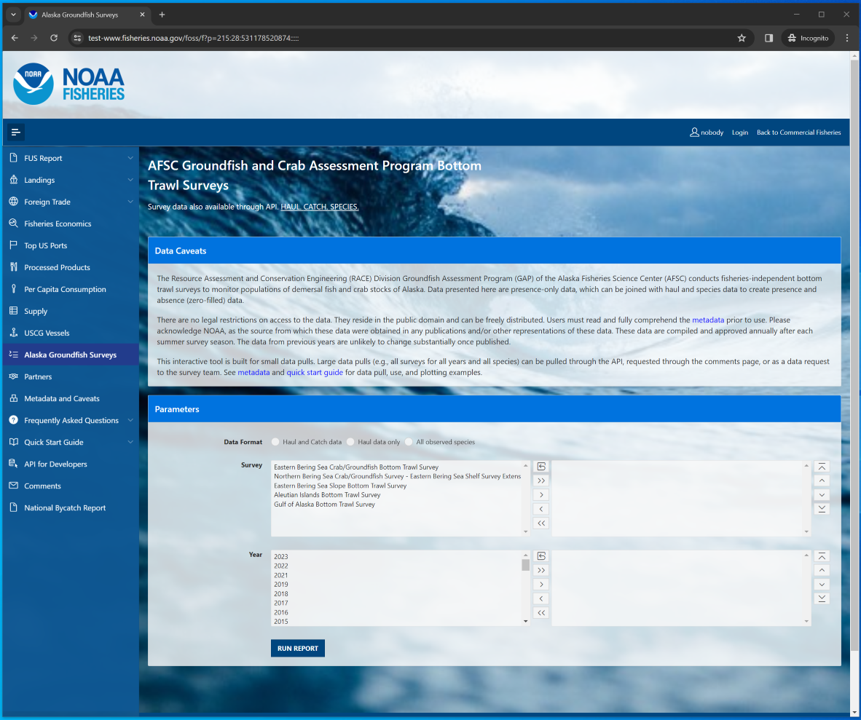
\includegraphics[width=6.24in,height=\textheight]{content/../img/foss_1_interface.png}

}

\caption{AFSC Groundfish and Crab Assessment Program Bottom Trawl Survey
data interface on the Fisheries One Stop Shop platform.}

\end{figure}

\hypertarget{select-and-filter}{%
\section{Select and filter}\label{select-and-filter}}

Select, filter, and package this and other NOAA Fisheries data from the
\href{https://www.fisheries.noaa.gov/foss}{Fisheries One Stop Shop
(FOSS)} platform. A user guide for the FOSS platform can be found
\href{https://www.fisheries.noaa.gov/foss/f?p=215:7:7542600605674:::::}{here}.
To begin a report, select options from the boxes what you need data for.

For a given box, select one or a few options from the ``options box''
(list on the left) to query by highlighting them. To select multiple
options, hold down the CTRL key while clicking on the options of
interest, or click and drag down the list. Once the options you wish to
be included in your query are highlighted, click the right-pointing
arrow (\texttt{\textgreater{}}) to move them into the ``selection box''
(list on the right). If you accidentally select an option that you do
not want to query, simply select the unwanted option from the selection
box and click the left-pointing arrow (\texttt{\textless{}}).

If you wish to select all options from the options box and send them to
the selection box, simply click the double right-pointing arrow
(\texttt{\textgreater{}\textgreater{}}). If you want to unselect all
options from the selection box, use the double left-pointing arrow
(\texttt{\textless{}\textless{}}) or the reset icon.

To find a specific species or group more quickly you can use the
\texttt{Search\ Species} option to quickly narrow the options. Search
for parts of species common names in the \texttt{Search\ Species} box by
entering a term and clicking the \texttt{search} button. The platform
will return a shorter list in the \texttt{Speices} options box of only
species that contain a match to that search term.

Use the \texttt{Reset\ All\ Parameters} button to reset all parameters
for entire form.

\begin{figure}

{\centering 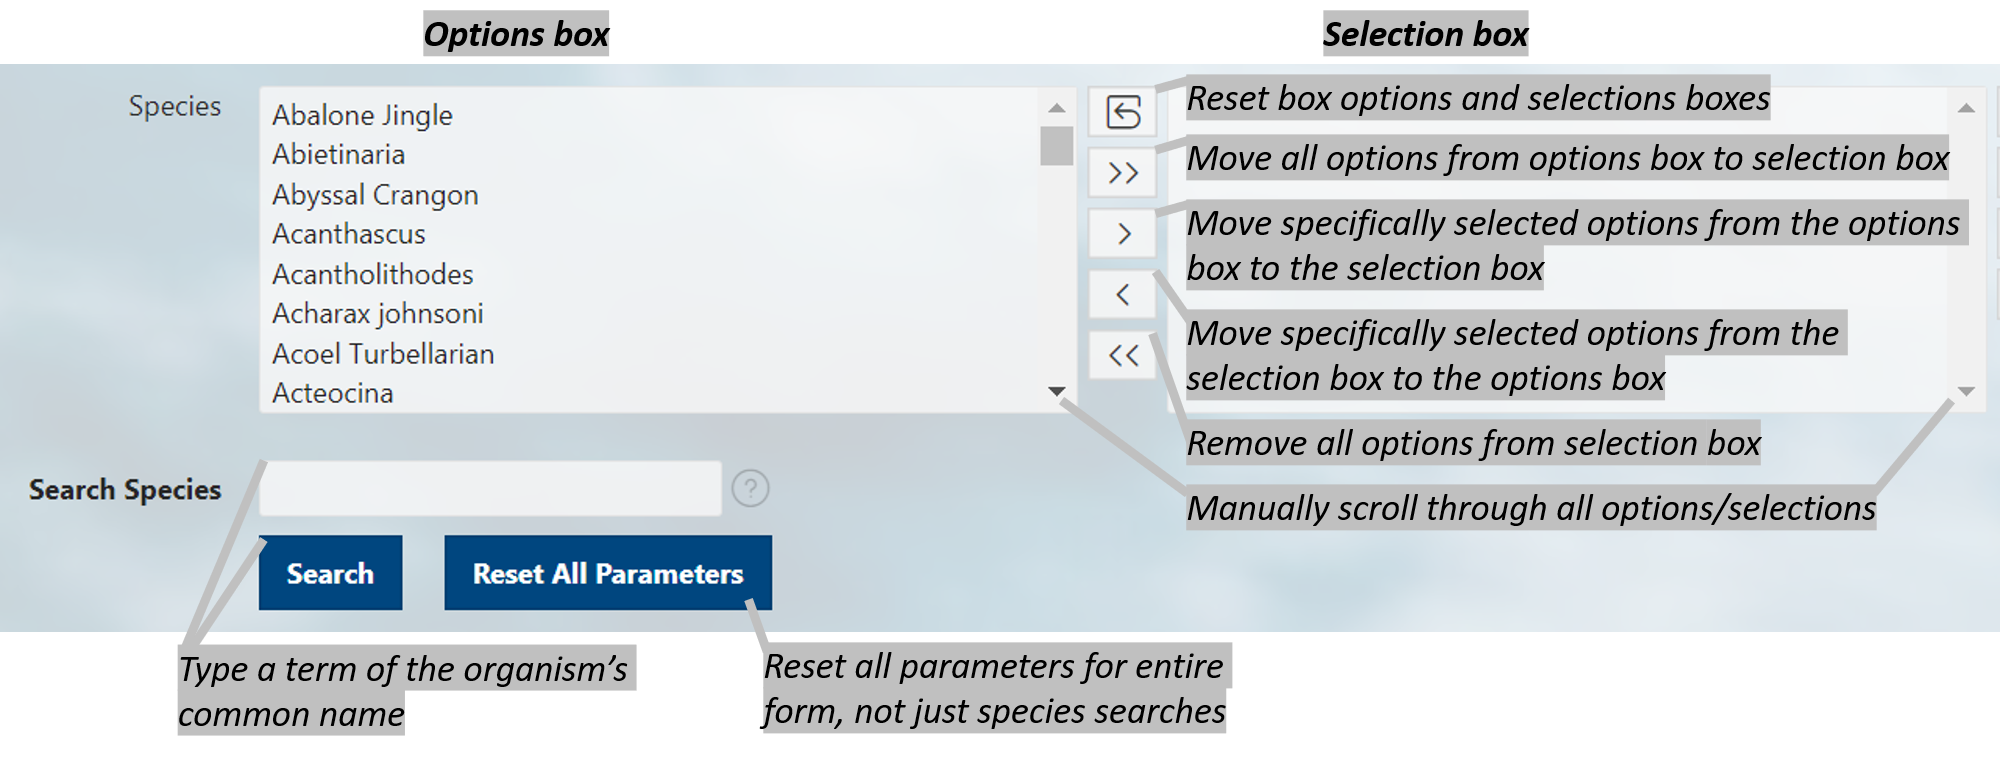
\includegraphics[width=6.67in,height=\textheight]{content/../img/foss_2_select.png}

}

\caption{Diagram of selection and search tools available on the FOSS
platofrom.}

\end{figure}

Filter options:

\begin{itemize}
\tightlist
\item
  \texttt{Survey}: Each survey has different in design, time series, and
  history. More information on each survey and their designs can be
  found in our
  \href{https://www.fisheries.noaa.gov/alaska/science-data/groundfish-assessment-program-bottom-trawl-surveys\#data-products}{annual
  data reports}.
\item
  \texttt{Year}: Surveys are not conducted in all years, so only data
  from the years for which the survey was conducted will be returned.
\item
  \texttt{Species}: Common name of all species ever encountered in the
  survey. Find more information about these species in our
  \href{https://www.fisheries.noaa.gov/resource/document/groundfish-survey-species-code-manual-and-data-codes-manual}{survey
  code books}.
\end{itemize}

\begin{quote}
In this example, we'll select for 2022 eastern Bering Sea Pacific cod
data. Here, we used the \texttt{Search\ Species} box to search for
species with the term ``cod'' in their common names and selected
``Pacific cod'' from that shortened list.
\end{quote}

\begin{figure}

{\centering 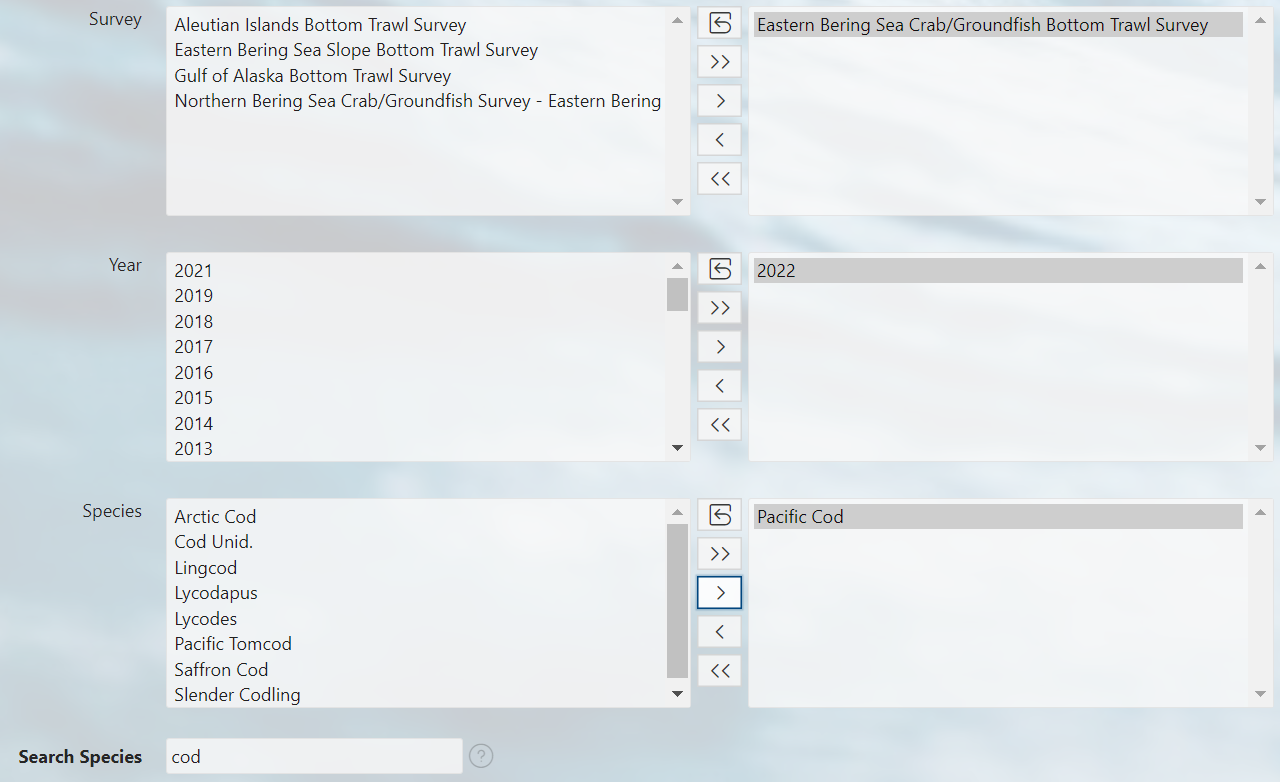
\includegraphics[width=4.27in,height=\textheight]{content/../img/foss_3_selected.png}

}

\caption{Diagram of selection and search tools available on the FOSS
platofrom.}

\end{figure}

\hypertarget{select-data-format}{%
\section{Select data format}\label{select-data-format}}

Select from the below radio list of pre-designed output tables. Once you
run the report, the user can further specify filter data and select
columns of interest. The tables below will only include data from the
selections made in the previous step.

\begin{itemize}
\tightlist
\item
  \texttt{All\ Data\ Fields:\ Presence\ and\ Absence\ (zero-filled)}:
  The most complete version of the data, including species, catch, haul,
  and environmental data. This data will include catch data for where
  species were caught and zeros for where the species were not caught.
  This is important for calculating catch-per-unit-effort data,
  preparing distribution plots (e.g.,
  \href{https://github.com/afsc-gap-products/akgfmaps}{using the
  akgfmaps R package}), and many statistical analyses.
\item
  \texttt{All\ Data\ Fields:\ Presence-only\ (non-zero)}: The second
  most complete version of the data, including species, catch, haul, and
  environmental data. However, this data only includes catch data for
  where species were caught and does not include zeros for where the
  species were not caught. This will return smaller, more focused data
  and can be useful for quickly assessing how many species were caught
  or how many stations species were caught at.
\item
  \texttt{Catch\ data:\ Presence\ and\ Absence\ (zero-filled)}: This
  data set is similar to
  \texttt{All\ Data\ Fields:\ Presence\ and\ Absence\ (zero-filled)},
  but only includes catch and species data columns.
\item
  \texttt{Catch\ data:\ Presence-only\ (non-zero)}: This data set is
  similar to \texttt{All\ Data\ Fields:\ Presence-only\ (non-zero)}, but
  only includes catch and species data columns.
\item
  \texttt{Haul\ Data}: This data set only includes haul and
  environmental data collected from the survey. This data will only
  include one observation per haul event/station.
\end{itemize}

\begin{quote}
In this example, we'll select
\texttt{All\ Data\ Fields:\ Presence\ and\ Absence\ (zero-filled).}
\end{quote}

\begin{figure}

{\centering 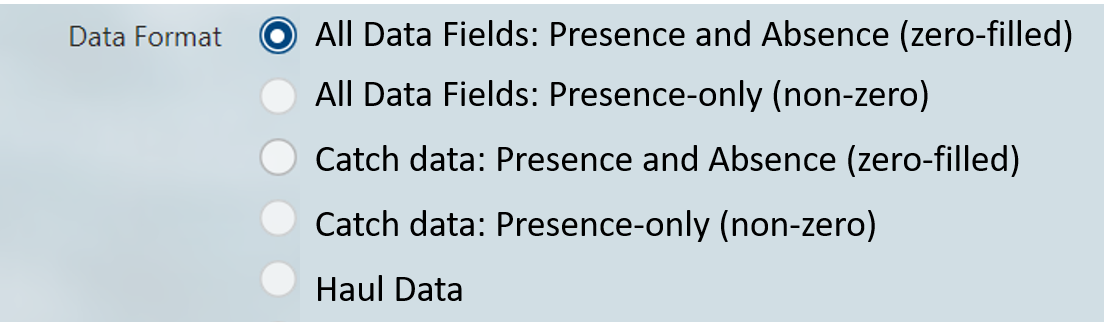
\includegraphics[width=3.68in,height=\textheight]{content/../img/foss_4_data_format.png}

}

\caption{Diagram of the pre-set data format options.}

\end{figure}

\hypertarget{run-report}{%
\section{Run report}\label{run-report}}

Click the \texttt{RUN\ REPORT} button. Below the select and filter area,
the results of your query will appear below the page in the format you
selected. To change the format, make a different selection and run the
report again. Further modifications to your results can be made by
clicking on the \texttt{Actions} button above your data. Here you can
\texttt{download} your data, \texttt{select\ columns} included in your
results, and apply a variety of \texttt{filters} and mathematical tools.

\begin{figure}

{\centering 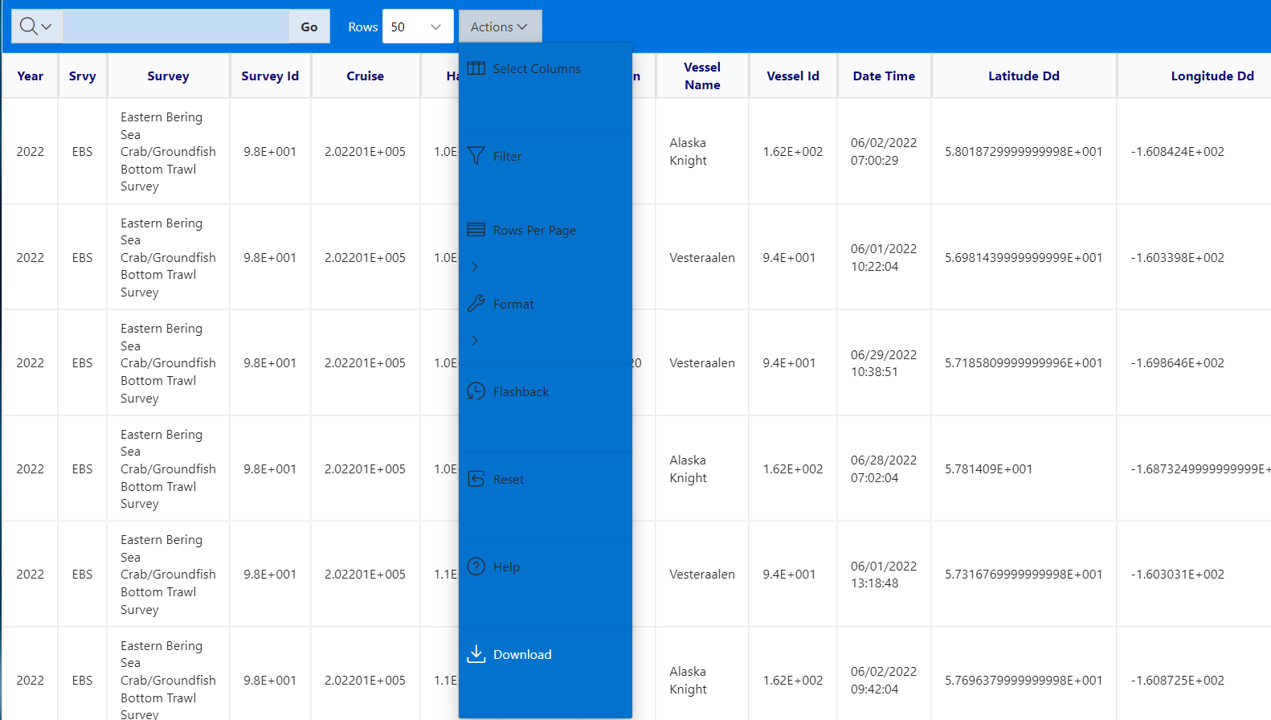
\includegraphics[width=4.24in,height=\textheight]{content/../img/foss_5_run_report.png}

}

\caption{Example data returned from running the report.}

\end{figure}

\hypertarget{access-public-data-using-the-api-and-r}{%
\chapter{Access public data using the API and
R}\label{access-public-data-using-the-api-and-r}}

\hypertarget{connect-to-the-api-with-r}{%
\chapter{Connect to the API with R}\label{connect-to-the-api-with-r}}

An application programming interface (API) is a way for two or more
computer programs to communicate with each other.

More information about how to amend API links can be found
\href{https://docs.oracle.com/en/database/oracle/oracle-rest-data-services/22.3/books.html\#AELIG90103/}{here}.
Useful introductions to using APIs in \texttt{R} can be found
\href{https://www.dataquest.io/blog/r-api-tutorial/}{here}.

\hypertarget{api-in-action}{%
\chapter{API in action}\label{api-in-action}}

\hypertarget{ex.-1-load-the-first-25-rows-default-of-data}{%
\section{Ex. 1: Load the first 25 rows (default) of
data}\label{ex.-1-load-the-first-25-rows-default-of-data}}

\begin{Shaded}
\begin{Highlighting}[]
 \CommentTok{\# install.packages(c("httr", "jsonlite"))}
\FunctionTok{library}\NormalTok{(httr)}
\FunctionTok{library}\NormalTok{(jsonlite)}
\FunctionTok{library}\NormalTok{(dplyr)}
 \CommentTok{\# link to the API}
\NormalTok{api\_link }\OtherTok{\textless{}{-}} \StringTok{"https://apps{-}st.fisheries.noaa.gov/ods/foss/afsc\_groundfish\_survey/"}

\NormalTok{res }\OtherTok{\textless{}{-}}\NormalTok{ httr}\SpecialCharTok{::}\FunctionTok{GET}\NormalTok{(}\AttributeTok{url =}\NormalTok{ api\_link)}
 \CommentTok{\# res \# Test connection}
\NormalTok{data }\OtherTok{\textless{}{-}}\NormalTok{ jsonlite}\SpecialCharTok{::}\FunctionTok{fromJSON}\NormalTok{(base}\SpecialCharTok{::}\FunctionTok{rawToChar}\NormalTok{(res}\SpecialCharTok{$}\NormalTok{content))}
 \CommentTok{\# names(data)}
\NormalTok{flextable}\SpecialCharTok{::}\FunctionTok{flextable}\NormalTok{(}\FunctionTok{head}\NormalTok{(data}\SpecialCharTok{$}\NormalTok{items, }\DecValTok{3}\NormalTok{)) }
\end{Highlighting}
\end{Shaded}

\global\setlength{\Oldarrayrulewidth}{\arrayrulewidth}

\global\setlength{\Oldtabcolsep}{\tabcolsep}

\setlength{\tabcolsep}{0pt}

\renewcommand*{\arraystretch}{1.5}



\providecommand{\ascline}[3]{\noalign{\global\arrayrulewidth #1}\arrayrulecolor[HTML]{#2}\cline{#3}}

\begin{longtable}[c]{|p{0.75in}|p{0.75in}|p{0.75in}|p{0.75in}|p{0.75in}|p{0.75in}|p{0.75in}|p{0.75in}|p{0.75in}|p{0.75in}|p{0.75in}|p{0.75in}|p{0.75in}|p{0.75in}|p{0.75in}|p{0.75in}|p{0.75in}|p{0.75in}|p{0.75in}|p{0.75in}|p{0.75in}|p{0.75in}|p{0.75in}|p{0.75in}|p{0.75in}|p{0.75in}|p{0.75in}|p{0.75in}|p{0.75in}|p{0.75in}|p{0.75in}|p{0.75in}|p{0.75in}|p{0.75in}|p{0.75in}|p{0.75in}}
\caption{Ex. 1: Load the first 25 rows (default) of data.}\tabularnewline




\ascline{1.5pt}{666666}{1-36}

\multicolumn{1}{>{\raggedleft}m{\dimexpr 0.75in+0\tabcolsep}}{\textcolor[HTML]{000000}{\fontsize{11}{11}\selectfont{year}}} & \multicolumn{1}{>{\raggedright}m{\dimexpr 0.75in+0\tabcolsep}}{\textcolor[HTML]{000000}{\fontsize{11}{11}\selectfont{srvy}}} & \multicolumn{1}{>{\raggedright}m{\dimexpr 0.75in+0\tabcolsep}}{\textcolor[HTML]{000000}{\fontsize{11}{11}\selectfont{survey}}} & \multicolumn{1}{>{\raggedright}m{\dimexpr 0.75in+0\tabcolsep}}{\textcolor[HTML]{000000}{\fontsize{11}{11}\selectfont{survey\_id}}} & \multicolumn{1}{>{\raggedright}m{\dimexpr 0.75in+0\tabcolsep}}{\textcolor[HTML]{000000}{\fontsize{11}{11}\selectfont{cruise}}} & \multicolumn{1}{>{\raggedright}m{\dimexpr 0.75in+0\tabcolsep}}{\textcolor[HTML]{000000}{\fontsize{11}{11}\selectfont{haul}}} & \multicolumn{1}{>{\raggedright}m{\dimexpr 0.75in+0\tabcolsep}}{\textcolor[HTML]{000000}{\fontsize{11}{11}\selectfont{stratum}}} & \multicolumn{1}{>{\raggedright}m{\dimexpr 0.75in+0\tabcolsep}}{\textcolor[HTML]{000000}{\fontsize{11}{11}\selectfont{station}}} & \multicolumn{1}{>{\raggedright}m{\dimexpr 0.75in+0\tabcolsep}}{\textcolor[HTML]{000000}{\fontsize{11}{11}\selectfont{vessel\_name}}} & \multicolumn{1}{>{\raggedright}m{\dimexpr 0.75in+0\tabcolsep}}{\textcolor[HTML]{000000}{\fontsize{11}{11}\selectfont{vessel\_id}}} & \multicolumn{1}{>{\raggedright}m{\dimexpr 0.75in+0\tabcolsep}}{\textcolor[HTML]{000000}{\fontsize{11}{11}\selectfont{date\_time}}} & \multicolumn{1}{>{\raggedright}m{\dimexpr 0.75in+0\tabcolsep}}{\textcolor[HTML]{000000}{\fontsize{11}{11}\selectfont{latitude\_dd}}} & \multicolumn{1}{>{\raggedright}m{\dimexpr 0.75in+0\tabcolsep}}{\textcolor[HTML]{000000}{\fontsize{11}{11}\selectfont{longitude\_dd}}} & \multicolumn{1}{>{\raggedright}m{\dimexpr 0.75in+0\tabcolsep}}{\textcolor[HTML]{000000}{\fontsize{11}{11}\selectfont{species\_code}}} & \multicolumn{1}{>{\raggedright}m{\dimexpr 0.75in+0\tabcolsep}}{\textcolor[HTML]{000000}{\fontsize{11}{11}\selectfont{common\_name}}} & \multicolumn{1}{>{\raggedright}m{\dimexpr 0.75in+0\tabcolsep}}{\textcolor[HTML]{000000}{\fontsize{11}{11}\selectfont{scientific\_name}}} & \multicolumn{1}{>{\raggedright}m{\dimexpr 0.75in+0\tabcolsep}}{\textcolor[HTML]{000000}{\fontsize{11}{11}\selectfont{taxon\_confidence}}} & \multicolumn{1}{>{\raggedright}m{\dimexpr 0.75in+0\tabcolsep}}{\textcolor[HTML]{000000}{\fontsize{11}{11}\selectfont{cpue\_kgha}}} & \multicolumn{1}{>{\raggedright}m{\dimexpr 0.75in+0\tabcolsep}}{\textcolor[HTML]{000000}{\fontsize{11}{11}\selectfont{cpue\_kgkm2}}} & \multicolumn{1}{>{\raggedright}m{\dimexpr 0.75in+0\tabcolsep}}{\textcolor[HTML]{000000}{\fontsize{11}{11}\selectfont{cpue\_kg1000km2}}} & \multicolumn{1}{>{\raggedright}m{\dimexpr 0.75in+0\tabcolsep}}{\textcolor[HTML]{000000}{\fontsize{11}{11}\selectfont{cpue\_noha}}} & \multicolumn{1}{>{\raggedright}m{\dimexpr 0.75in+0\tabcolsep}}{\textcolor[HTML]{000000}{\fontsize{11}{11}\selectfont{cpue\_nokm2}}} & \multicolumn{1}{>{\raggedright}m{\dimexpr 0.75in+0\tabcolsep}}{\textcolor[HTML]{000000}{\fontsize{11}{11}\selectfont{cpue\_no1000km2}}} & \multicolumn{1}{>{\raggedright}m{\dimexpr 0.75in+0\tabcolsep}}{\textcolor[HTML]{000000}{\fontsize{11}{11}\selectfont{weight\_kg}}} & \multicolumn{1}{>{\raggedright}m{\dimexpr 0.75in+0\tabcolsep}}{\textcolor[HTML]{000000}{\fontsize{11}{11}\selectfont{count}}} & \multicolumn{1}{>{\raggedright}m{\dimexpr 0.75in+0\tabcolsep}}{\textcolor[HTML]{000000}{\fontsize{11}{11}\selectfont{bottom\_temperature\_c}}} & \multicolumn{1}{>{\raggedright}m{\dimexpr 0.75in+0\tabcolsep}}{\textcolor[HTML]{000000}{\fontsize{11}{11}\selectfont{surface\_temperature\_c}}} & \multicolumn{1}{>{\raggedright}m{\dimexpr 0.75in+0\tabcolsep}}{\textcolor[HTML]{000000}{\fontsize{11}{11}\selectfont{depth\_m}}} & \multicolumn{1}{>{\raggedright}m{\dimexpr 0.75in+0\tabcolsep}}{\textcolor[HTML]{000000}{\fontsize{11}{11}\selectfont{distance\_fished\_km}}} & \multicolumn{1}{>{\raggedright}m{\dimexpr 0.75in+0\tabcolsep}}{\textcolor[HTML]{000000}{\fontsize{11}{11}\selectfont{net\_width\_m}}} & \multicolumn{1}{>{\raggedright}m{\dimexpr 0.75in+0\tabcolsep}}{\textcolor[HTML]{000000}{\fontsize{11}{11}\selectfont{net\_height\_m}}} & \multicolumn{1}{>{\raggedright}m{\dimexpr 0.75in+0\tabcolsep}}{\textcolor[HTML]{000000}{\fontsize{11}{11}\selectfont{area\_swept\_ha}}} & \multicolumn{1}{>{\raggedright}m{\dimexpr 0.75in+0\tabcolsep}}{\textcolor[HTML]{000000}{\fontsize{11}{11}\selectfont{duration\_hr}}} & \multicolumn{1}{>{\raggedleft}m{\dimexpr 0.75in+0\tabcolsep}}{\textcolor[HTML]{000000}{\fontsize{11}{11}\selectfont{tsn}}} & \multicolumn{1}{>{\raggedleft}m{\dimexpr 0.75in+0\tabcolsep}}{\textcolor[HTML]{000000}{\fontsize{11}{11}\selectfont{ak\_survey\_id}}} & \multicolumn{1}{>{\raggedleft}m{\dimexpr 0.75in+0\tabcolsep}}{\textcolor[HTML]{000000}{\fontsize{11}{11}\selectfont{links}}} \\

\ascline{1.5pt}{666666}{1-36}\endfirsthead 

\ascline{1.5pt}{666666}{1-36}

\multicolumn{1}{>{\raggedleft}m{\dimexpr 0.75in+0\tabcolsep}}{\textcolor[HTML]{000000}{\fontsize{11}{11}\selectfont{year}}} & \multicolumn{1}{>{\raggedright}m{\dimexpr 0.75in+0\tabcolsep}}{\textcolor[HTML]{000000}{\fontsize{11}{11}\selectfont{srvy}}} & \multicolumn{1}{>{\raggedright}m{\dimexpr 0.75in+0\tabcolsep}}{\textcolor[HTML]{000000}{\fontsize{11}{11}\selectfont{survey}}} & \multicolumn{1}{>{\raggedright}m{\dimexpr 0.75in+0\tabcolsep}}{\textcolor[HTML]{000000}{\fontsize{11}{11}\selectfont{survey\_id}}} & \multicolumn{1}{>{\raggedright}m{\dimexpr 0.75in+0\tabcolsep}}{\textcolor[HTML]{000000}{\fontsize{11}{11}\selectfont{cruise}}} & \multicolumn{1}{>{\raggedright}m{\dimexpr 0.75in+0\tabcolsep}}{\textcolor[HTML]{000000}{\fontsize{11}{11}\selectfont{haul}}} & \multicolumn{1}{>{\raggedright}m{\dimexpr 0.75in+0\tabcolsep}}{\textcolor[HTML]{000000}{\fontsize{11}{11}\selectfont{stratum}}} & \multicolumn{1}{>{\raggedright}m{\dimexpr 0.75in+0\tabcolsep}}{\textcolor[HTML]{000000}{\fontsize{11}{11}\selectfont{station}}} & \multicolumn{1}{>{\raggedright}m{\dimexpr 0.75in+0\tabcolsep}}{\textcolor[HTML]{000000}{\fontsize{11}{11}\selectfont{vessel\_name}}} & \multicolumn{1}{>{\raggedright}m{\dimexpr 0.75in+0\tabcolsep}}{\textcolor[HTML]{000000}{\fontsize{11}{11}\selectfont{vessel\_id}}} & \multicolumn{1}{>{\raggedright}m{\dimexpr 0.75in+0\tabcolsep}}{\textcolor[HTML]{000000}{\fontsize{11}{11}\selectfont{date\_time}}} & \multicolumn{1}{>{\raggedright}m{\dimexpr 0.75in+0\tabcolsep}}{\textcolor[HTML]{000000}{\fontsize{11}{11}\selectfont{latitude\_dd}}} & \multicolumn{1}{>{\raggedright}m{\dimexpr 0.75in+0\tabcolsep}}{\textcolor[HTML]{000000}{\fontsize{11}{11}\selectfont{longitude\_dd}}} & \multicolumn{1}{>{\raggedright}m{\dimexpr 0.75in+0\tabcolsep}}{\textcolor[HTML]{000000}{\fontsize{11}{11}\selectfont{species\_code}}} & \multicolumn{1}{>{\raggedright}m{\dimexpr 0.75in+0\tabcolsep}}{\textcolor[HTML]{000000}{\fontsize{11}{11}\selectfont{common\_name}}} & \multicolumn{1}{>{\raggedright}m{\dimexpr 0.75in+0\tabcolsep}}{\textcolor[HTML]{000000}{\fontsize{11}{11}\selectfont{scientific\_name}}} & \multicolumn{1}{>{\raggedright}m{\dimexpr 0.75in+0\tabcolsep}}{\textcolor[HTML]{000000}{\fontsize{11}{11}\selectfont{taxon\_confidence}}} & \multicolumn{1}{>{\raggedright}m{\dimexpr 0.75in+0\tabcolsep}}{\textcolor[HTML]{000000}{\fontsize{11}{11}\selectfont{cpue\_kgha}}} & \multicolumn{1}{>{\raggedright}m{\dimexpr 0.75in+0\tabcolsep}}{\textcolor[HTML]{000000}{\fontsize{11}{11}\selectfont{cpue\_kgkm2}}} & \multicolumn{1}{>{\raggedright}m{\dimexpr 0.75in+0\tabcolsep}}{\textcolor[HTML]{000000}{\fontsize{11}{11}\selectfont{cpue\_kg1000km2}}} & \multicolumn{1}{>{\raggedright}m{\dimexpr 0.75in+0\tabcolsep}}{\textcolor[HTML]{000000}{\fontsize{11}{11}\selectfont{cpue\_noha}}} & \multicolumn{1}{>{\raggedright}m{\dimexpr 0.75in+0\tabcolsep}}{\textcolor[HTML]{000000}{\fontsize{11}{11}\selectfont{cpue\_nokm2}}} & \multicolumn{1}{>{\raggedright}m{\dimexpr 0.75in+0\tabcolsep}}{\textcolor[HTML]{000000}{\fontsize{11}{11}\selectfont{cpue\_no1000km2}}} & \multicolumn{1}{>{\raggedright}m{\dimexpr 0.75in+0\tabcolsep}}{\textcolor[HTML]{000000}{\fontsize{11}{11}\selectfont{weight\_kg}}} & \multicolumn{1}{>{\raggedright}m{\dimexpr 0.75in+0\tabcolsep}}{\textcolor[HTML]{000000}{\fontsize{11}{11}\selectfont{count}}} & \multicolumn{1}{>{\raggedright}m{\dimexpr 0.75in+0\tabcolsep}}{\textcolor[HTML]{000000}{\fontsize{11}{11}\selectfont{bottom\_temperature\_c}}} & \multicolumn{1}{>{\raggedright}m{\dimexpr 0.75in+0\tabcolsep}}{\textcolor[HTML]{000000}{\fontsize{11}{11}\selectfont{surface\_temperature\_c}}} & \multicolumn{1}{>{\raggedright}m{\dimexpr 0.75in+0\tabcolsep}}{\textcolor[HTML]{000000}{\fontsize{11}{11}\selectfont{depth\_m}}} & \multicolumn{1}{>{\raggedright}m{\dimexpr 0.75in+0\tabcolsep}}{\textcolor[HTML]{000000}{\fontsize{11}{11}\selectfont{distance\_fished\_km}}} & \multicolumn{1}{>{\raggedright}m{\dimexpr 0.75in+0\tabcolsep}}{\textcolor[HTML]{000000}{\fontsize{11}{11}\selectfont{net\_width\_m}}} & \multicolumn{1}{>{\raggedright}m{\dimexpr 0.75in+0\tabcolsep}}{\textcolor[HTML]{000000}{\fontsize{11}{11}\selectfont{net\_height\_m}}} & \multicolumn{1}{>{\raggedright}m{\dimexpr 0.75in+0\tabcolsep}}{\textcolor[HTML]{000000}{\fontsize{11}{11}\selectfont{area\_swept\_ha}}} & \multicolumn{1}{>{\raggedright}m{\dimexpr 0.75in+0\tabcolsep}}{\textcolor[HTML]{000000}{\fontsize{11}{11}\selectfont{duration\_hr}}} & \multicolumn{1}{>{\raggedleft}m{\dimexpr 0.75in+0\tabcolsep}}{\textcolor[HTML]{000000}{\fontsize{11}{11}\selectfont{tsn}}} & \multicolumn{1}{>{\raggedleft}m{\dimexpr 0.75in+0\tabcolsep}}{\textcolor[HTML]{000000}{\fontsize{11}{11}\selectfont{ak\_survey\_id}}} & \multicolumn{1}{>{\raggedleft}m{\dimexpr 0.75in+0\tabcolsep}}{\textcolor[HTML]{000000}{\fontsize{11}{11}\selectfont{links}}} \\

\ascline{1.5pt}{666666}{1-36}\endhead



\multicolumn{1}{>{\raggedleft}m{\dimexpr 0.75in+0\tabcolsep}}{\textcolor[HTML]{000000}{\fontsize{11}{11}\selectfont{2,002}}} & \multicolumn{1}{>{\raggedright}m{\dimexpr 0.75in+0\tabcolsep}}{\textcolor[HTML]{000000}{\fontsize{11}{11}\selectfont{AI}}} & \multicolumn{1}{>{\raggedright}m{\dimexpr 0.75in+0\tabcolsep}}{\textcolor[HTML]{000000}{\fontsize{11}{11}\selectfont{Aleutian\ Islands\ Bottom\ Trawl\ Survey}}} & \multicolumn{1}{>{\raggedright}m{\dimexpr 0.75in+0\tabcolsep}}{\textcolor[HTML]{000000}{\fontsize{11}{11}\selectfont{5.2E+001}}} & \multicolumn{1}{>{\raggedright}m{\dimexpr 0.75in+0\tabcolsep}}{\textcolor[HTML]{000000}{\fontsize{11}{11}\selectfont{2.00201E+005}}} & \multicolumn{1}{>{\raggedright}m{\dimexpr 0.75in+0\tabcolsep}}{\textcolor[HTML]{000000}{\fontsize{11}{11}\selectfont{6.0E+000}}} & \multicolumn{1}{>{\raggedright}m{\dimexpr 0.75in+0\tabcolsep}}{\textcolor[HTML]{000000}{\fontsize{11}{11}\selectfont{7.22E+002}}} & \multicolumn{1}{>{\raggedright}m{\dimexpr 0.75in+0\tabcolsep}}{\textcolor[HTML]{000000}{\fontsize{11}{11}\selectfont{307-63}}} & \multicolumn{1}{>{\raggedright}m{\dimexpr 0.75in+0\tabcolsep}}{\textcolor[HTML]{000000}{\fontsize{11}{11}\selectfont{Vesteraalen}}} & \multicolumn{1}{>{\raggedright}m{\dimexpr 0.75in+0\tabcolsep}}{\textcolor[HTML]{000000}{\fontsize{11}{11}\selectfont{9.4E+001}}} & \multicolumn{1}{>{\raggedright}m{\dimexpr 0.75in+0\tabcolsep}}{\textcolor[HTML]{000000}{\fontsize{11}{11}\selectfont{05/17/2002\ 18:56:58}}} & \multicolumn{1}{>{\raggedright}m{\dimexpr 0.75in+0\tabcolsep}}{\textcolor[HTML]{000000}{\fontsize{11}{11}\selectfont{5.3737209999999997E+001}}} & \multicolumn{1}{>{\raggedright}m{\dimexpr 0.75in+0\tabcolsep}}{\textcolor[HTML]{000000}{\fontsize{11}{11}\selectfont{-1.6701570000000001E+002}}} & \multicolumn{1}{>{\raggedright}m{\dimexpr 0.75in+0\tabcolsep}}{\textcolor[HTML]{000000}{\fontsize{11}{11}\selectfont{9.502E+004}}} & \multicolumn{1}{>{\raggedright}m{\dimexpr 0.75in+0\tabcolsep}}{\textcolor[HTML]{000000}{\fontsize{11}{11}\selectfont{feathery\ bryozoan}}} & \multicolumn{1}{>{\raggedright}m{\dimexpr 0.75in+0\tabcolsep}}{\textcolor[HTML]{000000}{\fontsize{11}{11}\selectfont{Eucratea\ loricata}}} & \multicolumn{1}{>{\raggedright}m{\dimexpr 0.75in+0\tabcolsep}}{\textcolor[HTML]{000000}{\fontsize{11}{11}\selectfont{Low}}} & \multicolumn{1}{>{\raggedright}m{\dimexpr 0.75in+0\tabcolsep}}{\textcolor[HTML]{000000}{\fontsize{11}{11}\selectfont{1.7493999999999999E-002}}} & \multicolumn{1}{>{\raggedright}m{\dimexpr 0.75in+0\tabcolsep}}{\textcolor[HTML]{000000}{\fontsize{11}{11}\selectfont{1.7494449999999999E+000}}} & \multicolumn{1}{>{\raggedright}m{\dimexpr 0.75in+0\tabcolsep}}{\textcolor[HTML]{000000}{\fontsize{11}{11}\selectfont{1.7494451079999999E+003}}} & \multicolumn{1}{>{\raggedright}m{\dimexpr 0.75in+0\tabcolsep}}{\textcolor[HTML]{000000}{\fontsize{11}{11}\selectfont{}}} & \multicolumn{1}{>{\raggedright}m{\dimexpr 0.75in+0\tabcolsep}}{\textcolor[HTML]{000000}{\fontsize{11}{11}\selectfont{}}} & \multicolumn{1}{>{\raggedright}m{\dimexpr 0.75in+0\tabcolsep}}{\textcolor[HTML]{000000}{\fontsize{11}{11}\selectfont{}}} & \multicolumn{1}{>{\raggedright}m{\dimexpr 0.75in+0\tabcolsep}}{\textcolor[HTML]{000000}{\fontsize{11}{11}\selectfont{4.3999999999999997E-002}}} & \multicolumn{1}{>{\raggedright}m{\dimexpr 0.75in+0\tabcolsep}}{\textcolor[HTML]{000000}{\fontsize{11}{11}\selectfont{0}}} & \multicolumn{1}{>{\raggedright}m{\dimexpr 0.75in+0\tabcolsep}}{\textcolor[HTML]{000000}{\fontsize{11}{11}\selectfont{4.0999999999999996E+000}}} & \multicolumn{1}{>{\raggedright}m{\dimexpr 0.75in+0\tabcolsep}}{\textcolor[HTML]{000000}{\fontsize{11}{11}\selectfont{5.2999999999999998E+000}}} & \multicolumn{1}{>{\raggedright}m{\dimexpr 0.75in+0\tabcolsep}}{\textcolor[HTML]{000000}{\fontsize{11}{11}\selectfont{1.87E+002}}} & \multicolumn{1}{>{\raggedright}m{\dimexpr 0.75in+0\tabcolsep}}{\textcolor[HTML]{000000}{\fontsize{11}{11}\selectfont{1.5609999999999999E+000}}} & \multicolumn{1}{>{\raggedright}m{\dimexpr 0.75in+0\tabcolsep}}{\textcolor[HTML]{000000}{\fontsize{11}{11}\selectfont{1.6111999999999998E+001}}} & \multicolumn{1}{>{\raggedright}m{\dimexpr 0.75in+0\tabcolsep}}{\textcolor[HTML]{000000}{\fontsize{11}{11}\selectfont{7.25E+000}}} & \multicolumn{1}{>{\raggedright}m{\dimexpr 0.75in+0\tabcolsep}}{\textcolor[HTML]{000000}{\fontsize{11}{11}\selectfont{2.5150831999999994E+000}}} & \multicolumn{1}{>{\raggedright}m{\dimexpr 0.75in+0\tabcolsep}}{\textcolor[HTML]{000000}{\fontsize{11}{11}\selectfont{2.8000000000000003E-001}}} & \multicolumn{1}{>{\raggedleft}m{\dimexpr 0.75in+0\tabcolsep}}{\textcolor[HTML]{000000}{\fontsize{11}{11}\selectfont{155,809}}} & \multicolumn{1}{>{\raggedleft}m{\dimexpr 0.75in+0\tabcolsep}}{\textcolor[HTML]{000000}{\fontsize{11}{11}\selectfont{878,821}}} & \multicolumn{1}{>{\raggedleft}m{\dimexpr 0.75in+0\tabcolsep}}{\textcolor[HTML]{000000}{\fontsize{11}{11}\selectfont{[[data.frame]]}}} \\





\multicolumn{1}{>{\raggedleft}m{\dimexpr 0.75in+0\tabcolsep}}{\textcolor[HTML]{000000}{\fontsize{11}{11}\selectfont{2,002}}} & \multicolumn{1}{>{\raggedright}m{\dimexpr 0.75in+0\tabcolsep}}{\textcolor[HTML]{000000}{\fontsize{11}{11}\selectfont{AI}}} & \multicolumn{1}{>{\raggedright}m{\dimexpr 0.75in+0\tabcolsep}}{\textcolor[HTML]{000000}{\fontsize{11}{11}\selectfont{Aleutian\ Islands\ Bottom\ Trawl\ Survey}}} & \multicolumn{1}{>{\raggedright}m{\dimexpr 0.75in+0\tabcolsep}}{\textcolor[HTML]{000000}{\fontsize{11}{11}\selectfont{5.2E+001}}} & \multicolumn{1}{>{\raggedright}m{\dimexpr 0.75in+0\tabcolsep}}{\textcolor[HTML]{000000}{\fontsize{11}{11}\selectfont{2.00201E+005}}} & \multicolumn{1}{>{\raggedright}m{\dimexpr 0.75in+0\tabcolsep}}{\textcolor[HTML]{000000}{\fontsize{11}{11}\selectfont{6.0E+000}}} & \multicolumn{1}{>{\raggedright}m{\dimexpr 0.75in+0\tabcolsep}}{\textcolor[HTML]{000000}{\fontsize{11}{11}\selectfont{7.22E+002}}} & \multicolumn{1}{>{\raggedright}m{\dimexpr 0.75in+0\tabcolsep}}{\textcolor[HTML]{000000}{\fontsize{11}{11}\selectfont{307-63}}} & \multicolumn{1}{>{\raggedright}m{\dimexpr 0.75in+0\tabcolsep}}{\textcolor[HTML]{000000}{\fontsize{11}{11}\selectfont{Vesteraalen}}} & \multicolumn{1}{>{\raggedright}m{\dimexpr 0.75in+0\tabcolsep}}{\textcolor[HTML]{000000}{\fontsize{11}{11}\selectfont{9.4E+001}}} & \multicolumn{1}{>{\raggedright}m{\dimexpr 0.75in+0\tabcolsep}}{\textcolor[HTML]{000000}{\fontsize{11}{11}\selectfont{05/17/2002\ 18:56:58}}} & \multicolumn{1}{>{\raggedright}m{\dimexpr 0.75in+0\tabcolsep}}{\textcolor[HTML]{000000}{\fontsize{11}{11}\selectfont{5.3737209999999997E+001}}} & \multicolumn{1}{>{\raggedright}m{\dimexpr 0.75in+0\tabcolsep}}{\textcolor[HTML]{000000}{\fontsize{11}{11}\selectfont{-1.6701570000000001E+002}}} & \multicolumn{1}{>{\raggedright}m{\dimexpr 0.75in+0\tabcolsep}}{\textcolor[HTML]{000000}{\fontsize{11}{11}\selectfont{7.9E+004}}} & \multicolumn{1}{>{\raggedright}m{\dimexpr 0.75in+0\tabcolsep}}{\textcolor[HTML]{000000}{\fontsize{11}{11}\selectfont{squid\ unid.}}} & \multicolumn{1}{>{\raggedright}m{\dimexpr 0.75in+0\tabcolsep}}{\textcolor[HTML]{000000}{\fontsize{11}{11}\selectfont{Decapodiformes}}} & \multicolumn{1}{>{\raggedright}m{\dimexpr 0.75in+0\tabcolsep}}{\textcolor[HTML]{000000}{\fontsize{11}{11}\selectfont{High}}} & \multicolumn{1}{>{\raggedright}m{\dimexpr 0.75in+0\tabcolsep}}{\textcolor[HTML]{000000}{\fontsize{11}{11}\selectfont{2.2266000000000001E-002}}} & \multicolumn{1}{>{\raggedright}m{\dimexpr 0.75in+0\tabcolsep}}{\textcolor[HTML]{000000}{\fontsize{11}{11}\selectfont{2.2265670000000002E+000}}} & \multicolumn{1}{>{\raggedright}m{\dimexpr 0.75in+0\tabcolsep}}{\textcolor[HTML]{000000}{\fontsize{11}{11}\selectfont{2.2265665009999998E+003}}} & \multicolumn{1}{>{\raggedright}m{\dimexpr 0.75in+0\tabcolsep}}{\textcolor[HTML]{000000}{\fontsize{11}{11}\selectfont{3.180809E+000}}} & \multicolumn{1}{>{\raggedright}m{\dimexpr 0.75in+0\tabcolsep}}{\textcolor[HTML]{000000}{\fontsize{11}{11}\selectfont{3.1808092900000003E+002}}} & \multicolumn{1}{>{\raggedright}m{\dimexpr 0.75in+0\tabcolsep}}{\textcolor[HTML]{000000}{\fontsize{11}{11}\selectfont{3.1808092869500001E+005}}} & \multicolumn{1}{>{\raggedright}m{\dimexpr 0.75in+0\tabcolsep}}{\textcolor[HTML]{000000}{\fontsize{11}{11}\selectfont{5.6000000000000001E-002}}} & \multicolumn{1}{>{\raggedright}m{\dimexpr 0.75in+0\tabcolsep}}{\textcolor[HTML]{000000}{\fontsize{11}{11}\selectfont{8.0E+000}}} & \multicolumn{1}{>{\raggedright}m{\dimexpr 0.75in+0\tabcolsep}}{\textcolor[HTML]{000000}{\fontsize{11}{11}\selectfont{4.0999999999999996E+000}}} & \multicolumn{1}{>{\raggedright}m{\dimexpr 0.75in+0\tabcolsep}}{\textcolor[HTML]{000000}{\fontsize{11}{11}\selectfont{5.2999999999999998E+000}}} & \multicolumn{1}{>{\raggedright}m{\dimexpr 0.75in+0\tabcolsep}}{\textcolor[HTML]{000000}{\fontsize{11}{11}\selectfont{1.87E+002}}} & \multicolumn{1}{>{\raggedright}m{\dimexpr 0.75in+0\tabcolsep}}{\textcolor[HTML]{000000}{\fontsize{11}{11}\selectfont{1.5609999999999999E+000}}} & \multicolumn{1}{>{\raggedright}m{\dimexpr 0.75in+0\tabcolsep}}{\textcolor[HTML]{000000}{\fontsize{11}{11}\selectfont{1.6111999999999998E+001}}} & \multicolumn{1}{>{\raggedright}m{\dimexpr 0.75in+0\tabcolsep}}{\textcolor[HTML]{000000}{\fontsize{11}{11}\selectfont{7.25E+000}}} & \multicolumn{1}{>{\raggedright}m{\dimexpr 0.75in+0\tabcolsep}}{\textcolor[HTML]{000000}{\fontsize{11}{11}\selectfont{2.5150831999999994E+000}}} & \multicolumn{1}{>{\raggedright}m{\dimexpr 0.75in+0\tabcolsep}}{\textcolor[HTML]{000000}{\fontsize{11}{11}\selectfont{2.8000000000000003E-001}}} & \multicolumn{1}{>{\raggedleft}m{\dimexpr 0.75in+0\tabcolsep}}{\textcolor[HTML]{000000}{\fontsize{11}{11}\selectfont{}}} & \multicolumn{1}{>{\raggedleft}m{\dimexpr 0.75in+0\tabcolsep}}{\textcolor[HTML]{000000}{\fontsize{11}{11}\selectfont{878,822}}} & \multicolumn{1}{>{\raggedleft}m{\dimexpr 0.75in+0\tabcolsep}}{\textcolor[HTML]{000000}{\fontsize{11}{11}\selectfont{[[data.frame]]}}} \\





\multicolumn{1}{>{\raggedleft}m{\dimexpr 0.75in+0\tabcolsep}}{\textcolor[HTML]{000000}{\fontsize{11}{11}\selectfont{2,002}}} & \multicolumn{1}{>{\raggedright}m{\dimexpr 0.75in+0\tabcolsep}}{\textcolor[HTML]{000000}{\fontsize{11}{11}\selectfont{AI}}} & \multicolumn{1}{>{\raggedright}m{\dimexpr 0.75in+0\tabcolsep}}{\textcolor[HTML]{000000}{\fontsize{11}{11}\selectfont{Aleutian\ Islands\ Bottom\ Trawl\ Survey}}} & \multicolumn{1}{>{\raggedright}m{\dimexpr 0.75in+0\tabcolsep}}{\textcolor[HTML]{000000}{\fontsize{11}{11}\selectfont{5.2E+001}}} & \multicolumn{1}{>{\raggedright}m{\dimexpr 0.75in+0\tabcolsep}}{\textcolor[HTML]{000000}{\fontsize{11}{11}\selectfont{2.00201E+005}}} & \multicolumn{1}{>{\raggedright}m{\dimexpr 0.75in+0\tabcolsep}}{\textcolor[HTML]{000000}{\fontsize{11}{11}\selectfont{6.0E+000}}} & \multicolumn{1}{>{\raggedright}m{\dimexpr 0.75in+0\tabcolsep}}{\textcolor[HTML]{000000}{\fontsize{11}{11}\selectfont{7.22E+002}}} & \multicolumn{1}{>{\raggedright}m{\dimexpr 0.75in+0\tabcolsep}}{\textcolor[HTML]{000000}{\fontsize{11}{11}\selectfont{307-63}}} & \multicolumn{1}{>{\raggedright}m{\dimexpr 0.75in+0\tabcolsep}}{\textcolor[HTML]{000000}{\fontsize{11}{11}\selectfont{Vesteraalen}}} & \multicolumn{1}{>{\raggedright}m{\dimexpr 0.75in+0\tabcolsep}}{\textcolor[HTML]{000000}{\fontsize{11}{11}\selectfont{9.4E+001}}} & \multicolumn{1}{>{\raggedright}m{\dimexpr 0.75in+0\tabcolsep}}{\textcolor[HTML]{000000}{\fontsize{11}{11}\selectfont{05/17/2002\ 18:56:58}}} & \multicolumn{1}{>{\raggedright}m{\dimexpr 0.75in+0\tabcolsep}}{\textcolor[HTML]{000000}{\fontsize{11}{11}\selectfont{5.3737209999999997E+001}}} & \multicolumn{1}{>{\raggedright}m{\dimexpr 0.75in+0\tabcolsep}}{\textcolor[HTML]{000000}{\fontsize{11}{11}\selectfont{-1.6701570000000001E+002}}} & \multicolumn{1}{>{\raggedright}m{\dimexpr 0.75in+0\tabcolsep}}{\textcolor[HTML]{000000}{\fontsize{11}{11}\selectfont{2.4191E+004}}} & \multicolumn{1}{>{\raggedright}m{\dimexpr 0.75in+0\tabcolsep}}{\textcolor[HTML]{000000}{\fontsize{11}{11}\selectfont{shortfin\ eelpout}}} & \multicolumn{1}{>{\raggedright}m{\dimexpr 0.75in+0\tabcolsep}}{\textcolor[HTML]{000000}{\fontsize{11}{11}\selectfont{Lycodes\ brevipes}}} & \multicolumn{1}{>{\raggedright}m{\dimexpr 0.75in+0\tabcolsep}}{\textcolor[HTML]{000000}{\fontsize{11}{11}\selectfont{High}}} & \multicolumn{1}{>{\raggedright}m{\dimexpr 0.75in+0\tabcolsep}}{\textcolor[HTML]{000000}{\fontsize{11}{11}\selectfont{3.5784000000000003E-002}}} & \multicolumn{1}{>{\raggedright}m{\dimexpr 0.75in+0\tabcolsep}}{\textcolor[HTML]{000000}{\fontsize{11}{11}\selectfont{3.5784099999999999E+000}}} & \multicolumn{1}{>{\raggedright}m{\dimexpr 0.75in+0\tabcolsep}}{\textcolor[HTML]{000000}{\fontsize{11}{11}\selectfont{3.5784104480000001E+003}}} & \multicolumn{1}{>{\raggedright}m{\dimexpr 0.75in+0\tabcolsep}}{\textcolor[HTML]{000000}{\fontsize{11}{11}\selectfont{7.9520199999999996E-001}}} & \multicolumn{1}{>{\raggedright}m{\dimexpr 0.75in+0\tabcolsep}}{\textcolor[HTML]{000000}{\fontsize{11}{11}\selectfont{7.9520231999999993E+001}}} & \multicolumn{1}{>{\raggedright}m{\dimexpr 0.75in+0\tabcolsep}}{\textcolor[HTML]{000000}{\fontsize{11}{11}\selectfont{7.9520232174000004E+004}}} & \multicolumn{1}{>{\raggedright}m{\dimexpr 0.75in+0\tabcolsep}}{\textcolor[HTML]{000000}{\fontsize{11}{11}\selectfont{8.9999999999999997E-002}}} & \multicolumn{1}{>{\raggedright}m{\dimexpr 0.75in+0\tabcolsep}}{\textcolor[HTML]{000000}{\fontsize{11}{11}\selectfont{2.0E+000}}} & \multicolumn{1}{>{\raggedright}m{\dimexpr 0.75in+0\tabcolsep}}{\textcolor[HTML]{000000}{\fontsize{11}{11}\selectfont{4.0999999999999996E+000}}} & \multicolumn{1}{>{\raggedright}m{\dimexpr 0.75in+0\tabcolsep}}{\textcolor[HTML]{000000}{\fontsize{11}{11}\selectfont{5.2999999999999998E+000}}} & \multicolumn{1}{>{\raggedright}m{\dimexpr 0.75in+0\tabcolsep}}{\textcolor[HTML]{000000}{\fontsize{11}{11}\selectfont{1.87E+002}}} & \multicolumn{1}{>{\raggedright}m{\dimexpr 0.75in+0\tabcolsep}}{\textcolor[HTML]{000000}{\fontsize{11}{11}\selectfont{1.5609999999999999E+000}}} & \multicolumn{1}{>{\raggedright}m{\dimexpr 0.75in+0\tabcolsep}}{\textcolor[HTML]{000000}{\fontsize{11}{11}\selectfont{1.6111999999999998E+001}}} & \multicolumn{1}{>{\raggedright}m{\dimexpr 0.75in+0\tabcolsep}}{\textcolor[HTML]{000000}{\fontsize{11}{11}\selectfont{7.25E+000}}} & \multicolumn{1}{>{\raggedright}m{\dimexpr 0.75in+0\tabcolsep}}{\textcolor[HTML]{000000}{\fontsize{11}{11}\selectfont{2.5150831999999994E+000}}} & \multicolumn{1}{>{\raggedright}m{\dimexpr 0.75in+0\tabcolsep}}{\textcolor[HTML]{000000}{\fontsize{11}{11}\selectfont{2.8000000000000003E-001}}} & \multicolumn{1}{>{\raggedleft}m{\dimexpr 0.75in+0\tabcolsep}}{\textcolor[HTML]{000000}{\fontsize{11}{11}\selectfont{165,258}}} & \multicolumn{1}{>{\raggedleft}m{\dimexpr 0.75in+0\tabcolsep}}{\textcolor[HTML]{000000}{\fontsize{11}{11}\selectfont{878,823}}} & \multicolumn{1}{>{\raggedleft}m{\dimexpr 0.75in+0\tabcolsep}}{\textcolor[HTML]{000000}{\fontsize{11}{11}\selectfont{[[data.frame]]}}} \\

\ascline{1.5pt}{666666}{1-36}



\end{longtable}



\arrayrulecolor[HTML]{000000}

\global\setlength{\arrayrulewidth}{\Oldarrayrulewidth}

\global\setlength{\tabcolsep}{\Oldtabcolsep}

\renewcommand*{\arraystretch}{1}

\hypertarget{ex.-2-load-the-first-10000-rows-of-data}{%
\section{Ex. 2: Load the first 10000 rows of
data}\label{ex.-2-load-the-first-10000-rows-of-data}}

\begin{Shaded}
\begin{Highlighting}[]
\CommentTok{\# Not run because too big:}
\NormalTok{res }\OtherTok{\textless{}{-}}\NormalTok{ httr}\SpecialCharTok{::}\FunctionTok{GET}\NormalTok{(}\AttributeTok{url =} \FunctionTok{paste0}\NormalTok{(api\_link, }\StringTok{"?offset=0\&limit=10000"}\NormalTok{))}
\NormalTok{data }\OtherTok{\textless{}{-}}\NormalTok{ jsonlite}\SpecialCharTok{::}\FunctionTok{fromJSON}\NormalTok{(base}\SpecialCharTok{::}\FunctionTok{rawToChar}\NormalTok{(res}\SpecialCharTok{$}\NormalTok{content))}
\FunctionTok{print}\NormalTok{(}\FunctionTok{paste0}\NormalTok{(}\StringTok{"rows: "}\NormalTok{, }\FunctionTok{dim}\NormalTok{(data}\SpecialCharTok{$}\NormalTok{items)[}\DecValTok{1}\NormalTok{], }\StringTok{"; cols: "}\NormalTok{, }\FunctionTok{dim}\NormalTok{(data}\SpecialCharTok{$}\NormalTok{items)[}\DecValTok{2}\NormalTok{]))}
\end{Highlighting}
\end{Shaded}

\begin{verbatim}
[1] "rows: 10000; cols: 36"
\end{verbatim}

\hypertarget{ex.-3-filter-by-year}{%
\section{Ex. 3: Filter by Year}\label{ex.-3-filter-by-year}}

Show all the data greater than the year 2020.

\begin{Shaded}
\begin{Highlighting}[]
\NormalTok{res }\OtherTok{\textless{}{-}}\NormalTok{ httr}\SpecialCharTok{::}\FunctionTok{GET}\NormalTok{(}\AttributeTok{url =} \FunctionTok{paste0}\NormalTok{(api\_link, }\StringTok{\textquotesingle{}?q=\{"year":\{"$gt":2020\}\}\textquotesingle{}}\NormalTok{))}
\NormalTok{data }\OtherTok{\textless{}{-}}\NormalTok{ jsonlite}\SpecialCharTok{::}\FunctionTok{fromJSON}\NormalTok{(base}\SpecialCharTok{::}\FunctionTok{rawToChar}\NormalTok{(res}\SpecialCharTok{$}\NormalTok{content))}
\NormalTok{flextable}\SpecialCharTok{::}\FunctionTok{flextable}\NormalTok{(}
\NormalTok{  data}\SpecialCharTok{$}\NormalTok{items[}\DecValTok{1}\SpecialCharTok{:}\DecValTok{3}\NormalTok{, }\FunctionTok{c}\NormalTok{(}\StringTok{"year"}\NormalTok{, }\StringTok{"srvy"}\NormalTok{, }\StringTok{"stratum"}\NormalTok{, }\StringTok{"species\_code"}\NormalTok{, }\StringTok{"cpue\_kgkm2"}\NormalTok{)])}
\end{Highlighting}
\end{Shaded}

\global\setlength{\Oldarrayrulewidth}{\arrayrulewidth}

\global\setlength{\Oldtabcolsep}{\tabcolsep}

\setlength{\tabcolsep}{0pt}

\renewcommand*{\arraystretch}{1.5}



\providecommand{\ascline}[3]{\noalign{\global\arrayrulewidth #1}\arrayrulecolor[HTML]{#2}\cline{#3}}

\begin{longtable}[c]{|p{0.75in}|p{0.75in}|p{0.75in}|p{0.75in}|p{0.75in}}
\caption{Ex. 3: Filter by Year.}\tabularnewline




\ascline{1.5pt}{666666}{1-5}

\multicolumn{1}{>{\raggedleft}m{\dimexpr 0.75in+0\tabcolsep}}{\textcolor[HTML]{000000}{\fontsize{11}{11}\selectfont{year}}} & \multicolumn{1}{>{\raggedright}m{\dimexpr 0.75in+0\tabcolsep}}{\textcolor[HTML]{000000}{\fontsize{11}{11}\selectfont{srvy}}} & \multicolumn{1}{>{\raggedright}m{\dimexpr 0.75in+0\tabcolsep}}{\textcolor[HTML]{000000}{\fontsize{11}{11}\selectfont{stratum}}} & \multicolumn{1}{>{\raggedright}m{\dimexpr 0.75in+0\tabcolsep}}{\textcolor[HTML]{000000}{\fontsize{11}{11}\selectfont{species\_code}}} & \multicolumn{1}{>{\raggedright}m{\dimexpr 0.75in+0\tabcolsep}}{\textcolor[HTML]{000000}{\fontsize{11}{11}\selectfont{cpue\_kgkm2}}} \\

\ascline{1.5pt}{666666}{1-5}\endfirsthead 

\ascline{1.5pt}{666666}{1-5}

\multicolumn{1}{>{\raggedleft}m{\dimexpr 0.75in+0\tabcolsep}}{\textcolor[HTML]{000000}{\fontsize{11}{11}\selectfont{year}}} & \multicolumn{1}{>{\raggedright}m{\dimexpr 0.75in+0\tabcolsep}}{\textcolor[HTML]{000000}{\fontsize{11}{11}\selectfont{srvy}}} & \multicolumn{1}{>{\raggedright}m{\dimexpr 0.75in+0\tabcolsep}}{\textcolor[HTML]{000000}{\fontsize{11}{11}\selectfont{stratum}}} & \multicolumn{1}{>{\raggedright}m{\dimexpr 0.75in+0\tabcolsep}}{\textcolor[HTML]{000000}{\fontsize{11}{11}\selectfont{species\_code}}} & \multicolumn{1}{>{\raggedright}m{\dimexpr 0.75in+0\tabcolsep}}{\textcolor[HTML]{000000}{\fontsize{11}{11}\selectfont{cpue\_kgkm2}}} \\

\ascline{1.5pt}{666666}{1-5}\endhead



\multicolumn{1}{>{\raggedleft}m{\dimexpr 0.75in+0\tabcolsep}}{\textcolor[HTML]{000000}{\fontsize{11}{11}\selectfont{2,022}}} & \multicolumn{1}{>{\raggedright}m{\dimexpr 0.75in+0\tabcolsep}}{\textcolor[HTML]{000000}{\fontsize{11}{11}\selectfont{AI}}} & \multicolumn{1}{>{\raggedright}m{\dimexpr 0.75in+0\tabcolsep}}{\textcolor[HTML]{000000}{\fontsize{11}{11}\selectfont{7.22E+002}}} & \multicolumn{1}{>{\raggedright}m{\dimexpr 0.75in+0\tabcolsep}}{\textcolor[HTML]{000000}{\fontsize{11}{11}\selectfont{1.0261E+004}}} & \multicolumn{1}{>{\raggedright}m{\dimexpr 0.75in+0\tabcolsep}}{\textcolor[HTML]{000000}{\fontsize{11}{11}\selectfont{6.7332582200000002E+002}}} \\





\multicolumn{1}{>{\raggedleft}m{\dimexpr 0.75in+0\tabcolsep}}{\textcolor[HTML]{000000}{\fontsize{11}{11}\selectfont{2,022}}} & \multicolumn{1}{>{\raggedright}m{\dimexpr 0.75in+0\tabcolsep}}{\textcolor[HTML]{000000}{\fontsize{11}{11}\selectfont{AI}}} & \multicolumn{1}{>{\raggedright}m{\dimexpr 0.75in+0\tabcolsep}}{\textcolor[HTML]{000000}{\fontsize{11}{11}\selectfont{7.93E+002}}} & \multicolumn{1}{>{\raggedright}m{\dimexpr 0.75in+0\tabcolsep}}{\textcolor[HTML]{000000}{\fontsize{11}{11}\selectfont{8.054E+004}}} & \multicolumn{1}{>{\raggedright}m{\dimexpr 0.75in+0\tabcolsep}}{\textcolor[HTML]{000000}{\fontsize{11}{11}\selectfont{3.6112E-001}}} \\





\multicolumn{1}{>{\raggedleft}m{\dimexpr 0.75in+0\tabcolsep}}{\textcolor[HTML]{000000}{\fontsize{11}{11}\selectfont{2,022}}} & \multicolumn{1}{>{\raggedright}m{\dimexpr 0.75in+0\tabcolsep}}{\textcolor[HTML]{000000}{\fontsize{11}{11}\selectfont{AI}}} & \multicolumn{1}{>{\raggedright}m{\dimexpr 0.75in+0\tabcolsep}}{\textcolor[HTML]{000000}{\fontsize{11}{11}\selectfont{7.22E+002}}} & \multicolumn{1}{>{\raggedright}m{\dimexpr 0.75in+0\tabcolsep}}{\textcolor[HTML]{000000}{\fontsize{11}{11}\selectfont{2.1347E+004}}} & \multicolumn{1}{>{\raggedright}m{\dimexpr 0.75in+0\tabcolsep}}{\textcolor[HTML]{000000}{\fontsize{11}{11}\selectfont{7.5809130500000003E+002}}} \\

\ascline{1.5pt}{666666}{1-5}



\end{longtable}



\arrayrulecolor[HTML]{000000}

\global\setlength{\arrayrulewidth}{\Oldarrayrulewidth}

\global\setlength{\tabcolsep}{\Oldtabcolsep}

\renewcommand*{\arraystretch}{1}

\hypertarget{ex.-4-filter-by-species-name}{%
\section{Ex. 4: Filter by species
name}\label{ex.-4-filter-by-species-name}}

Show all the data where the product name contains pollock Please note
that here the word pollock is case sensitive.

The notation for finding a string is to use \% around it. Since \% is a
reserved character in a URL, you have to replace \texttt{\%} with
\texttt{\%25}.

\begin{Shaded}
\begin{Highlighting}[]
\NormalTok{res }\OtherTok{\textless{}{-}}\NormalTok{ httr}\SpecialCharTok{::}\FunctionTok{GET}\NormalTok{(}
  \AttributeTok{url =} \FunctionTok{paste0}\NormalTok{(api\_link, }\StringTok{\textquotesingle{}?q=\{"common\_name":\{"$like":"\%25pollock\%25"\}\}\textquotesingle{}}\NormalTok{))}
\NormalTok{data }\OtherTok{\textless{}{-}}\NormalTok{ jsonlite}\SpecialCharTok{::}\FunctionTok{fromJSON}\NormalTok{(base}\SpecialCharTok{::}\FunctionTok{rawToChar}\NormalTok{(res}\SpecialCharTok{$}\NormalTok{content))}
\NormalTok{flextable}\SpecialCharTok{::}\FunctionTok{flextable}\NormalTok{(}
\NormalTok{  data}\SpecialCharTok{$}\NormalTok{items[}\DecValTok{1}\SpecialCharTok{:}\DecValTok{3}\NormalTok{, }\FunctionTok{c}\NormalTok{(}\StringTok{"year"}\NormalTok{, }\StringTok{"srvy"}\NormalTok{, }\StringTok{"stratum"}\NormalTok{, }\StringTok{"species\_code"}\NormalTok{, }\StringTok{"cpue\_kgkm2"}\NormalTok{)])}
\end{Highlighting}
\end{Shaded}

\global\setlength{\Oldarrayrulewidth}{\arrayrulewidth}

\global\setlength{\Oldtabcolsep}{\tabcolsep}

\setlength{\tabcolsep}{0pt}

\renewcommand*{\arraystretch}{1.5}



\providecommand{\ascline}[3]{\noalign{\global\arrayrulewidth #1}\arrayrulecolor[HTML]{#2}\cline{#3}}

\begin{longtable}[c]{|p{0.75in}|p{0.75in}|p{0.75in}|p{0.75in}|p{0.75in}}
\caption{Ex. 4: Filter by species name.}\tabularnewline




\ascline{1.5pt}{666666}{1-5}

\multicolumn{1}{>{\raggedleft}m{\dimexpr 0.75in+0\tabcolsep}}{\textcolor[HTML]{000000}{\fontsize{11}{11}\selectfont{year}}} & \multicolumn{1}{>{\raggedright}m{\dimexpr 0.75in+0\tabcolsep}}{\textcolor[HTML]{000000}{\fontsize{11}{11}\selectfont{srvy}}} & \multicolumn{1}{>{\raggedright}m{\dimexpr 0.75in+0\tabcolsep}}{\textcolor[HTML]{000000}{\fontsize{11}{11}\selectfont{stratum}}} & \multicolumn{1}{>{\raggedright}m{\dimexpr 0.75in+0\tabcolsep}}{\textcolor[HTML]{000000}{\fontsize{11}{11}\selectfont{species\_code}}} & \multicolumn{1}{>{\raggedright}m{\dimexpr 0.75in+0\tabcolsep}}{\textcolor[HTML]{000000}{\fontsize{11}{11}\selectfont{cpue\_kgkm2}}} \\

\ascline{1.5pt}{666666}{1-5}\endfirsthead 

\ascline{1.5pt}{666666}{1-5}

\multicolumn{1}{>{\raggedleft}m{\dimexpr 0.75in+0\tabcolsep}}{\textcolor[HTML]{000000}{\fontsize{11}{11}\selectfont{year}}} & \multicolumn{1}{>{\raggedright}m{\dimexpr 0.75in+0\tabcolsep}}{\textcolor[HTML]{000000}{\fontsize{11}{11}\selectfont{srvy}}} & \multicolumn{1}{>{\raggedright}m{\dimexpr 0.75in+0\tabcolsep}}{\textcolor[HTML]{000000}{\fontsize{11}{11}\selectfont{stratum}}} & \multicolumn{1}{>{\raggedright}m{\dimexpr 0.75in+0\tabcolsep}}{\textcolor[HTML]{000000}{\fontsize{11}{11}\selectfont{species\_code}}} & \multicolumn{1}{>{\raggedright}m{\dimexpr 0.75in+0\tabcolsep}}{\textcolor[HTML]{000000}{\fontsize{11}{11}\selectfont{cpue\_kgkm2}}} \\

\ascline{1.5pt}{666666}{1-5}\endhead



\multicolumn{1}{>{\raggedleft}m{\dimexpr 0.75in+0\tabcolsep}}{\textcolor[HTML]{000000}{\fontsize{11}{11}\selectfont{2,002}}} & \multicolumn{1}{>{\raggedright}m{\dimexpr 0.75in+0\tabcolsep}}{\textcolor[HTML]{000000}{\fontsize{11}{11}\selectfont{AI}}} & \multicolumn{1}{>{\raggedright}m{\dimexpr 0.75in+0\tabcolsep}}{\textcolor[HTML]{000000}{\fontsize{11}{11}\selectfont{7.21E+002}}} & \multicolumn{1}{>{\raggedright}m{\dimexpr 0.75in+0\tabcolsep}}{\textcolor[HTML]{000000}{\fontsize{11}{11}\selectfont{2.174E+004}}} & \multicolumn{1}{>{\raggedright}m{\dimexpr 0.75in+0\tabcolsep}}{\textcolor[HTML]{000000}{\fontsize{11}{11}\selectfont{6.3989099999999999E-001}}} \\





\multicolumn{1}{>{\raggedleft}m{\dimexpr 0.75in+0\tabcolsep}}{\textcolor[HTML]{000000}{\fontsize{11}{11}\selectfont{2,002}}} & \multicolumn{1}{>{\raggedright}m{\dimexpr 0.75in+0\tabcolsep}}{\textcolor[HTML]{000000}{\fontsize{11}{11}\selectfont{AI}}} & \multicolumn{1}{>{\raggedright}m{\dimexpr 0.75in+0\tabcolsep}}{\textcolor[HTML]{000000}{\fontsize{11}{11}\selectfont{7.22E+002}}} & \multicolumn{1}{>{\raggedright}m{\dimexpr 0.75in+0\tabcolsep}}{\textcolor[HTML]{000000}{\fontsize{11}{11}\selectfont{2.174E+004}}} & \multicolumn{1}{>{\raggedright}m{\dimexpr 0.75in+0\tabcolsep}}{\textcolor[HTML]{000000}{\fontsize{11}{11}\selectfont{7.7532226400000002E+002}}} \\





\multicolumn{1}{>{\raggedleft}m{\dimexpr 0.75in+0\tabcolsep}}{\textcolor[HTML]{000000}{\fontsize{11}{11}\selectfont{2,002}}} & \multicolumn{1}{>{\raggedright}m{\dimexpr 0.75in+0\tabcolsep}}{\textcolor[HTML]{000000}{\fontsize{11}{11}\selectfont{AI}}} & \multicolumn{1}{>{\raggedright}m{\dimexpr 0.75in+0\tabcolsep}}{\textcolor[HTML]{000000}{\fontsize{11}{11}\selectfont{7.22E+002}}} & \multicolumn{1}{>{\raggedright}m{\dimexpr 0.75in+0\tabcolsep}}{\textcolor[HTML]{000000}{\fontsize{11}{11}\selectfont{2.174E+004}}} & \multicolumn{1}{>{\raggedright}m{\dimexpr 0.75in+0\tabcolsep}}{\textcolor[HTML]{000000}{\fontsize{11}{11}\selectfont{1.0685806397E+004}}} \\

\ascline{1.5pt}{666666}{1-5}



\end{longtable}



\arrayrulecolor[HTML]{000000}

\global\setlength{\arrayrulewidth}{\Oldarrayrulewidth}

\global\setlength{\tabcolsep}{\Oldtabcolsep}

\renewcommand*{\arraystretch}{1}

\hypertarget{ex.-5-combination-of-year-and-name-filters}{%
\section{Ex. 5: Combination of year and name
filters}\label{ex.-5-combination-of-year-and-name-filters}}

Show all the data where years \textgreater{} 2020 and the product name
contains pollock

\begin{Shaded}
\begin{Highlighting}[]
\NormalTok{res }\OtherTok{\textless{}{-}}\NormalTok{ httr}\SpecialCharTok{::}\FunctionTok{GET}\NormalTok{(}
  \AttributeTok{url =} \FunctionTok{paste0}\NormalTok{(api\_link, }
               \StringTok{\textquotesingle{}?q=\{"year":\{"$gt":2020\},"common\_name":\{"$like":"\%25pollock\%25"\}\}\textquotesingle{}}\NormalTok{))}
\NormalTok{data }\OtherTok{\textless{}{-}}\NormalTok{ jsonlite}\SpecialCharTok{::}\FunctionTok{fromJSON}\NormalTok{(base}\SpecialCharTok{::}\FunctionTok{rawToChar}\NormalTok{(res}\SpecialCharTok{$}\NormalTok{content))}
\NormalTok{flextable}\SpecialCharTok{::}\FunctionTok{flextable}\NormalTok{(}
\NormalTok{  data}\SpecialCharTok{$}\NormalTok{items[}\DecValTok{1}\SpecialCharTok{:}\DecValTok{3}\NormalTok{, }\FunctionTok{c}\NormalTok{(}\StringTok{"year"}\NormalTok{, }\StringTok{"srvy"}\NormalTok{, }\StringTok{"stratum"}\NormalTok{, }\StringTok{"species\_code"}\NormalTok{, }\StringTok{"cpue\_kgkm2"}\NormalTok{)])}
\end{Highlighting}
\end{Shaded}

\global\setlength{\Oldarrayrulewidth}{\arrayrulewidth}

\global\setlength{\Oldtabcolsep}{\tabcolsep}

\setlength{\tabcolsep}{0pt}

\renewcommand*{\arraystretch}{1.5}



\providecommand{\ascline}[3]{\noalign{\global\arrayrulewidth #1}\arrayrulecolor[HTML]{#2}\cline{#3}}

\begin{longtable}[c]{|p{0.75in}|p{0.75in}|p{0.75in}|p{0.75in}|p{0.75in}}
\caption{Ex. 5: Combination of year and name filters.}\tabularnewline




\ascline{1.5pt}{666666}{1-5}

\multicolumn{1}{>{\raggedleft}m{\dimexpr 0.75in+0\tabcolsep}}{\textcolor[HTML]{000000}{\fontsize{11}{11}\selectfont{year}}} & \multicolumn{1}{>{\raggedright}m{\dimexpr 0.75in+0\tabcolsep}}{\textcolor[HTML]{000000}{\fontsize{11}{11}\selectfont{srvy}}} & \multicolumn{1}{>{\raggedright}m{\dimexpr 0.75in+0\tabcolsep}}{\textcolor[HTML]{000000}{\fontsize{11}{11}\selectfont{stratum}}} & \multicolumn{1}{>{\raggedright}m{\dimexpr 0.75in+0\tabcolsep}}{\textcolor[HTML]{000000}{\fontsize{11}{11}\selectfont{species\_code}}} & \multicolumn{1}{>{\raggedright}m{\dimexpr 0.75in+0\tabcolsep}}{\textcolor[HTML]{000000}{\fontsize{11}{11}\selectfont{cpue\_kgkm2}}} \\

\ascline{1.5pt}{666666}{1-5}\endfirsthead 

\ascline{1.5pt}{666666}{1-5}

\multicolumn{1}{>{\raggedleft}m{\dimexpr 0.75in+0\tabcolsep}}{\textcolor[HTML]{000000}{\fontsize{11}{11}\selectfont{year}}} & \multicolumn{1}{>{\raggedright}m{\dimexpr 0.75in+0\tabcolsep}}{\textcolor[HTML]{000000}{\fontsize{11}{11}\selectfont{srvy}}} & \multicolumn{1}{>{\raggedright}m{\dimexpr 0.75in+0\tabcolsep}}{\textcolor[HTML]{000000}{\fontsize{11}{11}\selectfont{stratum}}} & \multicolumn{1}{>{\raggedright}m{\dimexpr 0.75in+0\tabcolsep}}{\textcolor[HTML]{000000}{\fontsize{11}{11}\selectfont{species\_code}}} & \multicolumn{1}{>{\raggedright}m{\dimexpr 0.75in+0\tabcolsep}}{\textcolor[HTML]{000000}{\fontsize{11}{11}\selectfont{cpue\_kgkm2}}} \\

\ascline{1.5pt}{666666}{1-5}\endhead



\multicolumn{1}{>{\raggedleft}m{\dimexpr 0.75in+0\tabcolsep}}{\textcolor[HTML]{000000}{\fontsize{11}{11}\selectfont{2,022}}} & \multicolumn{1}{>{\raggedright}m{\dimexpr 0.75in+0\tabcolsep}}{\textcolor[HTML]{000000}{\fontsize{11}{11}\selectfont{AI}}} & \multicolumn{1}{>{\raggedright}m{\dimexpr 0.75in+0\tabcolsep}}{\textcolor[HTML]{000000}{\fontsize{11}{11}\selectfont{7.22E+002}}} & \multicolumn{1}{>{\raggedright}m{\dimexpr 0.75in+0\tabcolsep}}{\textcolor[HTML]{000000}{\fontsize{11}{11}\selectfont{2.174E+004}}} & \multicolumn{1}{>{\raggedright}m{\dimexpr 0.75in+0\tabcolsep}}{\textcolor[HTML]{000000}{\fontsize{11}{11}\selectfont{2.2754334435000001E+004}}} \\





\multicolumn{1}{>{\raggedleft}m{\dimexpr 0.75in+0\tabcolsep}}{\textcolor[HTML]{000000}{\fontsize{11}{11}\selectfont{2,022}}} & \multicolumn{1}{>{\raggedright}m{\dimexpr 0.75in+0\tabcolsep}}{\textcolor[HTML]{000000}{\fontsize{11}{11}\selectfont{AI}}} & \multicolumn{1}{>{\raggedright}m{\dimexpr 0.75in+0\tabcolsep}}{\textcolor[HTML]{000000}{\fontsize{11}{11}\selectfont{7.93E+002}}} & \multicolumn{1}{>{\raggedright}m{\dimexpr 0.75in+0\tabcolsep}}{\textcolor[HTML]{000000}{\fontsize{11}{11}\selectfont{2.174E+004}}} & \multicolumn{1}{>{\raggedright}m{\dimexpr 0.75in+0\tabcolsep}}{\textcolor[HTML]{000000}{\fontsize{11}{11}\selectfont{7.8536315350000004E+003}}} \\





\multicolumn{1}{>{\raggedleft}m{\dimexpr 0.75in+0\tabcolsep}}{\textcolor[HTML]{000000}{\fontsize{11}{11}\selectfont{2,022}}} & \multicolumn{1}{>{\raggedright}m{\dimexpr 0.75in+0\tabcolsep}}{\textcolor[HTML]{000000}{\fontsize{11}{11}\selectfont{AI}}} & \multicolumn{1}{>{\raggedright}m{\dimexpr 0.75in+0\tabcolsep}}{\textcolor[HTML]{000000}{\fontsize{11}{11}\selectfont{7.21E+002}}} & \multicolumn{1}{>{\raggedright}m{\dimexpr 0.75in+0\tabcolsep}}{\textcolor[HTML]{000000}{\fontsize{11}{11}\selectfont{2.174E+004}}} & \multicolumn{1}{>{\raggedright}m{\dimexpr 0.75in+0\tabcolsep}}{\textcolor[HTML]{000000}{\fontsize{11}{11}\selectfont{7.2350103259999996E+003}}} \\

\ascline{1.5pt}{666666}{1-5}



\end{longtable}



\arrayrulecolor[HTML]{000000}

\global\setlength{\arrayrulewidth}{\Oldarrayrulewidth}

\global\setlength{\tabcolsep}{\Oldtabcolsep}

\renewcommand*{\arraystretch}{1}

\hypertarget{ex.-6-combination-of-year-srvy-stratum}{%
\section{Ex. 6: Combination of year, srvy,
stratum}\label{ex.-6-combination-of-year-srvy-stratum}}

Show all the data where year = 1989, srvy = ``EBS'', and stratum is not
equal to 81

\begin{Shaded}
\begin{Highlighting}[]
\NormalTok{res }\OtherTok{\textless{}{-}}\NormalTok{ httr}\SpecialCharTok{::}\FunctionTok{GET}\NormalTok{(}
  \AttributeTok{url =} \FunctionTok{paste0}\NormalTok{(api\_link, }\StringTok{\textquotesingle{}?q=\{"year":1989,"srvy":"EBS","stratum":\{"$ne":"81"\}\}\textquotesingle{}}\NormalTok{))}
\NormalTok{data }\OtherTok{\textless{}{-}}\NormalTok{ jsonlite}\SpecialCharTok{::}\FunctionTok{fromJSON}\NormalTok{(base}\SpecialCharTok{::}\FunctionTok{rawToChar}\NormalTok{(res}\SpecialCharTok{$}\NormalTok{content))}
\NormalTok{flextable}\SpecialCharTok{::}\FunctionTok{flextable}\NormalTok{(}
\NormalTok{  data}\SpecialCharTok{$}\NormalTok{items[}\DecValTok{1}\SpecialCharTok{:}\DecValTok{3}\NormalTok{, }\FunctionTok{c}\NormalTok{(}\StringTok{"year"}\NormalTok{, }\StringTok{"srvy"}\NormalTok{, }\StringTok{"stratum"}\NormalTok{, }\StringTok{"species\_code"}\NormalTok{, }\StringTok{"cpue\_kgkm2"}\NormalTok{)])}
\end{Highlighting}
\end{Shaded}

\global\setlength{\Oldarrayrulewidth}{\arrayrulewidth}

\global\setlength{\Oldtabcolsep}{\tabcolsep}

\setlength{\tabcolsep}{0pt}

\renewcommand*{\arraystretch}{1.5}



\providecommand{\ascline}[3]{\noalign{\global\arrayrulewidth #1}\arrayrulecolor[HTML]{#2}\cline{#3}}

\begin{longtable}[c]{|p{0.75in}|p{0.75in}|p{0.75in}|p{0.75in}|p{0.75in}}
\caption{Ex. 6: Combination of year, srvy, stratum.}\tabularnewline




\ascline{1.5pt}{666666}{1-5}

\multicolumn{1}{>{\raggedleft}m{\dimexpr 0.75in+0\tabcolsep}}{\textcolor[HTML]{000000}{\fontsize{11}{11}\selectfont{year}}} & \multicolumn{1}{>{\raggedright}m{\dimexpr 0.75in+0\tabcolsep}}{\textcolor[HTML]{000000}{\fontsize{11}{11}\selectfont{srvy}}} & \multicolumn{1}{>{\raggedright}m{\dimexpr 0.75in+0\tabcolsep}}{\textcolor[HTML]{000000}{\fontsize{11}{11}\selectfont{stratum}}} & \multicolumn{1}{>{\raggedright}m{\dimexpr 0.75in+0\tabcolsep}}{\textcolor[HTML]{000000}{\fontsize{11}{11}\selectfont{species\_code}}} & \multicolumn{1}{>{\raggedright}m{\dimexpr 0.75in+0\tabcolsep}}{\textcolor[HTML]{000000}{\fontsize{11}{11}\selectfont{cpue\_kgkm2}}} \\

\ascline{1.5pt}{666666}{1-5}\endfirsthead 

\ascline{1.5pt}{666666}{1-5}

\multicolumn{1}{>{\raggedleft}m{\dimexpr 0.75in+0\tabcolsep}}{\textcolor[HTML]{000000}{\fontsize{11}{11}\selectfont{year}}} & \multicolumn{1}{>{\raggedright}m{\dimexpr 0.75in+0\tabcolsep}}{\textcolor[HTML]{000000}{\fontsize{11}{11}\selectfont{srvy}}} & \multicolumn{1}{>{\raggedright}m{\dimexpr 0.75in+0\tabcolsep}}{\textcolor[HTML]{000000}{\fontsize{11}{11}\selectfont{stratum}}} & \multicolumn{1}{>{\raggedright}m{\dimexpr 0.75in+0\tabcolsep}}{\textcolor[HTML]{000000}{\fontsize{11}{11}\selectfont{species\_code}}} & \multicolumn{1}{>{\raggedright}m{\dimexpr 0.75in+0\tabcolsep}}{\textcolor[HTML]{000000}{\fontsize{11}{11}\selectfont{cpue\_kgkm2}}} \\

\ascline{1.5pt}{666666}{1-5}\endhead



\multicolumn{1}{>{\raggedleft}m{\dimexpr 0.75in+0\tabcolsep}}{\textcolor[HTML]{000000}{\fontsize{11}{11}\selectfont{1,989}}} & \multicolumn{1}{>{\raggedright}m{\dimexpr 0.75in+0\tabcolsep}}{\textcolor[HTML]{000000}{\fontsize{11}{11}\selectfont{EBS}}} & \multicolumn{1}{>{\raggedright}m{\dimexpr 0.75in+0\tabcolsep}}{\textcolor[HTML]{000000}{\fontsize{11}{11}\selectfont{1.0E+001}}} & \multicolumn{1}{>{\raggedright}m{\dimexpr 0.75in+0\tabcolsep}}{\textcolor[HTML]{000000}{\fontsize{11}{11}\selectfont{4.05E+004}}} & \multicolumn{1}{>{\raggedright}m{\dimexpr 0.75in+0\tabcolsep}}{\textcolor[HTML]{000000}{\fontsize{11}{11}\selectfont{9.6200360000000007E+000}}} \\





\multicolumn{1}{>{\raggedleft}m{\dimexpr 0.75in+0\tabcolsep}}{\textcolor[HTML]{000000}{\fontsize{11}{11}\selectfont{1,989}}} & \multicolumn{1}{>{\raggedright}m{\dimexpr 0.75in+0\tabcolsep}}{\textcolor[HTML]{000000}{\fontsize{11}{11}\selectfont{EBS}}} & \multicolumn{1}{>{\raggedright}m{\dimexpr 0.75in+0\tabcolsep}}{\textcolor[HTML]{000000}{\fontsize{11}{11}\selectfont{1.0E+001}}} & \multicolumn{1}{>{\raggedright}m{\dimexpr 0.75in+0\tabcolsep}}{\textcolor[HTML]{000000}{\fontsize{11}{11}\selectfont{6.8578E+004}}} & \multicolumn{1}{>{\raggedright}m{\dimexpr 0.75in+0\tabcolsep}}{\textcolor[HTML]{000000}{\fontsize{11}{11}\selectfont{9.6200360000000007E+000}}} \\





\multicolumn{1}{>{\raggedleft}m{\dimexpr 0.75in+0\tabcolsep}}{\textcolor[HTML]{000000}{\fontsize{11}{11}\selectfont{1,989}}} & \multicolumn{1}{>{\raggedright}m{\dimexpr 0.75in+0\tabcolsep}}{\textcolor[HTML]{000000}{\fontsize{11}{11}\selectfont{EBS}}} & \multicolumn{1}{>{\raggedright}m{\dimexpr 0.75in+0\tabcolsep}}{\textcolor[HTML]{000000}{\fontsize{11}{11}\selectfont{1.0E+001}}} & \multicolumn{1}{>{\raggedright}m{\dimexpr 0.75in+0\tabcolsep}}{\textcolor[HTML]{000000}{\fontsize{11}{11}\selectfont{2.1313E+004}}} & \multicolumn{1}{>{\raggedright}m{\dimexpr 0.75in+0\tabcolsep}}{\textcolor[HTML]{000000}{\fontsize{11}{11}\selectfont{1.8179039E+001}}} \\

\ascline{1.5pt}{666666}{1-5}



\end{longtable}



\arrayrulecolor[HTML]{000000}

\global\setlength{\arrayrulewidth}{\Oldarrayrulewidth}

\global\setlength{\tabcolsep}{\Oldtabcolsep}

\renewcommand*{\arraystretch}{1}

\hypertarget{ex.-7-visualize-cpue-data-in-distribution-map}{%
\section{Ex. 7: Visualize CPUE data in distribution
map}\label{ex.-7-visualize-cpue-data-in-distribution-map}}

Pacific cod catch-per-unit-effort estimates for NBS in 2021 and map
constructed using
\href{https://github.com/afsc-gap-products/akgfmaps}{\texttt{akgfmaps}}.

\begin{Shaded}
\begin{Highlighting}[]
\CommentTok{\# res \textless{}{-} httr::GET(}
\CommentTok{\#   url = paste0(api\_link, "?offset=0\&limit=10000"), }
\CommentTok{\#   query = list(year = 2021, srvy = "EBS", species\_code = 30060))}
\NormalTok{res }\OtherTok{\textless{}{-}}\NormalTok{ httr}\SpecialCharTok{::}\FunctionTok{GET}\NormalTok{(}
  \AttributeTok{url =} \FunctionTok{paste0}\NormalTok{(api\_link, }\StringTok{\textquotesingle{}?q=\{"year":2021,"srvy":"NBS","species\_code":21720\}\textquotesingle{}}\NormalTok{))}
\NormalTok{data\_catch }\OtherTok{\textless{}{-}}\NormalTok{ jsonlite}\SpecialCharTok{::}\FunctionTok{fromJSON}\NormalTok{(base}\SpecialCharTok{::}\FunctionTok{rawToChar}\NormalTok{(res}\SpecialCharTok{$}\NormalTok{content))}\SpecialCharTok{$}\NormalTok{items }\SpecialCharTok{\%\textgreater{}\%} 
\NormalTok{  dplyr}\SpecialCharTok{::}\FunctionTok{select}\NormalTok{(stratum, station, cpue\_kgkm2) }

\CommentTok{\# zero{-}fill data (imperfectly, but effective for this example)}
\NormalTok{res }\OtherTok{\textless{}{-}}\NormalTok{ httr}\SpecialCharTok{::}\FunctionTok{GET}\NormalTok{(}
  \AttributeTok{url =} \FunctionTok{paste0}\NormalTok{(api\_link, }\StringTok{\textquotesingle{}?q=\{"year":2021,"srvy":"NBS"\}offset=0\&limit=10000\textquotesingle{}}\NormalTok{))}
\NormalTok{data\_haul }\OtherTok{\textless{}{-}}\NormalTok{ jsonlite}\SpecialCharTok{::}\FunctionTok{fromJSON}\NormalTok{(base}\SpecialCharTok{::}\FunctionTok{rawToChar}\NormalTok{(res}\SpecialCharTok{$}\NormalTok{content))}\SpecialCharTok{$}\NormalTok{items }\SpecialCharTok{\%\textgreater{}\%} 
\NormalTok{  dplyr}\SpecialCharTok{::}\FunctionTok{select}\NormalTok{(stratum, station, latitude\_dd, longitude\_dd) }\SpecialCharTok{\%\textgreater{}\%}
\NormalTok{  dplyr}\SpecialCharTok{::}\FunctionTok{distinct}\NormalTok{()}

\NormalTok{data }\OtherTok{\textless{}{-}}\NormalTok{ dplyr}\SpecialCharTok{::}\FunctionTok{left\_join}\NormalTok{(data\_haul, data\_catch) }\SpecialCharTok{\%\textgreater{}\%} 
\NormalTok{  dplyr}\SpecialCharTok{::}\FunctionTok{mutate}\NormalTok{(}\AttributeTok{cpue\_kgkm2 =} \FunctionTok{ifelse}\NormalTok{(}\FunctionTok{is.na}\NormalTok{(cpue\_kgkm2), }\DecValTok{0}\NormalTok{, cpue\_kgkm2), }
\NormalTok{                dplyr}\SpecialCharTok{::}\FunctionTok{across}\NormalTok{(dplyr}\SpecialCharTok{::}\FunctionTok{everything}\NormalTok{(), as.numeric)) }

\NormalTok{flextable}\SpecialCharTok{::}\FunctionTok{flextable}\NormalTok{(data[}\DecValTok{1}\SpecialCharTok{:}\DecValTok{3}\NormalTok{,])}
\end{Highlighting}
\end{Shaded}

\global\setlength{\Oldarrayrulewidth}{\arrayrulewidth}

\global\setlength{\Oldtabcolsep}{\tabcolsep}

\setlength{\tabcolsep}{0pt}

\renewcommand*{\arraystretch}{1.5}



\providecommand{\ascline}[3]{\noalign{\global\arrayrulewidth #1}\arrayrulecolor[HTML]{#2}\cline{#3}}

\begin{longtable}[c]{|p{0.75in}|p{0.75in}|p{0.75in}|p{0.75in}|p{0.75in}}
\caption{Ex. 7: Visualize CPUE data in distribution map.}\tabularnewline




\ascline{1.5pt}{666666}{1-5}

\multicolumn{1}{>{\raggedleft}m{\dimexpr 0.75in+0\tabcolsep}}{\textcolor[HTML]{000000}{\fontsize{11}{11}\selectfont{stratum}}} & \multicolumn{1}{>{\raggedleft}m{\dimexpr 0.75in+0\tabcolsep}}{\textcolor[HTML]{000000}{\fontsize{11}{11}\selectfont{station}}} & \multicolumn{1}{>{\raggedleft}m{\dimexpr 0.75in+0\tabcolsep}}{\textcolor[HTML]{000000}{\fontsize{11}{11}\selectfont{latitude\_dd}}} & \multicolumn{1}{>{\raggedleft}m{\dimexpr 0.75in+0\tabcolsep}}{\textcolor[HTML]{000000}{\fontsize{11}{11}\selectfont{longitude\_dd}}} & \multicolumn{1}{>{\raggedleft}m{\dimexpr 0.75in+0\tabcolsep}}{\textcolor[HTML]{000000}{\fontsize{11}{11}\selectfont{cpue\_kgkm2}}} \\

\ascline{1.5pt}{666666}{1-5}\endfirsthead 

\ascline{1.5pt}{666666}{1-5}

\multicolumn{1}{>{\raggedleft}m{\dimexpr 0.75in+0\tabcolsep}}{\textcolor[HTML]{000000}{\fontsize{11}{11}\selectfont{stratum}}} & \multicolumn{1}{>{\raggedleft}m{\dimexpr 0.75in+0\tabcolsep}}{\textcolor[HTML]{000000}{\fontsize{11}{11}\selectfont{station}}} & \multicolumn{1}{>{\raggedleft}m{\dimexpr 0.75in+0\tabcolsep}}{\textcolor[HTML]{000000}{\fontsize{11}{11}\selectfont{latitude\_dd}}} & \multicolumn{1}{>{\raggedleft}m{\dimexpr 0.75in+0\tabcolsep}}{\textcolor[HTML]{000000}{\fontsize{11}{11}\selectfont{longitude\_dd}}} & \multicolumn{1}{>{\raggedleft}m{\dimexpr 0.75in+0\tabcolsep}}{\textcolor[HTML]{000000}{\fontsize{11}{11}\selectfont{cpue\_kgkm2}}} \\

\ascline{1.5pt}{666666}{1-5}\endhead



\multicolumn{1}{>{\raggedleft}m{\dimexpr 0.75in+0\tabcolsep}}{\textcolor[HTML]{000000}{\fontsize{11}{11}\selectfont{71}}} & \multicolumn{1}{>{\raggedleft}m{\dimexpr 0.75in+0\tabcolsep}}{\textcolor[HTML]{000000}{\fontsize{11}{11}\selectfont{}}} & \multicolumn{1}{>{\raggedleft}m{\dimexpr 0.75in+0\tabcolsep}}{\textcolor[HTML]{000000}{\fontsize{11}{11}\selectfont{63.70028}}} & \multicolumn{1}{>{\raggedleft}m{\dimexpr 0.75in+0\tabcolsep}}{\textcolor[HTML]{000000}{\fontsize{11}{11}\selectfont{-171.0225}}} & \multicolumn{1}{>{\raggedleft}m{\dimexpr 0.75in+0\tabcolsep}}{\textcolor[HTML]{000000}{\fontsize{11}{11}\selectfont{1.183039}}} \\





\multicolumn{1}{>{\raggedleft}m{\dimexpr 0.75in+0\tabcolsep}}{\textcolor[HTML]{000000}{\fontsize{11}{11}\selectfont{81}}} & \multicolumn{1}{>{\raggedleft}m{\dimexpr 0.75in+0\tabcolsep}}{\textcolor[HTML]{000000}{\fontsize{11}{11}\selectfont{}}} & \multicolumn{1}{>{\raggedleft}m{\dimexpr 0.75in+0\tabcolsep}}{\textcolor[HTML]{000000}{\fontsize{11}{11}\selectfont{61.68600}}} & \multicolumn{1}{>{\raggedleft}m{\dimexpr 0.75in+0\tabcolsep}}{\textcolor[HTML]{000000}{\fontsize{11}{11}\selectfont{-173.0776}}} & \multicolumn{1}{>{\raggedleft}m{\dimexpr 0.75in+0\tabcolsep}}{\textcolor[HTML]{000000}{\fontsize{11}{11}\selectfont{13,256.716473}}} \\





\multicolumn{1}{>{\raggedleft}m{\dimexpr 0.75in+0\tabcolsep}}{\textcolor[HTML]{000000}{\fontsize{11}{11}\selectfont{81}}} & \multicolumn{1}{>{\raggedleft}m{\dimexpr 0.75in+0\tabcolsep}}{\textcolor[HTML]{000000}{\fontsize{11}{11}\selectfont{}}} & \multicolumn{1}{>{\raggedleft}m{\dimexpr 0.75in+0\tabcolsep}}{\textcolor[HTML]{000000}{\fontsize{11}{11}\selectfont{61.34965}}} & \multicolumn{1}{>{\raggedleft}m{\dimexpr 0.75in+0\tabcolsep}}{\textcolor[HTML]{000000}{\fontsize{11}{11}\selectfont{-172.2251}}} & \multicolumn{1}{>{\raggedleft}m{\dimexpr 0.75in+0\tabcolsep}}{\textcolor[HTML]{000000}{\fontsize{11}{11}\selectfont{600.958261}}} \\

\ascline{1.5pt}{666666}{1-5}



\end{longtable}



\arrayrulecolor[HTML]{000000}

\global\setlength{\arrayrulewidth}{\Oldarrayrulewidth}

\global\setlength{\tabcolsep}{\Oldtabcolsep}

\renewcommand*{\arraystretch}{1}

\begin{Shaded}
\begin{Highlighting}[]
\CommentTok{\# devtools::install\_github("afsc{-}gap{-}products/akgfmaps", build\_vignettes = TRUE)}
\FunctionTok{library}\NormalTok{(akgfmaps)}

\NormalTok{figure }\OtherTok{\textless{}{-}}\NormalTok{ akgfmaps}\SpecialCharTok{::}\FunctionTok{make\_idw\_map}\NormalTok{(}
  \AttributeTok{CPUE\_KGHA =}\NormalTok{ data}\SpecialCharTok{$}\NormalTok{cpue\_kgkm2, }\CommentTok{\# calculates the same, regardless of units.  }
  \AttributeTok{LATITUDE =}\NormalTok{ data}\SpecialCharTok{$}\NormalTok{latitude\_dd, }
  \AttributeTok{LONGITUDE =}\NormalTok{ data}\SpecialCharTok{$}\NormalTok{longitude\_dd, }
  \AttributeTok{region =} \StringTok{"bs.north"}\NormalTok{, }\CommentTok{\# Predefined EBS area}
  \AttributeTok{set.breaks =} \StringTok{"jenks"}\NormalTok{, }\CommentTok{\# Gets Jenks breaks from classint::classIntervals()}
  \AttributeTok{in.crs =} \StringTok{"+proj=longlat"}\NormalTok{, }\CommentTok{\# Set input coordinate reference system}
  \AttributeTok{out.crs =} \StringTok{"EPSG:3338"}\NormalTok{, }\CommentTok{\# Set output coordinate reference system}
  \AttributeTok{grid.cell =} \FunctionTok{c}\NormalTok{(}\DecValTok{20000}\NormalTok{, }\DecValTok{20000}\NormalTok{), }\CommentTok{\# 20x20km grid}
  \AttributeTok{key.title =} \StringTok{"Pacific Ocean perch"}\NormalTok{) }\CommentTok{\# Include in the legend title}
\end{Highlighting}
\end{Shaded}

\begin{verbatim}
[inverse distance weighted interpolation]
[inverse distance weighted interpolation]
\end{verbatim}

\begin{Shaded}
\begin{Highlighting}[]
\NormalTok{figure}\SpecialCharTok{$}\NormalTok{plot }\SpecialCharTok{+} 
\NormalTok{  ggplot2}\SpecialCharTok{::}\FunctionTok{guides}\NormalTok{(}\AttributeTok{fill=}\FunctionTok{guide\_legend}\NormalTok{(}\AttributeTok{title =} \StringTok{"Pacific cod}\SpecialCharTok{\textbackslash{}n}\StringTok{CPUE (kg/km2)"}\NormalTok{))}
\end{Highlighting}
\end{Shaded}

\begin{figure}[H]

{\centering 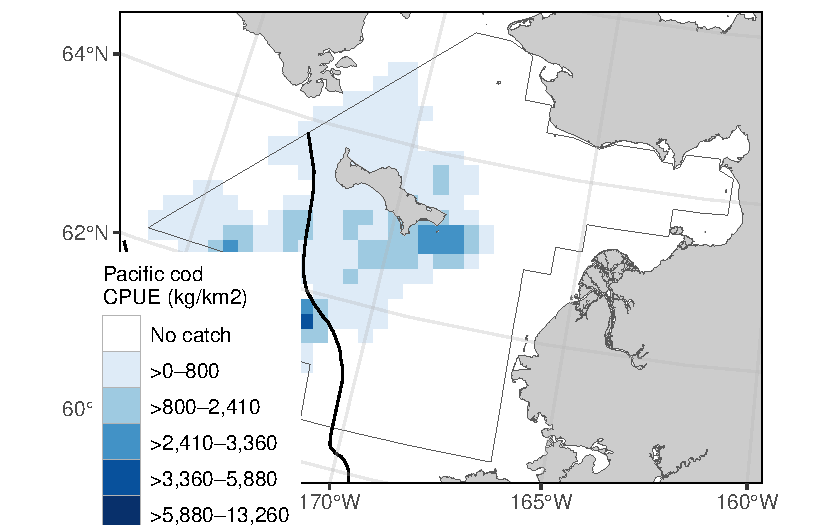
\includegraphics{content/foss-api-r_files/figure-pdf/test-7-fig-1.pdf}

}

\caption{Ex. 7: Visualize CPUE data in distribution map.}

\end{figure}

\hypertarget{access-public-data-using-the-api-and-python}{%
\chapter{Access public data using the API and
Python}\label{access-public-data-using-the-api-and-python}}

\hypertarget{afscgap-library-installation}{%
\subsection{\{afscgap\} Library
Installation}\label{afscgap-library-installation}}

\begin{quote}
author: Sam Pottinger (sam.pottinger@berkeley.edu; GitHub::sampottinger)
date: May 13, 2023
\end{quote}

The third-party \texttt{afscgap} Python package interfaces with FOSS to
access AFSC GAP data. It can be installed via pip:

\begin{Shaded}
\begin{Highlighting}[]
\CommentTok{\#The reticulate package provides a comprehensive set of tools for interoperability between Python and R. }
\FunctionTok{library}\NormalTok{(reticulate)}
\end{Highlighting}
\end{Shaded}

\begin{Shaded}
\begin{Highlighting}[]
\NormalTok{pip install afscgap}
\NormalTok{pip install git}\SpecialCharTok{+}\NormalTok{https}\SpecialCharTok{:}\ErrorTok{//}\NormalTok{github.com}\SpecialCharTok{/}\NormalTok{SchmidtDSE}\SpecialCharTok{/}\NormalTok{afscgap.git}\SpecialCharTok{@}\NormalTok{main}
\end{Highlighting}
\end{Shaded}

For more information on installation and deployment, see the
\href{https://pyafscgap.org}{library documentation}.

\hypertarget{basic-query}{%
\subsection{Basic query}\label{basic-query}}

This first example queries for Pacific glass shrimp (\emph{Pasiphaea
pacifica}) in the Gulf of Alaska in 2021. The library will automatically
generate HTTP queries, converting from Python types to
\href{https://www.oracle.com/database/technologies/appdev/rest.html}{ORDS}
query syntax.

\begin{Shaded}
\begin{Highlighting}[]
\NormalTok{import afscgap}

\NormalTok{query }\OtherTok{=} \FunctionTok{afscgap.Query}\NormalTok{()}
\FunctionTok{query.filter\_year}\NormalTok{(}\AttributeTok{eq=}\DecValTok{2021}\NormalTok{)}
\FunctionTok{query.filter\_srvy}\NormalTok{(}\AttributeTok{eq=}\StringTok{\textquotesingle{}GOA\textquotesingle{}}\NormalTok{)}
\FunctionTok{query.filter\_scientific\_name}\NormalTok{(}\AttributeTok{eq=}\StringTok{\textquotesingle{}Pasiphaea pacifica\textquotesingle{}}\NormalTok{)}

\NormalTok{results }\OtherTok{=} \FunctionTok{query.execute}\NormalTok{()}
\end{Highlighting}
\end{Shaded}

The \texttt{results} variable in this example is an iterator that will
automatically perform pagination behind the scenes.

\hypertarget{iterating-with-a-for-loop}{%
\subsection{Iterating with a for loop}\label{iterating-with-a-for-loop}}

The easiest way to interact with results is a simple for loop. This next
example determines the frequency of different catch per unit effort
where Pacific glass shrimp were reported:

\begin{Shaded}
\begin{Highlighting}[]
\NormalTok{import afscgap}

\CommentTok{\# Mapping from CPUE to count}
\NormalTok{count\_by\_cpue }\OtherTok{=}\NormalTok{ \{\}}

\CommentTok{\# Build query}
\NormalTok{query }\OtherTok{=} \FunctionTok{afscgap.Query}\NormalTok{()}
\FunctionTok{query.filter\_year}\NormalTok{(}\AttributeTok{eq=}\DecValTok{2021}\NormalTok{)}
\FunctionTok{query.filter\_srvy}\NormalTok{(}\AttributeTok{eq=}\StringTok{\textquotesingle{}GOA\textquotesingle{}}\NormalTok{)}
\FunctionTok{query.filter\_scientific\_name}\NormalTok{(}\AttributeTok{eq=}\StringTok{\textquotesingle{}Pasiphaea pacifica\textquotesingle{}}\NormalTok{)}
\NormalTok{results }\OtherTok{=} \FunctionTok{query.execute}\NormalTok{()}

\CommentTok{\# Iterate through results and count}
\ControlFlowTok{for}\NormalTok{ record }\ControlFlowTok{in}\NormalTok{ results}\SpecialCharTok{:}
\NormalTok{  cpue }\OtherTok{=} \FunctionTok{record.get\_cpue\_weight}\NormalTok{(}\AttributeTok{units=}\StringTok{\textquotesingle{}kg/ha\textquotesingle{}}\NormalTok{)}
\NormalTok{  cpue\_rounded }\OtherTok{=} \FunctionTok{round}\NormalTok{(cpue)}
\NormalTok{  count }\OtherTok{=} \FunctionTok{count\_by\_cpue.get}\NormalTok{(cpue\_rounded, }\DecValTok{0}\NormalTok{) }\SpecialCharTok{+} \DecValTok{1}
\NormalTok{  count\_by\_cpue[cpue\_rounded] }\OtherTok{=}\NormalTok{ count}

\CommentTok{\# Print the result}
\FunctionTok{print}\NormalTok{(count\_by\_cpue)}
\end{Highlighting}
\end{Shaded}

Note that, in this example, only records with Pacific glass shrimp are
included (``presence-only'' data). See zero catch inference below. In
other words, it reports on CPUE only for hauls in which Pacific glass
shrimp were recorded, excluding some hauls like those in which Pacific
glass shrimp were not found at all.

\hypertarget{iterating-with-functional-programming}{%
\subsection{Iterating with functional
programming}\label{iterating-with-functional-programming}}

A for loop is not the only option for iterating through results. List
comprehensions and other functional programming methods can be used as
well.

\begin{Shaded}
\begin{Highlighting}[]
\NormalTok{import statistics}

\NormalTok{import afscgap}

\CommentTok{\# Build query}
\NormalTok{query }\OtherTok{=} \FunctionTok{afscgap.Query}\NormalTok{()}
\FunctionTok{query.filter\_year}\NormalTok{(}\AttributeTok{eq=}\DecValTok{2021}\NormalTok{)}
\FunctionTok{query.filter\_srvy}\NormalTok{(}\AttributeTok{eq=}\StringTok{\textquotesingle{}GOA\textquotesingle{}}\NormalTok{)}
\FunctionTok{query.filter\_scientific\_name}\NormalTok{(}\AttributeTok{eq=}\StringTok{\textquotesingle{}Pasiphaea pacifica\textquotesingle{}}\NormalTok{)}
\NormalTok{results }\OtherTok{=} \FunctionTok{query.execute}\NormalTok{()}

\CommentTok{\# Get temperatures in Celsius}
\NormalTok{temperatures }\OtherTok{=}\NormalTok{ [}\FunctionTok{record.get\_bottom\_temperature}\NormalTok{(}\AttributeTok{units=}\StringTok{\textquotesingle{}c\textquotesingle{}}\NormalTok{) }\ControlFlowTok{for}\NormalTok{ record }\ControlFlowTok{in}\NormalTok{ results]}

\CommentTok{\# Take the median}
\FunctionTok{print}\NormalTok{(}\FunctionTok{statistics.median}\NormalTok{(temperatures))}
\end{Highlighting}
\end{Shaded}

This example reports the median temperature in Celcius for when Pacific
glass shrimp was reported.

\hypertarget{load-into-pandas}{%
\subsection{Load into Pandas}\label{load-into-pandas}}

The results from the \texttt{afscgap} package are serializable and can
be loaded into other tools like
\href{https://pandas.pydata.org/}{Pandas}. This example loads Pacific
glass shrimp from 2021 Gulf of Alaska into a data frame.

\begin{Shaded}
\begin{Highlighting}[]
\NormalTok{import pandas}

\NormalTok{import afscgap}

\NormalTok{query }\OtherTok{=} \FunctionTok{afscgap.Query}\NormalTok{()}
\FunctionTok{query.filter\_year}\NormalTok{(}\AttributeTok{eq=}\DecValTok{2021}\NormalTok{)}
\FunctionTok{query.filter\_srvy}\NormalTok{(}\AttributeTok{eq=}\StringTok{\textquotesingle{}GOA\textquotesingle{}}\NormalTok{)}
\FunctionTok{query.filter\_scientific\_name}\NormalTok{(}\AttributeTok{eq=}\StringTok{\textquotesingle{}Pasiphaea pacifica\textquotesingle{}}\NormalTok{)}
\NormalTok{results }\OtherTok{=} \FunctionTok{query.execute}\NormalTok{()}

\FunctionTok{pandas.DataFrame}\NormalTok{(}\FunctionTok{results.to\_dicts}\NormalTok{())}
\end{Highlighting}
\end{Shaded}

Specifically, \texttt{to\_dicts} provides an iterator over a dictionary
form of the data that can be read into tools like Pandas.

\hypertarget{advanced-filtering}{%
\subsection{Advanced filtering}\label{advanced-filtering}}

Queries so far have focused on filters requiring equality but range
queries can be built as well.

\begin{Shaded}
\begin{Highlighting}[]
\NormalTok{import afscgap}

\CommentTok{\# Build query}
\NormalTok{query }\OtherTok{=} \FunctionTok{afscgap.Query}\NormalTok{()}
\FunctionTok{query.filter\_year}\NormalTok{(}\AttributeTok{min\_val=}\DecValTok{2015}\NormalTok{, }\AttributeTok{max\_val=}\DecValTok{2019}\NormalTok{)   }\CommentTok{\# Note min/max\_val}
\FunctionTok{query.filter\_srvy}\NormalTok{(}\AttributeTok{eq=}\StringTok{\textquotesingle{}GOA\textquotesingle{}}\NormalTok{)}
\FunctionTok{query.filter\_scientific\_name}\NormalTok{(}\AttributeTok{eq=}\StringTok{\textquotesingle{}Pasiphaea pacifica\textquotesingle{}}\NormalTok{)}
\NormalTok{results }\OtherTok{=} \FunctionTok{query.execute}\NormalTok{()}

\CommentTok{\# Sum weight}
\NormalTok{weights }\OtherTok{=} \FunctionTok{map}\NormalTok{(lambda x}\SpecialCharTok{:} \FunctionTok{x.get\_weight}\NormalTok{(}\AttributeTok{units=}\StringTok{\textquotesingle{}kg\textquotesingle{}}\NormalTok{), results)}
\NormalTok{total\_weight }\OtherTok{=} \FunctionTok{sum}\NormalTok{(weights)}
\FunctionTok{print}\NormalTok{(total\_weight)}
\end{Highlighting}
\end{Shaded}

This example queries for Pacific glass shrimp data between 2015 and
2019, summing the total weight caught. Note that most users will likely
take advantage of built-in Python to
\href{https://www.oracle.com/database/technologies/appdev/rest.html}{ORDS}
query generation which dictates how the library communicates with the
API service. However, users can provide raw ORDS queries as well using
\href{https://pyafscgap.org/devdocs/afscgap.html\#manual-filtering}{manual
filtering}.

\hypertarget{zero-catch-inference}{%
\subsection{Zero-catch inference}\label{zero-catch-inference}}

Until this point, these examples use presence-only data. However, the
\texttt{afscgap} package can infer negative or ``zero catch'' records as
well.

\begin{Shaded}
\begin{Highlighting}[]
\NormalTok{import afscgap}

\CommentTok{\# Mapping from CPUE to count}
\NormalTok{count\_by\_cpue }\OtherTok{=}\NormalTok{ \{\}}

\CommentTok{\# Build query}
\NormalTok{query }\OtherTok{=} \FunctionTok{afscgap.Query}\NormalTok{()}
\FunctionTok{query.filter\_year}\NormalTok{(}\AttributeTok{eq=}\DecValTok{2021}\NormalTok{)}
\FunctionTok{query.filter\_srvy}\NormalTok{(}\AttributeTok{eq=}\StringTok{\textquotesingle{}GOA\textquotesingle{}}\NormalTok{)}
\FunctionTok{query.filter\_scientific\_name}\NormalTok{(}\AttributeTok{eq=}\StringTok{\textquotesingle{}Pasiphaea pacifica\textquotesingle{}}\NormalTok{)}
\FunctionTok{query.set\_presence\_only}\NormalTok{(False)  }\CommentTok{\# Added to earlier example}
\NormalTok{results }\OtherTok{=} \FunctionTok{query.execute}\NormalTok{()}

\CommentTok{\# Iterate through results and count}
\ControlFlowTok{for}\NormalTok{ record }\ControlFlowTok{in}\NormalTok{ results}\SpecialCharTok{:}
\NormalTok{  cpue }\OtherTok{=} \FunctionTok{record.get\_cpue\_weight}\NormalTok{(}\AttributeTok{units=}\StringTok{\textquotesingle{}kg/ha\textquotesingle{}}\NormalTok{)}
\NormalTok{  cpue\_rounded }\OtherTok{=} \FunctionTok{round}\NormalTok{(cpue)}
\NormalTok{  count }\OtherTok{=} \FunctionTok{count\_by\_cpue.get}\NormalTok{(cpue\_rounded, }\DecValTok{0}\NormalTok{) }\SpecialCharTok{+} \DecValTok{1}
\NormalTok{  count\_by\_cpue[cpue\_rounded] }\OtherTok{=}\NormalTok{ count}

\CommentTok{\# Print the result}
\FunctionTok{print}\NormalTok{(count\_by\_cpue)}
\end{Highlighting}
\end{Shaded}

This example revisits the earlier snippet for CPUE counts but
\texttt{set\_presence\_only(False)} directs the library to look at
additional data on hauls, determining which hauls did not have Pacific
glass shrimp. This lets the library return records for hauls in which
Pacific glass shrimp were not found. This can be seen in differences in
counts reported:

\begin{longtable}[]{@{}
  >{\raggedright\arraybackslash}p{(\columnwidth - 4\tabcolsep) * \real{0.1609}}
  >{\raggedright\arraybackslash}p{(\columnwidth - 4\tabcolsep) * \real{0.4138}}
  >{\raggedright\arraybackslash}p{(\columnwidth - 4\tabcolsep) * \real{0.4253}}@{}}
\toprule\noalign{}
\begin{minipage}[b]{\linewidth}\raggedright
Rounded CPUE
\end{minipage} & \begin{minipage}[b]{\linewidth}\raggedright
Count with set\_presence\_only(True)
\end{minipage} & \begin{minipage}[b]{\linewidth}\raggedright
Count with set\_presence\_only(False)
\end{minipage} \\
\midrule\noalign{}
\endhead
\bottomrule\noalign{}
\endlastfoot
0 kg/ha & 44 & 521 \\
1 kg/ha & 7 & 7 \\
2 kg/ha & 1 & 1 \\
\end{longtable}

Put simply, while the earlier example showed CPUE counts for hauls in
which Pacific glass shrimp were seen, this revised example reports for
all hauls in the Gulf of Alaska in 2021.

\hypertarget{more-information}{%
\subsection{More information}\label{more-information}}

Please see the \href{https://pyafscgap.org/devdocs/afscgap.html}{API
documentation} for the Python library for additional details.

\hypertarget{access-public-data-using-r-in-oracle}{%
\chapter{Access public data using R in
Oracle}\label{access-public-data-using-r-in-oracle}}

\hypertarget{access-data-via-oracle-afsc-only-1}{%
\section{Access data via Oracle (AFSC
only)}\label{access-data-via-oracle-afsc-only-1}}

If the user has access to the AFSC \texttt{Oracle} database, the user
can use \texttt{SQL\ developer} to view and pull the FOSS public data
directly from the \texttt{RACEBASE\_FOSS} \texttt{Oracle} schema.

\hypertarget{connect-to-oracle-from-r-3}{%
\subsection{Connect to Oracle from R}\label{connect-to-oracle-from-r-3}}

Many users will want to access the data from \texttt{Oracle} using
\texttt{R}. The user will need to install the \texttt{RODBC} \texttt{R}
package and ask OFIS (IT) connect \texttt{R} to \texttt{Oracle}. Then,
use the following code in \texttt{R} to establish a connection from
\texttt{R} to \texttt{Oracle}:

Here, the user can write in their username and password directly into
the \texttt{RODBC} connect function. Never save usernames or passwords
in scripts that may be intentionally or unintentionally shared with
others. If no username and password is entered in the function, pop-ups
will appear on the screen asking for the username and password.

\begin{Shaded}
\begin{Highlighting}[]
 \CommentTok{\#\textquotesingle{} Define RODBC connection to ORACLE}
 \CommentTok{\#\textquotesingle{}}
 \CommentTok{\#\textquotesingle{} @param schema default = \textquotesingle{}AFSC\textquotesingle{}. }
 \CommentTok{\#\textquotesingle{}}
 \CommentTok{\#\textquotesingle{} @return oracle channel connection}
 \CommentTok{\#\textquotesingle{} @export}
 \CommentTok{\#\textquotesingle{}}
 \CommentTok{\#\textquotesingle{} @examples}
 \CommentTok{\#\textquotesingle{} \# Not run}
 \CommentTok{\#\textquotesingle{} \# channel \textless{}{-} oracle\_connect()}
\NormalTok{oracle\_connect }\OtherTok{\textless{}{-}} \ControlFlowTok{function}\NormalTok{(}
    \AttributeTok{schema=}\StringTok{\textquotesingle{}AFSC\textquotesingle{}}\NormalTok{, }
    \AttributeTok{username =} \ConstantTok{NULL}\NormalTok{, }
    \AttributeTok{passowrd =} \ConstantTok{NULL}\NormalTok{)\{(}\AttributeTok{echo=}\ConstantTok{FALSE}\NormalTok{)}
  
  \FunctionTok{library}\NormalTok{(}\StringTok{"RODBC"}\NormalTok{)}
  \FunctionTok{library}\NormalTok{(}\StringTok{"getPass"}\NormalTok{)}
  \ControlFlowTok{if}\NormalTok{ (}\FunctionTok{is.null}\NormalTok{(username)) \{}
\NormalTok{    username }\OtherTok{\textless{}{-}} \FunctionTok{getPass}\NormalTok{(}\AttributeTok{msg =} \StringTok{"Enter your ORACLE Username: "}\NormalTok{)}
\NormalTok{  \}}
  \ControlFlowTok{if}\NormalTok{ (}\FunctionTok{is.null}\NormalTok{(password)) \{}
\NormalTok{    password }\OtherTok{\textless{}{-}} \FunctionTok{getPass}\NormalTok{(}\AttributeTok{msg =} \StringTok{"Enter your ORACLE Password: "}\NormalTok{)}
\NormalTok{  \}}
\NormalTok{  channel  }\OtherTok{\textless{}{-}}\NormalTok{ RODBC}\SpecialCharTok{::}\FunctionTok{odbcConnect}\NormalTok{(}
    \FunctionTok{paste}\NormalTok{(schema),}
    \FunctionTok{paste}\NormalTok{(username),}
    \FunctionTok{paste}\NormalTok{(password), }
    \AttributeTok{believeNRows=}\ConstantTok{FALSE}\NormalTok{)}
  \FunctionTok{return}\NormalTok{(channel)}
\NormalTok{\}}

\NormalTok{channel }\OtherTok{\textless{}{-}} \FunctionTok{oracle\_connect}\NormalTok{()}
\end{Highlighting}
\end{Shaded}

\hypertarget{ex.-1-join-data}{%
\subsection{Ex. 1: Join data}\label{ex.-1-join-data}}

To join these tables in Oracle, you may use a variant of the following
code:

\hypertarget{ex.-2-subset-data}{%
\subsection{Ex. 2: Subset data}\label{ex.-2-subset-data}}

Once connected, pull and save (if needed) the tables into the \texttt{R}
environment.

To pull a small subset of the data (especially since files like
\texttt{RACEBASE\_FOSS.FOSS\_CPUE\_ZEROFILLED} are so big), use a
variation of the following code. Here, we are pulling EBS Pacific cod
from 2010 - 2021:

\begin{Shaded}
\begin{Highlighting}[]
 \CommentTok{\# Pull data}
\NormalTok{a }\OtherTok{\textless{}{-}}\NormalTok{ RODBC}\SpecialCharTok{::}\FunctionTok{sqlQuery}\NormalTok{(}
\AttributeTok{channel =}\NormalTok{ channel, }
\AttributeTok{query =} 
\StringTok{"SELECT * FROM GAP\_PRODUCTS.FOSS\_CATCH cc}
\StringTok{JOIN GAP\_PRODUCTS.FOSS\_HAUL hh}
\StringTok{ON cc.HAULJOIN = hh.HAULJOIN}
\StringTok{WHERE SRVY = \textquotesingle{}EBS\textquotesingle{} }
\StringTok{AND COMMON\_NAME = \textquotesingle{}Pacific cod\textquotesingle{} }
\StringTok{AND YEAR \textgreater{}= 2010 }
\StringTok{AND YEAR \textless{} 2021"}\NormalTok{)}
 \CommentTok{\# Save table to local directory}
\FunctionTok{write.csv}\NormalTok{(}\AttributeTok{x =}\NormalTok{ a, }\AttributeTok{file =} \StringTok{"RACEBASE\_FOSS{-}FOSS\_CPUE\_ZEROFILLED{-}ebs\_pcod\_2010{-}2020.csv"}\NormalTok{)}
\end{Highlighting}
\end{Shaded}

\bookmarksetup{startatroot}

\hypertarget{acknowledgments}{%
\chapter{Acknowledgments}\label{acknowledgments}}

\bookmarksetup{startatroot}

\hypertarget{community-acknowledgments}{%
\chapter{Community Acknowledgments}\label{community-acknowledgments}}

We would like to thank the many communities of Alaska and their members
who have helped contribute to this body of work. The knowledge,
experiences, and insights have been instrumental in expanding the scope
of our science and knowledge to encompass the many issues that face this
important ecosystem. We appreciate feedback from those residing in the
region that are willing to share their insights and participation in an
open dialog about how we can improve our collective knowledge of the
ecosystem and the region.

\bookmarksetup{startatroot}

\hypertarget{technical-acknowledgments}{%
\chapter{Technical Acknowledgments}\label{technical-acknowledgments}}

This quarto book is based off the
\href{https://github.com/nmfs-opensci/NOAA-quarto-book}{NOAA-quarto-book}
GitHub repo designed by Eli Holmes.

This repo and GitHub Action was based on the tutorial by Openscapes
\href{https://github.com/Openscapes/quarto-website-tutorial}{quarto-website-tutorial}
by Julia Lowndes and Stefanie Butland.

\hypertarget{partners}{%
\section{Partners}\label{partners}}

Scientists from the Alaska Fisheries Science Center conduct these bottom
trawl surveys with participation from the Alaska Department of Fish \&
Game (ADF\&G), the International Pacific Halibut Commission (IPHC), and
universities. This research is conducted on chartered fishing vessels.

\bookmarksetup{startatroot}

\hypertarget{production-run-notes}{%
\chapter{Production Run Notes}\label{production-run-notes}}

\bookmarksetup{startatroot}

\hypertarget{r-version-metadata}{%
\chapter{R Version Metadata}\label{r-version-metadata}}

\begin{verbatim}
R version 4.3.0 (2023-04-21 ucrt)
Platform: x86_64-w64-mingw32/x64 (64-bit)
Running under: Windows 10 x64 (build 19045)

Matrix products: default


locale:
[1] LC_COLLATE=English_United States.utf8 
[2] LC_CTYPE=English_United States.utf8   
[3] LC_MONETARY=English_United States.utf8
[4] LC_NUMERIC=C                          
[5] LC_TIME=English_United States.utf8    

time zone: America/Los_Angeles
tzcode source: internal

attached base packages:
[1] stats     graphics  grDevices utils     datasets  methods   base     

loaded via a namespace (and not attached):
 [1] compiler_4.3.0  fastmap_1.1.1   cli_3.6.1       tools_4.3.0    
 [5] htmltools_0.5.5 rstudioapi_0.14 yaml_2.3.7      rmarkdown_2.22 
 [9] knitr_1.43      xfun_0.39       digest_0.6.31   jsonlite_1.8.4 
[13] rlang_1.1.1     evaluate_0.21  
\end{verbatim}

\hypertarget{noaa-readme}{%
\subsection{NOAA README}\label{noaa-readme}}

This repository is a scientific product and is not official
communication of the National Oceanic and Atmospheric Administration, or
the United States Department of Commerce. All NOAA GitHub project code
is provided on an `as is' basis and the user assumes responsibility for
its use. Any claims against the Department of Commerce or Department of
Commerce bureaus stemming from the use of this GitHub project will be
governed by all applicable Federal law. Any reference to specific
commercial products, processes, or services by service mark, trademark,
manufacturer, or otherwise, does not constitute or imply their
endorsement, recommendation or favoring by the Department of Commerce.
The Department of Commerce seal and logo, or the seal and logo of a DOC
bureau, shall not be used in any manner to imply endorsement of any
commercial product or activity by DOC or the United States Government.

\hypertarget{noaa-license}{%
\subsection{NOAA License}\label{noaa-license}}

Software code created by U.S. Government employees is not subject to
copyright in the United States (17 U.S.C. §105). The United
States/Department of Commerce reserve all rights to seek and obtain
copyright protection in countries other than the United States for
Software authored in its entirety by the Department of Commerce. To this
end, the Department of Commerce hereby grants to Recipient a
royalty-free, nonexclusive license to use, copy, and create derivative
works of the Software outside of the United States.

\bookmarksetup{startatroot}

\hypertarget{references}{%
\chapter*{References}\label{references}}
\addcontentsline{toc}{chapter}{References}

\markboth{References}{References}

\hypertarget{refs}{}
\begin{CSLReferences}{1}{0}
\leavevmode\vadjust pre{\hypertarget{ref-GAPakfin}{}}%
Alaska Fisheries Information Network (AKFIN). (2023). \emph{AFSC
goundfish assessment program design-based production data}. {NOAA
Fisheries Alaska Fisheries Science Center, Goundfish Assessment
Program};
https://www.psmfc.org/program/alaska-fisheries-information-network-akfin;
{U.S. Dep. Commer.}

\leavevmode\vadjust pre{\hypertarget{ref-RN979}{}}%
Hoff, G. R. (2016). \emph{Results of the 2016 eastern {Bering Sea} upper
continental slope survey of groundfishes and invertebrate resources}
(NOAA Tech. Memo. NOAA-AFSC-339). {U.S. Dep. Commer.}
\url{https://doi.org/10.7289/V5/TM-AFSC-339}

\leavevmode\vadjust pre{\hypertarget{ref-2022NEBS2023}{}}%
Markowitz, E. H., Dawson, E. J., Anderson, A. B., Rohan, S. K.,
Charriere, N. E., Prohaska, B. K., and Stevenson, D. E. (2023).
\emph{Results of the 2022 eastern and northern {Bering Sea} continental
shelf bottom trawl survey of groundfish and invertebrate fauna} (NOAA
Tech. Memo. NMFS-AFSC-469; p. 213). {U.S. Dep. Commer.}

\leavevmode\vadjust pre{\hypertarget{ref-FOSSAFSCData}{}}%
NOAA Fisheries Alaska Fisheries Science Center. (2023). \emph{Fisheries
one stop shop public data: RACE division bottom trawl survey data
query}. https://www.fisheries.noaa.gov/foss; {U.S. Dep. Commer.}

\leavevmode\vadjust pre{\hypertarget{ref-GAPProducts}{}}%
NOAA Fisheries Alaska Fisheries Science Center, Goundfish Assessment
Program. (2023). \emph{AFSC goundfish assessment program design-based
production data}.
https://www.fisheries.noaa.gov/alaska/science-data/groundfish-assessment-program-bottom-trawl-surveys;
{U.S. Dep. Commer.}

\leavevmode\vadjust pre{\hypertarget{ref-GOA2018}{}}%
Von Szalay, P. G., and Raring, N. W. (2018). \emph{Data report: 2017
{Gulf of Alaska} bottom trawl survey} (NOAA Tech. Memo. NMFS-AFSC-374).
{U.S. Dep. Commer.} \url{https://doi.org/10.7289/V5/TM-AFSC-374}

\leavevmode\vadjust pre{\hypertarget{ref-AI2018}{}}%
Von Szalay, P. G., and Raring, N. W. (2020). \emph{Data report: 2018
{Aleutian Islands} bottom trawl survey} (NOAA Tech. Memo.
NMFS-AFSC-409). {U.S. Dep. Commer.}
\url{https://doi.org/10.25923/qe5v-fz70}

\end{CSLReferences}


\backmatter

\end{document}
